%!TEX root = ../thesis.tex
\newcommand{\SF}{{\ensuremath{\mathcal{SF}}}}
\newcommand{\OI}{{\ensuremath{\mathcal{OI}}}}
\newcommand{\SD}{{\ensuremath{\mathcal{SF}_{pulses}}}}
\newcommand{\DO}{{\ensuremath{\mathcal{SF}_{dirs}}}}
\newcommand{\FD}{{\SF}}
\newcommand{\FDmod}{{\ensuremath{\FD_{mod}}}}
\newcommand{\SFasym}{{\ensuremath{a\mathcal{SF}}}}

\newcommand{\SFshort}{\SF$_{90}$}
\newcommand{\SFlong}{\SF$_{360}$}
\newcommand{\OIlong}{\OI$_{360}$}


\newsavebox{\poorBox}
\savebox{\poorBox}{\textcolor{red}{\rule{0.05in}{0.05in}}}
\newsavebox{\fairBox}
\savebox{\fairBox}{\textcolor{orange}{\rule{0.05in}{0.05in}}}
\newsavebox{\moderateBox}
\savebox{\moderateBox}{\textcolor{yellow}{\rule{0.05in}{0.05in}}}
\newsavebox{\substantialBox}
\savebox{\substantialBox}{\textcolor{lime}{\rule{0.05in}{0.05in}}}
\newsavebox{\perfectBox}
\savebox{\perfectBox}{\textcolor{green}{\rule{0.05in}{0.05in}}}


\chapter[Scan/rescan in the corpus callosum]{Scan/rescan reproducibility in the corpus callosum and spinal cord}
\section{Introduction}
In the previous chapter we have presented a clinical {\SF} ActiveAx protocols that can be acquired in under 25 minutes scan time. The main motivation for the previous study was to compare our short {\SF} protocol with the 1h long \OI{} protocol of \citep{Alexander:2010}. To allow a fair comparision, we only reduced the total number of acquisitions, but left the imaging setup untouched from the original \OI{} approach. Although we found that our \SF{} protocols are quite capable of achieving comparable results to the \OI{} method. However, our results also show that a careful optimisation of the whole imaging pipeline is crucial to achieve acceptable estimates of tissue microstrucuture parameters. 


Based on the experiences in the previous study, we therefore present here an new imaging pipeline, which improves on several key areas of the previous study:(i) the use of a small \gls{FOV} imaging sequence to improve image resolution and SNR  (ii) a fast tractography-based method to align the image volume with the dominant fibre direction of the CC (iii) a further improved \SF{} optimisation algorithm and tissue model to allow the shortest \gls{TE} for individual diffusion acquisitions to improve SNR in low diffusion weighted scans.  We test our approach in 5 healthy volunteers, who were scanned at two different timepoint to assess both intra- and inter-subject reproducibility. 
\section{Methods \& Experiments}
Study design: We recruited 5 healthy volunteers to be scanned on a Philips Achieva 3TX scanner. All subjects were recalled for a second scan on a separate occasion to assess the intra-subject reproducibility of the experiment.
Protocol optimisation: We use the SF protocol optimization framework [5] with an additional T2 decay factor that accounts for the varying signal loss in the DWI due to different echo times (TE). For the protocol optimization we assumed a T2 relaxation time of 70ms for white matter (WM) in the CC. We allowed a maximum gradient strength of 87mT/m, which is achievable by combining perpendicular 62mT/m, gradients. We also acquired a standard DTI acquisition (max b=800s/mm2, 1 b=0, 16 uniformly distributed directions). The full protocol is given in Table 1.
Data acquisition: We acquired the DWI protocol for 10 sagittal slices with high in-plane resolution and centered on the mid-sagittal plane of the CC, perpendicular to the dominant fibre direction of the CC. Acquisition parameters were: voxel size: 1x1x4mm3, FOV=96x96mm2, TR=6000ms, 2 averages, using an outer-volume suppressed ZOOM acquisition [6] to avoid fold-over artifacts.  
Model fitting: We fitted a single axon diameter model according to [5], based on the minimal model of white matter diffusion [4] (zeppelin-cylinder-ball in the model taxonomy of [7]) with an additional T2 relaxation factor. We computed the posterior distributions of the model parameters using an MCMC method on a voxel-by-voxel basis.  We used mean of the posterior distribution of the axon diameter, d, as the axon diameter index and the volume fraction, f, of the restricted compartment to generate maps of mean $a$ and the axonal density index $\rho$=f/$\pi/a^2$. We also fitted the diffusion tensor to the 16-direction DTI data and derive maps of FA and the principal eigenvector v1. All fitting was performed using the open-source Camino toolkit [8] (camino.org.uk).
Data analysis: In each subject we defined the mid-sagittal slice of the CC by manually segmenting the CC and excluded voxels where either FA<0.5 or v1 deviated more than 10 degrees from the dominant CC fibre direction. We divided each CC in 10 regions along the anterior-posterior baseline similar to [9]. 
\section{Results}
Figure 1 shows an example of the obtained d and ρ maps and the CC subdivision. Figure 2 shows plots of d and ρ over the CC subdivisions for each subject. Figure 3 shows the axon diameter index and standard deviation over all subjects in each CC region for scan and rescan experiments. In all subjects we find the highest values of d (12.5-13.5μm) in regions B1-I and smaller values between 9-11.5μm for d in the anterior genu (G1-G2) and splenium regions (S1-S3).  Similarly we find the highest axonal density in genu and splenium and low density in the mid-body regions. These trends are in excellent agreement with studies of post-mortem CC, which report highest number of large fibres between B1 and I [9] and low fibre density [10] compared to genu and splenium. The high estimates of d compared to reported post-mortem values can be explained by the shrinkage of axons due to histological preparation. Also the limited gradient strength available on the clinical MRI system makes the experiment insensitive to small fibres, as shown e.g. by [11]. Therefore we can postulate that differences between CC regions in our experiment are mainly driven by the presence of larger fibres. 
Scan/rescan reproducibility:  Figure 2 and 3 show good agreement between d and ρ values in all regions consistently in all subjects. We find the variability of d to be less than 10\% between scan and rescan in each subject, with the largest relative difference found in the genu and splenium (6±5\% variation) and lowest in the mid-body (<3±2\%). As seen in Figure 3, inter-subject variability is below 0.8μm in d and 0.01μm-2 in ρ in both scan and rescan experiments. Standard deviation is lowest in the mid-body (0.3μm) measurement and larger in genu and splenium regions (>0.7μm). Similarly, in ρ we observe low variability in the mid-body (0.001-0.002μm -2) and higher intra-subject variability in the posterior part of the CC, particularly in the splenium (0.005-0.01μm-2). 

\subsection*{Axon diameter and axon density indices}
\begin{figure}[ht\textbf{]}
	\centering
	\subfloat[Habla]
	{
		\pgfimage[width=\textwidth]{chapter9/figs/diam_per_subj}
	}
	\caption{XX}
	\label{fig:chap9 scan rescan maps per subject}	
\end{figure}	
\begin{figure}[ht]
	\centering
    \ContinuedFloat 
	\subfloat[Hubla]
	{
		\pgfimage[width=\textwidth]{chapter9/figs/dens_per_subj}
	}
	\ref{leg:chap 9 maps per subj}
	\caption{XX (continued)}
	\label{fig:chap9 scan rescan maps per subject}
\end{figure}

\begin{figure}[ht]
	\centering
	\ref{leg:chap 9 diam_all}
	\subfloat[Axon diameter index]
	{
		%!TEX root = ../../thesis.tex
\begin{tikzpicture}[scale=0.7]
\begin{axis}[%
    		xlabel={ROI}, 
		ylabel={$a$ in $[\mu m]$},
		ymin=5,
		ymax=15,
		width=0.7\textwidth,
		height=0.6\textwidth,
		xtick={1,2,3,4,5,6,7,8,9,10},
		xticklabels={G1,G2,G3,B1,B2,B3,I,S1,S2,S3},		
		legend to name=leg:chap 9 diam_all,
		legend columns=-1,
		title=Scan
	]
	\pgfplotstableread{chapter9/figs/diam_all.dat}\tableall
	\addplot+[only marks,mark options={scale=1.5}] table[x=reg,y=s11] from \tableall;		
	\addplot+[only marks, mark options={scale=1.5}] table[x=reg,y=s21] from \tableall;		
	\addplot+[only marks, mark options={scale=1.5}] table[x=reg,y=s31] from \tableall;		
	\addplot+[only marks, mark options={scale=1.5}] table[x=reg,y=s41] from \tableall;		
	\addplot+[only marks, mark options={scale=1.5}] table[x=reg,y=s51] from \tableall;		
	\addplot[dashed, thick] table[x=reg,y=avg1] from \tableall;		
	\legend{s1,s2,s3,s4,s5,mean};
	\end{axis}
\end{tikzpicture}	
\begin{tikzpicture}[scale=0.7]
\begin{axis}[%
    		xlabel={ROI}, 
		%ylabel={$a$ in $[\mu m]$},
		ymin=5,
		ymax=15,
		width=0.7\textwidth,
		height=0.6\textwidth,
		xtick={1,2,3,4,5,6,7,8,9,10},
		xticklabels={G1,G2,G3,B1,B2,B3,I,S1,S2,S3},		
		title=Rescan
	]
	\pgfplotstableread{chapter9/figs/diam_all.dat}\tableall
	\addplot+[only marks,mark options={scale=1.5}] table[x=reg,y=s12] from \tableall;		
	\addplot+[only marks, mark options={scale=1.5}] table[x=reg,y=s22] from \tableall;		
	\addplot+[only marks, mark options={scale=1.5}] table[x=reg,y=s32] from \tableall;		
	\addplot+[only marks, mark options={scale=1.5}] table[x=reg,y=s42] from \tableall;		
	\addplot+[only marks, mark options={scale=1.5}] table[x=reg,y=s52] from \tableall;		
	\addplot[dashed, thick] table[x=reg,y=avg2] from \tableall;		
%	\legend{s1,s2,s3,s4,s5,mean};
	\end{axis}
\end{tikzpicture}


	}\\	
	\subfloat[Axon density index]
	{
		%!TEX root = ../../thesis.tex
\begin{tikzpicture}[scale=0.7]
\begin{axis}[%
    		xlabel={ROI}, 
		ylabel={$\rho$ in $[\mu m^{-2}]$},
		ymin=0,
		ymax=0.05,
		width=0.7\textwidth,
		height=0.6\textwidth,
		xtick={1,2,3,4,5,6,7,8,9,10},
		xticklabels={G1,G2,G3,B1,B2,B3,I,S1,S2,S3},		
%		legend to name=leg:chap 9 dens_all,
%		legend columns=-1,
		title=Scan,
		yticklabel style={%
		        /pgf/number format/.cd,
		        fixed,
		        fixed zerofill,
            		precision=2,
	        },
	]
	\pgfplotstableread{chapter9/figs/dens_all.dat}\tableall
	\addplot+[only marks,mark options={scale=1.5}] table[x=reg,y=s11] from \tableall;		
	\addplot+[only marks, mark options={scale=1.5}] table[x=reg,y=s21] from \tableall;		
	\addplot+[only marks, mark options={scale=1.5}] table[x=reg,y=s31] from \tableall;		
	\addplot+[only marks, mark options={scale=1.5}] table[x=reg,y=s41] from \tableall;		
	\addplot+[only marks, mark options={scale=1.5}] table[x=reg,y=s51] from \tableall;		
	\addplot[dashed, thick] table[x=reg,y=avg1] from \tableall;		
%	\legend{s1,s2,s3,s4,s5,mean};
	\end{axis}
\end{tikzpicture}	
\begin{tikzpicture}[scale=0.7]
\begin{axis}[%
    		xlabel={ROI}, 
		%ylabel={$a$ in $[\mu m]$},
		ymin=0,
		ymax=0.05,
		width=0.7\textwidth,
		height=0.6\textwidth,
		xtick={1,2,3,4,5,6,7,8,9,10},
		xticklabels={G1,G2,G3,B1,B2,B3,I,S1,S2,S3},		
		title=Rescan,
		yticklabel style={%
		        /pgf/number format/.cd,
		        fixed,
		        fixed zerofill,
            		precision=2,
	        },
	]
	\pgfplotstableread{chapter9/figs/dens_all.dat}\tableall
	\addplot+[only marks,mark options={scale=1.5}] table[x=reg,y=s12] from \tableall;		
	\addplot+[only marks, mark options={scale=1.5}] table[x=reg,y=s22] from \tableall;		
	\addplot+[only marks, mark options={scale=1.5}] table[x=reg,y=s32] from \tableall;		
	\addplot+[only marks, mark options={scale=1.5}] table[x=reg,y=s42] from \tableall;		
	\addplot+[only marks, mark options={scale=1.5}] table[x=reg,y=s52] from \tableall;		
	\addplot[dashed, thick] table[x=reg,y=avg2] from \tableall;		
%	\legend{s1,s2,s3,s4,s5,mean};
	\end{axis}
\end{tikzpicture}


	}\\
	\caption{Scatter plots of axon diameter ($a$) and axon density ($\rho$) indices in all 5 subjects in individual ROIs. The dashed line shows the average over all subjects.}
	\label{fig:chap9 scan rescan scatterplots per subject}
\end{figure}

\subsection*{Reproducibility}
\begin{figure}[ht]
	\centering
	\ref{leg:chap 9 dens_avg}\\	
	\subfloat[Axon diameter index]
	{
		%!TEX root = ../../thesis.tex
\begin{tikzpicture}[scale=0.7]
\begin{axis}[%
    		xlabel={ROI}, 
		ylabel={$a$ in $[\mu m]$},
		ymin=5,
		ymax=15,
		width=0.7\textwidth,
		height=0.6\textwidth,
		xtick={1,2,3,4,5,6,7,8,9,10},
		xticklabels={G1,G2,G3,B1,B2,B3,I,S1,S2,S3},		
		legend to name=leg:chap 9 dens_avg,
		legend columns=-1,
		yticklabel style={%
		        /pgf/number format/.cd,
		        fixed,
		        fixed zerofill,
            		precision=2,
	        },
	]
	\pgfplotstableread{chapter9/figs/diam_all.dat}\tableall
	\addplot+[blue, mark=*,error bars/.cd, y dir=both, y explicit] table[x=reg,y=avg1, y error = std1] from \tableall;		
	\addplot+[red, mark=*,error bars/.cd, y dir=both, y explicit] table[x=reg,y=avg2, y error = std2] from \tableall;		
	\legend{scan,rescan};
	\end{axis}
\end{tikzpicture}	

	}	
	\subfloat[Axon density index]
	{
		%!TEX root = ../../thesis.tex
\begin{tikzpicture}[scale=0.7]
\begin{axis}[%
    		xlabel={ROI}, 
		ylabel={$\rho$ in $[\mu m^{-2}]$},
		ymin=0,
		ymax=0.07,
		width=0.7\textwidth,
		height=0.6\textwidth,
		xtick={1,2,3,4,5,6,7,8,9,10},
		xticklabels={G1,G2,G3,B1,B2,B3,I,S1,S2,S3},		
%		legend to name=leg:chap 9 dens_all,
%		legend columns=-1,
		yticklabel style={%
		        /pgf/number format/.cd,
		        fixed,
		        fixed zerofill,
            		precision=2,
	        },
	]
	\pgfplotstableread{chapter9/figs/dens_all.dat}\tableall
	\addplot+[blue, mark=*,error bars/.cd, y dir=both, y explicit] table[x=reg,y=avg1, y error = std1] from \tableall;		
	\addplot+[red, mark=*,error bars/.cd, y dir=both, y explicit] table[x=reg,y=avg2, y error = std2] from \tableall;		
%	\legend{s1,s2,s3,s4,s5,mean};
	\end{axis}
\end{tikzpicture}	

	}
	\caption{Scatter plots of axon diameter ($a$) and axon density ($\rho$) indices in all 5 subjects in individual ROIs. The dashed line shows the average over all subjects.}
	\label{fig:chap9 scan rescan scatterplots per subject}
\end{figure}

\begin{figure}[ht]
	\centering
	%!TEX root = ../../thesis.tex
%created by ICC.r
\definecolor{brewer10_1}{HTML}{9E0142}
\definecolor{brewer10_2}{HTML}{D53E4F}
\definecolor{brewer10_3}{HTML}{F46D43}
\definecolor{brewer10_4}{HTML}{FDAE61}
\definecolor{brewer10_5}{HTML}{FEE08B}
\definecolor{brewer10_6}{HTML}{E6F598}
\definecolor{brewer10_7}{HTML}{ABDDA4}
\definecolor{brewer10_8}{HTML}{66C2A5}
\definecolor{brewer10_9}{HTML}{3288BD}
\definecolor{brewer10_10}{HTML}{5E4FA2}
\pgfplotsset{blandaltman/.style={scatter/classes=
{
R1={color=brewer10_1, mark=*, mark options={scale=1.5}}, R2={color=brewer10_3, mark=o, mark options={scale=1.5}}, R3={color=brewer10_4, mark=asterisk, mark options={scale=1.5}}, R4={color=brewer10_5, mark=oplus*, mark options={scale=1.5}}, R5={color=brewer10_6, mark=triangle*, mark options={scale=1.5}}, R6={color=brewer10_7, mark=square*, mark options={scale=1.5}}, R7={color=brewer10_8, mark=diamond*, mark options={scale=1.5}}, R8={color=brewer10_9, mark=diamond*, mark options={scale=1.5}}, R9={color=brewer10_10, mark=star, mark options={scale=1.5}}, R10={color=brewer10_2, mark=+, mark options={scale=1.5}}
}
}}
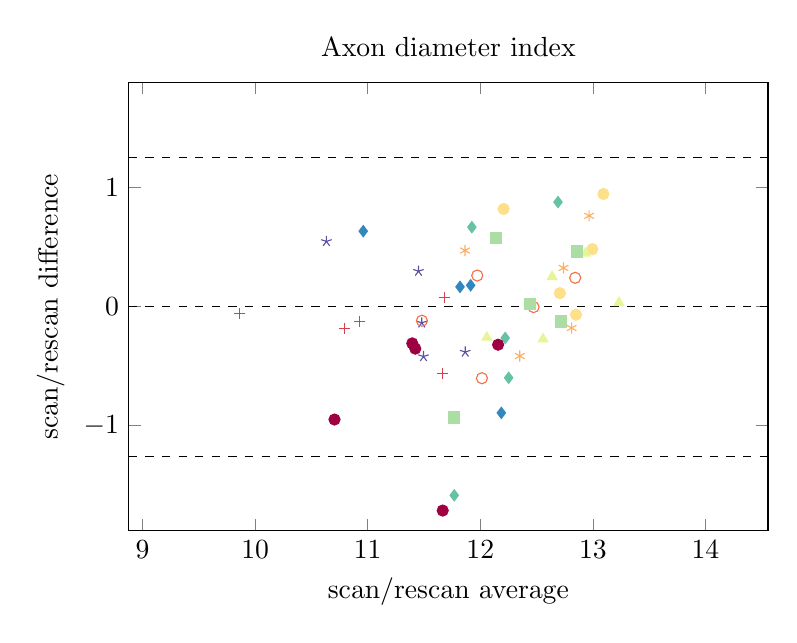
\begin{tikzpicture}[scale=1]
\begin{axis}[legend columns=-1, blandaltman,width=0.8*\textwidth, height=0.6*\textwidth, xmin=8.877132,xmax=14.554980,ymin=-1.884580,ymax=1.884580, legend to name=leg:chap 9 bland altman,
	title=Axon diameter index,
	xlabel={scan/rescan average},
	ylabel={scan/rescan difference},]
\addplot+[only marks, scatter]  [scatter src=explicit symbolic] 
coordinates {
(11.42235, -0.35310)[R1]
(11.97285, 0.26170)[R2]
(12.73915, 0.32570)[R3]
(12.99505, 0.48330)[R4]
(12.93510, 0.44820)[R5]
(12.71710, -0.12500)[R6]
(12.22115, -0.26330)[R7]
(11.91405, 0.17950)[R8]
(11.47995, -0.13610)[R9]
(11.68225, 0.07950)[R10]
(10.70500, -0.94900)[R1]
(11.48135, -0.11810)[R2]
(11.86385, 0.47190)[R3]
(12.20675, 0.82150)[R4]
(12.05765, -0.25810)[R5]
(12.13630, 0.57940)[R6]
(11.92495, 0.66810)[R7]
(10.96030, 0.63480)[R8]
(10.63285, 0.54890)[R9]
(9.86348, -0.05920)[R10]
(11.39565, -0.30870)[R1]
(12.47305, -0.00370)[R2]
(12.81075, -0.17930)[R3]
(12.84975, -0.06810)[R4]
(12.55710, -0.27260)[R5]
(11.76920, -0.93260)[R6]
(11.76835, -1.58610)[R7]
(11.84845, -1.92110)[R8]
(11.49530, -0.41900)[R9]
(10.79545, -0.18510)[R10]
(11.66590, -1.71420)[R1]
(12.01435, -0.60150)[R2]
(12.35065, -0.41490)[R3]
(12.70670, 0.11360)[R4]
(12.63735, 0.25190)[R5]
(12.43770, 0.02420)[R6]
(12.25150, -0.59800)[R7]
(12.18665, -0.89310)[R8]
(11.86595, -0.38130)[R9]
(10.92505, -0.12490)[R10]
(12.15770, -0.32000)[R1]
(12.84275, 0.24230)[R2]
(12.96655, 0.76350)[R3]
(13.09315, 0.94730)[R4]
(13.23180, 0.03320)[R5]
(12.86005, 0.46430)[R6]
(12.69000, 0.87940)[R7]
(11.81980, 0.16620)[R8]
(11.45060, 0.29840)[R9]
(11.66275, -0.56250)[R10]
};
\draw[dashed] (axis cs:8.877132,-1.256387) -- (axis cs:14.554980,-1.256387);
\draw[dashed] (axis cs:8.877132,0.000000) -- (axis cs:14.554980,0.000000);
\draw[dashed] (axis cs:8.877132,1.256387) -- (axis cs:14.554980,1.256387);
\legend{G1,G2, G3, B1, B2, B3, I, S1, S2, S3};
\end{axis}
\end{tikzpicture}\\
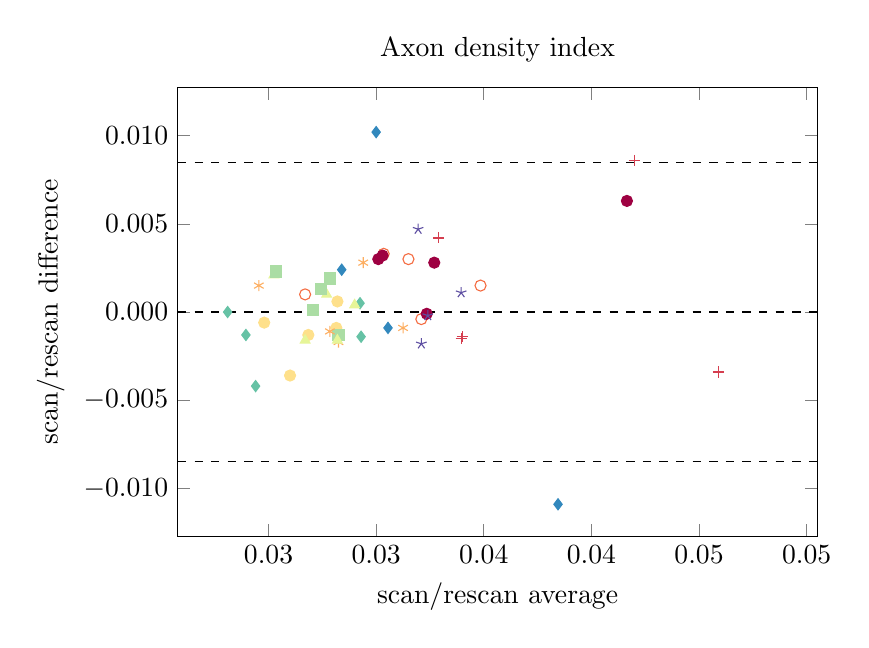
\begin{tikzpicture}[scale=1]
\begin{axis}[scaled ticks=false, blandaltman,width=0.8*\textwidth, height=0.6*\textwidth, xmin=0.020790,xmax=0.050490,ymin=-0.012710,ymax=0.012710,%
    xticklabel style={/pgf/number format/.cd,fixed}, % Use fixed point notation
	yticklabel style={/pgf/number format/.cd,fixed, precision=3, zerofill}, % Use fixed point notation
	title=Axon density index,
	xlabel={scan/rescan average},
	ylabel={scan/rescan difference},]
\addplot+[only marks, scatter]  [scatter src=explicit symbolic] coordinates {
(0.03270, 0.00280)[R1]
(0.03210, -0.00040)[R2]
(0.02825, -0.00170)[R3]
(0.02685, -0.00130)[R4]
(0.02670, -0.00160)[R5]
(0.02705, 0.00010)[R6]
(0.02925, 0.00050)[R7]
(0.03055, -0.00090)[R8]
(0.03395, 0.00110)[R9]
(0.03400, -0.00140)[R10]
(0.04165, 0.00630)[R1]
(0.03485, 0.00150)[R2]
(0.03125, -0.00090)[R3]
(0.02815, -0.00090)[R4]
(0.02900, 0.00040)[R5]
(0.02825, -0.00130)[R6]
(0.02930, -0.00140)[R7]
(0.03845, -0.01090)[R8]
(0.04305, -0.01390)[R9]
(0.04590, -0.00340)[R10]
(0.03235, -0.00010)[R1]
(0.03035, 0.00330)[R2]
(0.02785, -0.00110)[R3]
(0.02600, -0.00360)[R4]
(0.02820, -0.00160)[R5]
(0.02785, 0.00190)[R6]
(0.02310, 0.00000)[R7]
(0.03205, 0.01310)[R8]
(0.03210, -0.00180)[R9]
(0.03395, -0.00150)[R10]
(0.03030, 0.00320)[R1]
(0.03150, 0.00300)[R2]
(0.02940, 0.00280)[R3]
(0.02820, 0.00060)[R4]
(0.02770, 0.00100)[R5]
(0.02745, 0.00130)[R6]
(0.02440, -0.00420)[R7]
(0.03000, 0.01020)[R8]
(0.03195, 0.00470)[R9]
(0.04200, 0.00860)[R10]
(0.03010, 0.00300)[R1]
(0.02670, 0.00100)[R2]
(0.02455, 0.00150)[R3]
(0.02480, -0.00060)[R4]
(0.02525, 0.00210)[R5]
(0.02535, 0.00230)[R6]
(0.02395, -0.00130)[R7]
(0.02840, 0.00240)[R8]
(0.03240, -0.00020)[R9]
(0.03290, 0.00420)[R10]
};
\draw[dashed] (axis cs:0.020790,-0.008473) -- (axis cs:0.050490,-0.008473);
\draw[dashed] (axis cs:0.020790,0.000000) -- (axis cs:0.050490,0.000000);
\draw[dashed] (axis cs:0.020790,0.008473) -- (axis cs:0.050490,0.008473);
%\legend{R1, R10, R2, R3, R4, R5, R6, R7, R8, R9};
\end{axis}
\end{tikzpicture}
\ref{leg:chap 9 bland altman}	
	\caption{XX}
	\label{fig:chap9 bland altman plot}	
\end{figure}	



\begin{table}[ht]
\caption{ICC values for whole CC and individual ROIs for $a$ and $\rho$ estimates.}
\begin{adjustbox}{width={\textwidth},totalheight=\textheight,keepaspectratio}
\begin{tabular}{rrrrrrrrrrrr}
      \toprule
       & & \multicolumn{10}{c}{\textit{Individual ROIs}}                                             \\
       & \textit{whole CC} & G1    & G2    & G3    & B1    & B2    & B3    & I     & S1    & S2    & S3\\
       \cmidrule(rl){2-2} \cmidrule(l){3-12}
       \addlinespace
$a$    & 0.66~\usebox{\substantialBox} & 0.14~\usebox{\poorBox}  & 0.83~\usebox{\perfectBox} & 0.56~\usebox{\moderateBox}  & 0.14~\usebox{\poorBox}  & 0.81~\usebox{\perfectBox}  & 0.46~\usebox{\moderateBox}  & -0.25~\usebox{\poorBox} & -0.07~\usebox{\poorBox} & 0.70~\usebox{\substantialBox}  & 0.94~\usebox{\perfectBox}  \\
$\rho$ & 0.79~\usebox{\substantialBox} & 0.74~\usebox{\substantialBox}  & 0.77~\usebox{\substantialBox}  & 0.78~\usebox{\substantialBox}  & 0.44~\usebox{\moderateBox}  & 0.59~\usebox{\moderateBox}  & 0.34~\usebox{\fairBox}  & 0.79~\usebox{\substantialBox}  & -0.14~\usebox{\poorBox} & 0.34~\usebox{\fairBox}  & 0.73~\usebox{\substantialBox}  \\
\bottomrule
\end{tabular}
\end{adjustbox}
{\footnotesize Guidelines for agreement  \citep{Landis:1977}: \usebox{\poorBox}~$<0.2$: poor,  \usebox{\fairBox}~$0.2–0.4$:~fair,  \usebox{\moderateBox}~$0.4–0.6$:~moderate, \usebox{\substantialBox}~$0.6–0.8$:~substantial,  \usebox{\perfectBox}~$>0.8$:~almost perfect}
\end{table}

\subsection*{Correlation with DTI metrics}
\begin{figure}[ht]
	\centering
				\subfloat[FA]{
					\begin{minipage}{0.5\textwidth}						
					\begin{adjustbox}{width={\textwidth},totalheight=\textheight,keepaspectratio}
						\strut
						% Created by tikzDevice version - on 2012-09-27 22:33:37
% !TEX encoding = UTF-8 Unicode
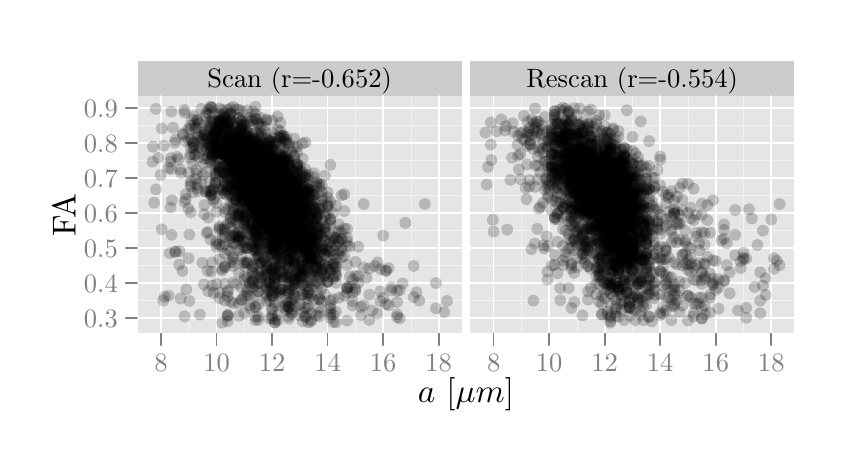
\begin{tikzpicture}[x=1pt,y=1pt]
\definecolor[named]{fillColor}{rgb}{1.00,1.00,1.00}
\path[use as bounding box,fill=fillColor,fill opacity=0.00] (0,0) rectangle (289.08,144.54);
\begin{scope}
\path[clip] (  0.00,  0.00) rectangle (289.08,144.54);
\definecolor[named]{fillColor}{rgb}{1.00,1.00,1.00}

\path[fill=fillColor] (  0.00,  0.00) rectangle (289.08,144.54);
\end{scope}
\begin{scope}
\path[clip] ( 39.69,119.86) rectangle (156.86,132.50);
\definecolor[named]{fillColor}{rgb}{0.80,0.80,0.80}

\path[fill=fillColor] ( 39.69,119.86) rectangle (156.86,132.50);
\definecolor[named]{drawColor}{rgb}{0.00,0.00,0.00}

\node[text=drawColor,anchor=base,inner sep=0pt, outer sep=0pt, scale=  0.96] at ( 98.27,122.87) {Scan (r=-0.652)};
\end{scope}
\begin{scope}
\path[clip] (159.87,119.86) rectangle (277.04,132.50);
\definecolor[named]{fillColor}{rgb}{0.80,0.80,0.80}

\path[fill=fillColor] (159.87,119.86) rectangle (277.03,132.50);
\definecolor[named]{drawColor}{rgb}{0.00,0.00,0.00}

\node[text=drawColor,anchor=base,inner sep=0pt, outer sep=0pt, scale=  0.96] at (218.45,122.87) {Rescan (r=-0.554)};
\end{scope}
\begin{scope}
\path[clip] (  0.00,  0.00) rectangle (289.08,144.54);
\definecolor[named]{drawColor}{rgb}{0.50,0.50,0.50}

\node[text=drawColor,anchor=base east,inner sep=0pt, outer sep=0pt, scale=  0.96] at ( 32.58, 36.28) {0.3};

\node[text=drawColor,anchor=base east,inner sep=0pt, outer sep=0pt, scale=  0.96] at ( 32.58, 48.92) {0.4};

\node[text=drawColor,anchor=base east,inner sep=0pt, outer sep=0pt, scale=  0.96] at ( 32.58, 61.57) {0.5};

\node[text=drawColor,anchor=base east,inner sep=0pt, outer sep=0pt, scale=  0.96] at ( 32.58, 74.21) {0.6};

\node[text=drawColor,anchor=base east,inner sep=0pt, outer sep=0pt, scale=  0.96] at ( 32.58, 86.86) {0.7};

\node[text=drawColor,anchor=base east,inner sep=0pt, outer sep=0pt, scale=  0.96] at ( 32.58, 99.50) {0.8};

\node[text=drawColor,anchor=base east,inner sep=0pt, outer sep=0pt, scale=  0.96] at ( 32.58,112.15) {0.9};
\end{scope}
\begin{scope}
\path[clip] (  0.00,  0.00) rectangle (289.08,144.54);
\definecolor[named]{drawColor}{rgb}{0.50,0.50,0.50}

\path[draw=drawColor,line width= 0.6pt,line join=round,line cap=round] ( 35.42, 39.58) -- ( 39.69, 39.58);

\path[draw=drawColor,line width= 0.6pt,line join=round,line cap=round] ( 35.42, 52.23) -- ( 39.69, 52.23);

\path[draw=drawColor,line width= 0.6pt,line join=round,line cap=round] ( 35.42, 64.87) -- ( 39.69, 64.87);

\path[draw=drawColor,line width= 0.6pt,line join=round,line cap=round] ( 35.42, 77.52) -- ( 39.69, 77.52);

\path[draw=drawColor,line width= 0.6pt,line join=round,line cap=round] ( 35.42, 90.16) -- ( 39.69, 90.16);

\path[draw=drawColor,line width= 0.6pt,line join=round,line cap=round] ( 35.42,102.81) -- ( 39.69,102.81);

\path[draw=drawColor,line width= 0.6pt,line join=round,line cap=round] ( 35.42,115.45) -- ( 39.69,115.45);
\end{scope}
\begin{scope}
\path[clip] ( 39.69, 34.04) rectangle (156.86,119.86);
\definecolor[named]{fillColor}{rgb}{0.90,0.90,0.90}

\path[fill=fillColor] ( 39.69, 34.04) rectangle (156.86,119.86);
\definecolor[named]{drawColor}{rgb}{0.95,0.95,0.95}

\path[draw=drawColor,line width= 0.3pt,line join=round,line cap=round] ( 39.69, 45.91) --
	(156.86, 45.91);

\path[draw=drawColor,line width= 0.3pt,line join=round,line cap=round] ( 39.69, 58.55) --
	(156.86, 58.55);

\path[draw=drawColor,line width= 0.3pt,line join=round,line cap=round] ( 39.69, 71.20) --
	(156.86, 71.20);

\path[draw=drawColor,line width= 0.3pt,line join=round,line cap=round] ( 39.69, 83.84) --
	(156.86, 83.84);

\path[draw=drawColor,line width= 0.3pt,line join=round,line cap=round] ( 39.69, 96.49) --
	(156.86, 96.49);

\path[draw=drawColor,line width= 0.3pt,line join=round,line cap=round] ( 39.69,109.13) --
	(156.86,109.13);

\path[draw=drawColor,line width= 0.3pt,line join=round,line cap=round] ( 58.23, 34.04) --
	( 58.23,119.86);

\path[draw=drawColor,line width= 0.3pt,line join=round,line cap=round] ( 78.30, 34.04) --
	( 78.30,119.86);

\path[draw=drawColor,line width= 0.3pt,line join=round,line cap=round] ( 98.36, 34.04) --
	( 98.36,119.86);

\path[draw=drawColor,line width= 0.3pt,line join=round,line cap=round] (118.43, 34.04) --
	(118.43,119.86);

\path[draw=drawColor,line width= 0.3pt,line join=round,line cap=round] (138.49, 34.04) --
	(138.49,119.86);
\definecolor[named]{drawColor}{rgb}{1.00,1.00,1.00}

\path[draw=drawColor,line width= 0.6pt,line join=round,line cap=round] ( 39.69, 39.58) --
	(156.86, 39.58);

\path[draw=drawColor,line width= 0.6pt,line join=round,line cap=round] ( 39.69, 52.23) --
	(156.86, 52.23);

\path[draw=drawColor,line width= 0.6pt,line join=round,line cap=round] ( 39.69, 64.87) --
	(156.86, 64.87);

\path[draw=drawColor,line width= 0.6pt,line join=round,line cap=round] ( 39.69, 77.52) --
	(156.86, 77.52);

\path[draw=drawColor,line width= 0.6pt,line join=round,line cap=round] ( 39.69, 90.16) --
	(156.86, 90.16);

\path[draw=drawColor,line width= 0.6pt,line join=round,line cap=round] ( 39.69,102.81) --
	(156.86,102.81);

\path[draw=drawColor,line width= 0.6pt,line join=round,line cap=round] ( 39.69,115.45) --
	(156.86,115.45);

\path[draw=drawColor,line width= 0.6pt,line join=round,line cap=round] ( 48.20, 34.04) --
	( 48.20,119.86);

\path[draw=drawColor,line width= 0.6pt,line join=round,line cap=round] ( 68.26, 34.04) --
	( 68.26,119.86);

\path[draw=drawColor,line width= 0.6pt,line join=round,line cap=round] ( 88.33, 34.04) --
	( 88.33,119.86);

\path[draw=drawColor,line width= 0.6pt,line join=round,line cap=round] (108.39, 34.04) --
	(108.39,119.86);

\path[draw=drawColor,line width= 0.6pt,line join=round,line cap=round] (128.46, 34.04) --
	(128.46,119.86);

\path[draw=drawColor,line width= 0.6pt,line join=round,line cap=round] (148.52, 34.04) --
	(148.52,119.86);
\definecolor[named]{fillColor}{rgb}{0.00,0.00,0.00}

\path[fill=fillColor,fill opacity=0.20] (141.50, 45.91) circle (  2.13);

\path[fill=fillColor,fill opacity=0.20] ( 99.36, 41.73) circle (  2.13);

\path[fill=fillColor,fill opacity=0.20] ( 94.35, 55.39) circle (  2.13);

\path[fill=fillColor,fill opacity=0.20] ( 89.33, 71.20) circle (  2.13);

\path[fill=fillColor,fill opacity=0.20] ( 91.34, 74.48) circle (  2.13);

\path[fill=fillColor,fill opacity=0.20] (102.37, 71.83) circle (  2.13);

\path[fill=fillColor,fill opacity=0.20] (109.40, 56.15) circle (  2.13);

\path[fill=fillColor,fill opacity=0.20] ( 86.32, 47.30) circle (  2.13);

\path[fill=fillColor,fill opacity=0.20] ( 88.33, 72.08) circle (  2.13);

\path[fill=fillColor,fill opacity=0.20] ( 83.31, 87.76) circle (  2.13);

\path[fill=fillColor,fill opacity=0.20] ( 77.29, 89.02) circle (  2.13);

\path[fill=fillColor,fill opacity=0.20] ( 83.31, 88.14) circle (  2.13);

\path[fill=fillColor,fill opacity=0.20] ( 74.28, 87.89) circle (  2.13);

\path[fill=fillColor,fill opacity=0.20] ( 82.31, 85.48) circle (  2.13);

\path[fill=fillColor,fill opacity=0.20] ( 87.33, 67.40) circle (  2.13);

\path[fill=fillColor,fill opacity=0.20] (105.38, 54.88) circle (  2.13);

\path[fill=fillColor,fill opacity=0.20] (127.45, 45.65) circle (  2.13);

\path[fill=fillColor,fill opacity=0.20] ( 82.31, 57.41) circle (  2.13);

\path[fill=fillColor,fill opacity=0.20] ( 83.31, 79.16) circle (  2.13);

\path[fill=fillColor,fill opacity=0.20] ( 82.31, 89.40) circle (  2.13);

\path[fill=fillColor,fill opacity=0.20] ( 83.31, 97.75) circle (  2.13);

\path[fill=fillColor,fill opacity=0.20] ( 80.30,101.04) circle (  2.13);

\path[fill=fillColor,fill opacity=0.20] ( 81.31, 95.22) circle (  2.13);

\path[fill=fillColor,fill opacity=0.20] ( 83.31, 87.25) circle (  2.13);

\path[fill=fillColor,fill opacity=0.20] ( 84.32, 86.87) circle (  2.13);

\path[fill=fillColor,fill opacity=0.20] ( 86.32, 89.28) circle (  2.13);

\path[fill=fillColor,fill opacity=0.20] (100.37, 73.09) circle (  2.13);

\path[fill=fillColor,fill opacity=0.20] ( 98.36, 53.87) circle (  2.13);

\path[fill=fillColor,fill opacity=0.20] (105.38, 41.48) circle (  2.13);

\path[fill=fillColor,fill opacity=0.20] ( 99.36, 38.44) circle (  2.13);

\path[fill=fillColor,fill opacity=0.20] ( 81.31, 55.89) circle (  2.13);

\path[fill=fillColor,fill opacity=0.20] ( 81.31, 79.79) circle (  2.13);

\path[fill=fillColor,fill opacity=0.20] ( 73.28, 98.51) circle (  2.13);

\path[fill=fillColor,fill opacity=0.20] ( 75.29, 94.08) circle (  2.13);

\path[fill=fillColor,fill opacity=0.20] ( 80.30, 97.62) circle (  2.13);

\path[fill=fillColor,fill opacity=0.20] ( 86.32,106.47) circle (  2.13);

\path[fill=fillColor,fill opacity=0.20] ( 83.31,100.15) circle (  2.13);

\path[fill=fillColor,fill opacity=0.20] ( 81.31, 91.17) circle (  2.13);

\path[fill=fillColor,fill opacity=0.20] ( 86.32, 89.66) circle (  2.13);

\path[fill=fillColor,fill opacity=0.20] ( 93.34, 86.75) circle (  2.13);

\path[fill=fillColor,fill opacity=0.20] ( 97.36, 73.22) circle (  2.13);

\path[fill=fillColor,fill opacity=0.20] ( 94.35, 60.83) circle (  2.13);

\path[fill=fillColor,fill opacity=0.20] ( 99.36, 48.05) circle (  2.13);

\path[fill=fillColor,fill opacity=0.20] ( 86.32,110.90) circle (  2.13);

\path[fill=fillColor,fill opacity=0.20] (101.37, 47.80) circle (  2.13);

\path[fill=fillColor,fill opacity=0.20] ( 94.35, 75.49) circle (  2.13);

\path[fill=fillColor,fill opacity=0.20] ( 81.31, 92.06) circle (  2.13);

\path[fill=fillColor,fill opacity=0.20] ( 76.29,105.59) circle (  2.13);

\path[fill=fillColor,fill opacity=0.20] ( 77.29,106.22) circle (  2.13);

\path[fill=fillColor,fill opacity=0.20] ( 77.29,102.30) circle (  2.13);

\path[fill=fillColor,fill opacity=0.20] ( 81.31, 99.14) circle (  2.13);

\path[fill=fillColor,fill opacity=0.20] ( 85.32, 97.24) circle (  2.13);

\path[fill=fillColor,fill opacity=0.20] ( 85.32, 97.88) circle (  2.13);

\path[fill=fillColor,fill opacity=0.20] ( 92.34, 94.21) circle (  2.13);

\path[fill=fillColor,fill opacity=0.20] (100.37, 84.22) circle (  2.13);

\path[fill=fillColor,fill opacity=0.20] ( 95.35, 71.70) circle (  2.13);

\path[fill=fillColor,fill opacity=0.20] ( 98.36, 57.79) circle (  2.13);

\path[fill=fillColor,fill opacity=0.20] (102.37, 38.32) circle (  2.13);

\path[fill=fillColor,fill opacity=0.20] ( 96.35, 76.25) circle (  2.13);

\path[fill=fillColor,fill opacity=0.20] ( 85.32,101.16) circle (  2.13);

\path[fill=fillColor,fill opacity=0.20] ( 84.32, 80.93) circle (  2.13);

\path[fill=fillColor,fill opacity=0.20] ( 92.34, 81.44) circle (  2.13);

\path[fill=fillColor,fill opacity=0.20] ( 92.34, 89.53) circle (  2.13);

\path[fill=fillColor,fill opacity=0.20] (102.37, 50.20) circle (  2.13);

\path[fill=fillColor,fill opacity=0.20] ( 96.35, 87.25) circle (  2.13);

\path[fill=fillColor,fill opacity=0.20] ( 80.30,102.55) circle (  2.13);

\path[fill=fillColor,fill opacity=0.20] ( 78.30,109.13) circle (  2.13);

\path[fill=fillColor,fill opacity=0.20] ( 79.30,114.69) circle (  2.13);

\path[fill=fillColor,fill opacity=0.20] ( 80.30, 98.00) circle (  2.13);

\path[fill=fillColor,fill opacity=0.20] ( 78.30, 90.79) circle (  2.13);

\path[fill=fillColor,fill opacity=0.20] ( 93.34, 93.32) circle (  2.13);

\path[fill=fillColor,fill opacity=0.20] (103.38, 91.93) circle (  2.13);

\path[fill=fillColor,fill opacity=0.20] (114.41, 84.35) circle (  2.13);

\path[fill=fillColor,fill opacity=0.20] ( 99.36, 69.42) circle (  2.13);

\path[fill=fillColor,fill opacity=0.20] ( 77.29, 96.61) circle (  2.13);

\path[fill=fillColor,fill opacity=0.20] ( 79.30, 91.81) circle (  2.13);

\path[fill=fillColor,fill opacity=0.20] ( 82.31, 96.86) circle (  2.13);

\path[fill=fillColor,fill opacity=0.20] ( 80.30, 97.62) circle (  2.13);

\path[fill=fillColor,fill opacity=0.20] ( 82.31, 96.23) circle (  2.13);

\path[fill=fillColor,fill opacity=0.20] ( 86.32,100.66) circle (  2.13);

\path[fill=fillColor,fill opacity=0.20] ( 97.36, 92.69) circle (  2.13);

\path[fill=fillColor,fill opacity=0.20] (101.37, 64.11) circle (  2.13);

\path[fill=fillColor,fill opacity=0.20] ( 95.35, 54.38) circle (  2.13);

\path[fill=fillColor,fill opacity=0.20] (100.37, 91.30) circle (  2.13);

\path[fill=fillColor,fill opacity=0.20] ( 91.34,110.14) circle (  2.13);

\path[fill=fillColor,fill opacity=0.20] ( 88.33,106.73) circle (  2.13);

\path[fill=fillColor,fill opacity=0.20] ( 87.33,103.69) circle (  2.13);

\path[fill=fillColor,fill opacity=0.20] ( 88.33,111.03) circle (  2.13);

\path[fill=fillColor,fill opacity=0.20] ( 86.32,104.45) circle (  2.13);

\path[fill=fillColor,fill opacity=0.20] ( 82.31, 86.12) circle (  2.13);

\path[fill=fillColor,fill opacity=0.20] (106.39, 83.46) circle (  2.13);

\path[fill=fillColor,fill opacity=0.20] ( 87.33, 76.38) circle (  2.13);

\path[fill=fillColor,fill opacity=0.20] ( 72.28,100.03) circle (  2.13);

\path[fill=fillColor,fill opacity=0.20] ( 69.27, 92.06) circle (  2.13);

\path[fill=fillColor,fill opacity=0.20] ( 70.27, 98.89) circle (  2.13);

\path[fill=fillColor,fill opacity=0.20] ( 67.36,110.39) circle (  2.13);

\path[fill=fillColor,fill opacity=0.20] ( 60.04,112.54) circle (  2.13);

\path[fill=fillColor,fill opacity=0.20] ( 74.28,106.85) circle (  2.13);

\path[fill=fillColor,fill opacity=0.20] ( 79.30,110.52) circle (  2.13);

\path[fill=fillColor,fill opacity=0.20] ( 82.31,104.32) circle (  2.13);

\path[fill=fillColor,fill opacity=0.20] (109.40, 73.98) circle (  2.13);

\path[fill=fillColor,fill opacity=0.20] (106.39, 56.15) circle (  2.13);

\path[fill=fillColor,fill opacity=0.20] (100.37, 88.52) circle (  2.13);

\path[fill=fillColor,fill opacity=0.20] ( 89.33,100.40) circle (  2.13);

\path[fill=fillColor,fill opacity=0.20] ( 93.34,102.81) circle (  2.13);

\path[fill=fillColor,fill opacity=0.20] ( 92.34, 96.23) circle (  2.13);

\path[fill=fillColor,fill opacity=0.20] ( 90.33, 96.23) circle (  2.13);

\path[fill=fillColor,fill opacity=0.20] ( 96.35, 98.26) circle (  2.13);

\path[fill=fillColor,fill opacity=0.20] ( 92.34, 86.12) circle (  2.13);

\path[fill=fillColor,fill opacity=0.20] ( 93.34, 76.63) circle (  2.13);

\path[fill=fillColor,fill opacity=0.20] (104.38, 75.62) circle (  2.13);

\path[fill=fillColor,fill opacity=0.20] ( 85.32, 60.70) circle (  2.13);

\path[fill=fillColor,fill opacity=0.20] ( 75.29,102.81) circle (  2.13);

\path[fill=fillColor,fill opacity=0.20] ( 69.27, 94.34) circle (  2.13);

\path[fill=fillColor,fill opacity=0.20] ( 66.06, 96.49) circle (  2.13);

\path[fill=fillColor,fill opacity=0.20] ( 64.55,113.94) circle (  2.13);

\path[fill=fillColor,fill opacity=0.20] ( 70.27,114.82) circle (  2.13);

\path[fill=fillColor,fill opacity=0.20] ( 68.26,107.87) circle (  2.13);

\path[fill=fillColor,fill opacity=0.20] ( 81.31,106.10) circle (  2.13);

\path[fill=fillColor,fill opacity=0.20] ( 84.32,108.88) circle (  2.13);

\path[fill=fillColor,fill opacity=0.20] ( 73.28,115.33) circle (  2.13);

\path[fill=fillColor,fill opacity=0.20] (100.37, 93.45) circle (  2.13);

\path[fill=fillColor,fill opacity=0.20] (115.42, 50.33) circle (  2.13);

\path[fill=fillColor,fill opacity=0.20] ( 97.36, 75.87) circle (  2.13);

\path[fill=fillColor,fill opacity=0.20] ( 93.34, 85.61) circle (  2.13);

\path[fill=fillColor,fill opacity=0.20] ( 89.33,103.19) circle (  2.13);

\path[fill=fillColor,fill opacity=0.20] ( 90.33,107.61) circle (  2.13);

\path[fill=fillColor,fill opacity=0.20] ( 92.34, 94.21) circle (  2.13);

\path[fill=fillColor,fill opacity=0.20] ( 87.33, 87.38) circle (  2.13);

\path[fill=fillColor,fill opacity=0.20] ( 93.34, 88.27) circle (  2.13);

\path[fill=fillColor,fill opacity=0.20] ( 90.33, 86.50) circle (  2.13);

\path[fill=fillColor,fill opacity=0.20] (102.37, 76.13) circle (  2.13);

\path[fill=fillColor,fill opacity=0.20] (133.47, 49.45) circle (  2.13);

\path[fill=fillColor,fill opacity=0.20] ( 77.29, 84.35) circle (  2.13);

\path[fill=fillColor,fill opacity=0.20] ( 69.27,102.18) circle (  2.13);

\path[fill=fillColor,fill opacity=0.20] ( 72.28,103.69) circle (  2.13);

\path[fill=fillColor,fill opacity=0.20] ( 81.31,111.03) circle (  2.13);

\path[fill=fillColor,fill opacity=0.20] ( 78.30,103.69) circle (  2.13);

\path[fill=fillColor,fill opacity=0.20] ( 77.29,100.78) circle (  2.13);

\path[fill=fillColor,fill opacity=0.20] ( 86.32,102.68) circle (  2.13);

\path[fill=fillColor,fill opacity=0.20] ( 92.34,101.04) circle (  2.13);

\path[fill=fillColor,fill opacity=0.20] ( 90.33,112.42) circle (  2.13);

\path[fill=fillColor,fill opacity=0.20] (109.40, 40.85) circle (  2.13);

\path[fill=fillColor,fill opacity=0.20] (101.37, 64.11) circle (  2.13);

\path[fill=fillColor,fill opacity=0.20] ( 92.34, 80.30) circle (  2.13);

\path[fill=fillColor,fill opacity=0.20] ( 84.32,104.70) circle (  2.13);

\path[fill=fillColor,fill opacity=0.20] ( 91.34,102.43) circle (  2.13);

\path[fill=fillColor,fill opacity=0.20] ( 93.34, 90.42) circle (  2.13);

\path[fill=fillColor,fill opacity=0.20] ( 95.35, 88.52) circle (  2.13);

\path[fill=fillColor,fill opacity=0.20] ( 96.35, 90.42) circle (  2.13);

\path[fill=fillColor,fill opacity=0.20] ( 97.36, 86.50) circle (  2.13);

\path[fill=fillColor,fill opacity=0.20] ( 66.66,104.45) circle (  2.13);

\path[fill=fillColor,fill opacity=0.20] ( 72.28,109.38) circle (  2.13);

\path[fill=fillColor,fill opacity=0.20] ( 76.29,102.05) circle (  2.13);

\path[fill=fillColor,fill opacity=0.20] ( 67.96,107.74) circle (  2.13);

\path[fill=fillColor,fill opacity=0.20] ( 79.30,105.72) circle (  2.13);

\path[fill=fillColor,fill opacity=0.20] ( 81.31,100.28) circle (  2.13);

\path[fill=fillColor,fill opacity=0.20] ( 78.30,100.53) circle (  2.13);

\path[fill=fillColor,fill opacity=0.20] ( 82.31, 98.38) circle (  2.13);

\path[fill=fillColor,fill opacity=0.20] ( 88.33, 95.60) circle (  2.13);

\path[fill=fillColor,fill opacity=0.20] ( 91.34,105.46) circle (  2.13);

\path[fill=fillColor,fill opacity=0.20] (100.37,103.06) circle (  2.13);

\path[fill=fillColor,fill opacity=0.20] (103.38, 54.76) circle (  2.13);

\path[fill=fillColor,fill opacity=0.20] ( 85.32, 79.03) circle (  2.13);

\path[fill=fillColor,fill opacity=0.20] ( 79.30, 96.36) circle (  2.13);

\path[fill=fillColor,fill opacity=0.20] ( 81.31,103.82) circle (  2.13);

\path[fill=fillColor,fill opacity=0.20] ( 91.34,104.96) circle (  2.13);

\path[fill=fillColor,fill opacity=0.20] ( 94.35,102.81) circle (  2.13);

\path[fill=fillColor,fill opacity=0.20] ( 94.35, 94.84) circle (  2.13);

\path[fill=fillColor,fill opacity=0.20] ( 98.36, 83.08) circle (  2.13);

\path[fill=fillColor,fill opacity=0.20] ( 95.35, 85.61) circle (  2.13);

\path[fill=fillColor,fill opacity=0.20] ( 87.33, 71.57) circle (  2.13);

\path[fill=fillColor,fill opacity=0.20] ( 69.27,111.03) circle (  2.13);

\path[fill=fillColor,fill opacity=0.20] ( 72.28, 93.70) circle (  2.13);

\path[fill=fillColor,fill opacity=0.20] ( 74.28, 95.22) circle (  2.13);

\path[fill=fillColor,fill opacity=0.20] ( 69.27,106.98) circle (  2.13);

\path[fill=fillColor,fill opacity=0.20] ( 77.29,105.21) circle (  2.13);

\path[fill=fillColor,fill opacity=0.20] ( 83.31,100.53) circle (  2.13);

\path[fill=fillColor,fill opacity=0.20] ( 76.29, 99.14) circle (  2.13);

\path[fill=fillColor,fill opacity=0.20] ( 91.34, 93.58) circle (  2.13);

\path[fill=fillColor,fill opacity=0.20] ( 88.33, 94.84) circle (  2.13);

\path[fill=fillColor,fill opacity=0.20] ( 93.34,103.31) circle (  2.13);

\path[fill=fillColor,fill opacity=0.20] (106.39, 82.20) circle (  2.13);

\path[fill=fillColor,fill opacity=0.20] ( 95.35, 74.48) circle (  2.13);

\path[fill=fillColor,fill opacity=0.20] ( 86.32, 84.22) circle (  2.13);

\path[fill=fillColor,fill opacity=0.20] ( 84.32, 89.91) circle (  2.13);

\path[fill=fillColor,fill opacity=0.20] ( 88.33, 97.62) circle (  2.13);

\path[fill=fillColor,fill opacity=0.20] ( 91.34,107.11) circle (  2.13);

\path[fill=fillColor,fill opacity=0.20] ( 89.33,102.43) circle (  2.13);

\path[fill=fillColor,fill opacity=0.20] ( 93.34, 81.94) circle (  2.13);

\path[fill=fillColor,fill opacity=0.20] ( 82.31, 77.39) circle (  2.13);

\path[fill=fillColor,fill opacity=0.20] ( 93.34, 81.18) circle (  2.13);

\path[fill=fillColor,fill opacity=0.20] ( 80.30, 97.62) circle (  2.13);

\path[fill=fillColor,fill opacity=0.20] ( 79.30, 98.63) circle (  2.13);

\path[fill=fillColor,fill opacity=0.20] ( 80.30, 89.53) circle (  2.13);

\path[fill=fillColor,fill opacity=0.20] ( 81.31, 95.73) circle (  2.13);

\path[fill=fillColor,fill opacity=0.20] ( 77.29,103.82) circle (  2.13);

\path[fill=fillColor,fill opacity=0.20] ( 79.30,100.28) circle (  2.13);

\path[fill=fillColor,fill opacity=0.20] ( 80.30, 99.77) circle (  2.13);

\path[fill=fillColor,fill opacity=0.20] ( 79.30,103.31) circle (  2.13);

\path[fill=fillColor,fill opacity=0.20] ( 82.31, 97.88) circle (  2.13);

\path[fill=fillColor,fill opacity=0.20] ( 93.34, 96.23) circle (  2.13);

\path[fill=fillColor,fill opacity=0.20] ( 94.35, 96.36) circle (  2.13);

\path[fill=fillColor,fill opacity=0.20] (110.40, 63.99) circle (  2.13);

\path[fill=fillColor,fill opacity=0.20] (100.37, 57.16) circle (  2.13);

\path[fill=fillColor,fill opacity=0.20] ( 95.35, 72.46) circle (  2.13);

\path[fill=fillColor,fill opacity=0.20] ( 95.35, 84.35) circle (  2.13);

\path[fill=fillColor,fill opacity=0.20] ( 87.33, 94.08) circle (  2.13);

\path[fill=fillColor,fill opacity=0.20] ( 91.34, 98.51) circle (  2.13);

\path[fill=fillColor,fill opacity=0.20] ( 90.33, 98.13) circle (  2.13);

\path[fill=fillColor,fill opacity=0.20] ( 87.33, 89.28) circle (  2.13);

\path[fill=fillColor,fill opacity=0.20] ( 96.35, 82.70) circle (  2.13);

\path[fill=fillColor,fill opacity=0.20] (101.37, 85.99) circle (  2.13);

\path[fill=fillColor,fill opacity=0.20] (114.41, 71.95) circle (  2.13);

\path[fill=fillColor,fill opacity=0.20] ( 80.30, 86.24) circle (  2.13);

\path[fill=fillColor,fill opacity=0.20] ( 69.27,100.40) circle (  2.13);

\path[fill=fillColor,fill opacity=0.20] ( 86.32, 92.31) circle (  2.13);

\path[fill=fillColor,fill opacity=0.20] ( 84.32, 93.58) circle (  2.13);

\path[fill=fillColor,fill opacity=0.20] ( 80.30,100.78) circle (  2.13);

\path[fill=fillColor,fill opacity=0.20] ( 80.30,103.82) circle (  2.13);

\path[fill=fillColor,fill opacity=0.20] ( 75.29, 99.77) circle (  2.13);

\path[fill=fillColor,fill opacity=0.20] ( 83.31,102.18) circle (  2.13);

\path[fill=fillColor,fill opacity=0.20] ( 77.29,108.62) circle (  2.13);

\path[fill=fillColor,fill opacity=0.20] ( 77.29,100.15) circle (  2.13);

\path[fill=fillColor,fill opacity=0.20] ( 89.33, 92.19) circle (  2.13);

\path[fill=fillColor,fill opacity=0.20] ( 95.35, 81.82) circle (  2.13);

\path[fill=fillColor,fill opacity=0.20] ( 98.36, 55.89) circle (  2.13);

\path[fill=fillColor,fill opacity=0.20] ( 86.32, 79.03) circle (  2.13);

\path[fill=fillColor,fill opacity=0.20] ( 87.33, 94.21) circle (  2.13);

\path[fill=fillColor,fill opacity=0.20] ( 89.33, 92.69) circle (  2.13);

\path[fill=fillColor,fill opacity=0.20] ( 87.33, 93.83) circle (  2.13);

\path[fill=fillColor,fill opacity=0.20] ( 88.33,100.66) circle (  2.13);

\path[fill=fillColor,fill opacity=0.20] ( 90.33,103.44) circle (  2.13);

\path[fill=fillColor,fill opacity=0.20] ( 97.36, 99.52) circle (  2.13);

\path[fill=fillColor,fill opacity=0.20] ( 97.36, 88.77) circle (  2.13);

\path[fill=fillColor,fill opacity=0.20] (105.38, 70.06) circle (  2.13);

\path[fill=fillColor,fill opacity=0.20] ( 84.32, 75.75) circle (  2.13);

\path[fill=fillColor,fill opacity=0.20] ( 76.29,104.07) circle (  2.13);

\path[fill=fillColor,fill opacity=0.20] ( 77.29, 97.50) circle (  2.13);

\path[fill=fillColor,fill opacity=0.20] ( 82.31,100.03) circle (  2.13);

\path[fill=fillColor,fill opacity=0.20] ( 75.29,102.18) circle (  2.13);

\path[fill=fillColor,fill opacity=0.20] ( 75.29,100.91) circle (  2.13);

\path[fill=fillColor,fill opacity=0.20] ( 75.29,101.42) circle (  2.13);

\path[fill=fillColor,fill opacity=0.20] ( 74.28,103.95) circle (  2.13);

\path[fill=fillColor,fill opacity=0.20] ( 78.30,106.98) circle (  2.13);

\path[fill=fillColor,fill opacity=0.20] ( 79.30,103.44) circle (  2.13);

\path[fill=fillColor,fill opacity=0.20] ( 84.32, 90.29) circle (  2.13);

\path[fill=fillColor,fill opacity=0.20] ( 81.31, 79.03) circle (  2.13);

\path[fill=fillColor,fill opacity=0.20] ( 90.33, 62.22) circle (  2.13);

\path[fill=fillColor,fill opacity=0.20] ( 83.31, 61.08) circle (  2.13);

\path[fill=fillColor,fill opacity=0.20] ( 77.29, 88.90) circle (  2.13);

\path[fill=fillColor,fill opacity=0.20] ( 90.33, 94.46) circle (  2.13);

\path[fill=fillColor,fill opacity=0.20] ( 86.32, 95.35) circle (  2.13);

\path[fill=fillColor,fill opacity=0.20] ( 89.33,102.55) circle (  2.13);

\path[fill=fillColor,fill opacity=0.20] ( 93.34,104.07) circle (  2.13);

\path[fill=fillColor,fill opacity=0.20] ( 87.33, 99.90) circle (  2.13);

\path[fill=fillColor,fill opacity=0.20] ( 92.34, 91.17) circle (  2.13);

\path[fill=fillColor,fill opacity=0.20] ( 96.35, 78.02) circle (  2.13);

\path[fill=fillColor,fill opacity=0.20] (111.40, 65.88) circle (  2.13);

\path[fill=fillColor,fill opacity=0.20] ( 82.31, 69.30) circle (  2.13);

\path[fill=fillColor,fill opacity=0.20] ( 78.30, 96.99) circle (  2.13);

\path[fill=fillColor,fill opacity=0.20] ( 76.29, 92.57) circle (  2.13);

\path[fill=fillColor,fill opacity=0.20] ( 80.30,100.15) circle (  2.13);

\path[fill=fillColor,fill opacity=0.20] ( 76.29,107.23) circle (  2.13);

\path[fill=fillColor,fill opacity=0.20] ( 75.29,103.69) circle (  2.13);

\path[fill=fillColor,fill opacity=0.20] ( 75.29, 96.36) circle (  2.13);

\path[fill=fillColor,fill opacity=0.20] ( 75.29, 93.70) circle (  2.13);

\path[fill=fillColor,fill opacity=0.20] ( 72.28, 98.63) circle (  2.13);

\path[fill=fillColor,fill opacity=0.20] ( 79.30,101.42) circle (  2.13);

\path[fill=fillColor,fill opacity=0.20] ( 78.30, 93.96) circle (  2.13);

\path[fill=fillColor,fill opacity=0.20] ( 80.30, 83.71) circle (  2.13);

\path[fill=fillColor,fill opacity=0.20] ( 83.31, 64.87) circle (  2.13);

\path[fill=fillColor,fill opacity=0.20] (100.37, 40.21) circle (  2.13);

\path[fill=fillColor,fill opacity=0.20] ( 94.35, 64.24) circle (  2.13);

\path[fill=fillColor,fill opacity=0.20] ( 88.33, 84.47) circle (  2.13);

\path[fill=fillColor,fill opacity=0.20] ( 90.33, 93.07) circle (  2.13);

\path[fill=fillColor,fill opacity=0.20] ( 93.34, 92.19) circle (  2.13);

\path[fill=fillColor,fill opacity=0.20] ( 86.32, 92.06) circle (  2.13);

\path[fill=fillColor,fill opacity=0.20] ( 90.33, 93.96) circle (  2.13);

\path[fill=fillColor,fill opacity=0.20] ( 89.33, 89.40) circle (  2.13);

\path[fill=fillColor,fill opacity=0.20] ( 95.35, 78.66) circle (  2.13);

\path[fill=fillColor,fill opacity=0.20] ( 96.35, 71.57) circle (  2.13);

\path[fill=fillColor,fill opacity=0.20] (105.38, 64.62) circle (  2.13);

\path[fill=fillColor,fill opacity=0.20] ( 89.33, 68.16) circle (  2.13);

\path[fill=fillColor,fill opacity=0.20] ( 80.30, 98.76) circle (  2.13);

\path[fill=fillColor,fill opacity=0.20] ( 77.29, 89.15) circle (  2.13);

\path[fill=fillColor,fill opacity=0.20] ( 80.30, 92.69) circle (  2.13);

\path[fill=fillColor,fill opacity=0.20] ( 78.30,100.28) circle (  2.13);

\path[fill=fillColor,fill opacity=0.20] ( 73.28, 97.75) circle (  2.13);

\path[fill=fillColor,fill opacity=0.20] ( 79.30, 96.74) circle (  2.13);

\path[fill=fillColor,fill opacity=0.20] ( 79.30, 96.86) circle (  2.13);

\path[fill=fillColor,fill opacity=0.20] ( 75.29, 94.97) circle (  2.13);

\path[fill=fillColor,fill opacity=0.20] ( 76.29, 92.06) circle (  2.13);

\path[fill=fillColor,fill opacity=0.20] ( 74.28, 86.24) circle (  2.13);

\path[fill=fillColor,fill opacity=0.20] ( 77.29, 85.74) circle (  2.13);

\path[fill=fillColor,fill opacity=0.20] ( 90.33, 82.95) circle (  2.13);

\path[fill=fillColor,fill opacity=0.20] (111.40, 38.07) circle (  2.13);

\path[fill=fillColor,fill opacity=0.20] ( 86.32, 57.92) circle (  2.13);

\path[fill=fillColor,fill opacity=0.20] ( 85.32, 80.68) circle (  2.13);

\path[fill=fillColor,fill opacity=0.20] ( 91.34, 85.86) circle (  2.13);

\path[fill=fillColor,fill opacity=0.20] ( 86.32, 93.96) circle (  2.13);

\path[fill=fillColor,fill opacity=0.20] ( 83.31,102.30) circle (  2.13);

\path[fill=fillColor,fill opacity=0.20] ( 90.33, 94.84) circle (  2.13);

\path[fill=fillColor,fill opacity=0.20] ( 91.34, 88.39) circle (  2.13);

\path[fill=fillColor,fill opacity=0.20] ( 91.34, 84.60) circle (  2.13);

\path[fill=fillColor,fill opacity=0.20] ( 93.34, 80.43) circle (  2.13);

\path[fill=fillColor,fill opacity=0.20] (103.38, 73.34) circle (  2.13);

\path[fill=fillColor,fill opacity=0.20] ( 95.35, 64.62) circle (  2.13);

\path[fill=fillColor,fill opacity=0.20] ( 84.32, 95.60) circle (  2.13);

\path[fill=fillColor,fill opacity=0.20] ( 79.30, 89.53) circle (  2.13);

\path[fill=fillColor,fill opacity=0.20] ( 74.28, 92.82) circle (  2.13);

\path[fill=fillColor,fill opacity=0.20] ( 77.29,103.69) circle (  2.13);

\path[fill=fillColor,fill opacity=0.20] ( 72.28,104.96) circle (  2.13);

\path[fill=fillColor,fill opacity=0.20] ( 73.28, 99.01) circle (  2.13);

\path[fill=fillColor,fill opacity=0.20] ( 76.29, 95.98) circle (  2.13);

\path[fill=fillColor,fill opacity=0.20] ( 75.29, 99.01) circle (  2.13);

\path[fill=fillColor,fill opacity=0.20] ( 71.27, 99.39) circle (  2.13);

\path[fill=fillColor,fill opacity=0.20] ( 72.28, 90.29) circle (  2.13);

\path[fill=fillColor,fill opacity=0.20] ( 45.69, 81.31) circle (  2.13);

\path[fill=fillColor,fill opacity=0.20] ( 78.30, 77.01) circle (  2.13);

\path[fill=fillColor,fill opacity=0.20] ( 98.36, 69.42) circle (  2.13);

\path[fill=fillColor,fill opacity=0.20] ( 85.32, 60.07) circle (  2.13);

\path[fill=fillColor,fill opacity=0.20] ( 81.31, 82.70) circle (  2.13);

\path[fill=fillColor,fill opacity=0.20] ( 82.31, 98.89) circle (  2.13);

\path[fill=fillColor,fill opacity=0.20] ( 76.29,105.97) circle (  2.13);

\path[fill=fillColor,fill opacity=0.20] ( 85.32, 97.88) circle (  2.13);

\path[fill=fillColor,fill opacity=0.20] ( 89.33, 94.08) circle (  2.13);

\path[fill=fillColor,fill opacity=0.20] ( 89.33, 88.90) circle (  2.13);

\path[fill=fillColor,fill opacity=0.20] ( 97.36, 82.58) circle (  2.13);

\path[fill=fillColor,fill opacity=0.20] (102.37, 80.55) circle (  2.13);

\path[fill=fillColor,fill opacity=0.20] (107.39, 70.82) circle (  2.13);

\path[fill=fillColor,fill opacity=0.20] ( 93.34, 65.25) circle (  2.13);

\path[fill=fillColor,fill opacity=0.20] ( 81.31, 89.53) circle (  2.13);

\path[fill=fillColor,fill opacity=0.20] ( 83.31, 86.75) circle (  2.13);

\path[fill=fillColor,fill opacity=0.20] ( 77.29, 92.31) circle (  2.13);

\path[fill=fillColor,fill opacity=0.20] ( 72.28,102.18) circle (  2.13);

\path[fill=fillColor,fill opacity=0.20] ( 69.27,108.37) circle (  2.13);

\path[fill=fillColor,fill opacity=0.20] ( 66.66,110.52) circle (  2.13);

\path[fill=fillColor,fill opacity=0.20] ( 72.28,108.62) circle (  2.13);

\path[fill=fillColor,fill opacity=0.20] ( 73.28,102.05) circle (  2.13);

\path[fill=fillColor,fill opacity=0.20] ( 71.27, 96.74) circle (  2.13);

\path[fill=fillColor,fill opacity=0.20] ( 73.28, 94.08) circle (  2.13);

\path[fill=fillColor,fill opacity=0.20] ( 67.96, 90.54) circle (  2.13);

\path[fill=fillColor,fill opacity=0.20] ( 75.29, 83.21) circle (  2.13);

\path[fill=fillColor,fill opacity=0.20] ( 95.35, 64.24) circle (  2.13);

\path[fill=fillColor,fill opacity=0.20] ( 74.28, 60.95) circle (  2.13);

\path[fill=fillColor,fill opacity=0.20] ( 79.30, 79.79) circle (  2.13);

\path[fill=fillColor,fill opacity=0.20] ( 78.30, 87.13) circle (  2.13);

\path[fill=fillColor,fill opacity=0.20] ( 80.30, 90.54) circle (  2.13);

\path[fill=fillColor,fill opacity=0.20] ( 89.33, 87.76) circle (  2.13);

\path[fill=fillColor,fill opacity=0.20] ( 87.33, 82.70) circle (  2.13);

\path[fill=fillColor,fill opacity=0.20] ( 91.34, 81.69) circle (  2.13);

\path[fill=fillColor,fill opacity=0.20] (102.37, 80.43) circle (  2.13);

\path[fill=fillColor,fill opacity=0.20] ( 99.36, 77.90) circle (  2.13);

\path[fill=fillColor,fill opacity=0.20] (104.38, 77.90) circle (  2.13);

\path[fill=fillColor,fill opacity=0.20] ( 99.36, 74.74) circle (  2.13);

\path[fill=fillColor,fill opacity=0.20] ( 80.30, 96.49) circle (  2.13);

\path[fill=fillColor,fill opacity=0.20] ( 66.26, 83.97) circle (  2.13);

\path[fill=fillColor,fill opacity=0.20] ( 75.29, 85.48) circle (  2.13);

\path[fill=fillColor,fill opacity=0.20] ( 71.27, 99.65) circle (  2.13);

\path[fill=fillColor,fill opacity=0.20] ( 69.27,100.66) circle (  2.13);

\path[fill=fillColor,fill opacity=0.20] ( 66.66, 98.26) circle (  2.13);

\path[fill=fillColor,fill opacity=0.20] ( 68.26,103.06) circle (  2.13);

\path[fill=fillColor,fill opacity=0.20] ( 72.28,108.12) circle (  2.13);

\path[fill=fillColor,fill opacity=0.20] ( 72.28,104.83) circle (  2.13);

\path[fill=fillColor,fill opacity=0.20] ( 73.28, 96.36) circle (  2.13);

\path[fill=fillColor,fill opacity=0.20] ( 76.29, 93.45) circle (  2.13);

\path[fill=fillColor,fill opacity=0.20] ( 75.29, 89.15) circle (  2.13);

\path[fill=fillColor,fill opacity=0.20] ( 96.35, 70.56) circle (  2.13);

\path[fill=fillColor,fill opacity=0.20] ( 75.29, 51.85) circle (  2.13);

\path[fill=fillColor,fill opacity=0.20] ( 76.29, 64.11) circle (  2.13);

\path[fill=fillColor,fill opacity=0.20] ( 86.32, 80.93) circle (  2.13);

\path[fill=fillColor,fill opacity=0.20] ( 89.33, 87.13) circle (  2.13);

\path[fill=fillColor,fill opacity=0.20] ( 85.32, 80.43) circle (  2.13);

\path[fill=fillColor,fill opacity=0.20] ( 89.33, 82.58) circle (  2.13);

\path[fill=fillColor,fill opacity=0.20] ( 96.35, 85.61) circle (  2.13);

\path[fill=fillColor,fill opacity=0.20] ( 99.36, 84.35) circle (  2.13);

\path[fill=fillColor,fill opacity=0.20] (105.38, 87.25) circle (  2.13);

\path[fill=fillColor,fill opacity=0.20] ( 96.35, 87.25) circle (  2.13);

\path[fill=fillColor,fill opacity=0.20] (105.38, 79.41) circle (  2.13);

\path[fill=fillColor,fill opacity=0.20] (112.41, 62.85) circle (  2.13);

\path[fill=fillColor,fill opacity=0.20] ( 93.34, 90.92) circle (  2.13);

\path[fill=fillColor,fill opacity=0.20] ( 85.32, 93.70) circle (  2.13);

\path[fill=fillColor,fill opacity=0.20] ( 72.28, 89.91) circle (  2.13);

\path[fill=fillColor,fill opacity=0.20] ( 77.29, 90.92) circle (  2.13);

\path[fill=fillColor,fill opacity=0.20] ( 74.28, 92.57) circle (  2.13);

\path[fill=fillColor,fill opacity=0.20] ( 73.28, 94.59) circle (  2.13);

\path[fill=fillColor,fill opacity=0.20] ( 70.27, 92.44) circle (  2.13);

\path[fill=fillColor,fill opacity=0.20] ( 67.66, 88.39) circle (  2.13);

\path[fill=fillColor,fill opacity=0.20] ( 67.66, 91.93) circle (  2.13);

\path[fill=fillColor,fill opacity=0.20] ( 69.27,100.40) circle (  2.13);

\path[fill=fillColor,fill opacity=0.20] ( 73.28,101.16) circle (  2.13);

\path[fill=fillColor,fill opacity=0.20] ( 76.29, 96.86) circle (  2.13);

\path[fill=fillColor,fill opacity=0.20] ( 90.33, 94.08) circle (  2.13);

\path[fill=fillColor,fill opacity=0.20] ( 95.35, 74.23) circle (  2.13);

\path[fill=fillColor,fill opacity=0.20] ( 93.34, 44.39) circle (  2.13);

\path[fill=fillColor,fill opacity=0.20] ( 88.33, 64.24) circle (  2.13);

\path[fill=fillColor,fill opacity=0.20] ( 86.32, 86.75) circle (  2.13);

\path[fill=fillColor,fill opacity=0.20] ( 83.31, 86.37) circle (  2.13);

\path[fill=fillColor,fill opacity=0.20] ( 86.32, 82.83) circle (  2.13);

\path[fill=fillColor,fill opacity=0.20] ( 93.34, 86.50) circle (  2.13);

\path[fill=fillColor,fill opacity=0.20] (101.37, 86.24) circle (  2.13);

\path[fill=fillColor,fill opacity=0.20] (105.38, 79.16) circle (  2.13);

\path[fill=fillColor,fill opacity=0.20] (104.38, 76.76) circle (  2.13);

\path[fill=fillColor,fill opacity=0.20] (103.38, 84.22) circle (  2.13);

\path[fill=fillColor,fill opacity=0.20] (107.39, 91.05) circle (  2.13);

\path[fill=fillColor,fill opacity=0.20] (108.39, 84.98) circle (  2.13);

\path[fill=fillColor,fill opacity=0.20] (115.42, 68.67) circle (  2.13);

\path[fill=fillColor,fill opacity=0.20] (106.39, 68.92) circle (  2.13);

\path[fill=fillColor,fill opacity=0.20] ( 97.36, 75.49) circle (  2.13);

\path[fill=fillColor,fill opacity=0.20] ( 86.32, 81.18) circle (  2.13);

\path[fill=fillColor,fill opacity=0.20] ( 81.31, 83.97) circle (  2.13);

\path[fill=fillColor,fill opacity=0.20] ( 57.13, 84.35) circle (  2.13);

\path[fill=fillColor,fill opacity=0.20] ( 76.29, 87.25) circle (  2.13);

\path[fill=fillColor,fill opacity=0.20] ( 82.31, 96.86) circle (  2.13);

\path[fill=fillColor,fill opacity=0.20] ( 73.28, 98.13) circle (  2.13);

\path[fill=fillColor,fill opacity=0.20] ( 71.27, 90.79) circle (  2.13);

\path[fill=fillColor,fill opacity=0.20] ( 71.27, 87.63) circle (  2.13);

\path[fill=fillColor,fill opacity=0.20] ( 69.27, 86.87) circle (  2.13);

\path[fill=fillColor,fill opacity=0.20] ( 66.46, 84.22) circle (  2.13);

\path[fill=fillColor,fill opacity=0.20] ( 74.28, 85.74) circle (  2.13);

\path[fill=fillColor,fill opacity=0.20] ( 78.30, 90.54) circle (  2.13);

\path[fill=fillColor,fill opacity=0.20] ( 92.34, 82.20) circle (  2.13);

\path[fill=fillColor,fill opacity=0.20] (102.37, 41.23) circle (  2.13);

\path[fill=fillColor,fill opacity=0.20] ( 90.33, 61.21) circle (  2.13);

\path[fill=fillColor,fill opacity=0.20] ( 83.31, 78.40) circle (  2.13);

\path[fill=fillColor,fill opacity=0.20] ( 85.32, 80.17) circle (  2.13);

\path[fill=fillColor,fill opacity=0.20] ( 91.34, 83.71) circle (  2.13);

\path[fill=fillColor,fill opacity=0.20] ( 90.33, 88.90) circle (  2.13);

\path[fill=fillColor,fill opacity=0.20] ( 93.34, 82.07) circle (  2.13);

\path[fill=fillColor,fill opacity=0.20] ( 95.35, 78.66) circle (  2.13);

\path[fill=fillColor,fill opacity=0.20] (100.37, 84.85) circle (  2.13);

\path[fill=fillColor,fill opacity=0.20] (101.37, 91.30) circle (  2.13);

\path[fill=fillColor,fill opacity=0.20] (100.37, 90.54) circle (  2.13);

\path[fill=fillColor,fill opacity=0.20] ( 99.36, 80.93) circle (  2.13);

\path[fill=fillColor,fill opacity=0.20] (105.38, 72.71) circle (  2.13);

\path[fill=fillColor,fill opacity=0.20] (109.40, 75.12) circle (  2.13);

\path[fill=fillColor,fill opacity=0.20] (111.40, 68.67) circle (  2.13);

\path[fill=fillColor,fill opacity=0.20] (107.39, 62.72) circle (  2.13);

\path[fill=fillColor,fill opacity=0.20] (106.39, 64.24) circle (  2.13);

\path[fill=fillColor,fill opacity=0.20] ( 78.30, 65.50) circle (  2.13);

\path[fill=fillColor,fill opacity=0.20] ( 87.33, 75.62) circle (  2.13);

\path[fill=fillColor,fill opacity=0.20] ( 83.31, 79.67) circle (  2.13);

\path[fill=fillColor,fill opacity=0.20] ( 73.28, 74.23) circle (  2.13);

\path[fill=fillColor,fill opacity=0.20] ( 77.29, 78.15) circle (  2.13);

\path[fill=fillColor,fill opacity=0.20] ( 76.29, 87.25) circle (  2.13);

\path[fill=fillColor,fill opacity=0.20] ( 84.32, 88.65) circle (  2.13);

\path[fill=fillColor,fill opacity=0.20] ( 76.29, 93.07) circle (  2.13);

\path[fill=fillColor,fill opacity=0.20] ( 69.27, 93.96) circle (  2.13);

\path[fill=fillColor,fill opacity=0.20] ( 61.24, 87.76) circle (  2.13);

\path[fill=fillColor,fill opacity=0.20] ( 73.28, 87.51) circle (  2.13);

\path[fill=fillColor,fill opacity=0.20] ( 77.29, 85.99) circle (  2.13);

\path[fill=fillColor,fill opacity=0.20] ( 75.29, 76.51) circle (  2.13);

\path[fill=fillColor,fill opacity=0.20] ( 86.32, 69.30) circle (  2.13);

\path[fill=fillColor,fill opacity=0.20] ( 89.33, 66.64) circle (  2.13);

\path[fill=fillColor,fill opacity=0.20] (100.37, 51.22) circle (  2.13);

\path[fill=fillColor,fill opacity=0.20] ( 89.33, 60.83) circle (  2.13);

\path[fill=fillColor,fill opacity=0.20] ( 87.33, 73.85) circle (  2.13);

\path[fill=fillColor,fill opacity=0.20] ( 82.31, 91.30) circle (  2.13);

\path[fill=fillColor,fill opacity=0.20] ( 82.31, 96.61) circle (  2.13);

\path[fill=fillColor,fill opacity=0.20] ( 90.33, 89.40) circle (  2.13);

\path[fill=fillColor,fill opacity=0.20] ( 97.36, 90.04) circle (  2.13);

\path[fill=fillColor,fill opacity=0.20] ( 96.35, 88.01) circle (  2.13);

\path[fill=fillColor,fill opacity=0.20] (101.37, 82.70) circle (  2.13);

\path[fill=fillColor,fill opacity=0.20] (101.37, 80.68) circle (  2.13);

\path[fill=fillColor,fill opacity=0.20] (103.38, 78.02) circle (  2.13);

\path[fill=fillColor,fill opacity=0.20] (107.39, 76.89) circle (  2.13);

\path[fill=fillColor,fill opacity=0.20] (106.39, 79.16) circle (  2.13);

\path[fill=fillColor,fill opacity=0.20] (103.38, 79.54) circle (  2.13);

\path[fill=fillColor,fill opacity=0.20] (102.37, 77.26) circle (  2.13);

\path[fill=fillColor,fill opacity=0.20] (102.37, 75.37) circle (  2.13);

\path[fill=fillColor,fill opacity=0.20] (104.38, 69.42) circle (  2.13);

\path[fill=fillColor,fill opacity=0.20] ( 98.36, 75.62) circle (  2.13);

\path[fill=fillColor,fill opacity=0.20] (108.39, 83.21) circle (  2.13);

\path[fill=fillColor,fill opacity=0.20] (109.40, 69.80) circle (  2.13);

\path[fill=fillColor,fill opacity=0.20] ( 99.36, 60.32) circle (  2.13);

\path[fill=fillColor,fill opacity=0.20] ( 98.36, 63.86) circle (  2.13);

\path[fill=fillColor,fill opacity=0.20] (101.37, 65.38) circle (  2.13);

\path[fill=fillColor,fill opacity=0.20] (102.37, 61.33) circle (  2.13);

\path[fill=fillColor,fill opacity=0.20] (103.38, 60.83) circle (  2.13);

\path[fill=fillColor,fill opacity=0.20] ( 96.35, 67.40) circle (  2.13);

\path[fill=fillColor,fill opacity=0.20] (100.37, 71.32) circle (  2.13);

\path[fill=fillColor,fill opacity=0.20] (101.37, 68.54) circle (  2.13);

\path[fill=fillColor,fill opacity=0.20] ( 99.36, 60.45) circle (  2.13);

\path[fill=fillColor,fill opacity=0.20] ( 98.36, 58.80) circle (  2.13);

\path[fill=fillColor,fill opacity=0.20] (100.37, 64.24) circle (  2.13);

\path[fill=fillColor,fill opacity=0.20] (100.37, 69.05) circle (  2.13);

\path[fill=fillColor,fill opacity=0.20] ( 94.35, 72.59) circle (  2.13);

\path[fill=fillColor,fill opacity=0.20] ( 88.33, 74.99) circle (  2.13);

\path[fill=fillColor,fill opacity=0.20] ( 81.31, 71.07) circle (  2.13);

\path[fill=fillColor,fill opacity=0.20] ( 79.30, 72.46) circle (  2.13);

\path[fill=fillColor,fill opacity=0.20] ( 85.32, 79.03) circle (  2.13);

\path[fill=fillColor,fill opacity=0.20] ( 81.31, 80.17) circle (  2.13);

\path[fill=fillColor,fill opacity=0.20] ( 76.29, 83.46) circle (  2.13);

\path[fill=fillColor,fill opacity=0.20] ( 79.30, 89.02) circle (  2.13);

\path[fill=fillColor,fill opacity=0.20] ( 80.30, 91.55) circle (  2.13);

\path[fill=fillColor,fill opacity=0.20] ( 81.31, 92.06) circle (  2.13);

\path[fill=fillColor,fill opacity=0.20] ( 78.30, 86.12) circle (  2.13);

\path[fill=fillColor,fill opacity=0.20] ( 82.31, 76.63) circle (  2.13);

\path[fill=fillColor,fill opacity=0.20] ( 90.33, 77.39) circle (  2.13);

\path[fill=fillColor,fill opacity=0.20] ( 76.29, 73.09) circle (  2.13);

\path[fill=fillColor,fill opacity=0.20] ( 88.33, 66.14) circle (  2.13);

\path[fill=fillColor,fill opacity=0.20] ( 95.35, 65.50) circle (  2.13);

\path[fill=fillColor,fill opacity=0.20] ( 89.33, 53.62) circle (  2.13);

\path[fill=fillColor,fill opacity=0.20] ( 91.34, 68.29) circle (  2.13);

\path[fill=fillColor,fill opacity=0.20] ( 88.33, 83.21) circle (  2.13);

\path[fill=fillColor,fill opacity=0.20] ( 87.33, 86.62) circle (  2.13);

\path[fill=fillColor,fill opacity=0.20] ( 89.33, 85.48) circle (  2.13);

\path[fill=fillColor,fill opacity=0.20] ( 92.34, 90.16) circle (  2.13);

\path[fill=fillColor,fill opacity=0.20] ( 97.36, 88.14) circle (  2.13);

\path[fill=fillColor,fill opacity=0.20] (102.37, 84.98) circle (  2.13);

\path[fill=fillColor,fill opacity=0.20] (102.37, 84.85) circle (  2.13);

\path[fill=fillColor,fill opacity=0.20] (101.37, 81.44) circle (  2.13);

\path[fill=fillColor,fill opacity=0.20] (103.38, 78.78) circle (  2.13);

\path[fill=fillColor,fill opacity=0.20] ( 97.36, 79.54) circle (  2.13);

\path[fill=fillColor,fill opacity=0.20] ( 88.33, 77.77) circle (  2.13);

\path[fill=fillColor,fill opacity=0.20] (100.37, 76.13) circle (  2.13);

\path[fill=fillColor,fill opacity=0.20] ( 99.36, 77.52) circle (  2.13);

\path[fill=fillColor,fill opacity=0.20] (102.37, 82.07) circle (  2.13);

\path[fill=fillColor,fill opacity=0.20] ( 99.36, 88.14) circle (  2.13);

\path[fill=fillColor,fill opacity=0.20] (102.37, 83.97) circle (  2.13);

\path[fill=fillColor,fill opacity=0.20] ( 98.36, 78.78) circle (  2.13);

\path[fill=fillColor,fill opacity=0.20] (103.38, 82.20) circle (  2.13);

\path[fill=fillColor,fill opacity=0.20] ( 96.35, 82.58) circle (  2.13);

\path[fill=fillColor,fill opacity=0.20] ( 93.34, 76.89) circle (  2.13);

\path[fill=fillColor,fill opacity=0.20] ( 91.34, 76.89) circle (  2.13);

\path[fill=fillColor,fill opacity=0.20] ( 89.33, 77.39) circle (  2.13);

\path[fill=fillColor,fill opacity=0.20] ( 92.34, 76.00) circle (  2.13);

\path[fill=fillColor,fill opacity=0.20] ( 92.34, 74.48) circle (  2.13);

\path[fill=fillColor,fill opacity=0.20] ( 90.33, 69.55) circle (  2.13);

\path[fill=fillColor,fill opacity=0.20] ( 90.33, 66.26) circle (  2.13);

\path[fill=fillColor,fill opacity=0.20] ( 86.32, 69.80) circle (  2.13);

\path[fill=fillColor,fill opacity=0.20] ( 86.32, 75.24) circle (  2.13);

\path[fill=fillColor,fill opacity=0.20] ( 82.31, 77.01) circle (  2.13);

\path[fill=fillColor,fill opacity=0.20] ( 81.31, 76.63) circle (  2.13);

\path[fill=fillColor,fill opacity=0.20] ( 87.33, 87.13) circle (  2.13);

\path[fill=fillColor,fill opacity=0.20] ( 83.31,101.54) circle (  2.13);

\path[fill=fillColor,fill opacity=0.20] ( 87.33, 92.82) circle (  2.13);

\path[fill=fillColor,fill opacity=0.20] ( 84.32, 86.50) circle (  2.13);

\path[fill=fillColor,fill opacity=0.20] ( 83.31, 90.04) circle (  2.13);

\path[fill=fillColor,fill opacity=0.20] ( 86.32, 83.71) circle (  2.13);

\path[fill=fillColor,fill opacity=0.20] ( 88.33, 78.91) circle (  2.13);

\path[fill=fillColor,fill opacity=0.20] ( 84.32, 75.24) circle (  2.13);

\path[fill=fillColor,fill opacity=0.20] ( 86.32, 63.99) circle (  2.13);

\path[fill=fillColor,fill opacity=0.20] ( 98.36, 60.07) circle (  2.13);

\path[fill=fillColor,fill opacity=0.20] ( 73.28, 59.81) circle (  2.13);

\path[fill=fillColor,fill opacity=0.20] (111.40, 41.86) circle (  2.13);

\path[fill=fillColor,fill opacity=0.20] ( 89.33, 51.47) circle (  2.13);

\path[fill=fillColor,fill opacity=0.20] ( 88.33, 62.60) circle (  2.13);

\path[fill=fillColor,fill opacity=0.20] ( 91.34, 70.56) circle (  2.13);

\path[fill=fillColor,fill opacity=0.20] ( 87.33, 79.54) circle (  2.13);

\path[fill=fillColor,fill opacity=0.20] ( 91.34, 90.67) circle (  2.13);

\path[fill=fillColor,fill opacity=0.20] ( 92.34, 92.94) circle (  2.13);

\path[fill=fillColor,fill opacity=0.20] ( 96.35, 86.62) circle (  2.13);

\path[fill=fillColor,fill opacity=0.20] ( 97.36, 80.55) circle (  2.13);

\path[fill=fillColor,fill opacity=0.20] ( 95.35, 80.68) circle (  2.13);

\path[fill=fillColor,fill opacity=0.20] ( 97.36, 79.79) circle (  2.13);

\path[fill=fillColor,fill opacity=0.20] ( 99.36, 76.51) circle (  2.13);

\path[fill=fillColor,fill opacity=0.20] ( 96.35, 77.14) circle (  2.13);

\path[fill=fillColor,fill opacity=0.20] ( 95.35, 80.30) circle (  2.13);

\path[fill=fillColor,fill opacity=0.20] ( 97.36, 80.17) circle (  2.13);

\path[fill=fillColor,fill opacity=0.20] ( 96.35, 78.53) circle (  2.13);

\path[fill=fillColor,fill opacity=0.20] ( 96.35, 79.54) circle (  2.13);

\path[fill=fillColor,fill opacity=0.20] (102.37, 80.93) circle (  2.13);

\path[fill=fillColor,fill opacity=0.20] ( 99.36, 82.95) circle (  2.13);

\path[fill=fillColor,fill opacity=0.20] ( 89.33, 82.58) circle (  2.13);

\path[fill=fillColor,fill opacity=0.20] ( 95.35, 81.82) circle (  2.13);

\path[fill=fillColor,fill opacity=0.20] (100.37, 81.31) circle (  2.13);

\path[fill=fillColor,fill opacity=0.20] (100.37, 77.52) circle (  2.13);

\path[fill=fillColor,fill opacity=0.20] ( 95.35, 75.62) circle (  2.13);

\path[fill=fillColor,fill opacity=0.20] ( 97.36, 76.63) circle (  2.13);

\path[fill=fillColor,fill opacity=0.20] ( 93.34, 77.39) circle (  2.13);

\path[fill=fillColor,fill opacity=0.20] ( 92.34, 78.78) circle (  2.13);

\path[fill=fillColor,fill opacity=0.20] ( 89.33, 79.54) circle (  2.13);

\path[fill=fillColor,fill opacity=0.20] ( 91.34, 82.20) circle (  2.13);

\path[fill=fillColor,fill opacity=0.20] ( 82.31, 84.35) circle (  2.13);

\path[fill=fillColor,fill opacity=0.20] ( 81.31, 79.67) circle (  2.13);

\path[fill=fillColor,fill opacity=0.20] ( 73.28, 75.49) circle (  2.13);

\path[fill=fillColor,fill opacity=0.20] ( 89.33, 77.90) circle (  2.13);

\path[fill=fillColor,fill opacity=0.20] ( 82.31, 77.26) circle (  2.13);

\path[fill=fillColor,fill opacity=0.20] ( 87.33, 71.20) circle (  2.13);

\path[fill=fillColor,fill opacity=0.20] ( 87.33, 64.62) circle (  2.13);

\path[fill=fillColor,fill opacity=0.20] (103.38, 46.28) circle (  2.13);

\path[fill=fillColor,fill opacity=0.20] ( 92.34, 54.12) circle (  2.13);

\path[fill=fillColor,fill opacity=0.20] ( 90.33, 69.30) circle (  2.13);

\path[fill=fillColor,fill opacity=0.20] ( 90.33, 79.92) circle (  2.13);

\path[fill=fillColor,fill opacity=0.20] ( 84.32, 76.25) circle (  2.13);

\path[fill=fillColor,fill opacity=0.20] ( 86.32, 73.60) circle (  2.13);

\path[fill=fillColor,fill opacity=0.20] ( 89.33, 78.15) circle (  2.13);

\path[fill=fillColor,fill opacity=0.20] ( 87.33, 80.93) circle (  2.13);

\path[fill=fillColor,fill opacity=0.20] ( 85.32, 80.30) circle (  2.13);

\path[fill=fillColor,fill opacity=0.20] ( 90.33, 82.70) circle (  2.13);

\path[fill=fillColor,fill opacity=0.20] ( 93.34, 86.12) circle (  2.13);

\path[fill=fillColor,fill opacity=0.20] ( 94.35, 90.16) circle (  2.13);

\path[fill=fillColor,fill opacity=0.20] ( 95.35, 88.01) circle (  2.13);

\path[fill=fillColor,fill opacity=0.20] (100.37, 82.07) circle (  2.13);

\path[fill=fillColor,fill opacity=0.20] ( 97.36, 81.44) circle (  2.13);

\path[fill=fillColor,fill opacity=0.20] ( 98.36, 86.24) circle (  2.13);

\path[fill=fillColor,fill opacity=0.20] ( 99.36, 90.42) circle (  2.13);

\path[fill=fillColor,fill opacity=0.20] ( 99.36, 92.31) circle (  2.13);

\path[fill=fillColor,fill opacity=0.20] ( 94.35, 87.76) circle (  2.13);

\path[fill=fillColor,fill opacity=0.20] ( 86.32, 81.18) circle (  2.13);

\path[fill=fillColor,fill opacity=0.20] ( 91.34, 80.17) circle (  2.13);

\path[fill=fillColor,fill opacity=0.20] ( 86.32, 80.93) circle (  2.13);

\path[fill=fillColor,fill opacity=0.20] ( 89.33, 79.16) circle (  2.13);

\path[fill=fillColor,fill opacity=0.20] ( 84.32, 79.79) circle (  2.13);

\path[fill=fillColor,fill opacity=0.20] ( 84.32, 76.00) circle (  2.13);

\path[fill=fillColor,fill opacity=0.20] ( 85.32, 67.40) circle (  2.13);

\path[fill=fillColor,fill opacity=0.20] ( 96.35, 62.34) circle (  2.13);

\path[fill=fillColor,fill opacity=0.20] ( 88.33, 56.78) circle (  2.13);

\path[fill=fillColor,fill opacity=0.20] ( 98.36, 44.39) circle (  2.13);

\path[fill=fillColor,fill opacity=0.20] ( 93.34, 42.49) circle (  2.13);

\path[fill=fillColor,fill opacity=0.20] ( 96.35, 47.93) circle (  2.13);

\path[fill=fillColor,fill opacity=0.20] ( 81.31, 53.11) circle (  2.13);

\path[fill=fillColor,fill opacity=0.20] ( 84.32, 59.56) circle (  2.13);

\path[fill=fillColor,fill opacity=0.20] ( 92.34, 63.36) circle (  2.13);

\path[fill=fillColor,fill opacity=0.20] ( 82.31, 71.32) circle (  2.13);

\path[fill=fillColor,fill opacity=0.20] ( 87.33, 84.09) circle (  2.13);

\path[fill=fillColor,fill opacity=0.20] ( 78.30, 80.68) circle (  2.13);

\path[fill=fillColor,fill opacity=0.20] ( 83.31, 73.34) circle (  2.13);

\path[fill=fillColor,fill opacity=0.20] ( 85.32, 83.46) circle (  2.13);

\path[fill=fillColor,fill opacity=0.20] ( 94.35, 91.93) circle (  2.13);

\path[fill=fillColor,fill opacity=0.20] ( 93.34, 78.91) circle (  2.13);

\path[fill=fillColor,fill opacity=0.20] ( 95.35, 72.08) circle (  2.13);

\path[fill=fillColor,fill opacity=0.20] ( 92.34, 75.24) circle (  2.13);

\path[fill=fillColor,fill opacity=0.20] ( 93.34, 76.89) circle (  2.13);

\path[fill=fillColor,fill opacity=0.20] ( 90.33, 76.25) circle (  2.13);

\path[fill=fillColor,fill opacity=0.20] ( 91.34, 71.45) circle (  2.13);

\path[fill=fillColor,fill opacity=0.20] ( 83.31, 66.64) circle (  2.13);

\path[fill=fillColor,fill opacity=0.20] ( 82.31, 63.61) circle (  2.13);

\path[fill=fillColor,fill opacity=0.20] ( 90.33, 56.91) circle (  2.13);

\path[fill=fillColor,fill opacity=0.20] ( 86.32, 52.61) circle (  2.13);

\path[fill=fillColor,fill opacity=0.20] ( 80.30, 52.48) circle (  2.13);

\path[fill=fillColor,fill opacity=0.20] (115.42, 38.70) circle (  2.13);

\path[fill=fillColor,fill opacity=0.20] (105.38, 43.38) circle (  2.13);

\path[fill=fillColor,fill opacity=0.20] (100.37, 52.48) circle (  2.13);

\path[fill=fillColor,fill opacity=0.20] ( 81.31, 52.35) circle (  2.13);

\path[fill=fillColor,fill opacity=0.20] ( 79.30, 50.08) circle (  2.13);

\path[fill=fillColor,fill opacity=0.20] ( 89.33, 52.73) circle (  2.13);

\path[fill=fillColor,fill opacity=0.20] ( 96.35, 52.99) circle (  2.13);

\path[fill=fillColor,fill opacity=0.20] ( 99.36, 51.85) circle (  2.13);

\path[fill=fillColor,fill opacity=0.20] ( 95.35, 49.95) circle (  2.13);

\path[fill=fillColor,fill opacity=0.20] ( 96.35, 47.55) circle (  2.13);

\path[fill=fillColor,fill opacity=0.20] ( 87.33, 46.03) circle (  2.13);

\path[fill=fillColor,fill opacity=0.20] ( 49.50, 47.30) circle (  2.13);

\path[fill=fillColor,fill opacity=0.20] ( 53.52, 63.61) circle (  2.13);

\path[fill=fillColor,fill opacity=0.20] ( 63.75, 77.14) circle (  2.13);

\path[fill=fillColor,fill opacity=0.20] ( 63.85, 80.43) circle (  2.13);

\path[fill=fillColor,fill opacity=0.20] ( 52.01, 69.68) circle (  2.13);

\path[fill=fillColor,fill opacity=0.20] ( 54.72, 58.93) circle (  2.13);

\path[fill=fillColor,fill opacity=0.20] ( 58.03, 79.16) circle (  2.13);

\path[fill=fillColor,fill opacity=0.20] ( 72.28, 97.75) circle (  2.13);

\path[fill=fillColor,fill opacity=0.20] ( 75.29,106.10) circle (  2.13);

\path[fill=fillColor,fill opacity=0.20] ( 75.29, 98.38) circle (  2.13);

\path[fill=fillColor,fill opacity=0.20] ( 65.96, 95.98) circle (  2.13);

\path[fill=fillColor,fill opacity=0.20] ( 70.27,100.03) circle (  2.13);

\path[fill=fillColor,fill opacity=0.20] ( 58.83, 88.01) circle (  2.13);

\path[fill=fillColor,fill opacity=0.20] ( 54.92, 63.73) circle (  2.13);

\path[fill=fillColor,fill opacity=0.20] ( 61.94,101.42) circle (  2.13);

\path[fill=fillColor,fill opacity=0.20] ( 65.86, 99.27) circle (  2.13);

\path[fill=fillColor,fill opacity=0.20] ( 71.27,108.24) circle (  2.13);

\path[fill=fillColor,fill opacity=0.20] ( 69.27,110.77) circle (  2.13);

\path[fill=fillColor,fill opacity=0.20] ( 70.27, 99.01) circle (  2.13);

\path[fill=fillColor,fill opacity=0.20] ( 68.26,100.03) circle (  2.13);

\path[fill=fillColor,fill opacity=0.20] ( 68.26,107.61) circle (  2.13);

\path[fill=fillColor,fill opacity=0.20] ( 72.28, 96.99) circle (  2.13);

\path[fill=fillColor,fill opacity=0.20] ( 83.31, 73.85) circle (  2.13);

\path[fill=fillColor,fill opacity=0.20] ( 55.22, 46.66) circle (  2.13);

\path[fill=fillColor,fill opacity=0.20] ( 60.84, 93.20) circle (  2.13);

\path[fill=fillColor,fill opacity=0.20] ( 74.28,105.72) circle (  2.13);

\path[fill=fillColor,fill opacity=0.20] ( 68.26, 91.93) circle (  2.13);

\path[fill=fillColor,fill opacity=0.20] ( 60.44,102.05) circle (  2.13);

\path[fill=fillColor,fill opacity=0.20] ( 62.95,104.45) circle (  2.13);

\path[fill=fillColor,fill opacity=0.20] ( 68.26, 99.27) circle (  2.13);

\path[fill=fillColor,fill opacity=0.20] ( 65.76, 99.39) circle (  2.13);

\path[fill=fillColor,fill opacity=0.20] ( 62.75,103.31) circle (  2.13);

\path[fill=fillColor,fill opacity=0.20] ( 67.76, 99.01) circle (  2.13);

\path[fill=fillColor,fill opacity=0.20] ( 85.32, 83.33) circle (  2.13);

\path[fill=fillColor,fill opacity=0.20] ( 78.30, 59.69) circle (  2.13);

\path[fill=fillColor,fill opacity=0.20] ( 67.96,106.98) circle (  2.13);

\path[fill=fillColor,fill opacity=0.20] ( 75.29,102.81) circle (  2.13);

\path[fill=fillColor,fill opacity=0.20] ( 64.85, 97.37) circle (  2.13);

\path[fill=fillColor,fill opacity=0.20] ( 53.42,104.07) circle (  2.13);

\path[fill=fillColor,fill opacity=0.20] ( 56.12,105.84) circle (  2.13);

\path[fill=fillColor,fill opacity=0.20] ( 73.28,111.41) circle (  2.13);

\path[fill=fillColor,fill opacity=0.20] ( 69.27,109.89) circle (  2.13);

\path[fill=fillColor,fill opacity=0.20] ( 58.93,101.16) circle (  2.13);

\path[fill=fillColor,fill opacity=0.20] ( 66.36,102.30) circle (  2.13);

\path[fill=fillColor,fill opacity=0.20] ( 90.33, 92.57) circle (  2.13);

\path[fill=fillColor,fill opacity=0.20] ( 91.34, 61.21) circle (  2.13);

\path[fill=fillColor,fill opacity=0.20] ( 75.29,102.30) circle (  2.13);

\path[fill=fillColor,fill opacity=0.20] ( 69.27,113.43) circle (  2.13);

\path[fill=fillColor,fill opacity=0.20] ( 65.86,110.39) circle (  2.13);

\path[fill=fillColor,fill opacity=0.20] ( 64.95,104.45) circle (  2.13);

\path[fill=fillColor,fill opacity=0.20] ( 64.85,104.83) circle (  2.13);

\path[fill=fillColor,fill opacity=0.20] ( 62.95,105.59) circle (  2.13);

\path[fill=fillColor,fill opacity=0.20] ( 68.26,101.80) circle (  2.13);

\path[fill=fillColor,fill opacity=0.20] ( 93.34, 55.01) circle (  2.13);

\path[fill=fillColor,fill opacity=0.20] ( 94.35, 54.50) circle (  2.13);

\path[fill=fillColor,fill opacity=0.20] ( 88.33, 48.05) circle (  2.13);

\path[fill=fillColor,fill opacity=0.20] ( 87.33, 52.48) circle (  2.13);

\path[fill=fillColor,fill opacity=0.20] ( 83.31, 49.19) circle (  2.13);

\path[fill=fillColor,fill opacity=0.20] ( 91.34, 62.98) circle (  2.13);

\path[fill=fillColor,fill opacity=0.20] ( 81.31, 91.68) circle (  2.13);

\path[fill=fillColor,fill opacity=0.20] ( 74.28,103.82) circle (  2.13);

\path[fill=fillColor,fill opacity=0.20] ( 70.27,110.02) circle (  2.13);

\path[fill=fillColor,fill opacity=0.20] ( 70.27,105.59) circle (  2.13);

\path[fill=fillColor,fill opacity=0.20] ( 66.56,105.21) circle (  2.13);

\path[fill=fillColor,fill opacity=0.20] ( 61.64,109.64) circle (  2.13);

\path[fill=fillColor,fill opacity=0.20] ( 61.74,110.14) circle (  2.13);

\path[fill=fillColor,fill opacity=0.20] ( 58.83,109.13) circle (  2.13);

\path[fill=fillColor,fill opacity=0.20] ( 64.65,101.04) circle (  2.13);

\path[fill=fillColor,fill opacity=0.20] ( 72.28, 48.94) circle (  2.13);

\path[fill=fillColor,fill opacity=0.20] ( 69.27, 72.71) circle (  2.13);

\path[fill=fillColor,fill opacity=0.20] ( 70.27, 84.73) circle (  2.13);

\path[fill=fillColor,fill opacity=0.20] ( 82.31, 91.68) circle (  2.13);

\path[fill=fillColor,fill opacity=0.20] ( 94.35, 86.87) circle (  2.13);

\path[fill=fillColor,fill opacity=0.20] ( 96.35, 74.61) circle (  2.13);

\path[fill=fillColor,fill opacity=0.20] ( 90.33, 55.39) circle (  2.13);

\path[fill=fillColor,fill opacity=0.20] ( 94.35, 40.21) circle (  2.13);

\path[fill=fillColor,fill opacity=0.20] ( 81.31, 79.92) circle (  2.13);

\path[fill=fillColor,fill opacity=0.20] ( 78.30, 95.98) circle (  2.13);

\path[fill=fillColor,fill opacity=0.20] ( 74.28, 96.49) circle (  2.13);

\path[fill=fillColor,fill opacity=0.20] ( 74.28,106.73) circle (  2.13);

\path[fill=fillColor,fill opacity=0.20] ( 65.45,109.13) circle (  2.13);

\path[fill=fillColor,fill opacity=0.20] ( 59.23,103.82) circle (  2.13);

\path[fill=fillColor,fill opacity=0.20] ( 58.73,107.99) circle (  2.13);

\path[fill=fillColor,fill opacity=0.20] ( 75.29,104.20) circle (  2.13);

\path[fill=fillColor,fill opacity=0.20] ( 72.28,103.95) circle (  2.13);

\path[fill=fillColor,fill opacity=0.20] ( 74.28, 93.70) circle (  2.13);

\path[fill=fillColor,fill opacity=0.20] ( 77.29, 90.92) circle (  2.13);

\path[fill=fillColor,fill opacity=0.20] ( 79.30, 89.15) circle (  2.13);

\path[fill=fillColor,fill opacity=0.20] ( 82.31, 83.08) circle (  2.13);

\path[fill=fillColor,fill opacity=0.20] ( 96.35, 77.01) circle (  2.13);

\path[fill=fillColor,fill opacity=0.20] ( 90.33, 66.90) circle (  2.13);

\path[fill=fillColor,fill opacity=0.20] ( 89.33, 55.39) circle (  2.13);

\path[fill=fillColor,fill opacity=0.20] ( 83.31, 40.21) circle (  2.13);

\path[fill=fillColor,fill opacity=0.20] ( 72.28,102.55) circle (  2.13);

\path[fill=fillColor,fill opacity=0.20] ( 73.28,113.30) circle (  2.13);

\path[fill=fillColor,fill opacity=0.20] ( 69.27,107.23) circle (  2.13);

\path[fill=fillColor,fill opacity=0.20] ( 67.96,103.69) circle (  2.13);

\path[fill=fillColor,fill opacity=0.20] ( 61.24,111.15) circle (  2.13);

\path[fill=fillColor,fill opacity=0.20] ( 61.44,105.21) circle (  2.13);

\path[fill=fillColor,fill opacity=0.20] ( 69.27,105.72) circle (  2.13);

\path[fill=fillColor,fill opacity=0.20] ( 88.33, 99.39) circle (  2.13);

\path[fill=fillColor,fill opacity=0.20] ( 70.27, 37.94) circle (  2.13);

\path[fill=fillColor,fill opacity=0.20] ( 72.28, 73.72) circle (  2.13);

\path[fill=fillColor,fill opacity=0.20] ( 72.28,112.67) circle (  2.13);

\path[fill=fillColor,fill opacity=0.20] ( 72.28,104.58) circle (  2.13);

\path[fill=fillColor,fill opacity=0.20] ( 72.28, 97.37) circle (  2.13);

\path[fill=fillColor,fill opacity=0.20] ( 77.29,102.43) circle (  2.13);

\path[fill=fillColor,fill opacity=0.20] ( 77.29, 97.62) circle (  2.13);

\path[fill=fillColor,fill opacity=0.20] ( 91.34, 91.55) circle (  2.13);

\path[fill=fillColor,fill opacity=0.20] ( 91.34, 94.34) circle (  2.13);

\path[fill=fillColor,fill opacity=0.20] ( 86.32, 91.55) circle (  2.13);

\path[fill=fillColor,fill opacity=0.20] ( 90.33, 77.77) circle (  2.13);

\path[fill=fillColor,fill opacity=0.20] ( 87.33, 68.79) circle (  2.13);

\path[fill=fillColor,fill opacity=0.20] ( 78.30, 97.50) circle (  2.13);

\path[fill=fillColor,fill opacity=0.20] ( 66.86, 98.63) circle (  2.13);

\path[fill=fillColor,fill opacity=0.20] ( 70.27,111.41) circle (  2.13);

\path[fill=fillColor,fill opacity=0.20] ( 70.27,106.98) circle (  2.13);

\path[fill=fillColor,fill opacity=0.20] ( 60.24, 98.63) circle (  2.13);

\path[fill=fillColor,fill opacity=0.20] ( 63.95,102.68) circle (  2.13);

\path[fill=fillColor,fill opacity=0.20] ( 63.75,105.46) circle (  2.13);

\path[fill=fillColor,fill opacity=0.20] ( 59.84,103.06) circle (  2.13);

\path[fill=fillColor,fill opacity=0.20] ( 62.55,101.29) circle (  2.13);

\path[fill=fillColor,fill opacity=0.20] ( 84.32,100.78) circle (  2.13);

\path[fill=fillColor,fill opacity=0.20] ( 50.91, 47.68) circle (  2.13);

\path[fill=fillColor,fill opacity=0.20] ( 79.30,102.18) circle (  2.13);

\path[fill=fillColor,fill opacity=0.20] ( 56.02,106.22) circle (  2.13);

\path[fill=fillColor,fill opacity=0.20] ( 77.29,109.13) circle (  2.13);

\path[fill=fillColor,fill opacity=0.20] ( 75.29,115.07) circle (  2.13);

\path[fill=fillColor,fill opacity=0.20] ( 82.31,102.43) circle (  2.13);

\path[fill=fillColor,fill opacity=0.20] ( 88.33, 96.49) circle (  2.13);

\path[fill=fillColor,fill opacity=0.20] ( 86.32, 97.75) circle (  2.13);

\path[fill=fillColor,fill opacity=0.20] ( 91.34, 90.79) circle (  2.13);

\path[fill=fillColor,fill opacity=0.20] ( 86.32, 57.41) circle (  2.13);

\path[fill=fillColor,fill opacity=0.20] ( 83.31, 91.17) circle (  2.13);

\path[fill=fillColor,fill opacity=0.20] ( 73.28, 86.50) circle (  2.13);

\path[fill=fillColor,fill opacity=0.20] ( 55.42, 92.06) circle (  2.13);

\path[fill=fillColor,fill opacity=0.20] ( 66.36,101.80) circle (  2.13);

\path[fill=fillColor,fill opacity=0.20] ( 68.26,102.43) circle (  2.13);

\path[fill=fillColor,fill opacity=0.20] ( 59.13,104.45) circle (  2.13);

\path[fill=fillColor,fill opacity=0.20] ( 49.10,101.92) circle (  2.13);

\path[fill=fillColor,fill opacity=0.20] ( 59.74,102.68) circle (  2.13);

\path[fill=fillColor,fill opacity=0.20] ( 68.26,102.18) circle (  2.13);

\path[fill=fillColor,fill opacity=0.20] ( 68.26, 51.97) circle (  2.13);

\path[fill=fillColor,fill opacity=0.20] ( 74.28, 98.63) circle (  2.13);

\path[fill=fillColor,fill opacity=0.20] ( 65.96,115.96) circle (  2.13);

\path[fill=fillColor,fill opacity=0.20] ( 84.32,105.34) circle (  2.13);

\path[fill=fillColor,fill opacity=0.20] ( 93.34, 98.51) circle (  2.13);

\path[fill=fillColor,fill opacity=0.20] ( 97.36, 94.21) circle (  2.13);

\path[fill=fillColor,fill opacity=0.20] (100.37, 81.94) circle (  2.13);

\path[fill=fillColor,fill opacity=0.20] ( 78.30, 54.63) circle (  2.13);

\path[fill=fillColor,fill opacity=0.20] ( 88.33, 84.60) circle (  2.13);

\path[fill=fillColor,fill opacity=0.20] ( 81.31, 83.71) circle (  2.13);

\path[fill=fillColor,fill opacity=0.20] ( 71.27, 88.77) circle (  2.13);

\path[fill=fillColor,fill opacity=0.20] ( 68.26, 97.62) circle (  2.13);

\path[fill=fillColor,fill opacity=0.20] ( 69.27,101.16) circle (  2.13);

\path[fill=fillColor,fill opacity=0.20] ( 64.05,107.36) circle (  2.13);

\path[fill=fillColor,fill opacity=0.20] ( 57.03,103.57) circle (  2.13);

\path[fill=fillColor,fill opacity=0.20] ( 60.54,108.12) circle (  2.13);

\path[fill=fillColor,fill opacity=0.20] ( 86.32,111.41) circle (  2.13);

\path[fill=fillColor,fill opacity=0.20] ( 89.33, 83.21) circle (  2.13);

\path[fill=fillColor,fill opacity=0.20] ( 67.66,105.97) circle (  2.13);

\path[fill=fillColor,fill opacity=0.20] ( 62.75,115.20) circle (  2.13);

\path[fill=fillColor,fill opacity=0.20] ( 85.32,108.75) circle (  2.13);

\path[fill=fillColor,fill opacity=0.20] ( 94.35,101.80) circle (  2.13);

\path[fill=fillColor,fill opacity=0.20] ( 98.36, 94.59) circle (  2.13);

\path[fill=fillColor,fill opacity=0.20] (101.37, 87.63) circle (  2.13);

\path[fill=fillColor,fill opacity=0.20] ( 92.34, 53.49) circle (  2.13);

\path[fill=fillColor,fill opacity=0.20] ( 82.31, 83.71) circle (  2.13);

\path[fill=fillColor,fill opacity=0.20] ( 80.30, 79.92) circle (  2.13);

\path[fill=fillColor,fill opacity=0.20] ( 77.29, 83.71) circle (  2.13);

\path[fill=fillColor,fill opacity=0.20] ( 74.28, 97.75) circle (  2.13);

\path[fill=fillColor,fill opacity=0.20] ( 72.28,101.80) circle (  2.13);

\path[fill=fillColor,fill opacity=0.20] ( 70.27,101.54) circle (  2.13);

\path[fill=fillColor,fill opacity=0.20] ( 64.95,106.98) circle (  2.13);

\path[fill=fillColor,fill opacity=0.20] ( 66.56,114.19) circle (  2.13);

\path[fill=fillColor,fill opacity=0.20] ( 66.16,100.91) circle (  2.13);

\path[fill=fillColor,fill opacity=0.20] ( 77.29, 97.75) circle (  2.13);

\path[fill=fillColor,fill opacity=0.20] (101.37, 67.02) circle (  2.13);

\path[fill=fillColor,fill opacity=0.20] ( 78.30,100.15) circle (  2.13);

\path[fill=fillColor,fill opacity=0.20] ( 61.14,108.37) circle (  2.13);

\path[fill=fillColor,fill opacity=0.20] ( 63.85,105.97) circle (  2.13);

\path[fill=fillColor,fill opacity=0.20] ( 79.30,106.85) circle (  2.13);

\path[fill=fillColor,fill opacity=0.20] ( 79.30,107.49) circle (  2.13);

\path[fill=fillColor,fill opacity=0.20] ( 87.33,100.15) circle (  2.13);

\path[fill=fillColor,fill opacity=0.20] ( 86.32, 95.09) circle (  2.13);

\path[fill=fillColor,fill opacity=0.20] ( 94.35, 94.46) circle (  2.13);

\path[fill=fillColor,fill opacity=0.20] (113.41, 70.56) circle (  2.13);

\path[fill=fillColor,fill opacity=0.20] ( 96.35, 55.01) circle (  2.13);

\path[fill=fillColor,fill opacity=0.20] ( 89.33, 80.30) circle (  2.13);

\path[fill=fillColor,fill opacity=0.20] ( 81.31, 83.71) circle (  2.13);

\path[fill=fillColor,fill opacity=0.20] ( 74.28, 89.91) circle (  2.13);

\path[fill=fillColor,fill opacity=0.20] ( 69.27, 92.44) circle (  2.13);

\path[fill=fillColor,fill opacity=0.20] ( 67.36, 98.38) circle (  2.13);

\path[fill=fillColor,fill opacity=0.20] ( 76.29,103.95) circle (  2.13);

\path[fill=fillColor,fill opacity=0.20] ( 72.28,103.69) circle (  2.13);

\path[fill=fillColor,fill opacity=0.20] ( 66.06,103.69) circle (  2.13);

\path[fill=fillColor,fill opacity=0.20] ( 70.27,102.43) circle (  2.13);

\path[fill=fillColor,fill opacity=0.20] ( 73.28, 98.76) circle (  2.13);

\path[fill=fillColor,fill opacity=0.20] ( 78.30, 95.73) circle (  2.13);

\path[fill=fillColor,fill opacity=0.20] ( 97.36, 85.10) circle (  2.13);

\path[fill=fillColor,fill opacity=0.20] ( 72.28,101.80) circle (  2.13);

\path[fill=fillColor,fill opacity=0.20] ( 70.27,105.21) circle (  2.13);

\path[fill=fillColor,fill opacity=0.20] ( 73.28,110.77) circle (  2.13);

\path[fill=fillColor,fill opacity=0.20] ( 73.28,105.84) circle (  2.13);

\path[fill=fillColor,fill opacity=0.20] ( 73.28, 97.37) circle (  2.13);

\path[fill=fillColor,fill opacity=0.20] ( 78.30, 96.99) circle (  2.13);

\path[fill=fillColor,fill opacity=0.20] ( 87.33, 90.67) circle (  2.13);

\path[fill=fillColor,fill opacity=0.20] ( 98.36, 74.74) circle (  2.13);

\path[fill=fillColor,fill opacity=0.20] (102.37, 54.50) circle (  2.13);

\path[fill=fillColor,fill opacity=0.20] ( 91.34, 82.07) circle (  2.13);

\path[fill=fillColor,fill opacity=0.20] ( 75.29, 79.29) circle (  2.13);

\path[fill=fillColor,fill opacity=0.20] ( 77.29, 88.65) circle (  2.13);

\path[fill=fillColor,fill opacity=0.20] ( 78.30,102.30) circle (  2.13);

\path[fill=fillColor,fill opacity=0.20] ( 68.26, 99.52) circle (  2.13);

\path[fill=fillColor,fill opacity=0.20] ( 67.26,105.34) circle (  2.13);

\path[fill=fillColor,fill opacity=0.20] ( 73.28,113.81) circle (  2.13);

\path[fill=fillColor,fill opacity=0.20] ( 69.27,110.65) circle (  2.13);

\path[fill=fillColor,fill opacity=0.20] ( 75.29,103.44) circle (  2.13);

\path[fill=fillColor,fill opacity=0.20] ( 84.32, 95.09) circle (  2.13);

\path[fill=fillColor,fill opacity=0.20] ( 91.34, 89.66) circle (  2.13);

\path[fill=fillColor,fill opacity=0.20] (113.41, 61.58) circle (  2.13);

\path[fill=fillColor,fill opacity=0.20] ( 83.31, 79.92) circle (  2.13);

\path[fill=fillColor,fill opacity=0.20] ( 67.66,102.55) circle (  2.13);

\path[fill=fillColor,fill opacity=0.20] ( 74.28,115.96) circle (  2.13);

\path[fill=fillColor,fill opacity=0.20] ( 72.28,105.21) circle (  2.13);

\path[fill=fillColor,fill opacity=0.20] ( 72.28, 99.77) circle (  2.13);

\path[fill=fillColor,fill opacity=0.20] ( 77.29,103.82) circle (  2.13);

\path[fill=fillColor,fill opacity=0.20] ( 82.31, 94.46) circle (  2.13);

\path[fill=fillColor,fill opacity=0.20] ( 89.33, 80.93) circle (  2.13);

\path[fill=fillColor,fill opacity=0.20] (104.38, 69.93) circle (  2.13);

\path[fill=fillColor,fill opacity=0.20] (117.42, 45.78) circle (  2.13);

\path[fill=fillColor,fill opacity=0.20] (110.40, 38.19) circle (  2.13);

\path[fill=fillColor,fill opacity=0.20] ( 94.35, 56.27) circle (  2.13);

\path[fill=fillColor,fill opacity=0.20] ( 89.33, 73.98) circle (  2.13);

\path[fill=fillColor,fill opacity=0.20] ( 82.31, 76.51) circle (  2.13);

\path[fill=fillColor,fill opacity=0.20] ( 75.29, 82.45) circle (  2.13);

\path[fill=fillColor,fill opacity=0.20] ( 71.27, 91.68) circle (  2.13);

\path[fill=fillColor,fill opacity=0.20] ( 70.27,104.45) circle (  2.13);

\path[fill=fillColor,fill opacity=0.20] ( 71.27,111.91) circle (  2.13);

\path[fill=fillColor,fill opacity=0.20] ( 70.27,105.34) circle (  2.13);

\path[fill=fillColor,fill opacity=0.20] ( 88.33,100.53) circle (  2.13);

\path[fill=fillColor,fill opacity=0.20] ( 89.33, 89.78) circle (  2.13);

\path[fill=fillColor,fill opacity=0.20] ( 83.31, 79.16) circle (  2.13);

\path[fill=fillColor,fill opacity=0.20] ( 91.34, 60.32) circle (  2.13);

\path[fill=fillColor,fill opacity=0.20] ( 67.66, 98.76) circle (  2.13);

\path[fill=fillColor,fill opacity=0.20] ( 67.66,100.66) circle (  2.13);

\path[fill=fillColor,fill opacity=0.20] ( 71.27, 98.38) circle (  2.13);

\path[fill=fillColor,fill opacity=0.20] ( 83.31,105.84) circle (  2.13);

\path[fill=fillColor,fill opacity=0.20] ( 83.31, 98.26) circle (  2.13);

\path[fill=fillColor,fill opacity=0.20] ( 84.32, 84.85) circle (  2.13);

\path[fill=fillColor,fill opacity=0.20] ( 91.34, 81.56) circle (  2.13);

\path[fill=fillColor,fill opacity=0.20] ( 91.34, 72.46) circle (  2.13);

\path[fill=fillColor,fill opacity=0.20] (101.37, 48.94) circle (  2.13);

\path[fill=fillColor,fill opacity=0.20] ( 78.30, 47.42) circle (  2.13);

\path[fill=fillColor,fill opacity=0.20] ( 92.34, 65.00) circle (  2.13);

\path[fill=fillColor,fill opacity=0.20] ( 77.29, 67.78) circle (  2.13);

\path[fill=fillColor,fill opacity=0.20] ( 75.29, 69.80) circle (  2.13);

\path[fill=fillColor,fill opacity=0.20] ( 73.28, 84.47) circle (  2.13);

\path[fill=fillColor,fill opacity=0.20] ( 72.28, 99.14) circle (  2.13);

\path[fill=fillColor,fill opacity=0.20] ( 67.46,107.49) circle (  2.13);

\path[fill=fillColor,fill opacity=0.20] ( 79.30, 88.77) circle (  2.13);

\path[fill=fillColor,fill opacity=0.20] ( 81.31,103.95) circle (  2.13);

\path[fill=fillColor,fill opacity=0.20] ( 55.12, 93.32) circle (  2.13);

\path[fill=fillColor,fill opacity=0.20] ( 75.29,101.29) circle (  2.13);

\path[fill=fillColor,fill opacity=0.20] ( 81.31, 97.62) circle (  2.13);

\path[fill=fillColor,fill opacity=0.20] ( 86.32, 93.45) circle (  2.13);

\path[fill=fillColor,fill opacity=0.20] ( 79.30, 89.78) circle (  2.13);

\path[fill=fillColor,fill opacity=0.20] ( 82.31, 85.48) circle (  2.13);

\path[fill=fillColor,fill opacity=0.20] ( 93.34, 79.41) circle (  2.13);

\path[fill=fillColor,fill opacity=0.20] ( 94.35, 54.12) circle (  2.13);

\path[fill=fillColor,fill opacity=0.20] (104.38, 40.59) circle (  2.13);

\path[fill=fillColor,fill opacity=0.20] ( 93.34, 45.91) circle (  2.13);

\path[fill=fillColor,fill opacity=0.20] ( 88.33, 57.92) circle (  2.13);

\path[fill=fillColor,fill opacity=0.20] ( 76.29, 68.29) circle (  2.13);

\path[fill=fillColor,fill opacity=0.20] ( 75.29, 66.39) circle (  2.13);

\path[fill=fillColor,fill opacity=0.20] ( 71.27, 70.44) circle (  2.13);

\path[fill=fillColor,fill opacity=0.20] ( 66.76, 85.86) circle (  2.13);

\path[fill=fillColor,fill opacity=0.20] ( 58.53, 97.62) circle (  2.13);

\path[fill=fillColor,fill opacity=0.20] ( 84.32,106.10) circle (  2.13);

\path[fill=fillColor,fill opacity=0.20] ( 84.32, 78.91) circle (  2.13);

\path[fill=fillColor,fill opacity=0.20] ( 77.29, 94.21) circle (  2.13);

\path[fill=fillColor,fill opacity=0.20] ( 74.28, 99.65) circle (  2.13);

\path[fill=fillColor,fill opacity=0.20] ( 77.29, 95.60) circle (  2.13);

\path[fill=fillColor,fill opacity=0.20] ( 80.30, 92.44) circle (  2.13);

\path[fill=fillColor,fill opacity=0.20] ( 84.32, 86.87) circle (  2.13);

\path[fill=fillColor,fill opacity=0.20] ( 79.30, 80.30) circle (  2.13);

\path[fill=fillColor,fill opacity=0.20] ( 86.32, 82.07) circle (  2.13);

\path[fill=fillColor,fill opacity=0.20] ( 90.33, 77.64) circle (  2.13);

\path[fill=fillColor,fill opacity=0.20] (100.37, 58.30) circle (  2.13);

\path[fill=fillColor,fill opacity=0.20] ( 86.32, 51.22) circle (  2.13);

\path[fill=fillColor,fill opacity=0.20] ( 89.33, 48.81) circle (  2.13);

\path[fill=fillColor,fill opacity=0.20] ( 91.34, 50.08) circle (  2.13);

\path[fill=fillColor,fill opacity=0.20] ( 81.31, 58.30) circle (  2.13);

\path[fill=fillColor,fill opacity=0.20] ( 78.30, 65.13) circle (  2.13);

\path[fill=fillColor,fill opacity=0.20] ( 75.29, 68.92) circle (  2.13);

\path[fill=fillColor,fill opacity=0.20] ( 69.27, 71.57) circle (  2.13);

\path[fill=fillColor,fill opacity=0.20] ( 74.28, 80.05) circle (  2.13);

\path[fill=fillColor,fill opacity=0.20] ( 84.32, 90.67) circle (  2.13);

\path[fill=fillColor,fill opacity=0.20] ( 78.30, 95.60) circle (  2.13);

\path[fill=fillColor,fill opacity=0.20] ( 72.28, 91.68) circle (  2.13);

\path[fill=fillColor,fill opacity=0.20] ( 79.30, 87.00) circle (  2.13);

\path[fill=fillColor,fill opacity=0.20] ( 83.31, 81.06) circle (  2.13);

\path[fill=fillColor,fill opacity=0.20] ( 85.32, 80.17) circle (  2.13);

\path[fill=fillColor,fill opacity=0.20] ( 58.93, 89.15) circle (  2.13);

\path[fill=fillColor,fill opacity=0.20] ( 91.34, 85.61) circle (  2.13);

\path[fill=fillColor,fill opacity=0.20] ( 96.35, 68.92) circle (  2.13);

\path[fill=fillColor,fill opacity=0.20] (104.38, 56.15) circle (  2.13);

\path[fill=fillColor,fill opacity=0.20] (106.39, 50.46) circle (  2.13);

\path[fill=fillColor,fill opacity=0.20] (121.43, 44.26) circle (  2.13);

\path[fill=fillColor,fill opacity=0.20] ( 93.34, 49.70) circle (  2.13);

\path[fill=fillColor,fill opacity=0.20] ( 89.33, 59.44) circle (  2.13);

\path[fill=fillColor,fill opacity=0.20] ( 85.32, 54.50) circle (  2.13);

\path[fill=fillColor,fill opacity=0.20] ( 84.32, 59.69) circle (  2.13);

\path[fill=fillColor,fill opacity=0.20] ( 77.29, 68.92) circle (  2.13);

\path[fill=fillColor,fill opacity=0.20] ( 71.27, 66.26) circle (  2.13);

\path[fill=fillColor,fill opacity=0.20] ( 65.15, 70.69) circle (  2.13);

\path[fill=fillColor,fill opacity=0.20] ( 82.31, 88.01) circle (  2.13);

\path[fill=fillColor,fill opacity=0.20] ( 90.33, 74.36) circle (  2.13);

\path[fill=fillColor,fill opacity=0.20] ( 82.31, 94.84) circle (  2.13);

\path[fill=fillColor,fill opacity=0.20] ( 83.31,101.54) circle (  2.13);

\path[fill=fillColor,fill opacity=0.20] ( 85.32, 90.29) circle (  2.13);

\path[fill=fillColor,fill opacity=0.20] ( 85.32, 87.89) circle (  2.13);

\path[fill=fillColor,fill opacity=0.20] ( 90.33, 96.86) circle (  2.13);

\path[fill=fillColor,fill opacity=0.20] ( 94.35, 91.55) circle (  2.13);

\path[fill=fillColor,fill opacity=0.20] ( 86.32, 80.05) circle (  2.13);

\path[fill=fillColor,fill opacity=0.20] ( 91.34, 76.00) circle (  2.13);

\path[fill=fillColor,fill opacity=0.20] ( 99.36, 70.94) circle (  2.13);

\path[fill=fillColor,fill opacity=0.20] ( 98.36, 67.53) circle (  2.13);

\path[fill=fillColor,fill opacity=0.20] (107.39, 58.80) circle (  2.13);

\path[fill=fillColor,fill opacity=0.20] (101.37, 46.66) circle (  2.13);

\path[fill=fillColor,fill opacity=0.20] ( 90.33, 38.82) circle (  2.13);

\path[fill=fillColor,fill opacity=0.20] ( 89.33, 38.07) circle (  2.13);

\path[fill=fillColor,fill opacity=0.20] ( 83.31, 38.95) circle (  2.13);

\path[fill=fillColor,fill opacity=0.20] ( 90.33, 49.32) circle (  2.13);

\path[fill=fillColor,fill opacity=0.20] ( 88.33, 66.01) circle (  2.13);

\path[fill=fillColor,fill opacity=0.20] ( 79.30, 64.87) circle (  2.13);

\path[fill=fillColor,fill opacity=0.20] ( 81.31, 64.24) circle (  2.13);

\path[fill=fillColor,fill opacity=0.20] ( 71.27, 72.33) circle (  2.13);

\path[fill=fillColor,fill opacity=0.20] ( 65.25, 75.87) circle (  2.13);

\path[fill=fillColor,fill opacity=0.20] ( 72.28, 85.23) circle (  2.13);

\path[fill=fillColor,fill opacity=0.20] ( 81.31, 99.77) circle (  2.13);

\path[fill=fillColor,fill opacity=0.20] ( 79.30, 92.94) circle (  2.13);

\path[fill=fillColor,fill opacity=0.20] ( 82.31, 87.51) circle (  2.13);

\path[fill=fillColor,fill opacity=0.20] ( 87.33, 86.12) circle (  2.13);

\path[fill=fillColor,fill opacity=0.20] ( 82.31, 81.69) circle (  2.13);

\path[fill=fillColor,fill opacity=0.20] ( 91.34, 81.69) circle (  2.13);

\path[fill=fillColor,fill opacity=0.20] ( 97.36, 83.33) circle (  2.13);

\path[fill=fillColor,fill opacity=0.20] ( 95.35, 79.41) circle (  2.13);

\path[fill=fillColor,fill opacity=0.20] ( 96.35, 77.52) circle (  2.13);

\path[fill=fillColor,fill opacity=0.20] (104.38, 78.66) circle (  2.13);

\path[fill=fillColor,fill opacity=0.20] ( 98.36, 72.59) circle (  2.13);

\path[fill=fillColor,fill opacity=0.20] ( 96.35, 60.32) circle (  2.13);

\path[fill=fillColor,fill opacity=0.20] ( 94.35, 50.20) circle (  2.13);

\path[fill=fillColor,fill opacity=0.20] ( 82.31, 43.88) circle (  2.13);

\path[fill=fillColor,fill opacity=0.20] ( 87.33, 39.46) circle (  2.13);

\path[fill=fillColor,fill opacity=0.20] ( 78.30, 41.23) circle (  2.13);

\path[fill=fillColor,fill opacity=0.20] ( 49.00, 45.91) circle (  2.13);

\path[fill=fillColor,fill opacity=0.20] (109.40, 44.26) circle (  2.13);

\path[fill=fillColor,fill opacity=0.20] (105.38, 40.21) circle (  2.13);

\path[fill=fillColor,fill opacity=0.20] (101.37, 38.07) circle (  2.13);

\path[fill=fillColor,fill opacity=0.20] ( 92.34, 43.63) circle (  2.13);

\path[fill=fillColor,fill opacity=0.20] ( 99.36, 48.18) circle (  2.13);

\path[fill=fillColor,fill opacity=0.20] ( 94.35, 45.27) circle (  2.13);

\path[fill=fillColor,fill opacity=0.20] ( 86.32, 45.78) circle (  2.13);

\path[fill=fillColor,fill opacity=0.20] ( 92.34, 57.54) circle (  2.13);

\path[fill=fillColor,fill opacity=0.20] ( 99.36, 79.54) circle (  2.13);

\path[fill=fillColor,fill opacity=0.20] (101.37, 76.63) circle (  2.13);

\path[fill=fillColor,fill opacity=0.20] ( 91.34, 71.32) circle (  2.13);

\path[fill=fillColor,fill opacity=0.20] ( 89.33, 76.76) circle (  2.13);

\path[fill=fillColor,fill opacity=0.20] ( 91.34, 72.21) circle (  2.13);

\path[fill=fillColor,fill opacity=0.20] ( 87.33, 68.29) circle (  2.13);

\path[fill=fillColor,fill opacity=0.20] ( 79.30, 81.69) circle (  2.13);

\path[fill=fillColor,fill opacity=0.20] ( 74.28, 98.26) circle (  2.13);

\path[fill=fillColor,fill opacity=0.20] ( 81.31,101.04) circle (  2.13);

\path[fill=fillColor,fill opacity=0.20] ( 81.31, 82.95) circle (  2.13);

\path[fill=fillColor,fill opacity=0.20] ( 82.31, 82.32) circle (  2.13);

\path[fill=fillColor,fill opacity=0.20] ( 81.31, 89.15) circle (  2.13);

\path[fill=fillColor,fill opacity=0.20] ( 83.31, 87.13) circle (  2.13);

\path[fill=fillColor,fill opacity=0.20] ( 93.34, 85.36) circle (  2.13);

\path[fill=fillColor,fill opacity=0.20] ( 92.34, 89.91) circle (  2.13);

\path[fill=fillColor,fill opacity=0.20] ( 95.35, 85.86) circle (  2.13);

\path[fill=fillColor,fill opacity=0.20] (101.37, 86.24) circle (  2.13);

\path[fill=fillColor,fill opacity=0.20] (109.40, 94.97) circle (  2.13);

\path[fill=fillColor,fill opacity=0.20] ( 96.35, 91.68) circle (  2.13);

\path[fill=fillColor,fill opacity=0.20] ( 85.32, 85.36) circle (  2.13);

\path[fill=fillColor,fill opacity=0.20] ( 90.33, 84.85) circle (  2.13);

\path[fill=fillColor,fill opacity=0.20] ( 87.33, 80.55) circle (  2.13);

\path[fill=fillColor,fill opacity=0.20] ( 78.30, 75.12) circle (  2.13);

\path[fill=fillColor,fill opacity=0.20] ( 89.33, 72.21) circle (  2.13);

\path[fill=fillColor,fill opacity=0.20] ( 96.35, 73.47) circle (  2.13);

\path[fill=fillColor,fill opacity=0.20] (108.39, 77.26) circle (  2.13);

\path[fill=fillColor,fill opacity=0.20] (101.37, 77.64) circle (  2.13);

\path[fill=fillColor,fill opacity=0.20] ( 83.31, 70.94) circle (  2.13);

\path[fill=fillColor,fill opacity=0.20] ( 90.33, 68.16) circle (  2.13);

\path[fill=fillColor,fill opacity=0.20] ( 96.35, 70.44) circle (  2.13);

\path[fill=fillColor,fill opacity=0.20] ( 96.35, 69.80) circle (  2.13);

\path[fill=fillColor,fill opacity=0.20] ( 91.34, 69.42) circle (  2.13);

\path[fill=fillColor,fill opacity=0.20] ( 97.36, 73.98) circle (  2.13);

\path[fill=fillColor,fill opacity=0.20] (100.37, 79.79) circle (  2.13);

\path[fill=fillColor,fill opacity=0.20] ( 90.33, 78.40) circle (  2.13);

\path[fill=fillColor,fill opacity=0.20] ( 89.33, 77.39) circle (  2.13);

\path[fill=fillColor,fill opacity=0.20] (102.37, 82.32) circle (  2.13);

\path[fill=fillColor,fill opacity=0.20] (101.37, 84.60) circle (  2.13);

\path[fill=fillColor,fill opacity=0.20] (101.37, 85.74) circle (  2.13);

\path[fill=fillColor,fill opacity=0.20] ( 91.34, 86.75) circle (  2.13);

\path[fill=fillColor,fill opacity=0.20] ( 87.33, 79.41) circle (  2.13);

\path[fill=fillColor,fill opacity=0.20] ( 82.31, 76.51) circle (  2.13);

\path[fill=fillColor,fill opacity=0.20] ( 85.32, 91.81) circle (  2.13);

\path[fill=fillColor,fill opacity=0.20] ( 82.31,111.66) circle (  2.13);

\path[fill=fillColor,fill opacity=0.20] ( 92.34, 76.00) circle (  2.13);

\path[fill=fillColor,fill opacity=0.20] ( 87.33, 88.27) circle (  2.13);

\path[fill=fillColor,fill opacity=0.20] ( 81.31, 88.90) circle (  2.13);

\path[fill=fillColor,fill opacity=0.20] ( 83.31, 89.15) circle (  2.13);

\path[fill=fillColor,fill opacity=0.20] ( 89.33, 87.38) circle (  2.13);

\path[fill=fillColor,fill opacity=0.20] ( 84.32, 86.12) circle (  2.13);

\path[fill=fillColor,fill opacity=0.20] ( 87.33, 93.70) circle (  2.13);

\path[fill=fillColor,fill opacity=0.20] ( 94.35, 97.12) circle (  2.13);

\path[fill=fillColor,fill opacity=0.20] ( 97.36, 87.89) circle (  2.13);

\path[fill=fillColor,fill opacity=0.20] ( 97.36, 84.98) circle (  2.13);

\path[fill=fillColor,fill opacity=0.20] (103.38, 85.74) circle (  2.13);

\path[fill=fillColor,fill opacity=0.20] ( 91.34, 85.86) circle (  2.13);

\path[fill=fillColor,fill opacity=0.20] ( 82.31, 86.87) circle (  2.13);

\path[fill=fillColor,fill opacity=0.20] ( 87.33, 78.66) circle (  2.13);

\path[fill=fillColor,fill opacity=0.20] ( 94.35, 71.83) circle (  2.13);

\path[fill=fillColor,fill opacity=0.20] ( 97.36, 78.15) circle (  2.13);

\path[fill=fillColor,fill opacity=0.20] ( 95.35, 84.60) circle (  2.13);

\path[fill=fillColor,fill opacity=0.20] ( 93.34, 79.92) circle (  2.13);

\path[fill=fillColor,fill opacity=0.20] ( 99.36, 82.45) circle (  2.13);

\path[fill=fillColor,fill opacity=0.20] ( 95.35, 89.40) circle (  2.13);

\path[fill=fillColor,fill opacity=0.20] ( 86.32, 84.47) circle (  2.13);

\path[fill=fillColor,fill opacity=0.20] ( 85.32, 79.92) circle (  2.13);

\path[fill=fillColor,fill opacity=0.20] ( 84.32, 81.94) circle (  2.13);

\path[fill=fillColor,fill opacity=0.20] ( 97.36, 79.29) circle (  2.13);

\path[fill=fillColor,fill opacity=0.20] ( 97.36, 75.12) circle (  2.13);

\path[fill=fillColor,fill opacity=0.20] ( 95.35, 75.24) circle (  2.13);

\path[fill=fillColor,fill opacity=0.20] ( 94.35, 77.64) circle (  2.13);

\path[fill=fillColor,fill opacity=0.20] ( 94.35, 78.78) circle (  2.13);

\path[fill=fillColor,fill opacity=0.20] ( 91.34, 86.24) circle (  2.13);

\path[fill=fillColor,fill opacity=0.20] ( 87.33, 92.31) circle (  2.13);

\path[fill=fillColor,fill opacity=0.20] ( 84.32, 86.37) circle (  2.13);

\path[fill=fillColor,fill opacity=0.20] ( 90.33, 88.65) circle (  2.13);

\path[fill=fillColor,fill opacity=0.20] ( 80.30, 84.22) circle (  2.13);

\path[fill=fillColor,fill opacity=0.20] ( 84.32, 87.89) circle (  2.13);

\path[fill=fillColor,fill opacity=0.20] ( 87.33, 95.35) circle (  2.13);

\path[fill=fillColor,fill opacity=0.20] ( 87.33, 97.88) circle (  2.13);

\path[fill=fillColor,fill opacity=0.20] ( 87.33, 92.19) circle (  2.13);

\path[fill=fillColor,fill opacity=0.20] ( 93.34, 85.99) circle (  2.13);

\path[fill=fillColor,fill opacity=0.20] ( 95.35, 83.84) circle (  2.13);

\path[fill=fillColor,fill opacity=0.20] ( 88.33, 85.74) circle (  2.13);

\path[fill=fillColor,fill opacity=0.20] ( 90.33, 90.67) circle (  2.13);

\path[fill=fillColor,fill opacity=0.20] ( 91.34, 85.10) circle (  2.13);

\path[fill=fillColor,fill opacity=0.20] ( 84.32, 76.51) circle (  2.13);

\path[fill=fillColor,fill opacity=0.20] ( 82.31, 78.40) circle (  2.13);

\path[fill=fillColor,fill opacity=0.20] ( 87.33, 80.93) circle (  2.13);

\path[fill=fillColor,fill opacity=0.20] ( 89.33, 81.31) circle (  2.13);

\path[fill=fillColor,fill opacity=0.20] ( 95.35, 86.75) circle (  2.13);

\path[fill=fillColor,fill opacity=0.20] ( 86.32, 91.68) circle (  2.13);

\path[fill=fillColor,fill opacity=0.20] ( 70.27, 85.74) circle (  2.13);

\path[fill=fillColor,fill opacity=0.20] ( 88.33, 80.05) circle (  2.13);

\path[fill=fillColor,fill opacity=0.20] ( 91.34, 83.46) circle (  2.13);

\path[fill=fillColor,fill opacity=0.20] ( 89.33, 87.51) circle (  2.13);

\path[fill=fillColor,fill opacity=0.20] ( 87.33, 85.48) circle (  2.13);

\path[fill=fillColor,fill opacity=0.20] ( 89.33, 85.36) circle (  2.13);

\path[fill=fillColor,fill opacity=0.20] ( 86.32, 86.87) circle (  2.13);

\path[fill=fillColor,fill opacity=0.20] ( 82.31, 90.54) circle (  2.13);

\path[fill=fillColor,fill opacity=0.20] ( 91.34, 94.21) circle (  2.13);

\path[fill=fillColor,fill opacity=0.20] ( 93.34, 85.48) circle (  2.13);

\path[fill=fillColor,fill opacity=0.20] (106.39, 87.63) circle (  2.13);

\path[fill=fillColor,fill opacity=0.20] ( 88.33, 86.50) circle (  2.13);

\path[fill=fillColor,fill opacity=0.20] ( 93.34, 85.99) circle (  2.13);

\path[fill=fillColor,fill opacity=0.20] ( 87.33, 91.68) circle (  2.13);

\path[fill=fillColor,fill opacity=0.20] ( 88.33, 93.32) circle (  2.13);

\path[fill=fillColor,fill opacity=0.20] ( 86.32, 96.74) circle (  2.13);

\path[fill=fillColor,fill opacity=0.20] ( 79.30,106.60) circle (  2.13);

\path[fill=fillColor,fill opacity=0.20] ( 84.32,106.35) circle (  2.13);

\path[fill=fillColor,fill opacity=0.20] ( 84.32, 97.24) circle (  2.13);

\path[fill=fillColor,fill opacity=0.20] ( 93.34, 91.68) circle (  2.13);

\path[fill=fillColor,fill opacity=0.20] ( 94.35, 91.81) circle (  2.13);

\path[fill=fillColor,fill opacity=0.20] ( 97.36, 94.08) circle (  2.13);

\path[fill=fillColor,fill opacity=0.20] ( 97.36, 92.06) circle (  2.13);

\path[fill=fillColor,fill opacity=0.20] ( 84.32, 93.58) circle (  2.13);

\path[fill=fillColor,fill opacity=0.20] ( 97.36, 93.83) circle (  2.13);

\path[fill=fillColor,fill opacity=0.20] ( 99.36, 91.43) circle (  2.13);

\path[fill=fillColor,fill opacity=0.20] ( 89.33, 95.60) circle (  2.13);

\path[fill=fillColor,fill opacity=0.20] ( 92.34,103.31) circle (  2.13);

\path[fill=fillColor,fill opacity=0.20] ( 99.36,102.68) circle (  2.13);

\path[fill=fillColor,fill opacity=0.20] (133.47, 39.96) circle (  2.13);

\path[fill=fillColor,fill opacity=0.20] (133.47, 40.97) circle (  2.13);

\path[fill=fillColor,fill opacity=0.20] (119.43, 52.23) circle (  2.13);

\path[fill=fillColor,fill opacity=0.20] (127.45, 57.29) circle (  2.13);

\path[fill=fillColor,fill opacity=0.20] (118.43, 59.94) circle (  2.13);

\path[fill=fillColor,fill opacity=0.20] ( 71.27, 58.42) circle (  2.13);

\path[fill=fillColor,fill opacity=0.20] (107.39, 58.80) circle (  2.13);

\path[fill=fillColor,fill opacity=0.20] (110.40, 59.44) circle (  2.13);

\path[fill=fillColor,fill opacity=0.20] ( 87.33, 52.61) circle (  2.13);

\path[fill=fillColor,fill opacity=0.20] (123.44, 48.05) circle (  2.13);

\path[fill=fillColor,fill opacity=0.20] (110.40, 46.41) circle (  2.13);

\path[fill=fillColor,fill opacity=0.20] (126.45, 41.23) circle (  2.13);

\path[fill=fillColor,fill opacity=0.20] (151.53, 45.78) circle (  2.13);

\path[fill=fillColor,fill opacity=0.20] (107.39, 57.41) circle (  2.13);

\path[fill=fillColor,fill opacity=0.20] ( 68.16, 65.38) circle (  2.13);

\path[fill=fillColor,fill opacity=0.20] ( 82.31, 67.53) circle (  2.13);

\path[fill=fillColor,fill opacity=0.20] ( 82.31, 71.70) circle (  2.13);

\path[fill=fillColor,fill opacity=0.20] ( 87.33, 79.92) circle (  2.13);

\path[fill=fillColor,fill opacity=0.20] ( 92.34, 82.83) circle (  2.13);

\path[fill=fillColor,fill opacity=0.20] ( 86.32, 80.30) circle (  2.13);

\path[fill=fillColor,fill opacity=0.20] ( 90.33, 77.52) circle (  2.13);

\path[fill=fillColor,fill opacity=0.20] ( 65.05, 56.65) circle (  2.13);

\path[fill=fillColor,fill opacity=0.20] ( 74.28, 69.68) circle (  2.13);

\path[fill=fillColor,fill opacity=0.20] ( 68.16, 81.18) circle (  2.13);

\path[fill=fillColor,fill opacity=0.20] ( 65.25, 85.61) circle (  2.13);

\path[fill=fillColor,fill opacity=0.20] ( 62.75, 88.90) circle (  2.13);

\path[fill=fillColor,fill opacity=0.20] ( 77.29, 92.06) circle (  2.13);

\path[fill=fillColor,fill opacity=0.20] ( 81.31, 95.09) circle (  2.13);

\path[fill=fillColor,fill opacity=0.20] ( 85.32, 93.20) circle (  2.13);

\path[fill=fillColor,fill opacity=0.20] ( 83.31, 76.38) circle (  2.13);

\path[fill=fillColor,fill opacity=0.20] ( 83.31, 69.42) circle (  2.13);

\path[fill=fillColor,fill opacity=0.20] ( 96.35, 46.54) circle (  2.13);

\path[fill=fillColor,fill opacity=0.20] ( 71.27, 68.92) circle (  2.13);

\path[fill=fillColor,fill opacity=0.20] ( 67.06, 82.07) circle (  2.13);

\path[fill=fillColor,fill opacity=0.20] ( 50.91, 93.83) circle (  2.13);

\path[fill=fillColor,fill opacity=0.20] ( 51.81, 97.37) circle (  2.13);

\path[fill=fillColor,fill opacity=0.20] ( 73.28, 98.00) circle (  2.13);

\path[fill=fillColor,fill opacity=0.20] ( 75.29, 91.93) circle (  2.13);

\path[fill=fillColor,fill opacity=0.20] ( 79.30, 83.97) circle (  2.13);

\path[fill=fillColor,fill opacity=0.20] ( 85.32, 87.63) circle (  2.13);

\path[fill=fillColor,fill opacity=0.20] ( 77.29, 90.16) circle (  2.13);

\path[fill=fillColor,fill opacity=0.20] ( 90.33, 71.07) circle (  2.13);

\path[fill=fillColor,fill opacity=0.20] ( 97.36,101.54) circle (  2.13);

\path[fill=fillColor,fill opacity=0.20] ( 83.31, 55.52) circle (  2.13);

\path[fill=fillColor,fill opacity=0.20] ( 52.11, 82.20) circle (  2.13);

\path[fill=fillColor,fill opacity=0.20] ( 64.45, 92.44) circle (  2.13);

\path[fill=fillColor,fill opacity=0.20] ( 80.30, 94.21) circle (  2.13);

\path[fill=fillColor,fill opacity=0.20] ( 80.30, 91.30) circle (  2.13);

\path[fill=fillColor,fill opacity=0.20] ( 80.30, 92.94) circle (  2.13);

\path[fill=fillColor,fill opacity=0.20] ( 80.30, 90.79) circle (  2.13);

\path[fill=fillColor,fill opacity=0.20] ( 84.32, 78.15) circle (  2.13);

\path[fill=fillColor,fill opacity=0.20] ( 87.33, 74.74) circle (  2.13);

\path[fill=fillColor,fill opacity=0.20] ( 91.34, 78.66) circle (  2.13);

\path[fill=fillColor,fill opacity=0.20] ( 91.34, 87.76) circle (  2.13);

\path[fill=fillColor,fill opacity=0.20] ( 82.31, 98.51) circle (  2.13);

\path[fill=fillColor,fill opacity=0.20] ( 71.27,100.53) circle (  2.13);

\path[fill=fillColor,fill opacity=0.20] ( 66.36,115.83) circle (  2.13);

\path[fill=fillColor,fill opacity=0.20] ( 70.27, 57.41) circle (  2.13);

\path[fill=fillColor,fill opacity=0.20] ( 75.29, 89.66) circle (  2.13);

\path[fill=fillColor,fill opacity=0.20] ( 63.65, 95.35) circle (  2.13);

\path[fill=fillColor,fill opacity=0.20] ( 77.29, 93.32) circle (  2.13);

\path[fill=fillColor,fill opacity=0.20] ( 80.30, 89.15) circle (  2.13);

\path[fill=fillColor,fill opacity=0.20] ( 86.32, 90.92) circle (  2.13);

\path[fill=fillColor,fill opacity=0.20] ( 82.31, 91.55) circle (  2.13);

\path[fill=fillColor,fill opacity=0.20] ( 85.32, 68.54) circle (  2.13);

\path[fill=fillColor,fill opacity=0.20] ( 89.33, 67.78) circle (  2.13);

\path[fill=fillColor,fill opacity=0.20] ( 75.29,101.42) circle (  2.13);

\path[fill=fillColor,fill opacity=0.20] ( 80.30,110.77) circle (  2.13);

\path[fill=fillColor,fill opacity=0.20] ( 79.30,102.05) circle (  2.13);

\path[fill=fillColor,fill opacity=0.20] ( 59.84,100.91) circle (  2.13);

\path[fill=fillColor,fill opacity=0.20] ( 58.83, 98.76) circle (  2.13);

\path[fill=fillColor,fill opacity=0.20] ( 53.12,102.93) circle (  2.13);

\path[fill=fillColor,fill opacity=0.20] ( 56.63,114.82) circle (  2.13);

\path[fill=fillColor,fill opacity=0.20] ( 79.30, 54.25) circle (  2.13);

\path[fill=fillColor,fill opacity=0.20] ( 76.29, 93.20) circle (  2.13);

\path[fill=fillColor,fill opacity=0.20] ( 79.30, 97.88) circle (  2.13);

\path[fill=fillColor,fill opacity=0.20] ( 76.29, 91.43) circle (  2.13);

\path[fill=fillColor,fill opacity=0.20] ( 83.31, 96.11) circle (  2.13);

\path[fill=fillColor,fill opacity=0.20] ( 76.29, 97.37) circle (  2.13);

\path[fill=fillColor,fill opacity=0.20] ( 83.31, 92.69) circle (  2.13);

\path[fill=fillColor,fill opacity=0.20] ( 91.34, 63.86) circle (  2.13);

\path[fill=fillColor,fill opacity=0.20] (110.40, 53.87) circle (  2.13);

\path[fill=fillColor,fill opacity=0.20] ( 87.33,103.19) circle (  2.13);

\path[fill=fillColor,fill opacity=0.20] ( 73.28, 97.88) circle (  2.13);

\path[fill=fillColor,fill opacity=0.20] ( 70.27, 99.01) circle (  2.13);

\path[fill=fillColor,fill opacity=0.20] ( 67.56,105.84) circle (  2.13);

\path[fill=fillColor,fill opacity=0.20] ( 59.94,101.29) circle (  2.13);

\path[fill=fillColor,fill opacity=0.20] ( 45.09, 96.11) circle (  2.13);

\path[fill=fillColor,fill opacity=0.20] ( 61.64,105.84) circle (  2.13);

\path[fill=fillColor,fill opacity=0.20] ( 69.27, 48.81) circle (  2.13);

\path[fill=fillColor,fill opacity=0.20] ( 59.54, 95.35) circle (  2.13);

\path[fill=fillColor,fill opacity=0.20] ( 85.32, 97.50) circle (  2.13);

\path[fill=fillColor,fill opacity=0.20] ( 86.32, 92.19) circle (  2.13);

\path[fill=fillColor,fill opacity=0.20] ( 87.33,103.69) circle (  2.13);

\path[fill=fillColor,fill opacity=0.20] ( 85.32,102.93) circle (  2.13);

\path[fill=fillColor,fill opacity=0.20] ( 91.34, 88.01) circle (  2.13);

\path[fill=fillColor,fill opacity=0.20] ( 67.36, 82.70) circle (  2.13);

\path[fill=fillColor,fill opacity=0.20] ( 99.36, 80.43) circle (  2.13);

\path[fill=fillColor,fill opacity=0.20] ( 79.30, 98.26) circle (  2.13);

\path[fill=fillColor,fill opacity=0.20] ( 70.27,100.66) circle (  2.13);

\path[fill=fillColor,fill opacity=0.20] ( 77.29,107.74) circle (  2.13);

\path[fill=fillColor,fill opacity=0.20] ( 76.29,111.91) circle (  2.13);

\path[fill=fillColor,fill opacity=0.20] ( 68.16,105.34) circle (  2.13);

\path[fill=fillColor,fill opacity=0.20] ( 65.25,102.43) circle (  2.13);

\path[fill=fillColor,fill opacity=0.20] ( 67.96, 88.52) circle (  2.13);

\path[fill=fillColor,fill opacity=0.20] ( 83.31, 93.58) circle (  2.13);

\path[fill=fillColor,fill opacity=0.20] ( 91.34, 92.57) circle (  2.13);

\path[fill=fillColor,fill opacity=0.20] ( 93.34,105.08) circle (  2.13);

\path[fill=fillColor,fill opacity=0.20] ( 96.35,104.45) circle (  2.13);

\path[fill=fillColor,fill opacity=0.20] ( 96.35, 89.53) circle (  2.13);

\path[fill=fillColor,fill opacity=0.20] ( 99.36, 83.71) circle (  2.13);

\path[fill=fillColor,fill opacity=0.20] (100.37, 90.29) circle (  2.13);

\path[fill=fillColor,fill opacity=0.20] (101.37, 89.78) circle (  2.13);

\path[fill=fillColor,fill opacity=0.20] ( 94.35, 73.22) circle (  2.13);

\path[fill=fillColor,fill opacity=0.20] ( 72.28,110.52) circle (  2.13);

\path[fill=fillColor,fill opacity=0.20] ( 75.29,102.55) circle (  2.13);

\path[fill=fillColor,fill opacity=0.20] ( 80.30,112.04) circle (  2.13);

\path[fill=fillColor,fill opacity=0.20] ( 74.28,109.38) circle (  2.13);

\path[fill=fillColor,fill opacity=0.20] ( 70.27,102.43) circle (  2.13);

\path[fill=fillColor,fill opacity=0.20] ( 59.34,111.41) circle (  2.13);

\path[fill=fillColor,fill opacity=0.20] ( 46.29,115.20) circle (  2.13);

\path[fill=fillColor,fill opacity=0.20] ( 51.91,114.19) circle (  2.13);

\path[fill=fillColor,fill opacity=0.20] ( 72.28, 64.24) circle (  2.13);

\path[fill=fillColor,fill opacity=0.20] ( 82.31, 83.59) circle (  2.13);

\path[fill=fillColor,fill opacity=0.20] ( 86.32, 87.63) circle (  2.13);

\path[fill=fillColor,fill opacity=0.20] ( 88.33, 93.58) circle (  2.13);

\path[fill=fillColor,fill opacity=0.20] ( 85.32, 94.71) circle (  2.13);

\path[fill=fillColor,fill opacity=0.20] ( 93.34, 91.43) circle (  2.13);

\path[fill=fillColor,fill opacity=0.20] ( 92.34, 90.92) circle (  2.13);

\path[fill=fillColor,fill opacity=0.20] ( 94.35, 94.97) circle (  2.13);

\path[fill=fillColor,fill opacity=0.20] ( 84.32, 88.65) circle (  2.13);

\path[fill=fillColor,fill opacity=0.20] (104.38, 75.62) circle (  2.13);

\path[fill=fillColor,fill opacity=0.20] (107.39, 55.64) circle (  2.13);

\path[fill=fillColor,fill opacity=0.20] ( 95.35, 85.74) circle (  2.13);

\path[fill=fillColor,fill opacity=0.20] ( 76.29,114.95) circle (  2.13);

\path[fill=fillColor,fill opacity=0.20] ( 78.30,100.28) circle (  2.13);

\path[fill=fillColor,fill opacity=0.20] ( 73.28,107.11) circle (  2.13);

\path[fill=fillColor,fill opacity=0.20] ( 73.28,113.30) circle (  2.13);

\path[fill=fillColor,fill opacity=0.20] ( 77.29,109.51) circle (  2.13);

\path[fill=fillColor,fill opacity=0.20] ( 71.27,112.04) circle (  2.13);

\path[fill=fillColor,fill opacity=0.20] ( 66.66,115.58) circle (  2.13);

\path[fill=fillColor,fill opacity=0.20] ( 56.63,113.81) circle (  2.13);

\path[fill=fillColor,fill opacity=0.20] ( 60.24,109.51) circle (  2.13);

\path[fill=fillColor,fill opacity=0.20] ( 72.28, 40.59) circle (  2.13);

\path[fill=fillColor,fill opacity=0.20] ( 73.28, 68.29) circle (  2.13);

\path[fill=fillColor,fill opacity=0.20] ( 82.31, 81.56) circle (  2.13);

\path[fill=fillColor,fill opacity=0.20] ( 81.31, 81.31) circle (  2.13);

\path[fill=fillColor,fill opacity=0.20] ( 91.34, 80.68) circle (  2.13);

\path[fill=fillColor,fill opacity=0.20] ( 95.35, 85.36) circle (  2.13);

\path[fill=fillColor,fill opacity=0.20] ( 91.34, 95.85) circle (  2.13);

\path[fill=fillColor,fill opacity=0.20] ( 95.35, 93.07) circle (  2.13);

\path[fill=fillColor,fill opacity=0.20] (100.37, 78.15) circle (  2.13);

\path[fill=fillColor,fill opacity=0.20] ( 99.36, 72.71) circle (  2.13);

\path[fill=fillColor,fill opacity=0.20] (106.39, 69.30) circle (  2.13);

\path[fill=fillColor,fill opacity=0.20] (107.39, 55.01) circle (  2.13);

\path[fill=fillColor,fill opacity=0.20] ( 84.32,100.28) circle (  2.13);

\path[fill=fillColor,fill opacity=0.20] ( 73.28,107.74) circle (  2.13);

\path[fill=fillColor,fill opacity=0.20] ( 73.28,110.14) circle (  2.13);

\path[fill=fillColor,fill opacity=0.20] ( 78.30,106.22) circle (  2.13);

\path[fill=fillColor,fill opacity=0.20] ( 77.29,110.77) circle (  2.13);

\path[fill=fillColor,fill opacity=0.20] ( 71.27,113.81) circle (  2.13);

\path[fill=fillColor,fill opacity=0.20] ( 70.27,106.22) circle (  2.13);

\path[fill=fillColor,fill opacity=0.20] ( 71.27,111.66) circle (  2.13);

\path[fill=fillColor,fill opacity=0.20] ( 64.05,106.60) circle (  2.13);

\path[fill=fillColor,fill opacity=0.20] ( 68.26,105.34) circle (  2.13);

\path[fill=fillColor,fill opacity=0.20] ( 71.27, 45.91) circle (  2.13);

\path[fill=fillColor,fill opacity=0.20] ( 80.30, 72.46) circle (  2.13);

\path[fill=fillColor,fill opacity=0.20] ( 88.33, 80.43) circle (  2.13);

\path[fill=fillColor,fill opacity=0.20] ( 94.35, 77.90) circle (  2.13);

\path[fill=fillColor,fill opacity=0.20] ( 99.36, 85.48) circle (  2.13);

\path[fill=fillColor,fill opacity=0.20] ( 97.36, 95.22) circle (  2.13);

\path[fill=fillColor,fill opacity=0.20] ( 99.36, 85.86) circle (  2.13);

\path[fill=fillColor,fill opacity=0.20] ( 97.36, 77.01) circle (  2.13);

\path[fill=fillColor,fill opacity=0.20] ( 91.34, 75.37) circle (  2.13);

\path[fill=fillColor,fill opacity=0.20] ( 93.34, 73.34) circle (  2.13);

\path[fill=fillColor,fill opacity=0.20] (101.37, 68.92) circle (  2.13);

\path[fill=fillColor,fill opacity=0.20] (103.38, 59.81) circle (  2.13);

\path[fill=fillColor,fill opacity=0.20] ( 73.28, 45.53) circle (  2.13);

\path[fill=fillColor,fill opacity=0.20] ( 88.33, 84.98) circle (  2.13);

\path[fill=fillColor,fill opacity=0.20] ( 70.27, 97.62) circle (  2.13);

\path[fill=fillColor,fill opacity=0.20] ( 76.29,105.72) circle (  2.13);

\path[fill=fillColor,fill opacity=0.20] ( 76.29,107.61) circle (  2.13);

\path[fill=fillColor,fill opacity=0.20] ( 76.29,111.91) circle (  2.13);

\path[fill=fillColor,fill opacity=0.20] ( 65.86,108.75) circle (  2.13);

\path[fill=fillColor,fill opacity=0.20] ( 60.64, 98.51) circle (  2.13);

\path[fill=fillColor,fill opacity=0.20] ( 72.28,101.42) circle (  2.13);

\path[fill=fillColor,fill opacity=0.20] ( 68.26,101.67) circle (  2.13);

\path[fill=fillColor,fill opacity=0.20] ( 64.25,100.03) circle (  2.13);

\path[fill=fillColor,fill opacity=0.20] ( 77.29,111.15) circle (  2.13);

\path[fill=fillColor,fill opacity=0.20] ( 58.43, 45.78) circle (  2.13);

\path[fill=fillColor,fill opacity=0.20] ( 90.33, 72.84) circle (  2.13);

\path[fill=fillColor,fill opacity=0.20] ( 92.34, 78.53) circle (  2.13);

\path[fill=fillColor,fill opacity=0.20] ( 90.33, 88.52) circle (  2.13);

\path[fill=fillColor,fill opacity=0.20] ( 90.33, 88.39) circle (  2.13);

\path[fill=fillColor,fill opacity=0.20] ( 97.36, 82.45) circle (  2.13);

\path[fill=fillColor,fill opacity=0.20] ( 92.34, 82.58) circle (  2.13);

\path[fill=fillColor,fill opacity=0.20] ( 76.29, 89.78) circle (  2.13);

\path[fill=fillColor,fill opacity=0.20] ( 91.34, 83.46) circle (  2.13);

\path[fill=fillColor,fill opacity=0.20] ( 98.36, 77.26) circle (  2.13);

\path[fill=fillColor,fill opacity=0.20] (103.38, 75.49) circle (  2.13);

\path[fill=fillColor,fill opacity=0.20] (102.37, 62.47) circle (  2.13);

\path[fill=fillColor,fill opacity=0.20] ( 87.33, 49.19) circle (  2.13);

\path[fill=fillColor,fill opacity=0.20] ( 82.31, 66.26) circle (  2.13);

\path[fill=fillColor,fill opacity=0.20] ( 85.32, 83.59) circle (  2.13);

\path[fill=fillColor,fill opacity=0.20] ( 78.30, 82.58) circle (  2.13);

\path[fill=fillColor,fill opacity=0.20] ( 76.29, 91.55) circle (  2.13);

\path[fill=fillColor,fill opacity=0.20] ( 72.28,107.61) circle (  2.13);

\path[fill=fillColor,fill opacity=0.20] ( 69.27,109.64) circle (  2.13);

\path[fill=fillColor,fill opacity=0.20] ( 66.66, 98.63) circle (  2.13);

\path[fill=fillColor,fill opacity=0.20] ( 69.27, 93.70) circle (  2.13);

\path[fill=fillColor,fill opacity=0.20] ( 71.27,103.06) circle (  2.13);

\path[fill=fillColor,fill opacity=0.20] ( 70.27,111.03) circle (  2.13);

\path[fill=fillColor,fill opacity=0.20] ( 68.16,106.85) circle (  2.13);

\path[fill=fillColor,fill opacity=0.20] ( 67.36,103.57) circle (  2.13);

\path[fill=fillColor,fill opacity=0.20] ( 71.27,100.53) circle (  2.13);

\path[fill=fillColor,fill opacity=0.20] ( 67.86, 95.22) circle (  2.13);

\path[fill=fillColor,fill opacity=0.20] ( 62.24, 40.85) circle (  2.13);

\path[fill=fillColor,fill opacity=0.20] ( 86.32, 56.40) circle (  2.13);

\path[fill=fillColor,fill opacity=0.20] ( 89.33, 65.88) circle (  2.13);

\path[fill=fillColor,fill opacity=0.20] ( 89.33, 72.08) circle (  2.13);

\path[fill=fillColor,fill opacity=0.20] ( 92.34, 79.67) circle (  2.13);

\path[fill=fillColor,fill opacity=0.20] ( 86.32, 86.12) circle (  2.13);

\path[fill=fillColor,fill opacity=0.20] ( 82.31, 90.42) circle (  2.13);

\path[fill=fillColor,fill opacity=0.20] ( 81.31, 87.63) circle (  2.13);

\path[fill=fillColor,fill opacity=0.20] ( 83.31, 83.97) circle (  2.13);

\path[fill=fillColor,fill opacity=0.20] ( 97.36, 85.48) circle (  2.13);

\path[fill=fillColor,fill opacity=0.20] ( 97.36, 80.68) circle (  2.13);

\path[fill=fillColor,fill opacity=0.20] ( 99.36, 71.57) circle (  2.13);

\path[fill=fillColor,fill opacity=0.20] (109.40, 65.13) circle (  2.13);

\path[fill=fillColor,fill opacity=0.20] (117.42, 53.49) circle (  2.13);

\path[fill=fillColor,fill opacity=0.20] ( 74.28, 45.02) circle (  2.13);

\path[fill=fillColor,fill opacity=0.20] ( 81.31, 53.11) circle (  2.13);

\path[fill=fillColor,fill opacity=0.20] ( 63.15, 59.56) circle (  2.13);

\path[fill=fillColor,fill opacity=0.20] ( 86.32, 58.68) circle (  2.13);

\path[fill=fillColor,fill opacity=0.20] ( 77.29, 70.18) circle (  2.13);

\path[fill=fillColor,fill opacity=0.20] ( 61.34, 86.62) circle (  2.13);

\path[fill=fillColor,fill opacity=0.20] ( 73.28, 91.93) circle (  2.13);

\path[fill=fillColor,fill opacity=0.20] ( 77.29, 85.48) circle (  2.13);

\path[fill=fillColor,fill opacity=0.20] ( 75.29, 90.04) circle (  2.13);

\path[fill=fillColor,fill opacity=0.20] ( 77.29,107.36) circle (  2.13);

\path[fill=fillColor,fill opacity=0.20] ( 73.28,109.26) circle (  2.13);

\path[fill=fillColor,fill opacity=0.20] ( 73.28, 98.51) circle (  2.13);

\path[fill=fillColor,fill opacity=0.20] ( 69.27, 99.77) circle (  2.13);

\path[fill=fillColor,fill opacity=0.20] ( 70.27,109.76) circle (  2.13);

\path[fill=fillColor,fill opacity=0.20] ( 71.27,102.05) circle (  2.13);

\path[fill=fillColor,fill opacity=0.20] ( 66.76, 97.50) circle (  2.13);

\path[fill=fillColor,fill opacity=0.20] ( 70.27,112.80) circle (  2.13);

\path[fill=fillColor,fill opacity=0.20] ( 77.29,108.24) circle (  2.13);

\path[fill=fillColor,fill opacity=0.20] ( 64.15, 85.36) circle (  2.13);

\path[fill=fillColor,fill opacity=0.20] ( 82.31, 40.09) circle (  2.13);

\path[fill=fillColor,fill opacity=0.20] ( 82.31, 47.68) circle (  2.13);

\path[fill=fillColor,fill opacity=0.20] ( 83.31, 59.18) circle (  2.13);

\path[fill=fillColor,fill opacity=0.20] ( 89.33, 61.84) circle (  2.13);

\path[fill=fillColor,fill opacity=0.20] ( 86.32, 64.62) circle (  2.13);

\path[fill=fillColor,fill opacity=0.20] ( 99.36, 73.09) circle (  2.13);

\path[fill=fillColor,fill opacity=0.20] ( 92.34, 83.84) circle (  2.13);

\path[fill=fillColor,fill opacity=0.20] ( 95.35, 88.27) circle (  2.13);

\path[fill=fillColor,fill opacity=0.20] (100.37, 86.62) circle (  2.13);

\path[fill=fillColor,fill opacity=0.20] (105.38, 88.01) circle (  2.13);

\path[fill=fillColor,fill opacity=0.20] ( 97.36, 81.18) circle (  2.13);

\path[fill=fillColor,fill opacity=0.20] ( 96.35, 70.94) circle (  2.13);

\path[fill=fillColor,fill opacity=0.20] ( 74.28, 66.90) circle (  2.13);

\path[fill=fillColor,fill opacity=0.20] ( 94.35, 60.19) circle (  2.13);

\path[fill=fillColor,fill opacity=0.20] ( 97.36, 56.40) circle (  2.13);

\path[fill=fillColor,fill opacity=0.20] ( 58.13, 61.21) circle (  2.13);

\path[fill=fillColor,fill opacity=0.20] ( 87.33, 65.76) circle (  2.13);

\path[fill=fillColor,fill opacity=0.20] ( 83.31, 80.05) circle (  2.13);

\path[fill=fillColor,fill opacity=0.20] ( 86.32, 81.18) circle (  2.13);

\path[fill=fillColor,fill opacity=0.20] ( 81.31, 73.47) circle (  2.13);

\path[fill=fillColor,fill opacity=0.20] ( 80.30, 80.81) circle (  2.13);

\path[fill=fillColor,fill opacity=0.20] ( 80.30, 87.89) circle (  2.13);

\path[fill=fillColor,fill opacity=0.20] ( 75.29, 97.24) circle (  2.13);

\path[fill=fillColor,fill opacity=0.20] ( 79.30,104.83) circle (  2.13);

\path[fill=fillColor,fill opacity=0.20] ( 77.29, 99.90) circle (  2.13);

\path[fill=fillColor,fill opacity=0.20] ( 88.33,103.31) circle (  2.13);

\path[fill=fillColor,fill opacity=0.20] ( 79.30,105.08) circle (  2.13);

\path[fill=fillColor,fill opacity=0.20] ( 78.30, 98.13) circle (  2.13);

\path[fill=fillColor,fill opacity=0.20] ( 73.28, 98.51) circle (  2.13);

\path[fill=fillColor,fill opacity=0.20] ( 72.28,109.38) circle (  2.13);

\path[fill=fillColor,fill opacity=0.20] ( 70.27,109.00) circle (  2.13);

\path[fill=fillColor,fill opacity=0.20] ( 69.27,102.93) circle (  2.13);

\path[fill=fillColor,fill opacity=0.20] ( 69.27,115.33) circle (  2.13);

\path[fill=fillColor,fill opacity=0.20] ( 67.06, 86.50) circle (  2.13);

\path[fill=fillColor,fill opacity=0.20] ( 87.33, 51.85) circle (  2.13);

\path[fill=fillColor,fill opacity=0.20] ( 96.35, 59.94) circle (  2.13);

\path[fill=fillColor,fill opacity=0.20] ( 97.36, 72.71) circle (  2.13);

\path[fill=fillColor,fill opacity=0.20] ( 97.36, 83.08) circle (  2.13);

\path[fill=fillColor,fill opacity=0.20] ( 96.35, 79.41) circle (  2.13);

\path[fill=fillColor,fill opacity=0.20] ( 92.34, 74.10) circle (  2.13);

\path[fill=fillColor,fill opacity=0.20] ( 87.33, 78.15) circle (  2.13);

\path[fill=fillColor,fill opacity=0.20] ( 92.34, 84.73) circle (  2.13);

\path[fill=fillColor,fill opacity=0.20] ( 99.36, 79.03) circle (  2.13);

\path[fill=fillColor,fill opacity=0.20] ( 78.30, 73.22) circle (  2.13);

\path[fill=fillColor,fill opacity=0.20] ( 95.35, 65.63) circle (  2.13);

\path[fill=fillColor,fill opacity=0.20] ( 97.36, 55.26) circle (  2.13);

\path[fill=fillColor,fill opacity=0.20] (117.42, 44.13) circle (  2.13);

\path[fill=fillColor,fill opacity=0.20] ( 97.36, 68.41) circle (  2.13);

\path[fill=fillColor,fill opacity=0.20] ( 89.33, 73.98) circle (  2.13);

\path[fill=fillColor,fill opacity=0.20] ( 91.34, 90.29) circle (  2.13);

\path[fill=fillColor,fill opacity=0.20] ( 81.31, 96.99) circle (  2.13);

\path[fill=fillColor,fill opacity=0.20] ( 80.30, 81.18) circle (  2.13);

\path[fill=fillColor,fill opacity=0.20] ( 77.29, 77.01) circle (  2.13);

\path[fill=fillColor,fill opacity=0.20] ( 85.32, 85.36) circle (  2.13);

\path[fill=fillColor,fill opacity=0.20] ( 83.31, 87.63) circle (  2.13);

\path[fill=fillColor,fill opacity=0.20] ( 66.26, 84.09) circle (  2.13);

\path[fill=fillColor,fill opacity=0.20] ( 79.30, 97.88) circle (  2.13);

\path[fill=fillColor,fill opacity=0.20] ( 83.31,109.76) circle (  2.13);

\path[fill=fillColor,fill opacity=0.20] ( 73.28,101.67) circle (  2.13);

\path[fill=fillColor,fill opacity=0.20] ( 82.31, 93.58) circle (  2.13);

\path[fill=fillColor,fill opacity=0.20] ( 84.32, 92.44) circle (  2.13);

\path[fill=fillColor,fill opacity=0.20] ( 78.30, 97.62) circle (  2.13);

\path[fill=fillColor,fill opacity=0.20] ( 75.29, 99.01) circle (  2.13);

\path[fill=fillColor,fill opacity=0.20] ( 75.29,102.81) circle (  2.13);

\path[fill=fillColor,fill opacity=0.20] ( 64.25,112.67) circle (  2.13);

\path[fill=fillColor,fill opacity=0.20] ( 72.28,110.27) circle (  2.13);

\path[fill=fillColor,fill opacity=0.20] ( 67.96,107.11) circle (  2.13);

\path[fill=fillColor,fill opacity=0.20] ( 65.35,113.43) circle (  2.13);

\path[fill=fillColor,fill opacity=0.20] ( 66.16, 85.23) circle (  2.13);

\path[fill=fillColor,fill opacity=0.20] ( 82.31, 38.82) circle (  2.13);

\path[fill=fillColor,fill opacity=0.20] ( 89.33, 44.13) circle (  2.13);

\path[fill=fillColor,fill opacity=0.20] ( 90.33, 54.12) circle (  2.13);

\path[fill=fillColor,fill opacity=0.20] ( 94.35, 58.04) circle (  2.13);

\path[fill=fillColor,fill opacity=0.20] ( 95.35, 60.95) circle (  2.13);

\path[fill=fillColor,fill opacity=0.20] ( 98.36, 69.30) circle (  2.13);

\path[fill=fillColor,fill opacity=0.20] ( 98.36, 75.87) circle (  2.13);

\path[fill=fillColor,fill opacity=0.20] ( 92.34, 72.71) circle (  2.13);

\path[fill=fillColor,fill opacity=0.20] ( 97.36, 77.14) circle (  2.13);

\path[fill=fillColor,fill opacity=0.20] ( 96.35, 74.36) circle (  2.13);

\path[fill=fillColor,fill opacity=0.20] ( 95.35, 67.65) circle (  2.13);

\path[fill=fillColor,fill opacity=0.20] ( 90.33, 67.15) circle (  2.13);

\path[fill=fillColor,fill opacity=0.20] ( 97.36, 67.78) circle (  2.13);

\path[fill=fillColor,fill opacity=0.20] ( 96.35, 58.55) circle (  2.13);

\path[fill=fillColor,fill opacity=0.20] (100.37, 47.93) circle (  2.13);

\path[fill=fillColor,fill opacity=0.20] ( 87.33, 51.60) circle (  2.13);

\path[fill=fillColor,fill opacity=0.20] ( 92.34, 65.25) circle (  2.13);

\path[fill=fillColor,fill opacity=0.20] ( 94.35, 70.31) circle (  2.13);

\path[fill=fillColor,fill opacity=0.20] ( 86.32, 72.71) circle (  2.13);

\path[fill=fillColor,fill opacity=0.20] ( 98.36, 90.04) circle (  2.13);

\path[fill=fillColor,fill opacity=0.20] ( 92.34, 95.35) circle (  2.13);

\path[fill=fillColor,fill opacity=0.20] ( 88.33, 81.82) circle (  2.13);

\path[fill=fillColor,fill opacity=0.20] ( 71.27, 79.16) circle (  2.13);

\path[fill=fillColor,fill opacity=0.20] ( 87.33, 84.60) circle (  2.13);

\path[fill=fillColor,fill opacity=0.20] ( 85.32, 93.07) circle (  2.13);

\path[fill=fillColor,fill opacity=0.20] ( 84.32, 99.14) circle (  2.13);

\path[fill=fillColor,fill opacity=0.20] ( 83.31, 96.23) circle (  2.13);

\path[fill=fillColor,fill opacity=0.20] ( 83.31, 94.71) circle (  2.13);

\path[fill=fillColor,fill opacity=0.20] ( 78.30, 93.96) circle (  2.13);

\path[fill=fillColor,fill opacity=0.20] ( 72.28, 87.38) circle (  2.13);

\path[fill=fillColor,fill opacity=0.20] ( 79.30, 89.91) circle (  2.13);

\path[fill=fillColor,fill opacity=0.20] ( 80.30,101.54) circle (  2.13);

\path[fill=fillColor,fill opacity=0.20] ( 74.28,102.68) circle (  2.13);

\path[fill=fillColor,fill opacity=0.20] ( 74.28,102.55) circle (  2.13);

\path[fill=fillColor,fill opacity=0.20] ( 75.29,105.34) circle (  2.13);

\path[fill=fillColor,fill opacity=0.20] ( 79.30,102.30) circle (  2.13);

\path[fill=fillColor,fill opacity=0.20] ( 69.27,102.68) circle (  2.13);

\path[fill=fillColor,fill opacity=0.20] ( 63.45,104.20) circle (  2.13);

\path[fill=fillColor,fill opacity=0.20] ( 68.16, 78.02) circle (  2.13);

\path[fill=fillColor,fill opacity=0.20] ( 94.35, 43.63) circle (  2.13);

\path[fill=fillColor,fill opacity=0.20] ( 96.35, 43.88) circle (  2.13);

\path[fill=fillColor,fill opacity=0.20] ( 96.35, 51.85) circle (  2.13);

\path[fill=fillColor,fill opacity=0.20] ( 94.35, 57.79) circle (  2.13);

\path[fill=fillColor,fill opacity=0.20] ( 98.36, 61.96) circle (  2.13);

\path[fill=fillColor,fill opacity=0.20] (100.37, 65.00) circle (  2.13);

\path[fill=fillColor,fill opacity=0.20] ( 97.36, 67.65) circle (  2.13);

\path[fill=fillColor,fill opacity=0.20] ( 97.36, 70.69) circle (  2.13);

\path[fill=fillColor,fill opacity=0.20] (103.38, 72.08) circle (  2.13);

\path[fill=fillColor,fill opacity=0.20] (100.37, 75.75) circle (  2.13);

\path[fill=fillColor,fill opacity=0.20] ( 97.36, 75.62) circle (  2.13);

\path[fill=fillColor,fill opacity=0.20] ( 96.35, 71.57) circle (  2.13);

\path[fill=fillColor,fill opacity=0.20] ( 96.35, 57.54) circle (  2.13);

\path[fill=fillColor,fill opacity=0.20] ( 95.35, 41.61) circle (  2.13);

\path[fill=fillColor,fill opacity=0.20] ( 91.34, 49.95) circle (  2.13);

\path[fill=fillColor,fill opacity=0.20] ( 86.32, 55.26) circle (  2.13);

\path[fill=fillColor,fill opacity=0.20] ( 83.31, 52.23) circle (  2.13);

\path[fill=fillColor,fill opacity=0.20] ( 90.33, 48.43) circle (  2.13);

\path[fill=fillColor,fill opacity=0.20] ( 89.33, 54.50) circle (  2.13);

\path[fill=fillColor,fill opacity=0.20] ( 97.36, 53.62) circle (  2.13);

\path[fill=fillColor,fill opacity=0.20] ( 94.35, 48.56) circle (  2.13);

\path[fill=fillColor,fill opacity=0.20] ( 92.34, 54.76) circle (  2.13);

\path[fill=fillColor,fill opacity=0.20] ( 92.34, 61.96) circle (  2.13);

\path[fill=fillColor,fill opacity=0.20] ( 89.33, 64.87) circle (  2.13);

\path[fill=fillColor,fill opacity=0.20] ( 88.33, 65.13) circle (  2.13);

\path[fill=fillColor,fill opacity=0.20] ( 92.34, 77.14) circle (  2.13);

\path[fill=fillColor,fill opacity=0.20] ( 88.33, 86.37) circle (  2.13);

\path[fill=fillColor,fill opacity=0.20] ( 90.33, 83.08) circle (  2.13);

\path[fill=fillColor,fill opacity=0.20] ( 88.33, 79.67) circle (  2.13);

\path[fill=fillColor,fill opacity=0.20] ( 81.31, 80.55) circle (  2.13);

\path[fill=fillColor,fill opacity=0.20] ( 80.30, 90.16) circle (  2.13);

\path[fill=fillColor,fill opacity=0.20] ( 83.31, 99.65) circle (  2.13);

\path[fill=fillColor,fill opacity=0.20] ( 87.33, 91.43) circle (  2.13);

\path[fill=fillColor,fill opacity=0.20] ( 82.31, 86.12) circle (  2.13);

\path[fill=fillColor,fill opacity=0.20] ( 77.29, 88.65) circle (  2.13);

\path[fill=fillColor,fill opacity=0.20] ( 73.28, 93.20) circle (  2.13);

\path[fill=fillColor,fill opacity=0.20] ( 78.30,102.43) circle (  2.13);

\path[fill=fillColor,fill opacity=0.20] ( 86.32,100.66) circle (  2.13);

\path[fill=fillColor,fill opacity=0.20] ( 79.30, 98.00) circle (  2.13);

\path[fill=fillColor,fill opacity=0.20] ( 80.30,104.32) circle (  2.13);

\path[fill=fillColor,fill opacity=0.20] ( 83.31, 99.90) circle (  2.13);

\path[fill=fillColor,fill opacity=0.20] ( 84.32, 97.62) circle (  2.13);

\path[fill=fillColor,fill opacity=0.20] ( 68.26,102.93) circle (  2.13);

\path[fill=fillColor,fill opacity=0.20] ( 68.26, 94.59) circle (  2.13);

\path[fill=fillColor,fill opacity=0.20] ( 72.28, 40.21) circle (  2.13);

\path[fill=fillColor,fill opacity=0.20] ( 94.35, 49.32) circle (  2.13);

\path[fill=fillColor,fill opacity=0.20] ( 94.35, 60.45) circle (  2.13);

\path[fill=fillColor,fill opacity=0.20] ( 99.36, 58.42) circle (  2.13);

\path[fill=fillColor,fill opacity=0.20] (105.38, 59.94) circle (  2.13);

\path[fill=fillColor,fill opacity=0.20] (107.39, 67.78) circle (  2.13);

\path[fill=fillColor,fill opacity=0.20] ( 98.36, 66.52) circle (  2.13);

\path[fill=fillColor,fill opacity=0.20] ( 90.33, 68.92) circle (  2.13);

\path[fill=fillColor,fill opacity=0.20] ( 88.33, 72.97) circle (  2.13);

\path[fill=fillColor,fill opacity=0.20] ( 90.33, 69.68) circle (  2.13);

\path[fill=fillColor,fill opacity=0.20] ( 95.35, 51.47) circle (  2.13);

\path[fill=fillColor,fill opacity=0.20] ( 91.34, 58.68) circle (  2.13);

\path[fill=fillColor,fill opacity=0.20] (105.38, 46.54) circle (  2.13);

\path[fill=fillColor,fill opacity=0.20] ( 65.25, 49.32) circle (  2.13);

\path[fill=fillColor,fill opacity=0.20] ( 92.34, 54.38) circle (  2.13);

\path[fill=fillColor,fill opacity=0.20] ( 81.31, 55.89) circle (  2.13);

\path[fill=fillColor,fill opacity=0.20] ( 88.33, 51.60) circle (  2.13);

\path[fill=fillColor,fill opacity=0.20] ( 95.35, 68.79) circle (  2.13);

\path[fill=fillColor,fill opacity=0.20] ( 85.32, 81.18) circle (  2.13);

\path[fill=fillColor,fill opacity=0.20] ( 82.31, 63.99) circle (  2.13);

\path[fill=fillColor,fill opacity=0.20] ( 91.34, 58.68) circle (  2.13);

\path[fill=fillColor,fill opacity=0.20] ( 91.34, 56.40) circle (  2.13);

\path[fill=fillColor,fill opacity=0.20] ( 83.31, 44.39) circle (  2.13);

\path[fill=fillColor,fill opacity=0.20] ( 56.73, 40.21) circle (  2.13);

\path[fill=fillColor,fill opacity=0.20] ( 89.33, 39.08) circle (  2.13);

\path[fill=fillColor,fill opacity=0.20] ( 80.30, 47.68) circle (  2.13);

\path[fill=fillColor,fill opacity=0.20] ( 82.31, 64.62) circle (  2.13);

\path[fill=fillColor,fill opacity=0.20] ( 82.31, 69.42) circle (  2.13);

\path[fill=fillColor,fill opacity=0.20] ( 82.31, 76.51) circle (  2.13);

\path[fill=fillColor,fill opacity=0.20] ( 78.30, 76.00) circle (  2.13);

\path[fill=fillColor,fill opacity=0.20] ( 79.30, 70.18) circle (  2.13);

\path[fill=fillColor,fill opacity=0.20] ( 76.29, 68.92) circle (  2.13);

\path[fill=fillColor,fill opacity=0.20] ( 86.32, 88.14) circle (  2.13);

\path[fill=fillColor,fill opacity=0.20] ( 81.31, 85.61) circle (  2.13);

\path[fill=fillColor,fill opacity=0.20] ( 78.30, 84.35) circle (  2.13);

\path[fill=fillColor,fill opacity=0.20] ( 81.31, 90.67) circle (  2.13);

\path[fill=fillColor,fill opacity=0.20] ( 80.30, 99.90) circle (  2.13);

\path[fill=fillColor,fill opacity=0.20] ( 90.33,104.96) circle (  2.13);

\path[fill=fillColor,fill opacity=0.20] ( 84.32, 93.07) circle (  2.13);

\path[fill=fillColor,fill opacity=0.20] ( 81.31, 87.38) circle (  2.13);

\path[fill=fillColor,fill opacity=0.20] ( 87.33, 95.35) circle (  2.13);

\path[fill=fillColor,fill opacity=0.20] ( 91.34, 93.45) circle (  2.13);

\path[fill=fillColor,fill opacity=0.20] ( 84.32, 92.69) circle (  2.13);

\path[fill=fillColor,fill opacity=0.20] ( 86.32, 95.47) circle (  2.13);

\path[fill=fillColor,fill opacity=0.20] ( 81.31, 84.47) circle (  2.13);

\path[fill=fillColor,fill opacity=0.20] ( 90.33, 40.72) circle (  2.13);

\path[fill=fillColor,fill opacity=0.20] ( 98.36, 40.59) circle (  2.13);

\path[fill=fillColor,fill opacity=0.20] ( 94.35, 43.76) circle (  2.13);

\path[fill=fillColor,fill opacity=0.20] ( 94.35, 43.12) circle (  2.13);

\path[fill=fillColor,fill opacity=0.20] (104.38, 52.86) circle (  2.13);

\path[fill=fillColor,fill opacity=0.20] (100.37, 68.16) circle (  2.13);

\path[fill=fillColor,fill opacity=0.20] (100.37, 67.78) circle (  2.13);

\path[fill=fillColor,fill opacity=0.20] (102.37, 67.40) circle (  2.13);

\path[fill=fillColor,fill opacity=0.20] ( 99.36, 64.37) circle (  2.13);

\path[fill=fillColor,fill opacity=0.20] ( 92.34, 61.21) circle (  2.13);

\path[fill=fillColor,fill opacity=0.20] ( 90.33, 71.95) circle (  2.13);

\path[fill=fillColor,fill opacity=0.20] ( 97.36, 86.87) circle (  2.13);

\path[fill=fillColor,fill opacity=0.20] ( 89.33, 67.91) circle (  2.13);

\path[fill=fillColor,fill opacity=0.20] ( 81.31, 65.50) circle (  2.13);

\path[fill=fillColor,fill opacity=0.20] ( 87.33, 78.53) circle (  2.13);

\path[fill=fillColor,fill opacity=0.20] ( 86.32, 77.52) circle (  2.13);

\path[fill=fillColor,fill opacity=0.20] ( 87.33, 74.61) circle (  2.13);

\path[fill=fillColor,fill opacity=0.20] ( 86.32, 72.08) circle (  2.13);

\path[fill=fillColor,fill opacity=0.20] ( 92.34, 68.03) circle (  2.13);

\path[fill=fillColor,fill opacity=0.20] ( 81.31, 73.47) circle (  2.13);

\path[fill=fillColor,fill opacity=0.20] ( 76.29, 76.13) circle (  2.13);

\path[fill=fillColor,fill opacity=0.20] ( 48.40, 71.70) circle (  2.13);

\path[fill=fillColor,fill opacity=0.20] ( 81.31, 73.60) circle (  2.13);

\path[fill=fillColor,fill opacity=0.20] ( 87.33, 78.91) circle (  2.13);

\path[fill=fillColor,fill opacity=0.20] ( 64.65, 70.31) circle (  2.13);

\path[fill=fillColor,fill opacity=0.20] ( 88.33, 57.16) circle (  2.13);

\path[fill=fillColor,fill opacity=0.20] ( 84.32, 54.12) circle (  2.13);

\path[fill=fillColor,fill opacity=0.20] ( 73.28, 63.73) circle (  2.13);

\path[fill=fillColor,fill opacity=0.20] ( 83.31, 69.30) circle (  2.13);

\path[fill=fillColor,fill opacity=0.20] ( 86.32, 50.33) circle (  2.13);

\path[fill=fillColor,fill opacity=0.20] ( 82.31, 43.50) circle (  2.13);

\path[fill=fillColor,fill opacity=0.20] ( 76.29, 40.47) circle (  2.13);

\path[fill=fillColor,fill opacity=0.20] ( 81.31, 50.84) circle (  2.13);

\path[fill=fillColor,fill opacity=0.20] ( 78.30, 53.37) circle (  2.13);

\path[fill=fillColor,fill opacity=0.20] ( 70.27, 56.78) circle (  2.13);

\path[fill=fillColor,fill opacity=0.20] ( 76.29, 56.02) circle (  2.13);

\path[fill=fillColor,fill opacity=0.20] ( 82.31, 65.25) circle (  2.13);

\path[fill=fillColor,fill opacity=0.20] ( 80.30, 73.22) circle (  2.13);

\path[fill=fillColor,fill opacity=0.20] ( 79.30, 77.39) circle (  2.13);

\path[fill=fillColor,fill opacity=0.20] ( 86.32, 83.21) circle (  2.13);

\path[fill=fillColor,fill opacity=0.20] ( 80.30, 90.04) circle (  2.13);

\path[fill=fillColor,fill opacity=0.20] ( 82.31, 88.77) circle (  2.13);

\path[fill=fillColor,fill opacity=0.20] ( 85.32, 89.53) circle (  2.13);

\path[fill=fillColor,fill opacity=0.20] ( 87.33, 84.60) circle (  2.13);

\path[fill=fillColor,fill opacity=0.20] ( 84.32, 81.44) circle (  2.13);

\path[fill=fillColor,fill opacity=0.20] ( 90.33, 83.71) circle (  2.13);

\path[fill=fillColor,fill opacity=0.20] ( 92.34, 80.43) circle (  2.13);

\path[fill=fillColor,fill opacity=0.20] ( 86.32, 81.18) circle (  2.13);

\path[fill=fillColor,fill opacity=0.20] ( 85.32, 83.59) circle (  2.13);

\path[fill=fillColor,fill opacity=0.20] ( 75.29, 70.18) circle (  2.13);

\path[fill=fillColor,fill opacity=0.20] ( 89.33, 37.94) circle (  2.13);

\path[fill=fillColor,fill opacity=0.20] ( 88.33, 39.46) circle (  2.13);

\path[fill=fillColor,fill opacity=0.20] (101.37, 42.87) circle (  2.13);

\path[fill=fillColor,fill opacity=0.20] ( 91.34, 50.08) circle (  2.13);

\path[fill=fillColor,fill opacity=0.20] ( 99.36, 56.27) circle (  2.13);

\path[fill=fillColor,fill opacity=0.20] ( 94.35, 62.85) circle (  2.13);

\path[fill=fillColor,fill opacity=0.20] (101.37, 71.57) circle (  2.13);

\path[fill=fillColor,fill opacity=0.20] ( 98.36, 72.21) circle (  2.13);

\path[fill=fillColor,fill opacity=0.20] ( 94.35, 74.36) circle (  2.13);

\path[fill=fillColor,fill opacity=0.20] ( 87.33, 80.81) circle (  2.13);

\path[fill=fillColor,fill opacity=0.20] ( 92.34, 85.23) circle (  2.13);

\path[fill=fillColor,fill opacity=0.20] ( 80.30, 82.45) circle (  2.13);

\path[fill=fillColor,fill opacity=0.20] ( 88.33, 76.89) circle (  2.13);

\path[fill=fillColor,fill opacity=0.20] ( 93.34, 79.92) circle (  2.13);

\path[fill=fillColor,fill opacity=0.20] ( 87.33, 81.31) circle (  2.13);

\path[fill=fillColor,fill opacity=0.20] ( 85.32, 77.39) circle (  2.13);

\path[fill=fillColor,fill opacity=0.20] ( 86.32, 71.45) circle (  2.13);

\path[fill=fillColor,fill opacity=0.20] ( 79.30, 64.87) circle (  2.13);

\path[fill=fillColor,fill opacity=0.20] ( 53.22, 63.48) circle (  2.13);

\path[fill=fillColor,fill opacity=0.20] ( 78.30, 67.53) circle (  2.13);

\path[fill=fillColor,fill opacity=0.20] ( 78.30, 59.56) circle (  2.13);

\path[fill=fillColor,fill opacity=0.20] ( 72.28, 47.42) circle (  2.13);

\path[fill=fillColor,fill opacity=0.20] ( 76.29, 44.77) circle (  2.13);

\path[fill=fillColor,fill opacity=0.20] ( 74.28, 61.84) circle (  2.13);

\path[fill=fillColor,fill opacity=0.20] ( 83.31, 73.98) circle (  2.13);

\path[fill=fillColor,fill opacity=0.20] ( 82.31, 70.82) circle (  2.13);

\path[fill=fillColor,fill opacity=0.20] ( 77.29, 69.30) circle (  2.13);

\path[fill=fillColor,fill opacity=0.20] ( 84.32, 77.90) circle (  2.13);

\path[fill=fillColor,fill opacity=0.20] ( 85.32, 80.81) circle (  2.13);

\path[fill=fillColor,fill opacity=0.20] ( 85.32, 81.82) circle (  2.13);

\path[fill=fillColor,fill opacity=0.20] ( 87.33, 81.69) circle (  2.13);

\path[fill=fillColor,fill opacity=0.20] ( 88.33, 71.07) circle (  2.13);

\path[fill=fillColor,fill opacity=0.20] ( 81.31, 71.32) circle (  2.13);

\path[fill=fillColor,fill opacity=0.20] ( 70.27, 68.29) circle (  2.13);

\path[fill=fillColor,fill opacity=0.20] ( 88.33, 40.47) circle (  2.13);

\path[fill=fillColor,fill opacity=0.20] ( 88.33, 43.12) circle (  2.13);

\path[fill=fillColor,fill opacity=0.20] ( 89.33, 45.15) circle (  2.13);

\path[fill=fillColor,fill opacity=0.20] ( 95.35, 46.79) circle (  2.13);

\path[fill=fillColor,fill opacity=0.20] ( 96.35, 53.62) circle (  2.13);

\path[fill=fillColor,fill opacity=0.20] ( 99.36, 63.48) circle (  2.13);

\path[fill=fillColor,fill opacity=0.20] (102.37, 75.62) circle (  2.13);

\path[fill=fillColor,fill opacity=0.20] ( 98.36, 80.81) circle (  2.13);

\path[fill=fillColor,fill opacity=0.20] ( 99.36, 70.06) circle (  2.13);

\path[fill=fillColor,fill opacity=0.20] ( 94.35, 65.76) circle (  2.13);

\path[fill=fillColor,fill opacity=0.20] ( 87.33, 76.63) circle (  2.13);

\path[fill=fillColor,fill opacity=0.20] ( 84.32, 81.69) circle (  2.13);

\path[fill=fillColor,fill opacity=0.20] ( 88.33, 76.00) circle (  2.13);

\path[fill=fillColor,fill opacity=0.20] ( 70.27, 71.57) circle (  2.13);

\path[fill=fillColor,fill opacity=0.20] ( 84.32, 64.62) circle (  2.13);

\path[fill=fillColor,fill opacity=0.20] ( 81.31, 57.41) circle (  2.13);

\path[fill=fillColor,fill opacity=0.20] ( 80.30, 51.85) circle (  2.13);

\path[fill=fillColor,fill opacity=0.20] ( 72.28, 49.45) circle (  2.13);

\path[fill=fillColor,fill opacity=0.20] ( 69.27, 46.79) circle (  2.13);

\path[fill=fillColor,fill opacity=0.20] ( 88.33, 47.42) circle (  2.13);

\path[fill=fillColor,fill opacity=0.20] ( 77.29, 46.28) circle (  2.13);

\path[fill=fillColor,fill opacity=0.20] ( 66.66, 51.34) circle (  2.13);

\path[fill=fillColor,fill opacity=0.20] ( 86.32, 73.85) circle (  2.13);

\path[fill=fillColor,fill opacity=0.20] ( 68.26, 66.39) circle (  2.13);

\path[fill=fillColor,fill opacity=0.20] ( 88.33, 42.49) circle (  2.13);

\path[fill=fillColor,fill opacity=0.20] ( 82.31, 51.72) circle (  2.13);

\path[fill=fillColor,fill opacity=0.20] ( 91.34, 59.56) circle (  2.13);

\path[fill=fillColor,fill opacity=0.20] ( 84.32, 54.63) circle (  2.13);

\path[fill=fillColor,fill opacity=0.20] ( 87.33, 49.57) circle (  2.13);

\path[fill=fillColor,fill opacity=0.20] ( 71.27, 57.92) circle (  2.13);

\path[fill=fillColor,fill opacity=0.20] ( 85.32, 69.55) circle (  2.13);

\path[fill=fillColor,fill opacity=0.20] ( 79.30, 59.56) circle (  2.13);

\path[fill=fillColor,fill opacity=0.20] ( 74.28, 52.48) circle (  2.13);

\path[fill=fillColor,fill opacity=0.20] ( 77.29, 50.58) circle (  2.13);

\path[fill=fillColor,fill opacity=0.20] ( 77.29, 46.16) circle (  2.13);

\path[fill=fillColor,fill opacity=0.20] ( 80.30, 44.13) circle (  2.13);

\path[fill=fillColor,fill opacity=0.20] ( 72.28, 40.85) circle (  2.13);

\path[fill=fillColor,fill opacity=0.20] ( 72.28, 38.44) circle (  2.13);

\path[fill=fillColor,fill opacity=0.20] ( 80.30, 43.25) circle (  2.13);

\path[fill=fillColor,fill opacity=0.20] ( 76.29, 67.78) circle (  2.13);

\path[fill=fillColor,fill opacity=0.20] ( 76.29, 77.39) circle (  2.13);

\path[fill=fillColor,fill opacity=0.20] ( 74.28, 78.91) circle (  2.13);

\path[fill=fillColor,fill opacity=0.20] ( 82.31, 84.35) circle (  2.13);

\path[fill=fillColor,fill opacity=0.20] ( 79.30, 71.83) circle (  2.13);

\path[fill=fillColor,fill opacity=0.20] ( 71.27, 95.35) circle (  2.13);

\path[fill=fillColor,fill opacity=0.20] ( 58.23,104.07) circle (  2.13);

\path[fill=fillColor,fill opacity=0.20] ( 75.29,102.30) circle (  2.13);

\path[fill=fillColor,fill opacity=0.20] ( 76.29, 93.45) circle (  2.13);

\path[fill=fillColor,fill opacity=0.20] ( 75.29, 81.94) circle (  2.13);

\path[fill=fillColor,fill opacity=0.20] (102.37, 38.95) circle (  2.13);

\path[fill=fillColor,fill opacity=0.20] ( 95.35, 41.10) circle (  2.13);

\path[fill=fillColor,fill opacity=0.20] ( 98.36, 44.64) circle (  2.13);

\path[fill=fillColor,fill opacity=0.20] (100.37, 43.38) circle (  2.13);

\path[fill=fillColor,fill opacity=0.20] ( 82.31, 59.44) circle (  2.13);

\path[fill=fillColor,fill opacity=0.20] ( 71.27, 98.63) circle (  2.13);

\path[fill=fillColor,fill opacity=0.20] ( 63.95, 97.12) circle (  2.13);

\path[fill=fillColor,fill opacity=0.20] ( 54.52, 96.99) circle (  2.13);

\path[fill=fillColor,fill opacity=0.20] ( 67.16,106.10) circle (  2.13);

\path[fill=fillColor,fill opacity=0.20] ( 74.28, 96.49) circle (  2.13);

\path[fill=fillColor,fill opacity=0.20] ( 57.13, 82.58) circle (  2.13);

\path[fill=fillColor,fill opacity=0.20] ( 89.33, 77.52) circle (  2.13);

\path[fill=fillColor,fill opacity=0.20] ( 89.33, 67.28) circle (  2.13);

\path[fill=fillColor,fill opacity=0.20] ( 94.35, 39.33) circle (  2.13);

\path[fill=fillColor,fill opacity=0.20] ( 89.33, 55.26) circle (  2.13);

\path[fill=fillColor,fill opacity=0.20] ( 95.35, 68.29) circle (  2.13);

\path[fill=fillColor,fill opacity=0.20] ( 93.34, 72.33) circle (  2.13);

\path[fill=fillColor,fill opacity=0.20] ( 91.34, 71.83) circle (  2.13);

\path[fill=fillColor,fill opacity=0.20] ( 87.33, 72.84) circle (  2.13);

\path[fill=fillColor,fill opacity=0.20] ( 85.32, 73.34) circle (  2.13);

\path[fill=fillColor,fill opacity=0.20] ( 86.32, 59.81) circle (  2.13);

\path[fill=fillColor,fill opacity=0.20] ( 95.35, 42.74) circle (  2.13);

\path[fill=fillColor,fill opacity=0.20] ( 74.28, 77.52) circle (  2.13);

\path[fill=fillColor,fill opacity=0.20] ( 67.46,106.47) circle (  2.13);

\path[fill=fillColor,fill opacity=0.20] ( 58.93, 87.25) circle (  2.13);

\path[fill=fillColor,fill opacity=0.20] ( 61.04, 91.68) circle (  2.13);

\path[fill=fillColor,fill opacity=0.20] ( 54.02, 97.88) circle (  2.13);

\path[fill=fillColor,fill opacity=0.20] ( 76.29, 90.54) circle (  2.13);

\path[fill=fillColor,fill opacity=0.20] ( 78.30, 87.25) circle (  2.13);

\path[fill=fillColor,fill opacity=0.20] ( 77.29, 89.15) circle (  2.13);

\path[fill=fillColor,fill opacity=0.20] ( 82.31, 90.29) circle (  2.13);

\path[fill=fillColor,fill opacity=0.20] ( 92.34, 81.18) circle (  2.13);

\path[fill=fillColor,fill opacity=0.20] ( 92.34, 49.83) circle (  2.13);

\path[fill=fillColor,fill opacity=0.20] ( 88.33, 90.67) circle (  2.13);

\path[fill=fillColor,fill opacity=0.20] ( 82.31,113.43) circle (  2.13);

\path[fill=fillColor,fill opacity=0.20] ( 84.32,110.02) circle (  2.13);

\path[fill=fillColor,fill opacity=0.20] ( 84.32,102.43) circle (  2.13);

\path[fill=fillColor,fill opacity=0.20] ( 89.33, 91.68) circle (  2.13);

\path[fill=fillColor,fill opacity=0.20] ( 88.33, 85.48) circle (  2.13);

\path[fill=fillColor,fill opacity=0.20] ( 87.33, 84.22) circle (  2.13);

\path[fill=fillColor,fill opacity=0.20] ( 58.93, 77.77) circle (  2.13);

\path[fill=fillColor,fill opacity=0.20] (100.37, 63.86) circle (  2.13);

\path[fill=fillColor,fill opacity=0.20] (115.42, 50.96) circle (  2.13);

\path[fill=fillColor,fill opacity=0.20] ( 76.29, 79.03) circle (  2.13);

\path[fill=fillColor,fill opacity=0.20] ( 68.26,100.03) circle (  2.13);

\path[fill=fillColor,fill opacity=0.20] ( 64.45, 85.23) circle (  2.13);

\path[fill=fillColor,fill opacity=0.20] ( 48.00, 91.30) circle (  2.13);

\path[fill=fillColor,fill opacity=0.20] ( 61.54, 85.48) circle (  2.13);

\path[fill=fillColor,fill opacity=0.20] ( 79.30, 95.47) circle (  2.13);

\path[fill=fillColor,fill opacity=0.20] ( 82.31,103.44) circle (  2.13);

\path[fill=fillColor,fill opacity=0.20] ( 84.32, 85.61) circle (  2.13);

\path[fill=fillColor,fill opacity=0.20] ( 86.32, 76.51) circle (  2.13);

\path[fill=fillColor,fill opacity=0.20] ( 89.33, 69.93) circle (  2.13);

\path[fill=fillColor,fill opacity=0.20] ( 86.32, 55.01) circle (  2.13);

\path[fill=fillColor,fill opacity=0.20] ( 81.31,100.78) circle (  2.13);

\path[fill=fillColor,fill opacity=0.20] ( 77.29,114.31) circle (  2.13);

\path[fill=fillColor,fill opacity=0.20] ( 71.27,109.89) circle (  2.13);

\path[fill=fillColor,fill opacity=0.20] ( 65.66,108.12) circle (  2.13);

\path[fill=fillColor,fill opacity=0.20] ( 71.27,106.10) circle (  2.13);

\path[fill=fillColor,fill opacity=0.20] ( 75.29,104.32) circle (  2.13);

\path[fill=fillColor,fill opacity=0.20] ( 81.31,102.68) circle (  2.13);

\path[fill=fillColor,fill opacity=0.20] ( 95.35, 88.27) circle (  2.13);

\path[fill=fillColor,fill opacity=0.20] (102.37, 72.71) circle (  2.13);

\path[fill=fillColor,fill opacity=0.20] ( 91.34, 70.31) circle (  2.13);

\path[fill=fillColor,fill opacity=0.20] (118.43, 49.45) circle (  2.13);

\path[fill=fillColor,fill opacity=0.20] ( 78.30, 73.98) circle (  2.13);

\path[fill=fillColor,fill opacity=0.20] ( 67.36,102.18) circle (  2.13);

\path[fill=fillColor,fill opacity=0.20] ( 60.84, 89.91) circle (  2.13);

\path[fill=fillColor,fill opacity=0.20] ( 47.20, 97.50) circle (  2.13);

\path[fill=fillColor,fill opacity=0.20] ( 61.64, 99.27) circle (  2.13);

\path[fill=fillColor,fill opacity=0.20] ( 51.91, 93.45) circle (  2.13);

\path[fill=fillColor,fill opacity=0.20] ( 70.27,104.58) circle (  2.13);

\path[fill=fillColor,fill opacity=0.20] ( 83.31,110.02) circle (  2.13);

\path[fill=fillColor,fill opacity=0.20] ( 83.31, 87.76) circle (  2.13);

\path[fill=fillColor,fill opacity=0.20] ( 83.31, 80.17) circle (  2.13);

\path[fill=fillColor,fill opacity=0.20] ( 91.34, 74.48) circle (  2.13);

\path[fill=fillColor,fill opacity=0.20] ( 80.30, 92.94) circle (  2.13);

\path[fill=fillColor,fill opacity=0.20] ( 65.45,114.95) circle (  2.13);

\path[fill=fillColor,fill opacity=0.20] ( 61.54,111.15) circle (  2.13);

\path[fill=fillColor,fill opacity=0.20] ( 52.51,108.37) circle (  2.13);

\path[fill=fillColor,fill opacity=0.20] ( 69.27,110.90) circle (  2.13);

\path[fill=fillColor,fill opacity=0.20] ( 81.31,114.19) circle (  2.13);

\path[fill=fillColor,fill opacity=0.20] ( 94.35, 96.49) circle (  2.13);

\path[fill=fillColor,fill opacity=0.20] (106.39, 74.86) circle (  2.13);

\path[fill=fillColor,fill opacity=0.20] ( 89.33, 80.81) circle (  2.13);

\path[fill=fillColor,fill opacity=0.20] ( 75.29,110.14) circle (  2.13);

\path[fill=fillColor,fill opacity=0.20] ( 69.27, 97.24) circle (  2.13);

\path[fill=fillColor,fill opacity=0.20] ( 66.56,101.67) circle (  2.13);

\path[fill=fillColor,fill opacity=0.20] ( 69.27,110.65) circle (  2.13);

\path[fill=fillColor,fill opacity=0.20] ( 70.27,106.85) circle (  2.13);

\path[fill=fillColor,fill opacity=0.20] ( 73.28,105.84) circle (  2.13);

\path[fill=fillColor,fill opacity=0.20] ( 80.30,101.92) circle (  2.13);

\path[fill=fillColor,fill opacity=0.20] ( 86.32, 95.60) circle (  2.13);

\path[fill=fillColor,fill opacity=0.20] ( 70.27, 94.21) circle (  2.13);

\path[fill=fillColor,fill opacity=0.20] ( 93.34, 60.32) circle (  2.13);

\path[fill=fillColor,fill opacity=0.20] ( 82.31,111.66) circle (  2.13);

\path[fill=fillColor,fill opacity=0.20] ( 48.50,108.12) circle (  2.13);

\path[fill=fillColor,fill opacity=0.20] ( 77.29, 99.52) circle (  2.13);

\path[fill=fillColor,fill opacity=0.20] ( 91.34, 93.70) circle (  2.13);

\path[fill=fillColor,fill opacity=0.20] ( 98.36, 92.94) circle (  2.13);

\path[fill=fillColor,fill opacity=0.20] (111.40, 80.17) circle (  2.13);

\path[fill=fillColor,fill opacity=0.20] ( 83.31, 85.10) circle (  2.13);

\path[fill=fillColor,fill opacity=0.20] ( 82.31, 98.89) circle (  2.13);

\path[fill=fillColor,fill opacity=0.20] ( 79.30, 93.70) circle (  2.13);

\path[fill=fillColor,fill opacity=0.20] ( 61.74, 97.50) circle (  2.13);

\path[fill=fillColor,fill opacity=0.20] ( 72.28,106.73) circle (  2.13);

\path[fill=fillColor,fill opacity=0.20] ( 73.28,104.07) circle (  2.13);

\path[fill=fillColor,fill opacity=0.20] ( 73.28, 98.38) circle (  2.13);

\path[fill=fillColor,fill opacity=0.20] ( 73.28,100.53) circle (  2.13);

\path[fill=fillColor,fill opacity=0.20] ( 83.31,101.16) circle (  2.13);

\path[fill=fillColor,fill opacity=0.20] ( 85.32, 94.59) circle (  2.13);

\path[fill=fillColor,fill opacity=0.20] ( 84.32, 76.13) circle (  2.13);

\path[fill=fillColor,fill opacity=0.20] ( 72.28,114.95) circle (  2.13);

\path[fill=fillColor,fill opacity=0.20] ( 65.66,110.65) circle (  2.13);

\path[fill=fillColor,fill opacity=0.20] ( 73.28,111.15) circle (  2.13);

\path[fill=fillColor,fill opacity=0.20] ( 75.29,101.42) circle (  2.13);

\path[fill=fillColor,fill opacity=0.20] ( 75.29, 90.79) circle (  2.13);

\path[fill=fillColor,fill opacity=0.20] ( 95.35, 80.68) circle (  2.13);

\path[fill=fillColor,fill opacity=0.20] (107.39, 76.25) circle (  2.13);

\path[fill=fillColor,fill opacity=0.20] ( 87.33, 62.72) circle (  2.13);

\path[fill=fillColor,fill opacity=0.20] ( 83.31, 87.51) circle (  2.13);

\path[fill=fillColor,fill opacity=0.20] ( 78.30, 93.83) circle (  2.13);

\path[fill=fillColor,fill opacity=0.20] ( 83.31, 94.97) circle (  2.13);

\path[fill=fillColor,fill opacity=0.20] ( 83.31, 97.50) circle (  2.13);

\path[fill=fillColor,fill opacity=0.20] ( 79.30, 98.00) circle (  2.13);

\path[fill=fillColor,fill opacity=0.20] ( 79.30, 97.37) circle (  2.13);

\path[fill=fillColor,fill opacity=0.20] ( 66.56,100.91) circle (  2.13);

\path[fill=fillColor,fill opacity=0.20] ( 73.28,104.32) circle (  2.13);

\path[fill=fillColor,fill opacity=0.20] ( 77.29, 98.13) circle (  2.13);

\path[fill=fillColor,fill opacity=0.20] ( 87.33, 88.14) circle (  2.13);

\path[fill=fillColor,fill opacity=0.20] ( 98.36, 71.95) circle (  2.13);

\path[fill=fillColor,fill opacity=0.20] (115.42, 50.33) circle (  2.13);

\path[fill=fillColor,fill opacity=0.20] ( 83.31, 81.06) circle (  2.13);

\path[fill=fillColor,fill opacity=0.20] ( 69.27,112.80) circle (  2.13);

\path[fill=fillColor,fill opacity=0.20] ( 67.46,104.07) circle (  2.13);

\path[fill=fillColor,fill opacity=0.20] ( 65.76,101.54) circle (  2.13);

\path[fill=fillColor,fill opacity=0.20] ( 75.29, 99.14) circle (  2.13);

\path[fill=fillColor,fill opacity=0.20] ( 87.33, 99.65) circle (  2.13);

\path[fill=fillColor,fill opacity=0.20] ( 88.33, 96.74) circle (  2.13);

\path[fill=fillColor,fill opacity=0.20] ( 90.33, 83.59) circle (  2.13);

\path[fill=fillColor,fill opacity=0.20] ( 88.33, 78.15) circle (  2.13);

\path[fill=fillColor,fill opacity=0.20] ( 84.32,100.78) circle (  2.13);

\path[fill=fillColor,fill opacity=0.20] ( 86.32,101.29) circle (  2.13);

\path[fill=fillColor,fill opacity=0.20] ( 76.29, 98.76) circle (  2.13);

\path[fill=fillColor,fill opacity=0.20] ( 75.29, 92.69) circle (  2.13);

\path[fill=fillColor,fill opacity=0.20] ( 72.28, 96.61) circle (  2.13);

\path[fill=fillColor,fill opacity=0.20] ( 82.31,106.47) circle (  2.13);

\path[fill=fillColor,fill opacity=0.20] ( 83.31,103.06) circle (  2.13);

\path[fill=fillColor,fill opacity=0.20] ( 92.34, 97.24) circle (  2.13);

\path[fill=fillColor,fill opacity=0.20] ( 92.34, 89.40) circle (  2.13);

\path[fill=fillColor,fill opacity=0.20] ( 84.32, 71.20) circle (  2.13);

\path[fill=fillColor,fill opacity=0.20] ( 77.29,107.87) circle (  2.13);

\path[fill=fillColor,fill opacity=0.20] ( 68.26,110.65) circle (  2.13);

\path[fill=fillColor,fill opacity=0.20] ( 68.26,106.85) circle (  2.13);

\path[fill=fillColor,fill opacity=0.20] ( 73.28, 95.47) circle (  2.13);

\path[fill=fillColor,fill opacity=0.20] ( 78.30, 90.92) circle (  2.13);

\path[fill=fillColor,fill opacity=0.20] ( 87.33, 96.11) circle (  2.13);

\path[fill=fillColor,fill opacity=0.20] ( 87.33, 91.17) circle (  2.13);

\path[fill=fillColor,fill opacity=0.20] ( 88.33, 79.03) circle (  2.13);

\path[fill=fillColor,fill opacity=0.20] (109.40, 60.83) circle (  2.13);

\path[fill=fillColor,fill opacity=0.20] ( 93.34, 54.25) circle (  2.13);

\path[fill=fillColor,fill opacity=0.20] ( 86.32, 81.44) circle (  2.13);

\path[fill=fillColor,fill opacity=0.20] ( 82.31, 99.39) circle (  2.13);

\path[fill=fillColor,fill opacity=0.20] ( 79.30, 94.97) circle (  2.13);

\path[fill=fillColor,fill opacity=0.20] ( 80.30, 92.94) circle (  2.13);

\path[fill=fillColor,fill opacity=0.20] ( 79.30, 98.51) circle (  2.13);

\path[fill=fillColor,fill opacity=0.20] ( 83.31, 95.22) circle (  2.13);

\path[fill=fillColor,fill opacity=0.20] ( 79.30, 95.22) circle (  2.13);

\path[fill=fillColor,fill opacity=0.20] ( 78.30, 97.88) circle (  2.13);

\path[fill=fillColor,fill opacity=0.20] ( 86.32, 97.37) circle (  2.13);

\path[fill=fillColor,fill opacity=0.20] ( 93.34, 99.27) circle (  2.13);

\path[fill=fillColor,fill opacity=0.20] ( 67.86, 88.27) circle (  2.13);

\path[fill=fillColor,fill opacity=0.20] ( 70.27,102.30) circle (  2.13);

\path[fill=fillColor,fill opacity=0.20] ( 66.86,111.15) circle (  2.13);

\path[fill=fillColor,fill opacity=0.20] ( 80.30,103.57) circle (  2.13);

\path[fill=fillColor,fill opacity=0.20] ( 85.32, 93.45) circle (  2.13);

\path[fill=fillColor,fill opacity=0.20] ( 89.33, 89.28) circle (  2.13);

\path[fill=fillColor,fill opacity=0.20] ( 89.33, 82.70) circle (  2.13);

\path[fill=fillColor,fill opacity=0.20] ( 91.34, 74.99) circle (  2.13);

\path[fill=fillColor,fill opacity=0.20] ( 97.36, 63.99) circle (  2.13);

\path[fill=fillColor,fill opacity=0.20] ( 82.31, 61.46) circle (  2.13);

\path[fill=fillColor,fill opacity=0.20] ( 84.32, 74.86) circle (  2.13);

\path[fill=fillColor,fill opacity=0.20] ( 77.29, 84.09) circle (  2.13);

\path[fill=fillColor,fill opacity=0.20] ( 71.27, 98.38) circle (  2.13);

\path[fill=fillColor,fill opacity=0.20] ( 77.29,110.65) circle (  2.13);

\path[fill=fillColor,fill opacity=0.20] ( 80.30,104.83) circle (  2.13);

\path[fill=fillColor,fill opacity=0.20] ( 72.28, 92.31) circle (  2.13);

\path[fill=fillColor,fill opacity=0.20] ( 77.29, 89.02) circle (  2.13);

\path[fill=fillColor,fill opacity=0.20] ( 81.31, 96.36) circle (  2.13);

\path[fill=fillColor,fill opacity=0.20] ( 89.33, 97.37) circle (  2.13);

\path[fill=fillColor,fill opacity=0.20] (104.38, 75.49) circle (  2.13);

\path[fill=fillColor,fill opacity=0.20] ( 82.31, 71.57) circle (  2.13);

\path[fill=fillColor,fill opacity=0.20] ( 67.76, 90.92) circle (  2.13);

\path[fill=fillColor,fill opacity=0.20] ( 57.93,107.87) circle (  2.13);

\path[fill=fillColor,fill opacity=0.20] ( 82.31,115.96) circle (  2.13);

\path[fill=fillColor,fill opacity=0.20] ( 81.31,102.18) circle (  2.13);

\path[fill=fillColor,fill opacity=0.20] ( 90.33, 92.31) circle (  2.13);

\path[fill=fillColor,fill opacity=0.20] ( 98.36, 87.13) circle (  2.13);

\path[fill=fillColor,fill opacity=0.20] ( 99.36, 76.89) circle (  2.13);

\path[fill=fillColor,fill opacity=0.20] (103.38, 66.39) circle (  2.13);

\path[fill=fillColor,fill opacity=0.20] (122.44, 54.12) circle (  2.13);

\path[fill=fillColor,fill opacity=0.20] ( 76.29, 76.51) circle (  2.13);

\path[fill=fillColor,fill opacity=0.20] ( 74.28, 82.70) circle (  2.13);

\path[fill=fillColor,fill opacity=0.20] ( 72.28, 89.91) circle (  2.13);

\path[fill=fillColor,fill opacity=0.20] ( 65.15,102.81) circle (  2.13);

\path[fill=fillColor,fill opacity=0.20] ( 74.28,108.50) circle (  2.13);

\path[fill=fillColor,fill opacity=0.20] ( 70.27,101.67) circle (  2.13);

\path[fill=fillColor,fill opacity=0.20] ( 77.29, 95.60) circle (  2.13);

\path[fill=fillColor,fill opacity=0.20] ( 84.32, 94.97) circle (  2.13);

\path[fill=fillColor,fill opacity=0.20] (112.41, 63.86) circle (  2.13);

\path[fill=fillColor,fill opacity=0.20] (131.47, 49.57) circle (  2.13);

\path[fill=fillColor,fill opacity=0.20] ( 90.33, 58.17) circle (  2.13);

\path[fill=fillColor,fill opacity=0.20] ( 77.29, 84.85) circle (  2.13);

\path[fill=fillColor,fill opacity=0.20] ( 81.31, 97.24) circle (  2.13);

\path[fill=fillColor,fill opacity=0.20] ( 81.31,104.20) circle (  2.13);

\path[fill=fillColor,fill opacity=0.20] ( 85.32,102.68) circle (  2.13);

\path[fill=fillColor,fill opacity=0.20] ( 90.33, 96.99) circle (  2.13);

\path[fill=fillColor,fill opacity=0.20] ( 92.34, 94.97) circle (  2.13);

\path[fill=fillColor,fill opacity=0.20] ( 85.32, 84.47) circle (  2.13);

\path[fill=fillColor,fill opacity=0.20] ( 95.35, 72.71) circle (  2.13);

\path[fill=fillColor,fill opacity=0.20] (108.39, 63.73) circle (  2.13);

\path[fill=fillColor,fill opacity=0.20] ( 79.30, 74.48) circle (  2.13);

\path[fill=fillColor,fill opacity=0.20] ( 73.28, 83.71) circle (  2.13);

\path[fill=fillColor,fill opacity=0.20] ( 72.28, 94.59) circle (  2.13);

\path[fill=fillColor,fill opacity=0.20] ( 71.27, 98.00) circle (  2.13);

\path[fill=fillColor,fill opacity=0.20] ( 63.45, 91.30) circle (  2.13);

\path[fill=fillColor,fill opacity=0.20] ( 65.66, 88.77) circle (  2.13);

\path[fill=fillColor,fill opacity=0.20] ( 78.30, 94.59) circle (  2.13);

\path[fill=fillColor,fill opacity=0.20] ( 83.31,103.31) circle (  2.13);

\path[fill=fillColor,fill opacity=0.20] ( 87.33,102.68) circle (  2.13);

\path[fill=fillColor,fill opacity=0.20] ( 81.31, 86.12) circle (  2.13);

\path[fill=fillColor,fill opacity=0.20] ( 83.31, 93.96) circle (  2.13);

\path[fill=fillColor,fill opacity=0.20] ( 88.33,101.29) circle (  2.13);

\path[fill=fillColor,fill opacity=0.20] ( 88.33, 98.26) circle (  2.13);

\path[fill=fillColor,fill opacity=0.20] ( 89.33, 96.61) circle (  2.13);

\path[fill=fillColor,fill opacity=0.20] ( 93.34, 96.74) circle (  2.13);

\path[fill=fillColor,fill opacity=0.20] ( 98.36, 76.00) circle (  2.13);

\path[fill=fillColor,fill opacity=0.20] (104.38, 57.79) circle (  2.13);

\path[fill=fillColor,fill opacity=0.20] ( 91.34, 47.55) circle (  2.13);

\path[fill=fillColor,fill opacity=0.20] ( 81.31, 66.77) circle (  2.13);

\path[fill=fillColor,fill opacity=0.20] ( 85.32, 68.79) circle (  2.13);

\path[fill=fillColor,fill opacity=0.20] ( 83.31, 79.03) circle (  2.13);

\path[fill=fillColor,fill opacity=0.20] ( 75.29, 87.13) circle (  2.13);

\path[fill=fillColor,fill opacity=0.20] ( 71.27, 92.06) circle (  2.13);

\path[fill=fillColor,fill opacity=0.20] ( 69.27, 93.32) circle (  2.13);

\path[fill=fillColor,fill opacity=0.20] ( 71.27, 84.85) circle (  2.13);

\path[fill=fillColor,fill opacity=0.20] ( 59.64, 84.98) circle (  2.13);

\path[fill=fillColor,fill opacity=0.20] ( 82.31, 99.39) circle (  2.13);

\path[fill=fillColor,fill opacity=0.20] ( 92.34,105.46) circle (  2.13);

\path[fill=fillColor,fill opacity=0.20] ( 85.32, 82.70) circle (  2.13);

\path[fill=fillColor,fill opacity=0.20] ( 95.35, 69.80) circle (  2.13);

\path[fill=fillColor,fill opacity=0.20] (105.38, 70.94) circle (  2.13);

\path[fill=fillColor,fill opacity=0.20] ( 75.29, 76.89) circle (  2.13);

\path[fill=fillColor,fill opacity=0.20] ( 82.31, 93.07) circle (  2.13);

\path[fill=fillColor,fill opacity=0.20] ( 87.33, 98.51) circle (  2.13);

\path[fill=fillColor,fill opacity=0.20] ( 92.34, 98.26) circle (  2.13);

\path[fill=fillColor,fill opacity=0.20] ( 91.34, 98.76) circle (  2.13);

\path[fill=fillColor,fill opacity=0.20] ( 97.36, 94.97) circle (  2.13);

\path[fill=fillColor,fill opacity=0.20] ( 85.32, 78.40) circle (  2.13);

\path[fill=fillColor,fill opacity=0.20] (101.37, 61.96) circle (  2.13);

\path[fill=fillColor,fill opacity=0.20] ( 67.16, 48.69) circle (  2.13);

\path[fill=fillColor,fill opacity=0.20] ( 89.33, 64.87) circle (  2.13);

\path[fill=fillColor,fill opacity=0.20] ( 89.33, 70.69) circle (  2.13);

\path[fill=fillColor,fill opacity=0.20] ( 84.32, 87.13) circle (  2.13);

\path[fill=fillColor,fill opacity=0.20] ( 83.31, 91.81) circle (  2.13);

\path[fill=fillColor,fill opacity=0.20] ( 80.30, 83.84) circle (  2.13);

\path[fill=fillColor,fill opacity=0.20] ( 77.29, 83.08) circle (  2.13);

\path[fill=fillColor,fill opacity=0.20] ( 72.28, 86.62) circle (  2.13);

\path[fill=fillColor,fill opacity=0.20] ( 81.31, 88.77) circle (  2.13);

\path[fill=fillColor,fill opacity=0.20] ( 86.32, 94.21) circle (  2.13);

\path[fill=fillColor,fill opacity=0.20] ( 88.33,101.16) circle (  2.13);

\path[fill=fillColor,fill opacity=0.20] ( 96.35, 90.04) circle (  2.13);

\path[fill=fillColor,fill opacity=0.20] (115.42, 71.83) circle (  2.13);

\path[fill=fillColor,fill opacity=0.20] ( 81.31, 69.93) circle (  2.13);

\path[fill=fillColor,fill opacity=0.20] ( 77.29, 85.99) circle (  2.13);

\path[fill=fillColor,fill opacity=0.20] ( 82.31, 84.22) circle (  2.13);

\path[fill=fillColor,fill opacity=0.20] ( 89.33, 92.44) circle (  2.13);

\path[fill=fillColor,fill opacity=0.20] ( 93.34, 96.49) circle (  2.13);

\path[fill=fillColor,fill opacity=0.20] (100.37, 85.48) circle (  2.13);

\path[fill=fillColor,fill opacity=0.20] (100.37, 78.15) circle (  2.13);

\path[fill=fillColor,fill opacity=0.20] ( 95.35, 80.43) circle (  2.13);

\path[fill=fillColor,fill opacity=0.20] ( 90.33, 69.17) circle (  2.13);

\path[fill=fillColor,fill opacity=0.20] (116.42, 54.63) circle (  2.13);

\path[fill=fillColor,fill opacity=0.20] ( 89.33, 65.38) circle (  2.13);

\path[fill=fillColor,fill opacity=0.20] ( 86.32, 69.93) circle (  2.13);

\path[fill=fillColor,fill opacity=0.20] ( 87.33, 75.37) circle (  2.13);

\path[fill=fillColor,fill opacity=0.20] ( 85.32, 93.58) circle (  2.13);

\path[fill=fillColor,fill opacity=0.20] ( 79.30,105.21) circle (  2.13);

\path[fill=fillColor,fill opacity=0.20] ( 74.28, 95.22) circle (  2.13);

\path[fill=fillColor,fill opacity=0.20] ( 82.31, 89.02) circle (  2.13);

\path[fill=fillColor,fill opacity=0.20] ( 77.29, 87.13) circle (  2.13);

\path[fill=fillColor,fill opacity=0.20] ( 80.30, 84.73) circle (  2.13);

\path[fill=fillColor,fill opacity=0.20] ( 87.33, 87.51) circle (  2.13);

\path[fill=fillColor,fill opacity=0.20] ( 98.36, 89.66) circle (  2.13);

\path[fill=fillColor,fill opacity=0.20] ( 92.34, 85.86) circle (  2.13);

\path[fill=fillColor,fill opacity=0.20] ( 96.35, 77.26) circle (  2.13);

\path[fill=fillColor,fill opacity=0.20] ( 63.65, 51.72) circle (  2.13);

\path[fill=fillColor,fill opacity=0.20] ( 82.31, 69.93) circle (  2.13);

\path[fill=fillColor,fill opacity=0.20] ( 80.30, 78.53) circle (  2.13);

\path[fill=fillColor,fill opacity=0.20] ( 88.33, 85.74) circle (  2.13);

\path[fill=fillColor,fill opacity=0.20] ( 94.35, 85.36) circle (  2.13);

\path[fill=fillColor,fill opacity=0.20] ( 88.33, 86.50) circle (  2.13);

\path[fill=fillColor,fill opacity=0.20] ( 95.35, 99.65) circle (  2.13);

\path[fill=fillColor,fill opacity=0.20] ( 97.36, 89.78) circle (  2.13);

\path[fill=fillColor,fill opacity=0.20] (103.38, 74.36) circle (  2.13);

\path[fill=fillColor,fill opacity=0.20] ( 96.35, 73.85) circle (  2.13);

\path[fill=fillColor,fill opacity=0.20] (104.38, 64.75) circle (  2.13);

\path[fill=fillColor,fill opacity=0.20] (118.43, 54.88) circle (  2.13);

\path[fill=fillColor,fill opacity=0.20] ( 86.32, 65.00) circle (  2.13);

\path[fill=fillColor,fill opacity=0.20] ( 83.31, 74.86) circle (  2.13);

\path[fill=fillColor,fill opacity=0.20] ( 81.31, 78.78) circle (  2.13);

\path[fill=fillColor,fill opacity=0.20] ( 79.30, 85.48) circle (  2.13);

\path[fill=fillColor,fill opacity=0.20] ( 81.31, 99.27) circle (  2.13);

\path[fill=fillColor,fill opacity=0.20] ( 77.29, 97.88) circle (  2.13);

\path[fill=fillColor,fill opacity=0.20] ( 79.30, 88.52) circle (  2.13);

\path[fill=fillColor,fill opacity=0.20] ( 75.29, 92.06) circle (  2.13);

\path[fill=fillColor,fill opacity=0.20] ( 82.31, 95.09) circle (  2.13);

\path[fill=fillColor,fill opacity=0.20] ( 84.32, 86.37) circle (  2.13);

\path[fill=fillColor,fill opacity=0.20] ( 88.33, 82.20) circle (  2.13);

\path[fill=fillColor,fill opacity=0.20] ( 95.35, 78.02) circle (  2.13);

\path[fill=fillColor,fill opacity=0.20] ( 97.36, 74.48) circle (  2.13);

\path[fill=fillColor,fill opacity=0.20] ( 98.36, 71.07) circle (  2.13);

\path[fill=fillColor,fill opacity=0.20] ( 66.36, 56.40) circle (  2.13);

\path[fill=fillColor,fill opacity=0.20] ( 80.30, 82.32) circle (  2.13);

\path[fill=fillColor,fill opacity=0.20] ( 77.29, 84.09) circle (  2.13);

\path[fill=fillColor,fill opacity=0.20] ( 84.32, 74.86) circle (  2.13);

\path[fill=fillColor,fill opacity=0.20] ( 78.30, 91.05) circle (  2.13);

\path[fill=fillColor,fill opacity=0.20] ( 85.32, 85.36) circle (  2.13);

\path[fill=fillColor,fill opacity=0.20] ( 91.34, 87.38) circle (  2.13);

\path[fill=fillColor,fill opacity=0.20] ( 92.34, 82.95) circle (  2.13);

\path[fill=fillColor,fill opacity=0.20] ( 92.34, 79.03) circle (  2.13);

\path[fill=fillColor,fill opacity=0.20] ( 99.36, 76.63) circle (  2.13);

\path[fill=fillColor,fill opacity=0.20] (103.38, 73.85) circle (  2.13);

\path[fill=fillColor,fill opacity=0.20] ( 99.36, 65.88) circle (  2.13);

\path[fill=fillColor,fill opacity=0.20] ( 83.31, 66.77) circle (  2.13);

\path[fill=fillColor,fill opacity=0.20] ( 82.31, 79.92) circle (  2.13);

\path[fill=fillColor,fill opacity=0.20] ( 77.29, 88.39) circle (  2.13);

\path[fill=fillColor,fill opacity=0.20] ( 75.29, 89.28) circle (  2.13);

\path[fill=fillColor,fill opacity=0.20] ( 77.29, 86.50) circle (  2.13);

\path[fill=fillColor,fill opacity=0.20] ( 76.29, 87.63) circle (  2.13);

\path[fill=fillColor,fill opacity=0.20] ( 77.29, 88.77) circle (  2.13);

\path[fill=fillColor,fill opacity=0.20] ( 82.31, 90.16) circle (  2.13);

\path[fill=fillColor,fill opacity=0.20] ( 83.31, 94.84) circle (  2.13);

\path[fill=fillColor,fill opacity=0.20] ( 88.33, 89.40) circle (  2.13);

\path[fill=fillColor,fill opacity=0.20] ( 97.36, 79.03) circle (  2.13);

\path[fill=fillColor,fill opacity=0.20] ( 92.34, 79.54) circle (  2.13);

\path[fill=fillColor,fill opacity=0.20] ( 94.35, 74.23) circle (  2.13);

\path[fill=fillColor,fill opacity=0.20] (102.37, 61.08) circle (  2.13);

\path[fill=fillColor,fill opacity=0.20] ( 69.27, 72.08) circle (  2.13);

\path[fill=fillColor,fill opacity=0.20] ( 77.29, 82.20) circle (  2.13);

\path[fill=fillColor,fill opacity=0.20] ( 88.33, 83.33) circle (  2.13);

\path[fill=fillColor,fill opacity=0.20] ( 83.31, 85.61) circle (  2.13);

\path[fill=fillColor,fill opacity=0.20] ( 83.31, 93.83) circle (  2.13);

\path[fill=fillColor,fill opacity=0.20] ( 81.31, 99.27) circle (  2.13);

\path[fill=fillColor,fill opacity=0.20] ( 87.33, 82.95) circle (  2.13);

\path[fill=fillColor,fill opacity=0.20] ( 84.32, 74.61) circle (  2.13);

\path[fill=fillColor,fill opacity=0.20] ( 98.36, 71.07) circle (  2.13);

\path[fill=fillColor,fill opacity=0.20] ( 94.35, 72.71) circle (  2.13);

\path[fill=fillColor,fill opacity=0.20] ( 96.35, 68.03) circle (  2.13);

\path[fill=fillColor,fill opacity=0.20] ( 88.33, 56.65) circle (  2.13);

\path[fill=fillColor,fill opacity=0.20] ( 84.32, 71.32) circle (  2.13);

\path[fill=fillColor,fill opacity=0.20] ( 85.32, 80.17) circle (  2.13);

\path[fill=fillColor,fill opacity=0.20] ( 65.96, 85.36) circle (  2.13);

\path[fill=fillColor,fill opacity=0.20] ( 76.29, 86.62) circle (  2.13);

\path[fill=fillColor,fill opacity=0.20] ( 74.28, 81.44) circle (  2.13);

\path[fill=fillColor,fill opacity=0.20] ( 74.28, 74.99) circle (  2.13);

\path[fill=fillColor,fill opacity=0.20] ( 79.30, 76.76) circle (  2.13);

\path[fill=fillColor,fill opacity=0.20] ( 75.29, 84.47) circle (  2.13);

\path[fill=fillColor,fill opacity=0.20] ( 88.33, 94.21) circle (  2.13);

\path[fill=fillColor,fill opacity=0.20] ( 88.33, 96.61) circle (  2.13);

\path[fill=fillColor,fill opacity=0.20] ( 97.36, 75.37) circle (  2.13);

\path[fill=fillColor,fill opacity=0.20] (102.37, 61.84) circle (  2.13);

\path[fill=fillColor,fill opacity=0.20] (109.40, 67.40) circle (  2.13);

\path[fill=fillColor,fill opacity=0.20] (126.45, 59.69) circle (  2.13);

\path[fill=fillColor,fill opacity=0.20] ( 71.27, 71.57) circle (  2.13);

\path[fill=fillColor,fill opacity=0.20] ( 85.32, 78.28) circle (  2.13);

\path[fill=fillColor,fill opacity=0.20] ( 84.32, 79.29) circle (  2.13);

\path[fill=fillColor,fill opacity=0.20] ( 83.31, 89.02) circle (  2.13);

\path[fill=fillColor,fill opacity=0.20] ( 81.31, 90.16) circle (  2.13);

\path[fill=fillColor,fill opacity=0.20] ( 87.33, 79.92) circle (  2.13);

\path[fill=fillColor,fill opacity=0.20] ( 86.32, 77.14) circle (  2.13);

\path[fill=fillColor,fill opacity=0.20] ( 93.34, 81.31) circle (  2.13);

\path[fill=fillColor,fill opacity=0.20] ( 93.34, 83.97) circle (  2.13);

\path[fill=fillColor,fill opacity=0.20] (101.37, 76.00) circle (  2.13);

\path[fill=fillColor,fill opacity=0.20] (104.38, 60.32) circle (  2.13);

\path[fill=fillColor,fill opacity=0.20] ( 98.36, 54.76) circle (  2.13);

\path[fill=fillColor,fill opacity=0.20] ( 99.36, 55.77) circle (  2.13);

\path[fill=fillColor,fill opacity=0.20] ( 93.34, 43.88) circle (  2.13);

\path[fill=fillColor,fill opacity=0.20] ( 79.30, 59.31) circle (  2.13);

\path[fill=fillColor,fill opacity=0.20] ( 80.30, 66.52) circle (  2.13);

\path[fill=fillColor,fill opacity=0.20] ( 81.31, 67.91) circle (  2.13);

\path[fill=fillColor,fill opacity=0.20] ( 82.31, 72.33) circle (  2.13);

\path[fill=fillColor,fill opacity=0.20] ( 78.30, 76.13) circle (  2.13);

\path[fill=fillColor,fill opacity=0.20] ( 82.31, 78.40) circle (  2.13);

\path[fill=fillColor,fill opacity=0.20] ( 76.29, 76.51) circle (  2.13);

\path[fill=fillColor,fill opacity=0.20] ( 80.30, 69.93) circle (  2.13);

\path[fill=fillColor,fill opacity=0.20] ( 88.33, 73.85) circle (  2.13);

\path[fill=fillColor,fill opacity=0.20] (102.37, 78.15) circle (  2.13);

\path[fill=fillColor,fill opacity=0.20] ( 97.36, 69.42) circle (  2.13);

\path[fill=fillColor,fill opacity=0.20] (101.37, 60.45) circle (  2.13);

\path[fill=fillColor,fill opacity=0.20] (101.37, 51.09) circle (  2.13);

\path[fill=fillColor,fill opacity=0.20] (139.49, 47.17) circle (  2.13);

\path[fill=fillColor,fill opacity=0.20] ( 88.33, 78.15) circle (  2.13);

\path[fill=fillColor,fill opacity=0.20] ( 74.28, 88.01) circle (  2.13);

\path[fill=fillColor,fill opacity=0.20] ( 79.30, 80.17) circle (  2.13);

\path[fill=fillColor,fill opacity=0.20] ( 87.33, 78.02) circle (  2.13);

\path[fill=fillColor,fill opacity=0.20] ( 79.30, 88.52) circle (  2.13);

\path[fill=fillColor,fill opacity=0.20] ( 75.29,104.58) circle (  2.13);

\path[fill=fillColor,fill opacity=0.20] ( 87.33,101.80) circle (  2.13);

\path[fill=fillColor,fill opacity=0.20] ( 95.35, 87.25) circle (  2.13);

\path[fill=fillColor,fill opacity=0.20] ( 88.33, 76.76) circle (  2.13);

\path[fill=fillColor,fill opacity=0.20] ( 94.35, 70.06) circle (  2.13);

\path[fill=fillColor,fill opacity=0.20] ( 91.34, 62.72) circle (  2.13);

\path[fill=fillColor,fill opacity=0.20] (100.37, 56.91) circle (  2.13);

\path[fill=fillColor,fill opacity=0.20] (106.39, 53.62) circle (  2.13);

\path[fill=fillColor,fill opacity=0.20] ( 88.33, 47.55) circle (  2.13);

\path[fill=fillColor,fill opacity=0.20] ( 78.30, 58.42) circle (  2.13);

\path[fill=fillColor,fill opacity=0.20] ( 68.06, 67.53) circle (  2.13);

\path[fill=fillColor,fill opacity=0.20] ( 73.28, 69.55) circle (  2.13);

\path[fill=fillColor,fill opacity=0.20] ( 73.28, 76.13) circle (  2.13);

\path[fill=fillColor,fill opacity=0.20] ( 84.32, 77.52) circle (  2.13);

\path[fill=fillColor,fill opacity=0.20] ( 85.32, 72.97) circle (  2.13);

\path[fill=fillColor,fill opacity=0.20] ( 82.31, 77.77) circle (  2.13);

\path[fill=fillColor,fill opacity=0.20] ( 94.35, 79.16) circle (  2.13);

\path[fill=fillColor,fill opacity=0.20] (102.37, 68.92) circle (  2.13);

\path[fill=fillColor,fill opacity=0.20] (112.41, 66.90) circle (  2.13);

\path[fill=fillColor,fill opacity=0.20] (105.38, 59.18) circle (  2.13);

\path[fill=fillColor,fill opacity=0.20] (120.43, 43.63) circle (  2.13);

\path[fill=fillColor,fill opacity=0.20] ( 46.39, 86.12) circle (  2.13);

\path[fill=fillColor,fill opacity=0.20] ( 73.28, 85.99) circle (  2.13);

\path[fill=fillColor,fill opacity=0.20] ( 73.28, 93.96) circle (  2.13);

\path[fill=fillColor,fill opacity=0.20] ( 72.28, 98.89) circle (  2.13);

\path[fill=fillColor,fill opacity=0.20] ( 82.31, 95.22) circle (  2.13);

\path[fill=fillColor,fill opacity=0.20] ( 85.32, 94.46) circle (  2.13);

\path[fill=fillColor,fill opacity=0.20] ( 88.33, 93.45) circle (  2.13);

\path[fill=fillColor,fill opacity=0.20] ( 96.35, 84.60) circle (  2.13);

\path[fill=fillColor,fill opacity=0.20] ( 91.34, 69.80) circle (  2.13);

\path[fill=fillColor,fill opacity=0.20] (102.37, 62.09) circle (  2.13);

\path[fill=fillColor,fill opacity=0.20] (108.39, 66.14) circle (  2.13);

\path[fill=fillColor,fill opacity=0.20] (110.40, 67.65) circle (  2.13);

\path[fill=fillColor,fill opacity=0.20] (108.39, 57.16) circle (  2.13);

\path[fill=fillColor,fill opacity=0.20] ( 71.27, 51.97) circle (  2.13);

\path[fill=fillColor,fill opacity=0.20] ( 84.32, 52.10) circle (  2.13);

\path[fill=fillColor,fill opacity=0.20] ( 88.33, 55.26) circle (  2.13);

\path[fill=fillColor,fill opacity=0.20] ( 77.29, 61.84) circle (  2.13);

\path[fill=fillColor,fill opacity=0.20] ( 81.31, 68.92) circle (  2.13);

\path[fill=fillColor,fill opacity=0.20] ( 84.32, 77.01) circle (  2.13);

\path[fill=fillColor,fill opacity=0.20] ( 67.46, 94.59) circle (  2.13);

\path[fill=fillColor,fill opacity=0.20] ( 89.33, 94.21) circle (  2.13);

\path[fill=fillColor,fill opacity=0.20] ( 66.06, 68.03) circle (  2.13);

\path[fill=fillColor,fill opacity=0.20] ( 99.36, 54.76) circle (  2.13);

\path[fill=fillColor,fill opacity=0.20] (111.40, 52.35) circle (  2.13);

\path[fill=fillColor,fill opacity=0.20] ( 78.30,105.72) circle (  2.13);

\path[fill=fillColor,fill opacity=0.20] ( 75.29, 90.67) circle (  2.13);

\path[fill=fillColor,fill opacity=0.20] ( 77.29, 82.45) circle (  2.13);

\path[fill=fillColor,fill opacity=0.20] ( 81.31, 85.23) circle (  2.13);

\path[fill=fillColor,fill opacity=0.20] ( 90.33, 89.66) circle (  2.13);

\path[fill=fillColor,fill opacity=0.20] ( 89.33, 91.81) circle (  2.13);

\path[fill=fillColor,fill opacity=0.20] ( 86.32, 85.99) circle (  2.13);

\path[fill=fillColor,fill opacity=0.20] ( 96.35, 76.25) circle (  2.13);

\path[fill=fillColor,fill opacity=0.20] ( 96.35, 71.07) circle (  2.13);

\path[fill=fillColor,fill opacity=0.20] (103.38, 69.42) circle (  2.13);

\path[fill=fillColor,fill opacity=0.20] (109.40, 66.77) circle (  2.13);

\path[fill=fillColor,fill opacity=0.20] ( 96.35, 59.81) circle (  2.13);

\path[fill=fillColor,fill opacity=0.20] ( 88.33, 55.89) circle (  2.13);

\path[fill=fillColor,fill opacity=0.20] ( 85.32, 55.26) circle (  2.13);

\path[fill=fillColor,fill opacity=0.20] ( 89.33, 62.98) circle (  2.13);

\path[fill=fillColor,fill opacity=0.20] ( 91.34, 63.99) circle (  2.13);

\path[fill=fillColor,fill opacity=0.20] ( 99.36, 64.87) circle (  2.13);

\path[fill=fillColor,fill opacity=0.20] ( 95.35, 73.22) circle (  2.13);

\path[fill=fillColor,fill opacity=0.20] ( 94.35, 73.72) circle (  2.13);

\path[fill=fillColor,fill opacity=0.20] ( 97.36, 72.84) circle (  2.13);

\path[fill=fillColor,fill opacity=0.20] ( 83.31, 63.48) circle (  2.13);

\path[fill=fillColor,fill opacity=0.20] ( 98.36, 54.63) circle (  2.13);

\path[fill=fillColor,fill opacity=0.20] (116.42, 50.96) circle (  2.13);

\path[fill=fillColor,fill opacity=0.20] ( 55.92, 56.65) circle (  2.13);

\path[fill=fillColor,fill opacity=0.20] ( 90.33, 83.33) circle (  2.13);

\path[fill=fillColor,fill opacity=0.20] ( 77.29, 86.24) circle (  2.13);

\path[fill=fillColor,fill opacity=0.20] ( 78.30, 85.74) circle (  2.13);

\path[fill=fillColor,fill opacity=0.20] ( 88.33, 82.83) circle (  2.13);

\path[fill=fillColor,fill opacity=0.20] ( 88.33, 85.99) circle (  2.13);

\path[fill=fillColor,fill opacity=0.20] ( 90.33, 89.78) circle (  2.13);

\path[fill=fillColor,fill opacity=0.20] ( 97.36, 82.07) circle (  2.13);

\path[fill=fillColor,fill opacity=0.20] ( 87.33, 75.37) circle (  2.13);

\path[fill=fillColor,fill opacity=0.20] ( 88.33, 70.69) circle (  2.13);

\path[fill=fillColor,fill opacity=0.20] ( 98.36, 65.88) circle (  2.13);

\path[fill=fillColor,fill opacity=0.20] (101.37, 64.11) circle (  2.13);

\path[fill=fillColor,fill opacity=0.20] (107.39, 71.57) circle (  2.13);

\path[fill=fillColor,fill opacity=0.20] (108.39, 79.79) circle (  2.13);

\path[fill=fillColor,fill opacity=0.20] (107.39, 67.53) circle (  2.13);

\path[fill=fillColor,fill opacity=0.20] (107.39, 54.76) circle (  2.13);

\path[fill=fillColor,fill opacity=0.20] ( 98.36, 57.41) circle (  2.13);

\path[fill=fillColor,fill opacity=0.20] ( 89.33, 63.86) circle (  2.13);

\path[fill=fillColor,fill opacity=0.20] ( 87.33, 61.96) circle (  2.13);

\path[fill=fillColor,fill opacity=0.20] ( 86.32, 61.84) circle (  2.13);

\path[fill=fillColor,fill opacity=0.20] ( 88.33, 76.38) circle (  2.13);

\path[fill=fillColor,fill opacity=0.20] ( 80.30, 75.49) circle (  2.13);

\path[fill=fillColor,fill opacity=0.20] ( 83.31, 68.79) circle (  2.13);

\path[fill=fillColor,fill opacity=0.20] ( 92.34, 67.40) circle (  2.13);

\path[fill=fillColor,fill opacity=0.20] (102.37, 66.14) circle (  2.13);

\path[fill=fillColor,fill opacity=0.20] ( 74.28, 69.05) circle (  2.13);

\path[fill=fillColor,fill opacity=0.20] ( 75.29, 73.98) circle (  2.13);

\path[fill=fillColor,fill opacity=0.20] ( 73.28, 81.31) circle (  2.13);

\path[fill=fillColor,fill opacity=0.20] ( 83.31, 77.52) circle (  2.13);

\path[fill=fillColor,fill opacity=0.20] ( 85.32, 80.68) circle (  2.13);

\path[fill=fillColor,fill opacity=0.20] ( 87.33, 90.92) circle (  2.13);

\path[fill=fillColor,fill opacity=0.20] ( 89.33, 87.38) circle (  2.13);

\path[fill=fillColor,fill opacity=0.20] ( 86.32, 77.14) circle (  2.13);

\path[fill=fillColor,fill opacity=0.20] ( 83.31, 72.33) circle (  2.13);

\path[fill=fillColor,fill opacity=0.20] ( 89.33, 69.68) circle (  2.13);

\path[fill=fillColor,fill opacity=0.20] ( 97.36, 72.21) circle (  2.13);

\path[fill=fillColor,fill opacity=0.20] (100.37, 70.94) circle (  2.13);

\path[fill=fillColor,fill opacity=0.20] ( 98.36, 68.92) circle (  2.13);

\path[fill=fillColor,fill opacity=0.20] ( 98.36, 70.82) circle (  2.13);

\path[fill=fillColor,fill opacity=0.20] ( 87.33, 73.85) circle (  2.13);

\path[fill=fillColor,fill opacity=0.20] (104.38, 72.33) circle (  2.13);

\path[fill=fillColor,fill opacity=0.20] (104.38, 72.46) circle (  2.13);

\path[fill=fillColor,fill opacity=0.20] ( 97.36, 70.18) circle (  2.13);

\path[fill=fillColor,fill opacity=0.20] ( 95.35, 62.60) circle (  2.13);

\path[fill=fillColor,fill opacity=0.20] (103.38, 58.17) circle (  2.13);

\path[fill=fillColor,fill opacity=0.20] (100.37, 56.53) circle (  2.13);

\path[fill=fillColor,fill opacity=0.20] (104.38, 58.17) circle (  2.13);

\path[fill=fillColor,fill opacity=0.20] (102.37, 66.52) circle (  2.13);

\path[fill=fillColor,fill opacity=0.20] (102.37, 70.56) circle (  2.13);

\path[fill=fillColor,fill opacity=0.20] ( 97.36, 65.13) circle (  2.13);

\path[fill=fillColor,fill opacity=0.20] ( 97.36, 64.49) circle (  2.13);

\path[fill=fillColor,fill opacity=0.20] ( 93.34, 67.65) circle (  2.13);

\path[fill=fillColor,fill opacity=0.20] ( 95.35, 68.67) circle (  2.13);

\path[fill=fillColor,fill opacity=0.20] ( 98.36, 69.05) circle (  2.13);

\path[fill=fillColor,fill opacity=0.20] ( 93.34, 73.85) circle (  2.13);

\path[fill=fillColor,fill opacity=0.20] ( 91.34, 78.78) circle (  2.13);

\path[fill=fillColor,fill opacity=0.20] ( 79.30, 88.90) circle (  2.13);

\path[fill=fillColor,fill opacity=0.20] ( 79.30, 92.44) circle (  2.13);

\path[fill=fillColor,fill opacity=0.20] ( 78.30, 76.51) circle (  2.13);

\path[fill=fillColor,fill opacity=0.20] ( 86.32, 66.64) circle (  2.13);

\path[fill=fillColor,fill opacity=0.20] ( 86.32, 75.12) circle (  2.13);

\path[fill=fillColor,fill opacity=0.20] ( 86.32, 90.67) circle (  2.13);

\path[fill=fillColor,fill opacity=0.20] ( 84.32, 81.31) circle (  2.13);

\path[fill=fillColor,fill opacity=0.20] ( 92.34, 70.56) circle (  2.13);

\path[fill=fillColor,fill opacity=0.20] ( 95.35, 60.32) circle (  2.13);

\path[fill=fillColor,fill opacity=0.20] ( 57.33, 49.95) circle (  2.13);

\path[fill=fillColor,fill opacity=0.20] ( 87.33, 64.62) circle (  2.13);

\path[fill=fillColor,fill opacity=0.20] ( 77.29, 64.62) circle (  2.13);

\path[fill=fillColor,fill opacity=0.20] ( 93.34, 67.91) circle (  2.13);

\path[fill=fillColor,fill opacity=0.20] ( 92.34, 76.63) circle (  2.13);

\path[fill=fillColor,fill opacity=0.20] ( 84.32, 78.91) circle (  2.13);

\path[fill=fillColor,fill opacity=0.20] ( 76.29, 77.26) circle (  2.13);

\path[fill=fillColor,fill opacity=0.20] ( 87.33, 81.31) circle (  2.13);

\path[fill=fillColor,fill opacity=0.20] ( 90.33, 78.28) circle (  2.13);

\path[fill=fillColor,fill opacity=0.20] ( 88.33, 66.90) circle (  2.13);

\path[fill=fillColor,fill opacity=0.20] ( 94.35, 62.22) circle (  2.13);

\path[fill=fillColor,fill opacity=0.20] ( 95.35, 67.53) circle (  2.13);

\path[fill=fillColor,fill opacity=0.20] ( 95.35, 70.31) circle (  2.13);

\path[fill=fillColor,fill opacity=0.20] ( 91.34, 76.76) circle (  2.13);

\path[fill=fillColor,fill opacity=0.20] ( 93.34, 67.28) circle (  2.13);

\path[fill=fillColor,fill opacity=0.20] ( 97.36, 69.55) circle (  2.13);

\path[fill=fillColor,fill opacity=0.20] (102.37, 78.28) circle (  2.13);

\path[fill=fillColor,fill opacity=0.20] ( 98.36, 82.07) circle (  2.13);

\path[fill=fillColor,fill opacity=0.20] ( 97.36, 73.72) circle (  2.13);

\path[fill=fillColor,fill opacity=0.20] ( 95.35, 67.40) circle (  2.13);

\path[fill=fillColor,fill opacity=0.20] ( 98.36, 72.59) circle (  2.13);

\path[fill=fillColor,fill opacity=0.20] ( 93.34, 78.02) circle (  2.13);

\path[fill=fillColor,fill opacity=0.20] ( 88.33, 73.47) circle (  2.13);

\path[fill=fillColor,fill opacity=0.20] ( 97.36, 76.13) circle (  2.13);

\path[fill=fillColor,fill opacity=0.20] ( 95.35, 87.25) circle (  2.13);

\path[fill=fillColor,fill opacity=0.20] ( 95.35, 86.62) circle (  2.13);

\path[fill=fillColor,fill opacity=0.20] ( 88.33, 77.64) circle (  2.13);

\path[fill=fillColor,fill opacity=0.20] ( 83.31, 77.90) circle (  2.13);

\path[fill=fillColor,fill opacity=0.20] ( 84.32, 82.32) circle (  2.13);

\path[fill=fillColor,fill opacity=0.20] ( 88.33, 75.87) circle (  2.13);

\path[fill=fillColor,fill opacity=0.20] ( 96.35, 68.29) circle (  2.13);

\path[fill=fillColor,fill opacity=0.20] ( 92.34, 73.34) circle (  2.13);

\path[fill=fillColor,fill opacity=0.20] ( 80.30, 74.48) circle (  2.13);

\path[fill=fillColor,fill opacity=0.20] ( 66.66, 59.69) circle (  2.13);

\path[fill=fillColor,fill opacity=0.20] (104.38, 50.71) circle (  2.13);

\path[fill=fillColor,fill opacity=0.20] ( 91.34, 66.39) circle (  2.13);

\path[fill=fillColor,fill opacity=0.20] ( 85.32, 77.77) circle (  2.13);

\path[fill=fillColor,fill opacity=0.20] ( 96.35, 88.90) circle (  2.13);

\path[fill=fillColor,fill opacity=0.20] ( 92.34, 83.33) circle (  2.13);

\path[fill=fillColor,fill opacity=0.20] ( 88.33, 68.41) circle (  2.13);

\path[fill=fillColor,fill opacity=0.20] ( 90.33, 67.02) circle (  2.13);

\path[fill=fillColor,fill opacity=0.20] ( 88.33, 72.08) circle (  2.13);

\path[fill=fillColor,fill opacity=0.20] ( 89.33, 68.29) circle (  2.13);

\path[fill=fillColor,fill opacity=0.20] ( 87.33, 71.45) circle (  2.13);

\path[fill=fillColor,fill opacity=0.20] ( 83.31, 71.70) circle (  2.13);

\path[fill=fillColor,fill opacity=0.20] ( 89.33, 64.75) circle (  2.13);

\path[fill=fillColor,fill opacity=0.20] ( 90.33, 71.57) circle (  2.13);

\path[fill=fillColor,fill opacity=0.20] ( 93.34, 83.33) circle (  2.13);

\path[fill=fillColor,fill opacity=0.20] ( 90.33, 77.39) circle (  2.13);

\path[fill=fillColor,fill opacity=0.20] ( 88.33, 71.95) circle (  2.13);

\path[fill=fillColor,fill opacity=0.20] ( 88.33, 74.99) circle (  2.13);

\path[fill=fillColor,fill opacity=0.20] ( 76.29, 69.05) circle (  2.13);

\path[fill=fillColor,fill opacity=0.20] ( 92.34, 73.98) circle (  2.13);

\path[fill=fillColor,fill opacity=0.20] ( 92.34, 91.68) circle (  2.13);

\path[fill=fillColor,fill opacity=0.20] ( 92.34, 91.43) circle (  2.13);

\path[fill=fillColor,fill opacity=0.20] ( 87.33, 78.66) circle (  2.13);

\path[fill=fillColor,fill opacity=0.20] ( 86.32, 73.34) circle (  2.13);

\path[fill=fillColor,fill opacity=0.20] ( 90.33, 72.21) circle (  2.13);

\path[fill=fillColor,fill opacity=0.20] ( 94.35, 68.16) circle (  2.13);

\path[fill=fillColor,fill opacity=0.20] ( 98.36, 56.78) circle (  2.13);

\path[fill=fillColor,fill opacity=0.20] (102.37, 47.68) circle (  2.13);

\path[fill=fillColor,fill opacity=0.20] (109.40, 39.71) circle (  2.13);

\path[fill=fillColor,fill opacity=0.20] ( 97.36, 52.10) circle (  2.13);

\path[fill=fillColor,fill opacity=0.20] ( 96.35, 65.38) circle (  2.13);

\path[fill=fillColor,fill opacity=0.20] ( 98.36, 78.66) circle (  2.13);

\path[fill=fillColor,fill opacity=0.20] ( 87.33, 75.12) circle (  2.13);

\path[fill=fillColor,fill opacity=0.20] ( 89.33, 74.86) circle (  2.13);

\path[fill=fillColor,fill opacity=0.20] (105.38, 77.14) circle (  2.13);

\path[fill=fillColor,fill opacity=0.20] ( 95.35, 70.56) circle (  2.13);

\path[fill=fillColor,fill opacity=0.20] ( 87.33, 76.13) circle (  2.13);

\path[fill=fillColor,fill opacity=0.20] ( 91.34, 86.24) circle (  2.13);

\path[fill=fillColor,fill opacity=0.20] ( 95.35, 80.17) circle (  2.13);

\path[fill=fillColor,fill opacity=0.20] ( 71.27, 77.90) circle (  2.13);

\path[fill=fillColor,fill opacity=0.20] ( 83.31, 88.27) circle (  2.13);

\path[fill=fillColor,fill opacity=0.20] ( 88.33, 85.86) circle (  2.13);

\path[fill=fillColor,fill opacity=0.20] ( 90.33, 73.60) circle (  2.13);

\path[fill=fillColor,fill opacity=0.20] ( 85.32, 70.44) circle (  2.13);

\path[fill=fillColor,fill opacity=0.20] ( 89.33, 74.48) circle (  2.13);

\path[fill=fillColor,fill opacity=0.20] ( 80.30, 77.39) circle (  2.13);

\path[fill=fillColor,fill opacity=0.20] ( 78.30, 76.00) circle (  2.13);

\path[fill=fillColor,fill opacity=0.20] ( 84.32, 75.75) circle (  2.13);

\path[fill=fillColor,fill opacity=0.20] ( 90.33, 82.70) circle (  2.13);

\path[fill=fillColor,fill opacity=0.20] ( 94.35, 90.04) circle (  2.13);

\path[fill=fillColor,fill opacity=0.20] ( 97.36, 88.77) circle (  2.13);

\path[fill=fillColor,fill opacity=0.20] ( 95.35, 80.30) circle (  2.13);

\path[fill=fillColor,fill opacity=0.20] ( 95.35, 70.69) circle (  2.13);

\path[fill=fillColor,fill opacity=0.20] ( 93.34, 62.22) circle (  2.13);

\path[fill=fillColor,fill opacity=0.20] ( 98.36, 49.70) circle (  2.13);

\path[fill=fillColor,fill opacity=0.20] (105.38, 51.97) circle (  2.13);

\path[fill=fillColor,fill opacity=0.20] (108.39, 58.04) circle (  2.13);

\path[fill=fillColor,fill opacity=0.20] ( 96.35, 59.06) circle (  2.13);

\path[fill=fillColor,fill opacity=0.20] (103.38, 65.13) circle (  2.13);

\path[fill=fillColor,fill opacity=0.20] (112.41, 73.47) circle (  2.13);

\path[fill=fillColor,fill opacity=0.20] (109.40, 75.37) circle (  2.13);

\path[fill=fillColor,fill opacity=0.20] ( 51.61, 79.54) circle (  2.13);

\path[fill=fillColor,fill opacity=0.20] ( 90.33, 99.27) circle (  2.13);

\path[fill=fillColor,fill opacity=0.20] ( 95.35, 93.32) circle (  2.13);

\path[fill=fillColor,fill opacity=0.20] ( 97.36, 76.63) circle (  2.13);

\path[fill=fillColor,fill opacity=0.20] ( 97.36, 80.05) circle (  2.13);

\path[fill=fillColor,fill opacity=0.20] ( 97.36, 87.25) circle (  2.13);

\path[fill=fillColor,fill opacity=0.20] ( 90.33, 80.17) circle (  2.13);

\path[fill=fillColor,fill opacity=0.20] ( 95.35, 80.30) circle (  2.13);

\path[fill=fillColor,fill opacity=0.20] ( 94.35, 96.11) circle (  2.13);

\path[fill=fillColor,fill opacity=0.20] ( 99.36, 97.24) circle (  2.13);

\path[fill=fillColor,fill opacity=0.20] ( 99.36, 75.37) circle (  2.13);

\path[fill=fillColor,fill opacity=0.20] ( 51.31, 63.10) circle (  2.13);

\path[fill=fillColor,fill opacity=0.20] ( 89.33, 57.79) circle (  2.13);

\path[fill=fillColor,fill opacity=0.20] (123.44, 38.95) circle (  2.13);

\path[fill=fillColor,fill opacity=0.20] ( 98.36, 54.00) circle (  2.13);

\path[fill=fillColor,fill opacity=0.20] (101.37, 71.83) circle (  2.13);

\path[fill=fillColor,fill opacity=0.20] (100.37, 63.48) circle (  2.13);

\path[fill=fillColor,fill opacity=0.20] (102.37, 65.13) circle (  2.13);

\path[fill=fillColor,fill opacity=0.20] ( 99.36, 65.38) circle (  2.13);

\path[fill=fillColor,fill opacity=0.20] ( 89.33, 58.68) circle (  2.13);

\path[fill=fillColor,fill opacity=0.20] ( 74.28, 59.69) circle (  2.13);

\path[fill=fillColor,fill opacity=0.20] (109.40, 63.61) circle (  2.13);

\path[fill=fillColor,fill opacity=0.20] (121.43, 57.92) circle (  2.13);

\path[fill=fillColor,fill opacity=0.20] (117.42, 48.81) circle (  2.13);

\path[fill=fillColor,fill opacity=0.20] (109.40, 41.73) circle (  2.13);

\path[fill=fillColor,fill opacity=0.20] (120.43, 40.72) circle (  2.13);

\path[fill=fillColor,fill opacity=0.20] ( 69.27, 60.83) circle (  2.13);

\path[fill=fillColor,fill opacity=0.20] ( 70.27, 65.50) circle (  2.13);

\path[fill=fillColor,fill opacity=0.20] ( 84.32, 66.14) circle (  2.13);

\path[fill=fillColor,fill opacity=0.20] ( 85.32, 61.33) circle (  2.13);

\path[fill=fillColor,fill opacity=0.20] ( 79.30, 47.80) circle (  2.13);

\path[fill=fillColor,fill opacity=0.20] ( 71.27, 62.85) circle (  2.13);

\path[fill=fillColor,fill opacity=0.20] ( 73.28, 72.08) circle (  2.13);

\path[fill=fillColor,fill opacity=0.20] ( 78.30, 81.31) circle (  2.13);

\path[fill=fillColor,fill opacity=0.20] ( 79.30, 87.00) circle (  2.13);

\path[fill=fillColor,fill opacity=0.20] ( 78.30, 81.82) circle (  2.13);

\path[fill=fillColor,fill opacity=0.20] ( 89.33, 77.77) circle (  2.13);

\path[fill=fillColor,fill opacity=0.20] ( 90.33, 71.70) circle (  2.13);

\path[fill=fillColor,fill opacity=0.20] ( 84.32, 56.27) circle (  2.13);

\path[fill=fillColor,fill opacity=0.20] (106.39, 45.53) circle (  2.13);

\path[fill=fillColor,fill opacity=0.20] (110.40, 40.97) circle (  2.13);

\path[fill=fillColor,fill opacity=0.20] ( 83.31, 49.19) circle (  2.13);

\path[fill=fillColor,fill opacity=0.20] ( 84.32, 72.21) circle (  2.13);

\path[fill=fillColor,fill opacity=0.20] ( 80.30, 83.97) circle (  2.13);

\path[fill=fillColor,fill opacity=0.20] ( 77.29, 88.14) circle (  2.13);

\path[fill=fillColor,fill opacity=0.20] ( 81.31, 95.73) circle (  2.13);

\path[fill=fillColor,fill opacity=0.20] ( 83.31, 97.88) circle (  2.13);

\path[fill=fillColor,fill opacity=0.20] ( 86.32, 95.35) circle (  2.13);

\path[fill=fillColor,fill opacity=0.20] ( 92.34, 89.40) circle (  2.13);

\path[fill=fillColor,fill opacity=0.20] ( 90.33, 82.20) circle (  2.13);

\path[fill=fillColor,fill opacity=0.20] ( 96.35, 76.13) circle (  2.13);

\path[fill=fillColor,fill opacity=0.20] ( 90.33, 68.41) circle (  2.13);

\path[fill=fillColor,fill opacity=0.20] ( 88.33, 49.07) circle (  2.13);

\path[fill=fillColor,fill opacity=0.20] ( 95.35, 46.16) circle (  2.13);

\path[fill=fillColor,fill opacity=0.20] ( 85.32, 74.61) circle (  2.13);

\path[fill=fillColor,fill opacity=0.20] ( 78.30, 92.69) circle (  2.13);

\path[fill=fillColor,fill opacity=0.20] ( 75.29, 99.01) circle (  2.13);

\path[fill=fillColor,fill opacity=0.20] ( 73.28, 98.26) circle (  2.13);

\path[fill=fillColor,fill opacity=0.20] ( 81.31,100.15) circle (  2.13);

\path[fill=fillColor,fill opacity=0.20] ( 83.31, 98.38) circle (  2.13);

\path[fill=fillColor,fill opacity=0.20] ( 88.33, 98.00) circle (  2.13);

\path[fill=fillColor,fill opacity=0.20] ( 94.35, 95.09) circle (  2.13);

\path[fill=fillColor,fill opacity=0.20] ( 95.35, 86.62) circle (  2.13);

\path[fill=fillColor,fill opacity=0.20] ( 97.36, 74.36) circle (  2.13);

\path[fill=fillColor,fill opacity=0.20] ( 89.33, 57.79) circle (  2.13);

\path[fill=fillColor,fill opacity=0.20] (105.38, 46.41) circle (  2.13);

\path[fill=fillColor,fill opacity=0.20] (100.37, 39.96) circle (  2.13);

\path[fill=fillColor,fill opacity=0.20] ( 79.30, 86.87) circle (  2.13);

\path[fill=fillColor,fill opacity=0.20] ( 82.31, 92.06) circle (  2.13);

\path[fill=fillColor,fill opacity=0.20] ( 85.32, 99.65) circle (  2.13);

\path[fill=fillColor,fill opacity=0.20] ( 82.31, 97.37) circle (  2.13);

\path[fill=fillColor,fill opacity=0.20] ( 84.32, 94.34) circle (  2.13);

\path[fill=fillColor,fill opacity=0.20] ( 89.33, 94.34) circle (  2.13);

\path[fill=fillColor,fill opacity=0.20] ( 96.35, 92.44) circle (  2.13);

\path[fill=fillColor,fill opacity=0.20] ( 95.35, 90.42) circle (  2.13);

\path[fill=fillColor,fill opacity=0.20] ( 99.36, 90.67) circle (  2.13);

\path[fill=fillColor,fill opacity=0.20] (106.39, 80.43) circle (  2.13);

\path[fill=fillColor,fill opacity=0.20] (102.37, 61.84) circle (  2.13);

\path[fill=fillColor,fill opacity=0.20] ( 94.35, 50.84) circle (  2.13);

\path[fill=fillColor,fill opacity=0.20] ( 92.34, 71.95) circle (  2.13);

\path[fill=fillColor,fill opacity=0.20] ( 81.31, 93.96) circle (  2.13);

\path[fill=fillColor,fill opacity=0.20] ( 86.32, 93.07) circle (  2.13);

\path[fill=fillColor,fill opacity=0.20] ( 85.32,102.18) circle (  2.13);

\path[fill=fillColor,fill opacity=0.20] ( 92.34, 97.88) circle (  2.13);

\path[fill=fillColor,fill opacity=0.20] ( 94.35, 86.75) circle (  2.13);

\path[fill=fillColor,fill opacity=0.20] ( 92.34, 86.50) circle (  2.13);

\path[fill=fillColor,fill opacity=0.20] ( 96.35, 87.63) circle (  2.13);

\path[fill=fillColor,fill opacity=0.20] ( 98.36, 83.33) circle (  2.13);

\path[fill=fillColor,fill opacity=0.20] (101.37, 85.61) circle (  2.13);

\path[fill=fillColor,fill opacity=0.20] (121.43, 80.81) circle (  2.13);

\path[fill=fillColor,fill opacity=0.20] ( 82.31, 54.88) circle (  2.13);

\path[fill=fillColor,fill opacity=0.20] ( 85.32, 81.56) circle (  2.13);

\path[fill=fillColor,fill opacity=0.20] ( 82.31,100.91) circle (  2.13);

\path[fill=fillColor,fill opacity=0.20] ( 83.31,100.03) circle (  2.13);

\path[fill=fillColor,fill opacity=0.20] ( 75.29,103.19) circle (  2.13);

\path[fill=fillColor,fill opacity=0.20] ( 93.34, 97.75) circle (  2.13);

\path[fill=fillColor,fill opacity=0.20] ( 98.36, 88.14) circle (  2.13);

\path[fill=fillColor,fill opacity=0.20] ( 99.36, 82.45) circle (  2.13);

\path[fill=fillColor,fill opacity=0.20] (104.38, 84.47) circle (  2.13);

\path[fill=fillColor,fill opacity=0.20] (104.38, 77.52) circle (  2.13);

\path[fill=fillColor,fill opacity=0.20] (119.43, 65.38) circle (  2.13);

\path[fill=fillColor,fill opacity=0.20] ( 92.34, 81.94) circle (  2.13);

\path[fill=fillColor,fill opacity=0.20] ( 88.33, 83.21) circle (  2.13);

\path[fill=fillColor,fill opacity=0.20] ( 89.33, 79.54) circle (  2.13);

\path[fill=fillColor,fill opacity=0.20] ( 96.35, 71.07) circle (  2.13);

\path[fill=fillColor,fill opacity=0.20] ( 92.34, 75.12) circle (  2.13);

\path[fill=fillColor,fill opacity=0.20] ( 86.32, 92.31) circle (  2.13);

\path[fill=fillColor,fill opacity=0.20] ( 83.31, 94.34) circle (  2.13);

\path[fill=fillColor,fill opacity=0.20] ( 85.32, 97.50) circle (  2.13);

\path[fill=fillColor,fill opacity=0.20] ( 93.34, 95.09) circle (  2.13);

\path[fill=fillColor,fill opacity=0.20] ( 96.35, 91.55) circle (  2.13);

\path[fill=fillColor,fill opacity=0.20] (101.37, 84.85) circle (  2.13);

\path[fill=fillColor,fill opacity=0.20] (110.40, 77.64) circle (  2.13);

\path[fill=fillColor,fill opacity=0.20] (115.42, 67.28) circle (  2.13);

\path[fill=fillColor,fill opacity=0.20] (135.48, 52.10) circle (  2.13);

\path[fill=fillColor,fill opacity=0.20] ( 90.33, 77.52) circle (  2.13);

\path[fill=fillColor,fill opacity=0.20] ( 99.36, 85.74) circle (  2.13);

\path[fill=fillColor,fill opacity=0.20] ( 89.33, 75.24) circle (  2.13);

\path[fill=fillColor,fill opacity=0.20] ( 83.31, 74.86) circle (  2.13);

\path[fill=fillColor,fill opacity=0.20] ( 91.34, 75.24) circle (  2.13);

\path[fill=fillColor,fill opacity=0.20] ( 97.36, 75.62) circle (  2.13);

\path[fill=fillColor,fill opacity=0.20] ( 98.36, 81.82) circle (  2.13);

\path[fill=fillColor,fill opacity=0.20] ( 91.34, 48.81) circle (  2.13);

\path[fill=fillColor,fill opacity=0.20] (102.37, 69.05) circle (  2.13);

\path[fill=fillColor,fill opacity=0.20] ( 75.29, 87.89) circle (  2.13);

\path[fill=fillColor,fill opacity=0.20] ( 83.31, 92.19) circle (  2.13);

\path[fill=fillColor,fill opacity=0.20] ( 91.34, 99.52) circle (  2.13);

\path[fill=fillColor,fill opacity=0.20] ( 93.34, 95.73) circle (  2.13);

\path[fill=fillColor,fill opacity=0.20] ( 88.33, 91.55) circle (  2.13);

\path[fill=fillColor,fill opacity=0.20] (104.38, 87.13) circle (  2.13);

\path[fill=fillColor,fill opacity=0.20] (111.40, 58.04) circle (  2.13);

\path[fill=fillColor,fill opacity=0.20] ( 87.33, 87.13) circle (  2.13);

\path[fill=fillColor,fill opacity=0.20] ( 89.33, 85.61) circle (  2.13);

\path[fill=fillColor,fill opacity=0.20] ( 87.33, 81.94) circle (  2.13);

\path[fill=fillColor,fill opacity=0.20] ( 89.33, 84.60) circle (  2.13);

\path[fill=fillColor,fill opacity=0.20] ( 84.32, 82.20) circle (  2.13);

\path[fill=fillColor,fill opacity=0.20] ( 89.33, 76.00) circle (  2.13);

\path[fill=fillColor,fill opacity=0.20] (101.37, 73.72) circle (  2.13);

\path[fill=fillColor,fill opacity=0.20] ( 94.35, 60.95) circle (  2.13);

\path[fill=fillColor,fill opacity=0.20] (102.37, 67.15) circle (  2.13);

\path[fill=fillColor,fill opacity=0.20] ( 75.29,101.16) circle (  2.13);

\path[fill=fillColor,fill opacity=0.20] ( 69.27, 98.76) circle (  2.13);

\path[fill=fillColor,fill opacity=0.20] ( 92.34,104.70) circle (  2.13);

\path[fill=fillColor,fill opacity=0.20] ( 87.33, 97.50) circle (  2.13);

\path[fill=fillColor,fill opacity=0.20] ( 88.33, 87.89) circle (  2.13);

\path[fill=fillColor,fill opacity=0.20] (104.38, 88.65) circle (  2.13);

\path[fill=fillColor,fill opacity=0.20] ( 99.36, 74.36) circle (  2.13);

\path[fill=fillColor,fill opacity=0.20] (106.39, 56.91) circle (  2.13);

\path[fill=fillColor,fill opacity=0.20] ( 84.32, 78.28) circle (  2.13);

\path[fill=fillColor,fill opacity=0.20] ( 78.30, 94.08) circle (  2.13);

\path[fill=fillColor,fill opacity=0.20] ( 81.31, 92.69) circle (  2.13);

\path[fill=fillColor,fill opacity=0.20] ( 88.33, 95.60) circle (  2.13);

\path[fill=fillColor,fill opacity=0.20] ( 97.36, 95.47) circle (  2.13);

\path[fill=fillColor,fill opacity=0.20] ( 92.34, 97.24) circle (  2.13);

\path[fill=fillColor,fill opacity=0.20] ( 91.34, 88.52) circle (  2.13);

\path[fill=fillColor,fill opacity=0.20] ( 97.36, 76.38) circle (  2.13);

\path[fill=fillColor,fill opacity=0.20] ( 92.34, 68.03) circle (  2.13);

\path[fill=fillColor,fill opacity=0.20] ( 99.36, 51.97) circle (  2.13);

\path[fill=fillColor,fill opacity=0.20] ( 82.31,101.29) circle (  2.13);

\path[fill=fillColor,fill opacity=0.20] ( 83.31,100.03) circle (  2.13);

\path[fill=fillColor,fill opacity=0.20] ( 92.34, 96.61) circle (  2.13);

\path[fill=fillColor,fill opacity=0.20] ( 94.35, 92.82) circle (  2.13);

\path[fill=fillColor,fill opacity=0.20] ( 97.36, 86.50) circle (  2.13);

\path[fill=fillColor,fill opacity=0.20] (104.38, 88.39) circle (  2.13);

\path[fill=fillColor,fill opacity=0.20] (103.38, 84.22) circle (  2.13);

\path[fill=fillColor,fill opacity=0.20] (104.38, 68.79) circle (  2.13);

\path[fill=fillColor,fill opacity=0.20] ( 83.31, 92.44) circle (  2.13);

\path[fill=fillColor,fill opacity=0.20] ( 75.29,101.16) circle (  2.13);

\path[fill=fillColor,fill opacity=0.20] ( 82.31, 90.42) circle (  2.13);

\path[fill=fillColor,fill opacity=0.20] ( 86.32, 94.21) circle (  2.13);

\path[fill=fillColor,fill opacity=0.20] ( 86.32, 98.13) circle (  2.13);

\path[fill=fillColor,fill opacity=0.20] ( 92.34,105.46) circle (  2.13);

\path[fill=fillColor,fill opacity=0.20] ( 89.33, 97.12) circle (  2.13);

\path[fill=fillColor,fill opacity=0.20] ( 96.35, 83.84) circle (  2.13);

\path[fill=fillColor,fill opacity=0.20] (101.37, 79.16) circle (  2.13);

\path[fill=fillColor,fill opacity=0.20] ( 83.31, 50.96) circle (  2.13);

\path[fill=fillColor,fill opacity=0.20] (115.42, 65.76) circle (  2.13);

\path[fill=fillColor,fill opacity=0.20] ( 94.35, 89.91) circle (  2.13);

\path[fill=fillColor,fill opacity=0.20] ( 85.32, 87.38) circle (  2.13);

\path[fill=fillColor,fill opacity=0.20] ( 86.32, 86.62) circle (  2.13);

\path[fill=fillColor,fill opacity=0.20] ( 93.34, 89.53) circle (  2.13);

\path[fill=fillColor,fill opacity=0.20] ( 97.36, 89.02) circle (  2.13);

\path[fill=fillColor,fill opacity=0.20] (106.39, 85.10) circle (  2.13);

\path[fill=fillColor,fill opacity=0.20] (108.39, 73.34) circle (  2.13);

\path[fill=fillColor,fill opacity=0.20] ( 77.29, 94.34) circle (  2.13);

\path[fill=fillColor,fill opacity=0.20] ( 78.30, 93.58) circle (  2.13);

\path[fill=fillColor,fill opacity=0.20] ( 82.31, 85.48) circle (  2.13);

\path[fill=fillColor,fill opacity=0.20] ( 83.31, 94.34) circle (  2.13);

\path[fill=fillColor,fill opacity=0.20] ( 82.31,101.67) circle (  2.13);

\path[fill=fillColor,fill opacity=0.20] ( 88.33,104.58) circle (  2.13);

\path[fill=fillColor,fill opacity=0.20] ( 83.31, 94.08) circle (  2.13);

\path[fill=fillColor,fill opacity=0.20] ( 91.34, 83.21) circle (  2.13);

\path[fill=fillColor,fill opacity=0.20] ( 99.36, 84.98) circle (  2.13);

\path[fill=fillColor,fill opacity=0.20] (101.37, 65.13) circle (  2.13);

\path[fill=fillColor,fill opacity=0.20] ( 95.35, 77.26) circle (  2.13);

\path[fill=fillColor,fill opacity=0.20] ( 84.32, 91.81) circle (  2.13);

\path[fill=fillColor,fill opacity=0.20] ( 84.32, 91.68) circle (  2.13);

\path[fill=fillColor,fill opacity=0.20] ( 93.34, 92.44) circle (  2.13);

\path[fill=fillColor,fill opacity=0.20] ( 95.35, 85.61) circle (  2.13);

\path[fill=fillColor,fill opacity=0.20] ( 97.36, 72.97) circle (  2.13);

\path[fill=fillColor,fill opacity=0.20] (106.39, 63.61) circle (  2.13);

\path[fill=fillColor,fill opacity=0.20] (110.40, 58.30) circle (  2.13);

\path[fill=fillColor,fill opacity=0.20] ( 82.31, 94.08) circle (  2.13);

\path[fill=fillColor,fill opacity=0.20] ( 86.32, 91.05) circle (  2.13);

\path[fill=fillColor,fill opacity=0.20] ( 84.32, 91.81) circle (  2.13);

\path[fill=fillColor,fill opacity=0.20] ( 87.33, 99.77) circle (  2.13);

\path[fill=fillColor,fill opacity=0.20] ( 87.33, 97.50) circle (  2.13);

\path[fill=fillColor,fill opacity=0.20] ( 90.33, 94.97) circle (  2.13);

\path[fill=fillColor,fill opacity=0.20] ( 83.31, 91.17) circle (  2.13);

\path[fill=fillColor,fill opacity=0.20] ( 83.31, 84.85) circle (  2.13);

\path[fill=fillColor,fill opacity=0.20] ( 96.35, 84.98) circle (  2.13);

\path[fill=fillColor,fill opacity=0.20] ( 90.33, 81.31) circle (  2.13);

\path[fill=fillColor,fill opacity=0.20] (147.52, 52.23) circle (  2.13);

\path[fill=fillColor,fill opacity=0.20] (108.39, 80.17) circle (  2.13);

\path[fill=fillColor,fill opacity=0.20] ( 96.35, 97.88) circle (  2.13);

\path[fill=fillColor,fill opacity=0.20] ( 95.35, 85.99) circle (  2.13);

\path[fill=fillColor,fill opacity=0.20] ( 94.35, 76.89) circle (  2.13);

\path[fill=fillColor,fill opacity=0.20] ( 89.33, 70.94) circle (  2.13);

\path[fill=fillColor,fill opacity=0.20] ( 96.35, 64.24) circle (  2.13);

\path[fill=fillColor,fill opacity=0.20] (104.38, 60.95) circle (  2.13);

\path[fill=fillColor,fill opacity=0.20] (111.40, 55.14) circle (  2.13);

\path[fill=fillColor,fill opacity=0.20] ( 91.34, 78.40) circle (  2.13);

\path[fill=fillColor,fill opacity=0.20] ( 91.34, 97.62) circle (  2.13);

\path[fill=fillColor,fill opacity=0.20] ( 91.34,104.45) circle (  2.13);

\path[fill=fillColor,fill opacity=0.20] ( 87.33,103.06) circle (  2.13);

\path[fill=fillColor,fill opacity=0.20] ( 86.32, 95.98) circle (  2.13);

\path[fill=fillColor,fill opacity=0.20] ( 77.29, 90.79) circle (  2.13);

\path[fill=fillColor,fill opacity=0.20] ( 79.30, 90.29) circle (  2.13);

\path[fill=fillColor,fill opacity=0.20] ( 81.31, 92.19) circle (  2.13);

\path[fill=fillColor,fill opacity=0.20] ( 79.30, 87.63) circle (  2.13);

\path[fill=fillColor,fill opacity=0.20] ( 91.34, 81.18) circle (  2.13);

\path[fill=fillColor,fill opacity=0.20] ( 95.35, 73.34) circle (  2.13);

\path[fill=fillColor,fill opacity=0.20] ( 86.32, 48.05) circle (  2.13);

\path[fill=fillColor,fill opacity=0.20] (143.51, 80.81) circle (  2.13);

\path[fill=fillColor,fill opacity=0.20] (109.40, 81.56) circle (  2.13);

\path[fill=fillColor,fill opacity=0.20] ( 94.35, 73.98) circle (  2.13);

\path[fill=fillColor,fill opacity=0.20] ( 86.32, 77.64) circle (  2.13);

\path[fill=fillColor,fill opacity=0.20] ( 95.35, 75.87) circle (  2.13);

\path[fill=fillColor,fill opacity=0.20] (100.37, 63.73) circle (  2.13);

\path[fill=fillColor,fill opacity=0.20] (101.37, 56.27) circle (  2.13);

\path[fill=fillColor,fill opacity=0.20] (101.37, 48.56) circle (  2.13);

\path[fill=fillColor,fill opacity=0.20] ( 89.33, 83.33) circle (  2.13);

\path[fill=fillColor,fill opacity=0.20] ( 87.33, 88.01) circle (  2.13);

\path[fill=fillColor,fill opacity=0.20] ( 83.31,101.67) circle (  2.13);

\path[fill=fillColor,fill opacity=0.20] ( 84.32,111.91) circle (  2.13);

\path[fill=fillColor,fill opacity=0.20] ( 83.31,101.80) circle (  2.13);

\path[fill=fillColor,fill opacity=0.20] ( 80.30, 93.07) circle (  2.13);

\path[fill=fillColor,fill opacity=0.20] ( 75.29, 93.20) circle (  2.13);

\path[fill=fillColor,fill opacity=0.20] ( 76.29, 96.49) circle (  2.13);

\path[fill=fillColor,fill opacity=0.20] ( 80.30, 94.97) circle (  2.13);

\path[fill=fillColor,fill opacity=0.20] ( 78.30, 86.62) circle (  2.13);

\path[fill=fillColor,fill opacity=0.20] ( 84.32, 79.41) circle (  2.13);

\path[fill=fillColor,fill opacity=0.20] ( 97.36, 67.53) circle (  2.13);

\path[fill=fillColor,fill opacity=0.20] (129.46, 44.64) circle (  2.13);

\path[fill=fillColor,fill opacity=0.20] (136.48, 73.98) circle (  2.13);

\path[fill=fillColor,fill opacity=0.20] (100.37, 78.53) circle (  2.13);

\path[fill=fillColor,fill opacity=0.20] ( 88.33, 78.15) circle (  2.13);

\path[fill=fillColor,fill opacity=0.20] ( 95.35, 77.52) circle (  2.13);

\path[fill=fillColor,fill opacity=0.20] ( 97.36, 69.17) circle (  2.13);

\path[fill=fillColor,fill opacity=0.20] ( 97.36, 59.44) circle (  2.13);

\path[fill=fillColor,fill opacity=0.20] (105.38, 59.81) circle (  2.13);

\path[fill=fillColor,fill opacity=0.20] ( 84.32, 74.99) circle (  2.13);

\path[fill=fillColor,fill opacity=0.20] ( 80.30, 87.13) circle (  2.13);

\path[fill=fillColor,fill opacity=0.20] ( 79.30, 90.42) circle (  2.13);

\path[fill=fillColor,fill opacity=0.20] ( 75.29, 97.75) circle (  2.13);

\path[fill=fillColor,fill opacity=0.20] ( 76.29, 93.58) circle (  2.13);

\path[fill=fillColor,fill opacity=0.20] ( 71.27, 91.93) circle (  2.13);

\path[fill=fillColor,fill opacity=0.20] ( 75.29, 96.61) circle (  2.13);

\path[fill=fillColor,fill opacity=0.20] ( 77.29,100.40) circle (  2.13);

\path[fill=fillColor,fill opacity=0.20] ( 75.29,103.69) circle (  2.13);

\path[fill=fillColor,fill opacity=0.20] ( 77.29,100.91) circle (  2.13);

\path[fill=fillColor,fill opacity=0.20] ( 73.28, 87.89) circle (  2.13);

\path[fill=fillColor,fill opacity=0.20] ( 84.32, 84.09) circle (  2.13);

\path[fill=fillColor,fill opacity=0.20] ( 94.35, 74.86) circle (  2.13);

\path[fill=fillColor,fill opacity=0.20] (130.46, 44.26) circle (  2.13);

\path[fill=fillColor,fill opacity=0.20] ( 82.31, 68.16) circle (  2.13);

\path[fill=fillColor,fill opacity=0.20] (100.37, 73.85) circle (  2.13);

\path[fill=fillColor,fill opacity=0.20] ( 93.34, 72.08) circle (  2.13);

\path[fill=fillColor,fill opacity=0.20] ( 98.36, 72.97) circle (  2.13);

\path[fill=fillColor,fill opacity=0.20] ( 99.36, 70.06) circle (  2.13);

\path[fill=fillColor,fill opacity=0.20] (101.37, 68.67) circle (  2.13);

\path[fill=fillColor,fill opacity=0.20] (104.38, 64.11) circle (  2.13);

\path[fill=fillColor,fill opacity=0.20] ( 87.33, 74.48) circle (  2.13);

\path[fill=fillColor,fill opacity=0.20] ( 86.32, 81.82) circle (  2.13);

\path[fill=fillColor,fill opacity=0.20] ( 82.31, 87.89) circle (  2.13);

\path[fill=fillColor,fill opacity=0.20] ( 80.30, 99.27) circle (  2.13);

\path[fill=fillColor,fill opacity=0.20] ( 78.30, 93.32) circle (  2.13);

\path[fill=fillColor,fill opacity=0.20] ( 75.29, 82.20) circle (  2.13);

\path[fill=fillColor,fill opacity=0.20] ( 69.27, 86.24) circle (  2.13);

\path[fill=fillColor,fill opacity=0.20] ( 74.28, 99.01) circle (  2.13);

\path[fill=fillColor,fill opacity=0.20] ( 83.31,106.22) circle (  2.13);

\path[fill=fillColor,fill opacity=0.20] ( 78.30,109.51) circle (  2.13);

\path[fill=fillColor,fill opacity=0.20] ( 77.29, 99.65) circle (  2.13);

\path[fill=fillColor,fill opacity=0.20] ( 74.28, 86.62) circle (  2.13);

\path[fill=fillColor,fill opacity=0.20] ( 89.33, 85.36) circle (  2.13);

\path[fill=fillColor,fill opacity=0.20] (102.37, 71.95) circle (  2.13);

\path[fill=fillColor,fill opacity=0.20] (150.53, 41.73) circle (  2.13);

\path[fill=fillColor,fill opacity=0.20] (108.39, 61.84) circle (  2.13);

\path[fill=fillColor,fill opacity=0.20] (107.39, 70.56) circle (  2.13);

\path[fill=fillColor,fill opacity=0.20] ( 89.33, 69.42) circle (  2.13);

\path[fill=fillColor,fill opacity=0.20] ( 94.35, 74.23) circle (  2.13);

\path[fill=fillColor,fill opacity=0.20] ( 93.34, 73.72) circle (  2.13);

\path[fill=fillColor,fill opacity=0.20] ( 93.34, 66.64) circle (  2.13);

\path[fill=fillColor,fill opacity=0.20] (100.37, 60.83) circle (  2.13);

\path[fill=fillColor,fill opacity=0.20] (108.39, 52.86) circle (  2.13);

\path[fill=fillColor,fill opacity=0.20] ( 96.35, 70.82) circle (  2.13);

\path[fill=fillColor,fill opacity=0.20] ( 91.34, 83.33) circle (  2.13);

\path[fill=fillColor,fill opacity=0.20] ( 80.30, 88.90) circle (  2.13);

\path[fill=fillColor,fill opacity=0.20] ( 82.31, 96.61) circle (  2.13);

\path[fill=fillColor,fill opacity=0.20] ( 78.30,100.15) circle (  2.13);

\path[fill=fillColor,fill opacity=0.20] ( 79.30, 93.83) circle (  2.13);

\path[fill=fillColor,fill opacity=0.20] ( 75.29, 88.27) circle (  2.13);

\path[fill=fillColor,fill opacity=0.20] ( 71.27, 90.16) circle (  2.13);

\path[fill=fillColor,fill opacity=0.20] ( 74.28, 98.89) circle (  2.13);

\path[fill=fillColor,fill opacity=0.20] ( 81.31,109.51) circle (  2.13);

\path[fill=fillColor,fill opacity=0.20] ( 78.30,103.19) circle (  2.13);

\path[fill=fillColor,fill opacity=0.20] ( 71.27, 88.90) circle (  2.13);

\path[fill=fillColor,fill opacity=0.20] ( 74.28, 83.59) circle (  2.13);

\path[fill=fillColor,fill opacity=0.20] ( 88.33, 77.64) circle (  2.13);

\path[fill=fillColor,fill opacity=0.20] (101.37, 56.78) circle (  2.13);

\path[fill=fillColor,fill opacity=0.20] ( 69.27, 66.14) circle (  2.13);

\path[fill=fillColor,fill opacity=0.20] ( 90.33, 75.87) circle (  2.13);

\path[fill=fillColor,fill opacity=0.20] ( 92.34, 78.53) circle (  2.13);

\path[fill=fillColor,fill opacity=0.20] ( 89.33, 70.69) circle (  2.13);

\path[fill=fillColor,fill opacity=0.20] (101.37, 67.78) circle (  2.13);

\path[fill=fillColor,fill opacity=0.20] (104.38, 65.76) circle (  2.13);

\path[fill=fillColor,fill opacity=0.20] (107.39, 48.05) circle (  2.13);

\path[fill=fillColor,fill opacity=0.20] ( 97.36, 68.16) circle (  2.13);

\path[fill=fillColor,fill opacity=0.20] ( 95.35, 73.85) circle (  2.13);

\path[fill=fillColor,fill opacity=0.20] ( 78.30, 85.36) circle (  2.13);

\path[fill=fillColor,fill opacity=0.20] ( 79.30, 92.69) circle (  2.13);

\path[fill=fillColor,fill opacity=0.20] ( 79.30, 93.83) circle (  2.13);

\path[fill=fillColor,fill opacity=0.20] ( 76.29, 97.75) circle (  2.13);

\path[fill=fillColor,fill opacity=0.20] ( 79.30, 99.39) circle (  2.13);

\path[fill=fillColor,fill opacity=0.20] ( 75.29, 98.51) circle (  2.13);

\path[fill=fillColor,fill opacity=0.20] ( 76.29, 97.24) circle (  2.13);

\path[fill=fillColor,fill opacity=0.20] ( 78.30,101.67) circle (  2.13);

\path[fill=fillColor,fill opacity=0.20] ( 76.29,103.44) circle (  2.13);

\path[fill=fillColor,fill opacity=0.20] ( 58.23, 92.06) circle (  2.13);

\path[fill=fillColor,fill opacity=0.20] ( 70.27, 86.12) circle (  2.13);

\path[fill=fillColor,fill opacity=0.20] ( 82.31, 82.70) circle (  2.13);

\path[fill=fillColor,fill opacity=0.20] (106.39, 64.24) circle (  2.13);

\path[fill=fillColor,fill opacity=0.20] (104.38, 57.79) circle (  2.13);

\path[fill=fillColor,fill opacity=0.20] (108.39, 80.81) circle (  2.13);

\path[fill=fillColor,fill opacity=0.20] ( 99.36, 80.93) circle (  2.13);

\path[fill=fillColor,fill opacity=0.20] ( 91.34, 73.09) circle (  2.13);

\path[fill=fillColor,fill opacity=0.20] ( 97.36, 79.16) circle (  2.13);

\path[fill=fillColor,fill opacity=0.20] (100.37, 74.23) circle (  2.13);

\path[fill=fillColor,fill opacity=0.20] (102.37, 60.57) circle (  2.13);

\path[fill=fillColor,fill opacity=0.20] (101.37, 52.73) circle (  2.13);

\path[fill=fillColor,fill opacity=0.20] ( 96.35, 70.82) circle (  2.13);

\path[fill=fillColor,fill opacity=0.20] ( 90.33, 79.03) circle (  2.13);

\path[fill=fillColor,fill opacity=0.20] ( 84.32, 78.66) circle (  2.13);

\path[fill=fillColor,fill opacity=0.20] ( 77.29, 85.99) circle (  2.13);

\path[fill=fillColor,fill opacity=0.20] ( 76.29, 91.93) circle (  2.13);

\path[fill=fillColor,fill opacity=0.20] ( 76.29, 91.68) circle (  2.13);

\path[fill=fillColor,fill opacity=0.20] ( 75.29,100.91) circle (  2.13);

\path[fill=fillColor,fill opacity=0.20] ( 75.29,106.35) circle (  2.13);

\path[fill=fillColor,fill opacity=0.20] ( 75.29, 97.12) circle (  2.13);

\path[fill=fillColor,fill opacity=0.20] ( 51.61, 96.11) circle (  2.13);

\path[fill=fillColor,fill opacity=0.20] ( 77.29,101.67) circle (  2.13);

\path[fill=fillColor,fill opacity=0.20] ( 76.29, 97.75) circle (  2.13);

\path[fill=fillColor,fill opacity=0.20] ( 81.31, 91.68) circle (  2.13);

\path[fill=fillColor,fill opacity=0.20] ( 81.31, 88.27) circle (  2.13);

\path[fill=fillColor,fill opacity=0.20] ( 76.29, 70.82) circle (  2.13);

\path[fill=fillColor,fill opacity=0.20] (129.46, 56.65) circle (  2.13);

\path[fill=fillColor,fill opacity=0.20] (107.39, 72.59) circle (  2.13);

\path[fill=fillColor,fill opacity=0.20] ( 97.36, 79.92) circle (  2.13);

\path[fill=fillColor,fill opacity=0.20] ( 93.34, 84.85) circle (  2.13);

\path[fill=fillColor,fill opacity=0.20] ( 90.33, 85.48) circle (  2.13);

\path[fill=fillColor,fill opacity=0.20] ( 97.36, 81.82) circle (  2.13);

\path[fill=fillColor,fill opacity=0.20] (100.37, 72.59) circle (  2.13);

\path[fill=fillColor,fill opacity=0.20] (103.38, 61.84) circle (  2.13);

\path[fill=fillColor,fill opacity=0.20] ( 87.33, 81.82) circle (  2.13);

\path[fill=fillColor,fill opacity=0.20] ( 82.31, 91.17) circle (  2.13);

\path[fill=fillColor,fill opacity=0.20] ( 79.30, 85.86) circle (  2.13);

\path[fill=fillColor,fill opacity=0.20] ( 79.30, 87.63) circle (  2.13);

\path[fill=fillColor,fill opacity=0.20] ( 74.28, 94.21) circle (  2.13);

\path[fill=fillColor,fill opacity=0.20] ( 73.28, 95.98) circle (  2.13);

\path[fill=fillColor,fill opacity=0.20] ( 66.96,104.83) circle (  2.13);

\path[fill=fillColor,fill opacity=0.20] ( 71.27,109.13) circle (  2.13);

\path[fill=fillColor,fill opacity=0.20] ( 72.28, 95.98) circle (  2.13);

\path[fill=fillColor,fill opacity=0.20] ( 71.27, 94.08) circle (  2.13);

\path[fill=fillColor,fill opacity=0.20] ( 77.29, 97.24) circle (  2.13);

\path[fill=fillColor,fill opacity=0.20] ( 81.31, 87.63) circle (  2.13);

\path[fill=fillColor,fill opacity=0.20] ( 91.34, 80.55) circle (  2.13);

\path[fill=fillColor,fill opacity=0.20] (128.46, 69.42) circle (  2.13);

\path[fill=fillColor,fill opacity=0.20] (140.50, 48.94) circle (  2.13);

\path[fill=fillColor,fill opacity=0.20] ( 85.32, 75.62) circle (  2.13);

\path[fill=fillColor,fill opacity=0.20] ( 99.36, 82.70) circle (  2.13);

\path[fill=fillColor,fill opacity=0.20] ( 94.35, 83.71) circle (  2.13);

\path[fill=fillColor,fill opacity=0.20] (100.37, 86.75) circle (  2.13);

\path[fill=fillColor,fill opacity=0.20] (103.38, 79.54) circle (  2.13);

\path[fill=fillColor,fill opacity=0.20] (112.41, 71.20) circle (  2.13);

\path[fill=fillColor,fill opacity=0.20] (113.41, 65.00) circle (  2.13);

\path[fill=fillColor,fill opacity=0.20] (100.37, 66.90) circle (  2.13);

\path[fill=fillColor,fill opacity=0.20] ( 94.35, 69.42) circle (  2.13);

\path[fill=fillColor,fill opacity=0.20] ( 85.32, 74.10) circle (  2.13);

\path[fill=fillColor,fill opacity=0.20] ( 81.31, 85.61) circle (  2.13);

\path[fill=fillColor,fill opacity=0.20] ( 81.31, 90.54) circle (  2.13);

\path[fill=fillColor,fill opacity=0.20] ( 80.30, 89.78) circle (  2.13);

\path[fill=fillColor,fill opacity=0.20] ( 78.30, 93.45) circle (  2.13);

\path[fill=fillColor,fill opacity=0.20] ( 76.29, 95.98) circle (  2.13);

\path[fill=fillColor,fill opacity=0.20] ( 74.28, 94.97) circle (  2.13);

\path[fill=fillColor,fill opacity=0.20] ( 64.95, 98.26) circle (  2.13);

\path[fill=fillColor,fill opacity=0.20] ( 45.29,101.54) circle (  2.13);

\path[fill=fillColor,fill opacity=0.20] ( 75.29, 98.76) circle (  2.13);

\path[fill=fillColor,fill opacity=0.20] ( 79.30, 94.21) circle (  2.13);

\path[fill=fillColor,fill opacity=0.20] ( 86.32, 86.50) circle (  2.13);

\path[fill=fillColor,fill opacity=0.20] ( 95.35, 65.25) circle (  2.13);

\path[fill=fillColor,fill opacity=0.20] ( 95.35, 72.21) circle (  2.13);

\path[fill=fillColor,fill opacity=0.20] ( 95.35, 76.00) circle (  2.13);

\path[fill=fillColor,fill opacity=0.20] (101.37, 72.59) circle (  2.13);

\path[fill=fillColor,fill opacity=0.20] (104.38, 72.71) circle (  2.13);

\path[fill=fillColor,fill opacity=0.20] (103.38, 66.77) circle (  2.13);

\path[fill=fillColor,fill opacity=0.20] (106.39, 65.00) circle (  2.13);

\path[fill=fillColor,fill opacity=0.20] (107.39, 62.85) circle (  2.13);

\path[fill=fillColor,fill opacity=0.20] (103.38, 56.40) circle (  2.13);

\path[fill=fillColor,fill opacity=0.20] (101.37, 59.06) circle (  2.13);

\path[fill=fillColor,fill opacity=0.20] ( 92.34, 68.67) circle (  2.13);

\path[fill=fillColor,fill opacity=0.20] ( 88.33, 79.29) circle (  2.13);

\path[fill=fillColor,fill opacity=0.20] ( 82.31, 79.29) circle (  2.13);

\path[fill=fillColor,fill opacity=0.20] ( 76.29, 83.71) circle (  2.13);

\path[fill=fillColor,fill opacity=0.20] ( 77.29, 93.32) circle (  2.13);

\path[fill=fillColor,fill opacity=0.20] ( 81.31, 94.34) circle (  2.13);

\path[fill=fillColor,fill opacity=0.20] ( 75.29, 92.57) circle (  2.13);

\path[fill=fillColor,fill opacity=0.20] ( 74.28, 93.83) circle (  2.13);

\path[fill=fillColor,fill opacity=0.20] ( 73.28, 91.93) circle (  2.13);

\path[fill=fillColor,fill opacity=0.20] ( 78.30, 92.94) circle (  2.13);

\path[fill=fillColor,fill opacity=0.20] ( 80.30, 92.44) circle (  2.13);

\path[fill=fillColor,fill opacity=0.20] ( 79.30, 88.01) circle (  2.13);

\path[fill=fillColor,fill opacity=0.20] ( 79.30, 85.86) circle (  2.13);

\path[fill=fillColor,fill opacity=0.20] ( 91.34, 80.05) circle (  2.13);

\path[fill=fillColor,fill opacity=0.20] (139.49, 58.42) circle (  2.13);

\path[fill=fillColor,fill opacity=0.20] (131.47, 50.71) circle (  2.13);

\path[fill=fillColor,fill opacity=0.20] (113.41, 68.16) circle (  2.13);

\path[fill=fillColor,fill opacity=0.20] ( 88.33, 66.39) circle (  2.13);

\path[fill=fillColor,fill opacity=0.20] ( 92.34, 66.52) circle (  2.13);

\path[fill=fillColor,fill opacity=0.20] ( 95.35, 65.00) circle (  2.13);

\path[fill=fillColor,fill opacity=0.20] ( 89.33, 66.90) circle (  2.13);

\path[fill=fillColor,fill opacity=0.20] ( 96.35, 69.05) circle (  2.13);

\path[fill=fillColor,fill opacity=0.20] (102.37, 67.02) circle (  2.13);

\path[fill=fillColor,fill opacity=0.20] (102.37, 52.73) circle (  2.13);

\path[fill=fillColor,fill opacity=0.20] (101.37, 43.88) circle (  2.13);

\path[fill=fillColor,fill opacity=0.20] ( 99.36, 66.39) circle (  2.13);

\path[fill=fillColor,fill opacity=0.20] ( 97.36, 72.33) circle (  2.13);

\path[fill=fillColor,fill opacity=0.20] ( 89.33, 72.21) circle (  2.13);

\path[fill=fillColor,fill opacity=0.20] ( 85.32, 79.67) circle (  2.13);

\path[fill=fillColor,fill opacity=0.20] ( 77.29, 81.18) circle (  2.13);

\path[fill=fillColor,fill opacity=0.20] ( 72.28, 78.78) circle (  2.13);

\path[fill=fillColor,fill opacity=0.20] ( 72.28, 85.74) circle (  2.13);

\path[fill=fillColor,fill opacity=0.20] ( 69.27, 99.14) circle (  2.13);

\path[fill=fillColor,fill opacity=0.20] ( 79.30,101.54) circle (  2.13);

\path[fill=fillColor,fill opacity=0.20] ( 77.29, 97.50) circle (  2.13);

\path[fill=fillColor,fill opacity=0.20] ( 82.31, 93.20) circle (  2.13);

\path[fill=fillColor,fill opacity=0.20] ( 83.31, 89.02) circle (  2.13);

\path[fill=fillColor,fill opacity=0.20] ( 88.33, 81.82) circle (  2.13);

\path[fill=fillColor,fill opacity=0.20] ( 95.35, 71.57) circle (  2.13);

\path[fill=fillColor,fill opacity=0.20] (116.42, 65.50) circle (  2.13);

\path[fill=fillColor,fill opacity=0.20] (113.41, 63.99) circle (  2.13);

\path[fill=fillColor,fill opacity=0.20] (102.37, 64.11) circle (  2.13);

\path[fill=fillColor,fill opacity=0.20] (100.37, 70.06) circle (  2.13);

\path[fill=fillColor,fill opacity=0.20] ( 88.33, 71.95) circle (  2.13);

\path[fill=fillColor,fill opacity=0.20] ( 92.34, 70.18) circle (  2.13);

\path[fill=fillColor,fill opacity=0.20] ( 94.35, 69.55) circle (  2.13);

\path[fill=fillColor,fill opacity=0.20] ( 94.35, 71.70) circle (  2.13);

\path[fill=fillColor,fill opacity=0.20] ( 93.34, 76.13) circle (  2.13);

\path[fill=fillColor,fill opacity=0.20] (105.38, 71.95) circle (  2.13);

\path[fill=fillColor,fill opacity=0.20] (103.38, 62.34) circle (  2.13);

\path[fill=fillColor,fill opacity=0.20] (104.38, 61.08) circle (  2.13);

\path[fill=fillColor,fill opacity=0.20] (108.39, 64.24) circle (  2.13);

\path[fill=fillColor,fill opacity=0.20] ( 96.35, 50.20) circle (  2.13);

\path[fill=fillColor,fill opacity=0.20] ( 99.36, 65.13) circle (  2.13);

\path[fill=fillColor,fill opacity=0.20] ( 93.34, 67.91) circle (  2.13);

\path[fill=fillColor,fill opacity=0.20] ( 91.34, 64.75) circle (  2.13);

\path[fill=fillColor,fill opacity=0.20] ( 84.32, 67.78) circle (  2.13);

\path[fill=fillColor,fill opacity=0.20] ( 76.29, 73.85) circle (  2.13);

\path[fill=fillColor,fill opacity=0.20] ( 79.30, 76.76) circle (  2.13);

\path[fill=fillColor,fill opacity=0.20] ( 76.29, 78.28) circle (  2.13);

\path[fill=fillColor,fill opacity=0.20] ( 71.27, 84.35) circle (  2.13);

\path[fill=fillColor,fill opacity=0.20] ( 75.29, 87.89) circle (  2.13);

\path[fill=fillColor,fill opacity=0.20] ( 81.31, 87.13) circle (  2.13);

\path[fill=fillColor,fill opacity=0.20] ( 87.33, 86.75) circle (  2.13);

\path[fill=fillColor,fill opacity=0.20] ( 95.35, 82.58) circle (  2.13);

\path[fill=fillColor,fill opacity=0.20] (101.37, 74.48) circle (  2.13);

\path[fill=fillColor,fill opacity=0.20] (110.40, 68.67) circle (  2.13);

\path[fill=fillColor,fill opacity=0.20] ( 99.36, 56.91) circle (  2.13);

\path[fill=fillColor,fill opacity=0.20] (103.38, 69.30) circle (  2.13);

\path[fill=fillColor,fill opacity=0.20] ( 92.34, 70.06) circle (  2.13);

\path[fill=fillColor,fill opacity=0.20] ( 98.36, 67.53) circle (  2.13);

\path[fill=fillColor,fill opacity=0.20] ( 88.33, 70.06) circle (  2.13);

\path[fill=fillColor,fill opacity=0.20] ( 96.35, 76.00) circle (  2.13);

\path[fill=fillColor,fill opacity=0.20] ( 99.36, 73.98) circle (  2.13);

\path[fill=fillColor,fill opacity=0.20] (104.38, 69.80) circle (  2.13);

\path[fill=fillColor,fill opacity=0.20] ( 93.34, 69.93) circle (  2.13);

\path[fill=fillColor,fill opacity=0.20] ( 94.35, 66.77) circle (  2.13);

\path[fill=fillColor,fill opacity=0.20] ( 99.36, 69.17) circle (  2.13);

\path[fill=fillColor,fill opacity=0.20] ( 98.36, 63.61) circle (  2.13);

\path[fill=fillColor,fill opacity=0.20] ( 93.34, 58.68) circle (  2.13);

\path[fill=fillColor,fill opacity=0.20] ( 88.33, 62.72) circle (  2.13);

\path[fill=fillColor,fill opacity=0.20] ( 79.30, 64.87) circle (  2.13);

\path[fill=fillColor,fill opacity=0.20] ( 74.28, 66.39) circle (  2.13);

\path[fill=fillColor,fill opacity=0.20] ( 79.30, 73.34) circle (  2.13);

\path[fill=fillColor,fill opacity=0.20] ( 80.30, 80.43) circle (  2.13);

\path[fill=fillColor,fill opacity=0.20] ( 77.29, 81.82) circle (  2.13);

\path[fill=fillColor,fill opacity=0.20] ( 84.32, 83.71) circle (  2.13);

\path[fill=fillColor,fill opacity=0.20] ( 91.34, 81.31) circle (  2.13);

\path[fill=fillColor,fill opacity=0.20] ( 58.43, 69.80) circle (  2.13);

\path[fill=fillColor,fill opacity=0.20] (110.40, 58.93) circle (  2.13);

\path[fill=fillColor,fill opacity=0.20] (105.38, 54.38) circle (  2.13);

\path[fill=fillColor,fill opacity=0.20] ( 87.33, 58.42) circle (  2.13);

\path[fill=fillColor,fill opacity=0.20] (104.38, 66.64) circle (  2.13);

\path[fill=fillColor,fill opacity=0.20] (100.37, 70.69) circle (  2.13);

\path[fill=fillColor,fill opacity=0.20] ( 97.36, 71.83) circle (  2.13);

\path[fill=fillColor,fill opacity=0.20] (102.37, 68.54) circle (  2.13);

\path[fill=fillColor,fill opacity=0.20] (103.38, 68.16) circle (  2.13);

\path[fill=fillColor,fill opacity=0.20] (104.38, 76.38) circle (  2.13);

\path[fill=fillColor,fill opacity=0.20] ( 96.35, 72.21) circle (  2.13);

\path[fill=fillColor,fill opacity=0.20] ( 94.35, 64.11) circle (  2.13);

\path[fill=fillColor,fill opacity=0.20] (101.37, 66.01) circle (  2.13);

\path[fill=fillColor,fill opacity=0.20] (103.38, 66.01) circle (  2.13);

\path[fill=fillColor,fill opacity=0.20] (102.37, 60.32) circle (  2.13);

\path[fill=fillColor,fill opacity=0.20] ( 89.33, 53.87) circle (  2.13);

\path[fill=fillColor,fill opacity=0.20] ( 96.35, 53.24) circle (  2.13);

\path[fill=fillColor,fill opacity=0.20] ( 96.35, 51.97) circle (  2.13);

\path[fill=fillColor,fill opacity=0.20] (108.39, 52.73) circle (  2.13);

\path[fill=fillColor,fill opacity=0.20] (103.38, 51.34) circle (  2.13);

\path[fill=fillColor,fill opacity=0.20] (111.40, 54.88) circle (  2.13);

\path[fill=fillColor,fill opacity=0.20] (111.40, 56.27) circle (  2.13);

\path[fill=fillColor,fill opacity=0.20] (104.38, 58.04) circle (  2.13);

\path[fill=fillColor,fill opacity=0.20] (101.37, 59.44) circle (  2.13);

\path[fill=fillColor,fill opacity=0.20] ( 90.33, 62.22) circle (  2.13);

\path[fill=fillColor,fill opacity=0.20] ( 83.31, 61.84) circle (  2.13);

\path[fill=fillColor,fill opacity=0.20] ( 84.32, 70.06) circle (  2.13);

\path[fill=fillColor,fill opacity=0.20] ( 91.34, 71.20) circle (  2.13);

\path[fill=fillColor,fill opacity=0.20] ( 89.33, 78.53) circle (  2.13);

\path[fill=fillColor,fill opacity=0.20] ( 87.33, 89.02) circle (  2.13);

\path[fill=fillColor,fill opacity=0.20] ( 56.73, 81.56) circle (  2.13);

\path[fill=fillColor,fill opacity=0.20] (101.37, 70.56) circle (  2.13);

\path[fill=fillColor,fill opacity=0.20] (111.40, 60.95) circle (  2.13);

\path[fill=fillColor,fill opacity=0.20] (114.41, 47.68) circle (  2.13);

\path[fill=fillColor,fill opacity=0.20] (108.39, 52.61) circle (  2.13);

\path[fill=fillColor,fill opacity=0.20] (112.41, 67.40) circle (  2.13);

\path[fill=fillColor,fill opacity=0.20] ( 99.36, 66.77) circle (  2.13);

\path[fill=fillColor,fill opacity=0.20] (102.37, 67.91) circle (  2.13);

\path[fill=fillColor,fill opacity=0.20] ( 98.36, 76.89) circle (  2.13);

\path[fill=fillColor,fill opacity=0.20] ( 97.36, 71.95) circle (  2.13);

\path[fill=fillColor,fill opacity=0.20] ( 95.35, 63.48) circle (  2.13);

\path[fill=fillColor,fill opacity=0.20] ( 93.34, 64.24) circle (  2.13);

\path[fill=fillColor,fill opacity=0.20] (101.37, 70.69) circle (  2.13);

\path[fill=fillColor,fill opacity=0.20] (100.37, 67.65) circle (  2.13);

\path[fill=fillColor,fill opacity=0.20] (107.39, 64.37) circle (  2.13);

\path[fill=fillColor,fill opacity=0.20] (104.38, 68.16) circle (  2.13);

\path[fill=fillColor,fill opacity=0.20] ( 98.36, 71.70) circle (  2.13);

\path[fill=fillColor,fill opacity=0.20] ( 99.36, 66.26) circle (  2.13);

\path[fill=fillColor,fill opacity=0.20] (103.38, 63.86) circle (  2.13);

\path[fill=fillColor,fill opacity=0.20] ( 96.35, 53.87) circle (  2.13);

\path[fill=fillColor,fill opacity=0.20] ( 79.30, 49.19) circle (  2.13);

\path[fill=fillColor,fill opacity=0.20] ( 86.32, 58.68) circle (  2.13);

\path[fill=fillColor,fill opacity=0.20] ( 89.33, 65.76) circle (  2.13);

\path[fill=fillColor,fill opacity=0.20] ( 98.36, 56.27) circle (  2.13);

\path[fill=fillColor,fill opacity=0.20] (104.38, 56.78) circle (  2.13);

\path[fill=fillColor,fill opacity=0.20] (106.39, 58.68) circle (  2.13);

\path[fill=fillColor,fill opacity=0.20] (109.40, 57.03) circle (  2.13);

\path[fill=fillColor,fill opacity=0.20] (101.37, 61.46) circle (  2.13);

\path[fill=fillColor,fill opacity=0.20] ( 98.36, 63.23) circle (  2.13);

\path[fill=fillColor,fill opacity=0.20] ( 79.30, 60.19) circle (  2.13);

\path[fill=fillColor,fill opacity=0.20] ( 78.30, 67.02) circle (  2.13);

\path[fill=fillColor,fill opacity=0.20] ( 89.33, 78.78) circle (  2.13);

\path[fill=fillColor,fill opacity=0.20] ( 84.32, 77.77) circle (  2.13);

\path[fill=fillColor,fill opacity=0.20] ( 83.31, 67.65) circle (  2.13);

\path[fill=fillColor,fill opacity=0.20] (129.46, 56.78) circle (  2.13);

\path[fill=fillColor,fill opacity=0.20] (109.40, 45.91) circle (  2.13);

\path[fill=fillColor,fill opacity=0.20] (125.45, 58.42) circle (  2.13);

\path[fill=fillColor,fill opacity=0.20] (101.37, 67.02) circle (  2.13);

\path[fill=fillColor,fill opacity=0.20] (105.38, 62.60) circle (  2.13);

\path[fill=fillColor,fill opacity=0.20] (104.38, 61.21) circle (  2.13);

\path[fill=fillColor,fill opacity=0.20] (111.40, 68.41) circle (  2.13);

\path[fill=fillColor,fill opacity=0.20] (114.41, 78.28) circle (  2.13);

\path[fill=fillColor,fill opacity=0.20] (107.39, 72.33) circle (  2.13);

\path[fill=fillColor,fill opacity=0.20] ( 95.35, 63.86) circle (  2.13);

\path[fill=fillColor,fill opacity=0.20] (104.38, 73.98) circle (  2.13);

\path[fill=fillColor,fill opacity=0.20] ( 99.36, 79.54) circle (  2.13);

\path[fill=fillColor,fill opacity=0.20] ( 89.33, 64.24) circle (  2.13);

\path[fill=fillColor,fill opacity=0.20] (102.37, 60.70) circle (  2.13);

\path[fill=fillColor,fill opacity=0.20] (111.40, 59.31) circle (  2.13);

\path[fill=fillColor,fill opacity=0.20] (102.37, 55.52) circle (  2.13);

\path[fill=fillColor,fill opacity=0.20] (103.38, 62.72) circle (  2.13);

\path[fill=fillColor,fill opacity=0.20] (106.39, 65.88) circle (  2.13);

\path[fill=fillColor,fill opacity=0.20] (103.38, 56.78) circle (  2.13);

\path[fill=fillColor,fill opacity=0.20] (100.37, 61.46) circle (  2.13);

\path[fill=fillColor,fill opacity=0.20] ( 92.34, 56.53) circle (  2.13);

\path[fill=fillColor,fill opacity=0.20] ( 89.33, 52.10) circle (  2.13);

\path[fill=fillColor,fill opacity=0.20] ( 89.33, 64.62) circle (  2.13);

\path[fill=fillColor,fill opacity=0.20] ( 83.31, 72.97) circle (  2.13);

\path[fill=fillColor,fill opacity=0.20] ( 77.29, 80.43) circle (  2.13);

\path[fill=fillColor,fill opacity=0.20] ( 92.34, 66.77) circle (  2.13);

\path[fill=fillColor,fill opacity=0.20] (110.40, 62.34) circle (  2.13);

\path[fill=fillColor,fill opacity=0.20] ( 93.34, 66.26) circle (  2.13);

\path[fill=fillColor,fill opacity=0.20] (109.40, 43.12) circle (  2.13);

\path[fill=fillColor,fill opacity=0.20] (115.42, 48.94) circle (  2.13);

\path[fill=fillColor,fill opacity=0.20] (111.40, 58.04) circle (  2.13);

\path[fill=fillColor,fill opacity=0.20] (111.40, 70.56) circle (  2.13);

\path[fill=fillColor,fill opacity=0.20] (113.41, 83.97) circle (  2.13);

\path[fill=fillColor,fill opacity=0.20] (104.38, 81.44) circle (  2.13);

\path[fill=fillColor,fill opacity=0.20] (105.38, 67.02) circle (  2.13);

\path[fill=fillColor,fill opacity=0.20] (103.38, 67.02) circle (  2.13);

\path[fill=fillColor,fill opacity=0.20] (105.38, 69.68) circle (  2.13);

\path[fill=fillColor,fill opacity=0.20] (101.37, 60.70) circle (  2.13);

\path[fill=fillColor,fill opacity=0.20] ( 99.36, 60.19) circle (  2.13);

\path[fill=fillColor,fill opacity=0.20] ( 95.35, 60.70) circle (  2.13);

\path[fill=fillColor,fill opacity=0.20] ( 90.33, 66.64) circle (  2.13);

\path[fill=fillColor,fill opacity=0.20] ( 74.28, 58.42) circle (  2.13);

\path[fill=fillColor,fill opacity=0.20] ( 83.31, 64.11) circle (  2.13);

\path[fill=fillColor,fill opacity=0.20] ( 80.30, 73.09) circle (  2.13);

\path[fill=fillColor,fill opacity=0.20] ( 94.35, 74.86) circle (  2.13);

\path[fill=fillColor,fill opacity=0.20] ( 86.32, 66.77) circle (  2.13);

\path[fill=fillColor,fill opacity=0.20] ( 94.35, 57.54) circle (  2.13);

\path[fill=fillColor,fill opacity=0.20] (110.40, 54.63) circle (  2.13);

\path[fill=fillColor,fill opacity=0.20] (115.42, 58.80) circle (  2.13);

\path[fill=fillColor,fill opacity=0.20] (134.48, 49.70) circle (  2.13);

\path[fill=fillColor,fill opacity=0.20] (123.44, 57.54) circle (  2.13);

\path[fill=fillColor,fill opacity=0.20] (114.41, 61.96) circle (  2.13);

\path[fill=fillColor,fill opacity=0.20] (102.37, 68.41) circle (  2.13);

\path[fill=fillColor,fill opacity=0.20] (103.38, 64.37) circle (  2.13);

\path[fill=fillColor,fill opacity=0.20] ( 89.33, 72.46) circle (  2.13);

\path[fill=fillColor,fill opacity=0.20] ( 87.33, 89.02) circle (  2.13);

\path[fill=fillColor,fill opacity=0.20] ( 96.35, 61.08) circle (  2.13);

\path[fill=fillColor,fill opacity=0.20] ( 88.33, 79.03) circle (  2.13);

\path[fill=fillColor,fill opacity=0.20] ( 96.35,101.42) circle (  2.13);

\path[fill=fillColor,fill opacity=0.20] (103.38, 90.54) circle (  2.13);

\path[fill=fillColor,fill opacity=0.20] ( 97.36, 70.82) circle (  2.13);

\path[fill=fillColor,fill opacity=0.20] (101.37, 59.69) circle (  2.13);

\path[fill=fillColor,fill opacity=0.20] ( 83.31, 61.96) circle (  2.13);

\path[fill=fillColor,fill opacity=0.20] ( 98.36, 66.39) circle (  2.13);

\path[fill=fillColor,fill opacity=0.20] (119.43, 54.63) circle (  2.13);

\path[fill=fillColor,fill opacity=0.20] (133.47, 45.40) circle (  2.13);

\path[fill=fillColor,fill opacity=0.20] (134.48, 39.46) circle (  2.13);

\path[fill=fillColor,fill opacity=0.20] (128.46, 46.92) circle (  2.13);

\path[fill=fillColor,fill opacity=0.20] ( 99.36, 54.88) circle (  2.13);

\path[fill=fillColor,fill opacity=0.20] (101.37, 69.93) circle (  2.13);

\path[fill=fillColor,fill opacity=0.20] ( 92.34, 82.32) circle (  2.13);

\path[fill=fillColor,fill opacity=0.20] ( 89.33, 82.70) circle (  2.13);

\path[fill=fillColor,fill opacity=0.20] ( 85.32, 78.53) circle (  2.13);

\path[fill=fillColor,fill opacity=0.20] ( 90.33, 65.63) circle (  2.13);

\path[fill=fillColor,fill opacity=0.20] (113.41, 68.16) circle (  2.13);

\path[fill=fillColor,fill opacity=0.20] (130.46, 57.66) circle (  2.13);

\path[fill=fillColor,fill opacity=0.20] (127.45, 49.19) circle (  2.13);

\path[fill=fillColor,fill opacity=0.20] (124.44, 42.36) circle (  2.13);

\path[fill=fillColor,fill opacity=0.20] (118.43, 50.20) circle (  2.13);

\path[fill=fillColor,fill opacity=0.20] ( 88.33, 50.84) circle (  2.13);

\path[fill=fillColor,fill opacity=0.20] (112.41, 46.92) circle (  2.13);

\path[fill=fillColor,fill opacity=0.20] (105.38, 47.55) circle (  2.13);

\path[fill=fillColor,fill opacity=0.20] ( 94.35, 52.23) circle (  2.13);

\path[fill=fillColor,fill opacity=0.20] (147.52, 43.12) circle (  2.13);
\end{scope}
\begin{scope}
\path[clip] (159.87, 34.04) rectangle (277.04,119.86);
\definecolor[named]{fillColor}{rgb}{0.90,0.90,0.90}

\path[fill=fillColor] (159.87, 34.04) rectangle (277.03,119.86);
\definecolor[named]{drawColor}{rgb}{0.95,0.95,0.95}

\path[draw=drawColor,line width= 0.3pt,line join=round,line cap=round] (159.87, 45.91) --
	(277.04, 45.91);

\path[draw=drawColor,line width= 0.3pt,line join=round,line cap=round] (159.87, 58.55) --
	(277.04, 58.55);

\path[draw=drawColor,line width= 0.3pt,line join=round,line cap=round] (159.87, 71.20) --
	(277.04, 71.20);

\path[draw=drawColor,line width= 0.3pt,line join=round,line cap=round] (159.87, 83.84) --
	(277.04, 83.84);

\path[draw=drawColor,line width= 0.3pt,line join=round,line cap=round] (159.87, 96.49) --
	(277.04, 96.49);

\path[draw=drawColor,line width= 0.3pt,line join=round,line cap=round] (159.87,109.13) --
	(277.04,109.13);

\path[draw=drawColor,line width= 0.3pt,line join=round,line cap=round] (178.41, 34.04) --
	(178.41,119.86);

\path[draw=drawColor,line width= 0.3pt,line join=round,line cap=round] (198.47, 34.04) --
	(198.47,119.86);

\path[draw=drawColor,line width= 0.3pt,line join=round,line cap=round] (218.54, 34.04) --
	(218.54,119.86);

\path[draw=drawColor,line width= 0.3pt,line join=round,line cap=round] (238.60, 34.04) --
	(238.60,119.86);

\path[draw=drawColor,line width= 0.3pt,line join=round,line cap=round] (258.67, 34.04) --
	(258.67,119.86);
\definecolor[named]{drawColor}{rgb}{1.00,1.00,1.00}

\path[draw=drawColor,line width= 0.6pt,line join=round,line cap=round] (159.87, 39.58) --
	(277.04, 39.58);

\path[draw=drawColor,line width= 0.6pt,line join=round,line cap=round] (159.87, 52.23) --
	(277.04, 52.23);

\path[draw=drawColor,line width= 0.6pt,line join=round,line cap=round] (159.87, 64.87) --
	(277.04, 64.87);

\path[draw=drawColor,line width= 0.6pt,line join=round,line cap=round] (159.87, 77.52) --
	(277.04, 77.52);

\path[draw=drawColor,line width= 0.6pt,line join=round,line cap=round] (159.87, 90.16) --
	(277.04, 90.16);

\path[draw=drawColor,line width= 0.6pt,line join=round,line cap=round] (159.87,102.81) --
	(277.04,102.81);

\path[draw=drawColor,line width= 0.6pt,line join=round,line cap=round] (159.87,115.45) --
	(277.04,115.45);

\path[draw=drawColor,line width= 0.6pt,line join=round,line cap=round] (168.38, 34.04) --
	(168.38,119.86);

\path[draw=drawColor,line width= 0.6pt,line join=round,line cap=round] (188.44, 34.04) --
	(188.44,119.86);

\path[draw=drawColor,line width= 0.6pt,line join=round,line cap=round] (208.51, 34.04) --
	(208.51,119.86);

\path[draw=drawColor,line width= 0.6pt,line join=round,line cap=round] (228.57, 34.04) --
	(228.57,119.86);

\path[draw=drawColor,line width= 0.6pt,line join=round,line cap=round] (248.64, 34.04) --
	(248.64,119.86);

\path[draw=drawColor,line width= 0.6pt,line join=round,line cap=round] (268.70, 34.04) --
	(268.70,119.86);
\definecolor[named]{fillColor}{rgb}{0.00,0.00,0.00}

\path[fill=fillColor,fill opacity=0.20] (218.54, 47.17) circle (  2.13);

\path[fill=fillColor,fill opacity=0.20] (213.52, 49.70) circle (  2.13);

\path[fill=fillColor,fill opacity=0.20] (221.55, 52.23) circle (  2.13);

\path[fill=fillColor,fill opacity=0.20] (213.52, 55.64) circle (  2.13);

\path[fill=fillColor,fill opacity=0.20] (223.55, 53.75) circle (  2.13);

\path[fill=fillColor,fill opacity=0.20] (235.59, 41.73) circle (  2.13);

\path[fill=fillColor,fill opacity=0.20] (216.53, 50.96) circle (  2.13);

\path[fill=fillColor,fill opacity=0.20] (206.50, 62.72) circle (  2.13);

\path[fill=fillColor,fill opacity=0.20] (201.48, 64.75) circle (  2.13);

\path[fill=fillColor,fill opacity=0.20] (201.48, 66.14) circle (  2.13);

\path[fill=fillColor,fill opacity=0.20] (207.50, 71.20) circle (  2.13);

\path[fill=fillColor,fill opacity=0.20] (204.49, 72.46) circle (  2.13);

\path[fill=fillColor,fill opacity=0.20] (205.50, 61.71) circle (  2.13);

\path[fill=fillColor,fill opacity=0.20] (216.53, 49.07) circle (  2.13);

\path[fill=fillColor,fill opacity=0.20] (228.57, 40.72) circle (  2.13);

\path[fill=fillColor,fill opacity=0.20] (210.51, 52.48) circle (  2.13);

\path[fill=fillColor,fill opacity=0.20] (201.48, 64.11) circle (  2.13);

\path[fill=fillColor,fill opacity=0.20] (196.47, 73.09) circle (  2.13);

\path[fill=fillColor,fill opacity=0.20] (196.47, 78.28) circle (  2.13);

\path[fill=fillColor,fill opacity=0.20] (203.49, 83.33) circle (  2.13);

\path[fill=fillColor,fill opacity=0.20] (207.50, 82.70) circle (  2.13);

\path[fill=fillColor,fill opacity=0.20] (210.51, 73.98) circle (  2.13);

\path[fill=fillColor,fill opacity=0.20] (209.51, 63.86) circle (  2.13);

\path[fill=fillColor,fill opacity=0.20] (205.50, 54.76) circle (  2.13);

\path[fill=fillColor,fill opacity=0.20] (217.53, 44.89) circle (  2.13);

\path[fill=fillColor,fill opacity=0.20] (207.50, 54.76) circle (  2.13);

\path[fill=fillColor,fill opacity=0.20] (198.47, 70.82) circle (  2.13);

\path[fill=fillColor,fill opacity=0.20] (191.45, 77.39) circle (  2.13);

\path[fill=fillColor,fill opacity=0.20] (191.45, 77.26) circle (  2.13);

\path[fill=fillColor,fill opacity=0.20] (196.47, 81.31) circle (  2.13);

\path[fill=fillColor,fill opacity=0.20] (200.48, 85.99) circle (  2.13);

\path[fill=fillColor,fill opacity=0.20] (201.48, 81.82) circle (  2.13);

\path[fill=fillColor,fill opacity=0.20] (206.50, 73.34) circle (  2.13);

\path[fill=fillColor,fill opacity=0.20] (205.50, 67.91) circle (  2.13);

\path[fill=fillColor,fill opacity=0.20] (198.47, 66.77) circle (  2.13);

\path[fill=fillColor,fill opacity=0.20] (200.48, 63.10) circle (  2.13);

\path[fill=fillColor,fill opacity=0.20] (210.51, 55.89) circle (  2.13);

\path[fill=fillColor,fill opacity=0.20] (217.53, 40.47) circle (  2.13);

\path[fill=fillColor,fill opacity=0.20] (206.50, 66.77) circle (  2.13);

\path[fill=fillColor,fill opacity=0.20] (194.46, 91.30) circle (  2.13);

\path[fill=fillColor,fill opacity=0.20] (191.45, 92.44) circle (  2.13);

\path[fill=fillColor,fill opacity=0.20] (194.46, 81.06) circle (  2.13);

\path[fill=fillColor,fill opacity=0.20] (196.47, 78.91) circle (  2.13);

\path[fill=fillColor,fill opacity=0.20] (198.47, 81.44) circle (  2.13);

\path[fill=fillColor,fill opacity=0.20] (201.48, 81.31) circle (  2.13);

\path[fill=fillColor,fill opacity=0.20] (202.49, 76.13) circle (  2.13);

\path[fill=fillColor,fill opacity=0.20] (208.51, 68.16) circle (  2.13);

\path[fill=fillColor,fill opacity=0.20] (201.48, 69.80) circle (  2.13);

\path[fill=fillColor,fill opacity=0.20] (197.47, 68.41) circle (  2.13);

\path[fill=fillColor,fill opacity=0.20] (203.49, 67.15) circle (  2.13);

\path[fill=fillColor,fill opacity=0.20] (207.50, 68.79) circle (  2.13);

\path[fill=fillColor,fill opacity=0.20] (212.52, 69.93) circle (  2.13);

\path[fill=fillColor,fill opacity=0.20] (216.53, 61.08) circle (  2.13);

\path[fill=fillColor,fill opacity=0.20] (214.53, 42.62) circle (  2.13);

\path[fill=fillColor,fill opacity=0.20] (209.51, 69.93) circle (  2.13);

\path[fill=fillColor,fill opacity=0.20] (200.48, 89.78) circle (  2.13);

\path[fill=fillColor,fill opacity=0.20] (197.47, 91.93) circle (  2.13);

\path[fill=fillColor,fill opacity=0.20] (197.47, 84.98) circle (  2.13);

\path[fill=fillColor,fill opacity=0.20] (199.48, 81.44) circle (  2.13);

\path[fill=fillColor,fill opacity=0.20] (201.48, 82.07) circle (  2.13);

\path[fill=fillColor,fill opacity=0.20] (204.49, 83.84) circle (  2.13);

\path[fill=fillColor,fill opacity=0.20] (207.50, 78.15) circle (  2.13);

\path[fill=fillColor,fill opacity=0.20] (220.54, 64.24) circle (  2.13);

\path[fill=fillColor,fill opacity=0.20] (197.47, 64.11) circle (  2.13);

\path[fill=fillColor,fill opacity=0.20] (193.46, 71.70) circle (  2.13);

\path[fill=fillColor,fill opacity=0.20] (195.46, 70.18) circle (  2.13);

\path[fill=fillColor,fill opacity=0.20] (196.47, 74.36) circle (  2.13);

\path[fill=fillColor,fill opacity=0.20] (196.47, 79.03) circle (  2.13);

\path[fill=fillColor,fill opacity=0.20] (204.49, 80.05) circle (  2.13);

\path[fill=fillColor,fill opacity=0.20] (204.49, 79.29) circle (  2.13);

\path[fill=fillColor,fill opacity=0.20] (208.51, 71.95) circle (  2.13);

\path[fill=fillColor,fill opacity=0.20] (213.52, 40.09) circle (  2.13);

\path[fill=fillColor,fill opacity=0.20] (211.52, 64.75) circle (  2.13);

\path[fill=fillColor,fill opacity=0.20] (201.48, 78.28) circle (  2.13);

\path[fill=fillColor,fill opacity=0.20] (199.48, 83.71) circle (  2.13);

\path[fill=fillColor,fill opacity=0.20] (198.47, 85.48) circle (  2.13);

\path[fill=fillColor,fill opacity=0.20] (199.48, 85.48) circle (  2.13);

\path[fill=fillColor,fill opacity=0.20] (204.49, 84.35) circle (  2.13);

\path[fill=fillColor,fill opacity=0.20] (207.50, 83.71) circle (  2.13);

\path[fill=fillColor,fill opacity=0.20] (212.52, 79.16) circle (  2.13);

\path[fill=fillColor,fill opacity=0.20] (200.48, 77.77) circle (  2.13);

\path[fill=fillColor,fill opacity=0.20] (193.46, 79.92) circle (  2.13);

\path[fill=fillColor,fill opacity=0.20] (196.47, 81.44) circle (  2.13);

\path[fill=fillColor,fill opacity=0.20] (198.47, 89.15) circle (  2.13);

\path[fill=fillColor,fill opacity=0.20] (200.48, 90.42) circle (  2.13);

\path[fill=fillColor,fill opacity=0.20] (201.48, 85.36) circle (  2.13);

\path[fill=fillColor,fill opacity=0.20] (201.48, 83.46) circle (  2.13);

\path[fill=fillColor,fill opacity=0.20] (211.52, 80.05) circle (  2.13);

\path[fill=fillColor,fill opacity=0.20] (209.51, 57.29) circle (  2.13);

\path[fill=fillColor,fill opacity=0.20] (199.48, 72.59) circle (  2.13);

\path[fill=fillColor,fill opacity=0.20] (199.48, 79.79) circle (  2.13);

\path[fill=fillColor,fill opacity=0.20] (202.49, 82.58) circle (  2.13);

\path[fill=fillColor,fill opacity=0.20] (200.48, 84.98) circle (  2.13);

\path[fill=fillColor,fill opacity=0.20] (203.49, 85.99) circle (  2.13);

\path[fill=fillColor,fill opacity=0.20] (206.50, 84.35) circle (  2.13);

\path[fill=fillColor,fill opacity=0.20] (212.52, 80.68) circle (  2.13);

\path[fill=fillColor,fill opacity=0.20] (202.49, 72.46) circle (  2.13);

\path[fill=fillColor,fill opacity=0.20] (196.47, 93.58) circle (  2.13);

\path[fill=fillColor,fill opacity=0.20] (198.47, 94.34) circle (  2.13);

\path[fill=fillColor,fill opacity=0.20] (198.47,100.40) circle (  2.13);

\path[fill=fillColor,fill opacity=0.20] (199.48,101.16) circle (  2.13);

\path[fill=fillColor,fill opacity=0.20] (203.49, 90.92) circle (  2.13);

\path[fill=fillColor,fill opacity=0.20] (205.50, 89.28) circle (  2.13);

\path[fill=fillColor,fill opacity=0.20] (211.52, 90.16) circle (  2.13);

\path[fill=fillColor,fill opacity=0.20] (215.53, 81.69) circle (  2.13);

\path[fill=fillColor,fill opacity=0.20] (220.54, 70.94) circle (  2.13);

\path[fill=fillColor,fill opacity=0.20] (208.51, 48.81) circle (  2.13);

\path[fill=fillColor,fill opacity=0.20] (201.48, 68.54) circle (  2.13);

\path[fill=fillColor,fill opacity=0.20] (201.48, 78.78) circle (  2.13);

\path[fill=fillColor,fill opacity=0.20] (204.49, 81.44) circle (  2.13);

\path[fill=fillColor,fill opacity=0.20] (202.49, 86.24) circle (  2.13);

\path[fill=fillColor,fill opacity=0.20] (203.49, 93.70) circle (  2.13);

\path[fill=fillColor,fill opacity=0.20] (207.50, 91.81) circle (  2.13);

\path[fill=fillColor,fill opacity=0.20] (210.51, 83.84) circle (  2.13);

\path[fill=fillColor,fill opacity=0.20] (217.53, 73.98) circle (  2.13);

\path[fill=fillColor,fill opacity=0.20] (198.47, 99.52) circle (  2.13);

\path[fill=fillColor,fill opacity=0.20] (195.46,108.75) circle (  2.13);

\path[fill=fillColor,fill opacity=0.20] (201.48,102.05) circle (  2.13);

\path[fill=fillColor,fill opacity=0.20] (202.49,108.37) circle (  2.13);

\path[fill=fillColor,fill opacity=0.20] (203.49,102.68) circle (  2.13);

\path[fill=fillColor,fill opacity=0.20] (206.50, 92.06) circle (  2.13);

\path[fill=fillColor,fill opacity=0.20] (208.51, 98.13) circle (  2.13);

\path[fill=fillColor,fill opacity=0.20] (214.53, 97.75) circle (  2.13);

\path[fill=fillColor,fill opacity=0.20] (219.54, 80.43) circle (  2.13);

\path[fill=fillColor,fill opacity=0.20] (223.55, 68.29) circle (  2.13);

\path[fill=fillColor,fill opacity=0.20] (209.51, 40.85) circle (  2.13);

\path[fill=fillColor,fill opacity=0.20] (202.49, 64.11) circle (  2.13);

\path[fill=fillColor,fill opacity=0.20] (199.48, 79.03) circle (  2.13);

\path[fill=fillColor,fill opacity=0.20] (198.47, 86.24) circle (  2.13);

\path[fill=fillColor,fill opacity=0.20] (200.48, 94.59) circle (  2.13);

\path[fill=fillColor,fill opacity=0.20] (203.49,101.16) circle (  2.13);

\path[fill=fillColor,fill opacity=0.20] (209.51, 96.23) circle (  2.13);

\path[fill=fillColor,fill opacity=0.20] (213.52, 88.52) circle (  2.13);

\path[fill=fillColor,fill opacity=0.20] (215.53, 84.85) circle (  2.13);

\path[fill=fillColor,fill opacity=0.20] (226.56, 66.77) circle (  2.13);

\path[fill=fillColor,fill opacity=0.20] (205.50, 67.28) circle (  2.13);

\path[fill=fillColor,fill opacity=0.20] (190.45,113.18) circle (  2.13);

\path[fill=fillColor,fill opacity=0.20] (199.48,109.26) circle (  2.13);

\path[fill=fillColor,fill opacity=0.20] (205.50,103.44) circle (  2.13);

\path[fill=fillColor,fill opacity=0.20] (203.49,105.08) circle (  2.13);

\path[fill=fillColor,fill opacity=0.20] (202.49, 99.65) circle (  2.13);

\path[fill=fillColor,fill opacity=0.20] (204.49, 99.39) circle (  2.13);

\path[fill=fillColor,fill opacity=0.20] (207.50,107.23) circle (  2.13);

\path[fill=fillColor,fill opacity=0.20] (210.51,100.66) circle (  2.13);

\path[fill=fillColor,fill opacity=0.20] (218.54, 83.84) circle (  2.13);

\path[fill=fillColor,fill opacity=0.20] (215.53, 71.07) circle (  2.13);

\path[fill=fillColor,fill opacity=0.20] (239.61, 47.04) circle (  2.13);

\path[fill=fillColor,fill opacity=0.20] (202.49, 58.42) circle (  2.13);

\path[fill=fillColor,fill opacity=0.20] (197.47, 78.66) circle (  2.13);

\path[fill=fillColor,fill opacity=0.20] (195.46, 95.35) circle (  2.13);

\path[fill=fillColor,fill opacity=0.20] (198.47,103.95) circle (  2.13);

\path[fill=fillColor,fill opacity=0.20] (204.49, 98.76) circle (  2.13);

\path[fill=fillColor,fill opacity=0.20] (208.51, 94.84) circle (  2.13);

\path[fill=fillColor,fill opacity=0.20] (215.53, 93.45) circle (  2.13);

\path[fill=fillColor,fill opacity=0.20] (213.52, 89.66) circle (  2.13);

\path[fill=fillColor,fill opacity=0.20] (220.54, 79.29) circle (  2.13);

\path[fill=fillColor,fill opacity=0.20] (205.50, 90.42) circle (  2.13);

\path[fill=fillColor,fill opacity=0.20] (199.48,104.58) circle (  2.13);

\path[fill=fillColor,fill opacity=0.20] (200.48,104.20) circle (  2.13);

\path[fill=fillColor,fill opacity=0.20] (204.49,108.75) circle (  2.13);

\path[fill=fillColor,fill opacity=0.20] (202.49,104.83) circle (  2.13);

\path[fill=fillColor,fill opacity=0.20] (204.49, 98.00) circle (  2.13);

\path[fill=fillColor,fill opacity=0.20] (209.51,100.91) circle (  2.13);

\path[fill=fillColor,fill opacity=0.20] (211.52,102.18) circle (  2.13);

\path[fill=fillColor,fill opacity=0.20] (212.52, 94.71) circle (  2.13);

\path[fill=fillColor,fill opacity=0.20] (211.52, 84.98) circle (  2.13);

\path[fill=fillColor,fill opacity=0.20] (221.55, 69.55) circle (  2.13);

\path[fill=fillColor,fill opacity=0.20] (240.61, 41.35) circle (  2.13);

\path[fill=fillColor,fill opacity=0.20] (211.52, 47.55) circle (  2.13);

\path[fill=fillColor,fill opacity=0.20] (205.50, 71.32) circle (  2.13);

\path[fill=fillColor,fill opacity=0.20] (198.47, 91.81) circle (  2.13);

\path[fill=fillColor,fill opacity=0.20] (202.49, 97.62) circle (  2.13);

\path[fill=fillColor,fill opacity=0.20] (205.50, 94.08) circle (  2.13);

\path[fill=fillColor,fill opacity=0.20] (203.49, 96.61) circle (  2.13);

\path[fill=fillColor,fill opacity=0.20] (209.51, 96.11) circle (  2.13);

\path[fill=fillColor,fill opacity=0.20] (214.53, 87.76) circle (  2.13);

\path[fill=fillColor,fill opacity=0.20] (220.54, 80.05) circle (  2.13);

\path[fill=fillColor,fill opacity=0.20] (211.52, 72.21) circle (  2.13);

\path[fill=fillColor,fill opacity=0.20] (205.50,102.05) circle (  2.13);

\path[fill=fillColor,fill opacity=0.20] (204.49, 99.01) circle (  2.13);

\path[fill=fillColor,fill opacity=0.20] (206.50,104.07) circle (  2.13);

\path[fill=fillColor,fill opacity=0.20] (199.48,109.64) circle (  2.13);

\path[fill=fillColor,fill opacity=0.20] (203.49,102.68) circle (  2.13);

\path[fill=fillColor,fill opacity=0.20] (202.49, 97.24) circle (  2.13);

\path[fill=fillColor,fill opacity=0.20] (203.49, 94.21) circle (  2.13);

\path[fill=fillColor,fill opacity=0.20] (210.51, 89.66) circle (  2.13);

\path[fill=fillColor,fill opacity=0.20] (212.52, 87.13) circle (  2.13);

\path[fill=fillColor,fill opacity=0.20] (214.53, 79.67) circle (  2.13);

\path[fill=fillColor,fill opacity=0.20] (223.55, 56.02) circle (  2.13);

\path[fill=fillColor,fill opacity=0.20] (210.51, 53.75) circle (  2.13);

\path[fill=fillColor,fill opacity=0.20] (203.49, 77.01) circle (  2.13);

\path[fill=fillColor,fill opacity=0.20] (204.49, 84.22) circle (  2.13);

\path[fill=fillColor,fill opacity=0.20] (206.50, 90.16) circle (  2.13);

\path[fill=fillColor,fill opacity=0.20] (204.49, 96.11) circle (  2.13);

\path[fill=fillColor,fill opacity=0.20] (204.49, 92.69) circle (  2.13);

\path[fill=fillColor,fill opacity=0.20] (210.51, 85.74) circle (  2.13);

\path[fill=fillColor,fill opacity=0.20] (212.52, 80.30) circle (  2.13);

\path[fill=fillColor,fill opacity=0.20] (219.54, 73.22) circle (  2.13);

\path[fill=fillColor,fill opacity=0.20] (202.49, 88.77) circle (  2.13);

\path[fill=fillColor,fill opacity=0.20] (208.51, 97.12) circle (  2.13);

\path[fill=fillColor,fill opacity=0.20] (208.51, 96.74) circle (  2.13);

\path[fill=fillColor,fill opacity=0.20] (205.50,102.43) circle (  2.13);

\path[fill=fillColor,fill opacity=0.20] (200.48,102.55) circle (  2.13);

\path[fill=fillColor,fill opacity=0.20] (199.48, 95.47) circle (  2.13);

\path[fill=fillColor,fill opacity=0.20] (210.51, 92.19) circle (  2.13);

\path[fill=fillColor,fill opacity=0.20] (203.49, 87.51) circle (  2.13);

\path[fill=fillColor,fill opacity=0.20] (208.51, 82.95) circle (  2.13);

\path[fill=fillColor,fill opacity=0.20] (211.52, 83.33) circle (  2.13);

\path[fill=fillColor,fill opacity=0.20] (217.53, 72.71) circle (  2.13);

\path[fill=fillColor,fill opacity=0.20] (210.51, 57.16) circle (  2.13);

\path[fill=fillColor,fill opacity=0.20] (207.50, 70.44) circle (  2.13);

\path[fill=fillColor,fill opacity=0.20] (207.50, 79.54) circle (  2.13);

\path[fill=fillColor,fill opacity=0.20] (207.50, 84.73) circle (  2.13);

\path[fill=fillColor,fill opacity=0.20] (206.50, 85.36) circle (  2.13);

\path[fill=fillColor,fill opacity=0.20] (203.49, 87.63) circle (  2.13);

\path[fill=fillColor,fill opacity=0.20] (206.50, 85.23) circle (  2.13);

\path[fill=fillColor,fill opacity=0.20] (210.51, 79.54) circle (  2.13);

\path[fill=fillColor,fill opacity=0.20] (220.54, 76.13) circle (  2.13);

\path[fill=fillColor,fill opacity=0.20] (230.58, 64.11) circle (  2.13);

\path[fill=fillColor,fill opacity=0.20] (199.48, 84.98) circle (  2.13);

\path[fill=fillColor,fill opacity=0.20] (200.48, 92.57) circle (  2.13);

\path[fill=fillColor,fill opacity=0.20] (206.50, 92.31) circle (  2.13);

\path[fill=fillColor,fill opacity=0.20] (205.50, 90.04) circle (  2.13);

\path[fill=fillColor,fill opacity=0.20] (197.47, 95.85) circle (  2.13);

\path[fill=fillColor,fill opacity=0.20] (200.48, 99.90) circle (  2.13);

\path[fill=fillColor,fill opacity=0.20] (195.46, 92.69) circle (  2.13);

\path[fill=fillColor,fill opacity=0.20] (209.51, 87.25) circle (  2.13);

\path[fill=fillColor,fill opacity=0.20] (206.50, 86.24) circle (  2.13);

\path[fill=fillColor,fill opacity=0.20] (212.52, 82.95) circle (  2.13);

\path[fill=fillColor,fill opacity=0.20] (214.53, 76.89) circle (  2.13);

\path[fill=fillColor,fill opacity=0.20] (221.55, 60.57) circle (  2.13);

\path[fill=fillColor,fill opacity=0.20] (212.52, 50.71) circle (  2.13);

\path[fill=fillColor,fill opacity=0.20] (208.51, 63.23) circle (  2.13);

\path[fill=fillColor,fill opacity=0.20] (207.50, 75.24) circle (  2.13);

\path[fill=fillColor,fill opacity=0.20] (205.50, 83.08) circle (  2.13);

\path[fill=fillColor,fill opacity=0.20] (206.50, 89.91) circle (  2.13);

\path[fill=fillColor,fill opacity=0.20] (207.50, 88.01) circle (  2.13);

\path[fill=fillColor,fill opacity=0.20] (212.52, 82.07) circle (  2.13);

\path[fill=fillColor,fill opacity=0.20] (216.53, 81.69) circle (  2.13);

\path[fill=fillColor,fill opacity=0.20] (221.55, 79.79) circle (  2.13);

\path[fill=fillColor,fill opacity=0.20] (201.48, 84.22) circle (  2.13);

\path[fill=fillColor,fill opacity=0.20] (195.46, 88.14) circle (  2.13);

\path[fill=fillColor,fill opacity=0.20] (201.48, 90.16) circle (  2.13);

\path[fill=fillColor,fill opacity=0.20] (197.47, 90.16) circle (  2.13);

\path[fill=fillColor,fill opacity=0.20] (196.47, 86.62) circle (  2.13);

\path[fill=fillColor,fill opacity=0.20] (196.47, 90.79) circle (  2.13);

\path[fill=fillColor,fill opacity=0.20] (201.48, 97.50) circle (  2.13);

\path[fill=fillColor,fill opacity=0.20] (206.50, 93.58) circle (  2.13);

\path[fill=fillColor,fill opacity=0.20] (206.50, 88.65) circle (  2.13);

\path[fill=fillColor,fill opacity=0.20] (208.51, 89.40) circle (  2.13);

\path[fill=fillColor,fill opacity=0.20] (216.53, 81.18) circle (  2.13);

\path[fill=fillColor,fill opacity=0.20] (223.55, 62.85) circle (  2.13);

\path[fill=fillColor,fill opacity=0.20] (212.52, 46.16) circle (  2.13);

\path[fill=fillColor,fill opacity=0.20] (203.49, 68.41) circle (  2.13);

\path[fill=fillColor,fill opacity=0.20] (205.50, 84.09) circle (  2.13);

\path[fill=fillColor,fill opacity=0.20] (210.51, 90.16) circle (  2.13);

\path[fill=fillColor,fill opacity=0.20] (207.50, 89.91) circle (  2.13);

\path[fill=fillColor,fill opacity=0.20] (207.50, 87.13) circle (  2.13);

\path[fill=fillColor,fill opacity=0.20] (208.51, 87.13) circle (  2.13);

\path[fill=fillColor,fill opacity=0.20] (205.50, 86.12) circle (  2.13);

\path[fill=fillColor,fill opacity=0.20] (214.53, 78.53) circle (  2.13);

\path[fill=fillColor,fill opacity=0.20] (197.47, 84.47) circle (  2.13);

\path[fill=fillColor,fill opacity=0.20] (199.48, 87.76) circle (  2.13);

\path[fill=fillColor,fill opacity=0.20] (196.47, 91.05) circle (  2.13);

\path[fill=fillColor,fill opacity=0.20] (195.46, 92.82) circle (  2.13);

\path[fill=fillColor,fill opacity=0.20] (198.47, 92.82) circle (  2.13);

\path[fill=fillColor,fill opacity=0.20] (196.47, 88.90) circle (  2.13);

\path[fill=fillColor,fill opacity=0.20] (202.49, 86.12) circle (  2.13);

\path[fill=fillColor,fill opacity=0.20] (202.49, 87.25) circle (  2.13);

\path[fill=fillColor,fill opacity=0.20] (205.50, 88.65) circle (  2.13);

\path[fill=fillColor,fill opacity=0.20] (206.50, 87.63) circle (  2.13);

\path[fill=fillColor,fill opacity=0.20] (217.53, 72.71) circle (  2.13);

\path[fill=fillColor,fill opacity=0.20] (226.56, 47.80) circle (  2.13);

\path[fill=fillColor,fill opacity=0.20] (205.50, 73.60) circle (  2.13);

\path[fill=fillColor,fill opacity=0.20] (208.51, 84.73) circle (  2.13);

\path[fill=fillColor,fill opacity=0.20] (209.51, 93.20) circle (  2.13);

\path[fill=fillColor,fill opacity=0.20] (212.52, 95.73) circle (  2.13);

\path[fill=fillColor,fill opacity=0.20] (212.52, 91.81) circle (  2.13);

\path[fill=fillColor,fill opacity=0.20] (210.51, 90.79) circle (  2.13);

\path[fill=fillColor,fill opacity=0.20] (205.50, 84.47) circle (  2.13);

\path[fill=fillColor,fill opacity=0.20] (211.52, 71.57) circle (  2.13);

\path[fill=fillColor,fill opacity=0.20] (222.55, 61.58) circle (  2.13);

\path[fill=fillColor,fill opacity=0.20] (210.51, 79.79) circle (  2.13);

\path[fill=fillColor,fill opacity=0.20] (198.47, 80.43) circle (  2.13);

\path[fill=fillColor,fill opacity=0.20] (198.47, 85.48) circle (  2.13);

\path[fill=fillColor,fill opacity=0.20] (201.48, 93.70) circle (  2.13);

\path[fill=fillColor,fill opacity=0.20] (197.47, 96.36) circle (  2.13);

\path[fill=fillColor,fill opacity=0.20] (199.48, 99.65) circle (  2.13);

\path[fill=fillColor,fill opacity=0.20] (200.48, 99.52) circle (  2.13);

\path[fill=fillColor,fill opacity=0.20] (200.48, 86.62) circle (  2.13);

\path[fill=fillColor,fill opacity=0.20] (199.48, 77.14) circle (  2.13);

\path[fill=fillColor,fill opacity=0.20] (203.49, 78.66) circle (  2.13);

\path[fill=fillColor,fill opacity=0.20] (212.52, 82.83) circle (  2.13);

\path[fill=fillColor,fill opacity=0.20] (217.53, 75.75) circle (  2.13);

\path[fill=fillColor,fill opacity=0.20] (211.52, 56.65) circle (  2.13);

\path[fill=fillColor,fill opacity=0.20] (214.53, 53.11) circle (  2.13);

\path[fill=fillColor,fill opacity=0.20] (206.50, 73.85) circle (  2.13);

\path[fill=fillColor,fill opacity=0.20] (205.50, 85.48) circle (  2.13);

\path[fill=fillColor,fill opacity=0.20] (206.50, 87.38) circle (  2.13);

\path[fill=fillColor,fill opacity=0.20] (210.51, 85.74) circle (  2.13);

\path[fill=fillColor,fill opacity=0.20] (214.53, 88.65) circle (  2.13);

\path[fill=fillColor,fill opacity=0.20] (215.53, 90.92) circle (  2.13);

\path[fill=fillColor,fill opacity=0.20] (211.52, 79.16) circle (  2.13);

\path[fill=fillColor,fill opacity=0.20] (218.54, 66.90) circle (  2.13);

\path[fill=fillColor,fill opacity=0.20] (217.53, 58.30) circle (  2.13);

\path[fill=fillColor,fill opacity=0.20] (207.50, 89.78) circle (  2.13);

\path[fill=fillColor,fill opacity=0.20] (203.49, 82.95) circle (  2.13);

\path[fill=fillColor,fill opacity=0.20] (194.46, 82.58) circle (  2.13);

\path[fill=fillColor,fill opacity=0.20] (196.47, 92.69) circle (  2.13);

\path[fill=fillColor,fill opacity=0.20] (196.47, 95.85) circle (  2.13);

\path[fill=fillColor,fill opacity=0.20] (198.47, 94.84) circle (  2.13);

\path[fill=fillColor,fill opacity=0.20] (199.48, 98.00) circle (  2.13);

\path[fill=fillColor,fill opacity=0.20] (200.48, 94.84) circle (  2.13);

\path[fill=fillColor,fill opacity=0.20] (206.50, 83.33) circle (  2.13);

\path[fill=fillColor,fill opacity=0.20] (207.50, 77.77) circle (  2.13);

\path[fill=fillColor,fill opacity=0.20] (216.53, 80.05) circle (  2.13);

\path[fill=fillColor,fill opacity=0.20] (212.52, 76.25) circle (  2.13);

\path[fill=fillColor,fill opacity=0.20] (229.57, 55.77) circle (  2.13);

\path[fill=fillColor,fill opacity=0.20] (209.51, 53.49) circle (  2.13);

\path[fill=fillColor,fill opacity=0.20] (200.48, 62.72) circle (  2.13);

\path[fill=fillColor,fill opacity=0.20] (202.49, 64.62) circle (  2.13);

\path[fill=fillColor,fill opacity=0.20] (201.48, 75.49) circle (  2.13);

\path[fill=fillColor,fill opacity=0.20] (209.51, 83.46) circle (  2.13);

\path[fill=fillColor,fill opacity=0.20] (213.52, 81.06) circle (  2.13);

\path[fill=fillColor,fill opacity=0.20] (218.54, 81.94) circle (  2.13);

\path[fill=fillColor,fill opacity=0.20] (215.53, 78.91) circle (  2.13);

\path[fill=fillColor,fill opacity=0.20] (217.53, 73.98) circle (  2.13);

\path[fill=fillColor,fill opacity=0.20] (218.54, 77.14) circle (  2.13);

\path[fill=fillColor,fill opacity=0.20] (226.56, 74.74) circle (  2.13);

\path[fill=fillColor,fill opacity=0.20] (213.52, 70.31) circle (  2.13);

\path[fill=fillColor,fill opacity=0.20] (204.49, 76.00) circle (  2.13);

\path[fill=fillColor,fill opacity=0.20] (201.48, 76.00) circle (  2.13);

\path[fill=fillColor,fill opacity=0.20] (197.47, 80.81) circle (  2.13);

\path[fill=fillColor,fill opacity=0.20] (197.47, 89.91) circle (  2.13);

\path[fill=fillColor,fill opacity=0.20] (198.47, 95.35) circle (  2.13);

\path[fill=fillColor,fill opacity=0.20] (197.47, 91.30) circle (  2.13);

\path[fill=fillColor,fill opacity=0.20] (196.47, 88.01) circle (  2.13);

\path[fill=fillColor,fill opacity=0.20] (198.47, 91.17) circle (  2.13);

\path[fill=fillColor,fill opacity=0.20] (206.50, 91.05) circle (  2.13);

\path[fill=fillColor,fill opacity=0.20] (210.51, 84.22) circle (  2.13);

\path[fill=fillColor,fill opacity=0.20] (214.53, 81.69) circle (  2.13);

\path[fill=fillColor,fill opacity=0.20] (219.54, 79.16) circle (  2.13);

\path[fill=fillColor,fill opacity=0.20] (234.59, 58.93) circle (  2.13);

\path[fill=fillColor,fill opacity=0.20] (205.50, 48.18) circle (  2.13);

\path[fill=fillColor,fill opacity=0.20] (205.50, 62.85) circle (  2.13);

\path[fill=fillColor,fill opacity=0.20] (203.49, 77.52) circle (  2.13);

\path[fill=fillColor,fill opacity=0.20] (206.50, 75.87) circle (  2.13);

\path[fill=fillColor,fill opacity=0.20] (217.53, 80.93) circle (  2.13);

\path[fill=fillColor,fill opacity=0.20] (218.54, 76.63) circle (  2.13);

\path[fill=fillColor,fill opacity=0.20] (215.53, 73.34) circle (  2.13);

\path[fill=fillColor,fill opacity=0.20] (218.54, 72.84) circle (  2.13);

\path[fill=fillColor,fill opacity=0.20] (219.54, 66.90) circle (  2.13);

\path[fill=fillColor,fill opacity=0.20] (223.55, 61.84) circle (  2.13);

\path[fill=fillColor,fill opacity=0.20] (228.57, 60.70) circle (  2.13);

\path[fill=fillColor,fill opacity=0.20] (211.52, 63.86) circle (  2.13);

\path[fill=fillColor,fill opacity=0.20] (208.51, 69.42) circle (  2.13);

\path[fill=fillColor,fill opacity=0.20] (203.49, 71.70) circle (  2.13);

\path[fill=fillColor,fill opacity=0.20] (200.48, 69.93) circle (  2.13);

\path[fill=fillColor,fill opacity=0.20] (199.48, 71.83) circle (  2.13);

\path[fill=fillColor,fill opacity=0.20] (200.48, 82.95) circle (  2.13);

\path[fill=fillColor,fill opacity=0.20] (202.49, 93.07) circle (  2.13);

\path[fill=fillColor,fill opacity=0.20] (203.49, 91.68) circle (  2.13);

\path[fill=fillColor,fill opacity=0.20] (199.48, 87.38) circle (  2.13);

\path[fill=fillColor,fill opacity=0.20] (196.47, 86.37) circle (  2.13);

\path[fill=fillColor,fill opacity=0.20] (198.47, 87.51) circle (  2.13);

\path[fill=fillColor,fill opacity=0.20] (207.50, 87.76) circle (  2.13);

\path[fill=fillColor,fill opacity=0.20] (211.52, 81.31) circle (  2.13);

\path[fill=fillColor,fill opacity=0.20] (224.56, 68.41) circle (  2.13);

\path[fill=fillColor,fill opacity=0.20] (220.54, 51.72) circle (  2.13);

\path[fill=fillColor,fill opacity=0.20] (206.50, 73.98) circle (  2.13);

\path[fill=fillColor,fill opacity=0.20] (202.49, 77.26) circle (  2.13);

\path[fill=fillColor,fill opacity=0.20] (210.51, 76.38) circle (  2.13);

\path[fill=fillColor,fill opacity=0.20] (215.53, 75.24) circle (  2.13);

\path[fill=fillColor,fill opacity=0.20] (213.52, 72.71) circle (  2.13);

\path[fill=fillColor,fill opacity=0.20] (219.54, 69.80) circle (  2.13);

\path[fill=fillColor,fill opacity=0.20] (221.55, 67.53) circle (  2.13);

\path[fill=fillColor,fill opacity=0.20] (219.54, 66.14) circle (  2.13);

\path[fill=fillColor,fill opacity=0.20] (218.54, 66.52) circle (  2.13);

\path[fill=fillColor,fill opacity=0.20] (223.55, 66.39) circle (  2.13);

\path[fill=fillColor,fill opacity=0.20] (238.60, 58.93) circle (  2.13);

\path[fill=fillColor,fill opacity=0.20] (213.52, 57.03) circle (  2.13);

\path[fill=fillColor,fill opacity=0.20] (182.02, 64.49) circle (  2.13);

\path[fill=fillColor,fill opacity=0.20] (201.48, 67.40) circle (  2.13);

\path[fill=fillColor,fill opacity=0.20] (202.49, 66.39) circle (  2.13);

\path[fill=fillColor,fill opacity=0.20] (201.48, 71.45) circle (  2.13);

\path[fill=fillColor,fill opacity=0.20] (203.49, 77.77) circle (  2.13);

\path[fill=fillColor,fill opacity=0.20] (201.48, 80.68) circle (  2.13);

\path[fill=fillColor,fill opacity=0.20] (200.48, 86.62) circle (  2.13);

\path[fill=fillColor,fill opacity=0.20] (201.48, 92.82) circle (  2.13);

\path[fill=fillColor,fill opacity=0.20] (203.49, 91.17) circle (  2.13);

\path[fill=fillColor,fill opacity=0.20] (205.50, 86.37) circle (  2.13);

\path[fill=fillColor,fill opacity=0.20] (208.51, 80.30) circle (  2.13);

\path[fill=fillColor,fill opacity=0.20] (207.50, 72.59) circle (  2.13);

\path[fill=fillColor,fill opacity=0.20] (209.51, 66.26) circle (  2.13);

\path[fill=fillColor,fill opacity=0.20] (226.56, 56.15) circle (  2.13);

\path[fill=fillColor,fill opacity=0.20] (210.51, 50.33) circle (  2.13);

\path[fill=fillColor,fill opacity=0.20] (201.48, 60.83) circle (  2.13);

\path[fill=fillColor,fill opacity=0.20] (211.52, 64.62) circle (  2.13);

\path[fill=fillColor,fill opacity=0.20] (211.52, 71.32) circle (  2.13);

\path[fill=fillColor,fill opacity=0.20] (215.53, 74.74) circle (  2.13);

\path[fill=fillColor,fill opacity=0.20] (219.54, 73.09) circle (  2.13);

\path[fill=fillColor,fill opacity=0.20] (215.53, 71.07) circle (  2.13);

\path[fill=fillColor,fill opacity=0.20] (218.54, 65.38) circle (  2.13);

\path[fill=fillColor,fill opacity=0.20] (219.54, 61.84) circle (  2.13);

\path[fill=fillColor,fill opacity=0.20] (216.53, 63.10) circle (  2.13);

\path[fill=fillColor,fill opacity=0.20] (218.54, 65.38) circle (  2.13);

\path[fill=fillColor,fill opacity=0.20] (216.53, 63.23) circle (  2.13);

\path[fill=fillColor,fill opacity=0.20] (219.54, 62.85) circle (  2.13);

\path[fill=fillColor,fill opacity=0.20] (216.53, 67.65) circle (  2.13);

\path[fill=fillColor,fill opacity=0.20] (225.56, 69.42) circle (  2.13);

\path[fill=fillColor,fill opacity=0.20] (223.55, 63.99) circle (  2.13);

\path[fill=fillColor,fill opacity=0.20] (229.57, 60.83) circle (  2.13);

\path[fill=fillColor,fill opacity=0.20] (227.57, 61.46) circle (  2.13);

\path[fill=fillColor,fill opacity=0.20] (210.51, 59.06) circle (  2.13);

\path[fill=fillColor,fill opacity=0.20] (224.56, 54.38) circle (  2.13);

\path[fill=fillColor,fill opacity=0.20] (224.56, 53.62) circle (  2.13);

\path[fill=fillColor,fill opacity=0.20] (219.54, 54.25) circle (  2.13);

\path[fill=fillColor,fill opacity=0.20] (217.53, 52.23) circle (  2.13);

\path[fill=fillColor,fill opacity=0.20] (221.55, 52.73) circle (  2.13);

\path[fill=fillColor,fill opacity=0.20] (216.53, 58.55) circle (  2.13);

\path[fill=fillColor,fill opacity=0.20] (207.50, 60.45) circle (  2.13);

\path[fill=fillColor,fill opacity=0.20] (213.52, 56.91) circle (  2.13);

\path[fill=fillColor,fill opacity=0.20] (213.52, 57.79) circle (  2.13);

\path[fill=fillColor,fill opacity=0.20] (214.53, 60.45) circle (  2.13);

\path[fill=fillColor,fill opacity=0.20] (211.52, 59.81) circle (  2.13);

\path[fill=fillColor,fill opacity=0.20] (206.50, 60.95) circle (  2.13);

\path[fill=fillColor,fill opacity=0.20] (207.50, 62.09) circle (  2.13);

\path[fill=fillColor,fill opacity=0.20] (207.50, 62.22) circle (  2.13);

\path[fill=fillColor,fill opacity=0.20] (201.48, 67.15) circle (  2.13);

\path[fill=fillColor,fill opacity=0.20] (200.48, 73.60) circle (  2.13);

\path[fill=fillColor,fill opacity=0.20] (200.48, 77.52) circle (  2.13);

\path[fill=fillColor,fill opacity=0.20] (203.49, 83.08) circle (  2.13);

\path[fill=fillColor,fill opacity=0.20] (203.49, 87.25) circle (  2.13);

\path[fill=fillColor,fill opacity=0.20] (202.49, 88.52) circle (  2.13);

\path[fill=fillColor,fill opacity=0.20] (199.48, 89.02) circle (  2.13);

\path[fill=fillColor,fill opacity=0.20] (210.51, 86.12) circle (  2.13);

\path[fill=fillColor,fill opacity=0.20] (209.51, 81.06) circle (  2.13);

\path[fill=fillColor,fill opacity=0.20] (212.52, 74.36) circle (  2.13);

\path[fill=fillColor,fill opacity=0.20] (220.54, 61.33) circle (  2.13);

\path[fill=fillColor,fill opacity=0.20] (220.54, 48.43) circle (  2.13);

\path[fill=fillColor,fill opacity=0.20] (213.52, 50.08) circle (  2.13);

\path[fill=fillColor,fill opacity=0.20] (206.50, 61.08) circle (  2.13);

\path[fill=fillColor,fill opacity=0.20] (214.53, 70.69) circle (  2.13);

\path[fill=fillColor,fill opacity=0.20] (213.52, 74.61) circle (  2.13);

\path[fill=fillColor,fill opacity=0.20] (211.52, 73.60) circle (  2.13);

\path[fill=fillColor,fill opacity=0.20] (210.51, 68.41) circle (  2.13);

\path[fill=fillColor,fill opacity=0.20] (212.52, 64.37) circle (  2.13);

\path[fill=fillColor,fill opacity=0.20] (211.52, 65.50) circle (  2.13);

\path[fill=fillColor,fill opacity=0.20] (212.52, 66.64) circle (  2.13);

\path[fill=fillColor,fill opacity=0.20] (213.52, 64.87) circle (  2.13);

\path[fill=fillColor,fill opacity=0.20] (213.52, 64.24) circle (  2.13);

\path[fill=fillColor,fill opacity=0.20] (212.52, 69.93) circle (  2.13);

\path[fill=fillColor,fill opacity=0.20] (205.50, 77.14) circle (  2.13);

\path[fill=fillColor,fill opacity=0.20] (215.53, 76.38) circle (  2.13);

\path[fill=fillColor,fill opacity=0.20] (217.53, 74.99) circle (  2.13);

\path[fill=fillColor,fill opacity=0.20] (214.53, 77.01) circle (  2.13);

\path[fill=fillColor,fill opacity=0.20] (213.52, 75.12) circle (  2.13);

\path[fill=fillColor,fill opacity=0.20] (214.53, 68.79) circle (  2.13);

\path[fill=fillColor,fill opacity=0.20] (213.52, 66.26) circle (  2.13);

\path[fill=fillColor,fill opacity=0.20] (208.51, 70.82) circle (  2.13);

\path[fill=fillColor,fill opacity=0.20] (215.53, 77.39) circle (  2.13);

\path[fill=fillColor,fill opacity=0.20] (217.53, 74.61) circle (  2.13);

\path[fill=fillColor,fill opacity=0.20] (213.52, 69.17) circle (  2.13);

\path[fill=fillColor,fill opacity=0.20] (211.52, 70.69) circle (  2.13);

\path[fill=fillColor,fill opacity=0.20] (209.51, 72.46) circle (  2.13);

\path[fill=fillColor,fill opacity=0.20] (213.52, 71.57) circle (  2.13);

\path[fill=fillColor,fill opacity=0.20] (209.51, 74.74) circle (  2.13);

\path[fill=fillColor,fill opacity=0.20] (208.51, 73.85) circle (  2.13);

\path[fill=fillColor,fill opacity=0.20] (208.51, 69.05) circle (  2.13);

\path[fill=fillColor,fill opacity=0.20] (207.50, 72.46) circle (  2.13);

\path[fill=fillColor,fill opacity=0.20] (205.50, 76.76) circle (  2.13);

\path[fill=fillColor,fill opacity=0.20] (206.50, 72.97) circle (  2.13);

\path[fill=fillColor,fill opacity=0.20] (205.50, 73.09) circle (  2.13);

\path[fill=fillColor,fill opacity=0.20] (204.49, 80.05) circle (  2.13);

\path[fill=fillColor,fill opacity=0.20] (205.50, 83.97) circle (  2.13);

\path[fill=fillColor,fill opacity=0.20] (205.50, 79.54) circle (  2.13);

\path[fill=fillColor,fill opacity=0.20] (206.50, 72.08) circle (  2.13);

\path[fill=fillColor,fill opacity=0.20] (210.51, 67.91) circle (  2.13);

\path[fill=fillColor,fill opacity=0.20] (211.52, 64.87) circle (  2.13);

\path[fill=fillColor,fill opacity=0.20] (220.54, 59.06) circle (  2.13);

\path[fill=fillColor,fill opacity=0.20] (221.55, 53.11) circle (  2.13);

\path[fill=fillColor,fill opacity=0.20] (224.56, 48.56) circle (  2.13);

\path[fill=fillColor,fill opacity=0.20] (213.52, 64.87) circle (  2.13);

\path[fill=fillColor,fill opacity=0.20] (205.50, 68.67) circle (  2.13);

\path[fill=fillColor,fill opacity=0.20] (210.51, 69.30) circle (  2.13);

\path[fill=fillColor,fill opacity=0.20] (205.50, 69.55) circle (  2.13);

\path[fill=fillColor,fill opacity=0.20] (211.52, 71.45) circle (  2.13);

\path[fill=fillColor,fill opacity=0.20] (213.52, 76.25) circle (  2.13);

\path[fill=fillColor,fill opacity=0.20] (215.53, 75.24) circle (  2.13);

\path[fill=fillColor,fill opacity=0.20] (210.51, 71.20) circle (  2.13);

\path[fill=fillColor,fill opacity=0.20] (216.53, 70.18) circle (  2.13);

\path[fill=fillColor,fill opacity=0.20] (206.50, 69.05) circle (  2.13);

\path[fill=fillColor,fill opacity=0.20] (213.52, 69.42) circle (  2.13);

\path[fill=fillColor,fill opacity=0.20] (211.52, 72.71) circle (  2.13);

\path[fill=fillColor,fill opacity=0.20] (216.53, 77.01) circle (  2.13);

\path[fill=fillColor,fill opacity=0.20] (213.52, 77.77) circle (  2.13);

\path[fill=fillColor,fill opacity=0.20] (212.52, 72.84) circle (  2.13);

\path[fill=fillColor,fill opacity=0.20] (211.52, 69.30) circle (  2.13);

\path[fill=fillColor,fill opacity=0.20] (213.52, 72.33) circle (  2.13);

\path[fill=fillColor,fill opacity=0.20] (215.53, 75.87) circle (  2.13);

\path[fill=fillColor,fill opacity=0.20] (206.50, 77.77) circle (  2.13);

\path[fill=fillColor,fill opacity=0.20] (213.52, 77.26) circle (  2.13);

\path[fill=fillColor,fill opacity=0.20] (213.52, 73.34) circle (  2.13);

\path[fill=fillColor,fill opacity=0.20] (213.52, 72.84) circle (  2.13);

\path[fill=fillColor,fill opacity=0.20] (214.53, 77.26) circle (  2.13);

\path[fill=fillColor,fill opacity=0.20] (211.52, 81.94) circle (  2.13);

\path[fill=fillColor,fill opacity=0.20] (209.51, 83.46) circle (  2.13);

\path[fill=fillColor,fill opacity=0.20] (209.51, 79.92) circle (  2.13);

\path[fill=fillColor,fill opacity=0.20] (209.51, 74.61) circle (  2.13);

\path[fill=fillColor,fill opacity=0.20] (209.51, 72.97) circle (  2.13);

\path[fill=fillColor,fill opacity=0.20] (212.52, 71.45) circle (  2.13);

\path[fill=fillColor,fill opacity=0.20] (215.53, 65.88) circle (  2.13);

\path[fill=fillColor,fill opacity=0.20] (216.53, 61.84) circle (  2.13);

\path[fill=fillColor,fill opacity=0.20] (214.53, 60.32) circle (  2.13);

\path[fill=fillColor,fill opacity=0.20] (213.52, 55.89) circle (  2.13);

\path[fill=fillColor,fill opacity=0.20] (216.53, 49.07) circle (  2.13);

\path[fill=fillColor,fill opacity=0.20] (223.55, 44.39) circle (  2.13);

\path[fill=fillColor,fill opacity=0.20] (230.58, 42.36) circle (  2.13);

\path[fill=fillColor,fill opacity=0.20] (215.53, 53.24) circle (  2.13);

\path[fill=fillColor,fill opacity=0.20] (213.52, 57.79) circle (  2.13);

\path[fill=fillColor,fill opacity=0.20] (211.52, 58.68) circle (  2.13);

\path[fill=fillColor,fill opacity=0.20] (208.51, 63.86) circle (  2.13);

\path[fill=fillColor,fill opacity=0.20] (214.53, 76.89) circle (  2.13);

\path[fill=fillColor,fill opacity=0.20] (214.53, 81.94) circle (  2.13);

\path[fill=fillColor,fill opacity=0.20] (216.53, 78.28) circle (  2.13);

\path[fill=fillColor,fill opacity=0.20] (211.52, 74.36) circle (  2.13);

\path[fill=fillColor,fill opacity=0.20] (213.52, 66.26) circle (  2.13);

\path[fill=fillColor,fill opacity=0.20] (211.52, 65.13) circle (  2.13);

\path[fill=fillColor,fill opacity=0.20] (216.53, 72.21) circle (  2.13);

\path[fill=fillColor,fill opacity=0.20] (216.53, 78.40) circle (  2.13);

\path[fill=fillColor,fill opacity=0.20] (215.53, 77.39) circle (  2.13);

\path[fill=fillColor,fill opacity=0.20] (214.53, 72.84) circle (  2.13);

\path[fill=fillColor,fill opacity=0.20] (208.51, 70.94) circle (  2.13);

\path[fill=fillColor,fill opacity=0.20] (217.53, 75.87) circle (  2.13);

\path[fill=fillColor,fill opacity=0.20] (217.53, 77.90) circle (  2.13);

\path[fill=fillColor,fill opacity=0.20] (213.52, 73.60) circle (  2.13);

\path[fill=fillColor,fill opacity=0.20] (213.52, 70.18) circle (  2.13);

\path[fill=fillColor,fill opacity=0.20] (210.51, 68.29) circle (  2.13);

\path[fill=fillColor,fill opacity=0.20] (213.52, 68.67) circle (  2.13);

\path[fill=fillColor,fill opacity=0.20] (214.53, 71.45) circle (  2.13);

\path[fill=fillColor,fill opacity=0.20] (210.51, 72.21) circle (  2.13);

\path[fill=fillColor,fill opacity=0.20] (214.53, 67.15) circle (  2.13);

\path[fill=fillColor,fill opacity=0.20] (215.53, 61.46) circle (  2.13);

\path[fill=fillColor,fill opacity=0.20] (218.54, 56.15) circle (  2.13);

\path[fill=fillColor,fill opacity=0.20] (222.55, 43.63) circle (  2.13);

\path[fill=fillColor,fill opacity=0.20] (217.53, 52.99) circle (  2.13);

\path[fill=fillColor,fill opacity=0.20] (212.52, 58.30) circle (  2.13);

\path[fill=fillColor,fill opacity=0.20] (215.53, 61.08) circle (  2.13);

\path[fill=fillColor,fill opacity=0.20] (209.51, 61.21) circle (  2.13);

\path[fill=fillColor,fill opacity=0.20] (212.52, 58.30) circle (  2.13);

\path[fill=fillColor,fill opacity=0.20] (211.52, 60.07) circle (  2.13);

\path[fill=fillColor,fill opacity=0.20] (214.53, 65.38) circle (  2.13);

\path[fill=fillColor,fill opacity=0.20] (216.53, 67.53) circle (  2.13);

\path[fill=fillColor,fill opacity=0.20] (218.54, 67.28) circle (  2.13);

\path[fill=fillColor,fill opacity=0.20] (217.53, 64.62) circle (  2.13);

\path[fill=fillColor,fill opacity=0.20] (220.54, 61.96) circle (  2.13);

\path[fill=fillColor,fill opacity=0.20] (218.54, 63.61) circle (  2.13);

\path[fill=fillColor,fill opacity=0.20] (217.53, 63.86) circle (  2.13);

\path[fill=fillColor,fill opacity=0.20] (215.53, 58.55) circle (  2.13);

\path[fill=fillColor,fill opacity=0.20] (221.55, 52.99) circle (  2.13);

\path[fill=fillColor,fill opacity=0.20] (213.52, 49.57) circle (  2.13);

\path[fill=fillColor,fill opacity=0.20] (221.55, 46.03) circle (  2.13);

\path[fill=fillColor,fill opacity=0.20] (212.52, 41.61) circle (  2.13);

\path[fill=fillColor,fill opacity=0.20] (221.55, 42.24) circle (  2.13);

\path[fill=fillColor,fill opacity=0.20] (222.55, 45.27) circle (  2.13);

\path[fill=fillColor,fill opacity=0.20] (221.55, 40.72) circle (  2.13);

\path[fill=fillColor,fill opacity=0.20] (224.56, 40.09) circle (  2.13);

\path[fill=fillColor,fill opacity=0.20] (178.11, 89.78) circle (  2.13);

\path[fill=fillColor,fill opacity=0.20] (185.23, 79.79) circle (  2.13);

\path[fill=fillColor,fill opacity=0.20] (189.44, 94.34) circle (  2.13);

\path[fill=fillColor,fill opacity=0.20] (188.44, 85.86) circle (  2.13);

\path[fill=fillColor,fill opacity=0.20] (187.84, 92.19) circle (  2.13);

\path[fill=fillColor,fill opacity=0.20] (188.44, 93.83) circle (  2.13);

\path[fill=fillColor,fill opacity=0.20] (189.44, 93.45) circle (  2.13);

\path[fill=fillColor,fill opacity=0.20] (187.34,101.67) circle (  2.13);

\path[fill=fillColor,fill opacity=0.20] (194.46, 94.97) circle (  2.13);

\path[fill=fillColor,fill opacity=0.20] (184.53,110.52) circle (  2.13);

\path[fill=fillColor,fill opacity=0.20] (189.44,107.87) circle (  2.13);

\path[fill=fillColor,fill opacity=0.20] (187.94,103.69) circle (  2.13);

\path[fill=fillColor,fill opacity=0.20] (183.83,110.65) circle (  2.13);

\path[fill=fillColor,fill opacity=0.20] (184.03,106.85) circle (  2.13);

\path[fill=fillColor,fill opacity=0.20] (181.32,102.30) circle (  2.13);

\path[fill=fillColor,fill opacity=0.20] (180.62,101.80) circle (  2.13);

\path[fill=fillColor,fill opacity=0.20] (190.45, 92.31) circle (  2.13);

\path[fill=fillColor,fill opacity=0.20] (204.49, 76.38) circle (  2.13);

\path[fill=fillColor,fill opacity=0.20] (175.00, 97.50) circle (  2.13);

\path[fill=fillColor,fill opacity=0.20] (179.61,103.95) circle (  2.13);

\path[fill=fillColor,fill opacity=0.20] (183.32,115.33) circle (  2.13);

\path[fill=fillColor,fill opacity=0.20] (182.22,111.28) circle (  2.13);

\path[fill=fillColor,fill opacity=0.20] (175.20,110.02) circle (  2.13);

\path[fill=fillColor,fill opacity=0.20] (183.43, 94.71) circle (  2.13);

\path[fill=fillColor,fill opacity=0.20] (205.50, 83.46) circle (  2.13);

\path[fill=fillColor,fill opacity=0.20] (185.73,106.22) circle (  2.13);

\path[fill=fillColor,fill opacity=0.20] (172.49,107.36) circle (  2.13);

\path[fill=fillColor,fill opacity=0.20] (171.19,111.41) circle (  2.13);

\path[fill=fillColor,fill opacity=0.20] (167.37,110.27) circle (  2.13);

\path[fill=fillColor,fill opacity=0.20] (169.48,107.11) circle (  2.13);

\path[fill=fillColor,fill opacity=0.20] (167.37,102.30) circle (  2.13);

\path[fill=fillColor,fill opacity=0.20] (184.83, 99.90) circle (  2.13);

\path[fill=fillColor,fill opacity=0.20] (195.46,101.67) circle (  2.13);

\path[fill=fillColor,fill opacity=0.20] (186.84,112.29) circle (  2.13);

\path[fill=fillColor,fill opacity=0.20] (175.60,106.98) circle (  2.13);

\path[fill=fillColor,fill opacity=0.20] (180.42,106.47) circle (  2.13);

\path[fill=fillColor,fill opacity=0.20] (182.32,105.97) circle (  2.13);

\path[fill=fillColor,fill opacity=0.20] (178.01,106.47) circle (  2.13);

\path[fill=fillColor,fill opacity=0.20] (177.21,105.46) circle (  2.13);

\path[fill=fillColor,fill opacity=0.20] (178.81,104.32) circle (  2.13);

\path[fill=fillColor,fill opacity=0.20] (195.46,101.92) circle (  2.13);

\path[fill=fillColor,fill opacity=0.20] (210.51, 84.73) circle (  2.13);

\path[fill=fillColor,fill opacity=0.20] (192.45, 46.03) circle (  2.13);

\path[fill=fillColor,fill opacity=0.20] (193.46, 58.80) circle (  2.13);

\path[fill=fillColor,fill opacity=0.20] (201.48, 59.56) circle (  2.13);

\path[fill=fillColor,fill opacity=0.20] (210.51, 65.38) circle (  2.13);

\path[fill=fillColor,fill opacity=0.20] (214.53, 66.52) circle (  2.13);

\path[fill=fillColor,fill opacity=0.20] (212.52, 58.55) circle (  2.13);

\path[fill=fillColor,fill opacity=0.20] (213.52, 50.96) circle (  2.13);

\path[fill=fillColor,fill opacity=0.20] (233.59, 50.71) circle (  2.13);

\path[fill=fillColor,fill opacity=0.20] (198.47, 92.69) circle (  2.13);

\path[fill=fillColor,fill opacity=0.20] (187.94,100.91) circle (  2.13);

\path[fill=fillColor,fill opacity=0.20] (186.13,100.78) circle (  2.13);

\path[fill=fillColor,fill opacity=0.20] (186.33,103.31) circle (  2.13);

\path[fill=fillColor,fill opacity=0.20] (185.43,105.59) circle (  2.13);

\path[fill=fillColor,fill opacity=0.20] (181.52,103.69) circle (  2.13);

\path[fill=fillColor,fill opacity=0.20] (179.21,106.85) circle (  2.13);

\path[fill=fillColor,fill opacity=0.20] (183.93,109.64) circle (  2.13);

\path[fill=fillColor,fill opacity=0.20] (205.50,100.40) circle (  2.13);

\path[fill=fillColor,fill opacity=0.20] (247.63, 82.20) circle (  2.13);

\path[fill=fillColor,fill opacity=0.20] (196.47, 57.54) circle (  2.13);

\path[fill=fillColor,fill opacity=0.20] (193.46, 75.87) circle (  2.13);

\path[fill=fillColor,fill opacity=0.20] (191.45, 83.21) circle (  2.13);

\path[fill=fillColor,fill opacity=0.20] (200.48, 79.67) circle (  2.13);

\path[fill=fillColor,fill opacity=0.20] (208.51, 79.16) circle (  2.13);

\path[fill=fillColor,fill opacity=0.20] (202.49, 81.94) circle (  2.13);

\path[fill=fillColor,fill opacity=0.20] (203.49, 72.97) circle (  2.13);

\path[fill=fillColor,fill opacity=0.20] (224.56, 57.92) circle (  2.13);

\path[fill=fillColor,fill opacity=0.20] (201.48, 92.82) circle (  2.13);

\path[fill=fillColor,fill opacity=0.20] (190.45, 93.96) circle (  2.13);

\path[fill=fillColor,fill opacity=0.20] (177.21, 98.26) circle (  2.13);

\path[fill=fillColor,fill opacity=0.20] (181.32,105.84) circle (  2.13);

\path[fill=fillColor,fill opacity=0.20] (183.53,108.62) circle (  2.13);

\path[fill=fillColor,fill opacity=0.20] (182.92,110.02) circle (  2.13);

\path[fill=fillColor,fill opacity=0.20] (183.12,107.61) circle (  2.13);

\path[fill=fillColor,fill opacity=0.20] (195.46,102.05) circle (  2.13);

\path[fill=fillColor,fill opacity=0.20] (207.50, 88.52) circle (  2.13);

\path[fill=fillColor,fill opacity=0.20] (199.48, 67.65) circle (  2.13);

\path[fill=fillColor,fill opacity=0.20] (195.46, 89.15) circle (  2.13);

\path[fill=fillColor,fill opacity=0.20] (195.46, 85.23) circle (  2.13);

\path[fill=fillColor,fill opacity=0.20] (198.47, 87.00) circle (  2.13);

\path[fill=fillColor,fill opacity=0.20] (198.47, 85.99) circle (  2.13);

\path[fill=fillColor,fill opacity=0.20] (204.49, 84.47) circle (  2.13);

\path[fill=fillColor,fill opacity=0.20] (206.50, 89.15) circle (  2.13);

\path[fill=fillColor,fill opacity=0.20] (204.49, 83.59) circle (  2.13);

\path[fill=fillColor,fill opacity=0.20] (209.51, 70.06) circle (  2.13);

\path[fill=fillColor,fill opacity=0.20] (192.45, 92.44) circle (  2.13);

\path[fill=fillColor,fill opacity=0.20] (194.46,110.65) circle (  2.13);

\path[fill=fillColor,fill opacity=0.20] (184.63,101.29) circle (  2.13);

\path[fill=fillColor,fill opacity=0.20] (167.57, 96.74) circle (  2.13);

\path[fill=fillColor,fill opacity=0.20] (165.37,106.60) circle (  2.13);

\path[fill=fillColor,fill opacity=0.20] (179.31,112.67) circle (  2.13);

\path[fill=fillColor,fill opacity=0.20] (172.79,109.00) circle (  2.13);

\path[fill=fillColor,fill opacity=0.20] (181.32,108.24) circle (  2.13);

\path[fill=fillColor,fill opacity=0.20] (185.83,109.26) circle (  2.13);

\path[fill=fillColor,fill opacity=0.20] (208.51, 98.63) circle (  2.13);

\path[fill=fillColor,fill opacity=0.20] (206.50, 51.85) circle (  2.13);

\path[fill=fillColor,fill opacity=0.20] (198.47, 83.71) circle (  2.13);

\path[fill=fillColor,fill opacity=0.20] (187.14, 96.36) circle (  2.13);

\path[fill=fillColor,fill opacity=0.20] (193.46, 99.01) circle (  2.13);

\path[fill=fillColor,fill opacity=0.20] (200.48, 96.74) circle (  2.13);

\path[fill=fillColor,fill opacity=0.20] (203.49, 89.53) circle (  2.13);

\path[fill=fillColor,fill opacity=0.20] (206.50, 88.52) circle (  2.13);

\path[fill=fillColor,fill opacity=0.20] (208.51, 92.44) circle (  2.13);

\path[fill=fillColor,fill opacity=0.20] (211.52, 87.25) circle (  2.13);

\path[fill=fillColor,fill opacity=0.20] (219.54, 77.77) circle (  2.13);

\path[fill=fillColor,fill opacity=0.20] (179.91, 86.62) circle (  2.13);

\path[fill=fillColor,fill opacity=0.20] (190.45, 91.68) circle (  2.13);

\path[fill=fillColor,fill opacity=0.20] (189.44, 98.63) circle (  2.13);

\path[fill=fillColor,fill opacity=0.20] (184.53, 94.71) circle (  2.13);

\path[fill=fillColor,fill opacity=0.20] (181.62,102.43) circle (  2.13);

\path[fill=fillColor,fill opacity=0.20] (180.62,110.52) circle (  2.13);

\path[fill=fillColor,fill opacity=0.20] (177.00,102.18) circle (  2.13);

\path[fill=fillColor,fill opacity=0.20] (195.46,107.99) circle (  2.13);

\path[fill=fillColor,fill opacity=0.20] (228.57, 98.00) circle (  2.13);

\path[fill=fillColor,fill opacity=0.20] (213.52, 56.78) circle (  2.13);

\path[fill=fillColor,fill opacity=0.20] (197.47, 85.74) circle (  2.13);

\path[fill=fillColor,fill opacity=0.20] (191.45, 94.46) circle (  2.13);

\path[fill=fillColor,fill opacity=0.20] (198.47,104.96) circle (  2.13);

\path[fill=fillColor,fill opacity=0.20] (202.49,107.49) circle (  2.13);

\path[fill=fillColor,fill opacity=0.20] (208.51, 97.62) circle (  2.13);

\path[fill=fillColor,fill opacity=0.20] (213.52, 96.61) circle (  2.13);

\path[fill=fillColor,fill opacity=0.20] (215.53, 98.38) circle (  2.13);

\path[fill=fillColor,fill opacity=0.20] (211.52, 90.67) circle (  2.13);

\path[fill=fillColor,fill opacity=0.20] (243.62, 80.93) circle (  2.13);

\path[fill=fillColor,fill opacity=0.20] (198.47, 77.77) circle (  2.13);

\path[fill=fillColor,fill opacity=0.20] (194.46, 90.29) circle (  2.13);

\path[fill=fillColor,fill opacity=0.20] (191.45, 86.62) circle (  2.13);

\path[fill=fillColor,fill opacity=0.20] (186.94, 85.99) circle (  2.13);

\path[fill=fillColor,fill opacity=0.20] (189.44, 94.34) circle (  2.13);

\path[fill=fillColor,fill opacity=0.20] (188.34,103.95) circle (  2.13);

\path[fill=fillColor,fill opacity=0.20] (181.32,107.11) circle (  2.13);

\path[fill=fillColor,fill opacity=0.20] (183.32,105.08) circle (  2.13);

\path[fill=fillColor,fill opacity=0.20] (184.33, 97.88) circle (  2.13);

\path[fill=fillColor,fill opacity=0.20] (180.42, 95.09) circle (  2.13);

\path[fill=fillColor,fill opacity=0.20] (209.51, 94.71) circle (  2.13);

\path[fill=fillColor,fill opacity=0.20] (271.71, 80.81) circle (  2.13);

\path[fill=fillColor,fill opacity=0.20] (220.54, 51.72) circle (  2.13);

\path[fill=fillColor,fill opacity=0.20] (203.49, 84.60) circle (  2.13);

\path[fill=fillColor,fill opacity=0.20] (192.45, 93.20) circle (  2.13);

\path[fill=fillColor,fill opacity=0.20] (196.47, 98.76) circle (  2.13);

\path[fill=fillColor,fill opacity=0.20] (203.49,107.11) circle (  2.13);

\path[fill=fillColor,fill opacity=0.20] (201.48,103.95) circle (  2.13);

\path[fill=fillColor,fill opacity=0.20] (207.50,102.68) circle (  2.13);

\path[fill=fillColor,fill opacity=0.20] (213.52,105.08) circle (  2.13);

\path[fill=fillColor,fill opacity=0.20] (227.57, 93.07) circle (  2.13);

\path[fill=fillColor,fill opacity=0.20] (200.48, 88.01) circle (  2.13);

\path[fill=fillColor,fill opacity=0.20] (191.45, 91.68) circle (  2.13);

\path[fill=fillColor,fill opacity=0.20] (191.45, 96.49) circle (  2.13);

\path[fill=fillColor,fill opacity=0.20] (188.34, 87.63) circle (  2.13);

\path[fill=fillColor,fill opacity=0.20] (187.14, 89.91) circle (  2.13);

\path[fill=fillColor,fill opacity=0.20] (189.44,104.83) circle (  2.13);

\path[fill=fillColor,fill opacity=0.20] (187.44,106.98) circle (  2.13);

\path[fill=fillColor,fill opacity=0.20] (188.24,101.67) circle (  2.13);

\path[fill=fillColor,fill opacity=0.20] (190.45, 98.51) circle (  2.13);

\path[fill=fillColor,fill opacity=0.20] (213.52, 91.43) circle (  2.13);

\path[fill=fillColor,fill opacity=0.20] (260.67, 78.91) circle (  2.13);

\path[fill=fillColor,fill opacity=0.20] (215.53, 77.01) circle (  2.13);

\path[fill=fillColor,fill opacity=0.20] (190.45, 94.08) circle (  2.13);

\path[fill=fillColor,fill opacity=0.20] (188.44, 96.99) circle (  2.13);

\path[fill=fillColor,fill opacity=0.20] (192.45,104.83) circle (  2.13);

\path[fill=fillColor,fill opacity=0.20] (192.45,106.22) circle (  2.13);

\path[fill=fillColor,fill opacity=0.20] (190.45, 98.63) circle (  2.13);

\path[fill=fillColor,fill opacity=0.20] (200.48, 97.75) circle (  2.13);

\path[fill=fillColor,fill opacity=0.20] (211.52, 94.97) circle (  2.13);

\path[fill=fillColor,fill opacity=0.20] (196.47, 84.47) circle (  2.13);

\path[fill=fillColor,fill opacity=0.20] (181.32, 89.53) circle (  2.13);

\path[fill=fillColor,fill opacity=0.20] (182.62,100.78) circle (  2.13);

\path[fill=fillColor,fill opacity=0.20] (189.44, 98.63) circle (  2.13);

\path[fill=fillColor,fill opacity=0.20] (189.44, 90.42) circle (  2.13);

\path[fill=fillColor,fill opacity=0.20] (187.74, 88.27) circle (  2.13);

\path[fill=fillColor,fill opacity=0.20] (191.45, 94.71) circle (  2.13);

\path[fill=fillColor,fill opacity=0.20] (195.46, 98.76) circle (  2.13);

\path[fill=fillColor,fill opacity=0.20] (203.49,102.05) circle (  2.13);

\path[fill=fillColor,fill opacity=0.20] (224.56,103.57) circle (  2.13);

\path[fill=fillColor,fill opacity=0.20] (202.49, 87.63) circle (  2.13);

\path[fill=fillColor,fill opacity=0.20] (194.46, 96.99) circle (  2.13);

\path[fill=fillColor,fill opacity=0.20] (194.46,105.08) circle (  2.13);

\path[fill=fillColor,fill opacity=0.20] (185.83,107.61) circle (  2.13);

\path[fill=fillColor,fill opacity=0.20] (186.64, 96.11) circle (  2.13);

\path[fill=fillColor,fill opacity=0.20] (195.46, 87.76) circle (  2.13);

\path[fill=fillColor,fill opacity=0.20] (201.48, 92.06) circle (  2.13);

\path[fill=fillColor,fill opacity=0.20] (209.51, 76.63) circle (  2.13);

\path[fill=fillColor,fill opacity=0.20] (199.48, 84.60) circle (  2.13);

\path[fill=fillColor,fill opacity=0.20] (183.43, 87.00) circle (  2.13);

\path[fill=fillColor,fill opacity=0.20] (185.23, 92.06) circle (  2.13);

\path[fill=fillColor,fill opacity=0.20] (190.45, 96.11) circle (  2.13);

\path[fill=fillColor,fill opacity=0.20] (191.45, 99.52) circle (  2.13);

\path[fill=fillColor,fill opacity=0.20] (193.46, 94.21) circle (  2.13);

\path[fill=fillColor,fill opacity=0.20] (206.50, 92.44) circle (  2.13);

\path[fill=fillColor,fill opacity=0.20] (213.52, 93.96) circle (  2.13);

\path[fill=fillColor,fill opacity=0.20] (221.55, 94.71) circle (  2.13);

\path[fill=fillColor,fill opacity=0.20] (210.51, 66.39) circle (  2.13);

\path[fill=fillColor,fill opacity=0.20] (199.48, 87.00) circle (  2.13);

\path[fill=fillColor,fill opacity=0.20] (199.48,100.66) circle (  2.13);

\path[fill=fillColor,fill opacity=0.20] (193.46,101.42) circle (  2.13);

\path[fill=fillColor,fill opacity=0.20] (193.46, 96.86) circle (  2.13);

\path[fill=fillColor,fill opacity=0.20] (198.47, 91.93) circle (  2.13);

\path[fill=fillColor,fill opacity=0.20] (199.48, 89.78) circle (  2.13);

\path[fill=fillColor,fill opacity=0.20] (204.49, 82.07) circle (  2.13);

\path[fill=fillColor,fill opacity=0.20] (196.47, 85.23) circle (  2.13);

\path[fill=fillColor,fill opacity=0.20] (192.45, 84.35) circle (  2.13);

\path[fill=fillColor,fill opacity=0.20] (180.21, 82.58) circle (  2.13);

\path[fill=fillColor,fill opacity=0.20] (181.22, 87.13) circle (  2.13);

\path[fill=fillColor,fill opacity=0.20] (189.44, 94.46) circle (  2.13);

\path[fill=fillColor,fill opacity=0.20] (201.48, 99.90) circle (  2.13);

\path[fill=fillColor,fill opacity=0.20] (212.52, 99.77) circle (  2.13);

\path[fill=fillColor,fill opacity=0.20] (213.52, 89.15) circle (  2.13);

\path[fill=fillColor,fill opacity=0.20] (220.54, 85.99) circle (  2.13);

\path[fill=fillColor,fill opacity=0.20] (223.55, 86.12) circle (  2.13);

\path[fill=fillColor,fill opacity=0.20] (211.52, 68.92) circle (  2.13);

\path[fill=fillColor,fill opacity=0.20] (202.49, 93.45) circle (  2.13);

\path[fill=fillColor,fill opacity=0.20] (197.47, 96.49) circle (  2.13);

\path[fill=fillColor,fill opacity=0.20] (194.46, 98.13) circle (  2.13);

\path[fill=fillColor,fill opacity=0.20] (196.47,101.16) circle (  2.13);

\path[fill=fillColor,fill opacity=0.20] (196.47, 95.98) circle (  2.13);

\path[fill=fillColor,fill opacity=0.20] (199.48, 87.00) circle (  2.13);

\path[fill=fillColor,fill opacity=0.20] (201.48, 81.56) circle (  2.13);

\path[fill=fillColor,fill opacity=0.20] (191.45, 67.15) circle (  2.13);

\path[fill=fillColor,fill opacity=0.20] (184.13, 71.83) circle (  2.13);

\path[fill=fillColor,fill opacity=0.20] (186.23, 81.18) circle (  2.13);

\path[fill=fillColor,fill opacity=0.20] (174.40, 89.53) circle (  2.13);

\path[fill=fillColor,fill opacity=0.20] (186.33, 99.27) circle (  2.13);

\path[fill=fillColor,fill opacity=0.20] (178.01, 98.89) circle (  2.13);

\path[fill=fillColor,fill opacity=0.20] (230.58, 83.84) circle (  2.13);

\path[fill=fillColor,fill opacity=0.20] (219.54, 51.85) circle (  2.13);

\path[fill=fillColor,fill opacity=0.20] (207.50, 87.89) circle (  2.13);

\path[fill=fillColor,fill opacity=0.20] (197.47, 92.57) circle (  2.13);

\path[fill=fillColor,fill opacity=0.20] (194.46, 93.58) circle (  2.13);

\path[fill=fillColor,fill opacity=0.20] (196.47, 99.27) circle (  2.13);

\path[fill=fillColor,fill opacity=0.20] (198.47,101.16) circle (  2.13);

\path[fill=fillColor,fill opacity=0.20] (197.47, 95.73) circle (  2.13);

\path[fill=fillColor,fill opacity=0.20] (198.47, 86.75) circle (  2.13);

\path[fill=fillColor,fill opacity=0.20] (203.49, 83.46) circle (  2.13);

\path[fill=fillColor,fill opacity=0.20] (189.44, 58.68) circle (  2.13);

\path[fill=fillColor,fill opacity=0.20] (190.45, 62.34) circle (  2.13);

\path[fill=fillColor,fill opacity=0.20] (195.46, 74.48) circle (  2.13);

\path[fill=fillColor,fill opacity=0.20] (189.44, 87.89) circle (  2.13);

\path[fill=fillColor,fill opacity=0.20] (213.52, 95.22) circle (  2.13);

\path[fill=fillColor,fill opacity=0.20] (232.58, 70.69) circle (  2.13);

\path[fill=fillColor,fill opacity=0.20] (218.54, 68.54) circle (  2.13);

\path[fill=fillColor,fill opacity=0.20] (203.49, 76.63) circle (  2.13);

\path[fill=fillColor,fill opacity=0.20] (198.47, 84.09) circle (  2.13);

\path[fill=fillColor,fill opacity=0.20] (197.47, 93.20) circle (  2.13);

\path[fill=fillColor,fill opacity=0.20] (198.47, 95.73) circle (  2.13);

\path[fill=fillColor,fill opacity=0.20] (203.49, 95.22) circle (  2.13);

\path[fill=fillColor,fill opacity=0.20] (204.49, 90.79) circle (  2.13);

\path[fill=fillColor,fill opacity=0.20] (205.50, 95.35) circle (  2.13);

\path[fill=fillColor,fill opacity=0.20] (207.50, 98.13) circle (  2.13);

\path[fill=fillColor,fill opacity=0.20] (187.84, 56.40) circle (  2.13);

\path[fill=fillColor,fill opacity=0.20] (190.45, 58.80) circle (  2.13);

\path[fill=fillColor,fill opacity=0.20] (196.47, 58.68) circle (  2.13);

\path[fill=fillColor,fill opacity=0.20] (204.49, 70.94) circle (  2.13);

\path[fill=fillColor,fill opacity=0.20] (214.53, 95.73) circle (  2.13);

\path[fill=fillColor,fill opacity=0.20] (190.45, 86.37) circle (  2.13);

\path[fill=fillColor,fill opacity=0.20] (226.56, 62.72) circle (  2.13);

\path[fill=fillColor,fill opacity=0.20] (209.51, 83.33) circle (  2.13);

\path[fill=fillColor,fill opacity=0.20] (196.47, 90.42) circle (  2.13);

\path[fill=fillColor,fill opacity=0.20] (204.49, 92.94) circle (  2.13);

\path[fill=fillColor,fill opacity=0.20] (203.49, 99.39) circle (  2.13);

\path[fill=fillColor,fill opacity=0.20] (193.46, 98.26) circle (  2.13);

\path[fill=fillColor,fill opacity=0.20] (199.48, 93.58) circle (  2.13);

\path[fill=fillColor,fill opacity=0.20] (199.48, 94.34) circle (  2.13);

\path[fill=fillColor,fill opacity=0.20] (202.49, 81.31) circle (  2.13);

\path[fill=fillColor,fill opacity=0.20] (197.47, 72.33) circle (  2.13);

\path[fill=fillColor,fill opacity=0.20] (187.94, 65.63) circle (  2.13);

\path[fill=fillColor,fill opacity=0.20] (194.46, 63.36) circle (  2.13);

\path[fill=fillColor,fill opacity=0.20] (203.49, 81.18) circle (  2.13);

\path[fill=fillColor,fill opacity=0.20] (242.62, 59.44) circle (  2.13);

\path[fill=fillColor,fill opacity=0.20] (208.51, 79.03) circle (  2.13);

\path[fill=fillColor,fill opacity=0.20] (207.50, 95.98) circle (  2.13);

\path[fill=fillColor,fill opacity=0.20] (197.47,105.21) circle (  2.13);

\path[fill=fillColor,fill opacity=0.20] (196.47, 94.46) circle (  2.13);

\path[fill=fillColor,fill opacity=0.20] (196.47, 88.14) circle (  2.13);

\path[fill=fillColor,fill opacity=0.20] (199.48, 90.67) circle (  2.13);

\path[fill=fillColor,fill opacity=0.20] (206.50, 93.07) circle (  2.13);

\path[fill=fillColor,fill opacity=0.20] (201.48, 85.10) circle (  2.13);

\path[fill=fillColor,fill opacity=0.20] (204.49, 74.61) circle (  2.13);

\path[fill=fillColor,fill opacity=0.20] (202.49, 67.28) circle (  2.13);

\path[fill=fillColor,fill opacity=0.20] (201.48, 65.50) circle (  2.13);

\path[fill=fillColor,fill opacity=0.20] (198.47, 72.71) circle (  2.13);

\path[fill=fillColor,fill opacity=0.20] (196.47, 79.79) circle (  2.13);

\path[fill=fillColor,fill opacity=0.20] (196.47, 75.75) circle (  2.13);

\path[fill=fillColor,fill opacity=0.20] (229.57, 51.22) circle (  2.13);

\path[fill=fillColor,fill opacity=0.20] (205.50, 72.84) circle (  2.13);

\path[fill=fillColor,fill opacity=0.20] (197.47, 84.98) circle (  2.13);

\path[fill=fillColor,fill opacity=0.20] (191.45, 87.25) circle (  2.13);

\path[fill=fillColor,fill opacity=0.20] (194.46, 89.78) circle (  2.13);

\path[fill=fillColor,fill opacity=0.20] (197.47, 90.92) circle (  2.13);

\path[fill=fillColor,fill opacity=0.20] (205.50, 94.71) circle (  2.13);

\path[fill=fillColor,fill opacity=0.20] (202.49, 86.50) circle (  2.13);

\path[fill=fillColor,fill opacity=0.20] (202.49, 79.79) circle (  2.13);

\path[fill=fillColor,fill opacity=0.20] (209.51, 84.47) circle (  2.13);

\path[fill=fillColor,fill opacity=0.20] (215.53, 89.15) circle (  2.13);

\path[fill=fillColor,fill opacity=0.20] (218.54, 81.44) circle (  2.13);

\path[fill=fillColor,fill opacity=0.20] (214.53, 61.96) circle (  2.13);

\path[fill=fillColor,fill opacity=0.20] (210.51, 72.33) circle (  2.13);

\path[fill=fillColor,fill opacity=0.20] (206.50, 78.91) circle (  2.13);

\path[fill=fillColor,fill opacity=0.20] (203.49, 81.82) circle (  2.13);

\path[fill=fillColor,fill opacity=0.20] (203.49, 76.89) circle (  2.13);

\path[fill=fillColor,fill opacity=0.20] (197.47, 76.25) circle (  2.13);

\path[fill=fillColor,fill opacity=0.20] (195.46, 82.58) circle (  2.13);

\path[fill=fillColor,fill opacity=0.20] (198.47, 87.89) circle (  2.13);

\path[fill=fillColor,fill opacity=0.20] (215.53, 88.65) circle (  2.13);

\path[fill=fillColor,fill opacity=0.20] (214.53, 62.60) circle (  2.13);

\path[fill=fillColor,fill opacity=0.20] (230.58, 53.11) circle (  2.13);

\path[fill=fillColor,fill opacity=0.20] (210.51, 71.45) circle (  2.13);

\path[fill=fillColor,fill opacity=0.20] (197.47, 85.36) circle (  2.13);

\path[fill=fillColor,fill opacity=0.20] (198.47, 90.54) circle (  2.13);

\path[fill=fillColor,fill opacity=0.20] (200.48, 96.49) circle (  2.13);

\path[fill=fillColor,fill opacity=0.20] (202.49, 90.29) circle (  2.13);

\path[fill=fillColor,fill opacity=0.20] (203.49, 80.30) circle (  2.13);

\path[fill=fillColor,fill opacity=0.20] (205.50, 82.20) circle (  2.13);

\path[fill=fillColor,fill opacity=0.20] (206.50, 88.77) circle (  2.13);

\path[fill=fillColor,fill opacity=0.20] (209.51, 90.16) circle (  2.13);

\path[fill=fillColor,fill opacity=0.20] (217.53, 89.02) circle (  2.13);

\path[fill=fillColor,fill opacity=0.20] (203.49, 81.31) circle (  2.13);

\path[fill=fillColor,fill opacity=0.20] (216.53, 67.40) circle (  2.13);

\path[fill=fillColor,fill opacity=0.20] (212.52, 71.07) circle (  2.13);

\path[fill=fillColor,fill opacity=0.20] (209.51, 81.94) circle (  2.13);

\path[fill=fillColor,fill opacity=0.20] (214.53, 92.57) circle (  2.13);

\path[fill=fillColor,fill opacity=0.20] (213.52, 93.96) circle (  2.13);

\path[fill=fillColor,fill opacity=0.20] (212.52, 88.90) circle (  2.13);

\path[fill=fillColor,fill opacity=0.20] (200.48, 89.02) circle (  2.13);

\path[fill=fillColor,fill opacity=0.20] (196.47, 93.83) circle (  2.13);

\path[fill=fillColor,fill opacity=0.20] (200.48, 87.89) circle (  2.13);

\path[fill=fillColor,fill opacity=0.20] (204.49, 86.75) circle (  2.13);

\path[fill=fillColor,fill opacity=0.20] (203.49, 96.11) circle (  2.13);

\path[fill=fillColor,fill opacity=0.20] (222.55, 94.84) circle (  2.13);

\path[fill=fillColor,fill opacity=0.20] (199.48, 78.66) circle (  2.13);

\path[fill=fillColor,fill opacity=0.20] (231.58, 54.38) circle (  2.13);

\path[fill=fillColor,fill opacity=0.20] (203.49, 71.95) circle (  2.13);

\path[fill=fillColor,fill opacity=0.20] (202.49, 87.76) circle (  2.13);

\path[fill=fillColor,fill opacity=0.20] (202.49, 94.71) circle (  2.13);

\path[fill=fillColor,fill opacity=0.20] (200.48, 92.19) circle (  2.13);

\path[fill=fillColor,fill opacity=0.20] (204.49, 88.65) circle (  2.13);

\path[fill=fillColor,fill opacity=0.20] (200.48, 87.00) circle (  2.13);

\path[fill=fillColor,fill opacity=0.20] (198.47, 88.90) circle (  2.13);

\path[fill=fillColor,fill opacity=0.20] (206.50, 90.67) circle (  2.13);

\path[fill=fillColor,fill opacity=0.20] (211.52, 85.48) circle (  2.13);

\path[fill=fillColor,fill opacity=0.20] (212.52, 83.33) circle (  2.13);

\path[fill=fillColor,fill opacity=0.20] (212.52, 88.27) circle (  2.13);

\path[fill=fillColor,fill opacity=0.20] (210.51, 92.19) circle (  2.13);

\path[fill=fillColor,fill opacity=0.20] (214.53, 93.07) circle (  2.13);

\path[fill=fillColor,fill opacity=0.20] (210.51, 93.58) circle (  2.13);

\path[fill=fillColor,fill opacity=0.20] (213.52, 89.40) circle (  2.13);

\path[fill=fillColor,fill opacity=0.20] (211.52, 91.68) circle (  2.13);

\path[fill=fillColor,fill opacity=0.20] (209.51, 96.86) circle (  2.13);

\path[fill=fillColor,fill opacity=0.20] (208.51, 92.06) circle (  2.13);

\path[fill=fillColor,fill opacity=0.20] (214.53, 87.00) circle (  2.13);

\path[fill=fillColor,fill opacity=0.20] (216.53, 82.45) circle (  2.13);

\path[fill=fillColor,fill opacity=0.20] (211.52, 80.05) circle (  2.13);

\path[fill=fillColor,fill opacity=0.20] (211.52, 85.36) circle (  2.13);

\path[fill=fillColor,fill opacity=0.20] (213.52, 89.66) circle (  2.13);

\path[fill=fillColor,fill opacity=0.20] (212.52, 86.87) circle (  2.13);

\path[fill=fillColor,fill opacity=0.20] (209.51, 85.61) circle (  2.13);

\path[fill=fillColor,fill opacity=0.20] (205.50, 84.85) circle (  2.13);

\path[fill=fillColor,fill opacity=0.20] (204.49, 89.02) circle (  2.13);

\path[fill=fillColor,fill opacity=0.20] (202.49, 90.29) circle (  2.13);

\path[fill=fillColor,fill opacity=0.20] (200.48, 85.23) circle (  2.13);

\path[fill=fillColor,fill opacity=0.20] (200.48, 88.14) circle (  2.13);

\path[fill=fillColor,fill opacity=0.20] (197.47, 96.99) circle (  2.13);

\path[fill=fillColor,fill opacity=0.20] (204.49, 97.62) circle (  2.13);

\path[fill=fillColor,fill opacity=0.20] (213.52, 97.24) circle (  2.13);

\path[fill=fillColor,fill opacity=0.20] (206.50, 59.44) circle (  2.13);

\path[fill=fillColor,fill opacity=0.20] (222.55, 73.47) circle (  2.13);

\path[fill=fillColor,fill opacity=0.20] (211.52, 94.46) circle (  2.13);

\path[fill=fillColor,fill opacity=0.20] (200.48, 95.35) circle (  2.13);

\path[fill=fillColor,fill opacity=0.20] (201.48, 82.32) circle (  2.13);

\path[fill=fillColor,fill opacity=0.20] (199.48, 81.18) circle (  2.13);

\path[fill=fillColor,fill opacity=0.20] (201.48, 88.52) circle (  2.13);

\path[fill=fillColor,fill opacity=0.20] (202.49, 87.51) circle (  2.13);

\path[fill=fillColor,fill opacity=0.20] (206.50, 81.56) circle (  2.13);

\path[fill=fillColor,fill opacity=0.20] (201.48, 79.79) circle (  2.13);

\path[fill=fillColor,fill opacity=0.20] (199.48, 83.46) circle (  2.13);

\path[fill=fillColor,fill opacity=0.20] (201.48, 90.92) circle (  2.13);

\path[fill=fillColor,fill opacity=0.20] (206.50, 94.08) circle (  2.13);

\path[fill=fillColor,fill opacity=0.20] (205.50, 91.05) circle (  2.13);

\path[fill=fillColor,fill opacity=0.20] (205.50, 90.92) circle (  2.13);

\path[fill=fillColor,fill opacity=0.20] (207.50, 93.07) circle (  2.13);

\path[fill=fillColor,fill opacity=0.20] (205.50, 93.32) circle (  2.13);

\path[fill=fillColor,fill opacity=0.20] (208.51, 91.93) circle (  2.13);

\path[fill=fillColor,fill opacity=0.20] (210.51, 89.02) circle (  2.13);

\path[fill=fillColor,fill opacity=0.20] (203.49, 87.51) circle (  2.13);

\path[fill=fillColor,fill opacity=0.20] (206.50, 86.24) circle (  2.13);

\path[fill=fillColor,fill opacity=0.20] (203.49, 85.99) circle (  2.13);

\path[fill=fillColor,fill opacity=0.20] (201.48, 85.86) circle (  2.13);

\path[fill=fillColor,fill opacity=0.20] (201.48, 82.70) circle (  2.13);

\path[fill=fillColor,fill opacity=0.20] (195.46, 81.94) circle (  2.13);

\path[fill=fillColor,fill opacity=0.20] (198.47, 90.16) circle (  2.13);

\path[fill=fillColor,fill opacity=0.20] (201.48, 94.46) circle (  2.13);

\path[fill=fillColor,fill opacity=0.20] (191.45, 89.53) circle (  2.13);

\path[fill=fillColor,fill opacity=0.20] (215.53, 93.20) circle (  2.13);

\path[fill=fillColor,fill opacity=0.20] (223.55, 92.06) circle (  2.13);

\path[fill=fillColor,fill opacity=0.20] (190.45, 76.00) circle (  2.13);

\path[fill=fillColor,fill opacity=0.20] (264.69, 56.15) circle (  2.13);

\path[fill=fillColor,fill opacity=0.20] (228.57, 65.50) circle (  2.13);

\path[fill=fillColor,fill opacity=0.20] (186.64, 64.75) circle (  2.13);

\path[fill=fillColor,fill opacity=0.20] (202.49, 65.25) circle (  2.13);

\path[fill=fillColor,fill opacity=0.20] (214.53, 75.75) circle (  2.13);

\path[fill=fillColor,fill opacity=0.20] (207.50, 87.13) circle (  2.13);

\path[fill=fillColor,fill opacity=0.20] (206.50, 83.08) circle (  2.13);

\path[fill=fillColor,fill opacity=0.20] (193.46, 79.03) circle (  2.13);

\path[fill=fillColor,fill opacity=0.20] (197.47, 84.60) circle (  2.13);

\path[fill=fillColor,fill opacity=0.20] (199.48, 93.58) circle (  2.13);

\path[fill=fillColor,fill opacity=0.20] (204.49, 96.86) circle (  2.13);

\path[fill=fillColor,fill opacity=0.20] (200.48, 94.46) circle (  2.13);

\path[fill=fillColor,fill opacity=0.20] (203.49, 89.78) circle (  2.13);

\path[fill=fillColor,fill opacity=0.20] (202.49, 87.13) circle (  2.13);

\path[fill=fillColor,fill opacity=0.20] (207.50, 87.00) circle (  2.13);

\path[fill=fillColor,fill opacity=0.20] (211.52, 87.00) circle (  2.13);

\path[fill=fillColor,fill opacity=0.20] (212.52, 86.50) circle (  2.13);

\path[fill=fillColor,fill opacity=0.20] (200.48, 90.79) circle (  2.13);

\path[fill=fillColor,fill opacity=0.20] (206.50, 96.36) circle (  2.13);

\path[fill=fillColor,fill opacity=0.20] (215.53, 95.73) circle (  2.13);

\path[fill=fillColor,fill opacity=0.20] (191.45, 91.55) circle (  2.13);

\path[fill=fillColor,fill opacity=0.20] (208.51, 93.70) circle (  2.13);

\path[fill=fillColor,fill opacity=0.20] (209.51, 98.76) circle (  2.13);

\path[fill=fillColor,fill opacity=0.20] (195.46, 99.01) circle (  2.13);

\path[fill=fillColor,fill opacity=0.20] (228.57, 96.86) circle (  2.13);

\path[fill=fillColor,fill opacity=0.20] (236.60, 88.27) circle (  2.13);

\path[fill=fillColor,fill opacity=0.20] (257.66, 60.07) circle (  2.13);

\path[fill=fillColor,fill opacity=0.20] (251.64, 68.29) circle (  2.13);

\path[fill=fillColor,fill opacity=0.20] (234.59, 77.90) circle (  2.13);

\path[fill=fillColor,fill opacity=0.20] (240.61, 86.37) circle (  2.13);

\path[fill=fillColor,fill opacity=0.20] (238.60, 88.14) circle (  2.13);

\path[fill=fillColor,fill opacity=0.20] (216.53, 89.53) circle (  2.13);

\path[fill=fillColor,fill opacity=0.20] (226.56, 90.29) circle (  2.13);

\path[fill=fillColor,fill opacity=0.20] (229.57, 85.23) circle (  2.13);

\path[fill=fillColor,fill opacity=0.20] (239.61, 79.54) circle (  2.13);

\path[fill=fillColor,fill opacity=0.20] (223.55, 74.99) circle (  2.13);

\path[fill=fillColor,fill opacity=0.20] (220.54, 71.83) circle (  2.13);

\path[fill=fillColor,fill opacity=0.20] (222.55, 67.91) circle (  2.13);

\path[fill=fillColor,fill opacity=0.20] (226.56, 65.63) circle (  2.13);

\path[fill=fillColor,fill opacity=0.20] (203.49, 81.31) circle (  2.13);

\path[fill=fillColor,fill opacity=0.20] (218.54, 73.22) circle (  2.13);

\path[fill=fillColor,fill opacity=0.20] (250.64, 67.65) circle (  2.13);

\path[fill=fillColor,fill opacity=0.20] (209.51, 49.83) circle (  2.13);

\path[fill=fillColor,fill opacity=0.20] (197.47, 45.40) circle (  2.13);

\path[fill=fillColor,fill opacity=0.20] (187.84, 53.49) circle (  2.13);

\path[fill=fillColor,fill opacity=0.20] (191.45, 55.77) circle (  2.13);

\path[fill=fillColor,fill opacity=0.20] (197.47, 55.89) circle (  2.13);

\path[fill=fillColor,fill opacity=0.20] (205.50, 59.94) circle (  2.13);

\path[fill=fillColor,fill opacity=0.20] (208.51, 65.38) circle (  2.13);

\path[fill=fillColor,fill opacity=0.20] (208.51, 64.75) circle (  2.13);

\path[fill=fillColor,fill opacity=0.20] (209.51, 58.04) circle (  2.13);

\path[fill=fillColor,fill opacity=0.20] (214.53, 49.95) circle (  2.13);

\path[fill=fillColor,fill opacity=0.20] (217.53, 43.63) circle (  2.13);

\path[fill=fillColor,fill opacity=0.20] (210.51, 38.44) circle (  2.13);

\path[fill=fillColor,fill opacity=0.20] (192.45, 50.46) circle (  2.13);

\path[fill=fillColor,fill opacity=0.20] (200.48, 69.30) circle (  2.13);

\path[fill=fillColor,fill opacity=0.20] (173.29, 71.57) circle (  2.13);

\path[fill=fillColor,fill opacity=0.20] (197.47, 67.91) circle (  2.13);

\path[fill=fillColor,fill opacity=0.20] (199.48, 68.54) circle (  2.13);

\path[fill=fillColor,fill opacity=0.20] (204.49, 72.46) circle (  2.13);

\path[fill=fillColor,fill opacity=0.20] (209.51, 74.99) circle (  2.13);

\path[fill=fillColor,fill opacity=0.20] (209.51, 75.24) circle (  2.13);

\path[fill=fillColor,fill opacity=0.20] (209.51, 70.69) circle (  2.13);

\path[fill=fillColor,fill opacity=0.20] (217.53, 57.66) circle (  2.13);

\path[fill=fillColor,fill opacity=0.20] (219.54, 47.68) circle (  2.13);

\path[fill=fillColor,fill opacity=0.20] (218.54, 42.87) circle (  2.13);

\path[fill=fillColor,fill opacity=0.20] (196.47, 43.25) circle (  2.13);

\path[fill=fillColor,fill opacity=0.20] (195.46, 64.62) circle (  2.13);

\path[fill=fillColor,fill opacity=0.20] (199.48, 83.08) circle (  2.13);

\path[fill=fillColor,fill opacity=0.20] (200.48, 86.75) circle (  2.13);

\path[fill=fillColor,fill opacity=0.20] (201.48, 83.84) circle (  2.13);

\path[fill=fillColor,fill opacity=0.20] (203.49, 83.84) circle (  2.13);

\path[fill=fillColor,fill opacity=0.20] (205.50, 83.84) circle (  2.13);

\path[fill=fillColor,fill opacity=0.20] (209.51, 79.67) circle (  2.13);

\path[fill=fillColor,fill opacity=0.20] (211.52, 76.00) circle (  2.13);

\path[fill=fillColor,fill opacity=0.20] (215.53, 71.07) circle (  2.13);

\path[fill=fillColor,fill opacity=0.20] (224.56, 59.81) circle (  2.13);

\path[fill=fillColor,fill opacity=0.20] (168.38, 70.82) circle (  2.13);

\path[fill=fillColor,fill opacity=0.20] (195.46, 50.46) circle (  2.13);

\path[fill=fillColor,fill opacity=0.20] (200.48, 71.57) circle (  2.13);

\path[fill=fillColor,fill opacity=0.20] (202.49, 86.12) circle (  2.13);

\path[fill=fillColor,fill opacity=0.20] (203.49, 92.57) circle (  2.13);

\path[fill=fillColor,fill opacity=0.20] (205.50, 92.82) circle (  2.13);

\path[fill=fillColor,fill opacity=0.20] (206.50, 91.30) circle (  2.13);

\path[fill=fillColor,fill opacity=0.20] (209.51, 88.65) circle (  2.13);

\path[fill=fillColor,fill opacity=0.20] (211.52, 80.55) circle (  2.13);

\path[fill=fillColor,fill opacity=0.20] (215.53, 72.46) circle (  2.13);

\path[fill=fillColor,fill opacity=0.20] (223.55, 66.77) circle (  2.13);

\path[fill=fillColor,fill opacity=0.20] (238.60, 57.03) circle (  2.13);

\path[fill=fillColor,fill opacity=0.20] (207.50, 80.17) circle (  2.13);

\path[fill=fillColor,fill opacity=0.20] (204.49, 83.08) circle (  2.13);

\path[fill=fillColor,fill opacity=0.20] (188.44, 89.15) circle (  2.13);

\path[fill=fillColor,fill opacity=0.20] (210.51, 37.94) circle (  2.13);

\path[fill=fillColor,fill opacity=0.20] (198.47, 58.04) circle (  2.13);

\path[fill=fillColor,fill opacity=0.20] (201.48, 78.53) circle (  2.13);

\path[fill=fillColor,fill opacity=0.20] (205.50, 87.76) circle (  2.13);

\path[fill=fillColor,fill opacity=0.20] (205.50, 92.82) circle (  2.13);

\path[fill=fillColor,fill opacity=0.20] (208.51, 93.45) circle (  2.13);

\path[fill=fillColor,fill opacity=0.20] (210.51, 88.65) circle (  2.13);

\path[fill=fillColor,fill opacity=0.20] (212.52, 84.98) circle (  2.13);

\path[fill=fillColor,fill opacity=0.20] (213.52, 78.53) circle (  2.13);

\path[fill=fillColor,fill opacity=0.20] (222.55, 69.05) circle (  2.13);

\path[fill=fillColor,fill opacity=0.20] (209.51, 81.18) circle (  2.13);

\path[fill=fillColor,fill opacity=0.20] (211.52, 87.63) circle (  2.13);

\path[fill=fillColor,fill opacity=0.20] (201.48, 88.14) circle (  2.13);

\path[fill=fillColor,fill opacity=0.20] (193.46, 95.98) circle (  2.13);

\path[fill=fillColor,fill opacity=0.20] (189.44, 99.39) circle (  2.13);

\path[fill=fillColor,fill opacity=0.20] (189.44, 98.63) circle (  2.13);

\path[fill=fillColor,fill opacity=0.20] (196.47, 93.96) circle (  2.13);

\path[fill=fillColor,fill opacity=0.20] (204.49, 87.13) circle (  2.13);

\path[fill=fillColor,fill opacity=0.20] (207.50, 40.85) circle (  2.13);

\path[fill=fillColor,fill opacity=0.20] (196.47, 65.00) circle (  2.13);

\path[fill=fillColor,fill opacity=0.20] (203.49, 84.47) circle (  2.13);

\path[fill=fillColor,fill opacity=0.20] (208.51, 88.90) circle (  2.13);

\path[fill=fillColor,fill opacity=0.20] (208.51, 93.07) circle (  2.13);

\path[fill=fillColor,fill opacity=0.20] (214.53, 93.58) circle (  2.13);

\path[fill=fillColor,fill opacity=0.20] (214.53, 86.50) circle (  2.13);

\path[fill=fillColor,fill opacity=0.20] (212.52, 80.55) circle (  2.13);

\path[fill=fillColor,fill opacity=0.20] (214.53, 74.61) circle (  2.13);

\path[fill=fillColor,fill opacity=0.20] (206.50, 85.23) circle (  2.13);

\path[fill=fillColor,fill opacity=0.20] (199.48, 85.61) circle (  2.13);

\path[fill=fillColor,fill opacity=0.20] (198.47, 90.04) circle (  2.13);

\path[fill=fillColor,fill opacity=0.20] (201.48, 98.76) circle (  2.13);

\path[fill=fillColor,fill opacity=0.20] (189.44,105.08) circle (  2.13);

\path[fill=fillColor,fill opacity=0.20] (189.44,106.98) circle (  2.13);

\path[fill=fillColor,fill opacity=0.20] (194.46,101.67) circle (  2.13);

\path[fill=fillColor,fill opacity=0.20] (198.47, 95.60) circle (  2.13);

\path[fill=fillColor,fill opacity=0.20] (198.47, 92.19) circle (  2.13);

\path[fill=fillColor,fill opacity=0.20] (165.87, 87.89) circle (  2.13);

\path[fill=fillColor,fill opacity=0.20] (210.51, 39.84) circle (  2.13);

\path[fill=fillColor,fill opacity=0.20] (198.47, 61.33) circle (  2.13);

\path[fill=fillColor,fill opacity=0.20] (206.50, 84.73) circle (  2.13);

\path[fill=fillColor,fill opacity=0.20] (209.51, 89.40) circle (  2.13);

\path[fill=fillColor,fill opacity=0.20] (206.50, 89.53) circle (  2.13);

\path[fill=fillColor,fill opacity=0.20] (210.51, 91.43) circle (  2.13);

\path[fill=fillColor,fill opacity=0.20] (215.53, 89.15) circle (  2.13);

\path[fill=fillColor,fill opacity=0.20] (212.52, 81.06) circle (  2.13);

\path[fill=fillColor,fill opacity=0.20] (213.52, 70.31) circle (  2.13);

\path[fill=fillColor,fill opacity=0.20] (206.50, 66.52) circle (  2.13);

\path[fill=fillColor,fill opacity=0.20] (200.48, 99.14) circle (  2.13);

\path[fill=fillColor,fill opacity=0.20] (202.49, 92.94) circle (  2.13);

\path[fill=fillColor,fill opacity=0.20] (199.48, 94.84) circle (  2.13);

\path[fill=fillColor,fill opacity=0.20] (191.45,104.70) circle (  2.13);

\path[fill=fillColor,fill opacity=0.20] (189.44,109.51) circle (  2.13);

\path[fill=fillColor,fill opacity=0.20] (189.44,107.74) circle (  2.13);

\path[fill=fillColor,fill opacity=0.20] (192.45,103.95) circle (  2.13);

\path[fill=fillColor,fill opacity=0.20] (195.46,105.72) circle (  2.13);

\path[fill=fillColor,fill opacity=0.20] (198.47,107.11) circle (  2.13);

\path[fill=fillColor,fill opacity=0.20] (199.48, 94.08) circle (  2.13);

\path[fill=fillColor,fill opacity=0.20] (193.46, 79.41) circle (  2.13);

\path[fill=fillColor,fill opacity=0.20] (203.49, 57.41) circle (  2.13);

\path[fill=fillColor,fill opacity=0.20] (203.49, 84.73) circle (  2.13);

\path[fill=fillColor,fill opacity=0.20] (206.50, 90.29) circle (  2.13);

\path[fill=fillColor,fill opacity=0.20] (207.50, 84.85) circle (  2.13);

\path[fill=fillColor,fill opacity=0.20] (204.49, 87.63) circle (  2.13);

\path[fill=fillColor,fill opacity=0.20] (209.51, 93.70) circle (  2.13);

\path[fill=fillColor,fill opacity=0.20] (215.53, 86.87) circle (  2.13);

\path[fill=fillColor,fill opacity=0.20] (217.53, 72.08) circle (  2.13);

\path[fill=fillColor,fill opacity=0.20] (218.54, 63.48) circle (  2.13);

\path[fill=fillColor,fill opacity=0.20] (223.55, 57.54) circle (  2.13);

\path[fill=fillColor,fill opacity=0.20] (202.49, 81.06) circle (  2.13);

\path[fill=fillColor,fill opacity=0.20] (202.49,114.19) circle (  2.13);

\path[fill=fillColor,fill opacity=0.20] (199.48,101.67) circle (  2.13);

\path[fill=fillColor,fill opacity=0.20] (199.48,105.46) circle (  2.13);

\path[fill=fillColor,fill opacity=0.20] (195.46,114.19) circle (  2.13);

\path[fill=fillColor,fill opacity=0.20] (195.46,109.89) circle (  2.13);

\path[fill=fillColor,fill opacity=0.20] (192.45,105.21) circle (  2.13);

\path[fill=fillColor,fill opacity=0.20] (189.44,105.46) circle (  2.13);

\path[fill=fillColor,fill opacity=0.20] (190.45,109.89) circle (  2.13);

\path[fill=fillColor,fill opacity=0.20] (193.46,115.58) circle (  2.13);

\path[fill=fillColor,fill opacity=0.20] (188.44,103.06) circle (  2.13);

\path[fill=fillColor,fill opacity=0.20] (201.48, 86.12) circle (  2.13);

\path[fill=fillColor,fill opacity=0.20] (191.45, 84.73) circle (  2.13);

\path[fill=fillColor,fill opacity=0.20] (202.49, 58.30) circle (  2.13);

\path[fill=fillColor,fill opacity=0.20] (198.47, 86.24) circle (  2.13);

\path[fill=fillColor,fill opacity=0.20] (204.49, 91.30) circle (  2.13);

\path[fill=fillColor,fill opacity=0.20] (208.51, 86.75) circle (  2.13);

\path[fill=fillColor,fill opacity=0.20] (213.52, 91.05) circle (  2.13);

\path[fill=fillColor,fill opacity=0.20] (218.54, 97.12) circle (  2.13);

\path[fill=fillColor,fill opacity=0.20] (217.53, 90.67) circle (  2.13);

\path[fill=fillColor,fill opacity=0.20] (216.53, 79.79) circle (  2.13);

\path[fill=fillColor,fill opacity=0.20] (219.54, 73.34) circle (  2.13);

\path[fill=fillColor,fill opacity=0.20] (221.55, 68.92) circle (  2.13);

\path[fill=fillColor,fill opacity=0.20] (199.48, 82.95) circle (  2.13);

\path[fill=fillColor,fill opacity=0.20] (194.46,106.10) circle (  2.13);

\path[fill=fillColor,fill opacity=0.20] (202.49,100.15) circle (  2.13);

\path[fill=fillColor,fill opacity=0.20] (200.48,110.39) circle (  2.13);

\path[fill=fillColor,fill opacity=0.20] (198.47,112.92) circle (  2.13);

\path[fill=fillColor,fill opacity=0.20] (196.47,106.35) circle (  2.13);

\path[fill=fillColor,fill opacity=0.20] (194.46,106.10) circle (  2.13);

\path[fill=fillColor,fill opacity=0.20] (191.45,109.76) circle (  2.13);

\path[fill=fillColor,fill opacity=0.20] (191.45,110.52) circle (  2.13);

\path[fill=fillColor,fill opacity=0.20] (190.45,114.19) circle (  2.13);

\path[fill=fillColor,fill opacity=0.20] (190.45,111.41) circle (  2.13);

\path[fill=fillColor,fill opacity=0.20] (202.49, 98.38) circle (  2.13);

\path[fill=fillColor,fill opacity=0.20] (210.51, 89.15) circle (  2.13);

\path[fill=fillColor,fill opacity=0.20] (205.50, 51.97) circle (  2.13);

\path[fill=fillColor,fill opacity=0.20] (198.47, 79.79) circle (  2.13);

\path[fill=fillColor,fill opacity=0.20] (205.50, 89.15) circle (  2.13);

\path[fill=fillColor,fill opacity=0.20] (211.52, 90.04) circle (  2.13);

\path[fill=fillColor,fill opacity=0.20] (213.52, 96.11) circle (  2.13);

\path[fill=fillColor,fill opacity=0.20] (216.53, 96.99) circle (  2.13);

\path[fill=fillColor,fill opacity=0.20] (213.52, 88.90) circle (  2.13);

\path[fill=fillColor,fill opacity=0.20] (214.53, 82.58) circle (  2.13);

\path[fill=fillColor,fill opacity=0.20] (214.53, 80.30) circle (  2.13);

\path[fill=fillColor,fill opacity=0.20] (217.53, 80.68) circle (  2.13);

\path[fill=fillColor,fill opacity=0.20] (223.55, 74.86) circle (  2.13);

\path[fill=fillColor,fill opacity=0.20] (200.48, 76.76) circle (  2.13);

\path[fill=fillColor,fill opacity=0.20] (193.46, 95.85) circle (  2.13);

\path[fill=fillColor,fill opacity=0.20] (198.47, 96.11) circle (  2.13);

\path[fill=fillColor,fill opacity=0.20] (199.48,103.69) circle (  2.13);

\path[fill=fillColor,fill opacity=0.20] (200.48,101.54) circle (  2.13);

\path[fill=fillColor,fill opacity=0.20] (195.46,103.95) circle (  2.13);

\path[fill=fillColor,fill opacity=0.20] (194.46,111.15) circle (  2.13);

\path[fill=fillColor,fill opacity=0.20] (193.46,109.26) circle (  2.13);

\path[fill=fillColor,fill opacity=0.20] (192.45,108.12) circle (  2.13);

\path[fill=fillColor,fill opacity=0.20] (190.45,114.44) circle (  2.13);

\path[fill=fillColor,fill opacity=0.20] (198.47,109.76) circle (  2.13);

\path[fill=fillColor,fill opacity=0.20] (208.51, 96.23) circle (  2.13);

\path[fill=fillColor,fill opacity=0.20] (225.56, 38.44) circle (  2.13);

\path[fill=fillColor,fill opacity=0.20] (207.50, 64.24) circle (  2.13);

\path[fill=fillColor,fill opacity=0.20] (207.50, 82.07) circle (  2.13);

\path[fill=fillColor,fill opacity=0.20] (210.51, 86.24) circle (  2.13);

\path[fill=fillColor,fill opacity=0.20] (211.52, 91.30) circle (  2.13);

\path[fill=fillColor,fill opacity=0.20] (210.51, 94.71) circle (  2.13);

\path[fill=fillColor,fill opacity=0.20] (212.52, 89.78) circle (  2.13);

\path[fill=fillColor,fill opacity=0.20] (212.52, 81.44) circle (  2.13);

\path[fill=fillColor,fill opacity=0.20] (215.53, 78.53) circle (  2.13);

\path[fill=fillColor,fill opacity=0.20] (215.53, 85.48) circle (  2.13);

\path[fill=fillColor,fill opacity=0.20] (216.53, 89.53) circle (  2.13);

\path[fill=fillColor,fill opacity=0.20] (224.56, 75.12) circle (  2.13);

\path[fill=fillColor,fill opacity=0.20] (228.57, 56.40) circle (  2.13);

\path[fill=fillColor,fill opacity=0.20] (202.49, 91.43) circle (  2.13);

\path[fill=fillColor,fill opacity=0.20] (197.47, 94.71) circle (  2.13);

\path[fill=fillColor,fill opacity=0.20] (197.47, 99.27) circle (  2.13);

\path[fill=fillColor,fill opacity=0.20] (194.46, 95.22) circle (  2.13);

\path[fill=fillColor,fill opacity=0.20] (190.45,102.05) circle (  2.13);

\path[fill=fillColor,fill opacity=0.20] (190.45,112.92) circle (  2.13);

\path[fill=fillColor,fill opacity=0.20] (190.45,104.07) circle (  2.13);

\path[fill=fillColor,fill opacity=0.20] (191.45,102.81) circle (  2.13);

\path[fill=fillColor,fill opacity=0.20] (192.45,114.95) circle (  2.13);

\path[fill=fillColor,fill opacity=0.20] (203.49,110.14) circle (  2.13);

\path[fill=fillColor,fill opacity=0.20] (205.50,103.31) circle (  2.13);

\path[fill=fillColor,fill opacity=0.20] (211.52, 79.79) circle (  2.13);

\path[fill=fillColor,fill opacity=0.20] (228.57, 48.18) circle (  2.13);

\path[fill=fillColor,fill opacity=0.20] (209.51, 70.44) circle (  2.13);

\path[fill=fillColor,fill opacity=0.20] (209.51, 82.58) circle (  2.13);

\path[fill=fillColor,fill opacity=0.20] (207.50, 87.63) circle (  2.13);

\path[fill=fillColor,fill opacity=0.20] (209.51, 91.55) circle (  2.13);

\path[fill=fillColor,fill opacity=0.20] (209.51, 92.44) circle (  2.13);

\path[fill=fillColor,fill opacity=0.20] (211.52, 86.24) circle (  2.13);

\path[fill=fillColor,fill opacity=0.20] (211.52, 81.82) circle (  2.13);

\path[fill=fillColor,fill opacity=0.20] (210.51, 86.24) circle (  2.13);

\path[fill=fillColor,fill opacity=0.20] (213.52, 89.15) circle (  2.13);

\path[fill=fillColor,fill opacity=0.20] (222.55, 79.03) circle (  2.13);

\path[fill=fillColor,fill opacity=0.20] (219.54, 68.03) circle (  2.13);

\path[fill=fillColor,fill opacity=0.20] (223.55, 59.18) circle (  2.13);

\path[fill=fillColor,fill opacity=0.20] (209.51, 77.39) circle (  2.13);

\path[fill=fillColor,fill opacity=0.20] (201.48, 90.67) circle (  2.13);

\path[fill=fillColor,fill opacity=0.20] (200.48, 94.08) circle (  2.13);

\path[fill=fillColor,fill opacity=0.20] (194.46, 99.52) circle (  2.13);

\path[fill=fillColor,fill opacity=0.20] (191.45, 98.38) circle (  2.13);

\path[fill=fillColor,fill opacity=0.20] (191.45,100.53) circle (  2.13);

\path[fill=fillColor,fill opacity=0.20] (191.45,106.73) circle (  2.13);

\path[fill=fillColor,fill opacity=0.20] (189.44,102.30) circle (  2.13);

\path[fill=fillColor,fill opacity=0.20] (194.46,103.19) circle (  2.13);

\path[fill=fillColor,fill opacity=0.20] (196.47,111.28) circle (  2.13);

\path[fill=fillColor,fill opacity=0.20] (194.46,107.49) circle (  2.13);

\path[fill=fillColor,fill opacity=0.20] (198.47,105.34) circle (  2.13);

\path[fill=fillColor,fill opacity=0.20] (207.50,106.98) circle (  2.13);

\path[fill=fillColor,fill opacity=0.20] (184.73, 79.16) circle (  2.13);

\path[fill=fillColor,fill opacity=0.20] (218.54, 54.25) circle (  2.13);

\path[fill=fillColor,fill opacity=0.20] (200.48, 79.54) circle (  2.13);

\path[fill=fillColor,fill opacity=0.20] (210.51, 90.16) circle (  2.13);

\path[fill=fillColor,fill opacity=0.20] (211.52, 89.53) circle (  2.13);

\path[fill=fillColor,fill opacity=0.20] (208.51, 90.92) circle (  2.13);

\path[fill=fillColor,fill opacity=0.20] (213.52, 92.06) circle (  2.13);

\path[fill=fillColor,fill opacity=0.20] (193.46, 89.66) circle (  2.13);

\path[fill=fillColor,fill opacity=0.20] (210.51, 88.27) circle (  2.13);

\path[fill=fillColor,fill opacity=0.20] (216.53, 85.10) circle (  2.13);

\path[fill=fillColor,fill opacity=0.20] (218.54, 78.91) circle (  2.13);

\path[fill=fillColor,fill opacity=0.20] (217.53, 72.84) circle (  2.13);

\path[fill=fillColor,fill opacity=0.20] (219.54, 66.52) circle (  2.13);

\path[fill=fillColor,fill opacity=0.20] (221.55, 63.61) circle (  2.13);

\path[fill=fillColor,fill opacity=0.20] (224.56, 58.30) circle (  2.13);

\path[fill=fillColor,fill opacity=0.20] (205.50, 68.16) circle (  2.13);

\path[fill=fillColor,fill opacity=0.20] (200.48, 83.33) circle (  2.13);

\path[fill=fillColor,fill opacity=0.20] (200.48, 92.06) circle (  2.13);

\path[fill=fillColor,fill opacity=0.20] (200.48, 93.20) circle (  2.13);

\path[fill=fillColor,fill opacity=0.20] (200.48, 99.27) circle (  2.13);

\path[fill=fillColor,fill opacity=0.20] (196.47,106.10) circle (  2.13);

\path[fill=fillColor,fill opacity=0.20] (189.44,106.47) circle (  2.13);

\path[fill=fillColor,fill opacity=0.20] (192.45,103.06) circle (  2.13);

\path[fill=fillColor,fill opacity=0.20] (191.45,103.06) circle (  2.13);

\path[fill=fillColor,fill opacity=0.20] (193.46,109.26) circle (  2.13);

\path[fill=fillColor,fill opacity=0.20] (198.47,106.22) circle (  2.13);

\path[fill=fillColor,fill opacity=0.20] (193.46, 98.26) circle (  2.13);

\path[fill=fillColor,fill opacity=0.20] (192.45,103.95) circle (  2.13);

\path[fill=fillColor,fill opacity=0.20] (209.51,104.32) circle (  2.13);

\path[fill=fillColor,fill opacity=0.20] (239.61, 56.27) circle (  2.13);

\path[fill=fillColor,fill opacity=0.20] (224.56, 75.12) circle (  2.13);

\path[fill=fillColor,fill opacity=0.20] (215.53, 83.84) circle (  2.13);

\path[fill=fillColor,fill opacity=0.20] (206.50, 88.65) circle (  2.13);

\path[fill=fillColor,fill opacity=0.20] (211.52, 90.92) circle (  2.13);

\path[fill=fillColor,fill opacity=0.20] (214.53, 92.31) circle (  2.13);

\path[fill=fillColor,fill opacity=0.20] (205.50, 91.93) circle (  2.13);

\path[fill=fillColor,fill opacity=0.20] (214.53, 84.47) circle (  2.13);

\path[fill=fillColor,fill opacity=0.20] (214.53, 79.16) circle (  2.13);

\path[fill=fillColor,fill opacity=0.20] (217.53, 77.01) circle (  2.13);

\path[fill=fillColor,fill opacity=0.20] (220.54, 70.31) circle (  2.13);

\path[fill=fillColor,fill opacity=0.20] (215.53, 68.54) circle (  2.13);

\path[fill=fillColor,fill opacity=0.20] (216.53, 69.30) circle (  2.13);

\path[fill=fillColor,fill opacity=0.20] (218.54, 60.32) circle (  2.13);

\path[fill=fillColor,fill opacity=0.20] (215.53, 54.76) circle (  2.13);

\path[fill=fillColor,fill opacity=0.20] (210.51, 63.73) circle (  2.13);

\path[fill=fillColor,fill opacity=0.20] (209.51, 66.77) circle (  2.13);

\path[fill=fillColor,fill opacity=0.20] (207.50, 70.82) circle (  2.13);

\path[fill=fillColor,fill opacity=0.20] (203.49, 72.46) circle (  2.13);

\path[fill=fillColor,fill opacity=0.20] (199.48, 78.40) circle (  2.13);

\path[fill=fillColor,fill opacity=0.20] (196.47, 86.87) circle (  2.13);

\path[fill=fillColor,fill opacity=0.20] (196.47, 92.31) circle (  2.13);

\path[fill=fillColor,fill opacity=0.20] (198.47, 94.21) circle (  2.13);

\path[fill=fillColor,fill opacity=0.20] (202.49, 98.13) circle (  2.13);

\path[fill=fillColor,fill opacity=0.20] (196.47,105.72) circle (  2.13);

\path[fill=fillColor,fill opacity=0.20] (196.47,110.77) circle (  2.13);

\path[fill=fillColor,fill opacity=0.20] (189.44,106.10) circle (  2.13);

\path[fill=fillColor,fill opacity=0.20] (193.46,103.69) circle (  2.13);

\path[fill=fillColor,fill opacity=0.20] (194.46,106.73) circle (  2.13);

\path[fill=fillColor,fill opacity=0.20] (194.46,101.80) circle (  2.13);

\path[fill=fillColor,fill opacity=0.20] (192.45, 97.24) circle (  2.13);

\path[fill=fillColor,fill opacity=0.20] (202.49,103.06) circle (  2.13);

\path[fill=fillColor,fill opacity=0.20] (208.51, 96.74) circle (  2.13);

\path[fill=fillColor,fill opacity=0.20] (168.08, 75.12) circle (  2.13);

\path[fill=fillColor,fill opacity=0.20] (233.59, 43.88) circle (  2.13);

\path[fill=fillColor,fill opacity=0.20] (224.56, 60.83) circle (  2.13);

\path[fill=fillColor,fill opacity=0.20] (216.53, 76.38) circle (  2.13);

\path[fill=fillColor,fill opacity=0.20] (218.54, 83.33) circle (  2.13);

\path[fill=fillColor,fill opacity=0.20] (209.51, 89.91) circle (  2.13);

\path[fill=fillColor,fill opacity=0.20] (209.51, 93.20) circle (  2.13);

\path[fill=fillColor,fill opacity=0.20] (210.51, 83.97) circle (  2.13);

\path[fill=fillColor,fill opacity=0.20] (210.51, 76.25) circle (  2.13);

\path[fill=fillColor,fill opacity=0.20] (217.53, 77.26) circle (  2.13);

\path[fill=fillColor,fill opacity=0.20] (218.54, 74.74) circle (  2.13);

\path[fill=fillColor,fill opacity=0.20] (212.52, 71.32) circle (  2.13);

\path[fill=fillColor,fill opacity=0.20] (213.52, 69.68) circle (  2.13);

\path[fill=fillColor,fill opacity=0.20] (213.52, 66.64) circle (  2.13);

\path[fill=fillColor,fill opacity=0.20] (217.53, 69.17) circle (  2.13);

\path[fill=fillColor,fill opacity=0.20] (225.56, 71.83) circle (  2.13);

\path[fill=fillColor,fill opacity=0.20] (226.56, 61.33) circle (  2.13);

\path[fill=fillColor,fill opacity=0.20] (215.53, 53.24) circle (  2.13);

\path[fill=fillColor,fill opacity=0.20] (216.53, 57.92) circle (  2.13);

\path[fill=fillColor,fill opacity=0.20] (215.53, 61.84) circle (  2.13);

\path[fill=fillColor,fill opacity=0.20] (197.47, 67.65) circle (  2.13);

\path[fill=fillColor,fill opacity=0.20] (200.48, 69.68) circle (  2.13);

\path[fill=fillColor,fill opacity=0.20] (203.49, 72.08) circle (  2.13);

\path[fill=fillColor,fill opacity=0.20] (203.49, 78.28) circle (  2.13);

\path[fill=fillColor,fill opacity=0.20] (199.48, 78.78) circle (  2.13);

\path[fill=fillColor,fill opacity=0.20] (199.48, 81.82) circle (  2.13);

\path[fill=fillColor,fill opacity=0.20] (198.47, 89.66) circle (  2.13);

\path[fill=fillColor,fill opacity=0.20] (199.48, 95.22) circle (  2.13);

\path[fill=fillColor,fill opacity=0.20] (198.47, 95.35) circle (  2.13);

\path[fill=fillColor,fill opacity=0.20] (198.47, 96.61) circle (  2.13);

\path[fill=fillColor,fill opacity=0.20] (199.48, 97.37) circle (  2.13);

\path[fill=fillColor,fill opacity=0.20] (196.47,100.53) circle (  2.13);

\path[fill=fillColor,fill opacity=0.20] (194.46,105.21) circle (  2.13);

\path[fill=fillColor,fill opacity=0.20] (192.45,103.44) circle (  2.13);

\path[fill=fillColor,fill opacity=0.20] (196.47, 97.50) circle (  2.13);

\path[fill=fillColor,fill opacity=0.20] (196.47, 98.38) circle (  2.13);

\path[fill=fillColor,fill opacity=0.20] (193.46,102.93) circle (  2.13);

\path[fill=fillColor,fill opacity=0.20] (195.46,103.06) circle (  2.13);

\path[fill=fillColor,fill opacity=0.20] (213.52, 93.07) circle (  2.13);

\path[fill=fillColor,fill opacity=0.20] (208.51, 74.61) circle (  2.13);

\path[fill=fillColor,fill opacity=0.20] (182.72, 45.91) circle (  2.13);

\path[fill=fillColor,fill opacity=0.20] (229.57, 58.30) circle (  2.13);

\path[fill=fillColor,fill opacity=0.20] (223.55, 70.18) circle (  2.13);

\path[fill=fillColor,fill opacity=0.20] (207.50, 78.53) circle (  2.13);

\path[fill=fillColor,fill opacity=0.20] (209.51, 80.93) circle (  2.13);

\path[fill=fillColor,fill opacity=0.20] (209.51, 76.89) circle (  2.13);

\path[fill=fillColor,fill opacity=0.20] (210.51, 77.26) circle (  2.13);

\path[fill=fillColor,fill opacity=0.20] (209.51, 79.67) circle (  2.13);

\path[fill=fillColor,fill opacity=0.20] (212.52, 78.66) circle (  2.13);

\path[fill=fillColor,fill opacity=0.20] (210.51, 76.38) circle (  2.13);

\path[fill=fillColor,fill opacity=0.20] (214.53, 78.28) circle (  2.13);

\path[fill=fillColor,fill opacity=0.20] (218.54, 82.45) circle (  2.13);

\path[fill=fillColor,fill opacity=0.20] (220.54, 76.89) circle (  2.13);

\path[fill=fillColor,fill opacity=0.20] (220.54, 69.05) circle (  2.13);

\path[fill=fillColor,fill opacity=0.20] (218.54, 69.55) circle (  2.13);

\path[fill=fillColor,fill opacity=0.20] (219.54, 64.49) circle (  2.13);

\path[fill=fillColor,fill opacity=0.20] (212.52, 58.93) circle (  2.13);

\path[fill=fillColor,fill opacity=0.20] (212.52, 62.09) circle (  2.13);

\path[fill=fillColor,fill opacity=0.20] (211.52, 70.69) circle (  2.13);

\path[fill=fillColor,fill opacity=0.20] (200.48, 81.31) circle (  2.13);

\path[fill=fillColor,fill opacity=0.20] (200.48, 83.46) circle (  2.13);

\path[fill=fillColor,fill opacity=0.20] (206.50, 83.21) circle (  2.13);

\path[fill=fillColor,fill opacity=0.20] (206.50, 88.90) circle (  2.13);

\path[fill=fillColor,fill opacity=0.20] (196.47, 89.53) circle (  2.13);

\path[fill=fillColor,fill opacity=0.20] (193.46, 90.16) circle (  2.13);

\path[fill=fillColor,fill opacity=0.20] (200.48, 98.89) circle (  2.13);

\path[fill=fillColor,fill opacity=0.20] (198.47,102.30) circle (  2.13);

\path[fill=fillColor,fill opacity=0.20] (197.47, 96.11) circle (  2.13);

\path[fill=fillColor,fill opacity=0.20] (199.48, 94.59) circle (  2.13);

\path[fill=fillColor,fill opacity=0.20] (198.47, 92.94) circle (  2.13);

\path[fill=fillColor,fill opacity=0.20] (199.48, 92.31) circle (  2.13);

\path[fill=fillColor,fill opacity=0.20] (199.48, 99.65) circle (  2.13);

\path[fill=fillColor,fill opacity=0.20] (199.48,100.91) circle (  2.13);

\path[fill=fillColor,fill opacity=0.20] (202.49, 91.93) circle (  2.13);

\path[fill=fillColor,fill opacity=0.20] (201.48, 93.83) circle (  2.13);

\path[fill=fillColor,fill opacity=0.20] (194.46,104.07) circle (  2.13);

\path[fill=fillColor,fill opacity=0.20] (197.47,106.10) circle (  2.13);

\path[fill=fillColor,fill opacity=0.20] (216.53, 97.50) circle (  2.13);

\path[fill=fillColor,fill opacity=0.20] (223.55, 72.59) circle (  2.13);

\path[fill=fillColor,fill opacity=0.20] (243.62, 39.46) circle (  2.13);

\path[fill=fillColor,fill opacity=0.20] (232.58, 49.95) circle (  2.13);

\path[fill=fillColor,fill opacity=0.20] (219.54, 65.38) circle (  2.13);

\path[fill=fillColor,fill opacity=0.20] (219.54, 71.95) circle (  2.13);

\path[fill=fillColor,fill opacity=0.20] (217.53, 72.84) circle (  2.13);

\path[fill=fillColor,fill opacity=0.20] (208.51, 81.56) circle (  2.13);

\path[fill=fillColor,fill opacity=0.20] (212.52, 81.69) circle (  2.13);

\path[fill=fillColor,fill opacity=0.20] (214.53, 77.39) circle (  2.13);

\path[fill=fillColor,fill opacity=0.20] (206.50, 85.61) circle (  2.13);

\path[fill=fillColor,fill opacity=0.20] (216.53, 88.77) circle (  2.13);

\path[fill=fillColor,fill opacity=0.20] (214.53, 75.37) circle (  2.13);

\path[fill=fillColor,fill opacity=0.20] (214.53, 72.97) circle (  2.13);

\path[fill=fillColor,fill opacity=0.20] (214.53, 87.13) circle (  2.13);

\path[fill=fillColor,fill opacity=0.20] (214.53, 84.73) circle (  2.13);

\path[fill=fillColor,fill opacity=0.20] (218.54, 63.23) circle (  2.13);

\path[fill=fillColor,fill opacity=0.20] (210.51, 44.77) circle (  2.13);

\path[fill=fillColor,fill opacity=0.20] (207.50, 61.33) circle (  2.13);

\path[fill=fillColor,fill opacity=0.20] (209.51, 81.94) circle (  2.13);

\path[fill=fillColor,fill opacity=0.20] (215.53, 77.90) circle (  2.13);

\path[fill=fillColor,fill opacity=0.20] (215.53, 71.32) circle (  2.13);

\path[fill=fillColor,fill opacity=0.20] (207.50, 72.97) circle (  2.13);

\path[fill=fillColor,fill opacity=0.20] (212.52, 81.44) circle (  2.13);

\path[fill=fillColor,fill opacity=0.20] (210.51, 95.35) circle (  2.13);

\path[fill=fillColor,fill opacity=0.20] (208.51,101.92) circle (  2.13);

\path[fill=fillColor,fill opacity=0.20] (208.51, 95.85) circle (  2.13);

\path[fill=fillColor,fill opacity=0.20] (206.50, 92.31) circle (  2.13);

\path[fill=fillColor,fill opacity=0.20] (200.48, 94.71) circle (  2.13);

\path[fill=fillColor,fill opacity=0.20] (200.48, 99.90) circle (  2.13);

\path[fill=fillColor,fill opacity=0.20] (202.49,105.72) circle (  2.13);

\path[fill=fillColor,fill opacity=0.20] (193.46,104.96) circle (  2.13);

\path[fill=fillColor,fill opacity=0.20] (201.48, 98.26) circle (  2.13);

\path[fill=fillColor,fill opacity=0.20] (200.48, 95.98) circle (  2.13);

\path[fill=fillColor,fill opacity=0.20] (202.49, 93.83) circle (  2.13);

\path[fill=fillColor,fill opacity=0.20] (203.49, 92.44) circle (  2.13);

\path[fill=fillColor,fill opacity=0.20] (203.49, 96.99) circle (  2.13);

\path[fill=fillColor,fill opacity=0.20] (200.48, 98.51) circle (  2.13);

\path[fill=fillColor,fill opacity=0.20] (199.48, 91.43) circle (  2.13);

\path[fill=fillColor,fill opacity=0.20] (197.47, 90.04) circle (  2.13);

\path[fill=fillColor,fill opacity=0.20] (202.49, 99.27) circle (  2.13);

\path[fill=fillColor,fill opacity=0.20] (205.50,106.85) circle (  2.13);

\path[fill=fillColor,fill opacity=0.20] (219.54, 91.43) circle (  2.13);

\path[fill=fillColor,fill opacity=0.20] (243.62, 39.46) circle (  2.13);

\path[fill=fillColor,fill opacity=0.20] (232.58, 44.01) circle (  2.13);

\path[fill=fillColor,fill opacity=0.20] (233.59, 51.85) circle (  2.13);

\path[fill=fillColor,fill opacity=0.20] (213.52, 64.75) circle (  2.13);

\path[fill=fillColor,fill opacity=0.20] (219.54, 66.14) circle (  2.13);

\path[fill=fillColor,fill opacity=0.20] (217.53, 67.78) circle (  2.13);

\path[fill=fillColor,fill opacity=0.20] (214.53, 81.44) circle (  2.13);

\path[fill=fillColor,fill opacity=0.20] (209.51, 85.23) circle (  2.13);

\path[fill=fillColor,fill opacity=0.20] (212.52, 75.24) circle (  2.13);

\path[fill=fillColor,fill opacity=0.20] (215.53, 78.91) circle (  2.13);

\path[fill=fillColor,fill opacity=0.20] (215.53, 92.06) circle (  2.13);

\path[fill=fillColor,fill opacity=0.20] (208.51, 85.10) circle (  2.13);

\path[fill=fillColor,fill opacity=0.20] (213.52, 69.42) circle (  2.13);

\path[fill=fillColor,fill opacity=0.20] (217.53, 65.88) circle (  2.13);

\path[fill=fillColor,fill opacity=0.20] (212.52, 69.93) circle (  2.13);

\path[fill=fillColor,fill opacity=0.20] (216.53, 70.31) circle (  2.13);

\path[fill=fillColor,fill opacity=0.20] (219.54, 61.96) circle (  2.13);

\path[fill=fillColor,fill opacity=0.20] (211.52, 51.85) circle (  2.13);

\path[fill=fillColor,fill opacity=0.20] (213.52, 61.21) circle (  2.13);

\path[fill=fillColor,fill opacity=0.20] (216.53, 59.18) circle (  2.13);

\path[fill=fillColor,fill opacity=0.20] (224.56, 53.87) circle (  2.13);

\path[fill=fillColor,fill opacity=0.20] (220.54, 55.77) circle (  2.13);

\path[fill=fillColor,fill opacity=0.20] (216.53, 63.36) circle (  2.13);

\path[fill=fillColor,fill opacity=0.20] (215.53, 75.49) circle (  2.13);

\path[fill=fillColor,fill opacity=0.20] (208.51, 94.34) circle (  2.13);

\path[fill=fillColor,fill opacity=0.20] (209.51,104.96) circle (  2.13);

\path[fill=fillColor,fill opacity=0.20] (212.52,101.92) circle (  2.13);

\path[fill=fillColor,fill opacity=0.20] (210.51,101.04) circle (  2.13);

\path[fill=fillColor,fill opacity=0.20] (205.50,100.03) circle (  2.13);

\path[fill=fillColor,fill opacity=0.20] (205.50, 95.47) circle (  2.13);

\path[fill=fillColor,fill opacity=0.20] (199.48, 95.47) circle (  2.13);

\path[fill=fillColor,fill opacity=0.20] (204.49, 99.27) circle (  2.13);

\path[fill=fillColor,fill opacity=0.20] (201.48,100.91) circle (  2.13);

\path[fill=fillColor,fill opacity=0.20] (200.48, 99.39) circle (  2.13);

\path[fill=fillColor,fill opacity=0.20] (200.48, 99.39) circle (  2.13);

\path[fill=fillColor,fill opacity=0.20] (205.50, 99.27) circle (  2.13);

\path[fill=fillColor,fill opacity=0.20] (204.49, 95.35) circle (  2.13);

\path[fill=fillColor,fill opacity=0.20] (205.50, 93.07) circle (  2.13);

\path[fill=fillColor,fill opacity=0.20] (206.50, 95.35) circle (  2.13);

\path[fill=fillColor,fill opacity=0.20] (204.49, 97.24) circle (  2.13);

\path[fill=fillColor,fill opacity=0.20] (196.47, 93.45) circle (  2.13);

\path[fill=fillColor,fill opacity=0.20] (193.46, 91.05) circle (  2.13);

\path[fill=fillColor,fill opacity=0.20] (208.51, 96.86) circle (  2.13);

\path[fill=fillColor,fill opacity=0.20] (217.53, 91.17) circle (  2.13);

\path[fill=fillColor,fill opacity=0.20] (217.53, 62.60) circle (  2.13);

\path[fill=fillColor,fill opacity=0.20] (259.67, 39.71) circle (  2.13);

\path[fill=fillColor,fill opacity=0.20] (229.57, 43.50) circle (  2.13);

\path[fill=fillColor,fill opacity=0.20] (226.56, 49.57) circle (  2.13);

\path[fill=fillColor,fill opacity=0.20] (220.54, 60.19) circle (  2.13);

\path[fill=fillColor,fill opacity=0.20] (209.51, 67.40) circle (  2.13);

\path[fill=fillColor,fill opacity=0.20] (210.51, 73.22) circle (  2.13);

\path[fill=fillColor,fill opacity=0.20] (217.53, 81.31) circle (  2.13);

\path[fill=fillColor,fill opacity=0.20] (216.53, 86.37) circle (  2.13);

\path[fill=fillColor,fill opacity=0.20] (213.52, 87.00) circle (  2.13);

\path[fill=fillColor,fill opacity=0.20] (214.53, 81.56) circle (  2.13);

\path[fill=fillColor,fill opacity=0.20] (216.53, 76.51) circle (  2.13);

\path[fill=fillColor,fill opacity=0.20] (205.50, 79.16) circle (  2.13);

\path[fill=fillColor,fill opacity=0.20] (222.55, 78.91) circle (  2.13);

\path[fill=fillColor,fill opacity=0.20] (224.56, 72.97) circle (  2.13);

\path[fill=fillColor,fill opacity=0.20] (221.55, 74.48) circle (  2.13);

\path[fill=fillColor,fill opacity=0.20] (216.53, 79.16) circle (  2.13);

\path[fill=fillColor,fill opacity=0.20] (216.53, 72.46) circle (  2.13);

\path[fill=fillColor,fill opacity=0.20] (211.52, 56.40) circle (  2.13);

\path[fill=fillColor,fill opacity=0.20] (216.53, 62.60) circle (  2.13);

\path[fill=fillColor,fill opacity=0.20] (221.55, 67.65) circle (  2.13);

\path[fill=fillColor,fill opacity=0.20] (208.51, 63.73) circle (  2.13);

\path[fill=fillColor,fill opacity=0.20] (218.54, 63.48) circle (  2.13);

\path[fill=fillColor,fill opacity=0.20] (213.52, 71.70) circle (  2.13);

\path[fill=fillColor,fill opacity=0.20] (218.54, 73.09) circle (  2.13);

\path[fill=fillColor,fill opacity=0.20] (211.52, 64.87) circle (  2.13);

\path[fill=fillColor,fill opacity=0.20] (211.52, 62.22) circle (  2.13);

\path[fill=fillColor,fill opacity=0.20] (209.51, 61.08) circle (  2.13);

\path[fill=fillColor,fill opacity=0.20] (217.53, 55.14) circle (  2.13);

\path[fill=fillColor,fill opacity=0.20] (226.56, 52.61) circle (  2.13);

\path[fill=fillColor,fill opacity=0.20] (233.59, 47.80) circle (  2.13);

\path[fill=fillColor,fill opacity=0.20] (238.60, 38.70) circle (  2.13);

\path[fill=fillColor,fill opacity=0.20] (217.53, 60.45) circle (  2.13);

\path[fill=fillColor,fill opacity=0.20] (212.52, 66.01) circle (  2.13);

\path[fill=fillColor,fill opacity=0.20] (211.52, 69.55) circle (  2.13);

\path[fill=fillColor,fill opacity=0.20] (207.50, 78.66) circle (  2.13);

\path[fill=fillColor,fill opacity=0.20] (195.46, 88.65) circle (  2.13);

\path[fill=fillColor,fill opacity=0.20] (206.50, 89.66) circle (  2.13);

\path[fill=fillColor,fill opacity=0.20] (200.48, 90.54) circle (  2.13);

\path[fill=fillColor,fill opacity=0.20] (201.48, 91.93) circle (  2.13);

\path[fill=fillColor,fill opacity=0.20] (203.49, 91.68) circle (  2.13);

\path[fill=fillColor,fill opacity=0.20] (204.49, 93.83) circle (  2.13);

\path[fill=fillColor,fill opacity=0.20] (204.49, 95.98) circle (  2.13);

\path[fill=fillColor,fill opacity=0.20] (202.49, 93.83) circle (  2.13);

\path[fill=fillColor,fill opacity=0.20] (202.49, 90.79) circle (  2.13);

\path[fill=fillColor,fill opacity=0.20] (197.47, 89.28) circle (  2.13);

\path[fill=fillColor,fill opacity=0.20] (204.49, 90.79) circle (  2.13);

\path[fill=fillColor,fill opacity=0.20] (200.48, 91.81) circle (  2.13);

\path[fill=fillColor,fill opacity=0.20] (208.51, 89.40) circle (  2.13);

\path[fill=fillColor,fill opacity=0.20] (221.55, 79.92) circle (  2.13);

\path[fill=fillColor,fill opacity=0.20] (230.58, 60.95) circle (  2.13);

\path[fill=fillColor,fill opacity=0.20] (222.55, 38.82) circle (  2.13);

\path[fill=fillColor,fill opacity=0.20] (217.53, 45.27) circle (  2.13);

\path[fill=fillColor,fill opacity=0.20] (221.55, 54.00) circle (  2.13);

\path[fill=fillColor,fill opacity=0.20] (222.55, 60.57) circle (  2.13);

\path[fill=fillColor,fill opacity=0.20] (216.53, 66.26) circle (  2.13);

\path[fill=fillColor,fill opacity=0.20] (209.51, 79.92) circle (  2.13);

\path[fill=fillColor,fill opacity=0.20] (218.54, 90.79) circle (  2.13);

\path[fill=fillColor,fill opacity=0.20] (217.53, 87.51) circle (  2.13);

\path[fill=fillColor,fill opacity=0.20] (218.54, 84.85) circle (  2.13);

\path[fill=fillColor,fill opacity=0.20] (218.54, 78.78) circle (  2.13);

\path[fill=fillColor,fill opacity=0.20] (212.52, 72.97) circle (  2.13);

\path[fill=fillColor,fill opacity=0.20] (214.53, 77.01) circle (  2.13);

\path[fill=fillColor,fill opacity=0.20] (224.56, 86.62) circle (  2.13);

\path[fill=fillColor,fill opacity=0.20] (214.53, 86.50) circle (  2.13);

\path[fill=fillColor,fill opacity=0.20] (218.54, 80.81) circle (  2.13);

\path[fill=fillColor,fill opacity=0.20] (222.55, 74.23) circle (  2.13);

\path[fill=fillColor,fill opacity=0.20] (224.56, 70.18) circle (  2.13);

\path[fill=fillColor,fill opacity=0.20] (224.56, 71.83) circle (  2.13);

\path[fill=fillColor,fill opacity=0.20] (221.55, 75.49) circle (  2.13);

\path[fill=fillColor,fill opacity=0.20] (220.54, 76.25) circle (  2.13);

\path[fill=fillColor,fill opacity=0.20] (218.54, 72.97) circle (  2.13);

\path[fill=fillColor,fill opacity=0.20] (218.54, 67.53) circle (  2.13);

\path[fill=fillColor,fill opacity=0.20] (220.54, 65.00) circle (  2.13);

\path[fill=fillColor,fill opacity=0.20] (220.54, 69.68) circle (  2.13);

\path[fill=fillColor,fill opacity=0.20] (217.53, 75.87) circle (  2.13);

\path[fill=fillColor,fill opacity=0.20] (210.51, 79.29) circle (  2.13);

\path[fill=fillColor,fill opacity=0.20] (214.53, 82.07) circle (  2.13);

\path[fill=fillColor,fill opacity=0.20] (210.51, 83.59) circle (  2.13);

\path[fill=fillColor,fill opacity=0.20] (209.51, 82.83) circle (  2.13);

\path[fill=fillColor,fill opacity=0.20] (215.53, 85.23) circle (  2.13);

\path[fill=fillColor,fill opacity=0.20] (212.52, 84.47) circle (  2.13);

\path[fill=fillColor,fill opacity=0.20] (210.51, 74.23) circle (  2.13);

\path[fill=fillColor,fill opacity=0.20] (211.52, 69.17) circle (  2.13);

\path[fill=fillColor,fill opacity=0.20] (211.52, 73.09) circle (  2.13);

\path[fill=fillColor,fill opacity=0.20] (215.53, 72.46) circle (  2.13);

\path[fill=fillColor,fill opacity=0.20] (214.53, 62.60) circle (  2.13);

\path[fill=fillColor,fill opacity=0.20] (206.50, 55.01) circle (  2.13);

\path[fill=fillColor,fill opacity=0.20] (218.54, 46.92) circle (  2.13);

\path[fill=fillColor,fill opacity=0.20] (219.54, 38.82) circle (  2.13);

\path[fill=fillColor,fill opacity=0.20] (219.54, 42.62) circle (  2.13);

\path[fill=fillColor,fill opacity=0.20] (217.53, 48.56) circle (  2.13);

\path[fill=fillColor,fill opacity=0.20] (206.50, 55.39) circle (  2.13);

\path[fill=fillColor,fill opacity=0.20] (200.48, 65.63) circle (  2.13);

\path[fill=fillColor,fill opacity=0.20] (202.49, 72.71) circle (  2.13);

\path[fill=fillColor,fill opacity=0.20] (207.50, 74.99) circle (  2.13);

\path[fill=fillColor,fill opacity=0.20] (206.50, 77.77) circle (  2.13);

\path[fill=fillColor,fill opacity=0.20] (201.48, 79.67) circle (  2.13);

\path[fill=fillColor,fill opacity=0.20] (203.49, 80.43) circle (  2.13);

\path[fill=fillColor,fill opacity=0.20] (207.50, 79.92) circle (  2.13);

\path[fill=fillColor,fill opacity=0.20] (207.50, 74.10) circle (  2.13);

\path[fill=fillColor,fill opacity=0.20] (208.51, 71.20) circle (  2.13);

\path[fill=fillColor,fill opacity=0.20] (212.52, 72.46) circle (  2.13);

\path[fill=fillColor,fill opacity=0.20] (215.53, 63.73) circle (  2.13);

\path[fill=fillColor,fill opacity=0.20] (224.56, 48.05) circle (  2.13);

\path[fill=fillColor,fill opacity=0.20] (230.58, 65.13) circle (  2.13);

\path[fill=fillColor,fill opacity=0.20] (222.55, 72.97) circle (  2.13);

\path[fill=fillColor,fill opacity=0.20] (216.53, 72.97) circle (  2.13);

\path[fill=fillColor,fill opacity=0.20] (213.52, 72.84) circle (  2.13);

\path[fill=fillColor,fill opacity=0.20] (213.52, 74.74) circle (  2.13);

\path[fill=fillColor,fill opacity=0.20] (221.55, 78.78) circle (  2.13);

\path[fill=fillColor,fill opacity=0.20] (214.53, 82.58) circle (  2.13);

\path[fill=fillColor,fill opacity=0.20] (219.54, 85.48) circle (  2.13);

\path[fill=fillColor,fill opacity=0.20] (217.53, 85.48) circle (  2.13);

\path[fill=fillColor,fill opacity=0.20] (222.55, 80.30) circle (  2.13);

\path[fill=fillColor,fill opacity=0.20] (220.54, 77.52) circle (  2.13);

\path[fill=fillColor,fill opacity=0.20] (216.53, 80.68) circle (  2.13);

\path[fill=fillColor,fill opacity=0.20] (216.53, 83.59) circle (  2.13);

\path[fill=fillColor,fill opacity=0.20] (214.53, 86.37) circle (  2.13);

\path[fill=fillColor,fill opacity=0.20] (219.54, 89.78) circle (  2.13);

\path[fill=fillColor,fill opacity=0.20] (219.54, 88.27) circle (  2.13);

\path[fill=fillColor,fill opacity=0.20] (214.53, 87.00) circle (  2.13);

\path[fill=fillColor,fill opacity=0.20] (216.53, 87.25) circle (  2.13);

\path[fill=fillColor,fill opacity=0.20] (213.52, 83.21) circle (  2.13);

\path[fill=fillColor,fill opacity=0.20] (212.52, 79.54) circle (  2.13);

\path[fill=fillColor,fill opacity=0.20] (197.47, 79.92) circle (  2.13);

\path[fill=fillColor,fill opacity=0.20] (208.51, 84.73) circle (  2.13);

\path[fill=fillColor,fill opacity=0.20] (212.52, 89.91) circle (  2.13);

\path[fill=fillColor,fill opacity=0.20] (208.51, 87.63) circle (  2.13);

\path[fill=fillColor,fill opacity=0.20] (207.50, 82.45) circle (  2.13);

\path[fill=fillColor,fill opacity=0.20] (207.50, 84.85) circle (  2.13);

\path[fill=fillColor,fill opacity=0.20] (207.50, 87.25) circle (  2.13);

\path[fill=fillColor,fill opacity=0.20] (210.51, 76.38) circle (  2.13);

\path[fill=fillColor,fill opacity=0.20] (210.51, 62.98) circle (  2.13);

\path[fill=fillColor,fill opacity=0.20] (216.53, 54.12) circle (  2.13);

\path[fill=fillColor,fill opacity=0.20] (226.56, 46.79) circle (  2.13);

\path[fill=fillColor,fill opacity=0.20] (212.52, 43.76) circle (  2.13);

\path[fill=fillColor,fill opacity=0.20] (214.53, 47.42) circle (  2.13);

\path[fill=fillColor,fill opacity=0.20] (212.52, 53.11) circle (  2.13);

\path[fill=fillColor,fill opacity=0.20] (206.50, 56.40) circle (  2.13);

\path[fill=fillColor,fill opacity=0.20] (205.50, 57.41) circle (  2.13);

\path[fill=fillColor,fill opacity=0.20] (207.50, 56.65) circle (  2.13);

\path[fill=fillColor,fill opacity=0.20] (210.51, 51.97) circle (  2.13);

\path[fill=fillColor,fill opacity=0.20] (220.54, 46.79) circle (  2.13);

\path[fill=fillColor,fill opacity=0.20] (217.53, 59.56) circle (  2.13);

\path[fill=fillColor,fill opacity=0.20] (214.53, 67.02) circle (  2.13);

\path[fill=fillColor,fill opacity=0.20] (209.51, 72.97) circle (  2.13);

\path[fill=fillColor,fill opacity=0.20] (212.52, 74.36) circle (  2.13);

\path[fill=fillColor,fill opacity=0.20] (215.53, 73.72) circle (  2.13);

\path[fill=fillColor,fill opacity=0.20] (219.54, 77.64) circle (  2.13);

\path[fill=fillColor,fill opacity=0.20] (217.53, 81.06) circle (  2.13);

\path[fill=fillColor,fill opacity=0.20] (214.53, 81.44) circle (  2.13);

\path[fill=fillColor,fill opacity=0.20] (210.51, 83.46) circle (  2.13);

\path[fill=fillColor,fill opacity=0.20] (207.50, 83.46) circle (  2.13);

\path[fill=fillColor,fill opacity=0.20] (214.53, 81.56) circle (  2.13);

\path[fill=fillColor,fill opacity=0.20] (217.53, 83.71) circle (  2.13);

\path[fill=fillColor,fill opacity=0.20] (214.53, 86.50) circle (  2.13);

\path[fill=fillColor,fill opacity=0.20] (212.52, 87.63) circle (  2.13);

\path[fill=fillColor,fill opacity=0.20] (209.51, 88.77) circle (  2.13);

\path[fill=fillColor,fill opacity=0.20] (211.52, 88.01) circle (  2.13);

\path[fill=fillColor,fill opacity=0.20] (204.49, 84.09) circle (  2.13);

\path[fill=fillColor,fill opacity=0.20] (201.48, 79.29) circle (  2.13);

\path[fill=fillColor,fill opacity=0.20] (204.49, 80.17) circle (  2.13);

\path[fill=fillColor,fill opacity=0.20] (205.50, 87.25) circle (  2.13);

\path[fill=fillColor,fill opacity=0.20] (204.49, 88.52) circle (  2.13);

\path[fill=fillColor,fill opacity=0.20] (204.49, 80.05) circle (  2.13);

\path[fill=fillColor,fill opacity=0.20] (206.50, 74.74) circle (  2.13);

\path[fill=fillColor,fill opacity=0.20] (215.53, 71.32) circle (  2.13);

\path[fill=fillColor,fill opacity=0.20] (217.53, 59.81) circle (  2.13);

\path[fill=fillColor,fill opacity=0.20] (220.54, 46.16) circle (  2.13);

\path[fill=fillColor,fill opacity=0.20] (232.58, 38.82) circle (  2.13);

\path[fill=fillColor,fill opacity=0.20] (207.50, 47.68) circle (  2.13);

\path[fill=fillColor,fill opacity=0.20] (216.53, 57.54) circle (  2.13);

\path[fill=fillColor,fill opacity=0.20] (218.54, 60.07) circle (  2.13);

\path[fill=fillColor,fill opacity=0.20] (219.54, 65.00) circle (  2.13);

\path[fill=fillColor,fill opacity=0.20] (215.53, 75.87) circle (  2.13);

\path[fill=fillColor,fill opacity=0.20] (213.52, 80.17) circle (  2.13);

\path[fill=fillColor,fill opacity=0.20] (210.51, 77.14) circle (  2.13);

\path[fill=fillColor,fill opacity=0.20] (211.52, 77.64) circle (  2.13);

\path[fill=fillColor,fill opacity=0.20] (207.50, 80.17) circle (  2.13);

\path[fill=fillColor,fill opacity=0.20] (209.51, 81.06) circle (  2.13);

\path[fill=fillColor,fill opacity=0.20] (209.51, 82.20) circle (  2.13);

\path[fill=fillColor,fill opacity=0.20] (204.49, 86.12) circle (  2.13);

\path[fill=fillColor,fill opacity=0.20] (205.50, 88.90) circle (  2.13);

\path[fill=fillColor,fill opacity=0.20] (206.50, 88.90) circle (  2.13);

\path[fill=fillColor,fill opacity=0.20] (199.48, 89.78) circle (  2.13);

\path[fill=fillColor,fill opacity=0.20] (198.47, 87.13) circle (  2.13);

\path[fill=fillColor,fill opacity=0.20] (208.51, 81.94) circle (  2.13);

\path[fill=fillColor,fill opacity=0.20] (209.51, 81.82) circle (  2.13);

\path[fill=fillColor,fill opacity=0.20] (208.51, 82.07) circle (  2.13);

\path[fill=fillColor,fill opacity=0.20] (208.51, 72.71) circle (  2.13);

\path[fill=fillColor,fill opacity=0.20] (207.50, 59.69) circle (  2.13);

\path[fill=fillColor,fill opacity=0.20] (222.55, 47.42) circle (  2.13);

\path[fill=fillColor,fill opacity=0.20] (220.54, 52.86) circle (  2.13);

\path[fill=fillColor,fill opacity=0.20] (212.52, 58.55) circle (  2.13);

\path[fill=fillColor,fill opacity=0.20] (196.47, 59.44) circle (  2.13);

\path[fill=fillColor,fill opacity=0.20] (218.54, 64.87) circle (  2.13);

\path[fill=fillColor,fill opacity=0.20] (211.52, 79.16) circle (  2.13);

\path[fill=fillColor,fill opacity=0.20] (205.50, 85.48) circle (  2.13);

\path[fill=fillColor,fill opacity=0.20] (207.50, 80.55) circle (  2.13);

\path[fill=fillColor,fill opacity=0.20] (205.50, 82.45) circle (  2.13);

\path[fill=fillColor,fill opacity=0.20] (205.50, 84.98) circle (  2.13);

\path[fill=fillColor,fill opacity=0.20] (207.50, 79.79) circle (  2.13);

\path[fill=fillColor,fill opacity=0.20] (197.47, 77.14) circle (  2.13);

\path[fill=fillColor,fill opacity=0.20] (211.52, 79.41) circle (  2.13);

\path[fill=fillColor,fill opacity=0.20] (215.53, 76.38) circle (  2.13);

\path[fill=fillColor,fill opacity=0.20] (208.51, 68.29) circle (  2.13);

\path[fill=fillColor,fill opacity=0.20] (220.54, 60.19) circle (  2.13);

\path[fill=fillColor,fill opacity=0.20] (230.58, 51.85) circle (  2.13);

\path[fill=fillColor,fill opacity=0.20] (211.52, 56.65) circle (  2.13);

\path[fill=fillColor,fill opacity=0.20] (210.51, 66.64) circle (  2.13);

\path[fill=fillColor,fill opacity=0.20] (215.53, 66.77) circle (  2.13);

\path[fill=fillColor,fill opacity=0.20] (213.52, 63.23) circle (  2.13);

\path[fill=fillColor,fill opacity=0.20] (211.52, 61.08) circle (  2.13);

\path[fill=fillColor,fill opacity=0.20] (218.54, 57.16) circle (  2.13);

\path[fill=fillColor,fill opacity=0.20] (220.54, 52.23) circle (  2.13);

\path[fill=fillColor,fill opacity=0.20] (224.56, 51.34) circle (  2.13);

\path[fill=fillColor,fill opacity=0.20] (237.60, 52.23) circle (  2.13);

\path[fill=fillColor,fill opacity=0.20] (187.54, 69.17) circle (  2.13);

\path[fill=fillColor,fill opacity=0.20] (186.33, 65.88) circle (  2.13);

\path[fill=fillColor,fill opacity=0.20] (204.49, 63.36) circle (  2.13);

\path[fill=fillColor,fill opacity=0.20] (203.49, 93.70) circle (  2.13);

\path[fill=fillColor,fill opacity=0.20] (201.48, 98.89) circle (  2.13);

\path[fill=fillColor,fill opacity=0.20] (200.48, 93.83) circle (  2.13);

\path[fill=fillColor,fill opacity=0.20] (201.48, 86.37) circle (  2.13);

\path[fill=fillColor,fill opacity=0.20] (203.49, 85.74) circle (  2.13);

\path[fill=fillColor,fill opacity=0.20] (242.62, 46.92) circle (  2.13);

\path[fill=fillColor,fill opacity=0.20] (245.63, 61.71) circle (  2.13);

\path[fill=fillColor,fill opacity=0.20] (241.61, 70.44) circle (  2.13);

\path[fill=fillColor,fill opacity=0.20] (237.60, 62.98) circle (  2.13);

\path[fill=fillColor,fill opacity=0.20] (238.60, 65.38) circle (  2.13);

\path[fill=fillColor,fill opacity=0.20] (241.61, 69.05) circle (  2.13);

\path[fill=fillColor,fill opacity=0.20] (208.51,100.28) circle (  2.13);

\path[fill=fillColor,fill opacity=0.20] (203.49,105.34) circle (  2.13);

\path[fill=fillColor,fill opacity=0.20] (200.48, 97.88) circle (  2.13);

\path[fill=fillColor,fill opacity=0.20] (196.47, 97.24) circle (  2.13);

\path[fill=fillColor,fill opacity=0.20] (196.47, 96.11) circle (  2.13);

\path[fill=fillColor,fill opacity=0.20] (199.48, 91.05) circle (  2.13);

\path[fill=fillColor,fill opacity=0.20] (202.49, 84.35) circle (  2.13);

\path[fill=fillColor,fill opacity=0.20] (205.50, 76.13) circle (  2.13);

\path[fill=fillColor,fill opacity=0.20] (240.61, 40.21) circle (  2.13);

\path[fill=fillColor,fill opacity=0.20] (235.59, 52.73) circle (  2.13);

\path[fill=fillColor,fill opacity=0.20] (239.61, 59.18) circle (  2.13);

\path[fill=fillColor,fill opacity=0.20] (230.58, 72.97) circle (  2.13);

\path[fill=fillColor,fill opacity=0.20] (220.54, 84.73) circle (  2.13);

\path[fill=fillColor,fill opacity=0.20] (217.53, 80.05) circle (  2.13);

\path[fill=fillColor,fill opacity=0.20] (221.55, 80.30) circle (  2.13);

\path[fill=fillColor,fill opacity=0.20] (224.56, 81.44) circle (  2.13);

\path[fill=fillColor,fill opacity=0.20] (228.57, 77.01) circle (  2.13);

\path[fill=fillColor,fill opacity=0.20] (232.58, 66.77) circle (  2.13);

\path[fill=fillColor,fill opacity=0.20] (208.51, 80.81) circle (  2.13);

\path[fill=fillColor,fill opacity=0.20] (201.48,106.47) circle (  2.13);

\path[fill=fillColor,fill opacity=0.20] (198.47, 93.20) circle (  2.13);

\path[fill=fillColor,fill opacity=0.20] (194.46, 98.63) circle (  2.13);

\path[fill=fillColor,fill opacity=0.20] (191.45,103.57) circle (  2.13);

\path[fill=fillColor,fill opacity=0.20] (193.46,106.47) circle (  2.13);

\path[fill=fillColor,fill opacity=0.20] (195.46,102.43) circle (  2.13);

\path[fill=fillColor,fill opacity=0.20] (200.48, 96.36) circle (  2.13);

\path[fill=fillColor,fill opacity=0.20] (206.50, 93.58) circle (  2.13);

\path[fill=fillColor,fill opacity=0.20] (210.51, 80.43) circle (  2.13);

\path[fill=fillColor,fill opacity=0.20] (202.49, 46.28) circle (  2.13);

\path[fill=fillColor,fill opacity=0.20] (228.57, 61.46) circle (  2.13);

\path[fill=fillColor,fill opacity=0.20] (218.54, 73.47) circle (  2.13);

\path[fill=fillColor,fill opacity=0.20] (223.55, 90.04) circle (  2.13);

\path[fill=fillColor,fill opacity=0.20] (218.54,100.03) circle (  2.13);

\path[fill=fillColor,fill opacity=0.20] (214.53, 92.19) circle (  2.13);

\path[fill=fillColor,fill opacity=0.20] (212.52, 83.84) circle (  2.13);

\path[fill=fillColor,fill opacity=0.20] (213.52, 88.77) circle (  2.13);

\path[fill=fillColor,fill opacity=0.20] (218.54, 89.91) circle (  2.13);

\path[fill=fillColor,fill opacity=0.20] (214.53, 77.26) circle (  2.13);

\path[fill=fillColor,fill opacity=0.20] (205.50, 99.90) circle (  2.13);

\path[fill=fillColor,fill opacity=0.20] (197.47, 96.49) circle (  2.13);

\path[fill=fillColor,fill opacity=0.20] (195.46, 87.63) circle (  2.13);

\path[fill=fillColor,fill opacity=0.20] (191.45, 98.26) circle (  2.13);

\path[fill=fillColor,fill opacity=0.20] (192.45,109.89) circle (  2.13);

\path[fill=fillColor,fill opacity=0.20] (194.46,115.20) circle (  2.13);

\path[fill=fillColor,fill opacity=0.20] (199.48,115.33) circle (  2.13);

\path[fill=fillColor,fill opacity=0.20] (203.49,114.95) circle (  2.13);

\path[fill=fillColor,fill opacity=0.20] (207.50, 96.99) circle (  2.13);

\path[fill=fillColor,fill opacity=0.20] (241.61, 44.64) circle (  2.13);

\path[fill=fillColor,fill opacity=0.20] (233.59, 78.91) circle (  2.13);

\path[fill=fillColor,fill opacity=0.20] (227.57, 78.28) circle (  2.13);

\path[fill=fillColor,fill opacity=0.20] (223.55, 79.41) circle (  2.13);

\path[fill=fillColor,fill opacity=0.20] (220.54, 94.46) circle (  2.13);

\path[fill=fillColor,fill opacity=0.20] (214.53,100.53) circle (  2.13);

\path[fill=fillColor,fill opacity=0.20] (210.51, 97.24) circle (  2.13);

\path[fill=fillColor,fill opacity=0.20] (211.52, 91.81) circle (  2.13);

\path[fill=fillColor,fill opacity=0.20] (213.52, 89.28) circle (  2.13);

\path[fill=fillColor,fill opacity=0.20] (218.54, 92.94) circle (  2.13);

\path[fill=fillColor,fill opacity=0.20] (228.57, 87.51) circle (  2.13);

\path[fill=fillColor,fill opacity=0.20] (234.59, 74.10) circle (  2.13);

\path[fill=fillColor,fill opacity=0.20] (204.49, 87.00) circle (  2.13);

\path[fill=fillColor,fill opacity=0.20] (197.47,101.04) circle (  2.13);

\path[fill=fillColor,fill opacity=0.20] (195.46, 92.69) circle (  2.13);

\path[fill=fillColor,fill opacity=0.20] (192.45, 95.09) circle (  2.13);

\path[fill=fillColor,fill opacity=0.20] (192.45,110.77) circle (  2.13);

\path[fill=fillColor,fill opacity=0.20] (193.46,114.44) circle (  2.13);

\path[fill=fillColor,fill opacity=0.20] (202.49,109.89) circle (  2.13);

\path[fill=fillColor,fill opacity=0.20] (207.50, 84.22) circle (  2.13);

\path[fill=fillColor,fill opacity=0.20] (256.66, 42.36) circle (  2.13);

\path[fill=fillColor,fill opacity=0.20] (223.55, 67.91) circle (  2.13);

\path[fill=fillColor,fill opacity=0.20] (215.53, 91.81) circle (  2.13);

\path[fill=fillColor,fill opacity=0.20] (219.54, 92.06) circle (  2.13);

\path[fill=fillColor,fill opacity=0.20] (217.53, 92.06) circle (  2.13);

\path[fill=fillColor,fill opacity=0.20] (213.52, 97.62) circle (  2.13);

\path[fill=fillColor,fill opacity=0.20] (209.51, 98.38) circle (  2.13);

\path[fill=fillColor,fill opacity=0.20] (208.51,101.04) circle (  2.13);

\path[fill=fillColor,fill opacity=0.20] (208.51, 98.26) circle (  2.13);

\path[fill=fillColor,fill opacity=0.20] (206.50, 84.98) circle (  2.13);

\path[fill=fillColor,fill opacity=0.20] (214.53, 84.35) circle (  2.13);

\path[fill=fillColor,fill opacity=0.20] (233.59, 77.39) circle (  2.13);

\path[fill=fillColor,fill opacity=0.20] (205.50, 92.44) circle (  2.13);

\path[fill=fillColor,fill opacity=0.20] (199.48,109.13) circle (  2.13);

\path[fill=fillColor,fill opacity=0.20] (197.47,101.29) circle (  2.13);

\path[fill=fillColor,fill opacity=0.20] (190.45,101.67) circle (  2.13);

\path[fill=fillColor,fill opacity=0.20] (190.45,112.04) circle (  2.13);

\path[fill=fillColor,fill opacity=0.20] (193.46,105.72) circle (  2.13);

\path[fill=fillColor,fill opacity=0.20] (194.46, 99.14) circle (  2.13);

\path[fill=fillColor,fill opacity=0.20] (196.47,105.84) circle (  2.13);

\path[fill=fillColor,fill opacity=0.20] (201.48,108.75) circle (  2.13);

\path[fill=fillColor,fill opacity=0.20] (206.50, 92.57) circle (  2.13);

\path[fill=fillColor,fill opacity=0.20] (210.51, 59.06) circle (  2.13);

\path[fill=fillColor,fill opacity=0.20] (240.61, 57.66) circle (  2.13);

\path[fill=fillColor,fill opacity=0.20] (220.54, 89.78) circle (  2.13);

\path[fill=fillColor,fill opacity=0.20] (215.53, 97.50) circle (  2.13);

\path[fill=fillColor,fill opacity=0.20] (208.51,112.92) circle (  2.13);

\path[fill=fillColor,fill opacity=0.20] (206.50,112.92) circle (  2.13);

\path[fill=fillColor,fill opacity=0.20] (202.49,102.18) circle (  2.13);

\path[fill=fillColor,fill opacity=0.20] (198.47, 98.76) circle (  2.13);

\path[fill=fillColor,fill opacity=0.20] (202.49,101.42) circle (  2.13);

\path[fill=fillColor,fill opacity=0.20] (203.49, 96.49) circle (  2.13);

\path[fill=fillColor,fill opacity=0.20] (202.49, 85.23) circle (  2.13);

\path[fill=fillColor,fill opacity=0.20] (210.51, 73.60) circle (  2.13);

\path[fill=fillColor,fill opacity=0.20] (205.50,110.90) circle (  2.13);

\path[fill=fillColor,fill opacity=0.20] (200.48,106.60) circle (  2.13);

\path[fill=fillColor,fill opacity=0.20] (199.48,104.20) circle (  2.13);

\path[fill=fillColor,fill opacity=0.20] (191.45,106.85) circle (  2.13);

\path[fill=fillColor,fill opacity=0.20] (191.45,109.89) circle (  2.13);

\path[fill=fillColor,fill opacity=0.20] (195.46,114.31) circle (  2.13);

\path[fill=fillColor,fill opacity=0.20] (195.46,103.44) circle (  2.13);

\path[fill=fillColor,fill opacity=0.20] (195.46, 93.07) circle (  2.13);

\path[fill=fillColor,fill opacity=0.20] (197.47,102.05) circle (  2.13);

\path[fill=fillColor,fill opacity=0.20] (202.49,109.38) circle (  2.13);

\path[fill=fillColor,fill opacity=0.20] (208.51, 94.84) circle (  2.13);

\path[fill=fillColor,fill opacity=0.20] (211.52, 61.21) circle (  2.13);

\path[fill=fillColor,fill opacity=0.20] (222.55, 57.03) circle (  2.13);

\path[fill=fillColor,fill opacity=0.20] (214.53, 93.58) circle (  2.13);

\path[fill=fillColor,fill opacity=0.20] (211.52,108.24) circle (  2.13);

\path[fill=fillColor,fill opacity=0.20] (194.46, 99.77) circle (  2.13);

\path[fill=fillColor,fill opacity=0.20] (196.47, 99.77) circle (  2.13);

\path[fill=fillColor,fill opacity=0.20] (198.47,105.97) circle (  2.13);

\path[fill=fillColor,fill opacity=0.20] (199.48, 93.83) circle (  2.13);

\path[fill=fillColor,fill opacity=0.20] (202.49, 80.81) circle (  2.13);

\path[fill=fillColor,fill opacity=0.20] (214.53, 60.70) circle (  2.13);

\path[fill=fillColor,fill opacity=0.20] (214.53, 96.61) circle (  2.13);

\path[fill=fillColor,fill opacity=0.20] (204.49,102.30) circle (  2.13);

\path[fill=fillColor,fill opacity=0.20] (200.48, 96.74) circle (  2.13);

\path[fill=fillColor,fill opacity=0.20] (199.48, 99.27) circle (  2.13);

\path[fill=fillColor,fill opacity=0.20] (197.47, 99.39) circle (  2.13);

\path[fill=fillColor,fill opacity=0.20] (197.47,107.61) circle (  2.13);

\path[fill=fillColor,fill opacity=0.20] (195.46,113.56) circle (  2.13);

\path[fill=fillColor,fill opacity=0.20] (193.46,106.60) circle (  2.13);

\path[fill=fillColor,fill opacity=0.20] (197.47,101.92) circle (  2.13);

\path[fill=fillColor,fill opacity=0.20] (200.48,107.74) circle (  2.13);

\path[fill=fillColor,fill opacity=0.20] (203.49,104.70) circle (  2.13);

\path[fill=fillColor,fill opacity=0.20] (210.51, 89.66) circle (  2.13);

\path[fill=fillColor,fill opacity=0.20] (246.63, 41.48) circle (  2.13);

\path[fill=fillColor,fill opacity=0.20] (218.54, 56.78) circle (  2.13);

\path[fill=fillColor,fill opacity=0.20] (210.51, 85.74) circle (  2.13);

\path[fill=fillColor,fill opacity=0.20] (210.51,104.45) circle (  2.13);

\path[fill=fillColor,fill opacity=0.20] (205.50,109.76) circle (  2.13);

\path[fill=fillColor,fill opacity=0.20] (203.49,102.81) circle (  2.13);

\path[fill=fillColor,fill opacity=0.20] (200.48, 92.57) circle (  2.13);

\path[fill=fillColor,fill opacity=0.20] (199.48, 91.81) circle (  2.13);

\path[fill=fillColor,fill opacity=0.20] (200.48,101.04) circle (  2.13);

\path[fill=fillColor,fill opacity=0.20] (205.50, 92.44) circle (  2.13);

\path[fill=fillColor,fill opacity=0.20] (212.52, 72.33) circle (  2.13);

\path[fill=fillColor,fill opacity=0.20] (222.55, 70.69) circle (  2.13);

\path[fill=fillColor,fill opacity=0.20] (210.51, 87.76) circle (  2.13);

\path[fill=fillColor,fill opacity=0.20] (202.49, 90.54) circle (  2.13);

\path[fill=fillColor,fill opacity=0.20] (199.48, 96.36) circle (  2.13);

\path[fill=fillColor,fill opacity=0.20] (199.48, 96.36) circle (  2.13);

\path[fill=fillColor,fill opacity=0.20] (200.48, 98.38) circle (  2.13);

\path[fill=fillColor,fill opacity=0.20] (199.48,106.10) circle (  2.13);

\path[fill=fillColor,fill opacity=0.20] (196.47,111.91) circle (  2.13);

\path[fill=fillColor,fill opacity=0.20] (195.46,109.76) circle (  2.13);

\path[fill=fillColor,fill opacity=0.20] (200.48,106.98) circle (  2.13);

\path[fill=fillColor,fill opacity=0.20] (201.48, 98.00) circle (  2.13);

\path[fill=fillColor,fill opacity=0.20] (207.50, 90.04) circle (  2.13);

\path[fill=fillColor,fill opacity=0.20] (214.53, 77.14) circle (  2.13);

\path[fill=fillColor,fill opacity=0.20] (240.61, 45.02) circle (  2.13);

\path[fill=fillColor,fill opacity=0.20] (218.54, 61.08) circle (  2.13);

\path[fill=fillColor,fill opacity=0.20] (212.52, 79.41) circle (  2.13);

\path[fill=fillColor,fill opacity=0.20] (206.50, 97.50) circle (  2.13);

\path[fill=fillColor,fill opacity=0.20] (203.49,105.34) circle (  2.13);

\path[fill=fillColor,fill opacity=0.20] (201.48, 99.65) circle (  2.13);

\path[fill=fillColor,fill opacity=0.20] (203.49, 93.58) circle (  2.13);

\path[fill=fillColor,fill opacity=0.20] (204.49, 89.78) circle (  2.13);

\path[fill=fillColor,fill opacity=0.20] (206.50, 88.65) circle (  2.13);

\path[fill=fillColor,fill opacity=0.20] (212.52, 87.25) circle (  2.13);

\path[fill=fillColor,fill opacity=0.20] (214.53, 73.34) circle (  2.13);

\path[fill=fillColor,fill opacity=0.20] (208.51, 79.92) circle (  2.13);

\path[fill=fillColor,fill opacity=0.20] (202.49, 98.76) circle (  2.13);

\path[fill=fillColor,fill opacity=0.20] (199.48,105.84) circle (  2.13);

\path[fill=fillColor,fill opacity=0.20] (198.47,100.66) circle (  2.13);

\path[fill=fillColor,fill opacity=0.20] (194.46,104.45) circle (  2.13);

\path[fill=fillColor,fill opacity=0.20] (199.48,108.37) circle (  2.13);

\path[fill=fillColor,fill opacity=0.20] (195.46,106.47) circle (  2.13);

\path[fill=fillColor,fill opacity=0.20] (196.47,105.72) circle (  2.13);

\path[fill=fillColor,fill opacity=0.20] (200.48, 97.75) circle (  2.13);

\path[fill=fillColor,fill opacity=0.20] (204.49, 83.71) circle (  2.13);

\path[fill=fillColor,fill opacity=0.20] (209.51, 78.40) circle (  2.13);

\path[fill=fillColor,fill opacity=0.20] (216.53, 59.81) circle (  2.13);

\path[fill=fillColor,fill opacity=0.20] (215.53, 59.69) circle (  2.13);

\path[fill=fillColor,fill opacity=0.20] (206.50, 79.79) circle (  2.13);

\path[fill=fillColor,fill opacity=0.20] (201.48, 90.92) circle (  2.13);

\path[fill=fillColor,fill opacity=0.20] (199.48, 97.50) circle (  2.13);

\path[fill=fillColor,fill opacity=0.20] (200.48, 96.36) circle (  2.13);

\path[fill=fillColor,fill opacity=0.20] (203.49, 96.61) circle (  2.13);

\path[fill=fillColor,fill opacity=0.20] (205.50, 96.23) circle (  2.13);

\path[fill=fillColor,fill opacity=0.20] (207.50, 85.10) circle (  2.13);

\path[fill=fillColor,fill opacity=0.20] (215.53, 78.28) circle (  2.13);

\path[fill=fillColor,fill opacity=0.20] (198.47, 70.94) circle (  2.13);

\path[fill=fillColor,fill opacity=0.20] (212.52, 78.02) circle (  2.13);

\path[fill=fillColor,fill opacity=0.20] (204.49, 87.00) circle (  2.13);

\path[fill=fillColor,fill opacity=0.20] (200.48,106.35) circle (  2.13);

\path[fill=fillColor,fill opacity=0.20] (197.47,115.45) circle (  2.13);

\path[fill=fillColor,fill opacity=0.20] (194.46,105.46) circle (  2.13);

\path[fill=fillColor,fill opacity=0.20] (194.46,108.37) circle (  2.13);

\path[fill=fillColor,fill opacity=0.20] (195.46,110.65) circle (  2.13);

\path[fill=fillColor,fill opacity=0.20] (195.46,100.28) circle (  2.13);

\path[fill=fillColor,fill opacity=0.20] (198.47, 95.22) circle (  2.13);

\path[fill=fillColor,fill opacity=0.20] (200.48, 92.57) circle (  2.13);

\path[fill=fillColor,fill opacity=0.20] (205.50, 85.48) circle (  2.13);

\path[fill=fillColor,fill opacity=0.20] (213.52, 72.46) circle (  2.13);

\path[fill=fillColor,fill opacity=0.20] (217.53, 43.38) circle (  2.13);

\path[fill=fillColor,fill opacity=0.20] (223.55, 51.22) circle (  2.13);

\path[fill=fillColor,fill opacity=0.20] (208.51, 76.76) circle (  2.13);

\path[fill=fillColor,fill opacity=0.20] (201.48, 83.59) circle (  2.13);

\path[fill=fillColor,fill opacity=0.20] (200.48, 90.79) circle (  2.13);

\path[fill=fillColor,fill opacity=0.20] (204.49, 97.50) circle (  2.13);

\path[fill=fillColor,fill opacity=0.20] (208.51, 97.88) circle (  2.13);

\path[fill=fillColor,fill opacity=0.20] (206.50, 95.22) circle (  2.13);

\path[fill=fillColor,fill opacity=0.20] (208.51, 87.63) circle (  2.13);

\path[fill=fillColor,fill opacity=0.20] (215.53, 75.62) circle (  2.13);

\path[fill=fillColor,fill opacity=0.20] (217.53, 78.28) circle (  2.13);

\path[fill=fillColor,fill opacity=0.20] (210.51, 86.37) circle (  2.13);

\path[fill=fillColor,fill opacity=0.20] (201.48, 88.14) circle (  2.13);

\path[fill=fillColor,fill opacity=0.20] (200.48, 90.04) circle (  2.13);

\path[fill=fillColor,fill opacity=0.20] (199.48, 98.76) circle (  2.13);

\path[fill=fillColor,fill opacity=0.20] (193.46,104.45) circle (  2.13);

\path[fill=fillColor,fill opacity=0.20] (191.45,105.21) circle (  2.13);

\path[fill=fillColor,fill opacity=0.20] (192.45,103.31) circle (  2.13);

\path[fill=fillColor,fill opacity=0.20] (194.46, 95.98) circle (  2.13);

\path[fill=fillColor,fill opacity=0.20] (196.47, 89.02) circle (  2.13);

\path[fill=fillColor,fill opacity=0.20] (197.47, 91.93) circle (  2.13);

\path[fill=fillColor,fill opacity=0.20] (209.51, 91.17) circle (  2.13);

\path[fill=fillColor,fill opacity=0.20] (218.54, 65.13) circle (  2.13);

\path[fill=fillColor,fill opacity=0.20] (234.59, 45.91) circle (  2.13);

\path[fill=fillColor,fill opacity=0.20] (212.52, 67.02) circle (  2.13);

\path[fill=fillColor,fill opacity=0.20] (205.50, 76.13) circle (  2.13);

\path[fill=fillColor,fill opacity=0.20] (205.50, 89.78) circle (  2.13);

\path[fill=fillColor,fill opacity=0.20] (206.50,103.31) circle (  2.13);

\path[fill=fillColor,fill opacity=0.20] (203.49, 96.74) circle (  2.13);

\path[fill=fillColor,fill opacity=0.20] (209.51, 90.16) circle (  2.13);

\path[fill=fillColor,fill opacity=0.20] (212.52, 91.81) circle (  2.13);

\path[fill=fillColor,fill opacity=0.20] (213.52, 88.39) circle (  2.13);

\path[fill=fillColor,fill opacity=0.20] (219.54, 72.46) circle (  2.13);

\path[fill=fillColor,fill opacity=0.20] (221.55, 74.36) circle (  2.13);

\path[fill=fillColor,fill opacity=0.20] (213.52, 92.31) circle (  2.13);

\path[fill=fillColor,fill opacity=0.20] (203.49, 93.20) circle (  2.13);

\path[fill=fillColor,fill opacity=0.20] (202.49, 87.51) circle (  2.13);

\path[fill=fillColor,fill opacity=0.20] (201.48, 84.47) circle (  2.13);

\path[fill=fillColor,fill opacity=0.20] (200.48, 90.04) circle (  2.13);

\path[fill=fillColor,fill opacity=0.20] (194.46, 99.90) circle (  2.13);

\path[fill=fillColor,fill opacity=0.20] (190.45, 99.39) circle (  2.13);

\path[fill=fillColor,fill opacity=0.20] (189.44, 92.06) circle (  2.13);

\path[fill=fillColor,fill opacity=0.20] (189.44, 90.54) circle (  2.13);

\path[fill=fillColor,fill opacity=0.20] (191.45, 91.17) circle (  2.13);

\path[fill=fillColor,fill opacity=0.20] (195.46, 88.39) circle (  2.13);

\path[fill=fillColor,fill opacity=0.20] (209.51, 78.15) circle (  2.13);

\path[fill=fillColor,fill opacity=0.20] (223.55, 50.20) circle (  2.13);

\path[fill=fillColor,fill opacity=0.20] (212.52, 67.65) circle (  2.13);

\path[fill=fillColor,fill opacity=0.20] (208.51, 88.01) circle (  2.13);

\path[fill=fillColor,fill opacity=0.20] (206.50, 99.27) circle (  2.13);

\path[fill=fillColor,fill opacity=0.20] (207.50, 94.21) circle (  2.13);

\path[fill=fillColor,fill opacity=0.20] (214.53, 93.32) circle (  2.13);

\path[fill=fillColor,fill opacity=0.20] (214.53,100.40) circle (  2.13);

\path[fill=fillColor,fill opacity=0.20] (211.52,100.40) circle (  2.13);

\path[fill=fillColor,fill opacity=0.20] (215.53, 91.17) circle (  2.13);

\path[fill=fillColor,fill opacity=0.20] (228.57, 71.57) circle (  2.13);

\path[fill=fillColor,fill opacity=0.20] (217.53, 67.53) circle (  2.13);

\path[fill=fillColor,fill opacity=0.20] (210.51, 84.73) circle (  2.13);

\path[fill=fillColor,fill opacity=0.20] (208.51, 93.07) circle (  2.13);

\path[fill=fillColor,fill opacity=0.20] (207.50, 90.42) circle (  2.13);

\path[fill=fillColor,fill opacity=0.20] (203.49, 93.70) circle (  2.13);

\path[fill=fillColor,fill opacity=0.20] (199.48, 97.88) circle (  2.13);

\path[fill=fillColor,fill opacity=0.20] (198.47, 95.09) circle (  2.13);

\path[fill=fillColor,fill opacity=0.20] (194.46, 97.62) circle (  2.13);

\path[fill=fillColor,fill opacity=0.20] (191.45, 98.26) circle (  2.13);

\path[fill=fillColor,fill opacity=0.20] (193.46, 91.68) circle (  2.13);

\path[fill=fillColor,fill opacity=0.20] (190.45, 90.67) circle (  2.13);

\path[fill=fillColor,fill opacity=0.20] (194.46, 92.31) circle (  2.13);

\path[fill=fillColor,fill opacity=0.20] (207.50, 80.43) circle (  2.13);

\path[fill=fillColor,fill opacity=0.20] (219.54, 56.02) circle (  2.13);

\path[fill=fillColor,fill opacity=0.20] (209.51, 74.23) circle (  2.13);

\path[fill=fillColor,fill opacity=0.20] (208.51, 86.50) circle (  2.13);

\path[fill=fillColor,fill opacity=0.20] (209.51, 95.22) circle (  2.13);

\path[fill=fillColor,fill opacity=0.20] (210.51,100.03) circle (  2.13);

\path[fill=fillColor,fill opacity=0.20] (212.52,100.53) circle (  2.13);

\path[fill=fillColor,fill opacity=0.20] (209.51, 97.24) circle (  2.13);

\path[fill=fillColor,fill opacity=0.20] (211.52, 93.70) circle (  2.13);

\path[fill=fillColor,fill opacity=0.20] (219.54, 90.67) circle (  2.13);

\path[fill=fillColor,fill opacity=0.20] (230.58, 75.37) circle (  2.13);

\path[fill=fillColor,fill opacity=0.20] (209.51, 59.18) circle (  2.13);

\path[fill=fillColor,fill opacity=0.20] (212.52, 83.33) circle (  2.13);

\path[fill=fillColor,fill opacity=0.20] (208.51, 88.14) circle (  2.13);

\path[fill=fillColor,fill opacity=0.20] (208.51, 82.58) circle (  2.13);

\path[fill=fillColor,fill opacity=0.20] (203.49, 89.02) circle (  2.13);

\path[fill=fillColor,fill opacity=0.20] (200.48,100.91) circle (  2.13);

\path[fill=fillColor,fill opacity=0.20] (195.46,109.38) circle (  2.13);

\path[fill=fillColor,fill opacity=0.20] (194.46,101.67) circle (  2.13);

\path[fill=fillColor,fill opacity=0.20] (189.44, 96.49) circle (  2.13);

\path[fill=fillColor,fill opacity=0.20] (192.45, 99.65) circle (  2.13);

\path[fill=fillColor,fill opacity=0.20] (199.48,101.92) circle (  2.13);

\path[fill=fillColor,fill opacity=0.20] (197.47, 96.23) circle (  2.13);

\path[fill=fillColor,fill opacity=0.20] (204.49, 82.20) circle (  2.13);

\path[fill=fillColor,fill opacity=0.20] (215.53, 70.56) circle (  2.13);

\path[fill=fillColor,fill opacity=0.20] (213.52, 59.18) circle (  2.13);

\path[fill=fillColor,fill opacity=0.20] (209.51, 78.53) circle (  2.13);

\path[fill=fillColor,fill opacity=0.20] (210.51,100.53) circle (  2.13);

\path[fill=fillColor,fill opacity=0.20] (210.51,106.22) circle (  2.13);

\path[fill=fillColor,fill opacity=0.20] (210.51, 98.38) circle (  2.13);

\path[fill=fillColor,fill opacity=0.20] (208.51, 92.94) circle (  2.13);

\path[fill=fillColor,fill opacity=0.20] (210.51, 93.07) circle (  2.13);

\path[fill=fillColor,fill opacity=0.20] (218.54, 95.35) circle (  2.13);

\path[fill=fillColor,fill opacity=0.20] (223.55, 93.83) circle (  2.13);

\path[fill=fillColor,fill opacity=0.20] (233.59, 82.07) circle (  2.13);

\path[fill=fillColor,fill opacity=0.20] (220.54, 57.92) circle (  2.13);

\path[fill=fillColor,fill opacity=0.20] (209.51, 68.41) circle (  2.13);

\path[fill=fillColor,fill opacity=0.20] (206.50, 81.06) circle (  2.13);

\path[fill=fillColor,fill opacity=0.20] (210.51, 86.87) circle (  2.13);

\path[fill=fillColor,fill opacity=0.20] (210.51, 83.84) circle (  2.13);

\path[fill=fillColor,fill opacity=0.20] (200.48, 89.53) circle (  2.13);

\path[fill=fillColor,fill opacity=0.20] (197.47,100.15) circle (  2.13);

\path[fill=fillColor,fill opacity=0.20] (195.46, 99.90) circle (  2.13);

\path[fill=fillColor,fill opacity=0.20] (193.46, 92.82) circle (  2.13);

\path[fill=fillColor,fill opacity=0.20] (189.44, 92.82) circle (  2.13);

\path[fill=fillColor,fill opacity=0.20] (166.37, 94.21) circle (  2.13);

\path[fill=fillColor,fill opacity=0.20] (202.49, 98.89) circle (  2.13);

\path[fill=fillColor,fill opacity=0.20] (206.50, 94.84) circle (  2.13);

\path[fill=fillColor,fill opacity=0.20] (212.52, 72.84) circle (  2.13);

\path[fill=fillColor,fill opacity=0.20] (223.55, 47.68) circle (  2.13);

\path[fill=fillColor,fill opacity=0.20] (215.53, 66.64) circle (  2.13);

\path[fill=fillColor,fill opacity=0.20] (209.51, 91.81) circle (  2.13);

\path[fill=fillColor,fill opacity=0.20] (210.51,100.28) circle (  2.13);

\path[fill=fillColor,fill opacity=0.20] (211.52, 92.94) circle (  2.13);

\path[fill=fillColor,fill opacity=0.20] (210.51, 91.43) circle (  2.13);

\path[fill=fillColor,fill opacity=0.20] (215.53, 94.59) circle (  2.13);

\path[fill=fillColor,fill opacity=0.20] (211.52, 95.35) circle (  2.13);

\path[fill=fillColor,fill opacity=0.20] (218.54, 88.90) circle (  2.13);

\path[fill=fillColor,fill opacity=0.20] (225.56, 85.61) circle (  2.13);

\path[fill=fillColor,fill opacity=0.20] (234.59, 83.46) circle (  2.13);

\path[fill=fillColor,fill opacity=0.20] (222.55, 60.57) circle (  2.13);

\path[fill=fillColor,fill opacity=0.20] (214.53, 81.44) circle (  2.13);

\path[fill=fillColor,fill opacity=0.20] (210.51, 76.00) circle (  2.13);

\path[fill=fillColor,fill opacity=0.20] (204.49, 77.90) circle (  2.13);

\path[fill=fillColor,fill opacity=0.20] (200.48, 91.68) circle (  2.13);

\path[fill=fillColor,fill opacity=0.20] (204.49, 95.60) circle (  2.13);

\path[fill=fillColor,fill opacity=0.20] (201.48, 89.66) circle (  2.13);

\path[fill=fillColor,fill opacity=0.20] (199.48, 91.93) circle (  2.13);

\path[fill=fillColor,fill opacity=0.20] (198.47, 91.93) circle (  2.13);

\path[fill=fillColor,fill opacity=0.20] (196.47, 88.65) circle (  2.13);

\path[fill=fillColor,fill opacity=0.20] (198.47, 86.24) circle (  2.13);

\path[fill=fillColor,fill opacity=0.20] (201.48, 81.69) circle (  2.13);

\path[fill=fillColor,fill opacity=0.20] (207.50, 78.53) circle (  2.13);

\path[fill=fillColor,fill opacity=0.20] (215.53, 79.16) circle (  2.13);

\path[fill=fillColor,fill opacity=0.20] (216.53, 43.50) circle (  2.13);

\path[fill=fillColor,fill opacity=0.20] (207.50, 69.55) circle (  2.13);

\path[fill=fillColor,fill opacity=0.20] (208.51, 87.00) circle (  2.13);

\path[fill=fillColor,fill opacity=0.20] (211.52, 86.37) circle (  2.13);

\path[fill=fillColor,fill opacity=0.20] (216.53, 88.14) circle (  2.13);

\path[fill=fillColor,fill opacity=0.20] (214.53, 95.35) circle (  2.13);

\path[fill=fillColor,fill opacity=0.20] (211.52, 93.20) circle (  2.13);

\path[fill=fillColor,fill opacity=0.20] (212.52, 85.86) circle (  2.13);

\path[fill=fillColor,fill opacity=0.20] (220.54, 82.58) circle (  2.13);

\path[fill=fillColor,fill opacity=0.20] (223.55, 87.13) circle (  2.13);

\path[fill=fillColor,fill opacity=0.20] (222.55, 86.75) circle (  2.13);

\path[fill=fillColor,fill opacity=0.20] (227.57, 64.49) circle (  2.13);

\path[fill=fillColor,fill opacity=0.20] (223.55, 62.60) circle (  2.13);

\path[fill=fillColor,fill opacity=0.20] (219.54, 84.98) circle (  2.13);

\path[fill=fillColor,fill opacity=0.20] (212.52,101.29) circle (  2.13);

\path[fill=fillColor,fill opacity=0.20] (209.51, 86.62) circle (  2.13);

\path[fill=fillColor,fill opacity=0.20] (207.50, 81.56) circle (  2.13);

\path[fill=fillColor,fill opacity=0.20] (195.46, 90.79) circle (  2.13);

\path[fill=fillColor,fill opacity=0.20] (200.48, 96.49) circle (  2.13);

\path[fill=fillColor,fill opacity=0.20] (200.48, 86.87) circle (  2.13);

\path[fill=fillColor,fill opacity=0.20] (203.49, 85.10) circle (  2.13);

\path[fill=fillColor,fill opacity=0.20] (201.48, 86.62) circle (  2.13);

\path[fill=fillColor,fill opacity=0.20] (194.46, 85.61) circle (  2.13);

\path[fill=fillColor,fill opacity=0.20] (206.50, 86.62) circle (  2.13);

\path[fill=fillColor,fill opacity=0.20] (210.51, 75.62) circle (  2.13);

\path[fill=fillColor,fill opacity=0.20] (213.52, 62.22) circle (  2.13);

\path[fill=fillColor,fill opacity=0.20] (222.55, 54.50) circle (  2.13);

\path[fill=fillColor,fill opacity=0.20] (207.50, 40.97) circle (  2.13);

\path[fill=fillColor,fill opacity=0.20] (209.51, 60.95) circle (  2.13);

\path[fill=fillColor,fill opacity=0.20] (212.52, 83.97) circle (  2.13);

\path[fill=fillColor,fill opacity=0.20] (211.52, 92.19) circle (  2.13);

\path[fill=fillColor,fill opacity=0.20] (212.52, 95.09) circle (  2.13);

\path[fill=fillColor,fill opacity=0.20] (214.53, 96.49) circle (  2.13);

\path[fill=fillColor,fill opacity=0.20] (217.53, 90.67) circle (  2.13);

\path[fill=fillColor,fill opacity=0.20] (215.53, 84.35) circle (  2.13);

\path[fill=fillColor,fill opacity=0.20] (218.54, 80.05) circle (  2.13);

\path[fill=fillColor,fill opacity=0.20] (217.53, 84.60) circle (  2.13);

\path[fill=fillColor,fill opacity=0.20] (224.56, 94.59) circle (  2.13);

\path[fill=fillColor,fill opacity=0.20] (231.58, 83.21) circle (  2.13);

\path[fill=fillColor,fill opacity=0.20] (220.54, 70.94) circle (  2.13);

\path[fill=fillColor,fill opacity=0.20] (211.52, 84.47) circle (  2.13);

\path[fill=fillColor,fill opacity=0.20] (214.53, 92.06) circle (  2.13);

\path[fill=fillColor,fill opacity=0.20] (215.53, 95.35) circle (  2.13);

\path[fill=fillColor,fill opacity=0.20] (209.51, 90.54) circle (  2.13);

\path[fill=fillColor,fill opacity=0.20] (205.50, 86.87) circle (  2.13);

\path[fill=fillColor,fill opacity=0.20] (203.49, 89.40) circle (  2.13);

\path[fill=fillColor,fill opacity=0.20] (200.48, 89.40) circle (  2.13);

\path[fill=fillColor,fill opacity=0.20] (194.46, 86.12) circle (  2.13);

\path[fill=fillColor,fill opacity=0.20] (207.50, 82.45) circle (  2.13);

\path[fill=fillColor,fill opacity=0.20] (206.50, 73.85) circle (  2.13);

\path[fill=fillColor,fill opacity=0.20] (205.50, 66.52) circle (  2.13);

\path[fill=fillColor,fill opacity=0.20] (213.52, 68.29) circle (  2.13);

\path[fill=fillColor,fill opacity=0.20] (219.54, 59.18) circle (  2.13);

\path[fill=fillColor,fill opacity=0.20] (212.52, 49.07) circle (  2.13);

\path[fill=fillColor,fill opacity=0.20] (210.51, 69.42) circle (  2.13);

\path[fill=fillColor,fill opacity=0.20] (208.51, 84.60) circle (  2.13);

\path[fill=fillColor,fill opacity=0.20] (211.52, 94.08) circle (  2.13);

\path[fill=fillColor,fill opacity=0.20] (205.50, 95.98) circle (  2.13);

\path[fill=fillColor,fill opacity=0.20] (214.53, 88.77) circle (  2.13);

\path[fill=fillColor,fill opacity=0.20] (209.51, 76.00) circle (  2.13);

\path[fill=fillColor,fill opacity=0.20] (208.51, 77.64) circle (  2.13);

\path[fill=fillColor,fill opacity=0.20] (216.53,100.53) circle (  2.13);

\path[fill=fillColor,fill opacity=0.20] (216.53,114.69) circle (  2.13);

\path[fill=fillColor,fill opacity=0.20] (222.55, 86.12) circle (  2.13);

\path[fill=fillColor,fill opacity=0.20] (227.57, 74.36) circle (  2.13);

\path[fill=fillColor,fill opacity=0.20] (218.54, 81.56) circle (  2.13);

\path[fill=fillColor,fill opacity=0.20] (211.52, 80.30) circle (  2.13);

\path[fill=fillColor,fill opacity=0.20] (207.50, 80.68) circle (  2.13);

\path[fill=fillColor,fill opacity=0.20] (209.51, 85.23) circle (  2.13);

\path[fill=fillColor,fill opacity=0.20] (210.51, 85.99) circle (  2.13);

\path[fill=fillColor,fill opacity=0.20] (212.52, 83.97) circle (  2.13);

\path[fill=fillColor,fill opacity=0.20] (210.51, 82.83) circle (  2.13);

\path[fill=fillColor,fill opacity=0.20] (210.51, 82.07) circle (  2.13);

\path[fill=fillColor,fill opacity=0.20] (215.53, 73.47) circle (  2.13);

\path[fill=fillColor,fill opacity=0.20] (215.53, 61.08) circle (  2.13);

\path[fill=fillColor,fill opacity=0.20] (211.52, 59.56) circle (  2.13);

\path[fill=fillColor,fill opacity=0.20] (205.50, 88.90) circle (  2.13);

\path[fill=fillColor,fill opacity=0.20] (210.51,102.68) circle (  2.13);

\path[fill=fillColor,fill opacity=0.20] (209.51, 94.59) circle (  2.13);

\path[fill=fillColor,fill opacity=0.20] (208.51, 77.77) circle (  2.13);

\path[fill=fillColor,fill opacity=0.20] (205.50, 80.30) circle (  2.13);

\path[fill=fillColor,fill opacity=0.20] (209.51,101.80) circle (  2.13);

\path[fill=fillColor,fill opacity=0.20] (209.51,103.95) circle (  2.13);

\path[fill=fillColor,fill opacity=0.20] (210.51, 84.98) circle (  2.13);

\path[fill=fillColor,fill opacity=0.20] (211.52, 80.55) circle (  2.13);

\path[fill=fillColor,fill opacity=0.20] (222.55, 76.13) circle (  2.13);

\path[fill=fillColor,fill opacity=0.20] (220.54, 70.69) circle (  2.13);

\path[fill=fillColor,fill opacity=0.20] (218.54, 79.41) circle (  2.13);

\path[fill=fillColor,fill opacity=0.20] (213.52, 83.08) circle (  2.13);

\path[fill=fillColor,fill opacity=0.20] (207.50, 83.84) circle (  2.13);

\path[fill=fillColor,fill opacity=0.20] (205.50, 80.43) circle (  2.13);

\path[fill=fillColor,fill opacity=0.20] (204.49, 77.14) circle (  2.13);

\path[fill=fillColor,fill opacity=0.20] (209.51, 71.57) circle (  2.13);

\path[fill=fillColor,fill opacity=0.20] (214.53, 66.52) circle (  2.13);

\path[fill=fillColor,fill opacity=0.20] (217.53, 61.08) circle (  2.13);

\path[fill=fillColor,fill opacity=0.20] (223.55, 57.79) circle (  2.13);

\path[fill=fillColor,fill opacity=0.20] (225.56, 51.60) circle (  2.13);

\path[fill=fillColor,fill opacity=0.20] (206.50, 54.38) circle (  2.13);

\path[fill=fillColor,fill opacity=0.20] (209.51, 80.81) circle (  2.13);

\path[fill=fillColor,fill opacity=0.20] (205.50, 88.52) circle (  2.13);

\path[fill=fillColor,fill opacity=0.20] (205.50, 79.41) circle (  2.13);

\path[fill=fillColor,fill opacity=0.20] (206.50, 86.75) circle (  2.13);

\path[fill=fillColor,fill opacity=0.20] (207.50,106.10) circle (  2.13);

\path[fill=fillColor,fill opacity=0.20] (208.51, 97.75) circle (  2.13);

\path[fill=fillColor,fill opacity=0.20] (205.50, 82.20) circle (  2.13);

\path[fill=fillColor,fill opacity=0.20] (215.53, 88.01) circle (  2.13);

\path[fill=fillColor,fill opacity=0.20] (215.53, 98.00) circle (  2.13);

\path[fill=fillColor,fill opacity=0.20] (213.52, 57.29) circle (  2.13);

\path[fill=fillColor,fill opacity=0.20] (212.52, 73.22) circle (  2.13);

\path[fill=fillColor,fill opacity=0.20] (212.52, 81.69) circle (  2.13);

\path[fill=fillColor,fill opacity=0.20] (212.52, 86.50) circle (  2.13);

\path[fill=fillColor,fill opacity=0.20] (206.50, 89.78) circle (  2.13);

\path[fill=fillColor,fill opacity=0.20] (206.50, 78.40) circle (  2.13);

\path[fill=fillColor,fill opacity=0.20] (214.53, 63.99) circle (  2.13);

\path[fill=fillColor,fill opacity=0.20] (209.51, 52.61) circle (  2.13);

\path[fill=fillColor,fill opacity=0.20] (214.53, 44.77) circle (  2.13);

\path[fill=fillColor,fill opacity=0.20] (209.51, 61.33) circle (  2.13);

\path[fill=fillColor,fill opacity=0.20] (208.51, 73.60) circle (  2.13);

\path[fill=fillColor,fill opacity=0.20] (209.51, 90.67) circle (  2.13);

\path[fill=fillColor,fill opacity=0.20] (208.51,104.83) circle (  2.13);

\path[fill=fillColor,fill opacity=0.20] (205.50, 99.27) circle (  2.13);

\path[fill=fillColor,fill opacity=0.20] (205.50, 91.55) circle (  2.13);

\path[fill=fillColor,fill opacity=0.20] (209.51, 90.29) circle (  2.13);

\path[fill=fillColor,fill opacity=0.20] (213.52, 86.87) circle (  2.13);

\path[fill=fillColor,fill opacity=0.20] (210.51, 88.27) circle (  2.13);

\path[fill=fillColor,fill opacity=0.20] (218.54,105.08) circle (  2.13);

\path[fill=fillColor,fill opacity=0.20] (221.55,110.65) circle (  2.13);

\path[fill=fillColor,fill opacity=0.20] (223.55, 85.61) circle (  2.13);

\path[fill=fillColor,fill opacity=0.20] (221.55, 69.30) circle (  2.13);

\path[fill=fillColor,fill opacity=0.20] (218.54, 56.91) circle (  2.13);

\path[fill=fillColor,fill opacity=0.20] (212.52, 73.98) circle (  2.13);

\path[fill=fillColor,fill opacity=0.20] (212.52, 90.29) circle (  2.13);

\path[fill=fillColor,fill opacity=0.20] (211.52, 78.78) circle (  2.13);

\path[fill=fillColor,fill opacity=0.20] (213.52, 73.60) circle (  2.13);

\path[fill=fillColor,fill opacity=0.20] (214.53, 68.03) circle (  2.13);

\path[fill=fillColor,fill opacity=0.20] (213.52, 55.77) circle (  2.13);

\path[fill=fillColor,fill opacity=0.20] (215.53, 45.65) circle (  2.13);

\path[fill=fillColor,fill opacity=0.20] (213.52, 51.34) circle (  2.13);

\path[fill=fillColor,fill opacity=0.20] (209.51, 75.62) circle (  2.13);

\path[fill=fillColor,fill opacity=0.20] (209.51, 90.29) circle (  2.13);

\path[fill=fillColor,fill opacity=0.20] (206.50, 96.36) circle (  2.13);

\path[fill=fillColor,fill opacity=0.20] (210.51,101.16) circle (  2.13);

\path[fill=fillColor,fill opacity=0.20] (207.50, 96.11) circle (  2.13);

\path[fill=fillColor,fill opacity=0.20] (209.51, 82.83) circle (  2.13);

\path[fill=fillColor,fill opacity=0.20] (211.52, 78.15) circle (  2.13);

\path[fill=fillColor,fill opacity=0.20] (212.52, 87.00) circle (  2.13);

\path[fill=fillColor,fill opacity=0.20] (214.53, 94.08) circle (  2.13);

\path[fill=fillColor,fill opacity=0.20] (221.55, 86.12) circle (  2.13);

\path[fill=fillColor,fill opacity=0.20] (218.54, 85.86) circle (  2.13);

\path[fill=fillColor,fill opacity=0.20] (221.55, 89.28) circle (  2.13);

\path[fill=fillColor,fill opacity=0.20] (223.55, 78.40) circle (  2.13);

\path[fill=fillColor,fill opacity=0.20] (218.54, 62.09) circle (  2.13);

\path[fill=fillColor,fill opacity=0.20] (216.53, 48.81) circle (  2.13);

\path[fill=fillColor,fill opacity=0.20] (213.52, 60.95) circle (  2.13);

\path[fill=fillColor,fill opacity=0.20] (212.52, 66.90) circle (  2.13);

\path[fill=fillColor,fill opacity=0.20] (214.53, 74.23) circle (  2.13);

\path[fill=fillColor,fill opacity=0.20] (216.53, 77.39) circle (  2.13);

\path[fill=fillColor,fill opacity=0.20] (213.52, 76.89) circle (  2.13);

\path[fill=fillColor,fill opacity=0.20] (190.45, 82.07) circle (  2.13);

\path[fill=fillColor,fill opacity=0.20] (224.56, 64.62) circle (  2.13);

\path[fill=fillColor,fill opacity=0.20] (217.53, 46.16) circle (  2.13);

\path[fill=fillColor,fill opacity=0.20] (224.56, 40.09) circle (  2.13);

\path[fill=fillColor,fill opacity=0.20] (214.53, 48.05) circle (  2.13);

\path[fill=fillColor,fill opacity=0.20] (205.50, 66.01) circle (  2.13);

\path[fill=fillColor,fill opacity=0.20] (208.51, 82.70) circle (  2.13);

\path[fill=fillColor,fill opacity=0.20] (209.51, 96.49) circle (  2.13);

\path[fill=fillColor,fill opacity=0.20] (210.51, 93.45) circle (  2.13);

\path[fill=fillColor,fill opacity=0.20] (209.51, 81.82) circle (  2.13);

\path[fill=fillColor,fill opacity=0.20] (207.50, 76.25) circle (  2.13);

\path[fill=fillColor,fill opacity=0.20] (213.52, 77.52) circle (  2.13);

\path[fill=fillColor,fill opacity=0.20] (213.52, 74.36) circle (  2.13);

\path[fill=fillColor,fill opacity=0.20] (212.52, 75.87) circle (  2.13);

\path[fill=fillColor,fill opacity=0.20] (214.53, 90.04) circle (  2.13);

\path[fill=fillColor,fill opacity=0.20] (220.54, 97.75) circle (  2.13);

\path[fill=fillColor,fill opacity=0.20] (219.54, 86.24) circle (  2.13);

\path[fill=fillColor,fill opacity=0.20] (215.53, 80.17) circle (  2.13);

\path[fill=fillColor,fill opacity=0.20] (218.54, 85.74) circle (  2.13);

\path[fill=fillColor,fill opacity=0.20] (221.55, 84.35) circle (  2.13);

\path[fill=fillColor,fill opacity=0.20] (223.55, 71.45) circle (  2.13);

\path[fill=fillColor,fill opacity=0.20] (222.55, 61.08) circle (  2.13);

\path[fill=fillColor,fill opacity=0.20] (218.54, 59.18) circle (  2.13);

\path[fill=fillColor,fill opacity=0.20] (216.53, 58.93) circle (  2.13);

\path[fill=fillColor,fill opacity=0.20] (214.53, 63.10) circle (  2.13);

\path[fill=fillColor,fill opacity=0.20] (216.53, 60.70) circle (  2.13);

\path[fill=fillColor,fill opacity=0.20] (221.55, 60.45) circle (  2.13);

\path[fill=fillColor,fill opacity=0.20] (215.53, 70.44) circle (  2.13);

\path[fill=fillColor,fill opacity=0.20] (216.53, 74.48) circle (  2.13);

\path[fill=fillColor,fill opacity=0.20] (214.53, 78.91) circle (  2.13);

\path[fill=fillColor,fill opacity=0.20] (212.52, 73.85) circle (  2.13);

\path[fill=fillColor,fill opacity=0.20] (211.52, 74.36) circle (  2.13);

\path[fill=fillColor,fill opacity=0.20] (215.53, 84.60) circle (  2.13);

\path[fill=fillColor,fill opacity=0.20] (213.52, 83.84) circle (  2.13);

\path[fill=fillColor,fill opacity=0.20] (214.53, 88.27) circle (  2.13);

\path[fill=fillColor,fill opacity=0.20] (219.54, 86.75) circle (  2.13);

\path[fill=fillColor,fill opacity=0.20] (221.55, 61.58) circle (  2.13);

\path[fill=fillColor,fill opacity=0.20] (208.51, 57.03) circle (  2.13);

\path[fill=fillColor,fill opacity=0.20] (206.50, 66.77) circle (  2.13);

\path[fill=fillColor,fill opacity=0.20] (209.51, 67.78) circle (  2.13);

\path[fill=fillColor,fill opacity=0.20] (213.52, 71.83) circle (  2.13);

\path[fill=fillColor,fill opacity=0.20] (215.53, 78.02) circle (  2.13);

\path[fill=fillColor,fill opacity=0.20] (214.53, 79.16) circle (  2.13);

\path[fill=fillColor,fill opacity=0.20] (210.51, 76.89) circle (  2.13);

\path[fill=fillColor,fill opacity=0.20] (209.51, 82.45) circle (  2.13);

\path[fill=fillColor,fill opacity=0.20] (213.52, 91.93) circle (  2.13);

\path[fill=fillColor,fill opacity=0.20] (216.53, 94.08) circle (  2.13);

\path[fill=fillColor,fill opacity=0.20] (216.53, 85.74) circle (  2.13);

\path[fill=fillColor,fill opacity=0.20] (214.53, 82.32) circle (  2.13);

\path[fill=fillColor,fill opacity=0.20] (215.53, 89.66) circle (  2.13);

\path[fill=fillColor,fill opacity=0.20] (220.54, 91.55) circle (  2.13);

\path[fill=fillColor,fill opacity=0.20] (217.53, 82.45) circle (  2.13);

\path[fill=fillColor,fill opacity=0.20] (215.53, 77.90) circle (  2.13);

\path[fill=fillColor,fill opacity=0.20] (213.52, 78.78) circle (  2.13);

\path[fill=fillColor,fill opacity=0.20] (216.53, 88.27) circle (  2.13);

\path[fill=fillColor,fill opacity=0.20] (216.53, 89.53) circle (  2.13);

\path[fill=fillColor,fill opacity=0.20] (214.53, 81.56) circle (  2.13);

\path[fill=fillColor,fill opacity=0.20] (210.51, 82.95) circle (  2.13);

\path[fill=fillColor,fill opacity=0.20] (214.53, 84.73) circle (  2.13);

\path[fill=fillColor,fill opacity=0.20] (215.53, 82.32) circle (  2.13);

\path[fill=fillColor,fill opacity=0.20] (214.53, 88.01) circle (  2.13);

\path[fill=fillColor,fill opacity=0.20] (214.53, 91.55) circle (  2.13);

\path[fill=fillColor,fill opacity=0.20] (213.52, 83.71) circle (  2.13);

\path[fill=fillColor,fill opacity=0.20] (208.51, 86.75) circle (  2.13);

\path[fill=fillColor,fill opacity=0.20] (216.53, 94.46) circle (  2.13);

\path[fill=fillColor,fill opacity=0.20] (211.52, 92.44) circle (  2.13);

\path[fill=fillColor,fill opacity=0.20] (213.52, 96.99) circle (  2.13);

\path[fill=fillColor,fill opacity=0.20] (200.48, 98.63) circle (  2.13);

\path[fill=fillColor,fill opacity=0.20] (212.52, 86.50) circle (  2.13);

\path[fill=fillColor,fill opacity=0.20] (214.53, 78.53) circle (  2.13);

\path[fill=fillColor,fill opacity=0.20] (217.53, 71.20) circle (  2.13);

\path[fill=fillColor,fill opacity=0.20] (217.53, 62.22) circle (  2.13);

\path[fill=fillColor,fill opacity=0.20] (220.54, 47.17) circle (  2.13);

\path[fill=fillColor,fill opacity=0.20] (215.53, 61.21) circle (  2.13);

\path[fill=fillColor,fill opacity=0.20] (213.52, 65.13) circle (  2.13);

\path[fill=fillColor,fill opacity=0.20] (210.51, 73.72) circle (  2.13);

\path[fill=fillColor,fill opacity=0.20] (208.51, 76.76) circle (  2.13);

\path[fill=fillColor,fill opacity=0.20] (209.51, 79.41) circle (  2.13);

\path[fill=fillColor,fill opacity=0.20] (212.52, 83.08) circle (  2.13);

\path[fill=fillColor,fill opacity=0.20] (214.53, 80.55) circle (  2.13);

\path[fill=fillColor,fill opacity=0.20] (215.53, 81.18) circle (  2.13);

\path[fill=fillColor,fill opacity=0.20] (213.52, 87.89) circle (  2.13);

\path[fill=fillColor,fill opacity=0.20] (211.52, 87.51) circle (  2.13);

\path[fill=fillColor,fill opacity=0.20] (215.53, 82.58) circle (  2.13);

\path[fill=fillColor,fill opacity=0.20] (211.52, 81.69) circle (  2.13);

\path[fill=fillColor,fill opacity=0.20] (207.50, 79.67) circle (  2.13);

\path[fill=fillColor,fill opacity=0.20] (211.52, 87.76) circle (  2.13);

\path[fill=fillColor,fill opacity=0.20] (215.53, 97.62) circle (  2.13);

\path[fill=fillColor,fill opacity=0.20] (214.53, 92.69) circle (  2.13);

\path[fill=fillColor,fill opacity=0.20] (212.52, 88.52) circle (  2.13);

\path[fill=fillColor,fill opacity=0.20] (212.52, 93.58) circle (  2.13);

\path[fill=fillColor,fill opacity=0.20] (214.53, 90.67) circle (  2.13);

\path[fill=fillColor,fill opacity=0.20] (213.52, 88.90) circle (  2.13);

\path[fill=fillColor,fill opacity=0.20] (212.52, 94.21) circle (  2.13);

\path[fill=fillColor,fill opacity=0.20] (210.51, 93.58) circle (  2.13);

\path[fill=fillColor,fill opacity=0.20] (209.51, 93.96) circle (  2.13);

\path[fill=fillColor,fill opacity=0.20] (208.51, 98.63) circle (  2.13);

\path[fill=fillColor,fill opacity=0.20] (209.51, 91.81) circle (  2.13);

\path[fill=fillColor,fill opacity=0.20] (210.51, 87.89) circle (  2.13);

\path[fill=fillColor,fill opacity=0.20] (215.53, 79.92) circle (  2.13);

\path[fill=fillColor,fill opacity=0.20] (217.53, 63.36) circle (  2.13);

\path[fill=fillColor,fill opacity=0.20] (207.50, 44.64) circle (  2.13);

\path[fill=fillColor,fill opacity=0.20] (208.51, 46.79) circle (  2.13);

\path[fill=fillColor,fill opacity=0.20] (209.51, 51.97) circle (  2.13);

\path[fill=fillColor,fill opacity=0.20] (213.52, 66.01) circle (  2.13);

\path[fill=fillColor,fill opacity=0.20] (217.53, 65.13) circle (  2.13);

\path[fill=fillColor,fill opacity=0.20] (214.53, 63.36) circle (  2.13);

\path[fill=fillColor,fill opacity=0.20] (211.52, 71.45) circle (  2.13);

\path[fill=fillColor,fill opacity=0.20] (212.52, 81.69) circle (  2.13);

\path[fill=fillColor,fill opacity=0.20] (213.52, 84.85) circle (  2.13);

\path[fill=fillColor,fill opacity=0.20] (209.51, 87.63) circle (  2.13);

\path[fill=fillColor,fill opacity=0.20] (209.51, 88.65) circle (  2.13);

\path[fill=fillColor,fill opacity=0.20] (209.51, 88.27) circle (  2.13);

\path[fill=fillColor,fill opacity=0.20] (210.51, 96.74) circle (  2.13);

\path[fill=fillColor,fill opacity=0.20] (212.52,104.20) circle (  2.13);

\path[fill=fillColor,fill opacity=0.20] (211.52,103.95) circle (  2.13);

\path[fill=fillColor,fill opacity=0.20] (211.52,100.66) circle (  2.13);

\path[fill=fillColor,fill opacity=0.20] (211.52, 96.99) circle (  2.13);

\path[fill=fillColor,fill opacity=0.20] (209.51, 89.66) circle (  2.13);

\path[fill=fillColor,fill opacity=0.20] (209.51, 82.83) circle (  2.13);

\path[fill=fillColor,fill opacity=0.20] (209.51, 85.74) circle (  2.13);

\path[fill=fillColor,fill opacity=0.20] (208.51, 86.12) circle (  2.13);

\path[fill=fillColor,fill opacity=0.20] (207.50, 79.54) circle (  2.13);

\path[fill=fillColor,fill opacity=0.20] (209.51, 71.57) circle (  2.13);

\path[fill=fillColor,fill opacity=0.20] (212.52, 60.57) circle (  2.13);

\path[fill=fillColor,fill opacity=0.20] (220.54, 44.89) circle (  2.13);

\path[fill=fillColor,fill opacity=0.20] (215.53, 38.82) circle (  2.13);

\path[fill=fillColor,fill opacity=0.20] (212.52, 42.87) circle (  2.13);

\path[fill=fillColor,fill opacity=0.20] (215.53, 51.72) circle (  2.13);

\path[fill=fillColor,fill opacity=0.20] (215.53, 58.55) circle (  2.13);

\path[fill=fillColor,fill opacity=0.20] (212.52, 66.90) circle (  2.13);

\path[fill=fillColor,fill opacity=0.20] (211.52, 82.45) circle (  2.13);

\path[fill=fillColor,fill opacity=0.20] (209.51, 88.01) circle (  2.13);

\path[fill=fillColor,fill opacity=0.20] (209.51, 85.36) circle (  2.13);

\path[fill=fillColor,fill opacity=0.20] (211.52, 88.14) circle (  2.13);

\path[fill=fillColor,fill opacity=0.20] (212.52, 90.54) circle (  2.13);

\path[fill=fillColor,fill opacity=0.20] (214.53, 87.51) circle (  2.13);

\path[fill=fillColor,fill opacity=0.20] (212.52, 83.46) circle (  2.13);

\path[fill=fillColor,fill opacity=0.20] (209.51, 70.06) circle (  2.13);

\path[fill=fillColor,fill opacity=0.20] (210.51, 62.47) circle (  2.13);

\path[fill=fillColor,fill opacity=0.20] (215.53, 61.58) circle (  2.13);

\path[fill=fillColor,fill opacity=0.20] (215.53, 51.22) circle (  2.13);

\path[fill=fillColor,fill opacity=0.20] (217.53, 43.25) circle (  2.13);

\path[fill=fillColor,fill opacity=0.20] (216.53, 48.56) circle (  2.13);

\path[fill=fillColor,fill opacity=0.20] (211.52, 55.39) circle (  2.13);

\path[fill=fillColor,fill opacity=0.20] (210.51, 54.25) circle (  2.13);

\path[fill=fillColor,fill opacity=0.20] (203.49, 50.46) circle (  2.13);

\path[fill=fillColor,fill opacity=0.20] (213.52, 50.71) circle (  2.13);

\path[fill=fillColor,fill opacity=0.20] (215.53, 52.48) circle (  2.13);

\path[fill=fillColor,fill opacity=0.20] (202.49, 49.19) circle (  2.13);

\path[fill=fillColor,fill opacity=0.20] (200.48, 40.59) circle (  2.13);

\path[fill=fillColor,fill opacity=0.20] (208.51, 52.35) circle (  2.13);

\path[fill=fillColor,fill opacity=0.20] (212.52, 52.48) circle (  2.13);

\path[fill=fillColor,fill opacity=0.20] (212.52, 52.23) circle (  2.13);

\path[fill=fillColor,fill opacity=0.20] (214.53, 45.53) circle (  2.13);

\path[fill=fillColor,fill opacity=0.20] (210.51, 51.85) circle (  2.13);

\path[fill=fillColor,fill opacity=0.20] (205.50, 57.92) circle (  2.13);

\path[fill=fillColor,fill opacity=0.20] (204.49, 62.85) circle (  2.13);

\path[fill=fillColor,fill opacity=0.20] (209.51, 66.90) circle (  2.13);

\path[fill=fillColor,fill opacity=0.20] (211.52, 69.55) circle (  2.13);

\path[fill=fillColor,fill opacity=0.20] (214.53, 67.78) circle (  2.13);

\path[fill=fillColor,fill opacity=0.20] (221.55, 60.95) circle (  2.13);

\path[fill=fillColor,fill opacity=0.20] (228.57, 56.65) circle (  2.13);

\path[fill=fillColor,fill opacity=0.20] (206.50, 45.53) circle (  2.13);

\path[fill=fillColor,fill opacity=0.20] (207.50, 57.66) circle (  2.13);

\path[fill=fillColor,fill opacity=0.20] (198.47, 65.76) circle (  2.13);

\path[fill=fillColor,fill opacity=0.20] (203.49, 71.70) circle (  2.13);

\path[fill=fillColor,fill opacity=0.20] (204.49, 78.66) circle (  2.13);

\path[fill=fillColor,fill opacity=0.20] (208.51, 81.69) circle (  2.13);

\path[fill=fillColor,fill opacity=0.20] (211.52, 79.29) circle (  2.13);

\path[fill=fillColor,fill opacity=0.20] (214.53, 75.12) circle (  2.13);

\path[fill=fillColor,fill opacity=0.20] (220.54, 68.41) circle (  2.13);

\path[fill=fillColor,fill opacity=0.20] (239.61, 61.33) circle (  2.13);

\path[fill=fillColor,fill opacity=0.20] (247.63, 51.85) circle (  2.13);

\path[fill=fillColor,fill opacity=0.20] (212.52, 40.34) circle (  2.13);

\path[fill=fillColor,fill opacity=0.20] (207.50, 58.42) circle (  2.13);

\path[fill=fillColor,fill opacity=0.20] (201.48, 76.51) circle (  2.13);

\path[fill=fillColor,fill opacity=0.20] (204.49, 83.71) circle (  2.13);

\path[fill=fillColor,fill opacity=0.20] (204.49, 88.27) circle (  2.13);

\path[fill=fillColor,fill opacity=0.20] (206.50, 91.68) circle (  2.13);

\path[fill=fillColor,fill opacity=0.20] (212.52, 90.29) circle (  2.13);

\path[fill=fillColor,fill opacity=0.20] (211.52, 85.86) circle (  2.13);

\path[fill=fillColor,fill opacity=0.20] (217.53, 80.30) circle (  2.13);

\path[fill=fillColor,fill opacity=0.20] (223.55, 70.69) circle (  2.13);

\path[fill=fillColor,fill opacity=0.20] (244.62, 59.31) circle (  2.13);

\path[fill=fillColor,fill opacity=0.20] (211.52, 50.71) circle (  2.13);

\path[fill=fillColor,fill opacity=0.20] (209.51, 72.84) circle (  2.13);

\path[fill=fillColor,fill opacity=0.20] (209.51, 92.69) circle (  2.13);

\path[fill=fillColor,fill opacity=0.20] (208.51,101.04) circle (  2.13);

\path[fill=fillColor,fill opacity=0.20] (208.51,100.15) circle (  2.13);

\path[fill=fillColor,fill opacity=0.20] (210.51, 96.11) circle (  2.13);

\path[fill=fillColor,fill opacity=0.20] (214.53, 91.17) circle (  2.13);

\path[fill=fillColor,fill opacity=0.20] (221.55, 89.66) circle (  2.13);

\path[fill=fillColor,fill opacity=0.20] (220.54, 86.12) circle (  2.13);

\path[fill=fillColor,fill opacity=0.20] (235.59, 73.47) circle (  2.13);

\path[fill=fillColor,fill opacity=0.20] (213.52, 65.25) circle (  2.13);

\path[fill=fillColor,fill opacity=0.20] (212.52, 84.09) circle (  2.13);

\path[fill=fillColor,fill opacity=0.20] (212.52, 97.62) circle (  2.13);

\path[fill=fillColor,fill opacity=0.20] (211.52,107.61) circle (  2.13);

\path[fill=fillColor,fill opacity=0.20] (209.51,106.60) circle (  2.13);

\path[fill=fillColor,fill opacity=0.20] (211.52, 97.75) circle (  2.13);

\path[fill=fillColor,fill opacity=0.20] (215.53, 92.69) circle (  2.13);

\path[fill=fillColor,fill opacity=0.20] (225.56, 90.29) circle (  2.13);

\path[fill=fillColor,fill opacity=0.20] (231.58, 84.22) circle (  2.13);

\path[fill=fillColor,fill opacity=0.20] (244.62, 70.31) circle (  2.13);

\path[fill=fillColor,fill opacity=0.20] (210.51, 40.47) circle (  2.13);

\path[fill=fillColor,fill opacity=0.20] (209.51, 41.99) circle (  2.13);

\path[fill=fillColor,fill opacity=0.20] (213.52, 74.23) circle (  2.13);

\path[fill=fillColor,fill opacity=0.20] (213.52, 90.42) circle (  2.13);

\path[fill=fillColor,fill opacity=0.20] (210.51, 98.63) circle (  2.13);

\path[fill=fillColor,fill opacity=0.20] (208.51,108.88) circle (  2.13);

\path[fill=fillColor,fill opacity=0.20] (213.52,107.23) circle (  2.13);

\path[fill=fillColor,fill opacity=0.20] (215.53, 98.38) circle (  2.13);

\path[fill=fillColor,fill opacity=0.20] (216.53, 93.83) circle (  2.13);

\path[fill=fillColor,fill opacity=0.20] (226.56, 86.75) circle (  2.13);

\path[fill=fillColor,fill opacity=0.20] (228.57, 70.06) circle (  2.13);

\path[fill=fillColor,fill opacity=0.20] (208.51, 52.10) circle (  2.13);

\path[fill=fillColor,fill opacity=0.20] (207.50, 55.64) circle (  2.13);

\path[fill=fillColor,fill opacity=0.20] (207.50, 53.11) circle (  2.13);

\path[fill=fillColor,fill opacity=0.20] (210.51, 48.56) circle (  2.13);

\path[fill=fillColor,fill opacity=0.20] (210.51, 73.09) circle (  2.13);

\path[fill=fillColor,fill opacity=0.20] (208.51, 90.04) circle (  2.13);

\path[fill=fillColor,fill opacity=0.20] (210.51, 99.65) circle (  2.13);

\path[fill=fillColor,fill opacity=0.20] (209.51,106.60) circle (  2.13);

\path[fill=fillColor,fill opacity=0.20] (209.51,103.06) circle (  2.13);

\path[fill=fillColor,fill opacity=0.20] (218.54, 95.47) circle (  2.13);

\path[fill=fillColor,fill opacity=0.20] (219.54, 92.44) circle (  2.13);

\path[fill=fillColor,fill opacity=0.20] (225.56, 81.82) circle (  2.13);

\path[fill=fillColor,fill opacity=0.20] (204.49, 65.63) circle (  2.13);

\path[fill=fillColor,fill opacity=0.20] (209.51, 65.88) circle (  2.13);

\path[fill=fillColor,fill opacity=0.20] (212.52, 63.99) circle (  2.13);

\path[fill=fillColor,fill opacity=0.20] (206.50, 57.92) circle (  2.13);

\path[fill=fillColor,fill opacity=0.20] (212.52, 71.45) circle (  2.13);

\path[fill=fillColor,fill opacity=0.20] (204.49, 88.39) circle (  2.13);

\path[fill=fillColor,fill opacity=0.20] (206.50, 98.13) circle (  2.13);

\path[fill=fillColor,fill opacity=0.20] (208.51,100.28) circle (  2.13);

\path[fill=fillColor,fill opacity=0.20] (214.53, 98.13) circle (  2.13);

\path[fill=fillColor,fill opacity=0.20] (220.54, 95.85) circle (  2.13);

\path[fill=fillColor,fill opacity=0.20] (220.54, 92.31) circle (  2.13);

\path[fill=fillColor,fill opacity=0.20] (221.55, 80.55) circle (  2.13);

\path[fill=fillColor,fill opacity=0.20] (214.53, 66.64) circle (  2.13);

\path[fill=fillColor,fill opacity=0.20] (205.50, 71.32) circle (  2.13);

\path[fill=fillColor,fill opacity=0.20] (209.51, 75.87) circle (  2.13);

\path[fill=fillColor,fill opacity=0.20] (215.53, 73.60) circle (  2.13);

\path[fill=fillColor,fill opacity=0.20] (212.52, 70.31) circle (  2.13);

\path[fill=fillColor,fill opacity=0.20] (209.51, 65.38) circle (  2.13);

\path[fill=fillColor,fill opacity=0.20] (210.51, 51.34) circle (  2.13);

\path[fill=fillColor,fill opacity=0.20] (223.55, 66.52) circle (  2.13);

\path[fill=fillColor,fill opacity=0.20] (204.49, 85.61) circle (  2.13);

\path[fill=fillColor,fill opacity=0.20] (209.51, 94.21) circle (  2.13);

\path[fill=fillColor,fill opacity=0.20] (208.51, 95.73) circle (  2.13);

\path[fill=fillColor,fill opacity=0.20] (212.52, 96.11) circle (  2.13);

\path[fill=fillColor,fill opacity=0.20] (215.53,101.16) circle (  2.13);

\path[fill=fillColor,fill opacity=0.20] (219.54, 99.14) circle (  2.13);

\path[fill=fillColor,fill opacity=0.20] (219.54, 82.83) circle (  2.13);

\path[fill=fillColor,fill opacity=0.20] (220.54, 62.60) circle (  2.13);

\path[fill=fillColor,fill opacity=0.20] (217.53, 70.94) circle (  2.13);

\path[fill=fillColor,fill opacity=0.20] (218.54, 78.91) circle (  2.13);

\path[fill=fillColor,fill opacity=0.20] (216.53, 80.81) circle (  2.13);

\path[fill=fillColor,fill opacity=0.20] (219.54, 77.14) circle (  2.13);

\path[fill=fillColor,fill opacity=0.20] (208.51, 72.21) circle (  2.13);

\path[fill=fillColor,fill opacity=0.20] (216.53, 65.88) circle (  2.13);

\path[fill=fillColor,fill opacity=0.20] (215.53, 54.76) circle (  2.13);

\path[fill=fillColor,fill opacity=0.20] (229.57, 41.23) circle (  2.13);

\path[fill=fillColor,fill opacity=0.20] (213.52, 50.84) circle (  2.13);

\path[fill=fillColor,fill opacity=0.20] (212.52, 77.14) circle (  2.13);

\path[fill=fillColor,fill opacity=0.20] (209.51, 91.05) circle (  2.13);

\path[fill=fillColor,fill opacity=0.20] (212.52, 94.84) circle (  2.13);

\path[fill=fillColor,fill opacity=0.20] (214.53, 93.32) circle (  2.13);

\path[fill=fillColor,fill opacity=0.20] (215.53, 98.76) circle (  2.13);

\path[fill=fillColor,fill opacity=0.20] (215.53,101.04) circle (  2.13);

\path[fill=fillColor,fill opacity=0.20] (214.53, 84.47) circle (  2.13);

\path[fill=fillColor,fill opacity=0.20] (223.55, 61.84) circle (  2.13);

\path[fill=fillColor,fill opacity=0.20] (213.52, 61.84) circle (  2.13);

\path[fill=fillColor,fill opacity=0.20] (217.53, 69.80) circle (  2.13);

\path[fill=fillColor,fill opacity=0.20] (217.53, 78.02) circle (  2.13);

\path[fill=fillColor,fill opacity=0.20] (222.55, 83.97) circle (  2.13);

\path[fill=fillColor,fill opacity=0.20] (221.55, 84.22) circle (  2.13);

\path[fill=fillColor,fill opacity=0.20] (223.55, 76.38) circle (  2.13);

\path[fill=fillColor,fill opacity=0.20] (223.55, 69.80) circle (  2.13);

\path[fill=fillColor,fill opacity=0.20] (215.53, 62.22) circle (  2.13);

\path[fill=fillColor,fill opacity=0.20] (232.58, 46.28) circle (  2.13);

\path[fill=fillColor,fill opacity=0.20] (234.59, 66.90) circle (  2.13);

\path[fill=fillColor,fill opacity=0.20] (213.52, 85.99) circle (  2.13);

\path[fill=fillColor,fill opacity=0.20] (210.51, 92.94) circle (  2.13);

\path[fill=fillColor,fill opacity=0.20] (203.49, 91.17) circle (  2.13);

\path[fill=fillColor,fill opacity=0.20] (217.53, 90.29) circle (  2.13);

\path[fill=fillColor,fill opacity=0.20] (218.54, 95.09) circle (  2.13);

\path[fill=fillColor,fill opacity=0.20] (215.53, 86.75) circle (  2.13);

\path[fill=fillColor,fill opacity=0.20] (218.54, 70.69) circle (  2.13);

\path[fill=fillColor,fill opacity=0.20] (210.51, 65.76) circle (  2.13);

\path[fill=fillColor,fill opacity=0.20] (214.53, 73.09) circle (  2.13);

\path[fill=fillColor,fill opacity=0.20] (214.53, 81.31) circle (  2.13);

\path[fill=fillColor,fill opacity=0.20] (220.54, 87.76) circle (  2.13);

\path[fill=fillColor,fill opacity=0.20] (216.53, 89.40) circle (  2.13);

\path[fill=fillColor,fill opacity=0.20] (217.53, 80.81) circle (  2.13);

\path[fill=fillColor,fill opacity=0.20] (222.55, 73.22) circle (  2.13);

\path[fill=fillColor,fill opacity=0.20] (218.54, 65.63) circle (  2.13);

\path[fill=fillColor,fill opacity=0.20] (224.56, 49.83) circle (  2.13);

\path[fill=fillColor,fill opacity=0.20] (269.70, 57.41) circle (  2.13);

\path[fill=fillColor,fill opacity=0.20] (239.61, 75.62) circle (  2.13);

\path[fill=fillColor,fill opacity=0.20] (218.54, 85.10) circle (  2.13);

\path[fill=fillColor,fill opacity=0.20] (199.48, 92.31) circle (  2.13);

\path[fill=fillColor,fill opacity=0.20] (216.53, 90.79) circle (  2.13);

\path[fill=fillColor,fill opacity=0.20] (218.54, 91.17) circle (  2.13);

\path[fill=fillColor,fill opacity=0.20] (213.52, 93.07) circle (  2.13);

\path[fill=fillColor,fill opacity=0.20] (217.53, 83.21) circle (  2.13);

\path[fill=fillColor,fill opacity=0.20] (222.55, 60.57) circle (  2.13);

\path[fill=fillColor,fill opacity=0.20] (216.53, 74.10) circle (  2.13);

\path[fill=fillColor,fill opacity=0.20] (210.51, 83.46) circle (  2.13);

\path[fill=fillColor,fill opacity=0.20] (209.51, 87.76) circle (  2.13);

\path[fill=fillColor,fill opacity=0.20] (217.53, 88.90) circle (  2.13);

\path[fill=fillColor,fill opacity=0.20] (217.53, 81.31) circle (  2.13);

\path[fill=fillColor,fill opacity=0.20] (212.52, 71.32) circle (  2.13);

\path[fill=fillColor,fill opacity=0.20] (218.54, 62.34) circle (  2.13);

\path[fill=fillColor,fill opacity=0.20] (231.58, 50.96) circle (  2.13);

\path[fill=fillColor,fill opacity=0.20] (235.59, 76.89) circle (  2.13);

\path[fill=fillColor,fill opacity=0.20] (217.53, 96.11) circle (  2.13);

\path[fill=fillColor,fill opacity=0.20] (214.53, 95.98) circle (  2.13);

\path[fill=fillColor,fill opacity=0.20] (211.52, 92.82) circle (  2.13);

\path[fill=fillColor,fill opacity=0.20] (216.53, 94.46) circle (  2.13);

\path[fill=fillColor,fill opacity=0.20] (215.53, 89.28) circle (  2.13);

\path[fill=fillColor,fill opacity=0.20] (215.53, 73.22) circle (  2.13);

\path[fill=fillColor,fill opacity=0.20] (209.51, 63.99) circle (  2.13);

\path[fill=fillColor,fill opacity=0.20] (207.50, 74.61) circle (  2.13);

\path[fill=fillColor,fill opacity=0.20] (206.50, 85.86) circle (  2.13);

\path[fill=fillColor,fill opacity=0.20] (207.50, 86.24) circle (  2.13);

\path[fill=fillColor,fill opacity=0.20] (213.52, 87.51) circle (  2.13);

\path[fill=fillColor,fill opacity=0.20] (210.51, 89.28) circle (  2.13);

\path[fill=fillColor,fill opacity=0.20] (210.51, 81.69) circle (  2.13);

\path[fill=fillColor,fill opacity=0.20] (213.52, 71.83) circle (  2.13);

\path[fill=fillColor,fill opacity=0.20] (216.53, 63.23) circle (  2.13);

\path[fill=fillColor,fill opacity=0.20] (226.56, 52.10) circle (  2.13);

\path[fill=fillColor,fill opacity=0.20] (264.69, 41.35) circle (  2.13);

\path[fill=fillColor,fill opacity=0.20] (232.58, 85.48) circle (  2.13);

\path[fill=fillColor,fill opacity=0.20] (212.52, 91.68) circle (  2.13);

\path[fill=fillColor,fill opacity=0.20] (205.50, 90.67) circle (  2.13);

\path[fill=fillColor,fill opacity=0.20] (210.51, 92.06) circle (  2.13);

\path[fill=fillColor,fill opacity=0.20] (214.53, 90.16) circle (  2.13);

\path[fill=fillColor,fill opacity=0.20] (213.52, 85.23) circle (  2.13);

\path[fill=fillColor,fill opacity=0.20] (214.53, 74.36) circle (  2.13);

\path[fill=fillColor,fill opacity=0.20] (200.48, 61.21) circle (  2.13);

\path[fill=fillColor,fill opacity=0.20] (202.49, 71.95) circle (  2.13);

\path[fill=fillColor,fill opacity=0.20] (202.49, 80.30) circle (  2.13);

\path[fill=fillColor,fill opacity=0.20] (204.49, 83.33) circle (  2.13);

\path[fill=fillColor,fill opacity=0.20] (204.49, 88.27) circle (  2.13);

\path[fill=fillColor,fill opacity=0.20] (208.51, 90.92) circle (  2.13);

\path[fill=fillColor,fill opacity=0.20] (211.52, 85.61) circle (  2.13);

\path[fill=fillColor,fill opacity=0.20] (217.53, 78.66) circle (  2.13);

\path[fill=fillColor,fill opacity=0.20] (217.53, 72.21) circle (  2.13);

\path[fill=fillColor,fill opacity=0.20] (225.56, 55.89) circle (  2.13);

\path[fill=fillColor,fill opacity=0.20] (244.62, 59.06) circle (  2.13);

\path[fill=fillColor,fill opacity=0.20] (218.54, 74.99) circle (  2.13);

\path[fill=fillColor,fill opacity=0.20] (212.52, 84.98) circle (  2.13);

\path[fill=fillColor,fill opacity=0.20] (210.51, 90.67) circle (  2.13);

\path[fill=fillColor,fill opacity=0.20] (211.52, 93.45) circle (  2.13);

\path[fill=fillColor,fill opacity=0.20] (211.52, 91.17) circle (  2.13);

\path[fill=fillColor,fill opacity=0.20] (212.52, 82.32) circle (  2.13);

\path[fill=fillColor,fill opacity=0.20] (215.53, 75.24) circle (  2.13);

\path[fill=fillColor,fill opacity=0.20] (221.55, 57.29) circle (  2.13);

\path[fill=fillColor,fill opacity=0.20] (201.48, 62.09) circle (  2.13);

\path[fill=fillColor,fill opacity=0.20] (200.48, 69.05) circle (  2.13);

\path[fill=fillColor,fill opacity=0.20] (202.49, 79.03) circle (  2.13);

\path[fill=fillColor,fill opacity=0.20] (202.49, 83.97) circle (  2.13);

\path[fill=fillColor,fill opacity=0.20] (203.49, 85.99) circle (  2.13);

\path[fill=fillColor,fill opacity=0.20] (201.48, 88.27) circle (  2.13);

\path[fill=fillColor,fill opacity=0.20] (202.49, 88.77) circle (  2.13);

\path[fill=fillColor,fill opacity=0.20] (204.49, 86.75) circle (  2.13);

\path[fill=fillColor,fill opacity=0.20] (211.52, 81.69) circle (  2.13);

\path[fill=fillColor,fill opacity=0.20] (219.54, 74.23) circle (  2.13);

\path[fill=fillColor,fill opacity=0.20] (241.61, 58.68) circle (  2.13);

\path[fill=fillColor,fill opacity=0.20] (266.69, 54.00) circle (  2.13);

\path[fill=fillColor,fill opacity=0.20] (251.64, 71.45) circle (  2.13);

\path[fill=fillColor,fill opacity=0.20] (222.55, 84.47) circle (  2.13);

\path[fill=fillColor,fill opacity=0.20] (212.52, 89.91) circle (  2.13);

\path[fill=fillColor,fill opacity=0.20] (212.52, 88.14) circle (  2.13);

\path[fill=fillColor,fill opacity=0.20] (212.52, 83.08) circle (  2.13);

\path[fill=fillColor,fill opacity=0.20] (213.52, 81.06) circle (  2.13);

\path[fill=fillColor,fill opacity=0.20] (218.54, 76.25) circle (  2.13);

\path[fill=fillColor,fill opacity=0.20] (200.48, 64.87) circle (  2.13);

\path[fill=fillColor,fill opacity=0.20] (197.47, 74.61) circle (  2.13);

\path[fill=fillColor,fill opacity=0.20] (199.48, 82.32) circle (  2.13);

\path[fill=fillColor,fill opacity=0.20] (203.49, 92.44) circle (  2.13);

\path[fill=fillColor,fill opacity=0.20] (203.49, 91.68) circle (  2.13);

\path[fill=fillColor,fill opacity=0.20] (203.49, 87.00) circle (  2.13);

\path[fill=fillColor,fill opacity=0.20] (207.50, 88.77) circle (  2.13);

\path[fill=fillColor,fill opacity=0.20] (206.50, 88.90) circle (  2.13);

\path[fill=fillColor,fill opacity=0.20] (207.50, 82.58) circle (  2.13);

\path[fill=fillColor,fill opacity=0.20] (209.51, 73.09) circle (  2.13);

\path[fill=fillColor,fill opacity=0.20] (215.53, 62.98) circle (  2.13);

\path[fill=fillColor,fill opacity=0.20] (251.64, 53.37) circle (  2.13);

\path[fill=fillColor,fill opacity=0.20] (266.69, 47.93) circle (  2.13);

\path[fill=fillColor,fill opacity=0.20] (239.61, 64.87) circle (  2.13);

\path[fill=fillColor,fill opacity=0.20] (226.56, 78.78) circle (  2.13);

\path[fill=fillColor,fill opacity=0.20] (216.53, 83.46) circle (  2.13);

\path[fill=fillColor,fill opacity=0.20] (212.52, 85.10) circle (  2.13);

\path[fill=fillColor,fill opacity=0.20] (213.52, 82.58) circle (  2.13);

\path[fill=fillColor,fill opacity=0.20] (212.52, 81.82) circle (  2.13);

\path[fill=fillColor,fill opacity=0.20] (212.52, 76.00) circle (  2.13);

\path[fill=fillColor,fill opacity=0.20] (196.47, 67.40) circle (  2.13);

\path[fill=fillColor,fill opacity=0.20] (194.46, 76.63) circle (  2.13);

\path[fill=fillColor,fill opacity=0.20] (189.44, 82.07) circle (  2.13);

\path[fill=fillColor,fill opacity=0.20] (198.47, 87.38) circle (  2.13);

\path[fill=fillColor,fill opacity=0.20] (202.49, 94.21) circle (  2.13);

\path[fill=fillColor,fill opacity=0.20] (200.48, 89.78) circle (  2.13);

\path[fill=fillColor,fill opacity=0.20] (204.49, 83.84) circle (  2.13);

\path[fill=fillColor,fill opacity=0.20] (210.51, 86.87) circle (  2.13);

\path[fill=fillColor,fill opacity=0.20] (208.51, 87.13) circle (  2.13);

\path[fill=fillColor,fill opacity=0.20] (206.50, 78.78) circle (  2.13);

\path[fill=fillColor,fill opacity=0.20] (212.52, 67.28) circle (  2.13);

\path[fill=fillColor,fill opacity=0.20] (247.63, 52.48) circle (  2.13);

\path[fill=fillColor,fill opacity=0.20] (227.57, 74.74) circle (  2.13);

\path[fill=fillColor,fill opacity=0.20] (207.50, 82.58) circle (  2.13);

\path[fill=fillColor,fill opacity=0.20] (208.51, 83.46) circle (  2.13);

\path[fill=fillColor,fill opacity=0.20] (211.52, 80.55) circle (  2.13);

\path[fill=fillColor,fill opacity=0.20] (217.53, 80.68) circle (  2.13);

\path[fill=fillColor,fill opacity=0.20] (216.53, 74.36) circle (  2.13);

\path[fill=fillColor,fill opacity=0.20] (195.46, 68.16) circle (  2.13);

\path[fill=fillColor,fill opacity=0.20] (192.45, 78.53) circle (  2.13);

\path[fill=fillColor,fill opacity=0.20] (192.45, 81.31) circle (  2.13);

\path[fill=fillColor,fill opacity=0.20] (187.94, 83.08) circle (  2.13);

\path[fill=fillColor,fill opacity=0.20] (198.47, 88.14) circle (  2.13);

\path[fill=fillColor,fill opacity=0.20] (201.48, 90.29) circle (  2.13);

\path[fill=fillColor,fill opacity=0.20] (199.48, 86.75) circle (  2.13);

\path[fill=fillColor,fill opacity=0.20] (205.50, 85.74) circle (  2.13);

\path[fill=fillColor,fill opacity=0.20] (211.52, 85.36) circle (  2.13);

\path[fill=fillColor,fill opacity=0.20] (213.52, 79.41) circle (  2.13);

\path[fill=fillColor,fill opacity=0.20] (215.53, 72.59) circle (  2.13);

\path[fill=fillColor,fill opacity=0.20] (230.58, 63.86) circle (  2.13);

\path[fill=fillColor,fill opacity=0.20] (246.63, 47.04) circle (  2.13);

\path[fill=fillColor,fill opacity=0.20] (235.59, 74.10) circle (  2.13);

\path[fill=fillColor,fill opacity=0.20] (215.53, 82.95) circle (  2.13);

\path[fill=fillColor,fill opacity=0.20] (217.53, 81.56) circle (  2.13);

\path[fill=fillColor,fill opacity=0.20] (210.51, 81.18) circle (  2.13);

\path[fill=fillColor,fill opacity=0.20] (210.51, 84.73) circle (  2.13);

\path[fill=fillColor,fill opacity=0.20] (211.52, 75.49) circle (  2.13);

\path[fill=fillColor,fill opacity=0.20] (193.46, 60.45) circle (  2.13);

\path[fill=fillColor,fill opacity=0.20] (197.47, 74.48) circle (  2.13);

\path[fill=fillColor,fill opacity=0.20] (195.46, 85.61) circle (  2.13);

\path[fill=fillColor,fill opacity=0.20] (191.45, 88.14) circle (  2.13);

\path[fill=fillColor,fill opacity=0.20] (192.45, 87.76) circle (  2.13);

\path[fill=fillColor,fill opacity=0.20] (196.47, 89.02) circle (  2.13);

\path[fill=fillColor,fill opacity=0.20] (201.48, 93.45) circle (  2.13);

\path[fill=fillColor,fill opacity=0.20] (199.48, 90.29) circle (  2.13);

\path[fill=fillColor,fill opacity=0.20] (201.48, 85.61) circle (  2.13);

\path[fill=fillColor,fill opacity=0.20] (207.50, 89.78) circle (  2.13);

\path[fill=fillColor,fill opacity=0.20] (220.54, 87.25) circle (  2.13);

\path[fill=fillColor,fill opacity=0.20] (222.55, 72.46) circle (  2.13);

\path[fill=fillColor,fill opacity=0.20] (255.66, 62.22) circle (  2.13);

\path[fill=fillColor,fill opacity=0.20] (240.61, 53.49) circle (  2.13);

\path[fill=fillColor,fill opacity=0.20] (240.61, 74.99) circle (  2.13);

\path[fill=fillColor,fill opacity=0.20] (222.55, 80.17) circle (  2.13);

\path[fill=fillColor,fill opacity=0.20] (212.52, 82.95) circle (  2.13);

\path[fill=fillColor,fill opacity=0.20] (211.52, 86.12) circle (  2.13);

\path[fill=fillColor,fill opacity=0.20] (207.50, 86.37) circle (  2.13);

\path[fill=fillColor,fill opacity=0.20] (204.49, 82.07) circle (  2.13);

\path[fill=fillColor,fill opacity=0.20] (211.52, 67.28) circle (  2.13);

\path[fill=fillColor,fill opacity=0.20] (193.46, 65.63) circle (  2.13);

\path[fill=fillColor,fill opacity=0.20] (191.45, 75.24) circle (  2.13);

\path[fill=fillColor,fill opacity=0.20] (191.45, 81.18) circle (  2.13);

\path[fill=fillColor,fill opacity=0.20] (195.46, 93.58) circle (  2.13);

\path[fill=fillColor,fill opacity=0.20] (195.46, 98.13) circle (  2.13);

\path[fill=fillColor,fill opacity=0.20] (192.45, 93.07) circle (  2.13);

\path[fill=fillColor,fill opacity=0.20] (194.46, 94.71) circle (  2.13);

\path[fill=fillColor,fill opacity=0.20] (187.64, 94.97) circle (  2.13);

\path[fill=fillColor,fill opacity=0.20] (199.48, 94.46) circle (  2.13);

\path[fill=fillColor,fill opacity=0.20] (200.48, 89.78) circle (  2.13);

\path[fill=fillColor,fill opacity=0.20] (209.51, 81.69) circle (  2.13);

\path[fill=fillColor,fill opacity=0.20] (218.54, 83.71) circle (  2.13);

\path[fill=fillColor,fill opacity=0.20] (236.60, 82.32) circle (  2.13);

\path[fill=fillColor,fill opacity=0.20] (258.67, 63.23) circle (  2.13);

\path[fill=fillColor,fill opacity=0.20] (238.60, 47.68) circle (  2.13);

\path[fill=fillColor,fill opacity=0.20] (251.64, 73.47) circle (  2.13);

\path[fill=fillColor,fill opacity=0.20] (224.56, 86.12) circle (  2.13);

\path[fill=fillColor,fill opacity=0.20] (212.52, 90.29) circle (  2.13);

\path[fill=fillColor,fill opacity=0.20] (210.51, 89.28) circle (  2.13);

\path[fill=fillColor,fill opacity=0.20] (208.51, 89.91) circle (  2.13);

\path[fill=fillColor,fill opacity=0.20] (207.50, 85.10) circle (  2.13);

\path[fill=fillColor,fill opacity=0.20] (212.52, 72.33) circle (  2.13);

\path[fill=fillColor,fill opacity=0.20] (189.44, 78.28) circle (  2.13);

\path[fill=fillColor,fill opacity=0.20] (187.54, 87.00) circle (  2.13);

\path[fill=fillColor,fill opacity=0.20] (184.33, 89.66) circle (  2.13);

\path[fill=fillColor,fill opacity=0.20] (195.46, 90.79) circle (  2.13);

\path[fill=fillColor,fill opacity=0.20] (194.46, 94.71) circle (  2.13);

\path[fill=fillColor,fill opacity=0.20] (196.47, 94.46) circle (  2.13);

\path[fill=fillColor,fill opacity=0.20] (195.46, 92.57) circle (  2.13);

\path[fill=fillColor,fill opacity=0.20] (194.46, 90.04) circle (  2.13);

\path[fill=fillColor,fill opacity=0.20] (200.48, 86.12) circle (  2.13);

\path[fill=fillColor,fill opacity=0.20] (207.50, 87.76) circle (  2.13);

\path[fill=fillColor,fill opacity=0.20] (219.54, 82.45) circle (  2.13);

\path[fill=fillColor,fill opacity=0.20] (227.57, 71.70) circle (  2.13);

\path[fill=fillColor,fill opacity=0.20] (242.62, 66.64) circle (  2.13);

\path[fill=fillColor,fill opacity=0.20] (248.64, 60.19) circle (  2.13);

\path[fill=fillColor,fill opacity=0.20] (233.59, 44.77) circle (  2.13);

\path[fill=fillColor,fill opacity=0.20] (255.66, 78.66) circle (  2.13);

\path[fill=fillColor,fill opacity=0.20] (216.53, 87.51) circle (  2.13);

\path[fill=fillColor,fill opacity=0.20] (209.51, 84.98) circle (  2.13);

\path[fill=fillColor,fill opacity=0.20] (207.50, 80.81) circle (  2.13);

\path[fill=fillColor,fill opacity=0.20] (209.51, 81.31) circle (  2.13);

\path[fill=fillColor,fill opacity=0.20] (211.52, 82.70) circle (  2.13);

\path[fill=fillColor,fill opacity=0.20] (207.50, 79.41) circle (  2.13);

\path[fill=fillColor,fill opacity=0.20] (210.51, 66.64) circle (  2.13);

\path[fill=fillColor,fill opacity=0.20] (190.45, 75.87) circle (  2.13);

\path[fill=fillColor,fill opacity=0.20] (191.45, 90.04) circle (  2.13);

\path[fill=fillColor,fill opacity=0.20] (189.44, 94.59) circle (  2.13);

\path[fill=fillColor,fill opacity=0.20] (177.51, 93.32) circle (  2.13);

\path[fill=fillColor,fill opacity=0.20] (194.46, 94.46) circle (  2.13);

\path[fill=fillColor,fill opacity=0.20] (195.46, 94.84) circle (  2.13);

\path[fill=fillColor,fill opacity=0.20] (191.45, 92.69) circle (  2.13);

\path[fill=fillColor,fill opacity=0.20] (192.45, 90.92) circle (  2.13);

\path[fill=fillColor,fill opacity=0.20] (195.46, 84.60) circle (  2.13);

\path[fill=fillColor,fill opacity=0.20] (204.49, 78.02) circle (  2.13);

\path[fill=fillColor,fill opacity=0.20] (220.54, 75.37) circle (  2.13);

\path[fill=fillColor,fill opacity=0.20] (232.58, 71.45) circle (  2.13);

\path[fill=fillColor,fill opacity=0.20] (258.67, 60.83) circle (  2.13);

\path[fill=fillColor,fill opacity=0.20] (243.62, 51.97) circle (  2.13);

\path[fill=fillColor,fill opacity=0.20] (234.59, 47.93) circle (  2.13);

\path[fill=fillColor,fill opacity=0.20] (222.55, 74.74) circle (  2.13);

\path[fill=fillColor,fill opacity=0.20] (216.53, 78.28) circle (  2.13);

\path[fill=fillColor,fill opacity=0.20] (211.52, 82.83) circle (  2.13);

\path[fill=fillColor,fill opacity=0.20] (209.51, 84.98) circle (  2.13);

\path[fill=fillColor,fill opacity=0.20] (209.51, 87.00) circle (  2.13);

\path[fill=fillColor,fill opacity=0.20] (207.50, 86.62) circle (  2.13);

\path[fill=fillColor,fill opacity=0.20] (212.52, 77.14) circle (  2.13);

\path[fill=fillColor,fill opacity=0.20] (216.53, 64.49) circle (  2.13);

\path[fill=fillColor,fill opacity=0.20] (194.46, 61.58) circle (  2.13);

\path[fill=fillColor,fill opacity=0.20] (190.45, 75.37) circle (  2.13);

\path[fill=fillColor,fill opacity=0.20] (188.04, 84.09) circle (  2.13);

\path[fill=fillColor,fill opacity=0.20] (191.45, 88.52) circle (  2.13);

\path[fill=fillColor,fill opacity=0.20] (195.46, 94.08) circle (  2.13);

\path[fill=fillColor,fill opacity=0.20] (195.46, 96.49) circle (  2.13);

\path[fill=fillColor,fill opacity=0.20] (192.45, 93.83) circle (  2.13);

\path[fill=fillColor,fill opacity=0.20] (196.47, 94.08) circle (  2.13);

\path[fill=fillColor,fill opacity=0.20] (203.49, 96.99) circle (  2.13);

\path[fill=fillColor,fill opacity=0.20] (208.51, 92.82) circle (  2.13);

\path[fill=fillColor,fill opacity=0.20] (209.51, 83.08) circle (  2.13);

\path[fill=fillColor,fill opacity=0.20] (213.52, 72.71) circle (  2.13);

\path[fill=fillColor,fill opacity=0.20] (209.51, 65.13) circle (  2.13);

\path[fill=fillColor,fill opacity=0.20] (233.59, 59.69) circle (  2.13);

\path[fill=fillColor,fill opacity=0.20] (247.63, 51.60) circle (  2.13);

\path[fill=fillColor,fill opacity=0.20] (217.53, 78.78) circle (  2.13);

\path[fill=fillColor,fill opacity=0.20] (223.55, 89.91) circle (  2.13);

\path[fill=fillColor,fill opacity=0.20] (212.52, 89.66) circle (  2.13);

\path[fill=fillColor,fill opacity=0.20] (208.51, 83.97) circle (  2.13);

\path[fill=fillColor,fill opacity=0.20] (206.50, 82.32) circle (  2.13);

\path[fill=fillColor,fill opacity=0.20] (209.51, 82.07) circle (  2.13);

\path[fill=fillColor,fill opacity=0.20] (214.53, 79.54) circle (  2.13);

\path[fill=fillColor,fill opacity=0.20] (213.52, 74.86) circle (  2.13);

\path[fill=fillColor,fill opacity=0.20] (210.51, 67.53) circle (  2.13);

\path[fill=fillColor,fill opacity=0.20] (183.22, 66.52) circle (  2.13);

\path[fill=fillColor,fill opacity=0.20] (193.46, 79.54) circle (  2.13);

\path[fill=fillColor,fill opacity=0.20] (190.45, 89.15) circle (  2.13);

\path[fill=fillColor,fill opacity=0.20] (187.44, 89.66) circle (  2.13);

\path[fill=fillColor,fill opacity=0.20] (193.46, 86.62) circle (  2.13);

\path[fill=fillColor,fill opacity=0.20] (201.48, 86.75) circle (  2.13);

\path[fill=fillColor,fill opacity=0.20] (207.50, 90.29) circle (  2.13);

\path[fill=fillColor,fill opacity=0.20] (196.47, 89.91) circle (  2.13);

\path[fill=fillColor,fill opacity=0.20] (211.52, 89.40) circle (  2.13);

\path[fill=fillColor,fill opacity=0.20] (226.56, 87.25) circle (  2.13);

\path[fill=fillColor,fill opacity=0.20] (243.62, 76.89) circle (  2.13);

\path[fill=fillColor,fill opacity=0.20] (249.64, 53.62) circle (  2.13);

\path[fill=fillColor,fill opacity=0.20] (230.58, 47.30) circle (  2.13);

\path[fill=fillColor,fill opacity=0.20] (259.67, 43.25) circle (  2.13);

\path[fill=fillColor,fill opacity=0.20] (269.70, 61.21) circle (  2.13);

\path[fill=fillColor,fill opacity=0.20] (238.60, 77.64) circle (  2.13);

\path[fill=fillColor,fill opacity=0.20] (224.56, 86.24) circle (  2.13);

\path[fill=fillColor,fill opacity=0.20] (211.52, 81.94) circle (  2.13);

\path[fill=fillColor,fill opacity=0.20] (207.50, 78.66) circle (  2.13);

\path[fill=fillColor,fill opacity=0.20] (214.53, 85.74) circle (  2.13);

\path[fill=fillColor,fill opacity=0.20] (214.53, 86.24) circle (  2.13);

\path[fill=fillColor,fill opacity=0.20] (214.53, 79.67) circle (  2.13);

\path[fill=fillColor,fill opacity=0.20] (212.52, 76.00) circle (  2.13);

\path[fill=fillColor,fill opacity=0.20] (210.51, 73.22) circle (  2.13);

\path[fill=fillColor,fill opacity=0.20] (207.50, 66.39) circle (  2.13);

\path[fill=fillColor,fill opacity=0.20] (197.47, 70.44) circle (  2.13);

\path[fill=fillColor,fill opacity=0.20] (196.47, 78.28) circle (  2.13);

\path[fill=fillColor,fill opacity=0.20] (197.47, 78.78) circle (  2.13);

\path[fill=fillColor,fill opacity=0.20] (198.47, 80.68) circle (  2.13);

\path[fill=fillColor,fill opacity=0.20] (198.47, 85.10) circle (  2.13);

\path[fill=fillColor,fill opacity=0.20] (199.48, 86.12) circle (  2.13);

\path[fill=fillColor,fill opacity=0.20] (214.53, 82.07) circle (  2.13);

\path[fill=fillColor,fill opacity=0.20] (213.52, 78.78) circle (  2.13);

\path[fill=fillColor,fill opacity=0.20] (236.60, 78.53) circle (  2.13);

\path[fill=fillColor,fill opacity=0.20] (245.63, 74.99) circle (  2.13);

\path[fill=fillColor,fill opacity=0.20] (237.60, 66.90) circle (  2.13);

\path[fill=fillColor,fill opacity=0.20] (237.60, 59.18) circle (  2.13);

\path[fill=fillColor,fill opacity=0.20] (219.54, 50.84) circle (  2.13);

\path[fill=fillColor,fill opacity=0.20] (265.69, 51.34) circle (  2.13);

\path[fill=fillColor,fill opacity=0.20] (233.59, 78.02) circle (  2.13);

\path[fill=fillColor,fill opacity=0.20] (221.55, 83.46) circle (  2.13);

\path[fill=fillColor,fill opacity=0.20] (212.52, 93.32) circle (  2.13);

\path[fill=fillColor,fill opacity=0.20] (210.51, 91.93) circle (  2.13);

\path[fill=fillColor,fill opacity=0.20] (213.52, 82.07) circle (  2.13);

\path[fill=fillColor,fill opacity=0.20] (212.52, 78.53) circle (  2.13);

\path[fill=fillColor,fill opacity=0.20] (211.52, 79.29) circle (  2.13);

\path[fill=fillColor,fill opacity=0.20] (217.53, 77.77) circle (  2.13);

\path[fill=fillColor,fill opacity=0.20] (218.54, 75.75) circle (  2.13);

\path[fill=fillColor,fill opacity=0.20] (215.53, 69.55) circle (  2.13);

\path[fill=fillColor,fill opacity=0.20] (194.46, 71.20) circle (  2.13);

\path[fill=fillColor,fill opacity=0.20] (196.47, 76.38) circle (  2.13);

\path[fill=fillColor,fill opacity=0.20] (199.48, 82.70) circle (  2.13);

\path[fill=fillColor,fill opacity=0.20] (204.49, 85.99) circle (  2.13);

\path[fill=fillColor,fill opacity=0.20] (206.50, 86.87) circle (  2.13);

\path[fill=fillColor,fill opacity=0.20] (208.51, 81.56) circle (  2.13);

\path[fill=fillColor,fill opacity=0.20] (219.54, 75.24) circle (  2.13);

\path[fill=fillColor,fill opacity=0.20] (224.56, 74.48) circle (  2.13);

\path[fill=fillColor,fill opacity=0.20] (227.57, 73.72) circle (  2.13);

\path[fill=fillColor,fill opacity=0.20] (235.59, 67.91) circle (  2.13);

\path[fill=fillColor,fill opacity=0.20] (242.62, 64.11) circle (  2.13);

\path[fill=fillColor,fill opacity=0.20] (231.58, 61.58) circle (  2.13);

\path[fill=fillColor,fill opacity=0.20] (243.62, 53.24) circle (  2.13);

\path[fill=fillColor,fill opacity=0.20] (264.69, 45.91) circle (  2.13);

\path[fill=fillColor,fill opacity=0.20] (257.66, 57.66) circle (  2.13);

\path[fill=fillColor,fill opacity=0.20] (255.66, 69.68) circle (  2.13);

\path[fill=fillColor,fill opacity=0.20] (209.51, 80.05) circle (  2.13);

\path[fill=fillColor,fill opacity=0.20] (224.56, 82.70) circle (  2.13);

\path[fill=fillColor,fill opacity=0.20] (214.53, 81.31) circle (  2.13);

\path[fill=fillColor,fill opacity=0.20] (210.51, 83.97) circle (  2.13);

\path[fill=fillColor,fill opacity=0.20] (213.52, 83.97) circle (  2.13);

\path[fill=fillColor,fill opacity=0.20] (216.53, 79.67) circle (  2.13);

\path[fill=fillColor,fill opacity=0.20] (218.54, 80.55) circle (  2.13);

\path[fill=fillColor,fill opacity=0.20] (218.54, 84.35) circle (  2.13);

\path[fill=fillColor,fill opacity=0.20] (219.54, 79.79) circle (  2.13);

\path[fill=fillColor,fill opacity=0.20] (223.55, 73.60) circle (  2.13);

\path[fill=fillColor,fill opacity=0.20] (227.57, 72.46) circle (  2.13);

\path[fill=fillColor,fill opacity=0.20] (216.53, 70.06) circle (  2.13);

\path[fill=fillColor,fill opacity=0.20] (208.51, 66.26) circle (  2.13);

\path[fill=fillColor,fill opacity=0.20] (223.55, 66.64) circle (  2.13);

\path[fill=fillColor,fill opacity=0.20] (213.52, 68.16) circle (  2.13);

\path[fill=fillColor,fill opacity=0.20] (216.53, 67.40) circle (  2.13);

\path[fill=fillColor,fill opacity=0.20] (216.53, 65.76) circle (  2.13);

\path[fill=fillColor,fill opacity=0.20] (217.53, 64.75) circle (  2.13);

\path[fill=fillColor,fill opacity=0.20] (221.55, 65.63) circle (  2.13);

\path[fill=fillColor,fill opacity=0.20] (204.49, 71.45) circle (  2.13);

\path[fill=fillColor,fill opacity=0.20] (203.49, 74.10) circle (  2.13);

\path[fill=fillColor,fill opacity=0.20] (198.47, 76.00) circle (  2.13);

\path[fill=fillColor,fill opacity=0.20] (201.48, 77.39) circle (  2.13);

\path[fill=fillColor,fill opacity=0.20] (201.48, 81.56) circle (  2.13);

\path[fill=fillColor,fill opacity=0.20] (198.47, 87.51) circle (  2.13);

\path[fill=fillColor,fill opacity=0.20] (199.48, 85.86) circle (  2.13);

\path[fill=fillColor,fill opacity=0.20] (194.46, 80.17) circle (  2.13);

\path[fill=fillColor,fill opacity=0.20] (213.52, 79.92) circle (  2.13);

\path[fill=fillColor,fill opacity=0.20] (217.53, 80.17) circle (  2.13);

\path[fill=fillColor,fill opacity=0.20] (231.58, 74.10) circle (  2.13);

\path[fill=fillColor,fill opacity=0.20] (233.59, 68.67) circle (  2.13);

\path[fill=fillColor,fill opacity=0.20] (223.55, 62.98) circle (  2.13);

\path[fill=fillColor,fill opacity=0.20] (271.71, 58.68) circle (  2.13);

\path[fill=fillColor,fill opacity=0.20] (247.63, 53.87) circle (  2.13);

\path[fill=fillColor,fill opacity=0.20] (233.59, 49.70) circle (  2.13);

\path[fill=fillColor,fill opacity=0.20] (231.58, 47.04) circle (  2.13);

\path[fill=fillColor,fill opacity=0.20] (244.62, 44.01) circle (  2.13);

\path[fill=fillColor,fill opacity=0.20] (251.64, 52.86) circle (  2.13);

\path[fill=fillColor,fill opacity=0.20] (237.60, 67.65) circle (  2.13);

\path[fill=fillColor,fill opacity=0.20] (217.53, 75.12) circle (  2.13);

\path[fill=fillColor,fill opacity=0.20] (218.54, 80.68) circle (  2.13);

\path[fill=fillColor,fill opacity=0.20] (218.54, 80.93) circle (  2.13);

\path[fill=fillColor,fill opacity=0.20] (219.54, 85.36) circle (  2.13);

\path[fill=fillColor,fill opacity=0.20] (217.53, 89.78) circle (  2.13);

\path[fill=fillColor,fill opacity=0.20] (210.51, 85.48) circle (  2.13);

\path[fill=fillColor,fill opacity=0.20] (218.54, 83.08) circle (  2.13);

\path[fill=fillColor,fill opacity=0.20] (220.54, 83.08) circle (  2.13);

\path[fill=fillColor,fill opacity=0.20] (218.54, 82.70) circle (  2.13);

\path[fill=fillColor,fill opacity=0.20] (215.53, 80.30) circle (  2.13);

\path[fill=fillColor,fill opacity=0.20] (224.56, 79.03) circle (  2.13);

\path[fill=fillColor,fill opacity=0.20] (219.54, 79.67) circle (  2.13);

\path[fill=fillColor,fill opacity=0.20] (213.52, 79.54) circle (  2.13);

\path[fill=fillColor,fill opacity=0.20] (215.53, 79.92) circle (  2.13);

\path[fill=fillColor,fill opacity=0.20] (209.51, 80.55) circle (  2.13);

\path[fill=fillColor,fill opacity=0.20] (210.51, 81.82) circle (  2.13);

\path[fill=fillColor,fill opacity=0.20] (213.52, 83.21) circle (  2.13);

\path[fill=fillColor,fill opacity=0.20] (214.53, 83.71) circle (  2.13);

\path[fill=fillColor,fill opacity=0.20] (204.49, 80.43) circle (  2.13);

\path[fill=fillColor,fill opacity=0.20] (204.49, 78.28) circle (  2.13);

\path[fill=fillColor,fill opacity=0.20] (202.49, 77.64) circle (  2.13);

\path[fill=fillColor,fill opacity=0.20] (201.48, 81.06) circle (  2.13);

\path[fill=fillColor,fill opacity=0.20] (201.48, 87.00) circle (  2.13);

\path[fill=fillColor,fill opacity=0.20] (209.51, 89.28) circle (  2.13);

\path[fill=fillColor,fill opacity=0.20] (215.53, 88.27) circle (  2.13);

\path[fill=fillColor,fill opacity=0.20] (218.54, 80.81) circle (  2.13);

\path[fill=fillColor,fill opacity=0.20] (237.60, 71.20) circle (  2.13);

\path[fill=fillColor,fill opacity=0.20] (244.62, 66.14) circle (  2.13);

\path[fill=fillColor,fill opacity=0.20] (247.63, 60.45) circle (  2.13);

\path[fill=fillColor,fill opacity=0.20] (262.68, 50.84) circle (  2.13);

\path[fill=fillColor,fill opacity=0.20] (249.64, 43.00) circle (  2.13);

\path[fill=fillColor,fill opacity=0.20] (243.62, 43.25) circle (  2.13);

\path[fill=fillColor,fill opacity=0.20] (246.63, 48.05) circle (  2.13);

\path[fill=fillColor,fill opacity=0.20] (246.63, 55.64) circle (  2.13);

\path[fill=fillColor,fill opacity=0.20] (263.68, 66.01) circle (  2.13);

\path[fill=fillColor,fill opacity=0.20] (233.59, 77.26) circle (  2.13);

\path[fill=fillColor,fill opacity=0.20] (235.59, 86.62) circle (  2.13);

\path[fill=fillColor,fill opacity=0.20] (221.55, 88.14) circle (  2.13);

\path[fill=fillColor,fill opacity=0.20] (218.54, 84.09) circle (  2.13);

\path[fill=fillColor,fill opacity=0.20] (215.53, 84.22) circle (  2.13);

\path[fill=fillColor,fill opacity=0.20] (213.52, 87.63) circle (  2.13);

\path[fill=fillColor,fill opacity=0.20] (209.51, 87.76) circle (  2.13);

\path[fill=fillColor,fill opacity=0.20] (215.53, 88.14) circle (  2.13);

\path[fill=fillColor,fill opacity=0.20] (214.53, 87.13) circle (  2.13);

\path[fill=fillColor,fill opacity=0.20] (208.51, 83.46) circle (  2.13);

\path[fill=fillColor,fill opacity=0.20] (208.51, 80.17) circle (  2.13);

\path[fill=fillColor,fill opacity=0.20] (209.51, 80.43) circle (  2.13);

\path[fill=fillColor,fill opacity=0.20] (207.50, 83.71) circle (  2.13);

\path[fill=fillColor,fill opacity=0.20] (208.51, 84.35) circle (  2.13);

\path[fill=fillColor,fill opacity=0.20] (216.53, 84.73) circle (  2.13);

\path[fill=fillColor,fill opacity=0.20] (212.52, 83.59) circle (  2.13);

\path[fill=fillColor,fill opacity=0.20] (212.52, 78.53) circle (  2.13);

\path[fill=fillColor,fill opacity=0.20] (220.54, 74.48) circle (  2.13);

\path[fill=fillColor,fill opacity=0.20] (216.53, 73.85) circle (  2.13);

\path[fill=fillColor,fill opacity=0.20] (219.54, 76.25) circle (  2.13);

\path[fill=fillColor,fill opacity=0.20] (230.58, 81.18) circle (  2.13);

\path[fill=fillColor,fill opacity=0.20] (245.63, 80.43) circle (  2.13);

\path[fill=fillColor,fill opacity=0.20] (246.63, 70.44) circle (  2.13);

\path[fill=fillColor,fill opacity=0.20] (241.61, 53.11) circle (  2.13);

\path[fill=fillColor,fill opacity=0.20] (243.62, 47.04) circle (  2.13);

\path[fill=fillColor,fill opacity=0.20] (243.62, 56.27) circle (  2.13);

\path[fill=fillColor,fill opacity=0.20] (258.67, 61.46) circle (  2.13);

\path[fill=fillColor,fill opacity=0.20] (224.56, 71.07) circle (  2.13);

\path[fill=fillColor,fill opacity=0.20] (227.57, 79.03) circle (  2.13);

\path[fill=fillColor,fill opacity=0.20] (220.54, 81.18) circle (  2.13);

\path[fill=fillColor,fill opacity=0.20] (217.53, 81.18) circle (  2.13);

\path[fill=fillColor,fill opacity=0.20] (215.53, 84.85) circle (  2.13);

\path[fill=fillColor,fill opacity=0.20] (212.52, 91.43) circle (  2.13);

\path[fill=fillColor,fill opacity=0.20] (207.50, 88.27) circle (  2.13);

\path[fill=fillColor,fill opacity=0.20] (208.51, 80.17) circle (  2.13);

\path[fill=fillColor,fill opacity=0.20] (217.53, 78.91) circle (  2.13);

\path[fill=fillColor,fill opacity=0.20] (221.55, 80.93) circle (  2.13);

\path[fill=fillColor,fill opacity=0.20] (225.56, 80.30) circle (  2.13);

\path[fill=fillColor,fill opacity=0.20] (241.61, 77.01) circle (  2.13);

\path[fill=fillColor,fill opacity=0.20] (232.58, 76.38) circle (  2.13);

\path[fill=fillColor,fill opacity=0.20] (261.68, 75.62) circle (  2.13);

\path[fill=fillColor,fill opacity=0.20] (268.70, 75.24) circle (  2.13);

\path[fill=fillColor,fill opacity=0.20] (243.62, 70.56) circle (  2.13);

\path[fill=fillColor,fill opacity=0.20] (236.60, 62.60) circle (  2.13);

\path[fill=fillColor,fill opacity=0.20] (238.60, 60.70) circle (  2.13);

\path[fill=fillColor,fill opacity=0.20] (236.60, 58.55) circle (  2.13);

\path[fill=fillColor,fill opacity=0.20] (248.64, 49.83) circle (  2.13);

\path[fill=fillColor,fill opacity=0.20] (244.62, 40.97) circle (  2.13);

\path[fill=fillColor,fill opacity=0.20] (253.65, 48.56) circle (  2.13);

\path[fill=fillColor,fill opacity=0.20] (252.65, 58.68) circle (  2.13);

\path[fill=fillColor,fill opacity=0.20] (259.67, 61.08) circle (  2.13);

\path[fill=fillColor,fill opacity=0.20] (236.60, 62.34) circle (  2.13);

\path[fill=fillColor,fill opacity=0.20] (208.51, 66.90) circle (  2.13);

\path[fill=fillColor,fill opacity=0.20] (234.59, 73.47) circle (  2.13);

\path[fill=fillColor,fill opacity=0.20] (231.58, 78.02) circle (  2.13);

\path[fill=fillColor,fill opacity=0.20] (219.54, 75.49) circle (  2.13);

\path[fill=fillColor,fill opacity=0.20] (265.69, 71.20) circle (  2.13);

\path[fill=fillColor,fill opacity=0.20] (252.65, 66.64) circle (  2.13);

\path[fill=fillColor,fill opacity=0.20] (270.71, 60.32) circle (  2.13);

\path[fill=fillColor,fill opacity=0.20] (244.62, 54.76) circle (  2.13);

\path[fill=fillColor,fill opacity=0.20] (244.62, 53.87) circle (  2.13);

\path[fill=fillColor,fill opacity=0.20] (243.62, 55.77) circle (  2.13);

\path[fill=fillColor,fill opacity=0.20] (230.58, 54.88) circle (  2.13);

\path[fill=fillColor,fill opacity=0.20] (209.51, 51.34) circle (  2.13);

\path[fill=fillColor,fill opacity=0.20] (228.57, 41.48) circle (  2.13);

\path[fill=fillColor,fill opacity=0.20] (236.60, 44.13) circle (  2.13);

\path[fill=fillColor,fill opacity=0.20] (238.60, 47.68) circle (  2.13);

\path[fill=fillColor,fill opacity=0.20] (235.59, 49.57) circle (  2.13);

\path[fill=fillColor,fill opacity=0.20] (232.58, 54.38) circle (  2.13);

\path[fill=fillColor,fill opacity=0.20] (253.65, 56.15) circle (  2.13);

\path[fill=fillColor,fill opacity=0.20] (249.64, 50.71) circle (  2.13);

\path[fill=fillColor,fill opacity=0.20] (242.62, 44.89) circle (  2.13);
\end{scope}
\begin{scope}
\path[clip] (  0.00,  0.00) rectangle (289.08,144.54);
\definecolor[named]{drawColor}{rgb}{0.50,0.50,0.50}

\node[text=drawColor,anchor=base,inner sep=0pt, outer sep=0pt, scale=  0.96] at ( 48.20, 20.31) {8};

\node[text=drawColor,anchor=base,inner sep=0pt, outer sep=0pt, scale=  0.96] at ( 68.26, 20.31) {10};

\node[text=drawColor,anchor=base,inner sep=0pt, outer sep=0pt, scale=  0.96] at ( 88.33, 20.31) {12};

\node[text=drawColor,anchor=base,inner sep=0pt, outer sep=0pt, scale=  0.96] at (108.39, 20.31) {14};

\node[text=drawColor,anchor=base,inner sep=0pt, outer sep=0pt, scale=  0.96] at (128.46, 20.31) {16};

\node[text=drawColor,anchor=base,inner sep=0pt, outer sep=0pt, scale=  0.96] at (148.52, 20.31) {18};
\end{scope}
\begin{scope}
\path[clip] (  0.00,  0.00) rectangle (289.08,144.54);
\definecolor[named]{drawColor}{rgb}{0.50,0.50,0.50}

\path[draw=drawColor,line width= 0.6pt,line join=round,line cap=round] ( 48.20, 29.77) -- ( 48.20, 34.04);

\path[draw=drawColor,line width= 0.6pt,line join=round,line cap=round] ( 68.26, 29.77) -- ( 68.26, 34.04);

\path[draw=drawColor,line width= 0.6pt,line join=round,line cap=round] ( 88.33, 29.77) -- ( 88.33, 34.04);

\path[draw=drawColor,line width= 0.6pt,line join=round,line cap=round] (108.39, 29.77) -- (108.39, 34.04);

\path[draw=drawColor,line width= 0.6pt,line join=round,line cap=round] (128.46, 29.77) -- (128.46, 34.04);

\path[draw=drawColor,line width= 0.6pt,line join=round,line cap=round] (148.52, 29.77) -- (148.52, 34.04);
\end{scope}
\begin{scope}
\path[clip] (  0.00,  0.00) rectangle (289.08,144.54);
\definecolor[named]{drawColor}{rgb}{0.50,0.50,0.50}

\node[text=drawColor,anchor=base,inner sep=0pt, outer sep=0pt, scale=  0.96] at (168.38, 20.31) {8};

\node[text=drawColor,anchor=base,inner sep=0pt, outer sep=0pt, scale=  0.96] at (188.44, 20.31) {10};

\node[text=drawColor,anchor=base,inner sep=0pt, outer sep=0pt, scale=  0.96] at (208.51, 20.31) {12};

\node[text=drawColor,anchor=base,inner sep=0pt, outer sep=0pt, scale=  0.96] at (228.57, 20.31) {14};

\node[text=drawColor,anchor=base,inner sep=0pt, outer sep=0pt, scale=  0.96] at (248.64, 20.31) {16};

\node[text=drawColor,anchor=base,inner sep=0pt, outer sep=0pt, scale=  0.96] at (268.70, 20.31) {18};
\end{scope}
\begin{scope}
\path[clip] (  0.00,  0.00) rectangle (289.08,144.54);
\definecolor[named]{drawColor}{rgb}{0.50,0.50,0.50}

\path[draw=drawColor,line width= 0.6pt,line join=round,line cap=round] (168.38, 29.77) -- (168.38, 34.04);

\path[draw=drawColor,line width= 0.6pt,line join=round,line cap=round] (188.44, 29.77) -- (188.44, 34.04);

\path[draw=drawColor,line width= 0.6pt,line join=round,line cap=round] (208.51, 29.77) -- (208.51, 34.04);

\path[draw=drawColor,line width= 0.6pt,line join=round,line cap=round] (228.57, 29.77) -- (228.57, 34.04);

\path[draw=drawColor,line width= 0.6pt,line join=round,line cap=round] (248.64, 29.77) -- (248.64, 34.04);

\path[draw=drawColor,line width= 0.6pt,line join=round,line cap=round] (268.70, 29.77) -- (268.70, 34.04);
\end{scope}
\begin{scope}
\path[clip] (  0.00,  0.00) rectangle (289.08,144.54);
\definecolor[named]{drawColor}{rgb}{0.00,0.00,0.00}

\node[text=drawColor,anchor=base,inner sep=0pt, outer sep=0pt, scale=  1.20] at (158.36,  9.03) {$a$ $[\mu m]$};
\end{scope}
\begin{scope}
\path[clip] (  0.00,  0.00) rectangle (289.08,144.54);
\definecolor[named]{drawColor}{rgb}{0.00,0.00,0.00}

\node[text=drawColor,rotate= 90.00,anchor=base,inner sep=0pt, outer sep=0pt, scale=  1.20] at ( 17.30, 76.95) {FA};
\end{scope}
\end{tikzpicture}

					\end{adjustbox}\\
					\begin{adjustbox}{width={\textwidth},totalheight=\textheight,keepaspectratio}
						\strut
						% Created by tikzDevice version 0.6.2-92-0ad2792 on 2012-09-27 18:24:49
% !TEX encoding = UTF-8 Unicode
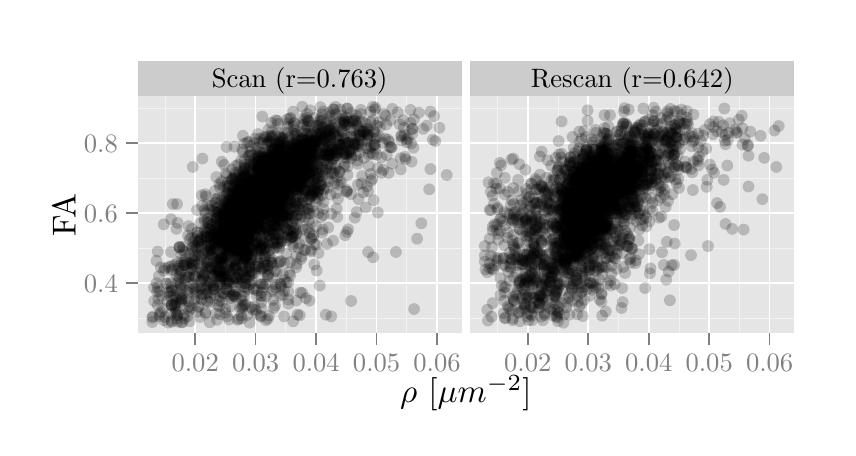
\begin{tikzpicture}[x=1pt,y=1pt]
\definecolor[named]{fillColor}{rgb}{1.00,1.00,1.00}
\path[use as bounding box,fill=fillColor,fill opacity=0.00] (0,0) rectangle (289.08,144.54);
\begin{scope}
\path[clip] (  0.00,  0.00) rectangle (289.08,144.54);
\definecolor[named]{drawColor}{rgb}{1.00,1.00,1.00}
\definecolor[named]{fillColor}{rgb}{1.00,1.00,1.00}

\path[draw=drawColor,line width= 0.6pt,line join=round,line cap=round,fill=fillColor] ( -0.00,  0.00) rectangle (289.08,144.54);
\end{scope}
\begin{scope}
\path[clip] ( 39.69,119.86) rectangle (156.86,132.50);
\definecolor[named]{fillColor}{rgb}{0.80,0.80,0.80}

\path[fill=fillColor] ( 39.69,119.86) rectangle (156.86,132.50);
\definecolor[named]{drawColor}{rgb}{0.00,0.00,0.00}

\node[text=drawColor,anchor=base,inner sep=0pt, outer sep=0pt, scale=  0.96] at ( 98.27,122.87) {Scan (r=0.763)};
\end{scope}
\begin{scope}
\path[clip] (159.87,119.86) rectangle (277.03,132.50);
\definecolor[named]{fillColor}{rgb}{0.80,0.80,0.80}

\path[fill=fillColor] (159.87,119.86) rectangle (277.03,132.50);
\definecolor[named]{drawColor}{rgb}{0.00,0.00,0.00}

\node[text=drawColor,anchor=base,inner sep=0pt, outer sep=0pt, scale=  0.96] at (218.45,122.87) {Rescan (r=0.642)};
\end{scope}
\begin{scope}
\path[clip] ( 39.69, 34.04) rectangle (156.86,119.86);
\definecolor[named]{fillColor}{rgb}{0.90,0.90,0.90}

\path[fill=fillColor] ( 39.69, 34.04) rectangle (156.86,119.86);
\definecolor[named]{drawColor}{rgb}{0.95,0.95,0.95}

\path[draw=drawColor,line width= 0.3pt,line join=round] ( 39.69, 39.58) --
	(156.86, 39.58);

\path[draw=drawColor,line width= 0.3pt,line join=round] ( 39.69, 64.87) --
	(156.86, 64.87);

\path[draw=drawColor,line width= 0.3pt,line join=round] ( 39.69, 90.16) --
	(156.86, 90.16);

\path[draw=drawColor,line width= 0.3pt,line join=round] ( 39.69,115.45) --
	(156.86,115.45);

\path[draw=drawColor,line width= 0.3pt,line join=round] ( 49.61, 34.04) --
	( 49.61,119.86);

\path[draw=drawColor,line width= 0.3pt,line join=round] ( 71.46, 34.04) --
	( 71.46,119.86);

\path[draw=drawColor,line width= 0.3pt,line join=round] ( 93.31, 34.04) --
	( 93.31,119.86);

\path[draw=drawColor,line width= 0.3pt,line join=round] (115.16, 34.04) --
	(115.16,119.86);

\path[draw=drawColor,line width= 0.3pt,line join=round] (137.01, 34.04) --
	(137.01,119.86);
\definecolor[named]{drawColor}{rgb}{1.00,1.00,1.00}

\path[draw=drawColor,line width= 0.6pt,line join=round] ( 39.69, 52.23) --
	(156.86, 52.23);

\path[draw=drawColor,line width= 0.6pt,line join=round] ( 39.69, 77.52) --
	(156.86, 77.52);

\path[draw=drawColor,line width= 0.6pt,line join=round] ( 39.69,102.81) --
	(156.86,102.81);

\path[draw=drawColor,line width= 0.6pt,line join=round] ( 60.53, 34.04) --
	( 60.53,119.86);

\path[draw=drawColor,line width= 0.6pt,line join=round] ( 82.38, 34.04) --
	( 82.38,119.86);

\path[draw=drawColor,line width= 0.6pt,line join=round] (104.23, 34.04) --
	(104.23,119.86);

\path[draw=drawColor,line width= 0.6pt,line join=round] (126.08, 34.04) --
	(126.08,119.86);

\path[draw=drawColor,line width= 0.6pt,line join=round] (147.93, 34.04) --
	(147.93,119.86);
\definecolor[named]{fillColor}{rgb}{0.00,0.00,0.00}

\path[fill=fillColor,fill opacity=0.20] ( 52.23, 45.91) circle (  2.13);

\path[fill=fillColor,fill opacity=0.20] ( 64.25, 41.73) circle (  2.13);

\path[fill=fillColor,fill opacity=0.20] ( 76.26, 55.39) circle (  2.13);

\path[fill=fillColor,fill opacity=0.20] ( 86.97, 71.20) circle (  2.13);

\path[fill=fillColor,fill opacity=0.20] ( 81.07, 74.48) circle (  2.13);

\path[fill=fillColor,fill opacity=0.20] ( 75.17, 71.83) circle (  2.13);

\path[fill=fillColor,fill opacity=0.20] ( 71.02, 56.15) circle (  2.13);

\path[fill=fillColor,fill opacity=0.20] ( 75.17, 47.30) circle (  2.13);

\path[fill=fillColor,fill opacity=0.20] ( 85.88, 72.08) circle (  2.13);

\path[fill=fillColor,fill opacity=0.20] ( 97.68, 87.76) circle (  2.13);

\path[fill=fillColor,fill opacity=0.20] (108.60, 89.02) circle (  2.13);

\path[fill=fillColor,fill opacity=0.20] ( 96.36, 88.14) circle (  2.13);

\path[fill=fillColor,fill opacity=0.20] (103.79, 87.89) circle (  2.13);

\path[fill=fillColor,fill opacity=0.20] (100.30, 85.48) circle (  2.13);

\path[fill=fillColor,fill opacity=0.20] ( 91.78, 67.40) circle (  2.13);

\path[fill=fillColor,fill opacity=0.20] ( 69.49, 54.88) circle (  2.13);

\path[fill=fillColor,fill opacity=0.20] ( 58.13, 45.65) circle (  2.13);

\path[fill=fillColor,fill opacity=0.20] ( 85.22, 57.41) circle (  2.13);

\path[fill=fillColor,fill opacity=0.20] ( 90.68, 79.16) circle (  2.13);

\path[fill=fillColor,fill opacity=0.20] ( 94.84, 89.40) circle (  2.13);

\path[fill=fillColor,fill opacity=0.20] ( 98.33, 97.75) circle (  2.13);

\path[fill=fillColor,fill opacity=0.20] (102.92,101.04) circle (  2.13);

\path[fill=fillColor,fill opacity=0.20] (100.08, 95.22) circle (  2.13);

\path[fill=fillColor,fill opacity=0.20] ( 95.27, 87.25) circle (  2.13);

\path[fill=fillColor,fill opacity=0.20] ( 93.52, 86.87) circle (  2.13);

\path[fill=fillColor,fill opacity=0.20] ( 88.06, 89.28) circle (  2.13);

\path[fill=fillColor,fill opacity=0.20] ( 76.04, 73.09) circle (  2.13);

\path[fill=fillColor,fill opacity=0.20] ( 74.95, 53.87) circle (  2.13);

\path[fill=fillColor,fill opacity=0.20] ( 71.46, 41.48) circle (  2.13);

\path[fill=fillColor,fill opacity=0.20] ( 58.56, 38.44) circle (  2.13);

\path[fill=fillColor,fill opacity=0.20] ( 81.51, 55.89) circle (  2.13);

\path[fill=fillColor,fill opacity=0.20] ( 98.11, 79.79) circle (  2.13);

\path[fill=fillColor,fill opacity=0.20] (111.66, 98.51) circle (  2.13);

\path[fill=fillColor,fill opacity=0.20] (106.42, 94.08) circle (  2.13);

\path[fill=fillColor,fill opacity=0.20] ( 99.21, 97.62) circle (  2.13);

\path[fill=fillColor,fill opacity=0.20] ( 92.87,106.47) circle (  2.13);

\path[fill=fillColor,fill opacity=0.20] ( 97.68,100.15) circle (  2.13);

\path[fill=fillColor,fill opacity=0.20] ( 99.86, 91.17) circle (  2.13);

\path[fill=fillColor,fill opacity=0.20] ( 88.94, 89.66) circle (  2.13);

\path[fill=fillColor,fill opacity=0.20] ( 79.76, 86.75) circle (  2.13);

\path[fill=fillColor,fill opacity=0.20] ( 77.14, 73.22) circle (  2.13);

\path[fill=fillColor,fill opacity=0.20] ( 77.79, 60.83) circle (  2.13);

\path[fill=fillColor,fill opacity=0.20] ( 74.30, 48.05) circle (  2.13);

\path[fill=fillColor,fill opacity=0.20] ( 90.25,110.90) circle (  2.13);

\path[fill=fillColor,fill opacity=0.20] ( 60.97, 47.80) circle (  2.13);

\path[fill=fillColor,fill opacity=0.20] ( 76.48, 75.49) circle (  2.13);

\path[fill=fillColor,fill opacity=0.20] ( 98.77, 92.06) circle (  2.13);

\path[fill=fillColor,fill opacity=0.20] (107.95,105.59) circle (  2.13);

\path[fill=fillColor,fill opacity=0.20] (105.10,106.22) circle (  2.13);

\path[fill=fillColor,fill opacity=0.20] (103.58,102.30) circle (  2.13);

\path[fill=fillColor,fill opacity=0.20] ( 95.27, 99.14) circle (  2.13);

\path[fill=fillColor,fill opacity=0.20] ( 83.25, 97.24) circle (  2.13);

\path[fill=fillColor,fill opacity=0.20] ( 89.37, 97.88) circle (  2.13);

\path[fill=fillColor,fill opacity=0.20] ( 85.22, 94.21) circle (  2.13);

\path[fill=fillColor,fill opacity=0.20] ( 76.92, 84.22) circle (  2.13);

\path[fill=fillColor,fill opacity=0.20] ( 74.30, 71.70) circle (  2.13);

\path[fill=fillColor,fill opacity=0.20] ( 65.56, 57.79) circle (  2.13);

\path[fill=fillColor,fill opacity=0.20] ( 54.19, 38.32) circle (  2.13);

\path[fill=fillColor,fill opacity=0.20] ( 70.80, 76.25) circle (  2.13);

\path[fill=fillColor,fill opacity=0.20] ( 90.68,101.16) circle (  2.13);

\path[fill=fillColor,fill opacity=0.20] ( 81.51, 80.93) circle (  2.13);

\path[fill=fillColor,fill opacity=0.20] ( 81.29, 81.44) circle (  2.13);

\path[fill=fillColor,fill opacity=0.20] ( 83.47, 89.53) circle (  2.13);

\path[fill=fillColor,fill opacity=0.20] ( 64.25, 50.20) circle (  2.13);

\path[fill=fillColor,fill opacity=0.20] ( 78.23, 87.25) circle (  2.13);

\path[fill=fillColor,fill opacity=0.20] ( 95.93,102.55) circle (  2.13);

\path[fill=fillColor,fill opacity=0.20] (102.48,109.13) circle (  2.13);

\path[fill=fillColor,fill opacity=0.20] (102.05,114.69) circle (  2.13);

\path[fill=fillColor,fill opacity=0.20] ( 99.21, 98.00) circle (  2.13);

\path[fill=fillColor,fill opacity=0.20] ( 87.84, 90.79) circle (  2.13);

\path[fill=fillColor,fill opacity=0.20] ( 73.86, 93.32) circle (  2.13);

\path[fill=fillColor,fill opacity=0.20] ( 71.67, 91.93) circle (  2.13);

\path[fill=fillColor,fill opacity=0.20] ( 64.25, 84.35) circle (  2.13);

\path[fill=fillColor,fill opacity=0.20] ( 66.65, 69.42) circle (  2.13);

\path[fill=fillColor,fill opacity=0.20] (105.32, 96.61) circle (  2.13);

\path[fill=fillColor,fill opacity=0.20] ( 97.02, 91.81) circle (  2.13);

\path[fill=fillColor,fill opacity=0.20] ( 94.84, 96.86) circle (  2.13);

\path[fill=fillColor,fill opacity=0.20] ( 99.86, 97.62) circle (  2.13);

\path[fill=fillColor,fill opacity=0.20] ( 99.42, 96.23) circle (  2.13);

\path[fill=fillColor,fill opacity=0.20] ( 95.71,100.66) circle (  2.13);

\path[fill=fillColor,fill opacity=0.20] ( 81.29, 92.69) circle (  2.13);

\path[fill=fillColor,fill opacity=0.20] ( 55.94, 64.11) circle (  2.13);

\path[fill=fillColor,fill opacity=0.20] ( 70.36, 54.38) circle (  2.13);

\path[fill=fillColor,fill opacity=0.20] ( 77.57, 91.30) circle (  2.13);

\path[fill=fillColor,fill opacity=0.20] ( 88.06,110.14) circle (  2.13);

\path[fill=fillColor,fill opacity=0.20] ( 90.47,106.73) circle (  2.13);

\path[fill=fillColor,fill opacity=0.20] ( 87.62,103.69) circle (  2.13);

\path[fill=fillColor,fill opacity=0.20] ( 89.59,111.03) circle (  2.13);

\path[fill=fillColor,fill opacity=0.20] ( 91.99,104.45) circle (  2.13);

\path[fill=fillColor,fill opacity=0.20] ( 85.44, 86.12) circle (  2.13);

\path[fill=fillColor,fill opacity=0.20] ( 64.46, 83.46) circle (  2.13);

\path[fill=fillColor,fill opacity=0.20] ( 77.57, 76.38) circle (  2.13);

\path[fill=fillColor,fill opacity=0.20] (111.88,100.03) circle (  2.13);

\path[fill=fillColor,fill opacity=0.20] (110.35, 92.06) circle (  2.13);

\path[fill=fillColor,fill opacity=0.20] (116.03, 98.89) circle (  2.13);

\path[fill=fillColor,fill opacity=0.20] (126.95,110.39) circle (  2.13);

\path[fill=fillColor,fill opacity=0.20] (146.84,112.54) circle (  2.13);

\path[fill=fillColor,fill opacity=0.20] (113.41,106.85) circle (  2.13);

\path[fill=fillColor,fill opacity=0.20] (105.54,110.52) circle (  2.13);

\path[fill=fillColor,fill opacity=0.20] (101.39,104.32) circle (  2.13);

\path[fill=fillColor,fill opacity=0.20] ( 65.34, 73.98) circle (  2.13);

\path[fill=fillColor,fill opacity=0.20] ( 67.96, 56.15) circle (  2.13);

\path[fill=fillColor,fill opacity=0.20] ( 78.01, 88.52) circle (  2.13);

\path[fill=fillColor,fill opacity=0.20] ( 88.94,100.40) circle (  2.13);

\path[fill=fillColor,fill opacity=0.20] ( 81.94,102.81) circle (  2.13);

\path[fill=fillColor,fill opacity=0.20] ( 80.41, 96.23) circle (  2.13);

\path[fill=fillColor,fill opacity=0.20] ( 83.47, 96.23) circle (  2.13);

\path[fill=fillColor,fill opacity=0.20] ( 80.20, 98.26) circle (  2.13);

\path[fill=fillColor,fill opacity=0.20] ( 78.67, 86.12) circle (  2.13);

\path[fill=fillColor,fill opacity=0.20] ( 77.79, 76.63) circle (  2.13);

\path[fill=fillColor,fill opacity=0.20] ( 67.96, 75.62) circle (  2.13);

\path[fill=fillColor,fill opacity=0.20] ( 59.88, 60.70) circle (  2.13);

\path[fill=fillColor,fill opacity=0.20] (111.66,102.81) circle (  2.13);

\path[fill=fillColor,fill opacity=0.20] (115.59, 94.34) circle (  2.13);

\path[fill=fillColor,fill opacity=0.20] (119.09, 96.49) circle (  2.13);

\path[fill=fillColor,fill opacity=0.20] (133.73,113.94) circle (  2.13);

\path[fill=fillColor,fill opacity=0.20] (120.40,114.82) circle (  2.13);

\path[fill=fillColor,fill opacity=0.20] (122.58,107.87) circle (  2.13);

\path[fill=fillColor,fill opacity=0.20] (100.95,106.10) circle (  2.13);

\path[fill=fillColor,fill opacity=0.20] ( 96.15,108.88) circle (  2.13);

\path[fill=fillColor,fill opacity=0.20] (115.59,115.33) circle (  2.13);

\path[fill=fillColor,fill opacity=0.20] ( 79.98, 93.45) circle (  2.13);

\path[fill=fillColor,fill opacity=0.20] ( 60.31, 50.33) circle (  2.13);

\path[fill=fillColor,fill opacity=0.20] ( 81.07, 75.87) circle (  2.13);

\path[fill=fillColor,fill opacity=0.20] ( 81.94, 85.61) circle (  2.13);

\path[fill=fillColor,fill opacity=0.20] ( 83.91,103.19) circle (  2.13);

\path[fill=fillColor,fill opacity=0.20] ( 86.97,107.61) circle (  2.13);

\path[fill=fillColor,fill opacity=0.20] ( 83.04, 94.21) circle (  2.13);

\path[fill=fillColor,fill opacity=0.20] ( 86.10, 87.38) circle (  2.13);

\path[fill=fillColor,fill opacity=0.20] ( 80.63, 88.27) circle (  2.13);

\path[fill=fillColor,fill opacity=0.20] ( 82.82, 86.50) circle (  2.13);

\path[fill=fillColor,fill opacity=0.20] ( 71.24, 76.13) circle (  2.13);

\path[fill=fillColor,fill opacity=0.20] ( 89.15, 84.35) circle (  2.13);

\path[fill=fillColor,fill opacity=0.20] (117.78,102.18) circle (  2.13);

\path[fill=fillColor,fill opacity=0.20] (109.26,103.69) circle (  2.13);

\path[fill=fillColor,fill opacity=0.20] (101.17,111.03) circle (  2.13);

\path[fill=fillColor,fill opacity=0.20] (100.08,103.69) circle (  2.13);

\path[fill=fillColor,fill opacity=0.20] (102.48,100.78) circle (  2.13);

\path[fill=fillColor,fill opacity=0.20] ( 94.40,102.68) circle (  2.13);

\path[fill=fillColor,fill opacity=0.20] ( 82.60,101.04) circle (  2.13);

\path[fill=fillColor,fill opacity=0.20] ( 84.78,112.42) circle (  2.13);

\path[fill=fillColor,fill opacity=0.20] ( 56.38, 40.85) circle (  2.13);

\path[fill=fillColor,fill opacity=0.20] ( 75.39, 64.11) circle (  2.13);

\path[fill=fillColor,fill opacity=0.20] ( 81.73, 80.30) circle (  2.13);

\path[fill=fillColor,fill opacity=0.20] ( 91.78,104.70) circle (  2.13);

\path[fill=fillColor,fill opacity=0.20] ( 86.53,102.43) circle (  2.13);

\path[fill=fillColor,fill opacity=0.20] ( 83.47, 90.42) circle (  2.13);

\path[fill=fillColor,fill opacity=0.20] ( 81.94, 88.52) circle (  2.13);

\path[fill=fillColor,fill opacity=0.20] ( 80.41, 90.42) circle (  2.13);

\path[fill=fillColor,fill opacity=0.20] ( 78.23, 86.50) circle (  2.13);

\path[fill=fillColor,fill opacity=0.20] (129.14,104.45) circle (  2.13);

\path[fill=fillColor,fill opacity=0.20] (114.72,109.38) circle (  2.13);

\path[fill=fillColor,fill opacity=0.20] (102.70,102.05) circle (  2.13);

\path[fill=fillColor,fill opacity=0.20] (119.96,107.74) circle (  2.13);

\path[fill=fillColor,fill opacity=0.20] (100.95,105.72) circle (  2.13);

\path[fill=fillColor,fill opacity=0.20] ( 93.31,100.28) circle (  2.13);

\path[fill=fillColor,fill opacity=0.20] (100.73,100.53) circle (  2.13);

\path[fill=fillColor,fill opacity=0.20] ( 94.18, 98.38) circle (  2.13);

\path[fill=fillColor,fill opacity=0.20] ( 86.31, 95.60) circle (  2.13);

\path[fill=fillColor,fill opacity=0.20] ( 88.28,105.46) circle (  2.13);

\path[fill=fillColor,fill opacity=0.20] ( 79.32,103.06) circle (  2.13);

\path[fill=fillColor,fill opacity=0.20] ( 72.33, 54.76) circle (  2.13);

\path[fill=fillColor,fill opacity=0.20] ( 90.90, 79.03) circle (  2.13);

\path[fill=fillColor,fill opacity=0.20] ( 99.64, 96.36) circle (  2.13);

\path[fill=fillColor,fill opacity=0.20] ( 97.46,103.82) circle (  2.13);

\path[fill=fillColor,fill opacity=0.20] ( 88.06,104.96) circle (  2.13);

\path[fill=fillColor,fill opacity=0.20] ( 84.78,102.81) circle (  2.13);

\path[fill=fillColor,fill opacity=0.20] ( 83.04, 94.84) circle (  2.13);

\path[fill=fillColor,fill opacity=0.20] ( 76.48, 83.08) circle (  2.13);

\path[fill=fillColor,fill opacity=0.20] ( 79.98, 85.61) circle (  2.13);

\path[fill=fillColor,fill opacity=0.20] ( 66.21, 71.57) circle (  2.13);

\path[fill=fillColor,fill opacity=0.20] (117.34,111.03) circle (  2.13);

\path[fill=fillColor,fill opacity=0.20] (103.36, 93.70) circle (  2.13);

\path[fill=fillColor,fill opacity=0.20] (109.69, 95.22) circle (  2.13);

\path[fill=fillColor,fill opacity=0.20] (122.15,106.98) circle (  2.13);

\path[fill=fillColor,fill opacity=0.20] (106.20,105.21) circle (  2.13);

\path[fill=fillColor,fill opacity=0.20] ( 96.58,100.53) circle (  2.13);

\path[fill=fillColor,fill opacity=0.20] (106.63, 99.14) circle (  2.13);

\path[fill=fillColor,fill opacity=0.20] ( 83.25, 93.58) circle (  2.13);

\path[fill=fillColor,fill opacity=0.20] ( 88.06, 94.84) circle (  2.13);

\path[fill=fillColor,fill opacity=0.20] ( 87.62,103.31) circle (  2.13);

\path[fill=fillColor,fill opacity=0.20] ( 74.30, 82.20) circle (  2.13);

\path[fill=fillColor,fill opacity=0.20] ( 82.60, 74.48) circle (  2.13);

\path[fill=fillColor,fill opacity=0.20] ( 90.68, 84.22) circle (  2.13);

\path[fill=fillColor,fill opacity=0.20] ( 92.43, 89.91) circle (  2.13);

\path[fill=fillColor,fill opacity=0.20] ( 90.90, 97.62) circle (  2.13);

\path[fill=fillColor,fill opacity=0.20] ( 88.28,107.11) circle (  2.13);

\path[fill=fillColor,fill opacity=0.20] ( 90.68,102.43) circle (  2.13);

\path[fill=fillColor,fill opacity=0.20] ( 81.29, 81.94) circle (  2.13);

\path[fill=fillColor,fill opacity=0.20] ( 89.81, 77.39) circle (  2.13);

\path[fill=fillColor,fill opacity=0.20] ( 82.60, 81.18) circle (  2.13);

\path[fill=fillColor,fill opacity=0.20] ( 95.93, 97.62) circle (  2.13);

\path[fill=fillColor,fill opacity=0.20] ( 89.81, 98.63) circle (  2.13);

\path[fill=fillColor,fill opacity=0.20] ( 88.28, 89.53) circle (  2.13);

\path[fill=fillColor,fill opacity=0.20] ( 97.89, 95.73) circle (  2.13);

\path[fill=fillColor,fill opacity=0.20] (107.73,103.82) circle (  2.13);

\path[fill=fillColor,fill opacity=0.20] (100.52,100.28) circle (  2.13);

\path[fill=fillColor,fill opacity=0.20] ( 98.33, 99.77) circle (  2.13);

\path[fill=fillColor,fill opacity=0.20] (101.17,103.31) circle (  2.13);

\path[fill=fillColor,fill opacity=0.20] ( 92.87, 97.88) circle (  2.13);

\path[fill=fillColor,fill opacity=0.20] ( 85.88, 96.23) circle (  2.13);

\path[fill=fillColor,fill opacity=0.20] ( 85.66, 96.36) circle (  2.13);

\path[fill=fillColor,fill opacity=0.20] ( 66.43, 63.99) circle (  2.13);

\path[fill=fillColor,fill opacity=0.20] ( 72.11, 57.16) circle (  2.13);

\path[fill=fillColor,fill opacity=0.20] ( 80.63, 72.46) circle (  2.13);

\path[fill=fillColor,fill opacity=0.20] ( 82.38, 84.35) circle (  2.13);

\path[fill=fillColor,fill opacity=0.20] ( 91.99, 94.08) circle (  2.13);

\path[fill=fillColor,fill opacity=0.20] ( 86.75, 98.51) circle (  2.13);

\path[fill=fillColor,fill opacity=0.20] ( 87.62, 98.13) circle (  2.13);

\path[fill=fillColor,fill opacity=0.20] ( 88.50, 89.28) circle (  2.13);

\path[fill=fillColor,fill opacity=0.20] ( 79.32, 82.70) circle (  2.13);

\path[fill=fillColor,fill opacity=0.20] ( 75.83, 85.99) circle (  2.13);

\path[fill=fillColor,fill opacity=0.20] ( 64.90, 71.95) circle (  2.13);

\path[fill=fillColor,fill opacity=0.20] ( 86.31, 86.24) circle (  2.13);

\path[fill=fillColor,fill opacity=0.20] (110.13,100.40) circle (  2.13);

\path[fill=fillColor,fill opacity=0.20] ( 83.25, 92.31) circle (  2.13);

\path[fill=fillColor,fill opacity=0.20] ( 87.62, 93.58) circle (  2.13);

\path[fill=fillColor,fill opacity=0.20] ( 95.05,100.78) circle (  2.13);

\path[fill=fillColor,fill opacity=0.20] ( 98.33,103.82) circle (  2.13);

\path[fill=fillColor,fill opacity=0.20] (101.17, 99.77) circle (  2.13);

\path[fill=fillColor,fill opacity=0.20] ( 91.56,102.18) circle (  2.13);

\path[fill=fillColor,fill opacity=0.20] (106.63,108.62) circle (  2.13);

\path[fill=fillColor,fill opacity=0.20] (102.92,100.15) circle (  2.13);

\path[fill=fillColor,fill opacity=0.20] ( 90.47, 92.19) circle (  2.13);

\path[fill=fillColor,fill opacity=0.20] ( 83.25, 81.82) circle (  2.13);

\path[fill=fillColor,fill opacity=0.20] ( 71.46, 55.89) circle (  2.13);

\path[fill=fillColor,fill opacity=0.20] ( 89.59, 79.03) circle (  2.13);

\path[fill=fillColor,fill opacity=0.20] ( 90.68, 94.21) circle (  2.13);

\path[fill=fillColor,fill opacity=0.20] ( 85.00, 92.69) circle (  2.13);

\path[fill=fillColor,fill opacity=0.20] ( 89.59, 93.83) circle (  2.13);

\path[fill=fillColor,fill opacity=0.20] ( 90.68,100.66) circle (  2.13);

\path[fill=fillColor,fill opacity=0.20] ( 86.75,103.44) circle (  2.13);

\path[fill=fillColor,fill opacity=0.20] ( 77.79, 99.52) circle (  2.13);

\path[fill=fillColor,fill opacity=0.20] ( 76.26, 88.77) circle (  2.13);

\path[fill=fillColor,fill opacity=0.20] ( 67.52, 70.06) circle (  2.13);

\path[fill=fillColor,fill opacity=0.20] ( 72.99, 75.75) circle (  2.13);

\path[fill=fillColor,fill opacity=0.20] ( 97.24,104.07) circle (  2.13);

\path[fill=fillColor,fill opacity=0.20] ( 96.15, 97.50) circle (  2.13);

\path[fill=fillColor,fill opacity=0.20] ( 96.80,100.03) circle (  2.13);

\path[fill=fillColor,fill opacity=0.20] (105.32,102.18) circle (  2.13);

\path[fill=fillColor,fill opacity=0.20] (102.26,100.91) circle (  2.13);

\path[fill=fillColor,fill opacity=0.20] ( 99.64,101.42) circle (  2.13);

\path[fill=fillColor,fill opacity=0.20] (100.95,103.95) circle (  2.13);

\path[fill=fillColor,fill opacity=0.20] ( 98.99,106.98) circle (  2.13);

\path[fill=fillColor,fill opacity=0.20] (103.36,103.44) circle (  2.13);

\path[fill=fillColor,fill opacity=0.20] ( 95.93, 90.29) circle (  2.13);

\path[fill=fillColor,fill opacity=0.20] ( 94.84, 79.03) circle (  2.13);

\path[fill=fillColor,fill opacity=0.20] ( 78.67, 62.22) circle (  2.13);

\path[fill=fillColor,fill opacity=0.20] ( 88.06, 61.08) circle (  2.13);

\path[fill=fillColor,fill opacity=0.20] ( 99.42, 88.90) circle (  2.13);

\path[fill=fillColor,fill opacity=0.20] ( 84.35, 94.46) circle (  2.13);

\path[fill=fillColor,fill opacity=0.20] ( 89.37, 95.35) circle (  2.13);

\path[fill=fillColor,fill opacity=0.20] ( 89.81,102.55) circle (  2.13);

\path[fill=fillColor,fill opacity=0.20] ( 85.22,104.07) circle (  2.13);

\path[fill=fillColor,fill opacity=0.20] ( 86.97, 99.90) circle (  2.13);

\path[fill=fillColor,fill opacity=0.20] ( 78.45, 91.17) circle (  2.13);

\path[fill=fillColor,fill opacity=0.20] ( 75.17, 78.02) circle (  2.13);

\path[fill=fillColor,fill opacity=0.20] ( 60.31, 65.88) circle (  2.13);

\path[fill=fillColor,fill opacity=0.20] ( 75.17, 69.30) circle (  2.13);

\path[fill=fillColor,fill opacity=0.20] ( 97.46, 96.99) circle (  2.13);

\path[fill=fillColor,fill opacity=0.20] ( 94.18, 92.57) circle (  2.13);

\path[fill=fillColor,fill opacity=0.20] ( 97.46,100.15) circle (  2.13);

\path[fill=fillColor,fill opacity=0.20] (107.29,107.23) circle (  2.13);

\path[fill=fillColor,fill opacity=0.20] (108.38,103.69) circle (  2.13);

\path[fill=fillColor,fill opacity=0.20] (102.70, 96.36) circle (  2.13);

\path[fill=fillColor,fill opacity=0.20] ( 98.33, 93.70) circle (  2.13);

\path[fill=fillColor,fill opacity=0.20] (107.29, 98.63) circle (  2.13);

\path[fill=fillColor,fill opacity=0.20] ( 98.33,101.42) circle (  2.13);

\path[fill=fillColor,fill opacity=0.20] (100.52, 93.96) circle (  2.13);

\path[fill=fillColor,fill opacity=0.20] (100.52, 83.71) circle (  2.13);

\path[fill=fillColor,fill opacity=0.20] ( 86.10, 64.87) circle (  2.13);

\path[fill=fillColor,fill opacity=0.20] ( 57.69, 40.21) circle (  2.13);

\path[fill=fillColor,fill opacity=0.20] ( 75.61, 64.24) circle (  2.13);

\path[fill=fillColor,fill opacity=0.20] ( 88.28, 84.47) circle (  2.13);

\path[fill=fillColor,fill opacity=0.20] ( 86.53, 93.07) circle (  2.13);

\path[fill=fillColor,fill opacity=0.20] ( 81.73, 92.19) circle (  2.13);

\path[fill=fillColor,fill opacity=0.20] ( 89.37, 92.06) circle (  2.13);

\path[fill=fillColor,fill opacity=0.20] ( 86.97, 93.96) circle (  2.13);

\path[fill=fillColor,fill opacity=0.20] ( 86.10, 89.40) circle (  2.13);

\path[fill=fillColor,fill opacity=0.20] ( 77.36, 78.66) circle (  2.13);

\path[fill=fillColor,fill opacity=0.20] ( 72.77, 71.57) circle (  2.13);

\path[fill=fillColor,fill opacity=0.20] ( 65.77, 64.62) circle (  2.13);

\path[fill=fillColor,fill opacity=0.20] ( 68.40, 68.16) circle (  2.13);

\path[fill=fillColor,fill opacity=0.20] ( 97.68, 98.76) circle (  2.13);

\path[fill=fillColor,fill opacity=0.20] ( 94.18, 89.15) circle (  2.13);

\path[fill=fillColor,fill opacity=0.20] ( 95.05, 92.69) circle (  2.13);

\path[fill=fillColor,fill opacity=0.20] (100.95,100.28) circle (  2.13);

\path[fill=fillColor,fill opacity=0.20] (102.05, 97.75) circle (  2.13);

\path[fill=fillColor,fill opacity=0.20] ( 99.21, 96.74) circle (  2.13);

\path[fill=fillColor,fill opacity=0.20] (100.08, 96.86) circle (  2.13);

\path[fill=fillColor,fill opacity=0.20] (103.58, 94.97) circle (  2.13);

\path[fill=fillColor,fill opacity=0.20] (100.08, 92.06) circle (  2.13);

\path[fill=fillColor,fill opacity=0.20] (104.23, 86.24) circle (  2.13);

\path[fill=fillColor,fill opacity=0.20] (102.26, 85.74) circle (  2.13);

\path[fill=fillColor,fill opacity=0.20] ( 88.06, 82.95) circle (  2.13);

\path[fill=fillColor,fill opacity=0.20] ( 55.94, 38.07) circle (  2.13);

\path[fill=fillColor,fill opacity=0.20] ( 85.00, 57.92) circle (  2.13);

\path[fill=fillColor,fill opacity=0.20] ( 93.74, 80.68) circle (  2.13);

\path[fill=fillColor,fill opacity=0.20] ( 85.22, 85.86) circle (  2.13);

\path[fill=fillColor,fill opacity=0.20] ( 91.34, 93.96) circle (  2.13);

\path[fill=fillColor,fill opacity=0.20] ( 98.11,102.30) circle (  2.13);

\path[fill=fillColor,fill opacity=0.20] ( 86.75, 94.84) circle (  2.13);

\path[fill=fillColor,fill opacity=0.20] ( 84.78, 88.39) circle (  2.13);

\path[fill=fillColor,fill opacity=0.20] ( 83.25, 84.60) circle (  2.13);

\path[fill=fillColor,fill opacity=0.20] ( 83.47, 80.43) circle (  2.13);

\path[fill=fillColor,fill opacity=0.20] ( 68.83, 73.34) circle (  2.13);

\path[fill=fillColor,fill opacity=0.20] ( 59.22, 64.62) circle (  2.13);

\path[fill=fillColor,fill opacity=0.20] ( 92.21, 95.60) circle (  2.13);

\path[fill=fillColor,fill opacity=0.20] ( 93.09, 89.53) circle (  2.13);

\path[fill=fillColor,fill opacity=0.20] (103.14, 92.82) circle (  2.13);

\path[fill=fillColor,fill opacity=0.20] (103.36,103.69) circle (  2.13);

\path[fill=fillColor,fill opacity=0.20] (105.76,104.96) circle (  2.13);

\path[fill=fillColor,fill opacity=0.20] (102.48, 99.01) circle (  2.13);

\path[fill=fillColor,fill opacity=0.20] (100.73, 95.98) circle (  2.13);

\path[fill=fillColor,fill opacity=0.20] (103.79, 99.01) circle (  2.13);

\path[fill=fillColor,fill opacity=0.20] (110.35, 99.39) circle (  2.13);

\path[fill=fillColor,fill opacity=0.20] (104.89, 90.29) circle (  2.13);

\path[fill=fillColor,fill opacity=0.20] ( 98.11, 77.01) circle (  2.13);

\path[fill=fillColor,fill opacity=0.20] ( 76.70, 69.42) circle (  2.13);

\path[fill=fillColor,fill opacity=0.20] ( 91.12, 60.07) circle (  2.13);

\path[fill=fillColor,fill opacity=0.20] (101.39, 82.70) circle (  2.13);

\path[fill=fillColor,fill opacity=0.20] ( 98.33, 98.89) circle (  2.13);

\path[fill=fillColor,fill opacity=0.20] (102.48,105.97) circle (  2.13);

\path[fill=fillColor,fill opacity=0.20] ( 91.78, 97.88) circle (  2.13);

\path[fill=fillColor,fill opacity=0.20] ( 83.69, 94.08) circle (  2.13);

\path[fill=fillColor,fill opacity=0.20] ( 83.91, 88.90) circle (  2.13);

\path[fill=fillColor,fill opacity=0.20] ( 76.26, 82.58) circle (  2.13);

\path[fill=fillColor,fill opacity=0.20] ( 72.77, 80.55) circle (  2.13);

\path[fill=fillColor,fill opacity=0.20] ( 66.87, 70.82) circle (  2.13);

\path[fill=fillColor,fill opacity=0.20] ( 62.72, 65.25) circle (  2.13);

\path[fill=fillColor,fill opacity=0.20] ( 91.34, 89.53) circle (  2.13);

\path[fill=fillColor,fill opacity=0.20] ( 86.31, 86.75) circle (  2.13);

\path[fill=fillColor,fill opacity=0.20] ( 98.11, 92.31) circle (  2.13);

\path[fill=fillColor,fill opacity=0.20] (113.41,102.18) circle (  2.13);

\path[fill=fillColor,fill opacity=0.20] (116.69,108.37) circle (  2.13);

\path[fill=fillColor,fill opacity=0.20] (117.34,110.52) circle (  2.13);

\path[fill=fillColor,fill opacity=0.20] (109.04,108.62) circle (  2.13);

\path[fill=fillColor,fill opacity=0.20] (106.63,102.05) circle (  2.13);

\path[fill=fillColor,fill opacity=0.20] (101.61, 96.74) circle (  2.13);

\path[fill=fillColor,fill opacity=0.20] (100.08, 94.08) circle (  2.13);

\path[fill=fillColor,fill opacity=0.20] (111.88, 90.54) circle (  2.13);

\path[fill=fillColor,fill opacity=0.20] (104.67, 83.21) circle (  2.13);

\path[fill=fillColor,fill opacity=0.20] ( 74.73, 64.24) circle (  2.13);

\path[fill=fillColor,fill opacity=0.20] ( 98.77, 60.95) circle (  2.13);

\path[fill=fillColor,fill opacity=0.20] (102.92, 79.79) circle (  2.13);

\path[fill=fillColor,fill opacity=0.20] ( 97.02, 87.13) circle (  2.13);

\path[fill=fillColor,fill opacity=0.20] ( 97.68, 90.54) circle (  2.13);

\path[fill=fillColor,fill opacity=0.20] ( 84.78, 87.76) circle (  2.13);

\path[fill=fillColor,fill opacity=0.20] ( 82.82, 82.70) circle (  2.13);

\path[fill=fillColor,fill opacity=0.20] ( 81.51, 81.69) circle (  2.13);

\path[fill=fillColor,fill opacity=0.20] ( 72.33, 80.43) circle (  2.13);

\path[fill=fillColor,fill opacity=0.20] ( 72.33, 77.90) circle (  2.13);

\path[fill=fillColor,fill opacity=0.20] ( 68.18, 77.90) circle (  2.13);

\path[fill=fillColor,fill opacity=0.20] ( 70.36, 74.74) circle (  2.13);

\path[fill=fillColor,fill opacity=0.20] ( 97.24, 96.49) circle (  2.13);

\path[fill=fillColor,fill opacity=0.20] (102.70, 83.97) circle (  2.13);

\path[fill=fillColor,fill opacity=0.20] ( 95.71, 85.48) circle (  2.13);

\path[fill=fillColor,fill opacity=0.20] (112.10, 99.65) circle (  2.13);

\path[fill=fillColor,fill opacity=0.20] (112.10,100.66) circle (  2.13);

\path[fill=fillColor,fill opacity=0.20] (116.90, 98.26) circle (  2.13);

\path[fill=fillColor,fill opacity=0.20] (114.72,103.06) circle (  2.13);

\path[fill=fillColor,fill opacity=0.20] (110.79,108.12) circle (  2.13);

\path[fill=fillColor,fill opacity=0.20] (109.47,104.83) circle (  2.13);

\path[fill=fillColor,fill opacity=0.20] (100.95, 96.36) circle (  2.13);

\path[fill=fillColor,fill opacity=0.20] ( 98.33, 93.45) circle (  2.13);

\path[fill=fillColor,fill opacity=0.20] ( 97.68, 89.15) circle (  2.13);

\path[fill=fillColor,fill opacity=0.20] ( 70.14, 70.56) circle (  2.13);

\path[fill=fillColor,fill opacity=0.20] ( 91.34, 51.85) circle (  2.13);

\path[fill=fillColor,fill opacity=0.20] (100.30, 64.11) circle (  2.13);

\path[fill=fillColor,fill opacity=0.20] ( 91.34, 80.93) circle (  2.13);

\path[fill=fillColor,fill opacity=0.20] ( 87.41, 87.13) circle (  2.13);

\path[fill=fillColor,fill opacity=0.20] ( 84.78, 80.43) circle (  2.13);

\path[fill=fillColor,fill opacity=0.20] ( 82.60, 82.58) circle (  2.13);

\path[fill=fillColor,fill opacity=0.20] ( 80.41, 85.61) circle (  2.13);

\path[fill=fillColor,fill opacity=0.20] ( 72.77, 84.35) circle (  2.13);

\path[fill=fillColor,fill opacity=0.20] ( 70.80, 87.25) circle (  2.13);

\path[fill=fillColor,fill opacity=0.20] ( 81.73, 87.25) circle (  2.13);

\path[fill=fillColor,fill opacity=0.20] ( 70.58, 79.41) circle (  2.13);

\path[fill=fillColor,fill opacity=0.20] ( 58.35, 62.85) circle (  2.13);

\path[fill=fillColor,fill opacity=0.20] ( 78.01, 90.92) circle (  2.13);

\path[fill=fillColor,fill opacity=0.20] ( 87.19, 93.70) circle (  2.13);

\path[fill=fillColor,fill opacity=0.20] ( 98.33, 89.91) circle (  2.13);

\path[fill=fillColor,fill opacity=0.20] ( 92.65, 90.92) circle (  2.13);

\path[fill=fillColor,fill opacity=0.20] (102.92, 92.57) circle (  2.13);

\path[fill=fillColor,fill opacity=0.20] (105.98, 94.59) circle (  2.13);

\path[fill=fillColor,fill opacity=0.20] (106.42, 92.44) circle (  2.13);

\path[fill=fillColor,fill opacity=0.20] (110.79, 88.39) circle (  2.13);

\path[fill=fillColor,fill opacity=0.20] (111.00, 91.93) circle (  2.13);

\path[fill=fillColor,fill opacity=0.20] (111.66,100.40) circle (  2.13);

\path[fill=fillColor,fill opacity=0.20] (106.85,101.16) circle (  2.13);

\path[fill=fillColor,fill opacity=0.20] (100.08, 96.86) circle (  2.13);

\path[fill=fillColor,fill opacity=0.20] ( 85.88, 94.08) circle (  2.13);

\path[fill=fillColor,fill opacity=0.20] ( 71.24, 74.23) circle (  2.13);

\path[fill=fillColor,fill opacity=0.20] ( 68.62, 44.39) circle (  2.13);

\path[fill=fillColor,fill opacity=0.20] ( 85.44, 64.24) circle (  2.13);

\path[fill=fillColor,fill opacity=0.20] ( 94.40, 86.75) circle (  2.13);

\path[fill=fillColor,fill opacity=0.20] ( 92.65, 86.37) circle (  2.13);

\path[fill=fillColor,fill opacity=0.20] ( 85.88, 82.83) circle (  2.13);

\path[fill=fillColor,fill opacity=0.20] ( 84.13, 86.50) circle (  2.13);

\path[fill=fillColor,fill opacity=0.20] ( 76.70, 86.24) circle (  2.13);

\path[fill=fillColor,fill opacity=0.20] ( 70.36, 79.16) circle (  2.13);

\path[fill=fillColor,fill opacity=0.20] ( 69.27, 76.76) circle (  2.13);

\path[fill=fillColor,fill opacity=0.20] ( 73.86, 84.22) circle (  2.13);

\path[fill=fillColor,fill opacity=0.20] ( 71.89, 91.05) circle (  2.13);

\path[fill=fillColor,fill opacity=0.20] ( 72.33, 84.98) circle (  2.13);

\path[fill=fillColor,fill opacity=0.20] ( 64.90, 68.67) circle (  2.13);

\path[fill=fillColor,fill opacity=0.20] ( 67.52, 68.92) circle (  2.13);

\path[fill=fillColor,fill opacity=0.20] ( 76.04, 75.49) circle (  2.13);

\path[fill=fillColor,fill opacity=0.20] ( 85.66, 81.18) circle (  2.13);

\path[fill=fillColor,fill opacity=0.20] ( 86.75, 83.97) circle (  2.13);

\path[fill=fillColor,fill opacity=0.20] (116.90, 84.35) circle (  2.13);

\path[fill=fillColor,fill opacity=0.20] ( 93.09, 87.25) circle (  2.13);

\path[fill=fillColor,fill opacity=0.20] ( 93.96, 96.86) circle (  2.13);

\path[fill=fillColor,fill opacity=0.20] (103.58, 98.13) circle (  2.13);

\path[fill=fillColor,fill opacity=0.20] (105.10, 90.79) circle (  2.13);

\path[fill=fillColor,fill opacity=0.20] (105.54, 87.63) circle (  2.13);

\path[fill=fillColor,fill opacity=0.20] (108.38, 86.87) circle (  2.13);

\path[fill=fillColor,fill opacity=0.20] (109.47, 84.22) circle (  2.13);

\path[fill=fillColor,fill opacity=0.20] ( 99.86, 85.74) circle (  2.13);

\path[fill=fillColor,fill opacity=0.20] ( 94.62, 90.54) circle (  2.13);

\path[fill=fillColor,fill opacity=0.20] ( 80.85, 82.20) circle (  2.13);

\path[fill=fillColor,fill opacity=0.20] ( 67.96, 41.23) circle (  2.13);

\path[fill=fillColor,fill opacity=0.20] ( 78.67, 61.21) circle (  2.13);

\path[fill=fillColor,fill opacity=0.20] ( 91.34, 78.40) circle (  2.13);

\path[fill=fillColor,fill opacity=0.20] ( 93.74, 80.17) circle (  2.13);

\path[fill=fillColor,fill opacity=0.20] ( 87.84, 83.71) circle (  2.13);

\path[fill=fillColor,fill opacity=0.20] ( 89.15, 88.90) circle (  2.13);

\path[fill=fillColor,fill opacity=0.20] ( 80.41, 82.07) circle (  2.13);

\path[fill=fillColor,fill opacity=0.20] ( 77.57, 78.66) circle (  2.13);

\path[fill=fillColor,fill opacity=0.20] ( 75.61, 84.85) circle (  2.13);

\path[fill=fillColor,fill opacity=0.20] ( 75.17, 91.30) circle (  2.13);

\path[fill=fillColor,fill opacity=0.20] ( 75.39, 90.54) circle (  2.13);

\path[fill=fillColor,fill opacity=0.20] ( 77.57, 80.93) circle (  2.13);

\path[fill=fillColor,fill opacity=0.20] ( 70.80, 72.71) circle (  2.13);

\path[fill=fillColor,fill opacity=0.20] ( 70.58, 75.12) circle (  2.13);

\path[fill=fillColor,fill opacity=0.20] ( 65.99, 68.67) circle (  2.13);

\path[fill=fillColor,fill opacity=0.20] ( 66.65, 62.72) circle (  2.13);

\path[fill=fillColor,fill opacity=0.20] ( 66.21, 64.24) circle (  2.13);

\path[fill=fillColor,fill opacity=0.20] ( 90.68, 65.50) circle (  2.13);

\path[fill=fillColor,fill opacity=0.20] ( 85.66, 75.62) circle (  2.13);

\path[fill=fillColor,fill opacity=0.20] ( 86.10, 79.67) circle (  2.13);

\path[fill=fillColor,fill opacity=0.20] ( 95.71, 74.23) circle (  2.13);

\path[fill=fillColor,fill opacity=0.20] ( 89.59, 78.15) circle (  2.13);

\path[fill=fillColor,fill opacity=0.20] ( 97.68, 87.25) circle (  2.13);

\path[fill=fillColor,fill opacity=0.20] ( 90.68, 88.65) circle (  2.13);

\path[fill=fillColor,fill opacity=0.20] (101.83, 93.07) circle (  2.13);

\path[fill=fillColor,fill opacity=0.20] (107.95, 93.96) circle (  2.13);

\path[fill=fillColor,fill opacity=0.20] (119.31, 87.76) circle (  2.13);

\path[fill=fillColor,fill opacity=0.20] (105.98, 87.51) circle (  2.13);

\path[fill=fillColor,fill opacity=0.20] ( 96.80, 85.99) circle (  2.13);

\path[fill=fillColor,fill opacity=0.20] ( 92.21, 76.51) circle (  2.13);

\path[fill=fillColor,fill opacity=0.20] ( 78.67, 69.30) circle (  2.13);

\path[fill=fillColor,fill opacity=0.20] ( 75.61, 66.64) circle (  2.13);

\path[fill=fillColor,fill opacity=0.20] ( 67.30, 51.22) circle (  2.13);

\path[fill=fillColor,fill opacity=0.20] ( 80.63, 60.83) circle (  2.13);

\path[fill=fillColor,fill opacity=0.20] ( 91.34, 73.85) circle (  2.13);

\path[fill=fillColor,fill opacity=0.20] ( 97.89, 91.30) circle (  2.13);

\path[fill=fillColor,fill opacity=0.20] ( 98.11, 96.61) circle (  2.13);

\path[fill=fillColor,fill opacity=0.20] ( 87.84, 89.40) circle (  2.13);

\path[fill=fillColor,fill opacity=0.20] ( 79.10, 90.04) circle (  2.13);

\path[fill=fillColor,fill opacity=0.20] ( 78.01, 88.01) circle (  2.13);

\path[fill=fillColor,fill opacity=0.20] ( 75.83, 82.70) circle (  2.13);

\path[fill=fillColor,fill opacity=0.20] ( 76.70, 80.68) circle (  2.13);

\path[fill=fillColor,fill opacity=0.20] ( 73.20, 78.02) circle (  2.13);

\path[fill=fillColor,fill opacity=0.20] ( 71.46, 76.89) circle (  2.13);

\path[fill=fillColor,fill opacity=0.20] ( 71.67, 79.16) circle (  2.13);

\path[fill=fillColor,fill opacity=0.20] ( 72.33, 79.54) circle (  2.13);

\path[fill=fillColor,fill opacity=0.20] ( 74.95, 77.26) circle (  2.13);

\path[fill=fillColor,fill opacity=0.20] ( 71.46, 75.37) circle (  2.13);

\path[fill=fillColor,fill opacity=0.20] ( 65.99, 69.42) circle (  2.13);

\path[fill=fillColor,fill opacity=0.20] ( 76.92, 75.62) circle (  2.13);

\path[fill=fillColor,fill opacity=0.20] ( 71.24, 83.21) circle (  2.13);

\path[fill=fillColor,fill opacity=0.20] ( 67.30, 69.80) circle (  2.13);

\path[fill=fillColor,fill opacity=0.20] ( 68.62, 60.32) circle (  2.13);

\path[fill=fillColor,fill opacity=0.20] ( 74.30, 63.86) circle (  2.13);

\path[fill=fillColor,fill opacity=0.20] ( 72.11, 65.38) circle (  2.13);

\path[fill=fillColor,fill opacity=0.20] ( 71.46, 61.33) circle (  2.13);

\path[fill=fillColor,fill opacity=0.20] ( 69.71, 60.83) circle (  2.13);

\path[fill=fillColor,fill opacity=0.20] ( 77.57, 67.40) circle (  2.13);

\path[fill=fillColor,fill opacity=0.20] ( 74.08, 71.32) circle (  2.13);

\path[fill=fillColor,fill opacity=0.20] ( 76.26, 68.54) circle (  2.13);

\path[fill=fillColor,fill opacity=0.20] ( 78.23, 60.45) circle (  2.13);

\path[fill=fillColor,fill opacity=0.20] ( 74.95, 58.80) circle (  2.13);

\path[fill=fillColor,fill opacity=0.20] ( 76.70, 64.24) circle (  2.13);

\path[fill=fillColor,fill opacity=0.20] ( 76.26, 69.05) circle (  2.13);

\path[fill=fillColor,fill opacity=0.20] ( 82.82, 72.59) circle (  2.13);

\path[fill=fillColor,fill opacity=0.20] ( 80.20, 74.99) circle (  2.13);

\path[fill=fillColor,fill opacity=0.20] ( 88.94, 71.07) circle (  2.13);

\path[fill=fillColor,fill opacity=0.20] ( 89.81, 72.46) circle (  2.13);

\path[fill=fillColor,fill opacity=0.20] ( 84.13, 79.03) circle (  2.13);

\path[fill=fillColor,fill opacity=0.20] ( 88.72, 80.17) circle (  2.13);

\path[fill=fillColor,fill opacity=0.20] ( 99.42, 83.46) circle (  2.13);

\path[fill=fillColor,fill opacity=0.20] (101.39, 89.02) circle (  2.13);

\path[fill=fillColor,fill opacity=0.20] (100.30, 91.55) circle (  2.13);

\path[fill=fillColor,fill opacity=0.20] ( 97.68, 92.06) circle (  2.13);

\path[fill=fillColor,fill opacity=0.20] ( 97.02, 86.12) circle (  2.13);

\path[fill=fillColor,fill opacity=0.20] ( 88.72, 76.63) circle (  2.13);

\path[fill=fillColor,fill opacity=0.20] ( 80.20, 77.39) circle (  2.13);

\path[fill=fillColor,fill opacity=0.20] ( 89.15, 73.09) circle (  2.13);

\path[fill=fillColor,fill opacity=0.20] ( 74.73, 66.14) circle (  2.13);

\path[fill=fillColor,fill opacity=0.20] ( 73.20, 65.50) circle (  2.13);

\path[fill=fillColor,fill opacity=0.20] ( 74.30, 53.62) circle (  2.13);

\path[fill=fillColor,fill opacity=0.20] ( 82.82, 68.29) circle (  2.13);

\path[fill=fillColor,fill opacity=0.20] ( 90.90, 83.21) circle (  2.13);

\path[fill=fillColor,fill opacity=0.20] ( 91.78, 86.62) circle (  2.13);

\path[fill=fillColor,fill opacity=0.20] ( 87.19, 85.48) circle (  2.13);

\path[fill=fillColor,fill opacity=0.20] ( 82.82, 90.16) circle (  2.13);

\path[fill=fillColor,fill opacity=0.20] ( 79.76, 88.14) circle (  2.13);

\path[fill=fillColor,fill opacity=0.20] ( 74.95, 84.98) circle (  2.13);

\path[fill=fillColor,fill opacity=0.20] ( 74.51, 84.85) circle (  2.13);

\path[fill=fillColor,fill opacity=0.20] ( 74.73, 81.44) circle (  2.13);

\path[fill=fillColor,fill opacity=0.20] ( 71.02, 78.78) circle (  2.13);

\path[fill=fillColor,fill opacity=0.20] ( 75.61, 79.54) circle (  2.13);

\path[fill=fillColor,fill opacity=0.20] ( 82.82, 77.77) circle (  2.13);

\path[fill=fillColor,fill opacity=0.20] ( 73.20, 76.13) circle (  2.13);

\path[fill=fillColor,fill opacity=0.20] ( 76.48, 77.52) circle (  2.13);

\path[fill=fillColor,fill opacity=0.20] ( 74.08, 82.07) circle (  2.13);

\path[fill=fillColor,fill opacity=0.20] ( 76.26, 88.14) circle (  2.13);

\path[fill=fillColor,fill opacity=0.20] ( 75.83, 83.97) circle (  2.13);

\path[fill=fillColor,fill opacity=0.20] ( 79.32, 78.78) circle (  2.13);

\path[fill=fillColor,fill opacity=0.20] ( 72.77, 82.20) circle (  2.13);

\path[fill=fillColor,fill opacity=0.20] ( 79.32, 82.58) circle (  2.13);

\path[fill=fillColor,fill opacity=0.20] ( 77.79, 76.89) circle (  2.13);

\path[fill=fillColor,fill opacity=0.20] ( 79.76, 76.89) circle (  2.13);

\path[fill=fillColor,fill opacity=0.20] ( 85.22, 77.39) circle (  2.13);

\path[fill=fillColor,fill opacity=0.20] ( 82.60, 76.00) circle (  2.13);

\path[fill=fillColor,fill opacity=0.20] ( 83.69, 74.48) circle (  2.13);

\path[fill=fillColor,fill opacity=0.20] ( 82.38, 69.55) circle (  2.13);

\path[fill=fillColor,fill opacity=0.20] ( 79.54, 66.26) circle (  2.13);

\path[fill=fillColor,fill opacity=0.20] ( 86.97, 69.80) circle (  2.13);

\path[fill=fillColor,fill opacity=0.20] ( 89.15, 75.24) circle (  2.13);

\path[fill=fillColor,fill opacity=0.20] ( 92.21, 77.01) circle (  2.13);

\path[fill=fillColor,fill opacity=0.20] ( 95.71, 76.63) circle (  2.13);

\path[fill=fillColor,fill opacity=0.20] ( 90.68, 87.13) circle (  2.13);

\path[fill=fillColor,fill opacity=0.20] ( 96.15,101.54) circle (  2.13);

\path[fill=fillColor,fill opacity=0.20] ( 90.68, 92.82) circle (  2.13);

\path[fill=fillColor,fill opacity=0.20] ( 90.68, 86.50) circle (  2.13);

\path[fill=fillColor,fill opacity=0.20] ( 95.27, 90.04) circle (  2.13);

\path[fill=fillColor,fill opacity=0.20] ( 87.19, 83.71) circle (  2.13);

\path[fill=fillColor,fill opacity=0.20] ( 82.16, 78.91) circle (  2.13);

\path[fill=fillColor,fill opacity=0.20] ( 81.51, 75.24) circle (  2.13);

\path[fill=fillColor,fill opacity=0.20] ( 75.61, 63.99) circle (  2.13);

\path[fill=fillColor,fill opacity=0.20] ( 67.09, 60.07) circle (  2.13);

\path[fill=fillColor,fill opacity=0.20] ( 83.25, 59.81) circle (  2.13);

\path[fill=fillColor,fill opacity=0.20] ( 61.19, 41.86) circle (  2.13);

\path[fill=fillColor,fill opacity=0.20] ( 76.92, 51.47) circle (  2.13);

\path[fill=fillColor,fill opacity=0.20] ( 79.32, 62.60) circle (  2.13);

\path[fill=fillColor,fill opacity=0.20] ( 85.00, 70.56) circle (  2.13);

\path[fill=fillColor,fill opacity=0.20] ( 90.68, 79.54) circle (  2.13);

\path[fill=fillColor,fill opacity=0.20] ( 86.75, 90.67) circle (  2.13);

\path[fill=fillColor,fill opacity=0.20] ( 85.44, 92.94) circle (  2.13);

\path[fill=fillColor,fill opacity=0.20] ( 80.41, 86.62) circle (  2.13);

\path[fill=fillColor,fill opacity=0.20] ( 76.48, 80.55) circle (  2.13);

\path[fill=fillColor,fill opacity=0.20] ( 78.45, 80.68) circle (  2.13);

\path[fill=fillColor,fill opacity=0.20] ( 76.04, 79.79) circle (  2.13);

\path[fill=fillColor,fill opacity=0.20] ( 72.55, 76.51) circle (  2.13);

\path[fill=fillColor,fill opacity=0.20] ( 75.17, 77.14) circle (  2.13);

\path[fill=fillColor,fill opacity=0.20] ( 77.36, 80.30) circle (  2.13);

\path[fill=fillColor,fill opacity=0.20] ( 73.86, 80.17) circle (  2.13);

\path[fill=fillColor,fill opacity=0.20] ( 76.92, 78.53) circle (  2.13);

\path[fill=fillColor,fill opacity=0.20] ( 78.23, 79.54) circle (  2.13);

\path[fill=fillColor,fill opacity=0.20] ( 71.67, 80.93) circle (  2.13);

\path[fill=fillColor,fill opacity=0.20] ( 74.51, 82.95) circle (  2.13);

\path[fill=fillColor,fill opacity=0.20] ( 78.01, 82.58) circle (  2.13);

\path[fill=fillColor,fill opacity=0.20] ( 77.79, 81.82) circle (  2.13);

\path[fill=fillColor,fill opacity=0.20] ( 78.01, 81.31) circle (  2.13);

\path[fill=fillColor,fill opacity=0.20] ( 74.73, 77.52) circle (  2.13);

\path[fill=fillColor,fill opacity=0.20] ( 74.73, 75.62) circle (  2.13);

\path[fill=fillColor,fill opacity=0.20] ( 77.36, 76.63) circle (  2.13);

\path[fill=fillColor,fill opacity=0.20] ( 80.85, 77.39) circle (  2.13);

\path[fill=fillColor,fill opacity=0.20] ( 83.25, 78.78) circle (  2.13);

\path[fill=fillColor,fill opacity=0.20] ( 88.94, 79.54) circle (  2.13);

\path[fill=fillColor,fill opacity=0.20] ( 88.06, 82.20) circle (  2.13);

\path[fill=fillColor,fill opacity=0.20] ( 98.77, 84.35) circle (  2.13);

\path[fill=fillColor,fill opacity=0.20] ( 96.36, 79.67) circle (  2.13);

\path[fill=fillColor,fill opacity=0.20] ( 98.33, 75.49) circle (  2.13);

\path[fill=fillColor,fill opacity=0.20] ( 81.07, 77.90) circle (  2.13);

\path[fill=fillColor,fill opacity=0.20] ( 85.00, 77.26) circle (  2.13);

\path[fill=fillColor,fill opacity=0.20] ( 76.70, 71.20) circle (  2.13);

\path[fill=fillColor,fill opacity=0.20] ( 70.58, 64.62) circle (  2.13);

\path[fill=fillColor,fill opacity=0.20] ( 54.63, 46.28) circle (  2.13);

\path[fill=fillColor,fill opacity=0.20] ( 75.17, 54.12) circle (  2.13);

\path[fill=fillColor,fill opacity=0.20] ( 81.73, 69.30) circle (  2.13);

\path[fill=fillColor,fill opacity=0.20] ( 84.57, 79.92) circle (  2.13);

\path[fill=fillColor,fill opacity=0.20] ( 90.47, 76.25) circle (  2.13);

\path[fill=fillColor,fill opacity=0.20] ( 89.37, 73.60) circle (  2.13);

\path[fill=fillColor,fill opacity=0.20] ( 87.19, 78.15) circle (  2.13);

\path[fill=fillColor,fill opacity=0.20] ( 89.37, 80.93) circle (  2.13);

\path[fill=fillColor,fill opacity=0.20] ( 88.94, 80.30) circle (  2.13);

\path[fill=fillColor,fill opacity=0.20] ( 81.73, 82.70) circle (  2.13);

\path[fill=fillColor,fill opacity=0.20] ( 79.76, 86.12) circle (  2.13);

\path[fill=fillColor,fill opacity=0.20] ( 82.60, 90.16) circle (  2.13);

\path[fill=fillColor,fill opacity=0.20] ( 82.38, 88.01) circle (  2.13);

\path[fill=fillColor,fill opacity=0.20] ( 77.79, 82.07) circle (  2.13);

\path[fill=fillColor,fill opacity=0.20] ( 79.32, 81.44) circle (  2.13);

\path[fill=fillColor,fill opacity=0.20] ( 78.67, 86.24) circle (  2.13);

\path[fill=fillColor,fill opacity=0.20] ( 78.23, 90.42) circle (  2.13);

\path[fill=fillColor,fill opacity=0.20] ( 79.32, 92.31) circle (  2.13);

\path[fill=fillColor,fill opacity=0.20] ( 83.47, 87.76) circle (  2.13);

\path[fill=fillColor,fill opacity=0.20] ( 89.37, 81.18) circle (  2.13);

\path[fill=fillColor,fill opacity=0.20] ( 83.04, 80.17) circle (  2.13);

\path[fill=fillColor,fill opacity=0.20] ( 87.62, 80.93) circle (  2.13);

\path[fill=fillColor,fill opacity=0.20] ( 88.50, 79.16) circle (  2.13);

\path[fill=fillColor,fill opacity=0.20] ( 92.87, 79.79) circle (  2.13);

\path[fill=fillColor,fill opacity=0.20] ( 89.81, 76.00) circle (  2.13);

\path[fill=fillColor,fill opacity=0.20] ( 83.69, 67.40) circle (  2.13);

\path[fill=fillColor,fill opacity=0.20] ( 71.67, 62.34) circle (  2.13);

\path[fill=fillColor,fill opacity=0.20] ( 67.52, 56.78) circle (  2.13);

\path[fill=fillColor,fill opacity=0.20] ( 52.01, 44.39) circle (  2.13);

\path[fill=fillColor,fill opacity=0.20] ( 53.54, 42.49) circle (  2.13);

\path[fill=fillColor,fill opacity=0.20] ( 67.52, 47.93) circle (  2.13);

\path[fill=fillColor,fill opacity=0.20] ( 81.07, 53.11) circle (  2.13);

\path[fill=fillColor,fill opacity=0.20] ( 88.28, 59.56) circle (  2.13);

\path[fill=fillColor,fill opacity=0.20] ( 79.32, 63.36) circle (  2.13);

\path[fill=fillColor,fill opacity=0.20] ( 93.96, 71.32) circle (  2.13);

\path[fill=fillColor,fill opacity=0.20] ( 92.65, 84.09) circle (  2.13);

\path[fill=fillColor,fill opacity=0.20] ( 97.89, 80.68) circle (  2.13);

\path[fill=fillColor,fill opacity=0.20] ( 90.68, 73.34) circle (  2.13);

\path[fill=fillColor,fill opacity=0.20] ( 93.96, 83.46) circle (  2.13);

\path[fill=fillColor,fill opacity=0.20] ( 85.22, 91.93) circle (  2.13);

\path[fill=fillColor,fill opacity=0.20] ( 85.44, 78.91) circle (  2.13);

\path[fill=fillColor,fill opacity=0.20] ( 82.82, 72.08) circle (  2.13);

\path[fill=fillColor,fill opacity=0.20] ( 85.22, 75.24) circle (  2.13);

\path[fill=fillColor,fill opacity=0.20] ( 85.88, 76.89) circle (  2.13);

\path[fill=fillColor,fill opacity=0.20] ( 87.62, 76.25) circle (  2.13);

\path[fill=fillColor,fill opacity=0.20] ( 83.91, 71.45) circle (  2.13);

\path[fill=fillColor,fill opacity=0.20] ( 89.37, 66.64) circle (  2.13);

\path[fill=fillColor,fill opacity=0.20] ( 86.97, 63.61) circle (  2.13);

\path[fill=fillColor,fill opacity=0.20] ( 75.17, 56.91) circle (  2.13);

\path[fill=fillColor,fill opacity=0.20] ( 74.30, 52.61) circle (  2.13);

\path[fill=fillColor,fill opacity=0.20] ( 76.26, 52.48) circle (  2.13);

\path[fill=fillColor,fill opacity=0.20] ( 52.01, 38.70) circle (  2.13);

\path[fill=fillColor,fill opacity=0.20] ( 57.69, 43.38) circle (  2.13);

\path[fill=fillColor,fill opacity=0.20] ( 66.21, 52.48) circle (  2.13);

\path[fill=fillColor,fill opacity=0.20] ( 80.85, 52.35) circle (  2.13);

\path[fill=fillColor,fill opacity=0.20] ( 79.76, 50.08) circle (  2.13);

\path[fill=fillColor,fill opacity=0.20] ( 77.14, 52.73) circle (  2.13);

\path[fill=fillColor,fill opacity=0.20] ( 72.55, 52.99) circle (  2.13);

\path[fill=fillColor,fill opacity=0.20] ( 69.27, 51.85) circle (  2.13);

\path[fill=fillColor,fill opacity=0.20] ( 71.67, 49.95) circle (  2.13);

\path[fill=fillColor,fill opacity=0.20] ( 71.24, 47.55) circle (  2.13);

\path[fill=fillColor,fill opacity=0.20] ( 77.36, 46.03) circle (  2.13);

\path[fill=fillColor,fill opacity=0.20] ( 75.17, 47.30) circle (  2.13);

\path[fill=fillColor,fill opacity=0.20] ( 79.10, 63.61) circle (  2.13);

\path[fill=fillColor,fill opacity=0.20] ( 74.95, 77.14) circle (  2.13);

\path[fill=fillColor,fill opacity=0.20] ( 73.20, 80.43) circle (  2.13);

\path[fill=fillColor,fill opacity=0.20] ( 91.99, 69.68) circle (  2.13);

\path[fill=fillColor,fill opacity=0.20] (124.77, 61.58) circle (  2.13);

\path[fill=fillColor,fill opacity=0.20] ( 76.26, 39.33) circle (  2.13);

\path[fill=fillColor,fill opacity=0.20] (103.58, 58.93) circle (  2.13);

\path[fill=fillColor,fill opacity=0.20] (111.66, 79.16) circle (  2.13);

\path[fill=fillColor,fill opacity=0.20] ( 97.68, 97.75) circle (  2.13);

\path[fill=fillColor,fill opacity=0.20] ( 96.58,106.10) circle (  2.13);

\path[fill=fillColor,fill opacity=0.20] ( 89.15, 98.38) circle (  2.13);

\path[fill=fillColor,fill opacity=0.20] ( 94.18, 95.98) circle (  2.13);

\path[fill=fillColor,fill opacity=0.20] ( 88.72,100.03) circle (  2.13);

\path[fill=fillColor,fill opacity=0.20] ( 86.75, 88.01) circle (  2.13);

\path[fill=fillColor,fill opacity=0.20] (102.48, 63.73) circle (  2.13);

\path[fill=fillColor,fill opacity=0.20] (130.89,101.42) circle (  2.13);

\path[fill=fillColor,fill opacity=0.20] (112.10, 99.27) circle (  2.13);

\path[fill=fillColor,fill opacity=0.20] (109.91,108.24) circle (  2.13);

\path[fill=fillColor,fill opacity=0.20] (118.21,110.77) circle (  2.13);

\path[fill=fillColor,fill opacity=0.20] (108.82, 99.01) circle (  2.13);

\path[fill=fillColor,fill opacity=0.20] (108.38,100.03) circle (  2.13);

\path[fill=fillColor,fill opacity=0.20] (109.26,107.61) circle (  2.13);

\path[fill=fillColor,fill opacity=0.20] ( 90.25, 96.99) circle (  2.13);

\path[fill=fillColor,fill opacity=0.20] ( 62.28, 73.85) circle (  2.13);

\path[fill=fillColor,fill opacity=0.20] ( 61.19, 46.66) circle (  2.13);

\path[fill=fillColor,fill opacity=0.20] (128.48, 93.20) circle (  2.13);

\path[fill=fillColor,fill opacity=0.20] (106.20,105.72) circle (  2.13);

\path[fill=fillColor,fill opacity=0.20] (101.83, 91.93) circle (  2.13);

\path[fill=fillColor,fill opacity=0.20] (124.99,102.05) circle (  2.13);

\path[fill=fillColor,fill opacity=0.20] (122.80,104.45) circle (  2.13);

\path[fill=fillColor,fill opacity=0.20] (114.28, 99.27) circle (  2.13);

\path[fill=fillColor,fill opacity=0.20] (119.96, 99.39) circle (  2.13);

\path[fill=fillColor,fill opacity=0.20] (130.67,103.31) circle (  2.13);

\path[fill=fillColor,fill opacity=0.20] (114.94, 99.01) circle (  2.13);

\path[fill=fillColor,fill opacity=0.20] ( 75.39, 83.33) circle (  2.13);

\path[fill=fillColor,fill opacity=0.20] ( 65.12, 59.69) circle (  2.13);

\path[fill=fillColor,fill opacity=0.20] (124.99,106.98) circle (  2.13);

\path[fill=fillColor,fill opacity=0.20] (106.20,102.81) circle (  2.13);

\path[fill=fillColor,fill opacity=0.20] (116.90, 97.37) circle (  2.13);

\path[fill=fillColor,fill opacity=0.20] (146.40,104.07) circle (  2.13);

\path[fill=fillColor,fill opacity=0.20] (136.13,105.84) circle (  2.13);

\path[fill=fillColor,fill opacity=0.20] (113.63,111.41) circle (  2.13);

\path[fill=fillColor,fill opacity=0.20] (122.15,109.89) circle (  2.13);

\path[fill=fillColor,fill opacity=0.20] (139.41,101.16) circle (  2.13);

\path[fill=fillColor,fill opacity=0.20] (125.43,102.30) circle (  2.13);

\path[fill=fillColor,fill opacity=0.20] ( 85.00, 92.57) circle (  2.13);

\path[fill=fillColor,fill opacity=0.20] ( 59.22, 61.21) circle (  2.13);

\path[fill=fillColor,fill opacity=0.20] (112.53,102.30) circle (  2.13);

\path[fill=fillColor,fill opacity=0.20] (120.40,113.43) circle (  2.13);

\path[fill=fillColor,fill opacity=0.20] (123.90,110.39) circle (  2.13);

\path[fill=fillColor,fill opacity=0.20] (125.21,104.45) circle (  2.13);

\path[fill=fillColor,fill opacity=0.20] (126.08,104.83) circle (  2.13);

\path[fill=fillColor,fill opacity=0.20] (135.04,105.59) circle (  2.13);

\path[fill=fillColor,fill opacity=0.20] (119.31,101.80) circle (  2.13);

\path[fill=fillColor,fill opacity=0.20] ( 71.02, 55.01) circle (  2.13);

\path[fill=fillColor,fill opacity=0.20] ( 79.98, 54.50) circle (  2.13);

\path[fill=fillColor,fill opacity=0.20] ( 92.21, 48.05) circle (  2.13);

\path[fill=fillColor,fill opacity=0.20] ( 93.52, 52.48) circle (  2.13);

\path[fill=fillColor,fill opacity=0.20] ( 94.18, 49.19) circle (  2.13);

\path[fill=fillColor,fill opacity=0.20] ( 63.37, 62.98) circle (  2.13);

\path[fill=fillColor,fill opacity=0.20] ( 93.09, 91.68) circle (  2.13);

\path[fill=fillColor,fill opacity=0.20] (104.89,103.82) circle (  2.13);

\path[fill=fillColor,fill opacity=0.20] (114.06,110.02) circle (  2.13);

\path[fill=fillColor,fill opacity=0.20] (118.87,105.59) circle (  2.13);

\path[fill=fillColor,fill opacity=0.20] (126.95,105.21) circle (  2.13);

\path[fill=fillColor,fill opacity=0.20] (134.38,109.64) circle (  2.13);

\path[fill=fillColor,fill opacity=0.20] (138.32,110.14) circle (  2.13);

\path[fill=fillColor,fill opacity=0.20] (144.22,109.13) circle (  2.13);

\path[fill=fillColor,fill opacity=0.20] (122.37,101.04) circle (  2.13);

\path[fill=fillColor,fill opacity=0.20] ( 84.57, 48.94) circle (  2.13);

\path[fill=fillColor,fill opacity=0.20] (104.23, 72.71) circle (  2.13);

\path[fill=fillColor,fill opacity=0.20] (111.44, 84.73) circle (  2.13);

\path[fill=fillColor,fill opacity=0.20] ( 97.68, 91.68) circle (  2.13);

\path[fill=fillColor,fill opacity=0.20] ( 84.35, 86.87) circle (  2.13);

\path[fill=fillColor,fill opacity=0.20] ( 80.85, 74.61) circle (  2.13);

\path[fill=fillColor,fill opacity=0.20] ( 78.45, 55.39) circle (  2.13);

\path[fill=fillColor,fill opacity=0.20] ( 72.11, 40.21) circle (  2.13);

\path[fill=fillColor,fill opacity=0.20] ( 87.41, 79.92) circle (  2.13);

\path[fill=fillColor,fill opacity=0.20] ( 92.21, 95.98) circle (  2.13);

\path[fill=fillColor,fill opacity=0.20] ( 97.02, 96.49) circle (  2.13);

\path[fill=fillColor,fill opacity=0.20] (106.42,106.73) circle (  2.13);

\path[fill=fillColor,fill opacity=0.20] (126.08,109.13) circle (  2.13);

\path[fill=fillColor,fill opacity=0.20] (135.04,103.82) circle (  2.13);

\path[fill=fillColor,fill opacity=0.20] (142.91,107.99) circle (  2.13);

\path[fill=fillColor,fill opacity=0.20] (104.67,104.20) circle (  2.13);

\path[fill=fillColor,fill opacity=0.20] (112.53,103.95) circle (  2.13);

\path[fill=fillColor,fill opacity=0.20] (111.44, 93.70) circle (  2.13);

\path[fill=fillColor,fill opacity=0.20] (106.42, 90.92) circle (  2.13);

\path[fill=fillColor,fill opacity=0.20] ( 94.62, 89.15) circle (  2.13);

\path[fill=fillColor,fill opacity=0.20] ( 89.15, 83.08) circle (  2.13);

\path[fill=fillColor,fill opacity=0.20] ( 78.01, 77.01) circle (  2.13);

\path[fill=fillColor,fill opacity=0.20] ( 82.82, 66.90) circle (  2.13);

\path[fill=fillColor,fill opacity=0.20] ( 80.85, 55.39) circle (  2.13);

\path[fill=fillColor,fill opacity=0.20] ( 45.24, 40.21) circle (  2.13);

\path[fill=fillColor,fill opacity=0.20] (109.26,102.55) circle (  2.13);

\path[fill=fillColor,fill opacity=0.20] (106.42,113.30) circle (  2.13);

\path[fill=fillColor,fill opacity=0.20] (107.95,107.23) circle (  2.13);

\path[fill=fillColor,fill opacity=0.20] (114.28,103.69) circle (  2.13);

\path[fill=fillColor,fill opacity=0.20] (135.69,111.15) circle (  2.13);

\path[fill=fillColor,fill opacity=0.20] (135.04,105.21) circle (  2.13);

\path[fill=fillColor,fill opacity=0.20] (119.96,105.72) circle (  2.13);

\path[fill=fillColor,fill opacity=0.20] ( 88.94, 99.39) circle (  2.13);

\path[fill=fillColor,fill opacity=0.20] ( 50.70, 37.94) circle (  2.13);

\path[fill=fillColor,fill opacity=0.20] ( 85.00, 73.72) circle (  2.13);

\path[fill=fillColor,fill opacity=0.20] (109.47,112.67) circle (  2.13);

\path[fill=fillColor,fill opacity=0.20] (107.29,104.58) circle (  2.13);

\path[fill=fillColor,fill opacity=0.20] (105.10, 97.37) circle (  2.13);

\path[fill=fillColor,fill opacity=0.20] (104.23,102.43) circle (  2.13);

\path[fill=fillColor,fill opacity=0.20] (101.17, 97.62) circle (  2.13);

\path[fill=fillColor,fill opacity=0.20] ( 87.19, 91.55) circle (  2.13);

\path[fill=fillColor,fill opacity=0.20] ( 86.10, 94.34) circle (  2.13);

\path[fill=fillColor,fill opacity=0.20] ( 92.87, 91.55) circle (  2.13);

\path[fill=fillColor,fill opacity=0.20] ( 89.81, 77.77) circle (  2.13);

\path[fill=fillColor,fill opacity=0.20] ( 73.42, 68.79) circle (  2.13);

\path[fill=fillColor,fill opacity=0.20] ( 88.28, 97.50) circle (  2.13);

\path[fill=fillColor,fill opacity=0.20] (105.32, 98.63) circle (  2.13);

\path[fill=fillColor,fill opacity=0.20] (114.28,111.41) circle (  2.13);

\path[fill=fillColor,fill opacity=0.20] (113.84,106.98) circle (  2.13);

\path[fill=fillColor,fill opacity=0.20] (126.08, 98.63) circle (  2.13);

\path[fill=fillColor,fill opacity=0.20] (119.31,102.68) circle (  2.13);

\path[fill=fillColor,fill opacity=0.20] (119.96,105.46) circle (  2.13);

\path[fill=fillColor,fill opacity=0.20] (137.01,103.06) circle (  2.13);

\path[fill=fillColor,fill opacity=0.20] (131.32,101.29) circle (  2.13);

\path[fill=fillColor,fill opacity=0.20] ( 94.40,100.78) circle (  2.13);

\path[fill=fillColor,fill opacity=0.20] ( 84.13, 47.68) circle (  2.13);

\path[fill=fillColor,fill opacity=0.20] ( 95.49,102.18) circle (  2.13);

\path[fill=fillColor,fill opacity=0.20] (138.97,106.22) circle (  2.13);

\path[fill=fillColor,fill opacity=0.20] (104.45,109.13) circle (  2.13);

\path[fill=fillColor,fill opacity=0.20] (110.35,115.07) circle (  2.13);

\path[fill=fillColor,fill opacity=0.20] ( 98.77,102.43) circle (  2.13);

\path[fill=fillColor,fill opacity=0.20] ( 91.34, 96.49) circle (  2.13);

\path[fill=fillColor,fill opacity=0.20] ( 93.52, 97.75) circle (  2.13);

\path[fill=fillColor,fill opacity=0.20] ( 87.62, 90.79) circle (  2.13);

\path[fill=fillColor,fill opacity=0.20] ( 69.27, 57.41) circle (  2.13);

\path[fill=fillColor,fill opacity=0.20] ( 89.15, 91.17) circle (  2.13);

\path[fill=fillColor,fill opacity=0.20] ( 95.05, 86.50) circle (  2.13);

\path[fill=fillColor,fill opacity=0.20] (127.83, 92.06) circle (  2.13);

\path[fill=fillColor,fill opacity=0.20] (118.21,101.80) circle (  2.13);

\path[fill=fillColor,fill opacity=0.20] (118.43,102.43) circle (  2.13);

\path[fill=fillColor,fill opacity=0.20] (137.44,104.45) circle (  2.13);

\path[fill=fillColor,fill opacity=0.20] (138.54,102.68) circle (  2.13);

\path[fill=fillColor,fill opacity=0.20] (119.31,102.18) circle (  2.13);

\path[fill=fillColor,fill opacity=0.20] ( 72.77, 51.97) circle (  2.13);

\path[fill=fillColor,fill opacity=0.20] ( 98.55, 98.63) circle (  2.13);

\path[fill=fillColor,fill opacity=0.20] (124.77,115.96) circle (  2.13);

\path[fill=fillColor,fill opacity=0.20] ( 96.58,105.34) circle (  2.13);

\path[fill=fillColor,fill opacity=0.20] ( 83.25, 98.51) circle (  2.13);

\path[fill=fillColor,fill opacity=0.20] ( 80.41, 94.21) circle (  2.13);

\path[fill=fillColor,fill opacity=0.20] ( 76.70, 81.94) circle (  2.13);

\path[fill=fillColor,fill opacity=0.20] ( 74.73, 54.63) circle (  2.13);

\path[fill=fillColor,fill opacity=0.20] ( 81.07, 84.60) circle (  2.13);

\path[fill=fillColor,fill opacity=0.20] ( 89.37, 83.71) circle (  2.13);

\path[fill=fillColor,fill opacity=0.20] (104.67, 88.77) circle (  2.13);

\path[fill=fillColor,fill opacity=0.20] (111.00, 97.62) circle (  2.13);

\path[fill=fillColor,fill opacity=0.20] (108.38,101.16) circle (  2.13);

\path[fill=fillColor,fill opacity=0.20] (123.24,107.36) circle (  2.13);

\path[fill=fillColor,fill opacity=0.20] (147.28,103.57) circle (  2.13);

\path[fill=fillColor,fill opacity=0.20] (138.97,108.12) circle (  2.13);

\path[fill=fillColor,fill opacity=0.20] ( 93.74,111.41) circle (  2.13);

\path[fill=fillColor,fill opacity=0.20] ( 82.60, 83.21) circle (  2.13);

\path[fill=fillColor,fill opacity=0.20] (122.80,105.97) circle (  2.13);

\path[fill=fillColor,fill opacity=0.20] (131.76,115.20) circle (  2.13);

\path[fill=fillColor,fill opacity=0.20] ( 93.96,108.75) circle (  2.13);

\path[fill=fillColor,fill opacity=0.20] ( 80.63,101.80) circle (  2.13);

\path[fill=fillColor,fill opacity=0.20] ( 75.17, 94.59) circle (  2.13);

\path[fill=fillColor,fill opacity=0.20] ( 72.99, 87.63) circle (  2.13);

\path[fill=fillColor,fill opacity=0.20] ( 62.93, 53.49) circle (  2.13);

\path[fill=fillColor,fill opacity=0.20] ( 88.50, 83.71) circle (  2.13);

\path[fill=fillColor,fill opacity=0.20] ( 89.15, 79.92) circle (  2.13);

\path[fill=fillColor,fill opacity=0.20] ( 95.05, 83.71) circle (  2.13);

\path[fill=fillColor,fill opacity=0.20] (108.60, 97.75) circle (  2.13);

\path[fill=fillColor,fill opacity=0.20] (100.08,101.80) circle (  2.13);

\path[fill=fillColor,fill opacity=0.20] (103.58,101.54) circle (  2.13);

\path[fill=fillColor,fill opacity=0.20] (121.27,106.98) circle (  2.13);

\path[fill=fillColor,fill opacity=0.20] (123.90,114.19) circle (  2.13);

\path[fill=fillColor,fill opacity=0.20] (125.64,100.91) circle (  2.13);

\path[fill=fillColor,fill opacity=0.20] ( 99.42, 97.75) circle (  2.13);

\path[fill=fillColor,fill opacity=0.20] ( 74.30, 67.02) circle (  2.13);

\path[fill=fillColor,fill opacity=0.20] (107.73,100.15) circle (  2.13);

\path[fill=fillColor,fill opacity=0.20] (135.91,108.37) circle (  2.13);

\path[fill=fillColor,fill opacity=0.20] (123.02,105.97) circle (  2.13);

\path[fill=fillColor,fill opacity=0.20] (102.92,106.85) circle (  2.13);

\path[fill=fillColor,fill opacity=0.20] (100.30,107.49) circle (  2.13);

\path[fill=fillColor,fill opacity=0.20] ( 88.50,100.15) circle (  2.13);

\path[fill=fillColor,fill opacity=0.20] ( 89.37, 95.09) circle (  2.13);

\path[fill=fillColor,fill opacity=0.20] ( 80.41, 94.46) circle (  2.13);

\path[fill=fillColor,fill opacity=0.20] ( 61.40, 70.56) circle (  2.13);

\path[fill=fillColor,fill opacity=0.20] ( 63.15, 55.01) circle (  2.13);

\path[fill=fillColor,fill opacity=0.20] ( 78.88, 80.30) circle (  2.13);

\path[fill=fillColor,fill opacity=0.20] ( 88.72, 83.71) circle (  2.13);

\path[fill=fillColor,fill opacity=0.20] ( 99.64, 89.91) circle (  2.13);

\path[fill=fillColor,fill opacity=0.20] (112.75, 92.44) circle (  2.13);

\path[fill=fillColor,fill opacity=0.20] (118.65, 98.38) circle (  2.13);

\path[fill=fillColor,fill opacity=0.20] ( 99.42,103.95) circle (  2.13);

\path[fill=fillColor,fill opacity=0.20] (102.92,103.69) circle (  2.13);

\path[fill=fillColor,fill opacity=0.20] (120.84,103.69) circle (  2.13);

\path[fill=fillColor,fill opacity=0.20] (114.06,102.43) circle (  2.13);

\path[fill=fillColor,fill opacity=0.20] (107.73, 98.76) circle (  2.13);

\path[fill=fillColor,fill opacity=0.20] ( 97.24, 95.73) circle (  2.13);

\path[fill=fillColor,fill opacity=0.20] ( 81.73, 85.10) circle (  2.13);

\path[fill=fillColor,fill opacity=0.20] (108.82,101.80) circle (  2.13);

\path[fill=fillColor,fill opacity=0.20] (116.90,105.21) circle (  2.13);

\path[fill=fillColor,fill opacity=0.20] (114.50,110.77) circle (  2.13);

\path[fill=fillColor,fill opacity=0.20] (109.26,105.84) circle (  2.13);

\path[fill=fillColor,fill opacity=0.20] (108.82, 97.37) circle (  2.13);

\path[fill=fillColor,fill opacity=0.20] (102.92, 96.99) circle (  2.13);

\path[fill=fillColor,fill opacity=0.20] ( 88.50, 90.67) circle (  2.13);

\path[fill=fillColor,fill opacity=0.20] ( 73.42, 74.74) circle (  2.13);

\path[fill=fillColor,fill opacity=0.20] ( 63.37, 54.50) circle (  2.13);

\path[fill=fillColor,fill opacity=0.20] ( 82.38, 82.07) circle (  2.13);

\path[fill=fillColor,fill opacity=0.20] ( 94.40, 79.29) circle (  2.13);

\path[fill=fillColor,fill opacity=0.20] ( 95.27, 88.65) circle (  2.13);

\path[fill=fillColor,fill opacity=0.20] (102.70,102.30) circle (  2.13);

\path[fill=fillColor,fill opacity=0.20] (116.47, 99.52) circle (  2.13);

\path[fill=fillColor,fill opacity=0.20] (116.90,105.34) circle (  2.13);

\path[fill=fillColor,fill opacity=0.20] (109.04,113.81) circle (  2.13);

\path[fill=fillColor,fill opacity=0.20] (112.97,110.65) circle (  2.13);

\path[fill=fillColor,fill opacity=0.20] (105.54,103.44) circle (  2.13);

\path[fill=fillColor,fill opacity=0.20] ( 94.62, 95.09) circle (  2.13);

\path[fill=fillColor,fill opacity=0.20] ( 81.29, 89.66) circle (  2.13);

\path[fill=fillColor,fill opacity=0.20] ( 66.21, 61.58) circle (  2.13);

\path[fill=fillColor,fill opacity=0.20] ( 91.34, 79.92) circle (  2.13);

\path[fill=fillColor,fill opacity=0.20] (113.41,102.55) circle (  2.13);

\path[fill=fillColor,fill opacity=0.20] (111.22,115.96) circle (  2.13);

\path[fill=fillColor,fill opacity=0.20] (111.66,105.21) circle (  2.13);

\path[fill=fillColor,fill opacity=0.20] (108.82, 99.77) circle (  2.13);

\path[fill=fillColor,fill opacity=0.20] (104.01,103.82) circle (  2.13);

\path[fill=fillColor,fill opacity=0.20] ( 94.84, 94.46) circle (  2.13);

\path[fill=fillColor,fill opacity=0.20] ( 80.85, 80.93) circle (  2.13);

\path[fill=fillColor,fill opacity=0.20] ( 69.05, 69.93) circle (  2.13);

\path[fill=fillColor,fill opacity=0.20] ( 50.48, 45.78) circle (  2.13);

\path[fill=fillColor,fill opacity=0.20] ( 52.01, 38.19) circle (  2.13);

\path[fill=fillColor,fill opacity=0.20] ( 70.80, 56.27) circle (  2.13);

\path[fill=fillColor,fill opacity=0.20] ( 78.23, 73.98) circle (  2.13);

\path[fill=fillColor,fill opacity=0.20] ( 87.62, 76.51) circle (  2.13);

\path[fill=fillColor,fill opacity=0.20] ( 99.42, 82.45) circle (  2.13);

\path[fill=fillColor,fill opacity=0.20] (108.38, 91.68) circle (  2.13);

\path[fill=fillColor,fill opacity=0.20] (114.28,104.45) circle (  2.13);

\path[fill=fillColor,fill opacity=0.20] (110.13,111.91) circle (  2.13);

\path[fill=fillColor,fill opacity=0.20] (104.45,105.34) circle (  2.13);

\path[fill=fillColor,fill opacity=0.20] ( 77.57,100.53) circle (  2.13);

\path[fill=fillColor,fill opacity=0.20] ( 77.14, 89.78) circle (  2.13);

\path[fill=fillColor,fill opacity=0.20] ( 83.47, 79.16) circle (  2.13);

\path[fill=fillColor,fill opacity=0.20] ( 80.85, 60.32) circle (  2.13);

\path[fill=fillColor,fill opacity=0.20] (124.77, 98.76) circle (  2.13);

\path[fill=fillColor,fill opacity=0.20] (112.10,100.66) circle (  2.13);

\path[fill=fillColor,fill opacity=0.20] (107.51, 98.38) circle (  2.13);

\path[fill=fillColor,fill opacity=0.20] ( 97.02,105.84) circle (  2.13);

\path[fill=fillColor,fill opacity=0.20] ( 96.36, 98.26) circle (  2.13);

\path[fill=fillColor,fill opacity=0.20] ( 88.72, 84.85) circle (  2.13);

\path[fill=fillColor,fill opacity=0.20] ( 83.47, 81.56) circle (  2.13);

\path[fill=fillColor,fill opacity=0.20] ( 79.98, 72.46) circle (  2.13);

\path[fill=fillColor,fill opacity=0.20] ( 57.91, 48.94) circle (  2.13);

\path[fill=fillColor,fill opacity=0.20] ( 77.36, 47.42) circle (  2.13);

\path[fill=fillColor,fill opacity=0.20] ( 74.73, 65.00) circle (  2.13);

\path[fill=fillColor,fill opacity=0.20] ( 93.96, 67.78) circle (  2.13);

\path[fill=fillColor,fill opacity=0.20] ( 95.93, 69.80) circle (  2.13);

\path[fill=fillColor,fill opacity=0.20] (103.14, 84.47) circle (  2.13);

\path[fill=fillColor,fill opacity=0.20] (110.79, 99.14) circle (  2.13);

\path[fill=fillColor,fill opacity=0.20] (117.78,107.49) circle (  2.13);

\path[fill=fillColor,fill opacity=0.20] (102.05, 88.77) circle (  2.13);

\path[fill=fillColor,fill opacity=0.20] (102.26,103.95) circle (  2.13);

\path[fill=fillColor,fill opacity=0.20] (134.82, 93.32) circle (  2.13);

\path[fill=fillColor,fill opacity=0.20] (103.79,101.29) circle (  2.13);

\path[fill=fillColor,fill opacity=0.20] ( 96.58, 97.62) circle (  2.13);

\path[fill=fillColor,fill opacity=0.20] ( 92.65, 93.45) circle (  2.13);

\path[fill=fillColor,fill opacity=0.20] ( 95.05, 89.78) circle (  2.13);

\path[fill=fillColor,fill opacity=0.20] ( 84.35, 85.48) circle (  2.13);

\path[fill=fillColor,fill opacity=0.20] ( 75.39, 79.41) circle (  2.13);

\path[fill=fillColor,fill opacity=0.20] ( 63.37, 54.12) circle (  2.13);

\path[fill=fillColor,fill opacity=0.20] ( 53.98, 40.59) circle (  2.13);

\path[fill=fillColor,fill opacity=0.20] ( 64.90, 45.91) circle (  2.13);

\path[fill=fillColor,fill opacity=0.20] ( 78.88, 57.92) circle (  2.13);

\path[fill=fillColor,fill opacity=0.20] ( 95.05, 68.29) circle (  2.13);

\path[fill=fillColor,fill opacity=0.20] ( 95.93, 66.39) circle (  2.13);

\path[fill=fillColor,fill opacity=0.20] (106.42, 70.44) circle (  2.13);

\path[fill=fillColor,fill opacity=0.20] (115.37, 85.86) circle (  2.13);

\path[fill=fillColor,fill opacity=0.20] (127.83, 97.62) circle (  2.13);

\path[fill=fillColor,fill opacity=0.20] ( 83.25,106.10) circle (  2.13);

\path[fill=fillColor,fill opacity=0.20] ( 87.84, 78.91) circle (  2.13);

\path[fill=fillColor,fill opacity=0.20] (102.05, 94.21) circle (  2.13);

\path[fill=fillColor,fill opacity=0.20] (107.51, 99.65) circle (  2.13);

\path[fill=fillColor,fill opacity=0.20] (100.73, 95.60) circle (  2.13);

\path[fill=fillColor,fill opacity=0.20] ( 97.46, 92.44) circle (  2.13);

\path[fill=fillColor,fill opacity=0.20] ( 88.28, 86.87) circle (  2.13);

\path[fill=fillColor,fill opacity=0.20] ( 87.41, 80.30) circle (  2.13);

\path[fill=fillColor,fill opacity=0.20] ( 82.82, 82.07) circle (  2.13);

\path[fill=fillColor,fill opacity=0.20] ( 79.98, 77.64) circle (  2.13);

\path[fill=fillColor,fill opacity=0.20] ( 64.68, 58.30) circle (  2.13);

\path[fill=fillColor,fill opacity=0.20] ( 64.90, 51.22) circle (  2.13);

\path[fill=fillColor,fill opacity=0.20] ( 65.12, 48.81) circle (  2.13);

\path[fill=fillColor,fill opacity=0.20] ( 67.52, 50.08) circle (  2.13);

\path[fill=fillColor,fill opacity=0.20] ( 80.20, 58.30) circle (  2.13);

\path[fill=fillColor,fill opacity=0.20] ( 89.81, 65.13) circle (  2.13);

\path[fill=fillColor,fill opacity=0.20] ( 95.27, 68.92) circle (  2.13);

\path[fill=fillColor,fill opacity=0.20] (106.63, 71.57) circle (  2.13);

\path[fill=fillColor,fill opacity=0.20] ( 97.24, 80.05) circle (  2.13);

\path[fill=fillColor,fill opacity=0.20] ( 91.34, 90.67) circle (  2.13);

\path[fill=fillColor,fill opacity=0.20] ( 96.36, 95.60) circle (  2.13);

\path[fill=fillColor,fill opacity=0.20] (101.17, 91.68) circle (  2.13);

\path[fill=fillColor,fill opacity=0.20] ( 93.96, 87.00) circle (  2.13);

\path[fill=fillColor,fill opacity=0.20] ( 89.15, 81.06) circle (  2.13);

\path[fill=fillColor,fill opacity=0.20] ( 87.62, 80.17) circle (  2.13);

\path[fill=fillColor,fill opacity=0.20] (124.11, 89.15) circle (  2.13);

\path[fill=fillColor,fill opacity=0.20] ( 83.91, 85.61) circle (  2.13);

\path[fill=fillColor,fill opacity=0.20] ( 78.67, 68.92) circle (  2.13);

\path[fill=fillColor,fill opacity=0.20] ( 63.15, 56.15) circle (  2.13);

\path[fill=fillColor,fill opacity=0.20] ( 55.72, 50.46) circle (  2.13);

\path[fill=fillColor,fill opacity=0.20] ( 46.98, 44.26) circle (  2.13);

\path[fill=fillColor,fill opacity=0.20] ( 64.46, 49.70) circle (  2.13);

\path[fill=fillColor,fill opacity=0.20] ( 78.01, 59.44) circle (  2.13);

\path[fill=fillColor,fill opacity=0.20] ( 78.67, 54.50) circle (  2.13);

\path[fill=fillColor,fill opacity=0.20] ( 85.44, 59.69) circle (  2.13);

\path[fill=fillColor,fill opacity=0.20] ( 95.93, 68.92) circle (  2.13);

\path[fill=fillColor,fill opacity=0.20] (103.58, 66.26) circle (  2.13);

\path[fill=fillColor,fill opacity=0.20] (115.37, 70.69) circle (  2.13);

\path[fill=fillColor,fill opacity=0.20] ( 81.94, 88.01) circle (  2.13);

\path[fill=fillColor,fill opacity=0.20] ( 79.10, 74.36) circle (  2.13);

\path[fill=fillColor,fill opacity=0.20] ( 91.78, 94.84) circle (  2.13);

\path[fill=fillColor,fill opacity=0.20] ( 93.96,101.54) circle (  2.13);

\path[fill=fillColor,fill opacity=0.20] ( 92.65, 90.29) circle (  2.13);

\path[fill=fillColor,fill opacity=0.20] ( 92.43, 87.89) circle (  2.13);

\path[fill=fillColor,fill opacity=0.20] ( 88.72, 96.86) circle (  2.13);

\path[fill=fillColor,fill opacity=0.20] ( 83.47, 91.55) circle (  2.13);

\path[fill=fillColor,fill opacity=0.20] ( 86.31, 80.05) circle (  2.13);

\path[fill=fillColor,fill opacity=0.20] ( 81.51, 76.00) circle (  2.13);

\path[fill=fillColor,fill opacity=0.20] ( 71.89, 70.94) circle (  2.13);

\path[fill=fillColor,fill opacity=0.20] ( 70.58, 67.53) circle (  2.13);

\path[fill=fillColor,fill opacity=0.20] ( 63.37, 58.80) circle (  2.13);

\path[fill=fillColor,fill opacity=0.20] ( 55.94, 46.66) circle (  2.13);

\path[fill=fillColor,fill opacity=0.20] ( 49.17, 38.82) circle (  2.13);

\path[fill=fillColor,fill opacity=0.20] ( 65.77, 38.07) circle (  2.13);

\path[fill=fillColor,fill opacity=0.20] ( 68.40, 38.95) circle (  2.13);

\path[fill=fillColor,fill opacity=0.20] ( 74.51, 49.32) circle (  2.13);

\path[fill=fillColor,fill opacity=0.20] ( 84.78, 66.01) circle (  2.13);

\path[fill=fillColor,fill opacity=0.20] ( 97.89, 64.87) circle (  2.13);

\path[fill=fillColor,fill opacity=0.20] ( 99.86, 64.24) circle (  2.13);

\path[fill=fillColor,fill opacity=0.20] (108.60, 72.33) circle (  2.13);

\path[fill=fillColor,fill opacity=0.20] (118.21, 75.87) circle (  2.13);

\path[fill=fillColor,fill opacity=0.20] (102.92, 85.23) circle (  2.13);

\path[fill=fillColor,fill opacity=0.20] ( 97.46, 99.77) circle (  2.13);

\path[fill=fillColor,fill opacity=0.20] ( 98.33, 92.94) circle (  2.13);

\path[fill=fillColor,fill opacity=0.20] ( 90.68, 87.51) circle (  2.13);

\path[fill=fillColor,fill opacity=0.20] ( 87.62, 86.12) circle (  2.13);

\path[fill=fillColor,fill opacity=0.20] ( 87.62, 81.69) circle (  2.13);

\path[fill=fillColor,fill opacity=0.20] ( 78.23, 81.69) circle (  2.13);

\path[fill=fillColor,fill opacity=0.20] ( 75.83, 83.33) circle (  2.13);

\path[fill=fillColor,fill opacity=0.20] ( 78.45, 79.41) circle (  2.13);

\path[fill=fillColor,fill opacity=0.20] ( 79.10, 77.52) circle (  2.13);

\path[fill=fillColor,fill opacity=0.20] ( 70.58, 78.66) circle (  2.13);

\path[fill=fillColor,fill opacity=0.20] ( 73.86, 72.59) circle (  2.13);

\path[fill=fillColor,fill opacity=0.20] ( 70.80, 60.32) circle (  2.13);

\path[fill=fillColor,fill opacity=0.20] ( 63.37, 50.20) circle (  2.13);

\path[fill=fillColor,fill opacity=0.20] ( 61.84, 43.88) circle (  2.13);

\path[fill=fillColor,fill opacity=0.20] ( 56.60, 39.46) circle (  2.13);

\path[fill=fillColor,fill opacity=0.20] ( 64.25, 41.23) circle (  2.13);

\path[fill=fillColor,fill opacity=0.20] ( 97.02, 45.91) circle (  2.13);

\path[fill=fillColor,fill opacity=0.20] ( 52.01, 44.26) circle (  2.13);

\path[fill=fillColor,fill opacity=0.20] ( 47.64, 40.21) circle (  2.13);

\path[fill=fillColor,fill opacity=0.20] ( 55.51, 38.07) circle (  2.13);

\path[fill=fillColor,fill opacity=0.20] ( 61.62, 43.63) circle (  2.13);

\path[fill=fillColor,fill opacity=0.20] ( 62.72, 48.18) circle (  2.13);

\path[fill=fillColor,fill opacity=0.20] ( 65.77, 45.27) circle (  2.13);

\path[fill=fillColor,fill opacity=0.20] ( 69.27, 45.78) circle (  2.13);

\path[fill=fillColor,fill opacity=0.20] ( 75.17, 57.54) circle (  2.13);

\path[fill=fillColor,fill opacity=0.20] ( 76.70, 79.54) circle (  2.13);

\path[fill=fillColor,fill opacity=0.20] ( 74.95, 76.63) circle (  2.13);

\path[fill=fillColor,fill opacity=0.20] ( 82.38, 71.32) circle (  2.13);

\path[fill=fillColor,fill opacity=0.20] ( 84.78, 76.76) circle (  2.13);

\path[fill=fillColor,fill opacity=0.20] ( 83.47, 72.21) circle (  2.13);

\path[fill=fillColor,fill opacity=0.20] ( 90.68, 68.29) circle (  2.13);

\path[fill=fillColor,fill opacity=0.20] (104.23, 81.69) circle (  2.13);

\path[fill=fillColor,fill opacity=0.20] (108.60, 98.26) circle (  2.13);

\path[fill=fillColor,fill opacity=0.20] ( 89.59,101.04) circle (  2.13);

\path[fill=fillColor,fill opacity=0.20] ( 90.68, 82.95) circle (  2.13);

\path[fill=fillColor,fill opacity=0.20] ( 94.84, 82.32) circle (  2.13);

\path[fill=fillColor,fill opacity=0.20] ( 98.55, 89.15) circle (  2.13);

\path[fill=fillColor,fill opacity=0.20] ( 93.52, 87.13) circle (  2.13);

\path[fill=fillColor,fill opacity=0.20] ( 78.67, 85.36) circle (  2.13);

\path[fill=fillColor,fill opacity=0.20] ( 81.07, 89.91) circle (  2.13);

\path[fill=fillColor,fill opacity=0.20] ( 77.14, 85.86) circle (  2.13);

\path[fill=fillColor,fill opacity=0.20] ( 76.26, 86.24) circle (  2.13);

\path[fill=fillColor,fill opacity=0.20] ( 71.02, 94.97) circle (  2.13);

\path[fill=fillColor,fill opacity=0.20] ( 81.51, 91.68) circle (  2.13);

\path[fill=fillColor,fill opacity=0.20] ( 90.25, 85.36) circle (  2.13);

\path[fill=fillColor,fill opacity=0.20] ( 85.88, 84.85) circle (  2.13);

\path[fill=fillColor,fill opacity=0.20] ( 83.69, 80.55) circle (  2.13);

\path[fill=fillColor,fill opacity=0.20] ( 85.88, 75.12) circle (  2.13);

\path[fill=fillColor,fill opacity=0.20] ( 77.57, 72.21) circle (  2.13);

\path[fill=fillColor,fill opacity=0.20] ( 76.70, 73.47) circle (  2.13);

\path[fill=fillColor,fill opacity=0.20] ( 70.14, 77.26) circle (  2.13);

\path[fill=fillColor,fill opacity=0.20] ( 70.80, 77.64) circle (  2.13);

\path[fill=fillColor,fill opacity=0.20] ( 77.57, 70.94) circle (  2.13);

\path[fill=fillColor,fill opacity=0.20] ( 74.95, 68.16) circle (  2.13);

\path[fill=fillColor,fill opacity=0.20] ( 75.83, 70.44) circle (  2.13);

\path[fill=fillColor,fill opacity=0.20] ( 76.26, 69.80) circle (  2.13);

\path[fill=fillColor,fill opacity=0.20] ( 81.29, 69.42) circle (  2.13);

\path[fill=fillColor,fill opacity=0.20] ( 75.83, 73.98) circle (  2.13);

\path[fill=fillColor,fill opacity=0.20] ( 72.77, 79.79) circle (  2.13);

\path[fill=fillColor,fill opacity=0.20] ( 79.10, 78.40) circle (  2.13);

\path[fill=fillColor,fill opacity=0.20] ( 80.85, 77.39) circle (  2.13);

\path[fill=fillColor,fill opacity=0.20] ( 75.83, 82.32) circle (  2.13);

\path[fill=fillColor,fill opacity=0.20] ( 75.61, 84.60) circle (  2.13);

\path[fill=fillColor,fill opacity=0.20] ( 77.36, 85.74) circle (  2.13);

\path[fill=fillColor,fill opacity=0.20] ( 88.06, 86.75) circle (  2.13);

\path[fill=fillColor,fill opacity=0.20] ( 91.99, 79.41) circle (  2.13);

\path[fill=fillColor,fill opacity=0.20] ( 92.21, 76.51) circle (  2.13);

\path[fill=fillColor,fill opacity=0.20] ( 92.21, 91.81) circle (  2.13);

\path[fill=fillColor,fill opacity=0.20] ( 94.62,111.66) circle (  2.13);

\path[fill=fillColor,fill opacity=0.20] ( 85.66, 76.00) circle (  2.13);

\path[fill=fillColor,fill opacity=0.20] ( 93.09, 88.27) circle (  2.13);

\path[fill=fillColor,fill opacity=0.20] (102.48, 88.90) circle (  2.13);

\path[fill=fillColor,fill opacity=0.20] ( 98.77, 89.15) circle (  2.13);

\path[fill=fillColor,fill opacity=0.20] ( 86.75, 87.38) circle (  2.13);

\path[fill=fillColor,fill opacity=0.20] ( 87.62, 86.12) circle (  2.13);

\path[fill=fillColor,fill opacity=0.20] ( 88.28, 93.70) circle (  2.13);

\path[fill=fillColor,fill opacity=0.20] ( 82.16, 97.12) circle (  2.13);

\path[fill=fillColor,fill opacity=0.20] ( 77.14, 87.89) circle (  2.13);

\path[fill=fillColor,fill opacity=0.20] ( 77.57, 84.98) circle (  2.13);

\path[fill=fillColor,fill opacity=0.20] ( 74.30, 85.74) circle (  2.13);

\path[fill=fillColor,fill opacity=0.20] ( 84.13, 85.86) circle (  2.13);

\path[fill=fillColor,fill opacity=0.20] ( 88.94, 86.87) circle (  2.13);

\path[fill=fillColor,fill opacity=0.20] ( 78.88, 78.66) circle (  2.13);

\path[fill=fillColor,fill opacity=0.20] ( 75.17, 71.83) circle (  2.13);

\path[fill=fillColor,fill opacity=0.20] ( 77.36, 78.15) circle (  2.13);

\path[fill=fillColor,fill opacity=0.20] ( 79.54, 84.60) circle (  2.13);

\path[fill=fillColor,fill opacity=0.20] ( 79.10, 79.92) circle (  2.13);

\path[fill=fillColor,fill opacity=0.20] ( 79.54, 82.45) circle (  2.13);

\path[fill=fillColor,fill opacity=0.20] ( 83.25, 89.40) circle (  2.13);

\path[fill=fillColor,fill opacity=0.20] ( 83.69, 84.47) circle (  2.13);

\path[fill=fillColor,fill opacity=0.20] ( 82.60, 79.92) circle (  2.13);

\path[fill=fillColor,fill opacity=0.20] ( 87.19, 81.94) circle (  2.13);

\path[fill=fillColor,fill opacity=0.20] ( 76.04, 79.29) circle (  2.13);

\path[fill=fillColor,fill opacity=0.20] ( 74.51, 75.12) circle (  2.13);

\path[fill=fillColor,fill opacity=0.20] ( 76.92, 75.24) circle (  2.13);

\path[fill=fillColor,fill opacity=0.20] ( 80.41, 77.64) circle (  2.13);

\path[fill=fillColor,fill opacity=0.20] ( 78.67, 78.78) circle (  2.13);

\path[fill=fillColor,fill opacity=0.20] ( 87.19, 86.24) circle (  2.13);

\path[fill=fillColor,fill opacity=0.20] ( 94.18, 92.31) circle (  2.13);

\path[fill=fillColor,fill opacity=0.20] ( 91.99, 86.37) circle (  2.13);

\path[fill=fillColor,fill opacity=0.20] ( 81.51, 88.65) circle (  2.13);

\path[fill=fillColor,fill opacity=0.20] ( 92.65, 84.22) circle (  2.13);

\path[fill=fillColor,fill opacity=0.20] ( 91.56, 87.89) circle (  2.13);

\path[fill=fillColor,fill opacity=0.20] ( 91.99, 95.35) circle (  2.13);

\path[fill=fillColor,fill opacity=0.20] ( 91.56, 97.88) circle (  2.13);

\path[fill=fillColor,fill opacity=0.20] ( 90.90, 92.19) circle (  2.13);

\path[fill=fillColor,fill opacity=0.20] ( 83.25, 85.99) circle (  2.13);

\path[fill=fillColor,fill opacity=0.20] ( 82.60, 83.84) circle (  2.13);

\path[fill=fillColor,fill opacity=0.20] ( 88.94, 85.74) circle (  2.13);

\path[fill=fillColor,fill opacity=0.20] ( 88.28, 90.67) circle (  2.13);

\path[fill=fillColor,fill opacity=0.20] ( 84.57, 85.10) circle (  2.13);

\path[fill=fillColor,fill opacity=0.20] ( 84.35, 76.51) circle (  2.13);

\path[fill=fillColor,fill opacity=0.20] ( 90.03, 78.40) circle (  2.13);

\path[fill=fillColor,fill opacity=0.20] ( 90.03, 80.93) circle (  2.13);

\path[fill=fillColor,fill opacity=0.20] ( 88.72, 81.31) circle (  2.13);

\path[fill=fillColor,fill opacity=0.20] ( 81.73, 86.75) circle (  2.13);

\path[fill=fillColor,fill opacity=0.20] ( 90.47, 91.68) circle (  2.13);

\path[fill=fillColor,fill opacity=0.20] (103.58, 85.74) circle (  2.13);

\path[fill=fillColor,fill opacity=0.20] ( 81.73, 80.05) circle (  2.13);

\path[fill=fillColor,fill opacity=0.20] ( 80.20, 83.46) circle (  2.13);

\path[fill=fillColor,fill opacity=0.20] ( 88.72, 87.51) circle (  2.13);

\path[fill=fillColor,fill opacity=0.20] ( 87.84, 85.48) circle (  2.13);

\path[fill=fillColor,fill opacity=0.20] ( 85.00, 85.36) circle (  2.13);

\path[fill=fillColor,fill opacity=0.20] ( 91.34, 86.87) circle (  2.13);

\path[fill=fillColor,fill opacity=0.20] ( 91.34, 90.54) circle (  2.13);

\path[fill=fillColor,fill opacity=0.20] ( 83.69, 94.21) circle (  2.13);

\path[fill=fillColor,fill opacity=0.20] ( 85.44, 85.48) circle (  2.13);

\path[fill=fillColor,fill opacity=0.20] ( 74.30, 87.63) circle (  2.13);

\path[fill=fillColor,fill opacity=0.20] ( 81.73, 86.50) circle (  2.13);

\path[fill=fillColor,fill opacity=0.20] ( 83.04, 85.99) circle (  2.13);

\path[fill=fillColor,fill opacity=0.20] ( 92.65, 91.68) circle (  2.13);

\path[fill=fillColor,fill opacity=0.20] ( 91.78, 93.32) circle (  2.13);

\path[fill=fillColor,fill opacity=0.20] ( 94.40, 96.74) circle (  2.13);

\path[fill=fillColor,fill opacity=0.20] (105.98,106.60) circle (  2.13);

\path[fill=fillColor,fill opacity=0.20] ( 95.93,106.35) circle (  2.13);

\path[fill=fillColor,fill opacity=0.20] ( 94.40, 97.24) circle (  2.13);

\path[fill=fillColor,fill opacity=0.20] ( 86.75, 91.68) circle (  2.13);

\path[fill=fillColor,fill opacity=0.20] ( 84.78, 91.81) circle (  2.13);

\path[fill=fillColor,fill opacity=0.20] ( 78.23, 94.08) circle (  2.13);

\path[fill=fillColor,fill opacity=0.20] ( 74.95, 92.06) circle (  2.13);

\path[fill=fillColor,fill opacity=0.20] ( 83.04, 93.58) circle (  2.13);

\path[fill=fillColor,fill opacity=0.20] ( 78.67, 93.83) circle (  2.13);

\path[fill=fillColor,fill opacity=0.20] ( 79.32, 91.43) circle (  2.13);

\path[fill=fillColor,fill opacity=0.20] ( 86.10, 95.60) circle (  2.13);

\path[fill=fillColor,fill opacity=0.20] ( 79.98,103.31) circle (  2.13);

\path[fill=fillColor,fill opacity=0.20] ( 78.23,102.68) circle (  2.13);

\path[fill=fillColor,fill opacity=0.20] ( 49.61, 39.96) circle (  2.13);

\path[fill=fillColor,fill opacity=0.20] ( 47.64, 40.97) circle (  2.13);

\path[fill=fillColor,fill opacity=0.20] ( 45.02, 38.19) circle (  2.13);

\path[fill=fillColor,fill opacity=0.20] ( 51.79, 52.23) circle (  2.13);

\path[fill=fillColor,fill opacity=0.20] ( 52.23, 57.29) circle (  2.13);

\path[fill=fillColor,fill opacity=0.20] ( 54.19, 59.94) circle (  2.13);

\path[fill=fillColor,fill opacity=0.20] ( 86.97, 58.42) circle (  2.13);

\path[fill=fillColor,fill opacity=0.20] ( 59.66, 58.80) circle (  2.13);

\path[fill=fillColor,fill opacity=0.20] ( 58.35, 59.44) circle (  2.13);

\path[fill=fillColor,fill opacity=0.20] ( 72.55, 52.61) circle (  2.13);

\path[fill=fillColor,fill opacity=0.20] ( 55.29, 48.05) circle (  2.13);

\path[fill=fillColor,fill opacity=0.20] ( 55.51, 46.41) circle (  2.13);

\path[fill=fillColor,fill opacity=0.20] ( 51.79, 41.23) circle (  2.13);

\path[fill=fillColor,fill opacity=0.20] ( 45.67, 45.78) circle (  2.13);

\path[fill=fillColor,fill opacity=0.20] ( 54.63, 57.41) circle (  2.13);

\path[fill=fillColor,fill opacity=0.20] ( 77.57, 65.38) circle (  2.13);

\path[fill=fillColor,fill opacity=0.20] ( 64.46, 67.53) circle (  2.13);

\path[fill=fillColor,fill opacity=0.20] ( 71.02, 71.70) circle (  2.13);

\path[fill=fillColor,fill opacity=0.20] ( 73.42, 79.92) circle (  2.13);

\path[fill=fillColor,fill opacity=0.20] ( 68.62, 82.83) circle (  2.13);

\path[fill=fillColor,fill opacity=0.20] ( 73.20, 80.30) circle (  2.13);

\path[fill=fillColor,fill opacity=0.20] ( 74.08, 77.52) circle (  2.13);

\path[fill=fillColor,fill opacity=0.20] (140.72, 68.29) circle (  2.13);

\path[fill=fillColor,fill opacity=0.20] ( 89.37, 56.65) circle (  2.13);

\path[fill=fillColor,fill opacity=0.20] ( 75.83, 69.68) circle (  2.13);

\path[fill=fillColor,fill opacity=0.20] ( 84.78, 81.18) circle (  2.13);

\path[fill=fillColor,fill opacity=0.20] ( 95.71, 85.61) circle (  2.13);

\path[fill=fillColor,fill opacity=0.20] (103.36, 88.90) circle (  2.13);

\path[fill=fillColor,fill opacity=0.20] ( 88.06, 92.06) circle (  2.13);

\path[fill=fillColor,fill opacity=0.20] ( 84.57, 95.09) circle (  2.13);

\path[fill=fillColor,fill opacity=0.20] ( 83.04, 93.20) circle (  2.13);

\path[fill=fillColor,fill opacity=0.20] ( 81.73, 76.38) circle (  2.13);

\path[fill=fillColor,fill opacity=0.20] ( 78.01, 69.42) circle (  2.13);

\path[fill=fillColor,fill opacity=0.20] ( 57.25, 46.54) circle (  2.13);

\path[fill=fillColor,fill opacity=0.20] ( 79.76, 68.92) circle (  2.13);

\path[fill=fillColor,fill opacity=0.20] ( 93.31, 82.07) circle (  2.13);

\path[fill=fillColor,fill opacity=0.20] (126.52, 93.83) circle (  2.13);

\path[fill=fillColor,fill opacity=0.20] (134.82, 97.37) circle (  2.13);

\path[fill=fillColor,fill opacity=0.20] (103.14, 98.00) circle (  2.13);

\path[fill=fillColor,fill opacity=0.20] ( 93.09, 91.93) circle (  2.13);

\path[fill=fillColor,fill opacity=0.20] ( 85.00, 83.97) circle (  2.13);

\path[fill=fillColor,fill opacity=0.20] ( 86.31, 87.63) circle (  2.13);

\path[fill=fillColor,fill opacity=0.20] (102.05, 90.16) circle (  2.13);

\path[fill=fillColor,fill opacity=0.20] ( 83.91, 71.07) circle (  2.13);

\path[fill=fillColor,fill opacity=0.20] ( 74.73,101.54) circle (  2.13);

\path[fill=fillColor,fill opacity=0.20] ( 67.09, 55.52) circle (  2.13);

\path[fill=fillColor,fill opacity=0.20] (124.99, 82.20) circle (  2.13);

\path[fill=fillColor,fill opacity=0.20] (112.53, 92.44) circle (  2.13);

\path[fill=fillColor,fill opacity=0.20] ( 93.31, 94.21) circle (  2.13);

\path[fill=fillColor,fill opacity=0.20] ( 91.78, 91.30) circle (  2.13);

\path[fill=fillColor,fill opacity=0.20] ( 93.09, 92.94) circle (  2.13);

\path[fill=fillColor,fill opacity=0.20] ( 94.40, 90.79) circle (  2.13);

\path[fill=fillColor,fill opacity=0.20] ( 83.91, 78.15) circle (  2.13);

\path[fill=fillColor,fill opacity=0.20] ( 81.51, 74.74) circle (  2.13);

\path[fill=fillColor,fill opacity=0.20] ( 85.44, 78.66) circle (  2.13);

\path[fill=fillColor,fill opacity=0.20] ( 79.98, 87.76) circle (  2.13);

\path[fill=fillColor,fill opacity=0.20] ( 91.34, 98.51) circle (  2.13);

\path[fill=fillColor,fill opacity=0.20] (102.92,100.53) circle (  2.13);

\path[fill=fillColor,fill opacity=0.20] (105.76,115.83) circle (  2.13);

\path[fill=fillColor,fill opacity=0.20] ( 86.53, 57.41) circle (  2.13);

\path[fill=fillColor,fill opacity=0.20] (103.36, 89.66) circle (  2.13);

\path[fill=fillColor,fill opacity=0.20] (119.31, 95.35) circle (  2.13);

\path[fill=fillColor,fill opacity=0.20] ( 99.64, 93.32) circle (  2.13);

\path[fill=fillColor,fill opacity=0.20] ( 93.31, 89.15) circle (  2.13);

\path[fill=fillColor,fill opacity=0.20] ( 84.78, 90.92) circle (  2.13);

\path[fill=fillColor,fill opacity=0.20] ( 95.05, 91.55) circle (  2.13);

\path[fill=fillColor,fill opacity=0.20] ( 78.45, 68.54) circle (  2.13);

\path[fill=fillColor,fill opacity=0.20] ( 79.98, 67.78) circle (  2.13);

\path[fill=fillColor,fill opacity=0.20] ( 91.34,101.42) circle (  2.13);

\path[fill=fillColor,fill opacity=0.20] (101.39,110.77) circle (  2.13);

\path[fill=fillColor,fill opacity=0.20] ( 98.33,102.05) circle (  2.13);

\path[fill=fillColor,fill opacity=0.20] (123.24,100.91) circle (  2.13);

\path[fill=fillColor,fill opacity=0.20] (123.24, 98.76) circle (  2.13);

\path[fill=fillColor,fill opacity=0.20] (128.27,102.93) circle (  2.13);

\path[fill=fillColor,fill opacity=0.20] (138.32,114.82) circle (  2.13);

\path[fill=fillColor,fill opacity=0.20] ( 88.50, 54.25) circle (  2.13);

\path[fill=fillColor,fill opacity=0.20] (107.07, 93.20) circle (  2.13);

\path[fill=fillColor,fill opacity=0.20] ( 95.71, 97.88) circle (  2.13);

\path[fill=fillColor,fill opacity=0.20] (100.52, 91.43) circle (  2.13);

\path[fill=fillColor,fill opacity=0.20] ( 95.27, 96.11) circle (  2.13);

\path[fill=fillColor,fill opacity=0.20] ( 96.80, 97.37) circle (  2.13);

\path[fill=fillColor,fill opacity=0.20] ( 92.43, 92.69) circle (  2.13);

\path[fill=fillColor,fill opacity=0.20] ( 78.23, 63.86) circle (  2.13);

\path[fill=fillColor,fill opacity=0.20] ( 63.81, 53.87) circle (  2.13);

\path[fill=fillColor,fill opacity=0.20] ( 86.97,103.19) circle (  2.13);

\path[fill=fillColor,fill opacity=0.20] ( 94.62, 97.88) circle (  2.13);

\path[fill=fillColor,fill opacity=0.20] (102.92, 99.01) circle (  2.13);

\path[fill=fillColor,fill opacity=0.20] (120.18,105.84) circle (  2.13);

\path[fill=fillColor,fill opacity=0.20] (131.54,101.29) circle (  2.13);

\path[fill=fillColor,fill opacity=0.20] (121.27,105.84) circle (  2.13);

\path[fill=fillColor,fill opacity=0.20] ( 98.55, 48.81) circle (  2.13);

\path[fill=fillColor,fill opacity=0.20] (131.76, 95.35) circle (  2.13);

\path[fill=fillColor,fill opacity=0.20] ( 85.88, 97.50) circle (  2.13);

\path[fill=fillColor,fill opacity=0.20] ( 87.84, 92.19) circle (  2.13);

\path[fill=fillColor,fill opacity=0.20] ( 92.43,103.69) circle (  2.13);

\path[fill=fillColor,fill opacity=0.20] ( 91.34,102.93) circle (  2.13);

\path[fill=fillColor,fill opacity=0.20] ( 84.13, 88.01) circle (  2.13);

\path[fill=fillColor,fill opacity=0.20] (112.10, 82.70) circle (  2.13);

\path[fill=fillColor,fill opacity=0.20] ( 77.14, 80.43) circle (  2.13);

\path[fill=fillColor,fill opacity=0.20] ( 97.46, 98.26) circle (  2.13);

\path[fill=fillColor,fill opacity=0.20] ( 99.86,100.66) circle (  2.13);

\path[fill=fillColor,fill opacity=0.20] ( 96.36,107.74) circle (  2.13);

\path[fill=fillColor,fill opacity=0.20] (105.98,111.91) circle (  2.13);

\path[fill=fillColor,fill opacity=0.20] (123.02,105.34) circle (  2.13);

\path[fill=fillColor,fill opacity=0.20] (125.43,102.43) circle (  2.13);

\path[fill=fillColor,fill opacity=0.20] (139.63, 42.87) circle (  2.13);

\path[fill=fillColor,fill opacity=0.20] (112.75, 88.52) circle (  2.13);

\path[fill=fillColor,fill opacity=0.20] ( 91.99, 93.58) circle (  2.13);

\path[fill=fillColor,fill opacity=0.20] ( 84.35, 92.57) circle (  2.13);

\path[fill=fillColor,fill opacity=0.20] ( 85.44,105.08) circle (  2.13);

\path[fill=fillColor,fill opacity=0.20] ( 82.16,104.45) circle (  2.13);

\path[fill=fillColor,fill opacity=0.20] ( 80.85, 89.53) circle (  2.13);

\path[fill=fillColor,fill opacity=0.20] ( 78.01, 83.71) circle (  2.13);

\path[fill=fillColor,fill opacity=0.20] ( 74.73, 90.29) circle (  2.13);

\path[fill=fillColor,fill opacity=0.20] ( 73.64, 89.78) circle (  2.13);

\path[fill=fillColor,fill opacity=0.20] ( 69.93, 73.22) circle (  2.13);

\path[fill=fillColor,fill opacity=0.20] (116.03,110.52) circle (  2.13);

\path[fill=fillColor,fill opacity=0.20] (102.70,102.55) circle (  2.13);

\path[fill=fillColor,fill opacity=0.20] (100.73,112.04) circle (  2.13);

\path[fill=fillColor,fill opacity=0.20] (109.47,109.38) circle (  2.13);

\path[fill=fillColor,fill opacity=0.20] (118.21,102.43) circle (  2.13);

\path[fill=fillColor,fill opacity=0.20] (139.63,111.41) circle (  2.13);

\path[fill=fillColor,fill opacity=0.20] (145.53,114.19) circle (  2.13);

\path[fill=fillColor,fill opacity=0.20] (102.26, 64.24) circle (  2.13);

\path[fill=fillColor,fill opacity=0.20] ( 97.02, 83.59) circle (  2.13);

\path[fill=fillColor,fill opacity=0.20] ( 91.12, 87.63) circle (  2.13);

\path[fill=fillColor,fill opacity=0.20] ( 86.53, 93.58) circle (  2.13);

\path[fill=fillColor,fill opacity=0.20] ( 92.87, 94.71) circle (  2.13);

\path[fill=fillColor,fill opacity=0.20] ( 84.57, 91.43) circle (  2.13);

\path[fill=fillColor,fill opacity=0.20] ( 85.00, 90.92) circle (  2.13);

\path[fill=fillColor,fill opacity=0.20] ( 79.98, 94.97) circle (  2.13);

\path[fill=fillColor,fill opacity=0.20] ( 88.06, 88.65) circle (  2.13);

\path[fill=fillColor,fill opacity=0.20] ( 69.71, 75.62) circle (  2.13);

\path[fill=fillColor,fill opacity=0.20] ( 55.07, 55.64) circle (  2.13);

\path[fill=fillColor,fill opacity=0.20] ( 75.61, 85.74) circle (  2.13);

\path[fill=fillColor,fill opacity=0.20] (110.79,114.95) circle (  2.13);

\path[fill=fillColor,fill opacity=0.20] (101.83,100.28) circle (  2.13);

\path[fill=fillColor,fill opacity=0.20] (110.57,107.11) circle (  2.13);

\path[fill=fillColor,fill opacity=0.20] (111.22,113.30) circle (  2.13);

\path[fill=fillColor,fill opacity=0.20] (105.32,109.51) circle (  2.13);

\path[fill=fillColor,fill opacity=0.20] (115.16,112.04) circle (  2.13);

\path[fill=fillColor,fill opacity=0.20] (125.64,115.58) circle (  2.13);

\path[fill=fillColor,fill opacity=0.20] (141.38,113.81) circle (  2.13);

\path[fill=fillColor,fill opacity=0.20] (129.58,109.51) circle (  2.13);

\path[fill=fillColor,fill opacity=0.20] ( 98.33, 40.59) circle (  2.13);

\path[fill=fillColor,fill opacity=0.20] (102.48, 68.29) circle (  2.13);

\path[fill=fillColor,fill opacity=0.20] ( 96.58, 81.56) circle (  2.13);

\path[fill=fillColor,fill opacity=0.20] ( 92.21, 81.31) circle (  2.13);

\path[fill=fillColor,fill opacity=0.20] ( 79.76, 80.68) circle (  2.13);

\path[fill=fillColor,fill opacity=0.20] ( 81.07, 85.36) circle (  2.13);

\path[fill=fillColor,fill opacity=0.20] ( 86.97, 95.85) circle (  2.13);

\path[fill=fillColor,fill opacity=0.20] ( 83.25, 93.07) circle (  2.13);

\path[fill=fillColor,fill opacity=0.20] ( 77.36, 78.15) circle (  2.13);

\path[fill=fillColor,fill opacity=0.20] ( 71.24, 72.71) circle (  2.13);

\path[fill=fillColor,fill opacity=0.20] ( 61.40, 69.30) circle (  2.13);

\path[fill=fillColor,fill opacity=0.20] ( 53.76, 55.01) circle (  2.13);

\path[fill=fillColor,fill opacity=0.20] ( 97.68,100.28) circle (  2.13);

\path[fill=fillColor,fill opacity=0.20] (109.04,107.74) circle (  2.13);

\path[fill=fillColor,fill opacity=0.20] (107.95,110.14) circle (  2.13);

\path[fill=fillColor,fill opacity=0.20] (102.26,106.22) circle (  2.13);

\path[fill=fillColor,fill opacity=0.20] (106.20,110.77) circle (  2.13);

\path[fill=fillColor,fill opacity=0.20] (116.69,113.81) circle (  2.13);

\path[fill=fillColor,fill opacity=0.20] (110.57,106.22) circle (  2.13);

\path[fill=fillColor,fill opacity=0.20] (117.78,111.66) circle (  2.13);

\path[fill=fillColor,fill opacity=0.20] (125.43,106.60) circle (  2.13);

\path[fill=fillColor,fill opacity=0.20] (109.04,105.34) circle (  2.13);

\path[fill=fillColor,fill opacity=0.20] (101.83, 45.91) circle (  2.13);

\path[fill=fillColor,fill opacity=0.20] ( 96.58, 72.46) circle (  2.13);

\path[fill=fillColor,fill opacity=0.20] ( 88.06, 80.43) circle (  2.13);

\path[fill=fillColor,fill opacity=0.20] ( 77.79, 77.90) circle (  2.13);

\path[fill=fillColor,fill opacity=0.20] ( 77.57, 85.48) circle (  2.13);

\path[fill=fillColor,fill opacity=0.20] ( 81.73, 95.22) circle (  2.13);

\path[fill=fillColor,fill opacity=0.20] ( 76.26, 85.86) circle (  2.13);

\path[fill=fillColor,fill opacity=0.20] ( 74.95, 77.01) circle (  2.13);

\path[fill=fillColor,fill opacity=0.20] ( 82.60, 75.37) circle (  2.13);

\path[fill=fillColor,fill opacity=0.20] ( 74.30, 73.34) circle (  2.13);

\path[fill=fillColor,fill opacity=0.20] ( 64.46, 68.92) circle (  2.13);

\path[fill=fillColor,fill opacity=0.20] ( 56.82, 59.81) circle (  2.13);

\path[fill=fillColor,fill opacity=0.20] ( 64.90, 45.53) circle (  2.13);

\path[fill=fillColor,fill opacity=0.20] ( 91.12, 84.98) circle (  2.13);

\path[fill=fillColor,fill opacity=0.20] (114.28, 97.62) circle (  2.13);

\path[fill=fillColor,fill opacity=0.20] (104.23,105.72) circle (  2.13);

\path[fill=fillColor,fill opacity=0.20] (103.58,107.61) circle (  2.13);

\path[fill=fillColor,fill opacity=0.20] (103.58,111.91) circle (  2.13);

\path[fill=fillColor,fill opacity=0.20] (127.39,108.75) circle (  2.13);

\path[fill=fillColor,fill opacity=0.20] (129.80, 98.51) circle (  2.13);

\path[fill=fillColor,fill opacity=0.20] (109.47,101.42) circle (  2.13);

\path[fill=fillColor,fill opacity=0.20] (120.40,101.67) circle (  2.13);

\path[fill=fillColor,fill opacity=0.20] (116.69,100.03) circle (  2.13);

\path[fill=fillColor,fill opacity=0.20] (100.08,111.15) circle (  2.13);

\path[fill=fillColor,fill opacity=0.20] (116.90, 45.78) circle (  2.13);

\path[fill=fillColor,fill opacity=0.20] ( 87.19, 72.84) circle (  2.13);

\path[fill=fillColor,fill opacity=0.20] ( 85.00, 78.53) circle (  2.13);

\path[fill=fillColor,fill opacity=0.20] ( 83.69, 88.52) circle (  2.13);

\path[fill=fillColor,fill opacity=0.20] ( 84.57, 88.39) circle (  2.13);

\path[fill=fillColor,fill opacity=0.20] ( 72.11, 82.45) circle (  2.13);

\path[fill=fillColor,fill opacity=0.20] ( 75.83, 82.58) circle (  2.13);

\path[fill=fillColor,fill opacity=0.20] ( 96.80, 89.78) circle (  2.13);

\path[fill=fillColor,fill opacity=0.20] ( 78.45, 83.46) circle (  2.13);

\path[fill=fillColor,fill opacity=0.20] ( 72.99, 77.26) circle (  2.13);

\path[fill=fillColor,fill opacity=0.20] ( 63.81, 75.49) circle (  2.13);

\path[fill=fillColor,fill opacity=0.20] ( 61.84, 62.47) circle (  2.13);

\path[fill=fillColor,fill opacity=0.20] ( 47.64, 49.19) circle (  2.13);

\path[fill=fillColor,fill opacity=0.20] ( 70.36, 66.26) circle (  2.13);

\path[fill=fillColor,fill opacity=0.20] ( 83.04, 83.59) circle (  2.13);

\path[fill=fillColor,fill opacity=0.20] ( 93.31, 82.58) circle (  2.13);

\path[fill=fillColor,fill opacity=0.20] (104.23, 91.55) circle (  2.13);

\path[fill=fillColor,fill opacity=0.20] (113.41,107.61) circle (  2.13);

\path[fill=fillColor,fill opacity=0.20] (116.25,109.64) circle (  2.13);

\path[fill=fillColor,fill opacity=0.20] (115.37, 98.63) circle (  2.13);

\path[fill=fillColor,fill opacity=0.20] (109.47, 93.70) circle (  2.13);

\path[fill=fillColor,fill opacity=0.20] (116.03,103.06) circle (  2.13);

\path[fill=fillColor,fill opacity=0.20] (118.43,111.03) circle (  2.13);

\path[fill=fillColor,fill opacity=0.20] (119.74,106.85) circle (  2.13);

\path[fill=fillColor,fill opacity=0.20] (122.80,103.57) circle (  2.13);

\path[fill=fillColor,fill opacity=0.20] (116.25,100.53) circle (  2.13);

\path[fill=fillColor,fill opacity=0.20] (114.50, 95.22) circle (  2.13);

\path[fill=fillColor,fill opacity=0.20] (107.73, 40.85) circle (  2.13);

\path[fill=fillColor,fill opacity=0.20] ( 90.03, 56.40) circle (  2.13);

\path[fill=fillColor,fill opacity=0.20] ( 81.51, 65.88) circle (  2.13);

\path[fill=fillColor,fill opacity=0.20] ( 84.13, 72.08) circle (  2.13);

\path[fill=fillColor,fill opacity=0.20] ( 82.60, 79.67) circle (  2.13);

\path[fill=fillColor,fill opacity=0.20] ( 86.75, 86.12) circle (  2.13);

\path[fill=fillColor,fill opacity=0.20] ( 88.72, 90.42) circle (  2.13);

\path[fill=fillColor,fill opacity=0.20] ( 90.25, 87.63) circle (  2.13);

\path[fill=fillColor,fill opacity=0.20] ( 87.62, 83.97) circle (  2.13);

\path[fill=fillColor,fill opacity=0.20] ( 77.57, 85.48) circle (  2.13);

\path[fill=fillColor,fill opacity=0.20] ( 73.64, 80.68) circle (  2.13);

\path[fill=fillColor,fill opacity=0.20] ( 67.52, 71.57) circle (  2.13);

\path[fill=fillColor,fill opacity=0.20] ( 60.75, 65.13) circle (  2.13);

\path[fill=fillColor,fill opacity=0.20] ( 54.41, 53.49) circle (  2.13);

\path[fill=fillColor,fill opacity=0.20] ( 53.76, 45.02) circle (  2.13);

\path[fill=fillColor,fill opacity=0.20] ( 56.82, 53.11) circle (  2.13);

\path[fill=fillColor,fill opacity=0.20] ( 64.90, 59.56) circle (  2.13);

\path[fill=fillColor,fill opacity=0.20] ( 56.16, 58.68) circle (  2.13);

\path[fill=fillColor,fill opacity=0.20] ( 72.55, 70.18) circle (  2.13);

\path[fill=fillColor,fill opacity=0.20] (103.58, 86.62) circle (  2.13);

\path[fill=fillColor,fill opacity=0.20] ( 93.09, 91.93) circle (  2.13);

\path[fill=fillColor,fill opacity=0.20] ( 91.78, 85.48) circle (  2.13);

\path[fill=fillColor,fill opacity=0.20] (104.89, 90.04) circle (  2.13);

\path[fill=fillColor,fill opacity=0.20] (108.82,107.36) circle (  2.13);

\path[fill=fillColor,fill opacity=0.20] (114.72,109.26) circle (  2.13);

\path[fill=fillColor,fill opacity=0.20] (109.47, 98.51) circle (  2.13);

\path[fill=fillColor,fill opacity=0.20] (116.03, 99.77) circle (  2.13);

\path[fill=fillColor,fill opacity=0.20] (118.65,109.76) circle (  2.13);

\path[fill=fillColor,fill opacity=0.20] (112.75,102.05) circle (  2.13);

\path[fill=fillColor,fill opacity=0.20] (115.16, 97.50) circle (  2.13);

\path[fill=fillColor,fill opacity=0.20] (113.63,112.80) circle (  2.13);

\path[fill=fillColor,fill opacity=0.20] (106.42,108.24) circle (  2.13);

\path[fill=fillColor,fill opacity=0.20] (115.16, 85.36) circle (  2.13);

\path[fill=fillColor,fill opacity=0.20] ( 84.35, 40.09) circle (  2.13);

\path[fill=fillColor,fill opacity=0.20] ( 91.34, 47.68) circle (  2.13);

\path[fill=fillColor,fill opacity=0.20] ( 97.24, 59.18) circle (  2.13);

\path[fill=fillColor,fill opacity=0.20] ( 85.88, 61.84) circle (  2.13);

\path[fill=fillColor,fill opacity=0.20] ( 85.44, 64.62) circle (  2.13);

\path[fill=fillColor,fill opacity=0.20] ( 78.23, 73.09) circle (  2.13);

\path[fill=fillColor,fill opacity=0.20] ( 83.25, 83.84) circle (  2.13);

\path[fill=fillColor,fill opacity=0.20] ( 78.88, 88.27) circle (  2.13);

\path[fill=fillColor,fill opacity=0.20] ( 72.33, 86.62) circle (  2.13);

\path[fill=fillColor,fill opacity=0.20] ( 69.27, 88.01) circle (  2.13);

\path[fill=fillColor,fill opacity=0.20] ( 71.24, 81.18) circle (  2.13);

\path[fill=fillColor,fill opacity=0.20] ( 68.40, 70.94) circle (  2.13);

\path[fill=fillColor,fill opacity=0.20] ( 75.17, 66.90) circle (  2.13);

\path[fill=fillColor,fill opacity=0.20] ( 60.31, 60.19) circle (  2.13);

\path[fill=fillColor,fill opacity=0.20] ( 55.51, 56.40) circle (  2.13);

\path[fill=fillColor,fill opacity=0.20] ( 83.91, 61.21) circle (  2.13);

\path[fill=fillColor,fill opacity=0.20] ( 66.21, 65.76) circle (  2.13);

\path[fill=fillColor,fill opacity=0.20] ( 74.51, 80.05) circle (  2.13);

\path[fill=fillColor,fill opacity=0.20] ( 74.73, 81.18) circle (  2.13);

\path[fill=fillColor,fill opacity=0.20] ( 74.08, 73.47) circle (  2.13);

\path[fill=fillColor,fill opacity=0.20] ( 78.23, 80.81) circle (  2.13);

\path[fill=fillColor,fill opacity=0.20] ( 83.91, 87.89) circle (  2.13);

\path[fill=fillColor,fill opacity=0.20] ( 95.71, 97.24) circle (  2.13);

\path[fill=fillColor,fill opacity=0.20] ( 92.21,104.83) circle (  2.13);

\path[fill=fillColor,fill opacity=0.20] ( 99.42, 99.90) circle (  2.13);

\path[fill=fillColor,fill opacity=0.20] ( 91.12,103.31) circle (  2.13);

\path[fill=fillColor,fill opacity=0.20] (104.23,105.08) circle (  2.13);

\path[fill=fillColor,fill opacity=0.20] (104.67, 98.13) circle (  2.13);

\path[fill=fillColor,fill opacity=0.20] (109.04, 98.51) circle (  2.13);

\path[fill=fillColor,fill opacity=0.20] (110.57,109.38) circle (  2.13);

\path[fill=fillColor,fill opacity=0.20] (119.09,109.00) circle (  2.13);

\path[fill=fillColor,fill opacity=0.20] (115.81,102.93) circle (  2.13);

\path[fill=fillColor,fill opacity=0.20] (115.37,115.33) circle (  2.13);

\path[fill=fillColor,fill opacity=0.20] (105.32, 86.50) circle (  2.13);

\path[fill=fillColor,fill opacity=0.20] ( 85.88, 51.85) circle (  2.13);

\path[fill=fillColor,fill opacity=0.20] ( 79.54, 59.94) circle (  2.13);

\path[fill=fillColor,fill opacity=0.20] ( 76.70, 72.71) circle (  2.13);

\path[fill=fillColor,fill opacity=0.20] ( 79.32, 83.08) circle (  2.13);

\path[fill=fillColor,fill opacity=0.20] ( 79.76, 79.41) circle (  2.13);

\path[fill=fillColor,fill opacity=0.20] ( 78.67, 74.10) circle (  2.13);

\path[fill=fillColor,fill opacity=0.20] ( 81.51, 78.15) circle (  2.13);

\path[fill=fillColor,fill opacity=0.20] ( 77.79, 84.73) circle (  2.13);

\path[fill=fillColor,fill opacity=0.20] ( 65.34, 79.03) circle (  2.13);

\path[fill=fillColor,fill opacity=0.20] ( 77.14, 73.22) circle (  2.13);

\path[fill=fillColor,fill opacity=0.20] ( 64.90, 65.63) circle (  2.13);

\path[fill=fillColor,fill opacity=0.20] ( 57.25, 55.26) circle (  2.13);

\path[fill=fillColor,fill opacity=0.20] ( 52.01, 44.13) circle (  2.13);

\path[fill=fillColor,fill opacity=0.20] ( 66.43, 68.41) circle (  2.13);

\path[fill=fillColor,fill opacity=0.20] ( 76.04, 73.98) circle (  2.13);

\path[fill=fillColor,fill opacity=0.20] ( 78.67, 90.29) circle (  2.13);

\path[fill=fillColor,fill opacity=0.20] ( 89.59, 96.99) circle (  2.13);

\path[fill=fillColor,fill opacity=0.20] ( 94.84, 81.18) circle (  2.13);

\path[fill=fillColor,fill opacity=0.20] ( 94.40, 77.01) circle (  2.13);

\path[fill=fillColor,fill opacity=0.20] ( 84.57, 85.36) circle (  2.13);

\path[fill=fillColor,fill opacity=0.20] ( 86.10, 87.63) circle (  2.13);

\path[fill=fillColor,fill opacity=0.20] (106.42, 84.09) circle (  2.13);

\path[fill=fillColor,fill opacity=0.20] ( 98.77, 97.88) circle (  2.13);

\path[fill=fillColor,fill opacity=0.20] ( 90.47,109.76) circle (  2.13);

\path[fill=fillColor,fill opacity=0.20] ( 95.49,101.67) circle (  2.13);

\path[fill=fillColor,fill opacity=0.20] ( 92.21, 93.58) circle (  2.13);

\path[fill=fillColor,fill opacity=0.20] ( 96.58, 92.44) circle (  2.13);

\path[fill=fillColor,fill opacity=0.20] (103.58, 97.62) circle (  2.13);

\path[fill=fillColor,fill opacity=0.20] (100.95, 99.01) circle (  2.13);

\path[fill=fillColor,fill opacity=0.20] (100.52,102.81) circle (  2.13);

\path[fill=fillColor,fill opacity=0.20] (129.36,112.67) circle (  2.13);

\path[fill=fillColor,fill opacity=0.20] (114.50,110.27) circle (  2.13);

\path[fill=fillColor,fill opacity=0.20] (121.06,107.11) circle (  2.13);

\path[fill=fillColor,fill opacity=0.20] (128.70,113.43) circle (  2.13);

\path[fill=fillColor,fill opacity=0.20] (104.89, 85.23) circle (  2.13);

\path[fill=fillColor,fill opacity=0.20] ( 86.10, 38.82) circle (  2.13);

\path[fill=fillColor,fill opacity=0.20] ( 77.79, 44.13) circle (  2.13);

\path[fill=fillColor,fill opacity=0.20] ( 79.10, 54.12) circle (  2.13);

\path[fill=fillColor,fill opacity=0.20] ( 82.16, 58.04) circle (  2.13);

\path[fill=fillColor,fill opacity=0.20] ( 77.36, 60.95) circle (  2.13);

\path[fill=fillColor,fill opacity=0.20] ( 76.70, 69.30) circle (  2.13);

\path[fill=fillColor,fill opacity=0.20] ( 77.79, 75.87) circle (  2.13);

\path[fill=fillColor,fill opacity=0.20] ( 79.32, 72.71) circle (  2.13);

\path[fill=fillColor,fill opacity=0.20] ( 75.61, 77.14) circle (  2.13);

\path[fill=fillColor,fill opacity=0.20] ( 74.51, 74.36) circle (  2.13);

\path[fill=fillColor,fill opacity=0.20] ( 70.80, 67.65) circle (  2.13);

\path[fill=fillColor,fill opacity=0.20] ( 68.62, 67.15) circle (  2.13);

\path[fill=fillColor,fill opacity=0.20] ( 62.50, 67.78) circle (  2.13);

\path[fill=fillColor,fill opacity=0.20] ( 59.66, 58.55) circle (  2.13);

\path[fill=fillColor,fill opacity=0.20] ( 52.66, 47.93) circle (  2.13);

\path[fill=fillColor,fill opacity=0.20] ( 69.71, 51.60) circle (  2.13);

\path[fill=fillColor,fill opacity=0.20] ( 73.86, 65.25) circle (  2.13);

\path[fill=fillColor,fill opacity=0.20] ( 76.04, 70.31) circle (  2.13);

\path[fill=fillColor,fill opacity=0.20] ( 85.66, 72.71) circle (  2.13);

\path[fill=fillColor,fill opacity=0.20] ( 77.36, 90.04) circle (  2.13);

\path[fill=fillColor,fill opacity=0.20] ( 85.88, 95.35) circle (  2.13);

\path[fill=fillColor,fill opacity=0.20] ( 87.84, 81.82) circle (  2.13);

\path[fill=fillColor,fill opacity=0.20] (101.17, 79.16) circle (  2.13);

\path[fill=fillColor,fill opacity=0.20] ( 85.66, 84.60) circle (  2.13);

\path[fill=fillColor,fill opacity=0.20] ( 90.90, 93.07) circle (  2.13);

\path[fill=fillColor,fill opacity=0.20] ( 90.68, 99.14) circle (  2.13);

\path[fill=fillColor,fill opacity=0.20] ( 91.99, 96.23) circle (  2.13);

\path[fill=fillColor,fill opacity=0.20] ( 89.81, 94.71) circle (  2.13);

\path[fill=fillColor,fill opacity=0.20] ( 86.97, 93.96) circle (  2.13);

\path[fill=fillColor,fill opacity=0.20] ( 98.99, 87.38) circle (  2.13);

\path[fill=fillColor,fill opacity=0.20] ( 99.86, 89.91) circle (  2.13);

\path[fill=fillColor,fill opacity=0.20] ( 99.64,101.54) circle (  2.13);

\path[fill=fillColor,fill opacity=0.20] (100.08,102.68) circle (  2.13);

\path[fill=fillColor,fill opacity=0.20] (101.39,102.55) circle (  2.13);

\path[fill=fillColor,fill opacity=0.20] (108.16,105.34) circle (  2.13);

\path[fill=fillColor,fill opacity=0.20] ( 97.02,102.30) circle (  2.13);

\path[fill=fillColor,fill opacity=0.20] (117.34,102.68) circle (  2.13);

\path[fill=fillColor,fill opacity=0.20] (136.79,104.20) circle (  2.13);

\path[fill=fillColor,fill opacity=0.20] (103.36, 78.02) circle (  2.13);

\path[fill=fillColor,fill opacity=0.20] ( 77.57, 43.63) circle (  2.13);

\path[fill=fillColor,fill opacity=0.20] ( 73.42, 43.88) circle (  2.13);

\path[fill=fillColor,fill opacity=0.20] ( 80.41, 51.85) circle (  2.13);

\path[fill=fillColor,fill opacity=0.20] ( 79.98, 57.79) circle (  2.13);

\path[fill=fillColor,fill opacity=0.20] ( 78.88, 61.96) circle (  2.13);

\path[fill=fillColor,fill opacity=0.20] ( 76.04, 65.00) circle (  2.13);

\path[fill=fillColor,fill opacity=0.20] ( 76.92, 67.65) circle (  2.13);

\path[fill=fillColor,fill opacity=0.20] ( 71.89, 70.69) circle (  2.13);

\path[fill=fillColor,fill opacity=0.20] ( 68.62, 72.08) circle (  2.13);

\path[fill=fillColor,fill opacity=0.20] ( 71.46, 75.75) circle (  2.13);

\path[fill=fillColor,fill opacity=0.20] ( 68.18, 75.62) circle (  2.13);

\path[fill=fillColor,fill opacity=0.20] ( 65.56, 71.57) circle (  2.13);

\path[fill=fillColor,fill opacity=0.20] ( 59.44, 57.54) circle (  2.13);

\path[fill=fillColor,fill opacity=0.20] ( 53.54, 41.61) circle (  2.13);

\path[fill=fillColor,fill opacity=0.20] ( 58.35, 49.95) circle (  2.13);

\path[fill=fillColor,fill opacity=0.20] ( 64.03, 55.26) circle (  2.13);

\path[fill=fillColor,fill opacity=0.20] ( 72.11, 52.23) circle (  2.13);

\path[fill=fillColor,fill opacity=0.20] ( 64.68, 48.43) circle (  2.13);

\path[fill=fillColor,fill opacity=0.20] ( 70.14, 54.50) circle (  2.13);

\path[fill=fillColor,fill opacity=0.20] ( 69.49, 53.62) circle (  2.13);

\path[fill=fillColor,fill opacity=0.20] ( 70.58, 48.56) circle (  2.13);

\path[fill=fillColor,fill opacity=0.20] ( 71.46, 54.76) circle (  2.13);

\path[fill=fillColor,fill opacity=0.20] ( 76.04, 61.96) circle (  2.13);

\path[fill=fillColor,fill opacity=0.20] ( 80.20, 64.87) circle (  2.13);

\path[fill=fillColor,fill opacity=0.20] ( 79.76, 65.13) circle (  2.13);

\path[fill=fillColor,fill opacity=0.20] ( 81.94, 77.14) circle (  2.13);

\path[fill=fillColor,fill opacity=0.20] ( 86.53, 86.37) circle (  2.13);

\path[fill=fillColor,fill opacity=0.20] ( 83.25, 83.08) circle (  2.13);

\path[fill=fillColor,fill opacity=0.20] ( 84.13, 79.67) circle (  2.13);

\path[fill=fillColor,fill opacity=0.20] ( 91.34, 80.55) circle (  2.13);

\path[fill=fillColor,fill opacity=0.20] ( 98.55, 90.16) circle (  2.13);

\path[fill=fillColor,fill opacity=0.20] ( 93.09, 99.65) circle (  2.13);

\path[fill=fillColor,fill opacity=0.20] ( 84.57, 91.43) circle (  2.13);

\path[fill=fillColor,fill opacity=0.20] ( 87.62, 86.12) circle (  2.13);

\path[fill=fillColor,fill opacity=0.20] ( 95.71, 88.65) circle (  2.13);

\path[fill=fillColor,fill opacity=0.20] (100.95, 93.20) circle (  2.13);

\path[fill=fillColor,fill opacity=0.20] (100.73,102.43) circle (  2.13);

\path[fill=fillColor,fill opacity=0.20] ( 92.87,100.66) circle (  2.13);

\path[fill=fillColor,fill opacity=0.20] ( 99.64, 98.00) circle (  2.13);

\path[fill=fillColor,fill opacity=0.20] ( 98.99,104.32) circle (  2.13);

\path[fill=fillColor,fill opacity=0.20] ( 95.93, 99.90) circle (  2.13);

\path[fill=fillColor,fill opacity=0.20] ( 91.78, 97.62) circle (  2.13);

\path[fill=fillColor,fill opacity=0.20] (115.37,102.93) circle (  2.13);

\path[fill=fillColor,fill opacity=0.20] (123.24, 94.59) circle (  2.13);

\path[fill=fillColor,fill opacity=0.20] ( 92.65, 40.21) circle (  2.13);

\path[fill=fillColor,fill opacity=0.20] ( 75.17, 49.32) circle (  2.13);

\path[fill=fillColor,fill opacity=0.20] ( 79.10, 60.45) circle (  2.13);

\path[fill=fillColor,fill opacity=0.20] ( 77.36, 58.42) circle (  2.13);

\path[fill=fillColor,fill opacity=0.20] ( 72.99, 59.94) circle (  2.13);

\path[fill=fillColor,fill opacity=0.20] ( 69.71, 67.78) circle (  2.13);

\path[fill=fillColor,fill opacity=0.20] ( 76.48, 66.52) circle (  2.13);

\path[fill=fillColor,fill opacity=0.20] ( 79.32, 68.92) circle (  2.13);

\path[fill=fillColor,fill opacity=0.20] ( 76.26, 72.97) circle (  2.13);

\path[fill=fillColor,fill opacity=0.20] ( 71.24, 69.68) circle (  2.13);

\path[fill=fillColor,fill opacity=0.20] ( 55.29, 51.47) circle (  2.13);

\path[fill=fillColor,fill opacity=0.20] ( 56.82, 58.68) circle (  2.13);

\path[fill=fillColor,fill opacity=0.20] ( 47.20, 46.54) circle (  2.13);

\path[fill=fillColor,fill opacity=0.20] ( 69.27, 49.32) circle (  2.13);

\path[fill=fillColor,fill opacity=0.20] ( 54.85, 54.38) circle (  2.13);

\path[fill=fillColor,fill opacity=0.20] ( 63.81, 55.89) circle (  2.13);

\path[fill=fillColor,fill opacity=0.20] ( 65.77, 51.60) circle (  2.13);

\path[fill=fillColor,fill opacity=0.20] ( 62.72, 68.79) circle (  2.13);

\path[fill=fillColor,fill opacity=0.20] ( 74.08, 81.18) circle (  2.13);

\path[fill=fillColor,fill opacity=0.20] ( 81.29, 63.99) circle (  2.13);

\path[fill=fillColor,fill opacity=0.20] ( 75.17, 58.68) circle (  2.13);

\path[fill=fillColor,fill opacity=0.20] ( 80.85, 56.40) circle (  2.13);

\path[fill=fillColor,fill opacity=0.20] ( 78.23, 44.39) circle (  2.13);

\path[fill=fillColor,fill opacity=0.20] (109.69, 40.21) circle (  2.13);

\path[fill=fillColor,fill opacity=0.20] ( 72.77, 39.08) circle (  2.13);

\path[fill=fillColor,fill opacity=0.20] ( 82.82, 47.68) circle (  2.13);

\path[fill=fillColor,fill opacity=0.20] ( 83.91, 64.62) circle (  2.13);

\path[fill=fillColor,fill opacity=0.20] ( 93.96, 69.42) circle (  2.13);

\path[fill=fillColor,fill opacity=0.20] ( 92.43, 76.51) circle (  2.13);

\path[fill=fillColor,fill opacity=0.20] ( 93.52, 76.00) circle (  2.13);

\path[fill=fillColor,fill opacity=0.20] ( 97.02, 70.18) circle (  2.13);

\path[fill=fillColor,fill opacity=0.20] ( 95.49, 68.92) circle (  2.13);

\path[fill=fillColor,fill opacity=0.20] ( 89.81, 88.14) circle (  2.13);

\path[fill=fillColor,fill opacity=0.20] ( 91.34, 85.61) circle (  2.13);

\path[fill=fillColor,fill opacity=0.20] ( 94.62, 84.35) circle (  2.13);

\path[fill=fillColor,fill opacity=0.20] ( 93.31, 90.67) circle (  2.13);

\path[fill=fillColor,fill opacity=0.20] ( 95.05, 99.90) circle (  2.13);

\path[fill=fillColor,fill opacity=0.20] ( 86.10,104.96) circle (  2.13);

\path[fill=fillColor,fill opacity=0.20] ( 93.52, 93.07) circle (  2.13);

\path[fill=fillColor,fill opacity=0.20] ( 93.31, 87.38) circle (  2.13);

\path[fill=fillColor,fill opacity=0.20] ( 90.03, 95.35) circle (  2.13);

\path[fill=fillColor,fill opacity=0.20] ( 85.00, 93.45) circle (  2.13);

\path[fill=fillColor,fill opacity=0.20] ( 92.87, 92.69) circle (  2.13);

\path[fill=fillColor,fill opacity=0.20] ( 93.09, 95.47) circle (  2.13);

\path[fill=fillColor,fill opacity=0.20] ( 99.64, 84.47) circle (  2.13);

\path[fill=fillColor,fill opacity=0.20] ( 79.32, 40.72) circle (  2.13);

\path[fill=fillColor,fill opacity=0.20] ( 77.14, 40.59) circle (  2.13);

\path[fill=fillColor,fill opacity=0.20] ( 81.94, 43.76) circle (  2.13);

\path[fill=fillColor,fill opacity=0.20] ( 77.36, 43.12) circle (  2.13);

\path[fill=fillColor,fill opacity=0.20] ( 71.67, 52.86) circle (  2.13);

\path[fill=fillColor,fill opacity=0.20] ( 76.04, 68.16) circle (  2.13);

\path[fill=fillColor,fill opacity=0.20] ( 74.08, 67.78) circle (  2.13);

\path[fill=fillColor,fill opacity=0.20] ( 73.42, 67.40) circle (  2.13);

\path[fill=fillColor,fill opacity=0.20] ( 70.58, 64.37) circle (  2.13);

\path[fill=fillColor,fill opacity=0.20] ( 69.93, 61.21) circle (  2.13);

\path[fill=fillColor,fill opacity=0.20] ( 75.39, 71.95) circle (  2.13);

\path[fill=fillColor,fill opacity=0.20] ( 69.49, 86.87) circle (  2.13);

\path[fill=fillColor,fill opacity=0.20] ( 68.62, 67.91) circle (  2.13);

\path[fill=fillColor,fill opacity=0.20] ( 68.83, 65.50) circle (  2.13);

\path[fill=fillColor,fill opacity=0.20] ( 63.81, 78.53) circle (  2.13);

\path[fill=fillColor,fill opacity=0.20] ( 64.25, 77.52) circle (  2.13);

\path[fill=fillColor,fill opacity=0.20] ( 64.03, 74.61) circle (  2.13);

\path[fill=fillColor,fill opacity=0.20] ( 71.24, 72.08) circle (  2.13);

\path[fill=fillColor,fill opacity=0.20] ( 64.25, 68.03) circle (  2.13);

\path[fill=fillColor,fill opacity=0.20] ( 68.18, 73.47) circle (  2.13);

\path[fill=fillColor,fill opacity=0.20] ( 75.61, 76.13) circle (  2.13);

\path[fill=fillColor,fill opacity=0.20] (115.81, 71.70) circle (  2.13);

\path[fill=fillColor,fill opacity=0.20] ( 78.01, 73.60) circle (  2.13);

\path[fill=fillColor,fill opacity=0.20] ( 71.67, 78.91) circle (  2.13);

\path[fill=fillColor,fill opacity=0.20] (101.83, 70.31) circle (  2.13);

\path[fill=fillColor,fill opacity=0.20] ( 82.16, 57.16) circle (  2.13);

\path[fill=fillColor,fill opacity=0.20] ( 75.61, 54.12) circle (  2.13);

\path[fill=fillColor,fill opacity=0.20] ( 82.16, 63.73) circle (  2.13);

\path[fill=fillColor,fill opacity=0.20] ( 77.36, 69.30) circle (  2.13);

\path[fill=fillColor,fill opacity=0.20] ( 81.73, 50.33) circle (  2.13);

\path[fill=fillColor,fill opacity=0.20] ( 80.63, 43.50) circle (  2.13);

\path[fill=fillColor,fill opacity=0.20] ( 87.19, 40.47) circle (  2.13);

\path[fill=fillColor,fill opacity=0.20] ( 85.22, 50.84) circle (  2.13);

\path[fill=fillColor,fill opacity=0.20] ( 92.87, 53.37) circle (  2.13);

\path[fill=fillColor,fill opacity=0.20] (104.45, 56.78) circle (  2.13);

\path[fill=fillColor,fill opacity=0.20] ( 94.62, 56.02) circle (  2.13);

\path[fill=fillColor,fill opacity=0.20] ( 84.57, 65.25) circle (  2.13);

\path[fill=fillColor,fill opacity=0.20] ( 89.15, 73.22) circle (  2.13);

\path[fill=fillColor,fill opacity=0.20] ( 93.52, 77.39) circle (  2.13);

\path[fill=fillColor,fill opacity=0.20] ( 90.03, 83.21) circle (  2.13);

\path[fill=fillColor,fill opacity=0.20] ( 92.65, 90.04) circle (  2.13);

\path[fill=fillColor,fill opacity=0.20] ( 94.40, 88.77) circle (  2.13);

\path[fill=fillColor,fill opacity=0.20] ( 92.21, 89.53) circle (  2.13);

\path[fill=fillColor,fill opacity=0.20] ( 87.41, 84.60) circle (  2.13);

\path[fill=fillColor,fill opacity=0.20] ( 89.37, 81.44) circle (  2.13);

\path[fill=fillColor,fill opacity=0.20] ( 85.22, 83.71) circle (  2.13);

\path[fill=fillColor,fill opacity=0.20] ( 78.88, 80.43) circle (  2.13);

\path[fill=fillColor,fill opacity=0.20] ( 90.68, 81.18) circle (  2.13);

\path[fill=fillColor,fill opacity=0.20] ( 94.40, 83.59) circle (  2.13);

\path[fill=fillColor,fill opacity=0.20] ( 97.24, 70.18) circle (  2.13);

\path[fill=fillColor,fill opacity=0.20] ( 80.20, 37.94) circle (  2.13);

\path[fill=fillColor,fill opacity=0.20] ( 77.36, 39.46) circle (  2.13);

\path[fill=fillColor,fill opacity=0.20] ( 71.46, 42.87) circle (  2.13);

\path[fill=fillColor,fill opacity=0.20] ( 81.73, 50.08) circle (  2.13);

\path[fill=fillColor,fill opacity=0.20] ( 77.79, 56.27) circle (  2.13);

\path[fill=fillColor,fill opacity=0.20] ( 80.85, 62.85) circle (  2.13);

\path[fill=fillColor,fill opacity=0.20] ( 74.73, 71.57) circle (  2.13);

\path[fill=fillColor,fill opacity=0.20] ( 75.39, 72.21) circle (  2.13);

\path[fill=fillColor,fill opacity=0.20] ( 76.04, 74.36) circle (  2.13);

\path[fill=fillColor,fill opacity=0.20] ( 84.78, 80.81) circle (  2.13);

\path[fill=fillColor,fill opacity=0.20] ( 78.45, 85.23) circle (  2.13);

\path[fill=fillColor,fill opacity=0.20] ( 81.73, 82.45) circle (  2.13);

\path[fill=fillColor,fill opacity=0.20] ( 76.04, 76.89) circle (  2.13);

\path[fill=fillColor,fill opacity=0.20] ( 74.30, 79.92) circle (  2.13);

\path[fill=fillColor,fill opacity=0.20] ( 77.79, 81.31) circle (  2.13);

\path[fill=fillColor,fill opacity=0.20] ( 79.76, 77.39) circle (  2.13);

\path[fill=fillColor,fill opacity=0.20] ( 81.29, 71.45) circle (  2.13);

\path[fill=fillColor,fill opacity=0.20] ( 83.91, 64.87) circle (  2.13);

\path[fill=fillColor,fill opacity=0.20] (123.02, 63.48) circle (  2.13);

\path[fill=fillColor,fill opacity=0.20] ( 91.78, 67.53) circle (  2.13);

\path[fill=fillColor,fill opacity=0.20] ( 88.06, 59.56) circle (  2.13);

\path[fill=fillColor,fill opacity=0.20] ( 86.10, 47.42) circle (  2.13);

\path[fill=fillColor,fill opacity=0.20] ( 94.18, 44.77) circle (  2.13);

\path[fill=fillColor,fill opacity=0.20] ( 98.99, 61.84) circle (  2.13);

\path[fill=fillColor,fill opacity=0.20] ( 93.96, 73.98) circle (  2.13);

\path[fill=fillColor,fill opacity=0.20] ( 90.03, 70.82) circle (  2.13);

\path[fill=fillColor,fill opacity=0.20] ( 96.80, 69.30) circle (  2.13);

\path[fill=fillColor,fill opacity=0.20] ( 94.18, 77.90) circle (  2.13);

\path[fill=fillColor,fill opacity=0.20] ( 87.84, 80.81) circle (  2.13);

\path[fill=fillColor,fill opacity=0.20] ( 91.99, 81.82) circle (  2.13);

\path[fill=fillColor,fill opacity=0.20] ( 86.75, 81.69) circle (  2.13);

\path[fill=fillColor,fill opacity=0.20] ( 86.75, 71.07) circle (  2.13);

\path[fill=fillColor,fill opacity=0.20] ( 93.52, 71.32) circle (  2.13);

\path[fill=fillColor,fill opacity=0.20] (102.48, 68.29) circle (  2.13);

\path[fill=fillColor,fill opacity=0.20] ( 84.13, 40.47) circle (  2.13);

\path[fill=fillColor,fill opacity=0.20] ( 84.35, 43.12) circle (  2.13);

\path[fill=fillColor,fill opacity=0.20] ( 84.35, 45.15) circle (  2.13);

\path[fill=fillColor,fill opacity=0.20] ( 73.42, 46.79) circle (  2.13);

\path[fill=fillColor,fill opacity=0.20] ( 75.61, 53.62) circle (  2.13);

\path[fill=fillColor,fill opacity=0.20] ( 79.32, 63.48) circle (  2.13);

\path[fill=fillColor,fill opacity=0.20] ( 76.26, 75.62) circle (  2.13);

\path[fill=fillColor,fill opacity=0.20] ( 79.98, 80.81) circle (  2.13);

\path[fill=fillColor,fill opacity=0.20] ( 75.39, 70.06) circle (  2.13);

\path[fill=fillColor,fill opacity=0.20] ( 76.70, 65.76) circle (  2.13);

\path[fill=fillColor,fill opacity=0.20] ( 83.91, 76.63) circle (  2.13);

\path[fill=fillColor,fill opacity=0.20] ( 82.82, 81.69) circle (  2.13);

\path[fill=fillColor,fill opacity=0.20] ( 82.82, 76.00) circle (  2.13);

\path[fill=fillColor,fill opacity=0.20] (100.30, 71.57) circle (  2.13);

\path[fill=fillColor,fill opacity=0.20] ( 81.29, 64.62) circle (  2.13);

\path[fill=fillColor,fill opacity=0.20] ( 84.35, 57.41) circle (  2.13);

\path[fill=fillColor,fill opacity=0.20] ( 85.00, 51.85) circle (  2.13);

\path[fill=fillColor,fill opacity=0.20] ( 92.65, 49.45) circle (  2.13);

\path[fill=fillColor,fill opacity=0.20] (100.52, 46.79) circle (  2.13);

\path[fill=fillColor,fill opacity=0.20] ( 84.57, 47.42) circle (  2.13);

\path[fill=fillColor,fill opacity=0.20] ( 94.18, 46.28) circle (  2.13);

\path[fill=fillColor,fill opacity=0.20] (105.54, 51.34) circle (  2.13);

\path[fill=fillColor,fill opacity=0.20] ( 88.50, 73.85) circle (  2.13);

\path[fill=fillColor,fill opacity=0.20] (108.16, 66.39) circle (  2.13);

\path[fill=fillColor,fill opacity=0.20] ( 82.38, 42.49) circle (  2.13);

\path[fill=fillColor,fill opacity=0.20] ( 89.59, 51.72) circle (  2.13);

\path[fill=fillColor,fill opacity=0.20] ( 80.41, 59.56) circle (  2.13);

\path[fill=fillColor,fill opacity=0.20] ( 86.75, 54.63) circle (  2.13);

\path[fill=fillColor,fill opacity=0.20] ( 82.82, 49.57) circle (  2.13);

\path[fill=fillColor,fill opacity=0.20] ( 97.02, 57.92) circle (  2.13);

\path[fill=fillColor,fill opacity=0.20] ( 87.41, 69.55) circle (  2.13);

\path[fill=fillColor,fill opacity=0.20] ( 90.68, 59.56) circle (  2.13);

\path[fill=fillColor,fill opacity=0.20] ( 94.18, 52.48) circle (  2.13);

\path[fill=fillColor,fill opacity=0.20] ( 89.59, 50.58) circle (  2.13);

\path[fill=fillColor,fill opacity=0.20] ( 88.72, 46.16) circle (  2.13);

\path[fill=fillColor,fill opacity=0.20] ( 89.37, 44.13) circle (  2.13);

\path[fill=fillColor,fill opacity=0.20] ( 97.46, 40.85) circle (  2.13);

\path[fill=fillColor,fill opacity=0.20] ( 95.93, 38.44) circle (  2.13);

\path[fill=fillColor,fill opacity=0.20] ( 88.94, 43.25) circle (  2.13);

\path[fill=fillColor,fill opacity=0.20] (100.08, 67.78) circle (  2.13);

\path[fill=fillColor,fill opacity=0.20] (101.83, 77.39) circle (  2.13);

\path[fill=fillColor,fill opacity=0.20] (100.95, 78.91) circle (  2.13);

\path[fill=fillColor,fill opacity=0.20] ( 90.47, 84.35) circle (  2.13);

\path[fill=fillColor,fill opacity=0.20] ( 93.52, 71.83) circle (  2.13);

\path[fill=fillColor,fill opacity=0.20] (108.60, 95.35) circle (  2.13);

\path[fill=fillColor,fill opacity=0.20] (130.23,104.07) circle (  2.13);

\path[fill=fillColor,fill opacity=0.20] (102.92,102.30) circle (  2.13);

\path[fill=fillColor,fill opacity=0.20] ( 93.52, 93.45) circle (  2.13);

\path[fill=fillColor,fill opacity=0.20] ( 89.15, 81.94) circle (  2.13);

\path[fill=fillColor,fill opacity=0.20] ( 75.83, 38.95) circle (  2.13);

\path[fill=fillColor,fill opacity=0.20] ( 82.82, 41.10) circle (  2.13);

\path[fill=fillColor,fill opacity=0.20] ( 78.67, 44.64) circle (  2.13);

\path[fill=fillColor,fill opacity=0.20] ( 76.70, 43.38) circle (  2.13);

\path[fill=fillColor,fill opacity=0.20] ( 92.87, 59.44) circle (  2.13);

\path[fill=fillColor,fill opacity=0.20] (100.95, 98.63) circle (  2.13);

\path[fill=fillColor,fill opacity=0.20] (110.13, 97.12) circle (  2.13);

\path[fill=fillColor,fill opacity=0.20] (136.57, 96.99) circle (  2.13);

\path[fill=fillColor,fill opacity=0.20] (110.57,106.10) circle (  2.13);

\path[fill=fillColor,fill opacity=0.20] ( 97.02, 96.49) circle (  2.13);

\path[fill=fillColor,fill opacity=0.20] (119.53, 82.58) circle (  2.13);

\path[fill=fillColor,fill opacity=0.20] ( 85.88, 77.52) circle (  2.13);

\path[fill=fillColor,fill opacity=0.20] ( 72.77, 67.28) circle (  2.13);

\path[fill=fillColor,fill opacity=0.20] ( 86.75, 39.33) circle (  2.13);

\path[fill=fillColor,fill opacity=0.20] ( 92.21, 55.26) circle (  2.13);

\path[fill=fillColor,fill opacity=0.20] ( 84.57, 68.29) circle (  2.13);

\path[fill=fillColor,fill opacity=0.20] ( 85.66, 72.33) circle (  2.13);

\path[fill=fillColor,fill opacity=0.20] ( 87.19, 71.83) circle (  2.13);

\path[fill=fillColor,fill opacity=0.20] ( 90.25, 72.84) circle (  2.13);

\path[fill=fillColor,fill opacity=0.20] ( 95.27, 73.34) circle (  2.13);

\path[fill=fillColor,fill opacity=0.20] ( 94.84, 59.81) circle (  2.13);

\path[fill=fillColor,fill opacity=0.20] ( 81.29, 42.74) circle (  2.13);

\path[fill=fillColor,fill opacity=0.20] (105.10, 77.52) circle (  2.13);

\path[fill=fillColor,fill opacity=0.20] (107.73,106.47) circle (  2.13);

\path[fill=fillColor,fill opacity=0.20] (122.58, 87.25) circle (  2.13);

\path[fill=fillColor,fill opacity=0.20] (123.90, 91.68) circle (  2.13);

\path[fill=fillColor,fill opacity=0.20] (136.35, 97.88) circle (  2.13);

\path[fill=fillColor,fill opacity=0.20] (100.08, 90.54) circle (  2.13);

\path[fill=fillColor,fill opacity=0.20] ( 98.33, 87.25) circle (  2.13);

\path[fill=fillColor,fill opacity=0.20] ( 98.55, 89.15) circle (  2.13);

\path[fill=fillColor,fill opacity=0.20] ( 98.11, 90.29) circle (  2.13);

\path[fill=fillColor,fill opacity=0.20] ( 77.36, 81.18) circle (  2.13);

\path[fill=fillColor,fill opacity=0.20] ( 88.50, 49.83) circle (  2.13);

\path[fill=fillColor,fill opacity=0.20] ( 92.87, 90.67) circle (  2.13);

\path[fill=fillColor,fill opacity=0.20] (100.95,113.43) circle (  2.13);

\path[fill=fillColor,fill opacity=0.20] ( 96.36,110.02) circle (  2.13);

\path[fill=fillColor,fill opacity=0.20] ( 96.36,102.43) circle (  2.13);

\path[fill=fillColor,fill opacity=0.20] ( 87.84, 91.68) circle (  2.13);

\path[fill=fillColor,fill opacity=0.20] ( 90.90, 85.48) circle (  2.13);

\path[fill=fillColor,fill opacity=0.20] ( 91.34, 84.22) circle (  2.13);

\path[fill=fillColor,fill opacity=0.20] (126.52, 77.77) circle (  2.13);

\path[fill=fillColor,fill opacity=0.20] ( 74.51, 63.86) circle (  2.13);

\path[fill=fillColor,fill opacity=0.20] ( 60.97, 50.96) circle (  2.13);

\path[fill=fillColor,fill opacity=0.20] (106.85, 79.03) circle (  2.13);

\path[fill=fillColor,fill opacity=0.20] (113.84,100.03) circle (  2.13);

\path[fill=fillColor,fill opacity=0.20] (115.37, 85.23) circle (  2.13);

\path[fill=fillColor,fill opacity=0.20] (151.43, 91.30) circle (  2.13);

\path[fill=fillColor,fill opacity=0.20] (123.02, 85.48) circle (  2.13);

\path[fill=fillColor,fill opacity=0.20] (101.17, 95.47) circle (  2.13);

\path[fill=fillColor,fill opacity=0.20] ( 91.56,103.44) circle (  2.13);

\path[fill=fillColor,fill opacity=0.20] ( 89.37, 85.61) circle (  2.13);

\path[fill=fillColor,fill opacity=0.20] ( 85.44, 76.51) circle (  2.13);

\path[fill=fillColor,fill opacity=0.20] ( 76.48, 69.93) circle (  2.13);

\path[fill=fillColor,fill opacity=0.20] ( 94.84, 55.01) circle (  2.13);

\path[fill=fillColor,fill opacity=0.20] (102.05,100.78) circle (  2.13);

\path[fill=fillColor,fill opacity=0.20] (106.85,114.31) circle (  2.13);

\path[fill=fillColor,fill opacity=0.20] (113.41,109.89) circle (  2.13);

\path[fill=fillColor,fill opacity=0.20] (123.24,108.12) circle (  2.13);

\path[fill=fillColor,fill opacity=0.20] (114.50,106.10) circle (  2.13);

\path[fill=fillColor,fill opacity=0.20] (106.63,104.32) circle (  2.13);

\path[fill=fillColor,fill opacity=0.20] ( 97.46,102.68) circle (  2.13);

\path[fill=fillColor,fill opacity=0.20] ( 81.51, 88.27) circle (  2.13);

\path[fill=fillColor,fill opacity=0.20] ( 73.64, 72.71) circle (  2.13);

\path[fill=fillColor,fill opacity=0.20] ( 76.48, 70.31) circle (  2.13);

\path[fill=fillColor,fill opacity=0.20] ( 52.01, 49.45) circle (  2.13);

\path[fill=fillColor,fill opacity=0.20] (102.70, 73.98) circle (  2.13);

\path[fill=fillColor,fill opacity=0.20] (112.53,102.18) circle (  2.13);

\path[fill=fillColor,fill opacity=0.20] (124.55, 89.91) circle (  2.13);

\path[fill=fillColor,fill opacity=0.20] (124.11, 99.27) circle (  2.13);

\path[fill=fillColor,fill opacity=0.20] (145.53, 93.45) circle (  2.13);

\path[fill=fillColor,fill opacity=0.20] (117.78,104.58) circle (  2.13);

\path[fill=fillColor,fill opacity=0.20] ( 94.18,110.02) circle (  2.13);

\path[fill=fillColor,fill opacity=0.20] ( 88.50, 87.76) circle (  2.13);

\path[fill=fillColor,fill opacity=0.20] ( 92.21, 80.17) circle (  2.13);

\path[fill=fillColor,fill opacity=0.20] ( 80.20, 74.48) circle (  2.13);

\path[fill=fillColor,fill opacity=0.20] (103.14, 92.94) circle (  2.13);

\path[fill=fillColor,fill opacity=0.20] (125.43,114.95) circle (  2.13);

\path[fill=fillColor,fill opacity=0.20] (131.11,111.15) circle (  2.13);

\path[fill=fillColor,fill opacity=0.20] (148.80,108.37) circle (  2.13);

\path[fill=fillColor,fill opacity=0.20] (109.47,110.90) circle (  2.13);

\path[fill=fillColor,fill opacity=0.20] ( 95.93,114.19) circle (  2.13);

\path[fill=fillColor,fill opacity=0.20] ( 83.69, 96.49) circle (  2.13);

\path[fill=fillColor,fill opacity=0.20] ( 66.21, 74.86) circle (  2.13);

\path[fill=fillColor,fill opacity=0.20] ( 83.69, 80.81) circle (  2.13);

\path[fill=fillColor,fill opacity=0.20] ( 96.15,110.14) circle (  2.13);

\path[fill=fillColor,fill opacity=0.20] (110.35, 97.24) circle (  2.13);

\path[fill=fillColor,fill opacity=0.20] (124.11,101.67) circle (  2.13);

\path[fill=fillColor,fill opacity=0.20] (114.28,110.65) circle (  2.13);

\path[fill=fillColor,fill opacity=0.20] (111.22,106.85) circle (  2.13);

\path[fill=fillColor,fill opacity=0.20] (112.32,105.84) circle (  2.13);

\path[fill=fillColor,fill opacity=0.20] ( 99.64,101.92) circle (  2.13);

\path[fill=fillColor,fill opacity=0.20] ( 89.59, 95.60) circle (  2.13);

\path[fill=fillColor,fill opacity=0.20] (114.28, 94.21) circle (  2.13);

\path[fill=fillColor,fill opacity=0.20] ( 87.62, 60.32) circle (  2.13);

\path[fill=fillColor,fill opacity=0.20] ( 99.42,111.66) circle (  2.13);

\path[fill=fillColor,fill opacity=0.20] ( 95.49, 99.52) circle (  2.13);

\path[fill=fillColor,fill opacity=0.20] ( 83.91, 93.70) circle (  2.13);

\path[fill=fillColor,fill opacity=0.20] ( 77.79, 92.94) circle (  2.13);

\path[fill=fillColor,fill opacity=0.20] ( 63.15, 80.17) circle (  2.13);

\path[fill=fillColor,fill opacity=0.20] ( 91.78, 85.10) circle (  2.13);

\path[fill=fillColor,fill opacity=0.20] ( 90.03, 98.89) circle (  2.13);

\path[fill=fillColor,fill opacity=0.20] ( 94.62, 93.70) circle (  2.13);

\path[fill=fillColor,fill opacity=0.20] (121.49, 97.50) circle (  2.13);

\path[fill=fillColor,fill opacity=0.20] (106.20,106.73) circle (  2.13);

\path[fill=fillColor,fill opacity=0.20] (107.29,104.07) circle (  2.13);

\path[fill=fillColor,fill opacity=0.20] (111.22, 98.38) circle (  2.13);

\path[fill=fillColor,fill opacity=0.20] (110.13,100.53) circle (  2.13);

\path[fill=fillColor,fill opacity=0.20] ( 95.27,101.16) circle (  2.13);

\path[fill=fillColor,fill opacity=0.20] ( 91.34, 94.59) circle (  2.13);

\path[fill=fillColor,fill opacity=0.20] ( 98.77, 76.13) circle (  2.13);

\path[fill=fillColor,fill opacity=0.20] (112.97,114.95) circle (  2.13);

\path[fill=fillColor,fill opacity=0.20] (120.84,110.65) circle (  2.13);

\path[fill=fillColor,fill opacity=0.20] (105.76,111.15) circle (  2.13);

\path[fill=fillColor,fill opacity=0.20] (105.32,101.42) circle (  2.13);

\path[fill=fillColor,fill opacity=0.20] (101.61, 90.79) circle (  2.13);

\path[fill=fillColor,fill opacity=0.20] ( 78.01, 80.68) circle (  2.13);

\path[fill=fillColor,fill opacity=0.20] ( 68.18, 76.25) circle (  2.13);

\path[fill=fillColor,fill opacity=0.20] ( 76.26, 62.72) circle (  2.13);

\path[fill=fillColor,fill opacity=0.20] ( 90.25, 87.51) circle (  2.13);

\path[fill=fillColor,fill opacity=0.20] ( 99.21, 93.83) circle (  2.13);

\path[fill=fillColor,fill opacity=0.20] ( 92.65, 94.97) circle (  2.13);

\path[fill=fillColor,fill opacity=0.20] ( 88.06, 97.50) circle (  2.13);

\path[fill=fillColor,fill opacity=0.20] ( 94.84, 98.00) circle (  2.13);

\path[fill=fillColor,fill opacity=0.20] ( 99.64, 97.37) circle (  2.13);

\path[fill=fillColor,fill opacity=0.20] (117.56,100.91) circle (  2.13);

\path[fill=fillColor,fill opacity=0.20] (109.47,104.32) circle (  2.13);

\path[fill=fillColor,fill opacity=0.20] ( 98.77, 98.13) circle (  2.13);

\path[fill=fillColor,fill opacity=0.20] ( 82.38, 88.14) circle (  2.13);

\path[fill=fillColor,fill opacity=0.20] ( 65.77, 71.95) circle (  2.13);

\path[fill=fillColor,fill opacity=0.20] ( 59.88, 50.33) circle (  2.13);

\path[fill=fillColor,fill opacity=0.20] ( 97.02, 81.06) circle (  2.13);

\path[fill=fillColor,fill opacity=0.20] (118.65,112.80) circle (  2.13);

\path[fill=fillColor,fill opacity=0.20] (119.96,104.07) circle (  2.13);

\path[fill=fillColor,fill opacity=0.20] (114.94,101.54) circle (  2.13);

\path[fill=fillColor,fill opacity=0.20] (100.52, 99.14) circle (  2.13);

\path[fill=fillColor,fill opacity=0.20] ( 87.19, 99.65) circle (  2.13);

\path[fill=fillColor,fill opacity=0.20] ( 86.97, 96.74) circle (  2.13);

\path[fill=fillColor,fill opacity=0.20] ( 80.85, 83.59) circle (  2.13);

\path[fill=fillColor,fill opacity=0.20] ( 82.38, 78.15) circle (  2.13);

\path[fill=fillColor,fill opacity=0.20] ( 88.50,100.78) circle (  2.13);

\path[fill=fillColor,fill opacity=0.20] ( 89.37,101.29) circle (  2.13);

\path[fill=fillColor,fill opacity=0.20] (102.26, 98.76) circle (  2.13);

\path[fill=fillColor,fill opacity=0.20] ( 96.58, 92.69) circle (  2.13);

\path[fill=fillColor,fill opacity=0.20] (102.05, 96.61) circle (  2.13);

\path[fill=fillColor,fill opacity=0.20] ( 93.96,106.47) circle (  2.13);

\path[fill=fillColor,fill opacity=0.20] ( 91.99,103.06) circle (  2.13);

\path[fill=fillColor,fill opacity=0.20] ( 84.78, 97.24) circle (  2.13);

\path[fill=fillColor,fill opacity=0.20] ( 73.86, 89.40) circle (  2.13);

\path[fill=fillColor,fill opacity=0.20] ( 94.84, 71.20) circle (  2.13);

\path[fill=fillColor,fill opacity=0.20] (104.89,107.87) circle (  2.13);

\path[fill=fillColor,fill opacity=0.20] (119.96,110.65) circle (  2.13);

\path[fill=fillColor,fill opacity=0.20] (121.49,106.85) circle (  2.13);

\path[fill=fillColor,fill opacity=0.20] (107.95, 95.47) circle (  2.13);

\path[fill=fillColor,fill opacity=0.20] ( 96.15, 90.92) circle (  2.13);

\path[fill=fillColor,fill opacity=0.20] ( 83.25, 96.11) circle (  2.13);

\path[fill=fillColor,fill opacity=0.20] ( 82.38, 91.17) circle (  2.13);

\path[fill=fillColor,fill opacity=0.20] ( 79.76, 79.03) circle (  2.13);

\path[fill=fillColor,fill opacity=0.20] ( 62.50, 60.83) circle (  2.13);

\path[fill=fillColor,fill opacity=0.20] ( 77.79, 54.25) circle (  2.13);

\path[fill=fillColor,fill opacity=0.20] ( 82.82, 81.44) circle (  2.13);

\path[fill=fillColor,fill opacity=0.20] ( 85.66, 99.39) circle (  2.13);

\path[fill=fillColor,fill opacity=0.20] ( 94.18, 94.97) circle (  2.13);

\path[fill=fillColor,fill opacity=0.20] ( 98.11, 92.94) circle (  2.13);

\path[fill=fillColor,fill opacity=0.20] ( 98.77, 98.51) circle (  2.13);

\path[fill=fillColor,fill opacity=0.20] ( 92.87, 95.22) circle (  2.13);

\path[fill=fillColor,fill opacity=0.20] ( 93.09, 95.22) circle (  2.13);

\path[fill=fillColor,fill opacity=0.20] ( 93.31, 97.88) circle (  2.13);

\path[fill=fillColor,fill opacity=0.20] ( 88.94, 97.37) circle (  2.13);

\path[fill=fillColor,fill opacity=0.20] ( 83.69, 99.27) circle (  2.13);

\path[fill=fillColor,fill opacity=0.20] (120.62, 88.27) circle (  2.13);

\path[fill=fillColor,fill opacity=0.20] (114.50,102.30) circle (  2.13);

\path[fill=fillColor,fill opacity=0.20] (124.77,111.15) circle (  2.13);

\path[fill=fillColor,fill opacity=0.20] (101.61,103.57) circle (  2.13);

\path[fill=fillColor,fill opacity=0.20] ( 92.87, 93.45) circle (  2.13);

\path[fill=fillColor,fill opacity=0.20] ( 83.47, 89.28) circle (  2.13);

\path[fill=fillColor,fill opacity=0.20] ( 77.14, 82.70) circle (  2.13);

\path[fill=fillColor,fill opacity=0.20] ( 78.67, 74.99) circle (  2.13);

\path[fill=fillColor,fill opacity=0.20] ( 72.11, 63.99) circle (  2.13);

\path[fill=fillColor,fill opacity=0.20] ( 84.13, 61.46) circle (  2.13);

\path[fill=fillColor,fill opacity=0.20] ( 83.25, 74.86) circle (  2.13);

\path[fill=fillColor,fill opacity=0.20] ( 92.21, 84.09) circle (  2.13);

\path[fill=fillColor,fill opacity=0.20] (108.16, 98.38) circle (  2.13);

\path[fill=fillColor,fill opacity=0.20] (101.61,110.65) circle (  2.13);

\path[fill=fillColor,fill opacity=0.20] ( 94.40,104.83) circle (  2.13);

\path[fill=fillColor,fill opacity=0.20] (101.83, 92.31) circle (  2.13);

\path[fill=fillColor,fill opacity=0.20] ( 95.93, 89.02) circle (  2.13);

\path[fill=fillColor,fill opacity=0.20] ( 95.27, 96.36) circle (  2.13);

\path[fill=fillColor,fill opacity=0.20] ( 88.06, 97.37) circle (  2.13);

\path[fill=fillColor,fill opacity=0.20] ( 68.40, 75.49) circle (  2.13);

\path[fill=fillColor,fill opacity=0.20] ( 99.42, 71.57) circle (  2.13);

\path[fill=fillColor,fill opacity=0.20] (120.84, 90.92) circle (  2.13);

\path[fill=fillColor,fill opacity=0.20] (138.97,107.87) circle (  2.13);

\path[fill=fillColor,fill opacity=0.20] ( 99.21,115.96) circle (  2.13);

\path[fill=fillColor,fill opacity=0.20] ( 99.86,102.18) circle (  2.13);

\path[fill=fillColor,fill opacity=0.20] ( 88.94, 92.31) circle (  2.13);

\path[fill=fillColor,fill opacity=0.20] ( 75.17, 87.13) circle (  2.13);

\path[fill=fillColor,fill opacity=0.20] ( 74.95, 76.89) circle (  2.13);

\path[fill=fillColor,fill opacity=0.20] ( 73.42, 66.39) circle (  2.13);

\path[fill=fillColor,fill opacity=0.20] ( 57.03, 54.12) circle (  2.13);

\path[fill=fillColor,fill opacity=0.20] ( 94.18, 76.51) circle (  2.13);

\path[fill=fillColor,fill opacity=0.20] (105.32, 82.70) circle (  2.13);

\path[fill=fillColor,fill opacity=0.20] (108.60, 89.91) circle (  2.13);

\path[fill=fillColor,fill opacity=0.20] (118.00,102.81) circle (  2.13);

\path[fill=fillColor,fill opacity=0.20] (101.17,108.50) circle (  2.13);

\path[fill=fillColor,fill opacity=0.20] (109.26,101.67) circle (  2.13);

\path[fill=fillColor,fill opacity=0.20] ( 96.80, 95.60) circle (  2.13);

\path[fill=fillColor,fill opacity=0.20] ( 94.18, 94.97) circle (  2.13);

\path[fill=fillColor,fill opacity=0.20] ( 64.25, 63.86) circle (  2.13);

\path[fill=fillColor,fill opacity=0.20] ( 57.47, 49.57) circle (  2.13);

\path[fill=fillColor,fill opacity=0.20] ( 83.69, 58.17) circle (  2.13);

\path[fill=fillColor,fill opacity=0.20] (103.14, 84.85) circle (  2.13);

\path[fill=fillColor,fill opacity=0.20] ( 99.86, 97.24) circle (  2.13);

\path[fill=fillColor,fill opacity=0.20] ( 99.21,104.20) circle (  2.13);

\path[fill=fillColor,fill opacity=0.20] ( 95.49,102.68) circle (  2.13);

\path[fill=fillColor,fill opacity=0.20] ( 90.25, 96.99) circle (  2.13);

\path[fill=fillColor,fill opacity=0.20] ( 86.75, 94.97) circle (  2.13);

\path[fill=fillColor,fill opacity=0.20] ( 86.75, 84.47) circle (  2.13);

\path[fill=fillColor,fill opacity=0.20] ( 74.08, 72.71) circle (  2.13);

\path[fill=fillColor,fill opacity=0.20] ( 65.12, 63.73) circle (  2.13);

\path[fill=fillColor,fill opacity=0.20] ( 88.94, 74.48) circle (  2.13);

\path[fill=fillColor,fill opacity=0.20] (102.26, 83.71) circle (  2.13);

\path[fill=fillColor,fill opacity=0.20] (111.44, 94.59) circle (  2.13);

\path[fill=fillColor,fill opacity=0.20] (108.60, 98.00) circle (  2.13);

\path[fill=fillColor,fill opacity=0.20] (115.59, 91.30) circle (  2.13);

\path[fill=fillColor,fill opacity=0.20] (113.41, 88.77) circle (  2.13);

\path[fill=fillColor,fill opacity=0.20] ( 98.77, 94.59) circle (  2.13);

\path[fill=fillColor,fill opacity=0.20] ( 89.15,103.31) circle (  2.13);

\path[fill=fillColor,fill opacity=0.20] ( 88.28,102.68) circle (  2.13);

\path[fill=fillColor,fill opacity=0.20] ( 99.86, 86.12) circle (  2.13);

\path[fill=fillColor,fill opacity=0.20] ( 95.93, 93.96) circle (  2.13);

\path[fill=fillColor,fill opacity=0.20] ( 88.28,101.29) circle (  2.13);

\path[fill=fillColor,fill opacity=0.20] ( 88.94, 98.26) circle (  2.13);

\path[fill=fillColor,fill opacity=0.20] ( 87.62, 96.61) circle (  2.13);

\path[fill=fillColor,fill opacity=0.20] ( 78.45, 96.74) circle (  2.13);

\path[fill=fillColor,fill opacity=0.20] ( 71.02, 76.00) circle (  2.13);

\path[fill=fillColor,fill opacity=0.20] ( 68.62, 57.79) circle (  2.13);

\path[fill=fillColor,fill opacity=0.20] ( 74.30, 47.55) circle (  2.13);

\path[fill=fillColor,fill opacity=0.20] ( 85.22, 66.77) circle (  2.13);

\path[fill=fillColor,fill opacity=0.20] ( 86.31, 68.79) circle (  2.13);

\path[fill=fillColor,fill opacity=0.20] ( 90.47, 79.03) circle (  2.13);

\path[fill=fillColor,fill opacity=0.20] ( 97.46, 87.13) circle (  2.13);

\path[fill=fillColor,fill opacity=0.20] (105.32, 92.06) circle (  2.13);

\path[fill=fillColor,fill opacity=0.20] (107.73, 93.32) circle (  2.13);

\path[fill=fillColor,fill opacity=0.20] (104.67, 84.85) circle (  2.13);

\path[fill=fillColor,fill opacity=0.20] (121.27, 84.98) circle (  2.13);

\path[fill=fillColor,fill opacity=0.20] ( 88.06, 99.39) circle (  2.13);

\path[fill=fillColor,fill opacity=0.20] ( 77.79,105.46) circle (  2.13);

\path[fill=fillColor,fill opacity=0.20] ( 83.25, 82.70) circle (  2.13);

\path[fill=fillColor,fill opacity=0.20] ( 74.30, 69.80) circle (  2.13);

\path[fill=fillColor,fill opacity=0.20] ( 64.03, 70.94) circle (  2.13);

\path[fill=fillColor,fill opacity=0.20] (106.85, 76.89) circle (  2.13);

\path[fill=fillColor,fill opacity=0.20] ( 97.02, 93.07) circle (  2.13);

\path[fill=fillColor,fill opacity=0.20] ( 81.29, 98.51) circle (  2.13);

\path[fill=fillColor,fill opacity=0.20] ( 79.76, 98.26) circle (  2.13);

\path[fill=fillColor,fill opacity=0.20] ( 80.63, 98.76) circle (  2.13);

\path[fill=fillColor,fill opacity=0.20] ( 76.04, 94.97) circle (  2.13);

\path[fill=fillColor,fill opacity=0.20] ( 85.22, 78.40) circle (  2.13);

\path[fill=fillColor,fill opacity=0.20] ( 70.36, 61.96) circle (  2.13);

\path[fill=fillColor,fill opacity=0.20] ( 99.21, 48.69) circle (  2.13);

\path[fill=fillColor,fill opacity=0.20] ( 81.07, 64.87) circle (  2.13);

\path[fill=fillColor,fill opacity=0.20] ( 85.88, 70.69) circle (  2.13);

\path[fill=fillColor,fill opacity=0.20] ( 90.47, 87.13) circle (  2.13);

\path[fill=fillColor,fill opacity=0.20] ( 91.34, 91.81) circle (  2.13);

\path[fill=fillColor,fill opacity=0.20] ( 92.65, 83.84) circle (  2.13);

\path[fill=fillColor,fill opacity=0.20] ( 91.78, 83.08) circle (  2.13);

\path[fill=fillColor,fill opacity=0.20] ( 98.33, 86.62) circle (  2.13);

\path[fill=fillColor,fill opacity=0.20] ( 92.65, 88.77) circle (  2.13);

\path[fill=fillColor,fill opacity=0.20] ( 83.91, 94.21) circle (  2.13);

\path[fill=fillColor,fill opacity=0.20] ( 83.25,101.16) circle (  2.13);

\path[fill=fillColor,fill opacity=0.20] ( 74.08, 90.04) circle (  2.13);

\path[fill=fillColor,fill opacity=0.20] ( 53.76, 71.83) circle (  2.13);

\path[fill=fillColor,fill opacity=0.20] ( 90.47, 69.93) circle (  2.13);

\path[fill=fillColor,fill opacity=0.20] (102.92, 85.99) circle (  2.13);

\path[fill=fillColor,fill opacity=0.20] ( 92.21, 84.22) circle (  2.13);

\path[fill=fillColor,fill opacity=0.20] ( 78.23, 92.44) circle (  2.13);

\path[fill=fillColor,fill opacity=0.20] ( 77.14, 96.49) circle (  2.13);

\path[fill=fillColor,fill opacity=0.20] ( 77.36, 85.48) circle (  2.13);

\path[fill=fillColor,fill opacity=0.20] ( 78.01, 78.15) circle (  2.13);

\path[fill=fillColor,fill opacity=0.20] ( 71.89, 80.43) circle (  2.13);

\path[fill=fillColor,fill opacity=0.20] ( 76.04, 69.17) circle (  2.13);

\path[fill=fillColor,fill opacity=0.20] ( 60.75, 54.63) circle (  2.13);

\path[fill=fillColor,fill opacity=0.20] ( 84.13, 65.38) circle (  2.13);

\path[fill=fillColor,fill opacity=0.20] ( 89.37, 69.93) circle (  2.13);

\path[fill=fillColor,fill opacity=0.20] ( 90.68, 75.37) circle (  2.13);

\path[fill=fillColor,fill opacity=0.20] ( 87.41, 93.58) circle (  2.13);

\path[fill=fillColor,fill opacity=0.20] ( 91.12,105.21) circle (  2.13);

\path[fill=fillColor,fill opacity=0.20] (104.45, 95.22) circle (  2.13);

\path[fill=fillColor,fill opacity=0.20] ( 92.43, 89.02) circle (  2.13);

\path[fill=fillColor,fill opacity=0.20] ( 91.78, 87.13) circle (  2.13);

\path[fill=fillColor,fill opacity=0.20] ( 88.50, 84.73) circle (  2.13);

\path[fill=fillColor,fill opacity=0.20] ( 86.97, 87.51) circle (  2.13);

\path[fill=fillColor,fill opacity=0.20] ( 75.39, 89.66) circle (  2.13);

\path[fill=fillColor,fill opacity=0.20] ( 83.47, 85.86) circle (  2.13);

\path[fill=fillColor,fill opacity=0.20] ( 82.82, 77.26) circle (  2.13);

\path[fill=fillColor,fill opacity=0.20] ( 84.57, 51.72) circle (  2.13);

\path[fill=fillColor,fill opacity=0.20] ( 89.37, 69.93) circle (  2.13);

\path[fill=fillColor,fill opacity=0.20] ( 99.64, 78.53) circle (  2.13);

\path[fill=fillColor,fill opacity=0.20] ( 82.82, 85.74) circle (  2.13);

\path[fill=fillColor,fill opacity=0.20] ( 80.20, 85.36) circle (  2.13);

\path[fill=fillColor,fill opacity=0.20] ( 89.37, 86.50) circle (  2.13);

\path[fill=fillColor,fill opacity=0.20] ( 80.41, 99.65) circle (  2.13);

\path[fill=fillColor,fill opacity=0.20] ( 74.30, 89.78) circle (  2.13);

\path[fill=fillColor,fill opacity=0.20] ( 73.20, 74.36) circle (  2.13);

\path[fill=fillColor,fill opacity=0.20] ( 75.39, 73.85) circle (  2.13);

\path[fill=fillColor,fill opacity=0.20] ( 67.52, 64.75) circle (  2.13);

\path[fill=fillColor,fill opacity=0.20] ( 60.09, 54.88) circle (  2.13);

\path[fill=fillColor,fill opacity=0.20] ( 85.66, 65.00) circle (  2.13);

\path[fill=fillColor,fill opacity=0.20] ( 89.81, 74.86) circle (  2.13);

\path[fill=fillColor,fill opacity=0.20] ( 91.12, 78.78) circle (  2.13);

\path[fill=fillColor,fill opacity=0.20] ( 92.43, 85.48) circle (  2.13);

\path[fill=fillColor,fill opacity=0.20] ( 89.15, 99.27) circle (  2.13);

\path[fill=fillColor,fill opacity=0.20] ( 94.18, 97.88) circle (  2.13);

\path[fill=fillColor,fill opacity=0.20] ( 96.80, 88.52) circle (  2.13);

\path[fill=fillColor,fill opacity=0.20] (102.26, 92.06) circle (  2.13);

\path[fill=fillColor,fill opacity=0.20] ( 86.10, 95.09) circle (  2.13);

\path[fill=fillColor,fill opacity=0.20] ( 91.12, 86.37) circle (  2.13);

\path[fill=fillColor,fill opacity=0.20] ( 85.22, 82.20) circle (  2.13);

\path[fill=fillColor,fill opacity=0.20] ( 81.94, 78.02) circle (  2.13);

\path[fill=fillColor,fill opacity=0.20] ( 81.94, 74.48) circle (  2.13);

\path[fill=fillColor,fill opacity=0.20] ( 75.83, 71.07) circle (  2.13);

\path[fill=fillColor,fill opacity=0.20] ( 79.98, 56.40) circle (  2.13);

\path[fill=fillColor,fill opacity=0.20] ( 91.78, 82.32) circle (  2.13);

\path[fill=fillColor,fill opacity=0.20] (103.79, 84.09) circle (  2.13);

\path[fill=fillColor,fill opacity=0.20] ( 91.34, 74.86) circle (  2.13);

\path[fill=fillColor,fill opacity=0.20] ( 93.09, 91.05) circle (  2.13);

\path[fill=fillColor,fill opacity=0.20] ( 87.19, 85.36) circle (  2.13);

\path[fill=fillColor,fill opacity=0.20] ( 82.16, 87.38) circle (  2.13);

\path[fill=fillColor,fill opacity=0.20] ( 79.10, 82.95) circle (  2.13);

\path[fill=fillColor,fill opacity=0.20] ( 78.23, 79.03) circle (  2.13);

\path[fill=fillColor,fill opacity=0.20] ( 75.39, 76.63) circle (  2.13);

\path[fill=fillColor,fill opacity=0.20] ( 71.02, 73.85) circle (  2.13);

\path[fill=fillColor,fill opacity=0.20] ( 72.11, 65.88) circle (  2.13);

\path[fill=fillColor,fill opacity=0.20] ( 86.97, 66.77) circle (  2.13);

\path[fill=fillColor,fill opacity=0.20] ( 90.47, 79.92) circle (  2.13);

\path[fill=fillColor,fill opacity=0.20] ( 94.18, 88.39) circle (  2.13);

\path[fill=fillColor,fill opacity=0.20] ( 93.74, 89.28) circle (  2.13);

\path[fill=fillColor,fill opacity=0.20] ( 94.62, 86.50) circle (  2.13);

\path[fill=fillColor,fill opacity=0.20] ( 97.24, 87.63) circle (  2.13);

\path[fill=fillColor,fill opacity=0.20] ( 97.68, 88.77) circle (  2.13);

\path[fill=fillColor,fill opacity=0.20] ( 93.31, 90.16) circle (  2.13);

\path[fill=fillColor,fill opacity=0.20] ( 91.56, 94.84) circle (  2.13);

\path[fill=fillColor,fill opacity=0.20] ( 82.38, 89.40) circle (  2.13);

\path[fill=fillColor,fill opacity=0.20] ( 77.79, 79.03) circle (  2.13);

\path[fill=fillColor,fill opacity=0.20] ( 79.10, 79.54) circle (  2.13);

\path[fill=fillColor,fill opacity=0.20] ( 75.17, 74.23) circle (  2.13);

\path[fill=fillColor,fill opacity=0.20] ( 70.36, 61.08) circle (  2.13);

\path[fill=fillColor,fill opacity=0.20] ( 90.47, 72.08) circle (  2.13);

\path[fill=fillColor,fill opacity=0.20] ( 97.46, 82.20) circle (  2.13);

\path[fill=fillColor,fill opacity=0.20] ( 82.38, 83.33) circle (  2.13);

\path[fill=fillColor,fill opacity=0.20] ( 90.03, 85.61) circle (  2.13);

\path[fill=fillColor,fill opacity=0.20] ( 89.59, 93.83) circle (  2.13);

\path[fill=fillColor,fill opacity=0.20] ( 90.03, 99.27) circle (  2.13);

\path[fill=fillColor,fill opacity=0.20] ( 86.31, 82.95) circle (  2.13);

\path[fill=fillColor,fill opacity=0.20] ( 91.99, 74.61) circle (  2.13);

\path[fill=fillColor,fill opacity=0.20] ( 79.76, 71.07) circle (  2.13);

\path[fill=fillColor,fill opacity=0.20] ( 76.92, 72.71) circle (  2.13);

\path[fill=fillColor,fill opacity=0.20] ( 73.64, 68.03) circle (  2.13);

\path[fill=fillColor,fill opacity=0.20] ( 77.57, 56.65) circle (  2.13);

\path[fill=fillColor,fill opacity=0.20] ( 82.60, 71.32) circle (  2.13);

\path[fill=fillColor,fill opacity=0.20] ( 83.69, 80.17) circle (  2.13);

\path[fill=fillColor,fill opacity=0.20] (104.23, 85.36) circle (  2.13);

\path[fill=fillColor,fill opacity=0.20] ( 99.86, 86.62) circle (  2.13);

\path[fill=fillColor,fill opacity=0.20] (100.73, 81.44) circle (  2.13);

\path[fill=fillColor,fill opacity=0.20] (101.61, 74.99) circle (  2.13);

\path[fill=fillColor,fill opacity=0.20] ( 97.24, 76.76) circle (  2.13);

\path[fill=fillColor,fill opacity=0.20] (102.05, 84.47) circle (  2.13);

\path[fill=fillColor,fill opacity=0.20] ( 86.75, 94.21) circle (  2.13);

\path[fill=fillColor,fill opacity=0.20] ( 83.69, 96.61) circle (  2.13);

\path[fill=fillColor,fill opacity=0.20] ( 71.89, 75.37) circle (  2.13);

\path[fill=fillColor,fill opacity=0.20] ( 69.93, 61.84) circle (  2.13);

\path[fill=fillColor,fill opacity=0.20] ( 66.21, 67.40) circle (  2.13);

\path[fill=fillColor,fill opacity=0.20] ( 55.72, 59.69) circle (  2.13);

\path[fill=fillColor,fill opacity=0.20] ( 64.03, 71.57) circle (  2.13);

\path[fill=fillColor,fill opacity=0.20] ( 81.29, 78.28) circle (  2.13);

\path[fill=fillColor,fill opacity=0.20] ( 95.49, 79.29) circle (  2.13);

\path[fill=fillColor,fill opacity=0.20] ( 95.49, 89.02) circle (  2.13);

\path[fill=fillColor,fill opacity=0.20] ( 94.40, 90.16) circle (  2.13);

\path[fill=fillColor,fill opacity=0.20] ( 87.84, 79.92) circle (  2.13);

\path[fill=fillColor,fill opacity=0.20] ( 92.21, 77.14) circle (  2.13);

\path[fill=fillColor,fill opacity=0.20] ( 85.66, 81.31) circle (  2.13);

\path[fill=fillColor,fill opacity=0.20] ( 82.60, 83.97) circle (  2.13);

\path[fill=fillColor,fill opacity=0.20] ( 76.04, 76.00) circle (  2.13);

\path[fill=fillColor,fill opacity=0.20] ( 74.51, 60.32) circle (  2.13);

\path[fill=fillColor,fill opacity=0.20] ( 71.02, 54.76) circle (  2.13);

\path[fill=fillColor,fill opacity=0.20] ( 69.27, 55.77) circle (  2.13);

\path[fill=fillColor,fill opacity=0.20] ( 69.27, 43.88) circle (  2.13);

\path[fill=fillColor,fill opacity=0.20] ( 83.25, 59.31) circle (  2.13);

\path[fill=fillColor,fill opacity=0.20] ( 85.00, 66.52) circle (  2.13);

\path[fill=fillColor,fill opacity=0.20] ( 89.59, 67.91) circle (  2.13);

\path[fill=fillColor,fill opacity=0.20] ( 92.87, 72.33) circle (  2.13);

\path[fill=fillColor,fill opacity=0.20] (100.30, 76.13) circle (  2.13);

\path[fill=fillColor,fill opacity=0.20] ( 97.02, 78.40) circle (  2.13);

\path[fill=fillColor,fill opacity=0.20] ( 97.24, 76.51) circle (  2.13);

\path[fill=fillColor,fill opacity=0.20] ( 90.68, 69.93) circle (  2.13);

\path[fill=fillColor,fill opacity=0.20] ( 83.47, 73.85) circle (  2.13);

\path[fill=fillColor,fill opacity=0.20] ( 69.05, 78.15) circle (  2.13);

\path[fill=fillColor,fill opacity=0.20] ( 68.40, 69.42) circle (  2.13);

\path[fill=fillColor,fill opacity=0.20] ( 65.77, 60.45) circle (  2.13);

\path[fill=fillColor,fill opacity=0.20] ( 67.09, 51.09) circle (  2.13);

\path[fill=fillColor,fill opacity=0.20] ( 53.76, 47.17) circle (  2.13);

\path[fill=fillColor,fill opacity=0.20] ( 73.20, 78.15) circle (  2.13);

\path[fill=fillColor,fill opacity=0.20] (106.20, 88.01) circle (  2.13);

\path[fill=fillColor,fill opacity=0.20] ( 99.42, 80.17) circle (  2.13);

\path[fill=fillColor,fill opacity=0.20] ( 87.62, 78.02) circle (  2.13);

\path[fill=fillColor,fill opacity=0.20] ( 95.49, 88.52) circle (  2.13);

\path[fill=fillColor,fill opacity=0.20] ( 99.64,104.58) circle (  2.13);

\path[fill=fillColor,fill opacity=0.20] ( 90.47,101.80) circle (  2.13);

\path[fill=fillColor,fill opacity=0.20] ( 81.73, 87.25) circle (  2.13);

\path[fill=fillColor,fill opacity=0.20] ( 87.84, 76.76) circle (  2.13);

\path[fill=fillColor,fill opacity=0.20] ( 76.48, 70.06) circle (  2.13);

\path[fill=fillColor,fill opacity=0.20] ( 75.39, 62.72) circle (  2.13);

\path[fill=fillColor,fill opacity=0.20] ( 72.77, 56.91) circle (  2.13);

\path[fill=fillColor,fill opacity=0.20] ( 70.80, 53.62) circle (  2.13);

\path[fill=fillColor,fill opacity=0.20] ( 78.23, 47.55) circle (  2.13);

\path[fill=fillColor,fill opacity=0.20] ( 88.72, 58.42) circle (  2.13);

\path[fill=fillColor,fill opacity=0.20] (110.35, 67.53) circle (  2.13);

\path[fill=fillColor,fill opacity=0.20] (114.72, 69.55) circle (  2.13);

\path[fill=fillColor,fill opacity=0.20] (111.88, 76.13) circle (  2.13);

\path[fill=fillColor,fill opacity=0.20] ( 89.15, 77.52) circle (  2.13);

\path[fill=fillColor,fill opacity=0.20] ( 81.94, 72.97) circle (  2.13);

\path[fill=fillColor,fill opacity=0.20] ( 78.67, 77.77) circle (  2.13);

\path[fill=fillColor,fill opacity=0.20] ( 68.18, 79.16) circle (  2.13);

\path[fill=fillColor,fill opacity=0.20] ( 68.62, 68.92) circle (  2.13);

\path[fill=fillColor,fill opacity=0.20] ( 61.62, 66.90) circle (  2.13);

\path[fill=fillColor,fill opacity=0.20] ( 59.22, 59.18) circle (  2.13);

\path[fill=fillColor,fill opacity=0.20] ( 53.10, 43.63) circle (  2.13);

\path[fill=fillColor,fill opacity=0.20] (142.25, 73.85) circle (  2.13);

\path[fill=fillColor,fill opacity=0.20] (145.09, 86.12) circle (  2.13);

\path[fill=fillColor,fill opacity=0.20] (107.29, 85.99) circle (  2.13);

\path[fill=fillColor,fill opacity=0.20] (100.08, 93.96) circle (  2.13);

\path[fill=fillColor,fill opacity=0.20] (102.05, 98.89) circle (  2.13);

\path[fill=fillColor,fill opacity=0.20] ( 92.87, 95.22) circle (  2.13);

\path[fill=fillColor,fill opacity=0.20] ( 85.00, 94.46) circle (  2.13);

\path[fill=fillColor,fill opacity=0.20] ( 83.25, 93.45) circle (  2.13);

\path[fill=fillColor,fill opacity=0.20] ( 79.54, 84.60) circle (  2.13);

\path[fill=fillColor,fill opacity=0.20] ( 80.20, 69.80) circle (  2.13);

\path[fill=fillColor,fill opacity=0.20] ( 72.11, 62.09) circle (  2.13);

\path[fill=fillColor,fill opacity=0.20] ( 69.49, 66.14) circle (  2.13);

\path[fill=fillColor,fill opacity=0.20] ( 67.74, 67.65) circle (  2.13);

\path[fill=fillColor,fill opacity=0.20] ( 65.99, 57.16) circle (  2.13);

\path[fill=fillColor,fill opacity=0.20] ( 91.56, 51.97) circle (  2.13);

\path[fill=fillColor,fill opacity=0.20] ( 84.13, 52.10) circle (  2.13);

\path[fill=fillColor,fill opacity=0.20] ( 86.75, 55.26) circle (  2.13);

\path[fill=fillColor,fill opacity=0.20] ( 97.02, 61.84) circle (  2.13);

\path[fill=fillColor,fill opacity=0.20] ( 95.71, 68.92) circle (  2.13);

\path[fill=fillColor,fill opacity=0.20] ( 87.62, 77.01) circle (  2.13);

\path[fill=fillColor,fill opacity=0.20] ( 88.50, 94.59) circle (  2.13);

\path[fill=fillColor,fill opacity=0.20] ( 59.66, 94.21) circle (  2.13);

\path[fill=fillColor,fill opacity=0.20] ( 62.50, 68.03) circle (  2.13);

\path[fill=fillColor,fill opacity=0.20] ( 47.42, 54.76) circle (  2.13);

\path[fill=fillColor,fill opacity=0.20] ( 54.41, 52.35) circle (  2.13);

\path[fill=fillColor,fill opacity=0.20] ( 89.37,105.72) circle (  2.13);

\path[fill=fillColor,fill opacity=0.20] (103.79, 90.67) circle (  2.13);

\path[fill=fillColor,fill opacity=0.20] (101.61, 82.45) circle (  2.13);

\path[fill=fillColor,fill opacity=0.20] ( 93.74, 85.23) circle (  2.13);

\path[fill=fillColor,fill opacity=0.20] ( 83.69, 89.66) circle (  2.13);

\path[fill=fillColor,fill opacity=0.20] ( 85.66, 91.81) circle (  2.13);

\path[fill=fillColor,fill opacity=0.20] ( 86.10, 85.99) circle (  2.13);

\path[fill=fillColor,fill opacity=0.20] ( 76.48, 76.25) circle (  2.13);

\path[fill=fillColor,fill opacity=0.20] ( 76.26, 71.07) circle (  2.13);

\path[fill=fillColor,fill opacity=0.20] ( 70.36, 69.42) circle (  2.13);

\path[fill=fillColor,fill opacity=0.20] ( 70.80, 66.77) circle (  2.13);

\path[fill=fillColor,fill opacity=0.20] ( 79.98, 59.81) circle (  2.13);

\path[fill=fillColor,fill opacity=0.20] ( 82.16, 55.89) circle (  2.13);

\path[fill=fillColor,fill opacity=0.20] ( 86.97, 55.26) circle (  2.13);

\path[fill=fillColor,fill opacity=0.20] ( 83.25, 62.98) circle (  2.13);

\path[fill=fillColor,fill opacity=0.20] ( 83.47, 63.99) circle (  2.13);

\path[fill=fillColor,fill opacity=0.20] ( 74.51, 64.87) circle (  2.13);

\path[fill=fillColor,fill opacity=0.20] ( 71.89, 73.22) circle (  2.13);

\path[fill=fillColor,fill opacity=0.20] ( 67.74, 73.72) circle (  2.13);

\path[fill=fillColor,fill opacity=0.20] ( 58.13, 72.84) circle (  2.13);

\path[fill=fillColor,fill opacity=0.20] ( 51.79, 63.48) circle (  2.13);

\path[fill=fillColor,fill opacity=0.20] ( 66.65, 56.65) circle (  2.13);

\path[fill=fillColor,fill opacity=0.20] ( 70.58, 83.33) circle (  2.13);

\path[fill=fillColor,fill opacity=0.20] ( 97.24, 86.24) circle (  2.13);

\path[fill=fillColor,fill opacity=0.20] (100.30, 85.74) circle (  2.13);

\path[fill=fillColor,fill opacity=0.20] ( 91.34, 82.83) circle (  2.13);

\path[fill=fillColor,fill opacity=0.20] ( 91.56, 85.99) circle (  2.13);

\path[fill=fillColor,fill opacity=0.20] ( 87.84, 89.78) circle (  2.13);

\path[fill=fillColor,fill opacity=0.20] ( 79.54, 82.07) circle (  2.13);

\path[fill=fillColor,fill opacity=0.20] ( 84.13, 75.37) circle (  2.13);

\path[fill=fillColor,fill opacity=0.20] ( 83.69, 70.69) circle (  2.13);

\path[fill=fillColor,fill opacity=0.20] ( 78.45, 65.88) circle (  2.13);

\path[fill=fillColor,fill opacity=0.20] ( 77.36, 64.11) circle (  2.13);

\path[fill=fillColor,fill opacity=0.20] ( 67.74, 71.57) circle (  2.13);

\path[fill=fillColor,fill opacity=0.20] ( 68.83, 79.79) circle (  2.13);

\path[fill=fillColor,fill opacity=0.20] ( 69.71, 67.53) circle (  2.13);

\path[fill=fillColor,fill opacity=0.20] ( 70.14, 54.76) circle (  2.13);

\path[fill=fillColor,fill opacity=0.20] ( 75.39, 57.41) circle (  2.13);

\path[fill=fillColor,fill opacity=0.20] ( 81.07, 63.86) circle (  2.13);

\path[fill=fillColor,fill opacity=0.20] ( 77.57, 61.96) circle (  2.13);

\path[fill=fillColor,fill opacity=0.20] ( 87.41, 61.84) circle (  2.13);

\path[fill=fillColor,fill opacity=0.20] ( 89.37, 76.38) circle (  2.13);

\path[fill=fillColor,fill opacity=0.20] ( 94.40, 75.49) circle (  2.13);

\path[fill=fillColor,fill opacity=0.20] ( 93.31, 68.79) circle (  2.13);

\path[fill=fillColor,fill opacity=0.20] ( 82.82, 67.40) circle (  2.13);

\path[fill=fillColor,fill opacity=0.20] ( 64.90, 66.14) circle (  2.13);

\path[fill=fillColor,fill opacity=0.20] ( 63.81, 69.05) circle (  2.13);

\path[fill=fillColor,fill opacity=0.20] ( 70.14, 73.98) circle (  2.13);

\path[fill=fillColor,fill opacity=0.20] ( 94.18, 81.31) circle (  2.13);

\path[fill=fillColor,fill opacity=0.20] ( 91.12, 77.52) circle (  2.13);

\path[fill=fillColor,fill opacity=0.20] ( 89.37, 80.68) circle (  2.13);

\path[fill=fillColor,fill opacity=0.20] ( 91.34, 90.92) circle (  2.13);

\path[fill=fillColor,fill opacity=0.20] ( 90.25, 87.38) circle (  2.13);

\path[fill=fillColor,fill opacity=0.20] ( 94.62, 77.14) circle (  2.13);

\path[fill=fillColor,fill opacity=0.20] ( 95.93, 72.33) circle (  2.13);

\path[fill=fillColor,fill opacity=0.20] ( 88.72, 69.68) circle (  2.13);

\path[fill=fillColor,fill opacity=0.20] ( 81.51, 72.21) circle (  2.13);

\path[fill=fillColor,fill opacity=0.20] ( 75.83, 70.94) circle (  2.13);

\path[fill=fillColor,fill opacity=0.20] ( 74.73, 68.92) circle (  2.13);

\path[fill=fillColor,fill opacity=0.20] ( 74.51, 70.82) circle (  2.13);

\path[fill=fillColor,fill opacity=0.20] ( 81.29, 73.85) circle (  2.13);

\path[fill=fillColor,fill opacity=0.20] ( 70.80, 72.33) circle (  2.13);

\path[fill=fillColor,fill opacity=0.20] ( 71.02, 72.46) circle (  2.13);

\path[fill=fillColor,fill opacity=0.20] ( 71.24, 70.18) circle (  2.13);

\path[fill=fillColor,fill opacity=0.20] ( 72.55, 62.60) circle (  2.13);

\path[fill=fillColor,fill opacity=0.20] ( 75.17, 58.17) circle (  2.13);

\path[fill=fillColor,fill opacity=0.20] ( 78.88, 56.53) circle (  2.13);

\path[fill=fillColor,fill opacity=0.20] ( 72.77, 58.17) circle (  2.13);

\path[fill=fillColor,fill opacity=0.20] ( 72.99, 66.52) circle (  2.13);

\path[fill=fillColor,fill opacity=0.20] ( 77.14, 70.56) circle (  2.13);

\path[fill=fillColor,fill opacity=0.20] ( 79.98, 65.13) circle (  2.13);

\path[fill=fillColor,fill opacity=0.20] ( 77.36, 64.49) circle (  2.13);

\path[fill=fillColor,fill opacity=0.20] ( 79.10, 67.65) circle (  2.13);

\path[fill=fillColor,fill opacity=0.20] ( 80.20, 68.67) circle (  2.13);

\path[fill=fillColor,fill opacity=0.20] ( 78.01, 69.05) circle (  2.13);

\path[fill=fillColor,fill opacity=0.20] ( 78.23, 73.85) circle (  2.13);

\path[fill=fillColor,fill opacity=0.20] ( 83.25, 78.78) circle (  2.13);

\path[fill=fillColor,fill opacity=0.20] ( 92.65, 88.90) circle (  2.13);

\path[fill=fillColor,fill opacity=0.20] ( 90.25, 92.44) circle (  2.13);

\path[fill=fillColor,fill opacity=0.20] ( 93.52, 76.51) circle (  2.13);

\path[fill=fillColor,fill opacity=0.20] ( 91.34, 66.64) circle (  2.13);

\path[fill=fillColor,fill opacity=0.20] ( 93.52, 75.12) circle (  2.13);

\path[fill=fillColor,fill opacity=0.20] ( 90.68, 90.67) circle (  2.13);

\path[fill=fillColor,fill opacity=0.20] ( 82.82, 81.31) circle (  2.13);

\path[fill=fillColor,fill opacity=0.20] ( 61.19, 70.56) circle (  2.13);

\path[fill=fillColor,fill opacity=0.20] ( 46.55, 60.32) circle (  2.13);

\path[fill=fillColor,fill opacity=0.20] ( 67.09, 49.95) circle (  2.13);

\path[fill=fillColor,fill opacity=0.20] ( 61.19, 64.62) circle (  2.13);

\path[fill=fillColor,fill opacity=0.20] ( 72.99, 64.62) circle (  2.13);

\path[fill=fillColor,fill opacity=0.20] ( 71.24, 67.91) circle (  2.13);

\path[fill=fillColor,fill opacity=0.20] ( 82.82, 76.63) circle (  2.13);

\path[fill=fillColor,fill opacity=0.20] ( 98.11, 78.91) circle (  2.13);

\path[fill=fillColor,fill opacity=0.20] (109.69, 77.26) circle (  2.13);

\path[fill=fillColor,fill opacity=0.20] ( 93.74, 81.31) circle (  2.13);

\path[fill=fillColor,fill opacity=0.20] ( 87.62, 78.28) circle (  2.13);

\path[fill=fillColor,fill opacity=0.20] ( 90.25, 66.90) circle (  2.13);

\path[fill=fillColor,fill opacity=0.20] ( 85.66, 62.22) circle (  2.13);

\path[fill=fillColor,fill opacity=0.20] ( 80.85, 67.53) circle (  2.13);

\path[fill=fillColor,fill opacity=0.20] ( 78.67, 70.31) circle (  2.13);

\path[fill=fillColor,fill opacity=0.20] ( 76.26, 76.76) circle (  2.13);

\path[fill=fillColor,fill opacity=0.20] ( 76.48, 67.28) circle (  2.13);

\path[fill=fillColor,fill opacity=0.20] ( 79.10, 69.55) circle (  2.13);

\path[fill=fillColor,fill opacity=0.20] ( 73.42, 78.28) circle (  2.13);

\path[fill=fillColor,fill opacity=0.20] ( 69.93, 82.07) circle (  2.13);

\path[fill=fillColor,fill opacity=0.20] ( 71.89, 73.72) circle (  2.13);

\path[fill=fillColor,fill opacity=0.20] ( 77.79, 67.40) circle (  2.13);

\path[fill=fillColor,fill opacity=0.20] ( 74.73, 72.59) circle (  2.13);

\path[fill=fillColor,fill opacity=0.20] ( 75.17, 78.02) circle (  2.13);

\path[fill=fillColor,fill opacity=0.20] ( 80.41, 73.47) circle (  2.13);

\path[fill=fillColor,fill opacity=0.20] ( 78.45, 76.13) circle (  2.13);

\path[fill=fillColor,fill opacity=0.20] ( 80.63, 87.25) circle (  2.13);

\path[fill=fillColor,fill opacity=0.20] ( 80.41, 86.62) circle (  2.13);

\path[fill=fillColor,fill opacity=0.20] ( 89.81, 77.64) circle (  2.13);

\path[fill=fillColor,fill opacity=0.20] ( 95.71, 77.90) circle (  2.13);

\path[fill=fillColor,fill opacity=0.20] ( 90.90, 82.32) circle (  2.13);

\path[fill=fillColor,fill opacity=0.20] ( 78.01, 75.87) circle (  2.13);

\path[fill=fillColor,fill opacity=0.20] ( 68.40, 68.29) circle (  2.13);

\path[fill=fillColor,fill opacity=0.20] ( 66.43, 73.34) circle (  2.13);

\path[fill=fillColor,fill opacity=0.20] ( 67.96, 74.48) circle (  2.13);

\path[fill=fillColor,fill opacity=0.20] ( 69.71, 59.69) circle (  2.13);

\path[fill=fillColor,fill opacity=0.20] ( 78.88, 50.71) circle (  2.13);

\path[fill=fillColor,fill opacity=0.20] ( 55.94, 50.71) circle (  2.13);

\path[fill=fillColor,fill opacity=0.20] ( 74.51, 66.39) circle (  2.13);

\path[fill=fillColor,fill opacity=0.20] ( 90.47, 77.77) circle (  2.13);

\path[fill=fillColor,fill opacity=0.20] ( 79.76, 88.90) circle (  2.13);

\path[fill=fillColor,fill opacity=0.20] ( 82.38, 83.33) circle (  2.13);

\path[fill=fillColor,fill opacity=0.20] ( 88.28, 68.41) circle (  2.13);

\path[fill=fillColor,fill opacity=0.20] ( 88.72, 67.02) circle (  2.13);

\path[fill=fillColor,fill opacity=0.20] ( 92.87, 72.08) circle (  2.13);

\path[fill=fillColor,fill opacity=0.20] ( 91.56, 68.29) circle (  2.13);

\path[fill=fillColor,fill opacity=0.20] ( 94.40, 71.45) circle (  2.13);

\path[fill=fillColor,fill opacity=0.20] ( 96.80, 71.70) circle (  2.13);

\path[fill=fillColor,fill opacity=0.20] ( 90.90, 64.75) circle (  2.13);

\path[fill=fillColor,fill opacity=0.20] ( 88.06, 71.57) circle (  2.13);

\path[fill=fillColor,fill opacity=0.20] ( 79.32, 83.33) circle (  2.13);

\path[fill=fillColor,fill opacity=0.20] ( 79.32, 77.39) circle (  2.13);

\path[fill=fillColor,fill opacity=0.20] ( 83.69, 71.95) circle (  2.13);

\path[fill=fillColor,fill opacity=0.20] ( 85.44, 74.99) circle (  2.13);

\path[fill=fillColor,fill opacity=0.20] (103.14, 69.05) circle (  2.13);

\path[fill=fillColor,fill opacity=0.20] ( 86.75, 73.98) circle (  2.13);

\path[fill=fillColor,fill opacity=0.20] ( 86.31, 91.68) circle (  2.13);

\path[fill=fillColor,fill opacity=0.20] ( 85.00, 91.43) circle (  2.13);

\path[fill=fillColor,fill opacity=0.20] ( 90.03, 78.66) circle (  2.13);

\path[fill=fillColor,fill opacity=0.20] ( 91.99, 73.34) circle (  2.13);

\path[fill=fillColor,fill opacity=0.20] ( 78.45, 72.21) circle (  2.13);

\path[fill=fillColor,fill opacity=0.20] ( 60.53, 68.16) circle (  2.13);

\path[fill=fillColor,fill opacity=0.20] ( 52.01, 56.78) circle (  2.13);

\path[fill=fillColor,fill opacity=0.20] ( 48.51, 47.68) circle (  2.13);

\path[fill=fillColor,fill opacity=0.20] ( 45.02, 39.71) circle (  2.13);

\path[fill=fillColor,fill opacity=0.20] ( 55.29, 52.10) circle (  2.13);

\path[fill=fillColor,fill opacity=0.20] ( 59.44, 65.38) circle (  2.13);

\path[fill=fillColor,fill opacity=0.20] ( 61.19, 78.66) circle (  2.13);

\path[fill=fillColor,fill opacity=0.20] ( 69.49, 75.12) circle (  2.13);

\path[fill=fillColor,fill opacity=0.20] ( 74.73, 74.86) circle (  2.13);

\path[fill=fillColor,fill opacity=0.20] ( 71.02, 77.14) circle (  2.13);

\path[fill=fillColor,fill opacity=0.20] ( 80.41, 70.56) circle (  2.13);

\path[fill=fillColor,fill opacity=0.20] ( 91.99, 76.13) circle (  2.13);

\path[fill=fillColor,fill opacity=0.20] ( 84.35, 86.24) circle (  2.13);

\path[fill=fillColor,fill opacity=0.20] ( 83.69, 80.17) circle (  2.13);

\path[fill=fillColor,fill opacity=0.20] (118.87, 77.90) circle (  2.13);

\path[fill=fillColor,fill opacity=0.20] ( 99.21, 88.27) circle (  2.13);

\path[fill=fillColor,fill opacity=0.20] ( 91.34, 85.86) circle (  2.13);

\path[fill=fillColor,fill opacity=0.20] ( 90.25, 73.60) circle (  2.13);

\path[fill=fillColor,fill opacity=0.20] ( 95.93, 70.44) circle (  2.13);

\path[fill=fillColor,fill opacity=0.20] ( 88.50, 74.48) circle (  2.13);

\path[fill=fillColor,fill opacity=0.20] (101.17, 77.39) circle (  2.13);

\path[fill=fillColor,fill opacity=0.20] (105.98, 76.00) circle (  2.13);

\path[fill=fillColor,fill opacity=0.20] ( 96.36, 75.75) circle (  2.13);

\path[fill=fillColor,fill opacity=0.20] ( 85.22, 82.70) circle (  2.13);

\path[fill=fillColor,fill opacity=0.20] ( 80.20, 90.04) circle (  2.13);

\path[fill=fillColor,fill opacity=0.20] ( 75.17, 88.77) circle (  2.13);

\path[fill=fillColor,fill opacity=0.20] ( 73.64, 80.30) circle (  2.13);

\path[fill=fillColor,fill opacity=0.20] ( 69.05, 70.69) circle (  2.13);

\path[fill=fillColor,fill opacity=0.20] ( 62.50, 62.22) circle (  2.13);

\path[fill=fillColor,fill opacity=0.20] ( 52.23, 49.70) circle (  2.13);

\path[fill=fillColor,fill opacity=0.20] ( 50.48, 51.97) circle (  2.13);

\path[fill=fillColor,fill opacity=0.20] ( 50.92, 58.04) circle (  2.13);

\path[fill=fillColor,fill opacity=0.20] ( 57.25, 59.06) circle (  2.13);

\path[fill=fillColor,fill opacity=0.20] ( 54.85, 65.13) circle (  2.13);

\path[fill=fillColor,fill opacity=0.20] ( 49.17, 73.47) circle (  2.13);

\path[fill=fillColor,fill opacity=0.20] ( 51.79, 75.37) circle (  2.13);

\path[fill=fillColor,fill opacity=0.20] (122.15, 79.54) circle (  2.13);

\path[fill=fillColor,fill opacity=0.20] ( 85.00, 99.27) circle (  2.13);

\path[fill=fillColor,fill opacity=0.20] ( 78.67, 93.32) circle (  2.13);

\path[fill=fillColor,fill opacity=0.20] ( 78.45, 76.63) circle (  2.13);

\path[fill=fillColor,fill opacity=0.20] ( 74.95, 80.05) circle (  2.13);

\path[fill=fillColor,fill opacity=0.20] ( 71.67, 87.25) circle (  2.13);

\path[fill=fillColor,fill opacity=0.20] ( 78.01, 80.17) circle (  2.13);

\path[fill=fillColor,fill opacity=0.20] ( 74.30, 80.30) circle (  2.13);

\path[fill=fillColor,fill opacity=0.20] ( 70.14, 96.11) circle (  2.13);

\path[fill=fillColor,fill opacity=0.20] ( 63.15, 97.24) circle (  2.13);

\path[fill=fillColor,fill opacity=0.20] ( 65.12, 75.37) circle (  2.13);

\path[fill=fillColor,fill opacity=0.20] (105.10, 63.10) circle (  2.13);

\path[fill=fillColor,fill opacity=0.20] ( 66.43, 57.79) circle (  2.13);

\path[fill=fillColor,fill opacity=0.20] ( 58.78, 54.00) circle (  2.13);

\path[fill=fillColor,fill opacity=0.20] ( 59.22, 71.83) circle (  2.13);

\path[fill=fillColor,fill opacity=0.20] ( 56.82, 63.48) circle (  2.13);

\path[fill=fillColor,fill opacity=0.20] ( 54.85, 65.13) circle (  2.13);

\path[fill=fillColor,fill opacity=0.20] ( 54.85, 65.38) circle (  2.13);

\path[fill=fillColor,fill opacity=0.20] ( 56.38, 58.68) circle (  2.13);

\path[fill=fillColor,fill opacity=0.20] ( 59.22, 59.69) circle (  2.13);

\path[fill=fillColor,fill opacity=0.20] ( 46.98, 63.61) circle (  2.13);

\path[fill=fillColor,fill opacity=0.20] ( 48.08, 57.92) circle (  2.13);

\path[fill=fillColor,fill opacity=0.20] ( 50.70, 48.81) circle (  2.13);

\path[fill=fillColor,fill opacity=0.20] ( 54.41, 41.73) circle (  2.13);

\path[fill=fillColor,fill opacity=0.20] ( 53.98, 40.72) circle (  2.13);

\path[fill=fillColor,fill opacity=0.20] ( 85.66, 60.83) circle (  2.13);

\path[fill=fillColor,fill opacity=0.20] (133.07, 63.48) circle (  2.13);

\path[fill=fillColor,fill opacity=0.20] ( 95.93, 65.50) circle (  2.13);

\path[fill=fillColor,fill opacity=0.20] ( 81.51, 66.14) circle (  2.13);

\path[fill=fillColor,fill opacity=0.20] ( 78.23, 61.33) circle (  2.13);

\path[fill=fillColor,fill opacity=0.20] ( 73.42, 47.80) circle (  2.13);

\path[fill=fillColor,fill opacity=0.20] ( 93.52, 62.85) circle (  2.13);

\path[fill=fillColor,fill opacity=0.20] (101.17, 72.08) circle (  2.13);

\path[fill=fillColor,fill opacity=0.20] ( 97.24, 81.31) circle (  2.13);

\path[fill=fillColor,fill opacity=0.20] ( 98.11, 87.00) circle (  2.13);

\path[fill=fillColor,fill opacity=0.20] ( 94.84, 81.82) circle (  2.13);

\path[fill=fillColor,fill opacity=0.20] ( 81.73, 77.77) circle (  2.13);

\path[fill=fillColor,fill opacity=0.20] ( 79.76, 71.70) circle (  2.13);

\path[fill=fillColor,fill opacity=0.20] ( 85.66, 56.27) circle (  2.13);

\path[fill=fillColor,fill opacity=0.20] ( 70.14, 45.53) circle (  2.13);

\path[fill=fillColor,fill opacity=0.20] ( 69.49, 40.97) circle (  2.13);

\path[fill=fillColor,fill opacity=0.20] ( 72.77, 49.19) circle (  2.13);

\path[fill=fillColor,fill opacity=0.20] ( 86.31, 72.21) circle (  2.13);

\path[fill=fillColor,fill opacity=0.20] ( 92.87, 83.97) circle (  2.13);

\path[fill=fillColor,fill opacity=0.20] ( 99.64, 88.14) circle (  2.13);

\path[fill=fillColor,fill opacity=0.20] ( 95.93, 95.73) circle (  2.13);

\path[fill=fillColor,fill opacity=0.20] ( 92.21, 97.88) circle (  2.13);

\path[fill=fillColor,fill opacity=0.20] ( 89.15, 95.35) circle (  2.13);

\path[fill=fillColor,fill opacity=0.20] ( 80.20, 89.40) circle (  2.13);

\path[fill=fillColor,fill opacity=0.20] ( 81.29, 82.20) circle (  2.13);

\path[fill=fillColor,fill opacity=0.20] ( 77.14, 76.13) circle (  2.13);

\path[fill=fillColor,fill opacity=0.20] ( 79.32, 68.41) circle (  2.13);

\path[fill=fillColor,fill opacity=0.20] ( 78.23, 49.07) circle (  2.13);

\path[fill=fillColor,fill opacity=0.20] ( 60.31, 46.16) circle (  2.13);

\path[fill=fillColor,fill opacity=0.20] ( 84.35, 74.61) circle (  2.13);

\path[fill=fillColor,fill opacity=0.20] ( 95.05, 92.69) circle (  2.13);

\path[fill=fillColor,fill opacity=0.20] ( 96.58, 99.01) circle (  2.13);

\path[fill=fillColor,fill opacity=0.20] ( 96.15, 98.26) circle (  2.13);

\path[fill=fillColor,fill opacity=0.20] ( 91.12,100.15) circle (  2.13);

\path[fill=fillColor,fill opacity=0.20] ( 87.62, 98.38) circle (  2.13);

\path[fill=fillColor,fill opacity=0.20] ( 85.00, 98.00) circle (  2.13);

\path[fill=fillColor,fill opacity=0.20] ( 82.38, 95.09) circle (  2.13);

\path[fill=fillColor,fill opacity=0.20] ( 77.57, 86.62) circle (  2.13);

\path[fill=fillColor,fill opacity=0.20] ( 73.64, 74.36) circle (  2.13);

\path[fill=fillColor,fill opacity=0.20] ( 74.51, 57.79) circle (  2.13);

\path[fill=fillColor,fill opacity=0.20] ( 62.93, 46.41) circle (  2.13);

\path[fill=fillColor,fill opacity=0.20] ( 62.28, 39.96) circle (  2.13);

\path[fill=fillColor,fill opacity=0.20] ( 95.93, 86.87) circle (  2.13);

\path[fill=fillColor,fill opacity=0.20] ( 94.84, 92.06) circle (  2.13);

\path[fill=fillColor,fill opacity=0.20] ( 90.90, 99.65) circle (  2.13);

\path[fill=fillColor,fill opacity=0.20] ( 87.19, 97.37) circle (  2.13);

\path[fill=fillColor,fill opacity=0.20] ( 85.44, 94.34) circle (  2.13);

\path[fill=fillColor,fill opacity=0.20] ( 81.73, 94.34) circle (  2.13);

\path[fill=fillColor,fill opacity=0.20] ( 76.26, 92.44) circle (  2.13);

\path[fill=fillColor,fill opacity=0.20] ( 78.67, 90.42) circle (  2.13);

\path[fill=fillColor,fill opacity=0.20] ( 76.70, 90.67) circle (  2.13);

\path[fill=fillColor,fill opacity=0.20] ( 64.90, 80.43) circle (  2.13);

\path[fill=fillColor,fill opacity=0.20] ( 60.53, 61.84) circle (  2.13);

\path[fill=fillColor,fill opacity=0.20] ( 61.84, 50.84) circle (  2.13);

\path[fill=fillColor,fill opacity=0.20] ( 74.08, 71.95) circle (  2.13);

\path[fill=fillColor,fill opacity=0.20] ( 96.36, 93.96) circle (  2.13);

\path[fill=fillColor,fill opacity=0.20] ( 92.43, 93.07) circle (  2.13);

\path[fill=fillColor,fill opacity=0.20] ( 95.49,102.18) circle (  2.13);

\path[fill=fillColor,fill opacity=0.20] ( 83.69, 97.88) circle (  2.13);

\path[fill=fillColor,fill opacity=0.20] ( 76.70, 86.75) circle (  2.13);

\path[fill=fillColor,fill opacity=0.20] ( 79.32, 86.50) circle (  2.13);

\path[fill=fillColor,fill opacity=0.20] ( 76.92, 87.63) circle (  2.13);

\path[fill=fillColor,fill opacity=0.20] ( 73.42, 83.33) circle (  2.13);

\path[fill=fillColor,fill opacity=0.20] ( 67.74, 85.61) circle (  2.13);

\path[fill=fillColor,fill opacity=0.20] ( 53.98, 80.81) circle (  2.13);

\path[fill=fillColor,fill opacity=0.20] ( 68.62, 54.88) circle (  2.13);

\path[fill=fillColor,fill opacity=0.20] ( 80.20, 81.56) circle (  2.13);

\path[fill=fillColor,fill opacity=0.20] ( 91.78,100.91) circle (  2.13);

\path[fill=fillColor,fill opacity=0.20] ( 91.12,100.03) circle (  2.13);

\path[fill=fillColor,fill opacity=0.20] (104.01,103.19) circle (  2.13);

\path[fill=fillColor,fill opacity=0.20] ( 84.13, 97.75) circle (  2.13);

\path[fill=fillColor,fill opacity=0.20] ( 77.14, 88.14) circle (  2.13);

\path[fill=fillColor,fill opacity=0.20] ( 74.08, 82.45) circle (  2.13);

\path[fill=fillColor,fill opacity=0.20] ( 71.89, 84.47) circle (  2.13);

\path[fill=fillColor,fill opacity=0.20] ( 67.96, 77.52) circle (  2.13);

\path[fill=fillColor,fill opacity=0.20] ( 56.16, 65.38) circle (  2.13);

\path[fill=fillColor,fill opacity=0.20] ( 72.77, 81.94) circle (  2.13);

\path[fill=fillColor,fill opacity=0.20] ( 79.10, 83.21) circle (  2.13);

\path[fill=fillColor,fill opacity=0.20] ( 77.57, 79.54) circle (  2.13);

\path[fill=fillColor,fill opacity=0.20] ( 72.33, 71.07) circle (  2.13);

\path[fill=fillColor,fill opacity=0.20] ( 76.04, 75.12) circle (  2.13);

\path[fill=fillColor,fill opacity=0.20] ( 93.31, 92.31) circle (  2.13);

\path[fill=fillColor,fill opacity=0.20] ( 89.59, 94.34) circle (  2.13);

\path[fill=fillColor,fill opacity=0.20] ( 85.44, 97.50) circle (  2.13);

\path[fill=fillColor,fill opacity=0.20] ( 78.45, 95.09) circle (  2.13);

\path[fill=fillColor,fill opacity=0.20] ( 78.45, 91.55) circle (  2.13);

\path[fill=fillColor,fill opacity=0.20] ( 73.86, 84.85) circle (  2.13);

\path[fill=fillColor,fill opacity=0.20] ( 68.62, 77.64) circle (  2.13);

\path[fill=fillColor,fill opacity=0.20] ( 61.62, 67.28) circle (  2.13);

\path[fill=fillColor,fill opacity=0.20] ( 50.04, 52.10) circle (  2.13);

\path[fill=fillColor,fill opacity=0.20] ( 76.92, 77.52) circle (  2.13);

\path[fill=fillColor,fill opacity=0.20] ( 74.30, 85.74) circle (  2.13);

\path[fill=fillColor,fill opacity=0.20] ( 79.98, 75.24) circle (  2.13);

\path[fill=fillColor,fill opacity=0.20] ( 88.06, 74.86) circle (  2.13);

\path[fill=fillColor,fill opacity=0.20] ( 79.76, 75.24) circle (  2.13);

\path[fill=fillColor,fill opacity=0.20] ( 78.67, 75.62) circle (  2.13);

\path[fill=fillColor,fill opacity=0.20] ( 77.14, 81.82) circle (  2.13);

\path[fill=fillColor,fill opacity=0.20] ( 66.87, 48.81) circle (  2.13);

\path[fill=fillColor,fill opacity=0.20] ( 64.68, 69.05) circle (  2.13);

\path[fill=fillColor,fill opacity=0.20] (112.10, 87.89) circle (  2.13);

\path[fill=fillColor,fill opacity=0.20] ( 94.84, 92.19) circle (  2.13);

\path[fill=fillColor,fill opacity=0.20] ( 84.13, 99.52) circle (  2.13);

\path[fill=fillColor,fill opacity=0.20] ( 82.60, 95.73) circle (  2.13);

\path[fill=fillColor,fill opacity=0.20] ( 83.25, 91.55) circle (  2.13);

\path[fill=fillColor,fill opacity=0.20] ( 72.77, 87.13) circle (  2.13);

\path[fill=fillColor,fill opacity=0.20] ( 66.21, 58.04) circle (  2.13);

\path[fill=fillColor,fill opacity=0.20] ( 86.97, 87.13) circle (  2.13);

\path[fill=fillColor,fill opacity=0.20] ( 84.13, 85.61) circle (  2.13);

\path[fill=fillColor,fill opacity=0.20] ( 88.72, 81.94) circle (  2.13);

\path[fill=fillColor,fill opacity=0.20] ( 86.97, 84.60) circle (  2.13);

\path[fill=fillColor,fill opacity=0.20] ( 86.10, 82.20) circle (  2.13);

\path[fill=fillColor,fill opacity=0.20] ( 81.94, 76.00) circle (  2.13);

\path[fill=fillColor,fill opacity=0.20] ( 75.83, 73.72) circle (  2.13);

\path[fill=fillColor,fill opacity=0.20] ( 78.88, 60.95) circle (  2.13);

\path[fill=fillColor,fill opacity=0.20] ( 59.88, 67.15) circle (  2.13);

\path[fill=fillColor,fill opacity=0.20] (110.57,101.16) circle (  2.13);

\path[fill=fillColor,fill opacity=0.20] (114.28, 98.76) circle (  2.13);

\path[fill=fillColor,fill opacity=0.20] ( 88.06,104.70) circle (  2.13);

\path[fill=fillColor,fill opacity=0.20] ( 91.99, 97.50) circle (  2.13);

\path[fill=fillColor,fill opacity=0.20] ( 89.15, 87.89) circle (  2.13);

\path[fill=fillColor,fill opacity=0.20] ( 72.33, 88.65) circle (  2.13);

\path[fill=fillColor,fill opacity=0.20] ( 75.83, 74.36) circle (  2.13);

\path[fill=fillColor,fill opacity=0.20] ( 68.40, 56.91) circle (  2.13);

\path[fill=fillColor,fill opacity=0.20] ( 86.53, 78.28) circle (  2.13);

\path[fill=fillColor,fill opacity=0.20] ( 94.84, 94.08) circle (  2.13);

\path[fill=fillColor,fill opacity=0.20] ( 94.84, 92.69) circle (  2.13);

\path[fill=fillColor,fill opacity=0.20] ( 90.90, 95.60) circle (  2.13);

\path[fill=fillColor,fill opacity=0.20] ( 81.51, 95.47) circle (  2.13);

\path[fill=fillColor,fill opacity=0.20] ( 85.44, 97.24) circle (  2.13);

\path[fill=fillColor,fill opacity=0.20] ( 86.53, 88.52) circle (  2.13);

\path[fill=fillColor,fill opacity=0.20] ( 77.36, 76.38) circle (  2.13);

\path[fill=fillColor,fill opacity=0.20] ( 84.78, 68.03) circle (  2.13);

\path[fill=fillColor,fill opacity=0.20] ( 59.66, 51.97) circle (  2.13);

\path[fill=fillColor,fill opacity=0.20] ( 97.68,101.29) circle (  2.13);

\path[fill=fillColor,fill opacity=0.20] ( 98.77,100.03) circle (  2.13);

\path[fill=fillColor,fill opacity=0.20] ( 84.78, 96.61) circle (  2.13);

\path[fill=fillColor,fill opacity=0.20] ( 85.66, 92.82) circle (  2.13);

\path[fill=fillColor,fill opacity=0.20] ( 82.16, 86.50) circle (  2.13);

\path[fill=fillColor,fill opacity=0.20] ( 74.95, 88.39) circle (  2.13);

\path[fill=fillColor,fill opacity=0.20] ( 74.51, 84.22) circle (  2.13);

\path[fill=fillColor,fill opacity=0.20] ( 68.62, 68.79) circle (  2.13);

\path[fill=fillColor,fill opacity=0.20] ( 94.62, 92.44) circle (  2.13);

\path[fill=fillColor,fill opacity=0.20] (102.26,101.16) circle (  2.13);

\path[fill=fillColor,fill opacity=0.20] ( 94.62, 90.42) circle (  2.13);

\path[fill=fillColor,fill opacity=0.20] ( 92.21, 94.21) circle (  2.13);

\path[fill=fillColor,fill opacity=0.20] ( 92.43, 98.13) circle (  2.13);

\path[fill=fillColor,fill opacity=0.20] ( 87.41,105.46) circle (  2.13);

\path[fill=fillColor,fill opacity=0.20] ( 91.12, 97.12) circle (  2.13);

\path[fill=fillColor,fill opacity=0.20] ( 81.94, 83.84) circle (  2.13);

\path[fill=fillColor,fill opacity=0.20] ( 78.67, 79.16) circle (  2.13);

\path[fill=fillColor,fill opacity=0.20] ( 91.56, 50.96) circle (  2.13);

\path[fill=fillColor,fill opacity=0.20] ( 65.56, 65.76) circle (  2.13);

\path[fill=fillColor,fill opacity=0.20] ( 82.60, 89.91) circle (  2.13);

\path[fill=fillColor,fill opacity=0.20] ( 89.81, 87.38) circle (  2.13);

\path[fill=fillColor,fill opacity=0.20] ( 85.88, 86.62) circle (  2.13);

\path[fill=fillColor,fill opacity=0.20] ( 82.60, 89.53) circle (  2.13);

\path[fill=fillColor,fill opacity=0.20] ( 81.29, 89.02) circle (  2.13);

\path[fill=fillColor,fill opacity=0.20] ( 71.89, 85.10) circle (  2.13);

\path[fill=fillColor,fill opacity=0.20] ( 66.65, 73.34) circle (  2.13);

\path[fill=fillColor,fill opacity=0.20] (104.67, 94.34) circle (  2.13);

\path[fill=fillColor,fill opacity=0.20] ( 98.11, 93.58) circle (  2.13);

\path[fill=fillColor,fill opacity=0.20] ( 91.99, 85.48) circle (  2.13);

\path[fill=fillColor,fill opacity=0.20] ( 96.58, 94.34) circle (  2.13);

\path[fill=fillColor,fill opacity=0.20] ( 99.21,101.67) circle (  2.13);

\path[fill=fillColor,fill opacity=0.20] ( 92.87,104.58) circle (  2.13);

\path[fill=fillColor,fill opacity=0.20] ( 99.21, 94.08) circle (  2.13);

\path[fill=fillColor,fill opacity=0.20] ( 88.06, 83.21) circle (  2.13);

\path[fill=fillColor,fill opacity=0.20] ( 80.41, 84.98) circle (  2.13);

\path[fill=fillColor,fill opacity=0.20] ( 78.23, 65.13) circle (  2.13);

\path[fill=fillColor,fill opacity=0.20] ( 76.04, 77.26) circle (  2.13);

\path[fill=fillColor,fill opacity=0.20] ( 87.84, 91.81) circle (  2.13);

\path[fill=fillColor,fill opacity=0.20] ( 90.47, 91.68) circle (  2.13);

\path[fill=fillColor,fill opacity=0.20] ( 77.79, 92.44) circle (  2.13);

\path[fill=fillColor,fill opacity=0.20] ( 79.32, 85.61) circle (  2.13);

\path[fill=fillColor,fill opacity=0.20] ( 75.17, 72.97) circle (  2.13);

\path[fill=fillColor,fill opacity=0.20] ( 65.34, 63.61) circle (  2.13);

\path[fill=fillColor,fill opacity=0.20] ( 67.74, 58.30) circle (  2.13);

\path[fill=fillColor,fill opacity=0.20] ( 96.36, 94.08) circle (  2.13);

\path[fill=fillColor,fill opacity=0.20] ( 87.41, 91.05) circle (  2.13);

\path[fill=fillColor,fill opacity=0.20] ( 89.59, 91.81) circle (  2.13);

\path[fill=fillColor,fill opacity=0.20] ( 92.43, 99.77) circle (  2.13);

\path[fill=fillColor,fill opacity=0.20] ( 93.52, 97.50) circle (  2.13);

\path[fill=fillColor,fill opacity=0.20] ( 87.41, 94.97) circle (  2.13);

\path[fill=fillColor,fill opacity=0.20] ( 93.31, 91.17) circle (  2.13);

\path[fill=fillColor,fill opacity=0.20] ( 92.65, 84.85) circle (  2.13);

\path[fill=fillColor,fill opacity=0.20] ( 80.41, 84.98) circle (  2.13);

\path[fill=fillColor,fill opacity=0.20] ( 89.37, 81.31) circle (  2.13);

\path[fill=fillColor,fill opacity=0.20] ( 46.55, 52.23) circle (  2.13);

\path[fill=fillColor,fill opacity=0.20] ( 66.43, 80.17) circle (  2.13);

\path[fill=fillColor,fill opacity=0.20] ( 83.04, 97.88) circle (  2.13);

\path[fill=fillColor,fill opacity=0.20] ( 82.16, 85.99) circle (  2.13);

\path[fill=fillColor,fill opacity=0.20] ( 76.70, 76.89) circle (  2.13);

\path[fill=fillColor,fill opacity=0.20] ( 78.67, 70.94) circle (  2.13);

\path[fill=fillColor,fill opacity=0.20] ( 72.77, 64.24) circle (  2.13);

\path[fill=fillColor,fill opacity=0.20] ( 69.71, 60.95) circle (  2.13);

\path[fill=fillColor,fill opacity=0.20] ( 66.87, 55.14) circle (  2.13);

\path[fill=fillColor,fill opacity=0.20] ( 78.88, 78.40) circle (  2.13);

\path[fill=fillColor,fill opacity=0.20] ( 84.78, 97.62) circle (  2.13);

\path[fill=fillColor,fill opacity=0.20] ( 83.91,104.45) circle (  2.13);

\path[fill=fillColor,fill opacity=0.20] ( 91.12,103.06) circle (  2.13);

\path[fill=fillColor,fill opacity=0.20] ( 93.31, 95.98) circle (  2.13);

\path[fill=fillColor,fill opacity=0.20] (100.08, 90.79) circle (  2.13);

\path[fill=fillColor,fill opacity=0.20] ( 98.55, 90.29) circle (  2.13);

\path[fill=fillColor,fill opacity=0.20] ( 95.49, 92.19) circle (  2.13);

\path[fill=fillColor,fill opacity=0.20] ( 91.12, 87.63) circle (  2.13);

\path[fill=fillColor,fill opacity=0.20] ( 84.13, 81.18) circle (  2.13);

\path[fill=fillColor,fill opacity=0.20] ( 82.60, 73.34) circle (  2.13);

\path[fill=fillColor,fill opacity=0.20] ( 74.51, 48.05) circle (  2.13);

\path[fill=fillColor,fill opacity=0.20] ( 52.45, 80.81) circle (  2.13);

\path[fill=fillColor,fill opacity=0.20] ( 71.89, 81.56) circle (  2.13);

\path[fill=fillColor,fill opacity=0.20] ( 80.63, 73.98) circle (  2.13);

\path[fill=fillColor,fill opacity=0.20] ( 86.10, 77.64) circle (  2.13);

\path[fill=fillColor,fill opacity=0.20] ( 78.01, 75.87) circle (  2.13);

\path[fill=fillColor,fill opacity=0.20] ( 72.33, 63.73) circle (  2.13);

\path[fill=fillColor,fill opacity=0.20] ( 68.62, 56.27) circle (  2.13);

\path[fill=fillColor,fill opacity=0.20] ( 70.80, 48.56) circle (  2.13);

\path[fill=fillColor,fill opacity=0.20] ( 76.26, 83.33) circle (  2.13);

\path[fill=fillColor,fill opacity=0.20] ( 81.07, 88.01) circle (  2.13);

\path[fill=fillColor,fill opacity=0.20] ( 90.90,101.67) circle (  2.13);

\path[fill=fillColor,fill opacity=0.20] ( 95.05,111.91) circle (  2.13);

\path[fill=fillColor,fill opacity=0.20] ( 94.18,101.80) circle (  2.13);

\path[fill=fillColor,fill opacity=0.20] ( 97.89, 93.07) circle (  2.13);

\path[fill=fillColor,fill opacity=0.20] (104.45, 93.20) circle (  2.13);

\path[fill=fillColor,fill opacity=0.20] (107.07, 96.49) circle (  2.13);

\path[fill=fillColor,fill opacity=0.20] ( 99.42, 94.97) circle (  2.13);

\path[fill=fillColor,fill opacity=0.20] ( 93.96, 86.62) circle (  2.13);

\path[fill=fillColor,fill opacity=0.20] ( 91.12, 79.41) circle (  2.13);

\path[fill=fillColor,fill opacity=0.20] ( 81.07, 67.53) circle (  2.13);

\path[fill=fillColor,fill opacity=0.20] ( 52.88, 44.64) circle (  2.13);

\path[fill=fillColor,fill opacity=0.20] ( 54.19, 73.98) circle (  2.13);

\path[fill=fillColor,fill opacity=0.20] ( 77.36, 78.53) circle (  2.13);

\path[fill=fillColor,fill opacity=0.20] ( 90.90, 78.15) circle (  2.13);

\path[fill=fillColor,fill opacity=0.20] ( 79.98, 77.52) circle (  2.13);

\path[fill=fillColor,fill opacity=0.20] ( 75.61, 69.17) circle (  2.13);

\path[fill=fillColor,fill opacity=0.20] ( 73.42, 59.44) circle (  2.13);

\path[fill=fillColor,fill opacity=0.20] ( 69.49, 59.81) circle (  2.13);

\path[fill=fillColor,fill opacity=0.20] ( 82.82, 74.99) circle (  2.13);

\path[fill=fillColor,fill opacity=0.20] ( 89.15, 87.13) circle (  2.13);

\path[fill=fillColor,fill opacity=0.20] ( 86.75, 90.42) circle (  2.13);

\path[fill=fillColor,fill opacity=0.20] ( 97.02, 97.75) circle (  2.13);

\path[fill=fillColor,fill opacity=0.20] (101.83, 93.58) circle (  2.13);

\path[fill=fillColor,fill opacity=0.20] (109.91, 91.93) circle (  2.13);

\path[fill=fillColor,fill opacity=0.20] (105.10, 96.61) circle (  2.13);

\path[fill=fillColor,fill opacity=0.20] (104.45,100.40) circle (  2.13);

\path[fill=fillColor,fill opacity=0.20] (100.52,103.69) circle (  2.13);

\path[fill=fillColor,fill opacity=0.20] (100.08,100.91) circle (  2.13);

\path[fill=fillColor,fill opacity=0.20] (101.39, 87.89) circle (  2.13);

\path[fill=fillColor,fill opacity=0.20] ( 94.18, 84.09) circle (  2.13);

\path[fill=fillColor,fill opacity=0.20] ( 83.04, 74.86) circle (  2.13);

\path[fill=fillColor,fill opacity=0.20] ( 53.32, 44.26) circle (  2.13);

\path[fill=fillColor,fill opacity=0.20] ( 80.85, 68.16) circle (  2.13);

\path[fill=fillColor,fill opacity=0.20] ( 76.26, 73.85) circle (  2.13);

\path[fill=fillColor,fill opacity=0.20] ( 85.66, 72.08) circle (  2.13);

\path[fill=fillColor,fill opacity=0.20] ( 79.54, 72.97) circle (  2.13);

\path[fill=fillColor,fill opacity=0.20] ( 76.70, 70.06) circle (  2.13);

\path[fill=fillColor,fill opacity=0.20] ( 74.51, 68.67) circle (  2.13);

\path[fill=fillColor,fill opacity=0.20] ( 72.99, 64.11) circle (  2.13);

\path[fill=fillColor,fill opacity=0.20] ( 80.85, 74.48) circle (  2.13);

\path[fill=fillColor,fill opacity=0.20] ( 88.50, 81.82) circle (  2.13);

\path[fill=fillColor,fill opacity=0.20] ( 90.68, 87.89) circle (  2.13);

\path[fill=fillColor,fill opacity=0.20] ( 92.65, 99.27) circle (  2.13);

\path[fill=fillColor,fill opacity=0.20] ( 97.46, 93.32) circle (  2.13);

\path[fill=fillColor,fill opacity=0.20] ( 96.15, 82.20) circle (  2.13);

\path[fill=fillColor,fill opacity=0.20] (106.85, 86.24) circle (  2.13);

\path[fill=fillColor,fill opacity=0.20] (105.76, 99.01) circle (  2.13);

\path[fill=fillColor,fill opacity=0.20] ( 97.02,106.22) circle (  2.13);

\path[fill=fillColor,fill opacity=0.20] ( 99.42,109.51) circle (  2.13);

\path[fill=fillColor,fill opacity=0.20] ( 99.86, 99.65) circle (  2.13);

\path[fill=fillColor,fill opacity=0.20] (102.48, 86.62) circle (  2.13);

\path[fill=fillColor,fill opacity=0.20] ( 89.37, 85.36) circle (  2.13);

\path[fill=fillColor,fill opacity=0.20] ( 74.30, 71.95) circle (  2.13);

\path[fill=fillColor,fill opacity=0.20] ( 48.08, 41.73) circle (  2.13);

\path[fill=fillColor,fill opacity=0.20] ( 62.72, 61.84) circle (  2.13);

\path[fill=fillColor,fill opacity=0.20] ( 71.89, 70.56) circle (  2.13);

\path[fill=fillColor,fill opacity=0.20] ( 87.19, 69.42) circle (  2.13);

\path[fill=fillColor,fill opacity=0.20] ( 81.07, 74.23) circle (  2.13);

\path[fill=fillColor,fill opacity=0.20] ( 78.01, 73.72) circle (  2.13);

\path[fill=fillColor,fill opacity=0.20] ( 82.60, 66.64) circle (  2.13);

\path[fill=fillColor,fill opacity=0.20] ( 73.20, 60.83) circle (  2.13);

\path[fill=fillColor,fill opacity=0.20] ( 64.90, 52.86) circle (  2.13);

\path[fill=fillColor,fill opacity=0.20] ( 73.20, 70.82) circle (  2.13);

\path[fill=fillColor,fill opacity=0.20] ( 86.97, 83.33) circle (  2.13);

\path[fill=fillColor,fill opacity=0.20] ( 97.24, 88.90) circle (  2.13);

\path[fill=fillColor,fill opacity=0.20] ( 91.34, 96.61) circle (  2.13);

\path[fill=fillColor,fill opacity=0.20] (101.17,100.15) circle (  2.13);

\path[fill=fillColor,fill opacity=0.20] (100.73, 93.83) circle (  2.13);

\path[fill=fillColor,fill opacity=0.20] (102.05, 88.27) circle (  2.13);

\path[fill=fillColor,fill opacity=0.20] (104.45, 90.16) circle (  2.13);

\path[fill=fillColor,fill opacity=0.20] (105.32, 98.89) circle (  2.13);

\path[fill=fillColor,fill opacity=0.20] (100.08,109.51) circle (  2.13);

\path[fill=fillColor,fill opacity=0.20] (103.79,103.19) circle (  2.13);

\path[fill=fillColor,fill opacity=0.20] (105.76, 88.90) circle (  2.13);

\path[fill=fillColor,fill opacity=0.20] (102.48, 83.59) circle (  2.13);

\path[fill=fillColor,fill opacity=0.20] ( 86.53, 77.64) circle (  2.13);

\path[fill=fillColor,fill opacity=0.20] ( 69.49, 56.78) circle (  2.13);

\path[fill=fillColor,fill opacity=0.20] (104.23, 66.14) circle (  2.13);

\path[fill=fillColor,fill opacity=0.20] ( 86.75, 75.87) circle (  2.13);

\path[fill=fillColor,fill opacity=0.20] ( 84.13, 78.53) circle (  2.13);

\path[fill=fillColor,fill opacity=0.20] ( 81.29, 70.69) circle (  2.13);

\path[fill=fillColor,fill opacity=0.20] ( 72.11, 67.78) circle (  2.13);

\path[fill=fillColor,fill opacity=0.20] ( 73.20, 65.76) circle (  2.13);

\path[fill=fillColor,fill opacity=0.20] ( 63.37, 48.05) circle (  2.13);

\path[fill=fillColor,fill opacity=0.20] ( 72.77, 68.16) circle (  2.13);

\path[fill=fillColor,fill opacity=0.20] ( 75.83, 73.85) circle (  2.13);

\path[fill=fillColor,fill opacity=0.20] ( 95.71, 85.36) circle (  2.13);

\path[fill=fillColor,fill opacity=0.20] ( 98.77, 92.69) circle (  2.13);

\path[fill=fillColor,fill opacity=0.20] ( 90.68, 93.83) circle (  2.13);

\path[fill=fillColor,fill opacity=0.20] ( 96.80, 97.75) circle (  2.13);

\path[fill=fillColor,fill opacity=0.20] ( 99.86, 99.39) circle (  2.13);

\path[fill=fillColor,fill opacity=0.20] (107.29, 98.51) circle (  2.13);

\path[fill=fillColor,fill opacity=0.20] (101.83, 97.24) circle (  2.13);

\path[fill=fillColor,fill opacity=0.20] ( 98.77,101.67) circle (  2.13);

\path[fill=fillColor,fill opacity=0.20] (105.32,103.44) circle (  2.13);

\path[fill=fillColor,fill opacity=0.20] (130.45, 92.06) circle (  2.13);

\path[fill=fillColor,fill opacity=0.20] (100.30, 86.12) circle (  2.13);

\path[fill=fillColor,fill opacity=0.20] ( 88.50, 82.70) circle (  2.13);

\path[fill=fillColor,fill opacity=0.20] ( 68.62, 64.24) circle (  2.13);

\path[fill=fillColor,fill opacity=0.20] ( 68.62, 57.79) circle (  2.13);

\path[fill=fillColor,fill opacity=0.20] ( 72.33, 80.81) circle (  2.13);

\path[fill=fillColor,fill opacity=0.20] ( 78.88, 80.93) circle (  2.13);

\path[fill=fillColor,fill opacity=0.20] ( 76.26, 73.09) circle (  2.13);

\path[fill=fillColor,fill opacity=0.20] ( 74.08, 79.16) circle (  2.13);

\path[fill=fillColor,fill opacity=0.20] ( 73.42, 74.23) circle (  2.13);

\path[fill=fillColor,fill opacity=0.20] ( 69.49, 60.57) circle (  2.13);

\path[fill=fillColor,fill opacity=0.20] ( 69.27, 52.73) circle (  2.13);

\path[fill=fillColor,fill opacity=0.20] ( 77.14, 70.82) circle (  2.13);

\path[fill=fillColor,fill opacity=0.20] ( 80.20, 79.03) circle (  2.13);

\path[fill=fillColor,fill opacity=0.20] ( 87.19, 78.66) circle (  2.13);

\path[fill=fillColor,fill opacity=0.20] ( 96.58, 85.99) circle (  2.13);

\path[fill=fillColor,fill opacity=0.20] (101.17, 91.93) circle (  2.13);

\path[fill=fillColor,fill opacity=0.20] ( 98.99, 91.68) circle (  2.13);

\path[fill=fillColor,fill opacity=0.20] ( 97.24,100.91) circle (  2.13);

\path[fill=fillColor,fill opacity=0.20] ( 99.86,106.35) circle (  2.13);

\path[fill=fillColor,fill opacity=0.20] (101.83, 97.12) circle (  2.13);

\path[fill=fillColor,fill opacity=0.20] (138.75, 96.11) circle (  2.13);

\path[fill=fillColor,fill opacity=0.20] (101.17,101.67) circle (  2.13);

\path[fill=fillColor,fill opacity=0.20] ( 93.96, 97.75) circle (  2.13);

\path[fill=fillColor,fill opacity=0.20] ( 83.69, 91.68) circle (  2.13);

\path[fill=fillColor,fill opacity=0.20] ( 83.47, 88.27) circle (  2.13);

\path[fill=fillColor,fill opacity=0.20] ( 88.28, 70.82) circle (  2.13);

\path[fill=fillColor,fill opacity=0.20] ( 55.51, 56.65) circle (  2.13);

\path[fill=fillColor,fill opacity=0.20] ( 68.83, 72.59) circle (  2.13);

\path[fill=fillColor,fill opacity=0.20] ( 77.36, 79.92) circle (  2.13);

\path[fill=fillColor,fill opacity=0.20] ( 77.79, 84.85) circle (  2.13);

\path[fill=fillColor,fill opacity=0.20] ( 81.94, 85.48) circle (  2.13);

\path[fill=fillColor,fill opacity=0.20] ( 78.88, 81.82) circle (  2.13);

\path[fill=fillColor,fill opacity=0.20] ( 75.61, 72.59) circle (  2.13);

\path[fill=fillColor,fill opacity=0.20] ( 71.02, 61.84) circle (  2.13);

\path[fill=fillColor,fill opacity=0.20] ( 85.22, 81.82) circle (  2.13);

\path[fill=fillColor,fill opacity=0.20] ( 91.78, 91.17) circle (  2.13);

\path[fill=fillColor,fill opacity=0.20] ( 97.68, 85.86) circle (  2.13);

\path[fill=fillColor,fill opacity=0.20] ( 98.11, 87.63) circle (  2.13);

\path[fill=fillColor,fill opacity=0.20] (102.92, 94.21) circle (  2.13);

\path[fill=fillColor,fill opacity=0.20] (104.23, 95.98) circle (  2.13);

\path[fill=fillColor,fill opacity=0.20] (111.66,104.83) circle (  2.13);

\path[fill=fillColor,fill opacity=0.20] (105.32,109.13) circle (  2.13);

\path[fill=fillColor,fill opacity=0.20] ( 98.77, 95.98) circle (  2.13);

\path[fill=fillColor,fill opacity=0.20] ( 99.86, 94.08) circle (  2.13);

\path[fill=fillColor,fill opacity=0.20] ( 94.40, 97.24) circle (  2.13);

\path[fill=fillColor,fill opacity=0.20] ( 81.07, 87.63) circle (  2.13);

\path[fill=fillColor,fill opacity=0.20] ( 73.42, 80.55) circle (  2.13);

\path[fill=fillColor,fill opacity=0.20] ( 57.91, 69.42) circle (  2.13);

\path[fill=fillColor,fill opacity=0.20] ( 51.57, 48.94) circle (  2.13);

\path[fill=fillColor,fill opacity=0.20] ( 93.09, 75.62) circle (  2.13);

\path[fill=fillColor,fill opacity=0.20] ( 80.20, 82.70) circle (  2.13);

\path[fill=fillColor,fill opacity=0.20] ( 81.73, 83.71) circle (  2.13);

\path[fill=fillColor,fill opacity=0.20] ( 75.83, 86.75) circle (  2.13);

\path[fill=fillColor,fill opacity=0.20] ( 74.51, 79.54) circle (  2.13);

\path[fill=fillColor,fill opacity=0.20] ( 69.05, 71.20) circle (  2.13);

\path[fill=fillColor,fill opacity=0.20] ( 68.18, 65.00) circle (  2.13);

\path[fill=fillColor,fill opacity=0.20] ( 74.73, 66.90) circle (  2.13);

\path[fill=fillColor,fill opacity=0.20] ( 74.51, 69.42) circle (  2.13);

\path[fill=fillColor,fill opacity=0.20] ( 83.47, 74.10) circle (  2.13);

\path[fill=fillColor,fill opacity=0.20] ( 93.96, 85.61) circle (  2.13);

\path[fill=fillColor,fill opacity=0.20] ( 97.24, 90.54) circle (  2.13);

\path[fill=fillColor,fill opacity=0.20] ( 95.49, 89.78) circle (  2.13);

\path[fill=fillColor,fill opacity=0.20] (100.08, 93.45) circle (  2.13);

\path[fill=fillColor,fill opacity=0.20] ( 98.33, 95.98) circle (  2.13);

\path[fill=fillColor,fill opacity=0.20] ( 99.21, 94.97) circle (  2.13);

\path[fill=fillColor,fill opacity=0.20] (111.22, 98.26) circle (  2.13);

\path[fill=fillColor,fill opacity=0.20] ( 92.87, 98.76) circle (  2.13);

\path[fill=fillColor,fill opacity=0.20] ( 86.10, 94.21) circle (  2.13);

\path[fill=fillColor,fill opacity=0.20] ( 77.14, 86.50) circle (  2.13);

\path[fill=fillColor,fill opacity=0.20] ( 70.36, 65.25) circle (  2.13);

\path[fill=fillColor,fill opacity=0.20] ( 46.98, 50.71) circle (  2.13);

\path[fill=fillColor,fill opacity=0.20] ( 82.82, 72.21) circle (  2.13);

\path[fill=fillColor,fill opacity=0.20] ( 82.60, 76.00) circle (  2.13);

\path[fill=fillColor,fill opacity=0.20] ( 76.70, 72.59) circle (  2.13);

\path[fill=fillColor,fill opacity=0.20] ( 74.73, 72.71) circle (  2.13);

\path[fill=fillColor,fill opacity=0.20] ( 71.89, 66.77) circle (  2.13);

\path[fill=fillColor,fill opacity=0.20] ( 72.11, 65.00) circle (  2.13);

\path[fill=fillColor,fill opacity=0.20] ( 71.67, 62.85) circle (  2.13);

\path[fill=fillColor,fill opacity=0.20] ( 69.49, 56.40) circle (  2.13);

\path[fill=fillColor,fill opacity=0.20] ( 70.14, 59.06) circle (  2.13);

\path[fill=fillColor,fill opacity=0.20] ( 79.32, 68.67) circle (  2.13);

\path[fill=fillColor,fill opacity=0.20] ( 85.22, 79.29) circle (  2.13);

\path[fill=fillColor,fill opacity=0.20] ( 88.94, 79.29) circle (  2.13);

\path[fill=fillColor,fill opacity=0.20] ( 96.80, 83.71) circle (  2.13);

\path[fill=fillColor,fill opacity=0.20] ( 98.55, 93.32) circle (  2.13);

\path[fill=fillColor,fill opacity=0.20] ( 96.80, 94.34) circle (  2.13);

\path[fill=fillColor,fill opacity=0.20] (100.52, 92.57) circle (  2.13);

\path[fill=fillColor,fill opacity=0.20] (102.48, 93.83) circle (  2.13);

\path[fill=fillColor,fill opacity=0.20] (104.67, 91.93) circle (  2.13);

\path[fill=fillColor,fill opacity=0.20] ( 95.49, 92.94) circle (  2.13);

\path[fill=fillColor,fill opacity=0.20] ( 88.94, 92.44) circle (  2.13);

\path[fill=fillColor,fill opacity=0.20] ( 89.59, 88.01) circle (  2.13);

\path[fill=fillColor,fill opacity=0.20] ( 87.62, 85.86) circle (  2.13);

\path[fill=fillColor,fill opacity=0.20] ( 74.95, 80.05) circle (  2.13);

\path[fill=fillColor,fill opacity=0.20] ( 52.01, 58.42) circle (  2.13);

\path[fill=fillColor,fill opacity=0.20] ( 52.01, 50.71) circle (  2.13);

\path[fill=fillColor,fill opacity=0.20] ( 69.05, 68.16) circle (  2.13);

\path[fill=fillColor,fill opacity=0.20] ( 90.25, 66.39) circle (  2.13);

\path[fill=fillColor,fill opacity=0.20] ( 78.23, 66.52) circle (  2.13);

\path[fill=fillColor,fill opacity=0.20] ( 74.51, 65.00) circle (  2.13);

\path[fill=fillColor,fill opacity=0.20] ( 82.16, 66.90) circle (  2.13);

\path[fill=fillColor,fill opacity=0.20] ( 79.98, 69.05) circle (  2.13);

\path[fill=fillColor,fill opacity=0.20] ( 70.14, 67.02) circle (  2.13);

\path[fill=fillColor,fill opacity=0.20] ( 62.50, 52.73) circle (  2.13);

\path[fill=fillColor,fill opacity=0.20] ( 58.56, 43.88) circle (  2.13);

\path[fill=fillColor,fill opacity=0.20] ( 71.89, 66.39) circle (  2.13);

\path[fill=fillColor,fill opacity=0.20] ( 77.14, 72.33) circle (  2.13);

\path[fill=fillColor,fill opacity=0.20] ( 78.88, 72.21) circle (  2.13);

\path[fill=fillColor,fill opacity=0.20] ( 89.59, 79.67) circle (  2.13);

\path[fill=fillColor,fill opacity=0.20] ( 98.99, 81.18) circle (  2.13);

\path[fill=fillColor,fill opacity=0.20] (101.61, 78.78) circle (  2.13);

\path[fill=fillColor,fill opacity=0.20] (105.10, 85.74) circle (  2.13);

\path[fill=fillColor,fill opacity=0.20] (115.16, 99.14) circle (  2.13);

\path[fill=fillColor,fill opacity=0.20] ( 93.09,101.54) circle (  2.13);

\path[fill=fillColor,fill opacity=0.20] ( 91.12, 97.50) circle (  2.13);

\path[fill=fillColor,fill opacity=0.20] ( 83.91, 93.20) circle (  2.13);

\path[fill=fillColor,fill opacity=0.20] ( 83.04, 89.02) circle (  2.13);

\path[fill=fillColor,fill opacity=0.20] ( 78.67, 81.82) circle (  2.13);

\path[fill=fillColor,fill opacity=0.20] ( 70.36, 71.57) circle (  2.13);

\path[fill=fillColor,fill opacity=0.20] ( 61.62, 65.50) circle (  2.13);

\path[fill=fillColor,fill opacity=0.20] ( 59.88, 63.99) circle (  2.13);

\path[fill=fillColor,fill opacity=0.20] ( 45.67, 50.58) circle (  2.13);

\path[fill=fillColor,fill opacity=0.20] ( 75.17, 64.11) circle (  2.13);

\path[fill=fillColor,fill opacity=0.20] ( 75.83, 70.06) circle (  2.13);

\path[fill=fillColor,fill opacity=0.20] ( 77.57, 71.95) circle (  2.13);

\path[fill=fillColor,fill opacity=0.20] ( 77.57, 70.18) circle (  2.13);

\path[fill=fillColor,fill opacity=0.20] ( 76.26, 69.55) circle (  2.13);

\path[fill=fillColor,fill opacity=0.20] ( 80.41, 71.70) circle (  2.13);

\path[fill=fillColor,fill opacity=0.20] ( 80.63, 76.13) circle (  2.13);

\path[fill=fillColor,fill opacity=0.20] ( 70.58, 71.95) circle (  2.13);

\path[fill=fillColor,fill opacity=0.20] ( 66.43, 62.34) circle (  2.13);

\path[fill=fillColor,fill opacity=0.20] ( 68.40, 61.08) circle (  2.13);

\path[fill=fillColor,fill opacity=0.20] ( 66.87, 64.24) circle (  2.13);

\path[fill=fillColor,fill opacity=0.20] ( 71.89, 50.20) circle (  2.13);

\path[fill=fillColor,fill opacity=0.20] ( 72.11, 65.13) circle (  2.13);

\path[fill=fillColor,fill opacity=0.20] ( 74.95, 67.91) circle (  2.13);

\path[fill=fillColor,fill opacity=0.20] ( 78.01, 64.75) circle (  2.13);

\path[fill=fillColor,fill opacity=0.20] ( 87.41, 67.78) circle (  2.13);

\path[fill=fillColor,fill opacity=0.20] ( 97.24, 73.85) circle (  2.13);

\path[fill=fillColor,fill opacity=0.20] ( 93.52, 76.76) circle (  2.13);

\path[fill=fillColor,fill opacity=0.20] ( 91.78, 78.28) circle (  2.13);

\path[fill=fillColor,fill opacity=0.20] ( 92.21, 84.35) circle (  2.13);

\path[fill=fillColor,fill opacity=0.20] ( 92.87, 87.89) circle (  2.13);

\path[fill=fillColor,fill opacity=0.20] ( 87.84, 87.13) circle (  2.13);

\path[fill=fillColor,fill opacity=0.20] ( 78.45, 86.75) circle (  2.13);

\path[fill=fillColor,fill opacity=0.20] ( 68.18, 82.58) circle (  2.13);

\path[fill=fillColor,fill opacity=0.20] ( 65.12, 74.48) circle (  2.13);

\path[fill=fillColor,fill opacity=0.20] ( 59.22, 68.67) circle (  2.13);

\path[fill=fillColor,fill opacity=0.20] ( 59.66, 56.91) circle (  2.13);

\path[fill=fillColor,fill opacity=0.20] ( 74.08, 69.30) circle (  2.13);

\path[fill=fillColor,fill opacity=0.20] ( 76.26, 70.06) circle (  2.13);

\path[fill=fillColor,fill opacity=0.20] ( 70.36, 67.53) circle (  2.13);

\path[fill=fillColor,fill opacity=0.20] ( 79.98, 70.06) circle (  2.13);

\path[fill=fillColor,fill opacity=0.20] ( 83.04, 76.00) circle (  2.13);

\path[fill=fillColor,fill opacity=0.20] ( 79.54, 73.98) circle (  2.13);

\path[fill=fillColor,fill opacity=0.20] ( 75.39, 69.80) circle (  2.13);

\path[fill=fillColor,fill opacity=0.20] ( 75.39, 69.93) circle (  2.13);

\path[fill=fillColor,fill opacity=0.20] ( 77.79, 66.77) circle (  2.13);

\path[fill=fillColor,fill opacity=0.20] ( 74.73, 69.17) circle (  2.13);

\path[fill=fillColor,fill opacity=0.20] ( 66.43, 63.61) circle (  2.13);

\path[fill=fillColor,fill opacity=0.20] ( 77.36, 58.68) circle (  2.13);

\path[fill=fillColor,fill opacity=0.20] ( 79.76, 62.72) circle (  2.13);

\path[fill=fillColor,fill opacity=0.20] ( 88.94, 64.87) circle (  2.13);

\path[fill=fillColor,fill opacity=0.20] ( 98.11, 66.39) circle (  2.13);

\path[fill=fillColor,fill opacity=0.20] ( 89.59, 73.34) circle (  2.13);

\path[fill=fillColor,fill opacity=0.20] ( 89.81, 80.43) circle (  2.13);

\path[fill=fillColor,fill opacity=0.20] ( 91.12, 81.82) circle (  2.13);

\path[fill=fillColor,fill opacity=0.20] ( 75.83, 83.71) circle (  2.13);

\path[fill=fillColor,fill opacity=0.20] ( 67.96, 81.31) circle (  2.13);

\path[fill=fillColor,fill opacity=0.20] (103.36, 69.80) circle (  2.13);

\path[fill=fillColor,fill opacity=0.20] ( 60.31, 58.93) circle (  2.13);

\path[fill=fillColor,fill opacity=0.20] ( 58.13, 54.38) circle (  2.13);

\path[fill=fillColor,fill opacity=0.20] ( 83.04, 58.42) circle (  2.13);

\path[fill=fillColor,fill opacity=0.20] ( 69.71, 66.64) circle (  2.13);

\path[fill=fillColor,fill opacity=0.20] ( 71.02, 70.69) circle (  2.13);

\path[fill=fillColor,fill opacity=0.20] ( 78.01, 71.83) circle (  2.13);

\path[fill=fillColor,fill opacity=0.20] ( 75.39, 68.54) circle (  2.13);

\path[fill=fillColor,fill opacity=0.20] ( 74.95, 68.16) circle (  2.13);

\path[fill=fillColor,fill opacity=0.20] ( 73.20, 76.38) circle (  2.13);

\path[fill=fillColor,fill opacity=0.20] ( 75.61, 72.21) circle (  2.13);

\path[fill=fillColor,fill opacity=0.20] ( 76.92, 64.11) circle (  2.13);

\path[fill=fillColor,fill opacity=0.20] ( 77.36, 66.01) circle (  2.13);

\path[fill=fillColor,fill opacity=0.20] ( 72.77, 66.01) circle (  2.13);

\path[fill=fillColor,fill opacity=0.20] ( 68.62, 60.32) circle (  2.13);

\path[fill=fillColor,fill opacity=0.20] ( 78.88, 53.87) circle (  2.13);

\path[fill=fillColor,fill opacity=0.20] ( 72.77, 53.24) circle (  2.13);

\path[fill=fillColor,fill opacity=0.20] ( 71.89, 51.97) circle (  2.13);

\path[fill=fillColor,fill opacity=0.20] ( 65.56, 52.73) circle (  2.13);

\path[fill=fillColor,fill opacity=0.20] ( 68.40, 51.34) circle (  2.13);

\path[fill=fillColor,fill opacity=0.20] ( 67.30, 54.88) circle (  2.13);

\path[fill=fillColor,fill opacity=0.20] ( 62.06, 56.27) circle (  2.13);

\path[fill=fillColor,fill opacity=0.20] ( 63.59, 58.04) circle (  2.13);

\path[fill=fillColor,fill opacity=0.20] ( 68.83, 59.44) circle (  2.13);

\path[fill=fillColor,fill opacity=0.20] ( 78.67, 62.22) circle (  2.13);

\path[fill=fillColor,fill opacity=0.20] ( 80.85, 61.84) circle (  2.13);

\path[fill=fillColor,fill opacity=0.20] ( 78.45, 70.06) circle (  2.13);

\path[fill=fillColor,fill opacity=0.20] ( 74.51, 71.20) circle (  2.13);

\path[fill=fillColor,fill opacity=0.20] ( 72.77, 78.53) circle (  2.13);

\path[fill=fillColor,fill opacity=0.20] ( 70.14, 89.02) circle (  2.13);

\path[fill=fillColor,fill opacity=0.20] (106.85, 81.56) circle (  2.13);

\path[fill=fillColor,fill opacity=0.20] ( 64.68, 70.56) circle (  2.13);

\path[fill=fillColor,fill opacity=0.20] ( 57.03, 60.95) circle (  2.13);

\path[fill=fillColor,fill opacity=0.20] ( 51.35, 47.68) circle (  2.13);

\path[fill=fillColor,fill opacity=0.20] ( 66.65, 52.61) circle (  2.13);

\path[fill=fillColor,fill opacity=0.20] ( 61.84, 67.40) circle (  2.13);

\path[fill=fillColor,fill opacity=0.20] ( 67.52, 66.77) circle (  2.13);

\path[fill=fillColor,fill opacity=0.20] ( 69.49, 67.91) circle (  2.13);

\path[fill=fillColor,fill opacity=0.20] ( 71.46, 76.89) circle (  2.13);

\path[fill=fillColor,fill opacity=0.20] ( 74.08, 71.95) circle (  2.13);

\path[fill=fillColor,fill opacity=0.20] ( 77.57, 63.48) circle (  2.13);

\path[fill=fillColor,fill opacity=0.20] ( 78.01, 64.24) circle (  2.13);

\path[fill=fillColor,fill opacity=0.20] ( 76.70, 70.69) circle (  2.13);

\path[fill=fillColor,fill opacity=0.20] ( 79.32, 67.65) circle (  2.13);

\path[fill=fillColor,fill opacity=0.20] ( 71.46, 64.37) circle (  2.13);

\path[fill=fillColor,fill opacity=0.20] ( 72.99, 68.16) circle (  2.13);

\path[fill=fillColor,fill opacity=0.20] ( 81.07, 71.70) circle (  2.13);

\path[fill=fillColor,fill opacity=0.20] ( 78.01, 66.26) circle (  2.13);

\path[fill=fillColor,fill opacity=0.20] ( 75.61, 63.86) circle (  2.13);

\path[fill=fillColor,fill opacity=0.20] ( 76.92, 53.87) circle (  2.13);

\path[fill=fillColor,fill opacity=0.20] ( 88.28, 49.19) circle (  2.13);

\path[fill=fillColor,fill opacity=0.20] ( 86.75, 58.68) circle (  2.13);

\path[fill=fillColor,fill opacity=0.20] ( 87.19, 65.76) circle (  2.13);

\path[fill=fillColor,fill opacity=0.20] ( 80.41, 56.27) circle (  2.13);

\path[fill=fillColor,fill opacity=0.20] ( 74.08, 56.78) circle (  2.13);

\path[fill=fillColor,fill opacity=0.20] ( 71.89, 58.68) circle (  2.13);

\path[fill=fillColor,fill opacity=0.20] ( 71.24, 57.03) circle (  2.13);

\path[fill=fillColor,fill opacity=0.20] ( 70.14, 61.46) circle (  2.13);

\path[fill=fillColor,fill opacity=0.20] ( 72.55, 63.23) circle (  2.13);

\path[fill=fillColor,fill opacity=0.20] ( 91.56, 60.19) circle (  2.13);

\path[fill=fillColor,fill opacity=0.20] ( 85.00, 67.02) circle (  2.13);

\path[fill=fillColor,fill opacity=0.20] ( 66.43, 78.78) circle (  2.13);

\path[fill=fillColor,fill opacity=0.20] ( 69.05, 77.77) circle (  2.13);

\path[fill=fillColor,fill opacity=0.20] ( 69.05, 67.65) circle (  2.13);

\path[fill=fillColor,fill opacity=0.20] ( 49.17, 56.78) circle (  2.13);

\path[fill=fillColor,fill opacity=0.20] ( 55.72, 45.91) circle (  2.13);

\path[fill=fillColor,fill opacity=0.20] ( 54.63, 58.42) circle (  2.13);

\path[fill=fillColor,fill opacity=0.20] ( 67.52, 67.02) circle (  2.13);

\path[fill=fillColor,fill opacity=0.20] ( 65.56, 62.60) circle (  2.13);

\path[fill=fillColor,fill opacity=0.20] ( 69.27, 61.21) circle (  2.13);

\path[fill=fillColor,fill opacity=0.20] ( 68.83, 68.41) circle (  2.13);

\path[fill=fillColor,fill opacity=0.20] ( 67.09, 78.28) circle (  2.13);

\path[fill=fillColor,fill opacity=0.20] ( 73.20, 72.33) circle (  2.13);

\path[fill=fillColor,fill opacity=0.20] ( 83.04, 63.86) circle (  2.13);

\path[fill=fillColor,fill opacity=0.20] ( 75.17, 73.98) circle (  2.13);

\path[fill=fillColor,fill opacity=0.20] ( 79.54, 79.54) circle (  2.13);

\path[fill=fillColor,fill opacity=0.20] ( 87.41, 64.24) circle (  2.13);

\path[fill=fillColor,fill opacity=0.20] ( 74.95, 60.70) circle (  2.13);

\path[fill=fillColor,fill opacity=0.20] ( 70.58, 59.31) circle (  2.13);

\path[fill=fillColor,fill opacity=0.20] ( 76.48, 55.52) circle (  2.13);

\path[fill=fillColor,fill opacity=0.20] ( 76.48, 62.72) circle (  2.13);

\path[fill=fillColor,fill opacity=0.20] ( 74.30, 65.88) circle (  2.13);

\path[fill=fillColor,fill opacity=0.20] ( 72.99, 56.78) circle (  2.13);

\path[fill=fillColor,fill opacity=0.20] ( 75.61, 61.46) circle (  2.13);

\path[fill=fillColor,fill opacity=0.20] ( 78.01, 56.53) circle (  2.13);

\path[fill=fillColor,fill opacity=0.20] ( 78.67, 52.10) circle (  2.13);

\path[fill=fillColor,fill opacity=0.20] ( 76.04, 64.62) circle (  2.13);

\path[fill=fillColor,fill opacity=0.20] ( 78.23, 72.97) circle (  2.13);

\path[fill=fillColor,fill opacity=0.20] ( 80.85, 80.43) circle (  2.13);

\path[fill=fillColor,fill opacity=0.20] ( 66.43, 66.77) circle (  2.13);

\path[fill=fillColor,fill opacity=0.20] ( 55.51, 62.34) circle (  2.13);

\path[fill=fillColor,fill opacity=0.20] ( 62.93, 66.26) circle (  2.13);

\path[fill=fillColor,fill opacity=0.20] ( 59.22, 43.12) circle (  2.13);

\path[fill=fillColor,fill opacity=0.20] ( 60.75, 48.94) circle (  2.13);

\path[fill=fillColor,fill opacity=0.20] ( 62.50, 58.04) circle (  2.13);

\path[fill=fillColor,fill opacity=0.20] ( 64.90, 70.56) circle (  2.13);

\path[fill=fillColor,fill opacity=0.20] ( 62.93, 83.97) circle (  2.13);

\path[fill=fillColor,fill opacity=0.20] ( 67.74, 81.44) circle (  2.13);

\path[fill=fillColor,fill opacity=0.20] ( 70.80, 67.02) circle (  2.13);

\path[fill=fillColor,fill opacity=0.20] ( 73.20, 67.02) circle (  2.13);

\path[fill=fillColor,fill opacity=0.20] ( 71.46, 69.68) circle (  2.13);

\path[fill=fillColor,fill opacity=0.20] ( 75.17, 60.70) circle (  2.13);

\path[fill=fillColor,fill opacity=0.20] ( 75.39, 60.19) circle (  2.13);

\path[fill=fillColor,fill opacity=0.20] ( 80.41, 60.70) circle (  2.13);

\path[fill=fillColor,fill opacity=0.20] ( 77.36, 66.64) circle (  2.13);

\path[fill=fillColor,fill opacity=0.20] ( 85.88, 58.42) circle (  2.13);

\path[fill=fillColor,fill opacity=0.20] ( 84.57, 64.11) circle (  2.13);

\path[fill=fillColor,fill opacity=0.20] ( 88.50, 73.09) circle (  2.13);

\path[fill=fillColor,fill opacity=0.20] ( 81.51, 74.86) circle (  2.13);

\path[fill=fillColor,fill opacity=0.20] ( 88.72, 66.77) circle (  2.13);

\path[fill=fillColor,fill opacity=0.20] ( 74.51, 57.54) circle (  2.13);

\path[fill=fillColor,fill opacity=0.20] ( 58.13, 54.63) circle (  2.13);

\path[fill=fillColor,fill opacity=0.20] ( 53.10, 58.80) circle (  2.13);

\path[fill=fillColor,fill opacity=0.20] ( 53.76, 49.70) circle (  2.13);

\path[fill=fillColor,fill opacity=0.20] ( 59.00, 57.54) circle (  2.13);

\path[fill=fillColor,fill opacity=0.20] ( 61.62, 61.96) circle (  2.13);

\path[fill=fillColor,fill opacity=0.20] ( 69.05, 68.41) circle (  2.13);

\path[fill=fillColor,fill opacity=0.20] ( 67.74, 64.37) circle (  2.13);

\path[fill=fillColor,fill opacity=0.20] ( 82.38, 72.46) circle (  2.13);

\path[fill=fillColor,fill opacity=0.20] ( 80.85, 89.02) circle (  2.13);

\path[fill=fillColor,fill opacity=0.20] ( 76.70, 61.08) circle (  2.13);

\path[fill=fillColor,fill opacity=0.20] ( 81.29, 79.03) circle (  2.13);

\path[fill=fillColor,fill opacity=0.20] ( 71.89,101.42) circle (  2.13);

\path[fill=fillColor,fill opacity=0.20] ( 68.18, 90.54) circle (  2.13);

\path[fill=fillColor,fill opacity=0.20] ( 70.36, 70.82) circle (  2.13);

\path[fill=fillColor,fill opacity=0.20] ( 64.68, 59.69) circle (  2.13);

\path[fill=fillColor,fill opacity=0.20] ( 79.54, 61.96) circle (  2.13);

\path[fill=fillColor,fill opacity=0.20] ( 67.74, 66.39) circle (  2.13);

\path[fill=fillColor,fill opacity=0.20] ( 60.31, 54.63) circle (  2.13);

\path[fill=fillColor,fill opacity=0.20] ( 55.29, 45.40) circle (  2.13);

\path[fill=fillColor,fill opacity=0.20] ( 53.98, 39.46) circle (  2.13);

\path[fill=fillColor,fill opacity=0.20] ( 55.29, 46.92) circle (  2.13);

\path[fill=fillColor,fill opacity=0.20] ( 69.27, 54.88) circle (  2.13);

\path[fill=fillColor,fill opacity=0.20] ( 68.18, 69.93) circle (  2.13);

\path[fill=fillColor,fill opacity=0.20] ( 76.70, 82.32) circle (  2.13);

\path[fill=fillColor,fill opacity=0.20] ( 79.32, 82.70) circle (  2.13);

\path[fill=fillColor,fill opacity=0.20] ( 86.97, 78.53) circle (  2.13);

\path[fill=fillColor,fill opacity=0.20] ( 83.91, 65.63) circle (  2.13);

\path[fill=fillColor,fill opacity=0.20] ( 58.56, 68.16) circle (  2.13);

\path[fill=fillColor,fill opacity=0.20] ( 49.61, 57.66) circle (  2.13);

\path[fill=fillColor,fill opacity=0.20] ( 46.77, 49.19) circle (  2.13);

\path[fill=fillColor,fill opacity=0.20] ( 58.35, 42.36) circle (  2.13);

\path[fill=fillColor,fill opacity=0.20] ( 62.50, 50.20) circle (  2.13);

\path[fill=fillColor,fill opacity=0.20] ( 78.01, 50.84) circle (  2.13);

\path[fill=fillColor,fill opacity=0.20] ( 65.99, 46.92) circle (  2.13);

\path[fill=fillColor,fill opacity=0.20] ( 69.49, 47.55) circle (  2.13);

\path[fill=fillColor,fill opacity=0.20] ( 78.45, 52.23) circle (  2.13);

\path[fill=fillColor,fill opacity=0.20] ( 48.95, 43.12) circle (  2.13);
\end{scope}
\begin{scope}
\path[clip] (159.87, 34.04) rectangle (277.03,119.86);
\definecolor[named]{fillColor}{rgb}{0.90,0.90,0.90}

\path[fill=fillColor] (159.87, 34.04) rectangle (277.03,119.86);
\definecolor[named]{drawColor}{rgb}{0.95,0.95,0.95}

\path[draw=drawColor,line width= 0.3pt,line join=round] (159.87, 39.58) --
	(277.03, 39.58);

\path[draw=drawColor,line width= 0.3pt,line join=round] (159.87, 64.87) --
	(277.03, 64.87);

\path[draw=drawColor,line width= 0.3pt,line join=round] (159.87, 90.16) --
	(277.03, 90.16);

\path[draw=drawColor,line width= 0.3pt,line join=round] (159.87,115.45) --
	(277.03,115.45);

\path[draw=drawColor,line width= 0.3pt,line join=round] (169.78, 34.04) --
	(169.78,119.86);

\path[draw=drawColor,line width= 0.3pt,line join=round] (191.63, 34.04) --
	(191.63,119.86);

\path[draw=drawColor,line width= 0.3pt,line join=round] (213.48, 34.04) --
	(213.48,119.86);

\path[draw=drawColor,line width= 0.3pt,line join=round] (235.33, 34.04) --
	(235.33,119.86);

\path[draw=drawColor,line width= 0.3pt,line join=round] (257.18, 34.04) --
	(257.18,119.86);
\definecolor[named]{drawColor}{rgb}{1.00,1.00,1.00}

\path[draw=drawColor,line width= 0.6pt,line join=round] (159.87, 52.23) --
	(277.03, 52.23);

\path[draw=drawColor,line width= 0.6pt,line join=round] (159.87, 77.52) --
	(277.03, 77.52);

\path[draw=drawColor,line width= 0.6pt,line join=round] (159.87,102.81) --
	(277.03,102.81);

\path[draw=drawColor,line width= 0.6pt,line join=round] (180.71, 34.04) --
	(180.71,119.86);

\path[draw=drawColor,line width= 0.6pt,line join=round] (202.56, 34.04) --
	(202.56,119.86);

\path[draw=drawColor,line width= 0.6pt,line join=round] (224.41, 34.04) --
	(224.41,119.86);

\path[draw=drawColor,line width= 0.6pt,line join=round] (246.26, 34.04) --
	(246.26,119.86);

\path[draw=drawColor,line width= 0.6pt,line join=round] (268.11, 34.04) --
	(268.11,119.86);
\definecolor[named]{fillColor}{rgb}{0.00,0.00,0.00}

\path[fill=fillColor,fill opacity=0.20] (185.95, 47.17) circle (  2.13);

\path[fill=fillColor,fill opacity=0.20] (193.16, 49.70) circle (  2.13);

\path[fill=fillColor,fill opacity=0.20] (191.41, 52.23) circle (  2.13);

\path[fill=fillColor,fill opacity=0.20] (196.88, 55.64) circle (  2.13);

\path[fill=fillColor,fill opacity=0.20] (186.61, 53.75) circle (  2.13);

\path[fill=fillColor,fill opacity=0.20] (177.65, 41.73) circle (  2.13);

\path[fill=fillColor,fill opacity=0.20] (187.48, 50.96) circle (  2.13);

\path[fill=fillColor,fill opacity=0.20] (202.56, 62.72) circle (  2.13);

\path[fill=fillColor,fill opacity=0.20] (213.05, 64.75) circle (  2.13);

\path[fill=fillColor,fill opacity=0.20] (214.14, 66.14) circle (  2.13);

\path[fill=fillColor,fill opacity=0.20] (207.58, 71.20) circle (  2.13);

\path[fill=fillColor,fill opacity=0.20] (209.99, 72.46) circle (  2.13);

\path[fill=fillColor,fill opacity=0.20] (210.42, 61.71) circle (  2.13);

\path[fill=fillColor,fill opacity=0.20] (200.15, 49.07) circle (  2.13);

\path[fill=fillColor,fill opacity=0.20] (186.83, 40.72) circle (  2.13);

\path[fill=fillColor,fill opacity=0.20] (194.69, 52.48) circle (  2.13);

\path[fill=fillColor,fill opacity=0.20] (211.30, 64.11) circle (  2.13);

\path[fill=fillColor,fill opacity=0.20] (222.00, 73.09) circle (  2.13);

\path[fill=fillColor,fill opacity=0.20] (219.38, 78.28) circle (  2.13);

\path[fill=fillColor,fill opacity=0.20] (211.52, 83.33) circle (  2.13);

\path[fill=fillColor,fill opacity=0.20] (206.93, 82.70) circle (  2.13);

\path[fill=fillColor,fill opacity=0.20] (202.12, 73.98) circle (  2.13);

\path[fill=fillColor,fill opacity=0.20] (202.56, 63.86) circle (  2.13);

\path[fill=fillColor,fill opacity=0.20] (201.47, 54.76) circle (  2.13);

\path[fill=fillColor,fill opacity=0.20] (194.91, 44.89) circle (  2.13);

\path[fill=fillColor,fill opacity=0.20] (189.67, 54.76) circle (  2.13);

\path[fill=fillColor,fill opacity=0.20] (206.27, 70.82) circle (  2.13);

\path[fill=fillColor,fill opacity=0.20] (220.69, 77.39) circle (  2.13);

\path[fill=fillColor,fill opacity=0.20] (221.13, 77.26) circle (  2.13);

\path[fill=fillColor,fill opacity=0.20] (216.54, 81.31) circle (  2.13);

\path[fill=fillColor,fill opacity=0.20] (216.54, 85.99) circle (  2.13);

\path[fill=fillColor,fill opacity=0.20] (213.70, 81.82) circle (  2.13);

\path[fill=fillColor,fill opacity=0.20] (205.62, 73.34) circle (  2.13);

\path[fill=fillColor,fill opacity=0.20] (203.00, 67.91) circle (  2.13);

\path[fill=fillColor,fill opacity=0.20] (214.79, 66.77) circle (  2.13);

\path[fill=fillColor,fill opacity=0.20] (214.79, 63.10) circle (  2.13);

\path[fill=fillColor,fill opacity=0.20] (200.81, 55.89) circle (  2.13);

\path[fill=fillColor,fill opacity=0.20] (182.24, 40.47) circle (  2.13);

\path[fill=fillColor,fill opacity=0.20] (195.57, 66.77) circle (  2.13);

\path[fill=fillColor,fill opacity=0.20] (215.67, 91.30) circle (  2.13);

\path[fill=fillColor,fill opacity=0.20] (222.22, 92.44) circle (  2.13);

\path[fill=fillColor,fill opacity=0.20] (215.67, 81.06) circle (  2.13);

\path[fill=fillColor,fill opacity=0.20] (218.07, 78.91) circle (  2.13);

\path[fill=fillColor,fill opacity=0.20] (219.60, 81.44) circle (  2.13);

\path[fill=fillColor,fill opacity=0.20] (209.33, 81.31) circle (  2.13);

\path[fill=fillColor,fill opacity=0.20] (204.96, 76.13) circle (  2.13);

\path[fill=fillColor,fill opacity=0.20] (199.50, 68.16) circle (  2.13);

\path[fill=fillColor,fill opacity=0.20] (215.01, 69.80) circle (  2.13);

\path[fill=fillColor,fill opacity=0.20] (215.23, 68.41) circle (  2.13);

\path[fill=fillColor,fill opacity=0.20] (208.46, 67.15) circle (  2.13);

\path[fill=fillColor,fill opacity=0.20] (204.96, 68.79) circle (  2.13);

\path[fill=fillColor,fill opacity=0.20] (201.90, 69.93) circle (  2.13);

\path[fill=fillColor,fill opacity=0.20] (195.57, 61.08) circle (  2.13);

\path[fill=fillColor,fill opacity=0.20] (184.64, 42.62) circle (  2.13);

\path[fill=fillColor,fill opacity=0.20] (197.97, 69.93) circle (  2.13);

\path[fill=fillColor,fill opacity=0.20] (215.89, 89.78) circle (  2.13);

\path[fill=fillColor,fill opacity=0.20] (218.73, 91.93) circle (  2.13);

\path[fill=fillColor,fill opacity=0.20] (213.92, 84.98) circle (  2.13);

\path[fill=fillColor,fill opacity=0.20] (211.74, 81.44) circle (  2.13);

\path[fill=fillColor,fill opacity=0.20] (210.86, 82.07) circle (  2.13);

\path[fill=fillColor,fill opacity=0.20] (206.71, 83.84) circle (  2.13);

\path[fill=fillColor,fill opacity=0.20] (203.65, 78.15) circle (  2.13);

\path[fill=fillColor,fill opacity=0.20] (190.32, 64.24) circle (  2.13);

\path[fill=fillColor,fill opacity=0.20] (209.77, 64.11) circle (  2.13);

\path[fill=fillColor,fill opacity=0.20] (221.13, 71.70) circle (  2.13);

\path[fill=fillColor,fill opacity=0.20] (216.54, 70.18) circle (  2.13);

\path[fill=fillColor,fill opacity=0.20] (215.45, 74.36) circle (  2.13);

\path[fill=fillColor,fill opacity=0.20] (219.60, 79.03) circle (  2.13);

\path[fill=fillColor,fill opacity=0.20] (213.05, 80.05) circle (  2.13);

\path[fill=fillColor,fill opacity=0.20] (210.64, 79.29) circle (  2.13);

\path[fill=fillColor,fill opacity=0.20] (208.68, 71.95) circle (  2.13);

\path[fill=fillColor,fill opacity=0.20] (185.52, 40.09) circle (  2.13);

\path[fill=fillColor,fill opacity=0.20] (199.50, 64.75) circle (  2.13);

\path[fill=fillColor,fill opacity=0.20] (215.45, 78.28) circle (  2.13);

\path[fill=fillColor,fill opacity=0.20] (215.89, 83.71) circle (  2.13);

\path[fill=fillColor,fill opacity=0.20] (213.48, 85.48) circle (  2.13);

\path[fill=fillColor,fill opacity=0.20] (211.74, 85.48) circle (  2.13);

\path[fill=fillColor,fill opacity=0.20] (206.71, 84.35) circle (  2.13);

\path[fill=fillColor,fill opacity=0.20] (206.93, 83.71) circle (  2.13);

\path[fill=fillColor,fill opacity=0.20] (201.68, 79.16) circle (  2.13);

\path[fill=fillColor,fill opacity=0.20] (214.79, 77.77) circle (  2.13);

\path[fill=fillColor,fill opacity=0.20] (220.26, 79.92) circle (  2.13);

\path[fill=fillColor,fill opacity=0.20] (218.95, 81.44) circle (  2.13);

\path[fill=fillColor,fill opacity=0.20] (222.00, 89.15) circle (  2.13);

\path[fill=fillColor,fill opacity=0.20] (218.95, 90.42) circle (  2.13);

\path[fill=fillColor,fill opacity=0.20] (217.42, 85.36) circle (  2.13);

\path[fill=fillColor,fill opacity=0.20] (218.51, 83.46) circle (  2.13);

\path[fill=fillColor,fill opacity=0.20] (206.93, 80.05) circle (  2.13);

\path[fill=fillColor,fill opacity=0.20] (199.72, 57.29) circle (  2.13);

\path[fill=fillColor,fill opacity=0.20] (213.26, 72.59) circle (  2.13);

\path[fill=fillColor,fill opacity=0.20] (213.70, 79.79) circle (  2.13);

\path[fill=fillColor,fill opacity=0.20] (211.74, 82.58) circle (  2.13);

\path[fill=fillColor,fill opacity=0.20] (215.23, 84.98) circle (  2.13);

\path[fill=fillColor,fill opacity=0.20] (210.64, 85.99) circle (  2.13);

\path[fill=fillColor,fill opacity=0.20] (208.46, 84.35) circle (  2.13);

\path[fill=fillColor,fill opacity=0.20] (201.25, 80.68) circle (  2.13);

\path[fill=fillColor,fill opacity=0.20] (206.05, 72.46) circle (  2.13);

\path[fill=fillColor,fill opacity=0.20] (227.03, 93.58) circle (  2.13);

\path[fill=fillColor,fill opacity=0.20] (219.38, 94.34) circle (  2.13);

\path[fill=fillColor,fill opacity=0.20] (224.19,100.40) circle (  2.13);

\path[fill=fillColor,fill opacity=0.20] (223.10,101.16) circle (  2.13);

\path[fill=fillColor,fill opacity=0.20] (213.05, 90.92) circle (  2.13);

\path[fill=fillColor,fill opacity=0.20] (212.61, 89.28) circle (  2.13);

\path[fill=fillColor,fill opacity=0.20] (206.71, 90.16) circle (  2.13);

\path[fill=fillColor,fill opacity=0.20] (203.21, 81.69) circle (  2.13);

\path[fill=fillColor,fill opacity=0.20] (196.88, 70.94) circle (  2.13);

\path[fill=fillColor,fill opacity=0.20] (199.94, 48.81) circle (  2.13);

\path[fill=fillColor,fill opacity=0.20] (209.33, 68.54) circle (  2.13);

\path[fill=fillColor,fill opacity=0.20] (212.39, 78.78) circle (  2.13);

\path[fill=fillColor,fill opacity=0.20] (211.30, 81.44) circle (  2.13);

\path[fill=fillColor,fill opacity=0.20] (215.23, 86.24) circle (  2.13);

\path[fill=fillColor,fill opacity=0.20] (214.14, 93.70) circle (  2.13);

\path[fill=fillColor,fill opacity=0.20] (206.49, 91.81) circle (  2.13);

\path[fill=fillColor,fill opacity=0.20] (201.68, 83.84) circle (  2.13);

\path[fill=fillColor,fill opacity=0.20] (189.89, 73.98) circle (  2.13);

\path[fill=fillColor,fill opacity=0.20] (224.85, 99.52) circle (  2.13);

\path[fill=fillColor,fill opacity=0.20] (232.27,108.75) circle (  2.13);

\path[fill=fillColor,fill opacity=0.20] (218.51,102.05) circle (  2.13);

\path[fill=fillColor,fill opacity=0.20] (219.82,108.37) circle (  2.13);

\path[fill=fillColor,fill opacity=0.20] (215.01,102.68) circle (  2.13);

\path[fill=fillColor,fill opacity=0.20] (207.37, 92.06) circle (  2.13);

\path[fill=fillColor,fill opacity=0.20] (211.30, 98.13) circle (  2.13);

\path[fill=fillColor,fill opacity=0.20] (204.52, 97.75) circle (  2.13);

\path[fill=fillColor,fill opacity=0.20] (199.94, 80.43) circle (  2.13);

\path[fill=fillColor,fill opacity=0.20] (194.04, 68.29) circle (  2.13);

\path[fill=fillColor,fill opacity=0.20] (195.78, 40.85) circle (  2.13);

\path[fill=fillColor,fill opacity=0.20] (210.42, 64.11) circle (  2.13);

\path[fill=fillColor,fill opacity=0.20] (217.85, 79.03) circle (  2.13);

\path[fill=fillColor,fill opacity=0.20] (215.89, 86.24) circle (  2.13);

\path[fill=fillColor,fill opacity=0.20] (216.98, 94.59) circle (  2.13);

\path[fill=fillColor,fill opacity=0.20] (215.23,101.16) circle (  2.13);

\path[fill=fillColor,fill opacity=0.20] (205.62, 96.23) circle (  2.13);

\path[fill=fillColor,fill opacity=0.20] (199.06, 88.52) circle (  2.13);

\path[fill=fillColor,fill opacity=0.20] (195.57, 84.85) circle (  2.13);

\path[fill=fillColor,fill opacity=0.20] (176.99, 66.77) circle (  2.13);

\path[fill=fillColor,fill opacity=0.20] (185.73, 67.28) circle (  2.13);

\path[fill=fillColor,fill opacity=0.20] (240.58,113.18) circle (  2.13);

\path[fill=fillColor,fill opacity=0.20] (222.00,109.26) circle (  2.13);

\path[fill=fillColor,fill opacity=0.20] (214.36,103.44) circle (  2.13);

\path[fill=fillColor,fill opacity=0.20] (217.20,105.08) circle (  2.13);

\path[fill=fillColor,fill opacity=0.20] (216.76, 99.65) circle (  2.13);

\path[fill=fillColor,fill opacity=0.20] (215.01, 99.39) circle (  2.13);

\path[fill=fillColor,fill opacity=0.20] (214.58,107.23) circle (  2.13);

\path[fill=fillColor,fill opacity=0.20] (209.33,100.66) circle (  2.13);

\path[fill=fillColor,fill opacity=0.20] (201.03, 83.84) circle (  2.13);

\path[fill=fillColor,fill opacity=0.20] (204.09, 71.07) circle (  2.13);

\path[fill=fillColor,fill opacity=0.20] (183.11, 47.04) circle (  2.13);

\path[fill=fillColor,fill opacity=0.20] (210.86, 58.42) circle (  2.13);

\path[fill=fillColor,fill opacity=0.20] (221.35, 78.66) circle (  2.13);

\path[fill=fillColor,fill opacity=0.20] (221.79, 95.35) circle (  2.13);

\path[fill=fillColor,fill opacity=0.20] (216.76,103.95) circle (  2.13);

\path[fill=fillColor,fill opacity=0.20] (213.26, 98.76) circle (  2.13);

\path[fill=fillColor,fill opacity=0.20] (208.89, 94.84) circle (  2.13);

\path[fill=fillColor,fill opacity=0.20] (200.59, 93.45) circle (  2.13);

\path[fill=fillColor,fill opacity=0.20] (201.03, 89.66) circle (  2.13);

\path[fill=fillColor,fill opacity=0.20] (190.76, 79.29) circle (  2.13);

\path[fill=fillColor,fill opacity=0.20] (204.96, 90.42) circle (  2.13);

\path[fill=fillColor,fill opacity=0.20] (221.79,104.58) circle (  2.13);

\path[fill=fillColor,fill opacity=0.20] (213.48,104.20) circle (  2.13);

\path[fill=fillColor,fill opacity=0.20] (214.79,108.75) circle (  2.13);

\path[fill=fillColor,fill opacity=0.20] (218.07,104.83) circle (  2.13);

\path[fill=fillColor,fill opacity=0.20] (214.36, 98.00) circle (  2.13);

\path[fill=fillColor,fill opacity=0.20] (211.30,100.91) circle (  2.13);

\path[fill=fillColor,fill opacity=0.20] (209.77,102.18) circle (  2.13);

\path[fill=fillColor,fill opacity=0.20] (207.15, 94.71) circle (  2.13);

\path[fill=fillColor,fill opacity=0.20] (208.68, 84.98) circle (  2.13);

\path[fill=fillColor,fill opacity=0.20] (198.19, 69.55) circle (  2.13);

\path[fill=fillColor,fill opacity=0.20] (180.71, 41.35) circle (  2.13);

\path[fill=fillColor,fill opacity=0.20] (198.63, 47.55) circle (  2.13);

\path[fill=fillColor,fill opacity=0.20] (208.89, 71.32) circle (  2.13);

\path[fill=fillColor,fill opacity=0.20] (218.95, 91.81) circle (  2.13);

\path[fill=fillColor,fill opacity=0.20] (214.14, 97.62) circle (  2.13);

\path[fill=fillColor,fill opacity=0.20] (210.64, 94.08) circle (  2.13);

\path[fill=fillColor,fill opacity=0.20] (215.89, 96.61) circle (  2.13);

\path[fill=fillColor,fill opacity=0.20] (209.33, 96.11) circle (  2.13);

\path[fill=fillColor,fill opacity=0.20] (204.09, 87.76) circle (  2.13);

\path[fill=fillColor,fill opacity=0.20] (197.31, 80.05) circle (  2.13);

\path[fill=fillColor,fill opacity=0.20] (186.83, 72.21) circle (  2.13);

\path[fill=fillColor,fill opacity=0.20] (211.52,102.05) circle (  2.13);

\path[fill=fillColor,fill opacity=0.20] (208.89, 99.01) circle (  2.13);

\path[fill=fillColor,fill opacity=0.20] (209.33,104.07) circle (  2.13);

\path[fill=fillColor,fill opacity=0.20] (221.35,109.64) circle (  2.13);

\path[fill=fillColor,fill opacity=0.20] (214.79,102.68) circle (  2.13);

\path[fill=fillColor,fill opacity=0.20] (218.07, 97.24) circle (  2.13);

\path[fill=fillColor,fill opacity=0.20] (218.73, 94.21) circle (  2.13);

\path[fill=fillColor,fill opacity=0.20] (210.21, 89.66) circle (  2.13);

\path[fill=fillColor,fill opacity=0.20] (206.71, 87.13) circle (  2.13);

\path[fill=fillColor,fill opacity=0.20] (205.84, 79.67) circle (  2.13);

\path[fill=fillColor,fill opacity=0.20] (194.91, 56.02) circle (  2.13);

\path[fill=fillColor,fill opacity=0.20] (198.41, 53.75) circle (  2.13);

\path[fill=fillColor,fill opacity=0.20] (213.05, 77.01) circle (  2.13);

\path[fill=fillColor,fill opacity=0.20] (212.83, 84.22) circle (  2.13);

\path[fill=fillColor,fill opacity=0.20] (209.33, 90.16) circle (  2.13);

\path[fill=fillColor,fill opacity=0.20] (214.58, 96.11) circle (  2.13);

\path[fill=fillColor,fill opacity=0.20] (216.76, 92.69) circle (  2.13);

\path[fill=fillColor,fill opacity=0.20] (206.93, 85.74) circle (  2.13);

\path[fill=fillColor,fill opacity=0.20] (201.25, 80.30) circle (  2.13);

\path[fill=fillColor,fill opacity=0.20] (187.48, 73.22) circle (  2.13);

\path[fill=fillColor,fill opacity=0.20] (208.46, 88.77) circle (  2.13);

\path[fill=fillColor,fill opacity=0.20] (206.49, 97.12) circle (  2.13);

\path[fill=fillColor,fill opacity=0.20] (209.11, 96.74) circle (  2.13);

\path[fill=fillColor,fill opacity=0.20] (213.48,102.43) circle (  2.13);

\path[fill=fillColor,fill opacity=0.20] (217.42,102.55) circle (  2.13);

\path[fill=fillColor,fill opacity=0.20] (215.01, 95.47) circle (  2.13);

\path[fill=fillColor,fill opacity=0.20] (207.15, 92.19) circle (  2.13);

\path[fill=fillColor,fill opacity=0.20] (215.45, 87.51) circle (  2.13);

\path[fill=fillColor,fill opacity=0.20] (210.86, 82.95) circle (  2.13);

\path[fill=fillColor,fill opacity=0.20] (208.24, 83.33) circle (  2.13);

\path[fill=fillColor,fill opacity=0.20] (199.94, 72.71) circle (  2.13);

\path[fill=fillColor,fill opacity=0.20] (203.00, 57.16) circle (  2.13);

\path[fill=fillColor,fill opacity=0.20] (209.33, 70.44) circle (  2.13);

\path[fill=fillColor,fill opacity=0.20] (208.02, 79.54) circle (  2.13);

\path[fill=fillColor,fill opacity=0.20] (208.68, 84.73) circle (  2.13);

\path[fill=fillColor,fill opacity=0.20] (211.95, 85.36) circle (  2.13);

\path[fill=fillColor,fill opacity=0.20] (209.11, 87.63) circle (  2.13);

\path[fill=fillColor,fill opacity=0.20] (204.74, 85.23) circle (  2.13);

\path[fill=fillColor,fill opacity=0.20] (197.97, 79.54) circle (  2.13);

\path[fill=fillColor,fill opacity=0.20] (189.01, 76.13) circle (  2.13);

\path[fill=fillColor,fill opacity=0.20] (176.12, 64.11) circle (  2.13);

\path[fill=fillColor,fill opacity=0.20] (210.64, 84.98) circle (  2.13);

\path[fill=fillColor,fill opacity=0.20] (212.83, 92.57) circle (  2.13);

\path[fill=fillColor,fill opacity=0.20] (208.89, 92.31) circle (  2.13);

\path[fill=fillColor,fill opacity=0.20] (213.48, 90.04) circle (  2.13);

\path[fill=fillColor,fill opacity=0.20] (222.22, 95.85) circle (  2.13);

\path[fill=fillColor,fill opacity=0.20] (217.85, 99.90) circle (  2.13);

\path[fill=fillColor,fill opacity=0.20] (219.82, 92.69) circle (  2.13);

\path[fill=fillColor,fill opacity=0.20] (205.40, 87.25) circle (  2.13);

\path[fill=fillColor,fill opacity=0.20] (208.02, 86.24) circle (  2.13);

\path[fill=fillColor,fill opacity=0.20] (205.84, 82.95) circle (  2.13);

\path[fill=fillColor,fill opacity=0.20] (204.74, 76.89) circle (  2.13);

\path[fill=fillColor,fill opacity=0.20] (196.88, 60.57) circle (  2.13);

\path[fill=fillColor,fill opacity=0.20] (200.15, 50.71) circle (  2.13);

\path[fill=fillColor,fill opacity=0.20] (208.24, 63.23) circle (  2.13);

\path[fill=fillColor,fill opacity=0.20] (209.55, 75.24) circle (  2.13);

\path[fill=fillColor,fill opacity=0.20] (210.42, 83.08) circle (  2.13);

\path[fill=fillColor,fill opacity=0.20] (207.58, 89.91) circle (  2.13);

\path[fill=fillColor,fill opacity=0.20] (207.58, 88.01) circle (  2.13);

\path[fill=fillColor,fill opacity=0.20] (202.56, 82.07) circle (  2.13);

\path[fill=fillColor,fill opacity=0.20] (200.59, 81.69) circle (  2.13);

\path[fill=fillColor,fill opacity=0.20] (190.98, 79.79) circle (  2.13);

\path[fill=fillColor,fill opacity=0.20] (208.89, 84.22) circle (  2.13);

\path[fill=fillColor,fill opacity=0.20] (217.63, 88.14) circle (  2.13);

\path[fill=fillColor,fill opacity=0.20] (210.86, 90.16) circle (  2.13);

\path[fill=fillColor,fill opacity=0.20] (216.32, 90.16) circle (  2.13);

\path[fill=fillColor,fill opacity=0.20] (217.63, 86.62) circle (  2.13);

\path[fill=fillColor,fill opacity=0.20] (222.00, 90.79) circle (  2.13);

\path[fill=fillColor,fill opacity=0.20] (215.45, 97.50) circle (  2.13);

\path[fill=fillColor,fill opacity=0.20] (210.42, 93.58) circle (  2.13);

\path[fill=fillColor,fill opacity=0.20] (211.08, 88.65) circle (  2.13);

\path[fill=fillColor,fill opacity=0.20] (210.42, 89.40) circle (  2.13);

\path[fill=fillColor,fill opacity=0.20] (202.78, 81.18) circle (  2.13);

\path[fill=fillColor,fill opacity=0.20] (196.22, 62.85) circle (  2.13);

\path[fill=fillColor,fill opacity=0.20] (201.03, 46.16) circle (  2.13);

\path[fill=fillColor,fill opacity=0.20] (217.42, 68.41) circle (  2.13);

\path[fill=fillColor,fill opacity=0.20] (211.52, 84.09) circle (  2.13);

\path[fill=fillColor,fill opacity=0.20] (204.09, 90.16) circle (  2.13);

\path[fill=fillColor,fill opacity=0.20] (211.52, 89.91) circle (  2.13);

\path[fill=fillColor,fill opacity=0.20] (209.77, 87.13) circle (  2.13);

\path[fill=fillColor,fill opacity=0.20] (206.93, 87.13) circle (  2.13);

\path[fill=fillColor,fill opacity=0.20] (204.96, 86.12) circle (  2.13);

\path[fill=fillColor,fill opacity=0.20] (192.94, 78.53) circle (  2.13);

\path[fill=fillColor,fill opacity=0.20] (214.14, 84.47) circle (  2.13);

\path[fill=fillColor,fill opacity=0.20] (211.74, 87.76) circle (  2.13);

\path[fill=fillColor,fill opacity=0.20] (219.38, 91.05) circle (  2.13);

\path[fill=fillColor,fill opacity=0.20] (221.79, 92.82) circle (  2.13);

\path[fill=fillColor,fill opacity=0.20] (218.07, 92.82) circle (  2.13);

\path[fill=fillColor,fill opacity=0.20] (218.29, 88.90) circle (  2.13);

\path[fill=fillColor,fill opacity=0.20] (215.23, 86.12) circle (  2.13);

\path[fill=fillColor,fill opacity=0.20] (218.51, 87.25) circle (  2.13);

\path[fill=fillColor,fill opacity=0.20] (213.92, 88.65) circle (  2.13);

\path[fill=fillColor,fill opacity=0.20] (213.26, 87.63) circle (  2.13);

\path[fill=fillColor,fill opacity=0.20] (202.12, 72.71) circle (  2.13);

\path[fill=fillColor,fill opacity=0.20] (190.54, 47.80) circle (  2.13);

\path[fill=fillColor,fill opacity=0.20] (215.45, 73.60) circle (  2.13);

\path[fill=fillColor,fill opacity=0.20] (209.99, 84.73) circle (  2.13);

\path[fill=fillColor,fill opacity=0.20] (208.02, 93.20) circle (  2.13);

\path[fill=fillColor,fill opacity=0.20] (206.05, 95.73) circle (  2.13);

\path[fill=fillColor,fill opacity=0.20] (203.65, 91.81) circle (  2.13);

\path[fill=fillColor,fill opacity=0.20] (203.87, 90.79) circle (  2.13);

\path[fill=fillColor,fill opacity=0.20] (207.15, 84.47) circle (  2.13);

\path[fill=fillColor,fill opacity=0.20] (200.15, 71.57) circle (  2.13);

\path[fill=fillColor,fill opacity=0.20] (182.24, 61.58) circle (  2.13);

\path[fill=fillColor,fill opacity=0.20] (202.56, 79.79) circle (  2.13);

\path[fill=fillColor,fill opacity=0.20] (212.17, 80.43) circle (  2.13);

\path[fill=fillColor,fill opacity=0.20] (215.01, 85.48) circle (  2.13);

\path[fill=fillColor,fill opacity=0.20] (215.89, 93.70) circle (  2.13);

\path[fill=fillColor,fill opacity=0.20] (222.22, 96.36) circle (  2.13);

\path[fill=fillColor,fill opacity=0.20] (219.60, 99.65) circle (  2.13);

\path[fill=fillColor,fill opacity=0.20] (220.48, 99.52) circle (  2.13);

\path[fill=fillColor,fill opacity=0.20] (216.98, 86.62) circle (  2.13);

\path[fill=fillColor,fill opacity=0.20] (215.89, 77.14) circle (  2.13);

\path[fill=fillColor,fill opacity=0.20] (212.61, 78.66) circle (  2.13);

\path[fill=fillColor,fill opacity=0.20] (205.62, 82.83) circle (  2.13);

\path[fill=fillColor,fill opacity=0.20] (201.90, 75.75) circle (  2.13);

\path[fill=fillColor,fill opacity=0.20] (202.78, 56.65) circle (  2.13);

\path[fill=fillColor,fill opacity=0.20] (201.25, 53.11) circle (  2.13);

\path[fill=fillColor,fill opacity=0.20] (212.39, 73.85) circle (  2.13);

\path[fill=fillColor,fill opacity=0.20] (213.48, 85.48) circle (  2.13);

\path[fill=fillColor,fill opacity=0.20] (214.36, 87.38) circle (  2.13);

\path[fill=fillColor,fill opacity=0.20] (207.58, 85.74) circle (  2.13);

\path[fill=fillColor,fill opacity=0.20] (203.87, 88.65) circle (  2.13);

\path[fill=fillColor,fill opacity=0.20] (200.59, 90.92) circle (  2.13);

\path[fill=fillColor,fill opacity=0.20] (199.94, 79.16) circle (  2.13);

\path[fill=fillColor,fill opacity=0.20] (193.60, 66.90) circle (  2.13);

\path[fill=fillColor,fill opacity=0.20] (172.84, 58.30) circle (  2.13);

\path[fill=fillColor,fill opacity=0.20] (205.62, 89.78) circle (  2.13);

\path[fill=fillColor,fill opacity=0.20] (206.49, 82.95) circle (  2.13);

\path[fill=fillColor,fill opacity=0.20] (216.98, 82.58) circle (  2.13);

\path[fill=fillColor,fill opacity=0.20] (221.79, 92.69) circle (  2.13);

\path[fill=fillColor,fill opacity=0.20] (225.50, 95.85) circle (  2.13);

\path[fill=fillColor,fill opacity=0.20] (223.32, 94.84) circle (  2.13);

\path[fill=fillColor,fill opacity=0.20] (222.66, 98.00) circle (  2.13);

\path[fill=fillColor,fill opacity=0.20] (219.16, 94.84) circle (  2.13);

\path[fill=fillColor,fill opacity=0.20] (209.77, 83.33) circle (  2.13);

\path[fill=fillColor,fill opacity=0.20] (205.18, 77.77) circle (  2.13);

\path[fill=fillColor,fill opacity=0.20] (202.12, 80.05) circle (  2.13);

\path[fill=fillColor,fill opacity=0.20] (204.74, 76.25) circle (  2.13);

\path[fill=fillColor,fill opacity=0.20] (187.92, 55.77) circle (  2.13);

\path[fill=fillColor,fill opacity=0.20] (206.71, 53.49) circle (  2.13);

\path[fill=fillColor,fill opacity=0.20] (220.91, 62.72) circle (  2.13);

\path[fill=fillColor,fill opacity=0.20] (218.51, 64.62) circle (  2.13);

\path[fill=fillColor,fill opacity=0.20] (218.51, 75.49) circle (  2.13);

\path[fill=fillColor,fill opacity=0.20] (208.24, 83.46) circle (  2.13);

\path[fill=fillColor,fill opacity=0.20] (201.90, 81.06) circle (  2.13);

\path[fill=fillColor,fill opacity=0.20] (197.75, 81.94) circle (  2.13);

\path[fill=fillColor,fill opacity=0.20] (198.19, 78.91) circle (  2.13);

\path[fill=fillColor,fill opacity=0.20] (198.41, 73.98) circle (  2.13);

\path[fill=fillColor,fill opacity=0.20] (193.16, 77.14) circle (  2.13);

\path[fill=fillColor,fill opacity=0.20] (180.05, 74.74) circle (  2.13);

\path[fill=fillColor,fill opacity=0.20] (193.60, 70.31) circle (  2.13);

\path[fill=fillColor,fill opacity=0.20] (206.93, 76.00) circle (  2.13);

\path[fill=fillColor,fill opacity=0.20] (208.46, 76.00) circle (  2.13);

\path[fill=fillColor,fill opacity=0.20] (210.86, 80.81) circle (  2.13);

\path[fill=fillColor,fill opacity=0.20] (217.20, 89.91) circle (  2.13);

\path[fill=fillColor,fill opacity=0.20] (218.07, 95.35) circle (  2.13);

\path[fill=fillColor,fill opacity=0.20] (220.48, 91.30) circle (  2.13);

\path[fill=fillColor,fill opacity=0.20] (221.35, 88.01) circle (  2.13);

\path[fill=fillColor,fill opacity=0.20] (222.00, 91.17) circle (  2.13);

\path[fill=fillColor,fill opacity=0.20] (209.55, 91.05) circle (  2.13);

\path[fill=fillColor,fill opacity=0.20] (205.84, 84.22) circle (  2.13);

\path[fill=fillColor,fill opacity=0.20] (201.90, 81.69) circle (  2.13);

\path[fill=fillColor,fill opacity=0.20] (200.15, 79.16) circle (  2.13);

\path[fill=fillColor,fill opacity=0.20] (185.30, 58.93) circle (  2.13);

\path[fill=fillColor,fill opacity=0.20] (207.37, 48.18) circle (  2.13);

\path[fill=fillColor,fill opacity=0.20] (212.83, 62.85) circle (  2.13);

\path[fill=fillColor,fill opacity=0.20] (211.08, 77.52) circle (  2.13);

\path[fill=fillColor,fill opacity=0.20] (203.65, 75.87) circle (  2.13);

\path[fill=fillColor,fill opacity=0.20] (197.75, 80.93) circle (  2.13);

\path[fill=fillColor,fill opacity=0.20] (199.06, 76.63) circle (  2.13);

\path[fill=fillColor,fill opacity=0.20] (200.81, 73.34) circle (  2.13);

\path[fill=fillColor,fill opacity=0.20] (196.88, 72.84) circle (  2.13);

\path[fill=fillColor,fill opacity=0.20] (190.98, 66.90) circle (  2.13);

\path[fill=fillColor,fill opacity=0.20] (183.99, 61.84) circle (  2.13);

\path[fill=fillColor,fill opacity=0.20] (178.30, 60.70) circle (  2.13);

\path[fill=fillColor,fill opacity=0.20] (193.60, 63.86) circle (  2.13);

\path[fill=fillColor,fill opacity=0.20] (203.87, 69.42) circle (  2.13);

\path[fill=fillColor,fill opacity=0.20] (207.58, 71.70) circle (  2.13);

\path[fill=fillColor,fill opacity=0.20] (206.71, 69.93) circle (  2.13);

\path[fill=fillColor,fill opacity=0.20] (207.37, 71.83) circle (  2.13);

\path[fill=fillColor,fill opacity=0.20] (211.74, 82.95) circle (  2.13);

\path[fill=fillColor,fill opacity=0.20] (213.48, 93.07) circle (  2.13);

\path[fill=fillColor,fill opacity=0.20] (213.05, 91.68) circle (  2.13);

\path[fill=fillColor,fill opacity=0.20] (215.89, 87.38) circle (  2.13);

\path[fill=fillColor,fill opacity=0.20] (219.16, 86.37) circle (  2.13);

\path[fill=fillColor,fill opacity=0.20] (222.22, 87.51) circle (  2.13);

\path[fill=fillColor,fill opacity=0.20] (210.86, 87.76) circle (  2.13);

\path[fill=fillColor,fill opacity=0.20] (206.49, 81.31) circle (  2.13);

\path[fill=fillColor,fill opacity=0.20] (194.04, 68.41) circle (  2.13);

\path[fill=fillColor,fill opacity=0.20] (190.54, 51.72) circle (  2.13);

\path[fill=fillColor,fill opacity=0.20] (208.68, 73.98) circle (  2.13);

\path[fill=fillColor,fill opacity=0.20] (211.74, 77.26) circle (  2.13);

\path[fill=fillColor,fill opacity=0.20] (204.52, 76.38) circle (  2.13);

\path[fill=fillColor,fill opacity=0.20] (198.19, 75.24) circle (  2.13);

\path[fill=fillColor,fill opacity=0.20] (201.03, 72.71) circle (  2.13);

\path[fill=fillColor,fill opacity=0.20] (194.47, 69.80) circle (  2.13);

\path[fill=fillColor,fill opacity=0.20] (191.85, 67.53) circle (  2.13);

\path[fill=fillColor,fill opacity=0.20] (194.47, 66.14) circle (  2.13);

\path[fill=fillColor,fill opacity=0.20] (196.66, 66.52) circle (  2.13);

\path[fill=fillColor,fill opacity=0.20] (189.67, 66.39) circle (  2.13);

\path[fill=fillColor,fill opacity=0.20] (171.97, 58.93) circle (  2.13);

\path[fill=fillColor,fill opacity=0.20] (193.16, 57.03) circle (  2.13);

\path[fill=fillColor,fill opacity=0.20] (224.63, 64.49) circle (  2.13);

\path[fill=fillColor,fill opacity=0.20] (207.37, 67.40) circle (  2.13);

\path[fill=fillColor,fill opacity=0.20] (206.05, 66.39) circle (  2.13);

\path[fill=fillColor,fill opacity=0.20] (205.18, 71.45) circle (  2.13);

\path[fill=fillColor,fill opacity=0.20] (207.15, 77.77) circle (  2.13);

\path[fill=fillColor,fill opacity=0.20] (211.74, 80.68) circle (  2.13);

\path[fill=fillColor,fill opacity=0.20] (213.05, 86.62) circle (  2.13);

\path[fill=fillColor,fill opacity=0.20] (216.98, 92.82) circle (  2.13);

\path[fill=fillColor,fill opacity=0.20] (217.42, 91.17) circle (  2.13);

\path[fill=fillColor,fill opacity=0.20] (211.30, 86.37) circle (  2.13);

\path[fill=fillColor,fill opacity=0.20] (209.55, 80.30) circle (  2.13);

\path[fill=fillColor,fill opacity=0.20] (209.11, 72.59) circle (  2.13);

\path[fill=fillColor,fill opacity=0.20] (204.31, 66.26) circle (  2.13);

\path[fill=fillColor,fill opacity=0.20] (189.89, 56.15) circle (  2.13);

\path[fill=fillColor,fill opacity=0.20] (206.27, 50.33) circle (  2.13);

\path[fill=fillColor,fill opacity=0.20] (217.42, 60.83) circle (  2.13);

\path[fill=fillColor,fill opacity=0.20] (203.65, 64.62) circle (  2.13);

\path[fill=fillColor,fill opacity=0.20] (203.65, 71.32) circle (  2.13);

\path[fill=fillColor,fill opacity=0.20] (199.50, 74.74) circle (  2.13);

\path[fill=fillColor,fill opacity=0.20] (196.44, 73.09) circle (  2.13);

\path[fill=fillColor,fill opacity=0.20] (197.97, 71.07) circle (  2.13);

\path[fill=fillColor,fill opacity=0.20] (194.47, 65.38) circle (  2.13);

\path[fill=fillColor,fill opacity=0.20] (194.04, 61.84) circle (  2.13);

\path[fill=fillColor,fill opacity=0.20] (198.19, 63.10) circle (  2.13);

\path[fill=fillColor,fill opacity=0.20] (190.98, 65.38) circle (  2.13);

\path[fill=fillColor,fill opacity=0.20] (190.98, 63.23) circle (  2.13);

\path[fill=fillColor,fill opacity=0.20] (184.86, 62.85) circle (  2.13);

\path[fill=fillColor,fill opacity=0.20] (180.49, 67.65) circle (  2.13);

\path[fill=fillColor,fill opacity=0.20] (179.83, 69.42) circle (  2.13);

\path[fill=fillColor,fill opacity=0.20] (181.15, 63.99) circle (  2.13);

\path[fill=fillColor,fill opacity=0.20] (176.12, 60.83) circle (  2.13);

\path[fill=fillColor,fill opacity=0.20] (176.34, 61.46) circle (  2.13);

\path[fill=fillColor,fill opacity=0.20] (185.52, 59.06) circle (  2.13);

\path[fill=fillColor,fill opacity=0.20] (179.40, 54.38) circle (  2.13);

\path[fill=fillColor,fill opacity=0.20] (180.05, 53.62) circle (  2.13);

\path[fill=fillColor,fill opacity=0.20] (180.27, 54.25) circle (  2.13);

\path[fill=fillColor,fill opacity=0.20] (180.93, 52.23) circle (  2.13);

\path[fill=fillColor,fill opacity=0.20] (180.05, 52.73) circle (  2.13);

\path[fill=fillColor,fill opacity=0.20] (186.61, 58.55) circle (  2.13);

\path[fill=fillColor,fill opacity=0.20] (196.00, 60.45) circle (  2.13);

\path[fill=fillColor,fill opacity=0.20] (187.70, 56.91) circle (  2.13);

\path[fill=fillColor,fill opacity=0.20] (189.23, 57.79) circle (  2.13);

\path[fill=fillColor,fill opacity=0.20] (191.85, 60.45) circle (  2.13);

\path[fill=fillColor,fill opacity=0.20] (194.47, 59.81) circle (  2.13);

\path[fill=fillColor,fill opacity=0.20] (200.15, 60.95) circle (  2.13);

\path[fill=fillColor,fill opacity=0.20] (198.19, 62.09) circle (  2.13);

\path[fill=fillColor,fill opacity=0.20] (197.53, 62.22) circle (  2.13);

\path[fill=fillColor,fill opacity=0.20] (206.93, 67.15) circle (  2.13);

\path[fill=fillColor,fill opacity=0.20] (208.46, 73.60) circle (  2.13);

\path[fill=fillColor,fill opacity=0.20] (211.74, 77.52) circle (  2.13);

\path[fill=fillColor,fill opacity=0.20] (215.67, 83.08) circle (  2.13);

\path[fill=fillColor,fill opacity=0.20] (215.45, 87.25) circle (  2.13);

\path[fill=fillColor,fill opacity=0.20] (213.70, 88.52) circle (  2.13);

\path[fill=fillColor,fill opacity=0.20] (217.20, 89.02) circle (  2.13);

\path[fill=fillColor,fill opacity=0.20] (206.93, 86.12) circle (  2.13);

\path[fill=fillColor,fill opacity=0.20] (208.46, 81.06) circle (  2.13);

\path[fill=fillColor,fill opacity=0.20] (204.09, 74.36) circle (  2.13);

\path[fill=fillColor,fill opacity=0.20] (196.00, 61.33) circle (  2.13);

\path[fill=fillColor,fill opacity=0.20] (190.76, 48.43) circle (  2.13);

\path[fill=fillColor,fill opacity=0.20] (202.12, 50.08) circle (  2.13);

\path[fill=fillColor,fill opacity=0.20] (212.39, 61.08) circle (  2.13);

\path[fill=fillColor,fill opacity=0.20] (205.18, 70.69) circle (  2.13);

\path[fill=fillColor,fill opacity=0.20] (204.74, 74.61) circle (  2.13);

\path[fill=fillColor,fill opacity=0.20] (203.65, 73.60) circle (  2.13);

\path[fill=fillColor,fill opacity=0.20] (200.59, 68.41) circle (  2.13);

\path[fill=fillColor,fill opacity=0.20] (195.78, 64.37) circle (  2.13);

\path[fill=fillColor,fill opacity=0.20] (199.50, 65.50) circle (  2.13);

\path[fill=fillColor,fill opacity=0.20] (199.50, 66.64) circle (  2.13);

\path[fill=fillColor,fill opacity=0.20] (197.31, 64.87) circle (  2.13);

\path[fill=fillColor,fill opacity=0.20] (196.66, 64.24) circle (  2.13);

\path[fill=fillColor,fill opacity=0.20] (196.66, 69.93) circle (  2.13);

\path[fill=fillColor,fill opacity=0.20] (205.40, 77.14) circle (  2.13);

\path[fill=fillColor,fill opacity=0.20] (198.84, 76.38) circle (  2.13);

\path[fill=fillColor,fill opacity=0.20] (194.26, 74.99) circle (  2.13);

\path[fill=fillColor,fill opacity=0.20] (198.41, 77.01) circle (  2.13);

\path[fill=fillColor,fill opacity=0.20] (200.59, 75.12) circle (  2.13);

\path[fill=fillColor,fill opacity=0.20] (201.25, 68.79) circle (  2.13);

\path[fill=fillColor,fill opacity=0.20] (198.84, 66.26) circle (  2.13);

\path[fill=fillColor,fill opacity=0.20] (200.81, 70.82) circle (  2.13);

\path[fill=fillColor,fill opacity=0.20] (199.72, 77.39) circle (  2.13);

\path[fill=fillColor,fill opacity=0.20] (196.44, 74.61) circle (  2.13);

\path[fill=fillColor,fill opacity=0.20] (197.97, 69.17) circle (  2.13);

\path[fill=fillColor,fill opacity=0.20] (199.28, 70.69) circle (  2.13);

\path[fill=fillColor,fill opacity=0.20] (201.90, 72.46) circle (  2.13);

\path[fill=fillColor,fill opacity=0.20] (200.37, 71.57) circle (  2.13);

\path[fill=fillColor,fill opacity=0.20] (202.78, 74.74) circle (  2.13);

\path[fill=fillColor,fill opacity=0.20] (203.43, 73.85) circle (  2.13);

\path[fill=fillColor,fill opacity=0.20] (206.71, 69.05) circle (  2.13);

\path[fill=fillColor,fill opacity=0.20] (206.93, 72.46) circle (  2.13);

\path[fill=fillColor,fill opacity=0.20] (209.11, 76.76) circle (  2.13);

\path[fill=fillColor,fill opacity=0.20] (208.02, 72.97) circle (  2.13);

\path[fill=fillColor,fill opacity=0.20] (209.99, 73.09) circle (  2.13);

\path[fill=fillColor,fill opacity=0.20] (212.83, 80.05) circle (  2.13);

\path[fill=fillColor,fill opacity=0.20] (214.14, 83.97) circle (  2.13);

\path[fill=fillColor,fill opacity=0.20] (215.67, 79.54) circle (  2.13);

\path[fill=fillColor,fill opacity=0.20] (209.33, 72.08) circle (  2.13);

\path[fill=fillColor,fill opacity=0.20] (204.09, 67.91) circle (  2.13);

\path[fill=fillColor,fill opacity=0.20] (201.47, 64.87) circle (  2.13);

\path[fill=fillColor,fill opacity=0.20] (189.67, 59.06) circle (  2.13);

\path[fill=fillColor,fill opacity=0.20] (187.70, 53.11) circle (  2.13);

\path[fill=fillColor,fill opacity=0.20] (182.46, 48.56) circle (  2.13);

\path[fill=fillColor,fill opacity=0.20] (205.40, 64.87) circle (  2.13);

\path[fill=fillColor,fill opacity=0.20] (212.83, 68.67) circle (  2.13);

\path[fill=fillColor,fill opacity=0.20] (204.31, 69.30) circle (  2.13);

\path[fill=fillColor,fill opacity=0.20] (205.62, 69.55) circle (  2.13);

\path[fill=fillColor,fill opacity=0.20] (204.31, 71.45) circle (  2.13);

\path[fill=fillColor,fill opacity=0.20] (203.43, 76.25) circle (  2.13);

\path[fill=fillColor,fill opacity=0.20] (199.06, 75.24) circle (  2.13);

\path[fill=fillColor,fill opacity=0.20] (198.84, 71.20) circle (  2.13);

\path[fill=fillColor,fill opacity=0.20] (197.31, 70.18) circle (  2.13);

\path[fill=fillColor,fill opacity=0.20] (204.96, 69.05) circle (  2.13);

\path[fill=fillColor,fill opacity=0.20] (199.06, 69.42) circle (  2.13);

\path[fill=fillColor,fill opacity=0.20] (201.25, 72.71) circle (  2.13);

\path[fill=fillColor,fill opacity=0.20] (197.97, 77.01) circle (  2.13);

\path[fill=fillColor,fill opacity=0.20] (201.25, 77.77) circle (  2.13);

\path[fill=fillColor,fill opacity=0.20] (203.00, 72.84) circle (  2.13);

\path[fill=fillColor,fill opacity=0.20] (200.59, 69.30) circle (  2.13);

\path[fill=fillColor,fill opacity=0.20] (199.72, 72.33) circle (  2.13);

\path[fill=fillColor,fill opacity=0.20] (199.50, 75.87) circle (  2.13);

\path[fill=fillColor,fill opacity=0.20] (206.49, 77.77) circle (  2.13);

\path[fill=fillColor,fill opacity=0.20] (199.50, 77.26) circle (  2.13);

\path[fill=fillColor,fill opacity=0.20] (201.03, 73.34) circle (  2.13);

\path[fill=fillColor,fill opacity=0.20] (201.47, 72.84) circle (  2.13);

\path[fill=fillColor,fill opacity=0.20] (203.87, 77.26) circle (  2.13);

\path[fill=fillColor,fill opacity=0.20] (208.02, 81.94) circle (  2.13);

\path[fill=fillColor,fill opacity=0.20] (208.02, 83.46) circle (  2.13);

\path[fill=fillColor,fill opacity=0.20] (208.68, 79.92) circle (  2.13);

\path[fill=fillColor,fill opacity=0.20] (208.89, 74.61) circle (  2.13);

\path[fill=fillColor,fill opacity=0.20] (208.46, 72.97) circle (  2.13);

\path[fill=fillColor,fill opacity=0.20] (205.18, 71.45) circle (  2.13);

\path[fill=fillColor,fill opacity=0.20] (200.81, 65.88) circle (  2.13);

\path[fill=fillColor,fill opacity=0.20] (199.28, 61.84) circle (  2.13);

\path[fill=fillColor,fill opacity=0.20] (199.72, 60.32) circle (  2.13);

\path[fill=fillColor,fill opacity=0.20] (195.78, 55.89) circle (  2.13);

\path[fill=fillColor,fill opacity=0.20] (187.70, 49.07) circle (  2.13);

\path[fill=fillColor,fill opacity=0.20] (179.83, 44.39) circle (  2.13);

\path[fill=fillColor,fill opacity=0.20] (178.52, 42.36) circle (  2.13);

\path[fill=fillColor,fill opacity=0.20] (198.19, 53.24) circle (  2.13);

\path[fill=fillColor,fill opacity=0.20] (201.47, 57.79) circle (  2.13);

\path[fill=fillColor,fill opacity=0.20] (202.78, 58.68) circle (  2.13);

\path[fill=fillColor,fill opacity=0.20] (206.27, 63.86) circle (  2.13);

\path[fill=fillColor,fill opacity=0.20] (200.37, 76.89) circle (  2.13);

\path[fill=fillColor,fill opacity=0.20] (201.68, 81.94) circle (  2.13);

\path[fill=fillColor,fill opacity=0.20] (201.90, 78.28) circle (  2.13);

\path[fill=fillColor,fill opacity=0.20] (204.96, 74.36) circle (  2.13);

\path[fill=fillColor,fill opacity=0.20] (203.00, 66.26) circle (  2.13);

\path[fill=fillColor,fill opacity=0.20] (201.68, 65.13) circle (  2.13);

\path[fill=fillColor,fill opacity=0.20] (202.34, 72.21) circle (  2.13);

\path[fill=fillColor,fill opacity=0.20] (202.12, 78.40) circle (  2.13);

\path[fill=fillColor,fill opacity=0.20] (202.34, 77.39) circle (  2.13);

\path[fill=fillColor,fill opacity=0.20] (200.81, 72.84) circle (  2.13);

\path[fill=fillColor,fill opacity=0.20] (204.74, 70.94) circle (  2.13);

\path[fill=fillColor,fill opacity=0.20] (198.41, 75.87) circle (  2.13);

\path[fill=fillColor,fill opacity=0.20] (199.72, 77.90) circle (  2.13);

\path[fill=fillColor,fill opacity=0.20] (204.74, 73.60) circle (  2.13);

\path[fill=fillColor,fill opacity=0.20] (202.34, 70.18) circle (  2.13);

\path[fill=fillColor,fill opacity=0.20] (204.74, 68.29) circle (  2.13);

\path[fill=fillColor,fill opacity=0.20] (203.65, 68.67) circle (  2.13);

\path[fill=fillColor,fill opacity=0.20] (204.31, 71.45) circle (  2.13);

\path[fill=fillColor,fill opacity=0.20] (208.46, 72.21) circle (  2.13);

\path[fill=fillColor,fill opacity=0.20] (201.90, 67.15) circle (  2.13);

\path[fill=fillColor,fill opacity=0.20] (198.84, 61.46) circle (  2.13);

\path[fill=fillColor,fill opacity=0.20] (193.60, 56.15) circle (  2.13);

\path[fill=fillColor,fill opacity=0.20] (187.92, 43.63) circle (  2.13);

\path[fill=fillColor,fill opacity=0.20] (194.04, 52.99) circle (  2.13);

\path[fill=fillColor,fill opacity=0.20] (200.37, 58.30) circle (  2.13);

\path[fill=fillColor,fill opacity=0.20] (202.12, 61.08) circle (  2.13);

\path[fill=fillColor,fill opacity=0.20] (209.11, 61.21) circle (  2.13);

\path[fill=fillColor,fill opacity=0.20] (205.18, 58.30) circle (  2.13);

\path[fill=fillColor,fill opacity=0.20] (204.74, 60.07) circle (  2.13);

\path[fill=fillColor,fill opacity=0.20] (204.52, 65.38) circle (  2.13);

\path[fill=fillColor,fill opacity=0.20] (203.43, 67.53) circle (  2.13);

\path[fill=fillColor,fill opacity=0.20] (200.37, 67.28) circle (  2.13);

\path[fill=fillColor,fill opacity=0.20] (200.59, 64.62) circle (  2.13);

\path[fill=fillColor,fill opacity=0.20] (197.10, 61.96) circle (  2.13);

\path[fill=fillColor,fill opacity=0.20] (198.84, 63.61) circle (  2.13);

\path[fill=fillColor,fill opacity=0.20] (199.50, 63.86) circle (  2.13);

\path[fill=fillColor,fill opacity=0.20] (199.94, 58.55) circle (  2.13);

\path[fill=fillColor,fill opacity=0.20] (197.31, 52.99) circle (  2.13);

\path[fill=fillColor,fill opacity=0.20] (198.84, 49.57) circle (  2.13);

\path[fill=fillColor,fill opacity=0.20] (191.20, 46.03) circle (  2.13);

\path[fill=fillColor,fill opacity=0.20] (191.63, 41.61) circle (  2.13);

\path[fill=fillColor,fill opacity=0.20] (191.41, 42.24) circle (  2.13);

\path[fill=fillColor,fill opacity=0.20] (192.94, 45.27) circle (  2.13);

\path[fill=fillColor,fill opacity=0.20] (191.20, 40.72) circle (  2.13);

\path[fill=fillColor,fill opacity=0.20] (190.98, 40.09) circle (  2.13);

\path[fill=fillColor,fill opacity=0.20] (197.53, 89.78) circle (  2.13);

\path[fill=fillColor,fill opacity=0.20] (250.19, 79.79) circle (  2.13);

\path[fill=fillColor,fill opacity=0.20] (237.52, 94.34) circle (  2.13);

\path[fill=fillColor,fill opacity=0.20] (240.36, 85.86) circle (  2.13);

\path[fill=fillColor,fill opacity=0.20] (240.14, 92.19) circle (  2.13);

\path[fill=fillColor,fill opacity=0.20] (238.17, 93.83) circle (  2.13);

\path[fill=fillColor,fill opacity=0.20] (239.70, 93.45) circle (  2.13);

\path[fill=fillColor,fill opacity=0.20] (239.92,101.67) circle (  2.13);

\path[fill=fillColor,fill opacity=0.20] (214.14, 94.97) circle (  2.13);

\path[fill=fillColor,fill opacity=0.20] (235.55,110.52) circle (  2.13);

\path[fill=fillColor,fill opacity=0.20] (234.24,107.87) circle (  2.13);

\path[fill=fillColor,fill opacity=0.20] (243.20,103.69) circle (  2.13);

\path[fill=fillColor,fill opacity=0.20] (247.79,110.65) circle (  2.13);

\path[fill=fillColor,fill opacity=0.20] (250.85,106.85) circle (  2.13);

\path[fill=fillColor,fill opacity=0.20] (258.28,102.30) circle (  2.13);

\path[fill=fillColor,fill opacity=0.20] (260.24,101.80) circle (  2.13);

\path[fill=fillColor,fill opacity=0.20] (230.96, 92.31) circle (  2.13);

\path[fill=fillColor,fill opacity=0.20] (196.44, 76.38) circle (  2.13);

\path[fill=fillColor,fill opacity=0.20] (266.14, 97.50) circle (  2.13);

\path[fill=fillColor,fill opacity=0.20] (253.03,103.95) circle (  2.13);

\path[fill=fillColor,fill opacity=0.20] (251.72,115.33) circle (  2.13);

\path[fill=fillColor,fill opacity=0.20] (256.96,111.28) circle (  2.13);

\path[fill=fillColor,fill opacity=0.20] (252.81, 94.71) circle (  2.13);

\path[fill=fillColor,fill opacity=0.20] (200.81, 83.46) circle (  2.13);

\path[fill=fillColor,fill opacity=0.20] (242.33,106.22) circle (  2.13);

\path[fill=fillColor,fill opacity=0.20] (269.86,107.36) circle (  2.13);

\path[fill=fillColor,fill opacity=0.20] (243.85, 99.90) circle (  2.13);

\path[fill=fillColor,fill opacity=0.20] (217.63,101.67) circle (  2.13);

\path[fill=fillColor,fill opacity=0.20] (231.40,112.29) circle (  2.13);

\path[fill=fillColor,fill opacity=0.20] (261.12,106.98) circle (  2.13);

\path[fill=fillColor,fill opacity=0.20] (253.25,106.47) circle (  2.13);

\path[fill=fillColor,fill opacity=0.20] (247.57,105.97) circle (  2.13);

\path[fill=fillColor,fill opacity=0.20] (256.09,106.47) circle (  2.13);

\path[fill=fillColor,fill opacity=0.20] (264.83,105.46) circle (  2.13);

\path[fill=fillColor,fill opacity=0.20] (259.15,104.32) circle (  2.13);

\path[fill=fillColor,fill opacity=0.20] (222.88,101.92) circle (  2.13);

\path[fill=fillColor,fill opacity=0.20] (194.47, 84.73) circle (  2.13);

\path[fill=fillColor,fill opacity=0.20] (232.06, 46.03) circle (  2.13);

\path[fill=fillColor,fill opacity=0.20] (229.87, 58.80) circle (  2.13);

\path[fill=fillColor,fill opacity=0.20] (217.85, 59.56) circle (  2.13);

\path[fill=fillColor,fill opacity=0.20] (207.80, 65.38) circle (  2.13);

\path[fill=fillColor,fill opacity=0.20] (203.65, 66.52) circle (  2.13);

\path[fill=fillColor,fill opacity=0.20] (203.43, 58.55) circle (  2.13);

\path[fill=fillColor,fill opacity=0.20] (196.44, 50.96) circle (  2.13);

\path[fill=fillColor,fill opacity=0.20] (172.19, 50.71) circle (  2.13);

\path[fill=fillColor,fill opacity=0.20] (216.54, 92.69) circle (  2.13);

\path[fill=fillColor,fill opacity=0.20] (232.06,100.91) circle (  2.13);

\path[fill=fillColor,fill opacity=0.20] (235.77,100.78) circle (  2.13);

\path[fill=fillColor,fill opacity=0.20] (240.36,103.31) circle (  2.13);

\path[fill=fillColor,fill opacity=0.20] (244.07,105.59) circle (  2.13);

\path[fill=fillColor,fill opacity=0.20] (251.94,103.69) circle (  2.13);

\path[fill=fillColor,fill opacity=0.20] (256.31,106.85) circle (  2.13);

\path[fill=fillColor,fill opacity=0.20] (246.48,109.64) circle (  2.13);

\path[fill=fillColor,fill opacity=0.20] (207.58,100.40) circle (  2.13);

\path[fill=fillColor,fill opacity=0.20] (175.03, 82.20) circle (  2.13);

\path[fill=fillColor,fill opacity=0.20] (225.06, 57.54) circle (  2.13);

\path[fill=fillColor,fill opacity=0.20] (228.12, 75.87) circle (  2.13);

\path[fill=fillColor,fill opacity=0.20] (228.78, 83.21) circle (  2.13);

\path[fill=fillColor,fill opacity=0.20] (214.58, 79.67) circle (  2.13);

\path[fill=fillColor,fill opacity=0.20] (207.58, 79.16) circle (  2.13);

\path[fill=fillColor,fill opacity=0.20] (215.89, 81.94) circle (  2.13);

\path[fill=fillColor,fill opacity=0.20] (208.89, 72.97) circle (  2.13);

\path[fill=fillColor,fill opacity=0.20] (180.05, 57.92) circle (  2.13);

\path[fill=fillColor,fill opacity=0.20] (217.85, 92.82) circle (  2.13);

\path[fill=fillColor,fill opacity=0.20] (233.80, 93.96) circle (  2.13);

\path[fill=fillColor,fill opacity=0.20] (260.46, 98.26) circle (  2.13);

\path[fill=fillColor,fill opacity=0.20] (252.16,105.84) circle (  2.13);

\path[fill=fillColor,fill opacity=0.20] (247.79,108.62) circle (  2.13);

\path[fill=fillColor,fill opacity=0.20] (253.69,110.02) circle (  2.13);

\path[fill=fillColor,fill opacity=0.20] (255.65,107.61) circle (  2.13);

\path[fill=fillColor,fill opacity=0.20] (228.12,102.05) circle (  2.13);

\path[fill=fillColor,fill opacity=0.20] (198.84, 88.52) circle (  2.13);

\path[fill=fillColor,fill opacity=0.20] (220.69, 67.65) circle (  2.13);

\path[fill=fillColor,fill opacity=0.20] (226.59, 89.15) circle (  2.13);

\path[fill=fillColor,fill opacity=0.20] (229.00, 85.23) circle (  2.13);

\path[fill=fillColor,fill opacity=0.20] (222.88, 87.00) circle (  2.13);

\path[fill=fillColor,fill opacity=0.20] (218.29, 85.99) circle (  2.13);

\path[fill=fillColor,fill opacity=0.20] (216.11, 84.47) circle (  2.13);

\path[fill=fillColor,fill opacity=0.20] (213.48, 89.15) circle (  2.13);

\path[fill=fillColor,fill opacity=0.20] (210.86, 83.59) circle (  2.13);

\path[fill=fillColor,fill opacity=0.20] (201.25, 70.06) circle (  2.13);

\path[fill=fillColor,fill opacity=0.20] (217.63, 92.44) circle (  2.13);

\path[fill=fillColor,fill opacity=0.20] (226.16,110.65) circle (  2.13);

\path[fill=fillColor,fill opacity=0.20] (242.33,101.29) circle (  2.13);

\path[fill=fillColor,fill opacity=0.20] (258.06,112.67) circle (  2.13);

\path[fill=fillColor,fill opacity=0.20] (271.39,109.00) circle (  2.13);

\path[fill=fillColor,fill opacity=0.20] (258.28,108.24) circle (  2.13);

\path[fill=fillColor,fill opacity=0.20] (251.28,109.26) circle (  2.13);

\path[fill=fillColor,fill opacity=0.20] (209.77, 98.63) circle (  2.13);

\path[fill=fillColor,fill opacity=0.20] (212.17, 51.85) circle (  2.13);

\path[fill=fillColor,fill opacity=0.20] (221.57, 83.71) circle (  2.13);

\path[fill=fillColor,fill opacity=0.20] (242.33, 96.36) circle (  2.13);

\path[fill=fillColor,fill opacity=0.20] (233.80, 99.01) circle (  2.13);

\path[fill=fillColor,fill opacity=0.20] (222.88, 96.74) circle (  2.13);

\path[fill=fillColor,fill opacity=0.20] (216.98, 89.53) circle (  2.13);

\path[fill=fillColor,fill opacity=0.20] (213.26, 88.52) circle (  2.13);

\path[fill=fillColor,fill opacity=0.20] (211.95, 92.44) circle (  2.13);

\path[fill=fillColor,fill opacity=0.20] (207.15, 87.25) circle (  2.13);

\path[fill=fillColor,fill opacity=0.20] (186.39, 77.77) circle (  2.13);

\path[fill=fillColor,fill opacity=0.20] (235.33, 86.62) circle (  2.13);

\path[fill=fillColor,fill opacity=0.20] (228.12, 91.68) circle (  2.13);

\path[fill=fillColor,fill opacity=0.20] (233.59, 98.63) circle (  2.13);

\path[fill=fillColor,fill opacity=0.20] (242.33, 94.71) circle (  2.13);

\path[fill=fillColor,fill opacity=0.20] (252.16,102.43) circle (  2.13);

\path[fill=fillColor,fill opacity=0.20] (249.75,110.52) circle (  2.13);

\path[fill=fillColor,fill opacity=0.20] (260.24,102.18) circle (  2.13);

\path[fill=fillColor,fill opacity=0.20] (221.79,107.99) circle (  2.13);

\path[fill=fillColor,fill opacity=0.20] (185.08, 98.00) circle (  2.13);

\path[fill=fillColor,fill opacity=0.20] (204.74, 56.78) circle (  2.13);

\path[fill=fillColor,fill opacity=0.20] (227.90, 85.74) circle (  2.13);

\path[fill=fillColor,fill opacity=0.20] (235.11, 94.46) circle (  2.13);

\path[fill=fillColor,fill opacity=0.20] (224.19,104.96) circle (  2.13);

\path[fill=fillColor,fill opacity=0.20] (219.38,107.49) circle (  2.13);

\path[fill=fillColor,fill opacity=0.20] (209.77, 97.62) circle (  2.13);

\path[fill=fillColor,fill opacity=0.20] (204.09, 96.61) circle (  2.13);

\path[fill=fillColor,fill opacity=0.20] (204.09, 98.38) circle (  2.13);

\path[fill=fillColor,fill opacity=0.20] (201.25, 90.67) circle (  2.13);

\path[fill=fillColor,fill opacity=0.20] (168.47, 80.93) circle (  2.13);

\path[fill=fillColor,fill opacity=0.20] (214.36, 77.77) circle (  2.13);

\path[fill=fillColor,fill opacity=0.20] (219.38, 90.29) circle (  2.13);

\path[fill=fillColor,fill opacity=0.20] (223.32, 86.62) circle (  2.13);

\path[fill=fillColor,fill opacity=0.20] (230.09, 85.99) circle (  2.13);

\path[fill=fillColor,fill opacity=0.20] (233.59, 94.34) circle (  2.13);

\path[fill=fillColor,fill opacity=0.20] (240.80,103.95) circle (  2.13);

\path[fill=fillColor,fill opacity=0.20] (249.10,107.11) circle (  2.13);

\path[fill=fillColor,fill opacity=0.20] (240.36,105.08) circle (  2.13);

\path[fill=fillColor,fill opacity=0.20] (242.54, 97.88) circle (  2.13);

\path[fill=fillColor,fill opacity=0.20] (246.48, 95.09) circle (  2.13);

\path[fill=fillColor,fill opacity=0.20] (196.00, 94.71) circle (  2.13);

\path[fill=fillColor,fill opacity=0.20] (197.10, 51.72) circle (  2.13);

\path[fill=fillColor,fill opacity=0.20] (218.51, 84.60) circle (  2.13);

\path[fill=fillColor,fill opacity=0.20] (235.11, 93.20) circle (  2.13);

\path[fill=fillColor,fill opacity=0.20] (227.69, 98.76) circle (  2.13);

\path[fill=fillColor,fill opacity=0.20] (218.95,107.11) circle (  2.13);

\path[fill=fillColor,fill opacity=0.20] (218.95,103.95) circle (  2.13);

\path[fill=fillColor,fill opacity=0.20] (206.93,102.68) circle (  2.13);

\path[fill=fillColor,fill opacity=0.20] (201.68,105.08) circle (  2.13);

\path[fill=fillColor,fill opacity=0.20] (191.41, 93.07) circle (  2.13);

\path[fill=fillColor,fill opacity=0.20] (217.42, 88.01) circle (  2.13);

\path[fill=fillColor,fill opacity=0.20] (230.09, 91.68) circle (  2.13);

\path[fill=fillColor,fill opacity=0.20] (225.28, 96.49) circle (  2.13);

\path[fill=fillColor,fill opacity=0.20] (223.97, 87.63) circle (  2.13);

\path[fill=fillColor,fill opacity=0.20] (235.11, 89.91) circle (  2.13);

\path[fill=fillColor,fill opacity=0.20] (237.74,104.83) circle (  2.13);

\path[fill=fillColor,fill opacity=0.20] (235.55,106.98) circle (  2.13);

\path[fill=fillColor,fill opacity=0.20] (233.37,101.67) circle (  2.13);

\path[fill=fillColor,fill opacity=0.20] (234.90, 98.51) circle (  2.13);

\path[fill=fillColor,fill opacity=0.20] (197.53, 91.43) circle (  2.13);

\path[fill=fillColor,fill opacity=0.20] (169.78, 78.91) circle (  2.13);

\path[fill=fillColor,fill opacity=0.20] (202.12, 77.01) circle (  2.13);

\path[fill=fillColor,fill opacity=0.20] (237.96, 94.08) circle (  2.13);

\path[fill=fillColor,fill opacity=0.20] (241.89, 96.99) circle (  2.13);

\path[fill=fillColor,fill opacity=0.20] (234.24,104.83) circle (  2.13);

\path[fill=fillColor,fill opacity=0.20] (232.71,106.22) circle (  2.13);

\path[fill=fillColor,fill opacity=0.20] (231.40, 98.63) circle (  2.13);

\path[fill=fillColor,fill opacity=0.20] (214.36, 97.75) circle (  2.13);

\path[fill=fillColor,fill opacity=0.20] (203.65, 94.97) circle (  2.13);

\path[fill=fillColor,fill opacity=0.20] (216.76, 84.47) circle (  2.13);

\path[fill=fillColor,fill opacity=0.20] (245.60, 89.53) circle (  2.13);

\path[fill=fillColor,fill opacity=0.20] (245.17,100.78) circle (  2.13);

\path[fill=fillColor,fill opacity=0.20] (233.15, 98.63) circle (  2.13);

\path[fill=fillColor,fill opacity=0.20] (230.31, 90.42) circle (  2.13);

\path[fill=fillColor,fill opacity=0.20] (234.46, 88.27) circle (  2.13);

\path[fill=fillColor,fill opacity=0.20] (234.90, 94.71) circle (  2.13);

\path[fill=fillColor,fill opacity=0.20] (227.90, 98.76) circle (  2.13);

\path[fill=fillColor,fill opacity=0.20] (216.98,102.05) circle (  2.13);

\path[fill=fillColor,fill opacity=0.20] (191.85,103.57) circle (  2.13);

\path[fill=fillColor,fill opacity=0.20] (167.38, 85.23) circle (  2.13);

\path[fill=fillColor,fill opacity=0.20] (212.61, 87.63) circle (  2.13);

\path[fill=fillColor,fill opacity=0.20] (227.03, 96.99) circle (  2.13);

\path[fill=fillColor,fill opacity=0.20] (231.62,105.08) circle (  2.13);

\path[fill=fillColor,fill opacity=0.20] (244.73,107.61) circle (  2.13);

\path[fill=fillColor,fill opacity=0.20] (240.58, 96.11) circle (  2.13);

\path[fill=fillColor,fill opacity=0.20] (223.10, 87.76) circle (  2.13);

\path[fill=fillColor,fill opacity=0.20] (216.76, 92.06) circle (  2.13);

\path[fill=fillColor,fill opacity=0.20] (201.47, 76.63) circle (  2.13);

\path[fill=fillColor,fill opacity=0.20] (212.83, 84.60) circle (  2.13);

\path[fill=fillColor,fill opacity=0.20] (245.38, 87.00) circle (  2.13);

\path[fill=fillColor,fill opacity=0.20] (248.01, 92.06) circle (  2.13);

\path[fill=fillColor,fill opacity=0.20] (237.52, 96.11) circle (  2.13);

\path[fill=fillColor,fill opacity=0.20] (231.62, 99.52) circle (  2.13);

\path[fill=fillColor,fill opacity=0.20] (221.57, 94.21) circle (  2.13);

\path[fill=fillColor,fill opacity=0.20] (211.08, 92.44) circle (  2.13);

\path[fill=fillColor,fill opacity=0.20] (204.52, 93.96) circle (  2.13);

\path[fill=fillColor,fill opacity=0.20] (189.23, 94.71) circle (  2.13);

\path[fill=fillColor,fill opacity=0.20] (198.84, 66.39) circle (  2.13);

\path[fill=fillColor,fill opacity=0.20] (213.05, 87.00) circle (  2.13);

\path[fill=fillColor,fill opacity=0.20] (224.19,100.66) circle (  2.13);

\path[fill=fillColor,fill opacity=0.20] (231.62,101.42) circle (  2.13);

\path[fill=fillColor,fill opacity=0.20] (226.81, 96.86) circle (  2.13);

\path[fill=fillColor,fill opacity=0.20] (221.57, 91.93) circle (  2.13);

\path[fill=fillColor,fill opacity=0.20] (216.98, 89.78) circle (  2.13);

\path[fill=fillColor,fill opacity=0.20] (206.27, 82.07) circle (  2.13);

\path[fill=fillColor,fill opacity=0.20] (220.04, 85.23) circle (  2.13);

\path[fill=fillColor,fill opacity=0.20] (232.93, 84.35) circle (  2.13);

\path[fill=fillColor,fill opacity=0.20] (265.49, 82.58) circle (  2.13);

\path[fill=fillColor,fill opacity=0.20] (260.46, 87.13) circle (  2.13);

\path[fill=fillColor,fill opacity=0.20] (228.78, 94.46) circle (  2.13);

\path[fill=fillColor,fill opacity=0.20] (203.00, 99.90) circle (  2.13);

\path[fill=fillColor,fill opacity=0.20] (185.73, 99.77) circle (  2.13);

\path[fill=fillColor,fill opacity=0.20] (183.77, 89.15) circle (  2.13);

\path[fill=fillColor,fill opacity=0.20] (185.08, 85.99) circle (  2.13);

\path[fill=fillColor,fill opacity=0.20] (181.80, 86.12) circle (  2.13);

\path[fill=fillColor,fill opacity=0.20] (206.05, 68.92) circle (  2.13);

\path[fill=fillColor,fill opacity=0.20] (220.04, 93.45) circle (  2.13);

\path[fill=fillColor,fill opacity=0.20] (223.10, 96.49) circle (  2.13);

\path[fill=fillColor,fill opacity=0.20] (224.85, 98.13) circle (  2.13);

\path[fill=fillColor,fill opacity=0.20] (223.97,101.16) circle (  2.13);

\path[fill=fillColor,fill opacity=0.20] (220.04, 95.98) circle (  2.13);

\path[fill=fillColor,fill opacity=0.20] (211.95, 87.00) circle (  2.13);

\path[fill=fillColor,fill opacity=0.20] (210.64, 81.56) circle (  2.13);

\path[fill=fillColor,fill opacity=0.20] (230.96, 67.15) circle (  2.13);

\path[fill=fillColor,fill opacity=0.20] (254.56, 71.83) circle (  2.13);

\path[fill=fillColor,fill opacity=0.20] (249.10, 81.18) circle (  2.13);

\path[fill=fillColor,fill opacity=0.20] (251.50, 89.53) circle (  2.13);

\path[fill=fillColor,fill opacity=0.20] (203.43, 99.27) circle (  2.13);

\path[fill=fillColor,fill opacity=0.20] (201.25, 98.89) circle (  2.13);

\path[fill=fillColor,fill opacity=0.20] (168.04, 83.84) circle (  2.13);

\path[fill=fillColor,fill opacity=0.20] (192.51, 51.85) circle (  2.13);

\path[fill=fillColor,fill opacity=0.20] (210.21, 87.89) circle (  2.13);

\path[fill=fillColor,fill opacity=0.20] (217.42, 92.57) circle (  2.13);

\path[fill=fillColor,fill opacity=0.20] (228.56, 93.58) circle (  2.13);

\path[fill=fillColor,fill opacity=0.20] (223.75, 99.27) circle (  2.13);

\path[fill=fillColor,fill opacity=0.20] (218.29,101.16) circle (  2.13);

\path[fill=fillColor,fill opacity=0.20] (218.07, 95.73) circle (  2.13);

\path[fill=fillColor,fill opacity=0.20] (215.01, 86.75) circle (  2.13);

\path[fill=fillColor,fill opacity=0.20] (210.64, 83.46) circle (  2.13);

\path[fill=fillColor,fill opacity=0.20] (232.71, 58.68) circle (  2.13);

\path[fill=fillColor,fill opacity=0.20] (239.70, 62.34) circle (  2.13);

\path[fill=fillColor,fill opacity=0.20] (224.63, 74.48) circle (  2.13);

\path[fill=fillColor,fill opacity=0.20] (211.95, 87.89) circle (  2.13);

\path[fill=fillColor,fill opacity=0.20] (177.65, 95.22) circle (  2.13);

\path[fill=fillColor,fill opacity=0.20] (183.55, 68.54) circle (  2.13);

\path[fill=fillColor,fill opacity=0.20] (199.72, 76.63) circle (  2.13);

\path[fill=fillColor,fill opacity=0.20] (217.63, 84.09) circle (  2.13);

\path[fill=fillColor,fill opacity=0.20] (224.85, 93.20) circle (  2.13);

\path[fill=fillColor,fill opacity=0.20] (222.88, 95.73) circle (  2.13);

\path[fill=fillColor,fill opacity=0.20] (213.92, 95.22) circle (  2.13);

\path[fill=fillColor,fill opacity=0.20] (211.52, 90.79) circle (  2.13);

\path[fill=fillColor,fill opacity=0.20] (210.21, 95.35) circle (  2.13);

\path[fill=fillColor,fill opacity=0.20] (208.02, 98.13) circle (  2.13);

\path[fill=fillColor,fill opacity=0.20] (231.62, 56.40) circle (  2.13);

\path[fill=fillColor,fill opacity=0.20] (233.59, 58.80) circle (  2.13);

\path[fill=fillColor,fill opacity=0.20] (204.31, 58.68) circle (  2.13);

\path[fill=fillColor,fill opacity=0.20] (185.95, 70.94) circle (  2.13);

\path[fill=fillColor,fill opacity=0.20] (170.66, 95.73) circle (  2.13);

\path[fill=fillColor,fill opacity=0.20] (170.66, 86.37) circle (  2.13);

\path[fill=fillColor,fill opacity=0.20] (182.89, 62.72) circle (  2.13);

\path[fill=fillColor,fill opacity=0.20] (202.56, 83.33) circle (  2.13);

\path[fill=fillColor,fill opacity=0.20] (224.85, 90.42) circle (  2.13);

\path[fill=fillColor,fill opacity=0.20] (216.11, 92.94) circle (  2.13);

\path[fill=fillColor,fill opacity=0.20] (216.98, 99.39) circle (  2.13);

\path[fill=fillColor,fill opacity=0.20] (224.63, 98.26) circle (  2.13);

\path[fill=fillColor,fill opacity=0.20] (216.98, 93.58) circle (  2.13);

\path[fill=fillColor,fill opacity=0.20] (217.85, 94.34) circle (  2.13);

\path[fill=fillColor,fill opacity=0.20] (218.07, 81.31) circle (  2.13);

\path[fill=fillColor,fill opacity=0.20] (217.63, 72.33) circle (  2.13);

\path[fill=fillColor,fill opacity=0.20] (245.82, 65.63) circle (  2.13);

\path[fill=fillColor,fill opacity=0.20] (229.22, 63.36) circle (  2.13);

\path[fill=fillColor,fill opacity=0.20] (182.89, 81.18) circle (  2.13);

\path[fill=fillColor,fill opacity=0.20] (208.89, 82.70) circle (  2.13);

\path[fill=fillColor,fill opacity=0.20] (174.37, 59.44) circle (  2.13);

\path[fill=fillColor,fill opacity=0.20] (194.26, 79.03) circle (  2.13);

\path[fill=fillColor,fill opacity=0.20] (209.99, 95.98) circle (  2.13);

\path[fill=fillColor,fill opacity=0.20] (224.85,105.21) circle (  2.13);

\path[fill=fillColor,fill opacity=0.20] (225.50, 94.46) circle (  2.13);

\path[fill=fillColor,fill opacity=0.20] (223.10, 88.14) circle (  2.13);

\path[fill=fillColor,fill opacity=0.20] (218.07, 90.67) circle (  2.13);

\path[fill=fillColor,fill opacity=0.20] (209.33, 93.07) circle (  2.13);

\path[fill=fillColor,fill opacity=0.20] (213.70, 85.10) circle (  2.13);

\path[fill=fillColor,fill opacity=0.20] (209.55, 74.61) circle (  2.13);

\path[fill=fillColor,fill opacity=0.20] (211.52, 67.28) circle (  2.13);

\path[fill=fillColor,fill opacity=0.20] (216.98, 65.50) circle (  2.13);

\path[fill=fillColor,fill opacity=0.20] (223.53, 72.71) circle (  2.13);

\path[fill=fillColor,fill opacity=0.20] (230.53, 79.79) circle (  2.13);

\path[fill=fillColor,fill opacity=0.20] (215.01, 75.75) circle (  2.13);

\path[fill=fillColor,fill opacity=0.20] (211.52, 83.97) circle (  2.13);

\path[fill=fillColor,fill opacity=0.20] (177.65, 51.22) circle (  2.13);

\path[fill=fillColor,fill opacity=0.20] (188.57, 72.84) circle (  2.13);

\path[fill=fillColor,fill opacity=0.20] (208.89, 84.98) circle (  2.13);

\path[fill=fillColor,fill opacity=0.20] (229.43, 87.25) circle (  2.13);

\path[fill=fillColor,fill opacity=0.20] (229.00, 89.78) circle (  2.13);

\path[fill=fillColor,fill opacity=0.20] (222.00, 90.92) circle (  2.13);

\path[fill=fillColor,fill opacity=0.20] (212.39, 94.71) circle (  2.13);

\path[fill=fillColor,fill opacity=0.20] (209.33, 86.50) circle (  2.13);

\path[fill=fillColor,fill opacity=0.20] (207.58, 79.79) circle (  2.13);

\path[fill=fillColor,fill opacity=0.20] (199.94, 84.47) circle (  2.13);

\path[fill=fillColor,fill opacity=0.20] (197.97, 89.15) circle (  2.13);

\path[fill=fillColor,fill opacity=0.20] (198.63, 81.44) circle (  2.13);

\path[fill=fillColor,fill opacity=0.20] (203.00, 61.96) circle (  2.13);

\path[fill=fillColor,fill opacity=0.20] (206.93, 72.33) circle (  2.13);

\path[fill=fillColor,fill opacity=0.20] (208.24, 78.91) circle (  2.13);

\path[fill=fillColor,fill opacity=0.20] (211.74, 81.82) circle (  2.13);

\path[fill=fillColor,fill opacity=0.20] (216.32, 76.89) circle (  2.13);

\path[fill=fillColor,fill opacity=0.20] (229.00, 76.25) circle (  2.13);

\path[fill=fillColor,fill opacity=0.20] (223.53, 82.58) circle (  2.13);

\path[fill=fillColor,fill opacity=0.20] (197.31, 87.89) circle (  2.13);

\path[fill=fillColor,fill opacity=0.20] (166.51, 88.65) circle (  2.13);

\path[fill=fillColor,fill opacity=0.20] (174.15, 53.11) circle (  2.13);

\path[fill=fillColor,fill opacity=0.20] (189.67, 71.45) circle (  2.13);

\path[fill=fillColor,fill opacity=0.20] (213.26, 85.36) circle (  2.13);

\path[fill=fillColor,fill opacity=0.20] (221.35, 90.54) circle (  2.13);

\path[fill=fillColor,fill opacity=0.20] (221.13, 96.49) circle (  2.13);

\path[fill=fillColor,fill opacity=0.20] (217.63, 90.29) circle (  2.13);

\path[fill=fillColor,fill opacity=0.20] (212.17, 80.30) circle (  2.13);

\path[fill=fillColor,fill opacity=0.20] (206.27, 82.20) circle (  2.13);

\path[fill=fillColor,fill opacity=0.20] (205.84, 88.77) circle (  2.13);

\path[fill=fillColor,fill opacity=0.20] (201.25, 90.16) circle (  2.13);

\path[fill=fillColor,fill opacity=0.20] (195.57, 89.02) circle (  2.13);

\path[fill=fillColor,fill opacity=0.20] (210.64, 81.31) circle (  2.13);

\path[fill=fillColor,fill opacity=0.20] (199.72, 67.40) circle (  2.13);

\path[fill=fillColor,fill opacity=0.20] (199.94, 71.07) circle (  2.13);

\path[fill=fillColor,fill opacity=0.20] (201.68, 81.94) circle (  2.13);

\path[fill=fillColor,fill opacity=0.20] (199.06, 92.57) circle (  2.13);

\path[fill=fillColor,fill opacity=0.20] (200.37, 93.96) circle (  2.13);

\path[fill=fillColor,fill opacity=0.20] (203.43, 88.90) circle (  2.13);

\path[fill=fillColor,fill opacity=0.20] (220.69, 89.02) circle (  2.13);

\path[fill=fillColor,fill opacity=0.20] (224.85, 93.83) circle (  2.13);

\path[fill=fillColor,fill opacity=0.20] (221.35, 87.89) circle (  2.13);

\path[fill=fillColor,fill opacity=0.20] (213.70, 86.75) circle (  2.13);

\path[fill=fillColor,fill opacity=0.20] (197.31, 96.11) circle (  2.13);

\path[fill=fillColor,fill opacity=0.20] (171.09, 94.84) circle (  2.13);

\path[fill=fillColor,fill opacity=0.20] (167.38, 78.66) circle (  2.13);

\path[fill=fillColor,fill opacity=0.20] (175.68, 54.38) circle (  2.13);

\path[fill=fillColor,fill opacity=0.20] (202.56, 71.95) circle (  2.13);

\path[fill=fillColor,fill opacity=0.20] (211.52, 87.76) circle (  2.13);

\path[fill=fillColor,fill opacity=0.20] (215.89, 94.71) circle (  2.13);

\path[fill=fillColor,fill opacity=0.20] (221.57, 92.19) circle (  2.13);

\path[fill=fillColor,fill opacity=0.20] (217.42, 88.65) circle (  2.13);

\path[fill=fillColor,fill opacity=0.20] (219.60, 87.00) circle (  2.13);

\path[fill=fillColor,fill opacity=0.20] (217.85, 88.90) circle (  2.13);

\path[fill=fillColor,fill opacity=0.20] (208.68, 90.67) circle (  2.13);

\path[fill=fillColor,fill opacity=0.20] (206.05, 85.48) circle (  2.13);

\path[fill=fillColor,fill opacity=0.20] (205.40, 83.33) circle (  2.13);

\path[fill=fillColor,fill opacity=0.20] (201.47, 88.27) circle (  2.13);

\path[fill=fillColor,fill opacity=0.20] (201.68, 92.19) circle (  2.13);

\path[fill=fillColor,fill opacity=0.20] (201.25, 93.07) circle (  2.13);

\path[fill=fillColor,fill opacity=0.20] (203.00, 93.58) circle (  2.13);

\path[fill=fillColor,fill opacity=0.20] (198.63, 89.40) circle (  2.13);

\path[fill=fillColor,fill opacity=0.20] (202.56, 91.68) circle (  2.13);

\path[fill=fillColor,fill opacity=0.20] (203.65, 96.86) circle (  2.13);

\path[fill=fillColor,fill opacity=0.20] (203.00, 92.06) circle (  2.13);

\path[fill=fillColor,fill opacity=0.20] (196.22, 87.00) circle (  2.13);

\path[fill=fillColor,fill opacity=0.20] (199.50, 82.45) circle (  2.13);

\path[fill=fillColor,fill opacity=0.20] (201.25, 80.05) circle (  2.13);

\path[fill=fillColor,fill opacity=0.20] (198.41, 85.36) circle (  2.13);

\path[fill=fillColor,fill opacity=0.20] (200.81, 89.66) circle (  2.13);

\path[fill=fillColor,fill opacity=0.20] (203.21, 86.87) circle (  2.13);

\path[fill=fillColor,fill opacity=0.20] (203.87, 85.61) circle (  2.13);

\path[fill=fillColor,fill opacity=0.20] (208.68, 84.85) circle (  2.13);

\path[fill=fillColor,fill opacity=0.20] (214.36, 89.02) circle (  2.13);

\path[fill=fillColor,fill opacity=0.20] (216.98, 90.29) circle (  2.13);

\path[fill=fillColor,fill opacity=0.20] (219.38, 85.23) circle (  2.13);

\path[fill=fillColor,fill opacity=0.20] (217.63, 88.14) circle (  2.13);

\path[fill=fillColor,fill opacity=0.20] (210.42, 96.99) circle (  2.13);

\path[fill=fillColor,fill opacity=0.20] (192.73, 97.62) circle (  2.13);

\path[fill=fillColor,fill opacity=0.20] (175.46, 97.24) circle (  2.13);

\path[fill=fillColor,fill opacity=0.20] (215.89, 86.50) circle (  2.13);

\path[fill=fillColor,fill opacity=0.20] (190.76, 59.44) circle (  2.13);

\path[fill=fillColor,fill opacity=0.20] (186.39, 73.47) circle (  2.13);

\path[fill=fillColor,fill opacity=0.20] (196.00, 94.46) circle (  2.13);

\path[fill=fillColor,fill opacity=0.20] (211.52, 95.35) circle (  2.13);

\path[fill=fillColor,fill opacity=0.20] (215.45, 82.32) circle (  2.13);

\path[fill=fillColor,fill opacity=0.20] (217.20, 81.18) circle (  2.13);

\path[fill=fillColor,fill opacity=0.20] (219.38, 88.52) circle (  2.13);

\path[fill=fillColor,fill opacity=0.20] (218.95, 87.51) circle (  2.13);

\path[fill=fillColor,fill opacity=0.20] (215.01, 81.56) circle (  2.13);

\path[fill=fillColor,fill opacity=0.20] (220.04, 79.79) circle (  2.13);

\path[fill=fillColor,fill opacity=0.20] (218.95, 83.46) circle (  2.13);

\path[fill=fillColor,fill opacity=0.20] (215.45, 90.92) circle (  2.13);

\path[fill=fillColor,fill opacity=0.20] (211.08, 94.08) circle (  2.13);

\path[fill=fillColor,fill opacity=0.20] (214.14, 91.05) circle (  2.13);

\path[fill=fillColor,fill opacity=0.20] (213.05, 90.92) circle (  2.13);

\path[fill=fillColor,fill opacity=0.20] (211.95, 93.07) circle (  2.13);

\path[fill=fillColor,fill opacity=0.20] (212.39, 93.32) circle (  2.13);

\path[fill=fillColor,fill opacity=0.20] (208.24, 91.93) circle (  2.13);

\path[fill=fillColor,fill opacity=0.20] (208.68, 89.02) circle (  2.13);

\path[fill=fillColor,fill opacity=0.20] (216.32, 87.51) circle (  2.13);

\path[fill=fillColor,fill opacity=0.20] (213.70, 86.24) circle (  2.13);

\path[fill=fillColor,fill opacity=0.20] (217.42, 85.99) circle (  2.13);

\path[fill=fillColor,fill opacity=0.20] (218.29, 85.86) circle (  2.13);

\path[fill=fillColor,fill opacity=0.20] (221.57, 82.70) circle (  2.13);

\path[fill=fillColor,fill opacity=0.20] (231.40, 81.94) circle (  2.13);

\path[fill=fillColor,fill opacity=0.20] (225.06, 90.16) circle (  2.13);

\path[fill=fillColor,fill opacity=0.20] (212.61, 94.46) circle (  2.13);

\path[fill=fillColor,fill opacity=0.20] (211.74, 89.53) circle (  2.13);

\path[fill=fillColor,fill opacity=0.20] (179.83, 93.20) circle (  2.13);

\path[fill=fillColor,fill opacity=0.20] (169.56, 92.06) circle (  2.13);

\path[fill=fillColor,fill opacity=0.20] (179.40, 76.00) circle (  2.13);

\path[fill=fillColor,fill opacity=0.20] (166.07, 56.15) circle (  2.13);

\path[fill=fillColor,fill opacity=0.20] (175.68, 65.50) circle (  2.13);

\path[fill=fillColor,fill opacity=0.20] (208.46, 64.75) circle (  2.13);

\path[fill=fillColor,fill opacity=0.20] (196.88, 65.25) circle (  2.13);

\path[fill=fillColor,fill opacity=0.20] (192.29, 75.75) circle (  2.13);

\path[fill=fillColor,fill opacity=0.20] (198.84, 87.13) circle (  2.13);

\path[fill=fillColor,fill opacity=0.20] (205.84, 83.08) circle (  2.13);

\path[fill=fillColor,fill opacity=0.20] (224.85, 79.03) circle (  2.13);

\path[fill=fillColor,fill opacity=0.20] (217.85, 84.60) circle (  2.13);

\path[fill=fillColor,fill opacity=0.20] (216.54, 93.58) circle (  2.13);

\path[fill=fillColor,fill opacity=0.20] (215.23, 96.86) circle (  2.13);

\path[fill=fillColor,fill opacity=0.20] (221.57, 94.46) circle (  2.13);

\path[fill=fillColor,fill opacity=0.20] (213.48, 89.78) circle (  2.13);

\path[fill=fillColor,fill opacity=0.20] (214.14, 87.13) circle (  2.13);

\path[fill=fillColor,fill opacity=0.20] (206.27, 87.00) circle (  2.13);

\path[fill=fillColor,fill opacity=0.20] (203.43, 87.00) circle (  2.13);

\path[fill=fillColor,fill opacity=0.20] (192.73, 86.50) circle (  2.13);

\path[fill=fillColor,fill opacity=0.20] (198.41, 90.79) circle (  2.13);

\path[fill=fillColor,fill opacity=0.20] (202.34, 96.36) circle (  2.13);

\path[fill=fillColor,fill opacity=0.20] (197.31, 95.73) circle (  2.13);

\path[fill=fillColor,fill opacity=0.20] (212.83, 91.55) circle (  2.13);

\path[fill=fillColor,fill opacity=0.20] (193.38, 93.70) circle (  2.13);

\path[fill=fillColor,fill opacity=0.20] (192.07, 98.76) circle (  2.13);

\path[fill=fillColor,fill opacity=0.20] (192.94, 99.01) circle (  2.13);

\path[fill=fillColor,fill opacity=0.20] (174.81, 96.86) circle (  2.13);

\path[fill=fillColor,fill opacity=0.20] (168.47, 88.27) circle (  2.13);

\path[fill=fillColor,fill opacity=0.20] (165.19, 60.07) circle (  2.13);

\path[fill=fillColor,fill opacity=0.20] (166.94, 68.29) circle (  2.13);

\path[fill=fillColor,fill opacity=0.20] (172.41, 77.90) circle (  2.13);

\path[fill=fillColor,fill opacity=0.20] (169.35, 86.37) circle (  2.13);

\path[fill=fillColor,fill opacity=0.20] (169.35, 88.14) circle (  2.13);

\path[fill=fillColor,fill opacity=0.20] (177.21, 89.53) circle (  2.13);

\path[fill=fillColor,fill opacity=0.20] (172.41, 90.29) circle (  2.13);

\path[fill=fillColor,fill opacity=0.20] (173.50, 85.23) circle (  2.13);

\path[fill=fillColor,fill opacity=0.20] (169.78, 79.54) circle (  2.13);

\path[fill=fillColor,fill opacity=0.20] (175.25, 74.99) circle (  2.13);

\path[fill=fillColor,fill opacity=0.20] (177.65, 71.83) circle (  2.13);

\path[fill=fillColor,fill opacity=0.20] (170.00, 67.91) circle (  2.13);

\path[fill=fillColor,fill opacity=0.20] (165.19, 65.63) circle (  2.13);

\path[fill=fillColor,fill opacity=0.20] (233.59, 73.22) circle (  2.13);

\path[fill=fillColor,fill opacity=0.20] (183.77, 81.31) circle (  2.13);

\path[fill=fillColor,fill opacity=0.20] (172.62, 73.22) circle (  2.13);

\path[fill=fillColor,fill opacity=0.20] (204.09, 49.83) circle (  2.13);

\path[fill=fillColor,fill opacity=0.20] (215.01, 45.40) circle (  2.13);

\path[fill=fillColor,fill opacity=0.20] (230.74, 53.49) circle (  2.13);

\path[fill=fillColor,fill opacity=0.20] (224.85, 55.77) circle (  2.13);

\path[fill=fillColor,fill opacity=0.20] (215.89, 55.89) circle (  2.13);

\path[fill=fillColor,fill opacity=0.20] (206.05, 59.94) circle (  2.13);

\path[fill=fillColor,fill opacity=0.20] (202.56, 65.38) circle (  2.13);

\path[fill=fillColor,fill opacity=0.20] (201.90, 64.75) circle (  2.13);

\path[fill=fillColor,fill opacity=0.20] (202.78, 58.04) circle (  2.13);

\path[fill=fillColor,fill opacity=0.20] (196.66, 49.95) circle (  2.13);

\path[fill=fillColor,fill opacity=0.20] (191.85, 43.63) circle (  2.13);

\path[fill=fillColor,fill opacity=0.20] (191.63, 38.44) circle (  2.13);

\path[fill=fillColor,fill opacity=0.20] (223.10, 50.46) circle (  2.13);

\path[fill=fillColor,fill opacity=0.20] (212.39, 69.30) circle (  2.13);

\path[fill=fillColor,fill opacity=0.20] (258.71, 71.57) circle (  2.13);

\path[fill=fillColor,fill opacity=0.20] (216.98, 67.91) circle (  2.13);

\path[fill=fillColor,fill opacity=0.20] (211.74, 68.54) circle (  2.13);

\path[fill=fillColor,fill opacity=0.20] (204.52, 72.46) circle (  2.13);

\path[fill=fillColor,fill opacity=0.20] (199.06, 74.99) circle (  2.13);

\path[fill=fillColor,fill opacity=0.20] (198.41, 75.24) circle (  2.13);

\path[fill=fillColor,fill opacity=0.20] (196.22, 70.69) circle (  2.13);

\path[fill=fillColor,fill opacity=0.20] (189.23, 57.66) circle (  2.13);

\path[fill=fillColor,fill opacity=0.20] (180.71, 47.68) circle (  2.13);

\path[fill=fillColor,fill opacity=0.20] (174.37, 42.87) circle (  2.13);

\path[fill=fillColor,fill opacity=0.20] (214.58, 43.25) circle (  2.13);

\path[fill=fillColor,fill opacity=0.20] (218.29, 64.62) circle (  2.13);

\path[fill=fillColor,fill opacity=0.20] (209.33, 83.08) circle (  2.13);

\path[fill=fillColor,fill opacity=0.20] (211.08, 86.75) circle (  2.13);

\path[fill=fillColor,fill opacity=0.20] (211.08, 83.84) circle (  2.13);

\path[fill=fillColor,fill opacity=0.20] (207.58, 83.84) circle (  2.13);

\path[fill=fillColor,fill opacity=0.20] (204.52, 83.84) circle (  2.13);

\path[fill=fillColor,fill opacity=0.20] (198.19, 79.67) circle (  2.13);

\path[fill=fillColor,fill opacity=0.20] (197.75, 76.00) circle (  2.13);

\path[fill=fillColor,fill opacity=0.20] (192.73, 71.07) circle (  2.13);

\path[fill=fillColor,fill opacity=0.20] (180.05, 59.81) circle (  2.13);

\path[fill=fillColor,fill opacity=0.20] (213.70, 70.82) circle (  2.13);

\path[fill=fillColor,fill opacity=0.20] (252.16, 73.60) circle (  2.13);

\path[fill=fillColor,fill opacity=0.20] (214.79, 50.46) circle (  2.13);

\path[fill=fillColor,fill opacity=0.20] (213.26, 71.57) circle (  2.13);

\path[fill=fillColor,fill opacity=0.20] (208.68, 86.12) circle (  2.13);

\path[fill=fillColor,fill opacity=0.20] (205.84, 92.57) circle (  2.13);

\path[fill=fillColor,fill opacity=0.20] (205.18, 92.82) circle (  2.13);

\path[fill=fillColor,fill opacity=0.20] (203.65, 91.30) circle (  2.13);

\path[fill=fillColor,fill opacity=0.20] (201.47, 88.65) circle (  2.13);

\path[fill=fillColor,fill opacity=0.20] (197.53, 80.55) circle (  2.13);

\path[fill=fillColor,fill opacity=0.20] (191.20, 72.46) circle (  2.13);

\path[fill=fillColor,fill opacity=0.20] (183.11, 66.77) circle (  2.13);

\path[fill=fillColor,fill opacity=0.20] (168.25, 57.03) circle (  2.13);

\path[fill=fillColor,fill opacity=0.20] (199.06, 80.17) circle (  2.13);

\path[fill=fillColor,fill opacity=0.20] (203.65, 83.08) circle (  2.13);

\path[fill=fillColor,fill opacity=0.20] (212.39, 89.15) circle (  2.13);

\path[fill=fillColor,fill opacity=0.20] (193.60, 37.94) circle (  2.13);

\path[fill=fillColor,fill opacity=0.20] (215.23, 58.04) circle (  2.13);

\path[fill=fillColor,fill opacity=0.20] (215.67, 78.53) circle (  2.13);

\path[fill=fillColor,fill opacity=0.20] (206.71, 87.76) circle (  2.13);

\path[fill=fillColor,fill opacity=0.20] (204.96, 92.82) circle (  2.13);

\path[fill=fillColor,fill opacity=0.20] (202.34, 93.45) circle (  2.13);

\path[fill=fillColor,fill opacity=0.20] (200.15, 88.65) circle (  2.13);

\path[fill=fillColor,fill opacity=0.20] (199.94, 84.98) circle (  2.13);

\path[fill=fillColor,fill opacity=0.20] (197.10, 78.53) circle (  2.13);

\path[fill=fillColor,fill opacity=0.20] (187.26, 69.05) circle (  2.13);

\path[fill=fillColor,fill opacity=0.20] (205.62, 81.18) circle (  2.13);

\path[fill=fillColor,fill opacity=0.20] (205.40, 87.63) circle (  2.13);

\path[fill=fillColor,fill opacity=0.20] (214.36, 88.14) circle (  2.13);

\path[fill=fillColor,fill opacity=0.20] (224.19, 95.98) circle (  2.13);

\path[fill=fillColor,fill opacity=0.20] (225.06, 99.39) circle (  2.13);

\path[fill=fillColor,fill opacity=0.20] (219.60, 98.63) circle (  2.13);

\path[fill=fillColor,fill opacity=0.20] (213.05, 93.96) circle (  2.13);

\path[fill=fillColor,fill opacity=0.20] (207.37, 87.13) circle (  2.13);

\path[fill=fillColor,fill opacity=0.20] (193.82, 40.85) circle (  2.13);

\path[fill=fillColor,fill opacity=0.20] (218.07, 65.00) circle (  2.13);

\path[fill=fillColor,fill opacity=0.20] (212.83, 84.47) circle (  2.13);

\path[fill=fillColor,fill opacity=0.20] (206.27, 88.90) circle (  2.13);

\path[fill=fillColor,fill opacity=0.20] (205.18, 93.07) circle (  2.13);

\path[fill=fillColor,fill opacity=0.20] (200.15, 93.58) circle (  2.13);

\path[fill=fillColor,fill opacity=0.20] (197.10, 86.50) circle (  2.13);

\path[fill=fillColor,fill opacity=0.20] (197.97, 80.55) circle (  2.13);

\path[fill=fillColor,fill opacity=0.20] (194.91, 74.61) circle (  2.13);

\path[fill=fillColor,fill opacity=0.20] (208.89, 85.23) circle (  2.13);

\path[fill=fillColor,fill opacity=0.20] (218.29, 85.61) circle (  2.13);

\path[fill=fillColor,fill opacity=0.20] (222.22, 90.04) circle (  2.13);

\path[fill=fillColor,fill opacity=0.20] (219.38, 98.76) circle (  2.13);

\path[fill=fillColor,fill opacity=0.20] (234.46,105.08) circle (  2.13);

\path[fill=fillColor,fill opacity=0.20] (229.87,106.98) circle (  2.13);

\path[fill=fillColor,fill opacity=0.20] (219.60,101.67) circle (  2.13);

\path[fill=fillColor,fill opacity=0.20] (215.89, 95.60) circle (  2.13);

\path[fill=fillColor,fill opacity=0.20] (210.64, 92.19) circle (  2.13);

\path[fill=fillColor,fill opacity=0.20] (227.90, 87.89) circle (  2.13);

\path[fill=fillColor,fill opacity=0.20] (191.41, 39.84) circle (  2.13);

\path[fill=fillColor,fill opacity=0.20] (217.85, 61.33) circle (  2.13);

\path[fill=fillColor,fill opacity=0.20] (207.80, 84.73) circle (  2.13);

\path[fill=fillColor,fill opacity=0.20] (202.12, 89.40) circle (  2.13);

\path[fill=fillColor,fill opacity=0.20] (203.00, 89.53) circle (  2.13);

\path[fill=fillColor,fill opacity=0.20] (200.81, 91.43) circle (  2.13);

\path[fill=fillColor,fill opacity=0.20] (198.63, 89.15) circle (  2.13);

\path[fill=fillColor,fill opacity=0.20] (197.75, 81.06) circle (  2.13);

\path[fill=fillColor,fill opacity=0.20] (195.13, 70.31) circle (  2.13);

\path[fill=fillColor,fill opacity=0.20] (206.71, 66.52) circle (  2.13);

\path[fill=fillColor,fill opacity=0.20] (211.30, 99.14) circle (  2.13);

\path[fill=fillColor,fill opacity=0.20] (211.95, 92.94) circle (  2.13);

\path[fill=fillColor,fill opacity=0.20] (219.60, 94.84) circle (  2.13);

\path[fill=fillColor,fill opacity=0.20] (234.68,104.70) circle (  2.13);

\path[fill=fillColor,fill opacity=0.20] (238.61,109.51) circle (  2.13);

\path[fill=fillColor,fill opacity=0.20] (237.52,107.74) circle (  2.13);

\path[fill=fillColor,fill opacity=0.20] (230.09,103.95) circle (  2.13);

\path[fill=fillColor,fill opacity=0.20] (224.41,105.72) circle (  2.13);

\path[fill=fillColor,fill opacity=0.20] (213.05,107.11) circle (  2.13);

\path[fill=fillColor,fill opacity=0.20] (201.68, 94.08) circle (  2.13);

\path[fill=fillColor,fill opacity=0.20] (196.22, 79.41) circle (  2.13);

\path[fill=fillColor,fill opacity=0.20] (212.83, 57.41) circle (  2.13);

\path[fill=fillColor,fill opacity=0.20] (215.23, 84.73) circle (  2.13);

\path[fill=fillColor,fill opacity=0.20] (203.21, 90.29) circle (  2.13);

\path[fill=fillColor,fill opacity=0.20] (203.43, 84.85) circle (  2.13);

\path[fill=fillColor,fill opacity=0.20] (210.42, 87.63) circle (  2.13);

\path[fill=fillColor,fill opacity=0.20] (203.65, 93.70) circle (  2.13);

\path[fill=fillColor,fill opacity=0.20] (196.00, 86.87) circle (  2.13);

\path[fill=fillColor,fill opacity=0.20] (194.04, 72.08) circle (  2.13);

\path[fill=fillColor,fill opacity=0.20] (194.91, 63.48) circle (  2.13);

\path[fill=fillColor,fill opacity=0.20] (188.57, 57.54) circle (  2.13);

\path[fill=fillColor,fill opacity=0.20] (219.16, 81.06) circle (  2.13);

\path[fill=fillColor,fill opacity=0.20] (215.45,114.19) circle (  2.13);

\path[fill=fillColor,fill opacity=0.20] (217.42,101.67) circle (  2.13);

\path[fill=fillColor,fill opacity=0.20] (221.35,105.46) circle (  2.13);

\path[fill=fillColor,fill opacity=0.20] (227.03,114.19) circle (  2.13);

\path[fill=fillColor,fill opacity=0.20] (229.22,109.89) circle (  2.13);

\path[fill=fillColor,fill opacity=0.20] (234.02,105.21) circle (  2.13);

\path[fill=fillColor,fill opacity=0.20] (239.27,105.46) circle (  2.13);

\path[fill=fillColor,fill opacity=0.20] (237.96,109.89) circle (  2.13);

\path[fill=fillColor,fill opacity=0.20] (226.16,115.58) circle (  2.13);

\path[fill=fillColor,fill opacity=0.20] (218.07,103.06) circle (  2.13);

\path[fill=fillColor,fill opacity=0.20] (196.00, 86.12) circle (  2.13);

\path[fill=fillColor,fill opacity=0.20] (196.00, 84.73) circle (  2.13);

\path[fill=fillColor,fill opacity=0.20] (208.46, 58.30) circle (  2.13);

\path[fill=fillColor,fill opacity=0.20] (222.44, 86.24) circle (  2.13);

\path[fill=fillColor,fill opacity=0.20] (211.74, 91.30) circle (  2.13);

\path[fill=fillColor,fill opacity=0.20] (207.15, 86.75) circle (  2.13);

\path[fill=fillColor,fill opacity=0.20] (205.40, 91.05) circle (  2.13);

\path[fill=fillColor,fill opacity=0.20] (198.84, 97.12) circle (  2.13);

\path[fill=fillColor,fill opacity=0.20] (192.94, 90.67) circle (  2.13);

\path[fill=fillColor,fill opacity=0.20] (194.91, 79.79) circle (  2.13);

\path[fill=fillColor,fill opacity=0.20] (196.44, 73.34) circle (  2.13);

\path[fill=fillColor,fill opacity=0.20] (193.82, 68.92) circle (  2.13);

\path[fill=fillColor,fill opacity=0.20] (225.28, 82.95) circle (  2.13);

\path[fill=fillColor,fill opacity=0.20] (228.56,106.10) circle (  2.13);

\path[fill=fillColor,fill opacity=0.20] (218.07,100.15) circle (  2.13);

\path[fill=fillColor,fill opacity=0.20] (222.88,110.39) circle (  2.13);

\path[fill=fillColor,fill opacity=0.20] (225.72,112.92) circle (  2.13);

\path[fill=fillColor,fill opacity=0.20] (226.16,106.35) circle (  2.13);

\path[fill=fillColor,fill opacity=0.20] (230.09,106.10) circle (  2.13);

\path[fill=fillColor,fill opacity=0.20] (235.99,109.76) circle (  2.13);

\path[fill=fillColor,fill opacity=0.20] (238.39,110.52) circle (  2.13);

\path[fill=fillColor,fill opacity=0.20] (234.68,114.19) circle (  2.13);

\path[fill=fillColor,fill opacity=0.20] (224.41,111.41) circle (  2.13);

\path[fill=fillColor,fill opacity=0.20] (204.74, 98.38) circle (  2.13);

\path[fill=fillColor,fill opacity=0.20] (196.00, 89.15) circle (  2.13);

\path[fill=fillColor,fill opacity=0.20] (196.00, 51.97) circle (  2.13);

\path[fill=fillColor,fill opacity=0.20] (219.16, 79.79) circle (  2.13);

\path[fill=fillColor,fill opacity=0.20] (214.14, 89.15) circle (  2.13);

\path[fill=fillColor,fill opacity=0.20] (205.84, 90.04) circle (  2.13);

\path[fill=fillColor,fill opacity=0.20] (204.31, 96.11) circle (  2.13);

\path[fill=fillColor,fill opacity=0.20] (200.15, 96.99) circle (  2.13);

\path[fill=fillColor,fill opacity=0.20] (199.28, 88.90) circle (  2.13);

\path[fill=fillColor,fill opacity=0.20] (197.53, 82.58) circle (  2.13);

\path[fill=fillColor,fill opacity=0.20] (200.15, 80.30) circle (  2.13);

\path[fill=fillColor,fill opacity=0.20] (198.84, 80.68) circle (  2.13);

\path[fill=fillColor,fill opacity=0.20] (194.04, 74.86) circle (  2.13);

\path[fill=fillColor,fill opacity=0.20] (222.88, 76.76) circle (  2.13);

\path[fill=fillColor,fill opacity=0.20] (231.62, 95.85) circle (  2.13);

\path[fill=fillColor,fill opacity=0.20] (226.16, 96.11) circle (  2.13);

\path[fill=fillColor,fill opacity=0.20] (224.41,103.69) circle (  2.13);

\path[fill=fillColor,fill opacity=0.20] (220.04,101.54) circle (  2.13);

\path[fill=fillColor,fill opacity=0.20] (226.16,103.95) circle (  2.13);

\path[fill=fillColor,fill opacity=0.20] (232.06,111.15) circle (  2.13);

\path[fill=fillColor,fill opacity=0.20] (234.02,109.26) circle (  2.13);

\path[fill=fillColor,fill opacity=0.20] (234.02,108.12) circle (  2.13);

\path[fill=fillColor,fill opacity=0.20] (238.17,114.44) circle (  2.13);

\path[fill=fillColor,fill opacity=0.20] (215.23,109.76) circle (  2.13);

\path[fill=fillColor,fill opacity=0.20] (196.00, 96.23) circle (  2.13);

\path[fill=fillColor,fill opacity=0.20] (177.87, 38.44) circle (  2.13);

\path[fill=fillColor,fill opacity=0.20] (203.65, 64.24) circle (  2.13);

\path[fill=fillColor,fill opacity=0.20] (209.99, 82.07) circle (  2.13);

\path[fill=fillColor,fill opacity=0.20] (206.71, 86.24) circle (  2.13);

\path[fill=fillColor,fill opacity=0.20] (205.40, 91.30) circle (  2.13);

\path[fill=fillColor,fill opacity=0.20] (207.15, 94.71) circle (  2.13);

\path[fill=fillColor,fill opacity=0.20] (204.52, 89.78) circle (  2.13);

\path[fill=fillColor,fill opacity=0.20] (203.43, 81.44) circle (  2.13);

\path[fill=fillColor,fill opacity=0.20] (199.28, 78.53) circle (  2.13);

\path[fill=fillColor,fill opacity=0.20] (201.90, 85.48) circle (  2.13);

\path[fill=fillColor,fill opacity=0.20] (198.84, 89.53) circle (  2.13);

\path[fill=fillColor,fill opacity=0.20] (192.73, 75.12) circle (  2.13);

\path[fill=fillColor,fill opacity=0.20] (186.83, 56.40) circle (  2.13);

\path[fill=fillColor,fill opacity=0.20] (219.16, 91.43) circle (  2.13);

\path[fill=fillColor,fill opacity=0.20] (227.03, 94.71) circle (  2.13);

\path[fill=fillColor,fill opacity=0.20] (225.50, 99.27) circle (  2.13);

\path[fill=fillColor,fill opacity=0.20] (223.75, 95.22) circle (  2.13);

\path[fill=fillColor,fill opacity=0.20] (232.71,102.05) circle (  2.13);

\path[fill=fillColor,fill opacity=0.20] (236.21,112.92) circle (  2.13);

\path[fill=fillColor,fill opacity=0.20] (237.08,104.07) circle (  2.13);

\path[fill=fillColor,fill opacity=0.20] (235.33,102.81) circle (  2.13);

\path[fill=fillColor,fill opacity=0.20] (236.21,114.95) circle (  2.13);

\path[fill=fillColor,fill opacity=0.20] (215.23,110.14) circle (  2.13);

\path[fill=fillColor,fill opacity=0.20] (199.50,103.31) circle (  2.13);

\path[fill=fillColor,fill opacity=0.20] (181.58, 79.79) circle (  2.13);

\path[fill=fillColor,fill opacity=0.20] (179.18, 48.18) circle (  2.13);

\path[fill=fillColor,fill opacity=0.20] (203.43, 70.44) circle (  2.13);

\path[fill=fillColor,fill opacity=0.20] (208.89, 82.58) circle (  2.13);

\path[fill=fillColor,fill opacity=0.20] (209.77, 87.63) circle (  2.13);

\path[fill=fillColor,fill opacity=0.20] (204.52, 91.55) circle (  2.13);

\path[fill=fillColor,fill opacity=0.20] (206.05, 92.44) circle (  2.13);

\path[fill=fillColor,fill opacity=0.20] (205.18, 86.24) circle (  2.13);

\path[fill=fillColor,fill opacity=0.20] (203.87, 81.82) circle (  2.13);

\path[fill=fillColor,fill opacity=0.20] (206.71, 86.24) circle (  2.13);

\path[fill=fillColor,fill opacity=0.20] (202.34, 89.15) circle (  2.13);

\path[fill=fillColor,fill opacity=0.20] (194.47, 79.03) circle (  2.13);

\path[fill=fillColor,fill opacity=0.20] (194.69, 68.03) circle (  2.13);

\path[fill=fillColor,fill opacity=0.20] (190.54, 59.18) circle (  2.13);

\path[fill=fillColor,fill opacity=0.20] (204.52, 77.39) circle (  2.13);

\path[fill=fillColor,fill opacity=0.20] (217.20, 90.67) circle (  2.13);

\path[fill=fillColor,fill opacity=0.20] (222.22, 94.08) circle (  2.13);

\path[fill=fillColor,fill opacity=0.20] (228.12, 99.52) circle (  2.13);

\path[fill=fillColor,fill opacity=0.20] (229.00, 98.38) circle (  2.13);

\path[fill=fillColor,fill opacity=0.20] (233.15,100.53) circle (  2.13);

\path[fill=fillColor,fill opacity=0.20] (231.40,106.73) circle (  2.13);

\path[fill=fillColor,fill opacity=0.20] (234.02,102.30) circle (  2.13);

\path[fill=fillColor,fill opacity=0.20] (232.49,103.19) circle (  2.13);

\path[fill=fillColor,fill opacity=0.20] (230.74,111.28) circle (  2.13);

\path[fill=fillColor,fill opacity=0.20] (232.27,107.49) circle (  2.13);

\path[fill=fillColor,fill opacity=0.20] (222.88,105.34) circle (  2.13);

\path[fill=fillColor,fill opacity=0.20] (199.28,106.98) circle (  2.13);

\path[fill=fillColor,fill opacity=0.20] (197.31, 79.16) circle (  2.13);

\path[fill=fillColor,fill opacity=0.20] (183.99, 54.25) circle (  2.13);

\path[fill=fillColor,fill opacity=0.20] (203.21, 79.54) circle (  2.13);

\path[fill=fillColor,fill opacity=0.20] (204.74, 90.16) circle (  2.13);

\path[fill=fillColor,fill opacity=0.20] (205.84, 89.53) circle (  2.13);

\path[fill=fillColor,fill opacity=0.20] (208.68, 90.92) circle (  2.13);

\path[fill=fillColor,fill opacity=0.20] (205.18, 92.06) circle (  2.13);

\path[fill=fillColor,fill opacity=0.20] (224.41, 89.66) circle (  2.13);

\path[fill=fillColor,fill opacity=0.20] (203.87, 88.27) circle (  2.13);

\path[fill=fillColor,fill opacity=0.20] (200.37, 85.10) circle (  2.13);

\path[fill=fillColor,fill opacity=0.20] (198.63, 78.91) circle (  2.13);

\path[fill=fillColor,fill opacity=0.20] (198.63, 72.84) circle (  2.13);

\path[fill=fillColor,fill opacity=0.20] (196.44, 66.52) circle (  2.13);

\path[fill=fillColor,fill opacity=0.20] (194.26, 63.61) circle (  2.13);

\path[fill=fillColor,fill opacity=0.20] (191.41, 58.30) circle (  2.13);

\path[fill=fillColor,fill opacity=0.20] (196.88, 68.16) circle (  2.13);

\path[fill=fillColor,fill opacity=0.20] (211.95, 83.33) circle (  2.13);

\path[fill=fillColor,fill opacity=0.20] (217.63, 92.06) circle (  2.13);

\path[fill=fillColor,fill opacity=0.20] (219.82, 93.20) circle (  2.13);

\path[fill=fillColor,fill opacity=0.20] (220.48, 99.27) circle (  2.13);

\path[fill=fillColor,fill opacity=0.20] (226.59,106.10) circle (  2.13);

\path[fill=fillColor,fill opacity=0.20] (239.92,106.47) circle (  2.13);

\path[fill=fillColor,fill opacity=0.20] (228.12,103.06) circle (  2.13);

\path[fill=fillColor,fill opacity=0.20] (231.84,103.06) circle (  2.13);

\path[fill=fillColor,fill opacity=0.20] (233.59,109.26) circle (  2.13);

\path[fill=fillColor,fill opacity=0.20] (224.19,106.22) circle (  2.13);

\path[fill=fillColor,fill opacity=0.20] (232.49, 98.26) circle (  2.13);

\path[fill=fillColor,fill opacity=0.20] (236.64,103.95) circle (  2.13);

\path[fill=fillColor,fill opacity=0.20] (200.15,104.32) circle (  2.13);

\path[fill=fillColor,fill opacity=0.20] (218.73, 77.26) circle (  2.13);

\path[fill=fillColor,fill opacity=0.20] (173.72, 56.27) circle (  2.13);

\path[fill=fillColor,fill opacity=0.20] (186.61, 75.12) circle (  2.13);

\path[fill=fillColor,fill opacity=0.20] (199.28, 83.84) circle (  2.13);

\path[fill=fillColor,fill opacity=0.20] (205.62, 88.65) circle (  2.13);

\path[fill=fillColor,fill opacity=0.20] (205.62, 90.92) circle (  2.13);

\path[fill=fillColor,fill opacity=0.20] (203.00, 92.31) circle (  2.13);

\path[fill=fillColor,fill opacity=0.20] (208.89, 91.93) circle (  2.13);

\path[fill=fillColor,fill opacity=0.20] (199.50, 84.47) circle (  2.13);

\path[fill=fillColor,fill opacity=0.20] (198.84, 79.16) circle (  2.13);

\path[fill=fillColor,fill opacity=0.20] (197.75, 77.01) circle (  2.13);

\path[fill=fillColor,fill opacity=0.20] (195.35, 70.31) circle (  2.13);

\path[fill=fillColor,fill opacity=0.20] (195.13, 68.54) circle (  2.13);

\path[fill=fillColor,fill opacity=0.20] (196.00, 69.30) circle (  2.13);

\path[fill=fillColor,fill opacity=0.20] (193.60, 60.32) circle (  2.13);

\path[fill=fillColor,fill opacity=0.20] (189.01, 54.76) circle (  2.13);

\path[fill=fillColor,fill opacity=0.20] (193.16, 63.73) circle (  2.13);

\path[fill=fillColor,fill opacity=0.20] (192.51, 66.77) circle (  2.13);

\path[fill=fillColor,fill opacity=0.20] (197.53, 70.82) circle (  2.13);

\path[fill=fillColor,fill opacity=0.20] (205.84, 72.46) circle (  2.13);

\path[fill=fillColor,fill opacity=0.20] (214.79, 78.40) circle (  2.13);

\path[fill=fillColor,fill opacity=0.20] (217.42, 86.87) circle (  2.13);

\path[fill=fillColor,fill opacity=0.20] (216.11, 92.31) circle (  2.13);

\path[fill=fillColor,fill opacity=0.20] (214.58, 94.21) circle (  2.13);

\path[fill=fillColor,fill opacity=0.20] (217.42, 98.13) circle (  2.13);

\path[fill=fillColor,fill opacity=0.20] (228.78,105.72) circle (  2.13);

\path[fill=fillColor,fill opacity=0.20] (226.37,110.77) circle (  2.13);

\path[fill=fillColor,fill opacity=0.20] (232.93,106.10) circle (  2.13);

\path[fill=fillColor,fill opacity=0.20] (230.96,103.69) circle (  2.13);

\path[fill=fillColor,fill opacity=0.20] (229.65,106.73) circle (  2.13);

\path[fill=fillColor,fill opacity=0.20] (223.53,101.80) circle (  2.13);

\path[fill=fillColor,fill opacity=0.20] (233.15, 97.24) circle (  2.13);

\path[fill=fillColor,fill opacity=0.20] (221.13,103.06) circle (  2.13);

\path[fill=fillColor,fill opacity=0.20] (199.50, 96.74) circle (  2.13);

\path[fill=fillColor,fill opacity=0.20] (204.31, 75.12) circle (  2.13);

\path[fill=fillColor,fill opacity=0.20] (173.50, 43.88) circle (  2.13);

\path[fill=fillColor,fill opacity=0.20] (177.43, 60.83) circle (  2.13);

\path[fill=fillColor,fill opacity=0.20] (183.55, 76.38) circle (  2.13);

\path[fill=fillColor,fill opacity=0.20] (190.54, 83.33) circle (  2.13);

\path[fill=fillColor,fill opacity=0.20] (204.31, 89.91) circle (  2.13);

\path[fill=fillColor,fill opacity=0.20] (202.56, 93.20) circle (  2.13);

\path[fill=fillColor,fill opacity=0.20] (202.78, 83.97) circle (  2.13);

\path[fill=fillColor,fill opacity=0.20] (200.81, 76.25) circle (  2.13);

\path[fill=fillColor,fill opacity=0.20] (198.84, 77.26) circle (  2.13);

\path[fill=fillColor,fill opacity=0.20] (195.35, 74.74) circle (  2.13);

\path[fill=fillColor,fill opacity=0.20] (197.97, 71.32) circle (  2.13);

\path[fill=fillColor,fill opacity=0.20] (202.12, 69.68) circle (  2.13);

\path[fill=fillColor,fill opacity=0.20] (198.84, 66.64) circle (  2.13);

\path[fill=fillColor,fill opacity=0.20] (196.88, 69.17) circle (  2.13);

\path[fill=fillColor,fill opacity=0.20] (192.94, 71.83) circle (  2.13);

\path[fill=fillColor,fill opacity=0.20] (190.98, 61.33) circle (  2.13);

\path[fill=fillColor,fill opacity=0.20] (187.26, 53.24) circle (  2.13);

\path[fill=fillColor,fill opacity=0.20] (192.73, 57.92) circle (  2.13);

\path[fill=fillColor,fill opacity=0.20] (197.97, 61.84) circle (  2.13);

\path[fill=fillColor,fill opacity=0.20] (213.26, 67.65) circle (  2.13);

\path[fill=fillColor,fill opacity=0.20] (209.33, 69.68) circle (  2.13);

\path[fill=fillColor,fill opacity=0.20] (206.71, 72.08) circle (  2.13);

\path[fill=fillColor,fill opacity=0.20] (204.31, 78.28) circle (  2.13);

\path[fill=fillColor,fill opacity=0.20] (213.70, 78.78) circle (  2.13);

\path[fill=fillColor,fill opacity=0.20] (218.51, 81.82) circle (  2.13);

\path[fill=fillColor,fill opacity=0.20] (214.79, 89.66) circle (  2.13);

\path[fill=fillColor,fill opacity=0.20] (210.64, 95.22) circle (  2.13);

\path[fill=fillColor,fill opacity=0.20] (213.70, 95.35) circle (  2.13);

\path[fill=fillColor,fill opacity=0.20] (216.98, 96.61) circle (  2.13);

\path[fill=fillColor,fill opacity=0.20] (220.69, 97.37) circle (  2.13);

\path[fill=fillColor,fill opacity=0.20] (223.53,100.53) circle (  2.13);

\path[fill=fillColor,fill opacity=0.20] (226.16,105.21) circle (  2.13);

\path[fill=fillColor,fill opacity=0.20] (230.31,103.44) circle (  2.13);

\path[fill=fillColor,fill opacity=0.20] (224.85, 97.50) circle (  2.13);

\path[fill=fillColor,fill opacity=0.20] (223.10, 98.38) circle (  2.13);

\path[fill=fillColor,fill opacity=0.20] (232.27,102.93) circle (  2.13);

\path[fill=fillColor,fill opacity=0.20] (230.53,103.06) circle (  2.13);

\path[fill=fillColor,fill opacity=0.20] (194.47, 93.07) circle (  2.13);

\path[fill=fillColor,fill opacity=0.20] (171.53, 74.61) circle (  2.13);

\path[fill=fillColor,fill opacity=0.20] (196.88, 45.91) circle (  2.13);

\path[fill=fillColor,fill opacity=0.20] (174.37, 58.30) circle (  2.13);

\path[fill=fillColor,fill opacity=0.20] (184.42, 70.18) circle (  2.13);

\path[fill=fillColor,fill opacity=0.20] (198.84, 78.53) circle (  2.13);

\path[fill=fillColor,fill opacity=0.20] (205.40, 80.93) circle (  2.13);

\path[fill=fillColor,fill opacity=0.20] (205.40, 76.89) circle (  2.13);

\path[fill=fillColor,fill opacity=0.20] (205.62, 77.26) circle (  2.13);

\path[fill=fillColor,fill opacity=0.20] (204.96, 79.67) circle (  2.13);

\path[fill=fillColor,fill opacity=0.20] (204.96, 78.66) circle (  2.13);

\path[fill=fillColor,fill opacity=0.20] (205.62, 76.38) circle (  2.13);

\path[fill=fillColor,fill opacity=0.20] (201.03, 78.28) circle (  2.13);

\path[fill=fillColor,fill opacity=0.20] (196.44, 82.45) circle (  2.13);

\path[fill=fillColor,fill opacity=0.20] (194.91, 76.89) circle (  2.13);

\path[fill=fillColor,fill opacity=0.20] (194.91, 69.05) circle (  2.13);

\path[fill=fillColor,fill opacity=0.20] (198.84, 69.55) circle (  2.13);

\path[fill=fillColor,fill opacity=0.20] (193.60, 64.49) circle (  2.13);

\path[fill=fillColor,fill opacity=0.20] (194.26, 58.93) circle (  2.13);

\path[fill=fillColor,fill opacity=0.20] (196.44, 62.09) circle (  2.13);

\path[fill=fillColor,fill opacity=0.20] (201.03, 70.69) circle (  2.13);

\path[fill=fillColor,fill opacity=0.20] (209.55, 81.31) circle (  2.13);

\path[fill=fillColor,fill opacity=0.20] (210.86, 83.46) circle (  2.13);

\path[fill=fillColor,fill opacity=0.20] (206.27, 83.21) circle (  2.13);

\path[fill=fillColor,fill opacity=0.20] (205.40, 88.90) circle (  2.13);

\path[fill=fillColor,fill opacity=0.20] (216.98, 89.53) circle (  2.13);

\path[fill=fillColor,fill opacity=0.20] (226.81, 90.16) circle (  2.13);

\path[fill=fillColor,fill opacity=0.20] (216.54, 98.89) circle (  2.13);

\path[fill=fillColor,fill opacity=0.20] (218.51,102.30) circle (  2.13);

\path[fill=fillColor,fill opacity=0.20] (221.35, 96.11) circle (  2.13);

\path[fill=fillColor,fill opacity=0.20] (217.42, 94.59) circle (  2.13);

\path[fill=fillColor,fill opacity=0.20] (216.98, 92.94) circle (  2.13);

\path[fill=fillColor,fill opacity=0.20] (218.51, 92.31) circle (  2.13);

\path[fill=fillColor,fill opacity=0.20] (221.35, 99.65) circle (  2.13);

\path[fill=fillColor,fill opacity=0.20] (222.44,100.91) circle (  2.13);

\path[fill=fillColor,fill opacity=0.20] (217.63, 91.93) circle (  2.13);

\path[fill=fillColor,fill opacity=0.20] (220.69, 93.83) circle (  2.13);

\path[fill=fillColor,fill opacity=0.20] (230.74,104.07) circle (  2.13);

\path[fill=fillColor,fill opacity=0.20] (222.44,106.10) circle (  2.13);

\path[fill=fillColor,fill opacity=0.20] (190.76, 97.50) circle (  2.13);

\path[fill=fillColor,fill opacity=0.20] (168.04, 72.59) circle (  2.13);

\path[fill=fillColor,fill opacity=0.20] (172.62, 39.46) circle (  2.13);

\path[fill=fillColor,fill opacity=0.20] (176.99, 49.95) circle (  2.13);

\path[fill=fillColor,fill opacity=0.20] (189.01, 65.38) circle (  2.13);

\path[fill=fillColor,fill opacity=0.20] (194.69, 71.95) circle (  2.13);

\path[fill=fillColor,fill opacity=0.20] (197.53, 72.84) circle (  2.13);

\path[fill=fillColor,fill opacity=0.20] (204.96, 81.56) circle (  2.13);

\path[fill=fillColor,fill opacity=0.20] (204.31, 81.69) circle (  2.13);

\path[fill=fillColor,fill opacity=0.20] (203.43, 77.39) circle (  2.13);

\path[fill=fillColor,fill opacity=0.20] (211.52, 85.61) circle (  2.13);

\path[fill=fillColor,fill opacity=0.20] (201.68, 88.77) circle (  2.13);

\path[fill=fillColor,fill opacity=0.20] (199.06, 75.37) circle (  2.13);

\path[fill=fillColor,fill opacity=0.20] (197.75, 72.97) circle (  2.13);

\path[fill=fillColor,fill opacity=0.20] (198.19, 87.13) circle (  2.13);

\path[fill=fillColor,fill opacity=0.20] (196.66, 84.73) circle (  2.13);

\path[fill=fillColor,fill opacity=0.20] (192.94, 63.23) circle (  2.13);

\path[fill=fillColor,fill opacity=0.20] (200.15, 44.77) circle (  2.13);

\path[fill=fillColor,fill opacity=0.20] (208.68, 61.33) circle (  2.13);

\path[fill=fillColor,fill opacity=0.20] (205.84, 81.94) circle (  2.13);

\path[fill=fillColor,fill opacity=0.20] (193.82, 77.90) circle (  2.13);

\path[fill=fillColor,fill opacity=0.20] (193.38, 71.32) circle (  2.13);

\path[fill=fillColor,fill opacity=0.20] (201.03, 72.97) circle (  2.13);

\path[fill=fillColor,fill opacity=0.20] (201.25, 81.44) circle (  2.13);

\path[fill=fillColor,fill opacity=0.20] (203.21, 95.35) circle (  2.13);

\path[fill=fillColor,fill opacity=0.20] (204.09,101.92) circle (  2.13);

\path[fill=fillColor,fill opacity=0.20] (206.71, 95.85) circle (  2.13);

\path[fill=fillColor,fill opacity=0.20] (207.80, 92.31) circle (  2.13);

\path[fill=fillColor,fill opacity=0.20] (214.58, 94.71) circle (  2.13);

\path[fill=fillColor,fill opacity=0.20] (217.20, 99.90) circle (  2.13);

\path[fill=fillColor,fill opacity=0.20] (217.42,105.72) circle (  2.13);

\path[fill=fillColor,fill opacity=0.20] (231.18,104.96) circle (  2.13);

\path[fill=fillColor,fill opacity=0.20] (217.42, 98.26) circle (  2.13);

\path[fill=fillColor,fill opacity=0.20] (214.36, 95.98) circle (  2.13);

\path[fill=fillColor,fill opacity=0.20] (212.39, 93.83) circle (  2.13);

\path[fill=fillColor,fill opacity=0.20] (215.01, 92.44) circle (  2.13);

\path[fill=fillColor,fill opacity=0.20] (217.42, 96.99) circle (  2.13);

\path[fill=fillColor,fill opacity=0.20] (217.42, 98.51) circle (  2.13);

\path[fill=fillColor,fill opacity=0.20] (218.51, 91.43) circle (  2.13);

\path[fill=fillColor,fill opacity=0.20] (225.50, 90.04) circle (  2.13);

\path[fill=fillColor,fill opacity=0.20] (221.57, 99.27) circle (  2.13);

\path[fill=fillColor,fill opacity=0.20] (213.05,106.85) circle (  2.13);

\path[fill=fillColor,fill opacity=0.20] (185.08, 91.43) circle (  2.13);

\path[fill=fillColor,fill opacity=0.20] (175.25, 39.46) circle (  2.13);

\path[fill=fillColor,fill opacity=0.20] (179.62, 44.01) circle (  2.13);

\path[fill=fillColor,fill opacity=0.20] (181.58, 51.85) circle (  2.13);

\path[fill=fillColor,fill opacity=0.20] (193.16, 64.75) circle (  2.13);

\path[fill=fillColor,fill opacity=0.20] (194.26, 66.14) circle (  2.13);

\path[fill=fillColor,fill opacity=0.20] (199.06, 67.78) circle (  2.13);

\path[fill=fillColor,fill opacity=0.20] (204.31, 81.44) circle (  2.13);

\path[fill=fillColor,fill opacity=0.20] (209.33, 85.23) circle (  2.13);

\path[fill=fillColor,fill opacity=0.20] (201.68, 75.24) circle (  2.13);

\path[fill=fillColor,fill opacity=0.20] (200.15, 78.91) circle (  2.13);

\path[fill=fillColor,fill opacity=0.20] (200.37, 92.06) circle (  2.13);

\path[fill=fillColor,fill opacity=0.20] (204.96, 85.10) circle (  2.13);

\path[fill=fillColor,fill opacity=0.20] (193.82, 69.42) circle (  2.13);

\path[fill=fillColor,fill opacity=0.20] (192.29, 65.88) circle (  2.13);

\path[fill=fillColor,fill opacity=0.20] (199.72, 69.93) circle (  2.13);

\path[fill=fillColor,fill opacity=0.20] (199.50, 70.31) circle (  2.13);

\path[fill=fillColor,fill opacity=0.20] (198.19, 61.96) circle (  2.13);

\path[fill=fillColor,fill opacity=0.20] (205.40, 51.85) circle (  2.13);

\path[fill=fillColor,fill opacity=0.20] (204.09, 61.21) circle (  2.13);

\path[fill=fillColor,fill opacity=0.20] (196.00, 59.18) circle (  2.13);

\path[fill=fillColor,fill opacity=0.20] (189.23, 53.87) circle (  2.13);

\path[fill=fillColor,fill opacity=0.20] (195.35, 55.77) circle (  2.13);

\path[fill=fillColor,fill opacity=0.20] (202.12, 63.36) circle (  2.13);

\path[fill=fillColor,fill opacity=0.20] (202.78, 75.49) circle (  2.13);

\path[fill=fillColor,fill opacity=0.20] (206.05, 94.34) circle (  2.13);

\path[fill=fillColor,fill opacity=0.20] (209.99,104.96) circle (  2.13);

\path[fill=fillColor,fill opacity=0.20] (207.58,101.92) circle (  2.13);

\path[fill=fillColor,fill opacity=0.20] (207.58,101.04) circle (  2.13);

\path[fill=fillColor,fill opacity=0.20] (207.15,100.03) circle (  2.13);

\path[fill=fillColor,fill opacity=0.20] (210.21, 95.47) circle (  2.13);

\path[fill=fillColor,fill opacity=0.20] (217.20, 95.47) circle (  2.13);

\path[fill=fillColor,fill opacity=0.20] (211.30, 99.27) circle (  2.13);

\path[fill=fillColor,fill opacity=0.20] (216.32,100.91) circle (  2.13);

\path[fill=fillColor,fill opacity=0.20] (218.29, 99.39) circle (  2.13);

\path[fill=fillColor,fill opacity=0.20] (215.45, 99.39) circle (  2.13);

\path[fill=fillColor,fill opacity=0.20] (209.11, 99.27) circle (  2.13);

\path[fill=fillColor,fill opacity=0.20] (211.08, 95.35) circle (  2.13);

\path[fill=fillColor,fill opacity=0.20] (210.64, 93.07) circle (  2.13);

\path[fill=fillColor,fill opacity=0.20] (209.33, 95.35) circle (  2.13);

\path[fill=fillColor,fill opacity=0.20] (210.64, 97.24) circle (  2.13);

\path[fill=fillColor,fill opacity=0.20] (217.42, 93.45) circle (  2.13);

\path[fill=fillColor,fill opacity=0.20] (226.16, 91.05) circle (  2.13);

\path[fill=fillColor,fill opacity=0.20] (212.17, 96.86) circle (  2.13);

\path[fill=fillColor,fill opacity=0.20] (200.37, 91.17) circle (  2.13);

\path[fill=fillColor,fill opacity=0.20] (179.40, 62.60) circle (  2.13);

\path[fill=fillColor,fill opacity=0.20] (172.41, 39.71) circle (  2.13);

\path[fill=fillColor,fill opacity=0.20] (181.80, 43.50) circle (  2.13);

\path[fill=fillColor,fill opacity=0.20] (184.42, 49.57) circle (  2.13);

\path[fill=fillColor,fill opacity=0.20] (191.85, 60.19) circle (  2.13);

\path[fill=fillColor,fill opacity=0.20] (200.37, 67.40) circle (  2.13);

\path[fill=fillColor,fill opacity=0.20] (202.12, 73.22) circle (  2.13);

\path[fill=fillColor,fill opacity=0.20] (199.94, 81.31) circle (  2.13);

\path[fill=fillColor,fill opacity=0.20] (201.25, 86.37) circle (  2.13);

\path[fill=fillColor,fill opacity=0.20] (206.27, 87.00) circle (  2.13);

\path[fill=fillColor,fill opacity=0.20] (201.47, 81.56) circle (  2.13);

\path[fill=fillColor,fill opacity=0.20] (197.75, 76.51) circle (  2.13);

\path[fill=fillColor,fill opacity=0.20] (206.93, 79.16) circle (  2.13);

\path[fill=fillColor,fill opacity=0.20] (194.69, 78.91) circle (  2.13);

\path[fill=fillColor,fill opacity=0.20] (192.94, 72.97) circle (  2.13);

\path[fill=fillColor,fill opacity=0.20] (196.66, 74.48) circle (  2.13);

\path[fill=fillColor,fill opacity=0.20] (200.37, 79.16) circle (  2.13);

\path[fill=fillColor,fill opacity=0.20] (197.10, 72.46) circle (  2.13);

\path[fill=fillColor,fill opacity=0.20] (190.10, 56.40) circle (  2.13);

\path[fill=fillColor,fill opacity=0.20] (190.76, 62.60) circle (  2.13);

\path[fill=fillColor,fill opacity=0.20] (189.01, 67.65) circle (  2.13);

\path[fill=fillColor,fill opacity=0.20] (198.84, 63.73) circle (  2.13);

\path[fill=fillColor,fill opacity=0.20] (194.26, 63.48) circle (  2.13);

\path[fill=fillColor,fill opacity=0.20] (200.81, 71.70) circle (  2.13);

\path[fill=fillColor,fill opacity=0.20] (196.22, 73.09) circle (  2.13);

\path[fill=fillColor,fill opacity=0.20] (204.09, 64.87) circle (  2.13);

\path[fill=fillColor,fill opacity=0.20] (204.52, 62.22) circle (  2.13);

\path[fill=fillColor,fill opacity=0.20] (204.52, 61.08) circle (  2.13);

\path[fill=fillColor,fill opacity=0.20] (198.19, 55.14) circle (  2.13);

\path[fill=fillColor,fill opacity=0.20] (188.57, 52.61) circle (  2.13);

\path[fill=fillColor,fill opacity=0.20] (176.34, 47.80) circle (  2.13);

\path[fill=fillColor,fill opacity=0.20] (166.29, 38.70) circle (  2.13);

\path[fill=fillColor,fill opacity=0.20] (200.59, 60.45) circle (  2.13);

\path[fill=fillColor,fill opacity=0.20] (208.68, 66.01) circle (  2.13);

\path[fill=fillColor,fill opacity=0.20] (208.68, 69.55) circle (  2.13);

\path[fill=fillColor,fill opacity=0.20] (210.64, 78.66) circle (  2.13);

\path[fill=fillColor,fill opacity=0.20] (225.50, 88.65) circle (  2.13);

\path[fill=fillColor,fill opacity=0.20] (210.64, 89.66) circle (  2.13);

\path[fill=fillColor,fill opacity=0.20] (215.01, 90.54) circle (  2.13);

\path[fill=fillColor,fill opacity=0.20] (213.70, 91.93) circle (  2.13);

\path[fill=fillColor,fill opacity=0.20] (212.17, 91.68) circle (  2.13);

\path[fill=fillColor,fill opacity=0.20] (212.61, 93.83) circle (  2.13);

\path[fill=fillColor,fill opacity=0.20] (213.05, 95.98) circle (  2.13);

\path[fill=fillColor,fill opacity=0.20] (211.95, 93.83) circle (  2.13);

\path[fill=fillColor,fill opacity=0.20] (211.95, 90.79) circle (  2.13);

\path[fill=fillColor,fill opacity=0.20] (216.32, 89.28) circle (  2.13);

\path[fill=fillColor,fill opacity=0.20] (209.11, 90.79) circle (  2.13);

\path[fill=fillColor,fill opacity=0.20] (216.54, 91.81) circle (  2.13);

\path[fill=fillColor,fill opacity=0.20] (211.52, 89.40) circle (  2.13);

\path[fill=fillColor,fill opacity=0.20] (198.19, 79.92) circle (  2.13);

\path[fill=fillColor,fill opacity=0.20] (182.24, 60.95) circle (  2.13);

\path[fill=fillColor,fill opacity=0.20] (182.24, 38.82) circle (  2.13);

\path[fill=fillColor,fill opacity=0.20] (184.86, 45.27) circle (  2.13);

\path[fill=fillColor,fill opacity=0.20] (183.11, 54.00) circle (  2.13);

\path[fill=fillColor,fill opacity=0.20] (187.04, 60.57) circle (  2.13);

\path[fill=fillColor,fill opacity=0.20] (194.26, 66.26) circle (  2.13);

\path[fill=fillColor,fill opacity=0.20] (206.27, 79.92) circle (  2.13);

\path[fill=fillColor,fill opacity=0.20] (200.15, 90.79) circle (  2.13);

\path[fill=fillColor,fill opacity=0.20] (201.25, 87.51) circle (  2.13);

\path[fill=fillColor,fill opacity=0.20] (200.81, 84.85) circle (  2.13);

\path[fill=fillColor,fill opacity=0.20] (200.15, 78.78) circle (  2.13);

\path[fill=fillColor,fill opacity=0.20] (199.28, 72.97) circle (  2.13);

\path[fill=fillColor,fill opacity=0.20] (199.06, 77.01) circle (  2.13);

\path[fill=fillColor,fill opacity=0.20] (192.29, 86.62) circle (  2.13);

\path[fill=fillColor,fill opacity=0.20] (201.25, 86.50) circle (  2.13);

\path[fill=fillColor,fill opacity=0.20] (197.53, 80.81) circle (  2.13);

\path[fill=fillColor,fill opacity=0.20] (193.82, 74.23) circle (  2.13);

\path[fill=fillColor,fill opacity=0.20] (191.85, 70.18) circle (  2.13);

\path[fill=fillColor,fill opacity=0.20] (191.41, 71.83) circle (  2.13);

\path[fill=fillColor,fill opacity=0.20] (193.38, 75.49) circle (  2.13);

\path[fill=fillColor,fill opacity=0.20] (198.84, 76.25) circle (  2.13);

\path[fill=fillColor,fill opacity=0.20] (196.66, 72.97) circle (  2.13);

\path[fill=fillColor,fill opacity=0.20] (193.82, 67.53) circle (  2.13);

\path[fill=fillColor,fill opacity=0.20] (191.41, 65.00) circle (  2.13);

\path[fill=fillColor,fill opacity=0.20] (192.94, 69.68) circle (  2.13);

\path[fill=fillColor,fill opacity=0.20] (197.10, 75.87) circle (  2.13);

\path[fill=fillColor,fill opacity=0.20] (200.59, 79.29) circle (  2.13);

\path[fill=fillColor,fill opacity=0.20] (201.25, 82.07) circle (  2.13);

\path[fill=fillColor,fill opacity=0.20] (204.31, 83.59) circle (  2.13);

\path[fill=fillColor,fill opacity=0.20] (205.40, 82.83) circle (  2.13);

\path[fill=fillColor,fill opacity=0.20] (203.00, 85.23) circle (  2.13);

\path[fill=fillColor,fill opacity=0.20] (204.09, 84.47) circle (  2.13);

\path[fill=fillColor,fill opacity=0.20] (206.05, 74.23) circle (  2.13);

\path[fill=fillColor,fill opacity=0.20] (205.62, 69.17) circle (  2.13);

\path[fill=fillColor,fill opacity=0.20] (204.74, 73.09) circle (  2.13);

\path[fill=fillColor,fill opacity=0.20] (201.47, 72.46) circle (  2.13);

\path[fill=fillColor,fill opacity=0.20] (200.59, 62.60) circle (  2.13);

\path[fill=fillColor,fill opacity=0.20] (203.00, 55.01) circle (  2.13);

\path[fill=fillColor,fill opacity=0.20] (184.86, 46.92) circle (  2.13);

\path[fill=fillColor,fill opacity=0.20] (175.25, 38.82) circle (  2.13);

\path[fill=fillColor,fill opacity=0.20] (190.32, 42.62) circle (  2.13);

\path[fill=fillColor,fill opacity=0.20] (196.00, 48.56) circle (  2.13);

\path[fill=fillColor,fill opacity=0.20] (207.58, 55.39) circle (  2.13);

\path[fill=fillColor,fill opacity=0.20] (216.32, 65.63) circle (  2.13);

\path[fill=fillColor,fill opacity=0.20] (212.17, 72.71) circle (  2.13);

\path[fill=fillColor,fill opacity=0.20] (207.37, 74.99) circle (  2.13);

\path[fill=fillColor,fill opacity=0.20] (209.11, 77.77) circle (  2.13);

\path[fill=fillColor,fill opacity=0.20] (216.98, 79.67) circle (  2.13);

\path[fill=fillColor,fill opacity=0.20] (214.14, 80.43) circle (  2.13);

\path[fill=fillColor,fill opacity=0.20] (207.58, 79.92) circle (  2.13);

\path[fill=fillColor,fill opacity=0.20] (209.77, 74.10) circle (  2.13);

\path[fill=fillColor,fill opacity=0.20] (209.55, 71.20) circle (  2.13);

\path[fill=fillColor,fill opacity=0.20] (203.87, 72.46) circle (  2.13);

\path[fill=fillColor,fill opacity=0.20] (198.84, 63.73) circle (  2.13);

\path[fill=fillColor,fill opacity=0.20] (181.36, 48.05) circle (  2.13);

\path[fill=fillColor,fill opacity=0.20] (183.33, 65.13) circle (  2.13);

\path[fill=fillColor,fill opacity=0.20] (192.51, 72.97) circle (  2.13);

\path[fill=fillColor,fill opacity=0.20] (202.34, 72.97) circle (  2.13);

\path[fill=fillColor,fill opacity=0.20] (206.71, 72.84) circle (  2.13);

\path[fill=fillColor,fill opacity=0.20] (204.96, 74.74) circle (  2.13);

\path[fill=fillColor,fill opacity=0.20] (196.44, 78.78) circle (  2.13);

\path[fill=fillColor,fill opacity=0.20] (201.25, 82.58) circle (  2.13);

\path[fill=fillColor,fill opacity=0.20] (198.84, 85.48) circle (  2.13);

\path[fill=fillColor,fill opacity=0.20] (200.59, 85.48) circle (  2.13);

\path[fill=fillColor,fill opacity=0.20] (196.66, 80.30) circle (  2.13);

\path[fill=fillColor,fill opacity=0.20] (196.44, 77.52) circle (  2.13);

\path[fill=fillColor,fill opacity=0.20] (198.84, 80.68) circle (  2.13);

\path[fill=fillColor,fill opacity=0.20] (197.97, 83.59) circle (  2.13);

\path[fill=fillColor,fill opacity=0.20] (201.90, 86.37) circle (  2.13);

\path[fill=fillColor,fill opacity=0.20] (199.94, 89.78) circle (  2.13);

\path[fill=fillColor,fill opacity=0.20] (198.41, 88.27) circle (  2.13);

\path[fill=fillColor,fill opacity=0.20] (203.43, 87.00) circle (  2.13);

\path[fill=fillColor,fill opacity=0.20] (200.37, 87.25) circle (  2.13);

\path[fill=fillColor,fill opacity=0.20] (199.94, 83.21) circle (  2.13);

\path[fill=fillColor,fill opacity=0.20] (201.03, 79.54) circle (  2.13);

\path[fill=fillColor,fill opacity=0.20] (217.20, 79.92) circle (  2.13);

\path[fill=fillColor,fill opacity=0.20] (209.33, 84.73) circle (  2.13);

\path[fill=fillColor,fill opacity=0.20] (206.05, 89.91) circle (  2.13);

\path[fill=fillColor,fill opacity=0.20] (207.58, 87.63) circle (  2.13);

\path[fill=fillColor,fill opacity=0.20] (211.08, 82.45) circle (  2.13);

\path[fill=fillColor,fill opacity=0.20] (213.05, 84.85) circle (  2.13);

\path[fill=fillColor,fill opacity=0.20] (209.11, 87.25) circle (  2.13);

\path[fill=fillColor,fill opacity=0.20] (202.56, 76.38) circle (  2.13);

\path[fill=fillColor,fill opacity=0.20] (196.88, 62.98) circle (  2.13);

\path[fill=fillColor,fill opacity=0.20] (187.92, 54.12) circle (  2.13);

\path[fill=fillColor,fill opacity=0.20] (178.52, 46.79) circle (  2.13);

\path[fill=fillColor,fill opacity=0.20] (199.28, 43.76) circle (  2.13);

\path[fill=fillColor,fill opacity=0.20] (195.57, 47.42) circle (  2.13);

\path[fill=fillColor,fill opacity=0.20] (198.41, 53.11) circle (  2.13);

\path[fill=fillColor,fill opacity=0.20] (205.40, 56.40) circle (  2.13);

\path[fill=fillColor,fill opacity=0.20] (206.05, 57.41) circle (  2.13);

\path[fill=fillColor,fill opacity=0.20] (200.37, 56.65) circle (  2.13);

\path[fill=fillColor,fill opacity=0.20] (199.94, 51.97) circle (  2.13);

\path[fill=fillColor,fill opacity=0.20] (185.95, 46.79) circle (  2.13);

\path[fill=fillColor,fill opacity=0.20] (193.82, 59.56) circle (  2.13);

\path[fill=fillColor,fill opacity=0.20] (199.28, 67.02) circle (  2.13);

\path[fill=fillColor,fill opacity=0.20] (209.11, 72.97) circle (  2.13);

\path[fill=fillColor,fill opacity=0.20] (206.05, 74.36) circle (  2.13);

\path[fill=fillColor,fill opacity=0.20] (202.34, 73.72) circle (  2.13);

\path[fill=fillColor,fill opacity=0.20] (199.28, 77.64) circle (  2.13);

\path[fill=fillColor,fill opacity=0.20] (201.68, 81.06) circle (  2.13);

\path[fill=fillColor,fill opacity=0.20] (203.43, 81.44) circle (  2.13);

\path[fill=fillColor,fill opacity=0.20] (202.34, 83.46) circle (  2.13);

\path[fill=fillColor,fill opacity=0.20] (205.62, 83.46) circle (  2.13);

\path[fill=fillColor,fill opacity=0.20] (202.12, 81.56) circle (  2.13);

\path[fill=fillColor,fill opacity=0.20] (201.03, 83.71) circle (  2.13);

\path[fill=fillColor,fill opacity=0.20] (200.59, 86.50) circle (  2.13);

\path[fill=fillColor,fill opacity=0.20] (204.74, 87.63) circle (  2.13);

\path[fill=fillColor,fill opacity=0.20] (205.40, 88.77) circle (  2.13);

\path[fill=fillColor,fill opacity=0.20] (203.65, 88.01) circle (  2.13);

\path[fill=fillColor,fill opacity=0.20] (210.42, 84.09) circle (  2.13);

\path[fill=fillColor,fill opacity=0.20] (212.17, 79.29) circle (  2.13);

\path[fill=fillColor,fill opacity=0.20] (211.95, 80.17) circle (  2.13);

\path[fill=fillColor,fill opacity=0.20] (213.48, 87.25) circle (  2.13);

\path[fill=fillColor,fill opacity=0.20] (212.17, 88.52) circle (  2.13);

\path[fill=fillColor,fill opacity=0.20] (211.08, 80.05) circle (  2.13);

\path[fill=fillColor,fill opacity=0.20] (204.52, 74.74) circle (  2.13);

\path[fill=fillColor,fill opacity=0.20] (191.41, 71.32) circle (  2.13);

\path[fill=fillColor,fill opacity=0.20] (181.36, 59.81) circle (  2.13);

\path[fill=fillColor,fill opacity=0.20] (175.68, 46.16) circle (  2.13);

\path[fill=fillColor,fill opacity=0.20] (180.93, 38.82) circle (  2.13);

\path[fill=fillColor,fill opacity=0.20] (203.00, 47.68) circle (  2.13);

\path[fill=fillColor,fill opacity=0.20] (194.69, 57.54) circle (  2.13);

\path[fill=fillColor,fill opacity=0.20] (194.47, 60.07) circle (  2.13);

\path[fill=fillColor,fill opacity=0.20] (196.66, 65.00) circle (  2.13);

\path[fill=fillColor,fill opacity=0.20] (200.59, 75.87) circle (  2.13);

\path[fill=fillColor,fill opacity=0.20] (203.43, 80.17) circle (  2.13);

\path[fill=fillColor,fill opacity=0.20] (205.84, 77.14) circle (  2.13);

\path[fill=fillColor,fill opacity=0.20] (206.71, 77.64) circle (  2.13);

\path[fill=fillColor,fill opacity=0.20] (209.11, 80.17) circle (  2.13);

\path[fill=fillColor,fill opacity=0.20] (208.68, 81.06) circle (  2.13);

\path[fill=fillColor,fill opacity=0.20] (207.80, 82.20) circle (  2.13);

\path[fill=fillColor,fill opacity=0.20] (212.17, 86.12) circle (  2.13);

\path[fill=fillColor,fill opacity=0.20] (213.48, 88.90) circle (  2.13);

\path[fill=fillColor,fill opacity=0.20] (211.30, 88.90) circle (  2.13);

\path[fill=fillColor,fill opacity=0.20] (218.29, 89.78) circle (  2.13);

\path[fill=fillColor,fill opacity=0.20] (219.16, 87.13) circle (  2.13);

\path[fill=fillColor,fill opacity=0.20] (208.89, 81.94) circle (  2.13);

\path[fill=fillColor,fill opacity=0.20] (206.27, 81.82) circle (  2.13);

\path[fill=fillColor,fill opacity=0.20] (202.34, 82.07) circle (  2.13);

\path[fill=fillColor,fill opacity=0.20] (197.75, 72.71) circle (  2.13);

\path[fill=fillColor,fill opacity=0.20] (188.57, 59.69) circle (  2.13);

\path[fill=fillColor,fill opacity=0.20] (184.86, 47.42) circle (  2.13);

\path[fill=fillColor,fill opacity=0.20] (188.79, 52.86) circle (  2.13);

\path[fill=fillColor,fill opacity=0.20] (197.10, 58.55) circle (  2.13);

\path[fill=fillColor,fill opacity=0.20] (219.60, 59.44) circle (  2.13);

\path[fill=fillColor,fill opacity=0.20] (199.06, 64.87) circle (  2.13);

\path[fill=fillColor,fill opacity=0.20] (206.93, 79.16) circle (  2.13);

\path[fill=fillColor,fill opacity=0.20] (212.17, 85.48) circle (  2.13);

\path[fill=fillColor,fill opacity=0.20] (211.95, 80.55) circle (  2.13);

\path[fill=fillColor,fill opacity=0.20] (215.23, 82.45) circle (  2.13);

\path[fill=fillColor,fill opacity=0.20] (213.05, 84.98) circle (  2.13);

\path[fill=fillColor,fill opacity=0.20] (208.89, 79.79) circle (  2.13);

\path[fill=fillColor,fill opacity=0.20] (214.58, 77.14) circle (  2.13);

\path[fill=fillColor,fill opacity=0.20] (199.94, 79.41) circle (  2.13);

\path[fill=fillColor,fill opacity=0.20] (194.47, 76.38) circle (  2.13);

\path[fill=fillColor,fill opacity=0.20] (195.13, 68.29) circle (  2.13);

\path[fill=fillColor,fill opacity=0.20] (183.99, 60.19) circle (  2.13);

\path[fill=fillColor,fill opacity=0.20] (179.62, 51.85) circle (  2.13);

\path[fill=fillColor,fill opacity=0.20] (196.66, 56.65) circle (  2.13);

\path[fill=fillColor,fill opacity=0.20] (200.59, 66.64) circle (  2.13);

\path[fill=fillColor,fill opacity=0.20] (195.57, 66.77) circle (  2.13);

\path[fill=fillColor,fill opacity=0.20] (196.22, 63.23) circle (  2.13);

\path[fill=fillColor,fill opacity=0.20] (196.44, 61.08) circle (  2.13);

\path[fill=fillColor,fill opacity=0.20] (189.89, 57.16) circle (  2.13);

\path[fill=fillColor,fill opacity=0.20] (185.30, 52.23) circle (  2.13);

\path[fill=fillColor,fill opacity=0.20] (182.46, 51.34) circle (  2.13);

\path[fill=fillColor,fill opacity=0.20] (177.65, 52.23) circle (  2.13);

\path[fill=fillColor,fill opacity=0.20] (197.31, 69.17) circle (  2.13);

\path[fill=fillColor,fill opacity=0.20] (200.37, 65.88) circle (  2.13);

\path[fill=fillColor,fill opacity=0.20] (185.08, 63.36) circle (  2.13);

\path[fill=fillColor,fill opacity=0.20] (204.74, 93.70) circle (  2.13);

\path[fill=fillColor,fill opacity=0.20] (209.99, 98.89) circle (  2.13);

\path[fill=fillColor,fill opacity=0.20] (210.21, 93.83) circle (  2.13);

\path[fill=fillColor,fill opacity=0.20] (209.55, 86.37) circle (  2.13);

\path[fill=fillColor,fill opacity=0.20] (205.62, 85.74) circle (  2.13);

\path[fill=fillColor,fill opacity=0.20] (180.05, 46.92) circle (  2.13);

\path[fill=fillColor,fill opacity=0.20] (177.21, 61.71) circle (  2.13);

\path[fill=fillColor,fill opacity=0.20] (182.24, 70.44) circle (  2.13);

\path[fill=fillColor,fill opacity=0.20] (183.99, 62.98) circle (  2.13);

\path[fill=fillColor,fill opacity=0.20] (183.11, 65.38) circle (  2.13);

\path[fill=fillColor,fill opacity=0.20] (180.49, 69.05) circle (  2.13);

\path[fill=fillColor,fill opacity=0.20] (201.90,100.28) circle (  2.13);

\path[fill=fillColor,fill opacity=0.20] (215.67,105.34) circle (  2.13);

\path[fill=fillColor,fill opacity=0.20] (217.20, 97.88) circle (  2.13);

\path[fill=fillColor,fill opacity=0.20] (223.32, 97.24) circle (  2.13);

\path[fill=fillColor,fill opacity=0.20] (225.28, 96.11) circle (  2.13);

\path[fill=fillColor,fill opacity=0.20] (220.04, 91.05) circle (  2.13);

\path[fill=fillColor,fill opacity=0.20] (212.61, 84.35) circle (  2.13);

\path[fill=fillColor,fill opacity=0.20] (202.34, 76.13) circle (  2.13);

\path[fill=fillColor,fill opacity=0.20] (180.49, 40.21) circle (  2.13);

\path[fill=fillColor,fill opacity=0.20] (181.15, 52.73) circle (  2.13);

\path[fill=fillColor,fill opacity=0.20] (182.46, 59.18) circle (  2.13);

\path[fill=fillColor,fill opacity=0.20] (190.54, 72.97) circle (  2.13);

\path[fill=fillColor,fill opacity=0.20] (199.06, 84.73) circle (  2.13);

\path[fill=fillColor,fill opacity=0.20] (201.90, 80.05) circle (  2.13);

\path[fill=fillColor,fill opacity=0.20] (198.63, 80.30) circle (  2.13);

\path[fill=fillColor,fill opacity=0.20] (194.47, 81.44) circle (  2.13);

\path[fill=fillColor,fill opacity=0.20] (190.10, 77.01) circle (  2.13);

\path[fill=fillColor,fill opacity=0.20] (185.52, 66.77) circle (  2.13);

\path[fill=fillColor,fill opacity=0.20] (185.73, 80.81) circle (  2.13);

\path[fill=fillColor,fill opacity=0.20] (219.38,106.47) circle (  2.13);

\path[fill=fillColor,fill opacity=0.20] (220.91, 93.20) circle (  2.13);

\path[fill=fillColor,fill opacity=0.20] (224.19, 98.63) circle (  2.13);

\path[fill=fillColor,fill opacity=0.20] (232.93,103.57) circle (  2.13);

\path[fill=fillColor,fill opacity=0.20] (234.02,106.47) circle (  2.13);

\path[fill=fillColor,fill opacity=0.20] (229.00,102.43) circle (  2.13);

\path[fill=fillColor,fill opacity=0.20] (217.42, 96.36) circle (  2.13);

\path[fill=fillColor,fill opacity=0.20] (206.93, 93.58) circle (  2.13);

\path[fill=fillColor,fill opacity=0.20] (197.75, 80.43) circle (  2.13);

\path[fill=fillColor,fill opacity=0.20] (206.71, 46.28) circle (  2.13);

\path[fill=fillColor,fill opacity=0.20] (190.10, 61.46) circle (  2.13);

\path[fill=fillColor,fill opacity=0.20] (197.53, 73.47) circle (  2.13);

\path[fill=fillColor,fill opacity=0.20] (196.66, 90.04) circle (  2.13);

\path[fill=fillColor,fill opacity=0.20] (201.68,100.03) circle (  2.13);

\path[fill=fillColor,fill opacity=0.20] (204.96, 92.19) circle (  2.13);

\path[fill=fillColor,fill opacity=0.20] (206.71, 83.84) circle (  2.13);

\path[fill=fillColor,fill opacity=0.20] (205.40, 88.77) circle (  2.13);

\path[fill=fillColor,fill opacity=0.20] (197.97, 89.91) circle (  2.13);

\path[fill=fillColor,fill opacity=0.20] (195.57, 77.26) circle (  2.13);

\path[fill=fillColor,fill opacity=0.20] (198.84, 99.90) circle (  2.13);

\path[fill=fillColor,fill opacity=0.20] (227.25, 96.49) circle (  2.13);

\path[fill=fillColor,fill opacity=0.20] (225.72, 87.63) circle (  2.13);

\path[fill=fillColor,fill opacity=0.20] (233.59, 98.26) circle (  2.13);

\path[fill=fillColor,fill opacity=0.20] (234.68,109.89) circle (  2.13);

\path[fill=fillColor,fill opacity=0.20] (232.27,115.20) circle (  2.13);

\path[fill=fillColor,fill opacity=0.20] (222.44,115.33) circle (  2.13);

\path[fill=fillColor,fill opacity=0.20] (217.20,114.95) circle (  2.13);

\path[fill=fillColor,fill opacity=0.20] (206.27, 96.99) circle (  2.13);

\path[fill=fillColor,fill opacity=0.20] (179.18, 44.64) circle (  2.13);

\path[fill=fillColor,fill opacity=0.20] (188.14, 78.91) circle (  2.13);

\path[fill=fillColor,fill opacity=0.20] (192.29, 78.28) circle (  2.13);

\path[fill=fillColor,fill opacity=0.20] (196.44, 79.41) circle (  2.13);

\path[fill=fillColor,fill opacity=0.20] (199.28, 94.46) circle (  2.13);

\path[fill=fillColor,fill opacity=0.20] (204.74,100.53) circle (  2.13);

\path[fill=fillColor,fill opacity=0.20] (208.02, 97.24) circle (  2.13);

\path[fill=fillColor,fill opacity=0.20] (206.27, 91.81) circle (  2.13);

\path[fill=fillColor,fill opacity=0.20] (205.18, 89.28) circle (  2.13);

\path[fill=fillColor,fill opacity=0.20] (194.69, 92.94) circle (  2.13);

\path[fill=fillColor,fill opacity=0.20] (185.73, 87.51) circle (  2.13);

\path[fill=fillColor,fill opacity=0.20] (177.21, 74.10) circle (  2.13);

\path[fill=fillColor,fill opacity=0.20] (197.97, 87.00) circle (  2.13);

\path[fill=fillColor,fill opacity=0.20] (225.06,101.04) circle (  2.13);

\path[fill=fillColor,fill opacity=0.20] (225.50, 92.69) circle (  2.13);

\path[fill=fillColor,fill opacity=0.20] (234.24, 95.09) circle (  2.13);

\path[fill=fillColor,fill opacity=0.20] (235.33,110.77) circle (  2.13);

\path[fill=fillColor,fill opacity=0.20] (233.80,114.44) circle (  2.13);

\path[fill=fillColor,fill opacity=0.20] (216.11,109.89) circle (  2.13);

\path[fill=fillColor,fill opacity=0.20] (205.62, 84.22) circle (  2.13);

\path[fill=fillColor,fill opacity=0.20] (175.25, 42.36) circle (  2.13);

\path[fill=fillColor,fill opacity=0.20] (192.94, 67.91) circle (  2.13);

\path[fill=fillColor,fill opacity=0.20] (201.68, 91.81) circle (  2.13);

\path[fill=fillColor,fill opacity=0.20] (199.94, 92.06) circle (  2.13);

\path[fill=fillColor,fill opacity=0.20] (201.25, 92.06) circle (  2.13);

\path[fill=fillColor,fill opacity=0.20] (204.31, 97.62) circle (  2.13);

\path[fill=fillColor,fill opacity=0.20] (207.80, 98.38) circle (  2.13);

\path[fill=fillColor,fill opacity=0.20] (209.33,101.04) circle (  2.13);

\path[fill=fillColor,fill opacity=0.20] (206.93, 98.26) circle (  2.13);

\path[fill=fillColor,fill opacity=0.20] (204.31, 84.98) circle (  2.13);

\path[fill=fillColor,fill opacity=0.20] (196.22, 84.35) circle (  2.13);

\path[fill=fillColor,fill opacity=0.20] (173.28, 77.39) circle (  2.13);

\path[fill=fillColor,fill opacity=0.20] (197.10, 92.44) circle (  2.13);

\path[fill=fillColor,fill opacity=0.20] (220.91,109.13) circle (  2.13);

\path[fill=fillColor,fill opacity=0.20] (223.53,101.29) circle (  2.13);

\path[fill=fillColor,fill opacity=0.20] (234.46,101.67) circle (  2.13);

\path[fill=fillColor,fill opacity=0.20] (238.17,112.04) circle (  2.13);

\path[fill=fillColor,fill opacity=0.20] (230.31,105.72) circle (  2.13);

\path[fill=fillColor,fill opacity=0.20] (229.22, 99.14) circle (  2.13);

\path[fill=fillColor,fill opacity=0.20] (226.37,105.84) circle (  2.13);

\path[fill=fillColor,fill opacity=0.20] (216.54,108.75) circle (  2.13);

\path[fill=fillColor,fill opacity=0.20] (208.02, 92.57) circle (  2.13);

\path[fill=fillColor,fill opacity=0.20] (194.26, 59.06) circle (  2.13);

\path[fill=fillColor,fill opacity=0.20] (183.11, 57.66) circle (  2.13);

\path[fill=fillColor,fill opacity=0.20] (198.63, 89.78) circle (  2.13);

\path[fill=fillColor,fill opacity=0.20] (202.56, 97.50) circle (  2.13);

\path[fill=fillColor,fill opacity=0.20] (208.46,112.92) circle (  2.13);

\path[fill=fillColor,fill opacity=0.20] (210.42,112.92) circle (  2.13);

\path[fill=fillColor,fill opacity=0.20] (213.05,102.18) circle (  2.13);

\path[fill=fillColor,fill opacity=0.20] (215.45, 98.76) circle (  2.13);

\path[fill=fillColor,fill opacity=0.20] (212.17,101.42) circle (  2.13);

\path[fill=fillColor,fill opacity=0.20] (208.89, 96.49) circle (  2.13);

\path[fill=fillColor,fill opacity=0.20] (203.43, 85.23) circle (  2.13);

\path[fill=fillColor,fill opacity=0.20] (189.67, 73.60) circle (  2.13);

\path[fill=fillColor,fill opacity=0.20] (202.34,110.90) circle (  2.13);

\path[fill=fillColor,fill opacity=0.20] (219.38,106.60) circle (  2.13);

\path[fill=fillColor,fill opacity=0.20] (220.91,104.20) circle (  2.13);

\path[fill=fillColor,fill opacity=0.20] (234.68,106.85) circle (  2.13);

\path[fill=fillColor,fill opacity=0.20] (237.30,109.89) circle (  2.13);

\path[fill=fillColor,fill opacity=0.20] (231.18,114.31) circle (  2.13);

\path[fill=fillColor,fill opacity=0.20] (227.90,103.44) circle (  2.13);

\path[fill=fillColor,fill opacity=0.20] (225.28, 93.07) circle (  2.13);

\path[fill=fillColor,fill opacity=0.20] (222.44,102.05) circle (  2.13);

\path[fill=fillColor,fill opacity=0.20] (216.32,109.38) circle (  2.13);

\path[fill=fillColor,fill opacity=0.20] (204.52, 94.84) circle (  2.13);

\path[fill=fillColor,fill opacity=0.20] (191.63, 61.21) circle (  2.13);

\path[fill=fillColor,fill opacity=0.20] (194.04, 57.03) circle (  2.13);

\path[fill=fillColor,fill opacity=0.20] (204.31, 93.58) circle (  2.13);

\path[fill=fillColor,fill opacity=0.20] (208.46,108.24) circle (  2.13);

\path[fill=fillColor,fill opacity=0.20] (220.04, 99.77) circle (  2.13);

\path[fill=fillColor,fill opacity=0.20] (217.42, 99.77) circle (  2.13);

\path[fill=fillColor,fill opacity=0.20] (214.14,105.97) circle (  2.13);

\path[fill=fillColor,fill opacity=0.20] (209.55, 93.83) circle (  2.13);

\path[fill=fillColor,fill opacity=0.20] (196.22, 80.81) circle (  2.13);

\path[fill=fillColor,fill opacity=0.20] (174.81, 60.70) circle (  2.13);

\path[fill=fillColor,fill opacity=0.20] (187.92, 96.61) circle (  2.13);

\path[fill=fillColor,fill opacity=0.20] (213.05,102.30) circle (  2.13);

\path[fill=fillColor,fill opacity=0.20] (217.85, 96.74) circle (  2.13);

\path[fill=fillColor,fill opacity=0.20] (216.98, 99.27) circle (  2.13);

\path[fill=fillColor,fill opacity=0.20] (222.88, 99.39) circle (  2.13);

\path[fill=fillColor,fill opacity=0.20] (227.25,107.61) circle (  2.13);

\path[fill=fillColor,fill opacity=0.20] (231.18,113.56) circle (  2.13);

\path[fill=fillColor,fill opacity=0.20] (232.27,106.60) circle (  2.13);

\path[fill=fillColor,fill opacity=0.20] (224.63,101.92) circle (  2.13);

\path[fill=fillColor,fill opacity=0.20] (220.04,107.74) circle (  2.13);

\path[fill=fillColor,fill opacity=0.20] (216.76,104.70) circle (  2.13);

\path[fill=fillColor,fill opacity=0.20] (204.74, 89.66) circle (  2.13);

\path[fill=fillColor,fill opacity=0.20] (177.43, 41.48) circle (  2.13);

\path[fill=fillColor,fill opacity=0.20] (196.66, 56.78) circle (  2.13);

\path[fill=fillColor,fill opacity=0.20] (206.49, 85.74) circle (  2.13);

\path[fill=fillColor,fill opacity=0.20] (209.77,104.45) circle (  2.13);

\path[fill=fillColor,fill opacity=0.20] (215.23,109.76) circle (  2.13);

\path[fill=fillColor,fill opacity=0.20] (215.45,102.81) circle (  2.13);

\path[fill=fillColor,fill opacity=0.20] (215.23, 92.57) circle (  2.13);

\path[fill=fillColor,fill opacity=0.20] (215.01, 91.81) circle (  2.13);

\path[fill=fillColor,fill opacity=0.20] (211.95,101.04) circle (  2.13);

\path[fill=fillColor,fill opacity=0.20] (202.78, 92.44) circle (  2.13);

\path[fill=fillColor,fill opacity=0.20] (184.20, 72.33) circle (  2.13);

\path[fill=fillColor,fill opacity=0.20] (178.96, 70.69) circle (  2.13);

\path[fill=fillColor,fill opacity=0.20] (203.00, 87.76) circle (  2.13);

\path[fill=fillColor,fill opacity=0.20] (213.70, 90.54) circle (  2.13);

\path[fill=fillColor,fill opacity=0.20] (216.32, 96.36) circle (  2.13);

\path[fill=fillColor,fill opacity=0.20] (213.92, 96.36) circle (  2.13);

\path[fill=fillColor,fill opacity=0.20] (218.95, 98.38) circle (  2.13);

\path[fill=fillColor,fill opacity=0.20] (223.53,106.10) circle (  2.13);

\path[fill=fillColor,fill opacity=0.20] (228.78,111.91) circle (  2.13);

\path[fill=fillColor,fill opacity=0.20] (227.47,109.76) circle (  2.13);

\path[fill=fillColor,fill opacity=0.20] (219.60,106.98) circle (  2.13);

\path[fill=fillColor,fill opacity=0.20] (219.38, 98.00) circle (  2.13);

\path[fill=fillColor,fill opacity=0.20] (211.74, 90.04) circle (  2.13);

\path[fill=fillColor,fill opacity=0.20] (198.84, 77.14) circle (  2.13);

\path[fill=fillColor,fill opacity=0.20] (179.62, 45.02) circle (  2.13);

\path[fill=fillColor,fill opacity=0.20] (194.26, 61.08) circle (  2.13);

\path[fill=fillColor,fill opacity=0.20] (204.52, 79.41) circle (  2.13);

\path[fill=fillColor,fill opacity=0.20] (212.61, 97.50) circle (  2.13);

\path[fill=fillColor,fill opacity=0.20] (217.85,105.34) circle (  2.13);

\path[fill=fillColor,fill opacity=0.20] (218.73, 99.65) circle (  2.13);

\path[fill=fillColor,fill opacity=0.20] (215.23, 93.58) circle (  2.13);

\path[fill=fillColor,fill opacity=0.20] (211.95, 89.78) circle (  2.13);

\path[fill=fillColor,fill opacity=0.20] (207.15, 88.65) circle (  2.13);

\path[fill=fillColor,fill opacity=0.20] (194.91, 87.25) circle (  2.13);

\path[fill=fillColor,fill opacity=0.20] (191.41, 73.34) circle (  2.13);

\path[fill=fillColor,fill opacity=0.20] (202.12, 79.92) circle (  2.13);

\path[fill=fillColor,fill opacity=0.20] (209.11, 98.76) circle (  2.13);

\path[fill=fillColor,fill opacity=0.20] (213.92,105.84) circle (  2.13);

\path[fill=fillColor,fill opacity=0.20] (218.07,100.66) circle (  2.13);

\path[fill=fillColor,fill opacity=0.20] (226.16,104.45) circle (  2.13);

\path[fill=fillColor,fill opacity=0.20] (220.26,108.37) circle (  2.13);

\path[fill=fillColor,fill opacity=0.20] (224.41,106.47) circle (  2.13);

\path[fill=fillColor,fill opacity=0.20] (223.10,105.72) circle (  2.13);

\path[fill=fillColor,fill opacity=0.20] (217.85, 97.75) circle (  2.13);

\path[fill=fillColor,fill opacity=0.20] (213.26, 83.71) circle (  2.13);

\path[fill=fillColor,fill opacity=0.20] (207.37, 78.40) circle (  2.13);

\path[fill=fillColor,fill opacity=0.20] (193.60, 59.81) circle (  2.13);

\path[fill=fillColor,fill opacity=0.20] (194.26, 59.69) circle (  2.13);

\path[fill=fillColor,fill opacity=0.20] (210.86, 79.79) circle (  2.13);

\path[fill=fillColor,fill opacity=0.20] (215.67, 90.92) circle (  2.13);

\path[fill=fillColor,fill opacity=0.20] (219.16, 97.50) circle (  2.13);

\path[fill=fillColor,fill opacity=0.20] (217.85, 96.36) circle (  2.13);

\path[fill=fillColor,fill opacity=0.20] (212.39, 96.61) circle (  2.13);

\path[fill=fillColor,fill opacity=0.20] (208.46, 96.23) circle (  2.13);

\path[fill=fillColor,fill opacity=0.20] (204.52, 85.10) circle (  2.13);

\path[fill=fillColor,fill opacity=0.20] (191.63, 78.28) circle (  2.13);

\path[fill=fillColor,fill opacity=0.20] (194.47, 70.94) circle (  2.13);

\path[fill=fillColor,fill opacity=0.20] (196.00, 78.02) circle (  2.13);

\path[fill=fillColor,fill opacity=0.20] (203.65, 87.00) circle (  2.13);

\path[fill=fillColor,fill opacity=0.20] (208.46,106.35) circle (  2.13);

\path[fill=fillColor,fill opacity=0.20] (215.67,115.45) circle (  2.13);

\path[fill=fillColor,fill opacity=0.20] (223.10,105.46) circle (  2.13);

\path[fill=fillColor,fill opacity=0.20] (226.37,108.37) circle (  2.13);

\path[fill=fillColor,fill opacity=0.20] (223.10,110.65) circle (  2.13);

\path[fill=fillColor,fill opacity=0.20] (220.48,100.28) circle (  2.13);

\path[fill=fillColor,fill opacity=0.20] (218.73, 95.22) circle (  2.13);

\path[fill=fillColor,fill opacity=0.20] (216.54, 92.57) circle (  2.13);

\path[fill=fillColor,fill opacity=0.20] (209.11, 85.48) circle (  2.13);

\path[fill=fillColor,fill opacity=0.20] (198.84, 72.46) circle (  2.13);

\path[fill=fillColor,fill opacity=0.20] (184.86, 43.38) circle (  2.13);

\path[fill=fillColor,fill opacity=0.20] (191.20, 51.22) circle (  2.13);

\path[fill=fillColor,fill opacity=0.20] (208.46, 76.76) circle (  2.13);

\path[fill=fillColor,fill opacity=0.20] (214.58, 83.59) circle (  2.13);

\path[fill=fillColor,fill opacity=0.20] (214.58, 90.79) circle (  2.13);

\path[fill=fillColor,fill opacity=0.20] (209.55, 97.50) circle (  2.13);

\path[fill=fillColor,fill opacity=0.20] (204.31, 97.88) circle (  2.13);

\path[fill=fillColor,fill opacity=0.20] (205.62, 95.22) circle (  2.13);

\path[fill=fillColor,fill opacity=0.20] (203.87, 87.63) circle (  2.13);

\path[fill=fillColor,fill opacity=0.20] (194.26, 75.62) circle (  2.13);

\path[fill=fillColor,fill opacity=0.20] (187.92, 78.28) circle (  2.13);

\path[fill=fillColor,fill opacity=0.20] (199.06, 86.37) circle (  2.13);

\path[fill=fillColor,fill opacity=0.20] (209.11, 88.14) circle (  2.13);

\path[fill=fillColor,fill opacity=0.20] (211.74, 90.04) circle (  2.13);

\path[fill=fillColor,fill opacity=0.20] (213.26, 98.76) circle (  2.13);

\path[fill=fillColor,fill opacity=0.20] (223.53,104.45) circle (  2.13);

\path[fill=fillColor,fill opacity=0.20] (228.12,105.21) circle (  2.13);

\path[fill=fillColor,fill opacity=0.20] (225.28,103.31) circle (  2.13);

\path[fill=fillColor,fill opacity=0.20] (222.22, 95.98) circle (  2.13);

\path[fill=fillColor,fill opacity=0.20] (220.69, 89.02) circle (  2.13);

\path[fill=fillColor,fill opacity=0.20] (222.22, 91.93) circle (  2.13);

\path[fill=fillColor,fill opacity=0.20] (206.49, 91.17) circle (  2.13);

\path[fill=fillColor,fill opacity=0.20] (190.32, 65.13) circle (  2.13);

\path[fill=fillColor,fill opacity=0.20] (184.42, 45.91) circle (  2.13);

\path[fill=fillColor,fill opacity=0.20] (201.03, 67.02) circle (  2.13);

\path[fill=fillColor,fill opacity=0.20] (210.86, 76.13) circle (  2.13);

\path[fill=fillColor,fill opacity=0.20] (210.42, 89.78) circle (  2.13);

\path[fill=fillColor,fill opacity=0.20] (209.11,103.31) circle (  2.13);

\path[fill=fillColor,fill opacity=0.20] (209.11, 96.74) circle (  2.13);

\path[fill=fillColor,fill opacity=0.20] (203.43, 90.16) circle (  2.13);

\path[fill=fillColor,fill opacity=0.20] (201.90, 91.81) circle (  2.13);

\path[fill=fillColor,fill opacity=0.20] (199.06, 88.39) circle (  2.13);

\path[fill=fillColor,fill opacity=0.20] (183.55, 72.46) circle (  2.13);

\path[fill=fillColor,fill opacity=0.20] (185.08, 74.36) circle (  2.13);

\path[fill=fillColor,fill opacity=0.20] (197.31, 92.31) circle (  2.13);

\path[fill=fillColor,fill opacity=0.20] (210.64, 93.20) circle (  2.13);

\path[fill=fillColor,fill opacity=0.20] (214.58, 87.51) circle (  2.13);

\path[fill=fillColor,fill opacity=0.20] (213.92, 84.47) circle (  2.13);

\path[fill=fillColor,fill opacity=0.20] (213.70, 90.04) circle (  2.13);

\path[fill=fillColor,fill opacity=0.20] (223.97, 99.90) circle (  2.13);

\path[fill=fillColor,fill opacity=0.20] (231.84, 99.39) circle (  2.13);

\path[fill=fillColor,fill opacity=0.20] (231.40, 92.06) circle (  2.13);

\path[fill=fillColor,fill opacity=0.20] (231.84, 90.54) circle (  2.13);

\path[fill=fillColor,fill opacity=0.20] (229.22, 91.17) circle (  2.13);

\path[fill=fillColor,fill opacity=0.20] (220.69, 88.39) circle (  2.13);

\path[fill=fillColor,fill opacity=0.20] (201.68, 78.15) circle (  2.13);

\path[fill=fillColor,fill opacity=0.20] (191.63, 50.20) circle (  2.13);

\path[fill=fillColor,fill opacity=0.20] (204.09, 67.65) circle (  2.13);

\path[fill=fillColor,fill opacity=0.20] (208.89, 88.01) circle (  2.13);

\path[fill=fillColor,fill opacity=0.20] (209.99, 99.27) circle (  2.13);

\path[fill=fillColor,fill opacity=0.20] (207.58, 94.21) circle (  2.13);

\path[fill=fillColor,fill opacity=0.20] (201.90, 93.32) circle (  2.13);

\path[fill=fillColor,fill opacity=0.20] (201.90,100.40) circle (  2.13);

\path[fill=fillColor,fill opacity=0.20] (204.96,100.40) circle (  2.13);

\path[fill=fillColor,fill opacity=0.20] (198.41, 91.17) circle (  2.13);

\path[fill=fillColor,fill opacity=0.20] (177.87, 71.57) circle (  2.13);

\path[fill=fillColor,fill opacity=0.20] (185.52, 67.53) circle (  2.13);

\path[fill=fillColor,fill opacity=0.20] (197.10, 84.73) circle (  2.13);

\path[fill=fillColor,fill opacity=0.20] (203.21, 93.07) circle (  2.13);

\path[fill=fillColor,fill opacity=0.20] (209.99, 90.42) circle (  2.13);

\path[fill=fillColor,fill opacity=0.20] (215.45, 93.70) circle (  2.13);

\path[fill=fillColor,fill opacity=0.20] (217.42, 97.88) circle (  2.13);

\path[fill=fillColor,fill opacity=0.20] (218.51, 95.09) circle (  2.13);

\path[fill=fillColor,fill opacity=0.20] (224.63, 97.62) circle (  2.13);

\path[fill=fillColor,fill opacity=0.20] (230.53, 98.26) circle (  2.13);

\path[fill=fillColor,fill opacity=0.20] (227.90, 91.68) circle (  2.13);

\path[fill=fillColor,fill opacity=0.20] (232.49, 90.67) circle (  2.13);

\path[fill=fillColor,fill opacity=0.20] (222.88, 92.31) circle (  2.13);

\path[fill=fillColor,fill opacity=0.20] (203.87, 80.43) circle (  2.13);

\path[fill=fillColor,fill opacity=0.20] (198.63, 56.02) circle (  2.13);

\path[fill=fillColor,fill opacity=0.20] (207.58, 74.23) circle (  2.13);

\path[fill=fillColor,fill opacity=0.20] (208.68, 86.50) circle (  2.13);

\path[fill=fillColor,fill opacity=0.20] (207.37, 95.22) circle (  2.13);

\path[fill=fillColor,fill opacity=0.20] (207.37,100.03) circle (  2.13);

\path[fill=fillColor,fill opacity=0.20] (203.65,100.53) circle (  2.13);

\path[fill=fillColor,fill opacity=0.20] (205.40, 97.24) circle (  2.13);

\path[fill=fillColor,fill opacity=0.20] (202.12, 93.70) circle (  2.13);

\path[fill=fillColor,fill opacity=0.20] (190.10, 90.67) circle (  2.13);

\path[fill=fillColor,fill opacity=0.20] (176.56, 75.37) circle (  2.13);

\path[fill=fillColor,fill opacity=0.20] (186.61, 59.18) circle (  2.13);

\path[fill=fillColor,fill opacity=0.20] (193.16, 83.33) circle (  2.13);

\path[fill=fillColor,fill opacity=0.20] (201.90, 88.14) circle (  2.13);

\path[fill=fillColor,fill opacity=0.20] (202.56, 82.58) circle (  2.13);

\path[fill=fillColor,fill opacity=0.20] (208.68, 89.02) circle (  2.13);

\path[fill=fillColor,fill opacity=0.20] (215.89,100.91) circle (  2.13);

\path[fill=fillColor,fill opacity=0.20] (225.72,109.38) circle (  2.13);

\path[fill=fillColor,fill opacity=0.20] (223.75,101.67) circle (  2.13);

\path[fill=fillColor,fill opacity=0.20] (227.90, 96.49) circle (  2.13);

\path[fill=fillColor,fill opacity=0.20] (222.66, 99.65) circle (  2.13);

\path[fill=fillColor,fill opacity=0.20] (219.16,101.92) circle (  2.13);

\path[fill=fillColor,fill opacity=0.20] (224.41, 96.23) circle (  2.13);

\path[fill=fillColor,fill opacity=0.20] (210.64, 82.20) circle (  2.13);

\path[fill=fillColor,fill opacity=0.20] (195.35, 70.56) circle (  2.13);

\path[fill=fillColor,fill opacity=0.20] (203.21, 59.18) circle (  2.13);

\path[fill=fillColor,fill opacity=0.20] (208.02, 78.53) circle (  2.13);

\path[fill=fillColor,fill opacity=0.20] (208.68,100.53) circle (  2.13);

\path[fill=fillColor,fill opacity=0.20] (209.11,106.22) circle (  2.13);

\path[fill=fillColor,fill opacity=0.20] (207.80, 98.38) circle (  2.13);

\path[fill=fillColor,fill opacity=0.20] (206.27, 92.94) circle (  2.13);

\path[fill=fillColor,fill opacity=0.20] (202.34, 93.07) circle (  2.13);

\path[fill=fillColor,fill opacity=0.20] (195.78, 95.35) circle (  2.13);

\path[fill=fillColor,fill opacity=0.20] (191.85, 93.83) circle (  2.13);

\path[fill=fillColor,fill opacity=0.20] (180.49, 82.07) circle (  2.13);

\path[fill=fillColor,fill opacity=0.20] (182.02, 57.92) circle (  2.13);

\path[fill=fillColor,fill opacity=0.20] (194.91, 68.41) circle (  2.13);

\path[fill=fillColor,fill opacity=0.20] (203.00, 81.06) circle (  2.13);

\path[fill=fillColor,fill opacity=0.20] (201.47, 86.87) circle (  2.13);

\path[fill=fillColor,fill opacity=0.20] (200.15, 83.84) circle (  2.13);

\path[fill=fillColor,fill opacity=0.20] (210.21, 89.53) circle (  2.13);

\path[fill=fillColor,fill opacity=0.20] (218.29,100.15) circle (  2.13);

\path[fill=fillColor,fill opacity=0.20] (225.06, 99.90) circle (  2.13);

\path[fill=fillColor,fill opacity=0.20] (225.28, 92.82) circle (  2.13);

\path[fill=fillColor,fill opacity=0.20] (225.06, 92.82) circle (  2.13);

\path[fill=fillColor,fill opacity=0.20] (270.51, 94.21) circle (  2.13);

\path[fill=fillColor,fill opacity=0.20] (212.61, 98.89) circle (  2.13);

\path[fill=fillColor,fill opacity=0.20] (209.33, 94.84) circle (  2.13);

\path[fill=fillColor,fill opacity=0.20] (200.37, 72.84) circle (  2.13);

\path[fill=fillColor,fill opacity=0.20] (190.32, 47.68) circle (  2.13);

\path[fill=fillColor,fill opacity=0.20] (201.03, 66.64) circle (  2.13);

\path[fill=fillColor,fill opacity=0.20] (209.99, 91.81) circle (  2.13);

\path[fill=fillColor,fill opacity=0.20] (208.02,100.28) circle (  2.13);

\path[fill=fillColor,fill opacity=0.20] (206.27, 92.94) circle (  2.13);

\path[fill=fillColor,fill opacity=0.20] (206.27, 91.43) circle (  2.13);

\path[fill=fillColor,fill opacity=0.20] (201.47, 94.59) circle (  2.13);

\path[fill=fillColor,fill opacity=0.20] (204.52, 95.35) circle (  2.13);

\path[fill=fillColor,fill opacity=0.20] (199.28, 88.90) circle (  2.13);

\path[fill=fillColor,fill opacity=0.20] (193.38, 85.61) circle (  2.13);

\path[fill=fillColor,fill opacity=0.20] (181.36, 83.46) circle (  2.13);

\path[fill=fillColor,fill opacity=0.20] (181.36, 60.57) circle (  2.13);

\path[fill=fillColor,fill opacity=0.20] (195.57, 81.44) circle (  2.13);

\path[fill=fillColor,fill opacity=0.20] (204.31, 76.00) circle (  2.13);

\path[fill=fillColor,fill opacity=0.20] (208.68, 77.90) circle (  2.13);

\path[fill=fillColor,fill opacity=0.20] (214.14, 91.68) circle (  2.13);

\path[fill=fillColor,fill opacity=0.20] (208.46, 95.60) circle (  2.13);

\path[fill=fillColor,fill opacity=0.20] (213.70, 89.66) circle (  2.13);

\path[fill=fillColor,fill opacity=0.20] (216.76, 91.93) circle (  2.13);

\path[fill=fillColor,fill opacity=0.20] (218.29, 91.93) circle (  2.13);

\path[fill=fillColor,fill opacity=0.20] (219.82, 88.65) circle (  2.13);

\path[fill=fillColor,fill opacity=0.20] (214.79, 86.24) circle (  2.13);

\path[fill=fillColor,fill opacity=0.20] (211.30, 81.69) circle (  2.13);

\path[fill=fillColor,fill opacity=0.20] (208.89, 78.53) circle (  2.13);

\path[fill=fillColor,fill opacity=0.20] (198.63, 79.16) circle (  2.13);

\path[fill=fillColor,fill opacity=0.20] (194.69, 43.50) circle (  2.13);

\path[fill=fillColor,fill opacity=0.20] (208.02, 69.55) circle (  2.13);

\path[fill=fillColor,fill opacity=0.20] (209.55, 87.00) circle (  2.13);

\path[fill=fillColor,fill opacity=0.20] (206.71, 86.37) circle (  2.13);

\path[fill=fillColor,fill opacity=0.20] (200.81, 88.14) circle (  2.13);

\path[fill=fillColor,fill opacity=0.20] (202.78, 95.35) circle (  2.13);

\path[fill=fillColor,fill opacity=0.20] (205.18, 93.20) circle (  2.13);

\path[fill=fillColor,fill opacity=0.20] (201.25, 85.86) circle (  2.13);

\path[fill=fillColor,fill opacity=0.20] (193.60, 82.58) circle (  2.13);

\path[fill=fillColor,fill opacity=0.20] (191.20, 87.13) circle (  2.13);

\path[fill=fillColor,fill opacity=0.20] (188.57, 86.75) circle (  2.13);

\path[fill=fillColor,fill opacity=0.20] (177.65, 64.49) circle (  2.13);

\path[fill=fillColor,fill opacity=0.20] (180.27, 62.60) circle (  2.13);

\path[fill=fillColor,fill opacity=0.20] (191.41, 84.98) circle (  2.13);

\path[fill=fillColor,fill opacity=0.20] (201.90,101.29) circle (  2.13);

\path[fill=fillColor,fill opacity=0.20] (204.52, 86.62) circle (  2.13);

\path[fill=fillColor,fill opacity=0.20] (205.84, 81.56) circle (  2.13);

\path[fill=fillColor,fill opacity=0.20] (217.63, 90.79) circle (  2.13);

\path[fill=fillColor,fill opacity=0.20] (215.45, 96.49) circle (  2.13);

\path[fill=fillColor,fill opacity=0.20] (216.32, 86.87) circle (  2.13);

\path[fill=fillColor,fill opacity=0.20] (212.17, 85.10) circle (  2.13);

\path[fill=fillColor,fill opacity=0.20] (211.52, 86.62) circle (  2.13);

\path[fill=fillColor,fill opacity=0.20] (220.91, 85.61) circle (  2.13);

\path[fill=fillColor,fill opacity=0.20] (210.86, 86.62) circle (  2.13);

\path[fill=fillColor,fill opacity=0.20] (202.56, 75.62) circle (  2.13);

\path[fill=fillColor,fill opacity=0.20] (200.37, 62.22) circle (  2.13);

\path[fill=fillColor,fill opacity=0.20] (186.17, 54.50) circle (  2.13);

\path[fill=fillColor,fill opacity=0.20] (198.63, 40.97) circle (  2.13);

\path[fill=fillColor,fill opacity=0.20] (204.09, 60.95) circle (  2.13);

\path[fill=fillColor,fill opacity=0.20] (204.09, 83.97) circle (  2.13);

\path[fill=fillColor,fill opacity=0.20] (205.84, 92.19) circle (  2.13);

\path[fill=fillColor,fill opacity=0.20] (204.96, 95.09) circle (  2.13);

\path[fill=fillColor,fill opacity=0.20] (202.56, 96.49) circle (  2.13);

\path[fill=fillColor,fill opacity=0.20] (196.88, 90.67) circle (  2.13);

\path[fill=fillColor,fill opacity=0.20] (198.41, 84.35) circle (  2.13);

\path[fill=fillColor,fill opacity=0.20] (195.35, 80.05) circle (  2.13);

\path[fill=fillColor,fill opacity=0.20] (197.53, 84.60) circle (  2.13);

\path[fill=fillColor,fill opacity=0.20] (191.85, 94.59) circle (  2.13);

\path[fill=fillColor,fill opacity=0.20] (180.93, 83.21) circle (  2.13);

\path[fill=fillColor,fill opacity=0.20] (183.55, 70.94) circle (  2.13);

\path[fill=fillColor,fill opacity=0.20] (197.75, 84.47) circle (  2.13);

\path[fill=fillColor,fill opacity=0.20] (199.28, 92.06) circle (  2.13);

\path[fill=fillColor,fill opacity=0.20] (195.78, 95.35) circle (  2.13);

\path[fill=fillColor,fill opacity=0.20] (203.87, 90.54) circle (  2.13);

\path[fill=fillColor,fill opacity=0.20] (209.33, 86.87) circle (  2.13);

\path[fill=fillColor,fill opacity=0.20] (212.83, 89.40) circle (  2.13);

\path[fill=fillColor,fill opacity=0.20] (216.76, 89.40) circle (  2.13);

\path[fill=fillColor,fill opacity=0.20] (224.19, 86.12) circle (  2.13);

\path[fill=fillColor,fill opacity=0.20] (207.58, 82.45) circle (  2.13);

\path[fill=fillColor,fill opacity=0.20] (207.80, 73.85) circle (  2.13);

\path[fill=fillColor,fill opacity=0.20] (208.02, 66.52) circle (  2.13);

\path[fill=fillColor,fill opacity=0.20] (201.03, 68.29) circle (  2.13);

\path[fill=fillColor,fill opacity=0.20] (192.29, 59.18) circle (  2.13);

\path[fill=fillColor,fill opacity=0.20] (191.20, 49.07) circle (  2.13);

\path[fill=fillColor,fill opacity=0.20] (199.94, 69.42) circle (  2.13);

\path[fill=fillColor,fill opacity=0.20] (208.89, 84.60) circle (  2.13);

\path[fill=fillColor,fill opacity=0.20] (205.18, 94.08) circle (  2.13);

\path[fill=fillColor,fill opacity=0.20] (211.52, 95.98) circle (  2.13);

\path[fill=fillColor,fill opacity=0.20] (203.00, 88.77) circle (  2.13);

\path[fill=fillColor,fill opacity=0.20] (203.87, 76.00) circle (  2.13);

\path[fill=fillColor,fill opacity=0.20] (204.52, 77.64) circle (  2.13);

\path[fill=fillColor,fill opacity=0.20] (201.90,100.53) circle (  2.13);

\path[fill=fillColor,fill opacity=0.20] (202.34,114.69) circle (  2.13);

\path[fill=fillColor,fill opacity=0.20] (187.70, 86.12) circle (  2.13);

\path[fill=fillColor,fill opacity=0.20] (182.46, 74.36) circle (  2.13);

\path[fill=fillColor,fill opacity=0.20] (192.94, 81.56) circle (  2.13);

\path[fill=fillColor,fill opacity=0.20] (201.25, 80.30) circle (  2.13);

\path[fill=fillColor,fill opacity=0.20] (203.21, 80.68) circle (  2.13);

\path[fill=fillColor,fill opacity=0.20] (203.21, 85.23) circle (  2.13);

\path[fill=fillColor,fill opacity=0.20] (205.40, 85.99) circle (  2.13);

\path[fill=fillColor,fill opacity=0.20] (204.74, 83.97) circle (  2.13);

\path[fill=fillColor,fill opacity=0.20] (205.40, 82.83) circle (  2.13);

\path[fill=fillColor,fill opacity=0.20] (204.96, 82.07) circle (  2.13);

\path[fill=fillColor,fill opacity=0.20] (198.41, 73.47) circle (  2.13);

\path[fill=fillColor,fill opacity=0.20] (197.53, 61.08) circle (  2.13);

\path[fill=fillColor,fill opacity=0.20] (197.31, 59.56) circle (  2.13);

\path[fill=fillColor,fill opacity=0.20] (211.74, 88.90) circle (  2.13);

\path[fill=fillColor,fill opacity=0.20] (208.24,102.68) circle (  2.13);

\path[fill=fillColor,fill opacity=0.20] (207.37, 94.59) circle (  2.13);

\path[fill=fillColor,fill opacity=0.20] (201.47, 77.77) circle (  2.13);

\path[fill=fillColor,fill opacity=0.20] (204.31, 80.30) circle (  2.13);

\path[fill=fillColor,fill opacity=0.20] (208.46,101.80) circle (  2.13);

\path[fill=fillColor,fill opacity=0.20] (209.99,103.95) circle (  2.13);

\path[fill=fillColor,fill opacity=0.20] (203.00, 84.98) circle (  2.13);

\path[fill=fillColor,fill opacity=0.20] (192.94, 80.55) circle (  2.13);

\path[fill=fillColor,fill opacity=0.20] (182.02, 76.13) circle (  2.13);

\path[fill=fillColor,fill opacity=0.20] (185.08, 70.69) circle (  2.13);

\path[fill=fillColor,fill opacity=0.20] (192.51, 79.41) circle (  2.13);

\path[fill=fillColor,fill opacity=0.20] (199.94, 83.08) circle (  2.13);

\path[fill=fillColor,fill opacity=0.20] (208.46, 83.84) circle (  2.13);

\path[fill=fillColor,fill opacity=0.20] (209.99, 80.43) circle (  2.13);

\path[fill=fillColor,fill opacity=0.20] (207.80, 77.14) circle (  2.13);

\path[fill=fillColor,fill opacity=0.20] (201.47, 71.57) circle (  2.13);

\path[fill=fillColor,fill opacity=0.20] (197.75, 66.52) circle (  2.13);

\path[fill=fillColor,fill opacity=0.20] (194.26, 61.08) circle (  2.13);

\path[fill=fillColor,fill opacity=0.20] (190.10, 57.79) circle (  2.13);

\path[fill=fillColor,fill opacity=0.20] (185.95, 51.60) circle (  2.13);

\path[fill=fillColor,fill opacity=0.20] (197.75, 54.38) circle (  2.13);

\path[fill=fillColor,fill opacity=0.20] (207.37, 80.81) circle (  2.13);

\path[fill=fillColor,fill opacity=0.20] (211.95, 88.52) circle (  2.13);

\path[fill=fillColor,fill opacity=0.20] (208.46, 79.41) circle (  2.13);

\path[fill=fillColor,fill opacity=0.20] (206.93, 86.75) circle (  2.13);

\path[fill=fillColor,fill opacity=0.20] (209.33,106.10) circle (  2.13);

\path[fill=fillColor,fill opacity=0.20] (208.02, 97.75) circle (  2.13);

\path[fill=fillColor,fill opacity=0.20] (205.18, 82.20) circle (  2.13);

\path[fill=fillColor,fill opacity=0.20] (195.35, 88.01) circle (  2.13);

\path[fill=fillColor,fill opacity=0.20] (197.31, 98.00) circle (  2.13);

\path[fill=fillColor,fill opacity=0.20] (186.83, 57.29) circle (  2.13);

\path[fill=fillColor,fill opacity=0.20] (194.04, 73.22) circle (  2.13);

\path[fill=fillColor,fill opacity=0.20] (200.59, 81.69) circle (  2.13);

\path[fill=fillColor,fill opacity=0.20] (201.03, 86.50) circle (  2.13);

\path[fill=fillColor,fill opacity=0.20] (208.24, 89.78) circle (  2.13);

\path[fill=fillColor,fill opacity=0.20] (204.09, 78.40) circle (  2.13);

\path[fill=fillColor,fill opacity=0.20] (192.73, 63.99) circle (  2.13);

\path[fill=fillColor,fill opacity=0.20] (188.79, 52.61) circle (  2.13);

\path[fill=fillColor,fill opacity=0.20] (185.08, 44.77) circle (  2.13);

\path[fill=fillColor,fill opacity=0.20] (199.72, 61.33) circle (  2.13);

\path[fill=fillColor,fill opacity=0.20] (209.11, 73.60) circle (  2.13);

\path[fill=fillColor,fill opacity=0.20] (208.46, 90.67) circle (  2.13);

\path[fill=fillColor,fill opacity=0.20] (207.58,104.83) circle (  2.13);

\path[fill=fillColor,fill opacity=0.20] (207.80, 99.27) circle (  2.13);

\path[fill=fillColor,fill opacity=0.20] (208.68, 91.55) circle (  2.13);

\path[fill=fillColor,fill opacity=0.20] (203.00, 90.29) circle (  2.13);

\path[fill=fillColor,fill opacity=0.20] (201.25, 86.87) circle (  2.13);

\path[fill=fillColor,fill opacity=0.20] (202.78, 88.27) circle (  2.13);

\path[fill=fillColor,fill opacity=0.20] (196.88,105.08) circle (  2.13);

\path[fill=fillColor,fill opacity=0.20] (192.94,110.65) circle (  2.13);

\path[fill=fillColor,fill opacity=0.20] (187.04, 85.61) circle (  2.13);

\path[fill=fillColor,fill opacity=0.20] (181.36, 69.30) circle (  2.13);

\path[fill=fillColor,fill opacity=0.20] (183.11, 56.91) circle (  2.13);

\path[fill=fillColor,fill opacity=0.20] (191.20, 73.98) circle (  2.13);

\path[fill=fillColor,fill opacity=0.20] (194.26, 90.29) circle (  2.13);

\path[fill=fillColor,fill opacity=0.20] (200.37, 78.78) circle (  2.13);

\path[fill=fillColor,fill opacity=0.20] (196.44, 73.60) circle (  2.13);

\path[fill=fillColor,fill opacity=0.20] (189.45, 68.03) circle (  2.13);

\path[fill=fillColor,fill opacity=0.20] (183.33, 55.77) circle (  2.13);

\path[fill=fillColor,fill opacity=0.20] (175.90, 45.65) circle (  2.13);

\path[fill=fillColor,fill opacity=0.20] (192.07, 51.34) circle (  2.13);

\path[fill=fillColor,fill opacity=0.20] (203.21, 75.62) circle (  2.13);

\path[fill=fillColor,fill opacity=0.20] (206.49, 90.29) circle (  2.13);

\path[fill=fillColor,fill opacity=0.20] (209.77, 96.36) circle (  2.13);

\path[fill=fillColor,fill opacity=0.20] (207.15,101.16) circle (  2.13);

\path[fill=fillColor,fill opacity=0.20] (206.71, 96.11) circle (  2.13);

\path[fill=fillColor,fill opacity=0.20] (203.00, 82.83) circle (  2.13);

\path[fill=fillColor,fill opacity=0.20] (200.37, 78.15) circle (  2.13);

\path[fill=fillColor,fill opacity=0.20] (199.94, 87.00) circle (  2.13);

\path[fill=fillColor,fill opacity=0.20] (198.19, 94.08) circle (  2.13);

\path[fill=fillColor,fill opacity=0.20] (192.94, 86.12) circle (  2.13);

\path[fill=fillColor,fill opacity=0.20] (193.38, 85.86) circle (  2.13);

\path[fill=fillColor,fill opacity=0.20] (190.10, 89.28) circle (  2.13);

\path[fill=fillColor,fill opacity=0.20] (186.83, 78.40) circle (  2.13);

\path[fill=fillColor,fill opacity=0.20] (182.02, 62.09) circle (  2.13);

\path[fill=fillColor,fill opacity=0.20] (172.41, 48.81) circle (  2.13);

\path[fill=fillColor,fill opacity=0.20] (186.39, 60.95) circle (  2.13);

\path[fill=fillColor,fill opacity=0.20] (192.07, 66.90) circle (  2.13);

\path[fill=fillColor,fill opacity=0.20] (194.91, 74.23) circle (  2.13);

\path[fill=fillColor,fill opacity=0.20] (194.26, 77.39) circle (  2.13);

\path[fill=fillColor,fill opacity=0.20] (198.63, 76.89) circle (  2.13);

\path[fill=fillColor,fill opacity=0.20] (220.48, 82.07) circle (  2.13);

\path[fill=fillColor,fill opacity=0.20] (182.24, 64.62) circle (  2.13);

\path[fill=fillColor,fill opacity=0.20] (175.68, 46.16) circle (  2.13);

\path[fill=fillColor,fill opacity=0.20] (167.60, 40.09) circle (  2.13);

\path[fill=fillColor,fill opacity=0.20] (184.86, 48.05) circle (  2.13);

\path[fill=fillColor,fill opacity=0.20] (203.21, 66.01) circle (  2.13);

\path[fill=fillColor,fill opacity=0.20] (209.99, 82.70) circle (  2.13);

\path[fill=fillColor,fill opacity=0.20] (206.05, 96.49) circle (  2.13);

\path[fill=fillColor,fill opacity=0.20] (205.18, 93.45) circle (  2.13);

\path[fill=fillColor,fill opacity=0.20] (206.27, 81.82) circle (  2.13);

\path[fill=fillColor,fill opacity=0.20] (205.40, 76.25) circle (  2.13);

\path[fill=fillColor,fill opacity=0.20] (199.94, 77.52) circle (  2.13);

\path[fill=fillColor,fill opacity=0.20] (199.94, 74.36) circle (  2.13);

\path[fill=fillColor,fill opacity=0.20] (197.97, 75.87) circle (  2.13);

\path[fill=fillColor,fill opacity=0.20] (197.31, 90.04) circle (  2.13);

\path[fill=fillColor,fill opacity=0.20] (196.00, 97.75) circle (  2.13);

\path[fill=fillColor,fill opacity=0.20] (196.22, 86.24) circle (  2.13);

\path[fill=fillColor,fill opacity=0.20] (193.38, 80.17) circle (  2.13);

\path[fill=fillColor,fill opacity=0.20] (190.10, 85.74) circle (  2.13);

\path[fill=fillColor,fill opacity=0.20] (187.70, 84.35) circle (  2.13);

\path[fill=fillColor,fill opacity=0.20] (183.33, 71.45) circle (  2.13);

\path[fill=fillColor,fill opacity=0.20] (178.74, 61.08) circle (  2.13);

\path[fill=fillColor,fill opacity=0.20] (178.09, 59.18) circle (  2.13);

\path[fill=fillColor,fill opacity=0.20] (178.74, 58.93) circle (  2.13);

\path[fill=fillColor,fill opacity=0.20] (181.36, 63.10) circle (  2.13);

\path[fill=fillColor,fill opacity=0.20] (180.93, 60.70) circle (  2.13);

\path[fill=fillColor,fill opacity=0.20] (179.18, 60.45) circle (  2.13);

\path[fill=fillColor,fill opacity=0.20] (188.79, 70.44) circle (  2.13);

\path[fill=fillColor,fill opacity=0.20] (189.45, 74.48) circle (  2.13);

\path[fill=fillColor,fill opacity=0.20] (192.73, 78.91) circle (  2.13);

\path[fill=fillColor,fill opacity=0.20] (197.31, 73.85) circle (  2.13);

\path[fill=fillColor,fill opacity=0.20] (199.94, 74.36) circle (  2.13);

\path[fill=fillColor,fill opacity=0.20] (198.63, 84.60) circle (  2.13);

\path[fill=fillColor,fill opacity=0.20] (199.72, 83.84) circle (  2.13);

\path[fill=fillColor,fill opacity=0.20] (198.84, 88.27) circle (  2.13);

\path[fill=fillColor,fill opacity=0.20] (192.07, 86.75) circle (  2.13);

\path[fill=fillColor,fill opacity=0.20] (182.02, 61.58) circle (  2.13);

\path[fill=fillColor,fill opacity=0.20] (195.57, 57.03) circle (  2.13);

\path[fill=fillColor,fill opacity=0.20] (202.12, 66.77) circle (  2.13);

\path[fill=fillColor,fill opacity=0.20] (202.56, 67.78) circle (  2.13);

\path[fill=fillColor,fill opacity=0.20] (201.25, 71.83) circle (  2.13);

\path[fill=fillColor,fill opacity=0.20] (201.68, 78.02) circle (  2.13);

\path[fill=fillColor,fill opacity=0.20] (204.09, 79.16) circle (  2.13);

\path[fill=fillColor,fill opacity=0.20] (208.02, 76.89) circle (  2.13);

\path[fill=fillColor,fill opacity=0.20] (206.71, 82.45) circle (  2.13);

\path[fill=fillColor,fill opacity=0.20] (200.59, 91.93) circle (  2.13);

\path[fill=fillColor,fill opacity=0.20] (199.50, 94.08) circle (  2.13);

\path[fill=fillColor,fill opacity=0.20] (198.19, 85.74) circle (  2.13);

\path[fill=fillColor,fill opacity=0.20] (195.78, 82.32) circle (  2.13);

\path[fill=fillColor,fill opacity=0.20] (195.35, 89.66) circle (  2.13);

\path[fill=fillColor,fill opacity=0.20] (194.91, 91.55) circle (  2.13);

\path[fill=fillColor,fill opacity=0.20] (194.47, 82.45) circle (  2.13);

\path[fill=fillColor,fill opacity=0.20] (195.35, 77.90) circle (  2.13);

\path[fill=fillColor,fill opacity=0.20] (195.78, 78.78) circle (  2.13);

\path[fill=fillColor,fill opacity=0.20] (194.91, 88.27) circle (  2.13);

\path[fill=fillColor,fill opacity=0.20] (196.22, 89.53) circle (  2.13);

\path[fill=fillColor,fill opacity=0.20] (195.13, 81.56) circle (  2.13);

\path[fill=fillColor,fill opacity=0.20] (197.31, 82.95) circle (  2.13);

\path[fill=fillColor,fill opacity=0.20] (195.13, 84.73) circle (  2.13);

\path[fill=fillColor,fill opacity=0.20] (195.35, 82.32) circle (  2.13);

\path[fill=fillColor,fill opacity=0.20] (195.78, 88.01) circle (  2.13);

\path[fill=fillColor,fill opacity=0.20] (195.78, 91.55) circle (  2.13);

\path[fill=fillColor,fill opacity=0.20] (195.35, 83.71) circle (  2.13);

\path[fill=fillColor,fill opacity=0.20] (200.81, 86.75) circle (  2.13);

\path[fill=fillColor,fill opacity=0.20] (196.88, 94.46) circle (  2.13);

\path[fill=fillColor,fill opacity=0.20] (200.59, 92.44) circle (  2.13);

\path[fill=fillColor,fill opacity=0.20] (200.59, 96.99) circle (  2.13);

\path[fill=fillColor,fill opacity=0.20] (214.14, 98.63) circle (  2.13);

\path[fill=fillColor,fill opacity=0.20] (201.68, 86.50) circle (  2.13);

\path[fill=fillColor,fill opacity=0.20] (197.97, 78.53) circle (  2.13);

\path[fill=fillColor,fill opacity=0.20] (194.04, 71.20) circle (  2.13);

\path[fill=fillColor,fill opacity=0.20] (186.17, 62.22) circle (  2.13);

\path[fill=fillColor,fill opacity=0.20] (175.46, 47.17) circle (  2.13);

\path[fill=fillColor,fill opacity=0.20] (193.60, 61.21) circle (  2.13);

\path[fill=fillColor,fill opacity=0.20] (198.41, 65.13) circle (  2.13);

\path[fill=fillColor,fill opacity=0.20] (206.49, 73.72) circle (  2.13);

\path[fill=fillColor,fill opacity=0.20] (208.24, 76.76) circle (  2.13);

\path[fill=fillColor,fill opacity=0.20] (208.24, 79.41) circle (  2.13);

\path[fill=fillColor,fill opacity=0.20] (205.62, 83.08) circle (  2.13);

\path[fill=fillColor,fill opacity=0.20] (203.00, 80.55) circle (  2.13);

\path[fill=fillColor,fill opacity=0.20] (198.41, 81.18) circle (  2.13);

\path[fill=fillColor,fill opacity=0.20] (201.47, 87.89) circle (  2.13);

\path[fill=fillColor,fill opacity=0.20] (203.43, 87.51) circle (  2.13);

\path[fill=fillColor,fill opacity=0.20] (199.50, 82.58) circle (  2.13);

\path[fill=fillColor,fill opacity=0.20] (201.25, 81.69) circle (  2.13);

\path[fill=fillColor,fill opacity=0.20] (203.21, 79.67) circle (  2.13);

\path[fill=fillColor,fill opacity=0.20] (198.41, 87.76) circle (  2.13);

\path[fill=fillColor,fill opacity=0.20] (196.22, 97.62) circle (  2.13);

\path[fill=fillColor,fill opacity=0.20] (198.19, 92.69) circle (  2.13);

\path[fill=fillColor,fill opacity=0.20] (199.28, 88.52) circle (  2.13);

\path[fill=fillColor,fill opacity=0.20] (201.68, 93.58) circle (  2.13);

\path[fill=fillColor,fill opacity=0.20] (201.47, 90.67) circle (  2.13);

\path[fill=fillColor,fill opacity=0.20] (199.06, 88.90) circle (  2.13);

\path[fill=fillColor,fill opacity=0.20] (200.37, 94.21) circle (  2.13);

\path[fill=fillColor,fill opacity=0.20] (201.68, 93.58) circle (  2.13);

\path[fill=fillColor,fill opacity=0.20] (203.43, 93.96) circle (  2.13);

\path[fill=fillColor,fill opacity=0.20] (204.31, 98.63) circle (  2.13);

\path[fill=fillColor,fill opacity=0.20] (206.71, 91.81) circle (  2.13);

\path[fill=fillColor,fill opacity=0.20] (204.74, 87.89) circle (  2.13);

\path[fill=fillColor,fill opacity=0.20] (195.57, 79.92) circle (  2.13);

\path[fill=fillColor,fill opacity=0.20] (184.20, 63.36) circle (  2.13);

\path[fill=fillColor,fill opacity=0.20] (190.76, 44.64) circle (  2.13);

\path[fill=fillColor,fill opacity=0.20] (195.13, 46.79) circle (  2.13);

\path[fill=fillColor,fill opacity=0.20] (198.41, 51.97) circle (  2.13);

\path[fill=fillColor,fill opacity=0.20] (199.72, 66.01) circle (  2.13);

\path[fill=fillColor,fill opacity=0.20] (197.53, 65.13) circle (  2.13);

\path[fill=fillColor,fill opacity=0.20] (197.75, 63.36) circle (  2.13);

\path[fill=fillColor,fill opacity=0.20] (201.90, 71.45) circle (  2.13);

\path[fill=fillColor,fill opacity=0.20] (200.59, 81.69) circle (  2.13);

\path[fill=fillColor,fill opacity=0.20] (202.34, 84.85) circle (  2.13);

\path[fill=fillColor,fill opacity=0.20] (206.71, 87.63) circle (  2.13);

\path[fill=fillColor,fill opacity=0.20] (207.15, 88.65) circle (  2.13);

\path[fill=fillColor,fill opacity=0.20] (206.05, 88.27) circle (  2.13);

\path[fill=fillColor,fill opacity=0.20] (204.52, 96.74) circle (  2.13);

\path[fill=fillColor,fill opacity=0.20] (203.65,104.20) circle (  2.13);

\path[fill=fillColor,fill opacity=0.20] (205.40,103.95) circle (  2.13);

\path[fill=fillColor,fill opacity=0.20] (207.37,100.66) circle (  2.13);

\path[fill=fillColor,fill opacity=0.20] (206.93, 96.99) circle (  2.13);

\path[fill=fillColor,fill opacity=0.20] (205.18, 89.66) circle (  2.13);

\path[fill=fillColor,fill opacity=0.20] (203.00, 82.83) circle (  2.13);

\path[fill=fillColor,fill opacity=0.20] (205.18, 85.74) circle (  2.13);

\path[fill=fillColor,fill opacity=0.20] (206.49, 86.12) circle (  2.13);

\path[fill=fillColor,fill opacity=0.20] (205.84, 79.54) circle (  2.13);

\path[fill=fillColor,fill opacity=0.20] (201.90, 71.57) circle (  2.13);

\path[fill=fillColor,fill opacity=0.20] (194.04, 60.57) circle (  2.13);

\path[fill=fillColor,fill opacity=0.20] (184.86, 44.89) circle (  2.13);

\path[fill=fillColor,fill opacity=0.20] (186.17, 38.82) circle (  2.13);

\path[fill=fillColor,fill opacity=0.20] (188.79, 42.87) circle (  2.13);

\path[fill=fillColor,fill opacity=0.20] (187.26, 51.72) circle (  2.13);

\path[fill=fillColor,fill opacity=0.20] (187.92, 58.55) circle (  2.13);

\path[fill=fillColor,fill opacity=0.20] (196.44, 66.90) circle (  2.13);

\path[fill=fillColor,fill opacity=0.20] (203.87, 82.45) circle (  2.13);

\path[fill=fillColor,fill opacity=0.20] (205.18, 88.01) circle (  2.13);

\path[fill=fillColor,fill opacity=0.20] (204.96, 85.36) circle (  2.13);

\path[fill=fillColor,fill opacity=0.20] (203.43, 88.14) circle (  2.13);

\path[fill=fillColor,fill opacity=0.20] (202.56, 90.54) circle (  2.13);

\path[fill=fillColor,fill opacity=0.20] (200.59, 87.51) circle (  2.13);

\path[fill=fillColor,fill opacity=0.20] (201.90, 83.46) circle (  2.13);

\path[fill=fillColor,fill opacity=0.20] (201.25, 70.06) circle (  2.13);

\path[fill=fillColor,fill opacity=0.20] (198.41, 62.47) circle (  2.13);

\path[fill=fillColor,fill opacity=0.20] (194.91, 61.58) circle (  2.13);

\path[fill=fillColor,fill opacity=0.20] (189.01, 51.22) circle (  2.13);

\path[fill=fillColor,fill opacity=0.20] (182.89, 43.25) circle (  2.13);

\path[fill=fillColor,fill opacity=0.20] (186.61, 48.56) circle (  2.13);

\path[fill=fillColor,fill opacity=0.20] (191.41, 55.39) circle (  2.13);

\path[fill=fillColor,fill opacity=0.20] (191.41, 54.25) circle (  2.13);

\path[fill=fillColor,fill opacity=0.20] (196.66, 50.46) circle (  2.13);

\path[fill=fillColor,fill opacity=0.20] (187.70, 50.71) circle (  2.13);

\path[fill=fillColor,fill opacity=0.20] (183.77, 52.48) circle (  2.13);

\path[fill=fillColor,fill opacity=0.20] (190.98, 49.19) circle (  2.13);

\path[fill=fillColor,fill opacity=0.20] (189.67, 40.59) circle (  2.13);

\path[fill=fillColor,fill opacity=0.20] (204.31, 52.35) circle (  2.13);

\path[fill=fillColor,fill opacity=0.20] (203.21, 52.48) circle (  2.13);

\path[fill=fillColor,fill opacity=0.20] (203.43, 52.23) circle (  2.13);

\path[fill=fillColor,fill opacity=0.20] (198.84, 45.53) circle (  2.13);

\path[fill=fillColor,fill opacity=0.20] (202.34, 51.85) circle (  2.13);

\path[fill=fillColor,fill opacity=0.20] (207.37, 57.92) circle (  2.13);

\path[fill=fillColor,fill opacity=0.20] (207.58, 62.85) circle (  2.13);

\path[fill=fillColor,fill opacity=0.20] (206.05, 66.90) circle (  2.13);

\path[fill=fillColor,fill opacity=0.20] (205.18, 69.55) circle (  2.13);

\path[fill=fillColor,fill opacity=0.20] (200.15, 67.78) circle (  2.13);

\path[fill=fillColor,fill opacity=0.20] (192.73, 60.95) circle (  2.13);

\path[fill=fillColor,fill opacity=0.20] (181.58, 56.65) circle (  2.13);

\path[fill=fillColor,fill opacity=0.20] (207.37, 45.53) circle (  2.13);

\path[fill=fillColor,fill opacity=0.20] (206.49, 57.66) circle (  2.13);

\path[fill=fillColor,fill opacity=0.20] (213.92, 65.76) circle (  2.13);

\path[fill=fillColor,fill opacity=0.20] (210.86, 71.70) circle (  2.13);

\path[fill=fillColor,fill opacity=0.20] (210.86, 78.66) circle (  2.13);

\path[fill=fillColor,fill opacity=0.20] (206.71, 81.69) circle (  2.13);

\path[fill=fillColor,fill opacity=0.20] (203.87, 79.29) circle (  2.13);

\path[fill=fillColor,fill opacity=0.20] (201.03, 75.12) circle (  2.13);

\path[fill=fillColor,fill opacity=0.20] (190.10, 68.41) circle (  2.13);

\path[fill=fillColor,fill opacity=0.20] (171.97, 61.33) circle (  2.13);

\path[fill=fillColor,fill opacity=0.20] (200.59, 40.34) circle (  2.13);

\path[fill=fillColor,fill opacity=0.20] (207.58, 58.42) circle (  2.13);

\path[fill=fillColor,fill opacity=0.20] (212.39, 76.51) circle (  2.13);

\path[fill=fillColor,fill opacity=0.20] (215.01, 83.71) circle (  2.13);

\path[fill=fillColor,fill opacity=0.20] (211.74, 88.27) circle (  2.13);

\path[fill=fillColor,fill opacity=0.20] (209.11, 91.68) circle (  2.13);

\path[fill=fillColor,fill opacity=0.20] (204.31, 90.29) circle (  2.13);

\path[fill=fillColor,fill opacity=0.20] (200.37, 85.86) circle (  2.13);

\path[fill=fillColor,fill opacity=0.20] (193.82, 80.30) circle (  2.13);

\path[fill=fillColor,fill opacity=0.20] (181.58, 70.69) circle (  2.13);

\path[fill=fillColor,fill opacity=0.20] (166.94, 59.31) circle (  2.13);

\path[fill=fillColor,fill opacity=0.20] (205.18, 50.71) circle (  2.13);

\path[fill=fillColor,fill opacity=0.20] (208.24, 72.84) circle (  2.13);

\path[fill=fillColor,fill opacity=0.20] (208.68, 92.69) circle (  2.13);

\path[fill=fillColor,fill opacity=0.20] (207.37,101.04) circle (  2.13);

\path[fill=fillColor,fill opacity=0.20] (207.80,100.15) circle (  2.13);

\path[fill=fillColor,fill opacity=0.20] (204.96, 96.11) circle (  2.13);

\path[fill=fillColor,fill opacity=0.20] (199.06, 91.17) circle (  2.13);

\path[fill=fillColor,fill opacity=0.20] (192.29, 89.66) circle (  2.13);

\path[fill=fillColor,fill opacity=0.20] (183.77, 86.12) circle (  2.13);

\path[fill=fillColor,fill opacity=0.20] (168.69, 73.47) circle (  2.13);

\path[fill=fillColor,fill opacity=0.20] (204.31, 65.25) circle (  2.13);

\path[fill=fillColor,fill opacity=0.20] (205.40, 84.09) circle (  2.13);

\path[fill=fillColor,fill opacity=0.20] (206.71, 97.62) circle (  2.13);

\path[fill=fillColor,fill opacity=0.20] (205.18,107.61) circle (  2.13);

\path[fill=fillColor,fill opacity=0.20] (205.40,106.60) circle (  2.13);

\path[fill=fillColor,fill opacity=0.20] (201.03, 97.75) circle (  2.13);

\path[fill=fillColor,fill opacity=0.20] (198.84, 92.69) circle (  2.13);

\path[fill=fillColor,fill opacity=0.20] (187.48, 90.29) circle (  2.13);

\path[fill=fillColor,fill opacity=0.20] (172.41, 84.22) circle (  2.13);

\path[fill=fillColor,fill opacity=0.20] (207.58, 40.47) circle (  2.13);

\path[fill=fillColor,fill opacity=0.20] (208.89, 41.99) circle (  2.13);

\path[fill=fillColor,fill opacity=0.20] (203.87, 74.23) circle (  2.13);

\path[fill=fillColor,fill opacity=0.20] (205.40, 90.42) circle (  2.13);

\path[fill=fillColor,fill opacity=0.20] (207.37, 98.63) circle (  2.13);

\path[fill=fillColor,fill opacity=0.20] (209.77,108.88) circle (  2.13);

\path[fill=fillColor,fill opacity=0.20] (201.03,107.23) circle (  2.13);

\path[fill=fillColor,fill opacity=0.20] (200.81, 98.38) circle (  2.13);

\path[fill=fillColor,fill opacity=0.20] (199.06, 93.83) circle (  2.13);

\path[fill=fillColor,fill opacity=0.20] (186.17, 86.75) circle (  2.13);

\path[fill=fillColor,fill opacity=0.20] (170.00, 70.06) circle (  2.13);

\path[fill=fillColor,fill opacity=0.20] (209.55, 52.10) circle (  2.13);

\path[fill=fillColor,fill opacity=0.20] (210.86, 55.64) circle (  2.13);

\path[fill=fillColor,fill opacity=0.20] (210.64, 53.11) circle (  2.13);

\path[fill=fillColor,fill opacity=0.20] (207.37, 48.56) circle (  2.13);

\path[fill=fillColor,fill opacity=0.20] (205.18, 73.09) circle (  2.13);

\path[fill=fillColor,fill opacity=0.20] (209.11, 90.04) circle (  2.13);

\path[fill=fillColor,fill opacity=0.20] (207.37, 99.65) circle (  2.13);

\path[fill=fillColor,fill opacity=0.20] (208.02,106.60) circle (  2.13);

\path[fill=fillColor,fill opacity=0.20] (204.09,103.06) circle (  2.13);

\path[fill=fillColor,fill opacity=0.20] (200.15, 95.47) circle (  2.13);

\path[fill=fillColor,fill opacity=0.20] (199.72, 92.44) circle (  2.13);

\path[fill=fillColor,fill opacity=0.20] (188.57, 81.82) circle (  2.13);

\path[fill=fillColor,fill opacity=0.20] (212.17, 65.63) circle (  2.13);

\path[fill=fillColor,fill opacity=0.20] (207.37, 65.88) circle (  2.13);

\path[fill=fillColor,fill opacity=0.20] (206.49, 63.99) circle (  2.13);

\path[fill=fillColor,fill opacity=0.20] (208.89, 57.92) circle (  2.13);

\path[fill=fillColor,fill opacity=0.20] (196.44, 71.45) circle (  2.13);

\path[fill=fillColor,fill opacity=0.20] (211.74, 88.39) circle (  2.13);

\path[fill=fillColor,fill opacity=0.20] (208.02, 98.13) circle (  2.13);

\path[fill=fillColor,fill opacity=0.20] (208.46,100.28) circle (  2.13);

\path[fill=fillColor,fill opacity=0.20] (202.78, 98.13) circle (  2.13);

\path[fill=fillColor,fill opacity=0.20] (196.00, 95.85) circle (  2.13);

\path[fill=fillColor,fill opacity=0.20] (197.10, 92.31) circle (  2.13);

\path[fill=fillColor,fill opacity=0.20] (192.29, 80.55) circle (  2.13);

\path[fill=fillColor,fill opacity=0.20] (196.88, 66.64) circle (  2.13);

\path[fill=fillColor,fill opacity=0.20] (208.46, 71.32) circle (  2.13);

\path[fill=fillColor,fill opacity=0.20] (206.05, 75.87) circle (  2.13);

\path[fill=fillColor,fill opacity=0.20] (202.34, 73.60) circle (  2.13);

\path[fill=fillColor,fill opacity=0.20] (201.03, 70.31) circle (  2.13);

\path[fill=fillColor,fill opacity=0.20] (209.11, 65.38) circle (  2.13);

\path[fill=fillColor,fill opacity=0.20] (204.31, 51.34) circle (  2.13);

\path[fill=fillColor,fill opacity=0.20] (182.67, 66.52) circle (  2.13);

\path[fill=fillColor,fill opacity=0.20] (206.93, 85.61) circle (  2.13);

\path[fill=fillColor,fill opacity=0.20] (206.71, 94.21) circle (  2.13);

\path[fill=fillColor,fill opacity=0.20] (205.40, 95.73) circle (  2.13);

\path[fill=fillColor,fill opacity=0.20] (203.00, 96.11) circle (  2.13);

\path[fill=fillColor,fill opacity=0.20] (197.31,101.16) circle (  2.13);

\path[fill=fillColor,fill opacity=0.20] (197.53, 99.14) circle (  2.13);

\path[fill=fillColor,fill opacity=0.20] (197.53, 82.83) circle (  2.13);

\path[fill=fillColor,fill opacity=0.20] (188.14, 62.60) circle (  2.13);

\path[fill=fillColor,fill opacity=0.20] (192.73, 70.94) circle (  2.13);

\path[fill=fillColor,fill opacity=0.20] (195.35, 78.91) circle (  2.13);

\path[fill=fillColor,fill opacity=0.20] (199.28, 80.81) circle (  2.13);

\path[fill=fillColor,fill opacity=0.20] (197.53, 77.14) circle (  2.13);

\path[fill=fillColor,fill opacity=0.20] (204.31, 72.21) circle (  2.13);

\path[fill=fillColor,fill opacity=0.20] (197.10, 65.88) circle (  2.13);

\path[fill=fillColor,fill opacity=0.20] (200.37, 54.76) circle (  2.13);

\path[fill=fillColor,fill opacity=0.20] (186.83, 41.23) circle (  2.13);

\path[fill=fillColor,fill opacity=0.20] (185.73, 50.84) circle (  2.13);

\path[fill=fillColor,fill opacity=0.20] (199.94, 77.14) circle (  2.13);

\path[fill=fillColor,fill opacity=0.20] (208.02, 91.05) circle (  2.13);

\path[fill=fillColor,fill opacity=0.20] (202.78, 94.84) circle (  2.13);

\path[fill=fillColor,fill opacity=0.20] (200.15, 93.32) circle (  2.13);

\path[fill=fillColor,fill opacity=0.20] (200.59, 98.76) circle (  2.13);

\path[fill=fillColor,fill opacity=0.20] (199.28,101.04) circle (  2.13);

\path[fill=fillColor,fill opacity=0.20] (201.90, 84.47) circle (  2.13);

\path[fill=fillColor,fill opacity=0.20] (191.41, 61.84) circle (  2.13);

\path[fill=fillColor,fill opacity=0.20] (192.29, 61.84) circle (  2.13);

\path[fill=fillColor,fill opacity=0.20] (196.88, 69.80) circle (  2.13);

\path[fill=fillColor,fill opacity=0.20] (201.03, 78.02) circle (  2.13);

\path[fill=fillColor,fill opacity=0.20] (194.26, 83.97) circle (  2.13);

\path[fill=fillColor,fill opacity=0.20] (194.69, 84.22) circle (  2.13);

\path[fill=fillColor,fill opacity=0.20] (194.69, 76.38) circle (  2.13);

\path[fill=fillColor,fill opacity=0.20] (194.91, 69.80) circle (  2.13);

\path[fill=fillColor,fill opacity=0.20] (201.47, 62.22) circle (  2.13);

\path[fill=fillColor,fill opacity=0.20] (186.17, 46.28) circle (  2.13);

\path[fill=fillColor,fill opacity=0.20] (181.36, 66.90) circle (  2.13);

\path[fill=fillColor,fill opacity=0.20] (199.06, 85.99) circle (  2.13);

\path[fill=fillColor,fill opacity=0.20] (204.31, 92.94) circle (  2.13);

\path[fill=fillColor,fill opacity=0.20] (216.76, 91.17) circle (  2.13);

\path[fill=fillColor,fill opacity=0.20] (201.68, 90.29) circle (  2.13);

\path[fill=fillColor,fill opacity=0.20] (199.28, 95.09) circle (  2.13);

\path[fill=fillColor,fill opacity=0.20] (203.21, 86.75) circle (  2.13);

\path[fill=fillColor,fill opacity=0.20] (198.63, 70.69) circle (  2.13);

\path[fill=fillColor,fill opacity=0.20] (200.15, 65.76) circle (  2.13);

\path[fill=fillColor,fill opacity=0.20] (200.37, 73.09) circle (  2.13);

\path[fill=fillColor,fill opacity=0.20] (201.47, 81.31) circle (  2.13);

\path[fill=fillColor,fill opacity=0.20] (197.31, 87.76) circle (  2.13);

\path[fill=fillColor,fill opacity=0.20] (200.59, 89.40) circle (  2.13);

\path[fill=fillColor,fill opacity=0.20] (199.28, 80.81) circle (  2.13);

\path[fill=fillColor,fill opacity=0.20] (194.47, 73.22) circle (  2.13);

\path[fill=fillColor,fill opacity=0.20] (199.72, 65.63) circle (  2.13);

\path[fill=fillColor,fill opacity=0.20] (191.20, 49.83) circle (  2.13);

\path[fill=fillColor,fill opacity=0.20] (167.82, 57.41) circle (  2.13);

\path[fill=fillColor,fill opacity=0.20] (175.46, 75.62) circle (  2.13);

\path[fill=fillColor,fill opacity=0.20] (194.47, 85.10) circle (  2.13);

\path[fill=fillColor,fill opacity=0.20] (214.79, 92.31) circle (  2.13);

\path[fill=fillColor,fill opacity=0.20] (202.34, 90.79) circle (  2.13);

\path[fill=fillColor,fill opacity=0.20] (200.59, 91.17) circle (  2.13);

\path[fill=fillColor,fill opacity=0.20] (204.09, 93.07) circle (  2.13);

\path[fill=fillColor,fill opacity=0.20] (200.59, 83.21) circle (  2.13);

\path[fill=fillColor,fill opacity=0.20] (195.13, 60.57) circle (  2.13);

\path[fill=fillColor,fill opacity=0.20] (196.88, 74.10) circle (  2.13);

\path[fill=fillColor,fill opacity=0.20] (201.03, 83.46) circle (  2.13);

\path[fill=fillColor,fill opacity=0.20] (206.27, 87.76) circle (  2.13);

\path[fill=fillColor,fill opacity=0.20] (198.63, 88.90) circle (  2.13);

\path[fill=fillColor,fill opacity=0.20] (197.10, 81.31) circle (  2.13);

\path[fill=fillColor,fill opacity=0.20] (204.52, 71.32) circle (  2.13);

\path[fill=fillColor,fill opacity=0.20] (198.63, 62.34) circle (  2.13);

\path[fill=fillColor,fill opacity=0.20] (185.73, 50.96) circle (  2.13);

\path[fill=fillColor,fill opacity=0.20] (175.68, 76.89) circle (  2.13);

\path[fill=fillColor,fill opacity=0.20] (193.16, 96.11) circle (  2.13);

\path[fill=fillColor,fill opacity=0.20] (202.56, 95.98) circle (  2.13);

\path[fill=fillColor,fill opacity=0.20] (206.71, 92.82) circle (  2.13);

\path[fill=fillColor,fill opacity=0.20] (201.03, 94.46) circle (  2.13);

\path[fill=fillColor,fill opacity=0.20] (200.37, 89.28) circle (  2.13);

\path[fill=fillColor,fill opacity=0.20] (199.94, 73.22) circle (  2.13);

\path[fill=fillColor,fill opacity=0.20] (197.97, 63.99) circle (  2.13);

\path[fill=fillColor,fill opacity=0.20] (205.18, 74.61) circle (  2.13);

\path[fill=fillColor,fill opacity=0.20] (210.21, 85.86) circle (  2.13);

\path[fill=fillColor,fill opacity=0.20] (209.55, 86.24) circle (  2.13);

\path[fill=fillColor,fill opacity=0.20] (200.59, 87.51) circle (  2.13);

\path[fill=fillColor,fill opacity=0.20] (199.72, 89.28) circle (  2.13);

\path[fill=fillColor,fill opacity=0.20] (204.31, 81.69) circle (  2.13);

\path[fill=fillColor,fill opacity=0.20] (201.90, 71.83) circle (  2.13);

\path[fill=fillColor,fill opacity=0.20] (199.06, 63.23) circle (  2.13);

\path[fill=fillColor,fill opacity=0.20] (191.63, 52.10) circle (  2.13);

\path[fill=fillColor,fill opacity=0.20] (171.97, 41.35) circle (  2.13);

\path[fill=fillColor,fill opacity=0.20] (167.38, 62.09) circle (  2.13);

\path[fill=fillColor,fill opacity=0.20] (177.43, 85.48) circle (  2.13);

\path[fill=fillColor,fill opacity=0.20] (192.73, 91.68) circle (  2.13);

\path[fill=fillColor,fill opacity=0.20] (205.62, 90.67) circle (  2.13);

\path[fill=fillColor,fill opacity=0.20] (203.43, 92.06) circle (  2.13);

\path[fill=fillColor,fill opacity=0.20] (199.94, 90.16) circle (  2.13);

\path[fill=fillColor,fill opacity=0.20] (200.15, 85.23) circle (  2.13);

\path[fill=fillColor,fill opacity=0.20] (196.22, 74.36) circle (  2.13);

\path[fill=fillColor,fill opacity=0.20] (211.95, 61.21) circle (  2.13);

\path[fill=fillColor,fill opacity=0.20] (211.08, 71.95) circle (  2.13);

\path[fill=fillColor,fill opacity=0.20] (210.64, 80.30) circle (  2.13);

\path[fill=fillColor,fill opacity=0.20] (211.74, 83.33) circle (  2.13);

\path[fill=fillColor,fill opacity=0.20] (207.80, 88.27) circle (  2.13);

\path[fill=fillColor,fill opacity=0.20] (207.58, 90.92) circle (  2.13);

\path[fill=fillColor,fill opacity=0.20] (202.12, 85.61) circle (  2.13);

\path[fill=fillColor,fill opacity=0.20] (199.06, 78.66) circle (  2.13);

\path[fill=fillColor,fill opacity=0.20] (199.50, 72.21) circle (  2.13);

\path[fill=fillColor,fill opacity=0.20] (189.23, 55.89) circle (  2.13);

\path[fill=fillColor,fill opacity=0.20] (178.96, 59.06) circle (  2.13);

\path[fill=fillColor,fill opacity=0.20] (183.77, 74.99) circle (  2.13);

\path[fill=fillColor,fill opacity=0.20] (186.83, 84.98) circle (  2.13);

\path[fill=fillColor,fill opacity=0.20] (200.59, 90.67) circle (  2.13);

\path[fill=fillColor,fill opacity=0.20] (204.74, 93.45) circle (  2.13);

\path[fill=fillColor,fill opacity=0.20] (202.56, 91.17) circle (  2.13);

\path[fill=fillColor,fill opacity=0.20] (198.19, 82.32) circle (  2.13);

\path[fill=fillColor,fill opacity=0.20] (194.91, 75.24) circle (  2.13);

\path[fill=fillColor,fill opacity=0.20] (190.54, 57.29) circle (  2.13);

\path[fill=fillColor,fill opacity=0.20] (210.21, 62.09) circle (  2.13);

\path[fill=fillColor,fill opacity=0.20] (217.20, 69.05) circle (  2.13);

\path[fill=fillColor,fill opacity=0.20] (213.48, 79.03) circle (  2.13);

\path[fill=fillColor,fill opacity=0.20] (209.99, 83.97) circle (  2.13);

\path[fill=fillColor,fill opacity=0.20] (209.33, 85.99) circle (  2.13);

\path[fill=fillColor,fill opacity=0.20] (213.70, 88.27) circle (  2.13);

\path[fill=fillColor,fill opacity=0.20] (212.61, 88.77) circle (  2.13);

\path[fill=fillColor,fill opacity=0.20] (208.68, 86.75) circle (  2.13);

\path[fill=fillColor,fill opacity=0.20] (203.00, 81.69) circle (  2.13);

\path[fill=fillColor,fill opacity=0.20] (192.51, 74.23) circle (  2.13);

\path[fill=fillColor,fill opacity=0.20] (181.36, 58.68) circle (  2.13);

\path[fill=fillColor,fill opacity=0.20] (170.88, 54.00) circle (  2.13);

\path[fill=fillColor,fill opacity=0.20] (169.56, 71.45) circle (  2.13);

\path[fill=fillColor,fill opacity=0.20] (180.27, 84.47) circle (  2.13);

\path[fill=fillColor,fill opacity=0.20] (198.19, 89.91) circle (  2.13);

\path[fill=fillColor,fill opacity=0.20] (203.21, 88.14) circle (  2.13);

\path[fill=fillColor,fill opacity=0.20] (201.25, 83.08) circle (  2.13);

\path[fill=fillColor,fill opacity=0.20] (201.03, 81.06) circle (  2.13);

\path[fill=fillColor,fill opacity=0.20] (194.04, 76.25) circle (  2.13);

\path[fill=fillColor,fill opacity=0.20] (210.21, 64.87) circle (  2.13);

\path[fill=fillColor,fill opacity=0.20] (220.04, 74.61) circle (  2.13);

\path[fill=fillColor,fill opacity=0.20] (219.38, 82.32) circle (  2.13);

\path[fill=fillColor,fill opacity=0.20] (212.83, 92.44) circle (  2.13);

\path[fill=fillColor,fill opacity=0.20] (211.08, 91.68) circle (  2.13);

\path[fill=fillColor,fill opacity=0.20] (206.93, 87.00) circle (  2.13);

\path[fill=fillColor,fill opacity=0.20] (205.84, 88.77) circle (  2.13);

\path[fill=fillColor,fill opacity=0.20] (206.71, 88.90) circle (  2.13);

\path[fill=fillColor,fill opacity=0.20] (204.31, 82.58) circle (  2.13);

\path[fill=fillColor,fill opacity=0.20] (200.15, 73.09) circle (  2.13);

\path[fill=fillColor,fill opacity=0.20] (188.57, 62.98) circle (  2.13);

\path[fill=fillColor,fill opacity=0.20] (177.87, 53.37) circle (  2.13);

\path[fill=fillColor,fill opacity=0.20] (170.88, 47.93) circle (  2.13);

\path[fill=fillColor,fill opacity=0.20] (175.90, 64.87) circle (  2.13);

\path[fill=fillColor,fill opacity=0.20] (181.15, 78.78) circle (  2.13);

\path[fill=fillColor,fill opacity=0.20] (194.69, 83.46) circle (  2.13);

\path[fill=fillColor,fill opacity=0.20] (203.87, 85.10) circle (  2.13);

\path[fill=fillColor,fill opacity=0.20] (203.87, 82.58) circle (  2.13);

\path[fill=fillColor,fill opacity=0.20] (202.34, 81.82) circle (  2.13);

\path[fill=fillColor,fill opacity=0.20] (198.41, 76.00) circle (  2.13);

\path[fill=fillColor,fill opacity=0.20] (214.14, 67.40) circle (  2.13);

\path[fill=fillColor,fill opacity=0.20] (218.29, 76.63) circle (  2.13);

\path[fill=fillColor,fill opacity=0.20] (227.69, 82.07) circle (  2.13);

\path[fill=fillColor,fill opacity=0.20] (218.07, 87.38) circle (  2.13);

\path[fill=fillColor,fill opacity=0.20] (213.05, 94.21) circle (  2.13);

\path[fill=fillColor,fill opacity=0.20] (215.23, 89.78) circle (  2.13);

\path[fill=fillColor,fill opacity=0.20] (208.68, 83.84) circle (  2.13);

\path[fill=fillColor,fill opacity=0.20] (202.78, 86.87) circle (  2.13);

\path[fill=fillColor,fill opacity=0.20] (202.78, 87.13) circle (  2.13);

\path[fill=fillColor,fill opacity=0.20] (201.90, 78.78) circle (  2.13);

\path[fill=fillColor,fill opacity=0.20] (196.22, 67.28) circle (  2.13);

\path[fill=fillColor,fill opacity=0.20] (177.65, 52.48) circle (  2.13);

\path[fill=fillColor,fill opacity=0.20] (166.07, 42.62) circle (  2.13);

\path[fill=fillColor,fill opacity=0.20] (182.02, 74.74) circle (  2.13);

\path[fill=fillColor,fill opacity=0.20] (201.90, 82.58) circle (  2.13);

\path[fill=fillColor,fill opacity=0.20] (208.24, 83.46) circle (  2.13);

\path[fill=fillColor,fill opacity=0.20] (206.05, 80.55) circle (  2.13);

\path[fill=fillColor,fill opacity=0.20] (201.03, 80.68) circle (  2.13);

\path[fill=fillColor,fill opacity=0.20] (200.15, 74.36) circle (  2.13);

\path[fill=fillColor,fill opacity=0.20] (217.42, 68.16) circle (  2.13);

\path[fill=fillColor,fill opacity=0.20] (222.44, 78.53) circle (  2.13);

\path[fill=fillColor,fill opacity=0.20] (220.69, 81.31) circle (  2.13);

\path[fill=fillColor,fill opacity=0.20] (223.10, 83.08) circle (  2.13);

\path[fill=fillColor,fill opacity=0.20] (215.45, 88.14) circle (  2.13);

\path[fill=fillColor,fill opacity=0.20] (213.92, 90.29) circle (  2.13);

\path[fill=fillColor,fill opacity=0.20] (214.14, 86.75) circle (  2.13);

\path[fill=fillColor,fill opacity=0.20] (212.17, 85.74) circle (  2.13);

\path[fill=fillColor,fill opacity=0.20] (207.37, 85.36) circle (  2.13);

\path[fill=fillColor,fill opacity=0.20] (196.88, 79.41) circle (  2.13);

\path[fill=fillColor,fill opacity=0.20] (190.98, 72.59) circle (  2.13);

\path[fill=fillColor,fill opacity=0.20] (184.20, 63.86) circle (  2.13);

\path[fill=fillColor,fill opacity=0.20] (180.71, 47.04) circle (  2.13);

\path[fill=fillColor,fill opacity=0.20] (165.41, 57.16) circle (  2.13);

\path[fill=fillColor,fill opacity=0.20] (178.74, 74.10) circle (  2.13);

\path[fill=fillColor,fill opacity=0.20] (193.82, 82.95) circle (  2.13);

\path[fill=fillColor,fill opacity=0.20] (198.63, 81.56) circle (  2.13);

\path[fill=fillColor,fill opacity=0.20] (208.46, 81.18) circle (  2.13);

\path[fill=fillColor,fill opacity=0.20] (207.37, 84.73) circle (  2.13);

\path[fill=fillColor,fill opacity=0.20] (204.52, 75.49) circle (  2.13);

\path[fill=fillColor,fill opacity=0.20] (219.82, 60.45) circle (  2.13);

\path[fill=fillColor,fill opacity=0.20] (214.36, 74.48) circle (  2.13);

\path[fill=fillColor,fill opacity=0.20] (219.82, 85.61) circle (  2.13);

\path[fill=fillColor,fill opacity=0.20] (223.97, 88.14) circle (  2.13);

\path[fill=fillColor,fill opacity=0.20] (219.82, 87.76) circle (  2.13);

\path[fill=fillColor,fill opacity=0.20] (212.39, 89.02) circle (  2.13);

\path[fill=fillColor,fill opacity=0.20] (212.61, 93.45) circle (  2.13);

\path[fill=fillColor,fill opacity=0.20] (217.20, 90.29) circle (  2.13);

\path[fill=fillColor,fill opacity=0.20] (208.89, 85.61) circle (  2.13);

\path[fill=fillColor,fill opacity=0.20] (203.43, 89.78) circle (  2.13);

\path[fill=fillColor,fill opacity=0.20] (192.94, 87.25) circle (  2.13);

\path[fill=fillColor,fill opacity=0.20] (185.08, 72.46) circle (  2.13);

\path[fill=fillColor,fill opacity=0.20] (175.68, 62.22) circle (  2.13);

\path[fill=fillColor,fill opacity=0.20] (183.99, 53.49) circle (  2.13);

\path[fill=fillColor,fill opacity=0.20] (166.94, 57.66) circle (  2.13);

\path[fill=fillColor,fill opacity=0.20] (175.46, 74.99) circle (  2.13);

\path[fill=fillColor,fill opacity=0.20] (187.48, 80.17) circle (  2.13);

\path[fill=fillColor,fill opacity=0.20] (201.90, 82.95) circle (  2.13);

\path[fill=fillColor,fill opacity=0.20] (206.71, 86.12) circle (  2.13);

\path[fill=fillColor,fill opacity=0.20] (204.09, 86.37) circle (  2.13);

\path[fill=fillColor,fill opacity=0.20] (204.52, 82.07) circle (  2.13);

\path[fill=fillColor,fill opacity=0.20] (198.41, 67.28) circle (  2.13);

\path[fill=fillColor,fill opacity=0.20] (216.76, 65.63) circle (  2.13);

\path[fill=fillColor,fill opacity=0.20] (221.57, 75.24) circle (  2.13);

\path[fill=fillColor,fill opacity=0.20] (225.72, 81.18) circle (  2.13);

\path[fill=fillColor,fill opacity=0.20] (219.60, 93.58) circle (  2.13);

\path[fill=fillColor,fill opacity=0.20] (220.48, 98.13) circle (  2.13);

\path[fill=fillColor,fill opacity=0.20] (227.03, 93.07) circle (  2.13);

\path[fill=fillColor,fill opacity=0.20] (219.38, 94.71) circle (  2.13);

\path[fill=fillColor,fill opacity=0.20] (232.06, 94.97) circle (  2.13);

\path[fill=fillColor,fill opacity=0.20] (219.38, 94.46) circle (  2.13);

\path[fill=fillColor,fill opacity=0.20] (208.46, 89.78) circle (  2.13);

\path[fill=fillColor,fill opacity=0.20] (198.41, 81.69) circle (  2.13);

\path[fill=fillColor,fill opacity=0.20] (192.29, 83.71) circle (  2.13);

\path[fill=fillColor,fill opacity=0.20] (178.52, 82.32) circle (  2.13);

\path[fill=fillColor,fill opacity=0.20] (174.15, 63.23) circle (  2.13);

\path[fill=fillColor,fill opacity=0.20] (185.30, 47.68) circle (  2.13);

\path[fill=fillColor,fill opacity=0.20] (169.56, 73.47) circle (  2.13);

\path[fill=fillColor,fill opacity=0.20] (183.99, 86.12) circle (  2.13);

\path[fill=fillColor,fill opacity=0.20] (197.75, 90.29) circle (  2.13);

\path[fill=fillColor,fill opacity=0.20] (207.15, 89.28) circle (  2.13);

\path[fill=fillColor,fill opacity=0.20] (205.18, 89.91) circle (  2.13);

\path[fill=fillColor,fill opacity=0.20] (203.87, 85.10) circle (  2.13);

\path[fill=fillColor,fill opacity=0.20] (197.97, 72.33) circle (  2.13);

\path[fill=fillColor,fill opacity=0.20] (225.72, 78.28) circle (  2.13);

\path[fill=fillColor,fill opacity=0.20] (228.56, 87.00) circle (  2.13);

\path[fill=fillColor,fill opacity=0.20] (234.02, 89.66) circle (  2.13);

\path[fill=fillColor,fill opacity=0.20] (222.88, 90.79) circle (  2.13);

\path[fill=fillColor,fill opacity=0.20] (223.97, 94.71) circle (  2.13);

\path[fill=fillColor,fill opacity=0.20] (216.76, 94.46) circle (  2.13);

\path[fill=fillColor,fill opacity=0.20] (221.35, 92.57) circle (  2.13);

\path[fill=fillColor,fill opacity=0.20] (219.38, 90.04) circle (  2.13);

\path[fill=fillColor,fill opacity=0.20] (209.77, 86.12) circle (  2.13);

\path[fill=fillColor,fill opacity=0.20] (202.12, 87.76) circle (  2.13);

\path[fill=fillColor,fill opacity=0.20] (187.48, 82.45) circle (  2.13);

\path[fill=fillColor,fill opacity=0.20] (183.11, 71.70) circle (  2.13);

\path[fill=fillColor,fill opacity=0.20] (182.67, 66.64) circle (  2.13);

\path[fill=fillColor,fill opacity=0.20] (179.83, 60.19) circle (  2.13);

\path[fill=fillColor,fill opacity=0.20] (188.79, 44.77) circle (  2.13);

\path[fill=fillColor,fill opacity=0.20] (166.94, 78.66) circle (  2.13);

\path[fill=fillColor,fill opacity=0.20] (185.30, 87.51) circle (  2.13);

\path[fill=fillColor,fill opacity=0.20] (197.31, 84.98) circle (  2.13);

\path[fill=fillColor,fill opacity=0.20] (205.40, 80.81) circle (  2.13);

\path[fill=fillColor,fill opacity=0.20] (206.27, 81.31) circle (  2.13);

\path[fill=fillColor,fill opacity=0.20] (200.37, 82.70) circle (  2.13);

\path[fill=fillColor,fill opacity=0.20] (200.59, 79.41) circle (  2.13);

\path[fill=fillColor,fill opacity=0.20] (198.41, 66.64) circle (  2.13);

\path[fill=fillColor,fill opacity=0.20] (223.53, 75.87) circle (  2.13);

\path[fill=fillColor,fill opacity=0.20] (225.50, 90.04) circle (  2.13);

\path[fill=fillColor,fill opacity=0.20] (230.74, 94.59) circle (  2.13);

\path[fill=fillColor,fill opacity=0.20] (247.35, 93.32) circle (  2.13);

\path[fill=fillColor,fill opacity=0.20] (219.38, 94.46) circle (  2.13);

\path[fill=fillColor,fill opacity=0.20] (219.60, 94.84) circle (  2.13);

\path[fill=fillColor,fill opacity=0.20] (221.13, 92.69) circle (  2.13);

\path[fill=fillColor,fill opacity=0.20] (214.36, 90.92) circle (  2.13);

\path[fill=fillColor,fill opacity=0.20] (206.49, 84.60) circle (  2.13);

\path[fill=fillColor,fill opacity=0.20] (196.66, 78.02) circle (  2.13);

\path[fill=fillColor,fill opacity=0.20] (182.24, 75.37) circle (  2.13);

\path[fill=fillColor,fill opacity=0.20] (182.02, 71.45) circle (  2.13);

\path[fill=fillColor,fill opacity=0.20] (174.81, 60.83) circle (  2.13);

\path[fill=fillColor,fill opacity=0.20] (182.67, 51.97) circle (  2.13);

\path[fill=fillColor,fill opacity=0.20] (188.14, 47.93) circle (  2.13);

\path[fill=fillColor,fill opacity=0.20] (180.27, 74.74) circle (  2.13);

\path[fill=fillColor,fill opacity=0.20] (189.89, 78.28) circle (  2.13);

\path[fill=fillColor,fill opacity=0.20] (198.41, 82.83) circle (  2.13);

\path[fill=fillColor,fill opacity=0.20] (204.96, 84.98) circle (  2.13);

\path[fill=fillColor,fill opacity=0.20] (201.25, 87.00) circle (  2.13);

\path[fill=fillColor,fill opacity=0.20] (200.81, 86.62) circle (  2.13);

\path[fill=fillColor,fill opacity=0.20] (201.03, 77.14) circle (  2.13);

\path[fill=fillColor,fill opacity=0.20] (196.88, 64.49) circle (  2.13);

\path[fill=fillColor,fill opacity=0.20] (211.30, 61.58) circle (  2.13);

\path[fill=fillColor,fill opacity=0.20] (222.44, 75.37) circle (  2.13);

\path[fill=fillColor,fill opacity=0.20] (230.09, 84.09) circle (  2.13);

\path[fill=fillColor,fill opacity=0.20] (225.28, 88.52) circle (  2.13);

\path[fill=fillColor,fill opacity=0.20] (220.26, 94.08) circle (  2.13);

\path[fill=fillColor,fill opacity=0.20] (219.82, 96.49) circle (  2.13);

\path[fill=fillColor,fill opacity=0.20] (217.63, 93.83) circle (  2.13);

\path[fill=fillColor,fill opacity=0.20] (208.89, 94.08) circle (  2.13);

\path[fill=fillColor,fill opacity=0.20] (200.37, 96.99) circle (  2.13);

\path[fill=fillColor,fill opacity=0.20] (191.41, 92.82) circle (  2.13);

\path[fill=fillColor,fill opacity=0.20] (190.32, 83.08) circle (  2.13);

\path[fill=fillColor,fill opacity=0.20] (183.99, 72.71) circle (  2.13);

\path[fill=fillColor,fill opacity=0.20] (191.41, 65.13) circle (  2.13);

\path[fill=fillColor,fill opacity=0.20] (184.64, 59.69) circle (  2.13);

\path[fill=fillColor,fill opacity=0.20] (179.62, 51.60) circle (  2.13);

\path[fill=fillColor,fill opacity=0.20] (168.04, 45.02) circle (  2.13);

\path[fill=fillColor,fill opacity=0.20] (183.77, 78.78) circle (  2.13);

\path[fill=fillColor,fill opacity=0.20] (183.55, 89.91) circle (  2.13);

\path[fill=fillColor,fill opacity=0.20] (198.41, 89.66) circle (  2.13);

\path[fill=fillColor,fill opacity=0.20] (201.25, 83.97) circle (  2.13);

\path[fill=fillColor,fill opacity=0.20] (203.87, 82.32) circle (  2.13);

\path[fill=fillColor,fill opacity=0.20] (205.84, 82.07) circle (  2.13);

\path[fill=fillColor,fill opacity=0.20] (200.81, 79.54) circle (  2.13);

\path[fill=fillColor,fill opacity=0.20] (197.10, 74.86) circle (  2.13);

\path[fill=fillColor,fill opacity=0.20] (199.06, 67.53) circle (  2.13);

\path[fill=fillColor,fill opacity=0.20] (233.80, 66.52) circle (  2.13);

\path[fill=fillColor,fill opacity=0.20] (217.42, 79.54) circle (  2.13);

\path[fill=fillColor,fill opacity=0.20] (224.41, 89.15) circle (  2.13);

\path[fill=fillColor,fill opacity=0.20] (227.25, 89.66) circle (  2.13);

\path[fill=fillColor,fill opacity=0.20] (212.61, 86.62) circle (  2.13);

\path[fill=fillColor,fill opacity=0.20] (205.84, 86.75) circle (  2.13);

\path[fill=fillColor,fill opacity=0.20] (200.59, 90.29) circle (  2.13);

\path[fill=fillColor,fill opacity=0.20] (208.46, 89.91) circle (  2.13);

\path[fill=fillColor,fill opacity=0.20] (189.23, 89.40) circle (  2.13);

\path[fill=fillColor,fill opacity=0.20] (185.73, 87.25) circle (  2.13);

\path[fill=fillColor,fill opacity=0.20] (182.02, 76.89) circle (  2.13);

\path[fill=fillColor,fill opacity=0.20] (165.19, 62.22) circle (  2.13);

\path[fill=fillColor,fill opacity=0.20] (178.96, 53.62) circle (  2.13);

\path[fill=fillColor,fill opacity=0.20] (190.98, 47.30) circle (  2.13);

\path[fill=fillColor,fill opacity=0.20] (173.72, 43.25) circle (  2.13);

\path[fill=fillColor,fill opacity=0.20] (170.00, 61.21) circle (  2.13);

\path[fill=fillColor,fill opacity=0.20] (175.68, 77.64) circle (  2.13);

\path[fill=fillColor,fill opacity=0.20] (180.05, 86.24) circle (  2.13);

\path[fill=fillColor,fill opacity=0.20] (193.60, 81.94) circle (  2.13);

\path[fill=fillColor,fill opacity=0.20] (200.59, 78.66) circle (  2.13);

\path[fill=fillColor,fill opacity=0.20] (198.63, 85.74) circle (  2.13);

\path[fill=fillColor,fill opacity=0.20] (202.34, 86.24) circle (  2.13);

\path[fill=fillColor,fill opacity=0.20] (198.63, 79.67) circle (  2.13);

\path[fill=fillColor,fill opacity=0.20] (198.84, 76.00) circle (  2.13);

\path[fill=fillColor,fill opacity=0.20] (200.37, 73.22) circle (  2.13);

\path[fill=fillColor,fill opacity=0.20] (200.59, 66.39) circle (  2.13);

\path[fill=fillColor,fill opacity=0.20] (212.39, 70.44) circle (  2.13);

\path[fill=fillColor,fill opacity=0.20] (209.77, 78.28) circle (  2.13);

\path[fill=fillColor,fill opacity=0.20] (209.11, 78.78) circle (  2.13);

\path[fill=fillColor,fill opacity=0.20] (205.84, 80.68) circle (  2.13);

\path[fill=fillColor,fill opacity=0.20] (201.90, 85.10) circle (  2.13);

\path[fill=fillColor,fill opacity=0.20] (198.84, 86.12) circle (  2.13);

\path[fill=fillColor,fill opacity=0.20] (186.17, 82.07) circle (  2.13);

\path[fill=fillColor,fill opacity=0.20] (192.07, 78.78) circle (  2.13);

\path[fill=fillColor,fill opacity=0.20] (183.55, 78.53) circle (  2.13);

\path[fill=fillColor,fill opacity=0.20] (180.27, 74.99) circle (  2.13);

\path[fill=fillColor,fill opacity=0.20] (185.73, 66.90) circle (  2.13);

\path[fill=fillColor,fill opacity=0.20] (186.39, 59.18) circle (  2.13);

\path[fill=fillColor,fill opacity=0.20] (201.03, 50.84) circle (  2.13);

\path[fill=fillColor,fill opacity=0.20] (171.31, 51.34) circle (  2.13);

\path[fill=fillColor,fill opacity=0.20] (176.34, 78.02) circle (  2.13);

\path[fill=fillColor,fill opacity=0.20] (184.86, 83.46) circle (  2.13);

\path[fill=fillColor,fill opacity=0.20] (194.04, 93.32) circle (  2.13);

\path[fill=fillColor,fill opacity=0.20] (197.75, 91.93) circle (  2.13);

\path[fill=fillColor,fill opacity=0.20] (195.78, 82.07) circle (  2.13);

\path[fill=fillColor,fill opacity=0.20] (201.03, 78.53) circle (  2.13);

\path[fill=fillColor,fill opacity=0.20] (203.87, 79.29) circle (  2.13);

\path[fill=fillColor,fill opacity=0.20] (199.06, 77.77) circle (  2.13);

\path[fill=fillColor,fill opacity=0.20] (193.82, 75.75) circle (  2.13);

\path[fill=fillColor,fill opacity=0.20] (196.44, 69.55) circle (  2.13);

\path[fill=fillColor,fill opacity=0.20] (215.89, 71.20) circle (  2.13);

\path[fill=fillColor,fill opacity=0.20] (209.33, 76.38) circle (  2.13);

\path[fill=fillColor,fill opacity=0.20] (202.12, 82.70) circle (  2.13);

\path[fill=fillColor,fill opacity=0.20] (192.51, 85.99) circle (  2.13);

\path[fill=fillColor,fill opacity=0.20] (185.95, 86.87) circle (  2.13);

\path[fill=fillColor,fill opacity=0.20] (185.30, 81.56) circle (  2.13);

\path[fill=fillColor,fill opacity=0.20] (179.18, 75.24) circle (  2.13);

\path[fill=fillColor,fill opacity=0.20] (179.40, 74.48) circle (  2.13);

\path[fill=fillColor,fill opacity=0.20] (180.27, 73.72) circle (  2.13);

\path[fill=fillColor,fill opacity=0.20] (185.08, 67.91) circle (  2.13);

\path[fill=fillColor,fill opacity=0.20] (183.11, 64.11) circle (  2.13);

\path[fill=fillColor,fill opacity=0.20] (190.32, 61.58) circle (  2.13);

\path[fill=fillColor,fill opacity=0.20] (182.24, 53.24) circle (  2.13);

\path[fill=fillColor,fill opacity=0.20] (172.19, 45.91) circle (  2.13);

\path[fill=fillColor,fill opacity=0.20] (174.59, 57.66) circle (  2.13);

\path[fill=fillColor,fill opacity=0.20] (175.46, 69.68) circle (  2.13);

\path[fill=fillColor,fill opacity=0.20] (192.07, 80.05) circle (  2.13);

\path[fill=fillColor,fill opacity=0.20] (182.67, 82.70) circle (  2.13);

\path[fill=fillColor,fill opacity=0.20] (187.70, 81.31) circle (  2.13);

\path[fill=fillColor,fill opacity=0.20] (196.22, 83.97) circle (  2.13);

\path[fill=fillColor,fill opacity=0.20] (200.37, 83.97) circle (  2.13);

\path[fill=fillColor,fill opacity=0.20] (199.28, 79.67) circle (  2.13);

\path[fill=fillColor,fill opacity=0.20] (194.91, 80.55) circle (  2.13);

\path[fill=fillColor,fill opacity=0.20] (193.60, 84.35) circle (  2.13);

\path[fill=fillColor,fill opacity=0.20] (195.35, 79.79) circle (  2.13);

\path[fill=fillColor,fill opacity=0.20] (192.94, 73.60) circle (  2.13);

\path[fill=fillColor,fill opacity=0.20] (190.54, 72.46) circle (  2.13);

\path[fill=fillColor,fill opacity=0.20] (196.88, 70.06) circle (  2.13);

\path[fill=fillColor,fill opacity=0.20] (204.09, 66.26) circle (  2.13);

\path[fill=fillColor,fill opacity=0.20] (190.54, 66.64) circle (  2.13);

\path[fill=fillColor,fill opacity=0.20] (199.06, 68.16) circle (  2.13);

\path[fill=fillColor,fill opacity=0.20] (198.41, 67.40) circle (  2.13);

\path[fill=fillColor,fill opacity=0.20] (199.50, 65.76) circle (  2.13);

\path[fill=fillColor,fill opacity=0.20] (198.41, 64.75) circle (  2.13);

\path[fill=fillColor,fill opacity=0.20] (195.78, 65.63) circle (  2.13);

\path[fill=fillColor,fill opacity=0.20] (206.93, 71.45) circle (  2.13);

\path[fill=fillColor,fill opacity=0.20] (209.33, 74.10) circle (  2.13);

\path[fill=fillColor,fill opacity=0.20] (215.67, 76.00) circle (  2.13);

\path[fill=fillColor,fill opacity=0.20] (212.61, 77.39) circle (  2.13);

\path[fill=fillColor,fill opacity=0.20] (209.55, 81.56) circle (  2.13);

\path[fill=fillColor,fill opacity=0.20] (209.55, 87.51) circle (  2.13);

\path[fill=fillColor,fill opacity=0.20] (201.90, 85.86) circle (  2.13);

\path[fill=fillColor,fill opacity=0.20] (199.50, 80.17) circle (  2.13);

\path[fill=fillColor,fill opacity=0.20] (185.08, 79.92) circle (  2.13);

\path[fill=fillColor,fill opacity=0.20] (182.02, 80.17) circle (  2.13);

\path[fill=fillColor,fill opacity=0.20] (175.03, 74.10) circle (  2.13);

\path[fill=fillColor,fill opacity=0.20] (173.28, 68.67) circle (  2.13);

\path[fill=fillColor,fill opacity=0.20] (182.89, 62.98) circle (  2.13);

\path[fill=fillColor,fill opacity=0.20] (168.91, 58.68) circle (  2.13);

\path[fill=fillColor,fill opacity=0.20] (179.83, 53.87) circle (  2.13);

\path[fill=fillColor,fill opacity=0.20] (188.57, 49.70) circle (  2.13);

\path[fill=fillColor,fill opacity=0.20] (190.10, 47.04) circle (  2.13);

\path[fill=fillColor,fill opacity=0.20] (181.58, 44.01) circle (  2.13);

\path[fill=fillColor,fill opacity=0.20] (177.87, 52.86) circle (  2.13);

\path[fill=fillColor,fill opacity=0.20] (169.13, 61.33) circle (  2.13);

\path[fill=fillColor,fill opacity=0.20] (175.25, 67.65) circle (  2.13);

\path[fill=fillColor,fill opacity=0.20] (185.52, 75.12) circle (  2.13);

\path[fill=fillColor,fill opacity=0.20] (188.79, 80.68) circle (  2.13);

\path[fill=fillColor,fill opacity=0.20] (189.01, 80.93) circle (  2.13);

\path[fill=fillColor,fill opacity=0.20] (188.14, 85.36) circle (  2.13);

\path[fill=fillColor,fill opacity=0.20] (190.54, 89.78) circle (  2.13);

\path[fill=fillColor,fill opacity=0.20] (199.94, 85.48) circle (  2.13);

\path[fill=fillColor,fill opacity=0.20] (196.44, 83.08) circle (  2.13);

\path[fill=fillColor,fill opacity=0.20] (196.66, 83.08) circle (  2.13);

\path[fill=fillColor,fill opacity=0.20] (198.41, 82.70) circle (  2.13);

\path[fill=fillColor,fill opacity=0.20] (197.97, 80.30) circle (  2.13);

\path[fill=fillColor,fill opacity=0.20] (192.07, 79.03) circle (  2.13);

\path[fill=fillColor,fill opacity=0.20] (196.00, 79.67) circle (  2.13);

\path[fill=fillColor,fill opacity=0.20] (201.47, 79.54) circle (  2.13);

\path[fill=fillColor,fill opacity=0.20] (202.34, 79.92) circle (  2.13);

\path[fill=fillColor,fill opacity=0.20] (208.24, 80.55) circle (  2.13);

\path[fill=fillColor,fill opacity=0.20] (202.12, 81.82) circle (  2.13);

\path[fill=fillColor,fill opacity=0.20] (202.34, 83.21) circle (  2.13);

\path[fill=fillColor,fill opacity=0.20] (199.94, 83.71) circle (  2.13);

\path[fill=fillColor,fill opacity=0.20] (206.27, 80.43) circle (  2.13);

\path[fill=fillColor,fill opacity=0.20] (206.27, 78.28) circle (  2.13);

\path[fill=fillColor,fill opacity=0.20] (206.93, 77.64) circle (  2.13);

\path[fill=fillColor,fill opacity=0.20] (205.18, 81.06) circle (  2.13);

\path[fill=fillColor,fill opacity=0.20] (201.68, 87.00) circle (  2.13);

\path[fill=fillColor,fill opacity=0.20] (192.29, 89.28) circle (  2.13);

\path[fill=fillColor,fill opacity=0.20] (182.02, 88.27) circle (  2.13);

\path[fill=fillColor,fill opacity=0.20] (175.68, 80.81) circle (  2.13);

\path[fill=fillColor,fill opacity=0.20] (168.04, 71.20) circle (  2.13);

\path[fill=fillColor,fill opacity=0.20] (175.46, 66.14) circle (  2.13);

\path[fill=fillColor,fill opacity=0.20] (178.74, 60.45) circle (  2.13);

\path[fill=fillColor,fill opacity=0.20] (172.84, 50.84) circle (  2.13);

\path[fill=fillColor,fill opacity=0.20] (179.40, 43.00) circle (  2.13);

\path[fill=fillColor,fill opacity=0.20] (182.46, 43.25) circle (  2.13);

\path[fill=fillColor,fill opacity=0.20] (180.05, 48.05) circle (  2.13);

\path[fill=fillColor,fill opacity=0.20] (179.83, 55.64) circle (  2.13);

\path[fill=fillColor,fill opacity=0.20] (172.19, 66.01) circle (  2.13);

\path[fill=fillColor,fill opacity=0.20] (178.09, 77.26) circle (  2.13);

\path[fill=fillColor,fill opacity=0.20] (175.46, 86.62) circle (  2.13);

\path[fill=fillColor,fill opacity=0.20] (182.02, 88.14) circle (  2.13);

\path[fill=fillColor,fill opacity=0.20] (189.01, 84.09) circle (  2.13);

\path[fill=fillColor,fill opacity=0.20] (192.94, 84.22) circle (  2.13);

\path[fill=fillColor,fill opacity=0.20] (194.91, 87.63) circle (  2.13);

\path[fill=fillColor,fill opacity=0.20] (199.94, 87.76) circle (  2.13);

\path[fill=fillColor,fill opacity=0.20] (197.31, 88.14) circle (  2.13);

\path[fill=fillColor,fill opacity=0.20] (200.15, 87.13) circle (  2.13);

\path[fill=fillColor,fill opacity=0.20] (204.74, 83.46) circle (  2.13);

\path[fill=fillColor,fill opacity=0.20] (208.02, 80.17) circle (  2.13);

\path[fill=fillColor,fill opacity=0.20] (203.43, 80.43) circle (  2.13);

\path[fill=fillColor,fill opacity=0.20] (203.65, 83.71) circle (  2.13);

\path[fill=fillColor,fill opacity=0.20] (196.66, 84.35) circle (  2.13);

\path[fill=fillColor,fill opacity=0.20] (188.14, 84.73) circle (  2.13);

\path[fill=fillColor,fill opacity=0.20] (190.54, 83.59) circle (  2.13);

\path[fill=fillColor,fill opacity=0.20] (189.45, 78.53) circle (  2.13);

\path[fill=fillColor,fill opacity=0.20] (183.55, 74.48) circle (  2.13);

\path[fill=fillColor,fill opacity=0.20] (185.30, 73.85) circle (  2.13);

\path[fill=fillColor,fill opacity=0.20] (183.99, 76.25) circle (  2.13);

\path[fill=fillColor,fill opacity=0.20] (178.96, 81.18) circle (  2.13);

\path[fill=fillColor,fill opacity=0.20] (174.59, 80.43) circle (  2.13);

\path[fill=fillColor,fill opacity=0.20] (173.50, 70.44) circle (  2.13);

\path[fill=fillColor,fill opacity=0.20] (183.55, 53.11) circle (  2.13);

\path[fill=fillColor,fill opacity=0.20] (182.46, 47.04) circle (  2.13);

\path[fill=fillColor,fill opacity=0.20] (182.24, 56.27) circle (  2.13);

\path[fill=fillColor,fill opacity=0.20] (174.15, 61.46) circle (  2.13);

\path[fill=fillColor,fill opacity=0.20] (167.82, 65.25) circle (  2.13);

\path[fill=fillColor,fill opacity=0.20] (180.27, 71.07) circle (  2.13);

\path[fill=fillColor,fill opacity=0.20] (179.40, 79.03) circle (  2.13);

\path[fill=fillColor,fill opacity=0.20] (184.20, 81.18) circle (  2.13);

\path[fill=fillColor,fill opacity=0.20] (188.14, 81.18) circle (  2.13);

\path[fill=fillColor,fill opacity=0.20] (193.38, 84.85) circle (  2.13);

\path[fill=fillColor,fill opacity=0.20] (195.35, 91.43) circle (  2.13);

\path[fill=fillColor,fill opacity=0.20] (199.50, 88.27) circle (  2.13);

\path[fill=fillColor,fill opacity=0.20] (196.88, 80.17) circle (  2.13);

\path[fill=fillColor,fill opacity=0.20] (188.57, 78.91) circle (  2.13);

\path[fill=fillColor,fill opacity=0.20] (183.55, 80.93) circle (  2.13);

\path[fill=fillColor,fill opacity=0.20] (178.09, 80.30) circle (  2.13);

\path[fill=fillColor,fill opacity=0.20] (174.15, 77.01) circle (  2.13);

\path[fill=fillColor,fill opacity=0.20] (176.78, 76.38) circle (  2.13);

\path[fill=fillColor,fill opacity=0.20] (171.09, 75.62) circle (  2.13);

\path[fill=fillColor,fill opacity=0.20] (170.66, 75.24) circle (  2.13);

\path[fill=fillColor,fill opacity=0.20] (181.36, 70.56) circle (  2.13);

\path[fill=fillColor,fill opacity=0.20] (185.73, 62.60) circle (  2.13);

\path[fill=fillColor,fill opacity=0.20] (185.08, 60.70) circle (  2.13);

\path[fill=fillColor,fill opacity=0.20] (186.61, 58.55) circle (  2.13);

\path[fill=fillColor,fill opacity=0.20] (179.40, 49.83) circle (  2.13);

\path[fill=fillColor,fill opacity=0.20] (181.80, 40.97) circle (  2.13);

\path[fill=fillColor,fill opacity=0.20] (176.56, 48.56) circle (  2.13);

\path[fill=fillColor,fill opacity=0.20] (177.21, 58.68) circle (  2.13);

\path[fill=fillColor,fill opacity=0.20] (171.97, 61.08) circle (  2.13);

\path[fill=fillColor,fill opacity=0.20] (180.49, 62.34) circle (  2.13);

\path[fill=fillColor,fill opacity=0.20] (193.38, 66.90) circle (  2.13);

\path[fill=fillColor,fill opacity=0.20] (181.36, 73.47) circle (  2.13);

\path[fill=fillColor,fill opacity=0.20] (178.96, 78.02) circle (  2.13);

\path[fill=fillColor,fill opacity=0.20] (180.05, 75.49) circle (  2.13);

\path[fill=fillColor,fill opacity=0.20] (170.66, 71.20) circle (  2.13);

\path[fill=fillColor,fill opacity=0.20] (177.43, 66.64) circle (  2.13);

\path[fill=fillColor,fill opacity=0.20] (169.56, 60.32) circle (  2.13);

\path[fill=fillColor,fill opacity=0.20] (181.36, 54.76) circle (  2.13);

\path[fill=fillColor,fill opacity=0.20] (181.80, 53.87) circle (  2.13);

\path[fill=fillColor,fill opacity=0.20] (182.24, 55.77) circle (  2.13);

\path[fill=fillColor,fill opacity=0.20] (190.76, 54.88) circle (  2.13);

\path[fill=fillColor,fill opacity=0.20] (210.64, 51.34) circle (  2.13);

\path[fill=fillColor,fill opacity=0.20] (192.07, 41.48) circle (  2.13);

\path[fill=fillColor,fill opacity=0.20] (186.83, 44.13) circle (  2.13);

\path[fill=fillColor,fill opacity=0.20] (185.30, 47.68) circle (  2.13);

\path[fill=fillColor,fill opacity=0.20] (187.26, 49.57) circle (  2.13);

\path[fill=fillColor,fill opacity=0.20] (189.67, 54.38) circle (  2.13);

\path[fill=fillColor,fill opacity=0.20] (176.56, 56.15) circle (  2.13);

\path[fill=fillColor,fill opacity=0.20] (178.74, 50.71) circle (  2.13);

\path[fill=fillColor,fill opacity=0.20] (182.89, 44.89) circle (  2.13);
\end{scope}
\begin{scope}
\path[clip] (  0.00,  0.00) rectangle (289.08,144.54);
\definecolor[named]{drawColor}{rgb}{0.50,0.50,0.50}

\node[text=drawColor,anchor=base east,inner sep=0pt, outer sep=0pt, scale=  0.96] at ( 32.58, 48.92) {0.4};

\node[text=drawColor,anchor=base east,inner sep=0pt, outer sep=0pt, scale=  0.96] at ( 32.58, 74.21) {0.6};

\node[text=drawColor,anchor=base east,inner sep=0pt, outer sep=0pt, scale=  0.96] at ( 32.58, 99.50) {0.8};
\end{scope}
\begin{scope}
\path[clip] (  0.00,  0.00) rectangle (289.08,144.54);
\definecolor[named]{drawColor}{rgb}{0.50,0.50,0.50}

\path[draw=drawColor,line width= 0.6pt,line join=round] ( 35.42, 52.23) --
	( 39.69, 52.23);

\path[draw=drawColor,line width= 0.6pt,line join=round] ( 35.42, 77.52) --
	( 39.69, 77.52);

\path[draw=drawColor,line width= 0.6pt,line join=round] ( 35.42,102.81) --
	( 39.69,102.81);
\end{scope}
\begin{scope}
\path[clip] (  0.00,  0.00) rectangle (289.08,144.54);
\definecolor[named]{drawColor}{rgb}{0.50,0.50,0.50}

\path[draw=drawColor,line width= 0.6pt,line join=round] ( 60.53, 29.77) --
	( 60.53, 34.04);

\path[draw=drawColor,line width= 0.6pt,line join=round] ( 82.38, 29.77) --
	( 82.38, 34.04);

\path[draw=drawColor,line width= 0.6pt,line join=round] (104.23, 29.77) --
	(104.23, 34.04);

\path[draw=drawColor,line width= 0.6pt,line join=round] (126.08, 29.77) --
	(126.08, 34.04);

\path[draw=drawColor,line width= 0.6pt,line join=round] (147.93, 29.77) --
	(147.93, 34.04);
\end{scope}
\begin{scope}
\path[clip] (  0.00,  0.00) rectangle (289.08,144.54);
\definecolor[named]{drawColor}{rgb}{0.50,0.50,0.50}

\node[text=drawColor,anchor=base,inner sep=0pt, outer sep=0pt, scale=  0.96] at ( 60.53, 20.31) {0.02};

\node[text=drawColor,anchor=base,inner sep=0pt, outer sep=0pt, scale=  0.96] at ( 82.38, 20.31) {0.03};

\node[text=drawColor,anchor=base,inner sep=0pt, outer sep=0pt, scale=  0.96] at (104.23, 20.31) {0.04};

\node[text=drawColor,anchor=base,inner sep=0pt, outer sep=0pt, scale=  0.96] at (126.08, 20.31) {0.05};

\node[text=drawColor,anchor=base,inner sep=0pt, outer sep=0pt, scale=  0.96] at (147.93, 20.31) {0.06};
\end{scope}
\begin{scope}
\path[clip] (  0.00,  0.00) rectangle (289.08,144.54);
\definecolor[named]{drawColor}{rgb}{0.50,0.50,0.50}

\path[draw=drawColor,line width= 0.6pt,line join=round] (180.71, 29.77) --
	(180.71, 34.04);

\path[draw=drawColor,line width= 0.6pt,line join=round] (202.56, 29.77) --
	(202.56, 34.04);

\path[draw=drawColor,line width= 0.6pt,line join=round] (224.41, 29.77) --
	(224.41, 34.04);

\path[draw=drawColor,line width= 0.6pt,line join=round] (246.26, 29.77) --
	(246.26, 34.04);

\path[draw=drawColor,line width= 0.6pt,line join=round] (268.11, 29.77) --
	(268.11, 34.04);
\end{scope}
\begin{scope}
\path[clip] (  0.00,  0.00) rectangle (289.08,144.54);
\definecolor[named]{drawColor}{rgb}{0.50,0.50,0.50}

\node[text=drawColor,anchor=base,inner sep=0pt, outer sep=0pt, scale=  0.96] at (180.71, 20.31) {0.02};

\node[text=drawColor,anchor=base,inner sep=0pt, outer sep=0pt, scale=  0.96] at (202.56, 20.31) {0.03};

\node[text=drawColor,anchor=base,inner sep=0pt, outer sep=0pt, scale=  0.96] at (224.41, 20.31) {0.04};

\node[text=drawColor,anchor=base,inner sep=0pt, outer sep=0pt, scale=  0.96] at (246.26, 20.31) {0.05};

\node[text=drawColor,anchor=base,inner sep=0pt, outer sep=0pt, scale=  0.96] at (268.11, 20.31) {0.06};
\end{scope}
\begin{scope}
\path[clip] (  0.00,  0.00) rectangle (289.08,144.54);
\definecolor[named]{drawColor}{rgb}{0.00,0.00,0.00}

\node[text=drawColor,anchor=base,inner sep=0pt, outer sep=0pt, scale=  1.20] at (158.36,  9.03) {$\rho$ $[\mu m^{-2}]$};
\end{scope}
\begin{scope}
\path[clip] (  0.00,  0.00) rectangle (289.08,144.54);
\definecolor[named]{drawColor}{rgb}{0.00,0.00,0.00}

\node[text=drawColor,rotate= 90.00,anchor=base,inner sep=0pt, outer sep=0pt, scale=  1.20] at ( 17.30, 76.95) {FA};
\end{scope}
\end{tikzpicture}

					\end{adjustbox}
					\end{minipage}
					}
					\subfloat[MD]{
						\begin{minipage}{0.5\textwidth}						
						\begin{adjustbox}{width={\textwidth},totalheight=\textheight,keepaspectratio}
							\strut
							% Created by tikzDevice version 0.6.2-92-0ad2792 on 2012-09-27 18:25:06
% !TEX encoding = UTF-8 Unicode
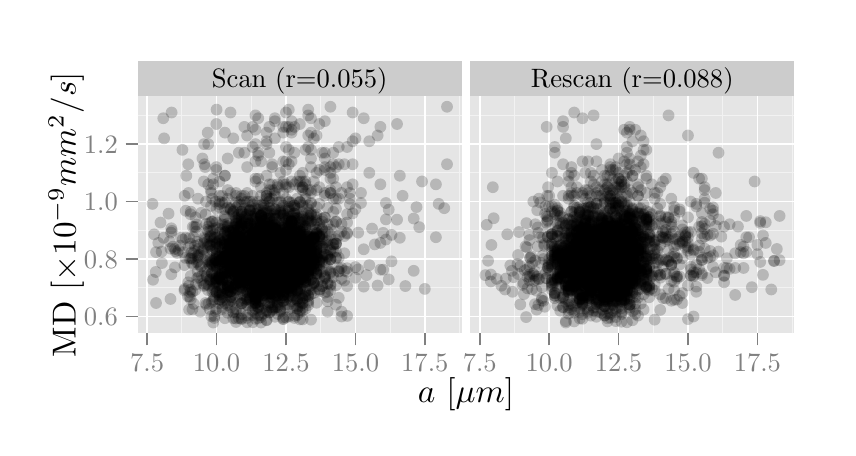
\begin{tikzpicture}[x=1pt,y=1pt]
\definecolor[named]{fillColor}{rgb}{1.00,1.00,1.00}
\path[use as bounding box,fill=fillColor,fill opacity=0.00] (0,0) rectangle (289.08,144.54);
\begin{scope}
\path[clip] (  0.00,  0.00) rectangle (289.08,144.54);
\definecolor[named]{drawColor}{rgb}{1.00,1.00,1.00}
\definecolor[named]{fillColor}{rgb}{1.00,1.00,1.00}

\path[draw=drawColor,line width= 0.6pt,line join=round,line cap=round,fill=fillColor] ( -0.00,  0.00) rectangle (289.08,144.54);
\end{scope}
\begin{scope}
\path[clip] ( 39.69,119.86) rectangle (156.86,132.50);
\definecolor[named]{fillColor}{rgb}{0.80,0.80,0.80}

\path[fill=fillColor] ( 39.69,119.86) rectangle (156.86,132.50);
\definecolor[named]{drawColor}{rgb}{0.00,0.00,0.00}

\node[text=drawColor,anchor=base,inner sep=0pt, outer sep=0pt, scale=  0.96] at ( 98.27,122.87) {Scan (r=0.055)};
\end{scope}
\begin{scope}
\path[clip] (159.87,119.86) rectangle (277.03,132.50);
\definecolor[named]{fillColor}{rgb}{0.80,0.80,0.80}

\path[fill=fillColor] (159.87,119.86) rectangle (277.03,132.50);
\definecolor[named]{drawColor}{rgb}{0.00,0.00,0.00}

\node[text=drawColor,anchor=base,inner sep=0pt, outer sep=0pt, scale=  0.96] at (218.45,122.87) {Rescan (r=0.088)};
\end{scope}
\begin{scope}
\path[clip] ( 39.69, 34.04) rectangle (156.86,119.86);
\definecolor[named]{fillColor}{rgb}{0.90,0.90,0.90}

\path[fill=fillColor] ( 39.69, 34.04) rectangle (156.86,119.86);
\definecolor[named]{drawColor}{rgb}{0.95,0.95,0.95}

\path[draw=drawColor,line width= 0.3pt,line join=round] ( 39.69, 50.55) --
	(156.86, 50.55);

\path[draw=drawColor,line width= 0.3pt,line join=round] ( 39.69, 71.32) --
	(156.86, 71.32);

\path[draw=drawColor,line width= 0.3pt,line join=round] ( 39.69, 92.08) --
	(156.86, 92.08);

\path[draw=drawColor,line width= 0.3pt,line join=round] ( 39.69,112.84) --
	(156.86,112.84);

\path[draw=drawColor,line width= 0.3pt,line join=round] ( 55.72, 34.04) --
	( 55.72,119.86);

\path[draw=drawColor,line width= 0.3pt,line join=round] ( 80.80, 34.04) --
	( 80.80,119.86);

\path[draw=drawColor,line width= 0.3pt,line join=round] (105.88, 34.04) --
	(105.88,119.86);

\path[draw=drawColor,line width= 0.3pt,line join=round] (130.97, 34.04) --
	(130.97,119.86);

\path[draw=drawColor,line width= 0.3pt,line join=round] (156.05, 34.04) --
	(156.05,119.86);
\definecolor[named]{drawColor}{rgb}{1.00,1.00,1.00}

\path[draw=drawColor,line width= 0.6pt,line join=round] ( 39.69, 40.17) --
	(156.86, 40.17);

\path[draw=drawColor,line width= 0.6pt,line join=round] ( 39.69, 60.93) --
	(156.86, 60.93);

\path[draw=drawColor,line width= 0.6pt,line join=round] ( 39.69, 81.70) --
	(156.86, 81.70);

\path[draw=drawColor,line width= 0.6pt,line join=round] ( 39.69,102.46) --
	(156.86,102.46);

\path[draw=drawColor,line width= 0.6pt,line join=round] ( 43.18, 34.04) --
	( 43.18,119.86);

\path[draw=drawColor,line width= 0.6pt,line join=round] ( 68.26, 34.04) --
	( 68.26,119.86);

\path[draw=drawColor,line width= 0.6pt,line join=round] ( 93.34, 34.04) --
	( 93.34,119.86);

\path[draw=drawColor,line width= 0.6pt,line join=round] (118.43, 34.04) --
	(118.43,119.86);

\path[draw=drawColor,line width= 0.6pt,line join=round] (143.51, 34.04) --
	(143.51,119.86);
\definecolor[named]{fillColor}{rgb}{0.00,0.00,0.00}

\path[fill=fillColor,fill opacity=0.20] (141.50, 72.46) circle (  2.13);

\path[fill=fillColor,fill opacity=0.20] ( 99.36, 80.76) circle (  2.13);

\path[fill=fillColor,fill opacity=0.20] ( 94.35, 68.82) circle (  2.13);

\path[fill=fillColor,fill opacity=0.20] ( 89.33, 56.47) circle (  2.13);

\path[fill=fillColor,fill opacity=0.20] ( 91.34, 53.67) circle (  2.13);

\path[fill=fillColor,fill opacity=0.20] (102.37, 53.46) circle (  2.13);

\path[fill=fillColor,fill opacity=0.20] (109.40, 69.65) circle (  2.13);

\path[fill=fillColor,fill opacity=0.20] (107.39, 93.12) circle (  2.13);

\path[fill=fillColor,fill opacity=0.20] ( 86.32, 83.77) circle (  2.13);

\path[fill=fillColor,fill opacity=0.20] ( 88.33, 58.65) circle (  2.13);

\path[fill=fillColor,fill opacity=0.20] ( 83.31, 51.49) circle (  2.13);

\path[fill=fillColor,fill opacity=0.20] ( 77.29, 57.71) circle (  2.13);

\path[fill=fillColor,fill opacity=0.20] ( 83.31, 57.92) circle (  2.13);

\path[fill=fillColor,fill opacity=0.20] ( 74.28, 50.45) circle (  2.13);

\path[fill=fillColor,fill opacity=0.20] ( 82.31, 44.94) circle (  2.13);

\path[fill=fillColor,fill opacity=0.20] ( 87.33, 56.68) circle (  2.13);

\path[fill=fillColor,fill opacity=0.20] (105.38, 59.79) circle (  2.13);

\path[fill=fillColor,fill opacity=0.20] (127.45, 57.09) circle (  2.13);

\path[fill=fillColor,fill opacity=0.20] ( 81.31,101.42) circle (  2.13);

\path[fill=fillColor,fill opacity=0.20] ( 82.31, 73.18) circle (  2.13);

\path[fill=fillColor,fill opacity=0.20] ( 83.31, 60.10) circle (  2.13);

\path[fill=fillColor,fill opacity=0.20] ( 82.31, 60.52) circle (  2.13);

\path[fill=fillColor,fill opacity=0.20] ( 83.31, 59.48) circle (  2.13);

\path[fill=fillColor,fill opacity=0.20] ( 80.30, 59.27) circle (  2.13);

\path[fill=fillColor,fill opacity=0.20] ( 81.31, 64.46) circle (  2.13);

\path[fill=fillColor,fill opacity=0.20] ( 83.31, 65.50) circle (  2.13);

\path[fill=fillColor,fill opacity=0.20] ( 84.32, 55.33) circle (  2.13);

\path[fill=fillColor,fill opacity=0.20] ( 86.32, 42.35) circle (  2.13);

\path[fill=fillColor,fill opacity=0.20] (100.37, 47.12) circle (  2.13);

\path[fill=fillColor,fill opacity=0.20] ( 98.36, 56.26) circle (  2.13);

\path[fill=fillColor,fill opacity=0.20] (105.38, 59.79) circle (  2.13);

\path[fill=fillColor,fill opacity=0.20] ( 99.36, 85.85) circle (  2.13);

\path[fill=fillColor,fill opacity=0.20] ( 81.31, 76.30) circle (  2.13);

\path[fill=fillColor,fill opacity=0.20] ( 81.31, 64.05) circle (  2.13);

\path[fill=fillColor,fill opacity=0.20] ( 73.28, 55.85) circle (  2.13);

\path[fill=fillColor,fill opacity=0.20] ( 75.29, 72.66) circle (  2.13);

\path[fill=fillColor,fill opacity=0.20] ( 80.30, 72.04) circle (  2.13);

\path[fill=fillColor,fill opacity=0.20] ( 86.32, 59.48) circle (  2.13);

\path[fill=fillColor,fill opacity=0.20] ( 83.31, 63.53) circle (  2.13);

\path[fill=fillColor,fill opacity=0.20] ( 81.31, 67.37) circle (  2.13);

\path[fill=fillColor,fill opacity=0.20] ( 86.32, 60.00) circle (  2.13);

\path[fill=fillColor,fill opacity=0.20] ( 93.34, 54.50) circle (  2.13);

\path[fill=fillColor,fill opacity=0.20] ( 97.36, 58.44) circle (  2.13);

\path[fill=fillColor,fill opacity=0.20] ( 94.35, 59.58) circle (  2.13);

\path[fill=fillColor,fill opacity=0.20] ( 99.36, 62.08) circle (  2.13);

\path[fill=fillColor,fill opacity=0.20] (101.37, 80.35) circle (  2.13);

\path[fill=fillColor,fill opacity=0.20] ( 94.35, 63.84) circle (  2.13);

\path[fill=fillColor,fill opacity=0.20] ( 81.31, 64.67) circle (  2.13);

\path[fill=fillColor,fill opacity=0.20] ( 76.29, 58.23) circle (  2.13);

\path[fill=fillColor,fill opacity=0.20] ( 77.29, 61.76) circle (  2.13);

\path[fill=fillColor,fill opacity=0.20] ( 77.29, 67.89) circle (  2.13);

\path[fill=fillColor,fill opacity=0.20] ( 81.31, 70.69) circle (  2.13);

\path[fill=fillColor,fill opacity=0.20] ( 85.32, 67.89) circle (  2.13);

\path[fill=fillColor,fill opacity=0.20] ( 85.32, 59.17) circle (  2.13);

\path[fill=fillColor,fill opacity=0.20] ( 92.34, 56.26) circle (  2.13);

\path[fill=fillColor,fill opacity=0.20] (100.37, 63.42) circle (  2.13);

\path[fill=fillColor,fill opacity=0.20] ( 95.35, 71.94) circle (  2.13);

\path[fill=fillColor,fill opacity=0.20] ( 98.36, 81.70) circle (  2.13);

\path[fill=fillColor,fill opacity=0.20] (102.37,106.61) circle (  2.13);

\path[fill=fillColor,fill opacity=0.20] ( 96.35, 75.68) circle (  2.13);

\path[fill=fillColor,fill opacity=0.20] ( 85.32, 45.05) circle (  2.13);

\path[fill=fillColor,fill opacity=0.20] ( 84.32, 76.71) circle (  2.13);

\path[fill=fillColor,fill opacity=0.20] ( 92.34, 76.71) circle (  2.13);

\path[fill=fillColor,fill opacity=0.20] ( 92.34, 64.88) circle (  2.13);

\path[fill=fillColor,fill opacity=0.20] (102.37, 85.85) circle (  2.13);

\path[fill=fillColor,fill opacity=0.20] ( 96.35, 58.34) circle (  2.13);

\path[fill=fillColor,fill opacity=0.20] ( 80.30, 60.00) circle (  2.13);

\path[fill=fillColor,fill opacity=0.20] ( 78.30, 58.03) circle (  2.13);

\path[fill=fillColor,fill opacity=0.20] ( 82.31, 46.50) circle (  2.13);

\path[fill=fillColor,fill opacity=0.20] ( 79.30, 48.89) circle (  2.13);

\path[fill=fillColor,fill opacity=0.20] ( 80.30, 69.97) circle (  2.13);

\path[fill=fillColor,fill opacity=0.20] ( 78.30, 76.19) circle (  2.13);

\path[fill=fillColor,fill opacity=0.20] ( 93.34, 63.22) circle (  2.13);

\path[fill=fillColor,fill opacity=0.20] (103.38, 57.51) circle (  2.13);

\path[fill=fillColor,fill opacity=0.20] (114.41, 63.01) circle (  2.13);

\path[fill=fillColor,fill opacity=0.20] ( 99.36, 86.89) circle (  2.13);

\path[fill=fillColor,fill opacity=0.20] ( 77.29, 52.63) circle (  2.13);

\path[fill=fillColor,fill opacity=0.20] ( 79.30, 64.15) circle (  2.13);

\path[fill=fillColor,fill opacity=0.20] ( 82.31, 60.41) circle (  2.13);

\path[fill=fillColor,fill opacity=0.20] ( 80.30, 61.14) circle (  2.13);

\path[fill=fillColor,fill opacity=0.20] ( 82.31, 62.18) circle (  2.13);

\path[fill=fillColor,fill opacity=0.20] ( 86.32, 54.81) circle (  2.13);

\path[fill=fillColor,fill opacity=0.20] ( 97.36, 65.19) circle (  2.13);

\path[fill=fillColor,fill opacity=0.20] (101.37,114.92) circle (  2.13);

\path[fill=fillColor,fill opacity=0.20] ( 95.35, 79.93) circle (  2.13);

\path[fill=fillColor,fill opacity=0.20] (100.37, 56.68) circle (  2.13);

\path[fill=fillColor,fill opacity=0.20] ( 91.34, 51.28) circle (  2.13);

\path[fill=fillColor,fill opacity=0.20] ( 88.33, 61.04) circle (  2.13);

\path[fill=fillColor,fill opacity=0.20] ( 87.33, 63.74) circle (  2.13);

\path[fill=fillColor,fill opacity=0.20] ( 88.33, 51.17) circle (  2.13);

\path[fill=fillColor,fill opacity=0.20] ( 86.32, 57.30) circle (  2.13);

\path[fill=fillColor,fill opacity=0.20] ( 82.31, 79.21) circle (  2.13);

\path[fill=fillColor,fill opacity=0.20] (106.39, 64.77) circle (  2.13);

\path[fill=fillColor,fill opacity=0.20] ( 87.33, 79.41) circle (  2.13);

\path[fill=fillColor,fill opacity=0.20] ( 72.28, 50.76) circle (  2.13);

\path[fill=fillColor,fill opacity=0.20] ( 69.27, 67.47) circle (  2.13);

\path[fill=fillColor,fill opacity=0.20] ( 70.27, 60.93) circle (  2.13);

\path[fill=fillColor,fill opacity=0.20] ( 67.36, 47.33) circle (  2.13);

\path[fill=fillColor,fill opacity=0.20] ( 60.04, 44.74) circle (  2.13);

\path[fill=fillColor,fill opacity=0.20] ( 74.28, 50.24) circle (  2.13);

\path[fill=fillColor,fill opacity=0.20] ( 79.30, 44.22) circle (  2.13);

\path[fill=fillColor,fill opacity=0.20] ( 82.31, 49.31) circle (  2.13);

\path[fill=fillColor,fill opacity=0.20] (109.40, 90.00) circle (  2.13);

\path[fill=fillColor,fill opacity=0.20] (106.39, 71.94) circle (  2.13);

\path[fill=fillColor,fill opacity=0.20] (100.37, 55.53) circle (  2.13);

\path[fill=fillColor,fill opacity=0.20] ( 89.33, 60.93) circle (  2.13);

\path[fill=fillColor,fill opacity=0.20] ( 93.34, 63.63) circle (  2.13);

\path[fill=fillColor,fill opacity=0.20] ( 92.34, 72.15) circle (  2.13);

\path[fill=fillColor,fill opacity=0.20] ( 90.33, 69.45) circle (  2.13);

\path[fill=fillColor,fill opacity=0.20] ( 96.35, 62.18) circle (  2.13);

\path[fill=fillColor,fill opacity=0.20] ( 92.34, 73.81) circle (  2.13);

\path[fill=fillColor,fill opacity=0.20] ( 93.34, 78.58) circle (  2.13);

\path[fill=fillColor,fill opacity=0.20] (104.38, 70.38) circle (  2.13);

\path[fill=fillColor,fill opacity=0.20] ( 75.29, 49.82) circle (  2.13);

\path[fill=fillColor,fill opacity=0.20] ( 69.27, 65.29) circle (  2.13);

\path[fill=fillColor,fill opacity=0.20] ( 66.06, 65.81) circle (  2.13);

\path[fill=fillColor,fill opacity=0.20] ( 64.55, 44.43) circle (  2.13);

\path[fill=fillColor,fill opacity=0.20] ( 70.27, 43.49) circle (  2.13);

\path[fill=fillColor,fill opacity=0.20] ( 68.26, 52.00) circle (  2.13);

\path[fill=fillColor,fill opacity=0.20] ( 81.31, 51.80) circle (  2.13);

\path[fill=fillColor,fill opacity=0.20] ( 84.32, 45.78) circle (  2.13);

\path[fill=fillColor,fill opacity=0.20] (100.37, 56.05) circle (  2.13);

\path[fill=fillColor,fill opacity=0.20] (115.42, 74.12) circle (  2.13);

\path[fill=fillColor,fill opacity=0.20] ( 97.36, 62.39) circle (  2.13);

\path[fill=fillColor,fill opacity=0.20] ( 93.34, 74.64) circle (  2.13);

\path[fill=fillColor,fill opacity=0.20] ( 89.33, 58.34) circle (  2.13);

\path[fill=fillColor,fill opacity=0.20] ( 90.33, 53.04) circle (  2.13);

\path[fill=fillColor,fill opacity=0.20] ( 92.34, 70.28) circle (  2.13);

\path[fill=fillColor,fill opacity=0.20] ( 87.33, 75.68) circle (  2.13);

\path[fill=fillColor,fill opacity=0.20] ( 93.34, 67.47) circle (  2.13);

\path[fill=fillColor,fill opacity=0.20] ( 90.33, 60.52) circle (  2.13);

\path[fill=fillColor,fill opacity=0.20] (102.37, 65.40) circle (  2.13);

\path[fill=fillColor,fill opacity=0.20] (133.47,109.73) circle (  2.13);

\path[fill=fillColor,fill opacity=0.20] ( 77.29, 78.06) circle (  2.13);

\path[fill=fillColor,fill opacity=0.20] ( 69.27, 58.75) circle (  2.13);

\path[fill=fillColor,fill opacity=0.20] ( 72.28, 58.55) circle (  2.13);

\path[fill=fillColor,fill opacity=0.20] ( 81.31, 48.68) circle (  2.13);

\path[fill=fillColor,fill opacity=0.20] ( 78.30, 58.23) circle (  2.13);

\path[fill=fillColor,fill opacity=0.20] ( 77.29, 61.04) circle (  2.13);

\path[fill=fillColor,fill opacity=0.20] ( 86.32, 55.22) circle (  2.13);

\path[fill=fillColor,fill opacity=0.20] ( 92.34, 54.91) circle (  2.13);

\path[fill=fillColor,fill opacity=0.20] (109.40, 84.81) circle (  2.13);

\path[fill=fillColor,fill opacity=0.20] (101.37, 68.93) circle (  2.13);

\path[fill=fillColor,fill opacity=0.20] ( 92.34, 71.52) circle (  2.13);

\path[fill=fillColor,fill opacity=0.20] ( 84.32, 52.11) circle (  2.13);

\path[fill=fillColor,fill opacity=0.20] ( 86.32, 38.82) circle (  2.13);

\path[fill=fillColor,fill opacity=0.20] ( 91.34, 56.99) circle (  2.13);

\path[fill=fillColor,fill opacity=0.20] ( 93.34, 70.59) circle (  2.13);

\path[fill=fillColor,fill opacity=0.20] ( 95.35, 67.16) circle (  2.13);

\path[fill=fillColor,fill opacity=0.20] ( 96.35, 56.57) circle (  2.13);

\path[fill=fillColor,fill opacity=0.20] ( 97.36, 53.15) circle (  2.13);

\path[fill=fillColor,fill opacity=0.20] ( 66.66, 53.15) circle (  2.13);

\path[fill=fillColor,fill opacity=0.20] ( 72.28, 48.99) circle (  2.13);

\path[fill=fillColor,fill opacity=0.20] ( 76.29, 61.35) circle (  2.13);

\path[fill=fillColor,fill opacity=0.20] ( 67.96, 53.98) circle (  2.13);

\path[fill=fillColor,fill opacity=0.20] ( 79.30, 56.05) circle (  2.13);

\path[fill=fillColor,fill opacity=0.20] ( 81.31, 62.39) circle (  2.13);

\path[fill=fillColor,fill opacity=0.20] ( 78.30, 60.41) circle (  2.13);

\path[fill=fillColor,fill opacity=0.20] ( 82.31, 60.10) circle (  2.13);

\path[fill=fillColor,fill opacity=0.20] ( 88.33, 60.41) circle (  2.13);

\path[fill=fillColor,fill opacity=0.20] ( 91.34, 42.56) circle (  2.13);

\path[fill=fillColor,fill opacity=0.20] (103.38, 70.28) circle (  2.13);

\path[fill=fillColor,fill opacity=0.20] ( 85.32, 60.52) circle (  2.13);

\path[fill=fillColor,fill opacity=0.20] ( 79.30, 56.05) circle (  2.13);

\path[fill=fillColor,fill opacity=0.20] ( 81.31, 53.77) circle (  2.13);

\path[fill=fillColor,fill opacity=0.20] ( 91.34, 53.15) circle (  2.13);

\path[fill=fillColor,fill opacity=0.20] ( 94.35, 53.15) circle (  2.13);

\path[fill=fillColor,fill opacity=0.20] ( 94.35, 60.10) circle (  2.13);

\path[fill=fillColor,fill opacity=0.20] ( 98.36, 71.11) circle (  2.13);

\path[fill=fillColor,fill opacity=0.20] ( 95.35, 58.96) circle (  2.13);

\path[fill=fillColor,fill opacity=0.20] ( 87.33,108.69) circle (  2.13);

\path[fill=fillColor,fill opacity=0.20] ( 69.27, 46.29) circle (  2.13);

\path[fill=fillColor,fill opacity=0.20] ( 72.28, 72.25) circle (  2.13);

\path[fill=fillColor,fill opacity=0.20] ( 74.28, 71.21) circle (  2.13);

\path[fill=fillColor,fill opacity=0.20] ( 69.27, 54.18) circle (  2.13);

\path[fill=fillColor,fill opacity=0.20] ( 77.29, 55.53) circle (  2.13);

\path[fill=fillColor,fill opacity=0.20] ( 83.31, 61.04) circle (  2.13);

\path[fill=fillColor,fill opacity=0.20] ( 76.29, 61.14) circle (  2.13);

\path[fill=fillColor,fill opacity=0.20] ( 91.34, 65.71) circle (  2.13);

\path[fill=fillColor,fill opacity=0.20] ( 88.33, 58.34) circle (  2.13);

\path[fill=fillColor,fill opacity=0.20] ( 93.34, 39.86) circle (  2.13);

\path[fill=fillColor,fill opacity=0.20] (106.39, 52.94) circle (  2.13);

\path[fill=fillColor,fill opacity=0.20] ( 95.35, 51.69) circle (  2.13);

\path[fill=fillColor,fill opacity=0.20] ( 86.32, 60.83) circle (  2.13);

\path[fill=fillColor,fill opacity=0.20] ( 84.32, 66.33) circle (  2.13);

\path[fill=fillColor,fill opacity=0.20] ( 88.33, 59.17) circle (  2.13);

\path[fill=fillColor,fill opacity=0.20] ( 91.34, 47.02) circle (  2.13);

\path[fill=fillColor,fill opacity=0.20] ( 89.33, 50.65) circle (  2.13);

\path[fill=fillColor,fill opacity=0.20] ( 93.34, 75.47) circle (  2.13);

\path[fill=fillColor,fill opacity=0.20] ( 82.31, 74.33) circle (  2.13);

\path[fill=fillColor,fill opacity=0.20] ( 93.34, 60.31) circle (  2.13);

\path[fill=fillColor,fill opacity=0.20] ( 80.30, 62.08) circle (  2.13);

\path[fill=fillColor,fill opacity=0.20] ( 79.30, 62.18) circle (  2.13);

\path[fill=fillColor,fill opacity=0.20] ( 80.30, 77.86) circle (  2.13);

\path[fill=fillColor,fill opacity=0.20] ( 81.31, 68.93) circle (  2.13);

\path[fill=fillColor,fill opacity=0.20] ( 77.29, 57.20) circle (  2.13);

\path[fill=fillColor,fill opacity=0.20] ( 79.30, 60.73) circle (  2.13);

\path[fill=fillColor,fill opacity=0.20] ( 80.30, 59.89) circle (  2.13);

\path[fill=fillColor,fill opacity=0.20] ( 79.30, 53.67) circle (  2.13);

\path[fill=fillColor,fill opacity=0.20] ( 82.31, 56.68) circle (  2.13);

\path[fill=fillColor,fill opacity=0.20] ( 93.34, 51.59) circle (  2.13);

\path[fill=fillColor,fill opacity=0.20] ( 94.35, 40.17) circle (  2.13);

\path[fill=fillColor,fill opacity=0.20] (110.40, 64.98) circle (  2.13);

\path[fill=fillColor,fill opacity=0.20] (100.37, 60.00) circle (  2.13);

\path[fill=fillColor,fill opacity=0.20] ( 95.35, 63.32) circle (  2.13);

\path[fill=fillColor,fill opacity=0.20] ( 95.35, 64.15) circle (  2.13);

\path[fill=fillColor,fill opacity=0.20] ( 87.33, 57.92) circle (  2.13);

\path[fill=fillColor,fill opacity=0.20] ( 91.34, 55.53) circle (  2.13);

\path[fill=fillColor,fill opacity=0.20] ( 90.33, 55.22) circle (  2.13);

\path[fill=fillColor,fill opacity=0.20] ( 87.33, 64.15) circle (  2.13);

\path[fill=fillColor,fill opacity=0.20] ( 96.35, 67.58) circle (  2.13);

\path[fill=fillColor,fill opacity=0.20] (101.37, 56.05) circle (  2.13);

\path[fill=fillColor,fill opacity=0.20] (114.41, 69.24) circle (  2.13);

\path[fill=fillColor,fill opacity=0.20] ( 80.30, 78.69) circle (  2.13);

\path[fill=fillColor,fill opacity=0.20] ( 69.27, 59.06) circle (  2.13);

\path[fill=fillColor,fill opacity=0.20] ( 86.32, 71.83) circle (  2.13);

\path[fill=fillColor,fill opacity=0.20] ( 84.32, 70.28) circle (  2.13);

\path[fill=fillColor,fill opacity=0.20] ( 80.30, 60.31) circle (  2.13);

\path[fill=fillColor,fill opacity=0.20] ( 80.30, 55.85) circle (  2.13);

\path[fill=fillColor,fill opacity=0.20] ( 75.29, 60.52) circle (  2.13);

\path[fill=fillColor,fill opacity=0.20] ( 83.31, 55.43) circle (  2.13);

\path[fill=fillColor,fill opacity=0.20] ( 77.29, 44.94) circle (  2.13);

\path[fill=fillColor,fill opacity=0.20] ( 77.29, 50.45) circle (  2.13);

\path[fill=fillColor,fill opacity=0.20] ( 89.33, 50.14) circle (  2.13);

\path[fill=fillColor,fill opacity=0.20] ( 95.35, 47.33) circle (  2.13);

\path[fill=fillColor,fill opacity=0.20] ( 98.36, 73.50) circle (  2.13);

\path[fill=fillColor,fill opacity=0.20] ( 86.32, 58.55) circle (  2.13);

\path[fill=fillColor,fill opacity=0.20] ( 87.33, 49.82) circle (  2.13);

\path[fill=fillColor,fill opacity=0.20] ( 89.33, 58.03) circle (  2.13);

\path[fill=fillColor,fill opacity=0.20] ( 87.33, 59.89) circle (  2.13);

\path[fill=fillColor,fill opacity=0.20] ( 88.33, 50.34) circle (  2.13);

\path[fill=fillColor,fill opacity=0.20] ( 90.33, 43.49) circle (  2.13);

\path[fill=fillColor,fill opacity=0.20] ( 97.36, 43.08) circle (  2.13);

\path[fill=fillColor,fill opacity=0.20] ( 97.36, 49.62) circle (  2.13);

\path[fill=fillColor,fill opacity=0.20] (105.38, 68.93) circle (  2.13);

\path[fill=fillColor,fill opacity=0.20] ( 84.32, 96.23) circle (  2.13);

\path[fill=fillColor,fill opacity=0.20] ( 76.29, 53.46) circle (  2.13);

\path[fill=fillColor,fill opacity=0.20] ( 77.29, 63.74) circle (  2.13);

\path[fill=fillColor,fill opacity=0.20] ( 82.31, 60.00) circle (  2.13);

\path[fill=fillColor,fill opacity=0.20] ( 75.29, 57.09) circle (  2.13);

\path[fill=fillColor,fill opacity=0.20] ( 75.29, 59.06) circle (  2.13);

\path[fill=fillColor,fill opacity=0.20] ( 75.29, 58.34) circle (  2.13);

\path[fill=fillColor,fill opacity=0.20] ( 74.28, 53.56) circle (  2.13);

\path[fill=fillColor,fill opacity=0.20] ( 78.30, 47.64) circle (  2.13);

\path[fill=fillColor,fill opacity=0.20] ( 79.30, 48.79) circle (  2.13);

\path[fill=fillColor,fill opacity=0.20] ( 84.32, 58.23) circle (  2.13);

\path[fill=fillColor,fill opacity=0.20] ( 81.31, 58.96) circle (  2.13);

\path[fill=fillColor,fill opacity=0.20] ( 90.33, 62.08) circle (  2.13);

\path[fill=fillColor,fill opacity=0.20] ( 83.31, 68.30) circle (  2.13);

\path[fill=fillColor,fill opacity=0.20] ( 77.29, 44.94) circle (  2.13);

\path[fill=fillColor,fill opacity=0.20] ( 90.33, 47.64) circle (  2.13);

\path[fill=fillColor,fill opacity=0.20] ( 86.32, 53.35) circle (  2.13);

\path[fill=fillColor,fill opacity=0.20] ( 89.33, 47.54) circle (  2.13);

\path[fill=fillColor,fill opacity=0.20] ( 93.34, 44.43) circle (  2.13);

\path[fill=fillColor,fill opacity=0.20] ( 87.33, 45.05) circle (  2.13);

\path[fill=fillColor,fill opacity=0.20] ( 92.34, 50.86) circle (  2.13);

\path[fill=fillColor,fill opacity=0.20] ( 96.35, 64.46) circle (  2.13);

\path[fill=fillColor,fill opacity=0.20] (111.40, 79.10) circle (  2.13);

\path[fill=fillColor,fill opacity=0.20] ( 82.31,107.65) circle (  2.13);

\path[fill=fillColor,fill opacity=0.20] ( 78.30, 60.83) circle (  2.13);

\path[fill=fillColor,fill opacity=0.20] ( 76.29, 69.24) circle (  2.13);

\path[fill=fillColor,fill opacity=0.20] ( 80.30, 58.96) circle (  2.13);

\path[fill=fillColor,fill opacity=0.20] ( 76.29, 49.51) circle (  2.13);

\path[fill=fillColor,fill opacity=0.20] ( 75.29, 54.81) circle (  2.13);

\path[fill=fillColor,fill opacity=0.20] ( 75.29, 64.36) circle (  2.13);

\path[fill=fillColor,fill opacity=0.20] ( 75.29, 67.68) circle (  2.13);

\path[fill=fillColor,fill opacity=0.20] ( 72.28, 58.65) circle (  2.13);

\path[fill=fillColor,fill opacity=0.20] ( 79.30, 51.69) circle (  2.13);

\path[fill=fillColor,fill opacity=0.20] ( 78.30, 55.22) circle (  2.13);

\path[fill=fillColor,fill opacity=0.20] ( 80.30, 58.23) circle (  2.13);

\path[fill=fillColor,fill opacity=0.20] ( 83.31, 67.16) circle (  2.13);

\path[fill=fillColor,fill opacity=0.20] (100.37, 88.96) circle (  2.13);

\path[fill=fillColor,fill opacity=0.20] (112.41, 95.19) circle (  2.13);

\path[fill=fillColor,fill opacity=0.20] ( 94.35, 60.10) circle (  2.13);

\path[fill=fillColor,fill opacity=0.20] ( 88.33, 48.16) circle (  2.13);

\path[fill=fillColor,fill opacity=0.20] ( 90.33, 48.79) circle (  2.13);

\path[fill=fillColor,fill opacity=0.20] ( 93.34, 56.57) circle (  2.13);

\path[fill=fillColor,fill opacity=0.20] ( 86.32, 58.55) circle (  2.13);

\path[fill=fillColor,fill opacity=0.20] ( 90.33, 54.18) circle (  2.13);

\path[fill=fillColor,fill opacity=0.20] ( 89.33, 56.99) circle (  2.13);

\path[fill=fillColor,fill opacity=0.20] ( 95.35, 68.62) circle (  2.13);

\path[fill=fillColor,fill opacity=0.20] ( 96.35, 75.68) circle (  2.13);

\path[fill=fillColor,fill opacity=0.20] (105.38, 80.87) circle (  2.13);

\path[fill=fillColor,fill opacity=0.20] ( 89.33,111.81) circle (  2.13);

\path[fill=fillColor,fill opacity=0.20] ( 80.30, 58.13) circle (  2.13);

\path[fill=fillColor,fill opacity=0.20] ( 77.29, 72.87) circle (  2.13);

\path[fill=fillColor,fill opacity=0.20] ( 80.30, 69.55) circle (  2.13);

\path[fill=fillColor,fill opacity=0.20] ( 78.30, 59.17) circle (  2.13);

\path[fill=fillColor,fill opacity=0.20] ( 73.28, 63.11) circle (  2.13);

\path[fill=fillColor,fill opacity=0.20] ( 79.30, 64.98) circle (  2.13);

\path[fill=fillColor,fill opacity=0.20] ( 79.30, 63.74) circle (  2.13);

\path[fill=fillColor,fill opacity=0.20] ( 75.29, 64.77) circle (  2.13);

\path[fill=fillColor,fill opacity=0.20] ( 76.29, 66.02) circle (  2.13);

\path[fill=fillColor,fill opacity=0.20] ( 74.28, 68.62) circle (  2.13);

\path[fill=fillColor,fill opacity=0.20] ( 77.29, 59.17) circle (  2.13);

\path[fill=fillColor,fill opacity=0.20] ( 90.33, 47.75) circle (  2.13);

\path[fill=fillColor,fill opacity=0.20] (111.40, 94.16) circle (  2.13);

\path[fill=fillColor,fill opacity=0.20] ( 86.32, 71.32) circle (  2.13);

\path[fill=fillColor,fill opacity=0.20] ( 85.32, 53.04) circle (  2.13);

\path[fill=fillColor,fill opacity=0.20] ( 91.34, 56.88) circle (  2.13);

\path[fill=fillColor,fill opacity=0.20] ( 86.32, 53.56) circle (  2.13);

\path[fill=fillColor,fill opacity=0.20] ( 83.31, 45.57) circle (  2.13);

\path[fill=fillColor,fill opacity=0.20] ( 90.33, 53.56) circle (  2.13);

\path[fill=fillColor,fill opacity=0.20] ( 91.34, 59.58) circle (  2.13);

\path[fill=fillColor,fill opacity=0.20] ( 91.34, 61.87) circle (  2.13);

\path[fill=fillColor,fill opacity=0.20] ( 93.34, 62.91) circle (  2.13);

\path[fill=fillColor,fill opacity=0.20] (103.38, 66.95) circle (  2.13);

\path[fill=fillColor,fill opacity=0.20] ( 84.32, 64.88) circle (  2.13);

\path[fill=fillColor,fill opacity=0.20] ( 79.30, 74.85) circle (  2.13);

\path[fill=fillColor,fill opacity=0.20] ( 74.28, 69.65) circle (  2.13);

\path[fill=fillColor,fill opacity=0.20] ( 77.29, 55.74) circle (  2.13);

\path[fill=fillColor,fill opacity=0.20] ( 72.28, 55.64) circle (  2.13);

\path[fill=fillColor,fill opacity=0.20] ( 73.28, 63.22) circle (  2.13);

\path[fill=fillColor,fill opacity=0.20] ( 76.29, 67.27) circle (  2.13);

\path[fill=fillColor,fill opacity=0.20] ( 75.29, 60.31) circle (  2.13);

\path[fill=fillColor,fill opacity=0.20] ( 71.27, 57.61) circle (  2.13);

\path[fill=fillColor,fill opacity=0.20] ( 72.28, 66.33) circle (  2.13);

\path[fill=fillColor,fill opacity=0.20] ( 45.69, 69.86) circle (  2.13);

\path[fill=fillColor,fill opacity=0.20] ( 78.30, 60.41) circle (  2.13);

\path[fill=fillColor,fill opacity=0.20] ( 98.36, 50.45) circle (  2.13);

\path[fill=fillColor,fill opacity=0.20] (112.41,101.42) circle (  2.13);

\path[fill=fillColor,fill opacity=0.20] ( 85.32, 66.12) circle (  2.13);

\path[fill=fillColor,fill opacity=0.20] ( 81.31, 49.93) circle (  2.13);

\path[fill=fillColor,fill opacity=0.20] ( 82.31, 41.41) circle (  2.13);

\path[fill=fillColor,fill opacity=0.20] ( 76.29, 39.55) circle (  2.13);

\path[fill=fillColor,fill opacity=0.20] ( 85.32, 49.82) circle (  2.13);

\path[fill=fillColor,fill opacity=0.20] ( 89.33, 53.87) circle (  2.13);

\path[fill=fillColor,fill opacity=0.20] ( 89.33, 59.48) circle (  2.13);

\path[fill=fillColor,fill opacity=0.20] ( 97.36, 64.88) circle (  2.13);

\path[fill=fillColor,fill opacity=0.20] (102.37, 63.74) circle (  2.13);

\path[fill=fillColor,fill opacity=0.20] (107.39, 75.99) circle (  2.13);

\path[fill=fillColor,fill opacity=0.20] ( 93.34,108.69) circle (  2.13);

\path[fill=fillColor,fill opacity=0.20] ( 81.31, 71.94) circle (  2.13);

\path[fill=fillColor,fill opacity=0.20] ( 83.31, 80.24) circle (  2.13);

\path[fill=fillColor,fill opacity=0.20] ( 77.29, 71.52) circle (  2.13);

\path[fill=fillColor,fill opacity=0.20] ( 72.28, 57.71) circle (  2.13);

\path[fill=fillColor,fill opacity=0.20] ( 69.27, 51.38) circle (  2.13);

\path[fill=fillColor,fill opacity=0.20] ( 66.66, 49.20) circle (  2.13);

\path[fill=fillColor,fill opacity=0.20] ( 72.28, 51.38) circle (  2.13);

\path[fill=fillColor,fill opacity=0.20] ( 73.28, 57.92) circle (  2.13);

\path[fill=fillColor,fill opacity=0.20] ( 71.27, 61.97) circle (  2.13);

\path[fill=fillColor,fill opacity=0.20] ( 73.28, 61.87) circle (  2.13);

\path[fill=fillColor,fill opacity=0.20] ( 67.96, 60.62) circle (  2.13);

\path[fill=fillColor,fill opacity=0.20] ( 75.29, 56.57) circle (  2.13);

\path[fill=fillColor,fill opacity=0.20] ( 95.35, 63.32) circle (  2.13);

\path[fill=fillColor,fill opacity=0.20] (110.40, 95.19) circle (  2.13);

\path[fill=fillColor,fill opacity=0.20] ( 74.28, 62.59) circle (  2.13);

\path[fill=fillColor,fill opacity=0.20] ( 79.30, 51.80) circle (  2.13);

\path[fill=fillColor,fill opacity=0.20] ( 78.30, 52.63) circle (  2.13);

\path[fill=fillColor,fill opacity=0.20] ( 80.30, 53.35) circle (  2.13);

\path[fill=fillColor,fill opacity=0.20] ( 89.33, 59.58) circle (  2.13);

\path[fill=fillColor,fill opacity=0.20] ( 87.33, 68.51) circle (  2.13);

\path[fill=fillColor,fill opacity=0.20] ( 91.34, 68.10) circle (  2.13);

\path[fill=fillColor,fill opacity=0.20] (102.37, 67.58) circle (  2.13);

\path[fill=fillColor,fill opacity=0.20] ( 99.36, 69.03) circle (  2.13);

\path[fill=fillColor,fill opacity=0.20] (104.38, 65.92) circle (  2.13);

\path[fill=fillColor,fill opacity=0.20] ( 99.36, 80.14) circle (  2.13);

\path[fill=fillColor,fill opacity=0.20] ( 80.30, 54.81) circle (  2.13);

\path[fill=fillColor,fill opacity=0.20] ( 66.26, 80.14) circle (  2.13);

\path[fill=fillColor,fill opacity=0.20] ( 75.29, 81.39) circle (  2.13);

\path[fill=fillColor,fill opacity=0.20] ( 71.27, 59.89) circle (  2.13);

\path[fill=fillColor,fill opacity=0.20] ( 69.27, 59.06) circle (  2.13);

\path[fill=fillColor,fill opacity=0.20] ( 66.66, 64.15) circle (  2.13);

\path[fill=fillColor,fill opacity=0.20] ( 68.26, 57.92) circle (  2.13);

\path[fill=fillColor,fill opacity=0.20] ( 72.28, 49.72) circle (  2.13);

\path[fill=fillColor,fill opacity=0.20] ( 72.28, 51.38) circle (  2.13);

\path[fill=fillColor,fill opacity=0.20] ( 73.28, 58.75) circle (  2.13);

\path[fill=fillColor,fill opacity=0.20] ( 76.29, 56.26) circle (  2.13);

\path[fill=fillColor,fill opacity=0.20] ( 75.29, 52.00) circle (  2.13);

\path[fill=fillColor,fill opacity=0.20] ( 96.35, 60.10) circle (  2.13);

\path[fill=fillColor,fill opacity=0.20] ( 75.29, 74.64) circle (  2.13);

\path[fill=fillColor,fill opacity=0.20] ( 76.29, 68.41) circle (  2.13);

\path[fill=fillColor,fill opacity=0.20] ( 86.32, 53.87) circle (  2.13);

\path[fill=fillColor,fill opacity=0.20] ( 89.33, 52.52) circle (  2.13);

\path[fill=fillColor,fill opacity=0.20] ( 85.32, 66.95) circle (  2.13);

\path[fill=fillColor,fill opacity=0.20] ( 89.33, 66.33) circle (  2.13);

\path[fill=fillColor,fill opacity=0.20] ( 96.35, 61.56) circle (  2.13);

\path[fill=fillColor,fill opacity=0.20] ( 99.36, 62.80) circle (  2.13);

\path[fill=fillColor,fill opacity=0.20] (105.38, 57.09) circle (  2.13);

\path[fill=fillColor,fill opacity=0.20] ( 96.35, 54.08) circle (  2.13);

\path[fill=fillColor,fill opacity=0.20] (105.38, 60.73) circle (  2.13);

\path[fill=fillColor,fill opacity=0.20] (112.41, 82.74) circle (  2.13);

\path[fill=fillColor,fill opacity=0.20] ( 93.34, 52.52) circle (  2.13);

\path[fill=fillColor,fill opacity=0.20] ( 85.32, 53.77) circle (  2.13);

\path[fill=fillColor,fill opacity=0.20] ( 72.28, 63.94) circle (  2.13);

\path[fill=fillColor,fill opacity=0.20] ( 77.29, 67.58) circle (  2.13);

\path[fill=fillColor,fill opacity=0.20] ( 74.28, 68.10) circle (  2.13);

\path[fill=fillColor,fill opacity=0.20] ( 73.28, 65.29) circle (  2.13);

\path[fill=fillColor,fill opacity=0.20] ( 70.27, 68.20) circle (  2.13);

\path[fill=fillColor,fill opacity=0.20] ( 67.66, 74.95) circle (  2.13);

\path[fill=fillColor,fill opacity=0.20] ( 67.66, 68.72) circle (  2.13);

\path[fill=fillColor,fill opacity=0.20] ( 69.27, 54.70) circle (  2.13);

\path[fill=fillColor,fill opacity=0.20] ( 73.28, 50.86) circle (  2.13);

\path[fill=fillColor,fill opacity=0.20] ( 76.29, 50.97) circle (  2.13);

\path[fill=fillColor,fill opacity=0.20] ( 90.33, 46.40) circle (  2.13);

\path[fill=fillColor,fill opacity=0.20] ( 95.35, 57.20) circle (  2.13);

\path[fill=fillColor,fill opacity=0.20] ( 93.34, 82.74) circle (  2.13);

\path[fill=fillColor,fill opacity=0.20] ( 88.33, 59.48) circle (  2.13);

\path[fill=fillColor,fill opacity=0.20] ( 86.32, 41.93) circle (  2.13);

\path[fill=fillColor,fill opacity=0.20] ( 83.31, 49.41) circle (  2.13);

\path[fill=fillColor,fill opacity=0.20] ( 86.32, 60.52) circle (  2.13);

\path[fill=fillColor,fill opacity=0.20] ( 93.34, 59.06) circle (  2.13);

\path[fill=fillColor,fill opacity=0.20] (101.37, 61.66) circle (  2.13);

\path[fill=fillColor,fill opacity=0.20] (105.38, 72.35) circle (  2.13);

\path[fill=fillColor,fill opacity=0.20] (104.38, 74.22) circle (  2.13);

\path[fill=fillColor,fill opacity=0.20] (103.38, 60.73) circle (  2.13);

\path[fill=fillColor,fill opacity=0.20] (107.39, 48.79) circle (  2.13);

\path[fill=fillColor,fill opacity=0.20] (108.39, 52.21) circle (  2.13);

\path[fill=fillColor,fill opacity=0.20] (115.42, 70.38) circle (  2.13);

\path[fill=fillColor,fill opacity=0.20] (106.39, 65.40) circle (  2.13);

\path[fill=fillColor,fill opacity=0.20] ( 97.36, 63.74) circle (  2.13);

\path[fill=fillColor,fill opacity=0.20] ( 86.32, 63.42) circle (  2.13);

\path[fill=fillColor,fill opacity=0.20] ( 81.31, 64.46) circle (  2.13);

\path[fill=fillColor,fill opacity=0.20] ( 57.13, 68.62) circle (  2.13);

\path[fill=fillColor,fill opacity=0.20] ( 76.29, 68.72) circle (  2.13);

\path[fill=fillColor,fill opacity=0.20] ( 82.31, 58.03) circle (  2.13);

\path[fill=fillColor,fill opacity=0.20] ( 73.28, 58.34) circle (  2.13);

\path[fill=fillColor,fill opacity=0.20] ( 71.27, 67.68) circle (  2.13);

\path[fill=fillColor,fill opacity=0.20] ( 71.27, 70.80) circle (  2.13);

\path[fill=fillColor,fill opacity=0.20] ( 69.27, 71.83) circle (  2.13);

\path[fill=fillColor,fill opacity=0.20] ( 66.46, 74.43) circle (  2.13);

\path[fill=fillColor,fill opacity=0.20] ( 74.28, 67.79) circle (  2.13);

\path[fill=fillColor,fill opacity=0.20] ( 78.30, 55.43) circle (  2.13);

\path[fill=fillColor,fill opacity=0.20] ( 92.34, 58.13) circle (  2.13);

\path[fill=fillColor,fill opacity=0.20] (102.37, 80.97) circle (  2.13);

\path[fill=fillColor,fill opacity=0.20] ( 90.33, 58.75) circle (  2.13);

\path[fill=fillColor,fill opacity=0.20] ( 83.31, 47.23) circle (  2.13);

\path[fill=fillColor,fill opacity=0.20] ( 85.32, 54.50) circle (  2.13);

\path[fill=fillColor,fill opacity=0.20] ( 91.34, 57.61) circle (  2.13);

\path[fill=fillColor,fill opacity=0.20] ( 90.33, 56.05) circle (  2.13);

\path[fill=fillColor,fill opacity=0.20] ( 93.34, 68.51) circle (  2.13);

\path[fill=fillColor,fill opacity=0.20] ( 95.35, 74.53) circle (  2.13);

\path[fill=fillColor,fill opacity=0.20] (100.37, 65.71) circle (  2.13);

\path[fill=fillColor,fill opacity=0.20] (101.37, 55.12) circle (  2.13);

\path[fill=fillColor,fill opacity=0.20] (100.37, 52.63) circle (  2.13);

\path[fill=fillColor,fill opacity=0.20] ( 99.36, 61.76) circle (  2.13);

\path[fill=fillColor,fill opacity=0.20] (105.38, 69.24) circle (  2.13);

\path[fill=fillColor,fill opacity=0.20] (109.40, 60.93) circle (  2.13);

\path[fill=fillColor,fill opacity=0.20] (111.40, 68.10) circle (  2.13);

\path[fill=fillColor,fill opacity=0.20] (107.39, 66.95) circle (  2.13);

\path[fill=fillColor,fill opacity=0.20] (106.39, 69.86) circle (  2.13);

\path[fill=fillColor,fill opacity=0.20] ( 78.30, 73.81) circle (  2.13);

\path[fill=fillColor,fill opacity=0.20] ( 87.33, 62.39) circle (  2.13);

\path[fill=fillColor,fill opacity=0.20] ( 83.31, 62.91) circle (  2.13);

\path[fill=fillColor,fill opacity=0.20] ( 73.28, 78.79) circle (  2.13);

\path[fill=fillColor,fill opacity=0.20] ( 77.29, 76.30) circle (  2.13);

\path[fill=fillColor,fill opacity=0.20] ( 76.29, 64.15) circle (  2.13);

\path[fill=fillColor,fill opacity=0.20] ( 84.32, 64.67) circle (  2.13);

\path[fill=fillColor,fill opacity=0.20] ( 76.29, 60.62) circle (  2.13);

\path[fill=fillColor,fill opacity=0.20] ( 69.27, 60.31) circle (  2.13);

\path[fill=fillColor,fill opacity=0.20] ( 61.24, 67.16) circle (  2.13);

\path[fill=fillColor,fill opacity=0.20] ( 73.28, 63.84) circle (  2.13);

\path[fill=fillColor,fill opacity=0.20] ( 77.29, 63.84) circle (  2.13);

\path[fill=fillColor,fill opacity=0.20] ( 75.29, 73.81) circle (  2.13);

\path[fill=fillColor,fill opacity=0.20] ( 86.32, 78.48) circle (  2.13);

\path[fill=fillColor,fill opacity=0.20] ( 89.33, 72.46) circle (  2.13);

\path[fill=fillColor,fill opacity=0.20] (100.37, 72.77) circle (  2.13);

\path[fill=fillColor,fill opacity=0.20] ( 89.33, 69.45) circle (  2.13);

\path[fill=fillColor,fill opacity=0.20] ( 87.33, 61.14) circle (  2.13);

\path[fill=fillColor,fill opacity=0.20] ( 82.31, 46.19) circle (  2.13);

\path[fill=fillColor,fill opacity=0.20] ( 82.31, 45.15) circle (  2.13);

\path[fill=fillColor,fill opacity=0.20] ( 90.33, 56.68) circle (  2.13);

\path[fill=fillColor,fill opacity=0.20] ( 97.36, 59.06) circle (  2.13);

\path[fill=fillColor,fill opacity=0.20] ( 96.35, 62.08) circle (  2.13);

\path[fill=fillColor,fill opacity=0.20] (101.37, 67.89) circle (  2.13);

\path[fill=fillColor,fill opacity=0.20] (101.37, 67.37) circle (  2.13);

\path[fill=fillColor,fill opacity=0.20] (103.38, 68.93) circle (  2.13);

\path[fill=fillColor,fill opacity=0.20] (107.39, 67.89) circle (  2.13);

\path[fill=fillColor,fill opacity=0.20] (106.39, 61.56) circle (  2.13);

\path[fill=fillColor,fill opacity=0.20] (103.38, 58.96) circle (  2.13);

\path[fill=fillColor,fill opacity=0.20] (102.37, 59.79) circle (  2.13);

\path[fill=fillColor,fill opacity=0.20] (102.37, 62.59) circle (  2.13);

\path[fill=fillColor,fill opacity=0.20] (104.38, 70.38) circle (  2.13);

\path[fill=fillColor,fill opacity=0.20] ( 98.36, 58.44) circle (  2.13);

\path[fill=fillColor,fill opacity=0.20] (108.39, 45.67) circle (  2.13);

\path[fill=fillColor,fill opacity=0.20] (109.40, 60.83) circle (  2.13);

\path[fill=fillColor,fill opacity=0.20] ( 99.36, 76.19) circle (  2.13);

\path[fill=fillColor,fill opacity=0.20] ( 98.36, 69.13) circle (  2.13);

\path[fill=fillColor,fill opacity=0.20] (101.37, 64.15) circle (  2.13);

\path[fill=fillColor,fill opacity=0.20] (102.37, 69.45) circle (  2.13);

\path[fill=fillColor,fill opacity=0.20] (103.38, 68.62) circle (  2.13);

\path[fill=fillColor,fill opacity=0.20] ( 96.35, 58.75) circle (  2.13);

\path[fill=fillColor,fill opacity=0.20] (100.37, 53.35) circle (  2.13);

\path[fill=fillColor,fill opacity=0.20] (101.37, 55.74) circle (  2.13);

\path[fill=fillColor,fill opacity=0.20] ( 99.36, 66.12) circle (  2.13);

\path[fill=fillColor,fill opacity=0.20] ( 98.36, 70.80) circle (  2.13);

\path[fill=fillColor,fill opacity=0.20] (100.37, 64.26) circle (  2.13);

\path[fill=fillColor,fill opacity=0.20] (100.37, 60.21) circle (  2.13);

\path[fill=fillColor,fill opacity=0.20] ( 94.35, 57.40) circle (  2.13);

\path[fill=fillColor,fill opacity=0.20] ( 88.33, 57.20) circle (  2.13);

\path[fill=fillColor,fill opacity=0.20] ( 81.31, 68.10) circle (  2.13);

\path[fill=fillColor,fill opacity=0.20] ( 79.30, 71.00) circle (  2.13);

\path[fill=fillColor,fill opacity=0.20] ( 85.32, 64.36) circle (  2.13);

\path[fill=fillColor,fill opacity=0.20] ( 81.31, 67.37) circle (  2.13);

\path[fill=fillColor,fill opacity=0.20] ( 76.29, 66.02) circle (  2.13);

\path[fill=fillColor,fill opacity=0.20] ( 79.30, 59.89) circle (  2.13);

\path[fill=fillColor,fill opacity=0.20] ( 80.30, 56.36) circle (  2.13);

\path[fill=fillColor,fill opacity=0.20] ( 81.31, 55.85) circle (  2.13);

\path[fill=fillColor,fill opacity=0.20] ( 78.30, 64.26) circle (  2.13);

\path[fill=fillColor,fill opacity=0.20] ( 82.31, 77.23) circle (  2.13);

\path[fill=fillColor,fill opacity=0.20] ( 90.33, 71.73) circle (  2.13);

\path[fill=fillColor,fill opacity=0.20] ( 76.29, 72.56) circle (  2.13);

\path[fill=fillColor,fill opacity=0.20] ( 88.33, 78.38) circle (  2.13);

\path[fill=fillColor,fill opacity=0.20] ( 95.35, 70.38) circle (  2.13);

\path[fill=fillColor,fill opacity=0.20] ( 89.33, 75.47) circle (  2.13);

\path[fill=fillColor,fill opacity=0.20] ( 91.34, 60.21) circle (  2.13);

\path[fill=fillColor,fill opacity=0.20] ( 88.33, 48.37) circle (  2.13);

\path[fill=fillColor,fill opacity=0.20] ( 87.33, 51.17) circle (  2.13);

\path[fill=fillColor,fill opacity=0.20] ( 89.33, 57.09) circle (  2.13);

\path[fill=fillColor,fill opacity=0.20] ( 92.34, 53.98) circle (  2.13);

\path[fill=fillColor,fill opacity=0.20] ( 97.36, 56.99) circle (  2.13);

\path[fill=fillColor,fill opacity=0.20] (102.37, 60.73) circle (  2.13);

\path[fill=fillColor,fill opacity=0.20] (102.37, 60.73) circle (  2.13);

\path[fill=fillColor,fill opacity=0.20] (101.37, 65.50) circle (  2.13);

\path[fill=fillColor,fill opacity=0.20] (103.38, 68.20) circle (  2.13);

\path[fill=fillColor,fill opacity=0.20] ( 97.36, 65.19) circle (  2.13);

\path[fill=fillColor,fill opacity=0.20] ( 88.33, 66.85) circle (  2.13);

\path[fill=fillColor,fill opacity=0.20] (100.37, 68.41) circle (  2.13);

\path[fill=fillColor,fill opacity=0.20] ( 99.36, 64.88) circle (  2.13);

\path[fill=fillColor,fill opacity=0.20] (102.37, 56.78) circle (  2.13);

\path[fill=fillColor,fill opacity=0.20] ( 99.36, 46.61) circle (  2.13);

\path[fill=fillColor,fill opacity=0.20] (102.37, 49.93) circle (  2.13);

\path[fill=fillColor,fill opacity=0.20] ( 98.36, 56.99) circle (  2.13);

\path[fill=fillColor,fill opacity=0.20] (103.38, 52.32) circle (  2.13);

\path[fill=fillColor,fill opacity=0.20] ( 96.35, 52.42) circle (  2.13);

\path[fill=fillColor,fill opacity=0.20] ( 93.34, 59.17) circle (  2.13);

\path[fill=fillColor,fill opacity=0.20] ( 91.34, 60.41) circle (  2.13);

\path[fill=fillColor,fill opacity=0.20] ( 89.33, 61.14) circle (  2.13);

\path[fill=fillColor,fill opacity=0.20] ( 92.34, 63.01) circle (  2.13);

\path[fill=fillColor,fill opacity=0.20] ( 92.34, 62.39) circle (  2.13);

\path[fill=fillColor,fill opacity=0.20] ( 90.33, 66.85) circle (  2.13);

\path[fill=fillColor,fill opacity=0.20] ( 90.33, 71.21) circle (  2.13);

\path[fill=fillColor,fill opacity=0.20] ( 86.32, 67.06) circle (  2.13);

\path[fill=fillColor,fill opacity=0.20] ( 86.32, 59.69) circle (  2.13);

\path[fill=fillColor,fill opacity=0.20] ( 82.31, 57.92) circle (  2.13);

\path[fill=fillColor,fill opacity=0.20] ( 81.31, 61.14) circle (  2.13);

\path[fill=fillColor,fill opacity=0.20] ( 87.33, 50.76) circle (  2.13);

\path[fill=fillColor,fill opacity=0.20] ( 87.33, 48.58) circle (  2.13);

\path[fill=fillColor,fill opacity=0.20] ( 84.32, 58.96) circle (  2.13);

\path[fill=fillColor,fill opacity=0.20] ( 83.31, 55.12) circle (  2.13);

\path[fill=fillColor,fill opacity=0.20] ( 86.32, 62.28) circle (  2.13);

\path[fill=fillColor,fill opacity=0.20] ( 88.33, 66.44) circle (  2.13);

\path[fill=fillColor,fill opacity=0.20] ( 84.32, 68.20) circle (  2.13);

\path[fill=fillColor,fill opacity=0.20] ( 86.32, 83.77) circle (  2.13);

\path[fill=fillColor,fill opacity=0.20] ( 98.36, 86.89) circle (  2.13);

\path[fill=fillColor,fill opacity=0.20] ( 73.28, 79.31) circle (  2.13);

\path[fill=fillColor,fill opacity=0.20] (111.40, 86.89) circle (  2.13);

\path[fill=fillColor,fill opacity=0.20] ( 89.33, 75.57) circle (  2.13);

\path[fill=fillColor,fill opacity=0.20] ( 88.33, 66.23) circle (  2.13);

\path[fill=fillColor,fill opacity=0.20] ( 91.34, 63.63) circle (  2.13);

\path[fill=fillColor,fill opacity=0.20] ( 87.33, 56.78) circle (  2.13);

\path[fill=fillColor,fill opacity=0.20] ( 91.34, 46.71) circle (  2.13);

\path[fill=fillColor,fill opacity=0.20] ( 92.34, 45.88) circle (  2.13);

\path[fill=fillColor,fill opacity=0.20] ( 96.35, 55.22) circle (  2.13);

\path[fill=fillColor,fill opacity=0.20] ( 97.36, 65.19) circle (  2.13);

\path[fill=fillColor,fill opacity=0.20] ( 95.35, 66.12) circle (  2.13);

\path[fill=fillColor,fill opacity=0.20] ( 97.36, 67.58) circle (  2.13);

\path[fill=fillColor,fill opacity=0.20] ( 99.36, 72.77) circle (  2.13);

\path[fill=fillColor,fill opacity=0.20] ( 96.35, 71.63) circle (  2.13);

\path[fill=fillColor,fill opacity=0.20] ( 95.35, 65.71) circle (  2.13);

\path[fill=fillColor,fill opacity=0.20] ( 97.36, 64.98) circle (  2.13);

\path[fill=fillColor,fill opacity=0.20] ( 96.35, 65.09) circle (  2.13);

\path[fill=fillColor,fill opacity=0.20] ( 96.35, 62.91) circle (  2.13);

\path[fill=fillColor,fill opacity=0.20] (102.37, 60.93) circle (  2.13);

\path[fill=fillColor,fill opacity=0.20] ( 99.36, 59.58) circle (  2.13);

\path[fill=fillColor,fill opacity=0.20] ( 89.33, 60.62) circle (  2.13);

\path[fill=fillColor,fill opacity=0.20] ( 95.35, 60.73) circle (  2.13);

\path[fill=fillColor,fill opacity=0.20] (100.37, 62.28) circle (  2.13);

\path[fill=fillColor,fill opacity=0.20] (100.37, 69.76) circle (  2.13);

\path[fill=fillColor,fill opacity=0.20] ( 95.35, 72.25) circle (  2.13);

\path[fill=fillColor,fill opacity=0.20] ( 97.36, 68.10) circle (  2.13);

\path[fill=fillColor,fill opacity=0.20] ( 93.34, 63.84) circle (  2.13);

\path[fill=fillColor,fill opacity=0.20] ( 92.34, 59.58) circle (  2.13);

\path[fill=fillColor,fill opacity=0.20] ( 89.33, 57.82) circle (  2.13);

\path[fill=fillColor,fill opacity=0.20] ( 91.34, 54.70) circle (  2.13);

\path[fill=fillColor,fill opacity=0.20] ( 82.31, 50.76) circle (  2.13);

\path[fill=fillColor,fill opacity=0.20] ( 81.31, 58.23) circle (  2.13);

\path[fill=fillColor,fill opacity=0.20] ( 73.28, 65.92) circle (  2.13);

\path[fill=fillColor,fill opacity=0.20] ( 89.33, 62.49) circle (  2.13);

\path[fill=fillColor,fill opacity=0.20] ( 82.31, 63.11) circle (  2.13);

\path[fill=fillColor,fill opacity=0.20] ( 87.33, 72.56) circle (  2.13);

\path[fill=fillColor,fill opacity=0.20] ( 87.33, 81.70) circle (  2.13);

\path[fill=fillColor,fill opacity=0.20] (103.38,104.54) circle (  2.13);

\path[fill=fillColor,fill opacity=0.20] ( 92.34, 80.24) circle (  2.13);

\path[fill=fillColor,fill opacity=0.20] ( 90.33, 59.69) circle (  2.13);

\path[fill=fillColor,fill opacity=0.20] ( 90.33, 49.31) circle (  2.13);

\path[fill=fillColor,fill opacity=0.20] ( 84.32, 58.03) circle (  2.13);

\path[fill=fillColor,fill opacity=0.20] ( 86.32, 66.12) circle (  2.13);

\path[fill=fillColor,fill opacity=0.20] ( 89.33, 62.18) circle (  2.13);

\path[fill=fillColor,fill opacity=0.20] ( 87.33, 60.62) circle (  2.13);

\path[fill=fillColor,fill opacity=0.20] ( 85.32, 63.22) circle (  2.13);

\path[fill=fillColor,fill opacity=0.20] ( 90.33, 60.41) circle (  2.13);

\path[fill=fillColor,fill opacity=0.20] ( 93.34, 55.53) circle (  2.13);

\path[fill=fillColor,fill opacity=0.20] ( 94.35, 50.55) circle (  2.13);

\path[fill=fillColor,fill opacity=0.20] ( 95.35, 52.00) circle (  2.13);

\path[fill=fillColor,fill opacity=0.20] (100.37, 58.44) circle (  2.13);

\path[fill=fillColor,fill opacity=0.20] ( 97.36, 58.96) circle (  2.13);

\path[fill=fillColor,fill opacity=0.20] ( 98.36, 52.52) circle (  2.13);

\path[fill=fillColor,fill opacity=0.20] ( 99.36, 47.75) circle (  2.13);

\path[fill=fillColor,fill opacity=0.20] ( 99.36, 44.94) circle (  2.13);

\path[fill=fillColor,fill opacity=0.20] ( 94.35, 50.14) circle (  2.13);

\path[fill=fillColor,fill opacity=0.20] ( 86.32, 58.86) circle (  2.13);

\path[fill=fillColor,fill opacity=0.20] ( 91.34, 59.38) circle (  2.13);

\path[fill=fillColor,fill opacity=0.20] ( 86.32, 57.51) circle (  2.13);

\path[fill=fillColor,fill opacity=0.20] ( 89.33, 57.51) circle (  2.13);

\path[fill=fillColor,fill opacity=0.20] ( 84.32, 54.29) circle (  2.13);

\path[fill=fillColor,fill opacity=0.20] ( 84.32, 57.82) circle (  2.13);

\path[fill=fillColor,fill opacity=0.20] ( 85.32, 70.48) circle (  2.13);

\path[fill=fillColor,fill opacity=0.20] ( 96.35, 77.65) circle (  2.13);

\path[fill=fillColor,fill opacity=0.20] ( 88.33, 85.85) circle (  2.13);

\path[fill=fillColor,fill opacity=0.20] ( 98.36,109.73) circle (  2.13);

\path[fill=fillColor,fill opacity=0.20] ( 93.34,113.88) circle (  2.13);

\path[fill=fillColor,fill opacity=0.20] ( 96.35, 80.24) circle (  2.13);

\path[fill=fillColor,fill opacity=0.20] ( 81.31, 75.36) circle (  2.13);

\path[fill=fillColor,fill opacity=0.20] ( 84.32, 70.69) circle (  2.13);

\path[fill=fillColor,fill opacity=0.20] ( 92.34, 69.55) circle (  2.13);

\path[fill=fillColor,fill opacity=0.20] ( 82.31, 60.93) circle (  2.13);

\path[fill=fillColor,fill opacity=0.20] ( 87.33, 46.92) circle (  2.13);

\path[fill=fillColor,fill opacity=0.20] ( 78.30, 52.63) circle (  2.13);

\path[fill=fillColor,fill opacity=0.20] ( 83.31, 62.59) circle (  2.13);

\path[fill=fillColor,fill opacity=0.20] ( 85.32, 48.37) circle (  2.13);

\path[fill=fillColor,fill opacity=0.20] ( 93.34, 51.28) circle (  2.13);

\path[fill=fillColor,fill opacity=0.20] ( 95.35, 57.61) circle (  2.13);

\path[fill=fillColor,fill opacity=0.20] ( 92.34, 52.94) circle (  2.13);

\path[fill=fillColor,fill opacity=0.20] ( 93.34, 49.93) circle (  2.13);

\path[fill=fillColor,fill opacity=0.20] ( 90.33, 49.62) circle (  2.13);

\path[fill=fillColor,fill opacity=0.20] ( 91.34, 54.70) circle (  2.13);

\path[fill=fillColor,fill opacity=0.20] ( 83.31, 61.76) circle (  2.13);

\path[fill=fillColor,fill opacity=0.20] ( 82.31, 65.71) circle (  2.13);

\path[fill=fillColor,fill opacity=0.20] ( 90.33, 76.71) circle (  2.13);

\path[fill=fillColor,fill opacity=0.20] ( 86.32, 84.81) circle (  2.13);

\path[fill=fillColor,fill opacity=0.20] ( 80.30, 81.70) circle (  2.13);

\path[fill=fillColor,fill opacity=0.20] (115.42,101.42) circle (  2.13);

\path[fill=fillColor,fill opacity=0.20] (105.38, 93.12) circle (  2.13);

\path[fill=fillColor,fill opacity=0.20] (100.37, 74.95) circle (  2.13);

\path[fill=fillColor,fill opacity=0.20] ( 81.31, 78.48) circle (  2.13);

\path[fill=fillColor,fill opacity=0.20] ( 79.30, 84.81) circle (  2.13);

\path[fill=fillColor,fill opacity=0.20] ( 89.33, 77.86) circle (  2.13);

\path[fill=fillColor,fill opacity=0.20] ( 96.35, 74.85) circle (  2.13);

\path[fill=fillColor,fill opacity=0.20] ( 99.36, 74.12) circle (  2.13);

\path[fill=fillColor,fill opacity=0.20] ( 95.35, 74.53) circle (  2.13);

\path[fill=fillColor,fill opacity=0.20] ( 96.35, 77.23) circle (  2.13);

\path[fill=fillColor,fill opacity=0.20] ( 87.33, 77.96) circle (  2.13);

\path[fill=fillColor,fill opacity=0.20] ( 63.75,102.46) circle (  2.13);

\path[fill=fillColor,fill opacity=0.20] ( 63.85, 95.19) circle (  2.13);

\path[fill=fillColor,fill opacity=0.20] ( 52.01,113.88) circle (  2.13);

\path[fill=fillColor,fill opacity=0.20] ( 58.03, 95.19) circle (  2.13);

\path[fill=fillColor,fill opacity=0.20] ( 72.28, 68.72) circle (  2.13);

\path[fill=fillColor,fill opacity=0.20] ( 75.29, 59.38) circle (  2.13);

\path[fill=fillColor,fill opacity=0.20] ( 75.29, 71.11) circle (  2.13);

\path[fill=fillColor,fill opacity=0.20] ( 65.96, 71.11) circle (  2.13);

\path[fill=fillColor,fill opacity=0.20] ( 70.27, 61.35) circle (  2.13);

\path[fill=fillColor,fill opacity=0.20] ( 58.83, 77.13) circle (  2.13);

\path[fill=fillColor,fill opacity=0.20] ( 61.94, 58.96) circle (  2.13);

\path[fill=fillColor,fill opacity=0.20] ( 65.86, 65.71) circle (  2.13);

\path[fill=fillColor,fill opacity=0.20] ( 71.27, 55.95) circle (  2.13);

\path[fill=fillColor,fill opacity=0.20] ( 69.27, 54.29) circle (  2.13);

\path[fill=fillColor,fill opacity=0.20] ( 70.27, 71.73) circle (  2.13);

\path[fill=fillColor,fill opacity=0.20] ( 68.26, 66.64) circle (  2.13);

\path[fill=fillColor,fill opacity=0.20] ( 68.26, 52.84) circle (  2.13);

\path[fill=fillColor,fill opacity=0.20] ( 72.28, 65.09) circle (  2.13);

\path[fill=fillColor,fill opacity=0.20] ( 83.31, 99.35) circle (  2.13);

\path[fill=fillColor,fill opacity=0.20] ( 60.84, 70.90) circle (  2.13);

\path[fill=fillColor,fill opacity=0.20] ( 74.28, 55.53) circle (  2.13);

\path[fill=fillColor,fill opacity=0.20] ( 68.26, 79.10) circle (  2.13);

\path[fill=fillColor,fill opacity=0.20] ( 60.44, 65.71) circle (  2.13);

\path[fill=fillColor,fill opacity=0.20] ( 62.95, 63.74) circle (  2.13);

\path[fill=fillColor,fill opacity=0.20] ( 68.26, 72.25) circle (  2.13);

\path[fill=fillColor,fill opacity=0.20] ( 65.76, 68.62) circle (  2.13);

\path[fill=fillColor,fill opacity=0.20] ( 62.75, 58.34) circle (  2.13);

\path[fill=fillColor,fill opacity=0.20] ( 67.76, 61.04) circle (  2.13);

\path[fill=fillColor,fill opacity=0.20] ( 85.32, 79.41) circle (  2.13);

\path[fill=fillColor,fill opacity=0.20] ( 67.96, 52.52) circle (  2.13);

\path[fill=fillColor,fill opacity=0.20] ( 75.29, 61.14) circle (  2.13);

\path[fill=fillColor,fill opacity=0.20] ( 64.85, 71.52) circle (  2.13);

\path[fill=fillColor,fill opacity=0.20] ( 53.42, 63.74) circle (  2.13);

\path[fill=fillColor,fill opacity=0.20] ( 56.12, 63.42) circle (  2.13);

\path[fill=fillColor,fill opacity=0.20] ( 73.28, 55.43) circle (  2.13);

\path[fill=fillColor,fill opacity=0.20] ( 69.27, 53.67) circle (  2.13);

\path[fill=fillColor,fill opacity=0.20] ( 58.93, 61.04) circle (  2.13);

\path[fill=fillColor,fill opacity=0.20] ( 66.36, 55.43) circle (  2.13);

\path[fill=fillColor,fill opacity=0.20] ( 90.33, 62.18) circle (  2.13);

\path[fill=fillColor,fill opacity=0.20] (142.50, 88.96) circle (  2.13);

\path[fill=fillColor,fill opacity=0.20] ( 75.29, 57.20) circle (  2.13);

\path[fill=fillColor,fill opacity=0.20] ( 69.27, 46.19) circle (  2.13);

\path[fill=fillColor,fill opacity=0.20] ( 65.86, 53.46) circle (  2.13);

\path[fill=fillColor,fill opacity=0.20] ( 64.95, 65.29) circle (  2.13);

\path[fill=fillColor,fill opacity=0.20] ( 64.85, 67.16) circle (  2.13);

\path[fill=fillColor,fill opacity=0.20] ( 68.06, 49.20) circle (  2.13);

\path[fill=fillColor,fill opacity=0.20] ( 65.76, 42.87) circle (  2.13);

\path[fill=fillColor,fill opacity=0.20] ( 62.95, 54.91) circle (  2.13);

\path[fill=fillColor,fill opacity=0.20] ( 68.26, 55.12) circle (  2.13);

\path[fill=fillColor,fill opacity=0.20] ( 89.33,104.54) circle (  2.13);

\path[fill=fillColor,fill opacity=0.20] ( 93.34, 61.24) circle (  2.13);

\path[fill=fillColor,fill opacity=0.20] ( 94.35, 60.31) circle (  2.13);

\path[fill=fillColor,fill opacity=0.20] ( 88.33, 67.79) circle (  2.13);

\path[fill=fillColor,fill opacity=0.20] ( 87.33, 50.86) circle (  2.13);

\path[fill=fillColor,fill opacity=0.20] ( 83.31, 43.70) circle (  2.13);

\path[fill=fillColor,fill opacity=0.20] (104.38, 58.44) circle (  2.13);

\path[fill=fillColor,fill opacity=0.20] ( 99.36, 53.56) circle (  2.13);

\path[fill=fillColor,fill opacity=0.20] (103.38, 52.21) circle (  2.13);

\path[fill=fillColor,fill opacity=0.20] ( 81.31, 70.17) circle (  2.13);

\path[fill=fillColor,fill opacity=0.20] ( 74.28, 58.03) circle (  2.13);

\path[fill=fillColor,fill opacity=0.20] ( 70.27, 53.46) circle (  2.13);

\path[fill=fillColor,fill opacity=0.20] ( 70.27, 63.22) circle (  2.13);

\path[fill=fillColor,fill opacity=0.20] ( 66.56, 67.27) circle (  2.13);

\path[fill=fillColor,fill opacity=0.20] ( 61.64, 60.31) circle (  2.13);

\path[fill=fillColor,fill opacity=0.20] ( 61.74, 54.39) circle (  2.13);

\path[fill=fillColor,fill opacity=0.20] ( 58.83, 49.82) circle (  2.13);

\path[fill=fillColor,fill opacity=0.20] ( 64.65, 54.60) circle (  2.13);

\path[fill=fillColor,fill opacity=0.20] ( 72.28, 97.27) circle (  2.13);

\path[fill=fillColor,fill opacity=0.20] ( 69.27, 60.21) circle (  2.13);

\path[fill=fillColor,fill opacity=0.20] ( 70.27, 45.88) circle (  2.13);

\path[fill=fillColor,fill opacity=0.20] ( 96.35, 40.38) circle (  2.13);

\path[fill=fillColor,fill opacity=0.20] ( 90.33, 52.52) circle (  2.13);

\path[fill=fillColor,fill opacity=0.20] ( 94.35, 69.03) circle (  2.13);

\path[fill=fillColor,fill opacity=0.20] ( 96.35, 69.45) circle (  2.13);

\path[fill=fillColor,fill opacity=0.20] ( 81.31, 81.70) circle (  2.13);

\path[fill=fillColor,fill opacity=0.20] ( 78.30, 64.15) circle (  2.13);

\path[fill=fillColor,fill opacity=0.20] ( 74.28, 69.45) circle (  2.13);

\path[fill=fillColor,fill opacity=0.20] ( 74.28, 58.86) circle (  2.13);

\path[fill=fillColor,fill opacity=0.20] ( 74.28, 47.02) circle (  2.13);

\path[fill=fillColor,fill opacity=0.20] ( 70.27, 48.16) circle (  2.13);

\path[fill=fillColor,fill opacity=0.20] ( 65.45, 59.06) circle (  2.13);

\path[fill=fillColor,fill opacity=0.20] ( 59.23, 61.45) circle (  2.13);

\path[fill=fillColor,fill opacity=0.20] ( 58.73, 48.79) circle (  2.13);

\path[fill=fillColor,fill opacity=0.20] ( 75.29, 46.81) circle (  2.13);

\path[fill=fillColor,fill opacity=0.20] ( 72.28, 41.52) circle (  2.13);

\path[fill=fillColor,fill opacity=0.20] ( 74.28, 57.92) circle (  2.13);

\path[fill=fillColor,fill opacity=0.20] ( 77.29, 60.41) circle (  2.13);

\path[fill=fillColor,fill opacity=0.20] ( 79.30, 57.40) circle (  2.13);

\path[fill=fillColor,fill opacity=0.20] ( 82.31, 58.86) circle (  2.13);

\path[fill=fillColor,fill opacity=0.20] ( 96.35, 57.30) circle (  2.13);

\path[fill=fillColor,fill opacity=0.20] ( 90.33, 59.58) circle (  2.13);

\path[fill=fillColor,fill opacity=0.20] ( 89.33, 65.40) circle (  2.13);

\path[fill=fillColor,fill opacity=0.20] ( 72.28, 51.38) circle (  2.13);

\path[fill=fillColor,fill opacity=0.20] ( 73.28, 43.49) circle (  2.13);

\path[fill=fillColor,fill opacity=0.20] ( 69.27, 55.53) circle (  2.13);

\path[fill=fillColor,fill opacity=0.20] ( 67.96, 64.67) circle (  2.13);

\path[fill=fillColor,fill opacity=0.20] ( 71.27, 44.94) circle (  2.13);

\path[fill=fillColor,fill opacity=0.20] ( 67.06, 37.99) circle (  2.13);

\path[fill=fillColor,fill opacity=0.20] ( 61.24, 53.98) circle (  2.13);

\path[fill=fillColor,fill opacity=0.20] ( 61.44, 56.47) circle (  2.13);

\path[fill=fillColor,fill opacity=0.20] ( 69.27, 48.16) circle (  2.13);

\path[fill=fillColor,fill opacity=0.20] ( 88.33, 46.50) circle (  2.13);

\path[fill=fillColor,fill opacity=0.20] ( 72.28, 85.85) circle (  2.13);

\path[fill=fillColor,fill opacity=0.20] ( 72.28, 44.32) circle (  2.13);

\path[fill=fillColor,fill opacity=0.20] ( 72.28, 60.41) circle (  2.13);

\path[fill=fillColor,fill opacity=0.20] ( 72.28, 73.81) circle (  2.13);

\path[fill=fillColor,fill opacity=0.20] ( 77.29, 64.05) circle (  2.13);

\path[fill=fillColor,fill opacity=0.20] ( 77.29, 65.81) circle (  2.13);

\path[fill=fillColor,fill opacity=0.20] ( 91.34, 67.58) circle (  2.13);

\path[fill=fillColor,fill opacity=0.20] ( 91.34, 53.87) circle (  2.13);

\path[fill=fillColor,fill opacity=0.20] ( 86.32, 47.75) circle (  2.13);

\path[fill=fillColor,fill opacity=0.20] ( 90.33, 53.67) circle (  2.13);

\path[fill=fillColor,fill opacity=0.20] ( 87.33, 87.93) circle (  2.13);

\path[fill=fillColor,fill opacity=0.20] ( 78.30, 53.35) circle (  2.13);

\path[fill=fillColor,fill opacity=0.20] ( 66.86, 58.75) circle (  2.13);

\path[fill=fillColor,fill opacity=0.20] ( 70.27, 47.02) circle (  2.13);

\path[fill=fillColor,fill opacity=0.20] ( 70.27, 56.36) circle (  2.13);

\path[fill=fillColor,fill opacity=0.20] ( 60.24, 72.56) circle (  2.13);

\path[fill=fillColor,fill opacity=0.20] ( 63.95, 68.20) circle (  2.13);

\path[fill=fillColor,fill opacity=0.20] ( 63.75, 64.05) circle (  2.13);

\path[fill=fillColor,fill opacity=0.20] ( 59.84, 63.01) circle (  2.13);

\path[fill=fillColor,fill opacity=0.20] ( 62.55, 58.13) circle (  2.13);

\path[fill=fillColor,fill opacity=0.20] ( 84.32, 50.65) circle (  2.13);

\path[fill=fillColor,fill opacity=0.20] ( 79.30, 54.39) circle (  2.13);

\path[fill=fillColor,fill opacity=0.20] ( 70.27, 42.87) circle (  2.13);

\path[fill=fillColor,fill opacity=0.20] ( 56.02, 67.99) circle (  2.13);

\path[fill=fillColor,fill opacity=0.20] ( 77.29, 63.74) circle (  2.13);

\path[fill=fillColor,fill opacity=0.20] ( 75.29, 54.29) circle (  2.13);

\path[fill=fillColor,fill opacity=0.20] ( 82.31, 68.51) circle (  2.13);

\path[fill=fillColor,fill opacity=0.20] ( 88.33, 69.03) circle (  2.13);

\path[fill=fillColor,fill opacity=0.20] ( 86.32, 57.09) circle (  2.13);

\path[fill=fillColor,fill opacity=0.20] ( 91.34, 54.81) circle (  2.13);

\path[fill=fillColor,fill opacity=0.20] ( 86.32,106.61) circle (  2.13);

\path[fill=fillColor,fill opacity=0.20] ( 83.31, 55.43) circle (  2.13);

\path[fill=fillColor,fill opacity=0.20] ( 73.28, 70.38) circle (  2.13);

\path[fill=fillColor,fill opacity=0.20] ( 55.42, 68.62) circle (  2.13);

\path[fill=fillColor,fill opacity=0.20] ( 66.36, 59.38) circle (  2.13);

\path[fill=fillColor,fill opacity=0.20] ( 68.26, 62.91) circle (  2.13);

\path[fill=fillColor,fill opacity=0.20] ( 59.13, 63.22) circle (  2.13);

\path[fill=fillColor,fill opacity=0.20] ( 49.10, 68.62) circle (  2.13);

\path[fill=fillColor,fill opacity=0.20] ( 59.74, 61.04) circle (  2.13);

\path[fill=fillColor,fill opacity=0.20] ( 68.26, 53.77) circle (  2.13);

\path[fill=fillColor,fill opacity=0.20] ( 68.26,114.92) circle (  2.13);

\path[fill=fillColor,fill opacity=0.20] ( 74.28, 57.92) circle (  2.13);

\path[fill=fillColor,fill opacity=0.20] ( 68.26, 48.99) circle (  2.13);

\path[fill=fillColor,fill opacity=0.20] ( 65.96, 53.56) circle (  2.13);

\path[fill=fillColor,fill opacity=0.20] ( 79.30, 39.65) circle (  2.13);

\path[fill=fillColor,fill opacity=0.20] ( 81.31, 42.56) circle (  2.13);

\path[fill=fillColor,fill opacity=0.20] ( 84.32, 64.46) circle (  2.13);

\path[fill=fillColor,fill opacity=0.20] ( 93.34, 66.12) circle (  2.13);

\path[fill=fillColor,fill opacity=0.20] ( 97.36, 60.93) circle (  2.13);

\path[fill=fillColor,fill opacity=0.20] (100.37, 64.67) circle (  2.13);

\path[fill=fillColor,fill opacity=0.20] ( 78.30,108.69) circle (  2.13);

\path[fill=fillColor,fill opacity=0.20] ( 88.33, 61.87) circle (  2.13);

\path[fill=fillColor,fill opacity=0.20] ( 81.31, 70.48) circle (  2.13);

\path[fill=fillColor,fill opacity=0.20] ( 71.27, 70.59) circle (  2.13);

\path[fill=fillColor,fill opacity=0.20] ( 68.26, 62.70) circle (  2.13);

\path[fill=fillColor,fill opacity=0.20] ( 69.27, 61.66) circle (  2.13);

\path[fill=fillColor,fill opacity=0.20] ( 64.05, 56.26) circle (  2.13);

\path[fill=fillColor,fill opacity=0.20] ( 62.34, 41.93) circle (  2.13);

\path[fill=fillColor,fill opacity=0.20] ( 46.39, 45.05) circle (  2.13);

\path[fill=fillColor,fill opacity=0.20] ( 57.03, 61.35) circle (  2.13);

\path[fill=fillColor,fill opacity=0.20] ( 60.54, 49.72) circle (  2.13);

\path[fill=fillColor,fill opacity=0.20] ( 89.33, 73.18) circle (  2.13);

\path[fill=fillColor,fill opacity=0.20] ( 67.66, 59.27) circle (  2.13);

\path[fill=fillColor,fill opacity=0.20] ( 62.75, 53.25) circle (  2.13);

\path[fill=fillColor,fill opacity=0.20] ( 76.29, 45.57) circle (  2.13);

\path[fill=fillColor,fill opacity=0.20] ( 80.30, 50.45) circle (  2.13);

\path[fill=fillColor,fill opacity=0.20] ( 85.32, 59.38) circle (  2.13);

\path[fill=fillColor,fill opacity=0.20] ( 94.35, 61.45) circle (  2.13);

\path[fill=fillColor,fill opacity=0.20] ( 98.36, 60.21) circle (  2.13);

\path[fill=fillColor,fill opacity=0.20] (101.37, 56.47) circle (  2.13);

\path[fill=fillColor,fill opacity=0.20] ( 92.34,108.69) circle (  2.13);

\path[fill=fillColor,fill opacity=0.20] ( 82.31, 63.94) circle (  2.13);

\path[fill=fillColor,fill opacity=0.20] ( 80.30, 78.48) circle (  2.13);

\path[fill=fillColor,fill opacity=0.20] ( 77.29, 78.06) circle (  2.13);

\path[fill=fillColor,fill opacity=0.20] ( 74.28, 63.22) circle (  2.13);

\path[fill=fillColor,fill opacity=0.20] ( 72.28, 61.76) circle (  2.13);

\path[fill=fillColor,fill opacity=0.20] ( 70.27, 64.15) circle (  2.13);

\path[fill=fillColor,fill opacity=0.20] ( 64.95, 57.09) circle (  2.13);

\path[fill=fillColor,fill opacity=0.20] ( 66.56, 45.46) circle (  2.13);

\path[fill=fillColor,fill opacity=0.20] ( 66.16, 59.69) circle (  2.13);

\path[fill=fillColor,fill opacity=0.20] ( 77.29, 55.64) circle (  2.13);

\path[fill=fillColor,fill opacity=0.20] (101.37, 85.85) circle (  2.13);

\path[fill=fillColor,fill opacity=0.20] ( 78.30, 58.86) circle (  2.13);

\path[fill=fillColor,fill opacity=0.20] ( 61.14, 59.79) circle (  2.13);

\path[fill=fillColor,fill opacity=0.20] ( 63.85, 68.62) circle (  2.13);

\path[fill=fillColor,fill opacity=0.20] ( 79.30, 66.54) circle (  2.13);

\path[fill=fillColor,fill opacity=0.20] ( 79.30, 61.76) circle (  2.13);

\path[fill=fillColor,fill opacity=0.20] ( 87.33, 64.88) circle (  2.13);

\path[fill=fillColor,fill opacity=0.20] ( 86.32, 61.76) circle (  2.13);

\path[fill=fillColor,fill opacity=0.20] ( 94.35, 51.28) circle (  2.13);

\path[fill=fillColor,fill opacity=0.20] (113.41, 73.60) circle (  2.13);

\path[fill=fillColor,fill opacity=0.20] ( 96.35, 99.35) circle (  2.13);

\path[fill=fillColor,fill opacity=0.20] ( 89.33, 66.95) circle (  2.13);

\path[fill=fillColor,fill opacity=0.20] ( 81.31, 71.73) circle (  2.13);

\path[fill=fillColor,fill opacity=0.20] ( 74.28, 68.72) circle (  2.13);

\path[fill=fillColor,fill opacity=0.20] ( 69.27, 70.48) circle (  2.13);

\path[fill=fillColor,fill opacity=0.20] ( 67.36, 66.12) circle (  2.13);

\path[fill=fillColor,fill opacity=0.20] ( 76.29, 61.87) circle (  2.13);

\path[fill=fillColor,fill opacity=0.20] ( 72.28, 62.49) circle (  2.13);

\path[fill=fillColor,fill opacity=0.20] ( 66.06, 60.93) circle (  2.13);

\path[fill=fillColor,fill opacity=0.20] ( 70.27, 60.21) circle (  2.13);

\path[fill=fillColor,fill opacity=0.20] ( 73.28, 61.76) circle (  2.13);

\path[fill=fillColor,fill opacity=0.20] ( 78.30, 58.86) circle (  2.13);

\path[fill=fillColor,fill opacity=0.20] ( 97.36, 67.06) circle (  2.13);

\path[fill=fillColor,fill opacity=0.20] ( 72.28, 61.35) circle (  2.13);

\path[fill=fillColor,fill opacity=0.20] ( 70.27, 65.61) circle (  2.13);

\path[fill=fillColor,fill opacity=0.20] ( 73.28, 59.79) circle (  2.13);

\path[fill=fillColor,fill opacity=0.20] ( 73.28, 64.67) circle (  2.13);

\path[fill=fillColor,fill opacity=0.20] ( 73.28, 71.00) circle (  2.13);

\path[fill=fillColor,fill opacity=0.20] ( 78.30, 62.70) circle (  2.13);

\path[fill=fillColor,fill opacity=0.20] ( 87.33, 61.66) circle (  2.13);

\path[fill=fillColor,fill opacity=0.20] ( 98.36, 74.43) circle (  2.13);

\path[fill=fillColor,fill opacity=0.20] (102.37, 94.16) circle (  2.13);

\path[fill=fillColor,fill opacity=0.20] ( 91.34, 60.93) circle (  2.13);

\path[fill=fillColor,fill opacity=0.20] ( 75.29, 75.47) circle (  2.13);

\path[fill=fillColor,fill opacity=0.20] ( 77.29, 67.27) circle (  2.13);

\path[fill=fillColor,fill opacity=0.20] ( 78.30, 53.15) circle (  2.13);

\path[fill=fillColor,fill opacity=0.20] ( 68.26, 59.89) circle (  2.13);

\path[fill=fillColor,fill opacity=0.20] ( 67.26, 55.33) circle (  2.13);

\path[fill=fillColor,fill opacity=0.20] ( 73.28, 45.57) circle (  2.13);

\path[fill=fillColor,fill opacity=0.20] ( 69.27, 47.64) circle (  2.13);

\path[fill=fillColor,fill opacity=0.20] ( 75.29, 54.50) circle (  2.13);

\path[fill=fillColor,fill opacity=0.20] ( 84.32, 61.14) circle (  2.13);

\path[fill=fillColor,fill opacity=0.20] ( 91.34, 61.76) circle (  2.13);

\path[fill=fillColor,fill opacity=0.20] (113.41, 84.81) circle (  2.13);

\path[fill=fillColor,fill opacity=0.20] ( 83.31, 78.89) circle (  2.13);

\path[fill=fillColor,fill opacity=0.20] ( 67.66, 61.04) circle (  2.13);

\path[fill=fillColor,fill opacity=0.20] ( 74.28, 48.06) circle (  2.13);

\path[fill=fillColor,fill opacity=0.20] ( 72.28, 63.84) circle (  2.13);

\path[fill=fillColor,fill opacity=0.20] ( 72.28, 67.79) circle (  2.13);

\path[fill=fillColor,fill opacity=0.20] ( 77.29, 55.33) circle (  2.13);

\path[fill=fillColor,fill opacity=0.20] ( 82.31, 61.24) circle (  2.13);

\path[fill=fillColor,fill opacity=0.20] ( 89.33, 71.94) circle (  2.13);

\path[fill=fillColor,fill opacity=0.20] (104.38, 77.03) circle (  2.13);

\path[fill=fillColor,fill opacity=0.20] (117.42,113.88) circle (  2.13);

\path[fill=fillColor,fill opacity=0.20] ( 94.35, 86.89) circle (  2.13);

\path[fill=fillColor,fill opacity=0.20] ( 89.33, 68.93) circle (  2.13);

\path[fill=fillColor,fill opacity=0.20] ( 82.31, 75.47) circle (  2.13);

\path[fill=fillColor,fill opacity=0.20] ( 75.29, 73.60) circle (  2.13);

\path[fill=fillColor,fill opacity=0.20] ( 71.27, 63.63) circle (  2.13);

\path[fill=fillColor,fill opacity=0.20] ( 70.27, 48.58) circle (  2.13);

\path[fill=fillColor,fill opacity=0.20] ( 71.27, 39.55) circle (  2.13);

\path[fill=fillColor,fill opacity=0.20] ( 70.27, 47.23) circle (  2.13);

\path[fill=fillColor,fill opacity=0.20] ( 88.33, 52.63) circle (  2.13);

\path[fill=fillColor,fill opacity=0.20] ( 89.33, 62.70) circle (  2.13);

\path[fill=fillColor,fill opacity=0.20] ( 83.31, 72.77) circle (  2.13);

\path[fill=fillColor,fill opacity=0.20] ( 91.34, 92.08) circle (  2.13);

\path[fill=fillColor,fill opacity=0.20] ( 67.66, 52.11) circle (  2.13);

\path[fill=fillColor,fill opacity=0.20] ( 74.28, 39.55) circle (  2.13);

\path[fill=fillColor,fill opacity=0.20] ( 67.66, 64.98) circle (  2.13);

\path[fill=fillColor,fill opacity=0.20] ( 71.27, 69.34) circle (  2.13);

\path[fill=fillColor,fill opacity=0.20] ( 83.31, 54.60) circle (  2.13);

\path[fill=fillColor,fill opacity=0.20] ( 83.31, 59.48) circle (  2.13);

\path[fill=fillColor,fill opacity=0.20] ( 84.32, 72.15) circle (  2.13);

\path[fill=fillColor,fill opacity=0.20] ( 91.34, 68.72) circle (  2.13);

\path[fill=fillColor,fill opacity=0.20] ( 91.34, 71.21) circle (  2.13);

\path[fill=fillColor,fill opacity=0.20] (101.37,105.58) circle (  2.13);

\path[fill=fillColor,fill opacity=0.20] ( 78.30, 99.35) circle (  2.13);

\path[fill=fillColor,fill opacity=0.20] ( 92.34, 72.46) circle (  2.13);

\path[fill=fillColor,fill opacity=0.20] ( 77.29, 77.23) circle (  2.13);

\path[fill=fillColor,fill opacity=0.20] ( 75.29, 83.77) circle (  2.13);

\path[fill=fillColor,fill opacity=0.20] ( 73.28, 65.71) circle (  2.13);

\path[fill=fillColor,fill opacity=0.20] ( 72.28, 48.89) circle (  2.13);

\path[fill=fillColor,fill opacity=0.20] ( 67.46, 40.38) circle (  2.13);

\path[fill=fillColor,fill opacity=0.20] ( 79.30, 46.40) circle (  2.13);

\path[fill=fillColor,fill opacity=0.20] ( 81.31, 42.14) circle (  2.13);

\path[fill=fillColor,fill opacity=0.20] ( 55.12, 65.81) circle (  2.13);

\path[fill=fillColor,fill opacity=0.20] ( 75.29, 61.14) circle (  2.13);

\path[fill=fillColor,fill opacity=0.20] ( 81.31, 63.74) circle (  2.13);

\path[fill=fillColor,fill opacity=0.20] ( 86.32, 64.46) circle (  2.13);

\path[fill=fillColor,fill opacity=0.20] ( 79.30, 64.15) circle (  2.13);

\path[fill=fillColor,fill opacity=0.20] ( 82.31, 61.66) circle (  2.13);

\path[fill=fillColor,fill opacity=0.20] ( 93.34, 61.14) circle (  2.13);

\path[fill=fillColor,fill opacity=0.20] ( 94.35, 95.19) circle (  2.13);

\path[fill=fillColor,fill opacity=0.20] (104.38,105.58) circle (  2.13);

\path[fill=fillColor,fill opacity=0.20] ( 93.34, 96.23) circle (  2.13);

\path[fill=fillColor,fill opacity=0.20] ( 88.33, 75.47) circle (  2.13);

\path[fill=fillColor,fill opacity=0.20] ( 76.29, 66.95) circle (  2.13);

\path[fill=fillColor,fill opacity=0.20] ( 75.29, 79.52) circle (  2.13);

\path[fill=fillColor,fill opacity=0.20] ( 71.27, 79.00) circle (  2.13);

\path[fill=fillColor,fill opacity=0.20] ( 66.76, 60.10) circle (  2.13);

\path[fill=fillColor,fill opacity=0.20] ( 58.53, 47.33) circle (  2.13);

\path[fill=fillColor,fill opacity=0.20] ( 84.32, 37.99) circle (  2.13);

\path[fill=fillColor,fill opacity=0.20] ( 84.32, 68.51) circle (  2.13);

\path[fill=fillColor,fill opacity=0.20] ( 77.29, 59.06) circle (  2.13);

\path[fill=fillColor,fill opacity=0.20] ( 74.28, 56.68) circle (  2.13);

\path[fill=fillColor,fill opacity=0.20] ( 77.29, 64.05) circle (  2.13);

\path[fill=fillColor,fill opacity=0.20] ( 80.30, 67.16) circle (  2.13);

\path[fill=fillColor,fill opacity=0.20] ( 84.32, 71.32) circle (  2.13);

\path[fill=fillColor,fill opacity=0.20] ( 79.30, 75.68) circle (  2.13);

\path[fill=fillColor,fill opacity=0.20] ( 86.32, 64.67) circle (  2.13);

\path[fill=fillColor,fill opacity=0.20] ( 90.33, 62.91) circle (  2.13);

\path[fill=fillColor,fill opacity=0.20] (100.37, 87.93) circle (  2.13);

\path[fill=fillColor,fill opacity=0.20] ( 86.32, 82.74) circle (  2.13);

\path[fill=fillColor,fill opacity=0.20] ( 89.33, 83.77) circle (  2.13);

\path[fill=fillColor,fill opacity=0.20] ( 91.34, 81.70) circle (  2.13);

\path[fill=fillColor,fill opacity=0.20] ( 81.31, 69.24) circle (  2.13);

\path[fill=fillColor,fill opacity=0.20] ( 78.30, 63.32) circle (  2.13);

\path[fill=fillColor,fill opacity=0.20] ( 75.29, 64.36) circle (  2.13);

\path[fill=fillColor,fill opacity=0.20] ( 69.27, 68.10) circle (  2.13);

\path[fill=fillColor,fill opacity=0.20] ( 74.28, 61.45) circle (  2.13);

\path[fill=fillColor,fill opacity=0.20] ( 84.32, 53.35) circle (  2.13);

\path[fill=fillColor,fill opacity=0.20] ( 78.30, 53.25) circle (  2.13);

\path[fill=fillColor,fill opacity=0.20] ( 72.28, 61.66) circle (  2.13);

\path[fill=fillColor,fill opacity=0.20] ( 79.30, 69.86) circle (  2.13);

\path[fill=fillColor,fill opacity=0.20] ( 83.31, 77.13) circle (  2.13);

\path[fill=fillColor,fill opacity=0.20] ( 85.32, 73.08) circle (  2.13);

\path[fill=fillColor,fill opacity=0.20] ( 58.93, 54.81) circle (  2.13);

\path[fill=fillColor,fill opacity=0.20] ( 91.34, 54.50) circle (  2.13);

\path[fill=fillColor,fill opacity=0.20] ( 96.35, 73.60) circle (  2.13);

\path[fill=fillColor,fill opacity=0.20] (104.38, 92.08) circle (  2.13);

\path[fill=fillColor,fill opacity=0.20] (106.39, 99.35) circle (  2.13);

\path[fill=fillColor,fill opacity=0.20] (121.43,111.81) circle (  2.13);

\path[fill=fillColor,fill opacity=0.20] ( 93.34, 87.93) circle (  2.13);

\path[fill=fillColor,fill opacity=0.20] ( 89.33, 67.99) circle (  2.13);

\path[fill=fillColor,fill opacity=0.20] ( 85.32, 80.24) circle (  2.13);

\path[fill=fillColor,fill opacity=0.20] ( 84.32, 72.87) circle (  2.13);

\path[fill=fillColor,fill opacity=0.20] ( 77.29, 63.74) circle (  2.13);

\path[fill=fillColor,fill opacity=0.20] ( 71.27, 73.29) circle (  2.13);

\path[fill=fillColor,fill opacity=0.20] ( 65.15, 70.90) circle (  2.13);

\path[fill=fillColor,fill opacity=0.20] ( 82.31, 50.97) circle (  2.13);

\path[fill=fillColor,fill opacity=0.20] ( 90.33, 63.84) circle (  2.13);

\path[fill=fillColor,fill opacity=0.20] ( 82.31, 46.92) circle (  2.13);

\path[fill=fillColor,fill opacity=0.20] ( 83.31, 45.26) circle (  2.13);

\path[fill=fillColor,fill opacity=0.20] ( 85.32, 62.49) circle (  2.13);

\path[fill=fillColor,fill opacity=0.20] ( 85.32, 64.88) circle (  2.13);

\path[fill=fillColor,fill opacity=0.20] ( 90.33, 50.03) circle (  2.13);

\path[fill=fillColor,fill opacity=0.20] ( 94.35, 53.87) circle (  2.13);

\path[fill=fillColor,fill opacity=0.20] ( 86.32, 66.44) circle (  2.13);

\path[fill=fillColor,fill opacity=0.20] ( 91.34, 69.24) circle (  2.13);

\path[fill=fillColor,fill opacity=0.20] ( 99.36, 72.25) circle (  2.13);

\path[fill=fillColor,fill opacity=0.20] ( 98.36, 71.94) circle (  2.13);

\path[fill=fillColor,fill opacity=0.20] (107.39, 83.77) circle (  2.13);

\path[fill=fillColor,fill opacity=0.20] (101.37,112.84) circle (  2.13);

\path[fill=fillColor,fill opacity=0.20] ( 89.33,110.77) circle (  2.13);

\path[fill=fillColor,fill opacity=0.20] ( 83.31,111.81) circle (  2.13);

\path[fill=fillColor,fill opacity=0.20] ( 90.33, 87.93) circle (  2.13);

\path[fill=fillColor,fill opacity=0.20] ( 88.33, 61.35) circle (  2.13);

\path[fill=fillColor,fill opacity=0.20] ( 79.30, 68.20) circle (  2.13);

\path[fill=fillColor,fill opacity=0.20] ( 81.31, 73.50) circle (  2.13);

\path[fill=fillColor,fill opacity=0.20] ( 71.27, 66.12) circle (  2.13);

\path[fill=fillColor,fill opacity=0.20] ( 65.25, 66.12) circle (  2.13);

\path[fill=fillColor,fill opacity=0.20] ( 72.28, 56.36) circle (  2.13);

\path[fill=fillColor,fill opacity=0.20] ( 81.31, 44.94) circle (  2.13);

\path[fill=fillColor,fill opacity=0.20] ( 79.30, 55.33) circle (  2.13);

\path[fill=fillColor,fill opacity=0.20] ( 82.31, 62.80) circle (  2.13);

\path[fill=fillColor,fill opacity=0.20] ( 87.33, 63.74) circle (  2.13);

\path[fill=fillColor,fill opacity=0.20] ( 82.31, 69.34) circle (  2.13);

\path[fill=fillColor,fill opacity=0.20] ( 91.34, 68.30) circle (  2.13);

\path[fill=fillColor,fill opacity=0.20] ( 97.36, 62.91) circle (  2.13);

\path[fill=fillColor,fill opacity=0.20] ( 95.35, 64.98) circle (  2.13);

\path[fill=fillColor,fill opacity=0.20] ( 96.35, 64.67) circle (  2.13);

\path[fill=fillColor,fill opacity=0.20] (104.38, 61.35) circle (  2.13);

\path[fill=fillColor,fill opacity=0.20] ( 98.36, 68.82) circle (  2.13);

\path[fill=fillColor,fill opacity=0.20] ( 96.35, 87.93) circle (  2.13);

\path[fill=fillColor,fill opacity=0.20] ( 94.35,108.69) circle (  2.13);

\path[fill=fillColor,fill opacity=0.20] ( 49.00,111.81) circle (  2.13);

\path[fill=fillColor,fill opacity=0.20] (109.40,115.96) circle (  2.13);

\path[fill=fillColor,fill opacity=0.20] ( 92.34,106.61) circle (  2.13);

\path[fill=fillColor,fill opacity=0.20] ( 99.36, 92.08) circle (  2.13);

\path[fill=fillColor,fill opacity=0.20] ( 94.35,100.39) circle (  2.13);

\path[fill=fillColor,fill opacity=0.20] ( 86.32,102.46) circle (  2.13);

\path[fill=fillColor,fill opacity=0.20] ( 92.34, 75.47) circle (  2.13);

\path[fill=fillColor,fill opacity=0.20] ( 99.36, 43.28) circle (  2.13);

\path[fill=fillColor,fill opacity=0.20] (101.37, 47.64) circle (  2.13);

\path[fill=fillColor,fill opacity=0.20] ( 91.34, 56.78) circle (  2.13);

\path[fill=fillColor,fill opacity=0.20] ( 89.33, 53.87) circle (  2.13);

\path[fill=fillColor,fill opacity=0.20] ( 91.34, 65.61) circle (  2.13);

\path[fill=fillColor,fill opacity=0.20] ( 87.33, 75.68) circle (  2.13);

\path[fill=fillColor,fill opacity=0.20] ( 79.30, 58.86) circle (  2.13);

\path[fill=fillColor,fill opacity=0.20] ( 74.28, 41.93) circle (  2.13);

\path[fill=fillColor,fill opacity=0.20] ( 81.31, 40.69) circle (  2.13);

\path[fill=fillColor,fill opacity=0.20] ( 81.31, 58.75) circle (  2.13);

\path[fill=fillColor,fill opacity=0.20] ( 82.31, 63.63) circle (  2.13);

\path[fill=fillColor,fill opacity=0.20] ( 81.31, 56.99) circle (  2.13);

\path[fill=fillColor,fill opacity=0.20] ( 83.31, 63.42) circle (  2.13);

\path[fill=fillColor,fill opacity=0.20] ( 93.34, 67.99) circle (  2.13);

\path[fill=fillColor,fill opacity=0.20] ( 92.34, 60.83) circle (  2.13);

\path[fill=fillColor,fill opacity=0.20] ( 95.35, 65.09) circle (  2.13);

\path[fill=fillColor,fill opacity=0.20] (101.37, 63.32) circle (  2.13);

\path[fill=fillColor,fill opacity=0.20] (109.40, 51.28) circle (  2.13);

\path[fill=fillColor,fill opacity=0.20] ( 96.35, 54.70) circle (  2.13);

\path[fill=fillColor,fill opacity=0.20] ( 85.32, 60.41) circle (  2.13);

\path[fill=fillColor,fill opacity=0.20] ( 90.33, 58.96) circle (  2.13);

\path[fill=fillColor,fill opacity=0.20] ( 87.33, 61.04) circle (  2.13);

\path[fill=fillColor,fill opacity=0.20] ( 78.30, 67.16) circle (  2.13);

\path[fill=fillColor,fill opacity=0.20] ( 89.33, 70.38) circle (  2.13);

\path[fill=fillColor,fill opacity=0.20] ( 96.35, 68.51) circle (  2.13);

\path[fill=fillColor,fill opacity=0.20] (108.39, 61.35) circle (  2.13);

\path[fill=fillColor,fill opacity=0.20] (101.37, 59.06) circle (  2.13);

\path[fill=fillColor,fill opacity=0.20] ( 83.31, 66.64) circle (  2.13);

\path[fill=fillColor,fill opacity=0.20] ( 90.33, 69.55) circle (  2.13);

\path[fill=fillColor,fill opacity=0.20] ( 96.35, 65.92) circle (  2.13);

\path[fill=fillColor,fill opacity=0.20] ( 96.35, 66.23) circle (  2.13);

\path[fill=fillColor,fill opacity=0.20] ( 91.34, 66.23) circle (  2.13);

\path[fill=fillColor,fill opacity=0.20] ( 97.36, 59.79) circle (  2.13);

\path[fill=fillColor,fill opacity=0.20] (100.37, 52.84) circle (  2.13);

\path[fill=fillColor,fill opacity=0.20] ( 90.33, 57.20) circle (  2.13);

\path[fill=fillColor,fill opacity=0.20] ( 89.33, 62.08) circle (  2.13);

\path[fill=fillColor,fill opacity=0.20] (102.37, 57.30) circle (  2.13);

\path[fill=fillColor,fill opacity=0.20] (101.37, 55.43) circle (  2.13);

\path[fill=fillColor,fill opacity=0.20] (101.37, 55.02) circle (  2.13);

\path[fill=fillColor,fill opacity=0.20] ( 91.34, 53.87) circle (  2.13);

\path[fill=fillColor,fill opacity=0.20] ( 87.33, 65.50) circle (  2.13);

\path[fill=fillColor,fill opacity=0.20] ( 82.31, 72.87) circle (  2.13);

\path[fill=fillColor,fill opacity=0.20] ( 85.32, 51.28) circle (  2.13);

\path[fill=fillColor,fill opacity=0.20] ( 92.34, 56.57) circle (  2.13);

\path[fill=fillColor,fill opacity=0.20] ( 87.33, 48.27) circle (  2.13);

\path[fill=fillColor,fill opacity=0.20] ( 81.31, 54.39) circle (  2.13);

\path[fill=fillColor,fill opacity=0.20] ( 83.31, 59.06) circle (  2.13);

\path[fill=fillColor,fill opacity=0.20] ( 89.33, 64.67) circle (  2.13);

\path[fill=fillColor,fill opacity=0.20] ( 84.32, 68.20) circle (  2.13);

\path[fill=fillColor,fill opacity=0.20] ( 87.33, 58.75) circle (  2.13);

\path[fill=fillColor,fill opacity=0.20] ( 94.35, 54.18) circle (  2.13);

\path[fill=fillColor,fill opacity=0.20] ( 97.36, 65.61) circle (  2.13);

\path[fill=fillColor,fill opacity=0.20] ( 97.36, 67.58) circle (  2.13);

\path[fill=fillColor,fill opacity=0.20] (103.38, 64.15) circle (  2.13);

\path[fill=fillColor,fill opacity=0.20] ( 91.34, 61.97) circle (  2.13);

\path[fill=fillColor,fill opacity=0.20] ( 82.31, 57.82) circle (  2.13);

\path[fill=fillColor,fill opacity=0.20] ( 87.33, 68.30) circle (  2.13);

\path[fill=fillColor,fill opacity=0.20] ( 94.35, 79.83) circle (  2.13);

\path[fill=fillColor,fill opacity=0.20] ( 97.36, 68.72) circle (  2.13);

\path[fill=fillColor,fill opacity=0.20] ( 95.35, 57.20) circle (  2.13);

\path[fill=fillColor,fill opacity=0.20] ( 93.34, 61.04) circle (  2.13);

\path[fill=fillColor,fill opacity=0.20] ( 99.36, 57.51) circle (  2.13);

\path[fill=fillColor,fill opacity=0.20] ( 95.35, 49.10) circle (  2.13);

\path[fill=fillColor,fill opacity=0.20] ( 86.32, 54.91) circle (  2.13);

\path[fill=fillColor,fill opacity=0.20] ( 85.32, 60.83) circle (  2.13);

\path[fill=fillColor,fill opacity=0.20] ( 84.32, 60.00) circle (  2.13);

\path[fill=fillColor,fill opacity=0.20] ( 97.36, 65.81) circle (  2.13);

\path[fill=fillColor,fill opacity=0.20] ( 97.36, 75.68) circle (  2.13);

\path[fill=fillColor,fill opacity=0.20] ( 95.35, 77.23) circle (  2.13);

\path[fill=fillColor,fill opacity=0.20] ( 94.35, 75.68) circle (  2.13);

\path[fill=fillColor,fill opacity=0.20] ( 94.35, 74.74) circle (  2.13);

\path[fill=fillColor,fill opacity=0.20] ( 91.34, 63.53) circle (  2.13);

\path[fill=fillColor,fill opacity=0.20] ( 87.33, 54.08) circle (  2.13);

\path[fill=fillColor,fill opacity=0.20] ( 84.32, 61.45) circle (  2.13);

\path[fill=fillColor,fill opacity=0.20] ( 90.33, 56.16) circle (  2.13);

\path[fill=fillColor,fill opacity=0.20] ( 80.30, 59.38) circle (  2.13);

\path[fill=fillColor,fill opacity=0.20] ( 84.32, 58.96) circle (  2.13);

\path[fill=fillColor,fill opacity=0.20] ( 87.33, 52.21) circle (  2.13);

\path[fill=fillColor,fill opacity=0.20] ( 87.33, 50.76) circle (  2.13);

\path[fill=fillColor,fill opacity=0.20] ( 87.33, 57.09) circle (  2.13);

\path[fill=fillColor,fill opacity=0.20] ( 93.34, 64.57) circle (  2.13);

\path[fill=fillColor,fill opacity=0.20] ( 95.35, 66.12) circle (  2.13);

\path[fill=fillColor,fill opacity=0.20] ( 88.33, 61.66) circle (  2.13);

\path[fill=fillColor,fill opacity=0.20] ( 90.33, 54.29) circle (  2.13);

\path[fill=fillColor,fill opacity=0.20] ( 91.34, 60.31) circle (  2.13);

\path[fill=fillColor,fill opacity=0.20] ( 84.32, 72.77) circle (  2.13);

\path[fill=fillColor,fill opacity=0.20] ( 82.31, 70.59) circle (  2.13);

\path[fill=fillColor,fill opacity=0.20] ( 87.33, 65.40) circle (  2.13);

\path[fill=fillColor,fill opacity=0.20] ( 89.33, 63.22) circle (  2.13);

\path[fill=fillColor,fill opacity=0.20] ( 95.35, 56.36) circle (  2.13);

\path[fill=fillColor,fill opacity=0.20] ( 86.32, 50.86) circle (  2.13);

\path[fill=fillColor,fill opacity=0.20] ( 70.27, 60.00) circle (  2.13);

\path[fill=fillColor,fill opacity=0.20] ( 88.33, 69.24) circle (  2.13);

\path[fill=fillColor,fill opacity=0.20] ( 91.34, 64.67) circle (  2.13);

\path[fill=fillColor,fill opacity=0.20] ( 89.33, 60.62) circle (  2.13);

\path[fill=fillColor,fill opacity=0.20] ( 87.33, 64.67) circle (  2.13);

\path[fill=fillColor,fill opacity=0.20] ( 89.33, 65.71) circle (  2.13);

\path[fill=fillColor,fill opacity=0.20] ( 86.32, 63.01) circle (  2.13);

\path[fill=fillColor,fill opacity=0.20] ( 82.31, 56.68) circle (  2.13);

\path[fill=fillColor,fill opacity=0.20] ( 91.34, 49.10) circle (  2.13);

\path[fill=fillColor,fill opacity=0.20] ( 93.34, 50.45) circle (  2.13);

\path[fill=fillColor,fill opacity=0.20] (106.39, 51.07) circle (  2.13);

\path[fill=fillColor,fill opacity=0.20] ( 88.33, 53.67) circle (  2.13);

\path[fill=fillColor,fill opacity=0.20] ( 93.34, 54.70) circle (  2.13);

\path[fill=fillColor,fill opacity=0.20] ( 87.33, 48.68) circle (  2.13);

\path[fill=fillColor,fill opacity=0.20] ( 88.33, 47.02) circle (  2.13);

\path[fill=fillColor,fill opacity=0.20] ( 86.32, 42.56) circle (  2.13);

\path[fill=fillColor,fill opacity=0.20] ( 84.32, 42.87) circle (  2.13);

\path[fill=fillColor,fill opacity=0.20] ( 93.34, 48.99) circle (  2.13);

\path[fill=fillColor,fill opacity=0.20] ( 94.35, 47.75) circle (  2.13);

\path[fill=fillColor,fill opacity=0.20] ( 97.36, 46.19) circle (  2.13);

\path[fill=fillColor,fill opacity=0.20] ( 97.36, 49.62) circle (  2.13);

\path[fill=fillColor,fill opacity=0.20] ( 84.32, 49.51) circle (  2.13);

\path[fill=fillColor,fill opacity=0.20] ( 97.36, 49.82) circle (  2.13);

\path[fill=fillColor,fill opacity=0.20] ( 99.36, 52.63) circle (  2.13);

\path[fill=fillColor,fill opacity=0.20] ( 89.33, 48.06) circle (  2.13);

\path[fill=fillColor,fill opacity=0.20] ( 92.34, 39.86) circle (  2.13);

\path[fill=fillColor,fill opacity=0.20] ( 99.36, 39.13) circle (  2.13);

\path[fill=fillColor,fill opacity=0.20] (127.45,108.69) circle (  2.13);

\path[fill=fillColor,fill opacity=0.20] (118.43,104.54) circle (  2.13);

\path[fill=fillColor,fill opacity=0.20] ( 71.27,106.61) circle (  2.13);

\path[fill=fillColor,fill opacity=0.20] (107.39, 99.35) circle (  2.13);

\path[fill=fillColor,fill opacity=0.20] (110.40, 90.00) circle (  2.13);

\path[fill=fillColor,fill opacity=0.20] ( 87.33, 99.35) circle (  2.13);

\path[fill=fillColor,fill opacity=0.20] (123.44,103.50) circle (  2.13);

\path[fill=fillColor,fill opacity=0.20] (110.40, 99.35) circle (  2.13);

\path[fill=fillColor,fill opacity=0.20] (126.45,105.58) circle (  2.13);

\path[fill=fillColor,fill opacity=0.20] (151.53,115.96) circle (  2.13);

\path[fill=fillColor,fill opacity=0.20] (107.39,110.77) circle (  2.13);

\path[fill=fillColor,fill opacity=0.20] ( 68.16,109.73) circle (  2.13);

\path[fill=fillColor,fill opacity=0.20] ( 82.31,112.84) circle (  2.13);

\path[fill=fillColor,fill opacity=0.20] ( 82.31,102.46) circle (  2.13);

\path[fill=fillColor,fill opacity=0.20] ( 87.33, 85.85) circle (  2.13);

\path[fill=fillColor,fill opacity=0.20] ( 92.34, 77.13) circle (  2.13);

\path[fill=fillColor,fill opacity=0.20] ( 86.32, 73.08) circle (  2.13);

\path[fill=fillColor,fill opacity=0.20] ( 90.33, 69.55) circle (  2.13);

\path[fill=fillColor,fill opacity=0.20] ( 65.05,106.61) circle (  2.13);

\path[fill=fillColor,fill opacity=0.20] ( 74.28,104.54) circle (  2.13);

\path[fill=fillColor,fill opacity=0.20] ( 68.16, 94.16) circle (  2.13);

\path[fill=fillColor,fill opacity=0.20] ( 65.25, 87.93) circle (  2.13);

\path[fill=fillColor,fill opacity=0.20] ( 62.75, 77.65) circle (  2.13);

\path[fill=fillColor,fill opacity=0.20] ( 77.29, 67.79) circle (  2.13);

\path[fill=fillColor,fill opacity=0.20] ( 81.31, 54.08) circle (  2.13);

\path[fill=fillColor,fill opacity=0.20] ( 85.32, 47.96) circle (  2.13);

\path[fill=fillColor,fill opacity=0.20] ( 83.31, 61.35) circle (  2.13);

\path[fill=fillColor,fill opacity=0.20] ( 83.31, 63.63) circle (  2.13);

\path[fill=fillColor,fill opacity=0.20] ( 96.35,108.69) circle (  2.13);

\path[fill=fillColor,fill opacity=0.20] ( 71.27, 91.04) circle (  2.13);

\path[fill=fillColor,fill opacity=0.20] ( 67.06, 90.00) circle (  2.13);

\path[fill=fillColor,fill opacity=0.20] ( 50.91, 77.34) circle (  2.13);

\path[fill=fillColor,fill opacity=0.20] ( 51.81, 70.48) circle (  2.13);

\path[fill=fillColor,fill opacity=0.20] ( 73.28, 64.88) circle (  2.13);

\path[fill=fillColor,fill opacity=0.20] ( 75.29, 70.48) circle (  2.13);

\path[fill=fillColor,fill opacity=0.20] ( 79.30, 77.13) circle (  2.13);

\path[fill=fillColor,fill opacity=0.20] ( 85.32, 59.17) circle (  2.13);

\path[fill=fillColor,fill opacity=0.20] ( 77.29, 44.84) circle (  2.13);

\path[fill=fillColor,fill opacity=0.20] ( 90.33, 59.58) circle (  2.13);

\path[fill=fillColor,fill opacity=0.20] ( 97.36, 43.91) circle (  2.13);

\path[fill=fillColor,fill opacity=0.20] ( 83.31, 90.00) circle (  2.13);

\path[fill=fillColor,fill opacity=0.20] ( 52.11, 71.11) circle (  2.13);

\path[fill=fillColor,fill opacity=0.20] ( 64.45, 73.70) circle (  2.13);

\path[fill=fillColor,fill opacity=0.20] ( 80.30, 76.61) circle (  2.13);

\path[fill=fillColor,fill opacity=0.20] ( 80.30, 78.48) circle (  2.13);

\path[fill=fillColor,fill opacity=0.20] ( 80.30, 69.55) circle (  2.13);

\path[fill=fillColor,fill opacity=0.20] ( 80.30, 66.85) circle (  2.13);

\path[fill=fillColor,fill opacity=0.20] ( 84.32, 80.45) circle (  2.13);

\path[fill=fillColor,fill opacity=0.20] ( 87.33, 73.29) circle (  2.13);

\path[fill=fillColor,fill opacity=0.20] ( 91.34, 52.94) circle (  2.13);

\path[fill=fillColor,fill opacity=0.20] ( 91.34, 57.40) circle (  2.13);

\path[fill=fillColor,fill opacity=0.20] ( 82.31, 50.97) circle (  2.13);

\path[fill=fillColor,fill opacity=0.20] ( 71.27, 54.50) circle (  2.13);

\path[fill=fillColor,fill opacity=0.20] ( 66.36, 40.27) circle (  2.13);

\path[fill=fillColor,fill opacity=0.20] ( 70.27, 81.18) circle (  2.13);

\path[fill=fillColor,fill opacity=0.20] ( 75.29, 57.71) circle (  2.13);

\path[fill=fillColor,fill opacity=0.20] ( 63.65, 66.64) circle (  2.13);

\path[fill=fillColor,fill opacity=0.20] ( 77.29, 75.16) circle (  2.13);

\path[fill=fillColor,fill opacity=0.20] ( 80.30, 80.04) circle (  2.13);

\path[fill=fillColor,fill opacity=0.20] ( 86.32, 70.69) circle (  2.13);

\path[fill=fillColor,fill opacity=0.20] ( 82.31, 63.01) circle (  2.13);

\path[fill=fillColor,fill opacity=0.20] ( 85.32, 80.76) circle (  2.13);

\path[fill=fillColor,fill opacity=0.20] ( 89.33, 67.89) circle (  2.13);

\path[fill=fillColor,fill opacity=0.20] ( 75.29, 42.76) circle (  2.13);

\path[fill=fillColor,fill opacity=0.20] ( 79.30, 51.69) circle (  2.13);

\path[fill=fillColor,fill opacity=0.20] ( 59.84, 58.86) circle (  2.13);

\path[fill=fillColor,fill opacity=0.20] ( 58.83, 66.54) circle (  2.13);

\path[fill=fillColor,fill opacity=0.20] ( 53.12, 64.57) circle (  2.13);

\path[fill=fillColor,fill opacity=0.20] ( 56.63, 49.62) circle (  2.13);

\path[fill=fillColor,fill opacity=0.20] ( 79.30, 81.70) circle (  2.13);

\path[fill=fillColor,fill opacity=0.20] ( 76.29, 50.03) circle (  2.13);

\path[fill=fillColor,fill opacity=0.20] ( 79.30, 59.38) circle (  2.13);

\path[fill=fillColor,fill opacity=0.20] ( 76.29, 74.53) circle (  2.13);

\path[fill=fillColor,fill opacity=0.20] ( 83.31, 66.02) circle (  2.13);

\path[fill=fillColor,fill opacity=0.20] ( 76.29, 59.58) circle (  2.13);

\path[fill=fillColor,fill opacity=0.20] ( 83.31, 60.52) circle (  2.13);

\path[fill=fillColor,fill opacity=0.20] ( 91.34, 77.54) circle (  2.13);

\path[fill=fillColor,fill opacity=0.20] (110.40, 77.96) circle (  2.13);

\path[fill=fillColor,fill opacity=0.20] ( 87.33, 45.15) circle (  2.13);

\path[fill=fillColor,fill opacity=0.20] ( 73.28, 57.71) circle (  2.13);

\path[fill=fillColor,fill opacity=0.20] ( 70.27, 61.87) circle (  2.13);

\path[fill=fillColor,fill opacity=0.20] ( 67.56, 58.23) circle (  2.13);

\path[fill=fillColor,fill opacity=0.20] ( 59.94, 68.82) circle (  2.13);

\path[fill=fillColor,fill opacity=0.20] ( 45.09, 80.87) circle (  2.13);

\path[fill=fillColor,fill opacity=0.20] ( 61.64, 66.02) circle (  2.13);

\path[fill=fillColor,fill opacity=0.20] ( 69.27, 83.77) circle (  2.13);

\path[fill=fillColor,fill opacity=0.20] ( 59.54, 42.76) circle (  2.13);

\path[fill=fillColor,fill opacity=0.20] ( 85.32, 55.95) circle (  2.13);

\path[fill=fillColor,fill opacity=0.20] ( 86.32, 70.17) circle (  2.13);

\path[fill=fillColor,fill opacity=0.20] ( 87.33, 53.04) circle (  2.13);

\path[fill=fillColor,fill opacity=0.20] ( 85.32, 50.03) circle (  2.13);

\path[fill=fillColor,fill opacity=0.20] ( 91.34, 65.92) circle (  2.13);

\path[fill=fillColor,fill opacity=0.20] ( 67.36, 68.62) circle (  2.13);

\path[fill=fillColor,fill opacity=0.20] ( 99.36, 63.63) circle (  2.13);

\path[fill=fillColor,fill opacity=0.20] ( 79.30, 50.97) circle (  2.13);

\path[fill=fillColor,fill opacity=0.20] ( 70.27, 54.81) circle (  2.13);

\path[fill=fillColor,fill opacity=0.20] ( 77.29, 52.63) circle (  2.13);

\path[fill=fillColor,fill opacity=0.20] ( 76.29, 52.73) circle (  2.13);

\path[fill=fillColor,fill opacity=0.20] ( 68.16, 66.54) circle (  2.13);

\path[fill=fillColor,fill opacity=0.20] ( 65.25, 72.66) circle (  2.13);

\path[fill=fillColor,fill opacity=0.20] ( 60.74, 51.69) circle (  2.13);

\path[fill=fillColor,fill opacity=0.20] ( 67.96, 42.04) circle (  2.13);

\path[fill=fillColor,fill opacity=0.20] ( 83.31, 54.60) circle (  2.13);

\path[fill=fillColor,fill opacity=0.20] ( 91.34, 64.88) circle (  2.13);

\path[fill=fillColor,fill opacity=0.20] ( 93.34, 48.37) circle (  2.13);

\path[fill=fillColor,fill opacity=0.20] ( 96.35, 46.50) circle (  2.13);

\path[fill=fillColor,fill opacity=0.20] ( 96.35, 62.18) circle (  2.13);

\path[fill=fillColor,fill opacity=0.20] ( 99.36, 66.23) circle (  2.13);

\path[fill=fillColor,fill opacity=0.20] (100.37, 52.52) circle (  2.13);

\path[fill=fillColor,fill opacity=0.20] (101.37, 47.64) circle (  2.13);

\path[fill=fillColor,fill opacity=0.20] ( 94.35, 76.19) circle (  2.13);

\path[fill=fillColor,fill opacity=0.20] ( 75.29, 51.59) circle (  2.13);

\path[fill=fillColor,fill opacity=0.20] ( 80.30, 45.98) circle (  2.13);

\path[fill=fillColor,fill opacity=0.20] ( 77.29, 43.28) circle (  2.13);

\path[fill=fillColor,fill opacity=0.20] ( 74.28, 61.04) circle (  2.13);

\path[fill=fillColor,fill opacity=0.20] ( 70.27, 73.50) circle (  2.13);

\path[fill=fillColor,fill opacity=0.20] ( 59.34, 59.58) circle (  2.13);

\path[fill=fillColor,fill opacity=0.20] ( 58.33, 42.66) circle (  2.13);

\path[fill=fillColor,fill opacity=0.20] ( 46.29, 56.26) circle (  2.13);

\path[fill=fillColor,fill opacity=0.20] ( 51.91, 55.43) circle (  2.13);

\path[fill=fillColor,fill opacity=0.20] ( 72.28, 60.00) circle (  2.13);

\path[fill=fillColor,fill opacity=0.20] ( 82.31, 56.78) circle (  2.13);

\path[fill=fillColor,fill opacity=0.20] ( 86.32, 64.05) circle (  2.13);

\path[fill=fillColor,fill opacity=0.20] ( 88.33, 59.48) circle (  2.13);

\path[fill=fillColor,fill opacity=0.20] ( 85.32, 56.68) circle (  2.13);

\path[fill=fillColor,fill opacity=0.20] ( 93.34, 57.82) circle (  2.13);

\path[fill=fillColor,fill opacity=0.20] ( 92.34, 56.26) circle (  2.13);

\path[fill=fillColor,fill opacity=0.20] ( 94.35, 48.58) circle (  2.13);

\path[fill=fillColor,fill opacity=0.20] ( 84.32, 52.11) circle (  2.13);

\path[fill=fillColor,fill opacity=0.20] (104.38, 64.98) circle (  2.13);

\path[fill=fillColor,fill opacity=0.20] (107.39, 94.16) circle (  2.13);

\path[fill=fillColor,fill opacity=0.20] ( 95.35, 60.52) circle (  2.13);

\path[fill=fillColor,fill opacity=0.20] ( 78.30, 54.70) circle (  2.13);

\path[fill=fillColor,fill opacity=0.20] ( 73.28, 51.38) circle (  2.13);

\path[fill=fillColor,fill opacity=0.20] ( 73.28, 49.20) circle (  2.13);

\path[fill=fillColor,fill opacity=0.20] ( 77.29, 58.96) circle (  2.13);

\path[fill=fillColor,fill opacity=0.20] ( 71.27, 57.30) circle (  2.13);

\path[fill=fillColor,fill opacity=0.20] ( 73.28, 47.33) circle (  2.13);

\path[fill=fillColor,fill opacity=0.20] ( 71.27, 50.34) circle (  2.13);

\path[fill=fillColor,fill opacity=0.20] ( 66.66, 55.74) circle (  2.13);

\path[fill=fillColor,fill opacity=0.20] ( 56.63, 58.75) circle (  2.13);

\path[fill=fillColor,fill opacity=0.20] ( 60.24, 63.84) circle (  2.13);

\path[fill=fillColor,fill opacity=0.20] ( 67.06, 46.09) circle (  2.13);

\path[fill=fillColor,fill opacity=0.20] ( 72.28, 82.74) circle (  2.13);

\path[fill=fillColor,fill opacity=0.20] ( 73.28, 58.34) circle (  2.13);

\path[fill=fillColor,fill opacity=0.20] ( 82.31, 58.44) circle (  2.13);

\path[fill=fillColor,fill opacity=0.20] ( 81.31, 69.03) circle (  2.13);

\path[fill=fillColor,fill opacity=0.20] ( 91.34, 71.63) circle (  2.13);

\path[fill=fillColor,fill opacity=0.20] ( 95.35, 64.57) circle (  2.13);

\path[fill=fillColor,fill opacity=0.20] ( 91.34, 50.45) circle (  2.13);

\path[fill=fillColor,fill opacity=0.20] ( 95.35, 53.87) circle (  2.13);

\path[fill=fillColor,fill opacity=0.20] (100.37, 72.15) circle (  2.13);

\path[fill=fillColor,fill opacity=0.20] ( 99.36, 75.26) circle (  2.13);

\path[fill=fillColor,fill opacity=0.20] (106.39, 75.47) circle (  2.13);

\path[fill=fillColor,fill opacity=0.20] (107.39, 97.27) circle (  2.13);

\path[fill=fillColor,fill opacity=0.20] ( 84.32, 50.55) circle (  2.13);

\path[fill=fillColor,fill opacity=0.20] ( 73.28, 45.98) circle (  2.13);

\path[fill=fillColor,fill opacity=0.20] ( 73.28, 47.23) circle (  2.13);

\path[fill=fillColor,fill opacity=0.20] ( 78.30, 57.92) circle (  2.13);

\path[fill=fillColor,fill opacity=0.20] ( 77.29, 55.22) circle (  2.13);

\path[fill=fillColor,fill opacity=0.20] ( 74.28, 45.57) circle (  2.13);

\path[fill=fillColor,fill opacity=0.20] ( 71.27, 53.46) circle (  2.13);

\path[fill=fillColor,fill opacity=0.20] ( 70.27, 66.85) circle (  2.13);

\path[fill=fillColor,fill opacity=0.20] ( 71.27, 60.00) circle (  2.13);

\path[fill=fillColor,fill opacity=0.20] ( 64.05, 51.49) circle (  2.13);

\path[fill=fillColor,fill opacity=0.20] ( 64.05, 67.79) circle (  2.13);

\path[fill=fillColor,fill opacity=0.20] ( 68.26, 68.72) circle (  2.13);

\path[fill=fillColor,fill opacity=0.20] ( 71.27, 66.44) circle (  2.13);

\path[fill=fillColor,fill opacity=0.20] ( 80.30, 47.75) circle (  2.13);

\path[fill=fillColor,fill opacity=0.20] ( 88.33, 53.15) circle (  2.13);

\path[fill=fillColor,fill opacity=0.20] ( 94.35, 65.40) circle (  2.13);

\path[fill=fillColor,fill opacity=0.20] ( 99.36, 58.65) circle (  2.13);

\path[fill=fillColor,fill opacity=0.20] ( 97.36, 50.45) circle (  2.13);

\path[fill=fillColor,fill opacity=0.20] ( 99.36, 64.67) circle (  2.13);

\path[fill=fillColor,fill opacity=0.20] ( 97.36, 79.21) circle (  2.13);

\path[fill=fillColor,fill opacity=0.20] ( 91.34, 77.65) circle (  2.13);

\path[fill=fillColor,fill opacity=0.20] ( 93.34, 75.78) circle (  2.13);

\path[fill=fillColor,fill opacity=0.20] (101.37, 78.89) circle (  2.13);

\path[fill=fillColor,fill opacity=0.20] (103.38, 88.96) circle (  2.13);

\path[fill=fillColor,fill opacity=0.20] ( 73.28,113.88) circle (  2.13);

\path[fill=fillColor,fill opacity=0.20] ( 88.33, 71.83) circle (  2.13);

\path[fill=fillColor,fill opacity=0.20] ( 70.27, 58.75) circle (  2.13);

\path[fill=fillColor,fill opacity=0.20] ( 76.29, 52.84) circle (  2.13);

\path[fill=fillColor,fill opacity=0.20] ( 76.29, 55.43) circle (  2.13);

\path[fill=fillColor,fill opacity=0.20] ( 76.29, 52.63) circle (  2.13);

\path[fill=fillColor,fill opacity=0.20] ( 65.86, 58.44) circle (  2.13);

\path[fill=fillColor,fill opacity=0.20] ( 60.64, 75.99) circle (  2.13);

\path[fill=fillColor,fill opacity=0.20] ( 72.28, 72.87) circle (  2.13);

\path[fill=fillColor,fill opacity=0.20] ( 72.28, 51.38) circle (  2.13);

\path[fill=fillColor,fill opacity=0.20] ( 64.65, 51.90) circle (  2.13);

\path[fill=fillColor,fill opacity=0.20] ( 68.26, 74.12) circle (  2.13);

\path[fill=fillColor,fill opacity=0.20] ( 64.25, 77.03) circle (  2.13);

\path[fill=fillColor,fill opacity=0.20] ( 77.29, 60.21) circle (  2.13);

\path[fill=fillColor,fill opacity=0.20] ( 58.43, 61.14) circle (  2.13);

\path[fill=fillColor,fill opacity=0.20] ( 90.33, 41.10) circle (  2.13);

\path[fill=fillColor,fill opacity=0.20] ( 92.34, 46.92) circle (  2.13);

\path[fill=fillColor,fill opacity=0.20] ( 90.33, 44.43) circle (  2.13);

\path[fill=fillColor,fill opacity=0.20] ( 90.33, 50.45) circle (  2.13);

\path[fill=fillColor,fill opacity=0.20] ( 97.36, 64.46) circle (  2.13);

\path[fill=fillColor,fill opacity=0.20] ( 92.34, 67.27) circle (  2.13);

\path[fill=fillColor,fill opacity=0.20] ( 76.29, 56.57) circle (  2.13);

\path[fill=fillColor,fill opacity=0.20] ( 91.34, 63.94) circle (  2.13);

\path[fill=fillColor,fill opacity=0.20] ( 98.36, 71.11) circle (  2.13);

\path[fill=fillColor,fill opacity=0.20] (103.38, 68.62) circle (  2.13);

\path[fill=fillColor,fill opacity=0.20] (102.37, 84.81) circle (  2.13);

\path[fill=fillColor,fill opacity=0.20] ( 82.31, 96.23) circle (  2.13);

\path[fill=fillColor,fill opacity=0.20] ( 85.32, 72.35) circle (  2.13);

\path[fill=fillColor,fill opacity=0.20] ( 78.30, 79.21) circle (  2.13);

\path[fill=fillColor,fill opacity=0.20] ( 76.29, 70.90) circle (  2.13);

\path[fill=fillColor,fill opacity=0.20] ( 72.28, 52.94) circle (  2.13);

\path[fill=fillColor,fill opacity=0.20] ( 69.27, 53.77) circle (  2.13);

\path[fill=fillColor,fill opacity=0.20] ( 66.66, 71.11) circle (  2.13);

\path[fill=fillColor,fill opacity=0.20] ( 69.27, 79.72) circle (  2.13);

\path[fill=fillColor,fill opacity=0.20] ( 71.27, 67.16) circle (  2.13);

\path[fill=fillColor,fill opacity=0.20] ( 70.27, 57.51) circle (  2.13);

\path[fill=fillColor,fill opacity=0.20] ( 68.16, 63.53) circle (  2.13);

\path[fill=fillColor,fill opacity=0.20] ( 67.36, 68.10) circle (  2.13);

\path[fill=fillColor,fill opacity=0.20] ( 71.27, 72.56) circle (  2.13);

\path[fill=fillColor,fill opacity=0.20] ( 67.86, 81.70) circle (  2.13);

\path[fill=fillColor,fill opacity=0.20] ( 62.24, 62.28) circle (  2.13);

\path[fill=fillColor,fill opacity=0.20] ( 86.32, 52.21) circle (  2.13);

\path[fill=fillColor,fill opacity=0.20] ( 89.33, 51.38) circle (  2.13);

\path[fill=fillColor,fill opacity=0.20] ( 89.33, 53.77) circle (  2.13);

\path[fill=fillColor,fill opacity=0.20] ( 92.34, 52.11) circle (  2.13);

\path[fill=fillColor,fill opacity=0.20] ( 86.32, 50.34) circle (  2.13);

\path[fill=fillColor,fill opacity=0.20] ( 82.31, 47.96) circle (  2.13);

\path[fill=fillColor,fill opacity=0.20] ( 81.31, 53.87) circle (  2.13);

\path[fill=fillColor,fill opacity=0.20] ( 83.31, 59.27) circle (  2.13);

\path[fill=fillColor,fill opacity=0.20] ( 97.36, 57.51) circle (  2.13);

\path[fill=fillColor,fill opacity=0.20] ( 97.36, 62.08) circle (  2.13);

\path[fill=fillColor,fill opacity=0.20] ( 99.36, 69.76) circle (  2.13);

\path[fill=fillColor,fill opacity=0.20] (109.40, 71.63) circle (  2.13);

\path[fill=fillColor,fill opacity=0.20] (117.42, 87.93) circle (  2.13);

\path[fill=fillColor,fill opacity=0.20] ( 81.31,108.69) circle (  2.13);

\path[fill=fillColor,fill opacity=0.20] ( 63.15, 97.27) circle (  2.13);

\path[fill=fillColor,fill opacity=0.20] ( 86.32,103.50) circle (  2.13);

\path[fill=fillColor,fill opacity=0.20] ( 77.29, 83.77) circle (  2.13);

\path[fill=fillColor,fill opacity=0.20] ( 61.34, 62.08) circle (  2.13);

\path[fill=fillColor,fill opacity=0.20] ( 73.28, 59.48) circle (  2.13);

\path[fill=fillColor,fill opacity=0.20] ( 77.29, 73.29) circle (  2.13);

\path[fill=fillColor,fill opacity=0.20] ( 75.29, 69.13) circle (  2.13);

\path[fill=fillColor,fill opacity=0.20] ( 77.29, 49.72) circle (  2.13);

\path[fill=fillColor,fill opacity=0.20] ( 73.28, 49.31) circle (  2.13);

\path[fill=fillColor,fill opacity=0.20] ( 73.28, 66.12) circle (  2.13);

\path[fill=fillColor,fill opacity=0.20] ( 69.27, 65.19) circle (  2.13);

\path[fill=fillColor,fill opacity=0.20] ( 70.27, 53.35) circle (  2.13);

\path[fill=fillColor,fill opacity=0.20] ( 71.27, 66.64) circle (  2.13);

\path[fill=fillColor,fill opacity=0.20] ( 66.76, 74.43) circle (  2.13);

\path[fill=fillColor,fill opacity=0.20] ( 70.27, 51.07) circle (  2.13);

\path[fill=fillColor,fill opacity=0.20] ( 77.29, 57.51) circle (  2.13);

\path[fill=fillColor,fill opacity=0.20] ( 64.15, 94.16) circle (  2.13);

\path[fill=fillColor,fill opacity=0.20] ( 82.31, 70.38) circle (  2.13);

\path[fill=fillColor,fill opacity=0.20] ( 82.31, 66.75) circle (  2.13);

\path[fill=fillColor,fill opacity=0.20] ( 83.31, 58.23) circle (  2.13);

\path[fill=fillColor,fill opacity=0.20] ( 89.33, 60.52) circle (  2.13);

\path[fill=fillColor,fill opacity=0.20] ( 86.32, 63.53) circle (  2.13);

\path[fill=fillColor,fill opacity=0.20] ( 99.36, 56.16) circle (  2.13);

\path[fill=fillColor,fill opacity=0.20] ( 92.34, 47.85) circle (  2.13);

\path[fill=fillColor,fill opacity=0.20] ( 95.35, 47.75) circle (  2.13);

\path[fill=fillColor,fill opacity=0.20] (100.37, 53.25) circle (  2.13);

\path[fill=fillColor,fill opacity=0.20] (105.38, 49.93) circle (  2.13);

\path[fill=fillColor,fill opacity=0.20] ( 97.36, 56.47) circle (  2.13);

\path[fill=fillColor,fill opacity=0.20] ( 96.35, 68.93) circle (  2.13);

\path[fill=fillColor,fill opacity=0.20] ( 74.28, 72.46) circle (  2.13);

\path[fill=fillColor,fill opacity=0.20] ( 94.35, 78.48) circle (  2.13);

\path[fill=fillColor,fill opacity=0.20] ( 97.36, 88.96) circle (  2.13);

\path[fill=fillColor,fill opacity=0.20] ( 58.13, 84.81) circle (  2.13);

\path[fill=fillColor,fill opacity=0.20] ( 87.33, 80.14) circle (  2.13);

\path[fill=fillColor,fill opacity=0.20] ( 83.31, 63.74) circle (  2.13);

\path[fill=fillColor,fill opacity=0.20] ( 86.32, 67.06) circle (  2.13);

\path[fill=fillColor,fill opacity=0.20] ( 81.31, 80.66) circle (  2.13);

\path[fill=fillColor,fill opacity=0.20] ( 80.30, 68.93) circle (  2.13);

\path[fill=fillColor,fill opacity=0.20] ( 80.30, 61.04) circle (  2.13);

\path[fill=fillColor,fill opacity=0.20] ( 75.29, 53.77) circle (  2.13);

\path[fill=fillColor,fill opacity=0.20] ( 79.30, 46.40) circle (  2.13);

\path[fill=fillColor,fill opacity=0.20] ( 77.29, 53.77) circle (  2.13);

\path[fill=fillColor,fill opacity=0.20] ( 88.33, 50.65) circle (  2.13);

\path[fill=fillColor,fill opacity=0.20] ( 79.30, 49.93) circle (  2.13);

\path[fill=fillColor,fill opacity=0.20] ( 78.30, 61.14) circle (  2.13);

\path[fill=fillColor,fill opacity=0.20] ( 73.28, 63.84) circle (  2.13);

\path[fill=fillColor,fill opacity=0.20] ( 72.28, 50.65) circle (  2.13);

\path[fill=fillColor,fill opacity=0.20] ( 70.27, 52.84) circle (  2.13);

\path[fill=fillColor,fill opacity=0.20] ( 69.27, 61.87) circle (  2.13);

\path[fill=fillColor,fill opacity=0.20] ( 68.26, 42.87) circle (  2.13);

\path[fill=fillColor,fill opacity=0.20] ( 69.27, 44.94) circle (  2.13);

\path[fill=fillColor,fill opacity=0.20] ( 67.06, 87.93) circle (  2.13);

\path[fill=fillColor,fill opacity=0.20] ( 87.33, 65.40) circle (  2.13);

\path[fill=fillColor,fill opacity=0.20] ( 96.35, 59.27) circle (  2.13);

\path[fill=fillColor,fill opacity=0.20] ( 97.36, 49.10) circle (  2.13);

\path[fill=fillColor,fill opacity=0.20] ( 97.36, 42.97) circle (  2.13);

\path[fill=fillColor,fill opacity=0.20] ( 96.35, 51.07) circle (  2.13);

\path[fill=fillColor,fill opacity=0.20] ( 92.34, 59.79) circle (  2.13);

\path[fill=fillColor,fill opacity=0.20] ( 87.33, 56.36) circle (  2.13);

\path[fill=fillColor,fill opacity=0.20] ( 92.34, 49.93) circle (  2.13);

\path[fill=fillColor,fill opacity=0.20] ( 99.36, 57.40) circle (  2.13);

\path[fill=fillColor,fill opacity=0.20] ( 78.30, 63.84) circle (  2.13);

\path[fill=fillColor,fill opacity=0.20] ( 95.35, 70.38) circle (  2.13);

\path[fill=fillColor,fill opacity=0.20] ( 97.36, 82.74) circle (  2.13);

\path[fill=fillColor,fill opacity=0.20] (117.42, 95.19) circle (  2.13);

\path[fill=fillColor,fill opacity=0.20] ( 97.36, 75.78) circle (  2.13);

\path[fill=fillColor,fill opacity=0.20] ( 89.33, 72.04) circle (  2.13);

\path[fill=fillColor,fill opacity=0.20] ( 91.34, 52.21) circle (  2.13);

\path[fill=fillColor,fill opacity=0.20] ( 81.31, 48.68) circle (  2.13);

\path[fill=fillColor,fill opacity=0.20] ( 80.30, 73.81) circle (  2.13);

\path[fill=fillColor,fill opacity=0.20] ( 77.29, 80.56) circle (  2.13);

\path[fill=fillColor,fill opacity=0.20] ( 85.32, 66.12) circle (  2.13);

\path[fill=fillColor,fill opacity=0.20] ( 83.31, 63.01) circle (  2.13);

\path[fill=fillColor,fill opacity=0.20] ( 66.26, 69.03) circle (  2.13);

\path[fill=fillColor,fill opacity=0.20] ( 79.30, 52.21) circle (  2.13);

\path[fill=fillColor,fill opacity=0.20] ( 83.31, 39.44) circle (  2.13);

\path[fill=fillColor,fill opacity=0.20] ( 73.28, 50.65) circle (  2.13);

\path[fill=fillColor,fill opacity=0.20] ( 82.31, 63.11) circle (  2.13);

\path[fill=fillColor,fill opacity=0.20] ( 84.32, 64.88) circle (  2.13);

\path[fill=fillColor,fill opacity=0.20] ( 78.30, 58.96) circle (  2.13);

\path[fill=fillColor,fill opacity=0.20] ( 75.29, 60.93) circle (  2.13);

\path[fill=fillColor,fill opacity=0.20] ( 75.29, 57.71) circle (  2.13);

\path[fill=fillColor,fill opacity=0.20] ( 64.25, 45.05) circle (  2.13);

\path[fill=fillColor,fill opacity=0.20] ( 72.28, 48.99) circle (  2.13);

\path[fill=fillColor,fill opacity=0.20] ( 67.96, 52.84) circle (  2.13);

\path[fill=fillColor,fill opacity=0.20] ( 65.35, 44.84) circle (  2.13);

\path[fill=fillColor,fill opacity=0.20] ( 66.16, 85.85) circle (  2.13);

\path[fill=fillColor,fill opacity=0.20] ( 82.31, 74.74) circle (  2.13);

\path[fill=fillColor,fill opacity=0.20] ( 89.33, 67.37) circle (  2.13);

\path[fill=fillColor,fill opacity=0.20] ( 90.33, 57.40) circle (  2.13);

\path[fill=fillColor,fill opacity=0.20] ( 94.35, 56.47) circle (  2.13);

\path[fill=fillColor,fill opacity=0.20] ( 95.35, 54.39) circle (  2.13);

\path[fill=fillColor,fill opacity=0.20] ( 98.36, 48.27) circle (  2.13);

\path[fill=fillColor,fill opacity=0.20] ( 98.36, 46.71) circle (  2.13);

\path[fill=fillColor,fill opacity=0.20] ( 92.34, 56.16) circle (  2.13);

\path[fill=fillColor,fill opacity=0.20] ( 97.36, 53.98) circle (  2.13);

\path[fill=fillColor,fill opacity=0.20] ( 96.35, 58.44) circle (  2.13);

\path[fill=fillColor,fill opacity=0.20] ( 95.35, 68.10) circle (  2.13);

\path[fill=fillColor,fill opacity=0.20] ( 90.33, 68.51) circle (  2.13);

\path[fill=fillColor,fill opacity=0.20] ( 97.36, 65.61) circle (  2.13);

\path[fill=fillColor,fill opacity=0.20] ( 96.35, 79.41) circle (  2.13);

\path[fill=fillColor,fill opacity=0.20] (100.37,100.39) circle (  2.13);

\path[fill=fillColor,fill opacity=0.20] ( 87.33, 82.74) circle (  2.13);

\path[fill=fillColor,fill opacity=0.20] ( 92.34, 65.81) circle (  2.13);

\path[fill=fillColor,fill opacity=0.20] ( 94.35, 74.12) circle (  2.13);

\path[fill=fillColor,fill opacity=0.20] ( 86.32, 74.12) circle (  2.13);

\path[fill=fillColor,fill opacity=0.20] ( 98.36, 53.87) circle (  2.13);

\path[fill=fillColor,fill opacity=0.20] ( 92.34, 52.11) circle (  2.13);

\path[fill=fillColor,fill opacity=0.20] ( 88.33, 73.08) circle (  2.13);

\path[fill=fillColor,fill opacity=0.20] ( 71.27, 76.51) circle (  2.13);

\path[fill=fillColor,fill opacity=0.20] ( 87.33, 68.20) circle (  2.13);

\path[fill=fillColor,fill opacity=0.20] ( 85.32, 56.47) circle (  2.13);

\path[fill=fillColor,fill opacity=0.20] ( 84.32, 48.47) circle (  2.13);

\path[fill=fillColor,fill opacity=0.20] ( 83.31, 53.15) circle (  2.13);

\path[fill=fillColor,fill opacity=0.20] ( 83.31, 57.20) circle (  2.13);

\path[fill=fillColor,fill opacity=0.20] ( 78.30, 61.45) circle (  2.13);

\path[fill=fillColor,fill opacity=0.20] ( 72.28, 72.66) circle (  2.13);

\path[fill=fillColor,fill opacity=0.20] ( 79.30, 69.13) circle (  2.13);

\path[fill=fillColor,fill opacity=0.20] ( 80.30, 54.29) circle (  2.13);

\path[fill=fillColor,fill opacity=0.20] ( 74.28, 55.12) circle (  2.13);

\path[fill=fillColor,fill opacity=0.20] ( 74.28, 55.85) circle (  2.13);

\path[fill=fillColor,fill opacity=0.20] ( 75.29, 51.69) circle (  2.13);

\path[fill=fillColor,fill opacity=0.20] ( 79.30, 55.95) circle (  2.13);

\path[fill=fillColor,fill opacity=0.20] ( 69.27, 54.60) circle (  2.13);

\path[fill=fillColor,fill opacity=0.20] ( 63.45, 52.11) circle (  2.13);

\path[fill=fillColor,fill opacity=0.20] ( 68.16, 93.12) circle (  2.13);

\path[fill=fillColor,fill opacity=0.20] ( 94.35, 52.84) circle (  2.13);

\path[fill=fillColor,fill opacity=0.20] ( 96.35, 59.17) circle (  2.13);

\path[fill=fillColor,fill opacity=0.20] ( 96.35, 55.02) circle (  2.13);

\path[fill=fillColor,fill opacity=0.20] ( 94.35, 54.70) circle (  2.13);

\path[fill=fillColor,fill opacity=0.20] ( 98.36, 55.64) circle (  2.13);

\path[fill=fillColor,fill opacity=0.20] (100.37, 58.03) circle (  2.13);

\path[fill=fillColor,fill opacity=0.20] ( 97.36, 57.61) circle (  2.13);

\path[fill=fillColor,fill opacity=0.20] ( 97.36, 58.96) circle (  2.13);

\path[fill=fillColor,fill opacity=0.20] (103.38, 58.96) circle (  2.13);

\path[fill=fillColor,fill opacity=0.20] (100.37, 55.85) circle (  2.13);

\path[fill=fillColor,fill opacity=0.20] ( 97.36, 54.39) circle (  2.13);

\path[fill=fillColor,fill opacity=0.20] ( 96.35, 58.55) circle (  2.13);

\path[fill=fillColor,fill opacity=0.20] ( 96.35, 80.35) circle (  2.13);

\path[fill=fillColor,fill opacity=0.20] ( 95.35, 96.23) circle (  2.13);

\path[fill=fillColor,fill opacity=0.20] ( 91.34, 79.00) circle (  2.13);

\path[fill=fillColor,fill opacity=0.20] ( 86.32, 72.77) circle (  2.13);

\path[fill=fillColor,fill opacity=0.20] ( 83.31, 77.75) circle (  2.13);

\path[fill=fillColor,fill opacity=0.20] ( 90.33, 86.89) circle (  2.13);

\path[fill=fillColor,fill opacity=0.20] ( 89.33, 69.65) circle (  2.13);

\path[fill=fillColor,fill opacity=0.20] ( 97.36, 70.48) circle (  2.13);

\path[fill=fillColor,fill opacity=0.20] ( 94.35, 73.39) circle (  2.13);

\path[fill=fillColor,fill opacity=0.20] ( 92.34, 69.34) circle (  2.13);

\path[fill=fillColor,fill opacity=0.20] ( 92.34, 66.44) circle (  2.13);

\path[fill=fillColor,fill opacity=0.20] ( 89.33, 67.99) circle (  2.13);

\path[fill=fillColor,fill opacity=0.20] ( 88.33, 71.73) circle (  2.13);

\path[fill=fillColor,fill opacity=0.20] ( 92.34, 60.83) circle (  2.13);

\path[fill=fillColor,fill opacity=0.20] ( 88.33, 55.12) circle (  2.13);

\path[fill=fillColor,fill opacity=0.20] ( 90.33, 61.97) circle (  2.13);

\path[fill=fillColor,fill opacity=0.20] ( 88.33, 68.72) circle (  2.13);

\path[fill=fillColor,fill opacity=0.20] ( 81.31, 69.45) circle (  2.13);

\path[fill=fillColor,fill opacity=0.20] ( 80.30, 57.82) circle (  2.13);

\path[fill=fillColor,fill opacity=0.20] ( 83.31, 47.33) circle (  2.13);

\path[fill=fillColor,fill opacity=0.20] ( 87.33, 59.48) circle (  2.13);

\path[fill=fillColor,fill opacity=0.20] ( 82.31, 70.48) circle (  2.13);

\path[fill=fillColor,fill opacity=0.20] ( 77.29, 69.03) circle (  2.13);

\path[fill=fillColor,fill opacity=0.20] ( 73.28, 64.15) circle (  2.13);

\path[fill=fillColor,fill opacity=0.20] ( 78.30, 51.38) circle (  2.13);

\path[fill=fillColor,fill opacity=0.20] ( 86.32, 53.77) circle (  2.13);

\path[fill=fillColor,fill opacity=0.20] ( 79.30, 58.65) circle (  2.13);

\path[fill=fillColor,fill opacity=0.20] ( 80.30, 49.93) circle (  2.13);

\path[fill=fillColor,fill opacity=0.20] ( 83.31, 54.91) circle (  2.13);

\path[fill=fillColor,fill opacity=0.20] ( 84.32, 56.68) circle (  2.13);

\path[fill=fillColor,fill opacity=0.20] ( 68.26, 48.79) circle (  2.13);

\path[fill=fillColor,fill opacity=0.20] ( 68.26, 58.44) circle (  2.13);

\path[fill=fillColor,fill opacity=0.20] ( 83.31, 64.36) circle (  2.13);

\path[fill=fillColor,fill opacity=0.20] ( 72.28, 64.26) circle (  2.13);

\path[fill=fillColor,fill opacity=0.20] ( 94.35, 53.77) circle (  2.13);

\path[fill=fillColor,fill opacity=0.20] ( 94.35, 44.43) circle (  2.13);

\path[fill=fillColor,fill opacity=0.20] ( 99.36, 54.39) circle (  2.13);

\path[fill=fillColor,fill opacity=0.20] (105.38, 58.65) circle (  2.13);

\path[fill=fillColor,fill opacity=0.20] (107.39, 54.18) circle (  2.13);

\path[fill=fillColor,fill opacity=0.20] ( 98.36, 58.65) circle (  2.13);

\path[fill=fillColor,fill opacity=0.20] ( 90.33, 58.75) circle (  2.13);

\path[fill=fillColor,fill opacity=0.20] ( 88.33, 55.74) circle (  2.13);

\path[fill=fillColor,fill opacity=0.20] ( 90.33, 63.53) circle (  2.13);

\path[fill=fillColor,fill opacity=0.20] ( 95.35, 88.96) circle (  2.13);

\path[fill=fillColor,fill opacity=0.20] ( 91.34, 72.77) circle (  2.13);

\path[fill=fillColor,fill opacity=0.20] (105.38,109.73) circle (  2.13);

\path[fill=fillColor,fill opacity=0.20] ( 65.25,102.46) circle (  2.13);

\path[fill=fillColor,fill opacity=0.20] ( 92.34, 87.93) circle (  2.13);

\path[fill=fillColor,fill opacity=0.20] ( 81.31, 83.77) circle (  2.13);

\path[fill=fillColor,fill opacity=0.20] ( 88.33, 82.74) circle (  2.13);

\path[fill=fillColor,fill opacity=0.20] ( 95.35, 50.34) circle (  2.13);

\path[fill=fillColor,fill opacity=0.20] ( 82.31, 58.65) circle (  2.13);

\path[fill=fillColor,fill opacity=0.20] ( 91.34, 65.81) circle (  2.13);

\path[fill=fillColor,fill opacity=0.20] ( 91.34, 64.15) circle (  2.13);

\path[fill=fillColor,fill opacity=0.20] ( 83.31, 81.59) circle (  2.13);

\path[fill=fillColor,fill opacity=0.20] ( 56.73, 83.77) circle (  2.13);

\path[fill=fillColor,fill opacity=0.20] ( 89.33, 78.89) circle (  2.13);

\path[fill=fillColor,fill opacity=0.20] ( 80.30, 65.19) circle (  2.13);

\path[fill=fillColor,fill opacity=0.20] ( 82.31, 45.15) circle (  2.13);

\path[fill=fillColor,fill opacity=0.20] ( 82.31, 46.09) circle (  2.13);

\path[fill=fillColor,fill opacity=0.20] ( 82.31, 47.12) circle (  2.13);

\path[fill=fillColor,fill opacity=0.20] ( 78.30, 53.77) circle (  2.13);

\path[fill=fillColor,fill opacity=0.20] ( 79.30, 66.12) circle (  2.13);

\path[fill=fillColor,fill opacity=0.20] ( 76.29, 73.91) circle (  2.13);

\path[fill=fillColor,fill opacity=0.20] ( 86.32, 56.05) circle (  2.13);

\path[fill=fillColor,fill opacity=0.20] ( 81.31, 64.26) circle (  2.13);

\path[fill=fillColor,fill opacity=0.20] ( 78.30, 69.34) circle (  2.13);

\path[fill=fillColor,fill opacity=0.20] ( 81.31, 62.80) circle (  2.13);

\path[fill=fillColor,fill opacity=0.20] ( 80.30, 52.00) circle (  2.13);

\path[fill=fillColor,fill opacity=0.20] ( 90.33, 45.26) circle (  2.13);

\path[fill=fillColor,fill opacity=0.20] ( 84.32, 59.58) circle (  2.13);

\path[fill=fillColor,fill opacity=0.20] ( 81.31, 67.99) circle (  2.13);

\path[fill=fillColor,fill opacity=0.20] ( 87.33, 55.53) circle (  2.13);

\path[fill=fillColor,fill opacity=0.20] ( 91.34, 57.09) circle (  2.13);

\path[fill=fillColor,fill opacity=0.20] ( 84.32, 56.47) circle (  2.13);

\path[fill=fillColor,fill opacity=0.20] ( 86.32, 50.97) circle (  2.13);

\path[fill=fillColor,fill opacity=0.20] ( 81.31, 62.80) circle (  2.13);

\path[fill=fillColor,fill opacity=0.20] ( 90.33, 47.64) circle (  2.13);

\path[fill=fillColor,fill opacity=0.20] ( 98.36, 55.02) circle (  2.13);

\path[fill=fillColor,fill opacity=0.20] ( 94.35, 56.05) circle (  2.13);

\path[fill=fillColor,fill opacity=0.20] ( 94.35, 72.77) circle (  2.13);

\path[fill=fillColor,fill opacity=0.20] (104.38, 59.79) circle (  2.13);

\path[fill=fillColor,fill opacity=0.20] (100.37, 42.87) circle (  2.13);

\path[fill=fillColor,fill opacity=0.20] (100.37, 49.31) circle (  2.13);

\path[fill=fillColor,fill opacity=0.20] (102.37, 57.20) circle (  2.13);

\path[fill=fillColor,fill opacity=0.20] ( 99.36, 64.26) circle (  2.13);

\path[fill=fillColor,fill opacity=0.20] ( 92.34, 72.56) circle (  2.13);

\path[fill=fillColor,fill opacity=0.20] ( 90.33, 56.16) circle (  2.13);

\path[fill=fillColor,fill opacity=0.20] ( 97.36, 40.69) circle (  2.13);

\path[fill=fillColor,fill opacity=0.20] ( 89.33, 68.62) circle (  2.13);

\path[fill=fillColor,fill opacity=0.20] ( 81.31, 76.51) circle (  2.13);

\path[fill=fillColor,fill opacity=0.20] ( 87.33, 59.58) circle (  2.13);

\path[fill=fillColor,fill opacity=0.20] ( 86.32, 63.74) circle (  2.13);

\path[fill=fillColor,fill opacity=0.20] ( 87.33, 69.24) circle (  2.13);

\path[fill=fillColor,fill opacity=0.20] ( 86.32, 73.60) circle (  2.13);

\path[fill=fillColor,fill opacity=0.20] ( 92.34, 78.06) circle (  2.13);

\path[fill=fillColor,fill opacity=0.20] ( 81.31, 68.41) circle (  2.13);

\path[fill=fillColor,fill opacity=0.20] ( 76.29, 61.14) circle (  2.13);

\path[fill=fillColor,fill opacity=0.20] ( 48.40, 63.63) circle (  2.13);

\path[fill=fillColor,fill opacity=0.20] ( 81.31, 57.30) circle (  2.13);

\path[fill=fillColor,fill opacity=0.20] ( 87.33, 47.33) circle (  2.13);

\path[fill=fillColor,fill opacity=0.20] ( 64.65, 55.02) circle (  2.13);

\path[fill=fillColor,fill opacity=0.20] ( 88.33, 72.46) circle (  2.13);

\path[fill=fillColor,fill opacity=0.20] ( 84.32, 72.56) circle (  2.13);

\path[fill=fillColor,fill opacity=0.20] ( 73.28, 49.31) circle (  2.13);

\path[fill=fillColor,fill opacity=0.20] ( 83.31, 40.69) circle (  2.13);

\path[fill=fillColor,fill opacity=0.20] ( 86.32, 67.79) circle (  2.13);

\path[fill=fillColor,fill opacity=0.20] ( 82.31, 67.79) circle (  2.13);

\path[fill=fillColor,fill opacity=0.20] ( 76.29, 63.84) circle (  2.13);

\path[fill=fillColor,fill opacity=0.20] ( 81.31, 55.95) circle (  2.13);

\path[fill=fillColor,fill opacity=0.20] ( 78.30, 60.83) circle (  2.13);

\path[fill=fillColor,fill opacity=0.20] ( 70.27, 61.66) circle (  2.13);

\path[fill=fillColor,fill opacity=0.20] ( 76.29, 70.28) circle (  2.13);

\path[fill=fillColor,fill opacity=0.20] ( 82.31, 62.80) circle (  2.13);

\path[fill=fillColor,fill opacity=0.20] ( 80.30, 59.69) circle (  2.13);

\path[fill=fillColor,fill opacity=0.20] ( 79.30, 60.62) circle (  2.13);

\path[fill=fillColor,fill opacity=0.20] ( 86.32, 57.30) circle (  2.13);

\path[fill=fillColor,fill opacity=0.20] ( 80.30, 53.46) circle (  2.13);

\path[fill=fillColor,fill opacity=0.20] ( 82.31, 58.55) circle (  2.13);

\path[fill=fillColor,fill opacity=0.20] ( 85.32, 57.61) circle (  2.13);

\path[fill=fillColor,fill opacity=0.20] ( 87.33, 62.91) circle (  2.13);

\path[fill=fillColor,fill opacity=0.20] ( 84.32, 66.33) circle (  2.13);

\path[fill=fillColor,fill opacity=0.20] ( 90.33, 62.59) circle (  2.13);

\path[fill=fillColor,fill opacity=0.20] ( 92.34, 65.92) circle (  2.13);

\path[fill=fillColor,fill opacity=0.20] ( 86.32, 61.66) circle (  2.13);

\path[fill=fillColor,fill opacity=0.20] ( 85.32, 55.12) circle (  2.13);

\path[fill=fillColor,fill opacity=0.20] ( 75.29, 71.42) circle (  2.13);

\path[fill=fillColor,fill opacity=0.20] ( 89.33, 54.29) circle (  2.13);

\path[fill=fillColor,fill opacity=0.20] ( 88.33, 55.43) circle (  2.13);

\path[fill=fillColor,fill opacity=0.20] (101.37, 59.48) circle (  2.13);

\path[fill=fillColor,fill opacity=0.20] ( 91.34, 55.64) circle (  2.13);

\path[fill=fillColor,fill opacity=0.20] ( 99.36, 53.77) circle (  2.13);

\path[fill=fillColor,fill opacity=0.20] ( 94.35, 50.14) circle (  2.13);

\path[fill=fillColor,fill opacity=0.20] (101.37, 44.32) circle (  2.13);

\path[fill=fillColor,fill opacity=0.20] ( 98.36, 49.82) circle (  2.13);

\path[fill=fillColor,fill opacity=0.20] ( 94.35, 52.63) circle (  2.13);

\path[fill=fillColor,fill opacity=0.20] ( 87.33, 48.79) circle (  2.13);

\path[fill=fillColor,fill opacity=0.20] ( 92.34, 47.85) circle (  2.13);

\path[fill=fillColor,fill opacity=0.20] ( 80.30, 56.78) circle (  2.13);

\path[fill=fillColor,fill opacity=0.20] ( 88.33, 68.62) circle (  2.13);

\path[fill=fillColor,fill opacity=0.20] ( 93.34, 61.45) circle (  2.13);

\path[fill=fillColor,fill opacity=0.20] ( 87.33, 55.85) circle (  2.13);

\path[fill=fillColor,fill opacity=0.20] ( 85.32, 56.05) circle (  2.13);

\path[fill=fillColor,fill opacity=0.20] ( 86.32, 57.71) circle (  2.13);

\path[fill=fillColor,fill opacity=0.20] ( 79.30, 60.93) circle (  2.13);

\path[fill=fillColor,fill opacity=0.20] ( 53.22, 57.92) circle (  2.13);

\path[fill=fillColor,fill opacity=0.20] ( 78.30, 46.61) circle (  2.13);

\path[fill=fillColor,fill opacity=0.20] ( 78.30, 51.80) circle (  2.13);

\path[fill=fillColor,fill opacity=0.20] ( 72.28, 69.24) circle (  2.13);

\path[fill=fillColor,fill opacity=0.20] ( 76.29, 69.13) circle (  2.13);

\path[fill=fillColor,fill opacity=0.20] ( 74.28, 58.65) circle (  2.13);

\path[fill=fillColor,fill opacity=0.20] ( 83.31, 48.99) circle (  2.13);

\path[fill=fillColor,fill opacity=0.20] ( 82.31, 61.97) circle (  2.13);

\path[fill=fillColor,fill opacity=0.20] ( 77.29, 71.83) circle (  2.13);

\path[fill=fillColor,fill opacity=0.20] ( 84.32, 60.21) circle (  2.13);

\path[fill=fillColor,fill opacity=0.20] ( 85.32, 55.53) circle (  2.13);

\path[fill=fillColor,fill opacity=0.20] ( 85.32, 53.25) circle (  2.13);

\path[fill=fillColor,fill opacity=0.20] ( 87.33, 52.73) circle (  2.13);

\path[fill=fillColor,fill opacity=0.20] ( 88.33, 65.19) circle (  2.13);

\path[fill=fillColor,fill opacity=0.20] ( 81.31, 60.62) circle (  2.13);

\path[fill=fillColor,fill opacity=0.20] ( 70.27, 60.93) circle (  2.13);

\path[fill=fillColor,fill opacity=0.20] ( 94.35, 49.31) circle (  2.13);

\path[fill=fillColor,fill opacity=0.20] ( 88.33, 48.58) circle (  2.13);

\path[fill=fillColor,fill opacity=0.20] ( 88.33, 53.46) circle (  2.13);

\path[fill=fillColor,fill opacity=0.20] ( 89.33, 58.55) circle (  2.13);

\path[fill=fillColor,fill opacity=0.20] ( 95.35, 61.56) circle (  2.13);

\path[fill=fillColor,fill opacity=0.20] ( 96.35, 55.02) circle (  2.13);

\path[fill=fillColor,fill opacity=0.20] ( 99.36, 46.50) circle (  2.13);

\path[fill=fillColor,fill opacity=0.20] (102.37, 39.03) circle (  2.13);

\path[fill=fillColor,fill opacity=0.20] ( 98.36, 39.13) circle (  2.13);

\path[fill=fillColor,fill opacity=0.20] ( 99.36, 58.96) circle (  2.13);

\path[fill=fillColor,fill opacity=0.20] ( 94.35, 69.55) circle (  2.13);

\path[fill=fillColor,fill opacity=0.20] ( 87.33, 55.64) circle (  2.13);

\path[fill=fillColor,fill opacity=0.20] ( 84.32, 49.62) circle (  2.13);

\path[fill=fillColor,fill opacity=0.20] ( 88.33, 54.60) circle (  2.13);

\path[fill=fillColor,fill opacity=0.20] ( 70.27, 56.16) circle (  2.13);

\path[fill=fillColor,fill opacity=0.20] ( 84.32, 59.38) circle (  2.13);

\path[fill=fillColor,fill opacity=0.20] ( 81.31, 61.87) circle (  2.13);

\path[fill=fillColor,fill opacity=0.20] ( 80.30, 63.53) circle (  2.13);

\path[fill=fillColor,fill opacity=0.20] ( 72.28, 62.28) circle (  2.13);

\path[fill=fillColor,fill opacity=0.20] ( 69.27, 57.71) circle (  2.13);

\path[fill=fillColor,fill opacity=0.20] ( 88.33, 67.37) circle (  2.13);

\path[fill=fillColor,fill opacity=0.20] ( 77.29, 82.74) circle (  2.13);

\path[fill=fillColor,fill opacity=0.20] ( 66.66, 82.74) circle (  2.13);

\path[fill=fillColor,fill opacity=0.20] ( 86.32, 48.27) circle (  2.13);

\path[fill=fillColor,fill opacity=0.20] ( 68.26, 56.99) circle (  2.13);

\path[fill=fillColor,fill opacity=0.20] ( 88.33, 56.88) circle (  2.13);

\path[fill=fillColor,fill opacity=0.20] ( 82.31, 47.44) circle (  2.13);

\path[fill=fillColor,fill opacity=0.20] ( 91.34, 43.28) circle (  2.13);

\path[fill=fillColor,fill opacity=0.20] ( 84.32, 57.82) circle (  2.13);

\path[fill=fillColor,fill opacity=0.20] ( 87.33, 74.01) circle (  2.13);

\path[fill=fillColor,fill opacity=0.20] ( 71.27, 61.35) circle (  2.13);

\path[fill=fillColor,fill opacity=0.20] ( 85.32, 46.71) circle (  2.13);

\path[fill=fillColor,fill opacity=0.20] ( 79.30, 58.55) circle (  2.13);

\path[fill=fillColor,fill opacity=0.20] ( 74.28, 66.44) circle (  2.13);

\path[fill=fillColor,fill opacity=0.20] ( 77.29, 64.15) circle (  2.13);

\path[fill=fillColor,fill opacity=0.20] ( 77.29, 63.32) circle (  2.13);

\path[fill=fillColor,fill opacity=0.20] ( 80.30, 56.68) circle (  2.13);

\path[fill=fillColor,fill opacity=0.20] ( 72.28, 69.76) circle (  2.13);

\path[fill=fillColor,fill opacity=0.20] ( 72.28, 79.52) circle (  2.13);

\path[fill=fillColor,fill opacity=0.20] ( 80.30, 70.48) circle (  2.13);

\path[fill=fillColor,fill opacity=0.20] ( 76.29, 99.35) circle (  2.13);

\path[fill=fillColor,fill opacity=0.20] ( 76.29, 81.70) circle (  2.13);

\path[fill=fillColor,fill opacity=0.20] ( 74.28, 78.38) circle (  2.13);

\path[fill=fillColor,fill opacity=0.20] ( 82.31, 68.62) circle (  2.13);

\path[fill=fillColor,fill opacity=0.20] ( 79.30, 94.16) circle (  2.13);

\path[fill=fillColor,fill opacity=0.20] ( 71.27, 60.10) circle (  2.13);

\path[fill=fillColor,fill opacity=0.20] ( 58.23, 51.28) circle (  2.13);

\path[fill=fillColor,fill opacity=0.20] ( 75.29, 52.21) circle (  2.13);

\path[fill=fillColor,fill opacity=0.20] ( 76.29, 62.49) circle (  2.13);

\path[fill=fillColor,fill opacity=0.20] ( 75.29, 74.95) circle (  2.13);

\path[fill=fillColor,fill opacity=0.20] ( 95.35,107.65) circle (  2.13);

\path[fill=fillColor,fill opacity=0.20] (102.37,111.81) circle (  2.13);

\path[fill=fillColor,fill opacity=0.20] ( 95.35,106.61) circle (  2.13);

\path[fill=fillColor,fill opacity=0.20] ( 98.36, 88.96) circle (  2.13);

\path[fill=fillColor,fill opacity=0.20] (100.37, 84.81) circle (  2.13);

\path[fill=fillColor,fill opacity=0.20] ( 88.33, 95.19) circle (  2.13);

\path[fill=fillColor,fill opacity=0.20] ( 71.27, 55.43) circle (  2.13);

\path[fill=fillColor,fill opacity=0.20] ( 63.95, 62.39) circle (  2.13);

\path[fill=fillColor,fill opacity=0.20] ( 54.52, 64.15) circle (  2.13);

\path[fill=fillColor,fill opacity=0.20] ( 67.16, 51.38) circle (  2.13);

\path[fill=fillColor,fill opacity=0.20] ( 74.28, 61.24) circle (  2.13);

\path[fill=fillColor,fill opacity=0.20] ( 57.13, 78.38) circle (  2.13);

\path[fill=fillColor,fill opacity=0.20] ( 89.33, 71.63) circle (  2.13);

\path[fill=fillColor,fill opacity=0.20] ( 89.33, 73.39) circle (  2.13);

\path[fill=fillColor,fill opacity=0.20] ( 94.35,114.92) circle (  2.13);

\path[fill=fillColor,fill opacity=0.20] ( 89.33, 84.81) circle (  2.13);

\path[fill=fillColor,fill opacity=0.20] ( 95.35, 69.97) circle (  2.13);

\path[fill=fillColor,fill opacity=0.20] ( 93.34, 69.45) circle (  2.13);

\path[fill=fillColor,fill opacity=0.20] ( 91.34, 70.38) circle (  2.13);

\path[fill=fillColor,fill opacity=0.20] ( 87.33, 61.76) circle (  2.13);

\path[fill=fillColor,fill opacity=0.20] ( 85.32, 52.21) circle (  2.13);

\path[fill=fillColor,fill opacity=0.20] ( 86.32, 57.20) circle (  2.13);

\path[fill=fillColor,fill opacity=0.20] ( 95.35, 70.48) circle (  2.13);

\path[fill=fillColor,fill opacity=0.20] (108.39, 79.41) circle (  2.13);

\path[fill=fillColor,fill opacity=0.20] ( 74.28, 78.06) circle (  2.13);

\path[fill=fillColor,fill opacity=0.20] ( 67.46, 46.40) circle (  2.13);

\path[fill=fillColor,fill opacity=0.20] ( 58.93, 78.06) circle (  2.13);

\path[fill=fillColor,fill opacity=0.20] ( 61.04, 73.39) circle (  2.13);

\path[fill=fillColor,fill opacity=0.20] ( 54.02, 63.11) circle (  2.13);

\path[fill=fillColor,fill opacity=0.20] ( 76.29, 71.94) circle (  2.13);

\path[fill=fillColor,fill opacity=0.20] ( 78.30, 74.12) circle (  2.13);

\path[fill=fillColor,fill opacity=0.20] ( 77.29, 64.05) circle (  2.13);

\path[fill=fillColor,fill opacity=0.20] ( 82.31, 56.05) circle (  2.13);

\path[fill=fillColor,fill opacity=0.20] ( 92.34, 57.92) circle (  2.13);

\path[fill=fillColor,fill opacity=0.20] ( 92.34, 96.23) circle (  2.13);

\path[fill=fillColor,fill opacity=0.20] ( 88.33, 47.23) circle (  2.13);

\path[fill=fillColor,fill opacity=0.20] ( 84.32, 40.69) circle (  2.13);

\path[fill=fillColor,fill opacity=0.20] ( 84.32, 51.49) circle (  2.13);

\path[fill=fillColor,fill opacity=0.20] ( 89.33, 63.53) circle (  2.13);

\path[fill=fillColor,fill opacity=0.20] ( 88.33, 63.84) circle (  2.13);

\path[fill=fillColor,fill opacity=0.20] ( 87.33, 52.73) circle (  2.13);

\path[fill=fillColor,fill opacity=0.20] ( 58.93, 46.40) circle (  2.13);

\path[fill=fillColor,fill opacity=0.20] (100.37, 47.85) circle (  2.13);

\path[fill=fillColor,fill opacity=0.20] (115.42, 51.17) circle (  2.13);

\path[fill=fillColor,fill opacity=0.20] ( 76.29, 75.68) circle (  2.13);

\path[fill=fillColor,fill opacity=0.20] ( 68.26, 52.94) circle (  2.13);

\path[fill=fillColor,fill opacity=0.20] ( 64.45, 81.70) circle (  2.13);

\path[fill=fillColor,fill opacity=0.20] ( 48.00, 74.12) circle (  2.13);

\path[fill=fillColor,fill opacity=0.20] ( 61.54, 82.74) circle (  2.13);

\path[fill=fillColor,fill opacity=0.20] ( 79.30, 62.80) circle (  2.13);

\path[fill=fillColor,fill opacity=0.20] ( 82.31, 47.33) circle (  2.13);

\path[fill=fillColor,fill opacity=0.20] ( 84.32, 64.77) circle (  2.13);

\path[fill=fillColor,fill opacity=0.20] ( 86.32, 69.13) circle (  2.13);

\path[fill=fillColor,fill opacity=0.20] ( 89.33, 58.13) circle (  2.13);

\path[fill=fillColor,fill opacity=0.20] ( 86.32, 91.04) circle (  2.13);

\path[fill=fillColor,fill opacity=0.20] ( 81.31, 44.22) circle (  2.13);

\path[fill=fillColor,fill opacity=0.20] ( 77.29, 41.00) circle (  2.13);

\path[fill=fillColor,fill opacity=0.20] ( 71.27, 54.39) circle (  2.13);

\path[fill=fillColor,fill opacity=0.20] ( 65.66, 60.52) circle (  2.13);

\path[fill=fillColor,fill opacity=0.20] ( 71.27, 61.76) circle (  2.13);

\path[fill=fillColor,fill opacity=0.20] ( 75.29, 58.03) circle (  2.13);

\path[fill=fillColor,fill opacity=0.20] ( 81.31, 51.90) circle (  2.13);

\path[fill=fillColor,fill opacity=0.20] ( 95.35, 57.71) circle (  2.13);

\path[fill=fillColor,fill opacity=0.20] (102.37, 66.33) circle (  2.13);

\path[fill=fillColor,fill opacity=0.20] ( 91.34, 53.87) circle (  2.13);

\path[fill=fillColor,fill opacity=0.20] (118.43, 54.18) circle (  2.13);

\path[fill=fillColor,fill opacity=0.20] ( 78.30, 83.77) circle (  2.13);

\path[fill=fillColor,fill opacity=0.20] ( 67.36, 50.34) circle (  2.13);

\path[fill=fillColor,fill opacity=0.20] ( 60.84, 72.46) circle (  2.13);

\path[fill=fillColor,fill opacity=0.20] ( 47.20, 66.75) circle (  2.13);

\path[fill=fillColor,fill opacity=0.20] ( 61.64, 64.67) circle (  2.13);

\path[fill=fillColor,fill opacity=0.20] ( 51.91, 72.04) circle (  2.13);

\path[fill=fillColor,fill opacity=0.20] ( 70.27, 52.94) circle (  2.13);

\path[fill=fillColor,fill opacity=0.20] ( 83.31, 43.39) circle (  2.13);

\path[fill=fillColor,fill opacity=0.20] ( 83.31, 65.92) circle (  2.13);

\path[fill=fillColor,fill opacity=0.20] ( 83.31, 66.33) circle (  2.13);

\path[fill=fillColor,fill opacity=0.20] ( 91.34, 55.43) circle (  2.13);

\path[fill=fillColor,fill opacity=0.20] ( 80.30, 54.39) circle (  2.13);

\path[fill=fillColor,fill opacity=0.20] ( 75.29, 38.20) circle (  2.13);

\path[fill=fillColor,fill opacity=0.20] ( 65.45, 51.38) circle (  2.13);

\path[fill=fillColor,fill opacity=0.20] ( 61.54, 61.66) circle (  2.13);

\path[fill=fillColor,fill opacity=0.20] ( 52.51, 65.40) circle (  2.13);

\path[fill=fillColor,fill opacity=0.20] ( 69.27, 50.65) circle (  2.13);

\path[fill=fillColor,fill opacity=0.20] ( 81.31, 38.09) circle (  2.13);

\path[fill=fillColor,fill opacity=0.20] ( 94.35, 47.02) circle (  2.13);

\path[fill=fillColor,fill opacity=0.20] (106.39, 61.97) circle (  2.13);

\path[fill=fillColor,fill opacity=0.20] ( 89.33, 70.69) circle (  2.13);

\path[fill=fillColor,fill opacity=0.20] ( 75.29, 39.44) circle (  2.13);

\path[fill=fillColor,fill opacity=0.20] ( 69.27, 62.08) circle (  2.13);

\path[fill=fillColor,fill opacity=0.20] ( 66.56, 59.06) circle (  2.13);

\path[fill=fillColor,fill opacity=0.20] ( 69.27, 48.89) circle (  2.13);

\path[fill=fillColor,fill opacity=0.20] ( 70.27, 53.46) circle (  2.13);

\path[fill=fillColor,fill opacity=0.20] ( 73.28, 53.25) circle (  2.13);

\path[fill=fillColor,fill opacity=0.20] ( 80.30, 55.12) circle (  2.13);

\path[fill=fillColor,fill opacity=0.20] ( 86.32, 57.92) circle (  2.13);

\path[fill=fillColor,fill opacity=0.20] ( 70.27, 50.34) circle (  2.13);

\path[fill=fillColor,fill opacity=0.20] ( 93.34, 93.12) circle (  2.13);

\path[fill=fillColor,fill opacity=0.20] ( 82.31, 42.97) circle (  2.13);

\path[fill=fillColor,fill opacity=0.20] ( 72.28, 45.15) circle (  2.13);

\path[fill=fillColor,fill opacity=0.20] ( 63.65, 51.17) circle (  2.13);

\path[fill=fillColor,fill opacity=0.20] ( 59.54, 49.10) circle (  2.13);

\path[fill=fillColor,fill opacity=0.20] ( 48.50, 59.48) circle (  2.13);

\path[fill=fillColor,fill opacity=0.20] ( 77.29, 61.66) circle (  2.13);

\path[fill=fillColor,fill opacity=0.20] ( 91.34, 56.16) circle (  2.13);

\path[fill=fillColor,fill opacity=0.20] ( 98.36, 42.45) circle (  2.13);

\path[fill=fillColor,fill opacity=0.20] (111.40, 44.43) circle (  2.13);

\path[fill=fillColor,fill opacity=0.20] ( 83.31, 63.53) circle (  2.13);

\path[fill=fillColor,fill opacity=0.20] ( 82.31, 51.90) circle (  2.13);

\path[fill=fillColor,fill opacity=0.20] ( 79.30, 65.29) circle (  2.13);

\path[fill=fillColor,fill opacity=0.20] ( 61.74, 62.49) circle (  2.13);

\path[fill=fillColor,fill opacity=0.20] ( 72.28, 52.42) circle (  2.13);

\path[fill=fillColor,fill opacity=0.20] ( 73.28, 55.53) circle (  2.13);

\path[fill=fillColor,fill opacity=0.20] ( 73.28, 62.08) circle (  2.13);

\path[fill=fillColor,fill opacity=0.20] ( 73.28, 56.78) circle (  2.13);

\path[fill=fillColor,fill opacity=0.20] ( 83.31, 50.45) circle (  2.13);

\path[fill=fillColor,fill opacity=0.20] ( 85.32, 47.96) circle (  2.13);

\path[fill=fillColor,fill opacity=0.20] ( 84.32, 73.81) circle (  2.13);

\path[fill=fillColor,fill opacity=0.20] ( 72.28, 51.38) circle (  2.13);

\path[fill=fillColor,fill opacity=0.20] ( 65.66, 60.10) circle (  2.13);

\path[fill=fillColor,fill opacity=0.20] ( 58.03, 52.52) circle (  2.13);

\path[fill=fillColor,fill opacity=0.20] ( 73.28, 57.82) circle (  2.13);

\path[fill=fillColor,fill opacity=0.20] ( 75.29, 64.57) circle (  2.13);

\path[fill=fillColor,fill opacity=0.20] ( 75.29, 68.10) circle (  2.13);

\path[fill=fillColor,fill opacity=0.20] ( 95.35, 64.88) circle (  2.13);

\path[fill=fillColor,fill opacity=0.20] (107.39, 53.87) circle (  2.13);

\path[fill=fillColor,fill opacity=0.20] ( 87.33, 53.77) circle (  2.13);

\path[fill=fillColor,fill opacity=0.20] ( 83.31, 60.93) circle (  2.13);

\path[fill=fillColor,fill opacity=0.20] ( 78.30, 57.92) circle (  2.13);

\path[fill=fillColor,fill opacity=0.20] ( 83.31, 61.97) circle (  2.13);

\path[fill=fillColor,fill opacity=0.20] ( 83.31, 61.35) circle (  2.13);

\path[fill=fillColor,fill opacity=0.20] ( 79.30, 61.87) circle (  2.13);

\path[fill=fillColor,fill opacity=0.20] ( 79.30, 63.11) circle (  2.13);

\path[fill=fillColor,fill opacity=0.20] ( 66.56, 55.95) circle (  2.13);

\path[fill=fillColor,fill opacity=0.20] ( 73.28, 49.10) circle (  2.13);

\path[fill=fillColor,fill opacity=0.20] ( 77.29, 50.55) circle (  2.13);

\path[fill=fillColor,fill opacity=0.20] ( 87.33, 51.90) circle (  2.13);

\path[fill=fillColor,fill opacity=0.20] ( 98.36, 52.84) circle (  2.13);

\path[fill=fillColor,fill opacity=0.20] (115.42, 57.61) circle (  2.13);

\path[fill=fillColor,fill opacity=0.20] ( 83.31, 69.13) circle (  2.13);

\path[fill=fillColor,fill opacity=0.20] ( 69.27, 54.81) circle (  2.13);

\path[fill=fillColor,fill opacity=0.20] ( 67.46, 69.97) circle (  2.13);

\path[fill=fillColor,fill opacity=0.20] ( 65.76, 73.91) circle (  2.13);

\path[fill=fillColor,fill opacity=0.20] ( 75.29, 74.01) circle (  2.13);

\path[fill=fillColor,fill opacity=0.20] ( 87.33, 63.42) circle (  2.13);

\path[fill=fillColor,fill opacity=0.20] ( 88.33, 55.12) circle (  2.13);

\path[fill=fillColor,fill opacity=0.20] ( 90.33, 55.95) circle (  2.13);

\path[fill=fillColor,fill opacity=0.20] ( 88.33, 67.06) circle (  2.13);

\path[fill=fillColor,fill opacity=0.20] ( 84.32, 44.32) circle (  2.13);

\path[fill=fillColor,fill opacity=0.20] ( 86.32, 48.47) circle (  2.13);

\path[fill=fillColor,fill opacity=0.20] ( 76.29, 55.85) circle (  2.13);

\path[fill=fillColor,fill opacity=0.20] ( 75.29, 67.68) circle (  2.13);

\path[fill=fillColor,fill opacity=0.20] ( 72.28, 60.52) circle (  2.13);

\path[fill=fillColor,fill opacity=0.20] ( 82.31, 46.40) circle (  2.13);

\path[fill=fillColor,fill opacity=0.20] ( 83.31, 47.44) circle (  2.13);

\path[fill=fillColor,fill opacity=0.20] ( 92.34, 49.20) circle (  2.13);

\path[fill=fillColor,fill opacity=0.20] ( 92.34, 47.02) circle (  2.13);

\path[fill=fillColor,fill opacity=0.20] ( 84.32, 76.82) circle (  2.13);

\path[fill=fillColor,fill opacity=0.20] ( 77.29, 48.06) circle (  2.13);

\path[fill=fillColor,fill opacity=0.20] ( 68.26, 54.08) circle (  2.13);

\path[fill=fillColor,fill opacity=0.20] ( 68.26, 61.97) circle (  2.13);

\path[fill=fillColor,fill opacity=0.20] ( 73.28, 79.00) circle (  2.13);

\path[fill=fillColor,fill opacity=0.20] ( 78.30, 81.49) circle (  2.13);

\path[fill=fillColor,fill opacity=0.20] ( 87.33, 64.77) circle (  2.13);

\path[fill=fillColor,fill opacity=0.20] ( 87.33, 59.48) circle (  2.13);

\path[fill=fillColor,fill opacity=0.20] ( 88.33, 59.17) circle (  2.13);

\path[fill=fillColor,fill opacity=0.20] (109.40, 63.94) circle (  2.13);

\path[fill=fillColor,fill opacity=0.20] ( 93.34,101.42) circle (  2.13);

\path[fill=fillColor,fill opacity=0.20] ( 86.32, 62.49) circle (  2.13);

\path[fill=fillColor,fill opacity=0.20] ( 82.31, 44.74) circle (  2.13);

\path[fill=fillColor,fill opacity=0.20] ( 79.30, 55.22) circle (  2.13);

\path[fill=fillColor,fill opacity=0.20] ( 80.30, 61.14) circle (  2.13);

\path[fill=fillColor,fill opacity=0.20] ( 79.30, 55.33) circle (  2.13);

\path[fill=fillColor,fill opacity=0.20] ( 83.31, 60.00) circle (  2.13);

\path[fill=fillColor,fill opacity=0.20] ( 79.30, 60.21) circle (  2.13);

\path[fill=fillColor,fill opacity=0.20] ( 78.30, 54.91) circle (  2.13);

\path[fill=fillColor,fill opacity=0.20] ( 86.32, 53.35) circle (  2.13);

\path[fill=fillColor,fill opacity=0.20] ( 93.34, 46.19) circle (  2.13);

\path[fill=fillColor,fill opacity=0.20] ( 67.86, 59.69) circle (  2.13);

\path[fill=fillColor,fill opacity=0.20] ( 70.27, 55.64) circle (  2.13);

\path[fill=fillColor,fill opacity=0.20] ( 66.86, 49.82) circle (  2.13);

\path[fill=fillColor,fill opacity=0.20] ( 80.30, 59.48) circle (  2.13);

\path[fill=fillColor,fill opacity=0.20] ( 85.32, 71.63) circle (  2.13);

\path[fill=fillColor,fill opacity=0.20] ( 89.33, 70.48) circle (  2.13);

\path[fill=fillColor,fill opacity=0.20] ( 89.33, 69.03) circle (  2.13);

\path[fill=fillColor,fill opacity=0.20] ( 91.34, 64.15) circle (  2.13);

\path[fill=fillColor,fill opacity=0.20] ( 97.36, 58.75) circle (  2.13);

\path[fill=fillColor,fill opacity=0.20] ( 82.31, 90.00) circle (  2.13);

\path[fill=fillColor,fill opacity=0.20] ( 84.32, 73.81) circle (  2.13);

\path[fill=fillColor,fill opacity=0.20] ( 77.29, 66.12) circle (  2.13);

\path[fill=fillColor,fill opacity=0.20] ( 71.27, 54.39) circle (  2.13);

\path[fill=fillColor,fill opacity=0.20] ( 77.29, 39.55) circle (  2.13);

\path[fill=fillColor,fill opacity=0.20] ( 80.30, 46.40) circle (  2.13);

\path[fill=fillColor,fill opacity=0.20] ( 72.28, 61.76) circle (  2.13);

\path[fill=fillColor,fill opacity=0.20] ( 77.29, 65.09) circle (  2.13);

\path[fill=fillColor,fill opacity=0.20] ( 81.31, 53.35) circle (  2.13);

\path[fill=fillColor,fill opacity=0.20] ( 89.33, 45.15) circle (  2.13);

\path[fill=fillColor,fill opacity=0.20] (104.38, 57.61) circle (  2.13);

\path[fill=fillColor,fill opacity=0.20] ( 82.31, 67.68) circle (  2.13);

\path[fill=fillColor,fill opacity=0.20] ( 67.76, 60.62) circle (  2.13);

\path[fill=fillColor,fill opacity=0.20] ( 57.93, 47.44) circle (  2.13);

\path[fill=fillColor,fill opacity=0.20] ( 82.31, 39.34) circle (  2.13);

\path[fill=fillColor,fill opacity=0.20] ( 81.31, 56.16) circle (  2.13);

\path[fill=fillColor,fill opacity=0.20] ( 90.33, 64.98) circle (  2.13);

\path[fill=fillColor,fill opacity=0.20] ( 98.36, 63.01) circle (  2.13);

\path[fill=fillColor,fill opacity=0.20] ( 99.36, 62.18) circle (  2.13);

\path[fill=fillColor,fill opacity=0.20] (103.38, 56.99) circle (  2.13);

\path[fill=fillColor,fill opacity=0.20] (122.44, 55.12) circle (  2.13);

\path[fill=fillColor,fill opacity=0.20] ( 76.29, 77.03) circle (  2.13);

\path[fill=fillColor,fill opacity=0.20] ( 74.28, 71.63) circle (  2.13);

\path[fill=fillColor,fill opacity=0.20] ( 72.28, 64.88) circle (  2.13);

\path[fill=fillColor,fill opacity=0.20] ( 65.15, 49.72) circle (  2.13);

\path[fill=fillColor,fill opacity=0.20] ( 74.28, 41.62) circle (  2.13);

\path[fill=fillColor,fill opacity=0.20] ( 70.27, 48.89) circle (  2.13);

\path[fill=fillColor,fill opacity=0.20] ( 77.29, 55.95) circle (  2.13);

\path[fill=fillColor,fill opacity=0.20] ( 84.32, 53.98) circle (  2.13);

\path[fill=fillColor,fill opacity=0.20] (112.41, 61.45) circle (  2.13);

\path[fill=fillColor,fill opacity=0.20] (131.47, 60.10) circle (  2.13);

\path[fill=fillColor,fill opacity=0.20] ( 90.33, 81.28) circle (  2.13);

\path[fill=fillColor,fill opacity=0.20] ( 77.29, 60.52) circle (  2.13);

\path[fill=fillColor,fill opacity=0.20] ( 81.31, 56.99) circle (  2.13);

\path[fill=fillColor,fill opacity=0.20] ( 81.31, 50.45) circle (  2.13);

\path[fill=fillColor,fill opacity=0.20] ( 85.32, 52.52) circle (  2.13);

\path[fill=fillColor,fill opacity=0.20] ( 90.33, 56.68) circle (  2.13);

\path[fill=fillColor,fill opacity=0.20] ( 92.34, 52.63) circle (  2.13);

\path[fill=fillColor,fill opacity=0.20] ( 85.32, 53.56) circle (  2.13);

\path[fill=fillColor,fill opacity=0.20] ( 95.35, 53.35) circle (  2.13);

\path[fill=fillColor,fill opacity=0.20] (108.39, 49.10) circle (  2.13);

\path[fill=fillColor,fill opacity=0.20] ( 79.30, 72.56) circle (  2.13);

\path[fill=fillColor,fill opacity=0.20] ( 73.28, 66.85) circle (  2.13);

\path[fill=fillColor,fill opacity=0.20] ( 72.28, 56.99) circle (  2.13);

\path[fill=fillColor,fill opacity=0.20] ( 71.27, 56.26) circle (  2.13);

\path[fill=fillColor,fill opacity=0.20] ( 63.45, 64.46) circle (  2.13);

\path[fill=fillColor,fill opacity=0.20] ( 65.66, 66.33) circle (  2.13);

\path[fill=fillColor,fill opacity=0.20] ( 78.30, 56.36) circle (  2.13);

\path[fill=fillColor,fill opacity=0.20] ( 83.31, 43.49) circle (  2.13);

\path[fill=fillColor,fill opacity=0.20] ( 87.33, 41.52) circle (  2.13);

\path[fill=fillColor,fill opacity=0.20] ( 81.31, 64.77) circle (  2.13);

\path[fill=fillColor,fill opacity=0.20] ( 83.31, 60.93) circle (  2.13);

\path[fill=fillColor,fill opacity=0.20] ( 88.33, 51.80) circle (  2.13);

\path[fill=fillColor,fill opacity=0.20] ( 88.33, 54.18) circle (  2.13);

\path[fill=fillColor,fill opacity=0.20] ( 89.33, 52.21) circle (  2.13);

\path[fill=fillColor,fill opacity=0.20] ( 93.34, 43.49) circle (  2.13);

\path[fill=fillColor,fill opacity=0.20] ( 98.36, 56.26) circle (  2.13);

\path[fill=fillColor,fill opacity=0.20] (104.38, 71.52) circle (  2.13);

\path[fill=fillColor,fill opacity=0.20] ( 91.34, 76.82) circle (  2.13);

\path[fill=fillColor,fill opacity=0.20] ( 81.31, 60.00) circle (  2.13);

\path[fill=fillColor,fill opacity=0.20] ( 85.32, 77.75) circle (  2.13);

\path[fill=fillColor,fill opacity=0.20] ( 83.31, 66.33) circle (  2.13);

\path[fill=fillColor,fill opacity=0.20] ( 75.29, 63.11) circle (  2.13);

\path[fill=fillColor,fill opacity=0.20] ( 71.27, 61.45) circle (  2.13);

\path[fill=fillColor,fill opacity=0.20] ( 69.27, 62.80) circle (  2.13);

\path[fill=fillColor,fill opacity=0.20] ( 71.27, 75.26) circle (  2.13);

\path[fill=fillColor,fill opacity=0.20] ( 59.64, 72.56) circle (  2.13);

\path[fill=fillColor,fill opacity=0.20] ( 82.31, 48.27) circle (  2.13);

\path[fill=fillColor,fill opacity=0.20] ( 92.34, 39.34) circle (  2.13);

\path[fill=fillColor,fill opacity=0.20] ( 85.32, 61.14) circle (  2.13);

\path[fill=fillColor,fill opacity=0.20] ( 95.35, 68.82) circle (  2.13);

\path[fill=fillColor,fill opacity=0.20] (105.38, 49.93) circle (  2.13);

\path[fill=fillColor,fill opacity=0.20] ( 75.29, 67.89) circle (  2.13);

\path[fill=fillColor,fill opacity=0.20] ( 82.31, 54.91) circle (  2.13);

\path[fill=fillColor,fill opacity=0.20] ( 87.33, 52.94) circle (  2.13);

\path[fill=fillColor,fill opacity=0.20] ( 92.34, 54.50) circle (  2.13);

\path[fill=fillColor,fill opacity=0.20] ( 91.34, 50.76) circle (  2.13);

\path[fill=fillColor,fill opacity=0.20] ( 97.36, 49.31) circle (  2.13);

\path[fill=fillColor,fill opacity=0.20] ( 85.32, 60.62) circle (  2.13);

\path[fill=fillColor,fill opacity=0.20] (101.37, 76.40) circle (  2.13);

\path[fill=fillColor,fill opacity=0.20] ( 67.16, 71.83) circle (  2.13);

\path[fill=fillColor,fill opacity=0.20] ( 89.33, 57.40) circle (  2.13);

\path[fill=fillColor,fill opacity=0.20] ( 89.33, 61.14) circle (  2.13);

\path[fill=fillColor,fill opacity=0.20] ( 84.32, 53.04) circle (  2.13);

\path[fill=fillColor,fill opacity=0.20] ( 83.31, 50.55) circle (  2.13);

\path[fill=fillColor,fill opacity=0.20] ( 80.30, 66.85) circle (  2.13);

\path[fill=fillColor,fill opacity=0.20] ( 77.29, 74.12) circle (  2.13);

\path[fill=fillColor,fill opacity=0.20] ( 72.28, 71.32) circle (  2.13);

\path[fill=fillColor,fill opacity=0.20] ( 81.31, 67.16) circle (  2.13);

\path[fill=fillColor,fill opacity=0.20] ( 86.32, 57.09) circle (  2.13);

\path[fill=fillColor,fill opacity=0.20] ( 88.33, 44.53) circle (  2.13);

\path[fill=fillColor,fill opacity=0.20] ( 96.35, 54.60) circle (  2.13);

\path[fill=fillColor,fill opacity=0.20] (115.42, 40.38) circle (  2.13);

\path[fill=fillColor,fill opacity=0.20] ( 81.31, 67.79) circle (  2.13);

\path[fill=fillColor,fill opacity=0.20] ( 77.29, 56.68) circle (  2.13);

\path[fill=fillColor,fill opacity=0.20] ( 82.31, 68.62) circle (  2.13);

\path[fill=fillColor,fill opacity=0.20] ( 89.33, 60.73) circle (  2.13);

\path[fill=fillColor,fill opacity=0.20] ( 93.34, 54.91) circle (  2.13);

\path[fill=fillColor,fill opacity=0.20] (100.37, 64.36) circle (  2.13);

\path[fill=fillColor,fill opacity=0.20] (100.37, 67.89) circle (  2.13);

\path[fill=fillColor,fill opacity=0.20] ( 95.35, 58.03) circle (  2.13);

\path[fill=fillColor,fill opacity=0.20] ( 90.33, 66.02) circle (  2.13);

\path[fill=fillColor,fill opacity=0.20] (116.42, 80.76) circle (  2.13);

\path[fill=fillColor,fill opacity=0.20] ( 89.33, 59.06) circle (  2.13);

\path[fill=fillColor,fill opacity=0.20] ( 86.32, 65.09) circle (  2.13);

\path[fill=fillColor,fill opacity=0.20] ( 87.33, 66.54) circle (  2.13);

\path[fill=fillColor,fill opacity=0.20] ( 85.32, 47.64) circle (  2.13);

\path[fill=fillColor,fill opacity=0.20] ( 79.30, 38.09) circle (  2.13);

\path[fill=fillColor,fill opacity=0.20] ( 74.28, 51.28) circle (  2.13);

\path[fill=fillColor,fill opacity=0.20] ( 82.31, 61.35) circle (  2.13);

\path[fill=fillColor,fill opacity=0.20] ( 77.29, 68.41) circle (  2.13);

\path[fill=fillColor,fill opacity=0.20] ( 80.30, 73.50) circle (  2.13);

\path[fill=fillColor,fill opacity=0.20] ( 87.33, 67.16) circle (  2.13);

\path[fill=fillColor,fill opacity=0.20] ( 98.36, 58.96) circle (  2.13);

\path[fill=fillColor,fill opacity=0.20] ( 92.34, 59.38) circle (  2.13);

\path[fill=fillColor,fill opacity=0.20] ( 96.35, 65.61) circle (  2.13);

\path[fill=fillColor,fill opacity=0.20] ( 63.65, 88.96) circle (  2.13);

\path[fill=fillColor,fill opacity=0.20] ( 82.31, 70.48) circle (  2.13);

\path[fill=fillColor,fill opacity=0.20] ( 80.30, 69.03) circle (  2.13);

\path[fill=fillColor,fill opacity=0.20] ( 88.33, 66.75) circle (  2.13);

\path[fill=fillColor,fill opacity=0.20] ( 94.35, 69.65) circle (  2.13);

\path[fill=fillColor,fill opacity=0.20] ( 88.33, 65.50) circle (  2.13);

\path[fill=fillColor,fill opacity=0.20] ( 95.35, 45.67) circle (  2.13);

\path[fill=fillColor,fill opacity=0.20] ( 97.36, 54.39) circle (  2.13);

\path[fill=fillColor,fill opacity=0.20] (103.38, 69.86) circle (  2.13);

\path[fill=fillColor,fill opacity=0.20] ( 96.35, 61.97) circle (  2.13);

\path[fill=fillColor,fill opacity=0.20] (104.38, 67.37) circle (  2.13);

\path[fill=fillColor,fill opacity=0.20] (118.43, 79.00) circle (  2.13);

\path[fill=fillColor,fill opacity=0.20] ( 86.32, 66.64) circle (  2.13);

\path[fill=fillColor,fill opacity=0.20] ( 83.31, 61.14) circle (  2.13);

\path[fill=fillColor,fill opacity=0.20] ( 81.31, 64.46) circle (  2.13);

\path[fill=fillColor,fill opacity=0.20] ( 79.30, 61.04) circle (  2.13);

\path[fill=fillColor,fill opacity=0.20] ( 81.31, 48.99) circle (  2.13);

\path[fill=fillColor,fill opacity=0.20] ( 77.29, 52.00) circle (  2.13);

\path[fill=fillColor,fill opacity=0.20] ( 79.30, 63.42) circle (  2.13);

\path[fill=fillColor,fill opacity=0.20] ( 75.29, 60.21) circle (  2.13);

\path[fill=fillColor,fill opacity=0.20] ( 82.31, 57.71) circle (  2.13);

\path[fill=fillColor,fill opacity=0.20] ( 84.32, 66.85) circle (  2.13);

\path[fill=fillColor,fill opacity=0.20] ( 88.33, 68.72) circle (  2.13);

\path[fill=fillColor,fill opacity=0.20] ( 95.35, 67.16) circle (  2.13);

\path[fill=fillColor,fill opacity=0.20] ( 97.36, 63.94) circle (  2.13);

\path[fill=fillColor,fill opacity=0.20] ( 98.36, 58.34) circle (  2.13);

\path[fill=fillColor,fill opacity=0.20] ( 66.36, 84.81) circle (  2.13);

\path[fill=fillColor,fill opacity=0.20] ( 80.30, 55.43) circle (  2.13);

\path[fill=fillColor,fill opacity=0.20] ( 77.29, 63.01) circle (  2.13);

\path[fill=fillColor,fill opacity=0.20] ( 84.32, 83.77) circle (  2.13);

\path[fill=fillColor,fill opacity=0.20] ( 78.30, 60.21) circle (  2.13);

\path[fill=fillColor,fill opacity=0.20] ( 85.32, 69.45) circle (  2.13);

\path[fill=fillColor,fill opacity=0.20] ( 91.34, 64.77) circle (  2.13);

\path[fill=fillColor,fill opacity=0.20] ( 92.34, 67.06) circle (  2.13);

\path[fill=fillColor,fill opacity=0.20] ( 92.34, 65.71) circle (  2.13);

\path[fill=fillColor,fill opacity=0.20] ( 99.36, 61.45) circle (  2.13);

\path[fill=fillColor,fill opacity=0.20] (103.38, 59.69) circle (  2.13);

\path[fill=fillColor,fill opacity=0.20] ( 99.36, 65.19) circle (  2.13);

\path[fill=fillColor,fill opacity=0.20] ( 83.31, 63.84) circle (  2.13);

\path[fill=fillColor,fill opacity=0.20] ( 82.31, 54.39) circle (  2.13);

\path[fill=fillColor,fill opacity=0.20] ( 77.29, 50.76) circle (  2.13);

\path[fill=fillColor,fill opacity=0.20] ( 75.29, 56.47) circle (  2.13);

\path[fill=fillColor,fill opacity=0.20] ( 77.29, 64.98) circle (  2.13);

\path[fill=fillColor,fill opacity=0.20] ( 76.29, 65.09) circle (  2.13);

\path[fill=fillColor,fill opacity=0.20] ( 77.29, 63.01) circle (  2.13);

\path[fill=fillColor,fill opacity=0.20] ( 82.31, 58.86) circle (  2.13);

\path[fill=fillColor,fill opacity=0.20] ( 83.31, 53.04) circle (  2.13);

\path[fill=fillColor,fill opacity=0.20] ( 88.33, 55.95) circle (  2.13);

\path[fill=fillColor,fill opacity=0.20] ( 97.36, 64.57) circle (  2.13);

\path[fill=fillColor,fill opacity=0.20] ( 92.34, 57.61) circle (  2.13);

\path[fill=fillColor,fill opacity=0.20] ( 94.35, 55.64) circle (  2.13);

\path[fill=fillColor,fill opacity=0.20] (102.37, 61.87) circle (  2.13);

\path[fill=fillColor,fill opacity=0.20] ( 69.27, 66.33) circle (  2.13);

\path[fill=fillColor,fill opacity=0.20] ( 77.29, 63.53) circle (  2.13);

\path[fill=fillColor,fill opacity=0.20] ( 88.33, 69.45) circle (  2.13);

\path[fill=fillColor,fill opacity=0.20] ( 83.31, 70.80) circle (  2.13);

\path[fill=fillColor,fill opacity=0.20] ( 83.31, 59.48) circle (  2.13);

\path[fill=fillColor,fill opacity=0.20] ( 81.31, 49.82) circle (  2.13);

\path[fill=fillColor,fill opacity=0.20] ( 87.33, 66.02) circle (  2.13);

\path[fill=fillColor,fill opacity=0.20] ( 84.32, 73.70) circle (  2.13);

\path[fill=fillColor,fill opacity=0.20] ( 98.36, 74.01) circle (  2.13);

\path[fill=fillColor,fill opacity=0.20] ( 94.35, 63.32) circle (  2.13);

\path[fill=fillColor,fill opacity=0.20] ( 96.35, 59.48) circle (  2.13);

\path[fill=fillColor,fill opacity=0.20] ( 88.33, 68.51) circle (  2.13);

\path[fill=fillColor,fill opacity=0.20] ( 84.32, 56.57) circle (  2.13);

\path[fill=fillColor,fill opacity=0.20] ( 85.32, 52.84) circle (  2.13);

\path[fill=fillColor,fill opacity=0.20] ( 65.96, 52.94) circle (  2.13);

\path[fill=fillColor,fill opacity=0.20] ( 76.29, 54.29) circle (  2.13);

\path[fill=fillColor,fill opacity=0.20] ( 74.28, 66.33) circle (  2.13);

\path[fill=fillColor,fill opacity=0.20] ( 74.28, 77.96) circle (  2.13);

\path[fill=fillColor,fill opacity=0.20] ( 79.30, 72.46) circle (  2.13);

\path[fill=fillColor,fill opacity=0.20] ( 75.29, 57.61) circle (  2.13);

\path[fill=fillColor,fill opacity=0.20] ( 88.33, 42.35) circle (  2.13);

\path[fill=fillColor,fill opacity=0.20] ( 97.36, 56.05) circle (  2.13);

\path[fill=fillColor,fill opacity=0.20] (102.37, 68.93) circle (  2.13);

\path[fill=fillColor,fill opacity=0.20] (109.40, 51.80) circle (  2.13);

\path[fill=fillColor,fill opacity=0.20] (126.45, 51.38) circle (  2.13);

\path[fill=fillColor,fill opacity=0.20] ( 71.27, 66.02) circle (  2.13);

\path[fill=fillColor,fill opacity=0.20] ( 85.32, 68.10) circle (  2.13);

\path[fill=fillColor,fill opacity=0.20] ( 84.32, 75.57) circle (  2.13);

\path[fill=fillColor,fill opacity=0.20] ( 83.31, 65.71) circle (  2.13);

\path[fill=fillColor,fill opacity=0.20] ( 81.31, 62.39) circle (  2.13);

\path[fill=fillColor,fill opacity=0.20] ( 87.33, 76.82) circle (  2.13);

\path[fill=fillColor,fill opacity=0.20] ( 86.32, 75.47) circle (  2.13);

\path[fill=fillColor,fill opacity=0.20] ( 93.34, 66.02) circle (  2.13);

\path[fill=fillColor,fill opacity=0.20] ( 93.34, 56.05) circle (  2.13);

\path[fill=fillColor,fill opacity=0.20] (101.37, 59.17) circle (  2.13);

\path[fill=fillColor,fill opacity=0.20] (104.38, 75.99) circle (  2.13);

\path[fill=fillColor,fill opacity=0.20] ( 98.36, 81.39) circle (  2.13);

\path[fill=fillColor,fill opacity=0.20] ( 99.36, 71.52) circle (  2.13);

\path[fill=fillColor,fill opacity=0.20] ( 93.34, 86.89) circle (  2.13);

\path[fill=fillColor,fill opacity=0.20] ( 79.30, 66.54) circle (  2.13);

\path[fill=fillColor,fill opacity=0.20] ( 80.30, 66.85) circle (  2.13);

\path[fill=fillColor,fill opacity=0.20] ( 81.31, 74.43) circle (  2.13);

\path[fill=fillColor,fill opacity=0.20] ( 82.31, 73.50) circle (  2.13);

\path[fill=fillColor,fill opacity=0.20] ( 78.30, 70.07) circle (  2.13);

\path[fill=fillColor,fill opacity=0.20] ( 82.31, 64.67) circle (  2.13);

\path[fill=fillColor,fill opacity=0.20] ( 76.29, 67.27) circle (  2.13);

\path[fill=fillColor,fill opacity=0.20] ( 80.30, 73.60) circle (  2.13);

\path[fill=fillColor,fill opacity=0.20] ( 88.33, 60.62) circle (  2.13);

\path[fill=fillColor,fill opacity=0.20] (102.37, 48.27) circle (  2.13);

\path[fill=fillColor,fill opacity=0.20] ( 97.36, 52.84) circle (  2.13);

\path[fill=fillColor,fill opacity=0.20] (101.37, 60.62) circle (  2.13);

\path[fill=fillColor,fill opacity=0.20] (101.37, 69.97) circle (  2.13);

\path[fill=fillColor,fill opacity=0.20] (139.49, 56.68) circle (  2.13);

\path[fill=fillColor,fill opacity=0.20] ( 88.33, 69.97) circle (  2.13);

\path[fill=fillColor,fill opacity=0.20] ( 74.28, 63.01) circle (  2.13);

\path[fill=fillColor,fill opacity=0.20] ( 79.30, 77.13) circle (  2.13);

\path[fill=fillColor,fill opacity=0.20] ( 87.33, 81.70) circle (  2.13);

\path[fill=fillColor,fill opacity=0.20] ( 79.30, 63.11) circle (  2.13);

\path[fill=fillColor,fill opacity=0.20] ( 75.29, 41.52) circle (  2.13);

\path[fill=fillColor,fill opacity=0.20] ( 87.33, 41.73) circle (  2.13);

\path[fill=fillColor,fill opacity=0.20] ( 95.35, 51.69) circle (  2.13);

\path[fill=fillColor,fill opacity=0.20] ( 88.33, 59.89) circle (  2.13);

\path[fill=fillColor,fill opacity=0.20] ( 94.35, 64.15) circle (  2.13);

\path[fill=fillColor,fill opacity=0.20] ( 91.34, 69.55) circle (  2.13);

\path[fill=fillColor,fill opacity=0.20] (100.37, 72.77) circle (  2.13);

\path[fill=fillColor,fill opacity=0.20] (106.39, 71.63) circle (  2.13);

\path[fill=fillColor,fill opacity=0.20] ( 88.33, 94.16) circle (  2.13);

\path[fill=fillColor,fill opacity=0.20] ( 78.30, 77.13) circle (  2.13);

\path[fill=fillColor,fill opacity=0.20] ( 68.06, 67.06) circle (  2.13);

\path[fill=fillColor,fill opacity=0.20] ( 73.28, 71.21) circle (  2.13);

\path[fill=fillColor,fill opacity=0.20] ( 73.28, 67.99) circle (  2.13);

\path[fill=fillColor,fill opacity=0.20] ( 84.32, 69.86) circle (  2.13);

\path[fill=fillColor,fill opacity=0.20] ( 85.32, 74.85) circle (  2.13);

\path[fill=fillColor,fill opacity=0.20] ( 82.31, 60.52) circle (  2.13);

\path[fill=fillColor,fill opacity=0.20] ( 94.35, 54.91) circle (  2.13);

\path[fill=fillColor,fill opacity=0.20] (102.37, 61.97) circle (  2.13);

\path[fill=fillColor,fill opacity=0.20] (112.41, 56.57) circle (  2.13);

\path[fill=fillColor,fill opacity=0.20] (105.38, 60.41) circle (  2.13);

\path[fill=fillColor,fill opacity=0.20] (120.43, 81.18) circle (  2.13);

\path[fill=fillColor,fill opacity=0.20] (127.45, 87.93) circle (  2.13);

\path[fill=fillColor,fill opacity=0.20] ( 46.39, 63.42) circle (  2.13);

\path[fill=fillColor,fill opacity=0.20] ( 73.28, 66.75) circle (  2.13);

\path[fill=fillColor,fill opacity=0.20] ( 73.28, 56.36) circle (  2.13);

\path[fill=fillColor,fill opacity=0.20] ( 72.28, 49.62) circle (  2.13);

\path[fill=fillColor,fill opacity=0.20] ( 82.31, 52.32) circle (  2.13);

\path[fill=fillColor,fill opacity=0.20] ( 85.32, 49.62) circle (  2.13);

\path[fill=fillColor,fill opacity=0.20] ( 88.33, 45.36) circle (  2.13);

\path[fill=fillColor,fill opacity=0.20] ( 96.35, 53.56) circle (  2.13);

\path[fill=fillColor,fill opacity=0.20] ( 91.34, 69.03) circle (  2.13);

\path[fill=fillColor,fill opacity=0.20] (102.37, 77.13) circle (  2.13);

\path[fill=fillColor,fill opacity=0.20] (108.39, 62.49) circle (  2.13);

\path[fill=fillColor,fill opacity=0.20] (110.40, 55.64) circle (  2.13);

\path[fill=fillColor,fill opacity=0.20] (108.39, 67.58) circle (  2.13);

\path[fill=fillColor,fill opacity=0.20] ( 71.27, 81.39) circle (  2.13);

\path[fill=fillColor,fill opacity=0.20] ( 84.32, 86.89) circle (  2.13);

\path[fill=fillColor,fill opacity=0.20] ( 88.33, 87.93) circle (  2.13);

\path[fill=fillColor,fill opacity=0.20] ( 77.29, 77.86) circle (  2.13);

\path[fill=fillColor,fill opacity=0.20] ( 81.31, 68.20) circle (  2.13);

\path[fill=fillColor,fill opacity=0.20] ( 84.32, 57.82) circle (  2.13);

\path[fill=fillColor,fill opacity=0.20] ( 67.46, 39.65) circle (  2.13);

\path[fill=fillColor,fill opacity=0.20] ( 89.33, 40.07) circle (  2.13);

\path[fill=fillColor,fill opacity=0.20] ( 66.06, 69.34) circle (  2.13);

\path[fill=fillColor,fill opacity=0.20] ( 99.36, 86.89) circle (  2.13);

\path[fill=fillColor,fill opacity=0.20] (111.40, 82.74) circle (  2.13);

\path[fill=fillColor,fill opacity=0.20] ( 75.29, 58.75) circle (  2.13);

\path[fill=fillColor,fill opacity=0.20] ( 77.29, 71.94) circle (  2.13);

\path[fill=fillColor,fill opacity=0.20] ( 81.31, 67.58) circle (  2.13);

\path[fill=fillColor,fill opacity=0.20] ( 90.33, 58.55) circle (  2.13);

\path[fill=fillColor,fill opacity=0.20] ( 89.33, 52.84) circle (  2.13);

\path[fill=fillColor,fill opacity=0.20] ( 86.32, 58.03) circle (  2.13);

\path[fill=fillColor,fill opacity=0.20] ( 96.35, 66.75) circle (  2.13);

\path[fill=fillColor,fill opacity=0.20] ( 96.35, 70.90) circle (  2.13);

\path[fill=fillColor,fill opacity=0.20] (103.38, 68.30) circle (  2.13);

\path[fill=fillColor,fill opacity=0.20] (109.40, 55.85) circle (  2.13);

\path[fill=fillColor,fill opacity=0.20] ( 96.35, 66.44) circle (  2.13);

\path[fill=fillColor,fill opacity=0.20] ( 88.33, 74.12) circle (  2.13);

\path[fill=fillColor,fill opacity=0.20] ( 85.32, 78.27) circle (  2.13);

\path[fill=fillColor,fill opacity=0.20] ( 89.33, 68.30) circle (  2.13);

\path[fill=fillColor,fill opacity=0.20] ( 91.34, 69.76) circle (  2.13);

\path[fill=fillColor,fill opacity=0.20] ( 99.36, 69.13) circle (  2.13);

\path[fill=fillColor,fill opacity=0.20] ( 95.35, 56.68) circle (  2.13);

\path[fill=fillColor,fill opacity=0.20] ( 94.35, 53.35) circle (  2.13);

\path[fill=fillColor,fill opacity=0.20] ( 97.36, 52.21) circle (  2.13);

\path[fill=fillColor,fill opacity=0.20] ( 83.31, 63.74) circle (  2.13);

\path[fill=fillColor,fill opacity=0.20] ( 98.36, 81.49) circle (  2.13);

\path[fill=fillColor,fill opacity=0.20] (116.42, 84.81) circle (  2.13);

\path[fill=fillColor,fill opacity=0.20] ( 55.92,100.39) circle (  2.13);

\path[fill=fillColor,fill opacity=0.20] ( 90.33, 58.34) circle (  2.13);

\path[fill=fillColor,fill opacity=0.20] ( 77.29, 60.00) circle (  2.13);

\path[fill=fillColor,fill opacity=0.20] ( 78.30, 62.91) circle (  2.13);

\path[fill=fillColor,fill opacity=0.20] ( 88.33, 66.44) circle (  2.13);

\path[fill=fillColor,fill opacity=0.20] ( 88.33, 60.93) circle (  2.13);

\path[fill=fillColor,fill opacity=0.20] ( 90.33, 54.29) circle (  2.13);

\path[fill=fillColor,fill opacity=0.20] ( 97.36, 60.31) circle (  2.13);

\path[fill=fillColor,fill opacity=0.20] ( 87.33, 68.20) circle (  2.13);

\path[fill=fillColor,fill opacity=0.20] ( 88.33, 71.21) circle (  2.13);

\path[fill=fillColor,fill opacity=0.20] ( 98.36, 75.47) circle (  2.13);

\path[fill=fillColor,fill opacity=0.20] (101.37, 74.12) circle (  2.13);

\path[fill=fillColor,fill opacity=0.20] (107.39, 54.60) circle (  2.13);

\path[fill=fillColor,fill opacity=0.20] (108.39, 41.93) circle (  2.13);

\path[fill=fillColor,fill opacity=0.20] (107.39, 54.91) circle (  2.13);

\path[fill=fillColor,fill opacity=0.20] (107.39, 75.88) circle (  2.13);

\path[fill=fillColor,fill opacity=0.20] ( 98.36, 91.04) circle (  2.13);

\path[fill=fillColor,fill opacity=0.20] ( 89.33, 74.12) circle (  2.13);

\path[fill=fillColor,fill opacity=0.20] ( 87.33, 77.44) circle (  2.13);

\path[fill=fillColor,fill opacity=0.20] ( 86.32, 77.65) circle (  2.13);

\path[fill=fillColor,fill opacity=0.20] ( 88.33, 54.91) circle (  2.13);

\path[fill=fillColor,fill opacity=0.20] ( 80.30, 55.64) circle (  2.13);

\path[fill=fillColor,fill opacity=0.20] ( 83.31, 64.05) circle (  2.13);

\path[fill=fillColor,fill opacity=0.20] ( 92.34, 65.92) circle (  2.13);

\path[fill=fillColor,fill opacity=0.20] (102.37, 64.36) circle (  2.13);

\path[fill=fillColor,fill opacity=0.20] ( 74.28, 55.43) circle (  2.13);

\path[fill=fillColor,fill opacity=0.20] ( 75.29, 61.97) circle (  2.13);

\path[fill=fillColor,fill opacity=0.20] ( 73.28, 59.06) circle (  2.13);

\path[fill=fillColor,fill opacity=0.20] ( 83.31, 67.68) circle (  2.13);

\path[fill=fillColor,fill opacity=0.20] ( 85.32, 62.39) circle (  2.13);

\path[fill=fillColor,fill opacity=0.20] ( 87.33, 49.72) circle (  2.13);

\path[fill=fillColor,fill opacity=0.20] ( 89.33, 51.59) circle (  2.13);

\path[fill=fillColor,fill opacity=0.20] ( 86.32, 64.05) circle (  2.13);

\path[fill=fillColor,fill opacity=0.20] ( 83.31, 68.72) circle (  2.13);

\path[fill=fillColor,fill opacity=0.20] ( 89.33, 71.32) circle (  2.13);

\path[fill=fillColor,fill opacity=0.20] ( 97.36, 65.09) circle (  2.13);

\path[fill=fillColor,fill opacity=0.20] (100.37, 63.22) circle (  2.13);

\path[fill=fillColor,fill opacity=0.20] ( 98.36, 64.77) circle (  2.13);

\path[fill=fillColor,fill opacity=0.20] ( 98.36, 59.06) circle (  2.13);

\path[fill=fillColor,fill opacity=0.20] ( 87.33, 54.29) circle (  2.13);

\path[fill=fillColor,fill opacity=0.20] (104.38, 55.64) circle (  2.13);

\path[fill=fillColor,fill opacity=0.20] (104.38, 55.85) circle (  2.13);

\path[fill=fillColor,fill opacity=0.20] ( 97.36, 60.21) circle (  2.13);

\path[fill=fillColor,fill opacity=0.20] ( 95.35, 70.28) circle (  2.13);

\path[fill=fillColor,fill opacity=0.20] (103.38, 77.03) circle (  2.13);

\path[fill=fillColor,fill opacity=0.20] (100.37, 82.74) circle (  2.13);

\path[fill=fillColor,fill opacity=0.20] (104.38, 79.72) circle (  2.13);

\path[fill=fillColor,fill opacity=0.20] (102.37, 65.50) circle (  2.13);

\path[fill=fillColor,fill opacity=0.20] (102.37, 59.06) circle (  2.13);

\path[fill=fillColor,fill opacity=0.20] ( 97.36, 68.72) circle (  2.13);

\path[fill=fillColor,fill opacity=0.20] ( 97.36, 72.25) circle (  2.13);

\path[fill=fillColor,fill opacity=0.20] ( 93.34, 68.62) circle (  2.13);

\path[fill=fillColor,fill opacity=0.20] ( 95.35, 70.80) circle (  2.13);

\path[fill=fillColor,fill opacity=0.20] ( 98.36, 72.04) circle (  2.13);

\path[fill=fillColor,fill opacity=0.20] ( 93.34, 66.02) circle (  2.13);

\path[fill=fillColor,fill opacity=0.20] ( 91.34, 56.99) circle (  2.13);

\path[fill=fillColor,fill opacity=0.20] ( 79.30, 44.53) circle (  2.13);

\path[fill=fillColor,fill opacity=0.20] ( 79.30, 40.58) circle (  2.13);

\path[fill=fillColor,fill opacity=0.20] ( 78.30, 60.52) circle (  2.13);

\path[fill=fillColor,fill opacity=0.20] ( 86.32, 75.68) circle (  2.13);

\path[fill=fillColor,fill opacity=0.20] ( 86.32, 59.17) circle (  2.13);

\path[fill=fillColor,fill opacity=0.20] ( 86.32, 38.92) circle (  2.13);

\path[fill=fillColor,fill opacity=0.20] ( 84.32, 45.78) circle (  2.13);

\path[fill=fillColor,fill opacity=0.20] ( 92.34, 54.91) circle (  2.13);

\path[fill=fillColor,fill opacity=0.20] ( 95.35, 63.53) circle (  2.13);

\path[fill=fillColor,fill opacity=0.20] ( 57.33, 91.04) circle (  2.13);

\path[fill=fillColor,fill opacity=0.20] ( 87.33, 68.93) circle (  2.13);

\path[fill=fillColor,fill opacity=0.20] ( 77.29, 73.29) circle (  2.13);

\path[fill=fillColor,fill opacity=0.20] ( 93.34, 70.38) circle (  2.13);

\path[fill=fillColor,fill opacity=0.20] ( 92.34, 59.27) circle (  2.13);

\path[fill=fillColor,fill opacity=0.20] ( 84.32, 57.61) circle (  2.13);

\path[fill=fillColor,fill opacity=0.20] ( 76.29, 59.89) circle (  2.13);

\path[fill=fillColor,fill opacity=0.20] ( 87.33, 54.50) circle (  2.13);

\path[fill=fillColor,fill opacity=0.20] ( 90.33, 57.30) circle (  2.13);

\path[fill=fillColor,fill opacity=0.20] ( 88.33, 74.43) circle (  2.13);

\path[fill=fillColor,fill opacity=0.20] ( 94.35, 81.49) circle (  2.13);

\path[fill=fillColor,fill opacity=0.20] ( 95.35, 72.04) circle (  2.13);

\path[fill=fillColor,fill opacity=0.20] ( 95.35, 64.77) circle (  2.13);

\path[fill=fillColor,fill opacity=0.20] ( 91.34, 56.16) circle (  2.13);

\path[fill=fillColor,fill opacity=0.20] ( 93.34, 71.94) circle (  2.13);

\path[fill=fillColor,fill opacity=0.20] ( 97.36, 66.85) circle (  2.13);

\path[fill=fillColor,fill opacity=0.20] (102.37, 53.35) circle (  2.13);

\path[fill=fillColor,fill opacity=0.20] ( 98.36, 50.55) circle (  2.13);

\path[fill=fillColor,fill opacity=0.20] ( 97.36, 63.22) circle (  2.13);

\path[fill=fillColor,fill opacity=0.20] ( 95.35, 73.60) circle (  2.13);

\path[fill=fillColor,fill opacity=0.20] ( 98.36, 65.40) circle (  2.13);

\path[fill=fillColor,fill opacity=0.20] ( 93.34, 58.55) circle (  2.13);

\path[fill=fillColor,fill opacity=0.20] ( 88.33, 67.99) circle (  2.13);

\path[fill=fillColor,fill opacity=0.20] ( 97.36, 66.02) circle (  2.13);

\path[fill=fillColor,fill opacity=0.20] ( 95.35, 51.17) circle (  2.13);

\path[fill=fillColor,fill opacity=0.20] ( 95.35, 52.00) circle (  2.13);

\path[fill=fillColor,fill opacity=0.20] ( 88.33, 62.39) circle (  2.13);

\path[fill=fillColor,fill opacity=0.20] ( 83.31, 60.00) circle (  2.13);

\path[fill=fillColor,fill opacity=0.20] ( 84.32, 51.49) circle (  2.13);

\path[fill=fillColor,fill opacity=0.20] ( 88.33, 58.96) circle (  2.13);

\path[fill=fillColor,fill opacity=0.20] ( 96.35, 67.06) circle (  2.13);

\path[fill=fillColor,fill opacity=0.20] ( 92.34, 53.87) circle (  2.13);

\path[fill=fillColor,fill opacity=0.20] ( 80.30, 48.06) circle (  2.13);

\path[fill=fillColor,fill opacity=0.20] ( 66.66, 64.15) circle (  2.13);

\path[fill=fillColor,fill opacity=0.20] (104.38, 85.85) circle (  2.13);

\path[fill=fillColor,fill opacity=0.20] ( 91.34, 60.93) circle (  2.13);

\path[fill=fillColor,fill opacity=0.20] ( 85.32, 50.34) circle (  2.13);

\path[fill=fillColor,fill opacity=0.20] ( 96.35, 39.65) circle (  2.13);

\path[fill=fillColor,fill opacity=0.20] ( 92.34, 48.27) circle (  2.13);

\path[fill=fillColor,fill opacity=0.20] ( 88.33, 72.04) circle (  2.13);

\path[fill=fillColor,fill opacity=0.20] ( 90.33, 73.91) circle (  2.13);

\path[fill=fillColor,fill opacity=0.20] ( 88.33, 64.46) circle (  2.13);

\path[fill=fillColor,fill opacity=0.20] ( 89.33, 68.51) circle (  2.13);

\path[fill=fillColor,fill opacity=0.20] ( 87.33, 64.46) circle (  2.13);

\path[fill=fillColor,fill opacity=0.20] ( 83.31, 65.09) circle (  2.13);

\path[fill=fillColor,fill opacity=0.20] ( 89.33, 79.00) circle (  2.13);

\path[fill=fillColor,fill opacity=0.20] ( 90.33, 67.68) circle (  2.13);

\path[fill=fillColor,fill opacity=0.20] ( 93.34, 50.97) circle (  2.13);

\path[fill=fillColor,fill opacity=0.20] ( 90.33, 61.76) circle (  2.13);

\path[fill=fillColor,fill opacity=0.20] ( 88.33, 72.87) circle (  2.13);

\path[fill=fillColor,fill opacity=0.20] ( 88.33, 68.30) circle (  2.13);

\path[fill=fillColor,fill opacity=0.20] ( 76.29, 80.45) circle (  2.13);

\path[fill=fillColor,fill opacity=0.20] ( 92.34, 72.98) circle (  2.13);

\path[fill=fillColor,fill opacity=0.20] ( 92.34, 48.06) circle (  2.13);

\path[fill=fillColor,fill opacity=0.20] ( 92.34, 45.88) circle (  2.13);

\path[fill=fillColor,fill opacity=0.20] ( 87.33, 59.69) circle (  2.13);

\path[fill=fillColor,fill opacity=0.20] ( 86.32, 63.84) circle (  2.13);

\path[fill=fillColor,fill opacity=0.20] ( 90.33, 58.65) circle (  2.13);

\path[fill=fillColor,fill opacity=0.20] ( 94.35, 58.44) circle (  2.13);

\path[fill=fillColor,fill opacity=0.20] ( 98.36, 69.03) circle (  2.13);

\path[fill=fillColor,fill opacity=0.20] (102.37, 81.28) circle (  2.13);

\path[fill=fillColor,fill opacity=0.20] (109.40, 92.08) circle (  2.13);

\path[fill=fillColor,fill opacity=0.20] (117.42,103.50) circle (  2.13);

\path[fill=fillColor,fill opacity=0.20] ( 97.36, 71.42) circle (  2.13);

\path[fill=fillColor,fill opacity=0.20] ( 96.35, 53.25) circle (  2.13);

\path[fill=fillColor,fill opacity=0.20] ( 98.36, 41.83) circle (  2.13);

\path[fill=fillColor,fill opacity=0.20] ( 87.33, 48.68) circle (  2.13);

\path[fill=fillColor,fill opacity=0.20] ( 89.33, 52.11) circle (  2.13);

\path[fill=fillColor,fill opacity=0.20] (105.38, 49.31) circle (  2.13);

\path[fill=fillColor,fill opacity=0.20] ( 95.35, 56.26) circle (  2.13);

\path[fill=fillColor,fill opacity=0.20] ( 87.33, 51.69) circle (  2.13);

\path[fill=fillColor,fill opacity=0.20] ( 91.34, 42.04) circle (  2.13);

\path[fill=fillColor,fill opacity=0.20] ( 95.35, 52.21) circle (  2.13);

\path[fill=fillColor,fill opacity=0.20] ( 71.27, 56.05) circle (  2.13);

\path[fill=fillColor,fill opacity=0.20] ( 83.31, 44.63) circle (  2.13);

\path[fill=fillColor,fill opacity=0.20] ( 88.33, 49.93) circle (  2.13);

\path[fill=fillColor,fill opacity=0.20] ( 90.33, 68.30) circle (  2.13);

\path[fill=fillColor,fill opacity=0.20] ( 85.32, 75.88) circle (  2.13);

\path[fill=fillColor,fill opacity=0.20] ( 89.33, 68.82) circle (  2.13);

\path[fill=fillColor,fill opacity=0.20] ( 80.30, 64.88) circle (  2.13);

\path[fill=fillColor,fill opacity=0.20] ( 78.30, 66.64) circle (  2.13);

\path[fill=fillColor,fill opacity=0.20] ( 84.32, 67.47) circle (  2.13);

\path[fill=fillColor,fill opacity=0.20] ( 90.33, 57.92) circle (  2.13);

\path[fill=fillColor,fill opacity=0.20] ( 94.35, 47.33) circle (  2.13);

\path[fill=fillColor,fill opacity=0.20] ( 97.36, 45.78) circle (  2.13);

\path[fill=fillColor,fill opacity=0.20] ( 95.35, 49.72) circle (  2.13);

\path[fill=fillColor,fill opacity=0.20] ( 95.35, 55.53) circle (  2.13);

\path[fill=fillColor,fill opacity=0.20] ( 93.34, 58.03) circle (  2.13);

\path[fill=fillColor,fill opacity=0.20] ( 98.36, 69.34) circle (  2.13);

\path[fill=fillColor,fill opacity=0.20] (105.38, 68.41) circle (  2.13);

\path[fill=fillColor,fill opacity=0.20] (108.39, 61.87) circle (  2.13);

\path[fill=fillColor,fill opacity=0.20] ( 96.35, 58.75) circle (  2.13);

\path[fill=fillColor,fill opacity=0.20] (103.38, 53.77) circle (  2.13);

\path[fill=fillColor,fill opacity=0.20] (112.41, 46.92) circle (  2.13);

\path[fill=fillColor,fill opacity=0.20] (109.40, 49.72) circle (  2.13);

\path[fill=fillColor,fill opacity=0.20] ( 51.61, 46.50) circle (  2.13);

\path[fill=fillColor,fill opacity=0.20] ( 97.36, 57.71) circle (  2.13);

\path[fill=fillColor,fill opacity=0.20] ( 97.36, 54.29) circle (  2.13);

\path[fill=fillColor,fill opacity=0.20] ( 97.36, 46.71) circle (  2.13);

\path[fill=fillColor,fill opacity=0.20] ( 90.33, 56.05) circle (  2.13);

\path[fill=fillColor,fill opacity=0.20] ( 95.35, 54.50) circle (  2.13);

\path[fill=fillColor,fill opacity=0.20] ( 99.36, 54.29) circle (  2.13);

\path[fill=fillColor,fill opacity=0.20] ( 51.31, 67.27) circle (  2.13);

\path[fill=fillColor,fill opacity=0.20] ( 89.33, 66.64) circle (  2.13);

\path[fill=fillColor,fill opacity=0.20] (123.44, 92.08) circle (  2.13);

\path[fill=fillColor,fill opacity=0.20] ( 98.36, 69.13) circle (  2.13);

\path[fill=fillColor,fill opacity=0.20] (101.37, 48.27) circle (  2.13);

\path[fill=fillColor,fill opacity=0.20] (100.37, 62.59) circle (  2.13);

\path[fill=fillColor,fill opacity=0.20] (102.37, 64.05) circle (  2.13);

\path[fill=fillColor,fill opacity=0.20] ( 99.36, 65.92) circle (  2.13);

\path[fill=fillColor,fill opacity=0.20] ( 89.33, 76.92) circle (  2.13);

\path[fill=fillColor,fill opacity=0.20] ( 74.28, 72.25) circle (  2.13);

\path[fill=fillColor,fill opacity=0.20] (109.40, 60.73) circle (  2.13);

\path[fill=fillColor,fill opacity=0.20] (121.43, 64.46) circle (  2.13);

\path[fill=fillColor,fill opacity=0.20] (117.42, 77.44) circle (  2.13);

\path[fill=fillColor,fill opacity=0.20] (109.40, 84.81) circle (  2.13);

\path[fill=fillColor,fill opacity=0.20] ( 69.27, 81.70) circle (  2.13);

\path[fill=fillColor,fill opacity=0.20] (120.43, 84.81) circle (  2.13);

\path[fill=fillColor,fill opacity=0.20] ( 69.27, 88.96) circle (  2.13);

\path[fill=fillColor,fill opacity=0.20] ( 70.27, 83.77) circle (  2.13);

\path[fill=fillColor,fill opacity=0.20] ( 84.32, 76.51) circle (  2.13);

\path[fill=fillColor,fill opacity=0.20] ( 85.32, 77.34) circle (  2.13);

\path[fill=fillColor,fill opacity=0.20] ( 79.30,105.58) circle (  2.13);

\path[fill=fillColor,fill opacity=0.20] ( 71.27, 91.04) circle (  2.13);

\path[fill=fillColor,fill opacity=0.20] ( 73.28, 84.81) circle (  2.13);

\path[fill=fillColor,fill opacity=0.20] ( 78.30, 74.85) circle (  2.13);

\path[fill=fillColor,fill opacity=0.20] ( 79.30, 65.29) circle (  2.13);

\path[fill=fillColor,fill opacity=0.20] ( 78.30, 67.89) circle (  2.13);

\path[fill=fillColor,fill opacity=0.20] ( 89.33, 66.44) circle (  2.13);

\path[fill=fillColor,fill opacity=0.20] ( 90.33, 61.56) circle (  2.13);

\path[fill=fillColor,fill opacity=0.20] ( 84.32, 66.95) circle (  2.13);

\path[fill=fillColor,fill opacity=0.20] (106.39, 65.40) circle (  2.13);

\path[fill=fillColor,fill opacity=0.20] (110.40, 54.39) circle (  2.13);

\path[fill=fillColor,fill opacity=0.20] ( 83.31, 98.31) circle (  2.13);

\path[fill=fillColor,fill opacity=0.20] ( 84.32, 76.61) circle (  2.13);

\path[fill=fillColor,fill opacity=0.20] ( 80.30, 73.81) circle (  2.13);

\path[fill=fillColor,fill opacity=0.20] ( 77.29, 75.26) circle (  2.13);

\path[fill=fillColor,fill opacity=0.20] ( 81.31, 66.23) circle (  2.13);

\path[fill=fillColor,fill opacity=0.20] ( 83.31, 60.62) circle (  2.13);

\path[fill=fillColor,fill opacity=0.20] ( 86.32, 58.75) circle (  2.13);

\path[fill=fillColor,fill opacity=0.20] ( 92.34, 59.27) circle (  2.13);

\path[fill=fillColor,fill opacity=0.20] ( 90.33, 56.68) circle (  2.13);

\path[fill=fillColor,fill opacity=0.20] ( 96.35, 50.34) circle (  2.13);

\path[fill=fillColor,fill opacity=0.20] ( 90.33, 43.70) circle (  2.13);

\path[fill=fillColor,fill opacity=0.20] ( 88.33, 51.49) circle (  2.13);

\path[fill=fillColor,fill opacity=0.20] ( 96.35, 71.63) circle (  2.13);

\path[fill=fillColor,fill opacity=0.20] ( 95.35,110.77) circle (  2.13);

\path[fill=fillColor,fill opacity=0.20] ( 85.32, 75.05) circle (  2.13);

\path[fill=fillColor,fill opacity=0.20] ( 78.30, 66.02) circle (  2.13);

\path[fill=fillColor,fill opacity=0.20] ( 75.29, 65.40) circle (  2.13);

\path[fill=fillColor,fill opacity=0.20] ( 73.28, 70.48) circle (  2.13);

\path[fill=fillColor,fill opacity=0.20] ( 81.31, 67.06) circle (  2.13);

\path[fill=fillColor,fill opacity=0.20] ( 83.31, 65.81) circle (  2.13);

\path[fill=fillColor,fill opacity=0.20] ( 88.33, 61.24) circle (  2.13);

\path[fill=fillColor,fill opacity=0.20] ( 94.35, 58.34) circle (  2.13);

\path[fill=fillColor,fill opacity=0.20] ( 95.35, 60.00) circle (  2.13);

\path[fill=fillColor,fill opacity=0.20] ( 97.36, 64.88) circle (  2.13);

\path[fill=fillColor,fill opacity=0.20] ( 89.33, 73.08) circle (  2.13);

\path[fill=fillColor,fill opacity=0.20] (105.38, 73.70) circle (  2.13);

\path[fill=fillColor,fill opacity=0.20] (100.37, 66.85) circle (  2.13);

\path[fill=fillColor,fill opacity=0.20] ( 76.29, 70.59) circle (  2.13);

\path[fill=fillColor,fill opacity=0.20] (148.52, 80.87) circle (  2.13);

\path[fill=fillColor,fill opacity=0.20] ( 79.30, 73.39) circle (  2.13);

\path[fill=fillColor,fill opacity=0.20] ( 82.31, 75.99) circle (  2.13);

\path[fill=fillColor,fill opacity=0.20] ( 85.32, 68.93) circle (  2.13);

\path[fill=fillColor,fill opacity=0.20] ( 82.31, 71.83) circle (  2.13);

\path[fill=fillColor,fill opacity=0.20] ( 84.32, 76.19) circle (  2.13);

\path[fill=fillColor,fill opacity=0.20] ( 89.33, 70.90) circle (  2.13);

\path[fill=fillColor,fill opacity=0.20] ( 96.35, 67.27) circle (  2.13);

\path[fill=fillColor,fill opacity=0.20] ( 95.35, 61.97) circle (  2.13);

\path[fill=fillColor,fill opacity=0.20] ( 99.36, 54.39) circle (  2.13);

\path[fill=fillColor,fill opacity=0.20] (106.39, 60.10) circle (  2.13);

\path[fill=fillColor,fill opacity=0.20] (102.37, 76.71) circle (  2.13);

\path[fill=fillColor,fill opacity=0.20] ( 94.35, 79.10) circle (  2.13);

\path[fill=fillColor,fill opacity=0.20] ( 92.34, 84.81) circle (  2.13);

\path[fill=fillColor,fill opacity=0.20] ( 81.31, 66.02) circle (  2.13);

\path[fill=fillColor,fill opacity=0.20] ( 86.32, 74.64) circle (  2.13);

\path[fill=fillColor,fill opacity=0.20] ( 85.32, 63.01) circle (  2.13);

\path[fill=fillColor,fill opacity=0.20] ( 92.34, 67.58) circle (  2.13);

\path[fill=fillColor,fill opacity=0.20] ( 94.35, 81.70) circle (  2.13);

\path[fill=fillColor,fill opacity=0.20] ( 92.34, 76.61) circle (  2.13);

\path[fill=fillColor,fill opacity=0.20] ( 96.35, 67.27) circle (  2.13);

\path[fill=fillColor,fill opacity=0.20] ( 98.36, 64.57) circle (  2.13);

\path[fill=fillColor,fill opacity=0.20] (101.37, 53.04) circle (  2.13);

\path[fill=fillColor,fill opacity=0.20] (121.43, 50.97) circle (  2.13);

\path[fill=fillColor,fill opacity=0.20] ( 82.31, 88.96) circle (  2.13);

\path[fill=fillColor,fill opacity=0.20] ( 85.32, 74.22) circle (  2.13);

\path[fill=fillColor,fill opacity=0.20] ( 82.31, 57.20) circle (  2.13);

\path[fill=fillColor,fill opacity=0.20] ( 83.31, 62.80) circle (  2.13);

\path[fill=fillColor,fill opacity=0.20] ( 75.29, 58.96) circle (  2.13);

\path[fill=fillColor,fill opacity=0.20] ( 93.34, 64.15) circle (  2.13);

\path[fill=fillColor,fill opacity=0.20] ( 98.36, 75.99) circle (  2.13);

\path[fill=fillColor,fill opacity=0.20] ( 99.36, 77.86) circle (  2.13);

\path[fill=fillColor,fill opacity=0.20] (104.38, 65.71) circle (  2.13);

\path[fill=fillColor,fill opacity=0.20] (104.38, 63.84) circle (  2.13);

\path[fill=fillColor,fill opacity=0.20] (119.43, 70.48) circle (  2.13);

\path[fill=fillColor,fill opacity=0.20] ( 92.34, 55.95) circle (  2.13);

\path[fill=fillColor,fill opacity=0.20] ( 88.33, 54.18) circle (  2.13);

\path[fill=fillColor,fill opacity=0.20] ( 89.33, 56.57) circle (  2.13);

\path[fill=fillColor,fill opacity=0.20] ( 96.35, 63.32) circle (  2.13);

\path[fill=fillColor,fill opacity=0.20] ( 92.34, 88.96) circle (  2.13);

\path[fill=fillColor,fill opacity=0.20] ( 86.32, 70.17) circle (  2.13);

\path[fill=fillColor,fill opacity=0.20] ( 83.31, 68.82) circle (  2.13);

\path[fill=fillColor,fill opacity=0.20] ( 85.32, 64.67) circle (  2.13);

\path[fill=fillColor,fill opacity=0.20] ( 93.34, 66.23) circle (  2.13);

\path[fill=fillColor,fill opacity=0.20] ( 96.35, 66.95) circle (  2.13);

\path[fill=fillColor,fill opacity=0.20] (101.37, 69.13) circle (  2.13);

\path[fill=fillColor,fill opacity=0.20] (110.40, 67.79) circle (  2.13);

\path[fill=fillColor,fill opacity=0.20] (115.42, 70.07) circle (  2.13);

\path[fill=fillColor,fill opacity=0.20] (135.48, 83.77) circle (  2.13);

\path[fill=fillColor,fill opacity=0.20] ( 90.33, 69.24) circle (  2.13);

\path[fill=fillColor,fill opacity=0.20] ( 99.36, 60.62) circle (  2.13);

\path[fill=fillColor,fill opacity=0.20] ( 89.33, 77.34) circle (  2.13);

\path[fill=fillColor,fill opacity=0.20] ( 83.31, 74.53) circle (  2.13);

\path[fill=fillColor,fill opacity=0.20] ( 91.34, 70.28) circle (  2.13);

\path[fill=fillColor,fill opacity=0.20] ( 97.36, 62.28) circle (  2.13);

\path[fill=fillColor,fill opacity=0.20] ( 98.36, 45.36) circle (  2.13);

\path[fill=fillColor,fill opacity=0.20] ( 91.34, 81.28) circle (  2.13);

\path[fill=fillColor,fill opacity=0.20] (102.37,100.39) circle (  2.13);

\path[fill=fillColor,fill opacity=0.20] ( 75.29, 76.19) circle (  2.13);

\path[fill=fillColor,fill opacity=0.20] ( 83.31, 71.63) circle (  2.13);

\path[fill=fillColor,fill opacity=0.20] ( 91.34, 60.73) circle (  2.13);

\path[fill=fillColor,fill opacity=0.20] ( 93.34, 63.53) circle (  2.13);

\path[fill=fillColor,fill opacity=0.20] ( 88.33, 64.26) circle (  2.13);

\path[fill=fillColor,fill opacity=0.20] (104.38, 61.66) circle (  2.13);

\path[fill=fillColor,fill opacity=0.20] (111.40, 74.33) circle (  2.13);

\path[fill=fillColor,fill opacity=0.20] ( 87.33, 62.39) circle (  2.13);

\path[fill=fillColor,fill opacity=0.20] ( 89.33, 67.47) circle (  2.13);

\path[fill=fillColor,fill opacity=0.20] ( 87.33, 71.94) circle (  2.13);

\path[fill=fillColor,fill opacity=0.20] ( 89.33, 63.74) circle (  2.13);

\path[fill=fillColor,fill opacity=0.20] ( 84.32, 62.28) circle (  2.13);

\path[fill=fillColor,fill opacity=0.20] ( 89.33, 65.61) circle (  2.13);

\path[fill=fillColor,fill opacity=0.20] (101.37, 58.96) circle (  2.13);

\path[fill=fillColor,fill opacity=0.20] ( 94.35, 60.83) circle (  2.13);

\path[fill=fillColor,fill opacity=0.20] (102.37, 97.27) circle (  2.13);

\path[fill=fillColor,fill opacity=0.20] ( 75.29, 53.98) circle (  2.13);

\path[fill=fillColor,fill opacity=0.20] ( 69.27, 59.38) circle (  2.13);

\path[fill=fillColor,fill opacity=0.20] ( 92.34, 51.07) circle (  2.13);

\path[fill=fillColor,fill opacity=0.20] ( 87.33, 58.65) circle (  2.13);

\path[fill=fillColor,fill opacity=0.20] ( 88.33, 66.64) circle (  2.13);

\path[fill=fillColor,fill opacity=0.20] (104.38, 56.47) circle (  2.13);

\path[fill=fillColor,fill opacity=0.20] ( 99.36, 60.62) circle (  2.13);

\path[fill=fillColor,fill opacity=0.20] (106.39, 67.79) circle (  2.13);

\path[fill=fillColor,fill opacity=0.20] ( 84.32, 76.40) circle (  2.13);

\path[fill=fillColor,fill opacity=0.20] ( 78.30, 56.68) circle (  2.13);

\path[fill=fillColor,fill opacity=0.20] ( 81.31, 60.62) circle (  2.13);

\path[fill=fillColor,fill opacity=0.20] ( 88.33, 55.85) circle (  2.13);

\path[fill=fillColor,fill opacity=0.20] ( 97.36, 52.00) circle (  2.13);

\path[fill=fillColor,fill opacity=0.20] ( 92.34, 45.57) circle (  2.13);

\path[fill=fillColor,fill opacity=0.20] ( 91.34, 50.86) circle (  2.13);

\path[fill=fillColor,fill opacity=0.20] ( 97.36, 57.71) circle (  2.13);

\path[fill=fillColor,fill opacity=0.20] ( 92.34, 54.60) circle (  2.13);

\path[fill=fillColor,fill opacity=0.20] ( 82.31, 47.85) circle (  2.13);

\path[fill=fillColor,fill opacity=0.20] ( 83.31, 53.77) circle (  2.13);

\path[fill=fillColor,fill opacity=0.20] ( 92.34, 59.79) circle (  2.13);

\path[fill=fillColor,fill opacity=0.20] ( 94.35, 62.91) circle (  2.13);

\path[fill=fillColor,fill opacity=0.20] ( 97.36, 67.27) circle (  2.13);

\path[fill=fillColor,fill opacity=0.20] (104.38, 56.88) circle (  2.13);

\path[fill=fillColor,fill opacity=0.20] (103.38, 48.68) circle (  2.13);

\path[fill=fillColor,fill opacity=0.20] (104.38, 51.07) circle (  2.13);

\path[fill=fillColor,fill opacity=0.20] ( 83.31, 58.55) circle (  2.13);

\path[fill=fillColor,fill opacity=0.20] ( 75.29, 49.62) circle (  2.13);

\path[fill=fillColor,fill opacity=0.20] ( 82.31, 66.33) circle (  2.13);

\path[fill=fillColor,fill opacity=0.20] ( 86.32, 60.52) circle (  2.13);

\path[fill=fillColor,fill opacity=0.20] ( 86.32, 52.00) circle (  2.13);

\path[fill=fillColor,fill opacity=0.20] ( 92.34, 39.23) circle (  2.13);

\path[fill=fillColor,fill opacity=0.20] ( 89.33, 43.28) circle (  2.13);

\path[fill=fillColor,fill opacity=0.20] ( 96.35, 52.11) circle (  2.13);

\path[fill=fillColor,fill opacity=0.20] (101.37, 45.26) circle (  2.13);

\path[fill=fillColor,fill opacity=0.20] ( 83.31, 66.85) circle (  2.13);

\path[fill=fillColor,fill opacity=0.20] (115.42, 86.89) circle (  2.13);

\path[fill=fillColor,fill opacity=0.20] ( 94.35, 60.10) circle (  2.13);

\path[fill=fillColor,fill opacity=0.20] ( 85.32, 69.86) circle (  2.13);

\path[fill=fillColor,fill opacity=0.20] ( 86.32, 70.17) circle (  2.13);

\path[fill=fillColor,fill opacity=0.20] ( 93.34, 62.28) circle (  2.13);

\path[fill=fillColor,fill opacity=0.20] ( 97.36, 56.05) circle (  2.13);

\path[fill=fillColor,fill opacity=0.20] (106.39, 51.17) circle (  2.13);

\path[fill=fillColor,fill opacity=0.20] (108.39, 52.00) circle (  2.13);

\path[fill=fillColor,fill opacity=0.20] ( 77.29, 57.71) circle (  2.13);

\path[fill=fillColor,fill opacity=0.20] ( 78.30, 62.59) circle (  2.13);

\path[fill=fillColor,fill opacity=0.20] ( 82.31, 77.44) circle (  2.13);

\path[fill=fillColor,fill opacity=0.20] ( 83.31, 63.74) circle (  2.13);

\path[fill=fillColor,fill opacity=0.20] ( 82.31, 50.34) circle (  2.13);

\path[fill=fillColor,fill opacity=0.20] ( 88.33, 42.76) circle (  2.13);

\path[fill=fillColor,fill opacity=0.20] ( 83.31, 50.24) circle (  2.13);

\path[fill=fillColor,fill opacity=0.20] ( 91.34, 56.57) circle (  2.13);

\path[fill=fillColor,fill opacity=0.20] ( 99.36, 42.25) circle (  2.13);

\path[fill=fillColor,fill opacity=0.20] (101.37, 49.62) circle (  2.13);

\path[fill=fillColor,fill opacity=0.20] ( 95.35, 66.23) circle (  2.13);

\path[fill=fillColor,fill opacity=0.20] ( 84.32, 55.85) circle (  2.13);

\path[fill=fillColor,fill opacity=0.20] ( 84.32, 60.31) circle (  2.13);

\path[fill=fillColor,fill opacity=0.20] ( 93.34, 56.78) circle (  2.13);

\path[fill=fillColor,fill opacity=0.20] ( 95.35, 60.31) circle (  2.13);

\path[fill=fillColor,fill opacity=0.20] ( 97.36, 71.42) circle (  2.13);

\path[fill=fillColor,fill opacity=0.20] (106.39, 74.43) circle (  2.13);

\path[fill=fillColor,fill opacity=0.20] (110.40, 66.23) circle (  2.13);

\path[fill=fillColor,fill opacity=0.20] ( 82.31, 60.10) circle (  2.13);

\path[fill=fillColor,fill opacity=0.20] ( 86.32, 68.62) circle (  2.13);

\path[fill=fillColor,fill opacity=0.20] ( 84.32, 69.65) circle (  2.13);

\path[fill=fillColor,fill opacity=0.20] ( 87.33, 57.92) circle (  2.13);

\path[fill=fillColor,fill opacity=0.20] ( 87.33, 57.30) circle (  2.13);

\path[fill=fillColor,fill opacity=0.20] ( 90.33, 56.36) circle (  2.13);

\path[fill=fillColor,fill opacity=0.20] ( 83.31, 56.47) circle (  2.13);

\path[fill=fillColor,fill opacity=0.20] ( 83.31, 58.34) circle (  2.13);

\path[fill=fillColor,fill opacity=0.20] ( 96.35, 47.75) circle (  2.13);

\path[fill=fillColor,fill opacity=0.20] (147.52, 87.93) circle (  2.13);

\path[fill=fillColor,fill opacity=0.20] (108.39, 56.99) circle (  2.13);

\path[fill=fillColor,fill opacity=0.20] ( 96.35, 44.01) circle (  2.13);

\path[fill=fillColor,fill opacity=0.20] ( 95.35, 60.21) circle (  2.13);

\path[fill=fillColor,fill opacity=0.20] ( 94.35, 71.73) circle (  2.13);

\path[fill=fillColor,fill opacity=0.20] ( 89.33, 75.47) circle (  2.13);

\path[fill=fillColor,fill opacity=0.20] ( 96.35, 77.34) circle (  2.13);

\path[fill=fillColor,fill opacity=0.20] (104.38, 69.97) circle (  2.13);

\path[fill=fillColor,fill opacity=0.20] (111.40, 63.63) circle (  2.13);

\path[fill=fillColor,fill opacity=0.20] ( 91.34, 78.38) circle (  2.13);

\path[fill=fillColor,fill opacity=0.20] ( 91.34, 55.22) circle (  2.13);

\path[fill=fillColor,fill opacity=0.20] ( 91.34, 49.93) circle (  2.13);

\path[fill=fillColor,fill opacity=0.20] ( 87.33, 53.46) circle (  2.13);

\path[fill=fillColor,fill opacity=0.20] ( 86.32, 62.18) circle (  2.13);

\path[fill=fillColor,fill opacity=0.20] ( 77.29, 67.06) circle (  2.13);

\path[fill=fillColor,fill opacity=0.20] ( 79.30, 63.42) circle (  2.13);

\path[fill=fillColor,fill opacity=0.20] ( 81.31, 56.99) circle (  2.13);

\path[fill=fillColor,fill opacity=0.20] ( 79.30, 57.71) circle (  2.13);

\path[fill=fillColor,fill opacity=0.20] ( 91.34, 55.53) circle (  2.13);

\path[fill=fillColor,fill opacity=0.20] ( 95.35, 49.62) circle (  2.13);

\path[fill=fillColor,fill opacity=0.20] ( 86.32, 69.13) circle (  2.13);

\path[fill=fillColor,fill opacity=0.20] (143.51, 50.14) circle (  2.13);

\path[fill=fillColor,fill opacity=0.20] (109.40, 56.26) circle (  2.13);

\path[fill=fillColor,fill opacity=0.20] ( 94.35, 71.63) circle (  2.13);

\path[fill=fillColor,fill opacity=0.20] ( 86.32, 64.57) circle (  2.13);

\path[fill=fillColor,fill opacity=0.20] ( 95.35, 60.83) circle (  2.13);

\path[fill=fillColor,fill opacity=0.20] (100.37, 70.59) circle (  2.13);

\path[fill=fillColor,fill opacity=0.20] (101.37, 73.39) circle (  2.13);

\path[fill=fillColor,fill opacity=0.20] (101.37, 74.85) circle (  2.13);

\path[fill=fillColor,fill opacity=0.20] ( 89.33, 62.59) circle (  2.13);

\path[fill=fillColor,fill opacity=0.20] ( 87.33, 63.94) circle (  2.13);

\path[fill=fillColor,fill opacity=0.20] ( 83.31, 49.10) circle (  2.13);

\path[fill=fillColor,fill opacity=0.20] ( 84.32, 39.96) circle (  2.13);

\path[fill=fillColor,fill opacity=0.20] ( 83.31, 54.60) circle (  2.13);

\path[fill=fillColor,fill opacity=0.20] ( 80.30, 67.58) circle (  2.13);

\path[fill=fillColor,fill opacity=0.20] ( 75.29, 64.26) circle (  2.13);

\path[fill=fillColor,fill opacity=0.20] ( 76.29, 57.09) circle (  2.13);

\path[fill=fillColor,fill opacity=0.20] ( 80.30, 55.74) circle (  2.13);

\path[fill=fillColor,fill opacity=0.20] ( 78.30, 61.04) circle (  2.13);

\path[fill=fillColor,fill opacity=0.20] ( 84.32, 60.62) circle (  2.13);

\path[fill=fillColor,fill opacity=0.20] ( 97.36, 60.21) circle (  2.13);

\path[fill=fillColor,fill opacity=0.20] (129.46, 81.18) circle (  2.13);

\path[fill=fillColor,fill opacity=0.20] (136.48, 51.17) circle (  2.13);

\path[fill=fillColor,fill opacity=0.20] (100.37, 54.29) circle (  2.13);

\path[fill=fillColor,fill opacity=0.20] ( 88.33, 59.58) circle (  2.13);

\path[fill=fillColor,fill opacity=0.20] ( 95.35, 60.41) circle (  2.13);

\path[fill=fillColor,fill opacity=0.20] ( 97.36, 67.27) circle (  2.13);

\path[fill=fillColor,fill opacity=0.20] ( 97.36, 77.44) circle (  2.13);

\path[fill=fillColor,fill opacity=0.20] (105.38, 69.03) circle (  2.13);

\path[fill=fillColor,fill opacity=0.20] ( 84.32, 68.62) circle (  2.13);

\path[fill=fillColor,fill opacity=0.20] ( 80.30, 61.04) circle (  2.13);

\path[fill=fillColor,fill opacity=0.20] ( 79.30, 62.70) circle (  2.13);

\path[fill=fillColor,fill opacity=0.20] ( 75.29, 56.47) circle (  2.13);

\path[fill=fillColor,fill opacity=0.20] ( 76.29, 64.15) circle (  2.13);

\path[fill=fillColor,fill opacity=0.20] ( 71.27, 70.17) circle (  2.13);

\path[fill=fillColor,fill opacity=0.20] ( 75.29, 64.46) circle (  2.13);

\path[fill=fillColor,fill opacity=0.20] ( 77.29, 57.92) circle (  2.13);

\path[fill=fillColor,fill opacity=0.20] ( 75.29, 50.97) circle (  2.13);

\path[fill=fillColor,fill opacity=0.20] ( 77.29, 52.11) circle (  2.13);

\path[fill=fillColor,fill opacity=0.20] ( 73.28, 62.80) circle (  2.13);

\path[fill=fillColor,fill opacity=0.20] ( 84.32, 56.47) circle (  2.13);

\path[fill=fillColor,fill opacity=0.20] ( 94.35, 51.07) circle (  2.13);

\path[fill=fillColor,fill opacity=0.20] (130.46, 78.79) circle (  2.13);

\path[fill=fillColor,fill opacity=0.20] ( 82.31, 52.84) circle (  2.13);

\path[fill=fillColor,fill opacity=0.20] (100.37, 57.20) circle (  2.13);

\path[fill=fillColor,fill opacity=0.20] ( 93.34, 68.30) circle (  2.13);

\path[fill=fillColor,fill opacity=0.20] ( 98.36, 66.33) circle (  2.13);

\path[fill=fillColor,fill opacity=0.20] ( 99.36, 68.20) circle (  2.13);

\path[fill=fillColor,fill opacity=0.20] (101.37, 67.06) circle (  2.13);

\path[fill=fillColor,fill opacity=0.20] (104.38, 64.36) circle (  2.13);

\path[fill=fillColor,fill opacity=0.20] ( 87.33, 65.29) circle (  2.13);

\path[fill=fillColor,fill opacity=0.20] ( 86.32, 65.19) circle (  2.13);

\path[fill=fillColor,fill opacity=0.20] ( 82.31, 63.42) circle (  2.13);

\path[fill=fillColor,fill opacity=0.20] ( 80.30, 53.77) circle (  2.13);

\path[fill=fillColor,fill opacity=0.20] ( 78.30, 64.67) circle (  2.13);

\path[fill=fillColor,fill opacity=0.20] ( 75.29, 84.81) circle (  2.13);

\path[fill=fillColor,fill opacity=0.20] ( 69.27, 80.76) circle (  2.13);

\path[fill=fillColor,fill opacity=0.20] ( 74.28, 63.22) circle (  2.13);

\path[fill=fillColor,fill opacity=0.20] ( 83.31, 51.69) circle (  2.13);

\path[fill=fillColor,fill opacity=0.20] ( 78.30, 45.98) circle (  2.13);

\path[fill=fillColor,fill opacity=0.20] ( 77.29, 54.39) circle (  2.13);

\path[fill=fillColor,fill opacity=0.20] ( 74.28, 64.88) circle (  2.13);

\path[fill=fillColor,fill opacity=0.20] ( 89.33, 54.29) circle (  2.13);

\path[fill=fillColor,fill opacity=0.20] (102.37, 51.28) circle (  2.13);

\path[fill=fillColor,fill opacity=0.20] (150.53, 79.31) circle (  2.13);

\path[fill=fillColor,fill opacity=0.20] (108.39, 57.92) circle (  2.13);

\path[fill=fillColor,fill opacity=0.20] (107.39, 62.59) circle (  2.13);

\path[fill=fillColor,fill opacity=0.20] ( 89.33, 71.52) circle (  2.13);

\path[fill=fillColor,fill opacity=0.20] ( 94.35, 67.16) circle (  2.13);

\path[fill=fillColor,fill opacity=0.20] ( 93.34, 65.50) circle (  2.13);

\path[fill=fillColor,fill opacity=0.20] ( 93.34, 69.65) circle (  2.13);

\path[fill=fillColor,fill opacity=0.20] (100.37, 69.76) circle (  2.13);

\path[fill=fillColor,fill opacity=0.20] (108.39, 73.50) circle (  2.13);

\path[fill=fillColor,fill opacity=0.20] ( 96.35, 67.89) circle (  2.13);

\path[fill=fillColor,fill opacity=0.20] ( 91.34, 59.89) circle (  2.13);

\path[fill=fillColor,fill opacity=0.20] ( 80.30, 60.31) circle (  2.13);

\path[fill=fillColor,fill opacity=0.20] ( 82.31, 55.74) circle (  2.13);

\path[fill=fillColor,fill opacity=0.20] ( 78.30, 55.33) circle (  2.13);

\path[fill=fillColor,fill opacity=0.20] ( 79.30, 65.92) circle (  2.13);

\path[fill=fillColor,fill opacity=0.20] ( 75.29, 75.78) circle (  2.13);

\path[fill=fillColor,fill opacity=0.20] ( 71.27, 76.09) circle (  2.13);

\path[fill=fillColor,fill opacity=0.20] ( 74.28, 63.22) circle (  2.13);

\path[fill=fillColor,fill opacity=0.20] ( 81.31, 47.96) circle (  2.13);

\path[fill=fillColor,fill opacity=0.20] ( 78.30, 53.25) circle (  2.13);

\path[fill=fillColor,fill opacity=0.20] ( 71.27, 67.37) circle (  2.13);

\path[fill=fillColor,fill opacity=0.20] ( 74.28, 66.33) circle (  2.13);

\path[fill=fillColor,fill opacity=0.20] ( 88.33, 59.79) circle (  2.13);

\path[fill=fillColor,fill opacity=0.20] (101.37, 68.62) circle (  2.13);

\path[fill=fillColor,fill opacity=0.20] ( 69.27, 67.68) circle (  2.13);

\path[fill=fillColor,fill opacity=0.20] ( 90.33, 63.11) circle (  2.13);

\path[fill=fillColor,fill opacity=0.20] ( 92.34, 61.76) circle (  2.13);

\path[fill=fillColor,fill opacity=0.20] ( 89.33, 71.11) circle (  2.13);

\path[fill=fillColor,fill opacity=0.20] (101.37, 65.81) circle (  2.13);

\path[fill=fillColor,fill opacity=0.20] (104.38, 61.76) circle (  2.13);

\path[fill=fillColor,fill opacity=0.20] (107.39, 84.81) circle (  2.13);

\path[fill=fillColor,fill opacity=0.20] ( 97.36, 70.28) circle (  2.13);

\path[fill=fillColor,fill opacity=0.20] ( 95.35, 74.12) circle (  2.13);

\path[fill=fillColor,fill opacity=0.20] ( 78.30, 65.61) circle (  2.13);

\path[fill=fillColor,fill opacity=0.20] ( 79.30, 61.66) circle (  2.13);

\path[fill=fillColor,fill opacity=0.20] ( 79.30, 65.19) circle (  2.13);

\path[fill=fillColor,fill opacity=0.20] ( 76.29, 62.49) circle (  2.13);

\path[fill=fillColor,fill opacity=0.20] ( 79.30, 60.83) circle (  2.13);

\path[fill=fillColor,fill opacity=0.20] ( 75.29, 62.70) circle (  2.13);

\path[fill=fillColor,fill opacity=0.20] ( 76.29, 64.98) circle (  2.13);

\path[fill=fillColor,fill opacity=0.20] ( 78.30, 59.27) circle (  2.13);

\path[fill=fillColor,fill opacity=0.20] ( 76.29, 54.39) circle (  2.13);

\path[fill=fillColor,fill opacity=0.20] ( 58.23, 65.29) circle (  2.13);

\path[fill=fillColor,fill opacity=0.20] ( 70.27, 66.54) circle (  2.13);

\path[fill=fillColor,fill opacity=0.20] ( 82.31, 59.48) circle (  2.13);

\path[fill=fillColor,fill opacity=0.20] (106.39, 68.93) circle (  2.13);

\path[fill=fillColor,fill opacity=0.20] (104.38, 63.22) circle (  2.13);

\path[fill=fillColor,fill opacity=0.20] (108.39, 47.23) circle (  2.13);

\path[fill=fillColor,fill opacity=0.20] ( 99.36, 57.20) circle (  2.13);

\path[fill=fillColor,fill opacity=0.20] ( 91.34, 69.86) circle (  2.13);

\path[fill=fillColor,fill opacity=0.20] ( 97.36, 57.92) circle (  2.13);

\path[fill=fillColor,fill opacity=0.20] (100.37, 59.17) circle (  2.13);

\path[fill=fillColor,fill opacity=0.20] (102.37, 73.70) circle (  2.13);

\path[fill=fillColor,fill opacity=0.20] (101.37, 77.54) circle (  2.13);

\path[fill=fillColor,fill opacity=0.20] ( 96.35, 68.93) circle (  2.13);

\path[fill=fillColor,fill opacity=0.20] ( 90.33, 66.12) circle (  2.13);

\path[fill=fillColor,fill opacity=0.20] ( 84.32, 76.40) circle (  2.13);

\path[fill=fillColor,fill opacity=0.20] ( 77.29, 71.73) circle (  2.13);

\path[fill=fillColor,fill opacity=0.20] ( 76.29, 68.62) circle (  2.13);

\path[fill=fillColor,fill opacity=0.20] ( 76.29, 72.35) circle (  2.13);

\path[fill=fillColor,fill opacity=0.20] ( 75.29, 60.10) circle (  2.13);

\path[fill=fillColor,fill opacity=0.20] ( 75.29, 52.32) circle (  2.13);

\path[fill=fillColor,fill opacity=0.20] ( 75.29, 63.84) circle (  2.13);

\path[fill=fillColor,fill opacity=0.20] ( 51.61, 64.67) circle (  2.13);

\path[fill=fillColor,fill opacity=0.20] ( 77.29, 56.57) circle (  2.13);

\path[fill=fillColor,fill opacity=0.20] ( 76.29, 57.51) circle (  2.13);

\path[fill=fillColor,fill opacity=0.20] ( 81.31, 57.71) circle (  2.13);

\path[fill=fillColor,fill opacity=0.20] ( 81.31, 49.72) circle (  2.13);

\path[fill=fillColor,fill opacity=0.20] ( 76.29, 57.92) circle (  2.13);

\path[fill=fillColor,fill opacity=0.20] (151.53, 95.19) circle (  2.13);

\path[fill=fillColor,fill opacity=0.20] (129.46, 67.99) circle (  2.13);

\path[fill=fillColor,fill opacity=0.20] (107.39, 59.69) circle (  2.13);

\path[fill=fillColor,fill opacity=0.20] ( 97.36, 57.92) circle (  2.13);

\path[fill=fillColor,fill opacity=0.20] ( 93.34, 55.43) circle (  2.13);

\path[fill=fillColor,fill opacity=0.20] ( 90.33, 52.52) circle (  2.13);

\path[fill=fillColor,fill opacity=0.20] ( 97.36, 51.90) circle (  2.13);

\path[fill=fillColor,fill opacity=0.20] (100.37, 56.36) circle (  2.13);

\path[fill=fillColor,fill opacity=0.20] (103.38, 63.11) circle (  2.13);

\path[fill=fillColor,fill opacity=0.20] ( 87.33, 60.73) circle (  2.13);

\path[fill=fillColor,fill opacity=0.20] ( 82.31, 55.43) circle (  2.13);

\path[fill=fillColor,fill opacity=0.20] ( 79.30, 70.38) circle (  2.13);

\path[fill=fillColor,fill opacity=0.20] ( 79.30, 72.35) circle (  2.13);

\path[fill=fillColor,fill opacity=0.20] ( 74.28, 66.02) circle (  2.13);

\path[fill=fillColor,fill opacity=0.20] ( 73.28, 66.44) circle (  2.13);

\path[fill=fillColor,fill opacity=0.20] ( 66.96, 53.87) circle (  2.13);

\path[fill=fillColor,fill opacity=0.20] ( 71.27, 47.02) circle (  2.13);

\path[fill=fillColor,fill opacity=0.20] ( 72.28, 62.39) circle (  2.13);

\path[fill=fillColor,fill opacity=0.20] ( 71.27, 62.91) circle (  2.13);

\path[fill=fillColor,fill opacity=0.20] ( 77.29, 54.50) circle (  2.13);

\path[fill=fillColor,fill opacity=0.20] ( 81.31, 59.69) circle (  2.13);

\path[fill=fillColor,fill opacity=0.20] ( 91.34, 58.03) circle (  2.13);

\path[fill=fillColor,fill opacity=0.20] (128.46, 57.09) circle (  2.13);

\path[fill=fillColor,fill opacity=0.20] (140.50, 79.72) circle (  2.13);

\path[fill=fillColor,fill opacity=0.20] ( 85.32, 52.52) circle (  2.13);

\path[fill=fillColor,fill opacity=0.20] ( 99.36, 53.46) circle (  2.13);

\path[fill=fillColor,fill opacity=0.20] ( 94.35, 56.05) circle (  2.13);

\path[fill=fillColor,fill opacity=0.20] (100.37, 49.10) circle (  2.13);

\path[fill=fillColor,fill opacity=0.20] (103.38, 52.52) circle (  2.13);

\path[fill=fillColor,fill opacity=0.20] (112.41, 56.36) circle (  2.13);

\path[fill=fillColor,fill opacity=0.20] (113.41, 57.71) circle (  2.13);

\path[fill=fillColor,fill opacity=0.20] (100.37, 58.44) circle (  2.13);

\path[fill=fillColor,fill opacity=0.20] ( 94.35, 66.64) circle (  2.13);

\path[fill=fillColor,fill opacity=0.20] ( 85.32, 70.07) circle (  2.13);

\path[fill=fillColor,fill opacity=0.20] ( 81.31, 60.73) circle (  2.13);

\path[fill=fillColor,fill opacity=0.20] ( 81.31, 60.93) circle (  2.13);

\path[fill=fillColor,fill opacity=0.20] ( 80.30, 67.37) circle (  2.13);

\path[fill=fillColor,fill opacity=0.20] ( 78.30, 64.98) circle (  2.13);

\path[fill=fillColor,fill opacity=0.20] ( 76.29, 64.05) circle (  2.13);

\path[fill=fillColor,fill opacity=0.20] ( 74.28, 65.61) circle (  2.13);

\path[fill=fillColor,fill opacity=0.20] ( 64.95, 60.21) circle (  2.13);

\path[fill=fillColor,fill opacity=0.20] ( 45.29, 53.46) circle (  2.13);

\path[fill=fillColor,fill opacity=0.20] ( 75.29, 52.84) circle (  2.13);

\path[fill=fillColor,fill opacity=0.20] ( 79.30, 53.46) circle (  2.13);

\path[fill=fillColor,fill opacity=0.20] ( 86.32, 55.02) circle (  2.13);

\path[fill=fillColor,fill opacity=0.20] ( 95.35, 74.95) circle (  2.13);

\path[fill=fillColor,fill opacity=0.20] ( 95.35, 52.84) circle (  2.13);

\path[fill=fillColor,fill opacity=0.20] ( 95.35, 57.40) circle (  2.13);

\path[fill=fillColor,fill opacity=0.20] (101.37, 65.29) circle (  2.13);

\path[fill=fillColor,fill opacity=0.20] (104.38, 64.57) circle (  2.13);

\path[fill=fillColor,fill opacity=0.20] (103.38, 68.10) circle (  2.13);

\path[fill=fillColor,fill opacity=0.20] (106.39, 66.44) circle (  2.13);

\path[fill=fillColor,fill opacity=0.20] (107.39, 64.88) circle (  2.13);

\path[fill=fillColor,fill opacity=0.20] (103.38, 61.56) circle (  2.13);

\path[fill=fillColor,fill opacity=0.20] (101.37, 66.95) circle (  2.13);

\path[fill=fillColor,fill opacity=0.20] ( 92.34, 60.41) circle (  2.13);

\path[fill=fillColor,fill opacity=0.20] ( 88.33, 55.43) circle (  2.13);

\path[fill=fillColor,fill opacity=0.20] ( 82.31, 64.05) circle (  2.13);

\path[fill=fillColor,fill opacity=0.20] ( 76.29, 64.15) circle (  2.13);

\path[fill=fillColor,fill opacity=0.20] ( 77.29, 55.02) circle (  2.13);

\path[fill=fillColor,fill opacity=0.20] ( 81.31, 58.03) circle (  2.13);

\path[fill=fillColor,fill opacity=0.20] ( 75.29, 64.26) circle (  2.13);

\path[fill=fillColor,fill opacity=0.20] ( 74.28, 64.36) circle (  2.13);

\path[fill=fillColor,fill opacity=0.20] ( 73.28, 67.06) circle (  2.13);

\path[fill=fillColor,fill opacity=0.20] ( 78.30, 64.26) circle (  2.13);

\path[fill=fillColor,fill opacity=0.20] ( 80.30, 62.39) circle (  2.13);

\path[fill=fillColor,fill opacity=0.20] ( 79.30, 64.05) circle (  2.13);

\path[fill=fillColor,fill opacity=0.20] ( 79.30, 58.13) circle (  2.13);

\path[fill=fillColor,fill opacity=0.20] ( 91.34, 55.43) circle (  2.13);

\path[fill=fillColor,fill opacity=0.20] (139.49, 75.57) circle (  2.13);

\path[fill=fillColor,fill opacity=0.20] (131.47, 69.65) circle (  2.13);

\path[fill=fillColor,fill opacity=0.20] (113.41, 53.77) circle (  2.13);

\path[fill=fillColor,fill opacity=0.20] ( 88.33, 66.64) circle (  2.13);

\path[fill=fillColor,fill opacity=0.20] ( 92.34, 71.32) circle (  2.13);

\path[fill=fillColor,fill opacity=0.20] ( 95.35, 74.22) circle (  2.13);

\path[fill=fillColor,fill opacity=0.20] ( 89.33, 69.24) circle (  2.13);

\path[fill=fillColor,fill opacity=0.20] ( 96.35, 61.66) circle (  2.13);

\path[fill=fillColor,fill opacity=0.20] (102.37, 55.43) circle (  2.13);

\path[fill=fillColor,fill opacity=0.20] (102.37, 77.54) circle (  2.13);

\path[fill=fillColor,fill opacity=0.20] (101.37,101.42) circle (  2.13);

\path[fill=fillColor,fill opacity=0.20] ( 99.36, 55.85) circle (  2.13);

\path[fill=fillColor,fill opacity=0.20] ( 97.36, 55.43) circle (  2.13);

\path[fill=fillColor,fill opacity=0.20] ( 89.33, 61.45) circle (  2.13);

\path[fill=fillColor,fill opacity=0.20] ( 85.32, 56.99) circle (  2.13);

\path[fill=fillColor,fill opacity=0.20] ( 77.29, 60.93) circle (  2.13);

\path[fill=fillColor,fill opacity=0.20] ( 72.28, 71.11) circle (  2.13);

\path[fill=fillColor,fill opacity=0.20] ( 72.28, 63.63) circle (  2.13);

\path[fill=fillColor,fill opacity=0.20] ( 69.27, 48.99) circle (  2.13);

\path[fill=fillColor,fill opacity=0.20] ( 79.30, 47.02) circle (  2.13);

\path[fill=fillColor,fill opacity=0.20] ( 77.29, 53.56) circle (  2.13);

\path[fill=fillColor,fill opacity=0.20] ( 82.31, 58.75) circle (  2.13);

\path[fill=fillColor,fill opacity=0.20] ( 83.31, 63.32) circle (  2.13);

\path[fill=fillColor,fill opacity=0.20] ( 88.33, 69.65) circle (  2.13);

\path[fill=fillColor,fill opacity=0.20] ( 95.35, 81.28) circle (  2.13);

\path[fill=fillColor,fill opacity=0.20] (116.42, 82.74) circle (  2.13);

\path[fill=fillColor,fill opacity=0.20] (113.41, 70.80) circle (  2.13);

\path[fill=fillColor,fill opacity=0.20] (102.37, 59.48) circle (  2.13);

\path[fill=fillColor,fill opacity=0.20] (100.37, 60.41) circle (  2.13);

\path[fill=fillColor,fill opacity=0.20] ( 88.33, 63.74) circle (  2.13);

\path[fill=fillColor,fill opacity=0.20] ( 92.34, 66.23) circle (  2.13);

\path[fill=fillColor,fill opacity=0.20] ( 94.35, 66.02) circle (  2.13);

\path[fill=fillColor,fill opacity=0.20] ( 94.35, 60.52) circle (  2.13);

\path[fill=fillColor,fill opacity=0.20] ( 93.34, 51.49) circle (  2.13);

\path[fill=fillColor,fill opacity=0.20] (105.38, 53.87) circle (  2.13);

\path[fill=fillColor,fill opacity=0.20] (103.38, 68.82) circle (  2.13);

\path[fill=fillColor,fill opacity=0.20] (104.38, 69.97) circle (  2.13);

\path[fill=fillColor,fill opacity=0.20] (108.39, 61.97) circle (  2.13);

\path[fill=fillColor,fill opacity=0.20] ( 96.35, 72.98) circle (  2.13);

\path[fill=fillColor,fill opacity=0.20] ( 99.36, 53.87) circle (  2.13);

\path[fill=fillColor,fill opacity=0.20] ( 93.34, 58.86) circle (  2.13);

\path[fill=fillColor,fill opacity=0.20] ( 91.34, 72.35) circle (  2.13);

\path[fill=fillColor,fill opacity=0.20] ( 84.32, 73.50) circle (  2.13);

\path[fill=fillColor,fill opacity=0.20] ( 76.29, 68.93) circle (  2.13);

\path[fill=fillColor,fill opacity=0.20] ( 79.30, 67.16) circle (  2.13);

\path[fill=fillColor,fill opacity=0.20] ( 76.29, 68.93) circle (  2.13);

\path[fill=fillColor,fill opacity=0.20] ( 71.27, 61.87) circle (  2.13);

\path[fill=fillColor,fill opacity=0.20] ( 75.29, 56.68) circle (  2.13);

\path[fill=fillColor,fill opacity=0.20] ( 81.31, 57.20) circle (  2.13);

\path[fill=fillColor,fill opacity=0.20] ( 87.33, 56.68) circle (  2.13);

\path[fill=fillColor,fill opacity=0.20] ( 95.35, 60.73) circle (  2.13);

\path[fill=fillColor,fill opacity=0.20] (101.37, 68.93) circle (  2.13);

\path[fill=fillColor,fill opacity=0.20] (110.40, 73.60) circle (  2.13);

\path[fill=fillColor,fill opacity=0.20] ( 99.36, 88.96) circle (  2.13);

\path[fill=fillColor,fill opacity=0.20] (103.38, 59.38) circle (  2.13);

\path[fill=fillColor,fill opacity=0.20] ( 92.34, 63.42) circle (  2.13);

\path[fill=fillColor,fill opacity=0.20] ( 98.36, 70.28) circle (  2.13);

\path[fill=fillColor,fill opacity=0.20] ( 88.33, 67.89) circle (  2.13);

\path[fill=fillColor,fill opacity=0.20] ( 96.35, 57.51) circle (  2.13);

\path[fill=fillColor,fill opacity=0.20] ( 99.36, 58.96) circle (  2.13);

\path[fill=fillColor,fill opacity=0.20] (104.38, 63.01) circle (  2.13);

\path[fill=fillColor,fill opacity=0.20] ( 93.34, 61.14) circle (  2.13);

\path[fill=fillColor,fill opacity=0.20] ( 94.35, 63.11) circle (  2.13);

\path[fill=fillColor,fill opacity=0.20] ( 99.36, 57.09) circle (  2.13);

\path[fill=fillColor,fill opacity=0.20] ( 98.36, 67.68) circle (  2.13);

\path[fill=fillColor,fill opacity=0.20] ( 93.34, 69.45) circle (  2.13);

\path[fill=fillColor,fill opacity=0.20] ( 88.33, 68.93) circle (  2.13);

\path[fill=fillColor,fill opacity=0.20] ( 79.30, 74.22) circle (  2.13);

\path[fill=fillColor,fill opacity=0.20] ( 74.28, 77.34) circle (  2.13);

\path[fill=fillColor,fill opacity=0.20] ( 79.30, 69.13) circle (  2.13);

\path[fill=fillColor,fill opacity=0.20] ( 80.30, 60.21) circle (  2.13);

\path[fill=fillColor,fill opacity=0.20] ( 77.29, 58.75) circle (  2.13);

\path[fill=fillColor,fill opacity=0.20] ( 84.32, 55.74) circle (  2.13);

\path[fill=fillColor,fill opacity=0.20] ( 91.34, 56.26) circle (  2.13);

\path[fill=fillColor,fill opacity=0.20] ( 58.43, 68.51) circle (  2.13);

\path[fill=fillColor,fill opacity=0.20] (110.40, 82.74) circle (  2.13);

\path[fill=fillColor,fill opacity=0.20] (105.38, 86.89) circle (  2.13);

\path[fill=fillColor,fill opacity=0.20] ( 87.33, 68.20) circle (  2.13);

\path[fill=fillColor,fill opacity=0.20] (104.38, 62.59) circle (  2.13);

\path[fill=fillColor,fill opacity=0.20] (100.37, 62.49) circle (  2.13);

\path[fill=fillColor,fill opacity=0.20] ( 97.36, 62.59) circle (  2.13);

\path[fill=fillColor,fill opacity=0.20] (102.37, 67.27) circle (  2.13);

\path[fill=fillColor,fill opacity=0.20] (103.38, 67.47) circle (  2.13);

\path[fill=fillColor,fill opacity=0.20] (104.38, 55.85) circle (  2.13);

\path[fill=fillColor,fill opacity=0.20] ( 96.35, 60.73) circle (  2.13);

\path[fill=fillColor,fill opacity=0.20] ( 94.35, 72.35) circle (  2.13);

\path[fill=fillColor,fill opacity=0.20] (101.37, 65.40) circle (  2.13);

\path[fill=fillColor,fill opacity=0.20] (103.38, 66.12) circle (  2.13);

\path[fill=fillColor,fill opacity=0.20] (102.37, 74.43) circle (  2.13);

\path[fill=fillColor,fill opacity=0.20] ( 89.33, 58.13) circle (  2.13);

\path[fill=fillColor,fill opacity=0.20] ( 96.35, 60.93) circle (  2.13);

\path[fill=fillColor,fill opacity=0.20] ( 96.35, 63.94) circle (  2.13);

\path[fill=fillColor,fill opacity=0.20] (108.39, 65.92) circle (  2.13);

\path[fill=fillColor,fill opacity=0.20] (103.38, 68.41) circle (  2.13);

\path[fill=fillColor,fill opacity=0.20] (111.40, 61.24) circle (  2.13);

\path[fill=fillColor,fill opacity=0.20] (111.40, 61.45) circle (  2.13);

\path[fill=fillColor,fill opacity=0.20] (104.38, 62.49) circle (  2.13);

\path[fill=fillColor,fill opacity=0.20] (101.37, 61.35) circle (  2.13);

\path[fill=fillColor,fill opacity=0.20] ( 90.33, 59.79) circle (  2.13);

\path[fill=fillColor,fill opacity=0.20] ( 83.31, 70.80) circle (  2.13);

\path[fill=fillColor,fill opacity=0.20] ( 84.32, 62.08) circle (  2.13);

\path[fill=fillColor,fill opacity=0.20] ( 91.34, 63.84) circle (  2.13);

\path[fill=fillColor,fill opacity=0.20] ( 89.33, 55.85) circle (  2.13);

\path[fill=fillColor,fill opacity=0.20] ( 87.33, 43.60) circle (  2.13);

\path[fill=fillColor,fill opacity=0.20] ( 56.73, 50.14) circle (  2.13);

\path[fill=fillColor,fill opacity=0.20] (101.37, 62.80) circle (  2.13);

\path[fill=fillColor,fill opacity=0.20] (111.40, 74.53) circle (  2.13);

\path[fill=fillColor,fill opacity=0.20] (114.41, 95.19) circle (  2.13);

\path[fill=fillColor,fill opacity=0.20] (108.39, 70.80) circle (  2.13);

\path[fill=fillColor,fill opacity=0.20] (112.41, 57.61) circle (  2.13);

\path[fill=fillColor,fill opacity=0.20] ( 99.36, 62.28) circle (  2.13);

\path[fill=fillColor,fill opacity=0.20] (102.37, 62.28) circle (  2.13);

\path[fill=fillColor,fill opacity=0.20] ( 98.36, 53.87) circle (  2.13);

\path[fill=fillColor,fill opacity=0.20] ( 97.36, 61.76) circle (  2.13);

\path[fill=fillColor,fill opacity=0.20] ( 95.35, 76.40) circle (  2.13);

\path[fill=fillColor,fill opacity=0.20] ( 93.34, 74.53) circle (  2.13);

\path[fill=fillColor,fill opacity=0.20] (101.37, 63.42) circle (  2.13);

\path[fill=fillColor,fill opacity=0.20] (100.37, 67.58) circle (  2.13);

\path[fill=fillColor,fill opacity=0.20] (107.39, 70.69) circle (  2.13);

\path[fill=fillColor,fill opacity=0.20] (104.38, 58.23) circle (  2.13);

\path[fill=fillColor,fill opacity=0.20] ( 98.36, 50.14) circle (  2.13);

\path[fill=fillColor,fill opacity=0.20] ( 99.36, 52.00) circle (  2.13);

\path[fill=fillColor,fill opacity=0.20] (103.38, 52.00) circle (  2.13);

\path[fill=fillColor,fill opacity=0.20] ( 96.35, 65.09) circle (  2.13);

\path[fill=fillColor,fill opacity=0.20] ( 79.30, 72.87) circle (  2.13);

\path[fill=fillColor,fill opacity=0.20] ( 86.32, 53.98) circle (  2.13);

\path[fill=fillColor,fill opacity=0.20] ( 89.33, 43.60) circle (  2.13);

\path[fill=fillColor,fill opacity=0.20] ( 98.36, 57.92) circle (  2.13);

\path[fill=fillColor,fill opacity=0.20] (104.38, 61.97) circle (  2.13);

\path[fill=fillColor,fill opacity=0.20] (106.39, 60.62) circle (  2.13);

\path[fill=fillColor,fill opacity=0.20] (109.40, 64.36) circle (  2.13);

\path[fill=fillColor,fill opacity=0.20] (101.37, 62.80) circle (  2.13);

\path[fill=fillColor,fill opacity=0.20] ( 98.36, 63.01) circle (  2.13);

\path[fill=fillColor,fill opacity=0.20] ( 79.30, 68.51) circle (  2.13);

\path[fill=fillColor,fill opacity=0.20] ( 78.30, 64.46) circle (  2.13);

\path[fill=fillColor,fill opacity=0.20] ( 89.33, 47.44) circle (  2.13);

\path[fill=fillColor,fill opacity=0.20] ( 84.32, 48.27) circle (  2.13);

\path[fill=fillColor,fill opacity=0.20] ( 83.31, 61.24) circle (  2.13);

\path[fill=fillColor,fill opacity=0.20] (129.46, 75.26) circle (  2.13);

\path[fill=fillColor,fill opacity=0.20] (109.40, 94.16) circle (  2.13);

\path[fill=fillColor,fill opacity=0.20] (125.45, 66.23) circle (  2.13);

\path[fill=fillColor,fill opacity=0.20] (101.37, 57.40) circle (  2.13);

\path[fill=fillColor,fill opacity=0.20] (105.38, 69.45) circle (  2.13);

\path[fill=fillColor,fill opacity=0.20] (104.38, 74.85) circle (  2.13);

\path[fill=fillColor,fill opacity=0.20] (111.40, 66.54) circle (  2.13);

\path[fill=fillColor,fill opacity=0.20] (114.41, 53.15) circle (  2.13);

\path[fill=fillColor,fill opacity=0.20] (107.39, 62.39) circle (  2.13);

\path[fill=fillColor,fill opacity=0.20] ( 95.35, 74.74) circle (  2.13);

\path[fill=fillColor,fill opacity=0.20] (104.38, 55.22) circle (  2.13);

\path[fill=fillColor,fill opacity=0.20] ( 99.36, 45.15) circle (  2.13);

\path[fill=fillColor,fill opacity=0.20] ( 89.33, 62.70) circle (  2.13);

\path[fill=fillColor,fill opacity=0.20] (102.37, 65.29) circle (  2.13);

\path[fill=fillColor,fill opacity=0.20] (111.40, 66.54) circle (  2.13);

\path[fill=fillColor,fill opacity=0.20] (102.37, 74.74) circle (  2.13);

\path[fill=fillColor,fill opacity=0.20] (103.38, 62.59) circle (  2.13);

\path[fill=fillColor,fill opacity=0.20] (106.39, 56.47) circle (  2.13);

\path[fill=fillColor,fill opacity=0.20] (103.38, 73.39) circle (  2.13);

\path[fill=fillColor,fill opacity=0.20] (100.37, 65.40) circle (  2.13);

\path[fill=fillColor,fill opacity=0.20] ( 92.34, 77.54) circle (  2.13);

\path[fill=fillColor,fill opacity=0.20] ( 89.33, 85.85) circle (  2.13);

\path[fill=fillColor,fill opacity=0.20] ( 89.33, 64.46) circle (  2.13);

\path[fill=fillColor,fill opacity=0.20] ( 83.31, 48.99) circle (  2.13);

\path[fill=fillColor,fill opacity=0.20] ( 77.29, 39.23) circle (  2.13);

\path[fill=fillColor,fill opacity=0.20] ( 92.34, 56.36) circle (  2.13);

\path[fill=fillColor,fill opacity=0.20] (110.40, 63.53) circle (  2.13);

\path[fill=fillColor,fill opacity=0.20] ( 93.34, 56.26) circle (  2.13);

\path[fill=fillColor,fill opacity=0.20] (109.40, 85.85) circle (  2.13);

\path[fill=fillColor,fill opacity=0.20] (115.42, 77.13) circle (  2.13);

\path[fill=fillColor,fill opacity=0.20] (111.40, 66.44) circle (  2.13);

\path[fill=fillColor,fill opacity=0.20] (111.40, 51.49) circle (  2.13);

\path[fill=fillColor,fill opacity=0.20] (113.41, 40.17) circle (  2.13);

\path[fill=fillColor,fill opacity=0.20] (104.38, 45.15) circle (  2.13);

\path[fill=fillColor,fill opacity=0.20] (105.38, 64.88) circle (  2.13);

\path[fill=fillColor,fill opacity=0.20] (103.38, 64.88) circle (  2.13);

\path[fill=fillColor,fill opacity=0.20] (105.38, 60.73) circle (  2.13);

\path[fill=fillColor,fill opacity=0.20] (101.37, 75.68) circle (  2.13);

\path[fill=fillColor,fill opacity=0.20] ( 99.36, 76.51) circle (  2.13);

\path[fill=fillColor,fill opacity=0.20] ( 95.35, 74.22) circle (  2.13);

\path[fill=fillColor,fill opacity=0.20] ( 90.33, 60.73) circle (  2.13);

\path[fill=fillColor,fill opacity=0.20] ( 74.28, 70.90) circle (  2.13);

\path[fill=fillColor,fill opacity=0.20] ( 83.31, 59.89) circle (  2.13);

\path[fill=fillColor,fill opacity=0.20] ( 80.30, 46.81) circle (  2.13);

\path[fill=fillColor,fill opacity=0.20] ( 94.35, 42.87) circle (  2.13);

\path[fill=fillColor,fill opacity=0.20] ( 86.32, 51.17) circle (  2.13);

\path[fill=fillColor,fill opacity=0.20] ( 94.35, 66.02) circle (  2.13);

\path[fill=fillColor,fill opacity=0.20] (110.40, 66.23) circle (  2.13);

\path[fill=fillColor,fill opacity=0.20] (115.42, 56.36) circle (  2.13);

\path[fill=fillColor,fill opacity=0.20] (134.48, 68.62) circle (  2.13);

\path[fill=fillColor,fill opacity=0.20] (123.44, 58.75) circle (  2.13);

\path[fill=fillColor,fill opacity=0.20] (114.41, 56.68) circle (  2.13);

\path[fill=fillColor,fill opacity=0.20] (102.37, 51.49) circle (  2.13);

\path[fill=fillColor,fill opacity=0.20] (103.38, 59.48) circle (  2.13);

\path[fill=fillColor,fill opacity=0.20] ( 89.33, 54.81) circle (  2.13);

\path[fill=fillColor,fill opacity=0.20] ( 96.35, 70.17) circle (  2.13);

\path[fill=fillColor,fill opacity=0.20] ( 88.33, 43.49) circle (  2.13);

\path[fill=fillColor,fill opacity=0.20] ( 97.36, 46.19) circle (  2.13);

\path[fill=fillColor,fill opacity=0.20] (101.37, 56.16) circle (  2.13);

\path[fill=fillColor,fill opacity=0.20] ( 83.31, 49.10) circle (  2.13);

\path[fill=fillColor,fill opacity=0.20] ( 98.36, 44.01) circle (  2.13);

\path[fill=fillColor,fill opacity=0.20] (119.43, 57.20) circle (  2.13);

\path[fill=fillColor,fill opacity=0.20] (133.47, 75.16) circle (  2.13);

\path[fill=fillColor,fill opacity=0.20] (134.48, 91.04) circle (  2.13);

\path[fill=fillColor,fill opacity=0.20] (128.46, 70.38) circle (  2.13);

\path[fill=fillColor,fill opacity=0.20] ( 99.36, 60.21) circle (  2.13);

\path[fill=fillColor,fill opacity=0.20] (101.37, 45.88) circle (  2.13);

\path[fill=fillColor,fill opacity=0.20] ( 85.32, 41.31) circle (  2.13);

\path[fill=fillColor,fill opacity=0.20] ( 90.33, 54.08) circle (  2.13);

\path[fill=fillColor,fill opacity=0.20] (113.41, 41.93) circle (  2.13);

\path[fill=fillColor,fill opacity=0.20] (130.46, 53.56) circle (  2.13);

\path[fill=fillColor,fill opacity=0.20] (127.45, 66.75) circle (  2.13);

\path[fill=fillColor,fill opacity=0.20] (124.44, 71.94) circle (  2.13);

\path[fill=fillColor,fill opacity=0.20] (118.43, 58.03) circle (  2.13);

\path[fill=fillColor,fill opacity=0.20] ( 88.33, 57.71) circle (  2.13);

\path[fill=fillColor,fill opacity=0.20] (112.41, 69.45) circle (  2.13);

\path[fill=fillColor,fill opacity=0.20] (105.38, 70.28) circle (  2.13);

\path[fill=fillColor,fill opacity=0.20] ( 94.35, 58.96) circle (  2.13);

\path[fill=fillColor,fill opacity=0.20] (147.52, 68.82) circle (  2.13);

\path[fill=fillColor,fill opacity=0.20] ( 49.30,104.54) circle (  2.13);
\end{scope}
\begin{scope}
\path[clip] (159.87, 34.04) rectangle (277.03,119.86);
\definecolor[named]{fillColor}{rgb}{0.90,0.90,0.90}

\path[fill=fillColor] (159.87, 34.04) rectangle (277.03,119.86);
\definecolor[named]{drawColor}{rgb}{0.95,0.95,0.95}

\path[draw=drawColor,line width= 0.3pt,line join=round] (159.87, 50.55) --
	(277.03, 50.55);

\path[draw=drawColor,line width= 0.3pt,line join=round] (159.87, 71.32) --
	(277.03, 71.32);

\path[draw=drawColor,line width= 0.3pt,line join=round] (159.87, 92.08) --
	(277.03, 92.08);

\path[draw=drawColor,line width= 0.3pt,line join=round] (159.87,112.84) --
	(277.03,112.84);

\path[draw=drawColor,line width= 0.3pt,line join=round] (175.90, 34.04) --
	(175.90,119.86);

\path[draw=drawColor,line width= 0.3pt,line join=round] (200.98, 34.04) --
	(200.98,119.86);

\path[draw=drawColor,line width= 0.3pt,line join=round] (226.06, 34.04) --
	(226.06,119.86);

\path[draw=drawColor,line width= 0.3pt,line join=round] (251.14, 34.04) --
	(251.14,119.86);

\path[draw=drawColor,line width= 0.3pt,line join=round] (276.22, 34.04) --
	(276.22,119.86);
\definecolor[named]{drawColor}{rgb}{1.00,1.00,1.00}

\path[draw=drawColor,line width= 0.6pt,line join=round] (159.87, 40.17) --
	(277.03, 40.17);

\path[draw=drawColor,line width= 0.6pt,line join=round] (159.87, 60.93) --
	(277.03, 60.93);

\path[draw=drawColor,line width= 0.6pt,line join=round] (159.87, 81.70) --
	(277.03, 81.70);

\path[draw=drawColor,line width= 0.6pt,line join=round] (159.87,102.46) --
	(277.03,102.46);

\path[draw=drawColor,line width= 0.6pt,line join=round] (163.36, 34.04) --
	(163.36,119.86);

\path[draw=drawColor,line width= 0.6pt,line join=round] (188.44, 34.04) --
	(188.44,119.86);

\path[draw=drawColor,line width= 0.6pt,line join=round] (213.52, 34.04) --
	(213.52,119.86);

\path[draw=drawColor,line width= 0.6pt,line join=round] (238.60, 34.04) --
	(238.60,119.86);

\path[draw=drawColor,line width= 0.6pt,line join=round] (263.68, 34.04) --
	(263.68,119.86);
\definecolor[named]{fillColor}{rgb}{0.00,0.00,0.00}

\path[fill=fillColor,fill opacity=0.20] (218.54, 70.28) circle (  2.13);

\path[fill=fillColor,fill opacity=0.20] (213.52, 72.25) circle (  2.13);

\path[fill=fillColor,fill opacity=0.20] (221.55, 68.62) circle (  2.13);

\path[fill=fillColor,fill opacity=0.20] (213.52, 59.06) circle (  2.13);

\path[fill=fillColor,fill opacity=0.20] (223.55, 56.16) circle (  2.13);

\path[fill=fillColor,fill opacity=0.20] (235.59, 69.13) circle (  2.13);

\path[fill=fillColor,fill opacity=0.20] (216.53, 72.98) circle (  2.13);

\path[fill=fillColor,fill opacity=0.20] (206.50, 65.29) circle (  2.13);

\path[fill=fillColor,fill opacity=0.20] (201.48, 70.17) circle (  2.13);

\path[fill=fillColor,fill opacity=0.20] (201.48, 71.11) circle (  2.13);

\path[fill=fillColor,fill opacity=0.20] (207.50, 60.10) circle (  2.13);

\path[fill=fillColor,fill opacity=0.20] (204.49, 51.90) circle (  2.13);

\path[fill=fillColor,fill opacity=0.20] (205.50, 58.96) circle (  2.13);

\path[fill=fillColor,fill opacity=0.20] (216.53, 68.62) circle (  2.13);

\path[fill=fillColor,fill opacity=0.20] (228.57, 69.03) circle (  2.13);

\path[fill=fillColor,fill opacity=0.20] (238.60, 65.50) circle (  2.13);

\path[fill=fillColor,fill opacity=0.20] (263.68, 66.02) circle (  2.13);

\path[fill=fillColor,fill opacity=0.20] (210.51, 82.74) circle (  2.13);

\path[fill=fillColor,fill opacity=0.20] (201.48, 77.03) circle (  2.13);

\path[fill=fillColor,fill opacity=0.20] (196.47, 70.07) circle (  2.13);

\path[fill=fillColor,fill opacity=0.20] (196.47, 66.12) circle (  2.13);

\path[fill=fillColor,fill opacity=0.20] (203.49, 59.89) circle (  2.13);

\path[fill=fillColor,fill opacity=0.20] (207.50, 57.09) circle (  2.13);

\path[fill=fillColor,fill opacity=0.20] (210.51, 62.39) circle (  2.13);

\path[fill=fillColor,fill opacity=0.20] (209.51, 69.03) circle (  2.13);

\path[fill=fillColor,fill opacity=0.20] (205.50, 72.04) circle (  2.13);

\path[fill=fillColor,fill opacity=0.20] (217.53, 73.08) circle (  2.13);

\path[fill=fillColor,fill opacity=0.20] (222.55, 68.82) circle (  2.13);

\path[fill=fillColor,fill opacity=0.20] (224.56, 67.16) circle (  2.13);

\path[fill=fillColor,fill opacity=0.20] (207.50, 72.25) circle (  2.13);

\path[fill=fillColor,fill opacity=0.20] (198.47, 68.20) circle (  2.13);

\path[fill=fillColor,fill opacity=0.20] (191.45, 69.24) circle (  2.13);

\path[fill=fillColor,fill opacity=0.20] (191.45, 73.81) circle (  2.13);

\path[fill=fillColor,fill opacity=0.20] (196.47, 69.13) circle (  2.13);

\path[fill=fillColor,fill opacity=0.20] (200.48, 62.28) circle (  2.13);

\path[fill=fillColor,fill opacity=0.20] (201.48, 64.36) circle (  2.13);

\path[fill=fillColor,fill opacity=0.20] (206.50, 70.59) circle (  2.13);

\path[fill=fillColor,fill opacity=0.20] (205.50, 71.21) circle (  2.13);

\path[fill=fillColor,fill opacity=0.20] (198.47, 64.15) circle (  2.13);

\path[fill=fillColor,fill opacity=0.20] (200.48, 71.83) circle (  2.13);

\path[fill=fillColor,fill opacity=0.20] (210.51, 83.77) circle (  2.13);

\path[fill=fillColor,fill opacity=0.20] (217.53, 81.70) circle (  2.13);

\path[fill=fillColor,fill opacity=0.20] (206.50, 64.77) circle (  2.13);

\path[fill=fillColor,fill opacity=0.20] (194.46, 49.72) circle (  2.13);

\path[fill=fillColor,fill opacity=0.20] (191.45, 55.22) circle (  2.13);

\path[fill=fillColor,fill opacity=0.20] (194.46, 73.81) circle (  2.13);

\path[fill=fillColor,fill opacity=0.20] (196.47, 78.06) circle (  2.13);

\path[fill=fillColor,fill opacity=0.20] (198.47, 72.87) circle (  2.13);

\path[fill=fillColor,fill opacity=0.20] (201.48, 67.99) circle (  2.13);

\path[fill=fillColor,fill opacity=0.20] (202.49, 68.41) circle (  2.13);

\path[fill=fillColor,fill opacity=0.20] (208.51, 73.08) circle (  2.13);

\path[fill=fillColor,fill opacity=0.20] (201.48, 69.97) circle (  2.13);

\path[fill=fillColor,fill opacity=0.20] (197.47, 77.65) circle (  2.13);

\path[fill=fillColor,fill opacity=0.20] (203.49, 79.83) circle (  2.13);

\path[fill=fillColor,fill opacity=0.20] (207.50, 73.70) circle (  2.13);

\path[fill=fillColor,fill opacity=0.20] (212.52, 66.33) circle (  2.13);

\path[fill=fillColor,fill opacity=0.20] (216.53, 70.48) circle (  2.13);

\path[fill=fillColor,fill opacity=0.20] (214.53, 83.77) circle (  2.13);

\path[fill=fillColor,fill opacity=0.20] (209.51, 65.50) circle (  2.13);

\path[fill=fillColor,fill opacity=0.20] (200.48, 56.36) circle (  2.13);

\path[fill=fillColor,fill opacity=0.20] (197.47, 60.21) circle (  2.13);

\path[fill=fillColor,fill opacity=0.20] (197.47, 71.83) circle (  2.13);

\path[fill=fillColor,fill opacity=0.20] (199.48, 77.65) circle (  2.13);

\path[fill=fillColor,fill opacity=0.20] (201.48, 74.74) circle (  2.13);

\path[fill=fillColor,fill opacity=0.20] (204.49, 65.92) circle (  2.13);

\path[fill=fillColor,fill opacity=0.20] (207.50, 66.02) circle (  2.13);

\path[fill=fillColor,fill opacity=0.20] (220.54, 79.41) circle (  2.13);

\path[fill=fillColor,fill opacity=0.20] (197.47, 75.99) circle (  2.13);

\path[fill=fillColor,fill opacity=0.20] (193.46, 74.01) circle (  2.13);

\path[fill=fillColor,fill opacity=0.20] (195.46, 83.77) circle (  2.13);

\path[fill=fillColor,fill opacity=0.20] (196.47, 78.06) circle (  2.13);

\path[fill=fillColor,fill opacity=0.20] (196.47, 68.20) circle (  2.13);

\path[fill=fillColor,fill opacity=0.20] (204.49, 62.91) circle (  2.13);

\path[fill=fillColor,fill opacity=0.20] (204.49, 57.82) circle (  2.13);

\path[fill=fillColor,fill opacity=0.20] (208.51, 57.40) circle (  2.13);

\path[fill=fillColor,fill opacity=0.20] (213.52, 92.08) circle (  2.13);

\path[fill=fillColor,fill opacity=0.20] (211.52, 72.56) circle (  2.13);

\path[fill=fillColor,fill opacity=0.20] (201.48, 73.70) circle (  2.13);

\path[fill=fillColor,fill opacity=0.20] (199.48, 74.01) circle (  2.13);

\path[fill=fillColor,fill opacity=0.20] (198.47, 72.56) circle (  2.13);

\path[fill=fillColor,fill opacity=0.20] (199.48, 72.46) circle (  2.13);

\path[fill=fillColor,fill opacity=0.20] (204.49, 72.35) circle (  2.13);

\path[fill=fillColor,fill opacity=0.20] (207.50, 67.47) circle (  2.13);

\path[fill=fillColor,fill opacity=0.20] (212.52, 65.40) circle (  2.13);

\path[fill=fillColor,fill opacity=0.20] (200.48, 67.99) circle (  2.13);

\path[fill=fillColor,fill opacity=0.20] (193.46, 71.83) circle (  2.13);

\path[fill=fillColor,fill opacity=0.20] (196.47, 72.98) circle (  2.13);

\path[fill=fillColor,fill opacity=0.20] (198.47, 61.14) circle (  2.13);

\path[fill=fillColor,fill opacity=0.20] (200.48, 56.57) circle (  2.13);

\path[fill=fillColor,fill opacity=0.20] (201.48, 59.17) circle (  2.13);

\path[fill=fillColor,fill opacity=0.20] (201.48, 55.43) circle (  2.13);

\path[fill=fillColor,fill opacity=0.20] (211.52, 49.41) circle (  2.13);

\path[fill=fillColor,fill opacity=0.20] (209.51, 78.17) circle (  2.13);

\path[fill=fillColor,fill opacity=0.20] (199.48, 77.96) circle (  2.13);

\path[fill=fillColor,fill opacity=0.20] (199.48, 78.79) circle (  2.13);

\path[fill=fillColor,fill opacity=0.20] (202.49, 76.51) circle (  2.13);

\path[fill=fillColor,fill opacity=0.20] (200.48, 72.77) circle (  2.13);

\path[fill=fillColor,fill opacity=0.20] (203.49, 69.65) circle (  2.13);

\path[fill=fillColor,fill opacity=0.20] (206.50, 66.75) circle (  2.13);

\path[fill=fillColor,fill opacity=0.20] (212.52, 63.32) circle (  2.13);

\path[fill=fillColor,fill opacity=0.20] (202.49, 79.72) circle (  2.13);

\path[fill=fillColor,fill opacity=0.20] (196.47, 55.02) circle (  2.13);

\path[fill=fillColor,fill opacity=0.20] (198.47, 57.51) circle (  2.13);

\path[fill=fillColor,fill opacity=0.20] (198.47, 50.45) circle (  2.13);

\path[fill=fillColor,fill opacity=0.20] (199.48, 48.16) circle (  2.13);

\path[fill=fillColor,fill opacity=0.20] (203.49, 58.13) circle (  2.13);

\path[fill=fillColor,fill opacity=0.20] (205.50, 56.05) circle (  2.13);

\path[fill=fillColor,fill opacity=0.20] (211.52, 49.10) circle (  2.13);

\path[fill=fillColor,fill opacity=0.20] (215.53, 49.31) circle (  2.13);

\path[fill=fillColor,fill opacity=0.20] (220.54, 47.02) circle (  2.13);

\path[fill=fillColor,fill opacity=0.20] (208.51, 82.74) circle (  2.13);

\path[fill=fillColor,fill opacity=0.20] (201.48, 75.05) circle (  2.13);

\path[fill=fillColor,fill opacity=0.20] (201.48, 75.26) circle (  2.13);

\path[fill=fillColor,fill opacity=0.20] (204.49, 76.61) circle (  2.13);

\path[fill=fillColor,fill opacity=0.20] (202.49, 69.86) circle (  2.13);

\path[fill=fillColor,fill opacity=0.20] (203.49, 58.13) circle (  2.13);

\path[fill=fillColor,fill opacity=0.20] (207.50, 56.57) circle (  2.13);

\path[fill=fillColor,fill opacity=0.20] (210.51, 59.17) circle (  2.13);

\path[fill=fillColor,fill opacity=0.20] (217.53, 62.39) circle (  2.13);

\path[fill=fillColor,fill opacity=0.20] (198.47, 49.10) circle (  2.13);

\path[fill=fillColor,fill opacity=0.20] (195.46, 41.21) circle (  2.13);

\path[fill=fillColor,fill opacity=0.20] (201.48, 50.55) circle (  2.13);

\path[fill=fillColor,fill opacity=0.20] (202.49, 42.66) circle (  2.13);

\path[fill=fillColor,fill opacity=0.20] (203.49, 47.44) circle (  2.13);

\path[fill=fillColor,fill opacity=0.20] (206.50, 57.61) circle (  2.13);

\path[fill=fillColor,fill opacity=0.20] (208.51, 46.50) circle (  2.13);

\path[fill=fillColor,fill opacity=0.20] (214.53, 41.93) circle (  2.13);

\path[fill=fillColor,fill opacity=0.20] (219.54, 52.11) circle (  2.13);

\path[fill=fillColor,fill opacity=0.20] (223.55, 50.65) circle (  2.13);

\path[fill=fillColor,fill opacity=0.20] (209.51, 87.93) circle (  2.13);

\path[fill=fillColor,fill opacity=0.20] (202.49, 70.80) circle (  2.13);

\path[fill=fillColor,fill opacity=0.20] (199.48, 68.10) circle (  2.13);

\path[fill=fillColor,fill opacity=0.20] (198.47, 66.75) circle (  2.13);

\path[fill=fillColor,fill opacity=0.20] (200.48, 57.82) circle (  2.13);

\path[fill=fillColor,fill opacity=0.20] (203.49, 49.62) circle (  2.13);

\path[fill=fillColor,fill opacity=0.20] (209.51, 53.04) circle (  2.13);

\path[fill=fillColor,fill opacity=0.20] (213.52, 56.26) circle (  2.13);

\path[fill=fillColor,fill opacity=0.20] (215.53, 51.80) circle (  2.13);

\path[fill=fillColor,fill opacity=0.20] (226.56, 67.37) circle (  2.13);

\path[fill=fillColor,fill opacity=0.20] (205.50,102.46) circle (  2.13);

\path[fill=fillColor,fill opacity=0.20] (199.48, 41.83) circle (  2.13);

\path[fill=fillColor,fill opacity=0.20] (205.50, 49.51) circle (  2.13);

\path[fill=fillColor,fill opacity=0.20] (203.49, 46.61) circle (  2.13);

\path[fill=fillColor,fill opacity=0.20] (202.49, 51.17) circle (  2.13);

\path[fill=fillColor,fill opacity=0.20] (204.49, 48.89) circle (  2.13);

\path[fill=fillColor,fill opacity=0.20] (210.51, 39.75) circle (  2.13);

\path[fill=fillColor,fill opacity=0.20] (218.54, 48.68) circle (  2.13);

\path[fill=fillColor,fill opacity=0.20] (215.53, 46.50) circle (  2.13);

\path[fill=fillColor,fill opacity=0.20] (239.61, 57.20) circle (  2.13);

\path[fill=fillColor,fill opacity=0.20] (202.49, 67.37) circle (  2.13);

\path[fill=fillColor,fill opacity=0.20] (197.47, 60.00) circle (  2.13);

\path[fill=fillColor,fill opacity=0.20] (195.46, 50.55) circle (  2.13);

\path[fill=fillColor,fill opacity=0.20] (198.47, 45.05) circle (  2.13);

\path[fill=fillColor,fill opacity=0.20] (204.49, 53.25) circle (  2.13);

\path[fill=fillColor,fill opacity=0.20] (208.51, 57.30) circle (  2.13);

\path[fill=fillColor,fill opacity=0.20] (215.53, 54.50) circle (  2.13);

\path[fill=fillColor,fill opacity=0.20] (213.52, 51.90) circle (  2.13);

\path[fill=fillColor,fill opacity=0.20] (220.54, 57.51) circle (  2.13);

\path[fill=fillColor,fill opacity=0.20] (205.50, 62.49) circle (  2.13);

\path[fill=fillColor,fill opacity=0.20] (199.48, 45.98) circle (  2.13);

\path[fill=fillColor,fill opacity=0.20] (200.48, 47.12) circle (  2.13);

\path[fill=fillColor,fill opacity=0.20] (204.49, 42.25) circle (  2.13);

\path[fill=fillColor,fill opacity=0.20] (202.49, 46.09) circle (  2.13);

\path[fill=fillColor,fill opacity=0.20] (204.49, 52.42) circle (  2.13);

\path[fill=fillColor,fill opacity=0.20] (209.51, 46.40) circle (  2.13);

\path[fill=fillColor,fill opacity=0.20] (211.52, 42.45) circle (  2.13);

\path[fill=fillColor,fill opacity=0.20] (212.52, 45.46) circle (  2.13);

\path[fill=fillColor,fill opacity=0.20] (211.52, 45.15) circle (  2.13);

\path[fill=fillColor,fill opacity=0.20] (221.55, 44.84) circle (  2.13);

\path[fill=fillColor,fill opacity=0.20] (240.61, 64.46) circle (  2.13);

\path[fill=fillColor,fill opacity=0.20] (211.52, 69.34) circle (  2.13);

\path[fill=fillColor,fill opacity=0.20] (205.50, 56.78) circle (  2.13);

\path[fill=fillColor,fill opacity=0.20] (198.47, 46.81) circle (  2.13);

\path[fill=fillColor,fill opacity=0.20] (202.49, 47.64) circle (  2.13);

\path[fill=fillColor,fill opacity=0.20] (205.50, 56.68) circle (  2.13);

\path[fill=fillColor,fill opacity=0.20] (203.49, 54.60) circle (  2.13);

\path[fill=fillColor,fill opacity=0.20] (209.51, 52.84) circle (  2.13);

\path[fill=fillColor,fill opacity=0.20] (214.53, 58.13) circle (  2.13);

\path[fill=fillColor,fill opacity=0.20] (220.54, 61.56) circle (  2.13);

\path[fill=fillColor,fill opacity=0.20] (211.52, 85.85) circle (  2.13);

\path[fill=fillColor,fill opacity=0.20] (205.50, 46.19) circle (  2.13);

\path[fill=fillColor,fill opacity=0.20] (204.49, 50.86) circle (  2.13);

\path[fill=fillColor,fill opacity=0.20] (206.50, 45.26) circle (  2.13);

\path[fill=fillColor,fill opacity=0.20] (199.48, 39.44) circle (  2.13);

\path[fill=fillColor,fill opacity=0.20] (203.49, 46.71) circle (  2.13);

\path[fill=fillColor,fill opacity=0.20] (202.49, 51.38) circle (  2.13);

\path[fill=fillColor,fill opacity=0.20] (203.49, 52.63) circle (  2.13);

\path[fill=fillColor,fill opacity=0.20] (210.51, 55.02) circle (  2.13);

\path[fill=fillColor,fill opacity=0.20] (212.52, 50.97) circle (  2.13);

\path[fill=fillColor,fill opacity=0.20] (214.53, 45.98) circle (  2.13);

\path[fill=fillColor,fill opacity=0.20] (223.55, 56.57) circle (  2.13);

\path[fill=fillColor,fill opacity=0.20] (210.51, 65.40) circle (  2.13);

\path[fill=fillColor,fill opacity=0.20] (203.49, 51.17) circle (  2.13);

\path[fill=fillColor,fill opacity=0.20] (204.49, 53.87) circle (  2.13);

\path[fill=fillColor,fill opacity=0.20] (206.50, 54.70) circle (  2.13);

\path[fill=fillColor,fill opacity=0.20] (204.49, 52.00) circle (  2.13);

\path[fill=fillColor,fill opacity=0.20] (204.49, 55.95) circle (  2.13);

\path[fill=fillColor,fill opacity=0.20] (210.51, 61.35) circle (  2.13);

\path[fill=fillColor,fill opacity=0.20] (212.52, 63.01) circle (  2.13);

\path[fill=fillColor,fill opacity=0.20] (219.54, 65.40) circle (  2.13);

\path[fill=fillColor,fill opacity=0.20] (202.49, 59.27) circle (  2.13);

\path[fill=fillColor,fill opacity=0.20] (208.51, 50.65) circle (  2.13);

\path[fill=fillColor,fill opacity=0.20] (208.51, 51.38) circle (  2.13);

\path[fill=fillColor,fill opacity=0.20] (205.50, 44.74) circle (  2.13);

\path[fill=fillColor,fill opacity=0.20] (200.48, 44.94) circle (  2.13);

\path[fill=fillColor,fill opacity=0.20] (199.48, 52.63) circle (  2.13);

\path[fill=fillColor,fill opacity=0.20] (210.51, 54.91) circle (  2.13);

\path[fill=fillColor,fill opacity=0.20] (203.49, 58.03) circle (  2.13);

\path[fill=fillColor,fill opacity=0.20] (208.51, 59.48) circle (  2.13);

\path[fill=fillColor,fill opacity=0.20] (211.52, 49.51) circle (  2.13);

\path[fill=fillColor,fill opacity=0.20] (217.53, 46.61) circle (  2.13);

\path[fill=fillColor,fill opacity=0.20] (210.51, 61.35) circle (  2.13);

\path[fill=fillColor,fill opacity=0.20] (207.50, 57.09) circle (  2.13);

\path[fill=fillColor,fill opacity=0.20] (207.50, 58.13) circle (  2.13);

\path[fill=fillColor,fill opacity=0.20] (207.50, 60.73) circle (  2.13);

\path[fill=fillColor,fill opacity=0.20] (206.50, 63.42) circle (  2.13);

\path[fill=fillColor,fill opacity=0.20] (203.49, 58.65) circle (  2.13);

\path[fill=fillColor,fill opacity=0.20] (206.50, 57.92) circle (  2.13);

\path[fill=fillColor,fill opacity=0.20] (210.51, 60.52) circle (  2.13);

\path[fill=fillColor,fill opacity=0.20] (220.54, 58.86) circle (  2.13);

\path[fill=fillColor,fill opacity=0.20] (230.58, 68.93) circle (  2.13);

\path[fill=fillColor,fill opacity=0.20] (199.48, 62.28) circle (  2.13);

\path[fill=fillColor,fill opacity=0.20] (200.48, 55.33) circle (  2.13);

\path[fill=fillColor,fill opacity=0.20] (206.50, 56.78) circle (  2.13);

\path[fill=fillColor,fill opacity=0.20] (205.50, 59.48) circle (  2.13);

\path[fill=fillColor,fill opacity=0.20] (197.47, 51.69) circle (  2.13);

\path[fill=fillColor,fill opacity=0.20] (200.48, 46.29) circle (  2.13);

\path[fill=fillColor,fill opacity=0.20] (195.46, 53.87) circle (  2.13);

\path[fill=fillColor,fill opacity=0.20] (209.51, 58.55) circle (  2.13);

\path[fill=fillColor,fill opacity=0.20] (206.50, 55.85) circle (  2.13);

\path[fill=fillColor,fill opacity=0.20] (212.52, 53.15) circle (  2.13);

\path[fill=fillColor,fill opacity=0.20] (214.53, 48.79) circle (  2.13);

\path[fill=fillColor,fill opacity=0.20] (221.55, 52.00) circle (  2.13);

\path[fill=fillColor,fill opacity=0.20] (212.52, 69.97) circle (  2.13);

\path[fill=fillColor,fill opacity=0.20] (208.51, 67.89) circle (  2.13);

\path[fill=fillColor,fill opacity=0.20] (207.50, 65.29) circle (  2.13);

\path[fill=fillColor,fill opacity=0.20] (205.50, 62.49) circle (  2.13);

\path[fill=fillColor,fill opacity=0.20] (206.50, 55.74) circle (  2.13);

\path[fill=fillColor,fill opacity=0.20] (207.50, 57.09) circle (  2.13);

\path[fill=fillColor,fill opacity=0.20] (212.52, 63.01) circle (  2.13);

\path[fill=fillColor,fill opacity=0.20] (216.53, 59.89) circle (  2.13);

\path[fill=fillColor,fill opacity=0.20] (221.55, 56.68) circle (  2.13);

\path[fill=fillColor,fill opacity=0.20] (201.48, 59.79) circle (  2.13);

\path[fill=fillColor,fill opacity=0.20] (195.46, 59.38) circle (  2.13);

\path[fill=fillColor,fill opacity=0.20] (201.48, 58.86) circle (  2.13);

\path[fill=fillColor,fill opacity=0.20] (197.47, 59.58) circle (  2.13);

\path[fill=fillColor,fill opacity=0.20] (196.47, 63.63) circle (  2.13);

\path[fill=fillColor,fill opacity=0.20] (196.47, 57.09) circle (  2.13);

\path[fill=fillColor,fill opacity=0.20] (201.48, 47.85) circle (  2.13);

\path[fill=fillColor,fill opacity=0.20] (206.50, 50.65) circle (  2.13);

\path[fill=fillColor,fill opacity=0.20] (206.50, 53.56) circle (  2.13);

\path[fill=fillColor,fill opacity=0.20] (208.51, 47.23) circle (  2.13);

\path[fill=fillColor,fill opacity=0.20] (216.53, 47.23) circle (  2.13);

\path[fill=fillColor,fill opacity=0.20] (223.55, 55.33) circle (  2.13);

\path[fill=fillColor,fill opacity=0.20] (212.52, 81.18) circle (  2.13);

\path[fill=fillColor,fill opacity=0.20] (203.49, 62.80) circle (  2.13);

\path[fill=fillColor,fill opacity=0.20] (205.50, 54.81) circle (  2.13);

\path[fill=fillColor,fill opacity=0.20] (210.51, 53.77) circle (  2.13);

\path[fill=fillColor,fill opacity=0.20] (207.50, 55.74) circle (  2.13);

\path[fill=fillColor,fill opacity=0.20] (207.50, 59.58) circle (  2.13);

\path[fill=fillColor,fill opacity=0.20] (208.51, 58.03) circle (  2.13);

\path[fill=fillColor,fill opacity=0.20] (205.50, 55.22) circle (  2.13);

\path[fill=fillColor,fill opacity=0.20] (214.53, 64.05) circle (  2.13);

\path[fill=fillColor,fill opacity=0.20] (197.47, 61.97) circle (  2.13);

\path[fill=fillColor,fill opacity=0.20] (199.48, 60.83) circle (  2.13);

\path[fill=fillColor,fill opacity=0.20] (196.47, 57.71) circle (  2.13);

\path[fill=fillColor,fill opacity=0.20] (195.46, 55.22) circle (  2.13);

\path[fill=fillColor,fill opacity=0.20] (198.47, 53.67) circle (  2.13);

\path[fill=fillColor,fill opacity=0.20] (196.47, 57.30) circle (  2.13);

\path[fill=fillColor,fill opacity=0.20] (202.49, 59.38) circle (  2.13);

\path[fill=fillColor,fill opacity=0.20] (202.49, 55.02) circle (  2.13);

\path[fill=fillColor,fill opacity=0.20] (205.50, 48.37) circle (  2.13);

\path[fill=fillColor,fill opacity=0.20] (206.50, 41.83) circle (  2.13);

\path[fill=fillColor,fill opacity=0.20] (217.53, 45.88) circle (  2.13);

\path[fill=fillColor,fill opacity=0.20] (226.56, 63.01) circle (  2.13);

\path[fill=fillColor,fill opacity=0.20] (205.50, 56.88) circle (  2.13);

\path[fill=fillColor,fill opacity=0.20] (208.51, 53.15) circle (  2.13);

\path[fill=fillColor,fill opacity=0.20] (209.51, 47.33) circle (  2.13);

\path[fill=fillColor,fill opacity=0.20] (212.52, 45.98) circle (  2.13);

\path[fill=fillColor,fill opacity=0.20] (212.52, 50.97) circle (  2.13);

\path[fill=fillColor,fill opacity=0.20] (210.51, 50.03) circle (  2.13);

\path[fill=fillColor,fill opacity=0.20] (205.50, 53.25) circle (  2.13);

\path[fill=fillColor,fill opacity=0.20] (211.52, 65.92) circle (  2.13);

\path[fill=fillColor,fill opacity=0.20] (222.55, 77.23) circle (  2.13);

\path[fill=fillColor,fill opacity=0.20] (210.51, 59.17) circle (  2.13);

\path[fill=fillColor,fill opacity=0.20] (198.47, 65.29) circle (  2.13);

\path[fill=fillColor,fill opacity=0.20] (198.47, 62.49) circle (  2.13);

\path[fill=fillColor,fill opacity=0.20] (201.48, 53.67) circle (  2.13);

\path[fill=fillColor,fill opacity=0.20] (197.47, 51.07) circle (  2.13);

\path[fill=fillColor,fill opacity=0.20] (199.48, 46.29) circle (  2.13);

\path[fill=fillColor,fill opacity=0.20] (200.48, 44.53) circle (  2.13);

\path[fill=fillColor,fill opacity=0.20] (200.48, 58.03) circle (  2.13);

\path[fill=fillColor,fill opacity=0.20] (199.48, 68.62) circle (  2.13);

\path[fill=fillColor,fill opacity=0.20] (203.49, 60.93) circle (  2.13);

\path[fill=fillColor,fill opacity=0.20] (212.52, 47.54) circle (  2.13);

\path[fill=fillColor,fill opacity=0.20] (217.53, 44.43) circle (  2.13);

\path[fill=fillColor,fill opacity=0.20] (211.52, 51.69) circle (  2.13);

\path[fill=fillColor,fill opacity=0.20] (214.53, 69.24) circle (  2.13);

\path[fill=fillColor,fill opacity=0.20] (206.50, 52.00) circle (  2.13);

\path[fill=fillColor,fill opacity=0.20] (205.50, 45.57) circle (  2.13);

\path[fill=fillColor,fill opacity=0.20] (206.50, 47.96) circle (  2.13);

\path[fill=fillColor,fill opacity=0.20] (210.51, 52.94) circle (  2.13);

\path[fill=fillColor,fill opacity=0.20] (214.53, 49.72) circle (  2.13);

\path[fill=fillColor,fill opacity=0.20] (215.53, 45.26) circle (  2.13);

\path[fill=fillColor,fill opacity=0.20] (211.52, 56.57) circle (  2.13);

\path[fill=fillColor,fill opacity=0.20] (218.54, 70.90) circle (  2.13);

\path[fill=fillColor,fill opacity=0.20] (217.53, 76.51) circle (  2.13);

\path[fill=fillColor,fill opacity=0.20] (207.50, 42.66) circle (  2.13);

\path[fill=fillColor,fill opacity=0.20] (203.49, 57.82) circle (  2.13);

\path[fill=fillColor,fill opacity=0.20] (194.46, 64.26) circle (  2.13);

\path[fill=fillColor,fill opacity=0.20] (196.47, 53.98) circle (  2.13);

\path[fill=fillColor,fill opacity=0.20] (196.47, 51.69) circle (  2.13);

\path[fill=fillColor,fill opacity=0.20] (198.47, 53.25) circle (  2.13);

\path[fill=fillColor,fill opacity=0.20] (199.48, 48.16) circle (  2.13);

\path[fill=fillColor,fill opacity=0.20] (200.48, 49.31) circle (  2.13);

\path[fill=fillColor,fill opacity=0.20] (206.50, 60.52) circle (  2.13);

\path[fill=fillColor,fill opacity=0.20] (207.50, 63.11) circle (  2.13);

\path[fill=fillColor,fill opacity=0.20] (216.53, 51.80) circle (  2.13);

\path[fill=fillColor,fill opacity=0.20] (212.52, 45.78) circle (  2.13);

\path[fill=fillColor,fill opacity=0.20] (229.57, 58.13) circle (  2.13);

\path[fill=fillColor,fill opacity=0.20] (209.51, 61.87) circle (  2.13);

\path[fill=fillColor,fill opacity=0.20] (200.48, 59.48) circle (  2.13);

\path[fill=fillColor,fill opacity=0.20] (202.49, 67.37) circle (  2.13);

\path[fill=fillColor,fill opacity=0.20] (201.48, 58.55) circle (  2.13);

\path[fill=fillColor,fill opacity=0.20] (209.51, 52.11) circle (  2.13);

\path[fill=fillColor,fill opacity=0.20] (213.52, 56.99) circle (  2.13);

\path[fill=fillColor,fill opacity=0.20] (218.54, 55.64) circle (  2.13);

\path[fill=fillColor,fill opacity=0.20] (215.53, 57.71) circle (  2.13);

\path[fill=fillColor,fill opacity=0.20] (217.53, 61.87) circle (  2.13);

\path[fill=fillColor,fill opacity=0.20] (218.54, 53.46) circle (  2.13);

\path[fill=fillColor,fill opacity=0.20] (226.56, 51.80) circle (  2.13);

\path[fill=fillColor,fill opacity=0.20] (213.52, 55.22) circle (  2.13);

\path[fill=fillColor,fill opacity=0.20] (204.49, 55.74) circle (  2.13);

\path[fill=fillColor,fill opacity=0.20] (201.48, 63.53) circle (  2.13);

\path[fill=fillColor,fill opacity=0.20] (197.47, 63.42) circle (  2.13);

\path[fill=fillColor,fill opacity=0.20] (197.47, 56.05) circle (  2.13);

\path[fill=fillColor,fill opacity=0.20] (198.47, 51.90) circle (  2.13);

\path[fill=fillColor,fill opacity=0.20] (197.47, 58.44) circle (  2.13);

\path[fill=fillColor,fill opacity=0.20] (196.47, 62.28) circle (  2.13);

\path[fill=fillColor,fill opacity=0.20] (198.47, 55.33) circle (  2.13);

\path[fill=fillColor,fill opacity=0.20] (206.50, 51.49) circle (  2.13);

\path[fill=fillColor,fill opacity=0.20] (210.51, 54.91) circle (  2.13);

\path[fill=fillColor,fill opacity=0.20] (214.53, 50.24) circle (  2.13);

\path[fill=fillColor,fill opacity=0.20] (219.54, 42.76) circle (  2.13);

\path[fill=fillColor,fill opacity=0.20] (234.59, 54.70) circle (  2.13);

\path[fill=fillColor,fill opacity=0.20] (205.50, 80.87) circle (  2.13);

\path[fill=fillColor,fill opacity=0.20] (205.50, 64.67) circle (  2.13);

\path[fill=fillColor,fill opacity=0.20] (203.49, 51.28) circle (  2.13);

\path[fill=fillColor,fill opacity=0.20] (206.50, 59.38) circle (  2.13);

\path[fill=fillColor,fill opacity=0.20] (217.53, 56.26) circle (  2.13);

\path[fill=fillColor,fill opacity=0.20] (218.54, 60.83) circle (  2.13);

\path[fill=fillColor,fill opacity=0.20] (215.53, 62.39) circle (  2.13);

\path[fill=fillColor,fill opacity=0.20] (218.54, 58.34) circle (  2.13);

\path[fill=fillColor,fill opacity=0.20] (219.54, 62.49) circle (  2.13);

\path[fill=fillColor,fill opacity=0.20] (223.55, 64.88) circle (  2.13);

\path[fill=fillColor,fill opacity=0.20] (228.57, 60.41) circle (  2.13);

\path[fill=fillColor,fill opacity=0.20] (211.52, 61.14) circle (  2.13);

\path[fill=fillColor,fill opacity=0.20] (208.51, 58.65) circle (  2.13);

\path[fill=fillColor,fill opacity=0.20] (203.49, 61.56) circle (  2.13);

\path[fill=fillColor,fill opacity=0.20] (200.48, 71.21) circle (  2.13);

\path[fill=fillColor,fill opacity=0.20] (199.48, 74.95) circle (  2.13);

\path[fill=fillColor,fill opacity=0.20] (200.48, 63.11) circle (  2.13);

\path[fill=fillColor,fill opacity=0.20] (202.49, 53.04) circle (  2.13);

\path[fill=fillColor,fill opacity=0.20] (203.49, 55.74) circle (  2.13);

\path[fill=fillColor,fill opacity=0.20] (199.48, 60.83) circle (  2.13);

\path[fill=fillColor,fill opacity=0.20] (196.47, 59.79) circle (  2.13);

\path[fill=fillColor,fill opacity=0.20] (198.47, 53.87) circle (  2.13);

\path[fill=fillColor,fill opacity=0.20] (207.50, 47.44) circle (  2.13);

\path[fill=fillColor,fill opacity=0.20] (211.52, 47.64) circle (  2.13);

\path[fill=fillColor,fill opacity=0.20] (224.56, 53.25) circle (  2.13);

\path[fill=fillColor,fill opacity=0.20] (220.54, 64.15) circle (  2.13);

\path[fill=fillColor,fill opacity=0.20] (206.50, 49.20) circle (  2.13);

\path[fill=fillColor,fill opacity=0.20] (202.49, 51.38) circle (  2.13);

\path[fill=fillColor,fill opacity=0.20] (210.51, 55.74) circle (  2.13);

\path[fill=fillColor,fill opacity=0.20] (215.53, 58.65) circle (  2.13);

\path[fill=fillColor,fill opacity=0.20] (213.52, 62.18) circle (  2.13);

\path[fill=fillColor,fill opacity=0.20] (219.54, 64.26) circle (  2.13);

\path[fill=fillColor,fill opacity=0.20] (221.55, 64.67) circle (  2.13);

\path[fill=fillColor,fill opacity=0.20] (219.54, 62.80) circle (  2.13);

\path[fill=fillColor,fill opacity=0.20] (218.54, 57.82) circle (  2.13);

\path[fill=fillColor,fill opacity=0.20] (223.55, 56.05) circle (  2.13);

\path[fill=fillColor,fill opacity=0.20] (238.60, 64.88) circle (  2.13);

\path[fill=fillColor,fill opacity=0.20] (213.52, 69.55) circle (  2.13);

\path[fill=fillColor,fill opacity=0.20] (182.02, 61.87) circle (  2.13);

\path[fill=fillColor,fill opacity=0.20] (201.48, 64.57) circle (  2.13);

\path[fill=fillColor,fill opacity=0.20] (202.49, 72.56) circle (  2.13);

\path[fill=fillColor,fill opacity=0.20] (201.48, 69.24) circle (  2.13);

\path[fill=fillColor,fill opacity=0.20] (203.49, 63.42) circle (  2.13);

\path[fill=fillColor,fill opacity=0.20] (201.48, 62.70) circle (  2.13);

\path[fill=fillColor,fill opacity=0.20] (200.48, 57.20) circle (  2.13);

\path[fill=fillColor,fill opacity=0.20] (201.48, 50.14) circle (  2.13);

\path[fill=fillColor,fill opacity=0.20] (203.49, 50.03) circle (  2.13);

\path[fill=fillColor,fill opacity=0.20] (205.50, 52.32) circle (  2.13);

\path[fill=fillColor,fill opacity=0.20] (208.51, 55.22) circle (  2.13);

\path[fill=fillColor,fill opacity=0.20] (207.50, 58.75) circle (  2.13);

\path[fill=fillColor,fill opacity=0.20] (209.51, 58.34) circle (  2.13);

\path[fill=fillColor,fill opacity=0.20] (226.56, 62.39) circle (  2.13);

\path[fill=fillColor,fill opacity=0.20] (210.51, 66.12) circle (  2.13);

\path[fill=fillColor,fill opacity=0.20] (201.48, 58.55) circle (  2.13);

\path[fill=fillColor,fill opacity=0.20] (211.52, 59.17) circle (  2.13);

\path[fill=fillColor,fill opacity=0.20] (211.52, 54.70) circle (  2.13);

\path[fill=fillColor,fill opacity=0.20] (215.53, 54.39) circle (  2.13);

\path[fill=fillColor,fill opacity=0.20] (219.54, 58.34) circle (  2.13);

\path[fill=fillColor,fill opacity=0.20] (215.53, 60.93) circle (  2.13);

\path[fill=fillColor,fill opacity=0.20] (218.54, 68.41) circle (  2.13);

\path[fill=fillColor,fill opacity=0.20] (219.54, 73.18) circle (  2.13);

\path[fill=fillColor,fill opacity=0.20] (216.53, 70.59) circle (  2.13);

\path[fill=fillColor,fill opacity=0.20] (218.54, 64.36) circle (  2.13);

\path[fill=fillColor,fill opacity=0.20] (216.53, 68.93) circle (  2.13);

\path[fill=fillColor,fill opacity=0.20] (219.54, 70.80) circle (  2.13);

\path[fill=fillColor,fill opacity=0.20] (216.53, 63.84) circle (  2.13);

\path[fill=fillColor,fill opacity=0.20] (225.56, 61.04) circle (  2.13);

\path[fill=fillColor,fill opacity=0.20] (223.55, 67.79) circle (  2.13);

\path[fill=fillColor,fill opacity=0.20] (229.57, 71.00) circle (  2.13);

\path[fill=fillColor,fill opacity=0.20] (227.57, 67.89) circle (  2.13);

\path[fill=fillColor,fill opacity=0.20] (210.51, 70.07) circle (  2.13);

\path[fill=fillColor,fill opacity=0.20] (224.56, 76.09) circle (  2.13);

\path[fill=fillColor,fill opacity=0.20] (224.56, 75.16) circle (  2.13);

\path[fill=fillColor,fill opacity=0.20] (219.54, 73.39) circle (  2.13);

\path[fill=fillColor,fill opacity=0.20] (217.53, 77.13) circle (  2.13);

\path[fill=fillColor,fill opacity=0.20] (221.55, 76.40) circle (  2.13);

\path[fill=fillColor,fill opacity=0.20] (216.53, 66.44) circle (  2.13);

\path[fill=fillColor,fill opacity=0.20] (207.50, 64.36) circle (  2.13);

\path[fill=fillColor,fill opacity=0.20] (213.52, 71.11) circle (  2.13);

\path[fill=fillColor,fill opacity=0.20] (213.52, 68.82) circle (  2.13);

\path[fill=fillColor,fill opacity=0.20] (214.53, 63.11) circle (  2.13);

\path[fill=fillColor,fill opacity=0.20] (211.52, 64.36) circle (  2.13);

\path[fill=fillColor,fill opacity=0.20] (206.50, 65.19) circle (  2.13);

\path[fill=fillColor,fill opacity=0.20] (207.50, 66.02) circle (  2.13);

\path[fill=fillColor,fill opacity=0.20] (207.50, 68.51) circle (  2.13);

\path[fill=fillColor,fill opacity=0.20] (201.48, 64.36) circle (  2.13);

\path[fill=fillColor,fill opacity=0.20] (200.48, 59.89) circle (  2.13);

\path[fill=fillColor,fill opacity=0.20] (200.48, 58.34) circle (  2.13);

\path[fill=fillColor,fill opacity=0.20] (203.49, 52.73) circle (  2.13);

\path[fill=fillColor,fill opacity=0.20] (203.49, 48.06) circle (  2.13);

\path[fill=fillColor,fill opacity=0.20] (202.49, 47.02) circle (  2.13);

\path[fill=fillColor,fill opacity=0.20] (199.48, 46.61) circle (  2.13);

\path[fill=fillColor,fill opacity=0.20] (210.51, 47.85) circle (  2.13);

\path[fill=fillColor,fill opacity=0.20] (209.51, 48.89) circle (  2.13);

\path[fill=fillColor,fill opacity=0.20] (212.52, 50.97) circle (  2.13);

\path[fill=fillColor,fill opacity=0.20] (220.54, 62.59) circle (  2.13);

\path[fill=fillColor,fill opacity=0.20] (220.54, 77.23) circle (  2.13);

\path[fill=fillColor,fill opacity=0.20] (213.52, 69.45) circle (  2.13);

\path[fill=fillColor,fill opacity=0.20] (206.50, 58.13) circle (  2.13);

\path[fill=fillColor,fill opacity=0.20] (214.53, 52.21) circle (  2.13);

\path[fill=fillColor,fill opacity=0.20] (213.52, 51.69) circle (  2.13);

\path[fill=fillColor,fill opacity=0.20] (211.52, 54.70) circle (  2.13);

\path[fill=fillColor,fill opacity=0.20] (210.51, 63.53) circle (  2.13);

\path[fill=fillColor,fill opacity=0.20] (212.52, 71.73) circle (  2.13);

\path[fill=fillColor,fill opacity=0.20] (211.52, 71.32) circle (  2.13);

\path[fill=fillColor,fill opacity=0.20] (212.52, 69.97) circle (  2.13);

\path[fill=fillColor,fill opacity=0.20] (213.52, 72.25) circle (  2.13);

\path[fill=fillColor,fill opacity=0.20] (213.52, 74.12) circle (  2.13);

\path[fill=fillColor,fill opacity=0.20] (212.52, 64.88) circle (  2.13);

\path[fill=fillColor,fill opacity=0.20] (205.50, 54.91) circle (  2.13);

\path[fill=fillColor,fill opacity=0.20] (215.53, 55.95) circle (  2.13);

\path[fill=fillColor,fill opacity=0.20] (217.53, 57.51) circle (  2.13);

\path[fill=fillColor,fill opacity=0.20] (214.53, 53.67) circle (  2.13);

\path[fill=fillColor,fill opacity=0.20] (213.52, 55.02) circle (  2.13);

\path[fill=fillColor,fill opacity=0.20] (214.53, 63.63) circle (  2.13);

\path[fill=fillColor,fill opacity=0.20] (213.52, 66.64) circle (  2.13);

\path[fill=fillColor,fill opacity=0.20] (208.51, 58.44) circle (  2.13);

\path[fill=fillColor,fill opacity=0.20] (215.53, 49.41) circle (  2.13);

\path[fill=fillColor,fill opacity=0.20] (217.53, 52.00) circle (  2.13);

\path[fill=fillColor,fill opacity=0.20] (213.52, 59.58) circle (  2.13);

\path[fill=fillColor,fill opacity=0.20] (211.52, 58.55) circle (  2.13);

\path[fill=fillColor,fill opacity=0.20] (209.51, 56.78) circle (  2.13);

\path[fill=fillColor,fill opacity=0.20] (213.52, 57.61) circle (  2.13);

\path[fill=fillColor,fill opacity=0.20] (209.51, 52.42) circle (  2.13);

\path[fill=fillColor,fill opacity=0.20] (208.51, 52.52) circle (  2.13);

\path[fill=fillColor,fill opacity=0.20] (208.51, 59.27) circle (  2.13);

\path[fill=fillColor,fill opacity=0.20] (207.50, 55.95) circle (  2.13);

\path[fill=fillColor,fill opacity=0.20] (205.50, 50.97) circle (  2.13);

\path[fill=fillColor,fill opacity=0.20] (206.50, 55.95) circle (  2.13);

\path[fill=fillColor,fill opacity=0.20] (205.50, 57.09) circle (  2.13);

\path[fill=fillColor,fill opacity=0.20] (204.49, 50.14) circle (  2.13);

\path[fill=fillColor,fill opacity=0.20] (205.50, 46.19) circle (  2.13);

\path[fill=fillColor,fill opacity=0.20] (205.50, 50.03) circle (  2.13);

\path[fill=fillColor,fill opacity=0.20] (206.50, 56.99) circle (  2.13);

\path[fill=fillColor,fill opacity=0.20] (210.51, 60.52) circle (  2.13);

\path[fill=fillColor,fill opacity=0.20] (211.52, 63.11) circle (  2.13);

\path[fill=fillColor,fill opacity=0.20] (220.54, 67.68) circle (  2.13);

\path[fill=fillColor,fill opacity=0.20] (221.55, 69.65) circle (  2.13);

\path[fill=fillColor,fill opacity=0.20] (224.56, 68.62) circle (  2.13);

\path[fill=fillColor,fill opacity=0.20] (213.52, 54.29) circle (  2.13);

\path[fill=fillColor,fill opacity=0.20] (205.50, 52.52) circle (  2.13);

\path[fill=fillColor,fill opacity=0.20] (210.51, 54.60) circle (  2.13);

\path[fill=fillColor,fill opacity=0.20] (205.50, 56.99) circle (  2.13);

\path[fill=fillColor,fill opacity=0.20] (211.52, 56.26) circle (  2.13);

\path[fill=fillColor,fill opacity=0.20] (213.52, 51.69) circle (  2.13);

\path[fill=fillColor,fill opacity=0.20] (215.53, 54.29) circle (  2.13);

\path[fill=fillColor,fill opacity=0.20] (210.51, 61.14) circle (  2.13);

\path[fill=fillColor,fill opacity=0.20] (216.53, 63.94) circle (  2.13);

\path[fill=fillColor,fill opacity=0.20] (206.50, 66.85) circle (  2.13);

\path[fill=fillColor,fill opacity=0.20] (213.52, 67.37) circle (  2.13);

\path[fill=fillColor,fill opacity=0.20] (211.52, 63.22) circle (  2.13);

\path[fill=fillColor,fill opacity=0.20] (216.53, 57.51) circle (  2.13);

\path[fill=fillColor,fill opacity=0.20] (213.52, 55.85) circle (  2.13);

\path[fill=fillColor,fill opacity=0.20] (212.52, 62.08) circle (  2.13);

\path[fill=fillColor,fill opacity=0.20] (211.52, 67.37) circle (  2.13);

\path[fill=fillColor,fill opacity=0.20] (213.52, 62.28) circle (  2.13);

\path[fill=fillColor,fill opacity=0.20] (215.53, 56.88) circle (  2.13);

\path[fill=fillColor,fill opacity=0.20] (206.50, 54.18) circle (  2.13);

\path[fill=fillColor,fill opacity=0.20] (213.52, 53.67) circle (  2.13);

\path[fill=fillColor,fill opacity=0.20] (213.52, 58.65) circle (  2.13);

\path[fill=fillColor,fill opacity=0.20] (213.52, 60.62) circle (  2.13);

\path[fill=fillColor,fill opacity=0.20] (214.53, 55.22) circle (  2.13);

\path[fill=fillColor,fill opacity=0.20] (211.52, 48.68) circle (  2.13);

\path[fill=fillColor,fill opacity=0.20] (209.51, 45.57) circle (  2.13);

\path[fill=fillColor,fill opacity=0.20] (209.51, 48.37) circle (  2.13);

\path[fill=fillColor,fill opacity=0.20] (209.51, 54.50) circle (  2.13);

\path[fill=fillColor,fill opacity=0.20] (209.51, 56.36) circle (  2.13);

\path[fill=fillColor,fill opacity=0.20] (212.52, 56.78) circle (  2.13);

\path[fill=fillColor,fill opacity=0.20] (215.53, 62.28) circle (  2.13);

\path[fill=fillColor,fill opacity=0.20] (216.53, 67.27) circle (  2.13);

\path[fill=fillColor,fill opacity=0.20] (214.53, 69.45) circle (  2.13);

\path[fill=fillColor,fill opacity=0.20] (213.52, 75.47) circle (  2.13);

\path[fill=fillColor,fill opacity=0.20] (216.53, 84.81) circle (  2.13);

\path[fill=fillColor,fill opacity=0.20] (223.55, 90.00) circle (  2.13);

\path[fill=fillColor,fill opacity=0.20] (230.58, 90.00) circle (  2.13);

\path[fill=fillColor,fill opacity=0.20] (215.53, 60.52) circle (  2.13);

\path[fill=fillColor,fill opacity=0.20] (213.52, 58.03) circle (  2.13);

\path[fill=fillColor,fill opacity=0.20] (211.52, 60.10) circle (  2.13);

\path[fill=fillColor,fill opacity=0.20] (208.51, 54.39) circle (  2.13);

\path[fill=fillColor,fill opacity=0.20] (214.53, 41.00) circle (  2.13);

\path[fill=fillColor,fill opacity=0.20] (214.53, 38.30) circle (  2.13);

\path[fill=fillColor,fill opacity=0.20] (216.53, 44.63) circle (  2.13);

\path[fill=fillColor,fill opacity=0.20] (211.52, 51.28) circle (  2.13);

\path[fill=fillColor,fill opacity=0.20] (213.52, 64.77) circle (  2.13);

\path[fill=fillColor,fill opacity=0.20] (211.52, 69.03) circle (  2.13);

\path[fill=fillColor,fill opacity=0.20] (216.53, 59.69) circle (  2.13);

\path[fill=fillColor,fill opacity=0.20] (216.53, 51.90) circle (  2.13);

\path[fill=fillColor,fill opacity=0.20] (215.53, 52.32) circle (  2.13);

\path[fill=fillColor,fill opacity=0.20] (214.53, 57.61) circle (  2.13);

\path[fill=fillColor,fill opacity=0.20] (208.51, 60.00) circle (  2.13);

\path[fill=fillColor,fill opacity=0.20] (217.53, 52.42) circle (  2.13);

\path[fill=fillColor,fill opacity=0.20] (217.53, 49.20) circle (  2.13);

\path[fill=fillColor,fill opacity=0.20] (213.52, 53.98) circle (  2.13);

\path[fill=fillColor,fill opacity=0.20] (213.52, 56.88) circle (  2.13);

\path[fill=fillColor,fill opacity=0.20] (210.51, 58.65) circle (  2.13);

\path[fill=fillColor,fill opacity=0.20] (213.52, 58.86) circle (  2.13);

\path[fill=fillColor,fill opacity=0.20] (214.53, 55.64) circle (  2.13);

\path[fill=fillColor,fill opacity=0.20] (210.51, 54.08) circle (  2.13);

\path[fill=fillColor,fill opacity=0.20] (214.53, 59.69) circle (  2.13);

\path[fill=fillColor,fill opacity=0.20] (215.53, 66.95) circle (  2.13);

\path[fill=fillColor,fill opacity=0.20] (218.54, 74.85) circle (  2.13);

\path[fill=fillColor,fill opacity=0.20] (222.55, 75.57) circle (  2.13);

\path[fill=fillColor,fill opacity=0.20] (217.53, 60.41) circle (  2.13);

\path[fill=fillColor,fill opacity=0.20] (212.52, 55.85) circle (  2.13);

\path[fill=fillColor,fill opacity=0.20] (215.53, 54.91) circle (  2.13);

\path[fill=fillColor,fill opacity=0.20] (209.51, 57.09) circle (  2.13);

\path[fill=fillColor,fill opacity=0.20] (212.52, 63.84) circle (  2.13);

\path[fill=fillColor,fill opacity=0.20] (211.52, 63.11) circle (  2.13);

\path[fill=fillColor,fill opacity=0.20] (214.53, 56.78) circle (  2.13);

\path[fill=fillColor,fill opacity=0.20] (216.53, 53.77) circle (  2.13);

\path[fill=fillColor,fill opacity=0.20] (218.54, 52.73) circle (  2.13);

\path[fill=fillColor,fill opacity=0.20] (217.53, 54.91) circle (  2.13);

\path[fill=fillColor,fill opacity=0.20] (220.54, 57.51) circle (  2.13);

\path[fill=fillColor,fill opacity=0.20] (218.54, 53.56) circle (  2.13);

\path[fill=fillColor,fill opacity=0.20] (217.53, 51.90) circle (  2.13);

\path[fill=fillColor,fill opacity=0.20] (215.53, 58.44) circle (  2.13);

\path[fill=fillColor,fill opacity=0.20] (221.55, 65.29) circle (  2.13);

\path[fill=fillColor,fill opacity=0.20] (213.52, 70.38) circle (  2.13);

\path[fill=fillColor,fill opacity=0.20] (221.55, 79.31) circle (  2.13);

\path[fill=fillColor,fill opacity=0.20] (212.52, 88.96) circle (  2.13);

\path[fill=fillColor,fill opacity=0.20] (221.55, 76.09) circle (  2.13);

\path[fill=fillColor,fill opacity=0.20] (222.55, 69.13) circle (  2.13);

\path[fill=fillColor,fill opacity=0.20] (221.55, 71.63) circle (  2.13);

\path[fill=fillColor,fill opacity=0.20] (224.56, 69.76) circle (  2.13);

\path[fill=fillColor,fill opacity=0.20] (185.23, 81.39) circle (  2.13);

\path[fill=fillColor,fill opacity=0.20] (189.44, 66.64) circle (  2.13);

\path[fill=fillColor,fill opacity=0.20] (188.44, 83.77) circle (  2.13);

\path[fill=fillColor,fill opacity=0.20] (187.84, 74.64) circle (  2.13);

\path[fill=fillColor,fill opacity=0.20] (188.44, 72.04) circle (  2.13);

\path[fill=fillColor,fill opacity=0.20] (189.44, 69.86) circle (  2.13);

\path[fill=fillColor,fill opacity=0.20] (187.34, 54.08) circle (  2.13);

\path[fill=fillColor,fill opacity=0.20] (194.46, 58.44) circle (  2.13);

\path[fill=fillColor,fill opacity=0.20] (184.53, 44.32) circle (  2.13);

\path[fill=fillColor,fill opacity=0.20] (189.44, 50.86) circle (  2.13);

\path[fill=fillColor,fill opacity=0.20] (187.94, 57.92) circle (  2.13);

\path[fill=fillColor,fill opacity=0.20] (183.83, 49.51) circle (  2.13);

\path[fill=fillColor,fill opacity=0.20] (184.03, 54.60) circle (  2.13);

\path[fill=fillColor,fill opacity=0.20] (181.32, 58.13) circle (  2.13);

\path[fill=fillColor,fill opacity=0.20] (180.62, 54.50) circle (  2.13);

\path[fill=fillColor,fill opacity=0.20] (190.45, 62.80) circle (  2.13);

\path[fill=fillColor,fill opacity=0.20] (204.49, 79.31) circle (  2.13);

\path[fill=fillColor,fill opacity=0.20] (175.00, 56.68) circle (  2.13);

\path[fill=fillColor,fill opacity=0.20] (179.61, 56.88) circle (  2.13);

\path[fill=fillColor,fill opacity=0.20] (180.11, 39.96) circle (  2.13);

\path[fill=fillColor,fill opacity=0.20] (183.32, 44.63) circle (  2.13);

\path[fill=fillColor,fill opacity=0.20] (182.22, 50.03) circle (  2.13);

\path[fill=fillColor,fill opacity=0.20] (175.20, 49.10) circle (  2.13);

\path[fill=fillColor,fill opacity=0.20] (183.43, 60.41) circle (  2.13);

\path[fill=fillColor,fill opacity=0.20] (205.50, 68.41) circle (  2.13);

\path[fill=fillColor,fill opacity=0.20] (185.73, 45.98) circle (  2.13);

\path[fill=fillColor,fill opacity=0.20] (172.49, 49.93) circle (  2.13);

\path[fill=fillColor,fill opacity=0.20] (171.19, 51.28) circle (  2.13);

\path[fill=fillColor,fill opacity=0.20] (167.37, 52.84) circle (  2.13);

\path[fill=fillColor,fill opacity=0.20] (169.48, 53.77) circle (  2.13);

\path[fill=fillColor,fill opacity=0.20] (167.37, 55.33) circle (  2.13);

\path[fill=fillColor,fill opacity=0.20] (184.83, 53.67) circle (  2.13);

\path[fill=fillColor,fill opacity=0.20] (195.46, 51.07) circle (  2.13);

\path[fill=fillColor,fill opacity=0.20] (186.84, 43.70) circle (  2.13);

\path[fill=fillColor,fill opacity=0.20] (175.60, 54.39) circle (  2.13);

\path[fill=fillColor,fill opacity=0.20] (180.42, 57.20) circle (  2.13);

\path[fill=fillColor,fill opacity=0.20] (182.32, 59.48) circle (  2.13);

\path[fill=fillColor,fill opacity=0.20] (178.01, 58.34) circle (  2.13);

\path[fill=fillColor,fill opacity=0.20] (177.21, 55.53) circle (  2.13);

\path[fill=fillColor,fill opacity=0.20] (178.81, 51.59) circle (  2.13);

\path[fill=fillColor,fill opacity=0.20] (195.46, 49.10) circle (  2.13);

\path[fill=fillColor,fill opacity=0.20] (210.51, 61.56) circle (  2.13);

\path[fill=fillColor,fill opacity=0.20] (192.45, 77.65) circle (  2.13);

\path[fill=fillColor,fill opacity=0.20] (193.46, 59.69) circle (  2.13);

\path[fill=fillColor,fill opacity=0.20] (201.48, 60.73) circle (  2.13);

\path[fill=fillColor,fill opacity=0.20] (210.51, 52.32) circle (  2.13);

\path[fill=fillColor,fill opacity=0.20] (214.53, 49.72) circle (  2.13);

\path[fill=fillColor,fill opacity=0.20] (212.52, 58.13) circle (  2.13);

\path[fill=fillColor,fill opacity=0.20] (213.52, 64.77) circle (  2.13);

\path[fill=fillColor,fill opacity=0.20] (233.59, 46.19) circle (  2.13);

\path[fill=fillColor,fill opacity=0.20] (198.47, 62.70) circle (  2.13);

\path[fill=fillColor,fill opacity=0.20] (187.94, 57.92) circle (  2.13);

\path[fill=fillColor,fill opacity=0.20] (186.13, 62.18) circle (  2.13);

\path[fill=fillColor,fill opacity=0.20] (186.33, 60.93) circle (  2.13);

\path[fill=fillColor,fill opacity=0.20] (185.43, 59.58) circle (  2.13);

\path[fill=fillColor,fill opacity=0.20] (181.52, 61.45) circle (  2.13);

\path[fill=fillColor,fill opacity=0.20] (179.21, 52.21) circle (  2.13);

\path[fill=fillColor,fill opacity=0.20] (183.93, 42.66) circle (  2.13);

\path[fill=fillColor,fill opacity=0.20] (205.50, 47.02) circle (  2.13);

\path[fill=fillColor,fill opacity=0.20] (247.63, 58.13) circle (  2.13);

\path[fill=fillColor,fill opacity=0.20] (196.47, 74.74) circle (  2.13);

\path[fill=fillColor,fill opacity=0.20] (193.46, 59.17) circle (  2.13);

\path[fill=fillColor,fill opacity=0.20] (191.45, 53.46) circle (  2.13);

\path[fill=fillColor,fill opacity=0.20] (200.48, 58.13) circle (  2.13);

\path[fill=fillColor,fill opacity=0.20] (208.51, 57.40) circle (  2.13);

\path[fill=fillColor,fill opacity=0.20] (202.49, 50.76) circle (  2.13);

\path[fill=fillColor,fill opacity=0.20] (203.49, 57.82) circle (  2.13);

\path[fill=fillColor,fill opacity=0.20] (224.56, 62.28) circle (  2.13);

\path[fill=fillColor,fill opacity=0.20] (201.48, 57.09) circle (  2.13);

\path[fill=fillColor,fill opacity=0.20] (190.45, 62.28) circle (  2.13);

\path[fill=fillColor,fill opacity=0.20] (177.21, 62.39) circle (  2.13);

\path[fill=fillColor,fill opacity=0.20] (181.32, 55.33) circle (  2.13);

\path[fill=fillColor,fill opacity=0.20] (183.53, 53.56) circle (  2.13);

\path[fill=fillColor,fill opacity=0.20] (182.92, 53.04) circle (  2.13);

\path[fill=fillColor,fill opacity=0.20] (183.12, 55.02) circle (  2.13);

\path[fill=fillColor,fill opacity=0.20] (195.46, 49.72) circle (  2.13);

\path[fill=fillColor,fill opacity=0.20] (207.50, 57.40) circle (  2.13);

\path[fill=fillColor,fill opacity=0.20] (199.48, 60.10) circle (  2.13);

\path[fill=fillColor,fill opacity=0.20] (195.46, 52.11) circle (  2.13);

\path[fill=fillColor,fill opacity=0.20] (195.46, 68.72) circle (  2.13);

\path[fill=fillColor,fill opacity=0.20] (198.47, 70.28) circle (  2.13);

\path[fill=fillColor,fill opacity=0.20] (198.47, 71.21) circle (  2.13);

\path[fill=fillColor,fill opacity=0.20] (204.49, 70.59) circle (  2.13);

\path[fill=fillColor,fill opacity=0.20] (206.50, 58.96) circle (  2.13);

\path[fill=fillColor,fill opacity=0.20] (204.49, 60.31) circle (  2.13);

\path[fill=fillColor,fill opacity=0.20] (209.51, 72.56) circle (  2.13);

\path[fill=fillColor,fill opacity=0.20] (192.45, 54.08) circle (  2.13);

\path[fill=fillColor,fill opacity=0.20] (194.46, 37.99) circle (  2.13);

\path[fill=fillColor,fill opacity=0.20] (184.63, 53.77) circle (  2.13);

\path[fill=fillColor,fill opacity=0.20] (167.57, 66.02) circle (  2.13);

\path[fill=fillColor,fill opacity=0.20] (165.37, 55.12) circle (  2.13);

\path[fill=fillColor,fill opacity=0.20] (179.31, 48.27) circle (  2.13);

\path[fill=fillColor,fill opacity=0.20] (172.79, 53.87) circle (  2.13);

\path[fill=fillColor,fill opacity=0.20] (181.32, 53.15) circle (  2.13);

\path[fill=fillColor,fill opacity=0.20] (185.83, 46.81) circle (  2.13);

\path[fill=fillColor,fill opacity=0.20] (208.51, 52.32) circle (  2.13);

\path[fill=fillColor,fill opacity=0.20] (206.50, 68.82) circle (  2.13);

\path[fill=fillColor,fill opacity=0.20] (198.47, 52.84) circle (  2.13);

\path[fill=fillColor,fill opacity=0.20] (187.14, 55.74) circle (  2.13);

\path[fill=fillColor,fill opacity=0.20] (193.46, 60.41) circle (  2.13);

\path[fill=fillColor,fill opacity=0.20] (200.48, 66.33) circle (  2.13);

\path[fill=fillColor,fill opacity=0.20] (203.49, 76.09) circle (  2.13);

\path[fill=fillColor,fill opacity=0.20] (206.50, 73.08) circle (  2.13);

\path[fill=fillColor,fill opacity=0.20] (208.51, 60.52) circle (  2.13);

\path[fill=fillColor,fill opacity=0.20] (211.52, 60.21) circle (  2.13);

\path[fill=fillColor,fill opacity=0.20] (219.54, 65.81) circle (  2.13);

\path[fill=fillColor,fill opacity=0.20] (179.91, 65.50) circle (  2.13);

\path[fill=fillColor,fill opacity=0.20] (190.45, 63.63) circle (  2.13);

\path[fill=fillColor,fill opacity=0.20] (189.44, 59.17) circle (  2.13);

\path[fill=fillColor,fill opacity=0.20] (184.53, 70.38) circle (  2.13);

\path[fill=fillColor,fill opacity=0.20] (181.62, 61.24) circle (  2.13);

\path[fill=fillColor,fill opacity=0.20] (180.62, 50.34) circle (  2.13);

\path[fill=fillColor,fill opacity=0.20] (177.00, 59.17) circle (  2.13);

\path[fill=fillColor,fill opacity=0.20] (195.46, 45.67) circle (  2.13);

\path[fill=fillColor,fill opacity=0.20] (228.57, 48.16) circle (  2.13);

\path[fill=fillColor,fill opacity=0.20] (213.52, 64.15) circle (  2.13);

\path[fill=fillColor,fill opacity=0.20] (197.47, 54.50) circle (  2.13);

\path[fill=fillColor,fill opacity=0.20] (191.45, 62.39) circle (  2.13);

\path[fill=fillColor,fill opacity=0.20] (198.47, 55.33) circle (  2.13);

\path[fill=fillColor,fill opacity=0.20] (202.49, 53.56) circle (  2.13);

\path[fill=fillColor,fill opacity=0.20] (208.51, 65.92) circle (  2.13);

\path[fill=fillColor,fill opacity=0.20] (213.52, 63.11) circle (  2.13);

\path[fill=fillColor,fill opacity=0.20] (215.53, 54.08) circle (  2.13);

\path[fill=fillColor,fill opacity=0.20] (211.52, 56.47) circle (  2.13);

\path[fill=fillColor,fill opacity=0.20] (243.62, 60.62) circle (  2.13);

\path[fill=fillColor,fill opacity=0.20] (198.47, 73.60) circle (  2.13);

\path[fill=fillColor,fill opacity=0.20] (194.46, 60.83) circle (  2.13);

\path[fill=fillColor,fill opacity=0.20] (191.45, 70.90) circle (  2.13);

\path[fill=fillColor,fill opacity=0.20] (186.94, 77.23) circle (  2.13);

\path[fill=fillColor,fill opacity=0.20] (189.44, 69.03) circle (  2.13);

\path[fill=fillColor,fill opacity=0.20] (188.34, 58.65) circle (  2.13);

\path[fill=fillColor,fill opacity=0.20] (181.32, 54.50) circle (  2.13);

\path[fill=fillColor,fill opacity=0.20] (183.32, 56.47) circle (  2.13);

\path[fill=fillColor,fill opacity=0.20] (184.33, 65.50) circle (  2.13);

\path[fill=fillColor,fill opacity=0.20] (180.42, 65.19) circle (  2.13);

\path[fill=fillColor,fill opacity=0.20] (209.51, 56.57) circle (  2.13);

\path[fill=fillColor,fill opacity=0.20] (271.71, 60.52) circle (  2.13);

\path[fill=fillColor,fill opacity=0.20] (220.54, 70.38) circle (  2.13);

\path[fill=fillColor,fill opacity=0.20] (203.49, 52.94) circle (  2.13);

\path[fill=fillColor,fill opacity=0.20] (192.45, 61.76) circle (  2.13);

\path[fill=fillColor,fill opacity=0.20] (196.47, 62.18) circle (  2.13);

\path[fill=fillColor,fill opacity=0.20] (203.49, 53.46) circle (  2.13);

\path[fill=fillColor,fill opacity=0.20] (201.48, 57.30) circle (  2.13);

\path[fill=fillColor,fill opacity=0.20] (207.50, 56.05) circle (  2.13);

\path[fill=fillColor,fill opacity=0.20] (213.52, 47.44) circle (  2.13);

\path[fill=fillColor,fill opacity=0.20] (227.57, 56.36) circle (  2.13);

\path[fill=fillColor,fill opacity=0.20] (200.48, 64.67) circle (  2.13);

\path[fill=fillColor,fill opacity=0.20] (191.45, 64.26) circle (  2.13);

\path[fill=fillColor,fill opacity=0.20] (191.45, 61.56) circle (  2.13);

\path[fill=fillColor,fill opacity=0.20] (188.34, 79.93) circle (  2.13);

\path[fill=fillColor,fill opacity=0.20] (187.14, 80.04) circle (  2.13);

\path[fill=fillColor,fill opacity=0.20] (189.44, 58.23) circle (  2.13);

\path[fill=fillColor,fill opacity=0.20] (187.44, 53.98) circle (  2.13);

\path[fill=fillColor,fill opacity=0.20] (188.24, 59.38) circle (  2.13);

\path[fill=fillColor,fill opacity=0.20] (190.45, 60.83) circle (  2.13);

\path[fill=fillColor,fill opacity=0.20] (213.52, 63.74) circle (  2.13);

\path[fill=fillColor,fill opacity=0.20] (260.67, 68.82) circle (  2.13);

\path[fill=fillColor,fill opacity=0.20] (215.53, 54.39) circle (  2.13);

\path[fill=fillColor,fill opacity=0.20] (190.45, 53.87) circle (  2.13);

\path[fill=fillColor,fill opacity=0.20] (188.44, 60.93) circle (  2.13);

\path[fill=fillColor,fill opacity=0.20] (192.45, 54.81) circle (  2.13);

\path[fill=fillColor,fill opacity=0.20] (192.45, 53.98) circle (  2.13);

\path[fill=fillColor,fill opacity=0.20] (190.45, 62.49) circle (  2.13);

\path[fill=fillColor,fill opacity=0.20] (200.48, 58.96) circle (  2.13);

\path[fill=fillColor,fill opacity=0.20] (211.52, 57.71) circle (  2.13);

\path[fill=fillColor,fill opacity=0.20] (196.47, 68.62) circle (  2.13);

\path[fill=fillColor,fill opacity=0.20] (181.32, 67.79) circle (  2.13);

\path[fill=fillColor,fill opacity=0.20] (182.62, 55.64) circle (  2.13);

\path[fill=fillColor,fill opacity=0.20] (189.44, 62.08) circle (  2.13);

\path[fill=fillColor,fill opacity=0.20] (189.44, 78.17) circle (  2.13);

\path[fill=fillColor,fill opacity=0.20] (187.74, 83.77) circle (  2.13);

\path[fill=fillColor,fill opacity=0.20] (191.45, 71.42) circle (  2.13);

\path[fill=fillColor,fill opacity=0.20] (195.46, 62.18) circle (  2.13);

\path[fill=fillColor,fill opacity=0.20] (203.49, 54.08) circle (  2.13);

\path[fill=fillColor,fill opacity=0.20] (224.56, 47.12) circle (  2.13);

\path[fill=fillColor,fill opacity=0.20] (202.49, 51.69) circle (  2.13);

\path[fill=fillColor,fill opacity=0.20] (194.46, 54.50) circle (  2.13);

\path[fill=fillColor,fill opacity=0.20] (194.46, 51.38) circle (  2.13);

\path[fill=fillColor,fill opacity=0.20] (185.83, 50.76) circle (  2.13);

\path[fill=fillColor,fill opacity=0.20] (186.64, 66.33) circle (  2.13);

\path[fill=fillColor,fill opacity=0.20] (195.46, 75.36) circle (  2.13);

\path[fill=fillColor,fill opacity=0.20] (201.48, 64.88) circle (  2.13);

\path[fill=fillColor,fill opacity=0.20] (209.51, 84.81) circle (  2.13);

\path[fill=fillColor,fill opacity=0.20] (199.48, 64.26) circle (  2.13);

\path[fill=fillColor,fill opacity=0.20] (183.43, 73.50) circle (  2.13);

\path[fill=fillColor,fill opacity=0.20] (185.23, 68.72) circle (  2.13);

\path[fill=fillColor,fill opacity=0.20] (190.45, 65.29) circle (  2.13);

\path[fill=fillColor,fill opacity=0.20] (191.45, 61.97) circle (  2.13);

\path[fill=fillColor,fill opacity=0.20] (193.46, 68.51) circle (  2.13);

\path[fill=fillColor,fill opacity=0.20] (206.50, 67.27) circle (  2.13);

\path[fill=fillColor,fill opacity=0.20] (213.52, 59.89) circle (  2.13);

\path[fill=fillColor,fill opacity=0.20] (221.55, 52.63) circle (  2.13);

\path[fill=fillColor,fill opacity=0.20] (210.51, 66.44) circle (  2.13);

\path[fill=fillColor,fill opacity=0.20] (199.48, 56.99) circle (  2.13);

\path[fill=fillColor,fill opacity=0.20] (199.48, 51.49) circle (  2.13);

\path[fill=fillColor,fill opacity=0.20] (193.46, 56.78) circle (  2.13);

\path[fill=fillColor,fill opacity=0.20] (193.46, 65.09) circle (  2.13);

\path[fill=fillColor,fill opacity=0.20] (198.47, 70.38) circle (  2.13);

\path[fill=fillColor,fill opacity=0.20] (199.48, 71.42) circle (  2.13);

\path[fill=fillColor,fill opacity=0.20] (204.49, 79.83) circle (  2.13);

\path[fill=fillColor,fill opacity=0.20] (196.47, 57.20) circle (  2.13);

\path[fill=fillColor,fill opacity=0.20] (192.45, 65.81) circle (  2.13);

\path[fill=fillColor,fill opacity=0.20] (180.21, 73.91) circle (  2.13);

\path[fill=fillColor,fill opacity=0.20] (181.22, 69.65) circle (  2.13);

\path[fill=fillColor,fill opacity=0.20] (189.44, 60.10) circle (  2.13);

\path[fill=fillColor,fill opacity=0.20] (201.48, 53.25) circle (  2.13);

\path[fill=fillColor,fill opacity=0.20] (212.52, 52.42) circle (  2.13);

\path[fill=fillColor,fill opacity=0.20] (213.52, 62.59) circle (  2.13);

\path[fill=fillColor,fill opacity=0.20] (220.54, 60.93) circle (  2.13);

\path[fill=fillColor,fill opacity=0.20] (223.55, 53.46) circle (  2.13);

\path[fill=fillColor,fill opacity=0.20] (211.52, 67.37) circle (  2.13);

\path[fill=fillColor,fill opacity=0.20] (202.49, 51.49) circle (  2.13);

\path[fill=fillColor,fill opacity=0.20] (197.47, 58.86) circle (  2.13);

\path[fill=fillColor,fill opacity=0.20] (194.46, 62.39) circle (  2.13);

\path[fill=fillColor,fill opacity=0.20] (196.47, 58.75) circle (  2.13);

\path[fill=fillColor,fill opacity=0.20] (196.47, 65.29) circle (  2.13);

\path[fill=fillColor,fill opacity=0.20] (199.48, 75.88) circle (  2.13);

\path[fill=fillColor,fill opacity=0.20] (201.48, 79.21) circle (  2.13);

\path[fill=fillColor,fill opacity=0.20] (191.45, 78.27) circle (  2.13);

\path[fill=fillColor,fill opacity=0.20] (184.13, 78.58) circle (  2.13);

\path[fill=fillColor,fill opacity=0.20] (186.23, 68.62) circle (  2.13);

\path[fill=fillColor,fill opacity=0.20] (174.40, 58.65) circle (  2.13);

\path[fill=fillColor,fill opacity=0.20] (186.33, 45.78) circle (  2.13);

\path[fill=fillColor,fill opacity=0.20] (178.01, 44.53) circle (  2.13);

\path[fill=fillColor,fill opacity=0.20] (230.58, 60.83) circle (  2.13);

\path[fill=fillColor,fill opacity=0.20] (219.54, 72.15) circle (  2.13);

\path[fill=fillColor,fill opacity=0.20] (207.50, 41.41) circle (  2.13);

\path[fill=fillColor,fill opacity=0.20] (197.47, 51.17) circle (  2.13);

\path[fill=fillColor,fill opacity=0.20] (194.46, 61.66) circle (  2.13);

\path[fill=fillColor,fill opacity=0.20] (196.47, 58.86) circle (  2.13);

\path[fill=fillColor,fill opacity=0.20] (198.47, 57.71) circle (  2.13);

\path[fill=fillColor,fill opacity=0.20] (197.47, 64.05) circle (  2.13);

\path[fill=fillColor,fill opacity=0.20] (198.47, 74.22) circle (  2.13);

\path[fill=fillColor,fill opacity=0.20] (203.49, 75.36) circle (  2.13);

\path[fill=fillColor,fill opacity=0.20] (189.44, 80.04) circle (  2.13);

\path[fill=fillColor,fill opacity=0.20] (190.45, 80.56) circle (  2.13);

\path[fill=fillColor,fill opacity=0.20] (195.46, 66.02) circle (  2.13);

\path[fill=fillColor,fill opacity=0.20] (189.44, 52.42) circle (  2.13);

\path[fill=fillColor,fill opacity=0.20] (213.52, 45.26) circle (  2.13);

\path[fill=fillColor,fill opacity=0.20] (232.58, 72.56) circle (  2.13);

\path[fill=fillColor,fill opacity=0.20] (218.54, 38.82) circle (  2.13);

\path[fill=fillColor,fill opacity=0.20] (203.49, 48.99) circle (  2.13);

\path[fill=fillColor,fill opacity=0.20] (198.47, 57.09) circle (  2.13);

\path[fill=fillColor,fill opacity=0.20] (197.47, 56.16) circle (  2.13);

\path[fill=fillColor,fill opacity=0.20] (198.47, 59.38) circle (  2.13);

\path[fill=fillColor,fill opacity=0.20] (203.49, 63.01) circle (  2.13);

\path[fill=fillColor,fill opacity=0.20] (204.49, 69.55) circle (  2.13);

\path[fill=fillColor,fill opacity=0.20] (205.50, 61.56) circle (  2.13);

\path[fill=fillColor,fill opacity=0.20] (207.50, 55.64) circle (  2.13);

\path[fill=fillColor,fill opacity=0.20] (187.84, 75.05) circle (  2.13);

\path[fill=fillColor,fill opacity=0.20] (190.45, 77.86) circle (  2.13);

\path[fill=fillColor,fill opacity=0.20] (196.47, 84.81) circle (  2.13);

\path[fill=fillColor,fill opacity=0.20] (204.49, 65.29) circle (  2.13);

\path[fill=fillColor,fill opacity=0.20] (190.45, 48.79) circle (  2.13);

\path[fill=fillColor,fill opacity=0.20] (226.56, 64.36) circle (  2.13);

\path[fill=fillColor,fill opacity=0.20] (209.51, 52.11) circle (  2.13);

\path[fill=fillColor,fill opacity=0.20] (196.47, 55.12) circle (  2.13);

\path[fill=fillColor,fill opacity=0.20] (204.49, 60.52) circle (  2.13);

\path[fill=fillColor,fill opacity=0.20] (203.49, 56.16) circle (  2.13);

\path[fill=fillColor,fill opacity=0.20] (193.46, 59.17) circle (  2.13);

\path[fill=fillColor,fill opacity=0.20] (199.48, 65.29) circle (  2.13);

\path[fill=fillColor,fill opacity=0.20] (199.48, 61.56) circle (  2.13);

\path[fill=fillColor,fill opacity=0.20] (202.49, 78.17) circle (  2.13);

\path[fill=fillColor,fill opacity=0.20] (197.47, 58.55) circle (  2.13);

\path[fill=fillColor,fill opacity=0.20] (187.94, 68.82) circle (  2.13);

\path[fill=fillColor,fill opacity=0.20] (194.46, 72.98) circle (  2.13);

\path[fill=fillColor,fill opacity=0.20] (203.49, 49.62) circle (  2.13);

\path[fill=fillColor,fill opacity=0.20] (242.62, 63.53) circle (  2.13);

\path[fill=fillColor,fill opacity=0.20] (208.51, 52.11) circle (  2.13);

\path[fill=fillColor,fill opacity=0.20] (207.50, 44.53) circle (  2.13);

\path[fill=fillColor,fill opacity=0.20] (197.47, 42.45) circle (  2.13);

\path[fill=fillColor,fill opacity=0.20] (196.47, 61.14) circle (  2.13);

\path[fill=fillColor,fill opacity=0.20] (196.47, 72.98) circle (  2.13);

\path[fill=fillColor,fill opacity=0.20] (199.48, 68.41) circle (  2.13);

\path[fill=fillColor,fill opacity=0.20] (206.50, 63.22) circle (  2.13);

\path[fill=fillColor,fill opacity=0.20] (201.48, 72.87) circle (  2.13);

\path[fill=fillColor,fill opacity=0.20] (204.49, 87.93) circle (  2.13);

\path[fill=fillColor,fill opacity=0.20] (202.49, 64.77) circle (  2.13);

\path[fill=fillColor,fill opacity=0.20] (201.48, 72.35) circle (  2.13);

\path[fill=fillColor,fill opacity=0.20] (198.47, 66.12) circle (  2.13);

\path[fill=fillColor,fill opacity=0.20] (196.47, 58.86) circle (  2.13);

\path[fill=fillColor,fill opacity=0.20] (196.47, 63.74) circle (  2.13);

\path[fill=fillColor,fill opacity=0.20] (229.57, 68.62) circle (  2.13);

\path[fill=fillColor,fill opacity=0.20] (205.50, 52.32) circle (  2.13);

\path[fill=fillColor,fill opacity=0.20] (197.47, 51.17) circle (  2.13);

\path[fill=fillColor,fill opacity=0.20] (191.45, 59.17) circle (  2.13);

\path[fill=fillColor,fill opacity=0.20] (194.46, 63.32) circle (  2.13);

\path[fill=fillColor,fill opacity=0.20] (197.47, 65.81) circle (  2.13);

\path[fill=fillColor,fill opacity=0.20] (205.50, 62.08) circle (  2.13);

\path[fill=fillColor,fill opacity=0.20] (202.49, 74.22) circle (  2.13);

\path[fill=fillColor,fill opacity=0.20] (202.49, 84.81) circle (  2.13);

\path[fill=fillColor,fill opacity=0.20] (209.51, 74.74) circle (  2.13);

\path[fill=fillColor,fill opacity=0.20] (215.53, 65.19) circle (  2.13);

\path[fill=fillColor,fill opacity=0.20] (218.54, 73.50) circle (  2.13);

\path[fill=fillColor,fill opacity=0.20] (214.53, 81.70) circle (  2.13);

\path[fill=fillColor,fill opacity=0.20] (210.51, 66.12) circle (  2.13);

\path[fill=fillColor,fill opacity=0.20] (206.50, 59.06) circle (  2.13);

\path[fill=fillColor,fill opacity=0.20] (203.49, 57.20) circle (  2.13);

\path[fill=fillColor,fill opacity=0.20] (203.49, 65.92) circle (  2.13);

\path[fill=fillColor,fill opacity=0.20] (197.47, 69.65) circle (  2.13);

\path[fill=fillColor,fill opacity=0.20] (195.46, 61.97) circle (  2.13);

\path[fill=fillColor,fill opacity=0.20] (198.47, 54.08) circle (  2.13);

\path[fill=fillColor,fill opacity=0.20] (215.53, 49.51) circle (  2.13);

\path[fill=fillColor,fill opacity=0.20] (214.53, 81.39) circle (  2.13);

\path[fill=fillColor,fill opacity=0.20] (230.58, 74.33) circle (  2.13);

\path[fill=fillColor,fill opacity=0.20] (210.51, 59.89) circle (  2.13);

\path[fill=fillColor,fill opacity=0.20] (197.47, 53.56) circle (  2.13);

\path[fill=fillColor,fill opacity=0.20] (198.47, 55.74) circle (  2.13);

\path[fill=fillColor,fill opacity=0.20] (200.48, 53.56) circle (  2.13);

\path[fill=fillColor,fill opacity=0.20] (202.49, 65.40) circle (  2.13);

\path[fill=fillColor,fill opacity=0.20] (203.49, 83.77) circle (  2.13);

\path[fill=fillColor,fill opacity=0.20] (205.50, 80.97) circle (  2.13);

\path[fill=fillColor,fill opacity=0.20] (206.50, 69.24) circle (  2.13);

\path[fill=fillColor,fill opacity=0.20] (209.51, 64.77) circle (  2.13);

\path[fill=fillColor,fill opacity=0.20] (217.53, 63.01) circle (  2.13);

\path[fill=fillColor,fill opacity=0.20] (203.49, 71.11) circle (  2.13);

\path[fill=fillColor,fill opacity=0.20] (216.53, 78.58) circle (  2.13);

\path[fill=fillColor,fill opacity=0.20] (212.52, 73.70) circle (  2.13);

\path[fill=fillColor,fill opacity=0.20] (209.51, 60.00) circle (  2.13);

\path[fill=fillColor,fill opacity=0.20] (214.53, 49.41) circle (  2.13);

\path[fill=fillColor,fill opacity=0.20] (213.52, 49.51) circle (  2.13);

\path[fill=fillColor,fill opacity=0.20] (212.52, 56.68) circle (  2.13);

\path[fill=fillColor,fill opacity=0.20] (200.48, 57.40) circle (  2.13);

\path[fill=fillColor,fill opacity=0.20] (196.47, 52.42) circle (  2.13);

\path[fill=fillColor,fill opacity=0.20] (200.48, 61.35) circle (  2.13);

\path[fill=fillColor,fill opacity=0.20] (204.49, 62.59) circle (  2.13);

\path[fill=fillColor,fill opacity=0.20] (203.49, 49.10) circle (  2.13);

\path[fill=fillColor,fill opacity=0.20] (222.55, 48.16) circle (  2.13);

\path[fill=fillColor,fill opacity=0.20] (199.48, 64.57) circle (  2.13);

\path[fill=fillColor,fill opacity=0.20] (231.58, 76.09) circle (  2.13);

\path[fill=fillColor,fill opacity=0.20] (203.49, 59.58) circle (  2.13);

\path[fill=fillColor,fill opacity=0.20] (202.49, 48.37) circle (  2.13);

\path[fill=fillColor,fill opacity=0.20] (202.49, 46.92) circle (  2.13);

\path[fill=fillColor,fill opacity=0.20] (200.48, 55.33) circle (  2.13);

\path[fill=fillColor,fill opacity=0.20] (204.49, 64.57) circle (  2.13);

\path[fill=fillColor,fill opacity=0.20] (200.48, 69.86) circle (  2.13);

\path[fill=fillColor,fill opacity=0.20] (198.47, 67.27) circle (  2.13);

\path[fill=fillColor,fill opacity=0.20] (206.50, 63.42) circle (  2.13);

\path[fill=fillColor,fill opacity=0.20] (211.52, 69.24) circle (  2.13);

\path[fill=fillColor,fill opacity=0.20] (212.52, 71.32) circle (  2.13);

\path[fill=fillColor,fill opacity=0.20] (212.52, 62.91) circle (  2.13);

\path[fill=fillColor,fill opacity=0.20] (210.51, 56.99) circle (  2.13);

\path[fill=fillColor,fill opacity=0.20] (214.53, 55.22) circle (  2.13);

\path[fill=fillColor,fill opacity=0.20] (210.51, 54.18) circle (  2.13);

\path[fill=fillColor,fill opacity=0.20] (213.52, 60.73) circle (  2.13);

\path[fill=fillColor,fill opacity=0.20] (211.52, 58.86) circle (  2.13);

\path[fill=fillColor,fill opacity=0.20] (209.51, 52.11) circle (  2.13);

\path[fill=fillColor,fill opacity=0.20] (208.51, 57.20) circle (  2.13);

\path[fill=fillColor,fill opacity=0.20] (214.53, 62.18) circle (  2.13);

\path[fill=fillColor,fill opacity=0.20] (216.53, 65.92) circle (  2.13);

\path[fill=fillColor,fill opacity=0.20] (211.52, 68.41) circle (  2.13);

\path[fill=fillColor,fill opacity=0.20] (211.52, 60.83) circle (  2.13);

\path[fill=fillColor,fill opacity=0.20] (213.52, 54.91) circle (  2.13);

\path[fill=fillColor,fill opacity=0.20] (212.52, 58.13) circle (  2.13);

\path[fill=fillColor,fill opacity=0.20] (209.51, 61.04) circle (  2.13);

\path[fill=fillColor,fill opacity=0.20] (205.50, 64.88) circle (  2.13);

\path[fill=fillColor,fill opacity=0.20] (204.49, 61.87) circle (  2.13);

\path[fill=fillColor,fill opacity=0.20] (202.49, 61.66) circle (  2.13);

\path[fill=fillColor,fill opacity=0.20] (200.48, 68.82) circle (  2.13);

\path[fill=fillColor,fill opacity=0.20] (200.48, 64.15) circle (  2.13);

\path[fill=fillColor,fill opacity=0.20] (197.47, 52.42) circle (  2.13);

\path[fill=fillColor,fill opacity=0.20] (204.49, 50.24) circle (  2.13);

\path[fill=fillColor,fill opacity=0.20] (213.52, 47.54) circle (  2.13);

\path[fill=fillColor,fill opacity=0.20] (206.50, 60.93) circle (  2.13);

\path[fill=fillColor,fill opacity=0.20] (222.55, 51.59) circle (  2.13);

\path[fill=fillColor,fill opacity=0.20] (200.48, 41.00) circle (  2.13);

\path[fill=fillColor,fill opacity=0.20] (201.48, 63.22) circle (  2.13);

\path[fill=fillColor,fill opacity=0.20] (199.48, 68.93) circle (  2.13);

\path[fill=fillColor,fill opacity=0.20] (201.48, 60.41) circle (  2.13);

\path[fill=fillColor,fill opacity=0.20] (202.49, 62.49) circle (  2.13);

\path[fill=fillColor,fill opacity=0.20] (206.50, 71.00) circle (  2.13);

\path[fill=fillColor,fill opacity=0.20] (201.48, 73.81) circle (  2.13);

\path[fill=fillColor,fill opacity=0.20] (199.48, 68.82) circle (  2.13);

\path[fill=fillColor,fill opacity=0.20] (201.48, 58.44) circle (  2.13);

\path[fill=fillColor,fill opacity=0.20] (206.50, 54.60) circle (  2.13);

\path[fill=fillColor,fill opacity=0.20] (205.50, 59.79) circle (  2.13);

\path[fill=fillColor,fill opacity=0.20] (205.50, 61.56) circle (  2.13);

\path[fill=fillColor,fill opacity=0.20] (207.50, 58.86) circle (  2.13);

\path[fill=fillColor,fill opacity=0.20] (205.50, 57.82) circle (  2.13);

\path[fill=fillColor,fill opacity=0.20] (208.51, 57.71) circle (  2.13);

\path[fill=fillColor,fill opacity=0.20] (210.51, 59.38) circle (  2.13);

\path[fill=fillColor,fill opacity=0.20] (203.49, 61.04) circle (  2.13);

\path[fill=fillColor,fill opacity=0.20] (206.50, 62.80) circle (  2.13);

\path[fill=fillColor,fill opacity=0.20] (203.49, 62.70) circle (  2.13);

\path[fill=fillColor,fill opacity=0.20] (201.48, 62.18) circle (  2.13);

\path[fill=fillColor,fill opacity=0.20] (201.48, 67.89) circle (  2.13);

\path[fill=fillColor,fill opacity=0.20] (195.46, 71.32) circle (  2.13);

\path[fill=fillColor,fill opacity=0.20] (198.47, 60.52) circle (  2.13);

\path[fill=fillColor,fill opacity=0.20] (201.48, 54.50) circle (  2.13);

\path[fill=fillColor,fill opacity=0.20] (191.45, 58.96) circle (  2.13);

\path[fill=fillColor,fill opacity=0.20] (215.53, 52.00) circle (  2.13);

\path[fill=fillColor,fill opacity=0.20] (223.55, 50.86) circle (  2.13);

\path[fill=fillColor,fill opacity=0.20] (190.45, 68.41) circle (  2.13);

\path[fill=fillColor,fill opacity=0.20] (264.69, 59.89) circle (  2.13);

\path[fill=fillColor,fill opacity=0.20] (228.57, 55.22) circle (  2.13);

\path[fill=fillColor,fill opacity=0.20] (186.64, 65.71) circle (  2.13);

\path[fill=fillColor,fill opacity=0.20] (202.49, 71.52) circle (  2.13);

\path[fill=fillColor,fill opacity=0.20] (214.53, 60.10) circle (  2.13);

\path[fill=fillColor,fill opacity=0.20] (207.50, 48.47) circle (  2.13);

\path[fill=fillColor,fill opacity=0.20] (206.50, 54.70) circle (  2.13);

\path[fill=fillColor,fill opacity=0.20] (193.46, 61.97) circle (  2.13);

\path[fill=fillColor,fill opacity=0.20] (197.47, 56.57) circle (  2.13);

\path[fill=fillColor,fill opacity=0.20] (199.48, 46.40) circle (  2.13);

\path[fill=fillColor,fill opacity=0.20] (204.49, 43.39) circle (  2.13);

\path[fill=fillColor,fill opacity=0.20] (200.48, 47.75) circle (  2.13);

\path[fill=fillColor,fill opacity=0.20] (203.49, 55.33) circle (  2.13);

\path[fill=fillColor,fill opacity=0.20] (202.49, 60.10) circle (  2.13);

\path[fill=fillColor,fill opacity=0.20] (207.50, 59.89) circle (  2.13);

\path[fill=fillColor,fill opacity=0.20] (211.52, 58.13) circle (  2.13);

\path[fill=fillColor,fill opacity=0.20] (212.52, 57.40) circle (  2.13);

\path[fill=fillColor,fill opacity=0.20] (200.48, 52.21) circle (  2.13);

\path[fill=fillColor,fill opacity=0.20] (206.50, 45.88) circle (  2.13);

\path[fill=fillColor,fill opacity=0.20] (215.53, 46.09) circle (  2.13);

\path[fill=fillColor,fill opacity=0.20] (191.45, 50.76) circle (  2.13);

\path[fill=fillColor,fill opacity=0.20] (208.51, 48.58) circle (  2.13);

\path[fill=fillColor,fill opacity=0.20] (209.51, 43.18) circle (  2.13);

\path[fill=fillColor,fill opacity=0.20] (195.46, 42.35) circle (  2.13);

\path[fill=fillColor,fill opacity=0.20] (228.57, 42.56) circle (  2.13);

\path[fill=fillColor,fill opacity=0.20] (236.60, 48.68) circle (  2.13);

\path[fill=fillColor,fill opacity=0.20] (257.66, 63.42) circle (  2.13);

\path[fill=fillColor,fill opacity=0.20] (251.64, 54.81) circle (  2.13);

\path[fill=fillColor,fill opacity=0.20] (234.59, 46.29) circle (  2.13);

\path[fill=fillColor,fill opacity=0.20] (240.61, 40.17) circle (  2.13);

\path[fill=fillColor,fill opacity=0.20] (238.60, 39.23) circle (  2.13);

\path[fill=fillColor,fill opacity=0.20] (216.53, 38.09) circle (  2.13);

\path[fill=fillColor,fill opacity=0.20] (226.56, 39.03) circle (  2.13);

\path[fill=fillColor,fill opacity=0.20] (229.57, 46.81) circle (  2.13);

\path[fill=fillColor,fill opacity=0.20] (239.61, 55.12) circle (  2.13);

\path[fill=fillColor,fill opacity=0.20] (223.55, 61.04) circle (  2.13);

\path[fill=fillColor,fill opacity=0.20] (220.54, 63.94) circle (  2.13);

\path[fill=fillColor,fill opacity=0.20] (222.55, 69.13) circle (  2.13);

\path[fill=fillColor,fill opacity=0.20] (226.56, 73.50) circle (  2.13);

\path[fill=fillColor,fill opacity=0.20] (203.49, 49.72) circle (  2.13);

\path[fill=fillColor,fill opacity=0.20] (218.54, 60.21) circle (  2.13);

\path[fill=fillColor,fill opacity=0.20] (250.64, 69.03) circle (  2.13);

\path[fill=fillColor,fill opacity=0.20] (209.51, 70.59) circle (  2.13);

\path[fill=fillColor,fill opacity=0.20] (197.47, 79.62) circle (  2.13);

\path[fill=fillColor,fill opacity=0.20] (187.84, 76.19) circle (  2.13);

\path[fill=fillColor,fill opacity=0.20] (191.45, 76.71) circle (  2.13);

\path[fill=fillColor,fill opacity=0.20] (197.47, 76.30) circle (  2.13);

\path[fill=fillColor,fill opacity=0.20] (205.50, 69.13) circle (  2.13);

\path[fill=fillColor,fill opacity=0.20] (208.51, 60.00) circle (  2.13);

\path[fill=fillColor,fill opacity=0.20] (208.51, 58.55) circle (  2.13);

\path[fill=fillColor,fill opacity=0.20] (209.51, 64.26) circle (  2.13);

\path[fill=fillColor,fill opacity=0.20] (214.53, 70.90) circle (  2.13);

\path[fill=fillColor,fill opacity=0.20] (217.53, 73.29) circle (  2.13);

\path[fill=fillColor,fill opacity=0.20] (210.51, 74.01) circle (  2.13);

\path[fill=fillColor,fill opacity=0.20] (192.45, 72.66) circle (  2.13);

\path[fill=fillColor,fill opacity=0.20] (200.48, 60.73) circle (  2.13);

\path[fill=fillColor,fill opacity=0.20] (173.29, 69.86) circle (  2.13);

\path[fill=fillColor,fill opacity=0.20] (197.47, 80.14) circle (  2.13);

\path[fill=fillColor,fill opacity=0.20] (199.48, 78.06) circle (  2.13);

\path[fill=fillColor,fill opacity=0.20] (204.49, 70.80) circle (  2.13);

\path[fill=fillColor,fill opacity=0.20] (209.51, 65.09) circle (  2.13);

\path[fill=fillColor,fill opacity=0.20] (209.51, 60.21) circle (  2.13);

\path[fill=fillColor,fill opacity=0.20] (209.51, 59.48) circle (  2.13);

\path[fill=fillColor,fill opacity=0.20] (217.53, 70.48) circle (  2.13);

\path[fill=fillColor,fill opacity=0.20] (219.54, 77.86) circle (  2.13);

\path[fill=fillColor,fill opacity=0.20] (218.54, 75.05) circle (  2.13);

\path[fill=fillColor,fill opacity=0.20] (196.47, 86.89) circle (  2.13);

\path[fill=fillColor,fill opacity=0.20] (195.46, 73.29) circle (  2.13);

\path[fill=fillColor,fill opacity=0.20] (199.48, 65.29) circle (  2.13);

\path[fill=fillColor,fill opacity=0.20] (200.48, 70.48) circle (  2.13);

\path[fill=fillColor,fill opacity=0.20] (201.48, 76.51) circle (  2.13);

\path[fill=fillColor,fill opacity=0.20] (203.49, 73.50) circle (  2.13);

\path[fill=fillColor,fill opacity=0.20] (205.50, 70.48) circle (  2.13);

\path[fill=fillColor,fill opacity=0.20] (209.51, 72.35) circle (  2.13);

\path[fill=fillColor,fill opacity=0.20] (211.52, 70.28) circle (  2.13);

\path[fill=fillColor,fill opacity=0.20] (215.53, 67.68) circle (  2.13);

\path[fill=fillColor,fill opacity=0.20] (224.56, 74.33) circle (  2.13);

\path[fill=fillColor,fill opacity=0.20] (168.38, 75.68) circle (  2.13);

\path[fill=fillColor,fill opacity=0.20] (195.46, 88.96) circle (  2.13);

\path[fill=fillColor,fill opacity=0.20] (200.48, 79.10) circle (  2.13);

\path[fill=fillColor,fill opacity=0.20] (202.49, 76.82) circle (  2.13);

\path[fill=fillColor,fill opacity=0.20] (203.49, 74.53) circle (  2.13);

\path[fill=fillColor,fill opacity=0.20] (205.50, 72.04) circle (  2.13);

\path[fill=fillColor,fill opacity=0.20] (206.50, 68.82) circle (  2.13);

\path[fill=fillColor,fill opacity=0.20] (209.51, 67.89) circle (  2.13);

\path[fill=fillColor,fill opacity=0.20] (211.52, 73.70) circle (  2.13);

\path[fill=fillColor,fill opacity=0.20] (215.53, 76.82) circle (  2.13);

\path[fill=fillColor,fill opacity=0.20] (223.55, 73.50) circle (  2.13);

\path[fill=fillColor,fill opacity=0.20] (238.60, 75.99) circle (  2.13);

\path[fill=fillColor,fill opacity=0.20] (207.50, 62.91) circle (  2.13);

\path[fill=fillColor,fill opacity=0.20] (204.49, 65.61) circle (  2.13);

\path[fill=fillColor,fill opacity=0.20] (188.44, 65.81) circle (  2.13);

\path[fill=fillColor,fill opacity=0.20] (210.51, 94.16) circle (  2.13);

\path[fill=fillColor,fill opacity=0.20] (198.47, 79.52) circle (  2.13);

\path[fill=fillColor,fill opacity=0.20] (201.48, 74.12) circle (  2.13);

\path[fill=fillColor,fill opacity=0.20] (205.50, 79.10) circle (  2.13);

\path[fill=fillColor,fill opacity=0.20] (205.50, 75.88) circle (  2.13);

\path[fill=fillColor,fill opacity=0.20] (208.51, 70.28) circle (  2.13);

\path[fill=fillColor,fill opacity=0.20] (210.51, 70.38) circle (  2.13);

\path[fill=fillColor,fill opacity=0.20] (212.52, 70.07) circle (  2.13);

\path[fill=fillColor,fill opacity=0.20] (213.52, 72.77) circle (  2.13);

\path[fill=fillColor,fill opacity=0.20] (222.55, 76.82) circle (  2.13);

\path[fill=fillColor,fill opacity=0.20] (209.51, 62.08) circle (  2.13);

\path[fill=fillColor,fill opacity=0.20] (211.52, 60.10) circle (  2.13);

\path[fill=fillColor,fill opacity=0.20] (201.48, 65.40) circle (  2.13);

\path[fill=fillColor,fill opacity=0.20] (193.46, 59.48) circle (  2.13);

\path[fill=fillColor,fill opacity=0.20] (189.44, 57.92) circle (  2.13);

\path[fill=fillColor,fill opacity=0.20] (189.44, 60.62) circle (  2.13);

\path[fill=fillColor,fill opacity=0.20] (196.47, 67.27) circle (  2.13);

\path[fill=fillColor,fill opacity=0.20] (204.49, 76.30) circle (  2.13);

\path[fill=fillColor,fill opacity=0.20] (207.50, 88.96) circle (  2.13);

\path[fill=fillColor,fill opacity=0.20] (196.47, 68.72) circle (  2.13);

\path[fill=fillColor,fill opacity=0.20] (203.49, 66.44) circle (  2.13);

\path[fill=fillColor,fill opacity=0.20] (208.51, 76.82) circle (  2.13);

\path[fill=fillColor,fill opacity=0.20] (208.51, 72.87) circle (  2.13);

\path[fill=fillColor,fill opacity=0.20] (214.53, 66.44) circle (  2.13);

\path[fill=fillColor,fill opacity=0.20] (214.53, 69.86) circle (  2.13);

\path[fill=fillColor,fill opacity=0.20] (212.52, 72.87) circle (  2.13);

\path[fill=fillColor,fill opacity=0.20] (214.53, 74.64) circle (  2.13);

\path[fill=fillColor,fill opacity=0.20] (206.50, 61.56) circle (  2.13);

\path[fill=fillColor,fill opacity=0.20] (199.48, 68.10) circle (  2.13);

\path[fill=fillColor,fill opacity=0.20] (198.47, 67.37) circle (  2.13);

\path[fill=fillColor,fill opacity=0.20] (201.48, 59.58) circle (  2.13);

\path[fill=fillColor,fill opacity=0.20] (189.44, 53.67) circle (  2.13);

\path[fill=fillColor,fill opacity=0.20] (189.44, 52.42) circle (  2.13);

\path[fill=fillColor,fill opacity=0.20] (194.46, 60.10) circle (  2.13);

\path[fill=fillColor,fill opacity=0.20] (198.47, 68.30) circle (  2.13);

\path[fill=fillColor,fill opacity=0.20] (198.47, 70.69) circle (  2.13);

\path[fill=fillColor,fill opacity=0.20] (165.87, 73.29) circle (  2.13);

\path[fill=fillColor,fill opacity=0.20] (210.51, 93.12) circle (  2.13);

\path[fill=fillColor,fill opacity=0.20] (198.47, 75.99) circle (  2.13);

\path[fill=fillColor,fill opacity=0.20] (206.50, 66.33) circle (  2.13);

\path[fill=fillColor,fill opacity=0.20] (209.51, 74.95) circle (  2.13);

\path[fill=fillColor,fill opacity=0.20] (206.50, 76.71) circle (  2.13);

\path[fill=fillColor,fill opacity=0.20] (210.51, 67.99) circle (  2.13);

\path[fill=fillColor,fill opacity=0.20] (215.53, 64.67) circle (  2.13);

\path[fill=fillColor,fill opacity=0.20] (212.52, 70.59) circle (  2.13);

\path[fill=fillColor,fill opacity=0.20] (213.52, 79.52) circle (  2.13);

\path[fill=fillColor,fill opacity=0.20] (206.50, 83.77) circle (  2.13);

\path[fill=fillColor,fill opacity=0.20] (200.48, 45.46) circle (  2.13);

\path[fill=fillColor,fill opacity=0.20] (202.49, 59.48) circle (  2.13);

\path[fill=fillColor,fill opacity=0.20] (199.48, 62.80) circle (  2.13);

\path[fill=fillColor,fill opacity=0.20] (191.45, 53.98) circle (  2.13);

\path[fill=fillColor,fill opacity=0.20] (189.44, 49.82) circle (  2.13);

\path[fill=fillColor,fill opacity=0.20] (189.44, 53.25) circle (  2.13);

\path[fill=fillColor,fill opacity=0.20] (192.45, 59.17) circle (  2.13);

\path[fill=fillColor,fill opacity=0.20] (195.46, 56.05) circle (  2.13);

\path[fill=fillColor,fill opacity=0.20] (198.47, 52.11) circle (  2.13);

\path[fill=fillColor,fill opacity=0.20] (199.48, 66.75) circle (  2.13);

\path[fill=fillColor,fill opacity=0.20] (193.46, 83.77) circle (  2.13);

\path[fill=fillColor,fill opacity=0.20] (203.49, 81.18) circle (  2.13);

\path[fill=fillColor,fill opacity=0.20] (203.49, 63.84) circle (  2.13);

\path[fill=fillColor,fill opacity=0.20] (206.50, 71.42) circle (  2.13);

\path[fill=fillColor,fill opacity=0.20] (207.50, 83.77) circle (  2.13);

\path[fill=fillColor,fill opacity=0.20] (204.49, 73.91) circle (  2.13);

\path[fill=fillColor,fill opacity=0.20] (209.51, 58.65) circle (  2.13);

\path[fill=fillColor,fill opacity=0.20] (215.53, 62.28) circle (  2.13);

\path[fill=fillColor,fill opacity=0.20] (217.53, 76.51) circle (  2.13);

\path[fill=fillColor,fill opacity=0.20] (218.54, 79.21) circle (  2.13);

\path[fill=fillColor,fill opacity=0.20] (223.55, 75.16) circle (  2.13);

\path[fill=fillColor,fill opacity=0.20] (202.49, 59.58) circle (  2.13);

\path[fill=fillColor,fill opacity=0.20] (199.48, 49.10) circle (  2.13);

\path[fill=fillColor,fill opacity=0.20] (199.48, 50.24) circle (  2.13);

\path[fill=fillColor,fill opacity=0.20] (195.46, 43.49) circle (  2.13);

\path[fill=fillColor,fill opacity=0.20] (195.46, 51.17) circle (  2.13);

\path[fill=fillColor,fill opacity=0.20] (192.45, 58.55) circle (  2.13);

\path[fill=fillColor,fill opacity=0.20] (189.44, 58.96) circle (  2.13);

\path[fill=fillColor,fill opacity=0.20] (190.45, 52.63) circle (  2.13);

\path[fill=fillColor,fill opacity=0.20] (193.46, 43.49) circle (  2.13);

\path[fill=fillColor,fill opacity=0.20] (188.44, 56.99) circle (  2.13);

\path[fill=fillColor,fill opacity=0.20] (201.48, 77.23) circle (  2.13);

\path[fill=fillColor,fill opacity=0.20] (191.45, 69.24) circle (  2.13);

\path[fill=fillColor,fill opacity=0.20] (202.49, 71.00) circle (  2.13);

\path[fill=fillColor,fill opacity=0.20] (198.47, 54.91) circle (  2.13);

\path[fill=fillColor,fill opacity=0.20] (204.49, 64.67) circle (  2.13);

\path[fill=fillColor,fill opacity=0.20] (208.51, 77.54) circle (  2.13);

\path[fill=fillColor,fill opacity=0.20] (213.52, 68.20) circle (  2.13);

\path[fill=fillColor,fill opacity=0.20] (218.54, 54.81) circle (  2.13);

\path[fill=fillColor,fill opacity=0.20] (217.53, 58.13) circle (  2.13);

\path[fill=fillColor,fill opacity=0.20] (216.53, 66.44) circle (  2.13);

\path[fill=fillColor,fill opacity=0.20] (219.54, 67.16) circle (  2.13);

\path[fill=fillColor,fill opacity=0.20] (221.55, 64.05) circle (  2.13);

\path[fill=fillColor,fill opacity=0.20] (199.48, 57.40) circle (  2.13);

\path[fill=fillColor,fill opacity=0.20] (194.46, 38.51) circle (  2.13);

\path[fill=fillColor,fill opacity=0.20] (202.49, 51.59) circle (  2.13);

\path[fill=fillColor,fill opacity=0.20] (200.48, 44.94) circle (  2.13);

\path[fill=fillColor,fill opacity=0.20] (198.47, 46.19) circle (  2.13);

\path[fill=fillColor,fill opacity=0.20] (196.47, 57.71) circle (  2.13);

\path[fill=fillColor,fill opacity=0.20] (194.46, 58.86) circle (  2.13);

\path[fill=fillColor,fill opacity=0.20] (191.45, 54.29) circle (  2.13);

\path[fill=fillColor,fill opacity=0.20] (191.45, 53.67) circle (  2.13);

\path[fill=fillColor,fill opacity=0.20] (190.45, 47.64) circle (  2.13);

\path[fill=fillColor,fill opacity=0.20] (190.45, 48.58) circle (  2.13);

\path[fill=fillColor,fill opacity=0.20] (202.49, 62.28) circle (  2.13);

\path[fill=fillColor,fill opacity=0.20] (210.51, 68.72) circle (  2.13);

\path[fill=fillColor,fill opacity=0.20] (205.50, 70.38) circle (  2.13);

\path[fill=fillColor,fill opacity=0.20] (198.47, 53.46) circle (  2.13);

\path[fill=fillColor,fill opacity=0.20] (205.50, 58.96) circle (  2.13);

\path[fill=fillColor,fill opacity=0.20] (211.52, 66.75) circle (  2.13);

\path[fill=fillColor,fill opacity=0.20] (213.52, 59.06) circle (  2.13);

\path[fill=fillColor,fill opacity=0.20] (216.53, 54.91) circle (  2.13);

\path[fill=fillColor,fill opacity=0.20] (213.52, 61.87) circle (  2.13);

\path[fill=fillColor,fill opacity=0.20] (214.53, 65.92) circle (  2.13);

\path[fill=fillColor,fill opacity=0.20] (214.53, 62.80) circle (  2.13);

\path[fill=fillColor,fill opacity=0.20] (217.53, 55.85) circle (  2.13);

\path[fill=fillColor,fill opacity=0.20] (223.55, 56.88) circle (  2.13);

\path[fill=fillColor,fill opacity=0.20] (200.48, 68.41) circle (  2.13);

\path[fill=fillColor,fill opacity=0.20] (193.46, 50.65) circle (  2.13);

\path[fill=fillColor,fill opacity=0.20] (198.47, 57.09) circle (  2.13);

\path[fill=fillColor,fill opacity=0.20] (199.48, 53.56) circle (  2.13);

\path[fill=fillColor,fill opacity=0.20] (200.48, 61.56) circle (  2.13);

\path[fill=fillColor,fill opacity=0.20] (195.46, 60.83) circle (  2.13);

\path[fill=fillColor,fill opacity=0.20] (194.46, 51.69) circle (  2.13);

\path[fill=fillColor,fill opacity=0.20] (193.46, 55.53) circle (  2.13);

\path[fill=fillColor,fill opacity=0.20] (192.45, 58.03) circle (  2.13);

\path[fill=fillColor,fill opacity=0.20] (190.45, 48.47) circle (  2.13);

\path[fill=fillColor,fill opacity=0.20] (192.45, 42.25) circle (  2.13);

\path[fill=fillColor,fill opacity=0.20] (198.47, 48.68) circle (  2.13);

\path[fill=fillColor,fill opacity=0.20] (208.51, 61.76) circle (  2.13);

\path[fill=fillColor,fill opacity=0.20] (225.56, 87.93) circle (  2.13);

\path[fill=fillColor,fill opacity=0.20] (207.50, 63.01) circle (  2.13);

\path[fill=fillColor,fill opacity=0.20] (207.50, 57.61) circle (  2.13);

\path[fill=fillColor,fill opacity=0.20] (210.51, 63.74) circle (  2.13);

\path[fill=fillColor,fill opacity=0.20] (211.52, 61.97) circle (  2.13);

\path[fill=fillColor,fill opacity=0.20] (210.51, 57.30) circle (  2.13);

\path[fill=fillColor,fill opacity=0.20] (212.52, 62.08) circle (  2.13);

\path[fill=fillColor,fill opacity=0.20] (212.52, 71.21) circle (  2.13);

\path[fill=fillColor,fill opacity=0.20] (215.53, 70.90) circle (  2.13);

\path[fill=fillColor,fill opacity=0.20] (215.53, 56.26) circle (  2.13);

\path[fill=fillColor,fill opacity=0.20] (216.53, 46.61) circle (  2.13);

\path[fill=fillColor,fill opacity=0.20] (224.56, 58.44) circle (  2.13);

\path[fill=fillColor,fill opacity=0.20] (228.57, 80.87) circle (  2.13);

\path[fill=fillColor,fill opacity=0.20] (202.49, 57.20) circle (  2.13);

\path[fill=fillColor,fill opacity=0.20] (197.47, 59.06) circle (  2.13);

\path[fill=fillColor,fill opacity=0.20] (197.47, 58.96) circle (  2.13);

\path[fill=fillColor,fill opacity=0.20] (194.46, 69.24) circle (  2.13);

\path[fill=fillColor,fill opacity=0.20] (190.45, 61.45) circle (  2.13);

\path[fill=fillColor,fill opacity=0.20] (190.45, 47.75) circle (  2.13);

\path[fill=fillColor,fill opacity=0.20] (190.45, 61.56) circle (  2.13);

\path[fill=fillColor,fill opacity=0.20] (191.45, 64.57) circle (  2.13);

\path[fill=fillColor,fill opacity=0.20] (192.45, 46.92) circle (  2.13);

\path[fill=fillColor,fill opacity=0.20] (196.47, 42.66) circle (  2.13);

\path[fill=fillColor,fill opacity=0.20] (203.49, 47.75) circle (  2.13);

\path[fill=fillColor,fill opacity=0.20] (205.50, 52.52) circle (  2.13);

\path[fill=fillColor,fill opacity=0.20] (211.52, 81.28) circle (  2.13);

\path[fill=fillColor,fill opacity=0.20] (228.57, 76.71) circle (  2.13);

\path[fill=fillColor,fill opacity=0.20] (209.51, 59.89) circle (  2.13);

\path[fill=fillColor,fill opacity=0.20] (209.51, 57.61) circle (  2.13);

\path[fill=fillColor,fill opacity=0.20] (207.50, 60.83) circle (  2.13);

\path[fill=fillColor,fill opacity=0.20] (209.51, 59.89) circle (  2.13);

\path[fill=fillColor,fill opacity=0.20] (209.51, 59.27) circle (  2.13);

\path[fill=fillColor,fill opacity=0.20] (211.52, 66.23) circle (  2.13);

\path[fill=fillColor,fill opacity=0.20] (211.52, 70.07) circle (  2.13);

\path[fill=fillColor,fill opacity=0.20] (210.51, 60.62) circle (  2.13);

\path[fill=fillColor,fill opacity=0.20] (213.52, 52.63) circle (  2.13);

\path[fill=fillColor,fill opacity=0.20] (222.55, 59.89) circle (  2.13);

\path[fill=fillColor,fill opacity=0.20] (219.54, 69.24) circle (  2.13);

\path[fill=fillColor,fill opacity=0.20] (223.55, 75.57) circle (  2.13);

\path[fill=fillColor,fill opacity=0.20] (209.51, 72.77) circle (  2.13);

\path[fill=fillColor,fill opacity=0.20] (201.48, 59.06) circle (  2.13);

\path[fill=fillColor,fill opacity=0.20] (200.48, 59.58) circle (  2.13);

\path[fill=fillColor,fill opacity=0.20] (194.46, 57.40) circle (  2.13);

\path[fill=fillColor,fill opacity=0.20] (191.45, 62.08) circle (  2.13);

\path[fill=fillColor,fill opacity=0.20] (191.45, 60.83) circle (  2.13);

\path[fill=fillColor,fill opacity=0.20] (191.45, 54.18) circle (  2.13);

\path[fill=fillColor,fill opacity=0.20] (189.44, 62.18) circle (  2.13);

\path[fill=fillColor,fill opacity=0.20] (194.46, 61.66) circle (  2.13);

\path[fill=fillColor,fill opacity=0.20] (196.47, 49.93) circle (  2.13);

\path[fill=fillColor,fill opacity=0.20] (194.46, 52.63) circle (  2.13);

\path[fill=fillColor,fill opacity=0.20] (198.47, 52.73) circle (  2.13);

\path[fill=fillColor,fill opacity=0.20] (207.50, 47.75) circle (  2.13);

\path[fill=fillColor,fill opacity=0.20] (184.73, 82.74) circle (  2.13);

\path[fill=fillColor,fill opacity=0.20] (218.54, 66.75) circle (  2.13);

\path[fill=fillColor,fill opacity=0.20] (200.48, 46.71) circle (  2.13);

\path[fill=fillColor,fill opacity=0.20] (210.51, 47.54) circle (  2.13);

\path[fill=fillColor,fill opacity=0.20] (211.52, 56.99) circle (  2.13);

\path[fill=fillColor,fill opacity=0.20] (208.51, 58.55) circle (  2.13);

\path[fill=fillColor,fill opacity=0.20] (213.52, 57.61) circle (  2.13);

\path[fill=fillColor,fill opacity=0.20] (193.46, 60.41) circle (  2.13);

\path[fill=fillColor,fill opacity=0.20] (210.51, 61.45) circle (  2.13);

\path[fill=fillColor,fill opacity=0.20] (216.53, 62.59) circle (  2.13);

\path[fill=fillColor,fill opacity=0.20] (218.54, 65.29) circle (  2.13);

\path[fill=fillColor,fill opacity=0.20] (217.53, 67.79) circle (  2.13);

\path[fill=fillColor,fill opacity=0.20] (219.54, 72.15) circle (  2.13);

\path[fill=fillColor,fill opacity=0.20] (221.55, 68.82) circle (  2.13);

\path[fill=fillColor,fill opacity=0.20] (224.56, 67.68) circle (  2.13);

\path[fill=fillColor,fill opacity=0.20] (205.50, 84.81) circle (  2.13);

\path[fill=fillColor,fill opacity=0.20] (200.48, 65.81) circle (  2.13);

\path[fill=fillColor,fill opacity=0.20] (200.48, 58.23) circle (  2.13);

\path[fill=fillColor,fill opacity=0.20] (200.48, 60.83) circle (  2.13);

\path[fill=fillColor,fill opacity=0.20] (200.48, 56.57) circle (  2.13);

\path[fill=fillColor,fill opacity=0.20] (196.47, 49.93) circle (  2.13);

\path[fill=fillColor,fill opacity=0.20] (189.44, 51.28) circle (  2.13);

\path[fill=fillColor,fill opacity=0.20] (192.45, 57.61) circle (  2.13);

\path[fill=fillColor,fill opacity=0.20] (191.45, 58.96) circle (  2.13);

\path[fill=fillColor,fill opacity=0.20] (193.46, 51.28) circle (  2.13);

\path[fill=fillColor,fill opacity=0.20] (198.47, 55.12) circle (  2.13);

\path[fill=fillColor,fill opacity=0.20] (193.46, 63.94) circle (  2.13);

\path[fill=fillColor,fill opacity=0.20] (192.45, 53.77) circle (  2.13);

\path[fill=fillColor,fill opacity=0.20] (209.51, 50.65) circle (  2.13);

\path[fill=fillColor,fill opacity=0.20] (239.61, 58.13) circle (  2.13);

\path[fill=fillColor,fill opacity=0.20] (224.56, 49.93) circle (  2.13);

\path[fill=fillColor,fill opacity=0.20] (215.53, 51.80) circle (  2.13);

\path[fill=fillColor,fill opacity=0.20] (206.50, 52.84) circle (  2.13);

\path[fill=fillColor,fill opacity=0.20] (211.52, 53.98) circle (  2.13);

\path[fill=fillColor,fill opacity=0.20] (214.53, 54.70) circle (  2.13);

\path[fill=fillColor,fill opacity=0.20] (205.50, 56.68) circle (  2.13);

\path[fill=fillColor,fill opacity=0.20] (214.53, 65.71) circle (  2.13);

\path[fill=fillColor,fill opacity=0.20] (214.53, 68.72) circle (  2.13);

\path[fill=fillColor,fill opacity=0.20] (217.53, 66.02) circle (  2.13);

\path[fill=fillColor,fill opacity=0.20] (220.54, 72.25) circle (  2.13);

\path[fill=fillColor,fill opacity=0.20] (215.53, 69.03) circle (  2.13);

\path[fill=fillColor,fill opacity=0.20] (216.53, 59.69) circle (  2.13);

\path[fill=fillColor,fill opacity=0.20] (218.54, 66.85) circle (  2.13);

\path[fill=fillColor,fill opacity=0.20] (215.53, 79.93) circle (  2.13);

\path[fill=fillColor,fill opacity=0.20] (210.51, 70.69) circle (  2.13);

\path[fill=fillColor,fill opacity=0.20] (209.51, 72.15) circle (  2.13);

\path[fill=fillColor,fill opacity=0.20] (207.50, 71.63) circle (  2.13);

\path[fill=fillColor,fill opacity=0.20] (203.49, 74.33) circle (  2.13);

\path[fill=fillColor,fill opacity=0.20] (199.48, 71.32) circle (  2.13);

\path[fill=fillColor,fill opacity=0.20] (196.47, 63.84) circle (  2.13);

\path[fill=fillColor,fill opacity=0.20] (196.47, 59.69) circle (  2.13);

\path[fill=fillColor,fill opacity=0.20] (198.47, 60.10) circle (  2.13);

\path[fill=fillColor,fill opacity=0.20] (202.49, 57.82) circle (  2.13);

\path[fill=fillColor,fill opacity=0.20] (196.47, 49.62) circle (  2.13);

\path[fill=fillColor,fill opacity=0.20] (196.47, 44.84) circle (  2.13);

\path[fill=fillColor,fill opacity=0.20] (189.44, 51.90) circle (  2.13);

\path[fill=fillColor,fill opacity=0.20] (193.46, 55.85) circle (  2.13);

\path[fill=fillColor,fill opacity=0.20] (194.46, 52.94) circle (  2.13);

\path[fill=fillColor,fill opacity=0.20] (194.46, 59.58) circle (  2.13);

\path[fill=fillColor,fill opacity=0.20] (192.45, 63.84) circle (  2.13);

\path[fill=fillColor,fill opacity=0.20] (202.49, 53.56) circle (  2.13);

\path[fill=fillColor,fill opacity=0.20] (208.51, 59.06) circle (  2.13);

\path[fill=fillColor,fill opacity=0.20] (168.08, 86.89) circle (  2.13);

\path[fill=fillColor,fill opacity=0.20] (233.59, 78.58) circle (  2.13);

\path[fill=fillColor,fill opacity=0.20] (224.56, 64.46) circle (  2.13);

\path[fill=fillColor,fill opacity=0.20] (216.53, 53.46) circle (  2.13);

\path[fill=fillColor,fill opacity=0.20] (218.54, 52.32) circle (  2.13);

\path[fill=fillColor,fill opacity=0.20] (209.51, 49.72) circle (  2.13);

\path[fill=fillColor,fill opacity=0.20] (209.51, 49.72) circle (  2.13);

\path[fill=fillColor,fill opacity=0.20] (210.51, 63.94) circle (  2.13);

\path[fill=fillColor,fill opacity=0.20] (210.51, 73.91) circle (  2.13);

\path[fill=fillColor,fill opacity=0.20] (217.53, 68.30) circle (  2.13);

\path[fill=fillColor,fill opacity=0.20] (218.54, 69.13) circle (  2.13);

\path[fill=fillColor,fill opacity=0.20] (212.52, 70.69) circle (  2.13);

\path[fill=fillColor,fill opacity=0.20] (213.52, 67.89) circle (  2.13);

\path[fill=fillColor,fill opacity=0.20] (213.52, 67.37) circle (  2.13);

\path[fill=fillColor,fill opacity=0.20] (217.53, 58.55) circle (  2.13);

\path[fill=fillColor,fill opacity=0.20] (225.56, 50.24) circle (  2.13);

\path[fill=fillColor,fill opacity=0.20] (226.56, 61.24) circle (  2.13);

\path[fill=fillColor,fill opacity=0.20] (215.53, 75.26) circle (  2.13);

\path[fill=fillColor,fill opacity=0.20] (216.53, 73.08) circle (  2.13);

\path[fill=fillColor,fill opacity=0.20] (215.53, 73.91) circle (  2.13);

\path[fill=fillColor,fill opacity=0.20] (197.47, 70.69) circle (  2.13);

\path[fill=fillColor,fill opacity=0.20] (200.48, 72.46) circle (  2.13);

\path[fill=fillColor,fill opacity=0.20] (203.49, 73.70) circle (  2.13);

\path[fill=fillColor,fill opacity=0.20] (203.49, 68.72) circle (  2.13);

\path[fill=fillColor,fill opacity=0.20] (199.48, 72.15) circle (  2.13);

\path[fill=fillColor,fill opacity=0.20] (199.48, 71.83) circle (  2.13);

\path[fill=fillColor,fill opacity=0.20] (198.47, 63.11) circle (  2.13);

\path[fill=fillColor,fill opacity=0.20] (199.48, 57.30) circle (  2.13);

\path[fill=fillColor,fill opacity=0.20] (198.47, 59.27) circle (  2.13);

\path[fill=fillColor,fill opacity=0.20] (198.47, 59.48) circle (  2.13);

\path[fill=fillColor,fill opacity=0.20] (199.48, 59.38) circle (  2.13);

\path[fill=fillColor,fill opacity=0.20] (196.47, 56.16) circle (  2.13);

\path[fill=fillColor,fill opacity=0.20] (194.46, 51.17) circle (  2.13);

\path[fill=fillColor,fill opacity=0.20] (192.45, 54.50) circle (  2.13);

\path[fill=fillColor,fill opacity=0.20] (196.47, 63.94) circle (  2.13);

\path[fill=fillColor,fill opacity=0.20] (196.47, 62.49) circle (  2.13);

\path[fill=fillColor,fill opacity=0.20] (193.46, 53.98) circle (  2.13);

\path[fill=fillColor,fill opacity=0.20] (195.46, 51.28) circle (  2.13);

\path[fill=fillColor,fill opacity=0.20] (213.52, 60.62) circle (  2.13);

\path[fill=fillColor,fill opacity=0.20] (208.51, 81.70) circle (  2.13);

\path[fill=fillColor,fill opacity=0.20] (182.72, 81.70) circle (  2.13);

\path[fill=fillColor,fill opacity=0.20] (229.57, 68.72) circle (  2.13);

\path[fill=fillColor,fill opacity=0.20] (223.55, 58.34) circle (  2.13);

\path[fill=fillColor,fill opacity=0.20] (207.50, 54.08) circle (  2.13);

\path[fill=fillColor,fill opacity=0.20] (209.51, 56.05) circle (  2.13);

\path[fill=fillColor,fill opacity=0.20] (209.51, 64.15) circle (  2.13);

\path[fill=fillColor,fill opacity=0.20] (210.51, 64.77) circle (  2.13);

\path[fill=fillColor,fill opacity=0.20] (209.51, 62.18) circle (  2.13);

\path[fill=fillColor,fill opacity=0.20] (212.52, 63.32) circle (  2.13);

\path[fill=fillColor,fill opacity=0.20] (210.51, 65.29) circle (  2.13);

\path[fill=fillColor,fill opacity=0.20] (214.53, 60.62) circle (  2.13);

\path[fill=fillColor,fill opacity=0.20] (218.54, 52.42) circle (  2.13);

\path[fill=fillColor,fill opacity=0.20] (220.54, 56.57) circle (  2.13);

\path[fill=fillColor,fill opacity=0.20] (220.54, 64.36) circle (  2.13);

\path[fill=fillColor,fill opacity=0.20] (218.54, 58.65) circle (  2.13);

\path[fill=fillColor,fill opacity=0.20] (219.54, 60.21) circle (  2.13);

\path[fill=fillColor,fill opacity=0.20] (212.52, 80.24) circle (  2.13);

\path[fill=fillColor,fill opacity=0.20] (212.52, 80.97) circle (  2.13);

\path[fill=fillColor,fill opacity=0.20] (211.52, 72.87) circle (  2.13);

\path[fill=fillColor,fill opacity=0.20] (200.48, 61.66) circle (  2.13);

\path[fill=fillColor,fill opacity=0.20] (200.48, 61.87) circle (  2.13);

\path[fill=fillColor,fill opacity=0.20] (206.50, 65.92) circle (  2.13);

\path[fill=fillColor,fill opacity=0.20] (206.50, 61.66) circle (  2.13);

\path[fill=fillColor,fill opacity=0.20] (196.47, 63.42) circle (  2.13);

\path[fill=fillColor,fill opacity=0.20] (193.46, 64.67) circle (  2.13);

\path[fill=fillColor,fill opacity=0.20] (200.48, 53.56) circle (  2.13);

\path[fill=fillColor,fill opacity=0.20] (198.47, 49.41) circle (  2.13);

\path[fill=fillColor,fill opacity=0.20] (197.47, 58.65) circle (  2.13);

\path[fill=fillColor,fill opacity=0.20] (199.48, 61.97) circle (  2.13);

\path[fill=fillColor,fill opacity=0.20] (198.47, 64.26) circle (  2.13);

\path[fill=fillColor,fill opacity=0.20] (199.48, 65.61) circle (  2.13);

\path[fill=fillColor,fill opacity=0.20] (199.48, 56.99) circle (  2.13);

\path[fill=fillColor,fill opacity=0.20] (199.48, 56.68) circle (  2.13);

\path[fill=fillColor,fill opacity=0.20] (202.49, 70.07) circle (  2.13);

\path[fill=fillColor,fill opacity=0.20] (201.48, 66.02) circle (  2.13);

\path[fill=fillColor,fill opacity=0.20] (194.46, 49.41) circle (  2.13);

\path[fill=fillColor,fill opacity=0.20] (197.47, 44.01) circle (  2.13);

\path[fill=fillColor,fill opacity=0.20] (216.53, 49.62) circle (  2.13);

\path[fill=fillColor,fill opacity=0.20] (223.55, 75.26) circle (  2.13);

\path[fill=fillColor,fill opacity=0.20] (243.62, 90.00) circle (  2.13);

\path[fill=fillColor,fill opacity=0.20] (232.58, 74.43) circle (  2.13);

\path[fill=fillColor,fill opacity=0.20] (219.54, 55.02) circle (  2.13);

\path[fill=fillColor,fill opacity=0.20] (219.54, 51.07) circle (  2.13);

\path[fill=fillColor,fill opacity=0.20] (217.53, 55.74) circle (  2.13);

\path[fill=fillColor,fill opacity=0.20] (208.51, 50.65) circle (  2.13);

\path[fill=fillColor,fill opacity=0.20] (212.52, 54.91) circle (  2.13);

\path[fill=fillColor,fill opacity=0.20] (214.53, 64.05) circle (  2.13);

\path[fill=fillColor,fill opacity=0.20] (206.50, 54.60) circle (  2.13);

\path[fill=fillColor,fill opacity=0.20] (216.53, 51.28) circle (  2.13);

\path[fill=fillColor,fill opacity=0.20] (214.53, 69.76) circle (  2.13);

\path[fill=fillColor,fill opacity=0.20] (214.53, 70.80) circle (  2.13);

\path[fill=fillColor,fill opacity=0.20] (214.53, 47.33) circle (  2.13);

\path[fill=fillColor,fill opacity=0.20] (214.53, 45.67) circle (  2.13);

\path[fill=fillColor,fill opacity=0.20] (218.54, 70.80) circle (  2.13);

\path[fill=fillColor,fill opacity=0.20] (210.51, 81.07) circle (  2.13);

\path[fill=fillColor,fill opacity=0.20] (207.50, 59.38) circle (  2.13);

\path[fill=fillColor,fill opacity=0.20] (209.51, 41.31) circle (  2.13);

\path[fill=fillColor,fill opacity=0.20] (215.53, 52.32) circle (  2.13);

\path[fill=fillColor,fill opacity=0.20] (215.53, 66.95) circle (  2.13);

\path[fill=fillColor,fill opacity=0.20] (207.50, 69.86) circle (  2.13);

\path[fill=fillColor,fill opacity=0.20] (212.52, 63.01) circle (  2.13);

\path[fill=fillColor,fill opacity=0.20] (210.51, 49.20) circle (  2.13);

\path[fill=fillColor,fill opacity=0.20] (208.51, 43.80) circle (  2.13);

\path[fill=fillColor,fill opacity=0.20] (208.51, 53.35) circle (  2.13);

\path[fill=fillColor,fill opacity=0.20] (206.50, 61.04) circle (  2.13);

\path[fill=fillColor,fill opacity=0.20] (200.48, 59.69) circle (  2.13);

\path[fill=fillColor,fill opacity=0.20] (200.48, 53.98) circle (  2.13);

\path[fill=fillColor,fill opacity=0.20] (202.49, 46.81) circle (  2.13);

\path[fill=fillColor,fill opacity=0.20] (193.46, 47.23) circle (  2.13);

\path[fill=fillColor,fill opacity=0.20] (201.48, 56.16) circle (  2.13);

\path[fill=fillColor,fill opacity=0.20] (200.48, 60.00) circle (  2.13);

\path[fill=fillColor,fill opacity=0.20] (202.49, 62.28) circle (  2.13);

\path[fill=fillColor,fill opacity=0.20] (203.49, 63.63) circle (  2.13);

\path[fill=fillColor,fill opacity=0.20] (203.49, 58.23) circle (  2.13);

\path[fill=fillColor,fill opacity=0.20] (200.48, 56.99) circle (  2.13);

\path[fill=fillColor,fill opacity=0.20] (199.48, 66.33) circle (  2.13);

\path[fill=fillColor,fill opacity=0.20] (197.47, 65.81) circle (  2.13);

\path[fill=fillColor,fill opacity=0.20] (202.49, 49.51) circle (  2.13);

\path[fill=fillColor,fill opacity=0.20] (219.54, 48.58) circle (  2.13);

\path[fill=fillColor,fill opacity=0.20] (243.62, 74.33) circle (  2.13);

\path[fill=fillColor,fill opacity=0.20] (232.58, 70.07) circle (  2.13);

\path[fill=fillColor,fill opacity=0.20] (233.59, 63.01) circle (  2.13);

\path[fill=fillColor,fill opacity=0.20] (213.52, 52.63) circle (  2.13);

\path[fill=fillColor,fill opacity=0.20] (219.54, 59.38) circle (  2.13);

\path[fill=fillColor,fill opacity=0.20] (217.53, 64.05) circle (  2.13);

\path[fill=fillColor,fill opacity=0.20] (214.53, 50.86) circle (  2.13);

\path[fill=fillColor,fill opacity=0.20] (209.51, 51.28) circle (  2.13);

\path[fill=fillColor,fill opacity=0.20] (212.52, 69.34) circle (  2.13);

\path[fill=fillColor,fill opacity=0.20] (215.53, 64.46) circle (  2.13);

\path[fill=fillColor,fill opacity=0.20] (215.53, 46.09) circle (  2.13);

\path[fill=fillColor,fill opacity=0.20] (208.51, 51.17) circle (  2.13);

\path[fill=fillColor,fill opacity=0.20] (213.52, 69.76) circle (  2.13);

\path[fill=fillColor,fill opacity=0.20] (217.53, 72.56) circle (  2.13);

\path[fill=fillColor,fill opacity=0.20] (212.52, 61.45) circle (  2.13);

\path[fill=fillColor,fill opacity=0.20] (216.53, 55.64) circle (  2.13);

\path[fill=fillColor,fill opacity=0.20] (219.54, 64.46) circle (  2.13);

\path[fill=fillColor,fill opacity=0.20] (211.52, 65.09) circle (  2.13);

\path[fill=fillColor,fill opacity=0.20] (213.52, 50.97) circle (  2.13);

\path[fill=fillColor,fill opacity=0.20] (216.53, 58.96) circle (  2.13);

\path[fill=fillColor,fill opacity=0.20] (224.56, 77.86) circle (  2.13);

\path[fill=fillColor,fill opacity=0.20] (220.54, 83.77) circle (  2.13);

\path[fill=fillColor,fill opacity=0.20] (216.53, 76.19) circle (  2.13);

\path[fill=fillColor,fill opacity=0.20] (215.53, 60.93) circle (  2.13);

\path[fill=fillColor,fill opacity=0.20] (208.51, 40.48) circle (  2.13);

\path[fill=fillColor,fill opacity=0.20] (212.52, 38.51) circle (  2.13);

\path[fill=fillColor,fill opacity=0.20] (210.51, 41.52) circle (  2.13);

\path[fill=fillColor,fill opacity=0.20] (205.50, 44.74) circle (  2.13);

\path[fill=fillColor,fill opacity=0.20] (205.50, 53.04) circle (  2.13);

\path[fill=fillColor,fill opacity=0.20] (199.48, 55.22) circle (  2.13);

\path[fill=fillColor,fill opacity=0.20] (204.49, 52.21) circle (  2.13);

\path[fill=fillColor,fill opacity=0.20] (201.48, 50.86) circle (  2.13);

\path[fill=fillColor,fill opacity=0.20] (200.48, 52.42) circle (  2.13);

\path[fill=fillColor,fill opacity=0.20] (200.48, 53.04) circle (  2.13);

\path[fill=fillColor,fill opacity=0.20] (205.50, 53.98) circle (  2.13);

\path[fill=fillColor,fill opacity=0.20] (204.49, 58.03) circle (  2.13);

\path[fill=fillColor,fill opacity=0.20] (205.50, 59.38) circle (  2.13);

\path[fill=fillColor,fill opacity=0.20] (206.50, 55.64) circle (  2.13);

\path[fill=fillColor,fill opacity=0.20] (204.49, 52.73) circle (  2.13);

\path[fill=fillColor,fill opacity=0.20] (196.47, 56.57) circle (  2.13);

\path[fill=fillColor,fill opacity=0.20] (193.46, 56.26) circle (  2.13);

\path[fill=fillColor,fill opacity=0.20] (208.51, 43.91) circle (  2.13);

\path[fill=fillColor,fill opacity=0.20] (217.53, 44.43) circle (  2.13);

\path[fill=fillColor,fill opacity=0.20] (217.53, 75.99) circle (  2.13);

\path[fill=fillColor,fill opacity=0.20] (259.67, 68.82) circle (  2.13);

\path[fill=fillColor,fill opacity=0.20] (229.57, 70.59) circle (  2.13);

\path[fill=fillColor,fill opacity=0.20] (226.56, 66.95) circle (  2.13);

\path[fill=fillColor,fill opacity=0.20] (220.54, 57.61) circle (  2.13);

\path[fill=fillColor,fill opacity=0.20] (209.51, 56.16) circle (  2.13);

\path[fill=fillColor,fill opacity=0.20] (210.51, 56.16) circle (  2.13);

\path[fill=fillColor,fill opacity=0.20] (217.53, 51.28) circle (  2.13);

\path[fill=fillColor,fill opacity=0.20] (216.53, 48.06) circle (  2.13);

\path[fill=fillColor,fill opacity=0.20] (213.52, 47.85) circle (  2.13);

\path[fill=fillColor,fill opacity=0.20] (214.53, 54.18) circle (  2.13);

\path[fill=fillColor,fill opacity=0.20] (216.53, 61.56) circle (  2.13);

\path[fill=fillColor,fill opacity=0.20] (205.50, 57.09) circle (  2.13);

\path[fill=fillColor,fill opacity=0.20] (222.55, 55.12) circle (  2.13);

\path[fill=fillColor,fill opacity=0.20] (224.56, 61.35) circle (  2.13);

\path[fill=fillColor,fill opacity=0.20] (221.55, 58.55) circle (  2.13);

\path[fill=fillColor,fill opacity=0.20] (216.53, 52.52) circle (  2.13);

\path[fill=fillColor,fill opacity=0.20] (216.53, 60.52) circle (  2.13);

\path[fill=fillColor,fill opacity=0.20] (211.52, 93.12) circle (  2.13);

\path[fill=fillColor,fill opacity=0.20] (216.53, 78.17) circle (  2.13);

\path[fill=fillColor,fill opacity=0.20] (221.55, 67.27) circle (  2.13);

\path[fill=fillColor,fill opacity=0.20] (208.51, 72.35) circle (  2.13);

\path[fill=fillColor,fill opacity=0.20] (218.54, 71.32) circle (  2.13);

\path[fill=fillColor,fill opacity=0.20] (213.52, 55.02) circle (  2.13);

\path[fill=fillColor,fill opacity=0.20] (218.54, 49.51) circle (  2.13);

\path[fill=fillColor,fill opacity=0.20] (211.52, 57.40) circle (  2.13);

\path[fill=fillColor,fill opacity=0.20] (211.52, 56.47) circle (  2.13);

\path[fill=fillColor,fill opacity=0.20] (209.51, 54.39) circle (  2.13);

\path[fill=fillColor,fill opacity=0.20] (217.53, 63.11) circle (  2.13);

\path[fill=fillColor,fill opacity=0.20] (226.56, 66.12) circle (  2.13);

\path[fill=fillColor,fill opacity=0.20] (233.59, 75.99) circle (  2.13);

\path[fill=fillColor,fill opacity=0.20] (238.60,105.58) circle (  2.13);

\path[fill=fillColor,fill opacity=0.20] (217.53, 77.54) circle (  2.13);

\path[fill=fillColor,fill opacity=0.20] (212.52, 71.52) circle (  2.13);

\path[fill=fillColor,fill opacity=0.20] (211.52, 68.93) circle (  2.13);

\path[fill=fillColor,fill opacity=0.20] (207.50, 58.96) circle (  2.13);

\path[fill=fillColor,fill opacity=0.20] (195.46, 49.82) circle (  2.13);

\path[fill=fillColor,fill opacity=0.20] (206.50, 51.69) circle (  2.13);

\path[fill=fillColor,fill opacity=0.20] (200.48, 53.56) circle (  2.13);

\path[fill=fillColor,fill opacity=0.20] (201.48, 53.56) circle (  2.13);

\path[fill=fillColor,fill opacity=0.20] (203.49, 54.60) circle (  2.13);

\path[fill=fillColor,fill opacity=0.20] (204.49, 53.35) circle (  2.13);

\path[fill=fillColor,fill opacity=0.20] (204.49, 52.00) circle (  2.13);

\path[fill=fillColor,fill opacity=0.20] (202.49, 53.87) circle (  2.13);

\path[fill=fillColor,fill opacity=0.20] (202.49, 55.53) circle (  2.13);

\path[fill=fillColor,fill opacity=0.20] (197.47, 55.33) circle (  2.13);

\path[fill=fillColor,fill opacity=0.20] (204.49, 52.32) circle (  2.13);

\path[fill=fillColor,fill opacity=0.20] (200.48, 49.72) circle (  2.13);

\path[fill=fillColor,fill opacity=0.20] (208.51, 48.68) circle (  2.13);

\path[fill=fillColor,fill opacity=0.20] (221.55, 53.15) circle (  2.13);

\path[fill=fillColor,fill opacity=0.20] (230.58, 71.42) circle (  2.13);

\path[fill=fillColor,fill opacity=0.20] (222.55, 73.29) circle (  2.13);

\path[fill=fillColor,fill opacity=0.20] (217.53, 69.55) circle (  2.13);

\path[fill=fillColor,fill opacity=0.20] (221.55, 62.18) circle (  2.13);

\path[fill=fillColor,fill opacity=0.20] (222.55, 59.69) circle (  2.13);

\path[fill=fillColor,fill opacity=0.20] (216.53, 58.23) circle (  2.13);

\path[fill=fillColor,fill opacity=0.20] (209.51, 45.15) circle (  2.13);

\path[fill=fillColor,fill opacity=0.20] (217.53, 42.87) circle (  2.13);

\path[fill=fillColor,fill opacity=0.20] (218.54, 48.79) circle (  2.13);

\path[fill=fillColor,fill opacity=0.20] (218.54, 58.34) circle (  2.13);

\path[fill=fillColor,fill opacity=0.20] (212.52, 68.10) circle (  2.13);

\path[fill=fillColor,fill opacity=0.20] (214.53, 63.01) circle (  2.13);

\path[fill=fillColor,fill opacity=0.20] (224.56, 51.17) circle (  2.13);

\path[fill=fillColor,fill opacity=0.20] (214.53, 51.49) circle (  2.13);

\path[fill=fillColor,fill opacity=0.20] (218.54, 58.65) circle (  2.13);

\path[fill=fillColor,fill opacity=0.20] (222.55, 66.85) circle (  2.13);

\path[fill=fillColor,fill opacity=0.20] (224.56, 72.66) circle (  2.13);

\path[fill=fillColor,fill opacity=0.20] (224.56, 70.17) circle (  2.13);

\path[fill=fillColor,fill opacity=0.20] (221.55, 64.46) circle (  2.13);

\path[fill=fillColor,fill opacity=0.20] (220.54, 63.01) circle (  2.13);

\path[fill=fillColor,fill opacity=0.20] (218.54, 67.99) circle (  2.13);

\path[fill=fillColor,fill opacity=0.20] (218.54, 77.23) circle (  2.13);

\path[fill=fillColor,fill opacity=0.20] (220.54, 86.89) circle (  2.13);

\path[fill=fillColor,fill opacity=0.20] (220.54, 77.86) circle (  2.13);

\path[fill=fillColor,fill opacity=0.20] (217.53, 68.82) circle (  2.13);

\path[fill=fillColor,fill opacity=0.20] (210.51, 66.12) circle (  2.13);

\path[fill=fillColor,fill opacity=0.20] (214.53, 63.84) circle (  2.13);

\path[fill=fillColor,fill opacity=0.20] (210.51, 60.73) circle (  2.13);

\path[fill=fillColor,fill opacity=0.20] (209.51, 58.75) circle (  2.13);

\path[fill=fillColor,fill opacity=0.20] (215.53, 53.04) circle (  2.13);

\path[fill=fillColor,fill opacity=0.20] (212.52, 51.69) circle (  2.13);

\path[fill=fillColor,fill opacity=0.20] (210.51, 61.97) circle (  2.13);

\path[fill=fillColor,fill opacity=0.20] (211.52, 64.88) circle (  2.13);

\path[fill=fillColor,fill opacity=0.20] (211.52, 52.63) circle (  2.13);

\path[fill=fillColor,fill opacity=0.20] (215.53, 47.96) circle (  2.13);

\path[fill=fillColor,fill opacity=0.20] (214.53, 57.51) circle (  2.13);

\path[fill=fillColor,fill opacity=0.20] (206.50, 64.26) circle (  2.13);

\path[fill=fillColor,fill opacity=0.20] (218.54, 74.53) circle (  2.13);

\path[fill=fillColor,fill opacity=0.20] (219.54, 93.12) circle (  2.13);

\path[fill=fillColor,fill opacity=0.20] (219.54,107.65) circle (  2.13);

\path[fill=fillColor,fill opacity=0.20] (217.53, 97.27) circle (  2.13);

\path[fill=fillColor,fill opacity=0.20] (206.50, 85.85) circle (  2.13);

\path[fill=fillColor,fill opacity=0.20] (200.48, 70.59) circle (  2.13);

\path[fill=fillColor,fill opacity=0.20] (202.49, 61.97) circle (  2.13);

\path[fill=fillColor,fill opacity=0.20] (207.50, 60.83) circle (  2.13);

\path[fill=fillColor,fill opacity=0.20] (206.50, 60.52) circle (  2.13);

\path[fill=fillColor,fill opacity=0.20] (201.48, 60.62) circle (  2.13);

\path[fill=fillColor,fill opacity=0.20] (203.49, 59.48) circle (  2.13);

\path[fill=fillColor,fill opacity=0.20] (207.50, 57.82) circle (  2.13);

\path[fill=fillColor,fill opacity=0.20] (207.50, 63.32) circle (  2.13);

\path[fill=fillColor,fill opacity=0.20] (208.51, 66.54) circle (  2.13);

\path[fill=fillColor,fill opacity=0.20] (212.52, 62.70) circle (  2.13);

\path[fill=fillColor,fill opacity=0.20] (215.53, 71.32) circle (  2.13);

\path[fill=fillColor,fill opacity=0.20] (229.57, 88.96) circle (  2.13);

\path[fill=fillColor,fill opacity=0.20] (224.56, 68.72) circle (  2.13);

\path[fill=fillColor,fill opacity=0.20] (230.58, 46.71) circle (  2.13);

\path[fill=fillColor,fill opacity=0.20] (222.55, 42.66) circle (  2.13);

\path[fill=fillColor,fill opacity=0.20] (216.53, 48.68) circle (  2.13);

\path[fill=fillColor,fill opacity=0.20] (213.52, 54.50) circle (  2.13);

\path[fill=fillColor,fill opacity=0.20] (213.52, 56.88) circle (  2.13);

\path[fill=fillColor,fill opacity=0.20] (221.55, 55.53) circle (  2.13);

\path[fill=fillColor,fill opacity=0.20] (214.53, 53.77) circle (  2.13);

\path[fill=fillColor,fill opacity=0.20] (219.54, 53.15) circle (  2.13);

\path[fill=fillColor,fill opacity=0.20] (217.53, 55.43) circle (  2.13);

\path[fill=fillColor,fill opacity=0.20] (222.55, 63.53) circle (  2.13);

\path[fill=fillColor,fill opacity=0.20] (220.54, 68.72) circle (  2.13);

\path[fill=fillColor,fill opacity=0.20] (216.53, 65.40) circle (  2.13);

\path[fill=fillColor,fill opacity=0.20] (216.53, 61.87) circle (  2.13);

\path[fill=fillColor,fill opacity=0.20] (214.53, 58.13) circle (  2.13);

\path[fill=fillColor,fill opacity=0.20] (219.54, 53.35) circle (  2.13);

\path[fill=fillColor,fill opacity=0.20] (219.54, 54.81) circle (  2.13);

\path[fill=fillColor,fill opacity=0.20] (214.53, 56.99) circle (  2.13);

\path[fill=fillColor,fill opacity=0.20] (216.53, 58.03) circle (  2.13);

\path[fill=fillColor,fill opacity=0.20] (213.52, 63.32) circle (  2.13);

\path[fill=fillColor,fill opacity=0.20] (212.52, 67.99) circle (  2.13);

\path[fill=fillColor,fill opacity=0.20] (197.47, 68.41) circle (  2.13);

\path[fill=fillColor,fill opacity=0.20] (208.51, 63.01) circle (  2.13);

\path[fill=fillColor,fill opacity=0.20] (212.52, 56.78) circle (  2.13);

\path[fill=fillColor,fill opacity=0.20] (208.51, 57.92) circle (  2.13);

\path[fill=fillColor,fill opacity=0.20] (207.50, 61.04) circle (  2.13);

\path[fill=fillColor,fill opacity=0.20] (207.50, 54.08) circle (  2.13);

\path[fill=fillColor,fill opacity=0.20] (207.50, 47.64) circle (  2.13);

\path[fill=fillColor,fill opacity=0.20] (210.51, 56.57) circle (  2.13);

\path[fill=fillColor,fill opacity=0.20] (210.51, 69.76) circle (  2.13);

\path[fill=fillColor,fill opacity=0.20] (216.53, 76.51) circle (  2.13);

\path[fill=fillColor,fill opacity=0.20] (226.56, 82.74) circle (  2.13);

\path[fill=fillColor,fill opacity=0.20] (231.58,112.84) circle (  2.13);

\path[fill=fillColor,fill opacity=0.20] (212.52, 94.16) circle (  2.13);

\path[fill=fillColor,fill opacity=0.20] (214.53, 88.96) circle (  2.13);

\path[fill=fillColor,fill opacity=0.20] (212.52, 81.39) circle (  2.13);

\path[fill=fillColor,fill opacity=0.20] (206.50, 79.00) circle (  2.13);

\path[fill=fillColor,fill opacity=0.20] (205.50, 77.44) circle (  2.13);

\path[fill=fillColor,fill opacity=0.20] (207.50, 75.78) circle (  2.13);

\path[fill=fillColor,fill opacity=0.20] (210.51, 83.77) circle (  2.13);

\path[fill=fillColor,fill opacity=0.20] (232.58, 82.74) circle (  2.13);

\path[fill=fillColor,fill opacity=0.20] (220.54, 64.26) circle (  2.13);

\path[fill=fillColor,fill opacity=0.20] (217.53, 50.55) circle (  2.13);

\path[fill=fillColor,fill opacity=0.20] (214.53, 47.23) circle (  2.13);

\path[fill=fillColor,fill opacity=0.20] (209.51, 46.19) circle (  2.13);

\path[fill=fillColor,fill opacity=0.20] (212.52, 50.34) circle (  2.13);

\path[fill=fillColor,fill opacity=0.20] (215.53, 57.51) circle (  2.13);

\path[fill=fillColor,fill opacity=0.20] (219.54, 58.03) circle (  2.13);

\path[fill=fillColor,fill opacity=0.20] (217.53, 57.40) circle (  2.13);

\path[fill=fillColor,fill opacity=0.20] (214.53, 60.52) circle (  2.13);

\path[fill=fillColor,fill opacity=0.20] (210.51, 61.45) circle (  2.13);

\path[fill=fillColor,fill opacity=0.20] (207.50, 64.15) circle (  2.13);

\path[fill=fillColor,fill opacity=0.20] (214.53, 68.20) circle (  2.13);

\path[fill=fillColor,fill opacity=0.20] (217.53, 66.02) circle (  2.13);

\path[fill=fillColor,fill opacity=0.20] (214.53, 61.97) circle (  2.13);

\path[fill=fillColor,fill opacity=0.20] (212.52, 60.83) circle (  2.13);

\path[fill=fillColor,fill opacity=0.20] (209.51, 60.21) circle (  2.13);

\path[fill=fillColor,fill opacity=0.20] (211.52, 60.52) circle (  2.13);

\path[fill=fillColor,fill opacity=0.20] (204.49, 64.46) circle (  2.13);

\path[fill=fillColor,fill opacity=0.20] (201.48, 71.21) circle (  2.13);

\path[fill=fillColor,fill opacity=0.20] (204.49, 69.24) circle (  2.13);

\path[fill=fillColor,fill opacity=0.20] (205.50, 57.30) circle (  2.13);

\path[fill=fillColor,fill opacity=0.20] (204.49, 52.21) circle (  2.13);

\path[fill=fillColor,fill opacity=0.20] (204.49, 57.82) circle (  2.13);

\path[fill=fillColor,fill opacity=0.20] (206.50, 59.79) circle (  2.13);

\path[fill=fillColor,fill opacity=0.20] (215.53, 58.96) circle (  2.13);

\path[fill=fillColor,fill opacity=0.20] (217.53, 69.76) circle (  2.13);

\path[fill=fillColor,fill opacity=0.20] (220.54, 87.93) circle (  2.13);

\path[fill=fillColor,fill opacity=0.20] (232.58, 73.50) circle (  2.13);

\path[fill=fillColor,fill opacity=0.20] (207.50, 62.18) circle (  2.13);

\path[fill=fillColor,fill opacity=0.20] (216.53, 52.73) circle (  2.13);

\path[fill=fillColor,fill opacity=0.20] (218.54, 57.09) circle (  2.13);

\path[fill=fillColor,fill opacity=0.20] (219.54, 57.61) circle (  2.13);

\path[fill=fillColor,fill opacity=0.20] (215.53, 48.79) circle (  2.13);

\path[fill=fillColor,fill opacity=0.20] (213.52, 48.99) circle (  2.13);

\path[fill=fillColor,fill opacity=0.20] (210.51, 58.65) circle (  2.13);

\path[fill=fillColor,fill opacity=0.20] (211.52, 62.49) circle (  2.13);

\path[fill=fillColor,fill opacity=0.20] (207.50, 62.28) circle (  2.13);

\path[fill=fillColor,fill opacity=0.20] (209.51, 64.26) circle (  2.13);

\path[fill=fillColor,fill opacity=0.20] (209.51, 64.26) circle (  2.13);

\path[fill=fillColor,fill opacity=0.20] (204.49, 60.31) circle (  2.13);

\path[fill=fillColor,fill opacity=0.20] (205.50, 57.92) circle (  2.13);

\path[fill=fillColor,fill opacity=0.20] (206.50, 57.30) circle (  2.13);

\path[fill=fillColor,fill opacity=0.20] (199.48, 53.98) circle (  2.13);

\path[fill=fillColor,fill opacity=0.20] (198.47, 55.74) circle (  2.13);

\path[fill=fillColor,fill opacity=0.20] (208.51, 60.21) circle (  2.13);

\path[fill=fillColor,fill opacity=0.20] (209.51, 56.16) circle (  2.13);

\path[fill=fillColor,fill opacity=0.20] (208.51, 50.24) circle (  2.13);

\path[fill=fillColor,fill opacity=0.20] (208.51, 54.91) circle (  2.13);

\path[fill=fillColor,fill opacity=0.20] (207.50, 66.95) circle (  2.13);

\path[fill=fillColor,fill opacity=0.20] (222.55, 65.40) circle (  2.13);

\path[fill=fillColor,fill opacity=0.20] (220.54, 61.66) circle (  2.13);

\path[fill=fillColor,fill opacity=0.20] (212.52, 58.96) circle (  2.13);

\path[fill=fillColor,fill opacity=0.20] (196.47, 64.88) circle (  2.13);

\path[fill=fillColor,fill opacity=0.20] (218.54, 61.66) circle (  2.13);

\path[fill=fillColor,fill opacity=0.20] (211.52, 46.71) circle (  2.13);

\path[fill=fillColor,fill opacity=0.20] (205.50, 43.39) circle (  2.13);

\path[fill=fillColor,fill opacity=0.20] (207.50, 52.21) circle (  2.13);

\path[fill=fillColor,fill opacity=0.20] (205.50, 52.42) circle (  2.13);

\path[fill=fillColor,fill opacity=0.20] (205.50, 51.38) circle (  2.13);

\path[fill=fillColor,fill opacity=0.20] (207.50, 57.61) circle (  2.13);

\path[fill=fillColor,fill opacity=0.20] (197.47, 58.86) circle (  2.13);

\path[fill=fillColor,fill opacity=0.20] (211.52, 53.56) circle (  2.13);

\path[fill=fillColor,fill opacity=0.20] (215.53, 54.39) circle (  2.13);

\path[fill=fillColor,fill opacity=0.20] (208.51, 60.10) circle (  2.13);

\path[fill=fillColor,fill opacity=0.20] (220.54, 64.15) circle (  2.13);

\path[fill=fillColor,fill opacity=0.20] (230.58, 67.37) circle (  2.13);

\path[fill=fillColor,fill opacity=0.20] (211.52, 58.03) circle (  2.13);

\path[fill=fillColor,fill opacity=0.20] (210.51, 47.75) circle (  2.13);

\path[fill=fillColor,fill opacity=0.20] (215.53, 50.65) circle (  2.13);

\path[fill=fillColor,fill opacity=0.20] (213.52, 58.44) circle (  2.13);

\path[fill=fillColor,fill opacity=0.20] (211.52, 64.46) circle (  2.13);

\path[fill=fillColor,fill opacity=0.20] (218.54, 70.90) circle (  2.13);

\path[fill=fillColor,fill opacity=0.20] (220.54, 77.44) circle (  2.13);

\path[fill=fillColor,fill opacity=0.20] (224.56, 76.09) circle (  2.13);

\path[fill=fillColor,fill opacity=0.20] (237.60, 69.65) circle (  2.13);

\path[fill=fillColor,fill opacity=0.20] (187.54,108.69) circle (  2.13);

\path[fill=fillColor,fill opacity=0.20] (204.49,112.84) circle (  2.13);

\path[fill=fillColor,fill opacity=0.20] (203.49, 64.26) circle (  2.13);

\path[fill=fillColor,fill opacity=0.20] (201.48, 63.11) circle (  2.13);

\path[fill=fillColor,fill opacity=0.20] (200.48, 72.15) circle (  2.13);

\path[fill=fillColor,fill opacity=0.20] (201.48, 82.74) circle (  2.13);

\path[fill=fillColor,fill opacity=0.20] (203.49, 79.72) circle (  2.13);

\path[fill=fillColor,fill opacity=0.20] (242.62, 90.00) circle (  2.13);

\path[fill=fillColor,fill opacity=0.20] (245.63, 69.76) circle (  2.13);

\path[fill=fillColor,fill opacity=0.20] (241.61, 58.96) circle (  2.13);

\path[fill=fillColor,fill opacity=0.20] (237.60, 69.24) circle (  2.13);

\path[fill=fillColor,fill opacity=0.20] (238.60, 63.94) circle (  2.13);

\path[fill=fillColor,fill opacity=0.20] (241.61, 50.97) circle (  2.13);

\path[fill=fillColor,fill opacity=0.20] (208.51, 53.87) circle (  2.13);

\path[fill=fillColor,fill opacity=0.20] (203.49, 52.42) circle (  2.13);

\path[fill=fillColor,fill opacity=0.20] (200.48, 66.75) circle (  2.13);

\path[fill=fillColor,fill opacity=0.20] (196.47, 70.59) circle (  2.13);

\path[fill=fillColor,fill opacity=0.20] (196.47, 71.00) circle (  2.13);

\path[fill=fillColor,fill opacity=0.20] (199.48, 76.51) circle (  2.13);

\path[fill=fillColor,fill opacity=0.20] (202.49, 85.85) circle (  2.13);

\path[fill=fillColor,fill opacity=0.20] (205.50, 96.23) circle (  2.13);

\path[fill=fillColor,fill opacity=0.20] (240.61, 92.08) circle (  2.13);

\path[fill=fillColor,fill opacity=0.20] (235.59, 78.89) circle (  2.13);

\path[fill=fillColor,fill opacity=0.20] (239.61, 81.70) circle (  2.13);

\path[fill=fillColor,fill opacity=0.20] (230.58, 68.20) circle (  2.13);

\path[fill=fillColor,fill opacity=0.20] (220.54, 56.47) circle (  2.13);

\path[fill=fillColor,fill opacity=0.20] (217.53, 62.28) circle (  2.13);

\path[fill=fillColor,fill opacity=0.20] (221.55, 60.10) circle (  2.13);

\path[fill=fillColor,fill opacity=0.20] (224.56, 55.02) circle (  2.13);

\path[fill=fillColor,fill opacity=0.20] (228.57, 54.18) circle (  2.13);

\path[fill=fillColor,fill opacity=0.20] (232.58, 59.06) circle (  2.13);

\path[fill=fillColor,fill opacity=0.20] (208.51, 74.85) circle (  2.13);

\path[fill=fillColor,fill opacity=0.20] (201.48, 47.12) circle (  2.13);

\path[fill=fillColor,fill opacity=0.20] (198.47, 71.52) circle (  2.13);

\path[fill=fillColor,fill opacity=0.20] (194.46, 68.41) circle (  2.13);

\path[fill=fillColor,fill opacity=0.20] (191.45, 63.22) circle (  2.13);

\path[fill=fillColor,fill opacity=0.20] (193.46, 58.34) circle (  2.13);

\path[fill=fillColor,fill opacity=0.20] (195.46, 63.11) circle (  2.13);

\path[fill=fillColor,fill opacity=0.20] (200.48, 68.51) circle (  2.13);

\path[fill=fillColor,fill opacity=0.20] (206.50, 68.41) circle (  2.13);

\path[fill=fillColor,fill opacity=0.20] (210.51, 85.85) circle (  2.13);

\path[fill=fillColor,fill opacity=0.20] (202.49, 81.49) circle (  2.13);

\path[fill=fillColor,fill opacity=0.20] (228.57, 73.81) circle (  2.13);

\path[fill=fillColor,fill opacity=0.20] (218.54, 71.83) circle (  2.13);

\path[fill=fillColor,fill opacity=0.20] (223.55, 60.10) circle (  2.13);

\path[fill=fillColor,fill opacity=0.20] (218.54, 52.11) circle (  2.13);

\path[fill=fillColor,fill opacity=0.20] (214.53, 65.19) circle (  2.13);

\path[fill=fillColor,fill opacity=0.20] (212.52, 75.05) circle (  2.13);

\path[fill=fillColor,fill opacity=0.20] (213.52, 61.04) circle (  2.13);

\path[fill=fillColor,fill opacity=0.20] (218.54, 55.22) circle (  2.13);

\path[fill=fillColor,fill opacity=0.20] (214.53, 65.40) circle (  2.13);

\path[fill=fillColor,fill opacity=0.20] (205.50, 49.82) circle (  2.13);

\path[fill=fillColor,fill opacity=0.20] (197.47, 62.91) circle (  2.13);

\path[fill=fillColor,fill opacity=0.20] (195.46, 82.74) circle (  2.13);

\path[fill=fillColor,fill opacity=0.20] (191.45, 71.11) circle (  2.13);

\path[fill=fillColor,fill opacity=0.20] (192.45, 56.68) circle (  2.13);

\path[fill=fillColor,fill opacity=0.20] (193.46, 46.92) circle (  2.13);

\path[fill=fillColor,fill opacity=0.20] (194.46, 46.50) circle (  2.13);

\path[fill=fillColor,fill opacity=0.20] (199.48, 43.28) circle (  2.13);

\path[fill=fillColor,fill opacity=0.20] (203.49, 40.48) circle (  2.13);

\path[fill=fillColor,fill opacity=0.20] (207.50, 59.48) circle (  2.13);

\path[fill=fillColor,fill opacity=0.20] (241.61, 79.93) circle (  2.13);

\path[fill=fillColor,fill opacity=0.20] (233.59, 49.72) circle (  2.13);

\path[fill=fillColor,fill opacity=0.20] (227.57, 70.69) circle (  2.13);

\path[fill=fillColor,fill opacity=0.20] (223.55, 84.81) circle (  2.13);

\path[fill=fillColor,fill opacity=0.20] (220.54, 69.34) circle (  2.13);

\path[fill=fillColor,fill opacity=0.20] (214.53, 63.74) circle (  2.13);

\path[fill=fillColor,fill opacity=0.20] (210.51, 67.89) circle (  2.13);

\path[fill=fillColor,fill opacity=0.20] (211.52, 70.59) circle (  2.13);

\path[fill=fillColor,fill opacity=0.20] (213.52, 66.33) circle (  2.13);

\path[fill=fillColor,fill opacity=0.20] (218.54, 55.43) circle (  2.13);

\path[fill=fillColor,fill opacity=0.20] (228.57, 55.22) circle (  2.13);

\path[fill=fillColor,fill opacity=0.20] (234.59, 68.10) circle (  2.13);

\path[fill=fillColor,fill opacity=0.20] (204.49, 67.47) circle (  2.13);

\path[fill=fillColor,fill opacity=0.20] (197.47, 55.33) circle (  2.13);

\path[fill=fillColor,fill opacity=0.20] (195.46, 75.26) circle (  2.13);

\path[fill=fillColor,fill opacity=0.20] (192.45, 76.51) circle (  2.13);

\path[fill=fillColor,fill opacity=0.20] (192.45, 55.64) circle (  2.13);

\path[fill=fillColor,fill opacity=0.20] (191.45, 44.11) circle (  2.13);

\path[fill=fillColor,fill opacity=0.20] (193.46, 47.54) circle (  2.13);

\path[fill=fillColor,fill opacity=0.20] (197.47, 41.52) circle (  2.13);

\path[fill=fillColor,fill opacity=0.20] (202.49, 42.04) circle (  2.13);

\path[fill=fillColor,fill opacity=0.20] (207.50, 67.16) circle (  2.13);

\path[fill=fillColor,fill opacity=0.20] (256.66, 72.66) circle (  2.13);

\path[fill=fillColor,fill opacity=0.20] (223.55, 57.30) circle (  2.13);

\path[fill=fillColor,fill opacity=0.20] (215.53, 49.93) circle (  2.13);

\path[fill=fillColor,fill opacity=0.20] (219.54, 66.12) circle (  2.13);

\path[fill=fillColor,fill opacity=0.20] (217.53, 75.78) circle (  2.13);

\path[fill=fillColor,fill opacity=0.20] (213.52, 71.83) circle (  2.13);

\path[fill=fillColor,fill opacity=0.20] (209.51, 69.97) circle (  2.13);

\path[fill=fillColor,fill opacity=0.20] (208.51, 62.08) circle (  2.13);

\path[fill=fillColor,fill opacity=0.20] (208.51, 58.65) circle (  2.13);

\path[fill=fillColor,fill opacity=0.20] (206.50, 69.86) circle (  2.13);

\path[fill=fillColor,fill opacity=0.20] (214.53, 61.66) circle (  2.13);

\path[fill=fillColor,fill opacity=0.20] (233.59, 56.05) circle (  2.13);

\path[fill=fillColor,fill opacity=0.20] (205.50, 58.23) circle (  2.13);

\path[fill=fillColor,fill opacity=0.20] (199.48, 45.36) circle (  2.13);

\path[fill=fillColor,fill opacity=0.20] (197.47, 61.76) circle (  2.13);

\path[fill=fillColor,fill opacity=0.20] (190.45, 65.40) circle (  2.13);

\path[fill=fillColor,fill opacity=0.20] (190.45, 53.35) circle (  2.13);

\path[fill=fillColor,fill opacity=0.20] (193.46, 43.60) circle (  2.13);

\path[fill=fillColor,fill opacity=0.20] (193.46, 60.52) circle (  2.13);

\path[fill=fillColor,fill opacity=0.20] (194.46, 65.71) circle (  2.13);

\path[fill=fillColor,fill opacity=0.20] (196.47, 51.28) circle (  2.13);

\path[fill=fillColor,fill opacity=0.20] (201.48, 43.08) circle (  2.13);

\path[fill=fillColor,fill opacity=0.20] (206.50, 54.18) circle (  2.13);

\path[fill=fillColor,fill opacity=0.20] (210.51, 82.74) circle (  2.13);

\path[fill=fillColor,fill opacity=0.20] (240.61, 55.02) circle (  2.13);

\path[fill=fillColor,fill opacity=0.20] (220.54, 40.48) circle (  2.13);

\path[fill=fillColor,fill opacity=0.20] (215.53, 53.35) circle (  2.13);

\path[fill=fillColor,fill opacity=0.20] (208.51, 46.40) circle (  2.13);

\path[fill=fillColor,fill opacity=0.20] (206.50, 48.89) circle (  2.13);

\path[fill=fillColor,fill opacity=0.20] (202.49, 64.05) circle (  2.13);

\path[fill=fillColor,fill opacity=0.20] (198.47, 65.50) circle (  2.13);

\path[fill=fillColor,fill opacity=0.20] (202.49, 57.51) circle (  2.13);

\path[fill=fillColor,fill opacity=0.20] (203.49, 55.74) circle (  2.13);

\path[fill=fillColor,fill opacity=0.20] (202.49, 63.53) circle (  2.13);

\path[fill=fillColor,fill opacity=0.20] (210.51, 71.73) circle (  2.13);

\path[fill=fillColor,fill opacity=0.20] (200.48, 48.89) circle (  2.13);

\path[fill=fillColor,fill opacity=0.20] (199.48, 57.51) circle (  2.13);

\path[fill=fillColor,fill opacity=0.20] (191.45, 56.68) circle (  2.13);

\path[fill=fillColor,fill opacity=0.20] (191.45, 54.60) circle (  2.13);

\path[fill=fillColor,fill opacity=0.20] (195.46, 50.14) circle (  2.13);

\path[fill=fillColor,fill opacity=0.20] (195.46, 64.77) circle (  2.13);

\path[fill=fillColor,fill opacity=0.20] (195.46, 73.91) circle (  2.13);

\path[fill=fillColor,fill opacity=0.20] (197.47, 55.95) circle (  2.13);

\path[fill=fillColor,fill opacity=0.20] (202.49, 41.52) circle (  2.13);

\path[fill=fillColor,fill opacity=0.20] (208.51, 49.51) circle (  2.13);

\path[fill=fillColor,fill opacity=0.20] (211.52, 77.75) circle (  2.13);

\path[fill=fillColor,fill opacity=0.20] (248.64, 72.87) circle (  2.13);

\path[fill=fillColor,fill opacity=0.20] (222.55, 62.08) circle (  2.13);

\path[fill=fillColor,fill opacity=0.20] (214.53, 41.52) circle (  2.13);

\path[fill=fillColor,fill opacity=0.20] (211.52, 44.63) circle (  2.13);

\path[fill=fillColor,fill opacity=0.20] (205.50, 40.07) circle (  2.13);

\path[fill=fillColor,fill opacity=0.20] (194.46, 45.46) circle (  2.13);

\path[fill=fillColor,fill opacity=0.20] (194.46, 66.75) circle (  2.13);

\path[fill=fillColor,fill opacity=0.20] (196.47, 61.45) circle (  2.13);

\path[fill=fillColor,fill opacity=0.20] (198.47, 47.85) circle (  2.13);

\path[fill=fillColor,fill opacity=0.20] (199.48, 56.26) circle (  2.13);

\path[fill=fillColor,fill opacity=0.20] (202.49, 66.23) circle (  2.13);

\path[fill=fillColor,fill opacity=0.20] (214.53, 87.93) circle (  2.13);

\path[fill=fillColor,fill opacity=0.20] (214.53, 43.18) circle (  2.13);

\path[fill=fillColor,fill opacity=0.20] (204.49, 46.29) circle (  2.13);

\path[fill=fillColor,fill opacity=0.20] (200.48, 59.79) circle (  2.13);

\path[fill=fillColor,fill opacity=0.20] (199.48, 62.49) circle (  2.13);

\path[fill=fillColor,fill opacity=0.20] (197.47, 65.71) circle (  2.13);

\path[fill=fillColor,fill opacity=0.20] (197.47, 56.05) circle (  2.13);

\path[fill=fillColor,fill opacity=0.20] (195.46, 49.41) circle (  2.13);

\path[fill=fillColor,fill opacity=0.20] (193.46, 58.13) circle (  2.13);

\path[fill=fillColor,fill opacity=0.20] (197.47, 59.48) circle (  2.13);

\path[fill=fillColor,fill opacity=0.20] (200.48, 46.81) circle (  2.13);

\path[fill=fillColor,fill opacity=0.20] (203.49, 44.22) circle (  2.13);

\path[fill=fillColor,fill opacity=0.20] (210.51, 51.90) circle (  2.13);

\path[fill=fillColor,fill opacity=0.20] (246.63, 69.45) circle (  2.13);

\path[fill=fillColor,fill opacity=0.20] (218.54, 63.74) circle (  2.13);

\path[fill=fillColor,fill opacity=0.20] (210.51, 51.38) circle (  2.13);

\path[fill=fillColor,fill opacity=0.20] (210.51, 51.07) circle (  2.13);

\path[fill=fillColor,fill opacity=0.20] (205.50, 55.33) circle (  2.13);

\path[fill=fillColor,fill opacity=0.20] (203.49, 65.09) circle (  2.13);

\path[fill=fillColor,fill opacity=0.20] (200.48, 75.16) circle (  2.13);

\path[fill=fillColor,fill opacity=0.20] (199.48, 71.21) circle (  2.13);

\path[fill=fillColor,fill opacity=0.20] (200.48, 51.80) circle (  2.13);

\path[fill=fillColor,fill opacity=0.20] (205.50, 54.29) circle (  2.13);

\path[fill=fillColor,fill opacity=0.20] (212.52, 73.91) circle (  2.13);

\path[fill=fillColor,fill opacity=0.20] (222.55, 64.98) circle (  2.13);

\path[fill=fillColor,fill opacity=0.20] (210.51, 54.29) circle (  2.13);

\path[fill=fillColor,fill opacity=0.20] (202.49, 61.66) circle (  2.13);

\path[fill=fillColor,fill opacity=0.20] (199.48, 60.21) circle (  2.13);

\path[fill=fillColor,fill opacity=0.20] (199.48, 64.98) circle (  2.13);

\path[fill=fillColor,fill opacity=0.20] (200.48, 65.61) circle (  2.13);

\path[fill=fillColor,fill opacity=0.20] (199.48, 56.36) circle (  2.13);

\path[fill=fillColor,fill opacity=0.20] (196.47, 49.51) circle (  2.13);

\path[fill=fillColor,fill opacity=0.20] (195.46, 51.49) circle (  2.13);

\path[fill=fillColor,fill opacity=0.20] (200.48, 51.69) circle (  2.13);

\path[fill=fillColor,fill opacity=0.20] (201.48, 56.68) circle (  2.13);

\path[fill=fillColor,fill opacity=0.20] (207.50, 57.71) circle (  2.13);

\path[fill=fillColor,fill opacity=0.20] (214.53, 58.75) circle (  2.13);

\path[fill=fillColor,fill opacity=0.20] (240.61, 64.05) circle (  2.13);

\path[fill=fillColor,fill opacity=0.20] (218.54, 56.47) circle (  2.13);

\path[fill=fillColor,fill opacity=0.20] (212.52, 58.03) circle (  2.13);

\path[fill=fillColor,fill opacity=0.20] (206.50, 58.96) circle (  2.13);

\path[fill=fillColor,fill opacity=0.20] (203.49, 58.13) circle (  2.13);

\path[fill=fillColor,fill opacity=0.20] (201.48, 66.75) circle (  2.13);

\path[fill=fillColor,fill opacity=0.20] (203.49, 71.83) circle (  2.13);

\path[fill=fillColor,fill opacity=0.20] (204.49, 71.52) circle (  2.13);

\path[fill=fillColor,fill opacity=0.20] (206.50, 66.23) circle (  2.13);

\path[fill=fillColor,fill opacity=0.20] (212.52, 59.38) circle (  2.13);

\path[fill=fillColor,fill opacity=0.20] (214.53, 65.09) circle (  2.13);

\path[fill=fillColor,fill opacity=0.20] (208.51, 67.37) circle (  2.13);

\path[fill=fillColor,fill opacity=0.20] (202.49, 51.59) circle (  2.13);

\path[fill=fillColor,fill opacity=0.20] (199.48, 48.16) circle (  2.13);

\path[fill=fillColor,fill opacity=0.20] (198.47, 59.06) circle (  2.13);

\path[fill=fillColor,fill opacity=0.20] (194.46, 56.68) circle (  2.13);

\path[fill=fillColor,fill opacity=0.20] (199.48, 52.84) circle (  2.13);

\path[fill=fillColor,fill opacity=0.20] (195.46, 56.16) circle (  2.13);

\path[fill=fillColor,fill opacity=0.20] (196.47, 55.22) circle (  2.13);

\path[fill=fillColor,fill opacity=0.20] (200.48, 61.04) circle (  2.13);

\path[fill=fillColor,fill opacity=0.20] (204.49, 72.56) circle (  2.13);

\path[fill=fillColor,fill opacity=0.20] (209.51, 65.09) circle (  2.13);

\path[fill=fillColor,fill opacity=0.20] (216.53, 70.69) circle (  2.13);

\path[fill=fillColor,fill opacity=0.20] (215.53, 53.77) circle (  2.13);

\path[fill=fillColor,fill opacity=0.20] (206.50, 52.52) circle (  2.13);

\path[fill=fillColor,fill opacity=0.20] (201.48, 61.24) circle (  2.13);

\path[fill=fillColor,fill opacity=0.20] (199.48, 64.57) circle (  2.13);

\path[fill=fillColor,fill opacity=0.20] (200.48, 67.68) circle (  2.13);

\path[fill=fillColor,fill opacity=0.20] (203.49, 64.77) circle (  2.13);

\path[fill=fillColor,fill opacity=0.20] (205.50, 60.21) circle (  2.13);

\path[fill=fillColor,fill opacity=0.20] (207.50, 69.55) circle (  2.13);

\path[fill=fillColor,fill opacity=0.20] (215.53, 70.59) circle (  2.13);

\path[fill=fillColor,fill opacity=0.20] (198.47, 64.36) circle (  2.13);

\path[fill=fillColor,fill opacity=0.20] (212.52, 66.33) circle (  2.13);

\path[fill=fillColor,fill opacity=0.20] (204.49, 61.56) circle (  2.13);

\path[fill=fillColor,fill opacity=0.20] (200.48, 44.32) circle (  2.13);

\path[fill=fillColor,fill opacity=0.20] (197.47, 38.40) circle (  2.13);

\path[fill=fillColor,fill opacity=0.20] (194.46, 54.18) circle (  2.13);

\path[fill=fillColor,fill opacity=0.20] (194.46, 51.59) circle (  2.13);

\path[fill=fillColor,fill opacity=0.20] (195.46, 48.99) circle (  2.13);

\path[fill=fillColor,fill opacity=0.20] (195.46, 62.80) circle (  2.13);

\path[fill=fillColor,fill opacity=0.20] (198.47, 66.95) circle (  2.13);

\path[fill=fillColor,fill opacity=0.20] (200.48, 64.26) circle (  2.13);

\path[fill=fillColor,fill opacity=0.20] (205.50, 63.32) circle (  2.13);

\path[fill=fillColor,fill opacity=0.20] (213.52, 61.66) circle (  2.13);

\path[fill=fillColor,fill opacity=0.20] (217.53, 85.85) circle (  2.13);

\path[fill=fillColor,fill opacity=0.20] (223.55, 57.20) circle (  2.13);

\path[fill=fillColor,fill opacity=0.20] (208.51, 47.23) circle (  2.13);

\path[fill=fillColor,fill opacity=0.20] (201.48, 60.31) circle (  2.13);

\path[fill=fillColor,fill opacity=0.20] (200.48, 65.92) circle (  2.13);

\path[fill=fillColor,fill opacity=0.20] (204.49, 63.01) circle (  2.13);

\path[fill=fillColor,fill opacity=0.20] (208.51, 61.97) circle (  2.13);

\path[fill=fillColor,fill opacity=0.20] (206.50, 61.04) circle (  2.13);

\path[fill=fillColor,fill opacity=0.20] (208.51, 65.92) circle (  2.13);

\path[fill=fillColor,fill opacity=0.20] (215.53, 75.47) circle (  2.13);

\path[fill=fillColor,fill opacity=0.20] (217.53, 59.06) circle (  2.13);

\path[fill=fillColor,fill opacity=0.20] (210.51, 57.71) circle (  2.13);

\path[fill=fillColor,fill opacity=0.20] (201.48, 61.87) circle (  2.13);

\path[fill=fillColor,fill opacity=0.20] (200.48, 67.68) circle (  2.13);

\path[fill=fillColor,fill opacity=0.20] (199.48, 57.92) circle (  2.13);

\path[fill=fillColor,fill opacity=0.20] (193.46, 54.08) circle (  2.13);

\path[fill=fillColor,fill opacity=0.20] (191.45, 54.50) circle (  2.13);

\path[fill=fillColor,fill opacity=0.20] (192.45, 56.88) circle (  2.13);

\path[fill=fillColor,fill opacity=0.20] (194.46, 65.71) circle (  2.13);

\path[fill=fillColor,fill opacity=0.20] (196.47, 71.42) circle (  2.13);

\path[fill=fillColor,fill opacity=0.20] (197.47, 59.48) circle (  2.13);

\path[fill=fillColor,fill opacity=0.20] (209.51, 49.20) circle (  2.13);

\path[fill=fillColor,fill opacity=0.20] (218.54, 60.10) circle (  2.13);

\path[fill=fillColor,fill opacity=0.20] (234.59, 53.87) circle (  2.13);

\path[fill=fillColor,fill opacity=0.20] (212.52, 47.75) circle (  2.13);

\path[fill=fillColor,fill opacity=0.20] (205.50, 57.51) circle (  2.13);

\path[fill=fillColor,fill opacity=0.20] (205.50, 58.13) circle (  2.13);

\path[fill=fillColor,fill opacity=0.20] (206.50, 50.76) circle (  2.13);

\path[fill=fillColor,fill opacity=0.20] (203.49, 62.39) circle (  2.13);

\path[fill=fillColor,fill opacity=0.20] (209.51, 69.24) circle (  2.13);

\path[fill=fillColor,fill opacity=0.20] (212.52, 60.52) circle (  2.13);

\path[fill=fillColor,fill opacity=0.20] (213.52, 59.58) circle (  2.13);

\path[fill=fillColor,fill opacity=0.20] (219.54, 76.30) circle (  2.13);

\path[fill=fillColor,fill opacity=0.20] (221.55, 60.00) circle (  2.13);

\path[fill=fillColor,fill opacity=0.20] (213.52, 45.88) circle (  2.13);

\path[fill=fillColor,fill opacity=0.20] (203.49, 50.86) circle (  2.13);

\path[fill=fillColor,fill opacity=0.20] (202.49, 64.98) circle (  2.13);

\path[fill=fillColor,fill opacity=0.20] (201.48, 75.88) circle (  2.13);

\path[fill=fillColor,fill opacity=0.20] (200.48, 70.48) circle (  2.13);

\path[fill=fillColor,fill opacity=0.20] (194.46, 58.34) circle (  2.13);

\path[fill=fillColor,fill opacity=0.20] (190.45, 60.31) circle (  2.13);

\path[fill=fillColor,fill opacity=0.20] (189.44, 69.97) circle (  2.13);

\path[fill=fillColor,fill opacity=0.20] (189.44, 69.86) circle (  2.13);

\path[fill=fillColor,fill opacity=0.20] (191.45, 63.32) circle (  2.13);

\path[fill=fillColor,fill opacity=0.20] (195.46, 58.55) circle (  2.13);

\path[fill=fillColor,fill opacity=0.20] (209.51, 56.05) circle (  2.13);

\path[fill=fillColor,fill opacity=0.20] (223.55, 57.40) circle (  2.13);

\path[fill=fillColor,fill opacity=0.20] (212.52, 53.56) circle (  2.13);

\path[fill=fillColor,fill opacity=0.20] (208.51, 47.54) circle (  2.13);

\path[fill=fillColor,fill opacity=0.20] (206.50, 49.31) circle (  2.13);

\path[fill=fillColor,fill opacity=0.20] (207.50, 64.26) circle (  2.13);

\path[fill=fillColor,fill opacity=0.20] (214.53, 66.44) circle (  2.13);

\path[fill=fillColor,fill opacity=0.20] (214.53, 53.15) circle (  2.13);

\path[fill=fillColor,fill opacity=0.20] (211.52, 48.27) circle (  2.13);

\path[fill=fillColor,fill opacity=0.20] (215.53, 55.02) circle (  2.13);

\path[fill=fillColor,fill opacity=0.20] (228.57, 76.30) circle (  2.13);

\path[fill=fillColor,fill opacity=0.20] (217.53, 68.72) circle (  2.13);

\path[fill=fillColor,fill opacity=0.20] (210.51, 53.25) circle (  2.13);

\path[fill=fillColor,fill opacity=0.20] (208.51, 48.68) circle (  2.13);

\path[fill=fillColor,fill opacity=0.20] (207.50, 57.20) circle (  2.13);

\path[fill=fillColor,fill opacity=0.20] (203.49, 58.75) circle (  2.13);

\path[fill=fillColor,fill opacity=0.20] (199.48, 57.40) circle (  2.13);

\path[fill=fillColor,fill opacity=0.20] (198.47, 64.46) circle (  2.13);

\path[fill=fillColor,fill opacity=0.20] (194.46, 63.22) circle (  2.13);

\path[fill=fillColor,fill opacity=0.20] (191.45, 61.24) circle (  2.13);

\path[fill=fillColor,fill opacity=0.20] (193.46, 68.20) circle (  2.13);

\path[fill=fillColor,fill opacity=0.20] (190.45, 64.36) circle (  2.13);

\path[fill=fillColor,fill opacity=0.20] (194.46, 54.70) circle (  2.13);

\path[fill=fillColor,fill opacity=0.20] (207.50, 59.79) circle (  2.13);

\path[fill=fillColor,fill opacity=0.20] (219.54, 57.92) circle (  2.13);

\path[fill=fillColor,fill opacity=0.20] (209.51, 53.77) circle (  2.13);

\path[fill=fillColor,fill opacity=0.20] (208.51, 56.26) circle (  2.13);

\path[fill=fillColor,fill opacity=0.20] (209.51, 57.82) circle (  2.13);

\path[fill=fillColor,fill opacity=0.20] (210.51, 56.47) circle (  2.13);

\path[fill=fillColor,fill opacity=0.20] (212.52, 56.26) circle (  2.13);

\path[fill=fillColor,fill opacity=0.20] (209.51, 56.26) circle (  2.13);

\path[fill=fillColor,fill opacity=0.20] (211.52, 56.88) circle (  2.13);

\path[fill=fillColor,fill opacity=0.20] (219.54, 56.68) circle (  2.13);

\path[fill=fillColor,fill opacity=0.20] (230.58, 70.28) circle (  2.13);

\path[fill=fillColor,fill opacity=0.20] (209.51, 83.77) circle (  2.13);

\path[fill=fillColor,fill opacity=0.20] (212.52, 53.87) circle (  2.13);

\path[fill=fillColor,fill opacity=0.20] (208.51, 55.95) circle (  2.13);

\path[fill=fillColor,fill opacity=0.20] (208.51, 70.07) circle (  2.13);

\path[fill=fillColor,fill opacity=0.20] (203.49, 66.33) circle (  2.13);

\path[fill=fillColor,fill opacity=0.20] (200.48, 51.80) circle (  2.13);

\path[fill=fillColor,fill opacity=0.20] (195.46, 44.32) circle (  2.13);

\path[fill=fillColor,fill opacity=0.20] (194.46, 56.47) circle (  2.13);

\path[fill=fillColor,fill opacity=0.20] (189.44, 63.74) circle (  2.13);

\path[fill=fillColor,fill opacity=0.20] (192.45, 56.57) circle (  2.13);

\path[fill=fillColor,fill opacity=0.20] (199.48, 49.72) circle (  2.13);

\path[fill=fillColor,fill opacity=0.20] (197.47, 50.86) circle (  2.13);

\path[fill=fillColor,fill opacity=0.20] (204.49, 59.79) circle (  2.13);

\path[fill=fillColor,fill opacity=0.20] (215.53, 61.45) circle (  2.13);

\path[fill=fillColor,fill opacity=0.20] (213.52, 61.35) circle (  2.13);

\path[fill=fillColor,fill opacity=0.20] (209.51, 55.33) circle (  2.13);

\path[fill=fillColor,fill opacity=0.20] (210.51, 43.70) circle (  2.13);

\path[fill=fillColor,fill opacity=0.20] (210.51, 45.67) circle (  2.13);

\path[fill=fillColor,fill opacity=0.20] (210.51, 59.17) circle (  2.13);

\path[fill=fillColor,fill opacity=0.20] (208.51, 65.92) circle (  2.13);

\path[fill=fillColor,fill opacity=0.20] (210.51, 63.01) circle (  2.13);

\path[fill=fillColor,fill opacity=0.20] (218.54, 55.53) circle (  2.13);

\path[fill=fillColor,fill opacity=0.20] (223.55, 50.97) circle (  2.13);

\path[fill=fillColor,fill opacity=0.20] (233.59, 61.76) circle (  2.13);

\path[fill=fillColor,fill opacity=0.20] (220.54, 83.77) circle (  2.13);

\path[fill=fillColor,fill opacity=0.20] (209.51, 75.88) circle (  2.13);

\path[fill=fillColor,fill opacity=0.20] (206.50, 64.36) circle (  2.13);

\path[fill=fillColor,fill opacity=0.20] (210.51, 62.91) circle (  2.13);

\path[fill=fillColor,fill opacity=0.20] (210.51, 73.18) circle (  2.13);

\path[fill=fillColor,fill opacity=0.20] (200.48, 68.82) circle (  2.13);

\path[fill=fillColor,fill opacity=0.20] (197.47, 55.22) circle (  2.13);

\path[fill=fillColor,fill opacity=0.20] (195.46, 55.95) circle (  2.13);

\path[fill=fillColor,fill opacity=0.20] (193.46, 65.19) circle (  2.13);

\path[fill=fillColor,fill opacity=0.20] (189.44, 65.19) circle (  2.13);

\path[fill=fillColor,fill opacity=0.20] (166.37, 60.31) circle (  2.13);

\path[fill=fillColor,fill opacity=0.20] (202.49, 47.96) circle (  2.13);

\path[fill=fillColor,fill opacity=0.20] (206.50, 45.46) circle (  2.13);

\path[fill=fillColor,fill opacity=0.20] (212.52, 60.62) circle (  2.13);

\path[fill=fillColor,fill opacity=0.20] (223.55, 61.87) circle (  2.13);

\path[fill=fillColor,fill opacity=0.20] (215.53, 52.42) circle (  2.13);

\path[fill=fillColor,fill opacity=0.20] (209.51, 39.55) circle (  2.13);

\path[fill=fillColor,fill opacity=0.20] (210.51, 41.00) circle (  2.13);

\path[fill=fillColor,fill opacity=0.20] (211.52, 58.86) circle (  2.13);

\path[fill=fillColor,fill opacity=0.20] (210.51, 65.50) circle (  2.13);

\path[fill=fillColor,fill opacity=0.20] (215.53, 59.38) circle (  2.13);

\path[fill=fillColor,fill opacity=0.20] (211.52, 56.36) circle (  2.13);

\path[fill=fillColor,fill opacity=0.20] (218.54, 60.62) circle (  2.13);

\path[fill=fillColor,fill opacity=0.20] (225.56, 62.18) circle (  2.13);

\path[fill=fillColor,fill opacity=0.20] (234.59, 61.04) circle (  2.13);

\path[fill=fillColor,fill opacity=0.20] (222.55, 72.77) circle (  2.13);

\path[fill=fillColor,fill opacity=0.20] (214.53, 51.59) circle (  2.13);

\path[fill=fillColor,fill opacity=0.20] (210.51, 68.72) circle (  2.13);

\path[fill=fillColor,fill opacity=0.20] (204.49, 74.64) circle (  2.13);

\path[fill=fillColor,fill opacity=0.20] (200.48, 59.48) circle (  2.13);

\path[fill=fillColor,fill opacity=0.20] (204.49, 57.71) circle (  2.13);

\path[fill=fillColor,fill opacity=0.20] (201.48, 67.58) circle (  2.13);

\path[fill=fillColor,fill opacity=0.20] (199.48, 65.19) circle (  2.13);

\path[fill=fillColor,fill opacity=0.20] (198.47, 62.91) circle (  2.13);

\path[fill=fillColor,fill opacity=0.20] (196.47, 65.40) circle (  2.13);

\path[fill=fillColor,fill opacity=0.20] (198.47, 66.44) circle (  2.13);

\path[fill=fillColor,fill opacity=0.20] (201.48, 67.58) circle (  2.13);

\path[fill=fillColor,fill opacity=0.20] (207.50, 63.94) circle (  2.13);

\path[fill=fillColor,fill opacity=0.20] (215.53, 51.07) circle (  2.13);

\path[fill=fillColor,fill opacity=0.20] (216.53, 67.79) circle (  2.13);

\path[fill=fillColor,fill opacity=0.20] (207.50, 45.78) circle (  2.13);

\path[fill=fillColor,fill opacity=0.20] (208.51, 40.58) circle (  2.13);

\path[fill=fillColor,fill opacity=0.20] (211.52, 53.56) circle (  2.13);

\path[fill=fillColor,fill opacity=0.20] (216.53, 60.10) circle (  2.13);

\path[fill=fillColor,fill opacity=0.20] (214.53, 55.22) circle (  2.13);

\path[fill=fillColor,fill opacity=0.20] (211.52, 57.82) circle (  2.13);

\path[fill=fillColor,fill opacity=0.20] (212.52, 67.68) circle (  2.13);

\path[fill=fillColor,fill opacity=0.20] (220.54, 71.42) circle (  2.13);

\path[fill=fillColor,fill opacity=0.20] (223.55, 61.87) circle (  2.13);

\path[fill=fillColor,fill opacity=0.20] (222.55, 57.92) circle (  2.13);

\path[fill=fillColor,fill opacity=0.20] (227.57, 84.81) circle (  2.13);

\path[fill=fillColor,fill opacity=0.20] (223.55, 71.52) circle (  2.13);

\path[fill=fillColor,fill opacity=0.20] (219.54, 47.23) circle (  2.13);

\path[fill=fillColor,fill opacity=0.20] (209.51, 59.17) circle (  2.13);

\path[fill=fillColor,fill opacity=0.20] (207.50, 72.15) circle (  2.13);

\path[fill=fillColor,fill opacity=0.20] (195.46, 62.18) circle (  2.13);

\path[fill=fillColor,fill opacity=0.20] (200.48, 56.05) circle (  2.13);

\path[fill=fillColor,fill opacity=0.20] (200.48, 67.58) circle (  2.13);

\path[fill=fillColor,fill opacity=0.20] (203.49, 67.99) circle (  2.13);

\path[fill=fillColor,fill opacity=0.20] (201.48, 61.66) circle (  2.13);

\path[fill=fillColor,fill opacity=0.20] (194.46, 58.23) circle (  2.13);

\path[fill=fillColor,fill opacity=0.20] (206.50, 52.11) circle (  2.13);

\path[fill=fillColor,fill opacity=0.20] (210.51, 58.86) circle (  2.13);

\path[fill=fillColor,fill opacity=0.20] (213.52, 69.65) circle (  2.13);

\path[fill=fillColor,fill opacity=0.20] (222.55, 68.20) circle (  2.13);

\path[fill=fillColor,fill opacity=0.20] (223.55, 74.74) circle (  2.13);

\path[fill=fillColor,fill opacity=0.20] (207.50, 75.36) circle (  2.13);

\path[fill=fillColor,fill opacity=0.20] (209.51, 53.67) circle (  2.13);

\path[fill=fillColor,fill opacity=0.20] (212.52, 41.83) circle (  2.13);

\path[fill=fillColor,fill opacity=0.20] (211.52, 44.32) circle (  2.13);

\path[fill=fillColor,fill opacity=0.20] (212.52, 48.89) circle (  2.13);

\path[fill=fillColor,fill opacity=0.20] (214.53, 51.69) circle (  2.13);

\path[fill=fillColor,fill opacity=0.20] (217.53, 61.76) circle (  2.13);

\path[fill=fillColor,fill opacity=0.20] (215.53, 72.87) circle (  2.13);

\path[fill=fillColor,fill opacity=0.20] (218.54, 78.89) circle (  2.13);

\path[fill=fillColor,fill opacity=0.20] (217.53, 67.16) circle (  2.13);

\path[fill=fillColor,fill opacity=0.20] (224.56, 49.51) circle (  2.13);

\path[fill=fillColor,fill opacity=0.20] (231.58, 60.21) circle (  2.13);

\path[fill=fillColor,fill opacity=0.20] (220.54, 59.89) circle (  2.13);

\path[fill=fillColor,fill opacity=0.20] (211.52, 50.65) circle (  2.13);

\path[fill=fillColor,fill opacity=0.20] (214.53, 46.40) circle (  2.13);

\path[fill=fillColor,fill opacity=0.20] (215.53, 46.29) circle (  2.13);

\path[fill=fillColor,fill opacity=0.20] (209.51, 56.16) circle (  2.13);

\path[fill=fillColor,fill opacity=0.20] (205.50, 63.94) circle (  2.13);

\path[fill=fillColor,fill opacity=0.20] (203.49, 60.62) circle (  2.13);

\path[fill=fillColor,fill opacity=0.20] (200.48, 57.92) circle (  2.13);

\path[fill=fillColor,fill opacity=0.20] (194.46, 59.17) circle (  2.13);

\path[fill=fillColor,fill opacity=0.20] (207.50, 59.79) circle (  2.13);

\path[fill=fillColor,fill opacity=0.20] (206.50, 67.16) circle (  2.13);

\path[fill=fillColor,fill opacity=0.20] (205.50, 70.28) circle (  2.13);

\path[fill=fillColor,fill opacity=0.20] (213.52, 57.71) circle (  2.13);

\path[fill=fillColor,fill opacity=0.20] (219.54, 60.00) circle (  2.13);

\path[fill=fillColor,fill opacity=0.20] (212.52, 71.32) circle (  2.13);

\path[fill=fillColor,fill opacity=0.20] (210.51, 56.05) circle (  2.13);

\path[fill=fillColor,fill opacity=0.20] (208.51, 48.58) circle (  2.13);

\path[fill=fillColor,fill opacity=0.20] (211.52, 47.33) circle (  2.13);

\path[fill=fillColor,fill opacity=0.20] (205.50, 52.00) circle (  2.13);

\path[fill=fillColor,fill opacity=0.20] (214.53, 67.47) circle (  2.13);

\path[fill=fillColor,fill opacity=0.20] (209.51, 91.04) circle (  2.13);

\path[fill=fillColor,fill opacity=0.20] (208.51, 85.85) circle (  2.13);

\path[fill=fillColor,fill opacity=0.20] (216.53, 49.72) circle (  2.13);

\path[fill=fillColor,fill opacity=0.20] (222.55, 64.26) circle (  2.13);

\path[fill=fillColor,fill opacity=0.20] (227.57, 63.84) circle (  2.13);

\path[fill=fillColor,fill opacity=0.20] (218.54, 58.65) circle (  2.13);

\path[fill=fillColor,fill opacity=0.20] (211.52, 66.85) circle (  2.13);

\path[fill=fillColor,fill opacity=0.20] (207.50, 65.71) circle (  2.13);

\path[fill=fillColor,fill opacity=0.20] (209.51, 60.00) circle (  2.13);

\path[fill=fillColor,fill opacity=0.20] (210.51, 56.99) circle (  2.13);

\path[fill=fillColor,fill opacity=0.20] (212.52, 57.40) circle (  2.13);

\path[fill=fillColor,fill opacity=0.20] (210.51, 54.91) circle (  2.13);

\path[fill=fillColor,fill opacity=0.20] (210.51, 50.45) circle (  2.13);

\path[fill=fillColor,fill opacity=0.20] (215.53, 55.43) circle (  2.13);

\path[fill=fillColor,fill opacity=0.20] (215.53, 68.41) circle (  2.13);

\path[fill=fillColor,fill opacity=0.20] (211.52, 65.71) circle (  2.13);

\path[fill=fillColor,fill opacity=0.20] (205.50, 41.93) circle (  2.13);

\path[fill=fillColor,fill opacity=0.20] (209.51, 55.53) circle (  2.13);

\path[fill=fillColor,fill opacity=0.20] (208.51, 87.93) circle (  2.13);

\path[fill=fillColor,fill opacity=0.20] (205.50, 86.89) circle (  2.13);

\path[fill=fillColor,fill opacity=0.20] (209.51, 53.98) circle (  2.13);

\path[fill=fillColor,fill opacity=0.20] (209.51, 50.86) circle (  2.13);

\path[fill=fillColor,fill opacity=0.20] (210.51, 74.43) circle (  2.13);

\path[fill=fillColor,fill opacity=0.20] (211.52, 77.96) circle (  2.13);

\path[fill=fillColor,fill opacity=0.20] (222.55, 80.66) circle (  2.13);

\path[fill=fillColor,fill opacity=0.20] (220.54, 71.42) circle (  2.13);

\path[fill=fillColor,fill opacity=0.20] (218.54, 61.14) circle (  2.13);

\path[fill=fillColor,fill opacity=0.20] (213.52, 59.38) circle (  2.13);

\path[fill=fillColor,fill opacity=0.20] (207.50, 60.10) circle (  2.13);

\path[fill=fillColor,fill opacity=0.20] (205.50, 61.24) circle (  2.13);

\path[fill=fillColor,fill opacity=0.20] (204.49, 63.94) circle (  2.13);

\path[fill=fillColor,fill opacity=0.20] (209.51, 67.99) circle (  2.13);

\path[fill=fillColor,fill opacity=0.20] (214.53, 72.15) circle (  2.13);

\path[fill=fillColor,fill opacity=0.20] (217.53, 74.95) circle (  2.13);

\path[fill=fillColor,fill opacity=0.20] (223.55, 75.16) circle (  2.13);

\path[fill=fillColor,fill opacity=0.20] (225.56, 77.13) circle (  2.13);

\path[fill=fillColor,fill opacity=0.20] (206.50, 70.17) circle (  2.13);

\path[fill=fillColor,fill opacity=0.20] (209.51, 49.10) circle (  2.13);

\path[fill=fillColor,fill opacity=0.20] (205.50, 52.21) circle (  2.13);

\path[fill=fillColor,fill opacity=0.20] (205.50, 76.40) circle (  2.13);

\path[fill=fillColor,fill opacity=0.20] (206.50, 71.94) circle (  2.13);

\path[fill=fillColor,fill opacity=0.20] (207.50, 48.47) circle (  2.13);

\path[fill=fillColor,fill opacity=0.20] (208.51, 61.35) circle (  2.13);

\path[fill=fillColor,fill opacity=0.20] (205.50, 83.77) circle (  2.13);

\path[fill=fillColor,fill opacity=0.20] (215.53, 70.69) circle (  2.13);

\path[fill=fillColor,fill opacity=0.20] (215.53, 53.04) circle (  2.13);

\path[fill=fillColor,fill opacity=0.20] (213.52, 90.00) circle (  2.13);

\path[fill=fillColor,fill opacity=0.20] (212.52, 65.29) circle (  2.13);

\path[fill=fillColor,fill opacity=0.20] (212.52, 55.02) circle (  2.13);

\path[fill=fillColor,fill opacity=0.20] (212.52, 50.65) circle (  2.13);

\path[fill=fillColor,fill opacity=0.20] (206.50, 46.09) circle (  2.13);

\path[fill=fillColor,fill opacity=0.20] (206.50, 58.23) circle (  2.13);

\path[fill=fillColor,fill opacity=0.20] (214.53, 73.50) circle (  2.13);

\path[fill=fillColor,fill opacity=0.20] (209.51, 86.89) circle (  2.13);

\path[fill=fillColor,fill opacity=0.20] (214.53, 86.89) circle (  2.13);

\path[fill=fillColor,fill opacity=0.20] (209.51, 72.56) circle (  2.13);

\path[fill=fillColor,fill opacity=0.20] (208.51, 67.89) circle (  2.13);

\path[fill=fillColor,fill opacity=0.20] (209.51, 54.29) circle (  2.13);

\path[fill=fillColor,fill opacity=0.20] (208.51, 43.91) circle (  2.13);

\path[fill=fillColor,fill opacity=0.20] (205.50, 56.36) circle (  2.13);

\path[fill=fillColor,fill opacity=0.20] (205.50, 68.82) circle (  2.13);

\path[fill=fillColor,fill opacity=0.20] (209.51, 68.72) circle (  2.13);

\path[fill=fillColor,fill opacity=0.20] (213.52, 71.42) circle (  2.13);

\path[fill=fillColor,fill opacity=0.20] (210.51, 66.75) circle (  2.13);

\path[fill=fillColor,fill opacity=0.20] (218.54, 42.04) circle (  2.13);

\path[fill=fillColor,fill opacity=0.20] (223.55, 61.04) circle (  2.13);

\path[fill=fillColor,fill opacity=0.20] (221.55, 85.85) circle (  2.13);

\path[fill=fillColor,fill opacity=0.20] (218.54, 91.04) circle (  2.13);

\path[fill=fillColor,fill opacity=0.20] (212.52, 59.06) circle (  2.13);

\path[fill=fillColor,fill opacity=0.20] (212.52, 39.96) circle (  2.13);

\path[fill=fillColor,fill opacity=0.20] (211.52, 53.87) circle (  2.13);

\path[fill=fillColor,fill opacity=0.20] (213.52, 61.45) circle (  2.13);

\path[fill=fillColor,fill opacity=0.20] (214.53, 68.82) circle (  2.13);

\path[fill=fillColor,fill opacity=0.20] (213.52, 86.89) circle (  2.13);

\path[fill=fillColor,fill opacity=0.20] (215.53,107.65) circle (  2.13);

\path[fill=fillColor,fill opacity=0.20] (216.53,106.61) circle (  2.13);

\path[fill=fillColor,fill opacity=0.20] (213.52, 82.74) circle (  2.13);

\path[fill=fillColor,fill opacity=0.20] (209.51, 53.87) circle (  2.13);

\path[fill=fillColor,fill opacity=0.20] (209.51, 47.96) circle (  2.13);

\path[fill=fillColor,fill opacity=0.20] (206.50, 49.10) circle (  2.13);

\path[fill=fillColor,fill opacity=0.20] (210.51, 47.64) circle (  2.13);

\path[fill=fillColor,fill opacity=0.20] (207.50, 56.57) circle (  2.13);

\path[fill=fillColor,fill opacity=0.20] (209.51, 77.34) circle (  2.13);

\path[fill=fillColor,fill opacity=0.20] (211.52, 84.81) circle (  2.13);

\path[fill=fillColor,fill opacity=0.20] (212.52, 66.64) circle (  2.13);

\path[fill=fillColor,fill opacity=0.20] (214.53, 55.43) circle (  2.13);

\path[fill=fillColor,fill opacity=0.20] (221.55, 64.57) circle (  2.13);

\path[fill=fillColor,fill opacity=0.20] (218.54, 64.36) circle (  2.13);

\path[fill=fillColor,fill opacity=0.20] (221.55, 56.99) circle (  2.13);

\path[fill=fillColor,fill opacity=0.20] (223.55, 68.20) circle (  2.13);

\path[fill=fillColor,fill opacity=0.20] (218.54, 91.04) circle (  2.13);

\path[fill=fillColor,fill opacity=0.20] (213.52, 90.00) circle (  2.13);

\path[fill=fillColor,fill opacity=0.20] (212.52, 78.48) circle (  2.13);

\path[fill=fillColor,fill opacity=0.20] (214.53, 65.40) circle (  2.13);

\path[fill=fillColor,fill opacity=0.20] (216.53, 59.38) circle (  2.13);

\path[fill=fillColor,fill opacity=0.20] (213.52, 57.30) circle (  2.13);

\path[fill=fillColor,fill opacity=0.20] (190.45, 46.81) circle (  2.13);

\path[fill=fillColor,fill opacity=0.20] (224.56, 67.16) circle (  2.13);

\path[fill=fillColor,fill opacity=0.20] (217.53,108.69) circle (  2.13);

\path[fill=fillColor,fill opacity=0.20] (214.53, 74.12) circle (  2.13);

\path[fill=fillColor,fill opacity=0.20] (205.50, 57.82) circle (  2.13);

\path[fill=fillColor,fill opacity=0.20] (208.51, 45.67) circle (  2.13);

\path[fill=fillColor,fill opacity=0.20] (209.51, 38.40) circle (  2.13);

\path[fill=fillColor,fill opacity=0.20] (210.51, 48.37) circle (  2.13);

\path[fill=fillColor,fill opacity=0.20] (209.51, 68.30) circle (  2.13);

\path[fill=fillColor,fill opacity=0.20] (207.50, 80.76) circle (  2.13);

\path[fill=fillColor,fill opacity=0.20] (213.52, 80.35) circle (  2.13);

\path[fill=fillColor,fill opacity=0.20] (213.52, 85.85) circle (  2.13);

\path[fill=fillColor,fill opacity=0.20] (212.52, 84.81) circle (  2.13);

\path[fill=fillColor,fill opacity=0.20] (214.53, 62.59) circle (  2.13);

\path[fill=fillColor,fill opacity=0.20] (220.54, 49.93) circle (  2.13);

\path[fill=fillColor,fill opacity=0.20] (219.54, 63.42) circle (  2.13);

\path[fill=fillColor,fill opacity=0.20] (215.53, 69.03) circle (  2.13);

\path[fill=fillColor,fill opacity=0.20] (218.54, 57.20) circle (  2.13);

\path[fill=fillColor,fill opacity=0.20] (221.55, 56.36) circle (  2.13);

\path[fill=fillColor,fill opacity=0.20] (223.55, 74.22) circle (  2.13);

\path[fill=fillColor,fill opacity=0.20] (222.55, 95.19) circle (  2.13);

\path[fill=fillColor,fill opacity=0.20] (218.54,103.50) circle (  2.13);

\path[fill=fillColor,fill opacity=0.20] (216.53,101.42) circle (  2.13);

\path[fill=fillColor,fill opacity=0.20] (214.53, 88.96) circle (  2.13);

\path[fill=fillColor,fill opacity=0.20] (216.53, 95.19) circle (  2.13);

\path[fill=fillColor,fill opacity=0.20] (221.55, 98.31) circle (  2.13);

\path[fill=fillColor,fill opacity=0.20] (215.53, 78.48) circle (  2.13);

\path[fill=fillColor,fill opacity=0.20] (216.53, 70.48) circle (  2.13);

\path[fill=fillColor,fill opacity=0.20] (214.53, 64.77) circle (  2.13);

\path[fill=fillColor,fill opacity=0.20] (212.52, 71.32) circle (  2.13);

\path[fill=fillColor,fill opacity=0.20] (211.52, 69.65) circle (  2.13);

\path[fill=fillColor,fill opacity=0.20] (215.53, 54.50) circle (  2.13);

\path[fill=fillColor,fill opacity=0.20] (213.52, 52.84) circle (  2.13);

\path[fill=fillColor,fill opacity=0.20] (214.53, 45.57) circle (  2.13);

\path[fill=fillColor,fill opacity=0.20] (219.54, 44.84) circle (  2.13);

\path[fill=fillColor,fill opacity=0.20] (221.55, 77.23) circle (  2.13);

\path[fill=fillColor,fill opacity=0.20] (208.51, 58.23) circle (  2.13);

\path[fill=fillColor,fill opacity=0.20] (206.50, 55.02) circle (  2.13);

\path[fill=fillColor,fill opacity=0.20] (209.51, 62.70) circle (  2.13);

\path[fill=fillColor,fill opacity=0.20] (213.52, 64.36) circle (  2.13);

\path[fill=fillColor,fill opacity=0.20] (215.53, 61.97) circle (  2.13);

\path[fill=fillColor,fill opacity=0.20] (214.53, 64.26) circle (  2.13);

\path[fill=fillColor,fill opacity=0.20] (210.51, 71.11) circle (  2.13);

\path[fill=fillColor,fill opacity=0.20] (209.51, 67.27) circle (  2.13);

\path[fill=fillColor,fill opacity=0.20] (213.52, 55.64) circle (  2.13);

\path[fill=fillColor,fill opacity=0.20] (216.53, 55.02) circle (  2.13);

\path[fill=fillColor,fill opacity=0.20] (216.53, 66.85) circle (  2.13);

\path[fill=fillColor,fill opacity=0.20] (214.53, 69.45) circle (  2.13);

\path[fill=fillColor,fill opacity=0.20] (215.53, 58.96) circle (  2.13);

\path[fill=fillColor,fill opacity=0.20] (220.54, 54.08) circle (  2.13);

\path[fill=fillColor,fill opacity=0.20] (217.53, 65.61) circle (  2.13);

\path[fill=fillColor,fill opacity=0.20] (215.53, 73.18) circle (  2.13);

\path[fill=fillColor,fill opacity=0.20] (213.52, 70.69) circle (  2.13);

\path[fill=fillColor,fill opacity=0.20] (216.53, 58.65) circle (  2.13);

\path[fill=fillColor,fill opacity=0.20] (216.53, 57.51) circle (  2.13);

\path[fill=fillColor,fill opacity=0.20] (214.53, 69.24) circle (  2.13);

\path[fill=fillColor,fill opacity=0.20] (210.51, 69.86) circle (  2.13);

\path[fill=fillColor,fill opacity=0.20] (214.53, 66.44) circle (  2.13);

\path[fill=fillColor,fill opacity=0.20] (215.53, 68.41) circle (  2.13);

\path[fill=fillColor,fill opacity=0.20] (214.53, 59.69) circle (  2.13);

\path[fill=fillColor,fill opacity=0.20] (214.53, 54.29) circle (  2.13);

\path[fill=fillColor,fill opacity=0.20] (213.52, 65.61) circle (  2.13);

\path[fill=fillColor,fill opacity=0.20] (208.51, 62.08) circle (  2.13);

\path[fill=fillColor,fill opacity=0.20] (216.53, 49.41) circle (  2.13);

\path[fill=fillColor,fill opacity=0.20] (211.52, 49.93) circle (  2.13);

\path[fill=fillColor,fill opacity=0.20] (213.52, 43.70) circle (  2.13);

\path[fill=fillColor,fill opacity=0.20] (200.48, 39.34) circle (  2.13);

\path[fill=fillColor,fill opacity=0.20] (212.52, 51.38) circle (  2.13);

\path[fill=fillColor,fill opacity=0.20] (214.53, 58.44) circle (  2.13);

\path[fill=fillColor,fill opacity=0.20] (217.53, 61.66) circle (  2.13);

\path[fill=fillColor,fill opacity=0.20] (217.53, 71.63) circle (  2.13);

\path[fill=fillColor,fill opacity=0.20] (220.54, 96.23) circle (  2.13);

\path[fill=fillColor,fill opacity=0.20] (215.53, 61.87) circle (  2.13);

\path[fill=fillColor,fill opacity=0.20] (213.52, 60.31) circle (  2.13);

\path[fill=fillColor,fill opacity=0.20] (210.51, 54.50) circle (  2.13);

\path[fill=fillColor,fill opacity=0.20] (208.51, 57.09) circle (  2.13);

\path[fill=fillColor,fill opacity=0.20] (209.51, 57.30) circle (  2.13);

\path[fill=fillColor,fill opacity=0.20] (212.52, 56.26) circle (  2.13);

\path[fill=fillColor,fill opacity=0.20] (214.53, 63.63) circle (  2.13);

\path[fill=fillColor,fill opacity=0.20] (215.53, 65.92) circle (  2.13);

\path[fill=fillColor,fill opacity=0.20] (213.52, 57.51) circle (  2.13);

\path[fill=fillColor,fill opacity=0.20] (211.52, 58.34) circle (  2.13);

\path[fill=fillColor,fill opacity=0.20] (215.53, 66.23) circle (  2.13);

\path[fill=fillColor,fill opacity=0.20] (211.52, 70.28) circle (  2.13);

\path[fill=fillColor,fill opacity=0.20] (207.50, 74.12) circle (  2.13);

\path[fill=fillColor,fill opacity=0.20] (211.52, 63.11) circle (  2.13);

\path[fill=fillColor,fill opacity=0.20] (215.53, 50.65) circle (  2.13);

\path[fill=fillColor,fill opacity=0.20] (214.53, 60.00) circle (  2.13);

\path[fill=fillColor,fill opacity=0.20] (212.52, 67.47) circle (  2.13);

\path[fill=fillColor,fill opacity=0.20] (212.52, 60.83) circle (  2.13);

\path[fill=fillColor,fill opacity=0.20] (214.53, 63.42) circle (  2.13);

\path[fill=fillColor,fill opacity=0.20] (213.52, 63.53) circle (  2.13);

\path[fill=fillColor,fill opacity=0.20] (212.52, 54.81) circle (  2.13);

\path[fill=fillColor,fill opacity=0.20] (210.51, 56.47) circle (  2.13);

\path[fill=fillColor,fill opacity=0.20] (209.51, 54.91) circle (  2.13);

\path[fill=fillColor,fill opacity=0.20] (208.51, 45.88) circle (  2.13);

\path[fill=fillColor,fill opacity=0.20] (209.51, 49.41) circle (  2.13);

\path[fill=fillColor,fill opacity=0.20] (210.51, 50.76) circle (  2.13);

\path[fill=fillColor,fill opacity=0.20] (215.53, 54.08) circle (  2.13);

\path[fill=fillColor,fill opacity=0.20] (217.53, 77.23) circle (  2.13);

\path[fill=fillColor,fill opacity=0.20] (207.50, 76.71) circle (  2.13);

\path[fill=fillColor,fill opacity=0.20] (208.51, 81.18) circle (  2.13);

\path[fill=fillColor,fill opacity=0.20] (209.51, 75.57) circle (  2.13);

\path[fill=fillColor,fill opacity=0.20] (213.52, 56.16) circle (  2.13);

\path[fill=fillColor,fill opacity=0.20] (217.53, 63.84) circle (  2.13);

\path[fill=fillColor,fill opacity=0.20] (214.53, 73.50) circle (  2.13);

\path[fill=fillColor,fill opacity=0.20] (211.52, 63.94) circle (  2.13);

\path[fill=fillColor,fill opacity=0.20] (212.52, 53.56) circle (  2.13);

\path[fill=fillColor,fill opacity=0.20] (213.52, 52.73) circle (  2.13);

\path[fill=fillColor,fill opacity=0.20] (209.51, 54.39) circle (  2.13);

\path[fill=fillColor,fill opacity=0.20] (209.51, 56.05) circle (  2.13);

\path[fill=fillColor,fill opacity=0.20] (209.51, 58.13) circle (  2.13);

\path[fill=fillColor,fill opacity=0.20] (210.51, 49.41) circle (  2.13);

\path[fill=fillColor,fill opacity=0.20] (212.52, 42.97) circle (  2.13);

\path[fill=fillColor,fill opacity=0.20] (211.52, 45.78) circle (  2.13);

\path[fill=fillColor,fill opacity=0.20] (211.52, 49.72) circle (  2.13);

\path[fill=fillColor,fill opacity=0.20] (211.52, 52.73) circle (  2.13);

\path[fill=fillColor,fill opacity=0.20] (209.51, 60.41) circle (  2.13);

\path[fill=fillColor,fill opacity=0.20] (209.51, 66.02) circle (  2.13);

\path[fill=fillColor,fill opacity=0.20] (209.51, 60.73) circle (  2.13);

\path[fill=fillColor,fill opacity=0.20] (208.51, 56.99) circle (  2.13);

\path[fill=fillColor,fill opacity=0.20] (207.50, 60.93) circle (  2.13);

\path[fill=fillColor,fill opacity=0.20] (209.51, 65.81) circle (  2.13);

\path[fill=fillColor,fill opacity=0.20] (212.52, 76.30) circle (  2.13);

\path[fill=fillColor,fill opacity=0.20] (220.54, 70.38) circle (  2.13);

\path[fill=fillColor,fill opacity=0.20] (215.53, 96.23) circle (  2.13);

\path[fill=fillColor,fill opacity=0.20] (212.52, 93.12) circle (  2.13);

\path[fill=fillColor,fill opacity=0.20] (215.53, 76.82) circle (  2.13);

\path[fill=fillColor,fill opacity=0.20] (215.53, 73.18) circle (  2.13);

\path[fill=fillColor,fill opacity=0.20] (212.52, 67.27) circle (  2.13);

\path[fill=fillColor,fill opacity=0.20] (211.52, 50.24) circle (  2.13);

\path[fill=fillColor,fill opacity=0.20] (209.51, 45.78) circle (  2.13);

\path[fill=fillColor,fill opacity=0.20] (209.51, 52.94) circle (  2.13);

\path[fill=fillColor,fill opacity=0.20] (211.52, 52.52) circle (  2.13);

\path[fill=fillColor,fill opacity=0.20] (212.52, 52.32) circle (  2.13);

\path[fill=fillColor,fill opacity=0.20] (214.53, 55.43) circle (  2.13);

\path[fill=fillColor,fill opacity=0.20] (212.52, 58.23) circle (  2.13);

\path[fill=fillColor,fill opacity=0.20] (209.51, 70.59) circle (  2.13);

\path[fill=fillColor,fill opacity=0.20] (210.51, 79.00) circle (  2.13);

\path[fill=fillColor,fill opacity=0.20] (215.53, 76.09) circle (  2.13);

\path[fill=fillColor,fill opacity=0.20] (215.53, 86.89) circle (  2.13);

\path[fill=fillColor,fill opacity=0.20] (217.53, 93.12) circle (  2.13);

\path[fill=fillColor,fill opacity=0.20] (216.53, 80.66) circle (  2.13);

\path[fill=fillColor,fill opacity=0.20] (211.52, 72.35) circle (  2.13);

\path[fill=fillColor,fill opacity=0.20] (210.51, 79.31) circle (  2.13);

\path[fill=fillColor,fill opacity=0.20] (203.49, 92.08) circle (  2.13);

\path[fill=fillColor,fill opacity=0.20] (213.52, 97.27) circle (  2.13);

\path[fill=fillColor,fill opacity=0.20] (215.53, 91.04) circle (  2.13);

\path[fill=fillColor,fill opacity=0.20] (202.49, 96.23) circle (  2.13);

\path[fill=fillColor,fill opacity=0.20] (200.48,111.81) circle (  2.13);

\path[fill=fillColor,fill opacity=0.20] (217.53,107.65) circle (  2.13);

\path[fill=fillColor,fill opacity=0.20] (222.55,103.50) circle (  2.13);

\path[fill=fillColor,fill opacity=0.20] (208.51, 65.09) circle (  2.13);

\path[fill=fillColor,fill opacity=0.20] (212.52, 65.29) circle (  2.13);

\path[fill=fillColor,fill opacity=0.20] (212.52, 64.05) circle (  2.13);

\path[fill=fillColor,fill opacity=0.20] (214.53, 69.76) circle (  2.13);

\path[fill=fillColor,fill opacity=0.20] (210.51, 71.73) circle (  2.13);

\path[fill=fillColor,fill opacity=0.20] (205.50, 71.00) circle (  2.13);

\path[fill=fillColor,fill opacity=0.20] (204.49, 69.13) circle (  2.13);

\path[fill=fillColor,fill opacity=0.20] (209.51, 63.74) circle (  2.13);

\path[fill=fillColor,fill opacity=0.20] (211.52, 57.82) circle (  2.13);

\path[fill=fillColor,fill opacity=0.20] (214.53, 58.44) circle (  2.13);

\path[fill=fillColor,fill opacity=0.20] (221.55, 63.42) circle (  2.13);

\path[fill=fillColor,fill opacity=0.20] (228.57, 66.02) circle (  2.13);

\path[fill=fillColor,fill opacity=0.20] (206.50, 73.39) circle (  2.13);

\path[fill=fillColor,fill opacity=0.20] (207.50, 74.12) circle (  2.13);

\path[fill=fillColor,fill opacity=0.20] (198.47, 75.57) circle (  2.13);

\path[fill=fillColor,fill opacity=0.20] (203.49, 73.18) circle (  2.13);

\path[fill=fillColor,fill opacity=0.20] (204.49, 66.75) circle (  2.13);

\path[fill=fillColor,fill opacity=0.20] (208.51, 61.87) circle (  2.13);

\path[fill=fillColor,fill opacity=0.20] (211.52, 61.35) circle (  2.13);

\path[fill=fillColor,fill opacity=0.20] (214.53, 63.22) circle (  2.13);

\path[fill=fillColor,fill opacity=0.20] (220.54, 67.68) circle (  2.13);

\path[fill=fillColor,fill opacity=0.20] (239.61, 70.69) circle (  2.13);

\path[fill=fillColor,fill opacity=0.20] (247.63, 78.38) circle (  2.13);

\path[fill=fillColor,fill opacity=0.20] (212.52, 86.89) circle (  2.13);

\path[fill=fillColor,fill opacity=0.20] (207.50, 75.78) circle (  2.13);

\path[fill=fillColor,fill opacity=0.20] (201.48, 68.20) circle (  2.13);

\path[fill=fillColor,fill opacity=0.20] (204.49, 70.28) circle (  2.13);

\path[fill=fillColor,fill opacity=0.20] (204.49, 69.03) circle (  2.13);

\path[fill=fillColor,fill opacity=0.20] (206.50, 64.88) circle (  2.13);

\path[fill=fillColor,fill opacity=0.20] (212.52, 64.36) circle (  2.13);

\path[fill=fillColor,fill opacity=0.20] (211.52, 66.33) circle (  2.13);

\path[fill=fillColor,fill opacity=0.20] (217.53, 68.20) circle (  2.13);

\path[fill=fillColor,fill opacity=0.20] (223.55, 75.78) circle (  2.13);

\path[fill=fillColor,fill opacity=0.20] (244.62, 86.89) circle (  2.13);

\path[fill=fillColor,fill opacity=0.20] (226.56, 84.81) circle (  2.13);

\path[fill=fillColor,fill opacity=0.20] (211.52, 81.07) circle (  2.13);

\path[fill=fillColor,fill opacity=0.20] (209.51, 71.52) circle (  2.13);

\path[fill=fillColor,fill opacity=0.20] (209.51, 62.28) circle (  2.13);

\path[fill=fillColor,fill opacity=0.20] (208.51, 60.21) circle (  2.13);

\path[fill=fillColor,fill opacity=0.20] (208.51, 62.59) circle (  2.13);

\path[fill=fillColor,fill opacity=0.20] (210.51, 66.64) circle (  2.13);

\path[fill=fillColor,fill opacity=0.20] (214.53, 69.24) circle (  2.13);

\path[fill=fillColor,fill opacity=0.20] (221.55, 66.64) circle (  2.13);

\path[fill=fillColor,fill opacity=0.20] (220.54, 66.12) circle (  2.13);

\path[fill=fillColor,fill opacity=0.20] (235.59, 78.06) circle (  2.13);

\path[fill=fillColor,fill opacity=0.20] (213.52, 64.98) circle (  2.13);

\path[fill=fillColor,fill opacity=0.20] (212.52, 64.46) circle (  2.13);

\path[fill=fillColor,fill opacity=0.20] (212.52, 63.63) circle (  2.13);

\path[fill=fillColor,fill opacity=0.20] (211.52, 54.70) circle (  2.13);

\path[fill=fillColor,fill opacity=0.20] (209.51, 56.05) circle (  2.13);

\path[fill=fillColor,fill opacity=0.20] (211.52, 65.19) circle (  2.13);

\path[fill=fillColor,fill opacity=0.20] (215.53, 68.41) circle (  2.13);

\path[fill=fillColor,fill opacity=0.20] (225.56, 65.50) circle (  2.13);

\path[fill=fillColor,fill opacity=0.20] (231.58, 67.89) circle (  2.13);

\path[fill=fillColor,fill opacity=0.20] (244.62, 82.74) circle (  2.13);

\path[fill=fillColor,fill opacity=0.20] (210.51, 58.44) circle (  2.13);

\path[fill=fillColor,fill opacity=0.20] (209.51, 54.70) circle (  2.13);

\path[fill=fillColor,fill opacity=0.20] (213.52, 56.99) circle (  2.13);

\path[fill=fillColor,fill opacity=0.20] (213.52, 59.06) circle (  2.13);

\path[fill=fillColor,fill opacity=0.20] (210.51, 63.94) circle (  2.13);

\path[fill=fillColor,fill opacity=0.20] (208.51, 53.87) circle (  2.13);

\path[fill=fillColor,fill opacity=0.20] (213.52, 54.39) circle (  2.13);

\path[fill=fillColor,fill opacity=0.20] (215.53, 63.11) circle (  2.13);

\path[fill=fillColor,fill opacity=0.20] (216.53, 64.98) circle (  2.13);

\path[fill=fillColor,fill opacity=0.20] (226.56, 67.68) circle (  2.13);

\path[fill=fillColor,fill opacity=0.20] (228.57, 86.89) circle (  2.13);

\path[fill=fillColor,fill opacity=0.20] (208.51, 54.08) circle (  2.13);

\path[fill=fillColor,fill opacity=0.20] (207.50, 51.90) circle (  2.13);

\path[fill=fillColor,fill opacity=0.20] (207.50, 54.39) circle (  2.13);

\path[fill=fillColor,fill opacity=0.20] (210.51, 58.03) circle (  2.13);

\path[fill=fillColor,fill opacity=0.20] (210.51, 60.41) circle (  2.13);

\path[fill=fillColor,fill opacity=0.20] (208.51, 59.27) circle (  2.13);

\path[fill=fillColor,fill opacity=0.20] (210.51, 62.08) circle (  2.13);

\path[fill=fillColor,fill opacity=0.20] (209.51, 57.20) circle (  2.13);

\path[fill=fillColor,fill opacity=0.20] (209.51, 60.00) circle (  2.13);

\path[fill=fillColor,fill opacity=0.20] (218.54, 66.33) circle (  2.13);

\path[fill=fillColor,fill opacity=0.20] (219.54, 65.50) circle (  2.13);

\path[fill=fillColor,fill opacity=0.20] (225.56, 72.98) circle (  2.13);

\path[fill=fillColor,fill opacity=0.20] (204.49, 54.18) circle (  2.13);

\path[fill=fillColor,fill opacity=0.20] (209.51, 53.25) circle (  2.13);

\path[fill=fillColor,fill opacity=0.20] (212.52, 50.97) circle (  2.13);

\path[fill=fillColor,fill opacity=0.20] (206.50, 46.29) circle (  2.13);

\path[fill=fillColor,fill opacity=0.20] (212.52, 58.96) circle (  2.13);

\path[fill=fillColor,fill opacity=0.20] (204.49, 58.55) circle (  2.13);

\path[fill=fillColor,fill opacity=0.20] (206.50, 61.56) circle (  2.13);

\path[fill=fillColor,fill opacity=0.20] (208.51, 64.05) circle (  2.13);

\path[fill=fillColor,fill opacity=0.20] (214.53, 65.81) circle (  2.13);

\path[fill=fillColor,fill opacity=0.20] (220.54, 65.81) circle (  2.13);

\path[fill=fillColor,fill opacity=0.20] (220.54, 65.19) circle (  2.13);

\path[fill=fillColor,fill opacity=0.20] (221.55, 74.74) circle (  2.13);

\path[fill=fillColor,fill opacity=0.20] (214.53, 59.69) circle (  2.13);

\path[fill=fillColor,fill opacity=0.20] (205.50, 57.20) circle (  2.13);

\path[fill=fillColor,fill opacity=0.20] (209.51, 54.50) circle (  2.13);

\path[fill=fillColor,fill opacity=0.20] (215.53, 55.64) circle (  2.13);

\path[fill=fillColor,fill opacity=0.20] (212.52, 53.56) circle (  2.13);

\path[fill=fillColor,fill opacity=0.20] (209.51, 47.33) circle (  2.13);

\path[fill=fillColor,fill opacity=0.20] (210.51, 50.55) circle (  2.13);

\path[fill=fillColor,fill opacity=0.20] (223.55, 58.34) circle (  2.13);

\path[fill=fillColor,fill opacity=0.20] (204.49, 54.50) circle (  2.13);

\path[fill=fillColor,fill opacity=0.20] (209.51, 61.45) circle (  2.13);

\path[fill=fillColor,fill opacity=0.20] (208.51, 67.16) circle (  2.13);

\path[fill=fillColor,fill opacity=0.20] (212.52, 67.89) circle (  2.13);

\path[fill=fillColor,fill opacity=0.20] (215.53, 58.34) circle (  2.13);

\path[fill=fillColor,fill opacity=0.20] (219.54, 56.47) circle (  2.13);

\path[fill=fillColor,fill opacity=0.20] (219.54, 72.04) circle (  2.13);

\path[fill=fillColor,fill opacity=0.20] (220.54, 69.65) circle (  2.13);

\path[fill=fillColor,fill opacity=0.20] (217.53, 62.28) circle (  2.13);

\path[fill=fillColor,fill opacity=0.20] (218.54, 54.39) circle (  2.13);

\path[fill=fillColor,fill opacity=0.20] (216.53, 53.56) circle (  2.13);

\path[fill=fillColor,fill opacity=0.20] (219.54, 56.36) circle (  2.13);

\path[fill=fillColor,fill opacity=0.20] (208.51, 58.13) circle (  2.13);

\path[fill=fillColor,fill opacity=0.20] (216.53, 54.50) circle (  2.13);

\path[fill=fillColor,fill opacity=0.20] (215.53, 53.35) circle (  2.13);

\path[fill=fillColor,fill opacity=0.20] (229.57, 60.73) circle (  2.13);

\path[fill=fillColor,fill opacity=0.20] (213.52, 75.57) circle (  2.13);

\path[fill=fillColor,fill opacity=0.20] (212.52, 56.68) circle (  2.13);

\path[fill=fillColor,fill opacity=0.20] (209.51, 57.51) circle (  2.13);

\path[fill=fillColor,fill opacity=0.20] (212.52, 63.22) circle (  2.13);

\path[fill=fillColor,fill opacity=0.20] (214.53, 69.34) circle (  2.13);

\path[fill=fillColor,fill opacity=0.20] (215.53, 61.14) circle (  2.13);

\path[fill=fillColor,fill opacity=0.20] (215.53, 53.87) circle (  2.13);

\path[fill=fillColor,fill opacity=0.20] (214.53, 70.80) circle (  2.13);

\path[fill=fillColor,fill opacity=0.20] (223.55,100.39) circle (  2.13);

\path[fill=fillColor,fill opacity=0.20] (213.52, 80.24) circle (  2.13);

\path[fill=fillColor,fill opacity=0.20] (217.53, 70.69) circle (  2.13);

\path[fill=fillColor,fill opacity=0.20] (217.53, 60.73) circle (  2.13);

\path[fill=fillColor,fill opacity=0.20] (222.55, 53.67) circle (  2.13);

\path[fill=fillColor,fill opacity=0.20] (221.55, 52.11) circle (  2.13);

\path[fill=fillColor,fill opacity=0.20] (223.55, 57.30) circle (  2.13);

\path[fill=fillColor,fill opacity=0.20] (223.55, 53.77) circle (  2.13);

\path[fill=fillColor,fill opacity=0.20] (215.53, 47.75) circle (  2.13);

\path[fill=fillColor,fill opacity=0.20] (232.58, 58.65) circle (  2.13);

\path[fill=fillColor,fill opacity=0.20] (234.59, 61.35) circle (  2.13);

\path[fill=fillColor,fill opacity=0.20] (213.52, 53.87) circle (  2.13);

\path[fill=fillColor,fill opacity=0.20] (210.51, 59.38) circle (  2.13);

\path[fill=fillColor,fill opacity=0.20] (203.49, 69.24) circle (  2.13);

\path[fill=fillColor,fill opacity=0.20] (217.53, 70.69) circle (  2.13);

\path[fill=fillColor,fill opacity=0.20] (218.54, 61.45) circle (  2.13);

\path[fill=fillColor,fill opacity=0.20] (215.53, 67.16) circle (  2.13);

\path[fill=fillColor,fill opacity=0.20] (218.54, 84.81) circle (  2.13);

\path[fill=fillColor,fill opacity=0.20] (210.51, 79.00) circle (  2.13);

\path[fill=fillColor,fill opacity=0.20] (214.53, 70.80) circle (  2.13);

\path[fill=fillColor,fill opacity=0.20] (214.53, 60.83) circle (  2.13);

\path[fill=fillColor,fill opacity=0.20] (220.54, 52.52) circle (  2.13);

\path[fill=fillColor,fill opacity=0.20] (216.53, 49.72) circle (  2.13);

\path[fill=fillColor,fill opacity=0.20] (217.53, 55.64) circle (  2.13);

\path[fill=fillColor,fill opacity=0.20] (222.55, 54.08) circle (  2.13);

\path[fill=fillColor,fill opacity=0.20] (218.54, 47.23) circle (  2.13);

\path[fill=fillColor,fill opacity=0.20] (224.56, 57.71) circle (  2.13);

\path[fill=fillColor,fill opacity=0.20] (269.70, 60.31) circle (  2.13);

\path[fill=fillColor,fill opacity=0.20] (239.61, 54.91) circle (  2.13);

\path[fill=fillColor,fill opacity=0.20] (218.54, 58.86) circle (  2.13);

\path[fill=fillColor,fill opacity=0.20] (199.48, 59.06) circle (  2.13);

\path[fill=fillColor,fill opacity=0.20] (216.53, 65.50) circle (  2.13);

\path[fill=fillColor,fill opacity=0.20] (218.54, 65.50) circle (  2.13);

\path[fill=fillColor,fill opacity=0.20] (213.52, 59.27) circle (  2.13);

\path[fill=fillColor,fill opacity=0.20] (217.53, 66.75) circle (  2.13);

\path[fill=fillColor,fill opacity=0.20] (222.55,100.39) circle (  2.13);

\path[fill=fillColor,fill opacity=0.20] (216.53, 69.86) circle (  2.13);

\path[fill=fillColor,fill opacity=0.20] (210.51, 59.17) circle (  2.13);

\path[fill=fillColor,fill opacity=0.20] (209.51, 55.43) circle (  2.13);

\path[fill=fillColor,fill opacity=0.20] (217.53, 53.25) circle (  2.13);

\path[fill=fillColor,fill opacity=0.20] (217.53, 57.40) circle (  2.13);

\path[fill=fillColor,fill opacity=0.20] (212.52, 60.10) circle (  2.13);

\path[fill=fillColor,fill opacity=0.20] (218.54, 56.68) circle (  2.13);

\path[fill=fillColor,fill opacity=0.20] (231.58, 60.10) circle (  2.13);

\path[fill=fillColor,fill opacity=0.20] (235.59, 54.60) circle (  2.13);

\path[fill=fillColor,fill opacity=0.20] (217.53, 44.53) circle (  2.13);

\path[fill=fillColor,fill opacity=0.20] (214.53, 51.17) circle (  2.13);

\path[fill=fillColor,fill opacity=0.20] (211.52, 60.83) circle (  2.13);

\path[fill=fillColor,fill opacity=0.20] (216.53, 57.82) circle (  2.13);

\path[fill=fillColor,fill opacity=0.20] (215.53, 61.45) circle (  2.13);

\path[fill=fillColor,fill opacity=0.20] (215.53, 80.87) circle (  2.13);

\path[fill=fillColor,fill opacity=0.20] (209.51, 86.89) circle (  2.13);

\path[fill=fillColor,fill opacity=0.20] (207.50, 71.73) circle (  2.13);

\path[fill=fillColor,fill opacity=0.20] (206.50, 57.71) circle (  2.13);

\path[fill=fillColor,fill opacity=0.20] (207.50, 58.86) circle (  2.13);

\path[fill=fillColor,fill opacity=0.20] (213.52, 56.57) circle (  2.13);

\path[fill=fillColor,fill opacity=0.20] (210.51, 52.00) circle (  2.13);

\path[fill=fillColor,fill opacity=0.20] (210.51, 57.20) circle (  2.13);

\path[fill=fillColor,fill opacity=0.20] (213.52, 60.10) circle (  2.13);

\path[fill=fillColor,fill opacity=0.20] (216.53, 55.53) circle (  2.13);

\path[fill=fillColor,fill opacity=0.20] (226.56, 59.48) circle (  2.13);

\path[fill=fillColor,fill opacity=0.20] (264.69, 74.01) circle (  2.13);

\path[fill=fillColor,fill opacity=0.20] (232.58, 45.88) circle (  2.13);

\path[fill=fillColor,fill opacity=0.20] (212.52, 48.58) circle (  2.13);

\path[fill=fillColor,fill opacity=0.20] (205.50, 57.92) circle (  2.13);

\path[fill=fillColor,fill opacity=0.20] (210.51, 59.69) circle (  2.13);

\path[fill=fillColor,fill opacity=0.20] (214.53, 60.62) circle (  2.13);

\path[fill=fillColor,fill opacity=0.20] (213.52, 65.50) circle (  2.13);

\path[fill=fillColor,fill opacity=0.20] (214.53, 78.17) circle (  2.13);

\path[fill=fillColor,fill opacity=0.20] (200.48, 96.23) circle (  2.13);

\path[fill=fillColor,fill opacity=0.20] (202.49, 79.41) circle (  2.13);

\path[fill=fillColor,fill opacity=0.20] (202.49, 67.06) circle (  2.13);

\path[fill=fillColor,fill opacity=0.20] (204.49, 63.42) circle (  2.13);

\path[fill=fillColor,fill opacity=0.20] (204.49, 56.16) circle (  2.13);

\path[fill=fillColor,fill opacity=0.20] (208.51, 50.76) circle (  2.13);

\path[fill=fillColor,fill opacity=0.20] (211.52, 52.63) circle (  2.13);

\path[fill=fillColor,fill opacity=0.20] (217.53, 49.72) circle (  2.13);

\path[fill=fillColor,fill opacity=0.20] (217.53, 43.49) circle (  2.13);

\path[fill=fillColor,fill opacity=0.20] (225.56, 54.60) circle (  2.13);

\path[fill=fillColor,fill opacity=0.20] (244.62, 64.67) circle (  2.13);

\path[fill=fillColor,fill opacity=0.20] (218.54, 56.26) circle (  2.13);

\path[fill=fillColor,fill opacity=0.20] (212.52, 55.53) circle (  2.13);

\path[fill=fillColor,fill opacity=0.20] (210.51, 55.85) circle (  2.13);

\path[fill=fillColor,fill opacity=0.20] (211.52, 55.43) circle (  2.13);

\path[fill=fillColor,fill opacity=0.20] (211.52, 59.27) circle (  2.13);

\path[fill=fillColor,fill opacity=0.20] (212.52, 69.76) circle (  2.13);

\path[fill=fillColor,fill opacity=0.20] (215.53, 76.61) circle (  2.13);

\path[fill=fillColor,fill opacity=0.20] (221.55,105.58) circle (  2.13);

\path[fill=fillColor,fill opacity=0.20] (201.48, 92.08) circle (  2.13);

\path[fill=fillColor,fill opacity=0.20] (200.48, 84.81) circle (  2.13);

\path[fill=fillColor,fill opacity=0.20] (202.49, 69.86) circle (  2.13);

\path[fill=fillColor,fill opacity=0.20] (202.49, 63.74) circle (  2.13);

\path[fill=fillColor,fill opacity=0.20] (203.49, 60.41) circle (  2.13);

\path[fill=fillColor,fill opacity=0.20] (201.48, 56.16) circle (  2.13);

\path[fill=fillColor,fill opacity=0.20] (202.49, 54.81) circle (  2.13);

\path[fill=fillColor,fill opacity=0.20] (204.49, 52.94) circle (  2.13);

\path[fill=fillColor,fill opacity=0.20] (211.52, 45.98) circle (  2.13);

\path[fill=fillColor,fill opacity=0.20] (219.54, 41.10) circle (  2.13);

\path[fill=fillColor,fill opacity=0.20] (241.61, 49.10) circle (  2.13);

\path[fill=fillColor,fill opacity=0.20] (266.69, 66.75) circle (  2.13);

\path[fill=fillColor,fill opacity=0.20] (251.64, 57.71) circle (  2.13);

\path[fill=fillColor,fill opacity=0.20] (222.55, 52.94) circle (  2.13);

\path[fill=fillColor,fill opacity=0.20] (212.52, 53.98) circle (  2.13);

\path[fill=fillColor,fill opacity=0.20] (212.52, 60.93) circle (  2.13);

\path[fill=fillColor,fill opacity=0.20] (212.52, 70.69) circle (  2.13);

\path[fill=fillColor,fill opacity=0.20] (213.52, 72.04) circle (  2.13);

\path[fill=fillColor,fill opacity=0.20] (218.54, 75.47) circle (  2.13);

\path[fill=fillColor,fill opacity=0.20] (200.48, 83.77) circle (  2.13);

\path[fill=fillColor,fill opacity=0.20] (197.47, 73.70) circle (  2.13);

\path[fill=fillColor,fill opacity=0.20] (199.48, 64.67) circle (  2.13);

\path[fill=fillColor,fill opacity=0.20] (203.49, 53.67) circle (  2.13);

\path[fill=fillColor,fill opacity=0.20] (203.49, 55.12) circle (  2.13);

\path[fill=fillColor,fill opacity=0.20] (203.49, 60.73) circle (  2.13);

\path[fill=fillColor,fill opacity=0.20] (207.50, 56.99) circle (  2.13);

\path[fill=fillColor,fill opacity=0.20] (206.50, 55.53) circle (  2.13);

\path[fill=fillColor,fill opacity=0.20] (207.50, 57.51) circle (  2.13);

\path[fill=fillColor,fill opacity=0.20] (209.51, 56.68) circle (  2.13);

\path[fill=fillColor,fill opacity=0.20] (215.53, 52.21) circle (  2.13);

\path[fill=fillColor,fill opacity=0.20] (251.64, 52.52) circle (  2.13);

\path[fill=fillColor,fill opacity=0.20] (266.69, 74.22) circle (  2.13);

\path[fill=fillColor,fill opacity=0.20] (239.61, 62.59) circle (  2.13);

\path[fill=fillColor,fill opacity=0.20] (226.56, 56.57) circle (  2.13);

\path[fill=fillColor,fill opacity=0.20] (216.53, 60.31) circle (  2.13);

\path[fill=fillColor,fill opacity=0.20] (212.52, 64.77) circle (  2.13);

\path[fill=fillColor,fill opacity=0.20] (213.52, 71.32) circle (  2.13);

\path[fill=fillColor,fill opacity=0.20] (212.52, 71.94) circle (  2.13);

\path[fill=fillColor,fill opacity=0.20] (212.52, 76.40) circle (  2.13);

\path[fill=fillColor,fill opacity=0.20] (196.47, 83.77) circle (  2.13);

\path[fill=fillColor,fill opacity=0.20] (194.46, 70.28) circle (  2.13);

\path[fill=fillColor,fill opacity=0.20] (189.44, 66.02) circle (  2.13);

\path[fill=fillColor,fill opacity=0.20] (198.47, 61.24) circle (  2.13);

\path[fill=fillColor,fill opacity=0.20] (202.49, 53.98) circle (  2.13);

\path[fill=fillColor,fill opacity=0.20] (200.48, 59.69) circle (  2.13);

\path[fill=fillColor,fill opacity=0.20] (204.49, 66.85) circle (  2.13);

\path[fill=fillColor,fill opacity=0.20] (210.51, 60.10) circle (  2.13);

\path[fill=fillColor,fill opacity=0.20] (208.51, 56.36) circle (  2.13);

\path[fill=fillColor,fill opacity=0.20] (206.50, 59.58) circle (  2.13);

\path[fill=fillColor,fill opacity=0.20] (212.52, 60.21) circle (  2.13);

\path[fill=fillColor,fill opacity=0.20] (247.63, 62.28) circle (  2.13);

\path[fill=fillColor,fill opacity=0.20] (227.57, 59.58) circle (  2.13);

\path[fill=fillColor,fill opacity=0.20] (207.50, 60.00) circle (  2.13);

\path[fill=fillColor,fill opacity=0.20] (208.51, 66.54) circle (  2.13);

\path[fill=fillColor,fill opacity=0.20] (211.52, 74.74) circle (  2.13);

\path[fill=fillColor,fill opacity=0.20] (217.53, 73.29) circle (  2.13);

\path[fill=fillColor,fill opacity=0.20] (216.53, 80.14) circle (  2.13);

\path[fill=fillColor,fill opacity=0.20] (195.46, 91.04) circle (  2.13);

\path[fill=fillColor,fill opacity=0.20] (192.45, 73.81) circle (  2.13);

\path[fill=fillColor,fill opacity=0.20] (192.45, 70.38) circle (  2.13);

\path[fill=fillColor,fill opacity=0.20] (187.94, 69.03) circle (  2.13);

\path[fill=fillColor,fill opacity=0.20] (198.47, 63.32) circle (  2.13);

\path[fill=fillColor,fill opacity=0.20] (201.48, 60.62) circle (  2.13);

\path[fill=fillColor,fill opacity=0.20] (199.48, 64.26) circle (  2.13);

\path[fill=fillColor,fill opacity=0.20] (205.50, 63.22) circle (  2.13);

\path[fill=fillColor,fill opacity=0.20] (211.52, 59.48) circle (  2.13);

\path[fill=fillColor,fill opacity=0.20] (213.52, 62.59) circle (  2.13);

\path[fill=fillColor,fill opacity=0.20] (215.53, 60.41) circle (  2.13);

\path[fill=fillColor,fill opacity=0.20] (230.58, 55.64) circle (  2.13);

\path[fill=fillColor,fill opacity=0.20] (246.63, 61.66) circle (  2.13);

\path[fill=fillColor,fill opacity=0.20] (235.59, 58.96) circle (  2.13);

\path[fill=fillColor,fill opacity=0.20] (215.53, 58.13) circle (  2.13);

\path[fill=fillColor,fill opacity=0.20] (217.53, 68.82) circle (  2.13);

\path[fill=fillColor,fill opacity=0.20] (210.51, 72.66) circle (  2.13);

\path[fill=fillColor,fill opacity=0.20] (210.51, 67.27) circle (  2.13);

\path[fill=fillColor,fill opacity=0.20] (211.52, 78.89) circle (  2.13);

\path[fill=fillColor,fill opacity=0.20] (193.46,110.77) circle (  2.13);

\path[fill=fillColor,fill opacity=0.20] (197.47, 83.77) circle (  2.13);

\path[fill=fillColor,fill opacity=0.20] (195.46, 68.10) circle (  2.13);

\path[fill=fillColor,fill opacity=0.20] (191.45, 65.40) circle (  2.13);

\path[fill=fillColor,fill opacity=0.20] (192.45, 65.92) circle (  2.13);

\path[fill=fillColor,fill opacity=0.20] (196.47, 64.98) circle (  2.13);

\path[fill=fillColor,fill opacity=0.20] (201.48, 59.17) circle (  2.13);

\path[fill=fillColor,fill opacity=0.20] (199.48, 61.24) circle (  2.13);

\path[fill=fillColor,fill opacity=0.20] (201.48, 64.77) circle (  2.13);

\path[fill=fillColor,fill opacity=0.20] (207.50, 54.39) circle (  2.13);

\path[fill=fillColor,fill opacity=0.20] (220.54, 51.59) circle (  2.13);

\path[fill=fillColor,fill opacity=0.20] (222.55, 61.76) circle (  2.13);

\path[fill=fillColor,fill opacity=0.20] (255.66, 63.01) circle (  2.13);

\path[fill=fillColor,fill opacity=0.20] (240.61, 56.16) circle (  2.13);

\path[fill=fillColor,fill opacity=0.20] (240.61, 54.70) circle (  2.13);

\path[fill=fillColor,fill opacity=0.20] (222.55, 59.69) circle (  2.13);

\path[fill=fillColor,fill opacity=0.20] (212.52, 64.36) circle (  2.13);

\path[fill=fillColor,fill opacity=0.20] (211.52, 64.98) circle (  2.13);

\path[fill=fillColor,fill opacity=0.20] (207.50, 65.92) circle (  2.13);

\path[fill=fillColor,fill opacity=0.20] (204.49, 69.86) circle (  2.13);

\path[fill=fillColor,fill opacity=0.20] (211.52, 90.00) circle (  2.13);

\path[fill=fillColor,fill opacity=0.20] (193.46,108.69) circle (  2.13);

\path[fill=fillColor,fill opacity=0.20] (191.45, 88.96) circle (  2.13);

\path[fill=fillColor,fill opacity=0.20] (191.45, 78.58) circle (  2.13);

\path[fill=fillColor,fill opacity=0.20] (195.46, 61.04) circle (  2.13);

\path[fill=fillColor,fill opacity=0.20] (195.46, 56.05) circle (  2.13);

\path[fill=fillColor,fill opacity=0.20] (192.45, 62.59) circle (  2.13);

\path[fill=fillColor,fill opacity=0.20] (194.46, 58.55) circle (  2.13);

\path[fill=fillColor,fill opacity=0.20] (187.64, 56.68) circle (  2.13);

\path[fill=fillColor,fill opacity=0.20] (199.48, 54.91) circle (  2.13);

\path[fill=fillColor,fill opacity=0.20] (200.48, 57.61) circle (  2.13);

\path[fill=fillColor,fill opacity=0.20] (209.51, 63.01) circle (  2.13);

\path[fill=fillColor,fill opacity=0.20] (218.54, 52.00) circle (  2.13);

\path[fill=fillColor,fill opacity=0.20] (236.60, 45.05) circle (  2.13);

\path[fill=fillColor,fill opacity=0.20] (258.67, 57.71) circle (  2.13);

\path[fill=fillColor,fill opacity=0.20] (238.60, 66.85) circle (  2.13);

\path[fill=fillColor,fill opacity=0.20] (251.64, 55.02) circle (  2.13);

\path[fill=fillColor,fill opacity=0.20] (224.56, 51.38) circle (  2.13);

\path[fill=fillColor,fill opacity=0.20] (212.52, 54.70) circle (  2.13);

\path[fill=fillColor,fill opacity=0.20] (210.51, 60.00) circle (  2.13);

\path[fill=fillColor,fill opacity=0.20] (208.51, 60.93) circle (  2.13);

\path[fill=fillColor,fill opacity=0.20] (207.50, 65.71) circle (  2.13);

\path[fill=fillColor,fill opacity=0.20] (212.52, 82.74) circle (  2.13);

\path[fill=fillColor,fill opacity=0.20] (189.44, 92.08) circle (  2.13);

\path[fill=fillColor,fill opacity=0.20] (187.54, 76.40) circle (  2.13);

\path[fill=fillColor,fill opacity=0.20] (184.33, 72.35) circle (  2.13);

\path[fill=fillColor,fill opacity=0.20] (195.46, 69.24) circle (  2.13);

\path[fill=fillColor,fill opacity=0.20] (194.46, 62.49) circle (  2.13);

\path[fill=fillColor,fill opacity=0.20] (196.47, 62.59) circle (  2.13);

\path[fill=fillColor,fill opacity=0.20] (195.46, 62.18) circle (  2.13);

\path[fill=fillColor,fill opacity=0.20] (194.46, 60.62) circle (  2.13);

\path[fill=fillColor,fill opacity=0.20] (200.48, 60.83) circle (  2.13);

\path[fill=fillColor,fill opacity=0.20] (207.50, 53.98) circle (  2.13);

\path[fill=fillColor,fill opacity=0.20] (219.54, 54.18) circle (  2.13);

\path[fill=fillColor,fill opacity=0.20] (227.57, 60.73) circle (  2.13);

\path[fill=fillColor,fill opacity=0.20] (242.62, 57.30) circle (  2.13);

\path[fill=fillColor,fill opacity=0.20] (248.64, 56.16) circle (  2.13);

\path[fill=fillColor,fill opacity=0.20] (233.59, 68.20) circle (  2.13);

\path[fill=fillColor,fill opacity=0.20] (255.66, 47.96) circle (  2.13);

\path[fill=fillColor,fill opacity=0.20] (216.53, 49.31) circle (  2.13);

\path[fill=fillColor,fill opacity=0.20] (209.51, 61.04) circle (  2.13);

\path[fill=fillColor,fill opacity=0.20] (207.50, 73.50) circle (  2.13);

\path[fill=fillColor,fill opacity=0.20] (209.51, 74.95) circle (  2.13);

\path[fill=fillColor,fill opacity=0.20] (211.52, 70.90) circle (  2.13);

\path[fill=fillColor,fill opacity=0.20] (207.50, 74.74) circle (  2.13);

\path[fill=fillColor,fill opacity=0.20] (210.51, 95.19) circle (  2.13);

\path[fill=fillColor,fill opacity=0.20] (190.45, 99.35) circle (  2.13);

\path[fill=fillColor,fill opacity=0.20] (191.45, 74.95) circle (  2.13);

\path[fill=fillColor,fill opacity=0.20] (189.44, 69.03) circle (  2.13);

\path[fill=fillColor,fill opacity=0.20] (177.51, 70.69) circle (  2.13);

\path[fill=fillColor,fill opacity=0.20] (194.46, 67.47) circle (  2.13);

\path[fill=fillColor,fill opacity=0.20] (195.46, 64.15) circle (  2.13);

\path[fill=fillColor,fill opacity=0.20] (191.45, 63.94) circle (  2.13);

\path[fill=fillColor,fill opacity=0.20] (192.45, 62.70) circle (  2.13);

\path[fill=fillColor,fill opacity=0.20] (195.46, 64.98) circle (  2.13);

\path[fill=fillColor,fill opacity=0.20] (204.49, 66.33) circle (  2.13);

\path[fill=fillColor,fill opacity=0.20] (220.54, 62.18) circle (  2.13);

\path[fill=fillColor,fill opacity=0.20] (232.58, 58.96) circle (  2.13);

\path[fill=fillColor,fill opacity=0.20] (258.67, 65.40) circle (  2.13);

\path[fill=fillColor,fill opacity=0.20] (243.62, 70.28) circle (  2.13);

\path[fill=fillColor,fill opacity=0.20] (234.59, 66.02) circle (  2.13);

\path[fill=fillColor,fill opacity=0.20] (222.55, 64.15) circle (  2.13);

\path[fill=fillColor,fill opacity=0.20] (216.53, 68.72) circle (  2.13);

\path[fill=fillColor,fill opacity=0.20] (211.52, 69.13) circle (  2.13);

\path[fill=fillColor,fill opacity=0.20] (209.51, 68.62) circle (  2.13);

\path[fill=fillColor,fill opacity=0.20] (209.51, 66.85) circle (  2.13);

\path[fill=fillColor,fill opacity=0.20] (207.50, 66.33) circle (  2.13);

\path[fill=fillColor,fill opacity=0.20] (212.52, 79.31) circle (  2.13);

\path[fill=fillColor,fill opacity=0.20] (216.53, 99.35) circle (  2.13);

\path[fill=fillColor,fill opacity=0.20] (190.45,101.42) circle (  2.13);

\path[fill=fillColor,fill opacity=0.20] (188.04, 86.89) circle (  2.13);

\path[fill=fillColor,fill opacity=0.20] (191.45, 79.31) circle (  2.13);

\path[fill=fillColor,fill opacity=0.20] (195.46, 70.07) circle (  2.13);

\path[fill=fillColor,fill opacity=0.20] (195.46, 64.46) circle (  2.13);

\path[fill=fillColor,fill opacity=0.20] (192.45, 66.12) circle (  2.13);

\path[fill=fillColor,fill opacity=0.20] (196.47, 61.56) circle (  2.13);

\path[fill=fillColor,fill opacity=0.20] (203.49, 52.94) circle (  2.13);

\path[fill=fillColor,fill opacity=0.20] (208.51, 52.73) circle (  2.13);

\path[fill=fillColor,fill opacity=0.20] (209.51, 59.06) circle (  2.13);

\path[fill=fillColor,fill opacity=0.20] (213.52, 65.40) circle (  2.13);

\path[fill=fillColor,fill opacity=0.20] (209.51, 67.37) circle (  2.13);

\path[fill=fillColor,fill opacity=0.20] (233.59, 65.50) circle (  2.13);

\path[fill=fillColor,fill opacity=0.20] (247.63, 70.07) circle (  2.13);

\path[fill=fillColor,fill opacity=0.20] (217.53, 53.98) circle (  2.13);

\path[fill=fillColor,fill opacity=0.20] (223.55, 50.14) circle (  2.13);

\path[fill=fillColor,fill opacity=0.20] (212.52, 56.68) circle (  2.13);

\path[fill=fillColor,fill opacity=0.20] (208.51, 69.55) circle (  2.13);

\path[fill=fillColor,fill opacity=0.20] (206.50, 74.33) circle (  2.13);

\path[fill=fillColor,fill opacity=0.20] (209.51, 74.22) circle (  2.13);

\path[fill=fillColor,fill opacity=0.20] (214.53, 77.23) circle (  2.13);

\path[fill=fillColor,fill opacity=0.20] (213.52, 81.70) circle (  2.13);

\path[fill=fillColor,fill opacity=0.20] (210.51, 91.04) circle (  2.13);

\path[fill=fillColor,fill opacity=0.20] (193.46, 95.19) circle (  2.13);

\path[fill=fillColor,fill opacity=0.20] (190.45, 77.23) circle (  2.13);

\path[fill=fillColor,fill opacity=0.20] (187.44, 74.12) circle (  2.13);

\path[fill=fillColor,fill opacity=0.20] (193.46, 75.99) circle (  2.13);

\path[fill=fillColor,fill opacity=0.20] (201.48, 71.94) circle (  2.13);

\path[fill=fillColor,fill opacity=0.20] (207.50, 62.70) circle (  2.13);

\path[fill=fillColor,fill opacity=0.20] (196.47, 58.55) circle (  2.13);

\path[fill=fillColor,fill opacity=0.20] (211.52, 54.39) circle (  2.13);

\path[fill=fillColor,fill opacity=0.20] (226.56, 49.51) circle (  2.13);

\path[fill=fillColor,fill opacity=0.20] (243.62, 55.74) circle (  2.13);

\path[fill=fillColor,fill opacity=0.20] (249.64, 75.26) circle (  2.13);

\path[fill=fillColor,fill opacity=0.20] (230.58, 76.09) circle (  2.13);

\path[fill=fillColor,fill opacity=0.20] (259.67, 76.51) circle (  2.13);

\path[fill=fillColor,fill opacity=0.20] (269.70, 60.21) circle (  2.13);

\path[fill=fillColor,fill opacity=0.20] (238.60, 51.38) circle (  2.13);

\path[fill=fillColor,fill opacity=0.20] (224.56, 50.86) circle (  2.13);

\path[fill=fillColor,fill opacity=0.20] (211.52, 63.94) circle (  2.13);

\path[fill=fillColor,fill opacity=0.20] (207.50, 75.26) circle (  2.13);

\path[fill=fillColor,fill opacity=0.20] (214.53, 66.95) circle (  2.13);

\path[fill=fillColor,fill opacity=0.20] (214.53, 66.95) circle (  2.13);

\path[fill=fillColor,fill opacity=0.20] (214.53, 76.30) circle (  2.13);

\path[fill=fillColor,fill opacity=0.20] (212.52, 79.21) circle (  2.13);

\path[fill=fillColor,fill opacity=0.20] (210.51, 81.49) circle (  2.13);

\path[fill=fillColor,fill opacity=0.20] (207.50, 93.12) circle (  2.13);

\path[fill=fillColor,fill opacity=0.20] (197.47,113.88) circle (  2.13);

\path[fill=fillColor,fill opacity=0.20] (196.47, 94.16) circle (  2.13);

\path[fill=fillColor,fill opacity=0.20] (197.47, 91.04) circle (  2.13);

\path[fill=fillColor,fill opacity=0.20] (198.47, 84.81) circle (  2.13);

\path[fill=fillColor,fill opacity=0.20] (198.47, 73.18) circle (  2.13);

\path[fill=fillColor,fill opacity=0.20] (199.48, 66.33) circle (  2.13);

\path[fill=fillColor,fill opacity=0.20] (214.53, 67.79) circle (  2.13);

\path[fill=fillColor,fill opacity=0.20] (213.52, 66.23) circle (  2.13);

\path[fill=fillColor,fill opacity=0.20] (236.60, 61.24) circle (  2.13);

\path[fill=fillColor,fill opacity=0.20] (245.63, 61.35) circle (  2.13);

\path[fill=fillColor,fill opacity=0.20] (237.60, 65.19) circle (  2.13);

\path[fill=fillColor,fill opacity=0.20] (237.60, 69.03) circle (  2.13);

\path[fill=fillColor,fill opacity=0.20] (219.54, 75.16) circle (  2.13);

\path[fill=fillColor,fill opacity=0.20] (265.69, 69.45) circle (  2.13);

\path[fill=fillColor,fill opacity=0.20] (233.59, 55.22) circle (  2.13);

\path[fill=fillColor,fill opacity=0.20] (221.55, 55.33) circle (  2.13);

\path[fill=fillColor,fill opacity=0.20] (212.52, 48.79) circle (  2.13);

\path[fill=fillColor,fill opacity=0.20] (210.51, 53.77) circle (  2.13);

\path[fill=fillColor,fill opacity=0.20] (213.52, 70.59) circle (  2.13);

\path[fill=fillColor,fill opacity=0.20] (212.52, 76.09) circle (  2.13);

\path[fill=fillColor,fill opacity=0.20] (211.52, 73.50) circle (  2.13);

\path[fill=fillColor,fill opacity=0.20] (217.53, 75.78) circle (  2.13);

\path[fill=fillColor,fill opacity=0.20] (218.54, 78.27) circle (  2.13);

\path[fill=fillColor,fill opacity=0.20] (215.53, 87.93) circle (  2.13);

\path[fill=fillColor,fill opacity=0.20] (194.46,104.54) circle (  2.13);

\path[fill=fillColor,fill opacity=0.20] (196.47, 92.08) circle (  2.13);

\path[fill=fillColor,fill opacity=0.20] (199.48, 79.83) circle (  2.13);

\path[fill=fillColor,fill opacity=0.20] (204.49, 71.63) circle (  2.13);

\path[fill=fillColor,fill opacity=0.20] (206.50, 65.81) circle (  2.13);

\path[fill=fillColor,fill opacity=0.20] (208.51, 68.62) circle (  2.13);

\path[fill=fillColor,fill opacity=0.20] (219.54, 74.01) circle (  2.13);

\path[fill=fillColor,fill opacity=0.20] (224.56, 69.65) circle (  2.13);

\path[fill=fillColor,fill opacity=0.20] (227.57, 64.46) circle (  2.13);

\path[fill=fillColor,fill opacity=0.20] (235.59, 66.54) circle (  2.13);

\path[fill=fillColor,fill opacity=0.20] (242.62, 65.81) circle (  2.13);

\path[fill=fillColor,fill opacity=0.20] (231.58, 64.15) circle (  2.13);

\path[fill=fillColor,fill opacity=0.20] (243.62, 72.77) circle (  2.13);

\path[fill=fillColor,fill opacity=0.20] (264.69, 74.64) circle (  2.13);

\path[fill=fillColor,fill opacity=0.20] (257.66, 66.02) circle (  2.13);

\path[fill=fillColor,fill opacity=0.20] (255.66, 57.71) circle (  2.13);

\path[fill=fillColor,fill opacity=0.20] (209.51, 52.21) circle (  2.13);

\path[fill=fillColor,fill opacity=0.20] (224.56, 55.53) circle (  2.13);

\path[fill=fillColor,fill opacity=0.20] (214.53, 63.84) circle (  2.13);

\path[fill=fillColor,fill opacity=0.20] (210.51, 63.53) circle (  2.13);

\path[fill=fillColor,fill opacity=0.20] (213.52, 64.98) circle (  2.13);

\path[fill=fillColor,fill opacity=0.20] (216.53, 72.87) circle (  2.13);

\path[fill=fillColor,fill opacity=0.20] (218.54, 70.69) circle (  2.13);

\path[fill=fillColor,fill opacity=0.20] (218.54, 63.63) circle (  2.13);

\path[fill=fillColor,fill opacity=0.20] (219.54, 69.65) circle (  2.13);

\path[fill=fillColor,fill opacity=0.20] (223.55, 78.27) circle (  2.13);

\path[fill=fillColor,fill opacity=0.20] (227.57, 79.21) circle (  2.13);

\path[fill=fillColor,fill opacity=0.20] (216.53, 83.77) circle (  2.13);

\path[fill=fillColor,fill opacity=0.20] (208.51, 91.04) circle (  2.13);

\path[fill=fillColor,fill opacity=0.20] (223.55, 91.04) circle (  2.13);

\path[fill=fillColor,fill opacity=0.20] (213.52, 87.93) circle (  2.13);

\path[fill=fillColor,fill opacity=0.20] (216.53, 88.96) circle (  2.13);

\path[fill=fillColor,fill opacity=0.20] (216.53, 92.08) circle (  2.13);

\path[fill=fillColor,fill opacity=0.20] (217.53, 95.19) circle (  2.13);

\path[fill=fillColor,fill opacity=0.20] (221.55, 94.16) circle (  2.13);

\path[fill=fillColor,fill opacity=0.20] (204.49, 91.04) circle (  2.13);

\path[fill=fillColor,fill opacity=0.20] (203.49, 88.96) circle (  2.13);

\path[fill=fillColor,fill opacity=0.20] (198.47, 86.89) circle (  2.13);

\path[fill=fillColor,fill opacity=0.20] (201.48, 85.85) circle (  2.13);

\path[fill=fillColor,fill opacity=0.20] (201.48, 78.38) circle (  2.13);

\path[fill=fillColor,fill opacity=0.20] (198.47, 67.58) circle (  2.13);

\path[fill=fillColor,fill opacity=0.20] (199.48, 67.99) circle (  2.13);

\path[fill=fillColor,fill opacity=0.20] (194.46, 73.18) circle (  2.13);

\path[fill=fillColor,fill opacity=0.20] (213.52, 69.55) circle (  2.13);

\path[fill=fillColor,fill opacity=0.20] (217.53, 65.61) circle (  2.13);

\path[fill=fillColor,fill opacity=0.20] (231.58, 68.82) circle (  2.13);

\path[fill=fillColor,fill opacity=0.20] (233.59, 70.80) circle (  2.13);

\path[fill=fillColor,fill opacity=0.20] (223.55, 72.77) circle (  2.13);

\path[fill=fillColor,fill opacity=0.20] (271.71, 76.51) circle (  2.13);

\path[fill=fillColor,fill opacity=0.20] (247.63, 79.62) circle (  2.13);

\path[fill=fillColor,fill opacity=0.20] (233.59, 79.83) circle (  2.13);

\path[fill=fillColor,fill opacity=0.20] (231.58, 75.78) circle (  2.13);

\path[fill=fillColor,fill opacity=0.20] (244.62, 81.28) circle (  2.13);

\path[fill=fillColor,fill opacity=0.20] (251.64, 72.66) circle (  2.13);

\path[fill=fillColor,fill opacity=0.20] (237.60, 67.58) circle (  2.13);

\path[fill=fillColor,fill opacity=0.20] (217.53, 62.49) circle (  2.13);

\path[fill=fillColor,fill opacity=0.20] (218.54, 59.79) circle (  2.13);

\path[fill=fillColor,fill opacity=0.20] (218.54, 63.42) circle (  2.13);

\path[fill=fillColor,fill opacity=0.20] (219.54, 59.58) circle (  2.13);

\path[fill=fillColor,fill opacity=0.20] (217.53, 55.53) circle (  2.13);

\path[fill=fillColor,fill opacity=0.20] (210.51, 61.97) circle (  2.13);

\path[fill=fillColor,fill opacity=0.20] (218.54, 65.40) circle (  2.13);

\path[fill=fillColor,fill opacity=0.20] (220.54, 64.26) circle (  2.13);

\path[fill=fillColor,fill opacity=0.20] (218.54, 65.29) circle (  2.13);

\path[fill=fillColor,fill opacity=0.20] (215.53, 70.28) circle (  2.13);

\path[fill=fillColor,fill opacity=0.20] (224.56, 73.50) circle (  2.13);

\path[fill=fillColor,fill opacity=0.20] (219.54, 72.98) circle (  2.13);

\path[fill=fillColor,fill opacity=0.20] (213.52, 72.87) circle (  2.13);

\path[fill=fillColor,fill opacity=0.20] (215.53, 72.87) circle (  2.13);

\path[fill=fillColor,fill opacity=0.20] (209.51, 70.80) circle (  2.13);

\path[fill=fillColor,fill opacity=0.20] (210.51, 70.17) circle (  2.13);

\path[fill=fillColor,fill opacity=0.20] (213.52, 67.79) circle (  2.13);

\path[fill=fillColor,fill opacity=0.20] (214.53, 67.16) circle (  2.13);

\path[fill=fillColor,fill opacity=0.20] (204.49, 71.42) circle (  2.13);

\path[fill=fillColor,fill opacity=0.20] (204.49, 75.88) circle (  2.13);

\path[fill=fillColor,fill opacity=0.20] (202.49, 76.82) circle (  2.13);

\path[fill=fillColor,fill opacity=0.20] (201.48, 70.48) circle (  2.13);

\path[fill=fillColor,fill opacity=0.20] (201.48, 61.04) circle (  2.13);

\path[fill=fillColor,fill opacity=0.20] (209.51, 55.95) circle (  2.13);

\path[fill=fillColor,fill opacity=0.20] (215.53, 54.08) circle (  2.13);

\path[fill=fillColor,fill opacity=0.20] (218.54, 60.21) circle (  2.13);

\path[fill=fillColor,fill opacity=0.20] (237.60, 70.59) circle (  2.13);

\path[fill=fillColor,fill opacity=0.20] (244.62, 73.60) circle (  2.13);

\path[fill=fillColor,fill opacity=0.20] (247.63, 77.13) circle (  2.13);

\path[fill=fillColor,fill opacity=0.20] (262.68, 88.96) circle (  2.13);

\path[fill=fillColor,fill opacity=0.20] (249.64, 99.35) circle (  2.13);

\path[fill=fillColor,fill opacity=0.20] (243.62, 77.44) circle (  2.13);

\path[fill=fillColor,fill opacity=0.20] (246.63, 79.10) circle (  2.13);

\path[fill=fillColor,fill opacity=0.20] (246.63, 74.74) circle (  2.13);

\path[fill=fillColor,fill opacity=0.20] (263.68, 62.70) circle (  2.13);

\path[fill=fillColor,fill opacity=0.20] (233.59, 52.73) circle (  2.13);

\path[fill=fillColor,fill opacity=0.20] (235.59, 47.64) circle (  2.13);

\path[fill=fillColor,fill opacity=0.20] (221.55, 50.14) circle (  2.13);

\path[fill=fillColor,fill opacity=0.20] (218.54, 58.34) circle (  2.13);

\path[fill=fillColor,fill opacity=0.20] (215.53, 60.31) circle (  2.13);

\path[fill=fillColor,fill opacity=0.20] (213.52, 58.75) circle (  2.13);

\path[fill=fillColor,fill opacity=0.20] (209.51, 59.27) circle (  2.13);

\path[fill=fillColor,fill opacity=0.20] (215.53, 60.21) circle (  2.13);

\path[fill=fillColor,fill opacity=0.20] (214.53, 62.80) circle (  2.13);

\path[fill=fillColor,fill opacity=0.20] (208.51, 67.99) circle (  2.13);

\path[fill=fillColor,fill opacity=0.20] (208.51, 73.70) circle (  2.13);

\path[fill=fillColor,fill opacity=0.20] (209.51, 71.42) circle (  2.13);

\path[fill=fillColor,fill opacity=0.20] (207.50, 64.36) circle (  2.13);

\path[fill=fillColor,fill opacity=0.20] (208.51, 61.56) circle (  2.13);

\path[fill=fillColor,fill opacity=0.20] (216.53, 60.52) circle (  2.13);

\path[fill=fillColor,fill opacity=0.20] (212.52, 59.79) circle (  2.13);

\path[fill=fillColor,fill opacity=0.20] (212.52, 63.63) circle (  2.13);

\path[fill=fillColor,fill opacity=0.20] (220.54, 67.68) circle (  2.13);

\path[fill=fillColor,fill opacity=0.20] (216.53, 68.30) circle (  2.13);

\path[fill=fillColor,fill opacity=0.20] (219.54, 63.94) circle (  2.13);

\path[fill=fillColor,fill opacity=0.20] (230.58, 55.53) circle (  2.13);

\path[fill=fillColor,fill opacity=0.20] (245.63, 54.08) circle (  2.13);

\path[fill=fillColor,fill opacity=0.20] (246.63, 63.84) circle (  2.13);

\path[fill=fillColor,fill opacity=0.20] (241.61, 80.87) circle (  2.13);

\path[fill=fillColor,fill opacity=0.20] (243.62, 68.41) circle (  2.13);

\path[fill=fillColor,fill opacity=0.20] (243.62, 61.56) circle (  2.13);

\path[fill=fillColor,fill opacity=0.20] (258.67, 63.01) circle (  2.13);

\path[fill=fillColor,fill opacity=0.20] (224.56, 60.83) circle (  2.13);

\path[fill=fillColor,fill opacity=0.20] (227.57, 55.02) circle (  2.13);

\path[fill=fillColor,fill opacity=0.20] (220.54, 56.05) circle (  2.13);

\path[fill=fillColor,fill opacity=0.20] (217.53, 59.89) circle (  2.13);

\path[fill=fillColor,fill opacity=0.20] (215.53, 56.78) circle (  2.13);

\path[fill=fillColor,fill opacity=0.20] (212.52, 50.14) circle (  2.13);

\path[fill=fillColor,fill opacity=0.20] (207.50, 53.87) circle (  2.13);

\path[fill=fillColor,fill opacity=0.20] (208.51, 64.15) circle (  2.13);

\path[fill=fillColor,fill opacity=0.20] (217.53, 62.08) circle (  2.13);

\path[fill=fillColor,fill opacity=0.20] (221.55, 56.16) circle (  2.13);

\path[fill=fillColor,fill opacity=0.20] (225.56, 55.02) circle (  2.13);

\path[fill=fillColor,fill opacity=0.20] (241.61, 56.05) circle (  2.13);

\path[fill=fillColor,fill opacity=0.20] (232.58, 53.04) circle (  2.13);

\path[fill=fillColor,fill opacity=0.20] (261.68, 50.76) circle (  2.13);

\path[fill=fillColor,fill opacity=0.20] (268.70, 49.93) circle (  2.13);

\path[fill=fillColor,fill opacity=0.20] (243.62, 55.12) circle (  2.13);

\path[fill=fillColor,fill opacity=0.20] (236.60, 67.47) circle (  2.13);

\path[fill=fillColor,fill opacity=0.20] (238.60, 70.69) circle (  2.13);

\path[fill=fillColor,fill opacity=0.20] (236.60, 71.63) circle (  2.13);

\path[fill=fillColor,fill opacity=0.20] (248.64, 84.81) circle (  2.13);

\path[fill=fillColor,fill opacity=0.20] (244.62, 85.85) circle (  2.13);

\path[fill=fillColor,fill opacity=0.20] (253.65, 73.50) circle (  2.13);

\path[fill=fillColor,fill opacity=0.20] (252.65, 61.24) circle (  2.13);

\path[fill=fillColor,fill opacity=0.20] (259.67, 63.53) circle (  2.13);

\path[fill=fillColor,fill opacity=0.20] (236.60, 66.95) circle (  2.13);

\path[fill=fillColor,fill opacity=0.20] (208.51, 62.28) circle (  2.13);

\path[fill=fillColor,fill opacity=0.20] (234.59, 54.50) circle (  2.13);

\path[fill=fillColor,fill opacity=0.20] (231.58, 50.14) circle (  2.13);

\path[fill=fillColor,fill opacity=0.20] (219.54, 52.84) circle (  2.13);

\path[fill=fillColor,fill opacity=0.20] (265.69, 55.22) circle (  2.13);

\path[fill=fillColor,fill opacity=0.20] (252.65, 57.71) circle (  2.13);

\path[fill=fillColor,fill opacity=0.20] (270.71, 64.57) circle (  2.13);

\path[fill=fillColor,fill opacity=0.20] (244.62, 71.83) circle (  2.13);

\path[fill=fillColor,fill opacity=0.20] (244.62, 69.03) circle (  2.13);

\path[fill=fillColor,fill opacity=0.20] (243.62, 60.62) circle (  2.13);

\path[fill=fillColor,fill opacity=0.20] (230.58, 60.31) circle (  2.13);

\path[fill=fillColor,fill opacity=0.20] (209.51, 66.85) circle (  2.13);

\path[fill=fillColor,fill opacity=0.20] (228.57, 74.64) circle (  2.13);

\path[fill=fillColor,fill opacity=0.20] (236.60, 73.08) circle (  2.13);

\path[fill=fillColor,fill opacity=0.20] (238.60, 68.72) circle (  2.13);

\path[fill=fillColor,fill opacity=0.20] (235.59, 67.27) circle (  2.13);

\path[fill=fillColor,fill opacity=0.20] (232.58, 61.66) circle (  2.13);

\path[fill=fillColor,fill opacity=0.20] (253.65, 57.40) circle (  2.13);

\path[fill=fillColor,fill opacity=0.20] (249.64, 63.63) circle (  2.13);

\path[fill=fillColor,fill opacity=0.20] (242.62, 72.56) circle (  2.13);
\end{scope}
\begin{scope}
\path[clip] (  0.00,  0.00) rectangle (289.08,144.54);
\definecolor[named]{drawColor}{rgb}{0.50,0.50,0.50}

\node[text=drawColor,anchor=base east,inner sep=0pt, outer sep=0pt, scale=  0.96] at ( 32.58, 36.86) {0.6};

\node[text=drawColor,anchor=base east,inner sep=0pt, outer sep=0pt, scale=  0.96] at ( 32.58, 57.63) {0.8};

\node[text=drawColor,anchor=base east,inner sep=0pt, outer sep=0pt, scale=  0.96] at ( 32.58, 78.39) {1.0};

\node[text=drawColor,anchor=base east,inner sep=0pt, outer sep=0pt, scale=  0.96] at ( 32.58, 99.15) {1.2};
\end{scope}
\begin{scope}
\path[clip] (  0.00,  0.00) rectangle (289.08,144.54);
\definecolor[named]{drawColor}{rgb}{0.50,0.50,0.50}

\path[draw=drawColor,line width= 0.6pt,line join=round] ( 35.42, 40.17) --
	( 39.69, 40.17);

\path[draw=drawColor,line width= 0.6pt,line join=round] ( 35.42, 60.93) --
	( 39.69, 60.93);

\path[draw=drawColor,line width= 0.6pt,line join=round] ( 35.42, 81.70) --
	( 39.69, 81.70);

\path[draw=drawColor,line width= 0.6pt,line join=round] ( 35.42,102.46) --
	( 39.69,102.46);
\end{scope}
\begin{scope}
\path[clip] (  0.00,  0.00) rectangle (289.08,144.54);
\definecolor[named]{drawColor}{rgb}{0.50,0.50,0.50}

\path[draw=drawColor,line width= 0.6pt,line join=round] ( 43.18, 29.77) --
	( 43.18, 34.04);

\path[draw=drawColor,line width= 0.6pt,line join=round] ( 68.26, 29.77) --
	( 68.26, 34.04);

\path[draw=drawColor,line width= 0.6pt,line join=round] ( 93.34, 29.77) --
	( 93.34, 34.04);

\path[draw=drawColor,line width= 0.6pt,line join=round] (118.43, 29.77) --
	(118.43, 34.04);

\path[draw=drawColor,line width= 0.6pt,line join=round] (143.51, 29.77) --
	(143.51, 34.04);
\end{scope}
\begin{scope}
\path[clip] (  0.00,  0.00) rectangle (289.08,144.54);
\definecolor[named]{drawColor}{rgb}{0.50,0.50,0.50}

\node[text=drawColor,anchor=base,inner sep=0pt, outer sep=0pt, scale=  0.96] at ( 43.18, 20.31) {7.5};

\node[text=drawColor,anchor=base,inner sep=0pt, outer sep=0pt, scale=  0.96] at ( 68.26, 20.31) {10.0};

\node[text=drawColor,anchor=base,inner sep=0pt, outer sep=0pt, scale=  0.96] at ( 93.34, 20.31) {12.5};

\node[text=drawColor,anchor=base,inner sep=0pt, outer sep=0pt, scale=  0.96] at (118.43, 20.31) {15.0};

\node[text=drawColor,anchor=base,inner sep=0pt, outer sep=0pt, scale=  0.96] at (143.51, 20.31) {17.5};
\end{scope}
\begin{scope}
\path[clip] (  0.00,  0.00) rectangle (289.08,144.54);
\definecolor[named]{drawColor}{rgb}{0.50,0.50,0.50}

\path[draw=drawColor,line width= 0.6pt,line join=round] (163.36, 29.77) --
	(163.36, 34.04);

\path[draw=drawColor,line width= 0.6pt,line join=round] (188.44, 29.77) --
	(188.44, 34.04);

\path[draw=drawColor,line width= 0.6pt,line join=round] (213.52, 29.77) --
	(213.52, 34.04);

\path[draw=drawColor,line width= 0.6pt,line join=round] (238.60, 29.77) --
	(238.60, 34.04);

\path[draw=drawColor,line width= 0.6pt,line join=round] (263.68, 29.77) --
	(263.68, 34.04);
\end{scope}
\begin{scope}
\path[clip] (  0.00,  0.00) rectangle (289.08,144.54);
\definecolor[named]{drawColor}{rgb}{0.50,0.50,0.50}

\node[text=drawColor,anchor=base,inner sep=0pt, outer sep=0pt, scale=  0.96] at (163.36, 20.31) {7.5};

\node[text=drawColor,anchor=base,inner sep=0pt, outer sep=0pt, scale=  0.96] at (188.44, 20.31) {10.0};

\node[text=drawColor,anchor=base,inner sep=0pt, outer sep=0pt, scale=  0.96] at (213.52, 20.31) {12.5};

\node[text=drawColor,anchor=base,inner sep=0pt, outer sep=0pt, scale=  0.96] at (238.60, 20.31) {15.0};

\node[text=drawColor,anchor=base,inner sep=0pt, outer sep=0pt, scale=  0.96] at (263.68, 20.31) {17.5};
\end{scope}
\begin{scope}
\path[clip] (  0.00,  0.00) rectangle (289.08,144.54);
\definecolor[named]{drawColor}{rgb}{0.00,0.00,0.00}

\node[text=drawColor,anchor=base,inner sep=0pt, outer sep=0pt, scale=  1.20] at (158.36,  9.03) {$a$ $[\mu m]$};
\end{scope}
\begin{scope}
\path[clip] (  0.00,  0.00) rectangle (289.08,144.54);
\definecolor[named]{drawColor}{rgb}{0.00,0.00,0.00}

\node[text=drawColor,rotate= 90.00,anchor=base,inner sep=0pt, outer sep=0pt, scale=  1.20] at ( 17.30, 76.95) {MD $[\times 10^{-9}mm^2/s]$};
\end{scope}
\end{tikzpicture}

						\end{adjustbox}\\
						\begin{adjustbox}{width={\textwidth},totalheight=\textheight,keepaspectratio}
							\strut
							% Created by tikzDevice version 0.6.2-92-0ad2792 on 2012-09-27 18:25:18
% !TEX encoding = UTF-8 Unicode
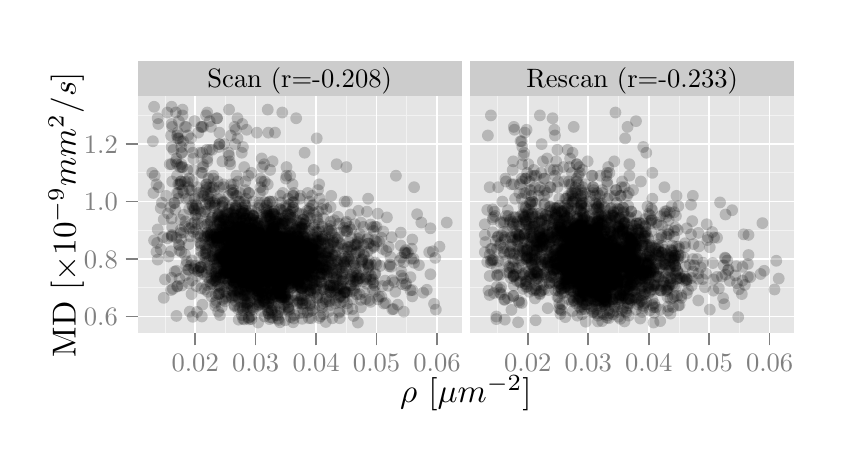
\begin{tikzpicture}[x=1pt,y=1pt]
\definecolor[named]{fillColor}{rgb}{1.00,1.00,1.00}
\path[use as bounding box,fill=fillColor,fill opacity=0.00] (0,0) rectangle (289.08,144.54);
\begin{scope}
\path[clip] (  0.00,  0.00) rectangle (289.08,144.54);
\definecolor[named]{drawColor}{rgb}{1.00,1.00,1.00}
\definecolor[named]{fillColor}{rgb}{1.00,1.00,1.00}

\path[draw=drawColor,line width= 0.6pt,line join=round,line cap=round,fill=fillColor] ( -0.00,  0.00) rectangle (289.08,144.54);
\end{scope}
\begin{scope}
\path[clip] ( 39.69,119.86) rectangle (156.86,132.50);
\definecolor[named]{fillColor}{rgb}{0.80,0.80,0.80}

\path[fill=fillColor] ( 39.69,119.86) rectangle (156.86,132.50);
\definecolor[named]{drawColor}{rgb}{0.00,0.00,0.00}

\node[text=drawColor,anchor=base,inner sep=0pt, outer sep=0pt, scale=  0.96] at ( 98.27,122.87) {Scan (r=-0.208)};
\end{scope}
\begin{scope}
\path[clip] (159.87,119.86) rectangle (277.03,132.50);
\definecolor[named]{fillColor}{rgb}{0.80,0.80,0.80}

\path[fill=fillColor] (159.87,119.86) rectangle (277.03,132.50);
\definecolor[named]{drawColor}{rgb}{0.00,0.00,0.00}

\node[text=drawColor,anchor=base,inner sep=0pt, outer sep=0pt, scale=  0.96] at (218.45,122.87) {Rescan (r=-0.233)};
\end{scope}
\begin{scope}
\path[clip] ( 39.69, 34.04) rectangle (156.86,119.86);
\definecolor[named]{fillColor}{rgb}{0.90,0.90,0.90}

\path[fill=fillColor] ( 39.69, 34.04) rectangle (156.86,119.86);
\definecolor[named]{drawColor}{rgb}{0.95,0.95,0.95}

\path[draw=drawColor,line width= 0.3pt,line join=round] ( 39.69, 50.55) --
	(156.86, 50.55);

\path[draw=drawColor,line width= 0.3pt,line join=round] ( 39.69, 71.32) --
	(156.86, 71.32);

\path[draw=drawColor,line width= 0.3pt,line join=round] ( 39.69, 92.08) --
	(156.86, 92.08);

\path[draw=drawColor,line width= 0.3pt,line join=round] ( 39.69,112.84) --
	(156.86,112.84);

\path[draw=drawColor,line width= 0.3pt,line join=round] ( 49.61, 34.04) --
	( 49.61,119.86);

\path[draw=drawColor,line width= 0.3pt,line join=round] ( 71.46, 34.04) --
	( 71.46,119.86);

\path[draw=drawColor,line width= 0.3pt,line join=round] ( 93.31, 34.04) --
	( 93.31,119.86);

\path[draw=drawColor,line width= 0.3pt,line join=round] (115.16, 34.04) --
	(115.16,119.86);

\path[draw=drawColor,line width= 0.3pt,line join=round] (137.01, 34.04) --
	(137.01,119.86);
\definecolor[named]{drawColor}{rgb}{1.00,1.00,1.00}

\path[draw=drawColor,line width= 0.6pt,line join=round] ( 39.69, 40.17) --
	(156.86, 40.17);

\path[draw=drawColor,line width= 0.6pt,line join=round] ( 39.69, 60.93) --
	(156.86, 60.93);

\path[draw=drawColor,line width= 0.6pt,line join=round] ( 39.69, 81.70) --
	(156.86, 81.70);

\path[draw=drawColor,line width= 0.6pt,line join=round] ( 39.69,102.46) --
	(156.86,102.46);

\path[draw=drawColor,line width= 0.6pt,line join=round] ( 60.53, 34.04) --
	( 60.53,119.86);

\path[draw=drawColor,line width= 0.6pt,line join=round] ( 82.38, 34.04) --
	( 82.38,119.86);

\path[draw=drawColor,line width= 0.6pt,line join=round] (104.23, 34.04) --
	(104.23,119.86);

\path[draw=drawColor,line width= 0.6pt,line join=round] (126.08, 34.04) --
	(126.08,119.86);

\path[draw=drawColor,line width= 0.6pt,line join=round] (147.93, 34.04) --
	(147.93,119.86);
\definecolor[named]{fillColor}{rgb}{0.00,0.00,0.00}

\path[fill=fillColor,fill opacity=0.20] ( 52.23, 72.46) circle (  2.13);

\path[fill=fillColor,fill opacity=0.20] ( 64.25, 80.76) circle (  2.13);

\path[fill=fillColor,fill opacity=0.20] ( 76.26, 68.82) circle (  2.13);

\path[fill=fillColor,fill opacity=0.20] ( 86.97, 56.47) circle (  2.13);

\path[fill=fillColor,fill opacity=0.20] ( 81.07, 53.67) circle (  2.13);

\path[fill=fillColor,fill opacity=0.20] ( 75.17, 53.46) circle (  2.13);

\path[fill=fillColor,fill opacity=0.20] ( 71.02, 69.65) circle (  2.13);

\path[fill=fillColor,fill opacity=0.20] ( 59.88, 93.12) circle (  2.13);

\path[fill=fillColor,fill opacity=0.20] ( 75.17, 83.77) circle (  2.13);

\path[fill=fillColor,fill opacity=0.20] ( 85.88, 58.65) circle (  2.13);

\path[fill=fillColor,fill opacity=0.20] ( 97.68, 51.49) circle (  2.13);

\path[fill=fillColor,fill opacity=0.20] (108.60, 57.71) circle (  2.13);

\path[fill=fillColor,fill opacity=0.20] ( 96.36, 57.92) circle (  2.13);

\path[fill=fillColor,fill opacity=0.20] (103.79, 50.45) circle (  2.13);

\path[fill=fillColor,fill opacity=0.20] (100.30, 44.94) circle (  2.13);

\path[fill=fillColor,fill opacity=0.20] ( 91.78, 56.68) circle (  2.13);

\path[fill=fillColor,fill opacity=0.20] ( 69.49, 59.79) circle (  2.13);

\path[fill=fillColor,fill opacity=0.20] ( 58.13, 57.09) circle (  2.13);

\path[fill=fillColor,fill opacity=0.20] ( 69.05,101.42) circle (  2.13);

\path[fill=fillColor,fill opacity=0.20] ( 85.22, 73.18) circle (  2.13);

\path[fill=fillColor,fill opacity=0.20] ( 90.68, 60.10) circle (  2.13);

\path[fill=fillColor,fill opacity=0.20] ( 94.84, 60.52) circle (  2.13);

\path[fill=fillColor,fill opacity=0.20] ( 98.33, 59.48) circle (  2.13);

\path[fill=fillColor,fill opacity=0.20] (102.92, 59.27) circle (  2.13);

\path[fill=fillColor,fill opacity=0.20] (100.08, 64.46) circle (  2.13);

\path[fill=fillColor,fill opacity=0.20] ( 95.27, 65.50) circle (  2.13);

\path[fill=fillColor,fill opacity=0.20] ( 93.52, 55.33) circle (  2.13);

\path[fill=fillColor,fill opacity=0.20] ( 88.06, 42.35) circle (  2.13);

\path[fill=fillColor,fill opacity=0.20] ( 76.04, 47.12) circle (  2.13);

\path[fill=fillColor,fill opacity=0.20] ( 74.95, 56.26) circle (  2.13);

\path[fill=fillColor,fill opacity=0.20] ( 71.46, 59.79) circle (  2.13);

\path[fill=fillColor,fill opacity=0.20] ( 58.56, 85.85) circle (  2.13);

\path[fill=fillColor,fill opacity=0.20] ( 81.51, 76.30) circle (  2.13);

\path[fill=fillColor,fill opacity=0.20] ( 98.11, 64.05) circle (  2.13);

\path[fill=fillColor,fill opacity=0.20] (111.66, 55.85) circle (  2.13);

\path[fill=fillColor,fill opacity=0.20] (106.42, 72.66) circle (  2.13);

\path[fill=fillColor,fill opacity=0.20] ( 99.21, 72.04) circle (  2.13);

\path[fill=fillColor,fill opacity=0.20] ( 92.87, 59.48) circle (  2.13);

\path[fill=fillColor,fill opacity=0.20] ( 97.68, 63.53) circle (  2.13);

\path[fill=fillColor,fill opacity=0.20] ( 99.86, 67.37) circle (  2.13);

\path[fill=fillColor,fill opacity=0.20] ( 88.94, 60.00) circle (  2.13);

\path[fill=fillColor,fill opacity=0.20] ( 79.76, 54.50) circle (  2.13);

\path[fill=fillColor,fill opacity=0.20] ( 77.14, 58.44) circle (  2.13);

\path[fill=fillColor,fill opacity=0.20] ( 77.79, 59.58) circle (  2.13);

\path[fill=fillColor,fill opacity=0.20] ( 74.30, 62.08) circle (  2.13);

\path[fill=fillColor,fill opacity=0.20] ( 60.97, 80.35) circle (  2.13);

\path[fill=fillColor,fill opacity=0.20] ( 76.48, 63.84) circle (  2.13);

\path[fill=fillColor,fill opacity=0.20] ( 98.77, 64.67) circle (  2.13);

\path[fill=fillColor,fill opacity=0.20] (107.95, 58.23) circle (  2.13);

\path[fill=fillColor,fill opacity=0.20] (105.10, 61.76) circle (  2.13);

\path[fill=fillColor,fill opacity=0.20] (103.58, 67.89) circle (  2.13);

\path[fill=fillColor,fill opacity=0.20] ( 95.27, 70.69) circle (  2.13);

\path[fill=fillColor,fill opacity=0.20] ( 83.25, 67.89) circle (  2.13);

\path[fill=fillColor,fill opacity=0.20] ( 89.37, 59.17) circle (  2.13);

\path[fill=fillColor,fill opacity=0.20] ( 85.22, 56.26) circle (  2.13);

\path[fill=fillColor,fill opacity=0.20] ( 76.92, 63.42) circle (  2.13);

\path[fill=fillColor,fill opacity=0.20] ( 74.30, 71.94) circle (  2.13);

\path[fill=fillColor,fill opacity=0.20] ( 65.56, 81.70) circle (  2.13);

\path[fill=fillColor,fill opacity=0.20] ( 54.19,106.61) circle (  2.13);

\path[fill=fillColor,fill opacity=0.20] ( 70.80, 75.68) circle (  2.13);

\path[fill=fillColor,fill opacity=0.20] ( 90.68, 45.05) circle (  2.13);

\path[fill=fillColor,fill opacity=0.20] ( 81.51, 76.71) circle (  2.13);

\path[fill=fillColor,fill opacity=0.20] ( 81.29, 76.71) circle (  2.13);

\path[fill=fillColor,fill opacity=0.20] ( 83.47, 64.88) circle (  2.13);

\path[fill=fillColor,fill opacity=0.20] ( 64.25, 85.85) circle (  2.13);

\path[fill=fillColor,fill opacity=0.20] ( 78.23, 58.34) circle (  2.13);

\path[fill=fillColor,fill opacity=0.20] ( 95.93, 60.00) circle (  2.13);

\path[fill=fillColor,fill opacity=0.20] (102.48, 58.03) circle (  2.13);

\path[fill=fillColor,fill opacity=0.20] ( 98.77, 46.50) circle (  2.13);

\path[fill=fillColor,fill opacity=0.20] (102.05, 48.89) circle (  2.13);

\path[fill=fillColor,fill opacity=0.20] ( 99.21, 69.97) circle (  2.13);

\path[fill=fillColor,fill opacity=0.20] ( 87.84, 76.19) circle (  2.13);

\path[fill=fillColor,fill opacity=0.20] ( 73.86, 63.22) circle (  2.13);

\path[fill=fillColor,fill opacity=0.20] ( 71.67, 57.51) circle (  2.13);

\path[fill=fillColor,fill opacity=0.20] ( 64.25, 63.01) circle (  2.13);

\path[fill=fillColor,fill opacity=0.20] ( 66.65, 86.89) circle (  2.13);

\path[fill=fillColor,fill opacity=0.20] (105.32, 52.63) circle (  2.13);

\path[fill=fillColor,fill opacity=0.20] ( 97.02, 64.15) circle (  2.13);

\path[fill=fillColor,fill opacity=0.20] ( 94.84, 60.41) circle (  2.13);

\path[fill=fillColor,fill opacity=0.20] ( 99.86, 61.14) circle (  2.13);

\path[fill=fillColor,fill opacity=0.20] ( 99.42, 62.18) circle (  2.13);

\path[fill=fillColor,fill opacity=0.20] ( 95.71, 54.81) circle (  2.13);

\path[fill=fillColor,fill opacity=0.20] ( 81.29, 65.19) circle (  2.13);

\path[fill=fillColor,fill opacity=0.20] ( 55.94,114.92) circle (  2.13);

\path[fill=fillColor,fill opacity=0.20] ( 70.36, 79.93) circle (  2.13);

\path[fill=fillColor,fill opacity=0.20] ( 77.57, 56.68) circle (  2.13);

\path[fill=fillColor,fill opacity=0.20] ( 88.06, 51.28) circle (  2.13);

\path[fill=fillColor,fill opacity=0.20] ( 90.47, 61.04) circle (  2.13);

\path[fill=fillColor,fill opacity=0.20] ( 87.62, 63.74) circle (  2.13);

\path[fill=fillColor,fill opacity=0.20] ( 89.59, 51.17) circle (  2.13);

\path[fill=fillColor,fill opacity=0.20] ( 91.99, 57.30) circle (  2.13);

\path[fill=fillColor,fill opacity=0.20] ( 85.44, 79.21) circle (  2.13);

\path[fill=fillColor,fill opacity=0.20] ( 64.46, 64.77) circle (  2.13);

\path[fill=fillColor,fill opacity=0.20] ( 77.57, 79.41) circle (  2.13);

\path[fill=fillColor,fill opacity=0.20] (111.88, 50.76) circle (  2.13);

\path[fill=fillColor,fill opacity=0.20] (110.35, 67.47) circle (  2.13);

\path[fill=fillColor,fill opacity=0.20] (116.03, 60.93) circle (  2.13);

\path[fill=fillColor,fill opacity=0.20] (126.95, 47.33) circle (  2.13);

\path[fill=fillColor,fill opacity=0.20] (146.84, 44.74) circle (  2.13);

\path[fill=fillColor,fill opacity=0.20] (113.41, 50.24) circle (  2.13);

\path[fill=fillColor,fill opacity=0.20] (105.54, 44.22) circle (  2.13);

\path[fill=fillColor,fill opacity=0.20] (101.39, 49.31) circle (  2.13);

\path[fill=fillColor,fill opacity=0.20] ( 65.34, 90.00) circle (  2.13);

\path[fill=fillColor,fill opacity=0.20] ( 67.96, 71.94) circle (  2.13);

\path[fill=fillColor,fill opacity=0.20] ( 78.01, 55.53) circle (  2.13);

\path[fill=fillColor,fill opacity=0.20] ( 88.94, 60.93) circle (  2.13);

\path[fill=fillColor,fill opacity=0.20] ( 81.94, 63.63) circle (  2.13);

\path[fill=fillColor,fill opacity=0.20] ( 80.41, 72.15) circle (  2.13);

\path[fill=fillColor,fill opacity=0.20] ( 83.47, 69.45) circle (  2.13);

\path[fill=fillColor,fill opacity=0.20] ( 80.20, 62.18) circle (  2.13);

\path[fill=fillColor,fill opacity=0.20] ( 78.67, 73.81) circle (  2.13);

\path[fill=fillColor,fill opacity=0.20] ( 77.79, 78.58) circle (  2.13);

\path[fill=fillColor,fill opacity=0.20] ( 67.96, 70.38) circle (  2.13);

\path[fill=fillColor,fill opacity=0.20] (111.66, 49.82) circle (  2.13);

\path[fill=fillColor,fill opacity=0.20] (115.59, 65.29) circle (  2.13);

\path[fill=fillColor,fill opacity=0.20] (119.09, 65.81) circle (  2.13);

\path[fill=fillColor,fill opacity=0.20] (133.73, 44.43) circle (  2.13);

\path[fill=fillColor,fill opacity=0.20] (120.40, 43.49) circle (  2.13);

\path[fill=fillColor,fill opacity=0.20] (122.58, 52.00) circle (  2.13);

\path[fill=fillColor,fill opacity=0.20] (100.95, 51.80) circle (  2.13);

\path[fill=fillColor,fill opacity=0.20] ( 96.15, 45.78) circle (  2.13);

\path[fill=fillColor,fill opacity=0.20] ( 79.98, 56.05) circle (  2.13);

\path[fill=fillColor,fill opacity=0.20] ( 60.31, 74.12) circle (  2.13);

\path[fill=fillColor,fill opacity=0.20] ( 81.07, 62.39) circle (  2.13);

\path[fill=fillColor,fill opacity=0.20] ( 81.94, 74.64) circle (  2.13);

\path[fill=fillColor,fill opacity=0.20] ( 83.91, 58.34) circle (  2.13);

\path[fill=fillColor,fill opacity=0.20] ( 86.97, 53.04) circle (  2.13);

\path[fill=fillColor,fill opacity=0.20] ( 83.04, 70.28) circle (  2.13);

\path[fill=fillColor,fill opacity=0.20] ( 86.10, 75.68) circle (  2.13);

\path[fill=fillColor,fill opacity=0.20] ( 80.63, 67.47) circle (  2.13);

\path[fill=fillColor,fill opacity=0.20] ( 82.82, 60.52) circle (  2.13);

\path[fill=fillColor,fill opacity=0.20] ( 71.24, 65.40) circle (  2.13);

\path[fill=fillColor,fill opacity=0.20] ( 89.15, 78.06) circle (  2.13);

\path[fill=fillColor,fill opacity=0.20] (117.78, 58.75) circle (  2.13);

\path[fill=fillColor,fill opacity=0.20] (109.26, 58.55) circle (  2.13);

\path[fill=fillColor,fill opacity=0.20] (101.17, 48.68) circle (  2.13);

\path[fill=fillColor,fill opacity=0.20] (100.08, 58.23) circle (  2.13);

\path[fill=fillColor,fill opacity=0.20] (102.48, 61.04) circle (  2.13);

\path[fill=fillColor,fill opacity=0.20] ( 94.40, 55.22) circle (  2.13);

\path[fill=fillColor,fill opacity=0.20] ( 82.60, 54.91) circle (  2.13);

\path[fill=fillColor,fill opacity=0.20] ( 56.38, 84.81) circle (  2.13);

\path[fill=fillColor,fill opacity=0.20] ( 75.39, 68.93) circle (  2.13);

\path[fill=fillColor,fill opacity=0.20] ( 81.73, 71.52) circle (  2.13);

\path[fill=fillColor,fill opacity=0.20] ( 91.78, 52.11) circle (  2.13);

\path[fill=fillColor,fill opacity=0.20] ( 93.09, 38.82) circle (  2.13);

\path[fill=fillColor,fill opacity=0.20] ( 86.53, 56.99) circle (  2.13);

\path[fill=fillColor,fill opacity=0.20] ( 83.47, 70.59) circle (  2.13);

\path[fill=fillColor,fill opacity=0.20] ( 81.94, 67.16) circle (  2.13);

\path[fill=fillColor,fill opacity=0.20] ( 80.41, 56.57) circle (  2.13);

\path[fill=fillColor,fill opacity=0.20] ( 78.23, 53.15) circle (  2.13);

\path[fill=fillColor,fill opacity=0.20] (129.14, 53.15) circle (  2.13);

\path[fill=fillColor,fill opacity=0.20] (114.72, 48.99) circle (  2.13);

\path[fill=fillColor,fill opacity=0.20] (102.70, 61.35) circle (  2.13);

\path[fill=fillColor,fill opacity=0.20] (119.96, 53.98) circle (  2.13);

\path[fill=fillColor,fill opacity=0.20] (100.95, 56.05) circle (  2.13);

\path[fill=fillColor,fill opacity=0.20] ( 93.31, 62.39) circle (  2.13);

\path[fill=fillColor,fill opacity=0.20] (100.73, 60.41) circle (  2.13);

\path[fill=fillColor,fill opacity=0.20] ( 94.18, 60.10) circle (  2.13);

\path[fill=fillColor,fill opacity=0.20] ( 86.31, 60.41) circle (  2.13);

\path[fill=fillColor,fill opacity=0.20] ( 88.28, 42.56) circle (  2.13);

\path[fill=fillColor,fill opacity=0.20] ( 72.33, 70.28) circle (  2.13);

\path[fill=fillColor,fill opacity=0.20] ( 90.90, 60.52) circle (  2.13);

\path[fill=fillColor,fill opacity=0.20] ( 99.64, 56.05) circle (  2.13);

\path[fill=fillColor,fill opacity=0.20] ( 97.46, 53.77) circle (  2.13);

\path[fill=fillColor,fill opacity=0.20] ( 88.06, 53.15) circle (  2.13);

\path[fill=fillColor,fill opacity=0.20] ( 84.78, 53.15) circle (  2.13);

\path[fill=fillColor,fill opacity=0.20] ( 83.04, 60.10) circle (  2.13);

\path[fill=fillColor,fill opacity=0.20] ( 76.48, 71.11) circle (  2.13);

\path[fill=fillColor,fill opacity=0.20] ( 79.98, 58.96) circle (  2.13);

\path[fill=fillColor,fill opacity=0.20] ( 66.21,108.69) circle (  2.13);

\path[fill=fillColor,fill opacity=0.20] (117.34, 46.29) circle (  2.13);

\path[fill=fillColor,fill opacity=0.20] (103.36, 72.25) circle (  2.13);

\path[fill=fillColor,fill opacity=0.20] (109.69, 71.21) circle (  2.13);

\path[fill=fillColor,fill opacity=0.20] (122.15, 54.18) circle (  2.13);

\path[fill=fillColor,fill opacity=0.20] (106.20, 55.53) circle (  2.13);

\path[fill=fillColor,fill opacity=0.20] ( 96.58, 61.04) circle (  2.13);

\path[fill=fillColor,fill opacity=0.20] (106.63, 61.14) circle (  2.13);

\path[fill=fillColor,fill opacity=0.20] ( 83.25, 65.71) circle (  2.13);

\path[fill=fillColor,fill opacity=0.20] ( 88.06, 58.34) circle (  2.13);

\path[fill=fillColor,fill opacity=0.20] ( 87.62, 39.86) circle (  2.13);

\path[fill=fillColor,fill opacity=0.20] ( 74.30, 52.94) circle (  2.13);

\path[fill=fillColor,fill opacity=0.20] ( 82.60, 51.69) circle (  2.13);

\path[fill=fillColor,fill opacity=0.20] ( 90.68, 60.83) circle (  2.13);

\path[fill=fillColor,fill opacity=0.20] ( 92.43, 66.33) circle (  2.13);

\path[fill=fillColor,fill opacity=0.20] ( 90.90, 59.17) circle (  2.13);

\path[fill=fillColor,fill opacity=0.20] ( 88.28, 47.02) circle (  2.13);

\path[fill=fillColor,fill opacity=0.20] ( 90.68, 50.65) circle (  2.13);

\path[fill=fillColor,fill opacity=0.20] ( 81.29, 75.47) circle (  2.13);

\path[fill=fillColor,fill opacity=0.20] ( 89.81, 74.33) circle (  2.13);

\path[fill=fillColor,fill opacity=0.20] ( 82.60, 60.31) circle (  2.13);

\path[fill=fillColor,fill opacity=0.20] ( 95.93, 62.08) circle (  2.13);

\path[fill=fillColor,fill opacity=0.20] ( 89.81, 62.18) circle (  2.13);

\path[fill=fillColor,fill opacity=0.20] ( 88.28, 77.86) circle (  2.13);

\path[fill=fillColor,fill opacity=0.20] ( 97.89, 68.93) circle (  2.13);

\path[fill=fillColor,fill opacity=0.20] (107.73, 57.20) circle (  2.13);

\path[fill=fillColor,fill opacity=0.20] (100.52, 60.73) circle (  2.13);

\path[fill=fillColor,fill opacity=0.20] ( 98.33, 59.89) circle (  2.13);

\path[fill=fillColor,fill opacity=0.20] (101.17, 53.67) circle (  2.13);

\path[fill=fillColor,fill opacity=0.20] ( 92.87, 56.68) circle (  2.13);

\path[fill=fillColor,fill opacity=0.20] ( 85.88, 51.59) circle (  2.13);

\path[fill=fillColor,fill opacity=0.20] ( 85.66, 40.17) circle (  2.13);

\path[fill=fillColor,fill opacity=0.20] ( 66.43, 64.98) circle (  2.13);

\path[fill=fillColor,fill opacity=0.20] ( 72.11, 60.00) circle (  2.13);

\path[fill=fillColor,fill opacity=0.20] ( 80.63, 63.32) circle (  2.13);

\path[fill=fillColor,fill opacity=0.20] ( 82.38, 64.15) circle (  2.13);

\path[fill=fillColor,fill opacity=0.20] ( 91.99, 57.92) circle (  2.13);

\path[fill=fillColor,fill opacity=0.20] ( 86.75, 55.53) circle (  2.13);

\path[fill=fillColor,fill opacity=0.20] ( 87.62, 55.22) circle (  2.13);

\path[fill=fillColor,fill opacity=0.20] ( 88.50, 64.15) circle (  2.13);

\path[fill=fillColor,fill opacity=0.20] ( 79.32, 67.58) circle (  2.13);

\path[fill=fillColor,fill opacity=0.20] ( 75.83, 56.05) circle (  2.13);

\path[fill=fillColor,fill opacity=0.20] ( 64.90, 69.24) circle (  2.13);

\path[fill=fillColor,fill opacity=0.20] ( 86.31, 78.69) circle (  2.13);

\path[fill=fillColor,fill opacity=0.20] (110.13, 59.06) circle (  2.13);

\path[fill=fillColor,fill opacity=0.20] ( 83.25, 71.83) circle (  2.13);

\path[fill=fillColor,fill opacity=0.20] ( 87.62, 70.28) circle (  2.13);

\path[fill=fillColor,fill opacity=0.20] ( 95.05, 60.31) circle (  2.13);

\path[fill=fillColor,fill opacity=0.20] ( 98.33, 55.85) circle (  2.13);

\path[fill=fillColor,fill opacity=0.20] (101.17, 60.52) circle (  2.13);

\path[fill=fillColor,fill opacity=0.20] ( 91.56, 55.43) circle (  2.13);

\path[fill=fillColor,fill opacity=0.20] (106.63, 44.94) circle (  2.13);

\path[fill=fillColor,fill opacity=0.20] (102.92, 50.45) circle (  2.13);

\path[fill=fillColor,fill opacity=0.20] ( 90.47, 50.14) circle (  2.13);

\path[fill=fillColor,fill opacity=0.20] ( 83.25, 47.33) circle (  2.13);

\path[fill=fillColor,fill opacity=0.20] ( 71.46, 73.50) circle (  2.13);

\path[fill=fillColor,fill opacity=0.20] ( 89.59, 58.55) circle (  2.13);

\path[fill=fillColor,fill opacity=0.20] ( 90.68, 49.82) circle (  2.13);

\path[fill=fillColor,fill opacity=0.20] ( 85.00, 58.03) circle (  2.13);

\path[fill=fillColor,fill opacity=0.20] ( 89.59, 59.89) circle (  2.13);

\path[fill=fillColor,fill opacity=0.20] ( 90.68, 50.34) circle (  2.13);

\path[fill=fillColor,fill opacity=0.20] ( 86.75, 43.49) circle (  2.13);

\path[fill=fillColor,fill opacity=0.20] ( 77.79, 43.08) circle (  2.13);

\path[fill=fillColor,fill opacity=0.20] ( 76.26, 49.62) circle (  2.13);

\path[fill=fillColor,fill opacity=0.20] ( 67.52, 68.93) circle (  2.13);

\path[fill=fillColor,fill opacity=0.20] ( 72.99, 96.23) circle (  2.13);

\path[fill=fillColor,fill opacity=0.20] ( 97.24, 53.46) circle (  2.13);

\path[fill=fillColor,fill opacity=0.20] ( 96.15, 63.74) circle (  2.13);

\path[fill=fillColor,fill opacity=0.20] ( 96.80, 60.00) circle (  2.13);

\path[fill=fillColor,fill opacity=0.20] (105.32, 57.09) circle (  2.13);

\path[fill=fillColor,fill opacity=0.20] (102.26, 59.06) circle (  2.13);

\path[fill=fillColor,fill opacity=0.20] ( 99.64, 58.34) circle (  2.13);

\path[fill=fillColor,fill opacity=0.20] (100.95, 53.56) circle (  2.13);

\path[fill=fillColor,fill opacity=0.20] ( 98.99, 47.64) circle (  2.13);

\path[fill=fillColor,fill opacity=0.20] (103.36, 48.79) circle (  2.13);

\path[fill=fillColor,fill opacity=0.20] ( 95.93, 58.23) circle (  2.13);

\path[fill=fillColor,fill opacity=0.20] ( 94.84, 58.96) circle (  2.13);

\path[fill=fillColor,fill opacity=0.20] ( 78.67, 62.08) circle (  2.13);

\path[fill=fillColor,fill opacity=0.20] ( 88.06, 68.30) circle (  2.13);

\path[fill=fillColor,fill opacity=0.20] ( 99.42, 44.94) circle (  2.13);

\path[fill=fillColor,fill opacity=0.20] ( 84.35, 47.64) circle (  2.13);

\path[fill=fillColor,fill opacity=0.20] ( 89.37, 53.35) circle (  2.13);

\path[fill=fillColor,fill opacity=0.20] ( 89.81, 47.54) circle (  2.13);

\path[fill=fillColor,fill opacity=0.20] ( 85.22, 44.43) circle (  2.13);

\path[fill=fillColor,fill opacity=0.20] ( 86.97, 45.05) circle (  2.13);

\path[fill=fillColor,fill opacity=0.20] ( 78.45, 50.86) circle (  2.13);

\path[fill=fillColor,fill opacity=0.20] ( 75.17, 64.46) circle (  2.13);

\path[fill=fillColor,fill opacity=0.20] ( 60.31, 79.10) circle (  2.13);

\path[fill=fillColor,fill opacity=0.20] ( 75.17,107.65) circle (  2.13);

\path[fill=fillColor,fill opacity=0.20] ( 97.46, 60.83) circle (  2.13);

\path[fill=fillColor,fill opacity=0.20] ( 94.18, 69.24) circle (  2.13);

\path[fill=fillColor,fill opacity=0.20] ( 97.46, 58.96) circle (  2.13);

\path[fill=fillColor,fill opacity=0.20] (107.29, 49.51) circle (  2.13);

\path[fill=fillColor,fill opacity=0.20] (108.38, 54.81) circle (  2.13);

\path[fill=fillColor,fill opacity=0.20] (102.70, 64.36) circle (  2.13);

\path[fill=fillColor,fill opacity=0.20] ( 98.33, 67.68) circle (  2.13);

\path[fill=fillColor,fill opacity=0.20] (107.29, 58.65) circle (  2.13);

\path[fill=fillColor,fill opacity=0.20] ( 98.33, 51.69) circle (  2.13);

\path[fill=fillColor,fill opacity=0.20] (100.52, 55.22) circle (  2.13);

\path[fill=fillColor,fill opacity=0.20] (100.52, 58.23) circle (  2.13);

\path[fill=fillColor,fill opacity=0.20] ( 86.10, 67.16) circle (  2.13);

\path[fill=fillColor,fill opacity=0.20] ( 57.69, 88.96) circle (  2.13);

\path[fill=fillColor,fill opacity=0.20] ( 55.51, 95.19) circle (  2.13);

\path[fill=fillColor,fill opacity=0.20] ( 75.61, 60.10) circle (  2.13);

\path[fill=fillColor,fill opacity=0.20] ( 88.28, 48.16) circle (  2.13);

\path[fill=fillColor,fill opacity=0.20] ( 86.53, 48.79) circle (  2.13);

\path[fill=fillColor,fill opacity=0.20] ( 81.73, 56.57) circle (  2.13);

\path[fill=fillColor,fill opacity=0.20] ( 89.37, 58.55) circle (  2.13);

\path[fill=fillColor,fill opacity=0.20] ( 86.97, 54.18) circle (  2.13);

\path[fill=fillColor,fill opacity=0.20] ( 86.10, 56.99) circle (  2.13);

\path[fill=fillColor,fill opacity=0.20] ( 77.36, 68.62) circle (  2.13);

\path[fill=fillColor,fill opacity=0.20] ( 72.77, 75.68) circle (  2.13);

\path[fill=fillColor,fill opacity=0.20] ( 65.77, 80.87) circle (  2.13);

\path[fill=fillColor,fill opacity=0.20] ( 68.40,111.81) circle (  2.13);

\path[fill=fillColor,fill opacity=0.20] ( 97.68, 58.13) circle (  2.13);

\path[fill=fillColor,fill opacity=0.20] ( 94.18, 72.87) circle (  2.13);

\path[fill=fillColor,fill opacity=0.20] ( 95.05, 69.55) circle (  2.13);

\path[fill=fillColor,fill opacity=0.20] (100.95, 59.17) circle (  2.13);

\path[fill=fillColor,fill opacity=0.20] (102.05, 63.11) circle (  2.13);

\path[fill=fillColor,fill opacity=0.20] ( 99.21, 64.98) circle (  2.13);

\path[fill=fillColor,fill opacity=0.20] (100.08, 63.74) circle (  2.13);

\path[fill=fillColor,fill opacity=0.20] (103.58, 64.77) circle (  2.13);

\path[fill=fillColor,fill opacity=0.20] (100.08, 66.02) circle (  2.13);

\path[fill=fillColor,fill opacity=0.20] (104.23, 68.62) circle (  2.13);

\path[fill=fillColor,fill opacity=0.20] (102.26, 59.17) circle (  2.13);

\path[fill=fillColor,fill opacity=0.20] ( 88.06, 47.75) circle (  2.13);

\path[fill=fillColor,fill opacity=0.20] ( 55.94, 94.16) circle (  2.13);

\path[fill=fillColor,fill opacity=0.20] ( 85.00, 71.32) circle (  2.13);

\path[fill=fillColor,fill opacity=0.20] ( 93.74, 53.04) circle (  2.13);

\path[fill=fillColor,fill opacity=0.20] ( 85.22, 56.88) circle (  2.13);

\path[fill=fillColor,fill opacity=0.20] ( 91.34, 53.56) circle (  2.13);

\path[fill=fillColor,fill opacity=0.20] ( 98.11, 45.57) circle (  2.13);

\path[fill=fillColor,fill opacity=0.20] ( 86.75, 53.56) circle (  2.13);

\path[fill=fillColor,fill opacity=0.20] ( 84.78, 59.58) circle (  2.13);

\path[fill=fillColor,fill opacity=0.20] ( 83.25, 61.87) circle (  2.13);

\path[fill=fillColor,fill opacity=0.20] ( 83.47, 62.91) circle (  2.13);

\path[fill=fillColor,fill opacity=0.20] ( 68.83, 66.95) circle (  2.13);

\path[fill=fillColor,fill opacity=0.20] ( 92.21, 64.88) circle (  2.13);

\path[fill=fillColor,fill opacity=0.20] ( 93.09, 74.85) circle (  2.13);

\path[fill=fillColor,fill opacity=0.20] (103.14, 69.65) circle (  2.13);

\path[fill=fillColor,fill opacity=0.20] (103.36, 55.74) circle (  2.13);

\path[fill=fillColor,fill opacity=0.20] (105.76, 55.64) circle (  2.13);

\path[fill=fillColor,fill opacity=0.20] (102.48, 63.22) circle (  2.13);

\path[fill=fillColor,fill opacity=0.20] (100.73, 67.27) circle (  2.13);

\path[fill=fillColor,fill opacity=0.20] (103.79, 60.31) circle (  2.13);

\path[fill=fillColor,fill opacity=0.20] (110.35, 57.61) circle (  2.13);

\path[fill=fillColor,fill opacity=0.20] (104.89, 66.33) circle (  2.13);

\path[fill=fillColor,fill opacity=0.20] ( 98.11, 60.41) circle (  2.13);

\path[fill=fillColor,fill opacity=0.20] ( 76.70, 50.45) circle (  2.13);

\path[fill=fillColor,fill opacity=0.20] ( 55.51,101.42) circle (  2.13);

\path[fill=fillColor,fill opacity=0.20] ( 91.12, 66.12) circle (  2.13);

\path[fill=fillColor,fill opacity=0.20] (101.39, 49.93) circle (  2.13);

\path[fill=fillColor,fill opacity=0.20] ( 98.33, 41.41) circle (  2.13);

\path[fill=fillColor,fill opacity=0.20] (102.48, 39.55) circle (  2.13);

\path[fill=fillColor,fill opacity=0.20] ( 91.78, 49.82) circle (  2.13);

\path[fill=fillColor,fill opacity=0.20] ( 83.69, 53.87) circle (  2.13);

\path[fill=fillColor,fill opacity=0.20] ( 83.91, 59.48) circle (  2.13);

\path[fill=fillColor,fill opacity=0.20] ( 76.26, 64.88) circle (  2.13);

\path[fill=fillColor,fill opacity=0.20] ( 72.77, 63.74) circle (  2.13);

\path[fill=fillColor,fill opacity=0.20] ( 66.87, 75.99) circle (  2.13);

\path[fill=fillColor,fill opacity=0.20] ( 62.72,108.69) circle (  2.13);

\path[fill=fillColor,fill opacity=0.20] ( 91.34, 71.94) circle (  2.13);

\path[fill=fillColor,fill opacity=0.20] ( 86.31, 80.24) circle (  2.13);

\path[fill=fillColor,fill opacity=0.20] ( 98.11, 71.52) circle (  2.13);

\path[fill=fillColor,fill opacity=0.20] (113.41, 57.71) circle (  2.13);

\path[fill=fillColor,fill opacity=0.20] (116.69, 51.38) circle (  2.13);

\path[fill=fillColor,fill opacity=0.20] (117.34, 49.20) circle (  2.13);

\path[fill=fillColor,fill opacity=0.20] (109.04, 51.38) circle (  2.13);

\path[fill=fillColor,fill opacity=0.20] (106.63, 57.92) circle (  2.13);

\path[fill=fillColor,fill opacity=0.20] (101.61, 61.97) circle (  2.13);

\path[fill=fillColor,fill opacity=0.20] (100.08, 61.87) circle (  2.13);

\path[fill=fillColor,fill opacity=0.20] (111.88, 60.62) circle (  2.13);

\path[fill=fillColor,fill opacity=0.20] (104.67, 56.57) circle (  2.13);

\path[fill=fillColor,fill opacity=0.20] ( 74.73, 63.32) circle (  2.13);

\path[fill=fillColor,fill opacity=0.20] ( 53.98, 95.19) circle (  2.13);

\path[fill=fillColor,fill opacity=0.20] ( 98.77, 62.59) circle (  2.13);

\path[fill=fillColor,fill opacity=0.20] (102.92, 51.80) circle (  2.13);

\path[fill=fillColor,fill opacity=0.20] ( 97.02, 52.63) circle (  2.13);

\path[fill=fillColor,fill opacity=0.20] ( 97.68, 53.35) circle (  2.13);

\path[fill=fillColor,fill opacity=0.20] ( 84.78, 59.58) circle (  2.13);

\path[fill=fillColor,fill opacity=0.20] ( 82.82, 68.51) circle (  2.13);

\path[fill=fillColor,fill opacity=0.20] ( 81.51, 68.10) circle (  2.13);

\path[fill=fillColor,fill opacity=0.20] ( 72.33, 67.58) circle (  2.13);

\path[fill=fillColor,fill opacity=0.20] ( 72.33, 69.03) circle (  2.13);

\path[fill=fillColor,fill opacity=0.20] ( 68.18, 65.92) circle (  2.13);

\path[fill=fillColor,fill opacity=0.20] ( 70.36, 80.14) circle (  2.13);

\path[fill=fillColor,fill opacity=0.20] ( 97.24, 54.81) circle (  2.13);

\path[fill=fillColor,fill opacity=0.20] (102.70, 80.14) circle (  2.13);

\path[fill=fillColor,fill opacity=0.20] ( 95.71, 81.39) circle (  2.13);

\path[fill=fillColor,fill opacity=0.20] (112.10, 59.89) circle (  2.13);

\path[fill=fillColor,fill opacity=0.20] (112.10, 59.06) circle (  2.13);

\path[fill=fillColor,fill opacity=0.20] (116.90, 64.15) circle (  2.13);

\path[fill=fillColor,fill opacity=0.20] (114.72, 57.92) circle (  2.13);

\path[fill=fillColor,fill opacity=0.20] (110.79, 49.72) circle (  2.13);

\path[fill=fillColor,fill opacity=0.20] (109.47, 51.38) circle (  2.13);

\path[fill=fillColor,fill opacity=0.20] (100.95, 58.75) circle (  2.13);

\path[fill=fillColor,fill opacity=0.20] ( 98.33, 56.26) circle (  2.13);

\path[fill=fillColor,fill opacity=0.20] ( 97.68, 52.00) circle (  2.13);

\path[fill=fillColor,fill opacity=0.20] ( 70.14, 60.10) circle (  2.13);

\path[fill=fillColor,fill opacity=0.20] ( 91.34, 74.64) circle (  2.13);

\path[fill=fillColor,fill opacity=0.20] (100.30, 68.41) circle (  2.13);

\path[fill=fillColor,fill opacity=0.20] ( 91.34, 53.87) circle (  2.13);

\path[fill=fillColor,fill opacity=0.20] ( 87.41, 52.52) circle (  2.13);

\path[fill=fillColor,fill opacity=0.20] ( 84.78, 66.95) circle (  2.13);

\path[fill=fillColor,fill opacity=0.20] ( 82.60, 66.33) circle (  2.13);

\path[fill=fillColor,fill opacity=0.20] ( 80.41, 61.56) circle (  2.13);

\path[fill=fillColor,fill opacity=0.20] ( 72.77, 62.80) circle (  2.13);

\path[fill=fillColor,fill opacity=0.20] ( 70.80, 57.09) circle (  2.13);

\path[fill=fillColor,fill opacity=0.20] ( 81.73, 54.08) circle (  2.13);

\path[fill=fillColor,fill opacity=0.20] ( 70.58, 60.73) circle (  2.13);

\path[fill=fillColor,fill opacity=0.20] ( 58.35, 82.74) circle (  2.13);

\path[fill=fillColor,fill opacity=0.20] ( 78.01, 52.52) circle (  2.13);

\path[fill=fillColor,fill opacity=0.20] ( 87.19, 53.77) circle (  2.13);

\path[fill=fillColor,fill opacity=0.20] ( 98.33, 63.94) circle (  2.13);

\path[fill=fillColor,fill opacity=0.20] ( 92.65, 67.58) circle (  2.13);

\path[fill=fillColor,fill opacity=0.20] (102.92, 68.10) circle (  2.13);

\path[fill=fillColor,fill opacity=0.20] (105.98, 65.29) circle (  2.13);

\path[fill=fillColor,fill opacity=0.20] (106.42, 68.20) circle (  2.13);

\path[fill=fillColor,fill opacity=0.20] (110.79, 74.95) circle (  2.13);

\path[fill=fillColor,fill opacity=0.20] (111.00, 68.72) circle (  2.13);

\path[fill=fillColor,fill opacity=0.20] (111.66, 54.70) circle (  2.13);

\path[fill=fillColor,fill opacity=0.20] (106.85, 50.86) circle (  2.13);

\path[fill=fillColor,fill opacity=0.20] (100.08, 50.97) circle (  2.13);

\path[fill=fillColor,fill opacity=0.20] ( 85.88, 46.40) circle (  2.13);

\path[fill=fillColor,fill opacity=0.20] ( 71.24, 57.20) circle (  2.13);

\path[fill=fillColor,fill opacity=0.20] ( 68.62, 82.74) circle (  2.13);

\path[fill=fillColor,fill opacity=0.20] ( 85.44, 59.48) circle (  2.13);

\path[fill=fillColor,fill opacity=0.20] ( 94.40, 41.93) circle (  2.13);

\path[fill=fillColor,fill opacity=0.20] ( 92.65, 49.41) circle (  2.13);

\path[fill=fillColor,fill opacity=0.20] ( 85.88, 60.52) circle (  2.13);

\path[fill=fillColor,fill opacity=0.20] ( 84.13, 59.06) circle (  2.13);

\path[fill=fillColor,fill opacity=0.20] ( 76.70, 61.66) circle (  2.13);

\path[fill=fillColor,fill opacity=0.20] ( 70.36, 72.35) circle (  2.13);

\path[fill=fillColor,fill opacity=0.20] ( 69.27, 74.22) circle (  2.13);

\path[fill=fillColor,fill opacity=0.20] ( 73.86, 60.73) circle (  2.13);

\path[fill=fillColor,fill opacity=0.20] ( 71.89, 48.79) circle (  2.13);

\path[fill=fillColor,fill opacity=0.20] ( 72.33, 52.21) circle (  2.13);

\path[fill=fillColor,fill opacity=0.20] ( 64.90, 70.38) circle (  2.13);

\path[fill=fillColor,fill opacity=0.20] ( 67.52, 65.40) circle (  2.13);

\path[fill=fillColor,fill opacity=0.20] ( 76.04, 63.74) circle (  2.13);

\path[fill=fillColor,fill opacity=0.20] ( 85.66, 63.42) circle (  2.13);

\path[fill=fillColor,fill opacity=0.20] ( 86.75, 64.46) circle (  2.13);

\path[fill=fillColor,fill opacity=0.20] (116.90, 68.62) circle (  2.13);

\path[fill=fillColor,fill opacity=0.20] ( 93.09, 68.72) circle (  2.13);

\path[fill=fillColor,fill opacity=0.20] ( 93.96, 58.03) circle (  2.13);

\path[fill=fillColor,fill opacity=0.20] (103.58, 58.34) circle (  2.13);

\path[fill=fillColor,fill opacity=0.20] (105.10, 67.68) circle (  2.13);

\path[fill=fillColor,fill opacity=0.20] (105.54, 70.80) circle (  2.13);

\path[fill=fillColor,fill opacity=0.20] (108.38, 71.83) circle (  2.13);

\path[fill=fillColor,fill opacity=0.20] (109.47, 74.43) circle (  2.13);

\path[fill=fillColor,fill opacity=0.20] ( 99.86, 67.79) circle (  2.13);

\path[fill=fillColor,fill opacity=0.20] ( 94.62, 55.43) circle (  2.13);

\path[fill=fillColor,fill opacity=0.20] ( 80.85, 58.13) circle (  2.13);

\path[fill=fillColor,fill opacity=0.20] ( 67.96, 80.97) circle (  2.13);

\path[fill=fillColor,fill opacity=0.20] ( 78.67, 58.75) circle (  2.13);

\path[fill=fillColor,fill opacity=0.20] ( 91.34, 47.23) circle (  2.13);

\path[fill=fillColor,fill opacity=0.20] ( 93.74, 54.50) circle (  2.13);

\path[fill=fillColor,fill opacity=0.20] ( 87.84, 57.61) circle (  2.13);

\path[fill=fillColor,fill opacity=0.20] ( 89.15, 56.05) circle (  2.13);

\path[fill=fillColor,fill opacity=0.20] ( 80.41, 68.51) circle (  2.13);

\path[fill=fillColor,fill opacity=0.20] ( 77.57, 74.53) circle (  2.13);

\path[fill=fillColor,fill opacity=0.20] ( 75.61, 65.71) circle (  2.13);

\path[fill=fillColor,fill opacity=0.20] ( 75.17, 55.12) circle (  2.13);

\path[fill=fillColor,fill opacity=0.20] ( 75.39, 52.63) circle (  2.13);

\path[fill=fillColor,fill opacity=0.20] ( 77.57, 61.76) circle (  2.13);

\path[fill=fillColor,fill opacity=0.20] ( 70.80, 69.24) circle (  2.13);

\path[fill=fillColor,fill opacity=0.20] ( 70.58, 60.93) circle (  2.13);

\path[fill=fillColor,fill opacity=0.20] ( 65.99, 68.10) circle (  2.13);

\path[fill=fillColor,fill opacity=0.20] ( 66.65, 66.95) circle (  2.13);

\path[fill=fillColor,fill opacity=0.20] ( 66.21, 69.86) circle (  2.13);

\path[fill=fillColor,fill opacity=0.20] ( 90.68, 73.81) circle (  2.13);

\path[fill=fillColor,fill opacity=0.20] ( 85.66, 62.39) circle (  2.13);

\path[fill=fillColor,fill opacity=0.20] ( 86.10, 62.91) circle (  2.13);

\path[fill=fillColor,fill opacity=0.20] ( 95.71, 78.79) circle (  2.13);

\path[fill=fillColor,fill opacity=0.20] ( 89.59, 76.30) circle (  2.13);

\path[fill=fillColor,fill opacity=0.20] ( 97.68, 64.15) circle (  2.13);

\path[fill=fillColor,fill opacity=0.20] ( 90.68, 64.67) circle (  2.13);

\path[fill=fillColor,fill opacity=0.20] (101.83, 60.62) circle (  2.13);

\path[fill=fillColor,fill opacity=0.20] (107.95, 60.31) circle (  2.13);

\path[fill=fillColor,fill opacity=0.20] (119.31, 67.16) circle (  2.13);

\path[fill=fillColor,fill opacity=0.20] (105.98, 63.84) circle (  2.13);

\path[fill=fillColor,fill opacity=0.20] ( 96.80, 63.84) circle (  2.13);

\path[fill=fillColor,fill opacity=0.20] ( 92.21, 73.81) circle (  2.13);

\path[fill=fillColor,fill opacity=0.20] ( 78.67, 78.48) circle (  2.13);

\path[fill=fillColor,fill opacity=0.20] ( 75.61, 72.46) circle (  2.13);

\path[fill=fillColor,fill opacity=0.20] ( 67.30, 72.77) circle (  2.13);

\path[fill=fillColor,fill opacity=0.20] ( 80.63, 69.45) circle (  2.13);

\path[fill=fillColor,fill opacity=0.20] ( 91.34, 61.14) circle (  2.13);

\path[fill=fillColor,fill opacity=0.20] ( 97.89, 46.19) circle (  2.13);

\path[fill=fillColor,fill opacity=0.20] ( 98.11, 45.15) circle (  2.13);

\path[fill=fillColor,fill opacity=0.20] ( 87.84, 56.68) circle (  2.13);

\path[fill=fillColor,fill opacity=0.20] ( 79.10, 59.06) circle (  2.13);

\path[fill=fillColor,fill opacity=0.20] ( 78.01, 62.08) circle (  2.13);

\path[fill=fillColor,fill opacity=0.20] ( 75.83, 67.89) circle (  2.13);

\path[fill=fillColor,fill opacity=0.20] ( 76.70, 67.37) circle (  2.13);

\path[fill=fillColor,fill opacity=0.20] ( 73.20, 68.93) circle (  2.13);

\path[fill=fillColor,fill opacity=0.20] ( 71.46, 67.89) circle (  2.13);

\path[fill=fillColor,fill opacity=0.20] ( 71.67, 61.56) circle (  2.13);

\path[fill=fillColor,fill opacity=0.20] ( 72.33, 58.96) circle (  2.13);

\path[fill=fillColor,fill opacity=0.20] ( 74.95, 59.79) circle (  2.13);

\path[fill=fillColor,fill opacity=0.20] ( 71.46, 62.59) circle (  2.13);

\path[fill=fillColor,fill opacity=0.20] ( 65.99, 70.38) circle (  2.13);

\path[fill=fillColor,fill opacity=0.20] ( 76.92, 58.44) circle (  2.13);

\path[fill=fillColor,fill opacity=0.20] ( 71.24, 45.67) circle (  2.13);

\path[fill=fillColor,fill opacity=0.20] ( 67.30, 60.83) circle (  2.13);

\path[fill=fillColor,fill opacity=0.20] ( 68.62, 76.19) circle (  2.13);

\path[fill=fillColor,fill opacity=0.20] ( 74.30, 69.13) circle (  2.13);

\path[fill=fillColor,fill opacity=0.20] ( 72.11, 64.15) circle (  2.13);

\path[fill=fillColor,fill opacity=0.20] ( 71.46, 69.45) circle (  2.13);

\path[fill=fillColor,fill opacity=0.20] ( 69.71, 68.62) circle (  2.13);

\path[fill=fillColor,fill opacity=0.20] ( 77.57, 58.75) circle (  2.13);

\path[fill=fillColor,fill opacity=0.20] ( 74.08, 53.35) circle (  2.13);

\path[fill=fillColor,fill opacity=0.20] ( 76.26, 55.74) circle (  2.13);

\path[fill=fillColor,fill opacity=0.20] ( 78.23, 66.12) circle (  2.13);

\path[fill=fillColor,fill opacity=0.20] ( 74.95, 70.80) circle (  2.13);

\path[fill=fillColor,fill opacity=0.20] ( 76.70, 64.26) circle (  2.13);

\path[fill=fillColor,fill opacity=0.20] ( 76.26, 60.21) circle (  2.13);

\path[fill=fillColor,fill opacity=0.20] ( 82.82, 57.40) circle (  2.13);

\path[fill=fillColor,fill opacity=0.20] ( 80.20, 57.20) circle (  2.13);

\path[fill=fillColor,fill opacity=0.20] ( 88.94, 68.10) circle (  2.13);

\path[fill=fillColor,fill opacity=0.20] ( 89.81, 71.00) circle (  2.13);

\path[fill=fillColor,fill opacity=0.20] ( 84.13, 64.36) circle (  2.13);

\path[fill=fillColor,fill opacity=0.20] ( 88.72, 67.37) circle (  2.13);

\path[fill=fillColor,fill opacity=0.20] ( 99.42, 66.02) circle (  2.13);

\path[fill=fillColor,fill opacity=0.20] (101.39, 59.89) circle (  2.13);

\path[fill=fillColor,fill opacity=0.20] (100.30, 56.36) circle (  2.13);

\path[fill=fillColor,fill opacity=0.20] ( 97.68, 55.85) circle (  2.13);

\path[fill=fillColor,fill opacity=0.20] ( 97.02, 64.26) circle (  2.13);

\path[fill=fillColor,fill opacity=0.20] ( 88.72, 77.23) circle (  2.13);

\path[fill=fillColor,fill opacity=0.20] ( 80.20, 71.73) circle (  2.13);

\path[fill=fillColor,fill opacity=0.20] ( 89.15, 72.56) circle (  2.13);

\path[fill=fillColor,fill opacity=0.20] ( 74.73, 78.38) circle (  2.13);

\path[fill=fillColor,fill opacity=0.20] ( 73.20, 70.38) circle (  2.13);

\path[fill=fillColor,fill opacity=0.20] ( 74.30, 75.47) circle (  2.13);

\path[fill=fillColor,fill opacity=0.20] ( 82.82, 60.21) circle (  2.13);

\path[fill=fillColor,fill opacity=0.20] ( 90.90, 48.37) circle (  2.13);

\path[fill=fillColor,fill opacity=0.20] ( 91.78, 51.17) circle (  2.13);

\path[fill=fillColor,fill opacity=0.20] ( 87.19, 57.09) circle (  2.13);

\path[fill=fillColor,fill opacity=0.20] ( 82.82, 53.98) circle (  2.13);

\path[fill=fillColor,fill opacity=0.20] ( 79.76, 56.99) circle (  2.13);

\path[fill=fillColor,fill opacity=0.20] ( 74.95, 60.73) circle (  2.13);

\path[fill=fillColor,fill opacity=0.20] ( 74.51, 60.73) circle (  2.13);

\path[fill=fillColor,fill opacity=0.20] ( 74.73, 65.50) circle (  2.13);

\path[fill=fillColor,fill opacity=0.20] ( 71.02, 68.20) circle (  2.13);

\path[fill=fillColor,fill opacity=0.20] ( 75.61, 65.19) circle (  2.13);

\path[fill=fillColor,fill opacity=0.20] ( 82.82, 66.85) circle (  2.13);

\path[fill=fillColor,fill opacity=0.20] ( 73.20, 68.41) circle (  2.13);

\path[fill=fillColor,fill opacity=0.20] ( 76.48, 64.88) circle (  2.13);

\path[fill=fillColor,fill opacity=0.20] ( 74.08, 56.78) circle (  2.13);

\path[fill=fillColor,fill opacity=0.20] ( 76.26, 46.61) circle (  2.13);

\path[fill=fillColor,fill opacity=0.20] ( 75.83, 49.93) circle (  2.13);

\path[fill=fillColor,fill opacity=0.20] ( 79.32, 56.99) circle (  2.13);

\path[fill=fillColor,fill opacity=0.20] ( 72.77, 52.32) circle (  2.13);

\path[fill=fillColor,fill opacity=0.20] ( 79.32, 52.42) circle (  2.13);

\path[fill=fillColor,fill opacity=0.20] ( 77.79, 59.17) circle (  2.13);

\path[fill=fillColor,fill opacity=0.20] ( 79.76, 60.41) circle (  2.13);

\path[fill=fillColor,fill opacity=0.20] ( 85.22, 61.14) circle (  2.13);

\path[fill=fillColor,fill opacity=0.20] ( 82.60, 63.01) circle (  2.13);

\path[fill=fillColor,fill opacity=0.20] ( 83.69, 62.39) circle (  2.13);

\path[fill=fillColor,fill opacity=0.20] ( 82.38, 66.85) circle (  2.13);

\path[fill=fillColor,fill opacity=0.20] ( 79.54, 71.21) circle (  2.13);

\path[fill=fillColor,fill opacity=0.20] ( 86.97, 67.06) circle (  2.13);

\path[fill=fillColor,fill opacity=0.20] ( 89.15, 59.69) circle (  2.13);

\path[fill=fillColor,fill opacity=0.20] ( 92.21, 57.92) circle (  2.13);

\path[fill=fillColor,fill opacity=0.20] ( 95.71, 61.14) circle (  2.13);

\path[fill=fillColor,fill opacity=0.20] ( 90.68, 50.76) circle (  2.13);

\path[fill=fillColor,fill opacity=0.20] ( 90.68, 48.58) circle (  2.13);

\path[fill=fillColor,fill opacity=0.20] ( 90.68, 58.96) circle (  2.13);

\path[fill=fillColor,fill opacity=0.20] ( 95.27, 55.12) circle (  2.13);

\path[fill=fillColor,fill opacity=0.20] ( 87.19, 62.28) circle (  2.13);

\path[fill=fillColor,fill opacity=0.20] ( 82.16, 66.44) circle (  2.13);

\path[fill=fillColor,fill opacity=0.20] ( 81.51, 68.20) circle (  2.13);

\path[fill=fillColor,fill opacity=0.20] ( 75.61, 83.77) circle (  2.13);

\path[fill=fillColor,fill opacity=0.20] ( 67.09, 86.89) circle (  2.13);

\path[fill=fillColor,fill opacity=0.20] ( 83.25, 79.31) circle (  2.13);

\path[fill=fillColor,fill opacity=0.20] ( 61.19, 86.89) circle (  2.13);

\path[fill=fillColor,fill opacity=0.20] ( 76.92, 75.57) circle (  2.13);

\path[fill=fillColor,fill opacity=0.20] ( 79.32, 66.23) circle (  2.13);

\path[fill=fillColor,fill opacity=0.20] ( 85.00, 63.63) circle (  2.13);

\path[fill=fillColor,fill opacity=0.20] ( 90.68, 56.78) circle (  2.13);

\path[fill=fillColor,fill opacity=0.20] ( 86.75, 46.71) circle (  2.13);

\path[fill=fillColor,fill opacity=0.20] ( 85.44, 45.88) circle (  2.13);

\path[fill=fillColor,fill opacity=0.20] ( 80.41, 55.22) circle (  2.13);

\path[fill=fillColor,fill opacity=0.20] ( 76.48, 65.19) circle (  2.13);

\path[fill=fillColor,fill opacity=0.20] ( 78.45, 66.12) circle (  2.13);

\path[fill=fillColor,fill opacity=0.20] ( 76.04, 67.58) circle (  2.13);

\path[fill=fillColor,fill opacity=0.20] ( 72.55, 72.77) circle (  2.13);

\path[fill=fillColor,fill opacity=0.20] ( 75.17, 71.63) circle (  2.13);

\path[fill=fillColor,fill opacity=0.20] ( 77.36, 65.71) circle (  2.13);

\path[fill=fillColor,fill opacity=0.20] ( 73.86, 64.98) circle (  2.13);

\path[fill=fillColor,fill opacity=0.20] ( 76.92, 65.09) circle (  2.13);

\path[fill=fillColor,fill opacity=0.20] ( 78.23, 62.91) circle (  2.13);

\path[fill=fillColor,fill opacity=0.20] ( 71.67, 60.93) circle (  2.13);

\path[fill=fillColor,fill opacity=0.20] ( 74.51, 59.58) circle (  2.13);

\path[fill=fillColor,fill opacity=0.20] ( 78.01, 60.62) circle (  2.13);

\path[fill=fillColor,fill opacity=0.20] ( 77.79, 60.73) circle (  2.13);

\path[fill=fillColor,fill opacity=0.20] ( 78.01, 62.28) circle (  2.13);

\path[fill=fillColor,fill opacity=0.20] ( 74.73, 69.76) circle (  2.13);

\path[fill=fillColor,fill opacity=0.20] ( 74.73, 72.25) circle (  2.13);

\path[fill=fillColor,fill opacity=0.20] ( 77.36, 68.10) circle (  2.13);

\path[fill=fillColor,fill opacity=0.20] ( 80.85, 63.84) circle (  2.13);

\path[fill=fillColor,fill opacity=0.20] ( 83.25, 59.58) circle (  2.13);

\path[fill=fillColor,fill opacity=0.20] ( 88.94, 57.82) circle (  2.13);

\path[fill=fillColor,fill opacity=0.20] ( 88.06, 54.70) circle (  2.13);

\path[fill=fillColor,fill opacity=0.20] ( 98.77, 50.76) circle (  2.13);

\path[fill=fillColor,fill opacity=0.20] ( 96.36, 58.23) circle (  2.13);

\path[fill=fillColor,fill opacity=0.20] ( 98.33, 65.92) circle (  2.13);

\path[fill=fillColor,fill opacity=0.20] ( 81.07, 62.49) circle (  2.13);

\path[fill=fillColor,fill opacity=0.20] ( 85.00, 63.11) circle (  2.13);

\path[fill=fillColor,fill opacity=0.20] ( 76.70, 72.56) circle (  2.13);

\path[fill=fillColor,fill opacity=0.20] ( 70.58, 81.70) circle (  2.13);

\path[fill=fillColor,fill opacity=0.20] ( 54.63,104.54) circle (  2.13);

\path[fill=fillColor,fill opacity=0.20] ( 75.17, 80.24) circle (  2.13);

\path[fill=fillColor,fill opacity=0.20] ( 81.73, 59.69) circle (  2.13);

\path[fill=fillColor,fill opacity=0.20] ( 84.57, 49.31) circle (  2.13);

\path[fill=fillColor,fill opacity=0.20] ( 90.47, 58.03) circle (  2.13);

\path[fill=fillColor,fill opacity=0.20] ( 89.37, 66.12) circle (  2.13);

\path[fill=fillColor,fill opacity=0.20] ( 87.19, 62.18) circle (  2.13);

\path[fill=fillColor,fill opacity=0.20] ( 89.37, 60.62) circle (  2.13);

\path[fill=fillColor,fill opacity=0.20] ( 88.94, 63.22) circle (  2.13);

\path[fill=fillColor,fill opacity=0.20] ( 81.73, 60.41) circle (  2.13);

\path[fill=fillColor,fill opacity=0.20] ( 79.76, 55.53) circle (  2.13);

\path[fill=fillColor,fill opacity=0.20] ( 82.60, 50.55) circle (  2.13);

\path[fill=fillColor,fill opacity=0.20] ( 82.38, 52.00) circle (  2.13);

\path[fill=fillColor,fill opacity=0.20] ( 77.79, 58.44) circle (  2.13);

\path[fill=fillColor,fill opacity=0.20] ( 79.32, 58.96) circle (  2.13);

\path[fill=fillColor,fill opacity=0.20] ( 78.67, 52.52) circle (  2.13);

\path[fill=fillColor,fill opacity=0.20] ( 78.23, 47.75) circle (  2.13);

\path[fill=fillColor,fill opacity=0.20] ( 79.32, 44.94) circle (  2.13);

\path[fill=fillColor,fill opacity=0.20] ( 83.47, 50.14) circle (  2.13);

\path[fill=fillColor,fill opacity=0.20] ( 89.37, 58.86) circle (  2.13);

\path[fill=fillColor,fill opacity=0.20] ( 83.04, 59.38) circle (  2.13);

\path[fill=fillColor,fill opacity=0.20] ( 87.62, 57.51) circle (  2.13);

\path[fill=fillColor,fill opacity=0.20] ( 88.50, 57.51) circle (  2.13);

\path[fill=fillColor,fill opacity=0.20] ( 92.87, 54.29) circle (  2.13);

\path[fill=fillColor,fill opacity=0.20] ( 89.81, 57.82) circle (  2.13);

\path[fill=fillColor,fill opacity=0.20] ( 83.69, 70.48) circle (  2.13);

\path[fill=fillColor,fill opacity=0.20] ( 71.67, 77.65) circle (  2.13);

\path[fill=fillColor,fill opacity=0.20] ( 67.52, 85.85) circle (  2.13);

\path[fill=fillColor,fill opacity=0.20] ( 52.01,109.73) circle (  2.13);

\path[fill=fillColor,fill opacity=0.20] ( 53.54,113.88) circle (  2.13);

\path[fill=fillColor,fill opacity=0.20] ( 67.52, 80.24) circle (  2.13);

\path[fill=fillColor,fill opacity=0.20] ( 81.07, 75.36) circle (  2.13);

\path[fill=fillColor,fill opacity=0.20] ( 88.28, 70.69) circle (  2.13);

\path[fill=fillColor,fill opacity=0.20] ( 79.32, 69.55) circle (  2.13);

\path[fill=fillColor,fill opacity=0.20] ( 93.96, 60.93) circle (  2.13);

\path[fill=fillColor,fill opacity=0.20] ( 92.65, 46.92) circle (  2.13);

\path[fill=fillColor,fill opacity=0.20] ( 97.89, 52.63) circle (  2.13);

\path[fill=fillColor,fill opacity=0.20] ( 90.68, 62.59) circle (  2.13);

\path[fill=fillColor,fill opacity=0.20] ( 93.96, 48.37) circle (  2.13);

\path[fill=fillColor,fill opacity=0.20] ( 85.44, 51.28) circle (  2.13);

\path[fill=fillColor,fill opacity=0.20] ( 82.82, 57.61) circle (  2.13);

\path[fill=fillColor,fill opacity=0.20] ( 85.22, 52.94) circle (  2.13);

\path[fill=fillColor,fill opacity=0.20] ( 85.88, 49.93) circle (  2.13);

\path[fill=fillColor,fill opacity=0.20] ( 87.62, 49.62) circle (  2.13);

\path[fill=fillColor,fill opacity=0.20] ( 83.91, 54.70) circle (  2.13);

\path[fill=fillColor,fill opacity=0.20] ( 89.37, 61.76) circle (  2.13);

\path[fill=fillColor,fill opacity=0.20] ( 86.97, 65.71) circle (  2.13);

\path[fill=fillColor,fill opacity=0.20] ( 75.17, 76.71) circle (  2.13);

\path[fill=fillColor,fill opacity=0.20] ( 74.30, 84.81) circle (  2.13);

\path[fill=fillColor,fill opacity=0.20] ( 76.26, 81.70) circle (  2.13);

\path[fill=fillColor,fill opacity=0.20] ( 52.01,101.42) circle (  2.13);

\path[fill=fillColor,fill opacity=0.20] ( 57.69, 93.12) circle (  2.13);

\path[fill=fillColor,fill opacity=0.20] ( 66.21, 74.95) circle (  2.13);

\path[fill=fillColor,fill opacity=0.20] ( 80.85, 78.48) circle (  2.13);

\path[fill=fillColor,fill opacity=0.20] ( 79.76, 84.81) circle (  2.13);

\path[fill=fillColor,fill opacity=0.20] ( 77.14, 77.86) circle (  2.13);

\path[fill=fillColor,fill opacity=0.20] ( 72.55, 74.85) circle (  2.13);

\path[fill=fillColor,fill opacity=0.20] ( 69.27, 74.12) circle (  2.13);

\path[fill=fillColor,fill opacity=0.20] ( 71.67, 74.53) circle (  2.13);

\path[fill=fillColor,fill opacity=0.20] ( 71.24, 77.23) circle (  2.13);

\path[fill=fillColor,fill opacity=0.20] ( 77.36, 77.96) circle (  2.13);

\path[fill=fillColor,fill opacity=0.20] ( 74.95,102.46) circle (  2.13);

\path[fill=fillColor,fill opacity=0.20] ( 73.20, 95.19) circle (  2.13);

\path[fill=fillColor,fill opacity=0.20] ( 91.99,113.88) circle (  2.13);

\path[fill=fillColor,fill opacity=0.20] (111.66, 95.19) circle (  2.13);

\path[fill=fillColor,fill opacity=0.20] ( 97.68, 68.72) circle (  2.13);

\path[fill=fillColor,fill opacity=0.20] ( 96.58, 59.38) circle (  2.13);

\path[fill=fillColor,fill opacity=0.20] ( 89.15, 71.11) circle (  2.13);

\path[fill=fillColor,fill opacity=0.20] ( 94.18, 71.11) circle (  2.13);

\path[fill=fillColor,fill opacity=0.20] ( 88.72, 61.35) circle (  2.13);

\path[fill=fillColor,fill opacity=0.20] ( 86.75, 77.13) circle (  2.13);

\path[fill=fillColor,fill opacity=0.20] (130.89, 58.96) circle (  2.13);

\path[fill=fillColor,fill opacity=0.20] (112.10, 65.71) circle (  2.13);

\path[fill=fillColor,fill opacity=0.20] (109.91, 55.95) circle (  2.13);

\path[fill=fillColor,fill opacity=0.20] (118.21, 54.29) circle (  2.13);

\path[fill=fillColor,fill opacity=0.20] (108.82, 71.73) circle (  2.13);

\path[fill=fillColor,fill opacity=0.20] (108.38, 66.64) circle (  2.13);

\path[fill=fillColor,fill opacity=0.20] (109.26, 52.84) circle (  2.13);

\path[fill=fillColor,fill opacity=0.20] ( 90.25, 65.09) circle (  2.13);

\path[fill=fillColor,fill opacity=0.20] ( 62.28, 99.35) circle (  2.13);

\path[fill=fillColor,fill opacity=0.20] (128.48, 70.90) circle (  2.13);

\path[fill=fillColor,fill opacity=0.20] (106.20, 55.53) circle (  2.13);

\path[fill=fillColor,fill opacity=0.20] (101.83, 79.10) circle (  2.13);

\path[fill=fillColor,fill opacity=0.20] (124.99, 65.71) circle (  2.13);

\path[fill=fillColor,fill opacity=0.20] (122.80, 63.74) circle (  2.13);

\path[fill=fillColor,fill opacity=0.20] (114.28, 72.25) circle (  2.13);

\path[fill=fillColor,fill opacity=0.20] (119.96, 68.62) circle (  2.13);

\path[fill=fillColor,fill opacity=0.20] (130.67, 58.34) circle (  2.13);

\path[fill=fillColor,fill opacity=0.20] (114.94, 61.04) circle (  2.13);

\path[fill=fillColor,fill opacity=0.20] ( 75.39, 79.41) circle (  2.13);

\path[fill=fillColor,fill opacity=0.20] (124.99, 52.52) circle (  2.13);

\path[fill=fillColor,fill opacity=0.20] (106.20, 61.14) circle (  2.13);

\path[fill=fillColor,fill opacity=0.20] (116.90, 71.52) circle (  2.13);

\path[fill=fillColor,fill opacity=0.20] (146.40, 63.74) circle (  2.13);

\path[fill=fillColor,fill opacity=0.20] (136.13, 63.42) circle (  2.13);

\path[fill=fillColor,fill opacity=0.20] (113.63, 55.43) circle (  2.13);

\path[fill=fillColor,fill opacity=0.20] (122.15, 53.67) circle (  2.13);

\path[fill=fillColor,fill opacity=0.20] (139.41, 61.04) circle (  2.13);

\path[fill=fillColor,fill opacity=0.20] (125.43, 55.43) circle (  2.13);

\path[fill=fillColor,fill opacity=0.20] ( 85.00, 62.18) circle (  2.13);

\path[fill=fillColor,fill opacity=0.20] ( 45.89, 91.04) circle (  2.13);

\path[fill=fillColor,fill opacity=0.20] ( 45.45, 84.81) circle (  2.13);

\path[fill=fillColor,fill opacity=0.20] ( 52.23, 88.96) circle (  2.13);

\path[fill=fillColor,fill opacity=0.20] (112.53, 57.20) circle (  2.13);

\path[fill=fillColor,fill opacity=0.20] (120.40, 46.19) circle (  2.13);

\path[fill=fillColor,fill opacity=0.20] (123.90, 53.46) circle (  2.13);

\path[fill=fillColor,fill opacity=0.20] (125.21, 65.29) circle (  2.13);

\path[fill=fillColor,fill opacity=0.20] (126.08, 67.16) circle (  2.13);

\path[fill=fillColor,fill opacity=0.20] (125.43, 49.20) circle (  2.13);

\path[fill=fillColor,fill opacity=0.20] (132.20, 42.87) circle (  2.13);

\path[fill=fillColor,fill opacity=0.20] (135.04, 54.91) circle (  2.13);

\path[fill=fillColor,fill opacity=0.20] (119.31, 55.12) circle (  2.13);

\path[fill=fillColor,fill opacity=0.20] ( 59.00,104.54) circle (  2.13);

\path[fill=fillColor,fill opacity=0.20] ( 71.02, 61.24) circle (  2.13);

\path[fill=fillColor,fill opacity=0.20] ( 79.98, 60.31) circle (  2.13);

\path[fill=fillColor,fill opacity=0.20] ( 92.21, 67.79) circle (  2.13);

\path[fill=fillColor,fill opacity=0.20] ( 93.52, 50.86) circle (  2.13);

\path[fill=fillColor,fill opacity=0.20] ( 94.18, 43.70) circle (  2.13);

\path[fill=fillColor,fill opacity=0.20] ( 74.73, 58.44) circle (  2.13);

\path[fill=fillColor,fill opacity=0.20] ( 79.10, 53.56) circle (  2.13);

\path[fill=fillColor,fill opacity=0.20] ( 76.26, 52.21) circle (  2.13);

\path[fill=fillColor,fill opacity=0.20] ( 93.09, 70.17) circle (  2.13);

\path[fill=fillColor,fill opacity=0.20] (104.89, 58.03) circle (  2.13);

\path[fill=fillColor,fill opacity=0.20] (114.06, 53.46) circle (  2.13);

\path[fill=fillColor,fill opacity=0.20] (118.87, 63.22) circle (  2.13);

\path[fill=fillColor,fill opacity=0.20] (126.95, 67.27) circle (  2.13);

\path[fill=fillColor,fill opacity=0.20] (134.38, 60.31) circle (  2.13);

\path[fill=fillColor,fill opacity=0.20] (138.32, 54.39) circle (  2.13);

\path[fill=fillColor,fill opacity=0.20] (144.22, 49.82) circle (  2.13);

\path[fill=fillColor,fill opacity=0.20] (122.37, 54.60) circle (  2.13);

\path[fill=fillColor,fill opacity=0.20] ( 84.57, 97.27) circle (  2.13);

\path[fill=fillColor,fill opacity=0.20] (104.23, 60.21) circle (  2.13);

\path[fill=fillColor,fill opacity=0.20] (111.44, 45.88) circle (  2.13);

\path[fill=fillColor,fill opacity=0.20] ( 80.85, 40.38) circle (  2.13);

\path[fill=fillColor,fill opacity=0.20] ( 78.45, 52.52) circle (  2.13);

\path[fill=fillColor,fill opacity=0.20] ( 72.11, 69.03) circle (  2.13);

\path[fill=fillColor,fill opacity=0.20] ( 73.20, 69.45) circle (  2.13);

\path[fill=fillColor,fill opacity=0.20] ( 87.41, 81.70) circle (  2.13);

\path[fill=fillColor,fill opacity=0.20] ( 92.21, 64.15) circle (  2.13);

\path[fill=fillColor,fill opacity=0.20] ( 97.02, 69.45) circle (  2.13);

\path[fill=fillColor,fill opacity=0.20] (106.42, 58.86) circle (  2.13);

\path[fill=fillColor,fill opacity=0.20] (112.32, 47.02) circle (  2.13);

\path[fill=fillColor,fill opacity=0.20] (118.87, 48.16) circle (  2.13);

\path[fill=fillColor,fill opacity=0.20] (126.08, 59.06) circle (  2.13);

\path[fill=fillColor,fill opacity=0.20] (135.04, 61.45) circle (  2.13);

\path[fill=fillColor,fill opacity=0.20] (142.91, 48.79) circle (  2.13);

\path[fill=fillColor,fill opacity=0.20] (104.67, 46.81) circle (  2.13);

\path[fill=fillColor,fill opacity=0.20] (112.53, 41.52) circle (  2.13);

\path[fill=fillColor,fill opacity=0.20] (111.44, 57.92) circle (  2.13);

\path[fill=fillColor,fill opacity=0.20] (106.42, 60.41) circle (  2.13);

\path[fill=fillColor,fill opacity=0.20] ( 94.62, 57.40) circle (  2.13);

\path[fill=fillColor,fill opacity=0.20] ( 89.15, 58.86) circle (  2.13);

\path[fill=fillColor,fill opacity=0.20] ( 78.01, 57.30) circle (  2.13);

\path[fill=fillColor,fill opacity=0.20] ( 82.82, 59.58) circle (  2.13);

\path[fill=fillColor,fill opacity=0.20] ( 80.85, 65.40) circle (  2.13);

\path[fill=fillColor,fill opacity=0.20] (109.26, 51.38) circle (  2.13);

\path[fill=fillColor,fill opacity=0.20] (106.42, 43.49) circle (  2.13);

\path[fill=fillColor,fill opacity=0.20] (107.95, 55.53) circle (  2.13);

\path[fill=fillColor,fill opacity=0.20] (114.28, 64.67) circle (  2.13);

\path[fill=fillColor,fill opacity=0.20] (111.22, 44.94) circle (  2.13);

\path[fill=fillColor,fill opacity=0.20] (119.31, 37.99) circle (  2.13);

\path[fill=fillColor,fill opacity=0.20] (135.69, 53.98) circle (  2.13);

\path[fill=fillColor,fill opacity=0.20] (135.04, 56.47) circle (  2.13);

\path[fill=fillColor,fill opacity=0.20] (119.96, 48.16) circle (  2.13);

\path[fill=fillColor,fill opacity=0.20] ( 88.94, 46.50) circle (  2.13);

\path[fill=fillColor,fill opacity=0.20] ( 85.00, 85.85) circle (  2.13);

\path[fill=fillColor,fill opacity=0.20] (109.47, 44.32) circle (  2.13);

\path[fill=fillColor,fill opacity=0.20] (107.29, 60.41) circle (  2.13);

\path[fill=fillColor,fill opacity=0.20] (105.10, 73.81) circle (  2.13);

\path[fill=fillColor,fill opacity=0.20] (104.23, 64.05) circle (  2.13);

\path[fill=fillColor,fill opacity=0.20] (101.17, 65.81) circle (  2.13);

\path[fill=fillColor,fill opacity=0.20] ( 87.19, 67.58) circle (  2.13);

\path[fill=fillColor,fill opacity=0.20] ( 86.10, 53.87) circle (  2.13);

\path[fill=fillColor,fill opacity=0.20] ( 92.87, 47.75) circle (  2.13);

\path[fill=fillColor,fill opacity=0.20] ( 89.81, 53.67) circle (  2.13);

\path[fill=fillColor,fill opacity=0.20] ( 73.42, 87.93) circle (  2.13);

\path[fill=fillColor,fill opacity=0.20] ( 88.28, 53.35) circle (  2.13);

\path[fill=fillColor,fill opacity=0.20] (105.32, 58.75) circle (  2.13);

\path[fill=fillColor,fill opacity=0.20] (114.28, 47.02) circle (  2.13);

\path[fill=fillColor,fill opacity=0.20] (113.84, 56.36) circle (  2.13);

\path[fill=fillColor,fill opacity=0.20] (126.08, 72.56) circle (  2.13);

\path[fill=fillColor,fill opacity=0.20] (119.31, 68.20) circle (  2.13);

\path[fill=fillColor,fill opacity=0.20] (119.96, 64.05) circle (  2.13);

\path[fill=fillColor,fill opacity=0.20] (137.01, 63.01) circle (  2.13);

\path[fill=fillColor,fill opacity=0.20] (131.32, 58.13) circle (  2.13);

\path[fill=fillColor,fill opacity=0.20] ( 94.40, 50.65) circle (  2.13);

\path[fill=fillColor,fill opacity=0.20] ( 95.49, 54.39) circle (  2.13);

\path[fill=fillColor,fill opacity=0.20] (117.34, 42.87) circle (  2.13);

\path[fill=fillColor,fill opacity=0.20] (138.97, 67.99) circle (  2.13);

\path[fill=fillColor,fill opacity=0.20] (104.45, 63.74) circle (  2.13);

\path[fill=fillColor,fill opacity=0.20] (110.35, 54.29) circle (  2.13);

\path[fill=fillColor,fill opacity=0.20] ( 98.77, 68.51) circle (  2.13);

\path[fill=fillColor,fill opacity=0.20] ( 91.34, 69.03) circle (  2.13);

\path[fill=fillColor,fill opacity=0.20] ( 93.52, 57.09) circle (  2.13);

\path[fill=fillColor,fill opacity=0.20] ( 87.62, 54.81) circle (  2.13);

\path[fill=fillColor,fill opacity=0.20] ( 69.27,106.61) circle (  2.13);

\path[fill=fillColor,fill opacity=0.20] ( 89.15, 55.43) circle (  2.13);

\path[fill=fillColor,fill opacity=0.20] ( 95.05, 70.38) circle (  2.13);

\path[fill=fillColor,fill opacity=0.20] (127.83, 68.62) circle (  2.13);

\path[fill=fillColor,fill opacity=0.20] (118.21, 59.38) circle (  2.13);

\path[fill=fillColor,fill opacity=0.20] (118.43, 62.91) circle (  2.13);

\path[fill=fillColor,fill opacity=0.20] (137.44, 63.22) circle (  2.13);

\path[fill=fillColor,fill opacity=0.20] (138.54, 61.04) circle (  2.13);

\path[fill=fillColor,fill opacity=0.20] (119.31, 53.77) circle (  2.13);

\path[fill=fillColor,fill opacity=0.20] ( 72.77,114.92) circle (  2.13);

\path[fill=fillColor,fill opacity=0.20] ( 98.55, 57.92) circle (  2.13);

\path[fill=fillColor,fill opacity=0.20] (121.49, 48.99) circle (  2.13);

\path[fill=fillColor,fill opacity=0.20] (124.77, 53.56) circle (  2.13);

\path[fill=fillColor,fill opacity=0.20] (105.32, 39.65) circle (  2.13);

\path[fill=fillColor,fill opacity=0.20] (102.92, 42.56) circle (  2.13);

\path[fill=fillColor,fill opacity=0.20] ( 96.58, 64.46) circle (  2.13);

\path[fill=fillColor,fill opacity=0.20] ( 83.25, 66.12) circle (  2.13);

\path[fill=fillColor,fill opacity=0.20] ( 80.41, 60.93) circle (  2.13);

\path[fill=fillColor,fill opacity=0.20] ( 76.70, 64.67) circle (  2.13);

\path[fill=fillColor,fill opacity=0.20] ( 74.73,108.69) circle (  2.13);

\path[fill=fillColor,fill opacity=0.20] ( 81.07, 61.87) circle (  2.13);

\path[fill=fillColor,fill opacity=0.20] ( 89.37, 70.48) circle (  2.13);

\path[fill=fillColor,fill opacity=0.20] (104.67, 70.59) circle (  2.13);

\path[fill=fillColor,fill opacity=0.20] (111.00, 62.70) circle (  2.13);

\path[fill=fillColor,fill opacity=0.20] (108.38, 61.66) circle (  2.13);

\path[fill=fillColor,fill opacity=0.20] (123.24, 56.26) circle (  2.13);

\path[fill=fillColor,fill opacity=0.20] (135.91, 41.93) circle (  2.13);

\path[fill=fillColor,fill opacity=0.20] (147.28, 61.35) circle (  2.13);

\path[fill=fillColor,fill opacity=0.20] (138.97, 49.72) circle (  2.13);

\path[fill=fillColor,fill opacity=0.20] ( 82.60, 73.18) circle (  2.13);

\path[fill=fillColor,fill opacity=0.20] (122.80, 59.27) circle (  2.13);

\path[fill=fillColor,fill opacity=0.20] (131.76, 53.25) circle (  2.13);

\path[fill=fillColor,fill opacity=0.20] (107.73, 45.57) circle (  2.13);

\path[fill=fillColor,fill opacity=0.20] (103.14, 50.45) circle (  2.13);

\path[fill=fillColor,fill opacity=0.20] ( 93.96, 59.38) circle (  2.13);

\path[fill=fillColor,fill opacity=0.20] ( 80.63, 61.45) circle (  2.13);

\path[fill=fillColor,fill opacity=0.20] ( 75.17, 60.21) circle (  2.13);

\path[fill=fillColor,fill opacity=0.20] ( 72.99, 56.47) circle (  2.13);

\path[fill=fillColor,fill opacity=0.20] ( 62.93,108.69) circle (  2.13);

\path[fill=fillColor,fill opacity=0.20] ( 88.50, 63.94) circle (  2.13);

\path[fill=fillColor,fill opacity=0.20] ( 89.15, 78.48) circle (  2.13);

\path[fill=fillColor,fill opacity=0.20] ( 95.05, 78.06) circle (  2.13);

\path[fill=fillColor,fill opacity=0.20] (108.60, 63.22) circle (  2.13);

\path[fill=fillColor,fill opacity=0.20] (100.08, 61.76) circle (  2.13);

\path[fill=fillColor,fill opacity=0.20] (103.58, 64.15) circle (  2.13);

\path[fill=fillColor,fill opacity=0.20] (121.27, 57.09) circle (  2.13);

\path[fill=fillColor,fill opacity=0.20] (123.90, 45.46) circle (  2.13);

\path[fill=fillColor,fill opacity=0.20] (125.64, 59.69) circle (  2.13);

\path[fill=fillColor,fill opacity=0.20] ( 99.42, 55.64) circle (  2.13);

\path[fill=fillColor,fill opacity=0.20] ( 74.30, 85.85) circle (  2.13);

\path[fill=fillColor,fill opacity=0.20] (107.73, 58.86) circle (  2.13);

\path[fill=fillColor,fill opacity=0.20] (135.91, 59.79) circle (  2.13);

\path[fill=fillColor,fill opacity=0.20] (123.02, 68.62) circle (  2.13);

\path[fill=fillColor,fill opacity=0.20] (102.92, 66.54) circle (  2.13);

\path[fill=fillColor,fill opacity=0.20] (100.30, 61.76) circle (  2.13);

\path[fill=fillColor,fill opacity=0.20] ( 88.50, 64.88) circle (  2.13);

\path[fill=fillColor,fill opacity=0.20] ( 89.37, 61.76) circle (  2.13);

\path[fill=fillColor,fill opacity=0.20] ( 80.41, 51.28) circle (  2.13);

\path[fill=fillColor,fill opacity=0.20] ( 61.40, 73.60) circle (  2.13);

\path[fill=fillColor,fill opacity=0.20] ( 63.15, 99.35) circle (  2.13);

\path[fill=fillColor,fill opacity=0.20] ( 78.88, 66.95) circle (  2.13);

\path[fill=fillColor,fill opacity=0.20] ( 88.72, 71.73) circle (  2.13);

\path[fill=fillColor,fill opacity=0.20] ( 99.64, 68.72) circle (  2.13);

\path[fill=fillColor,fill opacity=0.20] (112.75, 70.48) circle (  2.13);

\path[fill=fillColor,fill opacity=0.20] (118.65, 66.12) circle (  2.13);

\path[fill=fillColor,fill opacity=0.20] ( 99.42, 61.87) circle (  2.13);

\path[fill=fillColor,fill opacity=0.20] (102.92, 62.49) circle (  2.13);

\path[fill=fillColor,fill opacity=0.20] (120.84, 60.93) circle (  2.13);

\path[fill=fillColor,fill opacity=0.20] (114.06, 60.21) circle (  2.13);

\path[fill=fillColor,fill opacity=0.20] (107.73, 61.76) circle (  2.13);

\path[fill=fillColor,fill opacity=0.20] ( 97.24, 58.86) circle (  2.13);

\path[fill=fillColor,fill opacity=0.20] ( 81.73, 67.06) circle (  2.13);

\path[fill=fillColor,fill opacity=0.20] (108.82, 61.35) circle (  2.13);

\path[fill=fillColor,fill opacity=0.20] (116.90, 65.61) circle (  2.13);

\path[fill=fillColor,fill opacity=0.20] (114.50, 59.79) circle (  2.13);

\path[fill=fillColor,fill opacity=0.20] (109.26, 64.67) circle (  2.13);

\path[fill=fillColor,fill opacity=0.20] (108.82, 71.00) circle (  2.13);

\path[fill=fillColor,fill opacity=0.20] (102.92, 62.70) circle (  2.13);

\path[fill=fillColor,fill opacity=0.20] ( 88.50, 61.66) circle (  2.13);

\path[fill=fillColor,fill opacity=0.20] ( 73.42, 74.43) circle (  2.13);

\path[fill=fillColor,fill opacity=0.20] ( 63.37, 94.16) circle (  2.13);

\path[fill=fillColor,fill opacity=0.20] ( 82.38, 60.93) circle (  2.13);

\path[fill=fillColor,fill opacity=0.20] ( 94.40, 75.47) circle (  2.13);

\path[fill=fillColor,fill opacity=0.20] ( 95.27, 67.27) circle (  2.13);

\path[fill=fillColor,fill opacity=0.20] (102.70, 53.15) circle (  2.13);

\path[fill=fillColor,fill opacity=0.20] (116.47, 59.89) circle (  2.13);

\path[fill=fillColor,fill opacity=0.20] (116.90, 55.33) circle (  2.13);

\path[fill=fillColor,fill opacity=0.20] (109.04, 45.57) circle (  2.13);

\path[fill=fillColor,fill opacity=0.20] (112.97, 47.64) circle (  2.13);

\path[fill=fillColor,fill opacity=0.20] (105.54, 54.50) circle (  2.13);

\path[fill=fillColor,fill opacity=0.20] ( 94.62, 61.14) circle (  2.13);

\path[fill=fillColor,fill opacity=0.20] ( 81.29, 61.76) circle (  2.13);

\path[fill=fillColor,fill opacity=0.20] ( 66.21, 84.81) circle (  2.13);

\path[fill=fillColor,fill opacity=0.20] ( 91.34, 78.89) circle (  2.13);

\path[fill=fillColor,fill opacity=0.20] (113.41, 61.04) circle (  2.13);

\path[fill=fillColor,fill opacity=0.20] (111.22, 48.06) circle (  2.13);

\path[fill=fillColor,fill opacity=0.20] (111.66, 63.84) circle (  2.13);

\path[fill=fillColor,fill opacity=0.20] (108.82, 67.79) circle (  2.13);

\path[fill=fillColor,fill opacity=0.20] (104.01, 55.33) circle (  2.13);

\path[fill=fillColor,fill opacity=0.20] ( 94.84, 61.24) circle (  2.13);

\path[fill=fillColor,fill opacity=0.20] ( 80.85, 71.94) circle (  2.13);

\path[fill=fillColor,fill opacity=0.20] ( 69.05, 77.03) circle (  2.13);

\path[fill=fillColor,fill opacity=0.20] ( 50.48,113.88) circle (  2.13);

\path[fill=fillColor,fill opacity=0.20] ( 70.80, 86.89) circle (  2.13);

\path[fill=fillColor,fill opacity=0.20] ( 78.23, 68.93) circle (  2.13);

\path[fill=fillColor,fill opacity=0.20] ( 87.62, 75.47) circle (  2.13);

\path[fill=fillColor,fill opacity=0.20] ( 99.42, 73.60) circle (  2.13);

\path[fill=fillColor,fill opacity=0.20] (108.38, 63.63) circle (  2.13);

\path[fill=fillColor,fill opacity=0.20] (114.28, 48.58) circle (  2.13);

\path[fill=fillColor,fill opacity=0.20] (110.13, 39.55) circle (  2.13);

\path[fill=fillColor,fill opacity=0.20] (104.45, 47.23) circle (  2.13);

\path[fill=fillColor,fill opacity=0.20] ( 77.57, 52.63) circle (  2.13);

\path[fill=fillColor,fill opacity=0.20] ( 77.14, 62.70) circle (  2.13);

\path[fill=fillColor,fill opacity=0.20] ( 83.47, 72.77) circle (  2.13);

\path[fill=fillColor,fill opacity=0.20] ( 80.85, 92.08) circle (  2.13);

\path[fill=fillColor,fill opacity=0.20] (124.77, 52.11) circle (  2.13);

\path[fill=fillColor,fill opacity=0.20] (112.75, 39.55) circle (  2.13);

\path[fill=fillColor,fill opacity=0.20] (112.10, 64.98) circle (  2.13);

\path[fill=fillColor,fill opacity=0.20] (107.51, 69.34) circle (  2.13);

\path[fill=fillColor,fill opacity=0.20] ( 97.02, 54.60) circle (  2.13);

\path[fill=fillColor,fill opacity=0.20] ( 96.36, 59.48) circle (  2.13);

\path[fill=fillColor,fill opacity=0.20] ( 88.72, 72.15) circle (  2.13);

\path[fill=fillColor,fill opacity=0.20] ( 83.47, 68.72) circle (  2.13);

\path[fill=fillColor,fill opacity=0.20] ( 79.98, 71.21) circle (  2.13);

\path[fill=fillColor,fill opacity=0.20] ( 57.91,105.58) circle (  2.13);

\path[fill=fillColor,fill opacity=0.20] ( 77.36, 99.35) circle (  2.13);

\path[fill=fillColor,fill opacity=0.20] ( 74.73, 72.46) circle (  2.13);

\path[fill=fillColor,fill opacity=0.20] ( 93.96, 77.23) circle (  2.13);

\path[fill=fillColor,fill opacity=0.20] ( 95.93, 83.77) circle (  2.13);

\path[fill=fillColor,fill opacity=0.20] (103.14, 65.71) circle (  2.13);

\path[fill=fillColor,fill opacity=0.20] (110.79, 48.89) circle (  2.13);

\path[fill=fillColor,fill opacity=0.20] (117.78, 40.38) circle (  2.13);

\path[fill=fillColor,fill opacity=0.20] (102.05, 46.40) circle (  2.13);

\path[fill=fillColor,fill opacity=0.20] (102.26, 42.14) circle (  2.13);

\path[fill=fillColor,fill opacity=0.20] (134.82, 65.81) circle (  2.13);

\path[fill=fillColor,fill opacity=0.20] (103.79, 61.14) circle (  2.13);

\path[fill=fillColor,fill opacity=0.20] ( 96.58, 63.74) circle (  2.13);

\path[fill=fillColor,fill opacity=0.20] ( 92.65, 64.46) circle (  2.13);

\path[fill=fillColor,fill opacity=0.20] ( 95.05, 64.15) circle (  2.13);

\path[fill=fillColor,fill opacity=0.20] ( 84.35, 61.66) circle (  2.13);

\path[fill=fillColor,fill opacity=0.20] ( 75.39, 61.14) circle (  2.13);

\path[fill=fillColor,fill opacity=0.20] ( 63.37, 95.19) circle (  2.13);

\path[fill=fillColor,fill opacity=0.20] ( 53.98,105.58) circle (  2.13);

\path[fill=fillColor,fill opacity=0.20] ( 64.90, 96.23) circle (  2.13);

\path[fill=fillColor,fill opacity=0.20] ( 78.88, 75.47) circle (  2.13);

\path[fill=fillColor,fill opacity=0.20] ( 95.05, 66.95) circle (  2.13);

\path[fill=fillColor,fill opacity=0.20] ( 95.93, 79.52) circle (  2.13);

\path[fill=fillColor,fill opacity=0.20] (106.42, 79.00) circle (  2.13);

\path[fill=fillColor,fill opacity=0.20] (115.37, 60.10) circle (  2.13);

\path[fill=fillColor,fill opacity=0.20] (127.83, 47.33) circle (  2.13);

\path[fill=fillColor,fill opacity=0.20] ( 83.25, 37.99) circle (  2.13);

\path[fill=fillColor,fill opacity=0.20] ( 87.84, 68.51) circle (  2.13);

\path[fill=fillColor,fill opacity=0.20] (102.05, 59.06) circle (  2.13);

\path[fill=fillColor,fill opacity=0.20] (107.51, 56.68) circle (  2.13);

\path[fill=fillColor,fill opacity=0.20] (100.73, 64.05) circle (  2.13);

\path[fill=fillColor,fill opacity=0.20] ( 97.46, 67.16) circle (  2.13);

\path[fill=fillColor,fill opacity=0.20] ( 88.28, 71.32) circle (  2.13);

\path[fill=fillColor,fill opacity=0.20] ( 87.41, 75.68) circle (  2.13);

\path[fill=fillColor,fill opacity=0.20] ( 82.82, 64.67) circle (  2.13);

\path[fill=fillColor,fill opacity=0.20] ( 79.98, 62.91) circle (  2.13);

\path[fill=fillColor,fill opacity=0.20] ( 64.68, 87.93) circle (  2.13);

\path[fill=fillColor,fill opacity=0.20] ( 64.90, 82.74) circle (  2.13);

\path[fill=fillColor,fill opacity=0.20] ( 65.12, 83.77) circle (  2.13);

\path[fill=fillColor,fill opacity=0.20] ( 67.52, 81.70) circle (  2.13);

\path[fill=fillColor,fill opacity=0.20] ( 80.20, 69.24) circle (  2.13);

\path[fill=fillColor,fill opacity=0.20] ( 89.81, 63.32) circle (  2.13);

\path[fill=fillColor,fill opacity=0.20] ( 95.27, 64.36) circle (  2.13);

\path[fill=fillColor,fill opacity=0.20] (106.63, 68.10) circle (  2.13);

\path[fill=fillColor,fill opacity=0.20] ( 97.24, 61.45) circle (  2.13);

\path[fill=fillColor,fill opacity=0.20] ( 91.34, 53.35) circle (  2.13);

\path[fill=fillColor,fill opacity=0.20] ( 96.36, 53.25) circle (  2.13);

\path[fill=fillColor,fill opacity=0.20] (101.17, 61.66) circle (  2.13);

\path[fill=fillColor,fill opacity=0.20] ( 93.96, 69.86) circle (  2.13);

\path[fill=fillColor,fill opacity=0.20] ( 89.15, 77.13) circle (  2.13);

\path[fill=fillColor,fill opacity=0.20] ( 87.62, 73.08) circle (  2.13);

\path[fill=fillColor,fill opacity=0.20] (124.11, 54.81) circle (  2.13);

\path[fill=fillColor,fill opacity=0.20] ( 83.91, 54.50) circle (  2.13);

\path[fill=fillColor,fill opacity=0.20] ( 78.67, 73.60) circle (  2.13);

\path[fill=fillColor,fill opacity=0.20] ( 63.15, 92.08) circle (  2.13);

\path[fill=fillColor,fill opacity=0.20] ( 55.72, 99.35) circle (  2.13);

\path[fill=fillColor,fill opacity=0.20] ( 46.98,111.81) circle (  2.13);

\path[fill=fillColor,fill opacity=0.20] ( 64.46, 87.93) circle (  2.13);

\path[fill=fillColor,fill opacity=0.20] ( 78.01, 67.99) circle (  2.13);

\path[fill=fillColor,fill opacity=0.20] ( 78.67, 80.24) circle (  2.13);

\path[fill=fillColor,fill opacity=0.20] ( 85.44, 72.87) circle (  2.13);

\path[fill=fillColor,fill opacity=0.20] ( 95.93, 63.74) circle (  2.13);

\path[fill=fillColor,fill opacity=0.20] (103.58, 73.29) circle (  2.13);

\path[fill=fillColor,fill opacity=0.20] (115.37, 70.90) circle (  2.13);

\path[fill=fillColor,fill opacity=0.20] ( 81.94, 50.97) circle (  2.13);

\path[fill=fillColor,fill opacity=0.20] ( 79.10, 63.84) circle (  2.13);

\path[fill=fillColor,fill opacity=0.20] ( 91.78, 46.92) circle (  2.13);

\path[fill=fillColor,fill opacity=0.20] ( 93.96, 45.26) circle (  2.13);

\path[fill=fillColor,fill opacity=0.20] ( 92.65, 62.49) circle (  2.13);

\path[fill=fillColor,fill opacity=0.20] ( 92.43, 64.88) circle (  2.13);

\path[fill=fillColor,fill opacity=0.20] ( 88.72, 50.03) circle (  2.13);

\path[fill=fillColor,fill opacity=0.20] ( 83.47, 53.87) circle (  2.13);

\path[fill=fillColor,fill opacity=0.20] ( 86.31, 66.44) circle (  2.13);

\path[fill=fillColor,fill opacity=0.20] ( 81.51, 69.24) circle (  2.13);

\path[fill=fillColor,fill opacity=0.20] ( 71.89, 72.25) circle (  2.13);

\path[fill=fillColor,fill opacity=0.20] ( 70.58, 71.94) circle (  2.13);

\path[fill=fillColor,fill opacity=0.20] ( 63.37, 83.77) circle (  2.13);

\path[fill=fillColor,fill opacity=0.20] ( 55.94,112.84) circle (  2.13);

\path[fill=fillColor,fill opacity=0.20] ( 65.77,110.77) circle (  2.13);

\path[fill=fillColor,fill opacity=0.20] ( 68.40,111.81) circle (  2.13);

\path[fill=fillColor,fill opacity=0.20] ( 74.51, 87.93) circle (  2.13);

\path[fill=fillColor,fill opacity=0.20] ( 84.78, 61.35) circle (  2.13);

\path[fill=fillColor,fill opacity=0.20] ( 97.89, 68.20) circle (  2.13);

\path[fill=fillColor,fill opacity=0.20] ( 99.86, 73.50) circle (  2.13);

\path[fill=fillColor,fill opacity=0.20] (108.60, 66.12) circle (  2.13);

\path[fill=fillColor,fill opacity=0.20] (118.21, 66.12) circle (  2.13);

\path[fill=fillColor,fill opacity=0.20] (102.92, 56.36) circle (  2.13);

\path[fill=fillColor,fill opacity=0.20] ( 97.46, 44.94) circle (  2.13);

\path[fill=fillColor,fill opacity=0.20] ( 98.33, 55.33) circle (  2.13);

\path[fill=fillColor,fill opacity=0.20] ( 90.68, 62.80) circle (  2.13);

\path[fill=fillColor,fill opacity=0.20] ( 87.62, 63.74) circle (  2.13);

\path[fill=fillColor,fill opacity=0.20] ( 87.62, 69.34) circle (  2.13);

\path[fill=fillColor,fill opacity=0.20] ( 78.23, 68.30) circle (  2.13);

\path[fill=fillColor,fill opacity=0.20] ( 75.83, 62.91) circle (  2.13);

\path[fill=fillColor,fill opacity=0.20] ( 78.45, 64.98) circle (  2.13);

\path[fill=fillColor,fill opacity=0.20] ( 79.10, 64.67) circle (  2.13);

\path[fill=fillColor,fill opacity=0.20] ( 70.58, 61.35) circle (  2.13);

\path[fill=fillColor,fill opacity=0.20] ( 73.86, 68.82) circle (  2.13);

\path[fill=fillColor,fill opacity=0.20] ( 70.80, 87.93) circle (  2.13);

\path[fill=fillColor,fill opacity=0.20] ( 63.37,108.69) circle (  2.13);

\path[fill=fillColor,fill opacity=0.20] ( 97.02,111.81) circle (  2.13);

\path[fill=fillColor,fill opacity=0.20] ( 52.01,115.96) circle (  2.13);

\path[fill=fillColor,fill opacity=0.20] ( 61.62,106.61) circle (  2.13);

\path[fill=fillColor,fill opacity=0.20] ( 62.72, 92.08) circle (  2.13);

\path[fill=fillColor,fill opacity=0.20] ( 65.77,100.39) circle (  2.13);

\path[fill=fillColor,fill opacity=0.20] ( 69.27,102.46) circle (  2.13);

\path[fill=fillColor,fill opacity=0.20] ( 75.17, 75.47) circle (  2.13);

\path[fill=fillColor,fill opacity=0.20] ( 76.70, 43.28) circle (  2.13);

\path[fill=fillColor,fill opacity=0.20] ( 74.95, 47.64) circle (  2.13);

\path[fill=fillColor,fill opacity=0.20] ( 82.38, 56.78) circle (  2.13);

\path[fill=fillColor,fill opacity=0.20] ( 84.78, 53.87) circle (  2.13);

\path[fill=fillColor,fill opacity=0.20] ( 83.47, 65.61) circle (  2.13);

\path[fill=fillColor,fill opacity=0.20] ( 90.68, 75.68) circle (  2.13);

\path[fill=fillColor,fill opacity=0.20] (104.23, 58.86) circle (  2.13);

\path[fill=fillColor,fill opacity=0.20] (108.60, 41.93) circle (  2.13);

\path[fill=fillColor,fill opacity=0.20] ( 89.59, 40.69) circle (  2.13);

\path[fill=fillColor,fill opacity=0.20] ( 90.68, 58.75) circle (  2.13);

\path[fill=fillColor,fill opacity=0.20] ( 94.84, 63.63) circle (  2.13);

\path[fill=fillColor,fill opacity=0.20] ( 98.55, 56.99) circle (  2.13);

\path[fill=fillColor,fill opacity=0.20] ( 93.52, 63.42) circle (  2.13);

\path[fill=fillColor,fill opacity=0.20] ( 78.67, 67.99) circle (  2.13);

\path[fill=fillColor,fill opacity=0.20] ( 81.07, 60.83) circle (  2.13);

\path[fill=fillColor,fill opacity=0.20] ( 77.14, 65.09) circle (  2.13);

\path[fill=fillColor,fill opacity=0.20] ( 76.26, 63.32) circle (  2.13);

\path[fill=fillColor,fill opacity=0.20] ( 71.02, 51.28) circle (  2.13);

\path[fill=fillColor,fill opacity=0.20] ( 81.51, 54.70) circle (  2.13);

\path[fill=fillColor,fill opacity=0.20] ( 90.25, 60.41) circle (  2.13);

\path[fill=fillColor,fill opacity=0.20] ( 85.88, 58.96) circle (  2.13);

\path[fill=fillColor,fill opacity=0.20] ( 83.69, 61.04) circle (  2.13);

\path[fill=fillColor,fill opacity=0.20] ( 85.88, 67.16) circle (  2.13);

\path[fill=fillColor,fill opacity=0.20] ( 77.57, 70.38) circle (  2.13);

\path[fill=fillColor,fill opacity=0.20] ( 76.70, 68.51) circle (  2.13);

\path[fill=fillColor,fill opacity=0.20] ( 70.14, 61.35) circle (  2.13);

\path[fill=fillColor,fill opacity=0.20] ( 70.80, 59.06) circle (  2.13);

\path[fill=fillColor,fill opacity=0.20] ( 77.57, 66.64) circle (  2.13);

\path[fill=fillColor,fill opacity=0.20] ( 74.95, 69.55) circle (  2.13);

\path[fill=fillColor,fill opacity=0.20] ( 75.83, 65.92) circle (  2.13);

\path[fill=fillColor,fill opacity=0.20] ( 76.26, 66.23) circle (  2.13);

\path[fill=fillColor,fill opacity=0.20] ( 81.29, 66.23) circle (  2.13);

\path[fill=fillColor,fill opacity=0.20] ( 75.83, 59.79) circle (  2.13);

\path[fill=fillColor,fill opacity=0.20] ( 72.77, 52.84) circle (  2.13);

\path[fill=fillColor,fill opacity=0.20] ( 79.10, 57.20) circle (  2.13);

\path[fill=fillColor,fill opacity=0.20] ( 80.85, 62.08) circle (  2.13);

\path[fill=fillColor,fill opacity=0.20] ( 75.83, 57.30) circle (  2.13);

\path[fill=fillColor,fill opacity=0.20] ( 75.61, 55.43) circle (  2.13);

\path[fill=fillColor,fill opacity=0.20] ( 77.36, 55.02) circle (  2.13);

\path[fill=fillColor,fill opacity=0.20] ( 88.06, 53.87) circle (  2.13);

\path[fill=fillColor,fill opacity=0.20] ( 91.99, 65.50) circle (  2.13);

\path[fill=fillColor,fill opacity=0.20] ( 92.21, 72.87) circle (  2.13);

\path[fill=fillColor,fill opacity=0.20] ( 92.21, 51.28) circle (  2.13);

\path[fill=fillColor,fill opacity=0.20] ( 85.66, 56.57) circle (  2.13);

\path[fill=fillColor,fill opacity=0.20] ( 93.09, 48.27) circle (  2.13);

\path[fill=fillColor,fill opacity=0.20] (102.48, 54.39) circle (  2.13);

\path[fill=fillColor,fill opacity=0.20] ( 98.77, 59.06) circle (  2.13);

\path[fill=fillColor,fill opacity=0.20] ( 86.75, 64.67) circle (  2.13);

\path[fill=fillColor,fill opacity=0.20] ( 87.62, 68.20) circle (  2.13);

\path[fill=fillColor,fill opacity=0.20] ( 88.28, 58.75) circle (  2.13);

\path[fill=fillColor,fill opacity=0.20] ( 82.16, 54.18) circle (  2.13);

\path[fill=fillColor,fill opacity=0.20] ( 77.14, 65.61) circle (  2.13);

\path[fill=fillColor,fill opacity=0.20] ( 77.57, 67.58) circle (  2.13);

\path[fill=fillColor,fill opacity=0.20] ( 74.30, 64.15) circle (  2.13);

\path[fill=fillColor,fill opacity=0.20] ( 84.13, 61.97) circle (  2.13);

\path[fill=fillColor,fill opacity=0.20] ( 88.94, 57.82) circle (  2.13);

\path[fill=fillColor,fill opacity=0.20] ( 78.88, 68.30) circle (  2.13);

\path[fill=fillColor,fill opacity=0.20] ( 75.17, 79.83) circle (  2.13);

\path[fill=fillColor,fill opacity=0.20] ( 77.36, 68.72) circle (  2.13);

\path[fill=fillColor,fill opacity=0.20] ( 79.54, 57.20) circle (  2.13);

\path[fill=fillColor,fill opacity=0.20] ( 79.10, 61.04) circle (  2.13);

\path[fill=fillColor,fill opacity=0.20] ( 79.54, 57.51) circle (  2.13);

\path[fill=fillColor,fill opacity=0.20] ( 83.25, 49.10) circle (  2.13);

\path[fill=fillColor,fill opacity=0.20] ( 83.69, 54.91) circle (  2.13);

\path[fill=fillColor,fill opacity=0.20] ( 82.60, 60.83) circle (  2.13);

\path[fill=fillColor,fill opacity=0.20] ( 87.19, 60.00) circle (  2.13);

\path[fill=fillColor,fill opacity=0.20] ( 76.04, 65.81) circle (  2.13);

\path[fill=fillColor,fill opacity=0.20] ( 74.51, 75.68) circle (  2.13);

\path[fill=fillColor,fill opacity=0.20] ( 76.92, 77.23) circle (  2.13);

\path[fill=fillColor,fill opacity=0.20] ( 80.41, 75.68) circle (  2.13);

\path[fill=fillColor,fill opacity=0.20] ( 78.67, 74.74) circle (  2.13);

\path[fill=fillColor,fill opacity=0.20] ( 87.19, 63.53) circle (  2.13);

\path[fill=fillColor,fill opacity=0.20] ( 94.18, 54.08) circle (  2.13);

\path[fill=fillColor,fill opacity=0.20] ( 91.99, 61.45) circle (  2.13);

\path[fill=fillColor,fill opacity=0.20] ( 81.51, 56.16) circle (  2.13);

\path[fill=fillColor,fill opacity=0.20] ( 92.65, 59.38) circle (  2.13);

\path[fill=fillColor,fill opacity=0.20] ( 91.56, 58.96) circle (  2.13);

\path[fill=fillColor,fill opacity=0.20] ( 91.99, 52.21) circle (  2.13);

\path[fill=fillColor,fill opacity=0.20] ( 91.56, 50.76) circle (  2.13);

\path[fill=fillColor,fill opacity=0.20] ( 90.90, 57.09) circle (  2.13);

\path[fill=fillColor,fill opacity=0.20] ( 83.25, 64.57) circle (  2.13);

\path[fill=fillColor,fill opacity=0.20] ( 82.60, 66.12) circle (  2.13);

\path[fill=fillColor,fill opacity=0.20] ( 88.94, 61.66) circle (  2.13);

\path[fill=fillColor,fill opacity=0.20] ( 88.28, 54.29) circle (  2.13);

\path[fill=fillColor,fill opacity=0.20] ( 84.57, 60.31) circle (  2.13);

\path[fill=fillColor,fill opacity=0.20] ( 84.35, 72.77) circle (  2.13);

\path[fill=fillColor,fill opacity=0.20] ( 90.03, 70.59) circle (  2.13);

\path[fill=fillColor,fill opacity=0.20] ( 90.03, 65.40) circle (  2.13);

\path[fill=fillColor,fill opacity=0.20] ( 88.72, 63.22) circle (  2.13);

\path[fill=fillColor,fill opacity=0.20] ( 81.73, 56.36) circle (  2.13);

\path[fill=fillColor,fill opacity=0.20] ( 90.47, 50.86) circle (  2.13);

\path[fill=fillColor,fill opacity=0.20] (103.58, 60.00) circle (  2.13);

\path[fill=fillColor,fill opacity=0.20] ( 81.73, 69.24) circle (  2.13);

\path[fill=fillColor,fill opacity=0.20] ( 80.20, 64.67) circle (  2.13);

\path[fill=fillColor,fill opacity=0.20] ( 88.72, 60.62) circle (  2.13);

\path[fill=fillColor,fill opacity=0.20] ( 87.84, 64.67) circle (  2.13);

\path[fill=fillColor,fill opacity=0.20] ( 85.00, 65.71) circle (  2.13);

\path[fill=fillColor,fill opacity=0.20] ( 91.34, 63.01) circle (  2.13);

\path[fill=fillColor,fill opacity=0.20] ( 91.34, 56.68) circle (  2.13);

\path[fill=fillColor,fill opacity=0.20] ( 83.69, 49.10) circle (  2.13);

\path[fill=fillColor,fill opacity=0.20] ( 85.44, 50.45) circle (  2.13);

\path[fill=fillColor,fill opacity=0.20] ( 74.30, 51.07) circle (  2.13);

\path[fill=fillColor,fill opacity=0.20] ( 81.73, 53.67) circle (  2.13);

\path[fill=fillColor,fill opacity=0.20] ( 83.04, 54.70) circle (  2.13);

\path[fill=fillColor,fill opacity=0.20] ( 92.65, 48.68) circle (  2.13);

\path[fill=fillColor,fill opacity=0.20] ( 91.78, 47.02) circle (  2.13);

\path[fill=fillColor,fill opacity=0.20] ( 94.40, 42.56) circle (  2.13);

\path[fill=fillColor,fill opacity=0.20] ( 94.40, 42.87) circle (  2.13);

\path[fill=fillColor,fill opacity=0.20] ( 86.75, 48.99) circle (  2.13);

\path[fill=fillColor,fill opacity=0.20] ( 84.78, 47.75) circle (  2.13);

\path[fill=fillColor,fill opacity=0.20] ( 78.23, 46.19) circle (  2.13);

\path[fill=fillColor,fill opacity=0.20] ( 74.95, 49.62) circle (  2.13);

\path[fill=fillColor,fill opacity=0.20] ( 83.04, 49.51) circle (  2.13);

\path[fill=fillColor,fill opacity=0.20] ( 78.67, 49.82) circle (  2.13);

\path[fill=fillColor,fill opacity=0.20] ( 79.32, 52.63) circle (  2.13);

\path[fill=fillColor,fill opacity=0.20] ( 86.10, 48.06) circle (  2.13);

\path[fill=fillColor,fill opacity=0.20] ( 79.98, 39.86) circle (  2.13);

\path[fill=fillColor,fill opacity=0.20] ( 78.23, 39.13) circle (  2.13);

\path[fill=fillColor,fill opacity=0.20] ( 52.23,108.69) circle (  2.13);

\path[fill=fillColor,fill opacity=0.20] ( 54.19,104.54) circle (  2.13);

\path[fill=fillColor,fill opacity=0.20] ( 86.97,106.61) circle (  2.13);

\path[fill=fillColor,fill opacity=0.20] ( 59.66, 99.35) circle (  2.13);

\path[fill=fillColor,fill opacity=0.20] ( 58.35, 90.00) circle (  2.13);

\path[fill=fillColor,fill opacity=0.20] ( 72.55, 99.35) circle (  2.13);

\path[fill=fillColor,fill opacity=0.20] ( 55.29,103.50) circle (  2.13);

\path[fill=fillColor,fill opacity=0.20] ( 55.51, 99.35) circle (  2.13);

\path[fill=fillColor,fill opacity=0.20] ( 51.79,105.58) circle (  2.13);

\path[fill=fillColor,fill opacity=0.20] ( 45.67,115.96) circle (  2.13);

\path[fill=fillColor,fill opacity=0.20] ( 54.63,110.77) circle (  2.13);

\path[fill=fillColor,fill opacity=0.20] ( 77.57,109.73) circle (  2.13);

\path[fill=fillColor,fill opacity=0.20] ( 64.46,112.84) circle (  2.13);

\path[fill=fillColor,fill opacity=0.20] ( 71.02,102.46) circle (  2.13);

\path[fill=fillColor,fill opacity=0.20] ( 73.42, 85.85) circle (  2.13);

\path[fill=fillColor,fill opacity=0.20] ( 68.62, 77.13) circle (  2.13);

\path[fill=fillColor,fill opacity=0.20] ( 73.20, 73.08) circle (  2.13);

\path[fill=fillColor,fill opacity=0.20] ( 74.08, 69.55) circle (  2.13);

\path[fill=fillColor,fill opacity=0.20] (140.72, 77.13) circle (  2.13);

\path[fill=fillColor,fill opacity=0.20] ( 89.37,106.61) circle (  2.13);

\path[fill=fillColor,fill opacity=0.20] ( 75.83,104.54) circle (  2.13);

\path[fill=fillColor,fill opacity=0.20] ( 84.78, 94.16) circle (  2.13);

\path[fill=fillColor,fill opacity=0.20] ( 95.71, 87.93) circle (  2.13);

\path[fill=fillColor,fill opacity=0.20] (103.36, 77.65) circle (  2.13);

\path[fill=fillColor,fill opacity=0.20] ( 88.06, 67.79) circle (  2.13);

\path[fill=fillColor,fill opacity=0.20] ( 84.57, 54.08) circle (  2.13);

\path[fill=fillColor,fill opacity=0.20] ( 83.04, 47.96) circle (  2.13);

\path[fill=fillColor,fill opacity=0.20] ( 81.73, 61.35) circle (  2.13);

\path[fill=fillColor,fill opacity=0.20] ( 78.01, 63.63) circle (  2.13);

\path[fill=fillColor,fill opacity=0.20] ( 57.25,108.69) circle (  2.13);

\path[fill=fillColor,fill opacity=0.20] ( 79.76, 91.04) circle (  2.13);

\path[fill=fillColor,fill opacity=0.20] ( 93.31, 90.00) circle (  2.13);

\path[fill=fillColor,fill opacity=0.20] (126.52, 77.34) circle (  2.13);

\path[fill=fillColor,fill opacity=0.20] (134.82, 70.48) circle (  2.13);

\path[fill=fillColor,fill opacity=0.20] (103.14, 64.88) circle (  2.13);

\path[fill=fillColor,fill opacity=0.20] ( 93.09, 70.48) circle (  2.13);

\path[fill=fillColor,fill opacity=0.20] ( 85.00, 77.13) circle (  2.13);

\path[fill=fillColor,fill opacity=0.20] ( 86.31, 59.17) circle (  2.13);

\path[fill=fillColor,fill opacity=0.20] (102.05, 44.84) circle (  2.13);

\path[fill=fillColor,fill opacity=0.20] ( 83.91, 59.58) circle (  2.13);

\path[fill=fillColor,fill opacity=0.20] ( 74.73, 43.91) circle (  2.13);

\path[fill=fillColor,fill opacity=0.20] ( 67.09, 90.00) circle (  2.13);

\path[fill=fillColor,fill opacity=0.20] (124.99, 71.11) circle (  2.13);

\path[fill=fillColor,fill opacity=0.20] (112.53, 73.70) circle (  2.13);

\path[fill=fillColor,fill opacity=0.20] ( 93.31, 76.61) circle (  2.13);

\path[fill=fillColor,fill opacity=0.20] ( 91.78, 78.48) circle (  2.13);

\path[fill=fillColor,fill opacity=0.20] ( 93.09, 69.55) circle (  2.13);

\path[fill=fillColor,fill opacity=0.20] ( 94.40, 66.85) circle (  2.13);

\path[fill=fillColor,fill opacity=0.20] ( 83.91, 80.45) circle (  2.13);

\path[fill=fillColor,fill opacity=0.20] ( 81.51, 73.29) circle (  2.13);

\path[fill=fillColor,fill opacity=0.20] ( 85.44, 52.94) circle (  2.13);

\path[fill=fillColor,fill opacity=0.20] ( 79.98, 57.40) circle (  2.13);

\path[fill=fillColor,fill opacity=0.20] ( 91.34, 50.97) circle (  2.13);

\path[fill=fillColor,fill opacity=0.20] (102.92, 54.50) circle (  2.13);

\path[fill=fillColor,fill opacity=0.20] (105.76, 40.27) circle (  2.13);

\path[fill=fillColor,fill opacity=0.20] ( 86.53, 81.18) circle (  2.13);

\path[fill=fillColor,fill opacity=0.20] (103.36, 57.71) circle (  2.13);

\path[fill=fillColor,fill opacity=0.20] (119.31, 66.64) circle (  2.13);

\path[fill=fillColor,fill opacity=0.20] ( 99.64, 75.16) circle (  2.13);

\path[fill=fillColor,fill opacity=0.20] ( 93.31, 80.04) circle (  2.13);

\path[fill=fillColor,fill opacity=0.20] ( 84.78, 70.69) circle (  2.13);

\path[fill=fillColor,fill opacity=0.20] ( 95.05, 63.01) circle (  2.13);

\path[fill=fillColor,fill opacity=0.20] ( 78.45, 80.76) circle (  2.13);

\path[fill=fillColor,fill opacity=0.20] ( 79.98, 67.89) circle (  2.13);

\path[fill=fillColor,fill opacity=0.20] ( 91.34, 42.76) circle (  2.13);

\path[fill=fillColor,fill opacity=0.20] ( 98.33, 51.69) circle (  2.13);

\path[fill=fillColor,fill opacity=0.20] (123.24, 58.86) circle (  2.13);

\path[fill=fillColor,fill opacity=0.20] (123.24, 66.54) circle (  2.13);

\path[fill=fillColor,fill opacity=0.20] (128.27, 64.57) circle (  2.13);

\path[fill=fillColor,fill opacity=0.20] (138.32, 49.62) circle (  2.13);

\path[fill=fillColor,fill opacity=0.20] ( 88.50, 81.70) circle (  2.13);

\path[fill=fillColor,fill opacity=0.20] (107.07, 50.03) circle (  2.13);

\path[fill=fillColor,fill opacity=0.20] ( 95.71, 59.38) circle (  2.13);

\path[fill=fillColor,fill opacity=0.20] (100.52, 74.53) circle (  2.13);

\path[fill=fillColor,fill opacity=0.20] ( 95.27, 66.02) circle (  2.13);

\path[fill=fillColor,fill opacity=0.20] ( 96.80, 59.58) circle (  2.13);

\path[fill=fillColor,fill opacity=0.20] ( 92.43, 60.52) circle (  2.13);

\path[fill=fillColor,fill opacity=0.20] ( 78.23, 77.54) circle (  2.13);

\path[fill=fillColor,fill opacity=0.20] ( 63.81, 77.96) circle (  2.13);

\path[fill=fillColor,fill opacity=0.20] ( 86.97, 45.15) circle (  2.13);

\path[fill=fillColor,fill opacity=0.20] ( 94.62, 57.71) circle (  2.13);

\path[fill=fillColor,fill opacity=0.20] (102.92, 61.87) circle (  2.13);

\path[fill=fillColor,fill opacity=0.20] (120.18, 58.23) circle (  2.13);

\path[fill=fillColor,fill opacity=0.20] (131.54, 68.82) circle (  2.13);

\path[fill=fillColor,fill opacity=0.20] (121.27, 66.02) circle (  2.13);

\path[fill=fillColor,fill opacity=0.20] ( 98.55, 83.77) circle (  2.13);

\path[fill=fillColor,fill opacity=0.20] (131.76, 42.76) circle (  2.13);

\path[fill=fillColor,fill opacity=0.20] ( 85.88, 55.95) circle (  2.13);

\path[fill=fillColor,fill opacity=0.20] ( 87.84, 70.17) circle (  2.13);

\path[fill=fillColor,fill opacity=0.20] ( 92.43, 53.04) circle (  2.13);

\path[fill=fillColor,fill opacity=0.20] ( 91.34, 50.03) circle (  2.13);

\path[fill=fillColor,fill opacity=0.20] ( 84.13, 65.92) circle (  2.13);

\path[fill=fillColor,fill opacity=0.20] (112.10, 68.62) circle (  2.13);

\path[fill=fillColor,fill opacity=0.20] ( 77.14, 63.63) circle (  2.13);

\path[fill=fillColor,fill opacity=0.20] ( 97.46, 50.97) circle (  2.13);

\path[fill=fillColor,fill opacity=0.20] ( 99.86, 54.81) circle (  2.13);

\path[fill=fillColor,fill opacity=0.20] ( 96.36, 52.63) circle (  2.13);

\path[fill=fillColor,fill opacity=0.20] (105.98, 52.73) circle (  2.13);

\path[fill=fillColor,fill opacity=0.20] (123.02, 66.54) circle (  2.13);

\path[fill=fillColor,fill opacity=0.20] (125.43, 72.66) circle (  2.13);

\path[fill=fillColor,fill opacity=0.20] (118.43, 51.69) circle (  2.13);

\path[fill=fillColor,fill opacity=0.20] (139.63, 86.89) circle (  2.13);

\path[fill=fillColor,fill opacity=0.20] (112.75, 42.04) circle (  2.13);

\path[fill=fillColor,fill opacity=0.20] ( 91.99, 54.60) circle (  2.13);

\path[fill=fillColor,fill opacity=0.20] ( 84.35, 64.88) circle (  2.13);

\path[fill=fillColor,fill opacity=0.20] ( 85.44, 48.37) circle (  2.13);

\path[fill=fillColor,fill opacity=0.20] ( 82.16, 46.50) circle (  2.13);

\path[fill=fillColor,fill opacity=0.20] ( 80.85, 62.18) circle (  2.13);

\path[fill=fillColor,fill opacity=0.20] ( 78.01, 66.23) circle (  2.13);

\path[fill=fillColor,fill opacity=0.20] ( 74.73, 52.52) circle (  2.13);

\path[fill=fillColor,fill opacity=0.20] ( 73.64, 47.64) circle (  2.13);

\path[fill=fillColor,fill opacity=0.20] ( 69.93, 76.19) circle (  2.13);

\path[fill=fillColor,fill opacity=0.20] (102.70, 51.59) circle (  2.13);

\path[fill=fillColor,fill opacity=0.20] (100.73, 45.98) circle (  2.13);

\path[fill=fillColor,fill opacity=0.20] (103.58, 43.28) circle (  2.13);

\path[fill=fillColor,fill opacity=0.20] (109.47, 61.04) circle (  2.13);

\path[fill=fillColor,fill opacity=0.20] (118.21, 73.50) circle (  2.13);

\path[fill=fillColor,fill opacity=0.20] (139.63, 59.58) circle (  2.13);

\path[fill=fillColor,fill opacity=0.20] (147.49, 42.66) circle (  2.13);

\path[fill=fillColor,fill opacity=0.20] (145.53, 55.43) circle (  2.13);

\path[fill=fillColor,fill opacity=0.20] (102.26, 60.00) circle (  2.13);

\path[fill=fillColor,fill opacity=0.20] ( 97.02, 56.78) circle (  2.13);

\path[fill=fillColor,fill opacity=0.20] ( 91.12, 64.05) circle (  2.13);

\path[fill=fillColor,fill opacity=0.20] ( 86.53, 59.48) circle (  2.13);

\path[fill=fillColor,fill opacity=0.20] ( 92.87, 56.68) circle (  2.13);

\path[fill=fillColor,fill opacity=0.20] ( 84.57, 57.82) circle (  2.13);

\path[fill=fillColor,fill opacity=0.20] ( 85.00, 56.26) circle (  2.13);

\path[fill=fillColor,fill opacity=0.20] ( 79.98, 48.58) circle (  2.13);

\path[fill=fillColor,fill opacity=0.20] ( 88.06, 52.11) circle (  2.13);

\path[fill=fillColor,fill opacity=0.20] ( 69.71, 64.98) circle (  2.13);

\path[fill=fillColor,fill opacity=0.20] ( 55.07, 94.16) circle (  2.13);

\path[fill=fillColor,fill opacity=0.20] ( 75.61, 60.52) circle (  2.13);

\path[fill=fillColor,fill opacity=0.20] (101.83, 54.70) circle (  2.13);

\path[fill=fillColor,fill opacity=0.20] (110.57, 51.38) circle (  2.13);

\path[fill=fillColor,fill opacity=0.20] (111.22, 49.20) circle (  2.13);

\path[fill=fillColor,fill opacity=0.20] (105.32, 58.96) circle (  2.13);

\path[fill=fillColor,fill opacity=0.20] (115.16, 57.30) circle (  2.13);

\path[fill=fillColor,fill opacity=0.20] (112.97, 47.33) circle (  2.13);

\path[fill=fillColor,fill opacity=0.20] (117.78, 50.34) circle (  2.13);

\path[fill=fillColor,fill opacity=0.20] (125.64, 55.74) circle (  2.13);

\path[fill=fillColor,fill opacity=0.20] (141.38, 58.75) circle (  2.13);

\path[fill=fillColor,fill opacity=0.20] (129.58, 63.84) circle (  2.13);

\path[fill=fillColor,fill opacity=0.20] (123.46, 46.09) circle (  2.13);

\path[fill=fillColor,fill opacity=0.20] ( 98.33, 82.74) circle (  2.13);

\path[fill=fillColor,fill opacity=0.20] (102.48, 58.34) circle (  2.13);

\path[fill=fillColor,fill opacity=0.20] ( 96.58, 58.44) circle (  2.13);

\path[fill=fillColor,fill opacity=0.20] ( 92.21, 69.03) circle (  2.13);

\path[fill=fillColor,fill opacity=0.20] ( 79.76, 71.63) circle (  2.13);

\path[fill=fillColor,fill opacity=0.20] ( 81.07, 64.57) circle (  2.13);

\path[fill=fillColor,fill opacity=0.20] ( 86.97, 50.45) circle (  2.13);

\path[fill=fillColor,fill opacity=0.20] ( 83.25, 53.87) circle (  2.13);

\path[fill=fillColor,fill opacity=0.20] ( 77.36, 72.15) circle (  2.13);

\path[fill=fillColor,fill opacity=0.20] ( 71.24, 75.26) circle (  2.13);

\path[fill=fillColor,fill opacity=0.20] ( 61.40, 75.47) circle (  2.13);

\path[fill=fillColor,fill opacity=0.20] ( 53.76, 97.27) circle (  2.13);

\path[fill=fillColor,fill opacity=0.20] ( 97.68, 50.55) circle (  2.13);

\path[fill=fillColor,fill opacity=0.20] (109.04, 45.98) circle (  2.13);

\path[fill=fillColor,fill opacity=0.20] (107.95, 47.23) circle (  2.13);

\path[fill=fillColor,fill opacity=0.20] (102.26, 57.92) circle (  2.13);

\path[fill=fillColor,fill opacity=0.20] (106.20, 55.22) circle (  2.13);

\path[fill=fillColor,fill opacity=0.20] (114.28, 45.57) circle (  2.13);

\path[fill=fillColor,fill opacity=0.20] (116.69, 53.46) circle (  2.13);

\path[fill=fillColor,fill opacity=0.20] (110.57, 66.85) circle (  2.13);

\path[fill=fillColor,fill opacity=0.20] (117.78, 60.00) circle (  2.13);

\path[fill=fillColor,fill opacity=0.20] (136.57, 51.49) circle (  2.13);

\path[fill=fillColor,fill opacity=0.20] (125.43, 67.79) circle (  2.13);

\path[fill=fillColor,fill opacity=0.20] (109.04, 68.72) circle (  2.13);

\path[fill=fillColor,fill opacity=0.20] (101.83, 66.44) circle (  2.13);

\path[fill=fillColor,fill opacity=0.20] ( 96.58, 47.75) circle (  2.13);

\path[fill=fillColor,fill opacity=0.20] ( 88.06, 53.15) circle (  2.13);

\path[fill=fillColor,fill opacity=0.20] ( 77.79, 65.40) circle (  2.13);

\path[fill=fillColor,fill opacity=0.20] ( 77.57, 58.65) circle (  2.13);

\path[fill=fillColor,fill opacity=0.20] ( 81.73, 50.45) circle (  2.13);

\path[fill=fillColor,fill opacity=0.20] ( 76.26, 64.67) circle (  2.13);

\path[fill=fillColor,fill opacity=0.20] ( 74.95, 79.21) circle (  2.13);

\path[fill=fillColor,fill opacity=0.20] ( 82.60, 77.65) circle (  2.13);

\path[fill=fillColor,fill opacity=0.20] ( 74.30, 75.78) circle (  2.13);

\path[fill=fillColor,fill opacity=0.20] ( 64.46, 78.89) circle (  2.13);

\path[fill=fillColor,fill opacity=0.20] ( 56.82, 88.96) circle (  2.13);

\path[fill=fillColor,fill opacity=0.20] ( 64.90,113.88) circle (  2.13);

\path[fill=fillColor,fill opacity=0.20] ( 91.12, 71.83) circle (  2.13);

\path[fill=fillColor,fill opacity=0.20] (114.28, 58.75) circle (  2.13);

\path[fill=fillColor,fill opacity=0.20] (104.23, 52.84) circle (  2.13);

\path[fill=fillColor,fill opacity=0.20] (103.58, 55.43) circle (  2.13);

\path[fill=fillColor,fill opacity=0.20] (103.58, 52.63) circle (  2.13);

\path[fill=fillColor,fill opacity=0.20] (127.39, 58.44) circle (  2.13);

\path[fill=fillColor,fill opacity=0.20] (129.80, 75.99) circle (  2.13);

\path[fill=fillColor,fill opacity=0.20] (109.47, 72.87) circle (  2.13);

\path[fill=fillColor,fill opacity=0.20] (116.90, 51.38) circle (  2.13);

\path[fill=fillColor,fill opacity=0.20] (135.26, 51.90) circle (  2.13);

\path[fill=fillColor,fill opacity=0.20] (120.40, 74.12) circle (  2.13);

\path[fill=fillColor,fill opacity=0.20] (116.69, 77.03) circle (  2.13);

\path[fill=fillColor,fill opacity=0.20] (100.08, 60.21) circle (  2.13);

\path[fill=fillColor,fill opacity=0.20] (116.90, 61.14) circle (  2.13);

\path[fill=fillColor,fill opacity=0.20] ( 87.19, 41.10) circle (  2.13);

\path[fill=fillColor,fill opacity=0.20] ( 85.00, 46.92) circle (  2.13);

\path[fill=fillColor,fill opacity=0.20] ( 83.69, 44.43) circle (  2.13);

\path[fill=fillColor,fill opacity=0.20] ( 84.57, 50.45) circle (  2.13);

\path[fill=fillColor,fill opacity=0.20] ( 72.11, 64.46) circle (  2.13);

\path[fill=fillColor,fill opacity=0.20] ( 75.83, 67.27) circle (  2.13);

\path[fill=fillColor,fill opacity=0.20] ( 96.80, 56.57) circle (  2.13);

\path[fill=fillColor,fill opacity=0.20] ( 78.45, 63.94) circle (  2.13);

\path[fill=fillColor,fill opacity=0.20] ( 72.99, 71.11) circle (  2.13);

\path[fill=fillColor,fill opacity=0.20] ( 63.81, 68.62) circle (  2.13);

\path[fill=fillColor,fill opacity=0.20] ( 61.84, 84.81) circle (  2.13);

\path[fill=fillColor,fill opacity=0.20] ( 70.36, 96.23) circle (  2.13);

\path[fill=fillColor,fill opacity=0.20] ( 83.04, 72.35) circle (  2.13);

\path[fill=fillColor,fill opacity=0.20] ( 93.31, 79.21) circle (  2.13);

\path[fill=fillColor,fill opacity=0.20] (104.23, 70.90) circle (  2.13);

\path[fill=fillColor,fill opacity=0.20] (113.41, 52.94) circle (  2.13);

\path[fill=fillColor,fill opacity=0.20] (116.25, 53.77) circle (  2.13);

\path[fill=fillColor,fill opacity=0.20] (115.37, 71.11) circle (  2.13);

\path[fill=fillColor,fill opacity=0.20] (109.47, 79.72) circle (  2.13);

\path[fill=fillColor,fill opacity=0.20] (116.03, 67.16) circle (  2.13);

\path[fill=fillColor,fill opacity=0.20] (118.43, 57.51) circle (  2.13);

\path[fill=fillColor,fill opacity=0.20] (119.74, 63.53) circle (  2.13);

\path[fill=fillColor,fill opacity=0.20] (122.80, 68.10) circle (  2.13);

\path[fill=fillColor,fill opacity=0.20] (116.25, 72.56) circle (  2.13);

\path[fill=fillColor,fill opacity=0.20] (114.50, 81.70) circle (  2.13);

\path[fill=fillColor,fill opacity=0.20] (107.73, 62.28) circle (  2.13);

\path[fill=fillColor,fill opacity=0.20] ( 90.03, 52.21) circle (  2.13);

\path[fill=fillColor,fill opacity=0.20] ( 81.51, 51.38) circle (  2.13);

\path[fill=fillColor,fill opacity=0.20] ( 84.13, 53.77) circle (  2.13);

\path[fill=fillColor,fill opacity=0.20] ( 82.60, 52.11) circle (  2.13);

\path[fill=fillColor,fill opacity=0.20] ( 86.75, 50.34) circle (  2.13);

\path[fill=fillColor,fill opacity=0.20] ( 88.72, 47.96) circle (  2.13);

\path[fill=fillColor,fill opacity=0.20] ( 90.25, 53.87) circle (  2.13);

\path[fill=fillColor,fill opacity=0.20] ( 87.62, 59.27) circle (  2.13);

\path[fill=fillColor,fill opacity=0.20] ( 77.57, 57.51) circle (  2.13);

\path[fill=fillColor,fill opacity=0.20] ( 73.64, 62.08) circle (  2.13);

\path[fill=fillColor,fill opacity=0.20] ( 67.52, 69.76) circle (  2.13);

\path[fill=fillColor,fill opacity=0.20] ( 60.75, 71.63) circle (  2.13);

\path[fill=fillColor,fill opacity=0.20] ( 54.41, 87.93) circle (  2.13);

\path[fill=fillColor,fill opacity=0.20] ( 56.82,108.69) circle (  2.13);

\path[fill=fillColor,fill opacity=0.20] ( 64.90, 97.27) circle (  2.13);

\path[fill=fillColor,fill opacity=0.20] ( 56.16,103.50) circle (  2.13);

\path[fill=fillColor,fill opacity=0.20] ( 72.55, 83.77) circle (  2.13);

\path[fill=fillColor,fill opacity=0.20] (103.58, 62.08) circle (  2.13);

\path[fill=fillColor,fill opacity=0.20] ( 93.09, 59.48) circle (  2.13);

\path[fill=fillColor,fill opacity=0.20] ( 91.78, 73.29) circle (  2.13);

\path[fill=fillColor,fill opacity=0.20] (104.89, 69.13) circle (  2.13);

\path[fill=fillColor,fill opacity=0.20] (108.82, 49.72) circle (  2.13);

\path[fill=fillColor,fill opacity=0.20] (114.72, 49.31) circle (  2.13);

\path[fill=fillColor,fill opacity=0.20] (109.47, 66.12) circle (  2.13);

\path[fill=fillColor,fill opacity=0.20] (116.03, 65.19) circle (  2.13);

\path[fill=fillColor,fill opacity=0.20] (118.65, 53.35) circle (  2.13);

\path[fill=fillColor,fill opacity=0.20] (112.75, 66.64) circle (  2.13);

\path[fill=fillColor,fill opacity=0.20] (115.16, 74.43) circle (  2.13);

\path[fill=fillColor,fill opacity=0.20] (113.63, 51.07) circle (  2.13);

\path[fill=fillColor,fill opacity=0.20] (106.42, 57.51) circle (  2.13);

\path[fill=fillColor,fill opacity=0.20] (115.16, 94.16) circle (  2.13);

\path[fill=fillColor,fill opacity=0.20] ( 84.35, 70.38) circle (  2.13);

\path[fill=fillColor,fill opacity=0.20] ( 91.34, 66.75) circle (  2.13);

\path[fill=fillColor,fill opacity=0.20] ( 97.24, 58.23) circle (  2.13);

\path[fill=fillColor,fill opacity=0.20] ( 85.88, 60.52) circle (  2.13);

\path[fill=fillColor,fill opacity=0.20] ( 85.44, 63.53) circle (  2.13);

\path[fill=fillColor,fill opacity=0.20] ( 78.23, 56.16) circle (  2.13);

\path[fill=fillColor,fill opacity=0.20] ( 83.25, 47.85) circle (  2.13);

\path[fill=fillColor,fill opacity=0.20] ( 78.88, 47.75) circle (  2.13);

\path[fill=fillColor,fill opacity=0.20] ( 72.33, 53.25) circle (  2.13);

\path[fill=fillColor,fill opacity=0.20] ( 69.27, 49.93) circle (  2.13);

\path[fill=fillColor,fill opacity=0.20] ( 71.24, 56.47) circle (  2.13);

\path[fill=fillColor,fill opacity=0.20] ( 68.40, 68.93) circle (  2.13);

\path[fill=fillColor,fill opacity=0.20] ( 75.17, 72.46) circle (  2.13);

\path[fill=fillColor,fill opacity=0.20] ( 60.31, 78.48) circle (  2.13);

\path[fill=fillColor,fill opacity=0.20] ( 55.51, 88.96) circle (  2.13);

\path[fill=fillColor,fill opacity=0.20] ( 83.91, 84.81) circle (  2.13);

\path[fill=fillColor,fill opacity=0.20] ( 66.21, 80.14) circle (  2.13);

\path[fill=fillColor,fill opacity=0.20] ( 74.51, 63.74) circle (  2.13);

\path[fill=fillColor,fill opacity=0.20] ( 74.73, 67.06) circle (  2.13);

\path[fill=fillColor,fill opacity=0.20] ( 74.08, 80.66) circle (  2.13);

\path[fill=fillColor,fill opacity=0.20] ( 78.23, 68.93) circle (  2.13);

\path[fill=fillColor,fill opacity=0.20] ( 83.91, 61.04) circle (  2.13);

\path[fill=fillColor,fill opacity=0.20] ( 95.71, 53.77) circle (  2.13);

\path[fill=fillColor,fill opacity=0.20] ( 92.21, 46.40) circle (  2.13);

\path[fill=fillColor,fill opacity=0.20] ( 99.42, 53.77) circle (  2.13);

\path[fill=fillColor,fill opacity=0.20] ( 91.12, 50.65) circle (  2.13);

\path[fill=fillColor,fill opacity=0.20] (104.23, 49.93) circle (  2.13);

\path[fill=fillColor,fill opacity=0.20] (104.67, 61.14) circle (  2.13);

\path[fill=fillColor,fill opacity=0.20] (109.04, 63.84) circle (  2.13);

\path[fill=fillColor,fill opacity=0.20] (110.57, 50.65) circle (  2.13);

\path[fill=fillColor,fill opacity=0.20] (119.09, 52.84) circle (  2.13);

\path[fill=fillColor,fill opacity=0.20] (115.81, 61.87) circle (  2.13);

\path[fill=fillColor,fill opacity=0.20] (115.59, 42.87) circle (  2.13);

\path[fill=fillColor,fill opacity=0.20] (115.37, 44.94) circle (  2.13);

\path[fill=fillColor,fill opacity=0.20] (105.32, 87.93) circle (  2.13);

\path[fill=fillColor,fill opacity=0.20] ( 85.88, 65.40) circle (  2.13);

\path[fill=fillColor,fill opacity=0.20] ( 79.54, 59.27) circle (  2.13);

\path[fill=fillColor,fill opacity=0.20] ( 76.70, 49.10) circle (  2.13);

\path[fill=fillColor,fill opacity=0.20] ( 79.32, 42.97) circle (  2.13);

\path[fill=fillColor,fill opacity=0.20] ( 79.76, 51.07) circle (  2.13);

\path[fill=fillColor,fill opacity=0.20] ( 78.67, 59.79) circle (  2.13);

\path[fill=fillColor,fill opacity=0.20] ( 81.51, 56.36) circle (  2.13);

\path[fill=fillColor,fill opacity=0.20] ( 77.79, 49.93) circle (  2.13);

\path[fill=fillColor,fill opacity=0.20] ( 65.34, 57.40) circle (  2.13);

\path[fill=fillColor,fill opacity=0.20] ( 77.14, 63.84) circle (  2.13);

\path[fill=fillColor,fill opacity=0.20] ( 64.90, 70.38) circle (  2.13);

\path[fill=fillColor,fill opacity=0.20] ( 57.25, 82.74) circle (  2.13);

\path[fill=fillColor,fill opacity=0.20] ( 52.01, 95.19) circle (  2.13);

\path[fill=fillColor,fill opacity=0.20] ( 66.43, 75.78) circle (  2.13);

\path[fill=fillColor,fill opacity=0.20] ( 76.04, 72.04) circle (  2.13);

\path[fill=fillColor,fill opacity=0.20] ( 78.67, 52.21) circle (  2.13);

\path[fill=fillColor,fill opacity=0.20] ( 89.59, 48.68) circle (  2.13);

\path[fill=fillColor,fill opacity=0.20] ( 94.84, 73.81) circle (  2.13);

\path[fill=fillColor,fill opacity=0.20] ( 94.40, 80.56) circle (  2.13);

\path[fill=fillColor,fill opacity=0.20] ( 84.57, 66.12) circle (  2.13);

\path[fill=fillColor,fill opacity=0.20] ( 86.10, 63.01) circle (  2.13);

\path[fill=fillColor,fill opacity=0.20] (106.42, 69.03) circle (  2.13);

\path[fill=fillColor,fill opacity=0.20] ( 98.77, 52.21) circle (  2.13);

\path[fill=fillColor,fill opacity=0.20] ( 90.47, 39.44) circle (  2.13);

\path[fill=fillColor,fill opacity=0.20] ( 95.49, 50.65) circle (  2.13);

\path[fill=fillColor,fill opacity=0.20] ( 92.21, 63.11) circle (  2.13);

\path[fill=fillColor,fill opacity=0.20] ( 96.58, 64.88) circle (  2.13);

\path[fill=fillColor,fill opacity=0.20] (103.58, 58.96) circle (  2.13);

\path[fill=fillColor,fill opacity=0.20] (100.95, 60.93) circle (  2.13);

\path[fill=fillColor,fill opacity=0.20] (100.52, 57.71) circle (  2.13);

\path[fill=fillColor,fill opacity=0.20] (129.36, 45.05) circle (  2.13);

\path[fill=fillColor,fill opacity=0.20] (114.50, 48.99) circle (  2.13);

\path[fill=fillColor,fill opacity=0.20] (121.06, 52.84) circle (  2.13);

\path[fill=fillColor,fill opacity=0.20] (128.70, 44.84) circle (  2.13);

\path[fill=fillColor,fill opacity=0.20] (104.89, 85.85) circle (  2.13);

\path[fill=fillColor,fill opacity=0.20] ( 86.10, 74.74) circle (  2.13);

\path[fill=fillColor,fill opacity=0.20] ( 77.79, 67.37) circle (  2.13);

\path[fill=fillColor,fill opacity=0.20] ( 79.10, 57.40) circle (  2.13);

\path[fill=fillColor,fill opacity=0.20] ( 82.16, 56.47) circle (  2.13);

\path[fill=fillColor,fill opacity=0.20] ( 77.36, 54.39) circle (  2.13);

\path[fill=fillColor,fill opacity=0.20] ( 76.70, 48.27) circle (  2.13);

\path[fill=fillColor,fill opacity=0.20] ( 77.79, 46.71) circle (  2.13);

\path[fill=fillColor,fill opacity=0.20] ( 79.32, 56.16) circle (  2.13);

\path[fill=fillColor,fill opacity=0.20] ( 75.61, 53.98) circle (  2.13);

\path[fill=fillColor,fill opacity=0.20] ( 74.51, 58.44) circle (  2.13);

\path[fill=fillColor,fill opacity=0.20] ( 70.80, 68.10) circle (  2.13);

\path[fill=fillColor,fill opacity=0.20] ( 68.62, 68.51) circle (  2.13);

\path[fill=fillColor,fill opacity=0.20] ( 62.50, 65.61) circle (  2.13);

\path[fill=fillColor,fill opacity=0.20] ( 59.66, 79.41) circle (  2.13);

\path[fill=fillColor,fill opacity=0.20] ( 52.66,100.39) circle (  2.13);

\path[fill=fillColor,fill opacity=0.20] ( 69.71, 82.74) circle (  2.13);

\path[fill=fillColor,fill opacity=0.20] ( 73.86, 65.81) circle (  2.13);

\path[fill=fillColor,fill opacity=0.20] ( 76.04, 74.12) circle (  2.13);

\path[fill=fillColor,fill opacity=0.20] ( 85.66, 74.12) circle (  2.13);

\path[fill=fillColor,fill opacity=0.20] ( 77.36, 53.87) circle (  2.13);

\path[fill=fillColor,fill opacity=0.20] ( 85.88, 52.11) circle (  2.13);

\path[fill=fillColor,fill opacity=0.20] ( 87.84, 73.08) circle (  2.13);

\path[fill=fillColor,fill opacity=0.20] (101.17, 76.51) circle (  2.13);

\path[fill=fillColor,fill opacity=0.20] ( 85.66, 68.20) circle (  2.13);

\path[fill=fillColor,fill opacity=0.20] ( 90.90, 56.47) circle (  2.13);

\path[fill=fillColor,fill opacity=0.20] ( 90.68, 48.47) circle (  2.13);

\path[fill=fillColor,fill opacity=0.20] ( 91.99, 53.15) circle (  2.13);

\path[fill=fillColor,fill opacity=0.20] ( 89.81, 57.20) circle (  2.13);

\path[fill=fillColor,fill opacity=0.20] ( 86.97, 61.45) circle (  2.13);

\path[fill=fillColor,fill opacity=0.20] ( 98.99, 72.66) circle (  2.13);

\path[fill=fillColor,fill opacity=0.20] ( 99.86, 69.13) circle (  2.13);

\path[fill=fillColor,fill opacity=0.20] ( 99.64, 54.29) circle (  2.13);

\path[fill=fillColor,fill opacity=0.20] (100.08, 55.12) circle (  2.13);

\path[fill=fillColor,fill opacity=0.20] (101.39, 55.85) circle (  2.13);

\path[fill=fillColor,fill opacity=0.20] (108.16, 51.69) circle (  2.13);

\path[fill=fillColor,fill opacity=0.20] ( 97.02, 55.95) circle (  2.13);

\path[fill=fillColor,fill opacity=0.20] (117.34, 54.60) circle (  2.13);

\path[fill=fillColor,fill opacity=0.20] (136.79, 52.11) circle (  2.13);

\path[fill=fillColor,fill opacity=0.20] (103.36, 93.12) circle (  2.13);

\path[fill=fillColor,fill opacity=0.20] ( 77.57, 52.84) circle (  2.13);

\path[fill=fillColor,fill opacity=0.20] ( 73.42, 59.17) circle (  2.13);

\path[fill=fillColor,fill opacity=0.20] ( 80.41, 55.02) circle (  2.13);

\path[fill=fillColor,fill opacity=0.20] ( 79.98, 54.70) circle (  2.13);

\path[fill=fillColor,fill opacity=0.20] ( 78.88, 55.64) circle (  2.13);

\path[fill=fillColor,fill opacity=0.20] ( 76.04, 58.03) circle (  2.13);

\path[fill=fillColor,fill opacity=0.20] ( 76.92, 57.61) circle (  2.13);

\path[fill=fillColor,fill opacity=0.20] ( 71.89, 58.96) circle (  2.13);

\path[fill=fillColor,fill opacity=0.20] ( 68.62, 58.96) circle (  2.13);

\path[fill=fillColor,fill opacity=0.20] ( 71.46, 55.85) circle (  2.13);

\path[fill=fillColor,fill opacity=0.20] ( 68.18, 54.39) circle (  2.13);

\path[fill=fillColor,fill opacity=0.20] ( 65.56, 58.55) circle (  2.13);

\path[fill=fillColor,fill opacity=0.20] ( 59.44, 80.35) circle (  2.13);

\path[fill=fillColor,fill opacity=0.20] ( 53.54, 96.23) circle (  2.13);

\path[fill=fillColor,fill opacity=0.20] ( 58.35, 79.00) circle (  2.13);

\path[fill=fillColor,fill opacity=0.20] ( 64.03, 72.77) circle (  2.13);

\path[fill=fillColor,fill opacity=0.20] ( 72.11, 77.75) circle (  2.13);

\path[fill=fillColor,fill opacity=0.20] ( 64.68, 86.89) circle (  2.13);

\path[fill=fillColor,fill opacity=0.20] ( 70.14, 69.65) circle (  2.13);

\path[fill=fillColor,fill opacity=0.20] ( 69.49, 70.48) circle (  2.13);

\path[fill=fillColor,fill opacity=0.20] ( 70.58, 73.39) circle (  2.13);

\path[fill=fillColor,fill opacity=0.20] ( 71.46, 69.34) circle (  2.13);

\path[fill=fillColor,fill opacity=0.20] ( 76.04, 66.44) circle (  2.13);

\path[fill=fillColor,fill opacity=0.20] ( 80.20, 67.99) circle (  2.13);

\path[fill=fillColor,fill opacity=0.20] ( 79.76, 71.73) circle (  2.13);

\path[fill=fillColor,fill opacity=0.20] ( 81.94, 60.83) circle (  2.13);

\path[fill=fillColor,fill opacity=0.20] ( 86.53, 55.12) circle (  2.13);

\path[fill=fillColor,fill opacity=0.20] ( 83.25, 61.97) circle (  2.13);

\path[fill=fillColor,fill opacity=0.20] ( 84.13, 68.72) circle (  2.13);

\path[fill=fillColor,fill opacity=0.20] ( 91.34, 69.45) circle (  2.13);

\path[fill=fillColor,fill opacity=0.20] ( 98.55, 57.82) circle (  2.13);

\path[fill=fillColor,fill opacity=0.20] ( 93.09, 47.33) circle (  2.13);

\path[fill=fillColor,fill opacity=0.20] ( 84.57, 59.48) circle (  2.13);

\path[fill=fillColor,fill opacity=0.20] ( 87.62, 70.48) circle (  2.13);

\path[fill=fillColor,fill opacity=0.20] ( 95.71, 69.03) circle (  2.13);

\path[fill=fillColor,fill opacity=0.20] (100.95, 64.15) circle (  2.13);

\path[fill=fillColor,fill opacity=0.20] (100.73, 51.38) circle (  2.13);

\path[fill=fillColor,fill opacity=0.20] ( 92.87, 53.77) circle (  2.13);

\path[fill=fillColor,fill opacity=0.20] ( 99.64, 58.65) circle (  2.13);

\path[fill=fillColor,fill opacity=0.20] ( 98.99, 49.93) circle (  2.13);

\path[fill=fillColor,fill opacity=0.20] ( 95.93, 54.91) circle (  2.13);

\path[fill=fillColor,fill opacity=0.20] ( 91.78, 56.68) circle (  2.13);

\path[fill=fillColor,fill opacity=0.20] (115.37, 48.79) circle (  2.13);

\path[fill=fillColor,fill opacity=0.20] (123.24, 58.44) circle (  2.13);

\path[fill=fillColor,fill opacity=0.20] ( 82.60, 64.36) circle (  2.13);

\path[fill=fillColor,fill opacity=0.20] ( 92.65, 64.26) circle (  2.13);

\path[fill=fillColor,fill opacity=0.20] ( 75.17, 53.77) circle (  2.13);

\path[fill=fillColor,fill opacity=0.20] ( 79.10, 44.43) circle (  2.13);

\path[fill=fillColor,fill opacity=0.20] ( 77.36, 54.39) circle (  2.13);

\path[fill=fillColor,fill opacity=0.20] ( 72.99, 58.65) circle (  2.13);

\path[fill=fillColor,fill opacity=0.20] ( 69.71, 54.18) circle (  2.13);

\path[fill=fillColor,fill opacity=0.20] ( 76.48, 58.65) circle (  2.13);

\path[fill=fillColor,fill opacity=0.20] ( 79.32, 58.75) circle (  2.13);

\path[fill=fillColor,fill opacity=0.20] ( 76.26, 55.74) circle (  2.13);

\path[fill=fillColor,fill opacity=0.20] ( 71.24, 63.53) circle (  2.13);

\path[fill=fillColor,fill opacity=0.20] ( 55.29, 88.96) circle (  2.13);

\path[fill=fillColor,fill opacity=0.20] ( 56.82, 72.77) circle (  2.13);

\path[fill=fillColor,fill opacity=0.20] ( 47.20,109.73) circle (  2.13);

\path[fill=fillColor,fill opacity=0.20] ( 69.27,102.46) circle (  2.13);

\path[fill=fillColor,fill opacity=0.20] ( 54.85, 87.93) circle (  2.13);

\path[fill=fillColor,fill opacity=0.20] ( 63.81, 83.77) circle (  2.13);

\path[fill=fillColor,fill opacity=0.20] ( 65.77, 82.74) circle (  2.13);

\path[fill=fillColor,fill opacity=0.20] ( 62.72, 50.34) circle (  2.13);

\path[fill=fillColor,fill opacity=0.20] ( 81.29, 58.65) circle (  2.13);

\path[fill=fillColor,fill opacity=0.20] ( 75.17, 65.81) circle (  2.13);

\path[fill=fillColor,fill opacity=0.20] ( 80.85, 64.15) circle (  2.13);

\path[fill=fillColor,fill opacity=0.20] ( 78.23, 81.59) circle (  2.13);

\path[fill=fillColor,fill opacity=0.20] (109.69, 83.77) circle (  2.13);

\path[fill=fillColor,fill opacity=0.20] ( 72.77, 78.89) circle (  2.13);

\path[fill=fillColor,fill opacity=0.20] ( 82.82, 65.19) circle (  2.13);

\path[fill=fillColor,fill opacity=0.20] ( 83.91, 45.15) circle (  2.13);

\path[fill=fillColor,fill opacity=0.20] ( 93.96, 46.09) circle (  2.13);

\path[fill=fillColor,fill opacity=0.20] ( 92.43, 47.12) circle (  2.13);

\path[fill=fillColor,fill opacity=0.20] ( 93.52, 53.77) circle (  2.13);

\path[fill=fillColor,fill opacity=0.20] ( 97.02, 66.12) circle (  2.13);

\path[fill=fillColor,fill opacity=0.20] ( 95.49, 73.91) circle (  2.13);

\path[fill=fillColor,fill opacity=0.20] ( 89.81, 56.05) circle (  2.13);

\path[fill=fillColor,fill opacity=0.20] ( 91.34, 64.26) circle (  2.13);

\path[fill=fillColor,fill opacity=0.20] ( 94.62, 69.34) circle (  2.13);

\path[fill=fillColor,fill opacity=0.20] ( 93.31, 62.80) circle (  2.13);

\path[fill=fillColor,fill opacity=0.20] ( 95.05, 52.00) circle (  2.13);

\path[fill=fillColor,fill opacity=0.20] ( 86.10, 45.26) circle (  2.13);

\path[fill=fillColor,fill opacity=0.20] ( 93.52, 59.58) circle (  2.13);

\path[fill=fillColor,fill opacity=0.20] ( 93.31, 67.99) circle (  2.13);

\path[fill=fillColor,fill opacity=0.20] ( 90.03, 55.53) circle (  2.13);

\path[fill=fillColor,fill opacity=0.20] ( 85.00, 57.09) circle (  2.13);

\path[fill=fillColor,fill opacity=0.20] ( 92.87, 56.47) circle (  2.13);

\path[fill=fillColor,fill opacity=0.20] ( 93.09, 50.97) circle (  2.13);

\path[fill=fillColor,fill opacity=0.20] ( 99.64, 62.80) circle (  2.13);

\path[fill=fillColor,fill opacity=0.20] ( 79.32, 47.64) circle (  2.13);

\path[fill=fillColor,fill opacity=0.20] ( 77.14, 55.02) circle (  2.13);

\path[fill=fillColor,fill opacity=0.20] ( 81.94, 56.05) circle (  2.13);

\path[fill=fillColor,fill opacity=0.20] ( 77.36, 72.77) circle (  2.13);

\path[fill=fillColor,fill opacity=0.20] ( 71.67, 59.79) circle (  2.13);

\path[fill=fillColor,fill opacity=0.20] ( 76.04, 42.87) circle (  2.13);

\path[fill=fillColor,fill opacity=0.20] ( 74.08, 49.31) circle (  2.13);

\path[fill=fillColor,fill opacity=0.20] ( 73.42, 57.20) circle (  2.13);

\path[fill=fillColor,fill opacity=0.20] ( 70.58, 64.26) circle (  2.13);

\path[fill=fillColor,fill opacity=0.20] ( 69.93, 72.56) circle (  2.13);

\path[fill=fillColor,fill opacity=0.20] ( 75.39, 56.16) circle (  2.13);

\path[fill=fillColor,fill opacity=0.20] ( 69.49, 40.69) circle (  2.13);

\path[fill=fillColor,fill opacity=0.20] ( 68.62, 68.62) circle (  2.13);

\path[fill=fillColor,fill opacity=0.20] ( 68.83, 76.51) circle (  2.13);

\path[fill=fillColor,fill opacity=0.20] ( 63.81, 59.58) circle (  2.13);

\path[fill=fillColor,fill opacity=0.20] ( 64.25, 63.74) circle (  2.13);

\path[fill=fillColor,fill opacity=0.20] ( 64.03, 69.24) circle (  2.13);

\path[fill=fillColor,fill opacity=0.20] ( 71.24, 73.60) circle (  2.13);

\path[fill=fillColor,fill opacity=0.20] ( 64.25, 78.06) circle (  2.13);

\path[fill=fillColor,fill opacity=0.20] ( 68.18, 68.41) circle (  2.13);

\path[fill=fillColor,fill opacity=0.20] ( 75.61, 61.14) circle (  2.13);

\path[fill=fillColor,fill opacity=0.20] (115.81, 63.63) circle (  2.13);

\path[fill=fillColor,fill opacity=0.20] ( 78.01, 57.30) circle (  2.13);

\path[fill=fillColor,fill opacity=0.20] ( 71.67, 47.33) circle (  2.13);

\path[fill=fillColor,fill opacity=0.20] (101.83, 55.02) circle (  2.13);

\path[fill=fillColor,fill opacity=0.20] ( 82.16, 72.46) circle (  2.13);

\path[fill=fillColor,fill opacity=0.20] ( 75.61, 72.56) circle (  2.13);

\path[fill=fillColor,fill opacity=0.20] ( 82.16, 49.31) circle (  2.13);

\path[fill=fillColor,fill opacity=0.20] ( 77.36, 40.69) circle (  2.13);

\path[fill=fillColor,fill opacity=0.20] ( 81.73, 67.79) circle (  2.13);

\path[fill=fillColor,fill opacity=0.20] ( 80.63, 67.79) circle (  2.13);

\path[fill=fillColor,fill opacity=0.20] ( 87.19, 63.84) circle (  2.13);

\path[fill=fillColor,fill opacity=0.20] ( 85.22, 55.95) circle (  2.13);

\path[fill=fillColor,fill opacity=0.20] ( 92.87, 60.83) circle (  2.13);

\path[fill=fillColor,fill opacity=0.20] (104.45, 61.66) circle (  2.13);

\path[fill=fillColor,fill opacity=0.20] ( 94.62, 70.28) circle (  2.13);

\path[fill=fillColor,fill opacity=0.20] ( 84.57, 62.80) circle (  2.13);

\path[fill=fillColor,fill opacity=0.20] ( 89.15, 59.69) circle (  2.13);

\path[fill=fillColor,fill opacity=0.20] ( 93.52, 60.62) circle (  2.13);

\path[fill=fillColor,fill opacity=0.20] ( 90.03, 57.30) circle (  2.13);

\path[fill=fillColor,fill opacity=0.20] ( 92.65, 53.46) circle (  2.13);

\path[fill=fillColor,fill opacity=0.20] ( 94.40, 58.55) circle (  2.13);

\path[fill=fillColor,fill opacity=0.20] ( 92.21, 57.61) circle (  2.13);

\path[fill=fillColor,fill opacity=0.20] ( 87.41, 62.91) circle (  2.13);

\path[fill=fillColor,fill opacity=0.20] ( 89.37, 66.33) circle (  2.13);

\path[fill=fillColor,fill opacity=0.20] ( 85.22, 62.59) circle (  2.13);

\path[fill=fillColor,fill opacity=0.20] ( 78.88, 65.92) circle (  2.13);

\path[fill=fillColor,fill opacity=0.20] ( 90.68, 61.66) circle (  2.13);

\path[fill=fillColor,fill opacity=0.20] ( 94.40, 55.12) circle (  2.13);

\path[fill=fillColor,fill opacity=0.20] ( 97.24, 71.42) circle (  2.13);

\path[fill=fillColor,fill opacity=0.20] ( 80.20, 54.29) circle (  2.13);

\path[fill=fillColor,fill opacity=0.20] ( 77.36, 55.43) circle (  2.13);

\path[fill=fillColor,fill opacity=0.20] ( 71.46, 59.48) circle (  2.13);

\path[fill=fillColor,fill opacity=0.20] ( 81.73, 55.64) circle (  2.13);

\path[fill=fillColor,fill opacity=0.20] ( 77.79, 53.77) circle (  2.13);

\path[fill=fillColor,fill opacity=0.20] ( 80.85, 50.14) circle (  2.13);

\path[fill=fillColor,fill opacity=0.20] ( 74.73, 44.32) circle (  2.13);

\path[fill=fillColor,fill opacity=0.20] ( 75.39, 49.82) circle (  2.13);

\path[fill=fillColor,fill opacity=0.20] ( 76.04, 52.63) circle (  2.13);

\path[fill=fillColor,fill opacity=0.20] ( 84.78, 48.79) circle (  2.13);

\path[fill=fillColor,fill opacity=0.20] ( 78.45, 47.85) circle (  2.13);

\path[fill=fillColor,fill opacity=0.20] ( 81.73, 56.78) circle (  2.13);

\path[fill=fillColor,fill opacity=0.20] ( 76.04, 68.62) circle (  2.13);

\path[fill=fillColor,fill opacity=0.20] ( 74.30, 61.45) circle (  2.13);

\path[fill=fillColor,fill opacity=0.20] ( 77.79, 55.85) circle (  2.13);

\path[fill=fillColor,fill opacity=0.20] ( 79.76, 56.05) circle (  2.13);

\path[fill=fillColor,fill opacity=0.20] ( 81.29, 57.71) circle (  2.13);

\path[fill=fillColor,fill opacity=0.20] ( 83.91, 60.93) circle (  2.13);

\path[fill=fillColor,fill opacity=0.20] (123.02, 57.92) circle (  2.13);

\path[fill=fillColor,fill opacity=0.20] ( 91.78, 46.61) circle (  2.13);

\path[fill=fillColor,fill opacity=0.20] ( 88.06, 51.80) circle (  2.13);

\path[fill=fillColor,fill opacity=0.20] ( 86.10, 69.24) circle (  2.13);

\path[fill=fillColor,fill opacity=0.20] ( 94.18, 69.13) circle (  2.13);

\path[fill=fillColor,fill opacity=0.20] ( 98.99, 58.65) circle (  2.13);

\path[fill=fillColor,fill opacity=0.20] ( 93.96, 48.99) circle (  2.13);

\path[fill=fillColor,fill opacity=0.20] ( 90.03, 61.97) circle (  2.13);

\path[fill=fillColor,fill opacity=0.20] ( 96.80, 71.83) circle (  2.13);

\path[fill=fillColor,fill opacity=0.20] ( 94.18, 60.21) circle (  2.13);

\path[fill=fillColor,fill opacity=0.20] ( 87.84, 55.53) circle (  2.13);

\path[fill=fillColor,fill opacity=0.20] ( 91.99, 53.25) circle (  2.13);

\path[fill=fillColor,fill opacity=0.20] ( 86.75, 52.73) circle (  2.13);

\path[fill=fillColor,fill opacity=0.20] ( 86.75, 65.19) circle (  2.13);

\path[fill=fillColor,fill opacity=0.20] ( 93.52, 60.62) circle (  2.13);

\path[fill=fillColor,fill opacity=0.20] (102.48, 60.93) circle (  2.13);

\path[fill=fillColor,fill opacity=0.20] ( 78.67, 49.31) circle (  2.13);

\path[fill=fillColor,fill opacity=0.20] ( 84.13, 48.58) circle (  2.13);

\path[fill=fillColor,fill opacity=0.20] ( 84.35, 53.46) circle (  2.13);

\path[fill=fillColor,fill opacity=0.20] ( 84.35, 58.55) circle (  2.13);

\path[fill=fillColor,fill opacity=0.20] ( 73.42, 61.56) circle (  2.13);

\path[fill=fillColor,fill opacity=0.20] ( 75.61, 55.02) circle (  2.13);

\path[fill=fillColor,fill opacity=0.20] ( 79.32, 46.50) circle (  2.13);

\path[fill=fillColor,fill opacity=0.20] ( 76.26, 39.03) circle (  2.13);

\path[fill=fillColor,fill opacity=0.20] ( 79.98, 39.13) circle (  2.13);

\path[fill=fillColor,fill opacity=0.20] ( 75.39, 58.96) circle (  2.13);

\path[fill=fillColor,fill opacity=0.20] ( 76.70, 69.55) circle (  2.13);

\path[fill=fillColor,fill opacity=0.20] ( 83.91, 55.64) circle (  2.13);

\path[fill=fillColor,fill opacity=0.20] ( 82.82, 49.62) circle (  2.13);

\path[fill=fillColor,fill opacity=0.20] ( 82.82, 54.60) circle (  2.13);

\path[fill=fillColor,fill opacity=0.20] (100.30, 56.16) circle (  2.13);

\path[fill=fillColor,fill opacity=0.20] ( 81.29, 59.38) circle (  2.13);

\path[fill=fillColor,fill opacity=0.20] ( 84.35, 61.87) circle (  2.13);

\path[fill=fillColor,fill opacity=0.20] ( 85.00, 63.53) circle (  2.13);

\path[fill=fillColor,fill opacity=0.20] ( 92.65, 62.28) circle (  2.13);

\path[fill=fillColor,fill opacity=0.20] (100.52, 57.71) circle (  2.13);

\path[fill=fillColor,fill opacity=0.20] ( 84.57, 67.37) circle (  2.13);

\path[fill=fillColor,fill opacity=0.20] ( 94.18, 82.74) circle (  2.13);

\path[fill=fillColor,fill opacity=0.20] (105.54, 82.74) circle (  2.13);

\path[fill=fillColor,fill opacity=0.20] ( 88.50, 48.27) circle (  2.13);

\path[fill=fillColor,fill opacity=0.20] (108.16, 56.99) circle (  2.13);

\path[fill=fillColor,fill opacity=0.20] ( 82.38, 56.88) circle (  2.13);

\path[fill=fillColor,fill opacity=0.20] ( 89.59, 47.44) circle (  2.13);

\path[fill=fillColor,fill opacity=0.20] ( 80.41, 43.28) circle (  2.13);

\path[fill=fillColor,fill opacity=0.20] ( 86.75, 57.82) circle (  2.13);

\path[fill=fillColor,fill opacity=0.20] ( 82.82, 74.01) circle (  2.13);

\path[fill=fillColor,fill opacity=0.20] ( 97.02, 61.35) circle (  2.13);

\path[fill=fillColor,fill opacity=0.20] ( 87.41, 46.71) circle (  2.13);

\path[fill=fillColor,fill opacity=0.20] ( 90.68, 58.55) circle (  2.13);

\path[fill=fillColor,fill opacity=0.20] ( 94.18, 66.44) circle (  2.13);

\path[fill=fillColor,fill opacity=0.20] ( 89.59, 64.15) circle (  2.13);

\path[fill=fillColor,fill opacity=0.20] ( 88.72, 63.32) circle (  2.13);

\path[fill=fillColor,fill opacity=0.20] ( 89.37, 56.68) circle (  2.13);

\path[fill=fillColor,fill opacity=0.20] ( 97.46, 69.76) circle (  2.13);

\path[fill=fillColor,fill opacity=0.20] ( 95.93, 79.52) circle (  2.13);

\path[fill=fillColor,fill opacity=0.20] ( 88.94, 70.48) circle (  2.13);

\path[fill=fillColor,fill opacity=0.20] (100.08, 99.35) circle (  2.13);

\path[fill=fillColor,fill opacity=0.20] (101.83, 81.70) circle (  2.13);

\path[fill=fillColor,fill opacity=0.20] (100.95, 78.38) circle (  2.13);

\path[fill=fillColor,fill opacity=0.20] ( 90.47, 68.62) circle (  2.13);

\path[fill=fillColor,fill opacity=0.20] ( 93.52, 94.16) circle (  2.13);

\path[fill=fillColor,fill opacity=0.20] (108.60, 60.10) circle (  2.13);

\path[fill=fillColor,fill opacity=0.20] (130.23, 51.28) circle (  2.13);

\path[fill=fillColor,fill opacity=0.20] (102.92, 52.21) circle (  2.13);

\path[fill=fillColor,fill opacity=0.20] ( 93.52, 62.49) circle (  2.13);

\path[fill=fillColor,fill opacity=0.20] ( 89.15, 74.95) circle (  2.13);

\path[fill=fillColor,fill opacity=0.20] ( 79.10,107.65) circle (  2.13);

\path[fill=fillColor,fill opacity=0.20] ( 75.83,111.81) circle (  2.13);

\path[fill=fillColor,fill opacity=0.20] ( 82.82,106.61) circle (  2.13);

\path[fill=fillColor,fill opacity=0.20] ( 78.67, 88.96) circle (  2.13);

\path[fill=fillColor,fill opacity=0.20] ( 76.70, 84.81) circle (  2.13);

\path[fill=fillColor,fill opacity=0.20] ( 85.44, 95.19) circle (  2.13);

\path[fill=fillColor,fill opacity=0.20] (100.95, 55.43) circle (  2.13);

\path[fill=fillColor,fill opacity=0.20] (110.13, 62.39) circle (  2.13);

\path[fill=fillColor,fill opacity=0.20] (136.57, 64.15) circle (  2.13);

\path[fill=fillColor,fill opacity=0.20] (110.57, 51.38) circle (  2.13);

\path[fill=fillColor,fill opacity=0.20] ( 97.02, 61.24) circle (  2.13);

\path[fill=fillColor,fill opacity=0.20] (119.53, 78.38) circle (  2.13);

\path[fill=fillColor,fill opacity=0.20] ( 85.88, 71.63) circle (  2.13);

\path[fill=fillColor,fill opacity=0.20] ( 72.77, 73.39) circle (  2.13);

\path[fill=fillColor,fill opacity=0.20] ( 86.75,114.92) circle (  2.13);

\path[fill=fillColor,fill opacity=0.20] ( 92.21, 84.81) circle (  2.13);

\path[fill=fillColor,fill opacity=0.20] ( 84.57, 69.97) circle (  2.13);

\path[fill=fillColor,fill opacity=0.20] ( 85.66, 69.45) circle (  2.13);

\path[fill=fillColor,fill opacity=0.20] ( 87.19, 70.38) circle (  2.13);

\path[fill=fillColor,fill opacity=0.20] ( 90.25, 61.76) circle (  2.13);

\path[fill=fillColor,fill opacity=0.20] ( 95.27, 52.21) circle (  2.13);

\path[fill=fillColor,fill opacity=0.20] ( 94.84, 57.20) circle (  2.13);

\path[fill=fillColor,fill opacity=0.20] ( 81.29, 70.48) circle (  2.13);

\path[fill=fillColor,fill opacity=0.20] ( 67.52, 79.41) circle (  2.13);

\path[fill=fillColor,fill opacity=0.20] (105.10, 78.06) circle (  2.13);

\path[fill=fillColor,fill opacity=0.20] (107.73, 46.40) circle (  2.13);

\path[fill=fillColor,fill opacity=0.20] (122.58, 78.06) circle (  2.13);

\path[fill=fillColor,fill opacity=0.20] (123.90, 73.39) circle (  2.13);

\path[fill=fillColor,fill opacity=0.20] (136.35, 63.11) circle (  2.13);

\path[fill=fillColor,fill opacity=0.20] (100.08, 71.94) circle (  2.13);

\path[fill=fillColor,fill opacity=0.20] ( 98.33, 74.12) circle (  2.13);

\path[fill=fillColor,fill opacity=0.20] ( 98.55, 64.05) circle (  2.13);

\path[fill=fillColor,fill opacity=0.20] ( 98.11, 56.05) circle (  2.13);

\path[fill=fillColor,fill opacity=0.20] ( 77.36, 57.92) circle (  2.13);

\path[fill=fillColor,fill opacity=0.20] ( 88.50, 96.23) circle (  2.13);

\path[fill=fillColor,fill opacity=0.20] ( 92.87, 47.23) circle (  2.13);

\path[fill=fillColor,fill opacity=0.20] ( 96.36, 40.69) circle (  2.13);

\path[fill=fillColor,fill opacity=0.20] ( 96.36, 51.49) circle (  2.13);

\path[fill=fillColor,fill opacity=0.20] ( 87.84, 63.53) circle (  2.13);

\path[fill=fillColor,fill opacity=0.20] ( 90.90, 63.84) circle (  2.13);

\path[fill=fillColor,fill opacity=0.20] ( 91.34, 52.73) circle (  2.13);

\path[fill=fillColor,fill opacity=0.20] (126.52, 46.40) circle (  2.13);

\path[fill=fillColor,fill opacity=0.20] ( 74.51, 47.85) circle (  2.13);

\path[fill=fillColor,fill opacity=0.20] ( 60.97, 51.17) circle (  2.13);

\path[fill=fillColor,fill opacity=0.20] (106.85, 75.68) circle (  2.13);

\path[fill=fillColor,fill opacity=0.20] (113.84, 52.94) circle (  2.13);

\path[fill=fillColor,fill opacity=0.20] (115.37, 81.70) circle (  2.13);

\path[fill=fillColor,fill opacity=0.20] (151.43, 74.12) circle (  2.13);

\path[fill=fillColor,fill opacity=0.20] (123.02, 82.74) circle (  2.13);

\path[fill=fillColor,fill opacity=0.20] (101.17, 62.80) circle (  2.13);

\path[fill=fillColor,fill opacity=0.20] ( 91.56, 47.33) circle (  2.13);

\path[fill=fillColor,fill opacity=0.20] ( 89.37, 64.77) circle (  2.13);

\path[fill=fillColor,fill opacity=0.20] ( 85.44, 69.13) circle (  2.13);

\path[fill=fillColor,fill opacity=0.20] ( 76.48, 58.13) circle (  2.13);

\path[fill=fillColor,fill opacity=0.20] ( 94.84, 91.04) circle (  2.13);

\path[fill=fillColor,fill opacity=0.20] (102.05, 44.22) circle (  2.13);

\path[fill=fillColor,fill opacity=0.20] (106.85, 41.00) circle (  2.13);

\path[fill=fillColor,fill opacity=0.20] (113.41, 54.39) circle (  2.13);

\path[fill=fillColor,fill opacity=0.20] (123.24, 60.52) circle (  2.13);

\path[fill=fillColor,fill opacity=0.20] (114.50, 61.76) circle (  2.13);

\path[fill=fillColor,fill opacity=0.20] (106.63, 58.03) circle (  2.13);

\path[fill=fillColor,fill opacity=0.20] ( 97.46, 51.90) circle (  2.13);

\path[fill=fillColor,fill opacity=0.20] ( 81.51, 57.71) circle (  2.13);

\path[fill=fillColor,fill opacity=0.20] ( 73.64, 66.33) circle (  2.13);

\path[fill=fillColor,fill opacity=0.20] ( 76.48, 53.87) circle (  2.13);

\path[fill=fillColor,fill opacity=0.20] ( 52.01, 54.18) circle (  2.13);

\path[fill=fillColor,fill opacity=0.20] (102.70, 83.77) circle (  2.13);

\path[fill=fillColor,fill opacity=0.20] (112.53, 50.34) circle (  2.13);

\path[fill=fillColor,fill opacity=0.20] (124.55, 72.46) circle (  2.13);

\path[fill=fillColor,fill opacity=0.20] (124.11, 64.67) circle (  2.13);

\path[fill=fillColor,fill opacity=0.20] (145.53, 72.04) circle (  2.13);

\path[fill=fillColor,fill opacity=0.20] (117.78, 52.94) circle (  2.13);

\path[fill=fillColor,fill opacity=0.20] ( 94.18, 43.39) circle (  2.13);

\path[fill=fillColor,fill opacity=0.20] ( 88.50, 65.92) circle (  2.13);

\path[fill=fillColor,fill opacity=0.20] ( 92.21, 66.33) circle (  2.13);

\path[fill=fillColor,fill opacity=0.20] ( 80.20, 55.43) circle (  2.13);

\path[fill=fillColor,fill opacity=0.20] (103.14, 54.39) circle (  2.13);

\path[fill=fillColor,fill opacity=0.20] (107.73, 38.20) circle (  2.13);

\path[fill=fillColor,fill opacity=0.20] (125.43, 51.38) circle (  2.13);

\path[fill=fillColor,fill opacity=0.20] (131.11, 61.66) circle (  2.13);

\path[fill=fillColor,fill opacity=0.20] (148.80, 65.40) circle (  2.13);

\path[fill=fillColor,fill opacity=0.20] (109.47, 50.65) circle (  2.13);

\path[fill=fillColor,fill opacity=0.20] ( 95.93, 38.09) circle (  2.13);

\path[fill=fillColor,fill opacity=0.20] ( 83.69, 47.02) circle (  2.13);

\path[fill=fillColor,fill opacity=0.20] ( 66.21, 61.97) circle (  2.13);

\path[fill=fillColor,fill opacity=0.20] ( 83.69, 70.69) circle (  2.13);

\path[fill=fillColor,fill opacity=0.20] ( 96.15, 39.44) circle (  2.13);

\path[fill=fillColor,fill opacity=0.20] (110.35, 62.08) circle (  2.13);

\path[fill=fillColor,fill opacity=0.20] (124.11, 59.06) circle (  2.13);

\path[fill=fillColor,fill opacity=0.20] (114.28, 48.89) circle (  2.13);

\path[fill=fillColor,fill opacity=0.20] (111.22, 53.46) circle (  2.13);

\path[fill=fillColor,fill opacity=0.20] (112.32, 53.25) circle (  2.13);

\path[fill=fillColor,fill opacity=0.20] ( 99.64, 55.12) circle (  2.13);

\path[fill=fillColor,fill opacity=0.20] ( 89.59, 57.92) circle (  2.13);

\path[fill=fillColor,fill opacity=0.20] (114.28, 50.34) circle (  2.13);

\path[fill=fillColor,fill opacity=0.20] ( 87.62, 93.12) circle (  2.13);

\path[fill=fillColor,fill opacity=0.20] ( 99.42, 42.97) circle (  2.13);

\path[fill=fillColor,fill opacity=0.20] (113.19, 45.15) circle (  2.13);

\path[fill=fillColor,fill opacity=0.20] (128.27, 51.17) circle (  2.13);

\path[fill=fillColor,fill opacity=0.20] (132.85, 49.10) circle (  2.13);

\path[fill=fillColor,fill opacity=0.20] ( 95.49, 61.66) circle (  2.13);

\path[fill=fillColor,fill opacity=0.20] ( 83.91, 56.16) circle (  2.13);

\path[fill=fillColor,fill opacity=0.20] ( 77.79, 42.45) circle (  2.13);

\path[fill=fillColor,fill opacity=0.20] ( 63.15, 44.43) circle (  2.13);

\path[fill=fillColor,fill opacity=0.20] ( 91.78, 63.53) circle (  2.13);

\path[fill=fillColor,fill opacity=0.20] ( 90.03, 51.90) circle (  2.13);

\path[fill=fillColor,fill opacity=0.20] ( 94.62, 65.29) circle (  2.13);

\path[fill=fillColor,fill opacity=0.20] (121.49, 62.49) circle (  2.13);

\path[fill=fillColor,fill opacity=0.20] (106.20, 52.42) circle (  2.13);

\path[fill=fillColor,fill opacity=0.20] (107.29, 55.53) circle (  2.13);

\path[fill=fillColor,fill opacity=0.20] (111.22, 62.08) circle (  2.13);

\path[fill=fillColor,fill opacity=0.20] (110.13, 56.78) circle (  2.13);

\path[fill=fillColor,fill opacity=0.20] ( 95.27, 50.45) circle (  2.13);

\path[fill=fillColor,fill opacity=0.20] ( 91.34, 47.96) circle (  2.13);

\path[fill=fillColor,fill opacity=0.20] ( 98.77, 73.81) circle (  2.13);

\path[fill=fillColor,fill opacity=0.20] (112.97, 51.38) circle (  2.13);

\path[fill=fillColor,fill opacity=0.20] (120.84, 60.10) circle (  2.13);

\path[fill=fillColor,fill opacity=0.20] (132.42, 52.52) circle (  2.13);

\path[fill=fillColor,fill opacity=0.20] (105.76, 57.82) circle (  2.13);

\path[fill=fillColor,fill opacity=0.20] (105.32, 64.57) circle (  2.13);

\path[fill=fillColor,fill opacity=0.20] (101.61, 68.10) circle (  2.13);

\path[fill=fillColor,fill opacity=0.20] ( 78.01, 64.88) circle (  2.13);

\path[fill=fillColor,fill opacity=0.20] ( 68.18, 53.87) circle (  2.13);

\path[fill=fillColor,fill opacity=0.20] ( 76.26, 53.77) circle (  2.13);

\path[fill=fillColor,fill opacity=0.20] ( 90.25, 60.93) circle (  2.13);

\path[fill=fillColor,fill opacity=0.20] ( 99.21, 57.92) circle (  2.13);

\path[fill=fillColor,fill opacity=0.20] ( 92.65, 61.97) circle (  2.13);

\path[fill=fillColor,fill opacity=0.20] ( 88.06, 61.35) circle (  2.13);

\path[fill=fillColor,fill opacity=0.20] ( 94.84, 61.87) circle (  2.13);

\path[fill=fillColor,fill opacity=0.20] ( 99.64, 63.11) circle (  2.13);

\path[fill=fillColor,fill opacity=0.20] (117.56, 55.95) circle (  2.13);

\path[fill=fillColor,fill opacity=0.20] (109.47, 49.10) circle (  2.13);

\path[fill=fillColor,fill opacity=0.20] ( 98.77, 50.55) circle (  2.13);

\path[fill=fillColor,fill opacity=0.20] ( 82.38, 51.90) circle (  2.13);

\path[fill=fillColor,fill opacity=0.20] ( 65.77, 52.84) circle (  2.13);

\path[fill=fillColor,fill opacity=0.20] ( 59.88, 57.61) circle (  2.13);

\path[fill=fillColor,fill opacity=0.20] ( 97.02, 69.13) circle (  2.13);

\path[fill=fillColor,fill opacity=0.20] (118.65, 54.81) circle (  2.13);

\path[fill=fillColor,fill opacity=0.20] (119.96, 69.97) circle (  2.13);

\path[fill=fillColor,fill opacity=0.20] (114.94, 73.91) circle (  2.13);

\path[fill=fillColor,fill opacity=0.20] (100.52, 74.01) circle (  2.13);

\path[fill=fillColor,fill opacity=0.20] ( 87.19, 63.42) circle (  2.13);

\path[fill=fillColor,fill opacity=0.20] ( 86.97, 55.12) circle (  2.13);

\path[fill=fillColor,fill opacity=0.20] ( 80.85, 55.95) circle (  2.13);

\path[fill=fillColor,fill opacity=0.20] ( 82.38, 67.06) circle (  2.13);

\path[fill=fillColor,fill opacity=0.20] ( 88.50, 44.32) circle (  2.13);

\path[fill=fillColor,fill opacity=0.20] ( 89.37, 48.47) circle (  2.13);

\path[fill=fillColor,fill opacity=0.20] (102.26, 55.85) circle (  2.13);

\path[fill=fillColor,fill opacity=0.20] ( 96.58, 67.68) circle (  2.13);

\path[fill=fillColor,fill opacity=0.20] (102.05, 60.52) circle (  2.13);

\path[fill=fillColor,fill opacity=0.20] ( 93.96, 46.40) circle (  2.13);

\path[fill=fillColor,fill opacity=0.20] ( 91.99, 47.44) circle (  2.13);

\path[fill=fillColor,fill opacity=0.20] ( 84.78, 49.20) circle (  2.13);

\path[fill=fillColor,fill opacity=0.20] ( 73.86, 47.02) circle (  2.13);

\path[fill=fillColor,fill opacity=0.20] ( 94.84, 76.82) circle (  2.13);

\path[fill=fillColor,fill opacity=0.20] (104.89, 48.06) circle (  2.13);

\path[fill=fillColor,fill opacity=0.20] (119.96, 54.08) circle (  2.13);

\path[fill=fillColor,fill opacity=0.20] (121.49, 61.97) circle (  2.13);

\path[fill=fillColor,fill opacity=0.20] (107.95, 79.00) circle (  2.13);

\path[fill=fillColor,fill opacity=0.20] ( 96.15, 81.49) circle (  2.13);

\path[fill=fillColor,fill opacity=0.20] ( 83.25, 64.77) circle (  2.13);

\path[fill=fillColor,fill opacity=0.20] ( 82.38, 59.48) circle (  2.13);

\path[fill=fillColor,fill opacity=0.20] ( 79.76, 59.17) circle (  2.13);

\path[fill=fillColor,fill opacity=0.20] ( 62.50, 63.94) circle (  2.13);

\path[fill=fillColor,fill opacity=0.20] ( 77.79,101.42) circle (  2.13);

\path[fill=fillColor,fill opacity=0.20] ( 82.82, 62.49) circle (  2.13);

\path[fill=fillColor,fill opacity=0.20] ( 85.66, 44.74) circle (  2.13);

\path[fill=fillColor,fill opacity=0.20] ( 94.18, 55.22) circle (  2.13);

\path[fill=fillColor,fill opacity=0.20] ( 98.11, 61.14) circle (  2.13);

\path[fill=fillColor,fill opacity=0.20] ( 98.77, 55.33) circle (  2.13);

\path[fill=fillColor,fill opacity=0.20] ( 92.87, 60.00) circle (  2.13);

\path[fill=fillColor,fill opacity=0.20] ( 93.09, 60.21) circle (  2.13);

\path[fill=fillColor,fill opacity=0.20] ( 93.31, 54.91) circle (  2.13);

\path[fill=fillColor,fill opacity=0.20] ( 88.94, 53.35) circle (  2.13);

\path[fill=fillColor,fill opacity=0.20] ( 83.69, 46.19) circle (  2.13);

\path[fill=fillColor,fill opacity=0.20] (120.62, 59.69) circle (  2.13);

\path[fill=fillColor,fill opacity=0.20] (114.50, 55.64) circle (  2.13);

\path[fill=fillColor,fill opacity=0.20] (124.77, 49.82) circle (  2.13);

\path[fill=fillColor,fill opacity=0.20] (101.61, 59.48) circle (  2.13);

\path[fill=fillColor,fill opacity=0.20] ( 92.87, 71.63) circle (  2.13);

\path[fill=fillColor,fill opacity=0.20] ( 83.47, 70.48) circle (  2.13);

\path[fill=fillColor,fill opacity=0.20] ( 77.14, 69.03) circle (  2.13);

\path[fill=fillColor,fill opacity=0.20] ( 78.67, 64.15) circle (  2.13);

\path[fill=fillColor,fill opacity=0.20] ( 72.11, 58.75) circle (  2.13);

\path[fill=fillColor,fill opacity=0.20] ( 84.13, 90.00) circle (  2.13);

\path[fill=fillColor,fill opacity=0.20] ( 83.25, 73.81) circle (  2.13);

\path[fill=fillColor,fill opacity=0.20] ( 92.21, 66.12) circle (  2.13);

\path[fill=fillColor,fill opacity=0.20] (108.16, 54.39) circle (  2.13);

\path[fill=fillColor,fill opacity=0.20] (101.61, 39.55) circle (  2.13);

\path[fill=fillColor,fill opacity=0.20] ( 94.40, 46.40) circle (  2.13);

\path[fill=fillColor,fill opacity=0.20] (101.83, 61.76) circle (  2.13);

\path[fill=fillColor,fill opacity=0.20] ( 95.93, 65.09) circle (  2.13);

\path[fill=fillColor,fill opacity=0.20] ( 95.27, 53.35) circle (  2.13);

\path[fill=fillColor,fill opacity=0.20] ( 88.06, 45.15) circle (  2.13);

\path[fill=fillColor,fill opacity=0.20] ( 68.40, 57.61) circle (  2.13);

\path[fill=fillColor,fill opacity=0.20] ( 99.42, 67.68) circle (  2.13);

\path[fill=fillColor,fill opacity=0.20] (120.84, 60.62) circle (  2.13);

\path[fill=fillColor,fill opacity=0.20] (138.97, 47.44) circle (  2.13);

\path[fill=fillColor,fill opacity=0.20] ( 99.21, 39.34) circle (  2.13);

\path[fill=fillColor,fill opacity=0.20] ( 99.86, 56.16) circle (  2.13);

\path[fill=fillColor,fill opacity=0.20] ( 88.94, 64.98) circle (  2.13);

\path[fill=fillColor,fill opacity=0.20] ( 75.17, 63.01) circle (  2.13);

\path[fill=fillColor,fill opacity=0.20] ( 74.95, 62.18) circle (  2.13);

\path[fill=fillColor,fill opacity=0.20] ( 73.42, 56.99) circle (  2.13);

\path[fill=fillColor,fill opacity=0.20] ( 57.03, 55.12) circle (  2.13);

\path[fill=fillColor,fill opacity=0.20] ( 94.18, 77.03) circle (  2.13);

\path[fill=fillColor,fill opacity=0.20] (105.32, 71.63) circle (  2.13);

\path[fill=fillColor,fill opacity=0.20] (108.60, 64.88) circle (  2.13);

\path[fill=fillColor,fill opacity=0.20] (118.00, 49.72) circle (  2.13);

\path[fill=fillColor,fill opacity=0.20] (101.17, 41.62) circle (  2.13);

\path[fill=fillColor,fill opacity=0.20] (109.26, 48.89) circle (  2.13);

\path[fill=fillColor,fill opacity=0.20] ( 96.80, 55.95) circle (  2.13);

\path[fill=fillColor,fill opacity=0.20] ( 94.18, 53.98) circle (  2.13);

\path[fill=fillColor,fill opacity=0.20] ( 64.25, 61.45) circle (  2.13);

\path[fill=fillColor,fill opacity=0.20] ( 57.47, 60.10) circle (  2.13);

\path[fill=fillColor,fill opacity=0.20] ( 83.69, 81.28) circle (  2.13);

\path[fill=fillColor,fill opacity=0.20] (103.14, 60.52) circle (  2.13);

\path[fill=fillColor,fill opacity=0.20] ( 99.86, 56.99) circle (  2.13);

\path[fill=fillColor,fill opacity=0.20] ( 99.21, 50.45) circle (  2.13);

\path[fill=fillColor,fill opacity=0.20] ( 95.49, 52.52) circle (  2.13);

\path[fill=fillColor,fill opacity=0.20] ( 90.25, 56.68) circle (  2.13);

\path[fill=fillColor,fill opacity=0.20] ( 86.75, 52.63) circle (  2.13);

\path[fill=fillColor,fill opacity=0.20] ( 86.75, 53.56) circle (  2.13);

\path[fill=fillColor,fill opacity=0.20] ( 74.08, 53.35) circle (  2.13);

\path[fill=fillColor,fill opacity=0.20] ( 65.12, 49.10) circle (  2.13);

\path[fill=fillColor,fill opacity=0.20] ( 88.94, 72.56) circle (  2.13);

\path[fill=fillColor,fill opacity=0.20] (102.26, 66.85) circle (  2.13);

\path[fill=fillColor,fill opacity=0.20] (111.44, 56.99) circle (  2.13);

\path[fill=fillColor,fill opacity=0.20] (108.60, 56.26) circle (  2.13);

\path[fill=fillColor,fill opacity=0.20] (115.59, 64.46) circle (  2.13);

\path[fill=fillColor,fill opacity=0.20] (113.41, 66.33) circle (  2.13);

\path[fill=fillColor,fill opacity=0.20] ( 98.77, 56.36) circle (  2.13);

\path[fill=fillColor,fill opacity=0.20] ( 89.15, 43.49) circle (  2.13);

\path[fill=fillColor,fill opacity=0.20] ( 88.28, 41.52) circle (  2.13);

\path[fill=fillColor,fill opacity=0.20] ( 99.86, 64.77) circle (  2.13);

\path[fill=fillColor,fill opacity=0.20] ( 95.93, 60.93) circle (  2.13);

\path[fill=fillColor,fill opacity=0.20] ( 88.28, 51.80) circle (  2.13);

\path[fill=fillColor,fill opacity=0.20] ( 88.94, 54.18) circle (  2.13);

\path[fill=fillColor,fill opacity=0.20] ( 87.62, 52.21) circle (  2.13);

\path[fill=fillColor,fill opacity=0.20] ( 78.45, 43.49) circle (  2.13);

\path[fill=fillColor,fill opacity=0.20] ( 71.02, 56.26) circle (  2.13);

\path[fill=fillColor,fill opacity=0.20] ( 68.62, 71.52) circle (  2.13);

\path[fill=fillColor,fill opacity=0.20] ( 74.30, 76.82) circle (  2.13);

\path[fill=fillColor,fill opacity=0.20] ( 85.22, 60.00) circle (  2.13);

\path[fill=fillColor,fill opacity=0.20] ( 86.31, 77.75) circle (  2.13);

\path[fill=fillColor,fill opacity=0.20] ( 90.47, 66.33) circle (  2.13);

\path[fill=fillColor,fill opacity=0.20] ( 97.46, 63.11) circle (  2.13);

\path[fill=fillColor,fill opacity=0.20] (105.32, 61.45) circle (  2.13);

\path[fill=fillColor,fill opacity=0.20] (107.73, 62.80) circle (  2.13);

\path[fill=fillColor,fill opacity=0.20] (104.67, 75.26) circle (  2.13);

\path[fill=fillColor,fill opacity=0.20] (121.27, 72.56) circle (  2.13);

\path[fill=fillColor,fill opacity=0.20] ( 88.06, 48.27) circle (  2.13);

\path[fill=fillColor,fill opacity=0.20] ( 77.79, 39.34) circle (  2.13);

\path[fill=fillColor,fill opacity=0.20] ( 83.25, 61.14) circle (  2.13);

\path[fill=fillColor,fill opacity=0.20] ( 74.30, 68.82) circle (  2.13);

\path[fill=fillColor,fill opacity=0.20] ( 64.03, 49.93) circle (  2.13);

\path[fill=fillColor,fill opacity=0.20] (106.85, 67.89) circle (  2.13);

\path[fill=fillColor,fill opacity=0.20] ( 97.02, 54.91) circle (  2.13);

\path[fill=fillColor,fill opacity=0.20] ( 81.29, 52.94) circle (  2.13);

\path[fill=fillColor,fill opacity=0.20] ( 79.76, 54.50) circle (  2.13);

\path[fill=fillColor,fill opacity=0.20] ( 80.63, 50.76) circle (  2.13);

\path[fill=fillColor,fill opacity=0.20] ( 76.04, 49.31) circle (  2.13);

\path[fill=fillColor,fill opacity=0.20] ( 85.22, 60.62) circle (  2.13);

\path[fill=fillColor,fill opacity=0.20] ( 70.36, 76.40) circle (  2.13);

\path[fill=fillColor,fill opacity=0.20] ( 99.21, 71.83) circle (  2.13);

\path[fill=fillColor,fill opacity=0.20] ( 81.07, 57.40) circle (  2.13);

\path[fill=fillColor,fill opacity=0.20] ( 85.88, 61.14) circle (  2.13);

\path[fill=fillColor,fill opacity=0.20] ( 90.47, 53.04) circle (  2.13);

\path[fill=fillColor,fill opacity=0.20] ( 91.34, 50.55) circle (  2.13);

\path[fill=fillColor,fill opacity=0.20] ( 92.65, 66.85) circle (  2.13);

\path[fill=fillColor,fill opacity=0.20] ( 91.78, 74.12) circle (  2.13);

\path[fill=fillColor,fill opacity=0.20] ( 98.33, 71.32) circle (  2.13);

\path[fill=fillColor,fill opacity=0.20] ( 92.65, 67.16) circle (  2.13);

\path[fill=fillColor,fill opacity=0.20] ( 83.91, 57.09) circle (  2.13);

\path[fill=fillColor,fill opacity=0.20] ( 83.25, 44.53) circle (  2.13);

\path[fill=fillColor,fill opacity=0.20] ( 74.08, 54.60) circle (  2.13);

\path[fill=fillColor,fill opacity=0.20] ( 53.76, 40.38) circle (  2.13);

\path[fill=fillColor,fill opacity=0.20] ( 90.47, 67.79) circle (  2.13);

\path[fill=fillColor,fill opacity=0.20] (102.92, 56.68) circle (  2.13);

\path[fill=fillColor,fill opacity=0.20] ( 92.21, 68.62) circle (  2.13);

\path[fill=fillColor,fill opacity=0.20] ( 78.23, 60.73) circle (  2.13);

\path[fill=fillColor,fill opacity=0.20] ( 77.14, 54.91) circle (  2.13);

\path[fill=fillColor,fill opacity=0.20] ( 77.36, 64.36) circle (  2.13);

\path[fill=fillColor,fill opacity=0.20] ( 78.01, 67.89) circle (  2.13);

\path[fill=fillColor,fill opacity=0.20] ( 71.89, 58.03) circle (  2.13);

\path[fill=fillColor,fill opacity=0.20] ( 76.04, 66.02) circle (  2.13);

\path[fill=fillColor,fill opacity=0.20] ( 60.75, 80.76) circle (  2.13);

\path[fill=fillColor,fill opacity=0.20] ( 84.13, 59.06) circle (  2.13);

\path[fill=fillColor,fill opacity=0.20] ( 89.37, 65.09) circle (  2.13);

\path[fill=fillColor,fill opacity=0.20] ( 90.68, 66.54) circle (  2.13);

\path[fill=fillColor,fill opacity=0.20] ( 87.41, 47.64) circle (  2.13);

\path[fill=fillColor,fill opacity=0.20] ( 91.12, 38.09) circle (  2.13);

\path[fill=fillColor,fill opacity=0.20] (104.45, 51.28) circle (  2.13);

\path[fill=fillColor,fill opacity=0.20] ( 92.43, 61.35) circle (  2.13);

\path[fill=fillColor,fill opacity=0.20] ( 91.78, 68.41) circle (  2.13);

\path[fill=fillColor,fill opacity=0.20] ( 88.50, 73.50) circle (  2.13);

\path[fill=fillColor,fill opacity=0.20] ( 86.97, 67.16) circle (  2.13);

\path[fill=fillColor,fill opacity=0.20] ( 75.39, 58.96) circle (  2.13);

\path[fill=fillColor,fill opacity=0.20] ( 83.47, 59.38) circle (  2.13);

\path[fill=fillColor,fill opacity=0.20] ( 82.82, 65.61) circle (  2.13);

\path[fill=fillColor,fill opacity=0.20] ( 84.57, 88.96) circle (  2.13);

\path[fill=fillColor,fill opacity=0.20] ( 89.37, 70.48) circle (  2.13);

\path[fill=fillColor,fill opacity=0.20] ( 99.64, 69.03) circle (  2.13);

\path[fill=fillColor,fill opacity=0.20] ( 82.82, 66.75) circle (  2.13);

\path[fill=fillColor,fill opacity=0.20] ( 80.20, 69.65) circle (  2.13);

\path[fill=fillColor,fill opacity=0.20] ( 89.37, 65.50) circle (  2.13);

\path[fill=fillColor,fill opacity=0.20] ( 80.41, 45.67) circle (  2.13);

\path[fill=fillColor,fill opacity=0.20] ( 74.30, 54.39) circle (  2.13);

\path[fill=fillColor,fill opacity=0.20] ( 73.20, 69.86) circle (  2.13);

\path[fill=fillColor,fill opacity=0.20] ( 75.39, 61.97) circle (  2.13);

\path[fill=fillColor,fill opacity=0.20] ( 67.52, 67.37) circle (  2.13);

\path[fill=fillColor,fill opacity=0.20] ( 60.09, 79.00) circle (  2.13);

\path[fill=fillColor,fill opacity=0.20] ( 85.66, 66.64) circle (  2.13);

\path[fill=fillColor,fill opacity=0.20] ( 89.81, 61.14) circle (  2.13);

\path[fill=fillColor,fill opacity=0.20] ( 91.12, 64.46) circle (  2.13);

\path[fill=fillColor,fill opacity=0.20] ( 92.43, 61.04) circle (  2.13);

\path[fill=fillColor,fill opacity=0.20] ( 89.15, 48.99) circle (  2.13);

\path[fill=fillColor,fill opacity=0.20] ( 94.18, 52.00) circle (  2.13);

\path[fill=fillColor,fill opacity=0.20] ( 96.80, 63.42) circle (  2.13);

\path[fill=fillColor,fill opacity=0.20] (102.26, 60.21) circle (  2.13);

\path[fill=fillColor,fill opacity=0.20] ( 86.10, 57.71) circle (  2.13);

\path[fill=fillColor,fill opacity=0.20] ( 91.12, 66.85) circle (  2.13);

\path[fill=fillColor,fill opacity=0.20] ( 85.22, 68.72) circle (  2.13);

\path[fill=fillColor,fill opacity=0.20] ( 81.94, 67.16) circle (  2.13);

\path[fill=fillColor,fill opacity=0.20] ( 81.94, 63.94) circle (  2.13);

\path[fill=fillColor,fill opacity=0.20] ( 75.83, 58.34) circle (  2.13);

\path[fill=fillColor,fill opacity=0.20] ( 79.98, 84.81) circle (  2.13);

\path[fill=fillColor,fill opacity=0.20] ( 91.78, 55.43) circle (  2.13);

\path[fill=fillColor,fill opacity=0.20] (103.79, 63.01) circle (  2.13);

\path[fill=fillColor,fill opacity=0.20] ( 91.34, 83.77) circle (  2.13);

\path[fill=fillColor,fill opacity=0.20] ( 93.09, 60.21) circle (  2.13);

\path[fill=fillColor,fill opacity=0.20] ( 87.19, 69.45) circle (  2.13);

\path[fill=fillColor,fill opacity=0.20] ( 82.16, 64.77) circle (  2.13);

\path[fill=fillColor,fill opacity=0.20] ( 79.10, 67.06) circle (  2.13);

\path[fill=fillColor,fill opacity=0.20] ( 78.23, 65.71) circle (  2.13);

\path[fill=fillColor,fill opacity=0.20] ( 75.39, 61.45) circle (  2.13);

\path[fill=fillColor,fill opacity=0.20] ( 71.02, 59.69) circle (  2.13);

\path[fill=fillColor,fill opacity=0.20] ( 72.11, 65.19) circle (  2.13);

\path[fill=fillColor,fill opacity=0.20] ( 86.97, 63.84) circle (  2.13);

\path[fill=fillColor,fill opacity=0.20] ( 90.47, 54.39) circle (  2.13);

\path[fill=fillColor,fill opacity=0.20] ( 94.18, 50.76) circle (  2.13);

\path[fill=fillColor,fill opacity=0.20] ( 93.74, 56.47) circle (  2.13);

\path[fill=fillColor,fill opacity=0.20] ( 94.62, 64.98) circle (  2.13);

\path[fill=fillColor,fill opacity=0.20] ( 97.24, 65.09) circle (  2.13);

\path[fill=fillColor,fill opacity=0.20] ( 97.68, 63.01) circle (  2.13);

\path[fill=fillColor,fill opacity=0.20] ( 93.31, 58.86) circle (  2.13);

\path[fill=fillColor,fill opacity=0.20] ( 91.56, 53.04) circle (  2.13);

\path[fill=fillColor,fill opacity=0.20] ( 82.38, 55.95) circle (  2.13);

\path[fill=fillColor,fill opacity=0.20] ( 77.79, 64.57) circle (  2.13);

\path[fill=fillColor,fill opacity=0.20] ( 79.10, 57.61) circle (  2.13);

\path[fill=fillColor,fill opacity=0.20] ( 75.17, 55.64) circle (  2.13);

\path[fill=fillColor,fill opacity=0.20] ( 70.36, 61.87) circle (  2.13);

\path[fill=fillColor,fill opacity=0.20] ( 90.47, 66.33) circle (  2.13);

\path[fill=fillColor,fill opacity=0.20] ( 97.46, 63.53) circle (  2.13);

\path[fill=fillColor,fill opacity=0.20] ( 82.38, 69.45) circle (  2.13);

\path[fill=fillColor,fill opacity=0.20] ( 90.03, 70.80) circle (  2.13);

\path[fill=fillColor,fill opacity=0.20] ( 89.59, 59.48) circle (  2.13);

\path[fill=fillColor,fill opacity=0.20] ( 90.03, 49.82) circle (  2.13);

\path[fill=fillColor,fill opacity=0.20] ( 86.31, 66.02) circle (  2.13);

\path[fill=fillColor,fill opacity=0.20] ( 91.99, 73.70) circle (  2.13);

\path[fill=fillColor,fill opacity=0.20] ( 79.76, 74.01) circle (  2.13);

\path[fill=fillColor,fill opacity=0.20] ( 76.92, 63.32) circle (  2.13);

\path[fill=fillColor,fill opacity=0.20] ( 73.64, 59.48) circle (  2.13);

\path[fill=fillColor,fill opacity=0.20] ( 77.57, 68.51) circle (  2.13);

\path[fill=fillColor,fill opacity=0.20] ( 82.60, 56.57) circle (  2.13);

\path[fill=fillColor,fill opacity=0.20] ( 83.69, 52.84) circle (  2.13);

\path[fill=fillColor,fill opacity=0.20] (104.23, 52.94) circle (  2.13);

\path[fill=fillColor,fill opacity=0.20] ( 99.86, 54.29) circle (  2.13);

\path[fill=fillColor,fill opacity=0.20] (100.73, 66.33) circle (  2.13);

\path[fill=fillColor,fill opacity=0.20] (101.61, 77.96) circle (  2.13);

\path[fill=fillColor,fill opacity=0.20] ( 97.24, 72.46) circle (  2.13);

\path[fill=fillColor,fill opacity=0.20] (102.05, 57.61) circle (  2.13);

\path[fill=fillColor,fill opacity=0.20] ( 86.75, 42.35) circle (  2.13);

\path[fill=fillColor,fill opacity=0.20] ( 71.89, 56.05) circle (  2.13);

\path[fill=fillColor,fill opacity=0.20] ( 69.93, 68.93) circle (  2.13);

\path[fill=fillColor,fill opacity=0.20] ( 66.21, 51.80) circle (  2.13);

\path[fill=fillColor,fill opacity=0.20] ( 55.72, 51.38) circle (  2.13);

\path[fill=fillColor,fill opacity=0.20] ( 64.03, 66.02) circle (  2.13);

\path[fill=fillColor,fill opacity=0.20] ( 81.29, 68.10) circle (  2.13);

\path[fill=fillColor,fill opacity=0.20] ( 95.49, 75.57) circle (  2.13);

\path[fill=fillColor,fill opacity=0.20] ( 95.49, 65.71) circle (  2.13);

\path[fill=fillColor,fill opacity=0.20] ( 94.40, 62.39) circle (  2.13);

\path[fill=fillColor,fill opacity=0.20] ( 87.84, 76.82) circle (  2.13);

\path[fill=fillColor,fill opacity=0.20] ( 92.21, 75.47) circle (  2.13);

\path[fill=fillColor,fill opacity=0.20] ( 85.66, 66.02) circle (  2.13);

\path[fill=fillColor,fill opacity=0.20] ( 82.60, 56.05) circle (  2.13);

\path[fill=fillColor,fill opacity=0.20] ( 76.04, 59.17) circle (  2.13);

\path[fill=fillColor,fill opacity=0.20] ( 74.51, 75.99) circle (  2.13);

\path[fill=fillColor,fill opacity=0.20] ( 71.02, 81.39) circle (  2.13);

\path[fill=fillColor,fill opacity=0.20] ( 69.27, 71.52) circle (  2.13);

\path[fill=fillColor,fill opacity=0.20] ( 69.27, 86.89) circle (  2.13);

\path[fill=fillColor,fill opacity=0.20] ( 83.25, 66.54) circle (  2.13);

\path[fill=fillColor,fill opacity=0.20] ( 85.00, 66.85) circle (  2.13);

\path[fill=fillColor,fill opacity=0.20] ( 89.59, 74.43) circle (  2.13);

\path[fill=fillColor,fill opacity=0.20] ( 92.87, 73.50) circle (  2.13);

\path[fill=fillColor,fill opacity=0.20] (100.30, 70.07) circle (  2.13);

\path[fill=fillColor,fill opacity=0.20] ( 97.02, 64.67) circle (  2.13);

\path[fill=fillColor,fill opacity=0.20] ( 97.24, 67.27) circle (  2.13);

\path[fill=fillColor,fill opacity=0.20] ( 90.68, 73.60) circle (  2.13);

\path[fill=fillColor,fill opacity=0.20] ( 83.47, 60.62) circle (  2.13);

\path[fill=fillColor,fill opacity=0.20] ( 69.05, 48.27) circle (  2.13);

\path[fill=fillColor,fill opacity=0.20] ( 68.40, 52.84) circle (  2.13);

\path[fill=fillColor,fill opacity=0.20] ( 65.77, 60.62) circle (  2.13);

\path[fill=fillColor,fill opacity=0.20] ( 67.09, 69.97) circle (  2.13);

\path[fill=fillColor,fill opacity=0.20] ( 53.76, 56.68) circle (  2.13);

\path[fill=fillColor,fill opacity=0.20] ( 73.20, 69.97) circle (  2.13);

\path[fill=fillColor,fill opacity=0.20] (106.20, 63.01) circle (  2.13);

\path[fill=fillColor,fill opacity=0.20] ( 99.42, 77.13) circle (  2.13);

\path[fill=fillColor,fill opacity=0.20] ( 87.62, 81.70) circle (  2.13);

\path[fill=fillColor,fill opacity=0.20] ( 95.49, 63.11) circle (  2.13);

\path[fill=fillColor,fill opacity=0.20] ( 99.64, 41.52) circle (  2.13);

\path[fill=fillColor,fill opacity=0.20] ( 90.47, 41.73) circle (  2.13);

\path[fill=fillColor,fill opacity=0.20] ( 81.73, 51.69) circle (  2.13);

\path[fill=fillColor,fill opacity=0.20] ( 87.84, 59.89) circle (  2.13);

\path[fill=fillColor,fill opacity=0.20] ( 76.48, 64.15) circle (  2.13);

\path[fill=fillColor,fill opacity=0.20] ( 75.39, 69.55) circle (  2.13);

\path[fill=fillColor,fill opacity=0.20] ( 72.77, 72.77) circle (  2.13);

\path[fill=fillColor,fill opacity=0.20] ( 70.80, 71.63) circle (  2.13);

\path[fill=fillColor,fill opacity=0.20] ( 78.23, 94.16) circle (  2.13);

\path[fill=fillColor,fill opacity=0.20] ( 88.72, 77.13) circle (  2.13);

\path[fill=fillColor,fill opacity=0.20] (110.35, 67.06) circle (  2.13);

\path[fill=fillColor,fill opacity=0.20] (114.72, 71.21) circle (  2.13);

\path[fill=fillColor,fill opacity=0.20] (111.88, 67.99) circle (  2.13);

\path[fill=fillColor,fill opacity=0.20] ( 89.15, 69.86) circle (  2.13);

\path[fill=fillColor,fill opacity=0.20] ( 81.94, 74.85) circle (  2.13);

\path[fill=fillColor,fill opacity=0.20] ( 78.67, 60.52) circle (  2.13);

\path[fill=fillColor,fill opacity=0.20] ( 68.18, 54.91) circle (  2.13);

\path[fill=fillColor,fill opacity=0.20] ( 68.62, 61.97) circle (  2.13);

\path[fill=fillColor,fill opacity=0.20] ( 61.62, 56.57) circle (  2.13);

\path[fill=fillColor,fill opacity=0.20] ( 59.22, 60.41) circle (  2.13);

\path[fill=fillColor,fill opacity=0.20] ( 53.10, 81.18) circle (  2.13);

\path[fill=fillColor,fill opacity=0.20] ( 55.29, 87.93) circle (  2.13);

\path[fill=fillColor,fill opacity=0.20] (142.25, 74.12) circle (  2.13);

\path[fill=fillColor,fill opacity=0.20] (145.09, 63.42) circle (  2.13);

\path[fill=fillColor,fill opacity=0.20] (107.29, 66.75) circle (  2.13);

\path[fill=fillColor,fill opacity=0.20] (100.08, 56.36) circle (  2.13);

\path[fill=fillColor,fill opacity=0.20] (102.05, 49.62) circle (  2.13);

\path[fill=fillColor,fill opacity=0.20] ( 92.87, 52.32) circle (  2.13);

\path[fill=fillColor,fill opacity=0.20] ( 85.00, 49.62) circle (  2.13);

\path[fill=fillColor,fill opacity=0.20] ( 83.25, 45.36) circle (  2.13);

\path[fill=fillColor,fill opacity=0.20] ( 79.54, 53.56) circle (  2.13);

\path[fill=fillColor,fill opacity=0.20] ( 80.20, 69.03) circle (  2.13);

\path[fill=fillColor,fill opacity=0.20] ( 72.11, 77.13) circle (  2.13);

\path[fill=fillColor,fill opacity=0.20] ( 69.49, 62.49) circle (  2.13);

\path[fill=fillColor,fill opacity=0.20] ( 67.74, 55.64) circle (  2.13);

\path[fill=fillColor,fill opacity=0.20] ( 65.99, 67.58) circle (  2.13);

\path[fill=fillColor,fill opacity=0.20] ( 91.56, 81.39) circle (  2.13);

\path[fill=fillColor,fill opacity=0.20] ( 84.13, 86.89) circle (  2.13);

\path[fill=fillColor,fill opacity=0.20] ( 86.75, 87.93) circle (  2.13);

\path[fill=fillColor,fill opacity=0.20] ( 97.02, 77.86) circle (  2.13);

\path[fill=fillColor,fill opacity=0.20] ( 95.71, 68.20) circle (  2.13);

\path[fill=fillColor,fill opacity=0.20] ( 87.62, 57.82) circle (  2.13);

\path[fill=fillColor,fill opacity=0.20] ( 88.50, 39.65) circle (  2.13);

\path[fill=fillColor,fill opacity=0.20] ( 59.66, 40.07) circle (  2.13);

\path[fill=fillColor,fill opacity=0.20] ( 62.50, 69.34) circle (  2.13);

\path[fill=fillColor,fill opacity=0.20] ( 47.42, 86.89) circle (  2.13);

\path[fill=fillColor,fill opacity=0.20] ( 54.41, 82.74) circle (  2.13);

\path[fill=fillColor,fill opacity=0.20] (103.79, 58.75) circle (  2.13);

\path[fill=fillColor,fill opacity=0.20] (101.61, 71.94) circle (  2.13);

\path[fill=fillColor,fill opacity=0.20] ( 93.74, 67.58) circle (  2.13);

\path[fill=fillColor,fill opacity=0.20] ( 83.69, 58.55) circle (  2.13);

\path[fill=fillColor,fill opacity=0.20] ( 85.66, 52.84) circle (  2.13);

\path[fill=fillColor,fill opacity=0.20] ( 86.10, 58.03) circle (  2.13);

\path[fill=fillColor,fill opacity=0.20] ( 76.48, 66.75) circle (  2.13);

\path[fill=fillColor,fill opacity=0.20] ( 76.26, 70.90) circle (  2.13);

\path[fill=fillColor,fill opacity=0.20] ( 70.36, 68.30) circle (  2.13);

\path[fill=fillColor,fill opacity=0.20] ( 70.80, 55.85) circle (  2.13);

\path[fill=fillColor,fill opacity=0.20] ( 79.98, 66.44) circle (  2.13);

\path[fill=fillColor,fill opacity=0.20] ( 82.16, 74.12) circle (  2.13);

\path[fill=fillColor,fill opacity=0.20] ( 86.97, 78.27) circle (  2.13);

\path[fill=fillColor,fill opacity=0.20] ( 83.25, 68.30) circle (  2.13);

\path[fill=fillColor,fill opacity=0.20] ( 83.47, 69.76) circle (  2.13);

\path[fill=fillColor,fill opacity=0.20] ( 74.51, 69.13) circle (  2.13);

\path[fill=fillColor,fill opacity=0.20] ( 71.89, 56.68) circle (  2.13);

\path[fill=fillColor,fill opacity=0.20] ( 67.74, 53.35) circle (  2.13);

\path[fill=fillColor,fill opacity=0.20] ( 58.13, 52.21) circle (  2.13);

\path[fill=fillColor,fill opacity=0.20] ( 51.79, 63.74) circle (  2.13);

\path[fill=fillColor,fill opacity=0.20] ( 66.65,100.39) circle (  2.13);

\path[fill=fillColor,fill opacity=0.20] ( 70.58, 58.34) circle (  2.13);

\path[fill=fillColor,fill opacity=0.20] ( 97.24, 60.00) circle (  2.13);

\path[fill=fillColor,fill opacity=0.20] (100.30, 62.91) circle (  2.13);

\path[fill=fillColor,fill opacity=0.20] ( 91.34, 66.44) circle (  2.13);

\path[fill=fillColor,fill opacity=0.20] ( 91.56, 60.93) circle (  2.13);

\path[fill=fillColor,fill opacity=0.20] ( 87.84, 54.29) circle (  2.13);

\path[fill=fillColor,fill opacity=0.20] ( 79.54, 60.31) circle (  2.13);

\path[fill=fillColor,fill opacity=0.20] ( 84.13, 68.20) circle (  2.13);

\path[fill=fillColor,fill opacity=0.20] ( 83.69, 71.21) circle (  2.13);

\path[fill=fillColor,fill opacity=0.20] ( 78.45, 75.47) circle (  2.13);

\path[fill=fillColor,fill opacity=0.20] ( 77.36, 74.12) circle (  2.13);

\path[fill=fillColor,fill opacity=0.20] ( 67.74, 54.60) circle (  2.13);

\path[fill=fillColor,fill opacity=0.20] ( 68.83, 41.93) circle (  2.13);

\path[fill=fillColor,fill opacity=0.20] ( 69.71, 54.91) circle (  2.13);

\path[fill=fillColor,fill opacity=0.20] ( 70.14, 75.88) circle (  2.13);

\path[fill=fillColor,fill opacity=0.20] ( 75.39, 91.04) circle (  2.13);

\path[fill=fillColor,fill opacity=0.20] ( 81.07, 74.12) circle (  2.13);

\path[fill=fillColor,fill opacity=0.20] ( 77.57, 77.44) circle (  2.13);

\path[fill=fillColor,fill opacity=0.20] ( 87.41, 77.65) circle (  2.13);

\path[fill=fillColor,fill opacity=0.20] ( 89.37, 54.91) circle (  2.13);

\path[fill=fillColor,fill opacity=0.20] ( 94.40, 55.64) circle (  2.13);

\path[fill=fillColor,fill opacity=0.20] ( 93.31, 64.05) circle (  2.13);

\path[fill=fillColor,fill opacity=0.20] ( 82.82, 65.92) circle (  2.13);

\path[fill=fillColor,fill opacity=0.20] ( 64.90, 64.36) circle (  2.13);

\path[fill=fillColor,fill opacity=0.20] ( 63.81, 55.43) circle (  2.13);

\path[fill=fillColor,fill opacity=0.20] ( 70.14, 61.97) circle (  2.13);

\path[fill=fillColor,fill opacity=0.20] ( 94.18, 59.06) circle (  2.13);

\path[fill=fillColor,fill opacity=0.20] ( 91.12, 67.68) circle (  2.13);

\path[fill=fillColor,fill opacity=0.20] ( 89.37, 62.39) circle (  2.13);

\path[fill=fillColor,fill opacity=0.20] ( 91.34, 49.72) circle (  2.13);

\path[fill=fillColor,fill opacity=0.20] ( 90.25, 51.59) circle (  2.13);

\path[fill=fillColor,fill opacity=0.20] ( 94.62, 64.05) circle (  2.13);

\path[fill=fillColor,fill opacity=0.20] ( 95.93, 68.72) circle (  2.13);

\path[fill=fillColor,fill opacity=0.20] ( 88.72, 71.32) circle (  2.13);

\path[fill=fillColor,fill opacity=0.20] ( 81.51, 65.09) circle (  2.13);

\path[fill=fillColor,fill opacity=0.20] ( 75.83, 63.22) circle (  2.13);

\path[fill=fillColor,fill opacity=0.20] ( 74.73, 64.77) circle (  2.13);

\path[fill=fillColor,fill opacity=0.20] ( 74.51, 59.06) circle (  2.13);

\path[fill=fillColor,fill opacity=0.20] ( 81.29, 54.29) circle (  2.13);

\path[fill=fillColor,fill opacity=0.20] ( 70.80, 55.64) circle (  2.13);

\path[fill=fillColor,fill opacity=0.20] ( 71.02, 55.85) circle (  2.13);

\path[fill=fillColor,fill opacity=0.20] ( 71.24, 60.21) circle (  2.13);

\path[fill=fillColor,fill opacity=0.20] ( 72.55, 70.28) circle (  2.13);

\path[fill=fillColor,fill opacity=0.20] ( 75.17, 77.03) circle (  2.13);

\path[fill=fillColor,fill opacity=0.20] ( 78.88, 82.74) circle (  2.13);

\path[fill=fillColor,fill opacity=0.20] ( 72.77, 79.72) circle (  2.13);

\path[fill=fillColor,fill opacity=0.20] ( 72.99, 65.50) circle (  2.13);

\path[fill=fillColor,fill opacity=0.20] ( 77.14, 59.06) circle (  2.13);

\path[fill=fillColor,fill opacity=0.20] ( 79.98, 68.72) circle (  2.13);

\path[fill=fillColor,fill opacity=0.20] ( 77.36, 72.25) circle (  2.13);

\path[fill=fillColor,fill opacity=0.20] ( 79.10, 68.62) circle (  2.13);

\path[fill=fillColor,fill opacity=0.20] ( 80.20, 70.80) circle (  2.13);

\path[fill=fillColor,fill opacity=0.20] ( 78.01, 72.04) circle (  2.13);

\path[fill=fillColor,fill opacity=0.20] ( 78.23, 66.02) circle (  2.13);

\path[fill=fillColor,fill opacity=0.20] ( 83.25, 56.99) circle (  2.13);

\path[fill=fillColor,fill opacity=0.20] ( 92.65, 44.53) circle (  2.13);

\path[fill=fillColor,fill opacity=0.20] ( 90.25, 40.58) circle (  2.13);

\path[fill=fillColor,fill opacity=0.20] ( 93.52, 60.52) circle (  2.13);

\path[fill=fillColor,fill opacity=0.20] ( 91.34, 75.68) circle (  2.13);

\path[fill=fillColor,fill opacity=0.20] ( 93.52, 59.17) circle (  2.13);

\path[fill=fillColor,fill opacity=0.20] ( 90.68, 38.92) circle (  2.13);

\path[fill=fillColor,fill opacity=0.20] ( 82.82, 45.78) circle (  2.13);

\path[fill=fillColor,fill opacity=0.20] ( 61.19, 54.91) circle (  2.13);

\path[fill=fillColor,fill opacity=0.20] ( 46.55, 63.53) circle (  2.13);

\path[fill=fillColor,fill opacity=0.20] ( 67.09, 91.04) circle (  2.13);

\path[fill=fillColor,fill opacity=0.20] ( 61.19, 68.93) circle (  2.13);

\path[fill=fillColor,fill opacity=0.20] ( 72.99, 73.29) circle (  2.13);

\path[fill=fillColor,fill opacity=0.20] ( 71.24, 70.38) circle (  2.13);

\path[fill=fillColor,fill opacity=0.20] ( 82.82, 59.27) circle (  2.13);

\path[fill=fillColor,fill opacity=0.20] ( 98.11, 57.61) circle (  2.13);

\path[fill=fillColor,fill opacity=0.20] (109.69, 59.89) circle (  2.13);

\path[fill=fillColor,fill opacity=0.20] ( 93.74, 54.50) circle (  2.13);

\path[fill=fillColor,fill opacity=0.20] ( 87.62, 57.30) circle (  2.13);

\path[fill=fillColor,fill opacity=0.20] ( 90.25, 74.43) circle (  2.13);

\path[fill=fillColor,fill opacity=0.20] ( 85.66, 81.49) circle (  2.13);

\path[fill=fillColor,fill opacity=0.20] ( 80.85, 72.04) circle (  2.13);

\path[fill=fillColor,fill opacity=0.20] ( 78.67, 64.77) circle (  2.13);

\path[fill=fillColor,fill opacity=0.20] ( 76.26, 56.16) circle (  2.13);

\path[fill=fillColor,fill opacity=0.20] ( 76.48, 71.94) circle (  2.13);

\path[fill=fillColor,fill opacity=0.20] ( 79.10, 66.85) circle (  2.13);

\path[fill=fillColor,fill opacity=0.20] ( 73.42, 53.35) circle (  2.13);

\path[fill=fillColor,fill opacity=0.20] ( 69.93, 50.55) circle (  2.13);

\path[fill=fillColor,fill opacity=0.20] ( 71.89, 63.22) circle (  2.13);

\path[fill=fillColor,fill opacity=0.20] ( 77.79, 73.60) circle (  2.13);

\path[fill=fillColor,fill opacity=0.20] ( 74.73, 65.40) circle (  2.13);

\path[fill=fillColor,fill opacity=0.20] ( 75.17, 58.55) circle (  2.13);

\path[fill=fillColor,fill opacity=0.20] ( 80.41, 67.99) circle (  2.13);

\path[fill=fillColor,fill opacity=0.20] ( 78.45, 66.02) circle (  2.13);

\path[fill=fillColor,fill opacity=0.20] ( 80.63, 51.17) circle (  2.13);

\path[fill=fillColor,fill opacity=0.20] ( 80.41, 52.00) circle (  2.13);

\path[fill=fillColor,fill opacity=0.20] ( 89.81, 62.39) circle (  2.13);

\path[fill=fillColor,fill opacity=0.20] ( 95.71, 60.00) circle (  2.13);

\path[fill=fillColor,fill opacity=0.20] ( 90.90, 51.49) circle (  2.13);

\path[fill=fillColor,fill opacity=0.20] ( 78.01, 58.96) circle (  2.13);

\path[fill=fillColor,fill opacity=0.20] ( 68.40, 67.06) circle (  2.13);

\path[fill=fillColor,fill opacity=0.20] ( 66.43, 53.87) circle (  2.13);

\path[fill=fillColor,fill opacity=0.20] ( 67.96, 48.06) circle (  2.13);

\path[fill=fillColor,fill opacity=0.20] ( 69.71, 64.15) circle (  2.13);

\path[fill=fillColor,fill opacity=0.20] ( 78.88, 73.08) circle (  2.13);

\path[fill=fillColor,fill opacity=0.20] ( 55.94, 85.85) circle (  2.13);

\path[fill=fillColor,fill opacity=0.20] ( 74.51, 60.93) circle (  2.13);

\path[fill=fillColor,fill opacity=0.20] ( 90.47, 50.34) circle (  2.13);

\path[fill=fillColor,fill opacity=0.20] ( 79.76, 39.65) circle (  2.13);

\path[fill=fillColor,fill opacity=0.20] ( 82.38, 48.27) circle (  2.13);

\path[fill=fillColor,fill opacity=0.20] ( 88.28, 72.04) circle (  2.13);

\path[fill=fillColor,fill opacity=0.20] ( 88.72, 73.91) circle (  2.13);

\path[fill=fillColor,fill opacity=0.20] ( 92.87, 64.46) circle (  2.13);

\path[fill=fillColor,fill opacity=0.20] ( 91.56, 68.51) circle (  2.13);

\path[fill=fillColor,fill opacity=0.20] ( 94.40, 64.46) circle (  2.13);

\path[fill=fillColor,fill opacity=0.20] ( 96.80, 65.09) circle (  2.13);

\path[fill=fillColor,fill opacity=0.20] ( 90.90, 79.00) circle (  2.13);

\path[fill=fillColor,fill opacity=0.20] ( 88.06, 67.68) circle (  2.13);

\path[fill=fillColor,fill opacity=0.20] ( 79.32, 50.97) circle (  2.13);

\path[fill=fillColor,fill opacity=0.20] ( 79.32, 61.76) circle (  2.13);

\path[fill=fillColor,fill opacity=0.20] ( 83.69, 72.87) circle (  2.13);

\path[fill=fillColor,fill opacity=0.20] ( 85.44, 68.30) circle (  2.13);

\path[fill=fillColor,fill opacity=0.20] (103.14, 80.45) circle (  2.13);

\path[fill=fillColor,fill opacity=0.20] ( 86.75, 72.98) circle (  2.13);

\path[fill=fillColor,fill opacity=0.20] ( 86.31, 48.06) circle (  2.13);

\path[fill=fillColor,fill opacity=0.20] ( 85.00, 45.88) circle (  2.13);

\path[fill=fillColor,fill opacity=0.20] ( 90.03, 59.69) circle (  2.13);

\path[fill=fillColor,fill opacity=0.20] ( 91.99, 63.84) circle (  2.13);

\path[fill=fillColor,fill opacity=0.20] ( 78.45, 58.65) circle (  2.13);

\path[fill=fillColor,fill opacity=0.20] ( 60.53, 58.44) circle (  2.13);

\path[fill=fillColor,fill opacity=0.20] ( 52.01, 69.03) circle (  2.13);

\path[fill=fillColor,fill opacity=0.20] ( 48.51, 81.28) circle (  2.13);

\path[fill=fillColor,fill opacity=0.20] ( 45.02, 92.08) circle (  2.13);

\path[fill=fillColor,fill opacity=0.20] ( 45.24,103.50) circle (  2.13);

\path[fill=fillColor,fill opacity=0.20] ( 55.29, 71.42) circle (  2.13);

\path[fill=fillColor,fill opacity=0.20] ( 59.44, 53.25) circle (  2.13);

\path[fill=fillColor,fill opacity=0.20] ( 61.19, 41.83) circle (  2.13);

\path[fill=fillColor,fill opacity=0.20] ( 69.49, 48.68) circle (  2.13);

\path[fill=fillColor,fill opacity=0.20] ( 74.73, 52.11) circle (  2.13);

\path[fill=fillColor,fill opacity=0.20] ( 71.02, 49.31) circle (  2.13);

\path[fill=fillColor,fill opacity=0.20] ( 80.41, 56.26) circle (  2.13);

\path[fill=fillColor,fill opacity=0.20] ( 91.99, 51.69) circle (  2.13);

\path[fill=fillColor,fill opacity=0.20] ( 84.35, 42.04) circle (  2.13);

\path[fill=fillColor,fill opacity=0.20] ( 83.69, 52.21) circle (  2.13);

\path[fill=fillColor,fill opacity=0.20] (118.87, 56.05) circle (  2.13);

\path[fill=fillColor,fill opacity=0.20] ( 99.21, 44.63) circle (  2.13);

\path[fill=fillColor,fill opacity=0.20] ( 91.34, 49.93) circle (  2.13);

\path[fill=fillColor,fill opacity=0.20] ( 90.25, 68.30) circle (  2.13);

\path[fill=fillColor,fill opacity=0.20] ( 95.93, 75.88) circle (  2.13);

\path[fill=fillColor,fill opacity=0.20] ( 88.50, 68.82) circle (  2.13);

\path[fill=fillColor,fill opacity=0.20] (101.17, 64.88) circle (  2.13);

\path[fill=fillColor,fill opacity=0.20] (105.98, 66.64) circle (  2.13);

\path[fill=fillColor,fill opacity=0.20] ( 96.36, 67.47) circle (  2.13);

\path[fill=fillColor,fill opacity=0.20] ( 85.22, 57.92) circle (  2.13);

\path[fill=fillColor,fill opacity=0.20] ( 80.20, 47.33) circle (  2.13);

\path[fill=fillColor,fill opacity=0.20] ( 75.17, 45.78) circle (  2.13);

\path[fill=fillColor,fill opacity=0.20] ( 73.64, 49.72) circle (  2.13);

\path[fill=fillColor,fill opacity=0.20] ( 69.05, 55.53) circle (  2.13);

\path[fill=fillColor,fill opacity=0.20] ( 62.50, 58.03) circle (  2.13);

\path[fill=fillColor,fill opacity=0.20] ( 52.23, 69.34) circle (  2.13);

\path[fill=fillColor,fill opacity=0.20] ( 50.48, 68.41) circle (  2.13);

\path[fill=fillColor,fill opacity=0.20] ( 50.92, 61.87) circle (  2.13);

\path[fill=fillColor,fill opacity=0.20] ( 57.25, 58.75) circle (  2.13);

\path[fill=fillColor,fill opacity=0.20] ( 54.85, 53.77) circle (  2.13);

\path[fill=fillColor,fill opacity=0.20] ( 49.17, 46.92) circle (  2.13);

\path[fill=fillColor,fill opacity=0.20] ( 51.79, 49.72) circle (  2.13);

\path[fill=fillColor,fill opacity=0.20] (122.15, 46.50) circle (  2.13);

\path[fill=fillColor,fill opacity=0.20] ( 78.45, 57.71) circle (  2.13);

\path[fill=fillColor,fill opacity=0.20] ( 74.95, 54.29) circle (  2.13);

\path[fill=fillColor,fill opacity=0.20] ( 71.67, 46.71) circle (  2.13);

\path[fill=fillColor,fill opacity=0.20] ( 78.01, 56.05) circle (  2.13);

\path[fill=fillColor,fill opacity=0.20] ( 74.30, 54.50) circle (  2.13);

\path[fill=fillColor,fill opacity=0.20] ( 65.12, 54.29) circle (  2.13);

\path[fill=fillColor,fill opacity=0.20] (105.10, 67.27) circle (  2.13);

\path[fill=fillColor,fill opacity=0.20] ( 66.43, 66.64) circle (  2.13);

\path[fill=fillColor,fill opacity=0.20] ( 58.78, 69.13) circle (  2.13);

\path[fill=fillColor,fill opacity=0.20] ( 59.22, 48.27) circle (  2.13);

\path[fill=fillColor,fill opacity=0.20] ( 56.82, 62.59) circle (  2.13);

\path[fill=fillColor,fill opacity=0.20] ( 54.85, 64.05) circle (  2.13);

\path[fill=fillColor,fill opacity=0.20] ( 54.85, 65.92) circle (  2.13);

\path[fill=fillColor,fill opacity=0.20] ( 56.38, 76.92) circle (  2.13);

\path[fill=fillColor,fill opacity=0.20] ( 59.22, 72.25) circle (  2.13);

\path[fill=fillColor,fill opacity=0.20] ( 46.98, 60.73) circle (  2.13);

\path[fill=fillColor,fill opacity=0.20] ( 48.08, 64.46) circle (  2.13);

\path[fill=fillColor,fill opacity=0.20] ( 50.70, 77.44) circle (  2.13);

\path[fill=fillColor,fill opacity=0.20] ( 54.41, 84.81) circle (  2.13);

\path[fill=fillColor,fill opacity=0.20] ( 81.51, 81.70) circle (  2.13);

\path[fill=fillColor,fill opacity=0.20] ( 53.98, 84.81) circle (  2.13);

\path[fill=fillColor,fill opacity=0.20] ( 85.66, 88.96) circle (  2.13);

\path[fill=fillColor,fill opacity=0.20] (133.07, 91.04) circle (  2.13);

\path[fill=fillColor,fill opacity=0.20] ( 95.93, 83.77) circle (  2.13);

\path[fill=fillColor,fill opacity=0.20] ( 81.51, 76.51) circle (  2.13);

\path[fill=fillColor,fill opacity=0.20] ( 78.23, 77.34) circle (  2.13);

\path[fill=fillColor,fill opacity=0.20] ( 73.42,105.58) circle (  2.13);

\path[fill=fillColor,fill opacity=0.20] ( 93.52, 91.04) circle (  2.13);

\path[fill=fillColor,fill opacity=0.20] (101.17, 84.81) circle (  2.13);

\path[fill=fillColor,fill opacity=0.20] ( 97.24, 74.85) circle (  2.13);

\path[fill=fillColor,fill opacity=0.20] ( 98.11, 65.29) circle (  2.13);

\path[fill=fillColor,fill opacity=0.20] ( 94.84, 67.89) circle (  2.13);

\path[fill=fillColor,fill opacity=0.20] ( 81.73, 66.44) circle (  2.13);

\path[fill=fillColor,fill opacity=0.20] ( 79.76, 61.56) circle (  2.13);

\path[fill=fillColor,fill opacity=0.20] ( 85.66, 66.95) circle (  2.13);

\path[fill=fillColor,fill opacity=0.20] ( 70.14, 65.40) circle (  2.13);

\path[fill=fillColor,fill opacity=0.20] ( 69.49, 54.39) circle (  2.13);

\path[fill=fillColor,fill opacity=0.20] ( 72.77, 98.31) circle (  2.13);

\path[fill=fillColor,fill opacity=0.20] ( 86.31, 76.61) circle (  2.13);

\path[fill=fillColor,fill opacity=0.20] ( 92.87, 73.81) circle (  2.13);

\path[fill=fillColor,fill opacity=0.20] ( 99.64, 75.26) circle (  2.13);

\path[fill=fillColor,fill opacity=0.20] ( 95.93, 66.23) circle (  2.13);

\path[fill=fillColor,fill opacity=0.20] ( 92.21, 60.62) circle (  2.13);

\path[fill=fillColor,fill opacity=0.20] ( 89.15, 58.75) circle (  2.13);

\path[fill=fillColor,fill opacity=0.20] ( 80.20, 59.27) circle (  2.13);

\path[fill=fillColor,fill opacity=0.20] ( 81.29, 56.68) circle (  2.13);

\path[fill=fillColor,fill opacity=0.20] ( 77.14, 50.34) circle (  2.13);

\path[fill=fillColor,fill opacity=0.20] ( 79.32, 43.70) circle (  2.13);

\path[fill=fillColor,fill opacity=0.20] ( 78.23, 51.49) circle (  2.13);

\path[fill=fillColor,fill opacity=0.20] ( 66.43, 71.63) circle (  2.13);

\path[fill=fillColor,fill opacity=0.20] ( 60.31,110.77) circle (  2.13);

\path[fill=fillColor,fill opacity=0.20] ( 84.35, 75.05) circle (  2.13);

\path[fill=fillColor,fill opacity=0.20] ( 95.05, 66.02) circle (  2.13);

\path[fill=fillColor,fill opacity=0.20] ( 96.58, 65.40) circle (  2.13);

\path[fill=fillColor,fill opacity=0.20] ( 96.15, 70.48) circle (  2.13);

\path[fill=fillColor,fill opacity=0.20] ( 91.12, 67.06) circle (  2.13);

\path[fill=fillColor,fill opacity=0.20] ( 87.62, 65.81) circle (  2.13);

\path[fill=fillColor,fill opacity=0.20] ( 85.00, 61.24) circle (  2.13);

\path[fill=fillColor,fill opacity=0.20] ( 82.38, 58.34) circle (  2.13);

\path[fill=fillColor,fill opacity=0.20] ( 77.57, 60.00) circle (  2.13);

\path[fill=fillColor,fill opacity=0.20] ( 73.64, 64.88) circle (  2.13);

\path[fill=fillColor,fill opacity=0.20] ( 74.51, 73.08) circle (  2.13);

\path[fill=fillColor,fill opacity=0.20] ( 62.93, 73.70) circle (  2.13);

\path[fill=fillColor,fill opacity=0.20] ( 62.28, 66.85) circle (  2.13);

\path[fill=fillColor,fill opacity=0.20] ( 71.02, 70.59) circle (  2.13);

\path[fill=fillColor,fill opacity=0.20] ( 95.93, 73.39) circle (  2.13);

\path[fill=fillColor,fill opacity=0.20] ( 94.84, 75.99) circle (  2.13);

\path[fill=fillColor,fill opacity=0.20] ( 90.90, 68.93) circle (  2.13);

\path[fill=fillColor,fill opacity=0.20] ( 87.19, 71.83) circle (  2.13);

\path[fill=fillColor,fill opacity=0.20] ( 85.44, 76.19) circle (  2.13);

\path[fill=fillColor,fill opacity=0.20] ( 81.73, 70.90) circle (  2.13);

\path[fill=fillColor,fill opacity=0.20] ( 76.26, 67.27) circle (  2.13);

\path[fill=fillColor,fill opacity=0.20] ( 78.67, 61.97) circle (  2.13);

\path[fill=fillColor,fill opacity=0.20] ( 76.70, 54.39) circle (  2.13);

\path[fill=fillColor,fill opacity=0.20] ( 64.90, 60.10) circle (  2.13);

\path[fill=fillColor,fill opacity=0.20] ( 60.53, 76.71) circle (  2.13);

\path[fill=fillColor,fill opacity=0.20] ( 61.84, 79.10) circle (  2.13);

\path[fill=fillColor,fill opacity=0.20] ( 74.08, 84.81) circle (  2.13);

\path[fill=fillColor,fill opacity=0.20] ( 96.36, 66.02) circle (  2.13);

\path[fill=fillColor,fill opacity=0.20] ( 92.43, 74.64) circle (  2.13);

\path[fill=fillColor,fill opacity=0.20] ( 95.49, 63.01) circle (  2.13);

\path[fill=fillColor,fill opacity=0.20] ( 83.69, 67.58) circle (  2.13);

\path[fill=fillColor,fill opacity=0.20] ( 76.70, 81.70) circle (  2.13);

\path[fill=fillColor,fill opacity=0.20] ( 79.32, 76.61) circle (  2.13);

\path[fill=fillColor,fill opacity=0.20] ( 76.92, 67.27) circle (  2.13);

\path[fill=fillColor,fill opacity=0.20] ( 73.42, 64.57) circle (  2.13);

\path[fill=fillColor,fill opacity=0.20] ( 67.74, 53.04) circle (  2.13);

\path[fill=fillColor,fill opacity=0.20] ( 53.98, 50.97) circle (  2.13);

\path[fill=fillColor,fill opacity=0.20] ( 68.62, 88.96) circle (  2.13);

\path[fill=fillColor,fill opacity=0.20] ( 80.20, 74.22) circle (  2.13);

\path[fill=fillColor,fill opacity=0.20] ( 91.78, 57.20) circle (  2.13);

\path[fill=fillColor,fill opacity=0.20] ( 91.12, 62.80) circle (  2.13);

\path[fill=fillColor,fill opacity=0.20] (104.01, 58.96) circle (  2.13);

\path[fill=fillColor,fill opacity=0.20] ( 84.13, 64.15) circle (  2.13);

\path[fill=fillColor,fill opacity=0.20] ( 77.14, 75.99) circle (  2.13);

\path[fill=fillColor,fill opacity=0.20] ( 74.08, 77.86) circle (  2.13);

\path[fill=fillColor,fill opacity=0.20] ( 71.89, 65.71) circle (  2.13);

\path[fill=fillColor,fill opacity=0.20] ( 67.96, 63.84) circle (  2.13);

\path[fill=fillColor,fill opacity=0.20] ( 56.16, 70.48) circle (  2.13);

\path[fill=fillColor,fill opacity=0.20] ( 72.77, 55.95) circle (  2.13);

\path[fill=fillColor,fill opacity=0.20] ( 79.10, 54.18) circle (  2.13);

\path[fill=fillColor,fill opacity=0.20] ( 77.57, 56.57) circle (  2.13);

\path[fill=fillColor,fill opacity=0.20] ( 72.33, 63.32) circle (  2.13);

\path[fill=fillColor,fill opacity=0.20] ( 76.04, 88.96) circle (  2.13);

\path[fill=fillColor,fill opacity=0.20] ( 93.31, 70.17) circle (  2.13);

\path[fill=fillColor,fill opacity=0.20] ( 89.59, 68.82) circle (  2.13);

\path[fill=fillColor,fill opacity=0.20] ( 85.44, 64.67) circle (  2.13);

\path[fill=fillColor,fill opacity=0.20] ( 78.45, 66.23) circle (  2.13);

\path[fill=fillColor,fill opacity=0.20] ( 78.45, 66.95) circle (  2.13);

\path[fill=fillColor,fill opacity=0.20] ( 73.86, 69.13) circle (  2.13);

\path[fill=fillColor,fill opacity=0.20] ( 68.62, 67.79) circle (  2.13);

\path[fill=fillColor,fill opacity=0.20] ( 61.62, 70.07) circle (  2.13);

\path[fill=fillColor,fill opacity=0.20] ( 50.04, 83.77) circle (  2.13);

\path[fill=fillColor,fill opacity=0.20] ( 76.92, 69.24) circle (  2.13);

\path[fill=fillColor,fill opacity=0.20] ( 74.30, 60.62) circle (  2.13);

\path[fill=fillColor,fill opacity=0.20] ( 79.98, 77.34) circle (  2.13);

\path[fill=fillColor,fill opacity=0.20] ( 88.06, 74.53) circle (  2.13);

\path[fill=fillColor,fill opacity=0.20] ( 79.76, 70.28) circle (  2.13);

\path[fill=fillColor,fill opacity=0.20] ( 78.67, 62.28) circle (  2.13);

\path[fill=fillColor,fill opacity=0.20] ( 77.14, 45.36) circle (  2.13);

\path[fill=fillColor,fill opacity=0.20] ( 66.87, 81.28) circle (  2.13);

\path[fill=fillColor,fill opacity=0.20] ( 64.68,100.39) circle (  2.13);

\path[fill=fillColor,fill opacity=0.20] (112.10, 76.19) circle (  2.13);

\path[fill=fillColor,fill opacity=0.20] ( 94.84, 71.63) circle (  2.13);

\path[fill=fillColor,fill opacity=0.20] ( 84.13, 60.73) circle (  2.13);

\path[fill=fillColor,fill opacity=0.20] ( 82.60, 63.53) circle (  2.13);

\path[fill=fillColor,fill opacity=0.20] ( 83.25, 64.26) circle (  2.13);

\path[fill=fillColor,fill opacity=0.20] ( 72.77, 61.66) circle (  2.13);

\path[fill=fillColor,fill opacity=0.20] ( 66.21, 74.33) circle (  2.13);

\path[fill=fillColor,fill opacity=0.20] ( 86.97, 62.39) circle (  2.13);

\path[fill=fillColor,fill opacity=0.20] ( 84.13, 67.47) circle (  2.13);

\path[fill=fillColor,fill opacity=0.20] ( 88.72, 71.94) circle (  2.13);

\path[fill=fillColor,fill opacity=0.20] ( 86.97, 63.74) circle (  2.13);

\path[fill=fillColor,fill opacity=0.20] ( 86.10, 62.28) circle (  2.13);

\path[fill=fillColor,fill opacity=0.20] ( 81.94, 65.61) circle (  2.13);

\path[fill=fillColor,fill opacity=0.20] ( 75.83, 58.96) circle (  2.13);

\path[fill=fillColor,fill opacity=0.20] ( 78.88, 60.83) circle (  2.13);

\path[fill=fillColor,fill opacity=0.20] ( 59.88, 97.27) circle (  2.13);

\path[fill=fillColor,fill opacity=0.20] (110.57, 53.98) circle (  2.13);

\path[fill=fillColor,fill opacity=0.20] (114.28, 59.38) circle (  2.13);

\path[fill=fillColor,fill opacity=0.20] ( 88.06, 51.07) circle (  2.13);

\path[fill=fillColor,fill opacity=0.20] ( 91.99, 58.65) circle (  2.13);

\path[fill=fillColor,fill opacity=0.20] ( 89.15, 66.64) circle (  2.13);

\path[fill=fillColor,fill opacity=0.20] ( 72.33, 56.47) circle (  2.13);

\path[fill=fillColor,fill opacity=0.20] ( 75.83, 60.62) circle (  2.13);

\path[fill=fillColor,fill opacity=0.20] ( 68.40, 67.79) circle (  2.13);

\path[fill=fillColor,fill opacity=0.20] ( 86.53, 76.40) circle (  2.13);

\path[fill=fillColor,fill opacity=0.20] ( 94.84, 56.68) circle (  2.13);

\path[fill=fillColor,fill opacity=0.20] ( 94.84, 60.62) circle (  2.13);

\path[fill=fillColor,fill opacity=0.20] ( 90.90, 55.85) circle (  2.13);

\path[fill=fillColor,fill opacity=0.20] ( 81.51, 52.00) circle (  2.13);

\path[fill=fillColor,fill opacity=0.20] ( 85.44, 45.57) circle (  2.13);

\path[fill=fillColor,fill opacity=0.20] ( 86.53, 50.86) circle (  2.13);

\path[fill=fillColor,fill opacity=0.20] ( 77.36, 57.71) circle (  2.13);

\path[fill=fillColor,fill opacity=0.20] ( 84.78, 54.60) circle (  2.13);

\path[fill=fillColor,fill opacity=0.20] ( 97.68, 47.85) circle (  2.13);

\path[fill=fillColor,fill opacity=0.20] ( 98.77, 53.77) circle (  2.13);

\path[fill=fillColor,fill opacity=0.20] ( 84.78, 59.79) circle (  2.13);

\path[fill=fillColor,fill opacity=0.20] ( 85.66, 62.91) circle (  2.13);

\path[fill=fillColor,fill opacity=0.20] ( 82.16, 67.27) circle (  2.13);

\path[fill=fillColor,fill opacity=0.20] ( 74.95, 56.88) circle (  2.13);

\path[fill=fillColor,fill opacity=0.20] ( 74.51, 48.68) circle (  2.13);

\path[fill=fillColor,fill opacity=0.20] ( 68.62, 51.07) circle (  2.13);

\path[fill=fillColor,fill opacity=0.20] ( 94.62, 58.55) circle (  2.13);

\path[fill=fillColor,fill opacity=0.20] (102.26, 49.62) circle (  2.13);

\path[fill=fillColor,fill opacity=0.20] ( 94.62, 66.33) circle (  2.13);

\path[fill=fillColor,fill opacity=0.20] ( 92.21, 60.52) circle (  2.13);

\path[fill=fillColor,fill opacity=0.20] ( 92.43, 52.00) circle (  2.13);

\path[fill=fillColor,fill opacity=0.20] ( 87.41, 39.23) circle (  2.13);

\path[fill=fillColor,fill opacity=0.20] ( 91.12, 43.28) circle (  2.13);

\path[fill=fillColor,fill opacity=0.20] ( 81.94, 52.11) circle (  2.13);

\path[fill=fillColor,fill opacity=0.20] ( 78.67, 45.26) circle (  2.13);

\path[fill=fillColor,fill opacity=0.20] ( 91.56, 66.85) circle (  2.13);

\path[fill=fillColor,fill opacity=0.20] ( 65.56, 86.89) circle (  2.13);

\path[fill=fillColor,fill opacity=0.20] ( 82.60, 60.10) circle (  2.13);

\path[fill=fillColor,fill opacity=0.20] ( 89.81, 69.86) circle (  2.13);

\path[fill=fillColor,fill opacity=0.20] ( 85.88, 70.17) circle (  2.13);

\path[fill=fillColor,fill opacity=0.20] ( 82.60, 62.28) circle (  2.13);

\path[fill=fillColor,fill opacity=0.20] ( 81.29, 56.05) circle (  2.13);

\path[fill=fillColor,fill opacity=0.20] ( 71.89, 51.17) circle (  2.13);

\path[fill=fillColor,fill opacity=0.20] ( 66.65, 52.00) circle (  2.13);

\path[fill=fillColor,fill opacity=0.20] (104.67, 57.71) circle (  2.13);

\path[fill=fillColor,fill opacity=0.20] ( 98.11, 62.59) circle (  2.13);

\path[fill=fillColor,fill opacity=0.20] ( 91.99, 77.44) circle (  2.13);

\path[fill=fillColor,fill opacity=0.20] ( 96.58, 63.74) circle (  2.13);

\path[fill=fillColor,fill opacity=0.20] ( 99.21, 50.34) circle (  2.13);

\path[fill=fillColor,fill opacity=0.20] ( 92.87, 42.76) circle (  2.13);

\path[fill=fillColor,fill opacity=0.20] ( 99.21, 50.24) circle (  2.13);

\path[fill=fillColor,fill opacity=0.20] ( 88.06, 56.57) circle (  2.13);

\path[fill=fillColor,fill opacity=0.20] ( 80.41, 42.25) circle (  2.13);

\path[fill=fillColor,fill opacity=0.20] ( 78.23, 49.62) circle (  2.13);

\path[fill=fillColor,fill opacity=0.20] ( 76.04, 66.23) circle (  2.13);

\path[fill=fillColor,fill opacity=0.20] ( 87.84, 55.85) circle (  2.13);

\path[fill=fillColor,fill opacity=0.20] ( 90.47, 60.31) circle (  2.13);

\path[fill=fillColor,fill opacity=0.20] ( 77.79, 56.78) circle (  2.13);

\path[fill=fillColor,fill opacity=0.20] ( 79.32, 60.31) circle (  2.13);

\path[fill=fillColor,fill opacity=0.20] ( 75.17, 71.42) circle (  2.13);

\path[fill=fillColor,fill opacity=0.20] ( 65.34, 74.43) circle (  2.13);

\path[fill=fillColor,fill opacity=0.20] ( 67.74, 66.23) circle (  2.13);

\path[fill=fillColor,fill opacity=0.20] ( 96.36, 60.10) circle (  2.13);

\path[fill=fillColor,fill opacity=0.20] ( 87.41, 68.62) circle (  2.13);

\path[fill=fillColor,fill opacity=0.20] ( 89.59, 69.65) circle (  2.13);

\path[fill=fillColor,fill opacity=0.20] ( 92.43, 57.92) circle (  2.13);

\path[fill=fillColor,fill opacity=0.20] ( 93.52, 57.30) circle (  2.13);

\path[fill=fillColor,fill opacity=0.20] ( 87.41, 56.36) circle (  2.13);

\path[fill=fillColor,fill opacity=0.20] ( 93.31, 56.47) circle (  2.13);

\path[fill=fillColor,fill opacity=0.20] ( 92.65, 58.34) circle (  2.13);

\path[fill=fillColor,fill opacity=0.20] ( 80.41, 47.75) circle (  2.13);

\path[fill=fillColor,fill opacity=0.20] ( 46.55, 87.93) circle (  2.13);

\path[fill=fillColor,fill opacity=0.20] ( 66.43, 56.99) circle (  2.13);

\path[fill=fillColor,fill opacity=0.20] ( 83.04, 44.01) circle (  2.13);

\path[fill=fillColor,fill opacity=0.20] ( 82.16, 60.21) circle (  2.13);

\path[fill=fillColor,fill opacity=0.20] ( 76.70, 71.73) circle (  2.13);

\path[fill=fillColor,fill opacity=0.20] ( 78.67, 75.47) circle (  2.13);

\path[fill=fillColor,fill opacity=0.20] ( 72.77, 77.34) circle (  2.13);

\path[fill=fillColor,fill opacity=0.20] ( 69.71, 69.97) circle (  2.13);

\path[fill=fillColor,fill opacity=0.20] ( 66.87, 63.63) circle (  2.13);

\path[fill=fillColor,fill opacity=0.20] ( 78.88, 78.38) circle (  2.13);

\path[fill=fillColor,fill opacity=0.20] ( 84.78, 55.22) circle (  2.13);

\path[fill=fillColor,fill opacity=0.20] ( 83.91, 49.93) circle (  2.13);

\path[fill=fillColor,fill opacity=0.20] ( 91.12, 53.46) circle (  2.13);

\path[fill=fillColor,fill opacity=0.20] ( 93.31, 62.18) circle (  2.13);

\path[fill=fillColor,fill opacity=0.20] (100.08, 67.06) circle (  2.13);

\path[fill=fillColor,fill opacity=0.20] ( 98.55, 63.42) circle (  2.13);

\path[fill=fillColor,fill opacity=0.20] ( 95.49, 56.99) circle (  2.13);

\path[fill=fillColor,fill opacity=0.20] ( 91.12, 57.71) circle (  2.13);

\path[fill=fillColor,fill opacity=0.20] ( 84.13, 55.53) circle (  2.13);

\path[fill=fillColor,fill opacity=0.20] ( 82.60, 49.62) circle (  2.13);

\path[fill=fillColor,fill opacity=0.20] ( 74.51, 69.13) circle (  2.13);

\path[fill=fillColor,fill opacity=0.20] ( 52.45, 50.14) circle (  2.13);

\path[fill=fillColor,fill opacity=0.20] ( 71.89, 56.26) circle (  2.13);

\path[fill=fillColor,fill opacity=0.20] ( 80.63, 71.63) circle (  2.13);

\path[fill=fillColor,fill opacity=0.20] ( 86.10, 64.57) circle (  2.13);

\path[fill=fillColor,fill opacity=0.20] ( 78.01, 60.83) circle (  2.13);

\path[fill=fillColor,fill opacity=0.20] ( 72.33, 70.59) circle (  2.13);

\path[fill=fillColor,fill opacity=0.20] ( 68.62, 73.39) circle (  2.13);

\path[fill=fillColor,fill opacity=0.20] ( 70.80, 74.85) circle (  2.13);

\path[fill=fillColor,fill opacity=0.20] ( 76.26, 62.59) circle (  2.13);

\path[fill=fillColor,fill opacity=0.20] ( 81.07, 63.94) circle (  2.13);

\path[fill=fillColor,fill opacity=0.20] ( 90.90, 49.10) circle (  2.13);

\path[fill=fillColor,fill opacity=0.20] ( 95.05, 39.96) circle (  2.13);

\path[fill=fillColor,fill opacity=0.20] ( 94.18, 54.60) circle (  2.13);

\path[fill=fillColor,fill opacity=0.20] ( 97.89, 67.58) circle (  2.13);

\path[fill=fillColor,fill opacity=0.20] (104.45, 64.26) circle (  2.13);

\path[fill=fillColor,fill opacity=0.20] (107.07, 57.09) circle (  2.13);

\path[fill=fillColor,fill opacity=0.20] ( 99.42, 55.74) circle (  2.13);

\path[fill=fillColor,fill opacity=0.20] ( 93.96, 61.04) circle (  2.13);

\path[fill=fillColor,fill opacity=0.20] ( 91.12, 60.62) circle (  2.13);

\path[fill=fillColor,fill opacity=0.20] ( 81.07, 60.21) circle (  2.13);

\path[fill=fillColor,fill opacity=0.20] ( 52.88, 81.18) circle (  2.13);

\path[fill=fillColor,fill opacity=0.20] ( 54.19, 51.17) circle (  2.13);

\path[fill=fillColor,fill opacity=0.20] ( 77.36, 54.29) circle (  2.13);

\path[fill=fillColor,fill opacity=0.20] ( 90.90, 59.58) circle (  2.13);

\path[fill=fillColor,fill opacity=0.20] ( 79.98, 60.41) circle (  2.13);

\path[fill=fillColor,fill opacity=0.20] ( 75.61, 67.27) circle (  2.13);

\path[fill=fillColor,fill opacity=0.20] ( 73.42, 77.44) circle (  2.13);

\path[fill=fillColor,fill opacity=0.20] ( 69.49, 69.03) circle (  2.13);

\path[fill=fillColor,fill opacity=0.20] ( 82.82, 68.62) circle (  2.13);

\path[fill=fillColor,fill opacity=0.20] ( 89.15, 61.04) circle (  2.13);

\path[fill=fillColor,fill opacity=0.20] ( 86.75, 62.70) circle (  2.13);

\path[fill=fillColor,fill opacity=0.20] ( 97.02, 56.47) circle (  2.13);

\path[fill=fillColor,fill opacity=0.20] (101.83, 64.15) circle (  2.13);

\path[fill=fillColor,fill opacity=0.20] (109.91, 70.17) circle (  2.13);

\path[fill=fillColor,fill opacity=0.20] (105.10, 64.46) circle (  2.13);

\path[fill=fillColor,fill opacity=0.20] (104.45, 57.92) circle (  2.13);

\path[fill=fillColor,fill opacity=0.20] (100.52, 50.97) circle (  2.13);

\path[fill=fillColor,fill opacity=0.20] (100.08, 52.11) circle (  2.13);

\path[fill=fillColor,fill opacity=0.20] (101.39, 62.80) circle (  2.13);

\path[fill=fillColor,fill opacity=0.20] ( 94.18, 56.47) circle (  2.13);

\path[fill=fillColor,fill opacity=0.20] ( 83.04, 51.07) circle (  2.13);

\path[fill=fillColor,fill opacity=0.20] ( 53.32, 78.79) circle (  2.13);

\path[fill=fillColor,fill opacity=0.20] ( 80.85, 52.84) circle (  2.13);

\path[fill=fillColor,fill opacity=0.20] ( 76.26, 57.20) circle (  2.13);

\path[fill=fillColor,fill opacity=0.20] ( 85.66, 68.30) circle (  2.13);

\path[fill=fillColor,fill opacity=0.20] ( 79.54, 66.33) circle (  2.13);

\path[fill=fillColor,fill opacity=0.20] ( 76.70, 68.20) circle (  2.13);

\path[fill=fillColor,fill opacity=0.20] ( 74.51, 67.06) circle (  2.13);

\path[fill=fillColor,fill opacity=0.20] ( 72.99, 64.36) circle (  2.13);

\path[fill=fillColor,fill opacity=0.20] ( 80.85, 65.29) circle (  2.13);

\path[fill=fillColor,fill opacity=0.20] ( 88.50, 65.19) circle (  2.13);

\path[fill=fillColor,fill opacity=0.20] ( 90.68, 63.42) circle (  2.13);

\path[fill=fillColor,fill opacity=0.20] ( 92.65, 53.77) circle (  2.13);

\path[fill=fillColor,fill opacity=0.20] ( 97.46, 64.67) circle (  2.13);

\path[fill=fillColor,fill opacity=0.20] ( 96.15, 84.81) circle (  2.13);

\path[fill=fillColor,fill opacity=0.20] (106.85, 80.76) circle (  2.13);

\path[fill=fillColor,fill opacity=0.20] (105.76, 63.22) circle (  2.13);

\path[fill=fillColor,fill opacity=0.20] ( 97.02, 51.69) circle (  2.13);

\path[fill=fillColor,fill opacity=0.20] ( 99.42, 45.98) circle (  2.13);

\path[fill=fillColor,fill opacity=0.20] ( 99.86, 54.39) circle (  2.13);

\path[fill=fillColor,fill opacity=0.20] (102.48, 64.88) circle (  2.13);

\path[fill=fillColor,fill opacity=0.20] ( 89.37, 54.29) circle (  2.13);

\path[fill=fillColor,fill opacity=0.20] ( 74.30, 51.28) circle (  2.13);

\path[fill=fillColor,fill opacity=0.20] ( 48.08, 79.31) circle (  2.13);

\path[fill=fillColor,fill opacity=0.20] ( 62.72, 57.92) circle (  2.13);

\path[fill=fillColor,fill opacity=0.20] ( 71.89, 62.59) circle (  2.13);

\path[fill=fillColor,fill opacity=0.20] ( 87.19, 71.52) circle (  2.13);

\path[fill=fillColor,fill opacity=0.20] ( 81.07, 67.16) circle (  2.13);

\path[fill=fillColor,fill opacity=0.20] ( 78.01, 65.50) circle (  2.13);

\path[fill=fillColor,fill opacity=0.20] ( 82.60, 69.65) circle (  2.13);

\path[fill=fillColor,fill opacity=0.20] ( 73.20, 69.76) circle (  2.13);

\path[fill=fillColor,fill opacity=0.20] ( 64.90, 73.50) circle (  2.13);

\path[fill=fillColor,fill opacity=0.20] ( 73.20, 67.89) circle (  2.13);

\path[fill=fillColor,fill opacity=0.20] ( 86.97, 59.89) circle (  2.13);

\path[fill=fillColor,fill opacity=0.20] ( 97.24, 60.31) circle (  2.13);

\path[fill=fillColor,fill opacity=0.20] ( 91.34, 55.74) circle (  2.13);

\path[fill=fillColor,fill opacity=0.20] (101.17, 55.33) circle (  2.13);

\path[fill=fillColor,fill opacity=0.20] (100.73, 65.92) circle (  2.13);

\path[fill=fillColor,fill opacity=0.20] (102.05, 75.78) circle (  2.13);

\path[fill=fillColor,fill opacity=0.20] (104.45, 76.09) circle (  2.13);

\path[fill=fillColor,fill opacity=0.20] (105.32, 63.22) circle (  2.13);

\path[fill=fillColor,fill opacity=0.20] (100.08, 47.96) circle (  2.13);

\path[fill=fillColor,fill opacity=0.20] (103.79, 53.25) circle (  2.13);

\path[fill=fillColor,fill opacity=0.20] (105.76, 67.37) circle (  2.13);

\path[fill=fillColor,fill opacity=0.20] (102.48, 66.33) circle (  2.13);

\path[fill=fillColor,fill opacity=0.20] ( 86.53, 59.79) circle (  2.13);

\path[fill=fillColor,fill opacity=0.20] ( 69.49, 68.62) circle (  2.13);

\path[fill=fillColor,fill opacity=0.20] (104.23, 67.68) circle (  2.13);

\path[fill=fillColor,fill opacity=0.20] ( 86.75, 63.11) circle (  2.13);

\path[fill=fillColor,fill opacity=0.20] ( 84.13, 61.76) circle (  2.13);

\path[fill=fillColor,fill opacity=0.20] ( 81.29, 71.11) circle (  2.13);

\path[fill=fillColor,fill opacity=0.20] ( 72.11, 65.81) circle (  2.13);

\path[fill=fillColor,fill opacity=0.20] ( 73.20, 61.76) circle (  2.13);

\path[fill=fillColor,fill opacity=0.20] ( 63.37, 84.81) circle (  2.13);

\path[fill=fillColor,fill opacity=0.20] ( 72.77, 70.28) circle (  2.13);

\path[fill=fillColor,fill opacity=0.20] ( 75.83, 74.12) circle (  2.13);

\path[fill=fillColor,fill opacity=0.20] ( 95.71, 65.61) circle (  2.13);

\path[fill=fillColor,fill opacity=0.20] ( 98.77, 61.66) circle (  2.13);

\path[fill=fillColor,fill opacity=0.20] ( 90.68, 65.19) circle (  2.13);

\path[fill=fillColor,fill opacity=0.20] ( 96.80, 62.49) circle (  2.13);

\path[fill=fillColor,fill opacity=0.20] ( 99.86, 60.83) circle (  2.13);

\path[fill=fillColor,fill opacity=0.20] (107.29, 62.70) circle (  2.13);

\path[fill=fillColor,fill opacity=0.20] (101.83, 64.98) circle (  2.13);

\path[fill=fillColor,fill opacity=0.20] ( 98.77, 59.27) circle (  2.13);

\path[fill=fillColor,fill opacity=0.20] (105.32, 54.39) circle (  2.13);

\path[fill=fillColor,fill opacity=0.20] (130.45, 65.29) circle (  2.13);

\path[fill=fillColor,fill opacity=0.20] (100.30, 66.54) circle (  2.13);

\path[fill=fillColor,fill opacity=0.20] ( 88.50, 59.48) circle (  2.13);

\path[fill=fillColor,fill opacity=0.20] ( 68.62, 68.93) circle (  2.13);

\path[fill=fillColor,fill opacity=0.20] ( 68.62, 63.22) circle (  2.13);

\path[fill=fillColor,fill opacity=0.20] ( 72.33, 47.23) circle (  2.13);

\path[fill=fillColor,fill opacity=0.20] ( 78.88, 57.20) circle (  2.13);

\path[fill=fillColor,fill opacity=0.20] ( 76.26, 69.86) circle (  2.13);

\path[fill=fillColor,fill opacity=0.20] ( 74.08, 57.92) circle (  2.13);

\path[fill=fillColor,fill opacity=0.20] ( 73.42, 59.17) circle (  2.13);

\path[fill=fillColor,fill opacity=0.20] ( 69.49, 73.70) circle (  2.13);

\path[fill=fillColor,fill opacity=0.20] ( 69.27, 77.54) circle (  2.13);

\path[fill=fillColor,fill opacity=0.20] ( 77.14, 68.93) circle (  2.13);

\path[fill=fillColor,fill opacity=0.20] ( 80.20, 66.12) circle (  2.13);

\path[fill=fillColor,fill opacity=0.20] ( 87.19, 76.40) circle (  2.13);

\path[fill=fillColor,fill opacity=0.20] ( 96.58, 71.73) circle (  2.13);

\path[fill=fillColor,fill opacity=0.20] (101.17, 68.62) circle (  2.13);

\path[fill=fillColor,fill opacity=0.20] ( 98.99, 72.35) circle (  2.13);

\path[fill=fillColor,fill opacity=0.20] ( 97.24, 60.10) circle (  2.13);

\path[fill=fillColor,fill opacity=0.20] ( 99.86, 52.32) circle (  2.13);

\path[fill=fillColor,fill opacity=0.20] (101.83, 63.84) circle (  2.13);

\path[fill=fillColor,fill opacity=0.20] (138.75, 64.67) circle (  2.13);

\path[fill=fillColor,fill opacity=0.20] (101.17, 56.57) circle (  2.13);

\path[fill=fillColor,fill opacity=0.20] ( 93.96, 57.51) circle (  2.13);

\path[fill=fillColor,fill opacity=0.20] ( 83.69, 57.71) circle (  2.13);

\path[fill=fillColor,fill opacity=0.20] ( 83.47, 49.72) circle (  2.13);

\path[fill=fillColor,fill opacity=0.20] ( 88.28, 57.92) circle (  2.13);

\path[fill=fillColor,fill opacity=0.20] ( 55.51, 67.99) circle (  2.13);

\path[fill=fillColor,fill opacity=0.20] ( 68.83, 59.69) circle (  2.13);

\path[fill=fillColor,fill opacity=0.20] ( 77.36, 57.92) circle (  2.13);

\path[fill=fillColor,fill opacity=0.20] ( 77.79, 55.43) circle (  2.13);

\path[fill=fillColor,fill opacity=0.20] ( 81.94, 52.52) circle (  2.13);

\path[fill=fillColor,fill opacity=0.20] ( 78.88, 51.90) circle (  2.13);

\path[fill=fillColor,fill opacity=0.20] ( 75.61, 56.36) circle (  2.13);

\path[fill=fillColor,fill opacity=0.20] ( 71.02, 63.11) circle (  2.13);

\path[fill=fillColor,fill opacity=0.20] ( 85.22, 60.73) circle (  2.13);

\path[fill=fillColor,fill opacity=0.20] ( 91.78, 55.43) circle (  2.13);

\path[fill=fillColor,fill opacity=0.20] ( 97.68, 70.38) circle (  2.13);

\path[fill=fillColor,fill opacity=0.20] ( 98.11, 72.35) circle (  2.13);

\path[fill=fillColor,fill opacity=0.20] (102.92, 66.02) circle (  2.13);

\path[fill=fillColor,fill opacity=0.20] (104.23, 66.44) circle (  2.13);

\path[fill=fillColor,fill opacity=0.20] (111.66, 53.87) circle (  2.13);

\path[fill=fillColor,fill opacity=0.20] (105.32, 47.02) circle (  2.13);

\path[fill=fillColor,fill opacity=0.20] ( 98.77, 62.39) circle (  2.13);

\path[fill=fillColor,fill opacity=0.20] ( 99.86, 62.91) circle (  2.13);

\path[fill=fillColor,fill opacity=0.20] ( 94.40, 54.50) circle (  2.13);

\path[fill=fillColor,fill opacity=0.20] ( 81.07, 59.69) circle (  2.13);

\path[fill=fillColor,fill opacity=0.20] ( 73.42, 58.03) circle (  2.13);

\path[fill=fillColor,fill opacity=0.20] ( 57.91, 57.09) circle (  2.13);

\path[fill=fillColor,fill opacity=0.20] ( 51.57, 79.72) circle (  2.13);

\path[fill=fillColor,fill opacity=0.20] ( 93.09, 52.52) circle (  2.13);

\path[fill=fillColor,fill opacity=0.20] ( 80.20, 53.46) circle (  2.13);

\path[fill=fillColor,fill opacity=0.20] ( 81.73, 56.05) circle (  2.13);

\path[fill=fillColor,fill opacity=0.20] ( 75.83, 49.10) circle (  2.13);

\path[fill=fillColor,fill opacity=0.20] ( 74.51, 52.52) circle (  2.13);

\path[fill=fillColor,fill opacity=0.20] ( 69.05, 56.36) circle (  2.13);

\path[fill=fillColor,fill opacity=0.20] ( 68.18, 57.71) circle (  2.13);

\path[fill=fillColor,fill opacity=0.20] ( 74.73, 58.44) circle (  2.13);

\path[fill=fillColor,fill opacity=0.20] ( 74.51, 66.64) circle (  2.13);

\path[fill=fillColor,fill opacity=0.20] ( 83.47, 70.07) circle (  2.13);

\path[fill=fillColor,fill opacity=0.20] ( 93.96, 60.73) circle (  2.13);

\path[fill=fillColor,fill opacity=0.20] ( 97.24, 60.93) circle (  2.13);

\path[fill=fillColor,fill opacity=0.20] ( 95.49, 67.37) circle (  2.13);

\path[fill=fillColor,fill opacity=0.20] (100.08, 64.98) circle (  2.13);

\path[fill=fillColor,fill opacity=0.20] ( 98.33, 64.05) circle (  2.13);

\path[fill=fillColor,fill opacity=0.20] ( 99.21, 65.61) circle (  2.13);

\path[fill=fillColor,fill opacity=0.20] (111.22, 60.21) circle (  2.13);

\path[fill=fillColor,fill opacity=0.20] ( 92.87, 52.84) circle (  2.13);

\path[fill=fillColor,fill opacity=0.20] ( 86.10, 53.46) circle (  2.13);

\path[fill=fillColor,fill opacity=0.20] ( 77.14, 55.02) circle (  2.13);

\path[fill=fillColor,fill opacity=0.20] ( 70.36, 74.95) circle (  2.13);

\path[fill=fillColor,fill opacity=0.20] ( 46.98, 71.63) circle (  2.13);

\path[fill=fillColor,fill opacity=0.20] ( 82.82, 52.84) circle (  2.13);

\path[fill=fillColor,fill opacity=0.20] ( 82.60, 57.40) circle (  2.13);

\path[fill=fillColor,fill opacity=0.20] ( 76.70, 65.29) circle (  2.13);

\path[fill=fillColor,fill opacity=0.20] ( 74.73, 64.57) circle (  2.13);

\path[fill=fillColor,fill opacity=0.20] ( 71.89, 68.10) circle (  2.13);

\path[fill=fillColor,fill opacity=0.20] ( 72.11, 66.44) circle (  2.13);

\path[fill=fillColor,fill opacity=0.20] ( 71.67, 64.88) circle (  2.13);

\path[fill=fillColor,fill opacity=0.20] ( 69.49, 61.56) circle (  2.13);

\path[fill=fillColor,fill opacity=0.20] ( 70.14, 66.95) circle (  2.13);

\path[fill=fillColor,fill opacity=0.20] ( 79.32, 60.41) circle (  2.13);

\path[fill=fillColor,fill opacity=0.20] ( 85.22, 55.43) circle (  2.13);

\path[fill=fillColor,fill opacity=0.20] ( 88.94, 64.05) circle (  2.13);

\path[fill=fillColor,fill opacity=0.20] ( 96.80, 64.15) circle (  2.13);

\path[fill=fillColor,fill opacity=0.20] ( 98.55, 55.02) circle (  2.13);

\path[fill=fillColor,fill opacity=0.20] ( 96.80, 58.03) circle (  2.13);

\path[fill=fillColor,fill opacity=0.20] (100.52, 64.26) circle (  2.13);

\path[fill=fillColor,fill opacity=0.20] (102.48, 64.36) circle (  2.13);

\path[fill=fillColor,fill opacity=0.20] (104.67, 67.06) circle (  2.13);

\path[fill=fillColor,fill opacity=0.20] ( 95.49, 64.26) circle (  2.13);

\path[fill=fillColor,fill opacity=0.20] ( 88.94, 62.39) circle (  2.13);

\path[fill=fillColor,fill opacity=0.20] ( 89.59, 64.05) circle (  2.13);

\path[fill=fillColor,fill opacity=0.20] ( 87.62, 58.13) circle (  2.13);

\path[fill=fillColor,fill opacity=0.20] ( 74.95, 55.43) circle (  2.13);

\path[fill=fillColor,fill opacity=0.20] ( 52.01, 75.57) circle (  2.13);

\path[fill=fillColor,fill opacity=0.20] ( 52.01, 69.65) circle (  2.13);

\path[fill=fillColor,fill opacity=0.20] ( 69.05, 53.77) circle (  2.13);

\path[fill=fillColor,fill opacity=0.20] ( 90.25, 66.64) circle (  2.13);

\path[fill=fillColor,fill opacity=0.20] ( 78.23, 71.32) circle (  2.13);

\path[fill=fillColor,fill opacity=0.20] ( 74.51, 74.22) circle (  2.13);

\path[fill=fillColor,fill opacity=0.20] ( 82.16, 69.24) circle (  2.13);

\path[fill=fillColor,fill opacity=0.20] ( 79.98, 61.66) circle (  2.13);

\path[fill=fillColor,fill opacity=0.20] ( 70.14, 55.43) circle (  2.13);

\path[fill=fillColor,fill opacity=0.20] ( 62.50, 77.54) circle (  2.13);

\path[fill=fillColor,fill opacity=0.20] ( 58.56,101.42) circle (  2.13);

\path[fill=fillColor,fill opacity=0.20] ( 71.89, 55.85) circle (  2.13);

\path[fill=fillColor,fill opacity=0.20] ( 77.14, 55.43) circle (  2.13);

\path[fill=fillColor,fill opacity=0.20] ( 78.88, 61.45) circle (  2.13);

\path[fill=fillColor,fill opacity=0.20] ( 89.59, 56.99) circle (  2.13);

\path[fill=fillColor,fill opacity=0.20] ( 98.99, 60.93) circle (  2.13);

\path[fill=fillColor,fill opacity=0.20] (101.61, 71.11) circle (  2.13);

\path[fill=fillColor,fill opacity=0.20] (105.10, 63.63) circle (  2.13);

\path[fill=fillColor,fill opacity=0.20] (115.16, 48.99) circle (  2.13);

\path[fill=fillColor,fill opacity=0.20] ( 93.09, 47.02) circle (  2.13);

\path[fill=fillColor,fill opacity=0.20] ( 91.12, 53.56) circle (  2.13);

\path[fill=fillColor,fill opacity=0.20] ( 83.91, 58.75) circle (  2.13);

\path[fill=fillColor,fill opacity=0.20] ( 83.04, 63.32) circle (  2.13);

\path[fill=fillColor,fill opacity=0.20] ( 78.67, 69.65) circle (  2.13);

\path[fill=fillColor,fill opacity=0.20] ( 70.36, 81.28) circle (  2.13);

\path[fill=fillColor,fill opacity=0.20] ( 61.62, 82.74) circle (  2.13);

\path[fill=fillColor,fill opacity=0.20] ( 59.88, 70.80) circle (  2.13);

\path[fill=fillColor,fill opacity=0.20] ( 45.67, 67.68) circle (  2.13);

\path[fill=fillColor,fill opacity=0.20] ( 75.17, 59.48) circle (  2.13);

\path[fill=fillColor,fill opacity=0.20] ( 75.83, 60.41) circle (  2.13);

\path[fill=fillColor,fill opacity=0.20] ( 77.57, 63.74) circle (  2.13);

\path[fill=fillColor,fill opacity=0.20] ( 77.57, 66.23) circle (  2.13);

\path[fill=fillColor,fill opacity=0.20] ( 76.26, 66.02) circle (  2.13);

\path[fill=fillColor,fill opacity=0.20] ( 80.41, 60.52) circle (  2.13);

\path[fill=fillColor,fill opacity=0.20] ( 80.63, 51.49) circle (  2.13);

\path[fill=fillColor,fill opacity=0.20] ( 70.58, 53.87) circle (  2.13);

\path[fill=fillColor,fill opacity=0.20] ( 66.43, 68.82) circle (  2.13);

\path[fill=fillColor,fill opacity=0.20] ( 68.40, 69.97) circle (  2.13);

\path[fill=fillColor,fill opacity=0.20] ( 66.87, 61.97) circle (  2.13);

\path[fill=fillColor,fill opacity=0.20] ( 71.89, 72.98) circle (  2.13);

\path[fill=fillColor,fill opacity=0.20] ( 72.11, 53.87) circle (  2.13);

\path[fill=fillColor,fill opacity=0.20] ( 74.95, 58.86) circle (  2.13);

\path[fill=fillColor,fill opacity=0.20] ( 78.01, 72.35) circle (  2.13);

\path[fill=fillColor,fill opacity=0.20] ( 87.41, 73.50) circle (  2.13);

\path[fill=fillColor,fill opacity=0.20] ( 97.24, 68.93) circle (  2.13);

\path[fill=fillColor,fill opacity=0.20] ( 93.52, 67.16) circle (  2.13);

\path[fill=fillColor,fill opacity=0.20] ( 91.78, 68.93) circle (  2.13);

\path[fill=fillColor,fill opacity=0.20] ( 92.21, 61.87) circle (  2.13);

\path[fill=fillColor,fill opacity=0.20] ( 92.87, 56.68) circle (  2.13);

\path[fill=fillColor,fill opacity=0.20] ( 87.84, 57.20) circle (  2.13);

\path[fill=fillColor,fill opacity=0.20] ( 78.45, 56.68) circle (  2.13);

\path[fill=fillColor,fill opacity=0.20] ( 68.18, 60.73) circle (  2.13);

\path[fill=fillColor,fill opacity=0.20] ( 65.12, 68.93) circle (  2.13);

\path[fill=fillColor,fill opacity=0.20] ( 59.22, 73.60) circle (  2.13);

\path[fill=fillColor,fill opacity=0.20] ( 59.66, 88.96) circle (  2.13);

\path[fill=fillColor,fill opacity=0.20] ( 74.08, 59.38) circle (  2.13);

\path[fill=fillColor,fill opacity=0.20] ( 76.26, 63.42) circle (  2.13);

\path[fill=fillColor,fill opacity=0.20] ( 70.36, 70.28) circle (  2.13);

\path[fill=fillColor,fill opacity=0.20] ( 79.98, 67.89) circle (  2.13);

\path[fill=fillColor,fill opacity=0.20] ( 83.04, 57.51) circle (  2.13);

\path[fill=fillColor,fill opacity=0.20] ( 79.54, 58.96) circle (  2.13);

\path[fill=fillColor,fill opacity=0.20] ( 75.39, 63.01) circle (  2.13);

\path[fill=fillColor,fill opacity=0.20] ( 75.39, 61.14) circle (  2.13);

\path[fill=fillColor,fill opacity=0.20] ( 77.79, 63.11) circle (  2.13);

\path[fill=fillColor,fill opacity=0.20] ( 74.73, 57.09) circle (  2.13);

\path[fill=fillColor,fill opacity=0.20] ( 66.43, 67.68) circle (  2.13);

\path[fill=fillColor,fill opacity=0.20] ( 77.36, 69.45) circle (  2.13);

\path[fill=fillColor,fill opacity=0.20] ( 79.76, 68.93) circle (  2.13);

\path[fill=fillColor,fill opacity=0.20] ( 88.94, 74.22) circle (  2.13);

\path[fill=fillColor,fill opacity=0.20] ( 98.11, 77.34) circle (  2.13);

\path[fill=fillColor,fill opacity=0.20] ( 89.59, 69.13) circle (  2.13);

\path[fill=fillColor,fill opacity=0.20] ( 89.81, 60.21) circle (  2.13);

\path[fill=fillColor,fill opacity=0.20] ( 91.12, 58.75) circle (  2.13);

\path[fill=fillColor,fill opacity=0.20] ( 75.83, 55.74) circle (  2.13);

\path[fill=fillColor,fill opacity=0.20] ( 67.96, 56.26) circle (  2.13);

\path[fill=fillColor,fill opacity=0.20] (103.36, 68.51) circle (  2.13);

\path[fill=fillColor,fill opacity=0.20] ( 60.31, 82.74) circle (  2.13);

\path[fill=fillColor,fill opacity=0.20] ( 58.13, 86.89) circle (  2.13);

\path[fill=fillColor,fill opacity=0.20] ( 83.04, 68.20) circle (  2.13);

\path[fill=fillColor,fill opacity=0.20] ( 69.71, 62.59) circle (  2.13);

\path[fill=fillColor,fill opacity=0.20] ( 71.02, 62.49) circle (  2.13);

\path[fill=fillColor,fill opacity=0.20] ( 78.01, 62.59) circle (  2.13);

\path[fill=fillColor,fill opacity=0.20] ( 75.39, 67.27) circle (  2.13);

\path[fill=fillColor,fill opacity=0.20] ( 74.95, 67.47) circle (  2.13);

\path[fill=fillColor,fill opacity=0.20] ( 73.20, 55.85) circle (  2.13);

\path[fill=fillColor,fill opacity=0.20] ( 75.61, 60.73) circle (  2.13);

\path[fill=fillColor,fill opacity=0.20] ( 76.92, 72.35) circle (  2.13);

\path[fill=fillColor,fill opacity=0.20] ( 77.36, 65.40) circle (  2.13);

\path[fill=fillColor,fill opacity=0.20] ( 72.77, 66.12) circle (  2.13);

\path[fill=fillColor,fill opacity=0.20] ( 68.62, 74.43) circle (  2.13);

\path[fill=fillColor,fill opacity=0.20] ( 78.88, 58.13) circle (  2.13);

\path[fill=fillColor,fill opacity=0.20] ( 72.77, 60.93) circle (  2.13);

\path[fill=fillColor,fill opacity=0.20] ( 71.89, 63.94) circle (  2.13);

\path[fill=fillColor,fill opacity=0.20] ( 65.56, 65.92) circle (  2.13);

\path[fill=fillColor,fill opacity=0.20] ( 68.40, 68.41) circle (  2.13);

\path[fill=fillColor,fill opacity=0.20] ( 67.30, 61.24) circle (  2.13);

\path[fill=fillColor,fill opacity=0.20] ( 62.06, 61.45) circle (  2.13);

\path[fill=fillColor,fill opacity=0.20] ( 63.59, 62.49) circle (  2.13);

\path[fill=fillColor,fill opacity=0.20] ( 68.83, 61.35) circle (  2.13);

\path[fill=fillColor,fill opacity=0.20] ( 78.67, 59.79) circle (  2.13);

\path[fill=fillColor,fill opacity=0.20] ( 80.85, 70.80) circle (  2.13);

\path[fill=fillColor,fill opacity=0.20] ( 78.45, 62.08) circle (  2.13);

\path[fill=fillColor,fill opacity=0.20] ( 74.51, 63.84) circle (  2.13);

\path[fill=fillColor,fill opacity=0.20] ( 72.77, 55.85) circle (  2.13);

\path[fill=fillColor,fill opacity=0.20] ( 70.14, 43.60) circle (  2.13);

\path[fill=fillColor,fill opacity=0.20] (106.85, 50.14) circle (  2.13);

\path[fill=fillColor,fill opacity=0.20] ( 64.68, 62.80) circle (  2.13);

\path[fill=fillColor,fill opacity=0.20] ( 57.03, 74.53) circle (  2.13);

\path[fill=fillColor,fill opacity=0.20] ( 51.35, 95.19) circle (  2.13);

\path[fill=fillColor,fill opacity=0.20] ( 66.65, 70.80) circle (  2.13);

\path[fill=fillColor,fill opacity=0.20] ( 61.84, 57.61) circle (  2.13);

\path[fill=fillColor,fill opacity=0.20] ( 67.52, 62.28) circle (  2.13);

\path[fill=fillColor,fill opacity=0.20] ( 69.49, 62.28) circle (  2.13);

\path[fill=fillColor,fill opacity=0.20] ( 71.46, 53.87) circle (  2.13);

\path[fill=fillColor,fill opacity=0.20] ( 74.08, 61.76) circle (  2.13);

\path[fill=fillColor,fill opacity=0.20] ( 77.57, 76.40) circle (  2.13);

\path[fill=fillColor,fill opacity=0.20] ( 78.01, 74.53) circle (  2.13);

\path[fill=fillColor,fill opacity=0.20] ( 76.70, 63.42) circle (  2.13);

\path[fill=fillColor,fill opacity=0.20] ( 79.32, 67.58) circle (  2.13);

\path[fill=fillColor,fill opacity=0.20] ( 71.46, 70.69) circle (  2.13);

\path[fill=fillColor,fill opacity=0.20] ( 72.99, 58.23) circle (  2.13);

\path[fill=fillColor,fill opacity=0.20] ( 81.07, 50.14) circle (  2.13);

\path[fill=fillColor,fill opacity=0.20] ( 78.01, 52.00) circle (  2.13);

\path[fill=fillColor,fill opacity=0.20] ( 75.61, 52.00) circle (  2.13);

\path[fill=fillColor,fill opacity=0.20] ( 76.92, 65.09) circle (  2.13);

\path[fill=fillColor,fill opacity=0.20] ( 88.28, 72.87) circle (  2.13);

\path[fill=fillColor,fill opacity=0.20] ( 86.75, 53.98) circle (  2.13);

\path[fill=fillColor,fill opacity=0.20] ( 87.19, 43.60) circle (  2.13);

\path[fill=fillColor,fill opacity=0.20] ( 80.41, 57.92) circle (  2.13);

\path[fill=fillColor,fill opacity=0.20] ( 74.08, 61.97) circle (  2.13);

\path[fill=fillColor,fill opacity=0.20] ( 71.89, 60.62) circle (  2.13);

\path[fill=fillColor,fill opacity=0.20] ( 71.24, 64.36) circle (  2.13);

\path[fill=fillColor,fill opacity=0.20] ( 70.14, 62.80) circle (  2.13);

\path[fill=fillColor,fill opacity=0.20] ( 72.55, 63.01) circle (  2.13);

\path[fill=fillColor,fill opacity=0.20] ( 91.56, 68.51) circle (  2.13);

\path[fill=fillColor,fill opacity=0.20] ( 85.00, 64.46) circle (  2.13);

\path[fill=fillColor,fill opacity=0.20] ( 66.43, 47.44) circle (  2.13);

\path[fill=fillColor,fill opacity=0.20] ( 69.05, 48.27) circle (  2.13);

\path[fill=fillColor,fill opacity=0.20] ( 69.05, 61.24) circle (  2.13);

\path[fill=fillColor,fill opacity=0.20] ( 49.17, 75.26) circle (  2.13);

\path[fill=fillColor,fill opacity=0.20] ( 55.72, 94.16) circle (  2.13);

\path[fill=fillColor,fill opacity=0.20] ( 54.63, 66.23) circle (  2.13);

\path[fill=fillColor,fill opacity=0.20] ( 67.52, 57.40) circle (  2.13);

\path[fill=fillColor,fill opacity=0.20] ( 65.56, 69.45) circle (  2.13);

\path[fill=fillColor,fill opacity=0.20] ( 69.27, 74.85) circle (  2.13);

\path[fill=fillColor,fill opacity=0.20] ( 68.83, 66.54) circle (  2.13);

\path[fill=fillColor,fill opacity=0.20] ( 67.09, 53.15) circle (  2.13);

\path[fill=fillColor,fill opacity=0.20] ( 73.20, 62.39) circle (  2.13);

\path[fill=fillColor,fill opacity=0.20] ( 83.04, 74.74) circle (  2.13);

\path[fill=fillColor,fill opacity=0.20] ( 75.17, 55.22) circle (  2.13);

\path[fill=fillColor,fill opacity=0.20] ( 79.54, 45.15) circle (  2.13);

\path[fill=fillColor,fill opacity=0.20] ( 87.41, 62.70) circle (  2.13);

\path[fill=fillColor,fill opacity=0.20] ( 74.95, 65.29) circle (  2.13);

\path[fill=fillColor,fill opacity=0.20] ( 70.58, 66.54) circle (  2.13);

\path[fill=fillColor,fill opacity=0.20] ( 76.48, 74.74) circle (  2.13);

\path[fill=fillColor,fill opacity=0.20] ( 76.48, 62.59) circle (  2.13);

\path[fill=fillColor,fill opacity=0.20] ( 74.30, 56.47) circle (  2.13);

\path[fill=fillColor,fill opacity=0.20] ( 72.99, 73.39) circle (  2.13);

\path[fill=fillColor,fill opacity=0.20] ( 75.61, 65.40) circle (  2.13);

\path[fill=fillColor,fill opacity=0.20] ( 78.01, 77.54) circle (  2.13);

\path[fill=fillColor,fill opacity=0.20] ( 78.67, 85.85) circle (  2.13);

\path[fill=fillColor,fill opacity=0.20] ( 76.04, 64.46) circle (  2.13);

\path[fill=fillColor,fill opacity=0.20] ( 78.23, 48.99) circle (  2.13);

\path[fill=fillColor,fill opacity=0.20] ( 80.85, 39.23) circle (  2.13);

\path[fill=fillColor,fill opacity=0.20] ( 66.43, 56.36) circle (  2.13);

\path[fill=fillColor,fill opacity=0.20] ( 55.51, 63.53) circle (  2.13);

\path[fill=fillColor,fill opacity=0.20] ( 62.93, 56.26) circle (  2.13);

\path[fill=fillColor,fill opacity=0.20] ( 59.22, 85.85) circle (  2.13);

\path[fill=fillColor,fill opacity=0.20] ( 60.75, 77.13) circle (  2.13);

\path[fill=fillColor,fill opacity=0.20] ( 62.50, 66.44) circle (  2.13);

\path[fill=fillColor,fill opacity=0.20] ( 64.90, 51.49) circle (  2.13);

\path[fill=fillColor,fill opacity=0.20] ( 62.93, 40.17) circle (  2.13);

\path[fill=fillColor,fill opacity=0.20] ( 67.74, 45.15) circle (  2.13);

\path[fill=fillColor,fill opacity=0.20] ( 70.80, 64.88) circle (  2.13);

\path[fill=fillColor,fill opacity=0.20] ( 73.20, 64.88) circle (  2.13);

\path[fill=fillColor,fill opacity=0.20] ( 71.46, 60.73) circle (  2.13);

\path[fill=fillColor,fill opacity=0.20] ( 75.17, 75.68) circle (  2.13);

\path[fill=fillColor,fill opacity=0.20] ( 75.39, 76.51) circle (  2.13);

\path[fill=fillColor,fill opacity=0.20] ( 80.41, 74.22) circle (  2.13);

\path[fill=fillColor,fill opacity=0.20] ( 77.36, 60.73) circle (  2.13);

\path[fill=fillColor,fill opacity=0.20] ( 85.88, 70.90) circle (  2.13);

\path[fill=fillColor,fill opacity=0.20] ( 84.57, 59.89) circle (  2.13);

\path[fill=fillColor,fill opacity=0.20] ( 88.50, 46.81) circle (  2.13);

\path[fill=fillColor,fill opacity=0.20] ( 81.51, 42.87) circle (  2.13);

\path[fill=fillColor,fill opacity=0.20] ( 88.72, 51.17) circle (  2.13);

\path[fill=fillColor,fill opacity=0.20] ( 74.51, 66.02) circle (  2.13);

\path[fill=fillColor,fill opacity=0.20] ( 58.13, 66.23) circle (  2.13);

\path[fill=fillColor,fill opacity=0.20] ( 53.10, 56.36) circle (  2.13);

\path[fill=fillColor,fill opacity=0.20] ( 53.76, 68.62) circle (  2.13);

\path[fill=fillColor,fill opacity=0.20] ( 59.00, 58.75) circle (  2.13);

\path[fill=fillColor,fill opacity=0.20] ( 61.62, 56.68) circle (  2.13);

\path[fill=fillColor,fill opacity=0.20] ( 69.05, 51.49) circle (  2.13);

\path[fill=fillColor,fill opacity=0.20] ( 67.74, 59.48) circle (  2.13);

\path[fill=fillColor,fill opacity=0.20] ( 82.38, 54.81) circle (  2.13);

\path[fill=fillColor,fill opacity=0.20] ( 76.70, 70.17) circle (  2.13);

\path[fill=fillColor,fill opacity=0.20] ( 81.29, 43.49) circle (  2.13);

\path[fill=fillColor,fill opacity=0.20] ( 70.36, 46.19) circle (  2.13);

\path[fill=fillColor,fill opacity=0.20] ( 64.68, 56.16) circle (  2.13);

\path[fill=fillColor,fill opacity=0.20] ( 79.54, 49.10) circle (  2.13);

\path[fill=fillColor,fill opacity=0.20] ( 67.74, 44.01) circle (  2.13);

\path[fill=fillColor,fill opacity=0.20] ( 60.31, 57.20) circle (  2.13);

\path[fill=fillColor,fill opacity=0.20] ( 55.29, 75.16) circle (  2.13);

\path[fill=fillColor,fill opacity=0.20] ( 53.98, 91.04) circle (  2.13);

\path[fill=fillColor,fill opacity=0.20] ( 55.29, 70.38) circle (  2.13);

\path[fill=fillColor,fill opacity=0.20] ( 69.27, 60.21) circle (  2.13);

\path[fill=fillColor,fill opacity=0.20] ( 68.18, 45.88) circle (  2.13);

\path[fill=fillColor,fill opacity=0.20] ( 86.97, 41.31) circle (  2.13);

\path[fill=fillColor,fill opacity=0.20] ( 83.91, 54.08) circle (  2.13);

\path[fill=fillColor,fill opacity=0.20] ( 58.56, 41.93) circle (  2.13);

\path[fill=fillColor,fill opacity=0.20] ( 49.61, 53.56) circle (  2.13);

\path[fill=fillColor,fill opacity=0.20] ( 46.77, 66.75) circle (  2.13);

\path[fill=fillColor,fill opacity=0.20] ( 58.35, 71.94) circle (  2.13);

\path[fill=fillColor,fill opacity=0.20] ( 62.50, 58.03) circle (  2.13);

\path[fill=fillColor,fill opacity=0.20] ( 78.01, 57.71) circle (  2.13);

\path[fill=fillColor,fill opacity=0.20] ( 65.99, 69.45) circle (  2.13);

\path[fill=fillColor,fill opacity=0.20] ( 69.49, 70.28) circle (  2.13);

\path[fill=fillColor,fill opacity=0.20] ( 78.45, 58.96) circle (  2.13);

\path[fill=fillColor,fill opacity=0.20] ( 48.95, 68.82) circle (  2.13);

\path[fill=fillColor,fill opacity=0.20] (104.45,104.54) circle (  2.13);
\end{scope}
\begin{scope}
\path[clip] (159.87, 34.04) rectangle (277.03,119.86);
\definecolor[named]{fillColor}{rgb}{0.90,0.90,0.90}

\path[fill=fillColor] (159.87, 34.04) rectangle (277.03,119.86);
\definecolor[named]{drawColor}{rgb}{0.95,0.95,0.95}

\path[draw=drawColor,line width= 0.3pt,line join=round] (159.87, 50.55) --
	(277.03, 50.55);

\path[draw=drawColor,line width= 0.3pt,line join=round] (159.87, 71.32) --
	(277.03, 71.32);

\path[draw=drawColor,line width= 0.3pt,line join=round] (159.87, 92.08) --
	(277.03, 92.08);

\path[draw=drawColor,line width= 0.3pt,line join=round] (159.87,112.84) --
	(277.03,112.84);

\path[draw=drawColor,line width= 0.3pt,line join=round] (169.78, 34.04) --
	(169.78,119.86);

\path[draw=drawColor,line width= 0.3pt,line join=round] (191.63, 34.04) --
	(191.63,119.86);

\path[draw=drawColor,line width= 0.3pt,line join=round] (213.48, 34.04) --
	(213.48,119.86);

\path[draw=drawColor,line width= 0.3pt,line join=round] (235.33, 34.04) --
	(235.33,119.86);

\path[draw=drawColor,line width= 0.3pt,line join=round] (257.18, 34.04) --
	(257.18,119.86);
\definecolor[named]{drawColor}{rgb}{1.00,1.00,1.00}

\path[draw=drawColor,line width= 0.6pt,line join=round] (159.87, 40.17) --
	(277.03, 40.17);

\path[draw=drawColor,line width= 0.6pt,line join=round] (159.87, 60.93) --
	(277.03, 60.93);

\path[draw=drawColor,line width= 0.6pt,line join=round] (159.87, 81.70) --
	(277.03, 81.70);

\path[draw=drawColor,line width= 0.6pt,line join=round] (159.87,102.46) --
	(277.03,102.46);

\path[draw=drawColor,line width= 0.6pt,line join=round] (180.71, 34.04) --
	(180.71,119.86);

\path[draw=drawColor,line width= 0.6pt,line join=round] (202.56, 34.04) --
	(202.56,119.86);

\path[draw=drawColor,line width= 0.6pt,line join=round] (224.41, 34.04) --
	(224.41,119.86);

\path[draw=drawColor,line width= 0.6pt,line join=round] (246.26, 34.04) --
	(246.26,119.86);

\path[draw=drawColor,line width= 0.6pt,line join=round] (268.11, 34.04) --
	(268.11,119.86);
\definecolor[named]{fillColor}{rgb}{0.00,0.00,0.00}

\path[fill=fillColor,fill opacity=0.20] (185.95, 70.28) circle (  2.13);

\path[fill=fillColor,fill opacity=0.20] (193.16, 72.25) circle (  2.13);

\path[fill=fillColor,fill opacity=0.20] (191.41, 68.62) circle (  2.13);

\path[fill=fillColor,fill opacity=0.20] (196.88, 59.06) circle (  2.13);

\path[fill=fillColor,fill opacity=0.20] (186.61, 56.16) circle (  2.13);

\path[fill=fillColor,fill opacity=0.20] (177.65, 69.13) circle (  2.13);

\path[fill=fillColor,fill opacity=0.20] (187.48, 72.98) circle (  2.13);

\path[fill=fillColor,fill opacity=0.20] (202.56, 65.29) circle (  2.13);

\path[fill=fillColor,fill opacity=0.20] (213.05, 70.17) circle (  2.13);

\path[fill=fillColor,fill opacity=0.20] (214.14, 71.11) circle (  2.13);

\path[fill=fillColor,fill opacity=0.20] (207.58, 60.10) circle (  2.13);

\path[fill=fillColor,fill opacity=0.20] (209.99, 51.90) circle (  2.13);

\path[fill=fillColor,fill opacity=0.20] (210.42, 58.96) circle (  2.13);

\path[fill=fillColor,fill opacity=0.20] (200.15, 68.62) circle (  2.13);

\path[fill=fillColor,fill opacity=0.20] (186.83, 69.03) circle (  2.13);

\path[fill=fillColor,fill opacity=0.20] (177.21, 65.50) circle (  2.13);

\path[fill=fillColor,fill opacity=0.20] (170.66, 66.02) circle (  2.13);

\path[fill=fillColor,fill opacity=0.20] (194.69, 82.74) circle (  2.13);

\path[fill=fillColor,fill opacity=0.20] (211.30, 77.03) circle (  2.13);

\path[fill=fillColor,fill opacity=0.20] (222.00, 70.07) circle (  2.13);

\path[fill=fillColor,fill opacity=0.20] (219.38, 66.12) circle (  2.13);

\path[fill=fillColor,fill opacity=0.20] (211.52, 59.89) circle (  2.13);

\path[fill=fillColor,fill opacity=0.20] (206.93, 57.09) circle (  2.13);

\path[fill=fillColor,fill opacity=0.20] (202.12, 62.39) circle (  2.13);

\path[fill=fillColor,fill opacity=0.20] (202.56, 69.03) circle (  2.13);

\path[fill=fillColor,fill opacity=0.20] (201.47, 72.04) circle (  2.13);

\path[fill=fillColor,fill opacity=0.20] (194.91, 73.08) circle (  2.13);

\path[fill=fillColor,fill opacity=0.20] (188.14, 68.82) circle (  2.13);

\path[fill=fillColor,fill opacity=0.20] (183.77, 67.16) circle (  2.13);

\path[fill=fillColor,fill opacity=0.20] (189.67, 72.25) circle (  2.13);

\path[fill=fillColor,fill opacity=0.20] (206.27, 68.20) circle (  2.13);

\path[fill=fillColor,fill opacity=0.20] (220.69, 69.24) circle (  2.13);

\path[fill=fillColor,fill opacity=0.20] (221.13, 73.81) circle (  2.13);

\path[fill=fillColor,fill opacity=0.20] (216.54, 69.13) circle (  2.13);

\path[fill=fillColor,fill opacity=0.20] (216.54, 62.28) circle (  2.13);

\path[fill=fillColor,fill opacity=0.20] (213.70, 64.36) circle (  2.13);

\path[fill=fillColor,fill opacity=0.20] (205.62, 70.59) circle (  2.13);

\path[fill=fillColor,fill opacity=0.20] (203.00, 71.21) circle (  2.13);

\path[fill=fillColor,fill opacity=0.20] (214.79, 64.15) circle (  2.13);

\path[fill=fillColor,fill opacity=0.20] (214.79, 71.83) circle (  2.13);

\path[fill=fillColor,fill opacity=0.20] (200.81, 83.77) circle (  2.13);

\path[fill=fillColor,fill opacity=0.20] (182.24, 81.70) circle (  2.13);

\path[fill=fillColor,fill opacity=0.20] (195.57, 64.77) circle (  2.13);

\path[fill=fillColor,fill opacity=0.20] (215.67, 49.72) circle (  2.13);

\path[fill=fillColor,fill opacity=0.20] (222.22, 55.22) circle (  2.13);

\path[fill=fillColor,fill opacity=0.20] (215.67, 73.81) circle (  2.13);

\path[fill=fillColor,fill opacity=0.20] (218.07, 78.06) circle (  2.13);

\path[fill=fillColor,fill opacity=0.20] (219.60, 72.87) circle (  2.13);

\path[fill=fillColor,fill opacity=0.20] (209.33, 67.99) circle (  2.13);

\path[fill=fillColor,fill opacity=0.20] (204.96, 68.41) circle (  2.13);

\path[fill=fillColor,fill opacity=0.20] (199.50, 73.08) circle (  2.13);

\path[fill=fillColor,fill opacity=0.20] (215.01, 69.97) circle (  2.13);

\path[fill=fillColor,fill opacity=0.20] (215.23, 77.65) circle (  2.13);

\path[fill=fillColor,fill opacity=0.20] (208.46, 79.83) circle (  2.13);

\path[fill=fillColor,fill opacity=0.20] (204.96, 73.70) circle (  2.13);

\path[fill=fillColor,fill opacity=0.20] (201.90, 66.33) circle (  2.13);

\path[fill=fillColor,fill opacity=0.20] (195.57, 70.48) circle (  2.13);

\path[fill=fillColor,fill opacity=0.20] (184.64, 83.77) circle (  2.13);

\path[fill=fillColor,fill opacity=0.20] (197.97, 65.50) circle (  2.13);

\path[fill=fillColor,fill opacity=0.20] (215.89, 56.36) circle (  2.13);

\path[fill=fillColor,fill opacity=0.20] (218.73, 60.21) circle (  2.13);

\path[fill=fillColor,fill opacity=0.20] (213.92, 71.83) circle (  2.13);

\path[fill=fillColor,fill opacity=0.20] (211.74, 77.65) circle (  2.13);

\path[fill=fillColor,fill opacity=0.20] (210.86, 74.74) circle (  2.13);

\path[fill=fillColor,fill opacity=0.20] (206.71, 65.92) circle (  2.13);

\path[fill=fillColor,fill opacity=0.20] (203.65, 66.02) circle (  2.13);

\path[fill=fillColor,fill opacity=0.20] (190.32, 79.41) circle (  2.13);

\path[fill=fillColor,fill opacity=0.20] (209.77, 75.99) circle (  2.13);

\path[fill=fillColor,fill opacity=0.20] (221.13, 74.01) circle (  2.13);

\path[fill=fillColor,fill opacity=0.20] (216.54, 83.77) circle (  2.13);

\path[fill=fillColor,fill opacity=0.20] (215.45, 78.06) circle (  2.13);

\path[fill=fillColor,fill opacity=0.20] (219.60, 68.20) circle (  2.13);

\path[fill=fillColor,fill opacity=0.20] (213.05, 62.91) circle (  2.13);

\path[fill=fillColor,fill opacity=0.20] (210.64, 57.82) circle (  2.13);

\path[fill=fillColor,fill opacity=0.20] (208.68, 57.40) circle (  2.13);

\path[fill=fillColor,fill opacity=0.20] (185.52, 92.08) circle (  2.13);

\path[fill=fillColor,fill opacity=0.20] (199.50, 72.56) circle (  2.13);

\path[fill=fillColor,fill opacity=0.20] (215.45, 73.70) circle (  2.13);

\path[fill=fillColor,fill opacity=0.20] (215.89, 74.01) circle (  2.13);

\path[fill=fillColor,fill opacity=0.20] (213.48, 72.56) circle (  2.13);

\path[fill=fillColor,fill opacity=0.20] (211.74, 72.46) circle (  2.13);

\path[fill=fillColor,fill opacity=0.20] (206.71, 72.35) circle (  2.13);

\path[fill=fillColor,fill opacity=0.20] (206.93, 67.47) circle (  2.13);

\path[fill=fillColor,fill opacity=0.20] (201.68, 65.40) circle (  2.13);

\path[fill=fillColor,fill opacity=0.20] (214.79, 67.99) circle (  2.13);

\path[fill=fillColor,fill opacity=0.20] (220.26, 71.83) circle (  2.13);

\path[fill=fillColor,fill opacity=0.20] (218.95, 72.98) circle (  2.13);

\path[fill=fillColor,fill opacity=0.20] (222.00, 61.14) circle (  2.13);

\path[fill=fillColor,fill opacity=0.20] (218.95, 56.57) circle (  2.13);

\path[fill=fillColor,fill opacity=0.20] (217.42, 59.17) circle (  2.13);

\path[fill=fillColor,fill opacity=0.20] (218.51, 55.43) circle (  2.13);

\path[fill=fillColor,fill opacity=0.20] (206.93, 49.41) circle (  2.13);

\path[fill=fillColor,fill opacity=0.20] (199.72, 78.17) circle (  2.13);

\path[fill=fillColor,fill opacity=0.20] (213.26, 77.96) circle (  2.13);

\path[fill=fillColor,fill opacity=0.20] (213.70, 78.79) circle (  2.13);

\path[fill=fillColor,fill opacity=0.20] (211.74, 76.51) circle (  2.13);

\path[fill=fillColor,fill opacity=0.20] (215.23, 72.77) circle (  2.13);

\path[fill=fillColor,fill opacity=0.20] (210.64, 69.65) circle (  2.13);

\path[fill=fillColor,fill opacity=0.20] (208.46, 66.75) circle (  2.13);

\path[fill=fillColor,fill opacity=0.20] (201.25, 63.32) circle (  2.13);

\path[fill=fillColor,fill opacity=0.20] (206.05, 79.72) circle (  2.13);

\path[fill=fillColor,fill opacity=0.20] (227.03, 55.02) circle (  2.13);

\path[fill=fillColor,fill opacity=0.20] (219.38, 57.51) circle (  2.13);

\path[fill=fillColor,fill opacity=0.20] (224.19, 50.45) circle (  2.13);

\path[fill=fillColor,fill opacity=0.20] (223.10, 48.16) circle (  2.13);

\path[fill=fillColor,fill opacity=0.20] (213.05, 58.13) circle (  2.13);

\path[fill=fillColor,fill opacity=0.20] (212.61, 56.05) circle (  2.13);

\path[fill=fillColor,fill opacity=0.20] (206.71, 49.10) circle (  2.13);

\path[fill=fillColor,fill opacity=0.20] (203.21, 49.31) circle (  2.13);

\path[fill=fillColor,fill opacity=0.20] (196.88, 47.02) circle (  2.13);

\path[fill=fillColor,fill opacity=0.20] (199.94, 82.74) circle (  2.13);

\path[fill=fillColor,fill opacity=0.20] (209.33, 75.05) circle (  2.13);

\path[fill=fillColor,fill opacity=0.20] (212.39, 75.26) circle (  2.13);

\path[fill=fillColor,fill opacity=0.20] (211.30, 76.61) circle (  2.13);

\path[fill=fillColor,fill opacity=0.20] (215.23, 69.86) circle (  2.13);

\path[fill=fillColor,fill opacity=0.20] (214.14, 58.13) circle (  2.13);

\path[fill=fillColor,fill opacity=0.20] (206.49, 56.57) circle (  2.13);

\path[fill=fillColor,fill opacity=0.20] (201.68, 59.17) circle (  2.13);

\path[fill=fillColor,fill opacity=0.20] (189.89, 62.39) circle (  2.13);

\path[fill=fillColor,fill opacity=0.20] (224.85, 49.10) circle (  2.13);

\path[fill=fillColor,fill opacity=0.20] (232.27, 41.21) circle (  2.13);

\path[fill=fillColor,fill opacity=0.20] (218.51, 50.55) circle (  2.13);

\path[fill=fillColor,fill opacity=0.20] (219.82, 42.66) circle (  2.13);

\path[fill=fillColor,fill opacity=0.20] (215.01, 47.44) circle (  2.13);

\path[fill=fillColor,fill opacity=0.20] (207.37, 57.61) circle (  2.13);

\path[fill=fillColor,fill opacity=0.20] (211.30, 46.50) circle (  2.13);

\path[fill=fillColor,fill opacity=0.20] (204.52, 41.93) circle (  2.13);

\path[fill=fillColor,fill opacity=0.20] (199.94, 52.11) circle (  2.13);

\path[fill=fillColor,fill opacity=0.20] (194.04, 50.65) circle (  2.13);

\path[fill=fillColor,fill opacity=0.20] (195.78, 87.93) circle (  2.13);

\path[fill=fillColor,fill opacity=0.20] (210.42, 70.80) circle (  2.13);

\path[fill=fillColor,fill opacity=0.20] (217.85, 68.10) circle (  2.13);

\path[fill=fillColor,fill opacity=0.20] (215.89, 66.75) circle (  2.13);

\path[fill=fillColor,fill opacity=0.20] (216.98, 57.82) circle (  2.13);

\path[fill=fillColor,fill opacity=0.20] (215.23, 49.62) circle (  2.13);

\path[fill=fillColor,fill opacity=0.20] (205.62, 53.04) circle (  2.13);

\path[fill=fillColor,fill opacity=0.20] (199.06, 56.26) circle (  2.13);

\path[fill=fillColor,fill opacity=0.20] (195.57, 51.80) circle (  2.13);

\path[fill=fillColor,fill opacity=0.20] (176.99, 67.37) circle (  2.13);

\path[fill=fillColor,fill opacity=0.20] (185.73,102.46) circle (  2.13);

\path[fill=fillColor,fill opacity=0.20] (222.00, 41.83) circle (  2.13);

\path[fill=fillColor,fill opacity=0.20] (214.36, 49.51) circle (  2.13);

\path[fill=fillColor,fill opacity=0.20] (217.20, 46.61) circle (  2.13);

\path[fill=fillColor,fill opacity=0.20] (216.76, 51.17) circle (  2.13);

\path[fill=fillColor,fill opacity=0.20] (215.01, 48.89) circle (  2.13);

\path[fill=fillColor,fill opacity=0.20] (209.33, 39.75) circle (  2.13);

\path[fill=fillColor,fill opacity=0.20] (201.03, 48.68) circle (  2.13);

\path[fill=fillColor,fill opacity=0.20] (204.09, 46.50) circle (  2.13);

\path[fill=fillColor,fill opacity=0.20] (183.11, 57.20) circle (  2.13);

\path[fill=fillColor,fill opacity=0.20] (210.86, 67.37) circle (  2.13);

\path[fill=fillColor,fill opacity=0.20] (221.35, 60.00) circle (  2.13);

\path[fill=fillColor,fill opacity=0.20] (221.79, 50.55) circle (  2.13);

\path[fill=fillColor,fill opacity=0.20] (216.76, 45.05) circle (  2.13);

\path[fill=fillColor,fill opacity=0.20] (213.26, 53.25) circle (  2.13);

\path[fill=fillColor,fill opacity=0.20] (208.89, 57.30) circle (  2.13);

\path[fill=fillColor,fill opacity=0.20] (200.59, 54.50) circle (  2.13);

\path[fill=fillColor,fill opacity=0.20] (201.03, 51.90) circle (  2.13);

\path[fill=fillColor,fill opacity=0.20] (190.76, 57.51) circle (  2.13);

\path[fill=fillColor,fill opacity=0.20] (204.96, 62.49) circle (  2.13);

\path[fill=fillColor,fill opacity=0.20] (221.79, 45.98) circle (  2.13);

\path[fill=fillColor,fill opacity=0.20] (213.48, 47.12) circle (  2.13);

\path[fill=fillColor,fill opacity=0.20] (214.79, 42.25) circle (  2.13);

\path[fill=fillColor,fill opacity=0.20] (218.07, 46.09) circle (  2.13);

\path[fill=fillColor,fill opacity=0.20] (214.36, 52.42) circle (  2.13);

\path[fill=fillColor,fill opacity=0.20] (211.30, 46.40) circle (  2.13);

\path[fill=fillColor,fill opacity=0.20] (209.77, 42.45) circle (  2.13);

\path[fill=fillColor,fill opacity=0.20] (207.15, 45.46) circle (  2.13);

\path[fill=fillColor,fill opacity=0.20] (208.68, 45.15) circle (  2.13);

\path[fill=fillColor,fill opacity=0.20] (198.19, 44.84) circle (  2.13);

\path[fill=fillColor,fill opacity=0.20] (180.71, 64.46) circle (  2.13);

\path[fill=fillColor,fill opacity=0.20] (198.63, 69.34) circle (  2.13);

\path[fill=fillColor,fill opacity=0.20] (208.89, 56.78) circle (  2.13);

\path[fill=fillColor,fill opacity=0.20] (218.95, 46.81) circle (  2.13);

\path[fill=fillColor,fill opacity=0.20] (214.14, 47.64) circle (  2.13);

\path[fill=fillColor,fill opacity=0.20] (210.64, 56.68) circle (  2.13);

\path[fill=fillColor,fill opacity=0.20] (215.89, 54.60) circle (  2.13);

\path[fill=fillColor,fill opacity=0.20] (209.33, 52.84) circle (  2.13);

\path[fill=fillColor,fill opacity=0.20] (204.09, 58.13) circle (  2.13);

\path[fill=fillColor,fill opacity=0.20] (197.31, 61.56) circle (  2.13);

\path[fill=fillColor,fill opacity=0.20] (186.83, 85.85) circle (  2.13);

\path[fill=fillColor,fill opacity=0.20] (211.52, 46.19) circle (  2.13);

\path[fill=fillColor,fill opacity=0.20] (208.89, 50.86) circle (  2.13);

\path[fill=fillColor,fill opacity=0.20] (209.33, 45.26) circle (  2.13);

\path[fill=fillColor,fill opacity=0.20] (221.35, 39.44) circle (  2.13);

\path[fill=fillColor,fill opacity=0.20] (214.79, 46.71) circle (  2.13);

\path[fill=fillColor,fill opacity=0.20] (218.07, 51.38) circle (  2.13);

\path[fill=fillColor,fill opacity=0.20] (218.73, 52.63) circle (  2.13);

\path[fill=fillColor,fill opacity=0.20] (210.21, 55.02) circle (  2.13);

\path[fill=fillColor,fill opacity=0.20] (206.71, 50.97) circle (  2.13);

\path[fill=fillColor,fill opacity=0.20] (205.84, 45.98) circle (  2.13);

\path[fill=fillColor,fill opacity=0.20] (194.91, 56.57) circle (  2.13);

\path[fill=fillColor,fill opacity=0.20] (198.41, 65.40) circle (  2.13);

\path[fill=fillColor,fill opacity=0.20] (213.05, 51.17) circle (  2.13);

\path[fill=fillColor,fill opacity=0.20] (212.83, 53.87) circle (  2.13);

\path[fill=fillColor,fill opacity=0.20] (209.33, 54.70) circle (  2.13);

\path[fill=fillColor,fill opacity=0.20] (214.58, 52.00) circle (  2.13);

\path[fill=fillColor,fill opacity=0.20] (216.76, 55.95) circle (  2.13);

\path[fill=fillColor,fill opacity=0.20] (206.93, 61.35) circle (  2.13);

\path[fill=fillColor,fill opacity=0.20] (201.25, 63.01) circle (  2.13);

\path[fill=fillColor,fill opacity=0.20] (187.48, 65.40) circle (  2.13);

\path[fill=fillColor,fill opacity=0.20] (208.46, 59.27) circle (  2.13);

\path[fill=fillColor,fill opacity=0.20] (206.49, 50.65) circle (  2.13);

\path[fill=fillColor,fill opacity=0.20] (209.11, 51.38) circle (  2.13);

\path[fill=fillColor,fill opacity=0.20] (213.48, 44.74) circle (  2.13);

\path[fill=fillColor,fill opacity=0.20] (217.42, 44.94) circle (  2.13);

\path[fill=fillColor,fill opacity=0.20] (215.01, 52.63) circle (  2.13);

\path[fill=fillColor,fill opacity=0.20] (207.15, 54.91) circle (  2.13);

\path[fill=fillColor,fill opacity=0.20] (215.45, 58.03) circle (  2.13);

\path[fill=fillColor,fill opacity=0.20] (210.86, 59.48) circle (  2.13);

\path[fill=fillColor,fill opacity=0.20] (208.24, 49.51) circle (  2.13);

\path[fill=fillColor,fill opacity=0.20] (199.94, 46.61) circle (  2.13);

\path[fill=fillColor,fill opacity=0.20] (203.00, 61.35) circle (  2.13);

\path[fill=fillColor,fill opacity=0.20] (209.33, 57.09) circle (  2.13);

\path[fill=fillColor,fill opacity=0.20] (208.02, 58.13) circle (  2.13);

\path[fill=fillColor,fill opacity=0.20] (208.68, 60.73) circle (  2.13);

\path[fill=fillColor,fill opacity=0.20] (211.95, 63.42) circle (  2.13);

\path[fill=fillColor,fill opacity=0.20] (209.11, 58.65) circle (  2.13);

\path[fill=fillColor,fill opacity=0.20] (204.74, 57.92) circle (  2.13);

\path[fill=fillColor,fill opacity=0.20] (197.97, 60.52) circle (  2.13);

\path[fill=fillColor,fill opacity=0.20] (189.01, 58.86) circle (  2.13);

\path[fill=fillColor,fill opacity=0.20] (176.12, 68.93) circle (  2.13);

\path[fill=fillColor,fill opacity=0.20] (210.64, 62.28) circle (  2.13);

\path[fill=fillColor,fill opacity=0.20] (212.83, 55.33) circle (  2.13);

\path[fill=fillColor,fill opacity=0.20] (208.89, 56.78) circle (  2.13);

\path[fill=fillColor,fill opacity=0.20] (213.48, 59.48) circle (  2.13);

\path[fill=fillColor,fill opacity=0.20] (222.22, 51.69) circle (  2.13);

\path[fill=fillColor,fill opacity=0.20] (217.85, 46.29) circle (  2.13);

\path[fill=fillColor,fill opacity=0.20] (219.82, 53.87) circle (  2.13);

\path[fill=fillColor,fill opacity=0.20] (205.40, 58.55) circle (  2.13);

\path[fill=fillColor,fill opacity=0.20] (208.02, 55.85) circle (  2.13);

\path[fill=fillColor,fill opacity=0.20] (205.84, 53.15) circle (  2.13);

\path[fill=fillColor,fill opacity=0.20] (204.74, 48.79) circle (  2.13);

\path[fill=fillColor,fill opacity=0.20] (196.88, 52.00) circle (  2.13);

\path[fill=fillColor,fill opacity=0.20] (200.15, 69.97) circle (  2.13);

\path[fill=fillColor,fill opacity=0.20] (208.24, 67.89) circle (  2.13);

\path[fill=fillColor,fill opacity=0.20] (209.55, 65.29) circle (  2.13);

\path[fill=fillColor,fill opacity=0.20] (210.42, 62.49) circle (  2.13);

\path[fill=fillColor,fill opacity=0.20] (207.58, 55.74) circle (  2.13);

\path[fill=fillColor,fill opacity=0.20] (207.58, 57.09) circle (  2.13);

\path[fill=fillColor,fill opacity=0.20] (202.56, 63.01) circle (  2.13);

\path[fill=fillColor,fill opacity=0.20] (200.59, 59.89) circle (  2.13);

\path[fill=fillColor,fill opacity=0.20] (190.98, 56.68) circle (  2.13);

\path[fill=fillColor,fill opacity=0.20] (208.89, 59.79) circle (  2.13);

\path[fill=fillColor,fill opacity=0.20] (217.63, 59.38) circle (  2.13);

\path[fill=fillColor,fill opacity=0.20] (210.86, 58.86) circle (  2.13);

\path[fill=fillColor,fill opacity=0.20] (216.32, 59.58) circle (  2.13);

\path[fill=fillColor,fill opacity=0.20] (217.63, 63.63) circle (  2.13);

\path[fill=fillColor,fill opacity=0.20] (222.00, 57.09) circle (  2.13);

\path[fill=fillColor,fill opacity=0.20] (215.45, 47.85) circle (  2.13);

\path[fill=fillColor,fill opacity=0.20] (210.42, 50.65) circle (  2.13);

\path[fill=fillColor,fill opacity=0.20] (211.08, 53.56) circle (  2.13);

\path[fill=fillColor,fill opacity=0.20] (210.42, 47.23) circle (  2.13);

\path[fill=fillColor,fill opacity=0.20] (202.78, 47.23) circle (  2.13);

\path[fill=fillColor,fill opacity=0.20] (196.22, 55.33) circle (  2.13);

\path[fill=fillColor,fill opacity=0.20] (201.03, 81.18) circle (  2.13);

\path[fill=fillColor,fill opacity=0.20] (217.42, 62.80) circle (  2.13);

\path[fill=fillColor,fill opacity=0.20] (211.52, 54.81) circle (  2.13);

\path[fill=fillColor,fill opacity=0.20] (204.09, 53.77) circle (  2.13);

\path[fill=fillColor,fill opacity=0.20] (211.52, 55.74) circle (  2.13);

\path[fill=fillColor,fill opacity=0.20] (209.77, 59.58) circle (  2.13);

\path[fill=fillColor,fill opacity=0.20] (206.93, 58.03) circle (  2.13);

\path[fill=fillColor,fill opacity=0.20] (204.96, 55.22) circle (  2.13);

\path[fill=fillColor,fill opacity=0.20] (192.94, 64.05) circle (  2.13);

\path[fill=fillColor,fill opacity=0.20] (214.14, 61.97) circle (  2.13);

\path[fill=fillColor,fill opacity=0.20] (211.74, 60.83) circle (  2.13);

\path[fill=fillColor,fill opacity=0.20] (219.38, 57.71) circle (  2.13);

\path[fill=fillColor,fill opacity=0.20] (221.79, 55.22) circle (  2.13);

\path[fill=fillColor,fill opacity=0.20] (218.07, 53.67) circle (  2.13);

\path[fill=fillColor,fill opacity=0.20] (218.29, 57.30) circle (  2.13);

\path[fill=fillColor,fill opacity=0.20] (215.23, 59.38) circle (  2.13);

\path[fill=fillColor,fill opacity=0.20] (218.51, 55.02) circle (  2.13);

\path[fill=fillColor,fill opacity=0.20] (213.92, 48.37) circle (  2.13);

\path[fill=fillColor,fill opacity=0.20] (213.26, 41.83) circle (  2.13);

\path[fill=fillColor,fill opacity=0.20] (202.12, 45.88) circle (  2.13);

\path[fill=fillColor,fill opacity=0.20] (190.54, 63.01) circle (  2.13);

\path[fill=fillColor,fill opacity=0.20] (215.45, 56.88) circle (  2.13);

\path[fill=fillColor,fill opacity=0.20] (209.99, 53.15) circle (  2.13);

\path[fill=fillColor,fill opacity=0.20] (208.02, 47.33) circle (  2.13);

\path[fill=fillColor,fill opacity=0.20] (206.05, 45.98) circle (  2.13);

\path[fill=fillColor,fill opacity=0.20] (203.65, 50.97) circle (  2.13);

\path[fill=fillColor,fill opacity=0.20] (203.87, 50.03) circle (  2.13);

\path[fill=fillColor,fill opacity=0.20] (207.15, 53.25) circle (  2.13);

\path[fill=fillColor,fill opacity=0.20] (200.15, 65.92) circle (  2.13);

\path[fill=fillColor,fill opacity=0.20] (182.24, 77.23) circle (  2.13);

\path[fill=fillColor,fill opacity=0.20] (202.56, 59.17) circle (  2.13);

\path[fill=fillColor,fill opacity=0.20] (212.17, 65.29) circle (  2.13);

\path[fill=fillColor,fill opacity=0.20] (215.01, 62.49) circle (  2.13);

\path[fill=fillColor,fill opacity=0.20] (215.89, 53.67) circle (  2.13);

\path[fill=fillColor,fill opacity=0.20] (222.22, 51.07) circle (  2.13);

\path[fill=fillColor,fill opacity=0.20] (219.60, 46.29) circle (  2.13);

\path[fill=fillColor,fill opacity=0.20] (220.48, 44.53) circle (  2.13);

\path[fill=fillColor,fill opacity=0.20] (216.98, 58.03) circle (  2.13);

\path[fill=fillColor,fill opacity=0.20] (215.89, 68.62) circle (  2.13);

\path[fill=fillColor,fill opacity=0.20] (212.61, 60.93) circle (  2.13);

\path[fill=fillColor,fill opacity=0.20] (205.62, 47.54) circle (  2.13);

\path[fill=fillColor,fill opacity=0.20] (201.90, 44.43) circle (  2.13);

\path[fill=fillColor,fill opacity=0.20] (202.78, 51.69) circle (  2.13);

\path[fill=fillColor,fill opacity=0.20] (201.25, 69.24) circle (  2.13);

\path[fill=fillColor,fill opacity=0.20] (212.39, 52.00) circle (  2.13);

\path[fill=fillColor,fill opacity=0.20] (213.48, 45.57) circle (  2.13);

\path[fill=fillColor,fill opacity=0.20] (214.36, 47.96) circle (  2.13);

\path[fill=fillColor,fill opacity=0.20] (207.58, 52.94) circle (  2.13);

\path[fill=fillColor,fill opacity=0.20] (203.87, 49.72) circle (  2.13);

\path[fill=fillColor,fill opacity=0.20] (200.59, 45.26) circle (  2.13);

\path[fill=fillColor,fill opacity=0.20] (199.94, 56.57) circle (  2.13);

\path[fill=fillColor,fill opacity=0.20] (193.60, 70.90) circle (  2.13);

\path[fill=fillColor,fill opacity=0.20] (172.84, 76.51) circle (  2.13);

\path[fill=fillColor,fill opacity=0.20] (205.62, 42.66) circle (  2.13);

\path[fill=fillColor,fill opacity=0.20] (206.49, 57.82) circle (  2.13);

\path[fill=fillColor,fill opacity=0.20] (216.98, 64.26) circle (  2.13);

\path[fill=fillColor,fill opacity=0.20] (221.79, 53.98) circle (  2.13);

\path[fill=fillColor,fill opacity=0.20] (225.50, 51.69) circle (  2.13);

\path[fill=fillColor,fill opacity=0.20] (223.32, 53.25) circle (  2.13);

\path[fill=fillColor,fill opacity=0.20] (222.66, 48.16) circle (  2.13);

\path[fill=fillColor,fill opacity=0.20] (219.16, 49.31) circle (  2.13);

\path[fill=fillColor,fill opacity=0.20] (209.77, 60.52) circle (  2.13);

\path[fill=fillColor,fill opacity=0.20] (205.18, 63.11) circle (  2.13);

\path[fill=fillColor,fill opacity=0.20] (202.12, 51.80) circle (  2.13);

\path[fill=fillColor,fill opacity=0.20] (204.74, 45.78) circle (  2.13);

\path[fill=fillColor,fill opacity=0.20] (187.92, 58.13) circle (  2.13);

\path[fill=fillColor,fill opacity=0.20] (206.71, 61.87) circle (  2.13);

\path[fill=fillColor,fill opacity=0.20] (220.91, 59.48) circle (  2.13);

\path[fill=fillColor,fill opacity=0.20] (218.51, 67.37) circle (  2.13);

\path[fill=fillColor,fill opacity=0.20] (218.51, 58.55) circle (  2.13);

\path[fill=fillColor,fill opacity=0.20] (208.24, 52.11) circle (  2.13);

\path[fill=fillColor,fill opacity=0.20] (201.90, 56.99) circle (  2.13);

\path[fill=fillColor,fill opacity=0.20] (197.75, 55.64) circle (  2.13);

\path[fill=fillColor,fill opacity=0.20] (198.19, 57.71) circle (  2.13);

\path[fill=fillColor,fill opacity=0.20] (198.41, 61.87) circle (  2.13);

\path[fill=fillColor,fill opacity=0.20] (193.16, 53.46) circle (  2.13);

\path[fill=fillColor,fill opacity=0.20] (180.05, 51.80) circle (  2.13);

\path[fill=fillColor,fill opacity=0.20] (193.60, 55.22) circle (  2.13);

\path[fill=fillColor,fill opacity=0.20] (206.93, 55.74) circle (  2.13);

\path[fill=fillColor,fill opacity=0.20] (208.46, 63.53) circle (  2.13);

\path[fill=fillColor,fill opacity=0.20] (210.86, 63.42) circle (  2.13);

\path[fill=fillColor,fill opacity=0.20] (217.20, 56.05) circle (  2.13);

\path[fill=fillColor,fill opacity=0.20] (218.07, 51.90) circle (  2.13);

\path[fill=fillColor,fill opacity=0.20] (220.48, 58.44) circle (  2.13);

\path[fill=fillColor,fill opacity=0.20] (221.35, 62.28) circle (  2.13);

\path[fill=fillColor,fill opacity=0.20] (222.00, 55.33) circle (  2.13);

\path[fill=fillColor,fill opacity=0.20] (209.55, 51.49) circle (  2.13);

\path[fill=fillColor,fill opacity=0.20] (205.84, 54.91) circle (  2.13);

\path[fill=fillColor,fill opacity=0.20] (201.90, 50.24) circle (  2.13);

\path[fill=fillColor,fill opacity=0.20] (200.15, 42.76) circle (  2.13);

\path[fill=fillColor,fill opacity=0.20] (185.30, 54.70) circle (  2.13);

\path[fill=fillColor,fill opacity=0.20] (207.37, 80.87) circle (  2.13);

\path[fill=fillColor,fill opacity=0.20] (212.83, 64.67) circle (  2.13);

\path[fill=fillColor,fill opacity=0.20] (211.08, 51.28) circle (  2.13);

\path[fill=fillColor,fill opacity=0.20] (203.65, 59.38) circle (  2.13);

\path[fill=fillColor,fill opacity=0.20] (197.75, 56.26) circle (  2.13);

\path[fill=fillColor,fill opacity=0.20] (199.06, 60.83) circle (  2.13);

\path[fill=fillColor,fill opacity=0.20] (200.81, 62.39) circle (  2.13);

\path[fill=fillColor,fill opacity=0.20] (196.88, 58.34) circle (  2.13);

\path[fill=fillColor,fill opacity=0.20] (190.98, 62.49) circle (  2.13);

\path[fill=fillColor,fill opacity=0.20] (183.99, 64.88) circle (  2.13);

\path[fill=fillColor,fill opacity=0.20] (178.30, 60.41) circle (  2.13);

\path[fill=fillColor,fill opacity=0.20] (193.60, 61.14) circle (  2.13);

\path[fill=fillColor,fill opacity=0.20] (203.87, 58.65) circle (  2.13);

\path[fill=fillColor,fill opacity=0.20] (207.58, 61.56) circle (  2.13);

\path[fill=fillColor,fill opacity=0.20] (206.71, 71.21) circle (  2.13);

\path[fill=fillColor,fill opacity=0.20] (207.37, 74.95) circle (  2.13);

\path[fill=fillColor,fill opacity=0.20] (211.74, 63.11) circle (  2.13);

\path[fill=fillColor,fill opacity=0.20] (213.48, 53.04) circle (  2.13);

\path[fill=fillColor,fill opacity=0.20] (213.05, 55.74) circle (  2.13);

\path[fill=fillColor,fill opacity=0.20] (215.89, 60.83) circle (  2.13);

\path[fill=fillColor,fill opacity=0.20] (219.16, 59.79) circle (  2.13);

\path[fill=fillColor,fill opacity=0.20] (222.22, 53.87) circle (  2.13);

\path[fill=fillColor,fill opacity=0.20] (210.86, 47.44) circle (  2.13);

\path[fill=fillColor,fill opacity=0.20] (206.49, 47.64) circle (  2.13);

\path[fill=fillColor,fill opacity=0.20] (194.04, 53.25) circle (  2.13);

\path[fill=fillColor,fill opacity=0.20] (190.54, 64.15) circle (  2.13);

\path[fill=fillColor,fill opacity=0.20] (208.68, 49.20) circle (  2.13);

\path[fill=fillColor,fill opacity=0.20] (211.74, 51.38) circle (  2.13);

\path[fill=fillColor,fill opacity=0.20] (204.52, 55.74) circle (  2.13);

\path[fill=fillColor,fill opacity=0.20] (198.19, 58.65) circle (  2.13);

\path[fill=fillColor,fill opacity=0.20] (201.03, 62.18) circle (  2.13);

\path[fill=fillColor,fill opacity=0.20] (194.47, 64.26) circle (  2.13);

\path[fill=fillColor,fill opacity=0.20] (191.85, 64.67) circle (  2.13);

\path[fill=fillColor,fill opacity=0.20] (194.47, 62.80) circle (  2.13);

\path[fill=fillColor,fill opacity=0.20] (196.66, 57.82) circle (  2.13);

\path[fill=fillColor,fill opacity=0.20] (189.67, 56.05) circle (  2.13);

\path[fill=fillColor,fill opacity=0.20] (171.97, 64.88) circle (  2.13);

\path[fill=fillColor,fill opacity=0.20] (193.16, 69.55) circle (  2.13);

\path[fill=fillColor,fill opacity=0.20] (224.63, 61.87) circle (  2.13);

\path[fill=fillColor,fill opacity=0.20] (207.37, 64.57) circle (  2.13);

\path[fill=fillColor,fill opacity=0.20] (206.05, 72.56) circle (  2.13);

\path[fill=fillColor,fill opacity=0.20] (205.18, 69.24) circle (  2.13);

\path[fill=fillColor,fill opacity=0.20] (207.15, 63.42) circle (  2.13);

\path[fill=fillColor,fill opacity=0.20] (211.74, 62.70) circle (  2.13);

\path[fill=fillColor,fill opacity=0.20] (213.05, 57.20) circle (  2.13);

\path[fill=fillColor,fill opacity=0.20] (216.98, 50.14) circle (  2.13);

\path[fill=fillColor,fill opacity=0.20] (217.42, 50.03) circle (  2.13);

\path[fill=fillColor,fill opacity=0.20] (211.30, 52.32) circle (  2.13);

\path[fill=fillColor,fill opacity=0.20] (209.55, 55.22) circle (  2.13);

\path[fill=fillColor,fill opacity=0.20] (209.11, 58.75) circle (  2.13);

\path[fill=fillColor,fill opacity=0.20] (204.31, 58.34) circle (  2.13);

\path[fill=fillColor,fill opacity=0.20] (189.89, 62.39) circle (  2.13);

\path[fill=fillColor,fill opacity=0.20] (206.27, 66.12) circle (  2.13);

\path[fill=fillColor,fill opacity=0.20] (217.42, 58.55) circle (  2.13);

\path[fill=fillColor,fill opacity=0.20] (203.65, 59.17) circle (  2.13);

\path[fill=fillColor,fill opacity=0.20] (203.65, 54.70) circle (  2.13);

\path[fill=fillColor,fill opacity=0.20] (199.50, 54.39) circle (  2.13);

\path[fill=fillColor,fill opacity=0.20] (196.44, 58.34) circle (  2.13);

\path[fill=fillColor,fill opacity=0.20] (197.97, 60.93) circle (  2.13);

\path[fill=fillColor,fill opacity=0.20] (194.47, 68.41) circle (  2.13);

\path[fill=fillColor,fill opacity=0.20] (194.04, 73.18) circle (  2.13);

\path[fill=fillColor,fill opacity=0.20] (198.19, 70.59) circle (  2.13);

\path[fill=fillColor,fill opacity=0.20] (190.98, 64.36) circle (  2.13);

\path[fill=fillColor,fill opacity=0.20] (190.98, 68.93) circle (  2.13);

\path[fill=fillColor,fill opacity=0.20] (184.86, 70.80) circle (  2.13);

\path[fill=fillColor,fill opacity=0.20] (180.49, 63.84) circle (  2.13);

\path[fill=fillColor,fill opacity=0.20] (179.83, 61.04) circle (  2.13);

\path[fill=fillColor,fill opacity=0.20] (181.15, 67.79) circle (  2.13);

\path[fill=fillColor,fill opacity=0.20] (176.12, 71.00) circle (  2.13);

\path[fill=fillColor,fill opacity=0.20] (176.34, 67.89) circle (  2.13);

\path[fill=fillColor,fill opacity=0.20] (185.52, 70.07) circle (  2.13);

\path[fill=fillColor,fill opacity=0.20] (179.40, 76.09) circle (  2.13);

\path[fill=fillColor,fill opacity=0.20] (180.05, 75.16) circle (  2.13);

\path[fill=fillColor,fill opacity=0.20] (180.27, 73.39) circle (  2.13);

\path[fill=fillColor,fill opacity=0.20] (180.93, 77.13) circle (  2.13);

\path[fill=fillColor,fill opacity=0.20] (180.05, 76.40) circle (  2.13);

\path[fill=fillColor,fill opacity=0.20] (186.61, 66.44) circle (  2.13);

\path[fill=fillColor,fill opacity=0.20] (196.00, 64.36) circle (  2.13);

\path[fill=fillColor,fill opacity=0.20] (187.70, 71.11) circle (  2.13);

\path[fill=fillColor,fill opacity=0.20] (189.23, 68.82) circle (  2.13);

\path[fill=fillColor,fill opacity=0.20] (191.85, 63.11) circle (  2.13);

\path[fill=fillColor,fill opacity=0.20] (194.47, 64.36) circle (  2.13);

\path[fill=fillColor,fill opacity=0.20] (200.15, 65.19) circle (  2.13);

\path[fill=fillColor,fill opacity=0.20] (198.19, 66.02) circle (  2.13);

\path[fill=fillColor,fill opacity=0.20] (197.53, 68.51) circle (  2.13);

\path[fill=fillColor,fill opacity=0.20] (206.93, 64.36) circle (  2.13);

\path[fill=fillColor,fill opacity=0.20] (208.46, 59.89) circle (  2.13);

\path[fill=fillColor,fill opacity=0.20] (211.74, 58.34) circle (  2.13);

\path[fill=fillColor,fill opacity=0.20] (215.67, 52.73) circle (  2.13);

\path[fill=fillColor,fill opacity=0.20] (215.45, 48.06) circle (  2.13);

\path[fill=fillColor,fill opacity=0.20] (213.70, 47.02) circle (  2.13);

\path[fill=fillColor,fill opacity=0.20] (217.20, 46.61) circle (  2.13);

\path[fill=fillColor,fill opacity=0.20] (206.93, 47.85) circle (  2.13);

\path[fill=fillColor,fill opacity=0.20] (208.46, 48.89) circle (  2.13);

\path[fill=fillColor,fill opacity=0.20] (204.09, 50.97) circle (  2.13);

\path[fill=fillColor,fill opacity=0.20] (196.00, 62.59) circle (  2.13);

\path[fill=fillColor,fill opacity=0.20] (190.76, 77.23) circle (  2.13);

\path[fill=fillColor,fill opacity=0.20] (202.12, 69.45) circle (  2.13);

\path[fill=fillColor,fill opacity=0.20] (212.39, 58.13) circle (  2.13);

\path[fill=fillColor,fill opacity=0.20] (205.18, 52.21) circle (  2.13);

\path[fill=fillColor,fill opacity=0.20] (204.74, 51.69) circle (  2.13);

\path[fill=fillColor,fill opacity=0.20] (203.65, 54.70) circle (  2.13);

\path[fill=fillColor,fill opacity=0.20] (200.59, 63.53) circle (  2.13);

\path[fill=fillColor,fill opacity=0.20] (195.78, 71.73) circle (  2.13);

\path[fill=fillColor,fill opacity=0.20] (199.50, 71.32) circle (  2.13);

\path[fill=fillColor,fill opacity=0.20] (199.50, 69.97) circle (  2.13);

\path[fill=fillColor,fill opacity=0.20] (197.31, 72.25) circle (  2.13);

\path[fill=fillColor,fill opacity=0.20] (196.66, 74.12) circle (  2.13);

\path[fill=fillColor,fill opacity=0.20] (196.66, 64.88) circle (  2.13);

\path[fill=fillColor,fill opacity=0.20] (205.40, 54.91) circle (  2.13);

\path[fill=fillColor,fill opacity=0.20] (198.84, 55.95) circle (  2.13);

\path[fill=fillColor,fill opacity=0.20] (194.26, 57.51) circle (  2.13);

\path[fill=fillColor,fill opacity=0.20] (198.41, 53.67) circle (  2.13);

\path[fill=fillColor,fill opacity=0.20] (200.59, 55.02) circle (  2.13);

\path[fill=fillColor,fill opacity=0.20] (201.25, 63.63) circle (  2.13);

\path[fill=fillColor,fill opacity=0.20] (198.84, 66.64) circle (  2.13);

\path[fill=fillColor,fill opacity=0.20] (200.81, 58.44) circle (  2.13);

\path[fill=fillColor,fill opacity=0.20] (199.72, 49.41) circle (  2.13);

\path[fill=fillColor,fill opacity=0.20] (196.44, 52.00) circle (  2.13);

\path[fill=fillColor,fill opacity=0.20] (197.97, 59.58) circle (  2.13);

\path[fill=fillColor,fill opacity=0.20] (199.28, 58.55) circle (  2.13);

\path[fill=fillColor,fill opacity=0.20] (201.90, 56.78) circle (  2.13);

\path[fill=fillColor,fill opacity=0.20] (200.37, 57.61) circle (  2.13);

\path[fill=fillColor,fill opacity=0.20] (202.78, 52.42) circle (  2.13);

\path[fill=fillColor,fill opacity=0.20] (203.43, 52.52) circle (  2.13);

\path[fill=fillColor,fill opacity=0.20] (206.71, 59.27) circle (  2.13);

\path[fill=fillColor,fill opacity=0.20] (206.93, 55.95) circle (  2.13);

\path[fill=fillColor,fill opacity=0.20] (209.11, 50.97) circle (  2.13);

\path[fill=fillColor,fill opacity=0.20] (208.02, 55.95) circle (  2.13);

\path[fill=fillColor,fill opacity=0.20] (209.99, 57.09) circle (  2.13);

\path[fill=fillColor,fill opacity=0.20] (212.83, 50.14) circle (  2.13);

\path[fill=fillColor,fill opacity=0.20] (214.14, 46.19) circle (  2.13);

\path[fill=fillColor,fill opacity=0.20] (215.67, 50.03) circle (  2.13);

\path[fill=fillColor,fill opacity=0.20] (209.33, 56.99) circle (  2.13);

\path[fill=fillColor,fill opacity=0.20] (204.09, 60.52) circle (  2.13);

\path[fill=fillColor,fill opacity=0.20] (201.47, 63.11) circle (  2.13);

\path[fill=fillColor,fill opacity=0.20] (189.67, 67.68) circle (  2.13);

\path[fill=fillColor,fill opacity=0.20] (187.70, 69.65) circle (  2.13);

\path[fill=fillColor,fill opacity=0.20] (182.46, 68.62) circle (  2.13);

\path[fill=fillColor,fill opacity=0.20] (205.40, 54.29) circle (  2.13);

\path[fill=fillColor,fill opacity=0.20] (212.83, 52.52) circle (  2.13);

\path[fill=fillColor,fill opacity=0.20] (204.31, 54.60) circle (  2.13);

\path[fill=fillColor,fill opacity=0.20] (205.62, 56.99) circle (  2.13);

\path[fill=fillColor,fill opacity=0.20] (204.31, 56.26) circle (  2.13);

\path[fill=fillColor,fill opacity=0.20] (203.43, 51.69) circle (  2.13);

\path[fill=fillColor,fill opacity=0.20] (199.06, 54.29) circle (  2.13);

\path[fill=fillColor,fill opacity=0.20] (198.84, 61.14) circle (  2.13);

\path[fill=fillColor,fill opacity=0.20] (197.31, 63.94) circle (  2.13);

\path[fill=fillColor,fill opacity=0.20] (204.96, 66.85) circle (  2.13);

\path[fill=fillColor,fill opacity=0.20] (199.06, 67.37) circle (  2.13);

\path[fill=fillColor,fill opacity=0.20] (201.25, 63.22) circle (  2.13);

\path[fill=fillColor,fill opacity=0.20] (197.97, 57.51) circle (  2.13);

\path[fill=fillColor,fill opacity=0.20] (201.25, 55.85) circle (  2.13);

\path[fill=fillColor,fill opacity=0.20] (203.00, 62.08) circle (  2.13);

\path[fill=fillColor,fill opacity=0.20] (200.59, 67.37) circle (  2.13);

\path[fill=fillColor,fill opacity=0.20] (199.72, 62.28) circle (  2.13);

\path[fill=fillColor,fill opacity=0.20] (199.50, 56.88) circle (  2.13);

\path[fill=fillColor,fill opacity=0.20] (206.49, 54.18) circle (  2.13);

\path[fill=fillColor,fill opacity=0.20] (199.50, 53.67) circle (  2.13);

\path[fill=fillColor,fill opacity=0.20] (201.03, 58.65) circle (  2.13);

\path[fill=fillColor,fill opacity=0.20] (201.47, 60.62) circle (  2.13);

\path[fill=fillColor,fill opacity=0.20] (203.87, 55.22) circle (  2.13);

\path[fill=fillColor,fill opacity=0.20] (208.02, 48.68) circle (  2.13);

\path[fill=fillColor,fill opacity=0.20] (208.02, 45.57) circle (  2.13);

\path[fill=fillColor,fill opacity=0.20] (208.68, 48.37) circle (  2.13);

\path[fill=fillColor,fill opacity=0.20] (208.89, 54.50) circle (  2.13);

\path[fill=fillColor,fill opacity=0.20] (208.46, 56.36) circle (  2.13);

\path[fill=fillColor,fill opacity=0.20] (205.18, 56.78) circle (  2.13);

\path[fill=fillColor,fill opacity=0.20] (200.81, 62.28) circle (  2.13);

\path[fill=fillColor,fill opacity=0.20] (199.28, 67.27) circle (  2.13);

\path[fill=fillColor,fill opacity=0.20] (199.72, 69.45) circle (  2.13);

\path[fill=fillColor,fill opacity=0.20] (195.78, 75.47) circle (  2.13);

\path[fill=fillColor,fill opacity=0.20] (187.70, 84.81) circle (  2.13);

\path[fill=fillColor,fill opacity=0.20] (179.83, 90.00) circle (  2.13);

\path[fill=fillColor,fill opacity=0.20] (178.52, 90.00) circle (  2.13);

\path[fill=fillColor,fill opacity=0.20] (198.19, 60.52) circle (  2.13);

\path[fill=fillColor,fill opacity=0.20] (201.47, 58.03) circle (  2.13);

\path[fill=fillColor,fill opacity=0.20] (202.78, 60.10) circle (  2.13);

\path[fill=fillColor,fill opacity=0.20] (206.27, 54.39) circle (  2.13);

\path[fill=fillColor,fill opacity=0.20] (200.37, 41.00) circle (  2.13);

\path[fill=fillColor,fill opacity=0.20] (201.68, 38.30) circle (  2.13);

\path[fill=fillColor,fill opacity=0.20] (201.90, 44.63) circle (  2.13);

\path[fill=fillColor,fill opacity=0.20] (204.96, 51.28) circle (  2.13);

\path[fill=fillColor,fill opacity=0.20] (203.00, 64.77) circle (  2.13);

\path[fill=fillColor,fill opacity=0.20] (201.68, 69.03) circle (  2.13);

\path[fill=fillColor,fill opacity=0.20] (202.34, 59.69) circle (  2.13);

\path[fill=fillColor,fill opacity=0.20] (202.12, 51.90) circle (  2.13);

\path[fill=fillColor,fill opacity=0.20] (202.34, 52.32) circle (  2.13);

\path[fill=fillColor,fill opacity=0.20] (200.81, 57.61) circle (  2.13);

\path[fill=fillColor,fill opacity=0.20] (204.74, 60.00) circle (  2.13);

\path[fill=fillColor,fill opacity=0.20] (198.41, 52.42) circle (  2.13);

\path[fill=fillColor,fill opacity=0.20] (199.72, 49.20) circle (  2.13);

\path[fill=fillColor,fill opacity=0.20] (204.74, 53.98) circle (  2.13);

\path[fill=fillColor,fill opacity=0.20] (202.34, 56.88) circle (  2.13);

\path[fill=fillColor,fill opacity=0.20] (204.74, 58.65) circle (  2.13);

\path[fill=fillColor,fill opacity=0.20] (203.65, 58.86) circle (  2.13);

\path[fill=fillColor,fill opacity=0.20] (204.31, 55.64) circle (  2.13);

\path[fill=fillColor,fill opacity=0.20] (208.46, 54.08) circle (  2.13);

\path[fill=fillColor,fill opacity=0.20] (201.90, 59.69) circle (  2.13);

\path[fill=fillColor,fill opacity=0.20] (198.84, 66.95) circle (  2.13);

\path[fill=fillColor,fill opacity=0.20] (193.60, 74.85) circle (  2.13);

\path[fill=fillColor,fill opacity=0.20] (187.92, 75.57) circle (  2.13);

\path[fill=fillColor,fill opacity=0.20] (194.04, 60.41) circle (  2.13);

\path[fill=fillColor,fill opacity=0.20] (200.37, 55.85) circle (  2.13);

\path[fill=fillColor,fill opacity=0.20] (202.12, 54.91) circle (  2.13);

\path[fill=fillColor,fill opacity=0.20] (209.11, 57.09) circle (  2.13);

\path[fill=fillColor,fill opacity=0.20] (205.18, 63.84) circle (  2.13);

\path[fill=fillColor,fill opacity=0.20] (204.74, 63.11) circle (  2.13);

\path[fill=fillColor,fill opacity=0.20] (204.52, 56.78) circle (  2.13);

\path[fill=fillColor,fill opacity=0.20] (203.43, 53.77) circle (  2.13);

\path[fill=fillColor,fill opacity=0.20] (200.37, 52.73) circle (  2.13);

\path[fill=fillColor,fill opacity=0.20] (200.59, 54.91) circle (  2.13);

\path[fill=fillColor,fill opacity=0.20] (197.10, 57.51) circle (  2.13);

\path[fill=fillColor,fill opacity=0.20] (198.84, 53.56) circle (  2.13);

\path[fill=fillColor,fill opacity=0.20] (199.50, 51.90) circle (  2.13);

\path[fill=fillColor,fill opacity=0.20] (199.94, 58.44) circle (  2.13);

\path[fill=fillColor,fill opacity=0.20] (197.31, 65.29) circle (  2.13);

\path[fill=fillColor,fill opacity=0.20] (198.84, 70.38) circle (  2.13);

\path[fill=fillColor,fill opacity=0.20] (191.20, 79.31) circle (  2.13);

\path[fill=fillColor,fill opacity=0.20] (191.63, 88.96) circle (  2.13);

\path[fill=fillColor,fill opacity=0.20] (191.41, 76.09) circle (  2.13);

\path[fill=fillColor,fill opacity=0.20] (192.94, 69.13) circle (  2.13);

\path[fill=fillColor,fill opacity=0.20] (191.20, 71.63) circle (  2.13);

\path[fill=fillColor,fill opacity=0.20] (190.98, 69.76) circle (  2.13);

\path[fill=fillColor,fill opacity=0.20] (250.19, 81.39) circle (  2.13);

\path[fill=fillColor,fill opacity=0.20] (237.52, 66.64) circle (  2.13);

\path[fill=fillColor,fill opacity=0.20] (240.36, 83.77) circle (  2.13);

\path[fill=fillColor,fill opacity=0.20] (240.14, 74.64) circle (  2.13);

\path[fill=fillColor,fill opacity=0.20] (238.17, 72.04) circle (  2.13);

\path[fill=fillColor,fill opacity=0.20] (239.70, 69.86) circle (  2.13);

\path[fill=fillColor,fill opacity=0.20] (239.92, 54.08) circle (  2.13);

\path[fill=fillColor,fill opacity=0.20] (214.14, 58.44) circle (  2.13);

\path[fill=fillColor,fill opacity=0.20] (235.55, 44.32) circle (  2.13);

\path[fill=fillColor,fill opacity=0.20] (234.24, 50.86) circle (  2.13);

\path[fill=fillColor,fill opacity=0.20] (243.20, 57.92) circle (  2.13);

\path[fill=fillColor,fill opacity=0.20] (247.79, 49.51) circle (  2.13);

\path[fill=fillColor,fill opacity=0.20] (250.85, 54.60) circle (  2.13);

\path[fill=fillColor,fill opacity=0.20] (258.28, 58.13) circle (  2.13);

\path[fill=fillColor,fill opacity=0.20] (260.24, 54.50) circle (  2.13);

\path[fill=fillColor,fill opacity=0.20] (230.96, 62.80) circle (  2.13);

\path[fill=fillColor,fill opacity=0.20] (196.44, 79.31) circle (  2.13);

\path[fill=fillColor,fill opacity=0.20] (266.14, 56.68) circle (  2.13);

\path[fill=fillColor,fill opacity=0.20] (253.03, 56.88) circle (  2.13);

\path[fill=fillColor,fill opacity=0.20] (256.75, 39.96) circle (  2.13);

\path[fill=fillColor,fill opacity=0.20] (251.72, 44.63) circle (  2.13);

\path[fill=fillColor,fill opacity=0.20] (256.96, 50.03) circle (  2.13);

\path[fill=fillColor,fill opacity=0.20] (252.81, 60.41) circle (  2.13);

\path[fill=fillColor,fill opacity=0.20] (200.81, 68.41) circle (  2.13);

\path[fill=fillColor,fill opacity=0.20] (242.33, 45.98) circle (  2.13);

\path[fill=fillColor,fill opacity=0.20] (269.86, 49.93) circle (  2.13);

\path[fill=fillColor,fill opacity=0.20] (243.85, 53.67) circle (  2.13);

\path[fill=fillColor,fill opacity=0.20] (217.63, 51.07) circle (  2.13);

\path[fill=fillColor,fill opacity=0.20] (231.40, 43.70) circle (  2.13);

\path[fill=fillColor,fill opacity=0.20] (261.12, 54.39) circle (  2.13);

\path[fill=fillColor,fill opacity=0.20] (253.25, 57.20) circle (  2.13);

\path[fill=fillColor,fill opacity=0.20] (247.57, 59.48) circle (  2.13);

\path[fill=fillColor,fill opacity=0.20] (256.09, 58.34) circle (  2.13);

\path[fill=fillColor,fill opacity=0.20] (264.83, 55.53) circle (  2.13);

\path[fill=fillColor,fill opacity=0.20] (259.15, 51.59) circle (  2.13);

\path[fill=fillColor,fill opacity=0.20] (222.88, 49.10) circle (  2.13);

\path[fill=fillColor,fill opacity=0.20] (194.47, 61.56) circle (  2.13);

\path[fill=fillColor,fill opacity=0.20] (232.06, 77.65) circle (  2.13);

\path[fill=fillColor,fill opacity=0.20] (229.87, 59.69) circle (  2.13);

\path[fill=fillColor,fill opacity=0.20] (217.85, 60.73) circle (  2.13);

\path[fill=fillColor,fill opacity=0.20] (207.80, 52.32) circle (  2.13);

\path[fill=fillColor,fill opacity=0.20] (203.65, 49.72) circle (  2.13);

\path[fill=fillColor,fill opacity=0.20] (203.43, 58.13) circle (  2.13);

\path[fill=fillColor,fill opacity=0.20] (196.44, 64.77) circle (  2.13);

\path[fill=fillColor,fill opacity=0.20] (172.19, 46.19) circle (  2.13);

\path[fill=fillColor,fill opacity=0.20] (216.54, 62.70) circle (  2.13);

\path[fill=fillColor,fill opacity=0.20] (232.06, 57.92) circle (  2.13);

\path[fill=fillColor,fill opacity=0.20] (235.77, 62.18) circle (  2.13);

\path[fill=fillColor,fill opacity=0.20] (240.36, 60.93) circle (  2.13);

\path[fill=fillColor,fill opacity=0.20] (244.07, 59.58) circle (  2.13);

\path[fill=fillColor,fill opacity=0.20] (251.94, 61.45) circle (  2.13);

\path[fill=fillColor,fill opacity=0.20] (256.31, 52.21) circle (  2.13);

\path[fill=fillColor,fill opacity=0.20] (246.48, 42.66) circle (  2.13);

\path[fill=fillColor,fill opacity=0.20] (207.58, 47.02) circle (  2.13);

\path[fill=fillColor,fill opacity=0.20] (175.03, 58.13) circle (  2.13);

\path[fill=fillColor,fill opacity=0.20] (225.06, 74.74) circle (  2.13);

\path[fill=fillColor,fill opacity=0.20] (228.12, 59.17) circle (  2.13);

\path[fill=fillColor,fill opacity=0.20] (228.78, 53.46) circle (  2.13);

\path[fill=fillColor,fill opacity=0.20] (214.58, 58.13) circle (  2.13);

\path[fill=fillColor,fill opacity=0.20] (207.58, 57.40) circle (  2.13);

\path[fill=fillColor,fill opacity=0.20] (215.89, 50.76) circle (  2.13);

\path[fill=fillColor,fill opacity=0.20] (208.89, 57.82) circle (  2.13);

\path[fill=fillColor,fill opacity=0.20] (180.05, 62.28) circle (  2.13);

\path[fill=fillColor,fill opacity=0.20] (217.85, 57.09) circle (  2.13);

\path[fill=fillColor,fill opacity=0.20] (233.80, 62.28) circle (  2.13);

\path[fill=fillColor,fill opacity=0.20] (260.46, 62.39) circle (  2.13);

\path[fill=fillColor,fill opacity=0.20] (252.16, 55.33) circle (  2.13);

\path[fill=fillColor,fill opacity=0.20] (247.79, 53.56) circle (  2.13);

\path[fill=fillColor,fill opacity=0.20] (253.69, 53.04) circle (  2.13);

\path[fill=fillColor,fill opacity=0.20] (255.65, 55.02) circle (  2.13);

\path[fill=fillColor,fill opacity=0.20] (228.12, 49.72) circle (  2.13);

\path[fill=fillColor,fill opacity=0.20] (198.84, 57.40) circle (  2.13);

\path[fill=fillColor,fill opacity=0.20] (220.69, 60.10) circle (  2.13);

\path[fill=fillColor,fill opacity=0.20] (226.59, 52.11) circle (  2.13);

\path[fill=fillColor,fill opacity=0.20] (229.00, 68.72) circle (  2.13);

\path[fill=fillColor,fill opacity=0.20] (222.88, 70.28) circle (  2.13);

\path[fill=fillColor,fill opacity=0.20] (218.29, 71.21) circle (  2.13);

\path[fill=fillColor,fill opacity=0.20] (216.11, 70.59) circle (  2.13);

\path[fill=fillColor,fill opacity=0.20] (213.48, 58.96) circle (  2.13);

\path[fill=fillColor,fill opacity=0.20] (210.86, 60.31) circle (  2.13);

\path[fill=fillColor,fill opacity=0.20] (201.25, 72.56) circle (  2.13);

\path[fill=fillColor,fill opacity=0.20] (217.63, 54.08) circle (  2.13);

\path[fill=fillColor,fill opacity=0.20] (226.16, 37.99) circle (  2.13);

\path[fill=fillColor,fill opacity=0.20] (242.33, 53.77) circle (  2.13);

\path[fill=fillColor,fill opacity=0.20] (258.06, 48.27) circle (  2.13);

\path[fill=fillColor,fill opacity=0.20] (271.39, 53.87) circle (  2.13);

\path[fill=fillColor,fill opacity=0.20] (258.28, 53.15) circle (  2.13);

\path[fill=fillColor,fill opacity=0.20] (251.28, 46.81) circle (  2.13);

\path[fill=fillColor,fill opacity=0.20] (209.77, 52.32) circle (  2.13);

\path[fill=fillColor,fill opacity=0.20] (212.17, 68.82) circle (  2.13);

\path[fill=fillColor,fill opacity=0.20] (221.57, 52.84) circle (  2.13);

\path[fill=fillColor,fill opacity=0.20] (242.33, 55.74) circle (  2.13);

\path[fill=fillColor,fill opacity=0.20] (233.80, 60.41) circle (  2.13);

\path[fill=fillColor,fill opacity=0.20] (222.88, 66.33) circle (  2.13);

\path[fill=fillColor,fill opacity=0.20] (216.98, 76.09) circle (  2.13);

\path[fill=fillColor,fill opacity=0.20] (213.26, 73.08) circle (  2.13);

\path[fill=fillColor,fill opacity=0.20] (211.95, 60.52) circle (  2.13);

\path[fill=fillColor,fill opacity=0.20] (207.15, 60.21) circle (  2.13);

\path[fill=fillColor,fill opacity=0.20] (186.39, 65.81) circle (  2.13);

\path[fill=fillColor,fill opacity=0.20] (235.33, 65.50) circle (  2.13);

\path[fill=fillColor,fill opacity=0.20] (228.12, 63.63) circle (  2.13);

\path[fill=fillColor,fill opacity=0.20] (233.59, 59.17) circle (  2.13);

\path[fill=fillColor,fill opacity=0.20] (242.33, 70.38) circle (  2.13);

\path[fill=fillColor,fill opacity=0.20] (252.16, 61.24) circle (  2.13);

\path[fill=fillColor,fill opacity=0.20] (249.75, 50.34) circle (  2.13);

\path[fill=fillColor,fill opacity=0.20] (260.24, 59.17) circle (  2.13);

\path[fill=fillColor,fill opacity=0.20] (221.79, 45.67) circle (  2.13);

\path[fill=fillColor,fill opacity=0.20] (185.08, 48.16) circle (  2.13);

\path[fill=fillColor,fill opacity=0.20] (204.74, 64.15) circle (  2.13);

\path[fill=fillColor,fill opacity=0.20] (227.90, 54.50) circle (  2.13);

\path[fill=fillColor,fill opacity=0.20] (235.11, 62.39) circle (  2.13);

\path[fill=fillColor,fill opacity=0.20] (224.19, 55.33) circle (  2.13);

\path[fill=fillColor,fill opacity=0.20] (219.38, 53.56) circle (  2.13);

\path[fill=fillColor,fill opacity=0.20] (209.77, 65.92) circle (  2.13);

\path[fill=fillColor,fill opacity=0.20] (204.09, 63.11) circle (  2.13);

\path[fill=fillColor,fill opacity=0.20] (204.09, 54.08) circle (  2.13);

\path[fill=fillColor,fill opacity=0.20] (201.25, 56.47) circle (  2.13);

\path[fill=fillColor,fill opacity=0.20] (168.47, 60.62) circle (  2.13);

\path[fill=fillColor,fill opacity=0.20] (214.36, 73.60) circle (  2.13);

\path[fill=fillColor,fill opacity=0.20] (219.38, 60.83) circle (  2.13);

\path[fill=fillColor,fill opacity=0.20] (223.32, 70.90) circle (  2.13);

\path[fill=fillColor,fill opacity=0.20] (230.09, 77.23) circle (  2.13);

\path[fill=fillColor,fill opacity=0.20] (233.59, 69.03) circle (  2.13);

\path[fill=fillColor,fill opacity=0.20] (240.80, 58.65) circle (  2.13);

\path[fill=fillColor,fill opacity=0.20] (249.10, 54.50) circle (  2.13);

\path[fill=fillColor,fill opacity=0.20] (240.36, 56.47) circle (  2.13);

\path[fill=fillColor,fill opacity=0.20] (242.54, 65.50) circle (  2.13);

\path[fill=fillColor,fill opacity=0.20] (246.48, 65.19) circle (  2.13);

\path[fill=fillColor,fill opacity=0.20] (196.00, 56.57) circle (  2.13);

\path[fill=fillColor,fill opacity=0.20] (197.10, 70.38) circle (  2.13);

\path[fill=fillColor,fill opacity=0.20] (218.51, 52.94) circle (  2.13);

\path[fill=fillColor,fill opacity=0.20] (235.11, 61.76) circle (  2.13);

\path[fill=fillColor,fill opacity=0.20] (227.69, 62.18) circle (  2.13);

\path[fill=fillColor,fill opacity=0.20] (218.95, 53.46) circle (  2.13);

\path[fill=fillColor,fill opacity=0.20] (218.95, 57.30) circle (  2.13);

\path[fill=fillColor,fill opacity=0.20] (206.93, 56.05) circle (  2.13);

\path[fill=fillColor,fill opacity=0.20] (201.68, 47.44) circle (  2.13);

\path[fill=fillColor,fill opacity=0.20] (191.41, 56.36) circle (  2.13);

\path[fill=fillColor,fill opacity=0.20] (217.42, 64.67) circle (  2.13);

\path[fill=fillColor,fill opacity=0.20] (230.09, 64.26) circle (  2.13);

\path[fill=fillColor,fill opacity=0.20] (225.28, 61.56) circle (  2.13);

\path[fill=fillColor,fill opacity=0.20] (223.97, 79.93) circle (  2.13);

\path[fill=fillColor,fill opacity=0.20] (235.11, 80.04) circle (  2.13);

\path[fill=fillColor,fill opacity=0.20] (237.74, 58.23) circle (  2.13);

\path[fill=fillColor,fill opacity=0.20] (235.55, 53.98) circle (  2.13);

\path[fill=fillColor,fill opacity=0.20] (233.37, 59.38) circle (  2.13);

\path[fill=fillColor,fill opacity=0.20] (234.90, 60.83) circle (  2.13);

\path[fill=fillColor,fill opacity=0.20] (197.53, 63.74) circle (  2.13);

\path[fill=fillColor,fill opacity=0.20] (169.78, 68.82) circle (  2.13);

\path[fill=fillColor,fill opacity=0.20] (202.12, 54.39) circle (  2.13);

\path[fill=fillColor,fill opacity=0.20] (237.96, 53.87) circle (  2.13);

\path[fill=fillColor,fill opacity=0.20] (241.89, 60.93) circle (  2.13);

\path[fill=fillColor,fill opacity=0.20] (234.24, 54.81) circle (  2.13);

\path[fill=fillColor,fill opacity=0.20] (232.71, 53.98) circle (  2.13);

\path[fill=fillColor,fill opacity=0.20] (231.40, 62.49) circle (  2.13);

\path[fill=fillColor,fill opacity=0.20] (214.36, 58.96) circle (  2.13);

\path[fill=fillColor,fill opacity=0.20] (203.65, 57.71) circle (  2.13);

\path[fill=fillColor,fill opacity=0.20] (216.76, 68.62) circle (  2.13);

\path[fill=fillColor,fill opacity=0.20] (245.60, 67.79) circle (  2.13);

\path[fill=fillColor,fill opacity=0.20] (245.17, 55.64) circle (  2.13);

\path[fill=fillColor,fill opacity=0.20] (233.15, 62.08) circle (  2.13);

\path[fill=fillColor,fill opacity=0.20] (230.31, 78.17) circle (  2.13);

\path[fill=fillColor,fill opacity=0.20] (234.46, 83.77) circle (  2.13);

\path[fill=fillColor,fill opacity=0.20] (234.90, 71.42) circle (  2.13);

\path[fill=fillColor,fill opacity=0.20] (227.90, 62.18) circle (  2.13);

\path[fill=fillColor,fill opacity=0.20] (216.98, 54.08) circle (  2.13);

\path[fill=fillColor,fill opacity=0.20] (191.85, 47.12) circle (  2.13);

\path[fill=fillColor,fill opacity=0.20] (167.38, 60.52) circle (  2.13);

\path[fill=fillColor,fill opacity=0.20] (212.61, 51.69) circle (  2.13);

\path[fill=fillColor,fill opacity=0.20] (227.03, 54.50) circle (  2.13);

\path[fill=fillColor,fill opacity=0.20] (231.62, 51.38) circle (  2.13);

\path[fill=fillColor,fill opacity=0.20] (244.73, 50.76) circle (  2.13);

\path[fill=fillColor,fill opacity=0.20] (240.58, 66.33) circle (  2.13);

\path[fill=fillColor,fill opacity=0.20] (223.10, 75.36) circle (  2.13);

\path[fill=fillColor,fill opacity=0.20] (216.76, 64.88) circle (  2.13);

\path[fill=fillColor,fill opacity=0.20] (201.47, 84.81) circle (  2.13);

\path[fill=fillColor,fill opacity=0.20] (212.83, 64.26) circle (  2.13);

\path[fill=fillColor,fill opacity=0.20] (245.38, 73.50) circle (  2.13);

\path[fill=fillColor,fill opacity=0.20] (248.01, 68.72) circle (  2.13);

\path[fill=fillColor,fill opacity=0.20] (237.52, 65.29) circle (  2.13);

\path[fill=fillColor,fill opacity=0.20] (231.62, 61.97) circle (  2.13);

\path[fill=fillColor,fill opacity=0.20] (221.57, 68.51) circle (  2.13);

\path[fill=fillColor,fill opacity=0.20] (211.08, 67.27) circle (  2.13);

\path[fill=fillColor,fill opacity=0.20] (204.52, 59.89) circle (  2.13);

\path[fill=fillColor,fill opacity=0.20] (189.23, 52.63) circle (  2.13);

\path[fill=fillColor,fill opacity=0.20] (198.84, 66.44) circle (  2.13);

\path[fill=fillColor,fill opacity=0.20] (213.05, 56.99) circle (  2.13);

\path[fill=fillColor,fill opacity=0.20] (224.19, 51.49) circle (  2.13);

\path[fill=fillColor,fill opacity=0.20] (231.62, 56.78) circle (  2.13);

\path[fill=fillColor,fill opacity=0.20] (226.81, 65.09) circle (  2.13);

\path[fill=fillColor,fill opacity=0.20] (221.57, 70.38) circle (  2.13);

\path[fill=fillColor,fill opacity=0.20] (216.98, 71.42) circle (  2.13);

\path[fill=fillColor,fill opacity=0.20] (206.27, 79.83) circle (  2.13);

\path[fill=fillColor,fill opacity=0.20] (220.04, 57.20) circle (  2.13);

\path[fill=fillColor,fill opacity=0.20] (232.93, 65.81) circle (  2.13);

\path[fill=fillColor,fill opacity=0.20] (265.49, 73.91) circle (  2.13);

\path[fill=fillColor,fill opacity=0.20] (260.46, 69.65) circle (  2.13);

\path[fill=fillColor,fill opacity=0.20] (228.78, 60.10) circle (  2.13);

\path[fill=fillColor,fill opacity=0.20] (203.00, 53.25) circle (  2.13);

\path[fill=fillColor,fill opacity=0.20] (185.73, 52.42) circle (  2.13);

\path[fill=fillColor,fill opacity=0.20] (183.77, 62.59) circle (  2.13);

\path[fill=fillColor,fill opacity=0.20] (185.08, 60.93) circle (  2.13);

\path[fill=fillColor,fill opacity=0.20] (181.80, 53.46) circle (  2.13);

\path[fill=fillColor,fill opacity=0.20] (206.05, 67.37) circle (  2.13);

\path[fill=fillColor,fill opacity=0.20] (220.04, 51.49) circle (  2.13);

\path[fill=fillColor,fill opacity=0.20] (223.10, 58.86) circle (  2.13);

\path[fill=fillColor,fill opacity=0.20] (224.85, 62.39) circle (  2.13);

\path[fill=fillColor,fill opacity=0.20] (223.97, 58.75) circle (  2.13);

\path[fill=fillColor,fill opacity=0.20] (220.04, 65.29) circle (  2.13);

\path[fill=fillColor,fill opacity=0.20] (211.95, 75.88) circle (  2.13);

\path[fill=fillColor,fill opacity=0.20] (210.64, 79.21) circle (  2.13);

\path[fill=fillColor,fill opacity=0.20] (230.96, 78.27) circle (  2.13);

\path[fill=fillColor,fill opacity=0.20] (254.56, 78.58) circle (  2.13);

\path[fill=fillColor,fill opacity=0.20] (249.10, 68.62) circle (  2.13);

\path[fill=fillColor,fill opacity=0.20] (251.50, 58.65) circle (  2.13);

\path[fill=fillColor,fill opacity=0.20] (203.43, 45.78) circle (  2.13);

\path[fill=fillColor,fill opacity=0.20] (201.25, 44.53) circle (  2.13);

\path[fill=fillColor,fill opacity=0.20] (168.04, 60.83) circle (  2.13);

\path[fill=fillColor,fill opacity=0.20] (192.51, 72.15) circle (  2.13);

\path[fill=fillColor,fill opacity=0.20] (210.21, 41.41) circle (  2.13);

\path[fill=fillColor,fill opacity=0.20] (217.42, 51.17) circle (  2.13);

\path[fill=fillColor,fill opacity=0.20] (228.56, 61.66) circle (  2.13);

\path[fill=fillColor,fill opacity=0.20] (223.75, 58.86) circle (  2.13);

\path[fill=fillColor,fill opacity=0.20] (218.29, 57.71) circle (  2.13);

\path[fill=fillColor,fill opacity=0.20] (218.07, 64.05) circle (  2.13);

\path[fill=fillColor,fill opacity=0.20] (215.01, 74.22) circle (  2.13);

\path[fill=fillColor,fill opacity=0.20] (210.64, 75.36) circle (  2.13);

\path[fill=fillColor,fill opacity=0.20] (232.71, 80.04) circle (  2.13);

\path[fill=fillColor,fill opacity=0.20] (239.70, 80.56) circle (  2.13);

\path[fill=fillColor,fill opacity=0.20] (224.63, 66.02) circle (  2.13);

\path[fill=fillColor,fill opacity=0.20] (211.95, 52.42) circle (  2.13);

\path[fill=fillColor,fill opacity=0.20] (177.65, 45.26) circle (  2.13);

\path[fill=fillColor,fill opacity=0.20] (183.55, 38.82) circle (  2.13);

\path[fill=fillColor,fill opacity=0.20] (199.72, 48.99) circle (  2.13);

\path[fill=fillColor,fill opacity=0.20] (217.63, 57.09) circle (  2.13);

\path[fill=fillColor,fill opacity=0.20] (224.85, 56.16) circle (  2.13);

\path[fill=fillColor,fill opacity=0.20] (222.88, 59.38) circle (  2.13);

\path[fill=fillColor,fill opacity=0.20] (213.92, 63.01) circle (  2.13);

\path[fill=fillColor,fill opacity=0.20] (211.52, 69.55) circle (  2.13);

\path[fill=fillColor,fill opacity=0.20] (210.21, 61.56) circle (  2.13);

\path[fill=fillColor,fill opacity=0.20] (208.02, 55.64) circle (  2.13);

\path[fill=fillColor,fill opacity=0.20] (231.62, 75.05) circle (  2.13);

\path[fill=fillColor,fill opacity=0.20] (233.59, 77.86) circle (  2.13);

\path[fill=fillColor,fill opacity=0.20] (204.31, 84.81) circle (  2.13);

\path[fill=fillColor,fill opacity=0.20] (185.95, 65.29) circle (  2.13);

\path[fill=fillColor,fill opacity=0.20] (170.66, 48.79) circle (  2.13);

\path[fill=fillColor,fill opacity=0.20] (182.89, 64.36) circle (  2.13);

\path[fill=fillColor,fill opacity=0.20] (202.56, 52.11) circle (  2.13);

\path[fill=fillColor,fill opacity=0.20] (224.85, 55.12) circle (  2.13);

\path[fill=fillColor,fill opacity=0.20] (216.11, 60.52) circle (  2.13);

\path[fill=fillColor,fill opacity=0.20] (216.98, 56.16) circle (  2.13);

\path[fill=fillColor,fill opacity=0.20] (224.63, 59.17) circle (  2.13);

\path[fill=fillColor,fill opacity=0.20] (216.98, 65.29) circle (  2.13);

\path[fill=fillColor,fill opacity=0.20] (217.85, 61.56) circle (  2.13);

\path[fill=fillColor,fill opacity=0.20] (218.07, 78.17) circle (  2.13);

\path[fill=fillColor,fill opacity=0.20] (217.63, 58.55) circle (  2.13);

\path[fill=fillColor,fill opacity=0.20] (245.82, 68.82) circle (  2.13);

\path[fill=fillColor,fill opacity=0.20] (229.22, 72.98) circle (  2.13);

\path[fill=fillColor,fill opacity=0.20] (182.89, 49.62) circle (  2.13);

\path[fill=fillColor,fill opacity=0.20] (208.89, 48.79) circle (  2.13);

\path[fill=fillColor,fill opacity=0.20] (174.37, 63.53) circle (  2.13);

\path[fill=fillColor,fill opacity=0.20] (194.26, 52.11) circle (  2.13);

\path[fill=fillColor,fill opacity=0.20] (209.99, 44.53) circle (  2.13);

\path[fill=fillColor,fill opacity=0.20] (224.85, 42.45) circle (  2.13);

\path[fill=fillColor,fill opacity=0.20] (225.50, 61.14) circle (  2.13);

\path[fill=fillColor,fill opacity=0.20] (223.10, 72.98) circle (  2.13);

\path[fill=fillColor,fill opacity=0.20] (218.07, 68.41) circle (  2.13);

\path[fill=fillColor,fill opacity=0.20] (209.33, 63.22) circle (  2.13);

\path[fill=fillColor,fill opacity=0.20] (213.70, 72.87) circle (  2.13);

\path[fill=fillColor,fill opacity=0.20] (209.55, 87.93) circle (  2.13);

\path[fill=fillColor,fill opacity=0.20] (211.52, 64.77) circle (  2.13);

\path[fill=fillColor,fill opacity=0.20] (216.98, 72.35) circle (  2.13);

\path[fill=fillColor,fill opacity=0.20] (223.53, 66.12) circle (  2.13);

\path[fill=fillColor,fill opacity=0.20] (230.53, 58.86) circle (  2.13);

\path[fill=fillColor,fill opacity=0.20] (215.01, 63.74) circle (  2.13);

\path[fill=fillColor,fill opacity=0.20] (211.52, 50.03) circle (  2.13);

\path[fill=fillColor,fill opacity=0.20] (177.65, 68.62) circle (  2.13);

\path[fill=fillColor,fill opacity=0.20] (188.57, 52.32) circle (  2.13);

\path[fill=fillColor,fill opacity=0.20] (208.89, 51.17) circle (  2.13);

\path[fill=fillColor,fill opacity=0.20] (229.43, 59.17) circle (  2.13);

\path[fill=fillColor,fill opacity=0.20] (229.00, 63.32) circle (  2.13);

\path[fill=fillColor,fill opacity=0.20] (222.00, 65.81) circle (  2.13);

\path[fill=fillColor,fill opacity=0.20] (212.39, 62.08) circle (  2.13);

\path[fill=fillColor,fill opacity=0.20] (209.33, 74.22) circle (  2.13);

\path[fill=fillColor,fill opacity=0.20] (207.58, 84.81) circle (  2.13);

\path[fill=fillColor,fill opacity=0.20] (199.94, 74.74) circle (  2.13);

\path[fill=fillColor,fill opacity=0.20] (197.97, 65.19) circle (  2.13);

\path[fill=fillColor,fill opacity=0.20] (198.63, 73.50) circle (  2.13);

\path[fill=fillColor,fill opacity=0.20] (203.00, 81.70) circle (  2.13);

\path[fill=fillColor,fill opacity=0.20] (206.93, 66.12) circle (  2.13);

\path[fill=fillColor,fill opacity=0.20] (208.24, 59.06) circle (  2.13);

\path[fill=fillColor,fill opacity=0.20] (211.74, 57.20) circle (  2.13);

\path[fill=fillColor,fill opacity=0.20] (216.32, 65.92) circle (  2.13);

\path[fill=fillColor,fill opacity=0.20] (229.00, 69.65) circle (  2.13);

\path[fill=fillColor,fill opacity=0.20] (223.53, 61.97) circle (  2.13);

\path[fill=fillColor,fill opacity=0.20] (197.31, 54.08) circle (  2.13);

\path[fill=fillColor,fill opacity=0.20] (166.51, 49.51) circle (  2.13);

\path[fill=fillColor,fill opacity=0.20] (174.15, 74.33) circle (  2.13);

\path[fill=fillColor,fill opacity=0.20] (189.67, 59.89) circle (  2.13);

\path[fill=fillColor,fill opacity=0.20] (213.26, 53.56) circle (  2.13);

\path[fill=fillColor,fill opacity=0.20] (221.35, 55.74) circle (  2.13);

\path[fill=fillColor,fill opacity=0.20] (221.13, 53.56) circle (  2.13);

\path[fill=fillColor,fill opacity=0.20] (217.63, 65.40) circle (  2.13);

\path[fill=fillColor,fill opacity=0.20] (212.17, 83.77) circle (  2.13);

\path[fill=fillColor,fill opacity=0.20] (206.27, 80.97) circle (  2.13);

\path[fill=fillColor,fill opacity=0.20] (205.84, 69.24) circle (  2.13);

\path[fill=fillColor,fill opacity=0.20] (201.25, 64.77) circle (  2.13);

\path[fill=fillColor,fill opacity=0.20] (195.57, 63.01) circle (  2.13);

\path[fill=fillColor,fill opacity=0.20] (210.64, 71.11) circle (  2.13);

\path[fill=fillColor,fill opacity=0.20] (199.72, 78.58) circle (  2.13);

\path[fill=fillColor,fill opacity=0.20] (199.94, 73.70) circle (  2.13);

\path[fill=fillColor,fill opacity=0.20] (201.68, 60.00) circle (  2.13);

\path[fill=fillColor,fill opacity=0.20] (199.06, 49.41) circle (  2.13);

\path[fill=fillColor,fill opacity=0.20] (200.37, 49.51) circle (  2.13);

\path[fill=fillColor,fill opacity=0.20] (203.43, 56.68) circle (  2.13);

\path[fill=fillColor,fill opacity=0.20] (220.69, 57.40) circle (  2.13);

\path[fill=fillColor,fill opacity=0.20] (224.85, 52.42) circle (  2.13);

\path[fill=fillColor,fill opacity=0.20] (221.35, 61.35) circle (  2.13);

\path[fill=fillColor,fill opacity=0.20] (213.70, 62.59) circle (  2.13);

\path[fill=fillColor,fill opacity=0.20] (197.31, 49.10) circle (  2.13);

\path[fill=fillColor,fill opacity=0.20] (171.09, 48.16) circle (  2.13);

\path[fill=fillColor,fill opacity=0.20] (167.38, 64.57) circle (  2.13);

\path[fill=fillColor,fill opacity=0.20] (175.68, 76.09) circle (  2.13);

\path[fill=fillColor,fill opacity=0.20] (202.56, 59.58) circle (  2.13);

\path[fill=fillColor,fill opacity=0.20] (211.52, 48.37) circle (  2.13);

\path[fill=fillColor,fill opacity=0.20] (215.89, 46.92) circle (  2.13);

\path[fill=fillColor,fill opacity=0.20] (221.57, 55.33) circle (  2.13);

\path[fill=fillColor,fill opacity=0.20] (217.42, 64.57) circle (  2.13);

\path[fill=fillColor,fill opacity=0.20] (219.60, 69.86) circle (  2.13);

\path[fill=fillColor,fill opacity=0.20] (217.85, 67.27) circle (  2.13);

\path[fill=fillColor,fill opacity=0.20] (208.68, 63.42) circle (  2.13);

\path[fill=fillColor,fill opacity=0.20] (206.05, 69.24) circle (  2.13);

\path[fill=fillColor,fill opacity=0.20] (205.40, 71.32) circle (  2.13);

\path[fill=fillColor,fill opacity=0.20] (201.47, 62.91) circle (  2.13);

\path[fill=fillColor,fill opacity=0.20] (201.68, 56.99) circle (  2.13);

\path[fill=fillColor,fill opacity=0.20] (201.25, 55.22) circle (  2.13);

\path[fill=fillColor,fill opacity=0.20] (203.00, 54.18) circle (  2.13);

\path[fill=fillColor,fill opacity=0.20] (198.63, 60.73) circle (  2.13);

\path[fill=fillColor,fill opacity=0.20] (202.56, 58.86) circle (  2.13);

\path[fill=fillColor,fill opacity=0.20] (203.65, 52.11) circle (  2.13);

\path[fill=fillColor,fill opacity=0.20] (203.00, 57.20) circle (  2.13);

\path[fill=fillColor,fill opacity=0.20] (196.22, 62.18) circle (  2.13);

\path[fill=fillColor,fill opacity=0.20] (199.50, 65.92) circle (  2.13);

\path[fill=fillColor,fill opacity=0.20] (201.25, 68.41) circle (  2.13);

\path[fill=fillColor,fill opacity=0.20] (198.41, 60.83) circle (  2.13);

\path[fill=fillColor,fill opacity=0.20] (200.81, 54.91) circle (  2.13);

\path[fill=fillColor,fill opacity=0.20] (203.21, 58.13) circle (  2.13);

\path[fill=fillColor,fill opacity=0.20] (203.87, 61.04) circle (  2.13);

\path[fill=fillColor,fill opacity=0.20] (208.68, 64.88) circle (  2.13);

\path[fill=fillColor,fill opacity=0.20] (214.36, 61.87) circle (  2.13);

\path[fill=fillColor,fill opacity=0.20] (216.98, 61.66) circle (  2.13);

\path[fill=fillColor,fill opacity=0.20] (219.38, 68.82) circle (  2.13);

\path[fill=fillColor,fill opacity=0.20] (217.63, 64.15) circle (  2.13);

\path[fill=fillColor,fill opacity=0.20] (210.42, 52.42) circle (  2.13);

\path[fill=fillColor,fill opacity=0.20] (192.73, 50.24) circle (  2.13);

\path[fill=fillColor,fill opacity=0.20] (175.46, 47.54) circle (  2.13);

\path[fill=fillColor,fill opacity=0.20] (215.89, 56.36) circle (  2.13);

\path[fill=fillColor,fill opacity=0.20] (190.76, 60.93) circle (  2.13);

\path[fill=fillColor,fill opacity=0.20] (186.39, 51.59) circle (  2.13);

\path[fill=fillColor,fill opacity=0.20] (211.52, 41.00) circle (  2.13);

\path[fill=fillColor,fill opacity=0.20] (215.45, 63.22) circle (  2.13);

\path[fill=fillColor,fill opacity=0.20] (217.20, 68.93) circle (  2.13);

\path[fill=fillColor,fill opacity=0.20] (219.38, 60.41) circle (  2.13);

\path[fill=fillColor,fill opacity=0.20] (218.95, 62.49) circle (  2.13);

\path[fill=fillColor,fill opacity=0.20] (215.01, 71.00) circle (  2.13);

\path[fill=fillColor,fill opacity=0.20] (220.04, 73.81) circle (  2.13);

\path[fill=fillColor,fill opacity=0.20] (218.95, 68.82) circle (  2.13);

\path[fill=fillColor,fill opacity=0.20] (215.45, 58.44) circle (  2.13);

\path[fill=fillColor,fill opacity=0.20] (211.08, 54.60) circle (  2.13);

\path[fill=fillColor,fill opacity=0.20] (214.14, 59.79) circle (  2.13);

\path[fill=fillColor,fill opacity=0.20] (213.05, 61.56) circle (  2.13);

\path[fill=fillColor,fill opacity=0.20] (211.95, 58.86) circle (  2.13);

\path[fill=fillColor,fill opacity=0.20] (212.39, 57.82) circle (  2.13);

\path[fill=fillColor,fill opacity=0.20] (208.24, 57.71) circle (  2.13);

\path[fill=fillColor,fill opacity=0.20] (208.68, 59.38) circle (  2.13);

\path[fill=fillColor,fill opacity=0.20] (216.32, 61.04) circle (  2.13);

\path[fill=fillColor,fill opacity=0.20] (213.70, 62.80) circle (  2.13);

\path[fill=fillColor,fill opacity=0.20] (217.42, 62.70) circle (  2.13);

\path[fill=fillColor,fill opacity=0.20] (218.29, 62.18) circle (  2.13);

\path[fill=fillColor,fill opacity=0.20] (221.57, 67.89) circle (  2.13);

\path[fill=fillColor,fill opacity=0.20] (231.40, 71.32) circle (  2.13);

\path[fill=fillColor,fill opacity=0.20] (225.06, 60.52) circle (  2.13);

\path[fill=fillColor,fill opacity=0.20] (212.61, 54.50) circle (  2.13);

\path[fill=fillColor,fill opacity=0.20] (211.74, 58.96) circle (  2.13);

\path[fill=fillColor,fill opacity=0.20] (179.83, 52.00) circle (  2.13);

\path[fill=fillColor,fill opacity=0.20] (169.56, 50.86) circle (  2.13);

\path[fill=fillColor,fill opacity=0.20] (179.40, 68.41) circle (  2.13);

\path[fill=fillColor,fill opacity=0.20] (166.07, 59.89) circle (  2.13);

\path[fill=fillColor,fill opacity=0.20] (175.68, 55.22) circle (  2.13);

\path[fill=fillColor,fill opacity=0.20] (208.46, 65.71) circle (  2.13);

\path[fill=fillColor,fill opacity=0.20] (196.88, 71.52) circle (  2.13);

\path[fill=fillColor,fill opacity=0.20] (192.29, 60.10) circle (  2.13);

\path[fill=fillColor,fill opacity=0.20] (198.84, 48.47) circle (  2.13);

\path[fill=fillColor,fill opacity=0.20] (205.84, 54.70) circle (  2.13);

\path[fill=fillColor,fill opacity=0.20] (224.85, 61.97) circle (  2.13);

\path[fill=fillColor,fill opacity=0.20] (217.85, 56.57) circle (  2.13);

\path[fill=fillColor,fill opacity=0.20] (216.54, 46.40) circle (  2.13);

\path[fill=fillColor,fill opacity=0.20] (215.23, 43.39) circle (  2.13);

\path[fill=fillColor,fill opacity=0.20] (221.57, 47.75) circle (  2.13);

\path[fill=fillColor,fill opacity=0.20] (213.48, 55.33) circle (  2.13);

\path[fill=fillColor,fill opacity=0.20] (214.14, 60.10) circle (  2.13);

\path[fill=fillColor,fill opacity=0.20] (206.27, 59.89) circle (  2.13);

\path[fill=fillColor,fill opacity=0.20] (203.43, 58.13) circle (  2.13);

\path[fill=fillColor,fill opacity=0.20] (192.73, 57.40) circle (  2.13);

\path[fill=fillColor,fill opacity=0.20] (198.41, 52.21) circle (  2.13);

\path[fill=fillColor,fill opacity=0.20] (202.34, 45.88) circle (  2.13);

\path[fill=fillColor,fill opacity=0.20] (197.31, 46.09) circle (  2.13);

\path[fill=fillColor,fill opacity=0.20] (212.83, 50.76) circle (  2.13);

\path[fill=fillColor,fill opacity=0.20] (193.38, 48.58) circle (  2.13);

\path[fill=fillColor,fill opacity=0.20] (192.07, 43.18) circle (  2.13);

\path[fill=fillColor,fill opacity=0.20] (192.94, 42.35) circle (  2.13);

\path[fill=fillColor,fill opacity=0.20] (174.81, 42.56) circle (  2.13);

\path[fill=fillColor,fill opacity=0.20] (168.47, 48.68) circle (  2.13);

\path[fill=fillColor,fill opacity=0.20] (165.19, 63.42) circle (  2.13);

\path[fill=fillColor,fill opacity=0.20] (166.94, 54.81) circle (  2.13);

\path[fill=fillColor,fill opacity=0.20] (172.41, 46.29) circle (  2.13);

\path[fill=fillColor,fill opacity=0.20] (169.35, 40.17) circle (  2.13);

\path[fill=fillColor,fill opacity=0.20] (169.35, 39.23) circle (  2.13);

\path[fill=fillColor,fill opacity=0.20] (177.21, 38.09) circle (  2.13);

\path[fill=fillColor,fill opacity=0.20] (172.41, 39.03) circle (  2.13);

\path[fill=fillColor,fill opacity=0.20] (173.50, 46.81) circle (  2.13);

\path[fill=fillColor,fill opacity=0.20] (169.78, 55.12) circle (  2.13);

\path[fill=fillColor,fill opacity=0.20] (175.25, 61.04) circle (  2.13);

\path[fill=fillColor,fill opacity=0.20] (177.65, 63.94) circle (  2.13);

\path[fill=fillColor,fill opacity=0.20] (170.00, 69.13) circle (  2.13);

\path[fill=fillColor,fill opacity=0.20] (165.19, 73.50) circle (  2.13);

\path[fill=fillColor,fill opacity=0.20] (233.59, 61.35) circle (  2.13);

\path[fill=fillColor,fill opacity=0.20] (183.77, 49.72) circle (  2.13);

\path[fill=fillColor,fill opacity=0.20] (172.62, 60.21) circle (  2.13);

\path[fill=fillColor,fill opacity=0.20] (204.09, 70.59) circle (  2.13);

\path[fill=fillColor,fill opacity=0.20] (215.01, 79.62) circle (  2.13);

\path[fill=fillColor,fill opacity=0.20] (230.74, 76.19) circle (  2.13);

\path[fill=fillColor,fill opacity=0.20] (224.85, 76.71) circle (  2.13);

\path[fill=fillColor,fill opacity=0.20] (215.89, 76.30) circle (  2.13);

\path[fill=fillColor,fill opacity=0.20] (206.05, 69.13) circle (  2.13);

\path[fill=fillColor,fill opacity=0.20] (202.56, 60.00) circle (  2.13);

\path[fill=fillColor,fill opacity=0.20] (201.90, 58.55) circle (  2.13);

\path[fill=fillColor,fill opacity=0.20] (202.78, 64.26) circle (  2.13);

\path[fill=fillColor,fill opacity=0.20] (196.66, 70.90) circle (  2.13);

\path[fill=fillColor,fill opacity=0.20] (191.85, 73.29) circle (  2.13);

\path[fill=fillColor,fill opacity=0.20] (191.63, 74.01) circle (  2.13);

\path[fill=fillColor,fill opacity=0.20] (223.10, 72.66) circle (  2.13);

\path[fill=fillColor,fill opacity=0.20] (212.39, 60.73) circle (  2.13);

\path[fill=fillColor,fill opacity=0.20] (258.71, 69.86) circle (  2.13);

\path[fill=fillColor,fill opacity=0.20] (216.98, 80.14) circle (  2.13);

\path[fill=fillColor,fill opacity=0.20] (211.74, 78.06) circle (  2.13);

\path[fill=fillColor,fill opacity=0.20] (204.52, 70.80) circle (  2.13);

\path[fill=fillColor,fill opacity=0.20] (199.06, 65.09) circle (  2.13);

\path[fill=fillColor,fill opacity=0.20] (198.41, 60.21) circle (  2.13);

\path[fill=fillColor,fill opacity=0.20] (196.22, 59.48) circle (  2.13);

\path[fill=fillColor,fill opacity=0.20] (189.23, 70.48) circle (  2.13);

\path[fill=fillColor,fill opacity=0.20] (180.71, 77.86) circle (  2.13);

\path[fill=fillColor,fill opacity=0.20] (174.37, 75.05) circle (  2.13);

\path[fill=fillColor,fill opacity=0.20] (214.58, 86.89) circle (  2.13);

\path[fill=fillColor,fill opacity=0.20] (218.29, 73.29) circle (  2.13);

\path[fill=fillColor,fill opacity=0.20] (209.33, 65.29) circle (  2.13);

\path[fill=fillColor,fill opacity=0.20] (211.08, 70.48) circle (  2.13);

\path[fill=fillColor,fill opacity=0.20] (211.08, 76.51) circle (  2.13);

\path[fill=fillColor,fill opacity=0.20] (207.58, 73.50) circle (  2.13);

\path[fill=fillColor,fill opacity=0.20] (204.52, 70.48) circle (  2.13);

\path[fill=fillColor,fill opacity=0.20] (198.19, 72.35) circle (  2.13);

\path[fill=fillColor,fill opacity=0.20] (197.75, 70.28) circle (  2.13);

\path[fill=fillColor,fill opacity=0.20] (192.73, 67.68) circle (  2.13);

\path[fill=fillColor,fill opacity=0.20] (180.05, 74.33) circle (  2.13);

\path[fill=fillColor,fill opacity=0.20] (213.70, 75.68) circle (  2.13);

\path[fill=fillColor,fill opacity=0.20] (252.16, 77.03) circle (  2.13);

\path[fill=fillColor,fill opacity=0.20] (214.79, 88.96) circle (  2.13);

\path[fill=fillColor,fill opacity=0.20] (213.26, 79.10) circle (  2.13);

\path[fill=fillColor,fill opacity=0.20] (208.68, 76.82) circle (  2.13);

\path[fill=fillColor,fill opacity=0.20] (205.84, 74.53) circle (  2.13);

\path[fill=fillColor,fill opacity=0.20] (205.18, 72.04) circle (  2.13);

\path[fill=fillColor,fill opacity=0.20] (203.65, 68.82) circle (  2.13);

\path[fill=fillColor,fill opacity=0.20] (201.47, 67.89) circle (  2.13);

\path[fill=fillColor,fill opacity=0.20] (197.53, 73.70) circle (  2.13);

\path[fill=fillColor,fill opacity=0.20] (191.20, 76.82) circle (  2.13);

\path[fill=fillColor,fill opacity=0.20] (183.11, 73.50) circle (  2.13);

\path[fill=fillColor,fill opacity=0.20] (168.25, 75.99) circle (  2.13);

\path[fill=fillColor,fill opacity=0.20] (199.06, 62.91) circle (  2.13);

\path[fill=fillColor,fill opacity=0.20] (203.65, 65.61) circle (  2.13);

\path[fill=fillColor,fill opacity=0.20] (212.39, 65.81) circle (  2.13);

\path[fill=fillColor,fill opacity=0.20] (193.60, 94.16) circle (  2.13);

\path[fill=fillColor,fill opacity=0.20] (215.23, 79.52) circle (  2.13);

\path[fill=fillColor,fill opacity=0.20] (215.67, 74.12) circle (  2.13);

\path[fill=fillColor,fill opacity=0.20] (206.71, 79.10) circle (  2.13);

\path[fill=fillColor,fill opacity=0.20] (204.96, 75.88) circle (  2.13);

\path[fill=fillColor,fill opacity=0.20] (202.34, 70.28) circle (  2.13);

\path[fill=fillColor,fill opacity=0.20] (200.15, 70.38) circle (  2.13);

\path[fill=fillColor,fill opacity=0.20] (199.94, 70.07) circle (  2.13);

\path[fill=fillColor,fill opacity=0.20] (197.10, 72.77) circle (  2.13);

\path[fill=fillColor,fill opacity=0.20] (187.26, 76.82) circle (  2.13);

\path[fill=fillColor,fill opacity=0.20] (205.62, 62.08) circle (  2.13);

\path[fill=fillColor,fill opacity=0.20] (205.40, 60.10) circle (  2.13);

\path[fill=fillColor,fill opacity=0.20] (214.36, 65.40) circle (  2.13);

\path[fill=fillColor,fill opacity=0.20] (224.19, 59.48) circle (  2.13);

\path[fill=fillColor,fill opacity=0.20] (225.06, 57.92) circle (  2.13);

\path[fill=fillColor,fill opacity=0.20] (219.60, 60.62) circle (  2.13);

\path[fill=fillColor,fill opacity=0.20] (213.05, 67.27) circle (  2.13);

\path[fill=fillColor,fill opacity=0.20] (207.37, 76.30) circle (  2.13);

\path[fill=fillColor,fill opacity=0.20] (193.82, 88.96) circle (  2.13);

\path[fill=fillColor,fill opacity=0.20] (218.07, 68.72) circle (  2.13);

\path[fill=fillColor,fill opacity=0.20] (212.83, 66.44) circle (  2.13);

\path[fill=fillColor,fill opacity=0.20] (206.27, 76.82) circle (  2.13);

\path[fill=fillColor,fill opacity=0.20] (205.18, 72.87) circle (  2.13);

\path[fill=fillColor,fill opacity=0.20] (200.15, 66.44) circle (  2.13);

\path[fill=fillColor,fill opacity=0.20] (197.10, 69.86) circle (  2.13);

\path[fill=fillColor,fill opacity=0.20] (197.97, 72.87) circle (  2.13);

\path[fill=fillColor,fill opacity=0.20] (194.91, 74.64) circle (  2.13);

\path[fill=fillColor,fill opacity=0.20] (208.89, 61.56) circle (  2.13);

\path[fill=fillColor,fill opacity=0.20] (218.29, 68.10) circle (  2.13);

\path[fill=fillColor,fill opacity=0.20] (222.22, 67.37) circle (  2.13);

\path[fill=fillColor,fill opacity=0.20] (219.38, 59.58) circle (  2.13);

\path[fill=fillColor,fill opacity=0.20] (234.46, 53.67) circle (  2.13);

\path[fill=fillColor,fill opacity=0.20] (229.87, 52.42) circle (  2.13);

\path[fill=fillColor,fill opacity=0.20] (219.60, 60.10) circle (  2.13);

\path[fill=fillColor,fill opacity=0.20] (215.89, 68.30) circle (  2.13);

\path[fill=fillColor,fill opacity=0.20] (210.64, 70.69) circle (  2.13);

\path[fill=fillColor,fill opacity=0.20] (227.90, 73.29) circle (  2.13);

\path[fill=fillColor,fill opacity=0.20] (191.41, 93.12) circle (  2.13);

\path[fill=fillColor,fill opacity=0.20] (217.85, 75.99) circle (  2.13);

\path[fill=fillColor,fill opacity=0.20] (207.80, 66.33) circle (  2.13);

\path[fill=fillColor,fill opacity=0.20] (202.12, 74.95) circle (  2.13);

\path[fill=fillColor,fill opacity=0.20] (203.00, 76.71) circle (  2.13);

\path[fill=fillColor,fill opacity=0.20] (200.81, 67.99) circle (  2.13);

\path[fill=fillColor,fill opacity=0.20] (198.63, 64.67) circle (  2.13);

\path[fill=fillColor,fill opacity=0.20] (197.75, 70.59) circle (  2.13);

\path[fill=fillColor,fill opacity=0.20] (195.13, 79.52) circle (  2.13);

\path[fill=fillColor,fill opacity=0.20] (206.71, 83.77) circle (  2.13);

\path[fill=fillColor,fill opacity=0.20] (211.30, 45.46) circle (  2.13);

\path[fill=fillColor,fill opacity=0.20] (211.95, 59.48) circle (  2.13);

\path[fill=fillColor,fill opacity=0.20] (219.60, 62.80) circle (  2.13);

\path[fill=fillColor,fill opacity=0.20] (234.68, 53.98) circle (  2.13);

\path[fill=fillColor,fill opacity=0.20] (238.61, 49.82) circle (  2.13);

\path[fill=fillColor,fill opacity=0.20] (237.52, 53.25) circle (  2.13);

\path[fill=fillColor,fill opacity=0.20] (230.09, 59.17) circle (  2.13);

\path[fill=fillColor,fill opacity=0.20] (224.41, 56.05) circle (  2.13);

\path[fill=fillColor,fill opacity=0.20] (213.05, 52.11) circle (  2.13);

\path[fill=fillColor,fill opacity=0.20] (201.68, 66.75) circle (  2.13);

\path[fill=fillColor,fill opacity=0.20] (196.22, 83.77) circle (  2.13);

\path[fill=fillColor,fill opacity=0.20] (212.83, 81.18) circle (  2.13);

\path[fill=fillColor,fill opacity=0.20] (215.23, 63.84) circle (  2.13);

\path[fill=fillColor,fill opacity=0.20] (203.21, 71.42) circle (  2.13);

\path[fill=fillColor,fill opacity=0.20] (203.43, 83.77) circle (  2.13);

\path[fill=fillColor,fill opacity=0.20] (210.42, 73.91) circle (  2.13);

\path[fill=fillColor,fill opacity=0.20] (203.65, 58.65) circle (  2.13);

\path[fill=fillColor,fill opacity=0.20] (196.00, 62.28) circle (  2.13);

\path[fill=fillColor,fill opacity=0.20] (194.04, 76.51) circle (  2.13);

\path[fill=fillColor,fill opacity=0.20] (194.91, 79.21) circle (  2.13);

\path[fill=fillColor,fill opacity=0.20] (188.57, 75.16) circle (  2.13);

\path[fill=fillColor,fill opacity=0.20] (219.16, 59.58) circle (  2.13);

\path[fill=fillColor,fill opacity=0.20] (217.42, 49.10) circle (  2.13);

\path[fill=fillColor,fill opacity=0.20] (221.35, 50.24) circle (  2.13);

\path[fill=fillColor,fill opacity=0.20] (227.03, 43.49) circle (  2.13);

\path[fill=fillColor,fill opacity=0.20] (229.22, 51.17) circle (  2.13);

\path[fill=fillColor,fill opacity=0.20] (234.02, 58.55) circle (  2.13);

\path[fill=fillColor,fill opacity=0.20] (239.27, 58.96) circle (  2.13);

\path[fill=fillColor,fill opacity=0.20] (237.96, 52.63) circle (  2.13);

\path[fill=fillColor,fill opacity=0.20] (226.16, 43.49) circle (  2.13);

\path[fill=fillColor,fill opacity=0.20] (218.07, 56.99) circle (  2.13);

\path[fill=fillColor,fill opacity=0.20] (196.00, 77.23) circle (  2.13);

\path[fill=fillColor,fill opacity=0.20] (196.00, 69.24) circle (  2.13);

\path[fill=fillColor,fill opacity=0.20] (208.46, 71.00) circle (  2.13);

\path[fill=fillColor,fill opacity=0.20] (222.44, 54.91) circle (  2.13);

\path[fill=fillColor,fill opacity=0.20] (211.74, 64.67) circle (  2.13);

\path[fill=fillColor,fill opacity=0.20] (207.15, 77.54) circle (  2.13);

\path[fill=fillColor,fill opacity=0.20] (205.40, 68.20) circle (  2.13);

\path[fill=fillColor,fill opacity=0.20] (198.84, 54.81) circle (  2.13);

\path[fill=fillColor,fill opacity=0.20] (192.94, 58.13) circle (  2.13);

\path[fill=fillColor,fill opacity=0.20] (194.91, 66.44) circle (  2.13);

\path[fill=fillColor,fill opacity=0.20] (196.44, 67.16) circle (  2.13);

\path[fill=fillColor,fill opacity=0.20] (193.82, 64.05) circle (  2.13);

\path[fill=fillColor,fill opacity=0.20] (225.28, 57.40) circle (  2.13);

\path[fill=fillColor,fill opacity=0.20] (228.56, 38.51) circle (  2.13);

\path[fill=fillColor,fill opacity=0.20] (218.07, 51.59) circle (  2.13);

\path[fill=fillColor,fill opacity=0.20] (222.88, 44.94) circle (  2.13);

\path[fill=fillColor,fill opacity=0.20] (225.72, 46.19) circle (  2.13);

\path[fill=fillColor,fill opacity=0.20] (226.16, 57.71) circle (  2.13);

\path[fill=fillColor,fill opacity=0.20] (230.09, 58.86) circle (  2.13);

\path[fill=fillColor,fill opacity=0.20] (235.99, 54.29) circle (  2.13);

\path[fill=fillColor,fill opacity=0.20] (238.39, 53.67) circle (  2.13);

\path[fill=fillColor,fill opacity=0.20] (234.68, 47.64) circle (  2.13);

\path[fill=fillColor,fill opacity=0.20] (224.41, 48.58) circle (  2.13);

\path[fill=fillColor,fill opacity=0.20] (204.74, 62.28) circle (  2.13);

\path[fill=fillColor,fill opacity=0.20] (196.00, 68.72) circle (  2.13);

\path[fill=fillColor,fill opacity=0.20] (196.00, 70.38) circle (  2.13);

\path[fill=fillColor,fill opacity=0.20] (219.16, 53.46) circle (  2.13);

\path[fill=fillColor,fill opacity=0.20] (214.14, 58.96) circle (  2.13);

\path[fill=fillColor,fill opacity=0.20] (205.84, 66.75) circle (  2.13);

\path[fill=fillColor,fill opacity=0.20] (204.31, 59.06) circle (  2.13);

\path[fill=fillColor,fill opacity=0.20] (200.15, 54.91) circle (  2.13);

\path[fill=fillColor,fill opacity=0.20] (199.28, 61.87) circle (  2.13);

\path[fill=fillColor,fill opacity=0.20] (197.53, 65.92) circle (  2.13);

\path[fill=fillColor,fill opacity=0.20] (200.15, 62.80) circle (  2.13);

\path[fill=fillColor,fill opacity=0.20] (198.84, 55.85) circle (  2.13);

\path[fill=fillColor,fill opacity=0.20] (194.04, 56.88) circle (  2.13);

\path[fill=fillColor,fill opacity=0.20] (222.88, 68.41) circle (  2.13);

\path[fill=fillColor,fill opacity=0.20] (231.62, 50.65) circle (  2.13);

\path[fill=fillColor,fill opacity=0.20] (226.16, 57.09) circle (  2.13);

\path[fill=fillColor,fill opacity=0.20] (224.41, 53.56) circle (  2.13);

\path[fill=fillColor,fill opacity=0.20] (220.04, 61.56) circle (  2.13);

\path[fill=fillColor,fill opacity=0.20] (226.16, 60.83) circle (  2.13);

\path[fill=fillColor,fill opacity=0.20] (232.06, 51.69) circle (  2.13);

\path[fill=fillColor,fill opacity=0.20] (234.02, 55.53) circle (  2.13);

\path[fill=fillColor,fill opacity=0.20] (234.02, 58.03) circle (  2.13);

\path[fill=fillColor,fill opacity=0.20] (238.17, 48.47) circle (  2.13);

\path[fill=fillColor,fill opacity=0.20] (231.40, 42.25) circle (  2.13);

\path[fill=fillColor,fill opacity=0.20] (215.23, 48.68) circle (  2.13);

\path[fill=fillColor,fill opacity=0.20] (196.00, 61.76) circle (  2.13);

\path[fill=fillColor,fill opacity=0.20] (177.87, 87.93) circle (  2.13);

\path[fill=fillColor,fill opacity=0.20] (203.65, 63.01) circle (  2.13);

\path[fill=fillColor,fill opacity=0.20] (209.99, 57.61) circle (  2.13);

\path[fill=fillColor,fill opacity=0.20] (206.71, 63.74) circle (  2.13);

\path[fill=fillColor,fill opacity=0.20] (205.40, 61.97) circle (  2.13);

\path[fill=fillColor,fill opacity=0.20] (207.15, 57.30) circle (  2.13);

\path[fill=fillColor,fill opacity=0.20] (204.52, 62.08) circle (  2.13);

\path[fill=fillColor,fill opacity=0.20] (203.43, 71.21) circle (  2.13);

\path[fill=fillColor,fill opacity=0.20] (199.28, 70.90) circle (  2.13);

\path[fill=fillColor,fill opacity=0.20] (201.90, 56.26) circle (  2.13);

\path[fill=fillColor,fill opacity=0.20] (198.84, 46.61) circle (  2.13);

\path[fill=fillColor,fill opacity=0.20] (192.73, 58.44) circle (  2.13);

\path[fill=fillColor,fill opacity=0.20] (186.83, 80.87) circle (  2.13);

\path[fill=fillColor,fill opacity=0.20] (219.16, 57.20) circle (  2.13);

\path[fill=fillColor,fill opacity=0.20] (227.03, 59.06) circle (  2.13);

\path[fill=fillColor,fill opacity=0.20] (225.50, 58.96) circle (  2.13);

\path[fill=fillColor,fill opacity=0.20] (223.75, 69.24) circle (  2.13);

\path[fill=fillColor,fill opacity=0.20] (232.71, 61.45) circle (  2.13);

\path[fill=fillColor,fill opacity=0.20] (236.21, 47.75) circle (  2.13);

\path[fill=fillColor,fill opacity=0.20] (237.08, 61.56) circle (  2.13);

\path[fill=fillColor,fill opacity=0.20] (235.33, 64.57) circle (  2.13);

\path[fill=fillColor,fill opacity=0.20] (236.21, 46.92) circle (  2.13);

\path[fill=fillColor,fill opacity=0.20] (228.56, 42.66) circle (  2.13);

\path[fill=fillColor,fill opacity=0.20] (215.23, 47.75) circle (  2.13);

\path[fill=fillColor,fill opacity=0.20] (199.50, 52.52) circle (  2.13);

\path[fill=fillColor,fill opacity=0.20] (181.58, 81.28) circle (  2.13);

\path[fill=fillColor,fill opacity=0.20] (179.18, 76.71) circle (  2.13);

\path[fill=fillColor,fill opacity=0.20] (203.43, 59.89) circle (  2.13);

\path[fill=fillColor,fill opacity=0.20] (208.89, 57.61) circle (  2.13);

\path[fill=fillColor,fill opacity=0.20] (209.77, 60.83) circle (  2.13);

\path[fill=fillColor,fill opacity=0.20] (204.52, 59.89) circle (  2.13);

\path[fill=fillColor,fill opacity=0.20] (206.05, 59.27) circle (  2.13);

\path[fill=fillColor,fill opacity=0.20] (205.18, 66.23) circle (  2.13);

\path[fill=fillColor,fill opacity=0.20] (203.87, 70.07) circle (  2.13);

\path[fill=fillColor,fill opacity=0.20] (206.71, 60.62) circle (  2.13);

\path[fill=fillColor,fill opacity=0.20] (202.34, 52.63) circle (  2.13);

\path[fill=fillColor,fill opacity=0.20] (194.47, 59.89) circle (  2.13);

\path[fill=fillColor,fill opacity=0.20] (194.69, 69.24) circle (  2.13);

\path[fill=fillColor,fill opacity=0.20] (190.54, 75.57) circle (  2.13);

\path[fill=fillColor,fill opacity=0.20] (204.52, 72.77) circle (  2.13);

\path[fill=fillColor,fill opacity=0.20] (217.20, 59.06) circle (  2.13);

\path[fill=fillColor,fill opacity=0.20] (222.22, 59.58) circle (  2.13);

\path[fill=fillColor,fill opacity=0.20] (228.12, 57.40) circle (  2.13);

\path[fill=fillColor,fill opacity=0.20] (229.00, 62.08) circle (  2.13);

\path[fill=fillColor,fill opacity=0.20] (233.15, 60.83) circle (  2.13);

\path[fill=fillColor,fill opacity=0.20] (231.40, 54.18) circle (  2.13);

\path[fill=fillColor,fill opacity=0.20] (234.02, 62.18) circle (  2.13);

\path[fill=fillColor,fill opacity=0.20] (232.49, 61.66) circle (  2.13);

\path[fill=fillColor,fill opacity=0.20] (230.74, 49.93) circle (  2.13);

\path[fill=fillColor,fill opacity=0.20] (232.27, 52.63) circle (  2.13);

\path[fill=fillColor,fill opacity=0.20] (222.88, 52.73) circle (  2.13);

\path[fill=fillColor,fill opacity=0.20] (199.28, 47.75) circle (  2.13);

\path[fill=fillColor,fill opacity=0.20] (197.31, 82.74) circle (  2.13);

\path[fill=fillColor,fill opacity=0.20] (183.99, 66.75) circle (  2.13);

\path[fill=fillColor,fill opacity=0.20] (203.21, 46.71) circle (  2.13);

\path[fill=fillColor,fill opacity=0.20] (204.74, 47.54) circle (  2.13);

\path[fill=fillColor,fill opacity=0.20] (205.84, 56.99) circle (  2.13);

\path[fill=fillColor,fill opacity=0.20] (208.68, 58.55) circle (  2.13);

\path[fill=fillColor,fill opacity=0.20] (205.18, 57.61) circle (  2.13);

\path[fill=fillColor,fill opacity=0.20] (224.41, 60.41) circle (  2.13);

\path[fill=fillColor,fill opacity=0.20] (203.87, 61.45) circle (  2.13);

\path[fill=fillColor,fill opacity=0.20] (200.37, 62.59) circle (  2.13);

\path[fill=fillColor,fill opacity=0.20] (198.63, 65.29) circle (  2.13);

\path[fill=fillColor,fill opacity=0.20] (198.63, 67.79) circle (  2.13);

\path[fill=fillColor,fill opacity=0.20] (196.44, 72.15) circle (  2.13);

\path[fill=fillColor,fill opacity=0.20] (194.26, 68.82) circle (  2.13);

\path[fill=fillColor,fill opacity=0.20] (191.41, 67.68) circle (  2.13);

\path[fill=fillColor,fill opacity=0.20] (196.88, 84.81) circle (  2.13);

\path[fill=fillColor,fill opacity=0.20] (211.95, 65.81) circle (  2.13);

\path[fill=fillColor,fill opacity=0.20] (217.63, 58.23) circle (  2.13);

\path[fill=fillColor,fill opacity=0.20] (219.82, 60.83) circle (  2.13);

\path[fill=fillColor,fill opacity=0.20] (220.48, 56.57) circle (  2.13);

\path[fill=fillColor,fill opacity=0.20] (226.59, 49.93) circle (  2.13);

\path[fill=fillColor,fill opacity=0.20] (239.92, 51.28) circle (  2.13);

\path[fill=fillColor,fill opacity=0.20] (228.12, 57.61) circle (  2.13);

\path[fill=fillColor,fill opacity=0.20] (231.84, 58.96) circle (  2.13);

\path[fill=fillColor,fill opacity=0.20] (233.59, 51.28) circle (  2.13);

\path[fill=fillColor,fill opacity=0.20] (224.19, 55.12) circle (  2.13);

\path[fill=fillColor,fill opacity=0.20] (232.49, 63.94) circle (  2.13);

\path[fill=fillColor,fill opacity=0.20] (236.64, 53.77) circle (  2.13);

\path[fill=fillColor,fill opacity=0.20] (200.15, 50.65) circle (  2.13);

\path[fill=fillColor,fill opacity=0.20] (218.73, 85.85) circle (  2.13);

\path[fill=fillColor,fill opacity=0.20] (173.72, 58.13) circle (  2.13);

\path[fill=fillColor,fill opacity=0.20] (186.61, 49.93) circle (  2.13);

\path[fill=fillColor,fill opacity=0.20] (199.28, 51.80) circle (  2.13);

\path[fill=fillColor,fill opacity=0.20] (205.62, 52.84) circle (  2.13);

\path[fill=fillColor,fill opacity=0.20] (205.62, 53.98) circle (  2.13);

\path[fill=fillColor,fill opacity=0.20] (203.00, 54.70) circle (  2.13);

\path[fill=fillColor,fill opacity=0.20] (208.89, 56.68) circle (  2.13);

\path[fill=fillColor,fill opacity=0.20] (199.50, 65.71) circle (  2.13);

\path[fill=fillColor,fill opacity=0.20] (198.84, 68.72) circle (  2.13);

\path[fill=fillColor,fill opacity=0.20] (197.75, 66.02) circle (  2.13);

\path[fill=fillColor,fill opacity=0.20] (195.35, 72.25) circle (  2.13);

\path[fill=fillColor,fill opacity=0.20] (195.13, 69.03) circle (  2.13);

\path[fill=fillColor,fill opacity=0.20] (196.00, 59.69) circle (  2.13);

\path[fill=fillColor,fill opacity=0.20] (193.60, 66.85) circle (  2.13);

\path[fill=fillColor,fill opacity=0.20] (189.01, 79.93) circle (  2.13);

\path[fill=fillColor,fill opacity=0.20] (193.16, 70.69) circle (  2.13);

\path[fill=fillColor,fill opacity=0.20] (192.51, 72.15) circle (  2.13);

\path[fill=fillColor,fill opacity=0.20] (197.53, 71.63) circle (  2.13);

\path[fill=fillColor,fill opacity=0.20] (205.84, 74.33) circle (  2.13);

\path[fill=fillColor,fill opacity=0.20] (214.79, 71.32) circle (  2.13);

\path[fill=fillColor,fill opacity=0.20] (217.42, 63.84) circle (  2.13);

\path[fill=fillColor,fill opacity=0.20] (216.11, 59.69) circle (  2.13);

\path[fill=fillColor,fill opacity=0.20] (214.58, 60.10) circle (  2.13);

\path[fill=fillColor,fill opacity=0.20] (217.42, 57.82) circle (  2.13);

\path[fill=fillColor,fill opacity=0.20] (228.78, 49.62) circle (  2.13);

\path[fill=fillColor,fill opacity=0.20] (226.37, 44.84) circle (  2.13);

\path[fill=fillColor,fill opacity=0.20] (232.93, 51.90) circle (  2.13);

\path[fill=fillColor,fill opacity=0.20] (230.96, 55.85) circle (  2.13);

\path[fill=fillColor,fill opacity=0.20] (229.65, 52.94) circle (  2.13);

\path[fill=fillColor,fill opacity=0.20] (223.53, 59.58) circle (  2.13);

\path[fill=fillColor,fill opacity=0.20] (233.15, 63.84) circle (  2.13);

\path[fill=fillColor,fill opacity=0.20] (221.13, 53.56) circle (  2.13);

\path[fill=fillColor,fill opacity=0.20] (199.50, 59.06) circle (  2.13);

\path[fill=fillColor,fill opacity=0.20] (204.31, 86.89) circle (  2.13);

\path[fill=fillColor,fill opacity=0.20] (173.50, 78.58) circle (  2.13);

\path[fill=fillColor,fill opacity=0.20] (177.43, 64.46) circle (  2.13);

\path[fill=fillColor,fill opacity=0.20] (183.55, 53.46) circle (  2.13);

\path[fill=fillColor,fill opacity=0.20] (190.54, 52.32) circle (  2.13);

\path[fill=fillColor,fill opacity=0.20] (204.31, 49.72) circle (  2.13);

\path[fill=fillColor,fill opacity=0.20] (202.56, 49.72) circle (  2.13);

\path[fill=fillColor,fill opacity=0.20] (202.78, 63.94) circle (  2.13);

\path[fill=fillColor,fill opacity=0.20] (200.81, 73.91) circle (  2.13);

\path[fill=fillColor,fill opacity=0.20] (198.84, 68.30) circle (  2.13);

\path[fill=fillColor,fill opacity=0.20] (195.35, 69.13) circle (  2.13);

\path[fill=fillColor,fill opacity=0.20] (197.97, 70.69) circle (  2.13);

\path[fill=fillColor,fill opacity=0.20] (202.12, 67.89) circle (  2.13);

\path[fill=fillColor,fill opacity=0.20] (198.84, 67.37) circle (  2.13);

\path[fill=fillColor,fill opacity=0.20] (196.88, 58.55) circle (  2.13);

\path[fill=fillColor,fill opacity=0.20] (192.94, 50.24) circle (  2.13);

\path[fill=fillColor,fill opacity=0.20] (190.98, 61.24) circle (  2.13);

\path[fill=fillColor,fill opacity=0.20] (187.26, 75.26) circle (  2.13);

\path[fill=fillColor,fill opacity=0.20] (192.73, 73.08) circle (  2.13);

\path[fill=fillColor,fill opacity=0.20] (197.97, 73.91) circle (  2.13);

\path[fill=fillColor,fill opacity=0.20] (213.26, 70.69) circle (  2.13);

\path[fill=fillColor,fill opacity=0.20] (209.33, 72.46) circle (  2.13);

\path[fill=fillColor,fill opacity=0.20] (206.71, 73.70) circle (  2.13);

\path[fill=fillColor,fill opacity=0.20] (204.31, 68.72) circle (  2.13);

\path[fill=fillColor,fill opacity=0.20] (213.70, 72.15) circle (  2.13);

\path[fill=fillColor,fill opacity=0.20] (218.51, 71.83) circle (  2.13);

\path[fill=fillColor,fill opacity=0.20] (214.79, 63.11) circle (  2.13);

\path[fill=fillColor,fill opacity=0.20] (210.64, 57.30) circle (  2.13);

\path[fill=fillColor,fill opacity=0.20] (213.70, 59.27) circle (  2.13);

\path[fill=fillColor,fill opacity=0.20] (216.98, 59.48) circle (  2.13);

\path[fill=fillColor,fill opacity=0.20] (220.69, 59.38) circle (  2.13);

\path[fill=fillColor,fill opacity=0.20] (223.53, 56.16) circle (  2.13);

\path[fill=fillColor,fill opacity=0.20] (226.16, 51.17) circle (  2.13);

\path[fill=fillColor,fill opacity=0.20] (230.31, 54.50) circle (  2.13);

\path[fill=fillColor,fill opacity=0.20] (224.85, 63.94) circle (  2.13);

\path[fill=fillColor,fill opacity=0.20] (223.10, 62.49) circle (  2.13);

\path[fill=fillColor,fill opacity=0.20] (232.27, 53.98) circle (  2.13);

\path[fill=fillColor,fill opacity=0.20] (230.53, 51.28) circle (  2.13);

\path[fill=fillColor,fill opacity=0.20] (194.47, 60.62) circle (  2.13);

\path[fill=fillColor,fill opacity=0.20] (171.53, 81.70) circle (  2.13);

\path[fill=fillColor,fill opacity=0.20] (196.88, 81.70) circle (  2.13);

\path[fill=fillColor,fill opacity=0.20] (174.37, 68.72) circle (  2.13);

\path[fill=fillColor,fill opacity=0.20] (184.42, 58.34) circle (  2.13);

\path[fill=fillColor,fill opacity=0.20] (198.84, 54.08) circle (  2.13);

\path[fill=fillColor,fill opacity=0.20] (205.40, 56.05) circle (  2.13);

\path[fill=fillColor,fill opacity=0.20] (205.40, 64.15) circle (  2.13);

\path[fill=fillColor,fill opacity=0.20] (205.62, 64.77) circle (  2.13);

\path[fill=fillColor,fill opacity=0.20] (204.96, 62.18) circle (  2.13);

\path[fill=fillColor,fill opacity=0.20] (204.96, 63.32) circle (  2.13);

\path[fill=fillColor,fill opacity=0.20] (205.62, 65.29) circle (  2.13);

\path[fill=fillColor,fill opacity=0.20] (201.03, 60.62) circle (  2.13);

\path[fill=fillColor,fill opacity=0.20] (196.44, 52.42) circle (  2.13);

\path[fill=fillColor,fill opacity=0.20] (194.91, 56.57) circle (  2.13);

\path[fill=fillColor,fill opacity=0.20] (194.91, 64.36) circle (  2.13);

\path[fill=fillColor,fill opacity=0.20] (198.84, 58.65) circle (  2.13);

\path[fill=fillColor,fill opacity=0.20] (193.60, 60.21) circle (  2.13);

\path[fill=fillColor,fill opacity=0.20] (194.26, 80.24) circle (  2.13);

\path[fill=fillColor,fill opacity=0.20] (196.44, 80.97) circle (  2.13);

\path[fill=fillColor,fill opacity=0.20] (201.03, 72.87) circle (  2.13);

\path[fill=fillColor,fill opacity=0.20] (209.55, 61.66) circle (  2.13);

\path[fill=fillColor,fill opacity=0.20] (210.86, 61.87) circle (  2.13);

\path[fill=fillColor,fill opacity=0.20] (206.27, 65.92) circle (  2.13);

\path[fill=fillColor,fill opacity=0.20] (205.40, 61.66) circle (  2.13);

\path[fill=fillColor,fill opacity=0.20] (216.98, 63.42) circle (  2.13);

\path[fill=fillColor,fill opacity=0.20] (226.81, 64.67) circle (  2.13);

\path[fill=fillColor,fill opacity=0.20] (216.54, 53.56) circle (  2.13);

\path[fill=fillColor,fill opacity=0.20] (218.51, 49.41) circle (  2.13);

\path[fill=fillColor,fill opacity=0.20] (221.35, 58.65) circle (  2.13);

\path[fill=fillColor,fill opacity=0.20] (217.42, 61.97) circle (  2.13);

\path[fill=fillColor,fill opacity=0.20] (216.98, 64.26) circle (  2.13);

\path[fill=fillColor,fill opacity=0.20] (218.51, 65.61) circle (  2.13);

\path[fill=fillColor,fill opacity=0.20] (221.35, 56.99) circle (  2.13);

\path[fill=fillColor,fill opacity=0.20] (222.44, 56.68) circle (  2.13);

\path[fill=fillColor,fill opacity=0.20] (217.63, 70.07) circle (  2.13);

\path[fill=fillColor,fill opacity=0.20] (220.69, 66.02) circle (  2.13);

\path[fill=fillColor,fill opacity=0.20] (230.74, 49.41) circle (  2.13);

\path[fill=fillColor,fill opacity=0.20] (222.44, 44.01) circle (  2.13);

\path[fill=fillColor,fill opacity=0.20] (190.76, 49.62) circle (  2.13);

\path[fill=fillColor,fill opacity=0.20] (168.04, 75.26) circle (  2.13);

\path[fill=fillColor,fill opacity=0.20] (172.62, 90.00) circle (  2.13);

\path[fill=fillColor,fill opacity=0.20] (176.99, 74.43) circle (  2.13);

\path[fill=fillColor,fill opacity=0.20] (189.01, 55.02) circle (  2.13);

\path[fill=fillColor,fill opacity=0.20] (194.69, 51.07) circle (  2.13);

\path[fill=fillColor,fill opacity=0.20] (197.53, 55.74) circle (  2.13);

\path[fill=fillColor,fill opacity=0.20] (204.96, 50.65) circle (  2.13);

\path[fill=fillColor,fill opacity=0.20] (204.31, 54.91) circle (  2.13);

\path[fill=fillColor,fill opacity=0.20] (203.43, 64.05) circle (  2.13);

\path[fill=fillColor,fill opacity=0.20] (211.52, 54.60) circle (  2.13);

\path[fill=fillColor,fill opacity=0.20] (201.68, 51.28) circle (  2.13);

\path[fill=fillColor,fill opacity=0.20] (199.06, 69.76) circle (  2.13);

\path[fill=fillColor,fill opacity=0.20] (197.75, 70.80) circle (  2.13);

\path[fill=fillColor,fill opacity=0.20] (198.19, 47.33) circle (  2.13);

\path[fill=fillColor,fill opacity=0.20] (196.66, 45.67) circle (  2.13);

\path[fill=fillColor,fill opacity=0.20] (192.94, 70.80) circle (  2.13);

\path[fill=fillColor,fill opacity=0.20] (200.15, 81.07) circle (  2.13);

\path[fill=fillColor,fill opacity=0.20] (208.68, 59.38) circle (  2.13);

\path[fill=fillColor,fill opacity=0.20] (205.84, 41.31) circle (  2.13);

\path[fill=fillColor,fill opacity=0.20] (193.82, 52.32) circle (  2.13);

\path[fill=fillColor,fill opacity=0.20] (193.38, 66.95) circle (  2.13);

\path[fill=fillColor,fill opacity=0.20] (201.03, 69.86) circle (  2.13);

\path[fill=fillColor,fill opacity=0.20] (201.25, 63.01) circle (  2.13);

\path[fill=fillColor,fill opacity=0.20] (203.21, 49.20) circle (  2.13);

\path[fill=fillColor,fill opacity=0.20] (204.09, 43.80) circle (  2.13);

\path[fill=fillColor,fill opacity=0.20] (206.71, 53.35) circle (  2.13);

\path[fill=fillColor,fill opacity=0.20] (207.80, 61.04) circle (  2.13);

\path[fill=fillColor,fill opacity=0.20] (214.58, 59.69) circle (  2.13);

\path[fill=fillColor,fill opacity=0.20] (217.20, 53.98) circle (  2.13);

\path[fill=fillColor,fill opacity=0.20] (217.42, 46.81) circle (  2.13);

\path[fill=fillColor,fill opacity=0.20] (231.18, 47.23) circle (  2.13);

\path[fill=fillColor,fill opacity=0.20] (217.42, 56.16) circle (  2.13);

\path[fill=fillColor,fill opacity=0.20] (214.36, 60.00) circle (  2.13);

\path[fill=fillColor,fill opacity=0.20] (212.39, 62.28) circle (  2.13);

\path[fill=fillColor,fill opacity=0.20] (215.01, 63.63) circle (  2.13);

\path[fill=fillColor,fill opacity=0.20] (217.42, 58.23) circle (  2.13);

\path[fill=fillColor,fill opacity=0.20] (217.42, 56.99) circle (  2.13);

\path[fill=fillColor,fill opacity=0.20] (218.51, 66.33) circle (  2.13);

\path[fill=fillColor,fill opacity=0.20] (225.50, 65.81) circle (  2.13);

\path[fill=fillColor,fill opacity=0.20] (221.57, 49.51) circle (  2.13);

\path[fill=fillColor,fill opacity=0.20] (185.08, 48.58) circle (  2.13);

\path[fill=fillColor,fill opacity=0.20] (175.25, 74.33) circle (  2.13);

\path[fill=fillColor,fill opacity=0.20] (179.62, 70.07) circle (  2.13);

\path[fill=fillColor,fill opacity=0.20] (181.58, 63.01) circle (  2.13);

\path[fill=fillColor,fill opacity=0.20] (193.16, 52.63) circle (  2.13);

\path[fill=fillColor,fill opacity=0.20] (194.26, 59.38) circle (  2.13);

\path[fill=fillColor,fill opacity=0.20] (199.06, 64.05) circle (  2.13);

\path[fill=fillColor,fill opacity=0.20] (204.31, 50.86) circle (  2.13);

\path[fill=fillColor,fill opacity=0.20] (209.33, 51.28) circle (  2.13);

\path[fill=fillColor,fill opacity=0.20] (201.68, 69.34) circle (  2.13);

\path[fill=fillColor,fill opacity=0.20] (200.15, 64.46) circle (  2.13);

\path[fill=fillColor,fill opacity=0.20] (200.37, 46.09) circle (  2.13);

\path[fill=fillColor,fill opacity=0.20] (204.96, 51.17) circle (  2.13);

\path[fill=fillColor,fill opacity=0.20] (193.82, 69.76) circle (  2.13);

\path[fill=fillColor,fill opacity=0.20] (192.29, 72.56) circle (  2.13);

\path[fill=fillColor,fill opacity=0.20] (199.72, 61.45) circle (  2.13);

\path[fill=fillColor,fill opacity=0.20] (199.50, 55.64) circle (  2.13);

\path[fill=fillColor,fill opacity=0.20] (198.19, 64.46) circle (  2.13);

\path[fill=fillColor,fill opacity=0.20] (205.40, 65.09) circle (  2.13);

\path[fill=fillColor,fill opacity=0.20] (204.09, 50.97) circle (  2.13);

\path[fill=fillColor,fill opacity=0.20] (196.00, 58.96) circle (  2.13);

\path[fill=fillColor,fill opacity=0.20] (189.23, 77.86) circle (  2.13);

\path[fill=fillColor,fill opacity=0.20] (195.35, 83.77) circle (  2.13);

\path[fill=fillColor,fill opacity=0.20] (202.12, 76.19) circle (  2.13);

\path[fill=fillColor,fill opacity=0.20] (202.78, 60.93) circle (  2.13);

\path[fill=fillColor,fill opacity=0.20] (206.05, 40.48) circle (  2.13);

\path[fill=fillColor,fill opacity=0.20] (207.58, 38.51) circle (  2.13);

\path[fill=fillColor,fill opacity=0.20] (207.58, 41.52) circle (  2.13);

\path[fill=fillColor,fill opacity=0.20] (207.15, 44.74) circle (  2.13);

\path[fill=fillColor,fill opacity=0.20] (210.21, 53.04) circle (  2.13);

\path[fill=fillColor,fill opacity=0.20] (217.20, 55.22) circle (  2.13);

\path[fill=fillColor,fill opacity=0.20] (211.30, 52.21) circle (  2.13);

\path[fill=fillColor,fill opacity=0.20] (216.32, 50.86) circle (  2.13);

\path[fill=fillColor,fill opacity=0.20] (218.29, 52.42) circle (  2.13);

\path[fill=fillColor,fill opacity=0.20] (215.45, 53.04) circle (  2.13);

\path[fill=fillColor,fill opacity=0.20] (209.11, 53.98) circle (  2.13);

\path[fill=fillColor,fill opacity=0.20] (211.08, 58.03) circle (  2.13);

\path[fill=fillColor,fill opacity=0.20] (210.64, 59.38) circle (  2.13);

\path[fill=fillColor,fill opacity=0.20] (209.33, 55.64) circle (  2.13);

\path[fill=fillColor,fill opacity=0.20] (210.64, 52.73) circle (  2.13);

\path[fill=fillColor,fill opacity=0.20] (217.42, 56.57) circle (  2.13);

\path[fill=fillColor,fill opacity=0.20] (226.16, 56.26) circle (  2.13);

\path[fill=fillColor,fill opacity=0.20] (212.17, 43.91) circle (  2.13);

\path[fill=fillColor,fill opacity=0.20] (200.37, 44.43) circle (  2.13);

\path[fill=fillColor,fill opacity=0.20] (179.40, 75.99) circle (  2.13);

\path[fill=fillColor,fill opacity=0.20] (172.41, 68.82) circle (  2.13);

\path[fill=fillColor,fill opacity=0.20] (181.80, 70.59) circle (  2.13);

\path[fill=fillColor,fill opacity=0.20] (184.42, 66.95) circle (  2.13);

\path[fill=fillColor,fill opacity=0.20] (191.85, 57.61) circle (  2.13);

\path[fill=fillColor,fill opacity=0.20] (200.37, 56.16) circle (  2.13);

\path[fill=fillColor,fill opacity=0.20] (202.12, 56.16) circle (  2.13);

\path[fill=fillColor,fill opacity=0.20] (199.94, 51.28) circle (  2.13);

\path[fill=fillColor,fill opacity=0.20] (201.25, 48.06) circle (  2.13);

\path[fill=fillColor,fill opacity=0.20] (206.27, 47.85) circle (  2.13);

\path[fill=fillColor,fill opacity=0.20] (201.47, 54.18) circle (  2.13);

\path[fill=fillColor,fill opacity=0.20] (197.75, 61.56) circle (  2.13);

\path[fill=fillColor,fill opacity=0.20] (206.93, 57.09) circle (  2.13);

\path[fill=fillColor,fill opacity=0.20] (194.69, 55.12) circle (  2.13);

\path[fill=fillColor,fill opacity=0.20] (192.94, 61.35) circle (  2.13);

\path[fill=fillColor,fill opacity=0.20] (196.66, 58.55) circle (  2.13);

\path[fill=fillColor,fill opacity=0.20] (200.37, 52.52) circle (  2.13);

\path[fill=fillColor,fill opacity=0.20] (197.10, 60.52) circle (  2.13);

\path[fill=fillColor,fill opacity=0.20] (190.10, 93.12) circle (  2.13);

\path[fill=fillColor,fill opacity=0.20] (190.76, 78.17) circle (  2.13);

\path[fill=fillColor,fill opacity=0.20] (189.01, 67.27) circle (  2.13);

\path[fill=fillColor,fill opacity=0.20] (198.84, 72.35) circle (  2.13);

\path[fill=fillColor,fill opacity=0.20] (194.26, 71.32) circle (  2.13);

\path[fill=fillColor,fill opacity=0.20] (200.81, 55.02) circle (  2.13);

\path[fill=fillColor,fill opacity=0.20] (196.22, 49.51) circle (  2.13);

\path[fill=fillColor,fill opacity=0.20] (204.09, 57.40) circle (  2.13);

\path[fill=fillColor,fill opacity=0.20] (204.52, 56.47) circle (  2.13);

\path[fill=fillColor,fill opacity=0.20] (204.52, 54.39) circle (  2.13);

\path[fill=fillColor,fill opacity=0.20] (198.19, 63.11) circle (  2.13);

\path[fill=fillColor,fill opacity=0.20] (188.57, 66.12) circle (  2.13);

\path[fill=fillColor,fill opacity=0.20] (176.34, 75.99) circle (  2.13);

\path[fill=fillColor,fill opacity=0.20] (166.29,105.58) circle (  2.13);

\path[fill=fillColor,fill opacity=0.20] (200.59, 77.54) circle (  2.13);

\path[fill=fillColor,fill opacity=0.20] (208.68, 71.52) circle (  2.13);

\path[fill=fillColor,fill opacity=0.20] (208.68, 68.93) circle (  2.13);

\path[fill=fillColor,fill opacity=0.20] (210.64, 58.96) circle (  2.13);

\path[fill=fillColor,fill opacity=0.20] (225.50, 49.82) circle (  2.13);

\path[fill=fillColor,fill opacity=0.20] (210.64, 51.69) circle (  2.13);

\path[fill=fillColor,fill opacity=0.20] (215.01, 53.56) circle (  2.13);

\path[fill=fillColor,fill opacity=0.20] (213.70, 53.56) circle (  2.13);

\path[fill=fillColor,fill opacity=0.20] (212.17, 54.60) circle (  2.13);

\path[fill=fillColor,fill opacity=0.20] (212.61, 53.35) circle (  2.13);

\path[fill=fillColor,fill opacity=0.20] (213.05, 52.00) circle (  2.13);

\path[fill=fillColor,fill opacity=0.20] (211.95, 53.87) circle (  2.13);

\path[fill=fillColor,fill opacity=0.20] (211.95, 55.53) circle (  2.13);

\path[fill=fillColor,fill opacity=0.20] (216.32, 55.33) circle (  2.13);

\path[fill=fillColor,fill opacity=0.20] (209.11, 52.32) circle (  2.13);

\path[fill=fillColor,fill opacity=0.20] (216.54, 49.72) circle (  2.13);

\path[fill=fillColor,fill opacity=0.20] (211.52, 48.68) circle (  2.13);

\path[fill=fillColor,fill opacity=0.20] (198.19, 53.15) circle (  2.13);

\path[fill=fillColor,fill opacity=0.20] (182.24, 71.42) circle (  2.13);

\path[fill=fillColor,fill opacity=0.20] (182.24, 73.29) circle (  2.13);

\path[fill=fillColor,fill opacity=0.20] (184.86, 69.55) circle (  2.13);

\path[fill=fillColor,fill opacity=0.20] (183.11, 62.18) circle (  2.13);

\path[fill=fillColor,fill opacity=0.20] (187.04, 59.69) circle (  2.13);

\path[fill=fillColor,fill opacity=0.20] (194.26, 58.23) circle (  2.13);

\path[fill=fillColor,fill opacity=0.20] (206.27, 45.15) circle (  2.13);

\path[fill=fillColor,fill opacity=0.20] (201.25, 42.87) circle (  2.13);

\path[fill=fillColor,fill opacity=0.20] (200.81, 48.79) circle (  2.13);

\path[fill=fillColor,fill opacity=0.20] (200.15, 58.34) circle (  2.13);

\path[fill=fillColor,fill opacity=0.20] (199.28, 68.10) circle (  2.13);

\path[fill=fillColor,fill opacity=0.20] (199.06, 63.01) circle (  2.13);

\path[fill=fillColor,fill opacity=0.20] (192.29, 51.17) circle (  2.13);

\path[fill=fillColor,fill opacity=0.20] (201.25, 51.49) circle (  2.13);

\path[fill=fillColor,fill opacity=0.20] (197.53, 58.65) circle (  2.13);

\path[fill=fillColor,fill opacity=0.20] (193.82, 66.85) circle (  2.13);

\path[fill=fillColor,fill opacity=0.20] (191.85, 72.66) circle (  2.13);

\path[fill=fillColor,fill opacity=0.20] (191.41, 70.17) circle (  2.13);

\path[fill=fillColor,fill opacity=0.20] (193.38, 64.46) circle (  2.13);

\path[fill=fillColor,fill opacity=0.20] (198.84, 63.01) circle (  2.13);

\path[fill=fillColor,fill opacity=0.20] (196.66, 67.99) circle (  2.13);

\path[fill=fillColor,fill opacity=0.20] (193.82, 77.23) circle (  2.13);

\path[fill=fillColor,fill opacity=0.20] (191.41, 86.89) circle (  2.13);

\path[fill=fillColor,fill opacity=0.20] (192.94, 77.86) circle (  2.13);

\path[fill=fillColor,fill opacity=0.20] (197.10, 68.82) circle (  2.13);

\path[fill=fillColor,fill opacity=0.20] (200.59, 66.12) circle (  2.13);

\path[fill=fillColor,fill opacity=0.20] (201.25, 63.84) circle (  2.13);

\path[fill=fillColor,fill opacity=0.20] (204.31, 60.73) circle (  2.13);

\path[fill=fillColor,fill opacity=0.20] (205.40, 58.75) circle (  2.13);

\path[fill=fillColor,fill opacity=0.20] (203.00, 53.04) circle (  2.13);

\path[fill=fillColor,fill opacity=0.20] (204.09, 51.69) circle (  2.13);

\path[fill=fillColor,fill opacity=0.20] (206.05, 61.97) circle (  2.13);

\path[fill=fillColor,fill opacity=0.20] (205.62, 64.88) circle (  2.13);

\path[fill=fillColor,fill opacity=0.20] (204.74, 52.63) circle (  2.13);

\path[fill=fillColor,fill opacity=0.20] (201.47, 47.96) circle (  2.13);

\path[fill=fillColor,fill opacity=0.20] (200.59, 57.51) circle (  2.13);

\path[fill=fillColor,fill opacity=0.20] (203.00, 64.26) circle (  2.13);

\path[fill=fillColor,fill opacity=0.20] (184.86, 74.53) circle (  2.13);

\path[fill=fillColor,fill opacity=0.20] (175.25, 93.12) circle (  2.13);

\path[fill=fillColor,fill opacity=0.20] (190.32,107.65) circle (  2.13);

\path[fill=fillColor,fill opacity=0.20] (196.00, 97.27) circle (  2.13);

\path[fill=fillColor,fill opacity=0.20] (207.58, 85.85) circle (  2.13);

\path[fill=fillColor,fill opacity=0.20] (216.32, 70.59) circle (  2.13);

\path[fill=fillColor,fill opacity=0.20] (212.17, 61.97) circle (  2.13);

\path[fill=fillColor,fill opacity=0.20] (207.37, 60.83) circle (  2.13);

\path[fill=fillColor,fill opacity=0.20] (209.11, 60.52) circle (  2.13);

\path[fill=fillColor,fill opacity=0.20] (216.98, 60.62) circle (  2.13);

\path[fill=fillColor,fill opacity=0.20] (214.14, 59.48) circle (  2.13);

\path[fill=fillColor,fill opacity=0.20] (207.58, 57.82) circle (  2.13);

\path[fill=fillColor,fill opacity=0.20] (209.77, 63.32) circle (  2.13);

\path[fill=fillColor,fill opacity=0.20] (209.55, 66.54) circle (  2.13);

\path[fill=fillColor,fill opacity=0.20] (203.87, 62.70) circle (  2.13);

\path[fill=fillColor,fill opacity=0.20] (198.84, 71.32) circle (  2.13);

\path[fill=fillColor,fill opacity=0.20] (178.74, 88.96) circle (  2.13);

\path[fill=fillColor,fill opacity=0.20] (181.36, 68.72) circle (  2.13);

\path[fill=fillColor,fill opacity=0.20] (183.33, 46.71) circle (  2.13);

\path[fill=fillColor,fill opacity=0.20] (192.51, 42.66) circle (  2.13);

\path[fill=fillColor,fill opacity=0.20] (202.34, 48.68) circle (  2.13);

\path[fill=fillColor,fill opacity=0.20] (206.71, 54.50) circle (  2.13);

\path[fill=fillColor,fill opacity=0.20] (204.96, 56.88) circle (  2.13);

\path[fill=fillColor,fill opacity=0.20] (196.44, 55.53) circle (  2.13);

\path[fill=fillColor,fill opacity=0.20] (201.25, 53.77) circle (  2.13);

\path[fill=fillColor,fill opacity=0.20] (198.84, 53.15) circle (  2.13);

\path[fill=fillColor,fill opacity=0.20] (200.59, 55.43) circle (  2.13);

\path[fill=fillColor,fill opacity=0.20] (196.66, 63.53) circle (  2.13);

\path[fill=fillColor,fill opacity=0.20] (196.44, 68.72) circle (  2.13);

\path[fill=fillColor,fill opacity=0.20] (198.84, 65.40) circle (  2.13);

\path[fill=fillColor,fill opacity=0.20] (197.97, 61.87) circle (  2.13);

\path[fill=fillColor,fill opacity=0.20] (201.90, 58.13) circle (  2.13);

\path[fill=fillColor,fill opacity=0.20] (199.94, 53.35) circle (  2.13);

\path[fill=fillColor,fill opacity=0.20] (198.41, 54.81) circle (  2.13);

\path[fill=fillColor,fill opacity=0.20] (203.43, 56.99) circle (  2.13);

\path[fill=fillColor,fill opacity=0.20] (200.37, 58.03) circle (  2.13);

\path[fill=fillColor,fill opacity=0.20] (199.94, 63.32) circle (  2.13);

\path[fill=fillColor,fill opacity=0.20] (201.03, 67.99) circle (  2.13);

\path[fill=fillColor,fill opacity=0.20] (217.20, 68.41) circle (  2.13);

\path[fill=fillColor,fill opacity=0.20] (209.33, 63.01) circle (  2.13);

\path[fill=fillColor,fill opacity=0.20] (206.05, 56.78) circle (  2.13);

\path[fill=fillColor,fill opacity=0.20] (207.58, 57.92) circle (  2.13);

\path[fill=fillColor,fill opacity=0.20] (211.08, 61.04) circle (  2.13);

\path[fill=fillColor,fill opacity=0.20] (213.05, 54.08) circle (  2.13);

\path[fill=fillColor,fill opacity=0.20] (209.11, 47.64) circle (  2.13);

\path[fill=fillColor,fill opacity=0.20] (202.56, 56.57) circle (  2.13);

\path[fill=fillColor,fill opacity=0.20] (196.88, 69.76) circle (  2.13);

\path[fill=fillColor,fill opacity=0.20] (187.92, 76.51) circle (  2.13);

\path[fill=fillColor,fill opacity=0.20] (178.52, 82.74) circle (  2.13);

\path[fill=fillColor,fill opacity=0.20] (167.38,112.84) circle (  2.13);

\path[fill=fillColor,fill opacity=0.20] (199.28, 94.16) circle (  2.13);

\path[fill=fillColor,fill opacity=0.20] (195.57, 88.96) circle (  2.13);

\path[fill=fillColor,fill opacity=0.20] (198.41, 81.39) circle (  2.13);

\path[fill=fillColor,fill opacity=0.20] (205.40, 79.00) circle (  2.13);

\path[fill=fillColor,fill opacity=0.20] (206.05, 77.44) circle (  2.13);

\path[fill=fillColor,fill opacity=0.20] (200.37, 75.78) circle (  2.13);

\path[fill=fillColor,fill opacity=0.20] (199.94, 83.77) circle (  2.13);

\path[fill=fillColor,fill opacity=0.20] (176.12, 82.74) circle (  2.13);

\path[fill=fillColor,fill opacity=0.20] (185.95, 64.26) circle (  2.13);

\path[fill=fillColor,fill opacity=0.20] (193.82, 50.55) circle (  2.13);

\path[fill=fillColor,fill opacity=0.20] (199.28, 47.23) circle (  2.13);

\path[fill=fillColor,fill opacity=0.20] (209.11, 46.19) circle (  2.13);

\path[fill=fillColor,fill opacity=0.20] (206.05, 50.34) circle (  2.13);

\path[fill=fillColor,fill opacity=0.20] (202.34, 57.51) circle (  2.13);

\path[fill=fillColor,fill opacity=0.20] (199.28, 58.03) circle (  2.13);

\path[fill=fillColor,fill opacity=0.20] (201.68, 57.40) circle (  2.13);

\path[fill=fillColor,fill opacity=0.20] (203.43, 60.52) circle (  2.13);

\path[fill=fillColor,fill opacity=0.20] (202.34, 61.45) circle (  2.13);

\path[fill=fillColor,fill opacity=0.20] (205.62, 64.15) circle (  2.13);

\path[fill=fillColor,fill opacity=0.20] (202.12, 68.20) circle (  2.13);

\path[fill=fillColor,fill opacity=0.20] (201.03, 66.02) circle (  2.13);

\path[fill=fillColor,fill opacity=0.20] (200.59, 61.97) circle (  2.13);

\path[fill=fillColor,fill opacity=0.20] (204.74, 60.83) circle (  2.13);

\path[fill=fillColor,fill opacity=0.20] (205.40, 60.21) circle (  2.13);

\path[fill=fillColor,fill opacity=0.20] (203.65, 60.52) circle (  2.13);

\path[fill=fillColor,fill opacity=0.20] (210.42, 64.46) circle (  2.13);

\path[fill=fillColor,fill opacity=0.20] (212.17, 71.21) circle (  2.13);

\path[fill=fillColor,fill opacity=0.20] (211.95, 69.24) circle (  2.13);

\path[fill=fillColor,fill opacity=0.20] (213.48, 57.30) circle (  2.13);

\path[fill=fillColor,fill opacity=0.20] (212.17, 52.21) circle (  2.13);

\path[fill=fillColor,fill opacity=0.20] (211.08, 57.82) circle (  2.13);

\path[fill=fillColor,fill opacity=0.20] (204.52, 59.79) circle (  2.13);

\path[fill=fillColor,fill opacity=0.20] (191.41, 58.96) circle (  2.13);

\path[fill=fillColor,fill opacity=0.20] (181.36, 69.76) circle (  2.13);

\path[fill=fillColor,fill opacity=0.20] (175.68, 87.93) circle (  2.13);

\path[fill=fillColor,fill opacity=0.20] (180.93, 73.50) circle (  2.13);

\path[fill=fillColor,fill opacity=0.20] (203.00, 62.18) circle (  2.13);

\path[fill=fillColor,fill opacity=0.20] (194.69, 52.73) circle (  2.13);

\path[fill=fillColor,fill opacity=0.20] (194.47, 57.09) circle (  2.13);

\path[fill=fillColor,fill opacity=0.20] (196.66, 57.61) circle (  2.13);

\path[fill=fillColor,fill opacity=0.20] (200.59, 48.79) circle (  2.13);

\path[fill=fillColor,fill opacity=0.20] (203.43, 48.99) circle (  2.13);

\path[fill=fillColor,fill opacity=0.20] (205.84, 58.65) circle (  2.13);

\path[fill=fillColor,fill opacity=0.20] (206.71, 62.49) circle (  2.13);

\path[fill=fillColor,fill opacity=0.20] (209.11, 62.28) circle (  2.13);

\path[fill=fillColor,fill opacity=0.20] (208.68, 64.26) circle (  2.13);

\path[fill=fillColor,fill opacity=0.20] (207.80, 64.26) circle (  2.13);

\path[fill=fillColor,fill opacity=0.20] (212.17, 60.31) circle (  2.13);

\path[fill=fillColor,fill opacity=0.20] (213.48, 57.92) circle (  2.13);

\path[fill=fillColor,fill opacity=0.20] (211.30, 57.30) circle (  2.13);

\path[fill=fillColor,fill opacity=0.20] (218.29, 53.98) circle (  2.13);

\path[fill=fillColor,fill opacity=0.20] (219.16, 55.74) circle (  2.13);

\path[fill=fillColor,fill opacity=0.20] (208.89, 60.21) circle (  2.13);

\path[fill=fillColor,fill opacity=0.20] (206.27, 56.16) circle (  2.13);

\path[fill=fillColor,fill opacity=0.20] (202.34, 50.24) circle (  2.13);

\path[fill=fillColor,fill opacity=0.20] (197.75, 54.91) circle (  2.13);

\path[fill=fillColor,fill opacity=0.20] (188.57, 66.95) circle (  2.13);

\path[fill=fillColor,fill opacity=0.20] (184.86, 65.40) circle (  2.13);

\path[fill=fillColor,fill opacity=0.20] (188.79, 61.66) circle (  2.13);

\path[fill=fillColor,fill opacity=0.20] (197.10, 58.96) circle (  2.13);

\path[fill=fillColor,fill opacity=0.20] (219.60, 64.88) circle (  2.13);

\path[fill=fillColor,fill opacity=0.20] (199.06, 61.66) circle (  2.13);

\path[fill=fillColor,fill opacity=0.20] (206.93, 46.71) circle (  2.13);

\path[fill=fillColor,fill opacity=0.20] (212.17, 43.39) circle (  2.13);

\path[fill=fillColor,fill opacity=0.20] (211.95, 52.21) circle (  2.13);

\path[fill=fillColor,fill opacity=0.20] (215.23, 52.42) circle (  2.13);

\path[fill=fillColor,fill opacity=0.20] (213.05, 51.38) circle (  2.13);

\path[fill=fillColor,fill opacity=0.20] (208.89, 57.61) circle (  2.13);

\path[fill=fillColor,fill opacity=0.20] (214.58, 58.86) circle (  2.13);

\path[fill=fillColor,fill opacity=0.20] (199.94, 53.56) circle (  2.13);

\path[fill=fillColor,fill opacity=0.20] (194.47, 54.39) circle (  2.13);

\path[fill=fillColor,fill opacity=0.20] (195.13, 60.10) circle (  2.13);

\path[fill=fillColor,fill opacity=0.20] (183.99, 64.15) circle (  2.13);

\path[fill=fillColor,fill opacity=0.20] (179.62, 67.37) circle (  2.13);

\path[fill=fillColor,fill opacity=0.20] (196.66, 58.03) circle (  2.13);

\path[fill=fillColor,fill opacity=0.20] (200.59, 47.75) circle (  2.13);

\path[fill=fillColor,fill opacity=0.20] (195.57, 50.65) circle (  2.13);

\path[fill=fillColor,fill opacity=0.20] (196.22, 58.44) circle (  2.13);

\path[fill=fillColor,fill opacity=0.20] (196.44, 64.46) circle (  2.13);

\path[fill=fillColor,fill opacity=0.20] (189.89, 70.90) circle (  2.13);

\path[fill=fillColor,fill opacity=0.20] (185.30, 77.44) circle (  2.13);

\path[fill=fillColor,fill opacity=0.20] (182.46, 76.09) circle (  2.13);

\path[fill=fillColor,fill opacity=0.20] (177.65, 69.65) circle (  2.13);

\path[fill=fillColor,fill opacity=0.20] (197.31,108.69) circle (  2.13);

\path[fill=fillColor,fill opacity=0.20] (185.08,112.84) circle (  2.13);

\path[fill=fillColor,fill opacity=0.20] (204.74, 64.26) circle (  2.13);

\path[fill=fillColor,fill opacity=0.20] (209.99, 63.11) circle (  2.13);

\path[fill=fillColor,fill opacity=0.20] (210.21, 72.15) circle (  2.13);

\path[fill=fillColor,fill opacity=0.20] (209.55, 82.74) circle (  2.13);

\path[fill=fillColor,fill opacity=0.20] (205.62, 79.72) circle (  2.13);

\path[fill=fillColor,fill opacity=0.20] (180.05, 90.00) circle (  2.13);

\path[fill=fillColor,fill opacity=0.20] (177.21, 69.76) circle (  2.13);

\path[fill=fillColor,fill opacity=0.20] (182.24, 58.96) circle (  2.13);

\path[fill=fillColor,fill opacity=0.20] (183.99, 69.24) circle (  2.13);

\path[fill=fillColor,fill opacity=0.20] (183.11, 63.94) circle (  2.13);

\path[fill=fillColor,fill opacity=0.20] (180.49, 50.97) circle (  2.13);

\path[fill=fillColor,fill opacity=0.20] (201.90, 53.87) circle (  2.13);

\path[fill=fillColor,fill opacity=0.20] (215.67, 52.42) circle (  2.13);

\path[fill=fillColor,fill opacity=0.20] (217.20, 66.75) circle (  2.13);

\path[fill=fillColor,fill opacity=0.20] (223.32, 70.59) circle (  2.13);

\path[fill=fillColor,fill opacity=0.20] (225.28, 71.00) circle (  2.13);

\path[fill=fillColor,fill opacity=0.20] (220.04, 76.51) circle (  2.13);

\path[fill=fillColor,fill opacity=0.20] (212.61, 85.85) circle (  2.13);

\path[fill=fillColor,fill opacity=0.20] (202.34, 96.23) circle (  2.13);

\path[fill=fillColor,fill opacity=0.20] (180.49, 92.08) circle (  2.13);

\path[fill=fillColor,fill opacity=0.20] (181.15, 78.89) circle (  2.13);

\path[fill=fillColor,fill opacity=0.20] (182.46, 81.70) circle (  2.13);

\path[fill=fillColor,fill opacity=0.20] (190.54, 68.20) circle (  2.13);

\path[fill=fillColor,fill opacity=0.20] (199.06, 56.47) circle (  2.13);

\path[fill=fillColor,fill opacity=0.20] (201.90, 62.28) circle (  2.13);

\path[fill=fillColor,fill opacity=0.20] (198.63, 60.10) circle (  2.13);

\path[fill=fillColor,fill opacity=0.20] (194.47, 55.02) circle (  2.13);

\path[fill=fillColor,fill opacity=0.20] (190.10, 54.18) circle (  2.13);

\path[fill=fillColor,fill opacity=0.20] (185.52, 59.06) circle (  2.13);

\path[fill=fillColor,fill opacity=0.20] (185.73, 74.85) circle (  2.13);

\path[fill=fillColor,fill opacity=0.20] (219.38, 47.12) circle (  2.13);

\path[fill=fillColor,fill opacity=0.20] (220.91, 71.52) circle (  2.13);

\path[fill=fillColor,fill opacity=0.20] (224.19, 68.41) circle (  2.13);

\path[fill=fillColor,fill opacity=0.20] (232.93, 63.22) circle (  2.13);

\path[fill=fillColor,fill opacity=0.20] (234.02, 58.34) circle (  2.13);

\path[fill=fillColor,fill opacity=0.20] (229.00, 63.11) circle (  2.13);

\path[fill=fillColor,fill opacity=0.20] (217.42, 68.51) circle (  2.13);

\path[fill=fillColor,fill opacity=0.20] (206.93, 68.41) circle (  2.13);

\path[fill=fillColor,fill opacity=0.20] (197.75, 85.85) circle (  2.13);

\path[fill=fillColor,fill opacity=0.20] (206.71, 81.49) circle (  2.13);

\path[fill=fillColor,fill opacity=0.20] (190.10, 73.81) circle (  2.13);

\path[fill=fillColor,fill opacity=0.20] (197.53, 71.83) circle (  2.13);

\path[fill=fillColor,fill opacity=0.20] (196.66, 60.10) circle (  2.13);

\path[fill=fillColor,fill opacity=0.20] (201.68, 52.11) circle (  2.13);

\path[fill=fillColor,fill opacity=0.20] (204.96, 65.19) circle (  2.13);

\path[fill=fillColor,fill opacity=0.20] (206.71, 75.05) circle (  2.13);

\path[fill=fillColor,fill opacity=0.20] (205.40, 61.04) circle (  2.13);

\path[fill=fillColor,fill opacity=0.20] (197.97, 55.22) circle (  2.13);

\path[fill=fillColor,fill opacity=0.20] (195.57, 65.40) circle (  2.13);

\path[fill=fillColor,fill opacity=0.20] (198.84, 49.82) circle (  2.13);

\path[fill=fillColor,fill opacity=0.20] (227.25, 62.91) circle (  2.13);

\path[fill=fillColor,fill opacity=0.20] (225.72, 82.74) circle (  2.13);

\path[fill=fillColor,fill opacity=0.20] (233.59, 71.11) circle (  2.13);

\path[fill=fillColor,fill opacity=0.20] (234.68, 56.68) circle (  2.13);

\path[fill=fillColor,fill opacity=0.20] (233.15, 46.92) circle (  2.13);

\path[fill=fillColor,fill opacity=0.20] (232.27, 46.50) circle (  2.13);

\path[fill=fillColor,fill opacity=0.20] (222.44, 43.28) circle (  2.13);

\path[fill=fillColor,fill opacity=0.20] (217.20, 40.48) circle (  2.13);

\path[fill=fillColor,fill opacity=0.20] (206.27, 59.48) circle (  2.13);

\path[fill=fillColor,fill opacity=0.20] (179.18, 79.93) circle (  2.13);

\path[fill=fillColor,fill opacity=0.20] (188.14, 49.72) circle (  2.13);

\path[fill=fillColor,fill opacity=0.20] (192.29, 70.69) circle (  2.13);

\path[fill=fillColor,fill opacity=0.20] (196.44, 84.81) circle (  2.13);

\path[fill=fillColor,fill opacity=0.20] (199.28, 69.34) circle (  2.13);

\path[fill=fillColor,fill opacity=0.20] (204.74, 63.74) circle (  2.13);

\path[fill=fillColor,fill opacity=0.20] (208.02, 67.89) circle (  2.13);

\path[fill=fillColor,fill opacity=0.20] (206.27, 70.59) circle (  2.13);

\path[fill=fillColor,fill opacity=0.20] (205.18, 66.33) circle (  2.13);

\path[fill=fillColor,fill opacity=0.20] (194.69, 55.43) circle (  2.13);

\path[fill=fillColor,fill opacity=0.20] (185.73, 55.22) circle (  2.13);

\path[fill=fillColor,fill opacity=0.20] (177.21, 68.10) circle (  2.13);

\path[fill=fillColor,fill opacity=0.20] (197.97, 67.47) circle (  2.13);

\path[fill=fillColor,fill opacity=0.20] (225.06, 55.33) circle (  2.13);

\path[fill=fillColor,fill opacity=0.20] (225.50, 75.26) circle (  2.13);

\path[fill=fillColor,fill opacity=0.20] (234.24, 76.51) circle (  2.13);

\path[fill=fillColor,fill opacity=0.20] (235.33, 55.64) circle (  2.13);

\path[fill=fillColor,fill opacity=0.20] (235.11, 44.11) circle (  2.13);

\path[fill=fillColor,fill opacity=0.20] (233.80, 47.54) circle (  2.13);

\path[fill=fillColor,fill opacity=0.20] (226.37, 41.52) circle (  2.13);

\path[fill=fillColor,fill opacity=0.20] (216.11, 42.04) circle (  2.13);

\path[fill=fillColor,fill opacity=0.20] (205.62, 67.16) circle (  2.13);

\path[fill=fillColor,fill opacity=0.20] (175.25, 72.66) circle (  2.13);

\path[fill=fillColor,fill opacity=0.20] (192.94, 57.30) circle (  2.13);

\path[fill=fillColor,fill opacity=0.20] (201.68, 49.93) circle (  2.13);

\path[fill=fillColor,fill opacity=0.20] (199.94, 66.12) circle (  2.13);

\path[fill=fillColor,fill opacity=0.20] (201.25, 75.78) circle (  2.13);

\path[fill=fillColor,fill opacity=0.20] (204.31, 71.83) circle (  2.13);

\path[fill=fillColor,fill opacity=0.20] (207.80, 69.97) circle (  2.13);

\path[fill=fillColor,fill opacity=0.20] (209.33, 62.08) circle (  2.13);

\path[fill=fillColor,fill opacity=0.20] (206.93, 58.65) circle (  2.13);

\path[fill=fillColor,fill opacity=0.20] (204.31, 69.86) circle (  2.13);

\path[fill=fillColor,fill opacity=0.20] (196.22, 61.66) circle (  2.13);

\path[fill=fillColor,fill opacity=0.20] (173.28, 56.05) circle (  2.13);

\path[fill=fillColor,fill opacity=0.20] (197.10, 58.23) circle (  2.13);

\path[fill=fillColor,fill opacity=0.20] (220.91, 45.36) circle (  2.13);

\path[fill=fillColor,fill opacity=0.20] (223.53, 61.76) circle (  2.13);

\path[fill=fillColor,fill opacity=0.20] (234.46, 65.40) circle (  2.13);

\path[fill=fillColor,fill opacity=0.20] (238.17, 53.35) circle (  2.13);

\path[fill=fillColor,fill opacity=0.20] (233.15, 43.60) circle (  2.13);

\path[fill=fillColor,fill opacity=0.20] (230.31, 60.52) circle (  2.13);

\path[fill=fillColor,fill opacity=0.20] (229.22, 65.71) circle (  2.13);

\path[fill=fillColor,fill opacity=0.20] (226.37, 51.28) circle (  2.13);

\path[fill=fillColor,fill opacity=0.20] (216.54, 43.08) circle (  2.13);

\path[fill=fillColor,fill opacity=0.20] (208.02, 54.18) circle (  2.13);

\path[fill=fillColor,fill opacity=0.20] (194.26, 82.74) circle (  2.13);

\path[fill=fillColor,fill opacity=0.20] (183.11, 55.02) circle (  2.13);

\path[fill=fillColor,fill opacity=0.20] (198.63, 40.48) circle (  2.13);

\path[fill=fillColor,fill opacity=0.20] (202.56, 53.35) circle (  2.13);

\path[fill=fillColor,fill opacity=0.20] (208.46, 46.40) circle (  2.13);

\path[fill=fillColor,fill opacity=0.20] (210.42, 48.89) circle (  2.13);

\path[fill=fillColor,fill opacity=0.20] (213.05, 64.05) circle (  2.13);

\path[fill=fillColor,fill opacity=0.20] (215.45, 65.50) circle (  2.13);

\path[fill=fillColor,fill opacity=0.20] (212.17, 57.51) circle (  2.13);

\path[fill=fillColor,fill opacity=0.20] (208.89, 55.74) circle (  2.13);

\path[fill=fillColor,fill opacity=0.20] (203.43, 63.53) circle (  2.13);

\path[fill=fillColor,fill opacity=0.20] (189.67, 71.73) circle (  2.13);

\path[fill=fillColor,fill opacity=0.20] (219.38, 48.89) circle (  2.13);

\path[fill=fillColor,fill opacity=0.20] (220.91, 57.51) circle (  2.13);

\path[fill=fillColor,fill opacity=0.20] (234.68, 56.68) circle (  2.13);

\path[fill=fillColor,fill opacity=0.20] (237.30, 54.60) circle (  2.13);

\path[fill=fillColor,fill opacity=0.20] (231.18, 50.14) circle (  2.13);

\path[fill=fillColor,fill opacity=0.20] (227.90, 64.77) circle (  2.13);

\path[fill=fillColor,fill opacity=0.20] (225.28, 73.91) circle (  2.13);

\path[fill=fillColor,fill opacity=0.20] (222.44, 55.95) circle (  2.13);

\path[fill=fillColor,fill opacity=0.20] (216.32, 41.52) circle (  2.13);

\path[fill=fillColor,fill opacity=0.20] (204.52, 49.51) circle (  2.13);

\path[fill=fillColor,fill opacity=0.20] (191.63, 77.75) circle (  2.13);

\path[fill=fillColor,fill opacity=0.20] (177.43, 72.87) circle (  2.13);

\path[fill=fillColor,fill opacity=0.20] (194.04, 62.08) circle (  2.13);

\path[fill=fillColor,fill opacity=0.20] (204.31, 41.52) circle (  2.13);

\path[fill=fillColor,fill opacity=0.20] (208.46, 44.63) circle (  2.13);

\path[fill=fillColor,fill opacity=0.20] (213.48, 40.07) circle (  2.13);

\path[fill=fillColor,fill opacity=0.20] (223.53, 45.46) circle (  2.13);

\path[fill=fillColor,fill opacity=0.20] (220.04, 66.75) circle (  2.13);

\path[fill=fillColor,fill opacity=0.20] (217.42, 61.45) circle (  2.13);

\path[fill=fillColor,fill opacity=0.20] (214.14, 47.85) circle (  2.13);

\path[fill=fillColor,fill opacity=0.20] (209.55, 56.26) circle (  2.13);

\path[fill=fillColor,fill opacity=0.20] (196.22, 66.23) circle (  2.13);

\path[fill=fillColor,fill opacity=0.20] (174.81, 87.93) circle (  2.13);

\path[fill=fillColor,fill opacity=0.20] (187.92, 43.18) circle (  2.13);

\path[fill=fillColor,fill opacity=0.20] (213.05, 46.29) circle (  2.13);

\path[fill=fillColor,fill opacity=0.20] (217.85, 59.79) circle (  2.13);

\path[fill=fillColor,fill opacity=0.20] (216.98, 62.49) circle (  2.13);

\path[fill=fillColor,fill opacity=0.20] (222.88, 65.71) circle (  2.13);

\path[fill=fillColor,fill opacity=0.20] (227.25, 56.05) circle (  2.13);

\path[fill=fillColor,fill opacity=0.20] (231.18, 49.41) circle (  2.13);

\path[fill=fillColor,fill opacity=0.20] (232.27, 58.13) circle (  2.13);

\path[fill=fillColor,fill opacity=0.20] (224.63, 59.48) circle (  2.13);

\path[fill=fillColor,fill opacity=0.20] (220.04, 46.81) circle (  2.13);

\path[fill=fillColor,fill opacity=0.20] (216.76, 44.22) circle (  2.13);

\path[fill=fillColor,fill opacity=0.20] (204.74, 51.90) circle (  2.13);

\path[fill=fillColor,fill opacity=0.20] (177.43, 69.45) circle (  2.13);

\path[fill=fillColor,fill opacity=0.20] (196.66, 63.74) circle (  2.13);

\path[fill=fillColor,fill opacity=0.20] (206.49, 51.38) circle (  2.13);

\path[fill=fillColor,fill opacity=0.20] (209.77, 51.07) circle (  2.13);

\path[fill=fillColor,fill opacity=0.20] (215.23, 55.33) circle (  2.13);

\path[fill=fillColor,fill opacity=0.20] (215.45, 65.09) circle (  2.13);

\path[fill=fillColor,fill opacity=0.20] (215.23, 75.16) circle (  2.13);

\path[fill=fillColor,fill opacity=0.20] (215.01, 71.21) circle (  2.13);

\path[fill=fillColor,fill opacity=0.20] (211.95, 51.80) circle (  2.13);

\path[fill=fillColor,fill opacity=0.20] (202.78, 54.29) circle (  2.13);

\path[fill=fillColor,fill opacity=0.20] (184.20, 73.91) circle (  2.13);

\path[fill=fillColor,fill opacity=0.20] (178.96, 64.98) circle (  2.13);

\path[fill=fillColor,fill opacity=0.20] (203.00, 54.29) circle (  2.13);

\path[fill=fillColor,fill opacity=0.20] (213.70, 61.66) circle (  2.13);

\path[fill=fillColor,fill opacity=0.20] (216.32, 60.21) circle (  2.13);

\path[fill=fillColor,fill opacity=0.20] (213.92, 64.98) circle (  2.13);

\path[fill=fillColor,fill opacity=0.20] (218.95, 65.61) circle (  2.13);

\path[fill=fillColor,fill opacity=0.20] (223.53, 56.36) circle (  2.13);

\path[fill=fillColor,fill opacity=0.20] (228.78, 49.51) circle (  2.13);

\path[fill=fillColor,fill opacity=0.20] (227.47, 51.49) circle (  2.13);

\path[fill=fillColor,fill opacity=0.20] (219.60, 51.69) circle (  2.13);

\path[fill=fillColor,fill opacity=0.20] (219.38, 56.68) circle (  2.13);

\path[fill=fillColor,fill opacity=0.20] (211.74, 57.71) circle (  2.13);

\path[fill=fillColor,fill opacity=0.20] (198.84, 58.75) circle (  2.13);

\path[fill=fillColor,fill opacity=0.20] (179.62, 64.05) circle (  2.13);

\path[fill=fillColor,fill opacity=0.20] (194.26, 56.47) circle (  2.13);

\path[fill=fillColor,fill opacity=0.20] (204.52, 58.03) circle (  2.13);

\path[fill=fillColor,fill opacity=0.20] (212.61, 58.96) circle (  2.13);

\path[fill=fillColor,fill opacity=0.20] (217.85, 58.13) circle (  2.13);

\path[fill=fillColor,fill opacity=0.20] (218.73, 66.75) circle (  2.13);

\path[fill=fillColor,fill opacity=0.20] (215.23, 71.83) circle (  2.13);

\path[fill=fillColor,fill opacity=0.20] (211.95, 71.52) circle (  2.13);

\path[fill=fillColor,fill opacity=0.20] (207.15, 66.23) circle (  2.13);

\path[fill=fillColor,fill opacity=0.20] (194.91, 59.38) circle (  2.13);

\path[fill=fillColor,fill opacity=0.20] (191.41, 65.09) circle (  2.13);

\path[fill=fillColor,fill opacity=0.20] (202.12, 67.37) circle (  2.13);

\path[fill=fillColor,fill opacity=0.20] (209.11, 51.59) circle (  2.13);

\path[fill=fillColor,fill opacity=0.20] (213.92, 48.16) circle (  2.13);

\path[fill=fillColor,fill opacity=0.20] (218.07, 59.06) circle (  2.13);

\path[fill=fillColor,fill opacity=0.20] (226.16, 56.68) circle (  2.13);

\path[fill=fillColor,fill opacity=0.20] (220.26, 52.84) circle (  2.13);

\path[fill=fillColor,fill opacity=0.20] (224.41, 56.16) circle (  2.13);

\path[fill=fillColor,fill opacity=0.20] (223.10, 55.22) circle (  2.13);

\path[fill=fillColor,fill opacity=0.20] (217.85, 61.04) circle (  2.13);

\path[fill=fillColor,fill opacity=0.20] (213.26, 72.56) circle (  2.13);

\path[fill=fillColor,fill opacity=0.20] (207.37, 65.09) circle (  2.13);

\path[fill=fillColor,fill opacity=0.20] (193.60, 70.69) circle (  2.13);

\path[fill=fillColor,fill opacity=0.20] (194.26, 53.77) circle (  2.13);

\path[fill=fillColor,fill opacity=0.20] (210.86, 52.52) circle (  2.13);

\path[fill=fillColor,fill opacity=0.20] (215.67, 61.24) circle (  2.13);

\path[fill=fillColor,fill opacity=0.20] (219.16, 64.57) circle (  2.13);

\path[fill=fillColor,fill opacity=0.20] (217.85, 67.68) circle (  2.13);

\path[fill=fillColor,fill opacity=0.20] (212.39, 64.77) circle (  2.13);

\path[fill=fillColor,fill opacity=0.20] (208.46, 60.21) circle (  2.13);

\path[fill=fillColor,fill opacity=0.20] (204.52, 69.55) circle (  2.13);

\path[fill=fillColor,fill opacity=0.20] (191.63, 70.59) circle (  2.13);

\path[fill=fillColor,fill opacity=0.20] (194.47, 64.36) circle (  2.13);

\path[fill=fillColor,fill opacity=0.20] (196.00, 66.33) circle (  2.13);

\path[fill=fillColor,fill opacity=0.20] (203.65, 61.56) circle (  2.13);

\path[fill=fillColor,fill opacity=0.20] (208.46, 44.32) circle (  2.13);

\path[fill=fillColor,fill opacity=0.20] (215.67, 38.40) circle (  2.13);

\path[fill=fillColor,fill opacity=0.20] (223.10, 54.18) circle (  2.13);

\path[fill=fillColor,fill opacity=0.20] (226.37, 51.59) circle (  2.13);

\path[fill=fillColor,fill opacity=0.20] (223.10, 48.99) circle (  2.13);

\path[fill=fillColor,fill opacity=0.20] (220.48, 62.80) circle (  2.13);

\path[fill=fillColor,fill opacity=0.20] (218.73, 66.95) circle (  2.13);

\path[fill=fillColor,fill opacity=0.20] (216.54, 64.26) circle (  2.13);

\path[fill=fillColor,fill opacity=0.20] (209.11, 63.32) circle (  2.13);

\path[fill=fillColor,fill opacity=0.20] (198.84, 61.66) circle (  2.13);

\path[fill=fillColor,fill opacity=0.20] (184.86, 85.85) circle (  2.13);

\path[fill=fillColor,fill opacity=0.20] (191.20, 57.20) circle (  2.13);

\path[fill=fillColor,fill opacity=0.20] (208.46, 47.23) circle (  2.13);

\path[fill=fillColor,fill opacity=0.20] (214.58, 60.31) circle (  2.13);

\path[fill=fillColor,fill opacity=0.20] (214.58, 65.92) circle (  2.13);

\path[fill=fillColor,fill opacity=0.20] (209.55, 63.01) circle (  2.13);

\path[fill=fillColor,fill opacity=0.20] (204.31, 61.97) circle (  2.13);

\path[fill=fillColor,fill opacity=0.20] (205.62, 61.04) circle (  2.13);

\path[fill=fillColor,fill opacity=0.20] (203.87, 65.92) circle (  2.13);

\path[fill=fillColor,fill opacity=0.20] (194.26, 75.47) circle (  2.13);

\path[fill=fillColor,fill opacity=0.20] (187.92, 59.06) circle (  2.13);

\path[fill=fillColor,fill opacity=0.20] (199.06, 57.71) circle (  2.13);

\path[fill=fillColor,fill opacity=0.20] (209.11, 61.87) circle (  2.13);

\path[fill=fillColor,fill opacity=0.20] (211.74, 67.68) circle (  2.13);

\path[fill=fillColor,fill opacity=0.20] (213.26, 57.92) circle (  2.13);

\path[fill=fillColor,fill opacity=0.20] (223.53, 54.08) circle (  2.13);

\path[fill=fillColor,fill opacity=0.20] (228.12, 54.50) circle (  2.13);

\path[fill=fillColor,fill opacity=0.20] (225.28, 56.88) circle (  2.13);

\path[fill=fillColor,fill opacity=0.20] (222.22, 65.71) circle (  2.13);

\path[fill=fillColor,fill opacity=0.20] (220.69, 71.42) circle (  2.13);

\path[fill=fillColor,fill opacity=0.20] (222.22, 59.48) circle (  2.13);

\path[fill=fillColor,fill opacity=0.20] (206.49, 49.20) circle (  2.13);

\path[fill=fillColor,fill opacity=0.20] (190.32, 60.10) circle (  2.13);

\path[fill=fillColor,fill opacity=0.20] (184.42, 53.87) circle (  2.13);

\path[fill=fillColor,fill opacity=0.20] (201.03, 47.75) circle (  2.13);

\path[fill=fillColor,fill opacity=0.20] (210.86, 57.51) circle (  2.13);

\path[fill=fillColor,fill opacity=0.20] (210.42, 58.13) circle (  2.13);

\path[fill=fillColor,fill opacity=0.20] (209.11, 50.76) circle (  2.13);

\path[fill=fillColor,fill opacity=0.20] (209.11, 62.39) circle (  2.13);

\path[fill=fillColor,fill opacity=0.20] (203.43, 69.24) circle (  2.13);

\path[fill=fillColor,fill opacity=0.20] (201.90, 60.52) circle (  2.13);

\path[fill=fillColor,fill opacity=0.20] (199.06, 59.58) circle (  2.13);

\path[fill=fillColor,fill opacity=0.20] (183.55, 76.30) circle (  2.13);

\path[fill=fillColor,fill opacity=0.20] (185.08, 60.00) circle (  2.13);

\path[fill=fillColor,fill opacity=0.20] (197.31, 45.88) circle (  2.13);

\path[fill=fillColor,fill opacity=0.20] (210.64, 50.86) circle (  2.13);

\path[fill=fillColor,fill opacity=0.20] (214.58, 64.98) circle (  2.13);

\path[fill=fillColor,fill opacity=0.20] (213.92, 75.88) circle (  2.13);

\path[fill=fillColor,fill opacity=0.20] (213.70, 70.48) circle (  2.13);

\path[fill=fillColor,fill opacity=0.20] (223.97, 58.34) circle (  2.13);

\path[fill=fillColor,fill opacity=0.20] (231.84, 60.31) circle (  2.13);

\path[fill=fillColor,fill opacity=0.20] (231.40, 69.97) circle (  2.13);

\path[fill=fillColor,fill opacity=0.20] (231.84, 69.86) circle (  2.13);

\path[fill=fillColor,fill opacity=0.20] (229.22, 63.32) circle (  2.13);

\path[fill=fillColor,fill opacity=0.20] (220.69, 58.55) circle (  2.13);

\path[fill=fillColor,fill opacity=0.20] (201.68, 56.05) circle (  2.13);

\path[fill=fillColor,fill opacity=0.20] (191.63, 57.40) circle (  2.13);

\path[fill=fillColor,fill opacity=0.20] (204.09, 53.56) circle (  2.13);

\path[fill=fillColor,fill opacity=0.20] (208.89, 47.54) circle (  2.13);

\path[fill=fillColor,fill opacity=0.20] (209.99, 49.31) circle (  2.13);

\path[fill=fillColor,fill opacity=0.20] (207.58, 64.26) circle (  2.13);

\path[fill=fillColor,fill opacity=0.20] (201.90, 66.44) circle (  2.13);

\path[fill=fillColor,fill opacity=0.20] (201.90, 53.15) circle (  2.13);

\path[fill=fillColor,fill opacity=0.20] (204.96, 48.27) circle (  2.13);

\path[fill=fillColor,fill opacity=0.20] (198.41, 55.02) circle (  2.13);

\path[fill=fillColor,fill opacity=0.20] (177.87, 76.30) circle (  2.13);

\path[fill=fillColor,fill opacity=0.20] (185.52, 68.72) circle (  2.13);

\path[fill=fillColor,fill opacity=0.20] (197.10, 53.25) circle (  2.13);

\path[fill=fillColor,fill opacity=0.20] (203.21, 48.68) circle (  2.13);

\path[fill=fillColor,fill opacity=0.20] (209.99, 57.20) circle (  2.13);

\path[fill=fillColor,fill opacity=0.20] (215.45, 58.75) circle (  2.13);

\path[fill=fillColor,fill opacity=0.20] (217.42, 57.40) circle (  2.13);

\path[fill=fillColor,fill opacity=0.20] (218.51, 64.46) circle (  2.13);

\path[fill=fillColor,fill opacity=0.20] (224.63, 63.22) circle (  2.13);

\path[fill=fillColor,fill opacity=0.20] (230.53, 61.24) circle (  2.13);

\path[fill=fillColor,fill opacity=0.20] (227.90, 68.20) circle (  2.13);

\path[fill=fillColor,fill opacity=0.20] (232.49, 64.36) circle (  2.13);

\path[fill=fillColor,fill opacity=0.20] (222.88, 54.70) circle (  2.13);

\path[fill=fillColor,fill opacity=0.20] (203.87, 59.79) circle (  2.13);

\path[fill=fillColor,fill opacity=0.20] (198.63, 57.92) circle (  2.13);

\path[fill=fillColor,fill opacity=0.20] (207.58, 53.77) circle (  2.13);

\path[fill=fillColor,fill opacity=0.20] (208.68, 56.26) circle (  2.13);

\path[fill=fillColor,fill opacity=0.20] (207.37, 57.82) circle (  2.13);

\path[fill=fillColor,fill opacity=0.20] (207.37, 56.47) circle (  2.13);

\path[fill=fillColor,fill opacity=0.20] (203.65, 56.26) circle (  2.13);

\path[fill=fillColor,fill opacity=0.20] (205.40, 56.26) circle (  2.13);

\path[fill=fillColor,fill opacity=0.20] (202.12, 56.88) circle (  2.13);

\path[fill=fillColor,fill opacity=0.20] (190.10, 56.68) circle (  2.13);

\path[fill=fillColor,fill opacity=0.20] (176.56, 70.28) circle (  2.13);

\path[fill=fillColor,fill opacity=0.20] (186.61, 83.77) circle (  2.13);

\path[fill=fillColor,fill opacity=0.20] (193.16, 53.87) circle (  2.13);

\path[fill=fillColor,fill opacity=0.20] (201.90, 55.95) circle (  2.13);

\path[fill=fillColor,fill opacity=0.20] (202.56, 70.07) circle (  2.13);

\path[fill=fillColor,fill opacity=0.20] (208.68, 66.33) circle (  2.13);

\path[fill=fillColor,fill opacity=0.20] (215.89, 51.80) circle (  2.13);

\path[fill=fillColor,fill opacity=0.20] (225.72, 44.32) circle (  2.13);

\path[fill=fillColor,fill opacity=0.20] (223.75, 56.47) circle (  2.13);

\path[fill=fillColor,fill opacity=0.20] (227.90, 63.74) circle (  2.13);

\path[fill=fillColor,fill opacity=0.20] (222.66, 56.57) circle (  2.13);

\path[fill=fillColor,fill opacity=0.20] (219.16, 49.72) circle (  2.13);

\path[fill=fillColor,fill opacity=0.20] (224.41, 50.86) circle (  2.13);

\path[fill=fillColor,fill opacity=0.20] (210.64, 59.79) circle (  2.13);

\path[fill=fillColor,fill opacity=0.20] (195.35, 61.45) circle (  2.13);

\path[fill=fillColor,fill opacity=0.20] (203.21, 61.35) circle (  2.13);

\path[fill=fillColor,fill opacity=0.20] (208.02, 55.33) circle (  2.13);

\path[fill=fillColor,fill opacity=0.20] (208.68, 43.70) circle (  2.13);

\path[fill=fillColor,fill opacity=0.20] (209.11, 45.67) circle (  2.13);

\path[fill=fillColor,fill opacity=0.20] (207.80, 59.17) circle (  2.13);

\path[fill=fillColor,fill opacity=0.20] (206.27, 65.92) circle (  2.13);

\path[fill=fillColor,fill opacity=0.20] (202.34, 63.01) circle (  2.13);

\path[fill=fillColor,fill opacity=0.20] (195.78, 55.53) circle (  2.13);

\path[fill=fillColor,fill opacity=0.20] (191.85, 50.97) circle (  2.13);

\path[fill=fillColor,fill opacity=0.20] (180.49, 61.76) circle (  2.13);

\path[fill=fillColor,fill opacity=0.20] (182.02, 83.77) circle (  2.13);

\path[fill=fillColor,fill opacity=0.20] (194.91, 75.88) circle (  2.13);

\path[fill=fillColor,fill opacity=0.20] (203.00, 64.36) circle (  2.13);

\path[fill=fillColor,fill opacity=0.20] (201.47, 62.91) circle (  2.13);

\path[fill=fillColor,fill opacity=0.20] (200.15, 73.18) circle (  2.13);

\path[fill=fillColor,fill opacity=0.20] (210.21, 68.82) circle (  2.13);

\path[fill=fillColor,fill opacity=0.20] (218.29, 55.22) circle (  2.13);

\path[fill=fillColor,fill opacity=0.20] (225.06, 55.95) circle (  2.13);

\path[fill=fillColor,fill opacity=0.20] (225.28, 65.19) circle (  2.13);

\path[fill=fillColor,fill opacity=0.20] (225.06, 65.19) circle (  2.13);

\path[fill=fillColor,fill opacity=0.20] (270.51, 60.31) circle (  2.13);

\path[fill=fillColor,fill opacity=0.20] (212.61, 47.96) circle (  2.13);

\path[fill=fillColor,fill opacity=0.20] (209.33, 45.46) circle (  2.13);

\path[fill=fillColor,fill opacity=0.20] (200.37, 60.62) circle (  2.13);

\path[fill=fillColor,fill opacity=0.20] (190.32, 61.87) circle (  2.13);

\path[fill=fillColor,fill opacity=0.20] (201.03, 52.42) circle (  2.13);

\path[fill=fillColor,fill opacity=0.20] (209.99, 39.55) circle (  2.13);

\path[fill=fillColor,fill opacity=0.20] (208.02, 41.00) circle (  2.13);

\path[fill=fillColor,fill opacity=0.20] (206.27, 58.86) circle (  2.13);

\path[fill=fillColor,fill opacity=0.20] (206.27, 65.50) circle (  2.13);

\path[fill=fillColor,fill opacity=0.20] (201.47, 59.38) circle (  2.13);

\path[fill=fillColor,fill opacity=0.20] (204.52, 56.36) circle (  2.13);

\path[fill=fillColor,fill opacity=0.20] (199.28, 60.62) circle (  2.13);

\path[fill=fillColor,fill opacity=0.20] (193.38, 62.18) circle (  2.13);

\path[fill=fillColor,fill opacity=0.20] (181.36, 61.04) circle (  2.13);

\path[fill=fillColor,fill opacity=0.20] (181.36, 72.77) circle (  2.13);

\path[fill=fillColor,fill opacity=0.20] (195.57, 51.59) circle (  2.13);

\path[fill=fillColor,fill opacity=0.20] (204.31, 68.72) circle (  2.13);

\path[fill=fillColor,fill opacity=0.20] (208.68, 74.64) circle (  2.13);

\path[fill=fillColor,fill opacity=0.20] (214.14, 59.48) circle (  2.13);

\path[fill=fillColor,fill opacity=0.20] (208.46, 57.71) circle (  2.13);

\path[fill=fillColor,fill opacity=0.20] (213.70, 67.58) circle (  2.13);

\path[fill=fillColor,fill opacity=0.20] (216.76, 65.19) circle (  2.13);

\path[fill=fillColor,fill opacity=0.20] (218.29, 62.91) circle (  2.13);

\path[fill=fillColor,fill opacity=0.20] (219.82, 65.40) circle (  2.13);

\path[fill=fillColor,fill opacity=0.20] (214.79, 66.44) circle (  2.13);

\path[fill=fillColor,fill opacity=0.20] (211.30, 67.58) circle (  2.13);

\path[fill=fillColor,fill opacity=0.20] (208.89, 63.94) circle (  2.13);

\path[fill=fillColor,fill opacity=0.20] (198.63, 51.07) circle (  2.13);

\path[fill=fillColor,fill opacity=0.20] (194.69, 67.79) circle (  2.13);

\path[fill=fillColor,fill opacity=0.20] (208.02, 45.78) circle (  2.13);

\path[fill=fillColor,fill opacity=0.20] (209.55, 40.58) circle (  2.13);

\path[fill=fillColor,fill opacity=0.20] (206.71, 53.56) circle (  2.13);

\path[fill=fillColor,fill opacity=0.20] (200.81, 60.10) circle (  2.13);

\path[fill=fillColor,fill opacity=0.20] (202.78, 55.22) circle (  2.13);

\path[fill=fillColor,fill opacity=0.20] (205.18, 57.82) circle (  2.13);

\path[fill=fillColor,fill opacity=0.20] (201.25, 67.68) circle (  2.13);

\path[fill=fillColor,fill opacity=0.20] (193.60, 71.42) circle (  2.13);

\path[fill=fillColor,fill opacity=0.20] (191.20, 61.87) circle (  2.13);

\path[fill=fillColor,fill opacity=0.20] (188.57, 57.92) circle (  2.13);

\path[fill=fillColor,fill opacity=0.20] (177.65, 84.81) circle (  2.13);

\path[fill=fillColor,fill opacity=0.20] (180.27, 71.52) circle (  2.13);

\path[fill=fillColor,fill opacity=0.20] (191.41, 47.23) circle (  2.13);

\path[fill=fillColor,fill opacity=0.20] (204.52, 59.17) circle (  2.13);

\path[fill=fillColor,fill opacity=0.20] (205.84, 72.15) circle (  2.13);

\path[fill=fillColor,fill opacity=0.20] (217.63, 62.18) circle (  2.13);

\path[fill=fillColor,fill opacity=0.20] (215.45, 56.05) circle (  2.13);

\path[fill=fillColor,fill opacity=0.20] (216.32, 67.58) circle (  2.13);

\path[fill=fillColor,fill opacity=0.20] (212.17, 67.99) circle (  2.13);

\path[fill=fillColor,fill opacity=0.20] (211.52, 61.66) circle (  2.13);

\path[fill=fillColor,fill opacity=0.20] (220.91, 58.23) circle (  2.13);

\path[fill=fillColor,fill opacity=0.20] (210.86, 52.11) circle (  2.13);

\path[fill=fillColor,fill opacity=0.20] (202.56, 58.86) circle (  2.13);

\path[fill=fillColor,fill opacity=0.20] (200.37, 69.65) circle (  2.13);

\path[fill=fillColor,fill opacity=0.20] (186.17, 68.20) circle (  2.13);

\path[fill=fillColor,fill opacity=0.20] (185.73, 74.74) circle (  2.13);

\path[fill=fillColor,fill opacity=0.20] (198.63, 75.36) circle (  2.13);

\path[fill=fillColor,fill opacity=0.20] (204.09, 53.67) circle (  2.13);

\path[fill=fillColor,fill opacity=0.20] (204.09, 41.83) circle (  2.13);

\path[fill=fillColor,fill opacity=0.20] (205.84, 44.32) circle (  2.13);

\path[fill=fillColor,fill opacity=0.20] (204.96, 48.89) circle (  2.13);

\path[fill=fillColor,fill opacity=0.20] (202.56, 51.69) circle (  2.13);

\path[fill=fillColor,fill opacity=0.20] (196.88, 61.76) circle (  2.13);

\path[fill=fillColor,fill opacity=0.20] (198.41, 72.87) circle (  2.13);

\path[fill=fillColor,fill opacity=0.20] (195.35, 78.89) circle (  2.13);

\path[fill=fillColor,fill opacity=0.20] (197.53, 67.16) circle (  2.13);

\path[fill=fillColor,fill opacity=0.20] (191.85, 49.51) circle (  2.13);

\path[fill=fillColor,fill opacity=0.20] (180.93, 60.21) circle (  2.13);

\path[fill=fillColor,fill opacity=0.20] (183.55, 59.89) circle (  2.13);

\path[fill=fillColor,fill opacity=0.20] (197.75, 50.65) circle (  2.13);

\path[fill=fillColor,fill opacity=0.20] (199.28, 46.40) circle (  2.13);

\path[fill=fillColor,fill opacity=0.20] (195.78, 46.29) circle (  2.13);

\path[fill=fillColor,fill opacity=0.20] (203.87, 56.16) circle (  2.13);

\path[fill=fillColor,fill opacity=0.20] (209.33, 63.94) circle (  2.13);

\path[fill=fillColor,fill opacity=0.20] (212.83, 60.62) circle (  2.13);

\path[fill=fillColor,fill opacity=0.20] (216.76, 57.92) circle (  2.13);

\path[fill=fillColor,fill opacity=0.20] (224.19, 59.17) circle (  2.13);

\path[fill=fillColor,fill opacity=0.20] (207.58, 59.79) circle (  2.13);

\path[fill=fillColor,fill opacity=0.20] (207.80, 67.16) circle (  2.13);

\path[fill=fillColor,fill opacity=0.20] (208.02, 70.28) circle (  2.13);

\path[fill=fillColor,fill opacity=0.20] (201.03, 57.71) circle (  2.13);

\path[fill=fillColor,fill opacity=0.20] (192.29, 60.00) circle (  2.13);

\path[fill=fillColor,fill opacity=0.20] (191.20, 71.32) circle (  2.13);

\path[fill=fillColor,fill opacity=0.20] (199.94, 56.05) circle (  2.13);

\path[fill=fillColor,fill opacity=0.20] (208.89, 48.58) circle (  2.13);

\path[fill=fillColor,fill opacity=0.20] (205.18, 47.33) circle (  2.13);

\path[fill=fillColor,fill opacity=0.20] (211.52, 52.00) circle (  2.13);

\path[fill=fillColor,fill opacity=0.20] (203.00, 67.47) circle (  2.13);

\path[fill=fillColor,fill opacity=0.20] (203.87, 91.04) circle (  2.13);

\path[fill=fillColor,fill opacity=0.20] (204.52, 85.85) circle (  2.13);

\path[fill=fillColor,fill opacity=0.20] (201.90, 49.72) circle (  2.13);

\path[fill=fillColor,fill opacity=0.20] (187.70, 64.26) circle (  2.13);

\path[fill=fillColor,fill opacity=0.20] (182.46, 63.84) circle (  2.13);

\path[fill=fillColor,fill opacity=0.20] (192.94, 58.65) circle (  2.13);

\path[fill=fillColor,fill opacity=0.20] (201.25, 66.85) circle (  2.13);

\path[fill=fillColor,fill opacity=0.20] (203.21, 65.71) circle (  2.13);

\path[fill=fillColor,fill opacity=0.20] (203.21, 60.00) circle (  2.13);

\path[fill=fillColor,fill opacity=0.20] (205.40, 56.99) circle (  2.13);

\path[fill=fillColor,fill opacity=0.20] (204.74, 57.40) circle (  2.13);

\path[fill=fillColor,fill opacity=0.20] (205.40, 54.91) circle (  2.13);

\path[fill=fillColor,fill opacity=0.20] (204.96, 50.45) circle (  2.13);

\path[fill=fillColor,fill opacity=0.20] (198.41, 55.43) circle (  2.13);

\path[fill=fillColor,fill opacity=0.20] (197.53, 68.41) circle (  2.13);

\path[fill=fillColor,fill opacity=0.20] (197.31, 65.71) circle (  2.13);

\path[fill=fillColor,fill opacity=0.20] (211.74, 41.93) circle (  2.13);

\path[fill=fillColor,fill opacity=0.20] (207.37, 55.53) circle (  2.13);

\path[fill=fillColor,fill opacity=0.20] (201.47, 87.93) circle (  2.13);

\path[fill=fillColor,fill opacity=0.20] (204.31, 86.89) circle (  2.13);

\path[fill=fillColor,fill opacity=0.20] (208.46, 53.98) circle (  2.13);

\path[fill=fillColor,fill opacity=0.20] (209.99, 50.86) circle (  2.13);

\path[fill=fillColor,fill opacity=0.20] (203.00, 74.43) circle (  2.13);

\path[fill=fillColor,fill opacity=0.20] (192.94, 77.96) circle (  2.13);

\path[fill=fillColor,fill opacity=0.20] (182.02, 80.66) circle (  2.13);

\path[fill=fillColor,fill opacity=0.20] (185.08, 71.42) circle (  2.13);

\path[fill=fillColor,fill opacity=0.20] (192.51, 61.14) circle (  2.13);

\path[fill=fillColor,fill opacity=0.20] (199.94, 59.38) circle (  2.13);

\path[fill=fillColor,fill opacity=0.20] (208.46, 60.10) circle (  2.13);

\path[fill=fillColor,fill opacity=0.20] (209.99, 61.24) circle (  2.13);

\path[fill=fillColor,fill opacity=0.20] (207.80, 63.94) circle (  2.13);

\path[fill=fillColor,fill opacity=0.20] (201.47, 67.99) circle (  2.13);

\path[fill=fillColor,fill opacity=0.20] (197.75, 72.15) circle (  2.13);

\path[fill=fillColor,fill opacity=0.20] (194.26, 74.95) circle (  2.13);

\path[fill=fillColor,fill opacity=0.20] (190.10, 75.16) circle (  2.13);

\path[fill=fillColor,fill opacity=0.20] (185.95, 77.13) circle (  2.13);

\path[fill=fillColor,fill opacity=0.20] (197.75, 70.17) circle (  2.13);

\path[fill=fillColor,fill opacity=0.20] (207.37, 49.10) circle (  2.13);

\path[fill=fillColor,fill opacity=0.20] (211.95, 52.21) circle (  2.13);

\path[fill=fillColor,fill opacity=0.20] (208.46, 76.40) circle (  2.13);

\path[fill=fillColor,fill opacity=0.20] (206.93, 71.94) circle (  2.13);

\path[fill=fillColor,fill opacity=0.20] (209.33, 48.47) circle (  2.13);

\path[fill=fillColor,fill opacity=0.20] (208.02, 61.35) circle (  2.13);

\path[fill=fillColor,fill opacity=0.20] (205.18, 83.77) circle (  2.13);

\path[fill=fillColor,fill opacity=0.20] (195.35, 70.69) circle (  2.13);

\path[fill=fillColor,fill opacity=0.20] (197.31, 53.04) circle (  2.13);

\path[fill=fillColor,fill opacity=0.20] (186.83, 90.00) circle (  2.13);

\path[fill=fillColor,fill opacity=0.20] (194.04, 65.29) circle (  2.13);

\path[fill=fillColor,fill opacity=0.20] (200.59, 55.02) circle (  2.13);

\path[fill=fillColor,fill opacity=0.20] (201.03, 50.65) circle (  2.13);

\path[fill=fillColor,fill opacity=0.20] (208.24, 46.09) circle (  2.13);

\path[fill=fillColor,fill opacity=0.20] (204.09, 58.23) circle (  2.13);

\path[fill=fillColor,fill opacity=0.20] (192.73, 73.50) circle (  2.13);

\path[fill=fillColor,fill opacity=0.20] (188.79, 86.89) circle (  2.13);

\path[fill=fillColor,fill opacity=0.20] (185.08, 86.89) circle (  2.13);

\path[fill=fillColor,fill opacity=0.20] (199.72, 72.56) circle (  2.13);

\path[fill=fillColor,fill opacity=0.20] (209.11, 67.89) circle (  2.13);

\path[fill=fillColor,fill opacity=0.20] (208.46, 54.29) circle (  2.13);

\path[fill=fillColor,fill opacity=0.20] (207.58, 43.91) circle (  2.13);

\path[fill=fillColor,fill opacity=0.20] (207.80, 56.36) circle (  2.13);

\path[fill=fillColor,fill opacity=0.20] (208.68, 68.82) circle (  2.13);

\path[fill=fillColor,fill opacity=0.20] (203.00, 68.72) circle (  2.13);

\path[fill=fillColor,fill opacity=0.20] (201.25, 71.42) circle (  2.13);

\path[fill=fillColor,fill opacity=0.20] (202.78, 66.75) circle (  2.13);

\path[fill=fillColor,fill opacity=0.20] (196.88, 42.04) circle (  2.13);

\path[fill=fillColor,fill opacity=0.20] (187.04, 61.04) circle (  2.13);

\path[fill=fillColor,fill opacity=0.20] (181.36, 85.85) circle (  2.13);

\path[fill=fillColor,fill opacity=0.20] (183.11, 91.04) circle (  2.13);

\path[fill=fillColor,fill opacity=0.20] (191.20, 59.06) circle (  2.13);

\path[fill=fillColor,fill opacity=0.20] (194.26, 39.96) circle (  2.13);

\path[fill=fillColor,fill opacity=0.20] (200.37, 53.87) circle (  2.13);

\path[fill=fillColor,fill opacity=0.20] (196.44, 61.45) circle (  2.13);

\path[fill=fillColor,fill opacity=0.20] (189.45, 68.82) circle (  2.13);

\path[fill=fillColor,fill opacity=0.20] (183.33, 86.89) circle (  2.13);

\path[fill=fillColor,fill opacity=0.20] (175.90,107.65) circle (  2.13);

\path[fill=fillColor,fill opacity=0.20] (179.62,106.61) circle (  2.13);

\path[fill=fillColor,fill opacity=0.20] (192.07, 82.74) circle (  2.13);

\path[fill=fillColor,fill opacity=0.20] (203.21, 53.87) circle (  2.13);

\path[fill=fillColor,fill opacity=0.20] (206.49, 47.96) circle (  2.13);

\path[fill=fillColor,fill opacity=0.20] (209.77, 49.10) circle (  2.13);

\path[fill=fillColor,fill opacity=0.20] (207.15, 47.64) circle (  2.13);

\path[fill=fillColor,fill opacity=0.20] (206.71, 56.57) circle (  2.13);

\path[fill=fillColor,fill opacity=0.20] (203.00, 77.34) circle (  2.13);

\path[fill=fillColor,fill opacity=0.20] (200.37, 84.81) circle (  2.13);

\path[fill=fillColor,fill opacity=0.20] (199.94, 66.64) circle (  2.13);

\path[fill=fillColor,fill opacity=0.20] (198.19, 55.43) circle (  2.13);

\path[fill=fillColor,fill opacity=0.20] (192.94, 64.57) circle (  2.13);

\path[fill=fillColor,fill opacity=0.20] (193.38, 64.36) circle (  2.13);

\path[fill=fillColor,fill opacity=0.20] (190.10, 56.99) circle (  2.13);

\path[fill=fillColor,fill opacity=0.20] (186.83, 68.20) circle (  2.13);

\path[fill=fillColor,fill opacity=0.20] (182.02, 91.04) circle (  2.13);

\path[fill=fillColor,fill opacity=0.20] (186.39, 90.00) circle (  2.13);

\path[fill=fillColor,fill opacity=0.20] (192.07, 78.48) circle (  2.13);

\path[fill=fillColor,fill opacity=0.20] (194.91, 65.40) circle (  2.13);

\path[fill=fillColor,fill opacity=0.20] (194.26, 59.38) circle (  2.13);

\path[fill=fillColor,fill opacity=0.20] (198.63, 57.30) circle (  2.13);

\path[fill=fillColor,fill opacity=0.20] (220.48, 46.81) circle (  2.13);

\path[fill=fillColor,fill opacity=0.20] (182.24, 67.16) circle (  2.13);

\path[fill=fillColor,fill opacity=0.20] (175.68,108.69) circle (  2.13);

\path[fill=fillColor,fill opacity=0.20] (184.86, 74.12) circle (  2.13);

\path[fill=fillColor,fill opacity=0.20] (203.21, 57.82) circle (  2.13);

\path[fill=fillColor,fill opacity=0.20] (209.99, 45.67) circle (  2.13);

\path[fill=fillColor,fill opacity=0.20] (206.05, 38.40) circle (  2.13);

\path[fill=fillColor,fill opacity=0.20] (205.18, 48.37) circle (  2.13);

\path[fill=fillColor,fill opacity=0.20] (206.27, 68.30) circle (  2.13);

\path[fill=fillColor,fill opacity=0.20] (205.40, 80.76) circle (  2.13);

\path[fill=fillColor,fill opacity=0.20] (199.94, 80.35) circle (  2.13);

\path[fill=fillColor,fill opacity=0.20] (199.94, 85.85) circle (  2.13);

\path[fill=fillColor,fill opacity=0.20] (197.97, 84.81) circle (  2.13);

\path[fill=fillColor,fill opacity=0.20] (197.31, 62.59) circle (  2.13);

\path[fill=fillColor,fill opacity=0.20] (196.00, 49.93) circle (  2.13);

\path[fill=fillColor,fill opacity=0.20] (196.22, 63.42) circle (  2.13);

\path[fill=fillColor,fill opacity=0.20] (193.38, 69.03) circle (  2.13);

\path[fill=fillColor,fill opacity=0.20] (190.10, 57.20) circle (  2.13);

\path[fill=fillColor,fill opacity=0.20] (187.70, 56.36) circle (  2.13);

\path[fill=fillColor,fill opacity=0.20] (183.33, 74.22) circle (  2.13);

\path[fill=fillColor,fill opacity=0.20] (178.74, 95.19) circle (  2.13);

\path[fill=fillColor,fill opacity=0.20] (178.09,103.50) circle (  2.13);

\path[fill=fillColor,fill opacity=0.20] (178.74,101.42) circle (  2.13);

\path[fill=fillColor,fill opacity=0.20] (181.36, 88.96) circle (  2.13);

\path[fill=fillColor,fill opacity=0.20] (180.93, 95.19) circle (  2.13);

\path[fill=fillColor,fill opacity=0.20] (179.18, 98.31) circle (  2.13);

\path[fill=fillColor,fill opacity=0.20] (188.79, 78.48) circle (  2.13);

\path[fill=fillColor,fill opacity=0.20] (189.45, 70.48) circle (  2.13);

\path[fill=fillColor,fill opacity=0.20] (192.73, 64.77) circle (  2.13);

\path[fill=fillColor,fill opacity=0.20] (197.31, 71.32) circle (  2.13);

\path[fill=fillColor,fill opacity=0.20] (199.94, 69.65) circle (  2.13);

\path[fill=fillColor,fill opacity=0.20] (198.63, 54.50) circle (  2.13);

\path[fill=fillColor,fill opacity=0.20] (199.72, 52.84) circle (  2.13);

\path[fill=fillColor,fill opacity=0.20] (198.84, 45.57) circle (  2.13);

\path[fill=fillColor,fill opacity=0.20] (192.07, 44.84) circle (  2.13);

\path[fill=fillColor,fill opacity=0.20] (182.02, 77.23) circle (  2.13);

\path[fill=fillColor,fill opacity=0.20] (195.57, 58.23) circle (  2.13);

\path[fill=fillColor,fill opacity=0.20] (202.12, 55.02) circle (  2.13);

\path[fill=fillColor,fill opacity=0.20] (202.56, 62.70) circle (  2.13);

\path[fill=fillColor,fill opacity=0.20] (201.25, 64.36) circle (  2.13);

\path[fill=fillColor,fill opacity=0.20] (201.68, 61.97) circle (  2.13);

\path[fill=fillColor,fill opacity=0.20] (204.09, 64.26) circle (  2.13);

\path[fill=fillColor,fill opacity=0.20] (208.02, 71.11) circle (  2.13);

\path[fill=fillColor,fill opacity=0.20] (206.71, 67.27) circle (  2.13);

\path[fill=fillColor,fill opacity=0.20] (200.59, 55.64) circle (  2.13);

\path[fill=fillColor,fill opacity=0.20] (199.50, 55.02) circle (  2.13);

\path[fill=fillColor,fill opacity=0.20] (198.19, 66.85) circle (  2.13);

\path[fill=fillColor,fill opacity=0.20] (195.78, 69.45) circle (  2.13);

\path[fill=fillColor,fill opacity=0.20] (195.35, 58.96) circle (  2.13);

\path[fill=fillColor,fill opacity=0.20] (194.91, 54.08) circle (  2.13);

\path[fill=fillColor,fill opacity=0.20] (194.47, 65.61) circle (  2.13);

\path[fill=fillColor,fill opacity=0.20] (195.35, 73.18) circle (  2.13);

\path[fill=fillColor,fill opacity=0.20] (195.78, 70.69) circle (  2.13);

\path[fill=fillColor,fill opacity=0.20] (194.91, 58.65) circle (  2.13);

\path[fill=fillColor,fill opacity=0.20] (196.22, 57.51) circle (  2.13);

\path[fill=fillColor,fill opacity=0.20] (195.13, 69.24) circle (  2.13);

\path[fill=fillColor,fill opacity=0.20] (197.31, 69.86) circle (  2.13);

\path[fill=fillColor,fill opacity=0.20] (195.13, 66.44) circle (  2.13);

\path[fill=fillColor,fill opacity=0.20] (195.35, 68.41) circle (  2.13);

\path[fill=fillColor,fill opacity=0.20] (195.78, 59.69) circle (  2.13);

\path[fill=fillColor,fill opacity=0.20] (195.78, 54.29) circle (  2.13);

\path[fill=fillColor,fill opacity=0.20] (195.35, 65.61) circle (  2.13);

\path[fill=fillColor,fill opacity=0.20] (200.81, 62.08) circle (  2.13);

\path[fill=fillColor,fill opacity=0.20] (196.88, 49.41) circle (  2.13);

\path[fill=fillColor,fill opacity=0.20] (200.59, 49.93) circle (  2.13);

\path[fill=fillColor,fill opacity=0.20] (200.59, 43.70) circle (  2.13);

\path[fill=fillColor,fill opacity=0.20] (214.14, 39.34) circle (  2.13);

\path[fill=fillColor,fill opacity=0.20] (201.68, 51.38) circle (  2.13);

\path[fill=fillColor,fill opacity=0.20] (197.97, 58.44) circle (  2.13);

\path[fill=fillColor,fill opacity=0.20] (194.04, 61.66) circle (  2.13);

\path[fill=fillColor,fill opacity=0.20] (186.17, 71.63) circle (  2.13);

\path[fill=fillColor,fill opacity=0.20] (175.46, 96.23) circle (  2.13);

\path[fill=fillColor,fill opacity=0.20] (193.60, 61.87) circle (  2.13);

\path[fill=fillColor,fill opacity=0.20] (198.41, 60.31) circle (  2.13);

\path[fill=fillColor,fill opacity=0.20] (206.49, 54.50) circle (  2.13);

\path[fill=fillColor,fill opacity=0.20] (208.24, 57.09) circle (  2.13);

\path[fill=fillColor,fill opacity=0.20] (208.24, 57.30) circle (  2.13);

\path[fill=fillColor,fill opacity=0.20] (205.62, 56.26) circle (  2.13);

\path[fill=fillColor,fill opacity=0.20] (203.00, 63.63) circle (  2.13);

\path[fill=fillColor,fill opacity=0.20] (198.41, 65.92) circle (  2.13);

\path[fill=fillColor,fill opacity=0.20] (201.47, 57.51) circle (  2.13);

\path[fill=fillColor,fill opacity=0.20] (203.43, 58.34) circle (  2.13);

\path[fill=fillColor,fill opacity=0.20] (199.50, 66.23) circle (  2.13);

\path[fill=fillColor,fill opacity=0.20] (201.25, 70.28) circle (  2.13);

\path[fill=fillColor,fill opacity=0.20] (203.21, 74.12) circle (  2.13);

\path[fill=fillColor,fill opacity=0.20] (198.41, 63.11) circle (  2.13);

\path[fill=fillColor,fill opacity=0.20] (196.22, 50.65) circle (  2.13);

\path[fill=fillColor,fill opacity=0.20] (198.19, 60.00) circle (  2.13);

\path[fill=fillColor,fill opacity=0.20] (199.28, 67.47) circle (  2.13);

\path[fill=fillColor,fill opacity=0.20] (201.68, 60.83) circle (  2.13);

\path[fill=fillColor,fill opacity=0.20] (201.47, 63.42) circle (  2.13);

\path[fill=fillColor,fill opacity=0.20] (199.06, 63.53) circle (  2.13);

\path[fill=fillColor,fill opacity=0.20] (200.37, 54.81) circle (  2.13);

\path[fill=fillColor,fill opacity=0.20] (201.68, 56.47) circle (  2.13);

\path[fill=fillColor,fill opacity=0.20] (203.43, 54.91) circle (  2.13);

\path[fill=fillColor,fill opacity=0.20] (204.31, 45.88) circle (  2.13);

\path[fill=fillColor,fill opacity=0.20] (206.71, 49.41) circle (  2.13);

\path[fill=fillColor,fill opacity=0.20] (204.74, 50.76) circle (  2.13);

\path[fill=fillColor,fill opacity=0.20] (195.57, 54.08) circle (  2.13);

\path[fill=fillColor,fill opacity=0.20] (184.20, 77.23) circle (  2.13);

\path[fill=fillColor,fill opacity=0.20] (190.76, 76.71) circle (  2.13);

\path[fill=fillColor,fill opacity=0.20] (195.13, 81.18) circle (  2.13);

\path[fill=fillColor,fill opacity=0.20] (198.41, 75.57) circle (  2.13);

\path[fill=fillColor,fill opacity=0.20] (199.72, 56.16) circle (  2.13);

\path[fill=fillColor,fill opacity=0.20] (197.53, 63.84) circle (  2.13);

\path[fill=fillColor,fill opacity=0.20] (197.75, 73.50) circle (  2.13);

\path[fill=fillColor,fill opacity=0.20] (201.90, 63.94) circle (  2.13);

\path[fill=fillColor,fill opacity=0.20] (200.59, 53.56) circle (  2.13);

\path[fill=fillColor,fill opacity=0.20] (202.34, 52.73) circle (  2.13);

\path[fill=fillColor,fill opacity=0.20] (206.71, 54.39) circle (  2.13);

\path[fill=fillColor,fill opacity=0.20] (207.15, 56.05) circle (  2.13);

\path[fill=fillColor,fill opacity=0.20] (206.05, 58.13) circle (  2.13);

\path[fill=fillColor,fill opacity=0.20] (204.52, 49.41) circle (  2.13);

\path[fill=fillColor,fill opacity=0.20] (203.65, 42.97) circle (  2.13);

\path[fill=fillColor,fill opacity=0.20] (205.40, 45.78) circle (  2.13);

\path[fill=fillColor,fill opacity=0.20] (207.37, 49.72) circle (  2.13);

\path[fill=fillColor,fill opacity=0.20] (206.93, 52.73) circle (  2.13);

\path[fill=fillColor,fill opacity=0.20] (205.18, 60.41) circle (  2.13);

\path[fill=fillColor,fill opacity=0.20] (203.00, 66.02) circle (  2.13);

\path[fill=fillColor,fill opacity=0.20] (205.18, 60.73) circle (  2.13);

\path[fill=fillColor,fill opacity=0.20] (206.49, 56.99) circle (  2.13);

\path[fill=fillColor,fill opacity=0.20] (205.84, 60.93) circle (  2.13);

\path[fill=fillColor,fill opacity=0.20] (201.90, 65.81) circle (  2.13);

\path[fill=fillColor,fill opacity=0.20] (194.04, 76.30) circle (  2.13);

\path[fill=fillColor,fill opacity=0.20] (184.86, 70.38) circle (  2.13);

\path[fill=fillColor,fill opacity=0.20] (186.17, 96.23) circle (  2.13);

\path[fill=fillColor,fill opacity=0.20] (188.79, 93.12) circle (  2.13);

\path[fill=fillColor,fill opacity=0.20] (187.26, 76.82) circle (  2.13);

\path[fill=fillColor,fill opacity=0.20] (187.92, 73.18) circle (  2.13);

\path[fill=fillColor,fill opacity=0.20] (196.44, 67.27) circle (  2.13);

\path[fill=fillColor,fill opacity=0.20] (203.87, 50.24) circle (  2.13);

\path[fill=fillColor,fill opacity=0.20] (205.18, 45.78) circle (  2.13);

\path[fill=fillColor,fill opacity=0.20] (204.96, 52.94) circle (  2.13);

\path[fill=fillColor,fill opacity=0.20] (203.43, 52.52) circle (  2.13);

\path[fill=fillColor,fill opacity=0.20] (202.56, 52.32) circle (  2.13);

\path[fill=fillColor,fill opacity=0.20] (200.59, 55.43) circle (  2.13);

\path[fill=fillColor,fill opacity=0.20] (201.90, 58.23) circle (  2.13);

\path[fill=fillColor,fill opacity=0.20] (201.25, 70.59) circle (  2.13);

\path[fill=fillColor,fill opacity=0.20] (198.41, 79.00) circle (  2.13);

\path[fill=fillColor,fill opacity=0.20] (194.91, 76.09) circle (  2.13);

\path[fill=fillColor,fill opacity=0.20] (189.01, 86.89) circle (  2.13);

\path[fill=fillColor,fill opacity=0.20] (182.89, 93.12) circle (  2.13);

\path[fill=fillColor,fill opacity=0.20] (186.61, 80.66) circle (  2.13);

\path[fill=fillColor,fill opacity=0.20] (191.41, 72.35) circle (  2.13);

\path[fill=fillColor,fill opacity=0.20] (191.41, 79.31) circle (  2.13);

\path[fill=fillColor,fill opacity=0.20] (196.66, 92.08) circle (  2.13);

\path[fill=fillColor,fill opacity=0.20] (187.70, 97.27) circle (  2.13);

\path[fill=fillColor,fill opacity=0.20] (183.77, 91.04) circle (  2.13);

\path[fill=fillColor,fill opacity=0.20] (190.98, 96.23) circle (  2.13);

\path[fill=fillColor,fill opacity=0.20] (189.67,111.81) circle (  2.13);

\path[fill=fillColor,fill opacity=0.20] (180.27,107.65) circle (  2.13);

\path[fill=fillColor,fill opacity=0.20] (178.52,103.50) circle (  2.13);

\path[fill=fillColor,fill opacity=0.20] (204.31, 65.09) circle (  2.13);

\path[fill=fillColor,fill opacity=0.20] (203.21, 65.29) circle (  2.13);

\path[fill=fillColor,fill opacity=0.20] (203.43, 64.05) circle (  2.13);

\path[fill=fillColor,fill opacity=0.20] (198.84, 69.76) circle (  2.13);

\path[fill=fillColor,fill opacity=0.20] (202.34, 71.73) circle (  2.13);

\path[fill=fillColor,fill opacity=0.20] (207.37, 71.00) circle (  2.13);

\path[fill=fillColor,fill opacity=0.20] (207.58, 69.13) circle (  2.13);

\path[fill=fillColor,fill opacity=0.20] (206.05, 63.74) circle (  2.13);

\path[fill=fillColor,fill opacity=0.20] (205.18, 57.82) circle (  2.13);

\path[fill=fillColor,fill opacity=0.20] (200.15, 58.44) circle (  2.13);

\path[fill=fillColor,fill opacity=0.20] (192.73, 63.42) circle (  2.13);

\path[fill=fillColor,fill opacity=0.20] (181.58, 66.02) circle (  2.13);

\path[fill=fillColor,fill opacity=0.20] (207.37, 73.39) circle (  2.13);

\path[fill=fillColor,fill opacity=0.20] (206.49, 74.12) circle (  2.13);

\path[fill=fillColor,fill opacity=0.20] (213.92, 75.57) circle (  2.13);

\path[fill=fillColor,fill opacity=0.20] (210.86, 73.18) circle (  2.13);

\path[fill=fillColor,fill opacity=0.20] (210.86, 66.75) circle (  2.13);

\path[fill=fillColor,fill opacity=0.20] (206.71, 61.87) circle (  2.13);

\path[fill=fillColor,fill opacity=0.20] (203.87, 61.35) circle (  2.13);

\path[fill=fillColor,fill opacity=0.20] (201.03, 63.22) circle (  2.13);

\path[fill=fillColor,fill opacity=0.20] (190.10, 67.68) circle (  2.13);

\path[fill=fillColor,fill opacity=0.20] (171.97, 70.69) circle (  2.13);

\path[fill=fillColor,fill opacity=0.20] (200.59, 86.89) circle (  2.13);

\path[fill=fillColor,fill opacity=0.20] (207.58, 75.78) circle (  2.13);

\path[fill=fillColor,fill opacity=0.20] (212.39, 68.20) circle (  2.13);

\path[fill=fillColor,fill opacity=0.20] (215.01, 70.28) circle (  2.13);

\path[fill=fillColor,fill opacity=0.20] (211.74, 69.03) circle (  2.13);

\path[fill=fillColor,fill opacity=0.20] (209.11, 64.88) circle (  2.13);

\path[fill=fillColor,fill opacity=0.20] (204.31, 64.36) circle (  2.13);

\path[fill=fillColor,fill opacity=0.20] (200.37, 66.33) circle (  2.13);

\path[fill=fillColor,fill opacity=0.20] (193.82, 68.20) circle (  2.13);

\path[fill=fillColor,fill opacity=0.20] (181.58, 75.78) circle (  2.13);

\path[fill=fillColor,fill opacity=0.20] (166.94, 86.89) circle (  2.13);

\path[fill=fillColor,fill opacity=0.20] (180.05, 84.81) circle (  2.13);

\path[fill=fillColor,fill opacity=0.20] (205.18, 81.07) circle (  2.13);

\path[fill=fillColor,fill opacity=0.20] (208.24, 71.52) circle (  2.13);

\path[fill=fillColor,fill opacity=0.20] (208.68, 62.28) circle (  2.13);

\path[fill=fillColor,fill opacity=0.20] (207.37, 60.21) circle (  2.13);

\path[fill=fillColor,fill opacity=0.20] (207.80, 62.59) circle (  2.13);

\path[fill=fillColor,fill opacity=0.20] (204.96, 66.64) circle (  2.13);

\path[fill=fillColor,fill opacity=0.20] (199.06, 69.24) circle (  2.13);

\path[fill=fillColor,fill opacity=0.20] (192.29, 66.64) circle (  2.13);

\path[fill=fillColor,fill opacity=0.20] (183.77, 66.12) circle (  2.13);

\path[fill=fillColor,fill opacity=0.20] (168.69, 78.06) circle (  2.13);

\path[fill=fillColor,fill opacity=0.20] (204.31, 64.98) circle (  2.13);

\path[fill=fillColor,fill opacity=0.20] (205.40, 64.46) circle (  2.13);

\path[fill=fillColor,fill opacity=0.20] (206.71, 63.63) circle (  2.13);

\path[fill=fillColor,fill opacity=0.20] (205.18, 54.70) circle (  2.13);

\path[fill=fillColor,fill opacity=0.20] (205.40, 56.05) circle (  2.13);

\path[fill=fillColor,fill opacity=0.20] (201.03, 65.19) circle (  2.13);

\path[fill=fillColor,fill opacity=0.20] (198.84, 68.41) circle (  2.13);

\path[fill=fillColor,fill opacity=0.20] (187.48, 65.50) circle (  2.13);

\path[fill=fillColor,fill opacity=0.20] (172.41, 67.89) circle (  2.13);

\path[fill=fillColor,fill opacity=0.20] (207.58, 58.44) circle (  2.13);

\path[fill=fillColor,fill opacity=0.20] (208.89, 54.70) circle (  2.13);

\path[fill=fillColor,fill opacity=0.20] (203.87, 56.99) circle (  2.13);

\path[fill=fillColor,fill opacity=0.20] (205.40, 59.06) circle (  2.13);

\path[fill=fillColor,fill opacity=0.20] (207.37, 63.94) circle (  2.13);

\path[fill=fillColor,fill opacity=0.20] (209.77, 53.87) circle (  2.13);

\path[fill=fillColor,fill opacity=0.20] (201.03, 54.39) circle (  2.13);

\path[fill=fillColor,fill opacity=0.20] (200.81, 63.11) circle (  2.13);

\path[fill=fillColor,fill opacity=0.20] (199.06, 64.98) circle (  2.13);

\path[fill=fillColor,fill opacity=0.20] (186.17, 67.68) circle (  2.13);

\path[fill=fillColor,fill opacity=0.20] (170.00, 86.89) circle (  2.13);

\path[fill=fillColor,fill opacity=0.20] (209.55, 54.08) circle (  2.13);

\path[fill=fillColor,fill opacity=0.20] (210.86, 51.90) circle (  2.13);

\path[fill=fillColor,fill opacity=0.20] (210.64, 54.39) circle (  2.13);

\path[fill=fillColor,fill opacity=0.20] (207.37, 58.03) circle (  2.13);

\path[fill=fillColor,fill opacity=0.20] (205.18, 60.41) circle (  2.13);

\path[fill=fillColor,fill opacity=0.20] (209.11, 59.27) circle (  2.13);

\path[fill=fillColor,fill opacity=0.20] (207.37, 62.08) circle (  2.13);

\path[fill=fillColor,fill opacity=0.20] (208.02, 57.20) circle (  2.13);

\path[fill=fillColor,fill opacity=0.20] (204.09, 60.00) circle (  2.13);

\path[fill=fillColor,fill opacity=0.20] (200.15, 66.33) circle (  2.13);

\path[fill=fillColor,fill opacity=0.20] (199.72, 65.50) circle (  2.13);

\path[fill=fillColor,fill opacity=0.20] (188.57, 72.98) circle (  2.13);

\path[fill=fillColor,fill opacity=0.20] (212.17, 54.18) circle (  2.13);

\path[fill=fillColor,fill opacity=0.20] (207.37, 53.25) circle (  2.13);

\path[fill=fillColor,fill opacity=0.20] (206.49, 50.97) circle (  2.13);

\path[fill=fillColor,fill opacity=0.20] (208.89, 46.29) circle (  2.13);

\path[fill=fillColor,fill opacity=0.20] (196.44, 58.96) circle (  2.13);

\path[fill=fillColor,fill opacity=0.20] (211.74, 58.55) circle (  2.13);

\path[fill=fillColor,fill opacity=0.20] (208.02, 61.56) circle (  2.13);

\path[fill=fillColor,fill opacity=0.20] (208.46, 64.05) circle (  2.13);

\path[fill=fillColor,fill opacity=0.20] (202.78, 65.81) circle (  2.13);

\path[fill=fillColor,fill opacity=0.20] (196.00, 65.81) circle (  2.13);

\path[fill=fillColor,fill opacity=0.20] (197.10, 65.19) circle (  2.13);

\path[fill=fillColor,fill opacity=0.20] (192.29, 74.74) circle (  2.13);

\path[fill=fillColor,fill opacity=0.20] (196.88, 59.69) circle (  2.13);

\path[fill=fillColor,fill opacity=0.20] (208.46, 57.20) circle (  2.13);

\path[fill=fillColor,fill opacity=0.20] (206.05, 54.50) circle (  2.13);

\path[fill=fillColor,fill opacity=0.20] (202.34, 55.64) circle (  2.13);

\path[fill=fillColor,fill opacity=0.20] (201.03, 53.56) circle (  2.13);

\path[fill=fillColor,fill opacity=0.20] (209.11, 47.33) circle (  2.13);

\path[fill=fillColor,fill opacity=0.20] (204.31, 50.55) circle (  2.13);

\path[fill=fillColor,fill opacity=0.20] (182.67, 58.34) circle (  2.13);

\path[fill=fillColor,fill opacity=0.20] (206.93, 54.50) circle (  2.13);

\path[fill=fillColor,fill opacity=0.20] (206.71, 61.45) circle (  2.13);

\path[fill=fillColor,fill opacity=0.20] (205.40, 67.16) circle (  2.13);

\path[fill=fillColor,fill opacity=0.20] (203.00, 67.89) circle (  2.13);

\path[fill=fillColor,fill opacity=0.20] (197.31, 58.34) circle (  2.13);

\path[fill=fillColor,fill opacity=0.20] (197.53, 56.47) circle (  2.13);

\path[fill=fillColor,fill opacity=0.20] (197.53, 72.04) circle (  2.13);

\path[fill=fillColor,fill opacity=0.20] (188.14, 69.65) circle (  2.13);

\path[fill=fillColor,fill opacity=0.20] (192.73, 62.28) circle (  2.13);

\path[fill=fillColor,fill opacity=0.20] (195.35, 54.39) circle (  2.13);

\path[fill=fillColor,fill opacity=0.20] (199.28, 53.56) circle (  2.13);

\path[fill=fillColor,fill opacity=0.20] (197.53, 56.36) circle (  2.13);

\path[fill=fillColor,fill opacity=0.20] (204.31, 58.13) circle (  2.13);

\path[fill=fillColor,fill opacity=0.20] (197.10, 54.50) circle (  2.13);

\path[fill=fillColor,fill opacity=0.20] (200.37, 53.35) circle (  2.13);

\path[fill=fillColor,fill opacity=0.20] (186.83, 60.73) circle (  2.13);

\path[fill=fillColor,fill opacity=0.20] (185.73, 75.57) circle (  2.13);

\path[fill=fillColor,fill opacity=0.20] (199.94, 56.68) circle (  2.13);

\path[fill=fillColor,fill opacity=0.20] (208.02, 57.51) circle (  2.13);

\path[fill=fillColor,fill opacity=0.20] (202.78, 63.22) circle (  2.13);

\path[fill=fillColor,fill opacity=0.20] (200.15, 69.34) circle (  2.13);

\path[fill=fillColor,fill opacity=0.20] (200.59, 61.14) circle (  2.13);

\path[fill=fillColor,fill opacity=0.20] (199.28, 53.87) circle (  2.13);

\path[fill=fillColor,fill opacity=0.20] (201.90, 70.80) circle (  2.13);

\path[fill=fillColor,fill opacity=0.20] (191.41,100.39) circle (  2.13);

\path[fill=fillColor,fill opacity=0.20] (192.29, 80.24) circle (  2.13);

\path[fill=fillColor,fill opacity=0.20] (196.88, 70.69) circle (  2.13);

\path[fill=fillColor,fill opacity=0.20] (201.03, 60.73) circle (  2.13);

\path[fill=fillColor,fill opacity=0.20] (194.26, 53.67) circle (  2.13);

\path[fill=fillColor,fill opacity=0.20] (194.69, 52.11) circle (  2.13);

\path[fill=fillColor,fill opacity=0.20] (194.69, 57.30) circle (  2.13);

\path[fill=fillColor,fill opacity=0.20] (194.91, 53.77) circle (  2.13);

\path[fill=fillColor,fill opacity=0.20] (201.47, 47.75) circle (  2.13);

\path[fill=fillColor,fill opacity=0.20] (186.17, 58.65) circle (  2.13);

\path[fill=fillColor,fill opacity=0.20] (181.36, 61.35) circle (  2.13);

\path[fill=fillColor,fill opacity=0.20] (199.06, 53.87) circle (  2.13);

\path[fill=fillColor,fill opacity=0.20] (204.31, 59.38) circle (  2.13);

\path[fill=fillColor,fill opacity=0.20] (216.76, 69.24) circle (  2.13);

\path[fill=fillColor,fill opacity=0.20] (201.68, 70.69) circle (  2.13);

\path[fill=fillColor,fill opacity=0.20] (199.28, 61.45) circle (  2.13);

\path[fill=fillColor,fill opacity=0.20] (203.21, 67.16) circle (  2.13);

\path[fill=fillColor,fill opacity=0.20] (198.63, 84.81) circle (  2.13);

\path[fill=fillColor,fill opacity=0.20] (200.15, 79.00) circle (  2.13);

\path[fill=fillColor,fill opacity=0.20] (200.37, 70.80) circle (  2.13);

\path[fill=fillColor,fill opacity=0.20] (201.47, 60.83) circle (  2.13);

\path[fill=fillColor,fill opacity=0.20] (197.31, 52.52) circle (  2.13);

\path[fill=fillColor,fill opacity=0.20] (200.59, 49.72) circle (  2.13);

\path[fill=fillColor,fill opacity=0.20] (199.28, 55.64) circle (  2.13);

\path[fill=fillColor,fill opacity=0.20] (194.47, 54.08) circle (  2.13);

\path[fill=fillColor,fill opacity=0.20] (199.72, 47.23) circle (  2.13);

\path[fill=fillColor,fill opacity=0.20] (191.20, 57.71) circle (  2.13);

\path[fill=fillColor,fill opacity=0.20] (167.82, 60.31) circle (  2.13);

\path[fill=fillColor,fill opacity=0.20] (175.46, 54.91) circle (  2.13);

\path[fill=fillColor,fill opacity=0.20] (194.47, 58.86) circle (  2.13);

\path[fill=fillColor,fill opacity=0.20] (214.79, 59.06) circle (  2.13);

\path[fill=fillColor,fill opacity=0.20] (202.34, 65.50) circle (  2.13);

\path[fill=fillColor,fill opacity=0.20] (200.59, 65.50) circle (  2.13);

\path[fill=fillColor,fill opacity=0.20] (204.09, 59.27) circle (  2.13);

\path[fill=fillColor,fill opacity=0.20] (200.59, 66.75) circle (  2.13);

\path[fill=fillColor,fill opacity=0.20] (195.13,100.39) circle (  2.13);

\path[fill=fillColor,fill opacity=0.20] (196.88, 69.86) circle (  2.13);

\path[fill=fillColor,fill opacity=0.20] (201.03, 59.17) circle (  2.13);

\path[fill=fillColor,fill opacity=0.20] (206.27, 55.43) circle (  2.13);

\path[fill=fillColor,fill opacity=0.20] (198.63, 53.25) circle (  2.13);

\path[fill=fillColor,fill opacity=0.20] (197.10, 57.40) circle (  2.13);

\path[fill=fillColor,fill opacity=0.20] (204.52, 60.10) circle (  2.13);

\path[fill=fillColor,fill opacity=0.20] (198.63, 56.68) circle (  2.13);

\path[fill=fillColor,fill opacity=0.20] (185.73, 60.10) circle (  2.13);

\path[fill=fillColor,fill opacity=0.20] (175.68, 54.60) circle (  2.13);

\path[fill=fillColor,fill opacity=0.20] (193.16, 44.53) circle (  2.13);

\path[fill=fillColor,fill opacity=0.20] (202.56, 51.17) circle (  2.13);

\path[fill=fillColor,fill opacity=0.20] (206.71, 60.83) circle (  2.13);

\path[fill=fillColor,fill opacity=0.20] (201.03, 57.82) circle (  2.13);

\path[fill=fillColor,fill opacity=0.20] (200.37, 61.45) circle (  2.13);

\path[fill=fillColor,fill opacity=0.20] (199.94, 80.87) circle (  2.13);

\path[fill=fillColor,fill opacity=0.20] (197.97, 86.89) circle (  2.13);

\path[fill=fillColor,fill opacity=0.20] (205.18, 71.73) circle (  2.13);

\path[fill=fillColor,fill opacity=0.20] (210.21, 57.71) circle (  2.13);

\path[fill=fillColor,fill opacity=0.20] (209.55, 58.86) circle (  2.13);

\path[fill=fillColor,fill opacity=0.20] (200.59, 56.57) circle (  2.13);

\path[fill=fillColor,fill opacity=0.20] (199.72, 52.00) circle (  2.13);

\path[fill=fillColor,fill opacity=0.20] (204.31, 57.20) circle (  2.13);

\path[fill=fillColor,fill opacity=0.20] (201.90, 60.10) circle (  2.13);

\path[fill=fillColor,fill opacity=0.20] (199.06, 55.53) circle (  2.13);

\path[fill=fillColor,fill opacity=0.20] (191.63, 59.48) circle (  2.13);

\path[fill=fillColor,fill opacity=0.20] (171.97, 74.01) circle (  2.13);

\path[fill=fillColor,fill opacity=0.20] (167.38, 59.48) circle (  2.13);

\path[fill=fillColor,fill opacity=0.20] (177.43, 45.88) circle (  2.13);

\path[fill=fillColor,fill opacity=0.20] (192.73, 48.58) circle (  2.13);

\path[fill=fillColor,fill opacity=0.20] (205.62, 57.92) circle (  2.13);

\path[fill=fillColor,fill opacity=0.20] (203.43, 59.69) circle (  2.13);

\path[fill=fillColor,fill opacity=0.20] (199.94, 60.62) circle (  2.13);

\path[fill=fillColor,fill opacity=0.20] (200.15, 65.50) circle (  2.13);

\path[fill=fillColor,fill opacity=0.20] (196.22, 78.17) circle (  2.13);

\path[fill=fillColor,fill opacity=0.20] (211.95, 96.23) circle (  2.13);

\path[fill=fillColor,fill opacity=0.20] (211.08, 79.41) circle (  2.13);

\path[fill=fillColor,fill opacity=0.20] (210.64, 67.06) circle (  2.13);

\path[fill=fillColor,fill opacity=0.20] (211.74, 63.42) circle (  2.13);

\path[fill=fillColor,fill opacity=0.20] (207.80, 56.16) circle (  2.13);

\path[fill=fillColor,fill opacity=0.20] (207.58, 50.76) circle (  2.13);

\path[fill=fillColor,fill opacity=0.20] (202.12, 52.63) circle (  2.13);

\path[fill=fillColor,fill opacity=0.20] (199.06, 49.72) circle (  2.13);

\path[fill=fillColor,fill opacity=0.20] (199.50, 43.49) circle (  2.13);

\path[fill=fillColor,fill opacity=0.20] (189.23, 54.60) circle (  2.13);

\path[fill=fillColor,fill opacity=0.20] (178.96, 64.67) circle (  2.13);

\path[fill=fillColor,fill opacity=0.20] (183.77, 56.26) circle (  2.13);

\path[fill=fillColor,fill opacity=0.20] (186.83, 55.53) circle (  2.13);

\path[fill=fillColor,fill opacity=0.20] (200.59, 55.85) circle (  2.13);

\path[fill=fillColor,fill opacity=0.20] (204.74, 55.43) circle (  2.13);

\path[fill=fillColor,fill opacity=0.20] (202.56, 59.27) circle (  2.13);

\path[fill=fillColor,fill opacity=0.20] (198.19, 69.76) circle (  2.13);

\path[fill=fillColor,fill opacity=0.20] (194.91, 76.61) circle (  2.13);

\path[fill=fillColor,fill opacity=0.20] (190.54,105.58) circle (  2.13);

\path[fill=fillColor,fill opacity=0.20] (210.21, 92.08) circle (  2.13);

\path[fill=fillColor,fill opacity=0.20] (217.20, 84.81) circle (  2.13);

\path[fill=fillColor,fill opacity=0.20] (213.48, 69.86) circle (  2.13);

\path[fill=fillColor,fill opacity=0.20] (209.99, 63.74) circle (  2.13);

\path[fill=fillColor,fill opacity=0.20] (209.33, 60.41) circle (  2.13);

\path[fill=fillColor,fill opacity=0.20] (213.70, 56.16) circle (  2.13);

\path[fill=fillColor,fill opacity=0.20] (212.61, 54.81) circle (  2.13);

\path[fill=fillColor,fill opacity=0.20] (208.68, 52.94) circle (  2.13);

\path[fill=fillColor,fill opacity=0.20] (203.00, 45.98) circle (  2.13);

\path[fill=fillColor,fill opacity=0.20] (192.51, 41.10) circle (  2.13);

\path[fill=fillColor,fill opacity=0.20] (181.36, 49.10) circle (  2.13);

\path[fill=fillColor,fill opacity=0.20] (170.88, 66.75) circle (  2.13);

\path[fill=fillColor,fill opacity=0.20] (169.56, 57.71) circle (  2.13);

\path[fill=fillColor,fill opacity=0.20] (180.27, 52.94) circle (  2.13);

\path[fill=fillColor,fill opacity=0.20] (198.19, 53.98) circle (  2.13);

\path[fill=fillColor,fill opacity=0.20] (203.21, 60.93) circle (  2.13);

\path[fill=fillColor,fill opacity=0.20] (201.25, 70.69) circle (  2.13);

\path[fill=fillColor,fill opacity=0.20] (201.03, 72.04) circle (  2.13);

\path[fill=fillColor,fill opacity=0.20] (194.04, 75.47) circle (  2.13);

\path[fill=fillColor,fill opacity=0.20] (210.21, 83.77) circle (  2.13);

\path[fill=fillColor,fill opacity=0.20] (220.04, 73.70) circle (  2.13);

\path[fill=fillColor,fill opacity=0.20] (219.38, 64.67) circle (  2.13);

\path[fill=fillColor,fill opacity=0.20] (212.83, 53.67) circle (  2.13);

\path[fill=fillColor,fill opacity=0.20] (211.08, 55.12) circle (  2.13);

\path[fill=fillColor,fill opacity=0.20] (206.93, 60.73) circle (  2.13);

\path[fill=fillColor,fill opacity=0.20] (205.84, 56.99) circle (  2.13);

\path[fill=fillColor,fill opacity=0.20] (206.71, 55.53) circle (  2.13);

\path[fill=fillColor,fill opacity=0.20] (204.31, 57.51) circle (  2.13);

\path[fill=fillColor,fill opacity=0.20] (200.15, 56.68) circle (  2.13);

\path[fill=fillColor,fill opacity=0.20] (188.57, 52.21) circle (  2.13);

\path[fill=fillColor,fill opacity=0.20] (177.87, 52.52) circle (  2.13);

\path[fill=fillColor,fill opacity=0.20] (170.88, 74.22) circle (  2.13);

\path[fill=fillColor,fill opacity=0.20] (175.90, 62.59) circle (  2.13);

\path[fill=fillColor,fill opacity=0.20] (181.15, 56.57) circle (  2.13);

\path[fill=fillColor,fill opacity=0.20] (194.69, 60.31) circle (  2.13);

\path[fill=fillColor,fill opacity=0.20] (203.87, 64.77) circle (  2.13);

\path[fill=fillColor,fill opacity=0.20] (203.87, 71.32) circle (  2.13);

\path[fill=fillColor,fill opacity=0.20] (202.34, 71.94) circle (  2.13);

\path[fill=fillColor,fill opacity=0.20] (198.41, 76.40) circle (  2.13);

\path[fill=fillColor,fill opacity=0.20] (214.14, 83.77) circle (  2.13);

\path[fill=fillColor,fill opacity=0.20] (218.29, 70.28) circle (  2.13);

\path[fill=fillColor,fill opacity=0.20] (227.69, 66.02) circle (  2.13);

\path[fill=fillColor,fill opacity=0.20] (218.07, 61.24) circle (  2.13);

\path[fill=fillColor,fill opacity=0.20] (213.05, 53.98) circle (  2.13);

\path[fill=fillColor,fill opacity=0.20] (215.23, 59.69) circle (  2.13);

\path[fill=fillColor,fill opacity=0.20] (208.68, 66.85) circle (  2.13);

\path[fill=fillColor,fill opacity=0.20] (202.78, 60.10) circle (  2.13);

\path[fill=fillColor,fill opacity=0.20] (202.78, 56.36) circle (  2.13);

\path[fill=fillColor,fill opacity=0.20] (201.90, 59.58) circle (  2.13);

\path[fill=fillColor,fill opacity=0.20] (196.22, 60.21) circle (  2.13);

\path[fill=fillColor,fill opacity=0.20] (177.65, 62.28) circle (  2.13);

\path[fill=fillColor,fill opacity=0.20] (166.07, 78.69) circle (  2.13);

\path[fill=fillColor,fill opacity=0.20] (182.02, 59.58) circle (  2.13);

\path[fill=fillColor,fill opacity=0.20] (201.90, 60.00) circle (  2.13);

\path[fill=fillColor,fill opacity=0.20] (208.24, 66.54) circle (  2.13);

\path[fill=fillColor,fill opacity=0.20] (206.05, 74.74) circle (  2.13);

\path[fill=fillColor,fill opacity=0.20] (201.03, 73.29) circle (  2.13);

\path[fill=fillColor,fill opacity=0.20] (200.15, 80.14) circle (  2.13);

\path[fill=fillColor,fill opacity=0.20] (217.42, 91.04) circle (  2.13);

\path[fill=fillColor,fill opacity=0.20] (222.44, 73.81) circle (  2.13);

\path[fill=fillColor,fill opacity=0.20] (220.69, 70.38) circle (  2.13);

\path[fill=fillColor,fill opacity=0.20] (223.10, 69.03) circle (  2.13);

\path[fill=fillColor,fill opacity=0.20] (215.45, 63.32) circle (  2.13);

\path[fill=fillColor,fill opacity=0.20] (213.92, 60.62) circle (  2.13);

\path[fill=fillColor,fill opacity=0.20] (214.14, 64.26) circle (  2.13);

\path[fill=fillColor,fill opacity=0.20] (212.17, 63.22) circle (  2.13);

\path[fill=fillColor,fill opacity=0.20] (207.37, 59.48) circle (  2.13);

\path[fill=fillColor,fill opacity=0.20] (196.88, 62.59) circle (  2.13);

\path[fill=fillColor,fill opacity=0.20] (190.98, 60.41) circle (  2.13);

\path[fill=fillColor,fill opacity=0.20] (184.20, 55.64) circle (  2.13);

\path[fill=fillColor,fill opacity=0.20] (180.71, 61.66) circle (  2.13);

\path[fill=fillColor,fill opacity=0.20] (165.41, 67.06) circle (  2.13);

\path[fill=fillColor,fill opacity=0.20] (178.74, 58.96) circle (  2.13);

\path[fill=fillColor,fill opacity=0.20] (193.82, 58.13) circle (  2.13);

\path[fill=fillColor,fill opacity=0.20] (198.63, 68.82) circle (  2.13);

\path[fill=fillColor,fill opacity=0.20] (208.46, 72.66) circle (  2.13);

\path[fill=fillColor,fill opacity=0.20] (207.37, 67.27) circle (  2.13);

\path[fill=fillColor,fill opacity=0.20] (204.52, 78.89) circle (  2.13);

\path[fill=fillColor,fill opacity=0.20] (219.82,110.77) circle (  2.13);

\path[fill=fillColor,fill opacity=0.20] (214.36, 83.77) circle (  2.13);

\path[fill=fillColor,fill opacity=0.20] (219.82, 68.10) circle (  2.13);

\path[fill=fillColor,fill opacity=0.20] (223.97, 65.40) circle (  2.13);

\path[fill=fillColor,fill opacity=0.20] (219.82, 65.92) circle (  2.13);

\path[fill=fillColor,fill opacity=0.20] (212.39, 64.98) circle (  2.13);

\path[fill=fillColor,fill opacity=0.20] (212.61, 59.17) circle (  2.13);

\path[fill=fillColor,fill opacity=0.20] (217.20, 61.24) circle (  2.13);

\path[fill=fillColor,fill opacity=0.20] (208.89, 64.77) circle (  2.13);

\path[fill=fillColor,fill opacity=0.20] (203.43, 54.39) circle (  2.13);

\path[fill=fillColor,fill opacity=0.20] (192.94, 51.59) circle (  2.13);

\path[fill=fillColor,fill opacity=0.20] (185.08, 61.76) circle (  2.13);

\path[fill=fillColor,fill opacity=0.20] (175.68, 63.01) circle (  2.13);

\path[fill=fillColor,fill opacity=0.20] (183.99, 56.16) circle (  2.13);

\path[fill=fillColor,fill opacity=0.20] (166.94, 62.49) circle (  2.13);

\path[fill=fillColor,fill opacity=0.20] (175.46, 54.70) circle (  2.13);

\path[fill=fillColor,fill opacity=0.20] (187.48, 59.69) circle (  2.13);

\path[fill=fillColor,fill opacity=0.20] (201.90, 64.36) circle (  2.13);

\path[fill=fillColor,fill opacity=0.20] (206.71, 64.98) circle (  2.13);

\path[fill=fillColor,fill opacity=0.20] (204.09, 65.92) circle (  2.13);

\path[fill=fillColor,fill opacity=0.20] (204.52, 69.86) circle (  2.13);

\path[fill=fillColor,fill opacity=0.20] (198.41, 90.00) circle (  2.13);

\path[fill=fillColor,fill opacity=0.20] (216.76,108.69) circle (  2.13);

\path[fill=fillColor,fill opacity=0.20] (221.57, 88.96) circle (  2.13);

\path[fill=fillColor,fill opacity=0.20] (225.72, 78.58) circle (  2.13);

\path[fill=fillColor,fill opacity=0.20] (219.60, 61.04) circle (  2.13);

\path[fill=fillColor,fill opacity=0.20] (220.48, 56.05) circle (  2.13);

\path[fill=fillColor,fill opacity=0.20] (227.03, 62.59) circle (  2.13);

\path[fill=fillColor,fill opacity=0.20] (219.38, 58.55) circle (  2.13);

\path[fill=fillColor,fill opacity=0.20] (232.06, 56.68) circle (  2.13);

\path[fill=fillColor,fill opacity=0.20] (219.38, 54.91) circle (  2.13);

\path[fill=fillColor,fill opacity=0.20] (208.46, 57.61) circle (  2.13);

\path[fill=fillColor,fill opacity=0.20] (198.41, 63.01) circle (  2.13);

\path[fill=fillColor,fill opacity=0.20] (192.29, 52.00) circle (  2.13);

\path[fill=fillColor,fill opacity=0.20] (178.52, 45.05) circle (  2.13);

\path[fill=fillColor,fill opacity=0.20] (174.15, 57.71) circle (  2.13);

\path[fill=fillColor,fill opacity=0.20] (185.30, 66.85) circle (  2.13);

\path[fill=fillColor,fill opacity=0.20] (169.56, 55.02) circle (  2.13);

\path[fill=fillColor,fill opacity=0.20] (183.99, 51.38) circle (  2.13);

\path[fill=fillColor,fill opacity=0.20] (197.75, 54.70) circle (  2.13);

\path[fill=fillColor,fill opacity=0.20] (207.15, 60.00) circle (  2.13);

\path[fill=fillColor,fill opacity=0.20] (205.18, 60.93) circle (  2.13);

\path[fill=fillColor,fill opacity=0.20] (203.87, 65.71) circle (  2.13);

\path[fill=fillColor,fill opacity=0.20] (197.97, 82.74) circle (  2.13);

\path[fill=fillColor,fill opacity=0.20] (225.72, 92.08) circle (  2.13);

\path[fill=fillColor,fill opacity=0.20] (228.56, 76.40) circle (  2.13);

\path[fill=fillColor,fill opacity=0.20] (234.02, 72.35) circle (  2.13);

\path[fill=fillColor,fill opacity=0.20] (222.88, 69.24) circle (  2.13);

\path[fill=fillColor,fill opacity=0.20] (223.97, 62.49) circle (  2.13);

\path[fill=fillColor,fill opacity=0.20] (216.76, 62.59) circle (  2.13);

\path[fill=fillColor,fill opacity=0.20] (221.35, 62.18) circle (  2.13);

\path[fill=fillColor,fill opacity=0.20] (219.38, 60.62) circle (  2.13);

\path[fill=fillColor,fill opacity=0.20] (209.77, 60.83) circle (  2.13);

\path[fill=fillColor,fill opacity=0.20] (202.12, 53.98) circle (  2.13);

\path[fill=fillColor,fill opacity=0.20] (187.48, 54.18) circle (  2.13);

\path[fill=fillColor,fill opacity=0.20] (183.11, 60.73) circle (  2.13);

\path[fill=fillColor,fill opacity=0.20] (182.67, 57.30) circle (  2.13);

\path[fill=fillColor,fill opacity=0.20] (179.83, 56.16) circle (  2.13);

\path[fill=fillColor,fill opacity=0.20] (188.79, 68.20) circle (  2.13);

\path[fill=fillColor,fill opacity=0.20] (166.94, 47.96) circle (  2.13);

\path[fill=fillColor,fill opacity=0.20] (185.30, 49.31) circle (  2.13);

\path[fill=fillColor,fill opacity=0.20] (197.31, 61.04) circle (  2.13);

\path[fill=fillColor,fill opacity=0.20] (205.40, 73.50) circle (  2.13);

\path[fill=fillColor,fill opacity=0.20] (206.27, 74.95) circle (  2.13);

\path[fill=fillColor,fill opacity=0.20] (200.37, 70.90) circle (  2.13);

\path[fill=fillColor,fill opacity=0.20] (200.59, 74.74) circle (  2.13);

\path[fill=fillColor,fill opacity=0.20] (198.41, 95.19) circle (  2.13);

\path[fill=fillColor,fill opacity=0.20] (223.53, 99.35) circle (  2.13);

\path[fill=fillColor,fill opacity=0.20] (225.50, 74.95) circle (  2.13);

\path[fill=fillColor,fill opacity=0.20] (230.74, 69.03) circle (  2.13);

\path[fill=fillColor,fill opacity=0.20] (247.35, 70.69) circle (  2.13);

\path[fill=fillColor,fill opacity=0.20] (219.38, 67.47) circle (  2.13);

\path[fill=fillColor,fill opacity=0.20] (219.60, 64.15) circle (  2.13);

\path[fill=fillColor,fill opacity=0.20] (221.13, 63.94) circle (  2.13);

\path[fill=fillColor,fill opacity=0.20] (214.36, 62.70) circle (  2.13);

\path[fill=fillColor,fill opacity=0.20] (206.49, 64.98) circle (  2.13);

\path[fill=fillColor,fill opacity=0.20] (196.66, 66.33) circle (  2.13);

\path[fill=fillColor,fill opacity=0.20] (182.24, 62.18) circle (  2.13);

\path[fill=fillColor,fill opacity=0.20] (182.02, 58.96) circle (  2.13);

\path[fill=fillColor,fill opacity=0.20] (174.81, 65.40) circle (  2.13);

\path[fill=fillColor,fill opacity=0.20] (182.67, 70.28) circle (  2.13);

\path[fill=fillColor,fill opacity=0.20] (188.14, 66.02) circle (  2.13);

\path[fill=fillColor,fill opacity=0.20] (180.27, 64.15) circle (  2.13);

\path[fill=fillColor,fill opacity=0.20] (189.89, 68.72) circle (  2.13);

\path[fill=fillColor,fill opacity=0.20] (198.41, 69.13) circle (  2.13);

\path[fill=fillColor,fill opacity=0.20] (204.96, 68.62) circle (  2.13);

\path[fill=fillColor,fill opacity=0.20] (201.25, 66.85) circle (  2.13);

\path[fill=fillColor,fill opacity=0.20] (200.81, 66.33) circle (  2.13);

\path[fill=fillColor,fill opacity=0.20] (201.03, 79.31) circle (  2.13);

\path[fill=fillColor,fill opacity=0.20] (196.88, 99.35) circle (  2.13);

\path[fill=fillColor,fill opacity=0.20] (222.44,101.42) circle (  2.13);

\path[fill=fillColor,fill opacity=0.20] (230.09, 86.89) circle (  2.13);

\path[fill=fillColor,fill opacity=0.20] (225.28, 79.31) circle (  2.13);

\path[fill=fillColor,fill opacity=0.20] (220.26, 70.07) circle (  2.13);

\path[fill=fillColor,fill opacity=0.20] (219.82, 64.46) circle (  2.13);

\path[fill=fillColor,fill opacity=0.20] (217.63, 66.12) circle (  2.13);

\path[fill=fillColor,fill opacity=0.20] (208.89, 61.56) circle (  2.13);

\path[fill=fillColor,fill opacity=0.20] (200.37, 52.94) circle (  2.13);

\path[fill=fillColor,fill opacity=0.20] (191.41, 52.73) circle (  2.13);

\path[fill=fillColor,fill opacity=0.20] (190.32, 59.06) circle (  2.13);

\path[fill=fillColor,fill opacity=0.20] (183.99, 65.40) circle (  2.13);

\path[fill=fillColor,fill opacity=0.20] (191.41, 67.37) circle (  2.13);

\path[fill=fillColor,fill opacity=0.20] (184.64, 65.50) circle (  2.13);

\path[fill=fillColor,fill opacity=0.20] (179.62, 70.07) circle (  2.13);

\path[fill=fillColor,fill opacity=0.20] (168.04, 78.89) circle (  2.13);

\path[fill=fillColor,fill opacity=0.20] (183.77, 53.98) circle (  2.13);

\path[fill=fillColor,fill opacity=0.20] (183.55, 50.14) circle (  2.13);

\path[fill=fillColor,fill opacity=0.20] (198.41, 56.68) circle (  2.13);

\path[fill=fillColor,fill opacity=0.20] (201.25, 69.55) circle (  2.13);

\path[fill=fillColor,fill opacity=0.20] (203.87, 74.33) circle (  2.13);

\path[fill=fillColor,fill opacity=0.20] (205.84, 74.22) circle (  2.13);

\path[fill=fillColor,fill opacity=0.20] (200.81, 77.23) circle (  2.13);

\path[fill=fillColor,fill opacity=0.20] (197.10, 81.70) circle (  2.13);

\path[fill=fillColor,fill opacity=0.20] (199.06, 91.04) circle (  2.13);

\path[fill=fillColor,fill opacity=0.20] (217.42, 95.19) circle (  2.13);

\path[fill=fillColor,fill opacity=0.20] (224.41, 77.23) circle (  2.13);

\path[fill=fillColor,fill opacity=0.20] (227.25, 74.12) circle (  2.13);

\path[fill=fillColor,fill opacity=0.20] (212.61, 75.99) circle (  2.13);

\path[fill=fillColor,fill opacity=0.20] (205.84, 71.94) circle (  2.13);

\path[fill=fillColor,fill opacity=0.20] (200.59, 62.70) circle (  2.13);

\path[fill=fillColor,fill opacity=0.20] (208.46, 58.55) circle (  2.13);

\path[fill=fillColor,fill opacity=0.20] (189.23, 54.39) circle (  2.13);

\path[fill=fillColor,fill opacity=0.20] (185.73, 49.51) circle (  2.13);

\path[fill=fillColor,fill opacity=0.20] (182.02, 55.74) circle (  2.13);

\path[fill=fillColor,fill opacity=0.20] (165.19, 69.65) circle (  2.13);

\path[fill=fillColor,fill opacity=0.20] (178.96, 75.26) circle (  2.13);

\path[fill=fillColor,fill opacity=0.20] (190.98, 76.09) circle (  2.13);

\path[fill=fillColor,fill opacity=0.20] (173.72, 76.51) circle (  2.13);

\path[fill=fillColor,fill opacity=0.20] (170.00, 60.21) circle (  2.13);

\path[fill=fillColor,fill opacity=0.20] (175.68, 51.38) circle (  2.13);

\path[fill=fillColor,fill opacity=0.20] (180.05, 50.86) circle (  2.13);

\path[fill=fillColor,fill opacity=0.20] (193.60, 63.94) circle (  2.13);

\path[fill=fillColor,fill opacity=0.20] (200.59, 75.26) circle (  2.13);

\path[fill=fillColor,fill opacity=0.20] (198.63, 66.95) circle (  2.13);

\path[fill=fillColor,fill opacity=0.20] (202.34, 66.95) circle (  2.13);

\path[fill=fillColor,fill opacity=0.20] (198.63, 76.30) circle (  2.13);

\path[fill=fillColor,fill opacity=0.20] (198.84, 79.21) circle (  2.13);

\path[fill=fillColor,fill opacity=0.20] (200.37, 81.49) circle (  2.13);

\path[fill=fillColor,fill opacity=0.20] (200.59, 93.12) circle (  2.13);

\path[fill=fillColor,fill opacity=0.20] (212.39,113.88) circle (  2.13);

\path[fill=fillColor,fill opacity=0.20] (209.77, 94.16) circle (  2.13);

\path[fill=fillColor,fill opacity=0.20] (209.11, 91.04) circle (  2.13);

\path[fill=fillColor,fill opacity=0.20] (205.84, 84.81) circle (  2.13);

\path[fill=fillColor,fill opacity=0.20] (201.90, 73.18) circle (  2.13);

\path[fill=fillColor,fill opacity=0.20] (198.84, 66.33) circle (  2.13);

\path[fill=fillColor,fill opacity=0.20] (186.17, 67.79) circle (  2.13);

\path[fill=fillColor,fill opacity=0.20] (192.07, 66.23) circle (  2.13);

\path[fill=fillColor,fill opacity=0.20] (183.55, 61.24) circle (  2.13);

\path[fill=fillColor,fill opacity=0.20] (180.27, 61.35) circle (  2.13);

\path[fill=fillColor,fill opacity=0.20] (185.73, 65.19) circle (  2.13);

\path[fill=fillColor,fill opacity=0.20] (186.39, 69.03) circle (  2.13);

\path[fill=fillColor,fill opacity=0.20] (201.03, 75.16) circle (  2.13);

\path[fill=fillColor,fill opacity=0.20] (171.31, 69.45) circle (  2.13);

\path[fill=fillColor,fill opacity=0.20] (176.34, 55.22) circle (  2.13);

\path[fill=fillColor,fill opacity=0.20] (184.86, 55.33) circle (  2.13);

\path[fill=fillColor,fill opacity=0.20] (194.04, 48.79) circle (  2.13);

\path[fill=fillColor,fill opacity=0.20] (197.75, 53.77) circle (  2.13);

\path[fill=fillColor,fill opacity=0.20] (195.78, 70.59) circle (  2.13);

\path[fill=fillColor,fill opacity=0.20] (201.03, 76.09) circle (  2.13);

\path[fill=fillColor,fill opacity=0.20] (203.87, 73.50) circle (  2.13);

\path[fill=fillColor,fill opacity=0.20] (199.06, 75.78) circle (  2.13);

\path[fill=fillColor,fill opacity=0.20] (193.82, 78.27) circle (  2.13);

\path[fill=fillColor,fill opacity=0.20] (196.44, 87.93) circle (  2.13);

\path[fill=fillColor,fill opacity=0.20] (215.89,104.54) circle (  2.13);

\path[fill=fillColor,fill opacity=0.20] (209.33, 92.08) circle (  2.13);

\path[fill=fillColor,fill opacity=0.20] (202.12, 79.83) circle (  2.13);

\path[fill=fillColor,fill opacity=0.20] (192.51, 71.63) circle (  2.13);

\path[fill=fillColor,fill opacity=0.20] (185.95, 65.81) circle (  2.13);

\path[fill=fillColor,fill opacity=0.20] (185.30, 68.62) circle (  2.13);

\path[fill=fillColor,fill opacity=0.20] (179.18, 74.01) circle (  2.13);

\path[fill=fillColor,fill opacity=0.20] (179.40, 69.65) circle (  2.13);

\path[fill=fillColor,fill opacity=0.20] (180.27, 64.46) circle (  2.13);

\path[fill=fillColor,fill opacity=0.20] (185.08, 66.54) circle (  2.13);

\path[fill=fillColor,fill opacity=0.20] (183.11, 65.81) circle (  2.13);

\path[fill=fillColor,fill opacity=0.20] (190.32, 64.15) circle (  2.13);

\path[fill=fillColor,fill opacity=0.20] (182.24, 72.77) circle (  2.13);

\path[fill=fillColor,fill opacity=0.20] (172.19, 74.64) circle (  2.13);

\path[fill=fillColor,fill opacity=0.20] (174.59, 66.02) circle (  2.13);

\path[fill=fillColor,fill opacity=0.20] (175.46, 57.71) circle (  2.13);

\path[fill=fillColor,fill opacity=0.20] (192.07, 52.21) circle (  2.13);

\path[fill=fillColor,fill opacity=0.20] (182.67, 55.53) circle (  2.13);

\path[fill=fillColor,fill opacity=0.20] (187.70, 63.84) circle (  2.13);

\path[fill=fillColor,fill opacity=0.20] (196.22, 63.53) circle (  2.13);

\path[fill=fillColor,fill opacity=0.20] (200.37, 64.98) circle (  2.13);

\path[fill=fillColor,fill opacity=0.20] (199.28, 72.87) circle (  2.13);

\path[fill=fillColor,fill opacity=0.20] (194.91, 70.69) circle (  2.13);

\path[fill=fillColor,fill opacity=0.20] (193.60, 63.63) circle (  2.13);

\path[fill=fillColor,fill opacity=0.20] (195.35, 69.65) circle (  2.13);

\path[fill=fillColor,fill opacity=0.20] (192.94, 78.27) circle (  2.13);

\path[fill=fillColor,fill opacity=0.20] (190.54, 79.21) circle (  2.13);

\path[fill=fillColor,fill opacity=0.20] (196.88, 83.77) circle (  2.13);

\path[fill=fillColor,fill opacity=0.20] (204.09, 91.04) circle (  2.13);

\path[fill=fillColor,fill opacity=0.20] (190.54, 91.04) circle (  2.13);

\path[fill=fillColor,fill opacity=0.20] (199.06, 87.93) circle (  2.13);

\path[fill=fillColor,fill opacity=0.20] (198.41, 88.96) circle (  2.13);

\path[fill=fillColor,fill opacity=0.20] (199.50, 92.08) circle (  2.13);

\path[fill=fillColor,fill opacity=0.20] (198.41, 95.19) circle (  2.13);

\path[fill=fillColor,fill opacity=0.20] (195.78, 94.16) circle (  2.13);

\path[fill=fillColor,fill opacity=0.20] (206.93, 91.04) circle (  2.13);

\path[fill=fillColor,fill opacity=0.20] (209.33, 88.96) circle (  2.13);

\path[fill=fillColor,fill opacity=0.20] (215.67, 86.89) circle (  2.13);

\path[fill=fillColor,fill opacity=0.20] (212.61, 85.85) circle (  2.13);

\path[fill=fillColor,fill opacity=0.20] (209.55, 78.38) circle (  2.13);

\path[fill=fillColor,fill opacity=0.20] (209.55, 67.58) circle (  2.13);

\path[fill=fillColor,fill opacity=0.20] (201.90, 67.99) circle (  2.13);

\path[fill=fillColor,fill opacity=0.20] (199.50, 73.18) circle (  2.13);

\path[fill=fillColor,fill opacity=0.20] (185.08, 69.55) circle (  2.13);

\path[fill=fillColor,fill opacity=0.20] (182.02, 65.61) circle (  2.13);

\path[fill=fillColor,fill opacity=0.20] (175.03, 68.82) circle (  2.13);

\path[fill=fillColor,fill opacity=0.20] (173.28, 70.80) circle (  2.13);

\path[fill=fillColor,fill opacity=0.20] (182.89, 72.77) circle (  2.13);

\path[fill=fillColor,fill opacity=0.20] (168.91, 76.51) circle (  2.13);

\path[fill=fillColor,fill opacity=0.20] (179.83, 79.62) circle (  2.13);

\path[fill=fillColor,fill opacity=0.20] (188.57, 79.83) circle (  2.13);

\path[fill=fillColor,fill opacity=0.20] (190.10, 75.78) circle (  2.13);

\path[fill=fillColor,fill opacity=0.20] (181.58, 81.28) circle (  2.13);

\path[fill=fillColor,fill opacity=0.20] (177.87, 72.66) circle (  2.13);

\path[fill=fillColor,fill opacity=0.20] (169.13, 67.58) circle (  2.13);

\path[fill=fillColor,fill opacity=0.20] (175.25, 67.58) circle (  2.13);

\path[fill=fillColor,fill opacity=0.20] (185.52, 62.49) circle (  2.13);

\path[fill=fillColor,fill opacity=0.20] (188.79, 59.79) circle (  2.13);

\path[fill=fillColor,fill opacity=0.20] (189.01, 63.42) circle (  2.13);

\path[fill=fillColor,fill opacity=0.20] (188.14, 59.58) circle (  2.13);

\path[fill=fillColor,fill opacity=0.20] (190.54, 55.53) circle (  2.13);

\path[fill=fillColor,fill opacity=0.20] (199.94, 61.97) circle (  2.13);

\path[fill=fillColor,fill opacity=0.20] (196.44, 65.40) circle (  2.13);

\path[fill=fillColor,fill opacity=0.20] (196.66, 64.26) circle (  2.13);

\path[fill=fillColor,fill opacity=0.20] (198.41, 65.29) circle (  2.13);

\path[fill=fillColor,fill opacity=0.20] (197.97, 70.28) circle (  2.13);

\path[fill=fillColor,fill opacity=0.20] (192.07, 73.50) circle (  2.13);

\path[fill=fillColor,fill opacity=0.20] (196.00, 72.98) circle (  2.13);

\path[fill=fillColor,fill opacity=0.20] (201.47, 72.87) circle (  2.13);

\path[fill=fillColor,fill opacity=0.20] (202.34, 72.87) circle (  2.13);

\path[fill=fillColor,fill opacity=0.20] (208.24, 70.80) circle (  2.13);

\path[fill=fillColor,fill opacity=0.20] (202.12, 70.17) circle (  2.13);

\path[fill=fillColor,fill opacity=0.20] (202.34, 67.79) circle (  2.13);

\path[fill=fillColor,fill opacity=0.20] (199.94, 67.16) circle (  2.13);

\path[fill=fillColor,fill opacity=0.20] (206.27, 71.42) circle (  2.13);

\path[fill=fillColor,fill opacity=0.20] (206.27, 75.88) circle (  2.13);

\path[fill=fillColor,fill opacity=0.20] (206.93, 76.82) circle (  2.13);

\path[fill=fillColor,fill opacity=0.20] (205.18, 70.48) circle (  2.13);

\path[fill=fillColor,fill opacity=0.20] (201.68, 61.04) circle (  2.13);

\path[fill=fillColor,fill opacity=0.20] (192.29, 55.95) circle (  2.13);

\path[fill=fillColor,fill opacity=0.20] (182.02, 54.08) circle (  2.13);

\path[fill=fillColor,fill opacity=0.20] (175.68, 60.21) circle (  2.13);

\path[fill=fillColor,fill opacity=0.20] (168.04, 70.59) circle (  2.13);

\path[fill=fillColor,fill opacity=0.20] (175.46, 73.60) circle (  2.13);

\path[fill=fillColor,fill opacity=0.20] (178.74, 77.13) circle (  2.13);

\path[fill=fillColor,fill opacity=0.20] (172.84, 88.96) circle (  2.13);

\path[fill=fillColor,fill opacity=0.20] (179.40, 99.35) circle (  2.13);

\path[fill=fillColor,fill opacity=0.20] (182.46, 77.44) circle (  2.13);

\path[fill=fillColor,fill opacity=0.20] (180.05, 79.10) circle (  2.13);

\path[fill=fillColor,fill opacity=0.20] (179.83, 74.74) circle (  2.13);

\path[fill=fillColor,fill opacity=0.20] (172.19, 62.70) circle (  2.13);

\path[fill=fillColor,fill opacity=0.20] (178.09, 52.73) circle (  2.13);

\path[fill=fillColor,fill opacity=0.20] (175.46, 47.64) circle (  2.13);

\path[fill=fillColor,fill opacity=0.20] (182.02, 50.14) circle (  2.13);

\path[fill=fillColor,fill opacity=0.20] (189.01, 58.34) circle (  2.13);

\path[fill=fillColor,fill opacity=0.20] (192.94, 60.31) circle (  2.13);

\path[fill=fillColor,fill opacity=0.20] (194.91, 58.75) circle (  2.13);

\path[fill=fillColor,fill opacity=0.20] (199.94, 59.27) circle (  2.13);

\path[fill=fillColor,fill opacity=0.20] (197.31, 60.21) circle (  2.13);

\path[fill=fillColor,fill opacity=0.20] (200.15, 62.80) circle (  2.13);

\path[fill=fillColor,fill opacity=0.20] (204.74, 67.99) circle (  2.13);

\path[fill=fillColor,fill opacity=0.20] (208.02, 73.70) circle (  2.13);

\path[fill=fillColor,fill opacity=0.20] (203.43, 71.42) circle (  2.13);

\path[fill=fillColor,fill opacity=0.20] (203.65, 64.36) circle (  2.13);

\path[fill=fillColor,fill opacity=0.20] (196.66, 61.56) circle (  2.13);

\path[fill=fillColor,fill opacity=0.20] (188.14, 60.52) circle (  2.13);

\path[fill=fillColor,fill opacity=0.20] (190.54, 59.79) circle (  2.13);

\path[fill=fillColor,fill opacity=0.20] (189.45, 63.63) circle (  2.13);

\path[fill=fillColor,fill opacity=0.20] (183.55, 67.68) circle (  2.13);

\path[fill=fillColor,fill opacity=0.20] (185.30, 68.30) circle (  2.13);

\path[fill=fillColor,fill opacity=0.20] (183.99, 63.94) circle (  2.13);

\path[fill=fillColor,fill opacity=0.20] (178.96, 55.53) circle (  2.13);

\path[fill=fillColor,fill opacity=0.20] (174.59, 54.08) circle (  2.13);

\path[fill=fillColor,fill opacity=0.20] (173.50, 63.84) circle (  2.13);

\path[fill=fillColor,fill opacity=0.20] (183.55, 80.87) circle (  2.13);

\path[fill=fillColor,fill opacity=0.20] (182.46, 68.41) circle (  2.13);

\path[fill=fillColor,fill opacity=0.20] (182.24, 61.56) circle (  2.13);

\path[fill=fillColor,fill opacity=0.20] (174.15, 63.01) circle (  2.13);

\path[fill=fillColor,fill opacity=0.20] (167.82, 64.67) circle (  2.13);

\path[fill=fillColor,fill opacity=0.20] (180.27, 60.83) circle (  2.13);

\path[fill=fillColor,fill opacity=0.20] (179.40, 55.02) circle (  2.13);

\path[fill=fillColor,fill opacity=0.20] (184.20, 56.05) circle (  2.13);

\path[fill=fillColor,fill opacity=0.20] (188.14, 59.89) circle (  2.13);

\path[fill=fillColor,fill opacity=0.20] (193.38, 56.78) circle (  2.13);

\path[fill=fillColor,fill opacity=0.20] (195.35, 50.14) circle (  2.13);

\path[fill=fillColor,fill opacity=0.20] (199.50, 53.87) circle (  2.13);

\path[fill=fillColor,fill opacity=0.20] (196.88, 64.15) circle (  2.13);

\path[fill=fillColor,fill opacity=0.20] (188.57, 62.08) circle (  2.13);

\path[fill=fillColor,fill opacity=0.20] (183.55, 56.16) circle (  2.13);

\path[fill=fillColor,fill opacity=0.20] (178.09, 55.02) circle (  2.13);

\path[fill=fillColor,fill opacity=0.20] (174.15, 56.05) circle (  2.13);

\path[fill=fillColor,fill opacity=0.20] (176.78, 53.04) circle (  2.13);

\path[fill=fillColor,fill opacity=0.20] (171.09, 50.76) circle (  2.13);

\path[fill=fillColor,fill opacity=0.20] (170.66, 49.93) circle (  2.13);

\path[fill=fillColor,fill opacity=0.20] (181.36, 55.12) circle (  2.13);

\path[fill=fillColor,fill opacity=0.20] (185.73, 67.47) circle (  2.13);

\path[fill=fillColor,fill opacity=0.20] (185.08, 70.69) circle (  2.13);

\path[fill=fillColor,fill opacity=0.20] (186.61, 71.63) circle (  2.13);

\path[fill=fillColor,fill opacity=0.20] (179.40, 84.81) circle (  2.13);

\path[fill=fillColor,fill opacity=0.20] (181.80, 85.85) circle (  2.13);

\path[fill=fillColor,fill opacity=0.20] (176.56, 73.50) circle (  2.13);

\path[fill=fillColor,fill opacity=0.20] (177.21, 61.24) circle (  2.13);

\path[fill=fillColor,fill opacity=0.20] (171.97, 63.53) circle (  2.13);

\path[fill=fillColor,fill opacity=0.20] (180.49, 66.95) circle (  2.13);

\path[fill=fillColor,fill opacity=0.20] (193.38, 62.28) circle (  2.13);

\path[fill=fillColor,fill opacity=0.20] (181.36, 54.50) circle (  2.13);

\path[fill=fillColor,fill opacity=0.20] (178.96, 50.14) circle (  2.13);

\path[fill=fillColor,fill opacity=0.20] (180.05, 52.84) circle (  2.13);

\path[fill=fillColor,fill opacity=0.20] (170.66, 55.22) circle (  2.13);

\path[fill=fillColor,fill opacity=0.20] (177.43, 57.71) circle (  2.13);

\path[fill=fillColor,fill opacity=0.20] (169.56, 64.57) circle (  2.13);

\path[fill=fillColor,fill opacity=0.20] (181.36, 71.83) circle (  2.13);

\path[fill=fillColor,fill opacity=0.20] (181.80, 69.03) circle (  2.13);

\path[fill=fillColor,fill opacity=0.20] (182.24, 60.62) circle (  2.13);

\path[fill=fillColor,fill opacity=0.20] (190.76, 60.31) circle (  2.13);

\path[fill=fillColor,fill opacity=0.20] (210.64, 66.85) circle (  2.13);

\path[fill=fillColor,fill opacity=0.20] (192.07, 74.64) circle (  2.13);

\path[fill=fillColor,fill opacity=0.20] (186.83, 73.08) circle (  2.13);

\path[fill=fillColor,fill opacity=0.20] (185.30, 68.72) circle (  2.13);

\path[fill=fillColor,fill opacity=0.20] (187.26, 67.27) circle (  2.13);

\path[fill=fillColor,fill opacity=0.20] (189.67, 61.66) circle (  2.13);

\path[fill=fillColor,fill opacity=0.20] (176.56, 57.40) circle (  2.13);

\path[fill=fillColor,fill opacity=0.20] (178.74, 63.63) circle (  2.13);

\path[fill=fillColor,fill opacity=0.20] (182.89, 72.56) circle (  2.13);
\end{scope}
\begin{scope}
\path[clip] (  0.00,  0.00) rectangle (289.08,144.54);
\definecolor[named]{drawColor}{rgb}{0.50,0.50,0.50}

\node[text=drawColor,anchor=base east,inner sep=0pt, outer sep=0pt, scale=  0.96] at ( 32.58, 36.86) {0.6};

\node[text=drawColor,anchor=base east,inner sep=0pt, outer sep=0pt, scale=  0.96] at ( 32.58, 57.63) {0.8};

\node[text=drawColor,anchor=base east,inner sep=0pt, outer sep=0pt, scale=  0.96] at ( 32.58, 78.39) {1.0};

\node[text=drawColor,anchor=base east,inner sep=0pt, outer sep=0pt, scale=  0.96] at ( 32.58, 99.15) {1.2};
\end{scope}
\begin{scope}
\path[clip] (  0.00,  0.00) rectangle (289.08,144.54);
\definecolor[named]{drawColor}{rgb}{0.50,0.50,0.50}

\path[draw=drawColor,line width= 0.6pt,line join=round] ( 35.42, 40.17) --
	( 39.69, 40.17);

\path[draw=drawColor,line width= 0.6pt,line join=round] ( 35.42, 60.93) --
	( 39.69, 60.93);

\path[draw=drawColor,line width= 0.6pt,line join=round] ( 35.42, 81.70) --
	( 39.69, 81.70);

\path[draw=drawColor,line width= 0.6pt,line join=round] ( 35.42,102.46) --
	( 39.69,102.46);
\end{scope}
\begin{scope}
\path[clip] (  0.00,  0.00) rectangle (289.08,144.54);
\definecolor[named]{drawColor}{rgb}{0.50,0.50,0.50}

\path[draw=drawColor,line width= 0.6pt,line join=round] ( 60.53, 29.77) --
	( 60.53, 34.04);

\path[draw=drawColor,line width= 0.6pt,line join=round] ( 82.38, 29.77) --
	( 82.38, 34.04);

\path[draw=drawColor,line width= 0.6pt,line join=round] (104.23, 29.77) --
	(104.23, 34.04);

\path[draw=drawColor,line width= 0.6pt,line join=round] (126.08, 29.77) --
	(126.08, 34.04);

\path[draw=drawColor,line width= 0.6pt,line join=round] (147.93, 29.77) --
	(147.93, 34.04);
\end{scope}
\begin{scope}
\path[clip] (  0.00,  0.00) rectangle (289.08,144.54);
\definecolor[named]{drawColor}{rgb}{0.50,0.50,0.50}

\node[text=drawColor,anchor=base,inner sep=0pt, outer sep=0pt, scale=  0.96] at ( 60.53, 20.31) {0.02};

\node[text=drawColor,anchor=base,inner sep=0pt, outer sep=0pt, scale=  0.96] at ( 82.38, 20.31) {0.03};

\node[text=drawColor,anchor=base,inner sep=0pt, outer sep=0pt, scale=  0.96] at (104.23, 20.31) {0.04};

\node[text=drawColor,anchor=base,inner sep=0pt, outer sep=0pt, scale=  0.96] at (126.08, 20.31) {0.05};

\node[text=drawColor,anchor=base,inner sep=0pt, outer sep=0pt, scale=  0.96] at (147.93, 20.31) {0.06};
\end{scope}
\begin{scope}
\path[clip] (  0.00,  0.00) rectangle (289.08,144.54);
\definecolor[named]{drawColor}{rgb}{0.50,0.50,0.50}

\path[draw=drawColor,line width= 0.6pt,line join=round] (180.71, 29.77) --
	(180.71, 34.04);

\path[draw=drawColor,line width= 0.6pt,line join=round] (202.56, 29.77) --
	(202.56, 34.04);

\path[draw=drawColor,line width= 0.6pt,line join=round] (224.41, 29.77) --
	(224.41, 34.04);

\path[draw=drawColor,line width= 0.6pt,line join=round] (246.26, 29.77) --
	(246.26, 34.04);

\path[draw=drawColor,line width= 0.6pt,line join=round] (268.11, 29.77) --
	(268.11, 34.04);
\end{scope}
\begin{scope}
\path[clip] (  0.00,  0.00) rectangle (289.08,144.54);
\definecolor[named]{drawColor}{rgb}{0.50,0.50,0.50}

\node[text=drawColor,anchor=base,inner sep=0pt, outer sep=0pt, scale=  0.96] at (180.71, 20.31) {0.02};

\node[text=drawColor,anchor=base,inner sep=0pt, outer sep=0pt, scale=  0.96] at (202.56, 20.31) {0.03};

\node[text=drawColor,anchor=base,inner sep=0pt, outer sep=0pt, scale=  0.96] at (224.41, 20.31) {0.04};

\node[text=drawColor,anchor=base,inner sep=0pt, outer sep=0pt, scale=  0.96] at (246.26, 20.31) {0.05};

\node[text=drawColor,anchor=base,inner sep=0pt, outer sep=0pt, scale=  0.96] at (268.11, 20.31) {0.06};
\end{scope}
\begin{scope}
\path[clip] (  0.00,  0.00) rectangle (289.08,144.54);
\definecolor[named]{drawColor}{rgb}{0.00,0.00,0.00}

\node[text=drawColor,anchor=base,inner sep=0pt, outer sep=0pt, scale=  1.20] at (158.36,  9.03) {$\rho$ $[\mu m^{-2}]$};
\end{scope}
\begin{scope}
\path[clip] (  0.00,  0.00) rectangle (289.08,144.54);
\definecolor[named]{drawColor}{rgb}{0.00,0.00,0.00}

\node[text=drawColor,rotate= 90.00,anchor=base,inner sep=0pt, outer sep=0pt, scale=  1.20] at ( 17.30, 76.95) {MD $[\times 10^{-9}mm^2/s]$};
\end{scope}
\end{tikzpicture}

						\end{adjustbox}
						\end{minipage}
					}\\
					\subfloat[AD]{
						\begin{minipage}{0.5\textwidth}						
						\begin{adjustbox}{width={\textwidth},totalheight=\textheight,keepaspectratio}
							\strut
							% Created by tikzDevice version 0.6.2-92-0ad2792 on 2012-09-27 18:25:25
% !TEX encoding = UTF-8 Unicode
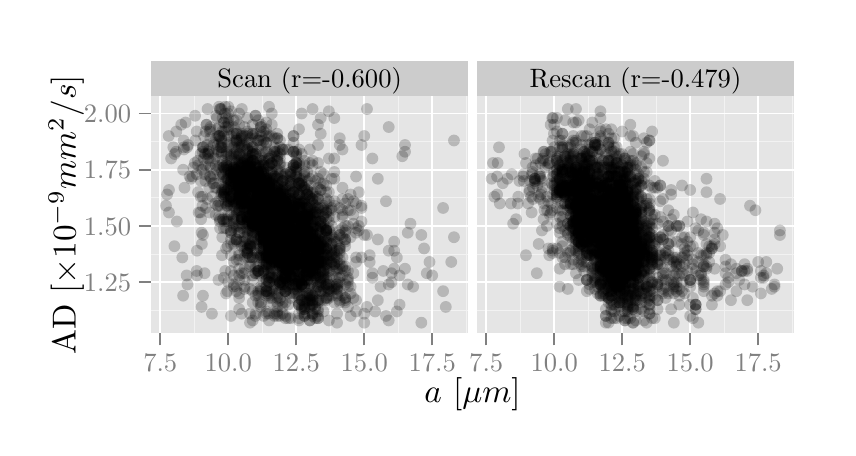
\begin{tikzpicture}[x=1pt,y=1pt]
\definecolor[named]{fillColor}{rgb}{1.00,1.00,1.00}
\path[use as bounding box,fill=fillColor,fill opacity=0.00] (0,0) rectangle (289.08,144.54);
\begin{scope}
\path[clip] (  0.00,  0.00) rectangle (289.08,144.54);
\definecolor[named]{drawColor}{rgb}{1.00,1.00,1.00}
\definecolor[named]{fillColor}{rgb}{1.00,1.00,1.00}

\path[draw=drawColor,line width= 0.6pt,line join=round,line cap=round,fill=fillColor] ( -0.00,  0.00) rectangle (289.08,144.54);
\end{scope}
\begin{scope}
\path[clip] ( 44.49,119.86) rectangle (159.26,132.50);
\definecolor[named]{fillColor}{rgb}{0.80,0.80,0.80}

\path[fill=fillColor] ( 44.49,119.86) rectangle (159.26,132.50);
\definecolor[named]{drawColor}{rgb}{0.00,0.00,0.00}

\node[text=drawColor,anchor=base,inner sep=0pt, outer sep=0pt, scale=  0.96] at (101.87,122.87) {Scan (r=-0.600)};
\end{scope}
\begin{scope}
\path[clip] (162.27,119.86) rectangle (277.03,132.50);
\definecolor[named]{fillColor}{rgb}{0.80,0.80,0.80}

\path[fill=fillColor] (162.27,119.86) rectangle (277.03,132.50);
\definecolor[named]{drawColor}{rgb}{0.00,0.00,0.00}

\node[text=drawColor,anchor=base,inner sep=0pt, outer sep=0pt, scale=  0.96] at (219.65,122.87) {Rescan (r=-0.479)};
\end{scope}
\begin{scope}
\path[clip] ( 44.49, 34.04) rectangle (159.26,119.86);
\definecolor[named]{fillColor}{rgb}{0.90,0.90,0.90}

\path[fill=fillColor] ( 44.49, 34.04) rectangle (159.26,119.86);
\definecolor[named]{drawColor}{rgb}{0.95,0.95,0.95}

\path[draw=drawColor,line width= 0.3pt,line join=round] ( 44.49, 42.41) --
	(159.26, 42.41);

\path[draw=drawColor,line width= 0.3pt,line join=round] ( 44.49, 62.73) --
	(159.26, 62.73);

\path[draw=drawColor,line width= 0.3pt,line join=round] ( 44.49, 83.04) --
	(159.26, 83.04);

\path[draw=drawColor,line width= 0.3pt,line join=round] ( 44.49,103.36) --
	(159.26,103.36);

\path[draw=drawColor,line width= 0.3pt,line join=round] ( 60.20, 34.04) --
	( 60.20,119.86);

\path[draw=drawColor,line width= 0.3pt,line join=round] ( 84.76, 34.04) --
	( 84.76,119.86);

\path[draw=drawColor,line width= 0.3pt,line join=round] (109.33, 34.04) --
	(109.33,119.86);

\path[draw=drawColor,line width= 0.3pt,line join=round] (133.90, 34.04) --
	(133.90,119.86);

\path[draw=drawColor,line width= 0.3pt,line join=round] (158.46, 34.04) --
	(158.46,119.86);
\definecolor[named]{drawColor}{rgb}{1.00,1.00,1.00}

\path[draw=drawColor,line width= 0.6pt,line join=round] ( 44.49, 52.57) --
	(159.26, 52.57);

\path[draw=drawColor,line width= 0.6pt,line join=round] ( 44.49, 72.89) --
	(159.26, 72.89);

\path[draw=drawColor,line width= 0.6pt,line join=round] ( 44.49, 93.20) --
	(159.26, 93.20);

\path[draw=drawColor,line width= 0.6pt,line join=round] ( 44.49,113.52) --
	(159.26,113.52);

\path[draw=drawColor,line width= 0.6pt,line join=round] ( 47.91, 34.04) --
	( 47.91,119.86);

\path[draw=drawColor,line width= 0.6pt,line join=round] ( 72.48, 34.04) --
	( 72.48,119.86);

\path[draw=drawColor,line width= 0.6pt,line join=round] ( 97.05, 34.04) --
	( 97.05,119.86);

\path[draw=drawColor,line width= 0.6pt,line join=round] (121.61, 34.04) --
	(121.61,119.86);

\path[draw=drawColor,line width= 0.6pt,line join=round] (146.18, 34.04) --
	(146.18,119.86);
\definecolor[named]{fillColor}{rgb}{0.00,0.00,0.00}

\path[fill=fillColor,fill opacity=0.20] (144.21, 55.82) circle (  2.13);

\path[fill=fillColor,fill opacity=0.20] (102.94, 61.51) circle (  2.13);

\path[fill=fillColor,fill opacity=0.20] ( 98.03, 59.07) circle (  2.13);

\path[fill=fillColor,fill opacity=0.20] ( 93.11, 55.82) circle (  2.13);

\path[fill=fillColor,fill opacity=0.20] ( 95.08, 55.01) circle (  2.13);

\path[fill=fillColor,fill opacity=0.20] (105.89, 52.57) circle (  2.13);

\path[fill=fillColor,fill opacity=0.20] (112.77, 60.69) circle (  2.13);

\path[fill=fillColor,fill opacity=0.20] (110.80, 68.01) circle (  2.13);

\path[fill=fillColor,fill opacity=0.20] ( 90.17, 69.63) circle (  2.13);

\path[fill=fillColor,fill opacity=0.20] ( 92.13, 59.07) circle (  2.13);

\path[fill=fillColor,fill opacity=0.20] ( 87.22, 62.32) circle (  2.13);

\path[fill=fillColor,fill opacity=0.20] ( 81.32, 73.70) circle (  2.13);

\path[fill=fillColor,fill opacity=0.20] ( 87.22, 72.89) circle (  2.13);

\path[fill=fillColor,fill opacity=0.20] ( 78.37, 61.51) circle (  2.13);

\path[fill=fillColor,fill opacity=0.20] ( 86.24, 50.94) circle (  2.13);

\path[fill=fillColor,fill opacity=0.20] ( 91.15, 53.38) circle (  2.13);

\path[fill=fillColor,fill opacity=0.20] (108.84, 47.69) circle (  2.13);

\path[fill=fillColor,fill opacity=0.20] (130.46, 38.75) circle (  2.13);

\path[fill=fillColor,fill opacity=0.20] ( 85.25, 76.14) circle (  2.13);

\path[fill=fillColor,fill opacity=0.20] ( 86.24, 65.57) circle (  2.13);

\path[fill=fillColor,fill opacity=0.20] ( 87.22, 67.20) circle (  2.13);

\path[fill=fillColor,fill opacity=0.20] ( 86.24, 78.57) circle (  2.13);

\path[fill=fillColor,fill opacity=0.20] ( 87.22, 85.89) circle (  2.13);

\path[fill=fillColor,fill opacity=0.20] ( 84.27, 89.95) circle (  2.13);

\path[fill=fillColor,fill opacity=0.20] ( 85.25, 91.58) circle (  2.13);

\path[fill=fillColor,fill opacity=0.20] ( 87.22, 84.26) circle (  2.13);

\path[fill=fillColor,fill opacity=0.20] ( 88.20, 68.01) circle (  2.13);

\path[fill=fillColor,fill opacity=0.20] ( 90.17, 50.13) circle (  2.13);

\path[fill=fillColor,fill opacity=0.20] (103.92, 45.25) circle (  2.13);

\path[fill=fillColor,fill opacity=0.20] (101.96, 42.82) circle (  2.13);

\path[fill=fillColor,fill opacity=0.20] (108.84, 38.75) circle (  2.13);

\path[fill=fillColor,fill opacity=0.20] (102.94, 61.51) circle (  2.13);

\path[fill=fillColor,fill opacity=0.20] ( 85.25, 66.38) circle (  2.13);

\path[fill=fillColor,fill opacity=0.20] ( 85.25, 72.89) circle (  2.13);

\path[fill=fillColor,fill opacity=0.20] ( 77.39, 81.01) circle (  2.13);

\path[fill=fillColor,fill opacity=0.20] ( 79.36,102.96) circle (  2.13);

\path[fill=fillColor,fill opacity=0.20] ( 84.27,107.02) circle (  2.13);

\path[fill=fillColor,fill opacity=0.20] ( 90.17, 98.08) circle (  2.13);

\path[fill=fillColor,fill opacity=0.20] ( 87.22, 96.45) circle (  2.13);

\path[fill=fillColor,fill opacity=0.20] ( 85.25, 90.76) circle (  2.13);

\path[fill=fillColor,fill opacity=0.20] ( 90.17, 77.76) circle (  2.13);

\path[fill=fillColor,fill opacity=0.20] ( 97.05, 66.38) circle (  2.13);

\path[fill=fillColor,fill opacity=0.20] (100.98, 60.69) circle (  2.13);

\path[fill=fillColor,fill opacity=0.20] ( 98.03, 51.75) circle (  2.13);

\path[fill=fillColor,fill opacity=0.20] (102.94, 45.25) circle (  2.13);

\path[fill=fillColor,fill opacity=0.20] ( 90.17, 41.19) circle (  2.13);

\path[fill=fillColor,fill opacity=0.20] (104.91, 63.13) circle (  2.13);

\path[fill=fillColor,fill opacity=0.20] ( 98.03, 68.01) circle (  2.13);

\path[fill=fillColor,fill opacity=0.20] ( 85.25, 86.70) circle (  2.13);

\path[fill=fillColor,fill opacity=0.20] ( 80.34, 94.02) circle (  2.13);

\path[fill=fillColor,fill opacity=0.20] ( 81.32,101.33) circle (  2.13);

\path[fill=fillColor,fill opacity=0.20] ( 81.32,106.21) circle (  2.13);

\path[fill=fillColor,fill opacity=0.20] ( 85.25,107.02) circle (  2.13);

\path[fill=fillColor,fill opacity=0.20] ( 89.18, 99.70) circle (  2.13);

\path[fill=fillColor,fill opacity=0.20] ( 89.18, 85.89) circle (  2.13);

\path[fill=fillColor,fill opacity=0.20] ( 96.06, 76.95) circle (  2.13);

\path[fill=fillColor,fill opacity=0.20] (103.92, 77.76) circle (  2.13);

\path[fill=fillColor,fill opacity=0.20] ( 99.01, 76.95) circle (  2.13);

\path[fill=fillColor,fill opacity=0.20] (101.96, 76.95) circle (  2.13);

\path[fill=fillColor,fill opacity=0.20] (105.89, 85.89) circle (  2.13);

\path[fill=fillColor,fill opacity=0.20] ( 99.99, 85.89) circle (  2.13);

\path[fill=fillColor,fill opacity=0.20] ( 89.18, 65.57) circle (  2.13);

\path[fill=fillColor,fill opacity=0.20] ( 88.20, 93.20) circle (  2.13);

\path[fill=fillColor,fill opacity=0.20] ( 96.06, 94.02) circle (  2.13);

\path[fill=fillColor,fill opacity=0.20] ( 96.06, 85.08) circle (  2.13);

\path[fill=fillColor,fill opacity=0.20] (105.89, 72.89) circle (  2.13);

\path[fill=fillColor,fill opacity=0.20] ( 99.99, 71.26) circle (  2.13);

\path[fill=fillColor,fill opacity=0.20] ( 84.27, 92.39) circle (  2.13);

\path[fill=fillColor,fill opacity=0.20] ( 82.31, 98.89) circle (  2.13);

\path[fill=fillColor,fill opacity=0.20] ( 86.24, 90.76) circle (  2.13);

\path[fill=fillColor,fill opacity=0.20] ( 83.29, 90.76) circle (  2.13);

\path[fill=fillColor,fill opacity=0.20] ( 84.27,103.77) circle (  2.13);

\path[fill=fillColor,fill opacity=0.20] ( 82.31,104.58) circle (  2.13);

\path[fill=fillColor,fill opacity=0.20] ( 97.05, 86.70) circle (  2.13);

\path[fill=fillColor,fill opacity=0.20] (106.87, 76.14) circle (  2.13);

\path[fill=fillColor,fill opacity=0.20] (117.68, 76.95) circle (  2.13);

\path[fill=fillColor,fill opacity=0.20] (102.94, 94.83) circle (  2.13);

\path[fill=fillColor,fill opacity=0.20] ( 81.32, 72.89) circle (  2.13);

\path[fill=fillColor,fill opacity=0.20] ( 83.29, 86.70) circle (  2.13);

\path[fill=fillColor,fill opacity=0.20] ( 86.24, 86.70) circle (  2.13);

\path[fill=fillColor,fill opacity=0.20] ( 84.27, 89.14) circle (  2.13);

\path[fill=fillColor,fill opacity=0.20] ( 86.24, 89.14) circle (  2.13);

\path[fill=fillColor,fill opacity=0.20] ( 90.17, 81.82) circle (  2.13);

\path[fill=fillColor,fill opacity=0.20] (100.98, 89.14) circle (  2.13);

\path[fill=fillColor,fill opacity=0.20] ( 99.01, 69.63) circle (  2.13);

\path[fill=fillColor,fill opacity=0.20] (103.92, 72.89) circle (  2.13);

\path[fill=fillColor,fill opacity=0.20] ( 95.08, 87.51) circle (  2.13);

\path[fill=fillColor,fill opacity=0.20] ( 92.13,100.52) circle (  2.13);

\path[fill=fillColor,fill opacity=0.20] ( 91.15,101.33) circle (  2.13);

\path[fill=fillColor,fill opacity=0.20] ( 92.13, 89.14) circle (  2.13);

\path[fill=fillColor,fill opacity=0.20] ( 90.17, 90.76) circle (  2.13);

\path[fill=fillColor,fill opacity=0.20] ( 86.24,102.96) circle (  2.13);

\path[fill=fillColor,fill opacity=0.20] (109.82, 78.57) circle (  2.13);

\path[fill=fillColor,fill opacity=0.20] ( 91.15, 91.58) circle (  2.13);

\path[fill=fillColor,fill opacity=0.20] ( 76.41, 73.70) circle (  2.13);

\path[fill=fillColor,fill opacity=0.20] ( 73.46, 92.39) circle (  2.13);

\path[fill=fillColor,fill opacity=0.20] ( 74.44, 89.95) circle (  2.13);

\path[fill=fillColor,fill opacity=0.20] ( 71.59, 81.01) circle (  2.13);

\path[fill=fillColor,fill opacity=0.20] ( 64.42, 79.39) circle (  2.13);

\path[fill=fillColor,fill opacity=0.20] ( 78.37, 81.82) circle (  2.13);

\path[fill=fillColor,fill opacity=0.20] ( 83.29, 75.32) circle (  2.13);

\path[fill=fillColor,fill opacity=0.20] ( 86.24, 76.95) circle (  2.13);

\path[fill=fillColor,fill opacity=0.20] (112.77,104.58) circle (  2.13);

\path[fill=fillColor,fill opacity=0.20] (109.82, 62.32) circle (  2.13);

\path[fill=fillColor,fill opacity=0.20] (103.92, 68.82) circle (  2.13);

\path[fill=fillColor,fill opacity=0.20] ( 93.11, 91.58) circle (  2.13);

\path[fill=fillColor,fill opacity=0.20] ( 97.05, 99.70) circle (  2.13);

\path[fill=fillColor,fill opacity=0.20] ( 96.06,105.39) circle (  2.13);

\path[fill=fillColor,fill opacity=0.20] ( 94.10,100.52) circle (  2.13);

\path[fill=fillColor,fill opacity=0.20] ( 99.99, 91.58) circle (  2.13);

\path[fill=fillColor,fill opacity=0.20] ( 96.06, 94.83) circle (  2.13);

\path[fill=fillColor,fill opacity=0.20] ( 97.05, 91.58) circle (  2.13);

\path[fill=fillColor,fill opacity=0.20] (107.86, 78.57) circle (  2.13);

\path[fill=fillColor,fill opacity=0.20] ( 79.36, 75.32) circle (  2.13);

\path[fill=fillColor,fill opacity=0.20] ( 73.46, 91.58) circle (  2.13);

\path[fill=fillColor,fill opacity=0.20] ( 70.32, 94.83) circle (  2.13);

\path[fill=fillColor,fill opacity=0.20] ( 68.84, 80.20) circle (  2.13);

\path[fill=fillColor,fill opacity=0.20] ( 74.44, 80.20) circle (  2.13);

\path[fill=fillColor,fill opacity=0.20] ( 72.48, 86.70) circle (  2.13);

\path[fill=fillColor,fill opacity=0.20] ( 85.25, 83.45) circle (  2.13);

\path[fill=fillColor,fill opacity=0.20] ( 88.20, 76.14) circle (  2.13);

\path[fill=fillColor,fill opacity=0.20] ( 77.39, 65.57) circle (  2.13);

\path[fill=fillColor,fill opacity=0.20] (103.92, 75.32) circle (  2.13);

\path[fill=fillColor,fill opacity=0.20] (118.66, 59.88) circle (  2.13);

\path[fill=fillColor,fill opacity=0.20] (100.98, 67.20) circle (  2.13);

\path[fill=fillColor,fill opacity=0.20] ( 97.05, 95.64) circle (  2.13);

\path[fill=fillColor,fill opacity=0.20] ( 93.11, 91.58) circle (  2.13);

\path[fill=fillColor,fill opacity=0.20] ( 94.10, 87.51) circle (  2.13);

\path[fill=fillColor,fill opacity=0.20] ( 96.06, 99.70) circle (  2.13);

\path[fill=fillColor,fill opacity=0.20] ( 91.15, 99.70) circle (  2.13);

\path[fill=fillColor,fill opacity=0.20] ( 97.05, 88.33) circle (  2.13);

\path[fill=fillColor,fill opacity=0.20] ( 94.10, 75.32) circle (  2.13);

\path[fill=fillColor,fill opacity=0.20] (105.89, 72.89) circle (  2.13);

\path[fill=fillColor,fill opacity=0.20] (136.35,102.14) circle (  2.13);

\path[fill=fillColor,fill opacity=0.20] ( 81.32, 98.89) circle (  2.13);

\path[fill=fillColor,fill opacity=0.20] ( 73.46, 70.45) circle (  2.13);

\path[fill=fillColor,fill opacity=0.20] ( 73.46, 90.76) circle (  2.13);

\path[fill=fillColor,fill opacity=0.20] ( 76.41, 92.39) circle (  2.13);

\path[fill=fillColor,fill opacity=0.20] ( 85.25, 84.26) circle (  2.13);

\path[fill=fillColor,fill opacity=0.20] ( 82.31, 91.58) circle (  2.13);

\path[fill=fillColor,fill opacity=0.20] ( 81.32, 92.39) circle (  2.13);

\path[fill=fillColor,fill opacity=0.20] ( 90.17, 85.08) circle (  2.13);

\path[fill=fillColor,fill opacity=0.20] ( 96.06, 82.64) circle (  2.13);

\path[fill=fillColor,fill opacity=0.20] ( 94.10, 65.57) circle (  2.13);

\path[fill=fillColor,fill opacity=0.20] ( 98.03, 49.32) circle (  2.13);

\path[fill=fillColor,fill opacity=0.20] (112.77, 63.95) circle (  2.13);

\path[fill=fillColor,fill opacity=0.20] (104.91, 66.38) circle (  2.13);

\path[fill=fillColor,fill opacity=0.20] ( 96.06, 85.08) circle (  2.13);

\path[fill=fillColor,fill opacity=0.20] ( 88.20, 82.64) circle (  2.13);

\path[fill=fillColor,fill opacity=0.20] ( 90.17, 75.32) circle (  2.13);

\path[fill=fillColor,fill opacity=0.20] ( 95.08, 88.33) circle (  2.13);

\path[fill=fillColor,fill opacity=0.20] ( 97.05, 95.64) circle (  2.13);

\path[fill=fillColor,fill opacity=0.20] ( 99.01, 87.51) circle (  2.13);

\path[fill=fillColor,fill opacity=0.20] ( 99.99, 73.70) circle (  2.13);

\path[fill=fillColor,fill opacity=0.20] (100.98, 64.76) circle (  2.13);

\path[fill=fillColor,fill opacity=0.20] ( 70.91, 84.26) circle (  2.13);

\path[fill=fillColor,fill opacity=0.20] ( 76.41, 82.64) circle (  2.13);

\path[fill=fillColor,fill opacity=0.20] ( 80.34, 94.83) circle (  2.13);

\path[fill=fillColor,fill opacity=0.20] ( 72.18, 89.95) circle (  2.13);

\path[fill=fillColor,fill opacity=0.20] ( 83.29, 90.76) circle (  2.13);

\path[fill=fillColor,fill opacity=0.20] ( 85.25, 94.83) circle (  2.13);

\path[fill=fillColor,fill opacity=0.20] ( 82.31, 91.58) circle (  2.13);

\path[fill=fillColor,fill opacity=0.20] ( 86.24, 88.33) circle (  2.13);

\path[fill=fillColor,fill opacity=0.20] ( 92.13, 85.08) circle (  2.13);

\path[fill=fillColor,fill opacity=0.20] ( 95.08, 66.38) circle (  2.13);

\path[fill=fillColor,fill opacity=0.20] (103.92, 54.19) circle (  2.13);

\path[fill=fillColor,fill opacity=0.20] (106.87, 59.88) circle (  2.13);

\path[fill=fillColor,fill opacity=0.20] ( 89.18, 68.01) circle (  2.13);

\path[fill=fillColor,fill opacity=0.20] ( 83.29, 79.39) circle (  2.13);

\path[fill=fillColor,fill opacity=0.20] ( 85.25, 84.26) circle (  2.13);

\path[fill=fillColor,fill opacity=0.20] ( 95.08, 84.26) circle (  2.13);

\path[fill=fillColor,fill opacity=0.20] ( 98.03, 81.82) circle (  2.13);

\path[fill=fillColor,fill opacity=0.20] ( 98.03, 84.26) circle (  2.13);

\path[fill=fillColor,fill opacity=0.20] (101.96, 87.51) circle (  2.13);

\path[fill=fillColor,fill opacity=0.20] ( 99.01, 72.07) circle (  2.13);

\path[fill=fillColor,fill opacity=0.20] ( 73.46, 80.20) circle (  2.13);

\path[fill=fillColor,fill opacity=0.20] ( 76.41,102.14) circle (  2.13);

\path[fill=fillColor,fill opacity=0.20] ( 78.37,102.14) circle (  2.13);

\path[fill=fillColor,fill opacity=0.20] ( 73.46, 89.14) circle (  2.13);

\path[fill=fillColor,fill opacity=0.20] ( 81.32, 89.14) circle (  2.13);

\path[fill=fillColor,fill opacity=0.20] ( 87.22, 92.39) circle (  2.13);

\path[fill=fillColor,fill opacity=0.20] ( 80.34, 90.76) circle (  2.13);

\path[fill=fillColor,fill opacity=0.20] ( 95.08, 91.58) circle (  2.13);

\path[fill=fillColor,fill opacity=0.20] ( 92.13, 81.01) circle (  2.13);

\path[fill=fillColor,fill opacity=0.20] ( 97.05, 59.07) circle (  2.13);

\path[fill=fillColor,fill opacity=0.20] (109.82, 59.88) circle (  2.13);

\path[fill=fillColor,fill opacity=0.20] ( 99.01, 51.75) circle (  2.13);

\path[fill=fillColor,fill opacity=0.20] ( 90.17, 73.70) circle (  2.13);

\path[fill=fillColor,fill opacity=0.20] ( 88.20, 88.33) circle (  2.13);

\path[fill=fillColor,fill opacity=0.20] ( 92.13, 85.89) circle (  2.13);

\path[fill=fillColor,fill opacity=0.20] ( 95.08, 76.14) circle (  2.13);

\path[fill=fillColor,fill opacity=0.20] ( 93.11, 76.95) circle (  2.13);

\path[fill=fillColor,fill opacity=0.20] ( 97.05, 93.20) circle (  2.13);

\path[fill=fillColor,fill opacity=0.20] ( 86.24, 86.70) circle (  2.13);

\path[fill=fillColor,fill opacity=0.20] ( 97.05, 70.45) circle (  2.13);

\path[fill=fillColor,fill opacity=0.20] ( 84.27, 89.95) circle (  2.13);

\path[fill=fillColor,fill opacity=0.20] ( 83.29, 91.58) circle (  2.13);

\path[fill=fillColor,fill opacity=0.20] ( 84.27,105.39) circle (  2.13);

\path[fill=fillColor,fill opacity=0.20] ( 85.25, 98.89) circle (  2.13);

\path[fill=fillColor,fill opacity=0.20] ( 81.32, 89.95) circle (  2.13);

\path[fill=fillColor,fill opacity=0.20] ( 83.29, 91.58) circle (  2.13);

\path[fill=fillColor,fill opacity=0.20] ( 84.27, 89.14) circle (  2.13);

\path[fill=fillColor,fill opacity=0.20] ( 83.29, 83.45) circle (  2.13);

\path[fill=fillColor,fill opacity=0.20] ( 86.24, 81.82) circle (  2.13);

\path[fill=fillColor,fill opacity=0.20] ( 97.05, 71.26) circle (  2.13);

\path[fill=fillColor,fill opacity=0.20] ( 98.03, 53.38) circle (  2.13);

\path[fill=fillColor,fill opacity=0.20] (113.75, 61.51) circle (  2.13);

\path[fill=fillColor,fill opacity=0.20] (103.92, 49.32) circle (  2.13);

\path[fill=fillColor,fill opacity=0.20] ( 99.01, 66.38) circle (  2.13);

\path[fill=fillColor,fill opacity=0.20] ( 99.01, 78.57) circle (  2.13);

\path[fill=fillColor,fill opacity=0.20] ( 91.15, 79.39) circle (  2.13);

\path[fill=fillColor,fill opacity=0.20] ( 95.08, 80.20) circle (  2.13);

\path[fill=fillColor,fill opacity=0.20] ( 94.10, 79.39) circle (  2.13);

\path[fill=fillColor,fill opacity=0.20] ( 91.15, 84.26) circle (  2.13);

\path[fill=fillColor,fill opacity=0.20] ( 99.99, 81.82) circle (  2.13);

\path[fill=fillColor,fill opacity=0.20] (104.91, 68.01) circle (  2.13);

\path[fill=fillColor,fill opacity=0.20] (117.68, 73.70) circle (  2.13);

\path[fill=fillColor,fill opacity=0.20] ( 84.27,102.14) circle (  2.13);

\path[fill=fillColor,fill opacity=0.20] ( 73.46, 88.33) circle (  2.13);

\path[fill=fillColor,fill opacity=0.20] ( 90.17, 99.70) circle (  2.13);

\path[fill=fillColor,fill opacity=0.20] ( 88.20, 98.08) circle (  2.13);

\path[fill=fillColor,fill opacity=0.20] ( 84.27, 91.58) circle (  2.13);

\path[fill=fillColor,fill opacity=0.20] ( 84.27, 87.51) circle (  2.13);

\path[fill=fillColor,fill opacity=0.20] ( 79.36, 90.76) circle (  2.13);

\path[fill=fillColor,fill opacity=0.20] ( 87.22, 85.08) circle (  2.13);

\path[fill=fillColor,fill opacity=0.20] ( 81.32, 74.51) circle (  2.13);

\path[fill=fillColor,fill opacity=0.20] ( 81.32, 73.70) circle (  2.13);

\path[fill=fillColor,fill opacity=0.20] ( 93.11, 65.57) circle (  2.13);

\path[fill=fillColor,fill opacity=0.20] ( 99.01, 51.75) circle (  2.13);

\path[fill=fillColor,fill opacity=0.20] (101.96, 64.76) circle (  2.13);

\path[fill=fillColor,fill opacity=0.20] ( 90.17, 65.57) circle (  2.13);

\path[fill=fillColor,fill opacity=0.20] ( 91.15, 66.38) circle (  2.13);

\path[fill=fillColor,fill opacity=0.20] ( 93.11, 77.76) circle (  2.13);

\path[fill=fillColor,fill opacity=0.20] ( 91.15, 82.64) circle (  2.13);

\path[fill=fillColor,fill opacity=0.20] ( 92.13, 74.51) circle (  2.13);

\path[fill=fillColor,fill opacity=0.20] ( 94.10, 65.57) circle (  2.13);

\path[fill=fillColor,fill opacity=0.20] (100.98, 60.69) circle (  2.13);

\path[fill=fillColor,fill opacity=0.20] (100.98, 61.51) circle (  2.13);

\path[fill=fillColor,fill opacity=0.20] (108.84, 72.07) circle (  2.13);

\path[fill=fillColor,fill opacity=0.20] ( 88.20,113.52) circle (  2.13);

\path[fill=fillColor,fill opacity=0.20] ( 80.34, 83.45) circle (  2.13);

\path[fill=fillColor,fill opacity=0.20] ( 81.32, 92.39) circle (  2.13);

\path[fill=fillColor,fill opacity=0.20] ( 86.24, 89.95) circle (  2.13);

\path[fill=fillColor,fill opacity=0.20] ( 79.36, 87.51) circle (  2.13);

\path[fill=fillColor,fill opacity=0.20] ( 79.36, 89.14) circle (  2.13);

\path[fill=fillColor,fill opacity=0.20] ( 79.36, 89.14) circle (  2.13);

\path[fill=fillColor,fill opacity=0.20] ( 78.37, 84.26) circle (  2.13);

\path[fill=fillColor,fill opacity=0.20] ( 82.31, 76.95) circle (  2.13);

\path[fill=fillColor,fill opacity=0.20] ( 83.29, 74.51) circle (  2.13);

\path[fill=fillColor,fill opacity=0.20] ( 88.20, 76.14) circle (  2.13);

\path[fill=fillColor,fill opacity=0.20] ( 85.25, 66.38) circle (  2.13);

\path[fill=fillColor,fill opacity=0.20] ( 94.10, 56.63) circle (  2.13);

\path[fill=fillColor,fill opacity=0.20] ( 87.22, 62.32) circle (  2.13);

\path[fill=fillColor,fill opacity=0.20] ( 81.32, 53.38) circle (  2.13);

\path[fill=fillColor,fill opacity=0.20] ( 94.10, 63.13) circle (  2.13);

\path[fill=fillColor,fill opacity=0.20] ( 90.17, 73.70) circle (  2.13);

\path[fill=fillColor,fill opacity=0.20] ( 93.11, 71.26) circle (  2.13);

\path[fill=fillColor,fill opacity=0.20] ( 97.05, 68.01) circle (  2.13);

\path[fill=fillColor,fill opacity=0.20] ( 91.15, 64.76) circle (  2.13);

\path[fill=fillColor,fill opacity=0.20] ( 96.06, 65.57) circle (  2.13);

\path[fill=fillColor,fill opacity=0.20] ( 99.99, 72.89) circle (  2.13);

\path[fill=fillColor,fill opacity=0.20] (114.73, 81.01) circle (  2.13);

\path[fill=fillColor,fill opacity=0.20] ( 82.31, 86.70) circle (  2.13);

\path[fill=fillColor,fill opacity=0.20] ( 80.34, 95.64) circle (  2.13);

\path[fill=fillColor,fill opacity=0.20] ( 84.27, 88.33) circle (  2.13);

\path[fill=fillColor,fill opacity=0.20] ( 80.34, 81.01) circle (  2.13);

\path[fill=fillColor,fill opacity=0.20] ( 79.36, 85.08) circle (  2.13);

\path[fill=fillColor,fill opacity=0.20] ( 79.36, 92.39) circle (  2.13);

\path[fill=fillColor,fill opacity=0.20] ( 79.36, 94.83) circle (  2.13);

\path[fill=fillColor,fill opacity=0.20] ( 76.41, 85.89) circle (  2.13);

\path[fill=fillColor,fill opacity=0.20] ( 83.29, 77.76) circle (  2.13);

\path[fill=fillColor,fill opacity=0.20] ( 82.31, 75.32) circle (  2.13);

\path[fill=fillColor,fill opacity=0.20] ( 84.27, 69.63) circle (  2.13);

\path[fill=fillColor,fill opacity=0.20] ( 87.22, 64.76) circle (  2.13);

\path[fill=fillColor,fill opacity=0.20] (103.92, 69.63) circle (  2.13);

\path[fill=fillColor,fill opacity=0.20] (115.72, 72.89) circle (  2.13);

\path[fill=fillColor,fill opacity=0.20] ( 98.03, 55.01) circle (  2.13);

\path[fill=fillColor,fill opacity=0.20] ( 92.13, 55.01) circle (  2.13);

\path[fill=fillColor,fill opacity=0.20] ( 94.10, 63.95) circle (  2.13);

\path[fill=fillColor,fill opacity=0.20] ( 97.05, 75.32) circle (  2.13);

\path[fill=fillColor,fill opacity=0.20] ( 90.17, 78.57) circle (  2.13);

\path[fill=fillColor,fill opacity=0.20] ( 94.10, 73.70) circle (  2.13);

\path[fill=fillColor,fill opacity=0.20] ( 93.11, 72.89) circle (  2.13);

\path[fill=fillColor,fill opacity=0.20] ( 99.01, 79.39) circle (  2.13);

\path[fill=fillColor,fill opacity=0.20] ( 99.99, 82.64) circle (  2.13);

\path[fill=fillColor,fill opacity=0.20] (108.84, 81.82) circle (  2.13);

\path[fill=fillColor,fill opacity=0.20] ( 84.27, 85.08) circle (  2.13);

\path[fill=fillColor,fill opacity=0.20] ( 81.32, 96.45) circle (  2.13);

\path[fill=fillColor,fill opacity=0.20] ( 84.27, 96.45) circle (  2.13);

\path[fill=fillColor,fill opacity=0.20] ( 82.31, 88.33) circle (  2.13);

\path[fill=fillColor,fill opacity=0.20] ( 77.39, 92.39) circle (  2.13);

\path[fill=fillColor,fill opacity=0.20] ( 83.29, 94.02) circle (  2.13);

\path[fill=fillColor,fill opacity=0.20] ( 83.29, 92.39) circle (  2.13);

\path[fill=fillColor,fill opacity=0.20] ( 79.36, 91.58) circle (  2.13);

\path[fill=fillColor,fill opacity=0.20] ( 80.34, 89.95) circle (  2.13);

\path[fill=fillColor,fill opacity=0.20] ( 78.37, 87.51) circle (  2.13);

\path[fill=fillColor,fill opacity=0.20] ( 81.32, 72.89) circle (  2.13);

\path[fill=fillColor,fill opacity=0.20] ( 94.10, 53.38) circle (  2.13);

\path[fill=fillColor,fill opacity=0.20] (114.73, 72.89) circle (  2.13);

\path[fill=fillColor,fill opacity=0.20] ( 90.17, 63.95) circle (  2.13);

\path[fill=fillColor,fill opacity=0.20] ( 89.18, 59.07) circle (  2.13);

\path[fill=fillColor,fill opacity=0.20] ( 95.08, 69.63) circle (  2.13);

\path[fill=fillColor,fill opacity=0.20] ( 90.17, 72.07) circle (  2.13);

\path[fill=fillColor,fill opacity=0.20] ( 87.22, 68.01) circle (  2.13);

\path[fill=fillColor,fill opacity=0.20] ( 94.10, 72.89) circle (  2.13);

\path[fill=fillColor,fill opacity=0.20] ( 95.08, 76.14) circle (  2.13);

\path[fill=fillColor,fill opacity=0.20] ( 95.08, 75.32) circle (  2.13);

\path[fill=fillColor,fill opacity=0.20] ( 97.05, 72.89) circle (  2.13);

\path[fill=fillColor,fill opacity=0.20] (106.87, 72.07) circle (  2.13);

\path[fill=fillColor,fill opacity=0.20] ( 88.20, 92.39) circle (  2.13);

\path[fill=fillColor,fill opacity=0.20] ( 83.29,100.52) circle (  2.13);

\path[fill=fillColor,fill opacity=0.20] ( 78.37, 96.45) circle (  2.13);

\path[fill=fillColor,fill opacity=0.20] ( 81.32, 87.51) circle (  2.13);

\path[fill=fillColor,fill opacity=0.20] ( 76.41, 88.33) circle (  2.13);

\path[fill=fillColor,fill opacity=0.20] ( 77.39, 94.02) circle (  2.13);

\path[fill=fillColor,fill opacity=0.20] ( 80.34, 96.45) circle (  2.13);

\path[fill=fillColor,fill opacity=0.20] ( 79.36, 89.14) circle (  2.13);

\path[fill=fillColor,fill opacity=0.20] ( 75.43, 85.08) circle (  2.13);

\path[fill=fillColor,fill opacity=0.20] ( 76.41, 88.33) circle (  2.13);

\path[fill=fillColor,fill opacity=0.20] ( 50.37, 84.26) circle (  2.13);

\path[fill=fillColor,fill opacity=0.20] ( 82.31, 66.38) circle (  2.13);

\path[fill=fillColor,fill opacity=0.20] (101.96, 46.88) circle (  2.13);

\path[fill=fillColor,fill opacity=0.20] (115.72, 78.57) circle (  2.13);

\path[fill=fillColor,fill opacity=0.20] ( 89.18, 59.88) circle (  2.13);

\path[fill=fillColor,fill opacity=0.20] ( 85.25, 55.82) circle (  2.13);

\path[fill=fillColor,fill opacity=0.20] ( 86.24, 57.44) circle (  2.13);

\path[fill=fillColor,fill opacity=0.20] ( 80.34, 61.51) circle (  2.13);

\path[fill=fillColor,fill opacity=0.20] ( 89.18, 70.45) circle (  2.13);

\path[fill=fillColor,fill opacity=0.20] ( 93.11, 72.89) circle (  2.13);

\path[fill=fillColor,fill opacity=0.20] ( 93.11, 76.14) circle (  2.13);

\path[fill=fillColor,fill opacity=0.20] (100.98, 77.76) circle (  2.13);

\path[fill=fillColor,fill opacity=0.20] (105.89, 74.51) circle (  2.13);

\path[fill=fillColor,fill opacity=0.20] (110.80, 81.82) circle (  2.13);

\path[fill=fillColor,fill opacity=0.20] ( 85.25, 95.64) circle (  2.13);

\path[fill=fillColor,fill opacity=0.20] ( 87.22,105.39) circle (  2.13);

\path[fill=fillColor,fill opacity=0.20] ( 81.32, 98.89) circle (  2.13);

\path[fill=fillColor,fill opacity=0.20] ( 76.41, 88.33) circle (  2.13);

\path[fill=fillColor,fill opacity=0.20] ( 73.46, 85.89) circle (  2.13);

\path[fill=fillColor,fill opacity=0.20] ( 70.91, 84.26) circle (  2.13);

\path[fill=fillColor,fill opacity=0.20] ( 76.41, 85.89) circle (  2.13);

\path[fill=fillColor,fill opacity=0.20] ( 77.39, 89.14) circle (  2.13);

\path[fill=fillColor,fill opacity=0.20] ( 75.43, 89.14) circle (  2.13);

\path[fill=fillColor,fill opacity=0.20] ( 77.39, 85.89) circle (  2.13);

\path[fill=fillColor,fill opacity=0.20] ( 72.18, 80.20) circle (  2.13);

\path[fill=fillColor,fill opacity=0.20] ( 79.36, 66.38) circle (  2.13);

\path[fill=fillColor,fill opacity=0.20] ( 99.01, 59.88) circle (  2.13);

\path[fill=fillColor,fill opacity=0.20] (113.75, 72.07) circle (  2.13);

\path[fill=fillColor,fill opacity=0.20] ( 78.37, 55.82) circle (  2.13);

\path[fill=fillColor,fill opacity=0.20] ( 83.29, 56.63) circle (  2.13);

\path[fill=fillColor,fill opacity=0.20] ( 82.31, 63.95) circle (  2.13);

\path[fill=fillColor,fill opacity=0.20] ( 84.27, 68.82) circle (  2.13);

\path[fill=fillColor,fill opacity=0.20] ( 93.11, 75.32) circle (  2.13);

\path[fill=fillColor,fill opacity=0.20] ( 91.15, 83.45) circle (  2.13);

\path[fill=fillColor,fill opacity=0.20] ( 95.08, 81.82) circle (  2.13);

\path[fill=fillColor,fill opacity=0.20] (105.89, 79.39) circle (  2.13);

\path[fill=fillColor,fill opacity=0.20] (102.94, 79.39) circle (  2.13);

\path[fill=fillColor,fill opacity=0.20] (107.86, 75.32) circle (  2.13);

\path[fill=fillColor,fill opacity=0.20] (102.94, 90.76) circle (  2.13);

\path[fill=fillColor,fill opacity=0.20] ( 84.27, 76.14) circle (  2.13);

\path[fill=fillColor,fill opacity=0.20] ( 70.51,101.33) circle (  2.13);

\path[fill=fillColor,fill opacity=0.20] ( 79.36,105.39) circle (  2.13);

\path[fill=fillColor,fill opacity=0.20] ( 75.43, 89.14) circle (  2.13);

\path[fill=fillColor,fill opacity=0.20] ( 73.46, 89.14) circle (  2.13);

\path[fill=fillColor,fill opacity=0.20] ( 70.91, 94.02) circle (  2.13);

\path[fill=fillColor,fill opacity=0.20] ( 72.48, 89.95) circle (  2.13);

\path[fill=fillColor,fill opacity=0.20] ( 76.41, 81.82) circle (  2.13);

\path[fill=fillColor,fill opacity=0.20] ( 76.41, 81.01) circle (  2.13);

\path[fill=fillColor,fill opacity=0.20] ( 77.39, 83.45) circle (  2.13);

\path[fill=fillColor,fill opacity=0.20] ( 80.34, 76.14) circle (  2.13);

\path[fill=fillColor,fill opacity=0.20] ( 79.36, 64.76) circle (  2.13);

\path[fill=fillColor,fill opacity=0.20] ( 99.99, 60.69) circle (  2.13);

\path[fill=fillColor,fill opacity=0.20] ( 79.36, 63.13) circle (  2.13);

\path[fill=fillColor,fill opacity=0.20] ( 80.34, 66.38) circle (  2.13);

\path[fill=fillColor,fill opacity=0.20] ( 90.17, 60.69) circle (  2.13);

\path[fill=fillColor,fill opacity=0.20] ( 93.11, 63.95) circle (  2.13);

\path[fill=fillColor,fill opacity=0.20] ( 89.18, 78.57) circle (  2.13);

\path[fill=fillColor,fill opacity=0.20] ( 93.11, 80.20) circle (  2.13);

\path[fill=fillColor,fill opacity=0.20] ( 99.99, 76.14) circle (  2.13);

\path[fill=fillColor,fill opacity=0.20] (102.94, 76.95) circle (  2.13);

\path[fill=fillColor,fill opacity=0.20] (108.84, 71.26) circle (  2.13);

\path[fill=fillColor,fill opacity=0.20] ( 99.99, 66.38) circle (  2.13);

\path[fill=fillColor,fill opacity=0.20] (108.84, 68.82) circle (  2.13);

\path[fill=fillColor,fill opacity=0.20] (115.72, 82.64) circle (  2.13);

\path[fill=fillColor,fill opacity=0.20] ( 97.05, 67.20) circle (  2.13);

\path[fill=fillColor,fill opacity=0.20] ( 89.18, 72.07) circle (  2.13);

\path[fill=fillColor,fill opacity=0.20] ( 76.41, 84.26) circle (  2.13);

\path[fill=fillColor,fill opacity=0.20] ( 81.32, 90.76) circle (  2.13);

\path[fill=fillColor,fill opacity=0.20] ( 78.37, 93.20) circle (  2.13);

\path[fill=fillColor,fill opacity=0.20] ( 77.39, 91.58) circle (  2.13);

\path[fill=fillColor,fill opacity=0.20] ( 74.44, 94.02) circle (  2.13);

\path[fill=fillColor,fill opacity=0.20] ( 71.89, 99.70) circle (  2.13);

\path[fill=fillColor,fill opacity=0.20] ( 71.89, 94.02) circle (  2.13);

\path[fill=fillColor,fill opacity=0.20] ( 73.46, 81.01) circle (  2.13);

\path[fill=fillColor,fill opacity=0.20] ( 77.39, 75.32) circle (  2.13);

\path[fill=fillColor,fill opacity=0.20] ( 80.34, 71.26) circle (  2.13);

\path[fill=fillColor,fill opacity=0.20] ( 94.10, 60.69) circle (  2.13);

\path[fill=fillColor,fill opacity=0.20] ( 99.01, 59.88) circle (  2.13);

\path[fill=fillColor,fill opacity=0.20] ( 97.05, 66.38) circle (  2.13);

\path[fill=fillColor,fill opacity=0.20] ( 92.13, 55.01) circle (  2.13);

\path[fill=fillColor,fill opacity=0.20] ( 90.17, 47.69) circle (  2.13);

\path[fill=fillColor,fill opacity=0.20] ( 87.22, 58.26) circle (  2.13);

\path[fill=fillColor,fill opacity=0.20] ( 90.17, 72.07) circle (  2.13);

\path[fill=fillColor,fill opacity=0.20] ( 97.05, 73.70) circle (  2.13);

\path[fill=fillColor,fill opacity=0.20] (104.91, 76.95) circle (  2.13);

\path[fill=fillColor,fill opacity=0.20] (108.84, 85.08) circle (  2.13);

\path[fill=fillColor,fill opacity=0.20] (107.86, 85.08) circle (  2.13);

\path[fill=fillColor,fill opacity=0.20] (106.87, 73.70) circle (  2.13);

\path[fill=fillColor,fill opacity=0.20] (110.80, 61.51) circle (  2.13);

\path[fill=fillColor,fill opacity=0.20] (111.79, 61.51) circle (  2.13);

\path[fill=fillColor,fill opacity=0.20] (118.66, 72.07) circle (  2.13);

\path[fill=fillColor,fill opacity=0.20] (109.82, 63.95) circle (  2.13);

\path[fill=fillColor,fill opacity=0.20] (100.98, 68.82) circle (  2.13);

\path[fill=fillColor,fill opacity=0.20] ( 90.17, 74.51) circle (  2.13);

\path[fill=fillColor,fill opacity=0.20] ( 85.25, 78.57) circle (  2.13);

\path[fill=fillColor,fill opacity=0.20] ( 61.57, 85.08) circle (  2.13);

\path[fill=fillColor,fill opacity=0.20] ( 80.34, 88.33) circle (  2.13);

\path[fill=fillColor,fill opacity=0.20] ( 86.24, 82.64) circle (  2.13);

\path[fill=fillColor,fill opacity=0.20] ( 77.39, 84.26) circle (  2.13);

\path[fill=fillColor,fill opacity=0.20] ( 75.43, 90.76) circle (  2.13);

\path[fill=fillColor,fill opacity=0.20] ( 75.43, 92.39) circle (  2.13);

\path[fill=fillColor,fill opacity=0.20] ( 73.46, 93.20) circle (  2.13);

\path[fill=fillColor,fill opacity=0.20] ( 70.71, 94.02) circle (  2.13);

\path[fill=fillColor,fill opacity=0.20] ( 78.37, 85.89) circle (  2.13);

\path[fill=fillColor,fill opacity=0.20] ( 82.31, 72.07) circle (  2.13);

\path[fill=fillColor,fill opacity=0.20] ( 96.06, 68.01) circle (  2.13);

\path[fill=fillColor,fill opacity=0.20] (105.89, 61.51) circle (  2.13);

\path[fill=fillColor,fill opacity=0.20] ( 94.10, 50.94) circle (  2.13);

\path[fill=fillColor,fill opacity=0.20] ( 87.22, 48.50) circle (  2.13);

\path[fill=fillColor,fill opacity=0.20] ( 89.18, 60.69) circle (  2.13);

\path[fill=fillColor,fill opacity=0.20] ( 95.08, 68.82) circle (  2.13);

\path[fill=fillColor,fill opacity=0.20] ( 94.10, 71.26) circle (  2.13);

\path[fill=fillColor,fill opacity=0.20] ( 97.05, 82.64) circle (  2.13);

\path[fill=fillColor,fill opacity=0.20] ( 99.01, 87.51) circle (  2.13);

\path[fill=fillColor,fill opacity=0.20] (103.92, 81.82) circle (  2.13);

\path[fill=fillColor,fill opacity=0.20] (104.91, 72.07) circle (  2.13);

\path[fill=fillColor,fill opacity=0.20] (103.92, 67.20) circle (  2.13);

\path[fill=fillColor,fill opacity=0.20] (102.94, 72.07) circle (  2.13);

\path[fill=fillColor,fill opacity=0.20] (108.84, 74.51) circle (  2.13);

\path[fill=fillColor,fill opacity=0.20] (112.77, 64.76) circle (  2.13);

\path[fill=fillColor,fill opacity=0.20] (114.73, 68.01) circle (  2.13);

\path[fill=fillColor,fill opacity=0.20] (110.80, 58.26) circle (  2.13);

\path[fill=fillColor,fill opacity=0.20] (109.82, 64.76) circle (  2.13);

\path[fill=fillColor,fill opacity=0.20] ( 82.31, 72.07) circle (  2.13);

\path[fill=fillColor,fill opacity=0.20] ( 91.15, 67.20) circle (  2.13);

\path[fill=fillColor,fill opacity=0.20] ( 87.22, 72.07) circle (  2.13);

\path[fill=fillColor,fill opacity=0.20] ( 77.39, 89.14) circle (  2.13);

\path[fill=fillColor,fill opacity=0.20] ( 81.32, 89.14) circle (  2.13);

\path[fill=fillColor,fill opacity=0.20] ( 80.34, 81.01) circle (  2.13);

\path[fill=fillColor,fill opacity=0.20] ( 88.20, 83.45) circle (  2.13);

\path[fill=fillColor,fill opacity=0.20] ( 80.34, 82.64) circle (  2.13);

\path[fill=fillColor,fill opacity=0.20] ( 73.46, 82.64) circle (  2.13);

\path[fill=fillColor,fill opacity=0.20] ( 65.60, 86.70) circle (  2.13);

\path[fill=fillColor,fill opacity=0.20] ( 77.39, 81.82) circle (  2.13);

\path[fill=fillColor,fill opacity=0.20] ( 81.32, 80.20) circle (  2.13);

\path[fill=fillColor,fill opacity=0.20] ( 79.36, 84.26) circle (  2.13);

\path[fill=fillColor,fill opacity=0.20] ( 90.17, 83.45) circle (  2.13);

\path[fill=fillColor,fill opacity=0.20] ( 93.11, 73.70) circle (  2.13);

\path[fill=fillColor,fill opacity=0.20] (103.92, 60.69) circle (  2.13);

\path[fill=fillColor,fill opacity=0.20] ( 93.11, 63.95) circle (  2.13);

\path[fill=fillColor,fill opacity=0.20] ( 91.15, 64.76) circle (  2.13);

\path[fill=fillColor,fill opacity=0.20] ( 86.24, 58.26) circle (  2.13);

\path[fill=fillColor,fill opacity=0.20] ( 86.24, 61.51) circle (  2.13);

\path[fill=fillColor,fill opacity=0.20] ( 94.10, 72.89) circle (  2.13);

\path[fill=fillColor,fill opacity=0.20] (100.98, 76.95) circle (  2.13);

\path[fill=fillColor,fill opacity=0.20] ( 99.99, 79.39) circle (  2.13);

\path[fill=fillColor,fill opacity=0.20] (104.91, 82.64) circle (  2.13);

\path[fill=fillColor,fill opacity=0.20] (104.91, 79.39) circle (  2.13);

\path[fill=fillColor,fill opacity=0.20] (106.87, 79.39) circle (  2.13);

\path[fill=fillColor,fill opacity=0.20] (110.80, 76.14) circle (  2.13);

\path[fill=fillColor,fill opacity=0.20] (109.82, 69.63) circle (  2.13);

\path[fill=fillColor,fill opacity=0.20] (106.87, 65.57) circle (  2.13);

\path[fill=fillColor,fill opacity=0.20] (105.89, 64.76) circle (  2.13);

\path[fill=fillColor,fill opacity=0.20] (105.89, 66.38) circle (  2.13);

\path[fill=fillColor,fill opacity=0.20] (107.86, 71.26) circle (  2.13);

\path[fill=fillColor,fill opacity=0.20] (101.96, 60.69) circle (  2.13);

\path[fill=fillColor,fill opacity=0.20] (111.79, 48.50) circle (  2.13);

\path[fill=fillColor,fill opacity=0.20] (112.77, 59.07) circle (  2.13);

\path[fill=fillColor,fill opacity=0.20] (102.94, 70.45) circle (  2.13);

\path[fill=fillColor,fill opacity=0.20] (101.96, 64.76) circle (  2.13);

\path[fill=fillColor,fill opacity=0.20] (104.91, 59.07) circle (  2.13);

\path[fill=fillColor,fill opacity=0.20] (105.89, 62.32) circle (  2.13);

\path[fill=fillColor,fill opacity=0.20] (106.87, 59.88) circle (  2.13);

\path[fill=fillColor,fill opacity=0.20] ( 99.99, 53.38) circle (  2.13);

\path[fill=fillColor,fill opacity=0.20] (103.92, 48.50) circle (  2.13);

\path[fill=fillColor,fill opacity=0.20] (104.91, 49.32) circle (  2.13);

\path[fill=fillColor,fill opacity=0.20] (102.94, 55.82) circle (  2.13);

\path[fill=fillColor,fill opacity=0.20] (101.96, 59.88) circle (  2.13);

\path[fill=fillColor,fill opacity=0.20] (103.92, 56.63) circle (  2.13);

\path[fill=fillColor,fill opacity=0.20] (103.92, 55.01) circle (  2.13);

\path[fill=fillColor,fill opacity=0.20] ( 98.03, 55.01) circle (  2.13);

\path[fill=fillColor,fill opacity=0.20] ( 92.13, 57.44) circle (  2.13);

\path[fill=fillColor,fill opacity=0.20] ( 85.25, 69.63) circle (  2.13);

\path[fill=fillColor,fill opacity=0.20] ( 83.29, 76.14) circle (  2.13);

\path[fill=fillColor,fill opacity=0.20] ( 89.18, 73.70) circle (  2.13);

\path[fill=fillColor,fill opacity=0.20] ( 85.25, 78.57) circle (  2.13);

\path[fill=fillColor,fill opacity=0.20] ( 80.34, 80.20) circle (  2.13);

\path[fill=fillColor,fill opacity=0.20] ( 83.29, 76.95) circle (  2.13);

\path[fill=fillColor,fill opacity=0.20] ( 84.27, 73.70) circle (  2.13);

\path[fill=fillColor,fill opacity=0.20] ( 85.25, 73.70) circle (  2.13);

\path[fill=fillColor,fill opacity=0.20] ( 82.31, 80.20) circle (  2.13);

\path[fill=fillColor,fill opacity=0.20] ( 86.24, 89.14) circle (  2.13);

\path[fill=fillColor,fill opacity=0.20] ( 94.10, 82.64) circle (  2.13);

\path[fill=fillColor,fill opacity=0.20] ( 80.34, 79.39) circle (  2.13);

\path[fill=fillColor,fill opacity=0.20] ( 92.13, 80.20) circle (  2.13);

\path[fill=fillColor,fill opacity=0.20] ( 99.01, 69.63) circle (  2.13);

\path[fill=fillColor,fill opacity=0.20] ( 93.11, 64.76) circle (  2.13);

\path[fill=fillColor,fill opacity=0.20] ( 95.08, 58.26) circle (  2.13);

\path[fill=fillColor,fill opacity=0.20] ( 92.13, 54.19) circle (  2.13);

\path[fill=fillColor,fill opacity=0.20] ( 91.15, 61.51) circle (  2.13);

\path[fill=fillColor,fill opacity=0.20] ( 93.11, 68.82) circle (  2.13);

\path[fill=fillColor,fill opacity=0.20] ( 96.06, 68.82) circle (  2.13);

\path[fill=fillColor,fill opacity=0.20] (100.98, 71.26) circle (  2.13);

\path[fill=fillColor,fill opacity=0.20] (105.89, 74.51) circle (  2.13);

\path[fill=fillColor,fill opacity=0.20] (105.89, 74.51) circle (  2.13);

\path[fill=fillColor,fill opacity=0.20] (104.91, 77.76) circle (  2.13);

\path[fill=fillColor,fill opacity=0.20] (106.87, 78.57) circle (  2.13);

\path[fill=fillColor,fill opacity=0.20] (100.98, 75.32) circle (  2.13);

\path[fill=fillColor,fill opacity=0.20] ( 92.13, 76.14) circle (  2.13);

\path[fill=fillColor,fill opacity=0.20] (103.92, 76.14) circle (  2.13);

\path[fill=fillColor,fill opacity=0.20] (102.94, 72.89) circle (  2.13);

\path[fill=fillColor,fill opacity=0.20] (105.89, 64.76) circle (  2.13);

\path[fill=fillColor,fill opacity=0.20] (102.94, 55.01) circle (  2.13);

\path[fill=fillColor,fill opacity=0.20] (105.89, 56.63) circle (  2.13);

\path[fill=fillColor,fill opacity=0.20] (101.96, 62.32) circle (  2.13);

\path[fill=fillColor,fill opacity=0.20] (106.87, 58.26) circle (  2.13);

\path[fill=fillColor,fill opacity=0.20] ( 99.99, 59.07) circle (  2.13);

\path[fill=fillColor,fill opacity=0.20] ( 97.05, 63.95) circle (  2.13);

\path[fill=fillColor,fill opacity=0.20] ( 95.08, 65.57) circle (  2.13);

\path[fill=fillColor,fill opacity=0.20] ( 93.11, 67.20) circle (  2.13);

\path[fill=fillColor,fill opacity=0.20] ( 96.06, 68.01) circle (  2.13);

\path[fill=fillColor,fill opacity=0.20] ( 96.06, 65.57) circle (  2.13);

\path[fill=fillColor,fill opacity=0.20] ( 94.10, 67.20) circle (  2.13);

\path[fill=fillColor,fill opacity=0.20] ( 94.10, 70.45) circle (  2.13);

\path[fill=fillColor,fill opacity=0.20] ( 90.17, 68.01) circle (  2.13);

\path[fill=fillColor,fill opacity=0.20] ( 90.17, 62.32) circle (  2.13);

\path[fill=fillColor,fill opacity=0.20] ( 86.24, 61.51) circle (  2.13);

\path[fill=fillColor,fill opacity=0.20] ( 85.25, 66.38) circle (  2.13);

\path[fill=fillColor,fill opacity=0.20] ( 91.15, 60.69) circle (  2.13);

\path[fill=fillColor,fill opacity=0.20] ( 87.22, 52.57) circle (  2.13);

\path[fill=fillColor,fill opacity=0.20] ( 91.15, 63.13) circle (  2.13);

\path[fill=fillColor,fill opacity=0.20] ( 88.20, 72.89) circle (  2.13);

\path[fill=fillColor,fill opacity=0.20] ( 87.22, 70.45) circle (  2.13);

\path[fill=fillColor,fill opacity=0.20] ( 90.17, 75.32) circle (  2.13);

\path[fill=fillColor,fill opacity=0.20] ( 92.13, 76.14) circle (  2.13);

\path[fill=fillColor,fill opacity=0.20] ( 88.20, 75.32) circle (  2.13);

\path[fill=fillColor,fill opacity=0.20] ( 90.17, 85.08) circle (  2.13);

\path[fill=fillColor,fill opacity=0.20] (101.96, 85.08) circle (  2.13);

\path[fill=fillColor,fill opacity=0.20] ( 77.39, 75.32) circle (  2.13);

\path[fill=fillColor,fill opacity=0.20] (114.73, 67.20) circle (  2.13);

\path[fill=fillColor,fill opacity=0.20] ( 93.11, 63.13) circle (  2.13);

\path[fill=fillColor,fill opacity=0.20] ( 92.13, 61.51) circle (  2.13);

\path[fill=fillColor,fill opacity=0.20] ( 95.08, 64.76) circle (  2.13);

\path[fill=fillColor,fill opacity=0.20] ( 91.15, 63.13) circle (  2.13);

\path[fill=fillColor,fill opacity=0.20] ( 95.08, 58.26) circle (  2.13);

\path[fill=fillColor,fill opacity=0.20] ( 96.06, 59.07) circle (  2.13);

\path[fill=fillColor,fill opacity=0.20] ( 99.99, 68.01) circle (  2.13);

\path[fill=fillColor,fill opacity=0.20] (100.98, 76.14) circle (  2.13);

\path[fill=fillColor,fill opacity=0.20] ( 99.01, 77.76) circle (  2.13);

\path[fill=fillColor,fill opacity=0.20] (100.98, 79.39) circle (  2.13);

\path[fill=fillColor,fill opacity=0.20] (102.94, 82.64) circle (  2.13);

\path[fill=fillColor,fill opacity=0.20] ( 99.99, 81.82) circle (  2.13);

\path[fill=fillColor,fill opacity=0.20] ( 99.01, 76.14) circle (  2.13);

\path[fill=fillColor,fill opacity=0.20] (100.98, 75.32) circle (  2.13);

\path[fill=fillColor,fill opacity=0.20] ( 99.99, 73.70) circle (  2.13);

\path[fill=fillColor,fill opacity=0.20] ( 99.99, 72.07) circle (  2.13);

\path[fill=fillColor,fill opacity=0.20] (105.89, 70.45) circle (  2.13);

\path[fill=fillColor,fill opacity=0.20] (102.94, 69.63) circle (  2.13);

\path[fill=fillColor,fill opacity=0.20] ( 93.11, 71.26) circle (  2.13);

\path[fill=fillColor,fill opacity=0.20] ( 99.01, 70.45) circle (  2.13);

\path[fill=fillColor,fill opacity=0.20] (103.92, 72.89) circle (  2.13);

\path[fill=fillColor,fill opacity=0.20] (103.92, 79.39) circle (  2.13);

\path[fill=fillColor,fill opacity=0.20] ( 99.01, 81.01) circle (  2.13);

\path[fill=fillColor,fill opacity=0.20] (100.98, 76.14) circle (  2.13);

\path[fill=fillColor,fill opacity=0.20] ( 97.05, 71.26) circle (  2.13);

\path[fill=fillColor,fill opacity=0.20] ( 96.06, 66.38) circle (  2.13);

\path[fill=fillColor,fill opacity=0.20] ( 93.11, 64.76) circle (  2.13);

\path[fill=fillColor,fill opacity=0.20] ( 95.08, 62.32) circle (  2.13);

\path[fill=fillColor,fill opacity=0.20] ( 86.24, 59.07) circle (  2.13);

\path[fill=fillColor,fill opacity=0.20] ( 85.25, 65.57) circle (  2.13);

\path[fill=fillColor,fill opacity=0.20] ( 77.39, 72.07) circle (  2.13);

\path[fill=fillColor,fill opacity=0.20] ( 93.11, 69.63) circle (  2.13);

\path[fill=fillColor,fill opacity=0.20] ( 86.24, 70.45) circle (  2.13);

\path[fill=fillColor,fill opacity=0.20] ( 91.15, 77.76) circle (  2.13);

\path[fill=fillColor,fill opacity=0.20] ( 91.15, 83.45) circle (  2.13);

\path[fill=fillColor,fill opacity=0.20] (106.87, 91.58) circle (  2.13);

\path[fill=fillColor,fill opacity=0.20] ( 96.06, 71.26) circle (  2.13);

\path[fill=fillColor,fill opacity=0.20] ( 94.10, 58.26) circle (  2.13);

\path[fill=fillColor,fill opacity=0.20] ( 94.10, 53.38) circle (  2.13);

\path[fill=fillColor,fill opacity=0.20] ( 88.20, 62.32) circle (  2.13);

\path[fill=fillColor,fill opacity=0.20] ( 90.17, 71.26) circle (  2.13);

\path[fill=fillColor,fill opacity=0.20] ( 93.11, 69.63) circle (  2.13);

\path[fill=fillColor,fill opacity=0.20] ( 91.15, 70.45) circle (  2.13);

\path[fill=fillColor,fill opacity=0.20] ( 89.18, 73.70) circle (  2.13);

\path[fill=fillColor,fill opacity=0.20] ( 94.10, 71.26) circle (  2.13);

\path[fill=fillColor,fill opacity=0.20] ( 97.05, 67.20) circle (  2.13);

\path[fill=fillColor,fill opacity=0.20] ( 98.03, 63.13) circle (  2.13);

\path[fill=fillColor,fill opacity=0.20] ( 99.01, 63.95) circle (  2.13);

\path[fill=fillColor,fill opacity=0.20] (103.92, 68.01) circle (  2.13);

\path[fill=fillColor,fill opacity=0.20] (100.98, 68.01) circle (  2.13);

\path[fill=fillColor,fill opacity=0.20] (101.96, 63.13) circle (  2.13);

\path[fill=fillColor,fill opacity=0.20] (102.94, 59.07) circle (  2.13);

\path[fill=fillColor,fill opacity=0.20] (102.94, 56.63) circle (  2.13);

\path[fill=fillColor,fill opacity=0.20] ( 98.03, 60.69) circle (  2.13);

\path[fill=fillColor,fill opacity=0.20] ( 90.17, 67.20) circle (  2.13);

\path[fill=fillColor,fill opacity=0.20] ( 95.08, 67.20) circle (  2.13);

\path[fill=fillColor,fill opacity=0.20] ( 90.17, 65.57) circle (  2.13);

\path[fill=fillColor,fill opacity=0.20] ( 93.11, 63.95) circle (  2.13);

\path[fill=fillColor,fill opacity=0.20] ( 88.20, 59.88) circle (  2.13);

\path[fill=fillColor,fill opacity=0.20] ( 88.20, 61.51) circle (  2.13);

\path[fill=fillColor,fill opacity=0.20] ( 89.18, 71.26) circle (  2.13);

\path[fill=fillColor,fill opacity=0.20] ( 99.99, 76.14) circle (  2.13);

\path[fill=fillColor,fill opacity=0.20] ( 92.13, 81.01) circle (  2.13);

\path[fill=fillColor,fill opacity=0.20] (101.96, 95.64) circle (  2.13);

\path[fill=fillColor,fill opacity=0.20] ( 97.05, 98.89) circle (  2.13);

\path[fill=fillColor,fill opacity=0.20] ( 99.99, 65.57) circle (  2.13);

\path[fill=fillColor,fill opacity=0.20] ( 85.25, 64.76) circle (  2.13);

\path[fill=fillColor,fill opacity=0.20] ( 88.20, 64.76) circle (  2.13);

\path[fill=fillColor,fill opacity=0.20] ( 96.06, 66.38) circle (  2.13);

\path[fill=fillColor,fill opacity=0.20] ( 86.24, 62.32) circle (  2.13);

\path[fill=fillColor,fill opacity=0.20] ( 91.15, 52.57) circle (  2.13);

\path[fill=fillColor,fill opacity=0.20] ( 82.31, 58.26) circle (  2.13);

\path[fill=fillColor,fill opacity=0.20] ( 87.22, 66.38) circle (  2.13);

\path[fill=fillColor,fill opacity=0.20] ( 89.18, 54.19) circle (  2.13);

\path[fill=fillColor,fill opacity=0.20] ( 98.03, 45.25) circle (  2.13);

\path[fill=fillColor,fill opacity=0.20] ( 97.05, 55.01) circle (  2.13);

\path[fill=fillColor,fill opacity=0.20] ( 99.01, 58.26) circle (  2.13);

\path[fill=fillColor,fill opacity=0.20] ( 96.06, 54.19) circle (  2.13);

\path[fill=fillColor,fill opacity=0.20] ( 97.05, 50.94) circle (  2.13);

\path[fill=fillColor,fill opacity=0.20] ( 94.10, 50.13) circle (  2.13);

\path[fill=fillColor,fill opacity=0.20] ( 95.08, 53.38) circle (  2.13);

\path[fill=fillColor,fill opacity=0.20] ( 87.22, 59.07) circle (  2.13);

\path[fill=fillColor,fill opacity=0.20] ( 86.24, 61.51) circle (  2.13);

\path[fill=fillColor,fill opacity=0.20] ( 94.10, 69.63) circle (  2.13);

\path[fill=fillColor,fill opacity=0.20] ( 90.17, 75.32) circle (  2.13);

\path[fill=fillColor,fill opacity=0.20] ( 84.27, 72.07) circle (  2.13);

\path[fill=fillColor,fill opacity=0.20] (118.66, 81.01) circle (  2.13);

\path[fill=fillColor,fill opacity=0.20] (108.84, 76.14) circle (  2.13);

\path[fill=fillColor,fill opacity=0.20] (103.92, 63.95) circle (  2.13);

\path[fill=fillColor,fill opacity=0.20] ( 85.25, 68.01) circle (  2.13);

\path[fill=fillColor,fill opacity=0.20] ( 83.29, 73.70) circle (  2.13);

\path[fill=fillColor,fill opacity=0.20] ( 93.11, 67.20) circle (  2.13);

\path[fill=fillColor,fill opacity=0.20] ( 99.99, 63.95) circle (  2.13);

\path[fill=fillColor,fill opacity=0.20] (102.94, 62.32) circle (  2.13);

\path[fill=fillColor,fill opacity=0.20] ( 99.01, 61.51) circle (  2.13);

\path[fill=fillColor,fill opacity=0.20] ( 99.99, 62.32) circle (  2.13);

\path[fill=fillColor,fill opacity=0.20] ( 91.15, 61.51) circle (  2.13);

\path[fill=fillColor,fill opacity=0.20] ( 76.41,101.33) circle (  2.13);

\path[fill=fillColor,fill opacity=0.20] ( 79.36, 97.27) circle (  2.13);

\path[fill=fillColor,fill opacity=0.20] ( 79.36,106.21) circle (  2.13);

\path[fill=fillColor,fill opacity=0.20] ( 70.22,102.96) circle (  2.13);

\path[fill=fillColor,fill opacity=0.20] ( 74.44, 91.58) circle (  2.13);

\path[fill=fillColor,fill opacity=0.20] ( 63.24,101.33) circle (  2.13);

\path[fill=fillColor,fill opacity=0.20] ( 66.29, 89.95) circle (  2.13);

\path[fill=fillColor,fill opacity=0.20] ( 70.12, 98.89) circle (  2.13);

\path[fill=fillColor,fill opacity=0.20] ( 75.43, 94.02) circle (  2.13);

\path[fill=fillColor,fill opacity=0.20] ( 73.46, 94.83) circle (  2.13);

\path[fill=fillColor,fill opacity=0.20] ( 74.44,108.64) circle (  2.13);

\path[fill=fillColor,fill opacity=0.20] ( 72.48,101.33) circle (  2.13);

\path[fill=fillColor,fill opacity=0.20] ( 72.48, 87.51) circle (  2.13);

\path[fill=fillColor,fill opacity=0.20] ( 76.41, 94.02) circle (  2.13);

\path[fill=fillColor,fill opacity=0.20] ( 87.22,115.96) circle (  2.13);

\path[fill=fillColor,fill opacity=0.20] ( 65.21, 98.89) circle (  2.13);

\path[fill=fillColor,fill opacity=0.20] ( 78.37, 89.95) circle (  2.13);

\path[fill=fillColor,fill opacity=0.20] ( 72.48,110.27) circle (  2.13);

\path[fill=fillColor,fill opacity=0.20] ( 64.81,102.14) circle (  2.13);

\path[fill=fillColor,fill opacity=0.20] ( 67.27,102.14) circle (  2.13);

\path[fill=fillColor,fill opacity=0.20] ( 72.48,109.46) circle (  2.13);

\path[fill=fillColor,fill opacity=0.20] ( 70.02,103.77) circle (  2.13);

\path[fill=fillColor,fill opacity=0.20] ( 67.07, 91.58) circle (  2.13);

\path[fill=fillColor,fill opacity=0.20] ( 71.99, 89.95) circle (  2.13);

\path[fill=fillColor,fill opacity=0.20] ( 89.18, 99.70) circle (  2.13);

\path[fill=fillColor,fill opacity=0.20] ( 72.18, 85.89) circle (  2.13);

\path[fill=fillColor,fill opacity=0.20] ( 79.36, 95.64) circle (  2.13);

\path[fill=fillColor,fill opacity=0.20] ( 69.14,105.39) circle (  2.13);

\path[fill=fillColor,fill opacity=0.20] ( 57.94,102.14) circle (  2.13);

\path[fill=fillColor,fill opacity=0.20] ( 60.59,103.77) circle (  2.13);

\path[fill=fillColor,fill opacity=0.20] ( 77.39, 97.27) circle (  2.13);

\path[fill=fillColor,fill opacity=0.20] ( 73.46, 92.39) circle (  2.13);

\path[fill=fillColor,fill opacity=0.20] ( 63.34, 93.20) circle (  2.13);

\path[fill=fillColor,fill opacity=0.20] ( 70.61, 85.08) circle (  2.13);

\path[fill=fillColor,fill opacity=0.20] ( 94.10, 84.26) circle (  2.13);

\path[fill=fillColor,fill opacity=0.20] (145.20, 59.88) circle (  2.13);

\path[fill=fillColor,fill opacity=0.20] ( 79.36, 88.33) circle (  2.13);

\path[fill=fillColor,fill opacity=0.20] ( 73.46, 83.45) circle (  2.13);

\path[fill=fillColor,fill opacity=0.20] ( 70.12, 92.39) circle (  2.13);

\path[fill=fillColor,fill opacity=0.20] ( 69.24,105.39) circle (  2.13);

\path[fill=fillColor,fill opacity=0.20] ( 69.14,108.64) circle (  2.13);

\path[fill=fillColor,fill opacity=0.20] ( 72.28, 94.02) circle (  2.13);

\path[fill=fillColor,fill opacity=0.20] ( 70.02, 85.08) circle (  2.13);

\path[fill=fillColor,fill opacity=0.20] ( 67.27, 88.33) circle (  2.13);

\path[fill=fillColor,fill opacity=0.20] ( 72.48, 83.45) circle (  2.13);

\path[fill=fillColor,fill opacity=0.20] ( 70.22,107.02) circle (  2.13);

\path[fill=fillColor,fill opacity=0.20] ( 93.11, 81.82) circle (  2.13);

\path[fill=fillColor,fill opacity=0.20] ( 97.05, 50.13) circle (  2.13);

\path[fill=fillColor,fill opacity=0.20] ( 98.03, 48.50) circle (  2.13);

\path[fill=fillColor,fill opacity=0.20] ( 92.13, 51.75) circle (  2.13);

\path[fill=fillColor,fill opacity=0.20] ( 85.25, 96.45) circle (  2.13);

\path[fill=fillColor,fill opacity=0.20] ( 78.37, 91.58) circle (  2.13);

\path[fill=fillColor,fill opacity=0.20] ( 74.44, 91.58) circle (  2.13);

\path[fill=fillColor,fill opacity=0.20] ( 74.44,102.96) circle (  2.13);

\path[fill=fillColor,fill opacity=0.20] ( 70.81,110.27) circle (  2.13);

\path[fill=fillColor,fill opacity=0.20] ( 65.99,104.58) circle (  2.13);

\path[fill=fillColor,fill opacity=0.20] ( 66.09, 94.02) circle (  2.13);

\path[fill=fillColor,fill opacity=0.20] ( 63.24, 83.45) circle (  2.13);

\path[fill=fillColor,fill opacity=0.20] ( 68.94, 81.82) circle (  2.13);

\path[fill=fillColor,fill opacity=0.20] ( 69.14,115.96) circle (  2.13);

\path[fill=fillColor,fill opacity=0.20] ( 76.41, 86.70) circle (  2.13);

\path[fill=fillColor,fill opacity=0.20] ( 73.46, 62.32) circle (  2.13);

\path[fill=fillColor,fill opacity=0.20] ( 74.44, 51.75) circle (  2.13);

\path[fill=fillColor,fill opacity=0.20] ( 86.24, 42.00) circle (  2.13);

\path[fill=fillColor,fill opacity=0.20] ( 98.03, 38.75) circle (  2.13);

\path[fill=fillColor,fill opacity=0.20] ( 94.10, 39.56) circle (  2.13);

\path[fill=fillColor,fill opacity=0.20] ( 98.03, 47.69) circle (  2.13);

\path[fill=fillColor,fill opacity=0.20] ( 99.99, 43.63) circle (  2.13);

\path[fill=fillColor,fill opacity=0.20] ( 85.25, 99.70) circle (  2.13);

\path[fill=fillColor,fill opacity=0.20] ( 82.31, 91.58) circle (  2.13);

\path[fill=fillColor,fill opacity=0.20] ( 78.37,101.33) circle (  2.13);

\path[fill=fillColor,fill opacity=0.20] ( 78.37, 97.27) circle (  2.13);

\path[fill=fillColor,fill opacity=0.20] ( 78.37, 90.76) circle (  2.13);

\path[fill=fillColor,fill opacity=0.20] ( 74.44, 94.02) circle (  2.13);

\path[fill=fillColor,fill opacity=0.20] ( 69.73,101.33) circle (  2.13);

\path[fill=fillColor,fill opacity=0.20] ( 63.63, 97.27) circle (  2.13);

\path[fill=fillColor,fill opacity=0.20] ( 63.14, 80.20) circle (  2.13);

\path[fill=fillColor,fill opacity=0.20] ( 79.36, 72.07) circle (  2.13);

\path[fill=fillColor,fill opacity=0.20] ( 76.41, 63.13) circle (  2.13);

\path[fill=fillColor,fill opacity=0.20] ( 78.37, 79.39) circle (  2.13);

\path[fill=fillColor,fill opacity=0.20] ( 81.32, 80.20) circle (  2.13);

\path[fill=fillColor,fill opacity=0.20] ( 83.29, 73.70) circle (  2.13);

\path[fill=fillColor,fill opacity=0.20] ( 86.24, 69.63) circle (  2.13);

\path[fill=fillColor,fill opacity=0.20] ( 99.99, 62.32) circle (  2.13);

\path[fill=fillColor,fill opacity=0.20] ( 94.10, 56.63) circle (  2.13);

\path[fill=fillColor,fill opacity=0.20] ( 93.11, 55.01) circle (  2.13);

\path[fill=fillColor,fill opacity=0.20] ( 76.41, 78.57) circle (  2.13);

\path[fill=fillColor,fill opacity=0.20] ( 77.39, 77.76) circle (  2.13);

\path[fill=fillColor,fill opacity=0.20] ( 73.46, 91.58) circle (  2.13);

\path[fill=fillColor,fill opacity=0.20] ( 72.18,102.96) circle (  2.13);

\path[fill=fillColor,fill opacity=0.20] ( 75.43, 89.95) circle (  2.13);

\path[fill=fillColor,fill opacity=0.20] ( 71.30, 85.08) circle (  2.13);

\path[fill=fillColor,fill opacity=0.20] ( 65.60, 94.83) circle (  2.13);

\path[fill=fillColor,fill opacity=0.20] ( 65.80, 90.76) circle (  2.13);

\path[fill=fillColor,fill opacity=0.20] ( 73.46, 76.95) circle (  2.13);

\path[fill=fillColor,fill opacity=0.20] ( 92.13, 66.38) circle (  2.13);

\path[fill=fillColor,fill opacity=0.20] ( 76.41, 98.08) circle (  2.13);

\path[fill=fillColor,fill opacity=0.20] ( 76.41, 78.57) circle (  2.13);

\path[fill=fillColor,fill opacity=0.20] ( 76.41, 96.45) circle (  2.13);

\path[fill=fillColor,fill opacity=0.20] ( 76.41,109.46) circle (  2.13);

\path[fill=fillColor,fill opacity=0.20] ( 81.32,100.52) circle (  2.13);

\path[fill=fillColor,fill opacity=0.20] ( 81.32, 96.45) circle (  2.13);

\path[fill=fillColor,fill opacity=0.20] ( 95.08, 91.58) circle (  2.13);

\path[fill=fillColor,fill opacity=0.20] ( 95.08, 72.89) circle (  2.13);

\path[fill=fillColor,fill opacity=0.20] ( 90.17, 60.69) circle (  2.13);

\path[fill=fillColor,fill opacity=0.20] ( 94.10, 57.44) circle (  2.13);

\path[fill=fillColor,fill opacity=0.20] ( 91.15, 95.64) circle (  2.13);

\path[fill=fillColor,fill opacity=0.20] ( 82.31, 76.14) circle (  2.13);

\path[fill=fillColor,fill opacity=0.20] ( 71.10, 85.89) circle (  2.13);

\path[fill=fillColor,fill opacity=0.20] ( 74.44, 81.82) circle (  2.13);

\path[fill=fillColor,fill opacity=0.20] ( 74.44, 92.39) circle (  2.13);

\path[fill=fillColor,fill opacity=0.20] ( 64.62,109.46) circle (  2.13);

\path[fill=fillColor,fill opacity=0.20] ( 68.25,107.83) circle (  2.13);

\path[fill=fillColor,fill opacity=0.20] ( 68.06,104.58) circle (  2.13);

\path[fill=fillColor,fill opacity=0.20] ( 64.22, 98.89) circle (  2.13);

\path[fill=fillColor,fill opacity=0.20] ( 66.88, 88.33) circle (  2.13);

\path[fill=fillColor,fill opacity=0.20] ( 88.20, 75.32) circle (  2.13);

\path[fill=fillColor,fill opacity=0.20] ( 83.29, 82.64) circle (  2.13);

\path[fill=fillColor,fill opacity=0.20] ( 74.44, 87.51) circle (  2.13);

\path[fill=fillColor,fill opacity=0.20] ( 60.49,112.71) circle (  2.13);

\path[fill=fillColor,fill opacity=0.20] ( 81.32,109.46) circle (  2.13);

\path[fill=fillColor,fill opacity=0.20] ( 79.36,101.33) circle (  2.13);

\path[fill=fillColor,fill opacity=0.20] ( 86.24,107.83) circle (  2.13);

\path[fill=fillColor,fill opacity=0.20] ( 92.13,100.52) circle (  2.13);

\path[fill=fillColor,fill opacity=0.20] ( 90.17, 81.82) circle (  2.13);

\path[fill=fillColor,fill opacity=0.20] ( 95.08, 70.45) circle (  2.13);

\path[fill=fillColor,fill opacity=0.20] ( 90.17,106.21) circle (  2.13);

\path[fill=fillColor,fill opacity=0.20] ( 87.22, 72.07) circle (  2.13);

\path[fill=fillColor,fill opacity=0.20] ( 77.39, 89.95) circle (  2.13);

\path[fill=fillColor,fill opacity=0.20] ( 59.90, 94.02) circle (  2.13);

\path[fill=fillColor,fill opacity=0.20] ( 70.61, 91.58) circle (  2.13);

\path[fill=fillColor,fill opacity=0.20] ( 72.48, 98.08) circle (  2.13);

\path[fill=fillColor,fill opacity=0.20] ( 63.54,101.33) circle (  2.13);

\path[fill=fillColor,fill opacity=0.20] ( 53.71,107.02) circle (  2.13);

\path[fill=fillColor,fill opacity=0.20] ( 64.13, 94.83) circle (  2.13);

\path[fill=fillColor,fill opacity=0.20] ( 72.48, 81.82) circle (  2.13);

\path[fill=fillColor,fill opacity=0.20] ( 72.48,107.83) circle (  2.13);

\path[fill=fillColor,fill opacity=0.20] ( 78.37, 84.26) circle (  2.13);

\path[fill=fillColor,fill opacity=0.20] ( 72.48, 93.20) circle (  2.13);

\path[fill=fillColor,fill opacity=0.20] ( 70.22,101.33) circle (  2.13);

\path[fill=fillColor,fill opacity=0.20] ( 83.29, 92.39) circle (  2.13);

\path[fill=fillColor,fill opacity=0.20] ( 85.25, 92.39) circle (  2.13);

\path[fill=fillColor,fill opacity=0.20] ( 88.20,105.39) circle (  2.13);

\path[fill=fillColor,fill opacity=0.20] ( 97.05, 98.08) circle (  2.13);

\path[fill=fillColor,fill opacity=0.20] (100.98, 84.26) circle (  2.13);

\path[fill=fillColor,fill opacity=0.20] (103.92, 76.95) circle (  2.13);

\path[fill=fillColor,fill opacity=0.20] ( 82.31,106.21) circle (  2.13);

\path[fill=fillColor,fill opacity=0.20] ( 92.13, 75.32) circle (  2.13);

\path[fill=fillColor,fill opacity=0.20] ( 85.25, 87.51) circle (  2.13);

\path[fill=fillColor,fill opacity=0.20] ( 75.43, 93.20) circle (  2.13);

\path[fill=fillColor,fill opacity=0.20] ( 72.48, 91.58) circle (  2.13);

\path[fill=fillColor,fill opacity=0.20] ( 73.46, 94.02) circle (  2.13);

\path[fill=fillColor,fill opacity=0.20] ( 68.35, 93.20) circle (  2.13);

\path[fill=fillColor,fill opacity=0.20] ( 66.68, 83.45) circle (  2.13);

\path[fill=fillColor,fill opacity=0.20] ( 51.06, 85.89) circle (  2.13);

\path[fill=fillColor,fill opacity=0.20] ( 61.47, 96.45) circle (  2.13);

\path[fill=fillColor,fill opacity=0.20] ( 64.91, 82.64) circle (  2.13);

\path[fill=fillColor,fill opacity=0.20] ( 90.17, 63.95) circle (  2.13);

\path[fill=fillColor,fill opacity=0.20] ( 93.11, 89.95) circle (  2.13);

\path[fill=fillColor,fill opacity=0.20] ( 71.89, 95.64) circle (  2.13);

\path[fill=fillColor,fill opacity=0.20] ( 67.07, 98.89) circle (  2.13);

\path[fill=fillColor,fill opacity=0.20] ( 80.34, 95.64) circle (  2.13);

\path[fill=fillColor,fill opacity=0.20] ( 84.27, 98.08) circle (  2.13);

\path[fill=fillColor,fill opacity=0.20] ( 89.18,101.33) circle (  2.13);

\path[fill=fillColor,fill opacity=0.20] ( 98.03, 94.83) circle (  2.13);

\path[fill=fillColor,fill opacity=0.20] (101.96, 83.45) circle (  2.13);

\path[fill=fillColor,fill opacity=0.20] (104.91, 70.45) circle (  2.13);

\path[fill=fillColor,fill opacity=0.20] ( 96.06,105.39) circle (  2.13);

\path[fill=fillColor,fill opacity=0.20] ( 86.24, 77.76) circle (  2.13);

\path[fill=fillColor,fill opacity=0.20] ( 84.27, 94.83) circle (  2.13);

\path[fill=fillColor,fill opacity=0.20] ( 81.32, 98.89) circle (  2.13);

\path[fill=fillColor,fill opacity=0.20] ( 78.37, 92.39) circle (  2.13);

\path[fill=fillColor,fill opacity=0.20] ( 76.41, 95.64) circle (  2.13);

\path[fill=fillColor,fill opacity=0.20] ( 74.44, 98.89) circle (  2.13);

\path[fill=fillColor,fill opacity=0.20] ( 69.24, 94.02) circle (  2.13);

\path[fill=fillColor,fill opacity=0.20] ( 70.81, 83.45) circle (  2.13);

\path[fill=fillColor,fill opacity=0.20] ( 70.42, 90.76) circle (  2.13);

\path[fill=fillColor,fill opacity=0.20] ( 81.32, 80.20) circle (  2.13);

\path[fill=fillColor,fill opacity=0.20] (104.91, 89.95) circle (  2.13);

\path[fill=fillColor,fill opacity=0.20] ( 82.31, 86.70) circle (  2.13);

\path[fill=fillColor,fill opacity=0.20] ( 65.50,100.52) circle (  2.13);

\path[fill=fillColor,fill opacity=0.20] ( 68.15,112.71) circle (  2.13);

\path[fill=fillColor,fill opacity=0.20] ( 83.29,111.08) circle (  2.13);

\path[fill=fillColor,fill opacity=0.20] ( 83.29,103.77) circle (  2.13);

\path[fill=fillColor,fill opacity=0.20] ( 91.15, 98.89) circle (  2.13);

\path[fill=fillColor,fill opacity=0.20] ( 90.17, 86.70) circle (  2.13);

\path[fill=fillColor,fill opacity=0.20] ( 98.03, 68.82) circle (  2.13);

\path[fill=fillColor,fill opacity=0.20] (116.70, 78.57) circle (  2.13);

\path[fill=fillColor,fill opacity=0.20] ( 99.99, 94.83) circle (  2.13);

\path[fill=fillColor,fill opacity=0.20] ( 93.11, 78.57) circle (  2.13);

\path[fill=fillColor,fill opacity=0.20] ( 85.25, 89.14) circle (  2.13);

\path[fill=fillColor,fill opacity=0.20] ( 78.37, 91.58) circle (  2.13);

\path[fill=fillColor,fill opacity=0.20] ( 73.46, 97.27) circle (  2.13);

\path[fill=fillColor,fill opacity=0.20] ( 71.59, 98.08) circle (  2.13);

\path[fill=fillColor,fill opacity=0.20] ( 80.34, 98.08) circle (  2.13);

\path[fill=fillColor,fill opacity=0.20] ( 76.41, 98.89) circle (  2.13);

\path[fill=fillColor,fill opacity=0.20] ( 70.32, 96.45) circle (  2.13);

\path[fill=fillColor,fill opacity=0.20] ( 74.44, 93.20) circle (  2.13);

\path[fill=fillColor,fill opacity=0.20] ( 77.39, 91.58) circle (  2.13);

\path[fill=fillColor,fill opacity=0.20] ( 82.31, 82.64) circle (  2.13);

\path[fill=fillColor,fill opacity=0.20] (100.98, 82.64) circle (  2.13);

\path[fill=fillColor,fill opacity=0.20] ( 76.41, 94.02) circle (  2.13);

\path[fill=fillColor,fill opacity=0.20] ( 74.44,106.21) circle (  2.13);

\path[fill=fillColor,fill opacity=0.20] ( 77.39,105.39) circle (  2.13);

\path[fill=fillColor,fill opacity=0.20] ( 77.39,106.21) circle (  2.13);

\path[fill=fillColor,fill opacity=0.20] ( 77.39,104.58) circle (  2.13);

\path[fill=fillColor,fill opacity=0.20] ( 82.31, 90.76) circle (  2.13);

\path[fill=fillColor,fill opacity=0.20] ( 91.15, 81.82) circle (  2.13);

\path[fill=fillColor,fill opacity=0.20] (101.96, 83.45) circle (  2.13);

\path[fill=fillColor,fill opacity=0.20] (105.89, 88.33) circle (  2.13);

\path[fill=fillColor,fill opacity=0.20] ( 95.08, 72.07) circle (  2.13);

\path[fill=fillColor,fill opacity=0.20] ( 79.36, 89.95) circle (  2.13);

\path[fill=fillColor,fill opacity=0.20] ( 81.32, 88.33) circle (  2.13);

\path[fill=fillColor,fill opacity=0.20] ( 82.31, 81.01) circle (  2.13);

\path[fill=fillColor,fill opacity=0.20] ( 72.48, 89.14) circle (  2.13);

\path[fill=fillColor,fill opacity=0.20] ( 71.50, 89.14) circle (  2.13);

\path[fill=fillColor,fill opacity=0.20] ( 77.39, 82.64) circle (  2.13);

\path[fill=fillColor,fill opacity=0.20] ( 73.46, 81.82) circle (  2.13);

\path[fill=fillColor,fill opacity=0.20] ( 79.36, 85.08) circle (  2.13);

\path[fill=fillColor,fill opacity=0.20] ( 88.20, 85.89) circle (  2.13);

\path[fill=fillColor,fill opacity=0.20] ( 95.08, 81.01) circle (  2.13);

\path[fill=fillColor,fill opacity=0.20] (116.70, 84.26) circle (  2.13);

\path[fill=fillColor,fill opacity=0.20] ( 87.22, 94.83) circle (  2.13);

\path[fill=fillColor,fill opacity=0.20] ( 71.89, 94.83) circle (  2.13);

\path[fill=fillColor,fill opacity=0.20] ( 78.37, 90.76) circle (  2.13);

\path[fill=fillColor,fill opacity=0.20] ( 76.41,103.77) circle (  2.13);

\path[fill=fillColor,fill opacity=0.20] ( 76.41,102.96) circle (  2.13);

\path[fill=fillColor,fill opacity=0.20] ( 81.32, 86.70) circle (  2.13);

\path[fill=fillColor,fill opacity=0.20] ( 86.24, 85.08) circle (  2.13);

\path[fill=fillColor,fill opacity=0.20] ( 93.11, 86.70) circle (  2.13);

\path[fill=fillColor,fill opacity=0.20] (107.86, 82.64) circle (  2.13);

\path[fill=fillColor,fill opacity=0.20] (120.63,102.14) circle (  2.13);

\path[fill=fillColor,fill opacity=0.20] (113.75,100.52) circle (  2.13);

\path[fill=fillColor,fill opacity=0.20] ( 98.03, 81.01) circle (  2.13);

\path[fill=fillColor,fill opacity=0.20] ( 93.11, 75.32) circle (  2.13);

\path[fill=fillColor,fill opacity=0.20] ( 86.24, 86.70) circle (  2.13);

\path[fill=fillColor,fill opacity=0.20] ( 79.36, 90.76) circle (  2.13);

\path[fill=fillColor,fill opacity=0.20] ( 75.43, 85.89) circle (  2.13);

\path[fill=fillColor,fill opacity=0.20] ( 74.44, 75.32) circle (  2.13);

\path[fill=fillColor,fill opacity=0.20] ( 75.43, 68.01) circle (  2.13);

\path[fill=fillColor,fill opacity=0.20] ( 74.44, 74.51) circle (  2.13);

\path[fill=fillColor,fill opacity=0.20] ( 92.13, 77.76) circle (  2.13);

\path[fill=fillColor,fill opacity=0.20] ( 93.11, 82.64) circle (  2.13);

\path[fill=fillColor,fill opacity=0.20] ( 87.22, 85.89) circle (  2.13);

\path[fill=fillColor,fill opacity=0.20] ( 95.08, 92.39) circle (  2.13);

\path[fill=fillColor,fill opacity=0.20] ( 71.89, 74.51) circle (  2.13);

\path[fill=fillColor,fill opacity=0.20] ( 78.37, 74.51) circle (  2.13);

\path[fill=fillColor,fill opacity=0.20] ( 71.89, 98.89) circle (  2.13);

\path[fill=fillColor,fill opacity=0.20] ( 75.43,103.77) circle (  2.13);

\path[fill=fillColor,fill opacity=0.20] ( 87.22, 88.33) circle (  2.13);

\path[fill=fillColor,fill opacity=0.20] ( 87.22, 86.70) circle (  2.13);

\path[fill=fillColor,fill opacity=0.20] ( 88.20, 91.58) circle (  2.13);

\path[fill=fillColor,fill opacity=0.20] ( 95.08, 82.64) circle (  2.13);

\path[fill=fillColor,fill opacity=0.20] ( 95.08, 76.95) circle (  2.13);

\path[fill=fillColor,fill opacity=0.20] (104.91, 95.64) circle (  2.13);

\path[fill=fillColor,fill opacity=0.20] ( 82.31, 85.08) circle (  2.13);

\path[fill=fillColor,fill opacity=0.20] ( 96.06, 71.26) circle (  2.13);

\path[fill=fillColor,fill opacity=0.20] ( 81.32, 80.20) circle (  2.13);

\path[fill=fillColor,fill opacity=0.20] ( 79.36, 91.58) circle (  2.13);

\path[fill=fillColor,fill opacity=0.20] ( 77.39, 81.01) circle (  2.13);

\path[fill=fillColor,fill opacity=0.20] ( 76.41, 70.45) circle (  2.13);

\path[fill=fillColor,fill opacity=0.20] ( 71.69, 64.76) circle (  2.13);

\path[fill=fillColor,fill opacity=0.20] ( 83.29, 55.82) circle (  2.13);

\path[fill=fillColor,fill opacity=0.20] ( 85.25, 63.95) circle (  2.13);

\path[fill=fillColor,fill opacity=0.20] ( 59.61, 90.76) circle (  2.13);

\path[fill=fillColor,fill opacity=0.20] ( 79.36, 94.02) circle (  2.13);

\path[fill=fillColor,fill opacity=0.20] ( 85.25, 93.20) circle (  2.13);

\path[fill=fillColor,fill opacity=0.20] ( 90.17, 89.14) circle (  2.13);

\path[fill=fillColor,fill opacity=0.20] ( 83.29, 84.26) circle (  2.13);

\path[fill=fillColor,fill opacity=0.20] ( 86.24, 76.14) circle (  2.13);

\path[fill=fillColor,fill opacity=0.20] ( 97.05, 69.63) circle (  2.13);

\path[fill=fillColor,fill opacity=0.20] ( 98.03, 89.95) circle (  2.13);

\path[fill=fillColor,fill opacity=0.20] (107.86, 77.76) circle (  2.13);

\path[fill=fillColor,fill opacity=0.20] ( 97.05, 76.95) circle (  2.13);

\path[fill=fillColor,fill opacity=0.20] ( 92.13, 66.38) circle (  2.13);

\path[fill=fillColor,fill opacity=0.20] ( 80.34, 66.38) circle (  2.13);

\path[fill=fillColor,fill opacity=0.20] ( 79.36, 81.82) circle (  2.13);

\path[fill=fillColor,fill opacity=0.20] ( 75.43, 85.89) circle (  2.13);

\path[fill=fillColor,fill opacity=0.20] ( 71.00, 74.51) circle (  2.13);

\path[fill=fillColor,fill opacity=0.20] ( 62.95, 66.38) circle (  2.13);

\path[fill=fillColor,fill opacity=0.20] ( 88.20, 59.07) circle (  2.13);

\path[fill=fillColor,fill opacity=0.20] ( 88.20, 79.39) circle (  2.13);

\path[fill=fillColor,fill opacity=0.20] ( 81.32, 81.01) circle (  2.13);

\path[fill=fillColor,fill opacity=0.20] ( 78.37, 84.26) circle (  2.13);

\path[fill=fillColor,fill opacity=0.20] ( 81.32, 91.58) circle (  2.13);

\path[fill=fillColor,fill opacity=0.20] ( 84.27, 92.39) circle (  2.13);

\path[fill=fillColor,fill opacity=0.20] ( 88.20, 92.39) circle (  2.13);

\path[fill=fillColor,fill opacity=0.20] ( 83.29, 91.58) circle (  2.13);

\path[fill=fillColor,fill opacity=0.20] ( 90.17, 76.95) circle (  2.13);

\path[fill=fillColor,fill opacity=0.20] ( 94.10, 70.45) circle (  2.13);

\path[fill=fillColor,fill opacity=0.20] (103.92, 85.08) circle (  2.13);

\path[fill=fillColor,fill opacity=0.20] ( 90.17, 55.01) circle (  2.13);

\path[fill=fillColor,fill opacity=0.20] ( 93.11, 57.44) circle (  2.13);

\path[fill=fillColor,fill opacity=0.20] ( 95.08, 61.51) circle (  2.13);

\path[fill=fillColor,fill opacity=0.20] ( 85.25, 56.63) circle (  2.13);

\path[fill=fillColor,fill opacity=0.20] ( 82.31, 57.44) circle (  2.13);

\path[fill=fillColor,fill opacity=0.20] ( 79.36, 63.13) circle (  2.13);

\path[fill=fillColor,fill opacity=0.20] ( 73.46, 71.26) circle (  2.13);

\path[fill=fillColor,fill opacity=0.20] ( 78.37, 70.45) circle (  2.13);

\path[fill=fillColor,fill opacity=0.20] ( 88.20, 68.82) circle (  2.13);

\path[fill=fillColor,fill opacity=0.20] ( 82.31, 73.70) circle (  2.13);

\path[fill=fillColor,fill opacity=0.20] ( 76.41, 82.64) circle (  2.13);

\path[fill=fillColor,fill opacity=0.20] ( 83.29, 89.95) circle (  2.13);

\path[fill=fillColor,fill opacity=0.20] ( 87.22, 94.02) circle (  2.13);

\path[fill=fillColor,fill opacity=0.20] ( 89.18, 87.51) circle (  2.13);

\path[fill=fillColor,fill opacity=0.20] ( 63.34, 69.63) circle (  2.13);

\path[fill=fillColor,fill opacity=0.20] ( 95.08, 65.57) circle (  2.13);

\path[fill=fillColor,fill opacity=0.20] ( 99.99, 76.95) circle (  2.13);

\path[fill=fillColor,fill opacity=0.20] (107.86, 87.51) circle (  2.13);

\path[fill=fillColor,fill opacity=0.20] (109.82, 89.95) circle (  2.13);

\path[fill=fillColor,fill opacity=0.20] (124.56, 97.27) circle (  2.13);

\path[fill=fillColor,fill opacity=0.20] ( 97.05, 90.76) circle (  2.13);

\path[fill=fillColor,fill opacity=0.20] ( 97.05, 59.88) circle (  2.13);

\path[fill=fillColor,fill opacity=0.20] ( 93.11, 49.32) circle (  2.13);

\path[fill=fillColor,fill opacity=0.20] ( 89.18, 63.95) circle (  2.13);

\path[fill=fillColor,fill opacity=0.20] ( 88.20, 63.13) circle (  2.13);

\path[fill=fillColor,fill opacity=0.20] ( 81.32, 61.51) circle (  2.13);

\path[fill=fillColor,fill opacity=0.20] ( 75.43, 72.89) circle (  2.13);

\path[fill=fillColor,fill opacity=0.20] ( 69.43, 74.51) circle (  2.13);

\path[fill=fillColor,fill opacity=0.20] ( 86.24, 62.32) circle (  2.13);

\path[fill=fillColor,fill opacity=0.20] ( 94.10, 68.82) circle (  2.13);

\path[fill=fillColor,fill opacity=0.20] ( 86.24, 62.32) circle (  2.13);

\path[fill=fillColor,fill opacity=0.20] ( 87.22, 66.38) circle (  2.13);

\path[fill=fillColor,fill opacity=0.20] ( 89.18, 82.64) circle (  2.13);

\path[fill=fillColor,fill opacity=0.20] ( 89.18, 83.45) circle (  2.13);

\path[fill=fillColor,fill opacity=0.20] ( 94.10, 69.63) circle (  2.13);

\path[fill=fillColor,fill opacity=0.20] ( 98.03, 70.45) circle (  2.13);

\path[fill=fillColor,fill opacity=0.20] ( 90.17, 77.76) circle (  2.13);

\path[fill=fillColor,fill opacity=0.20] ( 95.08, 77.76) circle (  2.13);

\path[fill=fillColor,fill opacity=0.20] (102.94, 76.95) circle (  2.13);

\path[fill=fillColor,fill opacity=0.20] (101.96, 72.89) circle (  2.13);

\path[fill=fillColor,fill opacity=0.20] (110.80, 80.20) circle (  2.13);

\path[fill=fillColor,fill opacity=0.20] (104.91,102.14) circle (  2.13);

\path[fill=fillColor,fill opacity=0.20] ( 99.01,113.52) circle (  2.13);

\path[fill=fillColor,fill opacity=0.20] (101.96, 89.95) circle (  2.13);

\path[fill=fillColor,fill opacity=0.20] ( 93.11, 79.39) circle (  2.13);

\path[fill=fillColor,fill opacity=0.20] ( 87.22, 82.64) circle (  2.13);

\path[fill=fillColor,fill opacity=0.20] ( 94.10, 68.82) circle (  2.13);

\path[fill=fillColor,fill opacity=0.20] ( 92.13, 51.75) circle (  2.13);

\path[fill=fillColor,fill opacity=0.20] ( 83.29, 61.51) circle (  2.13);

\path[fill=fillColor,fill opacity=0.20] ( 85.25, 69.63) circle (  2.13);

\path[fill=fillColor,fill opacity=0.20] ( 75.43, 68.01) circle (  2.13);

\path[fill=fillColor,fill opacity=0.20] ( 69.53, 72.07) circle (  2.13);

\path[fill=fillColor,fill opacity=0.20] ( 76.41, 67.20) circle (  2.13);

\path[fill=fillColor,fill opacity=0.20] ( 85.25, 63.95) circle (  2.13);

\path[fill=fillColor,fill opacity=0.20] ( 83.29, 74.51) circle (  2.13);

\path[fill=fillColor,fill opacity=0.20] ( 86.24, 80.20) circle (  2.13);

\path[fill=fillColor,fill opacity=0.20] ( 91.15, 80.20) circle (  2.13);

\path[fill=fillColor,fill opacity=0.20] ( 86.24, 83.45) circle (  2.13);

\path[fill=fillColor,fill opacity=0.20] ( 95.08, 81.82) circle (  2.13);

\path[fill=fillColor,fill opacity=0.20] (100.98, 76.14) circle (  2.13);

\path[fill=fillColor,fill opacity=0.20] ( 99.01, 75.32) circle (  2.13);

\path[fill=fillColor,fill opacity=0.20] ( 99.99, 72.89) circle (  2.13);

\path[fill=fillColor,fill opacity=0.20] (107.86, 68.82) circle (  2.13);

\path[fill=fillColor,fill opacity=0.20] (101.96, 73.70) circle (  2.13);

\path[fill=fillColor,fill opacity=0.20] ( 99.99, 86.70) circle (  2.13);

\path[fill=fillColor,fill opacity=0.20] ( 98.03,100.52) circle (  2.13);

\path[fill=fillColor,fill opacity=0.20] ( 86.24,110.27) circle (  2.13);

\path[fill=fillColor,fill opacity=0.20] ( 82.31,112.71) circle (  2.13);

\path[fill=fillColor,fill opacity=0.20] ( 53.61, 99.70) circle (  2.13);

\path[fill=fillColor,fill opacity=0.20] (112.77,102.14) circle (  2.13);

\path[fill=fillColor,fill opacity=0.20] (108.84,114.33) circle (  2.13);

\path[fill=fillColor,fill opacity=0.20] (104.91,109.46) circle (  2.13);

\path[fill=fillColor,fill opacity=0.20] ( 96.06, 89.95) circle (  2.13);

\path[fill=fillColor,fill opacity=0.20] (102.94, 78.57) circle (  2.13);

\path[fill=fillColor,fill opacity=0.20] ( 98.03, 84.26) circle (  2.13);

\path[fill=fillColor,fill opacity=0.20] ( 90.17, 86.70) circle (  2.13);

\path[fill=fillColor,fill opacity=0.20] ( 96.06, 65.57) circle (  2.13);

\path[fill=fillColor,fill opacity=0.20] (102.94, 41.19) circle (  2.13);

\path[fill=fillColor,fill opacity=0.20] (104.91, 45.25) circle (  2.13);

\path[fill=fillColor,fill opacity=0.20] ( 95.08, 54.19) circle (  2.13);

\path[fill=fillColor,fill opacity=0.20] ( 93.11, 55.01) circle (  2.13);

\path[fill=fillColor,fill opacity=0.20] ( 95.08, 68.01) circle (  2.13);

\path[fill=fillColor,fill opacity=0.20] ( 91.15, 77.76) circle (  2.13);

\path[fill=fillColor,fill opacity=0.20] ( 83.29, 68.01) circle (  2.13);

\path[fill=fillColor,fill opacity=0.20] ( 78.37, 57.44) circle (  2.13);

\path[fill=fillColor,fill opacity=0.20] ( 85.25, 58.26) circle (  2.13);

\path[fill=fillColor,fill opacity=0.20] ( 85.25, 69.63) circle (  2.13);

\path[fill=fillColor,fill opacity=0.20] ( 86.24, 76.14) circle (  2.13);

\path[fill=fillColor,fill opacity=0.20] ( 85.25, 72.89) circle (  2.13);

\path[fill=fillColor,fill opacity=0.20] ( 87.22, 80.20) circle (  2.13);

\path[fill=fillColor,fill opacity=0.20] ( 97.05, 85.89) circle (  2.13);

\path[fill=fillColor,fill opacity=0.20] ( 96.06, 79.39) circle (  2.13);

\path[fill=fillColor,fill opacity=0.20] ( 99.01, 81.82) circle (  2.13);

\path[fill=fillColor,fill opacity=0.20] (104.91, 79.39) circle (  2.13);

\path[fill=fillColor,fill opacity=0.20] (112.77, 69.63) circle (  2.13);

\path[fill=fillColor,fill opacity=0.20] ( 99.99, 72.07) circle (  2.13);

\path[fill=fillColor,fill opacity=0.20] ( 89.18, 74.51) circle (  2.13);

\path[fill=fillColor,fill opacity=0.20] ( 94.10, 71.26) circle (  2.13);

\path[fill=fillColor,fill opacity=0.20] ( 91.15, 70.45) circle (  2.13);

\path[fill=fillColor,fill opacity=0.20] ( 82.31, 73.70) circle (  2.13);

\path[fill=fillColor,fill opacity=0.20] ( 93.11, 75.32) circle (  2.13);

\path[fill=fillColor,fill opacity=0.20] ( 99.99, 74.51) circle (  2.13);

\path[fill=fillColor,fill opacity=0.20] (111.79, 67.20) circle (  2.13);

\path[fill=fillColor,fill opacity=0.20] (104.91, 64.76) circle (  2.13);

\path[fill=fillColor,fill opacity=0.20] ( 87.22, 68.82) circle (  2.13);

\path[fill=fillColor,fill opacity=0.20] ( 94.10, 70.45) circle (  2.13);

\path[fill=fillColor,fill opacity=0.20] ( 99.99, 68.01) circle (  2.13);

\path[fill=fillColor,fill opacity=0.20] ( 99.99, 68.01) circle (  2.13);

\path[fill=fillColor,fill opacity=0.20] ( 95.08, 67.20) circle (  2.13);

\path[fill=fillColor,fill opacity=0.20] (100.98, 62.32) circle (  2.13);

\path[fill=fillColor,fill opacity=0.20] (103.92, 57.44) circle (  2.13);

\path[fill=fillColor,fill opacity=0.20] ( 94.10, 62.32) circle (  2.13);

\path[fill=fillColor,fill opacity=0.20] ( 93.11, 68.82) circle (  2.13);

\path[fill=fillColor,fill opacity=0.20] (105.89, 66.38) circle (  2.13);

\path[fill=fillColor,fill opacity=0.20] (104.91, 65.57) circle (  2.13);

\path[fill=fillColor,fill opacity=0.20] (104.91, 66.38) circle (  2.13);

\path[fill=fillColor,fill opacity=0.20] ( 95.08, 65.57) circle (  2.13);

\path[fill=fillColor,fill opacity=0.20] ( 91.15, 75.32) circle (  2.13);

\path[fill=fillColor,fill opacity=0.20] ( 86.24, 83.45) circle (  2.13);

\path[fill=fillColor,fill opacity=0.20] ( 89.18, 66.38) circle (  2.13);

\path[fill=fillColor,fill opacity=0.20] ( 86.24, 49.32) circle (  2.13);

\path[fill=fillColor,fill opacity=0.20] ( 96.06, 59.88) circle (  2.13);

\path[fill=fillColor,fill opacity=0.20] ( 91.15, 58.26) circle (  2.13);

\path[fill=fillColor,fill opacity=0.20] ( 85.25, 68.82) circle (  2.13);

\path[fill=fillColor,fill opacity=0.20] ( 87.22, 76.14) circle (  2.13);

\path[fill=fillColor,fill opacity=0.20] ( 93.11, 82.64) circle (  2.13);

\path[fill=fillColor,fill opacity=0.20] ( 88.20, 86.70) circle (  2.13);

\path[fill=fillColor,fill opacity=0.20] ( 91.15, 80.20) circle (  2.13);

\path[fill=fillColor,fill opacity=0.20] ( 98.03, 76.95) circle (  2.13);

\path[fill=fillColor,fill opacity=0.20] (100.98, 85.08) circle (  2.13);

\path[fill=fillColor,fill opacity=0.20] (100.98, 84.26) circle (  2.13);

\path[fill=fillColor,fill opacity=0.20] (106.87, 80.20) circle (  2.13);

\path[fill=fillColor,fill opacity=0.20] ( 95.08, 76.95) circle (  2.13);

\path[fill=fillColor,fill opacity=0.20] ( 86.24, 72.07) circle (  2.13);

\path[fill=fillColor,fill opacity=0.20] ( 91.15, 79.39) circle (  2.13);

\path[fill=fillColor,fill opacity=0.20] ( 98.03, 88.33) circle (  2.13);

\path[fill=fillColor,fill opacity=0.20] (100.98, 79.39) circle (  2.13);

\path[fill=fillColor,fill opacity=0.20] ( 99.01, 68.82) circle (  2.13);

\path[fill=fillColor,fill opacity=0.20] ( 97.05, 69.63) circle (  2.13);

\path[fill=fillColor,fill opacity=0.20] (102.94, 67.20) circle (  2.13);

\path[fill=fillColor,fill opacity=0.20] ( 99.01, 60.69) circle (  2.13);

\path[fill=fillColor,fill opacity=0.20] ( 90.17, 64.76) circle (  2.13);

\path[fill=fillColor,fill opacity=0.20] ( 89.18, 69.63) circle (  2.13);

\path[fill=fillColor,fill opacity=0.20] ( 88.20, 70.45) circle (  2.13);

\path[fill=fillColor,fill opacity=0.20] (100.98, 76.14) circle (  2.13);

\path[fill=fillColor,fill opacity=0.20] (100.98, 85.89) circle (  2.13);

\path[fill=fillColor,fill opacity=0.20] ( 99.01, 88.33) circle (  2.13);

\path[fill=fillColor,fill opacity=0.20] ( 98.03, 88.33) circle (  2.13);

\path[fill=fillColor,fill opacity=0.20] ( 98.03, 88.33) circle (  2.13);

\path[fill=fillColor,fill opacity=0.20] ( 95.08, 79.39) circle (  2.13);

\path[fill=fillColor,fill opacity=0.20] ( 91.15, 71.26) circle (  2.13);

\path[fill=fillColor,fill opacity=0.20] ( 88.20, 76.95) circle (  2.13);

\path[fill=fillColor,fill opacity=0.20] ( 94.10, 71.26) circle (  2.13);

\path[fill=fillColor,fill opacity=0.20] ( 84.27, 71.26) circle (  2.13);

\path[fill=fillColor,fill opacity=0.20] ( 88.20, 74.51) circle (  2.13);

\path[fill=fillColor,fill opacity=0.20] ( 91.15, 71.26) circle (  2.13);

\path[fill=fillColor,fill opacity=0.20] ( 91.15, 72.07) circle (  2.13);

\path[fill=fillColor,fill opacity=0.20] ( 91.15, 76.14) circle (  2.13);

\path[fill=fillColor,fill opacity=0.20] ( 97.05, 81.01) circle (  2.13);

\path[fill=fillColor,fill opacity=0.20] ( 99.01, 81.01) circle (  2.13);

\path[fill=fillColor,fill opacity=0.20] ( 92.13, 76.14) circle (  2.13);

\path[fill=fillColor,fill opacity=0.20] ( 94.10, 70.45) circle (  2.13);

\path[fill=fillColor,fill opacity=0.20] ( 95.08, 73.70) circle (  2.13);

\path[fill=fillColor,fill opacity=0.20] ( 88.20, 83.45) circle (  2.13);

\path[fill=fillColor,fill opacity=0.20] ( 86.24, 81.82) circle (  2.13);

\path[fill=fillColor,fill opacity=0.20] ( 91.15, 76.95) circle (  2.13);

\path[fill=fillColor,fill opacity=0.20] ( 93.11, 74.51) circle (  2.13);

\path[fill=fillColor,fill opacity=0.20] ( 99.01, 69.63) circle (  2.13);

\path[fill=fillColor,fill opacity=0.20] ( 90.17, 65.57) circle (  2.13);

\path[fill=fillColor,fill opacity=0.20] ( 74.44, 73.70) circle (  2.13);

\path[fill=fillColor,fill opacity=0.20] ( 92.13, 81.82) circle (  2.13);

\path[fill=fillColor,fill opacity=0.20] ( 95.08, 78.57) circle (  2.13);

\path[fill=fillColor,fill opacity=0.20] ( 93.11, 76.95) circle (  2.13);

\path[fill=fillColor,fill opacity=0.20] ( 91.15, 81.01) circle (  2.13);

\path[fill=fillColor,fill opacity=0.20] ( 93.11, 81.82) circle (  2.13);

\path[fill=fillColor,fill opacity=0.20] ( 90.17, 79.39) circle (  2.13);

\path[fill=fillColor,fill opacity=0.20] ( 86.24, 73.70) circle (  2.13);

\path[fill=fillColor,fill opacity=0.20] ( 95.08, 65.57) circle (  2.13);

\path[fill=fillColor,fill opacity=0.20] ( 97.05, 59.07) circle (  2.13);

\path[fill=fillColor,fill opacity=0.20] (109.82, 62.32) circle (  2.13);

\path[fill=fillColor,fill opacity=0.20] ( 92.13, 64.76) circle (  2.13);

\path[fill=fillColor,fill opacity=0.20] ( 97.05, 66.38) circle (  2.13);

\path[fill=fillColor,fill opacity=0.20] ( 91.15, 62.32) circle (  2.13);

\path[fill=fillColor,fill opacity=0.20] ( 92.13, 60.69) circle (  2.13);

\path[fill=fillColor,fill opacity=0.20] ( 90.17, 56.63) circle (  2.13);

\path[fill=fillColor,fill opacity=0.20] ( 83.29, 48.50) circle (  2.13);

\path[fill=fillColor,fill opacity=0.20] ( 88.20, 50.13) circle (  2.13);

\path[fill=fillColor,fill opacity=0.20] ( 88.20, 58.26) circle (  2.13);

\path[fill=fillColor,fill opacity=0.20] ( 97.05, 63.13) circle (  2.13);

\path[fill=fillColor,fill opacity=0.20] ( 98.03, 60.69) circle (  2.13);

\path[fill=fillColor,fill opacity=0.20] (100.98, 60.69) circle (  2.13);

\path[fill=fillColor,fill opacity=0.20] (100.98, 63.95) circle (  2.13);

\path[fill=fillColor,fill opacity=0.20] ( 88.20, 65.57) circle (  2.13);

\path[fill=fillColor,fill opacity=0.20] (100.98, 66.38) circle (  2.13);

\path[fill=fillColor,fill opacity=0.20] (102.94, 68.01) circle (  2.13);

\path[fill=fillColor,fill opacity=0.20] ( 93.11, 65.57) circle (  2.13);

\path[fill=fillColor,fill opacity=0.20] ( 96.06, 59.07) circle (  2.13);

\path[fill=fillColor,fill opacity=0.20] (102.94, 57.44) circle (  2.13);

\path[fill=fillColor,fill opacity=0.20] (136.35, 99.70) circle (  2.13);

\path[fill=fillColor,fill opacity=0.20] (135.37, 98.08) circle (  2.13);

\path[fill=fillColor,fill opacity=0.20] (122.60,115.15) circle (  2.13);

\path[fill=fillColor,fill opacity=0.20] (130.46,108.64) circle (  2.13);

\path[fill=fillColor,fill opacity=0.20] (121.61,105.39) circle (  2.13);

\path[fill=fillColor,fill opacity=0.20] ( 75.43,106.21) circle (  2.13);

\path[fill=fillColor,fill opacity=0.20] (110.80, 97.27) circle (  2.13);

\path[fill=fillColor,fill opacity=0.20] (113.75, 86.70) circle (  2.13);

\path[fill=fillColor,fill opacity=0.20] ( 91.15, 89.95) circle (  2.13);

\path[fill=fillColor,fill opacity=0.20] (126.53, 89.95) circle (  2.13);

\path[fill=fillColor,fill opacity=0.20] (113.75, 82.64) circle (  2.13);

\path[fill=fillColor,fill opacity=0.20] (129.47, 81.82) circle (  2.13);

\path[fill=fillColor,fill opacity=0.20] (154.04,103.77) circle (  2.13);

\path[fill=fillColor,fill opacity=0.20] (110.80,111.89) circle (  2.13);

\path[fill=fillColor,fill opacity=0.20] ( 91.15,103.77) circle (  2.13);

\path[fill=fillColor,fill opacity=0.20] ( 96.06, 94.83) circle (  2.13);

\path[fill=fillColor,fill opacity=0.20] ( 90.17, 85.89) circle (  2.13);

\path[fill=fillColor,fill opacity=0.20] ( 94.10, 76.95) circle (  2.13);

\path[fill=fillColor,fill opacity=0.20] ( 69.33,105.39) circle (  2.13);

\path[fill=fillColor,fill opacity=0.20] ( 69.53,115.15) circle (  2.13);

\path[fill=fillColor,fill opacity=0.20] ( 67.07,102.96) circle (  2.13);

\path[fill=fillColor,fill opacity=0.20] ( 81.32, 91.58) circle (  2.13);

\path[fill=fillColor,fill opacity=0.20] ( 85.25, 72.89) circle (  2.13);

\path[fill=fillColor,fill opacity=0.20] ( 89.18, 61.51) circle (  2.13);

\path[fill=fillColor,fill opacity=0.20] ( 87.22, 65.57) circle (  2.13);

\path[fill=fillColor,fill opacity=0.20] ( 87.22, 61.51) circle (  2.13);

\path[fill=fillColor,fill opacity=0.20] ( 99.99, 96.45) circle (  2.13);

\path[fill=fillColor,fill opacity=0.20] ( 75.43, 99.70) circle (  2.13);

\path[fill=fillColor,fill opacity=0.20] ( 71.30,113.52) circle (  2.13);

\path[fill=fillColor,fill opacity=0.20] ( 55.48,109.46) circle (  2.13);

\path[fill=fillColor,fill opacity=0.20] ( 56.36,103.77) circle (  2.13);

\path[fill=fillColor,fill opacity=0.20] ( 77.39, 94.83) circle (  2.13);

\path[fill=fillColor,fill opacity=0.20] ( 79.36, 96.45) circle (  2.13);

\path[fill=fillColor,fill opacity=0.20] ( 83.29, 97.27) circle (  2.13);

\path[fill=fillColor,fill opacity=0.20] ( 89.18, 74.51) circle (  2.13);

\path[fill=fillColor,fill opacity=0.20] ( 81.32, 55.01) circle (  2.13);

\path[fill=fillColor,fill opacity=0.20] ( 94.10, 59.07) circle (  2.13);

\path[fill=fillColor,fill opacity=0.20] (100.98, 63.95) circle (  2.13);

\path[fill=fillColor,fill opacity=0.20] ( 95.08, 48.50) circle (  2.13);

\path[fill=fillColor,fill opacity=0.20] ( 87.22, 84.26) circle (  2.13);

\path[fill=fillColor,fill opacity=0.20] ( 56.66, 86.70) circle (  2.13);

\path[fill=fillColor,fill opacity=0.20] ( 68.74,102.14) circle (  2.13);

\path[fill=fillColor,fill opacity=0.20] ( 84.27,109.46) circle (  2.13);

\path[fill=fillColor,fill opacity=0.20] ( 84.27,108.64) circle (  2.13);

\path[fill=fillColor,fill opacity=0.20] ( 84.27, 96.45) circle (  2.13);

\path[fill=fillColor,fill opacity=0.20] ( 84.27, 89.95) circle (  2.13);

\path[fill=fillColor,fill opacity=0.20] ( 88.20, 95.64) circle (  2.13);

\path[fill=fillColor,fill opacity=0.20] ( 91.15, 81.82) circle (  2.13);

\path[fill=fillColor,fill opacity=0.20] ( 95.08, 57.44) circle (  2.13);

\path[fill=fillColor,fill opacity=0.20] ( 95.08, 71.26) circle (  2.13);

\path[fill=fillColor,fill opacity=0.20] ( 86.24, 72.89) circle (  2.13);

\path[fill=fillColor,fill opacity=0.20] ( 75.43, 81.01) circle (  2.13);

\path[fill=fillColor,fill opacity=0.20] ( 70.61, 75.32) circle (  2.13);

\path[fill=fillColor,fill opacity=0.20] ( 61.08, 56.63) circle (  2.13);

\path[fill=fillColor,fill opacity=0.20] ( 74.44, 76.14) circle (  2.13);

\path[fill=fillColor,fill opacity=0.20] ( 79.36, 74.51) circle (  2.13);

\path[fill=fillColor,fill opacity=0.20] ( 67.96, 94.83) circle (  2.13);

\path[fill=fillColor,fill opacity=0.20] ( 81.32,106.21) circle (  2.13);

\path[fill=fillColor,fill opacity=0.20] ( 84.27,108.64) circle (  2.13);

\path[fill=fillColor,fill opacity=0.20] ( 90.17, 96.45) circle (  2.13);

\path[fill=fillColor,fill opacity=0.20] ( 86.24, 85.08) circle (  2.13);

\path[fill=fillColor,fill opacity=0.20] ( 89.18, 85.89) circle (  2.13);

\path[fill=fillColor,fill opacity=0.20] ( 93.11, 68.82) circle (  2.13);

\path[fill=fillColor,fill opacity=0.20] ( 79.36, 61.51) circle (  2.13);

\path[fill=fillColor,fill opacity=0.20] ( 84.27, 62.32) circle (  2.13);

\path[fill=fillColor,fill opacity=0.20] ( 83.29, 77.76) circle (  2.13);

\path[fill=fillColor,fill opacity=0.20] ( 64.22, 89.14) circle (  2.13);

\path[fill=fillColor,fill opacity=0.20] ( 63.24, 99.70) circle (  2.13);

\path[fill=fillColor,fill opacity=0.20] ( 57.64,101.33) circle (  2.13);

\path[fill=fillColor,fill opacity=0.20] ( 61.08, 91.58) circle (  2.13);

\path[fill=fillColor,fill opacity=0.20] ( 83.29, 73.70) circle (  2.13);

\path[fill=fillColor,fill opacity=0.20] ( 80.34, 65.57) circle (  2.13);

\path[fill=fillColor,fill opacity=0.20] ( 83.29, 85.89) circle (  2.13);

\path[fill=fillColor,fill opacity=0.20] ( 80.34,102.96) circle (  2.13);

\path[fill=fillColor,fill opacity=0.20] ( 87.22, 94.83) circle (  2.13);

\path[fill=fillColor,fill opacity=0.20] ( 80.34, 85.89) circle (  2.13);

\path[fill=fillColor,fill opacity=0.20] ( 87.22, 81.82) circle (  2.13);

\path[fill=fillColor,fill opacity=0.20] ( 95.08, 77.76) circle (  2.13);

\path[fill=fillColor,fill opacity=0.20] (113.75, 68.82) circle (  2.13);

\path[fill=fillColor,fill opacity=0.20] ( 91.15, 68.01) circle (  2.13);

\path[fill=fillColor,fill opacity=0.20] ( 77.39, 83.45) circle (  2.13);

\path[fill=fillColor,fill opacity=0.20] ( 74.44, 91.58) circle (  2.13);

\path[fill=fillColor,fill opacity=0.20] ( 71.79, 94.83) circle (  2.13);

\path[fill=fillColor,fill opacity=0.20] ( 64.32,107.02) circle (  2.13);

\path[fill=fillColor,fill opacity=0.20] ( 65.99,108.64) circle (  2.13);

\path[fill=fillColor,fill opacity=0.20] ( 76.41, 72.89) circle (  2.13);

\path[fill=fillColor,fill opacity=0.20] ( 73.46, 71.26) circle (  2.13);

\path[fill=fillColor,fill opacity=0.20] ( 63.93, 55.82) circle (  2.13);

\path[fill=fillColor,fill opacity=0.20] ( 89.18, 80.20) circle (  2.13);

\path[fill=fillColor,fill opacity=0.20] ( 90.17, 97.27) circle (  2.13);

\path[fill=fillColor,fill opacity=0.20] ( 91.15, 82.64) circle (  2.13);

\path[fill=fillColor,fill opacity=0.20] ( 89.18, 76.14) circle (  2.13);

\path[fill=fillColor,fill opacity=0.20] ( 95.08, 85.08) circle (  2.13);

\path[fill=fillColor,fill opacity=0.20] ( 71.59, 83.45) circle (  2.13);

\path[fill=fillColor,fill opacity=0.20] (102.94, 74.51) circle (  2.13);

\path[fill=fillColor,fill opacity=0.20] ( 83.29, 72.89) circle (  2.13);

\path[fill=fillColor,fill opacity=0.20] ( 74.44, 81.82) circle (  2.13);

\path[fill=fillColor,fill opacity=0.20] ( 81.32, 87.51) circle (  2.13);

\path[fill=fillColor,fill opacity=0.20] ( 80.34, 94.02) circle (  2.13);

\path[fill=fillColor,fill opacity=0.20] ( 72.38,108.64) circle (  2.13);

\path[fill=fillColor,fill opacity=0.20] ( 69.53,115.15) circle (  2.13);

\path[fill=fillColor,fill opacity=0.20] ( 65.11, 98.89) circle (  2.13);

\path[fill=fillColor,fill opacity=0.20] ( 69.14, 76.14) circle (  2.13);

\path[fill=fillColor,fill opacity=0.20] ( 87.22, 55.01) circle (  2.13);

\path[fill=fillColor,fill opacity=0.20] ( 72.18, 49.32) circle (  2.13);

\path[fill=fillColor,fill opacity=0.20] ( 87.22, 73.70) circle (  2.13);

\path[fill=fillColor,fill opacity=0.20] ( 95.08, 89.14) circle (  2.13);

\path[fill=fillColor,fill opacity=0.20] ( 97.05, 76.14) circle (  2.13);

\path[fill=fillColor,fill opacity=0.20] ( 99.99, 72.07) circle (  2.13);

\path[fill=fillColor,fill opacity=0.20] ( 99.99, 81.01) circle (  2.13);

\path[fill=fillColor,fill opacity=0.20] (102.94, 81.01) circle (  2.13);

\path[fill=fillColor,fill opacity=0.20] (103.92, 67.20) circle (  2.13);

\path[fill=fillColor,fill opacity=0.20] (104.91, 59.07) circle (  2.13);

\path[fill=fillColor,fill opacity=0.20] ( 98.03, 84.26) circle (  2.13);

\path[fill=fillColor,fill opacity=0.20] ( 76.41, 60.69) circle (  2.13);

\path[fill=fillColor,fill opacity=0.20] ( 79.36, 78.57) circle (  2.13);

\path[fill=fillColor,fill opacity=0.20] ( 84.27, 81.01) circle (  2.13);

\path[fill=fillColor,fill opacity=0.20] ( 81.32, 85.89) circle (  2.13);

\path[fill=fillColor,fill opacity=0.20] ( 78.37,105.39) circle (  2.13);

\path[fill=fillColor,fill opacity=0.20] ( 63.73,105.39) circle (  2.13);

\path[fill=fillColor,fill opacity=0.20] ( 62.75, 93.20) circle (  2.13);

\path[fill=fillColor,fill opacity=0.20] ( 50.96,105.39) circle (  2.13);

\path[fill=fillColor,fill opacity=0.20] ( 56.46,101.33) circle (  2.13);

\path[fill=fillColor,fill opacity=0.20] ( 90.17, 63.13) circle (  2.13);

\path[fill=fillColor,fill opacity=0.20] ( 76.41, 55.01) circle (  2.13);

\path[fill=fillColor,fill opacity=0.20] ( 86.24, 67.20) circle (  2.13);

\path[fill=fillColor,fill opacity=0.20] ( 90.17, 81.82) circle (  2.13);

\path[fill=fillColor,fill opacity=0.20] ( 92.13, 81.82) circle (  2.13);

\path[fill=fillColor,fill opacity=0.20] ( 89.18, 78.57) circle (  2.13);

\path[fill=fillColor,fill opacity=0.20] ( 97.05, 76.14) circle (  2.13);

\path[fill=fillColor,fill opacity=0.20] ( 96.06, 73.70) circle (  2.13);

\path[fill=fillColor,fill opacity=0.20] ( 98.03, 65.57) circle (  2.13);

\path[fill=fillColor,fill opacity=0.20] ( 88.20, 64.76) circle (  2.13);

\path[fill=fillColor,fill opacity=0.20] (107.86, 71.26) circle (  2.13);

\path[fill=fillColor,fill opacity=0.20] (110.80, 89.95) circle (  2.13);

\path[fill=fillColor,fill opacity=0.20] ( 99.01, 74.51) circle (  2.13);

\path[fill=fillColor,fill opacity=0.20] ( 80.34, 59.07) circle (  2.13);

\path[fill=fillColor,fill opacity=0.20] ( 82.31, 81.01) circle (  2.13);

\path[fill=fillColor,fill opacity=0.20] ( 77.39, 84.26) circle (  2.13);

\path[fill=fillColor,fill opacity=0.20] ( 77.39, 89.14) circle (  2.13);

\path[fill=fillColor,fill opacity=0.20] ( 81.32,101.33) circle (  2.13);

\path[fill=fillColor,fill opacity=0.20] ( 75.43,102.96) circle (  2.13);

\path[fill=fillColor,fill opacity=0.20] ( 77.39, 95.64) circle (  2.13);

\path[fill=fillColor,fill opacity=0.20] ( 75.43, 98.89) circle (  2.13);

\path[fill=fillColor,fill opacity=0.20] ( 70.91,105.39) circle (  2.13);

\path[fill=fillColor,fill opacity=0.20] ( 61.08,107.02) circle (  2.13);

\path[fill=fillColor,fill opacity=0.20] ( 64.62,109.46) circle (  2.13);

\path[fill=fillColor,fill opacity=0.20] ( 71.30, 93.20) circle (  2.13);

\path[fill=fillColor,fill opacity=0.20] ( 87.22, 54.19) circle (  2.13);

\path[fill=fillColor,fill opacity=0.20] ( 76.41, 62.32) circle (  2.13);

\path[fill=fillColor,fill opacity=0.20] ( 77.39, 55.82) circle (  2.13);

\path[fill=fillColor,fill opacity=0.20] ( 86.24, 68.01) circle (  2.13);

\path[fill=fillColor,fill opacity=0.20] ( 85.25, 82.64) circle (  2.13);

\path[fill=fillColor,fill opacity=0.20] ( 95.08, 85.89) circle (  2.13);

\path[fill=fillColor,fill opacity=0.20] ( 99.01, 80.20) circle (  2.13);

\path[fill=fillColor,fill opacity=0.20] ( 95.08, 68.82) circle (  2.13);

\path[fill=fillColor,fill opacity=0.20] ( 99.01, 72.07) circle (  2.13);

\path[fill=fillColor,fill opacity=0.20] (103.92, 83.45) circle (  2.13);

\path[fill=fillColor,fill opacity=0.20] (102.94, 82.64) circle (  2.13);

\path[fill=fillColor,fill opacity=0.20] (109.82, 79.39) circle (  2.13);

\path[fill=fillColor,fill opacity=0.20] (110.80, 92.39) circle (  2.13);

\path[fill=fillColor,fill opacity=0.20] ( 88.20, 73.70) circle (  2.13);

\path[fill=fillColor,fill opacity=0.20] ( 77.39, 75.32) circle (  2.13);

\path[fill=fillColor,fill opacity=0.20] ( 77.39, 81.01) circle (  2.13);

\path[fill=fillColor,fill opacity=0.20] ( 82.31, 94.83) circle (  2.13);

\path[fill=fillColor,fill opacity=0.20] ( 81.32, 96.45) circle (  2.13);

\path[fill=fillColor,fill opacity=0.20] ( 78.37, 90.76) circle (  2.13);

\path[fill=fillColor,fill opacity=0.20] ( 75.43, 98.08) circle (  2.13);

\path[fill=fillColor,fill opacity=0.20] ( 74.44,111.08) circle (  2.13);

\path[fill=fillColor,fill opacity=0.20] ( 75.43,107.02) circle (  2.13);

\path[fill=fillColor,fill opacity=0.20] ( 68.35,100.52) circle (  2.13);

\path[fill=fillColor,fill opacity=0.20] ( 68.35,111.89) circle (  2.13);

\path[fill=fillColor,fill opacity=0.20] ( 72.48,111.89) circle (  2.13);

\path[fill=fillColor,fill opacity=0.20] ( 69.92, 84.26) circle (  2.13);

\path[fill=fillColor,fill opacity=0.20] ( 57.44, 55.01) circle (  2.13);

\path[fill=fillColor,fill opacity=0.20] ( 75.43, 49.32) circle (  2.13);

\path[fill=fillColor,fill opacity=0.20] ( 84.27, 45.25) circle (  2.13);

\path[fill=fillColor,fill opacity=0.20] ( 92.13, 59.07) circle (  2.13);

\path[fill=fillColor,fill opacity=0.20] ( 98.03, 74.51) circle (  2.13);

\path[fill=fillColor,fill opacity=0.20] (102.94, 72.07) circle (  2.13);

\path[fill=fillColor,fill opacity=0.20] (100.98, 68.82) circle (  2.13);

\path[fill=fillColor,fill opacity=0.20] (102.94, 81.01) circle (  2.13);

\path[fill=fillColor,fill opacity=0.20] (100.98, 92.39) circle (  2.13);

\path[fill=fillColor,fill opacity=0.20] ( 95.08, 88.33) circle (  2.13);

\path[fill=fillColor,fill opacity=0.20] ( 97.05, 84.26) circle (  2.13);

\path[fill=fillColor,fill opacity=0.20] (104.91, 83.45) circle (  2.13);

\path[fill=fillColor,fill opacity=0.20] (106.87, 88.33) circle (  2.13);

\path[fill=fillColor,fill opacity=0.20] ( 77.39,102.14) circle (  2.13);

\path[fill=fillColor,fill opacity=0.20] ( 92.13, 90.76) circle (  2.13);

\path[fill=fillColor,fill opacity=0.20] ( 74.44, 85.08) circle (  2.13);

\path[fill=fillColor,fill opacity=0.20] ( 80.34, 85.08) circle (  2.13);

\path[fill=fillColor,fill opacity=0.20] ( 80.34, 92.39) circle (  2.13);

\path[fill=fillColor,fill opacity=0.20] ( 80.34, 93.20) circle (  2.13);

\path[fill=fillColor,fill opacity=0.20] ( 70.12, 99.70) circle (  2.13);

\path[fill=fillColor,fill opacity=0.20] ( 65.01,115.15) circle (  2.13);

\path[fill=fillColor,fill opacity=0.20] ( 76.41,113.52) circle (  2.13);

\path[fill=fillColor,fill opacity=0.20] ( 76.41, 98.89) circle (  2.13);

\path[fill=fillColor,fill opacity=0.20] ( 68.94, 99.70) circle (  2.13);

\path[fill=fillColor,fill opacity=0.20] ( 72.48,115.96) circle (  2.13);

\path[fill=fillColor,fill opacity=0.20] ( 81.32,105.39) circle (  2.13);

\path[fill=fillColor,fill opacity=0.20] ( 62.85, 43.63) circle (  2.13);

\path[fill=fillColor,fill opacity=0.20] ( 96.06, 48.50) circle (  2.13);

\path[fill=fillColor,fill opacity=0.20] ( 94.10, 52.57) circle (  2.13);

\path[fill=fillColor,fill opacity=0.20] ( 94.10, 61.51) circle (  2.13);

\path[fill=fillColor,fill opacity=0.20] (100.98, 76.95) circle (  2.13);

\path[fill=fillColor,fill opacity=0.20] ( 96.06, 81.01) circle (  2.13);

\path[fill=fillColor,fill opacity=0.20] ( 80.34, 72.07) circle (  2.13);

\path[fill=fillColor,fill opacity=0.20] ( 95.08, 76.95) circle (  2.13);

\path[fill=fillColor,fill opacity=0.20] (101.96, 81.82) circle (  2.13);

\path[fill=fillColor,fill opacity=0.20] (106.87, 76.14) circle (  2.13);

\path[fill=fillColor,fill opacity=0.20] (105.89, 85.89) circle (  2.13);

\path[fill=fillColor,fill opacity=0.20] ( 86.24,102.96) circle (  2.13);

\path[fill=fillColor,fill opacity=0.20] ( 89.18, 89.95) circle (  2.13);

\path[fill=fillColor,fill opacity=0.20] ( 82.31, 98.89) circle (  2.13);

\path[fill=fillColor,fill opacity=0.20] ( 80.34, 97.27) circle (  2.13);

\path[fill=fillColor,fill opacity=0.20] ( 76.41, 87.51) circle (  2.13);

\path[fill=fillColor,fill opacity=0.20] ( 73.46, 92.39) circle (  2.13);

\path[fill=fillColor,fill opacity=0.20] ( 70.91,107.02) circle (  2.13);

\path[fill=fillColor,fill opacity=0.20] ( 73.46,114.33) circle (  2.13);

\path[fill=fillColor,fill opacity=0.20] ( 75.43,106.21) circle (  2.13);

\path[fill=fillColor,fill opacity=0.20] ( 74.44,101.33) circle (  2.13);

\path[fill=fillColor,fill opacity=0.20] ( 72.38,105.39) circle (  2.13);

\path[fill=fillColor,fill opacity=0.20] ( 71.59,108.64) circle (  2.13);

\path[fill=fillColor,fill opacity=0.20] ( 75.43,111.08) circle (  2.13);

\path[fill=fillColor,fill opacity=0.20] ( 66.58, 41.19) circle (  2.13);

\path[fill=fillColor,fill opacity=0.20] ( 90.17, 40.38) circle (  2.13);

\path[fill=fillColor,fill opacity=0.20] ( 93.11, 45.25) circle (  2.13);

\path[fill=fillColor,fill opacity=0.20] ( 93.11, 53.38) circle (  2.13);

\path[fill=fillColor,fill opacity=0.20] ( 96.06, 56.63) circle (  2.13);

\path[fill=fillColor,fill opacity=0.20] ( 90.17, 59.07) circle (  2.13);

\path[fill=fillColor,fill opacity=0.20] ( 86.24, 59.07) circle (  2.13);

\path[fill=fillColor,fill opacity=0.20] ( 85.25, 66.38) circle (  2.13);

\path[fill=fillColor,fill opacity=0.20] ( 87.22, 71.26) circle (  2.13);

\path[fill=fillColor,fill opacity=0.20] (100.98, 69.63) circle (  2.13);

\path[fill=fillColor,fill opacity=0.20] (100.98, 72.07) circle (  2.13);

\path[fill=fillColor,fill opacity=0.20] (102.94, 74.51) circle (  2.13);

\path[fill=fillColor,fill opacity=0.20] (112.77, 71.26) circle (  2.13);

\path[fill=fillColor,fill opacity=0.20] (120.63, 80.20) circle (  2.13);

\path[fill=fillColor,fill opacity=0.20] ( 78.37,108.64) circle (  2.13);

\path[fill=fillColor,fill opacity=0.20] ( 85.25,103.77) circle (  2.13);

\path[fill=fillColor,fill opacity=0.20] ( 67.47, 97.27) circle (  2.13);

\path[fill=fillColor,fill opacity=0.20] ( 90.17,104.58) circle (  2.13);

\path[fill=fillColor,fill opacity=0.20] ( 81.32, 90.76) circle (  2.13);

\path[fill=fillColor,fill opacity=0.20] ( 65.70, 77.76) circle (  2.13);

\path[fill=fillColor,fill opacity=0.20] ( 77.39, 79.39) circle (  2.13);

\path[fill=fillColor,fill opacity=0.20] ( 81.32, 93.20) circle (  2.13);

\path[fill=fillColor,fill opacity=0.20] ( 79.36, 92.39) circle (  2.13);

\path[fill=fillColor,fill opacity=0.20] ( 81.32, 81.01) circle (  2.13);

\path[fill=fillColor,fill opacity=0.20] ( 77.39, 83.45) circle (  2.13);

\path[fill=fillColor,fill opacity=0.20] ( 77.39, 98.08) circle (  2.13);

\path[fill=fillColor,fill opacity=0.20] ( 73.46, 98.89) circle (  2.13);

\path[fill=fillColor,fill opacity=0.20] ( 74.44, 91.58) circle (  2.13);

\path[fill=fillColor,fill opacity=0.20] ( 75.43,104.58) circle (  2.13);

\path[fill=fillColor,fill opacity=0.20] ( 71.00,110.27) circle (  2.13);

\path[fill=fillColor,fill opacity=0.20] ( 74.44, 90.76) circle (  2.13);

\path[fill=fillColor,fill opacity=0.20] ( 81.32, 96.45) circle (  2.13);

\path[fill=fillColor,fill opacity=0.20] ( 86.24, 49.32) circle (  2.13);

\path[fill=fillColor,fill opacity=0.20] ( 86.24, 50.94) circle (  2.13);

\path[fill=fillColor,fill opacity=0.20] ( 87.22, 49.32) circle (  2.13);

\path[fill=fillColor,fill opacity=0.20] ( 93.11, 54.19) circle (  2.13);

\path[fill=fillColor,fill opacity=0.20] ( 90.17, 59.88) circle (  2.13);

\path[fill=fillColor,fill opacity=0.20] (102.94, 56.63) circle (  2.13);

\path[fill=fillColor,fill opacity=0.20] ( 96.06, 54.19) circle (  2.13);

\path[fill=fillColor,fill opacity=0.20] ( 99.01, 57.44) circle (  2.13);

\path[fill=fillColor,fill opacity=0.20] (103.92, 64.76) circle (  2.13);

\path[fill=fillColor,fill opacity=0.20] (108.84, 60.69) circle (  2.13);

\path[fill=fillColor,fill opacity=0.20] (100.98, 64.76) circle (  2.13);

\path[fill=fillColor,fill opacity=0.20] ( 99.99, 72.89) circle (  2.13);

\path[fill=fillColor,fill opacity=0.20] ( 78.37, 73.70) circle (  2.13);

\path[fill=fillColor,fill opacity=0.20] ( 98.03, 75.32) circle (  2.13);

\path[fill=fillColor,fill opacity=0.20] (100.98, 84.26) circle (  2.13);

\path[fill=fillColor,fill opacity=0.20] ( 62.55, 83.45) circle (  2.13);

\path[fill=fillColor,fill opacity=0.20] ( 91.15, 81.82) circle (  2.13);

\path[fill=fillColor,fill opacity=0.20] ( 87.22, 72.89) circle (  2.13);

\path[fill=fillColor,fill opacity=0.20] ( 90.17, 79.39) circle (  2.13);

\path[fill=fillColor,fill opacity=0.20] ( 85.25, 89.95) circle (  2.13);

\path[fill=fillColor,fill opacity=0.20] ( 84.27, 81.82) circle (  2.13);

\path[fill=fillColor,fill opacity=0.20] ( 84.27, 76.95) circle (  2.13);

\path[fill=fillColor,fill opacity=0.20] ( 79.36, 76.14) circle (  2.13);

\path[fill=fillColor,fill opacity=0.20] ( 83.29, 72.07) circle (  2.13);

\path[fill=fillColor,fill opacity=0.20] ( 81.32, 79.39) circle (  2.13);

\path[fill=fillColor,fill opacity=0.20] ( 92.13, 77.76) circle (  2.13);

\path[fill=fillColor,fill opacity=0.20] ( 83.29, 78.57) circle (  2.13);

\path[fill=fillColor,fill opacity=0.20] ( 82.31, 89.14) circle (  2.13);

\path[fill=fillColor,fill opacity=0.20] ( 77.39, 94.83) circle (  2.13);

\path[fill=fillColor,fill opacity=0.20] ( 76.41, 85.89) circle (  2.13);

\path[fill=fillColor,fill opacity=0.20] ( 74.44, 89.14) circle (  2.13);

\path[fill=fillColor,fill opacity=0.20] ( 73.46, 96.45) circle (  2.13);

\path[fill=fillColor,fill opacity=0.20] ( 72.48, 81.82) circle (  2.13);

\path[fill=fillColor,fill opacity=0.20] ( 73.46, 82.64) circle (  2.13);

\path[fill=fillColor,fill opacity=0.20] ( 71.30,115.96) circle (  2.13);

\path[fill=fillColor,fill opacity=0.20] ( 91.15, 52.57) circle (  2.13);

\path[fill=fillColor,fill opacity=0.20] ( 99.99, 50.94) circle (  2.13);

\path[fill=fillColor,fill opacity=0.20] (100.98, 46.88) circle (  2.13);

\path[fill=fillColor,fill opacity=0.20] (100.98, 46.07) circle (  2.13);

\path[fill=fillColor,fill opacity=0.20] ( 99.99, 55.01) circle (  2.13);

\path[fill=fillColor,fill opacity=0.20] ( 96.06, 63.13) circle (  2.13);

\path[fill=fillColor,fill opacity=0.20] ( 91.15, 61.51) circle (  2.13);

\path[fill=fillColor,fill opacity=0.20] ( 96.06, 58.26) circle (  2.13);

\path[fill=fillColor,fill opacity=0.20] (102.94, 63.95) circle (  2.13);

\path[fill=fillColor,fill opacity=0.20] ( 82.31, 68.01) circle (  2.13);

\path[fill=fillColor,fill opacity=0.20] ( 99.01, 69.63) circle (  2.13);

\path[fill=fillColor,fill opacity=0.20] (100.98, 76.14) circle (  2.13);

\path[fill=fillColor,fill opacity=0.20] (120.63, 79.39) circle (  2.13);

\path[fill=fillColor,fill opacity=0.20] (100.98, 79.39) circle (  2.13);

\path[fill=fillColor,fill opacity=0.20] ( 93.11, 79.39) circle (  2.13);

\path[fill=fillColor,fill opacity=0.20] ( 95.08, 66.38) circle (  2.13);

\path[fill=fillColor,fill opacity=0.20] ( 85.25, 67.20) circle (  2.13);

\path[fill=fillColor,fill opacity=0.20] ( 84.27, 89.14) circle (  2.13);

\path[fill=fillColor,fill opacity=0.20] ( 81.32, 94.02) circle (  2.13);

\path[fill=fillColor,fill opacity=0.20] ( 89.18, 82.64) circle (  2.13);

\path[fill=fillColor,fill opacity=0.20] ( 87.22, 80.20) circle (  2.13);

\path[fill=fillColor,fill opacity=0.20] ( 70.51, 85.89) circle (  2.13);

\path[fill=fillColor,fill opacity=0.20] ( 83.29, 73.70) circle (  2.13);

\path[fill=fillColor,fill opacity=0.20] ( 87.22, 65.57) circle (  2.13);

\path[fill=fillColor,fill opacity=0.20] ( 77.39, 76.14) circle (  2.13);

\path[fill=fillColor,fill opacity=0.20] ( 86.24, 87.51) circle (  2.13);

\path[fill=fillColor,fill opacity=0.20] ( 88.20, 88.33) circle (  2.13);

\path[fill=fillColor,fill opacity=0.20] ( 82.31, 85.08) circle (  2.13);

\path[fill=fillColor,fill opacity=0.20] ( 79.36, 89.95) circle (  2.13);

\path[fill=fillColor,fill opacity=0.20] ( 79.36, 89.95) circle (  2.13);

\path[fill=fillColor,fill opacity=0.20] ( 68.55, 80.20) circle (  2.13);

\path[fill=fillColor,fill opacity=0.20] ( 76.41, 83.45) circle (  2.13);

\path[fill=fillColor,fill opacity=0.20] ( 72.18, 85.89) circle (  2.13);

\path[fill=fillColor,fill opacity=0.20] ( 69.63, 80.20) circle (  2.13);

\path[fill=fillColor,fill opacity=0.20] ( 70.42,111.89) circle (  2.13);

\path[fill=fillColor,fill opacity=0.20] ( 86.24, 53.38) circle (  2.13);

\path[fill=fillColor,fill opacity=0.20] ( 93.11, 49.32) circle (  2.13);

\path[fill=fillColor,fill opacity=0.20] ( 94.10, 44.44) circle (  2.13);

\path[fill=fillColor,fill opacity=0.20] ( 98.03, 46.88) circle (  2.13);

\path[fill=fillColor,fill opacity=0.20] ( 99.01, 46.07) circle (  2.13);

\path[fill=fillColor,fill opacity=0.20] (101.96, 43.63) circle (  2.13);

\path[fill=fillColor,fill opacity=0.20] (101.96, 46.07) circle (  2.13);

\path[fill=fillColor,fill opacity=0.20] ( 96.06, 57.44) circle (  2.13);

\path[fill=fillColor,fill opacity=0.20] (100.98, 57.44) circle (  2.13);

\path[fill=fillColor,fill opacity=0.20] ( 99.99, 61.51) circle (  2.13);

\path[fill=fillColor,fill opacity=0.20] ( 99.01, 68.82) circle (  2.13);

\path[fill=fillColor,fill opacity=0.20] ( 94.10, 68.82) circle (  2.13);

\path[fill=fillColor,fill opacity=0.20] (100.98, 65.57) circle (  2.13);

\path[fill=fillColor,fill opacity=0.20] ( 99.99, 74.51) circle (  2.13);

\path[fill=fillColor,fill opacity=0.20] (103.92, 89.14) circle (  2.13);

\path[fill=fillColor,fill opacity=0.20] ( 91.15, 72.07) circle (  2.13);

\path[fill=fillColor,fill opacity=0.20] ( 96.06, 63.95) circle (  2.13);

\path[fill=fillColor,fill opacity=0.20] ( 98.03, 78.57) circle (  2.13);

\path[fill=fillColor,fill opacity=0.20] ( 90.17, 81.01) circle (  2.13);

\path[fill=fillColor,fill opacity=0.20] (101.96, 68.82) circle (  2.13);

\path[fill=fillColor,fill opacity=0.20] ( 96.06, 71.26) circle (  2.13);

\path[fill=fillColor,fill opacity=0.20] ( 92.13, 89.14) circle (  2.13);

\path[fill=fillColor,fill opacity=0.20] ( 75.43, 90.76) circle (  2.13);

\path[fill=fillColor,fill opacity=0.20] ( 91.15, 85.08) circle (  2.13);

\path[fill=fillColor,fill opacity=0.20] ( 89.18, 76.14) circle (  2.13);

\path[fill=fillColor,fill opacity=0.20] ( 88.20, 69.63) circle (  2.13);

\path[fill=fillColor,fill opacity=0.20] ( 87.22, 74.51) circle (  2.13);

\path[fill=fillColor,fill opacity=0.20] ( 87.22, 78.57) circle (  2.13);

\path[fill=fillColor,fill opacity=0.20] ( 82.31, 85.08) circle (  2.13);

\path[fill=fillColor,fill opacity=0.20] ( 76.41, 94.83) circle (  2.13);

\path[fill=fillColor,fill opacity=0.20] ( 83.29, 92.39) circle (  2.13);

\path[fill=fillColor,fill opacity=0.20] ( 84.27, 81.82) circle (  2.13);

\path[fill=fillColor,fill opacity=0.20] ( 78.37, 85.08) circle (  2.13);

\path[fill=fillColor,fill opacity=0.20] ( 78.37, 85.89) circle (  2.13);

\path[fill=fillColor,fill opacity=0.20] ( 79.36, 82.64) circle (  2.13);

\path[fill=fillColor,fill opacity=0.20] ( 83.29, 85.89) circle (  2.13);

\path[fill=fillColor,fill opacity=0.20] ( 73.46, 83.45) circle (  2.13);

\path[fill=fillColor,fill opacity=0.20] ( 67.76, 81.01) circle (  2.13);

\path[fill=fillColor,fill opacity=0.20] ( 72.38,113.52) circle (  2.13);

\path[fill=fillColor,fill opacity=0.20] ( 99.99, 40.38) circle (  2.13);

\path[fill=fillColor,fill opacity=0.20] ( 99.99, 40.38) circle (  2.13);

\path[fill=fillColor,fill opacity=0.20] ( 98.03, 44.44) circle (  2.13);

\path[fill=fillColor,fill opacity=0.20] (101.96, 48.50) circle (  2.13);

\path[fill=fillColor,fill opacity=0.20] (103.92, 53.38) circle (  2.13);

\path[fill=fillColor,fill opacity=0.20] (100.98, 55.01) circle (  2.13);

\path[fill=fillColor,fill opacity=0.20] (100.98, 59.07) circle (  2.13);

\path[fill=fillColor,fill opacity=0.20] (106.87, 60.69) circle (  2.13);

\path[fill=fillColor,fill opacity=0.20] (103.92, 59.07) circle (  2.13);

\path[fill=fillColor,fill opacity=0.20] (100.98, 56.63) circle (  2.13);

\path[fill=fillColor,fill opacity=0.20] ( 99.99, 59.07) circle (  2.13);

\path[fill=fillColor,fill opacity=0.20] ( 99.99, 75.32) circle (  2.13);

\path[fill=fillColor,fill opacity=0.20] ( 99.01, 77.76) circle (  2.13);

\path[fill=fillColor,fill opacity=0.20] ( 95.08, 66.38) circle (  2.13);

\path[fill=fillColor,fill opacity=0.20] ( 90.17, 63.95) circle (  2.13);

\path[fill=fillColor,fill opacity=0.20] ( 87.22, 67.20) circle (  2.13);

\path[fill=fillColor,fill opacity=0.20] ( 94.10, 74.51) circle (  2.13);

\path[fill=fillColor,fill opacity=0.20] ( 93.11, 59.07) circle (  2.13);

\path[fill=fillColor,fill opacity=0.20] (100.98, 59.88) circle (  2.13);

\path[fill=fillColor,fill opacity=0.20] ( 98.03, 59.07) circle (  2.13);

\path[fill=fillColor,fill opacity=0.20] ( 96.06, 59.88) circle (  2.13);

\path[fill=fillColor,fill opacity=0.20] ( 96.06, 61.51) circle (  2.13);

\path[fill=fillColor,fill opacity=0.20] ( 93.11, 66.38) circle (  2.13);

\path[fill=fillColor,fill opacity=0.20] ( 92.13, 71.26) circle (  2.13);

\path[fill=fillColor,fill opacity=0.20] ( 96.06, 67.20) circle (  2.13);

\path[fill=fillColor,fill opacity=0.20] ( 92.13, 67.20) circle (  2.13);

\path[fill=fillColor,fill opacity=0.20] ( 94.10, 74.51) circle (  2.13);

\path[fill=fillColor,fill opacity=0.20] ( 92.13, 81.01) circle (  2.13);

\path[fill=fillColor,fill opacity=0.20] ( 85.25, 82.64) circle (  2.13);

\path[fill=fillColor,fill opacity=0.20] ( 84.27, 75.32) circle (  2.13);

\path[fill=fillColor,fill opacity=0.20] ( 87.22, 68.01) circle (  2.13);

\path[fill=fillColor,fill opacity=0.20] ( 91.15, 79.39) circle (  2.13);

\path[fill=fillColor,fill opacity=0.20] ( 86.24, 89.95) circle (  2.13);

\path[fill=fillColor,fill opacity=0.20] ( 81.32, 90.76) circle (  2.13);

\path[fill=fillColor,fill opacity=0.20] ( 77.39, 88.33) circle (  2.13);

\path[fill=fillColor,fill opacity=0.20] ( 82.31, 77.76) circle (  2.13);

\path[fill=fillColor,fill opacity=0.20] ( 90.17, 80.20) circle (  2.13);

\path[fill=fillColor,fill opacity=0.20] ( 83.29, 85.08) circle (  2.13);

\path[fill=fillColor,fill opacity=0.20] ( 84.27, 77.76) circle (  2.13);

\path[fill=fillColor,fill opacity=0.20] ( 87.22, 81.01) circle (  2.13);

\path[fill=fillColor,fill opacity=0.20] ( 88.20, 81.82) circle (  2.13);

\path[fill=fillColor,fill opacity=0.20] ( 72.48, 74.51) circle (  2.13);

\path[fill=fillColor,fill opacity=0.20] ( 72.48, 81.01) circle (  2.13);

\path[fill=fillColor,fill opacity=0.20] ( 87.22, 41.19) circle (  2.13);

\path[fill=fillColor,fill opacity=0.20] ( 76.41, 42.82) circle (  2.13);

\path[fill=fillColor,fill opacity=0.20] (102.94, 44.44) circle (  2.13);

\path[fill=fillColor,fill opacity=0.20] (108.84, 50.13) circle (  2.13);

\path[fill=fillColor,fill opacity=0.20] (110.80, 50.94) circle (  2.13);

\path[fill=fillColor,fill opacity=0.20] (101.96, 55.01) circle (  2.13);

\path[fill=fillColor,fill opacity=0.20] ( 94.10, 57.44) circle (  2.13);

\path[fill=fillColor,fill opacity=0.20] ( 92.13, 56.63) circle (  2.13);

\path[fill=fillColor,fill opacity=0.20] ( 94.10, 63.95) circle (  2.13);

\path[fill=fillColor,fill opacity=0.20] ( 99.01, 79.39) circle (  2.13);

\path[fill=fillColor,fill opacity=0.20] ( 95.08, 66.38) circle (  2.13);

\path[fill=fillColor,fill opacity=0.20] (108.84, 97.27) circle (  2.13);

\path[fill=fillColor,fill opacity=0.20] ( 69.53, 91.58) circle (  2.13);

\path[fill=fillColor,fill opacity=0.20] ( 96.06, 80.20) circle (  2.13);

\path[fill=fillColor,fill opacity=0.20] ( 85.25, 76.14) circle (  2.13);

\path[fill=fillColor,fill opacity=0.20] ( 92.13, 72.07) circle (  2.13);

\path[fill=fillColor,fill opacity=0.20] ( 99.01, 46.07) circle (  2.13);

\path[fill=fillColor,fill opacity=0.20] ( 86.24, 53.38) circle (  2.13);

\path[fill=fillColor,fill opacity=0.20] ( 95.08, 58.26) circle (  2.13);

\path[fill=fillColor,fill opacity=0.20] ( 95.08, 54.19) circle (  2.13);

\path[fill=fillColor,fill opacity=0.20] ( 87.22, 64.76) circle (  2.13);

\path[fill=fillColor,fill opacity=0.20] ( 61.18, 63.95) circle (  2.13);

\path[fill=fillColor,fill opacity=0.20] ( 93.11, 58.26) circle (  2.13);

\path[fill=fillColor,fill opacity=0.20] ( 84.27, 49.32) circle (  2.13);

\path[fill=fillColor,fill opacity=0.20] ( 86.24, 41.19) circle (  2.13);

\path[fill=fillColor,fill opacity=0.20] ( 86.24, 47.69) circle (  2.13);

\path[fill=fillColor,fill opacity=0.20] ( 82.31, 55.82) circle (  2.13);

\path[fill=fillColor,fill opacity=0.20] ( 83.29, 68.01) circle (  2.13);

\path[fill=fillColor,fill opacity=0.20] ( 80.34, 76.95) circle (  2.13);

\path[fill=fillColor,fill opacity=0.20] ( 90.17, 70.45) circle (  2.13);

\path[fill=fillColor,fill opacity=0.20] ( 85.25, 80.20) circle (  2.13);

\path[fill=fillColor,fill opacity=0.20] ( 82.31, 86.70) circle (  2.13);

\path[fill=fillColor,fill opacity=0.20] ( 85.25, 83.45) circle (  2.13);

\path[fill=fillColor,fill opacity=0.20] ( 84.27, 76.14) circle (  2.13);

\path[fill=fillColor,fill opacity=0.20] ( 94.10, 70.45) circle (  2.13);

\path[fill=fillColor,fill opacity=0.20] ( 88.20, 81.01) circle (  2.13);

\path[fill=fillColor,fill opacity=0.20] ( 85.25, 87.51) circle (  2.13);

\path[fill=fillColor,fill opacity=0.20] ( 91.15, 76.95) circle (  2.13);

\path[fill=fillColor,fill opacity=0.20] ( 95.08, 77.76) circle (  2.13);

\path[fill=fillColor,fill opacity=0.20] ( 88.20, 75.32) circle (  2.13);

\path[fill=fillColor,fill opacity=0.20] ( 90.17, 69.63) circle (  2.13);

\path[fill=fillColor,fill opacity=0.20] ( 85.25, 76.95) circle (  2.13);

\path[fill=fillColor,fill opacity=0.20] ( 98.03, 54.19) circle (  2.13);

\path[fill=fillColor,fill opacity=0.20] (107.86, 46.88) circle (  2.13);

\path[fill=fillColor,fill opacity=0.20] (103.92, 43.63) circle (  2.13);

\path[fill=fillColor,fill opacity=0.20] (105.89, 54.19) circle (  2.13);

\path[fill=fillColor,fill opacity=0.20] (102.94, 60.69) circle (  2.13);

\path[fill=fillColor,fill opacity=0.20] ( 96.06, 68.01) circle (  2.13);

\path[fill=fillColor,fill opacity=0.20] ( 94.10, 55.82) circle (  2.13);

\path[fill=fillColor,fill opacity=0.20] (100.98, 45.25) circle (  2.13);

\path[fill=fillColor,fill opacity=0.20] ( 93.11, 68.82) circle (  2.13);

\path[fill=fillColor,fill opacity=0.20] ( 85.25, 76.14) circle (  2.13);

\path[fill=fillColor,fill opacity=0.20] ( 91.15, 65.57) circle (  2.13);

\path[fill=fillColor,fill opacity=0.20] ( 90.17, 70.45) circle (  2.13);

\path[fill=fillColor,fill opacity=0.20] ( 91.15, 75.32) circle (  2.13);

\path[fill=fillColor,fill opacity=0.20] ( 90.17, 78.57) circle (  2.13);

\path[fill=fillColor,fill opacity=0.20] ( 96.06, 81.01) circle (  2.13);

\path[fill=fillColor,fill opacity=0.20] ( 85.25, 72.89) circle (  2.13);

\path[fill=fillColor,fill opacity=0.20] ( 80.34, 65.57) circle (  2.13);

\path[fill=fillColor,fill opacity=0.20] ( 53.02, 65.57) circle (  2.13);

\path[fill=fillColor,fill opacity=0.20] ( 85.25, 59.07) circle (  2.13);

\path[fill=fillColor,fill opacity=0.20] ( 91.15, 49.32) circle (  2.13);

\path[fill=fillColor,fill opacity=0.20] ( 68.94, 53.38) circle (  2.13);

\path[fill=fillColor,fill opacity=0.20] ( 92.13, 64.76) circle (  2.13);

\path[fill=fillColor,fill opacity=0.20] ( 88.20, 62.32) circle (  2.13);

\path[fill=fillColor,fill opacity=0.20] ( 77.39, 41.19) circle (  2.13);

\path[fill=fillColor,fill opacity=0.20] ( 90.17, 54.19) circle (  2.13);

\path[fill=fillColor,fill opacity=0.20] ( 86.24, 49.32) circle (  2.13);

\path[fill=fillColor,fill opacity=0.20] ( 80.34, 41.19) circle (  2.13);

\path[fill=fillColor,fill opacity=0.20] ( 85.25, 40.38) circle (  2.13);

\path[fill=fillColor,fill opacity=0.20] ( 82.31, 47.69) circle (  2.13);

\path[fill=fillColor,fill opacity=0.20] ( 74.44, 50.94) circle (  2.13);

\path[fill=fillColor,fill opacity=0.20] ( 80.34, 61.51) circle (  2.13);

\path[fill=fillColor,fill opacity=0.20] ( 86.24, 59.07) circle (  2.13);

\path[fill=fillColor,fill opacity=0.20] ( 84.27, 61.51) circle (  2.13);

\path[fill=fillColor,fill opacity=0.20] ( 83.29, 66.38) circle (  2.13);

\path[fill=fillColor,fill opacity=0.20] ( 90.17, 67.20) circle (  2.13);

\path[fill=fillColor,fill opacity=0.20] ( 84.27, 68.01) circle (  2.13);

\path[fill=fillColor,fill opacity=0.20] ( 86.24, 74.51) circle (  2.13);

\path[fill=fillColor,fill opacity=0.20] ( 89.18, 73.70) circle (  2.13);

\path[fill=fillColor,fill opacity=0.20] ( 91.15, 76.95) circle (  2.13);

\path[fill=fillColor,fill opacity=0.20] ( 88.20, 79.39) circle (  2.13);

\path[fill=fillColor,fill opacity=0.20] ( 94.10, 76.14) circle (  2.13);

\path[fill=fillColor,fill opacity=0.20] ( 96.06, 77.76) circle (  2.13);

\path[fill=fillColor,fill opacity=0.20] ( 90.17, 72.07) circle (  2.13);

\path[fill=fillColor,fill opacity=0.20] ( 89.18, 64.76) circle (  2.13);

\path[fill=fillColor,fill opacity=0.20] ( 79.36, 75.32) circle (  2.13);

\path[fill=fillColor,fill opacity=0.20] (104.91, 39.56) circle (  2.13);

\path[fill=fillColor,fill opacity=0.20] ( 95.08, 39.56) circle (  2.13);

\path[fill=fillColor,fill opacity=0.20] (102.94, 41.19) circle (  2.13);

\path[fill=fillColor,fill opacity=0.20] ( 98.03, 41.19) circle (  2.13);

\path[fill=fillColor,fill opacity=0.20] (104.91, 39.56) circle (  2.13);

\path[fill=fillColor,fill opacity=0.20] (101.96, 47.69) circle (  2.13);

\path[fill=fillColor,fill opacity=0.20] ( 98.03, 52.57) circle (  2.13);

\path[fill=fillColor,fill opacity=0.20] ( 91.15, 52.57) circle (  2.13);

\path[fill=fillColor,fill opacity=0.20] ( 96.06, 54.19) circle (  2.13);

\path[fill=fillColor,fill opacity=0.20] ( 84.27, 64.76) circle (  2.13);

\path[fill=fillColor,fill opacity=0.20] ( 92.13, 76.95) circle (  2.13);

\path[fill=fillColor,fill opacity=0.20] ( 97.05, 69.63) circle (  2.13);

\path[fill=fillColor,fill opacity=0.20] ( 91.15, 63.13) circle (  2.13);

\path[fill=fillColor,fill opacity=0.20] ( 89.18, 59.88) circle (  2.13);

\path[fill=fillColor,fill opacity=0.20] ( 90.17, 57.44) circle (  2.13);

\path[fill=fillColor,fill opacity=0.20] ( 83.29, 56.63) circle (  2.13);

\path[fill=fillColor,fill opacity=0.20] ( 57.74, 51.75) circle (  2.13);

\path[fill=fillColor,fill opacity=0.20] ( 82.31, 40.38) circle (  2.13);

\path[fill=fillColor,fill opacity=0.20] ( 82.31, 41.19) circle (  2.13);

\path[fill=fillColor,fill opacity=0.20] ( 76.41, 53.38) circle (  2.13);

\path[fill=fillColor,fill opacity=0.20] ( 80.34, 50.13) circle (  2.13);

\path[fill=fillColor,fill opacity=0.20] ( 78.37, 50.94) circle (  2.13);

\path[fill=fillColor,fill opacity=0.20] ( 87.22, 47.69) circle (  2.13);

\path[fill=fillColor,fill opacity=0.20] ( 86.24, 63.13) circle (  2.13);

\path[fill=fillColor,fill opacity=0.20] ( 81.32, 74.51) circle (  2.13);

\path[fill=fillColor,fill opacity=0.20] ( 88.20, 66.38) circle (  2.13);

\path[fill=fillColor,fill opacity=0.20] ( 89.18, 62.32) circle (  2.13);

\path[fill=fillColor,fill opacity=0.20] ( 89.18, 59.88) circle (  2.13);

\path[fill=fillColor,fill opacity=0.20] ( 91.15, 59.88) circle (  2.13);

\path[fill=fillColor,fill opacity=0.20] ( 92.13, 68.01) circle (  2.13);

\path[fill=fillColor,fill opacity=0.20] ( 85.25, 61.51) circle (  2.13);

\path[fill=fillColor,fill opacity=0.20] ( 74.44, 59.88) circle (  2.13);

\path[fill=fillColor,fill opacity=0.20] ( 93.11, 39.56) circle (  2.13);

\path[fill=fillColor,fill opacity=0.20] ( 99.01, 43.63) circle (  2.13);

\path[fill=fillColor,fill opacity=0.20] ( 99.99, 41.19) circle (  2.13);

\path[fill=fillColor,fill opacity=0.20] (101.96, 38.75) circle (  2.13);

\path[fill=fillColor,fill opacity=0.20] (102.94, 57.44) circle (  2.13);

\path[fill=fillColor,fill opacity=0.20] ( 98.03, 67.20) circle (  2.13);

\path[fill=fillColor,fill opacity=0.20] ( 91.15, 58.26) circle (  2.13);

\path[fill=fillColor,fill opacity=0.20] ( 88.20, 54.19) circle (  2.13);

\path[fill=fillColor,fill opacity=0.20] ( 92.13, 56.63) circle (  2.13);

\path[fill=fillColor,fill opacity=0.20] ( 74.44, 55.01) circle (  2.13);

\path[fill=fillColor,fill opacity=0.20] ( 88.20, 54.19) circle (  2.13);

\path[fill=fillColor,fill opacity=0.20] ( 85.25, 52.57) circle (  2.13);

\path[fill=fillColor,fill opacity=0.20] ( 84.27, 50.13) circle (  2.13);

\path[fill=fillColor,fill opacity=0.20] ( 76.41, 46.88) circle (  2.13);

\path[fill=fillColor,fill opacity=0.20] ( 73.46, 40.38) circle (  2.13);

\path[fill=fillColor,fill opacity=0.20] ( 92.13, 50.13) circle (  2.13);

\path[fill=fillColor,fill opacity=0.20] ( 81.32, 67.20) circle (  2.13);

\path[fill=fillColor,fill opacity=0.20] ( 70.91, 72.07) circle (  2.13);

\path[fill=fillColor,fill opacity=0.20] ( 90.17, 46.88) circle (  2.13);

\path[fill=fillColor,fill opacity=0.20] ( 72.48, 52.57) circle (  2.13);

\path[fill=fillColor,fill opacity=0.20] ( 88.20, 45.25) circle (  2.13);

\path[fill=fillColor,fill opacity=0.20] ( 91.15, 59.88) circle (  2.13);

\path[fill=fillColor,fill opacity=0.20] ( 75.43, 50.94) circle (  2.13);

\path[fill=fillColor,fill opacity=0.20] ( 89.18, 41.19) circle (  2.13);

\path[fill=fillColor,fill opacity=0.20] ( 83.29, 49.32) circle (  2.13);

\path[fill=fillColor,fill opacity=0.20] ( 78.37, 53.38) circle (  2.13);

\path[fill=fillColor,fill opacity=0.20] ( 81.32, 49.32) circle (  2.13);

\path[fill=fillColor,fill opacity=0.20] ( 81.32, 45.25) circle (  2.13);

\path[fill=fillColor,fill opacity=0.20] ( 76.41, 48.50) circle (  2.13);

\path[fill=fillColor,fill opacity=0.20] ( 76.41, 57.44) circle (  2.13);

\path[fill=fillColor,fill opacity=0.20] ( 84.27, 50.94) circle (  2.13);

\path[fill=fillColor,fill opacity=0.20] ( 80.34,104.58) circle (  2.13);

\path[fill=fillColor,fill opacity=0.20] ( 80.34, 93.20) circle (  2.13);

\path[fill=fillColor,fill opacity=0.20] ( 78.37, 89.95) circle (  2.13);

\path[fill=fillColor,fill opacity=0.20] ( 86.24, 81.01) circle (  2.13);

\path[fill=fillColor,fill opacity=0.20] ( 83.29,103.77) circle (  2.13);

\path[fill=fillColor,fill opacity=0.20] ( 75.43, 79.39) circle (  2.13);

\path[fill=fillColor,fill opacity=0.20] ( 62.65, 75.32) circle (  2.13);

\path[fill=fillColor,fill opacity=0.20] ( 79.36, 75.32) circle (  2.13);

\path[fill=fillColor,fill opacity=0.20] ( 80.34, 81.82) circle (  2.13);

\path[fill=fillColor,fill opacity=0.20] ( 79.36, 87.51) circle (  2.13);

\path[fill=fillColor,fill opacity=0.20] ( 99.01, 85.89) circle (  2.13);

\path[fill=fillColor,fill opacity=0.20] (105.89, 92.39) circle (  2.13);

\path[fill=fillColor,fill opacity=0.20] ( 99.01, 89.14) circle (  2.13);

\path[fill=fillColor,fill opacity=0.20] (101.96, 73.70) circle (  2.13);

\path[fill=fillColor,fill opacity=0.20] (103.92, 67.20) circle (  2.13);

\path[fill=fillColor,fill opacity=0.20] ( 92.13, 71.26) circle (  2.13);

\path[fill=fillColor,fill opacity=0.20] ( 75.43, 76.95) circle (  2.13);

\path[fill=fillColor,fill opacity=0.20] ( 68.25, 86.70) circle (  2.13);

\path[fill=fillColor,fill opacity=0.20] ( 59.02, 89.95) circle (  2.13);

\path[fill=fillColor,fill opacity=0.20] ( 71.40, 79.39) circle (  2.13);

\path[fill=fillColor,fill opacity=0.20] ( 78.37, 84.26) circle (  2.13);

\path[fill=fillColor,fill opacity=0.20] ( 61.57, 94.83) circle (  2.13);

\path[fill=fillColor,fill opacity=0.20] ( 93.11, 78.57) circle (  2.13);

\path[fill=fillColor,fill opacity=0.20] ( 93.11, 70.45) circle (  2.13);

\path[fill=fillColor,fill opacity=0.20] ( 98.03, 95.64) circle (  2.13);

\path[fill=fillColor,fill opacity=0.20] ( 93.11, 77.76) circle (  2.13);

\path[fill=fillColor,fill opacity=0.20] ( 99.01, 71.26) circle (  2.13);

\path[fill=fillColor,fill opacity=0.20] ( 97.05, 74.51) circle (  2.13);

\path[fill=fillColor,fill opacity=0.20] ( 95.08, 75.32) circle (  2.13);

\path[fill=fillColor,fill opacity=0.20] ( 91.15, 64.76) circle (  2.13);

\path[fill=fillColor,fill opacity=0.20] ( 89.18, 51.75) circle (  2.13);

\path[fill=fillColor,fill opacity=0.20] ( 90.17, 48.50) circle (  2.13);

\path[fill=fillColor,fill opacity=0.20] ( 99.01, 51.75) circle (  2.13);

\path[fill=fillColor,fill opacity=0.20] (111.79, 51.75) circle (  2.13);

\path[fill=fillColor,fill opacity=0.20] ( 78.37, 89.95) circle (  2.13);

\path[fill=fillColor,fill opacity=0.20] ( 71.69, 72.07) circle (  2.13);

\path[fill=fillColor,fill opacity=0.20] ( 63.34,101.33) circle (  2.13);

\path[fill=fillColor,fill opacity=0.20] ( 65.40, 99.70) circle (  2.13);

\path[fill=fillColor,fill opacity=0.20] ( 58.52, 90.76) circle (  2.13);

\path[fill=fillColor,fill opacity=0.20] ( 80.34, 94.83) circle (  2.13);

\path[fill=fillColor,fill opacity=0.20] ( 82.31, 94.83) circle (  2.13);

\path[fill=fillColor,fill opacity=0.20] ( 81.32, 81.82) circle (  2.13);

\path[fill=fillColor,fill opacity=0.20] ( 86.24, 69.63) circle (  2.13);

\path[fill=fillColor,fill opacity=0.20] ( 96.06, 63.13) circle (  2.13);

\path[fill=fillColor,fill opacity=0.20] ( 96.06, 85.08) circle (  2.13);

\path[fill=fillColor,fill opacity=0.20] ( 92.13, 58.26) circle (  2.13);

\path[fill=fillColor,fill opacity=0.20] ( 86.24, 55.01) circle (  2.13);

\path[fill=fillColor,fill opacity=0.20] ( 88.20, 67.20) circle (  2.13);

\path[fill=fillColor,fill opacity=0.20] ( 88.20, 77.76) circle (  2.13);

\path[fill=fillColor,fill opacity=0.20] ( 93.11, 85.89) circle (  2.13);

\path[fill=fillColor,fill opacity=0.20] ( 92.13, 79.39) circle (  2.13);

\path[fill=fillColor,fill opacity=0.20] ( 91.15, 61.51) circle (  2.13);

\path[fill=fillColor,fill opacity=0.20] ( 63.34, 47.69) circle (  2.13);

\path[fill=fillColor,fill opacity=0.20] (103.92, 39.56) circle (  2.13);

\path[fill=fillColor,fill opacity=0.20] ( 80.34, 88.33) circle (  2.13);

\path[fill=fillColor,fill opacity=0.20] ( 72.48, 76.95) circle (  2.13);

\path[fill=fillColor,fill opacity=0.20] ( 68.74,105.39) circle (  2.13);

\path[fill=fillColor,fill opacity=0.20] ( 52.63,101.33) circle (  2.13);

\path[fill=fillColor,fill opacity=0.20] ( 65.89,107.02) circle (  2.13);

\path[fill=fillColor,fill opacity=0.20] ( 83.29, 87.51) circle (  2.13);

\path[fill=fillColor,fill opacity=0.20] ( 86.24, 71.26) circle (  2.13);

\path[fill=fillColor,fill opacity=0.20] ( 88.20, 79.39) circle (  2.13);

\path[fill=fillColor,fill opacity=0.20] ( 90.17, 76.14) circle (  2.13);

\path[fill=fillColor,fill opacity=0.20] ( 93.11, 54.19) circle (  2.13);

\path[fill=fillColor,fill opacity=0.20] ( 90.17, 83.45) circle (  2.13);

\path[fill=fillColor,fill opacity=0.20] ( 85.25, 62.32) circle (  2.13);

\path[fill=fillColor,fill opacity=0.20] ( 81.32, 73.70) circle (  2.13);

\path[fill=fillColor,fill opacity=0.20] ( 75.43, 92.39) circle (  2.13);

\path[fill=fillColor,fill opacity=0.20] ( 69.92,101.33) circle (  2.13);

\path[fill=fillColor,fill opacity=0.20] ( 75.43,100.52) circle (  2.13);

\path[fill=fillColor,fill opacity=0.20] ( 79.36, 91.58) circle (  2.13);

\path[fill=fillColor,fill opacity=0.20] ( 85.25, 79.39) circle (  2.13);

\path[fill=fillColor,fill opacity=0.20] ( 99.01, 72.89) circle (  2.13);

\path[fill=fillColor,fill opacity=0.20] (105.89, 70.45) circle (  2.13);

\path[fill=fillColor,fill opacity=0.20] ( 95.08, 51.75) circle (  2.13);

\path[fill=fillColor,fill opacity=0.20] (121.61, 37.94) circle (  2.13);

\path[fill=fillColor,fill opacity=0.20] ( 82.31, 94.02) circle (  2.13);

\path[fill=fillColor,fill opacity=0.20] ( 71.59, 75.32) circle (  2.13);

\path[fill=fillColor,fill opacity=0.20] ( 65.21, 97.27) circle (  2.13);

\path[fill=fillColor,fill opacity=0.20] ( 51.84, 97.27) circle (  2.13);

\path[fill=fillColor,fill opacity=0.20] ( 65.99, 96.45) circle (  2.13);

\path[fill=fillColor,fill opacity=0.20] ( 56.46,100.52) circle (  2.13);

\path[fill=fillColor,fill opacity=0.20] ( 74.44, 82.64) circle (  2.13);

\path[fill=fillColor,fill opacity=0.20] ( 87.22, 72.89) circle (  2.13);

\path[fill=fillColor,fill opacity=0.20] ( 87.22, 83.45) circle (  2.13);

\path[fill=fillColor,fill opacity=0.20] ( 87.22, 76.14) circle (  2.13);

\path[fill=fillColor,fill opacity=0.20] ( 95.08, 55.01) circle (  2.13);

\path[fill=fillColor,fill opacity=0.20] ( 84.27, 71.26) circle (  2.13);

\path[fill=fillColor,fill opacity=0.20] ( 79.36, 73.70) circle (  2.13);

\path[fill=fillColor,fill opacity=0.20] ( 69.73, 94.83) circle (  2.13);

\path[fill=fillColor,fill opacity=0.20] ( 65.89,107.83) circle (  2.13);

\path[fill=fillColor,fill opacity=0.20] ( 57.05,110.27) circle (  2.13);

\path[fill=fillColor,fill opacity=0.20] ( 73.46, 87.51) circle (  2.13);

\path[fill=fillColor,fill opacity=0.20] ( 85.25, 68.01) circle (  2.13);

\path[fill=fillColor,fill opacity=0.20] ( 98.03, 63.95) circle (  2.13);

\path[fill=fillColor,fill opacity=0.20] (109.82, 66.38) circle (  2.13);

\path[fill=fillColor,fill opacity=0.20] ( 93.11, 83.45) circle (  2.13);

\path[fill=fillColor,fill opacity=0.20] ( 79.36, 64.76) circle (  2.13);

\path[fill=fillColor,fill opacity=0.20] ( 73.46, 89.14) circle (  2.13);

\path[fill=fillColor,fill opacity=0.20] ( 70.81, 89.95) circle (  2.13);

\path[fill=fillColor,fill opacity=0.20] ( 73.46, 83.45) circle (  2.13);

\path[fill=fillColor,fill opacity=0.20] ( 74.44, 86.70) circle (  2.13);

\path[fill=fillColor,fill opacity=0.20] ( 77.39, 85.08) circle (  2.13);

\path[fill=fillColor,fill opacity=0.20] ( 84.27, 83.45) circle (  2.13);

\path[fill=fillColor,fill opacity=0.20] ( 90.17, 81.01) circle (  2.13);

\path[fill=fillColor,fill opacity=0.20] ( 74.44, 66.38) circle (  2.13);

\path[fill=fillColor,fill opacity=0.20] ( 97.05, 92.39) circle (  2.13);

\path[fill=fillColor,fill opacity=0.20] ( 86.24, 73.70) circle (  2.13);

\path[fill=fillColor,fill opacity=0.20] ( 76.41, 88.33) circle (  2.13);

\path[fill=fillColor,fill opacity=0.20] ( 67.96, 98.08) circle (  2.13);

\path[fill=fillColor,fill opacity=0.20] ( 63.93, 98.89) circle (  2.13);

\path[fill=fillColor,fill opacity=0.20] ( 53.12, 98.89) circle (  2.13);

\path[fill=fillColor,fill opacity=0.20] ( 81.32, 91.58) circle (  2.13);

\path[fill=fillColor,fill opacity=0.20] ( 95.08, 76.14) circle (  2.13);

\path[fill=fillColor,fill opacity=0.20] (101.96, 53.38) circle (  2.13);

\path[fill=fillColor,fill opacity=0.20] (114.73, 46.07) circle (  2.13);

\path[fill=fillColor,fill opacity=0.20] ( 87.22, 76.95) circle (  2.13);

\path[fill=fillColor,fill opacity=0.20] ( 86.24, 73.70) circle (  2.13);

\path[fill=fillColor,fill opacity=0.20] ( 83.29, 89.95) circle (  2.13);

\path[fill=fillColor,fill opacity=0.20] ( 66.09, 90.76) circle (  2.13);

\path[fill=fillColor,fill opacity=0.20] ( 76.41, 85.08) circle (  2.13);

\path[fill=fillColor,fill opacity=0.20] ( 77.39, 86.70) circle (  2.13);

\path[fill=fillColor,fill opacity=0.20] ( 77.39, 90.76) circle (  2.13);

\path[fill=fillColor,fill opacity=0.20] ( 77.39, 85.08) circle (  2.13);

\path[fill=fillColor,fill opacity=0.20] ( 87.22, 74.51) circle (  2.13);

\path[fill=fillColor,fill opacity=0.20] ( 89.18, 63.13) circle (  2.13);

\path[fill=fillColor,fill opacity=0.20] ( 88.20, 83.45) circle (  2.13);

\path[fill=fillColor,fill opacity=0.20] ( 79.36, 69.63) circle (  2.13);

\path[fill=fillColor,fill opacity=0.20] ( 76.41, 94.83) circle (  2.13);

\path[fill=fillColor,fill opacity=0.20] ( 69.92,104.58) circle (  2.13);

\path[fill=fillColor,fill opacity=0.20] ( 62.46, 98.89) circle (  2.13);

\path[fill=fillColor,fill opacity=0.20] ( 77.39,101.33) circle (  2.13);

\path[fill=fillColor,fill opacity=0.20] ( 79.36, 98.89) circle (  2.13);

\path[fill=fillColor,fill opacity=0.20] ( 79.36, 91.58) circle (  2.13);

\path[fill=fillColor,fill opacity=0.20] ( 99.01, 76.14) circle (  2.13);

\path[fill=fillColor,fill opacity=0.20] (110.80, 56.63) circle (  2.13);

\path[fill=fillColor,fill opacity=0.20] ( 91.15, 46.88) circle (  2.13);

\path[fill=fillColor,fill opacity=0.20] ( 87.22, 76.14) circle (  2.13);

\path[fill=fillColor,fill opacity=0.20] ( 82.31, 78.57) circle (  2.13);

\path[fill=fillColor,fill opacity=0.20] ( 87.22, 86.70) circle (  2.13);

\path[fill=fillColor,fill opacity=0.20] ( 87.22, 88.33) circle (  2.13);

\path[fill=fillColor,fill opacity=0.20] ( 83.29, 89.95) circle (  2.13);

\path[fill=fillColor,fill opacity=0.20] ( 83.29, 91.58) circle (  2.13);

\path[fill=fillColor,fill opacity=0.20] ( 70.81, 83.45) circle (  2.13);

\path[fill=fillColor,fill opacity=0.20] ( 77.39, 76.14) circle (  2.13);

\path[fill=fillColor,fill opacity=0.20] ( 81.32, 71.26) circle (  2.13);

\path[fill=fillColor,fill opacity=0.20] ( 91.15, 63.95) circle (  2.13);

\path[fill=fillColor,fill opacity=0.20] (101.96, 51.75) circle (  2.13);

\path[fill=fillColor,fill opacity=0.20] (118.66, 42.00) circle (  2.13);

\path[fill=fillColor,fill opacity=0.20] ( 87.22, 81.82) circle (  2.13);

\path[fill=fillColor,fill opacity=0.20] ( 75.43, 72.07) circle (  2.13);

\path[fill=fillColor,fill opacity=0.20] ( 73.46, 98.08) circle (  2.13);

\path[fill=fillColor,fill opacity=0.20] ( 71.69,111.89) circle (  2.13);

\path[fill=fillColor,fill opacity=0.20] ( 70.02,115.15) circle (  2.13);

\path[fill=fillColor,fill opacity=0.20] ( 79.36,111.89) circle (  2.13);

\path[fill=fillColor,fill opacity=0.20] ( 91.15, 94.83) circle (  2.13);

\path[fill=fillColor,fill opacity=0.20] ( 92.13, 77.76) circle (  2.13);

\path[fill=fillColor,fill opacity=0.20] ( 94.10, 65.57) circle (  2.13);

\path[fill=fillColor,fill opacity=0.20] ( 92.13, 76.14) circle (  2.13);

\path[fill=fillColor,fill opacity=0.20] ( 88.20, 63.95) circle (  2.13);

\path[fill=fillColor,fill opacity=0.20] ( 90.17, 71.26) circle (  2.13);

\path[fill=fillColor,fill opacity=0.20] ( 80.34, 81.01) circle (  2.13);

\path[fill=fillColor,fill opacity=0.20] ( 79.36, 93.20) circle (  2.13);

\path[fill=fillColor,fill opacity=0.20] ( 76.41, 86.70) circle (  2.13);

\path[fill=fillColor,fill opacity=0.20] ( 86.24, 73.70) circle (  2.13);

\path[fill=fillColor,fill opacity=0.20] ( 87.22, 72.07) circle (  2.13);

\path[fill=fillColor,fill opacity=0.20] ( 96.06, 68.82) circle (  2.13);

\path[fill=fillColor,fill opacity=0.20] ( 96.06, 57.44) circle (  2.13);

\path[fill=fillColor,fill opacity=0.20] ( 88.20, 82.64) circle (  2.13);

\path[fill=fillColor,fill opacity=0.20] ( 81.32, 77.76) circle (  2.13);

\path[fill=fillColor,fill opacity=0.20] ( 72.48, 93.20) circle (  2.13);

\path[fill=fillColor,fill opacity=0.20] ( 72.48,102.14) circle (  2.13);

\path[fill=fillColor,fill opacity=0.20] ( 77.39,115.15) circle (  2.13);

\path[fill=fillColor,fill opacity=0.20] ( 82.31,112.71) circle (  2.13);

\path[fill=fillColor,fill opacity=0.20] ( 91.15, 93.20) circle (  2.13);

\path[fill=fillColor,fill opacity=0.20] ( 91.15, 78.57) circle (  2.13);

\path[fill=fillColor,fill opacity=0.20] ( 92.13, 66.38) circle (  2.13);

\path[fill=fillColor,fill opacity=0.20] (112.77, 57.44) circle (  2.13);

\path[fill=fillColor,fill opacity=0.20] ( 97.05, 95.64) circle (  2.13);

\path[fill=fillColor,fill opacity=0.20] ( 90.17, 72.07) circle (  2.13);

\path[fill=fillColor,fill opacity=0.20] ( 86.24, 62.32) circle (  2.13);

\path[fill=fillColor,fill opacity=0.20] ( 83.29, 75.32) circle (  2.13);

\path[fill=fillColor,fill opacity=0.20] ( 84.27, 82.64) circle (  2.13);

\path[fill=fillColor,fill opacity=0.20] ( 83.29, 79.39) circle (  2.13);

\path[fill=fillColor,fill opacity=0.20] ( 87.22, 83.45) circle (  2.13);

\path[fill=fillColor,fill opacity=0.20] ( 83.29, 84.26) circle (  2.13);

\path[fill=fillColor,fill opacity=0.20] ( 82.31, 78.57) circle (  2.13);

\path[fill=fillColor,fill opacity=0.20] ( 90.17, 75.32) circle (  2.13);

\path[fill=fillColor,fill opacity=0.20] ( 97.05, 65.57) circle (  2.13);

\path[fill=fillColor,fill opacity=0.20] ( 72.09, 75.32) circle (  2.13);

\path[fill=fillColor,fill opacity=0.20] ( 74.44, 85.08) circle (  2.13);

\path[fill=fillColor,fill opacity=0.20] ( 71.10, 86.70) circle (  2.13);

\path[fill=fillColor,fill opacity=0.20] ( 84.27, 93.20) circle (  2.13);

\path[fill=fillColor,fill opacity=0.20] ( 89.18,100.52) circle (  2.13);

\path[fill=fillColor,fill opacity=0.20] ( 93.11, 94.02) circle (  2.13);

\path[fill=fillColor,fill opacity=0.20] ( 93.11, 84.26) circle (  2.13);

\path[fill=fillColor,fill opacity=0.20] ( 95.08, 69.63) circle (  2.13);

\path[fill=fillColor,fill opacity=0.20] (100.98, 53.38) circle (  2.13);

\path[fill=fillColor,fill opacity=0.20] ( 86.24, 89.95) circle (  2.13);

\path[fill=fillColor,fill opacity=0.20] ( 88.20, 81.82) circle (  2.13);

\path[fill=fillColor,fill opacity=0.20] ( 81.32, 80.20) circle (  2.13);

\path[fill=fillColor,fill opacity=0.20] ( 75.43, 77.76) circle (  2.13);

\path[fill=fillColor,fill opacity=0.20] ( 81.32, 65.57) circle (  2.13);

\path[fill=fillColor,fill opacity=0.20] ( 84.27, 71.26) circle (  2.13);

\path[fill=fillColor,fill opacity=0.20] ( 76.41, 83.45) circle (  2.13);

\path[fill=fillColor,fill opacity=0.20] ( 81.32, 85.08) circle (  2.13);

\path[fill=fillColor,fill opacity=0.20] ( 85.25, 74.51) circle (  2.13);

\path[fill=fillColor,fill opacity=0.20] ( 93.11, 62.32) circle (  2.13);

\path[fill=fillColor,fill opacity=0.20] (107.86, 60.69) circle (  2.13);

\path[fill=fillColor,fill opacity=0.20] ( 86.24, 70.45) circle (  2.13);

\path[fill=fillColor,fill opacity=0.20] ( 71.99, 80.20) circle (  2.13);

\path[fill=fillColor,fill opacity=0.20] ( 62.36, 77.76) circle (  2.13);

\path[fill=fillColor,fill opacity=0.20] ( 86.24, 73.70) circle (  2.13);

\path[fill=fillColor,fill opacity=0.20] ( 85.25, 85.89) circle (  2.13);

\path[fill=fillColor,fill opacity=0.20] ( 94.10, 89.14) circle (  2.13);

\path[fill=fillColor,fill opacity=0.20] (101.96, 80.20) circle (  2.13);

\path[fill=fillColor,fill opacity=0.20] (102.94, 68.82) circle (  2.13);

\path[fill=fillColor,fill opacity=0.20] (106.87, 53.38) circle (  2.13);

\path[fill=fillColor,fill opacity=0.20] (125.54, 42.00) circle (  2.13);

\path[fill=fillColor,fill opacity=0.20] ( 80.34, 88.33) circle (  2.13);

\path[fill=fillColor,fill opacity=0.20] ( 78.37, 87.51) circle (  2.13);

\path[fill=fillColor,fill opacity=0.20] ( 76.41, 85.08) circle (  2.13);

\path[fill=fillColor,fill opacity=0.20] ( 69.43, 75.32) circle (  2.13);

\path[fill=fillColor,fill opacity=0.20] ( 78.37, 67.20) circle (  2.13);

\path[fill=fillColor,fill opacity=0.20] ( 74.44, 72.07) circle (  2.13);

\path[fill=fillColor,fill opacity=0.20] ( 81.32, 77.76) circle (  2.13);

\path[fill=fillColor,fill opacity=0.20] ( 88.20, 73.70) circle (  2.13);

\path[fill=fillColor,fill opacity=0.20] (115.72, 56.63) circle (  2.13);

\path[fill=fillColor,fill opacity=0.20] (134.39, 44.44) circle (  2.13);

\path[fill=fillColor,fill opacity=0.20] ( 94.10, 75.32) circle (  2.13);

\path[fill=fillColor,fill opacity=0.20] ( 81.32, 72.89) circle (  2.13);

\path[fill=fillColor,fill opacity=0.20] ( 85.25, 81.01) circle (  2.13);

\path[fill=fillColor,fill opacity=0.20] ( 85.25, 78.57) circle (  2.13);

\path[fill=fillColor,fill opacity=0.20] ( 89.18, 80.20) circle (  2.13);

\path[fill=fillColor,fill opacity=0.20] ( 94.10, 81.01) circle (  2.13);

\path[fill=fillColor,fill opacity=0.20] ( 96.06, 72.07) circle (  2.13);

\path[fill=fillColor,fill opacity=0.20] ( 89.18, 63.13) circle (  2.13);

\path[fill=fillColor,fill opacity=0.20] ( 99.01, 53.38) circle (  2.13);

\path[fill=fillColor,fill opacity=0.20] (111.79, 41.19) circle (  2.13);

\path[fill=fillColor,fill opacity=0.20] ( 83.29, 80.20) circle (  2.13);

\path[fill=fillColor,fill opacity=0.20] ( 77.39, 81.82) circle (  2.13);

\path[fill=fillColor,fill opacity=0.20] ( 76.41, 77.76) circle (  2.13);

\path[fill=fillColor,fill opacity=0.20] ( 75.43, 81.01) circle (  2.13);

\path[fill=fillColor,fill opacity=0.20] ( 67.76, 86.70) circle (  2.13);

\path[fill=fillColor,fill opacity=0.20] ( 69.92, 85.89) circle (  2.13);

\path[fill=fillColor,fill opacity=0.20] ( 82.31, 76.95) circle (  2.13);

\path[fill=fillColor,fill opacity=0.20] ( 87.22, 65.57) circle (  2.13);

\path[fill=fillColor,fill opacity=0.20] ( 91.15, 61.51) circle (  2.13);

\path[fill=fillColor,fill opacity=0.20] ( 85.25, 81.01) circle (  2.13);

\path[fill=fillColor,fill opacity=0.20] ( 87.22, 84.26) circle (  2.13);

\path[fill=fillColor,fill opacity=0.20] ( 92.13, 77.76) circle (  2.13);

\path[fill=fillColor,fill opacity=0.20] ( 92.13, 77.76) circle (  2.13);

\path[fill=fillColor,fill opacity=0.20] ( 93.11, 72.89) circle (  2.13);

\path[fill=fillColor,fill opacity=0.20] ( 97.05, 59.07) circle (  2.13);

\path[fill=fillColor,fill opacity=0.20] (101.96, 59.88) circle (  2.13);

\path[fill=fillColor,fill opacity=0.20] (107.86, 64.76) circle (  2.13);

\path[fill=fillColor,fill opacity=0.20] ( 95.08, 61.51) circle (  2.13);

\path[fill=fillColor,fill opacity=0.20] ( 85.25, 56.63) circle (  2.13);

\path[fill=fillColor,fill opacity=0.20] ( 89.18, 81.82) circle (  2.13);

\path[fill=fillColor,fill opacity=0.20] ( 87.22, 76.14) circle (  2.13);

\path[fill=fillColor,fill opacity=0.20] ( 79.36, 79.39) circle (  2.13);

\path[fill=fillColor,fill opacity=0.20] ( 75.43, 82.64) circle (  2.13);

\path[fill=fillColor,fill opacity=0.20] ( 73.46, 85.89) circle (  2.13);

\path[fill=fillColor,fill opacity=0.20] ( 75.43, 95.64) circle (  2.13);

\path[fill=fillColor,fill opacity=0.20] ( 64.03, 91.58) circle (  2.13);

\path[fill=fillColor,fill opacity=0.20] ( 86.24, 68.82) circle (  2.13);

\path[fill=fillColor,fill opacity=0.20] ( 96.06, 59.88) circle (  2.13);

\path[fill=fillColor,fill opacity=0.20] ( 89.18, 72.07) circle (  2.13);

\path[fill=fillColor,fill opacity=0.20] ( 99.01, 71.26) circle (  2.13);

\path[fill=fillColor,fill opacity=0.20] (108.84, 46.88) circle (  2.13);

\path[fill=fillColor,fill opacity=0.20] ( 79.36, 76.14) circle (  2.13);

\path[fill=fillColor,fill opacity=0.20] ( 86.24, 73.70) circle (  2.13);

\path[fill=fillColor,fill opacity=0.20] ( 91.15, 76.14) circle (  2.13);

\path[fill=fillColor,fill opacity=0.20] ( 96.06, 78.57) circle (  2.13);

\path[fill=fillColor,fill opacity=0.20] ( 95.08, 72.89) circle (  2.13);

\path[fill=fillColor,fill opacity=0.20] (100.98, 66.38) circle (  2.13);

\path[fill=fillColor,fill opacity=0.20] ( 89.18, 68.01) circle (  2.13);

\path[fill=fillColor,fill opacity=0.20] (104.91, 74.51) circle (  2.13);

\path[fill=fillColor,fill opacity=0.20] ( 71.40, 56.63) circle (  2.13);

\path[fill=fillColor,fill opacity=0.20] ( 93.11, 51.75) circle (  2.13);

\path[fill=fillColor,fill opacity=0.20] ( 93.11, 61.51) circle (  2.13);

\path[fill=fillColor,fill opacity=0.20] ( 88.20, 63.95) circle (  2.13);

\path[fill=fillColor,fill opacity=0.20] ( 87.22, 64.76) circle (  2.13);

\path[fill=fillColor,fill opacity=0.20] ( 84.27, 81.82) circle (  2.13);

\path[fill=fillColor,fill opacity=0.20] ( 81.32, 91.58) circle (  2.13);

\path[fill=fillColor,fill opacity=0.20] ( 76.41, 91.58) circle (  2.13);

\path[fill=fillColor,fill opacity=0.20] ( 85.25, 87.51) circle (  2.13);

\path[fill=fillColor,fill opacity=0.20] ( 90.17, 77.76) circle (  2.13);

\path[fill=fillColor,fill opacity=0.20] ( 92.13, 64.76) circle (  2.13);

\path[fill=fillColor,fill opacity=0.20] ( 99.99, 69.63) circle (  2.13);

\path[fill=fillColor,fill opacity=0.20] ( 85.25, 68.01) circle (  2.13);

\path[fill=fillColor,fill opacity=0.20] ( 81.32, 68.82) circle (  2.13);

\path[fill=fillColor,fill opacity=0.20] ( 86.24, 85.08) circle (  2.13);

\path[fill=fillColor,fill opacity=0.20] ( 93.11, 81.82) circle (  2.13);

\path[fill=fillColor,fill opacity=0.20] ( 97.05, 76.95) circle (  2.13);

\path[fill=fillColor,fill opacity=0.20] (103.92, 80.20) circle (  2.13);

\path[fill=fillColor,fill opacity=0.20] (103.92, 77.76) circle (  2.13);

\path[fill=fillColor,fill opacity=0.20] ( 99.01, 65.57) circle (  2.13);

\path[fill=fillColor,fill opacity=0.20] ( 94.10, 67.20) circle (  2.13);

\path[fill=fillColor,fill opacity=0.20] (119.65, 72.89) circle (  2.13);

\path[fill=fillColor,fill opacity=0.20] ( 93.11, 54.19) circle (  2.13);

\path[fill=fillColor,fill opacity=0.20] ( 90.17, 65.57) circle (  2.13);

\path[fill=fillColor,fill opacity=0.20] ( 91.15, 72.89) circle (  2.13);

\path[fill=fillColor,fill opacity=0.20] ( 89.18, 61.51) circle (  2.13);

\path[fill=fillColor,fill opacity=0.20] ( 83.29, 56.63) circle (  2.13);

\path[fill=fillColor,fill opacity=0.20] ( 78.37, 68.82) circle (  2.13);

\path[fill=fillColor,fill opacity=0.20] ( 86.24, 78.57) circle (  2.13);

\path[fill=fillColor,fill opacity=0.20] ( 81.32, 87.51) circle (  2.13);

\path[fill=fillColor,fill opacity=0.20] ( 84.27, 92.39) circle (  2.13);

\path[fill=fillColor,fill opacity=0.20] ( 91.15, 85.89) circle (  2.13);

\path[fill=fillColor,fill opacity=0.20] (101.96, 76.14) circle (  2.13);

\path[fill=fillColor,fill opacity=0.20] ( 96.06, 72.89) circle (  2.13);

\path[fill=fillColor,fill opacity=0.20] ( 99.99, 73.70) circle (  2.13);

\path[fill=fillColor,fill opacity=0.20] ( 67.96, 76.95) circle (  2.13);

\path[fill=fillColor,fill opacity=0.20] ( 86.24, 72.07) circle (  2.13);

\path[fill=fillColor,fill opacity=0.20] ( 84.27, 79.39) circle (  2.13);

\path[fill=fillColor,fill opacity=0.20] ( 92.13, 83.45) circle (  2.13);

\path[fill=fillColor,fill opacity=0.20] ( 98.03, 88.33) circle (  2.13);

\path[fill=fillColor,fill opacity=0.20] ( 92.13, 82.64) circle (  2.13);

\path[fill=fillColor,fill opacity=0.20] ( 99.01, 65.57) circle (  2.13);

\path[fill=fillColor,fill opacity=0.20] (100.98, 69.63) circle (  2.13);

\path[fill=fillColor,fill opacity=0.20] (106.87, 76.95) circle (  2.13);

\path[fill=fillColor,fill opacity=0.20] ( 99.99, 65.57) circle (  2.13);

\path[fill=fillColor,fill opacity=0.20] (107.86, 64.76) circle (  2.13);

\path[fill=fillColor,fill opacity=0.20] (121.61, 69.63) circle (  2.13);

\path[fill=fillColor,fill opacity=0.20] ( 90.17, 63.95) circle (  2.13);

\path[fill=fillColor,fill opacity=0.20] ( 87.22, 64.76) circle (  2.13);

\path[fill=fillColor,fill opacity=0.20] ( 85.25, 72.89) circle (  2.13);

\path[fill=fillColor,fill opacity=0.20] ( 83.29, 73.70) circle (  2.13);

\path[fill=fillColor,fill opacity=0.20] ( 85.25, 68.82) circle (  2.13);

\path[fill=fillColor,fill opacity=0.20] ( 81.32, 72.89) circle (  2.13);

\path[fill=fillColor,fill opacity=0.20] ( 83.29, 81.01) circle (  2.13);

\path[fill=fillColor,fill opacity=0.20] ( 79.36, 80.20) circle (  2.13);

\path[fill=fillColor,fill opacity=0.20] ( 86.24, 79.39) circle (  2.13);

\path[fill=fillColor,fill opacity=0.20] ( 88.20, 84.26) circle (  2.13);

\path[fill=fillColor,fill opacity=0.20] ( 92.13, 82.64) circle (  2.13);

\path[fill=fillColor,fill opacity=0.20] ( 99.01, 76.14) circle (  2.13);

\path[fill=fillColor,fill opacity=0.20] (100.98, 68.82) circle (  2.13);

\path[fill=fillColor,fill opacity=0.20] (101.96, 58.26) circle (  2.13);

\path[fill=fillColor,fill opacity=0.20] ( 70.61, 75.32) circle (  2.13);

\path[fill=fillColor,fill opacity=0.20] ( 84.27, 62.32) circle (  2.13);

\path[fill=fillColor,fill opacity=0.20] ( 81.32, 76.14) circle (  2.13);

\path[fill=fillColor,fill opacity=0.20] ( 88.20, 95.64) circle (  2.13);

\path[fill=fillColor,fill opacity=0.20] ( 82.31, 79.39) circle (  2.13);

\path[fill=fillColor,fill opacity=0.20] ( 89.18, 87.51) circle (  2.13);

\path[fill=fillColor,fill opacity=0.20] ( 95.08, 82.64) circle (  2.13);

\path[fill=fillColor,fill opacity=0.20] ( 96.06, 81.82) circle (  2.13);

\path[fill=fillColor,fill opacity=0.20] ( 96.06, 75.32) circle (  2.13);

\path[fill=fillColor,fill opacity=0.20] (102.94, 67.20) circle (  2.13);

\path[fill=fillColor,fill opacity=0.20] (106.87, 61.51) circle (  2.13);

\path[fill=fillColor,fill opacity=0.20] (102.94, 61.51) circle (  2.13);

\path[fill=fillColor,fill opacity=0.20] ( 87.22, 61.51) circle (  2.13);

\path[fill=fillColor,fill opacity=0.20] ( 86.24, 59.88) circle (  2.13);

\path[fill=fillColor,fill opacity=0.20] ( 81.32, 61.51) circle (  2.13);

\path[fill=fillColor,fill opacity=0.20] ( 79.36, 71.26) circle (  2.13);

\path[fill=fillColor,fill opacity=0.20] ( 81.32, 81.01) circle (  2.13);

\path[fill=fillColor,fill opacity=0.20] ( 80.34, 81.82) circle (  2.13);

\path[fill=fillColor,fill opacity=0.20] ( 81.32, 80.20) circle (  2.13);

\path[fill=fillColor,fill opacity=0.20] ( 86.24, 75.32) circle (  2.13);

\path[fill=fillColor,fill opacity=0.20] ( 87.22, 71.26) circle (  2.13);

\path[fill=fillColor,fill opacity=0.20] ( 92.13, 70.45) circle (  2.13);

\path[fill=fillColor,fill opacity=0.20] (100.98, 72.89) circle (  2.13);

\path[fill=fillColor,fill opacity=0.20] ( 96.06, 63.95) circle (  2.13);

\path[fill=fillColor,fill opacity=0.20] ( 98.03, 56.63) circle (  2.13);

\path[fill=fillColor,fill opacity=0.20] (105.89, 54.19) circle (  2.13);

\path[fill=fillColor,fill opacity=0.20] ( 73.46, 68.01) circle (  2.13);

\path[fill=fillColor,fill opacity=0.20] ( 81.32, 74.51) circle (  2.13);

\path[fill=fillColor,fill opacity=0.20] ( 92.13, 85.08) circle (  2.13);

\path[fill=fillColor,fill opacity=0.20] ( 87.22, 89.95) circle (  2.13);

\path[fill=fillColor,fill opacity=0.20] ( 87.22, 81.01) circle (  2.13);

\path[fill=fillColor,fill opacity=0.20] ( 85.25, 71.26) circle (  2.13);

\path[fill=fillColor,fill opacity=0.20] ( 91.15, 80.20) circle (  2.13);

\path[fill=fillColor,fill opacity=0.20] ( 88.20, 82.64) circle (  2.13);

\path[fill=fillColor,fill opacity=0.20] (101.96, 79.39) circle (  2.13);

\path[fill=fillColor,fill opacity=0.20] ( 98.03, 64.76) circle (  2.13);

\path[fill=fillColor,fill opacity=0.20] ( 99.99, 55.01) circle (  2.13);

\path[fill=fillColor,fill opacity=0.20] ( 92.13, 58.26) circle (  2.13);

\path[fill=fillColor,fill opacity=0.20] ( 88.20, 55.82) circle (  2.13);

\path[fill=fillColor,fill opacity=0.20] ( 89.18, 57.44) circle (  2.13);

\path[fill=fillColor,fill opacity=0.20] ( 70.22, 62.32) circle (  2.13);

\path[fill=fillColor,fill opacity=0.20] ( 80.34, 65.57) circle (  2.13);

\path[fill=fillColor,fill opacity=0.20] ( 78.37, 77.76) circle (  2.13);

\path[fill=fillColor,fill opacity=0.20] ( 78.37, 87.51) circle (  2.13);

\path[fill=fillColor,fill opacity=0.20] ( 83.29, 81.82) circle (  2.13);

\path[fill=fillColor,fill opacity=0.20] ( 79.36, 68.01) circle (  2.13);

\path[fill=fillColor,fill opacity=0.20] ( 92.13, 53.38) circle (  2.13);

\path[fill=fillColor,fill opacity=0.20] ( 92.13, 45.25) circle (  2.13);

\path[fill=fillColor,fill opacity=0.20] (100.98, 57.44) circle (  2.13);

\path[fill=fillColor,fill opacity=0.20] (105.89, 63.13) circle (  2.13);

\path[fill=fillColor,fill opacity=0.20] (112.77, 46.07) circle (  2.13);

\path[fill=fillColor,fill opacity=0.20] (129.47, 40.38) circle (  2.13);

\path[fill=fillColor,fill opacity=0.20] ( 75.43, 67.20) circle (  2.13);

\path[fill=fillColor,fill opacity=0.20] ( 89.18, 77.76) circle (  2.13);

\path[fill=fillColor,fill opacity=0.20] ( 88.20, 89.14) circle (  2.13);

\path[fill=fillColor,fill opacity=0.20] ( 87.22, 85.08) circle (  2.13);

\path[fill=fillColor,fill opacity=0.20] ( 85.25, 81.82) circle (  2.13);

\path[fill=fillColor,fill opacity=0.20] ( 91.15, 92.39) circle (  2.13);

\path[fill=fillColor,fill opacity=0.20] ( 90.17, 87.51) circle (  2.13);

\path[fill=fillColor,fill opacity=0.20] ( 97.05, 77.76) circle (  2.13);

\path[fill=fillColor,fill opacity=0.20] ( 97.05, 65.57) circle (  2.13);

\path[fill=fillColor,fill opacity=0.20] (104.91, 62.32) circle (  2.13);

\path[fill=fillColor,fill opacity=0.20] (107.86, 69.63) circle (  2.13);

\path[fill=fillColor,fill opacity=0.20] (101.96, 69.63) circle (  2.13);

\path[fill=fillColor,fill opacity=0.20] (102.94, 56.63) circle (  2.13);

\path[fill=fillColor,fill opacity=0.20] ( 97.05, 68.82) circle (  2.13);

\path[fill=fillColor,fill opacity=0.20] ( 83.29, 58.26) circle (  2.13);

\path[fill=fillColor,fill opacity=0.20] ( 84.27, 64.76) circle (  2.13);

\path[fill=fillColor,fill opacity=0.20] ( 85.25, 76.14) circle (  2.13);

\path[fill=fillColor,fill opacity=0.20] ( 86.24, 79.39) circle (  2.13);

\path[fill=fillColor,fill opacity=0.20] ( 82.31, 78.57) circle (  2.13);

\path[fill=fillColor,fill opacity=0.20] ( 86.24, 72.89) circle (  2.13);

\path[fill=fillColor,fill opacity=0.20] ( 80.34, 74.51) circle (  2.13);

\path[fill=fillColor,fill opacity=0.20] ( 84.27, 76.95) circle (  2.13);

\path[fill=fillColor,fill opacity=0.20] ( 92.13, 62.32) circle (  2.13);

\path[fill=fillColor,fill opacity=0.20] (105.89, 48.50) circle (  2.13);

\path[fill=fillColor,fill opacity=0.20] (100.98, 47.69) circle (  2.13);

\path[fill=fillColor,fill opacity=0.20] (104.91, 50.94) circle (  2.13);

\path[fill=fillColor,fill opacity=0.20] (104.91, 55.01) circle (  2.13);

\path[fill=fillColor,fill opacity=0.20] (142.25, 37.94) circle (  2.13);

\path[fill=fillColor,fill opacity=0.20] ( 92.13, 78.57) circle (  2.13);

\path[fill=fillColor,fill opacity=0.20] ( 78.37, 79.39) circle (  2.13);

\path[fill=fillColor,fill opacity=0.20] ( 83.29, 92.39) circle (  2.13);

\path[fill=fillColor,fill opacity=0.20] ( 91.15, 97.27) circle (  2.13);

\path[fill=fillColor,fill opacity=0.20] ( 83.29, 81.01) circle (  2.13);

\path[fill=fillColor,fill opacity=0.20] ( 79.36, 63.13) circle (  2.13);

\path[fill=fillColor,fill opacity=0.20] ( 91.15, 59.88) circle (  2.13);

\path[fill=fillColor,fill opacity=0.20] ( 99.01, 61.51) circle (  2.13);

\path[fill=fillColor,fill opacity=0.20] ( 92.13, 63.95) circle (  2.13);

\path[fill=fillColor,fill opacity=0.20] ( 98.03, 63.13) circle (  2.13);

\path[fill=fillColor,fill opacity=0.20] ( 95.08, 62.32) circle (  2.13);

\path[fill=fillColor,fill opacity=0.20] (103.92, 59.88) circle (  2.13);

\path[fill=fillColor,fill opacity=0.20] (109.82, 55.01) circle (  2.13);

\path[fill=fillColor,fill opacity=0.20] ( 92.13, 79.39) circle (  2.13);

\path[fill=fillColor,fill opacity=0.20] ( 82.31, 70.45) circle (  2.13);

\path[fill=fillColor,fill opacity=0.20] ( 72.28, 65.57) circle (  2.13);

\path[fill=fillColor,fill opacity=0.20] ( 77.39, 73.70) circle (  2.13);

\path[fill=fillColor,fill opacity=0.20] ( 77.39, 75.32) circle (  2.13);

\path[fill=fillColor,fill opacity=0.20] ( 88.20, 79.39) circle (  2.13);

\path[fill=fillColor,fill opacity=0.20] ( 89.18, 81.82) circle (  2.13);

\path[fill=fillColor,fill opacity=0.20] ( 86.24, 66.38) circle (  2.13);

\path[fill=fillColor,fill opacity=0.20] ( 98.03, 59.07) circle (  2.13);

\path[fill=fillColor,fill opacity=0.20] (105.89, 59.88) circle (  2.13);

\path[fill=fillColor,fill opacity=0.20] (115.72, 50.94) circle (  2.13);

\path[fill=fillColor,fill opacity=0.20] (108.84, 50.13) circle (  2.13);

\path[fill=fillColor,fill opacity=0.20] (123.58, 62.32) circle (  2.13);

\path[fill=fillColor,fill opacity=0.20] (130.46, 63.95) circle (  2.13);

\path[fill=fillColor,fill opacity=0.20] ( 51.06, 77.76) circle (  2.13);

\path[fill=fillColor,fill opacity=0.20] ( 77.39, 83.45) circle (  2.13);

\path[fill=fillColor,fill opacity=0.20] ( 77.39, 76.14) circle (  2.13);

\path[fill=fillColor,fill opacity=0.20] ( 76.41, 70.45) circle (  2.13);

\path[fill=fillColor,fill opacity=0.20] ( 86.24, 71.26) circle (  2.13);

\path[fill=fillColor,fill opacity=0.20] ( 89.18, 65.57) circle (  2.13);

\path[fill=fillColor,fill opacity=0.20] ( 92.13, 57.44) circle (  2.13);

\path[fill=fillColor,fill opacity=0.20] ( 99.99, 61.51) circle (  2.13);

\path[fill=fillColor,fill opacity=0.20] ( 95.08, 68.82) circle (  2.13);

\path[fill=fillColor,fill opacity=0.20] (105.89, 72.07) circle (  2.13);

\path[fill=fillColor,fill opacity=0.20] (111.79, 56.63) circle (  2.13);

\path[fill=fillColor,fill opacity=0.20] (113.75, 47.69) circle (  2.13);

\path[fill=fillColor,fill opacity=0.20] (111.79, 52.57) circle (  2.13);

\path[fill=fillColor,fill opacity=0.20] ( 75.43, 68.01) circle (  2.13);

\path[fill=fillColor,fill opacity=0.20] ( 88.20, 75.32) circle (  2.13);

\path[fill=fillColor,fill opacity=0.20] ( 92.13, 79.39) circle (  2.13);

\path[fill=fillColor,fill opacity=0.20] ( 81.32, 73.70) circle (  2.13);

\path[fill=fillColor,fill opacity=0.20] ( 85.25, 68.01) circle (  2.13);

\path[fill=fillColor,fill opacity=0.20] ( 88.20, 60.69) circle (  2.13);

\path[fill=fillColor,fill opacity=0.20] ( 71.69, 48.50) circle (  2.13);

\path[fill=fillColor,fill opacity=0.20] ( 93.11, 49.32) circle (  2.13);

\path[fill=fillColor,fill opacity=0.20] ( 70.32, 68.82) circle (  2.13);

\path[fill=fillColor,fill opacity=0.20] (102.94, 77.76) circle (  2.13);

\path[fill=fillColor,fill opacity=0.20] (114.73, 71.26) circle (  2.13);

\path[fill=fillColor,fill opacity=0.20] ( 82.31, 55.82) circle (  2.13);

\path[fill=fillColor,fill opacity=0.20] ( 79.36, 76.14) circle (  2.13);

\path[fill=fillColor,fill opacity=0.20] ( 81.32, 87.51) circle (  2.13);

\path[fill=fillColor,fill opacity=0.20] ( 85.25, 84.26) circle (  2.13);

\path[fill=fillColor,fill opacity=0.20] ( 94.10, 75.32) circle (  2.13);

\path[fill=fillColor,fill opacity=0.20] ( 93.11, 68.82) circle (  2.13);

\path[fill=fillColor,fill opacity=0.20] ( 90.17, 70.45) circle (  2.13);

\path[fill=fillColor,fill opacity=0.20] ( 99.99, 72.89) circle (  2.13);

\path[fill=fillColor,fill opacity=0.20] ( 99.99, 73.70) circle (  2.13);

\path[fill=fillColor,fill opacity=0.20] (106.87, 68.01) circle (  2.13);

\path[fill=fillColor,fill opacity=0.20] (112.77, 45.25) circle (  2.13);

\path[fill=fillColor,fill opacity=0.20] ( 99.99, 53.38) circle (  2.13);

\path[fill=fillColor,fill opacity=0.20] ( 92.13, 60.69) circle (  2.13);

\path[fill=fillColor,fill opacity=0.20] ( 89.18, 66.38) circle (  2.13);

\path[fill=fillColor,fill opacity=0.20] ( 93.11, 61.51) circle (  2.13);

\path[fill=fillColor,fill opacity=0.20] ( 95.08, 64.76) circle (  2.13);

\path[fill=fillColor,fill opacity=0.20] (102.94, 64.76) circle (  2.13);

\path[fill=fillColor,fill opacity=0.20] ( 99.01, 55.82) circle (  2.13);

\path[fill=fillColor,fill opacity=0.20] ( 98.03, 50.94) circle (  2.13);

\path[fill=fillColor,fill opacity=0.20] (100.98, 48.50) circle (  2.13);

\path[fill=fillColor,fill opacity=0.20] ( 87.22, 55.82) circle (  2.13);

\path[fill=fillColor,fill opacity=0.20] (101.96, 70.45) circle (  2.13);

\path[fill=fillColor,fill opacity=0.20] (119.65, 71.26) circle (  2.13);

\path[fill=fillColor,fill opacity=0.20] ( 60.39, 95.64) circle (  2.13);

\path[fill=fillColor,fill opacity=0.20] ( 94.10, 67.20) circle (  2.13);

\path[fill=fillColor,fill opacity=0.20] ( 81.32, 73.70) circle (  2.13);

\path[fill=fillColor,fill opacity=0.20] ( 82.31, 77.76) circle (  2.13);

\path[fill=fillColor,fill opacity=0.20] ( 92.13, 80.20) circle (  2.13);

\path[fill=fillColor,fill opacity=0.20] ( 92.13, 75.32) circle (  2.13);

\path[fill=fillColor,fill opacity=0.20] ( 94.10, 68.82) circle (  2.13);

\path[fill=fillColor,fill opacity=0.20] (100.98, 70.45) circle (  2.13);

\path[fill=fillColor,fill opacity=0.20] ( 91.15, 74.51) circle (  2.13);

\path[fill=fillColor,fill opacity=0.20] ( 92.13, 74.51) circle (  2.13);

\path[fill=fillColor,fill opacity=0.20] (101.96, 75.32) circle (  2.13);

\path[fill=fillColor,fill opacity=0.20] (104.91, 71.26) circle (  2.13);

\path[fill=fillColor,fill opacity=0.20] (110.80, 50.13) circle (  2.13);

\path[fill=fillColor,fill opacity=0.20] (111.79, 37.94) circle (  2.13);

\path[fill=fillColor,fill opacity=0.20] (110.80, 45.25) circle (  2.13);

\path[fill=fillColor,fill opacity=0.20] (110.80, 59.07) circle (  2.13);

\path[fill=fillColor,fill opacity=0.20] (101.96, 76.14) circle (  2.13);

\path[fill=fillColor,fill opacity=0.20] ( 93.11, 63.13) circle (  2.13);

\path[fill=fillColor,fill opacity=0.20] ( 91.15, 66.38) circle (  2.13);

\path[fill=fillColor,fill opacity=0.20] ( 90.17, 69.63) circle (  2.13);

\path[fill=fillColor,fill opacity=0.20] ( 92.13, 53.38) circle (  2.13);

\path[fill=fillColor,fill opacity=0.20] ( 84.27, 55.01) circle (  2.13);

\path[fill=fillColor,fill opacity=0.20] ( 87.22, 61.51) circle (  2.13);

\path[fill=fillColor,fill opacity=0.20] ( 96.06, 63.13) circle (  2.13);

\path[fill=fillColor,fill opacity=0.20] (105.89, 59.88) circle (  2.13);

\path[fill=fillColor,fill opacity=0.20] ( 78.37, 50.13) circle (  2.13);

\path[fill=fillColor,fill opacity=0.20] ( 79.36, 63.95) circle (  2.13);

\path[fill=fillColor,fill opacity=0.20] ( 77.39, 67.20) circle (  2.13);

\path[fill=fillColor,fill opacity=0.20] ( 87.22, 76.14) circle (  2.13);

\path[fill=fillColor,fill opacity=0.20] ( 89.18, 72.07) circle (  2.13);

\path[fill=fillColor,fill opacity=0.20] ( 91.15, 62.32) circle (  2.13);

\path[fill=fillColor,fill opacity=0.20] ( 93.11, 62.32) circle (  2.13);

\path[fill=fillColor,fill opacity=0.20] ( 90.17, 71.26) circle (  2.13);

\path[fill=fillColor,fill opacity=0.20] ( 87.22, 72.89) circle (  2.13);

\path[fill=fillColor,fill opacity=0.20] ( 93.11, 74.51) circle (  2.13);

\path[fill=fillColor,fill opacity=0.20] (100.98, 67.20) circle (  2.13);

\path[fill=fillColor,fill opacity=0.20] (103.92, 63.13) circle (  2.13);

\path[fill=fillColor,fill opacity=0.20] (101.96, 63.13) circle (  2.13);

\path[fill=fillColor,fill opacity=0.20] (101.96, 57.44) circle (  2.13);

\path[fill=fillColor,fill opacity=0.20] ( 91.15, 51.75) circle (  2.13);

\path[fill=fillColor,fill opacity=0.20] (107.86, 51.75) circle (  2.13);

\path[fill=fillColor,fill opacity=0.20] (107.86, 51.75) circle (  2.13);

\path[fill=fillColor,fill opacity=0.20] (100.98, 55.82) circle (  2.13);

\path[fill=fillColor,fill opacity=0.20] ( 99.01, 61.51) circle (  2.13);

\path[fill=fillColor,fill opacity=0.20] (106.87, 65.57) circle (  2.13);

\path[fill=fillColor,fill opacity=0.20] (103.92, 69.63) circle (  2.13);

\path[fill=fillColor,fill opacity=0.20] (107.86, 67.20) circle (  2.13);

\path[fill=fillColor,fill opacity=0.20] (105.89, 56.63) circle (  2.13);

\path[fill=fillColor,fill opacity=0.20] (105.89, 51.75) circle (  2.13);

\path[fill=fillColor,fill opacity=0.20] (100.98, 59.07) circle (  2.13);

\path[fill=fillColor,fill opacity=0.20] (100.98, 63.95) circle (  2.13);

\path[fill=fillColor,fill opacity=0.20] ( 97.05, 61.51) circle (  2.13);

\path[fill=fillColor,fill opacity=0.20] ( 99.01, 65.57) circle (  2.13);

\path[fill=fillColor,fill opacity=0.20] (101.96, 68.01) circle (  2.13);

\path[fill=fillColor,fill opacity=0.20] ( 97.05, 63.95) circle (  2.13);

\path[fill=fillColor,fill opacity=0.20] ( 95.08, 56.63) circle (  2.13);

\path[fill=fillColor,fill opacity=0.20] ( 83.29, 47.69) circle (  2.13);

\path[fill=fillColor,fill opacity=0.20] ( 83.29, 45.25) circle (  2.13);

\path[fill=fillColor,fill opacity=0.20] ( 82.31, 61.51) circle (  2.13);

\path[fill=fillColor,fill opacity=0.20] ( 90.17, 73.70) circle (  2.13);

\path[fill=fillColor,fill opacity=0.20] ( 90.17, 59.88) circle (  2.13);

\path[fill=fillColor,fill opacity=0.20] ( 90.17, 43.63) circle (  2.13);

\path[fill=fillColor,fill opacity=0.20] ( 88.20, 46.88) circle (  2.13);

\path[fill=fillColor,fill opacity=0.20] ( 96.06, 50.94) circle (  2.13);

\path[fill=fillColor,fill opacity=0.20] ( 99.01, 53.38) circle (  2.13);

\path[fill=fillColor,fill opacity=0.20] ( 61.77, 77.76) circle (  2.13);

\path[fill=fillColor,fill opacity=0.20] ( 91.15, 64.76) circle (  2.13);

\path[fill=fillColor,fill opacity=0.20] ( 81.32, 70.45) circle (  2.13);

\path[fill=fillColor,fill opacity=0.20] ( 97.05, 69.63) circle (  2.13);

\path[fill=fillColor,fill opacity=0.20] ( 96.06, 63.13) circle (  2.13);

\path[fill=fillColor,fill opacity=0.20] ( 88.20, 63.13) circle (  2.13);

\path[fill=fillColor,fill opacity=0.20] ( 80.34, 64.76) circle (  2.13);

\path[fill=fillColor,fill opacity=0.20] ( 91.15, 60.69) circle (  2.13);

\path[fill=fillColor,fill opacity=0.20] ( 94.10, 62.32) circle (  2.13);

\path[fill=fillColor,fill opacity=0.20] ( 92.13, 75.32) circle (  2.13);

\path[fill=fillColor,fill opacity=0.20] ( 98.03, 80.20) circle (  2.13);

\path[fill=fillColor,fill opacity=0.20] ( 99.01, 72.89) circle (  2.13);

\path[fill=fillColor,fill opacity=0.20] ( 99.01, 65.57) circle (  2.13);

\path[fill=fillColor,fill opacity=0.20] ( 95.08, 57.44) circle (  2.13);

\path[fill=fillColor,fill opacity=0.20] ( 97.05, 70.45) circle (  2.13);

\path[fill=fillColor,fill opacity=0.20] (100.98, 64.76) circle (  2.13);

\path[fill=fillColor,fill opacity=0.20] (105.89, 53.38) circle (  2.13);

\path[fill=fillColor,fill opacity=0.20] (101.96, 51.75) circle (  2.13);

\path[fill=fillColor,fill opacity=0.20] (100.98, 62.32) circle (  2.13);

\path[fill=fillColor,fill opacity=0.20] ( 99.01, 70.45) circle (  2.13);

\path[fill=fillColor,fill opacity=0.20] (101.96, 63.95) circle (  2.13);

\path[fill=fillColor,fill opacity=0.20] ( 97.05, 59.88) circle (  2.13);

\path[fill=fillColor,fill opacity=0.20] ( 92.13, 68.82) circle (  2.13);

\path[fill=fillColor,fill opacity=0.20] (100.98, 68.82) circle (  2.13);

\path[fill=fillColor,fill opacity=0.20] ( 99.01, 57.44) circle (  2.13);

\path[fill=fillColor,fill opacity=0.20] ( 99.01, 58.26) circle (  2.13);

\path[fill=fillColor,fill opacity=0.20] ( 92.13, 65.57) circle (  2.13);

\path[fill=fillColor,fill opacity=0.20] ( 87.22, 63.13) circle (  2.13);

\path[fill=fillColor,fill opacity=0.20] ( 88.20, 55.01) circle (  2.13);

\path[fill=fillColor,fill opacity=0.20] ( 92.13, 60.69) circle (  2.13);

\path[fill=fillColor,fill opacity=0.20] ( 99.99, 65.57) circle (  2.13);

\path[fill=fillColor,fill opacity=0.20] ( 96.06, 51.75) circle (  2.13);

\path[fill=fillColor,fill opacity=0.20] ( 84.27, 44.44) circle (  2.13);

\path[fill=fillColor,fill opacity=0.20] ( 70.91, 54.19) circle (  2.13);

\path[fill=fillColor,fill opacity=0.20] (107.86, 71.26) circle (  2.13);

\path[fill=fillColor,fill opacity=0.20] ( 95.08, 55.01) circle (  2.13);

\path[fill=fillColor,fill opacity=0.20] ( 89.18, 50.94) circle (  2.13);

\path[fill=fillColor,fill opacity=0.20] ( 99.99, 44.44) circle (  2.13);

\path[fill=fillColor,fill opacity=0.20] ( 96.06, 53.38) circle (  2.13);

\path[fill=fillColor,fill opacity=0.20] ( 92.13, 72.89) circle (  2.13);

\path[fill=fillColor,fill opacity=0.20] ( 94.10, 74.51) circle (  2.13);

\path[fill=fillColor,fill opacity=0.20] ( 92.13, 66.38) circle (  2.13);

\path[fill=fillColor,fill opacity=0.20] ( 93.11, 68.82) circle (  2.13);

\path[fill=fillColor,fill opacity=0.20] ( 91.15, 66.38) circle (  2.13);

\path[fill=fillColor,fill opacity=0.20] ( 87.22, 67.20) circle (  2.13);

\path[fill=fillColor,fill opacity=0.20] ( 93.11, 79.39) circle (  2.13);

\path[fill=fillColor,fill opacity=0.20] ( 94.10, 70.45) circle (  2.13);

\path[fill=fillColor,fill opacity=0.20] ( 97.05, 56.63) circle (  2.13);

\path[fill=fillColor,fill opacity=0.20] ( 94.10, 66.38) circle (  2.13);

\path[fill=fillColor,fill opacity=0.20] ( 92.13, 76.14) circle (  2.13);

\path[fill=fillColor,fill opacity=0.20] ( 92.13, 72.89) circle (  2.13);

\path[fill=fillColor,fill opacity=0.20] ( 80.34, 83.45) circle (  2.13);

\path[fill=fillColor,fill opacity=0.20] ( 96.06, 78.57) circle (  2.13);

\path[fill=fillColor,fill opacity=0.20] ( 96.06, 59.07) circle (  2.13);

\path[fill=fillColor,fill opacity=0.20] ( 96.06, 55.01) circle (  2.13);

\path[fill=fillColor,fill opacity=0.20] ( 91.15, 63.95) circle (  2.13);

\path[fill=fillColor,fill opacity=0.20] ( 90.17, 65.57) circle (  2.13);

\path[fill=fillColor,fill opacity=0.20] ( 94.10, 57.44) circle (  2.13);

\path[fill=fillColor,fill opacity=0.20] ( 98.03, 53.38) circle (  2.13);

\path[fill=fillColor,fill opacity=0.20] (101.96, 58.26) circle (  2.13);

\path[fill=fillColor,fill opacity=0.20] (105.89, 64.76) circle (  2.13);

\path[fill=fillColor,fill opacity=0.20] (112.77, 69.63) circle (  2.13);

\path[fill=fillColor,fill opacity=0.20] (120.63, 74.51) circle (  2.13);

\path[fill=fillColor,fill opacity=0.20] (100.98, 55.01) circle (  2.13);

\path[fill=fillColor,fill opacity=0.20] ( 99.99, 43.63) circle (  2.13);

\path[fill=fillColor,fill opacity=0.20] (101.96, 38.75) circle (  2.13);

\path[fill=fillColor,fill opacity=0.20] ( 91.15, 46.07) circle (  2.13);

\path[fill=fillColor,fill opacity=0.20] ( 93.11, 50.94) circle (  2.13);

\path[fill=fillColor,fill opacity=0.20] (108.84, 49.32) circle (  2.13);

\path[fill=fillColor,fill opacity=0.20] ( 99.01, 54.19) circle (  2.13);

\path[fill=fillColor,fill opacity=0.20] ( 91.15, 52.57) circle (  2.13);

\path[fill=fillColor,fill opacity=0.20] ( 95.08, 46.88) circle (  2.13);

\path[fill=fillColor,fill opacity=0.20] ( 99.01, 57.44) circle (  2.13);

\path[fill=fillColor,fill opacity=0.20] ( 75.43, 60.69) circle (  2.13);

\path[fill=fillColor,fill opacity=0.20] ( 87.22, 52.57) circle (  2.13);

\path[fill=fillColor,fill opacity=0.20] ( 92.13, 58.26) circle (  2.13);

\path[fill=fillColor,fill opacity=0.20] ( 94.10, 73.70) circle (  2.13);

\path[fill=fillColor,fill opacity=0.20] ( 89.18, 81.01) circle (  2.13);

\path[fill=fillColor,fill opacity=0.20] ( 93.11, 75.32) circle (  2.13);

\path[fill=fillColor,fill opacity=0.20] ( 84.27, 72.07) circle (  2.13);

\path[fill=fillColor,fill opacity=0.20] ( 82.31, 73.70) circle (  2.13);

\path[fill=fillColor,fill opacity=0.20] ( 88.20, 74.51) circle (  2.13);

\path[fill=fillColor,fill opacity=0.20] ( 94.10, 67.20) circle (  2.13);

\path[fill=fillColor,fill opacity=0.20] ( 98.03, 57.44) circle (  2.13);

\path[fill=fillColor,fill opacity=0.20] (100.98, 53.38) circle (  2.13);

\path[fill=fillColor,fill opacity=0.20] ( 99.01, 51.75) circle (  2.13);

\path[fill=fillColor,fill opacity=0.20] ( 99.01, 51.75) circle (  2.13);

\path[fill=fillColor,fill opacity=0.20] ( 97.05, 48.50) circle (  2.13);

\path[fill=fillColor,fill opacity=0.20] (101.96, 50.13) circle (  2.13);

\path[fill=fillColor,fill opacity=0.20] (108.84, 51.75) circle (  2.13);

\path[fill=fillColor,fill opacity=0.20] (111.79, 50.13) circle (  2.13);

\path[fill=fillColor,fill opacity=0.20] ( 99.99, 47.69) circle (  2.13);

\path[fill=fillColor,fill opacity=0.20] (106.87, 46.07) circle (  2.13);

\path[fill=fillColor,fill opacity=0.20] (115.72, 43.63) circle (  2.13);

\path[fill=fillColor,fill opacity=0.20] (112.77, 49.32) circle (  2.13);

\path[fill=fillColor,fill opacity=0.20] ( 56.17, 47.69) circle (  2.13);

\path[fill=fillColor,fill opacity=0.20] ( 99.01, 42.82) circle (  2.13);

\path[fill=fillColor,fill opacity=0.20] (100.98, 61.51) circle (  2.13);

\path[fill=fillColor,fill opacity=0.20] (100.98, 59.88) circle (  2.13);

\path[fill=fillColor,fill opacity=0.20] (100.98, 55.01) circle (  2.13);

\path[fill=fillColor,fill opacity=0.20] ( 94.10, 62.32) circle (  2.13);

\path[fill=fillColor,fill opacity=0.20] ( 99.01, 60.69) circle (  2.13);

\path[fill=fillColor,fill opacity=0.20] ( 98.03, 44.44) circle (  2.13);

\path[fill=fillColor,fill opacity=0.20] (102.94, 40.38) circle (  2.13);

\path[fill=fillColor,fill opacity=0.20] (102.94, 55.82) circle (  2.13);

\path[fill=fillColor,fill opacity=0.20] ( 55.87, 61.51) circle (  2.13);

\path[fill=fillColor,fill opacity=0.20] ( 93.11, 55.82) circle (  2.13);

\path[fill=fillColor,fill opacity=0.20] (126.53, 68.01) circle (  2.13);

\path[fill=fillColor,fill opacity=0.20] (101.96, 55.82) circle (  2.13);

\path[fill=fillColor,fill opacity=0.20] (104.91, 42.82) circle (  2.13);

\path[fill=fillColor,fill opacity=0.20] (103.92, 55.82) circle (  2.13);

\path[fill=fillColor,fill opacity=0.20] (105.89, 59.07) circle (  2.13);

\path[fill=fillColor,fill opacity=0.20] (102.94, 62.32) circle (  2.13);

\path[fill=fillColor,fill opacity=0.20] ( 93.11, 70.45) circle (  2.13);

\path[fill=fillColor,fill opacity=0.20] ( 78.37, 65.57) circle (  2.13);

\path[fill=fillColor,fill opacity=0.20] (112.77, 54.19) circle (  2.13);

\path[fill=fillColor,fill opacity=0.20] (124.56, 54.19) circle (  2.13);

\path[fill=fillColor,fill opacity=0.20] (120.63, 61.51) circle (  2.13);

\path[fill=fillColor,fill opacity=0.20] (112.77, 63.13) circle (  2.13);

\path[fill=fillColor,fill opacity=0.20] ( 73.46, 56.63) circle (  2.13);

\path[fill=fillColor,fill opacity=0.20] (123.58, 59.88) circle (  2.13);

\path[fill=fillColor,fill opacity=0.20] ( 73.46, 88.33) circle (  2.13);

\path[fill=fillColor,fill opacity=0.20] ( 74.44, 86.70) circle (  2.13);

\path[fill=fillColor,fill opacity=0.20] ( 88.20, 77.76) circle (  2.13);

\path[fill=fillColor,fill opacity=0.20] ( 89.18, 74.51) circle (  2.13);

\path[fill=fillColor,fill opacity=0.20] ( 83.29, 94.83) circle (  2.13);

\path[fill=fillColor,fill opacity=0.20] ( 75.43, 93.20) circle (  2.13);

\path[fill=fillColor,fill opacity=0.20] ( 77.39, 94.83) circle (  2.13);

\path[fill=fillColor,fill opacity=0.20] ( 82.31, 90.76) circle (  2.13);

\path[fill=fillColor,fill opacity=0.20] ( 83.29, 82.64) circle (  2.13);

\path[fill=fillColor,fill opacity=0.20] ( 82.31, 81.82) circle (  2.13);

\path[fill=fillColor,fill opacity=0.20] ( 93.11, 75.32) circle (  2.13);

\path[fill=fillColor,fill opacity=0.20] ( 94.10, 63.13) circle (  2.13);

\path[fill=fillColor,fill opacity=0.20] ( 88.20, 57.44) circle (  2.13);

\path[fill=fillColor,fill opacity=0.20] (109.82, 47.69) circle (  2.13);

\path[fill=fillColor,fill opacity=0.20] ( 87.22, 87.51) circle (  2.13);

\path[fill=fillColor,fill opacity=0.20] ( 88.20, 84.26) circle (  2.13);

\path[fill=fillColor,fill opacity=0.20] ( 84.27, 92.39) circle (  2.13);

\path[fill=fillColor,fill opacity=0.20] ( 81.32, 99.70) circle (  2.13);

\path[fill=fillColor,fill opacity=0.20] ( 85.25, 94.83) circle (  2.13);

\path[fill=fillColor,fill opacity=0.20] ( 87.22, 88.33) circle (  2.13);

\path[fill=fillColor,fill opacity=0.20] ( 90.17, 81.82) circle (  2.13);

\path[fill=fillColor,fill opacity=0.20] ( 96.06, 76.14) circle (  2.13);

\path[fill=fillColor,fill opacity=0.20] ( 94.10, 65.57) circle (  2.13);

\path[fill=fillColor,fill opacity=0.20] ( 99.99, 51.75) circle (  2.13);

\path[fill=fillColor,fill opacity=0.20] ( 99.99, 42.82) circle (  2.13);

\path[fill=fillColor,fill opacity=0.20] ( 99.01, 98.89) circle (  2.13);

\path[fill=fillColor,fill opacity=0.20] ( 89.18, 84.26) circle (  2.13);

\path[fill=fillColor,fill opacity=0.20] ( 82.31, 90.76) circle (  2.13);

\path[fill=fillColor,fill opacity=0.20] ( 79.36, 97.27) circle (  2.13);

\path[fill=fillColor,fill opacity=0.20] ( 77.39,105.39) circle (  2.13);

\path[fill=fillColor,fill opacity=0.20] ( 85.25,102.14) circle (  2.13);

\path[fill=fillColor,fill opacity=0.20] ( 87.22, 97.27) circle (  2.13);

\path[fill=fillColor,fill opacity=0.20] ( 92.13, 89.14) circle (  2.13);

\path[fill=fillColor,fill opacity=0.20] ( 98.03, 81.01) circle (  2.13);

\path[fill=fillColor,fill opacity=0.20] ( 99.01, 74.51) circle (  2.13);

\path[fill=fillColor,fill opacity=0.20] (100.98, 69.63) circle (  2.13);

\path[fill=fillColor,fill opacity=0.20] ( 93.11, 65.57) circle (  2.13);

\path[fill=fillColor,fill opacity=0.20] (108.84, 56.63) circle (  2.13);

\path[fill=fillColor,fill opacity=0.20] (103.92, 42.82) circle (  2.13);

\path[fill=fillColor,fill opacity=0.20] ( 80.34, 37.94) circle (  2.13);

\path[fill=fillColor,fill opacity=0.20] (151.09, 43.63) circle (  2.13);

\path[fill=fillColor,fill opacity=0.20] ( 83.29, 95.64) circle (  2.13);

\path[fill=fillColor,fill opacity=0.20] ( 86.24,105.39) circle (  2.13);

\path[fill=fillColor,fill opacity=0.20] ( 89.18,104.58) circle (  2.13);

\path[fill=fillColor,fill opacity=0.20] ( 86.24,106.21) circle (  2.13);

\path[fill=fillColor,fill opacity=0.20] ( 88.20,109.46) circle (  2.13);

\path[fill=fillColor,fill opacity=0.20] ( 93.11,100.52) circle (  2.13);

\path[fill=fillColor,fill opacity=0.20] ( 99.99, 92.39) circle (  2.13);

\path[fill=fillColor,fill opacity=0.20] ( 99.01, 81.82) circle (  2.13);

\path[fill=fillColor,fill opacity=0.20] (102.94, 70.45) circle (  2.13);

\path[fill=fillColor,fill opacity=0.20] (109.82, 68.82) circle (  2.13);

\path[fill=fillColor,fill opacity=0.20] (105.89, 73.70) circle (  2.13);

\path[fill=fillColor,fill opacity=0.20] ( 98.03, 66.38) circle (  2.13);

\path[fill=fillColor,fill opacity=0.20] ( 96.06, 94.83) circle (  2.13);

\path[fill=fillColor,fill opacity=0.20] ( 85.25, 92.39) circle (  2.13);

\path[fill=fillColor,fill opacity=0.20] ( 90.17,104.58) circle (  2.13);

\path[fill=fillColor,fill opacity=0.20] ( 89.18, 98.08) circle (  2.13);

\path[fill=fillColor,fill opacity=0.20] ( 96.06, 99.70) circle (  2.13);

\path[fill=fillColor,fill opacity=0.20] ( 98.03,107.83) circle (  2.13);

\path[fill=fillColor,fill opacity=0.20] ( 96.06, 99.70) circle (  2.13);

\path[fill=fillColor,fill opacity=0.20] ( 99.99, 86.70) circle (  2.13);

\path[fill=fillColor,fill opacity=0.20] (101.96, 78.57) circle (  2.13);

\path[fill=fillColor,fill opacity=0.20] (104.91, 63.13) circle (  2.13);

\path[fill=fillColor,fill opacity=0.20] (124.56, 55.82) circle (  2.13);

\path[fill=fillColor,fill opacity=0.20] ( 86.24, 82.64) circle (  2.13);

\path[fill=fillColor,fill opacity=0.20] ( 89.18, 90.76) circle (  2.13);

\path[fill=fillColor,fill opacity=0.20] ( 86.24, 85.89) circle (  2.13);

\path[fill=fillColor,fill opacity=0.20] ( 87.22, 94.83) circle (  2.13);

\path[fill=fillColor,fill opacity=0.20] ( 79.36, 92.39) circle (  2.13);

\path[fill=fillColor,fill opacity=0.20] ( 97.05, 94.02) circle (  2.13);

\path[fill=fillColor,fill opacity=0.20] (101.96,100.52) circle (  2.13);

\path[fill=fillColor,fill opacity=0.20] (102.94, 96.45) circle (  2.13);

\path[fill=fillColor,fill opacity=0.20] (107.86, 81.01) circle (  2.13);

\path[fill=fillColor,fill opacity=0.20] (107.86, 71.26) circle (  2.13);

\path[fill=fillColor,fill opacity=0.20] (122.60, 69.63) circle (  2.13);

\path[fill=fillColor,fill opacity=0.20] ( 96.06, 63.95) circle (  2.13);

\path[fill=fillColor,fill opacity=0.20] ( 92.13, 62.32) circle (  2.13);

\path[fill=fillColor,fill opacity=0.20] ( 93.11, 62.32) circle (  2.13);

\path[fill=fillColor,fill opacity=0.20] ( 99.99, 63.95) circle (  2.13);

\path[fill=fillColor,fill opacity=0.20] ( 96.06,102.96) circle (  2.13);

\path[fill=fillColor,fill opacity=0.20] ( 90.17, 96.45) circle (  2.13);

\path[fill=fillColor,fill opacity=0.20] ( 87.22, 97.27) circle (  2.13);

\path[fill=fillColor,fill opacity=0.20] ( 89.18, 94.83) circle (  2.13);

\path[fill=fillColor,fill opacity=0.20] ( 97.05, 94.02) circle (  2.13);

\path[fill=fillColor,fill opacity=0.20] ( 99.99, 90.76) circle (  2.13);

\path[fill=fillColor,fill opacity=0.20] (104.91, 86.70) circle (  2.13);

\path[fill=fillColor,fill opacity=0.20] (113.75, 76.95) circle (  2.13);

\path[fill=fillColor,fill opacity=0.20] (118.66, 70.45) circle (  2.13);

\path[fill=fillColor,fill opacity=0.20] (138.32, 73.70) circle (  2.13);

\path[fill=fillColor,fill opacity=0.20] ( 94.10, 79.39) circle (  2.13);

\path[fill=fillColor,fill opacity=0.20] (102.94, 74.51) circle (  2.13);

\path[fill=fillColor,fill opacity=0.20] ( 93.11, 87.51) circle (  2.13);

\path[fill=fillColor,fill opacity=0.20] ( 87.22, 83.45) circle (  2.13);

\path[fill=fillColor,fill opacity=0.20] ( 95.08, 77.76) circle (  2.13);

\path[fill=fillColor,fill opacity=0.20] (100.98, 66.38) circle (  2.13);

\path[fill=fillColor,fill opacity=0.20] (101.96, 47.69) circle (  2.13);

\path[fill=fillColor,fill opacity=0.20] ( 95.08, 66.38) circle (  2.13);

\path[fill=fillColor,fill opacity=0.20] (105.89,111.89) circle (  2.13);

\path[fill=fillColor,fill opacity=0.20] ( 79.36,100.52) circle (  2.13);

\path[fill=fillColor,fill opacity=0.20] ( 87.22, 98.89) circle (  2.13);

\path[fill=fillColor,fill opacity=0.20] ( 95.08, 90.76) circle (  2.13);

\path[fill=fillColor,fill opacity=0.20] ( 97.05, 90.76) circle (  2.13);

\path[fill=fillColor,fill opacity=0.20] ( 92.13, 86.70) circle (  2.13);

\path[fill=fillColor,fill opacity=0.20] (107.86, 77.76) circle (  2.13);

\path[fill=fillColor,fill opacity=0.20] (114.73, 68.01) circle (  2.13);

\path[fill=fillColor,fill opacity=0.20] ( 91.15, 78.57) circle (  2.13);

\path[fill=fillColor,fill opacity=0.20] ( 93.11, 85.08) circle (  2.13);

\path[fill=fillColor,fill opacity=0.20] ( 91.15, 87.51) circle (  2.13);

\path[fill=fillColor,fill opacity=0.20] ( 93.11, 78.57) circle (  2.13);

\path[fill=fillColor,fill opacity=0.20] ( 88.20, 73.70) circle (  2.13);

\path[fill=fillColor,fill opacity=0.20] ( 93.11, 72.07) circle (  2.13);

\path[fill=fillColor,fill opacity=0.20] (104.91, 60.69) circle (  2.13);

\path[fill=fillColor,fill opacity=0.20] ( 98.03, 52.57) circle (  2.13);

\path[fill=fillColor,fill opacity=0.20] (105.89,106.21) circle (  2.13);

\path[fill=fillColor,fill opacity=0.20] ( 79.36, 81.01) circle (  2.13);

\path[fill=fillColor,fill opacity=0.20] ( 73.46, 87.51) circle (  2.13);

\path[fill=fillColor,fill opacity=0.20] ( 96.06, 80.20) circle (  2.13);

\path[fill=fillColor,fill opacity=0.20] ( 91.15, 84.26) circle (  2.13);

\path[fill=fillColor,fill opacity=0.20] ( 92.13, 85.89) circle (  2.13);

\path[fill=fillColor,fill opacity=0.20] (107.86, 71.26) circle (  2.13);

\path[fill=fillColor,fill opacity=0.20] (102.94, 63.95) circle (  2.13);

\path[fill=fillColor,fill opacity=0.20] (109.82, 59.07) circle (  2.13);

\path[fill=fillColor,fill opacity=0.20] ( 88.20, 89.95) circle (  2.13);

\path[fill=fillColor,fill opacity=0.20] ( 82.31, 77.76) circle (  2.13);

\path[fill=fillColor,fill opacity=0.20] ( 85.25, 81.82) circle (  2.13);

\path[fill=fillColor,fill opacity=0.20] ( 92.13, 77.76) circle (  2.13);

\path[fill=fillColor,fill opacity=0.20] (100.98, 71.26) circle (  2.13);

\path[fill=fillColor,fill opacity=0.20] ( 96.06, 62.32) circle (  2.13);

\path[fill=fillColor,fill opacity=0.20] ( 95.08, 62.32) circle (  2.13);

\path[fill=fillColor,fill opacity=0.20] (100.98, 61.51) circle (  2.13);

\path[fill=fillColor,fill opacity=0.20] ( 96.06, 50.13) circle (  2.13);

\path[fill=fillColor,fill opacity=0.20] (102.94,115.15) circle (  2.13);

\path[fill=fillColor,fill opacity=0.20] ( 86.24, 70.45) circle (  2.13);

\path[fill=fillColor,fill opacity=0.20] ( 87.22, 79.39) circle (  2.13);

\path[fill=fillColor,fill opacity=0.20] ( 96.06, 85.08) circle (  2.13);

\path[fill=fillColor,fill opacity=0.20] ( 98.03, 85.89) circle (  2.13);

\path[fill=fillColor,fill opacity=0.20] (100.98, 85.89) circle (  2.13);

\path[fill=fillColor,fill opacity=0.20] (107.86, 72.07) circle (  2.13);

\path[fill=fillColor,fill opacity=0.20] (106.87, 55.82) circle (  2.13);

\path[fill=fillColor,fill opacity=0.20] (107.86, 46.88) circle (  2.13);

\path[fill=fillColor,fill opacity=0.20] ( 87.22, 78.57) circle (  2.13);

\path[fill=fillColor,fill opacity=0.20] ( 79.36, 73.70) circle (  2.13);

\path[fill=fillColor,fill opacity=0.20] ( 86.24, 88.33) circle (  2.13);

\path[fill=fillColor,fill opacity=0.20] ( 90.17, 84.26) circle (  2.13);

\path[fill=fillColor,fill opacity=0.20] ( 90.17, 74.51) circle (  2.13);

\path[fill=fillColor,fill opacity=0.20] ( 96.06, 59.88) circle (  2.13);

\path[fill=fillColor,fill opacity=0.20] ( 93.11, 58.26) circle (  2.13);

\path[fill=fillColor,fill opacity=0.20] ( 99.99, 59.88) circle (  2.13);

\path[fill=fillColor,fill opacity=0.20] (104.91, 46.07) circle (  2.13);

\path[fill=fillColor,fill opacity=0.20] ( 87.22, 52.57) circle (  2.13);

\path[fill=fillColor,fill opacity=0.20] (118.66, 90.76) circle (  2.13);

\path[fill=fillColor,fill opacity=0.20] ( 98.03, 78.57) circle (  2.13);

\path[fill=fillColor,fill opacity=0.20] ( 89.18, 90.76) circle (  2.13);

\path[fill=fillColor,fill opacity=0.20] ( 90.17, 89.95) circle (  2.13);

\path[fill=fillColor,fill opacity=0.20] ( 97.05, 81.01) circle (  2.13);

\path[fill=fillColor,fill opacity=0.20] (100.98, 71.26) circle (  2.13);

\path[fill=fillColor,fill opacity=0.20] (109.82, 59.88) circle (  2.13);

\path[fill=fillColor,fill opacity=0.20] (111.79, 51.75) circle (  2.13);

\path[fill=fillColor,fill opacity=0.20] ( 81.32, 79.39) circle (  2.13);

\path[fill=fillColor,fill opacity=0.20] ( 82.31, 86.70) circle (  2.13);

\path[fill=fillColor,fill opacity=0.20] ( 86.24, 99.70) circle (  2.13);

\path[fill=fillColor,fill opacity=0.20] ( 87.22, 89.14) circle (  2.13);

\path[fill=fillColor,fill opacity=0.20] ( 86.24, 75.32) circle (  2.13);

\path[fill=fillColor,fill opacity=0.20] ( 92.13, 65.57) circle (  2.13);

\path[fill=fillColor,fill opacity=0.20] ( 87.22, 67.20) circle (  2.13);

\path[fill=fillColor,fill opacity=0.20] ( 95.08, 66.38) circle (  2.13);

\path[fill=fillColor,fill opacity=0.20] (102.94, 46.07) circle (  2.13);

\path[fill=fillColor,fill opacity=0.20] (104.91, 42.00) circle (  2.13);

\path[fill=fillColor,fill opacity=0.20] ( 99.01, 74.51) circle (  2.13);

\path[fill=fillColor,fill opacity=0.20] ( 88.20, 73.70) circle (  2.13);

\path[fill=fillColor,fill opacity=0.20] ( 88.20, 80.20) circle (  2.13);

\path[fill=fillColor,fill opacity=0.20] ( 97.05, 75.32) circle (  2.13);

\path[fill=fillColor,fill opacity=0.20] ( 99.01, 74.51) circle (  2.13);

\path[fill=fillColor,fill opacity=0.20] (100.98, 77.76) circle (  2.13);

\path[fill=fillColor,fill opacity=0.20] (109.82, 72.89) circle (  2.13);

\path[fill=fillColor,fill opacity=0.20] (113.75, 58.26) circle (  2.13);

\path[fill=fillColor,fill opacity=0.20] ( 86.24, 82.64) circle (  2.13);

\path[fill=fillColor,fill opacity=0.20] ( 90.17, 93.20) circle (  2.13);

\path[fill=fillColor,fill opacity=0.20] ( 88.20, 95.64) circle (  2.13);

\path[fill=fillColor,fill opacity=0.20] ( 91.15, 85.89) circle (  2.13);

\path[fill=fillColor,fill opacity=0.20] ( 91.15, 82.64) circle (  2.13);

\path[fill=fillColor,fill opacity=0.20] ( 94.10, 77.76) circle (  2.13);

\path[fill=fillColor,fill opacity=0.20] ( 87.22, 74.51) circle (  2.13);

\path[fill=fillColor,fill opacity=0.20] ( 87.22, 70.45) circle (  2.13);

\path[fill=fillColor,fill opacity=0.20] ( 99.99, 55.01) circle (  2.13);

\path[fill=fillColor,fill opacity=0.20] (150.11, 79.39) circle (  2.13);

\path[fill=fillColor,fill opacity=0.20] (111.79, 63.95) circle (  2.13);

\path[fill=fillColor,fill opacity=0.20] ( 99.99, 60.69) circle (  2.13);

\path[fill=fillColor,fill opacity=0.20] ( 99.01, 74.51) circle (  2.13);

\path[fill=fillColor,fill opacity=0.20] ( 98.03, 81.82) circle (  2.13);

\path[fill=fillColor,fill opacity=0.20] ( 93.11, 81.01) circle (  2.13);

\path[fill=fillColor,fill opacity=0.20] ( 99.99, 77.76) circle (  2.13);

\path[fill=fillColor,fill opacity=0.20] (107.86, 64.76) circle (  2.13);

\path[fill=fillColor,fill opacity=0.20] (114.73, 51.75) circle (  2.13);

\path[fill=fillColor,fill opacity=0.20] ( 95.08, 92.39) circle (  2.13);

\path[fill=fillColor,fill opacity=0.20] ( 95.08, 78.57) circle (  2.13);

\path[fill=fillColor,fill opacity=0.20] ( 95.08, 77.76) circle (  2.13);

\path[fill=fillColor,fill opacity=0.20] ( 91.15, 82.64) circle (  2.13);

\path[fill=fillColor,fill opacity=0.20] ( 90.17, 88.33) circle (  2.13);

\path[fill=fillColor,fill opacity=0.20] ( 81.32, 89.95) circle (  2.13);

\path[fill=fillColor,fill opacity=0.20] ( 83.29, 84.26) circle (  2.13);

\path[fill=fillColor,fill opacity=0.20] ( 85.25, 76.14) circle (  2.13);

\path[fill=fillColor,fill opacity=0.20] ( 83.29, 72.07) circle (  2.13);

\path[fill=fillColor,fill opacity=0.20] ( 95.08, 63.13) circle (  2.13);

\path[fill=fillColor,fill opacity=0.20] ( 99.01, 47.69) circle (  2.13);

\path[fill=fillColor,fill opacity=0.20] ( 90.17, 53.38) circle (  2.13);

\path[fill=fillColor,fill opacity=0.20] (146.18, 55.01) circle (  2.13);

\path[fill=fillColor,fill opacity=0.20] (112.77, 64.76) circle (  2.13);

\path[fill=fillColor,fill opacity=0.20] ( 98.03, 79.39) circle (  2.13);

\path[fill=fillColor,fill opacity=0.20] ( 90.17, 72.89) circle (  2.13);

\path[fill=fillColor,fill opacity=0.20] ( 99.01, 66.38) circle (  2.13);

\path[fill=fillColor,fill opacity=0.20] (103.92, 68.01) circle (  2.13);

\path[fill=fillColor,fill opacity=0.20] (104.91, 64.76) circle (  2.13);

\path[fill=fillColor,fill opacity=0.20] (104.91, 59.07) circle (  2.13);

\path[fill=fillColor,fill opacity=0.20] ( 93.11, 74.51) circle (  2.13);

\path[fill=fillColor,fill opacity=0.20] ( 91.15, 81.82) circle (  2.13);

\path[fill=fillColor,fill opacity=0.20] ( 87.22, 72.89) circle (  2.13);

\path[fill=fillColor,fill opacity=0.20] ( 88.20, 69.63) circle (  2.13);

\path[fill=fillColor,fill opacity=0.20] ( 87.22, 82.64) circle (  2.13);

\path[fill=fillColor,fill opacity=0.20] ( 84.27, 94.02) circle (  2.13);

\path[fill=fillColor,fill opacity=0.20] ( 79.36, 88.33) circle (  2.13);

\path[fill=fillColor,fill opacity=0.20] ( 80.34, 81.01) circle (  2.13);

\path[fill=fillColor,fill opacity=0.20] ( 84.27, 76.95) circle (  2.13);

\path[fill=fillColor,fill opacity=0.20] ( 82.31, 76.14) circle (  2.13);

\path[fill=fillColor,fill opacity=0.20] ( 88.20, 68.82) circle (  2.13);

\path[fill=fillColor,fill opacity=0.20] (100.98, 57.44) circle (  2.13);

\path[fill=fillColor,fill opacity=0.20] (132.42, 63.95) circle (  2.13);

\path[fill=fillColor,fill opacity=0.20] (139.30, 50.94) circle (  2.13);

\path[fill=fillColor,fill opacity=0.20] (103.92, 59.07) circle (  2.13);

\path[fill=fillColor,fill opacity=0.20] ( 92.13, 66.38) circle (  2.13);

\path[fill=fillColor,fill opacity=0.20] ( 99.01, 66.38) circle (  2.13);

\path[fill=fillColor,fill opacity=0.20] (100.98, 68.82) circle (  2.13);

\path[fill=fillColor,fill opacity=0.20] (100.98, 72.89) circle (  2.13);

\path[fill=fillColor,fill opacity=0.20] (108.84, 62.32) circle (  2.13);

\path[fill=fillColor,fill opacity=0.20] ( 88.20, 75.32) circle (  2.13);

\path[fill=fillColor,fill opacity=0.20] ( 84.27, 76.14) circle (  2.13);

\path[fill=fillColor,fill opacity=0.20] ( 83.29, 82.64) circle (  2.13);

\path[fill=fillColor,fill opacity=0.20] ( 79.36, 81.01) circle (  2.13);

\path[fill=fillColor,fill opacity=0.20] ( 80.34, 89.14) circle (  2.13);

\path[fill=fillColor,fill opacity=0.20] ( 75.43, 96.45) circle (  2.13);

\path[fill=fillColor,fill opacity=0.20] ( 79.36, 93.20) circle (  2.13);

\path[fill=fillColor,fill opacity=0.20] ( 81.32, 86.70) circle (  2.13);

\path[fill=fillColor,fill opacity=0.20] ( 79.36, 79.39) circle (  2.13);

\path[fill=fillColor,fill opacity=0.20] ( 81.32, 77.76) circle (  2.13);

\path[fill=fillColor,fill opacity=0.20] ( 77.39, 80.20) circle (  2.13);

\path[fill=fillColor,fill opacity=0.20] ( 88.20, 67.20) circle (  2.13);

\path[fill=fillColor,fill opacity=0.20] ( 98.03, 50.94) circle (  2.13);

\path[fill=fillColor,fill opacity=0.20] (133.40, 61.51) circle (  2.13);

\path[fill=fillColor,fill opacity=0.20] ( 86.24, 48.50) circle (  2.13);

\path[fill=fillColor,fill opacity=0.20] (103.92, 59.07) circle (  2.13);

\path[fill=fillColor,fill opacity=0.20] ( 97.05, 72.89) circle (  2.13);

\path[fill=fillColor,fill opacity=0.20] (101.96, 70.45) circle (  2.13);

\path[fill=fillColor,fill opacity=0.20] (102.94, 70.45) circle (  2.13);

\path[fill=fillColor,fill opacity=0.20] (104.91, 67.20) circle (  2.13);

\path[fill=fillColor,fill opacity=0.20] (107.86, 59.07) circle (  2.13);

\path[fill=fillColor,fill opacity=0.20] ( 91.15, 70.45) circle (  2.13);

\path[fill=fillColor,fill opacity=0.20] ( 90.17, 76.95) circle (  2.13);

\path[fill=fillColor,fill opacity=0.20] ( 86.24, 81.01) circle (  2.13);

\path[fill=fillColor,fill opacity=0.20] ( 84.27, 78.57) circle (  2.13);

\path[fill=fillColor,fill opacity=0.20] ( 82.31, 89.14) circle (  2.13);

\path[fill=fillColor,fill opacity=0.20] ( 79.36,107.02) circle (  2.13);

\path[fill=fillColor,fill opacity=0.20] ( 73.46,105.39) circle (  2.13);

\path[fill=fillColor,fill opacity=0.20] ( 78.37, 94.02) circle (  2.13);

\path[fill=fillColor,fill opacity=0.20] ( 87.22, 83.45) circle (  2.13);

\path[fill=fillColor,fill opacity=0.20] ( 82.31, 77.76) circle (  2.13);

\path[fill=fillColor,fill opacity=0.20] ( 81.32, 80.20) circle (  2.13);

\path[fill=fillColor,fill opacity=0.20] ( 78.37, 81.82) circle (  2.13);

\path[fill=fillColor,fill opacity=0.20] ( 93.11, 64.76) circle (  2.13);

\path[fill=fillColor,fill opacity=0.20] (105.89, 49.32) circle (  2.13);

\path[fill=fillColor,fill opacity=0.20] (153.06, 59.88) circle (  2.13);

\path[fill=fillColor,fill opacity=0.20] (111.79, 50.94) circle (  2.13);

\path[fill=fillColor,fill opacity=0.20] (110.80, 63.95) circle (  2.13);

\path[fill=fillColor,fill opacity=0.20] ( 93.11, 74.51) circle (  2.13);

\path[fill=fillColor,fill opacity=0.20] ( 98.03, 72.89) circle (  2.13);

\path[fill=fillColor,fill opacity=0.20] ( 97.05, 69.63) circle (  2.13);

\path[fill=fillColor,fill opacity=0.20] ( 97.05, 68.82) circle (  2.13);

\path[fill=fillColor,fill opacity=0.20] (103.92, 63.13) circle (  2.13);

\path[fill=fillColor,fill opacity=0.20] (111.79, 59.88) circle (  2.13);

\path[fill=fillColor,fill opacity=0.20] ( 99.99, 71.26) circle (  2.13);

\path[fill=fillColor,fill opacity=0.20] ( 95.08, 71.26) circle (  2.13);

\path[fill=fillColor,fill opacity=0.20] ( 84.27, 76.95) circle (  2.13);

\path[fill=fillColor,fill opacity=0.20] ( 86.24, 78.57) circle (  2.13);

\path[fill=fillColor,fill opacity=0.20] ( 82.31, 81.82) circle (  2.13);

\path[fill=fillColor,fill opacity=0.20] ( 83.29, 91.58) circle (  2.13);

\path[fill=fillColor,fill opacity=0.20] ( 79.36,100.52) circle (  2.13);

\path[fill=fillColor,fill opacity=0.20] ( 75.43,103.77) circle (  2.13);

\path[fill=fillColor,fill opacity=0.20] ( 78.37, 94.02) circle (  2.13);

\path[fill=fillColor,fill opacity=0.20] ( 85.25, 81.01) circle (  2.13);

\path[fill=fillColor,fill opacity=0.20] ( 82.31, 82.64) circle (  2.13);

\path[fill=fillColor,fill opacity=0.20] ( 75.43, 88.33) circle (  2.13);

\path[fill=fillColor,fill opacity=0.20] ( 78.37, 81.01) circle (  2.13);

\path[fill=fillColor,fill opacity=0.20] ( 92.13, 65.57) circle (  2.13);

\path[fill=fillColor,fill opacity=0.20] (104.91, 59.88) circle (  2.13);

\path[fill=fillColor,fill opacity=0.20] ( 73.46, 66.38) circle (  2.13);

\path[fill=fillColor,fill opacity=0.20] ( 94.10, 68.82) circle (  2.13);

\path[fill=fillColor,fill opacity=0.20] ( 96.06, 69.63) circle (  2.13);

\path[fill=fillColor,fill opacity=0.20] ( 93.11, 74.51) circle (  2.13);

\path[fill=fillColor,fill opacity=0.20] (104.91, 64.76) circle (  2.13);

\path[fill=fillColor,fill opacity=0.20] (107.86, 57.44) circle (  2.13);

\path[fill=fillColor,fill opacity=0.20] (110.80, 68.82) circle (  2.13);

\path[fill=fillColor,fill opacity=0.20] (100.98, 72.07) circle (  2.13);

\path[fill=fillColor,fill opacity=0.20] ( 99.01, 82.64) circle (  2.13);

\path[fill=fillColor,fill opacity=0.20] ( 82.31, 81.82) circle (  2.13);

\path[fill=fillColor,fill opacity=0.20] ( 83.29, 83.45) circle (  2.13);

\path[fill=fillColor,fill opacity=0.20] ( 83.29, 90.76) circle (  2.13);

\path[fill=fillColor,fill opacity=0.20] ( 80.34, 91.58) circle (  2.13);

\path[fill=fillColor,fill opacity=0.20] ( 83.29, 90.76) circle (  2.13);

\path[fill=fillColor,fill opacity=0.20] ( 79.36, 92.39) circle (  2.13);

\path[fill=fillColor,fill opacity=0.20] ( 80.34, 94.83) circle (  2.13);

\path[fill=fillColor,fill opacity=0.20] ( 82.31, 90.76) circle (  2.13);

\path[fill=fillColor,fill opacity=0.20] ( 80.34, 85.08) circle (  2.13);

\path[fill=fillColor,fill opacity=0.20] ( 62.65, 89.14) circle (  2.13);

\path[fill=fillColor,fill opacity=0.20] ( 74.44, 84.26) circle (  2.13);

\path[fill=fillColor,fill opacity=0.20] ( 86.24, 70.45) circle (  2.13);

\path[fill=fillColor,fill opacity=0.20] (109.82, 66.38) circle (  2.13);

\path[fill=fillColor,fill opacity=0.20] (107.86, 53.38) circle (  2.13);

\path[fill=fillColor,fill opacity=0.20] (111.79, 50.13) circle (  2.13);

\path[fill=fillColor,fill opacity=0.20] (102.94, 64.76) circle (  2.13);

\path[fill=fillColor,fill opacity=0.20] ( 95.08, 75.32) circle (  2.13);

\path[fill=fillColor,fill opacity=0.20] (100.98, 63.95) circle (  2.13);

\path[fill=fillColor,fill opacity=0.20] (103.92, 61.51) circle (  2.13);

\path[fill=fillColor,fill opacity=0.20] (105.89, 68.01) circle (  2.13);

\path[fill=fillColor,fill opacity=0.20] (104.91, 65.57) circle (  2.13);

\path[fill=fillColor,fill opacity=0.20] ( 99.99, 72.07) circle (  2.13);

\path[fill=fillColor,fill opacity=0.20] ( 94.10, 76.14) circle (  2.13);

\path[fill=fillColor,fill opacity=0.20] ( 88.20, 89.95) circle (  2.13);

\path[fill=fillColor,fill opacity=0.20] ( 81.32, 91.58) circle (  2.13);

\path[fill=fillColor,fill opacity=0.20] ( 80.34, 93.20) circle (  2.13);

\path[fill=fillColor,fill opacity=0.20] ( 80.34, 99.70) circle (  2.13);

\path[fill=fillColor,fill opacity=0.20] ( 79.36, 91.58) circle (  2.13);

\path[fill=fillColor,fill opacity=0.20] ( 79.36, 85.08) circle (  2.13);

\path[fill=fillColor,fill opacity=0.20] ( 79.36, 92.39) circle (  2.13);

\path[fill=fillColor,fill opacity=0.20] ( 56.17, 93.20) circle (  2.13);

\path[fill=fillColor,fill opacity=0.20] ( 81.32, 86.70) circle (  2.13);

\path[fill=fillColor,fill opacity=0.20] ( 80.34, 82.64) circle (  2.13);

\path[fill=fillColor,fill opacity=0.20] ( 85.25, 76.95) circle (  2.13);

\path[fill=fillColor,fill opacity=0.20] ( 85.25, 60.69) circle (  2.13);

\path[fill=fillColor,fill opacity=0.20] ( 80.34, 58.26) circle (  2.13);

\path[fill=fillColor,fill opacity=0.20] (154.04, 68.82) circle (  2.13);

\path[fill=fillColor,fill opacity=0.20] (132.42, 57.44) circle (  2.13);

\path[fill=fillColor,fill opacity=0.20] (110.80, 60.69) circle (  2.13);

\path[fill=fillColor,fill opacity=0.20] (100.98, 64.76) circle (  2.13);

\path[fill=fillColor,fill opacity=0.20] ( 97.05, 65.57) circle (  2.13);

\path[fill=fillColor,fill opacity=0.20] ( 94.10, 61.51) circle (  2.13);

\path[fill=fillColor,fill opacity=0.20] (100.98, 57.44) circle (  2.13);

\path[fill=fillColor,fill opacity=0.20] (103.92, 55.82) circle (  2.13);

\path[fill=fillColor,fill opacity=0.20] (106.87, 55.01) circle (  2.13);

\path[fill=fillColor,fill opacity=0.20] ( 91.15, 70.45) circle (  2.13);

\path[fill=fillColor,fill opacity=0.20] ( 86.24, 72.07) circle (  2.13);

\path[fill=fillColor,fill opacity=0.20] ( 83.29, 89.14) circle (  2.13);

\path[fill=fillColor,fill opacity=0.20] ( 83.29, 94.83) circle (  2.13);

\path[fill=fillColor,fill opacity=0.20] ( 78.37, 92.39) circle (  2.13);

\path[fill=fillColor,fill opacity=0.20] ( 77.39, 95.64) circle (  2.13);

\path[fill=fillColor,fill opacity=0.20] ( 71.20, 85.08) circle (  2.13);

\path[fill=fillColor,fill opacity=0.20] ( 75.43, 78.57) circle (  2.13);

\path[fill=fillColor,fill opacity=0.20] ( 76.41, 89.14) circle (  2.13);

\path[fill=fillColor,fill opacity=0.20] ( 75.43, 87.51) circle (  2.13);

\path[fill=fillColor,fill opacity=0.20] ( 81.32, 77.76) circle (  2.13);

\path[fill=fillColor,fill opacity=0.20] ( 85.25, 75.32) circle (  2.13);

\path[fill=fillColor,fill opacity=0.20] ( 95.08, 66.38) circle (  2.13);

\path[fill=fillColor,fill opacity=0.20] (131.44, 55.82) circle (  2.13);

\path[fill=fillColor,fill opacity=0.20] (143.23, 64.76) circle (  2.13);

\path[fill=fillColor,fill opacity=0.20] ( 89.18, 53.38) circle (  2.13);

\path[fill=fillColor,fill opacity=0.20] (102.94, 60.69) circle (  2.13);

\path[fill=fillColor,fill opacity=0.20] ( 98.03, 65.57) circle (  2.13);

\path[fill=fillColor,fill opacity=0.20] (103.92, 57.44) circle (  2.13);

\path[fill=fillColor,fill opacity=0.20] (106.87, 56.63) circle (  2.13);

\path[fill=fillColor,fill opacity=0.20] (115.72, 54.19) circle (  2.13);

\path[fill=fillColor,fill opacity=0.20] (116.70, 50.94) circle (  2.13);

\path[fill=fillColor,fill opacity=0.20] (103.92, 55.01) circle (  2.13);

\path[fill=fillColor,fill opacity=0.20] ( 98.03, 68.01) circle (  2.13);

\path[fill=fillColor,fill opacity=0.20] ( 89.18, 76.95) circle (  2.13);

\path[fill=fillColor,fill opacity=0.20] ( 85.25, 74.51) circle (  2.13);

\path[fill=fillColor,fill opacity=0.20] ( 85.25, 80.20) circle (  2.13);

\path[fill=fillColor,fill opacity=0.20] ( 84.27, 89.14) circle (  2.13);

\path[fill=fillColor,fill opacity=0.20] ( 82.31, 89.95) circle (  2.13);

\path[fill=fillColor,fill opacity=0.20] ( 80.34, 91.58) circle (  2.13);

\path[fill=fillColor,fill opacity=0.20] ( 78.37, 92.39) circle (  2.13);

\path[fill=fillColor,fill opacity=0.20] ( 69.24, 88.33) circle (  2.13);

\path[fill=fillColor,fill opacity=0.20] ( 49.98, 80.20) circle (  2.13);

\path[fill=fillColor,fill opacity=0.20] ( 79.36, 76.14) circle (  2.13);

\path[fill=fillColor,fill opacity=0.20] ( 83.29, 72.89) circle (  2.13);

\path[fill=fillColor,fill opacity=0.20] ( 90.17, 67.20) circle (  2.13);

\path[fill=fillColor,fill opacity=0.20] ( 99.01, 75.32) circle (  2.13);

\path[fill=fillColor,fill opacity=0.20] ( 99.01, 50.94) circle (  2.13);

\path[fill=fillColor,fill opacity=0.20] ( 99.01, 60.69) circle (  2.13);

\path[fill=fillColor,fill opacity=0.20] (104.91, 68.01) circle (  2.13);

\path[fill=fillColor,fill opacity=0.20] (107.86, 67.20) circle (  2.13);

\path[fill=fillColor,fill opacity=0.20] (106.87, 67.20) circle (  2.13);

\path[fill=fillColor,fill opacity=0.20] (109.82, 63.13) circle (  2.13);

\path[fill=fillColor,fill opacity=0.20] (110.80, 59.07) circle (  2.13);

\path[fill=fillColor,fill opacity=0.20] (106.87, 50.94) circle (  2.13);

\path[fill=fillColor,fill opacity=0.20] (104.91, 59.88) circle (  2.13);

\path[fill=fillColor,fill opacity=0.20] ( 96.06, 59.07) circle (  2.13);

\path[fill=fillColor,fill opacity=0.20] ( 92.13, 61.51) circle (  2.13);

\path[fill=fillColor,fill opacity=0.20] ( 86.24, 73.70) circle (  2.13);

\path[fill=fillColor,fill opacity=0.20] ( 80.34, 77.76) circle (  2.13);

\path[fill=fillColor,fill opacity=0.20] ( 81.32, 73.70) circle (  2.13);

\path[fill=fillColor,fill opacity=0.20] ( 85.25, 79.39) circle (  2.13);

\path[fill=fillColor,fill opacity=0.20] ( 79.36, 87.51) circle (  2.13);

\path[fill=fillColor,fill opacity=0.20] ( 78.37, 89.14) circle (  2.13);

\path[fill=fillColor,fill opacity=0.20] ( 77.39, 91.58) circle (  2.13);

\path[fill=fillColor,fill opacity=0.20] ( 82.31, 88.33) circle (  2.13);

\path[fill=fillColor,fill opacity=0.20] ( 84.27, 85.08) circle (  2.13);

\path[fill=fillColor,fill opacity=0.20] ( 83.29, 82.64) circle (  2.13);

\path[fill=fillColor,fill opacity=0.20] ( 83.29, 71.26) circle (  2.13);

\path[fill=fillColor,fill opacity=0.20] ( 95.08, 62.32) circle (  2.13);

\path[fill=fillColor,fill opacity=0.20] (142.25, 69.63) circle (  2.13);

\path[fill=fillColor,fill opacity=0.20] (134.39, 55.01) circle (  2.13);

\path[fill=fillColor,fill opacity=0.20] (116.70, 48.50) circle (  2.13);

\path[fill=fillColor,fill opacity=0.20] ( 92.13, 64.76) circle (  2.13);

\path[fill=fillColor,fill opacity=0.20] ( 96.06, 71.26) circle (  2.13);

\path[fill=fillColor,fill opacity=0.20] ( 99.01, 73.70) circle (  2.13);

\path[fill=fillColor,fill opacity=0.20] ( 93.11, 68.82) circle (  2.13);

\path[fill=fillColor,fill opacity=0.20] ( 99.99, 59.88) circle (  2.13);

\path[fill=fillColor,fill opacity=0.20] (105.89, 49.32) circle (  2.13);

\path[fill=fillColor,fill opacity=0.20] (105.89, 64.76) circle (  2.13);

\path[fill=fillColor,fill opacity=0.20] (104.91, 82.64) circle (  2.13);

\path[fill=fillColor,fill opacity=0.20] (102.94, 51.75) circle (  2.13);

\path[fill=fillColor,fill opacity=0.20] (100.98, 55.82) circle (  2.13);

\path[fill=fillColor,fill opacity=0.20] ( 93.11, 63.95) circle (  2.13);

\path[fill=fillColor,fill opacity=0.20] ( 89.18, 63.95) circle (  2.13);

\path[fill=fillColor,fill opacity=0.20] ( 81.32, 70.45) circle (  2.13);

\path[fill=fillColor,fill opacity=0.20] ( 76.41, 82.64) circle (  2.13);

\path[fill=fillColor,fill opacity=0.20] ( 76.41, 79.39) circle (  2.13);

\path[fill=fillColor,fill opacity=0.20] ( 73.46, 70.45) circle (  2.13);

\path[fill=fillColor,fill opacity=0.20] ( 83.29, 69.63) circle (  2.13);

\path[fill=fillColor,fill opacity=0.20] ( 81.32, 76.14) circle (  2.13);

\path[fill=fillColor,fill opacity=0.20] ( 86.24, 79.39) circle (  2.13);

\path[fill=fillColor,fill opacity=0.20] ( 87.22, 81.82) circle (  2.13);

\path[fill=fillColor,fill opacity=0.20] ( 92.13, 84.26) circle (  2.13);

\path[fill=fillColor,fill opacity=0.20] ( 99.01, 89.95) circle (  2.13);

\path[fill=fillColor,fill opacity=0.20] (119.65, 85.08) circle (  2.13);

\path[fill=fillColor,fill opacity=0.20] (116.70, 68.82) circle (  2.13);

\path[fill=fillColor,fill opacity=0.20] (105.89, 52.57) circle (  2.13);

\path[fill=fillColor,fill opacity=0.20] (103.92, 59.07) circle (  2.13);

\path[fill=fillColor,fill opacity=0.20] ( 92.13, 65.57) circle (  2.13);

\path[fill=fillColor,fill opacity=0.20] ( 96.06, 67.20) circle (  2.13);

\path[fill=fillColor,fill opacity=0.20] ( 98.03, 66.38) circle (  2.13);

\path[fill=fillColor,fill opacity=0.20] ( 98.03, 60.69) circle (  2.13);

\path[fill=fillColor,fill opacity=0.20] ( 97.05, 51.75) circle (  2.13);

\path[fill=fillColor,fill opacity=0.20] (108.84, 51.75) circle (  2.13);

\path[fill=fillColor,fill opacity=0.20] (106.87, 62.32) circle (  2.13);

\path[fill=fillColor,fill opacity=0.20] (107.86, 62.32) circle (  2.13);

\path[fill=fillColor,fill opacity=0.20] (111.79, 54.19) circle (  2.13);

\path[fill=fillColor,fill opacity=0.20] ( 99.99, 59.07) circle (  2.13);

\path[fill=fillColor,fill opacity=0.20] (102.94, 47.69) circle (  2.13);

\path[fill=fillColor,fill opacity=0.20] ( 97.05, 56.63) circle (  2.13);

\path[fill=fillColor,fill opacity=0.20] ( 95.08, 71.26) circle (  2.13);

\path[fill=fillColor,fill opacity=0.20] ( 88.20, 75.32) circle (  2.13);

\path[fill=fillColor,fill opacity=0.20] ( 80.34, 75.32) circle (  2.13);

\path[fill=fillColor,fill opacity=0.20] ( 83.29, 75.32) circle (  2.13);

\path[fill=fillColor,fill opacity=0.20] ( 80.34, 79.39) circle (  2.13);

\path[fill=fillColor,fill opacity=0.20] ( 75.43, 75.32) circle (  2.13);

\path[fill=fillColor,fill opacity=0.20] ( 79.36, 70.45) circle (  2.13);

\path[fill=fillColor,fill opacity=0.20] ( 85.25, 70.45) circle (  2.13);

\path[fill=fillColor,fill opacity=0.20] ( 91.15, 69.63) circle (  2.13);

\path[fill=fillColor,fill opacity=0.20] ( 99.01, 71.26) circle (  2.13);

\path[fill=fillColor,fill opacity=0.20] (104.91, 75.32) circle (  2.13);

\path[fill=fillColor,fill opacity=0.20] (113.75, 76.14) circle (  2.13);

\path[fill=fillColor,fill opacity=0.20] (102.94, 85.08) circle (  2.13);

\path[fill=fillColor,fill opacity=0.20] (106.87, 57.44) circle (  2.13);

\path[fill=fillColor,fill opacity=0.20] ( 96.06, 63.13) circle (  2.13);

\path[fill=fillColor,fill opacity=0.20] (101.96, 70.45) circle (  2.13);

\path[fill=fillColor,fill opacity=0.20] ( 92.13, 69.63) circle (  2.13);

\path[fill=fillColor,fill opacity=0.20] ( 99.99, 60.69) circle (  2.13);

\path[fill=fillColor,fill opacity=0.20] (102.94, 60.69) circle (  2.13);

\path[fill=fillColor,fill opacity=0.20] (107.86, 62.32) circle (  2.13);

\path[fill=fillColor,fill opacity=0.20] ( 97.05, 59.07) circle (  2.13);

\path[fill=fillColor,fill opacity=0.20] ( 98.03, 59.07) circle (  2.13);

\path[fill=fillColor,fill opacity=0.20] (102.94, 52.57) circle (  2.13);

\path[fill=fillColor,fill opacity=0.20] (101.96, 61.51) circle (  2.13);

\path[fill=fillColor,fill opacity=0.20] ( 97.05, 62.32) circle (  2.13);

\path[fill=fillColor,fill opacity=0.20] ( 92.13, 65.57) circle (  2.13);

\path[fill=fillColor,fill opacity=0.20] ( 83.29, 73.70) circle (  2.13);

\path[fill=fillColor,fill opacity=0.20] ( 78.37, 79.39) circle (  2.13);

\path[fill=fillColor,fill opacity=0.20] ( 83.29, 75.32) circle (  2.13);

\path[fill=fillColor,fill opacity=0.20] ( 84.27, 68.82) circle (  2.13);

\path[fill=fillColor,fill opacity=0.20] ( 81.32, 68.01) circle (  2.13);

\path[fill=fillColor,fill opacity=0.20] ( 88.20, 65.57) circle (  2.13);

\path[fill=fillColor,fill opacity=0.20] ( 95.08, 63.95) circle (  2.13);

\path[fill=fillColor,fill opacity=0.20] ( 62.85, 70.45) circle (  2.13);

\path[fill=fillColor,fill opacity=0.20] (113.75, 78.57) circle (  2.13);

\path[fill=fillColor,fill opacity=0.20] (108.84, 78.57) circle (  2.13);

\path[fill=fillColor,fill opacity=0.20] ( 91.15, 59.07) circle (  2.13);

\path[fill=fillColor,fill opacity=0.20] (107.86, 59.07) circle (  2.13);

\path[fill=fillColor,fill opacity=0.20] (103.92, 63.13) circle (  2.13);

\path[fill=fillColor,fill opacity=0.20] (100.98, 63.95) circle (  2.13);

\path[fill=fillColor,fill opacity=0.20] (105.89, 67.20) circle (  2.13);

\path[fill=fillColor,fill opacity=0.20] (106.87, 67.20) circle (  2.13);

\path[fill=fillColor,fill opacity=0.20] (107.86, 58.26) circle (  2.13);

\path[fill=fillColor,fill opacity=0.20] ( 99.99, 60.69) circle (  2.13);

\path[fill=fillColor,fill opacity=0.20] ( 98.03, 68.82) circle (  2.13);

\path[fill=fillColor,fill opacity=0.20] (104.91, 61.51) circle (  2.13);

\path[fill=fillColor,fill opacity=0.20] (106.87, 61.51) circle (  2.13);

\path[fill=fillColor,fill opacity=0.20] (105.89, 67.20) circle (  2.13);

\path[fill=fillColor,fill opacity=0.20] ( 93.11, 40.38) circle (  2.13);

\path[fill=fillColor,fill opacity=0.20] ( 99.99, 42.82) circle (  2.13);

\path[fill=fillColor,fill opacity=0.20] ( 99.99, 45.25) circle (  2.13);

\path[fill=fillColor,fill opacity=0.20] (111.79, 47.69) circle (  2.13);

\path[fill=fillColor,fill opacity=0.20] (106.87, 50.13) circle (  2.13);

\path[fill=fillColor,fill opacity=0.20] (114.73, 45.25) circle (  2.13);

\path[fill=fillColor,fill opacity=0.20] (114.73, 46.88) circle (  2.13);

\path[fill=fillColor,fill opacity=0.20] (107.86, 50.94) circle (  2.13);

\path[fill=fillColor,fill opacity=0.20] (104.91, 50.94) circle (  2.13);

\path[fill=fillColor,fill opacity=0.20] ( 94.10, 52.57) circle (  2.13);

\path[fill=fillColor,fill opacity=0.20] ( 87.22, 67.20) circle (  2.13);

\path[fill=fillColor,fill opacity=0.20] ( 88.20, 62.32) circle (  2.13);

\path[fill=fillColor,fill opacity=0.20] ( 95.08, 65.57) circle (  2.13);

\path[fill=fillColor,fill opacity=0.20] ( 93.11, 60.69) circle (  2.13);

\path[fill=fillColor,fill opacity=0.20] ( 91.15, 51.75) circle (  2.13);

\path[fill=fillColor,fill opacity=0.20] ( 61.18, 55.01) circle (  2.13);

\path[fill=fillColor,fill opacity=0.20] (104.91, 63.95) circle (  2.13);

\path[fill=fillColor,fill opacity=0.20] (114.73, 70.45) circle (  2.13);

\path[fill=fillColor,fill opacity=0.20] (117.68, 81.82) circle (  2.13);

\path[fill=fillColor,fill opacity=0.20] (111.79, 57.44) circle (  2.13);

\path[fill=fillColor,fill opacity=0.20] (115.72, 53.38) circle (  2.13);

\path[fill=fillColor,fill opacity=0.20] (102.94, 59.07) circle (  2.13);

\path[fill=fillColor,fill opacity=0.20] (105.89, 59.88) circle (  2.13);

\path[fill=fillColor,fill opacity=0.20] (101.96, 56.63) circle (  2.13);

\path[fill=fillColor,fill opacity=0.20] (100.98, 63.13) circle (  2.13);

\path[fill=fillColor,fill opacity=0.20] ( 99.01, 74.51) circle (  2.13);

\path[fill=fillColor,fill opacity=0.20] ( 97.05, 72.89) circle (  2.13);

\path[fill=fillColor,fill opacity=0.20] (104.91, 63.13) circle (  2.13);

\path[fill=fillColor,fill opacity=0.20] (103.92, 65.57) circle (  2.13);

\path[fill=fillColor,fill opacity=0.20] (110.80, 67.20) circle (  2.13);

\path[fill=fillColor,fill opacity=0.20] (107.86, 54.19) circle (  2.13);

\path[fill=fillColor,fill opacity=0.20] (101.96, 46.07) circle (  2.13);

\path[fill=fillColor,fill opacity=0.20] (102.94, 44.44) circle (  2.13);

\path[fill=fillColor,fill opacity=0.20] (106.87, 42.00) circle (  2.13);

\path[fill=fillColor,fill opacity=0.20] ( 99.99, 50.94) circle (  2.13);

\path[fill=fillColor,fill opacity=0.20] ( 83.29, 56.63) circle (  2.13);

\path[fill=fillColor,fill opacity=0.20] ( 90.17, 42.00) circle (  2.13);

\path[fill=fillColor,fill opacity=0.20] (101.96, 44.44) circle (  2.13);

\path[fill=fillColor,fill opacity=0.20] (107.86, 49.32) circle (  2.13);

\path[fill=fillColor,fill opacity=0.20] (109.82, 49.32) circle (  2.13);

\path[fill=fillColor,fill opacity=0.20] (112.77, 52.57) circle (  2.13);

\path[fill=fillColor,fill opacity=0.20] (104.91, 55.01) circle (  2.13);

\path[fill=fillColor,fill opacity=0.20] (101.96, 56.63) circle (  2.13);

\path[fill=fillColor,fill opacity=0.20] ( 83.29, 62.32) circle (  2.13);

\path[fill=fillColor,fill opacity=0.20] ( 82.31, 63.13) circle (  2.13);

\path[fill=fillColor,fill opacity=0.20] ( 93.11, 49.32) circle (  2.13);

\path[fill=fillColor,fill opacity=0.20] ( 88.20, 49.32) circle (  2.13);

\path[fill=fillColor,fill opacity=0.20] ( 87.22, 59.07) circle (  2.13);

\path[fill=fillColor,fill opacity=0.20] (132.42, 67.20) circle (  2.13);

\path[fill=fillColor,fill opacity=0.20] (112.77, 79.39) circle (  2.13);

\path[fill=fillColor,fill opacity=0.20] (128.49, 56.63) circle (  2.13);

\path[fill=fillColor,fill opacity=0.20] (104.91, 52.57) circle (  2.13);

\path[fill=fillColor,fill opacity=0.20] (108.84, 64.76) circle (  2.13);

\path[fill=fillColor,fill opacity=0.20] (107.86, 70.45) circle (  2.13);

\path[fill=fillColor,fill opacity=0.20] (114.73, 65.57) circle (  2.13);

\path[fill=fillColor,fill opacity=0.20] (117.68, 55.82) circle (  2.13);

\path[fill=fillColor,fill opacity=0.20] (110.80, 63.13) circle (  2.13);

\path[fill=fillColor,fill opacity=0.20] ( 99.01, 72.07) circle (  2.13);

\path[fill=fillColor,fill opacity=0.20] (107.86, 55.82) circle (  2.13);

\path[fill=fillColor,fill opacity=0.20] (102.94, 46.07) circle (  2.13);

\path[fill=fillColor,fill opacity=0.20] ( 93.11, 57.44) circle (  2.13);

\path[fill=fillColor,fill opacity=0.20] (105.89, 58.26) circle (  2.13);

\path[fill=fillColor,fill opacity=0.20] (114.73, 58.26) circle (  2.13);

\path[fill=fillColor,fill opacity=0.20] (105.89, 65.57) circle (  2.13);

\path[fill=fillColor,fill opacity=0.20] (106.87, 56.63) circle (  2.13);

\path[fill=fillColor,fill opacity=0.20] (109.82, 50.94) circle (  2.13);

\path[fill=fillColor,fill opacity=0.20] (106.87, 64.76) circle (  2.13);

\path[fill=fillColor,fill opacity=0.20] (103.92, 59.07) circle (  2.13);

\path[fill=fillColor,fill opacity=0.20] ( 96.06, 69.63) circle (  2.13);

\path[fill=fillColor,fill opacity=0.20] ( 93.11, 75.32) circle (  2.13);

\path[fill=fillColor,fill opacity=0.20] ( 93.11, 60.69) circle (  2.13);

\path[fill=fillColor,fill opacity=0.20] ( 87.22, 46.88) circle (  2.13);

\path[fill=fillColor,fill opacity=0.20] ( 81.32, 38.75) circle (  2.13);

\path[fill=fillColor,fill opacity=0.20] ( 96.06, 51.75) circle (  2.13);

\path[fill=fillColor,fill opacity=0.20] (113.75, 57.44) circle (  2.13);

\path[fill=fillColor,fill opacity=0.20] ( 97.05, 51.75) circle (  2.13);

\path[fill=fillColor,fill opacity=0.20] (112.77, 65.57) circle (  2.13);

\path[fill=fillColor,fill opacity=0.20] (118.66, 61.51) circle (  2.13);

\path[fill=fillColor,fill opacity=0.20] (114.73, 56.63) circle (  2.13);

\path[fill=fillColor,fill opacity=0.20] (114.73, 46.88) circle (  2.13);

\path[fill=fillColor,fill opacity=0.20] (116.70, 40.38) circle (  2.13);

\path[fill=fillColor,fill opacity=0.20] (107.86, 46.07) circle (  2.13);

\path[fill=fillColor,fill opacity=0.20] (108.84, 63.13) circle (  2.13);

\path[fill=fillColor,fill opacity=0.20] (106.87, 63.13) circle (  2.13);

\path[fill=fillColor,fill opacity=0.20] (108.84, 59.88) circle (  2.13);

\path[fill=fillColor,fill opacity=0.20] (104.91, 71.26) circle (  2.13);

\path[fill=fillColor,fill opacity=0.20] (102.94, 72.07) circle (  2.13);

\path[fill=fillColor,fill opacity=0.20] ( 99.01, 69.63) circle (  2.13);

\path[fill=fillColor,fill opacity=0.20] ( 94.10, 57.44) circle (  2.13);

\path[fill=fillColor,fill opacity=0.20] ( 78.37, 63.95) circle (  2.13);

\path[fill=fillColor,fill opacity=0.20] ( 87.22, 54.19) circle (  2.13);

\path[fill=fillColor,fill opacity=0.20] ( 84.27, 43.63) circle (  2.13);

\path[fill=fillColor,fill opacity=0.20] ( 98.03, 39.56) circle (  2.13);

\path[fill=fillColor,fill opacity=0.20] ( 90.17, 45.25) circle (  2.13);

\path[fill=fillColor,fill opacity=0.20] ( 98.03, 56.63) circle (  2.13);

\path[fill=fillColor,fill opacity=0.20] (113.75, 55.01) circle (  2.13);

\path[fill=fillColor,fill opacity=0.20] (118.66, 46.07) circle (  2.13);

\path[fill=fillColor,fill opacity=0.20] (137.34, 51.75) circle (  2.13);

\path[fill=fillColor,fill opacity=0.20] (126.53, 46.07) circle (  2.13);

\path[fill=fillColor,fill opacity=0.20] (117.68, 46.88) circle (  2.13);

\path[fill=fillColor,fill opacity=0.20] (105.89, 46.07) circle (  2.13);

\path[fill=fillColor,fill opacity=0.20] (106.87, 54.19) circle (  2.13);

\path[fill=fillColor,fill opacity=0.20] ( 93.11, 54.19) circle (  2.13);

\path[fill=fillColor,fill opacity=0.20] ( 91.15, 40.38) circle (  2.13);

\path[fill=fillColor,fill opacity=0.20] ( 99.99, 65.57) circle (  2.13);

\path[fill=fillColor,fill opacity=0.20] ( 92.13, 43.63) circle (  2.13);

\path[fill=fillColor,fill opacity=0.20] (100.98, 41.19) circle (  2.13);

\path[fill=fillColor,fill opacity=0.20] (104.91, 46.07) circle (  2.13);

\path[fill=fillColor,fill opacity=0.20] ( 87.22, 38.75) circle (  2.13);

\path[fill=fillColor,fill opacity=0.20] (122.60, 43.63) circle (  2.13);

\path[fill=fillColor,fill opacity=0.20] (136.35, 57.44) circle (  2.13);

\path[fill=fillColor,fill opacity=0.20] (137.34, 70.45) circle (  2.13);

\path[fill=fillColor,fill opacity=0.20] (131.44, 52.57) circle (  2.13);

\path[fill=fillColor,fill opacity=0.20] (102.94, 47.69) circle (  2.13);

\path[fill=fillColor,fill opacity=0.20] (104.91, 40.38) circle (  2.13);

\path[fill=fillColor,fill opacity=0.20] ( 89.18, 40.38) circle (  2.13);

\path[fill=fillColor,fill opacity=0.20] ( 94.10, 48.50) circle (  2.13);

\path[fill=fillColor,fill opacity=0.20] (133.40, 42.00) circle (  2.13);

\path[fill=fillColor,fill opacity=0.20] (130.46, 51.75) circle (  2.13);

\path[fill=fillColor,fill opacity=0.20] (127.51, 50.94) circle (  2.13);

\path[fill=fillColor,fill opacity=0.20] (121.61, 41.19) circle (  2.13);

\path[fill=fillColor,fill opacity=0.20] ( 92.13, 41.19) circle (  2.13);

\path[fill=fillColor,fill opacity=0.20] (115.72, 52.57) circle (  2.13);

\path[fill=fillColor,fill opacity=0.20] (108.84, 54.19) circle (  2.13);

\path[fill=fillColor,fill opacity=0.20] ( 98.03, 44.44) circle (  2.13);

\path[fill=fillColor,fill opacity=0.20] (150.11, 49.32) circle (  2.13);

\path[fill=fillColor,fill opacity=0.20] ( 53.91, 74.51) circle (  2.13);
\end{scope}
\begin{scope}
\path[clip] (162.27, 34.04) rectangle (277.03,119.86);
\definecolor[named]{fillColor}{rgb}{0.90,0.90,0.90}

\path[fill=fillColor] (162.27, 34.04) rectangle (277.03,119.86);
\definecolor[named]{drawColor}{rgb}{0.95,0.95,0.95}

\path[draw=drawColor,line width= 0.3pt,line join=round] (162.27, 42.41) --
	(277.03, 42.41);

\path[draw=drawColor,line width= 0.3pt,line join=round] (162.27, 62.73) --
	(277.03, 62.73);

\path[draw=drawColor,line width= 0.3pt,line join=round] (162.27, 83.04) --
	(277.03, 83.04);

\path[draw=drawColor,line width= 0.3pt,line join=round] (162.27,103.36) --
	(277.03,103.36);

\path[draw=drawColor,line width= 0.3pt,line join=round] (177.97, 34.04) --
	(177.97,119.86);

\path[draw=drawColor,line width= 0.3pt,line join=round] (202.54, 34.04) --
	(202.54,119.86);

\path[draw=drawColor,line width= 0.3pt,line join=round] (227.11, 34.04) --
	(227.11,119.86);

\path[draw=drawColor,line width= 0.3pt,line join=round] (251.67, 34.04) --
	(251.67,119.86);

\path[draw=drawColor,line width= 0.3pt,line join=round] (276.24, 34.04) --
	(276.24,119.86);
\definecolor[named]{drawColor}{rgb}{1.00,1.00,1.00}

\path[draw=drawColor,line width= 0.6pt,line join=round] (162.27, 52.57) --
	(277.03, 52.57);

\path[draw=drawColor,line width= 0.6pt,line join=round] (162.27, 72.89) --
	(277.03, 72.89);

\path[draw=drawColor,line width= 0.6pt,line join=round] (162.27, 93.20) --
	(277.03, 93.20);

\path[draw=drawColor,line width= 0.6pt,line join=round] (162.27,113.52) --
	(277.03,113.52);

\path[draw=drawColor,line width= 0.6pt,line join=round] (165.69, 34.04) --
	(165.69,119.86);

\path[draw=drawColor,line width= 0.6pt,line join=round] (190.26, 34.04) --
	(190.26,119.86);

\path[draw=drawColor,line width= 0.6pt,line join=round] (214.82, 34.04) --
	(214.82,119.86);

\path[draw=drawColor,line width= 0.6pt,line join=round] (239.39, 34.04) --
	(239.39,119.86);

\path[draw=drawColor,line width= 0.6pt,line join=round] (263.96, 34.04) --
	(263.96,119.86);
\definecolor[named]{fillColor}{rgb}{0.00,0.00,0.00}

\path[fill=fillColor,fill opacity=0.20] (219.74, 55.01) circle (  2.13);

\path[fill=fillColor,fill opacity=0.20] (214.82, 59.07) circle (  2.13);

\path[fill=fillColor,fill opacity=0.20] (222.68, 56.63) circle (  2.13);

\path[fill=fillColor,fill opacity=0.20] (214.82, 47.69) circle (  2.13);

\path[fill=fillColor,fill opacity=0.20] (224.65, 42.82) circle (  2.13);

\path[fill=fillColor,fill opacity=0.20] (236.44, 49.32) circle (  2.13);

\path[fill=fillColor,fill opacity=0.20] (217.77, 60.69) circle (  2.13);

\path[fill=fillColor,fill opacity=0.20] (207.94, 60.69) circle (  2.13);

\path[fill=fillColor,fill opacity=0.20] (203.03, 68.82) circle (  2.13);

\path[fill=fillColor,fill opacity=0.20] (203.03, 71.26) circle (  2.13);

\path[fill=fillColor,fill opacity=0.20] (208.93, 60.69) circle (  2.13);

\path[fill=fillColor,fill opacity=0.20] (205.98, 50.94) circle (  2.13);

\path[fill=fillColor,fill opacity=0.20] (206.96, 51.75) circle (  2.13);

\path[fill=fillColor,fill opacity=0.20] (217.77, 54.19) circle (  2.13);

\path[fill=fillColor,fill opacity=0.20] (229.56, 48.50) circle (  2.13);

\path[fill=fillColor,fill opacity=0.20] (239.39, 40.38) circle (  2.13);

\path[fill=fillColor,fill opacity=0.20] (211.87, 72.89) circle (  2.13);

\path[fill=fillColor,fill opacity=0.20] (203.03, 76.95) circle (  2.13);

\path[fill=fillColor,fill opacity=0.20] (198.12, 76.14) circle (  2.13);

\path[fill=fillColor,fill opacity=0.20] (198.12, 75.32) circle (  2.13);

\path[fill=fillColor,fill opacity=0.20] (205.00, 71.26) circle (  2.13);

\path[fill=fillColor,fill opacity=0.20] (208.93, 66.38) circle (  2.13);

\path[fill=fillColor,fill opacity=0.20] (211.87, 66.38) circle (  2.13);

\path[fill=fillColor,fill opacity=0.20] (210.89, 66.38) circle (  2.13);

\path[fill=fillColor,fill opacity=0.20] (206.96, 62.32) circle (  2.13);

\path[fill=fillColor,fill opacity=0.20] (218.75, 55.82) circle (  2.13);

\path[fill=fillColor,fill opacity=0.20] (223.67, 45.25) circle (  2.13);

\path[fill=fillColor,fill opacity=0.20] (208.93, 63.13) circle (  2.13);

\path[fill=fillColor,fill opacity=0.20] (200.08, 71.26) circle (  2.13);

\path[fill=fillColor,fill opacity=0.20] (193.20, 78.57) circle (  2.13);

\path[fill=fillColor,fill opacity=0.20] (193.20, 85.08) circle (  2.13);

\path[fill=fillColor,fill opacity=0.20] (198.12, 82.64) circle (  2.13);

\path[fill=fillColor,fill opacity=0.20] (202.05, 76.95) circle (  2.13);

\path[fill=fillColor,fill opacity=0.20] (203.03, 76.14) circle (  2.13);

\path[fill=fillColor,fill opacity=0.20] (207.94, 76.95) circle (  2.13);

\path[fill=fillColor,fill opacity=0.20] (206.96, 72.89) circle (  2.13);

\path[fill=fillColor,fill opacity=0.20] (200.08, 62.32) circle (  2.13);

\path[fill=fillColor,fill opacity=0.20] (202.05, 68.82) circle (  2.13);

\path[fill=fillColor,fill opacity=0.20] (211.87, 77.76) circle (  2.13);

\path[fill=fillColor,fill opacity=0.20] (218.75, 60.69) circle (  2.13);

\path[fill=fillColor,fill opacity=0.20] (207.94, 63.13) circle (  2.13);

\path[fill=fillColor,fill opacity=0.20] (196.15, 63.13) circle (  2.13);

\path[fill=fillColor,fill opacity=0.20] (193.20, 72.89) circle (  2.13);

\path[fill=fillColor,fill opacity=0.20] (196.15, 89.14) circle (  2.13);

\path[fill=fillColor,fill opacity=0.20] (198.12, 93.20) circle (  2.13);

\path[fill=fillColor,fill opacity=0.20] (200.08, 88.33) circle (  2.13);

\path[fill=fillColor,fill opacity=0.20] (203.03, 81.01) circle (  2.13);

\path[fill=fillColor,fill opacity=0.20] (204.01, 76.14) circle (  2.13);

\path[fill=fillColor,fill opacity=0.20] (209.91, 75.32) circle (  2.13);

\path[fill=fillColor,fill opacity=0.20] (203.03, 72.89) circle (  2.13);

\path[fill=fillColor,fill opacity=0.20] (199.10, 81.82) circle (  2.13);

\path[fill=fillColor,fill opacity=0.20] (205.00, 82.64) circle (  2.13);

\path[fill=fillColor,fill opacity=0.20] (208.93, 76.14) circle (  2.13);

\path[fill=fillColor,fill opacity=0.20] (213.84, 67.20) circle (  2.13);

\path[fill=fillColor,fill opacity=0.20] (217.77, 64.76) circle (  2.13);

\path[fill=fillColor,fill opacity=0.20] (215.81, 64.76) circle (  2.13);

\path[fill=fillColor,fill opacity=0.20] (210.89, 66.38) circle (  2.13);

\path[fill=fillColor,fill opacity=0.20] (202.05, 72.07) circle (  2.13);

\path[fill=fillColor,fill opacity=0.20] (199.10, 80.20) circle (  2.13);

\path[fill=fillColor,fill opacity=0.20] (199.10, 90.76) circle (  2.13);

\path[fill=fillColor,fill opacity=0.20] (201.07, 94.83) circle (  2.13);

\path[fill=fillColor,fill opacity=0.20] (203.03, 91.58) circle (  2.13);

\path[fill=fillColor,fill opacity=0.20] (205.98, 80.20) circle (  2.13);

\path[fill=fillColor,fill opacity=0.20] (208.93, 75.32) circle (  2.13);

\path[fill=fillColor,fill opacity=0.20] (221.70, 79.39) circle (  2.13);

\path[fill=fillColor,fill opacity=0.20] (199.10, 75.32) circle (  2.13);

\path[fill=fillColor,fill opacity=0.20] (195.17, 80.20) circle (  2.13);

\path[fill=fillColor,fill opacity=0.20] (197.13, 91.58) circle (  2.13);

\path[fill=fillColor,fill opacity=0.20] (198.12, 88.33) circle (  2.13);

\path[fill=fillColor,fill opacity=0.20] (198.12, 79.39) circle (  2.13);

\path[fill=fillColor,fill opacity=0.20] (205.98, 72.07) circle (  2.13);

\path[fill=fillColor,fill opacity=0.20] (205.98, 63.95) circle (  2.13);

\path[fill=fillColor,fill opacity=0.20] (209.91, 56.63) circle (  2.13);

\path[fill=fillColor,fill opacity=0.20] (214.82, 69.63) circle (  2.13);

\path[fill=fillColor,fill opacity=0.20] (212.86, 70.45) circle (  2.13);

\path[fill=fillColor,fill opacity=0.20] (203.03, 85.89) circle (  2.13);

\path[fill=fillColor,fill opacity=0.20] (201.07, 92.39) circle (  2.13);

\path[fill=fillColor,fill opacity=0.20] (200.08, 92.39) circle (  2.13);

\path[fill=fillColor,fill opacity=0.20] (201.07, 92.39) circle (  2.13);

\path[fill=fillColor,fill opacity=0.20] (205.98, 90.76) circle (  2.13);

\path[fill=fillColor,fill opacity=0.20] (208.93, 82.64) circle (  2.13);

\path[fill=fillColor,fill opacity=0.20] (213.84, 75.32) circle (  2.13);

\path[fill=fillColor,fill opacity=0.20] (202.05, 77.76) circle (  2.13);

\path[fill=fillColor,fill opacity=0.20] (195.17, 85.08) circle (  2.13);

\path[fill=fillColor,fill opacity=0.20] (198.12, 88.33) circle (  2.13);

\path[fill=fillColor,fill opacity=0.20] (200.08, 78.57) circle (  2.13);

\path[fill=fillColor,fill opacity=0.20] (202.05, 73.70) circle (  2.13);

\path[fill=fillColor,fill opacity=0.20] (203.03, 72.07) circle (  2.13);

\path[fill=fillColor,fill opacity=0.20] (203.03, 64.76) circle (  2.13);

\path[fill=fillColor,fill opacity=0.20] (212.86, 52.57) circle (  2.13);

\path[fill=fillColor,fill opacity=0.20] (210.89, 70.45) circle (  2.13);

\path[fill=fillColor,fill opacity=0.20] (201.07, 85.89) circle (  2.13);

\path[fill=fillColor,fill opacity=0.20] (201.07, 94.83) circle (  2.13);

\path[fill=fillColor,fill opacity=0.20] (204.01, 94.83) circle (  2.13);

\path[fill=fillColor,fill opacity=0.20] (202.05, 92.39) circle (  2.13);

\path[fill=fillColor,fill opacity=0.20] (205.00, 88.33) circle (  2.13);

\path[fill=fillColor,fill opacity=0.20] (207.94, 82.64) circle (  2.13);

\path[fill=fillColor,fill opacity=0.20] (213.84, 73.70) circle (  2.13);

\path[fill=fillColor,fill opacity=0.20] (204.01, 88.33) circle (  2.13);

\path[fill=fillColor,fill opacity=0.20] (198.12, 73.70) circle (  2.13);

\path[fill=fillColor,fill opacity=0.20] (200.08, 78.57) circle (  2.13);

\path[fill=fillColor,fill opacity=0.20] (200.08, 73.70) circle (  2.13);

\path[fill=fillColor,fill opacity=0.20] (201.07, 71.26) circle (  2.13);

\path[fill=fillColor,fill opacity=0.20] (205.00, 76.14) circle (  2.13);

\path[fill=fillColor,fill opacity=0.20] (206.96, 71.26) circle (  2.13);

\path[fill=fillColor,fill opacity=0.20] (212.86, 61.51) circle (  2.13);

\path[fill=fillColor,fill opacity=0.20] (216.79, 54.19) circle (  2.13);

\path[fill=fillColor,fill opacity=0.20] (221.70, 42.82) circle (  2.13);

\path[fill=fillColor,fill opacity=0.20] (209.91, 68.01) circle (  2.13);

\path[fill=fillColor,fill opacity=0.20] (203.03, 77.76) circle (  2.13);

\path[fill=fillColor,fill opacity=0.20] (203.03, 89.14) circle (  2.13);

\path[fill=fillColor,fill opacity=0.20] (205.98, 94.02) circle (  2.13);

\path[fill=fillColor,fill opacity=0.20] (204.01, 89.14) circle (  2.13);

\path[fill=fillColor,fill opacity=0.20] (205.00, 79.39) circle (  2.13);

\path[fill=fillColor,fill opacity=0.20] (208.93, 74.51) circle (  2.13);

\path[fill=fillColor,fill opacity=0.20] (211.87, 71.26) circle (  2.13);

\path[fill=fillColor,fill opacity=0.20] (218.75, 66.38) circle (  2.13);

\path[fill=fillColor,fill opacity=0.20] (200.08, 70.45) circle (  2.13);

\path[fill=fillColor,fill opacity=0.20] (197.13, 67.20) circle (  2.13);

\path[fill=fillColor,fill opacity=0.20] (203.03, 76.14) circle (  2.13);

\path[fill=fillColor,fill opacity=0.20] (204.01, 69.63) circle (  2.13);

\path[fill=fillColor,fill opacity=0.20] (205.00, 71.26) circle (  2.13);

\path[fill=fillColor,fill opacity=0.20] (207.94, 76.95) circle (  2.13);

\path[fill=fillColor,fill opacity=0.20] (209.91, 64.76) circle (  2.13);

\path[fill=fillColor,fill opacity=0.20] (215.81, 57.44) circle (  2.13);

\path[fill=fillColor,fill opacity=0.20] (220.72, 57.44) circle (  2.13);

\path[fill=fillColor,fill opacity=0.20] (224.65, 46.07) circle (  2.13);

\path[fill=fillColor,fill opacity=0.20] (210.89, 65.57) circle (  2.13);

\path[fill=fillColor,fill opacity=0.20] (204.01, 68.01) circle (  2.13);

\path[fill=fillColor,fill opacity=0.20] (201.07, 78.57) circle (  2.13);

\path[fill=fillColor,fill opacity=0.20] (200.08, 84.26) circle (  2.13);

\path[fill=fillColor,fill opacity=0.20] (202.05, 80.20) circle (  2.13);

\path[fill=fillColor,fill opacity=0.20] (205.00, 73.70) circle (  2.13);

\path[fill=fillColor,fill opacity=0.20] (210.89, 73.70) circle (  2.13);

\path[fill=fillColor,fill opacity=0.20] (214.82, 71.26) circle (  2.13);

\path[fill=fillColor,fill opacity=0.20] (216.79, 60.69) circle (  2.13);

\path[fill=fillColor,fill opacity=0.20] (227.60, 67.20) circle (  2.13);

\path[fill=fillColor,fill opacity=0.20] (206.96,111.89) circle (  2.13);

\path[fill=fillColor,fill opacity=0.20] (192.22, 63.13) circle (  2.13);

\path[fill=fillColor,fill opacity=0.20] (201.07, 68.82) circle (  2.13);

\path[fill=fillColor,fill opacity=0.20] (206.96, 76.14) circle (  2.13);

\path[fill=fillColor,fill opacity=0.20] (205.00, 72.89) circle (  2.13);

\path[fill=fillColor,fill opacity=0.20] (204.01, 74.51) circle (  2.13);

\path[fill=fillColor,fill opacity=0.20] (205.98, 70.45) circle (  2.13);

\path[fill=fillColor,fill opacity=0.20] (208.93, 59.07) circle (  2.13);

\path[fill=fillColor,fill opacity=0.20] (211.87, 56.63) circle (  2.13);

\path[fill=fillColor,fill opacity=0.20] (219.74, 55.01) circle (  2.13);

\path[fill=fillColor,fill opacity=0.20] (216.79, 42.00) circle (  2.13);

\path[fill=fillColor,fill opacity=0.20] (240.37, 39.56) circle (  2.13);

\path[fill=fillColor,fill opacity=0.20] (204.01, 58.26) circle (  2.13);

\path[fill=fillColor,fill opacity=0.20] (199.10, 67.20) circle (  2.13);

\path[fill=fillColor,fill opacity=0.20] (197.13, 68.82) circle (  2.13);

\path[fill=fillColor,fill opacity=0.20] (200.08, 68.82) circle (  2.13);

\path[fill=fillColor,fill opacity=0.20] (205.98, 76.95) circle (  2.13);

\path[fill=fillColor,fill opacity=0.20] (209.91, 79.39) circle (  2.13);

\path[fill=fillColor,fill opacity=0.20] (216.79, 72.89) circle (  2.13);

\path[fill=fillColor,fill opacity=0.20] (214.82, 65.57) circle (  2.13);

\path[fill=fillColor,fill opacity=0.20] (221.70, 63.95) circle (  2.13);

\path[fill=fillColor,fill opacity=0.20] (206.96, 82.64) circle (  2.13);

\path[fill=fillColor,fill opacity=0.20] (201.07, 71.26) circle (  2.13);

\path[fill=fillColor,fill opacity=0.20] (202.05, 72.89) circle (  2.13);

\path[fill=fillColor,fill opacity=0.20] (205.98, 69.63) circle (  2.13);

\path[fill=fillColor,fill opacity=0.20] (204.01, 72.07) circle (  2.13);

\path[fill=fillColor,fill opacity=0.20] (205.98, 74.51) circle (  2.13);

\path[fill=fillColor,fill opacity=0.20] (210.89, 68.01) circle (  2.13);

\path[fill=fillColor,fill opacity=0.20] (212.86, 62.32) circle (  2.13);

\path[fill=fillColor,fill opacity=0.20] (213.84, 59.88) circle (  2.13);

\path[fill=fillColor,fill opacity=0.20] (212.86, 50.94) circle (  2.13);

\path[fill=fillColor,fill opacity=0.20] (222.68, 38.75) circle (  2.13);

\path[fill=fillColor,fill opacity=0.20] (241.36, 42.82) circle (  2.13);

\path[fill=fillColor,fill opacity=0.20] (212.86, 51.75) circle (  2.13);

\path[fill=fillColor,fill opacity=0.20] (206.96, 55.82) circle (  2.13);

\path[fill=fillColor,fill opacity=0.20] (200.08, 59.07) circle (  2.13);

\path[fill=fillColor,fill opacity=0.20] (204.01, 66.38) circle (  2.13);

\path[fill=fillColor,fill opacity=0.20] (206.96, 77.76) circle (  2.13);

\path[fill=fillColor,fill opacity=0.20] (205.00, 76.95) circle (  2.13);

\path[fill=fillColor,fill opacity=0.20] (210.89, 73.70) circle (  2.13);

\path[fill=fillColor,fill opacity=0.20] (215.81, 72.89) circle (  2.13);

\path[fill=fillColor,fill opacity=0.20] (221.70, 70.45) circle (  2.13);

\path[fill=fillColor,fill opacity=0.20] (212.86, 95.64) circle (  2.13);

\path[fill=fillColor,fill opacity=0.20] (206.96, 68.01) circle (  2.13);

\path[fill=fillColor,fill opacity=0.20] (205.98, 72.89) circle (  2.13);

\path[fill=fillColor,fill opacity=0.20] (207.94, 68.82) circle (  2.13);

\path[fill=fillColor,fill opacity=0.20] (201.07, 65.57) circle (  2.13);

\path[fill=fillColor,fill opacity=0.20] (205.00, 70.45) circle (  2.13);

\path[fill=fillColor,fill opacity=0.20] (204.01, 72.07) circle (  2.13);

\path[fill=fillColor,fill opacity=0.20] (205.00, 71.26) circle (  2.13);

\path[fill=fillColor,fill opacity=0.20] (211.87, 70.45) circle (  2.13);

\path[fill=fillColor,fill opacity=0.20] (213.84, 61.51) circle (  2.13);

\path[fill=fillColor,fill opacity=0.20] (215.81, 47.69) circle (  2.13);

\path[fill=fillColor,fill opacity=0.20] (224.65, 44.44) circle (  2.13);

\path[fill=fillColor,fill opacity=0.20] (211.87, 52.57) circle (  2.13);

\path[fill=fillColor,fill opacity=0.20] (205.00, 52.57) circle (  2.13);

\path[fill=fillColor,fill opacity=0.20] (205.98, 63.13) circle (  2.13);

\path[fill=fillColor,fill opacity=0.20] (207.94, 70.45) circle (  2.13);

\path[fill=fillColor,fill opacity=0.20] (205.98, 72.07) circle (  2.13);

\path[fill=fillColor,fill opacity=0.20] (205.98, 75.32) circle (  2.13);

\path[fill=fillColor,fill opacity=0.20] (211.87, 76.14) circle (  2.13);

\path[fill=fillColor,fill opacity=0.20] (213.84, 72.89) circle (  2.13);

\path[fill=fillColor,fill opacity=0.20] (220.72, 69.63) circle (  2.13);

\path[fill=fillColor,fill opacity=0.20] (204.01, 75.32) circle (  2.13);

\path[fill=fillColor,fill opacity=0.20] (209.91, 70.45) circle (  2.13);

\path[fill=fillColor,fill opacity=0.20] (209.91, 71.26) circle (  2.13);

\path[fill=fillColor,fill opacity=0.20] (206.96, 66.38) circle (  2.13);

\path[fill=fillColor,fill opacity=0.20] (202.05, 67.20) circle (  2.13);

\path[fill=fillColor,fill opacity=0.20] (201.07, 72.07) circle (  2.13);

\path[fill=fillColor,fill opacity=0.20] (211.87, 72.89) circle (  2.13);

\path[fill=fillColor,fill opacity=0.20] (205.00, 72.89) circle (  2.13);

\path[fill=fillColor,fill opacity=0.20] (209.91, 70.45) circle (  2.13);

\path[fill=fillColor,fill opacity=0.20] (212.86, 55.82) circle (  2.13);

\path[fill=fillColor,fill opacity=0.20] (218.75, 43.63) circle (  2.13);

\path[fill=fillColor,fill opacity=0.20] (211.87, 50.13) circle (  2.13);

\path[fill=fillColor,fill opacity=0.20] (208.93, 55.82) circle (  2.13);

\path[fill=fillColor,fill opacity=0.20] (208.93, 65.57) circle (  2.13);

\path[fill=fillColor,fill opacity=0.20] (208.93, 74.51) circle (  2.13);

\path[fill=fillColor,fill opacity=0.20] (207.94, 78.57) circle (  2.13);

\path[fill=fillColor,fill opacity=0.20] (205.00, 73.70) circle (  2.13);

\path[fill=fillColor,fill opacity=0.20] (207.94, 70.45) circle (  2.13);

\path[fill=fillColor,fill opacity=0.20] (211.87, 68.82) circle (  2.13);

\path[fill=fillColor,fill opacity=0.20] (221.70, 63.13) circle (  2.13);

\path[fill=fillColor,fill opacity=0.20] (231.53, 66.38) circle (  2.13);

\path[fill=fillColor,fill opacity=0.20] (201.07, 75.32) circle (  2.13);

\path[fill=fillColor,fill opacity=0.20] (202.05, 72.89) circle (  2.13);

\path[fill=fillColor,fill opacity=0.20] (207.94, 75.32) circle (  2.13);

\path[fill=fillColor,fill opacity=0.20] (206.96, 76.95) circle (  2.13);

\path[fill=fillColor,fill opacity=0.20] (199.10, 70.45) circle (  2.13);

\path[fill=fillColor,fill opacity=0.20] (202.05, 66.38) circle (  2.13);

\path[fill=fillColor,fill opacity=0.20] (197.13, 71.26) circle (  2.13);

\path[fill=fillColor,fill opacity=0.20] (210.89, 72.89) circle (  2.13);

\path[fill=fillColor,fill opacity=0.20] (207.94, 68.01) circle (  2.13);

\path[fill=fillColor,fill opacity=0.20] (213.84, 60.69) circle (  2.13);

\path[fill=fillColor,fill opacity=0.20] (215.81, 49.32) circle (  2.13);

\path[fill=fillColor,fill opacity=0.20] (222.68, 42.00) circle (  2.13);

\path[fill=fillColor,fill opacity=0.20] (213.84, 55.82) circle (  2.13);

\path[fill=fillColor,fill opacity=0.20] (209.91, 64.76) circle (  2.13);

\path[fill=fillColor,fill opacity=0.20] (208.93, 72.07) circle (  2.13);

\path[fill=fillColor,fill opacity=0.20] (206.96, 75.32) circle (  2.13);

\path[fill=fillColor,fill opacity=0.20] (207.94, 71.26) circle (  2.13);

\path[fill=fillColor,fill opacity=0.20] (208.93, 71.26) circle (  2.13);

\path[fill=fillColor,fill opacity=0.20] (213.84, 74.51) circle (  2.13);

\path[fill=fillColor,fill opacity=0.20] (217.77, 69.63) circle (  2.13);

\path[fill=fillColor,fill opacity=0.20] (222.68, 63.13) circle (  2.13);

\path[fill=fillColor,fill opacity=0.20] (203.03, 71.26) circle (  2.13);

\path[fill=fillColor,fill opacity=0.20] (197.13, 74.51) circle (  2.13);

\path[fill=fillColor,fill opacity=0.20] (203.03, 76.14) circle (  2.13);

\path[fill=fillColor,fill opacity=0.20] (199.10, 76.95) circle (  2.13);

\path[fill=fillColor,fill opacity=0.20] (198.12, 80.20) circle (  2.13);

\path[fill=fillColor,fill opacity=0.20] (198.12, 74.51) circle (  2.13);

\path[fill=fillColor,fill opacity=0.20] (203.03, 66.38) circle (  2.13);

\path[fill=fillColor,fill opacity=0.20] (207.94, 67.20) circle (  2.13);

\path[fill=fillColor,fill opacity=0.20] (207.94, 66.38) circle (  2.13);

\path[fill=fillColor,fill opacity=0.20] (209.91, 57.44) circle (  2.13);

\path[fill=fillColor,fill opacity=0.20] (217.77, 50.94) circle (  2.13);

\path[fill=fillColor,fill opacity=0.20] (224.65, 47.69) circle (  2.13);

\path[fill=fillColor,fill opacity=0.20] (213.84, 65.57) circle (  2.13);

\path[fill=fillColor,fill opacity=0.20] (205.00, 62.32) circle (  2.13);

\path[fill=fillColor,fill opacity=0.20] (206.96, 64.76) circle (  2.13);

\path[fill=fillColor,fill opacity=0.20] (211.87, 68.82) circle (  2.13);

\path[fill=fillColor,fill opacity=0.20] (208.93, 71.26) circle (  2.13);

\path[fill=fillColor,fill opacity=0.20] (208.93, 74.51) circle (  2.13);

\path[fill=fillColor,fill opacity=0.20] (209.91, 72.07) circle (  2.13);

\path[fill=fillColor,fill opacity=0.20] (206.96, 67.20) circle (  2.13);

\path[fill=fillColor,fill opacity=0.20] (215.81, 72.07) circle (  2.13);

\path[fill=fillColor,fill opacity=0.20] (199.10, 74.51) circle (  2.13);

\path[fill=fillColor,fill opacity=0.20] (201.07, 76.14) circle (  2.13);

\path[fill=fillColor,fill opacity=0.20] (198.12, 75.32) circle (  2.13);

\path[fill=fillColor,fill opacity=0.20] (197.13, 73.70) circle (  2.13);

\path[fill=fillColor,fill opacity=0.20] (200.08, 71.26) circle (  2.13);

\path[fill=fillColor,fill opacity=0.20] (198.12, 72.89) circle (  2.13);

\path[fill=fillColor,fill opacity=0.20] (204.01, 72.89) circle (  2.13);

\path[fill=fillColor,fill opacity=0.20] (204.01, 67.20) circle (  2.13);

\path[fill=fillColor,fill opacity=0.20] (206.96, 59.07) circle (  2.13);

\path[fill=fillColor,fill opacity=0.20] (207.94, 47.69) circle (  2.13);

\path[fill=fillColor,fill opacity=0.20] (218.75, 42.82) circle (  2.13);

\path[fill=fillColor,fill opacity=0.20] (227.60, 46.07) circle (  2.13);

\path[fill=fillColor,fill opacity=0.20] (206.96, 58.26) circle (  2.13);

\path[fill=fillColor,fill opacity=0.20] (209.91, 63.13) circle (  2.13);

\path[fill=fillColor,fill opacity=0.20] (210.89, 61.51) circle (  2.13);

\path[fill=fillColor,fill opacity=0.20] (213.84, 61.51) circle (  2.13);

\path[fill=fillColor,fill opacity=0.20] (213.84, 65.57) circle (  2.13);

\path[fill=fillColor,fill opacity=0.20] (211.87, 63.95) circle (  2.13);

\path[fill=fillColor,fill opacity=0.20] (206.96, 62.32) circle (  2.13);

\path[fill=fillColor,fill opacity=0.20] (212.86, 68.82) circle (  2.13);

\path[fill=fillColor,fill opacity=0.20] (223.67, 73.70) circle (  2.13);

\path[fill=fillColor,fill opacity=0.20] (211.87, 66.38) circle (  2.13);

\path[fill=fillColor,fill opacity=0.20] (200.08, 75.32) circle (  2.13);

\path[fill=fillColor,fill opacity=0.20] (200.08, 76.95) circle (  2.13);

\path[fill=fillColor,fill opacity=0.20] (203.03, 71.26) circle (  2.13);

\path[fill=fillColor,fill opacity=0.20] (199.10, 70.45) circle (  2.13);

\path[fill=fillColor,fill opacity=0.20] (201.07, 65.57) circle (  2.13);

\path[fill=fillColor,fill opacity=0.20] (202.05, 62.32) circle (  2.13);

\path[fill=fillColor,fill opacity=0.20] (202.05, 71.26) circle (  2.13);

\path[fill=fillColor,fill opacity=0.20] (201.07, 77.76) circle (  2.13);

\path[fill=fillColor,fill opacity=0.20] (205.00, 68.01) circle (  2.13);

\path[fill=fillColor,fill opacity=0.20] (213.84, 52.57) circle (  2.13);

\path[fill=fillColor,fill opacity=0.20] (218.75, 42.82) circle (  2.13);

\path[fill=fillColor,fill opacity=0.20] (212.86, 39.56) circle (  2.13);

\path[fill=fillColor,fill opacity=0.20] (215.81, 57.44) circle (  2.13);

\path[fill=fillColor,fill opacity=0.20] (207.94, 51.75) circle (  2.13);

\path[fill=fillColor,fill opacity=0.20] (206.96, 51.75) circle (  2.13);

\path[fill=fillColor,fill opacity=0.20] (207.94, 57.44) circle (  2.13);

\path[fill=fillColor,fill opacity=0.20] (211.87, 63.13) circle (  2.13);

\path[fill=fillColor,fill opacity=0.20] (215.81, 61.51) circle (  2.13);

\path[fill=fillColor,fill opacity=0.20] (216.79, 55.82) circle (  2.13);

\path[fill=fillColor,fill opacity=0.20] (212.86, 63.13) circle (  2.13);

\path[fill=fillColor,fill opacity=0.20] (219.74, 71.26) circle (  2.13);

\path[fill=fillColor,fill opacity=0.20] (218.75, 69.63) circle (  2.13);

\path[fill=fillColor,fill opacity=0.20] (208.93, 50.13) circle (  2.13);

\path[fill=fillColor,fill opacity=0.20] (205.00, 67.20) circle (  2.13);

\path[fill=fillColor,fill opacity=0.20] (196.15, 76.14) circle (  2.13);

\path[fill=fillColor,fill opacity=0.20] (198.12, 71.26) circle (  2.13);

\path[fill=fillColor,fill opacity=0.20] (198.12, 70.45) circle (  2.13);

\path[fill=fillColor,fill opacity=0.20] (200.08, 72.07) circle (  2.13);

\path[fill=fillColor,fill opacity=0.20] (201.07, 67.20) circle (  2.13);

\path[fill=fillColor,fill opacity=0.20] (202.05, 65.57) circle (  2.13);

\path[fill=fillColor,fill opacity=0.20] (207.94, 72.07) circle (  2.13);

\path[fill=fillColor,fill opacity=0.20] (208.93, 70.45) circle (  2.13);

\path[fill=fillColor,fill opacity=0.20] (217.77, 56.63) circle (  2.13);

\path[fill=fillColor,fill opacity=0.20] (213.84, 45.25) circle (  2.13);

\path[fill=fillColor,fill opacity=0.20] (230.55, 46.88) circle (  2.13);

\path[fill=fillColor,fill opacity=0.20] (210.89, 48.50) circle (  2.13);

\path[fill=fillColor,fill opacity=0.20] (202.05, 53.38) circle (  2.13);

\path[fill=fillColor,fill opacity=0.20] (204.01, 64.76) circle (  2.13);

\path[fill=fillColor,fill opacity=0.20] (203.03, 62.32) circle (  2.13);

\path[fill=fillColor,fill opacity=0.20] (210.89, 59.88) circle (  2.13);

\path[fill=fillColor,fill opacity=0.20] (214.82, 64.76) circle (  2.13);

\path[fill=fillColor,fill opacity=0.20] (219.74, 63.95) circle (  2.13);

\path[fill=fillColor,fill opacity=0.20] (216.79, 63.95) circle (  2.13);

\path[fill=fillColor,fill opacity=0.20] (218.75, 65.57) circle (  2.13);

\path[fill=fillColor,fill opacity=0.20] (219.74, 56.63) circle (  2.13);

\path[fill=fillColor,fill opacity=0.20] (227.60, 50.94) circle (  2.13);

\path[fill=fillColor,fill opacity=0.20] (214.82, 52.57) circle (  2.13);

\path[fill=fillColor,fill opacity=0.20] (205.98, 58.26) circle (  2.13);

\path[fill=fillColor,fill opacity=0.20] (203.03, 68.82) circle (  2.13);

\path[fill=fillColor,fill opacity=0.20] (199.10, 73.70) circle (  2.13);

\path[fill=fillColor,fill opacity=0.20] (199.10, 71.26) circle (  2.13);

\path[fill=fillColor,fill opacity=0.20] (200.08, 70.45) circle (  2.13);

\path[fill=fillColor,fill opacity=0.20] (199.10, 76.95) circle (  2.13);

\path[fill=fillColor,fill opacity=0.20] (198.12, 79.39) circle (  2.13);

\path[fill=fillColor,fill opacity=0.20] (200.08, 72.07) circle (  2.13);

\path[fill=fillColor,fill opacity=0.20] (207.94, 65.57) circle (  2.13);

\path[fill=fillColor,fill opacity=0.20] (211.87, 64.76) circle (  2.13);

\path[fill=fillColor,fill opacity=0.20] (215.81, 55.82) circle (  2.13);

\path[fill=fillColor,fill opacity=0.20] (220.72, 42.82) circle (  2.13);

\path[fill=fillColor,fill opacity=0.20] (235.46, 44.44) circle (  2.13);

\path[fill=fillColor,fill opacity=0.20] (206.96, 66.38) circle (  2.13);

\path[fill=fillColor,fill opacity=0.20] (206.96, 59.88) circle (  2.13);

\path[fill=fillColor,fill opacity=0.20] (205.00, 54.19) circle (  2.13);

\path[fill=fillColor,fill opacity=0.20] (207.94, 63.95) circle (  2.13);

\path[fill=fillColor,fill opacity=0.20] (218.75, 63.95) circle (  2.13);

\path[fill=fillColor,fill opacity=0.20] (219.74, 66.38) circle (  2.13);

\path[fill=fillColor,fill opacity=0.20] (216.79, 65.57) circle (  2.13);

\path[fill=fillColor,fill opacity=0.20] (219.74, 59.07) circle (  2.13);

\path[fill=fillColor,fill opacity=0.20] (220.72, 59.07) circle (  2.13);

\path[fill=fillColor,fill opacity=0.20] (224.65, 57.44) circle (  2.13);

\path[fill=fillColor,fill opacity=0.20] (229.56, 50.13) circle (  2.13);

\path[fill=fillColor,fill opacity=0.20] (212.86, 54.19) circle (  2.13);

\path[fill=fillColor,fill opacity=0.20] (209.91, 56.63) circle (  2.13);

\path[fill=fillColor,fill opacity=0.20] (205.00, 62.32) circle (  2.13);

\path[fill=fillColor,fill opacity=0.20] (202.05, 73.70) circle (  2.13);

\path[fill=fillColor,fill opacity=0.20] (201.07, 81.01) circle (  2.13);

\path[fill=fillColor,fill opacity=0.20] (202.05, 75.32) circle (  2.13);

\path[fill=fillColor,fill opacity=0.20] (204.01, 69.63) circle (  2.13);

\path[fill=fillColor,fill opacity=0.20] (205.00, 72.89) circle (  2.13);

\path[fill=fillColor,fill opacity=0.20] (201.07, 76.14) circle (  2.13);

\path[fill=fillColor,fill opacity=0.20] (198.12, 73.70) circle (  2.13);

\path[fill=fillColor,fill opacity=0.20] (200.08, 66.38) circle (  2.13);

\path[fill=fillColor,fill opacity=0.20] (208.93, 56.63) circle (  2.13);

\path[fill=fillColor,fill opacity=0.20] (212.86, 51.75) circle (  2.13);

\path[fill=fillColor,fill opacity=0.20] (225.63, 49.32) circle (  2.13);

\path[fill=fillColor,fill opacity=0.20] (221.70, 50.94) circle (  2.13);

\path[fill=fillColor,fill opacity=0.20] (207.94, 48.50) circle (  2.13);

\path[fill=fillColor,fill opacity=0.20] (204.01, 54.19) circle (  2.13);

\path[fill=fillColor,fill opacity=0.20] (211.87, 59.07) circle (  2.13);

\path[fill=fillColor,fill opacity=0.20] (216.79, 62.32) circle (  2.13);

\path[fill=fillColor,fill opacity=0.20] (214.82, 64.76) circle (  2.13);

\path[fill=fillColor,fill opacity=0.20] (220.72, 64.76) circle (  2.13);

\path[fill=fillColor,fill opacity=0.20] (222.68, 63.13) circle (  2.13);

\path[fill=fillColor,fill opacity=0.20] (220.72, 59.07) circle (  2.13);

\path[fill=fillColor,fill opacity=0.20] (219.74, 51.75) circle (  2.13);

\path[fill=fillColor,fill opacity=0.20] (224.65, 49.32) circle (  2.13);

\path[fill=fillColor,fill opacity=0.20] (239.39, 52.57) circle (  2.13);

\path[fill=fillColor,fill opacity=0.20] (214.82, 59.07) circle (  2.13);

\path[fill=fillColor,fill opacity=0.20] (183.97, 55.82) circle (  2.13);

\path[fill=fillColor,fill opacity=0.20] (203.03, 62.32) circle (  2.13);

\path[fill=fillColor,fill opacity=0.20] (204.01, 72.89) circle (  2.13);

\path[fill=fillColor,fill opacity=0.20] (203.03, 72.89) circle (  2.13);

\path[fill=fillColor,fill opacity=0.20] (205.00, 70.45) circle (  2.13);

\path[fill=fillColor,fill opacity=0.20] (203.03, 72.89) circle (  2.13);

\path[fill=fillColor,fill opacity=0.20] (202.05, 70.45) circle (  2.13);

\path[fill=fillColor,fill opacity=0.20] (203.03, 64.76) circle (  2.13);

\path[fill=fillColor,fill opacity=0.20] (205.00, 63.13) circle (  2.13);

\path[fill=fillColor,fill opacity=0.20] (206.96, 62.32) circle (  2.13);

\path[fill=fillColor,fill opacity=0.20] (209.91, 61.51) circle (  2.13);

\path[fill=fillColor,fill opacity=0.20] (208.93, 59.88) circle (  2.13);

\path[fill=fillColor,fill opacity=0.20] (210.89, 54.19) circle (  2.13);

\path[fill=fillColor,fill opacity=0.20] (227.60, 51.75) circle (  2.13);

\path[fill=fillColor,fill opacity=0.20] (211.87, 50.94) circle (  2.13);

\path[fill=fillColor,fill opacity=0.20] (203.03, 50.13) circle (  2.13);

\path[fill=fillColor,fill opacity=0.20] (212.86, 54.19) circle (  2.13);

\path[fill=fillColor,fill opacity=0.20] (212.86, 53.38) circle (  2.13);

\path[fill=fillColor,fill opacity=0.20] (216.79, 55.82) circle (  2.13);

\path[fill=fillColor,fill opacity=0.20] (220.72, 59.88) circle (  2.13);

\path[fill=fillColor,fill opacity=0.20] (216.79, 61.51) circle (  2.13);

\path[fill=fillColor,fill opacity=0.20] (219.74, 66.38) circle (  2.13);

\path[fill=fillColor,fill opacity=0.20] (220.72, 68.82) circle (  2.13);

\path[fill=fillColor,fill opacity=0.20] (217.77, 66.38) circle (  2.13);

\path[fill=fillColor,fill opacity=0.20] (219.74, 59.88) circle (  2.13);

\path[fill=fillColor,fill opacity=0.20] (217.77, 63.13) circle (  2.13);

\path[fill=fillColor,fill opacity=0.20] (220.72, 65.57) circle (  2.13);

\path[fill=fillColor,fill opacity=0.20] (217.77, 60.69) circle (  2.13);

\path[fill=fillColor,fill opacity=0.20] (226.62, 57.44) circle (  2.13);

\path[fill=fillColor,fill opacity=0.20] (224.65, 61.51) circle (  2.13);

\path[fill=fillColor,fill opacity=0.20] (230.55, 63.13) circle (  2.13);

\path[fill=fillColor,fill opacity=0.20] (228.58, 59.07) circle (  2.13);

\path[fill=fillColor,fill opacity=0.20] (211.87, 59.88) circle (  2.13);

\path[fill=fillColor,fill opacity=0.20] (225.63, 62.32) circle (  2.13);

\path[fill=fillColor,fill opacity=0.20] (225.63, 60.69) circle (  2.13);

\path[fill=fillColor,fill opacity=0.20] (220.72, 58.26) circle (  2.13);

\path[fill=fillColor,fill opacity=0.20] (218.75, 60.69) circle (  2.13);

\path[fill=fillColor,fill opacity=0.20] (222.68, 59.88) circle (  2.13);

\path[fill=fillColor,fill opacity=0.20] (217.77, 52.57) circle (  2.13);

\path[fill=fillColor,fill opacity=0.20] (208.93, 51.75) circle (  2.13);

\path[fill=fillColor,fill opacity=0.20] (214.82, 57.44) circle (  2.13);

\path[fill=fillColor,fill opacity=0.20] (214.82, 55.82) circle (  2.13);

\path[fill=fillColor,fill opacity=0.20] (215.81, 51.75) circle (  2.13);

\path[fill=fillColor,fill opacity=0.20] (212.86, 54.19) circle (  2.13);

\path[fill=fillColor,fill opacity=0.20] (207.94, 56.63) circle (  2.13);

\path[fill=fillColor,fill opacity=0.20] (208.93, 59.88) circle (  2.13);

\path[fill=fillColor,fill opacity=0.20] (208.93, 63.13) circle (  2.13);

\path[fill=fillColor,fill opacity=0.20] (203.03, 62.32) circle (  2.13);

\path[fill=fillColor,fill opacity=0.20] (202.05, 62.32) circle (  2.13);

\path[fill=fillColor,fill opacity=0.20] (202.05, 63.13) circle (  2.13);

\path[fill=fillColor,fill opacity=0.20] (205.00, 60.69) circle (  2.13);

\path[fill=fillColor,fill opacity=0.20] (205.00, 57.44) circle (  2.13);

\path[fill=fillColor,fill opacity=0.20] (204.01, 56.63) circle (  2.13);

\path[fill=fillColor,fill opacity=0.20] (201.07, 56.63) circle (  2.13);

\path[fill=fillColor,fill opacity=0.20] (211.87, 55.82) circle (  2.13);

\path[fill=fillColor,fill opacity=0.20] (210.89, 52.57) circle (  2.13);

\path[fill=fillColor,fill opacity=0.20] (213.84, 50.94) circle (  2.13);

\path[fill=fillColor,fill opacity=0.20] (221.70, 55.82) circle (  2.13);

\path[fill=fillColor,fill opacity=0.20] (221.70, 63.13) circle (  2.13);

\path[fill=fillColor,fill opacity=0.20] (214.82, 53.38) circle (  2.13);

\path[fill=fillColor,fill opacity=0.20] (207.94, 49.32) circle (  2.13);

\path[fill=fillColor,fill opacity=0.20] (215.81, 49.32) circle (  2.13);

\path[fill=fillColor,fill opacity=0.20] (214.82, 51.75) circle (  2.13);

\path[fill=fillColor,fill opacity=0.20] (212.86, 55.01) circle (  2.13);

\path[fill=fillColor,fill opacity=0.20] (211.87, 63.13) circle (  2.13);

\path[fill=fillColor,fill opacity=0.20] (213.84, 69.63) circle (  2.13);

\path[fill=fillColor,fill opacity=0.20] (212.86, 70.45) circle (  2.13);

\path[fill=fillColor,fill opacity=0.20] (213.84, 69.63) circle (  2.13);

\path[fill=fillColor,fill opacity=0.20] (214.82, 70.45) circle (  2.13);

\path[fill=fillColor,fill opacity=0.20] (214.82, 72.07) circle (  2.13);

\path[fill=fillColor,fill opacity=0.20] (213.84, 64.76) circle (  2.13);

\path[fill=fillColor,fill opacity=0.20] (206.96, 57.44) circle (  2.13);

\path[fill=fillColor,fill opacity=0.20] (216.79, 58.26) circle (  2.13);

\path[fill=fillColor,fill opacity=0.20] (218.75, 59.07) circle (  2.13);

\path[fill=fillColor,fill opacity=0.20] (215.81, 55.01) circle (  2.13);

\path[fill=fillColor,fill opacity=0.20] (214.82, 55.01) circle (  2.13);

\path[fill=fillColor,fill opacity=0.20] (215.81, 61.51) circle (  2.13);

\path[fill=fillColor,fill opacity=0.20] (214.82, 63.13) circle (  2.13);

\path[fill=fillColor,fill opacity=0.20] (209.91, 56.63) circle (  2.13);

\path[fill=fillColor,fill opacity=0.20] (216.79, 49.32) circle (  2.13);

\path[fill=fillColor,fill opacity=0.20] (218.75, 50.94) circle (  2.13);

\path[fill=fillColor,fill opacity=0.20] (214.82, 56.63) circle (  2.13);

\path[fill=fillColor,fill opacity=0.20] (212.86, 56.63) circle (  2.13);

\path[fill=fillColor,fill opacity=0.20] (210.89, 55.01) circle (  2.13);

\path[fill=fillColor,fill opacity=0.20] (214.82, 55.82) circle (  2.13);

\path[fill=fillColor,fill opacity=0.20] (210.89, 51.75) circle (  2.13);

\path[fill=fillColor,fill opacity=0.20] (209.91, 50.94) circle (  2.13);

\path[fill=fillColor,fill opacity=0.20] (209.91, 56.63) circle (  2.13);

\path[fill=fillColor,fill opacity=0.20] (208.93, 55.01) circle (  2.13);

\path[fill=fillColor,fill opacity=0.20] (206.96, 52.57) circle (  2.13);

\path[fill=fillColor,fill opacity=0.20] (207.94, 56.63) circle (  2.13);

\path[fill=fillColor,fill opacity=0.20] (206.96, 58.26) circle (  2.13);

\path[fill=fillColor,fill opacity=0.20] (205.98, 54.19) circle (  2.13);

\path[fill=fillColor,fill opacity=0.20] (206.96, 51.75) circle (  2.13);

\path[fill=fillColor,fill opacity=0.20] (206.96, 53.38) circle (  2.13);

\path[fill=fillColor,fill opacity=0.20] (207.94, 57.44) circle (  2.13);

\path[fill=fillColor,fill opacity=0.20] (211.87, 58.26) circle (  2.13);

\path[fill=fillColor,fill opacity=0.20] (212.86, 59.07) circle (  2.13);

\path[fill=fillColor,fill opacity=0.20] (221.70, 59.88) circle (  2.13);

\path[fill=fillColor,fill opacity=0.20] (222.68, 57.44) circle (  2.13);

\path[fill=fillColor,fill opacity=0.20] (225.63, 52.57) circle (  2.13);

\path[fill=fillColor,fill opacity=0.20] (214.82, 46.88) circle (  2.13);

\path[fill=fillColor,fill opacity=0.20] (206.96, 47.69) circle (  2.13);

\path[fill=fillColor,fill opacity=0.20] (211.87, 51.75) circle (  2.13);

\path[fill=fillColor,fill opacity=0.20] (206.96, 55.01) circle (  2.13);

\path[fill=fillColor,fill opacity=0.20] (212.86, 55.82) circle (  2.13);

\path[fill=fillColor,fill opacity=0.20] (214.82, 53.38) circle (  2.13);

\path[fill=fillColor,fill opacity=0.20] (216.79, 55.82) circle (  2.13);

\path[fill=fillColor,fill opacity=0.20] (211.87, 62.32) circle (  2.13);

\path[fill=fillColor,fill opacity=0.20] (217.77, 64.76) circle (  2.13);

\path[fill=fillColor,fill opacity=0.20] (207.94, 68.01) circle (  2.13);

\path[fill=fillColor,fill opacity=0.20] (214.82, 68.82) circle (  2.13);

\path[fill=fillColor,fill opacity=0.20] (212.86, 65.57) circle (  2.13);

\path[fill=fillColor,fill opacity=0.20] (217.77, 61.51) circle (  2.13);

\path[fill=fillColor,fill opacity=0.20] (214.82, 59.88) circle (  2.13);

\path[fill=fillColor,fill opacity=0.20] (213.84, 63.95) circle (  2.13);

\path[fill=fillColor,fill opacity=0.20] (212.86, 68.01) circle (  2.13);

\path[fill=fillColor,fill opacity=0.20] (214.82, 63.95) circle (  2.13);

\path[fill=fillColor,fill opacity=0.20] (216.79, 59.07) circle (  2.13);

\path[fill=fillColor,fill opacity=0.20] (207.94, 57.44) circle (  2.13);

\path[fill=fillColor,fill opacity=0.20] (214.82, 55.82) circle (  2.13);

\path[fill=fillColor,fill opacity=0.20] (214.82, 59.88) circle (  2.13);

\path[fill=fillColor,fill opacity=0.20] (214.82, 62.32) circle (  2.13);

\path[fill=fillColor,fill opacity=0.20] (215.81, 58.26) circle (  2.13);

\path[fill=fillColor,fill opacity=0.20] (212.86, 52.57) circle (  2.13);

\path[fill=fillColor,fill opacity=0.20] (210.89, 49.32) circle (  2.13);

\path[fill=fillColor,fill opacity=0.20] (210.89, 50.94) circle (  2.13);

\path[fill=fillColor,fill opacity=0.20] (210.89, 55.01) circle (  2.13);

\path[fill=fillColor,fill opacity=0.20] (210.89, 56.63) circle (  2.13);

\path[fill=fillColor,fill opacity=0.20] (213.84, 56.63) circle (  2.13);

\path[fill=fillColor,fill opacity=0.20] (216.79, 59.07) circle (  2.13);

\path[fill=fillColor,fill opacity=0.20] (217.77, 62.32) circle (  2.13);

\path[fill=fillColor,fill opacity=0.20] (215.81, 63.13) circle (  2.13);

\path[fill=fillColor,fill opacity=0.20] (214.82, 67.20) circle (  2.13);

\path[fill=fillColor,fill opacity=0.20] (217.77, 72.07) circle (  2.13);

\path[fill=fillColor,fill opacity=0.20] (224.65, 72.89) circle (  2.13);

\path[fill=fillColor,fill opacity=0.20] (231.53, 71.26) circle (  2.13);

\path[fill=fillColor,fill opacity=0.20] (216.79, 45.25) circle (  2.13);

\path[fill=fillColor,fill opacity=0.20] (214.82, 46.07) circle (  2.13);

\path[fill=fillColor,fill opacity=0.20] (212.86, 50.13) circle (  2.13);

\path[fill=fillColor,fill opacity=0.20] (209.91, 46.88) circle (  2.13);

\path[fill=fillColor,fill opacity=0.20] (215.81, 38.75) circle (  2.13);

\path[fill=fillColor,fill opacity=0.20] (215.81, 38.75) circle (  2.13);

\path[fill=fillColor,fill opacity=0.20] (217.77, 45.25) circle (  2.13);

\path[fill=fillColor,fill opacity=0.20] (212.86, 50.94) circle (  2.13);

\path[fill=fillColor,fill opacity=0.20] (214.82, 63.13) circle (  2.13);

\path[fill=fillColor,fill opacity=0.20] (212.86, 67.20) circle (  2.13);

\path[fill=fillColor,fill opacity=0.20] (217.77, 60.69) circle (  2.13);

\path[fill=fillColor,fill opacity=0.20] (217.77, 55.01) circle (  2.13);

\path[fill=fillColor,fill opacity=0.20] (216.79, 55.01) circle (  2.13);

\path[fill=fillColor,fill opacity=0.20] (215.81, 58.26) circle (  2.13);

\path[fill=fillColor,fill opacity=0.20] (209.91, 59.88) circle (  2.13);

\path[fill=fillColor,fill opacity=0.20] (218.75, 53.38) circle (  2.13);

\path[fill=fillColor,fill opacity=0.20] (218.75, 50.13) circle (  2.13);

\path[fill=fillColor,fill opacity=0.20] (214.82, 53.38) circle (  2.13);

\path[fill=fillColor,fill opacity=0.20] (214.82, 55.01) circle (  2.13);

\path[fill=fillColor,fill opacity=0.20] (211.87, 55.82) circle (  2.13);

\path[fill=fillColor,fill opacity=0.20] (214.82, 56.63) circle (  2.13);

\path[fill=fillColor,fill opacity=0.20] (215.81, 54.19) circle (  2.13);

\path[fill=fillColor,fill opacity=0.20] (211.87, 52.57) circle (  2.13);

\path[fill=fillColor,fill opacity=0.20] (215.81, 56.63) circle (  2.13);

\path[fill=fillColor,fill opacity=0.20] (216.79, 60.69) circle (  2.13);

\path[fill=fillColor,fill opacity=0.20] (219.74, 66.38) circle (  2.13);

\path[fill=fillColor,fill opacity=0.20] (223.67, 55.82) circle (  2.13);

\path[fill=fillColor,fill opacity=0.20] (218.75, 46.07) circle (  2.13);

\path[fill=fillColor,fill opacity=0.20] (213.84, 45.25) circle (  2.13);

\path[fill=fillColor,fill opacity=0.20] (216.79, 46.07) circle (  2.13);

\path[fill=fillColor,fill opacity=0.20] (210.89, 49.32) circle (  2.13);

\path[fill=fillColor,fill opacity=0.20] (213.84, 55.01) circle (  2.13);

\path[fill=fillColor,fill opacity=0.20] (212.86, 55.82) circle (  2.13);

\path[fill=fillColor,fill opacity=0.20] (215.81, 51.75) circle (  2.13);

\path[fill=fillColor,fill opacity=0.20] (217.77, 49.32) circle (  2.13);

\path[fill=fillColor,fill opacity=0.20] (219.74, 47.69) circle (  2.13);

\path[fill=fillColor,fill opacity=0.20] (218.75, 48.50) circle (  2.13);

\path[fill=fillColor,fill opacity=0.20] (221.70, 49.32) circle (  2.13);

\path[fill=fillColor,fill opacity=0.20] (219.74, 46.07) circle (  2.13);

\path[fill=fillColor,fill opacity=0.20] (218.75, 43.63) circle (  2.13);

\path[fill=fillColor,fill opacity=0.20] (216.79, 47.69) circle (  2.13);

\path[fill=fillColor,fill opacity=0.20] (222.68, 51.75) circle (  2.13);

\path[fill=fillColor,fill opacity=0.20] (214.82, 55.01) circle (  2.13);

\path[fill=fillColor,fill opacity=0.20] (222.68, 62.32) circle (  2.13);

\path[fill=fillColor,fill opacity=0.20] (213.84, 68.82) circle (  2.13);

\path[fill=fillColor,fill opacity=0.20] (222.68, 55.82) circle (  2.13);

\path[fill=fillColor,fill opacity=0.20] (223.67, 50.94) circle (  2.13);

\path[fill=fillColor,fill opacity=0.20] (222.68, 50.13) circle (  2.13);

\path[fill=fillColor,fill opacity=0.20] (225.63, 47.69) circle (  2.13);

\path[fill=fillColor,fill opacity=0.20] (187.11, 98.89) circle (  2.13);

\path[fill=fillColor,fill opacity=0.20] (191.24, 93.20) circle (  2.13);

\path[fill=fillColor,fill opacity=0.20] (190.26,109.46) circle (  2.13);

\path[fill=fillColor,fill opacity=0.20] (189.67,103.77) circle (  2.13);

\path[fill=fillColor,fill opacity=0.20] (190.26,101.33) circle (  2.13);

\path[fill=fillColor,fill opacity=0.20] (191.24, 97.27) circle (  2.13);

\path[fill=fillColor,fill opacity=0.20] (189.18, 81.01) circle (  2.13);

\path[fill=fillColor,fill opacity=0.20] (196.15, 81.01) circle (  2.13);

\path[fill=fillColor,fill opacity=0.20] (186.42, 75.32) circle (  2.13);

\path[fill=fillColor,fill opacity=0.20] (191.24, 84.26) circle (  2.13);

\path[fill=fillColor,fill opacity=0.20] (189.76, 90.76) circle (  2.13);

\path[fill=fillColor,fill opacity=0.20] (185.74, 85.08) circle (  2.13);

\path[fill=fillColor,fill opacity=0.20] (185.93, 89.14) circle (  2.13);

\path[fill=fillColor,fill opacity=0.20] (183.28, 89.14) circle (  2.13);

\path[fill=fillColor,fill opacity=0.20] (182.59, 82.64) circle (  2.13);

\path[fill=fillColor,fill opacity=0.20] (192.22, 85.08) circle (  2.13);

\path[fill=fillColor,fill opacity=0.20] (205.98, 91.58) circle (  2.13);

\path[fill=fillColor,fill opacity=0.20] (177.09, 81.01) circle (  2.13);

\path[fill=fillColor,fill opacity=0.20] (181.61, 89.14) circle (  2.13);

\path[fill=fillColor,fill opacity=0.20] (182.10, 77.76) circle (  2.13);

\path[fill=fillColor,fill opacity=0.20] (185.24, 82.64) circle (  2.13);

\path[fill=fillColor,fill opacity=0.20] (184.16, 87.51) circle (  2.13);

\path[fill=fillColor,fill opacity=0.20] (177.28, 83.45) circle (  2.13);

\path[fill=fillColor,fill opacity=0.20] (185.34, 84.26) circle (  2.13);

\path[fill=fillColor,fill opacity=0.20] (206.96, 83.45) circle (  2.13);

\path[fill=fillColor,fill opacity=0.20] (187.60, 72.89) circle (  2.13);

\path[fill=fillColor,fill opacity=0.20] (174.63, 81.01) circle (  2.13);

\path[fill=fillColor,fill opacity=0.20] (173.35, 89.95) circle (  2.13);

\path[fill=fillColor,fill opacity=0.20] (169.62, 90.76) circle (  2.13);

\path[fill=fillColor,fill opacity=0.20] (171.68, 88.33) circle (  2.13);

\path[fill=fillColor,fill opacity=0.20] (169.62, 84.26) circle (  2.13);

\path[fill=fillColor,fill opacity=0.20] (186.72, 78.57) circle (  2.13);

\path[fill=fillColor,fill opacity=0.20] (197.13, 76.14) circle (  2.13);

\path[fill=fillColor,fill opacity=0.20] (188.68, 76.95) circle (  2.13);

\path[fill=fillColor,fill opacity=0.20] (177.68, 89.14) circle (  2.13);

\path[fill=fillColor,fill opacity=0.20] (182.39, 94.02) circle (  2.13);

\path[fill=fillColor,fill opacity=0.20] (184.26, 97.27) circle (  2.13);

\path[fill=fillColor,fill opacity=0.20] (180.04, 95.64) circle (  2.13);

\path[fill=fillColor,fill opacity=0.20] (179.25, 89.14) circle (  2.13);

\path[fill=fillColor,fill opacity=0.20] (180.82, 81.01) circle (  2.13);

\path[fill=fillColor,fill opacity=0.20] (197.13, 73.70) circle (  2.13);

\path[fill=fillColor,fill opacity=0.20] (211.87, 75.32) circle (  2.13);

\path[fill=fillColor,fill opacity=0.20] (194.19, 61.51) circle (  2.13);

\path[fill=fillColor,fill opacity=0.20] (195.17, 50.13) circle (  2.13);

\path[fill=fillColor,fill opacity=0.20] (203.03, 51.75) circle (  2.13);

\path[fill=fillColor,fill opacity=0.20] (211.87, 44.44) circle (  2.13);

\path[fill=fillColor,fill opacity=0.20] (215.81, 42.00) circle (  2.13);

\path[fill=fillColor,fill opacity=0.20] (213.84, 46.07) circle (  2.13);

\path[fill=fillColor,fill opacity=0.20] (214.82, 48.50) circle (  2.13);

\path[fill=fillColor,fill opacity=0.20] (200.08, 85.08) circle (  2.13);

\path[fill=fillColor,fill opacity=0.20] (189.76, 87.51) circle (  2.13);

\path[fill=fillColor,fill opacity=0.20] (188.00, 94.83) circle (  2.13);

\path[fill=fillColor,fill opacity=0.20] (188.19, 95.64) circle (  2.13);

\path[fill=fillColor,fill opacity=0.20] (187.31, 96.45) circle (  2.13);

\path[fill=fillColor,fill opacity=0.20] (183.48, 97.27) circle (  2.13);

\path[fill=fillColor,fill opacity=0.20] (181.22, 85.08) circle (  2.13);

\path[fill=fillColor,fill opacity=0.20] (185.83, 71.26) circle (  2.13);

\path[fill=fillColor,fill opacity=0.20] (206.96, 68.01) circle (  2.13);

\path[fill=fillColor,fill opacity=0.20] (248.23, 68.01) circle (  2.13);

\path[fill=fillColor,fill opacity=0.20] (198.12, 68.01) circle (  2.13);

\path[fill=fillColor,fill opacity=0.20] (195.17, 63.13) circle (  2.13);

\path[fill=fillColor,fill opacity=0.20] (193.20, 61.51) circle (  2.13);

\path[fill=fillColor,fill opacity=0.20] (202.05, 64.76) circle (  2.13);

\path[fill=fillColor,fill opacity=0.20] (209.91, 63.13) circle (  2.13);

\path[fill=fillColor,fill opacity=0.20] (204.01, 55.82) circle (  2.13);

\path[fill=fillColor,fill opacity=0.20] (205.00, 58.26) circle (  2.13);

\path[fill=fillColor,fill opacity=0.20] (225.63, 52.57) circle (  2.13);

\path[fill=fillColor,fill opacity=0.20] (203.03, 76.95) circle (  2.13);

\path[fill=fillColor,fill opacity=0.20] (192.22, 85.89) circle (  2.13);

\path[fill=fillColor,fill opacity=0.20] (179.25, 91.58) circle (  2.13);

\path[fill=fillColor,fill opacity=0.20] (183.28, 89.14) circle (  2.13);

\path[fill=fillColor,fill opacity=0.20] (185.44, 89.95) circle (  2.13);

\path[fill=fillColor,fill opacity=0.20] (184.85, 90.76) circle (  2.13);

\path[fill=fillColor,fill opacity=0.20] (185.05, 91.58) circle (  2.13);

\path[fill=fillColor,fill opacity=0.20] (197.13, 74.51) circle (  2.13);

\path[fill=fillColor,fill opacity=0.20] (208.93, 72.89) circle (  2.13);

\path[fill=fillColor,fill opacity=0.20] (201.07, 58.26) circle (  2.13);

\path[fill=fillColor,fill opacity=0.20] (197.13, 64.76) circle (  2.13);

\path[fill=fillColor,fill opacity=0.20] (197.13, 85.89) circle (  2.13);

\path[fill=fillColor,fill opacity=0.20] (200.08, 90.76) circle (  2.13);

\path[fill=fillColor,fill opacity=0.20] (200.08, 90.76) circle (  2.13);

\path[fill=fillColor,fill opacity=0.20] (205.98, 88.33) circle (  2.13);

\path[fill=fillColor,fill opacity=0.20] (207.94, 75.32) circle (  2.13);

\path[fill=fillColor,fill opacity=0.20] (205.98, 72.07) circle (  2.13);

\path[fill=fillColor,fill opacity=0.20] (210.89, 76.95) circle (  2.13);

\path[fill=fillColor,fill opacity=0.20] (194.19, 71.26) circle (  2.13);

\path[fill=fillColor,fill opacity=0.20] (196.15, 63.95) circle (  2.13);

\path[fill=fillColor,fill opacity=0.20] (186.52, 81.01) circle (  2.13);

\path[fill=fillColor,fill opacity=0.20] (169.82, 95.64) circle (  2.13);

\path[fill=fillColor,fill opacity=0.20] (167.65, 89.95) circle (  2.13);

\path[fill=fillColor,fill opacity=0.20] (181.31, 85.89) circle (  2.13);

\path[fill=fillColor,fill opacity=0.20] (174.93, 91.58) circle (  2.13);

\path[fill=fillColor,fill opacity=0.20] (183.28, 88.33) circle (  2.13);

\path[fill=fillColor,fill opacity=0.20] (187.70, 78.57) circle (  2.13);

\path[fill=fillColor,fill opacity=0.20] (209.91, 75.32) circle (  2.13);

\path[fill=fillColor,fill opacity=0.20] (207.94, 55.82) circle (  2.13);

\path[fill=fillColor,fill opacity=0.20] (200.08, 60.69) circle (  2.13);

\path[fill=fillColor,fill opacity=0.20] (188.98, 77.76) circle (  2.13);

\path[fill=fillColor,fill opacity=0.20] (195.17, 89.14) circle (  2.13);

\path[fill=fillColor,fill opacity=0.20] (202.05, 95.64) circle (  2.13);

\path[fill=fillColor,fill opacity=0.20] (205.00,102.14) circle (  2.13);

\path[fill=fillColor,fill opacity=0.20] (207.94, 96.45) circle (  2.13);

\path[fill=fillColor,fill opacity=0.20] (209.91, 81.82) circle (  2.13);

\path[fill=fillColor,fill opacity=0.20] (212.86, 76.14) circle (  2.13);

\path[fill=fillColor,fill opacity=0.20] (220.72, 74.51) circle (  2.13);

\path[fill=fillColor,fill opacity=0.20] (181.90, 83.45) circle (  2.13);

\path[fill=fillColor,fill opacity=0.20] (192.22, 85.89) circle (  2.13);

\path[fill=fillColor,fill opacity=0.20] (191.24, 86.70) circle (  2.13);

\path[fill=fillColor,fill opacity=0.20] (186.42, 99.70) circle (  2.13);

\path[fill=fillColor,fill opacity=0.20] (183.57, 94.83) circle (  2.13);

\path[fill=fillColor,fill opacity=0.20] (182.59, 86.70) circle (  2.13);

\path[fill=fillColor,fill opacity=0.20] (179.05, 90.76) circle (  2.13);

\path[fill=fillColor,fill opacity=0.20] (197.13, 74.51) circle (  2.13);

\path[fill=fillColor,fill opacity=0.20] (229.56, 68.01) circle (  2.13);

\path[fill=fillColor,fill opacity=0.20] (214.82, 53.38) circle (  2.13);

\path[fill=fillColor,fill opacity=0.20] (199.10, 64.76) circle (  2.13);

\path[fill=fillColor,fill opacity=0.20] (193.20, 86.70) circle (  2.13);

\path[fill=fillColor,fill opacity=0.20] (200.08, 88.33) circle (  2.13);

\path[fill=fillColor,fill opacity=0.20] (204.01, 88.33) circle (  2.13);

\path[fill=fillColor,fill opacity=0.20] (209.91, 96.45) circle (  2.13);

\path[fill=fillColor,fill opacity=0.20] (214.82, 90.76) circle (  2.13);

\path[fill=fillColor,fill opacity=0.20] (216.79, 77.76) circle (  2.13);

\path[fill=fillColor,fill opacity=0.20] (212.86, 73.70) circle (  2.13);

\path[fill=fillColor,fill opacity=0.20] (244.30, 70.45) circle (  2.13);

\path[fill=fillColor,fill opacity=0.20] (200.08, 85.89) circle (  2.13);

\path[fill=fillColor,fill opacity=0.20] (196.15, 79.39) circle (  2.13);

\path[fill=fillColor,fill opacity=0.20] (193.20, 90.76) circle (  2.13);

\path[fill=fillColor,fill opacity=0.20] (188.78, 99.70) circle (  2.13);

\path[fill=fillColor,fill opacity=0.20] (191.24, 97.27) circle (  2.13);

\path[fill=fillColor,fill opacity=0.20] (190.16, 92.39) circle (  2.13);

\path[fill=fillColor,fill opacity=0.20] (183.28, 89.95) circle (  2.13);

\path[fill=fillColor,fill opacity=0.20] (185.24, 90.76) circle (  2.13);

\path[fill=fillColor,fill opacity=0.20] (186.23, 96.45) circle (  2.13);

\path[fill=fillColor,fill opacity=0.20] (182.39, 92.39) circle (  2.13);

\path[fill=fillColor,fill opacity=0.20] (210.89, 77.76) circle (  2.13);

\path[fill=fillColor,fill opacity=0.20] (271.82, 69.63) circle (  2.13);

\path[fill=fillColor,fill opacity=0.20] (221.70, 56.63) circle (  2.13);

\path[fill=fillColor,fill opacity=0.20] (205.00, 61.51) circle (  2.13);

\path[fill=fillColor,fill opacity=0.20] (194.19, 84.26) circle (  2.13);

\path[fill=fillColor,fill opacity=0.20] (198.12, 91.58) circle (  2.13);

\path[fill=fillColor,fill opacity=0.20] (205.00, 87.51) circle (  2.13);

\path[fill=fillColor,fill opacity=0.20] (203.03, 89.95) circle (  2.13);

\path[fill=fillColor,fill opacity=0.20] (208.93, 86.70) circle (  2.13);

\path[fill=fillColor,fill opacity=0.20] (214.82, 74.51) circle (  2.13);

\path[fill=fillColor,fill opacity=0.20] (228.58, 76.14) circle (  2.13);

\path[fill=fillColor,fill opacity=0.20] (202.05, 83.45) circle (  2.13);

\path[fill=fillColor,fill opacity=0.20] (193.20, 86.70) circle (  2.13);

\path[fill=fillColor,fill opacity=0.20] (193.20, 88.33) circle (  2.13);

\path[fill=fillColor,fill opacity=0.20] (190.16,106.21) circle (  2.13);

\path[fill=fillColor,fill opacity=0.20] (188.98,109.46) circle (  2.13);

\path[fill=fillColor,fill opacity=0.20] (191.24, 93.20) circle (  2.13);

\path[fill=fillColor,fill opacity=0.20] (189.27, 88.33) circle (  2.13);

\path[fill=fillColor,fill opacity=0.20] (190.06, 90.76) circle (  2.13);

\path[fill=fillColor,fill opacity=0.20] (192.22, 89.95) circle (  2.13);

\path[fill=fillColor,fill opacity=0.20] (214.82, 85.89) circle (  2.13);

\path[fill=fillColor,fill opacity=0.20] (261.01, 80.20) circle (  2.13);

\path[fill=fillColor,fill opacity=0.20] (216.79, 56.63) circle (  2.13);

\path[fill=fillColor,fill opacity=0.20] (192.22, 72.07) circle (  2.13);

\path[fill=fillColor,fill opacity=0.20] (190.26, 87.51) circle (  2.13);

\path[fill=fillColor,fill opacity=0.20] (194.19, 86.70) circle (  2.13);

\path[fill=fillColor,fill opacity=0.20] (194.19, 87.51) circle (  2.13);

\path[fill=fillColor,fill opacity=0.20] (192.22, 92.39) circle (  2.13);

\path[fill=fillColor,fill opacity=0.20] (202.05, 85.08) circle (  2.13);

\path[fill=fillColor,fill opacity=0.20] (212.86, 80.20) circle (  2.13);

\path[fill=fillColor,fill opacity=0.20] (198.12, 85.89) circle (  2.13);

\path[fill=fillColor,fill opacity=0.20] (183.28, 89.95) circle (  2.13);

\path[fill=fillColor,fill opacity=0.20] (184.56, 83.45) circle (  2.13);

\path[fill=fillColor,fill opacity=0.20] (191.24, 91.58) circle (  2.13);

\path[fill=fillColor,fill opacity=0.20] (191.24,107.02) circle (  2.13);

\path[fill=fillColor,fill opacity=0.20] (189.57,111.89) circle (  2.13);

\path[fill=fillColor,fill opacity=0.20] (193.20,102.14) circle (  2.13);

\path[fill=fillColor,fill opacity=0.20] (197.13, 91.58) circle (  2.13);

\path[fill=fillColor,fill opacity=0.20] (205.00, 82.64) circle (  2.13);

\path[fill=fillColor,fill opacity=0.20] (225.63, 72.07) circle (  2.13);

\path[fill=fillColor,fill opacity=0.20] (204.01, 62.32) circle (  2.13);

\path[fill=fillColor,fill opacity=0.20] (196.15, 76.95) circle (  2.13);

\path[fill=fillColor,fill opacity=0.20] (196.15, 81.01) circle (  2.13);

\path[fill=fillColor,fill opacity=0.20] (187.70, 83.45) circle (  2.13);

\path[fill=fillColor,fill opacity=0.20] (188.49, 95.64) circle (  2.13);

\path[fill=fillColor,fill opacity=0.20] (197.13, 99.70) circle (  2.13);

\path[fill=fillColor,fill opacity=0.20] (203.03, 88.33) circle (  2.13);

\path[fill=fillColor,fill opacity=0.20] (210.89, 99.70) circle (  2.13);

\path[fill=fillColor,fill opacity=0.20] (201.07, 79.39) circle (  2.13);

\path[fill=fillColor,fill opacity=0.20] (185.34, 95.64) circle (  2.13);

\path[fill=fillColor,fill opacity=0.20] (187.11, 94.02) circle (  2.13);

\path[fill=fillColor,fill opacity=0.20] (192.22, 94.02) circle (  2.13);

\path[fill=fillColor,fill opacity=0.20] (193.20, 92.39) circle (  2.13);

\path[fill=fillColor,fill opacity=0.20] (195.17, 96.45) circle (  2.13);

\path[fill=fillColor,fill opacity=0.20] (207.94, 92.39) circle (  2.13);

\path[fill=fillColor,fill opacity=0.20] (214.82, 82.64) circle (  2.13);

\path[fill=fillColor,fill opacity=0.20] (222.68, 71.26) circle (  2.13);

\path[fill=fillColor,fill opacity=0.20] (211.87, 63.95) circle (  2.13);

\path[fill=fillColor,fill opacity=0.20] (201.07, 70.45) circle (  2.13);

\path[fill=fillColor,fill opacity=0.20] (201.07, 76.14) circle (  2.13);

\path[fill=fillColor,fill opacity=0.20] (195.17, 85.89) circle (  2.13);

\path[fill=fillColor,fill opacity=0.20] (195.17, 94.02) circle (  2.13);

\path[fill=fillColor,fill opacity=0.20] (200.08, 97.27) circle (  2.13);

\path[fill=fillColor,fill opacity=0.20] (201.07, 95.64) circle (  2.13);

\path[fill=fillColor,fill opacity=0.20] (205.98, 98.89) circle (  2.13);

\path[fill=fillColor,fill opacity=0.20] (198.12, 68.82) circle (  2.13);

\path[fill=fillColor,fill opacity=0.20] (194.19, 81.01) circle (  2.13);

\path[fill=fillColor,fill opacity=0.20] (182.20, 91.58) circle (  2.13);

\path[fill=fillColor,fill opacity=0.20] (183.18, 89.95) circle (  2.13);

\path[fill=fillColor,fill opacity=0.20] (191.24, 83.45) circle (  2.13);

\path[fill=fillColor,fill opacity=0.20] (203.03, 78.57) circle (  2.13);

\path[fill=fillColor,fill opacity=0.20] (213.84, 76.95) circle (  2.13);

\path[fill=fillColor,fill opacity=0.20] (214.82, 81.82) circle (  2.13);

\path[fill=fillColor,fill opacity=0.20] (221.70, 75.32) circle (  2.13);

\path[fill=fillColor,fill opacity=0.20] (224.65, 64.76) circle (  2.13);

\path[fill=fillColor,fill opacity=0.20] (212.86, 68.01) circle (  2.13);

\path[fill=fillColor,fill opacity=0.20] (204.01, 68.01) circle (  2.13);

\path[fill=fillColor,fill opacity=0.20] (199.10, 83.45) circle (  2.13);

\path[fill=fillColor,fill opacity=0.20] (196.15, 91.58) circle (  2.13);

\path[fill=fillColor,fill opacity=0.20] (198.12, 89.14) circle (  2.13);

\path[fill=fillColor,fill opacity=0.20] (198.12, 94.02) circle (  2.13);

\path[fill=fillColor,fill opacity=0.20] (201.07, 99.70) circle (  2.13);

\path[fill=fillColor,fill opacity=0.20] (203.03, 98.08) circle (  2.13);

\path[fill=fillColor,fill opacity=0.20] (193.20, 81.01) circle (  2.13);

\path[fill=fillColor,fill opacity=0.20] (186.03, 86.70) circle (  2.13);

\path[fill=fillColor,fill opacity=0.20] (188.09, 81.82) circle (  2.13);

\path[fill=fillColor,fill opacity=0.20] (176.50, 75.32) circle (  2.13);

\path[fill=fillColor,fill opacity=0.20] (188.19, 64.76) circle (  2.13);

\path[fill=fillColor,fill opacity=0.20] (180.04, 62.32) circle (  2.13);

\path[fill=fillColor,fill opacity=0.20] (231.53, 72.89) circle (  2.13);

\path[fill=fillColor,fill opacity=0.20] (220.72, 59.88) circle (  2.13);

\path[fill=fillColor,fill opacity=0.20] (208.93, 47.69) circle (  2.13);

\path[fill=fillColor,fill opacity=0.20] (199.10, 67.20) circle (  2.13);

\path[fill=fillColor,fill opacity=0.20] (196.15, 85.08) circle (  2.13);

\path[fill=fillColor,fill opacity=0.20] (198.12, 86.70) circle (  2.13);

\path[fill=fillColor,fill opacity=0.20] (200.08, 87.51) circle (  2.13);

\path[fill=fillColor,fill opacity=0.20] (199.10, 91.58) circle (  2.13);

\path[fill=fillColor,fill opacity=0.20] (200.08, 96.45) circle (  2.13);

\path[fill=fillColor,fill opacity=0.20] (205.00, 94.83) circle (  2.13);

\path[fill=fillColor,fill opacity=0.20] (191.24, 73.70) circle (  2.13);

\path[fill=fillColor,fill opacity=0.20] (192.22, 78.57) circle (  2.13);

\path[fill=fillColor,fill opacity=0.20] (197.13, 72.07) circle (  2.13);

\path[fill=fillColor,fill opacity=0.20] (191.24, 64.76) circle (  2.13);

\path[fill=fillColor,fill opacity=0.20] (214.82, 59.88) circle (  2.13);

\path[fill=fillColor,fill opacity=0.20] (233.49, 76.95) circle (  2.13);

\path[fill=fillColor,fill opacity=0.20] (205.00, 50.13) circle (  2.13);

\path[fill=fillColor,fill opacity=0.20] (200.08, 68.01) circle (  2.13);

\path[fill=fillColor,fill opacity=0.20] (199.10, 76.14) circle (  2.13);

\path[fill=fillColor,fill opacity=0.20] (200.08, 83.45) circle (  2.13);

\path[fill=fillColor,fill opacity=0.20] (205.00, 89.14) circle (  2.13);

\path[fill=fillColor,fill opacity=0.20] (205.98, 94.02) circle (  2.13);

\path[fill=fillColor,fill opacity=0.20] (206.96, 86.70) circle (  2.13);

\path[fill=fillColor,fill opacity=0.20] (208.93, 80.20) circle (  2.13);

\path[fill=fillColor,fill opacity=0.20] (189.67, 63.13) circle (  2.13);

\path[fill=fillColor,fill opacity=0.20] (192.22, 70.45) circle (  2.13);

\path[fill=fillColor,fill opacity=0.20] (198.12, 80.20) circle (  2.13);

\path[fill=fillColor,fill opacity=0.20] (205.98, 67.20) circle (  2.13);

\path[fill=fillColor,fill opacity=0.20] (215.81, 46.88) circle (  2.13);

\path[fill=fillColor,fill opacity=0.20] (192.22, 57.44) circle (  2.13);

\path[fill=fillColor,fill opacity=0.20] (227.60, 59.07) circle (  2.13);

\path[fill=fillColor,fill opacity=0.20] (210.89, 59.88) circle (  2.13);

\path[fill=fillColor,fill opacity=0.20] (198.12, 71.26) circle (  2.13);

\path[fill=fillColor,fill opacity=0.20] (205.98, 82.64) circle (  2.13);

\path[fill=fillColor,fill opacity=0.20] (205.00, 82.64) circle (  2.13);

\path[fill=fillColor,fill opacity=0.20] (195.17, 86.70) circle (  2.13);

\path[fill=fillColor,fill opacity=0.20] (201.07, 90.76) circle (  2.13);

\path[fill=fillColor,fill opacity=0.20] (201.07, 85.89) circle (  2.13);

\path[fill=fillColor,fill opacity=0.20] (204.01, 95.64) circle (  2.13);

\path[fill=fillColor,fill opacity=0.20] (199.10, 53.38) circle (  2.13);

\path[fill=fillColor,fill opacity=0.20] (189.76, 63.95) circle (  2.13);

\path[fill=fillColor,fill opacity=0.20] (196.15, 68.82) circle (  2.13);

\path[fill=fillColor,fill opacity=0.20] (205.00, 53.38) circle (  2.13);

\path[fill=fillColor,fill opacity=0.20] (243.32, 55.82) circle (  2.13);

\path[fill=fillColor,fill opacity=0.20] (209.91, 56.63) circle (  2.13);

\path[fill=fillColor,fill opacity=0.20] (208.93, 59.88) circle (  2.13);

\path[fill=fillColor,fill opacity=0.20] (199.10, 65.57) circle (  2.13);

\path[fill=fillColor,fill opacity=0.20] (198.12, 85.08) circle (  2.13);

\path[fill=fillColor,fill opacity=0.20] (198.12, 96.45) circle (  2.13);

\path[fill=fillColor,fill opacity=0.20] (201.07, 92.39) circle (  2.13);

\path[fill=fillColor,fill opacity=0.20] (207.94, 86.70) circle (  2.13);

\path[fill=fillColor,fill opacity=0.20] (203.03, 92.39) circle (  2.13);

\path[fill=fillColor,fill opacity=0.20] (205.98,102.14) circle (  2.13);

\path[fill=fillColor,fill opacity=0.20] (204.01, 57.44) circle (  2.13);

\path[fill=fillColor,fill opacity=0.20] (203.03, 67.20) circle (  2.13);

\path[fill=fillColor,fill opacity=0.20] (200.08, 66.38) circle (  2.13);

\path[fill=fillColor,fill opacity=0.20] (198.12, 63.95) circle (  2.13);

\path[fill=fillColor,fill opacity=0.20] (198.12, 68.01) circle (  2.13);

\path[fill=fillColor,fill opacity=0.20] (230.55, 55.82) circle (  2.13);

\path[fill=fillColor,fill opacity=0.20] (206.96, 51.75) circle (  2.13);

\path[fill=fillColor,fill opacity=0.20] (199.10, 59.88) circle (  2.13);

\path[fill=fillColor,fill opacity=0.20] (193.20, 74.51) circle (  2.13);

\path[fill=fillColor,fill opacity=0.20] (196.15, 83.45) circle (  2.13);

\path[fill=fillColor,fill opacity=0.20] (199.10, 88.33) circle (  2.13);

\path[fill=fillColor,fill opacity=0.20] (206.96, 86.70) circle (  2.13);

\path[fill=fillColor,fill opacity=0.20] (204.01, 96.45) circle (  2.13);

\path[fill=fillColor,fill opacity=0.20] (204.01,102.96) circle (  2.13);

\path[fill=fillColor,fill opacity=0.20] (210.89, 94.02) circle (  2.13);

\path[fill=fillColor,fill opacity=0.20] (216.79, 85.08) circle (  2.13);

\path[fill=fillColor,fill opacity=0.20] (219.74, 89.14) circle (  2.13);

\path[fill=fillColor,fill opacity=0.20] (215.81, 76.95) circle (  2.13);

\path[fill=fillColor,fill opacity=0.20] (211.87, 65.57) circle (  2.13);

\path[fill=fillColor,fill opacity=0.20] (207.94, 63.13) circle (  2.13);

\path[fill=fillColor,fill opacity=0.20] (205.00, 63.95) circle (  2.13);

\path[fill=fillColor,fill opacity=0.20] (205.00, 72.07) circle (  2.13);

\path[fill=fillColor,fill opacity=0.20] (199.10, 76.95) circle (  2.13);

\path[fill=fillColor,fill opacity=0.20] (197.13, 72.89) circle (  2.13);

\path[fill=fillColor,fill opacity=0.20] (200.08, 66.38) circle (  2.13);

\path[fill=fillColor,fill opacity=0.20] (216.79, 59.88) circle (  2.13);

\path[fill=fillColor,fill opacity=0.20] (215.81, 81.01) circle (  2.13);

\path[fill=fillColor,fill opacity=0.20] (231.53, 63.95) circle (  2.13);

\path[fill=fillColor,fill opacity=0.20] (211.87, 60.69) circle (  2.13);

\path[fill=fillColor,fill opacity=0.20] (199.10, 63.95) circle (  2.13);

\path[fill=fillColor,fill opacity=0.20] (200.08, 72.07) circle (  2.13);

\path[fill=fillColor,fill opacity=0.20] (202.05, 75.32) circle (  2.13);

\path[fill=fillColor,fill opacity=0.20] (204.01, 86.70) circle (  2.13);

\path[fill=fillColor,fill opacity=0.20] (205.00,102.14) circle (  2.13);

\path[fill=fillColor,fill opacity=0.20] (206.96,100.52) circle (  2.13);

\path[fill=fillColor,fill opacity=0.20] (207.94, 90.76) circle (  2.13);

\path[fill=fillColor,fill opacity=0.20] (210.89, 85.08) circle (  2.13);

\path[fill=fillColor,fill opacity=0.20] (218.75, 81.82) circle (  2.13);

\path[fill=fillColor,fill opacity=0.20] (205.00, 85.89) circle (  2.13);

\path[fill=fillColor,fill opacity=0.20] (217.77, 81.01) circle (  2.13);

\path[fill=fillColor,fill opacity=0.20] (213.84, 78.57) circle (  2.13);

\path[fill=fillColor,fill opacity=0.20] (210.89, 69.63) circle (  2.13);

\path[fill=fillColor,fill opacity=0.20] (215.81, 63.13) circle (  2.13);

\path[fill=fillColor,fill opacity=0.20] (214.82, 64.76) circle (  2.13);

\path[fill=fillColor,fill opacity=0.20] (213.84, 70.45) circle (  2.13);

\path[fill=fillColor,fill opacity=0.20] (202.05, 72.07) circle (  2.13);

\path[fill=fillColor,fill opacity=0.20] (198.12, 69.63) circle (  2.13);

\path[fill=fillColor,fill opacity=0.20] (202.05, 77.76) circle (  2.13);

\path[fill=fillColor,fill opacity=0.20] (205.98, 78.57) circle (  2.13);

\path[fill=fillColor,fill opacity=0.20] (205.00, 67.20) circle (  2.13);

\path[fill=fillColor,fill opacity=0.20] (223.67, 64.76) circle (  2.13);

\path[fill=fillColor,fill opacity=0.20] (201.07, 73.70) circle (  2.13);

\path[fill=fillColor,fill opacity=0.20] (232.51, 67.20) circle (  2.13);

\path[fill=fillColor,fill opacity=0.20] (205.00, 60.69) circle (  2.13);

\path[fill=fillColor,fill opacity=0.20] (204.01, 58.26) circle (  2.13);

\path[fill=fillColor,fill opacity=0.20] (204.01, 62.32) circle (  2.13);

\path[fill=fillColor,fill opacity=0.20] (202.05, 72.89) circle (  2.13);

\path[fill=fillColor,fill opacity=0.20] (205.98, 83.45) circle (  2.13);

\path[fill=fillColor,fill opacity=0.20] (202.05, 89.95) circle (  2.13);

\path[fill=fillColor,fill opacity=0.20] (200.08, 88.33) circle (  2.13);

\path[fill=fillColor,fill opacity=0.20] (207.94, 84.26) circle (  2.13);

\path[fill=fillColor,fill opacity=0.20] (212.86, 87.51) circle (  2.13);

\path[fill=fillColor,fill opacity=0.20] (213.84, 88.33) circle (  2.13);

\path[fill=fillColor,fill opacity=0.20] (213.84, 81.01) circle (  2.13);

\path[fill=fillColor,fill opacity=0.20] (211.87, 75.32) circle (  2.13);

\path[fill=fillColor,fill opacity=0.20] (215.81, 73.70) circle (  2.13);

\path[fill=fillColor,fill opacity=0.20] (211.87, 72.89) circle (  2.13);

\path[fill=fillColor,fill opacity=0.20] (214.82, 78.57) circle (  2.13);

\path[fill=fillColor,fill opacity=0.20] (212.86, 77.76) circle (  2.13);

\path[fill=fillColor,fill opacity=0.20] (210.89, 72.89) circle (  2.13);

\path[fill=fillColor,fill opacity=0.20] (209.91, 76.14) circle (  2.13);

\path[fill=fillColor,fill opacity=0.20] (215.81, 77.76) circle (  2.13);

\path[fill=fillColor,fill opacity=0.20] (217.77, 78.57) circle (  2.13);

\path[fill=fillColor,fill opacity=0.20] (212.86, 80.20) circle (  2.13);

\path[fill=fillColor,fill opacity=0.20] (212.86, 74.51) circle (  2.13);

\path[fill=fillColor,fill opacity=0.20] (214.82, 69.63) circle (  2.13);

\path[fill=fillColor,fill opacity=0.20] (213.84, 72.07) circle (  2.13);

\path[fill=fillColor,fill opacity=0.20] (210.89, 75.32) circle (  2.13);

\path[fill=fillColor,fill opacity=0.20] (206.96, 80.20) circle (  2.13);

\path[fill=fillColor,fill opacity=0.20] (205.98, 80.20) circle (  2.13);

\path[fill=fillColor,fill opacity=0.20] (204.01, 81.01) circle (  2.13);

\path[fill=fillColor,fill opacity=0.20] (202.05, 86.70) circle (  2.13);

\path[fill=fillColor,fill opacity=0.20] (202.05, 82.64) circle (  2.13);

\path[fill=fillColor,fill opacity=0.20] (199.10, 73.70) circle (  2.13);

\path[fill=fillColor,fill opacity=0.20] (205.98, 70.45) circle (  2.13);

\path[fill=fillColor,fill opacity=0.20] (214.82, 65.57) circle (  2.13);

\path[fill=fillColor,fill opacity=0.20] (207.94, 52.57) circle (  2.13);

\path[fill=fillColor,fill opacity=0.20] (223.67, 50.94) circle (  2.13);

\path[fill=fillColor,fill opacity=0.20] (212.86, 43.63) circle (  2.13);

\path[fill=fillColor,fill opacity=0.20] (202.05, 53.38) circle (  2.13);

\path[fill=fillColor,fill opacity=0.20] (203.03, 75.32) circle (  2.13);

\path[fill=fillColor,fill opacity=0.20] (201.07, 81.82) circle (  2.13);

\path[fill=fillColor,fill opacity=0.20] (203.03, 76.95) circle (  2.13);

\path[fill=fillColor,fill opacity=0.20] (204.01, 79.39) circle (  2.13);

\path[fill=fillColor,fill opacity=0.20] (207.94, 85.89) circle (  2.13);

\path[fill=fillColor,fill opacity=0.20] (203.03, 88.33) circle (  2.13);

\path[fill=fillColor,fill opacity=0.20] (201.07, 84.26) circle (  2.13);

\path[fill=fillColor,fill opacity=0.20] (203.03, 76.95) circle (  2.13);

\path[fill=fillColor,fill opacity=0.20] (207.94, 73.70) circle (  2.13);

\path[fill=fillColor,fill opacity=0.20] (206.96, 78.57) circle (  2.13);

\path[fill=fillColor,fill opacity=0.20] (206.96, 81.82) circle (  2.13);

\path[fill=fillColor,fill opacity=0.20] (208.93, 79.39) circle (  2.13);

\path[fill=fillColor,fill opacity=0.20] (206.96, 78.57) circle (  2.13);

\path[fill=fillColor,fill opacity=0.20] (209.91, 76.95) circle (  2.13);

\path[fill=fillColor,fill opacity=0.20] (211.87, 76.14) circle (  2.13);

\path[fill=fillColor,fill opacity=0.20] (205.00, 76.95) circle (  2.13);

\path[fill=fillColor,fill opacity=0.20] (207.94, 78.57) circle (  2.13);

\path[fill=fillColor,fill opacity=0.20] (205.00, 77.76) circle (  2.13);

\path[fill=fillColor,fill opacity=0.20] (203.03, 77.76) circle (  2.13);

\path[fill=fillColor,fill opacity=0.20] (203.03, 82.64) circle (  2.13);

\path[fill=fillColor,fill opacity=0.20] (197.13, 86.70) circle (  2.13);

\path[fill=fillColor,fill opacity=0.20] (200.08, 79.39) circle (  2.13);

\path[fill=fillColor,fill opacity=0.20] (203.03, 74.51) circle (  2.13);

\path[fill=fillColor,fill opacity=0.20] (193.20, 76.14) circle (  2.13);

\path[fill=fillColor,fill opacity=0.20] (216.79, 68.82) circle (  2.13);

\path[fill=fillColor,fill opacity=0.20] (224.65, 66.38) circle (  2.13);

\path[fill=fillColor,fill opacity=0.20] (192.22, 76.14) circle (  2.13);

\path[fill=fillColor,fill opacity=0.20] (264.94, 48.50) circle (  2.13);

\path[fill=fillColor,fill opacity=0.20] (229.56, 49.32) circle (  2.13);

\path[fill=fillColor,fill opacity=0.20] (188.49, 62.32) circle (  2.13);

\path[fill=fillColor,fill opacity=0.20] (204.01, 70.45) circle (  2.13);

\path[fill=fillColor,fill opacity=0.20] (215.81, 64.76) circle (  2.13);

\path[fill=fillColor,fill opacity=0.20] (208.93, 57.44) circle (  2.13);

\path[fill=fillColor,fill opacity=0.20] (207.94, 63.95) circle (  2.13);

\path[fill=fillColor,fill opacity=0.20] (195.17, 70.45) circle (  2.13);

\path[fill=fillColor,fill opacity=0.20] (199.10, 67.20) circle (  2.13);

\path[fill=fillColor,fill opacity=0.20] (201.07, 59.88) circle (  2.13);

\path[fill=fillColor,fill opacity=0.20] (205.98, 58.26) circle (  2.13);

\path[fill=fillColor,fill opacity=0.20] (202.05, 63.13) circle (  2.13);

\path[fill=fillColor,fill opacity=0.20] (205.00, 70.45) circle (  2.13);

\path[fill=fillColor,fill opacity=0.20] (204.01, 75.32) circle (  2.13);

\path[fill=fillColor,fill opacity=0.20] (208.93, 74.51) circle (  2.13);

\path[fill=fillColor,fill opacity=0.20] (212.86, 72.07) circle (  2.13);

\path[fill=fillColor,fill opacity=0.20] (213.84, 70.45) circle (  2.13);

\path[fill=fillColor,fill opacity=0.20] (202.05, 67.20) circle (  2.13);

\path[fill=fillColor,fill opacity=0.20] (207.94, 62.32) circle (  2.13);

\path[fill=fillColor,fill opacity=0.20] (216.79, 62.32) circle (  2.13);

\path[fill=fillColor,fill opacity=0.20] (193.20, 65.57) circle (  2.13);

\path[fill=fillColor,fill opacity=0.20] (209.91, 63.95) circle (  2.13);

\path[fill=fillColor,fill opacity=0.20] (210.89, 60.69) circle (  2.13);

\path[fill=fillColor,fill opacity=0.20] (197.13, 59.07) circle (  2.13);

\path[fill=fillColor,fill opacity=0.20] (229.56, 57.44) circle (  2.13);

\path[fill=fillColor,fill opacity=0.20] (237.42, 59.07) circle (  2.13);

\path[fill=fillColor,fill opacity=0.20] (258.06, 56.63) circle (  2.13);

\path[fill=fillColor,fill opacity=0.20] (252.16, 51.75) circle (  2.13);

\path[fill=fillColor,fill opacity=0.20] (235.46, 47.69) circle (  2.13);

\path[fill=fillColor,fill opacity=0.20] (241.36, 44.44) circle (  2.13);

\path[fill=fillColor,fill opacity=0.20] (239.39, 44.44) circle (  2.13);

\path[fill=fillColor,fill opacity=0.20] (217.77, 43.63) circle (  2.13);

\path[fill=fillColor,fill opacity=0.20] (227.60, 46.07) circle (  2.13);

\path[fill=fillColor,fill opacity=0.20] (230.55, 53.38) circle (  2.13);

\path[fill=fillColor,fill opacity=0.20] (240.37, 60.69) circle (  2.13);

\path[fill=fillColor,fill opacity=0.20] (224.65, 65.57) circle (  2.13);

\path[fill=fillColor,fill opacity=0.20] (221.70, 66.38) circle (  2.13);

\path[fill=fillColor,fill opacity=0.20] (223.67, 69.63) circle (  2.13);

\path[fill=fillColor,fill opacity=0.20] (227.60, 73.70) circle (  2.13);

\path[fill=fillColor,fill opacity=0.20] (205.00, 55.01) circle (  2.13);

\path[fill=fillColor,fill opacity=0.20] (219.74, 63.13) circle (  2.13);

\path[fill=fillColor,fill opacity=0.20] (251.18, 69.63) circle (  2.13);

\path[fill=fillColor,fill opacity=0.20] (210.89, 54.19) circle (  2.13);

\path[fill=fillColor,fill opacity=0.20] (199.10, 62.32) circle (  2.13);

\path[fill=fillColor,fill opacity=0.20] (189.67, 64.76) circle (  2.13);

\path[fill=fillColor,fill opacity=0.20] (193.20, 67.20) circle (  2.13);

\path[fill=fillColor,fill opacity=0.20] (199.10, 67.20) circle (  2.13);

\path[fill=fillColor,fill opacity=0.20] (206.96, 61.51) circle (  2.13);

\path[fill=fillColor,fill opacity=0.20] (209.91, 54.19) circle (  2.13);

\path[fill=fillColor,fill opacity=0.20] (209.91, 51.75) circle (  2.13);

\path[fill=fillColor,fill opacity=0.20] (210.89, 54.19) circle (  2.13);

\path[fill=fillColor,fill opacity=0.20] (215.81, 55.01) circle (  2.13);

\path[fill=fillColor,fill opacity=0.20] (218.75, 52.57) circle (  2.13);

\path[fill=fillColor,fill opacity=0.20] (211.87, 49.32) circle (  2.13);

\path[fill=fillColor,fill opacity=0.20] (194.19, 59.07) circle (  2.13);

\path[fill=fillColor,fill opacity=0.20] (202.05, 59.88) circle (  2.13);

\path[fill=fillColor,fill opacity=0.20] (175.42, 73.70) circle (  2.13);

\path[fill=fillColor,fill opacity=0.20] (199.10, 84.26) circle (  2.13);

\path[fill=fillColor,fill opacity=0.20] (201.07, 81.82) circle (  2.13);

\path[fill=fillColor,fill opacity=0.20] (205.98, 76.14) circle (  2.13);

\path[fill=fillColor,fill opacity=0.20] (210.89, 70.45) circle (  2.13);

\path[fill=fillColor,fill opacity=0.20] (210.89, 63.95) circle (  2.13);

\path[fill=fillColor,fill opacity=0.20] (210.89, 59.07) circle (  2.13);

\path[fill=fillColor,fill opacity=0.20] (218.75, 62.32) circle (  2.13);

\path[fill=fillColor,fill opacity=0.20] (220.72, 62.32) circle (  2.13);

\path[fill=fillColor,fill opacity=0.20] (219.74, 55.01) circle (  2.13);

\path[fill=fillColor,fill opacity=0.20] (198.12, 69.63) circle (  2.13);

\path[fill=fillColor,fill opacity=0.20] (197.13, 72.07) circle (  2.13);

\path[fill=fillColor,fill opacity=0.20] (201.07, 79.39) circle (  2.13);

\path[fill=fillColor,fill opacity=0.20] (202.05, 90.76) circle (  2.13);

\path[fill=fillColor,fill opacity=0.20] (203.03, 96.45) circle (  2.13);

\path[fill=fillColor,fill opacity=0.20] (205.00, 92.39) circle (  2.13);

\path[fill=fillColor,fill opacity=0.20] (206.96, 87.51) circle (  2.13);

\path[fill=fillColor,fill opacity=0.20] (210.89, 85.89) circle (  2.13);

\path[fill=fillColor,fill opacity=0.20] (212.86, 79.39) circle (  2.13);

\path[fill=fillColor,fill opacity=0.20] (216.79, 71.26) circle (  2.13);

\path[fill=fillColor,fill opacity=0.20] (225.63, 69.63) circle (  2.13);

\path[fill=fillColor,fill opacity=0.20] (170.60, 81.01) circle (  2.13);

\path[fill=fillColor,fill opacity=0.20] (197.13, 77.76) circle (  2.13);

\path[fill=fillColor,fill opacity=0.20] (202.05, 86.70) circle (  2.13);

\path[fill=fillColor,fill opacity=0.20] (204.01, 99.70) circle (  2.13);

\path[fill=fillColor,fill opacity=0.20] (205.00,104.58) circle (  2.13);

\path[fill=fillColor,fill opacity=0.20] (206.96,100.52) circle (  2.13);

\path[fill=fillColor,fill opacity=0.20] (207.94, 94.02) circle (  2.13);

\path[fill=fillColor,fill opacity=0.20] (210.89, 89.14) circle (  2.13);

\path[fill=fillColor,fill opacity=0.20] (212.86, 89.14) circle (  2.13);

\path[fill=fillColor,fill opacity=0.20] (216.79, 85.08) circle (  2.13);

\path[fill=fillColor,fill opacity=0.20] (224.65, 74.51) circle (  2.13);

\path[fill=fillColor,fill opacity=0.20] (239.39, 68.82) circle (  2.13);

\path[fill=fillColor,fill opacity=0.20] (208.93, 72.07) circle (  2.13);

\path[fill=fillColor,fill opacity=0.20] (205.98, 79.39) circle (  2.13);

\path[fill=fillColor,fill opacity=0.20] (190.26, 85.89) circle (  2.13);

\path[fill=fillColor,fill opacity=0.20] (211.87, 72.07) circle (  2.13);

\path[fill=fillColor,fill opacity=0.20] (200.08, 73.70) circle (  2.13);

\path[fill=fillColor,fill opacity=0.20] (203.03, 86.70) circle (  2.13);

\path[fill=fillColor,fill opacity=0.20] (206.96,105.39) circle (  2.13);

\path[fill=fillColor,fill opacity=0.20] (206.96,107.02) circle (  2.13);

\path[fill=fillColor,fill opacity=0.20] (209.91, 98.89) circle (  2.13);

\path[fill=fillColor,fill opacity=0.20] (211.87, 93.20) circle (  2.13);

\path[fill=fillColor,fill opacity=0.20] (213.84, 88.33) circle (  2.13);

\path[fill=fillColor,fill opacity=0.20] (214.82, 85.08) circle (  2.13);

\path[fill=fillColor,fill opacity=0.20] (223.67, 81.01) circle (  2.13);

\path[fill=fillColor,fill opacity=0.20] (210.89, 72.07) circle (  2.13);

\path[fill=fillColor,fill opacity=0.20] (212.86, 75.32) circle (  2.13);

\path[fill=fillColor,fill opacity=0.20] (203.03, 84.26) circle (  2.13);

\path[fill=fillColor,fill opacity=0.20] (195.17, 84.26) circle (  2.13);

\path[fill=fillColor,fill opacity=0.20] (191.24, 85.08) circle (  2.13);

\path[fill=fillColor,fill opacity=0.20] (191.24, 89.14) circle (  2.13);

\path[fill=fillColor,fill opacity=0.20] (198.12, 94.02) circle (  2.13);

\path[fill=fillColor,fill opacity=0.20] (205.98, 99.70) circle (  2.13);

\path[fill=fillColor,fill opacity=0.20] (208.93, 68.82) circle (  2.13);

\path[fill=fillColor,fill opacity=0.20] (198.12, 66.38) circle (  2.13);

\path[fill=fillColor,fill opacity=0.20] (205.00, 81.82) circle (  2.13);

\path[fill=fillColor,fill opacity=0.20] (209.91,102.96) circle (  2.13);

\path[fill=fillColor,fill opacity=0.20] (209.91,102.14) circle (  2.13);

\path[fill=fillColor,fill opacity=0.20] (215.81, 92.39) circle (  2.13);

\path[fill=fillColor,fill opacity=0.20] (215.81, 89.95) circle (  2.13);

\path[fill=fillColor,fill opacity=0.20] (213.84, 87.51) circle (  2.13);

\path[fill=fillColor,fill opacity=0.20] (215.81, 83.45) circle (  2.13);

\path[fill=fillColor,fill opacity=0.20] (207.94, 75.32) circle (  2.13);

\path[fill=fillColor,fill opacity=0.20] (201.07, 85.89) circle (  2.13);

\path[fill=fillColor,fill opacity=0.20] (200.08, 89.95) circle (  2.13);

\path[fill=fillColor,fill opacity=0.20] (203.03, 87.51) circle (  2.13);

\path[fill=fillColor,fill opacity=0.20] (191.24, 85.08) circle (  2.13);

\path[fill=fillColor,fill opacity=0.20] (191.24, 85.89) circle (  2.13);

\path[fill=fillColor,fill opacity=0.20] (196.15, 92.39) circle (  2.13);

\path[fill=fillColor,fill opacity=0.20] (200.08, 98.08) circle (  2.13);

\path[fill=fillColor,fill opacity=0.20] (200.08, 97.27) circle (  2.13);

\path[fill=fillColor,fill opacity=0.20] (168.15, 95.64) circle (  2.13);

\path[fill=fillColor,fill opacity=0.20] (211.87, 72.89) circle (  2.13);

\path[fill=fillColor,fill opacity=0.20] (200.08, 72.89) circle (  2.13);

\path[fill=fillColor,fill opacity=0.20] (207.94, 81.82) circle (  2.13);

\path[fill=fillColor,fill opacity=0.20] (210.89,100.52) circle (  2.13);

\path[fill=fillColor,fill opacity=0.20] (207.94,103.77) circle (  2.13);

\path[fill=fillColor,fill opacity=0.20] (211.87, 92.39) circle (  2.13);

\path[fill=fillColor,fill opacity=0.20] (216.79, 85.08) circle (  2.13);

\path[fill=fillColor,fill opacity=0.20] (213.84, 85.08) circle (  2.13);

\path[fill=fillColor,fill opacity=0.20] (214.82, 85.89) circle (  2.13);

\path[fill=fillColor,fill opacity=0.20] (207.94, 87.51) circle (  2.13);

\path[fill=fillColor,fill opacity=0.20] (202.05, 63.95) circle (  2.13);

\path[fill=fillColor,fill opacity=0.20] (204.01, 81.01) circle (  2.13);

\path[fill=fillColor,fill opacity=0.20] (201.07, 88.33) circle (  2.13);

\path[fill=fillColor,fill opacity=0.20] (193.20, 85.08) circle (  2.13);

\path[fill=fillColor,fill opacity=0.20] (191.24, 84.26) circle (  2.13);

\path[fill=fillColor,fill opacity=0.20] (191.24, 88.33) circle (  2.13);

\path[fill=fillColor,fill opacity=0.20] (194.19, 93.20) circle (  2.13);

\path[fill=fillColor,fill opacity=0.20] (197.13, 90.76) circle (  2.13);

\path[fill=fillColor,fill opacity=0.20] (200.08, 85.08) circle (  2.13);

\path[fill=fillColor,fill opacity=0.20] (201.07, 93.20) circle (  2.13);

\path[fill=fillColor,fill opacity=0.20] (195.17,101.33) circle (  2.13);

\path[fill=fillColor,fill opacity=0.20] (205.00, 75.32) circle (  2.13);

\path[fill=fillColor,fill opacity=0.20] (205.00, 78.57) circle (  2.13);

\path[fill=fillColor,fill opacity=0.20] (207.94, 96.45) circle (  2.13);

\path[fill=fillColor,fill opacity=0.20] (208.93,107.83) circle (  2.13);

\path[fill=fillColor,fill opacity=0.20] (205.98, 97.27) circle (  2.13);

\path[fill=fillColor,fill opacity=0.20] (210.89, 80.20) circle (  2.13);

\path[fill=fillColor,fill opacity=0.20] (216.79, 78.57) circle (  2.13);

\path[fill=fillColor,fill opacity=0.20] (218.75, 84.26) circle (  2.13);

\path[fill=fillColor,fill opacity=0.20] (219.74, 79.39) circle (  2.13);

\path[fill=fillColor,fill opacity=0.20] (224.65, 68.82) circle (  2.13);

\path[fill=fillColor,fill opacity=0.20] (204.01, 68.82) circle (  2.13);

\path[fill=fillColor,fill opacity=0.20] (204.01, 52.57) circle (  2.13);

\path[fill=fillColor,fill opacity=0.20] (201.07, 72.89) circle (  2.13);

\path[fill=fillColor,fill opacity=0.20] (201.07, 79.39) circle (  2.13);

\path[fill=fillColor,fill opacity=0.20] (197.13, 79.39) circle (  2.13);

\path[fill=fillColor,fill opacity=0.20] (197.13, 87.51) circle (  2.13);

\path[fill=fillColor,fill opacity=0.20] (194.19, 94.83) circle (  2.13);

\path[fill=fillColor,fill opacity=0.20] (191.24, 95.64) circle (  2.13);

\path[fill=fillColor,fill opacity=0.20] (192.22, 89.95) circle (  2.13);

\path[fill=fillColor,fill opacity=0.20] (195.17, 81.01) circle (  2.13);

\path[fill=fillColor,fill opacity=0.20] (190.26, 88.33) circle (  2.13);

\path[fill=fillColor,fill opacity=0.20] (203.03, 99.70) circle (  2.13);

\path[fill=fillColor,fill opacity=0.20] (193.20, 85.89) circle (  2.13);

\path[fill=fillColor,fill opacity=0.20] (204.01, 63.95) circle (  2.13);

\path[fill=fillColor,fill opacity=0.20] (200.08, 66.38) circle (  2.13);

\path[fill=fillColor,fill opacity=0.20] (205.98, 86.70) circle (  2.13);

\path[fill=fillColor,fill opacity=0.20] (209.91,101.33) circle (  2.13);

\path[fill=fillColor,fill opacity=0.20] (214.82, 92.39) circle (  2.13);

\path[fill=fillColor,fill opacity=0.20] (219.74, 77.76) circle (  2.13);

\path[fill=fillColor,fill opacity=0.20] (218.75, 76.14) circle (  2.13);

\path[fill=fillColor,fill opacity=0.20] (217.77, 77.76) circle (  2.13);

\path[fill=fillColor,fill opacity=0.20] (220.72, 72.07) circle (  2.13);

\path[fill=fillColor,fill opacity=0.20] (222.68, 64.76) circle (  2.13);

\path[fill=fillColor,fill opacity=0.20] (201.07, 67.20) circle (  2.13);

\path[fill=fillColor,fill opacity=0.20] (196.15, 59.07) circle (  2.13);

\path[fill=fillColor,fill opacity=0.20] (204.01, 75.32) circle (  2.13);

\path[fill=fillColor,fill opacity=0.20] (202.05, 76.95) circle (  2.13);

\path[fill=fillColor,fill opacity=0.20] (200.08, 82.64) circle (  2.13);

\path[fill=fillColor,fill opacity=0.20] (198.12, 94.02) circle (  2.13);

\path[fill=fillColor,fill opacity=0.20] (196.15, 96.45) circle (  2.13);

\path[fill=fillColor,fill opacity=0.20] (193.20, 93.20) circle (  2.13);

\path[fill=fillColor,fill opacity=0.20] (193.20, 93.20) circle (  2.13);

\path[fill=fillColor,fill opacity=0.20] (192.22, 87.51) circle (  2.13);

\path[fill=fillColor,fill opacity=0.20] (192.22, 85.08) circle (  2.13);

\path[fill=fillColor,fill opacity=0.20] (204.01, 91.58) circle (  2.13);

\path[fill=fillColor,fill opacity=0.20] (211.87, 90.76) circle (  2.13);

\path[fill=fillColor,fill opacity=0.20] (206.96, 57.44) circle (  2.13);

\path[fill=fillColor,fill opacity=0.20] (200.08, 58.26) circle (  2.13);

\path[fill=fillColor,fill opacity=0.20] (206.96, 76.14) circle (  2.13);

\path[fill=fillColor,fill opacity=0.20] (212.86, 89.14) circle (  2.13);

\path[fill=fillColor,fill opacity=0.20] (214.82, 83.45) circle (  2.13);

\path[fill=fillColor,fill opacity=0.20] (217.77, 77.76) circle (  2.13);

\path[fill=fillColor,fill opacity=0.20] (214.82, 80.20) circle (  2.13);

\path[fill=fillColor,fill opacity=0.20] (215.81, 79.39) circle (  2.13);

\path[fill=fillColor,fill opacity=0.20] (215.81, 72.89) circle (  2.13);

\path[fill=fillColor,fill opacity=0.20] (218.75, 63.13) circle (  2.13);

\path[fill=fillColor,fill opacity=0.20] (224.65, 59.88) circle (  2.13);

\path[fill=fillColor,fill opacity=0.20] (202.05, 76.95) circle (  2.13);

\path[fill=fillColor,fill opacity=0.20] (195.17, 69.63) circle (  2.13);

\path[fill=fillColor,fill opacity=0.20] (200.08, 80.20) circle (  2.13);

\path[fill=fillColor,fill opacity=0.20] (201.07, 83.45) circle (  2.13);

\path[fill=fillColor,fill opacity=0.20] (202.05, 94.83) circle (  2.13);

\path[fill=fillColor,fill opacity=0.20] (197.13, 96.45) circle (  2.13);

\path[fill=fillColor,fill opacity=0.20] (196.15, 90.76) circle (  2.13);

\path[fill=fillColor,fill opacity=0.20] (195.17, 94.83) circle (  2.13);

\path[fill=fillColor,fill opacity=0.20] (194.19, 98.08) circle (  2.13);

\path[fill=fillColor,fill opacity=0.20] (192.22, 89.14) circle (  2.13);

\path[fill=fillColor,fill opacity=0.20] (194.19, 81.01) circle (  2.13);

\path[fill=fillColor,fill opacity=0.20] (200.08, 82.64) circle (  2.13);

\path[fill=fillColor,fill opacity=0.20] (209.91, 88.33) circle (  2.13);

\path[fill=fillColor,fill opacity=0.20] (226.62, 65.57) circle (  2.13);

\path[fill=fillColor,fill opacity=0.20] (208.93, 59.07) circle (  2.13);

\path[fill=fillColor,fill opacity=0.20] (208.93, 66.38) circle (  2.13);

\path[fill=fillColor,fill opacity=0.20] (211.87, 80.20) circle (  2.13);

\path[fill=fillColor,fill opacity=0.20] (212.86, 82.64) circle (  2.13);

\path[fill=fillColor,fill opacity=0.20] (211.87, 79.39) circle (  2.13);

\path[fill=fillColor,fill opacity=0.20] (213.84, 81.82) circle (  2.13);

\path[fill=fillColor,fill opacity=0.20] (213.84, 85.89) circle (  2.13);

\path[fill=fillColor,fill opacity=0.20] (216.79, 82.64) circle (  2.13);

\path[fill=fillColor,fill opacity=0.20] (216.79, 68.01) circle (  2.13);

\path[fill=fillColor,fill opacity=0.20] (217.77, 57.44) circle (  2.13);

\path[fill=fillColor,fill opacity=0.20] (225.63, 62.32) circle (  2.13);

\path[fill=fillColor,fill opacity=0.20] (229.56, 74.51) circle (  2.13);

\path[fill=fillColor,fill opacity=0.20] (204.01, 75.32) circle (  2.13);

\path[fill=fillColor,fill opacity=0.20] (199.10, 81.82) circle (  2.13);

\path[fill=fillColor,fill opacity=0.20] (199.10, 87.51) circle (  2.13);

\path[fill=fillColor,fill opacity=0.20] (196.15, 98.89) circle (  2.13);

\path[fill=fillColor,fill opacity=0.20] (192.22, 94.83) circle (  2.13);

\path[fill=fillColor,fill opacity=0.20] (192.22, 85.89) circle (  2.13);

\path[fill=fillColor,fill opacity=0.20] (192.22, 98.08) circle (  2.13);

\path[fill=fillColor,fill opacity=0.20] (193.20,101.33) circle (  2.13);

\path[fill=fillColor,fill opacity=0.20] (194.19, 86.70) circle (  2.13);

\path[fill=fillColor,fill opacity=0.20] (198.12, 81.01) circle (  2.13);

\path[fill=fillColor,fill opacity=0.20] (205.00, 81.82) circle (  2.13);

\path[fill=fillColor,fill opacity=0.20] (206.96, 81.01) circle (  2.13);

\path[fill=fillColor,fill opacity=0.20] (212.86, 98.08) circle (  2.13);

\path[fill=fillColor,fill opacity=0.20] (229.56, 62.32) circle (  2.13);

\path[fill=fillColor,fill opacity=0.20] (210.89, 59.88) circle (  2.13);

\path[fill=fillColor,fill opacity=0.20] (210.89, 67.20) circle (  2.13);

\path[fill=fillColor,fill opacity=0.20] (208.93, 76.95) circle (  2.13);

\path[fill=fillColor,fill opacity=0.20] (210.89, 80.20) circle (  2.13);

\path[fill=fillColor,fill opacity=0.20] (210.89, 80.20) circle (  2.13);

\path[fill=fillColor,fill opacity=0.20] (212.86, 84.26) circle (  2.13);

\path[fill=fillColor,fill opacity=0.20] (212.86, 85.08) circle (  2.13);

\path[fill=fillColor,fill opacity=0.20] (211.87, 75.32) circle (  2.13);

\path[fill=fillColor,fill opacity=0.20] (214.82, 66.38) circle (  2.13);

\path[fill=fillColor,fill opacity=0.20] (223.67, 67.20) circle (  2.13);

\path[fill=fillColor,fill opacity=0.20] (220.72, 70.45) circle (  2.13);

\path[fill=fillColor,fill opacity=0.20] (224.65, 70.45) circle (  2.13);

\path[fill=fillColor,fill opacity=0.20] (210.89, 83.45) circle (  2.13);

\path[fill=fillColor,fill opacity=0.20] (203.03, 76.95) circle (  2.13);

\path[fill=fillColor,fill opacity=0.20] (202.05, 81.82) circle (  2.13);

\path[fill=fillColor,fill opacity=0.20] (196.15, 84.26) circle (  2.13);

\path[fill=fillColor,fill opacity=0.20] (193.20, 91.58) circle (  2.13);

\path[fill=fillColor,fill opacity=0.20] (193.20, 92.39) circle (  2.13);

\path[fill=fillColor,fill opacity=0.20] (193.20, 88.33) circle (  2.13);

\path[fill=fillColor,fill opacity=0.20] (191.24, 96.45) circle (  2.13);

\path[fill=fillColor,fill opacity=0.20] (196.15, 97.27) circle (  2.13);

\path[fill=fillColor,fill opacity=0.20] (198.12, 87.51) circle (  2.13);

\path[fill=fillColor,fill opacity=0.20] (196.15, 86.70) circle (  2.13);

\path[fill=fillColor,fill opacity=0.20] (200.08, 84.26) circle (  2.13);

\path[fill=fillColor,fill opacity=0.20] (208.93, 76.95) circle (  2.13);

\path[fill=fillColor,fill opacity=0.20] (186.62, 99.70) circle (  2.13);

\path[fill=fillColor,fill opacity=0.20] (219.74, 55.82) circle (  2.13);

\path[fill=fillColor,fill opacity=0.20] (202.05, 49.32) circle (  2.13);

\path[fill=fillColor,fill opacity=0.20] (211.87, 59.07) circle (  2.13);

\path[fill=fillColor,fill opacity=0.20] (212.86, 72.89) circle (  2.13);

\path[fill=fillColor,fill opacity=0.20] (209.91, 76.95) circle (  2.13);

\path[fill=fillColor,fill opacity=0.20] (214.82, 76.95) circle (  2.13);

\path[fill=fillColor,fill opacity=0.20] (195.17, 78.57) circle (  2.13);

\path[fill=fillColor,fill opacity=0.20] (211.87, 78.57) circle (  2.13);

\path[fill=fillColor,fill opacity=0.20] (217.77, 76.95) circle (  2.13);

\path[fill=fillColor,fill opacity=0.20] (219.74, 75.32) circle (  2.13);

\path[fill=fillColor,fill opacity=0.20] (218.75, 72.89) circle (  2.13);

\path[fill=fillColor,fill opacity=0.20] (220.72, 72.89) circle (  2.13);

\path[fill=fillColor,fill opacity=0.20] (222.68, 65.57) circle (  2.13);

\path[fill=fillColor,fill opacity=0.20] (225.63, 59.07) circle (  2.13);

\path[fill=fillColor,fill opacity=0.20] (206.96, 89.14) circle (  2.13);

\path[fill=fillColor,fill opacity=0.20] (202.05, 79.39) circle (  2.13);

\path[fill=fillColor,fill opacity=0.20] (202.05, 76.95) circle (  2.13);

\path[fill=fillColor,fill opacity=0.20] (202.05, 82.64) circle (  2.13);

\path[fill=fillColor,fill opacity=0.20] (202.05, 82.64) circle (  2.13);

\path[fill=fillColor,fill opacity=0.20] (198.12, 80.20) circle (  2.13);

\path[fill=fillColor,fill opacity=0.20] (191.24, 82.64) circle (  2.13);

\path[fill=fillColor,fill opacity=0.20] (194.19, 89.95) circle (  2.13);

\path[fill=fillColor,fill opacity=0.20] (193.20, 92.39) circle (  2.13);

\path[fill=fillColor,fill opacity=0.20] (195.17, 86.70) circle (  2.13);

\path[fill=fillColor,fill opacity=0.20] (200.08, 89.95) circle (  2.13);

\path[fill=fillColor,fill opacity=0.20] (195.17, 94.02) circle (  2.13);

\path[fill=fillColor,fill opacity=0.20] (194.19, 84.26) circle (  2.13);

\path[fill=fillColor,fill opacity=0.20] (210.89, 79.39) circle (  2.13);

\path[fill=fillColor,fill opacity=0.20] (240.37, 46.88) circle (  2.13);

\path[fill=fillColor,fill opacity=0.20] (225.63, 50.13) circle (  2.13);

\path[fill=fillColor,fill opacity=0.20] (216.79, 59.88) circle (  2.13);

\path[fill=fillColor,fill opacity=0.20] (207.94, 65.57) circle (  2.13);

\path[fill=fillColor,fill opacity=0.20] (212.86, 69.63) circle (  2.13);

\path[fill=fillColor,fill opacity=0.20] (215.81, 72.89) circle (  2.13);

\path[fill=fillColor,fill opacity=0.20] (206.96, 75.32) circle (  2.13);

\path[fill=fillColor,fill opacity=0.20] (215.81, 81.01) circle (  2.13);

\path[fill=fillColor,fill opacity=0.20] (215.81, 80.20) circle (  2.13);

\path[fill=fillColor,fill opacity=0.20] (218.75, 74.51) circle (  2.13);

\path[fill=fillColor,fill opacity=0.20] (221.70, 76.14) circle (  2.13);

\path[fill=fillColor,fill opacity=0.20] (216.79, 70.45) circle (  2.13);

\path[fill=fillColor,fill opacity=0.20] (217.77, 58.26) circle (  2.13);

\path[fill=fillColor,fill opacity=0.20] (219.74, 59.88) circle (  2.13);

\path[fill=fillColor,fill opacity=0.20] (216.79, 70.45) circle (  2.13);

\path[fill=fillColor,fill opacity=0.20] (211.87, 67.20) circle (  2.13);

\path[fill=fillColor,fill opacity=0.20] (210.89, 72.07) circle (  2.13);

\path[fill=fillColor,fill opacity=0.20] (208.93, 75.32) circle (  2.13);

\path[fill=fillColor,fill opacity=0.20] (205.00, 80.20) circle (  2.13);

\path[fill=fillColor,fill opacity=0.20] (201.07, 82.64) circle (  2.13);

\path[fill=fillColor,fill opacity=0.20] (198.12, 80.20) circle (  2.13);

\path[fill=fillColor,fill opacity=0.20] (198.12, 80.20) circle (  2.13);

\path[fill=fillColor,fill opacity=0.20] (200.08, 82.64) circle (  2.13);

\path[fill=fillColor,fill opacity=0.20] (204.01, 83.45) circle (  2.13);

\path[fill=fillColor,fill opacity=0.20] (198.12, 78.57) circle (  2.13);

\path[fill=fillColor,fill opacity=0.20] (198.12, 76.95) circle (  2.13);

\path[fill=fillColor,fill opacity=0.20] (191.24, 83.45) circle (  2.13);

\path[fill=fillColor,fill opacity=0.20] (195.17, 87.51) circle (  2.13);

\path[fill=fillColor,fill opacity=0.20] (196.15, 85.89) circle (  2.13);

\path[fill=fillColor,fill opacity=0.20] (196.15, 91.58) circle (  2.13);

\path[fill=fillColor,fill opacity=0.20] (194.19, 93.20) circle (  2.13);

\path[fill=fillColor,fill opacity=0.20] (204.01, 82.64) circle (  2.13);

\path[fill=fillColor,fill opacity=0.20] (209.91, 84.26) circle (  2.13);

\path[fill=fillColor,fill opacity=0.20] (170.31,101.33) circle (  2.13);

\path[fill=fillColor,fill opacity=0.20] (234.48, 60.69) circle (  2.13);

\path[fill=fillColor,fill opacity=0.20] (225.63, 58.26) circle (  2.13);

\path[fill=fillColor,fill opacity=0.20] (217.77, 55.82) circle (  2.13);

\path[fill=fillColor,fill opacity=0.20] (219.74, 60.69) circle (  2.13);

\path[fill=fillColor,fill opacity=0.20] (210.89, 62.32) circle (  2.13);

\path[fill=fillColor,fill opacity=0.20] (210.89, 65.57) circle (  2.13);

\path[fill=fillColor,fill opacity=0.20] (211.87, 77.76) circle (  2.13);

\path[fill=fillColor,fill opacity=0.20] (211.87, 84.26) circle (  2.13);

\path[fill=fillColor,fill opacity=0.20] (218.75, 77.76) circle (  2.13);

\path[fill=fillColor,fill opacity=0.20] (219.74, 76.14) circle (  2.13);

\path[fill=fillColor,fill opacity=0.20] (213.84, 75.32) circle (  2.13);

\path[fill=fillColor,fill opacity=0.20] (214.82, 69.63) circle (  2.13);

\path[fill=fillColor,fill opacity=0.20] (214.82, 66.38) circle (  2.13);

\path[fill=fillColor,fill opacity=0.20] (218.75, 55.82) circle (  2.13);

\path[fill=fillColor,fill opacity=0.20] (226.62, 46.88) circle (  2.13);

\path[fill=fillColor,fill opacity=0.20] (227.60, 52.57) circle (  2.13);

\path[fill=fillColor,fill opacity=0.20] (216.79, 63.13) circle (  2.13);

\path[fill=fillColor,fill opacity=0.20] (217.77, 64.76) circle (  2.13);

\path[fill=fillColor,fill opacity=0.20] (216.79, 69.63) circle (  2.13);

\path[fill=fillColor,fill opacity=0.20] (199.10, 70.45) circle (  2.13);

\path[fill=fillColor,fill opacity=0.20] (202.05, 75.32) circle (  2.13);

\path[fill=fillColor,fill opacity=0.20] (205.00, 79.39) circle (  2.13);

\path[fill=fillColor,fill opacity=0.20] (205.00, 78.57) circle (  2.13);

\path[fill=fillColor,fill opacity=0.20] (201.07, 84.26) circle (  2.13);

\path[fill=fillColor,fill opacity=0.20] (201.07, 86.70) circle (  2.13);

\path[fill=fillColor,fill opacity=0.20] (200.08, 81.82) circle (  2.13);

\path[fill=fillColor,fill opacity=0.20] (201.07, 79.39) circle (  2.13);

\path[fill=fillColor,fill opacity=0.20] (200.08, 82.64) circle (  2.13);

\path[fill=fillColor,fill opacity=0.20] (200.08, 84.26) circle (  2.13);

\path[fill=fillColor,fill opacity=0.20] (201.07, 85.08) circle (  2.13);

\path[fill=fillColor,fill opacity=0.20] (198.12, 83.45) circle (  2.13);

\path[fill=fillColor,fill opacity=0.20] (196.15, 81.01) circle (  2.13);

\path[fill=fillColor,fill opacity=0.20] (194.19, 85.08) circle (  2.13);

\path[fill=fillColor,fill opacity=0.20] (198.12, 93.20) circle (  2.13);

\path[fill=fillColor,fill opacity=0.20] (198.12, 92.39) circle (  2.13);

\path[fill=fillColor,fill opacity=0.20] (195.17, 83.45) circle (  2.13);

\path[fill=fillColor,fill opacity=0.20] (197.13, 78.57) circle (  2.13);

\path[fill=fillColor,fill opacity=0.20] (214.82, 82.64) circle (  2.13);

\path[fill=fillColor,fill opacity=0.20] (209.91, 93.20) circle (  2.13);

\path[fill=fillColor,fill opacity=0.20] (184.65, 66.38) circle (  2.13);

\path[fill=fillColor,fill opacity=0.20] (230.55, 61.51) circle (  2.13);

\path[fill=fillColor,fill opacity=0.20] (224.65, 57.44) circle (  2.13);

\path[fill=fillColor,fill opacity=0.20] (208.93, 59.07) circle (  2.13);

\path[fill=fillColor,fill opacity=0.20] (210.89, 63.95) circle (  2.13);

\path[fill=fillColor,fill opacity=0.20] (210.89, 71.26) circle (  2.13);

\path[fill=fillColor,fill opacity=0.20] (211.87, 72.89) circle (  2.13);

\path[fill=fillColor,fill opacity=0.20] (210.89, 71.26) circle (  2.13);

\path[fill=fillColor,fill opacity=0.20] (213.84, 72.07) circle (  2.13);

\path[fill=fillColor,fill opacity=0.20] (211.87, 72.07) circle (  2.13);

\path[fill=fillColor,fill opacity=0.20] (215.81, 67.20) circle (  2.13);

\path[fill=fillColor,fill opacity=0.20] (219.74, 59.07) circle (  2.13);

\path[fill=fillColor,fill opacity=0.20] (221.70, 59.88) circle (  2.13);

\path[fill=fillColor,fill opacity=0.20] (221.70, 63.95) circle (  2.13);

\path[fill=fillColor,fill opacity=0.20] (219.74, 56.63) circle (  2.13);

\path[fill=fillColor,fill opacity=0.20] (220.72, 54.19) circle (  2.13);

\path[fill=fillColor,fill opacity=0.20] (213.84, 75.32) circle (  2.13);

\path[fill=fillColor,fill opacity=0.20] (213.84, 79.39) circle (  2.13);

\path[fill=fillColor,fill opacity=0.20] (212.86, 76.95) circle (  2.13);

\path[fill=fillColor,fill opacity=0.20] (202.05, 71.26) circle (  2.13);

\path[fill=fillColor,fill opacity=0.20] (202.05, 73.70) circle (  2.13);

\path[fill=fillColor,fill opacity=0.20] (207.94, 79.39) circle (  2.13);

\path[fill=fillColor,fill opacity=0.20] (207.94, 79.39) circle (  2.13);

\path[fill=fillColor,fill opacity=0.20] (198.12, 82.64) circle (  2.13);

\path[fill=fillColor,fill opacity=0.20] (195.17, 85.08) circle (  2.13);

\path[fill=fillColor,fill opacity=0.20] (202.05, 76.95) circle (  2.13);

\path[fill=fillColor,fill opacity=0.20] (200.08, 74.51) circle (  2.13);

\path[fill=fillColor,fill opacity=0.20] (199.10, 82.64) circle (  2.13);

\path[fill=fillColor,fill opacity=0.20] (201.07, 85.89) circle (  2.13);

\path[fill=fillColor,fill opacity=0.20] (200.08, 87.51) circle (  2.13);

\path[fill=fillColor,fill opacity=0.20] (201.07, 89.14) circle (  2.13);

\path[fill=fillColor,fill opacity=0.20] (201.07, 84.26) circle (  2.13);

\path[fill=fillColor,fill opacity=0.20] (201.07, 85.08) circle (  2.13);

\path[fill=fillColor,fill opacity=0.20] (204.01, 96.45) circle (  2.13);

\path[fill=fillColor,fill opacity=0.20] (203.03, 92.39) circle (  2.13);

\path[fill=fillColor,fill opacity=0.20] (196.15, 76.95) circle (  2.13);

\path[fill=fillColor,fill opacity=0.20] (199.10, 69.63) circle (  2.13);

\path[fill=fillColor,fill opacity=0.20] (217.77, 69.63) circle (  2.13);

\path[fill=fillColor,fill opacity=0.20] (224.65, 82.64) circle (  2.13);

\path[fill=fillColor,fill opacity=0.20] (244.30, 69.63) circle (  2.13);

\path[fill=fillColor,fill opacity=0.20] (233.49, 61.51) circle (  2.13);

\path[fill=fillColor,fill opacity=0.20] (220.72, 49.32) circle (  2.13);

\path[fill=fillColor,fill opacity=0.20] (220.72, 49.32) circle (  2.13);

\path[fill=fillColor,fill opacity=0.20] (218.75, 55.82) circle (  2.13);

\path[fill=fillColor,fill opacity=0.20] (209.91, 55.82) circle (  2.13);

\path[fill=fillColor,fill opacity=0.20] (213.84, 62.32) circle (  2.13);

\path[fill=fillColor,fill opacity=0.20] (215.81, 71.26) circle (  2.13);

\path[fill=fillColor,fill opacity=0.20] (207.94, 65.57) circle (  2.13);

\path[fill=fillColor,fill opacity=0.20] (217.77, 63.13) circle (  2.13);

\path[fill=fillColor,fill opacity=0.20] (215.81, 77.76) circle (  2.13);

\path[fill=fillColor,fill opacity=0.20] (215.81, 76.14) circle (  2.13);

\path[fill=fillColor,fill opacity=0.20] (215.81, 55.82) circle (  2.13);

\path[fill=fillColor,fill opacity=0.20] (215.81, 50.94) circle (  2.13);

\path[fill=fillColor,fill opacity=0.20] (219.74, 67.20) circle (  2.13);

\path[fill=fillColor,fill opacity=0.20] (211.87, 63.95) circle (  2.13);

\path[fill=fillColor,fill opacity=0.20] (208.93, 51.75) circle (  2.13);

\path[fill=fillColor,fill opacity=0.20] (210.89, 42.82) circle (  2.13);

\path[fill=fillColor,fill opacity=0.20] (216.79, 55.01) circle (  2.13);

\path[fill=fillColor,fill opacity=0.20] (216.79, 69.63) circle (  2.13);

\path[fill=fillColor,fill opacity=0.20] (208.93, 75.32) circle (  2.13);

\path[fill=fillColor,fill opacity=0.20] (213.84, 73.70) circle (  2.13);

\path[fill=fillColor,fill opacity=0.20] (211.87, 66.38) circle (  2.13);

\path[fill=fillColor,fill opacity=0.20] (209.91, 63.95) circle (  2.13);

\path[fill=fillColor,fill opacity=0.20] (209.91, 73.70) circle (  2.13);

\path[fill=fillColor,fill opacity=0.20] (207.94, 82.64) circle (  2.13);

\path[fill=fillColor,fill opacity=0.20] (202.05, 82.64) circle (  2.13);

\path[fill=fillColor,fill opacity=0.20] (202.05, 79.39) circle (  2.13);

\path[fill=fillColor,fill opacity=0.20] (204.01, 73.70) circle (  2.13);

\path[fill=fillColor,fill opacity=0.20] (195.17, 73.70) circle (  2.13);

\path[fill=fillColor,fill opacity=0.20] (203.03, 81.01) circle (  2.13);

\path[fill=fillColor,fill opacity=0.20] (202.05, 84.26) circle (  2.13);

\path[fill=fillColor,fill opacity=0.20] (204.01, 85.89) circle (  2.13);

\path[fill=fillColor,fill opacity=0.20] (205.00, 85.89) circle (  2.13);

\path[fill=fillColor,fill opacity=0.20] (205.00, 82.64) circle (  2.13);

\path[fill=fillColor,fill opacity=0.20] (202.05, 82.64) circle (  2.13);

\path[fill=fillColor,fill opacity=0.20] (201.07, 89.95) circle (  2.13);

\path[fill=fillColor,fill opacity=0.20] (199.10, 87.51) circle (  2.13);

\path[fill=fillColor,fill opacity=0.20] (204.01, 71.26) circle (  2.13);

\path[fill=fillColor,fill opacity=0.20] (206.96, 58.26) circle (  2.13);

\path[fill=fillColor,fill opacity=0.20] (220.72, 61.51) circle (  2.13);

\path[fill=fillColor,fill opacity=0.20] (244.30, 52.57) circle (  2.13);

\path[fill=fillColor,fill opacity=0.20] (233.49, 51.75) circle (  2.13);

\path[fill=fillColor,fill opacity=0.20] (234.48, 49.32) circle (  2.13);

\path[fill=fillColor,fill opacity=0.20] (214.82, 45.25) circle (  2.13);

\path[fill=fillColor,fill opacity=0.20] (220.72, 55.01) circle (  2.13);

\path[fill=fillColor,fill opacity=0.20] (218.75, 62.32) circle (  2.13);

\path[fill=fillColor,fill opacity=0.20] (215.81, 55.82) circle (  2.13);

\path[fill=fillColor,fill opacity=0.20] (210.89, 59.88) circle (  2.13);

\path[fill=fillColor,fill opacity=0.20] (213.84, 76.95) circle (  2.13);

\path[fill=fillColor,fill opacity=0.20] (216.79, 73.70) circle (  2.13);

\path[fill=fillColor,fill opacity=0.20] (216.79, 58.26) circle (  2.13);

\path[fill=fillColor,fill opacity=0.20] (209.91, 59.88) circle (  2.13);

\path[fill=fillColor,fill opacity=0.20] (214.82, 72.07) circle (  2.13);

\path[fill=fillColor,fill opacity=0.20] (218.75, 72.07) circle (  2.13);

\path[fill=fillColor,fill opacity=0.20] (213.84, 60.69) circle (  2.13);

\path[fill=fillColor,fill opacity=0.20] (217.77, 52.57) circle (  2.13);

\path[fill=fillColor,fill opacity=0.20] (220.72, 57.44) circle (  2.13);

\path[fill=fillColor,fill opacity=0.20] (212.86, 51.75) circle (  2.13);

\path[fill=fillColor,fill opacity=0.20] (214.82, 42.00) circle (  2.13);

\path[fill=fillColor,fill opacity=0.20] (217.77, 50.13) circle (  2.13);

\path[fill=fillColor,fill opacity=0.20] (225.63, 68.82) circle (  2.13);

\path[fill=fillColor,fill opacity=0.20] (221.70, 76.95) circle (  2.13);

\path[fill=fillColor,fill opacity=0.20] (217.77, 74.51) circle (  2.13);

\path[fill=fillColor,fill opacity=0.20] (216.79, 64.76) circle (  2.13);

\path[fill=fillColor,fill opacity=0.20] (209.91, 50.94) circle (  2.13);

\path[fill=fillColor,fill opacity=0.20] (210.89, 47.69) circle (  2.13);

\path[fill=fillColor,fill opacity=0.20] (213.84, 55.01) circle (  2.13);

\path[fill=fillColor,fill opacity=0.20] (211.87, 59.07) circle (  2.13);

\path[fill=fillColor,fill opacity=0.20] (206.96, 63.95) circle (  2.13);

\path[fill=fillColor,fill opacity=0.20] (206.96, 72.89) circle (  2.13);

\path[fill=fillColor,fill opacity=0.20] (201.07, 76.14) circle (  2.13);

\path[fill=fillColor,fill opacity=0.20] (205.98, 75.32) circle (  2.13);

\path[fill=fillColor,fill opacity=0.20] (203.03, 75.32) circle (  2.13);

\path[fill=fillColor,fill opacity=0.20] (202.05, 76.14) circle (  2.13);

\path[fill=fillColor,fill opacity=0.20] (202.05, 76.95) circle (  2.13);

\path[fill=fillColor,fill opacity=0.20] (206.96, 78.57) circle (  2.13);

\path[fill=fillColor,fill opacity=0.20] (205.98, 81.01) circle (  2.13);

\path[fill=fillColor,fill opacity=0.20] (206.96, 80.20) circle (  2.13);

\path[fill=fillColor,fill opacity=0.20] (207.94, 76.95) circle (  2.13);

\path[fill=fillColor,fill opacity=0.20] (205.98, 74.51) circle (  2.13);

\path[fill=fillColor,fill opacity=0.20] (198.12, 76.95) circle (  2.13);

\path[fill=fillColor,fill opacity=0.20] (195.17, 73.70) circle (  2.13);

\path[fill=fillColor,fill opacity=0.20] (209.91, 59.88) circle (  2.13);

\path[fill=fillColor,fill opacity=0.20] (218.75, 55.01) circle (  2.13);

\path[fill=fillColor,fill opacity=0.20] (218.75, 74.51) circle (  2.13);

\path[fill=fillColor,fill opacity=0.20] (260.03, 46.07) circle (  2.13);

\path[fill=fillColor,fill opacity=0.20] (230.55, 50.94) circle (  2.13);

\path[fill=fillColor,fill opacity=0.20] (227.60, 51.75) circle (  2.13);

\path[fill=fillColor,fill opacity=0.20] (221.70, 48.50) circle (  2.13);

\path[fill=fillColor,fill opacity=0.20] (210.89, 51.75) circle (  2.13);

\path[fill=fillColor,fill opacity=0.20] (211.87, 56.63) circle (  2.13);

\path[fill=fillColor,fill opacity=0.20] (218.75, 56.63) circle (  2.13);

\path[fill=fillColor,fill opacity=0.20] (217.77, 55.82) circle (  2.13);

\path[fill=fillColor,fill opacity=0.20] (214.82, 56.63) circle (  2.13);

\path[fill=fillColor,fill opacity=0.20] (215.81, 61.51) circle (  2.13);

\path[fill=fillColor,fill opacity=0.20] (217.77, 67.20) circle (  2.13);

\path[fill=fillColor,fill opacity=0.20] (206.96, 63.13) circle (  2.13);

\path[fill=fillColor,fill opacity=0.20] (223.67, 59.88) circle (  2.13);

\path[fill=fillColor,fill opacity=0.20] (225.63, 63.13) circle (  2.13);

\path[fill=fillColor,fill opacity=0.20] (222.68, 59.88) circle (  2.13);

\path[fill=fillColor,fill opacity=0.20] (217.77, 55.01) circle (  2.13);

\path[fill=fillColor,fill opacity=0.20] (217.77, 60.69) circle (  2.13);

\path[fill=fillColor,fill opacity=0.20] (212.86, 86.70) circle (  2.13);

\path[fill=fillColor,fill opacity=0.20] (217.77, 73.70) circle (  2.13);

\path[fill=fillColor,fill opacity=0.20] (222.68, 64.76) circle (  2.13);

\path[fill=fillColor,fill opacity=0.20] (209.91, 68.01) circle (  2.13);

\path[fill=fillColor,fill opacity=0.20] (219.74, 66.38) circle (  2.13);

\path[fill=fillColor,fill opacity=0.20] (214.82, 52.57) circle (  2.13);

\path[fill=fillColor,fill opacity=0.20] (219.74, 46.07) circle (  2.13);

\path[fill=fillColor,fill opacity=0.20] (212.86, 50.94) circle (  2.13);

\path[fill=fillColor,fill opacity=0.20] (212.86, 48.50) circle (  2.13);

\path[fill=fillColor,fill opacity=0.20] (210.89, 46.07) circle (  2.13);

\path[fill=fillColor,fill opacity=0.20] (218.75, 52.57) circle (  2.13);

\path[fill=fillColor,fill opacity=0.20] (227.60, 54.19) circle (  2.13);

\path[fill=fillColor,fill opacity=0.20] (234.48, 61.51) circle (  2.13);

\path[fill=fillColor,fill opacity=0.20] (239.39, 85.89) circle (  2.13);

\path[fill=fillColor,fill opacity=0.20] (218.75, 73.70) circle (  2.13);

\path[fill=fillColor,fill opacity=0.20] (213.84, 71.26) circle (  2.13);

\path[fill=fillColor,fill opacity=0.20] (212.86, 71.26) circle (  2.13);

\path[fill=fillColor,fill opacity=0.20] (208.93, 65.57) circle (  2.13);

\path[fill=fillColor,fill opacity=0.20] (197.13, 60.69) circle (  2.13);

\path[fill=fillColor,fill opacity=0.20] (207.94, 64.76) circle (  2.13);

\path[fill=fillColor,fill opacity=0.20] (202.05, 68.82) circle (  2.13);

\path[fill=fillColor,fill opacity=0.20] (203.03, 70.45) circle (  2.13);

\path[fill=fillColor,fill opacity=0.20] (205.00, 71.26) circle (  2.13);

\path[fill=fillColor,fill opacity=0.20] (205.98, 72.07) circle (  2.13);

\path[fill=fillColor,fill opacity=0.20] (205.98, 72.07) circle (  2.13);

\path[fill=fillColor,fill opacity=0.20] (204.01, 72.89) circle (  2.13);

\path[fill=fillColor,fill opacity=0.20] (204.01, 72.07) circle (  2.13);

\path[fill=fillColor,fill opacity=0.20] (199.10, 70.45) circle (  2.13);

\path[fill=fillColor,fill opacity=0.20] (205.98, 67.20) circle (  2.13);

\path[fill=fillColor,fill opacity=0.20] (202.05, 63.95) circle (  2.13);

\path[fill=fillColor,fill opacity=0.20] (209.91, 59.88) circle (  2.13);

\path[fill=fillColor,fill opacity=0.20] (222.68, 58.26) circle (  2.13);

\path[fill=fillColor,fill opacity=0.20] (231.53, 66.38) circle (  2.13);

\path[fill=fillColor,fill opacity=0.20] (223.67, 48.50) circle (  2.13);

\path[fill=fillColor,fill opacity=0.20] (218.75, 50.13) circle (  2.13);

\path[fill=fillColor,fill opacity=0.20] (222.68, 48.50) circle (  2.13);

\path[fill=fillColor,fill opacity=0.20] (223.67, 50.94) circle (  2.13);

\path[fill=fillColor,fill opacity=0.20] (217.77, 53.38) circle (  2.13);

\path[fill=fillColor,fill opacity=0.20] (210.89, 46.07) circle (  2.13);

\path[fill=fillColor,fill opacity=0.20] (219.74, 42.00) circle (  2.13);

\path[fill=fillColor,fill opacity=0.20] (218.75, 49.32) circle (  2.13);

\path[fill=fillColor,fill opacity=0.20] (219.74, 55.82) circle (  2.13);

\path[fill=fillColor,fill opacity=0.20] (219.74, 63.95) circle (  2.13);

\path[fill=fillColor,fill opacity=0.20] (213.84, 72.07) circle (  2.13);

\path[fill=fillColor,fill opacity=0.20] (215.81, 68.82) circle (  2.13);

\path[fill=fillColor,fill opacity=0.20] (225.63, 60.69) circle (  2.13);

\path[fill=fillColor,fill opacity=0.20] (215.81, 60.69) circle (  2.13);

\path[fill=fillColor,fill opacity=0.20] (219.74, 65.57) circle (  2.13);

\path[fill=fillColor,fill opacity=0.20] (223.67, 71.26) circle (  2.13);

\path[fill=fillColor,fill opacity=0.20] (225.63, 75.32) circle (  2.13);

\path[fill=fillColor,fill opacity=0.20] (225.63, 73.70) circle (  2.13);

\path[fill=fillColor,fill opacity=0.20] (222.68, 68.82) circle (  2.13);

\path[fill=fillColor,fill opacity=0.20] (221.70, 67.20) circle (  2.13);

\path[fill=fillColor,fill opacity=0.20] (219.74, 71.26) circle (  2.13);

\path[fill=fillColor,fill opacity=0.20] (219.74, 77.76) circle (  2.13);

\path[fill=fillColor,fill opacity=0.20] (221.70, 87.51) circle (  2.13);

\path[fill=fillColor,fill opacity=0.20] (221.70, 80.20) circle (  2.13);

\path[fill=fillColor,fill opacity=0.20] (218.75, 73.70) circle (  2.13);

\path[fill=fillColor,fill opacity=0.20] (211.87, 73.70) circle (  2.13);

\path[fill=fillColor,fill opacity=0.20] (215.81, 73.70) circle (  2.13);

\path[fill=fillColor,fill opacity=0.20] (211.87, 70.45) circle (  2.13);

\path[fill=fillColor,fill opacity=0.20] (210.89, 67.20) circle (  2.13);

\path[fill=fillColor,fill opacity=0.20] (216.79, 61.51) circle (  2.13);

\path[fill=fillColor,fill opacity=0.20] (213.84, 58.26) circle (  2.13);

\path[fill=fillColor,fill opacity=0.20] (211.87, 64.76) circle (  2.13);

\path[fill=fillColor,fill opacity=0.20] (212.86, 63.95) circle (  2.13);

\path[fill=fillColor,fill opacity=0.20] (212.86, 50.94) circle (  2.13);

\path[fill=fillColor,fill opacity=0.20] (216.79, 44.44) circle (  2.13);

\path[fill=fillColor,fill opacity=0.20] (215.81, 50.13) circle (  2.13);

\path[fill=fillColor,fill opacity=0.20] (207.94, 53.38) circle (  2.13);

\path[fill=fillColor,fill opacity=0.20] (219.74, 59.07) circle (  2.13);

\path[fill=fillColor,fill opacity=0.20] (220.72, 72.07) circle (  2.13);

\path[fill=fillColor,fill opacity=0.20] (220.72, 91.58) circle (  2.13);

\path[fill=fillColor,fill opacity=0.20] (218.75, 85.08) circle (  2.13);

\path[fill=fillColor,fill opacity=0.20] (207.94, 79.39) circle (  2.13);

\path[fill=fillColor,fill opacity=0.20] (202.05, 69.63) circle (  2.13);

\path[fill=fillColor,fill opacity=0.20] (204.01, 63.95) circle (  2.13);

\path[fill=fillColor,fill opacity=0.20] (208.93, 64.76) circle (  2.13);

\path[fill=fillColor,fill opacity=0.20] (207.94, 67.20) circle (  2.13);

\path[fill=fillColor,fill opacity=0.20] (203.03, 68.82) circle (  2.13);

\path[fill=fillColor,fill opacity=0.20] (205.00, 68.01) circle (  2.13);

\path[fill=fillColor,fill opacity=0.20] (208.93, 64.76) circle (  2.13);

\path[fill=fillColor,fill opacity=0.20] (208.93, 67.20) circle (  2.13);

\path[fill=fillColor,fill opacity=0.20] (209.91, 69.63) circle (  2.13);

\path[fill=fillColor,fill opacity=0.20] (213.84, 65.57) circle (  2.13);

\path[fill=fillColor,fill opacity=0.20] (216.79, 68.82) circle (  2.13);

\path[fill=fillColor,fill opacity=0.20] (230.55, 63.95) circle (  2.13);

\path[fill=fillColor,fill opacity=0.20] (225.63, 51.75) circle (  2.13);

\path[fill=fillColor,fill opacity=0.20] (223.67, 37.94) circle (  2.13);

\path[fill=fillColor,fill opacity=0.20] (217.77, 46.07) circle (  2.13);

\path[fill=fillColor,fill opacity=0.20] (214.82, 54.19) circle (  2.13);

\path[fill=fillColor,fill opacity=0.20] (214.82, 58.26) circle (  2.13);

\path[fill=fillColor,fill opacity=0.20] (222.68, 59.88) circle (  2.13);

\path[fill=fillColor,fill opacity=0.20] (215.81, 60.69) circle (  2.13);

\path[fill=fillColor,fill opacity=0.20] (220.72, 62.32) circle (  2.13);

\path[fill=fillColor,fill opacity=0.20] (218.75, 66.38) circle (  2.13);

\path[fill=fillColor,fill opacity=0.20] (223.67, 72.89) circle (  2.13);

\path[fill=fillColor,fill opacity=0.20] (221.70, 77.76) circle (  2.13);

\path[fill=fillColor,fill opacity=0.20] (217.77, 76.14) circle (  2.13);

\path[fill=fillColor,fill opacity=0.20] (217.77, 73.70) circle (  2.13);

\path[fill=fillColor,fill opacity=0.20] (215.81, 70.45) circle (  2.13);

\path[fill=fillColor,fill opacity=0.20] (220.72, 66.38) circle (  2.13);

\path[fill=fillColor,fill opacity=0.20] (220.72, 67.20) circle (  2.13);

\path[fill=fillColor,fill opacity=0.20] (215.81, 68.82) circle (  2.13);

\path[fill=fillColor,fill opacity=0.20] (217.77, 70.45) circle (  2.13);

\path[fill=fillColor,fill opacity=0.20] (214.82, 73.70) circle (  2.13);

\path[fill=fillColor,fill opacity=0.20] (213.84, 76.95) circle (  2.13);

\path[fill=fillColor,fill opacity=0.20] (199.10, 77.76) circle (  2.13);

\path[fill=fillColor,fill opacity=0.20] (209.91, 75.32) circle (  2.13);

\path[fill=fillColor,fill opacity=0.20] (213.84, 71.26) circle (  2.13);

\path[fill=fillColor,fill opacity=0.20] (209.91, 70.45) circle (  2.13);

\path[fill=fillColor,fill opacity=0.20] (208.93, 70.45) circle (  2.13);

\path[fill=fillColor,fill opacity=0.20] (208.93, 62.32) circle (  2.13);

\path[fill=fillColor,fill opacity=0.20] (208.93, 55.82) circle (  2.13);

\path[fill=fillColor,fill opacity=0.20] (211.87, 59.07) circle (  2.13);

\path[fill=fillColor,fill opacity=0.20] (211.87, 65.57) circle (  2.13);

\path[fill=fillColor,fill opacity=0.20] (217.77, 66.38) circle (  2.13);

\path[fill=fillColor,fill opacity=0.20] (227.60, 68.01) circle (  2.13);

\path[fill=fillColor,fill opacity=0.20] (232.51, 85.89) circle (  2.13);

\path[fill=fillColor,fill opacity=0.20] (213.84, 76.95) circle (  2.13);

\path[fill=fillColor,fill opacity=0.20] (215.81, 74.51) circle (  2.13);

\path[fill=fillColor,fill opacity=0.20] (213.84, 71.26) circle (  2.13);

\path[fill=fillColor,fill opacity=0.20] (207.94, 71.26) circle (  2.13);

\path[fill=fillColor,fill opacity=0.20] (206.96, 70.45) circle (  2.13);

\path[fill=fillColor,fill opacity=0.20] (208.93, 68.01) circle (  2.13);

\path[fill=fillColor,fill opacity=0.20] (211.87, 72.89) circle (  2.13);

\path[fill=fillColor,fill opacity=0.20] (233.49, 56.63) circle (  2.13);

\path[fill=fillColor,fill opacity=0.20] (221.70, 45.25) circle (  2.13);

\path[fill=fillColor,fill opacity=0.20] (218.75, 37.94) circle (  2.13);

\path[fill=fillColor,fill opacity=0.20] (215.81, 39.56) circle (  2.13);

\path[fill=fillColor,fill opacity=0.20] (210.89, 42.00) circle (  2.13);

\path[fill=fillColor,fill opacity=0.20] (213.84, 49.32) circle (  2.13);

\path[fill=fillColor,fill opacity=0.20] (216.79, 58.26) circle (  2.13);

\path[fill=fillColor,fill opacity=0.20] (220.72, 62.32) circle (  2.13);

\path[fill=fillColor,fill opacity=0.20] (218.75, 64.76) circle (  2.13);

\path[fill=fillColor,fill opacity=0.20] (215.81, 69.63) circle (  2.13);

\path[fill=fillColor,fill opacity=0.20] (211.87, 72.89) circle (  2.13);

\path[fill=fillColor,fill opacity=0.20] (208.93, 76.95) circle (  2.13);

\path[fill=fillColor,fill opacity=0.20] (215.81, 81.01) circle (  2.13);

\path[fill=fillColor,fill opacity=0.20] (218.75, 80.20) circle (  2.13);

\path[fill=fillColor,fill opacity=0.20] (215.81, 76.95) circle (  2.13);

\path[fill=fillColor,fill opacity=0.20] (213.84, 76.14) circle (  2.13);

\path[fill=fillColor,fill opacity=0.20] (210.89, 76.14) circle (  2.13);

\path[fill=fillColor,fill opacity=0.20] (212.86, 75.32) circle (  2.13);

\path[fill=fillColor,fill opacity=0.20] (205.98, 76.95) circle (  2.13);

\path[fill=fillColor,fill opacity=0.20] (203.03, 81.82) circle (  2.13);

\path[fill=fillColor,fill opacity=0.20] (205.98, 80.20) circle (  2.13);

\path[fill=fillColor,fill opacity=0.20] (206.96, 69.63) circle (  2.13);

\path[fill=fillColor,fill opacity=0.20] (205.98, 63.13) circle (  2.13);

\path[fill=fillColor,fill opacity=0.20] (205.98, 63.95) circle (  2.13);

\path[fill=fillColor,fill opacity=0.20] (207.94, 62.32) circle (  2.13);

\path[fill=fillColor,fill opacity=0.20] (216.79, 58.26) circle (  2.13);

\path[fill=fillColor,fill opacity=0.20] (218.75, 63.13) circle (  2.13);

\path[fill=fillColor,fill opacity=0.20] (221.70, 72.89) circle (  2.13);

\path[fill=fillColor,fill opacity=0.20] (233.49, 48.50) circle (  2.13);

\path[fill=fillColor,fill opacity=0.20] (208.93, 42.82) circle (  2.13);

\path[fill=fillColor,fill opacity=0.20] (217.77, 39.56) circle (  2.13);

\path[fill=fillColor,fill opacity=0.20] (219.74, 46.88) circle (  2.13);

\path[fill=fillColor,fill opacity=0.20] (220.72, 50.94) circle (  2.13);

\path[fill=fillColor,fill opacity=0.20] (216.79, 47.69) circle (  2.13);

\path[fill=fillColor,fill opacity=0.20] (214.82, 51.75) circle (  2.13);

\path[fill=fillColor,fill opacity=0.20] (211.87, 63.13) circle (  2.13);

\path[fill=fillColor,fill opacity=0.20] (212.86, 68.82) circle (  2.13);

\path[fill=fillColor,fill opacity=0.20] (208.93, 71.26) circle (  2.13);

\path[fill=fillColor,fill opacity=0.20] (210.89, 74.51) circle (  2.13);

\path[fill=fillColor,fill opacity=0.20] (210.89, 76.14) circle (  2.13);

\path[fill=fillColor,fill opacity=0.20] (205.98, 73.70) circle (  2.13);

\path[fill=fillColor,fill opacity=0.20] (206.96, 72.89) circle (  2.13);

\path[fill=fillColor,fill opacity=0.20] (207.94, 71.26) circle (  2.13);

\path[fill=fillColor,fill opacity=0.20] (201.07, 67.20) circle (  2.13);

\path[fill=fillColor,fill opacity=0.20] (200.08, 67.20) circle (  2.13);

\path[fill=fillColor,fill opacity=0.20] (209.91, 68.82) circle (  2.13);

\path[fill=fillColor,fill opacity=0.20] (210.89, 63.13) circle (  2.13);

\path[fill=fillColor,fill opacity=0.20] (209.91, 54.19) circle (  2.13);

\path[fill=fillColor,fill opacity=0.20] (209.91, 53.38) circle (  2.13);

\path[fill=fillColor,fill opacity=0.20] (208.93, 59.07) circle (  2.13);

\path[fill=fillColor,fill opacity=0.20] (223.67, 46.88) circle (  2.13);

\path[fill=fillColor,fill opacity=0.20] (221.70, 46.88) circle (  2.13);

\path[fill=fillColor,fill opacity=0.20] (213.84, 47.69) circle (  2.13);

\path[fill=fillColor,fill opacity=0.20] (198.12, 55.82) circle (  2.13);

\path[fill=fillColor,fill opacity=0.20] (219.74, 56.63) circle (  2.13);

\path[fill=fillColor,fill opacity=0.20] (212.86, 47.69) circle (  2.13);

\path[fill=fillColor,fill opacity=0.20] (206.96, 47.69) circle (  2.13);

\path[fill=fillColor,fill opacity=0.20] (208.93, 56.63) circle (  2.13);

\path[fill=fillColor,fill opacity=0.20] (206.96, 58.26) circle (  2.13);

\path[fill=fillColor,fill opacity=0.20] (206.96, 59.07) circle (  2.13);

\path[fill=fillColor,fill opacity=0.20] (208.93, 63.13) circle (  2.13);

\path[fill=fillColor,fill opacity=0.20] (199.10, 63.13) circle (  2.13);

\path[fill=fillColor,fill opacity=0.20] (212.86, 57.44) circle (  2.13);

\path[fill=fillColor,fill opacity=0.20] (216.79, 55.82) circle (  2.13);

\path[fill=fillColor,fill opacity=0.20] (209.91, 57.44) circle (  2.13);

\path[fill=fillColor,fill opacity=0.20] (221.70, 55.82) circle (  2.13);

\path[fill=fillColor,fill opacity=0.20] (231.53, 53.38) circle (  2.13);

\path[fill=fillColor,fill opacity=0.20] (212.86, 45.25) circle (  2.13);

\path[fill=fillColor,fill opacity=0.20] (211.87, 39.56) circle (  2.13);

\path[fill=fillColor,fill opacity=0.20] (216.79, 43.63) circle (  2.13);

\path[fill=fillColor,fill opacity=0.20] (214.82, 50.94) circle (  2.13);

\path[fill=fillColor,fill opacity=0.20] (212.86, 56.63) circle (  2.13);

\path[fill=fillColor,fill opacity=0.20] (219.74, 61.51) circle (  2.13);

\path[fill=fillColor,fill opacity=0.20] (221.70, 65.57) circle (  2.13);

\path[fill=fillColor,fill opacity=0.20] (225.63, 63.13) circle (  2.13);

\path[fill=fillColor,fill opacity=0.20] (238.41, 56.63) circle (  2.13);

\path[fill=fillColor,fill opacity=0.20] (205.00, 89.14) circle (  2.13);

\path[fill=fillColor,fill opacity=0.20] (203.03, 93.20) circle (  2.13);

\path[fill=fillColor,fill opacity=0.20] (202.05,102.14) circle (  2.13);

\path[fill=fillColor,fill opacity=0.20] (203.03,107.83) circle (  2.13);

\path[fill=fillColor,fill opacity=0.20] (205.00,102.96) circle (  2.13);

\path[fill=fillColor,fill opacity=0.20] (243.32, 75.32) circle (  2.13);

\path[fill=fillColor,fill opacity=0.20] (246.27, 63.13) circle (  2.13);

\path[fill=fillColor,fill opacity=0.20] (242.34, 55.01) circle (  2.13);

\path[fill=fillColor,fill opacity=0.20] (238.41, 60.69) circle (  2.13);

\path[fill=fillColor,fill opacity=0.20] (239.39, 53.38) circle (  2.13);

\path[fill=fillColor,fill opacity=0.20] (242.34, 37.94) circle (  2.13);

\path[fill=fillColor,fill opacity=0.20] (209.91, 79.39) circle (  2.13);

\path[fill=fillColor,fill opacity=0.20] (205.00, 83.45) circle (  2.13);

\path[fill=fillColor,fill opacity=0.20] (202.05, 98.89) circle (  2.13);

\path[fill=fillColor,fill opacity=0.20] (198.12,103.77) circle (  2.13);

\path[fill=fillColor,fill opacity=0.20] (198.12,102.96) circle (  2.13);

\path[fill=fillColor,fill opacity=0.20] (201.07,105.39) circle (  2.13);

\path[fill=fillColor,fill opacity=0.20] (204.01,110.27) circle (  2.13);

\path[fill=fillColor,fill opacity=0.20] (206.96,114.33) circle (  2.13);

\path[fill=fillColor,fill opacity=0.20] (241.36, 72.07) circle (  2.13);

\path[fill=fillColor,fill opacity=0.20] (236.44, 68.82) circle (  2.13);

\path[fill=fillColor,fill opacity=0.20] (240.37, 77.76) circle (  2.13);

\path[fill=fillColor,fill opacity=0.20] (231.53, 72.89) circle (  2.13);

\path[fill=fillColor,fill opacity=0.20] (221.70, 66.38) circle (  2.13);

\path[fill=fillColor,fill opacity=0.20] (218.75, 70.45) circle (  2.13);

\path[fill=fillColor,fill opacity=0.20] (222.68, 66.38) circle (  2.13);

\path[fill=fillColor,fill opacity=0.20] (225.63, 59.07) circle (  2.13);

\path[fill=fillColor,fill opacity=0.20] (229.56, 53.38) circle (  2.13);

\path[fill=fillColor,fill opacity=0.20] (233.49, 50.94) circle (  2.13);

\path[fill=fillColor,fill opacity=0.20] (209.91, 90.76) circle (  2.13);

\path[fill=fillColor,fill opacity=0.20] (203.03, 75.32) circle (  2.13);

\path[fill=fillColor,fill opacity=0.20] (200.08,100.52) circle (  2.13);

\path[fill=fillColor,fill opacity=0.20] (196.15,102.14) circle (  2.13);

\path[fill=fillColor,fill opacity=0.20] (193.20,100.52) circle (  2.13);

\path[fill=fillColor,fill opacity=0.20] (195.17, 95.64) circle (  2.13);

\path[fill=fillColor,fill opacity=0.20] (197.13, 98.08) circle (  2.13);

\path[fill=fillColor,fill opacity=0.20] (202.05, 98.89) circle (  2.13);

\path[fill=fillColor,fill opacity=0.20] (207.94, 94.83) circle (  2.13);

\path[fill=fillColor,fill opacity=0.20] (211.87,104.58) circle (  2.13);

\path[fill=fillColor,fill opacity=0.20] (204.01, 65.57) circle (  2.13);

\path[fill=fillColor,fill opacity=0.20] (229.56, 69.63) circle (  2.13);

\path[fill=fillColor,fill opacity=0.20] (219.74, 78.57) circle (  2.13);

\path[fill=fillColor,fill opacity=0.20] (224.65, 78.57) circle (  2.13);

\path[fill=fillColor,fill opacity=0.20] (219.74, 76.95) circle (  2.13);

\path[fill=fillColor,fill opacity=0.20] (215.81, 89.14) circle (  2.13);

\path[fill=fillColor,fill opacity=0.20] (213.84, 94.02) circle (  2.13);

\path[fill=fillColor,fill opacity=0.20] (214.82, 77.76) circle (  2.13);

\path[fill=fillColor,fill opacity=0.20] (219.74, 69.63) circle (  2.13);

\path[fill=fillColor,fill opacity=0.20] (215.81, 72.07) circle (  2.13);

\path[fill=fillColor,fill opacity=0.20] (206.96, 72.89) circle (  2.13);

\path[fill=fillColor,fill opacity=0.20] (199.10, 90.76) circle (  2.13);

\path[fill=fillColor,fill opacity=0.20] (197.13,110.27) circle (  2.13);

\path[fill=fillColor,fill opacity=0.20] (193.20,106.21) circle (  2.13);

\path[fill=fillColor,fill opacity=0.20] (194.19, 98.08) circle (  2.13);

\path[fill=fillColor,fill opacity=0.20] (195.17, 89.14) circle (  2.13);

\path[fill=fillColor,fill opacity=0.20] (196.15, 86.70) circle (  2.13);

\path[fill=fillColor,fill opacity=0.20] (201.07, 80.20) circle (  2.13);

\path[fill=fillColor,fill opacity=0.20] (205.00, 73.70) circle (  2.13);

\path[fill=fillColor,fill opacity=0.20] (208.93, 85.08) circle (  2.13);

\path[fill=fillColor,fill opacity=0.20] (242.34, 63.13) circle (  2.13);

\path[fill=fillColor,fill opacity=0.20] (234.48, 52.57) circle (  2.13);

\path[fill=fillColor,fill opacity=0.20] (228.58, 81.82) circle (  2.13);

\path[fill=fillColor,fill opacity=0.20] (224.65,103.77) circle (  2.13);

\path[fill=fillColor,fill opacity=0.20] (221.70, 98.08) circle (  2.13);

\path[fill=fillColor,fill opacity=0.20] (215.81, 97.27) circle (  2.13);

\path[fill=fillColor,fill opacity=0.20] (211.87, 99.70) circle (  2.13);

\path[fill=fillColor,fill opacity=0.20] (212.86, 97.27) circle (  2.13);

\path[fill=fillColor,fill opacity=0.20] (214.82, 87.51) circle (  2.13);

\path[fill=fillColor,fill opacity=0.20] (219.74, 73.70) circle (  2.13);

\path[fill=fillColor,fill opacity=0.20] (229.56, 68.01) circle (  2.13);

\path[fill=fillColor,fill opacity=0.20] (235.46, 72.89) circle (  2.13);

\path[fill=fillColor,fill opacity=0.20] (205.98, 86.70) circle (  2.13);

\path[fill=fillColor,fill opacity=0.20] (199.10, 83.45) circle (  2.13);

\path[fill=fillColor,fill opacity=0.20] (197.13,105.39) circle (  2.13);

\path[fill=fillColor,fill opacity=0.20] (194.19,111.08) circle (  2.13);

\path[fill=fillColor,fill opacity=0.20] (194.19, 97.27) circle (  2.13);

\path[fill=fillColor,fill opacity=0.20] (193.20, 87.51) circle (  2.13);

\path[fill=fillColor,fill opacity=0.20] (195.17, 87.51) circle (  2.13);

\path[fill=fillColor,fill opacity=0.20] (199.10, 78.57) circle (  2.13);

\path[fill=fillColor,fill opacity=0.20] (201.07, 68.01) circle (  2.13);

\path[fill=fillColor,fill opacity=0.20] (204.01, 70.45) circle (  2.13);

\path[fill=fillColor,fill opacity=0.20] (208.93, 82.64) circle (  2.13);

\path[fill=fillColor,fill opacity=0.20] (257.08, 53.38) circle (  2.13);

\path[fill=fillColor,fill opacity=0.20] (224.65, 54.19) circle (  2.13);

\path[fill=fillColor,fill opacity=0.20] (216.79, 63.95) circle (  2.13);

\path[fill=fillColor,fill opacity=0.20] (220.72, 89.95) circle (  2.13);

\path[fill=fillColor,fill opacity=0.20] (218.75,105.39) circle (  2.13);

\path[fill=fillColor,fill opacity=0.20] (214.82,107.02) circle (  2.13);

\path[fill=fillColor,fill opacity=0.20] (210.89,104.58) circle (  2.13);

\path[fill=fillColor,fill opacity=0.20] (209.91, 94.83) circle (  2.13);

\path[fill=fillColor,fill opacity=0.20] (209.91, 85.08) circle (  2.13);

\path[fill=fillColor,fill opacity=0.20] (207.94, 87.51) circle (  2.13);

\path[fill=fillColor,fill opacity=0.20] (215.81, 74.51) circle (  2.13);

\path[fill=fillColor,fill opacity=0.20] (234.48, 59.88) circle (  2.13);

\path[fill=fillColor,fill opacity=0.20] (206.96, 78.57) circle (  2.13);

\path[fill=fillColor,fill opacity=0.20] (201.07, 75.32) circle (  2.13);

\path[fill=fillColor,fill opacity=0.20] (199.10, 94.83) circle (  2.13);

\path[fill=fillColor,fill opacity=0.20] (192.22,101.33) circle (  2.13);

\path[fill=fillColor,fill opacity=0.20] (192.22, 94.83) circle (  2.13);

\path[fill=fillColor,fill opacity=0.20] (195.17, 87.51) circle (  2.13);

\path[fill=fillColor,fill opacity=0.20] (195.17, 98.08) circle (  2.13);

\path[fill=fillColor,fill opacity=0.20] (196.15, 98.08) circle (  2.13);

\path[fill=fillColor,fill opacity=0.20] (198.12, 81.82) circle (  2.13);

\path[fill=fillColor,fill opacity=0.20] (203.03, 71.26) circle (  2.13);

\path[fill=fillColor,fill opacity=0.20] (207.94, 71.26) circle (  2.13);

\path[fill=fillColor,fill opacity=0.20] (211.87, 79.39) circle (  2.13);

\path[fill=fillColor,fill opacity=0.20] (241.36, 44.44) circle (  2.13);

\path[fill=fillColor,fill opacity=0.20] (221.70, 47.69) circle (  2.13);

\path[fill=fillColor,fill opacity=0.20] (216.79, 75.32) circle (  2.13);

\path[fill=fillColor,fill opacity=0.20] (209.91, 82.64) circle (  2.13);

\path[fill=fillColor,fill opacity=0.20] (207.94, 87.51) circle (  2.13);

\path[fill=fillColor,fill opacity=0.20] (204.01, 99.70) circle (  2.13);

\path[fill=fillColor,fill opacity=0.20] (200.08, 97.27) circle (  2.13);

\path[fill=fillColor,fill opacity=0.20] (204.01, 87.51) circle (  2.13);

\path[fill=fillColor,fill opacity=0.20] (205.00, 78.57) circle (  2.13);

\path[fill=fillColor,fill opacity=0.20] (204.01, 78.57) circle (  2.13);

\path[fill=fillColor,fill opacity=0.20] (211.87, 78.57) circle (  2.13);

\path[fill=fillColor,fill opacity=0.20] (206.96, 61.51) circle (  2.13);

\path[fill=fillColor,fill opacity=0.20] (202.05, 78.57) circle (  2.13);

\path[fill=fillColor,fill opacity=0.20] (201.07, 90.76) circle (  2.13);

\path[fill=fillColor,fill opacity=0.20] (193.20, 93.20) circle (  2.13);

\path[fill=fillColor,fill opacity=0.20] (193.20, 94.02) circle (  2.13);

\path[fill=fillColor,fill opacity=0.20] (197.13, 92.39) circle (  2.13);

\path[fill=fillColor,fill opacity=0.20] (197.13,102.96) circle (  2.13);

\path[fill=fillColor,fill opacity=0.20] (197.13,103.77) circle (  2.13);

\path[fill=fillColor,fill opacity=0.20] (199.10, 85.08) circle (  2.13);

\path[fill=fillColor,fill opacity=0.20] (204.01, 68.82) circle (  2.13);

\path[fill=fillColor,fill opacity=0.20] (209.91, 66.38) circle (  2.13);

\path[fill=fillColor,fill opacity=0.20] (212.86, 74.51) circle (  2.13);

\path[fill=fillColor,fill opacity=0.20] (249.22, 49.32) circle (  2.13);

\path[fill=fillColor,fill opacity=0.20] (223.67, 51.75) circle (  2.13);

\path[fill=fillColor,fill opacity=0.20] (215.81, 52.57) circle (  2.13);

\path[fill=fillColor,fill opacity=0.20] (212.86, 73.70) circle (  2.13);

\path[fill=fillColor,fill opacity=0.20] (206.96, 81.82) circle (  2.13);

\path[fill=fillColor,fill opacity=0.20] (196.15, 86.70) circle (  2.13);

\path[fill=fillColor,fill opacity=0.20] (196.15,101.33) circle (  2.13);

\path[fill=fillColor,fill opacity=0.20] (198.12, 92.39) circle (  2.13);

\path[fill=fillColor,fill opacity=0.20] (200.08, 76.14) circle (  2.13);

\path[fill=fillColor,fill opacity=0.20] (201.07, 76.14) circle (  2.13);

\path[fill=fillColor,fill opacity=0.20] (204.01, 77.76) circle (  2.13);

\path[fill=fillColor,fill opacity=0.20] (215.81, 87.51) circle (  2.13);

\path[fill=fillColor,fill opacity=0.20] (215.81, 58.26) circle (  2.13);

\path[fill=fillColor,fill opacity=0.20] (205.98, 68.82) circle (  2.13);

\path[fill=fillColor,fill opacity=0.20] (202.05, 85.08) circle (  2.13);

\path[fill=fillColor,fill opacity=0.20] (201.07, 93.20) circle (  2.13);

\path[fill=fillColor,fill opacity=0.20] (199.10, 98.89) circle (  2.13);

\path[fill=fillColor,fill opacity=0.20] (199.10, 93.20) circle (  2.13);

\path[fill=fillColor,fill opacity=0.20] (197.13, 89.95) circle (  2.13);

\path[fill=fillColor,fill opacity=0.20] (195.17, 95.64) circle (  2.13);

\path[fill=fillColor,fill opacity=0.20] (199.10, 91.58) circle (  2.13);

\path[fill=fillColor,fill opacity=0.20] (202.05, 76.95) circle (  2.13);

\path[fill=fillColor,fill opacity=0.20] (205.00, 68.01) circle (  2.13);

\path[fill=fillColor,fill opacity=0.20] (211.87, 64.76) circle (  2.13);

\path[fill=fillColor,fill opacity=0.20] (247.25, 47.69) circle (  2.13);

\path[fill=fillColor,fill opacity=0.20] (219.74, 53.38) circle (  2.13);

\path[fill=fillColor,fill opacity=0.20] (211.87, 60.69) circle (  2.13);

\path[fill=fillColor,fill opacity=0.20] (211.87, 80.20) circle (  2.13);

\path[fill=fillColor,fill opacity=0.20] (206.96, 94.83) circle (  2.13);

\path[fill=fillColor,fill opacity=0.20] (205.00,102.14) circle (  2.13);

\path[fill=fillColor,fill opacity=0.20] (202.05,105.39) circle (  2.13);

\path[fill=fillColor,fill opacity=0.20] (201.07, 98.08) circle (  2.13);

\path[fill=fillColor,fill opacity=0.20] (202.05, 76.95) circle (  2.13);

\path[fill=fillColor,fill opacity=0.20] (206.96, 72.07) circle (  2.13);

\path[fill=fillColor,fill opacity=0.20] (213.84, 80.20) circle (  2.13);

\path[fill=fillColor,fill opacity=0.20] (223.67, 66.38) circle (  2.13);

\path[fill=fillColor,fill opacity=0.20] (211.87, 67.20) circle (  2.13);

\path[fill=fillColor,fill opacity=0.20] (204.01, 81.82) circle (  2.13);

\path[fill=fillColor,fill opacity=0.20] (201.07, 85.89) circle (  2.13);

\path[fill=fillColor,fill opacity=0.20] (201.07, 93.20) circle (  2.13);

\path[fill=fillColor,fill opacity=0.20] (202.05, 97.27) circle (  2.13);

\path[fill=fillColor,fill opacity=0.20] (201.07, 91.58) circle (  2.13);

\path[fill=fillColor,fill opacity=0.20] (198.12, 87.51) circle (  2.13);

\path[fill=fillColor,fill opacity=0.20] (197.13, 87.51) circle (  2.13);

\path[fill=fillColor,fill opacity=0.20] (202.05, 84.26) circle (  2.13);

\path[fill=fillColor,fill opacity=0.20] (203.03, 81.82) circle (  2.13);

\path[fill=fillColor,fill opacity=0.20] (208.93, 74.51) circle (  2.13);

\path[fill=fillColor,fill opacity=0.20] (215.81, 63.95) circle (  2.13);

\path[fill=fillColor,fill opacity=0.20] (241.36, 44.44) circle (  2.13);

\path[fill=fillColor,fill opacity=0.20] (219.74, 47.69) circle (  2.13);

\path[fill=fillColor,fill opacity=0.20] (213.84, 64.76) circle (  2.13);

\path[fill=fillColor,fill opacity=0.20] (207.94, 85.08) circle (  2.13);

\path[fill=fillColor,fill opacity=0.20] (205.00, 94.02) circle (  2.13);

\path[fill=fillColor,fill opacity=0.20] (203.03,100.52) circle (  2.13);

\path[fill=fillColor,fill opacity=0.20] (205.00,101.33) circle (  2.13);

\path[fill=fillColor,fill opacity=0.20] (205.98, 95.64) circle (  2.13);

\path[fill=fillColor,fill opacity=0.20] (207.94, 86.70) circle (  2.13);

\path[fill=fillColor,fill opacity=0.20] (213.84, 74.51) circle (  2.13);

\path[fill=fillColor,fill opacity=0.20] (215.81, 69.63) circle (  2.13);

\path[fill=fillColor,fill opacity=0.20] (209.91, 78.57) circle (  2.13);

\path[fill=fillColor,fill opacity=0.20] (204.01, 73.70) circle (  2.13);

\path[fill=fillColor,fill opacity=0.20] (201.07, 76.14) circle (  2.13);

\path[fill=fillColor,fill opacity=0.20] (200.08, 89.14) circle (  2.13);

\path[fill=fillColor,fill opacity=0.20] (196.15, 89.95) circle (  2.13);

\path[fill=fillColor,fill opacity=0.20] (201.07, 88.33) circle (  2.13);

\path[fill=fillColor,fill opacity=0.20] (197.13, 91.58) circle (  2.13);

\path[fill=fillColor,fill opacity=0.20] (198.12, 89.14) circle (  2.13);

\path[fill=fillColor,fill opacity=0.20] (202.05, 89.14) circle (  2.13);

\path[fill=fillColor,fill opacity=0.20] (205.98, 90.76) circle (  2.13);

\path[fill=fillColor,fill opacity=0.20] (210.89, 74.51) circle (  2.13);

\path[fill=fillColor,fill opacity=0.20] (217.77, 65.57) circle (  2.13);

\path[fill=fillColor,fill opacity=0.20] (216.79, 42.82) circle (  2.13);

\path[fill=fillColor,fill opacity=0.20] (207.94, 56.63) circle (  2.13);

\path[fill=fillColor,fill opacity=0.20] (203.03, 81.01) circle (  2.13);

\path[fill=fillColor,fill opacity=0.20] (201.07, 94.02) circle (  2.13);

\path[fill=fillColor,fill opacity=0.20] (202.05, 98.08) circle (  2.13);

\path[fill=fillColor,fill opacity=0.20] (205.00, 93.20) circle (  2.13);

\path[fill=fillColor,fill opacity=0.20] (206.96, 85.89) circle (  2.13);

\path[fill=fillColor,fill opacity=0.20] (208.93, 87.51) circle (  2.13);

\path[fill=fillColor,fill opacity=0.20] (216.79, 81.82) circle (  2.13);

\path[fill=fillColor,fill opacity=0.20] (200.08, 65.57) circle (  2.13);

\path[fill=fillColor,fill opacity=0.20] (213.84, 75.32) circle (  2.13);

\path[fill=fillColor,fill opacity=0.20] (205.98, 76.95) circle (  2.13);

\path[fill=fillColor,fill opacity=0.20] (202.05, 70.45) circle (  2.13);

\path[fill=fillColor,fill opacity=0.20] (199.10, 70.45) circle (  2.13);

\path[fill=fillColor,fill opacity=0.20] (196.15, 86.70) circle (  2.13);

\path[fill=fillColor,fill opacity=0.20] (196.15, 85.89) circle (  2.13);

\path[fill=fillColor,fill opacity=0.20] (197.13, 84.26) circle (  2.13);

\path[fill=fillColor,fill opacity=0.20] (197.13, 94.83) circle (  2.13);

\path[fill=fillColor,fill opacity=0.20] (200.08, 95.64) circle (  2.13);

\path[fill=fillColor,fill opacity=0.20] (202.05, 87.51) circle (  2.13);

\path[fill=fillColor,fill opacity=0.20] (206.96, 78.57) circle (  2.13);

\path[fill=fillColor,fill opacity=0.20] (214.82, 63.95) circle (  2.13);

\path[fill=fillColor,fill opacity=0.20] (218.75, 68.82) circle (  2.13);

\path[fill=fillColor,fill opacity=0.20] (224.65, 41.19) circle (  2.13);

\path[fill=fillColor,fill opacity=0.20] (209.91, 46.88) circle (  2.13);

\path[fill=fillColor,fill opacity=0.20] (203.03, 72.07) circle (  2.13);

\path[fill=fillColor,fill opacity=0.20] (202.05, 88.33) circle (  2.13);

\path[fill=fillColor,fill opacity=0.20] (205.98, 91.58) circle (  2.13);

\path[fill=fillColor,fill opacity=0.20] (209.91, 90.76) circle (  2.13);

\path[fill=fillColor,fill opacity=0.20] (207.94, 85.89) circle (  2.13);

\path[fill=fillColor,fill opacity=0.20] (209.91, 85.08) circle (  2.13);

\path[fill=fillColor,fill opacity=0.20] (216.79, 85.89) circle (  2.13);

\path[fill=fillColor,fill opacity=0.20] (218.75, 64.76) circle (  2.13);

\path[fill=fillColor,fill opacity=0.20] (211.87, 70.45) circle (  2.13);

\path[fill=fillColor,fill opacity=0.20] (203.03, 78.57) circle (  2.13);

\path[fill=fillColor,fill opacity=0.20] (202.05, 89.95) circle (  2.13);

\path[fill=fillColor,fill opacity=0.20] (201.07, 84.26) circle (  2.13);

\path[fill=fillColor,fill opacity=0.20] (195.17, 85.08) circle (  2.13);

\path[fill=fillColor,fill opacity=0.20] (193.20, 87.51) circle (  2.13);

\path[fill=fillColor,fill opacity=0.20] (194.19, 89.14) circle (  2.13);

\path[fill=fillColor,fill opacity=0.20] (196.15, 94.02) circle (  2.13);

\path[fill=fillColor,fill opacity=0.20] (198.12, 94.83) circle (  2.13);

\path[fill=fillColor,fill opacity=0.20] (199.10, 79.39) circle (  2.13);

\path[fill=fillColor,fill opacity=0.20] (210.89, 62.32) circle (  2.13);

\path[fill=fillColor,fill opacity=0.20] (219.74, 55.82) circle (  2.13);

\path[fill=fillColor,fill opacity=0.20] (213.84, 40.38) circle (  2.13);

\path[fill=fillColor,fill opacity=0.20] (206.96, 61.51) circle (  2.13);

\path[fill=fillColor,fill opacity=0.20] (206.96, 75.32) circle (  2.13);

\path[fill=fillColor,fill opacity=0.20] (207.94, 78.57) circle (  2.13);

\path[fill=fillColor,fill opacity=0.20] (205.00, 89.95) circle (  2.13);

\path[fill=fillColor,fill opacity=0.20] (210.89, 93.20) circle (  2.13);

\path[fill=fillColor,fill opacity=0.20] (213.84, 81.01) circle (  2.13);

\path[fill=fillColor,fill opacity=0.20] (214.82, 76.14) circle (  2.13);

\path[fill=fillColor,fill opacity=0.20] (220.72, 84.26) circle (  2.13);

\path[fill=fillColor,fill opacity=0.20] (222.68, 62.32) circle (  2.13);

\path[fill=fillColor,fill opacity=0.20] (214.82, 57.44) circle (  2.13);

\path[fill=fillColor,fill opacity=0.20] (205.00, 66.38) circle (  2.13);

\path[fill=fillColor,fill opacity=0.20] (204.01, 82.64) circle (  2.13);

\path[fill=fillColor,fill opacity=0.20] (203.03, 96.45) circle (  2.13);

\path[fill=fillColor,fill opacity=0.20] (202.05, 94.83) circle (  2.13);

\path[fill=fillColor,fill opacity=0.20] (196.15, 86.70) circle (  2.13);

\path[fill=fillColor,fill opacity=0.20] (192.22, 89.95) circle (  2.13);

\path[fill=fillColor,fill opacity=0.20] (191.24, 96.45) circle (  2.13);

\path[fill=fillColor,fill opacity=0.20] (191.24, 94.02) circle (  2.13);

\path[fill=fillColor,fill opacity=0.20] (193.20, 85.08) circle (  2.13);

\path[fill=fillColor,fill opacity=0.20] (197.13, 74.51) circle (  2.13);

\path[fill=fillColor,fill opacity=0.20] (210.89, 61.51) circle (  2.13);

\path[fill=fillColor,fill opacity=0.20] (224.65, 41.19) circle (  2.13);

\path[fill=fillColor,fill opacity=0.20] (213.84, 49.32) circle (  2.13);

\path[fill=fillColor,fill opacity=0.20] (209.91, 57.44) circle (  2.13);

\path[fill=fillColor,fill opacity=0.20] (207.94, 71.26) circle (  2.13);

\path[fill=fillColor,fill opacity=0.20] (208.93, 89.95) circle (  2.13);

\path[fill=fillColor,fill opacity=0.20] (215.81, 92.39) circle (  2.13);

\path[fill=fillColor,fill opacity=0.20] (215.81, 78.57) circle (  2.13);

\path[fill=fillColor,fill opacity=0.20] (212.86, 70.45) circle (  2.13);

\path[fill=fillColor,fill opacity=0.20] (216.79, 72.07) circle (  2.13);

\path[fill=fillColor,fill opacity=0.20] (229.56, 82.64) circle (  2.13);

\path[fill=fillColor,fill opacity=0.20] (218.75, 67.20) circle (  2.13);

\path[fill=fillColor,fill opacity=0.20] (211.87, 61.51) circle (  2.13);

\path[fill=fillColor,fill opacity=0.20] (209.91, 62.32) circle (  2.13);

\path[fill=fillColor,fill opacity=0.20] (208.93, 73.70) circle (  2.13);

\path[fill=fillColor,fill opacity=0.20] (205.00, 80.20) circle (  2.13);

\path[fill=fillColor,fill opacity=0.20] (201.07, 82.64) circle (  2.13);

\path[fill=fillColor,fill opacity=0.20] (200.08, 90.76) circle (  2.13);

\path[fill=fillColor,fill opacity=0.20] (196.15, 92.39) circle (  2.13);

\path[fill=fillColor,fill opacity=0.20] (193.20, 89.95) circle (  2.13);

\path[fill=fillColor,fill opacity=0.20] (195.17, 93.20) circle (  2.13);

\path[fill=fillColor,fill opacity=0.20] (192.22, 85.89) circle (  2.13);

\path[fill=fillColor,fill opacity=0.20] (196.15, 72.89) circle (  2.13);

\path[fill=fillColor,fill opacity=0.20] (208.93, 68.82) circle (  2.13);

\path[fill=fillColor,fill opacity=0.20] (220.72, 46.07) circle (  2.13);

\path[fill=fillColor,fill opacity=0.20] (210.89, 55.01) circle (  2.13);

\path[fill=fillColor,fill opacity=0.20] (209.91, 68.82) circle (  2.13);

\path[fill=fillColor,fill opacity=0.20] (210.89, 80.20) circle (  2.13);

\path[fill=fillColor,fill opacity=0.20] (211.87, 84.26) circle (  2.13);

\path[fill=fillColor,fill opacity=0.20] (213.84, 84.26) circle (  2.13);

\path[fill=fillColor,fill opacity=0.20] (210.89, 80.20) circle (  2.13);

\path[fill=fillColor,fill opacity=0.20] (212.86, 76.95) circle (  2.13);

\path[fill=fillColor,fill opacity=0.20] (220.72, 73.70) circle (  2.13);

\path[fill=fillColor,fill opacity=0.20] (231.53, 78.57) circle (  2.13);

\path[fill=fillColor,fill opacity=0.20] (210.89, 79.39) circle (  2.13);

\path[fill=fillColor,fill opacity=0.20] (213.84, 61.51) circle (  2.13);

\path[fill=fillColor,fill opacity=0.20] (209.91, 68.82) circle (  2.13);

\path[fill=fillColor,fill opacity=0.20] (209.91, 85.08) circle (  2.13);

\path[fill=fillColor,fill opacity=0.20] (205.00, 86.70) circle (  2.13);

\path[fill=fillColor,fill opacity=0.20] (202.05, 76.95) circle (  2.13);

\path[fill=fillColor,fill opacity=0.20] (197.13, 73.70) circle (  2.13);

\path[fill=fillColor,fill opacity=0.20] (196.15, 85.89) circle (  2.13);

\path[fill=fillColor,fill opacity=0.20] (191.24, 91.58) circle (  2.13);

\path[fill=fillColor,fill opacity=0.20] (194.19, 83.45) circle (  2.13);

\path[fill=fillColor,fill opacity=0.20] (201.07, 74.51) circle (  2.13);

\path[fill=fillColor,fill opacity=0.20] (199.10, 70.45) circle (  2.13);

\path[fill=fillColor,fill opacity=0.20] (205.98, 70.45) circle (  2.13);

\path[fill=fillColor,fill opacity=0.20] (216.79, 62.32) circle (  2.13);

\path[fill=fillColor,fill opacity=0.20] (214.82, 52.57) circle (  2.13);

\path[fill=fillColor,fill opacity=0.20] (210.89, 60.69) circle (  2.13);

\path[fill=fillColor,fill opacity=0.20] (211.87, 62.32) circle (  2.13);

\path[fill=fillColor,fill opacity=0.20] (211.87, 72.89) circle (  2.13);

\path[fill=fillColor,fill opacity=0.20] (211.87, 86.70) circle (  2.13);

\path[fill=fillColor,fill opacity=0.20] (209.91, 90.76) circle (  2.13);

\path[fill=fillColor,fill opacity=0.20] (211.87, 86.70) circle (  2.13);

\path[fill=fillColor,fill opacity=0.20] (219.74, 76.95) circle (  2.13);

\path[fill=fillColor,fill opacity=0.20] (224.65, 68.01) circle (  2.13);

\path[fill=fillColor,fill opacity=0.20] (234.48, 72.89) circle (  2.13);

\path[fill=fillColor,fill opacity=0.20] (221.70, 79.39) circle (  2.13);

\path[fill=fillColor,fill opacity=0.20] (210.89, 78.57) circle (  2.13);

\path[fill=fillColor,fill opacity=0.20] (207.94, 75.32) circle (  2.13);

\path[fill=fillColor,fill opacity=0.20] (211.87, 78.57) circle (  2.13);

\path[fill=fillColor,fill opacity=0.20] (211.87, 90.76) circle (  2.13);

\path[fill=fillColor,fill opacity=0.20] (202.05, 90.76) circle (  2.13);

\path[fill=fillColor,fill opacity=0.20] (199.10, 81.82) circle (  2.13);

\path[fill=fillColor,fill opacity=0.20] (197.13, 82.64) circle (  2.13);

\path[fill=fillColor,fill opacity=0.20] (195.17, 89.95) circle (  2.13);

\path[fill=fillColor,fill opacity=0.20] (191.24, 89.95) circle (  2.13);

\path[fill=fillColor,fill opacity=0.20] (168.64, 83.45) circle (  2.13);

\path[fill=fillColor,fill opacity=0.20] (204.01, 68.01) circle (  2.13);

\path[fill=fillColor,fill opacity=0.20] (207.94, 59.88) circle (  2.13);

\path[fill=fillColor,fill opacity=0.20] (213.84, 63.13) circle (  2.13);

\path[fill=fillColor,fill opacity=0.20] (224.65, 44.44) circle (  2.13);

\path[fill=fillColor,fill opacity=0.20] (216.79, 46.88) circle (  2.13);

\path[fill=fillColor,fill opacity=0.20] (210.89, 47.69) circle (  2.13);

\path[fill=fillColor,fill opacity=0.20] (211.87, 58.26) circle (  2.13);

\path[fill=fillColor,fill opacity=0.20] (212.86, 79.39) circle (  2.13);

\path[fill=fillColor,fill opacity=0.20] (211.87, 88.33) circle (  2.13);

\path[fill=fillColor,fill opacity=0.20] (216.79, 82.64) circle (  2.13);

\path[fill=fillColor,fill opacity=0.20] (212.86, 78.57) circle (  2.13);

\path[fill=fillColor,fill opacity=0.20] (219.74, 77.76) circle (  2.13);

\path[fill=fillColor,fill opacity=0.20] (226.62, 76.95) circle (  2.13);

\path[fill=fillColor,fill opacity=0.20] (235.46, 72.89) circle (  2.13);

\path[fill=fillColor,fill opacity=0.20] (223.67, 68.01) circle (  2.13);

\path[fill=fillColor,fill opacity=0.20] (215.81, 57.44) circle (  2.13);

\path[fill=fillColor,fill opacity=0.20] (211.87, 76.95) circle (  2.13);

\path[fill=fillColor,fill opacity=0.20] (205.98, 86.70) circle (  2.13);

\path[fill=fillColor,fill opacity=0.20] (202.05, 79.39) circle (  2.13);

\path[fill=fillColor,fill opacity=0.20] (205.98, 80.20) circle (  2.13);

\path[fill=fillColor,fill opacity=0.20] (203.03, 89.14) circle (  2.13);

\path[fill=fillColor,fill opacity=0.20] (201.07, 88.33) circle (  2.13);

\path[fill=fillColor,fill opacity=0.20] (200.08, 85.08) circle (  2.13);

\path[fill=fillColor,fill opacity=0.20] (198.12, 85.08) circle (  2.13);

\path[fill=fillColor,fill opacity=0.20] (200.08, 84.26) circle (  2.13);

\path[fill=fillColor,fill opacity=0.20] (203.03, 81.01) circle (  2.13);

\path[fill=fillColor,fill opacity=0.20] (208.93, 72.89) circle (  2.13);

\path[fill=fillColor,fill opacity=0.20] (216.79, 55.01) circle (  2.13);

\path[fill=fillColor,fill opacity=0.20] (217.77, 47.69) circle (  2.13);

\path[fill=fillColor,fill opacity=0.20] (208.93, 40.38) circle (  2.13);

\path[fill=fillColor,fill opacity=0.20] (209.91, 45.25) circle (  2.13);

\path[fill=fillColor,fill opacity=0.20] (212.86, 64.76) circle (  2.13);

\path[fill=fillColor,fill opacity=0.20] (217.77, 76.14) circle (  2.13);

\path[fill=fillColor,fill opacity=0.20] (215.81, 76.14) circle (  2.13);

\path[fill=fillColor,fill opacity=0.20] (212.86, 78.57) circle (  2.13);

\path[fill=fillColor,fill opacity=0.20] (213.84, 85.89) circle (  2.13);

\path[fill=fillColor,fill opacity=0.20] (221.70, 87.51) circle (  2.13);

\path[fill=fillColor,fill opacity=0.20] (224.65, 78.57) circle (  2.13);

\path[fill=fillColor,fill opacity=0.20] (223.67, 72.07) circle (  2.13);

\path[fill=fillColor,fill opacity=0.20] (228.58, 87.51) circle (  2.13);

\path[fill=fillColor,fill opacity=0.20] (224.65, 68.82) circle (  2.13);

\path[fill=fillColor,fill opacity=0.20] (220.72, 54.19) circle (  2.13);

\path[fill=fillColor,fill opacity=0.20] (213.84, 50.94) circle (  2.13);

\path[fill=fillColor,fill opacity=0.20] (210.89, 73.70) circle (  2.13);

\path[fill=fillColor,fill opacity=0.20] (208.93, 87.51) circle (  2.13);

\path[fill=fillColor,fill opacity=0.20] (197.13, 82.64) circle (  2.13);

\path[fill=fillColor,fill opacity=0.20] (202.05, 78.57) circle (  2.13);

\path[fill=fillColor,fill opacity=0.20] (202.05, 85.89) circle (  2.13);

\path[fill=fillColor,fill opacity=0.20] (205.00, 85.08) circle (  2.13);

\path[fill=fillColor,fill opacity=0.20] (203.03, 76.95) circle (  2.13);

\path[fill=fillColor,fill opacity=0.20] (196.15, 71.26) circle (  2.13);

\path[fill=fillColor,fill opacity=0.20] (207.94, 63.13) circle (  2.13);

\path[fill=fillColor,fill opacity=0.20] (211.87, 63.13) circle (  2.13);

\path[fill=fillColor,fill opacity=0.20] (214.82, 65.57) circle (  2.13);

\path[fill=fillColor,fill opacity=0.20] (223.67, 58.26) circle (  2.13);

\path[fill=fillColor,fill opacity=0.20] (224.65, 46.88) circle (  2.13);

\path[fill=fillColor,fill opacity=0.20] (208.93, 53.38) circle (  2.13);

\path[fill=fillColor,fill opacity=0.20] (210.89, 44.44) circle (  2.13);

\path[fill=fillColor,fill opacity=0.20] (213.84, 45.25) circle (  2.13);

\path[fill=fillColor,fill opacity=0.20] (212.86, 55.82) circle (  2.13);

\path[fill=fillColor,fill opacity=0.20] (213.84, 65.57) circle (  2.13);

\path[fill=fillColor,fill opacity=0.20] (215.81, 72.07) circle (  2.13);

\path[fill=fillColor,fill opacity=0.20] (218.75, 81.82) circle (  2.13);

\path[fill=fillColor,fill opacity=0.20] (216.79, 91.58) circle (  2.13);

\path[fill=fillColor,fill opacity=0.20] (219.74, 95.64) circle (  2.13);

\path[fill=fillColor,fill opacity=0.20] (218.75, 83.45) circle (  2.13);

\path[fill=fillColor,fill opacity=0.20] (225.63, 66.38) circle (  2.13);

\path[fill=fillColor,fill opacity=0.20] (232.51, 71.26) circle (  2.13);

\path[fill=fillColor,fill opacity=0.20] (221.70, 59.88) circle (  2.13);

\path[fill=fillColor,fill opacity=0.20] (212.86, 59.07) circle (  2.13);

\path[fill=fillColor,fill opacity=0.20] (215.81, 59.07) circle (  2.13);

\path[fill=fillColor,fill opacity=0.20] (216.79, 61.51) circle (  2.13);

\path[fill=fillColor,fill opacity=0.20] (210.89, 72.89) circle (  2.13);

\path[fill=fillColor,fill opacity=0.20] (206.96, 81.01) circle (  2.13);

\path[fill=fillColor,fill opacity=0.20] (205.00, 78.57) circle (  2.13);

\path[fill=fillColor,fill opacity=0.20] (202.05, 74.51) circle (  2.13);

\path[fill=fillColor,fill opacity=0.20] (196.15, 72.89) circle (  2.13);

\path[fill=fillColor,fill opacity=0.20] (208.93, 70.45) circle (  2.13);

\path[fill=fillColor,fill opacity=0.20] (207.94, 72.89) circle (  2.13);

\path[fill=fillColor,fill opacity=0.20] (206.96, 70.45) circle (  2.13);

\path[fill=fillColor,fill opacity=0.20] (214.82, 55.82) circle (  2.13);

\path[fill=fillColor,fill opacity=0.20] (220.72, 51.75) circle (  2.13);

\path[fill=fillColor,fill opacity=0.20] (213.84, 56.63) circle (  2.13);

\path[fill=fillColor,fill opacity=0.20] (211.87, 53.38) circle (  2.13);

\path[fill=fillColor,fill opacity=0.20] (209.91, 55.01) circle (  2.13);

\path[fill=fillColor,fill opacity=0.20] (212.86, 62.32) circle (  2.13);

\path[fill=fillColor,fill opacity=0.20] (206.96, 72.07) circle (  2.13);

\path[fill=fillColor,fill opacity=0.20] (215.81, 88.33) circle (  2.13);

\path[fill=fillColor,fill opacity=0.20] (210.89,107.83) circle (  2.13);

\path[fill=fillColor,fill opacity=0.20] (209.91,102.96) circle (  2.13);

\path[fill=fillColor,fill opacity=0.20] (217.77, 72.89) circle (  2.13);

\path[fill=fillColor,fill opacity=0.20] (217.77, 59.07) circle (  2.13);

\path[fill=fillColor,fill opacity=0.20] (223.67, 80.20) circle (  2.13);

\path[fill=fillColor,fill opacity=0.20] (228.58, 68.82) circle (  2.13);

\path[fill=fillColor,fill opacity=0.20] (219.74, 68.01) circle (  2.13);

\path[fill=fillColor,fill opacity=0.20] (212.86, 78.57) circle (  2.13);

\path[fill=fillColor,fill opacity=0.20] (208.93, 77.76) circle (  2.13);

\path[fill=fillColor,fill opacity=0.20] (210.89, 73.70) circle (  2.13);

\path[fill=fillColor,fill opacity=0.20] (211.87, 69.63) circle (  2.13);

\path[fill=fillColor,fill opacity=0.20] (213.84, 68.01) circle (  2.13);

\path[fill=fillColor,fill opacity=0.20] (211.87, 63.95) circle (  2.13);

\path[fill=fillColor,fill opacity=0.20] (211.87, 56.63) circle (  2.13);

\path[fill=fillColor,fill opacity=0.20] (216.79, 56.63) circle (  2.13);

\path[fill=fillColor,fill opacity=0.20] (216.79, 63.13) circle (  2.13);

\path[fill=fillColor,fill opacity=0.20] (212.86, 58.26) circle (  2.13);

\path[fill=fillColor,fill opacity=0.20] (206.96, 48.50) circle (  2.13);

\path[fill=fillColor,fill opacity=0.20] (211.87, 53.38) circle (  2.13);

\path[fill=fillColor,fill opacity=0.20] (210.89, 76.14) circle (  2.13);

\path[fill=fillColor,fill opacity=0.20] (209.91,106.21) circle (  2.13);

\path[fill=fillColor,fill opacity=0.20] (206.96,107.83) circle (  2.13);

\path[fill=fillColor,fill opacity=0.20] (210.89, 81.82) circle (  2.13);

\path[fill=fillColor,fill opacity=0.20] (210.89, 78.57) circle (  2.13);

\path[fill=fillColor,fill opacity=0.20] (211.87, 94.02) circle (  2.13);

\path[fill=fillColor,fill opacity=0.20] (212.86, 94.02) circle (  2.13);

\path[fill=fillColor,fill opacity=0.20] (223.67, 92.39) circle (  2.13);

\path[fill=fillColor,fill opacity=0.20] (221.70, 75.32) circle (  2.13);

\path[fill=fillColor,fill opacity=0.20] (219.74, 69.63) circle (  2.13);

\path[fill=fillColor,fill opacity=0.20] (214.82, 70.45) circle (  2.13);

\path[fill=fillColor,fill opacity=0.20] (208.93, 72.07) circle (  2.13);

\path[fill=fillColor,fill opacity=0.20] (206.96, 70.45) circle (  2.13);

\path[fill=fillColor,fill opacity=0.20] (205.98, 71.26) circle (  2.13);

\path[fill=fillColor,fill opacity=0.20] (210.89, 72.07) circle (  2.13);

\path[fill=fillColor,fill opacity=0.20] (215.81, 72.89) circle (  2.13);

\path[fill=fillColor,fill opacity=0.20] (218.75, 71.26) circle (  2.13);

\path[fill=fillColor,fill opacity=0.20] (224.65, 68.82) circle (  2.13);

\path[fill=fillColor,fill opacity=0.20] (226.62, 66.38) circle (  2.13);

\path[fill=fillColor,fill opacity=0.20] (207.94, 59.07) circle (  2.13);

\path[fill=fillColor,fill opacity=0.20] (210.89, 53.38) circle (  2.13);

\path[fill=fillColor,fill opacity=0.20] (206.96, 64.76) circle (  2.13);

\path[fill=fillColor,fill opacity=0.20] (206.96, 91.58) circle (  2.13);

\path[fill=fillColor,fill opacity=0.20] (207.94, 93.20) circle (  2.13);

\path[fill=fillColor,fill opacity=0.20] (208.93, 76.95) circle (  2.13);

\path[fill=fillColor,fill opacity=0.20] (209.91, 89.14) circle (  2.13);

\path[fill=fillColor,fill opacity=0.20] (206.96,104.58) circle (  2.13);

\path[fill=fillColor,fill opacity=0.20] (216.79, 92.39) circle (  2.13);

\path[fill=fillColor,fill opacity=0.20] (216.79, 75.32) circle (  2.13);

\path[fill=fillColor,fill opacity=0.20] (214.82, 85.89) circle (  2.13);

\path[fill=fillColor,fill opacity=0.20] (213.84, 68.82) circle (  2.13);

\path[fill=fillColor,fill opacity=0.20] (213.84, 62.32) circle (  2.13);

\path[fill=fillColor,fill opacity=0.20] (213.84, 59.88) circle (  2.13);

\path[fill=fillColor,fill opacity=0.20] (207.94, 56.63) circle (  2.13);

\path[fill=fillColor,fill opacity=0.20] (207.94, 64.76) circle (  2.13);

\path[fill=fillColor,fill opacity=0.20] (215.81, 72.07) circle (  2.13);

\path[fill=fillColor,fill opacity=0.20] (210.89, 77.76) circle (  2.13);

\path[fill=fillColor,fill opacity=0.20] (215.81, 69.63) circle (  2.13);

\path[fill=fillColor,fill opacity=0.20] (210.89, 68.01) circle (  2.13);

\path[fill=fillColor,fill opacity=0.20] (209.91, 72.89) circle (  2.13);

\path[fill=fillColor,fill opacity=0.20] (210.89, 69.63) circle (  2.13);

\path[fill=fillColor,fill opacity=0.20] (209.91, 68.01) circle (  2.13);

\path[fill=fillColor,fill opacity=0.20] (206.96, 82.64) circle (  2.13);

\path[fill=fillColor,fill opacity=0.20] (206.96, 94.02) circle (  2.13);

\path[fill=fillColor,fill opacity=0.20] (210.89, 92.39) circle (  2.13);

\path[fill=fillColor,fill opacity=0.20] (214.82, 92.39) circle (  2.13);

\path[fill=fillColor,fill opacity=0.20] (211.87, 85.89) circle (  2.13);

\path[fill=fillColor,fill opacity=0.20] (219.74, 63.95) circle (  2.13);

\path[fill=fillColor,fill opacity=0.20] (222.68, 55.01) circle (  2.13);

\path[fill=fillColor,fill opacity=0.20] (224.65, 73.70) circle (  2.13);

\path[fill=fillColor,fill opacity=0.20] (222.68, 92.39) circle (  2.13);

\path[fill=fillColor,fill opacity=0.20] (219.74, 85.89) circle (  2.13);

\path[fill=fillColor,fill opacity=0.20] (213.84, 61.51) circle (  2.13);

\path[fill=fillColor,fill opacity=0.20] (213.84, 46.88) circle (  2.13);

\path[fill=fillColor,fill opacity=0.20] (212.86, 58.26) circle (  2.13);

\path[fill=fillColor,fill opacity=0.20] (214.82, 63.95) circle (  2.13);

\path[fill=fillColor,fill opacity=0.20] (215.81, 69.63) circle (  2.13);

\path[fill=fillColor,fill opacity=0.20] (214.82, 81.01) circle (  2.13);

\path[fill=fillColor,fill opacity=0.20] (216.79, 94.02) circle (  2.13);

\path[fill=fillColor,fill opacity=0.20] (217.77, 81.01) circle (  2.13);

\path[fill=fillColor,fill opacity=0.20] (214.82, 71.26) circle (  2.13);

\path[fill=fillColor,fill opacity=0.20] (210.89, 55.82) circle (  2.13);

\path[fill=fillColor,fill opacity=0.20] (210.89, 59.88) circle (  2.13);

\path[fill=fillColor,fill opacity=0.20] (207.94, 67.20) circle (  2.13);

\path[fill=fillColor,fill opacity=0.20] (211.87, 70.45) circle (  2.13);

\path[fill=fillColor,fill opacity=0.20] (208.93, 79.39) circle (  2.13);

\path[fill=fillColor,fill opacity=0.20] (210.89, 96.45) circle (  2.13);

\path[fill=fillColor,fill opacity=0.20] (212.86,101.33) circle (  2.13);

\path[fill=fillColor,fill opacity=0.20] (213.84, 85.08) circle (  2.13);

\path[fill=fillColor,fill opacity=0.20] (215.81, 74.51) circle (  2.13);

\path[fill=fillColor,fill opacity=0.20] (222.68, 80.20) circle (  2.13);

\path[fill=fillColor,fill opacity=0.20] (219.74, 79.39) circle (  2.13);

\path[fill=fillColor,fill opacity=0.20] (222.68, 72.07) circle (  2.13);

\path[fill=fillColor,fill opacity=0.20] (224.65, 77.76) circle (  2.13);

\path[fill=fillColor,fill opacity=0.20] (219.74, 91.58) circle (  2.13);

\path[fill=fillColor,fill opacity=0.20] (217.77,109.46) circle (  2.13);

\path[fill=fillColor,fill opacity=0.20] (214.82, 89.95) circle (  2.13);

\path[fill=fillColor,fill opacity=0.20] (213.84, 81.01) circle (  2.13);

\path[fill=fillColor,fill opacity=0.20] (215.81, 70.45) circle (  2.13);

\path[fill=fillColor,fill opacity=0.20] (217.77, 64.76) circle (  2.13);

\path[fill=fillColor,fill opacity=0.20] (214.82, 61.51) circle (  2.13);

\path[fill=fillColor,fill opacity=0.20] (192.22, 50.94) circle (  2.13);

\path[fill=fillColor,fill opacity=0.20] (225.63, 63.95) circle (  2.13);

\path[fill=fillColor,fill opacity=0.20] (218.75, 96.45) circle (  2.13);

\path[fill=fillColor,fill opacity=0.20] (225.63,107.02) circle (  2.13);

\path[fill=fillColor,fill opacity=0.20] (215.81, 58.26) circle (  2.13);

\path[fill=fillColor,fill opacity=0.20] (206.96, 52.57) circle (  2.13);

\path[fill=fillColor,fill opacity=0.20] (209.91, 49.32) circle (  2.13);

\path[fill=fillColor,fill opacity=0.20] (210.89, 50.13) circle (  2.13);

\path[fill=fillColor,fill opacity=0.20] (211.87, 63.13) circle (  2.13);

\path[fill=fillColor,fill opacity=0.20] (210.89, 81.82) circle (  2.13);

\path[fill=fillColor,fill opacity=0.20] (208.93, 94.02) circle (  2.13);

\path[fill=fillColor,fill opacity=0.20] (214.82, 94.83) circle (  2.13);

\path[fill=fillColor,fill opacity=0.20] (214.82, 98.89) circle (  2.13);

\path[fill=fillColor,fill opacity=0.20] (213.84, 98.89) circle (  2.13);

\path[fill=fillColor,fill opacity=0.20] (215.81, 81.82) circle (  2.13);

\path[fill=fillColor,fill opacity=0.20] (221.70, 69.63) circle (  2.13);

\path[fill=fillColor,fill opacity=0.20] (220.72, 78.57) circle (  2.13);

\path[fill=fillColor,fill opacity=0.20] (216.79, 81.01) circle (  2.13);

\path[fill=fillColor,fill opacity=0.20] (219.74, 68.82) circle (  2.13);

\path[fill=fillColor,fill opacity=0.20] (222.68, 66.38) circle (  2.13);

\path[fill=fillColor,fill opacity=0.20] (224.65, 79.39) circle (  2.13);

\path[fill=fillColor,fill opacity=0.20] (223.67, 95.64) circle (  2.13);

\path[fill=fillColor,fill opacity=0.20] (219.74,102.96) circle (  2.13);

\path[fill=fillColor,fill opacity=0.20] (217.77, 99.70) circle (  2.13);

\path[fill=fillColor,fill opacity=0.20] (215.81, 89.95) circle (  2.13);

\path[fill=fillColor,fill opacity=0.20] (217.77, 94.83) circle (  2.13);

\path[fill=fillColor,fill opacity=0.20] (222.68, 98.89) circle (  2.13);

\path[fill=fillColor,fill opacity=0.20] (216.79, 83.45) circle (  2.13);

\path[fill=fillColor,fill opacity=0.20] (217.77, 76.95) circle (  2.13);

\path[fill=fillColor,fill opacity=0.20] (215.81, 73.70) circle (  2.13);

\path[fill=fillColor,fill opacity=0.20] (213.84, 77.76) circle (  2.13);

\path[fill=fillColor,fill opacity=0.20] (212.86, 76.14) circle (  2.13);

\path[fill=fillColor,fill opacity=0.20] (216.79, 64.76) circle (  2.13);

\path[fill=fillColor,fill opacity=0.20] (214.82, 61.51) circle (  2.13);

\path[fill=fillColor,fill opacity=0.20] (215.81, 54.19) circle (  2.13);

\path[fill=fillColor,fill opacity=0.20] (220.72, 51.75) circle (  2.13);

\path[fill=fillColor,fill opacity=0.20] (222.68, 74.51) circle (  2.13);

\path[fill=fillColor,fill opacity=0.20] (209.91, 46.88) circle (  2.13);

\path[fill=fillColor,fill opacity=0.20] (207.94, 50.13) circle (  2.13);

\path[fill=fillColor,fill opacity=0.20] (210.89, 61.51) circle (  2.13);

\path[fill=fillColor,fill opacity=0.20] (214.82, 67.20) circle (  2.13);

\path[fill=fillColor,fill opacity=0.20] (216.79, 68.82) circle (  2.13);

\path[fill=fillColor,fill opacity=0.20] (215.81, 73.70) circle (  2.13);

\path[fill=fillColor,fill opacity=0.20] (211.87, 81.01) circle (  2.13);

\path[fill=fillColor,fill opacity=0.20] (210.89, 81.01) circle (  2.13);

\path[fill=fillColor,fill opacity=0.20] (214.82, 72.89) circle (  2.13);

\path[fill=fillColor,fill opacity=0.20] (217.77, 74.51) circle (  2.13);

\path[fill=fillColor,fill opacity=0.20] (217.77, 83.45) circle (  2.13);

\path[fill=fillColor,fill opacity=0.20] (215.81, 84.26) circle (  2.13);

\path[fill=fillColor,fill opacity=0.20] (216.79, 75.32) circle (  2.13);

\path[fill=fillColor,fill opacity=0.20] (221.70, 70.45) circle (  2.13);

\path[fill=fillColor,fill opacity=0.20] (218.75, 78.57) circle (  2.13);

\path[fill=fillColor,fill opacity=0.20] (216.79, 85.08) circle (  2.13);

\path[fill=fillColor,fill opacity=0.20] (214.82, 81.82) circle (  2.13);

\path[fill=fillColor,fill opacity=0.20] (217.77, 73.70) circle (  2.13);

\path[fill=fillColor,fill opacity=0.20] (217.77, 72.89) circle (  2.13);

\path[fill=fillColor,fill opacity=0.20] (215.81, 82.64) circle (  2.13);

\path[fill=fillColor,fill opacity=0.20] (211.87, 85.08) circle (  2.13);

\path[fill=fillColor,fill opacity=0.20] (215.81, 81.82) circle (  2.13);

\path[fill=fillColor,fill opacity=0.20] (216.79, 81.82) circle (  2.13);

\path[fill=fillColor,fill opacity=0.20] (215.81, 74.51) circle (  2.13);

\path[fill=fillColor,fill opacity=0.20] (215.81, 70.45) circle (  2.13);

\path[fill=fillColor,fill opacity=0.20] (214.82, 79.39) circle (  2.13);

\path[fill=fillColor,fill opacity=0.20] (209.91, 76.95) circle (  2.13);

\path[fill=fillColor,fill opacity=0.20] (217.77, 65.57) circle (  2.13);

\path[fill=fillColor,fill opacity=0.20] (212.86, 63.95) circle (  2.13);

\path[fill=fillColor,fill opacity=0.20] (214.82, 59.07) circle (  2.13);

\path[fill=fillColor,fill opacity=0.20] (202.05, 53.38) circle (  2.13);

\path[fill=fillColor,fill opacity=0.20] (213.84, 61.51) circle (  2.13);

\path[fill=fillColor,fill opacity=0.20] (215.81, 64.76) circle (  2.13);

\path[fill=fillColor,fill opacity=0.20] (218.75, 63.13) circle (  2.13);

\path[fill=fillColor,fill opacity=0.20] (218.75, 68.01) circle (  2.13);

\path[fill=fillColor,fill opacity=0.20] (221.70, 83.45) circle (  2.13);

\path[fill=fillColor,fill opacity=0.20] (216.79, 55.01) circle (  2.13);

\path[fill=fillColor,fill opacity=0.20] (214.82, 55.82) circle (  2.13);

\path[fill=fillColor,fill opacity=0.20] (211.87, 55.01) circle (  2.13);

\path[fill=fillColor,fill opacity=0.20] (209.91, 61.51) circle (  2.13);

\path[fill=fillColor,fill opacity=0.20] (210.89, 63.95) circle (  2.13);

\path[fill=fillColor,fill opacity=0.20] (213.84, 65.57) circle (  2.13);

\path[fill=fillColor,fill opacity=0.20] (215.81, 73.70) circle (  2.13);

\path[fill=fillColor,fill opacity=0.20] (216.79, 77.76) circle (  2.13);

\path[fill=fillColor,fill opacity=0.20] (214.82, 72.07) circle (  2.13);

\path[fill=fillColor,fill opacity=0.20] (212.86, 72.89) circle (  2.13);

\path[fill=fillColor,fill opacity=0.20] (216.79, 79.39) circle (  2.13);

\path[fill=fillColor,fill opacity=0.20] (212.86, 84.26) circle (  2.13);

\path[fill=fillColor,fill opacity=0.20] (208.93, 88.33) circle (  2.13);

\path[fill=fillColor,fill opacity=0.20] (212.86, 80.20) circle (  2.13);

\path[fill=fillColor,fill opacity=0.20] (216.79, 71.26) circle (  2.13);

\path[fill=fillColor,fill opacity=0.20] (215.81, 81.01) circle (  2.13);

\path[fill=fillColor,fill opacity=0.20] (213.84, 87.51) circle (  2.13);

\path[fill=fillColor,fill opacity=0.20] (213.84, 82.64) circle (  2.13);

\path[fill=fillColor,fill opacity=0.20] (215.81, 83.45) circle (  2.13);

\path[fill=fillColor,fill opacity=0.20] (214.82, 81.82) circle (  2.13);

\path[fill=fillColor,fill opacity=0.20] (213.84, 73.70) circle (  2.13);

\path[fill=fillColor,fill opacity=0.20] (211.87, 76.14) circle (  2.13);

\path[fill=fillColor,fill opacity=0.20] (210.89, 74.51) circle (  2.13);

\path[fill=fillColor,fill opacity=0.20] (209.91, 63.95) circle (  2.13);

\path[fill=fillColor,fill opacity=0.20] (210.89, 63.13) circle (  2.13);

\path[fill=fillColor,fill opacity=0.20] (211.87, 61.51) circle (  2.13);

\path[fill=fillColor,fill opacity=0.20] (216.79, 59.07) circle (  2.13);

\path[fill=fillColor,fill opacity=0.20] (218.75, 76.14) circle (  2.13);

\path[fill=fillColor,fill opacity=0.20] (208.93, 58.26) circle (  2.13);

\path[fill=fillColor,fill opacity=0.20] (209.91, 65.57) circle (  2.13);

\path[fill=fillColor,fill opacity=0.20] (210.89, 63.95) circle (  2.13);

\path[fill=fillColor,fill opacity=0.20] (214.82, 50.94) circle (  2.13);

\path[fill=fillColor,fill opacity=0.20] (218.75, 60.69) circle (  2.13);

\path[fill=fillColor,fill opacity=0.20] (215.81, 71.26) circle (  2.13);

\path[fill=fillColor,fill opacity=0.20] (212.86, 66.38) circle (  2.13);

\path[fill=fillColor,fill opacity=0.20] (213.84, 59.88) circle (  2.13);

\path[fill=fillColor,fill opacity=0.20] (214.82, 61.51) circle (  2.13);

\path[fill=fillColor,fill opacity=0.20] (210.89, 67.20) circle (  2.13);

\path[fill=fillColor,fill opacity=0.20] (210.89, 70.45) circle (  2.13);

\path[fill=fillColor,fill opacity=0.20] (210.89, 72.89) circle (  2.13);

\path[fill=fillColor,fill opacity=0.20] (211.87, 68.01) circle (  2.13);

\path[fill=fillColor,fill opacity=0.20] (213.84, 64.76) circle (  2.13);

\path[fill=fillColor,fill opacity=0.20] (212.86, 69.63) circle (  2.13);

\path[fill=fillColor,fill opacity=0.20] (212.86, 72.89) circle (  2.13);

\path[fill=fillColor,fill opacity=0.20] (212.86, 73.70) circle (  2.13);

\path[fill=fillColor,fill opacity=0.20] (210.89, 77.76) circle (  2.13);

\path[fill=fillColor,fill opacity=0.20] (210.89, 79.39) circle (  2.13);

\path[fill=fillColor,fill opacity=0.20] (210.89, 74.51) circle (  2.13);

\path[fill=fillColor,fill opacity=0.20] (209.91, 69.63) circle (  2.13);

\path[fill=fillColor,fill opacity=0.20] (208.93, 68.82) circle (  2.13);

\path[fill=fillColor,fill opacity=0.20] (210.89, 68.82) circle (  2.13);

\path[fill=fillColor,fill opacity=0.20] (213.84, 72.07) circle (  2.13);

\path[fill=fillColor,fill opacity=0.20] (221.70, 51.75) circle (  2.13);

\path[fill=fillColor,fill opacity=0.20] (216.79, 74.51) circle (  2.13);

\path[fill=fillColor,fill opacity=0.20] (213.84, 75.32) circle (  2.13);

\path[fill=fillColor,fill opacity=0.20] (216.79, 64.76) circle (  2.13);

\path[fill=fillColor,fill opacity=0.20] (216.79, 66.38) circle (  2.13);

\path[fill=fillColor,fill opacity=0.20] (213.84, 66.38) circle (  2.13);

\path[fill=fillColor,fill opacity=0.20] (212.86, 56.63) circle (  2.13);

\path[fill=fillColor,fill opacity=0.20] (210.89, 54.19) circle (  2.13);

\path[fill=fillColor,fill opacity=0.20] (210.89, 62.32) circle (  2.13);

\path[fill=fillColor,fill opacity=0.20] (212.86, 64.76) circle (  2.13);

\path[fill=fillColor,fill opacity=0.20] (213.84, 66.38) circle (  2.13);

\path[fill=fillColor,fill opacity=0.20] (215.81, 68.82) circle (  2.13);

\path[fill=fillColor,fill opacity=0.20] (213.84, 68.82) circle (  2.13);

\path[fill=fillColor,fill opacity=0.20] (210.89, 73.70) circle (  2.13);

\path[fill=fillColor,fill opacity=0.20] (211.87, 77.76) circle (  2.13);

\path[fill=fillColor,fill opacity=0.20] (216.79, 72.89) circle (  2.13);

\path[fill=fillColor,fill opacity=0.20] (216.79, 76.14) circle (  2.13);

\path[fill=fillColor,fill opacity=0.20] (218.75, 76.14) circle (  2.13);

\path[fill=fillColor,fill opacity=0.20] (217.77, 66.38) circle (  2.13);

\path[fill=fillColor,fill opacity=0.20] (212.86, 62.32) circle (  2.13);

\path[fill=fillColor,fill opacity=0.20] (211.87, 70.45) circle (  2.13);

\path[fill=fillColor,fill opacity=0.20] (205.00, 81.82) circle (  2.13);

\path[fill=fillColor,fill opacity=0.20] (214.82, 87.51) circle (  2.13);

\path[fill=fillColor,fill opacity=0.20] (216.79, 82.64) circle (  2.13);

\path[fill=fillColor,fill opacity=0.20] (204.01, 85.89) circle (  2.13);

\path[fill=fillColor,fill opacity=0.20] (202.05, 94.02) circle (  2.13);

\path[fill=fillColor,fill opacity=0.20] (218.75, 85.89) circle (  2.13);

\path[fill=fillColor,fill opacity=0.20] (223.67, 82.64) circle (  2.13);

\path[fill=fillColor,fill opacity=0.20] (209.91, 49.32) circle (  2.13);

\path[fill=fillColor,fill opacity=0.20] (213.84, 50.13) circle (  2.13);

\path[fill=fillColor,fill opacity=0.20] (213.84, 49.32) circle (  2.13);

\path[fill=fillColor,fill opacity=0.20] (215.81, 50.13) circle (  2.13);

\path[fill=fillColor,fill opacity=0.20] (211.87, 58.26) circle (  2.13);

\path[fill=fillColor,fill opacity=0.20] (206.96, 62.32) circle (  2.13);

\path[fill=fillColor,fill opacity=0.20] (205.98, 63.95) circle (  2.13);

\path[fill=fillColor,fill opacity=0.20] (210.89, 61.51) circle (  2.13);

\path[fill=fillColor,fill opacity=0.20] (212.86, 55.82) circle (  2.13);

\path[fill=fillColor,fill opacity=0.20] (215.81, 55.01) circle (  2.13);

\path[fill=fillColor,fill opacity=0.20] (222.68, 56.63) circle (  2.13);

\path[fill=fillColor,fill opacity=0.20] (229.56, 55.82) circle (  2.13);

\path[fill=fillColor,fill opacity=0.20] (207.94, 55.01) circle (  2.13);

\path[fill=fillColor,fill opacity=0.20] (208.93, 66.38) circle (  2.13);

\path[fill=fillColor,fill opacity=0.20] (200.08, 75.32) circle (  2.13);

\path[fill=fillColor,fill opacity=0.20] (205.00, 78.57) circle (  2.13);

\path[fill=fillColor,fill opacity=0.20] (205.98, 76.14) circle (  2.13);

\path[fill=fillColor,fill opacity=0.20] (209.91, 72.07) circle (  2.13);

\path[fill=fillColor,fill opacity=0.20] (212.86, 69.63) circle (  2.13);

\path[fill=fillColor,fill opacity=0.20] (215.81, 68.01) circle (  2.13);

\path[fill=fillColor,fill opacity=0.20] (221.70, 68.01) circle (  2.13);

\path[fill=fillColor,fill opacity=0.20] (240.37, 65.57) circle (  2.13);

\path[fill=fillColor,fill opacity=0.20] (248.23, 66.38) circle (  2.13);

\path[fill=fillColor,fill opacity=0.20] (213.84, 67.20) circle (  2.13);

\path[fill=fillColor,fill opacity=0.20] (208.93, 69.63) circle (  2.13);

\path[fill=fillColor,fill opacity=0.20] (203.03, 76.14) circle (  2.13);

\path[fill=fillColor,fill opacity=0.20] (205.98, 86.70) circle (  2.13);

\path[fill=fillColor,fill opacity=0.20] (205.98, 89.95) circle (  2.13);

\path[fill=fillColor,fill opacity=0.20] (207.94, 87.51) circle (  2.13);

\path[fill=fillColor,fill opacity=0.20] (213.84, 85.08) circle (  2.13);

\path[fill=fillColor,fill opacity=0.20] (212.86, 83.45) circle (  2.13);

\path[fill=fillColor,fill opacity=0.20] (218.75, 80.20) circle (  2.13);

\path[fill=fillColor,fill opacity=0.20] (224.65, 81.01) circle (  2.13);

\path[fill=fillColor,fill opacity=0.20] (245.29, 85.08) circle (  2.13);

\path[fill=fillColor,fill opacity=0.20] (227.60, 59.88) circle (  2.13);

\path[fill=fillColor,fill opacity=0.20] (212.86, 69.63) circle (  2.13);

\path[fill=fillColor,fill opacity=0.20] (210.89, 77.76) circle (  2.13);

\path[fill=fillColor,fill opacity=0.20] (210.89, 84.26) circle (  2.13);

\path[fill=fillColor,fill opacity=0.20] (209.91, 90.76) circle (  2.13);

\path[fill=fillColor,fill opacity=0.20] (209.91, 94.02) circle (  2.13);

\path[fill=fillColor,fill opacity=0.20] (211.87, 95.64) circle (  2.13);

\path[fill=fillColor,fill opacity=0.20] (215.81, 94.02) circle (  2.13);

\path[fill=fillColor,fill opacity=0.20] (222.68, 88.33) circle (  2.13);

\path[fill=fillColor,fill opacity=0.20] (221.70, 83.45) circle (  2.13);

\path[fill=fillColor,fill opacity=0.20] (236.44, 87.51) circle (  2.13);

\path[fill=fillColor,fill opacity=0.20] (214.82, 62.32) circle (  2.13);

\path[fill=fillColor,fill opacity=0.20] (213.84, 78.57) circle (  2.13);

\path[fill=fillColor,fill opacity=0.20] (213.84, 92.39) circle (  2.13);

\path[fill=fillColor,fill opacity=0.20] (212.86, 90.76) circle (  2.13);

\path[fill=fillColor,fill opacity=0.20] (210.89, 91.58) circle (  2.13);

\path[fill=fillColor,fill opacity=0.20] (212.86, 95.64) circle (  2.13);

\path[fill=fillColor,fill opacity=0.20] (216.79, 94.02) circle (  2.13);

\path[fill=fillColor,fill opacity=0.20] (226.62, 86.70) circle (  2.13);

\path[fill=fillColor,fill opacity=0.20] (232.51, 84.26) circle (  2.13);

\path[fill=fillColor,fill opacity=0.20] (245.29, 89.95) circle (  2.13);

\path[fill=fillColor,fill opacity=0.20] (214.82, 59.07) circle (  2.13);

\path[fill=fillColor,fill opacity=0.20] (214.82, 77.76) circle (  2.13);

\path[fill=fillColor,fill opacity=0.20] (211.87, 94.83) circle (  2.13);

\path[fill=fillColor,fill opacity=0.20] (209.91, 90.76) circle (  2.13);

\path[fill=fillColor,fill opacity=0.20] (214.82, 89.14) circle (  2.13);

\path[fill=fillColor,fill opacity=0.20] (216.79, 93.20) circle (  2.13);

\path[fill=fillColor,fill opacity=0.20] (217.77, 89.95) circle (  2.13);

\path[fill=fillColor,fill opacity=0.20] (227.60, 86.70) circle (  2.13);

\path[fill=fillColor,fill opacity=0.20] (229.56, 96.45) circle (  2.13);

\path[fill=fillColor,fill opacity=0.20] (209.91, 37.94) circle (  2.13);

\path[fill=fillColor,fill opacity=0.20] (208.93, 37.94) circle (  2.13);

\path[fill=fillColor,fill opacity=0.20] (208.93, 40.38) circle (  2.13);

\path[fill=fillColor,fill opacity=0.20] (211.87, 42.00) circle (  2.13);

\path[fill=fillColor,fill opacity=0.20] (211.87, 63.13) circle (  2.13);

\path[fill=fillColor,fill opacity=0.20] (209.91, 77.76) circle (  2.13);

\path[fill=fillColor,fill opacity=0.20] (211.87, 93.20) circle (  2.13);

\path[fill=fillColor,fill opacity=0.20] (210.89, 93.20) circle (  2.13);

\path[fill=fillColor,fill opacity=0.20] (210.89, 94.02) circle (  2.13);

\path[fill=fillColor,fill opacity=0.20] (219.74, 94.83) circle (  2.13);

\path[fill=fillColor,fill opacity=0.20] (220.72, 89.95) circle (  2.13);

\path[fill=fillColor,fill opacity=0.20] (226.62, 89.14) circle (  2.13);

\path[fill=fillColor,fill opacity=0.20] (205.98, 48.50) circle (  2.13);

\path[fill=fillColor,fill opacity=0.20] (210.89, 47.69) circle (  2.13);

\path[fill=fillColor,fill opacity=0.20] (213.84, 43.63) circle (  2.13);

\path[fill=fillColor,fill opacity=0.20] (213.84, 59.88) circle (  2.13);

\path[fill=fillColor,fill opacity=0.20] (205.98, 74.51) circle (  2.13);

\path[fill=fillColor,fill opacity=0.20] (207.94, 89.95) circle (  2.13);

\path[fill=fillColor,fill opacity=0.20] (209.91, 97.27) circle (  2.13);

\path[fill=fillColor,fill opacity=0.20] (215.81, 97.27) circle (  2.13);

\path[fill=fillColor,fill opacity=0.20] (221.70, 94.02) circle (  2.13);

\path[fill=fillColor,fill opacity=0.20] (221.70, 89.14) circle (  2.13);

\path[fill=fillColor,fill opacity=0.20] (222.68, 89.95) circle (  2.13);

\path[fill=fillColor,fill opacity=0.20] (215.81, 56.63) circle (  2.13);

\path[fill=fillColor,fill opacity=0.20] (206.96, 56.63) circle (  2.13);

\path[fill=fillColor,fill opacity=0.20] (210.89, 56.63) circle (  2.13);

\path[fill=fillColor,fill opacity=0.20] (216.79, 56.63) circle (  2.13);

\path[fill=fillColor,fill opacity=0.20] (213.84, 51.75) circle (  2.13);

\path[fill=fillColor,fill opacity=0.20] (210.89, 39.56) circle (  2.13);

\path[fill=fillColor,fill opacity=0.20] (224.65, 55.01) circle (  2.13);

\path[fill=fillColor,fill opacity=0.20] (205.98, 65.57) circle (  2.13);

\path[fill=fillColor,fill opacity=0.20] (210.89, 85.08) circle (  2.13);

\path[fill=fillColor,fill opacity=0.20] (209.91, 96.45) circle (  2.13);

\path[fill=fillColor,fill opacity=0.20] (213.84, 98.08) circle (  2.13);

\path[fill=fillColor,fill opacity=0.20] (216.79, 88.33) circle (  2.13);

\path[fill=fillColor,fill opacity=0.20] (220.72, 82.64) circle (  2.13);

\path[fill=fillColor,fill opacity=0.20] (220.72, 89.14) circle (  2.13);

\path[fill=fillColor,fill opacity=0.20] (221.70, 65.57) circle (  2.13);

\path[fill=fillColor,fill opacity=0.20] (218.75, 63.13) circle (  2.13);

\path[fill=fillColor,fill opacity=0.20] (219.74, 59.07) circle (  2.13);

\path[fill=fillColor,fill opacity=0.20] (217.77, 59.88) circle (  2.13);

\path[fill=fillColor,fill opacity=0.20] (220.72, 60.69) circle (  2.13);

\path[fill=fillColor,fill opacity=0.20] (209.91, 59.07) circle (  2.13);

\path[fill=fillColor,fill opacity=0.20] (217.77, 49.32) circle (  2.13);

\path[fill=fillColor,fill opacity=0.20] (216.79, 39.56) circle (  2.13);

\path[fill=fillColor,fill opacity=0.20] (214.82, 63.95) circle (  2.13);

\path[fill=fillColor,fill opacity=0.20] (213.84, 61.51) circle (  2.13);

\path[fill=fillColor,fill opacity=0.20] (210.89, 75.32) circle (  2.13);

\path[fill=fillColor,fill opacity=0.20] (213.84, 89.14) circle (  2.13);

\path[fill=fillColor,fill opacity=0.20] (215.81, 96.45) circle (  2.13);

\path[fill=fillColor,fill opacity=0.20] (216.79, 89.95) circle (  2.13);

\path[fill=fillColor,fill opacity=0.20] (216.79, 81.01) circle (  2.13);

\path[fill=fillColor,fill opacity=0.20] (215.81, 89.14) circle (  2.13);

\path[fill=fillColor,fill opacity=0.20] (224.65,103.77) circle (  2.13);

\path[fill=fillColor,fill opacity=0.20] (214.82, 78.57) circle (  2.13);

\path[fill=fillColor,fill opacity=0.20] (218.75, 73.70) circle (  2.13);

\path[fill=fillColor,fill opacity=0.20] (218.75, 67.20) circle (  2.13);

\path[fill=fillColor,fill opacity=0.20] (223.67, 62.32) circle (  2.13);

\path[fill=fillColor,fill opacity=0.20] (222.68, 60.69) circle (  2.13);

\path[fill=fillColor,fill opacity=0.20] (224.65, 61.51) circle (  2.13);

\path[fill=fillColor,fill opacity=0.20] (224.65, 50.94) circle (  2.13);

\path[fill=fillColor,fill opacity=0.20] (233.49, 37.94) circle (  2.13);

\path[fill=fillColor,fill opacity=0.20] (235.46, 59.07) circle (  2.13);

\path[fill=fillColor,fill opacity=0.20] (214.82, 64.76) circle (  2.13);

\path[fill=fillColor,fill opacity=0.20] (211.87, 80.20) circle (  2.13);

\path[fill=fillColor,fill opacity=0.20] (205.00, 94.02) circle (  2.13);

\path[fill=fillColor,fill opacity=0.20] (218.75, 94.83) circle (  2.13);

\path[fill=fillColor,fill opacity=0.20] (219.74, 85.89) circle (  2.13);

\path[fill=fillColor,fill opacity=0.20] (216.79, 85.89) circle (  2.13);

\path[fill=fillColor,fill opacity=0.20] (219.74, 93.20) circle (  2.13);

\path[fill=fillColor,fill opacity=0.20] (211.87, 81.01) circle (  2.13);

\path[fill=fillColor,fill opacity=0.20] (215.81, 76.95) circle (  2.13);

\path[fill=fillColor,fill opacity=0.20] (215.81, 70.45) circle (  2.13);

\path[fill=fillColor,fill opacity=0.20] (221.70, 63.95) circle (  2.13);

\path[fill=fillColor,fill opacity=0.20] (217.77, 61.51) circle (  2.13);

\path[fill=fillColor,fill opacity=0.20] (218.75, 63.13) circle (  2.13);

\path[fill=fillColor,fill opacity=0.20] (223.67, 54.19) circle (  2.13);

\path[fill=fillColor,fill opacity=0.20] (219.74, 38.75) circle (  2.13);

\path[fill=fillColor,fill opacity=0.20] (225.63, 39.56) circle (  2.13);

\path[fill=fillColor,fill opacity=0.20] (269.85, 50.94) circle (  2.13);

\path[fill=fillColor,fill opacity=0.20] (240.37, 57.44) circle (  2.13);

\path[fill=fillColor,fill opacity=0.20] (219.74, 72.07) circle (  2.13);

\path[fill=fillColor,fill opacity=0.20] (201.07, 79.39) circle (  2.13);

\path[fill=fillColor,fill opacity=0.20] (217.77, 87.51) circle (  2.13);

\path[fill=fillColor,fill opacity=0.20] (219.74, 88.33) circle (  2.13);

\path[fill=fillColor,fill opacity=0.20] (214.82, 80.20) circle (  2.13);

\path[fill=fillColor,fill opacity=0.20] (218.75, 81.82) circle (  2.13);

\path[fill=fillColor,fill opacity=0.20] (223.67,102.96) circle (  2.13);

\path[fill=fillColor,fill opacity=0.20] (217.77, 76.95) circle (  2.13);

\path[fill=fillColor,fill opacity=0.20] (211.87, 70.45) circle (  2.13);

\path[fill=fillColor,fill opacity=0.20] (210.89, 68.82) circle (  2.13);

\path[fill=fillColor,fill opacity=0.20] (218.75, 66.38) circle (  2.13);

\path[fill=fillColor,fill opacity=0.20] (218.75, 65.57) circle (  2.13);

\path[fill=fillColor,fill opacity=0.20] (213.84, 60.69) circle (  2.13);

\path[fill=fillColor,fill opacity=0.20] (219.74, 48.50) circle (  2.13);

\path[fill=fillColor,fill opacity=0.20] (232.51, 42.82) circle (  2.13);

\path[fill=fillColor,fill opacity=0.20] (236.44, 58.26) circle (  2.13);

\path[fill=fillColor,fill opacity=0.20] (218.75, 59.88) circle (  2.13);

\path[fill=fillColor,fill opacity=0.20] (215.81, 70.45) circle (  2.13);

\path[fill=fillColor,fill opacity=0.20] (212.86, 82.64) circle (  2.13);

\path[fill=fillColor,fill opacity=0.20] (217.77, 79.39) circle (  2.13);

\path[fill=fillColor,fill opacity=0.20] (216.79, 80.20) circle (  2.13);

\path[fill=fillColor,fill opacity=0.20] (216.79, 90.76) circle (  2.13);

\path[fill=fillColor,fill opacity=0.20] (210.89, 89.14) circle (  2.13);

\path[fill=fillColor,fill opacity=0.20] (208.93, 80.20) circle (  2.13);

\path[fill=fillColor,fill opacity=0.20] (207.94, 70.45) circle (  2.13);

\path[fill=fillColor,fill opacity=0.20] (208.93, 72.89) circle (  2.13);

\path[fill=fillColor,fill opacity=0.20] (214.82, 70.45) circle (  2.13);

\path[fill=fillColor,fill opacity=0.20] (211.87, 64.76) circle (  2.13);

\path[fill=fillColor,fill opacity=0.20] (211.87, 65.57) circle (  2.13);

\path[fill=fillColor,fill opacity=0.20] (214.82, 61.51) circle (  2.13);

\path[fill=fillColor,fill opacity=0.20] (217.77, 47.69) circle (  2.13);

\path[fill=fillColor,fill opacity=0.20] (227.60, 42.82) circle (  2.13);

\path[fill=fillColor,fill opacity=0.20] (264.94, 54.19) circle (  2.13);

\path[fill=fillColor,fill opacity=0.20] (233.49, 52.57) circle (  2.13);

\path[fill=fillColor,fill opacity=0.20] (213.84, 62.32) circle (  2.13);

\path[fill=fillColor,fill opacity=0.20] (206.96, 75.32) circle (  2.13);

\path[fill=fillColor,fill opacity=0.20] (211.87, 80.20) circle (  2.13);

\path[fill=fillColor,fill opacity=0.20] (215.81, 79.39) circle (  2.13);

\path[fill=fillColor,fill opacity=0.20] (214.82, 81.82) circle (  2.13);

\path[fill=fillColor,fill opacity=0.20] (215.81, 88.33) circle (  2.13);

\path[fill=fillColor,fill opacity=0.20] (202.05, 98.08) circle (  2.13);

\path[fill=fillColor,fill opacity=0.20] (204.01, 87.51) circle (  2.13);

\path[fill=fillColor,fill opacity=0.20] (204.01, 78.57) circle (  2.13);

\path[fill=fillColor,fill opacity=0.20] (205.98, 76.14) circle (  2.13);

\path[fill=fillColor,fill opacity=0.20] (205.98, 70.45) circle (  2.13);

\path[fill=fillColor,fill opacity=0.20] (209.91, 64.76) circle (  2.13);

\path[fill=fillColor,fill opacity=0.20] (212.86, 62.32) circle (  2.13);

\path[fill=fillColor,fill opacity=0.20] (218.75, 52.57) circle (  2.13);

\path[fill=fillColor,fill opacity=0.20] (218.75, 37.94) circle (  2.13);

\path[fill=fillColor,fill opacity=0.20] (226.62, 39.56) circle (  2.13);

\path[fill=fillColor,fill opacity=0.20] (245.29, 57.44) circle (  2.13);

\path[fill=fillColor,fill opacity=0.20] (219.74, 59.07) circle (  2.13);

\path[fill=fillColor,fill opacity=0.20] (213.84, 66.38) circle (  2.13);

\path[fill=fillColor,fill opacity=0.20] (211.87, 72.89) circle (  2.13);

\path[fill=fillColor,fill opacity=0.20] (212.86, 74.51) circle (  2.13);

\path[fill=fillColor,fill opacity=0.20] (212.86, 78.57) circle (  2.13);

\path[fill=fillColor,fill opacity=0.20] (213.84, 85.08) circle (  2.13);

\path[fill=fillColor,fill opacity=0.20] (216.79, 87.51) circle (  2.13);

\path[fill=fillColor,fill opacity=0.20] (222.68,104.58) circle (  2.13);

\path[fill=fillColor,fill opacity=0.20] (203.03, 93.20) circle (  2.13);

\path[fill=fillColor,fill opacity=0.20] (202.05, 91.58) circle (  2.13);

\path[fill=fillColor,fill opacity=0.20] (204.01, 81.82) circle (  2.13);

\path[fill=fillColor,fill opacity=0.20] (204.01, 77.76) circle (  2.13);

\path[fill=fillColor,fill opacity=0.20] (205.00, 74.51) circle (  2.13);

\path[fill=fillColor,fill opacity=0.20] (203.03, 70.45) circle (  2.13);

\path[fill=fillColor,fill opacity=0.20] (204.01, 68.82) circle (  2.13);

\path[fill=fillColor,fill opacity=0.20] (205.98, 63.95) circle (  2.13);

\path[fill=fillColor,fill opacity=0.20] (212.86, 49.32) circle (  2.13);

\path[fill=fillColor,fill opacity=0.20] (266.90, 55.82) circle (  2.13);

\path[fill=fillColor,fill opacity=0.20] (252.16, 58.26) circle (  2.13);

\path[fill=fillColor,fill opacity=0.20] (223.67, 62.32) circle (  2.13);

\path[fill=fillColor,fill opacity=0.20] (213.84, 68.82) circle (  2.13);

\path[fill=fillColor,fill opacity=0.20] (213.84, 77.76) circle (  2.13);

\path[fill=fillColor,fill opacity=0.20] (213.84, 87.51) circle (  2.13);

\path[fill=fillColor,fill opacity=0.20] (214.82, 86.70) circle (  2.13);

\path[fill=fillColor,fill opacity=0.20] (219.74, 86.70) circle (  2.13);

\path[fill=fillColor,fill opacity=0.20] (202.05, 85.89) circle (  2.13);

\path[fill=fillColor,fill opacity=0.20] (199.10, 82.64) circle (  2.13);

\path[fill=fillColor,fill opacity=0.20] (201.07, 77.76) circle (  2.13);

\path[fill=fillColor,fill opacity=0.20] (205.00, 70.45) circle (  2.13);

\path[fill=fillColor,fill opacity=0.20] (205.00, 72.07) circle (  2.13);

\path[fill=fillColor,fill opacity=0.20] (205.00, 76.14) circle (  2.13);

\path[fill=fillColor,fill opacity=0.20] (208.93, 72.07) circle (  2.13);

\path[fill=fillColor,fill opacity=0.20] (207.94, 70.45) circle (  2.13);

\path[fill=fillColor,fill opacity=0.20] (208.93, 67.20) circle (  2.13);

\path[fill=fillColor,fill opacity=0.20] (210.89, 57.44) circle (  2.13);

\path[fill=fillColor,fill opacity=0.20] (216.79, 43.63) circle (  2.13);

\path[fill=fillColor,fill opacity=0.20] (266.90, 59.88) circle (  2.13);

\path[fill=fillColor,fill opacity=0.20] (240.37, 59.07) circle (  2.13);

\path[fill=fillColor,fill opacity=0.20] (227.60, 62.32) circle (  2.13);

\path[fill=fillColor,fill opacity=0.20] (217.77, 72.07) circle (  2.13);

\path[fill=fillColor,fill opacity=0.20] (213.84, 80.20) circle (  2.13);

\path[fill=fillColor,fill opacity=0.20] (214.82, 87.51) circle (  2.13);

\path[fill=fillColor,fill opacity=0.20] (213.84, 87.51) circle (  2.13);

\path[fill=fillColor,fill opacity=0.20] (213.84, 87.51) circle (  2.13);

\path[fill=fillColor,fill opacity=0.20] (198.12, 88.33) circle (  2.13);

\path[fill=fillColor,fill opacity=0.20] (196.15, 80.20) circle (  2.13);

\path[fill=fillColor,fill opacity=0.20] (191.24, 79.39) circle (  2.13);

\path[fill=fillColor,fill opacity=0.20] (200.08, 77.76) circle (  2.13);

\path[fill=fillColor,fill opacity=0.20] (204.01, 72.89) circle (  2.13);

\path[fill=fillColor,fill opacity=0.20] (202.05, 77.76) circle (  2.13);

\path[fill=fillColor,fill opacity=0.20] (205.98, 81.82) circle (  2.13);

\path[fill=fillColor,fill opacity=0.20] (211.87, 75.32) circle (  2.13);

\path[fill=fillColor,fill opacity=0.20] (209.91, 69.63) circle (  2.13);

\path[fill=fillColor,fill opacity=0.20] (207.94, 66.38) circle (  2.13);

\path[fill=fillColor,fill opacity=0.20] (213.84, 57.44) circle (  2.13);

\path[fill=fillColor,fill opacity=0.20] (248.23, 48.50) circle (  2.13);

\path[fill=fillColor,fill opacity=0.20] (228.58, 63.13) circle (  2.13);

\path[fill=fillColor,fill opacity=0.20] (208.93, 71.26) circle (  2.13);

\path[fill=fillColor,fill opacity=0.20] (209.91, 81.82) circle (  2.13);

\path[fill=fillColor,fill opacity=0.20] (212.86, 89.95) circle (  2.13);

\path[fill=fillColor,fill opacity=0.20] (218.75, 88.33) circle (  2.13);

\path[fill=fillColor,fill opacity=0.20] (217.77, 90.76) circle (  2.13);

\path[fill=fillColor,fill opacity=0.20] (197.13, 98.89) circle (  2.13);

\path[fill=fillColor,fill opacity=0.20] (194.19, 86.70) circle (  2.13);

\path[fill=fillColor,fill opacity=0.20] (194.19, 84.26) circle (  2.13);

\path[fill=fillColor,fill opacity=0.20] (189.76, 84.26) circle (  2.13);

\path[fill=fillColor,fill opacity=0.20] (200.08, 81.01) circle (  2.13);

\path[fill=fillColor,fill opacity=0.20] (203.03, 79.39) circle (  2.13);

\path[fill=fillColor,fill opacity=0.20] (201.07, 81.01) circle (  2.13);

\path[fill=fillColor,fill opacity=0.20] (206.96, 78.57) circle (  2.13);

\path[fill=fillColor,fill opacity=0.20] (212.86, 72.89) circle (  2.13);

\path[fill=fillColor,fill opacity=0.20] (214.82, 71.26) circle (  2.13);

\path[fill=fillColor,fill opacity=0.20] (216.79, 62.32) circle (  2.13);

\path[fill=fillColor,fill opacity=0.20] (231.53, 49.32) circle (  2.13);

\path[fill=fillColor,fill opacity=0.20] (247.25, 44.44) circle (  2.13);

\path[fill=fillColor,fill opacity=0.20] (236.44, 61.51) circle (  2.13);

\path[fill=fillColor,fill opacity=0.20] (216.79, 68.82) circle (  2.13);

\path[fill=fillColor,fill opacity=0.20] (218.75, 82.64) circle (  2.13);

\path[fill=fillColor,fill opacity=0.20] (211.87, 87.51) circle (  2.13);

\path[fill=fillColor,fill opacity=0.20] (211.87, 83.45) circle (  2.13);

\path[fill=fillColor,fill opacity=0.20] (212.86, 90.76) circle (  2.13);

\path[fill=fillColor,fill opacity=0.20] (195.17,115.15) circle (  2.13);

\path[fill=fillColor,fill opacity=0.20] (199.10, 97.27) circle (  2.13);

\path[fill=fillColor,fill opacity=0.20] (197.13, 85.89) circle (  2.13);

\path[fill=fillColor,fill opacity=0.20] (193.20, 85.08) circle (  2.13);

\path[fill=fillColor,fill opacity=0.20] (194.19, 85.08) circle (  2.13);

\path[fill=fillColor,fill opacity=0.20] (198.12, 85.08) circle (  2.13);

\path[fill=fillColor,fill opacity=0.20] (203.03, 80.20) circle (  2.13);

\path[fill=fillColor,fill opacity=0.20] (201.07, 80.20) circle (  2.13);

\path[fill=fillColor,fill opacity=0.20] (203.03, 81.01) circle (  2.13);

\path[fill=fillColor,fill opacity=0.20] (208.93, 69.63) circle (  2.13);

\path[fill=fillColor,fill opacity=0.20] (221.70, 62.32) circle (  2.13);

\path[fill=fillColor,fill opacity=0.20] (223.67, 63.95) circle (  2.13);

\path[fill=fillColor,fill opacity=0.20] (256.10, 57.44) circle (  2.13);

\path[fill=fillColor,fill opacity=0.20] (241.36, 42.82) circle (  2.13);

\path[fill=fillColor,fill opacity=0.20] (241.36, 56.63) circle (  2.13);

\path[fill=fillColor,fill opacity=0.20] (223.67, 68.01) circle (  2.13);

\path[fill=fillColor,fill opacity=0.20] (213.84, 77.76) circle (  2.13);

\path[fill=fillColor,fill opacity=0.20] (212.86, 81.82) circle (  2.13);

\path[fill=fillColor,fill opacity=0.20] (208.93, 83.45) circle (  2.13);

\path[fill=fillColor,fill opacity=0.20] (205.98, 84.26) circle (  2.13);

\path[fill=fillColor,fill opacity=0.20] (212.86, 95.64) circle (  2.13);

\path[fill=fillColor,fill opacity=0.20] (193.20,103.77) circle (  2.13);

\path[fill=fillColor,fill opacity=0.20] (193.20, 96.45) circle (  2.13);

\path[fill=fillColor,fill opacity=0.20] (197.13, 83.45) circle (  2.13);

\path[fill=fillColor,fill opacity=0.20] (197.13, 81.01) circle (  2.13);

\path[fill=fillColor,fill opacity=0.20] (194.19, 85.89) circle (  2.13);

\path[fill=fillColor,fill opacity=0.20] (196.15, 81.01) circle (  2.13);

\path[fill=fillColor,fill opacity=0.20] (189.47, 78.57) circle (  2.13);

\path[fill=fillColor,fill opacity=0.20] (201.07, 75.32) circle (  2.13);

\path[fill=fillColor,fill opacity=0.20] (202.05, 74.51) circle (  2.13);

\path[fill=fillColor,fill opacity=0.20] (210.89, 74.51) circle (  2.13);

\path[fill=fillColor,fill opacity=0.20] (219.74, 59.88) circle (  2.13);

\path[fill=fillColor,fill opacity=0.20] (237.42, 48.50) circle (  2.13);

\path[fill=fillColor,fill opacity=0.20] (259.04, 51.75) circle (  2.13);

\path[fill=fillColor,fill opacity=0.20] (239.39, 50.94) circle (  2.13);

\path[fill=fillColor,fill opacity=0.20] (252.16, 55.82) circle (  2.13);

\path[fill=fillColor,fill opacity=0.20] (225.63, 61.51) circle (  2.13);

\path[fill=fillColor,fill opacity=0.20] (213.84, 70.45) circle (  2.13);

\path[fill=fillColor,fill opacity=0.20] (211.87, 77.76) circle (  2.13);

\path[fill=fillColor,fill opacity=0.20] (209.91, 79.39) circle (  2.13);

\path[fill=fillColor,fill opacity=0.20] (208.93, 81.82) circle (  2.13);

\path[fill=fillColor,fill opacity=0.20] (213.84, 92.39) circle (  2.13);

\path[fill=fillColor,fill opacity=0.20] (191.24,111.89) circle (  2.13);

\path[fill=fillColor,fill opacity=0.20] (189.37, 99.70) circle (  2.13);

\path[fill=fillColor,fill opacity=0.20] (186.23, 97.27) circle (  2.13);

\path[fill=fillColor,fill opacity=0.20] (197.13, 93.20) circle (  2.13);

\path[fill=fillColor,fill opacity=0.20] (196.15, 87.51) circle (  2.13);

\path[fill=fillColor,fill opacity=0.20] (198.12, 87.51) circle (  2.13);

\path[fill=fillColor,fill opacity=0.20] (197.13, 84.26) circle (  2.13);

\path[fill=fillColor,fill opacity=0.20] (196.15, 79.39) circle (  2.13);

\path[fill=fillColor,fill opacity=0.20] (202.05, 75.32) circle (  2.13);

\path[fill=fillColor,fill opacity=0.20] (208.93, 66.38) circle (  2.13);

\path[fill=fillColor,fill opacity=0.20] (220.72, 62.32) circle (  2.13);

\path[fill=fillColor,fill opacity=0.20] (228.58, 62.32) circle (  2.13);

\path[fill=fillColor,fill opacity=0.20] (243.32, 53.38) circle (  2.13);

\path[fill=fillColor,fill opacity=0.20] (249.22, 47.69) circle (  2.13);

\path[fill=fillColor,fill opacity=0.20] (234.48, 50.94) circle (  2.13);

\path[fill=fillColor,fill opacity=0.20] (256.10, 49.32) circle (  2.13);

\path[fill=fillColor,fill opacity=0.20] (217.77, 59.07) circle (  2.13);

\path[fill=fillColor,fill opacity=0.20] (210.89, 74.51) circle (  2.13);

\path[fill=fillColor,fill opacity=0.20] (208.93, 88.33) circle (  2.13);

\path[fill=fillColor,fill opacity=0.20] (210.89, 90.76) circle (  2.13);

\path[fill=fillColor,fill opacity=0.20] (212.86, 86.70) circle (  2.13);

\path[fill=fillColor,fill opacity=0.20] (208.93, 88.33) circle (  2.13);

\path[fill=fillColor,fill opacity=0.20] (211.87,101.33) circle (  2.13);

\path[fill=fillColor,fill opacity=0.20] (193.20,101.33) circle (  2.13);

\path[fill=fillColor,fill opacity=0.20] (191.24, 98.08) circle (  2.13);

\path[fill=fillColor,fill opacity=0.20] (179.54, 98.89) circle (  2.13);

\path[fill=fillColor,fill opacity=0.20] (196.15, 94.83) circle (  2.13);

\path[fill=fillColor,fill opacity=0.20] (197.13, 89.95) circle (  2.13);

\path[fill=fillColor,fill opacity=0.20] (193.20, 87.51) circle (  2.13);

\path[fill=fillColor,fill opacity=0.20] (194.19, 83.45) circle (  2.13);

\path[fill=fillColor,fill opacity=0.20] (197.13, 80.20) circle (  2.13);

\path[fill=fillColor,fill opacity=0.20] (205.98, 75.32) circle (  2.13);

\path[fill=fillColor,fill opacity=0.20] (221.70, 67.20) circle (  2.13);

\path[fill=fillColor,fill opacity=0.20] (233.49, 59.88) circle (  2.13);

\path[fill=fillColor,fill opacity=0.20] (259.04, 59.07) circle (  2.13);

\path[fill=fillColor,fill opacity=0.20] (244.30, 58.26) circle (  2.13);

\path[fill=fillColor,fill opacity=0.20] (235.46, 50.13) circle (  2.13);

\path[fill=fillColor,fill opacity=0.20] (223.67, 68.82) circle (  2.13);

\path[fill=fillColor,fill opacity=0.20] (217.77, 78.57) circle (  2.13);

\path[fill=fillColor,fill opacity=0.20] (212.86, 84.26) circle (  2.13);

\path[fill=fillColor,fill opacity=0.20] (210.89, 85.89) circle (  2.13);

\path[fill=fillColor,fill opacity=0.20] (210.89, 85.08) circle (  2.13);

\path[fill=fillColor,fill opacity=0.20] (208.93, 84.26) circle (  2.13);

\path[fill=fillColor,fill opacity=0.20] (213.84, 92.39) circle (  2.13);

\path[fill=fillColor,fill opacity=0.20] (217.77,105.39) circle (  2.13);

\path[fill=fillColor,fill opacity=0.20] (189.86,111.89) circle (  2.13);

\path[fill=fillColor,fill opacity=0.20] (193.20,106.21) circle (  2.13);

\path[fill=fillColor,fill opacity=0.20] (197.13, 98.89) circle (  2.13);

\path[fill=fillColor,fill opacity=0.20] (197.13, 92.39) circle (  2.13);

\path[fill=fillColor,fill opacity=0.20] (194.19, 92.39) circle (  2.13);

\path[fill=fillColor,fill opacity=0.20] (198.12, 85.08) circle (  2.13);

\path[fill=fillColor,fill opacity=0.20] (205.00, 74.51) circle (  2.13);

\path[fill=fillColor,fill opacity=0.20] (209.91, 69.63) circle (  2.13);

\path[fill=fillColor,fill opacity=0.20] (210.89, 69.63) circle (  2.13);

\path[fill=fillColor,fill opacity=0.20] (214.82, 69.63) circle (  2.13);

\path[fill=fillColor,fill opacity=0.20] (210.89, 65.57) circle (  2.13);

\path[fill=fillColor,fill opacity=0.20] (234.48, 58.26) circle (  2.13);

\path[fill=fillColor,fill opacity=0.20] (248.23, 57.44) circle (  2.13);

\path[fill=fillColor,fill opacity=0.20] (218.75, 58.26) circle (  2.13);

\path[fill=fillColor,fill opacity=0.20] (224.65, 62.32) circle (  2.13);

\path[fill=fillColor,fill opacity=0.20] (213.84, 72.89) circle (  2.13);

\path[fill=fillColor,fill opacity=0.20] (209.91, 85.89) circle (  2.13);

\path[fill=fillColor,fill opacity=0.20] (207.94, 90.76) circle (  2.13);

\path[fill=fillColor,fill opacity=0.20] (210.89, 90.76) circle (  2.13);

\path[fill=fillColor,fill opacity=0.20] (215.81, 92.39) circle (  2.13);

\path[fill=fillColor,fill opacity=0.20] (214.82, 93.20) circle (  2.13);

\path[fill=fillColor,fill opacity=0.20] (211.87, 97.27) circle (  2.13);

\path[fill=fillColor,fill opacity=0.20] (192.22,103.77) circle (  2.13);

\path[fill=fillColor,fill opacity=0.20] (189.27, 99.70) circle (  2.13);

\path[fill=fillColor,fill opacity=0.20] (195.17, 98.89) circle (  2.13);

\path[fill=fillColor,fill opacity=0.20] (203.03, 92.39) circle (  2.13);

\path[fill=fillColor,fill opacity=0.20] (208.93, 82.64) circle (  2.13);

\path[fill=fillColor,fill opacity=0.20] (198.12, 76.14) circle (  2.13);

\path[fill=fillColor,fill opacity=0.20] (212.86, 68.82) circle (  2.13);

\path[fill=fillColor,fill opacity=0.20] (227.60, 59.07) circle (  2.13);

\path[fill=fillColor,fill opacity=0.20] (244.30, 59.07) circle (  2.13);

\path[fill=fillColor,fill opacity=0.20] (250.20, 65.57) circle (  2.13);

\path[fill=fillColor,fill opacity=0.20] (231.53, 60.69) circle (  2.13);

\path[fill=fillColor,fill opacity=0.20] (260.03, 56.63) circle (  2.13);

\path[fill=fillColor,fill opacity=0.20] (269.85, 51.75) circle (  2.13);

\path[fill=fillColor,fill opacity=0.20] (239.39, 53.38) circle (  2.13);

\path[fill=fillColor,fill opacity=0.20] (225.63, 59.88) circle (  2.13);

\path[fill=fillColor,fill opacity=0.20] (212.86, 75.32) circle (  2.13);

\path[fill=fillColor,fill opacity=0.20] (208.93, 88.33) circle (  2.13);

\path[fill=fillColor,fill opacity=0.20] (215.81, 84.26) circle (  2.13);

\path[fill=fillColor,fill opacity=0.20] (215.81, 84.26) circle (  2.13);

\path[fill=fillColor,fill opacity=0.20] (215.81, 90.76) circle (  2.13);

\path[fill=fillColor,fill opacity=0.20] (213.84, 90.76) circle (  2.13);

\path[fill=fillColor,fill opacity=0.20] (211.87, 90.76) circle (  2.13);

\path[fill=fillColor,fill opacity=0.20] (208.93, 98.89) circle (  2.13);

\path[fill=fillColor,fill opacity=0.20] (198.12,115.15) circle (  2.13);

\path[fill=fillColor,fill opacity=0.20] (199.10,111.08) circle (  2.13);

\path[fill=fillColor,fill opacity=0.20] (200.08,105.39) circle (  2.13);

\path[fill=fillColor,fill opacity=0.20] (200.08, 93.20) circle (  2.13);

\path[fill=fillColor,fill opacity=0.20] (201.07, 83.45) circle (  2.13);

\path[fill=fillColor,fill opacity=0.20] (215.81, 81.82) circle (  2.13);

\path[fill=fillColor,fill opacity=0.20] (214.82, 76.14) circle (  2.13);

\path[fill=fillColor,fill opacity=0.20] (237.42, 68.82) circle (  2.13);

\path[fill=fillColor,fill opacity=0.20] (246.27, 65.57) circle (  2.13);

\path[fill=fillColor,fill opacity=0.20] (238.41, 63.95) circle (  2.13);

\path[fill=fillColor,fill opacity=0.20] (238.41, 62.32) circle (  2.13);

\path[fill=fillColor,fill opacity=0.20] (220.72, 63.13) circle (  2.13);

\path[fill=fillColor,fill opacity=0.20] (265.92, 55.01) circle (  2.13);

\path[fill=fillColor,fill opacity=0.20] (234.48, 59.07) circle (  2.13);

\path[fill=fillColor,fill opacity=0.20] (222.68, 63.95) circle (  2.13);

\path[fill=fillColor,fill opacity=0.20] (213.84, 63.13) circle (  2.13);

\path[fill=fillColor,fill opacity=0.20] (211.87, 70.45) circle (  2.13);

\path[fill=fillColor,fill opacity=0.20] (214.82, 85.89) circle (  2.13);

\path[fill=fillColor,fill opacity=0.20] (213.84, 89.95) circle (  2.13);

\path[fill=fillColor,fill opacity=0.20] (212.86, 86.70) circle (  2.13);

\path[fill=fillColor,fill opacity=0.20] (218.75, 88.33) circle (  2.13);

\path[fill=fillColor,fill opacity=0.20] (219.74, 89.14) circle (  2.13);

\path[fill=fillColor,fill opacity=0.20] (216.79, 95.64) circle (  2.13);

\path[fill=fillColor,fill opacity=0.20] (198.12,110.27) circle (  2.13);

\path[fill=fillColor,fill opacity=0.20] (201.07, 99.70) circle (  2.13);

\path[fill=fillColor,fill opacity=0.20] (205.98, 91.58) circle (  2.13);

\path[fill=fillColor,fill opacity=0.20] (207.94, 83.45) circle (  2.13);

\path[fill=fillColor,fill opacity=0.20] (209.91, 82.64) circle (  2.13);

\path[fill=fillColor,fill opacity=0.20] (220.72, 83.45) circle (  2.13);

\path[fill=fillColor,fill opacity=0.20] (225.63, 76.95) circle (  2.13);

\path[fill=fillColor,fill opacity=0.20] (228.58, 68.82) circle (  2.13);

\path[fill=fillColor,fill opacity=0.20] (236.44, 66.38) circle (  2.13);

\path[fill=fillColor,fill opacity=0.20] (243.32, 62.32) circle (  2.13);

\path[fill=fillColor,fill opacity=0.20] (232.51, 58.26) circle (  2.13);

\path[fill=fillColor,fill opacity=0.20] (244.30, 62.32) circle (  2.13);

\path[fill=fillColor,fill opacity=0.20] (264.94, 56.63) circle (  2.13);

\path[fill=fillColor,fill opacity=0.20] (258.06, 56.63) circle (  2.13);

\path[fill=fillColor,fill opacity=0.20] (256.10, 55.82) circle (  2.13);

\path[fill=fillColor,fill opacity=0.20] (210.89, 56.63) circle (  2.13);

\path[fill=fillColor,fill opacity=0.20] (225.63, 63.95) circle (  2.13);

\path[fill=fillColor,fill opacity=0.20] (215.81, 75.32) circle (  2.13);

\path[fill=fillColor,fill opacity=0.20] (211.87, 76.95) circle (  2.13);

\path[fill=fillColor,fill opacity=0.20] (214.82, 79.39) circle (  2.13);

\path[fill=fillColor,fill opacity=0.20] (217.77, 85.89) circle (  2.13);

\path[fill=fillColor,fill opacity=0.20] (219.74, 84.26) circle (  2.13);

\path[fill=fillColor,fill opacity=0.20] (219.74, 77.76) circle (  2.13);

\path[fill=fillColor,fill opacity=0.20] (220.72, 81.82) circle (  2.13);

\path[fill=fillColor,fill opacity=0.20] (224.65, 87.51) circle (  2.13);

\path[fill=fillColor,fill opacity=0.20] (228.58, 87.51) circle (  2.13);

\path[fill=fillColor,fill opacity=0.20] (217.77, 90.76) circle (  2.13);

\path[fill=fillColor,fill opacity=0.20] (209.91, 96.45) circle (  2.13);

\path[fill=fillColor,fill opacity=0.20] (224.65, 97.27) circle (  2.13);

\path[fill=fillColor,fill opacity=0.20] (214.82, 94.83) circle (  2.13);

\path[fill=fillColor,fill opacity=0.20] (217.77, 94.02) circle (  2.13);

\path[fill=fillColor,fill opacity=0.20] (217.77, 96.45) circle (  2.13);

\path[fill=fillColor,fill opacity=0.20] (218.75, 98.89) circle (  2.13);

\path[fill=fillColor,fill opacity=0.20] (222.68, 99.70) circle (  2.13);

\path[fill=fillColor,fill opacity=0.20] (205.98,102.14) circle (  2.13);

\path[fill=fillColor,fill opacity=0.20] (205.00,102.96) circle (  2.13);

\path[fill=fillColor,fill opacity=0.20] (200.08,102.14) circle (  2.13);

\path[fill=fillColor,fill opacity=0.20] (203.03,102.14) circle (  2.13);

\path[fill=fillColor,fill opacity=0.20] (203.03, 96.45) circle (  2.13);

\path[fill=fillColor,fill opacity=0.20] (200.08, 86.70) circle (  2.13);

\path[fill=fillColor,fill opacity=0.20] (201.07, 85.89) circle (  2.13);

\path[fill=fillColor,fill opacity=0.20] (196.15, 87.51) circle (  2.13);

\path[fill=fillColor,fill opacity=0.20] (214.82, 81.82) circle (  2.13);

\path[fill=fillColor,fill opacity=0.20] (218.75, 76.14) circle (  2.13);

\path[fill=fillColor,fill opacity=0.20] (232.51, 75.32) circle (  2.13);

\path[fill=fillColor,fill opacity=0.20] (234.48, 72.89) circle (  2.13);

\path[fill=fillColor,fill opacity=0.20] (224.65, 70.45) circle (  2.13);

\path[fill=fillColor,fill opacity=0.20] (271.82, 71.26) circle (  2.13);

\path[fill=fillColor,fill opacity=0.20] (248.23, 70.45) circle (  2.13);

\path[fill=fillColor,fill opacity=0.20] (234.48, 67.20) circle (  2.13);

\path[fill=fillColor,fill opacity=0.20] (232.51, 60.69) circle (  2.13);

\path[fill=fillColor,fill opacity=0.20] (245.29, 63.13) circle (  2.13);

\path[fill=fillColor,fill opacity=0.20] (252.16, 60.69) circle (  2.13);

\path[fill=fillColor,fill opacity=0.20] (238.41, 67.20) circle (  2.13);

\path[fill=fillColor,fill opacity=0.20] (218.75, 67.20) circle (  2.13);

\path[fill=fillColor,fill opacity=0.20] (219.74, 68.82) circle (  2.13);

\path[fill=fillColor,fill opacity=0.20] (219.74, 73.70) circle (  2.13);

\path[fill=fillColor,fill opacity=0.20] (220.72, 72.89) circle (  2.13);

\path[fill=fillColor,fill opacity=0.20] (218.75, 71.26) circle (  2.13);

\path[fill=fillColor,fill opacity=0.20] (211.87, 76.14) circle (  2.13);

\path[fill=fillColor,fill opacity=0.20] (219.74, 79.39) circle (  2.13);

\path[fill=fillColor,fill opacity=0.20] (221.70, 77.76) circle (  2.13);

\path[fill=fillColor,fill opacity=0.20] (219.74, 78.57) circle (  2.13);

\path[fill=fillColor,fill opacity=0.20] (216.79, 83.45) circle (  2.13);

\path[fill=fillColor,fill opacity=0.20] (225.63, 86.70) circle (  2.13);

\path[fill=fillColor,fill opacity=0.20] (220.72, 86.70) circle (  2.13);

\path[fill=fillColor,fill opacity=0.20] (214.82, 85.89) circle (  2.13);

\path[fill=fillColor,fill opacity=0.20] (216.79, 85.89) circle (  2.13);

\path[fill=fillColor,fill opacity=0.20] (210.89, 83.45) circle (  2.13);

\path[fill=fillColor,fill opacity=0.20] (211.87, 84.26) circle (  2.13);

\path[fill=fillColor,fill opacity=0.20] (214.82, 81.82) circle (  2.13);

\path[fill=fillColor,fill opacity=0.20] (215.81, 81.82) circle (  2.13);

\path[fill=fillColor,fill opacity=0.20] (205.98, 84.26) circle (  2.13);

\path[fill=fillColor,fill opacity=0.20] (205.98, 88.33) circle (  2.13);

\path[fill=fillColor,fill opacity=0.20] (204.01, 89.14) circle (  2.13);

\path[fill=fillColor,fill opacity=0.20] (203.03, 84.26) circle (  2.13);

\path[fill=fillColor,fill opacity=0.20] (203.03, 76.14) circle (  2.13);

\path[fill=fillColor,fill opacity=0.20] (210.89, 70.45) circle (  2.13);

\path[fill=fillColor,fill opacity=0.20] (216.79, 67.20) circle (  2.13);

\path[fill=fillColor,fill opacity=0.20] (219.74, 68.82) circle (  2.13);

\path[fill=fillColor,fill opacity=0.20] (238.41, 74.51) circle (  2.13);

\path[fill=fillColor,fill opacity=0.20] (245.29, 74.51) circle (  2.13);

\path[fill=fillColor,fill opacity=0.20] (248.23, 73.70) circle (  2.13);

\path[fill=fillColor,fill opacity=0.20] (262.97, 78.57) circle (  2.13);

\path[fill=fillColor,fill opacity=0.20] (250.20, 82.64) circle (  2.13);

\path[fill=fillColor,fill opacity=0.20] (244.30, 58.26) circle (  2.13);

\path[fill=fillColor,fill opacity=0.20] (247.25, 64.76) circle (  2.13);

\path[fill=fillColor,fill opacity=0.20] (247.25, 65.57) circle (  2.13);

\path[fill=fillColor,fill opacity=0.20] (263.96, 59.88) circle (  2.13);

\path[fill=fillColor,fill opacity=0.20] (234.48, 55.82) circle (  2.13);

\path[fill=fillColor,fill opacity=0.20] (236.44, 55.82) circle (  2.13);

\path[fill=fillColor,fill opacity=0.20] (222.68, 61.51) circle (  2.13);

\path[fill=fillColor,fill opacity=0.20] (219.74, 69.63) circle (  2.13);

\path[fill=fillColor,fill opacity=0.20] (216.79, 72.89) circle (  2.13);

\path[fill=fillColor,fill opacity=0.20] (214.82, 73.70) circle (  2.13);

\path[fill=fillColor,fill opacity=0.20] (210.89, 74.51) circle (  2.13);

\path[fill=fillColor,fill opacity=0.20] (216.79, 76.95) circle (  2.13);

\path[fill=fillColor,fill opacity=0.20] (215.81, 79.39) circle (  2.13);

\path[fill=fillColor,fill opacity=0.20] (209.91, 83.45) circle (  2.13);

\path[fill=fillColor,fill opacity=0.20] (209.91, 88.33) circle (  2.13);

\path[fill=fillColor,fill opacity=0.20] (210.89, 85.08) circle (  2.13);

\path[fill=fillColor,fill opacity=0.20] (208.93, 77.76) circle (  2.13);

\path[fill=fillColor,fill opacity=0.20] (209.91, 74.51) circle (  2.13);

\path[fill=fillColor,fill opacity=0.20] (217.77, 72.89) circle (  2.13);

\path[fill=fillColor,fill opacity=0.20] (213.84, 70.45) circle (  2.13);

\path[fill=fillColor,fill opacity=0.20] (213.84, 71.26) circle (  2.13);

\path[fill=fillColor,fill opacity=0.20] (221.70, 73.70) circle (  2.13);

\path[fill=fillColor,fill opacity=0.20] (217.77, 73.70) circle (  2.13);

\path[fill=fillColor,fill opacity=0.20] (220.72, 70.45) circle (  2.13);

\path[fill=fillColor,fill opacity=0.20] (231.53, 62.32) circle (  2.13);

\path[fill=fillColor,fill opacity=0.20] (246.27, 59.88) circle (  2.13);

\path[fill=fillColor,fill opacity=0.20] (247.25, 64.76) circle (  2.13);

\path[fill=fillColor,fill opacity=0.20] (242.34, 71.26) circle (  2.13);

\path[fill=fillColor,fill opacity=0.20] (244.30, 51.75) circle (  2.13);

\path[fill=fillColor,fill opacity=0.20] (244.30, 50.94) circle (  2.13);

\path[fill=fillColor,fill opacity=0.20] (259.04, 56.63) circle (  2.13);

\path[fill=fillColor,fill opacity=0.20] (225.63, 61.51) circle (  2.13);

\path[fill=fillColor,fill opacity=0.20] (228.58, 60.69) circle (  2.13);

\path[fill=fillColor,fill opacity=0.20] (221.70, 63.95) circle (  2.13);

\path[fill=fillColor,fill opacity=0.20] (218.75, 69.63) circle (  2.13);

\path[fill=fillColor,fill opacity=0.20] (216.79, 68.01) circle (  2.13);

\path[fill=fillColor,fill opacity=0.20] (213.84, 63.95) circle (  2.13);

\path[fill=fillColor,fill opacity=0.20] (208.93, 67.20) circle (  2.13);

\path[fill=fillColor,fill opacity=0.20] (209.91, 74.51) circle (  2.13);

\path[fill=fillColor,fill opacity=0.20] (218.75, 70.45) circle (  2.13);

\path[fill=fillColor,fill opacity=0.20] (222.68, 63.95) circle (  2.13);

\path[fill=fillColor,fill opacity=0.20] (226.62, 61.51) circle (  2.13);

\path[fill=fillColor,fill opacity=0.20] (242.34, 59.88) circle (  2.13);

\path[fill=fillColor,fill opacity=0.20] (233.49, 55.01) circle (  2.13);

\path[fill=fillColor,fill opacity=0.20] (261.99, 50.94) circle (  2.13);

\path[fill=fillColor,fill opacity=0.20] (268.87, 50.13) circle (  2.13);

\path[fill=fillColor,fill opacity=0.20] (244.30, 53.38) circle (  2.13);

\path[fill=fillColor,fill opacity=0.20] (237.42, 63.13) circle (  2.13);

\path[fill=fillColor,fill opacity=0.20] (239.39, 65.57) circle (  2.13);

\path[fill=fillColor,fill opacity=0.20] (237.42, 64.76) circle (  2.13);

\path[fill=fillColor,fill opacity=0.20] (249.22, 72.07) circle (  2.13);

\path[fill=fillColor,fill opacity=0.20] (245.29, 66.38) circle (  2.13);

\path[fill=fillColor,fill opacity=0.20] (254.13, 59.07) circle (  2.13);

\path[fill=fillColor,fill opacity=0.20] (253.15, 52.57) circle (  2.13);

\path[fill=fillColor,fill opacity=0.20] (260.03, 57.44) circle (  2.13);

\path[fill=fillColor,fill opacity=0.20] (237.42, 62.32) circle (  2.13);

\path[fill=fillColor,fill opacity=0.20] (209.91, 60.69) circle (  2.13);

\path[fill=fillColor,fill opacity=0.20] (235.46, 55.01) circle (  2.13);

\path[fill=fillColor,fill opacity=0.20] (232.51, 52.57) circle (  2.13);

\path[fill=fillColor,fill opacity=0.20] (220.72, 54.19) circle (  2.13);

\path[fill=fillColor,fill opacity=0.20] (265.92, 54.19) circle (  2.13);

\path[fill=fillColor,fill opacity=0.20] (253.15, 54.19) circle (  2.13);

\path[fill=fillColor,fill opacity=0.20] (270.84, 57.44) circle (  2.13);

\path[fill=fillColor,fill opacity=0.20] (245.29, 62.32) circle (  2.13);

\path[fill=fillColor,fill opacity=0.20] (245.29, 58.26) circle (  2.13);

\path[fill=fillColor,fill opacity=0.20] (244.30, 49.32) circle (  2.13);

\path[fill=fillColor,fill opacity=0.20] (231.53, 48.50) circle (  2.13);

\path[fill=fillColor,fill opacity=0.20] (210.89, 53.38) circle (  2.13);

\path[fill=fillColor,fill opacity=0.20] (229.56, 55.01) circle (  2.13);

\path[fill=fillColor,fill opacity=0.20] (237.42, 55.01) circle (  2.13);

\path[fill=fillColor,fill opacity=0.20] (239.39, 53.38) circle (  2.13);

\path[fill=fillColor,fill opacity=0.20] (236.44, 52.57) circle (  2.13);

\path[fill=fillColor,fill opacity=0.20] (233.49, 50.13) circle (  2.13);

\path[fill=fillColor,fill opacity=0.20] (254.13, 46.07) circle (  2.13);

\path[fill=fillColor,fill opacity=0.20] (250.20, 49.32) circle (  2.13);

\path[fill=fillColor,fill opacity=0.20] (243.32, 55.01) circle (  2.13);
\end{scope}
\begin{scope}
\path[clip] (  0.00,  0.00) rectangle (289.08,144.54);
\definecolor[named]{drawColor}{rgb}{0.50,0.50,0.50}

\node[text=drawColor,anchor=base east,inner sep=0pt, outer sep=0pt, scale=  0.96] at ( 37.38, 49.26) {1.25};

\node[text=drawColor,anchor=base east,inner sep=0pt, outer sep=0pt, scale=  0.96] at ( 37.38, 69.58) {1.50};

\node[text=drawColor,anchor=base east,inner sep=0pt, outer sep=0pt, scale=  0.96] at ( 37.38, 89.90) {1.75};

\node[text=drawColor,anchor=base east,inner sep=0pt, outer sep=0pt, scale=  0.96] at ( 37.38,110.21) {2.00};
\end{scope}
\begin{scope}
\path[clip] (  0.00,  0.00) rectangle (289.08,144.54);
\definecolor[named]{drawColor}{rgb}{0.50,0.50,0.50}

\path[draw=drawColor,line width= 0.6pt,line join=round] ( 40.22, 52.57) --
	( 44.49, 52.57);

\path[draw=drawColor,line width= 0.6pt,line join=round] ( 40.22, 72.89) --
	( 44.49, 72.89);

\path[draw=drawColor,line width= 0.6pt,line join=round] ( 40.22, 93.20) --
	( 44.49, 93.20);

\path[draw=drawColor,line width= 0.6pt,line join=round] ( 40.22,113.52) --
	( 44.49,113.52);
\end{scope}
\begin{scope}
\path[clip] (  0.00,  0.00) rectangle (289.08,144.54);
\definecolor[named]{drawColor}{rgb}{0.50,0.50,0.50}

\path[draw=drawColor,line width= 0.6pt,line join=round] ( 47.91, 29.77) --
	( 47.91, 34.04);

\path[draw=drawColor,line width= 0.6pt,line join=round] ( 72.48, 29.77) --
	( 72.48, 34.04);

\path[draw=drawColor,line width= 0.6pt,line join=round] ( 97.05, 29.77) --
	( 97.05, 34.04);

\path[draw=drawColor,line width= 0.6pt,line join=round] (121.61, 29.77) --
	(121.61, 34.04);

\path[draw=drawColor,line width= 0.6pt,line join=round] (146.18, 29.77) --
	(146.18, 34.04);
\end{scope}
\begin{scope}
\path[clip] (  0.00,  0.00) rectangle (289.08,144.54);
\definecolor[named]{drawColor}{rgb}{0.50,0.50,0.50}

\node[text=drawColor,anchor=base,inner sep=0pt, outer sep=0pt, scale=  0.96] at ( 47.91, 20.31) {7.5};

\node[text=drawColor,anchor=base,inner sep=0pt, outer sep=0pt, scale=  0.96] at ( 72.48, 20.31) {10.0};

\node[text=drawColor,anchor=base,inner sep=0pt, outer sep=0pt, scale=  0.96] at ( 97.05, 20.31) {12.5};

\node[text=drawColor,anchor=base,inner sep=0pt, outer sep=0pt, scale=  0.96] at (121.61, 20.31) {15.0};

\node[text=drawColor,anchor=base,inner sep=0pt, outer sep=0pt, scale=  0.96] at (146.18, 20.31) {17.5};
\end{scope}
\begin{scope}
\path[clip] (  0.00,  0.00) rectangle (289.08,144.54);
\definecolor[named]{drawColor}{rgb}{0.50,0.50,0.50}

\path[draw=drawColor,line width= 0.6pt,line join=round] (165.69, 29.77) --
	(165.69, 34.04);

\path[draw=drawColor,line width= 0.6pt,line join=round] (190.26, 29.77) --
	(190.26, 34.04);

\path[draw=drawColor,line width= 0.6pt,line join=round] (214.82, 29.77) --
	(214.82, 34.04);

\path[draw=drawColor,line width= 0.6pt,line join=round] (239.39, 29.77) --
	(239.39, 34.04);

\path[draw=drawColor,line width= 0.6pt,line join=round] (263.96, 29.77) --
	(263.96, 34.04);
\end{scope}
\begin{scope}
\path[clip] (  0.00,  0.00) rectangle (289.08,144.54);
\definecolor[named]{drawColor}{rgb}{0.50,0.50,0.50}

\node[text=drawColor,anchor=base,inner sep=0pt, outer sep=0pt, scale=  0.96] at (165.69, 20.31) {7.5};

\node[text=drawColor,anchor=base,inner sep=0pt, outer sep=0pt, scale=  0.96] at (190.26, 20.31) {10.0};

\node[text=drawColor,anchor=base,inner sep=0pt, outer sep=0pt, scale=  0.96] at (214.82, 20.31) {12.5};

\node[text=drawColor,anchor=base,inner sep=0pt, outer sep=0pt, scale=  0.96] at (239.39, 20.31) {15.0};

\node[text=drawColor,anchor=base,inner sep=0pt, outer sep=0pt, scale=  0.96] at (263.96, 20.31) {17.5};
\end{scope}
\begin{scope}
\path[clip] (  0.00,  0.00) rectangle (289.08,144.54);
\definecolor[named]{drawColor}{rgb}{0.00,0.00,0.00}

\node[text=drawColor,anchor=base,inner sep=0pt, outer sep=0pt, scale=  1.20] at (160.76,  9.03) {$a$ $[\mu m]$};
\end{scope}
\begin{scope}
\path[clip] (  0.00,  0.00) rectangle (289.08,144.54);
\definecolor[named]{drawColor}{rgb}{0.00,0.00,0.00}

\node[text=drawColor,rotate= 90.00,anchor=base,inner sep=0pt, outer sep=0pt, scale=  1.20] at ( 17.30, 76.95) {AD $[\times 10^{-9}mm^2/s]$};
\end{scope}
\end{tikzpicture}

						\end{adjustbox}\\
						\begin{adjustbox}{width={\textwidth},totalheight=\textheight,keepaspectratio}
							\strut
							% Created by tikzDevice version - on 2012-09-27 22:54:45
% !TEX encoding = UTF-8 Unicode
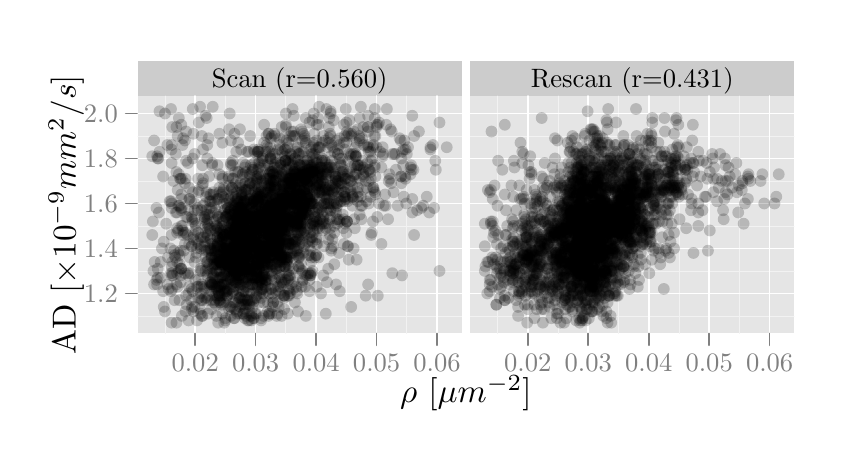
\begin{tikzpicture}[x=1pt,y=1pt]
\definecolor[named]{fillColor}{rgb}{1.00,1.00,1.00}
\path[use as bounding box,fill=fillColor,fill opacity=0.00] (0,0) rectangle (289.08,144.54);
\begin{scope}
\path[clip] (  0.00,  0.00) rectangle (289.08,144.54);
\definecolor[named]{fillColor}{rgb}{1.00,1.00,1.00}

\path[fill=fillColor] (  0.00,  0.00) rectangle (289.08,144.54);
\end{scope}
\begin{scope}
\path[clip] ( 39.69,119.86) rectangle (156.86,132.50);
\definecolor[named]{fillColor}{rgb}{0.80,0.80,0.80}

\path[fill=fillColor] ( 39.69,119.86) rectangle (156.86,132.50);
\definecolor[named]{drawColor}{rgb}{0.00,0.00,0.00}

\node[text=drawColor,anchor=base,inner sep=0pt, outer sep=0pt, scale=  0.96] at ( 98.27,122.87) {Scan (r=0.560)};
\end{scope}
\begin{scope}
\path[clip] (159.87,119.86) rectangle (277.04,132.50);
\definecolor[named]{fillColor}{rgb}{0.80,0.80,0.80}

\path[fill=fillColor] (159.87,119.86) rectangle (277.03,132.50);
\definecolor[named]{drawColor}{rgb}{0.00,0.00,0.00}

\node[text=drawColor,anchor=base,inner sep=0pt, outer sep=0pt, scale=  0.96] at (218.45,122.87) {Rescan (r=0.431)};
\end{scope}
\begin{scope}
\path[clip] (  0.00,  0.00) rectangle (289.08,144.54);
\definecolor[named]{drawColor}{rgb}{0.50,0.50,0.50}

\node[text=drawColor,anchor=base east,inner sep=0pt, outer sep=0pt, scale=  0.96] at ( 32.58, 45.20) {1.2};

\node[text=drawColor,anchor=base east,inner sep=0pt, outer sep=0pt, scale=  0.96] at ( 32.58, 61.45) {1.4};

\node[text=drawColor,anchor=base east,inner sep=0pt, outer sep=0pt, scale=  0.96] at ( 32.58, 77.71) {1.6};

\node[text=drawColor,anchor=base east,inner sep=0pt, outer sep=0pt, scale=  0.96] at ( 32.58, 93.96) {1.8};

\node[text=drawColor,anchor=base east,inner sep=0pt, outer sep=0pt, scale=  0.96] at ( 32.58,110.21) {2.0};
\end{scope}
\begin{scope}
\path[clip] (  0.00,  0.00) rectangle (289.08,144.54);
\definecolor[named]{drawColor}{rgb}{0.50,0.50,0.50}

\path[draw=drawColor,line width= 0.6pt,line join=round,line cap=round] ( 35.42, 48.50) -- ( 39.69, 48.50);

\path[draw=drawColor,line width= 0.6pt,line join=round,line cap=round] ( 35.42, 64.76) -- ( 39.69, 64.76);

\path[draw=drawColor,line width= 0.6pt,line join=round,line cap=round] ( 35.42, 81.01) -- ( 39.69, 81.01);

\path[draw=drawColor,line width= 0.6pt,line join=round,line cap=round] ( 35.42, 97.27) -- ( 39.69, 97.27);

\path[draw=drawColor,line width= 0.6pt,line join=round,line cap=round] ( 35.42,113.52) -- ( 39.69,113.52);
\end{scope}
\begin{scope}
\path[clip] ( 39.69, 34.04) rectangle (156.86,119.86);
\definecolor[named]{fillColor}{rgb}{0.90,0.90,0.90}

\path[fill=fillColor] ( 39.69, 34.04) rectangle (156.86,119.86);
\definecolor[named]{drawColor}{rgb}{0.95,0.95,0.95}

\path[draw=drawColor,line width= 0.3pt,line join=round,line cap=round] ( 39.69, 40.38) --
	(156.86, 40.38);

\path[draw=drawColor,line width= 0.3pt,line join=round,line cap=round] ( 39.69, 56.63) --
	(156.86, 56.63);

\path[draw=drawColor,line width= 0.3pt,line join=round,line cap=round] ( 39.69, 72.89) --
	(156.86, 72.89);

\path[draw=drawColor,line width= 0.3pt,line join=round,line cap=round] ( 39.69, 89.14) --
	(156.86, 89.14);

\path[draw=drawColor,line width= 0.3pt,line join=round,line cap=round] ( 39.69,105.39) --
	(156.86,105.39);

\path[draw=drawColor,line width= 0.3pt,line join=round,line cap=round] ( 49.61, 34.04) --
	( 49.61,119.86);

\path[draw=drawColor,line width= 0.3pt,line join=round,line cap=round] ( 71.46, 34.04) --
	( 71.46,119.86);

\path[draw=drawColor,line width= 0.3pt,line join=round,line cap=round] ( 93.31, 34.04) --
	( 93.31,119.86);

\path[draw=drawColor,line width= 0.3pt,line join=round,line cap=round] (115.16, 34.04) --
	(115.16,119.86);

\path[draw=drawColor,line width= 0.3pt,line join=round,line cap=round] (137.01, 34.04) --
	(137.01,119.86);
\definecolor[named]{drawColor}{rgb}{1.00,1.00,1.00}

\path[draw=drawColor,line width= 0.6pt,line join=round,line cap=round] ( 39.69, 48.50) --
	(156.86, 48.50);

\path[draw=drawColor,line width= 0.6pt,line join=round,line cap=round] ( 39.69, 64.76) --
	(156.86, 64.76);

\path[draw=drawColor,line width= 0.6pt,line join=round,line cap=round] ( 39.69, 81.01) --
	(156.86, 81.01);

\path[draw=drawColor,line width= 0.6pt,line join=round,line cap=round] ( 39.69, 97.27) --
	(156.86, 97.27);

\path[draw=drawColor,line width= 0.6pt,line join=round,line cap=round] ( 39.69,113.52) --
	(156.86,113.52);

\path[draw=drawColor,line width= 0.6pt,line join=round,line cap=round] ( 60.53, 34.04) --
	( 60.53,119.86);

\path[draw=drawColor,line width= 0.6pt,line join=round,line cap=round] ( 82.38, 34.04) --
	( 82.38,119.86);

\path[draw=drawColor,line width= 0.6pt,line join=round,line cap=round] (104.23, 34.04) --
	(104.23,119.86);

\path[draw=drawColor,line width= 0.6pt,line join=round,line cap=round] (126.08, 34.04) --
	(126.08,119.86);

\path[draw=drawColor,line width= 0.6pt,line join=round,line cap=round] (147.93, 34.04) --
	(147.93,119.86);
\definecolor[named]{fillColor}{rgb}{0.00,0.00,0.00}

\path[fill=fillColor,fill opacity=0.20] ( 52.23, 55.82) circle (  2.13);

\path[fill=fillColor,fill opacity=0.20] ( 64.25, 61.51) circle (  2.13);

\path[fill=fillColor,fill opacity=0.20] ( 76.26, 59.07) circle (  2.13);

\path[fill=fillColor,fill opacity=0.20] ( 86.97, 55.82) circle (  2.13);

\path[fill=fillColor,fill opacity=0.20] ( 81.07, 55.01) circle (  2.13);

\path[fill=fillColor,fill opacity=0.20] ( 75.17, 52.57) circle (  2.13);

\path[fill=fillColor,fill opacity=0.20] ( 71.02, 60.69) circle (  2.13);

\path[fill=fillColor,fill opacity=0.20] ( 59.88, 68.01) circle (  2.13);

\path[fill=fillColor,fill opacity=0.20] ( 75.17, 69.63) circle (  2.13);

\path[fill=fillColor,fill opacity=0.20] ( 85.88, 59.07) circle (  2.13);

\path[fill=fillColor,fill opacity=0.20] ( 97.68, 62.32) circle (  2.13);

\path[fill=fillColor,fill opacity=0.20] (108.60, 73.70) circle (  2.13);

\path[fill=fillColor,fill opacity=0.20] ( 96.36, 72.89) circle (  2.13);

\path[fill=fillColor,fill opacity=0.20] (103.79, 61.51) circle (  2.13);

\path[fill=fillColor,fill opacity=0.20] (100.30, 50.94) circle (  2.13);

\path[fill=fillColor,fill opacity=0.20] ( 91.78, 53.38) circle (  2.13);

\path[fill=fillColor,fill opacity=0.20] ( 69.49, 47.69) circle (  2.13);

\path[fill=fillColor,fill opacity=0.20] ( 58.13, 38.75) circle (  2.13);

\path[fill=fillColor,fill opacity=0.20] ( 69.05, 76.14) circle (  2.13);

\path[fill=fillColor,fill opacity=0.20] ( 85.22, 65.57) circle (  2.13);

\path[fill=fillColor,fill opacity=0.20] ( 90.68, 67.20) circle (  2.13);

\path[fill=fillColor,fill opacity=0.20] ( 94.84, 78.57) circle (  2.13);

\path[fill=fillColor,fill opacity=0.20] ( 98.33, 85.89) circle (  2.13);

\path[fill=fillColor,fill opacity=0.20] (102.92, 89.95) circle (  2.13);

\path[fill=fillColor,fill opacity=0.20] (100.08, 91.58) circle (  2.13);

\path[fill=fillColor,fill opacity=0.20] ( 95.27, 84.26) circle (  2.13);

\path[fill=fillColor,fill opacity=0.20] ( 93.52, 68.01) circle (  2.13);

\path[fill=fillColor,fill opacity=0.20] ( 88.06, 50.13) circle (  2.13);

\path[fill=fillColor,fill opacity=0.20] ( 76.04, 45.25) circle (  2.13);

\path[fill=fillColor,fill opacity=0.20] ( 74.95, 42.82) circle (  2.13);

\path[fill=fillColor,fill opacity=0.20] ( 71.46, 38.75) circle (  2.13);

\path[fill=fillColor,fill opacity=0.20] ( 58.56, 61.51) circle (  2.13);

\path[fill=fillColor,fill opacity=0.20] ( 81.51, 66.38) circle (  2.13);

\path[fill=fillColor,fill opacity=0.20] ( 98.11, 72.89) circle (  2.13);

\path[fill=fillColor,fill opacity=0.20] (111.66, 81.01) circle (  2.13);

\path[fill=fillColor,fill opacity=0.20] (106.42,102.96) circle (  2.13);

\path[fill=fillColor,fill opacity=0.20] ( 99.21,107.02) circle (  2.13);

\path[fill=fillColor,fill opacity=0.20] ( 92.87, 98.08) circle (  2.13);

\path[fill=fillColor,fill opacity=0.20] ( 97.68, 96.45) circle (  2.13);

\path[fill=fillColor,fill opacity=0.20] ( 99.86, 90.76) circle (  2.13);

\path[fill=fillColor,fill opacity=0.20] ( 88.94, 77.76) circle (  2.13);

\path[fill=fillColor,fill opacity=0.20] ( 79.76, 66.38) circle (  2.13);

\path[fill=fillColor,fill opacity=0.20] ( 77.14, 60.69) circle (  2.13);

\path[fill=fillColor,fill opacity=0.20] ( 77.79, 51.75) circle (  2.13);

\path[fill=fillColor,fill opacity=0.20] ( 74.30, 45.25) circle (  2.13);

\path[fill=fillColor,fill opacity=0.20] ( 90.25, 41.19) circle (  2.13);

\path[fill=fillColor,fill opacity=0.20] ( 60.97, 63.13) circle (  2.13);

\path[fill=fillColor,fill opacity=0.20] ( 76.48, 68.01) circle (  2.13);

\path[fill=fillColor,fill opacity=0.20] ( 98.77, 86.70) circle (  2.13);

\path[fill=fillColor,fill opacity=0.20] (107.95, 94.02) circle (  2.13);

\path[fill=fillColor,fill opacity=0.20] (105.10,101.33) circle (  2.13);

\path[fill=fillColor,fill opacity=0.20] (103.58,106.21) circle (  2.13);

\path[fill=fillColor,fill opacity=0.20] ( 95.27,107.02) circle (  2.13);

\path[fill=fillColor,fill opacity=0.20] ( 83.25, 99.70) circle (  2.13);

\path[fill=fillColor,fill opacity=0.20] ( 89.37, 85.89) circle (  2.13);

\path[fill=fillColor,fill opacity=0.20] ( 85.22, 76.95) circle (  2.13);

\path[fill=fillColor,fill opacity=0.20] ( 76.92, 77.76) circle (  2.13);

\path[fill=fillColor,fill opacity=0.20] ( 74.30, 76.95) circle (  2.13);

\path[fill=fillColor,fill opacity=0.20] ( 65.56, 76.95) circle (  2.13);

\path[fill=fillColor,fill opacity=0.20] ( 54.19, 85.89) circle (  2.13);

\path[fill=fillColor,fill opacity=0.20] ( 70.80, 85.89) circle (  2.13);

\path[fill=fillColor,fill opacity=0.20] ( 90.68, 65.57) circle (  2.13);

\path[fill=fillColor,fill opacity=0.20] ( 81.51, 93.20) circle (  2.13);

\path[fill=fillColor,fill opacity=0.20] ( 81.29, 94.02) circle (  2.13);

\path[fill=fillColor,fill opacity=0.20] ( 83.47, 85.08) circle (  2.13);

\path[fill=fillColor,fill opacity=0.20] ( 64.25, 72.89) circle (  2.13);

\path[fill=fillColor,fill opacity=0.20] ( 78.23, 71.26) circle (  2.13);

\path[fill=fillColor,fill opacity=0.20] ( 95.93, 92.39) circle (  2.13);

\path[fill=fillColor,fill opacity=0.20] (102.48, 98.89) circle (  2.13);

\path[fill=fillColor,fill opacity=0.20] ( 98.77, 90.76) circle (  2.13);

\path[fill=fillColor,fill opacity=0.20] (102.05, 90.76) circle (  2.13);

\path[fill=fillColor,fill opacity=0.20] ( 99.21,103.77) circle (  2.13);

\path[fill=fillColor,fill opacity=0.20] ( 87.84,104.58) circle (  2.13);

\path[fill=fillColor,fill opacity=0.20] ( 73.86, 86.70) circle (  2.13);

\path[fill=fillColor,fill opacity=0.20] ( 71.67, 76.14) circle (  2.13);

\path[fill=fillColor,fill opacity=0.20] ( 64.25, 76.95) circle (  2.13);

\path[fill=fillColor,fill opacity=0.20] ( 66.65, 94.83) circle (  2.13);

\path[fill=fillColor,fill opacity=0.20] (105.32, 72.89) circle (  2.13);

\path[fill=fillColor,fill opacity=0.20] ( 97.02, 86.70) circle (  2.13);

\path[fill=fillColor,fill opacity=0.20] ( 94.84, 86.70) circle (  2.13);

\path[fill=fillColor,fill opacity=0.20] ( 99.86, 89.14) circle (  2.13);

\path[fill=fillColor,fill opacity=0.20] ( 99.42, 89.14) circle (  2.13);

\path[fill=fillColor,fill opacity=0.20] ( 95.71, 81.82) circle (  2.13);

\path[fill=fillColor,fill opacity=0.20] ( 81.29, 89.14) circle (  2.13);

\path[fill=fillColor,fill opacity=0.20] ( 70.36, 69.63) circle (  2.13);

\path[fill=fillColor,fill opacity=0.20] ( 77.57, 72.89) circle (  2.13);

\path[fill=fillColor,fill opacity=0.20] ( 88.06, 87.51) circle (  2.13);

\path[fill=fillColor,fill opacity=0.20] ( 90.47,100.52) circle (  2.13);

\path[fill=fillColor,fill opacity=0.20] ( 87.62,101.33) circle (  2.13);

\path[fill=fillColor,fill opacity=0.20] ( 89.59, 89.14) circle (  2.13);

\path[fill=fillColor,fill opacity=0.20] ( 91.99, 90.76) circle (  2.13);

\path[fill=fillColor,fill opacity=0.20] ( 85.44,102.96) circle (  2.13);

\path[fill=fillColor,fill opacity=0.20] ( 64.46, 78.57) circle (  2.13);

\path[fill=fillColor,fill opacity=0.20] ( 77.57, 91.58) circle (  2.13);

\path[fill=fillColor,fill opacity=0.20] (111.88, 73.70) circle (  2.13);

\path[fill=fillColor,fill opacity=0.20] (110.35, 92.39) circle (  2.13);

\path[fill=fillColor,fill opacity=0.20] (116.03, 89.95) circle (  2.13);

\path[fill=fillColor,fill opacity=0.20] (126.95, 81.01) circle (  2.13);

\path[fill=fillColor,fill opacity=0.20] (146.84, 79.39) circle (  2.13);

\path[fill=fillColor,fill opacity=0.20] (113.41, 81.82) circle (  2.13);

\path[fill=fillColor,fill opacity=0.20] (105.54, 75.32) circle (  2.13);

\path[fill=fillColor,fill opacity=0.20] (101.39, 76.95) circle (  2.13);

\path[fill=fillColor,fill opacity=0.20] ( 65.34,104.58) circle (  2.13);

\path[fill=fillColor,fill opacity=0.20] ( 67.96, 62.32) circle (  2.13);

\path[fill=fillColor,fill opacity=0.20] ( 78.01, 68.82) circle (  2.13);

\path[fill=fillColor,fill opacity=0.20] ( 88.94, 91.58) circle (  2.13);

\path[fill=fillColor,fill opacity=0.20] ( 81.94, 99.70) circle (  2.13);

\path[fill=fillColor,fill opacity=0.20] ( 80.41,105.39) circle (  2.13);

\path[fill=fillColor,fill opacity=0.20] ( 83.47,100.52) circle (  2.13);

\path[fill=fillColor,fill opacity=0.20] ( 80.20, 91.58) circle (  2.13);

\path[fill=fillColor,fill opacity=0.20] ( 78.67, 94.83) circle (  2.13);

\path[fill=fillColor,fill opacity=0.20] ( 77.79, 91.58) circle (  2.13);

\path[fill=fillColor,fill opacity=0.20] ( 67.96, 78.57) circle (  2.13);

\path[fill=fillColor,fill opacity=0.20] (111.66, 75.32) circle (  2.13);

\path[fill=fillColor,fill opacity=0.20] (115.59, 91.58) circle (  2.13);

\path[fill=fillColor,fill opacity=0.20] (119.09, 94.83) circle (  2.13);

\path[fill=fillColor,fill opacity=0.20] (133.73, 80.20) circle (  2.13);

\path[fill=fillColor,fill opacity=0.20] (120.40, 80.20) circle (  2.13);

\path[fill=fillColor,fill opacity=0.20] (122.58, 86.70) circle (  2.13);

\path[fill=fillColor,fill opacity=0.20] (100.95, 83.45) circle (  2.13);

\path[fill=fillColor,fill opacity=0.20] ( 96.15, 76.14) circle (  2.13);

\path[fill=fillColor,fill opacity=0.20] (115.59, 65.57) circle (  2.13);

\path[fill=fillColor,fill opacity=0.20] ( 79.98, 75.32) circle (  2.13);

\path[fill=fillColor,fill opacity=0.20] ( 60.31, 59.88) circle (  2.13);

\path[fill=fillColor,fill opacity=0.20] ( 81.07, 67.20) circle (  2.13);

\path[fill=fillColor,fill opacity=0.20] ( 81.94, 95.64) circle (  2.13);

\path[fill=fillColor,fill opacity=0.20] ( 83.91, 91.58) circle (  2.13);

\path[fill=fillColor,fill opacity=0.20] ( 86.97, 87.51) circle (  2.13);

\path[fill=fillColor,fill opacity=0.20] ( 83.04, 99.70) circle (  2.13);

\path[fill=fillColor,fill opacity=0.20] ( 86.10, 99.70) circle (  2.13);

\path[fill=fillColor,fill opacity=0.20] ( 80.63, 88.33) circle (  2.13);

\path[fill=fillColor,fill opacity=0.20] ( 82.82, 75.32) circle (  2.13);

\path[fill=fillColor,fill opacity=0.20] ( 71.24, 72.89) circle (  2.13);

\path[fill=fillColor,fill opacity=0.20] ( 89.15, 98.89) circle (  2.13);

\path[fill=fillColor,fill opacity=0.20] (124.33, 70.45) circle (  2.13);

\path[fill=fillColor,fill opacity=0.20] (117.78, 90.76) circle (  2.13);

\path[fill=fillColor,fill opacity=0.20] (109.26, 92.39) circle (  2.13);

\path[fill=fillColor,fill opacity=0.20] (101.17, 84.26) circle (  2.13);

\path[fill=fillColor,fill opacity=0.20] (100.08, 91.58) circle (  2.13);

\path[fill=fillColor,fill opacity=0.20] (102.48, 92.39) circle (  2.13);

\path[fill=fillColor,fill opacity=0.20] ( 94.40, 85.08) circle (  2.13);

\path[fill=fillColor,fill opacity=0.20] ( 82.60, 82.64) circle (  2.13);

\path[fill=fillColor,fill opacity=0.20] ( 84.78, 65.57) circle (  2.13);

\path[fill=fillColor,fill opacity=0.20] ( 86.31, 49.32) circle (  2.13);

\path[fill=fillColor,fill opacity=0.20] ( 56.38, 63.95) circle (  2.13);

\path[fill=fillColor,fill opacity=0.20] ( 75.39, 66.38) circle (  2.13);

\path[fill=fillColor,fill opacity=0.20] ( 81.73, 85.08) circle (  2.13);

\path[fill=fillColor,fill opacity=0.20] ( 91.78, 82.64) circle (  2.13);

\path[fill=fillColor,fill opacity=0.20] ( 93.09, 75.32) circle (  2.13);

\path[fill=fillColor,fill opacity=0.20] ( 86.53, 88.33) circle (  2.13);

\path[fill=fillColor,fill opacity=0.20] ( 83.47, 95.64) circle (  2.13);

\path[fill=fillColor,fill opacity=0.20] ( 81.94, 87.51) circle (  2.13);

\path[fill=fillColor,fill opacity=0.20] ( 80.41, 73.70) circle (  2.13);

\path[fill=fillColor,fill opacity=0.20] ( 78.23, 64.76) circle (  2.13);

\path[fill=fillColor,fill opacity=0.20] (129.14, 84.26) circle (  2.13);

\path[fill=fillColor,fill opacity=0.20] (114.72, 82.64) circle (  2.13);

\path[fill=fillColor,fill opacity=0.20] (102.70, 94.83) circle (  2.13);

\path[fill=fillColor,fill opacity=0.20] (119.96, 89.95) circle (  2.13);

\path[fill=fillColor,fill opacity=0.20] (100.95, 90.76) circle (  2.13);

\path[fill=fillColor,fill opacity=0.20] ( 93.31, 94.83) circle (  2.13);

\path[fill=fillColor,fill opacity=0.20] (100.73, 91.58) circle (  2.13);

\path[fill=fillColor,fill opacity=0.20] ( 94.18, 88.33) circle (  2.13);

\path[fill=fillColor,fill opacity=0.20] ( 86.31, 85.08) circle (  2.13);

\path[fill=fillColor,fill opacity=0.20] ( 88.28, 66.38) circle (  2.13);

\path[fill=fillColor,fill opacity=0.20] ( 79.32, 54.19) circle (  2.13);

\path[fill=fillColor,fill opacity=0.20] ( 72.33, 59.88) circle (  2.13);

\path[fill=fillColor,fill opacity=0.20] ( 90.90, 68.01) circle (  2.13);

\path[fill=fillColor,fill opacity=0.20] ( 99.64, 79.39) circle (  2.13);

\path[fill=fillColor,fill opacity=0.20] ( 97.46, 84.26) circle (  2.13);

\path[fill=fillColor,fill opacity=0.20] ( 88.06, 84.26) circle (  2.13);

\path[fill=fillColor,fill opacity=0.20] ( 84.78, 81.82) circle (  2.13);

\path[fill=fillColor,fill opacity=0.20] ( 83.04, 84.26) circle (  2.13);

\path[fill=fillColor,fill opacity=0.20] ( 76.48, 87.51) circle (  2.13);

\path[fill=fillColor,fill opacity=0.20] ( 79.98, 72.07) circle (  2.13);

\path[fill=fillColor,fill opacity=0.20] (117.34, 80.20) circle (  2.13);

\path[fill=fillColor,fill opacity=0.20] (103.36,102.14) circle (  2.13);

\path[fill=fillColor,fill opacity=0.20] (109.69,102.14) circle (  2.13);

\path[fill=fillColor,fill opacity=0.20] (122.15, 89.14) circle (  2.13);

\path[fill=fillColor,fill opacity=0.20] (106.20, 89.14) circle (  2.13);

\path[fill=fillColor,fill opacity=0.20] ( 96.58, 92.39) circle (  2.13);

\path[fill=fillColor,fill opacity=0.20] (106.63, 90.76) circle (  2.13);

\path[fill=fillColor,fill opacity=0.20] ( 83.25, 91.58) circle (  2.13);

\path[fill=fillColor,fill opacity=0.20] ( 88.06, 81.01) circle (  2.13);

\path[fill=fillColor,fill opacity=0.20] ( 87.62, 59.07) circle (  2.13);

\path[fill=fillColor,fill opacity=0.20] ( 74.30, 59.88) circle (  2.13);

\path[fill=fillColor,fill opacity=0.20] ( 82.60, 51.75) circle (  2.13);

\path[fill=fillColor,fill opacity=0.20] ( 90.68, 73.70) circle (  2.13);

\path[fill=fillColor,fill opacity=0.20] ( 92.43, 88.33) circle (  2.13);

\path[fill=fillColor,fill opacity=0.20] ( 90.90, 85.89) circle (  2.13);

\path[fill=fillColor,fill opacity=0.20] ( 88.28, 76.14) circle (  2.13);

\path[fill=fillColor,fill opacity=0.20] ( 90.68, 76.95) circle (  2.13);

\path[fill=fillColor,fill opacity=0.20] ( 81.29, 93.20) circle (  2.13);

\path[fill=fillColor,fill opacity=0.20] ( 89.81, 86.70) circle (  2.13);

\path[fill=fillColor,fill opacity=0.20] ( 82.60, 70.45) circle (  2.13);

\path[fill=fillColor,fill opacity=0.20] ( 95.93, 89.95) circle (  2.13);

\path[fill=fillColor,fill opacity=0.20] ( 89.81, 91.58) circle (  2.13);

\path[fill=fillColor,fill opacity=0.20] ( 88.28,105.39) circle (  2.13);

\path[fill=fillColor,fill opacity=0.20] ( 97.89, 98.89) circle (  2.13);

\path[fill=fillColor,fill opacity=0.20] (107.73, 89.95) circle (  2.13);

\path[fill=fillColor,fill opacity=0.20] (100.52, 91.58) circle (  2.13);

\path[fill=fillColor,fill opacity=0.20] ( 98.33, 89.14) circle (  2.13);

\path[fill=fillColor,fill opacity=0.20] (101.17, 83.45) circle (  2.13);

\path[fill=fillColor,fill opacity=0.20] ( 92.87, 81.82) circle (  2.13);

\path[fill=fillColor,fill opacity=0.20] ( 85.88, 71.26) circle (  2.13);

\path[fill=fillColor,fill opacity=0.20] ( 85.66, 53.38) circle (  2.13);

\path[fill=fillColor,fill opacity=0.20] ( 66.43, 61.51) circle (  2.13);

\path[fill=fillColor,fill opacity=0.20] ( 72.11, 49.32) circle (  2.13);

\path[fill=fillColor,fill opacity=0.20] ( 80.63, 66.38) circle (  2.13);

\path[fill=fillColor,fill opacity=0.20] ( 82.38, 78.57) circle (  2.13);

\path[fill=fillColor,fill opacity=0.20] ( 91.99, 79.39) circle (  2.13);

\path[fill=fillColor,fill opacity=0.20] ( 86.75, 80.20) circle (  2.13);

\path[fill=fillColor,fill opacity=0.20] ( 87.62, 79.39) circle (  2.13);

\path[fill=fillColor,fill opacity=0.20] ( 88.50, 84.26) circle (  2.13);

\path[fill=fillColor,fill opacity=0.20] ( 79.32, 81.82) circle (  2.13);

\path[fill=fillColor,fill opacity=0.20] ( 75.83, 68.01) circle (  2.13);

\path[fill=fillColor,fill opacity=0.20] ( 64.90, 73.70) circle (  2.13);

\path[fill=fillColor,fill opacity=0.20] ( 86.31,102.14) circle (  2.13);

\path[fill=fillColor,fill opacity=0.20] (110.13, 88.33) circle (  2.13);

\path[fill=fillColor,fill opacity=0.20] ( 83.25, 99.70) circle (  2.13);

\path[fill=fillColor,fill opacity=0.20] ( 87.62, 98.08) circle (  2.13);

\path[fill=fillColor,fill opacity=0.20] ( 95.05, 91.58) circle (  2.13);

\path[fill=fillColor,fill opacity=0.20] ( 98.33, 87.51) circle (  2.13);

\path[fill=fillColor,fill opacity=0.20] (101.17, 90.76) circle (  2.13);

\path[fill=fillColor,fill opacity=0.20] ( 91.56, 85.08) circle (  2.13);

\path[fill=fillColor,fill opacity=0.20] (106.63, 74.51) circle (  2.13);

\path[fill=fillColor,fill opacity=0.20] (102.92, 73.70) circle (  2.13);

\path[fill=fillColor,fill opacity=0.20] ( 90.47, 65.57) circle (  2.13);

\path[fill=fillColor,fill opacity=0.20] ( 83.25, 51.75) circle (  2.13);

\path[fill=fillColor,fill opacity=0.20] ( 71.46, 64.76) circle (  2.13);

\path[fill=fillColor,fill opacity=0.20] ( 89.59, 65.57) circle (  2.13);

\path[fill=fillColor,fill opacity=0.20] ( 90.68, 66.38) circle (  2.13);

\path[fill=fillColor,fill opacity=0.20] ( 85.00, 77.76) circle (  2.13);

\path[fill=fillColor,fill opacity=0.20] ( 89.59, 82.64) circle (  2.13);

\path[fill=fillColor,fill opacity=0.20] ( 90.68, 74.51) circle (  2.13);

\path[fill=fillColor,fill opacity=0.20] ( 86.75, 65.57) circle (  2.13);

\path[fill=fillColor,fill opacity=0.20] ( 77.79, 60.69) circle (  2.13);

\path[fill=fillColor,fill opacity=0.20] ( 76.26, 61.51) circle (  2.13);

\path[fill=fillColor,fill opacity=0.20] ( 67.52, 72.07) circle (  2.13);

\path[fill=fillColor,fill opacity=0.20] ( 72.99,113.52) circle (  2.13);

\path[fill=fillColor,fill opacity=0.20] ( 97.24, 83.45) circle (  2.13);

\path[fill=fillColor,fill opacity=0.20] ( 96.15, 92.39) circle (  2.13);

\path[fill=fillColor,fill opacity=0.20] ( 96.80, 89.95) circle (  2.13);

\path[fill=fillColor,fill opacity=0.20] (105.32, 87.51) circle (  2.13);

\path[fill=fillColor,fill opacity=0.20] (102.26, 89.14) circle (  2.13);

\path[fill=fillColor,fill opacity=0.20] ( 99.64, 89.14) circle (  2.13);

\path[fill=fillColor,fill opacity=0.20] (100.95, 84.26) circle (  2.13);

\path[fill=fillColor,fill opacity=0.20] ( 98.99, 76.95) circle (  2.13);

\path[fill=fillColor,fill opacity=0.20] (103.36, 74.51) circle (  2.13);

\path[fill=fillColor,fill opacity=0.20] ( 95.93, 76.14) circle (  2.13);

\path[fill=fillColor,fill opacity=0.20] ( 94.84, 66.38) circle (  2.13);

\path[fill=fillColor,fill opacity=0.20] ( 78.67, 56.63) circle (  2.13);

\path[fill=fillColor,fill opacity=0.20] ( 88.06, 62.32) circle (  2.13);

\path[fill=fillColor,fill opacity=0.20] ( 99.42, 53.38) circle (  2.13);

\path[fill=fillColor,fill opacity=0.20] ( 84.35, 63.13) circle (  2.13);

\path[fill=fillColor,fill opacity=0.20] ( 89.37, 73.70) circle (  2.13);

\path[fill=fillColor,fill opacity=0.20] ( 89.81, 71.26) circle (  2.13);

\path[fill=fillColor,fill opacity=0.20] ( 85.22, 68.01) circle (  2.13);

\path[fill=fillColor,fill opacity=0.20] ( 86.97, 64.76) circle (  2.13);

\path[fill=fillColor,fill opacity=0.20] ( 78.45, 65.57) circle (  2.13);

\path[fill=fillColor,fill opacity=0.20] ( 75.17, 72.89) circle (  2.13);

\path[fill=fillColor,fill opacity=0.20] ( 60.31, 81.01) circle (  2.13);

\path[fill=fillColor,fill opacity=0.20] ( 97.46, 86.70) circle (  2.13);

\path[fill=fillColor,fill opacity=0.20] ( 94.18, 95.64) circle (  2.13);

\path[fill=fillColor,fill opacity=0.20] ( 97.46, 88.33) circle (  2.13);

\path[fill=fillColor,fill opacity=0.20] (107.29, 81.01) circle (  2.13);

\path[fill=fillColor,fill opacity=0.20] (108.38, 85.08) circle (  2.13);

\path[fill=fillColor,fill opacity=0.20] (102.70, 92.39) circle (  2.13);

\path[fill=fillColor,fill opacity=0.20] ( 98.33, 94.83) circle (  2.13);

\path[fill=fillColor,fill opacity=0.20] (107.29, 85.89) circle (  2.13);

\path[fill=fillColor,fill opacity=0.20] ( 98.33, 77.76) circle (  2.13);

\path[fill=fillColor,fill opacity=0.20] (100.52, 75.32) circle (  2.13);

\path[fill=fillColor,fill opacity=0.20] (100.52, 69.63) circle (  2.13);

\path[fill=fillColor,fill opacity=0.20] ( 86.10, 64.76) circle (  2.13);

\path[fill=fillColor,fill opacity=0.20] ( 57.69, 69.63) circle (  2.13);

\path[fill=fillColor,fill opacity=0.20] ( 55.51, 72.89) circle (  2.13);

\path[fill=fillColor,fill opacity=0.20] ( 75.61, 55.01) circle (  2.13);

\path[fill=fillColor,fill opacity=0.20] ( 88.28, 55.01) circle (  2.13);

\path[fill=fillColor,fill opacity=0.20] ( 86.53, 63.95) circle (  2.13);

\path[fill=fillColor,fill opacity=0.20] ( 81.73, 75.32) circle (  2.13);

\path[fill=fillColor,fill opacity=0.20] ( 89.37, 78.57) circle (  2.13);

\path[fill=fillColor,fill opacity=0.20] ( 86.97, 73.70) circle (  2.13);

\path[fill=fillColor,fill opacity=0.20] ( 86.10, 72.89) circle (  2.13);

\path[fill=fillColor,fill opacity=0.20] ( 77.36, 79.39) circle (  2.13);

\path[fill=fillColor,fill opacity=0.20] ( 72.77, 82.64) circle (  2.13);

\path[fill=fillColor,fill opacity=0.20] ( 65.77, 81.82) circle (  2.13);

\path[fill=fillColor,fill opacity=0.20] ( 97.68, 85.08) circle (  2.13);

\path[fill=fillColor,fill opacity=0.20] ( 94.18, 96.45) circle (  2.13);

\path[fill=fillColor,fill opacity=0.20] ( 95.05, 96.45) circle (  2.13);

\path[fill=fillColor,fill opacity=0.20] (100.95, 88.33) circle (  2.13);

\path[fill=fillColor,fill opacity=0.20] (102.05, 92.39) circle (  2.13);

\path[fill=fillColor,fill opacity=0.20] ( 99.21, 94.02) circle (  2.13);

\path[fill=fillColor,fill opacity=0.20] (100.08, 92.39) circle (  2.13);

\path[fill=fillColor,fill opacity=0.20] (103.58, 91.58) circle (  2.13);

\path[fill=fillColor,fill opacity=0.20] (100.08, 89.95) circle (  2.13);

\path[fill=fillColor,fill opacity=0.20] (104.23, 87.51) circle (  2.13);

\path[fill=fillColor,fill opacity=0.20] (102.26, 72.89) circle (  2.13);

\path[fill=fillColor,fill opacity=0.20] ( 88.06, 53.38) circle (  2.13);

\path[fill=fillColor,fill opacity=0.20] ( 55.94, 72.89) circle (  2.13);

\path[fill=fillColor,fill opacity=0.20] ( 85.00, 63.95) circle (  2.13);

\path[fill=fillColor,fill opacity=0.20] ( 93.74, 59.07) circle (  2.13);

\path[fill=fillColor,fill opacity=0.20] ( 85.22, 69.63) circle (  2.13);

\path[fill=fillColor,fill opacity=0.20] ( 91.34, 72.07) circle (  2.13);

\path[fill=fillColor,fill opacity=0.20] ( 98.11, 68.01) circle (  2.13);

\path[fill=fillColor,fill opacity=0.20] ( 86.75, 72.89) circle (  2.13);

\path[fill=fillColor,fill opacity=0.20] ( 84.78, 76.14) circle (  2.13);

\path[fill=fillColor,fill opacity=0.20] ( 83.25, 75.32) circle (  2.13);

\path[fill=fillColor,fill opacity=0.20] ( 83.47, 72.89) circle (  2.13);

\path[fill=fillColor,fill opacity=0.20] ( 68.83, 72.07) circle (  2.13);

\path[fill=fillColor,fill opacity=0.20] ( 92.21, 92.39) circle (  2.13);

\path[fill=fillColor,fill opacity=0.20] ( 93.09,100.52) circle (  2.13);

\path[fill=fillColor,fill opacity=0.20] (103.14, 96.45) circle (  2.13);

\path[fill=fillColor,fill opacity=0.20] (103.36, 87.51) circle (  2.13);

\path[fill=fillColor,fill opacity=0.20] (105.76, 88.33) circle (  2.13);

\path[fill=fillColor,fill opacity=0.20] (102.48, 94.02) circle (  2.13);

\path[fill=fillColor,fill opacity=0.20] (100.73, 96.45) circle (  2.13);

\path[fill=fillColor,fill opacity=0.20] (103.79, 89.14) circle (  2.13);

\path[fill=fillColor,fill opacity=0.20] (110.35, 85.08) circle (  2.13);

\path[fill=fillColor,fill opacity=0.20] (104.89, 88.33) circle (  2.13);

\path[fill=fillColor,fill opacity=0.20] ( 98.11, 66.38) circle (  2.13);

\path[fill=fillColor,fill opacity=0.20] ( 76.70, 46.88) circle (  2.13);

\path[fill=fillColor,fill opacity=0.20] ( 55.51, 78.57) circle (  2.13);

\path[fill=fillColor,fill opacity=0.20] ( 91.12, 59.88) circle (  2.13);

\path[fill=fillColor,fill opacity=0.20] (101.39, 55.82) circle (  2.13);

\path[fill=fillColor,fill opacity=0.20] ( 98.33, 57.44) circle (  2.13);

\path[fill=fillColor,fill opacity=0.20] (102.48, 61.51) circle (  2.13);

\path[fill=fillColor,fill opacity=0.20] ( 91.78, 70.45) circle (  2.13);

\path[fill=fillColor,fill opacity=0.20] ( 83.69, 72.89) circle (  2.13);

\path[fill=fillColor,fill opacity=0.20] ( 83.91, 76.14) circle (  2.13);

\path[fill=fillColor,fill opacity=0.20] ( 76.26, 77.76) circle (  2.13);

\path[fill=fillColor,fill opacity=0.20] ( 72.77, 74.51) circle (  2.13);

\path[fill=fillColor,fill opacity=0.20] ( 66.87, 81.82) circle (  2.13);

\path[fill=fillColor,fill opacity=0.20] ( 91.34, 95.64) circle (  2.13);

\path[fill=fillColor,fill opacity=0.20] ( 86.31,105.39) circle (  2.13);

\path[fill=fillColor,fill opacity=0.20] ( 98.11, 98.89) circle (  2.13);

\path[fill=fillColor,fill opacity=0.20] (113.41, 88.33) circle (  2.13);

\path[fill=fillColor,fill opacity=0.20] (116.69, 85.89) circle (  2.13);

\path[fill=fillColor,fill opacity=0.20] (117.34, 84.26) circle (  2.13);

\path[fill=fillColor,fill opacity=0.20] (109.04, 85.89) circle (  2.13);

\path[fill=fillColor,fill opacity=0.20] (106.63, 89.14) circle (  2.13);

\path[fill=fillColor,fill opacity=0.20] (101.61, 89.14) circle (  2.13);

\path[fill=fillColor,fill opacity=0.20] (100.08, 85.89) circle (  2.13);

\path[fill=fillColor,fill opacity=0.20] (111.88, 80.20) circle (  2.13);

\path[fill=fillColor,fill opacity=0.20] (104.67, 66.38) circle (  2.13);

\path[fill=fillColor,fill opacity=0.20] ( 74.73, 59.88) circle (  2.13);

\path[fill=fillColor,fill opacity=0.20] ( 53.98, 72.07) circle (  2.13);

\path[fill=fillColor,fill opacity=0.20] ( 98.77, 55.82) circle (  2.13);

\path[fill=fillColor,fill opacity=0.20] (102.92, 56.63) circle (  2.13);

\path[fill=fillColor,fill opacity=0.20] ( 97.02, 63.95) circle (  2.13);

\path[fill=fillColor,fill opacity=0.20] ( 97.68, 68.82) circle (  2.13);

\path[fill=fillColor,fill opacity=0.20] ( 84.78, 75.32) circle (  2.13);

\path[fill=fillColor,fill opacity=0.20] ( 82.82, 83.45) circle (  2.13);

\path[fill=fillColor,fill opacity=0.20] ( 81.51, 81.82) circle (  2.13);

\path[fill=fillColor,fill opacity=0.20] ( 72.33, 79.39) circle (  2.13);

\path[fill=fillColor,fill opacity=0.20] ( 72.33, 79.39) circle (  2.13);

\path[fill=fillColor,fill opacity=0.20] ( 68.18, 75.32) circle (  2.13);

\path[fill=fillColor,fill opacity=0.20] ( 70.36, 90.76) circle (  2.13);

\path[fill=fillColor,fill opacity=0.20] ( 97.24, 76.14) circle (  2.13);

\path[fill=fillColor,fill opacity=0.20] (102.70,101.33) circle (  2.13);

\path[fill=fillColor,fill opacity=0.20] ( 95.71,105.39) circle (  2.13);

\path[fill=fillColor,fill opacity=0.20] (112.10, 89.14) circle (  2.13);

\path[fill=fillColor,fill opacity=0.20] (112.10, 89.14) circle (  2.13);

\path[fill=fillColor,fill opacity=0.20] (116.90, 94.02) circle (  2.13);

\path[fill=fillColor,fill opacity=0.20] (114.72, 89.95) circle (  2.13);

\path[fill=fillColor,fill opacity=0.20] (110.79, 81.82) circle (  2.13);

\path[fill=fillColor,fill opacity=0.20] (109.47, 81.01) circle (  2.13);

\path[fill=fillColor,fill opacity=0.20] (100.95, 83.45) circle (  2.13);

\path[fill=fillColor,fill opacity=0.20] ( 98.33, 76.14) circle (  2.13);

\path[fill=fillColor,fill opacity=0.20] ( 97.68, 64.76) circle (  2.13);

\path[fill=fillColor,fill opacity=0.20] ( 70.14, 60.69) circle (  2.13);

\path[fill=fillColor,fill opacity=0.20] ( 91.34, 63.13) circle (  2.13);

\path[fill=fillColor,fill opacity=0.20] (100.30, 66.38) circle (  2.13);

\path[fill=fillColor,fill opacity=0.20] ( 91.34, 60.69) circle (  2.13);

\path[fill=fillColor,fill opacity=0.20] ( 87.41, 63.95) circle (  2.13);

\path[fill=fillColor,fill opacity=0.20] ( 84.78, 78.57) circle (  2.13);

\path[fill=fillColor,fill opacity=0.20] ( 82.60, 80.20) circle (  2.13);

\path[fill=fillColor,fill opacity=0.20] ( 80.41, 76.14) circle (  2.13);

\path[fill=fillColor,fill opacity=0.20] ( 72.77, 76.95) circle (  2.13);

\path[fill=fillColor,fill opacity=0.20] ( 70.80, 71.26) circle (  2.13);

\path[fill=fillColor,fill opacity=0.20] ( 81.73, 66.38) circle (  2.13);

\path[fill=fillColor,fill opacity=0.20] ( 70.58, 68.82) circle (  2.13);

\path[fill=fillColor,fill opacity=0.20] ( 58.35, 82.64) circle (  2.13);

\path[fill=fillColor,fill opacity=0.20] ( 78.01, 67.20) circle (  2.13);

\path[fill=fillColor,fill opacity=0.20] ( 87.19, 72.07) circle (  2.13);

\path[fill=fillColor,fill opacity=0.20] ( 98.33, 84.26) circle (  2.13);

\path[fill=fillColor,fill opacity=0.20] ( 92.65, 90.76) circle (  2.13);

\path[fill=fillColor,fill opacity=0.20] (102.92, 93.20) circle (  2.13);

\path[fill=fillColor,fill opacity=0.20] (105.98, 91.58) circle (  2.13);

\path[fill=fillColor,fill opacity=0.20] (106.42, 94.02) circle (  2.13);

\path[fill=fillColor,fill opacity=0.20] (110.79, 99.70) circle (  2.13);

\path[fill=fillColor,fill opacity=0.20] (111.00, 94.02) circle (  2.13);

\path[fill=fillColor,fill opacity=0.20] (111.66, 81.01) circle (  2.13);

\path[fill=fillColor,fill opacity=0.20] (106.85, 75.32) circle (  2.13);

\path[fill=fillColor,fill opacity=0.20] (100.08, 71.26) circle (  2.13);

\path[fill=fillColor,fill opacity=0.20] ( 85.88, 60.69) circle (  2.13);

\path[fill=fillColor,fill opacity=0.20] ( 71.24, 59.88) circle (  2.13);

\path[fill=fillColor,fill opacity=0.20] ( 68.62, 66.38) circle (  2.13);

\path[fill=fillColor,fill opacity=0.20] ( 85.44, 55.01) circle (  2.13);

\path[fill=fillColor,fill opacity=0.20] ( 94.40, 47.69) circle (  2.13);

\path[fill=fillColor,fill opacity=0.20] ( 92.65, 58.26) circle (  2.13);

\path[fill=fillColor,fill opacity=0.20] ( 85.88, 72.07) circle (  2.13);

\path[fill=fillColor,fill opacity=0.20] ( 84.13, 73.70) circle (  2.13);

\path[fill=fillColor,fill opacity=0.20] ( 76.70, 76.95) circle (  2.13);

\path[fill=fillColor,fill opacity=0.20] ( 70.36, 85.08) circle (  2.13);

\path[fill=fillColor,fill opacity=0.20] ( 69.27, 85.08) circle (  2.13);

\path[fill=fillColor,fill opacity=0.20] ( 73.86, 73.70) circle (  2.13);

\path[fill=fillColor,fill opacity=0.20] ( 71.89, 61.51) circle (  2.13);

\path[fill=fillColor,fill opacity=0.20] ( 72.33, 61.51) circle (  2.13);

\path[fill=fillColor,fill opacity=0.20] ( 64.90, 72.07) circle (  2.13);

\path[fill=fillColor,fill opacity=0.20] ( 67.52, 63.95) circle (  2.13);

\path[fill=fillColor,fill opacity=0.20] ( 76.04, 68.82) circle (  2.13);

\path[fill=fillColor,fill opacity=0.20] ( 85.66, 74.51) circle (  2.13);

\path[fill=fillColor,fill opacity=0.20] ( 86.75, 78.57) circle (  2.13);

\path[fill=fillColor,fill opacity=0.20] (116.90, 85.08) circle (  2.13);

\path[fill=fillColor,fill opacity=0.20] ( 93.09, 88.33) circle (  2.13);

\path[fill=fillColor,fill opacity=0.20] ( 93.96, 82.64) circle (  2.13);

\path[fill=fillColor,fill opacity=0.20] (103.58, 84.26) circle (  2.13);

\path[fill=fillColor,fill opacity=0.20] (105.10, 90.76) circle (  2.13);

\path[fill=fillColor,fill opacity=0.20] (105.54, 92.39) circle (  2.13);

\path[fill=fillColor,fill opacity=0.20] (108.38, 93.20) circle (  2.13);

\path[fill=fillColor,fill opacity=0.20] (109.47, 94.02) circle (  2.13);

\path[fill=fillColor,fill opacity=0.20] ( 99.86, 85.89) circle (  2.13);

\path[fill=fillColor,fill opacity=0.20] ( 94.62, 72.07) circle (  2.13);

\path[fill=fillColor,fill opacity=0.20] ( 80.85, 68.01) circle (  2.13);

\path[fill=fillColor,fill opacity=0.20] ( 67.96, 61.51) circle (  2.13);

\path[fill=fillColor,fill opacity=0.20] ( 78.67, 50.94) circle (  2.13);

\path[fill=fillColor,fill opacity=0.20] ( 91.34, 48.50) circle (  2.13);

\path[fill=fillColor,fill opacity=0.20] ( 93.74, 60.69) circle (  2.13);

\path[fill=fillColor,fill opacity=0.20] ( 87.84, 68.82) circle (  2.13);

\path[fill=fillColor,fill opacity=0.20] ( 89.15, 71.26) circle (  2.13);

\path[fill=fillColor,fill opacity=0.20] ( 80.41, 82.64) circle (  2.13);

\path[fill=fillColor,fill opacity=0.20] ( 77.57, 87.51) circle (  2.13);

\path[fill=fillColor,fill opacity=0.20] ( 75.61, 81.82) circle (  2.13);

\path[fill=fillColor,fill opacity=0.20] ( 75.17, 72.07) circle (  2.13);

\path[fill=fillColor,fill opacity=0.20] ( 75.39, 67.20) circle (  2.13);

\path[fill=fillColor,fill opacity=0.20] ( 77.57, 72.07) circle (  2.13);

\path[fill=fillColor,fill opacity=0.20] ( 70.80, 74.51) circle (  2.13);

\path[fill=fillColor,fill opacity=0.20] ( 70.58, 64.76) circle (  2.13);

\path[fill=fillColor,fill opacity=0.20] ( 65.99, 68.01) circle (  2.13);

\path[fill=fillColor,fill opacity=0.20] ( 66.65, 58.26) circle (  2.13);

\path[fill=fillColor,fill opacity=0.20] ( 66.21, 64.76) circle (  2.13);

\path[fill=fillColor,fill opacity=0.20] ( 90.68, 72.07) circle (  2.13);

\path[fill=fillColor,fill opacity=0.20] ( 85.66, 67.20) circle (  2.13);

\path[fill=fillColor,fill opacity=0.20] ( 86.10, 72.07) circle (  2.13);

\path[fill=fillColor,fill opacity=0.20] ( 95.71, 89.14) circle (  2.13);

\path[fill=fillColor,fill opacity=0.20] ( 89.59, 89.14) circle (  2.13);

\path[fill=fillColor,fill opacity=0.20] ( 97.68, 81.01) circle (  2.13);

\path[fill=fillColor,fill opacity=0.20] ( 90.68, 83.45) circle (  2.13);

\path[fill=fillColor,fill opacity=0.20] (101.83, 82.64) circle (  2.13);

\path[fill=fillColor,fill opacity=0.20] (107.95, 82.64) circle (  2.13);

\path[fill=fillColor,fill opacity=0.20] (119.31, 86.70) circle (  2.13);

\path[fill=fillColor,fill opacity=0.20] (105.98, 81.82) circle (  2.13);

\path[fill=fillColor,fill opacity=0.20] ( 96.80, 80.20) circle (  2.13);

\path[fill=fillColor,fill opacity=0.20] ( 92.21, 84.26) circle (  2.13);

\path[fill=fillColor,fill opacity=0.20] ( 78.67, 83.45) circle (  2.13);

\path[fill=fillColor,fill opacity=0.20] ( 75.61, 73.70) circle (  2.13);

\path[fill=fillColor,fill opacity=0.20] ( 67.30, 60.69) circle (  2.13);

\path[fill=fillColor,fill opacity=0.20] ( 80.63, 63.95) circle (  2.13);

\path[fill=fillColor,fill opacity=0.20] ( 91.34, 64.76) circle (  2.13);

\path[fill=fillColor,fill opacity=0.20] ( 97.89, 58.26) circle (  2.13);

\path[fill=fillColor,fill opacity=0.20] ( 98.11, 61.51) circle (  2.13);

\path[fill=fillColor,fill opacity=0.20] ( 87.84, 72.89) circle (  2.13);

\path[fill=fillColor,fill opacity=0.20] ( 79.10, 76.95) circle (  2.13);

\path[fill=fillColor,fill opacity=0.20] ( 78.01, 79.39) circle (  2.13);

\path[fill=fillColor,fill opacity=0.20] ( 75.83, 82.64) circle (  2.13);

\path[fill=fillColor,fill opacity=0.20] ( 76.70, 79.39) circle (  2.13);

\path[fill=fillColor,fill opacity=0.20] ( 73.20, 79.39) circle (  2.13);

\path[fill=fillColor,fill opacity=0.20] ( 71.46, 76.14) circle (  2.13);

\path[fill=fillColor,fill opacity=0.20] ( 71.67, 69.63) circle (  2.13);

\path[fill=fillColor,fill opacity=0.20] ( 72.33, 65.57) circle (  2.13);

\path[fill=fillColor,fill opacity=0.20] ( 74.95, 64.76) circle (  2.13);

\path[fill=fillColor,fill opacity=0.20] ( 71.46, 66.38) circle (  2.13);

\path[fill=fillColor,fill opacity=0.20] ( 65.99, 71.26) circle (  2.13);

\path[fill=fillColor,fill opacity=0.20] ( 76.92, 60.69) circle (  2.13);

\path[fill=fillColor,fill opacity=0.20] ( 71.24, 48.50) circle (  2.13);

\path[fill=fillColor,fill opacity=0.20] ( 67.30, 59.07) circle (  2.13);

\path[fill=fillColor,fill opacity=0.20] ( 68.62, 70.45) circle (  2.13);

\path[fill=fillColor,fill opacity=0.20] ( 74.30, 64.76) circle (  2.13);

\path[fill=fillColor,fill opacity=0.20] ( 72.11, 59.07) circle (  2.13);

\path[fill=fillColor,fill opacity=0.20] ( 71.46, 62.32) circle (  2.13);

\path[fill=fillColor,fill opacity=0.20] ( 69.71, 59.88) circle (  2.13);

\path[fill=fillColor,fill opacity=0.20] ( 77.57, 53.38) circle (  2.13);

\path[fill=fillColor,fill opacity=0.20] ( 74.08, 48.50) circle (  2.13);

\path[fill=fillColor,fill opacity=0.20] ( 76.26, 49.32) circle (  2.13);

\path[fill=fillColor,fill opacity=0.20] ( 78.23, 55.82) circle (  2.13);

\path[fill=fillColor,fill opacity=0.20] ( 74.95, 59.88) circle (  2.13);

\path[fill=fillColor,fill opacity=0.20] ( 76.70, 56.63) circle (  2.13);

\path[fill=fillColor,fill opacity=0.20] ( 76.26, 55.01) circle (  2.13);

\path[fill=fillColor,fill opacity=0.20] ( 82.82, 55.01) circle (  2.13);

\path[fill=fillColor,fill opacity=0.20] ( 80.20, 57.44) circle (  2.13);

\path[fill=fillColor,fill opacity=0.20] ( 88.94, 69.63) circle (  2.13);

\path[fill=fillColor,fill opacity=0.20] ( 89.81, 76.14) circle (  2.13);

\path[fill=fillColor,fill opacity=0.20] ( 84.13, 73.70) circle (  2.13);

\path[fill=fillColor,fill opacity=0.20] ( 88.72, 78.57) circle (  2.13);

\path[fill=fillColor,fill opacity=0.20] ( 99.42, 80.20) circle (  2.13);

\path[fill=fillColor,fill opacity=0.20] (101.39, 76.95) circle (  2.13);

\path[fill=fillColor,fill opacity=0.20] (100.30, 73.70) circle (  2.13);

\path[fill=fillColor,fill opacity=0.20] ( 97.68, 73.70) circle (  2.13);

\path[fill=fillColor,fill opacity=0.20] ( 97.02, 80.20) circle (  2.13);

\path[fill=fillColor,fill opacity=0.20] ( 88.72, 89.14) circle (  2.13);

\path[fill=fillColor,fill opacity=0.20] ( 80.20, 82.64) circle (  2.13);

\path[fill=fillColor,fill opacity=0.20] ( 89.15, 79.39) circle (  2.13);

\path[fill=fillColor,fill opacity=0.20] ( 74.73, 80.20) circle (  2.13);

\path[fill=fillColor,fill opacity=0.20] ( 73.20, 69.63) circle (  2.13);

\path[fill=fillColor,fill opacity=0.20] ( 74.30, 64.76) circle (  2.13);

\path[fill=fillColor,fill opacity=0.20] ( 82.82, 58.26) circle (  2.13);

\path[fill=fillColor,fill opacity=0.20] ( 90.90, 54.19) circle (  2.13);

\path[fill=fillColor,fill opacity=0.20] ( 91.78, 61.51) circle (  2.13);

\path[fill=fillColor,fill opacity=0.20] ( 87.19, 68.82) circle (  2.13);

\path[fill=fillColor,fill opacity=0.20] ( 82.82, 68.82) circle (  2.13);

\path[fill=fillColor,fill opacity=0.20] ( 79.76, 71.26) circle (  2.13);

\path[fill=fillColor,fill opacity=0.20] ( 74.95, 74.51) circle (  2.13);

\path[fill=fillColor,fill opacity=0.20] ( 74.51, 74.51) circle (  2.13);

\path[fill=fillColor,fill opacity=0.20] ( 74.73, 77.76) circle (  2.13);

\path[fill=fillColor,fill opacity=0.20] ( 71.02, 78.57) circle (  2.13);

\path[fill=fillColor,fill opacity=0.20] ( 75.61, 75.32) circle (  2.13);

\path[fill=fillColor,fill opacity=0.20] ( 82.82, 76.14) circle (  2.13);

\path[fill=fillColor,fill opacity=0.20] ( 73.20, 76.14) circle (  2.13);

\path[fill=fillColor,fill opacity=0.20] ( 76.48, 72.89) circle (  2.13);

\path[fill=fillColor,fill opacity=0.20] ( 74.08, 64.76) circle (  2.13);

\path[fill=fillColor,fill opacity=0.20] ( 76.26, 55.01) circle (  2.13);

\path[fill=fillColor,fill opacity=0.20] ( 75.83, 56.63) circle (  2.13);

\path[fill=fillColor,fill opacity=0.20] ( 79.32, 62.32) circle (  2.13);

\path[fill=fillColor,fill opacity=0.20] ( 72.77, 58.26) circle (  2.13);

\path[fill=fillColor,fill opacity=0.20] ( 79.32, 59.07) circle (  2.13);

\path[fill=fillColor,fill opacity=0.20] ( 77.79, 63.95) circle (  2.13);

\path[fill=fillColor,fill opacity=0.20] ( 79.76, 65.57) circle (  2.13);

\path[fill=fillColor,fill opacity=0.20] ( 85.22, 67.20) circle (  2.13);

\path[fill=fillColor,fill opacity=0.20] ( 82.60, 68.01) circle (  2.13);

\path[fill=fillColor,fill opacity=0.20] ( 83.69, 65.57) circle (  2.13);

\path[fill=fillColor,fill opacity=0.20] ( 82.38, 67.20) circle (  2.13);

\path[fill=fillColor,fill opacity=0.20] ( 79.54, 70.45) circle (  2.13);

\path[fill=fillColor,fill opacity=0.20] ( 86.97, 68.01) circle (  2.13);

\path[fill=fillColor,fill opacity=0.20] ( 89.15, 62.32) circle (  2.13);

\path[fill=fillColor,fill opacity=0.20] ( 92.21, 61.51) circle (  2.13);

\path[fill=fillColor,fill opacity=0.20] ( 95.71, 66.38) circle (  2.13);

\path[fill=fillColor,fill opacity=0.20] ( 90.68, 60.69) circle (  2.13);

\path[fill=fillColor,fill opacity=0.20] ( 96.15, 52.57) circle (  2.13);

\path[fill=fillColor,fill opacity=0.20] ( 90.68, 63.13) circle (  2.13);

\path[fill=fillColor,fill opacity=0.20] ( 90.68, 72.89) circle (  2.13);

\path[fill=fillColor,fill opacity=0.20] ( 95.27, 70.45) circle (  2.13);

\path[fill=fillColor,fill opacity=0.20] ( 87.19, 75.32) circle (  2.13);

\path[fill=fillColor,fill opacity=0.20] ( 82.16, 76.14) circle (  2.13);

\path[fill=fillColor,fill opacity=0.20] ( 81.51, 75.32) circle (  2.13);

\path[fill=fillColor,fill opacity=0.20] ( 75.61, 85.08) circle (  2.13);

\path[fill=fillColor,fill opacity=0.20] ( 67.09, 85.08) circle (  2.13);

\path[fill=fillColor,fill opacity=0.20] ( 83.25, 75.32) circle (  2.13);

\path[fill=fillColor,fill opacity=0.20] ( 61.19, 67.20) circle (  2.13);

\path[fill=fillColor,fill opacity=0.20] ( 76.92, 63.13) circle (  2.13);

\path[fill=fillColor,fill opacity=0.20] ( 79.32, 61.51) circle (  2.13);

\path[fill=fillColor,fill opacity=0.20] ( 85.00, 64.76) circle (  2.13);

\path[fill=fillColor,fill opacity=0.20] ( 90.68, 63.13) circle (  2.13);

\path[fill=fillColor,fill opacity=0.20] ( 86.75, 58.26) circle (  2.13);

\path[fill=fillColor,fill opacity=0.20] ( 85.44, 59.07) circle (  2.13);

\path[fill=fillColor,fill opacity=0.20] ( 80.41, 68.01) circle (  2.13);

\path[fill=fillColor,fill opacity=0.20] ( 76.48, 76.14) circle (  2.13);

\path[fill=fillColor,fill opacity=0.20] ( 78.45, 77.76) circle (  2.13);

\path[fill=fillColor,fill opacity=0.20] ( 76.04, 79.39) circle (  2.13);

\path[fill=fillColor,fill opacity=0.20] ( 72.55, 82.64) circle (  2.13);

\path[fill=fillColor,fill opacity=0.20] ( 75.17, 81.82) circle (  2.13);

\path[fill=fillColor,fill opacity=0.20] ( 77.36, 76.14) circle (  2.13);

\path[fill=fillColor,fill opacity=0.20] ( 73.86, 75.32) circle (  2.13);

\path[fill=fillColor,fill opacity=0.20] ( 76.92, 73.70) circle (  2.13);

\path[fill=fillColor,fill opacity=0.20] ( 78.23, 72.07) circle (  2.13);

\path[fill=fillColor,fill opacity=0.20] ( 71.67, 70.45) circle (  2.13);

\path[fill=fillColor,fill opacity=0.20] ( 74.51, 69.63) circle (  2.13);

\path[fill=fillColor,fill opacity=0.20] ( 78.01, 71.26) circle (  2.13);

\path[fill=fillColor,fill opacity=0.20] ( 77.79, 70.45) circle (  2.13);

\path[fill=fillColor,fill opacity=0.20] ( 78.01, 72.89) circle (  2.13);

\path[fill=fillColor,fill opacity=0.20] ( 74.73, 79.39) circle (  2.13);

\path[fill=fillColor,fill opacity=0.20] ( 74.73, 81.01) circle (  2.13);

\path[fill=fillColor,fill opacity=0.20] ( 77.36, 76.14) circle (  2.13);

\path[fill=fillColor,fill opacity=0.20] ( 80.85, 71.26) circle (  2.13);

\path[fill=fillColor,fill opacity=0.20] ( 83.25, 66.38) circle (  2.13);

\path[fill=fillColor,fill opacity=0.20] ( 88.94, 64.76) circle (  2.13);

\path[fill=fillColor,fill opacity=0.20] ( 88.06, 62.32) circle (  2.13);

\path[fill=fillColor,fill opacity=0.20] ( 98.77, 59.07) circle (  2.13);

\path[fill=fillColor,fill opacity=0.20] ( 96.36, 65.57) circle (  2.13);

\path[fill=fillColor,fill opacity=0.20] ( 98.33, 72.07) circle (  2.13);

\path[fill=fillColor,fill opacity=0.20] ( 81.07, 69.63) circle (  2.13);

\path[fill=fillColor,fill opacity=0.20] ( 85.00, 70.45) circle (  2.13);

\path[fill=fillColor,fill opacity=0.20] ( 76.70, 77.76) circle (  2.13);

\path[fill=fillColor,fill opacity=0.20] ( 70.58, 83.45) circle (  2.13);

\path[fill=fillColor,fill opacity=0.20] ( 54.63, 91.58) circle (  2.13);

\path[fill=fillColor,fill opacity=0.20] ( 75.17, 71.26) circle (  2.13);

\path[fill=fillColor,fill opacity=0.20] ( 81.73, 58.26) circle (  2.13);

\path[fill=fillColor,fill opacity=0.20] ( 84.57, 53.38) circle (  2.13);

\path[fill=fillColor,fill opacity=0.20] ( 90.47, 62.32) circle (  2.13);

\path[fill=fillColor,fill opacity=0.20] ( 89.37, 71.26) circle (  2.13);

\path[fill=fillColor,fill opacity=0.20] ( 87.19, 69.63) circle (  2.13);

\path[fill=fillColor,fill opacity=0.20] ( 89.37, 70.45) circle (  2.13);

\path[fill=fillColor,fill opacity=0.20] ( 88.94, 73.70) circle (  2.13);

\path[fill=fillColor,fill opacity=0.20] ( 81.73, 71.26) circle (  2.13);

\path[fill=fillColor,fill opacity=0.20] ( 79.76, 67.20) circle (  2.13);

\path[fill=fillColor,fill opacity=0.20] ( 82.60, 63.13) circle (  2.13);

\path[fill=fillColor,fill opacity=0.20] ( 82.38, 63.95) circle (  2.13);

\path[fill=fillColor,fill opacity=0.20] ( 77.79, 68.01) circle (  2.13);

\path[fill=fillColor,fill opacity=0.20] ( 79.32, 68.01) circle (  2.13);

\path[fill=fillColor,fill opacity=0.20] ( 78.67, 63.13) circle (  2.13);

\path[fill=fillColor,fill opacity=0.20] ( 78.23, 59.07) circle (  2.13);

\path[fill=fillColor,fill opacity=0.20] ( 79.32, 56.63) circle (  2.13);

\path[fill=fillColor,fill opacity=0.20] ( 83.47, 60.69) circle (  2.13);

\path[fill=fillColor,fill opacity=0.20] ( 89.37, 67.20) circle (  2.13);

\path[fill=fillColor,fill opacity=0.20] ( 83.04, 67.20) circle (  2.13);

\path[fill=fillColor,fill opacity=0.20] ( 87.62, 65.57) circle (  2.13);

\path[fill=fillColor,fill opacity=0.20] ( 88.50, 63.95) circle (  2.13);

\path[fill=fillColor,fill opacity=0.20] ( 92.87, 59.88) circle (  2.13);

\path[fill=fillColor,fill opacity=0.20] ( 89.81, 61.51) circle (  2.13);

\path[fill=fillColor,fill opacity=0.20] ( 83.69, 71.26) circle (  2.13);

\path[fill=fillColor,fill opacity=0.20] ( 71.67, 76.14) circle (  2.13);

\path[fill=fillColor,fill opacity=0.20] ( 67.52, 81.01) circle (  2.13);

\path[fill=fillColor,fill opacity=0.20] ( 52.01, 95.64) circle (  2.13);

\path[fill=fillColor,fill opacity=0.20] ( 53.54, 98.89) circle (  2.13);

\path[fill=fillColor,fill opacity=0.20] ( 67.52, 65.57) circle (  2.13);

\path[fill=fillColor,fill opacity=0.20] ( 81.07, 64.76) circle (  2.13);

\path[fill=fillColor,fill opacity=0.20] ( 88.28, 64.76) circle (  2.13);

\path[fill=fillColor,fill opacity=0.20] ( 79.32, 66.38) circle (  2.13);

\path[fill=fillColor,fill opacity=0.20] ( 93.96, 62.32) circle (  2.13);

\path[fill=fillColor,fill opacity=0.20] ( 92.65, 52.57) circle (  2.13);

\path[fill=fillColor,fill opacity=0.20] ( 97.89, 58.26) circle (  2.13);

\path[fill=fillColor,fill opacity=0.20] ( 90.68, 66.38) circle (  2.13);

\path[fill=fillColor,fill opacity=0.20] ( 93.96, 54.19) circle (  2.13);

\path[fill=fillColor,fill opacity=0.20] ( 85.22, 45.25) circle (  2.13);

\path[fill=fillColor,fill opacity=0.20] ( 85.44, 55.01) circle (  2.13);

\path[fill=fillColor,fill opacity=0.20] ( 82.82, 58.26) circle (  2.13);

\path[fill=fillColor,fill opacity=0.20] ( 85.22, 54.19) circle (  2.13);

\path[fill=fillColor,fill opacity=0.20] ( 85.88, 50.94) circle (  2.13);

\path[fill=fillColor,fill opacity=0.20] ( 87.62, 50.13) circle (  2.13);

\path[fill=fillColor,fill opacity=0.20] ( 83.91, 53.38) circle (  2.13);

\path[fill=fillColor,fill opacity=0.20] ( 89.37, 59.07) circle (  2.13);

\path[fill=fillColor,fill opacity=0.20] ( 86.97, 61.51) circle (  2.13);

\path[fill=fillColor,fill opacity=0.20] ( 75.17, 69.63) circle (  2.13);

\path[fill=fillColor,fill opacity=0.20] ( 74.30, 75.32) circle (  2.13);

\path[fill=fillColor,fill opacity=0.20] ( 76.26, 72.07) circle (  2.13);

\path[fill=fillColor,fill opacity=0.20] ( 52.01, 81.01) circle (  2.13);

\path[fill=fillColor,fill opacity=0.20] ( 57.69, 76.14) circle (  2.13);

\path[fill=fillColor,fill opacity=0.20] ( 66.21, 63.95) circle (  2.13);

\path[fill=fillColor,fill opacity=0.20] ( 80.85, 68.01) circle (  2.13);

\path[fill=fillColor,fill opacity=0.20] ( 79.76, 73.70) circle (  2.13);

\path[fill=fillColor,fill opacity=0.20] ( 77.14, 67.20) circle (  2.13);

\path[fill=fillColor,fill opacity=0.20] ( 72.55, 63.95) circle (  2.13);

\path[fill=fillColor,fill opacity=0.20] ( 69.27, 62.32) circle (  2.13);

\path[fill=fillColor,fill opacity=0.20] ( 71.67, 61.51) circle (  2.13);

\path[fill=fillColor,fill opacity=0.20] ( 71.24, 62.32) circle (  2.13);

\path[fill=fillColor,fill opacity=0.20] ( 77.36, 61.51) circle (  2.13);

\path[fill=fillColor,fill opacity=0.20] ( 97.68,101.33) circle (  2.13);

\path[fill=fillColor,fill opacity=0.20] ( 96.58, 97.27) circle (  2.13);

\path[fill=fillColor,fill opacity=0.20] ( 89.15,106.21) circle (  2.13);

\path[fill=fillColor,fill opacity=0.20] ( 94.18,102.96) circle (  2.13);

\path[fill=fillColor,fill opacity=0.20] ( 88.72, 91.58) circle (  2.13);

\path[fill=fillColor,fill opacity=0.20] ( 86.75,101.33) circle (  2.13);

\path[fill=fillColor,fill opacity=0.20] (130.89, 89.95) circle (  2.13);

\path[fill=fillColor,fill opacity=0.20] (112.10, 98.89) circle (  2.13);

\path[fill=fillColor,fill opacity=0.20] (109.91, 94.02) circle (  2.13);

\path[fill=fillColor,fill opacity=0.20] (118.21, 94.83) circle (  2.13);

\path[fill=fillColor,fill opacity=0.20] (108.82,108.64) circle (  2.13);

\path[fill=fillColor,fill opacity=0.20] (108.38,101.33) circle (  2.13);

\path[fill=fillColor,fill opacity=0.20] (109.26, 87.51) circle (  2.13);

\path[fill=fillColor,fill opacity=0.20] ( 90.25, 94.02) circle (  2.13);

\path[fill=fillColor,fill opacity=0.20] ( 62.28,115.96) circle (  2.13);

\path[fill=fillColor,fill opacity=0.20] (128.48, 98.89) circle (  2.13);

\path[fill=fillColor,fill opacity=0.20] (106.20, 89.95) circle (  2.13);

\path[fill=fillColor,fill opacity=0.20] (101.83,110.27) circle (  2.13);

\path[fill=fillColor,fill opacity=0.20] (124.99,102.14) circle (  2.13);

\path[fill=fillColor,fill opacity=0.20] (122.80,102.14) circle (  2.13);

\path[fill=fillColor,fill opacity=0.20] (114.28,109.46) circle (  2.13);

\path[fill=fillColor,fill opacity=0.20] (119.96,103.77) circle (  2.13);

\path[fill=fillColor,fill opacity=0.20] (130.67, 91.58) circle (  2.13);

\path[fill=fillColor,fill opacity=0.20] (114.94, 89.95) circle (  2.13);

\path[fill=fillColor,fill opacity=0.20] ( 75.39, 99.70) circle (  2.13);

\path[fill=fillColor,fill opacity=0.20] (124.99, 85.89) circle (  2.13);

\path[fill=fillColor,fill opacity=0.20] (106.20, 95.64) circle (  2.13);

\path[fill=fillColor,fill opacity=0.20] (116.90,105.39) circle (  2.13);

\path[fill=fillColor,fill opacity=0.20] (146.40,102.14) circle (  2.13);

\path[fill=fillColor,fill opacity=0.20] (136.13,103.77) circle (  2.13);

\path[fill=fillColor,fill opacity=0.20] (113.63, 97.27) circle (  2.13);

\path[fill=fillColor,fill opacity=0.20] (122.15, 92.39) circle (  2.13);

\path[fill=fillColor,fill opacity=0.20] (139.41, 93.20) circle (  2.13);

\path[fill=fillColor,fill opacity=0.20] (125.43, 85.08) circle (  2.13);

\path[fill=fillColor,fill opacity=0.20] ( 85.00, 84.26) circle (  2.13);

\path[fill=fillColor,fill opacity=0.20] ( 45.89, 59.88) circle (  2.13);

\path[fill=fillColor,fill opacity=0.20] ( 45.45, 56.63) circle (  2.13);

\path[fill=fillColor,fill opacity=0.20] ( 52.23, 59.88) circle (  2.13);

\path[fill=fillColor,fill opacity=0.20] (112.53, 88.33) circle (  2.13);

\path[fill=fillColor,fill opacity=0.20] (120.40, 83.45) circle (  2.13);

\path[fill=fillColor,fill opacity=0.20] (123.90, 92.39) circle (  2.13);

\path[fill=fillColor,fill opacity=0.20] (125.21,105.39) circle (  2.13);

\path[fill=fillColor,fill opacity=0.20] (126.08,108.64) circle (  2.13);

\path[fill=fillColor,fill opacity=0.20] (125.43, 94.02) circle (  2.13);

\path[fill=fillColor,fill opacity=0.20] (132.20, 85.08) circle (  2.13);

\path[fill=fillColor,fill opacity=0.20] (135.04, 88.33) circle (  2.13);

\path[fill=fillColor,fill opacity=0.20] (119.31, 83.45) circle (  2.13);

\path[fill=fillColor,fill opacity=0.20] ( 57.25,107.02) circle (  2.13);

\path[fill=fillColor,fill opacity=0.20] ( 59.00, 81.82) circle (  2.13);

\path[fill=fillColor,fill opacity=0.20] ( 71.02, 50.13) circle (  2.13);

\path[fill=fillColor,fill opacity=0.20] ( 79.98, 48.50) circle (  2.13);

\path[fill=fillColor,fill opacity=0.20] ( 92.21, 51.75) circle (  2.13);

\path[fill=fillColor,fill opacity=0.20] ( 93.09, 96.45) circle (  2.13);

\path[fill=fillColor,fill opacity=0.20] (104.89, 91.58) circle (  2.13);

\path[fill=fillColor,fill opacity=0.20] (114.06, 91.58) circle (  2.13);

\path[fill=fillColor,fill opacity=0.20] (118.87,102.96) circle (  2.13);

\path[fill=fillColor,fill opacity=0.20] (126.95,110.27) circle (  2.13);

\path[fill=fillColor,fill opacity=0.20] (134.38,104.58) circle (  2.13);

\path[fill=fillColor,fill opacity=0.20] (138.32, 94.02) circle (  2.13);

\path[fill=fillColor,fill opacity=0.20] (144.22, 83.45) circle (  2.13);

\path[fill=fillColor,fill opacity=0.20] (122.37, 81.82) circle (  2.13);

\path[fill=fillColor,fill opacity=0.20] ( 66.87,115.96) circle (  2.13);

\path[fill=fillColor,fill opacity=0.20] ( 84.57, 86.70) circle (  2.13);

\path[fill=fillColor,fill opacity=0.20] (104.23, 62.32) circle (  2.13);

\path[fill=fillColor,fill opacity=0.20] (111.44, 51.75) circle (  2.13);

\path[fill=fillColor,fill opacity=0.20] ( 97.68, 42.00) circle (  2.13);

\path[fill=fillColor,fill opacity=0.20] ( 84.35, 38.75) circle (  2.13);

\path[fill=fillColor,fill opacity=0.20] ( 78.45, 39.56) circle (  2.13);

\path[fill=fillColor,fill opacity=0.20] ( 72.11, 47.69) circle (  2.13);

\path[fill=fillColor,fill opacity=0.20] ( 73.20, 43.63) circle (  2.13);

\path[fill=fillColor,fill opacity=0.20] ( 87.41, 99.70) circle (  2.13);

\path[fill=fillColor,fill opacity=0.20] ( 92.21, 91.58) circle (  2.13);

\path[fill=fillColor,fill opacity=0.20] ( 97.02,101.33) circle (  2.13);

\path[fill=fillColor,fill opacity=0.20] (106.42, 97.27) circle (  2.13);

\path[fill=fillColor,fill opacity=0.20] (112.32, 90.76) circle (  2.13);

\path[fill=fillColor,fill opacity=0.20] (118.87, 94.02) circle (  2.13);

\path[fill=fillColor,fill opacity=0.20] (126.08,101.33) circle (  2.13);

\path[fill=fillColor,fill opacity=0.20] (135.04, 97.27) circle (  2.13);

\path[fill=fillColor,fill opacity=0.20] (142.91, 80.20) circle (  2.13);

\path[fill=fillColor,fill opacity=0.20] (104.67, 72.07) circle (  2.13);

\path[fill=fillColor,fill opacity=0.20] (112.53, 63.13) circle (  2.13);

\path[fill=fillColor,fill opacity=0.20] (111.44, 79.39) circle (  2.13);

\path[fill=fillColor,fill opacity=0.20] (106.42, 80.20) circle (  2.13);

\path[fill=fillColor,fill opacity=0.20] ( 94.62, 73.70) circle (  2.13);

\path[fill=fillColor,fill opacity=0.20] ( 89.15, 69.63) circle (  2.13);

\path[fill=fillColor,fill opacity=0.20] ( 78.01, 62.32) circle (  2.13);

\path[fill=fillColor,fill opacity=0.20] ( 82.82, 56.63) circle (  2.13);

\path[fill=fillColor,fill opacity=0.20] ( 80.85, 55.01) circle (  2.13);

\path[fill=fillColor,fill opacity=0.20] (109.26, 78.57) circle (  2.13);

\path[fill=fillColor,fill opacity=0.20] (106.42, 77.76) circle (  2.13);

\path[fill=fillColor,fill opacity=0.20] (107.95, 91.58) circle (  2.13);

\path[fill=fillColor,fill opacity=0.20] (114.28,102.96) circle (  2.13);

\path[fill=fillColor,fill opacity=0.20] (111.22, 89.95) circle (  2.13);

\path[fill=fillColor,fill opacity=0.20] (119.31, 85.08) circle (  2.13);

\path[fill=fillColor,fill opacity=0.20] (135.69, 94.83) circle (  2.13);

\path[fill=fillColor,fill opacity=0.20] (135.04, 90.76) circle (  2.13);

\path[fill=fillColor,fill opacity=0.20] (119.96, 76.95) circle (  2.13);

\path[fill=fillColor,fill opacity=0.20] ( 88.94, 66.38) circle (  2.13);

\path[fill=fillColor,fill opacity=0.20] ( 85.00, 98.08) circle (  2.13);

\path[fill=fillColor,fill opacity=0.20] (109.47, 78.57) circle (  2.13);

\path[fill=fillColor,fill opacity=0.20] (107.29, 96.45) circle (  2.13);

\path[fill=fillColor,fill opacity=0.20] (105.10,109.46) circle (  2.13);

\path[fill=fillColor,fill opacity=0.20] (104.23,100.52) circle (  2.13);

\path[fill=fillColor,fill opacity=0.20] (101.17, 96.45) circle (  2.13);

\path[fill=fillColor,fill opacity=0.20] ( 87.19, 91.58) circle (  2.13);

\path[fill=fillColor,fill opacity=0.20] ( 86.10, 72.89) circle (  2.13);

\path[fill=fillColor,fill opacity=0.20] ( 92.87, 60.69) circle (  2.13);

\path[fill=fillColor,fill opacity=0.20] ( 89.81, 57.44) circle (  2.13);

\path[fill=fillColor,fill opacity=0.20] ( 73.42, 95.64) circle (  2.13);

\path[fill=fillColor,fill opacity=0.20] ( 88.28, 76.14) circle (  2.13);

\path[fill=fillColor,fill opacity=0.20] (105.32, 85.89) circle (  2.13);

\path[fill=fillColor,fill opacity=0.20] (114.28, 81.82) circle (  2.13);

\path[fill=fillColor,fill opacity=0.20] (113.84, 92.39) circle (  2.13);

\path[fill=fillColor,fill opacity=0.20] (126.08,109.46) circle (  2.13);

\path[fill=fillColor,fill opacity=0.20] (119.31,107.83) circle (  2.13);

\path[fill=fillColor,fill opacity=0.20] (119.96,104.58) circle (  2.13);

\path[fill=fillColor,fill opacity=0.20] (137.01, 98.89) circle (  2.13);

\path[fill=fillColor,fill opacity=0.20] (131.32, 88.33) circle (  2.13);

\path[fill=fillColor,fill opacity=0.20] ( 94.40, 75.32) circle (  2.13);

\path[fill=fillColor,fill opacity=0.20] ( 95.49, 82.64) circle (  2.13);

\path[fill=fillColor,fill opacity=0.20] (117.34, 87.51) circle (  2.13);

\path[fill=fillColor,fill opacity=0.20] (138.97,112.71) circle (  2.13);

\path[fill=fillColor,fill opacity=0.20] (104.45,109.46) circle (  2.13);

\path[fill=fillColor,fill opacity=0.20] (110.35,101.33) circle (  2.13);

\path[fill=fillColor,fill opacity=0.20] ( 98.77,107.83) circle (  2.13);

\path[fill=fillColor,fill opacity=0.20] ( 91.34,100.52) circle (  2.13);

\path[fill=fillColor,fill opacity=0.20] ( 93.52, 81.82) circle (  2.13);

\path[fill=fillColor,fill opacity=0.20] ( 87.62, 70.45) circle (  2.13);

\path[fill=fillColor,fill opacity=0.20] ( 69.27,106.21) circle (  2.13);

\path[fill=fillColor,fill opacity=0.20] ( 89.15, 72.07) circle (  2.13);

\path[fill=fillColor,fill opacity=0.20] ( 95.05, 89.95) circle (  2.13);

\path[fill=fillColor,fill opacity=0.20] (127.83, 94.02) circle (  2.13);

\path[fill=fillColor,fill opacity=0.20] (118.21, 91.58) circle (  2.13);

\path[fill=fillColor,fill opacity=0.20] (118.43, 98.08) circle (  2.13);

\path[fill=fillColor,fill opacity=0.20] (137.44,101.33) circle (  2.13);

\path[fill=fillColor,fill opacity=0.20] (138.54, 94.83) circle (  2.13);

\path[fill=fillColor,fill opacity=0.20] (119.31, 81.82) circle (  2.13);

\path[fill=fillColor,fill opacity=0.20] ( 72.77,107.83) circle (  2.13);

\path[fill=fillColor,fill opacity=0.20] ( 98.55, 84.26) circle (  2.13);

\path[fill=fillColor,fill opacity=0.20] (121.49, 93.20) circle (  2.13);

\path[fill=fillColor,fill opacity=0.20] (124.77,101.33) circle (  2.13);

\path[fill=fillColor,fill opacity=0.20] (105.32, 92.39) circle (  2.13);

\path[fill=fillColor,fill opacity=0.20] (102.92, 92.39) circle (  2.13);

\path[fill=fillColor,fill opacity=0.20] ( 96.58,105.39) circle (  2.13);

\path[fill=fillColor,fill opacity=0.20] ( 83.25, 98.08) circle (  2.13);

\path[fill=fillColor,fill opacity=0.20] ( 80.41, 84.26) circle (  2.13);

\path[fill=fillColor,fill opacity=0.20] ( 76.70, 76.95) circle (  2.13);

\path[fill=fillColor,fill opacity=0.20] ( 74.73,106.21) circle (  2.13);

\path[fill=fillColor,fill opacity=0.20] ( 81.07, 75.32) circle (  2.13);

\path[fill=fillColor,fill opacity=0.20] ( 89.37, 87.51) circle (  2.13);

\path[fill=fillColor,fill opacity=0.20] (104.67, 93.20) circle (  2.13);

\path[fill=fillColor,fill opacity=0.20] (111.00, 91.58) circle (  2.13);

\path[fill=fillColor,fill opacity=0.20] (108.38, 94.02) circle (  2.13);

\path[fill=fillColor,fill opacity=0.20] (123.24, 93.20) circle (  2.13);

\path[fill=fillColor,fill opacity=0.20] (135.91, 83.45) circle (  2.13);

\path[fill=fillColor,fill opacity=0.20] (147.28, 96.45) circle (  2.13);

\path[fill=fillColor,fill opacity=0.20] (138.97, 82.64) circle (  2.13);

\path[fill=fillColor,fill opacity=0.20] ( 93.74, 63.95) circle (  2.13);

\path[fill=fillColor,fill opacity=0.20] ( 82.60, 89.95) circle (  2.13);

\path[fill=fillColor,fill opacity=0.20] (122.80, 95.64) circle (  2.13);

\path[fill=fillColor,fill opacity=0.20] (131.76, 98.89) circle (  2.13);

\path[fill=fillColor,fill opacity=0.20] (107.73, 95.64) circle (  2.13);

\path[fill=fillColor,fill opacity=0.20] (103.14, 98.08) circle (  2.13);

\path[fill=fillColor,fill opacity=0.20] ( 93.96,101.33) circle (  2.13);

\path[fill=fillColor,fill opacity=0.20] ( 80.63, 94.83) circle (  2.13);

\path[fill=fillColor,fill opacity=0.20] ( 75.17, 83.45) circle (  2.13);

\path[fill=fillColor,fill opacity=0.20] ( 72.99, 70.45) circle (  2.13);

\path[fill=fillColor,fill opacity=0.20] ( 62.93,105.39) circle (  2.13);

\path[fill=fillColor,fill opacity=0.20] ( 88.50, 77.76) circle (  2.13);

\path[fill=fillColor,fill opacity=0.20] ( 89.15, 94.83) circle (  2.13);

\path[fill=fillColor,fill opacity=0.20] ( 95.05, 98.89) circle (  2.13);

\path[fill=fillColor,fill opacity=0.20] (108.60, 92.39) circle (  2.13);

\path[fill=fillColor,fill opacity=0.20] (100.08, 95.64) circle (  2.13);

\path[fill=fillColor,fill opacity=0.20] (103.58, 98.89) circle (  2.13);

\path[fill=fillColor,fill opacity=0.20] (121.27, 94.02) circle (  2.13);

\path[fill=fillColor,fill opacity=0.20] (123.90, 83.45) circle (  2.13);

\path[fill=fillColor,fill opacity=0.20] (125.64, 90.76) circle (  2.13);

\path[fill=fillColor,fill opacity=0.20] ( 99.42, 80.20) circle (  2.13);

\path[fill=fillColor,fill opacity=0.20] ( 74.30, 89.95) circle (  2.13);

\path[fill=fillColor,fill opacity=0.20] (107.73, 86.70) circle (  2.13);

\path[fill=fillColor,fill opacity=0.20] (135.91,100.52) circle (  2.13);

\path[fill=fillColor,fill opacity=0.20] (123.02,112.71) circle (  2.13);

\path[fill=fillColor,fill opacity=0.20] (102.92,111.08) circle (  2.13);

\path[fill=fillColor,fill opacity=0.20] (100.30,103.77) circle (  2.13);

\path[fill=fillColor,fill opacity=0.20] ( 88.50, 98.89) circle (  2.13);

\path[fill=fillColor,fill opacity=0.20] ( 89.37, 86.70) circle (  2.13);

\path[fill=fillColor,fill opacity=0.20] ( 80.41, 68.82) circle (  2.13);

\path[fill=fillColor,fill opacity=0.20] ( 61.40, 78.57) circle (  2.13);

\path[fill=fillColor,fill opacity=0.20] ( 63.15, 94.83) circle (  2.13);

\path[fill=fillColor,fill opacity=0.20] ( 78.88, 78.57) circle (  2.13);

\path[fill=fillColor,fill opacity=0.20] ( 88.72, 89.14) circle (  2.13);

\path[fill=fillColor,fill opacity=0.20] ( 99.64, 91.58) circle (  2.13);

\path[fill=fillColor,fill opacity=0.20] (112.75, 97.27) circle (  2.13);

\path[fill=fillColor,fill opacity=0.20] (118.65, 98.08) circle (  2.13);

\path[fill=fillColor,fill opacity=0.20] ( 99.42, 98.08) circle (  2.13);

\path[fill=fillColor,fill opacity=0.20] (102.92, 98.89) circle (  2.13);

\path[fill=fillColor,fill opacity=0.20] (120.84, 96.45) circle (  2.13);

\path[fill=fillColor,fill opacity=0.20] (114.06, 93.20) circle (  2.13);

\path[fill=fillColor,fill opacity=0.20] (107.73, 91.58) circle (  2.13);

\path[fill=fillColor,fill opacity=0.20] ( 97.24, 82.64) circle (  2.13);

\path[fill=fillColor,fill opacity=0.20] ( 81.73, 82.64) circle (  2.13);

\path[fill=fillColor,fill opacity=0.20] (108.82, 94.02) circle (  2.13);

\path[fill=fillColor,fill opacity=0.20] (116.90,106.21) circle (  2.13);

\path[fill=fillColor,fill opacity=0.20] (114.50,105.39) circle (  2.13);

\path[fill=fillColor,fill opacity=0.20] (109.26,106.21) circle (  2.13);

\path[fill=fillColor,fill opacity=0.20] (108.82,104.58) circle (  2.13);

\path[fill=fillColor,fill opacity=0.20] (102.92, 90.76) circle (  2.13);

\path[fill=fillColor,fill opacity=0.20] ( 88.50, 81.82) circle (  2.13);

\path[fill=fillColor,fill opacity=0.20] ( 73.42, 83.45) circle (  2.13);

\path[fill=fillColor,fill opacity=0.20] ( 63.37, 88.33) circle (  2.13);

\path[fill=fillColor,fill opacity=0.20] ( 82.38, 72.07) circle (  2.13);

\path[fill=fillColor,fill opacity=0.20] ( 94.40, 89.95) circle (  2.13);

\path[fill=fillColor,fill opacity=0.20] ( 95.27, 88.33) circle (  2.13);

\path[fill=fillColor,fill opacity=0.20] (102.70, 81.01) circle (  2.13);

\path[fill=fillColor,fill opacity=0.20] (116.47, 89.14) circle (  2.13);

\path[fill=fillColor,fill opacity=0.20] (116.90, 89.14) circle (  2.13);

\path[fill=fillColor,fill opacity=0.20] (109.04, 82.64) circle (  2.13);

\path[fill=fillColor,fill opacity=0.20] (112.97, 81.82) circle (  2.13);

\path[fill=fillColor,fill opacity=0.20] (105.54, 85.08) circle (  2.13);

\path[fill=fillColor,fill opacity=0.20] ( 94.62, 85.89) circle (  2.13);

\path[fill=fillColor,fill opacity=0.20] ( 81.29, 81.01) circle (  2.13);

\path[fill=fillColor,fill opacity=0.20] ( 66.21, 84.26) circle (  2.13);

\path[fill=fillColor,fill opacity=0.20] ( 91.34, 94.83) circle (  2.13);

\path[fill=fillColor,fill opacity=0.20] (113.41, 94.83) circle (  2.13);

\path[fill=fillColor,fill opacity=0.20] (111.22, 90.76) circle (  2.13);

\path[fill=fillColor,fill opacity=0.20] (111.66,103.77) circle (  2.13);

\path[fill=fillColor,fill opacity=0.20] (108.82,102.96) circle (  2.13);

\path[fill=fillColor,fill opacity=0.20] (104.01, 86.70) circle (  2.13);

\path[fill=fillColor,fill opacity=0.20] ( 94.84, 85.08) circle (  2.13);

\path[fill=fillColor,fill opacity=0.20] ( 80.85, 86.70) circle (  2.13);

\path[fill=fillColor,fill opacity=0.20] ( 69.05, 82.64) circle (  2.13);

\path[fill=fillColor,fill opacity=0.20] ( 50.48,102.14) circle (  2.13);

\path[fill=fillColor,fill opacity=0.20] ( 52.01,100.52) circle (  2.13);

\path[fill=fillColor,fill opacity=0.20] ( 70.80, 81.01) circle (  2.13);

\path[fill=fillColor,fill opacity=0.20] ( 78.23, 75.32) circle (  2.13);

\path[fill=fillColor,fill opacity=0.20] ( 87.62, 86.70) circle (  2.13);

\path[fill=fillColor,fill opacity=0.20] ( 99.42, 90.76) circle (  2.13);

\path[fill=fillColor,fill opacity=0.20] (108.38, 85.89) circle (  2.13);

\path[fill=fillColor,fill opacity=0.20] (114.28, 75.32) circle (  2.13);

\path[fill=fillColor,fill opacity=0.20] (110.13, 68.01) circle (  2.13);

\path[fill=fillColor,fill opacity=0.20] (104.45, 74.51) circle (  2.13);

\path[fill=fillColor,fill opacity=0.20] ( 77.57, 77.76) circle (  2.13);

\path[fill=fillColor,fill opacity=0.20] ( 77.14, 82.64) circle (  2.13);

\path[fill=fillColor,fill opacity=0.20] ( 83.47, 85.89) circle (  2.13);

\path[fill=fillColor,fill opacity=0.20] ( 80.85, 92.39) circle (  2.13);

\path[fill=fillColor,fill opacity=0.20] (124.77, 74.51) circle (  2.13);

\path[fill=fillColor,fill opacity=0.20] (112.75, 74.51) circle (  2.13);

\path[fill=fillColor,fill opacity=0.20] (112.10, 98.89) circle (  2.13);

\path[fill=fillColor,fill opacity=0.20] (107.51,103.77) circle (  2.13);

\path[fill=fillColor,fill opacity=0.20] ( 97.02, 88.33) circle (  2.13);

\path[fill=fillColor,fill opacity=0.20] ( 96.36, 86.70) circle (  2.13);

\path[fill=fillColor,fill opacity=0.20] ( 88.72, 91.58) circle (  2.13);

\path[fill=fillColor,fill opacity=0.20] ( 83.47, 82.64) circle (  2.13);

\path[fill=fillColor,fill opacity=0.20] ( 79.98, 76.95) circle (  2.13);

\path[fill=fillColor,fill opacity=0.20] ( 57.91, 95.64) circle (  2.13);

\path[fill=fillColor,fill opacity=0.20] ( 77.36, 85.08) circle (  2.13);

\path[fill=fillColor,fill opacity=0.20] ( 74.73, 71.26) circle (  2.13);

\path[fill=fillColor,fill opacity=0.20] ( 93.96, 80.20) circle (  2.13);

\path[fill=fillColor,fill opacity=0.20] ( 95.93, 91.58) circle (  2.13);

\path[fill=fillColor,fill opacity=0.20] (103.14, 81.01) circle (  2.13);

\path[fill=fillColor,fill opacity=0.20] (110.79, 70.45) circle (  2.13);

\path[fill=fillColor,fill opacity=0.20] (117.78, 64.76) circle (  2.13);

\path[fill=fillColor,fill opacity=0.20] (102.05, 55.82) circle (  2.13);

\path[fill=fillColor,fill opacity=0.20] (102.26, 63.95) circle (  2.13);

\path[fill=fillColor,fill opacity=0.20] (134.82, 90.76) circle (  2.13);

\path[fill=fillColor,fill opacity=0.20] (103.79, 94.02) circle (  2.13);

\path[fill=fillColor,fill opacity=0.20] ( 96.58, 93.20) circle (  2.13);

\path[fill=fillColor,fill opacity=0.20] ( 92.65, 89.14) circle (  2.13);

\path[fill=fillColor,fill opacity=0.20] ( 95.05, 84.26) circle (  2.13);

\path[fill=fillColor,fill opacity=0.20] ( 84.35, 76.14) circle (  2.13);

\path[fill=fillColor,fill opacity=0.20] ( 75.39, 69.63) circle (  2.13);

\path[fill=fillColor,fill opacity=0.20] ( 63.37, 89.95) circle (  2.13);

\path[fill=fillColor,fill opacity=0.20] ( 53.98, 77.76) circle (  2.13);

\path[fill=fillColor,fill opacity=0.20] ( 64.90, 76.95) circle (  2.13);

\path[fill=fillColor,fill opacity=0.20] ( 78.88, 66.38) circle (  2.13);

\path[fill=fillColor,fill opacity=0.20] ( 95.05, 66.38) circle (  2.13);

\path[fill=fillColor,fill opacity=0.20] ( 95.93, 81.82) circle (  2.13);

\path[fill=fillColor,fill opacity=0.20] (106.42, 85.89) circle (  2.13);

\path[fill=fillColor,fill opacity=0.20] (115.37, 74.51) circle (  2.13);

\path[fill=fillColor,fill opacity=0.20] (127.83, 66.38) circle (  2.13);

\path[fill=fillColor,fill opacity=0.20] ( 83.25, 59.07) circle (  2.13);

\path[fill=fillColor,fill opacity=0.20] ( 87.84, 79.39) circle (  2.13);

\path[fill=fillColor,fill opacity=0.20] (102.05, 81.01) circle (  2.13);

\path[fill=fillColor,fill opacity=0.20] (107.51, 84.26) circle (  2.13);

\path[fill=fillColor,fill opacity=0.20] (100.73, 91.58) circle (  2.13);

\path[fill=fillColor,fill opacity=0.20] ( 97.46, 92.39) circle (  2.13);

\path[fill=fillColor,fill opacity=0.20] ( 88.28, 92.39) circle (  2.13);

\path[fill=fillColor,fill opacity=0.20] ( 87.41, 91.58) circle (  2.13);

\path[fill=fillColor,fill opacity=0.20] ( 82.82, 76.95) circle (  2.13);

\path[fill=fillColor,fill opacity=0.20] ( 79.98, 70.45) circle (  2.13);

\path[fill=fillColor,fill opacity=0.20] ( 64.68, 85.08) circle (  2.13);

\path[fill=fillColor,fill opacity=0.20] ( 64.90, 55.01) circle (  2.13);

\path[fill=fillColor,fill opacity=0.20] ( 65.12, 57.44) circle (  2.13);

\path[fill=fillColor,fill opacity=0.20] ( 67.52, 61.51) circle (  2.13);

\path[fill=fillColor,fill opacity=0.20] ( 80.20, 56.63) circle (  2.13);

\path[fill=fillColor,fill opacity=0.20] ( 89.81, 57.44) circle (  2.13);

\path[fill=fillColor,fill opacity=0.20] ( 95.27, 63.13) circle (  2.13);

\path[fill=fillColor,fill opacity=0.20] (106.63, 71.26) circle (  2.13);

\path[fill=fillColor,fill opacity=0.20] ( 97.24, 70.45) circle (  2.13);

\path[fill=fillColor,fill opacity=0.20] ( 91.34, 68.82) circle (  2.13);

\path[fill=fillColor,fill opacity=0.20] ( 96.36, 73.70) circle (  2.13);

\path[fill=fillColor,fill opacity=0.20] (101.17, 82.64) circle (  2.13);

\path[fill=fillColor,fill opacity=0.20] ( 93.96, 89.95) circle (  2.13);

\path[fill=fillColor,fill opacity=0.20] ( 89.15, 94.02) circle (  2.13);

\path[fill=fillColor,fill opacity=0.20] ( 87.62, 87.51) circle (  2.13);

\path[fill=fillColor,fill opacity=0.20] (124.11, 69.63) circle (  2.13);

\path[fill=fillColor,fill opacity=0.20] ( 83.91, 65.57) circle (  2.13);

\path[fill=fillColor,fill opacity=0.20] ( 78.67, 76.95) circle (  2.13);

\path[fill=fillColor,fill opacity=0.20] ( 63.15, 87.51) circle (  2.13);

\path[fill=fillColor,fill opacity=0.20] ( 55.72, 89.95) circle (  2.13);

\path[fill=fillColor,fill opacity=0.20] ( 46.98, 97.27) circle (  2.13);

\path[fill=fillColor,fill opacity=0.20] ( 48.95, 90.76) circle (  2.13);

\path[fill=fillColor,fill opacity=0.20] ( 64.46, 59.88) circle (  2.13);

\path[fill=fillColor,fill opacity=0.20] ( 78.01, 49.32) circle (  2.13);

\path[fill=fillColor,fill opacity=0.20] ( 78.67, 63.95) circle (  2.13);

\path[fill=fillColor,fill opacity=0.20] ( 85.44, 63.13) circle (  2.13);

\path[fill=fillColor,fill opacity=0.20] ( 95.93, 61.51) circle (  2.13);

\path[fill=fillColor,fill opacity=0.20] (103.58, 72.89) circle (  2.13);

\path[fill=fillColor,fill opacity=0.20] (115.37, 74.51) circle (  2.13);

\path[fill=fillColor,fill opacity=0.20] ( 81.94, 62.32) circle (  2.13);

\path[fill=fillColor,fill opacity=0.20] ( 79.10, 68.82) circle (  2.13);

\path[fill=fillColor,fill opacity=0.20] ( 91.78, 62.32) circle (  2.13);

\path[fill=fillColor,fill opacity=0.20] ( 93.96, 66.38) circle (  2.13);

\path[fill=fillColor,fill opacity=0.20] ( 92.65, 82.64) circle (  2.13);

\path[fill=fillColor,fill opacity=0.20] ( 92.43, 83.45) circle (  2.13);

\path[fill=fillColor,fill opacity=0.20] ( 88.72, 69.63) circle (  2.13);

\path[fill=fillColor,fill opacity=0.20] ( 83.47, 70.45) circle (  2.13);

\path[fill=fillColor,fill opacity=0.20] ( 86.31, 77.76) circle (  2.13);

\path[fill=fillColor,fill opacity=0.20] ( 81.51, 77.76) circle (  2.13);

\path[fill=fillColor,fill opacity=0.20] ( 71.89, 76.95) circle (  2.13);

\path[fill=fillColor,fill opacity=0.20] ( 70.58, 72.89) circle (  2.13);

\path[fill=fillColor,fill opacity=0.20] ( 63.37, 80.20) circle (  2.13);

\path[fill=fillColor,fill opacity=0.20] ( 55.94,102.14) circle (  2.13);

\path[fill=fillColor,fill opacity=0.20] ( 49.61,113.52) circle (  2.13);

\path[fill=fillColor,fill opacity=0.20] ( 57.03, 89.95) circle (  2.13);

\path[fill=fillColor,fill opacity=0.20] ( 65.77, 79.39) circle (  2.13);

\path[fill=fillColor,fill opacity=0.20] ( 68.40, 82.64) circle (  2.13);

\path[fill=fillColor,fill opacity=0.20] ( 74.51, 68.82) circle (  2.13);

\path[fill=fillColor,fill opacity=0.20] ( 84.78, 51.75) circle (  2.13);

\path[fill=fillColor,fill opacity=0.20] ( 97.89, 61.51) circle (  2.13);

\path[fill=fillColor,fill opacity=0.20] ( 99.86, 69.63) circle (  2.13);

\path[fill=fillColor,fill opacity=0.20] (108.60, 68.01) circle (  2.13);

\path[fill=fillColor,fill opacity=0.20] (118.21, 72.07) circle (  2.13);

\path[fill=fillColor,fill opacity=0.20] (102.92, 67.20) circle (  2.13);

\path[fill=fillColor,fill opacity=0.20] ( 97.46, 63.95) circle (  2.13);

\path[fill=fillColor,fill opacity=0.20] ( 98.33, 74.51) circle (  2.13);

\path[fill=fillColor,fill opacity=0.20] ( 90.68, 80.20) circle (  2.13);

\path[fill=fillColor,fill opacity=0.20] ( 87.62, 80.20) circle (  2.13);

\path[fill=fillColor,fill opacity=0.20] ( 87.62, 83.45) circle (  2.13);

\path[fill=fillColor,fill opacity=0.20] ( 78.23, 81.82) circle (  2.13);

\path[fill=fillColor,fill opacity=0.20] ( 75.83, 76.14) circle (  2.13);

\path[fill=fillColor,fill opacity=0.20] ( 78.45, 75.32) circle (  2.13);

\path[fill=fillColor,fill opacity=0.20] ( 79.10, 72.89) circle (  2.13);

\path[fill=fillColor,fill opacity=0.20] ( 70.58, 68.82) circle (  2.13);

\path[fill=fillColor,fill opacity=0.20] ( 73.86, 73.70) circle (  2.13);

\path[fill=fillColor,fill opacity=0.20] ( 70.80, 86.70) circle (  2.13);

\path[fill=fillColor,fill opacity=0.20] ( 63.37,100.52) circle (  2.13);

\path[fill=fillColor,fill opacity=0.20] ( 61.84,110.27) circle (  2.13);

\path[fill=fillColor,fill opacity=0.20] ( 64.25,112.71) circle (  2.13);

\path[fill=fillColor,fill opacity=0.20] ( 97.02, 99.70) circle (  2.13);

\path[fill=fillColor,fill opacity=0.20] ( 52.01,102.14) circle (  2.13);

\path[fill=fillColor,fill opacity=0.20] ( 47.64,114.33) circle (  2.13);

\path[fill=fillColor,fill opacity=0.20] ( 55.51,109.46) circle (  2.13);

\path[fill=fillColor,fill opacity=0.20] ( 61.62, 89.95) circle (  2.13);

\path[fill=fillColor,fill opacity=0.20] ( 62.72, 78.57) circle (  2.13);

\path[fill=fillColor,fill opacity=0.20] ( 65.77, 84.26) circle (  2.13);

\path[fill=fillColor,fill opacity=0.20] ( 69.27, 86.70) circle (  2.13);

\path[fill=fillColor,fill opacity=0.20] ( 75.17, 65.57) circle (  2.13);

\path[fill=fillColor,fill opacity=0.20] ( 76.70, 41.19) circle (  2.13);

\path[fill=fillColor,fill opacity=0.20] ( 74.95, 45.25) circle (  2.13);

\path[fill=fillColor,fill opacity=0.20] ( 82.38, 54.19) circle (  2.13);

\path[fill=fillColor,fill opacity=0.20] ( 84.78, 55.01) circle (  2.13);

\path[fill=fillColor,fill opacity=0.20] ( 83.47, 68.01) circle (  2.13);

\path[fill=fillColor,fill opacity=0.20] ( 90.68, 77.76) circle (  2.13);

\path[fill=fillColor,fill opacity=0.20] (104.23, 68.01) circle (  2.13);

\path[fill=fillColor,fill opacity=0.20] (108.60, 57.44) circle (  2.13);

\path[fill=fillColor,fill opacity=0.20] ( 89.59, 58.26) circle (  2.13);

\path[fill=fillColor,fill opacity=0.20] ( 90.68, 69.63) circle (  2.13);

\path[fill=fillColor,fill opacity=0.20] ( 94.84, 76.14) circle (  2.13);

\path[fill=fillColor,fill opacity=0.20] ( 98.55, 72.89) circle (  2.13);

\path[fill=fillColor,fill opacity=0.20] ( 93.52, 80.20) circle (  2.13);

\path[fill=fillColor,fill opacity=0.20] ( 78.67, 85.89) circle (  2.13);

\path[fill=fillColor,fill opacity=0.20] ( 81.07, 79.39) circle (  2.13);

\path[fill=fillColor,fill opacity=0.20] ( 77.14, 81.82) circle (  2.13);

\path[fill=fillColor,fill opacity=0.20] ( 76.26, 79.39) circle (  2.13);

\path[fill=fillColor,fill opacity=0.20] ( 71.02, 69.63) circle (  2.13);

\path[fill=fillColor,fill opacity=0.20] ( 81.51, 72.07) circle (  2.13);

\path[fill=fillColor,fill opacity=0.20] ( 90.25, 74.51) circle (  2.13);

\path[fill=fillColor,fill opacity=0.20] ( 85.88, 71.26) circle (  2.13);

\path[fill=fillColor,fill opacity=0.20] ( 83.69, 70.45) circle (  2.13);

\path[fill=fillColor,fill opacity=0.20] ( 85.88, 73.70) circle (  2.13);

\path[fill=fillColor,fill opacity=0.20] ( 77.57, 75.32) circle (  2.13);

\path[fill=fillColor,fill opacity=0.20] ( 76.70, 74.51) circle (  2.13);

\path[fill=fillColor,fill opacity=0.20] ( 70.14, 67.20) circle (  2.13);

\path[fill=fillColor,fill opacity=0.20] ( 70.80, 64.76) circle (  2.13);

\path[fill=fillColor,fill opacity=0.20] ( 77.57, 68.82) circle (  2.13);

\path[fill=fillColor,fill opacity=0.20] ( 74.95, 70.45) circle (  2.13);

\path[fill=fillColor,fill opacity=0.20] ( 75.83, 68.01) circle (  2.13);

\path[fill=fillColor,fill opacity=0.20] ( 76.26, 68.01) circle (  2.13);

\path[fill=fillColor,fill opacity=0.20] ( 81.29, 67.20) circle (  2.13);

\path[fill=fillColor,fill opacity=0.20] ( 75.83, 62.32) circle (  2.13);

\path[fill=fillColor,fill opacity=0.20] ( 72.77, 57.44) circle (  2.13);

\path[fill=fillColor,fill opacity=0.20] ( 79.10, 62.32) circle (  2.13);

\path[fill=fillColor,fill opacity=0.20] ( 80.85, 68.82) circle (  2.13);

\path[fill=fillColor,fill opacity=0.20] ( 75.83, 66.38) circle (  2.13);

\path[fill=fillColor,fill opacity=0.20] ( 75.61, 65.57) circle (  2.13);

\path[fill=fillColor,fill opacity=0.20] ( 77.36, 66.38) circle (  2.13);

\path[fill=fillColor,fill opacity=0.20] ( 88.06, 65.57) circle (  2.13);

\path[fill=fillColor,fill opacity=0.20] ( 91.99, 75.32) circle (  2.13);

\path[fill=fillColor,fill opacity=0.20] ( 92.21, 83.45) circle (  2.13);

\path[fill=fillColor,fill opacity=0.20] ( 92.21, 66.38) circle (  2.13);

\path[fill=fillColor,fill opacity=0.20] ( 94.62, 49.32) circle (  2.13);

\path[fill=fillColor,fill opacity=0.20] ( 85.66, 59.88) circle (  2.13);

\path[fill=fillColor,fill opacity=0.20] ( 93.09, 58.26) circle (  2.13);

\path[fill=fillColor,fill opacity=0.20] (102.48, 68.82) circle (  2.13);

\path[fill=fillColor,fill opacity=0.20] ( 98.77, 76.14) circle (  2.13);

\path[fill=fillColor,fill opacity=0.20] ( 86.75, 82.64) circle (  2.13);

\path[fill=fillColor,fill opacity=0.20] ( 87.62, 86.70) circle (  2.13);

\path[fill=fillColor,fill opacity=0.20] ( 88.28, 80.20) circle (  2.13);

\path[fill=fillColor,fill opacity=0.20] ( 82.16, 76.95) circle (  2.13);

\path[fill=fillColor,fill opacity=0.20] ( 77.14, 85.08) circle (  2.13);

\path[fill=fillColor,fill opacity=0.20] ( 77.57, 84.26) circle (  2.13);

\path[fill=fillColor,fill opacity=0.20] ( 74.30, 80.20) circle (  2.13);

\path[fill=fillColor,fill opacity=0.20] ( 84.13, 76.95) circle (  2.13);

\path[fill=fillColor,fill opacity=0.20] ( 88.94, 72.07) circle (  2.13);

\path[fill=fillColor,fill opacity=0.20] ( 78.88, 79.39) circle (  2.13);

\path[fill=fillColor,fill opacity=0.20] ( 75.17, 88.33) circle (  2.13);

\path[fill=fillColor,fill opacity=0.20] ( 77.36, 79.39) circle (  2.13);

\path[fill=fillColor,fill opacity=0.20] ( 79.54, 68.82) circle (  2.13);

\path[fill=fillColor,fill opacity=0.20] ( 79.10, 69.63) circle (  2.13);

\path[fill=fillColor,fill opacity=0.20] ( 79.54, 67.20) circle (  2.13);

\path[fill=fillColor,fill opacity=0.20] ( 83.25, 60.69) circle (  2.13);

\path[fill=fillColor,fill opacity=0.20] ( 83.69, 64.76) circle (  2.13);

\path[fill=fillColor,fill opacity=0.20] ( 82.60, 69.63) circle (  2.13);

\path[fill=fillColor,fill opacity=0.20] ( 87.19, 70.45) circle (  2.13);

\path[fill=fillColor,fill opacity=0.20] ( 76.04, 76.14) circle (  2.13);

\path[fill=fillColor,fill opacity=0.20] ( 74.51, 85.89) circle (  2.13);

\path[fill=fillColor,fill opacity=0.20] ( 76.92, 88.33) circle (  2.13);

\path[fill=fillColor,fill opacity=0.20] ( 80.41, 88.33) circle (  2.13);

\path[fill=fillColor,fill opacity=0.20] ( 78.67, 88.33) circle (  2.13);

\path[fill=fillColor,fill opacity=0.20] ( 87.19, 79.39) circle (  2.13);

\path[fill=fillColor,fill opacity=0.20] ( 94.18, 71.26) circle (  2.13);

\path[fill=fillColor,fill opacity=0.20] ( 91.99, 76.95) circle (  2.13);

\path[fill=fillColor,fill opacity=0.20] ( 81.51, 71.26) circle (  2.13);

\path[fill=fillColor,fill opacity=0.20] ( 92.65, 71.26) circle (  2.13);

\path[fill=fillColor,fill opacity=0.20] ( 91.56, 74.51) circle (  2.13);

\path[fill=fillColor,fill opacity=0.20] ( 91.99, 71.26) circle (  2.13);

\path[fill=fillColor,fill opacity=0.20] ( 91.56, 72.07) circle (  2.13);

\path[fill=fillColor,fill opacity=0.20] ( 90.90, 76.14) circle (  2.13);

\path[fill=fillColor,fill opacity=0.20] ( 83.25, 81.01) circle (  2.13);

\path[fill=fillColor,fill opacity=0.20] ( 82.60, 81.01) circle (  2.13);

\path[fill=fillColor,fill opacity=0.20] ( 88.94, 76.14) circle (  2.13);

\path[fill=fillColor,fill opacity=0.20] ( 88.28, 70.45) circle (  2.13);

\path[fill=fillColor,fill opacity=0.20] ( 84.57, 73.70) circle (  2.13);

\path[fill=fillColor,fill opacity=0.20] ( 84.35, 83.45) circle (  2.13);

\path[fill=fillColor,fill opacity=0.20] ( 90.03, 81.82) circle (  2.13);

\path[fill=fillColor,fill opacity=0.20] ( 90.03, 76.95) circle (  2.13);

\path[fill=fillColor,fill opacity=0.20] ( 88.72, 74.51) circle (  2.13);

\path[fill=fillColor,fill opacity=0.20] ( 81.73, 69.63) circle (  2.13);

\path[fill=fillColor,fill opacity=0.20] ( 90.47, 65.57) circle (  2.13);

\path[fill=fillColor,fill opacity=0.20] (103.58, 73.70) circle (  2.13);

\path[fill=fillColor,fill opacity=0.20] ( 81.73, 81.82) circle (  2.13);

\path[fill=fillColor,fill opacity=0.20] ( 80.20, 78.57) circle (  2.13);

\path[fill=fillColor,fill opacity=0.20] ( 88.72, 76.95) circle (  2.13);

\path[fill=fillColor,fill opacity=0.20] ( 87.84, 81.01) circle (  2.13);

\path[fill=fillColor,fill opacity=0.20] ( 85.00, 81.82) circle (  2.13);

\path[fill=fillColor,fill opacity=0.20] ( 91.34, 79.39) circle (  2.13);

\path[fill=fillColor,fill opacity=0.20] ( 91.34, 73.70) circle (  2.13);

\path[fill=fillColor,fill opacity=0.20] ( 83.69, 65.57) circle (  2.13);

\path[fill=fillColor,fill opacity=0.20] ( 85.44, 59.07) circle (  2.13);

\path[fill=fillColor,fill opacity=0.20] ( 74.30, 62.32) circle (  2.13);

\path[fill=fillColor,fill opacity=0.20] ( 81.73, 64.76) circle (  2.13);

\path[fill=fillColor,fill opacity=0.20] ( 83.04, 66.38) circle (  2.13);

\path[fill=fillColor,fill opacity=0.20] ( 92.65, 62.32) circle (  2.13);

\path[fill=fillColor,fill opacity=0.20] ( 91.78, 60.69) circle (  2.13);

\path[fill=fillColor,fill opacity=0.20] ( 94.40, 56.63) circle (  2.13);

\path[fill=fillColor,fill opacity=0.20] (105.98, 48.50) circle (  2.13);

\path[fill=fillColor,fill opacity=0.20] ( 95.93, 50.13) circle (  2.13);

\path[fill=fillColor,fill opacity=0.20] ( 94.40, 58.26) circle (  2.13);

\path[fill=fillColor,fill opacity=0.20] ( 86.75, 63.13) circle (  2.13);

\path[fill=fillColor,fill opacity=0.20] ( 84.78, 60.69) circle (  2.13);

\path[fill=fillColor,fill opacity=0.20] ( 78.23, 60.69) circle (  2.13);

\path[fill=fillColor,fill opacity=0.20] ( 74.95, 63.95) circle (  2.13);

\path[fill=fillColor,fill opacity=0.20] ( 83.04, 65.57) circle (  2.13);

\path[fill=fillColor,fill opacity=0.20] ( 78.67, 66.38) circle (  2.13);

\path[fill=fillColor,fill opacity=0.20] ( 79.32, 68.01) circle (  2.13);

\path[fill=fillColor,fill opacity=0.20] ( 86.10, 65.57) circle (  2.13);

\path[fill=fillColor,fill opacity=0.20] ( 79.98, 59.07) circle (  2.13);

\path[fill=fillColor,fill opacity=0.20] ( 78.23, 57.44) circle (  2.13);

\path[fill=fillColor,fill opacity=0.20] ( 47.64, 99.70) circle (  2.13);

\path[fill=fillColor,fill opacity=0.20] ( 45.02, 98.08) circle (  2.13);

\path[fill=fillColor,fill opacity=0.20] ( 46.77, 98.08) circle (  2.13);

\path[fill=fillColor,fill opacity=0.20] ( 51.79,115.15) circle (  2.13);

\path[fill=fillColor,fill opacity=0.20] ( 52.23,108.64) circle (  2.13);

\path[fill=fillColor,fill opacity=0.20] ( 54.19,105.39) circle (  2.13);

\path[fill=fillColor,fill opacity=0.20] ( 86.97,106.21) circle (  2.13);

\path[fill=fillColor,fill opacity=0.20] ( 59.66, 97.27) circle (  2.13);

\path[fill=fillColor,fill opacity=0.20] ( 58.35, 86.70) circle (  2.13);

\path[fill=fillColor,fill opacity=0.20] ( 72.55, 89.95) circle (  2.13);

\path[fill=fillColor,fill opacity=0.20] ( 55.29, 89.95) circle (  2.13);

\path[fill=fillColor,fill opacity=0.20] ( 55.51, 82.64) circle (  2.13);

\path[fill=fillColor,fill opacity=0.20] ( 51.79, 81.82) circle (  2.13);

\path[fill=fillColor,fill opacity=0.20] ( 45.67,103.77) circle (  2.13);

\path[fill=fillColor,fill opacity=0.20] ( 54.63,111.89) circle (  2.13);

\path[fill=fillColor,fill opacity=0.20] ( 73.42,103.77) circle (  2.13);

\path[fill=fillColor,fill opacity=0.20] ( 68.62, 94.83) circle (  2.13);

\path[fill=fillColor,fill opacity=0.20] ( 73.20, 85.89) circle (  2.13);

\path[fill=fillColor,fill opacity=0.20] ( 74.08, 76.95) circle (  2.13);

\path[fill=fillColor,fill opacity=0.20] (140.72, 78.57) circle (  2.13);

\path[fill=fillColor,fill opacity=0.20] ( 89.37,105.39) circle (  2.13);

\path[fill=fillColor,fill opacity=0.20] ( 95.71,115.15) circle (  2.13);

\path[fill=fillColor,fill opacity=0.20] (103.36,102.96) circle (  2.13);

\path[fill=fillColor,fill opacity=0.20] ( 88.06, 91.58) circle (  2.13);

\path[fill=fillColor,fill opacity=0.20] ( 84.57, 72.89) circle (  2.13);

\path[fill=fillColor,fill opacity=0.20] ( 83.04, 61.51) circle (  2.13);

\path[fill=fillColor,fill opacity=0.20] ( 81.73, 65.57) circle (  2.13);

\path[fill=fillColor,fill opacity=0.20] ( 78.01, 61.51) circle (  2.13);

\path[fill=fillColor,fill opacity=0.20] ( 57.25, 96.45) circle (  2.13);

\path[fill=fillColor,fill opacity=0.20] ( 79.76, 99.70) circle (  2.13);

\path[fill=fillColor,fill opacity=0.20] ( 93.31,113.52) circle (  2.13);

\path[fill=fillColor,fill opacity=0.20] (126.52,109.46) circle (  2.13);

\path[fill=fillColor,fill opacity=0.20] (134.82,103.77) circle (  2.13);

\path[fill=fillColor,fill opacity=0.20] (103.14, 94.83) circle (  2.13);

\path[fill=fillColor,fill opacity=0.20] ( 93.09, 96.45) circle (  2.13);

\path[fill=fillColor,fill opacity=0.20] ( 85.00, 97.27) circle (  2.13);

\path[fill=fillColor,fill opacity=0.20] ( 86.31, 74.51) circle (  2.13);

\path[fill=fillColor,fill opacity=0.20] (102.05, 55.01) circle (  2.13);

\path[fill=fillColor,fill opacity=0.20] ( 83.91, 59.07) circle (  2.13);

\path[fill=fillColor,fill opacity=0.20] ( 74.73, 63.95) circle (  2.13);

\path[fill=fillColor,fill opacity=0.20] ( 87.19, 48.50) circle (  2.13);

\path[fill=fillColor,fill opacity=0.20] ( 67.09, 84.26) circle (  2.13);

\path[fill=fillColor,fill opacity=0.20] (124.99, 86.70) circle (  2.13);

\path[fill=fillColor,fill opacity=0.20] (112.53,102.14) circle (  2.13);

\path[fill=fillColor,fill opacity=0.20] ( 93.31,109.46) circle (  2.13);

\path[fill=fillColor,fill opacity=0.20] ( 91.78,108.64) circle (  2.13);

\path[fill=fillColor,fill opacity=0.20] ( 93.09, 96.45) circle (  2.13);

\path[fill=fillColor,fill opacity=0.20] ( 94.40, 89.95) circle (  2.13);

\path[fill=fillColor,fill opacity=0.20] ( 83.91, 95.64) circle (  2.13);

\path[fill=fillColor,fill opacity=0.20] ( 81.51, 81.82) circle (  2.13);

\path[fill=fillColor,fill opacity=0.20] ( 85.44, 57.44) circle (  2.13);

\path[fill=fillColor,fill opacity=0.20] ( 79.98, 71.26) circle (  2.13);

\path[fill=fillColor,fill opacity=0.20] ( 91.34, 72.89) circle (  2.13);

\path[fill=fillColor,fill opacity=0.20] (102.92, 81.01) circle (  2.13);

\path[fill=fillColor,fill opacity=0.20] (105.76, 75.32) circle (  2.13);

\path[fill=fillColor,fill opacity=0.20] (148.80, 56.63) circle (  2.13);

\path[fill=fillColor,fill opacity=0.20] ( 86.53, 76.14) circle (  2.13);

\path[fill=fillColor,fill opacity=0.20] (103.36, 74.51) circle (  2.13);

\path[fill=fillColor,fill opacity=0.20] (119.31, 94.83) circle (  2.13);

\path[fill=fillColor,fill opacity=0.20] ( 99.64,106.21) circle (  2.13);

\path[fill=fillColor,fill opacity=0.20] ( 93.31,108.64) circle (  2.13);

\path[fill=fillColor,fill opacity=0.20] ( 84.78, 96.45) circle (  2.13);

\path[fill=fillColor,fill opacity=0.20] ( 95.05, 85.08) circle (  2.13);

\path[fill=fillColor,fill opacity=0.20] ( 78.45, 85.89) circle (  2.13);

\path[fill=fillColor,fill opacity=0.20] ( 79.98, 68.82) circle (  2.13);

\path[fill=fillColor,fill opacity=0.20] ( 91.34, 61.51) circle (  2.13);

\path[fill=fillColor,fill opacity=0.20] (101.39, 62.32) circle (  2.13);

\path[fill=fillColor,fill opacity=0.20] ( 98.33, 77.76) circle (  2.13);

\path[fill=fillColor,fill opacity=0.20] (123.24, 89.14) circle (  2.13);

\path[fill=fillColor,fill opacity=0.20] (123.24, 99.70) circle (  2.13);

\path[fill=fillColor,fill opacity=0.20] (128.27,101.33) circle (  2.13);

\path[fill=fillColor,fill opacity=0.20] (138.32, 91.58) circle (  2.13);

\path[fill=fillColor,fill opacity=0.20] ( 88.50, 73.70) circle (  2.13);

\path[fill=fillColor,fill opacity=0.20] (107.07, 65.57) circle (  2.13);

\path[fill=fillColor,fill opacity=0.20] ( 95.71, 85.89) circle (  2.13);

\path[fill=fillColor,fill opacity=0.20] (100.52,102.96) circle (  2.13);

\path[fill=fillColor,fill opacity=0.20] ( 95.27, 94.83) circle (  2.13);

\path[fill=fillColor,fill opacity=0.20] ( 96.80, 85.89) circle (  2.13);

\path[fill=fillColor,fill opacity=0.20] ( 92.43, 81.82) circle (  2.13);

\path[fill=fillColor,fill opacity=0.20] ( 78.23, 77.76) circle (  2.13);

\path[fill=fillColor,fill opacity=0.20] ( 63.81, 68.82) circle (  2.13);

\path[fill=fillColor,fill opacity=0.20] ( 86.97, 68.01) circle (  2.13);

\path[fill=fillColor,fill opacity=0.20] ( 94.62, 83.45) circle (  2.13);

\path[fill=fillColor,fill opacity=0.20] (102.92, 91.58) circle (  2.13);

\path[fill=fillColor,fill opacity=0.20] (120.18, 94.83) circle (  2.13);

\path[fill=fillColor,fill opacity=0.20] (131.54,107.02) circle (  2.13);

\path[fill=fillColor,fill opacity=0.20] (121.27,108.64) circle (  2.13);

\path[fill=fillColor,fill opacity=0.20] (110.79, 72.89) circle (  2.13);

\path[fill=fillColor,fill opacity=0.20] ( 98.55, 71.26) circle (  2.13);

\path[fill=fillColor,fill opacity=0.20] (131.76, 55.82) circle (  2.13);

\path[fill=fillColor,fill opacity=0.20] ( 85.88, 80.20) circle (  2.13);

\path[fill=fillColor,fill opacity=0.20] ( 87.84, 97.27) circle (  2.13);

\path[fill=fillColor,fill opacity=0.20] ( 92.43, 82.64) circle (  2.13);

\path[fill=fillColor,fill opacity=0.20] ( 91.34, 76.14) circle (  2.13);

\path[fill=fillColor,fill opacity=0.20] ( 84.13, 85.08) circle (  2.13);

\path[fill=fillColor,fill opacity=0.20] (112.10, 83.45) circle (  2.13);

\path[fill=fillColor,fill opacity=0.20] ( 77.14, 74.51) circle (  2.13);

\path[fill=fillColor,fill opacity=0.20] ( 97.46, 72.89) circle (  2.13);

\path[fill=fillColor,fill opacity=0.20] ( 99.86, 81.82) circle (  2.13);

\path[fill=fillColor,fill opacity=0.20] ( 96.36, 87.51) circle (  2.13);

\path[fill=fillColor,fill opacity=0.20] (105.98, 94.02) circle (  2.13);

\path[fill=fillColor,fill opacity=0.20] (123.02,108.64) circle (  2.13);

\path[fill=fillColor,fill opacity=0.20] (125.43,115.15) circle (  2.13);

\path[fill=fillColor,fill opacity=0.20] (118.43, 98.89) circle (  2.13);

\path[fill=fillColor,fill opacity=0.20] (126.30, 76.14) circle (  2.13);

\path[fill=fillColor,fill opacity=0.20] ( 94.84, 55.01) circle (  2.13);

\path[fill=fillColor,fill opacity=0.20] (139.63, 69.63) circle (  2.13);

\path[fill=fillColor,fill opacity=0.20] (112.75, 49.32) circle (  2.13);

\path[fill=fillColor,fill opacity=0.20] ( 91.99, 73.70) circle (  2.13);

\path[fill=fillColor,fill opacity=0.20] ( 84.35, 89.14) circle (  2.13);

\path[fill=fillColor,fill opacity=0.20] ( 85.44, 76.14) circle (  2.13);

\path[fill=fillColor,fill opacity=0.20] ( 82.16, 72.07) circle (  2.13);

\path[fill=fillColor,fill opacity=0.20] ( 80.85, 81.01) circle (  2.13);

\path[fill=fillColor,fill opacity=0.20] ( 78.01, 81.01) circle (  2.13);

\path[fill=fillColor,fill opacity=0.20] ( 74.73, 67.20) circle (  2.13);

\path[fill=fillColor,fill opacity=0.20] ( 73.64, 59.07) circle (  2.13);

\path[fill=fillColor,fill opacity=0.20] ( 69.93, 84.26) circle (  2.13);

\path[fill=fillColor,fill opacity=0.20] (116.03, 60.69) circle (  2.13);

\path[fill=fillColor,fill opacity=0.20] (102.70, 78.57) circle (  2.13);

\path[fill=fillColor,fill opacity=0.20] (100.73, 81.01) circle (  2.13);

\path[fill=fillColor,fill opacity=0.20] (103.58, 85.89) circle (  2.13);

\path[fill=fillColor,fill opacity=0.20] (109.47,105.39) circle (  2.13);

\path[fill=fillColor,fill opacity=0.20] (139.63,105.39) circle (  2.13);

\path[fill=fillColor,fill opacity=0.20] (147.49, 93.20) circle (  2.13);

\path[fill=fillColor,fill opacity=0.20] (145.53,101.33) circle (  2.13);

\path[fill=fillColor,fill opacity=0.20] ( 93.96, 63.13) circle (  2.13);

\path[fill=fillColor,fill opacity=0.20] (102.26, 55.01) circle (  2.13);

\path[fill=fillColor,fill opacity=0.20] ( 97.02, 67.20) circle (  2.13);

\path[fill=fillColor,fill opacity=0.20] ( 91.12, 81.82) circle (  2.13);

\path[fill=fillColor,fill opacity=0.20] ( 86.53, 81.82) circle (  2.13);

\path[fill=fillColor,fill opacity=0.20] ( 92.87, 78.57) circle (  2.13);

\path[fill=fillColor,fill opacity=0.20] ( 84.57, 76.14) circle (  2.13);

\path[fill=fillColor,fill opacity=0.20] ( 85.00, 73.70) circle (  2.13);

\path[fill=fillColor,fill opacity=0.20] ( 79.98, 65.57) circle (  2.13);

\path[fill=fillColor,fill opacity=0.20] ( 88.06, 64.76) circle (  2.13);

\path[fill=fillColor,fill opacity=0.20] ( 69.71, 71.26) circle (  2.13);

\path[fill=fillColor,fill opacity=0.20] ( 55.07, 89.95) circle (  2.13);

\path[fill=fillColor,fill opacity=0.20] ( 75.61, 74.51) circle (  2.13);

\path[fill=fillColor,fill opacity=0.20] (110.79, 59.07) circle (  2.13);

\path[fill=fillColor,fill opacity=0.20] (101.83, 81.01) circle (  2.13);

\path[fill=fillColor,fill opacity=0.20] (110.57, 84.26) circle (  2.13);

\path[fill=fillColor,fill opacity=0.20] (111.22, 89.14) circle (  2.13);

\path[fill=fillColor,fill opacity=0.20] (105.32,101.33) circle (  2.13);

\path[fill=fillColor,fill opacity=0.20] (115.16,102.96) circle (  2.13);

\path[fill=fillColor,fill opacity=0.20] (112.97, 95.64) circle (  2.13);

\path[fill=fillColor,fill opacity=0.20] (117.78, 98.89) circle (  2.13);

\path[fill=fillColor,fill opacity=0.20] (125.64,105.39) circle (  2.13);

\path[fill=fillColor,fill opacity=0.20] (141.38,107.02) circle (  2.13);

\path[fill=fillColor,fill opacity=0.20] (129.58,109.46) circle (  2.13);

\path[fill=fillColor,fill opacity=0.20] (123.46, 93.20) circle (  2.13);

\path[fill=fillColor,fill opacity=0.20] ( 94.84, 54.19) circle (  2.13);

\path[fill=fillColor,fill opacity=0.20] ( 98.33, 62.32) circle (  2.13);

\path[fill=fillColor,fill opacity=0.20] (102.48, 55.82) circle (  2.13);

\path[fill=fillColor,fill opacity=0.20] ( 96.58, 68.01) circle (  2.13);

\path[fill=fillColor,fill opacity=0.20] ( 92.21, 82.64) circle (  2.13);

\path[fill=fillColor,fill opacity=0.20] ( 79.76, 85.89) circle (  2.13);

\path[fill=fillColor,fill opacity=0.20] ( 81.07, 80.20) circle (  2.13);

\path[fill=fillColor,fill opacity=0.20] ( 86.97, 68.82) circle (  2.13);

\path[fill=fillColor,fill opacity=0.20] ( 83.25, 72.07) circle (  2.13);

\path[fill=fillColor,fill opacity=0.20] ( 77.36, 83.45) circle (  2.13);

\path[fill=fillColor,fill opacity=0.20] ( 71.24, 82.64) circle (  2.13);

\path[fill=fillColor,fill opacity=0.20] ( 61.40, 79.39) circle (  2.13);

\path[fill=fillColor,fill opacity=0.20] ( 53.76, 92.39) circle (  2.13);

\path[fill=fillColor,fill opacity=0.20] ( 97.68, 73.70) circle (  2.13);

\path[fill=fillColor,fill opacity=0.20] (109.04, 75.32) circle (  2.13);

\path[fill=fillColor,fill opacity=0.20] (107.95, 81.01) circle (  2.13);

\path[fill=fillColor,fill opacity=0.20] (102.26, 94.83) circle (  2.13);

\path[fill=fillColor,fill opacity=0.20] (106.20, 96.45) circle (  2.13);

\path[fill=fillColor,fill opacity=0.20] (114.28, 90.76) circle (  2.13);

\path[fill=fillColor,fill opacity=0.20] (116.69, 98.08) circle (  2.13);

\path[fill=fillColor,fill opacity=0.20] (110.57,111.08) circle (  2.13);

\path[fill=fillColor,fill opacity=0.20] (117.78,107.02) circle (  2.13);

\path[fill=fillColor,fill opacity=0.20] (136.57,100.52) circle (  2.13);

\path[fill=fillColor,fill opacity=0.20] (125.43,111.89) circle (  2.13);

\path[fill=fillColor,fill opacity=0.20] (109.04,111.89) circle (  2.13);

\path[fill=fillColor,fill opacity=0.20] (125.64, 84.26) circle (  2.13);

\path[fill=fillColor,fill opacity=0.20] (135.26, 55.01) circle (  2.13);

\path[fill=fillColor,fill opacity=0.20] (101.83, 49.32) circle (  2.13);

\path[fill=fillColor,fill opacity=0.20] ( 96.58, 45.25) circle (  2.13);

\path[fill=fillColor,fill opacity=0.20] ( 88.06, 59.07) circle (  2.13);

\path[fill=fillColor,fill opacity=0.20] ( 77.79, 74.51) circle (  2.13);

\path[fill=fillColor,fill opacity=0.20] ( 77.57, 72.07) circle (  2.13);

\path[fill=fillColor,fill opacity=0.20] ( 81.73, 68.82) circle (  2.13);

\path[fill=fillColor,fill opacity=0.20] ( 76.26, 81.01) circle (  2.13);

\path[fill=fillColor,fill opacity=0.20] ( 74.95, 92.39) circle (  2.13);

\path[fill=fillColor,fill opacity=0.20] ( 82.60, 88.33) circle (  2.13);

\path[fill=fillColor,fill opacity=0.20] ( 74.30, 84.26) circle (  2.13);

\path[fill=fillColor,fill opacity=0.20] ( 64.46, 83.45) circle (  2.13);

\path[fill=fillColor,fill opacity=0.20] ( 56.82, 88.33) circle (  2.13);

\path[fill=fillColor,fill opacity=0.20] ( 64.90,102.14) circle (  2.13);

\path[fill=fillColor,fill opacity=0.20] ( 91.12, 90.76) circle (  2.13);

\path[fill=fillColor,fill opacity=0.20] (114.28, 85.08) circle (  2.13);

\path[fill=fillColor,fill opacity=0.20] (104.23, 85.08) circle (  2.13);

\path[fill=fillColor,fill opacity=0.20] (103.58, 92.39) circle (  2.13);

\path[fill=fillColor,fill opacity=0.20] (103.58, 93.20) circle (  2.13);

\path[fill=fillColor,fill opacity=0.20] (127.39, 99.70) circle (  2.13);

\path[fill=fillColor,fill opacity=0.20] (129.80,115.15) circle (  2.13);

\path[fill=fillColor,fill opacity=0.20] (109.47,113.52) circle (  2.13);

\path[fill=fillColor,fill opacity=0.20] (116.90, 98.89) circle (  2.13);

\path[fill=fillColor,fill opacity=0.20] (135.26, 99.70) circle (  2.13);

\path[fill=fillColor,fill opacity=0.20] (120.40,115.96) circle (  2.13);

\path[fill=fillColor,fill opacity=0.20] (100.08,105.39) circle (  2.13);

\path[fill=fillColor,fill opacity=0.20] (116.90, 43.63) circle (  2.13);

\path[fill=fillColor,fill opacity=0.20] ( 85.00, 48.50) circle (  2.13);

\path[fill=fillColor,fill opacity=0.20] ( 83.69, 52.57) circle (  2.13);

\path[fill=fillColor,fill opacity=0.20] ( 84.57, 61.51) circle (  2.13);

\path[fill=fillColor,fill opacity=0.20] ( 72.11, 76.95) circle (  2.13);

\path[fill=fillColor,fill opacity=0.20] ( 75.83, 81.01) circle (  2.13);

\path[fill=fillColor,fill opacity=0.20] ( 96.80, 72.07) circle (  2.13);

\path[fill=fillColor,fill opacity=0.20] ( 78.45, 76.95) circle (  2.13);

\path[fill=fillColor,fill opacity=0.20] ( 72.99, 81.82) circle (  2.13);

\path[fill=fillColor,fill opacity=0.20] ( 63.81, 76.14) circle (  2.13);

\path[fill=fillColor,fill opacity=0.20] ( 61.84, 85.89) circle (  2.13);

\path[fill=fillColor,fill opacity=0.20] ( 70.36,102.96) circle (  2.13);

\path[fill=fillColor,fill opacity=0.20] ( 83.04, 89.95) circle (  2.13);

\path[fill=fillColor,fill opacity=0.20] ( 93.31, 98.89) circle (  2.13);

\path[fill=fillColor,fill opacity=0.20] (104.23, 97.27) circle (  2.13);

\path[fill=fillColor,fill opacity=0.20] (113.41, 87.51) circle (  2.13);

\path[fill=fillColor,fill opacity=0.20] (116.25, 92.39) circle (  2.13);

\path[fill=fillColor,fill opacity=0.20] (115.37,107.02) circle (  2.13);

\path[fill=fillColor,fill opacity=0.20] (109.47,114.33) circle (  2.13);

\path[fill=fillColor,fill opacity=0.20] (116.03,106.21) circle (  2.13);

\path[fill=fillColor,fill opacity=0.20] (118.43,101.33) circle (  2.13);

\path[fill=fillColor,fill opacity=0.20] (119.74,105.39) circle (  2.13);

\path[fill=fillColor,fill opacity=0.20] (122.80,108.64) circle (  2.13);

\path[fill=fillColor,fill opacity=0.20] (116.25,111.08) circle (  2.13);

\path[fill=fillColor,fill opacity=0.20] (107.73, 41.19) circle (  2.13);

\path[fill=fillColor,fill opacity=0.20] ( 90.03, 40.38) circle (  2.13);

\path[fill=fillColor,fill opacity=0.20] ( 81.51, 45.25) circle (  2.13);

\path[fill=fillColor,fill opacity=0.20] ( 84.13, 53.38) circle (  2.13);

\path[fill=fillColor,fill opacity=0.20] ( 82.60, 56.63) circle (  2.13);

\path[fill=fillColor,fill opacity=0.20] ( 86.75, 59.07) circle (  2.13);

\path[fill=fillColor,fill opacity=0.20] ( 88.72, 59.07) circle (  2.13);

\path[fill=fillColor,fill opacity=0.20] ( 90.25, 66.38) circle (  2.13);

\path[fill=fillColor,fill opacity=0.20] ( 87.62, 71.26) circle (  2.13);

\path[fill=fillColor,fill opacity=0.20] ( 77.57, 69.63) circle (  2.13);

\path[fill=fillColor,fill opacity=0.20] ( 73.64, 72.07) circle (  2.13);

\path[fill=fillColor,fill opacity=0.20] ( 67.52, 74.51) circle (  2.13);

\path[fill=fillColor,fill opacity=0.20] ( 60.75, 71.26) circle (  2.13);

\path[fill=fillColor,fill opacity=0.20] ( 54.41, 80.20) circle (  2.13);

\path[fill=fillColor,fill opacity=0.20] ( 53.76,108.64) circle (  2.13);

\path[fill=fillColor,fill opacity=0.20] ( 56.82,103.77) circle (  2.13);

\path[fill=fillColor,fill opacity=0.20] ( 64.90, 97.27) circle (  2.13);

\path[fill=fillColor,fill opacity=0.20] ( 56.16,104.58) circle (  2.13);

\path[fill=fillColor,fill opacity=0.20] ( 72.55, 90.76) circle (  2.13);

\path[fill=fillColor,fill opacity=0.20] (103.58, 77.76) circle (  2.13);

\path[fill=fillColor,fill opacity=0.20] ( 93.09, 79.39) circle (  2.13);

\path[fill=fillColor,fill opacity=0.20] ( 91.78, 93.20) circle (  2.13);

\path[fill=fillColor,fill opacity=0.20] (104.89, 92.39) circle (  2.13);

\path[fill=fillColor,fill opacity=0.20] (108.82, 81.01) circle (  2.13);

\path[fill=fillColor,fill opacity=0.20] (114.72, 83.45) circle (  2.13);

\path[fill=fillColor,fill opacity=0.20] (109.47, 98.08) circle (  2.13);

\path[fill=fillColor,fill opacity=0.20] (116.03, 98.89) circle (  2.13);

\path[fill=fillColor,fill opacity=0.20] (118.65, 91.58) circle (  2.13);

\path[fill=fillColor,fill opacity=0.20] (112.75,104.58) circle (  2.13);

\path[fill=fillColor,fill opacity=0.20] (115.16,110.27) circle (  2.13);

\path[fill=fillColor,fill opacity=0.20] (113.63, 90.76) circle (  2.13);

\path[fill=fillColor,fill opacity=0.20] (106.42, 96.45) circle (  2.13);

\path[fill=fillColor,fill opacity=0.20] ( 84.35, 49.32) circle (  2.13);

\path[fill=fillColor,fill opacity=0.20] ( 91.34, 50.94) circle (  2.13);

\path[fill=fillColor,fill opacity=0.20] ( 97.24, 49.32) circle (  2.13);

\path[fill=fillColor,fill opacity=0.20] ( 85.88, 54.19) circle (  2.13);

\path[fill=fillColor,fill opacity=0.20] ( 85.44, 59.88) circle (  2.13);

\path[fill=fillColor,fill opacity=0.20] ( 78.23, 56.63) circle (  2.13);

\path[fill=fillColor,fill opacity=0.20] ( 83.25, 54.19) circle (  2.13);

\path[fill=fillColor,fill opacity=0.20] ( 78.88, 57.44) circle (  2.13);

\path[fill=fillColor,fill opacity=0.20] ( 72.33, 64.76) circle (  2.13);

\path[fill=fillColor,fill opacity=0.20] ( 69.27, 60.69) circle (  2.13);

\path[fill=fillColor,fill opacity=0.20] ( 71.24, 64.76) circle (  2.13);

\path[fill=fillColor,fill opacity=0.20] ( 68.40, 72.89) circle (  2.13);

\path[fill=fillColor,fill opacity=0.20] ( 75.17, 73.70) circle (  2.13);

\path[fill=fillColor,fill opacity=0.20] ( 60.31, 75.32) circle (  2.13);

\path[fill=fillColor,fill opacity=0.20] ( 55.51, 84.26) circle (  2.13);

\path[fill=fillColor,fill opacity=0.20] ( 83.91, 83.45) circle (  2.13);

\path[fill=fillColor,fill opacity=0.20] ( 66.21, 81.82) circle (  2.13);

\path[fill=fillColor,fill opacity=0.20] ( 74.51, 72.89) circle (  2.13);

\path[fill=fillColor,fill opacity=0.20] ( 74.73, 79.39) circle (  2.13);

\path[fill=fillColor,fill opacity=0.20] ( 74.08, 89.95) circle (  2.13);

\path[fill=fillColor,fill opacity=0.20] ( 78.23, 81.82) circle (  2.13);

\path[fill=fillColor,fill opacity=0.20] ( 83.91, 76.95) circle (  2.13);

\path[fill=fillColor,fill opacity=0.20] ( 95.71, 76.14) circle (  2.13);

\path[fill=fillColor,fill opacity=0.20] ( 92.21, 72.07) circle (  2.13);

\path[fill=fillColor,fill opacity=0.20] ( 99.42, 79.39) circle (  2.13);

\path[fill=fillColor,fill opacity=0.20] ( 91.12, 77.76) circle (  2.13);

\path[fill=fillColor,fill opacity=0.20] (104.23, 78.57) circle (  2.13);

\path[fill=fillColor,fill opacity=0.20] (104.67, 89.14) circle (  2.13);

\path[fill=fillColor,fill opacity=0.20] (109.04, 94.83) circle (  2.13);

\path[fill=fillColor,fill opacity=0.20] (110.57, 85.89) circle (  2.13);

\path[fill=fillColor,fill opacity=0.20] (119.09, 89.14) circle (  2.13);

\path[fill=fillColor,fill opacity=0.20] (115.81, 96.45) circle (  2.13);

\path[fill=fillColor,fill opacity=0.20] (115.59, 81.82) circle (  2.13);

\path[fill=fillColor,fill opacity=0.20] (115.37, 82.64) circle (  2.13);

\path[fill=fillColor,fill opacity=0.20] (105.32,115.96) circle (  2.13);

\path[fill=fillColor,fill opacity=0.20] ( 85.88, 52.57) circle (  2.13);

\path[fill=fillColor,fill opacity=0.20] ( 79.54, 50.94) circle (  2.13);

\path[fill=fillColor,fill opacity=0.20] ( 76.70, 46.88) circle (  2.13);

\path[fill=fillColor,fill opacity=0.20] ( 79.32, 46.07) circle (  2.13);

\path[fill=fillColor,fill opacity=0.20] ( 79.76, 55.01) circle (  2.13);

\path[fill=fillColor,fill opacity=0.20] ( 78.67, 63.13) circle (  2.13);

\path[fill=fillColor,fill opacity=0.20] ( 81.51, 61.51) circle (  2.13);

\path[fill=fillColor,fill opacity=0.20] ( 77.79, 58.26) circle (  2.13);

\path[fill=fillColor,fill opacity=0.20] ( 65.34, 63.95) circle (  2.13);

\path[fill=fillColor,fill opacity=0.20] ( 77.14, 68.01) circle (  2.13);

\path[fill=fillColor,fill opacity=0.20] ( 64.90, 69.63) circle (  2.13);

\path[fill=fillColor,fill opacity=0.20] ( 57.25, 76.14) circle (  2.13);

\path[fill=fillColor,fill opacity=0.20] ( 52.01, 79.39) circle (  2.13);

\path[fill=fillColor,fill opacity=0.20] ( 66.43, 79.39) circle (  2.13);

\path[fill=fillColor,fill opacity=0.20] ( 76.04, 79.39) circle (  2.13);

\path[fill=fillColor,fill opacity=0.20] ( 78.67, 66.38) circle (  2.13);

\path[fill=fillColor,fill opacity=0.20] ( 89.59, 67.20) circle (  2.13);

\path[fill=fillColor,fill opacity=0.20] ( 94.84, 89.14) circle (  2.13);

\path[fill=fillColor,fill opacity=0.20] ( 94.40, 94.02) circle (  2.13);

\path[fill=fillColor,fill opacity=0.20] ( 84.57, 82.64) circle (  2.13);

\path[fill=fillColor,fill opacity=0.20] ( 86.10, 80.20) circle (  2.13);

\path[fill=fillColor,fill opacity=0.20] (106.42, 85.89) circle (  2.13);

\path[fill=fillColor,fill opacity=0.20] ( 98.77, 73.70) circle (  2.13);

\path[fill=fillColor,fill opacity=0.20] ( 90.47, 65.57) circle (  2.13);

\path[fill=fillColor,fill opacity=0.20] ( 95.49, 76.14) circle (  2.13);

\path[fill=fillColor,fill opacity=0.20] ( 92.21, 87.51) circle (  2.13);

\path[fill=fillColor,fill opacity=0.20] ( 96.58, 88.33) circle (  2.13);

\path[fill=fillColor,fill opacity=0.20] (103.58, 85.08) circle (  2.13);

\path[fill=fillColor,fill opacity=0.20] (100.95, 89.95) circle (  2.13);

\path[fill=fillColor,fill opacity=0.20] (100.52, 89.95) circle (  2.13);

\path[fill=fillColor,fill opacity=0.20] (129.36, 80.20) circle (  2.13);

\path[fill=fillColor,fill opacity=0.20] (114.50, 83.45) circle (  2.13);

\path[fill=fillColor,fill opacity=0.20] (121.06, 85.89) circle (  2.13);

\path[fill=fillColor,fill opacity=0.20] (128.70, 80.20) circle (  2.13);

\path[fill=fillColor,fill opacity=0.20] (104.89,111.89) circle (  2.13);

\path[fill=fillColor,fill opacity=0.20] ( 86.10, 53.38) circle (  2.13);

\path[fill=fillColor,fill opacity=0.20] ( 77.79, 49.32) circle (  2.13);

\path[fill=fillColor,fill opacity=0.20] ( 79.10, 44.44) circle (  2.13);

\path[fill=fillColor,fill opacity=0.20] ( 82.16, 46.88) circle (  2.13);

\path[fill=fillColor,fill opacity=0.20] ( 77.36, 46.07) circle (  2.13);

\path[fill=fillColor,fill opacity=0.20] ( 76.70, 43.63) circle (  2.13);

\path[fill=fillColor,fill opacity=0.20] ( 77.79, 46.07) circle (  2.13);

\path[fill=fillColor,fill opacity=0.20] ( 79.32, 57.44) circle (  2.13);

\path[fill=fillColor,fill opacity=0.20] ( 75.61, 57.44) circle (  2.13);

\path[fill=fillColor,fill opacity=0.20] ( 74.51, 61.51) circle (  2.13);

\path[fill=fillColor,fill opacity=0.20] ( 70.80, 68.82) circle (  2.13);

\path[fill=fillColor,fill opacity=0.20] ( 68.62, 68.82) circle (  2.13);

\path[fill=fillColor,fill opacity=0.20] ( 62.50, 65.57) circle (  2.13);

\path[fill=fillColor,fill opacity=0.20] ( 59.66, 74.51) circle (  2.13);

\path[fill=fillColor,fill opacity=0.20] ( 52.66, 89.14) circle (  2.13);

\path[fill=fillColor,fill opacity=0.20] ( 69.71, 72.07) circle (  2.13);

\path[fill=fillColor,fill opacity=0.20] ( 73.86, 63.95) circle (  2.13);

\path[fill=fillColor,fill opacity=0.20] ( 76.04, 78.57) circle (  2.13);

\path[fill=fillColor,fill opacity=0.20] ( 85.66, 81.01) circle (  2.13);

\path[fill=fillColor,fill opacity=0.20] ( 77.36, 68.82) circle (  2.13);

\path[fill=fillColor,fill opacity=0.20] ( 85.88, 71.26) circle (  2.13);

\path[fill=fillColor,fill opacity=0.20] ( 87.84, 89.14) circle (  2.13);

\path[fill=fillColor,fill opacity=0.20] (101.17, 90.76) circle (  2.13);

\path[fill=fillColor,fill opacity=0.20] ( 85.66, 85.08) circle (  2.13);

\path[fill=fillColor,fill opacity=0.20] ( 90.90, 76.14) circle (  2.13);

\path[fill=fillColor,fill opacity=0.20] ( 90.68, 69.63) circle (  2.13);

\path[fill=fillColor,fill opacity=0.20] ( 91.99, 74.51) circle (  2.13);

\path[fill=fillColor,fill opacity=0.20] ( 89.81, 78.57) circle (  2.13);

\path[fill=fillColor,fill opacity=0.20] ( 86.97, 85.08) circle (  2.13);

\path[fill=fillColor,fill opacity=0.20] ( 98.99, 94.83) circle (  2.13);

\path[fill=fillColor,fill opacity=0.20] ( 99.86, 92.39) circle (  2.13);

\path[fill=fillColor,fill opacity=0.20] ( 99.64, 81.82) circle (  2.13);

\path[fill=fillColor,fill opacity=0.20] (100.08, 85.08) circle (  2.13);

\path[fill=fillColor,fill opacity=0.20] (101.39, 85.89) circle (  2.13);

\path[fill=fillColor,fill opacity=0.20] (108.16, 82.64) circle (  2.13);

\path[fill=fillColor,fill opacity=0.20] ( 97.02, 85.89) circle (  2.13);

\path[fill=fillColor,fill opacity=0.20] (117.34, 83.45) circle (  2.13);

\path[fill=fillColor,fill opacity=0.20] (136.79, 81.01) circle (  2.13);

\path[fill=fillColor,fill opacity=0.20] (103.36,113.52) circle (  2.13);

\path[fill=fillColor,fill opacity=0.20] ( 73.42, 40.38) circle (  2.13);

\path[fill=fillColor,fill opacity=0.20] ( 80.41, 40.38) circle (  2.13);

\path[fill=fillColor,fill opacity=0.20] ( 79.98, 44.44) circle (  2.13);

\path[fill=fillColor,fill opacity=0.20] ( 78.88, 48.50) circle (  2.13);

\path[fill=fillColor,fill opacity=0.20] ( 76.04, 53.38) circle (  2.13);

\path[fill=fillColor,fill opacity=0.20] ( 76.92, 55.01) circle (  2.13);

\path[fill=fillColor,fill opacity=0.20] ( 71.89, 59.07) circle (  2.13);

\path[fill=fillColor,fill opacity=0.20] ( 68.62, 60.69) circle (  2.13);

\path[fill=fillColor,fill opacity=0.20] ( 71.46, 59.07) circle (  2.13);

\path[fill=fillColor,fill opacity=0.20] ( 68.18, 56.63) circle (  2.13);

\path[fill=fillColor,fill opacity=0.20] ( 65.56, 59.07) circle (  2.13);

\path[fill=fillColor,fill opacity=0.20] ( 59.44, 75.32) circle (  2.13);

\path[fill=fillColor,fill opacity=0.20] ( 53.54, 77.76) circle (  2.13);

\path[fill=fillColor,fill opacity=0.20] ( 58.35, 66.38) circle (  2.13);

\path[fill=fillColor,fill opacity=0.20] ( 64.03, 63.95) circle (  2.13);

\path[fill=fillColor,fill opacity=0.20] ( 72.11, 67.20) circle (  2.13);

\path[fill=fillColor,fill opacity=0.20] ( 64.68, 74.51) circle (  2.13);

\path[fill=fillColor,fill opacity=0.20] ( 70.14, 59.07) circle (  2.13);

\path[fill=fillColor,fill opacity=0.20] ( 69.49, 59.88) circle (  2.13);

\path[fill=fillColor,fill opacity=0.20] ( 70.58, 59.07) circle (  2.13);

\path[fill=fillColor,fill opacity=0.20] ( 71.46, 59.88) circle (  2.13);

\path[fill=fillColor,fill opacity=0.20] ( 76.04, 61.51) circle (  2.13);

\path[fill=fillColor,fill opacity=0.20] ( 80.20, 66.38) circle (  2.13);

\path[fill=fillColor,fill opacity=0.20] ( 79.76, 71.26) circle (  2.13);

\path[fill=fillColor,fill opacity=0.20] ( 81.94, 67.20) circle (  2.13);

\path[fill=fillColor,fill opacity=0.20] ( 86.53, 67.20) circle (  2.13);

\path[fill=fillColor,fill opacity=0.20] ( 83.25, 74.51) circle (  2.13);

\path[fill=fillColor,fill opacity=0.20] ( 84.13, 81.01) circle (  2.13);

\path[fill=fillColor,fill opacity=0.20] ( 91.34, 82.64) circle (  2.13);

\path[fill=fillColor,fill opacity=0.20] ( 98.55, 75.32) circle (  2.13);

\path[fill=fillColor,fill opacity=0.20] ( 93.09, 68.01) circle (  2.13);

\path[fill=fillColor,fill opacity=0.20] ( 84.57, 79.39) circle (  2.13);

\path[fill=fillColor,fill opacity=0.20] ( 87.62, 89.95) circle (  2.13);

\path[fill=fillColor,fill opacity=0.20] ( 95.71, 90.76) circle (  2.13);

\path[fill=fillColor,fill opacity=0.20] (100.95, 88.33) circle (  2.13);

\path[fill=fillColor,fill opacity=0.20] (100.73, 77.76) circle (  2.13);

\path[fill=fillColor,fill opacity=0.20] ( 92.87, 80.20) circle (  2.13);

\path[fill=fillColor,fill opacity=0.20] ( 99.64, 85.08) circle (  2.13);

\path[fill=fillColor,fill opacity=0.20] ( 98.99, 77.76) circle (  2.13);

\path[fill=fillColor,fill opacity=0.20] ( 95.93, 81.01) circle (  2.13);

\path[fill=fillColor,fill opacity=0.20] ( 91.78, 81.82) circle (  2.13);

\path[fill=fillColor,fill opacity=0.20] (115.37, 74.51) circle (  2.13);

\path[fill=fillColor,fill opacity=0.20] (123.24, 81.01) circle (  2.13);

\path[fill=fillColor,fill opacity=0.20] ( 82.60, 41.19) circle (  2.13);

\path[fill=fillColor,fill opacity=0.20] ( 92.65, 42.82) circle (  2.13);

\path[fill=fillColor,fill opacity=0.20] ( 77.36, 44.44) circle (  2.13);

\path[fill=fillColor,fill opacity=0.20] ( 72.99, 50.13) circle (  2.13);

\path[fill=fillColor,fill opacity=0.20] ( 69.71, 50.94) circle (  2.13);

\path[fill=fillColor,fill opacity=0.20] ( 76.48, 55.01) circle (  2.13);

\path[fill=fillColor,fill opacity=0.20] ( 79.32, 57.44) circle (  2.13);

\path[fill=fillColor,fill opacity=0.20] ( 76.26, 56.63) circle (  2.13);

\path[fill=fillColor,fill opacity=0.20] ( 71.24, 63.95) circle (  2.13);

\path[fill=fillColor,fill opacity=0.20] ( 55.29, 79.39) circle (  2.13);

\path[fill=fillColor,fill opacity=0.20] ( 56.82, 66.38) circle (  2.13);

\path[fill=fillColor,fill opacity=0.20] ( 47.20, 97.27) circle (  2.13);

\path[fill=fillColor,fill opacity=0.20] ( 69.27, 91.58) circle (  2.13);

\path[fill=fillColor,fill opacity=0.20] ( 54.85, 80.20) circle (  2.13);

\path[fill=fillColor,fill opacity=0.20] ( 63.81, 76.14) circle (  2.13);

\path[fill=fillColor,fill opacity=0.20] ( 65.77, 72.07) circle (  2.13);

\path[fill=fillColor,fill opacity=0.20] ( 62.72, 46.07) circle (  2.13);

\path[fill=fillColor,fill opacity=0.20] ( 81.29, 53.38) circle (  2.13);

\path[fill=fillColor,fill opacity=0.20] ( 75.17, 58.26) circle (  2.13);

\path[fill=fillColor,fill opacity=0.20] ( 80.85, 54.19) circle (  2.13);

\path[fill=fillColor,fill opacity=0.20] ( 78.23, 64.76) circle (  2.13);

\path[fill=fillColor,fill opacity=0.20] (109.69, 63.95) circle (  2.13);

\path[fill=fillColor,fill opacity=0.20] ( 72.77, 58.26) circle (  2.13);

\path[fill=fillColor,fill opacity=0.20] ( 82.82, 49.32) circle (  2.13);

\path[fill=fillColor,fill opacity=0.20] ( 93.96, 41.19) circle (  2.13);

\path[fill=fillColor,fill opacity=0.20] ( 92.43, 47.69) circle (  2.13);

\path[fill=fillColor,fill opacity=0.20] ( 93.52, 55.82) circle (  2.13);

\path[fill=fillColor,fill opacity=0.20] ( 97.02, 68.01) circle (  2.13);

\path[fill=fillColor,fill opacity=0.20] ( 95.49, 76.95) circle (  2.13);

\path[fill=fillColor,fill opacity=0.20] ( 89.81, 70.45) circle (  2.13);

\path[fill=fillColor,fill opacity=0.20] ( 91.34, 80.20) circle (  2.13);

\path[fill=fillColor,fill opacity=0.20] ( 94.62, 86.70) circle (  2.13);

\path[fill=fillColor,fill opacity=0.20] ( 93.31, 83.45) circle (  2.13);

\path[fill=fillColor,fill opacity=0.20] ( 95.05, 76.14) circle (  2.13);

\path[fill=fillColor,fill opacity=0.20] ( 86.10, 70.45) circle (  2.13);

\path[fill=fillColor,fill opacity=0.20] ( 93.52, 81.01) circle (  2.13);

\path[fill=fillColor,fill opacity=0.20] ( 93.31, 87.51) circle (  2.13);

\path[fill=fillColor,fill opacity=0.20] ( 90.03, 76.95) circle (  2.13);

\path[fill=fillColor,fill opacity=0.20] ( 85.00, 77.76) circle (  2.13);

\path[fill=fillColor,fill opacity=0.20] ( 92.87, 75.32) circle (  2.13);

\path[fill=fillColor,fill opacity=0.20] ( 93.09, 69.63) circle (  2.13);

\path[fill=fillColor,fill opacity=0.20] ( 99.64, 76.95) circle (  2.13);

\path[fill=fillColor,fill opacity=0.20] ( 77.36, 54.19) circle (  2.13);

\path[fill=fillColor,fill opacity=0.20] ( 71.67, 46.88) circle (  2.13);

\path[fill=fillColor,fill opacity=0.20] ( 74.08, 43.63) circle (  2.13);

\path[fill=fillColor,fill opacity=0.20] ( 73.42, 54.19) circle (  2.13);

\path[fill=fillColor,fill opacity=0.20] ( 70.58, 60.69) circle (  2.13);

\path[fill=fillColor,fill opacity=0.20] ( 69.93, 68.01) circle (  2.13);

\path[fill=fillColor,fill opacity=0.20] ( 75.39, 55.82) circle (  2.13);

\path[fill=fillColor,fill opacity=0.20] ( 69.49, 45.25) circle (  2.13);

\path[fill=fillColor,fill opacity=0.20] ( 68.62, 68.82) circle (  2.13);

\path[fill=fillColor,fill opacity=0.20] ( 68.83, 76.14) circle (  2.13);

\path[fill=fillColor,fill opacity=0.20] ( 63.81, 65.57) circle (  2.13);

\path[fill=fillColor,fill opacity=0.20] ( 64.25, 70.45) circle (  2.13);

\path[fill=fillColor,fill opacity=0.20] ( 64.03, 75.32) circle (  2.13);

\path[fill=fillColor,fill opacity=0.20] ( 71.24, 78.57) circle (  2.13);

\path[fill=fillColor,fill opacity=0.20] ( 64.25, 81.01) circle (  2.13);

\path[fill=fillColor,fill opacity=0.20] ( 68.18, 72.89) circle (  2.13);

\path[fill=fillColor,fill opacity=0.20] ( 75.61, 65.57) circle (  2.13);

\path[fill=fillColor,fill opacity=0.20] (115.81, 65.57) circle (  2.13);

\path[fill=fillColor,fill opacity=0.20] ( 78.01, 59.07) circle (  2.13);

\path[fill=fillColor,fill opacity=0.20] ( 71.67, 49.32) circle (  2.13);

\path[fill=fillColor,fill opacity=0.20] (101.83, 53.38) circle (  2.13);

\path[fill=fillColor,fill opacity=0.20] ( 82.16, 64.76) circle (  2.13);

\path[fill=fillColor,fill opacity=0.20] ( 75.61, 62.32) circle (  2.13);

\path[fill=fillColor,fill opacity=0.20] ( 82.16, 41.19) circle (  2.13);

\path[fill=fillColor,fill opacity=0.20] ( 81.73, 54.19) circle (  2.13);

\path[fill=fillColor,fill opacity=0.20] ( 80.63, 49.32) circle (  2.13);

\path[fill=fillColor,fill opacity=0.20] ( 87.19, 41.19) circle (  2.13);

\path[fill=fillColor,fill opacity=0.20] ( 85.22, 40.38) circle (  2.13);

\path[fill=fillColor,fill opacity=0.20] ( 92.87, 47.69) circle (  2.13);

\path[fill=fillColor,fill opacity=0.20] (104.45, 50.94) circle (  2.13);

\path[fill=fillColor,fill opacity=0.20] ( 94.62, 61.51) circle (  2.13);

\path[fill=fillColor,fill opacity=0.20] ( 84.57, 59.07) circle (  2.13);

\path[fill=fillColor,fill opacity=0.20] ( 89.15, 61.51) circle (  2.13);

\path[fill=fillColor,fill opacity=0.20] ( 93.52, 66.38) circle (  2.13);

\path[fill=fillColor,fill opacity=0.20] ( 90.03, 67.20) circle (  2.13);

\path[fill=fillColor,fill opacity=0.20] ( 92.65, 68.01) circle (  2.13);

\path[fill=fillColor,fill opacity=0.20] ( 94.40, 74.51) circle (  2.13);

\path[fill=fillColor,fill opacity=0.20] ( 92.21, 73.70) circle (  2.13);

\path[fill=fillColor,fill opacity=0.20] ( 87.41, 76.95) circle (  2.13);

\path[fill=fillColor,fill opacity=0.20] ( 89.37, 79.39) circle (  2.13);

\path[fill=fillColor,fill opacity=0.20] ( 85.22, 76.14) circle (  2.13);

\path[fill=fillColor,fill opacity=0.20] ( 78.88, 77.76) circle (  2.13);

\path[fill=fillColor,fill opacity=0.20] ( 90.68, 72.07) circle (  2.13);

\path[fill=fillColor,fill opacity=0.20] ( 94.40, 64.76) circle (  2.13);

\path[fill=fillColor,fill opacity=0.20] ( 97.24, 75.32) circle (  2.13);

\path[fill=fillColor,fill opacity=0.20] ( 71.46, 39.56) circle (  2.13);

\path[fill=fillColor,fill opacity=0.20] ( 81.73, 39.56) circle (  2.13);

\path[fill=fillColor,fill opacity=0.20] ( 77.79, 41.19) circle (  2.13);

\path[fill=fillColor,fill opacity=0.20] ( 80.85, 41.19) circle (  2.13);

\path[fill=fillColor,fill opacity=0.20] ( 74.73, 39.56) circle (  2.13);

\path[fill=fillColor,fill opacity=0.20] ( 75.39, 47.69) circle (  2.13);

\path[fill=fillColor,fill opacity=0.20] ( 76.04, 52.57) circle (  2.13);

\path[fill=fillColor,fill opacity=0.20] ( 84.78, 52.57) circle (  2.13);

\path[fill=fillColor,fill opacity=0.20] ( 78.45, 54.19) circle (  2.13);

\path[fill=fillColor,fill opacity=0.20] ( 81.73, 64.76) circle (  2.13);

\path[fill=fillColor,fill opacity=0.20] ( 76.04, 76.95) circle (  2.13);

\path[fill=fillColor,fill opacity=0.20] ( 74.30, 69.63) circle (  2.13);

\path[fill=fillColor,fill opacity=0.20] ( 77.79, 63.13) circle (  2.13);

\path[fill=fillColor,fill opacity=0.20] ( 79.76, 59.88) circle (  2.13);

\path[fill=fillColor,fill opacity=0.20] ( 81.29, 57.44) circle (  2.13);

\path[fill=fillColor,fill opacity=0.20] ( 83.91, 56.63) circle (  2.13);

\path[fill=fillColor,fill opacity=0.20] (123.02, 51.75) circle (  2.13);

\path[fill=fillColor,fill opacity=0.20] ( 91.78, 40.38) circle (  2.13);

\path[fill=fillColor,fill opacity=0.20] ( 88.06, 41.19) circle (  2.13);

\path[fill=fillColor,fill opacity=0.20] ( 86.10, 53.38) circle (  2.13);

\path[fill=fillColor,fill opacity=0.20] ( 94.18, 50.13) circle (  2.13);

\path[fill=fillColor,fill opacity=0.20] ( 98.99, 50.94) circle (  2.13);

\path[fill=fillColor,fill opacity=0.20] ( 93.96, 47.69) circle (  2.13);

\path[fill=fillColor,fill opacity=0.20] ( 90.03, 63.13) circle (  2.13);

\path[fill=fillColor,fill opacity=0.20] ( 96.80, 74.51) circle (  2.13);

\path[fill=fillColor,fill opacity=0.20] ( 94.18, 66.38) circle (  2.13);

\path[fill=fillColor,fill opacity=0.20] ( 87.84, 62.32) circle (  2.13);

\path[fill=fillColor,fill opacity=0.20] ( 91.99, 59.88) circle (  2.13);

\path[fill=fillColor,fill opacity=0.20] ( 86.75, 59.88) circle (  2.13);

\path[fill=fillColor,fill opacity=0.20] ( 86.75, 68.01) circle (  2.13);

\path[fill=fillColor,fill opacity=0.20] ( 93.52, 61.51) circle (  2.13);

\path[fill=fillColor,fill opacity=0.20] (102.48, 59.88) circle (  2.13);

\path[fill=fillColor,fill opacity=0.20] ( 84.35, 39.56) circle (  2.13);

\path[fill=fillColor,fill opacity=0.20] ( 73.42, 43.63) circle (  2.13);

\path[fill=fillColor,fill opacity=0.20] ( 75.61, 41.19) circle (  2.13);

\path[fill=fillColor,fill opacity=0.20] ( 79.98, 38.75) circle (  2.13);

\path[fill=fillColor,fill opacity=0.20] ( 75.39, 57.44) circle (  2.13);

\path[fill=fillColor,fill opacity=0.20] ( 76.70, 67.20) circle (  2.13);

\path[fill=fillColor,fill opacity=0.20] ( 83.91, 58.26) circle (  2.13);

\path[fill=fillColor,fill opacity=0.20] ( 82.82, 54.19) circle (  2.13);

\path[fill=fillColor,fill opacity=0.20] ( 82.82, 56.63) circle (  2.13);

\path[fill=fillColor,fill opacity=0.20] (100.30, 55.01) circle (  2.13);

\path[fill=fillColor,fill opacity=0.20] ( 81.29, 54.19) circle (  2.13);

\path[fill=fillColor,fill opacity=0.20] ( 84.35, 52.57) circle (  2.13);

\path[fill=fillColor,fill opacity=0.20] ( 85.00, 50.13) circle (  2.13);

\path[fill=fillColor,fill opacity=0.20] ( 92.65, 46.88) circle (  2.13);

\path[fill=fillColor,fill opacity=0.20] (100.52, 40.38) circle (  2.13);

\path[fill=fillColor,fill opacity=0.20] ( 84.57, 50.13) circle (  2.13);

\path[fill=fillColor,fill opacity=0.20] ( 94.18, 67.20) circle (  2.13);

\path[fill=fillColor,fill opacity=0.20] (105.54, 72.07) circle (  2.13);

\path[fill=fillColor,fill opacity=0.20] ( 88.50, 46.88) circle (  2.13);

\path[fill=fillColor,fill opacity=0.20] (108.16, 52.57) circle (  2.13);

\path[fill=fillColor,fill opacity=0.20] ( 86.75, 45.25) circle (  2.13);

\path[fill=fillColor,fill opacity=0.20] ( 82.82, 59.88) circle (  2.13);

\path[fill=fillColor,fill opacity=0.20] ( 97.02, 50.94) circle (  2.13);

\path[fill=fillColor,fill opacity=0.20] ( 87.41, 41.19) circle (  2.13);

\path[fill=fillColor,fill opacity=0.20] ( 90.68, 49.32) circle (  2.13);

\path[fill=fillColor,fill opacity=0.20] ( 94.18, 53.38) circle (  2.13);

\path[fill=fillColor,fill opacity=0.20] ( 89.59, 49.32) circle (  2.13);

\path[fill=fillColor,fill opacity=0.20] ( 88.72, 45.25) circle (  2.13);

\path[fill=fillColor,fill opacity=0.20] ( 97.46, 48.50) circle (  2.13);

\path[fill=fillColor,fill opacity=0.20] ( 95.93, 57.44) circle (  2.13);

\path[fill=fillColor,fill opacity=0.20] ( 88.94, 50.94) circle (  2.13);

\path[fill=fillColor,fill opacity=0.20] (100.08,104.58) circle (  2.13);

\path[fill=fillColor,fill opacity=0.20] (101.83, 93.20) circle (  2.13);

\path[fill=fillColor,fill opacity=0.20] (100.95, 89.95) circle (  2.13);

\path[fill=fillColor,fill opacity=0.20] ( 90.47, 81.01) circle (  2.13);

\path[fill=fillColor,fill opacity=0.20] ( 93.52,103.77) circle (  2.13);

\path[fill=fillColor,fill opacity=0.20] (108.60, 79.39) circle (  2.13);

\path[fill=fillColor,fill opacity=0.20] (130.23, 75.32) circle (  2.13);

\path[fill=fillColor,fill opacity=0.20] (102.92, 75.32) circle (  2.13);

\path[fill=fillColor,fill opacity=0.20] ( 93.52, 81.82) circle (  2.13);

\path[fill=fillColor,fill opacity=0.20] ( 89.15, 87.51) circle (  2.13);

\path[fill=fillColor,fill opacity=0.20] ( 79.10, 85.89) circle (  2.13);

\path[fill=fillColor,fill opacity=0.20] ( 75.83, 92.39) circle (  2.13);

\path[fill=fillColor,fill opacity=0.20] ( 82.82, 89.14) circle (  2.13);

\path[fill=fillColor,fill opacity=0.20] ( 78.67, 73.70) circle (  2.13);

\path[fill=fillColor,fill opacity=0.20] ( 76.70, 67.20) circle (  2.13);

\path[fill=fillColor,fill opacity=0.20] ( 85.44, 71.26) circle (  2.13);

\path[fill=fillColor,fill opacity=0.20] (100.95, 76.95) circle (  2.13);

\path[fill=fillColor,fill opacity=0.20] (110.13, 86.70) circle (  2.13);

\path[fill=fillColor,fill opacity=0.20] (136.57, 89.95) circle (  2.13);

\path[fill=fillColor,fill opacity=0.20] (110.57, 79.39) circle (  2.13);

\path[fill=fillColor,fill opacity=0.20] ( 97.02, 84.26) circle (  2.13);

\path[fill=fillColor,fill opacity=0.20] (119.53, 94.83) circle (  2.13);

\path[fill=fillColor,fill opacity=0.20] ( 85.88, 78.57) circle (  2.13);

\path[fill=fillColor,fill opacity=0.20] ( 72.77, 70.45) circle (  2.13);

\path[fill=fillColor,fill opacity=0.20] ( 86.75, 95.64) circle (  2.13);

\path[fill=fillColor,fill opacity=0.20] ( 92.21, 77.76) circle (  2.13);

\path[fill=fillColor,fill opacity=0.20] ( 84.57, 71.26) circle (  2.13);

\path[fill=fillColor,fill opacity=0.20] ( 85.66, 74.51) circle (  2.13);

\path[fill=fillColor,fill opacity=0.20] ( 87.19, 75.32) circle (  2.13);

\path[fill=fillColor,fill opacity=0.20] ( 90.25, 64.76) circle (  2.13);

\path[fill=fillColor,fill opacity=0.20] ( 95.27, 51.75) circle (  2.13);

\path[fill=fillColor,fill opacity=0.20] ( 94.84, 48.50) circle (  2.13);

\path[fill=fillColor,fill opacity=0.20] ( 81.29, 51.75) circle (  2.13);

\path[fill=fillColor,fill opacity=0.20] ( 67.52, 51.75) circle (  2.13);

\path[fill=fillColor,fill opacity=0.20] (105.10, 89.95) circle (  2.13);

\path[fill=fillColor,fill opacity=0.20] (107.73, 72.07) circle (  2.13);

\path[fill=fillColor,fill opacity=0.20] (122.58,101.33) circle (  2.13);

\path[fill=fillColor,fill opacity=0.20] (123.90, 99.70) circle (  2.13);

\path[fill=fillColor,fill opacity=0.20] (136.35, 90.76) circle (  2.13);

\path[fill=fillColor,fill opacity=0.20] (100.08, 94.83) circle (  2.13);

\path[fill=fillColor,fill opacity=0.20] ( 98.33, 94.83) circle (  2.13);

\path[fill=fillColor,fill opacity=0.20] ( 98.55, 81.82) circle (  2.13);

\path[fill=fillColor,fill opacity=0.20] ( 98.11, 69.63) circle (  2.13);

\path[fill=fillColor,fill opacity=0.20] ( 77.36, 63.13) circle (  2.13);

\path[fill=fillColor,fill opacity=0.20] ( 88.50, 85.08) circle (  2.13);

\path[fill=fillColor,fill opacity=0.20] ( 92.87, 58.26) circle (  2.13);

\path[fill=fillColor,fill opacity=0.20] (100.95, 55.01) circle (  2.13);

\path[fill=fillColor,fill opacity=0.20] ( 96.36, 67.20) circle (  2.13);

\path[fill=fillColor,fill opacity=0.20] ( 96.36, 77.76) circle (  2.13);

\path[fill=fillColor,fill opacity=0.20] ( 87.84, 85.89) circle (  2.13);

\path[fill=fillColor,fill opacity=0.20] ( 90.90, 79.39) circle (  2.13);

\path[fill=fillColor,fill opacity=0.20] ( 91.34, 61.51) circle (  2.13);

\path[fill=fillColor,fill opacity=0.20] (126.52, 47.69) circle (  2.13);

\path[fill=fillColor,fill opacity=0.20] ( 74.51, 39.56) circle (  2.13);

\path[fill=fillColor,fill opacity=0.20] (106.85, 88.33) circle (  2.13);

\path[fill=fillColor,fill opacity=0.20] (113.84, 76.95) circle (  2.13);

\path[fill=fillColor,fill opacity=0.20] (115.37,105.39) circle (  2.13);

\path[fill=fillColor,fill opacity=0.20] (151.43,101.33) circle (  2.13);

\path[fill=fillColor,fill opacity=0.20] (123.02,107.02) circle (  2.13);

\path[fill=fillColor,fill opacity=0.20] (101.17, 87.51) circle (  2.13);

\path[fill=fillColor,fill opacity=0.20] ( 91.56, 71.26) circle (  2.13);

\path[fill=fillColor,fill opacity=0.20] ( 89.37, 79.39) circle (  2.13);

\path[fill=fillColor,fill opacity=0.20] ( 85.44, 76.14) circle (  2.13);

\path[fill=fillColor,fill opacity=0.20] ( 76.48, 54.19) circle (  2.13);

\path[fill=fillColor,fill opacity=0.20] ( 94.84, 83.45) circle (  2.13);

\path[fill=fillColor,fill opacity=0.20] (102.05, 62.32) circle (  2.13);

\path[fill=fillColor,fill opacity=0.20] (106.85, 73.70) circle (  2.13);

\path[fill=fillColor,fill opacity=0.20] (113.41, 92.39) circle (  2.13);

\path[fill=fillColor,fill opacity=0.20] (123.24,101.33) circle (  2.13);

\path[fill=fillColor,fill opacity=0.20] (114.50,100.52) circle (  2.13);

\path[fill=fillColor,fill opacity=0.20] (106.63, 91.58) circle (  2.13);

\path[fill=fillColor,fill opacity=0.20] ( 97.46, 79.39) circle (  2.13);

\path[fill=fillColor,fill opacity=0.20] ( 81.51, 72.89) circle (  2.13);

\path[fill=fillColor,fill opacity=0.20] ( 73.64, 70.45) circle (  2.13);

\path[fill=fillColor,fill opacity=0.20] ( 76.48, 51.75) circle (  2.13);

\path[fill=fillColor,fill opacity=0.20] ( 52.01, 37.94) circle (  2.13);

\path[fill=fillColor,fill opacity=0.20] (102.70, 94.02) circle (  2.13);

\path[fill=fillColor,fill opacity=0.20] (112.53, 75.32) circle (  2.13);

\path[fill=fillColor,fill opacity=0.20] (124.55, 97.27) circle (  2.13);

\path[fill=fillColor,fill opacity=0.20] (124.11, 96.45) circle (  2.13);

\path[fill=fillColor,fill opacity=0.20] (145.53,100.52) circle (  2.13);

\path[fill=fillColor,fill opacity=0.20] (117.78, 82.64) circle (  2.13);

\path[fill=fillColor,fill opacity=0.20] ( 94.18, 72.89) circle (  2.13);

\path[fill=fillColor,fill opacity=0.20] ( 88.50, 83.45) circle (  2.13);

\path[fill=fillColor,fill opacity=0.20] ( 92.21, 76.14) circle (  2.13);

\path[fill=fillColor,fill opacity=0.20] ( 80.20, 55.01) circle (  2.13);

\path[fill=fillColor,fill opacity=0.20] (103.14, 71.26) circle (  2.13);

\path[fill=fillColor,fill opacity=0.20] (107.73, 73.70) circle (  2.13);

\path[fill=fillColor,fill opacity=0.20] (125.43, 94.83) circle (  2.13);

\path[fill=fillColor,fill opacity=0.20] (131.11,107.83) circle (  2.13);

\path[fill=fillColor,fill opacity=0.20] (148.80,110.27) circle (  2.13);

\path[fill=fillColor,fill opacity=0.20] (109.47, 87.51) circle (  2.13);

\path[fill=fillColor,fill opacity=0.20] ( 95.93, 68.01) circle (  2.13);

\path[fill=fillColor,fill opacity=0.20] ( 83.69, 63.95) circle (  2.13);

\path[fill=fillColor,fill opacity=0.20] ( 66.21, 66.38) circle (  2.13);

\path[fill=fillColor,fill opacity=0.20] ( 83.69, 83.45) circle (  2.13);

\path[fill=fillColor,fill opacity=0.20] ( 96.15, 64.76) circle (  2.13);

\path[fill=fillColor,fill opacity=0.20] (110.35, 89.14) circle (  2.13);

\path[fill=fillColor,fill opacity=0.20] (124.11, 89.95) circle (  2.13);

\path[fill=fillColor,fill opacity=0.20] (114.28, 83.45) circle (  2.13);

\path[fill=fillColor,fill opacity=0.20] (111.22, 86.70) circle (  2.13);

\path[fill=fillColor,fill opacity=0.20] (112.32, 85.08) circle (  2.13);

\path[fill=fillColor,fill opacity=0.20] ( 99.64, 83.45) circle (  2.13);

\path[fill=fillColor,fill opacity=0.20] ( 89.59, 81.01) circle (  2.13);

\path[fill=fillColor,fill opacity=0.20] (114.28, 66.38) circle (  2.13);

\path[fill=fillColor,fill opacity=0.20] ( 87.62, 92.39) circle (  2.13);

\path[fill=fillColor,fill opacity=0.20] ( 99.42, 73.70) circle (  2.13);

\path[fill=fillColor,fill opacity=0.20] (113.19, 88.33) circle (  2.13);

\path[fill=fillColor,fill opacity=0.20] (128.27, 98.08) circle (  2.13);

\path[fill=fillColor,fill opacity=0.20] (132.85, 98.89) circle (  2.13);

\path[fill=fillColor,fill opacity=0.20] ( 95.49, 91.58) circle (  2.13);

\path[fill=fillColor,fill opacity=0.20] ( 83.91, 76.14) circle (  2.13);

\path[fill=fillColor,fill opacity=0.20] ( 77.79, 53.38) circle (  2.13);

\path[fill=fillColor,fill opacity=0.20] ( 63.15, 46.07) circle (  2.13);

\path[fill=fillColor,fill opacity=0.20] ( 91.78, 76.95) circle (  2.13);

\path[fill=fillColor,fill opacity=0.20] ( 90.03, 73.70) circle (  2.13);

\path[fill=fillColor,fill opacity=0.20] ( 94.62, 89.95) circle (  2.13);

\path[fill=fillColor,fill opacity=0.20] (121.49, 90.76) circle (  2.13);

\path[fill=fillColor,fill opacity=0.20] (106.20, 85.08) circle (  2.13);

\path[fill=fillColor,fill opacity=0.20] (107.29, 86.70) circle (  2.13);

\path[fill=fillColor,fill opacity=0.20] (111.22, 90.76) circle (  2.13);

\path[fill=fillColor,fill opacity=0.20] (110.13, 85.08) circle (  2.13);

\path[fill=fillColor,fill opacity=0.20] ( 95.27, 74.51) circle (  2.13);

\path[fill=fillColor,fill opacity=0.20] ( 91.34, 63.13) circle (  2.13);

\path[fill=fillColor,fill opacity=0.20] ( 98.77, 83.45) circle (  2.13);

\path[fill=fillColor,fill opacity=0.20] (109.26, 69.63) circle (  2.13);

\path[fill=fillColor,fill opacity=0.20] (112.97, 94.83) circle (  2.13);

\path[fill=fillColor,fill opacity=0.20] (120.84,104.58) circle (  2.13);

\path[fill=fillColor,fill opacity=0.20] (132.42, 98.89) circle (  2.13);

\path[fill=fillColor,fill opacity=0.20] (105.76,101.33) circle (  2.13);

\path[fill=fillColor,fill opacity=0.20] (105.32, 98.89) circle (  2.13);

\path[fill=fillColor,fill opacity=0.20] (101.61, 91.58) circle (  2.13);

\path[fill=fillColor,fill opacity=0.20] ( 78.01, 76.14) circle (  2.13);

\path[fill=fillColor,fill opacity=0.20] ( 68.18, 56.63) circle (  2.13);

\path[fill=fillColor,fill opacity=0.20] ( 76.26, 46.88) circle (  2.13);

\path[fill=fillColor,fill opacity=0.20] ( 90.25, 76.14) circle (  2.13);

\path[fill=fillColor,fill opacity=0.20] ( 99.21, 78.57) circle (  2.13);

\path[fill=fillColor,fill opacity=0.20] ( 92.65, 86.70) circle (  2.13);

\path[fill=fillColor,fill opacity=0.20] ( 88.06, 88.33) circle (  2.13);

\path[fill=fillColor,fill opacity=0.20] ( 94.84, 89.95) circle (  2.13);

\path[fill=fillColor,fill opacity=0.20] ( 99.64, 91.58) circle (  2.13);

\path[fill=fillColor,fill opacity=0.20] (117.56, 83.45) circle (  2.13);

\path[fill=fillColor,fill opacity=0.20] (109.47, 76.14) circle (  2.13);

\path[fill=fillColor,fill opacity=0.20] ( 98.77, 71.26) circle (  2.13);

\path[fill=fillColor,fill opacity=0.20] ( 82.38, 63.95) circle (  2.13);

\path[fill=fillColor,fill opacity=0.20] ( 65.77, 51.75) circle (  2.13);

\path[fill=fillColor,fill opacity=0.20] ( 59.88, 42.00) circle (  2.13);

\path[fill=fillColor,fill opacity=0.20] ( 97.02, 81.82) circle (  2.13);

\path[fill=fillColor,fill opacity=0.20] (114.06, 72.07) circle (  2.13);

\path[fill=fillColor,fill opacity=0.20] (118.65, 98.08) circle (  2.13);

\path[fill=fillColor,fill opacity=0.20] (119.96,111.89) circle (  2.13);

\path[fill=fillColor,fill opacity=0.20] (114.94,115.15) circle (  2.13);

\path[fill=fillColor,fill opacity=0.20] (100.52,111.89) circle (  2.13);

\path[fill=fillColor,fill opacity=0.20] ( 87.19, 94.83) circle (  2.13);

\path[fill=fillColor,fill opacity=0.20] ( 86.97, 77.76) circle (  2.13);

\path[fill=fillColor,fill opacity=0.20] ( 80.85, 65.57) circle (  2.13);

\path[fill=fillColor,fill opacity=0.20] ( 82.38, 76.14) circle (  2.13);

\path[fill=fillColor,fill opacity=0.20] ( 88.50, 63.95) circle (  2.13);

\path[fill=fillColor,fill opacity=0.20] ( 89.37, 71.26) circle (  2.13);

\path[fill=fillColor,fill opacity=0.20] (102.26, 81.01) circle (  2.13);

\path[fill=fillColor,fill opacity=0.20] ( 96.58, 93.20) circle (  2.13);

\path[fill=fillColor,fill opacity=0.20] (102.05, 86.70) circle (  2.13);

\path[fill=fillColor,fill opacity=0.20] ( 93.96, 73.70) circle (  2.13);

\path[fill=fillColor,fill opacity=0.20] ( 91.99, 72.07) circle (  2.13);

\path[fill=fillColor,fill opacity=0.20] ( 84.78, 68.82) circle (  2.13);

\path[fill=fillColor,fill opacity=0.20] ( 73.86, 57.44) circle (  2.13);

\path[fill=fillColor,fill opacity=0.20] ( 94.84, 82.64) circle (  2.13);

\path[fill=fillColor,fill opacity=0.20] (104.89, 77.76) circle (  2.13);

\path[fill=fillColor,fill opacity=0.20] (119.96, 93.20) circle (  2.13);

\path[fill=fillColor,fill opacity=0.20] (121.49,102.14) circle (  2.13);

\path[fill=fillColor,fill opacity=0.20] (107.95,115.15) circle (  2.13);

\path[fill=fillColor,fill opacity=0.20] ( 96.15,112.71) circle (  2.13);

\path[fill=fillColor,fill opacity=0.20] ( 83.25, 93.20) circle (  2.13);

\path[fill=fillColor,fill opacity=0.20] ( 82.38, 78.57) circle (  2.13);

\path[fill=fillColor,fill opacity=0.20] ( 79.76, 66.38) circle (  2.13);

\path[fill=fillColor,fill opacity=0.20] ( 62.50, 57.44) circle (  2.13);

\path[fill=fillColor,fill opacity=0.20] ( 77.79, 95.64) circle (  2.13);

\path[fill=fillColor,fill opacity=0.20] ( 82.82, 72.07) circle (  2.13);

\path[fill=fillColor,fill opacity=0.20] ( 85.66, 62.32) circle (  2.13);

\path[fill=fillColor,fill opacity=0.20] ( 94.18, 75.32) circle (  2.13);

\path[fill=fillColor,fill opacity=0.20] ( 98.11, 82.64) circle (  2.13);

\path[fill=fillColor,fill opacity=0.20] ( 98.77, 79.39) circle (  2.13);

\path[fill=fillColor,fill opacity=0.20] ( 92.87, 83.45) circle (  2.13);

\path[fill=fillColor,fill opacity=0.20] ( 93.09, 84.26) circle (  2.13);

\path[fill=fillColor,fill opacity=0.20] ( 93.31, 78.57) circle (  2.13);

\path[fill=fillColor,fill opacity=0.20] ( 88.94, 75.32) circle (  2.13);

\path[fill=fillColor,fill opacity=0.20] ( 83.69, 65.57) circle (  2.13);

\path[fill=fillColor,fill opacity=0.20] (120.62, 75.32) circle (  2.13);

\path[fill=fillColor,fill opacity=0.20] (114.50, 85.08) circle (  2.13);

\path[fill=fillColor,fill opacity=0.20] (124.77, 86.70) circle (  2.13);

\path[fill=fillColor,fill opacity=0.20] (101.61, 93.20) circle (  2.13);

\path[fill=fillColor,fill opacity=0.20] ( 92.87,100.52) circle (  2.13);

\path[fill=fillColor,fill opacity=0.20] ( 83.47, 94.02) circle (  2.13);

\path[fill=fillColor,fill opacity=0.20] ( 77.14, 84.26) circle (  2.13);

\path[fill=fillColor,fill opacity=0.20] ( 78.67, 69.63) circle (  2.13);

\path[fill=fillColor,fill opacity=0.20] ( 72.11, 53.38) circle (  2.13);

\path[fill=fillColor,fill opacity=0.20] ( 84.13, 89.95) circle (  2.13);

\path[fill=fillColor,fill opacity=0.20] ( 83.25, 81.82) circle (  2.13);

\path[fill=fillColor,fill opacity=0.20] ( 92.21, 80.20) circle (  2.13);

\path[fill=fillColor,fill opacity=0.20] (108.16, 77.76) circle (  2.13);

\path[fill=fillColor,fill opacity=0.20] (101.61, 65.57) circle (  2.13);

\path[fill=fillColor,fill opacity=0.20] ( 94.40, 71.26) circle (  2.13);

\path[fill=fillColor,fill opacity=0.20] (101.83, 83.45) circle (  2.13);

\path[fill=fillColor,fill opacity=0.20] ( 95.93, 85.08) circle (  2.13);

\path[fill=fillColor,fill opacity=0.20] ( 95.27, 74.51) circle (  2.13);

\path[fill=fillColor,fill opacity=0.20] ( 88.06, 62.32) circle (  2.13);

\path[fill=fillColor,fill opacity=0.20] ( 68.40, 60.69) circle (  2.13);

\path[fill=fillColor,fill opacity=0.20] ( 99.42, 70.45) circle (  2.13);

\path[fill=fillColor,fill opacity=0.20] (120.84, 80.20) circle (  2.13);

\path[fill=fillColor,fill opacity=0.20] (138.97, 77.76) circle (  2.13);

\path[fill=fillColor,fill opacity=0.20] ( 99.21, 73.70) circle (  2.13);

\path[fill=fillColor,fill opacity=0.20] ( 99.86, 85.89) circle (  2.13);

\path[fill=fillColor,fill opacity=0.20] ( 88.94, 89.14) circle (  2.13);

\path[fill=fillColor,fill opacity=0.20] ( 75.17, 80.20) circle (  2.13);

\path[fill=fillColor,fill opacity=0.20] ( 74.95, 68.82) circle (  2.13);

\path[fill=fillColor,fill opacity=0.20] ( 73.42, 53.38) circle (  2.13);

\path[fill=fillColor,fill opacity=0.20] ( 57.03, 42.00) circle (  2.13);

\path[fill=fillColor,fill opacity=0.20] ( 94.18, 88.33) circle (  2.13);

\path[fill=fillColor,fill opacity=0.20] (105.32, 87.51) circle (  2.13);

\path[fill=fillColor,fill opacity=0.20] (108.60, 85.08) circle (  2.13);

\path[fill=fillColor,fill opacity=0.20] (118.00, 75.32) circle (  2.13);

\path[fill=fillColor,fill opacity=0.20] (101.17, 67.20) circle (  2.13);

\path[fill=fillColor,fill opacity=0.20] (109.26, 72.07) circle (  2.13);

\path[fill=fillColor,fill opacity=0.20] ( 96.80, 77.76) circle (  2.13);

\path[fill=fillColor,fill opacity=0.20] ( 94.18, 73.70) circle (  2.13);

\path[fill=fillColor,fill opacity=0.20] ( 64.25, 56.63) circle (  2.13);

\path[fill=fillColor,fill opacity=0.20] ( 57.47, 44.44) circle (  2.13);

\path[fill=fillColor,fill opacity=0.20] ( 83.69, 75.32) circle (  2.13);

\path[fill=fillColor,fill opacity=0.20] (103.14, 72.89) circle (  2.13);

\path[fill=fillColor,fill opacity=0.20] ( 99.86, 81.01) circle (  2.13);

\path[fill=fillColor,fill opacity=0.20] ( 99.21, 78.57) circle (  2.13);

\path[fill=fillColor,fill opacity=0.20] ( 95.49, 80.20) circle (  2.13);

\path[fill=fillColor,fill opacity=0.20] ( 90.25, 81.01) circle (  2.13);

\path[fill=fillColor,fill opacity=0.20] ( 86.75, 72.07) circle (  2.13);

\path[fill=fillColor,fill opacity=0.20] ( 86.75, 63.13) circle (  2.13);

\path[fill=fillColor,fill opacity=0.20] ( 74.08, 53.38) circle (  2.13);

\path[fill=fillColor,fill opacity=0.20] ( 65.12, 41.19) circle (  2.13);

\path[fill=fillColor,fill opacity=0.20] ( 88.94, 80.20) circle (  2.13);

\path[fill=fillColor,fill opacity=0.20] (102.26, 81.82) circle (  2.13);

\path[fill=fillColor,fill opacity=0.20] (111.44, 77.76) circle (  2.13);

\path[fill=fillColor,fill opacity=0.20] (108.60, 81.01) circle (  2.13);

\path[fill=fillColor,fill opacity=0.20] (115.59, 86.70) circle (  2.13);

\path[fill=fillColor,fill opacity=0.20] (113.41, 85.89) circle (  2.13);

\path[fill=fillColor,fill opacity=0.20] ( 98.77, 76.95) circle (  2.13);

\path[fill=fillColor,fill opacity=0.20] ( 89.15, 65.57) circle (  2.13);

\path[fill=fillColor,fill opacity=0.20] ( 88.28, 61.51) circle (  2.13);

\path[fill=fillColor,fill opacity=0.20] ( 99.86, 81.01) circle (  2.13);

\path[fill=fillColor,fill opacity=0.20] ( 95.93, 84.26) circle (  2.13);

\path[fill=fillColor,fill opacity=0.20] ( 88.28, 77.76) circle (  2.13);

\path[fill=fillColor,fill opacity=0.20] ( 88.94, 77.76) circle (  2.13);

\path[fill=fillColor,fill opacity=0.20] ( 87.62, 72.89) circle (  2.13);

\path[fill=fillColor,fill opacity=0.20] ( 78.45, 59.07) circle (  2.13);

\path[fill=fillColor,fill opacity=0.20] ( 71.02, 59.88) circle (  2.13);

\path[fill=fillColor,fill opacity=0.20] ( 68.62, 64.76) circle (  2.13);

\path[fill=fillColor,fill opacity=0.20] ( 74.30, 61.51) circle (  2.13);

\path[fill=fillColor,fill opacity=0.20] ( 85.22, 56.63) circle (  2.13);

\path[fill=fillColor,fill opacity=0.20] ( 86.31, 81.82) circle (  2.13);

\path[fill=fillColor,fill opacity=0.20] ( 90.47, 76.14) circle (  2.13);

\path[fill=fillColor,fill opacity=0.20] ( 97.46, 79.39) circle (  2.13);

\path[fill=fillColor,fill opacity=0.20] (105.32, 82.64) circle (  2.13);

\path[fill=fillColor,fill opacity=0.20] (107.73, 85.89) circle (  2.13);

\path[fill=fillColor,fill opacity=0.20] (104.67, 95.64) circle (  2.13);

\path[fill=fillColor,fill opacity=0.20] (121.27, 91.58) circle (  2.13);

\path[fill=fillColor,fill opacity=0.20] ( 88.06, 68.82) circle (  2.13);

\path[fill=fillColor,fill opacity=0.20] ( 77.79, 59.88) circle (  2.13);

\path[fill=fillColor,fill opacity=0.20] ( 83.25, 72.07) circle (  2.13);

\path[fill=fillColor,fill opacity=0.20] ( 74.30, 71.26) circle (  2.13);

\path[fill=fillColor,fill opacity=0.20] ( 64.03, 46.88) circle (  2.13);

\path[fill=fillColor,fill opacity=0.20] (106.85, 76.14) circle (  2.13);

\path[fill=fillColor,fill opacity=0.20] ( 97.02, 73.70) circle (  2.13);

\path[fill=fillColor,fill opacity=0.20] ( 81.29, 76.14) circle (  2.13);

\path[fill=fillColor,fill opacity=0.20] ( 79.76, 78.57) circle (  2.13);

\path[fill=fillColor,fill opacity=0.20] ( 80.63, 72.89) circle (  2.13);

\path[fill=fillColor,fill opacity=0.20] ( 76.04, 66.38) circle (  2.13);

\path[fill=fillColor,fill opacity=0.20] ( 85.22, 68.01) circle (  2.13);

\path[fill=fillColor,fill opacity=0.20] ( 70.36, 74.51) circle (  2.13);

\path[fill=fillColor,fill opacity=0.20] ( 99.21, 56.63) circle (  2.13);

\path[fill=fillColor,fill opacity=0.20] ( 81.07, 51.75) circle (  2.13);

\path[fill=fillColor,fill opacity=0.20] ( 85.88, 61.51) circle (  2.13);

\path[fill=fillColor,fill opacity=0.20] ( 90.47, 63.95) circle (  2.13);

\path[fill=fillColor,fill opacity=0.20] ( 91.34, 64.76) circle (  2.13);

\path[fill=fillColor,fill opacity=0.20] ( 92.65, 81.82) circle (  2.13);

\path[fill=fillColor,fill opacity=0.20] ( 91.78, 91.58) circle (  2.13);

\path[fill=fillColor,fill opacity=0.20] ( 98.33, 91.58) circle (  2.13);

\path[fill=fillColor,fill opacity=0.20] ( 92.65, 87.51) circle (  2.13);

\path[fill=fillColor,fill opacity=0.20] ( 83.91, 77.76) circle (  2.13);

\path[fill=fillColor,fill opacity=0.20] ( 83.25, 64.76) circle (  2.13);

\path[fill=fillColor,fill opacity=0.20] ( 74.08, 69.63) circle (  2.13);

\path[fill=fillColor,fill opacity=0.20] ( 90.47, 68.01) circle (  2.13);

\path[fill=fillColor,fill opacity=0.20] (102.92, 68.82) circle (  2.13);

\path[fill=fillColor,fill opacity=0.20] ( 92.21, 85.08) circle (  2.13);

\path[fill=fillColor,fill opacity=0.20] ( 78.23, 81.82) circle (  2.13);

\path[fill=fillColor,fill opacity=0.20] ( 77.14, 76.95) circle (  2.13);

\path[fill=fillColor,fill opacity=0.20] ( 77.36, 80.20) circle (  2.13);

\path[fill=fillColor,fill opacity=0.20] ( 78.01, 77.76) circle (  2.13);

\path[fill=fillColor,fill opacity=0.20] ( 71.89, 65.57) circle (  2.13);

\path[fill=fillColor,fill opacity=0.20] ( 76.04, 67.20) circle (  2.13);

\path[fill=fillColor,fill opacity=0.20] ( 60.75, 72.89) circle (  2.13);

\path[fill=fillColor,fill opacity=0.20] ( 84.13, 54.19) circle (  2.13);

\path[fill=fillColor,fill opacity=0.20] ( 89.37, 65.57) circle (  2.13);

\path[fill=fillColor,fill opacity=0.20] ( 90.68, 72.89) circle (  2.13);

\path[fill=fillColor,fill opacity=0.20] ( 87.41, 61.51) circle (  2.13);

\path[fill=fillColor,fill opacity=0.20] ( 91.12, 56.63) circle (  2.13);

\path[fill=fillColor,fill opacity=0.20] (104.45, 68.82) circle (  2.13);

\path[fill=fillColor,fill opacity=0.20] ( 92.43, 78.57) circle (  2.13);

\path[fill=fillColor,fill opacity=0.20] ( 91.78, 87.51) circle (  2.13);

\path[fill=fillColor,fill opacity=0.20] ( 88.50, 92.39) circle (  2.13);

\path[fill=fillColor,fill opacity=0.20] ( 86.97, 85.89) circle (  2.13);

\path[fill=fillColor,fill opacity=0.20] ( 75.39, 76.14) circle (  2.13);

\path[fill=fillColor,fill opacity=0.20] ( 83.47, 72.89) circle (  2.13);

\path[fill=fillColor,fill opacity=0.20] ( 82.82, 73.70) circle (  2.13);

\path[fill=fillColor,fill opacity=0.20] ( 84.57, 76.95) circle (  2.13);

\path[fill=fillColor,fill opacity=0.20] ( 89.37, 72.07) circle (  2.13);

\path[fill=fillColor,fill opacity=0.20] ( 99.64, 79.39) circle (  2.13);

\path[fill=fillColor,fill opacity=0.20] ( 82.82, 83.45) circle (  2.13);

\path[fill=fillColor,fill opacity=0.20] ( 80.20, 88.33) circle (  2.13);

\path[fill=fillColor,fill opacity=0.20] ( 89.37, 82.64) circle (  2.13);

\path[fill=fillColor,fill opacity=0.20] ( 80.41, 65.57) circle (  2.13);

\path[fill=fillColor,fill opacity=0.20] ( 74.30, 69.63) circle (  2.13);

\path[fill=fillColor,fill opacity=0.20] ( 73.20, 76.95) circle (  2.13);

\path[fill=fillColor,fill opacity=0.20] ( 75.39, 65.57) circle (  2.13);

\path[fill=fillColor,fill opacity=0.20] ( 67.52, 64.76) circle (  2.13);

\path[fill=fillColor,fill opacity=0.20] ( 60.09, 69.63) circle (  2.13);

\path[fill=fillColor,fill opacity=0.20] ( 85.66, 63.95) circle (  2.13);

\path[fill=fillColor,fill opacity=0.20] ( 89.81, 64.76) circle (  2.13);

\path[fill=fillColor,fill opacity=0.20] ( 91.12, 72.89) circle (  2.13);

\path[fill=fillColor,fill opacity=0.20] ( 92.43, 73.70) circle (  2.13);

\path[fill=fillColor,fill opacity=0.20] ( 89.15, 68.82) circle (  2.13);

\path[fill=fillColor,fill opacity=0.20] ( 94.18, 72.89) circle (  2.13);

\path[fill=fillColor,fill opacity=0.20] ( 96.80, 81.01) circle (  2.13);

\path[fill=fillColor,fill opacity=0.20] (102.26, 80.20) circle (  2.13);

\path[fill=fillColor,fill opacity=0.20] ( 86.10, 79.39) circle (  2.13);

\path[fill=fillColor,fill opacity=0.20] ( 91.12, 84.26) circle (  2.13);

\path[fill=fillColor,fill opacity=0.20] ( 85.22, 82.64) circle (  2.13);

\path[fill=fillColor,fill opacity=0.20] ( 81.94, 76.14) circle (  2.13);

\path[fill=fillColor,fill opacity=0.20] ( 81.94, 68.82) circle (  2.13);

\path[fill=fillColor,fill opacity=0.20] ( 75.83, 58.26) circle (  2.13);

\path[fill=fillColor,fill opacity=0.20] ( 79.98, 75.32) circle (  2.13);

\path[fill=fillColor,fill opacity=0.20] ( 91.78, 62.32) circle (  2.13);

\path[fill=fillColor,fill opacity=0.20] (103.79, 76.14) circle (  2.13);

\path[fill=fillColor,fill opacity=0.20] ( 91.34, 95.64) circle (  2.13);

\path[fill=fillColor,fill opacity=0.20] ( 93.09, 79.39) circle (  2.13);

\path[fill=fillColor,fill opacity=0.20] ( 87.19, 87.51) circle (  2.13);

\path[fill=fillColor,fill opacity=0.20] ( 82.16, 82.64) circle (  2.13);

\path[fill=fillColor,fill opacity=0.20] ( 79.10, 81.82) circle (  2.13);

\path[fill=fillColor,fill opacity=0.20] ( 78.23, 75.32) circle (  2.13);

\path[fill=fillColor,fill opacity=0.20] ( 75.39, 67.20) circle (  2.13);

\path[fill=fillColor,fill opacity=0.20] ( 71.02, 61.51) circle (  2.13);

\path[fill=fillColor,fill opacity=0.20] ( 72.11, 61.51) circle (  2.13);

\path[fill=fillColor,fill opacity=0.20] ( 86.97, 61.51) circle (  2.13);

\path[fill=fillColor,fill opacity=0.20] ( 90.47, 59.88) circle (  2.13);

\path[fill=fillColor,fill opacity=0.20] ( 94.18, 61.51) circle (  2.13);

\path[fill=fillColor,fill opacity=0.20] ( 93.74, 71.26) circle (  2.13);

\path[fill=fillColor,fill opacity=0.20] ( 94.62, 81.01) circle (  2.13);

\path[fill=fillColor,fill opacity=0.20] ( 97.24, 81.82) circle (  2.13);

\path[fill=fillColor,fill opacity=0.20] ( 97.68, 80.20) circle (  2.13);

\path[fill=fillColor,fill opacity=0.20] ( 93.31, 75.32) circle (  2.13);

\path[fill=fillColor,fill opacity=0.20] ( 91.56, 71.26) circle (  2.13);

\path[fill=fillColor,fill opacity=0.20] ( 82.38, 70.45) circle (  2.13);

\path[fill=fillColor,fill opacity=0.20] ( 77.79, 72.89) circle (  2.13);

\path[fill=fillColor,fill opacity=0.20] ( 79.10, 63.95) circle (  2.13);

\path[fill=fillColor,fill opacity=0.20] ( 75.17, 56.63) circle (  2.13);

\path[fill=fillColor,fill opacity=0.20] ( 70.36, 54.19) circle (  2.13);

\path[fill=fillColor,fill opacity=0.20] ( 90.47, 68.01) circle (  2.13);

\path[fill=fillColor,fill opacity=0.20] ( 97.46, 74.51) circle (  2.13);

\path[fill=fillColor,fill opacity=0.20] ( 82.38, 85.08) circle (  2.13);

\path[fill=fillColor,fill opacity=0.20] ( 90.03, 89.95) circle (  2.13);

\path[fill=fillColor,fill opacity=0.20] ( 89.59, 81.01) circle (  2.13);

\path[fill=fillColor,fill opacity=0.20] ( 90.03, 71.26) circle (  2.13);

\path[fill=fillColor,fill opacity=0.20] ( 86.31, 80.20) circle (  2.13);

\path[fill=fillColor,fill opacity=0.20] ( 91.99, 82.64) circle (  2.13);

\path[fill=fillColor,fill opacity=0.20] ( 79.76, 79.39) circle (  2.13);

\path[fill=fillColor,fill opacity=0.20] ( 76.92, 64.76) circle (  2.13);

\path[fill=fillColor,fill opacity=0.20] ( 73.64, 55.01) circle (  2.13);

\path[fill=fillColor,fill opacity=0.20] ( 77.57, 58.26) circle (  2.13);

\path[fill=fillColor,fill opacity=0.20] ( 82.60, 55.82) circle (  2.13);

\path[fill=fillColor,fill opacity=0.20] ( 83.69, 57.44) circle (  2.13);

\path[fill=fillColor,fill opacity=0.20] (104.23, 62.32) circle (  2.13);

\path[fill=fillColor,fill opacity=0.20] ( 99.86, 65.57) circle (  2.13);

\path[fill=fillColor,fill opacity=0.20] (100.73, 77.76) circle (  2.13);

\path[fill=fillColor,fill opacity=0.20] (101.61, 87.51) circle (  2.13);

\path[fill=fillColor,fill opacity=0.20] ( 97.24, 81.82) circle (  2.13);

\path[fill=fillColor,fill opacity=0.20] (102.05, 68.01) circle (  2.13);

\path[fill=fillColor,fill opacity=0.20] ( 86.75, 53.38) circle (  2.13);

\path[fill=fillColor,fill opacity=0.20] ( 83.69, 45.25) circle (  2.13);

\path[fill=fillColor,fill opacity=0.20] ( 71.89, 57.44) circle (  2.13);

\path[fill=fillColor,fill opacity=0.20] ( 69.93, 63.13) circle (  2.13);

\path[fill=fillColor,fill opacity=0.20] ( 66.21, 46.07) circle (  2.13);

\path[fill=fillColor,fill opacity=0.20] ( 55.72, 40.38) circle (  2.13);

\path[fill=fillColor,fill opacity=0.20] ( 64.03, 67.20) circle (  2.13);

\path[fill=fillColor,fill opacity=0.20] ( 81.29, 77.76) circle (  2.13);

\path[fill=fillColor,fill opacity=0.20] ( 95.49, 89.14) circle (  2.13);

\path[fill=fillColor,fill opacity=0.20] ( 95.49, 85.08) circle (  2.13);

\path[fill=fillColor,fill opacity=0.20] ( 94.40, 81.82) circle (  2.13);

\path[fill=fillColor,fill opacity=0.20] ( 87.84, 92.39) circle (  2.13);

\path[fill=fillColor,fill opacity=0.20] ( 92.21, 87.51) circle (  2.13);

\path[fill=fillColor,fill opacity=0.20] ( 85.66, 77.76) circle (  2.13);

\path[fill=fillColor,fill opacity=0.20] ( 82.60, 65.57) circle (  2.13);

\path[fill=fillColor,fill opacity=0.20] ( 76.04, 62.32) circle (  2.13);

\path[fill=fillColor,fill opacity=0.20] ( 74.51, 69.63) circle (  2.13);

\path[fill=fillColor,fill opacity=0.20] ( 71.02, 69.63) circle (  2.13);

\path[fill=fillColor,fill opacity=0.20] ( 69.27, 56.63) circle (  2.13);

\path[fill=fillColor,fill opacity=0.20] ( 69.27, 68.82) circle (  2.13);

\path[fill=fillColor,fill opacity=0.20] ( 83.25, 58.26) circle (  2.13);

\path[fill=fillColor,fill opacity=0.20] ( 85.00, 64.76) circle (  2.13);

\path[fill=fillColor,fill opacity=0.20] ( 89.59, 76.14) circle (  2.13);

\path[fill=fillColor,fill opacity=0.20] ( 92.87, 79.39) circle (  2.13);

\path[fill=fillColor,fill opacity=0.20] (100.30, 78.57) circle (  2.13);

\path[fill=fillColor,fill opacity=0.20] ( 97.02, 72.89) circle (  2.13);

\path[fill=fillColor,fill opacity=0.20] ( 97.24, 74.51) circle (  2.13);

\path[fill=fillColor,fill opacity=0.20] ( 90.68, 76.95) circle (  2.13);

\path[fill=fillColor,fill opacity=0.20] ( 83.47, 62.32) circle (  2.13);

\path[fill=fillColor,fill opacity=0.20] ( 69.05, 48.50) circle (  2.13);

\path[fill=fillColor,fill opacity=0.20] ( 68.40, 47.69) circle (  2.13);

\path[fill=fillColor,fill opacity=0.20] ( 65.77, 50.94) circle (  2.13);

\path[fill=fillColor,fill opacity=0.20] ( 67.09, 55.01) circle (  2.13);

\path[fill=fillColor,fill opacity=0.20] ( 53.76, 37.94) circle (  2.13);

\path[fill=fillColor,fill opacity=0.20] ( 73.20, 78.57) circle (  2.13);

\path[fill=fillColor,fill opacity=0.20] (106.20, 79.39) circle (  2.13);

\path[fill=fillColor,fill opacity=0.20] ( 99.42, 92.39) circle (  2.13);

\path[fill=fillColor,fill opacity=0.20] ( 87.62, 97.27) circle (  2.13);

\path[fill=fillColor,fill opacity=0.20] ( 95.49, 81.01) circle (  2.13);

\path[fill=fillColor,fill opacity=0.20] ( 99.64, 63.13) circle (  2.13);

\path[fill=fillColor,fill opacity=0.20] ( 90.47, 59.88) circle (  2.13);

\path[fill=fillColor,fill opacity=0.20] ( 81.73, 61.51) circle (  2.13);

\path[fill=fillColor,fill opacity=0.20] ( 87.84, 63.95) circle (  2.13);

\path[fill=fillColor,fill opacity=0.20] ( 76.48, 63.13) circle (  2.13);

\path[fill=fillColor,fill opacity=0.20] ( 75.39, 62.32) circle (  2.13);

\path[fill=fillColor,fill opacity=0.20] ( 72.77, 59.88) circle (  2.13);

\path[fill=fillColor,fill opacity=0.20] ( 70.80, 55.01) circle (  2.13);

\path[fill=fillColor,fill opacity=0.20] ( 78.23, 79.39) circle (  2.13);

\path[fill=fillColor,fill opacity=0.20] ( 88.72, 70.45) circle (  2.13);

\path[fill=fillColor,fill opacity=0.20] (110.35, 65.57) circle (  2.13);

\path[fill=fillColor,fill opacity=0.20] (114.72, 73.70) circle (  2.13);

\path[fill=fillColor,fill opacity=0.20] (111.88, 75.32) circle (  2.13);

\path[fill=fillColor,fill opacity=0.20] ( 89.15, 79.39) circle (  2.13);

\path[fill=fillColor,fill opacity=0.20] ( 81.94, 81.82) circle (  2.13);

\path[fill=fillColor,fill opacity=0.20] ( 78.67, 66.38) circle (  2.13);

\path[fill=fillColor,fill opacity=0.20] ( 68.18, 59.07) circle (  2.13);

\path[fill=fillColor,fill opacity=0.20] ( 68.62, 59.88) circle (  2.13);

\path[fill=fillColor,fill opacity=0.20] ( 61.62, 50.94) circle (  2.13);

\path[fill=fillColor,fill opacity=0.20] ( 59.22, 50.13) circle (  2.13);

\path[fill=fillColor,fill opacity=0.20] ( 53.10, 62.32) circle (  2.13);

\path[fill=fillColor,fill opacity=0.20] ( 55.29, 63.95) circle (  2.13);

\path[fill=fillColor,fill opacity=0.20] (142.25, 79.39) circle (  2.13);

\path[fill=fillColor,fill opacity=0.20] (145.09, 77.76) circle (  2.13);

\path[fill=fillColor,fill opacity=0.20] (107.29, 83.45) circle (  2.13);

\path[fill=fillColor,fill opacity=0.20] (100.08, 76.14) circle (  2.13);

\path[fill=fillColor,fill opacity=0.20] (102.05, 70.45) circle (  2.13);

\path[fill=fillColor,fill opacity=0.20] ( 92.87, 71.26) circle (  2.13);

\path[fill=fillColor,fill opacity=0.20] ( 85.00, 65.57) circle (  2.13);

\path[fill=fillColor,fill opacity=0.20] ( 83.25, 57.44) circle (  2.13);

\path[fill=fillColor,fill opacity=0.20] ( 79.54, 61.51) circle (  2.13);

\path[fill=fillColor,fill opacity=0.20] ( 80.20, 68.82) circle (  2.13);

\path[fill=fillColor,fill opacity=0.20] ( 72.11, 72.07) circle (  2.13);

\path[fill=fillColor,fill opacity=0.20] ( 69.49, 56.63) circle (  2.13);

\path[fill=fillColor,fill opacity=0.20] ( 67.74, 47.69) circle (  2.13);

\path[fill=fillColor,fill opacity=0.20] ( 65.99, 52.57) circle (  2.13);

\path[fill=fillColor,fill opacity=0.20] ( 91.56, 68.01) circle (  2.13);

\path[fill=fillColor,fill opacity=0.20] ( 84.13, 75.32) circle (  2.13);

\path[fill=fillColor,fill opacity=0.20] ( 86.75, 79.39) circle (  2.13);

\path[fill=fillColor,fill opacity=0.20] ( 97.02, 73.70) circle (  2.13);

\path[fill=fillColor,fill opacity=0.20] ( 95.71, 68.01) circle (  2.13);

\path[fill=fillColor,fill opacity=0.20] ( 87.62, 60.69) circle (  2.13);

\path[fill=fillColor,fill opacity=0.20] ( 88.50, 48.50) circle (  2.13);

\path[fill=fillColor,fill opacity=0.20] ( 59.66, 49.32) circle (  2.13);

\path[fill=fillColor,fill opacity=0.20] ( 62.50, 68.82) circle (  2.13);

\path[fill=fillColor,fill opacity=0.20] ( 47.42, 77.76) circle (  2.13);

\path[fill=fillColor,fill opacity=0.20] ( 54.41, 71.26) circle (  2.13);

\path[fill=fillColor,fill opacity=0.20] ( 89.37, 55.82) circle (  2.13);

\path[fill=fillColor,fill opacity=0.20] (103.79, 76.14) circle (  2.13);

\path[fill=fillColor,fill opacity=0.20] (101.61, 87.51) circle (  2.13);

\path[fill=fillColor,fill opacity=0.20] ( 93.74, 84.26) circle (  2.13);

\path[fill=fillColor,fill opacity=0.20] ( 83.69, 75.32) circle (  2.13);

\path[fill=fillColor,fill opacity=0.20] ( 85.66, 68.82) circle (  2.13);

\path[fill=fillColor,fill opacity=0.20] ( 86.10, 70.45) circle (  2.13);

\path[fill=fillColor,fill opacity=0.20] ( 76.48, 72.89) circle (  2.13);

\path[fill=fillColor,fill opacity=0.20] ( 76.26, 73.70) circle (  2.13);

\path[fill=fillColor,fill opacity=0.20] ( 70.36, 68.01) circle (  2.13);

\path[fill=fillColor,fill opacity=0.20] ( 70.80, 45.25) circle (  2.13);

\path[fill=fillColor,fill opacity=0.20] ( 79.98, 53.38) circle (  2.13);

\path[fill=fillColor,fill opacity=0.20] ( 82.16, 60.69) circle (  2.13);

\path[fill=fillColor,fill opacity=0.20] ( 86.97, 66.38) circle (  2.13);

\path[fill=fillColor,fill opacity=0.20] ( 83.25, 61.51) circle (  2.13);

\path[fill=fillColor,fill opacity=0.20] ( 83.47, 64.76) circle (  2.13);

\path[fill=fillColor,fill opacity=0.20] ( 74.51, 64.76) circle (  2.13);

\path[fill=fillColor,fill opacity=0.20] ( 71.89, 55.82) circle (  2.13);

\path[fill=fillColor,fill opacity=0.20] ( 67.74, 50.94) circle (  2.13);

\path[fill=fillColor,fill opacity=0.20] ( 58.13, 48.50) circle (  2.13);

\path[fill=fillColor,fill opacity=0.20] ( 51.79, 55.82) circle (  2.13);

\path[fill=fillColor,fill opacity=0.20] ( 66.65, 95.64) circle (  2.13);

\path[fill=fillColor,fill opacity=0.20] ( 70.58, 67.20) circle (  2.13);

\path[fill=fillColor,fill opacity=0.20] ( 97.24, 73.70) circle (  2.13);

\path[fill=fillColor,fill opacity=0.20] (100.30, 77.76) circle (  2.13);

\path[fill=fillColor,fill opacity=0.20] ( 91.34, 80.20) circle (  2.13);

\path[fill=fillColor,fill opacity=0.20] ( 91.56, 75.32) circle (  2.13);

\path[fill=fillColor,fill opacity=0.20] ( 87.84, 68.82) circle (  2.13);

\path[fill=fillColor,fill opacity=0.20] ( 79.54, 70.45) circle (  2.13);

\path[fill=fillColor,fill opacity=0.20] ( 84.13, 74.51) circle (  2.13);

\path[fill=fillColor,fill opacity=0.20] ( 83.69, 74.51) circle (  2.13);

\path[fill=fillColor,fill opacity=0.20] ( 78.45, 75.32) circle (  2.13);

\path[fill=fillColor,fill opacity=0.20] ( 77.36, 71.26) circle (  2.13);

\path[fill=fillColor,fill opacity=0.20] ( 67.74, 50.13) circle (  2.13);

\path[fill=fillColor,fill opacity=0.20] ( 68.83, 37.94) circle (  2.13);

\path[fill=fillColor,fill opacity=0.20] ( 69.71, 45.25) circle (  2.13);

\path[fill=fillColor,fill opacity=0.20] ( 70.14, 59.07) circle (  2.13);

\path[fill=fillColor,fill opacity=0.20] ( 75.39, 76.14) circle (  2.13);

\path[fill=fillColor,fill opacity=0.20] ( 81.07, 63.13) circle (  2.13);

\path[fill=fillColor,fill opacity=0.20] ( 77.57, 66.38) circle (  2.13);

\path[fill=fillColor,fill opacity=0.20] ( 87.41, 69.63) circle (  2.13);

\path[fill=fillColor,fill opacity=0.20] ( 89.37, 53.38) circle (  2.13);

\path[fill=fillColor,fill opacity=0.20] ( 94.40, 55.01) circle (  2.13);

\path[fill=fillColor,fill opacity=0.20] ( 93.31, 61.51) circle (  2.13);

\path[fill=fillColor,fill opacity=0.20] ( 82.82, 63.13) circle (  2.13);

\path[fill=fillColor,fill opacity=0.20] ( 64.90, 59.88) circle (  2.13);

\path[fill=fillColor,fill opacity=0.20] ( 63.81, 50.13) circle (  2.13);

\path[fill=fillColor,fill opacity=0.20] ( 70.14, 63.95) circle (  2.13);

\path[fill=fillColor,fill opacity=0.20] ( 94.18, 67.20) circle (  2.13);

\path[fill=fillColor,fill opacity=0.20] ( 91.12, 76.14) circle (  2.13);

\path[fill=fillColor,fill opacity=0.20] ( 89.37, 72.07) circle (  2.13);

\path[fill=fillColor,fill opacity=0.20] ( 91.34, 62.32) circle (  2.13);

\path[fill=fillColor,fill opacity=0.20] ( 90.25, 62.32) circle (  2.13);

\path[fill=fillColor,fill opacity=0.20] ( 94.62, 71.26) circle (  2.13);

\path[fill=fillColor,fill opacity=0.20] ( 95.93, 72.89) circle (  2.13);

\path[fill=fillColor,fill opacity=0.20] ( 88.72, 74.51) circle (  2.13);

\path[fill=fillColor,fill opacity=0.20] ( 81.51, 67.20) circle (  2.13);

\path[fill=fillColor,fill opacity=0.20] ( 75.83, 63.13) circle (  2.13);

\path[fill=fillColor,fill opacity=0.20] ( 74.73, 63.13) circle (  2.13);

\path[fill=fillColor,fill opacity=0.20] ( 74.51, 57.44) circle (  2.13);

\path[fill=fillColor,fill opacity=0.20] ( 81.29, 51.75) circle (  2.13);

\path[fill=fillColor,fill opacity=0.20] ( 70.80, 51.75) circle (  2.13);

\path[fill=fillColor,fill opacity=0.20] ( 71.02, 51.75) circle (  2.13);

\path[fill=fillColor,fill opacity=0.20] ( 71.24, 55.82) circle (  2.13);

\path[fill=fillColor,fill opacity=0.20] ( 72.55, 61.51) circle (  2.13);

\path[fill=fillColor,fill opacity=0.20] ( 75.17, 65.57) circle (  2.13);

\path[fill=fillColor,fill opacity=0.20] ( 78.88, 69.63) circle (  2.13);

\path[fill=fillColor,fill opacity=0.20] ( 72.77, 67.20) circle (  2.13);

\path[fill=fillColor,fill opacity=0.20] ( 72.99, 56.63) circle (  2.13);

\path[fill=fillColor,fill opacity=0.20] ( 77.14, 51.75) circle (  2.13);

\path[fill=fillColor,fill opacity=0.20] ( 79.98, 59.07) circle (  2.13);

\path[fill=fillColor,fill opacity=0.20] ( 77.36, 63.95) circle (  2.13);

\path[fill=fillColor,fill opacity=0.20] ( 79.10, 61.51) circle (  2.13);

\path[fill=fillColor,fill opacity=0.20] ( 80.20, 65.57) circle (  2.13);

\path[fill=fillColor,fill opacity=0.20] ( 78.01, 68.01) circle (  2.13);

\path[fill=fillColor,fill opacity=0.20] ( 78.23, 63.95) circle (  2.13);

\path[fill=fillColor,fill opacity=0.20] ( 83.25, 56.63) circle (  2.13);

\path[fill=fillColor,fill opacity=0.20] ( 92.65, 47.69) circle (  2.13);

\path[fill=fillColor,fill opacity=0.20] ( 90.25, 45.25) circle (  2.13);

\path[fill=fillColor,fill opacity=0.20] ( 93.52, 61.51) circle (  2.13);

\path[fill=fillColor,fill opacity=0.20] ( 91.34, 73.70) circle (  2.13);

\path[fill=fillColor,fill opacity=0.20] ( 93.52, 59.88) circle (  2.13);

\path[fill=fillColor,fill opacity=0.20] ( 90.68, 43.63) circle (  2.13);

\path[fill=fillColor,fill opacity=0.20] ( 82.82, 46.88) circle (  2.13);

\path[fill=fillColor,fill opacity=0.20] ( 61.19, 50.94) circle (  2.13);

\path[fill=fillColor,fill opacity=0.20] ( 46.55, 53.38) circle (  2.13);

\path[fill=fillColor,fill opacity=0.20] ( 67.09, 77.76) circle (  2.13);

\path[fill=fillColor,fill opacity=0.20] ( 61.19, 64.76) circle (  2.13);

\path[fill=fillColor,fill opacity=0.20] ( 72.99, 70.45) circle (  2.13);

\path[fill=fillColor,fill opacity=0.20] ( 71.24, 69.63) circle (  2.13);

\path[fill=fillColor,fill opacity=0.20] ( 82.82, 63.13) circle (  2.13);

\path[fill=fillColor,fill opacity=0.20] ( 98.11, 63.13) circle (  2.13);

\path[fill=fillColor,fill opacity=0.20] (109.69, 64.76) circle (  2.13);

\path[fill=fillColor,fill opacity=0.20] ( 93.74, 60.69) circle (  2.13);

\path[fill=fillColor,fill opacity=0.20] ( 87.62, 62.32) circle (  2.13);

\path[fill=fillColor,fill opacity=0.20] ( 90.25, 75.32) circle (  2.13);

\path[fill=fillColor,fill opacity=0.20] ( 85.66, 80.20) circle (  2.13);

\path[fill=fillColor,fill opacity=0.20] ( 80.85, 72.89) circle (  2.13);

\path[fill=fillColor,fill opacity=0.20] ( 78.67, 65.57) circle (  2.13);

\path[fill=fillColor,fill opacity=0.20] ( 76.26, 57.44) circle (  2.13);

\path[fill=fillColor,fill opacity=0.20] ( 76.48, 70.45) circle (  2.13);

\path[fill=fillColor,fill opacity=0.20] ( 79.10, 64.76) circle (  2.13);

\path[fill=fillColor,fill opacity=0.20] ( 73.42, 53.38) circle (  2.13);

\path[fill=fillColor,fill opacity=0.20] ( 69.93, 51.75) circle (  2.13);

\path[fill=fillColor,fill opacity=0.20] ( 71.89, 62.32) circle (  2.13);

\path[fill=fillColor,fill opacity=0.20] ( 77.79, 70.45) circle (  2.13);

\path[fill=fillColor,fill opacity=0.20] ( 74.73, 63.95) circle (  2.13);

\path[fill=fillColor,fill opacity=0.20] ( 75.17, 59.88) circle (  2.13);

\path[fill=fillColor,fill opacity=0.20] ( 80.41, 68.82) circle (  2.13);

\path[fill=fillColor,fill opacity=0.20] ( 78.45, 68.82) circle (  2.13);

\path[fill=fillColor,fill opacity=0.20] ( 80.63, 57.44) circle (  2.13);

\path[fill=fillColor,fill opacity=0.20] ( 80.41, 58.26) circle (  2.13);

\path[fill=fillColor,fill opacity=0.20] ( 89.81, 65.57) circle (  2.13);

\path[fill=fillColor,fill opacity=0.20] ( 95.71, 63.13) circle (  2.13);

\path[fill=fillColor,fill opacity=0.20] ( 90.90, 55.01) circle (  2.13);

\path[fill=fillColor,fill opacity=0.20] ( 78.01, 60.69) circle (  2.13);

\path[fill=fillColor,fill opacity=0.20] ( 68.40, 65.57) circle (  2.13);

\path[fill=fillColor,fill opacity=0.20] ( 66.43, 51.75) circle (  2.13);

\path[fill=fillColor,fill opacity=0.20] ( 67.96, 44.44) circle (  2.13);

\path[fill=fillColor,fill opacity=0.20] ( 69.71, 54.19) circle (  2.13);

\path[fill=fillColor,fill opacity=0.20] ( 78.88, 57.44) circle (  2.13);

\path[fill=fillColor,fill opacity=0.20] ( 55.94, 71.26) circle (  2.13);

\path[fill=fillColor,fill opacity=0.20] ( 74.51, 55.01) circle (  2.13);

\path[fill=fillColor,fill opacity=0.20] ( 90.47, 50.94) circle (  2.13);

\path[fill=fillColor,fill opacity=0.20] ( 79.76, 44.44) circle (  2.13);

\path[fill=fillColor,fill opacity=0.20] ( 82.38, 53.38) circle (  2.13);

\path[fill=fillColor,fill opacity=0.20] ( 88.28, 72.89) circle (  2.13);

\path[fill=fillColor,fill opacity=0.20] ( 88.72, 74.51) circle (  2.13);

\path[fill=fillColor,fill opacity=0.20] ( 92.87, 66.38) circle (  2.13);

\path[fill=fillColor,fill opacity=0.20] ( 91.56, 68.82) circle (  2.13);

\path[fill=fillColor,fill opacity=0.20] ( 94.40, 66.38) circle (  2.13);

\path[fill=fillColor,fill opacity=0.20] ( 96.80, 67.20) circle (  2.13);

\path[fill=fillColor,fill opacity=0.20] ( 90.90, 79.39) circle (  2.13);

\path[fill=fillColor,fill opacity=0.20] ( 88.06, 70.45) circle (  2.13);

\path[fill=fillColor,fill opacity=0.20] ( 79.32, 56.63) circle (  2.13);

\path[fill=fillColor,fill opacity=0.20] ( 79.32, 66.38) circle (  2.13);

\path[fill=fillColor,fill opacity=0.20] ( 83.69, 76.14) circle (  2.13);

\path[fill=fillColor,fill opacity=0.20] ( 85.44, 72.89) circle (  2.13);

\path[fill=fillColor,fill opacity=0.20] (103.14, 83.45) circle (  2.13);

\path[fill=fillColor,fill opacity=0.20] ( 86.75, 78.57) circle (  2.13);

\path[fill=fillColor,fill opacity=0.20] ( 86.31, 59.07) circle (  2.13);

\path[fill=fillColor,fill opacity=0.20] ( 85.00, 55.01) circle (  2.13);

\path[fill=fillColor,fill opacity=0.20] ( 90.03, 63.95) circle (  2.13);

\path[fill=fillColor,fill opacity=0.20] ( 91.99, 65.57) circle (  2.13);

\path[fill=fillColor,fill opacity=0.20] ( 78.45, 57.44) circle (  2.13);

\path[fill=fillColor,fill opacity=0.20] ( 60.53, 53.38) circle (  2.13);

\path[fill=fillColor,fill opacity=0.20] ( 52.01, 58.26) circle (  2.13);

\path[fill=fillColor,fill opacity=0.20] ( 48.51, 64.76) circle (  2.13);

\path[fill=fillColor,fill opacity=0.20] ( 45.02, 69.63) circle (  2.13);

\path[fill=fillColor,fill opacity=0.20] ( 45.24, 74.51) circle (  2.13);

\path[fill=fillColor,fill opacity=0.20] ( 55.29, 55.01) circle (  2.13);

\path[fill=fillColor,fill opacity=0.20] ( 59.44, 43.63) circle (  2.13);

\path[fill=fillColor,fill opacity=0.20] ( 61.19, 38.75) circle (  2.13);

\path[fill=fillColor,fill opacity=0.20] ( 69.49, 46.07) circle (  2.13);

\path[fill=fillColor,fill opacity=0.20] ( 74.73, 50.94) circle (  2.13);

\path[fill=fillColor,fill opacity=0.20] ( 71.02, 49.32) circle (  2.13);

\path[fill=fillColor,fill opacity=0.20] ( 80.41, 54.19) circle (  2.13);

\path[fill=fillColor,fill opacity=0.20] ( 91.99, 52.57) circle (  2.13);

\path[fill=fillColor,fill opacity=0.20] ( 84.35, 46.88) circle (  2.13);

\path[fill=fillColor,fill opacity=0.20] ( 83.69, 57.44) circle (  2.13);

\path[fill=fillColor,fill opacity=0.20] (118.87, 60.69) circle (  2.13);

\path[fill=fillColor,fill opacity=0.20] ( 99.21, 52.57) circle (  2.13);

\path[fill=fillColor,fill opacity=0.20] ( 91.34, 58.26) circle (  2.13);

\path[fill=fillColor,fill opacity=0.20] ( 90.25, 73.70) circle (  2.13);

\path[fill=fillColor,fill opacity=0.20] ( 95.93, 81.01) circle (  2.13);

\path[fill=fillColor,fill opacity=0.20] ( 88.50, 75.32) circle (  2.13);

\path[fill=fillColor,fill opacity=0.20] (101.17, 72.07) circle (  2.13);

\path[fill=fillColor,fill opacity=0.20] (105.98, 73.70) circle (  2.13);

\path[fill=fillColor,fill opacity=0.20] ( 96.36, 74.51) circle (  2.13);

\path[fill=fillColor,fill opacity=0.20] ( 85.22, 67.20) circle (  2.13);

\path[fill=fillColor,fill opacity=0.20] ( 80.20, 57.44) circle (  2.13);

\path[fill=fillColor,fill opacity=0.20] ( 75.17, 53.38) circle (  2.13);

\path[fill=fillColor,fill opacity=0.20] ( 73.64, 51.75) circle (  2.13);

\path[fill=fillColor,fill opacity=0.20] ( 69.05, 51.75) circle (  2.13);

\path[fill=fillColor,fill opacity=0.20] ( 62.50, 48.50) circle (  2.13);

\path[fill=fillColor,fill opacity=0.20] ( 52.23, 50.13) circle (  2.13);

\path[fill=fillColor,fill opacity=0.20] ( 50.48, 51.75) circle (  2.13);

\path[fill=fillColor,fill opacity=0.20] ( 50.92, 50.13) circle (  2.13);

\path[fill=fillColor,fill opacity=0.20] ( 57.25, 47.69) circle (  2.13);

\path[fill=fillColor,fill opacity=0.20] ( 54.85, 46.07) circle (  2.13);

\path[fill=fillColor,fill opacity=0.20] ( 49.17, 43.63) circle (  2.13);

\path[fill=fillColor,fill opacity=0.20] ( 51.79, 49.32) circle (  2.13);

\path[fill=fillColor,fill opacity=0.20] (122.15, 47.69) circle (  2.13);

\path[fill=fillColor,fill opacity=0.20] ( 78.67, 42.82) circle (  2.13);

\path[fill=fillColor,fill opacity=0.20] ( 78.45, 61.51) circle (  2.13);

\path[fill=fillColor,fill opacity=0.20] ( 74.95, 59.88) circle (  2.13);

\path[fill=fillColor,fill opacity=0.20] ( 71.67, 55.01) circle (  2.13);

\path[fill=fillColor,fill opacity=0.20] ( 78.01, 62.32) circle (  2.13);

\path[fill=fillColor,fill opacity=0.20] ( 74.30, 60.69) circle (  2.13);

\path[fill=fillColor,fill opacity=0.20] ( 70.14, 44.44) circle (  2.13);

\path[fill=fillColor,fill opacity=0.20] ( 63.15, 40.38) circle (  2.13);

\path[fill=fillColor,fill opacity=0.20] ( 65.12, 55.82) circle (  2.13);

\path[fill=fillColor,fill opacity=0.20] (105.10, 61.51) circle (  2.13);

\path[fill=fillColor,fill opacity=0.20] ( 66.43, 55.82) circle (  2.13);

\path[fill=fillColor,fill opacity=0.20] ( 58.78, 55.82) circle (  2.13);

\path[fill=fillColor,fill opacity=0.20] ( 59.22, 42.82) circle (  2.13);

\path[fill=fillColor,fill opacity=0.20] ( 56.82, 55.82) circle (  2.13);

\path[fill=fillColor,fill opacity=0.20] ( 54.85, 59.07) circle (  2.13);

\path[fill=fillColor,fill opacity=0.20] ( 54.85, 62.32) circle (  2.13);

\path[fill=fillColor,fill opacity=0.20] ( 56.38, 70.45) circle (  2.13);

\path[fill=fillColor,fill opacity=0.20] ( 59.22, 65.57) circle (  2.13);

\path[fill=fillColor,fill opacity=0.20] ( 46.98, 54.19) circle (  2.13);

\path[fill=fillColor,fill opacity=0.20] ( 48.08, 54.19) circle (  2.13);

\path[fill=fillColor,fill opacity=0.20] ( 50.70, 61.51) circle (  2.13);

\path[fill=fillColor,fill opacity=0.20] ( 54.41, 63.13) circle (  2.13);

\path[fill=fillColor,fill opacity=0.20] ( 81.51, 56.63) circle (  2.13);

\path[fill=fillColor,fill opacity=0.20] ( 53.98, 59.88) circle (  2.13);

\path[fill=fillColor,fill opacity=0.20] ( 85.66, 88.33) circle (  2.13);

\path[fill=fillColor,fill opacity=0.20] (133.07, 93.20) circle (  2.13);

\path[fill=fillColor,fill opacity=0.20] ( 95.93, 86.70) circle (  2.13);

\path[fill=fillColor,fill opacity=0.20] ( 81.51, 77.76) circle (  2.13);

\path[fill=fillColor,fill opacity=0.20] ( 78.23, 74.51) circle (  2.13);

\path[fill=fillColor,fill opacity=0.20] ( 73.42, 94.83) circle (  2.13);

\path[fill=fillColor,fill opacity=0.20] ( 93.52, 93.20) circle (  2.13);

\path[fill=fillColor,fill opacity=0.20] (101.17, 94.83) circle (  2.13);

\path[fill=fillColor,fill opacity=0.20] ( 97.24, 90.76) circle (  2.13);

\path[fill=fillColor,fill opacity=0.20] ( 98.11, 82.64) circle (  2.13);

\path[fill=fillColor,fill opacity=0.20] ( 94.84, 81.82) circle (  2.13);

\path[fill=fillColor,fill opacity=0.20] ( 81.73, 75.32) circle (  2.13);

\path[fill=fillColor,fill opacity=0.20] ( 79.76, 63.13) circle (  2.13);

\path[fill=fillColor,fill opacity=0.20] ( 85.66, 57.44) circle (  2.13);

\path[fill=fillColor,fill opacity=0.20] ( 70.14, 47.69) circle (  2.13);

\path[fill=fillColor,fill opacity=0.20] ( 72.77, 87.51) circle (  2.13);

\path[fill=fillColor,fill opacity=0.20] ( 86.31, 84.26) circle (  2.13);

\path[fill=fillColor,fill opacity=0.20] ( 92.87, 92.39) circle (  2.13);

\path[fill=fillColor,fill opacity=0.20] ( 99.64, 99.70) circle (  2.13);

\path[fill=fillColor,fill opacity=0.20] ( 95.93, 94.83) circle (  2.13);

\path[fill=fillColor,fill opacity=0.20] ( 92.21, 88.33) circle (  2.13);

\path[fill=fillColor,fill opacity=0.20] ( 89.15, 81.82) circle (  2.13);

\path[fill=fillColor,fill opacity=0.20] ( 80.20, 76.14) circle (  2.13);

\path[fill=fillColor,fill opacity=0.20] ( 81.29, 65.57) circle (  2.13);

\path[fill=fillColor,fill opacity=0.20] ( 77.14, 51.75) circle (  2.13);

\path[fill=fillColor,fill opacity=0.20] ( 66.43, 42.82) circle (  2.13);

\path[fill=fillColor,fill opacity=0.20] ( 60.31, 98.89) circle (  2.13);

\path[fill=fillColor,fill opacity=0.20] ( 84.35, 84.26) circle (  2.13);

\path[fill=fillColor,fill opacity=0.20] ( 95.05, 90.76) circle (  2.13);

\path[fill=fillColor,fill opacity=0.20] ( 96.58, 97.27) circle (  2.13);

\path[fill=fillColor,fill opacity=0.20] ( 96.15,105.39) circle (  2.13);

\path[fill=fillColor,fill opacity=0.20] ( 91.12,102.14) circle (  2.13);

\path[fill=fillColor,fill opacity=0.20] ( 87.62, 97.27) circle (  2.13);

\path[fill=fillColor,fill opacity=0.20] ( 85.00, 89.14) circle (  2.13);

\path[fill=fillColor,fill opacity=0.20] ( 82.38, 81.01) circle (  2.13);

\path[fill=fillColor,fill opacity=0.20] ( 77.57, 74.51) circle (  2.13);

\path[fill=fillColor,fill opacity=0.20] ( 73.64, 69.63) circle (  2.13);

\path[fill=fillColor,fill opacity=0.20] ( 74.51, 65.57) circle (  2.13);

\path[fill=fillColor,fill opacity=0.20] ( 62.93, 56.63) circle (  2.13);

\path[fill=fillColor,fill opacity=0.20] ( 62.28, 42.82) circle (  2.13);

\path[fill=fillColor,fill opacity=0.20] ( 71.02, 37.94) circle (  2.13);

\path[fill=fillColor,fill opacity=0.20] ( 95.93, 95.64) circle (  2.13);

\path[fill=fillColor,fill opacity=0.20] ( 94.84,105.39) circle (  2.13);

\path[fill=fillColor,fill opacity=0.20] ( 90.90,104.58) circle (  2.13);

\path[fill=fillColor,fill opacity=0.20] ( 87.19,106.21) circle (  2.13);

\path[fill=fillColor,fill opacity=0.20] ( 85.44,109.46) circle (  2.13);

\path[fill=fillColor,fill opacity=0.20] ( 81.73,100.52) circle (  2.13);

\path[fill=fillColor,fill opacity=0.20] ( 76.26, 92.39) circle (  2.13);

\path[fill=fillColor,fill opacity=0.20] ( 78.67, 81.82) circle (  2.13);

\path[fill=fillColor,fill opacity=0.20] ( 76.70, 70.45) circle (  2.13);

\path[fill=fillColor,fill opacity=0.20] ( 64.90, 68.82) circle (  2.13);

\path[fill=fillColor,fill opacity=0.20] ( 60.53, 73.70) circle (  2.13);

\path[fill=fillColor,fill opacity=0.20] ( 61.84, 66.38) circle (  2.13);

\path[fill=fillColor,fill opacity=0.20] ( 74.08, 94.83) circle (  2.13);

\path[fill=fillColor,fill opacity=0.20] ( 96.36, 92.39) circle (  2.13);

\path[fill=fillColor,fill opacity=0.20] ( 92.43,104.58) circle (  2.13);

\path[fill=fillColor,fill opacity=0.20] ( 95.49, 98.08) circle (  2.13);

\path[fill=fillColor,fill opacity=0.20] ( 83.69, 99.70) circle (  2.13);

\path[fill=fillColor,fill opacity=0.20] ( 76.70,107.83) circle (  2.13);

\path[fill=fillColor,fill opacity=0.20] ( 79.32, 99.70) circle (  2.13);

\path[fill=fillColor,fill opacity=0.20] ( 76.92, 86.70) circle (  2.13);

\path[fill=fillColor,fill opacity=0.20] ( 73.42, 78.57) circle (  2.13);

\path[fill=fillColor,fill opacity=0.20] ( 67.74, 63.13) circle (  2.13);

\path[fill=fillColor,fill opacity=0.20] ( 53.98, 55.82) circle (  2.13);

\path[fill=fillColor,fill opacity=0.20] ( 68.62, 82.64) circle (  2.13);

\path[fill=fillColor,fill opacity=0.20] ( 80.20, 90.76) circle (  2.13);

\path[fill=fillColor,fill opacity=0.20] ( 91.78, 85.89) circle (  2.13);

\path[fill=fillColor,fill opacity=0.20] ( 91.12, 94.83) circle (  2.13);

\path[fill=fillColor,fill opacity=0.20] (104.01, 92.39) circle (  2.13);

\path[fill=fillColor,fill opacity=0.20] ( 84.13, 94.02) circle (  2.13);

\path[fill=fillColor,fill opacity=0.20] ( 77.14,100.52) circle (  2.13);

\path[fill=fillColor,fill opacity=0.20] ( 74.08, 96.45) circle (  2.13);

\path[fill=fillColor,fill opacity=0.20] ( 71.89, 81.01) circle (  2.13);

\path[fill=fillColor,fill opacity=0.20] ( 67.96, 71.26) circle (  2.13);

\path[fill=fillColor,fill opacity=0.20] ( 56.16, 69.63) circle (  2.13);

\path[fill=fillColor,fill opacity=0.20] ( 72.77, 63.95) circle (  2.13);

\path[fill=fillColor,fill opacity=0.20] ( 79.10, 62.32) circle (  2.13);

\path[fill=fillColor,fill opacity=0.20] ( 77.57, 62.32) circle (  2.13);

\path[fill=fillColor,fill opacity=0.20] ( 72.33, 63.95) circle (  2.13);

\path[fill=fillColor,fill opacity=0.20] ( 76.04,102.96) circle (  2.13);

\path[fill=fillColor,fill opacity=0.20] ( 93.31, 96.45) circle (  2.13);

\path[fill=fillColor,fill opacity=0.20] ( 89.59, 97.27) circle (  2.13);

\path[fill=fillColor,fill opacity=0.20] ( 85.44, 94.83) circle (  2.13);

\path[fill=fillColor,fill opacity=0.20] ( 78.45, 94.02) circle (  2.13);

\path[fill=fillColor,fill opacity=0.20] ( 78.45, 90.76) circle (  2.13);

\path[fill=fillColor,fill opacity=0.20] ( 73.86, 86.70) circle (  2.13);

\path[fill=fillColor,fill opacity=0.20] ( 68.62, 76.95) circle (  2.13);

\path[fill=fillColor,fill opacity=0.20] ( 61.62, 70.45) circle (  2.13);

\path[fill=fillColor,fill opacity=0.20] ( 50.04, 73.70) circle (  2.13);

\path[fill=fillColor,fill opacity=0.20] ( 76.92, 79.39) circle (  2.13);

\path[fill=fillColor,fill opacity=0.20] ( 74.30, 74.51) circle (  2.13);

\path[fill=fillColor,fill opacity=0.20] ( 79.98, 87.51) circle (  2.13);

\path[fill=fillColor,fill opacity=0.20] ( 88.06, 83.45) circle (  2.13);

\path[fill=fillColor,fill opacity=0.20] ( 79.76, 77.76) circle (  2.13);

\path[fill=fillColor,fill opacity=0.20] ( 78.67, 66.38) circle (  2.13);

\path[fill=fillColor,fill opacity=0.20] ( 77.14, 47.69) circle (  2.13);

\path[fill=fillColor,fill opacity=0.20] ( 66.87, 66.38) circle (  2.13);

\path[fill=fillColor,fill opacity=0.20] ( 64.68,111.89) circle (  2.13);

\path[fill=fillColor,fill opacity=0.20] (112.10,100.52) circle (  2.13);

\path[fill=fillColor,fill opacity=0.20] ( 94.84, 98.89) circle (  2.13);

\path[fill=fillColor,fill opacity=0.20] ( 84.13, 90.76) circle (  2.13);

\path[fill=fillColor,fill opacity=0.20] ( 82.60, 90.76) circle (  2.13);

\path[fill=fillColor,fill opacity=0.20] ( 83.25, 86.70) circle (  2.13);

\path[fill=fillColor,fill opacity=0.20] ( 72.77, 77.76) circle (  2.13);

\path[fill=fillColor,fill opacity=0.20] ( 66.21, 68.01) circle (  2.13);

\path[fill=fillColor,fill opacity=0.20] ( 86.97, 78.57) circle (  2.13);

\path[fill=fillColor,fill opacity=0.20] ( 84.13, 85.08) circle (  2.13);

\path[fill=fillColor,fill opacity=0.20] ( 88.72, 87.51) circle (  2.13);

\path[fill=fillColor,fill opacity=0.20] ( 86.97, 78.57) circle (  2.13);

\path[fill=fillColor,fill opacity=0.20] ( 86.10, 73.70) circle (  2.13);

\path[fill=fillColor,fill opacity=0.20] ( 81.94, 72.07) circle (  2.13);

\path[fill=fillColor,fill opacity=0.20] ( 75.83, 60.69) circle (  2.13);

\path[fill=fillColor,fill opacity=0.20] ( 78.88, 52.57) circle (  2.13);

\path[fill=fillColor,fill opacity=0.20] ( 59.88,106.21) circle (  2.13);

\path[fill=fillColor,fill opacity=0.20] (110.57, 81.01) circle (  2.13);

\path[fill=fillColor,fill opacity=0.20] (114.28, 87.51) circle (  2.13);

\path[fill=fillColor,fill opacity=0.20] ( 88.06, 80.20) circle (  2.13);

\path[fill=fillColor,fill opacity=0.20] ( 91.99, 84.26) circle (  2.13);

\path[fill=fillColor,fill opacity=0.20] ( 89.15, 85.89) circle (  2.13);

\path[fill=fillColor,fill opacity=0.20] ( 72.33, 71.26) circle (  2.13);

\path[fill=fillColor,fill opacity=0.20] ( 75.83, 63.95) circle (  2.13);

\path[fill=fillColor,fill opacity=0.20] ( 68.40, 59.07) circle (  2.13);

\path[fill=fillColor,fill opacity=0.20] ( 86.53, 89.95) circle (  2.13);

\path[fill=fillColor,fill opacity=0.20] ( 94.84, 77.76) circle (  2.13);

\path[fill=fillColor,fill opacity=0.20] ( 94.84, 81.82) circle (  2.13);

\path[fill=fillColor,fill opacity=0.20] ( 90.90, 77.76) circle (  2.13);

\path[fill=fillColor,fill opacity=0.20] ( 81.51, 71.26) circle (  2.13);

\path[fill=fillColor,fill opacity=0.20] ( 85.44, 62.32) circle (  2.13);

\path[fill=fillColor,fill opacity=0.20] ( 86.53, 62.32) circle (  2.13);

\path[fill=fillColor,fill opacity=0.20] ( 77.36, 61.51) circle (  2.13);

\path[fill=fillColor,fill opacity=0.20] ( 84.78, 50.13) circle (  2.13);

\path[fill=fillColor,fill opacity=0.20] ( 59.66,115.15) circle (  2.13);

\path[fill=fillColor,fill opacity=0.20] ( 97.68, 70.45) circle (  2.13);

\path[fill=fillColor,fill opacity=0.20] ( 98.77, 79.39) circle (  2.13);

\path[fill=fillColor,fill opacity=0.20] ( 84.78, 85.08) circle (  2.13);

\path[fill=fillColor,fill opacity=0.20] ( 85.66, 85.89) circle (  2.13);

\path[fill=fillColor,fill opacity=0.20] ( 82.16, 85.89) circle (  2.13);

\path[fill=fillColor,fill opacity=0.20] ( 74.95, 72.07) circle (  2.13);

\path[fill=fillColor,fill opacity=0.20] ( 74.51, 55.82) circle (  2.13);

\path[fill=fillColor,fill opacity=0.20] ( 68.62, 46.88) circle (  2.13);

\path[fill=fillColor,fill opacity=0.20] ( 94.62, 78.57) circle (  2.13);

\path[fill=fillColor,fill opacity=0.20] (102.26, 73.70) circle (  2.13);

\path[fill=fillColor,fill opacity=0.20] ( 94.62, 88.33) circle (  2.13);

\path[fill=fillColor,fill opacity=0.20] ( 92.21, 84.26) circle (  2.13);

\path[fill=fillColor,fill opacity=0.20] ( 92.43, 74.51) circle (  2.13);

\path[fill=fillColor,fill opacity=0.20] ( 87.41, 59.88) circle (  2.13);

\path[fill=fillColor,fill opacity=0.20] ( 91.12, 58.26) circle (  2.13);

\path[fill=fillColor,fill opacity=0.20] ( 81.94, 59.88) circle (  2.13);

\path[fill=fillColor,fill opacity=0.20] ( 78.67, 46.07) circle (  2.13);

\path[fill=fillColor,fill opacity=0.20] ( 91.56, 52.57) circle (  2.13);

\path[fill=fillColor,fill opacity=0.20] ( 65.56, 90.76) circle (  2.13);

\path[fill=fillColor,fill opacity=0.20] ( 82.60, 78.57) circle (  2.13);

\path[fill=fillColor,fill opacity=0.20] ( 89.81, 90.76) circle (  2.13);

\path[fill=fillColor,fill opacity=0.20] ( 85.88, 89.95) circle (  2.13);

\path[fill=fillColor,fill opacity=0.20] ( 82.60, 81.01) circle (  2.13);

\path[fill=fillColor,fill opacity=0.20] ( 81.29, 71.26) circle (  2.13);

\path[fill=fillColor,fill opacity=0.20] ( 71.89, 59.88) circle (  2.13);

\path[fill=fillColor,fill opacity=0.20] ( 66.65, 51.75) circle (  2.13);

\path[fill=fillColor,fill opacity=0.20] (104.67, 79.39) circle (  2.13);

\path[fill=fillColor,fill opacity=0.20] ( 98.11, 86.70) circle (  2.13);

\path[fill=fillColor,fill opacity=0.20] ( 91.99, 99.70) circle (  2.13);

\path[fill=fillColor,fill opacity=0.20] ( 96.58, 89.14) circle (  2.13);

\path[fill=fillColor,fill opacity=0.20] ( 99.21, 75.32) circle (  2.13);

\path[fill=fillColor,fill opacity=0.20] ( 92.87, 65.57) circle (  2.13);

\path[fill=fillColor,fill opacity=0.20] ( 99.21, 67.20) circle (  2.13);

\path[fill=fillColor,fill opacity=0.20] ( 88.06, 66.38) circle (  2.13);

\path[fill=fillColor,fill opacity=0.20] ( 80.41, 46.07) circle (  2.13);

\path[fill=fillColor,fill opacity=0.20] ( 78.23, 42.00) circle (  2.13);

\path[fill=fillColor,fill opacity=0.20] ( 76.04, 74.51) circle (  2.13);

\path[fill=fillColor,fill opacity=0.20] ( 87.84, 73.70) circle (  2.13);

\path[fill=fillColor,fill opacity=0.20] ( 90.47, 80.20) circle (  2.13);

\path[fill=fillColor,fill opacity=0.20] ( 77.79, 75.32) circle (  2.13);

\path[fill=fillColor,fill opacity=0.20] ( 79.32, 74.51) circle (  2.13);

\path[fill=fillColor,fill opacity=0.20] ( 75.17, 77.76) circle (  2.13);

\path[fill=fillColor,fill opacity=0.20] ( 65.34, 72.89) circle (  2.13);

\path[fill=fillColor,fill opacity=0.20] ( 67.74, 58.26) circle (  2.13);

\path[fill=fillColor,fill opacity=0.20] ( 96.36, 82.64) circle (  2.13);

\path[fill=fillColor,fill opacity=0.20] ( 87.41, 93.20) circle (  2.13);

\path[fill=fillColor,fill opacity=0.20] ( 89.59, 95.64) circle (  2.13);

\path[fill=fillColor,fill opacity=0.20] ( 92.43, 85.89) circle (  2.13);

\path[fill=fillColor,fill opacity=0.20] ( 93.52, 82.64) circle (  2.13);

\path[fill=fillColor,fill opacity=0.20] ( 87.41, 77.76) circle (  2.13);

\path[fill=fillColor,fill opacity=0.20] ( 93.31, 74.51) circle (  2.13);

\path[fill=fillColor,fill opacity=0.20] ( 92.65, 70.45) circle (  2.13);

\path[fill=fillColor,fill opacity=0.20] ( 80.41, 55.01) circle (  2.13);

\path[fill=fillColor,fill opacity=0.20] ( 46.55, 79.39) circle (  2.13);

\path[fill=fillColor,fill opacity=0.20] ( 66.43, 63.95) circle (  2.13);

\path[fill=fillColor,fill opacity=0.20] ( 83.04, 60.69) circle (  2.13);

\path[fill=fillColor,fill opacity=0.20] ( 82.16, 74.51) circle (  2.13);

\path[fill=fillColor,fill opacity=0.20] ( 76.70, 81.82) circle (  2.13);

\path[fill=fillColor,fill opacity=0.20] ( 78.67, 81.01) circle (  2.13);

\path[fill=fillColor,fill opacity=0.20] ( 72.77, 77.76) circle (  2.13);

\path[fill=fillColor,fill opacity=0.20] ( 69.71, 64.76) circle (  2.13);

\path[fill=fillColor,fill opacity=0.20] ( 66.87, 51.75) circle (  2.13);

\path[fill=fillColor,fill opacity=0.20] ( 78.88, 92.39) circle (  2.13);

\path[fill=fillColor,fill opacity=0.20] ( 84.78, 78.57) circle (  2.13);

\path[fill=fillColor,fill opacity=0.20] ( 83.91, 77.76) circle (  2.13);

\path[fill=fillColor,fill opacity=0.20] ( 91.12, 82.64) circle (  2.13);

\path[fill=fillColor,fill opacity=0.20] ( 93.31, 88.33) circle (  2.13);

\path[fill=fillColor,fill opacity=0.20] (100.08, 89.95) circle (  2.13);

\path[fill=fillColor,fill opacity=0.20] ( 98.55, 84.26) circle (  2.13);

\path[fill=fillColor,fill opacity=0.20] ( 95.49, 76.14) circle (  2.13);

\path[fill=fillColor,fill opacity=0.20] ( 91.12, 72.07) circle (  2.13);

\path[fill=fillColor,fill opacity=0.20] ( 84.13, 63.13) circle (  2.13);

\path[fill=fillColor,fill opacity=0.20] ( 82.60, 47.69) circle (  2.13);

\path[fill=fillColor,fill opacity=0.20] ( 74.51, 53.38) circle (  2.13);

\path[fill=fillColor,fill opacity=0.20] ( 52.45, 55.01) circle (  2.13);

\path[fill=fillColor,fill opacity=0.20] ( 71.89, 64.76) circle (  2.13);

\path[fill=fillColor,fill opacity=0.20] ( 80.63, 79.39) circle (  2.13);

\path[fill=fillColor,fill opacity=0.20] ( 86.10, 72.89) circle (  2.13);

\path[fill=fillColor,fill opacity=0.20] ( 78.01, 66.38) circle (  2.13);

\path[fill=fillColor,fill opacity=0.20] ( 72.33, 68.01) circle (  2.13);

\path[fill=fillColor,fill opacity=0.20] ( 68.62, 64.76) circle (  2.13);

\path[fill=fillColor,fill opacity=0.20] ( 70.80, 59.07) circle (  2.13);

\path[fill=fillColor,fill opacity=0.20] ( 76.26, 74.51) circle (  2.13);

\path[fill=fillColor,fill opacity=0.20] ( 81.07, 81.82) circle (  2.13);

\path[fill=fillColor,fill opacity=0.20] ( 90.90, 72.89) circle (  2.13);

\path[fill=fillColor,fill opacity=0.20] ( 95.05, 69.63) circle (  2.13);

\path[fill=fillColor,fill opacity=0.20] ( 94.18, 82.64) circle (  2.13);

\path[fill=fillColor,fill opacity=0.20] ( 97.89, 94.02) circle (  2.13);

\path[fill=fillColor,fill opacity=0.20] (104.45, 88.33) circle (  2.13);

\path[fill=fillColor,fill opacity=0.20] (107.07, 81.01) circle (  2.13);

\path[fill=fillColor,fill opacity=0.20] ( 99.42, 76.95) circle (  2.13);

\path[fill=fillColor,fill opacity=0.20] ( 93.96, 76.14) circle (  2.13);

\path[fill=fillColor,fill opacity=0.20] ( 91.12, 68.82) circle (  2.13);

\path[fill=fillColor,fill opacity=0.20] ( 81.07, 57.44) circle (  2.13);

\path[fill=fillColor,fill opacity=0.20] ( 52.88, 63.95) circle (  2.13);

\path[fill=fillColor,fill opacity=0.20] ( 54.19, 50.94) circle (  2.13);

\path[fill=fillColor,fill opacity=0.20] ( 77.36, 59.07) circle (  2.13);

\path[fill=fillColor,fill opacity=0.20] ( 90.90, 66.38) circle (  2.13);

\path[fill=fillColor,fill opacity=0.20] ( 79.98, 66.38) circle (  2.13);

\path[fill=fillColor,fill opacity=0.20] ( 75.61, 68.82) circle (  2.13);

\path[fill=fillColor,fill opacity=0.20] ( 73.42, 72.89) circle (  2.13);

\path[fill=fillColor,fill opacity=0.20] ( 69.49, 62.32) circle (  2.13);

\path[fill=fillColor,fill opacity=0.20] ( 82.82, 75.32) circle (  2.13);

\path[fill=fillColor,fill opacity=0.20] ( 89.15, 76.14) circle (  2.13);

\path[fill=fillColor,fill opacity=0.20] ( 86.75, 82.64) circle (  2.13);

\path[fill=fillColor,fill opacity=0.20] ( 97.02, 81.01) circle (  2.13);

\path[fill=fillColor,fill opacity=0.20] (101.83, 89.14) circle (  2.13);

\path[fill=fillColor,fill opacity=0.20] (109.91, 96.45) circle (  2.13);

\path[fill=fillColor,fill opacity=0.20] (105.10, 93.20) circle (  2.13);

\path[fill=fillColor,fill opacity=0.20] (104.45, 86.70) circle (  2.13);

\path[fill=fillColor,fill opacity=0.20] (100.52, 79.39) circle (  2.13);

\path[fill=fillColor,fill opacity=0.20] (100.08, 77.76) circle (  2.13);

\path[fill=fillColor,fill opacity=0.20] (101.39, 80.20) circle (  2.13);

\path[fill=fillColor,fill opacity=0.20] ( 94.18, 67.20) circle (  2.13);

\path[fill=fillColor,fill opacity=0.20] ( 83.04, 50.94) circle (  2.13);

\path[fill=fillColor,fill opacity=0.20] ( 53.32, 61.51) circle (  2.13);

\path[fill=fillColor,fill opacity=0.20] ( 80.85, 48.50) circle (  2.13);

\path[fill=fillColor,fill opacity=0.20] ( 76.26, 59.07) circle (  2.13);

\path[fill=fillColor,fill opacity=0.20] ( 85.66, 72.89) circle (  2.13);

\path[fill=fillColor,fill opacity=0.20] ( 79.54, 70.45) circle (  2.13);

\path[fill=fillColor,fill opacity=0.20] ( 76.70, 70.45) circle (  2.13);

\path[fill=fillColor,fill opacity=0.20] ( 74.51, 67.20) circle (  2.13);

\path[fill=fillColor,fill opacity=0.20] ( 72.99, 59.07) circle (  2.13);

\path[fill=fillColor,fill opacity=0.20] ( 80.85, 70.45) circle (  2.13);

\path[fill=fillColor,fill opacity=0.20] ( 88.50, 76.95) circle (  2.13);

\path[fill=fillColor,fill opacity=0.20] ( 90.68, 81.01) circle (  2.13);

\path[fill=fillColor,fill opacity=0.20] ( 92.65, 78.57) circle (  2.13);

\path[fill=fillColor,fill opacity=0.20] ( 97.46, 89.14) circle (  2.13);

\path[fill=fillColor,fill opacity=0.20] ( 96.15,107.02) circle (  2.13);

\path[fill=fillColor,fill opacity=0.20] (106.85,105.39) circle (  2.13);

\path[fill=fillColor,fill opacity=0.20] (105.76, 94.02) circle (  2.13);

\path[fill=fillColor,fill opacity=0.20] ( 97.02, 83.45) circle (  2.13);

\path[fill=fillColor,fill opacity=0.20] ( 99.42, 77.76) circle (  2.13);

\path[fill=fillColor,fill opacity=0.20] ( 99.86, 80.20) circle (  2.13);

\path[fill=fillColor,fill opacity=0.20] (102.48, 81.82) circle (  2.13);

\path[fill=fillColor,fill opacity=0.20] ( 89.37, 64.76) circle (  2.13);

\path[fill=fillColor,fill opacity=0.20] ( 74.30, 49.32) circle (  2.13);

\path[fill=fillColor,fill opacity=0.20] ( 48.08, 59.88) circle (  2.13);

\path[fill=fillColor,fill opacity=0.20] ( 62.72, 50.94) circle (  2.13);

\path[fill=fillColor,fill opacity=0.20] ( 71.89, 63.95) circle (  2.13);

\path[fill=fillColor,fill opacity=0.20] ( 87.19, 74.51) circle (  2.13);

\path[fill=fillColor,fill opacity=0.20] ( 81.07, 72.89) circle (  2.13);

\path[fill=fillColor,fill opacity=0.20] ( 78.01, 69.63) circle (  2.13);

\path[fill=fillColor,fill opacity=0.20] ( 82.60, 68.82) circle (  2.13);

\path[fill=fillColor,fill opacity=0.20] ( 73.20, 63.13) circle (  2.13);

\path[fill=fillColor,fill opacity=0.20] ( 64.90, 59.88) circle (  2.13);

\path[fill=fillColor,fill opacity=0.20] ( 73.20, 71.26) circle (  2.13);

\path[fill=fillColor,fill opacity=0.20] ( 86.97, 71.26) circle (  2.13);

\path[fill=fillColor,fill opacity=0.20] ( 97.24, 76.95) circle (  2.13);

\path[fill=fillColor,fill opacity=0.20] ( 91.34, 78.57) circle (  2.13);

\path[fill=fillColor,fill opacity=0.20] (101.17, 81.82) circle (  2.13);

\path[fill=fillColor,fill opacity=0.20] (100.73, 91.58) circle (  2.13);

\path[fill=fillColor,fill opacity=0.20] (102.05,100.52) circle (  2.13);

\path[fill=fillColor,fill opacity=0.20] (104.45,103.77) circle (  2.13);

\path[fill=fillColor,fill opacity=0.20] (105.32, 94.02) circle (  2.13);

\path[fill=fillColor,fill opacity=0.20] (100.08, 81.01) circle (  2.13);

\path[fill=fillColor,fill opacity=0.20] (103.79, 82.64) circle (  2.13);

\path[fill=fillColor,fill opacity=0.20] (105.76, 88.33) circle (  2.13);

\path[fill=fillColor,fill opacity=0.20] (102.48, 81.01) circle (  2.13);

\path[fill=fillColor,fill opacity=0.20] ( 86.53, 65.57) circle (  2.13);

\path[fill=fillColor,fill opacity=0.20] ( 69.49, 59.88) circle (  2.13);

\path[fill=fillColor,fill opacity=0.20] (104.23, 66.38) circle (  2.13);

\path[fill=fillColor,fill opacity=0.20] ( 86.75, 68.82) circle (  2.13);

\path[fill=fillColor,fill opacity=0.20] ( 84.13, 69.63) circle (  2.13);

\path[fill=fillColor,fill opacity=0.20] ( 81.29, 74.51) circle (  2.13);

\path[fill=fillColor,fill opacity=0.20] ( 72.11, 64.76) circle (  2.13);

\path[fill=fillColor,fill opacity=0.20] ( 73.20, 57.44) circle (  2.13);

\path[fill=fillColor,fill opacity=0.20] ( 63.37, 68.82) circle (  2.13);

\path[fill=fillColor,fill opacity=0.20] ( 72.77, 72.07) circle (  2.13);

\path[fill=fillColor,fill opacity=0.20] ( 75.83, 82.64) circle (  2.13);

\path[fill=fillColor,fill opacity=0.20] ( 95.71, 81.82) circle (  2.13);

\path[fill=fillColor,fill opacity=0.20] ( 98.77, 83.45) circle (  2.13);

\path[fill=fillColor,fill opacity=0.20] ( 90.68, 90.76) circle (  2.13);

\path[fill=fillColor,fill opacity=0.20] ( 96.80, 91.58) circle (  2.13);

\path[fill=fillColor,fill opacity=0.20] ( 99.86, 90.76) circle (  2.13);

\path[fill=fillColor,fill opacity=0.20] (107.29, 92.39) circle (  2.13);

\path[fill=fillColor,fill opacity=0.20] (101.83, 94.83) circle (  2.13);

\path[fill=fillColor,fill opacity=0.20] ( 98.77, 90.76) circle (  2.13);

\path[fill=fillColor,fill opacity=0.20] (105.32, 85.08) circle (  2.13);

\path[fill=fillColor,fill opacity=0.20] (130.45, 89.14) circle (  2.13);

\path[fill=fillColor,fill opacity=0.20] (100.30, 84.26) circle (  2.13);

\path[fill=fillColor,fill opacity=0.20] ( 88.50, 70.45) circle (  2.13);

\path[fill=fillColor,fill opacity=0.20] ( 68.62, 66.38) circle (  2.13);

\path[fill=fillColor,fill opacity=0.20] ( 68.62, 53.38) circle (  2.13);

\path[fill=fillColor,fill opacity=0.20] ( 72.33, 50.13) circle (  2.13);

\path[fill=fillColor,fill opacity=0.20] ( 78.88, 64.76) circle (  2.13);

\path[fill=fillColor,fill opacity=0.20] ( 76.26, 75.32) circle (  2.13);

\path[fill=fillColor,fill opacity=0.20] ( 74.08, 63.95) circle (  2.13);

\path[fill=fillColor,fill opacity=0.20] ( 73.42, 61.51) circle (  2.13);

\path[fill=fillColor,fill opacity=0.20] ( 69.49, 68.01) circle (  2.13);

\path[fill=fillColor,fill opacity=0.20] ( 69.27, 65.57) circle (  2.13);

\path[fill=fillColor,fill opacity=0.20] ( 77.14, 72.07) circle (  2.13);

\path[fill=fillColor,fill opacity=0.20] ( 80.20, 76.14) circle (  2.13);

\path[fill=fillColor,fill opacity=0.20] ( 87.19, 89.95) circle (  2.13);

\path[fill=fillColor,fill opacity=0.20] ( 96.58, 91.58) circle (  2.13);

\path[fill=fillColor,fill opacity=0.20] (101.17, 93.20) circle (  2.13);

\path[fill=fillColor,fill opacity=0.20] ( 98.99, 99.70) circle (  2.13);

\path[fill=fillColor,fill opacity=0.20] ( 97.24, 91.58) circle (  2.13);

\path[fill=fillColor,fill opacity=0.20] ( 99.86, 85.08) circle (  2.13);

\path[fill=fillColor,fill opacity=0.20] (101.83, 92.39) circle (  2.13);

\path[fill=fillColor,fill opacity=0.20] (138.75, 93.20) circle (  2.13);

\path[fill=fillColor,fill opacity=0.20] (101.17, 86.70) circle (  2.13);

\path[fill=fillColor,fill opacity=0.20] ( 93.96, 82.64) circle (  2.13);

\path[fill=fillColor,fill opacity=0.20] ( 83.69, 76.95) circle (  2.13);

\path[fill=fillColor,fill opacity=0.20] ( 83.47, 60.69) circle (  2.13);

\path[fill=fillColor,fill opacity=0.20] ( 88.28, 58.26) circle (  2.13);

\path[fill=fillColor,fill opacity=0.20] ( 55.51, 57.44) circle (  2.13);

\path[fill=fillColor,fill opacity=0.20] ( 68.83, 60.69) circle (  2.13);

\path[fill=fillColor,fill opacity=0.20] ( 77.36, 64.76) circle (  2.13);

\path[fill=fillColor,fill opacity=0.20] ( 77.79, 65.57) circle (  2.13);

\path[fill=fillColor,fill opacity=0.20] ( 81.94, 61.51) circle (  2.13);

\path[fill=fillColor,fill opacity=0.20] ( 78.88, 57.44) circle (  2.13);

\path[fill=fillColor,fill opacity=0.20] ( 75.61, 55.82) circle (  2.13);

\path[fill=fillColor,fill opacity=0.20] ( 71.02, 55.01) circle (  2.13);

\path[fill=fillColor,fill opacity=0.20] ( 85.22, 70.45) circle (  2.13);

\path[fill=fillColor,fill opacity=0.20] ( 91.78, 72.07) circle (  2.13);

\path[fill=fillColor,fill opacity=0.20] ( 97.68, 89.14) circle (  2.13);

\path[fill=fillColor,fill opacity=0.20] ( 98.11, 94.83) circle (  2.13);

\path[fill=fillColor,fill opacity=0.20] (102.92, 92.39) circle (  2.13);

\path[fill=fillColor,fill opacity=0.20] (104.23, 95.64) circle (  2.13);

\path[fill=fillColor,fill opacity=0.20] (111.66, 85.08) circle (  2.13);

\path[fill=fillColor,fill opacity=0.20] (105.32, 78.57) circle (  2.13);

\path[fill=fillColor,fill opacity=0.20] ( 98.77, 89.14) circle (  2.13);

\path[fill=fillColor,fill opacity=0.20] ( 99.86, 87.51) circle (  2.13);

\path[fill=fillColor,fill opacity=0.20] ( 94.40, 77.76) circle (  2.13);

\path[fill=fillColor,fill opacity=0.20] ( 81.07, 75.32) circle (  2.13);

\path[fill=fillColor,fill opacity=0.20] ( 73.42, 66.38) circle (  2.13);

\path[fill=fillColor,fill opacity=0.20] ( 57.91, 55.82) circle (  2.13);

\path[fill=fillColor,fill opacity=0.20] ( 51.57, 64.76) circle (  2.13);

\path[fill=fillColor,fill opacity=0.20] ( 93.09, 53.38) circle (  2.13);

\path[fill=fillColor,fill opacity=0.20] ( 80.20, 60.69) circle (  2.13);

\path[fill=fillColor,fill opacity=0.20] ( 81.73, 65.57) circle (  2.13);

\path[fill=fillColor,fill opacity=0.20] ( 75.83, 57.44) circle (  2.13);

\path[fill=fillColor,fill opacity=0.20] ( 74.51, 56.63) circle (  2.13);

\path[fill=fillColor,fill opacity=0.20] ( 69.05, 54.19) circle (  2.13);

\path[fill=fillColor,fill opacity=0.20] ( 68.18, 50.94) circle (  2.13);

\path[fill=fillColor,fill opacity=0.20] ( 74.73, 55.01) circle (  2.13);

\path[fill=fillColor,fill opacity=0.20] ( 74.51, 68.01) circle (  2.13);

\path[fill=fillColor,fill opacity=0.20] ( 83.47, 76.95) circle (  2.13);

\path[fill=fillColor,fill opacity=0.20] ( 93.96, 74.51) circle (  2.13);

\path[fill=fillColor,fill opacity=0.20] ( 97.24, 80.20) circle (  2.13);

\path[fill=fillColor,fill opacity=0.20] ( 95.49, 89.14) circle (  2.13);

\path[fill=fillColor,fill opacity=0.20] (100.08, 89.95) circle (  2.13);

\path[fill=fillColor,fill opacity=0.20] ( 98.33, 91.58) circle (  2.13);

\path[fill=fillColor,fill opacity=0.20] ( 99.21, 92.39) circle (  2.13);

\path[fill=fillColor,fill opacity=0.20] (111.22, 88.33) circle (  2.13);

\path[fill=fillColor,fill opacity=0.20] ( 92.87, 76.14) circle (  2.13);

\path[fill=fillColor,fill opacity=0.20] ( 86.10, 72.89) circle (  2.13);

\path[fill=fillColor,fill opacity=0.20] ( 77.14, 67.20) circle (  2.13);

\path[fill=fillColor,fill opacity=0.20] ( 70.36, 75.32) circle (  2.13);

\path[fill=fillColor,fill opacity=0.20] ( 46.98, 57.44) circle (  2.13);

\path[fill=fillColor,fill opacity=0.20] ( 82.82, 50.94) circle (  2.13);

\path[fill=fillColor,fill opacity=0.20] ( 82.60, 60.69) circle (  2.13);

\path[fill=fillColor,fill opacity=0.20] ( 76.70, 68.01) circle (  2.13);

\path[fill=fillColor,fill opacity=0.20] ( 74.73, 67.20) circle (  2.13);

\path[fill=fillColor,fill opacity=0.20] ( 71.89, 67.20) circle (  2.13);

\path[fill=fillColor,fill opacity=0.20] ( 72.11, 63.13) circle (  2.13);

\path[fill=fillColor,fill opacity=0.20] ( 71.67, 59.07) circle (  2.13);

\path[fill=fillColor,fill opacity=0.20] ( 69.49, 50.94) circle (  2.13);

\path[fill=fillColor,fill opacity=0.20] ( 70.14, 59.88) circle (  2.13);

\path[fill=fillColor,fill opacity=0.20] ( 79.32, 59.07) circle (  2.13);

\path[fill=fillColor,fill opacity=0.20] ( 85.22, 61.51) circle (  2.13);

\path[fill=fillColor,fill opacity=0.20] ( 88.94, 73.70) circle (  2.13);

\path[fill=fillColor,fill opacity=0.20] ( 96.80, 77.76) circle (  2.13);

\path[fill=fillColor,fill opacity=0.20] ( 98.55, 73.70) circle (  2.13);

\path[fill=fillColor,fill opacity=0.20] ( 96.80, 79.39) circle (  2.13);

\path[fill=fillColor,fill opacity=0.20] (100.52, 87.51) circle (  2.13);

\path[fill=fillColor,fill opacity=0.20] (102.48, 89.14) circle (  2.13);

\path[fill=fillColor,fill opacity=0.20] (104.67, 91.58) circle (  2.13);

\path[fill=fillColor,fill opacity=0.20] ( 95.49, 88.33) circle (  2.13);

\path[fill=fillColor,fill opacity=0.20] ( 88.94, 85.08) circle (  2.13);

\path[fill=fillColor,fill opacity=0.20] ( 89.59, 82.64) circle (  2.13);

\path[fill=fillColor,fill opacity=0.20] ( 87.62, 71.26) circle (  2.13);

\path[fill=fillColor,fill opacity=0.20] ( 74.95, 62.32) circle (  2.13);

\path[fill=fillColor,fill opacity=0.20] ( 52.01, 69.63) circle (  2.13);

\path[fill=fillColor,fill opacity=0.20] ( 52.01, 55.01) circle (  2.13);

\path[fill=fillColor,fill opacity=0.20] ( 69.05, 48.50) circle (  2.13);

\path[fill=fillColor,fill opacity=0.20] ( 90.25, 64.76) circle (  2.13);

\path[fill=fillColor,fill opacity=0.20] ( 78.23, 71.26) circle (  2.13);

\path[fill=fillColor,fill opacity=0.20] ( 74.51, 73.70) circle (  2.13);

\path[fill=fillColor,fill opacity=0.20] ( 82.16, 68.82) circle (  2.13);

\path[fill=fillColor,fill opacity=0.20] ( 79.98, 59.88) circle (  2.13);

\path[fill=fillColor,fill opacity=0.20] ( 70.14, 49.32) circle (  2.13);

\path[fill=fillColor,fill opacity=0.20] ( 62.50, 64.76) circle (  2.13);

\path[fill=fillColor,fill opacity=0.20] ( 58.56, 82.64) circle (  2.13);

\path[fill=fillColor,fill opacity=0.20] ( 71.89, 51.75) circle (  2.13);

\path[fill=fillColor,fill opacity=0.20] ( 77.14, 55.82) circle (  2.13);

\path[fill=fillColor,fill opacity=0.20] ( 78.88, 63.95) circle (  2.13);

\path[fill=fillColor,fill opacity=0.20] ( 89.59, 63.95) circle (  2.13);

\path[fill=fillColor,fill opacity=0.20] ( 98.99, 70.45) circle (  2.13);

\path[fill=fillColor,fill opacity=0.20] (101.61, 82.64) circle (  2.13);

\path[fill=fillColor,fill opacity=0.20] (105.10, 79.39) circle (  2.13);

\path[fill=fillColor,fill opacity=0.20] (115.16, 70.45) circle (  2.13);

\path[fill=fillColor,fill opacity=0.20] ( 93.09, 69.63) circle (  2.13);

\path[fill=fillColor,fill opacity=0.20] ( 91.12, 76.14) circle (  2.13);

\path[fill=fillColor,fill opacity=0.20] ( 83.91, 79.39) circle (  2.13);

\path[fill=fillColor,fill opacity=0.20] ( 83.04, 81.82) circle (  2.13);

\path[fill=fillColor,fill opacity=0.20] ( 78.67, 84.26) circle (  2.13);

\path[fill=fillColor,fill opacity=0.20] ( 70.36, 89.95) circle (  2.13);

\path[fill=fillColor,fill opacity=0.20] ( 61.62, 85.08) circle (  2.13);

\path[fill=fillColor,fill opacity=0.20] ( 59.88, 68.82) circle (  2.13);

\path[fill=fillColor,fill opacity=0.20] ( 45.67, 51.75) circle (  2.13);

\path[fill=fillColor,fill opacity=0.20] ( 75.17, 52.57) circle (  2.13);

\path[fill=fillColor,fill opacity=0.20] ( 75.83, 59.07) circle (  2.13);

\path[fill=fillColor,fill opacity=0.20] ( 77.57, 65.57) circle (  2.13);

\path[fill=fillColor,fill opacity=0.20] ( 77.57, 67.20) circle (  2.13);

\path[fill=fillColor,fill opacity=0.20] ( 76.26, 66.38) circle (  2.13);

\path[fill=fillColor,fill opacity=0.20] ( 80.41, 60.69) circle (  2.13);

\path[fill=fillColor,fill opacity=0.20] ( 80.63, 51.75) circle (  2.13);

\path[fill=fillColor,fill opacity=0.20] ( 70.58, 51.75) circle (  2.13);

\path[fill=fillColor,fill opacity=0.20] ( 66.43, 62.32) circle (  2.13);

\path[fill=fillColor,fill opacity=0.20] ( 68.40, 62.32) circle (  2.13);

\path[fill=fillColor,fill opacity=0.20] ( 66.87, 54.19) circle (  2.13);

\path[fill=fillColor,fill opacity=0.20] ( 71.89, 59.07) circle (  2.13);

\path[fill=fillColor,fill opacity=0.20] ( 72.11, 47.69) circle (  2.13);

\path[fill=fillColor,fill opacity=0.20] ( 74.95, 56.63) circle (  2.13);

\path[fill=fillColor,fill opacity=0.20] ( 78.01, 71.26) circle (  2.13);

\path[fill=fillColor,fill opacity=0.20] ( 87.41, 75.32) circle (  2.13);

\path[fill=fillColor,fill opacity=0.20] ( 97.24, 75.32) circle (  2.13);

\path[fill=fillColor,fill opacity=0.20] ( 93.52, 75.32) circle (  2.13);

\path[fill=fillColor,fill opacity=0.20] ( 91.78, 79.39) circle (  2.13);

\path[fill=fillColor,fill opacity=0.20] ( 92.21, 75.32) circle (  2.13);

\path[fill=fillColor,fill opacity=0.20] ( 92.87, 70.45) circle (  2.13);

\path[fill=fillColor,fill opacity=0.20] ( 87.84, 70.45) circle (  2.13);

\path[fill=fillColor,fill opacity=0.20] ( 78.45, 69.63) circle (  2.13);

\path[fill=fillColor,fill opacity=0.20] ( 68.18, 71.26) circle (  2.13);

\path[fill=fillColor,fill opacity=0.20] ( 65.12, 75.32) circle (  2.13);

\path[fill=fillColor,fill opacity=0.20] ( 59.22, 76.14) circle (  2.13);

\path[fill=fillColor,fill opacity=0.20] ( 59.66, 85.08) circle (  2.13);

\path[fill=fillColor,fill opacity=0.20] ( 74.08, 57.44) circle (  2.13);

\path[fill=fillColor,fill opacity=0.20] ( 76.26, 63.13) circle (  2.13);

\path[fill=fillColor,fill opacity=0.20] ( 70.36, 70.45) circle (  2.13);

\path[fill=fillColor,fill opacity=0.20] ( 79.98, 69.63) circle (  2.13);

\path[fill=fillColor,fill opacity=0.20] ( 83.04, 60.69) circle (  2.13);

\path[fill=fillColor,fill opacity=0.20] ( 79.54, 60.69) circle (  2.13);

\path[fill=fillColor,fill opacity=0.20] ( 75.39, 62.32) circle (  2.13);

\path[fill=fillColor,fill opacity=0.20] ( 75.39, 59.07) circle (  2.13);

\path[fill=fillColor,fill opacity=0.20] ( 77.79, 59.07) circle (  2.13);

\path[fill=fillColor,fill opacity=0.20] ( 74.73, 52.57) circle (  2.13);

\path[fill=fillColor,fill opacity=0.20] ( 66.43, 61.51) circle (  2.13);

\path[fill=fillColor,fill opacity=0.20] ( 77.36, 62.32) circle (  2.13);

\path[fill=fillColor,fill opacity=0.20] ( 79.76, 65.57) circle (  2.13);

\path[fill=fillColor,fill opacity=0.20] ( 88.94, 73.70) circle (  2.13);

\path[fill=fillColor,fill opacity=0.20] ( 98.11, 79.39) circle (  2.13);

\path[fill=fillColor,fill opacity=0.20] ( 89.59, 75.32) circle (  2.13);

\path[fill=fillColor,fill opacity=0.20] ( 89.81, 68.82) circle (  2.13);

\path[fill=fillColor,fill opacity=0.20] ( 91.12, 68.01) circle (  2.13);

\path[fill=fillColor,fill opacity=0.20] ( 75.83, 65.57) circle (  2.13);

\path[fill=fillColor,fill opacity=0.20] ( 67.96, 63.95) circle (  2.13);

\path[fill=fillColor,fill opacity=0.20] (103.36, 70.45) circle (  2.13);

\path[fill=fillColor,fill opacity=0.20] ( 60.31, 78.57) circle (  2.13);

\path[fill=fillColor,fill opacity=0.20] ( 58.13, 78.57) circle (  2.13);

\path[fill=fillColor,fill opacity=0.20] ( 83.04, 59.07) circle (  2.13);

\path[fill=fillColor,fill opacity=0.20] ( 69.71, 59.07) circle (  2.13);

\path[fill=fillColor,fill opacity=0.20] ( 71.02, 63.13) circle (  2.13);

\path[fill=fillColor,fill opacity=0.20] ( 78.01, 63.95) circle (  2.13);

\path[fill=fillColor,fill opacity=0.20] ( 75.39, 67.20) circle (  2.13);

\path[fill=fillColor,fill opacity=0.20] ( 74.95, 67.20) circle (  2.13);

\path[fill=fillColor,fill opacity=0.20] ( 73.20, 58.26) circle (  2.13);

\path[fill=fillColor,fill opacity=0.20] ( 75.61, 60.69) circle (  2.13);

\path[fill=fillColor,fill opacity=0.20] ( 76.92, 68.82) circle (  2.13);

\path[fill=fillColor,fill opacity=0.20] ( 77.36, 61.51) circle (  2.13);

\path[fill=fillColor,fill opacity=0.20] ( 72.77, 61.51) circle (  2.13);

\path[fill=fillColor,fill opacity=0.20] ( 68.62, 67.20) circle (  2.13);

\path[fill=fillColor,fill opacity=0.20] ( 78.88, 40.38) circle (  2.13);

\path[fill=fillColor,fill opacity=0.20] ( 72.77, 42.82) circle (  2.13);

\path[fill=fillColor,fill opacity=0.20] ( 71.89, 45.25) circle (  2.13);

\path[fill=fillColor,fill opacity=0.20] ( 65.56, 47.69) circle (  2.13);

\path[fill=fillColor,fill opacity=0.20] ( 68.40, 50.13) circle (  2.13);

\path[fill=fillColor,fill opacity=0.20] ( 67.30, 45.25) circle (  2.13);

\path[fill=fillColor,fill opacity=0.20] ( 62.06, 46.88) circle (  2.13);

\path[fill=fillColor,fill opacity=0.20] ( 63.59, 50.94) circle (  2.13);

\path[fill=fillColor,fill opacity=0.20] ( 68.83, 50.94) circle (  2.13);

\path[fill=fillColor,fill opacity=0.20] ( 78.67, 52.57) circle (  2.13);

\path[fill=fillColor,fill opacity=0.20] ( 80.85, 67.20) circle (  2.13);

\path[fill=fillColor,fill opacity=0.20] ( 78.45, 62.32) circle (  2.13);

\path[fill=fillColor,fill opacity=0.20] ( 74.51, 65.57) circle (  2.13);

\path[fill=fillColor,fill opacity=0.20] ( 72.77, 60.69) circle (  2.13);

\path[fill=fillColor,fill opacity=0.20] ( 70.14, 51.75) circle (  2.13);

\path[fill=fillColor,fill opacity=0.20] (106.85, 55.01) circle (  2.13);

\path[fill=fillColor,fill opacity=0.20] ( 64.68, 63.95) circle (  2.13);

\path[fill=fillColor,fill opacity=0.20] ( 57.03, 70.45) circle (  2.13);

\path[fill=fillColor,fill opacity=0.20] ( 51.35, 81.82) circle (  2.13);

\path[fill=fillColor,fill opacity=0.20] ( 66.65, 57.44) circle (  2.13);

\path[fill=fillColor,fill opacity=0.20] ( 61.84, 53.38) circle (  2.13);

\path[fill=fillColor,fill opacity=0.20] ( 67.52, 59.07) circle (  2.13);

\path[fill=fillColor,fill opacity=0.20] ( 69.49, 59.88) circle (  2.13);

\path[fill=fillColor,fill opacity=0.20] ( 71.46, 56.63) circle (  2.13);

\path[fill=fillColor,fill opacity=0.20] ( 74.08, 63.13) circle (  2.13);

\path[fill=fillColor,fill opacity=0.20] ( 77.57, 74.51) circle (  2.13);

\path[fill=fillColor,fill opacity=0.20] ( 78.01, 72.89) circle (  2.13);

\path[fill=fillColor,fill opacity=0.20] ( 76.70, 63.13) circle (  2.13);

\path[fill=fillColor,fill opacity=0.20] ( 79.32, 65.57) circle (  2.13);

\path[fill=fillColor,fill opacity=0.20] ( 71.46, 67.20) circle (  2.13);

\path[fill=fillColor,fill opacity=0.20] ( 72.99, 54.19) circle (  2.13);

\path[fill=fillColor,fill opacity=0.20] ( 81.07, 46.07) circle (  2.13);

\path[fill=fillColor,fill opacity=0.20] ( 78.01, 44.44) circle (  2.13);

\path[fill=fillColor,fill opacity=0.20] ( 75.61, 42.00) circle (  2.13);

\path[fill=fillColor,fill opacity=0.20] ( 76.92, 50.94) circle (  2.13);

\path[fill=fillColor,fill opacity=0.20] ( 88.28, 56.63) circle (  2.13);

\path[fill=fillColor,fill opacity=0.20] ( 86.75, 42.00) circle (  2.13);

\path[fill=fillColor,fill opacity=0.20] ( 80.41, 44.44) circle (  2.13);

\path[fill=fillColor,fill opacity=0.20] ( 74.08, 49.32) circle (  2.13);

\path[fill=fillColor,fill opacity=0.20] ( 71.89, 49.32) circle (  2.13);

\path[fill=fillColor,fill opacity=0.20] ( 71.24, 52.57) circle (  2.13);

\path[fill=fillColor,fill opacity=0.20] ( 70.14, 55.01) circle (  2.13);

\path[fill=fillColor,fill opacity=0.20] ( 72.55, 56.63) circle (  2.13);

\path[fill=fillColor,fill opacity=0.20] ( 91.56, 62.32) circle (  2.13);

\path[fill=fillColor,fill opacity=0.20] ( 85.00, 63.13) circle (  2.13);

\path[fill=fillColor,fill opacity=0.20] ( 66.43, 49.32) circle (  2.13);

\path[fill=fillColor,fill opacity=0.20] ( 69.05, 49.32) circle (  2.13);

\path[fill=fillColor,fill opacity=0.20] ( 69.05, 59.07) circle (  2.13);

\path[fill=fillColor,fill opacity=0.20] ( 49.17, 67.20) circle (  2.13);

\path[fill=fillColor,fill opacity=0.20] ( 55.72, 79.39) circle (  2.13);

\path[fill=fillColor,fill opacity=0.20] ( 54.63, 56.63) circle (  2.13);

\path[fill=fillColor,fill opacity=0.20] ( 67.52, 52.57) circle (  2.13);

\path[fill=fillColor,fill opacity=0.20] ( 65.56, 64.76) circle (  2.13);

\path[fill=fillColor,fill opacity=0.20] ( 69.27, 70.45) circle (  2.13);

\path[fill=fillColor,fill opacity=0.20] ( 68.83, 65.57) circle (  2.13);

\path[fill=fillColor,fill opacity=0.20] ( 67.09, 55.82) circle (  2.13);

\path[fill=fillColor,fill opacity=0.20] ( 73.20, 63.13) circle (  2.13);

\path[fill=fillColor,fill opacity=0.20] ( 83.04, 72.07) circle (  2.13);

\path[fill=fillColor,fill opacity=0.20] ( 75.17, 55.82) circle (  2.13);

\path[fill=fillColor,fill opacity=0.20] ( 79.54, 46.07) circle (  2.13);

\path[fill=fillColor,fill opacity=0.20] ( 87.41, 57.44) circle (  2.13);

\path[fill=fillColor,fill opacity=0.20] ( 74.95, 58.26) circle (  2.13);

\path[fill=fillColor,fill opacity=0.20] ( 70.58, 58.26) circle (  2.13);

\path[fill=fillColor,fill opacity=0.20] ( 76.48, 65.57) circle (  2.13);

\path[fill=fillColor,fill opacity=0.20] ( 76.48, 56.63) circle (  2.13);

\path[fill=fillColor,fill opacity=0.20] ( 74.30, 50.94) circle (  2.13);

\path[fill=fillColor,fill opacity=0.20] ( 72.99, 64.76) circle (  2.13);

\path[fill=fillColor,fill opacity=0.20] ( 75.61, 59.07) circle (  2.13);

\path[fill=fillColor,fill opacity=0.20] ( 78.01, 69.63) circle (  2.13);

\path[fill=fillColor,fill opacity=0.20] ( 78.67, 75.32) circle (  2.13);

\path[fill=fillColor,fill opacity=0.20] ( 76.04, 60.69) circle (  2.13);

\path[fill=fillColor,fill opacity=0.20] ( 78.23, 46.88) circle (  2.13);

\path[fill=fillColor,fill opacity=0.20] ( 80.85, 38.75) circle (  2.13);

\path[fill=fillColor,fill opacity=0.20] ( 66.43, 51.75) circle (  2.13);

\path[fill=fillColor,fill opacity=0.20] ( 55.51, 57.44) circle (  2.13);

\path[fill=fillColor,fill opacity=0.20] ( 62.93, 51.75) circle (  2.13);

\path[fill=fillColor,fill opacity=0.20] ( 59.22, 65.57) circle (  2.13);

\path[fill=fillColor,fill opacity=0.20] ( 60.75, 61.51) circle (  2.13);

\path[fill=fillColor,fill opacity=0.20] ( 62.50, 56.63) circle (  2.13);

\path[fill=fillColor,fill opacity=0.20] ( 64.90, 46.88) circle (  2.13);

\path[fill=fillColor,fill opacity=0.20] ( 62.93, 40.38) circle (  2.13);

\path[fill=fillColor,fill opacity=0.20] ( 67.74, 46.07) circle (  2.13);

\path[fill=fillColor,fill opacity=0.20] ( 70.80, 63.13) circle (  2.13);

\path[fill=fillColor,fill opacity=0.20] ( 73.20, 63.13) circle (  2.13);

\path[fill=fillColor,fill opacity=0.20] ( 71.46, 59.88) circle (  2.13);

\path[fill=fillColor,fill opacity=0.20] ( 75.17, 71.26) circle (  2.13);

\path[fill=fillColor,fill opacity=0.20] ( 75.39, 72.07) circle (  2.13);

\path[fill=fillColor,fill opacity=0.20] ( 80.41, 69.63) circle (  2.13);

\path[fill=fillColor,fill opacity=0.20] ( 77.36, 57.44) circle (  2.13);

\path[fill=fillColor,fill opacity=0.20] ( 85.88, 63.95) circle (  2.13);

\path[fill=fillColor,fill opacity=0.20] ( 84.57, 54.19) circle (  2.13);

\path[fill=fillColor,fill opacity=0.20] ( 88.50, 43.63) circle (  2.13);

\path[fill=fillColor,fill opacity=0.20] ( 81.51, 39.56) circle (  2.13);

\path[fill=fillColor,fill opacity=0.20] ( 88.72, 45.25) circle (  2.13);

\path[fill=fillColor,fill opacity=0.20] ( 74.51, 56.63) circle (  2.13);

\path[fill=fillColor,fill opacity=0.20] ( 58.13, 55.01) circle (  2.13);

\path[fill=fillColor,fill opacity=0.20] ( 53.10, 46.07) circle (  2.13);

\path[fill=fillColor,fill opacity=0.20] ( 53.76, 51.75) circle (  2.13);

\path[fill=fillColor,fill opacity=0.20] ( 59.00, 46.07) circle (  2.13);

\path[fill=fillColor,fill opacity=0.20] ( 61.62, 46.88) circle (  2.13);

\path[fill=fillColor,fill opacity=0.20] ( 69.05, 46.07) circle (  2.13);

\path[fill=fillColor,fill opacity=0.20] ( 67.74, 54.19) circle (  2.13);

\path[fill=fillColor,fill opacity=0.20] ( 82.38, 54.19) circle (  2.13);

\path[fill=fillColor,fill opacity=0.20] ( 80.85, 40.38) circle (  2.13);

\path[fill=fillColor,fill opacity=0.20] ( 76.70, 65.57) circle (  2.13);

\path[fill=fillColor,fill opacity=0.20] ( 81.29, 43.63) circle (  2.13);

\path[fill=fillColor,fill opacity=0.20] ( 70.36, 41.19) circle (  2.13);

\path[fill=fillColor,fill opacity=0.20] ( 64.68, 46.07) circle (  2.13);

\path[fill=fillColor,fill opacity=0.20] ( 79.54, 38.75) circle (  2.13);

\path[fill=fillColor,fill opacity=0.20] ( 60.31, 43.63) circle (  2.13);

\path[fill=fillColor,fill opacity=0.20] ( 55.29, 57.44) circle (  2.13);

\path[fill=fillColor,fill opacity=0.20] ( 53.98, 70.45) circle (  2.13);

\path[fill=fillColor,fill opacity=0.20] ( 55.29, 52.57) circle (  2.13);

\path[fill=fillColor,fill opacity=0.20] ( 69.27, 47.69) circle (  2.13);

\path[fill=fillColor,fill opacity=0.20] ( 68.18, 40.38) circle (  2.13);

\path[fill=fillColor,fill opacity=0.20] ( 86.97, 40.38) circle (  2.13);

\path[fill=fillColor,fill opacity=0.20] ( 83.91, 48.50) circle (  2.13);

\path[fill=fillColor,fill opacity=0.20] ( 49.61, 42.00) circle (  2.13);

\path[fill=fillColor,fill opacity=0.20] ( 46.77, 51.75) circle (  2.13);

\path[fill=fillColor,fill opacity=0.20] ( 58.35, 50.94) circle (  2.13);

\path[fill=fillColor,fill opacity=0.20] ( 62.50, 41.19) circle (  2.13);

\path[fill=fillColor,fill opacity=0.20] ( 78.01, 41.19) circle (  2.13);

\path[fill=fillColor,fill opacity=0.20] ( 65.99, 52.57) circle (  2.13);

\path[fill=fillColor,fill opacity=0.20] ( 69.49, 54.19) circle (  2.13);

\path[fill=fillColor,fill opacity=0.20] ( 78.45, 44.44) circle (  2.13);

\path[fill=fillColor,fill opacity=0.20] ( 48.95, 49.32) circle (  2.13);

\path[fill=fillColor,fill opacity=0.20] (104.45, 74.51) circle (  2.13);
\end{scope}
\begin{scope}
\path[clip] (159.87, 34.04) rectangle (277.04,119.86);
\definecolor[named]{fillColor}{rgb}{0.90,0.90,0.90}

\path[fill=fillColor] (159.87, 34.04) rectangle (277.03,119.86);
\definecolor[named]{drawColor}{rgb}{0.95,0.95,0.95}

\path[draw=drawColor,line width= 0.3pt,line join=round,line cap=round] (159.87, 40.38) --
	(277.04, 40.38);

\path[draw=drawColor,line width= 0.3pt,line join=round,line cap=round] (159.87, 56.63) --
	(277.04, 56.63);

\path[draw=drawColor,line width= 0.3pt,line join=round,line cap=round] (159.87, 72.89) --
	(277.04, 72.89);

\path[draw=drawColor,line width= 0.3pt,line join=round,line cap=round] (159.87, 89.14) --
	(277.04, 89.14);

\path[draw=drawColor,line width= 0.3pt,line join=round,line cap=round] (159.87,105.39) --
	(277.04,105.39);

\path[draw=drawColor,line width= 0.3pt,line join=round,line cap=round] (169.78, 34.04) --
	(169.78,119.86);

\path[draw=drawColor,line width= 0.3pt,line join=round,line cap=round] (191.63, 34.04) --
	(191.63,119.86);

\path[draw=drawColor,line width= 0.3pt,line join=round,line cap=round] (213.48, 34.04) --
	(213.48,119.86);

\path[draw=drawColor,line width= 0.3pt,line join=round,line cap=round] (235.33, 34.04) --
	(235.33,119.86);

\path[draw=drawColor,line width= 0.3pt,line join=round,line cap=round] (257.18, 34.04) --
	(257.18,119.86);
\definecolor[named]{drawColor}{rgb}{1.00,1.00,1.00}

\path[draw=drawColor,line width= 0.6pt,line join=round,line cap=round] (159.87, 48.50) --
	(277.04, 48.50);

\path[draw=drawColor,line width= 0.6pt,line join=round,line cap=round] (159.87, 64.76) --
	(277.04, 64.76);

\path[draw=drawColor,line width= 0.6pt,line join=round,line cap=round] (159.87, 81.01) --
	(277.04, 81.01);

\path[draw=drawColor,line width= 0.6pt,line join=round,line cap=round] (159.87, 97.27) --
	(277.04, 97.27);

\path[draw=drawColor,line width= 0.6pt,line join=round,line cap=round] (159.87,113.52) --
	(277.04,113.52);

\path[draw=drawColor,line width= 0.6pt,line join=round,line cap=round] (180.71, 34.04) --
	(180.71,119.86);

\path[draw=drawColor,line width= 0.6pt,line join=round,line cap=round] (202.56, 34.04) --
	(202.56,119.86);

\path[draw=drawColor,line width= 0.6pt,line join=round,line cap=round] (224.41, 34.04) --
	(224.41,119.86);

\path[draw=drawColor,line width= 0.6pt,line join=round,line cap=round] (246.26, 34.04) --
	(246.26,119.86);

\path[draw=drawColor,line width= 0.6pt,line join=round,line cap=round] (268.11, 34.04) --
	(268.11,119.86);
\definecolor[named]{fillColor}{rgb}{0.00,0.00,0.00}

\path[fill=fillColor,fill opacity=0.20] (185.95, 55.01) circle (  2.13);

\path[fill=fillColor,fill opacity=0.20] (193.16, 59.07) circle (  2.13);

\path[fill=fillColor,fill opacity=0.20] (191.41, 56.63) circle (  2.13);

\path[fill=fillColor,fill opacity=0.20] (196.88, 47.69) circle (  2.13);

\path[fill=fillColor,fill opacity=0.20] (186.61, 42.82) circle (  2.13);

\path[fill=fillColor,fill opacity=0.20] (177.65, 49.32) circle (  2.13);

\path[fill=fillColor,fill opacity=0.20] (187.48, 60.69) circle (  2.13);

\path[fill=fillColor,fill opacity=0.20] (202.56, 60.69) circle (  2.13);

\path[fill=fillColor,fill opacity=0.20] (213.05, 68.82) circle (  2.13);

\path[fill=fillColor,fill opacity=0.20] (214.14, 71.26) circle (  2.13);

\path[fill=fillColor,fill opacity=0.20] (207.58, 60.69) circle (  2.13);

\path[fill=fillColor,fill opacity=0.20] (209.99, 50.94) circle (  2.13);

\path[fill=fillColor,fill opacity=0.20] (210.42, 51.75) circle (  2.13);

\path[fill=fillColor,fill opacity=0.20] (200.15, 54.19) circle (  2.13);

\path[fill=fillColor,fill opacity=0.20] (186.83, 48.50) circle (  2.13);

\path[fill=fillColor,fill opacity=0.20] (177.21, 40.38) circle (  2.13);

\path[fill=fillColor,fill opacity=0.20] (194.69, 72.89) circle (  2.13);

\path[fill=fillColor,fill opacity=0.20] (211.30, 76.95) circle (  2.13);

\path[fill=fillColor,fill opacity=0.20] (222.00, 76.14) circle (  2.13);

\path[fill=fillColor,fill opacity=0.20] (219.38, 75.32) circle (  2.13);

\path[fill=fillColor,fill opacity=0.20] (211.52, 71.26) circle (  2.13);

\path[fill=fillColor,fill opacity=0.20] (206.93, 66.38) circle (  2.13);

\path[fill=fillColor,fill opacity=0.20] (202.12, 66.38) circle (  2.13);

\path[fill=fillColor,fill opacity=0.20] (202.56, 66.38) circle (  2.13);

\path[fill=fillColor,fill opacity=0.20] (201.47, 62.32) circle (  2.13);

\path[fill=fillColor,fill opacity=0.20] (194.91, 55.82) circle (  2.13);

\path[fill=fillColor,fill opacity=0.20] (188.14, 45.25) circle (  2.13);

\path[fill=fillColor,fill opacity=0.20] (189.67, 63.13) circle (  2.13);

\path[fill=fillColor,fill opacity=0.20] (206.27, 71.26) circle (  2.13);

\path[fill=fillColor,fill opacity=0.20] (220.69, 78.57) circle (  2.13);

\path[fill=fillColor,fill opacity=0.20] (221.13, 85.08) circle (  2.13);

\path[fill=fillColor,fill opacity=0.20] (216.54, 82.64) circle (  2.13);

\path[fill=fillColor,fill opacity=0.20] (216.54, 76.95) circle (  2.13);

\path[fill=fillColor,fill opacity=0.20] (213.70, 76.14) circle (  2.13);

\path[fill=fillColor,fill opacity=0.20] (205.62, 76.95) circle (  2.13);

\path[fill=fillColor,fill opacity=0.20] (203.00, 72.89) circle (  2.13);

\path[fill=fillColor,fill opacity=0.20] (214.79, 62.32) circle (  2.13);

\path[fill=fillColor,fill opacity=0.20] (214.79, 68.82) circle (  2.13);

\path[fill=fillColor,fill opacity=0.20] (200.81, 77.76) circle (  2.13);

\path[fill=fillColor,fill opacity=0.20] (182.24, 60.69) circle (  2.13);

\path[fill=fillColor,fill opacity=0.20] (195.57, 63.13) circle (  2.13);

\path[fill=fillColor,fill opacity=0.20] (215.67, 63.13) circle (  2.13);

\path[fill=fillColor,fill opacity=0.20] (222.22, 72.89) circle (  2.13);

\path[fill=fillColor,fill opacity=0.20] (215.67, 89.14) circle (  2.13);

\path[fill=fillColor,fill opacity=0.20] (218.07, 93.20) circle (  2.13);

\path[fill=fillColor,fill opacity=0.20] (219.60, 88.33) circle (  2.13);

\path[fill=fillColor,fill opacity=0.20] (209.33, 81.01) circle (  2.13);

\path[fill=fillColor,fill opacity=0.20] (204.96, 76.14) circle (  2.13);

\path[fill=fillColor,fill opacity=0.20] (199.50, 75.32) circle (  2.13);

\path[fill=fillColor,fill opacity=0.20] (215.01, 72.89) circle (  2.13);

\path[fill=fillColor,fill opacity=0.20] (215.23, 81.82) circle (  2.13);

\path[fill=fillColor,fill opacity=0.20] (208.46, 82.64) circle (  2.13);

\path[fill=fillColor,fill opacity=0.20] (204.96, 76.14) circle (  2.13);

\path[fill=fillColor,fill opacity=0.20] (201.90, 67.20) circle (  2.13);

\path[fill=fillColor,fill opacity=0.20] (195.57, 64.76) circle (  2.13);

\path[fill=fillColor,fill opacity=0.20] (184.64, 64.76) circle (  2.13);

\path[fill=fillColor,fill opacity=0.20] (197.97, 66.38) circle (  2.13);

\path[fill=fillColor,fill opacity=0.20] (215.89, 72.07) circle (  2.13);

\path[fill=fillColor,fill opacity=0.20] (218.73, 80.20) circle (  2.13);

\path[fill=fillColor,fill opacity=0.20] (213.92, 90.76) circle (  2.13);

\path[fill=fillColor,fill opacity=0.20] (211.74, 94.83) circle (  2.13);

\path[fill=fillColor,fill opacity=0.20] (210.86, 91.58) circle (  2.13);

\path[fill=fillColor,fill opacity=0.20] (206.71, 80.20) circle (  2.13);

\path[fill=fillColor,fill opacity=0.20] (203.65, 75.32) circle (  2.13);

\path[fill=fillColor,fill opacity=0.20] (190.32, 79.39) circle (  2.13);

\path[fill=fillColor,fill opacity=0.20] (209.77, 75.32) circle (  2.13);

\path[fill=fillColor,fill opacity=0.20] (221.13, 80.20) circle (  2.13);

\path[fill=fillColor,fill opacity=0.20] (216.54, 91.58) circle (  2.13);

\path[fill=fillColor,fill opacity=0.20] (215.45, 88.33) circle (  2.13);

\path[fill=fillColor,fill opacity=0.20] (219.60, 79.39) circle (  2.13);

\path[fill=fillColor,fill opacity=0.20] (213.05, 72.07) circle (  2.13);

\path[fill=fillColor,fill opacity=0.20] (210.64, 63.95) circle (  2.13);

\path[fill=fillColor,fill opacity=0.20] (208.68, 56.63) circle (  2.13);

\path[fill=fillColor,fill opacity=0.20] (185.52, 69.63) circle (  2.13);

\path[fill=fillColor,fill opacity=0.20] (199.50, 70.45) circle (  2.13);

\path[fill=fillColor,fill opacity=0.20] (215.45, 85.89) circle (  2.13);

\path[fill=fillColor,fill opacity=0.20] (215.89, 92.39) circle (  2.13);

\path[fill=fillColor,fill opacity=0.20] (213.48, 92.39) circle (  2.13);

\path[fill=fillColor,fill opacity=0.20] (211.74, 92.39) circle (  2.13);

\path[fill=fillColor,fill opacity=0.20] (206.71, 90.76) circle (  2.13);

\path[fill=fillColor,fill opacity=0.20] (206.93, 82.64) circle (  2.13);

\path[fill=fillColor,fill opacity=0.20] (201.68, 75.32) circle (  2.13);

\path[fill=fillColor,fill opacity=0.20] (214.79, 77.76) circle (  2.13);

\path[fill=fillColor,fill opacity=0.20] (220.26, 85.08) circle (  2.13);

\path[fill=fillColor,fill opacity=0.20] (218.95, 88.33) circle (  2.13);

\path[fill=fillColor,fill opacity=0.20] (222.00, 78.57) circle (  2.13);

\path[fill=fillColor,fill opacity=0.20] (218.95, 73.70) circle (  2.13);

\path[fill=fillColor,fill opacity=0.20] (217.42, 72.07) circle (  2.13);

\path[fill=fillColor,fill opacity=0.20] (218.51, 64.76) circle (  2.13);

\path[fill=fillColor,fill opacity=0.20] (206.93, 52.57) circle (  2.13);

\path[fill=fillColor,fill opacity=0.20] (199.72, 70.45) circle (  2.13);

\path[fill=fillColor,fill opacity=0.20] (213.26, 85.89) circle (  2.13);

\path[fill=fillColor,fill opacity=0.20] (213.70, 94.83) circle (  2.13);

\path[fill=fillColor,fill opacity=0.20] (211.74, 94.83) circle (  2.13);

\path[fill=fillColor,fill opacity=0.20] (215.23, 92.39) circle (  2.13);

\path[fill=fillColor,fill opacity=0.20] (210.64, 88.33) circle (  2.13);

\path[fill=fillColor,fill opacity=0.20] (208.46, 82.64) circle (  2.13);

\path[fill=fillColor,fill opacity=0.20] (201.25, 73.70) circle (  2.13);

\path[fill=fillColor,fill opacity=0.20] (206.05, 88.33) circle (  2.13);

\path[fill=fillColor,fill opacity=0.20] (227.03, 73.70) circle (  2.13);

\path[fill=fillColor,fill opacity=0.20] (219.38, 78.57) circle (  2.13);

\path[fill=fillColor,fill opacity=0.20] (224.19, 73.70) circle (  2.13);

\path[fill=fillColor,fill opacity=0.20] (223.10, 71.26) circle (  2.13);

\path[fill=fillColor,fill opacity=0.20] (213.05, 76.14) circle (  2.13);

\path[fill=fillColor,fill opacity=0.20] (212.61, 71.26) circle (  2.13);

\path[fill=fillColor,fill opacity=0.20] (206.71, 61.51) circle (  2.13);

\path[fill=fillColor,fill opacity=0.20] (203.21, 54.19) circle (  2.13);

\path[fill=fillColor,fill opacity=0.20] (196.88, 42.82) circle (  2.13);

\path[fill=fillColor,fill opacity=0.20] (199.94, 68.01) circle (  2.13);

\path[fill=fillColor,fill opacity=0.20] (209.33, 77.76) circle (  2.13);

\path[fill=fillColor,fill opacity=0.20] (212.39, 89.14) circle (  2.13);

\path[fill=fillColor,fill opacity=0.20] (211.30, 94.02) circle (  2.13);

\path[fill=fillColor,fill opacity=0.20] (215.23, 89.14) circle (  2.13);

\path[fill=fillColor,fill opacity=0.20] (214.14, 79.39) circle (  2.13);

\path[fill=fillColor,fill opacity=0.20] (206.49, 74.51) circle (  2.13);

\path[fill=fillColor,fill opacity=0.20] (201.68, 71.26) circle (  2.13);

\path[fill=fillColor,fill opacity=0.20] (189.89, 66.38) circle (  2.13);

\path[fill=fillColor,fill opacity=0.20] (224.85, 70.45) circle (  2.13);

\path[fill=fillColor,fill opacity=0.20] (232.27, 67.20) circle (  2.13);

\path[fill=fillColor,fill opacity=0.20] (218.51, 76.14) circle (  2.13);

\path[fill=fillColor,fill opacity=0.20] (219.82, 69.63) circle (  2.13);

\path[fill=fillColor,fill opacity=0.20] (215.01, 71.26) circle (  2.13);

\path[fill=fillColor,fill opacity=0.20] (207.37, 76.95) circle (  2.13);

\path[fill=fillColor,fill opacity=0.20] (211.30, 64.76) circle (  2.13);

\path[fill=fillColor,fill opacity=0.20] (204.52, 57.44) circle (  2.13);

\path[fill=fillColor,fill opacity=0.20] (199.94, 57.44) circle (  2.13);

\path[fill=fillColor,fill opacity=0.20] (194.04, 46.07) circle (  2.13);

\path[fill=fillColor,fill opacity=0.20] (195.78, 65.57) circle (  2.13);

\path[fill=fillColor,fill opacity=0.20] (210.42, 68.01) circle (  2.13);

\path[fill=fillColor,fill opacity=0.20] (217.85, 78.57) circle (  2.13);

\path[fill=fillColor,fill opacity=0.20] (215.89, 84.26) circle (  2.13);

\path[fill=fillColor,fill opacity=0.20] (216.98, 80.20) circle (  2.13);

\path[fill=fillColor,fill opacity=0.20] (215.23, 73.70) circle (  2.13);

\path[fill=fillColor,fill opacity=0.20] (205.62, 73.70) circle (  2.13);

\path[fill=fillColor,fill opacity=0.20] (199.06, 71.26) circle (  2.13);

\path[fill=fillColor,fill opacity=0.20] (195.57, 60.69) circle (  2.13);

\path[fill=fillColor,fill opacity=0.20] (176.99, 67.20) circle (  2.13);

\path[fill=fillColor,fill opacity=0.20] (185.73,111.89) circle (  2.13);

\path[fill=fillColor,fill opacity=0.20] (240.58, 63.13) circle (  2.13);

\path[fill=fillColor,fill opacity=0.20] (222.00, 68.82) circle (  2.13);

\path[fill=fillColor,fill opacity=0.20] (214.36, 76.14) circle (  2.13);

\path[fill=fillColor,fill opacity=0.20] (217.20, 72.89) circle (  2.13);

\path[fill=fillColor,fill opacity=0.20] (216.76, 74.51) circle (  2.13);

\path[fill=fillColor,fill opacity=0.20] (215.01, 70.45) circle (  2.13);

\path[fill=fillColor,fill opacity=0.20] (214.58, 59.07) circle (  2.13);

\path[fill=fillColor,fill opacity=0.20] (209.33, 56.63) circle (  2.13);

\path[fill=fillColor,fill opacity=0.20] (201.03, 55.01) circle (  2.13);

\path[fill=fillColor,fill opacity=0.20] (204.09, 42.00) circle (  2.13);

\path[fill=fillColor,fill opacity=0.20] (183.11, 39.56) circle (  2.13);

\path[fill=fillColor,fill opacity=0.20] (210.86, 58.26) circle (  2.13);

\path[fill=fillColor,fill opacity=0.20] (221.35, 67.20) circle (  2.13);

\path[fill=fillColor,fill opacity=0.20] (221.79, 68.82) circle (  2.13);

\path[fill=fillColor,fill opacity=0.20] (216.76, 68.82) circle (  2.13);

\path[fill=fillColor,fill opacity=0.20] (213.26, 76.95) circle (  2.13);

\path[fill=fillColor,fill opacity=0.20] (208.89, 79.39) circle (  2.13);

\path[fill=fillColor,fill opacity=0.20] (200.59, 72.89) circle (  2.13);

\path[fill=fillColor,fill opacity=0.20] (201.03, 65.57) circle (  2.13);

\path[fill=fillColor,fill opacity=0.20] (190.76, 63.95) circle (  2.13);

\path[fill=fillColor,fill opacity=0.20] (204.96, 82.64) circle (  2.13);

\path[fill=fillColor,fill opacity=0.20] (221.79, 71.26) circle (  2.13);

\path[fill=fillColor,fill opacity=0.20] (213.48, 72.89) circle (  2.13);

\path[fill=fillColor,fill opacity=0.20] (214.79, 69.63) circle (  2.13);

\path[fill=fillColor,fill opacity=0.20] (218.07, 72.07) circle (  2.13);

\path[fill=fillColor,fill opacity=0.20] (214.36, 74.51) circle (  2.13);

\path[fill=fillColor,fill opacity=0.20] (211.30, 68.01) circle (  2.13);

\path[fill=fillColor,fill opacity=0.20] (209.77, 62.32) circle (  2.13);

\path[fill=fillColor,fill opacity=0.20] (207.15, 59.88) circle (  2.13);

\path[fill=fillColor,fill opacity=0.20] (208.68, 50.94) circle (  2.13);

\path[fill=fillColor,fill opacity=0.20] (198.19, 38.75) circle (  2.13);

\path[fill=fillColor,fill opacity=0.20] (180.71, 42.82) circle (  2.13);

\path[fill=fillColor,fill opacity=0.20] (198.63, 51.75) circle (  2.13);

\path[fill=fillColor,fill opacity=0.20] (208.89, 55.82) circle (  2.13);

\path[fill=fillColor,fill opacity=0.20] (218.95, 59.07) circle (  2.13);

\path[fill=fillColor,fill opacity=0.20] (214.14, 66.38) circle (  2.13);

\path[fill=fillColor,fill opacity=0.20] (210.64, 77.76) circle (  2.13);

\path[fill=fillColor,fill opacity=0.20] (215.89, 76.95) circle (  2.13);

\path[fill=fillColor,fill opacity=0.20] (209.33, 73.70) circle (  2.13);

\path[fill=fillColor,fill opacity=0.20] (204.09, 72.89) circle (  2.13);

\path[fill=fillColor,fill opacity=0.20] (197.31, 70.45) circle (  2.13);

\path[fill=fillColor,fill opacity=0.20] (186.83, 95.64) circle (  2.13);

\path[fill=fillColor,fill opacity=0.20] (211.52, 68.01) circle (  2.13);

\path[fill=fillColor,fill opacity=0.20] (208.89, 72.89) circle (  2.13);

\path[fill=fillColor,fill opacity=0.20] (209.33, 68.82) circle (  2.13);

\path[fill=fillColor,fill opacity=0.20] (221.35, 65.57) circle (  2.13);

\path[fill=fillColor,fill opacity=0.20] (214.79, 70.45) circle (  2.13);

\path[fill=fillColor,fill opacity=0.20] (218.07, 72.07) circle (  2.13);

\path[fill=fillColor,fill opacity=0.20] (218.73, 71.26) circle (  2.13);

\path[fill=fillColor,fill opacity=0.20] (210.21, 70.45) circle (  2.13);

\path[fill=fillColor,fill opacity=0.20] (206.71, 61.51) circle (  2.13);

\path[fill=fillColor,fill opacity=0.20] (205.84, 47.69) circle (  2.13);

\path[fill=fillColor,fill opacity=0.20] (194.91, 44.44) circle (  2.13);

\path[fill=fillColor,fill opacity=0.20] (198.41, 52.57) circle (  2.13);

\path[fill=fillColor,fill opacity=0.20] (213.05, 52.57) circle (  2.13);

\path[fill=fillColor,fill opacity=0.20] (212.83, 63.13) circle (  2.13);

\path[fill=fillColor,fill opacity=0.20] (209.33, 70.45) circle (  2.13);

\path[fill=fillColor,fill opacity=0.20] (214.58, 72.07) circle (  2.13);

\path[fill=fillColor,fill opacity=0.20] (216.76, 75.32) circle (  2.13);

\path[fill=fillColor,fill opacity=0.20] (206.93, 76.14) circle (  2.13);

\path[fill=fillColor,fill opacity=0.20] (201.25, 72.89) circle (  2.13);

\path[fill=fillColor,fill opacity=0.20] (187.48, 69.63) circle (  2.13);

\path[fill=fillColor,fill opacity=0.20] (208.46, 75.32) circle (  2.13);

\path[fill=fillColor,fill opacity=0.20] (206.49, 70.45) circle (  2.13);

\path[fill=fillColor,fill opacity=0.20] (209.11, 71.26) circle (  2.13);

\path[fill=fillColor,fill opacity=0.20] (213.48, 66.38) circle (  2.13);

\path[fill=fillColor,fill opacity=0.20] (217.42, 67.20) circle (  2.13);

\path[fill=fillColor,fill opacity=0.20] (215.01, 72.07) circle (  2.13);

\path[fill=fillColor,fill opacity=0.20] (207.15, 72.89) circle (  2.13);

\path[fill=fillColor,fill opacity=0.20] (215.45, 72.89) circle (  2.13);

\path[fill=fillColor,fill opacity=0.20] (210.86, 70.45) circle (  2.13);

\path[fill=fillColor,fill opacity=0.20] (208.24, 55.82) circle (  2.13);

\path[fill=fillColor,fill opacity=0.20] (199.94, 43.63) circle (  2.13);

\path[fill=fillColor,fill opacity=0.20] (203.00, 50.13) circle (  2.13);

\path[fill=fillColor,fill opacity=0.20] (209.33, 55.82) circle (  2.13);

\path[fill=fillColor,fill opacity=0.20] (208.02, 65.57) circle (  2.13);

\path[fill=fillColor,fill opacity=0.20] (208.68, 74.51) circle (  2.13);

\path[fill=fillColor,fill opacity=0.20] (211.95, 78.57) circle (  2.13);

\path[fill=fillColor,fill opacity=0.20] (209.11, 73.70) circle (  2.13);

\path[fill=fillColor,fill opacity=0.20] (204.74, 70.45) circle (  2.13);

\path[fill=fillColor,fill opacity=0.20] (197.97, 68.82) circle (  2.13);

\path[fill=fillColor,fill opacity=0.20] (189.01, 63.13) circle (  2.13);

\path[fill=fillColor,fill opacity=0.20] (176.12, 66.38) circle (  2.13);

\path[fill=fillColor,fill opacity=0.20] (210.64, 75.32) circle (  2.13);

\path[fill=fillColor,fill opacity=0.20] (212.83, 72.89) circle (  2.13);

\path[fill=fillColor,fill opacity=0.20] (208.89, 75.32) circle (  2.13);

\path[fill=fillColor,fill opacity=0.20] (213.48, 76.95) circle (  2.13);

\path[fill=fillColor,fill opacity=0.20] (222.22, 70.45) circle (  2.13);

\path[fill=fillColor,fill opacity=0.20] (217.85, 66.38) circle (  2.13);

\path[fill=fillColor,fill opacity=0.20] (219.82, 71.26) circle (  2.13);

\path[fill=fillColor,fill opacity=0.20] (205.40, 72.89) circle (  2.13);

\path[fill=fillColor,fill opacity=0.20] (208.02, 68.01) circle (  2.13);

\path[fill=fillColor,fill opacity=0.20] (205.84, 60.69) circle (  2.13);

\path[fill=fillColor,fill opacity=0.20] (204.74, 49.32) circle (  2.13);

\path[fill=fillColor,fill opacity=0.20] (196.88, 42.00) circle (  2.13);

\path[fill=fillColor,fill opacity=0.20] (200.15, 55.82) circle (  2.13);

\path[fill=fillColor,fill opacity=0.20] (208.24, 64.76) circle (  2.13);

\path[fill=fillColor,fill opacity=0.20] (209.55, 72.07) circle (  2.13);

\path[fill=fillColor,fill opacity=0.20] (210.42, 75.32) circle (  2.13);

\path[fill=fillColor,fill opacity=0.20] (207.58, 71.26) circle (  2.13);

\path[fill=fillColor,fill opacity=0.20] (207.58, 71.26) circle (  2.13);

\path[fill=fillColor,fill opacity=0.20] (202.56, 74.51) circle (  2.13);

\path[fill=fillColor,fill opacity=0.20] (200.59, 69.63) circle (  2.13);

\path[fill=fillColor,fill opacity=0.20] (190.98, 63.13) circle (  2.13);

\path[fill=fillColor,fill opacity=0.20] (208.89, 71.26) circle (  2.13);

\path[fill=fillColor,fill opacity=0.20] (217.63, 74.51) circle (  2.13);

\path[fill=fillColor,fill opacity=0.20] (210.86, 76.14) circle (  2.13);

\path[fill=fillColor,fill opacity=0.20] (216.32, 76.95) circle (  2.13);

\path[fill=fillColor,fill opacity=0.20] (217.63, 80.20) circle (  2.13);

\path[fill=fillColor,fill opacity=0.20] (222.00, 74.51) circle (  2.13);

\path[fill=fillColor,fill opacity=0.20] (215.45, 66.38) circle (  2.13);

\path[fill=fillColor,fill opacity=0.20] (210.42, 67.20) circle (  2.13);

\path[fill=fillColor,fill opacity=0.20] (211.08, 66.38) circle (  2.13);

\path[fill=fillColor,fill opacity=0.20] (210.42, 57.44) circle (  2.13);

\path[fill=fillColor,fill opacity=0.20] (202.78, 50.94) circle (  2.13);

\path[fill=fillColor,fill opacity=0.20] (196.22, 47.69) circle (  2.13);

\path[fill=fillColor,fill opacity=0.20] (201.03, 65.57) circle (  2.13);

\path[fill=fillColor,fill opacity=0.20] (217.42, 62.32) circle (  2.13);

\path[fill=fillColor,fill opacity=0.20] (211.52, 64.76) circle (  2.13);

\path[fill=fillColor,fill opacity=0.20] (204.09, 68.82) circle (  2.13);

\path[fill=fillColor,fill opacity=0.20] (211.52, 71.26) circle (  2.13);

\path[fill=fillColor,fill opacity=0.20] (209.77, 74.51) circle (  2.13);

\path[fill=fillColor,fill opacity=0.20] (206.93, 72.07) circle (  2.13);

\path[fill=fillColor,fill opacity=0.20] (204.96, 67.20) circle (  2.13);

\path[fill=fillColor,fill opacity=0.20] (192.94, 72.07) circle (  2.13);

\path[fill=fillColor,fill opacity=0.20] (214.14, 74.51) circle (  2.13);

\path[fill=fillColor,fill opacity=0.20] (211.74, 76.14) circle (  2.13);

\path[fill=fillColor,fill opacity=0.20] (219.38, 75.32) circle (  2.13);

\path[fill=fillColor,fill opacity=0.20] (221.79, 73.70) circle (  2.13);

\path[fill=fillColor,fill opacity=0.20] (218.07, 71.26) circle (  2.13);

\path[fill=fillColor,fill opacity=0.20] (218.29, 72.89) circle (  2.13);

\path[fill=fillColor,fill opacity=0.20] (215.23, 72.89) circle (  2.13);

\path[fill=fillColor,fill opacity=0.20] (218.51, 67.20) circle (  2.13);

\path[fill=fillColor,fill opacity=0.20] (213.92, 59.07) circle (  2.13);

\path[fill=fillColor,fill opacity=0.20] (213.26, 47.69) circle (  2.13);

\path[fill=fillColor,fill opacity=0.20] (202.12, 42.82) circle (  2.13);

\path[fill=fillColor,fill opacity=0.20] (190.54, 46.07) circle (  2.13);

\path[fill=fillColor,fill opacity=0.20] (215.45, 58.26) circle (  2.13);

\path[fill=fillColor,fill opacity=0.20] (209.99, 63.13) circle (  2.13);

\path[fill=fillColor,fill opacity=0.20] (208.02, 61.51) circle (  2.13);

\path[fill=fillColor,fill opacity=0.20] (206.05, 61.51) circle (  2.13);

\path[fill=fillColor,fill opacity=0.20] (203.65, 65.57) circle (  2.13);

\path[fill=fillColor,fill opacity=0.20] (203.87, 63.95) circle (  2.13);

\path[fill=fillColor,fill opacity=0.20] (207.15, 62.32) circle (  2.13);

\path[fill=fillColor,fill opacity=0.20] (200.15, 68.82) circle (  2.13);

\path[fill=fillColor,fill opacity=0.20] (182.24, 73.70) circle (  2.13);

\path[fill=fillColor,fill opacity=0.20] (202.56, 66.38) circle (  2.13);

\path[fill=fillColor,fill opacity=0.20] (212.17, 75.32) circle (  2.13);

\path[fill=fillColor,fill opacity=0.20] (215.01, 76.95) circle (  2.13);

\path[fill=fillColor,fill opacity=0.20] (215.89, 71.26) circle (  2.13);

\path[fill=fillColor,fill opacity=0.20] (222.22, 70.45) circle (  2.13);

\path[fill=fillColor,fill opacity=0.20] (219.60, 65.57) circle (  2.13);

\path[fill=fillColor,fill opacity=0.20] (220.48, 62.32) circle (  2.13);

\path[fill=fillColor,fill opacity=0.20] (216.98, 71.26) circle (  2.13);

\path[fill=fillColor,fill opacity=0.20] (215.89, 77.76) circle (  2.13);

\path[fill=fillColor,fill opacity=0.20] (212.61, 68.01) circle (  2.13);

\path[fill=fillColor,fill opacity=0.20] (205.62, 52.57) circle (  2.13);

\path[fill=fillColor,fill opacity=0.20] (201.90, 42.82) circle (  2.13);

\path[fill=fillColor,fill opacity=0.20] (202.78, 39.56) circle (  2.13);

\path[fill=fillColor,fill opacity=0.20] (201.25, 57.44) circle (  2.13);

\path[fill=fillColor,fill opacity=0.20] (212.39, 51.75) circle (  2.13);

\path[fill=fillColor,fill opacity=0.20] (213.48, 51.75) circle (  2.13);

\path[fill=fillColor,fill opacity=0.20] (214.36, 57.44) circle (  2.13);

\path[fill=fillColor,fill opacity=0.20] (207.58, 63.13) circle (  2.13);

\path[fill=fillColor,fill opacity=0.20] (203.87, 61.51) circle (  2.13);

\path[fill=fillColor,fill opacity=0.20] (200.59, 55.82) circle (  2.13);

\path[fill=fillColor,fill opacity=0.20] (199.94, 63.13) circle (  2.13);

\path[fill=fillColor,fill opacity=0.20] (193.60, 71.26) circle (  2.13);

\path[fill=fillColor,fill opacity=0.20] (172.84, 69.63) circle (  2.13);

\path[fill=fillColor,fill opacity=0.20] (205.62, 50.13) circle (  2.13);

\path[fill=fillColor,fill opacity=0.20] (206.49, 67.20) circle (  2.13);

\path[fill=fillColor,fill opacity=0.20] (216.98, 76.14) circle (  2.13);

\path[fill=fillColor,fill opacity=0.20] (221.79, 71.26) circle (  2.13);

\path[fill=fillColor,fill opacity=0.20] (225.50, 70.45) circle (  2.13);

\path[fill=fillColor,fill opacity=0.20] (223.32, 72.07) circle (  2.13);

\path[fill=fillColor,fill opacity=0.20] (222.66, 67.20) circle (  2.13);

\path[fill=fillColor,fill opacity=0.20] (219.16, 65.57) circle (  2.13);

\path[fill=fillColor,fill opacity=0.20] (209.77, 72.07) circle (  2.13);

\path[fill=fillColor,fill opacity=0.20] (205.18, 70.45) circle (  2.13);

\path[fill=fillColor,fill opacity=0.20] (202.12, 56.63) circle (  2.13);

\path[fill=fillColor,fill opacity=0.20] (204.74, 45.25) circle (  2.13);

\path[fill=fillColor,fill opacity=0.20] (187.92, 46.88) circle (  2.13);

\path[fill=fillColor,fill opacity=0.20] (206.71, 48.50) circle (  2.13);

\path[fill=fillColor,fill opacity=0.20] (220.91, 53.38) circle (  2.13);

\path[fill=fillColor,fill opacity=0.20] (218.51, 64.76) circle (  2.13);

\path[fill=fillColor,fill opacity=0.20] (218.51, 62.32) circle (  2.13);

\path[fill=fillColor,fill opacity=0.20] (208.24, 59.88) circle (  2.13);

\path[fill=fillColor,fill opacity=0.20] (201.90, 64.76) circle (  2.13);

\path[fill=fillColor,fill opacity=0.20] (197.75, 63.95) circle (  2.13);

\path[fill=fillColor,fill opacity=0.20] (198.19, 63.95) circle (  2.13);

\path[fill=fillColor,fill opacity=0.20] (198.41, 65.57) circle (  2.13);

\path[fill=fillColor,fill opacity=0.20] (193.16, 56.63) circle (  2.13);

\path[fill=fillColor,fill opacity=0.20] (180.05, 50.94) circle (  2.13);

\path[fill=fillColor,fill opacity=0.20] (193.60, 52.57) circle (  2.13);

\path[fill=fillColor,fill opacity=0.20] (206.93, 58.26) circle (  2.13);

\path[fill=fillColor,fill opacity=0.20] (208.46, 68.82) circle (  2.13);

\path[fill=fillColor,fill opacity=0.20] (210.86, 73.70) circle (  2.13);

\path[fill=fillColor,fill opacity=0.20] (217.20, 71.26) circle (  2.13);

\path[fill=fillColor,fill opacity=0.20] (218.07, 70.45) circle (  2.13);

\path[fill=fillColor,fill opacity=0.20] (220.48, 76.95) circle (  2.13);

\path[fill=fillColor,fill opacity=0.20] (221.35, 79.39) circle (  2.13);

\path[fill=fillColor,fill opacity=0.20] (222.00, 72.07) circle (  2.13);

\path[fill=fillColor,fill opacity=0.20] (209.55, 65.57) circle (  2.13);

\path[fill=fillColor,fill opacity=0.20] (205.84, 64.76) circle (  2.13);

\path[fill=fillColor,fill opacity=0.20] (201.90, 55.82) circle (  2.13);

\path[fill=fillColor,fill opacity=0.20] (200.15, 42.82) circle (  2.13);

\path[fill=fillColor,fill opacity=0.20] (185.30, 44.44) circle (  2.13);

\path[fill=fillColor,fill opacity=0.20] (207.37, 66.38) circle (  2.13);

\path[fill=fillColor,fill opacity=0.20] (212.83, 59.88) circle (  2.13);

\path[fill=fillColor,fill opacity=0.20] (211.08, 54.19) circle (  2.13);

\path[fill=fillColor,fill opacity=0.20] (203.65, 63.95) circle (  2.13);

\path[fill=fillColor,fill opacity=0.20] (197.75, 63.95) circle (  2.13);

\path[fill=fillColor,fill opacity=0.20] (199.06, 66.38) circle (  2.13);

\path[fill=fillColor,fill opacity=0.20] (200.81, 65.57) circle (  2.13);

\path[fill=fillColor,fill opacity=0.20] (196.88, 59.07) circle (  2.13);

\path[fill=fillColor,fill opacity=0.20] (190.98, 59.07) circle (  2.13);

\path[fill=fillColor,fill opacity=0.20] (183.99, 57.44) circle (  2.13);

\path[fill=fillColor,fill opacity=0.20] (178.30, 50.13) circle (  2.13);

\path[fill=fillColor,fill opacity=0.20] (193.60, 54.19) circle (  2.13);

\path[fill=fillColor,fill opacity=0.20] (203.87, 56.63) circle (  2.13);

\path[fill=fillColor,fill opacity=0.20] (207.58, 62.32) circle (  2.13);

\path[fill=fillColor,fill opacity=0.20] (206.71, 73.70) circle (  2.13);

\path[fill=fillColor,fill opacity=0.20] (207.37, 81.01) circle (  2.13);

\path[fill=fillColor,fill opacity=0.20] (211.74, 75.32) circle (  2.13);

\path[fill=fillColor,fill opacity=0.20] (213.48, 69.63) circle (  2.13);

\path[fill=fillColor,fill opacity=0.20] (213.05, 72.89) circle (  2.13);

\path[fill=fillColor,fill opacity=0.20] (215.89, 76.14) circle (  2.13);

\path[fill=fillColor,fill opacity=0.20] (219.16, 73.70) circle (  2.13);

\path[fill=fillColor,fill opacity=0.20] (222.22, 66.38) circle (  2.13);

\path[fill=fillColor,fill opacity=0.20] (210.86, 56.63) circle (  2.13);

\path[fill=fillColor,fill opacity=0.20] (206.49, 51.75) circle (  2.13);

\path[fill=fillColor,fill opacity=0.20] (194.04, 49.32) circle (  2.13);

\path[fill=fillColor,fill opacity=0.20] (190.54, 50.94) circle (  2.13);

\path[fill=fillColor,fill opacity=0.20] (208.68, 48.50) circle (  2.13);

\path[fill=fillColor,fill opacity=0.20] (211.74, 54.19) circle (  2.13);

\path[fill=fillColor,fill opacity=0.20] (204.52, 59.07) circle (  2.13);

\path[fill=fillColor,fill opacity=0.20] (198.19, 62.32) circle (  2.13);

\path[fill=fillColor,fill opacity=0.20] (201.03, 64.76) circle (  2.13);

\path[fill=fillColor,fill opacity=0.20] (194.47, 64.76) circle (  2.13);

\path[fill=fillColor,fill opacity=0.20] (191.85, 63.13) circle (  2.13);

\path[fill=fillColor,fill opacity=0.20] (194.47, 59.07) circle (  2.13);

\path[fill=fillColor,fill opacity=0.20] (196.66, 51.75) circle (  2.13);

\path[fill=fillColor,fill opacity=0.20] (189.67, 49.32) circle (  2.13);

\path[fill=fillColor,fill opacity=0.20] (171.97, 52.57) circle (  2.13);

\path[fill=fillColor,fill opacity=0.20] (193.16, 59.07) circle (  2.13);

\path[fill=fillColor,fill opacity=0.20] (224.63, 55.82) circle (  2.13);

\path[fill=fillColor,fill opacity=0.20] (207.37, 62.32) circle (  2.13);

\path[fill=fillColor,fill opacity=0.20] (206.05, 72.89) circle (  2.13);

\path[fill=fillColor,fill opacity=0.20] (205.18, 72.89) circle (  2.13);

\path[fill=fillColor,fill opacity=0.20] (207.15, 70.45) circle (  2.13);

\path[fill=fillColor,fill opacity=0.20] (211.74, 72.89) circle (  2.13);

\path[fill=fillColor,fill opacity=0.20] (213.05, 70.45) circle (  2.13);

\path[fill=fillColor,fill opacity=0.20] (216.98, 64.76) circle (  2.13);

\path[fill=fillColor,fill opacity=0.20] (217.42, 63.13) circle (  2.13);

\path[fill=fillColor,fill opacity=0.20] (211.30, 62.32) circle (  2.13);

\path[fill=fillColor,fill opacity=0.20] (209.55, 61.51) circle (  2.13);

\path[fill=fillColor,fill opacity=0.20] (209.11, 59.88) circle (  2.13);

\path[fill=fillColor,fill opacity=0.20] (204.31, 54.19) circle (  2.13);

\path[fill=fillColor,fill opacity=0.20] (189.89, 51.75) circle (  2.13);

\path[fill=fillColor,fill opacity=0.20] (206.27, 50.94) circle (  2.13);

\path[fill=fillColor,fill opacity=0.20] (217.42, 50.13) circle (  2.13);

\path[fill=fillColor,fill opacity=0.20] (203.65, 54.19) circle (  2.13);

\path[fill=fillColor,fill opacity=0.20] (203.65, 53.38) circle (  2.13);

\path[fill=fillColor,fill opacity=0.20] (199.50, 55.82) circle (  2.13);

\path[fill=fillColor,fill opacity=0.20] (196.44, 59.88) circle (  2.13);

\path[fill=fillColor,fill opacity=0.20] (197.97, 61.51) circle (  2.13);

\path[fill=fillColor,fill opacity=0.20] (194.47, 66.38) circle (  2.13);

\path[fill=fillColor,fill opacity=0.20] (194.04, 68.82) circle (  2.13);

\path[fill=fillColor,fill opacity=0.20] (198.19, 66.38) circle (  2.13);

\path[fill=fillColor,fill opacity=0.20] (190.98, 59.88) circle (  2.13);

\path[fill=fillColor,fill opacity=0.20] (190.98, 63.13) circle (  2.13);

\path[fill=fillColor,fill opacity=0.20] (184.86, 65.57) circle (  2.13);

\path[fill=fillColor,fill opacity=0.20] (180.49, 60.69) circle (  2.13);

\path[fill=fillColor,fill opacity=0.20] (179.83, 57.44) circle (  2.13);

\path[fill=fillColor,fill opacity=0.20] (181.15, 61.51) circle (  2.13);

\path[fill=fillColor,fill opacity=0.20] (176.12, 63.13) circle (  2.13);

\path[fill=fillColor,fill opacity=0.20] (176.34, 59.07) circle (  2.13);

\path[fill=fillColor,fill opacity=0.20] (185.52, 59.88) circle (  2.13);

\path[fill=fillColor,fill opacity=0.20] (179.40, 62.32) circle (  2.13);

\path[fill=fillColor,fill opacity=0.20] (180.05, 60.69) circle (  2.13);

\path[fill=fillColor,fill opacity=0.20] (180.27, 58.26) circle (  2.13);

\path[fill=fillColor,fill opacity=0.20] (180.93, 60.69) circle (  2.13);

\path[fill=fillColor,fill opacity=0.20] (180.05, 59.88) circle (  2.13);

\path[fill=fillColor,fill opacity=0.20] (186.61, 52.57) circle (  2.13);

\path[fill=fillColor,fill opacity=0.20] (196.00, 51.75) circle (  2.13);

\path[fill=fillColor,fill opacity=0.20] (187.70, 57.44) circle (  2.13);

\path[fill=fillColor,fill opacity=0.20] (189.23, 55.82) circle (  2.13);

\path[fill=fillColor,fill opacity=0.20] (191.85, 51.75) circle (  2.13);

\path[fill=fillColor,fill opacity=0.20] (194.47, 54.19) circle (  2.13);

\path[fill=fillColor,fill opacity=0.20] (200.15, 56.63) circle (  2.13);

\path[fill=fillColor,fill opacity=0.20] (198.19, 59.88) circle (  2.13);

\path[fill=fillColor,fill opacity=0.20] (197.53, 63.13) circle (  2.13);

\path[fill=fillColor,fill opacity=0.20] (206.93, 62.32) circle (  2.13);

\path[fill=fillColor,fill opacity=0.20] (208.46, 62.32) circle (  2.13);

\path[fill=fillColor,fill opacity=0.20] (211.74, 63.13) circle (  2.13);

\path[fill=fillColor,fill opacity=0.20] (215.67, 60.69) circle (  2.13);

\path[fill=fillColor,fill opacity=0.20] (215.45, 57.44) circle (  2.13);

\path[fill=fillColor,fill opacity=0.20] (213.70, 56.63) circle (  2.13);

\path[fill=fillColor,fill opacity=0.20] (217.20, 56.63) circle (  2.13);

\path[fill=fillColor,fill opacity=0.20] (206.93, 55.82) circle (  2.13);

\path[fill=fillColor,fill opacity=0.20] (208.46, 52.57) circle (  2.13);

\path[fill=fillColor,fill opacity=0.20] (204.09, 50.94) circle (  2.13);

\path[fill=fillColor,fill opacity=0.20] (196.00, 55.82) circle (  2.13);

\path[fill=fillColor,fill opacity=0.20] (190.76, 63.13) circle (  2.13);

\path[fill=fillColor,fill opacity=0.20] (202.12, 53.38) circle (  2.13);

\path[fill=fillColor,fill opacity=0.20] (212.39, 49.32) circle (  2.13);

\path[fill=fillColor,fill opacity=0.20] (205.18, 49.32) circle (  2.13);

\path[fill=fillColor,fill opacity=0.20] (204.74, 51.75) circle (  2.13);

\path[fill=fillColor,fill opacity=0.20] (203.65, 55.01) circle (  2.13);

\path[fill=fillColor,fill opacity=0.20] (200.59, 63.13) circle (  2.13);

\path[fill=fillColor,fill opacity=0.20] (195.78, 69.63) circle (  2.13);

\path[fill=fillColor,fill opacity=0.20] (199.50, 70.45) circle (  2.13);

\path[fill=fillColor,fill opacity=0.20] (199.50, 69.63) circle (  2.13);

\path[fill=fillColor,fill opacity=0.20] (197.31, 70.45) circle (  2.13);

\path[fill=fillColor,fill opacity=0.20] (196.66, 72.07) circle (  2.13);

\path[fill=fillColor,fill opacity=0.20] (196.66, 64.76) circle (  2.13);

\path[fill=fillColor,fill opacity=0.20] (205.40, 57.44) circle (  2.13);

\path[fill=fillColor,fill opacity=0.20] (198.84, 58.26) circle (  2.13);

\path[fill=fillColor,fill opacity=0.20] (194.26, 59.07) circle (  2.13);

\path[fill=fillColor,fill opacity=0.20] (198.41, 55.01) circle (  2.13);

\path[fill=fillColor,fill opacity=0.20] (200.59, 55.01) circle (  2.13);

\path[fill=fillColor,fill opacity=0.20] (201.25, 61.51) circle (  2.13);

\path[fill=fillColor,fill opacity=0.20] (198.84, 63.13) circle (  2.13);

\path[fill=fillColor,fill opacity=0.20] (200.81, 56.63) circle (  2.13);

\path[fill=fillColor,fill opacity=0.20] (199.72, 49.32) circle (  2.13);

\path[fill=fillColor,fill opacity=0.20] (196.44, 50.94) circle (  2.13);

\path[fill=fillColor,fill opacity=0.20] (197.97, 56.63) circle (  2.13);

\path[fill=fillColor,fill opacity=0.20] (199.28, 56.63) circle (  2.13);

\path[fill=fillColor,fill opacity=0.20] (201.90, 55.01) circle (  2.13);

\path[fill=fillColor,fill opacity=0.20] (200.37, 55.82) circle (  2.13);

\path[fill=fillColor,fill opacity=0.20] (202.78, 51.75) circle (  2.13);

\path[fill=fillColor,fill opacity=0.20] (203.43, 50.94) circle (  2.13);

\path[fill=fillColor,fill opacity=0.20] (206.71, 56.63) circle (  2.13);

\path[fill=fillColor,fill opacity=0.20] (206.93, 55.01) circle (  2.13);

\path[fill=fillColor,fill opacity=0.20] (209.11, 52.57) circle (  2.13);

\path[fill=fillColor,fill opacity=0.20] (208.02, 56.63) circle (  2.13);

\path[fill=fillColor,fill opacity=0.20] (209.99, 58.26) circle (  2.13);

\path[fill=fillColor,fill opacity=0.20] (212.83, 54.19) circle (  2.13);

\path[fill=fillColor,fill opacity=0.20] (214.14, 51.75) circle (  2.13);

\path[fill=fillColor,fill opacity=0.20] (215.67, 53.38) circle (  2.13);

\path[fill=fillColor,fill opacity=0.20] (209.33, 57.44) circle (  2.13);

\path[fill=fillColor,fill opacity=0.20] (204.09, 58.26) circle (  2.13);

\path[fill=fillColor,fill opacity=0.20] (201.47, 59.07) circle (  2.13);

\path[fill=fillColor,fill opacity=0.20] (189.67, 59.88) circle (  2.13);

\path[fill=fillColor,fill opacity=0.20] (187.70, 57.44) circle (  2.13);

\path[fill=fillColor,fill opacity=0.20] (182.46, 52.57) circle (  2.13);

\path[fill=fillColor,fill opacity=0.20] (205.40, 46.88) circle (  2.13);

\path[fill=fillColor,fill opacity=0.20] (212.83, 47.69) circle (  2.13);

\path[fill=fillColor,fill opacity=0.20] (204.31, 51.75) circle (  2.13);

\path[fill=fillColor,fill opacity=0.20] (205.62, 55.01) circle (  2.13);

\path[fill=fillColor,fill opacity=0.20] (204.31, 55.82) circle (  2.13);

\path[fill=fillColor,fill opacity=0.20] (203.43, 53.38) circle (  2.13);

\path[fill=fillColor,fill opacity=0.20] (199.06, 55.82) circle (  2.13);

\path[fill=fillColor,fill opacity=0.20] (198.84, 62.32) circle (  2.13);

\path[fill=fillColor,fill opacity=0.20] (197.31, 64.76) circle (  2.13);

\path[fill=fillColor,fill opacity=0.20] (204.96, 68.01) circle (  2.13);

\path[fill=fillColor,fill opacity=0.20] (199.06, 68.82) circle (  2.13);

\path[fill=fillColor,fill opacity=0.20] (201.25, 65.57) circle (  2.13);

\path[fill=fillColor,fill opacity=0.20] (197.97, 61.51) circle (  2.13);

\path[fill=fillColor,fill opacity=0.20] (201.25, 59.88) circle (  2.13);

\path[fill=fillColor,fill opacity=0.20] (203.00, 63.95) circle (  2.13);

\path[fill=fillColor,fill opacity=0.20] (200.59, 68.01) circle (  2.13);

\path[fill=fillColor,fill opacity=0.20] (199.72, 63.95) circle (  2.13);

\path[fill=fillColor,fill opacity=0.20] (199.50, 59.07) circle (  2.13);

\path[fill=fillColor,fill opacity=0.20] (206.49, 57.44) circle (  2.13);

\path[fill=fillColor,fill opacity=0.20] (199.50, 55.82) circle (  2.13);

\path[fill=fillColor,fill opacity=0.20] (201.03, 59.88) circle (  2.13);

\path[fill=fillColor,fill opacity=0.20] (201.47, 62.32) circle (  2.13);

\path[fill=fillColor,fill opacity=0.20] (203.87, 58.26) circle (  2.13);

\path[fill=fillColor,fill opacity=0.20] (208.02, 52.57) circle (  2.13);

\path[fill=fillColor,fill opacity=0.20] (208.02, 49.32) circle (  2.13);

\path[fill=fillColor,fill opacity=0.20] (208.68, 50.94) circle (  2.13);

\path[fill=fillColor,fill opacity=0.20] (208.89, 55.01) circle (  2.13);

\path[fill=fillColor,fill opacity=0.20] (208.46, 56.63) circle (  2.13);

\path[fill=fillColor,fill opacity=0.20] (205.18, 56.63) circle (  2.13);

\path[fill=fillColor,fill opacity=0.20] (200.81, 59.07) circle (  2.13);

\path[fill=fillColor,fill opacity=0.20] (199.28, 62.32) circle (  2.13);

\path[fill=fillColor,fill opacity=0.20] (199.72, 63.13) circle (  2.13);

\path[fill=fillColor,fill opacity=0.20] (195.78, 67.20) circle (  2.13);

\path[fill=fillColor,fill opacity=0.20] (187.70, 72.07) circle (  2.13);

\path[fill=fillColor,fill opacity=0.20] (179.83, 72.89) circle (  2.13);

\path[fill=fillColor,fill opacity=0.20] (178.52, 71.26) circle (  2.13);

\path[fill=fillColor,fill opacity=0.20] (198.19, 45.25) circle (  2.13);

\path[fill=fillColor,fill opacity=0.20] (201.47, 46.07) circle (  2.13);

\path[fill=fillColor,fill opacity=0.20] (202.78, 50.13) circle (  2.13);

\path[fill=fillColor,fill opacity=0.20] (206.27, 46.88) circle (  2.13);

\path[fill=fillColor,fill opacity=0.20] (200.37, 38.75) circle (  2.13);

\path[fill=fillColor,fill opacity=0.20] (201.68, 38.75) circle (  2.13);

\path[fill=fillColor,fill opacity=0.20] (201.90, 45.25) circle (  2.13);

\path[fill=fillColor,fill opacity=0.20] (204.96, 50.94) circle (  2.13);

\path[fill=fillColor,fill opacity=0.20] (203.00, 63.13) circle (  2.13);

\path[fill=fillColor,fill opacity=0.20] (201.68, 67.20) circle (  2.13);

\path[fill=fillColor,fill opacity=0.20] (202.34, 60.69) circle (  2.13);

\path[fill=fillColor,fill opacity=0.20] (202.12, 55.01) circle (  2.13);

\path[fill=fillColor,fill opacity=0.20] (202.34, 55.01) circle (  2.13);

\path[fill=fillColor,fill opacity=0.20] (200.81, 58.26) circle (  2.13);

\path[fill=fillColor,fill opacity=0.20] (204.74, 59.88) circle (  2.13);

\path[fill=fillColor,fill opacity=0.20] (198.41, 53.38) circle (  2.13);

\path[fill=fillColor,fill opacity=0.20] (199.72, 50.13) circle (  2.13);

\path[fill=fillColor,fill opacity=0.20] (204.74, 53.38) circle (  2.13);

\path[fill=fillColor,fill opacity=0.20] (202.34, 55.01) circle (  2.13);

\path[fill=fillColor,fill opacity=0.20] (204.74, 55.82) circle (  2.13);

\path[fill=fillColor,fill opacity=0.20] (203.65, 56.63) circle (  2.13);

\path[fill=fillColor,fill opacity=0.20] (204.31, 54.19) circle (  2.13);

\path[fill=fillColor,fill opacity=0.20] (208.46, 52.57) circle (  2.13);

\path[fill=fillColor,fill opacity=0.20] (201.90, 56.63) circle (  2.13);

\path[fill=fillColor,fill opacity=0.20] (198.84, 60.69) circle (  2.13);

\path[fill=fillColor,fill opacity=0.20] (193.60, 66.38) circle (  2.13);

\path[fill=fillColor,fill opacity=0.20] (187.92, 55.82) circle (  2.13);

\path[fill=fillColor,fill opacity=0.20] (194.04, 46.07) circle (  2.13);

\path[fill=fillColor,fill opacity=0.20] (200.37, 45.25) circle (  2.13);

\path[fill=fillColor,fill opacity=0.20] (202.12, 46.07) circle (  2.13);

\path[fill=fillColor,fill opacity=0.20] (209.11, 49.32) circle (  2.13);

\path[fill=fillColor,fill opacity=0.20] (205.18, 55.01) circle (  2.13);

\path[fill=fillColor,fill opacity=0.20] (204.74, 55.82) circle (  2.13);

\path[fill=fillColor,fill opacity=0.20] (204.52, 51.75) circle (  2.13);

\path[fill=fillColor,fill opacity=0.20] (203.43, 49.32) circle (  2.13);

\path[fill=fillColor,fill opacity=0.20] (200.37, 47.69) circle (  2.13);

\path[fill=fillColor,fill opacity=0.20] (200.59, 48.50) circle (  2.13);

\path[fill=fillColor,fill opacity=0.20] (197.10, 49.32) circle (  2.13);

\path[fill=fillColor,fill opacity=0.20] (198.84, 46.07) circle (  2.13);

\path[fill=fillColor,fill opacity=0.20] (199.50, 43.63) circle (  2.13);

\path[fill=fillColor,fill opacity=0.20] (199.94, 47.69) circle (  2.13);

\path[fill=fillColor,fill opacity=0.20] (197.31, 51.75) circle (  2.13);

\path[fill=fillColor,fill opacity=0.20] (198.84, 55.01) circle (  2.13);

\path[fill=fillColor,fill opacity=0.20] (191.20, 62.32) circle (  2.13);

\path[fill=fillColor,fill opacity=0.20] (191.63, 68.82) circle (  2.13);

\path[fill=fillColor,fill opacity=0.20] (191.41, 55.82) circle (  2.13);

\path[fill=fillColor,fill opacity=0.20] (192.94, 50.94) circle (  2.13);

\path[fill=fillColor,fill opacity=0.20] (191.20, 50.13) circle (  2.13);

\path[fill=fillColor,fill opacity=0.20] (190.98, 47.69) circle (  2.13);

\path[fill=fillColor,fill opacity=0.20] (250.19, 98.89) circle (  2.13);

\path[fill=fillColor,fill opacity=0.20] (237.52, 93.20) circle (  2.13);

\path[fill=fillColor,fill opacity=0.20] (240.36,109.46) circle (  2.13);

\path[fill=fillColor,fill opacity=0.20] (240.14,103.77) circle (  2.13);

\path[fill=fillColor,fill opacity=0.20] (238.17,101.33) circle (  2.13);

\path[fill=fillColor,fill opacity=0.20] (239.70, 97.27) circle (  2.13);

\path[fill=fillColor,fill opacity=0.20] (239.92, 81.01) circle (  2.13);

\path[fill=fillColor,fill opacity=0.20] (214.14, 81.01) circle (  2.13);

\path[fill=fillColor,fill opacity=0.20] (235.55, 75.32) circle (  2.13);

\path[fill=fillColor,fill opacity=0.20] (234.24, 84.26) circle (  2.13);

\path[fill=fillColor,fill opacity=0.20] (243.20, 90.76) circle (  2.13);

\path[fill=fillColor,fill opacity=0.20] (247.79, 85.08) circle (  2.13);

\path[fill=fillColor,fill opacity=0.20] (250.85, 89.14) circle (  2.13);

\path[fill=fillColor,fill opacity=0.20] (258.28, 89.14) circle (  2.13);

\path[fill=fillColor,fill opacity=0.20] (260.24, 82.64) circle (  2.13);

\path[fill=fillColor,fill opacity=0.20] (230.96, 85.08) circle (  2.13);

\path[fill=fillColor,fill opacity=0.20] (196.44, 91.58) circle (  2.13);

\path[fill=fillColor,fill opacity=0.20] (266.14, 81.01) circle (  2.13);

\path[fill=fillColor,fill opacity=0.20] (253.03, 89.14) circle (  2.13);

\path[fill=fillColor,fill opacity=0.20] (256.75, 77.76) circle (  2.13);

\path[fill=fillColor,fill opacity=0.20] (251.72, 82.64) circle (  2.13);

\path[fill=fillColor,fill opacity=0.20] (256.96, 87.51) circle (  2.13);

\path[fill=fillColor,fill opacity=0.20] (252.81, 84.26) circle (  2.13);

\path[fill=fillColor,fill opacity=0.20] (200.81, 83.45) circle (  2.13);

\path[fill=fillColor,fill opacity=0.20] (242.33, 72.89) circle (  2.13);

\path[fill=fillColor,fill opacity=0.20] (269.86, 81.01) circle (  2.13);

\path[fill=fillColor,fill opacity=0.20] (243.85, 78.57) circle (  2.13);

\path[fill=fillColor,fill opacity=0.20] (217.63, 76.14) circle (  2.13);

\path[fill=fillColor,fill opacity=0.20] (231.40, 76.95) circle (  2.13);

\path[fill=fillColor,fill opacity=0.20] (261.12, 89.14) circle (  2.13);

\path[fill=fillColor,fill opacity=0.20] (253.25, 94.02) circle (  2.13);

\path[fill=fillColor,fill opacity=0.20] (247.57, 97.27) circle (  2.13);

\path[fill=fillColor,fill opacity=0.20] (256.09, 95.64) circle (  2.13);

\path[fill=fillColor,fill opacity=0.20] (264.83, 89.14) circle (  2.13);

\path[fill=fillColor,fill opacity=0.20] (259.15, 81.01) circle (  2.13);

\path[fill=fillColor,fill opacity=0.20] (222.88, 73.70) circle (  2.13);

\path[fill=fillColor,fill opacity=0.20] (194.47, 75.32) circle (  2.13);

\path[fill=fillColor,fill opacity=0.20] (232.06, 61.51) circle (  2.13);

\path[fill=fillColor,fill opacity=0.20] (229.87, 50.13) circle (  2.13);

\path[fill=fillColor,fill opacity=0.20] (217.85, 51.75) circle (  2.13);

\path[fill=fillColor,fill opacity=0.20] (207.80, 44.44) circle (  2.13);

\path[fill=fillColor,fill opacity=0.20] (203.65, 42.00) circle (  2.13);

\path[fill=fillColor,fill opacity=0.20] (203.43, 46.07) circle (  2.13);

\path[fill=fillColor,fill opacity=0.20] (196.44, 48.50) circle (  2.13);

\path[fill=fillColor,fill opacity=0.20] (216.54, 85.08) circle (  2.13);

\path[fill=fillColor,fill opacity=0.20] (232.06, 87.51) circle (  2.13);

\path[fill=fillColor,fill opacity=0.20] (235.77, 94.83) circle (  2.13);

\path[fill=fillColor,fill opacity=0.20] (240.36, 95.64) circle (  2.13);

\path[fill=fillColor,fill opacity=0.20] (244.07, 96.45) circle (  2.13);

\path[fill=fillColor,fill opacity=0.20] (251.94, 97.27) circle (  2.13);

\path[fill=fillColor,fill opacity=0.20] (256.31, 85.08) circle (  2.13);

\path[fill=fillColor,fill opacity=0.20] (246.48, 71.26) circle (  2.13);

\path[fill=fillColor,fill opacity=0.20] (207.58, 68.01) circle (  2.13);

\path[fill=fillColor,fill opacity=0.20] (175.03, 68.01) circle (  2.13);

\path[fill=fillColor,fill opacity=0.20] (225.06, 68.01) circle (  2.13);

\path[fill=fillColor,fill opacity=0.20] (228.12, 63.13) circle (  2.13);

\path[fill=fillColor,fill opacity=0.20] (228.78, 61.51) circle (  2.13);

\path[fill=fillColor,fill opacity=0.20] (214.58, 64.76) circle (  2.13);

\path[fill=fillColor,fill opacity=0.20] (207.58, 63.13) circle (  2.13);

\path[fill=fillColor,fill opacity=0.20] (215.89, 55.82) circle (  2.13);

\path[fill=fillColor,fill opacity=0.20] (208.89, 58.26) circle (  2.13);

\path[fill=fillColor,fill opacity=0.20] (180.05, 52.57) circle (  2.13);

\path[fill=fillColor,fill opacity=0.20] (217.85, 76.95) circle (  2.13);

\path[fill=fillColor,fill opacity=0.20] (233.80, 85.89) circle (  2.13);

\path[fill=fillColor,fill opacity=0.20] (260.46, 91.58) circle (  2.13);

\path[fill=fillColor,fill opacity=0.20] (252.16, 89.14) circle (  2.13);

\path[fill=fillColor,fill opacity=0.20] (247.79, 89.95) circle (  2.13);

\path[fill=fillColor,fill opacity=0.20] (253.69, 90.76) circle (  2.13);

\path[fill=fillColor,fill opacity=0.20] (255.65, 91.58) circle (  2.13);

\path[fill=fillColor,fill opacity=0.20] (228.12, 74.51) circle (  2.13);

\path[fill=fillColor,fill opacity=0.20] (198.84, 72.89) circle (  2.13);

\path[fill=fillColor,fill opacity=0.20] (220.69, 58.26) circle (  2.13);

\path[fill=fillColor,fill opacity=0.20] (226.59, 64.76) circle (  2.13);

\path[fill=fillColor,fill opacity=0.20] (229.00, 85.89) circle (  2.13);

\path[fill=fillColor,fill opacity=0.20] (222.88, 90.76) circle (  2.13);

\path[fill=fillColor,fill opacity=0.20] (218.29, 90.76) circle (  2.13);

\path[fill=fillColor,fill opacity=0.20] (216.11, 88.33) circle (  2.13);

\path[fill=fillColor,fill opacity=0.20] (213.48, 75.32) circle (  2.13);

\path[fill=fillColor,fill opacity=0.20] (210.86, 72.07) circle (  2.13);

\path[fill=fillColor,fill opacity=0.20] (201.25, 76.95) circle (  2.13);

\path[fill=fillColor,fill opacity=0.20] (217.63, 71.26) circle (  2.13);

\path[fill=fillColor,fill opacity=0.20] (226.16, 63.95) circle (  2.13);

\path[fill=fillColor,fill opacity=0.20] (242.33, 81.01) circle (  2.13);

\path[fill=fillColor,fill opacity=0.20] (258.06, 85.89) circle (  2.13);

\path[fill=fillColor,fill opacity=0.20] (271.39, 91.58) circle (  2.13);

\path[fill=fillColor,fill opacity=0.20] (258.28, 88.33) circle (  2.13);

\path[fill=fillColor,fill opacity=0.20] (251.28, 78.57) circle (  2.13);

\path[fill=fillColor,fill opacity=0.20] (209.77, 75.32) circle (  2.13);

\path[fill=fillColor,fill opacity=0.20] (212.17, 55.82) circle (  2.13);

\path[fill=fillColor,fill opacity=0.20] (221.57, 60.69) circle (  2.13);

\path[fill=fillColor,fill opacity=0.20] (242.33, 77.76) circle (  2.13);

\path[fill=fillColor,fill opacity=0.20] (233.80, 89.14) circle (  2.13);

\path[fill=fillColor,fill opacity=0.20] (222.88, 95.64) circle (  2.13);

\path[fill=fillColor,fill opacity=0.20] (216.98,102.14) circle (  2.13);

\path[fill=fillColor,fill opacity=0.20] (213.26, 96.45) circle (  2.13);

\path[fill=fillColor,fill opacity=0.20] (211.95, 81.82) circle (  2.13);

\path[fill=fillColor,fill opacity=0.20] (207.15, 76.14) circle (  2.13);

\path[fill=fillColor,fill opacity=0.20] (186.39, 74.51) circle (  2.13);

\path[fill=fillColor,fill opacity=0.20] (235.33, 83.45) circle (  2.13);

\path[fill=fillColor,fill opacity=0.20] (228.12, 85.89) circle (  2.13);

\path[fill=fillColor,fill opacity=0.20] (233.59, 86.70) circle (  2.13);

\path[fill=fillColor,fill opacity=0.20] (242.33, 99.70) circle (  2.13);

\path[fill=fillColor,fill opacity=0.20] (252.16, 94.83) circle (  2.13);

\path[fill=fillColor,fill opacity=0.20] (249.75, 86.70) circle (  2.13);

\path[fill=fillColor,fill opacity=0.20] (260.24, 90.76) circle (  2.13);

\path[fill=fillColor,fill opacity=0.20] (221.79, 74.51) circle (  2.13);

\path[fill=fillColor,fill opacity=0.20] (185.08, 68.01) circle (  2.13);

\path[fill=fillColor,fill opacity=0.20] (204.74, 53.38) circle (  2.13);

\path[fill=fillColor,fill opacity=0.20] (227.90, 64.76) circle (  2.13);

\path[fill=fillColor,fill opacity=0.20] (235.11, 86.70) circle (  2.13);

\path[fill=fillColor,fill opacity=0.20] (224.19, 88.33) circle (  2.13);

\path[fill=fillColor,fill opacity=0.20] (219.38, 88.33) circle (  2.13);

\path[fill=fillColor,fill opacity=0.20] (209.77, 96.45) circle (  2.13);

\path[fill=fillColor,fill opacity=0.20] (204.09, 90.76) circle (  2.13);

\path[fill=fillColor,fill opacity=0.20] (204.09, 77.76) circle (  2.13);

\path[fill=fillColor,fill opacity=0.20] (201.25, 73.70) circle (  2.13);

\path[fill=fillColor,fill opacity=0.20] (168.47, 70.45) circle (  2.13);

\path[fill=fillColor,fill opacity=0.20] (214.36, 85.89) circle (  2.13);

\path[fill=fillColor,fill opacity=0.20] (219.38, 79.39) circle (  2.13);

\path[fill=fillColor,fill opacity=0.20] (223.32, 90.76) circle (  2.13);

\path[fill=fillColor,fill opacity=0.20] (230.09, 99.70) circle (  2.13);

\path[fill=fillColor,fill opacity=0.20] (233.59, 97.27) circle (  2.13);

\path[fill=fillColor,fill opacity=0.20] (240.80, 92.39) circle (  2.13);

\path[fill=fillColor,fill opacity=0.20] (249.10, 89.95) circle (  2.13);

\path[fill=fillColor,fill opacity=0.20] (240.36, 90.76) circle (  2.13);

\path[fill=fillColor,fill opacity=0.20] (242.54, 96.45) circle (  2.13);

\path[fill=fillColor,fill opacity=0.20] (246.48, 92.39) circle (  2.13);

\path[fill=fillColor,fill opacity=0.20] (196.00, 77.76) circle (  2.13);

\path[fill=fillColor,fill opacity=0.20] (197.10, 56.63) circle (  2.13);

\path[fill=fillColor,fill opacity=0.20] (218.51, 61.51) circle (  2.13);

\path[fill=fillColor,fill opacity=0.20] (235.11, 84.26) circle (  2.13);

\path[fill=fillColor,fill opacity=0.20] (227.69, 91.58) circle (  2.13);

\path[fill=fillColor,fill opacity=0.20] (218.95, 87.51) circle (  2.13);

\path[fill=fillColor,fill opacity=0.20] (218.95, 89.95) circle (  2.13);

\path[fill=fillColor,fill opacity=0.20] (206.93, 86.70) circle (  2.13);

\path[fill=fillColor,fill opacity=0.20] (201.68, 74.51) circle (  2.13);

\path[fill=fillColor,fill opacity=0.20] (191.41, 76.14) circle (  2.13);

\path[fill=fillColor,fill opacity=0.20] (217.42, 83.45) circle (  2.13);

\path[fill=fillColor,fill opacity=0.20] (230.09, 86.70) circle (  2.13);

\path[fill=fillColor,fill opacity=0.20] (225.28, 88.33) circle (  2.13);

\path[fill=fillColor,fill opacity=0.20] (223.97,106.21) circle (  2.13);

\path[fill=fillColor,fill opacity=0.20] (235.11,109.46) circle (  2.13);

\path[fill=fillColor,fill opacity=0.20] (237.74, 93.20) circle (  2.13);

\path[fill=fillColor,fill opacity=0.20] (235.55, 88.33) circle (  2.13);

\path[fill=fillColor,fill opacity=0.20] (233.37, 90.76) circle (  2.13);

\path[fill=fillColor,fill opacity=0.20] (234.90, 89.95) circle (  2.13);

\path[fill=fillColor,fill opacity=0.20] (197.53, 85.89) circle (  2.13);

\path[fill=fillColor,fill opacity=0.20] (169.78, 80.20) circle (  2.13);

\path[fill=fillColor,fill opacity=0.20] (202.12, 56.63) circle (  2.13);

\path[fill=fillColor,fill opacity=0.20] (237.96, 72.07) circle (  2.13);

\path[fill=fillColor,fill opacity=0.20] (241.89, 87.51) circle (  2.13);

\path[fill=fillColor,fill opacity=0.20] (234.24, 86.70) circle (  2.13);

\path[fill=fillColor,fill opacity=0.20] (232.71, 87.51) circle (  2.13);

\path[fill=fillColor,fill opacity=0.20] (231.40, 92.39) circle (  2.13);

\path[fill=fillColor,fill opacity=0.20] (214.36, 85.08) circle (  2.13);

\path[fill=fillColor,fill opacity=0.20] (203.65, 80.20) circle (  2.13);

\path[fill=fillColor,fill opacity=0.20] (216.76, 85.89) circle (  2.13);

\path[fill=fillColor,fill opacity=0.20] (245.60, 89.95) circle (  2.13);

\path[fill=fillColor,fill opacity=0.20] (245.17, 83.45) circle (  2.13);

\path[fill=fillColor,fill opacity=0.20] (233.15, 91.58) circle (  2.13);

\path[fill=fillColor,fill opacity=0.20] (230.31,107.02) circle (  2.13);

\path[fill=fillColor,fill opacity=0.20] (234.46,111.89) circle (  2.13);

\path[fill=fillColor,fill opacity=0.20] (234.90,102.14) circle (  2.13);

\path[fill=fillColor,fill opacity=0.20] (227.90, 91.58) circle (  2.13);

\path[fill=fillColor,fill opacity=0.20] (216.98, 82.64) circle (  2.13);

\path[fill=fillColor,fill opacity=0.20] (191.85, 72.07) circle (  2.13);

\path[fill=fillColor,fill opacity=0.20] (167.38, 74.51) circle (  2.13);

\path[fill=fillColor,fill opacity=0.20] (212.61, 62.32) circle (  2.13);

\path[fill=fillColor,fill opacity=0.20] (227.03, 76.95) circle (  2.13);

\path[fill=fillColor,fill opacity=0.20] (231.62, 81.01) circle (  2.13);

\path[fill=fillColor,fill opacity=0.20] (244.73, 83.45) circle (  2.13);

\path[fill=fillColor,fill opacity=0.20] (240.58, 95.64) circle (  2.13);

\path[fill=fillColor,fill opacity=0.20] (223.10, 99.70) circle (  2.13);

\path[fill=fillColor,fill opacity=0.20] (216.76, 88.33) circle (  2.13);

\path[fill=fillColor,fill opacity=0.20] (201.47, 99.70) circle (  2.13);

\path[fill=fillColor,fill opacity=0.20] (212.83, 79.39) circle (  2.13);

\path[fill=fillColor,fill opacity=0.20] (245.38, 95.64) circle (  2.13);

\path[fill=fillColor,fill opacity=0.20] (248.01, 94.02) circle (  2.13);

\path[fill=fillColor,fill opacity=0.20] (237.52, 94.02) circle (  2.13);

\path[fill=fillColor,fill opacity=0.20] (231.62, 92.39) circle (  2.13);

\path[fill=fillColor,fill opacity=0.20] (221.57, 96.45) circle (  2.13);

\path[fill=fillColor,fill opacity=0.20] (211.08, 92.39) circle (  2.13);

\path[fill=fillColor,fill opacity=0.20] (204.52, 82.64) circle (  2.13);

\path[fill=fillColor,fill opacity=0.20] (189.23, 71.26) circle (  2.13);

\path[fill=fillColor,fill opacity=0.20] (198.84, 63.95) circle (  2.13);

\path[fill=fillColor,fill opacity=0.20] (213.05, 70.45) circle (  2.13);

\path[fill=fillColor,fill opacity=0.20] (224.19, 76.14) circle (  2.13);

\path[fill=fillColor,fill opacity=0.20] (231.62, 85.89) circle (  2.13);

\path[fill=fillColor,fill opacity=0.20] (226.81, 94.02) circle (  2.13);

\path[fill=fillColor,fill opacity=0.20] (221.57, 97.27) circle (  2.13);

\path[fill=fillColor,fill opacity=0.20] (216.98, 95.64) circle (  2.13);

\path[fill=fillColor,fill opacity=0.20] (206.27, 98.89) circle (  2.13);

\path[fill=fillColor,fill opacity=0.20] (220.04, 68.82) circle (  2.13);

\path[fill=fillColor,fill opacity=0.20] (232.93, 81.01) circle (  2.13);

\path[fill=fillColor,fill opacity=0.20] (265.49, 91.58) circle (  2.13);

\path[fill=fillColor,fill opacity=0.20] (260.46, 89.95) circle (  2.13);

\path[fill=fillColor,fill opacity=0.20] (228.78, 83.45) circle (  2.13);

\path[fill=fillColor,fill opacity=0.20] (203.00, 78.57) circle (  2.13);

\path[fill=fillColor,fill opacity=0.20] (185.73, 76.95) circle (  2.13);

\path[fill=fillColor,fill opacity=0.20] (183.77, 81.82) circle (  2.13);

\path[fill=fillColor,fill opacity=0.20] (185.08, 75.32) circle (  2.13);

\path[fill=fillColor,fill opacity=0.20] (181.80, 64.76) circle (  2.13);

\path[fill=fillColor,fill opacity=0.20] (206.05, 68.01) circle (  2.13);

\path[fill=fillColor,fill opacity=0.20] (220.04, 68.01) circle (  2.13);

\path[fill=fillColor,fill opacity=0.20] (223.10, 83.45) circle (  2.13);

\path[fill=fillColor,fill opacity=0.20] (224.85, 91.58) circle (  2.13);

\path[fill=fillColor,fill opacity=0.20] (223.97, 89.14) circle (  2.13);

\path[fill=fillColor,fill opacity=0.20] (220.04, 94.02) circle (  2.13);

\path[fill=fillColor,fill opacity=0.20] (211.95, 99.70) circle (  2.13);

\path[fill=fillColor,fill opacity=0.20] (210.64, 98.08) circle (  2.13);

\path[fill=fillColor,fill opacity=0.20] (230.96, 81.01) circle (  2.13);

\path[fill=fillColor,fill opacity=0.20] (254.56, 86.70) circle (  2.13);

\path[fill=fillColor,fill opacity=0.20] (249.10, 81.82) circle (  2.13);

\path[fill=fillColor,fill opacity=0.20] (251.50, 75.32) circle (  2.13);

\path[fill=fillColor,fill opacity=0.20] (203.43, 64.76) circle (  2.13);

\path[fill=fillColor,fill opacity=0.20] (201.25, 62.32) circle (  2.13);

\path[fill=fillColor,fill opacity=0.20] (168.04, 72.89) circle (  2.13);

\path[fill=fillColor,fill opacity=0.20] (192.51, 59.88) circle (  2.13);

\path[fill=fillColor,fill opacity=0.20] (210.21, 47.69) circle (  2.13);

\path[fill=fillColor,fill opacity=0.20] (217.42, 67.20) circle (  2.13);

\path[fill=fillColor,fill opacity=0.20] (228.56, 85.08) circle (  2.13);

\path[fill=fillColor,fill opacity=0.20] (223.75, 86.70) circle (  2.13);

\path[fill=fillColor,fill opacity=0.20] (218.29, 87.51) circle (  2.13);

\path[fill=fillColor,fill opacity=0.20] (218.07, 91.58) circle (  2.13);

\path[fill=fillColor,fill opacity=0.20] (215.01, 96.45) circle (  2.13);

\path[fill=fillColor,fill opacity=0.20] (210.64, 94.83) circle (  2.13);

\path[fill=fillColor,fill opacity=0.20] (232.71, 73.70) circle (  2.13);

\path[fill=fillColor,fill opacity=0.20] (239.70, 78.57) circle (  2.13);

\path[fill=fillColor,fill opacity=0.20] (224.63, 72.07) circle (  2.13);

\path[fill=fillColor,fill opacity=0.20] (211.95, 64.76) circle (  2.13);

\path[fill=fillColor,fill opacity=0.20] (177.65, 59.88) circle (  2.13);

\path[fill=fillColor,fill opacity=0.20] (199.72, 50.13) circle (  2.13);

\path[fill=fillColor,fill opacity=0.20] (217.63, 68.01) circle (  2.13);

\path[fill=fillColor,fill opacity=0.20] (224.85, 76.14) circle (  2.13);

\path[fill=fillColor,fill opacity=0.20] (222.88, 83.45) circle (  2.13);

\path[fill=fillColor,fill opacity=0.20] (213.92, 89.14) circle (  2.13);

\path[fill=fillColor,fill opacity=0.20] (211.52, 94.02) circle (  2.13);

\path[fill=fillColor,fill opacity=0.20] (210.21, 86.70) circle (  2.13);

\path[fill=fillColor,fill opacity=0.20] (208.02, 80.20) circle (  2.13);

\path[fill=fillColor,fill opacity=0.20] (231.62, 63.13) circle (  2.13);

\path[fill=fillColor,fill opacity=0.20] (233.59, 70.45) circle (  2.13);

\path[fill=fillColor,fill opacity=0.20] (204.31, 80.20) circle (  2.13);

\path[fill=fillColor,fill opacity=0.20] (185.95, 67.20) circle (  2.13);

\path[fill=fillColor,fill opacity=0.20] (170.66, 46.88) circle (  2.13);

\path[fill=fillColor,fill opacity=0.20] (170.66, 57.44) circle (  2.13);

\path[fill=fillColor,fill opacity=0.20] (182.89, 59.07) circle (  2.13);

\path[fill=fillColor,fill opacity=0.20] (202.56, 59.88) circle (  2.13);

\path[fill=fillColor,fill opacity=0.20] (224.85, 71.26) circle (  2.13);

\path[fill=fillColor,fill opacity=0.20] (216.11, 82.64) circle (  2.13);

\path[fill=fillColor,fill opacity=0.20] (216.98, 82.64) circle (  2.13);

\path[fill=fillColor,fill opacity=0.20] (224.63, 86.70) circle (  2.13);

\path[fill=fillColor,fill opacity=0.20] (216.98, 90.76) circle (  2.13);

\path[fill=fillColor,fill opacity=0.20] (217.85, 85.89) circle (  2.13);

\path[fill=fillColor,fill opacity=0.20] (218.07, 95.64) circle (  2.13);

\path[fill=fillColor,fill opacity=0.20] (217.63, 53.38) circle (  2.13);

\path[fill=fillColor,fill opacity=0.20] (245.82, 63.95) circle (  2.13);

\path[fill=fillColor,fill opacity=0.20] (229.22, 68.82) circle (  2.13);

\path[fill=fillColor,fill opacity=0.20] (182.89, 53.38) circle (  2.13);

\path[fill=fillColor,fill opacity=0.20] (208.89, 54.19) circle (  2.13);

\path[fill=fillColor,fill opacity=0.20] (174.37, 55.82) circle (  2.13);

\path[fill=fillColor,fill opacity=0.20] (194.26, 56.63) circle (  2.13);

\path[fill=fillColor,fill opacity=0.20] (209.99, 59.88) circle (  2.13);

\path[fill=fillColor,fill opacity=0.20] (224.85, 65.57) circle (  2.13);

\path[fill=fillColor,fill opacity=0.20] (225.50, 85.08) circle (  2.13);

\path[fill=fillColor,fill opacity=0.20] (223.10, 96.45) circle (  2.13);

\path[fill=fillColor,fill opacity=0.20] (218.07, 92.39) circle (  2.13);

\path[fill=fillColor,fill opacity=0.20] (209.33, 86.70) circle (  2.13);

\path[fill=fillColor,fill opacity=0.20] (213.70, 92.39) circle (  2.13);

\path[fill=fillColor,fill opacity=0.20] (209.55,102.14) circle (  2.13);

\path[fill=fillColor,fill opacity=0.20] (211.52, 57.44) circle (  2.13);

\path[fill=fillColor,fill opacity=0.20] (216.98, 67.20) circle (  2.13);

\path[fill=fillColor,fill opacity=0.20] (223.53, 66.38) circle (  2.13);

\path[fill=fillColor,fill opacity=0.20] (230.53, 63.95) circle (  2.13);

\path[fill=fillColor,fill opacity=0.20] (215.01, 68.01) circle (  2.13);

\path[fill=fillColor,fill opacity=0.20] (211.52, 56.63) circle (  2.13);

\path[fill=fillColor,fill opacity=0.20] (177.65, 55.82) circle (  2.13);

\path[fill=fillColor,fill opacity=0.20] (188.57, 51.75) circle (  2.13);

\path[fill=fillColor,fill opacity=0.20] (208.89, 59.88) circle (  2.13);

\path[fill=fillColor,fill opacity=0.20] (229.43, 74.51) circle (  2.13);

\path[fill=fillColor,fill opacity=0.20] (229.00, 83.45) circle (  2.13);

\path[fill=fillColor,fill opacity=0.20] (222.00, 88.33) circle (  2.13);

\path[fill=fillColor,fill opacity=0.20] (212.39, 86.70) circle (  2.13);

\path[fill=fillColor,fill opacity=0.20] (209.33, 96.45) circle (  2.13);

\path[fill=fillColor,fill opacity=0.20] (207.58,102.96) circle (  2.13);

\path[fill=fillColor,fill opacity=0.20] (199.94, 94.02) circle (  2.13);

\path[fill=fillColor,fill opacity=0.20] (197.97, 85.08) circle (  2.13);

\path[fill=fillColor,fill opacity=0.20] (198.63, 89.14) circle (  2.13);

\path[fill=fillColor,fill opacity=0.20] (203.00, 76.95) circle (  2.13);

\path[fill=fillColor,fill opacity=0.20] (206.93, 65.57) circle (  2.13);

\path[fill=fillColor,fill opacity=0.20] (208.24, 63.13) circle (  2.13);

\path[fill=fillColor,fill opacity=0.20] (211.74, 63.95) circle (  2.13);

\path[fill=fillColor,fill opacity=0.20] (216.32, 72.07) circle (  2.13);

\path[fill=fillColor,fill opacity=0.20] (229.00, 76.95) circle (  2.13);

\path[fill=fillColor,fill opacity=0.20] (223.53, 72.89) circle (  2.13);

\path[fill=fillColor,fill opacity=0.20] (197.31, 66.38) circle (  2.13);

\path[fill=fillColor,fill opacity=0.20] (166.51, 59.88) circle (  2.13);

\path[fill=fillColor,fill opacity=0.20] (174.15, 63.95) circle (  2.13);

\path[fill=fillColor,fill opacity=0.20] (189.67, 60.69) circle (  2.13);

\path[fill=fillColor,fill opacity=0.20] (213.26, 63.95) circle (  2.13);

\path[fill=fillColor,fill opacity=0.20] (221.35, 72.07) circle (  2.13);

\path[fill=fillColor,fill opacity=0.20] (221.13, 75.32) circle (  2.13);

\path[fill=fillColor,fill opacity=0.20] (217.63, 86.70) circle (  2.13);

\path[fill=fillColor,fill opacity=0.20] (212.17,102.14) circle (  2.13);

\path[fill=fillColor,fill opacity=0.20] (206.27,100.52) circle (  2.13);

\path[fill=fillColor,fill opacity=0.20] (205.84, 90.76) circle (  2.13);

\path[fill=fillColor,fill opacity=0.20] (201.25, 85.08) circle (  2.13);

\path[fill=fillColor,fill opacity=0.20] (195.57, 81.82) circle (  2.13);

\path[fill=fillColor,fill opacity=0.20] (210.64, 85.89) circle (  2.13);

\path[fill=fillColor,fill opacity=0.20] (199.72, 81.01) circle (  2.13);

\path[fill=fillColor,fill opacity=0.20] (199.94, 78.57) circle (  2.13);

\path[fill=fillColor,fill opacity=0.20] (201.68, 69.63) circle (  2.13);

\path[fill=fillColor,fill opacity=0.20] (199.06, 63.13) circle (  2.13);

\path[fill=fillColor,fill opacity=0.20] (200.37, 64.76) circle (  2.13);

\path[fill=fillColor,fill opacity=0.20] (203.43, 70.45) circle (  2.13);

\path[fill=fillColor,fill opacity=0.20] (220.69, 72.07) circle (  2.13);

\path[fill=fillColor,fill opacity=0.20] (224.85, 69.63) circle (  2.13);

\path[fill=fillColor,fill opacity=0.20] (221.35, 77.76) circle (  2.13);

\path[fill=fillColor,fill opacity=0.20] (213.70, 78.57) circle (  2.13);

\path[fill=fillColor,fill opacity=0.20] (197.31, 67.20) circle (  2.13);

\path[fill=fillColor,fill opacity=0.20] (171.09, 64.76) circle (  2.13);

\path[fill=fillColor,fill opacity=0.20] (167.38, 73.70) circle (  2.13);

\path[fill=fillColor,fill opacity=0.20] (175.68, 67.20) circle (  2.13);

\path[fill=fillColor,fill opacity=0.20] (202.56, 60.69) circle (  2.13);

\path[fill=fillColor,fill opacity=0.20] (211.52, 58.26) circle (  2.13);

\path[fill=fillColor,fill opacity=0.20] (215.89, 62.32) circle (  2.13);

\path[fill=fillColor,fill opacity=0.20] (221.57, 72.89) circle (  2.13);

\path[fill=fillColor,fill opacity=0.20] (217.42, 83.45) circle (  2.13);

\path[fill=fillColor,fill opacity=0.20] (219.60, 89.95) circle (  2.13);

\path[fill=fillColor,fill opacity=0.20] (217.85, 88.33) circle (  2.13);

\path[fill=fillColor,fill opacity=0.20] (208.68, 84.26) circle (  2.13);

\path[fill=fillColor,fill opacity=0.20] (206.05, 87.51) circle (  2.13);

\path[fill=fillColor,fill opacity=0.20] (205.40, 88.33) circle (  2.13);

\path[fill=fillColor,fill opacity=0.20] (201.47, 81.01) circle (  2.13);

\path[fill=fillColor,fill opacity=0.20] (201.68, 75.32) circle (  2.13);

\path[fill=fillColor,fill opacity=0.20] (201.25, 73.70) circle (  2.13);

\path[fill=fillColor,fill opacity=0.20] (203.00, 72.89) circle (  2.13);

\path[fill=fillColor,fill opacity=0.20] (198.63, 78.57) circle (  2.13);

\path[fill=fillColor,fill opacity=0.20] (202.56, 77.76) circle (  2.13);

\path[fill=fillColor,fill opacity=0.20] (203.65, 72.89) circle (  2.13);

\path[fill=fillColor,fill opacity=0.20] (203.00, 76.14) circle (  2.13);

\path[fill=fillColor,fill opacity=0.20] (196.22, 77.76) circle (  2.13);

\path[fill=fillColor,fill opacity=0.20] (199.50, 78.57) circle (  2.13);

\path[fill=fillColor,fill opacity=0.20] (201.25, 80.20) circle (  2.13);

\path[fill=fillColor,fill opacity=0.20] (198.41, 74.51) circle (  2.13);

\path[fill=fillColor,fill opacity=0.20] (200.81, 69.63) circle (  2.13);

\path[fill=fillColor,fill opacity=0.20] (203.21, 72.07) circle (  2.13);

\path[fill=fillColor,fill opacity=0.20] (203.87, 75.32) circle (  2.13);

\path[fill=fillColor,fill opacity=0.20] (208.68, 80.20) circle (  2.13);

\path[fill=fillColor,fill opacity=0.20] (214.36, 80.20) circle (  2.13);

\path[fill=fillColor,fill opacity=0.20] (216.98, 81.01) circle (  2.13);

\path[fill=fillColor,fill opacity=0.20] (219.38, 86.70) circle (  2.13);

\path[fill=fillColor,fill opacity=0.20] (217.63, 82.64) circle (  2.13);

\path[fill=fillColor,fill opacity=0.20] (210.42, 73.70) circle (  2.13);

\path[fill=fillColor,fill opacity=0.20] (192.73, 70.45) circle (  2.13);

\path[fill=fillColor,fill opacity=0.20] (175.46, 65.57) circle (  2.13);

\path[fill=fillColor,fill opacity=0.20] (215.89, 68.82) circle (  2.13);

\path[fill=fillColor,fill opacity=0.20] (190.76, 52.57) circle (  2.13);

\path[fill=fillColor,fill opacity=0.20] (186.39, 50.94) circle (  2.13);

\path[fill=fillColor,fill opacity=0.20] (196.00, 43.63) circle (  2.13);

\path[fill=fillColor,fill opacity=0.20] (211.52, 53.38) circle (  2.13);

\path[fill=fillColor,fill opacity=0.20] (215.45, 75.32) circle (  2.13);

\path[fill=fillColor,fill opacity=0.20] (217.20, 81.82) circle (  2.13);

\path[fill=fillColor,fill opacity=0.20] (219.38, 76.95) circle (  2.13);

\path[fill=fillColor,fill opacity=0.20] (218.95, 79.39) circle (  2.13);

\path[fill=fillColor,fill opacity=0.20] (215.01, 85.89) circle (  2.13);

\path[fill=fillColor,fill opacity=0.20] (220.04, 88.33) circle (  2.13);

\path[fill=fillColor,fill opacity=0.20] (218.95, 84.26) circle (  2.13);

\path[fill=fillColor,fill opacity=0.20] (215.45, 76.95) circle (  2.13);

\path[fill=fillColor,fill opacity=0.20] (211.08, 73.70) circle (  2.13);

\path[fill=fillColor,fill opacity=0.20] (214.14, 78.57) circle (  2.13);

\path[fill=fillColor,fill opacity=0.20] (213.05, 81.82) circle (  2.13);

\path[fill=fillColor,fill opacity=0.20] (211.95, 79.39) circle (  2.13);

\path[fill=fillColor,fill opacity=0.20] (212.39, 78.57) circle (  2.13);

\path[fill=fillColor,fill opacity=0.20] (208.24, 76.95) circle (  2.13);

\path[fill=fillColor,fill opacity=0.20] (208.68, 76.14) circle (  2.13);

\path[fill=fillColor,fill opacity=0.20] (216.32, 76.95) circle (  2.13);

\path[fill=fillColor,fill opacity=0.20] (213.70, 78.57) circle (  2.13);

\path[fill=fillColor,fill opacity=0.20] (217.42, 77.76) circle (  2.13);

\path[fill=fillColor,fill opacity=0.20] (218.29, 77.76) circle (  2.13);

\path[fill=fillColor,fill opacity=0.20] (221.57, 82.64) circle (  2.13);

\path[fill=fillColor,fill opacity=0.20] (231.40, 86.70) circle (  2.13);

\path[fill=fillColor,fill opacity=0.20] (225.06, 79.39) circle (  2.13);

\path[fill=fillColor,fill opacity=0.20] (212.61, 74.51) circle (  2.13);

\path[fill=fillColor,fill opacity=0.20] (211.74, 76.14) circle (  2.13);

\path[fill=fillColor,fill opacity=0.20] (179.83, 68.82) circle (  2.13);

\path[fill=fillColor,fill opacity=0.20] (169.56, 66.38) circle (  2.13);

\path[fill=fillColor,fill opacity=0.20] (179.40, 76.14) circle (  2.13);

\path[fill=fillColor,fill opacity=0.20] (166.07, 48.50) circle (  2.13);

\path[fill=fillColor,fill opacity=0.20] (175.68, 49.32) circle (  2.13);

\path[fill=fillColor,fill opacity=0.20] (208.46, 62.32) circle (  2.13);

\path[fill=fillColor,fill opacity=0.20] (196.88, 70.45) circle (  2.13);

\path[fill=fillColor,fill opacity=0.20] (192.29, 64.76) circle (  2.13);

\path[fill=fillColor,fill opacity=0.20] (198.84, 57.44) circle (  2.13);

\path[fill=fillColor,fill opacity=0.20] (205.84, 63.95) circle (  2.13);

\path[fill=fillColor,fill opacity=0.20] (224.85, 70.45) circle (  2.13);

\path[fill=fillColor,fill opacity=0.20] (217.85, 67.20) circle (  2.13);

\path[fill=fillColor,fill opacity=0.20] (216.54, 59.88) circle (  2.13);

\path[fill=fillColor,fill opacity=0.20] (215.23, 58.26) circle (  2.13);

\path[fill=fillColor,fill opacity=0.20] (221.57, 63.13) circle (  2.13);

\path[fill=fillColor,fill opacity=0.20] (213.48, 70.45) circle (  2.13);

\path[fill=fillColor,fill opacity=0.20] (214.14, 75.32) circle (  2.13);

\path[fill=fillColor,fill opacity=0.20] (206.27, 74.51) circle (  2.13);

\path[fill=fillColor,fill opacity=0.20] (203.43, 72.07) circle (  2.13);

\path[fill=fillColor,fill opacity=0.20] (192.73, 70.45) circle (  2.13);

\path[fill=fillColor,fill opacity=0.20] (198.41, 67.20) circle (  2.13);

\path[fill=fillColor,fill opacity=0.20] (202.34, 62.32) circle (  2.13);

\path[fill=fillColor,fill opacity=0.20] (197.31, 62.32) circle (  2.13);

\path[fill=fillColor,fill opacity=0.20] (212.83, 65.57) circle (  2.13);

\path[fill=fillColor,fill opacity=0.20] (193.38, 63.95) circle (  2.13);

\path[fill=fillColor,fill opacity=0.20] (192.07, 60.69) circle (  2.13);

\path[fill=fillColor,fill opacity=0.20] (192.94, 59.07) circle (  2.13);

\path[fill=fillColor,fill opacity=0.20] (174.81, 57.44) circle (  2.13);

\path[fill=fillColor,fill opacity=0.20] (168.47, 59.07) circle (  2.13);

\path[fill=fillColor,fill opacity=0.20] (165.19, 56.63) circle (  2.13);

\path[fill=fillColor,fill opacity=0.20] (166.94, 51.75) circle (  2.13);

\path[fill=fillColor,fill opacity=0.20] (172.41, 47.69) circle (  2.13);

\path[fill=fillColor,fill opacity=0.20] (169.35, 44.44) circle (  2.13);

\path[fill=fillColor,fill opacity=0.20] (169.35, 44.44) circle (  2.13);

\path[fill=fillColor,fill opacity=0.20] (177.21, 43.63) circle (  2.13);

\path[fill=fillColor,fill opacity=0.20] (172.41, 46.07) circle (  2.13);

\path[fill=fillColor,fill opacity=0.20] (173.50, 53.38) circle (  2.13);

\path[fill=fillColor,fill opacity=0.20] (169.78, 60.69) circle (  2.13);

\path[fill=fillColor,fill opacity=0.20] (175.25, 65.57) circle (  2.13);

\path[fill=fillColor,fill opacity=0.20] (177.65, 66.38) circle (  2.13);

\path[fill=fillColor,fill opacity=0.20] (170.00, 69.63) circle (  2.13);

\path[fill=fillColor,fill opacity=0.20] (165.19, 73.70) circle (  2.13);

\path[fill=fillColor,fill opacity=0.20] (233.59, 64.76) circle (  2.13);

\path[fill=fillColor,fill opacity=0.20] (183.77, 55.01) circle (  2.13);

\path[fill=fillColor,fill opacity=0.20] (172.62, 63.13) circle (  2.13);

\path[fill=fillColor,fill opacity=0.20] (204.09, 54.19) circle (  2.13);

\path[fill=fillColor,fill opacity=0.20] (215.01, 62.32) circle (  2.13);

\path[fill=fillColor,fill opacity=0.20] (230.74, 64.76) circle (  2.13);

\path[fill=fillColor,fill opacity=0.20] (224.85, 67.20) circle (  2.13);

\path[fill=fillColor,fill opacity=0.20] (215.89, 67.20) circle (  2.13);

\path[fill=fillColor,fill opacity=0.20] (206.05, 61.51) circle (  2.13);

\path[fill=fillColor,fill opacity=0.20] (202.56, 54.19) circle (  2.13);

\path[fill=fillColor,fill opacity=0.20] (201.90, 51.75) circle (  2.13);

\path[fill=fillColor,fill opacity=0.20] (202.78, 54.19) circle (  2.13);

\path[fill=fillColor,fill opacity=0.20] (196.66, 55.01) circle (  2.13);

\path[fill=fillColor,fill opacity=0.20] (191.85, 52.57) circle (  2.13);

\path[fill=fillColor,fill opacity=0.20] (191.63, 49.32) circle (  2.13);

\path[fill=fillColor,fill opacity=0.20] (223.10, 59.07) circle (  2.13);

\path[fill=fillColor,fill opacity=0.20] (212.39, 59.88) circle (  2.13);

\path[fill=fillColor,fill opacity=0.20] (258.71, 73.70) circle (  2.13);

\path[fill=fillColor,fill opacity=0.20] (216.98, 84.26) circle (  2.13);

\path[fill=fillColor,fill opacity=0.20] (211.74, 81.82) circle (  2.13);

\path[fill=fillColor,fill opacity=0.20] (204.52, 76.14) circle (  2.13);

\path[fill=fillColor,fill opacity=0.20] (199.06, 70.45) circle (  2.13);

\path[fill=fillColor,fill opacity=0.20] (198.41, 63.95) circle (  2.13);

\path[fill=fillColor,fill opacity=0.20] (196.22, 59.07) circle (  2.13);

\path[fill=fillColor,fill opacity=0.20] (189.23, 62.32) circle (  2.13);

\path[fill=fillColor,fill opacity=0.20] (180.71, 62.32) circle (  2.13);

\path[fill=fillColor,fill opacity=0.20] (174.37, 55.01) circle (  2.13);

\path[fill=fillColor,fill opacity=0.20] (214.58, 69.63) circle (  2.13);

\path[fill=fillColor,fill opacity=0.20] (218.29, 72.07) circle (  2.13);

\path[fill=fillColor,fill opacity=0.20] (209.33, 79.39) circle (  2.13);

\path[fill=fillColor,fill opacity=0.20] (211.08, 90.76) circle (  2.13);

\path[fill=fillColor,fill opacity=0.20] (211.08, 96.45) circle (  2.13);

\path[fill=fillColor,fill opacity=0.20] (207.58, 92.39) circle (  2.13);

\path[fill=fillColor,fill opacity=0.20] (204.52, 87.51) circle (  2.13);

\path[fill=fillColor,fill opacity=0.20] (198.19, 85.89) circle (  2.13);

\path[fill=fillColor,fill opacity=0.20] (197.75, 79.39) circle (  2.13);

\path[fill=fillColor,fill opacity=0.20] (192.73, 71.26) circle (  2.13);

\path[fill=fillColor,fill opacity=0.20] (180.05, 69.63) circle (  2.13);

\path[fill=fillColor,fill opacity=0.20] (213.70, 81.01) circle (  2.13);

\path[fill=fillColor,fill opacity=0.20] (252.16, 85.08) circle (  2.13);

\path[fill=fillColor,fill opacity=0.20] (214.79, 77.76) circle (  2.13);

\path[fill=fillColor,fill opacity=0.20] (213.26, 86.70) circle (  2.13);

\path[fill=fillColor,fill opacity=0.20] (208.68, 99.70) circle (  2.13);

\path[fill=fillColor,fill opacity=0.20] (205.84,104.58) circle (  2.13);

\path[fill=fillColor,fill opacity=0.20] (205.18,100.52) circle (  2.13);

\path[fill=fillColor,fill opacity=0.20] (203.65, 94.02) circle (  2.13);

\path[fill=fillColor,fill opacity=0.20] (201.47, 89.14) circle (  2.13);

\path[fill=fillColor,fill opacity=0.20] (197.53, 89.14) circle (  2.13);

\path[fill=fillColor,fill opacity=0.20] (191.20, 85.08) circle (  2.13);

\path[fill=fillColor,fill opacity=0.20] (183.11, 74.51) circle (  2.13);

\path[fill=fillColor,fill opacity=0.20] (168.25, 68.82) circle (  2.13);

\path[fill=fillColor,fill opacity=0.20] (199.06, 72.07) circle (  2.13);

\path[fill=fillColor,fill opacity=0.20] (203.65, 79.39) circle (  2.13);

\path[fill=fillColor,fill opacity=0.20] (212.39, 85.89) circle (  2.13);

\path[fill=fillColor,fill opacity=0.20] (193.60, 72.07) circle (  2.13);

\path[fill=fillColor,fill opacity=0.20] (215.23, 73.70) circle (  2.13);

\path[fill=fillColor,fill opacity=0.20] (215.67, 86.70) circle (  2.13);

\path[fill=fillColor,fill opacity=0.20] (206.71,105.39) circle (  2.13);

\path[fill=fillColor,fill opacity=0.20] (204.96,107.02) circle (  2.13);

\path[fill=fillColor,fill opacity=0.20] (202.34, 98.89) circle (  2.13);

\path[fill=fillColor,fill opacity=0.20] (200.15, 93.20) circle (  2.13);

\path[fill=fillColor,fill opacity=0.20] (199.94, 88.33) circle (  2.13);

\path[fill=fillColor,fill opacity=0.20] (197.10, 85.08) circle (  2.13);

\path[fill=fillColor,fill opacity=0.20] (187.26, 81.01) circle (  2.13);

\path[fill=fillColor,fill opacity=0.20] (205.62, 72.07) circle (  2.13);

\path[fill=fillColor,fill opacity=0.20] (205.40, 75.32) circle (  2.13);

\path[fill=fillColor,fill opacity=0.20] (214.36, 84.26) circle (  2.13);

\path[fill=fillColor,fill opacity=0.20] (224.19, 84.26) circle (  2.13);

\path[fill=fillColor,fill opacity=0.20] (225.06, 85.08) circle (  2.13);

\path[fill=fillColor,fill opacity=0.20] (219.60, 89.14) circle (  2.13);

\path[fill=fillColor,fill opacity=0.20] (213.05, 94.02) circle (  2.13);

\path[fill=fillColor,fill opacity=0.20] (207.37, 99.70) circle (  2.13);

\path[fill=fillColor,fill opacity=0.20] (193.82, 68.82) circle (  2.13);

\path[fill=fillColor,fill opacity=0.20] (218.07, 66.38) circle (  2.13);

\path[fill=fillColor,fill opacity=0.20] (212.83, 81.82) circle (  2.13);

\path[fill=fillColor,fill opacity=0.20] (206.27,102.96) circle (  2.13);

\path[fill=fillColor,fill opacity=0.20] (205.18,102.14) circle (  2.13);

\path[fill=fillColor,fill opacity=0.20] (200.15, 92.39) circle (  2.13);

\path[fill=fillColor,fill opacity=0.20] (197.10, 89.95) circle (  2.13);

\path[fill=fillColor,fill opacity=0.20] (197.97, 87.51) circle (  2.13);

\path[fill=fillColor,fill opacity=0.20] (194.91, 83.45) circle (  2.13);

\path[fill=fillColor,fill opacity=0.20] (208.89, 75.32) circle (  2.13);

\path[fill=fillColor,fill opacity=0.20] (218.29, 85.89) circle (  2.13);

\path[fill=fillColor,fill opacity=0.20] (222.22, 89.95) circle (  2.13);

\path[fill=fillColor,fill opacity=0.20] (219.38, 87.51) circle (  2.13);

\path[fill=fillColor,fill opacity=0.20] (234.46, 85.08) circle (  2.13);

\path[fill=fillColor,fill opacity=0.20] (229.87, 85.89) circle (  2.13);

\path[fill=fillColor,fill opacity=0.20] (219.60, 92.39) circle (  2.13);

\path[fill=fillColor,fill opacity=0.20] (215.89, 98.08) circle (  2.13);

\path[fill=fillColor,fill opacity=0.20] (210.64, 97.27) circle (  2.13);

\path[fill=fillColor,fill opacity=0.20] (227.90, 95.64) circle (  2.13);

\path[fill=fillColor,fill opacity=0.20] (191.41, 72.89) circle (  2.13);

\path[fill=fillColor,fill opacity=0.20] (217.85, 72.89) circle (  2.13);

\path[fill=fillColor,fill opacity=0.20] (207.80, 81.82) circle (  2.13);

\path[fill=fillColor,fill opacity=0.20] (202.12,100.52) circle (  2.13);

\path[fill=fillColor,fill opacity=0.20] (203.00,103.77) circle (  2.13);

\path[fill=fillColor,fill opacity=0.20] (200.81, 92.39) circle (  2.13);

\path[fill=fillColor,fill opacity=0.20] (198.63, 85.08) circle (  2.13);

\path[fill=fillColor,fill opacity=0.20] (197.75, 85.08) circle (  2.13);

\path[fill=fillColor,fill opacity=0.20] (195.13, 85.89) circle (  2.13);

\path[fill=fillColor,fill opacity=0.20] (206.71, 87.51) circle (  2.13);

\path[fill=fillColor,fill opacity=0.20] (211.30, 63.95) circle (  2.13);

\path[fill=fillColor,fill opacity=0.20] (211.95, 81.01) circle (  2.13);

\path[fill=fillColor,fill opacity=0.20] (219.60, 88.33) circle (  2.13);

\path[fill=fillColor,fill opacity=0.20] (234.68, 85.08) circle (  2.13);

\path[fill=fillColor,fill opacity=0.20] (238.61, 84.26) circle (  2.13);

\path[fill=fillColor,fill opacity=0.20] (237.52, 88.33) circle (  2.13);

\path[fill=fillColor,fill opacity=0.20] (230.09, 93.20) circle (  2.13);

\path[fill=fillColor,fill opacity=0.20] (224.41, 90.76) circle (  2.13);

\path[fill=fillColor,fill opacity=0.20] (213.05, 85.08) circle (  2.13);

\path[fill=fillColor,fill opacity=0.20] (201.68, 93.20) circle (  2.13);

\path[fill=fillColor,fill opacity=0.20] (196.22,101.33) circle (  2.13);

\path[fill=fillColor,fill opacity=0.20] (212.83, 75.32) circle (  2.13);

\path[fill=fillColor,fill opacity=0.20] (215.23, 78.57) circle (  2.13);

\path[fill=fillColor,fill opacity=0.20] (203.21, 96.45) circle (  2.13);

\path[fill=fillColor,fill opacity=0.20] (203.43,107.83) circle (  2.13);

\path[fill=fillColor,fill opacity=0.20] (210.42, 97.27) circle (  2.13);

\path[fill=fillColor,fill opacity=0.20] (203.65, 80.20) circle (  2.13);

\path[fill=fillColor,fill opacity=0.20] (196.00, 78.57) circle (  2.13);

\path[fill=fillColor,fill opacity=0.20] (194.04, 84.26) circle (  2.13);

\path[fill=fillColor,fill opacity=0.20] (194.91, 79.39) circle (  2.13);

\path[fill=fillColor,fill opacity=0.20] (188.57, 68.82) circle (  2.13);

\path[fill=fillColor,fill opacity=0.20] (219.16, 68.82) circle (  2.13);

\path[fill=fillColor,fill opacity=0.20] (215.45, 52.57) circle (  2.13);

\path[fill=fillColor,fill opacity=0.20] (217.42, 72.89) circle (  2.13);

\path[fill=fillColor,fill opacity=0.20] (221.35, 79.39) circle (  2.13);

\path[fill=fillColor,fill opacity=0.20] (227.03, 79.39) circle (  2.13);

\path[fill=fillColor,fill opacity=0.20] (229.22, 87.51) circle (  2.13);

\path[fill=fillColor,fill opacity=0.20] (234.02, 94.83) circle (  2.13);

\path[fill=fillColor,fill opacity=0.20] (239.27, 95.64) circle (  2.13);

\path[fill=fillColor,fill opacity=0.20] (237.96, 89.95) circle (  2.13);

\path[fill=fillColor,fill opacity=0.20] (226.16, 81.01) circle (  2.13);

\path[fill=fillColor,fill opacity=0.20] (218.07, 88.33) circle (  2.13);

\path[fill=fillColor,fill opacity=0.20] (196.00, 99.70) circle (  2.13);

\path[fill=fillColor,fill opacity=0.20] (196.00, 85.89) circle (  2.13);

\path[fill=fillColor,fill opacity=0.20] (208.46, 63.95) circle (  2.13);

\path[fill=fillColor,fill opacity=0.20] (222.44, 66.38) circle (  2.13);

\path[fill=fillColor,fill opacity=0.20] (211.74, 86.70) circle (  2.13);

\path[fill=fillColor,fill opacity=0.20] (207.15,101.33) circle (  2.13);

\path[fill=fillColor,fill opacity=0.20] (205.40, 92.39) circle (  2.13);

\path[fill=fillColor,fill opacity=0.20] (198.84, 77.76) circle (  2.13);

\path[fill=fillColor,fill opacity=0.20] (192.94, 76.14) circle (  2.13);

\path[fill=fillColor,fill opacity=0.20] (194.91, 77.76) circle (  2.13);

\path[fill=fillColor,fill opacity=0.20] (196.44, 72.07) circle (  2.13);

\path[fill=fillColor,fill opacity=0.20] (193.82, 64.76) circle (  2.13);

\path[fill=fillColor,fill opacity=0.20] (225.28, 67.20) circle (  2.13);

\path[fill=fillColor,fill opacity=0.20] (228.56, 59.07) circle (  2.13);

\path[fill=fillColor,fill opacity=0.20] (218.07, 75.32) circle (  2.13);

\path[fill=fillColor,fill opacity=0.20] (222.88, 76.95) circle (  2.13);

\path[fill=fillColor,fill opacity=0.20] (225.72, 82.64) circle (  2.13);

\path[fill=fillColor,fill opacity=0.20] (226.16, 94.02) circle (  2.13);

\path[fill=fillColor,fill opacity=0.20] (230.09, 96.45) circle (  2.13);

\path[fill=fillColor,fill opacity=0.20] (235.99, 93.20) circle (  2.13);

\path[fill=fillColor,fill opacity=0.20] (238.39, 93.20) circle (  2.13);

\path[fill=fillColor,fill opacity=0.20] (234.68, 87.51) circle (  2.13);

\path[fill=fillColor,fill opacity=0.20] (224.41, 85.08) circle (  2.13);

\path[fill=fillColor,fill opacity=0.20] (204.74, 91.58) circle (  2.13);

\path[fill=fillColor,fill opacity=0.20] (196.00, 90.76) circle (  2.13);

\path[fill=fillColor,fill opacity=0.20] (196.00, 57.44) circle (  2.13);

\path[fill=fillColor,fill opacity=0.20] (219.16, 58.26) circle (  2.13);

\path[fill=fillColor,fill opacity=0.20] (214.14, 76.14) circle (  2.13);

\path[fill=fillColor,fill opacity=0.20] (205.84, 89.14) circle (  2.13);

\path[fill=fillColor,fill opacity=0.20] (204.31, 83.45) circle (  2.13);

\path[fill=fillColor,fill opacity=0.20] (200.15, 77.76) circle (  2.13);

\path[fill=fillColor,fill opacity=0.20] (199.28, 80.20) circle (  2.13);

\path[fill=fillColor,fill opacity=0.20] (197.53, 79.39) circle (  2.13);

\path[fill=fillColor,fill opacity=0.20] (200.15, 72.89) circle (  2.13);

\path[fill=fillColor,fill opacity=0.20] (198.84, 63.13) circle (  2.13);

\path[fill=fillColor,fill opacity=0.20] (194.04, 59.88) circle (  2.13);

\path[fill=fillColor,fill opacity=0.20] (222.88, 76.95) circle (  2.13);

\path[fill=fillColor,fill opacity=0.20] (231.62, 69.63) circle (  2.13);

\path[fill=fillColor,fill opacity=0.20] (226.16, 80.20) circle (  2.13);

\path[fill=fillColor,fill opacity=0.20] (224.41, 83.45) circle (  2.13);

\path[fill=fillColor,fill opacity=0.20] (220.04, 94.83) circle (  2.13);

\path[fill=fillColor,fill opacity=0.20] (226.16, 96.45) circle (  2.13);

\path[fill=fillColor,fill opacity=0.20] (232.06, 90.76) circle (  2.13);

\path[fill=fillColor,fill opacity=0.20] (234.02, 94.83) circle (  2.13);

\path[fill=fillColor,fill opacity=0.20] (234.02, 98.08) circle (  2.13);

\path[fill=fillColor,fill opacity=0.20] (238.17, 89.14) circle (  2.13);

\path[fill=fillColor,fill opacity=0.20] (231.40, 81.01) circle (  2.13);

\path[fill=fillColor,fill opacity=0.20] (215.23, 82.64) circle (  2.13);

\path[fill=fillColor,fill opacity=0.20] (196.00, 88.33) circle (  2.13);

\path[fill=fillColor,fill opacity=0.20] (177.87, 65.57) circle (  2.13);

\path[fill=fillColor,fill opacity=0.20] (203.65, 59.07) circle (  2.13);

\path[fill=fillColor,fill opacity=0.20] (209.99, 66.38) circle (  2.13);

\path[fill=fillColor,fill opacity=0.20] (206.71, 80.20) circle (  2.13);

\path[fill=fillColor,fill opacity=0.20] (205.40, 82.64) circle (  2.13);

\path[fill=fillColor,fill opacity=0.20] (207.15, 79.39) circle (  2.13);

\path[fill=fillColor,fill opacity=0.20] (204.52, 81.82) circle (  2.13);

\path[fill=fillColor,fill opacity=0.20] (203.43, 85.89) circle (  2.13);

\path[fill=fillColor,fill opacity=0.20] (199.28, 82.64) circle (  2.13);

\path[fill=fillColor,fill opacity=0.20] (201.90, 68.01) circle (  2.13);

\path[fill=fillColor,fill opacity=0.20] (198.84, 57.44) circle (  2.13);

\path[fill=fillColor,fill opacity=0.20] (192.73, 62.32) circle (  2.13);

\path[fill=fillColor,fill opacity=0.20] (186.83, 74.51) circle (  2.13);

\path[fill=fillColor,fill opacity=0.20] (219.16, 75.32) circle (  2.13);

\path[fill=fillColor,fill opacity=0.20] (227.03, 81.82) circle (  2.13);

\path[fill=fillColor,fill opacity=0.20] (225.50, 87.51) circle (  2.13);

\path[fill=fillColor,fill opacity=0.20] (223.75, 98.89) circle (  2.13);

\path[fill=fillColor,fill opacity=0.20] (232.71, 94.83) circle (  2.13);

\path[fill=fillColor,fill opacity=0.20] (236.21, 85.89) circle (  2.13);

\path[fill=fillColor,fill opacity=0.20] (237.08, 98.08) circle (  2.13);

\path[fill=fillColor,fill opacity=0.20] (235.33,101.33) circle (  2.13);

\path[fill=fillColor,fill opacity=0.20] (236.21, 86.70) circle (  2.13);

\path[fill=fillColor,fill opacity=0.20] (228.56, 81.01) circle (  2.13);

\path[fill=fillColor,fill opacity=0.20] (215.23, 81.82) circle (  2.13);

\path[fill=fillColor,fill opacity=0.20] (199.50, 81.01) circle (  2.13);

\path[fill=fillColor,fill opacity=0.20] (181.58, 98.08) circle (  2.13);

\path[fill=fillColor,fill opacity=0.20] (179.18, 62.32) circle (  2.13);

\path[fill=fillColor,fill opacity=0.20] (203.43, 59.88) circle (  2.13);

\path[fill=fillColor,fill opacity=0.20] (208.89, 67.20) circle (  2.13);

\path[fill=fillColor,fill opacity=0.20] (209.77, 76.95) circle (  2.13);

\path[fill=fillColor,fill opacity=0.20] (204.52, 80.20) circle (  2.13);

\path[fill=fillColor,fill opacity=0.20] (206.05, 80.20) circle (  2.13);

\path[fill=fillColor,fill opacity=0.20] (205.18, 84.26) circle (  2.13);

\path[fill=fillColor,fill opacity=0.20] (203.87, 85.08) circle (  2.13);

\path[fill=fillColor,fill opacity=0.20] (206.71, 75.32) circle (  2.13);

\path[fill=fillColor,fill opacity=0.20] (202.34, 66.38) circle (  2.13);

\path[fill=fillColor,fill opacity=0.20] (194.47, 67.20) circle (  2.13);

\path[fill=fillColor,fill opacity=0.20] (194.69, 70.45) circle (  2.13);

\path[fill=fillColor,fill opacity=0.20] (190.54, 70.45) circle (  2.13);

\path[fill=fillColor,fill opacity=0.20] (204.52, 83.45) circle (  2.13);

\path[fill=fillColor,fill opacity=0.20] (217.20, 76.95) circle (  2.13);

\path[fill=fillColor,fill opacity=0.20] (222.22, 81.82) circle (  2.13);

\path[fill=fillColor,fill opacity=0.20] (228.12, 84.26) circle (  2.13);

\path[fill=fillColor,fill opacity=0.20] (229.00, 91.58) circle (  2.13);

\path[fill=fillColor,fill opacity=0.20] (233.15, 92.39) circle (  2.13);

\path[fill=fillColor,fill opacity=0.20] (231.40, 88.33) circle (  2.13);

\path[fill=fillColor,fill opacity=0.20] (234.02, 96.45) circle (  2.13);

\path[fill=fillColor,fill opacity=0.20] (232.49, 97.27) circle (  2.13);

\path[fill=fillColor,fill opacity=0.20] (230.74, 87.51) circle (  2.13);

\path[fill=fillColor,fill opacity=0.20] (232.27, 86.70) circle (  2.13);

\path[fill=fillColor,fill opacity=0.20] (222.88, 84.26) circle (  2.13);

\path[fill=fillColor,fill opacity=0.20] (199.28, 76.95) circle (  2.13);

\path[fill=fillColor,fill opacity=0.20] (197.31, 99.70) circle (  2.13);

\path[fill=fillColor,fill opacity=0.20] (183.99, 55.82) circle (  2.13);

\path[fill=fillColor,fill opacity=0.20] (203.21, 49.32) circle (  2.13);

\path[fill=fillColor,fill opacity=0.20] (204.74, 59.07) circle (  2.13);

\path[fill=fillColor,fill opacity=0.20] (205.84, 72.89) circle (  2.13);

\path[fill=fillColor,fill opacity=0.20] (208.68, 76.95) circle (  2.13);

\path[fill=fillColor,fill opacity=0.20] (205.18, 76.95) circle (  2.13);

\path[fill=fillColor,fill opacity=0.20] (224.41, 78.57) circle (  2.13);

\path[fill=fillColor,fill opacity=0.20] (203.87, 78.57) circle (  2.13);

\path[fill=fillColor,fill opacity=0.20] (200.37, 76.95) circle (  2.13);

\path[fill=fillColor,fill opacity=0.20] (198.63, 75.32) circle (  2.13);

\path[fill=fillColor,fill opacity=0.20] (198.63, 72.89) circle (  2.13);

\path[fill=fillColor,fill opacity=0.20] (196.44, 72.89) circle (  2.13);

\path[fill=fillColor,fill opacity=0.20] (194.26, 65.57) circle (  2.13);

\path[fill=fillColor,fill opacity=0.20] (191.41, 59.07) circle (  2.13);

\path[fill=fillColor,fill opacity=0.20] (196.88, 89.14) circle (  2.13);

\path[fill=fillColor,fill opacity=0.20] (211.95, 79.39) circle (  2.13);

\path[fill=fillColor,fill opacity=0.20] (217.63, 76.95) circle (  2.13);

\path[fill=fillColor,fill opacity=0.20] (219.82, 82.64) circle (  2.13);

\path[fill=fillColor,fill opacity=0.20] (220.48, 82.64) circle (  2.13);

\path[fill=fillColor,fill opacity=0.20] (226.59, 80.20) circle (  2.13);

\path[fill=fillColor,fill opacity=0.20] (239.92, 82.64) circle (  2.13);

\path[fill=fillColor,fill opacity=0.20] (228.12, 89.95) circle (  2.13);

\path[fill=fillColor,fill opacity=0.20] (231.84, 92.39) circle (  2.13);

\path[fill=fillColor,fill opacity=0.20] (233.59, 86.70) circle (  2.13);

\path[fill=fillColor,fill opacity=0.20] (224.19, 89.95) circle (  2.13);

\path[fill=fillColor,fill opacity=0.20] (232.49, 94.02) circle (  2.13);

\path[fill=fillColor,fill opacity=0.20] (236.64, 84.26) circle (  2.13);

\path[fill=fillColor,fill opacity=0.20] (200.15, 79.39) circle (  2.13);

\path[fill=fillColor,fill opacity=0.20] (218.73,101.33) circle (  2.13);

\path[fill=fillColor,fill opacity=0.20] (173.72, 46.88) circle (  2.13);

\path[fill=fillColor,fill opacity=0.20] (186.61, 50.13) circle (  2.13);

\path[fill=fillColor,fill opacity=0.20] (199.28, 59.88) circle (  2.13);

\path[fill=fillColor,fill opacity=0.20] (205.62, 65.57) circle (  2.13);

\path[fill=fillColor,fill opacity=0.20] (205.62, 69.63) circle (  2.13);

\path[fill=fillColor,fill opacity=0.20] (203.00, 72.89) circle (  2.13);

\path[fill=fillColor,fill opacity=0.20] (208.89, 75.32) circle (  2.13);

\path[fill=fillColor,fill opacity=0.20] (199.50, 81.01) circle (  2.13);

\path[fill=fillColor,fill opacity=0.20] (198.84, 80.20) circle (  2.13);

\path[fill=fillColor,fill opacity=0.20] (197.75, 74.51) circle (  2.13);

\path[fill=fillColor,fill opacity=0.20] (195.35, 76.14) circle (  2.13);

\path[fill=fillColor,fill opacity=0.20] (195.13, 70.45) circle (  2.13);

\path[fill=fillColor,fill opacity=0.20] (196.00, 58.26) circle (  2.13);

\path[fill=fillColor,fill opacity=0.20] (193.60, 59.88) circle (  2.13);

\path[fill=fillColor,fill opacity=0.20] (189.01, 70.45) circle (  2.13);

\path[fill=fillColor,fill opacity=0.20] (193.16, 67.20) circle (  2.13);

\path[fill=fillColor,fill opacity=0.20] (192.51, 72.07) circle (  2.13);

\path[fill=fillColor,fill opacity=0.20] (197.53, 75.32) circle (  2.13);

\path[fill=fillColor,fill opacity=0.20] (205.84, 80.20) circle (  2.13);

\path[fill=fillColor,fill opacity=0.20] (214.79, 82.64) circle (  2.13);

\path[fill=fillColor,fill opacity=0.20] (217.42, 80.20) circle (  2.13);

\path[fill=fillColor,fill opacity=0.20] (216.11, 80.20) circle (  2.13);

\path[fill=fillColor,fill opacity=0.20] (214.58, 82.64) circle (  2.13);

\path[fill=fillColor,fill opacity=0.20] (217.42, 83.45) circle (  2.13);

\path[fill=fillColor,fill opacity=0.20] (228.78, 78.57) circle (  2.13);

\path[fill=fillColor,fill opacity=0.20] (226.37, 76.95) circle (  2.13);

\path[fill=fillColor,fill opacity=0.20] (232.93, 83.45) circle (  2.13);

\path[fill=fillColor,fill opacity=0.20] (230.96, 87.51) circle (  2.13);

\path[fill=fillColor,fill opacity=0.20] (229.65, 85.89) circle (  2.13);

\path[fill=fillColor,fill opacity=0.20] (223.53, 91.58) circle (  2.13);

\path[fill=fillColor,fill opacity=0.20] (233.15, 93.20) circle (  2.13);

\path[fill=fillColor,fill opacity=0.20] (221.13, 82.64) circle (  2.13);

\path[fill=fillColor,fill opacity=0.20] (199.50, 84.26) circle (  2.13);

\path[fill=fillColor,fill opacity=0.20] (204.31,101.33) circle (  2.13);

\path[fill=fillColor,fill opacity=0.20] (173.50, 60.69) circle (  2.13);

\path[fill=fillColor,fill opacity=0.20] (177.43, 58.26) circle (  2.13);

\path[fill=fillColor,fill opacity=0.20] (183.55, 55.82) circle (  2.13);

\path[fill=fillColor,fill opacity=0.20] (190.54, 60.69) circle (  2.13);

\path[fill=fillColor,fill opacity=0.20] (204.31, 62.32) circle (  2.13);

\path[fill=fillColor,fill opacity=0.20] (202.56, 65.57) circle (  2.13);

\path[fill=fillColor,fill opacity=0.20] (202.78, 77.76) circle (  2.13);

\path[fill=fillColor,fill opacity=0.20] (200.81, 84.26) circle (  2.13);

\path[fill=fillColor,fill opacity=0.20] (198.84, 77.76) circle (  2.13);

\path[fill=fillColor,fill opacity=0.20] (195.35, 76.14) circle (  2.13);

\path[fill=fillColor,fill opacity=0.20] (197.97, 75.32) circle (  2.13);

\path[fill=fillColor,fill opacity=0.20] (202.12, 69.63) circle (  2.13);

\path[fill=fillColor,fill opacity=0.20] (198.84, 66.38) circle (  2.13);

\path[fill=fillColor,fill opacity=0.20] (196.88, 55.82) circle (  2.13);

\path[fill=fillColor,fill opacity=0.20] (192.94, 46.88) circle (  2.13);

\path[fill=fillColor,fill opacity=0.20] (190.98, 52.57) circle (  2.13);

\path[fill=fillColor,fill opacity=0.20] (187.26, 63.13) circle (  2.13);

\path[fill=fillColor,fill opacity=0.20] (192.73, 64.76) circle (  2.13);

\path[fill=fillColor,fill opacity=0.20] (197.97, 69.63) circle (  2.13);

\path[fill=fillColor,fill opacity=0.20] (213.26, 70.45) circle (  2.13);

\path[fill=fillColor,fill opacity=0.20] (209.33, 75.32) circle (  2.13);

\path[fill=fillColor,fill opacity=0.20] (206.71, 79.39) circle (  2.13);

\path[fill=fillColor,fill opacity=0.20] (204.31, 78.57) circle (  2.13);

\path[fill=fillColor,fill opacity=0.20] (213.70, 84.26) circle (  2.13);

\path[fill=fillColor,fill opacity=0.20] (218.51, 86.70) circle (  2.13);

\path[fill=fillColor,fill opacity=0.20] (214.79, 81.82) circle (  2.13);

\path[fill=fillColor,fill opacity=0.20] (210.64, 79.39) circle (  2.13);

\path[fill=fillColor,fill opacity=0.20] (213.70, 82.64) circle (  2.13);

\path[fill=fillColor,fill opacity=0.20] (216.98, 84.26) circle (  2.13);

\path[fill=fillColor,fill opacity=0.20] (220.69, 85.08) circle (  2.13);

\path[fill=fillColor,fill opacity=0.20] (223.53, 83.45) circle (  2.13);

\path[fill=fillColor,fill opacity=0.20] (226.16, 81.01) circle (  2.13);

\path[fill=fillColor,fill opacity=0.20] (230.31, 85.08) circle (  2.13);

\path[fill=fillColor,fill opacity=0.20] (224.85, 93.20) circle (  2.13);

\path[fill=fillColor,fill opacity=0.20] (223.10, 92.39) circle (  2.13);

\path[fill=fillColor,fill opacity=0.20] (232.27, 83.45) circle (  2.13);

\path[fill=fillColor,fill opacity=0.20] (230.53, 78.57) circle (  2.13);

\path[fill=fillColor,fill opacity=0.20] (194.47, 82.64) circle (  2.13);

\path[fill=fillColor,fill opacity=0.20] (171.53, 93.20) circle (  2.13);

\path[fill=fillColor,fill opacity=0.20] (196.88, 66.38) circle (  2.13);

\path[fill=fillColor,fill opacity=0.20] (174.37, 61.51) circle (  2.13);

\path[fill=fillColor,fill opacity=0.20] (184.42, 57.44) circle (  2.13);

\path[fill=fillColor,fill opacity=0.20] (198.84, 59.07) circle (  2.13);

\path[fill=fillColor,fill opacity=0.20] (205.40, 63.95) circle (  2.13);

\path[fill=fillColor,fill opacity=0.20] (205.40, 71.26) circle (  2.13);

\path[fill=fillColor,fill opacity=0.20] (205.62, 72.89) circle (  2.13);

\path[fill=fillColor,fill opacity=0.20] (204.96, 71.26) circle (  2.13);

\path[fill=fillColor,fill opacity=0.20] (204.96, 72.07) circle (  2.13);

\path[fill=fillColor,fill opacity=0.20] (205.62, 72.07) circle (  2.13);

\path[fill=fillColor,fill opacity=0.20] (201.03, 67.20) circle (  2.13);

\path[fill=fillColor,fill opacity=0.20] (196.44, 59.07) circle (  2.13);

\path[fill=fillColor,fill opacity=0.20] (194.91, 59.88) circle (  2.13);

\path[fill=fillColor,fill opacity=0.20] (194.91, 63.95) circle (  2.13);

\path[fill=fillColor,fill opacity=0.20] (198.84, 56.63) circle (  2.13);

\path[fill=fillColor,fill opacity=0.20] (193.60, 54.19) circle (  2.13);

\path[fill=fillColor,fill opacity=0.20] (194.26, 75.32) circle (  2.13);

\path[fill=fillColor,fill opacity=0.20] (196.44, 79.39) circle (  2.13);

\path[fill=fillColor,fill opacity=0.20] (201.03, 76.95) circle (  2.13);

\path[fill=fillColor,fill opacity=0.20] (209.55, 71.26) circle (  2.13);

\path[fill=fillColor,fill opacity=0.20] (210.86, 73.70) circle (  2.13);

\path[fill=fillColor,fill opacity=0.20] (206.27, 79.39) circle (  2.13);

\path[fill=fillColor,fill opacity=0.20] (205.40, 79.39) circle (  2.13);

\path[fill=fillColor,fill opacity=0.20] (216.98, 82.64) circle (  2.13);

\path[fill=fillColor,fill opacity=0.20] (226.81, 85.08) circle (  2.13);

\path[fill=fillColor,fill opacity=0.20] (216.54, 76.95) circle (  2.13);

\path[fill=fillColor,fill opacity=0.20] (218.51, 74.51) circle (  2.13);

\path[fill=fillColor,fill opacity=0.20] (221.35, 82.64) circle (  2.13);

\path[fill=fillColor,fill opacity=0.20] (217.42, 85.89) circle (  2.13);

\path[fill=fillColor,fill opacity=0.20] (216.98, 87.51) circle (  2.13);

\path[fill=fillColor,fill opacity=0.20] (218.51, 89.14) circle (  2.13);

\path[fill=fillColor,fill opacity=0.20] (221.35, 84.26) circle (  2.13);

\path[fill=fillColor,fill opacity=0.20] (222.44, 85.08) circle (  2.13);

\path[fill=fillColor,fill opacity=0.20] (217.63, 96.45) circle (  2.13);

\path[fill=fillColor,fill opacity=0.20] (220.69, 92.39) circle (  2.13);

\path[fill=fillColor,fill opacity=0.20] (230.74, 76.95) circle (  2.13);

\path[fill=fillColor,fill opacity=0.20] (222.44, 69.63) circle (  2.13);

\path[fill=fillColor,fill opacity=0.20] (190.76, 69.63) circle (  2.13);

\path[fill=fillColor,fill opacity=0.20] (168.04, 82.64) circle (  2.13);

\path[fill=fillColor,fill opacity=0.20] (172.62, 69.63) circle (  2.13);

\path[fill=fillColor,fill opacity=0.20] (176.99, 61.51) circle (  2.13);

\path[fill=fillColor,fill opacity=0.20] (189.01, 49.32) circle (  2.13);

\path[fill=fillColor,fill opacity=0.20] (194.69, 49.32) circle (  2.13);

\path[fill=fillColor,fill opacity=0.20] (197.53, 55.82) circle (  2.13);

\path[fill=fillColor,fill opacity=0.20] (204.96, 55.82) circle (  2.13);

\path[fill=fillColor,fill opacity=0.20] (204.31, 62.32) circle (  2.13);

\path[fill=fillColor,fill opacity=0.20] (203.43, 71.26) circle (  2.13);

\path[fill=fillColor,fill opacity=0.20] (211.52, 65.57) circle (  2.13);

\path[fill=fillColor,fill opacity=0.20] (201.68, 63.13) circle (  2.13);

\path[fill=fillColor,fill opacity=0.20] (199.06, 77.76) circle (  2.13);

\path[fill=fillColor,fill opacity=0.20] (197.75, 76.14) circle (  2.13);

\path[fill=fillColor,fill opacity=0.20] (198.19, 55.82) circle (  2.13);

\path[fill=fillColor,fill opacity=0.20] (196.66, 50.94) circle (  2.13);

\path[fill=fillColor,fill opacity=0.20] (192.94, 67.20) circle (  2.13);

\path[fill=fillColor,fill opacity=0.20] (200.15, 63.95) circle (  2.13);

\path[fill=fillColor,fill opacity=0.20] (208.68, 51.75) circle (  2.13);

\path[fill=fillColor,fill opacity=0.20] (205.84, 42.82) circle (  2.13);

\path[fill=fillColor,fill opacity=0.20] (193.82, 55.01) circle (  2.13);

\path[fill=fillColor,fill opacity=0.20] (193.38, 69.63) circle (  2.13);

\path[fill=fillColor,fill opacity=0.20] (201.03, 75.32) circle (  2.13);

\path[fill=fillColor,fill opacity=0.20] (201.25, 73.70) circle (  2.13);

\path[fill=fillColor,fill opacity=0.20] (203.21, 66.38) circle (  2.13);

\path[fill=fillColor,fill opacity=0.20] (204.09, 63.95) circle (  2.13);

\path[fill=fillColor,fill opacity=0.20] (206.71, 73.70) circle (  2.13);

\path[fill=fillColor,fill opacity=0.20] (207.80, 82.64) circle (  2.13);

\path[fill=fillColor,fill opacity=0.20] (214.58, 82.64) circle (  2.13);

\path[fill=fillColor,fill opacity=0.20] (217.20, 79.39) circle (  2.13);

\path[fill=fillColor,fill opacity=0.20] (217.42, 73.70) circle (  2.13);

\path[fill=fillColor,fill opacity=0.20] (231.18, 73.70) circle (  2.13);

\path[fill=fillColor,fill opacity=0.20] (217.42, 81.01) circle (  2.13);

\path[fill=fillColor,fill opacity=0.20] (214.36, 84.26) circle (  2.13);

\path[fill=fillColor,fill opacity=0.20] (212.39, 85.89) circle (  2.13);

\path[fill=fillColor,fill opacity=0.20] (215.01, 85.89) circle (  2.13);

\path[fill=fillColor,fill opacity=0.20] (217.42, 82.64) circle (  2.13);

\path[fill=fillColor,fill opacity=0.20] (217.42, 82.64) circle (  2.13);

\path[fill=fillColor,fill opacity=0.20] (218.51, 89.95) circle (  2.13);

\path[fill=fillColor,fill opacity=0.20] (225.50, 87.51) circle (  2.13);

\path[fill=fillColor,fill opacity=0.20] (221.57, 71.26) circle (  2.13);

\path[fill=fillColor,fill opacity=0.20] (213.05, 58.26) circle (  2.13);

\path[fill=fillColor,fill opacity=0.20] (185.08, 61.51) circle (  2.13);

\path[fill=fillColor,fill opacity=0.20] (175.25, 52.57) circle (  2.13);

\path[fill=fillColor,fill opacity=0.20] (179.62, 51.75) circle (  2.13);

\path[fill=fillColor,fill opacity=0.20] (181.58, 49.32) circle (  2.13);

\path[fill=fillColor,fill opacity=0.20] (193.16, 45.25) circle (  2.13);

\path[fill=fillColor,fill opacity=0.20] (194.26, 55.01) circle (  2.13);

\path[fill=fillColor,fill opacity=0.20] (199.06, 62.32) circle (  2.13);

\path[fill=fillColor,fill opacity=0.20] (204.31, 55.82) circle (  2.13);

\path[fill=fillColor,fill opacity=0.20] (209.33, 59.88) circle (  2.13);

\path[fill=fillColor,fill opacity=0.20] (201.68, 76.95) circle (  2.13);

\path[fill=fillColor,fill opacity=0.20] (200.15, 73.70) circle (  2.13);

\path[fill=fillColor,fill opacity=0.20] (200.37, 58.26) circle (  2.13);

\path[fill=fillColor,fill opacity=0.20] (204.96, 59.88) circle (  2.13);

\path[fill=fillColor,fill opacity=0.20] (193.82, 72.07) circle (  2.13);

\path[fill=fillColor,fill opacity=0.20] (192.29, 72.07) circle (  2.13);

\path[fill=fillColor,fill opacity=0.20] (199.72, 60.69) circle (  2.13);

\path[fill=fillColor,fill opacity=0.20] (199.50, 52.57) circle (  2.13);

\path[fill=fillColor,fill opacity=0.20] (198.19, 57.44) circle (  2.13);

\path[fill=fillColor,fill opacity=0.20] (205.40, 51.75) circle (  2.13);

\path[fill=fillColor,fill opacity=0.20] (204.09, 42.00) circle (  2.13);

\path[fill=fillColor,fill opacity=0.20] (196.00, 50.13) circle (  2.13);

\path[fill=fillColor,fill opacity=0.20] (189.23, 68.82) circle (  2.13);

\path[fill=fillColor,fill opacity=0.20] (195.35, 76.95) circle (  2.13);

\path[fill=fillColor,fill opacity=0.20] (202.12, 74.51) circle (  2.13);

\path[fill=fillColor,fill opacity=0.20] (202.78, 64.76) circle (  2.13);

\path[fill=fillColor,fill opacity=0.20] (206.05, 50.94) circle (  2.13);

\path[fill=fillColor,fill opacity=0.20] (209.99, 47.69) circle (  2.13);

\path[fill=fillColor,fill opacity=0.20] (207.58, 55.01) circle (  2.13);

\path[fill=fillColor,fill opacity=0.20] (207.58, 59.07) circle (  2.13);

\path[fill=fillColor,fill opacity=0.20] (207.15, 63.95) circle (  2.13);

\path[fill=fillColor,fill opacity=0.20] (210.21, 72.89) circle (  2.13);

\path[fill=fillColor,fill opacity=0.20] (217.20, 76.14) circle (  2.13);

\path[fill=fillColor,fill opacity=0.20] (211.30, 75.32) circle (  2.13);

\path[fill=fillColor,fill opacity=0.20] (216.32, 75.32) circle (  2.13);

\path[fill=fillColor,fill opacity=0.20] (218.29, 76.14) circle (  2.13);

\path[fill=fillColor,fill opacity=0.20] (215.45, 76.95) circle (  2.13);

\path[fill=fillColor,fill opacity=0.20] (209.11, 78.57) circle (  2.13);

\path[fill=fillColor,fill opacity=0.20] (211.08, 81.01) circle (  2.13);

\path[fill=fillColor,fill opacity=0.20] (210.64, 80.20) circle (  2.13);

\path[fill=fillColor,fill opacity=0.20] (209.33, 76.95) circle (  2.13);

\path[fill=fillColor,fill opacity=0.20] (210.64, 74.51) circle (  2.13);

\path[fill=fillColor,fill opacity=0.20] (217.42, 76.95) circle (  2.13);

\path[fill=fillColor,fill opacity=0.20] (226.16, 73.70) circle (  2.13);

\path[fill=fillColor,fill opacity=0.20] (212.17, 59.88) circle (  2.13);

\path[fill=fillColor,fill opacity=0.20] (200.37, 55.01) circle (  2.13);

\path[fill=fillColor,fill opacity=0.20] (179.40, 74.51) circle (  2.13);

\path[fill=fillColor,fill opacity=0.20] (172.41, 46.07) circle (  2.13);

\path[fill=fillColor,fill opacity=0.20] (181.80, 50.94) circle (  2.13);

\path[fill=fillColor,fill opacity=0.20] (184.42, 51.75) circle (  2.13);

\path[fill=fillColor,fill opacity=0.20] (191.85, 48.50) circle (  2.13);

\path[fill=fillColor,fill opacity=0.20] (200.37, 51.75) circle (  2.13);

\path[fill=fillColor,fill opacity=0.20] (202.12, 56.63) circle (  2.13);

\path[fill=fillColor,fill opacity=0.20] (199.94, 56.63) circle (  2.13);

\path[fill=fillColor,fill opacity=0.20] (201.25, 55.82) circle (  2.13);

\path[fill=fillColor,fill opacity=0.20] (206.27, 56.63) circle (  2.13);

\path[fill=fillColor,fill opacity=0.20] (201.47, 61.51) circle (  2.13);

\path[fill=fillColor,fill opacity=0.20] (197.75, 67.20) circle (  2.13);

\path[fill=fillColor,fill opacity=0.20] (206.93, 63.13) circle (  2.13);

\path[fill=fillColor,fill opacity=0.20] (194.69, 59.88) circle (  2.13);

\path[fill=fillColor,fill opacity=0.20] (192.94, 63.13) circle (  2.13);

\path[fill=fillColor,fill opacity=0.20] (196.66, 59.88) circle (  2.13);

\path[fill=fillColor,fill opacity=0.20] (200.37, 55.01) circle (  2.13);

\path[fill=fillColor,fill opacity=0.20] (197.10, 60.69) circle (  2.13);

\path[fill=fillColor,fill opacity=0.20] (190.10, 86.70) circle (  2.13);

\path[fill=fillColor,fill opacity=0.20] (190.76, 73.70) circle (  2.13);

\path[fill=fillColor,fill opacity=0.20] (189.01, 64.76) circle (  2.13);

\path[fill=fillColor,fill opacity=0.20] (198.84, 68.01) circle (  2.13);

\path[fill=fillColor,fill opacity=0.20] (194.26, 66.38) circle (  2.13);

\path[fill=fillColor,fill opacity=0.20] (200.81, 52.57) circle (  2.13);

\path[fill=fillColor,fill opacity=0.20] (196.22, 46.07) circle (  2.13);

\path[fill=fillColor,fill opacity=0.20] (204.09, 50.94) circle (  2.13);

\path[fill=fillColor,fill opacity=0.20] (204.52, 48.50) circle (  2.13);

\path[fill=fillColor,fill opacity=0.20] (204.52, 46.07) circle (  2.13);

\path[fill=fillColor,fill opacity=0.20] (198.19, 52.57) circle (  2.13);

\path[fill=fillColor,fill opacity=0.20] (188.57, 54.19) circle (  2.13);

\path[fill=fillColor,fill opacity=0.20] (176.34, 61.51) circle (  2.13);

\path[fill=fillColor,fill opacity=0.20] (166.29, 85.89) circle (  2.13);

\path[fill=fillColor,fill opacity=0.20] (200.59, 73.70) circle (  2.13);

\path[fill=fillColor,fill opacity=0.20] (208.68, 71.26) circle (  2.13);

\path[fill=fillColor,fill opacity=0.20] (208.68, 71.26) circle (  2.13);

\path[fill=fillColor,fill opacity=0.20] (210.64, 65.57) circle (  2.13);

\path[fill=fillColor,fill opacity=0.20] (225.50, 60.69) circle (  2.13);

\path[fill=fillColor,fill opacity=0.20] (210.64, 64.76) circle (  2.13);

\path[fill=fillColor,fill opacity=0.20] (215.01, 68.82) circle (  2.13);

\path[fill=fillColor,fill opacity=0.20] (213.70, 70.45) circle (  2.13);

\path[fill=fillColor,fill opacity=0.20] (212.17, 71.26) circle (  2.13);

\path[fill=fillColor,fill opacity=0.20] (212.61, 72.07) circle (  2.13);

\path[fill=fillColor,fill opacity=0.20] (213.05, 72.07) circle (  2.13);

\path[fill=fillColor,fill opacity=0.20] (211.95, 72.89) circle (  2.13);

\path[fill=fillColor,fill opacity=0.20] (211.95, 72.07) circle (  2.13);

\path[fill=fillColor,fill opacity=0.20] (216.32, 70.45) circle (  2.13);

\path[fill=fillColor,fill opacity=0.20] (209.11, 67.20) circle (  2.13);

\path[fill=fillColor,fill opacity=0.20] (216.54, 63.95) circle (  2.13);

\path[fill=fillColor,fill opacity=0.20] (211.52, 59.88) circle (  2.13);

\path[fill=fillColor,fill opacity=0.20] (198.19, 58.26) circle (  2.13);

\path[fill=fillColor,fill opacity=0.20] (182.24, 66.38) circle (  2.13);

\path[fill=fillColor,fill opacity=0.20] (182.24, 48.50) circle (  2.13);

\path[fill=fillColor,fill opacity=0.20] (184.86, 50.13) circle (  2.13);

\path[fill=fillColor,fill opacity=0.20] (183.11, 48.50) circle (  2.13);

\path[fill=fillColor,fill opacity=0.20] (187.04, 50.94) circle (  2.13);

\path[fill=fillColor,fill opacity=0.20] (194.26, 53.38) circle (  2.13);

\path[fill=fillColor,fill opacity=0.20] (206.27, 46.07) circle (  2.13);

\path[fill=fillColor,fill opacity=0.20] (200.15, 42.00) circle (  2.13);

\path[fill=fillColor,fill opacity=0.20] (201.25, 49.32) circle (  2.13);

\path[fill=fillColor,fill opacity=0.20] (200.81, 55.82) circle (  2.13);

\path[fill=fillColor,fill opacity=0.20] (200.15, 63.95) circle (  2.13);

\path[fill=fillColor,fill opacity=0.20] (199.28, 72.07) circle (  2.13);

\path[fill=fillColor,fill opacity=0.20] (199.06, 68.82) circle (  2.13);

\path[fill=fillColor,fill opacity=0.20] (192.29, 60.69) circle (  2.13);

\path[fill=fillColor,fill opacity=0.20] (201.25, 60.69) circle (  2.13);

\path[fill=fillColor,fill opacity=0.20] (197.53, 65.57) circle (  2.13);

\path[fill=fillColor,fill opacity=0.20] (193.82, 71.26) circle (  2.13);

\path[fill=fillColor,fill opacity=0.20] (191.85, 75.32) circle (  2.13);

\path[fill=fillColor,fill opacity=0.20] (191.41, 73.70) circle (  2.13);

\path[fill=fillColor,fill opacity=0.20] (193.38, 68.82) circle (  2.13);

\path[fill=fillColor,fill opacity=0.20] (198.84, 67.20) circle (  2.13);

\path[fill=fillColor,fill opacity=0.20] (196.66, 71.26) circle (  2.13);

\path[fill=fillColor,fill opacity=0.20] (193.82, 77.76) circle (  2.13);

\path[fill=fillColor,fill opacity=0.20] (191.41, 87.51) circle (  2.13);

\path[fill=fillColor,fill opacity=0.20] (192.94, 80.20) circle (  2.13);

\path[fill=fillColor,fill opacity=0.20] (197.10, 73.70) circle (  2.13);

\path[fill=fillColor,fill opacity=0.20] (200.59, 73.70) circle (  2.13);

\path[fill=fillColor,fill opacity=0.20] (201.25, 73.70) circle (  2.13);

\path[fill=fillColor,fill opacity=0.20] (204.31, 70.45) circle (  2.13);

\path[fill=fillColor,fill opacity=0.20] (205.40, 67.20) circle (  2.13);

\path[fill=fillColor,fill opacity=0.20] (203.00, 61.51) circle (  2.13);

\path[fill=fillColor,fill opacity=0.20] (204.09, 58.26) circle (  2.13);

\path[fill=fillColor,fill opacity=0.20] (206.05, 64.76) circle (  2.13);

\path[fill=fillColor,fill opacity=0.20] (205.62, 63.95) circle (  2.13);

\path[fill=fillColor,fill opacity=0.20] (204.74, 50.94) circle (  2.13);

\path[fill=fillColor,fill opacity=0.20] (201.47, 44.44) circle (  2.13);

\path[fill=fillColor,fill opacity=0.20] (200.59, 50.13) circle (  2.13);

\path[fill=fillColor,fill opacity=0.20] (203.00, 53.38) circle (  2.13);

\path[fill=fillColor,fill opacity=0.20] (184.86, 59.07) circle (  2.13);

\path[fill=fillColor,fill opacity=0.20] (175.25, 72.07) circle (  2.13);

\path[fill=fillColor,fill opacity=0.20] (190.32, 91.58) circle (  2.13);

\path[fill=fillColor,fill opacity=0.20] (196.00, 85.08) circle (  2.13);

\path[fill=fillColor,fill opacity=0.20] (207.58, 79.39) circle (  2.13);

\path[fill=fillColor,fill opacity=0.20] (216.32, 69.63) circle (  2.13);

\path[fill=fillColor,fill opacity=0.20] (212.17, 63.95) circle (  2.13);

\path[fill=fillColor,fill opacity=0.20] (207.37, 64.76) circle (  2.13);

\path[fill=fillColor,fill opacity=0.20] (209.11, 67.20) circle (  2.13);

\path[fill=fillColor,fill opacity=0.20] (216.98, 68.82) circle (  2.13);

\path[fill=fillColor,fill opacity=0.20] (214.14, 68.01) circle (  2.13);

\path[fill=fillColor,fill opacity=0.20] (207.58, 64.76) circle (  2.13);

\path[fill=fillColor,fill opacity=0.20] (209.77, 67.20) circle (  2.13);

\path[fill=fillColor,fill opacity=0.20] (209.55, 69.63) circle (  2.13);

\path[fill=fillColor,fill opacity=0.20] (203.87, 65.57) circle (  2.13);

\path[fill=fillColor,fill opacity=0.20] (198.84, 68.82) circle (  2.13);

\path[fill=fillColor,fill opacity=0.20] (178.74, 63.95) circle (  2.13);

\path[fill=fillColor,fill opacity=0.20] (181.36, 51.75) circle (  2.13);

\path[fill=fillColor,fill opacity=0.20] (192.51, 37.94) circle (  2.13);

\path[fill=fillColor,fill opacity=0.20] (202.34, 46.07) circle (  2.13);

\path[fill=fillColor,fill opacity=0.20] (206.71, 54.19) circle (  2.13);

\path[fill=fillColor,fill opacity=0.20] (204.96, 58.26) circle (  2.13);

\path[fill=fillColor,fill opacity=0.20] (196.44, 59.88) circle (  2.13);

\path[fill=fillColor,fill opacity=0.20] (201.25, 60.69) circle (  2.13);

\path[fill=fillColor,fill opacity=0.20] (198.84, 62.32) circle (  2.13);

\path[fill=fillColor,fill opacity=0.20] (200.59, 66.38) circle (  2.13);

\path[fill=fillColor,fill opacity=0.20] (196.66, 72.89) circle (  2.13);

\path[fill=fillColor,fill opacity=0.20] (196.44, 77.76) circle (  2.13);

\path[fill=fillColor,fill opacity=0.20] (198.84, 76.14) circle (  2.13);

\path[fill=fillColor,fill opacity=0.20] (197.97, 73.70) circle (  2.13);

\path[fill=fillColor,fill opacity=0.20] (201.90, 70.45) circle (  2.13);

\path[fill=fillColor,fill opacity=0.20] (199.94, 66.38) circle (  2.13);

\path[fill=fillColor,fill opacity=0.20] (198.41, 67.20) circle (  2.13);

\path[fill=fillColor,fill opacity=0.20] (203.43, 68.82) circle (  2.13);

\path[fill=fillColor,fill opacity=0.20] (200.37, 70.45) circle (  2.13);

\path[fill=fillColor,fill opacity=0.20] (199.94, 73.70) circle (  2.13);

\path[fill=fillColor,fill opacity=0.20] (201.03, 76.95) circle (  2.13);

\path[fill=fillColor,fill opacity=0.20] (217.20, 77.76) circle (  2.13);

\path[fill=fillColor,fill opacity=0.20] (209.33, 75.32) circle (  2.13);

\path[fill=fillColor,fill opacity=0.20] (206.05, 71.26) circle (  2.13);

\path[fill=fillColor,fill opacity=0.20] (207.58, 70.45) circle (  2.13);

\path[fill=fillColor,fill opacity=0.20] (211.08, 70.45) circle (  2.13);

\path[fill=fillColor,fill opacity=0.20] (213.05, 62.32) circle (  2.13);

\path[fill=fillColor,fill opacity=0.20] (209.11, 55.82) circle (  2.13);

\path[fill=fillColor,fill opacity=0.20] (202.56, 59.07) circle (  2.13);

\path[fill=fillColor,fill opacity=0.20] (196.88, 65.57) circle (  2.13);

\path[fill=fillColor,fill opacity=0.20] (187.92, 66.38) circle (  2.13);

\path[fill=fillColor,fill opacity=0.20] (178.52, 68.01) circle (  2.13);

\path[fill=fillColor,fill opacity=0.20] (167.38, 85.89) circle (  2.13);

\path[fill=fillColor,fill opacity=0.20] (199.28, 76.95) circle (  2.13);

\path[fill=fillColor,fill opacity=0.20] (195.57, 74.51) circle (  2.13);

\path[fill=fillColor,fill opacity=0.20] (198.41, 71.26) circle (  2.13);

\path[fill=fillColor,fill opacity=0.20] (205.40, 71.26) circle (  2.13);

\path[fill=fillColor,fill opacity=0.20] (206.05, 70.45) circle (  2.13);

\path[fill=fillColor,fill opacity=0.20] (200.37, 68.01) circle (  2.13);

\path[fill=fillColor,fill opacity=0.20] (199.94, 72.89) circle (  2.13);

\path[fill=fillColor,fill opacity=0.20] (176.12, 56.63) circle (  2.13);

\path[fill=fillColor,fill opacity=0.20] (185.95, 45.25) circle (  2.13);

\path[fill=fillColor,fill opacity=0.20] (193.82, 37.94) circle (  2.13);

\path[fill=fillColor,fill opacity=0.20] (199.28, 39.56) circle (  2.13);

\path[fill=fillColor,fill opacity=0.20] (209.11, 42.00) circle (  2.13);

\path[fill=fillColor,fill opacity=0.20] (206.05, 49.32) circle (  2.13);

\path[fill=fillColor,fill opacity=0.20] (202.34, 58.26) circle (  2.13);

\path[fill=fillColor,fill opacity=0.20] (199.28, 62.32) circle (  2.13);

\path[fill=fillColor,fill opacity=0.20] (201.68, 64.76) circle (  2.13);

\path[fill=fillColor,fill opacity=0.20] (203.43, 69.63) circle (  2.13);

\path[fill=fillColor,fill opacity=0.20] (202.34, 72.89) circle (  2.13);

\path[fill=fillColor,fill opacity=0.20] (205.62, 76.95) circle (  2.13);

\path[fill=fillColor,fill opacity=0.20] (202.12, 81.01) circle (  2.13);

\path[fill=fillColor,fill opacity=0.20] (201.03, 80.20) circle (  2.13);

\path[fill=fillColor,fill opacity=0.20] (200.59, 76.95) circle (  2.13);

\path[fill=fillColor,fill opacity=0.20] (204.74, 76.14) circle (  2.13);

\path[fill=fillColor,fill opacity=0.20] (205.40, 76.14) circle (  2.13);

\path[fill=fillColor,fill opacity=0.20] (203.65, 75.32) circle (  2.13);

\path[fill=fillColor,fill opacity=0.20] (210.42, 76.95) circle (  2.13);

\path[fill=fillColor,fill opacity=0.20] (212.17, 81.82) circle (  2.13);

\path[fill=fillColor,fill opacity=0.20] (211.95, 80.20) circle (  2.13);

\path[fill=fillColor,fill opacity=0.20] (213.48, 69.63) circle (  2.13);

\path[fill=fillColor,fill opacity=0.20] (212.17, 63.13) circle (  2.13);

\path[fill=fillColor,fill opacity=0.20] (211.08, 63.95) circle (  2.13);

\path[fill=fillColor,fill opacity=0.20] (204.52, 62.32) circle (  2.13);

\path[fill=fillColor,fill opacity=0.20] (191.41, 58.26) circle (  2.13);

\path[fill=fillColor,fill opacity=0.20] (181.36, 63.13) circle (  2.13);

\path[fill=fillColor,fill opacity=0.20] (175.68, 72.89) circle (  2.13);

\path[fill=fillColor,fill opacity=0.20] (180.93, 48.50) circle (  2.13);

\path[fill=fillColor,fill opacity=0.20] (203.00, 42.82) circle (  2.13);

\path[fill=fillColor,fill opacity=0.20] (194.69, 39.56) circle (  2.13);

\path[fill=fillColor,fill opacity=0.20] (194.47, 46.88) circle (  2.13);

\path[fill=fillColor,fill opacity=0.20] (196.66, 50.94) circle (  2.13);

\path[fill=fillColor,fill opacity=0.20] (200.59, 47.69) circle (  2.13);

\path[fill=fillColor,fill opacity=0.20] (203.43, 51.75) circle (  2.13);

\path[fill=fillColor,fill opacity=0.20] (205.84, 63.13) circle (  2.13);

\path[fill=fillColor,fill opacity=0.20] (206.71, 68.82) circle (  2.13);

\path[fill=fillColor,fill opacity=0.20] (209.11, 71.26) circle (  2.13);

\path[fill=fillColor,fill opacity=0.20] (208.68, 74.51) circle (  2.13);

\path[fill=fillColor,fill opacity=0.20] (207.80, 76.14) circle (  2.13);

\path[fill=fillColor,fill opacity=0.20] (212.17, 73.70) circle (  2.13);

\path[fill=fillColor,fill opacity=0.20] (213.48, 72.89) circle (  2.13);

\path[fill=fillColor,fill opacity=0.20] (211.30, 71.26) circle (  2.13);

\path[fill=fillColor,fill opacity=0.20] (218.29, 67.20) circle (  2.13);

\path[fill=fillColor,fill opacity=0.20] (219.16, 67.20) circle (  2.13);

\path[fill=fillColor,fill opacity=0.20] (208.89, 68.82) circle (  2.13);

\path[fill=fillColor,fill opacity=0.20] (206.27, 63.13) circle (  2.13);

\path[fill=fillColor,fill opacity=0.20] (202.34, 54.19) circle (  2.13);

\path[fill=fillColor,fill opacity=0.20] (197.75, 53.38) circle (  2.13);

\path[fill=fillColor,fill opacity=0.20] (188.57, 59.07) circle (  2.13);

\path[fill=fillColor,fill opacity=0.20] (184.86, 46.88) circle (  2.13);

\path[fill=fillColor,fill opacity=0.20] (188.79, 46.88) circle (  2.13);

\path[fill=fillColor,fill opacity=0.20] (197.10, 47.69) circle (  2.13);

\path[fill=fillColor,fill opacity=0.20] (219.60, 55.82) circle (  2.13);

\path[fill=fillColor,fill opacity=0.20] (199.06, 56.63) circle (  2.13);

\path[fill=fillColor,fill opacity=0.20] (206.93, 47.69) circle (  2.13);

\path[fill=fillColor,fill opacity=0.20] (212.17, 47.69) circle (  2.13);

\path[fill=fillColor,fill opacity=0.20] (211.95, 56.63) circle (  2.13);

\path[fill=fillColor,fill opacity=0.20] (215.23, 58.26) circle (  2.13);

\path[fill=fillColor,fill opacity=0.20] (213.05, 59.07) circle (  2.13);

\path[fill=fillColor,fill opacity=0.20] (208.89, 63.13) circle (  2.13);

\path[fill=fillColor,fill opacity=0.20] (214.58, 63.13) circle (  2.13);

\path[fill=fillColor,fill opacity=0.20] (199.94, 57.44) circle (  2.13);

\path[fill=fillColor,fill opacity=0.20] (194.47, 55.82) circle (  2.13);

\path[fill=fillColor,fill opacity=0.20] (195.13, 57.44) circle (  2.13);

\path[fill=fillColor,fill opacity=0.20] (183.99, 55.82) circle (  2.13);

\path[fill=fillColor,fill opacity=0.20] (179.62, 53.38) circle (  2.13);

\path[fill=fillColor,fill opacity=0.20] (196.66, 45.25) circle (  2.13);

\path[fill=fillColor,fill opacity=0.20] (200.59, 39.56) circle (  2.13);

\path[fill=fillColor,fill opacity=0.20] (195.57, 43.63) circle (  2.13);

\path[fill=fillColor,fill opacity=0.20] (196.22, 50.94) circle (  2.13);

\path[fill=fillColor,fill opacity=0.20] (196.44, 56.63) circle (  2.13);

\path[fill=fillColor,fill opacity=0.20] (189.89, 61.51) circle (  2.13);

\path[fill=fillColor,fill opacity=0.20] (185.30, 65.57) circle (  2.13);

\path[fill=fillColor,fill opacity=0.20] (182.46, 63.13) circle (  2.13);

\path[fill=fillColor,fill opacity=0.20] (177.65, 56.63) circle (  2.13);

\path[fill=fillColor,fill opacity=0.20] (204.74, 89.14) circle (  2.13);

\path[fill=fillColor,fill opacity=0.20] (209.99, 93.20) circle (  2.13);

\path[fill=fillColor,fill opacity=0.20] (210.21,102.14) circle (  2.13);

\path[fill=fillColor,fill opacity=0.20] (209.55,107.83) circle (  2.13);

\path[fill=fillColor,fill opacity=0.20] (205.62,102.96) circle (  2.13);

\path[fill=fillColor,fill opacity=0.20] (180.05, 75.32) circle (  2.13);

\path[fill=fillColor,fill opacity=0.20] (177.21, 63.13) circle (  2.13);

\path[fill=fillColor,fill opacity=0.20] (182.24, 55.01) circle (  2.13);

\path[fill=fillColor,fill opacity=0.20] (183.99, 60.69) circle (  2.13);

\path[fill=fillColor,fill opacity=0.20] (183.11, 53.38) circle (  2.13);

\path[fill=fillColor,fill opacity=0.20] (180.49, 37.94) circle (  2.13);

\path[fill=fillColor,fill opacity=0.20] (201.90, 79.39) circle (  2.13);

\path[fill=fillColor,fill opacity=0.20] (215.67, 83.45) circle (  2.13);

\path[fill=fillColor,fill opacity=0.20] (217.20, 98.89) circle (  2.13);

\path[fill=fillColor,fill opacity=0.20] (223.32,103.77) circle (  2.13);

\path[fill=fillColor,fill opacity=0.20] (225.28,102.96) circle (  2.13);

\path[fill=fillColor,fill opacity=0.20] (220.04,105.39) circle (  2.13);

\path[fill=fillColor,fill opacity=0.20] (212.61,110.27) circle (  2.13);

\path[fill=fillColor,fill opacity=0.20] (202.34,114.33) circle (  2.13);

\path[fill=fillColor,fill opacity=0.20] (180.49, 72.07) circle (  2.13);

\path[fill=fillColor,fill opacity=0.20] (181.15, 68.82) circle (  2.13);

\path[fill=fillColor,fill opacity=0.20] (182.46, 77.76) circle (  2.13);

\path[fill=fillColor,fill opacity=0.20] (190.54, 72.89) circle (  2.13);

\path[fill=fillColor,fill opacity=0.20] (199.06, 66.38) circle (  2.13);

\path[fill=fillColor,fill opacity=0.20] (201.90, 70.45) circle (  2.13);

\path[fill=fillColor,fill opacity=0.20] (198.63, 66.38) circle (  2.13);

\path[fill=fillColor,fill opacity=0.20] (194.47, 59.07) circle (  2.13);

\path[fill=fillColor,fill opacity=0.20] (190.10, 53.38) circle (  2.13);

\path[fill=fillColor,fill opacity=0.20] (185.52, 50.94) circle (  2.13);

\path[fill=fillColor,fill opacity=0.20] (185.73, 90.76) circle (  2.13);

\path[fill=fillColor,fill opacity=0.20] (219.38, 75.32) circle (  2.13);

\path[fill=fillColor,fill opacity=0.20] (220.91,100.52) circle (  2.13);

\path[fill=fillColor,fill opacity=0.20] (224.19,102.14) circle (  2.13);

\path[fill=fillColor,fill opacity=0.20] (232.93,100.52) circle (  2.13);

\path[fill=fillColor,fill opacity=0.20] (234.02, 95.64) circle (  2.13);

\path[fill=fillColor,fill opacity=0.20] (229.00, 98.08) circle (  2.13);

\path[fill=fillColor,fill opacity=0.20] (217.42, 98.89) circle (  2.13);

\path[fill=fillColor,fill opacity=0.20] (206.93, 94.83) circle (  2.13);

\path[fill=fillColor,fill opacity=0.20] (197.75,104.58) circle (  2.13);

\path[fill=fillColor,fill opacity=0.20] (206.71, 65.57) circle (  2.13);

\path[fill=fillColor,fill opacity=0.20] (190.10, 69.63) circle (  2.13);

\path[fill=fillColor,fill opacity=0.20] (197.53, 78.57) circle (  2.13);

\path[fill=fillColor,fill opacity=0.20] (196.66, 78.57) circle (  2.13);

\path[fill=fillColor,fill opacity=0.20] (201.68, 76.95) circle (  2.13);

\path[fill=fillColor,fill opacity=0.20] (204.96, 89.14) circle (  2.13);

\path[fill=fillColor,fill opacity=0.20] (206.71, 94.02) circle (  2.13);

\path[fill=fillColor,fill opacity=0.20] (205.40, 77.76) circle (  2.13);

\path[fill=fillColor,fill opacity=0.20] (197.97, 69.63) circle (  2.13);

\path[fill=fillColor,fill opacity=0.20] (195.57, 72.07) circle (  2.13);

\path[fill=fillColor,fill opacity=0.20] (198.84, 72.89) circle (  2.13);

\path[fill=fillColor,fill opacity=0.20] (227.25, 90.76) circle (  2.13);

\path[fill=fillColor,fill opacity=0.20] (225.72,110.27) circle (  2.13);

\path[fill=fillColor,fill opacity=0.20] (233.59,106.21) circle (  2.13);

\path[fill=fillColor,fill opacity=0.20] (234.68, 98.08) circle (  2.13);

\path[fill=fillColor,fill opacity=0.20] (233.15, 89.14) circle (  2.13);

\path[fill=fillColor,fill opacity=0.20] (232.27, 86.70) circle (  2.13);

\path[fill=fillColor,fill opacity=0.20] (222.44, 80.20) circle (  2.13);

\path[fill=fillColor,fill opacity=0.20] (217.20, 73.70) circle (  2.13);

\path[fill=fillColor,fill opacity=0.20] (206.27, 85.08) circle (  2.13);

\path[fill=fillColor,fill opacity=0.20] (179.18, 63.13) circle (  2.13);

\path[fill=fillColor,fill opacity=0.20] (188.14, 52.57) circle (  2.13);

\path[fill=fillColor,fill opacity=0.20] (192.29, 81.82) circle (  2.13);

\path[fill=fillColor,fill opacity=0.20] (196.44,103.77) circle (  2.13);

\path[fill=fillColor,fill opacity=0.20] (199.28, 98.08) circle (  2.13);

\path[fill=fillColor,fill opacity=0.20] (204.74, 97.27) circle (  2.13);

\path[fill=fillColor,fill opacity=0.20] (208.02, 99.70) circle (  2.13);

\path[fill=fillColor,fill opacity=0.20] (206.27, 97.27) circle (  2.13);

\path[fill=fillColor,fill opacity=0.20] (205.18, 87.51) circle (  2.13);

\path[fill=fillColor,fill opacity=0.20] (194.69, 73.70) circle (  2.13);

\path[fill=fillColor,fill opacity=0.20] (185.73, 68.01) circle (  2.13);

\path[fill=fillColor,fill opacity=0.20] (177.21, 72.89) circle (  2.13);

\path[fill=fillColor,fill opacity=0.20] (197.97, 86.70) circle (  2.13);

\path[fill=fillColor,fill opacity=0.20] (225.06, 83.45) circle (  2.13);

\path[fill=fillColor,fill opacity=0.20] (225.50,105.39) circle (  2.13);

\path[fill=fillColor,fill opacity=0.20] (234.24,111.08) circle (  2.13);

\path[fill=fillColor,fill opacity=0.20] (235.33, 97.27) circle (  2.13);

\path[fill=fillColor,fill opacity=0.20] (235.11, 87.51) circle (  2.13);

\path[fill=fillColor,fill opacity=0.20] (233.80, 87.51) circle (  2.13);

\path[fill=fillColor,fill opacity=0.20] (226.37, 78.57) circle (  2.13);

\path[fill=fillColor,fill opacity=0.20] (223.75, 68.01) circle (  2.13);

\path[fill=fillColor,fill opacity=0.20] (216.11, 70.45) circle (  2.13);

\path[fill=fillColor,fill opacity=0.20] (205.62, 82.64) circle (  2.13);

\path[fill=fillColor,fill opacity=0.20] (175.25, 53.38) circle (  2.13);

\path[fill=fillColor,fill opacity=0.20] (192.94, 54.19) circle (  2.13);

\path[fill=fillColor,fill opacity=0.20] (201.68, 63.95) circle (  2.13);

\path[fill=fillColor,fill opacity=0.20] (199.94, 89.95) circle (  2.13);

\path[fill=fillColor,fill opacity=0.20] (201.25,105.39) circle (  2.13);

\path[fill=fillColor,fill opacity=0.20] (204.31,107.02) circle (  2.13);

\path[fill=fillColor,fill opacity=0.20] (207.80,104.58) circle (  2.13);

\path[fill=fillColor,fill opacity=0.20] (209.33, 94.83) circle (  2.13);

\path[fill=fillColor,fill opacity=0.20] (206.93, 85.08) circle (  2.13);

\path[fill=fillColor,fill opacity=0.20] (204.31, 87.51) circle (  2.13);

\path[fill=fillColor,fill opacity=0.20] (196.22, 74.51) circle (  2.13);

\path[fill=fillColor,fill opacity=0.20] (173.28, 59.88) circle (  2.13);

\path[fill=fillColor,fill opacity=0.20] (197.10, 78.57) circle (  2.13);

\path[fill=fillColor,fill opacity=0.20] (220.91, 75.32) circle (  2.13);

\path[fill=fillColor,fill opacity=0.20] (223.53, 94.83) circle (  2.13);

\path[fill=fillColor,fill opacity=0.20] (234.46,101.33) circle (  2.13);

\path[fill=fillColor,fill opacity=0.20] (238.17, 94.83) circle (  2.13);

\path[fill=fillColor,fill opacity=0.20] (233.15, 87.51) circle (  2.13);

\path[fill=fillColor,fill opacity=0.20] (230.31, 98.08) circle (  2.13);

\path[fill=fillColor,fill opacity=0.20] (229.22, 98.08) circle (  2.13);

\path[fill=fillColor,fill opacity=0.20] (226.37, 81.82) circle (  2.13);

\path[fill=fillColor,fill opacity=0.20] (216.54, 71.26) circle (  2.13);

\path[fill=fillColor,fill opacity=0.20] (208.02, 71.26) circle (  2.13);

\path[fill=fillColor,fill opacity=0.20] (194.26, 79.39) circle (  2.13);

\path[fill=fillColor,fill opacity=0.20] (183.11, 44.44) circle (  2.13);

\path[fill=fillColor,fill opacity=0.20] (198.63, 47.69) circle (  2.13);

\path[fill=fillColor,fill opacity=0.20] (202.56, 75.32) circle (  2.13);

\path[fill=fillColor,fill opacity=0.20] (208.46, 82.64) circle (  2.13);

\path[fill=fillColor,fill opacity=0.20] (210.42, 87.51) circle (  2.13);

\path[fill=fillColor,fill opacity=0.20] (213.05, 99.70) circle (  2.13);

\path[fill=fillColor,fill opacity=0.20] (215.45, 97.27) circle (  2.13);

\path[fill=fillColor,fill opacity=0.20] (212.17, 87.51) circle (  2.13);

\path[fill=fillColor,fill opacity=0.20] (208.89, 78.57) circle (  2.13);

\path[fill=fillColor,fill opacity=0.20] (203.43, 78.57) circle (  2.13);

\path[fill=fillColor,fill opacity=0.20] (189.67, 78.57) circle (  2.13);

\path[fill=fillColor,fill opacity=0.20] (202.34, 61.51) circle (  2.13);

\path[fill=fillColor,fill opacity=0.20] (219.38, 78.57) circle (  2.13);

\path[fill=fillColor,fill opacity=0.20] (220.91, 90.76) circle (  2.13);

\path[fill=fillColor,fill opacity=0.20] (234.68, 93.20) circle (  2.13);

\path[fill=fillColor,fill opacity=0.20] (237.30, 94.02) circle (  2.13);

\path[fill=fillColor,fill opacity=0.20] (231.18, 92.39) circle (  2.13);

\path[fill=fillColor,fill opacity=0.20] (227.90,102.96) circle (  2.13);

\path[fill=fillColor,fill opacity=0.20] (225.28,103.77) circle (  2.13);

\path[fill=fillColor,fill opacity=0.20] (222.44, 85.08) circle (  2.13);

\path[fill=fillColor,fill opacity=0.20] (216.32, 68.82) circle (  2.13);

\path[fill=fillColor,fill opacity=0.20] (204.52, 66.38) circle (  2.13);

\path[fill=fillColor,fill opacity=0.20] (191.63, 74.51) circle (  2.13);

\path[fill=fillColor,fill opacity=0.20] (177.43, 49.32) circle (  2.13);

\path[fill=fillColor,fill opacity=0.20] (194.04, 51.75) circle (  2.13);

\path[fill=fillColor,fill opacity=0.20] (204.31, 52.57) circle (  2.13);

\path[fill=fillColor,fill opacity=0.20] (208.46, 73.70) circle (  2.13);

\path[fill=fillColor,fill opacity=0.20] (213.48, 81.82) circle (  2.13);

\path[fill=fillColor,fill opacity=0.20] (223.53, 86.70) circle (  2.13);

\path[fill=fillColor,fill opacity=0.20] (220.04,101.33) circle (  2.13);

\path[fill=fillColor,fill opacity=0.20] (217.42, 92.39) circle (  2.13);

\path[fill=fillColor,fill opacity=0.20] (214.14, 76.14) circle (  2.13);

\path[fill=fillColor,fill opacity=0.20] (209.55, 76.14) circle (  2.13);

\path[fill=fillColor,fill opacity=0.20] (196.22, 77.76) circle (  2.13);

\path[fill=fillColor,fill opacity=0.20] (174.81, 87.51) circle (  2.13);

\path[fill=fillColor,fill opacity=0.20] (187.92, 58.26) circle (  2.13);

\path[fill=fillColor,fill opacity=0.20] (213.05, 68.82) circle (  2.13);

\path[fill=fillColor,fill opacity=0.20] (217.85, 85.08) circle (  2.13);

\path[fill=fillColor,fill opacity=0.20] (216.98, 93.20) circle (  2.13);

\path[fill=fillColor,fill opacity=0.20] (222.88, 98.89) circle (  2.13);

\path[fill=fillColor,fill opacity=0.20] (227.25, 93.20) circle (  2.13);

\path[fill=fillColor,fill opacity=0.20] (231.18, 89.95) circle (  2.13);

\path[fill=fillColor,fill opacity=0.20] (232.27, 95.64) circle (  2.13);

\path[fill=fillColor,fill opacity=0.20] (224.63, 91.58) circle (  2.13);

\path[fill=fillColor,fill opacity=0.20] (220.04, 76.95) circle (  2.13);

\path[fill=fillColor,fill opacity=0.20] (216.76, 68.01) circle (  2.13);

\path[fill=fillColor,fill opacity=0.20] (204.74, 64.76) circle (  2.13);

\path[fill=fillColor,fill opacity=0.20] (177.43, 47.69) circle (  2.13);

\path[fill=fillColor,fill opacity=0.20] (196.66, 53.38) circle (  2.13);

\path[fill=fillColor,fill opacity=0.20] (206.49, 60.69) circle (  2.13);

\path[fill=fillColor,fill opacity=0.20] (209.77, 80.20) circle (  2.13);

\path[fill=fillColor,fill opacity=0.20] (215.23, 94.83) circle (  2.13);

\path[fill=fillColor,fill opacity=0.20] (215.45,102.14) circle (  2.13);

\path[fill=fillColor,fill opacity=0.20] (215.23,105.39) circle (  2.13);

\path[fill=fillColor,fill opacity=0.20] (215.01, 98.08) circle (  2.13);

\path[fill=fillColor,fill opacity=0.20] (211.95, 76.95) circle (  2.13);

\path[fill=fillColor,fill opacity=0.20] (202.78, 72.07) circle (  2.13);

\path[fill=fillColor,fill opacity=0.20] (184.20, 80.20) circle (  2.13);

\path[fill=fillColor,fill opacity=0.20] (178.96, 66.38) circle (  2.13);

\path[fill=fillColor,fill opacity=0.20] (203.00, 67.20) circle (  2.13);

\path[fill=fillColor,fill opacity=0.20] (213.70, 81.82) circle (  2.13);

\path[fill=fillColor,fill opacity=0.20] (216.32, 85.89) circle (  2.13);

\path[fill=fillColor,fill opacity=0.20] (213.92, 93.20) circle (  2.13);

\path[fill=fillColor,fill opacity=0.20] (218.95, 97.27) circle (  2.13);

\path[fill=fillColor,fill opacity=0.20] (223.53, 91.58) circle (  2.13);

\path[fill=fillColor,fill opacity=0.20] (228.78, 87.51) circle (  2.13);

\path[fill=fillColor,fill opacity=0.20] (227.47, 87.51) circle (  2.13);

\path[fill=fillColor,fill opacity=0.20] (219.60, 84.26) circle (  2.13);

\path[fill=fillColor,fill opacity=0.20] (219.38, 81.82) circle (  2.13);

\path[fill=fillColor,fill opacity=0.20] (211.74, 74.51) circle (  2.13);

\path[fill=fillColor,fill opacity=0.20] (198.84, 63.95) circle (  2.13);

\path[fill=fillColor,fill opacity=0.20] (179.62, 44.44) circle (  2.13);

\path[fill=fillColor,fill opacity=0.20] (194.26, 47.69) circle (  2.13);

\path[fill=fillColor,fill opacity=0.20] (204.52, 64.76) circle (  2.13);

\path[fill=fillColor,fill opacity=0.20] (212.61, 85.08) circle (  2.13);

\path[fill=fillColor,fill opacity=0.20] (217.85, 94.02) circle (  2.13);

\path[fill=fillColor,fill opacity=0.20] (218.73,100.52) circle (  2.13);

\path[fill=fillColor,fill opacity=0.20] (215.23,101.33) circle (  2.13);

\path[fill=fillColor,fill opacity=0.20] (211.95, 95.64) circle (  2.13);

\path[fill=fillColor,fill opacity=0.20] (207.15, 86.70) circle (  2.13);

\path[fill=fillColor,fill opacity=0.20] (194.91, 74.51) circle (  2.13);

\path[fill=fillColor,fill opacity=0.20] (191.41, 69.63) circle (  2.13);

\path[fill=fillColor,fill opacity=0.20] (202.12, 78.57) circle (  2.13);

\path[fill=fillColor,fill opacity=0.20] (209.11, 73.70) circle (  2.13);

\path[fill=fillColor,fill opacity=0.20] (213.92, 76.14) circle (  2.13);

\path[fill=fillColor,fill opacity=0.20] (218.07, 89.14) circle (  2.13);

\path[fill=fillColor,fill opacity=0.20] (226.16, 89.95) circle (  2.13);

\path[fill=fillColor,fill opacity=0.20] (220.26, 88.33) circle (  2.13);

\path[fill=fillColor,fill opacity=0.20] (224.41, 91.58) circle (  2.13);

\path[fill=fillColor,fill opacity=0.20] (223.10, 89.14) circle (  2.13);

\path[fill=fillColor,fill opacity=0.20] (217.85, 89.14) circle (  2.13);

\path[fill=fillColor,fill opacity=0.20] (213.26, 90.76) circle (  2.13);

\path[fill=fillColor,fill opacity=0.20] (207.37, 74.51) circle (  2.13);

\path[fill=fillColor,fill opacity=0.20] (193.60, 65.57) circle (  2.13);

\path[fill=fillColor,fill opacity=0.20] (194.26, 42.82) circle (  2.13);

\path[fill=fillColor,fill opacity=0.20] (210.86, 56.63) circle (  2.13);

\path[fill=fillColor,fill opacity=0.20] (215.67, 81.01) circle (  2.13);

\path[fill=fillColor,fill opacity=0.20] (219.16, 94.02) circle (  2.13);

\path[fill=fillColor,fill opacity=0.20] (217.85, 98.08) circle (  2.13);

\path[fill=fillColor,fill opacity=0.20] (212.39, 93.20) circle (  2.13);

\path[fill=fillColor,fill opacity=0.20] (208.46, 85.89) circle (  2.13);

\path[fill=fillColor,fill opacity=0.20] (204.52, 87.51) circle (  2.13);

\path[fill=fillColor,fill opacity=0.20] (191.63, 81.82) circle (  2.13);

\path[fill=fillColor,fill opacity=0.20] (194.47, 65.57) circle (  2.13);

\path[fill=fillColor,fill opacity=0.20] (196.00, 75.32) circle (  2.13);

\path[fill=fillColor,fill opacity=0.20] (203.65, 76.95) circle (  2.13);

\path[fill=fillColor,fill opacity=0.20] (208.46, 70.45) circle (  2.13);

\path[fill=fillColor,fill opacity=0.20] (215.67, 70.45) circle (  2.13);

\path[fill=fillColor,fill opacity=0.20] (223.10, 86.70) circle (  2.13);

\path[fill=fillColor,fill opacity=0.20] (226.37, 85.89) circle (  2.13);

\path[fill=fillColor,fill opacity=0.20] (223.10, 84.26) circle (  2.13);

\path[fill=fillColor,fill opacity=0.20] (220.48, 94.83) circle (  2.13);

\path[fill=fillColor,fill opacity=0.20] (218.73, 95.64) circle (  2.13);

\path[fill=fillColor,fill opacity=0.20] (216.54, 87.51) circle (  2.13);

\path[fill=fillColor,fill opacity=0.20] (209.11, 78.57) circle (  2.13);

\path[fill=fillColor,fill opacity=0.20] (198.84, 63.95) circle (  2.13);

\path[fill=fillColor,fill opacity=0.20] (184.86, 68.82) circle (  2.13);

\path[fill=fillColor,fill opacity=0.20] (191.20, 41.19) circle (  2.13);

\path[fill=fillColor,fill opacity=0.20] (208.46, 46.88) circle (  2.13);

\path[fill=fillColor,fill opacity=0.20] (214.58, 72.07) circle (  2.13);

\path[fill=fillColor,fill opacity=0.20] (214.58, 88.33) circle (  2.13);

\path[fill=fillColor,fill opacity=0.20] (209.55, 91.58) circle (  2.13);

\path[fill=fillColor,fill opacity=0.20] (204.31, 90.76) circle (  2.13);

\path[fill=fillColor,fill opacity=0.20] (205.62, 85.89) circle (  2.13);

\path[fill=fillColor,fill opacity=0.20] (203.87, 85.08) circle (  2.13);

\path[fill=fillColor,fill opacity=0.20] (194.26, 85.89) circle (  2.13);

\path[fill=fillColor,fill opacity=0.20] (187.92, 64.76) circle (  2.13);

\path[fill=fillColor,fill opacity=0.20] (199.06, 70.45) circle (  2.13);

\path[fill=fillColor,fill opacity=0.20] (209.11, 78.57) circle (  2.13);

\path[fill=fillColor,fill opacity=0.20] (211.74, 89.95) circle (  2.13);

\path[fill=fillColor,fill opacity=0.20] (213.26, 84.26) circle (  2.13);

\path[fill=fillColor,fill opacity=0.20] (223.53, 85.08) circle (  2.13);

\path[fill=fillColor,fill opacity=0.20] (228.12, 87.51) circle (  2.13);

\path[fill=fillColor,fill opacity=0.20] (225.28, 89.14) circle (  2.13);

\path[fill=fillColor,fill opacity=0.20] (222.22, 94.02) circle (  2.13);

\path[fill=fillColor,fill opacity=0.20] (220.69, 94.83) circle (  2.13);

\path[fill=fillColor,fill opacity=0.20] (222.22, 79.39) circle (  2.13);

\path[fill=fillColor,fill opacity=0.20] (206.49, 62.32) circle (  2.13);

\path[fill=fillColor,fill opacity=0.20] (190.32, 55.82) circle (  2.13);

\path[fill=fillColor,fill opacity=0.20] (201.03, 40.38) circle (  2.13);

\path[fill=fillColor,fill opacity=0.20] (210.86, 61.51) circle (  2.13);

\path[fill=fillColor,fill opacity=0.20] (210.42, 75.32) circle (  2.13);

\path[fill=fillColor,fill opacity=0.20] (209.11, 78.57) circle (  2.13);

\path[fill=fillColor,fill opacity=0.20] (209.11, 89.95) circle (  2.13);

\path[fill=fillColor,fill opacity=0.20] (203.43, 93.20) circle (  2.13);

\path[fill=fillColor,fill opacity=0.20] (201.90, 81.01) circle (  2.13);

\path[fill=fillColor,fill opacity=0.20] (199.06, 76.14) circle (  2.13);

\path[fill=fillColor,fill opacity=0.20] (183.55, 84.26) circle (  2.13);

\path[fill=fillColor,fill opacity=0.20] (185.08, 62.32) circle (  2.13);

\path[fill=fillColor,fill opacity=0.20] (197.31, 57.44) circle (  2.13);

\path[fill=fillColor,fill opacity=0.20] (210.64, 66.38) circle (  2.13);

\path[fill=fillColor,fill opacity=0.20] (214.58, 82.64) circle (  2.13);

\path[fill=fillColor,fill opacity=0.20] (213.92, 96.45) circle (  2.13);

\path[fill=fillColor,fill opacity=0.20] (213.70, 94.83) circle (  2.13);

\path[fill=fillColor,fill opacity=0.20] (223.97, 86.70) circle (  2.13);

\path[fill=fillColor,fill opacity=0.20] (231.84, 89.95) circle (  2.13);

\path[fill=fillColor,fill opacity=0.20] (231.40, 96.45) circle (  2.13);

\path[fill=fillColor,fill opacity=0.20] (231.84, 94.02) circle (  2.13);

\path[fill=fillColor,fill opacity=0.20] (229.22, 85.08) circle (  2.13);

\path[fill=fillColor,fill opacity=0.20] (220.69, 74.51) circle (  2.13);

\path[fill=fillColor,fill opacity=0.20] (201.68, 61.51) circle (  2.13);

\path[fill=fillColor,fill opacity=0.20] (191.63, 41.19) circle (  2.13);

\path[fill=fillColor,fill opacity=0.20] (204.09, 49.32) circle (  2.13);

\path[fill=fillColor,fill opacity=0.20] (208.89, 57.44) circle (  2.13);

\path[fill=fillColor,fill opacity=0.20] (209.99, 71.26) circle (  2.13);

\path[fill=fillColor,fill opacity=0.20] (207.58, 89.95) circle (  2.13);

\path[fill=fillColor,fill opacity=0.20] (201.90, 92.39) circle (  2.13);

\path[fill=fillColor,fill opacity=0.20] (201.90, 78.57) circle (  2.13);

\path[fill=fillColor,fill opacity=0.20] (204.96, 70.45) circle (  2.13);

\path[fill=fillColor,fill opacity=0.20] (198.41, 72.07) circle (  2.13);

\path[fill=fillColor,fill opacity=0.20] (177.87, 82.64) circle (  2.13);

\path[fill=fillColor,fill opacity=0.20] (185.52, 67.20) circle (  2.13);

\path[fill=fillColor,fill opacity=0.20] (197.10, 61.51) circle (  2.13);

\path[fill=fillColor,fill opacity=0.20] (203.21, 62.32) circle (  2.13);

\path[fill=fillColor,fill opacity=0.20] (209.99, 73.70) circle (  2.13);

\path[fill=fillColor,fill opacity=0.20] (215.45, 80.20) circle (  2.13);

\path[fill=fillColor,fill opacity=0.20] (217.42, 82.64) circle (  2.13);

\path[fill=fillColor,fill opacity=0.20] (218.51, 90.76) circle (  2.13);

\path[fill=fillColor,fill opacity=0.20] (224.63, 92.39) circle (  2.13);

\path[fill=fillColor,fill opacity=0.20] (230.53, 89.95) circle (  2.13);

\path[fill=fillColor,fill opacity=0.20] (227.90, 93.20) circle (  2.13);

\path[fill=fillColor,fill opacity=0.20] (232.49, 85.89) circle (  2.13);

\path[fill=fillColor,fill opacity=0.20] (222.88, 72.89) circle (  2.13);

\path[fill=fillColor,fill opacity=0.20] (203.87, 68.82) circle (  2.13);

\path[fill=fillColor,fill opacity=0.20] (198.63, 46.07) circle (  2.13);

\path[fill=fillColor,fill opacity=0.20] (207.58, 55.01) circle (  2.13);

\path[fill=fillColor,fill opacity=0.20] (208.68, 68.82) circle (  2.13);

\path[fill=fillColor,fill opacity=0.20] (207.37, 80.20) circle (  2.13);

\path[fill=fillColor,fill opacity=0.20] (207.37, 84.26) circle (  2.13);

\path[fill=fillColor,fill opacity=0.20] (203.65, 84.26) circle (  2.13);

\path[fill=fillColor,fill opacity=0.20] (205.40, 80.20) circle (  2.13);

\path[fill=fillColor,fill opacity=0.20] (202.12, 76.95) circle (  2.13);

\path[fill=fillColor,fill opacity=0.20] (190.10, 73.70) circle (  2.13);

\path[fill=fillColor,fill opacity=0.20] (176.56, 78.57) circle (  2.13);

\path[fill=fillColor,fill opacity=0.20] (186.61, 79.39) circle (  2.13);

\path[fill=fillColor,fill opacity=0.20] (193.16, 61.51) circle (  2.13);

\path[fill=fillColor,fill opacity=0.20] (201.90, 68.82) circle (  2.13);

\path[fill=fillColor,fill opacity=0.20] (202.56, 85.08) circle (  2.13);

\path[fill=fillColor,fill opacity=0.20] (208.68, 86.70) circle (  2.13);

\path[fill=fillColor,fill opacity=0.20] (215.89, 76.95) circle (  2.13);

\path[fill=fillColor,fill opacity=0.20] (225.72, 73.70) circle (  2.13);

\path[fill=fillColor,fill opacity=0.20] (223.75, 85.89) circle (  2.13);

\path[fill=fillColor,fill opacity=0.20] (227.90, 91.58) circle (  2.13);

\path[fill=fillColor,fill opacity=0.20] (222.66, 83.45) circle (  2.13);

\path[fill=fillColor,fill opacity=0.20] (219.16, 74.51) circle (  2.13);

\path[fill=fillColor,fill opacity=0.20] (224.41, 70.45) circle (  2.13);

\path[fill=fillColor,fill opacity=0.20] (210.64, 70.45) circle (  2.13);

\path[fill=fillColor,fill opacity=0.20] (195.35, 62.32) circle (  2.13);

\path[fill=fillColor,fill opacity=0.20] (203.21, 52.57) circle (  2.13);

\path[fill=fillColor,fill opacity=0.20] (208.02, 60.69) circle (  2.13);

\path[fill=fillColor,fill opacity=0.20] (208.68, 62.32) circle (  2.13);

\path[fill=fillColor,fill opacity=0.20] (209.11, 72.89) circle (  2.13);

\path[fill=fillColor,fill opacity=0.20] (207.80, 86.70) circle (  2.13);

\path[fill=fillColor,fill opacity=0.20] (206.27, 90.76) circle (  2.13);

\path[fill=fillColor,fill opacity=0.20] (202.34, 86.70) circle (  2.13);

\path[fill=fillColor,fill opacity=0.20] (195.78, 76.95) circle (  2.13);

\path[fill=fillColor,fill opacity=0.20] (191.85, 68.01) circle (  2.13);

\path[fill=fillColor,fill opacity=0.20] (180.49, 72.89) circle (  2.13);

\path[fill=fillColor,fill opacity=0.20] (182.02, 79.39) circle (  2.13);

\path[fill=fillColor,fill opacity=0.20] (194.91, 78.57) circle (  2.13);

\path[fill=fillColor,fill opacity=0.20] (203.00, 75.32) circle (  2.13);

\path[fill=fillColor,fill opacity=0.20] (201.47, 78.57) circle (  2.13);

\path[fill=fillColor,fill opacity=0.20] (200.15, 90.76) circle (  2.13);

\path[fill=fillColor,fill opacity=0.20] (210.21, 90.76) circle (  2.13);

\path[fill=fillColor,fill opacity=0.20] (218.29, 81.82) circle (  2.13);

\path[fill=fillColor,fill opacity=0.20] (225.06, 82.64) circle (  2.13);

\path[fill=fillColor,fill opacity=0.20] (225.28, 89.95) circle (  2.13);

\path[fill=fillColor,fill opacity=0.20] (225.06, 89.95) circle (  2.13);

\path[fill=fillColor,fill opacity=0.20] (270.51, 83.45) circle (  2.13);

\path[fill=fillColor,fill opacity=0.20] (212.61, 68.01) circle (  2.13);

\path[fill=fillColor,fill opacity=0.20] (209.33, 59.88) circle (  2.13);

\path[fill=fillColor,fill opacity=0.20] (200.37, 63.13) circle (  2.13);

\path[fill=fillColor,fill opacity=0.20] (190.32, 44.44) circle (  2.13);

\path[fill=fillColor,fill opacity=0.20] (201.03, 46.88) circle (  2.13);

\path[fill=fillColor,fill opacity=0.20] (209.99, 47.69) circle (  2.13);

\path[fill=fillColor,fill opacity=0.20] (208.02, 58.26) circle (  2.13);

\path[fill=fillColor,fill opacity=0.20] (206.27, 79.39) circle (  2.13);

\path[fill=fillColor,fill opacity=0.20] (206.27, 88.33) circle (  2.13);

\path[fill=fillColor,fill opacity=0.20] (201.47, 82.64) circle (  2.13);

\path[fill=fillColor,fill opacity=0.20] (204.52, 78.57) circle (  2.13);

\path[fill=fillColor,fill opacity=0.20] (199.28, 77.76) circle (  2.13);

\path[fill=fillColor,fill opacity=0.20] (193.38, 76.95) circle (  2.13);

\path[fill=fillColor,fill opacity=0.20] (181.36, 72.89) circle (  2.13);

\path[fill=fillColor,fill opacity=0.20] (181.36, 68.01) circle (  2.13);

\path[fill=fillColor,fill opacity=0.20] (195.57, 57.44) circle (  2.13);

\path[fill=fillColor,fill opacity=0.20] (204.31, 76.95) circle (  2.13);

\path[fill=fillColor,fill opacity=0.20] (208.68, 86.70) circle (  2.13);

\path[fill=fillColor,fill opacity=0.20] (214.14, 79.39) circle (  2.13);

\path[fill=fillColor,fill opacity=0.20] (208.46, 80.20) circle (  2.13);

\path[fill=fillColor,fill opacity=0.20] (213.70, 89.14) circle (  2.13);

\path[fill=fillColor,fill opacity=0.20] (216.76, 88.33) circle (  2.13);

\path[fill=fillColor,fill opacity=0.20] (218.29, 85.08) circle (  2.13);

\path[fill=fillColor,fill opacity=0.20] (219.82, 85.08) circle (  2.13);

\path[fill=fillColor,fill opacity=0.20] (214.79, 84.26) circle (  2.13);

\path[fill=fillColor,fill opacity=0.20] (211.30, 81.01) circle (  2.13);

\path[fill=fillColor,fill opacity=0.20] (208.89, 72.89) circle (  2.13);

\path[fill=fillColor,fill opacity=0.20] (198.63, 55.01) circle (  2.13);

\path[fill=fillColor,fill opacity=0.20] (194.69, 47.69) circle (  2.13);

\path[fill=fillColor,fill opacity=0.20] (208.02, 40.38) circle (  2.13);

\path[fill=fillColor,fill opacity=0.20] (209.55, 45.25) circle (  2.13);

\path[fill=fillColor,fill opacity=0.20] (206.71, 64.76) circle (  2.13);

\path[fill=fillColor,fill opacity=0.20] (200.81, 76.14) circle (  2.13);

\path[fill=fillColor,fill opacity=0.20] (202.78, 76.14) circle (  2.13);

\path[fill=fillColor,fill opacity=0.20] (205.18, 78.57) circle (  2.13);

\path[fill=fillColor,fill opacity=0.20] (201.25, 85.89) circle (  2.13);

\path[fill=fillColor,fill opacity=0.20] (193.60, 87.51) circle (  2.13);

\path[fill=fillColor,fill opacity=0.20] (191.20, 78.57) circle (  2.13);

\path[fill=fillColor,fill opacity=0.20] (188.57, 72.07) circle (  2.13);

\path[fill=fillColor,fill opacity=0.20] (177.65, 87.51) circle (  2.13);

\path[fill=fillColor,fill opacity=0.20] (180.27, 68.82) circle (  2.13);

\path[fill=fillColor,fill opacity=0.20] (191.41, 54.19) circle (  2.13);

\path[fill=fillColor,fill opacity=0.20] (201.90, 50.94) circle (  2.13);

\path[fill=fillColor,fill opacity=0.20] (204.52, 73.70) circle (  2.13);

\path[fill=fillColor,fill opacity=0.20] (205.84, 87.51) circle (  2.13);

\path[fill=fillColor,fill opacity=0.20] (217.63, 82.64) circle (  2.13);

\path[fill=fillColor,fill opacity=0.20] (215.45, 78.57) circle (  2.13);

\path[fill=fillColor,fill opacity=0.20] (216.32, 85.89) circle (  2.13);

\path[fill=fillColor,fill opacity=0.20] (212.17, 85.08) circle (  2.13);

\path[fill=fillColor,fill opacity=0.20] (211.52, 76.95) circle (  2.13);

\path[fill=fillColor,fill opacity=0.20] (220.91, 71.26) circle (  2.13);

\path[fill=fillColor,fill opacity=0.20] (210.86, 63.13) circle (  2.13);

\path[fill=fillColor,fill opacity=0.20] (202.56, 63.13) circle (  2.13);

\path[fill=fillColor,fill opacity=0.20] (200.37, 65.57) circle (  2.13);

\path[fill=fillColor,fill opacity=0.20] (186.17, 58.26) circle (  2.13);

\path[fill=fillColor,fill opacity=0.20] (185.73, 46.88) circle (  2.13);

\path[fill=fillColor,fill opacity=0.20] (198.63, 53.38) circle (  2.13);

\path[fill=fillColor,fill opacity=0.20] (204.09, 44.44) circle (  2.13);

\path[fill=fillColor,fill opacity=0.20] (204.09, 45.25) circle (  2.13);

\path[fill=fillColor,fill opacity=0.20] (205.84, 55.82) circle (  2.13);

\path[fill=fillColor,fill opacity=0.20] (204.96, 65.57) circle (  2.13);

\path[fill=fillColor,fill opacity=0.20] (202.56, 72.07) circle (  2.13);

\path[fill=fillColor,fill opacity=0.20] (196.88, 81.82) circle (  2.13);

\path[fill=fillColor,fill opacity=0.20] (198.41, 91.58) circle (  2.13);

\path[fill=fillColor,fill opacity=0.20] (195.35, 95.64) circle (  2.13);

\path[fill=fillColor,fill opacity=0.20] (197.53, 83.45) circle (  2.13);

\path[fill=fillColor,fill opacity=0.20] (191.85, 66.38) circle (  2.13);

\path[fill=fillColor,fill opacity=0.20] (180.93, 71.26) circle (  2.13);

\path[fill=fillColor,fill opacity=0.20] (183.55, 59.88) circle (  2.13);

\path[fill=fillColor,fill opacity=0.20] (197.75, 59.07) circle (  2.13);

\path[fill=fillColor,fill opacity=0.20] (199.28, 59.07) circle (  2.13);

\path[fill=fillColor,fill opacity=0.20] (195.78, 61.51) circle (  2.13);

\path[fill=fillColor,fill opacity=0.20] (203.87, 72.89) circle (  2.13);

\path[fill=fillColor,fill opacity=0.20] (209.33, 81.01) circle (  2.13);

\path[fill=fillColor,fill opacity=0.20] (212.83, 78.57) circle (  2.13);

\path[fill=fillColor,fill opacity=0.20] (216.76, 74.51) circle (  2.13);

\path[fill=fillColor,fill opacity=0.20] (224.19, 72.89) circle (  2.13);

\path[fill=fillColor,fill opacity=0.20] (207.58, 70.45) circle (  2.13);

\path[fill=fillColor,fill opacity=0.20] (207.80, 72.89) circle (  2.13);

\path[fill=fillColor,fill opacity=0.20] (208.02, 70.45) circle (  2.13);

\path[fill=fillColor,fill opacity=0.20] (201.03, 55.82) circle (  2.13);

\path[fill=fillColor,fill opacity=0.20] (192.29, 51.75) circle (  2.13);

\path[fill=fillColor,fill opacity=0.20] (191.20, 56.63) circle (  2.13);

\path[fill=fillColor,fill opacity=0.20] (199.94, 53.38) circle (  2.13);

\path[fill=fillColor,fill opacity=0.20] (208.89, 55.01) circle (  2.13);

\path[fill=fillColor,fill opacity=0.20] (205.18, 62.32) circle (  2.13);

\path[fill=fillColor,fill opacity=0.20] (211.52, 72.07) circle (  2.13);

\path[fill=fillColor,fill opacity=0.20] (203.00, 88.33) circle (  2.13);

\path[fill=fillColor,fill opacity=0.20] (203.87,107.83) circle (  2.13);

\path[fill=fillColor,fill opacity=0.20] (204.52,102.96) circle (  2.13);

\path[fill=fillColor,fill opacity=0.20] (201.90, 72.89) circle (  2.13);

\path[fill=fillColor,fill opacity=0.20] (202.34, 59.07) circle (  2.13);

\path[fill=fillColor,fill opacity=0.20] (187.70, 80.20) circle (  2.13);

\path[fill=fillColor,fill opacity=0.20] (182.46, 68.82) circle (  2.13);

\path[fill=fillColor,fill opacity=0.20] (192.94, 68.01) circle (  2.13);

\path[fill=fillColor,fill opacity=0.20] (201.25, 78.57) circle (  2.13);

\path[fill=fillColor,fill opacity=0.20] (203.21, 77.76) circle (  2.13);

\path[fill=fillColor,fill opacity=0.20] (203.21, 73.70) circle (  2.13);

\path[fill=fillColor,fill opacity=0.20] (205.40, 69.63) circle (  2.13);

\path[fill=fillColor,fill opacity=0.20] (204.74, 68.01) circle (  2.13);

\path[fill=fillColor,fill opacity=0.20] (205.40, 63.95) circle (  2.13);

\path[fill=fillColor,fill opacity=0.20] (204.96, 56.63) circle (  2.13);

\path[fill=fillColor,fill opacity=0.20] (198.41, 56.63) circle (  2.13);

\path[fill=fillColor,fill opacity=0.20] (197.53, 63.13) circle (  2.13);

\path[fill=fillColor,fill opacity=0.20] (197.31, 58.26) circle (  2.13);

\path[fill=fillColor,fill opacity=0.20] (211.74, 48.50) circle (  2.13);

\path[fill=fillColor,fill opacity=0.20] (208.24, 53.38) circle (  2.13);

\path[fill=fillColor,fill opacity=0.20] (207.37, 76.14) circle (  2.13);

\path[fill=fillColor,fill opacity=0.20] (201.47,106.21) circle (  2.13);

\path[fill=fillColor,fill opacity=0.20] (204.31,107.83) circle (  2.13);

\path[fill=fillColor,fill opacity=0.20] (208.46, 81.82) circle (  2.13);

\path[fill=fillColor,fill opacity=0.20] (209.99, 78.57) circle (  2.13);

\path[fill=fillColor,fill opacity=0.20] (203.00, 94.02) circle (  2.13);

\path[fill=fillColor,fill opacity=0.20] (192.94, 94.02) circle (  2.13);

\path[fill=fillColor,fill opacity=0.20] (182.02, 92.39) circle (  2.13);

\path[fill=fillColor,fill opacity=0.20] (185.08, 75.32) circle (  2.13);

\path[fill=fillColor,fill opacity=0.20] (192.51, 69.63) circle (  2.13);

\path[fill=fillColor,fill opacity=0.20] (199.94, 70.45) circle (  2.13);

\path[fill=fillColor,fill opacity=0.20] (208.46, 72.07) circle (  2.13);

\path[fill=fillColor,fill opacity=0.20] (209.99, 70.45) circle (  2.13);

\path[fill=fillColor,fill opacity=0.20] (207.80, 71.26) circle (  2.13);

\path[fill=fillColor,fill opacity=0.20] (201.47, 72.07) circle (  2.13);

\path[fill=fillColor,fill opacity=0.20] (197.75, 72.89) circle (  2.13);

\path[fill=fillColor,fill opacity=0.20] (194.26, 71.26) circle (  2.13);

\path[fill=fillColor,fill opacity=0.20] (190.10, 68.82) circle (  2.13);

\path[fill=fillColor,fill opacity=0.20] (185.95, 66.38) circle (  2.13);

\path[fill=fillColor,fill opacity=0.20] (197.75, 59.07) circle (  2.13);

\path[fill=fillColor,fill opacity=0.20] (207.37, 53.38) circle (  2.13);

\path[fill=fillColor,fill opacity=0.20] (211.95, 64.76) circle (  2.13);

\path[fill=fillColor,fill opacity=0.20] (208.46, 91.58) circle (  2.13);

\path[fill=fillColor,fill opacity=0.20] (206.93, 93.20) circle (  2.13);

\path[fill=fillColor,fill opacity=0.20] (209.33, 76.95) circle (  2.13);

\path[fill=fillColor,fill opacity=0.20] (208.02, 89.14) circle (  2.13);

\path[fill=fillColor,fill opacity=0.20] (205.18,104.58) circle (  2.13);

\path[fill=fillColor,fill opacity=0.20] (195.35, 92.39) circle (  2.13);

\path[fill=fillColor,fill opacity=0.20] (197.31, 75.32) circle (  2.13);

\path[fill=fillColor,fill opacity=0.20] (186.83, 85.89) circle (  2.13);

\path[fill=fillColor,fill opacity=0.20] (194.04, 68.82) circle (  2.13);

\path[fill=fillColor,fill opacity=0.20] (200.59, 62.32) circle (  2.13);

\path[fill=fillColor,fill opacity=0.20] (201.03, 59.88) circle (  2.13);

\path[fill=fillColor,fill opacity=0.20] (208.24, 56.63) circle (  2.13);

\path[fill=fillColor,fill opacity=0.20] (204.09, 64.76) circle (  2.13);

\path[fill=fillColor,fill opacity=0.20] (192.73, 72.07) circle (  2.13);

\path[fill=fillColor,fill opacity=0.20] (188.79, 77.76) circle (  2.13);

\path[fill=fillColor,fill opacity=0.20] (185.08, 69.63) circle (  2.13);

\path[fill=fillColor,fill opacity=0.20] (199.72, 68.01) circle (  2.13);

\path[fill=fillColor,fill opacity=0.20] (209.11, 72.89) circle (  2.13);

\path[fill=fillColor,fill opacity=0.20] (208.46, 69.63) circle (  2.13);

\path[fill=fillColor,fill opacity=0.20] (207.58, 68.01) circle (  2.13);

\path[fill=fillColor,fill opacity=0.20] (207.80, 82.64) circle (  2.13);

\path[fill=fillColor,fill opacity=0.20] (208.68, 94.02) circle (  2.13);

\path[fill=fillColor,fill opacity=0.20] (203.00, 92.39) circle (  2.13);

\path[fill=fillColor,fill opacity=0.20] (201.25, 92.39) circle (  2.13);

\path[fill=fillColor,fill opacity=0.20] (202.78, 85.89) circle (  2.13);

\path[fill=fillColor,fill opacity=0.20] (196.88, 63.95) circle (  2.13);

\path[fill=fillColor,fill opacity=0.20] (192.94, 55.01) circle (  2.13);

\path[fill=fillColor,fill opacity=0.20] (187.04, 73.70) circle (  2.13);

\path[fill=fillColor,fill opacity=0.20] (181.36, 92.39) circle (  2.13);

\path[fill=fillColor,fill opacity=0.20] (183.11, 85.89) circle (  2.13);

\path[fill=fillColor,fill opacity=0.20] (191.20, 61.51) circle (  2.13);

\path[fill=fillColor,fill opacity=0.20] (194.26, 46.88) circle (  2.13);

\path[fill=fillColor,fill opacity=0.20] (200.37, 58.26) circle (  2.13);

\path[fill=fillColor,fill opacity=0.20] (196.44, 63.95) circle (  2.13);

\path[fill=fillColor,fill opacity=0.20] (189.45, 69.63) circle (  2.13);

\path[fill=fillColor,fill opacity=0.20] (183.33, 81.01) circle (  2.13);

\path[fill=fillColor,fill opacity=0.20] (175.90, 94.02) circle (  2.13);

\path[fill=fillColor,fill opacity=0.20] (179.62, 81.01) circle (  2.13);

\path[fill=fillColor,fill opacity=0.20] (192.07, 71.26) circle (  2.13);

\path[fill=fillColor,fill opacity=0.20] (203.21, 55.82) circle (  2.13);

\path[fill=fillColor,fill opacity=0.20] (206.49, 59.88) circle (  2.13);

\path[fill=fillColor,fill opacity=0.20] (209.77, 67.20) circle (  2.13);

\path[fill=fillColor,fill opacity=0.20] (207.15, 70.45) circle (  2.13);

\path[fill=fillColor,fill opacity=0.20] (206.71, 79.39) circle (  2.13);

\path[fill=fillColor,fill opacity=0.20] (203.00, 96.45) circle (  2.13);

\path[fill=fillColor,fill opacity=0.20] (200.37,101.33) circle (  2.13);

\path[fill=fillColor,fill opacity=0.20] (199.94, 85.08) circle (  2.13);

\path[fill=fillColor,fill opacity=0.20] (198.19, 74.51) circle (  2.13);

\path[fill=fillColor,fill opacity=0.20] (192.94, 80.20) circle (  2.13);

\path[fill=fillColor,fill opacity=0.20] (193.38, 79.39) circle (  2.13);

\path[fill=fillColor,fill opacity=0.20] (190.10, 72.07) circle (  2.13);

\path[fill=fillColor,fill opacity=0.20] (186.83, 77.76) circle (  2.13);

\path[fill=fillColor,fill opacity=0.20] (182.02, 91.58) circle (  2.13);

\path[fill=fillColor,fill opacity=0.20] (172.41,109.46) circle (  2.13);

\path[fill=fillColor,fill opacity=0.20] (186.39, 89.95) circle (  2.13);

\path[fill=fillColor,fill opacity=0.20] (192.07, 81.01) circle (  2.13);

\path[fill=fillColor,fill opacity=0.20] (194.91, 70.45) circle (  2.13);

\path[fill=fillColor,fill opacity=0.20] (194.26, 64.76) circle (  2.13);

\path[fill=fillColor,fill opacity=0.20] (198.63, 61.51) circle (  2.13);

\path[fill=fillColor,fill opacity=0.20] (220.48, 50.94) circle (  2.13);

\path[fill=fillColor,fill opacity=0.20] (182.24, 63.95) circle (  2.13);

\path[fill=fillColor,fill opacity=0.20] (175.68, 96.45) circle (  2.13);

\path[fill=fillColor,fill opacity=0.20] (167.60,107.02) circle (  2.13);

\path[fill=fillColor,fill opacity=0.20] (184.86, 58.26) circle (  2.13);

\path[fill=fillColor,fill opacity=0.20] (203.21, 52.57) circle (  2.13);

\path[fill=fillColor,fill opacity=0.20] (209.99, 49.32) circle (  2.13);

\path[fill=fillColor,fill opacity=0.20] (206.05, 50.13) circle (  2.13);

\path[fill=fillColor,fill opacity=0.20] (205.18, 63.13) circle (  2.13);

\path[fill=fillColor,fill opacity=0.20] (206.27, 81.82) circle (  2.13);

\path[fill=fillColor,fill opacity=0.20] (205.40, 94.02) circle (  2.13);

\path[fill=fillColor,fill opacity=0.20] (199.94, 94.83) circle (  2.13);

\path[fill=fillColor,fill opacity=0.20] (199.94, 98.89) circle (  2.13);

\path[fill=fillColor,fill opacity=0.20] (197.97, 98.89) circle (  2.13);

\path[fill=fillColor,fill opacity=0.20] (197.31, 81.82) circle (  2.13);

\path[fill=fillColor,fill opacity=0.20] (196.00, 69.63) circle (  2.13);

\path[fill=fillColor,fill opacity=0.20] (196.22, 78.57) circle (  2.13);

\path[fill=fillColor,fill opacity=0.20] (193.38, 81.01) circle (  2.13);

\path[fill=fillColor,fill opacity=0.20] (190.10, 68.82) circle (  2.13);

\path[fill=fillColor,fill opacity=0.20] (187.70, 66.38) circle (  2.13);

\path[fill=fillColor,fill opacity=0.20] (183.33, 79.39) circle (  2.13);

\path[fill=fillColor,fill opacity=0.20] (178.74, 95.64) circle (  2.13);

\path[fill=fillColor,fill opacity=0.20] (178.09,102.96) circle (  2.13);

\path[fill=fillColor,fill opacity=0.20] (178.74, 99.70) circle (  2.13);

\path[fill=fillColor,fill opacity=0.20] (181.36, 89.95) circle (  2.13);

\path[fill=fillColor,fill opacity=0.20] (180.93, 94.83) circle (  2.13);

\path[fill=fillColor,fill opacity=0.20] (179.18, 98.89) circle (  2.13);

\path[fill=fillColor,fill opacity=0.20] (188.79, 83.45) circle (  2.13);

\path[fill=fillColor,fill opacity=0.20] (189.45, 76.95) circle (  2.13);

\path[fill=fillColor,fill opacity=0.20] (192.73, 73.70) circle (  2.13);

\path[fill=fillColor,fill opacity=0.20] (197.31, 77.76) circle (  2.13);

\path[fill=fillColor,fill opacity=0.20] (199.94, 76.14) circle (  2.13);

\path[fill=fillColor,fill opacity=0.20] (198.63, 64.76) circle (  2.13);

\path[fill=fillColor,fill opacity=0.20] (199.72, 61.51) circle (  2.13);

\path[fill=fillColor,fill opacity=0.20] (198.84, 54.19) circle (  2.13);

\path[fill=fillColor,fill opacity=0.20] (192.07, 51.75) circle (  2.13);

\path[fill=fillColor,fill opacity=0.20] (182.02, 74.51) circle (  2.13);

\path[fill=fillColor,fill opacity=0.20] (195.57, 46.88) circle (  2.13);

\path[fill=fillColor,fill opacity=0.20] (202.12, 50.13) circle (  2.13);

\path[fill=fillColor,fill opacity=0.20] (202.56, 61.51) circle (  2.13);

\path[fill=fillColor,fill opacity=0.20] (201.25, 67.20) circle (  2.13);

\path[fill=fillColor,fill opacity=0.20] (201.68, 68.82) circle (  2.13);

\path[fill=fillColor,fill opacity=0.20] (204.09, 73.70) circle (  2.13);

\path[fill=fillColor,fill opacity=0.20] (208.02, 81.01) circle (  2.13);

\path[fill=fillColor,fill opacity=0.20] (206.71, 81.01) circle (  2.13);

\path[fill=fillColor,fill opacity=0.20] (200.59, 72.89) circle (  2.13);

\path[fill=fillColor,fill opacity=0.20] (199.50, 74.51) circle (  2.13);

\path[fill=fillColor,fill opacity=0.20] (198.19, 83.45) circle (  2.13);

\path[fill=fillColor,fill opacity=0.20] (195.78, 84.26) circle (  2.13);

\path[fill=fillColor,fill opacity=0.20] (195.35, 75.32) circle (  2.13);

\path[fill=fillColor,fill opacity=0.20] (194.91, 70.45) circle (  2.13);

\path[fill=fillColor,fill opacity=0.20] (194.47, 78.57) circle (  2.13);

\path[fill=fillColor,fill opacity=0.20] (195.35, 85.08) circle (  2.13);

\path[fill=fillColor,fill opacity=0.20] (195.78, 81.82) circle (  2.13);

\path[fill=fillColor,fill opacity=0.20] (194.91, 73.70) circle (  2.13);

\path[fill=fillColor,fill opacity=0.20] (196.22, 72.89) circle (  2.13);

\path[fill=fillColor,fill opacity=0.20] (195.13, 82.64) circle (  2.13);

\path[fill=fillColor,fill opacity=0.20] (197.31, 85.08) circle (  2.13);

\path[fill=fillColor,fill opacity=0.20] (195.13, 81.82) circle (  2.13);

\path[fill=fillColor,fill opacity=0.20] (195.35, 81.82) circle (  2.13);

\path[fill=fillColor,fill opacity=0.20] (195.78, 74.51) circle (  2.13);

\path[fill=fillColor,fill opacity=0.20] (195.78, 70.45) circle (  2.13);

\path[fill=fillColor,fill opacity=0.20] (195.35, 79.39) circle (  2.13);

\path[fill=fillColor,fill opacity=0.20] (200.81, 76.95) circle (  2.13);

\path[fill=fillColor,fill opacity=0.20] (196.88, 65.57) circle (  2.13);

\path[fill=fillColor,fill opacity=0.20] (200.59, 63.95) circle (  2.13);

\path[fill=fillColor,fill opacity=0.20] (200.59, 59.07) circle (  2.13);

\path[fill=fillColor,fill opacity=0.20] (214.14, 53.38) circle (  2.13);

\path[fill=fillColor,fill opacity=0.20] (201.68, 61.51) circle (  2.13);

\path[fill=fillColor,fill opacity=0.20] (197.97, 64.76) circle (  2.13);

\path[fill=fillColor,fill opacity=0.20] (194.04, 63.13) circle (  2.13);

\path[fill=fillColor,fill opacity=0.20] (186.17, 68.01) circle (  2.13);

\path[fill=fillColor,fill opacity=0.20] (175.46, 83.45) circle (  2.13);

\path[fill=fillColor,fill opacity=0.20] (193.60, 55.01) circle (  2.13);

\path[fill=fillColor,fill opacity=0.20] (198.41, 55.82) circle (  2.13);

\path[fill=fillColor,fill opacity=0.20] (206.49, 55.01) circle (  2.13);

\path[fill=fillColor,fill opacity=0.20] (208.24, 61.51) circle (  2.13);

\path[fill=fillColor,fill opacity=0.20] (208.24, 63.95) circle (  2.13);

\path[fill=fillColor,fill opacity=0.20] (205.62, 65.57) circle (  2.13);

\path[fill=fillColor,fill opacity=0.20] (203.00, 73.70) circle (  2.13);

\path[fill=fillColor,fill opacity=0.20] (198.41, 77.76) circle (  2.13);

\path[fill=fillColor,fill opacity=0.20] (201.47, 72.07) circle (  2.13);

\path[fill=fillColor,fill opacity=0.20] (203.43, 72.89) circle (  2.13);

\path[fill=fillColor,fill opacity=0.20] (199.50, 79.39) circle (  2.13);

\path[fill=fillColor,fill opacity=0.20] (201.25, 84.26) circle (  2.13);

\path[fill=fillColor,fill opacity=0.20] (203.21, 88.33) circle (  2.13);

\path[fill=fillColor,fill opacity=0.20] (198.41, 80.20) circle (  2.13);

\path[fill=fillColor,fill opacity=0.20] (196.22, 71.26) circle (  2.13);

\path[fill=fillColor,fill opacity=0.20] (198.19, 81.01) circle (  2.13);

\path[fill=fillColor,fill opacity=0.20] (199.28, 87.51) circle (  2.13);

\path[fill=fillColor,fill opacity=0.20] (201.68, 82.64) circle (  2.13);

\path[fill=fillColor,fill opacity=0.20] (201.47, 83.45) circle (  2.13);

\path[fill=fillColor,fill opacity=0.20] (199.06, 81.82) circle (  2.13);

\path[fill=fillColor,fill opacity=0.20] (200.37, 73.70) circle (  2.13);

\path[fill=fillColor,fill opacity=0.20] (201.68, 76.14) circle (  2.13);

\path[fill=fillColor,fill opacity=0.20] (203.43, 74.51) circle (  2.13);

\path[fill=fillColor,fill opacity=0.20] (204.31, 63.95) circle (  2.13);

\path[fill=fillColor,fill opacity=0.20] (206.71, 63.13) circle (  2.13);

\path[fill=fillColor,fill opacity=0.20] (204.74, 61.51) circle (  2.13);

\path[fill=fillColor,fill opacity=0.20] (195.57, 59.07) circle (  2.13);

\path[fill=fillColor,fill opacity=0.20] (184.20, 76.14) circle (  2.13);

\path[fill=fillColor,fill opacity=0.20] (190.76, 58.26) circle (  2.13);

\path[fill=fillColor,fill opacity=0.20] (195.13, 65.57) circle (  2.13);

\path[fill=fillColor,fill opacity=0.20] (198.41, 63.95) circle (  2.13);

\path[fill=fillColor,fill opacity=0.20] (199.72, 50.94) circle (  2.13);

\path[fill=fillColor,fill opacity=0.20] (197.53, 60.69) circle (  2.13);

\path[fill=fillColor,fill opacity=0.20] (197.75, 71.26) circle (  2.13);

\path[fill=fillColor,fill opacity=0.20] (201.90, 66.38) circle (  2.13);

\path[fill=fillColor,fill opacity=0.20] (200.59, 59.88) circle (  2.13);

\path[fill=fillColor,fill opacity=0.20] (202.34, 61.51) circle (  2.13);

\path[fill=fillColor,fill opacity=0.20] (206.71, 67.20) circle (  2.13);

\path[fill=fillColor,fill opacity=0.20] (207.15, 70.45) circle (  2.13);

\path[fill=fillColor,fill opacity=0.20] (206.05, 72.89) circle (  2.13);

\path[fill=fillColor,fill opacity=0.20] (204.52, 68.01) circle (  2.13);

\path[fill=fillColor,fill opacity=0.20] (203.65, 64.76) circle (  2.13);

\path[fill=fillColor,fill opacity=0.20] (205.40, 69.63) circle (  2.13);

\path[fill=fillColor,fill opacity=0.20] (207.37, 72.89) circle (  2.13);

\path[fill=fillColor,fill opacity=0.20] (206.93, 73.70) circle (  2.13);

\path[fill=fillColor,fill opacity=0.20] (205.18, 77.76) circle (  2.13);

\path[fill=fillColor,fill opacity=0.20] (203.00, 79.39) circle (  2.13);

\path[fill=fillColor,fill opacity=0.20] (205.18, 74.51) circle (  2.13);

\path[fill=fillColor,fill opacity=0.20] (206.49, 69.63) circle (  2.13);

\path[fill=fillColor,fill opacity=0.20] (205.84, 68.82) circle (  2.13);

\path[fill=fillColor,fill opacity=0.20] (201.90, 68.82) circle (  2.13);

\path[fill=fillColor,fill opacity=0.20] (194.04, 72.07) circle (  2.13);

\path[fill=fillColor,fill opacity=0.20] (184.86, 51.75) circle (  2.13);

\path[fill=fillColor,fill opacity=0.20] (186.17, 74.51) circle (  2.13);

\path[fill=fillColor,fill opacity=0.20] (188.79, 75.32) circle (  2.13);

\path[fill=fillColor,fill opacity=0.20] (187.26, 64.76) circle (  2.13);

\path[fill=fillColor,fill opacity=0.20] (187.92, 66.38) circle (  2.13);

\path[fill=fillColor,fill opacity=0.20] (196.44, 66.38) circle (  2.13);

\path[fill=fillColor,fill opacity=0.20] (203.87, 56.63) circle (  2.13);

\path[fill=fillColor,fill opacity=0.20] (205.18, 54.19) circle (  2.13);

\path[fill=fillColor,fill opacity=0.20] (204.96, 62.32) circle (  2.13);

\path[fill=fillColor,fill opacity=0.20] (203.43, 64.76) circle (  2.13);

\path[fill=fillColor,fill opacity=0.20] (202.56, 66.38) circle (  2.13);

\path[fill=fillColor,fill opacity=0.20] (200.59, 68.82) circle (  2.13);

\path[fill=fillColor,fill opacity=0.20] (201.90, 68.82) circle (  2.13);

\path[fill=fillColor,fill opacity=0.20] (201.25, 73.70) circle (  2.13);

\path[fill=fillColor,fill opacity=0.20] (198.41, 77.76) circle (  2.13);

\path[fill=fillColor,fill opacity=0.20] (194.91, 72.89) circle (  2.13);

\path[fill=fillColor,fill opacity=0.20] (189.01, 76.14) circle (  2.13);

\path[fill=fillColor,fill opacity=0.20] (182.89, 76.14) circle (  2.13);

\path[fill=fillColor,fill opacity=0.20] (186.61, 66.38) circle (  2.13);

\path[fill=fillColor,fill opacity=0.20] (191.41, 62.32) circle (  2.13);

\path[fill=fillColor,fill opacity=0.20] (191.41, 70.45) circle (  2.13);

\path[fill=fillColor,fill opacity=0.20] (196.66, 81.82) circle (  2.13);

\path[fill=fillColor,fill opacity=0.20] (187.70, 87.51) circle (  2.13);

\path[fill=fillColor,fill opacity=0.20] (183.77, 82.64) circle (  2.13);

\path[fill=fillColor,fill opacity=0.20] (190.98, 85.89) circle (  2.13);

\path[fill=fillColor,fill opacity=0.20] (189.67, 94.02) circle (  2.13);

\path[fill=fillColor,fill opacity=0.20] (180.27, 85.89) circle (  2.13);

\path[fill=fillColor,fill opacity=0.20] (178.52, 82.64) circle (  2.13);

\path[fill=fillColor,fill opacity=0.20] (204.31, 49.32) circle (  2.13);

\path[fill=fillColor,fill opacity=0.20] (203.21, 50.13) circle (  2.13);

\path[fill=fillColor,fill opacity=0.20] (203.43, 49.32) circle (  2.13);

\path[fill=fillColor,fill opacity=0.20] (198.84, 50.13) circle (  2.13);

\path[fill=fillColor,fill opacity=0.20] (202.34, 58.26) circle (  2.13);

\path[fill=fillColor,fill opacity=0.20] (207.37, 62.32) circle (  2.13);

\path[fill=fillColor,fill opacity=0.20] (207.58, 63.95) circle (  2.13);

\path[fill=fillColor,fill opacity=0.20] (206.05, 61.51) circle (  2.13);

\path[fill=fillColor,fill opacity=0.20] (205.18, 55.82) circle (  2.13);

\path[fill=fillColor,fill opacity=0.20] (200.15, 55.01) circle (  2.13);

\path[fill=fillColor,fill opacity=0.20] (192.73, 56.63) circle (  2.13);

\path[fill=fillColor,fill opacity=0.20] (181.58, 55.82) circle (  2.13);

\path[fill=fillColor,fill opacity=0.20] (207.37, 55.01) circle (  2.13);

\path[fill=fillColor,fill opacity=0.20] (206.49, 66.38) circle (  2.13);

\path[fill=fillColor,fill opacity=0.20] (213.92, 75.32) circle (  2.13);

\path[fill=fillColor,fill opacity=0.20] (210.86, 78.57) circle (  2.13);

\path[fill=fillColor,fill opacity=0.20] (210.86, 76.14) circle (  2.13);

\path[fill=fillColor,fill opacity=0.20] (206.71, 72.07) circle (  2.13);

\path[fill=fillColor,fill opacity=0.20] (203.87, 69.63) circle (  2.13);

\path[fill=fillColor,fill opacity=0.20] (201.03, 68.01) circle (  2.13);

\path[fill=fillColor,fill opacity=0.20] (190.10, 68.01) circle (  2.13);

\path[fill=fillColor,fill opacity=0.20] (171.97, 65.57) circle (  2.13);

\path[fill=fillColor,fill opacity=0.20] (200.59, 67.20) circle (  2.13);

\path[fill=fillColor,fill opacity=0.20] (207.58, 69.63) circle (  2.13);

\path[fill=fillColor,fill opacity=0.20] (212.39, 76.14) circle (  2.13);

\path[fill=fillColor,fill opacity=0.20] (215.01, 86.70) circle (  2.13);

\path[fill=fillColor,fill opacity=0.20] (211.74, 89.95) circle (  2.13);

\path[fill=fillColor,fill opacity=0.20] (209.11, 87.51) circle (  2.13);

\path[fill=fillColor,fill opacity=0.20] (204.31, 85.08) circle (  2.13);

\path[fill=fillColor,fill opacity=0.20] (200.37, 83.45) circle (  2.13);

\path[fill=fillColor,fill opacity=0.20] (193.82, 80.20) circle (  2.13);

\path[fill=fillColor,fill opacity=0.20] (181.58, 81.01) circle (  2.13);

\path[fill=fillColor,fill opacity=0.20] (166.94, 85.08) circle (  2.13);

\path[fill=fillColor,fill opacity=0.20] (180.05, 59.88) circle (  2.13);

\path[fill=fillColor,fill opacity=0.20] (205.18, 69.63) circle (  2.13);

\path[fill=fillColor,fill opacity=0.20] (208.24, 77.76) circle (  2.13);

\path[fill=fillColor,fill opacity=0.20] (208.68, 84.26) circle (  2.13);

\path[fill=fillColor,fill opacity=0.20] (207.37, 90.76) circle (  2.13);

\path[fill=fillColor,fill opacity=0.20] (207.80, 94.02) circle (  2.13);

\path[fill=fillColor,fill opacity=0.20] (204.96, 95.64) circle (  2.13);

\path[fill=fillColor,fill opacity=0.20] (199.06, 94.02) circle (  2.13);

\path[fill=fillColor,fill opacity=0.20] (192.29, 88.33) circle (  2.13);

\path[fill=fillColor,fill opacity=0.20] (183.77, 83.45) circle (  2.13);

\path[fill=fillColor,fill opacity=0.20] (168.69, 87.51) circle (  2.13);

\path[fill=fillColor,fill opacity=0.20] (204.31, 62.32) circle (  2.13);

\path[fill=fillColor,fill opacity=0.20] (205.40, 78.57) circle (  2.13);

\path[fill=fillColor,fill opacity=0.20] (206.71, 92.39) circle (  2.13);

\path[fill=fillColor,fill opacity=0.20] (205.18, 90.76) circle (  2.13);

\path[fill=fillColor,fill opacity=0.20] (205.40, 91.58) circle (  2.13);

\path[fill=fillColor,fill opacity=0.20] (201.03, 95.64) circle (  2.13);

\path[fill=fillColor,fill opacity=0.20] (198.84, 94.02) circle (  2.13);

\path[fill=fillColor,fill opacity=0.20] (187.48, 86.70) circle (  2.13);

\path[fill=fillColor,fill opacity=0.20] (172.41, 84.26) circle (  2.13);

\path[fill=fillColor,fill opacity=0.20] (203.87, 59.07) circle (  2.13);

\path[fill=fillColor,fill opacity=0.20] (205.40, 77.76) circle (  2.13);

\path[fill=fillColor,fill opacity=0.20] (207.37, 94.83) circle (  2.13);

\path[fill=fillColor,fill opacity=0.20] (209.77, 90.76) circle (  2.13);

\path[fill=fillColor,fill opacity=0.20] (201.03, 89.14) circle (  2.13);

\path[fill=fillColor,fill opacity=0.20] (200.81, 93.20) circle (  2.13);

\path[fill=fillColor,fill opacity=0.20] (199.06, 89.95) circle (  2.13);

\path[fill=fillColor,fill opacity=0.20] (186.17, 86.70) circle (  2.13);

\path[fill=fillColor,fill opacity=0.20] (170.00, 96.45) circle (  2.13);

\path[fill=fillColor,fill opacity=0.20] (209.55, 37.94) circle (  2.13);

\path[fill=fillColor,fill opacity=0.20] (210.86, 37.94) circle (  2.13);

\path[fill=fillColor,fill opacity=0.20] (210.64, 40.38) circle (  2.13);

\path[fill=fillColor,fill opacity=0.20] (207.37, 42.00) circle (  2.13);

\path[fill=fillColor,fill opacity=0.20] (205.18, 63.13) circle (  2.13);

\path[fill=fillColor,fill opacity=0.20] (209.11, 77.76) circle (  2.13);

\path[fill=fillColor,fill opacity=0.20] (207.37, 93.20) circle (  2.13);

\path[fill=fillColor,fill opacity=0.20] (208.02, 93.20) circle (  2.13);

\path[fill=fillColor,fill opacity=0.20] (204.09, 94.02) circle (  2.13);

\path[fill=fillColor,fill opacity=0.20] (200.15, 94.83) circle (  2.13);

\path[fill=fillColor,fill opacity=0.20] (199.72, 89.95) circle (  2.13);

\path[fill=fillColor,fill opacity=0.20] (188.57, 89.14) circle (  2.13);

\path[fill=fillColor,fill opacity=0.20] (212.17, 48.50) circle (  2.13);

\path[fill=fillColor,fill opacity=0.20] (207.37, 47.69) circle (  2.13);

\path[fill=fillColor,fill opacity=0.20] (206.49, 43.63) circle (  2.13);

\path[fill=fillColor,fill opacity=0.20] (196.44, 59.88) circle (  2.13);

\path[fill=fillColor,fill opacity=0.20] (211.74, 74.51) circle (  2.13);

\path[fill=fillColor,fill opacity=0.20] (208.02, 89.95) circle (  2.13);

\path[fill=fillColor,fill opacity=0.20] (208.46, 97.27) circle (  2.13);

\path[fill=fillColor,fill opacity=0.20] (202.78, 97.27) circle (  2.13);

\path[fill=fillColor,fill opacity=0.20] (196.00, 94.02) circle (  2.13);

\path[fill=fillColor,fill opacity=0.20] (197.10, 89.14) circle (  2.13);

\path[fill=fillColor,fill opacity=0.20] (192.29, 89.95) circle (  2.13);

\path[fill=fillColor,fill opacity=0.20] (196.88, 56.63) circle (  2.13);

\path[fill=fillColor,fill opacity=0.20] (208.46, 56.63) circle (  2.13);

\path[fill=fillColor,fill opacity=0.20] (206.05, 56.63) circle (  2.13);

\path[fill=fillColor,fill opacity=0.20] (202.34, 56.63) circle (  2.13);

\path[fill=fillColor,fill opacity=0.20] (201.03, 51.75) circle (  2.13);

\path[fill=fillColor,fill opacity=0.20] (209.11, 39.56) circle (  2.13);

\path[fill=fillColor,fill opacity=0.20] (182.67, 55.01) circle (  2.13);

\path[fill=fillColor,fill opacity=0.20] (206.93, 65.57) circle (  2.13);

\path[fill=fillColor,fill opacity=0.20] (206.71, 85.08) circle (  2.13);

\path[fill=fillColor,fill opacity=0.20] (205.40, 96.45) circle (  2.13);

\path[fill=fillColor,fill opacity=0.20] (203.00, 98.08) circle (  2.13);

\path[fill=fillColor,fill opacity=0.20] (197.31, 88.33) circle (  2.13);

\path[fill=fillColor,fill opacity=0.20] (197.53, 82.64) circle (  2.13);

\path[fill=fillColor,fill opacity=0.20] (197.53, 89.14) circle (  2.13);

\path[fill=fillColor,fill opacity=0.20] (188.14, 65.57) circle (  2.13);

\path[fill=fillColor,fill opacity=0.20] (192.73, 63.13) circle (  2.13);

\path[fill=fillColor,fill opacity=0.20] (195.35, 59.07) circle (  2.13);

\path[fill=fillColor,fill opacity=0.20] (199.28, 59.88) circle (  2.13);

\path[fill=fillColor,fill opacity=0.20] (197.53, 60.69) circle (  2.13);

\path[fill=fillColor,fill opacity=0.20] (204.31, 59.07) circle (  2.13);

\path[fill=fillColor,fill opacity=0.20] (197.10, 49.32) circle (  2.13);

\path[fill=fillColor,fill opacity=0.20] (200.37, 39.56) circle (  2.13);

\path[fill=fillColor,fill opacity=0.20] (185.73, 63.95) circle (  2.13);

\path[fill=fillColor,fill opacity=0.20] (199.94, 61.51) circle (  2.13);

\path[fill=fillColor,fill opacity=0.20] (208.02, 75.32) circle (  2.13);

\path[fill=fillColor,fill opacity=0.20] (202.78, 89.14) circle (  2.13);

\path[fill=fillColor,fill opacity=0.20] (200.15, 96.45) circle (  2.13);

\path[fill=fillColor,fill opacity=0.20] (200.59, 89.95) circle (  2.13);

\path[fill=fillColor,fill opacity=0.20] (199.28, 81.01) circle (  2.13);

\path[fill=fillColor,fill opacity=0.20] (201.90, 89.14) circle (  2.13);

\path[fill=fillColor,fill opacity=0.20] (191.41,103.77) circle (  2.13);

\path[fill=fillColor,fill opacity=0.20] (192.29, 78.57) circle (  2.13);

\path[fill=fillColor,fill opacity=0.20] (196.88, 73.70) circle (  2.13);

\path[fill=fillColor,fill opacity=0.20] (201.03, 67.20) circle (  2.13);

\path[fill=fillColor,fill opacity=0.20] (194.26, 62.32) circle (  2.13);

\path[fill=fillColor,fill opacity=0.20] (194.69, 60.69) circle (  2.13);

\path[fill=fillColor,fill opacity=0.20] (194.69, 61.51) circle (  2.13);

\path[fill=fillColor,fill opacity=0.20] (194.91, 50.94) circle (  2.13);

\path[fill=fillColor,fill opacity=0.20] (186.17, 37.94) circle (  2.13);

\path[fill=fillColor,fill opacity=0.20] (181.36, 59.07) circle (  2.13);

\path[fill=fillColor,fill opacity=0.20] (199.06, 64.76) circle (  2.13);

\path[fill=fillColor,fill opacity=0.20] (204.31, 80.20) circle (  2.13);

\path[fill=fillColor,fill opacity=0.20] (216.76, 94.02) circle (  2.13);

\path[fill=fillColor,fill opacity=0.20] (201.68, 94.83) circle (  2.13);

\path[fill=fillColor,fill opacity=0.20] (199.28, 85.89) circle (  2.13);

\path[fill=fillColor,fill opacity=0.20] (203.21, 85.89) circle (  2.13);

\path[fill=fillColor,fill opacity=0.20] (198.63, 93.20) circle (  2.13);

\path[fill=fillColor,fill opacity=0.20] (200.15, 81.01) circle (  2.13);

\path[fill=fillColor,fill opacity=0.20] (200.37, 76.95) circle (  2.13);

\path[fill=fillColor,fill opacity=0.20] (201.47, 70.45) circle (  2.13);

\path[fill=fillColor,fill opacity=0.20] (197.31, 63.95) circle (  2.13);

\path[fill=fillColor,fill opacity=0.20] (200.59, 61.51) circle (  2.13);

\path[fill=fillColor,fill opacity=0.20] (199.28, 63.13) circle (  2.13);

\path[fill=fillColor,fill opacity=0.20] (194.47, 54.19) circle (  2.13);

\path[fill=fillColor,fill opacity=0.20] (199.72, 38.75) circle (  2.13);

\path[fill=fillColor,fill opacity=0.20] (191.20, 39.56) circle (  2.13);

\path[fill=fillColor,fill opacity=0.20] (167.82, 50.94) circle (  2.13);

\path[fill=fillColor,fill opacity=0.20] (175.46, 57.44) circle (  2.13);

\path[fill=fillColor,fill opacity=0.20] (194.47, 72.07) circle (  2.13);

\path[fill=fillColor,fill opacity=0.20] (214.79, 79.39) circle (  2.13);

\path[fill=fillColor,fill opacity=0.20] (202.34, 87.51) circle (  2.13);

\path[fill=fillColor,fill opacity=0.20] (200.59, 88.33) circle (  2.13);

\path[fill=fillColor,fill opacity=0.20] (204.09, 80.20) circle (  2.13);

\path[fill=fillColor,fill opacity=0.20] (200.59, 81.82) circle (  2.13);

\path[fill=fillColor,fill opacity=0.20] (195.13,102.96) circle (  2.13);

\path[fill=fillColor,fill opacity=0.20] (196.88, 76.95) circle (  2.13);

\path[fill=fillColor,fill opacity=0.20] (201.03, 70.45) circle (  2.13);

\path[fill=fillColor,fill opacity=0.20] (206.27, 68.82) circle (  2.13);

\path[fill=fillColor,fill opacity=0.20] (198.63, 66.38) circle (  2.13);

\path[fill=fillColor,fill opacity=0.20] (197.10, 65.57) circle (  2.13);

\path[fill=fillColor,fill opacity=0.20] (204.52, 60.69) circle (  2.13);

\path[fill=fillColor,fill opacity=0.20] (198.63, 48.50) circle (  2.13);

\path[fill=fillColor,fill opacity=0.20] (185.73, 42.82) circle (  2.13);

\path[fill=fillColor,fill opacity=0.20] (175.68, 58.26) circle (  2.13);

\path[fill=fillColor,fill opacity=0.20] (193.16, 59.88) circle (  2.13);

\path[fill=fillColor,fill opacity=0.20] (202.56, 70.45) circle (  2.13);

\path[fill=fillColor,fill opacity=0.20] (206.71, 82.64) circle (  2.13);

\path[fill=fillColor,fill opacity=0.20] (201.03, 79.39) circle (  2.13);

\path[fill=fillColor,fill opacity=0.20] (200.37, 80.20) circle (  2.13);

\path[fill=fillColor,fill opacity=0.20] (199.94, 90.76) circle (  2.13);

\path[fill=fillColor,fill opacity=0.20] (197.97, 89.14) circle (  2.13);

\path[fill=fillColor,fill opacity=0.20] (205.18, 80.20) circle (  2.13);

\path[fill=fillColor,fill opacity=0.20] (210.21, 70.45) circle (  2.13);

\path[fill=fillColor,fill opacity=0.20] (209.55, 72.89) circle (  2.13);

\path[fill=fillColor,fill opacity=0.20] (200.59, 70.45) circle (  2.13);

\path[fill=fillColor,fill opacity=0.20] (199.72, 64.76) circle (  2.13);

\path[fill=fillColor,fill opacity=0.20] (204.31, 65.57) circle (  2.13);

\path[fill=fillColor,fill opacity=0.20] (201.90, 61.51) circle (  2.13);

\path[fill=fillColor,fill opacity=0.20] (199.06, 47.69) circle (  2.13);

\path[fill=fillColor,fill opacity=0.20] (191.63, 42.82) circle (  2.13);

\path[fill=fillColor,fill opacity=0.20] (171.97, 54.19) circle (  2.13);

\path[fill=fillColor,fill opacity=0.20] (167.38, 53.38) circle (  2.13);

\path[fill=fillColor,fill opacity=0.20] (177.43, 52.57) circle (  2.13);

\path[fill=fillColor,fill opacity=0.20] (192.73, 62.32) circle (  2.13);

\path[fill=fillColor,fill opacity=0.20] (205.62, 75.32) circle (  2.13);

\path[fill=fillColor,fill opacity=0.20] (203.43, 80.20) circle (  2.13);

\path[fill=fillColor,fill opacity=0.20] (199.94, 79.39) circle (  2.13);

\path[fill=fillColor,fill opacity=0.20] (200.15, 81.82) circle (  2.13);

\path[fill=fillColor,fill opacity=0.20] (196.22, 88.33) circle (  2.13);

\path[fill=fillColor,fill opacity=0.20] (211.95, 98.08) circle (  2.13);

\path[fill=fillColor,fill opacity=0.20] (211.08, 87.51) circle (  2.13);

\path[fill=fillColor,fill opacity=0.20] (210.64, 78.57) circle (  2.13);

\path[fill=fillColor,fill opacity=0.20] (211.74, 76.14) circle (  2.13);

\path[fill=fillColor,fill opacity=0.20] (207.80, 70.45) circle (  2.13);

\path[fill=fillColor,fill opacity=0.20] (207.58, 64.76) circle (  2.13);

\path[fill=fillColor,fill opacity=0.20] (202.12, 62.32) circle (  2.13);

\path[fill=fillColor,fill opacity=0.20] (199.06, 52.57) circle (  2.13);

\path[fill=fillColor,fill opacity=0.20] (199.50, 37.94) circle (  2.13);

\path[fill=fillColor,fill opacity=0.20] (189.23, 39.56) circle (  2.13);

\path[fill=fillColor,fill opacity=0.20] (178.96, 57.44) circle (  2.13);

\path[fill=fillColor,fill opacity=0.20] (183.77, 59.07) circle (  2.13);

\path[fill=fillColor,fill opacity=0.20] (186.83, 66.38) circle (  2.13);

\path[fill=fillColor,fill opacity=0.20] (200.59, 72.89) circle (  2.13);

\path[fill=fillColor,fill opacity=0.20] (204.74, 74.51) circle (  2.13);

\path[fill=fillColor,fill opacity=0.20] (202.56, 78.57) circle (  2.13);

\path[fill=fillColor,fill opacity=0.20] (198.19, 85.08) circle (  2.13);

\path[fill=fillColor,fill opacity=0.20] (194.91, 87.51) circle (  2.13);

\path[fill=fillColor,fill opacity=0.20] (190.54,104.58) circle (  2.13);

\path[fill=fillColor,fill opacity=0.20] (210.21, 93.20) circle (  2.13);

\path[fill=fillColor,fill opacity=0.20] (217.20, 91.58) circle (  2.13);

\path[fill=fillColor,fill opacity=0.20] (213.48, 81.82) circle (  2.13);

\path[fill=fillColor,fill opacity=0.20] (209.99, 77.76) circle (  2.13);

\path[fill=fillColor,fill opacity=0.20] (209.33, 74.51) circle (  2.13);

\path[fill=fillColor,fill opacity=0.20] (213.70, 70.45) circle (  2.13);

\path[fill=fillColor,fill opacity=0.20] (212.61, 68.82) circle (  2.13);

\path[fill=fillColor,fill opacity=0.20] (208.68, 63.95) circle (  2.13);

\path[fill=fillColor,fill opacity=0.20] (203.00, 49.32) circle (  2.13);

\path[fill=fillColor,fill opacity=0.20] (170.88, 55.82) circle (  2.13);

\path[fill=fillColor,fill opacity=0.20] (169.56, 58.26) circle (  2.13);

\path[fill=fillColor,fill opacity=0.20] (180.27, 62.32) circle (  2.13);

\path[fill=fillColor,fill opacity=0.20] (198.19, 68.82) circle (  2.13);

\path[fill=fillColor,fill opacity=0.20] (203.21, 77.76) circle (  2.13);

\path[fill=fillColor,fill opacity=0.20] (201.25, 87.51) circle (  2.13);

\path[fill=fillColor,fill opacity=0.20] (201.03, 86.70) circle (  2.13);

\path[fill=fillColor,fill opacity=0.20] (194.04, 86.70) circle (  2.13);

\path[fill=fillColor,fill opacity=0.20] (210.21, 85.89) circle (  2.13);

\path[fill=fillColor,fill opacity=0.20] (220.04, 82.64) circle (  2.13);

\path[fill=fillColor,fill opacity=0.20] (219.38, 77.76) circle (  2.13);

\path[fill=fillColor,fill opacity=0.20] (212.83, 70.45) circle (  2.13);

\path[fill=fillColor,fill opacity=0.20] (211.08, 72.07) circle (  2.13);

\path[fill=fillColor,fill opacity=0.20] (206.93, 76.14) circle (  2.13);

\path[fill=fillColor,fill opacity=0.20] (205.84, 72.07) circle (  2.13);

\path[fill=fillColor,fill opacity=0.20] (206.71, 70.45) circle (  2.13);

\path[fill=fillColor,fill opacity=0.20] (204.31, 67.20) circle (  2.13);

\path[fill=fillColor,fill opacity=0.20] (200.15, 57.44) circle (  2.13);

\path[fill=fillColor,fill opacity=0.20] (188.57, 43.63) circle (  2.13);

\path[fill=fillColor,fill opacity=0.20] (170.88, 59.88) circle (  2.13);

\path[fill=fillColor,fill opacity=0.20] (175.90, 59.07) circle (  2.13);

\path[fill=fillColor,fill opacity=0.20] (181.15, 62.32) circle (  2.13);

\path[fill=fillColor,fill opacity=0.20] (194.69, 72.07) circle (  2.13);

\path[fill=fillColor,fill opacity=0.20] (203.87, 80.20) circle (  2.13);

\path[fill=fillColor,fill opacity=0.20] (203.87, 87.51) circle (  2.13);

\path[fill=fillColor,fill opacity=0.20] (202.34, 87.51) circle (  2.13);

\path[fill=fillColor,fill opacity=0.20] (198.41, 87.51) circle (  2.13);

\path[fill=fillColor,fill opacity=0.20] (214.14, 88.33) circle (  2.13);

\path[fill=fillColor,fill opacity=0.20] (218.29, 80.20) circle (  2.13);

\path[fill=fillColor,fill opacity=0.20] (227.69, 79.39) circle (  2.13);

\path[fill=fillColor,fill opacity=0.20] (218.07, 77.76) circle (  2.13);

\path[fill=fillColor,fill opacity=0.20] (213.05, 72.89) circle (  2.13);

\path[fill=fillColor,fill opacity=0.20] (215.23, 77.76) circle (  2.13);

\path[fill=fillColor,fill opacity=0.20] (208.68, 81.82) circle (  2.13);

\path[fill=fillColor,fill opacity=0.20] (202.78, 75.32) circle (  2.13);

\path[fill=fillColor,fill opacity=0.20] (202.78, 69.63) circle (  2.13);

\path[fill=fillColor,fill opacity=0.20] (201.90, 66.38) circle (  2.13);

\path[fill=fillColor,fill opacity=0.20] (196.22, 57.44) circle (  2.13);

\path[fill=fillColor,fill opacity=0.20] (177.65, 48.50) circle (  2.13);

\path[fill=fillColor,fill opacity=0.20] (166.07, 59.88) circle (  2.13);

\path[fill=fillColor,fill opacity=0.20] (182.02, 63.13) circle (  2.13);

\path[fill=fillColor,fill opacity=0.20] (201.90, 71.26) circle (  2.13);

\path[fill=fillColor,fill opacity=0.20] (208.24, 81.82) circle (  2.13);

\path[fill=fillColor,fill opacity=0.20] (206.05, 89.95) circle (  2.13);

\path[fill=fillColor,fill opacity=0.20] (201.03, 88.33) circle (  2.13);

\path[fill=fillColor,fill opacity=0.20] (200.15, 90.76) circle (  2.13);

\path[fill=fillColor,fill opacity=0.20] (217.42, 98.89) circle (  2.13);

\path[fill=fillColor,fill opacity=0.20] (222.44, 86.70) circle (  2.13);

\path[fill=fillColor,fill opacity=0.20] (220.69, 84.26) circle (  2.13);

\path[fill=fillColor,fill opacity=0.20] (223.10, 84.26) circle (  2.13);

\path[fill=fillColor,fill opacity=0.20] (215.45, 81.01) circle (  2.13);

\path[fill=fillColor,fill opacity=0.20] (213.92, 79.39) circle (  2.13);

\path[fill=fillColor,fill opacity=0.20] (214.14, 81.01) circle (  2.13);

\path[fill=fillColor,fill opacity=0.20] (212.17, 78.57) circle (  2.13);

\path[fill=fillColor,fill opacity=0.20] (207.37, 72.89) circle (  2.13);

\path[fill=fillColor,fill opacity=0.20] (196.88, 71.26) circle (  2.13);

\path[fill=fillColor,fill opacity=0.20] (190.98, 62.32) circle (  2.13);

\path[fill=fillColor,fill opacity=0.20] (184.20, 49.32) circle (  2.13);

\path[fill=fillColor,fill opacity=0.20] (180.71, 44.44) circle (  2.13);

\path[fill=fillColor,fill opacity=0.20] (165.41, 58.26) circle (  2.13);

\path[fill=fillColor,fill opacity=0.20] (178.74, 61.51) circle (  2.13);

\path[fill=fillColor,fill opacity=0.20] (193.82, 68.82) circle (  2.13);

\path[fill=fillColor,fill opacity=0.20] (198.63, 82.64) circle (  2.13);

\path[fill=fillColor,fill opacity=0.20] (208.46, 87.51) circle (  2.13);

\path[fill=fillColor,fill opacity=0.20] (207.37, 83.45) circle (  2.13);

\path[fill=fillColor,fill opacity=0.20] (204.52, 90.76) circle (  2.13);

\path[fill=fillColor,fill opacity=0.20] (219.82,115.15) circle (  2.13);

\path[fill=fillColor,fill opacity=0.20] (214.36, 97.27) circle (  2.13);

\path[fill=fillColor,fill opacity=0.20] (219.82, 85.89) circle (  2.13);

\path[fill=fillColor,fill opacity=0.20] (223.97, 85.08) circle (  2.13);

\path[fill=fillColor,fill opacity=0.20] (219.82, 85.08) circle (  2.13);

\path[fill=fillColor,fill opacity=0.20] (212.39, 85.08) circle (  2.13);

\path[fill=fillColor,fill opacity=0.20] (212.61, 80.20) circle (  2.13);

\path[fill=fillColor,fill opacity=0.20] (217.20, 80.20) circle (  2.13);

\path[fill=fillColor,fill opacity=0.20] (208.89, 81.01) circle (  2.13);

\path[fill=fillColor,fill opacity=0.20] (203.43, 69.63) circle (  2.13);

\path[fill=fillColor,fill opacity=0.20] (192.94, 62.32) circle (  2.13);

\path[fill=fillColor,fill opacity=0.20] (185.08, 63.95) circle (  2.13);

\path[fill=fillColor,fill opacity=0.20] (175.68, 57.44) circle (  2.13);

\path[fill=fillColor,fill opacity=0.20] (183.99, 42.82) circle (  2.13);

\path[fill=fillColor,fill opacity=0.20] (166.94, 53.38) circle (  2.13);

\path[fill=fillColor,fill opacity=0.20] (175.46, 56.63) circle (  2.13);

\path[fill=fillColor,fill opacity=0.20] (187.48, 68.01) circle (  2.13);

\path[fill=fillColor,fill opacity=0.20] (201.90, 77.76) circle (  2.13);

\path[fill=fillColor,fill opacity=0.20] (206.71, 81.82) circle (  2.13);

\path[fill=fillColor,fill opacity=0.20] (204.09, 83.45) circle (  2.13);

\path[fill=fillColor,fill opacity=0.20] (204.52, 84.26) circle (  2.13);

\path[fill=fillColor,fill opacity=0.20] (198.41, 95.64) circle (  2.13);

\path[fill=fillColor,fill opacity=0.20] (221.57,103.77) circle (  2.13);

\path[fill=fillColor,fill opacity=0.20] (225.72, 96.45) circle (  2.13);

\path[fill=fillColor,fill opacity=0.20] (219.60, 83.45) circle (  2.13);

\path[fill=fillColor,fill opacity=0.20] (220.48, 81.01) circle (  2.13);

\path[fill=fillColor,fill opacity=0.20] (227.03, 85.89) circle (  2.13);

\path[fill=fillColor,fill opacity=0.20] (219.38, 81.01) circle (  2.13);

\path[fill=fillColor,fill opacity=0.20] (232.06, 78.57) circle (  2.13);

\path[fill=fillColor,fill opacity=0.20] (219.38, 75.32) circle (  2.13);

\path[fill=fillColor,fill opacity=0.20] (208.46, 74.51) circle (  2.13);

\path[fill=fillColor,fill opacity=0.20] (198.41, 74.51) circle (  2.13);

\path[fill=fillColor,fill opacity=0.20] (192.29, 59.88) circle (  2.13);

\path[fill=fillColor,fill opacity=0.20] (178.52, 48.50) circle (  2.13);

\path[fill=fillColor,fill opacity=0.20] (174.15, 51.75) circle (  2.13);

\path[fill=fillColor,fill opacity=0.20] (185.30, 50.94) circle (  2.13);

\path[fill=fillColor,fill opacity=0.20] (169.56, 55.82) circle (  2.13);

\path[fill=fillColor,fill opacity=0.20] (183.99, 61.51) circle (  2.13);

\path[fill=fillColor,fill opacity=0.20] (197.75, 70.45) circle (  2.13);

\path[fill=fillColor,fill opacity=0.20] (207.15, 77.76) circle (  2.13);

\path[fill=fillColor,fill opacity=0.20] (205.18, 79.39) circle (  2.13);

\path[fill=fillColor,fill opacity=0.20] (203.87, 81.82) circle (  2.13);

\path[fill=fillColor,fill opacity=0.20] (197.97, 92.39) circle (  2.13);

\path[fill=fillColor,fill opacity=0.20] (225.72,111.89) circle (  2.13);

\path[fill=fillColor,fill opacity=0.20] (228.56, 99.70) circle (  2.13);

\path[fill=fillColor,fill opacity=0.20] (234.02, 97.27) circle (  2.13);

\path[fill=fillColor,fill opacity=0.20] (222.88, 93.20) circle (  2.13);

\path[fill=fillColor,fill opacity=0.20] (223.97, 87.51) circle (  2.13);

\path[fill=fillColor,fill opacity=0.20] (216.76, 87.51) circle (  2.13);

\path[fill=fillColor,fill opacity=0.20] (221.35, 84.26) circle (  2.13);

\path[fill=fillColor,fill opacity=0.20] (219.38, 79.39) circle (  2.13);

\path[fill=fillColor,fill opacity=0.20] (209.77, 75.32) circle (  2.13);

\path[fill=fillColor,fill opacity=0.20] (202.12, 66.38) circle (  2.13);

\path[fill=fillColor,fill opacity=0.20] (187.48, 62.32) circle (  2.13);

\path[fill=fillColor,fill opacity=0.20] (183.11, 62.32) circle (  2.13);

\path[fill=fillColor,fill opacity=0.20] (182.67, 53.38) circle (  2.13);

\path[fill=fillColor,fill opacity=0.20] (179.83, 47.69) circle (  2.13);

\path[fill=fillColor,fill opacity=0.20] (188.79, 50.94) circle (  2.13);

\path[fill=fillColor,fill opacity=0.20] (166.94, 49.32) circle (  2.13);

\path[fill=fillColor,fill opacity=0.20] (185.30, 59.07) circle (  2.13);

\path[fill=fillColor,fill opacity=0.20] (197.31, 74.51) circle (  2.13);

\path[fill=fillColor,fill opacity=0.20] (205.40, 88.33) circle (  2.13);

\path[fill=fillColor,fill opacity=0.20] (206.27, 90.76) circle (  2.13);

\path[fill=fillColor,fill opacity=0.20] (200.37, 86.70) circle (  2.13);

\path[fill=fillColor,fill opacity=0.20] (200.59, 88.33) circle (  2.13);

\path[fill=fillColor,fill opacity=0.20] (198.41,101.33) circle (  2.13);

\path[fill=fillColor,fill opacity=0.20] (225.50,101.33) circle (  2.13);

\path[fill=fillColor,fill opacity=0.20] (230.74, 98.08) circle (  2.13);

\path[fill=fillColor,fill opacity=0.20] (247.35, 98.89) circle (  2.13);

\path[fill=fillColor,fill opacity=0.20] (219.38, 94.83) circle (  2.13);

\path[fill=fillColor,fill opacity=0.20] (219.60, 89.95) circle (  2.13);

\path[fill=fillColor,fill opacity=0.20] (221.13, 87.51) circle (  2.13);

\path[fill=fillColor,fill opacity=0.20] (214.36, 83.45) circle (  2.13);

\path[fill=fillColor,fill opacity=0.20] (206.49, 80.20) circle (  2.13);

\path[fill=fillColor,fill opacity=0.20] (196.66, 75.32) circle (  2.13);

\path[fill=fillColor,fill opacity=0.20] (182.24, 67.20) circle (  2.13);

\path[fill=fillColor,fill opacity=0.20] (182.02, 59.88) circle (  2.13);

\path[fill=fillColor,fill opacity=0.20] (174.81, 59.07) circle (  2.13);

\path[fill=fillColor,fill opacity=0.20] (182.67, 58.26) circle (  2.13);

\path[fill=fillColor,fill opacity=0.20] (188.14, 50.13) circle (  2.13);

\path[fill=fillColor,fill opacity=0.20] (180.27, 68.82) circle (  2.13);

\path[fill=fillColor,fill opacity=0.20] (189.89, 78.57) circle (  2.13);

\path[fill=fillColor,fill opacity=0.20] (198.41, 84.26) circle (  2.13);

\path[fill=fillColor,fill opacity=0.20] (204.96, 85.89) circle (  2.13);

\path[fill=fillColor,fill opacity=0.20] (201.25, 85.08) circle (  2.13);

\path[fill=fillColor,fill opacity=0.20] (200.81, 84.26) circle (  2.13);

\path[fill=fillColor,fill opacity=0.20] (201.03, 92.39) circle (  2.13);

\path[fill=fillColor,fill opacity=0.20] (196.88,105.39) circle (  2.13);

\path[fill=fillColor,fill opacity=0.20] (230.09,111.89) circle (  2.13);

\path[fill=fillColor,fill opacity=0.20] (225.28,106.21) circle (  2.13);

\path[fill=fillColor,fill opacity=0.20] (220.26, 98.89) circle (  2.13);

\path[fill=fillColor,fill opacity=0.20] (219.82, 92.39) circle (  2.13);

\path[fill=fillColor,fill opacity=0.20] (217.63, 92.39) circle (  2.13);

\path[fill=fillColor,fill opacity=0.20] (208.89, 85.08) circle (  2.13);

\path[fill=fillColor,fill opacity=0.20] (200.37, 74.51) circle (  2.13);

\path[fill=fillColor,fill opacity=0.20] (191.41, 69.63) circle (  2.13);

\path[fill=fillColor,fill opacity=0.20] (190.32, 69.63) circle (  2.13);

\path[fill=fillColor,fill opacity=0.20] (183.99, 69.63) circle (  2.13);

\path[fill=fillColor,fill opacity=0.20] (191.41, 65.57) circle (  2.13);

\path[fill=fillColor,fill opacity=0.20] (184.64, 58.26) circle (  2.13);

\path[fill=fillColor,fill opacity=0.20] (179.62, 57.44) circle (  2.13);

\path[fill=fillColor,fill opacity=0.20] (168.04, 60.69) circle (  2.13);

\path[fill=fillColor,fill opacity=0.20] (183.77, 58.26) circle (  2.13);

\path[fill=fillColor,fill opacity=0.20] (183.55, 62.32) circle (  2.13);

\path[fill=fillColor,fill opacity=0.20] (198.41, 72.89) circle (  2.13);

\path[fill=fillColor,fill opacity=0.20] (201.25, 85.89) circle (  2.13);

\path[fill=fillColor,fill opacity=0.20] (203.87, 90.76) circle (  2.13);

\path[fill=fillColor,fill opacity=0.20] (205.84, 90.76) circle (  2.13);

\path[fill=fillColor,fill opacity=0.20] (200.81, 92.39) circle (  2.13);

\path[fill=fillColor,fill opacity=0.20] (197.10, 93.20) circle (  2.13);

\path[fill=fillColor,fill opacity=0.20] (199.06, 97.27) circle (  2.13);

\path[fill=fillColor,fill opacity=0.20] (224.41,103.77) circle (  2.13);

\path[fill=fillColor,fill opacity=0.20] (227.25, 99.70) circle (  2.13);

\path[fill=fillColor,fill opacity=0.20] (212.61, 98.89) circle (  2.13);

\path[fill=fillColor,fill opacity=0.20] (205.84, 92.39) circle (  2.13);

\path[fill=fillColor,fill opacity=0.20] (200.59, 82.64) circle (  2.13);

\path[fill=fillColor,fill opacity=0.20] (208.46, 76.14) circle (  2.13);

\path[fill=fillColor,fill opacity=0.20] (189.23, 68.82) circle (  2.13);

\path[fill=fillColor,fill opacity=0.20] (185.73, 59.07) circle (  2.13);

\path[fill=fillColor,fill opacity=0.20] (182.02, 59.07) circle (  2.13);

\path[fill=fillColor,fill opacity=0.20] (165.19, 65.57) circle (  2.13);

\path[fill=fillColor,fill opacity=0.20] (178.96, 65.57) circle (  2.13);

\path[fill=fillColor,fill opacity=0.20] (190.98, 60.69) circle (  2.13);

\path[fill=fillColor,fill opacity=0.20] (173.72, 56.63) circle (  2.13);

\path[fill=fillColor,fill opacity=0.20] (170.00, 51.75) circle (  2.13);

\path[fill=fillColor,fill opacity=0.20] (175.68, 53.38) circle (  2.13);

\path[fill=fillColor,fill opacity=0.20] (180.05, 59.88) circle (  2.13);

\path[fill=fillColor,fill opacity=0.20] (193.60, 75.32) circle (  2.13);

\path[fill=fillColor,fill opacity=0.20] (200.59, 88.33) circle (  2.13);

\path[fill=fillColor,fill opacity=0.20] (198.63, 84.26) circle (  2.13);

\path[fill=fillColor,fill opacity=0.20] (202.34, 84.26) circle (  2.13);

\path[fill=fillColor,fill opacity=0.20] (198.63, 90.76) circle (  2.13);

\path[fill=fillColor,fill opacity=0.20] (198.84, 90.76) circle (  2.13);

\path[fill=fillColor,fill opacity=0.20] (200.37, 90.76) circle (  2.13);

\path[fill=fillColor,fill opacity=0.20] (200.59, 98.89) circle (  2.13);

\path[fill=fillColor,fill opacity=0.20] (209.77,115.15) circle (  2.13);

\path[fill=fillColor,fill opacity=0.20] (209.11,111.08) circle (  2.13);

\path[fill=fillColor,fill opacity=0.20] (205.84,105.39) circle (  2.13);

\path[fill=fillColor,fill opacity=0.20] (201.90, 93.20) circle (  2.13);

\path[fill=fillColor,fill opacity=0.20] (198.84, 83.45) circle (  2.13);

\path[fill=fillColor,fill opacity=0.20] (186.17, 81.82) circle (  2.13);

\path[fill=fillColor,fill opacity=0.20] (192.07, 76.14) circle (  2.13);

\path[fill=fillColor,fill opacity=0.20] (183.55, 68.82) circle (  2.13);

\path[fill=fillColor,fill opacity=0.20] (180.27, 65.57) circle (  2.13);

\path[fill=fillColor,fill opacity=0.20] (185.73, 63.95) circle (  2.13);

\path[fill=fillColor,fill opacity=0.20] (186.39, 62.32) circle (  2.13);

\path[fill=fillColor,fill opacity=0.20] (201.03, 63.13) circle (  2.13);

\path[fill=fillColor,fill opacity=0.20] (171.31, 55.01) circle (  2.13);

\path[fill=fillColor,fill opacity=0.20] (176.34, 59.07) circle (  2.13);

\path[fill=fillColor,fill opacity=0.20] (184.86, 63.95) circle (  2.13);

\path[fill=fillColor,fill opacity=0.20] (194.04, 63.13) circle (  2.13);

\path[fill=fillColor,fill opacity=0.20] (197.75, 70.45) circle (  2.13);

\path[fill=fillColor,fill opacity=0.20] (195.78, 85.89) circle (  2.13);

\path[fill=fillColor,fill opacity=0.20] (201.03, 89.95) circle (  2.13);

\path[fill=fillColor,fill opacity=0.20] (203.87, 86.70) circle (  2.13);

\path[fill=fillColor,fill opacity=0.20] (199.06, 88.33) circle (  2.13);

\path[fill=fillColor,fill opacity=0.20] (193.82, 89.14) circle (  2.13);

\path[fill=fillColor,fill opacity=0.20] (196.44, 95.64) circle (  2.13);

\path[fill=fillColor,fill opacity=0.20] (209.33,110.27) circle (  2.13);

\path[fill=fillColor,fill opacity=0.20] (202.12, 99.70) circle (  2.13);

\path[fill=fillColor,fill opacity=0.20] (192.51, 91.58) circle (  2.13);

\path[fill=fillColor,fill opacity=0.20] (185.95, 83.45) circle (  2.13);

\path[fill=fillColor,fill opacity=0.20] (185.30, 82.64) circle (  2.13);

\path[fill=fillColor,fill opacity=0.20] (179.18, 83.45) circle (  2.13);

\path[fill=fillColor,fill opacity=0.20] (179.40, 76.95) circle (  2.13);

\path[fill=fillColor,fill opacity=0.20] (180.27, 68.82) circle (  2.13);

\path[fill=fillColor,fill opacity=0.20] (185.08, 66.38) circle (  2.13);

\path[fill=fillColor,fill opacity=0.20] (183.11, 62.32) circle (  2.13);

\path[fill=fillColor,fill opacity=0.20] (190.32, 58.26) circle (  2.13);

\path[fill=fillColor,fill opacity=0.20] (182.24, 62.32) circle (  2.13);

\path[fill=fillColor,fill opacity=0.20] (172.19, 56.63) circle (  2.13);

\path[fill=fillColor,fill opacity=0.20] (174.59, 56.63) circle (  2.13);

\path[fill=fillColor,fill opacity=0.20] (175.46, 55.82) circle (  2.13);

\path[fill=fillColor,fill opacity=0.20] (192.07, 56.63) circle (  2.13);

\path[fill=fillColor,fill opacity=0.20] (182.67, 63.95) circle (  2.13);

\path[fill=fillColor,fill opacity=0.20] (187.70, 75.32) circle (  2.13);

\path[fill=fillColor,fill opacity=0.20] (196.22, 76.95) circle (  2.13);

\path[fill=fillColor,fill opacity=0.20] (200.37, 79.39) circle (  2.13);

\path[fill=fillColor,fill opacity=0.20] (199.28, 85.89) circle (  2.13);

\path[fill=fillColor,fill opacity=0.20] (194.91, 84.26) circle (  2.13);

\path[fill=fillColor,fill opacity=0.20] (193.60, 77.76) circle (  2.13);

\path[fill=fillColor,fill opacity=0.20] (195.35, 81.82) circle (  2.13);

\path[fill=fillColor,fill opacity=0.20] (192.94, 87.51) circle (  2.13);

\path[fill=fillColor,fill opacity=0.20] (190.54, 87.51) circle (  2.13);

\path[fill=fillColor,fill opacity=0.20] (196.88, 90.76) circle (  2.13);

\path[fill=fillColor,fill opacity=0.20] (204.09, 96.45) circle (  2.13);

\path[fill=fillColor,fill opacity=0.20] (190.54, 97.27) circle (  2.13);

\path[fill=fillColor,fill opacity=0.20] (199.06, 94.83) circle (  2.13);

\path[fill=fillColor,fill opacity=0.20] (198.41, 94.02) circle (  2.13);

\path[fill=fillColor,fill opacity=0.20] (199.50, 96.45) circle (  2.13);

\path[fill=fillColor,fill opacity=0.20] (198.41, 98.89) circle (  2.13);

\path[fill=fillColor,fill opacity=0.20] (195.78, 99.70) circle (  2.13);

\path[fill=fillColor,fill opacity=0.20] (206.93,102.14) circle (  2.13);

\path[fill=fillColor,fill opacity=0.20] (209.33,102.96) circle (  2.13);

\path[fill=fillColor,fill opacity=0.20] (215.67,102.14) circle (  2.13);

\path[fill=fillColor,fill opacity=0.20] (212.61,102.14) circle (  2.13);

\path[fill=fillColor,fill opacity=0.20] (209.55, 96.45) circle (  2.13);

\path[fill=fillColor,fill opacity=0.20] (209.55, 86.70) circle (  2.13);

\path[fill=fillColor,fill opacity=0.20] (201.90, 85.89) circle (  2.13);

\path[fill=fillColor,fill opacity=0.20] (199.50, 87.51) circle (  2.13);

\path[fill=fillColor,fill opacity=0.20] (185.08, 81.82) circle (  2.13);

\path[fill=fillColor,fill opacity=0.20] (182.02, 76.14) circle (  2.13);

\path[fill=fillColor,fill opacity=0.20] (175.03, 75.32) circle (  2.13);

\path[fill=fillColor,fill opacity=0.20] (173.28, 72.89) circle (  2.13);

\path[fill=fillColor,fill opacity=0.20] (182.89, 70.45) circle (  2.13);

\path[fill=fillColor,fill opacity=0.20] (168.91, 71.26) circle (  2.13);

\path[fill=fillColor,fill opacity=0.20] (179.83, 70.45) circle (  2.13);

\path[fill=fillColor,fill opacity=0.20] (188.57, 67.20) circle (  2.13);

\path[fill=fillColor,fill opacity=0.20] (190.10, 60.69) circle (  2.13);

\path[fill=fillColor,fill opacity=0.20] (181.58, 63.13) circle (  2.13);

\path[fill=fillColor,fill opacity=0.20] (177.87, 60.69) circle (  2.13);

\path[fill=fillColor,fill opacity=0.20] (169.13, 61.51) circle (  2.13);

\path[fill=fillColor,fill opacity=0.20] (175.25, 67.20) circle (  2.13);

\path[fill=fillColor,fill opacity=0.20] (185.52, 67.20) circle (  2.13);

\path[fill=fillColor,fill opacity=0.20] (188.79, 68.82) circle (  2.13);

\path[fill=fillColor,fill opacity=0.20] (189.01, 73.70) circle (  2.13);

\path[fill=fillColor,fill opacity=0.20] (188.14, 72.89) circle (  2.13);

\path[fill=fillColor,fill opacity=0.20] (190.54, 71.26) circle (  2.13);

\path[fill=fillColor,fill opacity=0.20] (199.94, 76.14) circle (  2.13);

\path[fill=fillColor,fill opacity=0.20] (196.44, 79.39) circle (  2.13);

\path[fill=fillColor,fill opacity=0.20] (196.66, 77.76) circle (  2.13);

\path[fill=fillColor,fill opacity=0.20] (198.41, 78.57) circle (  2.13);

\path[fill=fillColor,fill opacity=0.20] (197.97, 83.45) circle (  2.13);

\path[fill=fillColor,fill opacity=0.20] (192.07, 86.70) circle (  2.13);

\path[fill=fillColor,fill opacity=0.20] (196.00, 86.70) circle (  2.13);

\path[fill=fillColor,fill opacity=0.20] (201.47, 85.89) circle (  2.13);

\path[fill=fillColor,fill opacity=0.20] (202.34, 85.89) circle (  2.13);

\path[fill=fillColor,fill opacity=0.20] (208.24, 83.45) circle (  2.13);

\path[fill=fillColor,fill opacity=0.20] (202.12, 84.26) circle (  2.13);

\path[fill=fillColor,fill opacity=0.20] (202.34, 81.82) circle (  2.13);

\path[fill=fillColor,fill opacity=0.20] (199.94, 81.82) circle (  2.13);

\path[fill=fillColor,fill opacity=0.20] (206.27, 84.26) circle (  2.13);

\path[fill=fillColor,fill opacity=0.20] (206.27, 88.33) circle (  2.13);

\path[fill=fillColor,fill opacity=0.20] (206.93, 89.14) circle (  2.13);

\path[fill=fillColor,fill opacity=0.20] (205.18, 84.26) circle (  2.13);

\path[fill=fillColor,fill opacity=0.20] (201.68, 76.14) circle (  2.13);

\path[fill=fillColor,fill opacity=0.20] (192.29, 70.45) circle (  2.13);

\path[fill=fillColor,fill opacity=0.20] (182.02, 67.20) circle (  2.13);

\path[fill=fillColor,fill opacity=0.20] (175.68, 68.82) circle (  2.13);

\path[fill=fillColor,fill opacity=0.20] (168.04, 74.51) circle (  2.13);

\path[fill=fillColor,fill opacity=0.20] (175.46, 74.51) circle (  2.13);

\path[fill=fillColor,fill opacity=0.20] (178.74, 73.70) circle (  2.13);

\path[fill=fillColor,fill opacity=0.20] (172.84, 78.57) circle (  2.13);

\path[fill=fillColor,fill opacity=0.20] (179.40, 82.64) circle (  2.13);

\path[fill=fillColor,fill opacity=0.20] (182.46, 58.26) circle (  2.13);

\path[fill=fillColor,fill opacity=0.20] (180.05, 64.76) circle (  2.13);

\path[fill=fillColor,fill opacity=0.20] (179.83, 65.57) circle (  2.13);

\path[fill=fillColor,fill opacity=0.20] (172.19, 59.88) circle (  2.13);

\path[fill=fillColor,fill opacity=0.20] (178.09, 55.82) circle (  2.13);

\path[fill=fillColor,fill opacity=0.20] (175.46, 55.82) circle (  2.13);

\path[fill=fillColor,fill opacity=0.20] (182.02, 61.51) circle (  2.13);

\path[fill=fillColor,fill opacity=0.20] (189.01, 69.63) circle (  2.13);

\path[fill=fillColor,fill opacity=0.20] (192.94, 72.89) circle (  2.13);

\path[fill=fillColor,fill opacity=0.20] (194.91, 73.70) circle (  2.13);

\path[fill=fillColor,fill opacity=0.20] (199.94, 74.51) circle (  2.13);

\path[fill=fillColor,fill opacity=0.20] (197.31, 76.95) circle (  2.13);

\path[fill=fillColor,fill opacity=0.20] (200.15, 79.39) circle (  2.13);

\path[fill=fillColor,fill opacity=0.20] (204.74, 83.45) circle (  2.13);

\path[fill=fillColor,fill opacity=0.20] (208.02, 88.33) circle (  2.13);

\path[fill=fillColor,fill opacity=0.20] (203.43, 85.08) circle (  2.13);

\path[fill=fillColor,fill opacity=0.20] (203.65, 77.76) circle (  2.13);

\path[fill=fillColor,fill opacity=0.20] (196.66, 74.51) circle (  2.13);

\path[fill=fillColor,fill opacity=0.20] (188.14, 72.89) circle (  2.13);

\path[fill=fillColor,fill opacity=0.20] (190.54, 70.45) circle (  2.13);

\path[fill=fillColor,fill opacity=0.20] (189.45, 71.26) circle (  2.13);

\path[fill=fillColor,fill opacity=0.20] (183.55, 73.70) circle (  2.13);

\path[fill=fillColor,fill opacity=0.20] (185.30, 73.70) circle (  2.13);

\path[fill=fillColor,fill opacity=0.20] (183.99, 70.45) circle (  2.13);

\path[fill=fillColor,fill opacity=0.20] (178.96, 62.32) circle (  2.13);

\path[fill=fillColor,fill opacity=0.20] (174.59, 59.88) circle (  2.13);

\path[fill=fillColor,fill opacity=0.20] (173.50, 64.76) circle (  2.13);

\path[fill=fillColor,fill opacity=0.20] (183.55, 71.26) circle (  2.13);

\path[fill=fillColor,fill opacity=0.20] (182.46, 51.75) circle (  2.13);

\path[fill=fillColor,fill opacity=0.20] (182.24, 50.94) circle (  2.13);

\path[fill=fillColor,fill opacity=0.20] (174.15, 56.63) circle (  2.13);

\path[fill=fillColor,fill opacity=0.20] (167.82, 61.51) circle (  2.13);

\path[fill=fillColor,fill opacity=0.20] (180.27, 61.51) circle (  2.13);

\path[fill=fillColor,fill opacity=0.20] (179.40, 60.69) circle (  2.13);

\path[fill=fillColor,fill opacity=0.20] (184.20, 63.95) circle (  2.13);

\path[fill=fillColor,fill opacity=0.20] (188.14, 69.63) circle (  2.13);

\path[fill=fillColor,fill opacity=0.20] (193.38, 68.01) circle (  2.13);

\path[fill=fillColor,fill opacity=0.20] (195.35, 63.95) circle (  2.13);

\path[fill=fillColor,fill opacity=0.20] (199.50, 67.20) circle (  2.13);

\path[fill=fillColor,fill opacity=0.20] (196.88, 74.51) circle (  2.13);

\path[fill=fillColor,fill opacity=0.20] (188.57, 70.45) circle (  2.13);

\path[fill=fillColor,fill opacity=0.20] (183.55, 63.95) circle (  2.13);

\path[fill=fillColor,fill opacity=0.20] (178.09, 61.51) circle (  2.13);

\path[fill=fillColor,fill opacity=0.20] (174.15, 59.88) circle (  2.13);

\path[fill=fillColor,fill opacity=0.20] (176.78, 55.01) circle (  2.13);

\path[fill=fillColor,fill opacity=0.20] (171.09, 50.94) circle (  2.13);

\path[fill=fillColor,fill opacity=0.20] (170.66, 50.13) circle (  2.13);

\path[fill=fillColor,fill opacity=0.20] (181.36, 53.38) circle (  2.13);

\path[fill=fillColor,fill opacity=0.20] (185.73, 63.13) circle (  2.13);

\path[fill=fillColor,fill opacity=0.20] (185.08, 65.57) circle (  2.13);

\path[fill=fillColor,fill opacity=0.20] (186.61, 64.76) circle (  2.13);

\path[fill=fillColor,fill opacity=0.20] (179.40, 72.07) circle (  2.13);

\path[fill=fillColor,fill opacity=0.20] (181.80, 66.38) circle (  2.13);

\path[fill=fillColor,fill opacity=0.20] (176.56, 59.07) circle (  2.13);

\path[fill=fillColor,fill opacity=0.20] (177.21, 52.57) circle (  2.13);

\path[fill=fillColor,fill opacity=0.20] (171.97, 57.44) circle (  2.13);

\path[fill=fillColor,fill opacity=0.20] (180.49, 62.32) circle (  2.13);

\path[fill=fillColor,fill opacity=0.20] (193.38, 60.69) circle (  2.13);

\path[fill=fillColor,fill opacity=0.20] (181.36, 55.01) circle (  2.13);

\path[fill=fillColor,fill opacity=0.20] (178.96, 52.57) circle (  2.13);

\path[fill=fillColor,fill opacity=0.20] (180.05, 54.19) circle (  2.13);

\path[fill=fillColor,fill opacity=0.20] (170.66, 54.19) circle (  2.13);

\path[fill=fillColor,fill opacity=0.20] (177.43, 54.19) circle (  2.13);

\path[fill=fillColor,fill opacity=0.20] (169.56, 57.44) circle (  2.13);

\path[fill=fillColor,fill opacity=0.20] (181.36, 62.32) circle (  2.13);

\path[fill=fillColor,fill opacity=0.20] (181.80, 58.26) circle (  2.13);

\path[fill=fillColor,fill opacity=0.20] (182.24, 49.32) circle (  2.13);

\path[fill=fillColor,fill opacity=0.20] (190.76, 48.50) circle (  2.13);

\path[fill=fillColor,fill opacity=0.20] (210.64, 53.38) circle (  2.13);

\path[fill=fillColor,fill opacity=0.20] (192.07, 55.01) circle (  2.13);

\path[fill=fillColor,fill opacity=0.20] (186.83, 55.01) circle (  2.13);

\path[fill=fillColor,fill opacity=0.20] (185.30, 53.38) circle (  2.13);

\path[fill=fillColor,fill opacity=0.20] (187.26, 52.57) circle (  2.13);

\path[fill=fillColor,fill opacity=0.20] (189.67, 50.13) circle (  2.13);

\path[fill=fillColor,fill opacity=0.20] (176.56, 46.07) circle (  2.13);

\path[fill=fillColor,fill opacity=0.20] (178.74, 49.32) circle (  2.13);

\path[fill=fillColor,fill opacity=0.20] (182.89, 55.01) circle (  2.13);
\end{scope}
\begin{scope}
\path[clip] (  0.00,  0.00) rectangle (289.08,144.54);
\definecolor[named]{drawColor}{rgb}{0.50,0.50,0.50}

\node[text=drawColor,anchor=base,inner sep=0pt, outer sep=0pt, scale=  0.96] at ( 60.53, 20.31) {0.02};

\node[text=drawColor,anchor=base,inner sep=0pt, outer sep=0pt, scale=  0.96] at ( 82.38, 20.31) {0.03};

\node[text=drawColor,anchor=base,inner sep=0pt, outer sep=0pt, scale=  0.96] at (104.23, 20.31) {0.04};

\node[text=drawColor,anchor=base,inner sep=0pt, outer sep=0pt, scale=  0.96] at (126.08, 20.31) {0.05};

\node[text=drawColor,anchor=base,inner sep=0pt, outer sep=0pt, scale=  0.96] at (147.93, 20.31) {0.06};
\end{scope}
\begin{scope}
\path[clip] (  0.00,  0.00) rectangle (289.08,144.54);
\definecolor[named]{drawColor}{rgb}{0.50,0.50,0.50}

\path[draw=drawColor,line width= 0.6pt,line join=round,line cap=round] ( 60.53, 29.77) -- ( 60.53, 34.04);

\path[draw=drawColor,line width= 0.6pt,line join=round,line cap=round] ( 82.38, 29.77) -- ( 82.38, 34.04);

\path[draw=drawColor,line width= 0.6pt,line join=round,line cap=round] (104.23, 29.77) -- (104.23, 34.04);

\path[draw=drawColor,line width= 0.6pt,line join=round,line cap=round] (126.08, 29.77) -- (126.08, 34.04);

\path[draw=drawColor,line width= 0.6pt,line join=round,line cap=round] (147.93, 29.77) -- (147.93, 34.04);
\end{scope}
\begin{scope}
\path[clip] (  0.00,  0.00) rectangle (289.08,144.54);
\definecolor[named]{drawColor}{rgb}{0.50,0.50,0.50}

\node[text=drawColor,anchor=base,inner sep=0pt, outer sep=0pt, scale=  0.96] at (180.71, 20.31) {0.02};

\node[text=drawColor,anchor=base,inner sep=0pt, outer sep=0pt, scale=  0.96] at (202.56, 20.31) {0.03};

\node[text=drawColor,anchor=base,inner sep=0pt, outer sep=0pt, scale=  0.96] at (224.41, 20.31) {0.04};

\node[text=drawColor,anchor=base,inner sep=0pt, outer sep=0pt, scale=  0.96] at (246.26, 20.31) {0.05};

\node[text=drawColor,anchor=base,inner sep=0pt, outer sep=0pt, scale=  0.96] at (268.11, 20.31) {0.06};
\end{scope}
\begin{scope}
\path[clip] (  0.00,  0.00) rectangle (289.08,144.54);
\definecolor[named]{drawColor}{rgb}{0.50,0.50,0.50}

\path[draw=drawColor,line width= 0.6pt,line join=round,line cap=round] (180.71, 29.77) -- (180.71, 34.04);

\path[draw=drawColor,line width= 0.6pt,line join=round,line cap=round] (202.56, 29.77) -- (202.56, 34.04);

\path[draw=drawColor,line width= 0.6pt,line join=round,line cap=round] (224.41, 29.77) -- (224.41, 34.04);

\path[draw=drawColor,line width= 0.6pt,line join=round,line cap=round] (246.26, 29.77) -- (246.26, 34.04);

\path[draw=drawColor,line width= 0.6pt,line join=round,line cap=round] (268.11, 29.77) -- (268.11, 34.04);
\end{scope}
\begin{scope}
\path[clip] (  0.00,  0.00) rectangle (289.08,144.54);
\definecolor[named]{drawColor}{rgb}{0.00,0.00,0.00}

\node[text=drawColor,anchor=base,inner sep=0pt, outer sep=0pt, scale=  1.20] at (158.36,  9.03) {$\rho$ $[\mu m^{-2}]$};
\end{scope}
\begin{scope}
\path[clip] (  0.00,  0.00) rectangle (289.08,144.54);
\definecolor[named]{drawColor}{rgb}{0.00,0.00,0.00}

\node[text=drawColor,rotate= 90.00,anchor=base,inner sep=0pt, outer sep=0pt, scale=  1.20] at ( 17.30, 76.95) {AD $[\times 10^{-9}mm^2/s]$};
\end{scope}
\end{tikzpicture}

						\end{adjustbox}
						\end{minipage}
					}
				\subfloat[RD]{
					\begin{minipage}{0.5\textwidth}
					\begin{adjustbox}{width={\textwidth},totalheight=\textheight,keepaspectratio}
						\strut
						% Created by tikzDevice version - on 2012-09-27 22:36:56
% !TEX encoding = UTF-8 Unicode
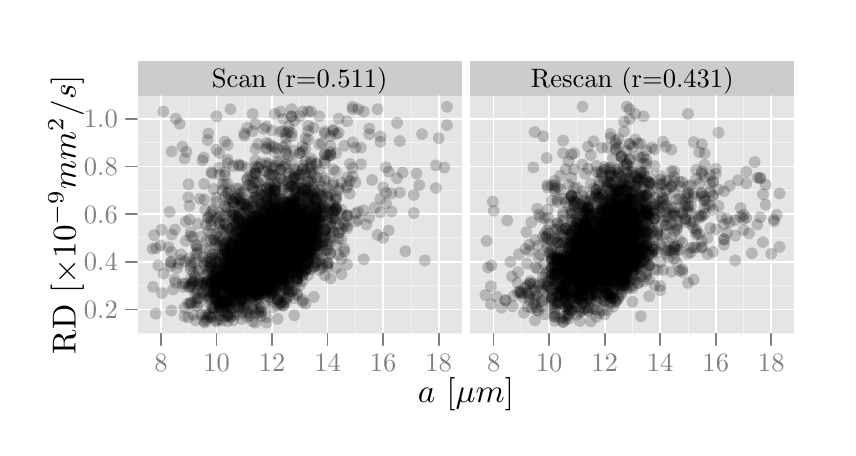
\begin{tikzpicture}[x=1pt,y=1pt]
\definecolor[named]{fillColor}{rgb}{1.00,1.00,1.00}
\path[use as bounding box,fill=fillColor,fill opacity=0.00] (0,0) rectangle (289.08,144.54);
\begin{scope}
\path[clip] (  0.00,  0.00) rectangle (289.08,144.54);
\definecolor[named]{fillColor}{rgb}{1.00,1.00,1.00}

\path[fill=fillColor] (  0.00,  0.00) rectangle (289.08,144.54);
\end{scope}
\begin{scope}
\path[clip] ( 39.69,119.86) rectangle (156.86,132.50);
\definecolor[named]{fillColor}{rgb}{0.80,0.80,0.80}

\path[fill=fillColor] ( 39.69,119.86) rectangle (156.86,132.50);
\definecolor[named]{drawColor}{rgb}{0.00,0.00,0.00}

\node[text=drawColor,anchor=base,inner sep=0pt, outer sep=0pt, scale=  0.96] at ( 98.27,122.87) {Scan (r=0.511)};
\end{scope}
\begin{scope}
\path[clip] (159.87,119.86) rectangle (277.04,132.50);
\definecolor[named]{fillColor}{rgb}{0.80,0.80,0.80}

\path[fill=fillColor] (159.87,119.86) rectangle (277.03,132.50);
\definecolor[named]{drawColor}{rgb}{0.00,0.00,0.00}

\node[text=drawColor,anchor=base,inner sep=0pt, outer sep=0pt, scale=  0.96] at (218.45,122.87) {Rescan (r=0.431)};
\end{scope}
\begin{scope}
\path[clip] (  0.00,  0.00) rectangle (289.08,144.54);
\definecolor[named]{drawColor}{rgb}{0.50,0.50,0.50}

\node[text=drawColor,anchor=base east,inner sep=0pt, outer sep=0pt, scale=  0.96] at ( 32.58, 39.45) {0.2};

\node[text=drawColor,anchor=base east,inner sep=0pt, outer sep=0pt, scale=  0.96] at ( 32.58, 56.68) {0.4};

\node[text=drawColor,anchor=base east,inner sep=0pt, outer sep=0pt, scale=  0.96] at ( 32.58, 73.90) {0.6};

\node[text=drawColor,anchor=base east,inner sep=0pt, outer sep=0pt, scale=  0.96] at ( 32.58, 91.12) {0.8};

\node[text=drawColor,anchor=base east,inner sep=0pt, outer sep=0pt, scale=  0.96] at ( 32.58,108.35) {1.0};
\end{scope}
\begin{scope}
\path[clip] (  0.00,  0.00) rectangle (289.08,144.54);
\definecolor[named]{drawColor}{rgb}{0.50,0.50,0.50}

\path[draw=drawColor,line width= 0.6pt,line join=round,line cap=round] ( 35.42, 42.76) -- ( 39.69, 42.76);

\path[draw=drawColor,line width= 0.6pt,line join=round,line cap=round] ( 35.42, 59.98) -- ( 39.69, 59.98);

\path[draw=drawColor,line width= 0.6pt,line join=round,line cap=round] ( 35.42, 77.21) -- ( 39.69, 77.21);

\path[draw=drawColor,line width= 0.6pt,line join=round,line cap=round] ( 35.42, 94.43) -- ( 39.69, 94.43);

\path[draw=drawColor,line width= 0.6pt,line join=round,line cap=round] ( 35.42,111.65) -- ( 39.69,111.65);
\end{scope}
\begin{scope}
\path[clip] ( 39.69, 34.04) rectangle (156.86,119.86);
\definecolor[named]{fillColor}{rgb}{0.90,0.90,0.90}

\path[fill=fillColor] ( 39.69, 34.04) rectangle (156.86,119.86);
\definecolor[named]{drawColor}{rgb}{0.95,0.95,0.95}

\path[draw=drawColor,line width= 0.3pt,line join=round,line cap=round] ( 39.69, 34.15) --
	(156.86, 34.15);

\path[draw=drawColor,line width= 0.3pt,line join=round,line cap=round] ( 39.69, 51.37) --
	(156.86, 51.37);

\path[draw=drawColor,line width= 0.3pt,line join=round,line cap=round] ( 39.69, 68.60) --
	(156.86, 68.60);

\path[draw=drawColor,line width= 0.3pt,line join=round,line cap=round] ( 39.69, 85.82) --
	(156.86, 85.82);

\path[draw=drawColor,line width= 0.3pt,line join=round,line cap=round] ( 39.69,103.04) --
	(156.86,103.04);

\path[draw=drawColor,line width= 0.3pt,line join=round,line cap=round] ( 58.23, 34.04) --
	( 58.23,119.86);

\path[draw=drawColor,line width= 0.3pt,line join=round,line cap=round] ( 78.30, 34.04) --
	( 78.30,119.86);

\path[draw=drawColor,line width= 0.3pt,line join=round,line cap=round] ( 98.36, 34.04) --
	( 98.36,119.86);

\path[draw=drawColor,line width= 0.3pt,line join=round,line cap=round] (118.43, 34.04) --
	(118.43,119.86);

\path[draw=drawColor,line width= 0.3pt,line join=round,line cap=round] (138.49, 34.04) --
	(138.49,119.86);
\definecolor[named]{drawColor}{rgb}{1.00,1.00,1.00}

\path[draw=drawColor,line width= 0.6pt,line join=round,line cap=round] ( 39.69, 42.76) --
	(156.86, 42.76);

\path[draw=drawColor,line width= 0.6pt,line join=round,line cap=round] ( 39.69, 59.98) --
	(156.86, 59.98);

\path[draw=drawColor,line width= 0.6pt,line join=round,line cap=round] ( 39.69, 77.21) --
	(156.86, 77.21);

\path[draw=drawColor,line width= 0.6pt,line join=round,line cap=round] ( 39.69, 94.43) --
	(156.86, 94.43);

\path[draw=drawColor,line width= 0.6pt,line join=round,line cap=round] ( 39.69,111.65) --
	(156.86,111.65);

\path[draw=drawColor,line width= 0.6pt,line join=round,line cap=round] ( 48.20, 34.04) --
	( 48.20,119.86);

\path[draw=drawColor,line width= 0.6pt,line join=round,line cap=round] ( 68.26, 34.04) --
	( 68.26,119.86);

\path[draw=drawColor,line width= 0.6pt,line join=round,line cap=round] ( 88.33, 34.04) --
	( 88.33,119.86);

\path[draw=drawColor,line width= 0.6pt,line join=round,line cap=round] (108.39, 34.04) --
	(108.39,119.86);

\path[draw=drawColor,line width= 0.6pt,line join=round,line cap=round] (128.46, 34.04) --
	(128.46,119.86);

\path[draw=drawColor,line width= 0.6pt,line join=round,line cap=round] (148.52, 34.04) --
	(148.52,119.86);
\definecolor[named]{fillColor}{rgb}{0.00,0.00,0.00}

\path[fill=fillColor,fill opacity=0.20] (141.50, 87.63) circle (  2.13);

\path[fill=fillColor,fill opacity=0.20] ( 99.36, 94.86) circle (  2.13);

\path[fill=fillColor,fill opacity=0.20] ( 94.35, 81.34) circle (  2.13);

\path[fill=fillColor,fill opacity=0.20] ( 89.33, 67.65) circle (  2.13);

\path[fill=fillColor,fill opacity=0.20] ( 91.34, 64.72) circle (  2.13);

\path[fill=fillColor,fill opacity=0.20] (102.37, 65.84) circle (  2.13);

\path[fill=fillColor,fill opacity=0.20] (109.40, 81.51) circle (  2.13);

\path[fill=fillColor,fill opacity=0.20] (107.39,107.09) circle (  2.13);

\path[fill=fillColor,fill opacity=0.20] ( 86.32, 94.69) circle (  2.13);

\path[fill=fillColor,fill opacity=0.20] ( 88.33, 68.60) circle (  2.13);

\path[fill=fillColor,fill opacity=0.20] ( 83.31, 57.83) circle (  2.13);

\path[fill=fillColor,fill opacity=0.20] ( 77.29, 59.90) circle (  2.13);

\path[fill=fillColor,fill opacity=0.20] ( 83.31, 60.33) circle (  2.13);

\path[fill=fillColor,fill opacity=0.20] ( 74.28, 57.23) circle (  2.13);

\path[fill=fillColor,fill opacity=0.20] ( 82.31, 55.85) circle (  2.13);

\path[fill=fillColor,fill opacity=0.20] ( 87.33, 69.28) circle (  2.13);

\path[fill=fillColor,fill opacity=0.20] (105.38, 76.09) circle (  2.13);

\path[fill=fillColor,fill opacity=0.20] (127.45, 77.81) circle (  2.13);

\path[fill=fillColor,fill opacity=0.20] ( 81.31,113.37) circle (  2.13);

\path[fill=fillColor,fill opacity=0.20] ( 82.31, 83.58) circle (  2.13);

\path[fill=fillColor,fill opacity=0.20] ( 83.31, 66.18) circle (  2.13);

\path[fill=fillColor,fill opacity=0.20] ( 82.31, 60.93) circle (  2.13);

\path[fill=fillColor,fill opacity=0.20] ( 83.31, 55.51) circle (  2.13);

\path[fill=fillColor,fill opacity=0.20] ( 80.30, 53.18) circle (  2.13);

\path[fill=fillColor,fill opacity=0.20] ( 81.31, 58.86) circle (  2.13);

\path[fill=fillColor,fill opacity=0.20] ( 83.31, 64.12) circle (  2.13);

\path[fill=fillColor,fill opacity=0.20] ( 84.32, 59.81) circle (  2.13);

\path[fill=fillColor,fill opacity=0.20] ( 86.32, 53.09) circle (  2.13);

\path[fill=fillColor,fill opacity=0.20] (100.37, 61.88) circle (  2.13);

\path[fill=fillColor,fill opacity=0.20] ( 98.36, 74.28) circle (  2.13);

\path[fill=fillColor,fill opacity=0.20] (105.38, 81.00) circle (  2.13);

\path[fill=fillColor,fill opacity=0.20] ( 99.36,101.66) circle (  2.13);

\path[fill=fillColor,fill opacity=0.20] ( 81.31, 86.68) circle (  2.13);

\path[fill=fillColor,fill opacity=0.20] ( 81.31, 68.08) circle (  2.13);

\path[fill=fillColor,fill opacity=0.20] ( 73.28, 53.78) circle (  2.13);

\path[fill=fillColor,fill opacity=0.20] ( 75.29, 62.83) circle (  2.13);

\path[fill=fillColor,fill opacity=0.20] ( 80.30, 60.07) circle (  2.13);

\path[fill=fillColor,fill opacity=0.20] ( 86.32, 49.22) circle (  2.13);

\path[fill=fillColor,fill opacity=0.20] ( 83.31, 55.16) circle (  2.13);

\path[fill=fillColor,fill opacity=0.20] ( 81.31, 62.65) circle (  2.13);

\path[fill=fillColor,fill opacity=0.20] ( 86.32, 60.41) circle (  2.13);

\path[fill=fillColor,fill opacity=0.20] ( 93.34, 59.55) circle (  2.13);

\path[fill=fillColor,fill opacity=0.20] ( 97.36, 67.82) circle (  2.13);

\path[fill=fillColor,fill opacity=0.20] ( 94.35, 73.68) circle (  2.13);

\path[fill=fillColor,fill opacity=0.20] ( 99.36, 80.13) circle (  2.13);

\path[fill=fillColor,fill opacity=0.20] ( 86.32, 37.94) circle (  2.13);

\path[fill=fillColor,fill opacity=0.20] (101.37, 93.48) circle (  2.13);

\path[fill=fillColor,fill opacity=0.20] ( 94.35, 70.58) circle (  2.13);

\path[fill=fillColor,fill opacity=0.20] ( 81.31, 61.45) circle (  2.13);

\path[fill=fillColor,fill opacity=0.20] ( 76.29, 49.74) circle (  2.13);

\path[fill=fillColor,fill opacity=0.20] ( 77.29, 50.17) circle (  2.13);

\path[fill=fillColor,fill opacity=0.20] ( 77.29, 55.08) circle (  2.13);

\path[fill=fillColor,fill opacity=0.20] ( 81.31, 58.35) circle (  2.13);

\path[fill=fillColor,fill opacity=0.20] ( 85.32, 58.78) circle (  2.13);

\path[fill=fillColor,fill opacity=0.20] ( 85.32, 55.25) circle (  2.13);

\path[fill=fillColor,fill opacity=0.20] ( 92.34, 56.37) circle (  2.13);

\path[fill=fillColor,fill opacity=0.20] (100.37, 64.98) circle (  2.13);

\path[fill=fillColor,fill opacity=0.20] ( 95.35, 75.66) circle (  2.13);

\path[fill=fillColor,fill opacity=0.20] ( 98.36, 88.40) circle (  2.13);

\path[fill=fillColor,fill opacity=0.20] (102.37,114.24) circle (  2.13);

\path[fill=fillColor,fill opacity=0.20] ( 96.35, 75.83) circle (  2.13);

\path[fill=fillColor,fill opacity=0.20] ( 85.32, 48.62) circle (  2.13);

\path[fill=fillColor,fill opacity=0.20] ( 84.32, 73.16) circle (  2.13);

\path[fill=fillColor,fill opacity=0.20] ( 92.34, 72.82) circle (  2.13);

\path[fill=fillColor,fill opacity=0.20] ( 92.34, 62.65) circle (  2.13);

\path[fill=fillColor,fill opacity=0.20] (102.37, 96.15) circle (  2.13);

\path[fill=fillColor,fill opacity=0.20] ( 96.35, 61.96) circle (  2.13);

\path[fill=fillColor,fill opacity=0.20] ( 80.30, 52.84) circle (  2.13);

\path[fill=fillColor,fill opacity=0.20] ( 78.30, 46.89) circle (  2.13);

\path[fill=fillColor,fill opacity=0.20] ( 79.30, 40.01) circle (  2.13);

\path[fill=fillColor,fill opacity=0.20] ( 80.30, 59.04) circle (  2.13);

\path[fill=fillColor,fill opacity=0.20] ( 78.30, 66.53) circle (  2.13);

\path[fill=fillColor,fill opacity=0.20] ( 93.34, 59.64) circle (  2.13);

\path[fill=fillColor,fill opacity=0.20] (103.38, 58.18) circle (  2.13);

\path[fill=fillColor,fill opacity=0.20] (114.41, 64.63) circle (  2.13);

\path[fill=fillColor,fill opacity=0.20] ( 99.36, 85.47) circle (  2.13);

\path[fill=fillColor,fill opacity=0.20] ( 77.29, 53.87) circle (  2.13);

\path[fill=fillColor,fill opacity=0.20] ( 79.30, 61.19) circle (  2.13);

\path[fill=fillColor,fill opacity=0.20] ( 82.31, 56.45) circle (  2.13);

\path[fill=fillColor,fill opacity=0.20] ( 80.30, 56.11) circle (  2.13);

\path[fill=fillColor,fill opacity=0.20] ( 82.31, 57.40) circle (  2.13);

\path[fill=fillColor,fill opacity=0.20] ( 86.32, 51.89) circle (  2.13);

\path[fill=fillColor,fill opacity=0.20] ( 97.36, 60.76) circle (  2.13);

\path[fill=fillColor,fill opacity=0.20] (101.37,104.07) circle (  2.13);

\path[fill=fillColor,fill opacity=0.20] ( 95.35, 89.52) circle (  2.13);

\path[fill=fillColor,fill opacity=0.20] (100.37, 58.86) circle (  2.13);

\path[fill=fillColor,fill opacity=0.20] ( 91.34, 44.48) circle (  2.13);

\path[fill=fillColor,fill opacity=0.20] ( 88.33, 49.56) circle (  2.13);

\path[fill=fillColor,fill opacity=0.20] ( 87.33, 52.66) circle (  2.13);

\path[fill=fillColor,fill opacity=0.20] ( 88.33, 43.45) circle (  2.13);

\path[fill=fillColor,fill opacity=0.20] ( 86.32, 50.08) circle (  2.13);

\path[fill=fillColor,fill opacity=0.20] ( 82.31, 70.92) circle (  2.13);

\path[fill=fillColor,fill opacity=0.20] (106.39, 65.93) circle (  2.13);

\path[fill=fillColor,fill opacity=0.20] ( 87.33, 77.29) circle (  2.13);

\path[fill=fillColor,fill opacity=0.20] ( 72.28, 51.03) circle (  2.13);

\path[fill=fillColor,fill opacity=0.20] ( 69.27, 62.22) circle (  2.13);

\path[fill=fillColor,fill opacity=0.20] ( 70.27, 55.25) circle (  2.13);

\path[fill=fillColor,fill opacity=0.20] ( 67.36, 43.02) circle (  2.13);

\path[fill=fillColor,fill opacity=0.20] ( 60.04, 40.78) circle (  2.13);

\path[fill=fillColor,fill opacity=0.20] ( 74.28, 46.29) circle (  2.13);

\path[fill=fillColor,fill opacity=0.20] ( 79.30, 42.16) circle (  2.13);

\path[fill=fillColor,fill opacity=0.20] ( 82.31, 47.76) circle (  2.13);

\path[fill=fillColor,fill opacity=0.20] (109.40, 84.27) circle (  2.13);

\path[fill=fillColor,fill opacity=0.20] (106.39, 83.67) circle (  2.13);

\path[fill=fillColor,fill opacity=0.20] (100.37, 59.64) circle (  2.13);

\path[fill=fillColor,fill opacity=0.20] ( 89.33, 54.30) circle (  2.13);

\path[fill=fillColor,fill opacity=0.20] ( 93.34, 53.35) circle (  2.13);

\path[fill=fillColor,fill opacity=0.20] ( 92.34, 61.10) circle (  2.13);

\path[fill=fillColor,fill opacity=0.20] ( 90.33, 60.16) circle (  2.13);

\path[fill=fillColor,fill opacity=0.20] ( 96.35, 56.02) circle (  2.13);

\path[fill=fillColor,fill opacity=0.20] ( 92.34, 68.60) circle (  2.13);

\path[fill=fillColor,fill opacity=0.20] ( 93.34, 76.43) circle (  2.13);

\path[fill=fillColor,fill opacity=0.20] (104.38, 72.90) circle (  2.13);

\path[fill=fillColor,fill opacity=0.20] ( 85.32,107.95) circle (  2.13);

\path[fill=fillColor,fill opacity=0.20] ( 75.29, 48.96) circle (  2.13);

\path[fill=fillColor,fill opacity=0.20] ( 69.27, 59.81) circle (  2.13);

\path[fill=fillColor,fill opacity=0.20] ( 66.06, 58.61) circle (  2.13);

\path[fill=fillColor,fill opacity=0.20] ( 64.55, 39.75) circle (  2.13);

\path[fill=fillColor,fill opacity=0.20] ( 70.27, 38.71) circle (  2.13);

\path[fill=fillColor,fill opacity=0.20] ( 68.26, 46.12) circle (  2.13);

\path[fill=fillColor,fill opacity=0.20] ( 81.31, 47.33) circle (  2.13);

\path[fill=fillColor,fill opacity=0.20] ( 84.32, 43.62) circle (  2.13);

\path[fill=fillColor,fill opacity=0.20] (100.37, 56.80) circle (  2.13);

\path[fill=fillColor,fill opacity=0.20] (115.42, 87.45) circle (  2.13);

\path[fill=fillColor,fill opacity=0.20] ( 97.36, 68.94) circle (  2.13);

\path[fill=fillColor,fill opacity=0.20] ( 93.34, 69.37) circle (  2.13);

\path[fill=fillColor,fill opacity=0.20] ( 89.33, 51.29) circle (  2.13);

\path[fill=fillColor,fill opacity=0.20] ( 90.33, 46.46) circle (  2.13);

\path[fill=fillColor,fill opacity=0.20] ( 92.34, 61.79) circle (  2.13);

\path[fill=fillColor,fill opacity=0.20] ( 87.33, 68.60) circle (  2.13);

\path[fill=fillColor,fill opacity=0.20] ( 93.34, 64.46) circle (  2.13);

\path[fill=fillColor,fill opacity=0.20] ( 90.33, 62.40) circle (  2.13);

\path[fill=fillColor,fill opacity=0.20] (102.37, 69.97) circle (  2.13);

\path[fill=fillColor,fill opacity=0.20] (133.47,110.10) circle (  2.13);

\path[fill=fillColor,fill opacity=0.20] ( 77.29, 71.70) circle (  2.13);

\path[fill=fillColor,fill opacity=0.20] ( 69.27, 52.15) circle (  2.13);

\path[fill=fillColor,fill opacity=0.20] ( 72.28, 51.03) circle (  2.13);

\path[fill=fillColor,fill opacity=0.20] ( 81.31, 42.85) circle (  2.13);

\path[fill=fillColor,fill opacity=0.20] ( 78.30, 50.94) circle (  2.13);

\path[fill=fillColor,fill opacity=0.20] ( 77.29, 53.96) circle (  2.13);

\path[fill=fillColor,fill opacity=0.20] ( 86.32, 50.68) circle (  2.13);

\path[fill=fillColor,fill opacity=0.20] ( 92.34, 51.63) circle (  2.13);

\path[fill=fillColor,fill opacity=0.20] ( 90.33, 39.32) circle (  2.13);

\path[fill=fillColor,fill opacity=0.20] (109.40, 98.39) circle (  2.13);

\path[fill=fillColor,fill opacity=0.20] (101.37, 77.90) circle (  2.13);

\path[fill=fillColor,fill opacity=0.20] ( 92.34, 70.92) circle (  2.13);

\path[fill=fillColor,fill opacity=0.20] ( 84.32, 48.27) circle (  2.13);

\path[fill=fillColor,fill opacity=0.20] ( 91.34, 51.46) circle (  2.13);

\path[fill=fillColor,fill opacity=0.20] ( 93.34, 64.38) circle (  2.13);

\path[fill=fillColor,fill opacity=0.20] ( 95.35, 64.12) circle (  2.13);

\path[fill=fillColor,fill opacity=0.20] ( 96.35, 58.52) circle (  2.13);

\path[fill=fillColor,fill opacity=0.20] ( 97.36, 59.04) circle (  2.13);

\path[fill=fillColor,fill opacity=0.20] ( 66.66, 48.79) circle (  2.13);

\path[fill=fillColor,fill opacity=0.20] ( 72.28, 44.14) circle (  2.13);

\path[fill=fillColor,fill opacity=0.20] ( 76.29, 53.09) circle (  2.13);

\path[fill=fillColor,fill opacity=0.20] ( 67.96, 46.72) circle (  2.13);

\path[fill=fillColor,fill opacity=0.20] ( 79.30, 48.79) circle (  2.13);

\path[fill=fillColor,fill opacity=0.20] ( 81.31, 54.64) circle (  2.13);

\path[fill=fillColor,fill opacity=0.20] ( 78.30, 53.78) circle (  2.13);

\path[fill=fillColor,fill opacity=0.20] ( 82.31, 55.16) circle (  2.13);

\path[fill=fillColor,fill opacity=0.20] ( 88.33, 57.14) circle (  2.13);

\path[fill=fillColor,fill opacity=0.20] ( 91.34, 45.09) circle (  2.13);

\path[fill=fillColor,fill opacity=0.20] (100.37, 44.83) circle (  2.13);

\path[fill=fillColor,fill opacity=0.20] (103.38, 82.72) circle (  2.13);

\path[fill=fillColor,fill opacity=0.20] ( 85.32, 66.27) circle (  2.13);

\path[fill=fillColor,fill opacity=0.20] ( 79.30, 54.99) circle (  2.13);

\path[fill=fillColor,fill opacity=0.20] ( 81.31, 49.39) circle (  2.13);

\path[fill=fillColor,fill opacity=0.20] ( 91.34, 48.53) circle (  2.13);

\path[fill=fillColor,fill opacity=0.20] ( 94.35, 49.99) circle (  2.13);

\path[fill=fillColor,fill opacity=0.20] ( 94.35, 57.40) circle (  2.13);

\path[fill=fillColor,fill opacity=0.20] ( 98.36, 69.11) circle (  2.13);

\path[fill=fillColor,fill opacity=0.20] ( 95.35, 62.14) circle (  2.13);

\path[fill=fillColor,fill opacity=0.20] ( 87.33, 95.29) circle (  2.13);

\path[fill=fillColor,fill opacity=0.20] ( 69.27, 42.33) circle (  2.13);

\path[fill=fillColor,fill opacity=0.20] ( 72.28, 63.00) circle (  2.13);

\path[fill=fillColor,fill opacity=0.20] ( 74.28, 61.53) circle (  2.13);

\path[fill=fillColor,fill opacity=0.20] ( 69.27, 47.33) circle (  2.13);

\path[fill=fillColor,fill opacity=0.20] ( 77.29, 48.96) circle (  2.13);

\path[fill=fillColor,fill opacity=0.20] ( 83.31, 54.04) circle (  2.13);

\path[fill=fillColor,fill opacity=0.20] ( 76.29, 55.08) circle (  2.13);

\path[fill=fillColor,fill opacity=0.20] ( 91.34, 60.41) circle (  2.13);

\path[fill=fillColor,fill opacity=0.20] ( 88.33, 56.80) circle (  2.13);

\path[fill=fillColor,fill opacity=0.20] ( 93.34, 45.34) circle (  2.13);

\path[fill=fillColor,fill opacity=0.20] (106.39, 61.10) circle (  2.13);

\path[fill=fillColor,fill opacity=0.20] ( 95.35, 63.86) circle (  2.13);

\path[fill=fillColor,fill opacity=0.20] ( 86.32, 63.69) circle (  2.13);

\path[fill=fillColor,fill opacity=0.20] ( 84.32, 62.91) circle (  2.13);

\path[fill=fillColor,fill opacity=0.20] ( 88.33, 55.33) circle (  2.13);

\path[fill=fillColor,fill opacity=0.20] ( 91.34, 45.26) circle (  2.13);

\path[fill=fillColor,fill opacity=0.20] ( 89.33, 49.39) circle (  2.13);

\path[fill=fillColor,fill opacity=0.20] ( 93.34, 71.87) circle (  2.13);

\path[fill=fillColor,fill opacity=0.20] ( 82.31, 73.85) circle (  2.13);

\path[fill=fillColor,fill opacity=0.20] ( 93.34, 64.98) circle (  2.13);

\path[fill=fillColor,fill opacity=0.20] ( 80.30, 56.54) circle (  2.13);

\path[fill=fillColor,fill opacity=0.20] ( 79.30, 55.85) circle (  2.13);

\path[fill=fillColor,fill opacity=0.20] ( 80.30, 68.16) circle (  2.13);

\path[fill=fillColor,fill opacity=0.20] ( 81.31, 60.33) circle (  2.13);

\path[fill=fillColor,fill opacity=0.20] ( 77.29, 50.51) circle (  2.13);

\path[fill=fillColor,fill opacity=0.20] ( 79.30, 54.13) circle (  2.13);

\path[fill=fillColor,fill opacity=0.20] ( 80.30, 54.21) circle (  2.13);

\path[fill=fillColor,fill opacity=0.20] ( 79.30, 49.74) circle (  2.13);

\path[fill=fillColor,fill opacity=0.20] ( 82.31, 54.21) circle (  2.13);

\path[fill=fillColor,fill opacity=0.20] ( 93.34, 53.35) circle (  2.13);

\path[fill=fillColor,fill opacity=0.20] ( 94.35, 49.05) circle (  2.13);

\path[fill=fillColor,fill opacity=0.20] (110.40, 75.40) circle (  2.13);

\path[fill=fillColor,fill opacity=0.20] (100.37, 75.48) circle (  2.13);

\path[fill=fillColor,fill opacity=0.20] ( 95.35, 70.66) circle (  2.13);

\path[fill=fillColor,fill opacity=0.20] ( 95.35, 65.24) circle (  2.13);

\path[fill=fillColor,fill opacity=0.20] ( 87.33, 57.06) circle (  2.13);

\path[fill=fillColor,fill opacity=0.20] ( 91.34, 53.53) circle (  2.13);

\path[fill=fillColor,fill opacity=0.20] ( 90.33, 53.61) circle (  2.13);

\path[fill=fillColor,fill opacity=0.20] ( 87.33, 62.40) circle (  2.13);

\path[fill=fillColor,fill opacity=0.20] ( 96.35, 67.65) circle (  2.13);

\path[fill=fillColor,fill opacity=0.20] (101.37, 60.67) circle (  2.13);

\path[fill=fillColor,fill opacity=0.20] (114.41, 74.02) circle (  2.13);

\path[fill=fillColor,fill opacity=0.20] ( 80.30, 70.75) circle (  2.13);

\path[fill=fillColor,fill opacity=0.20] ( 69.27, 53.61) circle (  2.13);

\path[fill=fillColor,fill opacity=0.20] ( 86.32, 63.77) circle (  2.13);

\path[fill=fillColor,fill opacity=0.20] ( 84.32, 62.31) circle (  2.13);

\path[fill=fillColor,fill opacity=0.20] ( 80.30, 53.70) circle (  2.13);

\path[fill=fillColor,fill opacity=0.20] ( 80.30, 50.08) circle (  2.13);

\path[fill=fillColor,fill opacity=0.20] ( 75.29, 54.39) circle (  2.13);

\path[fill=fillColor,fill opacity=0.20] ( 83.31, 51.11) circle (  2.13);

\path[fill=fillColor,fill opacity=0.20] ( 77.29, 43.62) circle (  2.13);

\path[fill=fillColor,fill opacity=0.20] ( 77.29, 50.68) circle (  2.13);

\path[fill=fillColor,fill opacity=0.20] ( 89.33, 54.99) circle (  2.13);

\path[fill=fillColor,fill opacity=0.20] ( 95.35, 58.52) circle (  2.13);

\path[fill=fillColor,fill opacity=0.20] ( 98.36, 84.10) circle (  2.13);

\path[fill=fillColor,fill opacity=0.20] ( 86.32, 65.32) circle (  2.13);

\path[fill=fillColor,fill opacity=0.20] ( 87.33, 53.96) circle (  2.13);

\path[fill=fillColor,fill opacity=0.20] ( 89.33, 57.92) circle (  2.13);

\path[fill=fillColor,fill opacity=0.20] ( 87.33, 57.92) circle (  2.13);

\path[fill=fillColor,fill opacity=0.20] ( 88.33, 50.34) circle (  2.13);

\path[fill=fillColor,fill opacity=0.20] ( 90.33, 46.38) circle (  2.13);

\path[fill=fillColor,fill opacity=0.20] ( 97.36, 48.44) circle (  2.13);

\path[fill=fillColor,fill opacity=0.20] ( 97.36, 56.37) circle (  2.13);

\path[fill=fillColor,fill opacity=0.20] (105.38, 74.80) circle (  2.13);

\path[fill=fillColor,fill opacity=0.20] ( 84.32, 86.08) circle (  2.13);

\path[fill=fillColor,fill opacity=0.20] ( 76.29, 49.48) circle (  2.13);

\path[fill=fillColor,fill opacity=0.20] ( 77.29, 57.23) circle (  2.13);

\path[fill=fillColor,fill opacity=0.20] ( 82.31, 54.21) circle (  2.13);

\path[fill=fillColor,fill opacity=0.20] ( 75.29, 51.72) circle (  2.13);

\path[fill=fillColor,fill opacity=0.20] ( 75.29, 53.18) circle (  2.13);

\path[fill=fillColor,fill opacity=0.20] ( 75.29, 52.58) circle (  2.13);

\path[fill=fillColor,fill opacity=0.20] ( 74.28, 49.31) circle (  2.13);

\path[fill=fillColor,fill opacity=0.20] ( 78.30, 45.52) circle (  2.13);

\path[fill=fillColor,fill opacity=0.20] ( 79.30, 48.19) circle (  2.13);

\path[fill=fillColor,fill opacity=0.20] ( 84.32, 59.38) circle (  2.13);

\path[fill=fillColor,fill opacity=0.20] ( 81.31, 65.41) circle (  2.13);

\path[fill=fillColor,fill opacity=0.20] ( 90.33, 74.45) circle (  2.13);

\path[fill=fillColor,fill opacity=0.20] ( 83.31, 78.84) circle (  2.13);

\path[fill=fillColor,fill opacity=0.20] ( 77.29, 54.64) circle (  2.13);

\path[fill=fillColor,fill opacity=0.20] ( 90.33, 52.92) circle (  2.13);

\path[fill=fillColor,fill opacity=0.20] ( 86.32, 54.56) circle (  2.13);

\path[fill=fillColor,fill opacity=0.20] ( 89.33, 48.27) circle (  2.13);

\path[fill=fillColor,fill opacity=0.20] ( 93.34, 46.38) circle (  2.13);

\path[fill=fillColor,fill opacity=0.20] ( 87.33, 48.96) circle (  2.13);

\path[fill=fillColor,fill opacity=0.20] ( 92.34, 55.76) circle (  2.13);

\path[fill=fillColor,fill opacity=0.20] ( 96.35, 68.51) circle (  2.13);

\path[fill=fillColor,fill opacity=0.20] (111.40, 82.55) circle (  2.13);

\path[fill=fillColor,fill opacity=0.20] ( 82.31, 96.58) circle (  2.13);

\path[fill=fillColor,fill opacity=0.20] ( 78.30, 56.71) circle (  2.13);

\path[fill=fillColor,fill opacity=0.20] ( 76.29, 62.74) circle (  2.13);

\path[fill=fillColor,fill opacity=0.20] ( 80.30, 53.78) circle (  2.13);

\path[fill=fillColor,fill opacity=0.20] ( 76.29, 45.95) circle (  2.13);

\path[fill=fillColor,fill opacity=0.20] ( 75.29, 49.99) circle (  2.13);

\path[fill=fillColor,fill opacity=0.20] ( 75.29, 58.18) circle (  2.13);

\path[fill=fillColor,fill opacity=0.20] ( 75.29, 61.19) circle (  2.13);

\path[fill=fillColor,fill opacity=0.20] ( 72.28, 54.56) circle (  2.13);

\path[fill=fillColor,fill opacity=0.20] ( 79.30, 50.34) circle (  2.13);

\path[fill=fillColor,fill opacity=0.20] ( 78.30, 56.11) circle (  2.13);

\path[fill=fillColor,fill opacity=0.20] ( 80.30, 62.83) circle (  2.13);

\path[fill=fillColor,fill opacity=0.20] ( 83.31, 76.17) circle (  2.13);

\path[fill=fillColor,fill opacity=0.20] (100.37,100.80) circle (  2.13);

\path[fill=fillColor,fill opacity=0.20] (112.41,106.49) circle (  2.13);

\path[fill=fillColor,fill opacity=0.20] ( 94.35, 72.64) circle (  2.13);

\path[fill=fillColor,fill opacity=0.20] ( 88.33, 57.83) circle (  2.13);

\path[fill=fillColor,fill opacity=0.20] ( 90.33, 54.04) circle (  2.13);

\path[fill=fillColor,fill opacity=0.20] ( 93.34, 57.66) circle (  2.13);

\path[fill=fillColor,fill opacity=0.20] ( 86.32, 58.43) circle (  2.13);

\path[fill=fillColor,fill opacity=0.20] ( 90.33, 55.68) circle (  2.13);

\path[fill=fillColor,fill opacity=0.20] ( 89.33, 59.21) circle (  2.13);

\path[fill=fillColor,fill opacity=0.20] ( 95.35, 70.32) circle (  2.13);

\path[fill=fillColor,fill opacity=0.20] ( 96.35, 77.64) circle (  2.13);

\path[fill=fillColor,fill opacity=0.20] (105.38, 84.18) circle (  2.13);

\path[fill=fillColor,fill opacity=0.20] ( 89.33, 99.51) circle (  2.13);

\path[fill=fillColor,fill opacity=0.20] ( 80.30, 54.56) circle (  2.13);

\path[fill=fillColor,fill opacity=0.20] ( 77.29, 66.53) circle (  2.13);

\path[fill=fillColor,fill opacity=0.20] ( 80.30, 62.74) circle (  2.13);

\path[fill=fillColor,fill opacity=0.20] ( 78.30, 53.78) circle (  2.13);

\path[fill=fillColor,fill opacity=0.20] ( 73.28, 56.80) circle (  2.13);

\path[fill=fillColor,fill opacity=0.20] ( 79.30, 58.18) circle (  2.13);

\path[fill=fillColor,fill opacity=0.20] ( 79.30, 57.66) circle (  2.13);

\path[fill=fillColor,fill opacity=0.20] ( 75.29, 59.21) circle (  2.13);

\path[fill=fillColor,fill opacity=0.20] ( 76.29, 61.62) circle (  2.13);

\path[fill=fillColor,fill opacity=0.20] ( 74.28, 66.10) circle (  2.13);

\path[fill=fillColor,fill opacity=0.20] ( 77.29, 62.14) circle (  2.13);

\path[fill=fillColor,fill opacity=0.20] ( 90.33, 58.26) circle (  2.13);

\path[fill=fillColor,fill opacity=0.20] (111.40,106.14) circle (  2.13);

\path[fill=fillColor,fill opacity=0.20] ( 86.32, 81.86) circle (  2.13);

\path[fill=fillColor,fill opacity=0.20] ( 85.32, 61.79) circle (  2.13);

\path[fill=fillColor,fill opacity=0.20] ( 91.34, 61.10) circle (  2.13);

\path[fill=fillColor,fill opacity=0.20] ( 86.32, 55.42) circle (  2.13);

\path[fill=fillColor,fill opacity=0.20] ( 83.31, 47.76) circle (  2.13);

\path[fill=fillColor,fill opacity=0.20] ( 90.33, 54.90) circle (  2.13);

\path[fill=fillColor,fill opacity=0.20] ( 91.34, 60.93) circle (  2.13);

\path[fill=fillColor,fill opacity=0.20] ( 91.34, 63.95) circle (  2.13);

\path[fill=fillColor,fill opacity=0.20] ( 93.34, 66.61) circle (  2.13);

\path[fill=fillColor,fill opacity=0.20] (103.38, 72.13) circle (  2.13);

\path[fill=fillColor,fill opacity=0.20] ( 95.35,106.49) circle (  2.13);

\path[fill=fillColor,fill opacity=0.20] ( 84.32, 59.04) circle (  2.13);

\path[fill=fillColor,fill opacity=0.20] ( 79.30, 67.05) circle (  2.13);

\path[fill=fillColor,fill opacity=0.20] ( 74.28, 62.74) circle (  2.13);

\path[fill=fillColor,fill opacity=0.20] ( 77.29, 50.34) circle (  2.13);

\path[fill=fillColor,fill opacity=0.20] ( 72.28, 49.39) circle (  2.13);

\path[fill=fillColor,fill opacity=0.20] ( 73.28, 55.94) circle (  2.13);

\path[fill=fillColor,fill opacity=0.20] ( 76.29, 59.47) circle (  2.13);

\path[fill=fillColor,fill opacity=0.20] ( 75.29, 54.90) circle (  2.13);

\path[fill=fillColor,fill opacity=0.20] ( 71.27, 53.70) circle (  2.13);

\path[fill=fillColor,fill opacity=0.20] ( 72.28, 62.74) circle (  2.13);

\path[fill=fillColor,fill opacity=0.20] ( 45.69, 69.54) circle (  2.13);

\path[fill=fillColor,fill opacity=0.20] ( 78.30, 67.05) circle (  2.13);

\path[fill=fillColor,fill opacity=0.20] ( 98.36, 65.06) circle (  2.13);

\path[fill=fillColor,fill opacity=0.20] (112.41,111.65) circle (  2.13);

\path[fill=fillColor,fill opacity=0.20] ( 85.32, 77.81) circle (  2.13);

\path[fill=fillColor,fill opacity=0.20] ( 81.31, 59.47) circle (  2.13);

\path[fill=fillColor,fill opacity=0.20] ( 82.31, 48.19) circle (  2.13);

\path[fill=fillColor,fill opacity=0.20] ( 76.29, 43.79) circle (  2.13);

\path[fill=fillColor,fill opacity=0.20] ( 85.32, 51.80) circle (  2.13);

\path[fill=fillColor,fill opacity=0.20] ( 89.33, 55.42) circle (  2.13);

\path[fill=fillColor,fill opacity=0.20] ( 89.33, 60.59) circle (  2.13);

\path[fill=fillColor,fill opacity=0.20] ( 97.36, 66.44) circle (  2.13);

\path[fill=fillColor,fill opacity=0.20] (102.37, 66.96) circle (  2.13);

\path[fill=fillColor,fill opacity=0.20] (107.39, 78.15) circle (  2.13);

\path[fill=fillColor,fill opacity=0.20] ( 93.34,100.03) circle (  2.13);

\path[fill=fillColor,fill opacity=0.20] ( 81.31, 65.84) circle (  2.13);

\path[fill=fillColor,fill opacity=0.20] ( 83.31, 71.27) circle (  2.13);

\path[fill=fillColor,fill opacity=0.20] ( 77.29, 63.77) circle (  2.13);

\path[fill=fillColor,fill opacity=0.20] ( 72.28, 52.15) circle (  2.13);

\path[fill=fillColor,fill opacity=0.20] ( 69.27, 45.69) circle (  2.13);

\path[fill=fillColor,fill opacity=0.20] ( 66.66, 43.54) circle (  2.13);

\path[fill=fillColor,fill opacity=0.20] ( 72.28, 45.43) circle (  2.13);

\path[fill=fillColor,fill opacity=0.20] ( 73.28, 52.06) circle (  2.13);

\path[fill=fillColor,fill opacity=0.20] ( 71.27, 56.97) circle (  2.13);

\path[fill=fillColor,fill opacity=0.20] ( 73.28, 58.69) circle (  2.13);

\path[fill=fillColor,fill opacity=0.20] ( 67.96, 60.24) circle (  2.13);

\path[fill=fillColor,fill opacity=0.20] ( 75.29, 62.22) circle (  2.13);

\path[fill=fillColor,fill opacity=0.20] ( 95.35, 74.28) circle (  2.13);

\path[fill=fillColor,fill opacity=0.20] (110.40,107.69) circle (  2.13);

\path[fill=fillColor,fill opacity=0.20] ( 74.28, 75.31) circle (  2.13);

\path[fill=fillColor,fill opacity=0.20] ( 79.30, 61.53) circle (  2.13);

\path[fill=fillColor,fill opacity=0.20] ( 78.30, 58.52) circle (  2.13);

\path[fill=fillColor,fill opacity=0.20] ( 80.30, 57.14) circle (  2.13);

\path[fill=fillColor,fill opacity=0.20] ( 89.33, 61.28) circle (  2.13);

\path[fill=fillColor,fill opacity=0.20] ( 87.33, 68.08) circle (  2.13);

\path[fill=fillColor,fill opacity=0.20] ( 91.34, 68.42) circle (  2.13);

\path[fill=fillColor,fill opacity=0.20] (102.37, 68.85) circle (  2.13);

\path[fill=fillColor,fill opacity=0.20] ( 99.36, 70.92) circle (  2.13);

\path[fill=fillColor,fill opacity=0.20] (104.38, 69.37) circle (  2.13);

\path[fill=fillColor,fill opacity=0.20] ( 99.36, 78.67) circle (  2.13);

\path[fill=fillColor,fill opacity=0.20] ( 80.30, 54.73) circle (  2.13);

\path[fill=fillColor,fill opacity=0.20] ( 66.26, 73.07) circle (  2.13);

\path[fill=fillColor,fill opacity=0.20] ( 75.29, 72.64) circle (  2.13);

\path[fill=fillColor,fill opacity=0.20] ( 71.27, 54.47) circle (  2.13);

\path[fill=fillColor,fill opacity=0.20] ( 69.27, 53.53) circle (  2.13);

\path[fill=fillColor,fill opacity=0.20] ( 66.66, 56.88) circle (  2.13);

\path[fill=fillColor,fill opacity=0.20] ( 68.26, 51.37) circle (  2.13);

\path[fill=fillColor,fill opacity=0.20] ( 72.28, 45.43) circle (  2.13);

\path[fill=fillColor,fill opacity=0.20] ( 72.28, 48.10) circle (  2.13);

\path[fill=fillColor,fill opacity=0.20] ( 73.28, 56.11) circle (  2.13);

\path[fill=fillColor,fill opacity=0.20] ( 76.29, 56.80) circle (  2.13);

\path[fill=fillColor,fill opacity=0.20] ( 75.29, 57.31) circle (  2.13);

\path[fill=fillColor,fill opacity=0.20] ( 96.35, 69.80) circle (  2.13);

\path[fill=fillColor,fill opacity=0.20] ( 75.29, 86.42) circle (  2.13);

\path[fill=fillColor,fill opacity=0.20] ( 76.29, 77.21) circle (  2.13);

\path[fill=fillColor,fill opacity=0.20] ( 86.32, 62.05) circle (  2.13);

\path[fill=fillColor,fill opacity=0.20] ( 89.33, 58.61) circle (  2.13);

\path[fill=fillColor,fill opacity=0.20] ( 85.32, 68.60) circle (  2.13);

\path[fill=fillColor,fill opacity=0.20] ( 89.33, 67.13) circle (  2.13);

\path[fill=fillColor,fill opacity=0.20] ( 96.35, 63.34) circle (  2.13);

\path[fill=fillColor,fill opacity=0.20] ( 99.36, 64.55) circle (  2.13);

\path[fill=fillColor,fill opacity=0.20] (105.38, 60.41) circle (  2.13);

\path[fill=fillColor,fill opacity=0.20] ( 96.35, 59.12) circle (  2.13);

\path[fill=fillColor,fill opacity=0.20] (105.38, 66.10) circle (  2.13);

\path[fill=fillColor,fill opacity=0.20] (112.41, 86.42) circle (  2.13);

\path[fill=fillColor,fill opacity=0.20] ( 93.34, 56.97) circle (  2.13);

\path[fill=fillColor,fill opacity=0.20] ( 85.32, 55.85) circle (  2.13);

\path[fill=fillColor,fill opacity=0.20] ( 72.28, 62.22) circle (  2.13);

\path[fill=fillColor,fill opacity=0.20] ( 77.29, 63.17) circle (  2.13);

\path[fill=fillColor,fill opacity=0.20] ( 74.28, 62.22) circle (  2.13);

\path[fill=fillColor,fill opacity=0.20] ( 73.28, 59.81) circle (  2.13);

\path[fill=fillColor,fill opacity=0.20] ( 70.27, 62.31) circle (  2.13);

\path[fill=fillColor,fill opacity=0.20] ( 67.66, 67.65) circle (  2.13);

\path[fill=fillColor,fill opacity=0.20] ( 67.66, 62.74) circle (  2.13);

\path[fill=fillColor,fill opacity=0.20] ( 69.27, 52.06) circle (  2.13);

\path[fill=fillColor,fill opacity=0.20] ( 73.28, 50.25) circle (  2.13);

\path[fill=fillColor,fill opacity=0.20] ( 76.29, 52.84) circle (  2.13);

\path[fill=fillColor,fill opacity=0.20] ( 90.33, 52.58) circle (  2.13);

\path[fill=fillColor,fill opacity=0.20] ( 95.35, 66.70) circle (  2.13);

\path[fill=fillColor,fill opacity=0.20] ( 93.34, 95.12) circle (  2.13);

\path[fill=fillColor,fill opacity=0.20] ( 88.33, 72.13) circle (  2.13);

\path[fill=fillColor,fill opacity=0.20] ( 86.32, 54.04) circle (  2.13);

\path[fill=fillColor,fill opacity=0.20] ( 83.31, 57.57) circle (  2.13);

\path[fill=fillColor,fill opacity=0.20] ( 86.32, 64.29) circle (  2.13);

\path[fill=fillColor,fill opacity=0.20] ( 93.34, 61.79) circle (  2.13);

\path[fill=fillColor,fill opacity=0.20] (101.37, 63.00) circle (  2.13);

\path[fill=fillColor,fill opacity=0.20] (105.38, 71.87) circle (  2.13);

\path[fill=fillColor,fill opacity=0.20] (104.38, 74.11) circle (  2.13);

\path[fill=fillColor,fill opacity=0.20] (103.38, 63.69) circle (  2.13);

\path[fill=fillColor,fill opacity=0.20] (107.39, 55.08) circle (  2.13);

\path[fill=fillColor,fill opacity=0.20] (108.39, 59.55) circle (  2.13);

\path[fill=fillColor,fill opacity=0.20] (115.42, 76.52) circle (  2.13);

\path[fill=fillColor,fill opacity=0.20] (106.39, 74.37) circle (  2.13);

\path[fill=fillColor,fill opacity=0.20] ( 97.36, 69.97) circle (  2.13);

\path[fill=fillColor,fill opacity=0.20] ( 86.32, 66.70) circle (  2.13);

\path[fill=fillColor,fill opacity=0.20] ( 81.31, 65.84) circle (  2.13);

\path[fill=fillColor,fill opacity=0.20] ( 57.13, 67.48) circle (  2.13);

\path[fill=fillColor,fill opacity=0.20] ( 76.29, 65.75) circle (  2.13);

\path[fill=fillColor,fill opacity=0.20] ( 82.31, 55.59) circle (  2.13);

\path[fill=fillColor,fill opacity=0.20] ( 73.28, 54.90) circle (  2.13);

\path[fill=fillColor,fill opacity=0.20] ( 71.27, 63.08) circle (  2.13);

\path[fill=fillColor,fill opacity=0.20] ( 71.27, 66.36) circle (  2.13);

\path[fill=fillColor,fill opacity=0.20] ( 69.27, 67.22) circle (  2.13);

\path[fill=fillColor,fill opacity=0.20] ( 66.46, 70.06) circle (  2.13);

\path[fill=fillColor,fill opacity=0.20] ( 74.28, 66.10) circle (  2.13);

\path[fill=fillColor,fill opacity=0.20] ( 78.30, 58.00) circle (  2.13);

\path[fill=fillColor,fill opacity=0.20] ( 92.34, 63.43) circle (  2.13);

\path[fill=fillColor,fill opacity=0.20] (102.37, 95.29) circle (  2.13);

\path[fill=fillColor,fill opacity=0.20] ( 90.33, 72.99) circle (  2.13);

\path[fill=fillColor,fill opacity=0.20] ( 83.31, 59.98) circle (  2.13);

\path[fill=fillColor,fill opacity=0.20] ( 85.32, 62.74) circle (  2.13);

\path[fill=fillColor,fill opacity=0.20] ( 91.34, 62.57) circle (  2.13);

\path[fill=fillColor,fill opacity=0.20] ( 90.33, 59.12) circle (  2.13);

\path[fill=fillColor,fill opacity=0.20] ( 93.34, 68.51) circle (  2.13);

\path[fill=fillColor,fill opacity=0.20] ( 95.35, 73.25) circle (  2.13);

\path[fill=fillColor,fill opacity=0.20] (100.37, 65.58) circle (  2.13);

\path[fill=fillColor,fill opacity=0.20] (101.37, 57.49) circle (  2.13);

\path[fill=fillColor,fill opacity=0.20] (100.37, 56.88) circle (  2.13);

\path[fill=fillColor,fill opacity=0.20] ( 99.36, 65.93) circle (  2.13);

\path[fill=fillColor,fill opacity=0.20] (105.38, 73.93) circle (  2.13);

\path[fill=fillColor,fill opacity=0.20] (109.40, 68.60) circle (  2.13);

\path[fill=fillColor,fill opacity=0.20] (111.40, 75.57) circle (  2.13);

\path[fill=fillColor,fill opacity=0.20] (107.39, 79.53) circle (  2.13);

\path[fill=fillColor,fill opacity=0.20] (106.39, 79.70) circle (  2.13);

\path[fill=fillColor,fill opacity=0.20] ( 78.30, 80.74) circle (  2.13);

\path[fill=fillColor,fill opacity=0.20] ( 87.33, 69.28) circle (  2.13);

\path[fill=fillColor,fill opacity=0.20] ( 83.31, 67.22) circle (  2.13);

\path[fill=fillColor,fill opacity=0.20] ( 73.28, 78.07) circle (  2.13);

\path[fill=fillColor,fill opacity=0.20] ( 77.29, 74.62) circle (  2.13);

\path[fill=fillColor,fill opacity=0.20] ( 76.29, 63.69) circle (  2.13);

\path[fill=fillColor,fill opacity=0.20] ( 84.32, 63.17) circle (  2.13);

\path[fill=fillColor,fill opacity=0.20] ( 76.29, 58.86) circle (  2.13);

\path[fill=fillColor,fill opacity=0.20] ( 69.27, 58.26) circle (  2.13);

\path[fill=fillColor,fill opacity=0.20] ( 61.24, 64.72) circle (  2.13);

\path[fill=fillColor,fill opacity=0.20] ( 73.28, 63.34) circle (  2.13);

\path[fill=fillColor,fill opacity=0.20] ( 77.29, 64.12) circle (  2.13);

\path[fill=fillColor,fill opacity=0.20] ( 75.29, 74.11) circle (  2.13);

\path[fill=fillColor,fill opacity=0.20] ( 86.32, 80.39) circle (  2.13);

\path[fill=fillColor,fill opacity=0.20] ( 89.33, 78.33) circle (  2.13);

\path[fill=fillColor,fill opacity=0.20] (100.37, 85.73) circle (  2.13);

\path[fill=fillColor,fill opacity=0.20] ( 89.33, 79.53) circle (  2.13);

\path[fill=fillColor,fill opacity=0.20] ( 87.33, 69.11) circle (  2.13);

\path[fill=fillColor,fill opacity=0.20] ( 82.31, 53.87) circle (  2.13);

\path[fill=fillColor,fill opacity=0.20] ( 82.31, 50.86) circle (  2.13);

\path[fill=fillColor,fill opacity=0.20] ( 90.33, 59.21) circle (  2.13);

\path[fill=fillColor,fill opacity=0.20] ( 97.36, 59.81) circle (  2.13);

\path[fill=fillColor,fill opacity=0.20] ( 96.35, 62.31) circle (  2.13);

\path[fill=fillColor,fill opacity=0.20] (101.37, 67.82) circle (  2.13);

\path[fill=fillColor,fill opacity=0.20] (101.37, 68.68) circle (  2.13);

\path[fill=fillColor,fill opacity=0.20] (103.38, 70.83) circle (  2.13);

\path[fill=fillColor,fill opacity=0.20] (107.39, 71.09) circle (  2.13);

\path[fill=fillColor,fill opacity=0.20] (106.39, 66.87) circle (  2.13);

\path[fill=fillColor,fill opacity=0.20] (103.38, 65.50) circle (  2.13);

\path[fill=fillColor,fill opacity=0.20] (102.37, 67.05) circle (  2.13);

\path[fill=fillColor,fill opacity=0.20] (102.37, 69.63) circle (  2.13);

\path[fill=fillColor,fill opacity=0.20] (104.38, 76.69) circle (  2.13);

\path[fill=fillColor,fill opacity=0.20] ( 98.36, 67.65) circle (  2.13);

\path[fill=fillColor,fill opacity=0.20] (108.39, 58.09) circle (  2.13);

\path[fill=fillColor,fill opacity=0.20] (109.40, 71.44) circle (  2.13);

\path[fill=fillColor,fill opacity=0.20] ( 99.36, 84.53) circle (  2.13);

\path[fill=fillColor,fill opacity=0.20] ( 98.36, 78.93) circle (  2.13);

\path[fill=fillColor,fill opacity=0.20] (101.37, 75.57) circle (  2.13);

\path[fill=fillColor,fill opacity=0.20] (102.37, 80.57) circle (  2.13);

\path[fill=fillColor,fill opacity=0.20] (103.38, 80.48) circle (  2.13);

\path[fill=fillColor,fill opacity=0.20] ( 96.35, 72.04) circle (  2.13);

\path[fill=fillColor,fill opacity=0.20] (100.37, 67.82) circle (  2.13);

\path[fill=fillColor,fill opacity=0.20] (101.37, 70.58) circle (  2.13);

\path[fill=fillColor,fill opacity=0.20] ( 99.36, 79.88) circle (  2.13);

\path[fill=fillColor,fill opacity=0.20] ( 98.36, 83.49) circle (  2.13);

\path[fill=fillColor,fill opacity=0.20] (100.37, 77.21) circle (  2.13);

\path[fill=fillColor,fill opacity=0.20] (100.37, 72.73) circle (  2.13);

\path[fill=fillColor,fill opacity=0.20] ( 94.35, 69.37) circle (  2.13);

\path[fill=fillColor,fill opacity=0.20] ( 88.33, 67.65) circle (  2.13);

\path[fill=fillColor,fill opacity=0.20] ( 81.31, 74.71) circle (  2.13);

\path[fill=fillColor,fill opacity=0.20] ( 79.30, 75.23) circle (  2.13);

\path[fill=fillColor,fill opacity=0.20] ( 85.32, 68.25) circle (  2.13);

\path[fill=fillColor,fill opacity=0.20] ( 81.31, 69.03) circle (  2.13);

\path[fill=fillColor,fill opacity=0.20] ( 76.29, 66.61) circle (  2.13);

\path[fill=fillColor,fill opacity=0.20] ( 79.30, 60.93) circle (  2.13);

\path[fill=fillColor,fill opacity=0.20] ( 80.30, 58.00) circle (  2.13);

\path[fill=fillColor,fill opacity=0.20] ( 81.31, 57.49) circle (  2.13);

\path[fill=fillColor,fill opacity=0.20] ( 78.30, 64.46) circle (  2.13);

\path[fill=fillColor,fill opacity=0.20] ( 82.31, 75.83) circle (  2.13);

\path[fill=fillColor,fill opacity=0.20] ( 90.33, 72.64) circle (  2.13);

\path[fill=fillColor,fill opacity=0.20] ( 76.29, 75.31) circle (  2.13);

\path[fill=fillColor,fill opacity=0.20] ( 88.33, 81.94) circle (  2.13);

\path[fill=fillColor,fill opacity=0.20] ( 95.35, 77.81) circle (  2.13);

\path[fill=fillColor,fill opacity=0.20] ( 89.33, 86.59) circle (  2.13);

\path[fill=fillColor,fill opacity=0.20] ( 91.34, 71.18) circle (  2.13);

\path[fill=fillColor,fill opacity=0.20] ( 88.33, 58.69) circle (  2.13);

\path[fill=fillColor,fill opacity=0.20] ( 87.33, 58.26) circle (  2.13);

\path[fill=fillColor,fill opacity=0.20] ( 89.33, 61.45) circle (  2.13);

\path[fill=fillColor,fill opacity=0.20] ( 92.34, 57.75) circle (  2.13);

\path[fill=fillColor,fill opacity=0.20] ( 97.36, 60.07) circle (  2.13);

\path[fill=fillColor,fill opacity=0.20] (102.37, 63.26) circle (  2.13);

\path[fill=fillColor,fill opacity=0.20] (102.37, 63.43) circle (  2.13);

\path[fill=fillColor,fill opacity=0.20] (101.37, 67.39) circle (  2.13);

\path[fill=fillColor,fill opacity=0.20] (103.38, 70.15) circle (  2.13);

\path[fill=fillColor,fill opacity=0.20] ( 97.36, 68.25) circle (  2.13);

\path[fill=fillColor,fill opacity=0.20] ( 88.33, 70.06) circle (  2.13);

\path[fill=fillColor,fill opacity=0.20] (100.37, 71.78) circle (  2.13);

\path[fill=fillColor,fill opacity=0.20] ( 99.36, 69.46) circle (  2.13);

\path[fill=fillColor,fill opacity=0.20] (102.37, 63.34) circle (  2.13);

\path[fill=fillColor,fill opacity=0.20] ( 99.36, 55.94) circle (  2.13);

\path[fill=fillColor,fill opacity=0.20] (102.37, 59.21) circle (  2.13);

\path[fill=fillColor,fill opacity=0.20] ( 98.36, 64.98) circle (  2.13);

\path[fill=fillColor,fill opacity=0.20] (103.38, 61.28) circle (  2.13);

\path[fill=fillColor,fill opacity=0.20] ( 96.35, 61.10) circle (  2.13);

\path[fill=fillColor,fill opacity=0.20] ( 93.34, 66.96) circle (  2.13);

\path[fill=fillColor,fill opacity=0.20] ( 91.34, 67.65) circle (  2.13);

\path[fill=fillColor,fill opacity=0.20] ( 89.33, 67.82) circle (  2.13);

\path[fill=fillColor,fill opacity=0.20] ( 92.34, 69.46) circle (  2.13);

\path[fill=fillColor,fill opacity=0.20] ( 92.34, 69.97) circle (  2.13);

\path[fill=fillColor,fill opacity=0.20] ( 90.33, 74.62) circle (  2.13);

\path[fill=fillColor,fill opacity=0.20] ( 90.33, 78.58) circle (  2.13);

\path[fill=fillColor,fill opacity=0.20] ( 86.32, 74.71) circle (  2.13);

\path[fill=fillColor,fill opacity=0.20] ( 86.32, 68.34) circle (  2.13);

\path[fill=fillColor,fill opacity=0.20] ( 82.31, 66.44) circle (  2.13);

\path[fill=fillColor,fill opacity=0.20] ( 81.31, 68.08) circle (  2.13);

\path[fill=fillColor,fill opacity=0.20] ( 87.33, 58.00) circle (  2.13);

\path[fill=fillColor,fill opacity=0.20] ( 83.31, 45.52) circle (  2.13);

\path[fill=fillColor,fill opacity=0.20] ( 87.33, 54.13) circle (  2.13);

\path[fill=fillColor,fill opacity=0.20] ( 84.32, 61.79) circle (  2.13);

\path[fill=fillColor,fill opacity=0.20] ( 83.31, 58.35) circle (  2.13);

\path[fill=fillColor,fill opacity=0.20] ( 86.32, 64.89) circle (  2.13);

\path[fill=fillColor,fill opacity=0.20] ( 88.33, 69.37) circle (  2.13);

\path[fill=fillColor,fill opacity=0.20] ( 84.32, 72.04) circle (  2.13);

\path[fill=fillColor,fill opacity=0.20] ( 86.32, 86.34) circle (  2.13);

\path[fill=fillColor,fill opacity=0.20] ( 98.36, 90.04) circle (  2.13);

\path[fill=fillColor,fill opacity=0.20] ( 73.28, 85.73) circle (  2.13);

\path[fill=fillColor,fill opacity=0.20] (111.40, 99.17) circle (  2.13);

\path[fill=fillColor,fill opacity=0.20] ( 89.33, 87.54) circle (  2.13);

\path[fill=fillColor,fill opacity=0.20] ( 88.33, 76.86) circle (  2.13);

\path[fill=fillColor,fill opacity=0.20] ( 91.34, 71.87) circle (  2.13);

\path[fill=fillColor,fill opacity=0.20] ( 87.33, 64.20) circle (  2.13);

\path[fill=fillColor,fill opacity=0.20] ( 91.34, 54.39) circle (  2.13);

\path[fill=fillColor,fill opacity=0.20] ( 92.34, 52.84) circle (  2.13);

\path[fill=fillColor,fill opacity=0.20] ( 96.35, 59.98) circle (  2.13);

\path[fill=fillColor,fill opacity=0.20] ( 97.36, 67.73) circle (  2.13);

\path[fill=fillColor,fill opacity=0.20] ( 95.35, 68.08) circle (  2.13);

\path[fill=fillColor,fill opacity=0.20] ( 97.36, 69.28) circle (  2.13);

\path[fill=fillColor,fill opacity=0.20] ( 99.36, 73.68) circle (  2.13);

\path[fill=fillColor,fill opacity=0.20] ( 96.35, 72.82) circle (  2.13);

\path[fill=fillColor,fill opacity=0.20] ( 95.35, 68.25) circle (  2.13);

\path[fill=fillColor,fill opacity=0.20] ( 97.36, 68.08) circle (  2.13);

\path[fill=fillColor,fill opacity=0.20] ( 96.35, 68.94) circle (  2.13);

\path[fill=fillColor,fill opacity=0.20] ( 96.35, 67.39) circle (  2.13);

\path[fill=fillColor,fill opacity=0.20] (102.37, 65.75) circle (  2.13);

\path[fill=fillColor,fill opacity=0.20] ( 99.36, 64.20) circle (  2.13);

\path[fill=fillColor,fill opacity=0.20] ( 89.33, 64.72) circle (  2.13);

\path[fill=fillColor,fill opacity=0.20] ( 95.35, 65.15) circle (  2.13);

\path[fill=fillColor,fill opacity=0.20] (100.37, 66.18) circle (  2.13);

\path[fill=fillColor,fill opacity=0.20] (100.37, 71.78) circle (  2.13);

\path[fill=fillColor,fill opacity=0.20] ( 95.35, 74.02) circle (  2.13);

\path[fill=fillColor,fill opacity=0.20] ( 97.36, 71.27) circle (  2.13);

\path[fill=fillColor,fill opacity=0.20] ( 93.34, 68.85) circle (  2.13);

\path[fill=fillColor,fill opacity=0.20] ( 92.34, 66.01) circle (  2.13);

\path[fill=fillColor,fill opacity=0.20] ( 89.33, 64.81) circle (  2.13);

\path[fill=fillColor,fill opacity=0.20] ( 91.34, 61.96) circle (  2.13);

\path[fill=fillColor,fill opacity=0.20] ( 82.31, 59.12) circle (  2.13);

\path[fill=fillColor,fill opacity=0.20] ( 81.31, 64.89) circle (  2.13);

\path[fill=fillColor,fill opacity=0.20] ( 73.28, 70.66) circle (  2.13);

\path[fill=fillColor,fill opacity=0.20] ( 89.33, 67.73) circle (  2.13);

\path[fill=fillColor,fill opacity=0.20] ( 82.31, 68.42) circle (  2.13);

\path[fill=fillColor,fill opacity=0.20] ( 87.33, 76.35) circle (  2.13);

\path[fill=fillColor,fill opacity=0.20] ( 87.33, 84.96) circle (  2.13);

\path[fill=fillColor,fill opacity=0.20] (103.38,108.38) circle (  2.13);

\path[fill=fillColor,fill opacity=0.20] ( 92.34, 89.18) circle (  2.13);

\path[fill=fillColor,fill opacity=0.20] ( 90.33, 70.32) circle (  2.13);

\path[fill=fillColor,fill opacity=0.20] ( 90.33, 60.33) circle (  2.13);

\path[fill=fillColor,fill opacity=0.20] ( 84.32, 66.27) circle (  2.13);

\path[fill=fillColor,fill opacity=0.20] ( 86.32, 71.61) circle (  2.13);

\path[fill=fillColor,fill opacity=0.20] ( 89.33, 67.48) circle (  2.13);

\path[fill=fillColor,fill opacity=0.20] ( 87.33, 65.32) circle (  2.13);

\path[fill=fillColor,fill opacity=0.20] ( 85.32, 66.87) circle (  2.13);

\path[fill=fillColor,fill opacity=0.20] ( 90.33, 64.38) circle (  2.13);

\path[fill=fillColor,fill opacity=0.20] ( 93.34, 60.50) circle (  2.13);

\path[fill=fillColor,fill opacity=0.20] ( 94.35, 56.37) circle (  2.13);

\path[fill=fillColor,fill opacity=0.20] ( 95.35, 58.09) circle (  2.13);

\path[fill=fillColor,fill opacity=0.20] (100.37, 63.86) circle (  2.13);

\path[fill=fillColor,fill opacity=0.20] ( 97.36, 64.46) circle (  2.13);

\path[fill=fillColor,fill opacity=0.20] ( 98.36, 59.21) circle (  2.13);

\path[fill=fillColor,fill opacity=0.20] ( 99.36, 55.08) circle (  2.13);

\path[fill=fillColor,fill opacity=0.20] ( 99.36, 53.01) circle (  2.13);

\path[fill=fillColor,fill opacity=0.20] ( 94.35, 57.40) circle (  2.13);

\path[fill=fillColor,fill opacity=0.20] ( 86.32, 64.55) circle (  2.13);

\path[fill=fillColor,fill opacity=0.20] ( 91.34, 65.24) circle (  2.13);

\path[fill=fillColor,fill opacity=0.20] ( 86.32, 63.95) circle (  2.13);

\path[fill=fillColor,fill opacity=0.20] ( 89.33, 64.81) circle (  2.13);

\path[fill=fillColor,fill opacity=0.20] ( 84.32, 62.91) circle (  2.13);

\path[fill=fillColor,fill opacity=0.20] ( 84.32, 66.27) circle (  2.13);

\path[fill=fillColor,fill opacity=0.20] ( 85.32, 76.95) circle (  2.13);

\path[fill=fillColor,fill opacity=0.20] ( 96.35, 83.41) circle (  2.13);

\path[fill=fillColor,fill opacity=0.20] ( 88.33, 91.24) circle (  2.13);

\path[fill=fillColor,fill opacity=0.20] ( 98.36,112.51) circle (  2.13);

\path[fill=fillColor,fill opacity=0.20] ( 96.35, 92.02) circle (  2.13);

\path[fill=fillColor,fill opacity=0.20] ( 81.31, 86.42) circle (  2.13);

\path[fill=fillColor,fill opacity=0.20] ( 84.32, 80.74) circle (  2.13);

\path[fill=fillColor,fill opacity=0.20] ( 92.34, 78.41) circle (  2.13);

\path[fill=fillColor,fill opacity=0.20] ( 82.31, 69.97) circle (  2.13);

\path[fill=fillColor,fill opacity=0.20] ( 87.33, 57.49) circle (  2.13);

\path[fill=fillColor,fill opacity=0.20] ( 78.30, 61.62) circle (  2.13);

\path[fill=fillColor,fill opacity=0.20] ( 83.31, 69.97) circle (  2.13);

\path[fill=fillColor,fill opacity=0.20] ( 85.32, 58.43) circle (  2.13);

\path[fill=fillColor,fill opacity=0.20] ( 94.35, 50.17) circle (  2.13);

\path[fill=fillColor,fill opacity=0.20] ( 93.34, 61.79) circle (  2.13);

\path[fill=fillColor,fill opacity=0.20] ( 95.35, 67.99) circle (  2.13);

\path[fill=fillColor,fill opacity=0.20] ( 92.34, 64.29) circle (  2.13);

\path[fill=fillColor,fill opacity=0.20] ( 93.34, 62.05) circle (  2.13);

\path[fill=fillColor,fill opacity=0.20] ( 90.33, 62.14) circle (  2.13);

\path[fill=fillColor,fill opacity=0.20] ( 91.34, 66.79) circle (  2.13);

\path[fill=fillColor,fill opacity=0.20] ( 83.31, 72.64) circle (  2.13);

\path[fill=fillColor,fill opacity=0.20] ( 82.31, 76.17) circle (  2.13);

\path[fill=fillColor,fill opacity=0.20] ( 90.33, 85.65) circle (  2.13);

\path[fill=fillColor,fill opacity=0.20] ( 86.32, 92.54) circle (  2.13);

\path[fill=fillColor,fill opacity=0.20] ( 80.30, 90.81) circle (  2.13);

\path[fill=fillColor,fill opacity=0.20] (115.42,110.71) circle (  2.13);

\path[fill=fillColor,fill opacity=0.20] (105.38,102.35) circle (  2.13);

\path[fill=fillColor,fill opacity=0.20] (100.37, 86.42) circle (  2.13);

\path[fill=fillColor,fill opacity=0.20] ( 81.31, 88.75) circle (  2.13);

\path[fill=fillColor,fill opacity=0.20] ( 79.30, 93.83) circle (  2.13);

\path[fill=fillColor,fill opacity=0.20] ( 89.33, 88.23) circle (  2.13);

\path[fill=fillColor,fill opacity=0.20] ( 96.35, 86.16) circle (  2.13);

\path[fill=fillColor,fill opacity=0.20] ( 99.36, 86.25) circle (  2.13);

\path[fill=fillColor,fill opacity=0.20] ( 95.35, 87.28) circle (  2.13);

\path[fill=fillColor,fill opacity=0.20] ( 96.35, 90.12) circle (  2.13);

\path[fill=fillColor,fill opacity=0.20] ( 87.33, 91.33) circle (  2.13);

\path[fill=fillColor,fill opacity=0.20] ( 53.52,111.65) circle (  2.13);

\path[fill=fillColor,fill opacity=0.20] ( 63.75, 88.06) circle (  2.13);

\path[fill=fillColor,fill opacity=0.20] ( 63.85, 82.46) circle (  2.13);

\path[fill=fillColor,fill opacity=0.20] ( 52.01, 99.77) circle (  2.13);

\path[fill=fillColor,fill opacity=0.20] ( 58.03, 83.23) circle (  2.13);

\path[fill=fillColor,fill opacity=0.20] ( 72.28, 58.78) circle (  2.13);

\path[fill=fillColor,fill opacity=0.20] ( 75.29, 49.56) circle (  2.13);

\path[fill=fillColor,fill opacity=0.20] ( 75.29, 59.21) circle (  2.13);

\path[fill=fillColor,fill opacity=0.20] ( 65.96, 61.10) circle (  2.13);

\path[fill=fillColor,fill opacity=0.20] ( 70.27, 54.82) circle (  2.13);

\path[fill=fillColor,fill opacity=0.20] ( 58.83, 69.20) circle (  2.13);

\path[fill=fillColor,fill opacity=0.20] ( 54.92,109.84) circle (  2.13);

\path[fill=fillColor,fill opacity=0.20] ( 61.94, 52.84) circle (  2.13);

\path[fill=fillColor,fill opacity=0.20] ( 65.86, 56.63) circle (  2.13);

\path[fill=fillColor,fill opacity=0.20] ( 71.27, 46.89) circle (  2.13);

\path[fill=fillColor,fill opacity=0.20] ( 69.27, 44.48) circle (  2.13);

\path[fill=fillColor,fill opacity=0.20] ( 70.27, 58.95) circle (  2.13);

\path[fill=fillColor,fill opacity=0.20] ( 68.26, 56.45) circle (  2.13);

\path[fill=fillColor,fill opacity=0.20] ( 68.26, 46.64) circle (  2.13);

\path[fill=fillColor,fill opacity=0.20] ( 72.28, 58.09) circle (  2.13);

\path[fill=fillColor,fill opacity=0.20] ( 83.31, 88.75) circle (  2.13);

\path[fill=fillColor,fill opacity=0.20] ( 60.84, 62.74) circle (  2.13);

\path[fill=fillColor,fill opacity=0.20] ( 74.28, 48.70) circle (  2.13);

\path[fill=fillColor,fill opacity=0.20] ( 68.26, 66.96) circle (  2.13);

\path[fill=fillColor,fill opacity=0.20] ( 60.44, 54.56) circle (  2.13);

\path[fill=fillColor,fill opacity=0.20] ( 62.95, 52.15) circle (  2.13);

\path[fill=fillColor,fill opacity=0.20] ( 68.26, 59.04) circle (  2.13);

\path[fill=fillColor,fill opacity=0.20] ( 65.76, 57.66) circle (  2.13);

\path[fill=fillColor,fill opacity=0.20] ( 62.75, 51.37) circle (  2.13);

\path[fill=fillColor,fill opacity=0.20] ( 67.76, 55.25) circle (  2.13);

\path[fill=fillColor,fill opacity=0.20] ( 85.32, 73.07) circle (  2.13);

\path[fill=fillColor,fill opacity=0.20] ( 67.96, 46.89) circle (  2.13);

\path[fill=fillColor,fill opacity=0.20] ( 75.29, 52.49) circle (  2.13);

\path[fill=fillColor,fill opacity=0.20] ( 64.85, 60.07) circle (  2.13);

\path[fill=fillColor,fill opacity=0.20] ( 53.42, 52.41) circle (  2.13);

\path[fill=fillColor,fill opacity=0.20] ( 56.12, 50.86) circle (  2.13);

\path[fill=fillColor,fill opacity=0.20] ( 73.28, 44.31) circle (  2.13);

\path[fill=fillColor,fill opacity=0.20] ( 69.27, 45.09) circle (  2.13);

\path[fill=fillColor,fill opacity=0.20] ( 58.93, 53.78) circle (  2.13);

\path[fill=fillColor,fill opacity=0.20] ( 66.36, 51.11) circle (  2.13);

\path[fill=fillColor,fill opacity=0.20] ( 90.33, 59.81) circle (  2.13);

\path[fill=fillColor,fill opacity=0.20] (142.50,106.06) circle (  2.13);

\path[fill=fillColor,fill opacity=0.20] ( 91.34,114.24) circle (  2.13);

\path[fill=fillColor,fill opacity=0.20] ( 75.29, 51.63) circle (  2.13);

\path[fill=fillColor,fill opacity=0.20] ( 69.27, 40.44) circle (  2.13);

\path[fill=fillColor,fill opacity=0.20] ( 65.86, 44.57) circle (  2.13);

\path[fill=fillColor,fill opacity=0.20] ( 64.95, 52.58) circle (  2.13);

\path[fill=fillColor,fill opacity=0.20] ( 64.85, 52.92) circle (  2.13);

\path[fill=fillColor,fill opacity=0.20] ( 68.06, 38.37) circle (  2.13);

\path[fill=fillColor,fill opacity=0.20] ( 62.95, 48.62) circle (  2.13);

\path[fill=fillColor,fill opacity=0.20] ( 68.26, 51.29) circle (  2.13);

\path[fill=fillColor,fill opacity=0.20] ( 89.33,113.37) circle (  2.13);

\path[fill=fillColor,fill opacity=0.20] ( 93.34, 76.95) circle (  2.13);

\path[fill=fillColor,fill opacity=0.20] ( 94.35, 76.60) circle (  2.13);

\path[fill=fillColor,fill opacity=0.20] ( 88.33, 83.75) circle (  2.13);

\path[fill=fillColor,fill opacity=0.20] ( 87.33, 71.52) circle (  2.13);

\path[fill=fillColor,fill opacity=0.20] ( 83.31, 68.16) circle (  2.13);

\path[fill=fillColor,fill opacity=0.20] (104.38, 82.55) circle (  2.13);

\path[fill=fillColor,fill opacity=0.20] ( 99.36, 79.79) circle (  2.13);

\path[fill=fillColor,fill opacity=0.20] (103.38, 80.31) circle (  2.13);

\path[fill=fillColor,fill opacity=0.20] ( 91.34,107.00) circle (  2.13);

\path[fill=fillColor,fill opacity=0.20] ( 81.31, 63.60) circle (  2.13);

\path[fill=fillColor,fill opacity=0.20] ( 74.28, 50.86) circle (  2.13);

\path[fill=fillColor,fill opacity=0.20] ( 70.27, 44.91) circle (  2.13);

\path[fill=fillColor,fill opacity=0.20] ( 70.27, 51.03) circle (  2.13);

\path[fill=fillColor,fill opacity=0.20] ( 66.56, 52.66) circle (  2.13);

\path[fill=fillColor,fill opacity=0.20] ( 61.64, 46.89) circle (  2.13);

\path[fill=fillColor,fill opacity=0.20] ( 61.74, 45.00) circle (  2.13);

\path[fill=fillColor,fill opacity=0.20] ( 58.83, 44.66) circle (  2.13);

\path[fill=fillColor,fill opacity=0.20] ( 64.65, 51.54) circle (  2.13);

\path[fill=fillColor,fill opacity=0.20] ( 72.28,102.18) circle (  2.13);

\path[fill=fillColor,fill opacity=0.20] ( 69.27, 68.94) circle (  2.13);

\path[fill=fillColor,fill opacity=0.20] ( 70.27, 56.63) circle (  2.13);

\path[fill=fillColor,fill opacity=0.20] ( 82.31, 49.22) circle (  2.13);

\path[fill=fillColor,fill opacity=0.20] ( 94.35, 51.29) circle (  2.13);

\path[fill=fillColor,fill opacity=0.20] ( 96.35, 57.92) circle (  2.13);

\path[fill=fillColor,fill opacity=0.20] ( 90.33, 71.44) circle (  2.13);

\path[fill=fillColor,fill opacity=0.20] ( 94.35, 87.89) circle (  2.13);

\path[fill=fillColor,fill opacity=0.20] ( 96.35, 90.30) circle (  2.13);

\path[fill=fillColor,fill opacity=0.20] ( 81.31, 76.09) circle (  2.13);

\path[fill=fillColor,fill opacity=0.20] ( 78.30, 58.35) circle (  2.13);

\path[fill=fillColor,fill opacity=0.20] ( 74.28, 59.98) circle (  2.13);

\path[fill=fillColor,fill opacity=0.20] ( 74.28, 48.96) circle (  2.13);

\path[fill=fillColor,fill opacity=0.20] ( 65.45, 47.07) circle (  2.13);

\path[fill=fillColor,fill opacity=0.20] ( 59.23, 51.80) circle (  2.13);

\path[fill=fillColor,fill opacity=0.20] ( 58.73, 45.09) circle (  2.13);

\path[fill=fillColor,fill opacity=0.20] ( 75.29, 47.07) circle (  2.13);

\path[fill=fillColor,fill opacity=0.20] ( 72.28, 45.52) circle (  2.13);

\path[fill=fillColor,fill opacity=0.20] ( 74.28, 57.23) circle (  2.13);

\path[fill=fillColor,fill opacity=0.20] ( 77.29, 59.90) circle (  2.13);

\path[fill=fillColor,fill opacity=0.20] ( 79.30, 59.55) circle (  2.13);

\path[fill=fillColor,fill opacity=0.20] ( 82.31, 63.34) circle (  2.13);

\path[fill=fillColor,fill opacity=0.20] ( 96.35, 65.58) circle (  2.13);

\path[fill=fillColor,fill opacity=0.20] ( 90.33, 71.18) circle (  2.13);

\path[fill=fillColor,fill opacity=0.20] ( 89.33, 79.45) circle (  2.13);

\path[fill=fillColor,fill opacity=0.20] ( 72.28, 49.65) circle (  2.13);

\path[fill=fillColor,fill opacity=0.20] ( 73.28, 40.01) circle (  2.13);

\path[fill=fillColor,fill opacity=0.20] ( 69.27, 47.67) circle (  2.13);

\path[fill=fillColor,fill opacity=0.20] ( 67.96, 53.01) circle (  2.13);

\path[fill=fillColor,fill opacity=0.20] ( 61.24, 44.05) circle (  2.13);

\path[fill=fillColor,fill opacity=0.20] ( 61.44, 49.31) circle (  2.13);

\path[fill=fillColor,fill opacity=0.20] ( 69.27, 46.46) circle (  2.13);

\path[fill=fillColor,fill opacity=0.20] ( 88.33, 49.74) circle (  2.13);

\path[fill=fillColor,fill opacity=0.20] ( 72.28, 82.12) circle (  2.13);

\path[fill=fillColor,fill opacity=0.20] ( 72.28, 40.78) circle (  2.13);

\path[fill=fillColor,fill opacity=0.20] ( 72.28, 51.03) circle (  2.13);

\path[fill=fillColor,fill opacity=0.20] ( 72.28, 60.93) circle (  2.13);

\path[fill=fillColor,fill opacity=0.20] ( 77.29, 53.78) circle (  2.13);

\path[fill=fillColor,fill opacity=0.20] ( 77.29, 57.92) circle (  2.13);

\path[fill=fillColor,fill opacity=0.20] ( 91.34, 62.57) circle (  2.13);

\path[fill=fillColor,fill opacity=0.20] ( 91.34, 55.51) circle (  2.13);

\path[fill=fillColor,fill opacity=0.20] ( 86.32, 54.47) circle (  2.13);

\path[fill=fillColor,fill opacity=0.20] ( 90.33, 63.60) circle (  2.13);

\path[fill=fillColor,fill opacity=0.20] ( 87.33, 86.08) circle (  2.13);

\path[fill=fillColor,fill opacity=0.20] ( 78.30, 53.35) circle (  2.13);

\path[fill=fillColor,fill opacity=0.20] ( 66.86, 54.64) circle (  2.13);

\path[fill=fillColor,fill opacity=0.20] ( 70.27, 42.24) circle (  2.13);

\path[fill=fillColor,fill opacity=0.20] ( 70.27, 48.10) circle (  2.13);

\path[fill=fillColor,fill opacity=0.20] ( 60.24, 59.55) circle (  2.13);

\path[fill=fillColor,fill opacity=0.20] ( 63.95, 54.90) circle (  2.13);

\path[fill=fillColor,fill opacity=0.20] ( 63.75, 51.46) circle (  2.13);

\path[fill=fillColor,fill opacity=0.20] ( 59.84, 52.92) circle (  2.13);

\path[fill=fillColor,fill opacity=0.20] ( 62.55, 52.58) circle (  2.13);

\path[fill=fillColor,fill opacity=0.20] ( 84.32, 50.34) circle (  2.13);

\path[fill=fillColor,fill opacity=0.20] ( 79.30, 51.11) circle (  2.13);

\path[fill=fillColor,fill opacity=0.20] ( 56.02, 52.06) circle (  2.13);

\path[fill=fillColor,fill opacity=0.20] ( 77.29, 48.19) circle (  2.13);

\path[fill=fillColor,fill opacity=0.20] ( 75.29, 40.78) circle (  2.13);

\path[fill=fillColor,fill opacity=0.20] ( 82.31, 55.33) circle (  2.13);

\path[fill=fillColor,fill opacity=0.20] ( 88.33, 59.98) circle (  2.13);

\path[fill=fillColor,fill opacity=0.20] ( 86.32, 54.64) circle (  2.13);

\path[fill=fillColor,fill opacity=0.20] ( 91.34, 57.83) circle (  2.13);

\path[fill=fillColor,fill opacity=0.20] ( 86.32,102.87) circle (  2.13);

\path[fill=fillColor,fill opacity=0.20] ( 83.31, 57.66) circle (  2.13);

\path[fill=fillColor,fill opacity=0.20] ( 73.28, 66.79) circle (  2.13);

\path[fill=fillColor,fill opacity=0.20] ( 55.42, 62.65) circle (  2.13);

\path[fill=fillColor,fill opacity=0.20] ( 66.36, 52.66) circle (  2.13);

\path[fill=fillColor,fill opacity=0.20] ( 68.26, 53.44) circle (  2.13);

\path[fill=fillColor,fill opacity=0.20] ( 59.13, 51.98) circle (  2.13);

\path[fill=fillColor,fill opacity=0.20] ( 49.10, 55.68) circle (  2.13);

\path[fill=fillColor,fill opacity=0.20] ( 59.74, 52.58) circle (  2.13);

\path[fill=fillColor,fill opacity=0.20] ( 68.26, 50.51) circle (  2.13);

\path[fill=fillColor,fill opacity=0.20] ( 68.26,112.51) circle (  2.13);

\path[fill=fillColor,fill opacity=0.20] ( 74.28, 54.73) circle (  2.13);

\path[fill=fillColor,fill opacity=0.20] ( 68.26, 38.71) circle (  2.13);

\path[fill=fillColor,fill opacity=0.20] ( 65.96, 40.01) circle (  2.13);

\path[fill=fillColor,fill opacity=0.20] ( 84.32, 51.63) circle (  2.13);

\path[fill=fillColor,fill opacity=0.20] ( 93.34, 57.31) circle (  2.13);

\path[fill=fillColor,fill opacity=0.20] ( 97.36, 58.26) circle (  2.13);

\path[fill=fillColor,fill opacity=0.20] (100.37, 66.79) circle (  2.13);

\path[fill=fillColor,fill opacity=0.20] ( 78.30,106.31) circle (  2.13);

\path[fill=fillColor,fill opacity=0.20] ( 88.33, 63.95) circle (  2.13);

\path[fill=fillColor,fill opacity=0.20] ( 81.31, 68.42) circle (  2.13);

\path[fill=fillColor,fill opacity=0.20] ( 71.27, 65.50) circle (  2.13);

\path[fill=fillColor,fill opacity=0.20] ( 68.26, 56.63) circle (  2.13);

\path[fill=fillColor,fill opacity=0.20] ( 69.27, 53.87) circle (  2.13);

\path[fill=fillColor,fill opacity=0.20] ( 64.05, 47.67) circle (  2.13);

\path[fill=fillColor,fill opacity=0.20] ( 57.03, 52.06) circle (  2.13);

\path[fill=fillColor,fill opacity=0.20] ( 60.54, 45.34) circle (  2.13);

\path[fill=fillColor,fill opacity=0.20] ( 86.32, 39.92) circle (  2.13);

\path[fill=fillColor,fill opacity=0.20] ( 89.33, 70.66) circle (  2.13);

\path[fill=fillColor,fill opacity=0.20] ( 67.66, 50.08) circle (  2.13);

\path[fill=fillColor,fill opacity=0.20] ( 62.75, 40.87) circle (  2.13);

\path[fill=fillColor,fill opacity=0.20] ( 85.32, 47.33) circle (  2.13);

\path[fill=fillColor,fill opacity=0.20] ( 94.35, 53.27) circle (  2.13);

\path[fill=fillColor,fill opacity=0.20] ( 98.36, 57.66) circle (  2.13);

\path[fill=fillColor,fill opacity=0.20] (101.37, 60.07) circle (  2.13);

\path[fill=fillColor,fill opacity=0.20] ( 92.34,107.09) circle (  2.13);

\path[fill=fillColor,fill opacity=0.20] ( 82.31, 65.41) circle (  2.13);

\path[fill=fillColor,fill opacity=0.20] ( 80.30, 74.45) circle (  2.13);

\path[fill=fillColor,fill opacity=0.20] ( 77.29, 71.95) circle (  2.13);

\path[fill=fillColor,fill opacity=0.20] ( 74.28, 56.80) circle (  2.13);

\path[fill=fillColor,fill opacity=0.20] ( 72.28, 53.44) circle (  2.13);

\path[fill=fillColor,fill opacity=0.20] ( 70.27, 54.47) circle (  2.13);

\path[fill=fillColor,fill opacity=0.20] ( 64.95, 48.19) circle (  2.13);

\path[fill=fillColor,fill opacity=0.20] ( 66.56, 39.75) circle (  2.13);

\path[fill=fillColor,fill opacity=0.20] ( 66.16, 53.35) circle (  2.13);

\path[fill=fillColor,fill opacity=0.20] ( 77.29, 54.04) circle (  2.13);

\path[fill=fillColor,fill opacity=0.20] (101.37, 86.42) circle (  2.13);

\path[fill=fillColor,fill opacity=0.20] ( 78.30, 54.30) circle (  2.13);

\path[fill=fillColor,fill opacity=0.20] ( 61.14, 48.44) circle (  2.13);

\path[fill=fillColor,fill opacity=0.20] ( 63.85, 52.58) circle (  2.13);

\path[fill=fillColor,fill opacity=0.20] ( 79.30, 51.03) circle (  2.13);

\path[fill=fillColor,fill opacity=0.20] ( 79.30, 49.05) circle (  2.13);

\path[fill=fillColor,fill opacity=0.20] ( 87.33, 55.59) circle (  2.13);

\path[fill=fillColor,fill opacity=0.20] ( 86.32, 57.92) circle (  2.13);

\path[fill=fillColor,fill opacity=0.20] ( 94.35, 54.21) circle (  2.13);

\path[fill=fillColor,fill opacity=0.20] (113.41, 77.12) circle (  2.13);

\path[fill=fillColor,fill opacity=0.20] ( 96.35,100.03) circle (  2.13);

\path[fill=fillColor,fill opacity=0.20] ( 89.33, 68.68) circle (  2.13);

\path[fill=fillColor,fill opacity=0.20] ( 81.31, 69.03) circle (  2.13);

\path[fill=fillColor,fill opacity=0.20] ( 74.28, 63.95) circle (  2.13);

\path[fill=fillColor,fill opacity=0.20] ( 69.27, 63.08) circle (  2.13);

\path[fill=fillColor,fill opacity=0.20] ( 67.36, 57.40) circle (  2.13);

\path[fill=fillColor,fill opacity=0.20] ( 76.29, 51.89) circle (  2.13);

\path[fill=fillColor,fill opacity=0.20] ( 72.28, 52.32) circle (  2.13);

\path[fill=fillColor,fill opacity=0.20] ( 66.06, 51.89) circle (  2.13);

\path[fill=fillColor,fill opacity=0.20] ( 70.27, 52.49) circle (  2.13);

\path[fill=fillColor,fill opacity=0.20] ( 73.28, 55.59) circle (  2.13);

\path[fill=fillColor,fill opacity=0.20] ( 78.30, 56.37) circle (  2.13);

\path[fill=fillColor,fill opacity=0.20] ( 97.36, 66.61) circle (  2.13);

\path[fill=fillColor,fill opacity=0.20] ( 72.28, 53.70) circle (  2.13);

\path[fill=fillColor,fill opacity=0.20] ( 70.27, 52.23) circle (  2.13);

\path[fill=fillColor,fill opacity=0.20] ( 73.28, 45.86) circle (  2.13);

\path[fill=fillColor,fill opacity=0.20] ( 73.28, 51.20) circle (  2.13);

\path[fill=fillColor,fill opacity=0.20] ( 73.28, 59.90) circle (  2.13);

\path[fill=fillColor,fill opacity=0.20] ( 78.30, 57.06) circle (  2.13);

\path[fill=fillColor,fill opacity=0.20] ( 87.33, 60.50) circle (  2.13);

\path[fill=fillColor,fill opacity=0.20] ( 98.36, 75.40) circle (  2.13);

\path[fill=fillColor,fill opacity=0.20] (102.37, 97.27) circle (  2.13);

\path[fill=fillColor,fill opacity=0.20] ( 91.34, 64.89) circle (  2.13);

\path[fill=fillColor,fill opacity=0.20] ( 75.29, 73.33) circle (  2.13);

\path[fill=fillColor,fill opacity=0.20] ( 77.29, 64.12) circle (  2.13);

\path[fill=fillColor,fill opacity=0.20] ( 78.30, 50.25) circle (  2.13);

\path[fill=fillColor,fill opacity=0.20] ( 68.26, 54.39) circle (  2.13);

\path[fill=fillColor,fill opacity=0.20] ( 67.26, 48.88) circle (  2.13);

\path[fill=fillColor,fill opacity=0.20] ( 73.28, 40.09) circle (  2.13);

\path[fill=fillColor,fill opacity=0.20] ( 69.27, 42.93) circle (  2.13);

\path[fill=fillColor,fill opacity=0.20] ( 75.29, 49.91) circle (  2.13);

\path[fill=fillColor,fill opacity=0.20] ( 84.32, 57.66) circle (  2.13);

\path[fill=fillColor,fill opacity=0.20] ( 91.34, 61.19) circle (  2.13);

\path[fill=fillColor,fill opacity=0.20] (113.41, 88.57) circle (  2.13);

\path[fill=fillColor,fill opacity=0.20] ( 83.31, 74.80) circle (  2.13);

\path[fill=fillColor,fill opacity=0.20] ( 67.66, 52.84) circle (  2.13);

\path[fill=fillColor,fill opacity=0.20] ( 74.28, 38.80) circle (  2.13);

\path[fill=fillColor,fill opacity=0.20] ( 72.28, 51.54) circle (  2.13);

\path[fill=fillColor,fill opacity=0.20] ( 72.28, 56.97) circle (  2.13);

\path[fill=fillColor,fill opacity=0.20] ( 77.29, 49.91) circle (  2.13);

\path[fill=fillColor,fill opacity=0.20] ( 82.31, 58.18) circle (  2.13);

\path[fill=fillColor,fill opacity=0.20] ( 89.33, 70.66) circle (  2.13);

\path[fill=fillColor,fill opacity=0.20] (104.38, 79.27) circle (  2.13);

\path[fill=fillColor,fill opacity=0.20] (117.42,115.10) circle (  2.13);

\path[fill=fillColor,fill opacity=0.20] ( 94.35, 92.02) circle (  2.13);

\path[fill=fillColor,fill opacity=0.20] ( 89.33, 72.90) circle (  2.13);

\path[fill=fillColor,fill opacity=0.20] ( 82.31, 74.88) circle (  2.13);

\path[fill=fillColor,fill opacity=0.20] ( 75.29, 70.66) circle (  2.13);

\path[fill=fillColor,fill opacity=0.20] ( 71.27, 60.76) circle (  2.13);

\path[fill=fillColor,fill opacity=0.20] ( 70.27, 47.41) circle (  2.13);

\path[fill=fillColor,fill opacity=0.20] ( 71.27, 40.09) circle (  2.13);

\path[fill=fillColor,fill opacity=0.20] ( 70.27, 46.46) circle (  2.13);

\path[fill=fillColor,fill opacity=0.20] ( 88.33, 51.20) circle (  2.13);

\path[fill=fillColor,fill opacity=0.20] ( 89.33, 61.53) circle (  2.13);

\path[fill=fillColor,fill opacity=0.20] ( 83.31, 72.13) circle (  2.13);

\path[fill=fillColor,fill opacity=0.20] ( 91.34, 93.22) circle (  2.13);

\path[fill=fillColor,fill opacity=0.20] ( 67.66, 52.23) circle (  2.13);

\path[fill=fillColor,fill opacity=0.20] ( 67.66, 55.33) circle (  2.13);

\path[fill=fillColor,fill opacity=0.20] ( 71.27, 58.52) circle (  2.13);

\path[fill=fillColor,fill opacity=0.20] ( 83.31, 48.27) circle (  2.13);

\path[fill=fillColor,fill opacity=0.20] ( 83.31, 54.99) circle (  2.13);

\path[fill=fillColor,fill opacity=0.20] ( 84.32, 68.51) circle (  2.13);

\path[fill=fillColor,fill opacity=0.20] ( 91.34, 68.77) circle (  2.13);

\path[fill=fillColor,fill opacity=0.20] ( 91.34, 74.80) circle (  2.13);

\path[fill=fillColor,fill opacity=0.20] (101.37,107.17) circle (  2.13);

\path[fill=fillColor,fill opacity=0.20] ( 78.30,105.45) circle (  2.13);

\path[fill=fillColor,fill opacity=0.20] ( 92.34, 79.70) circle (  2.13);

\path[fill=fillColor,fill opacity=0.20] ( 77.29, 80.65) circle (  2.13);

\path[fill=fillColor,fill opacity=0.20] ( 75.29, 82.98) circle (  2.13);

\path[fill=fillColor,fill opacity=0.20] ( 73.28, 65.75) circle (  2.13);

\path[fill=fillColor,fill opacity=0.20] ( 72.28, 50.68) circle (  2.13);

\path[fill=fillColor,fill opacity=0.20] ( 67.46, 43.11) circle (  2.13);

\path[fill=fillColor,fill opacity=0.20] ( 79.30, 55.16) circle (  2.13);

\path[fill=fillColor,fill opacity=0.20] ( 81.31, 45.78) circle (  2.13);

\path[fill=fillColor,fill opacity=0.20] ( 55.12, 60.67) circle (  2.13);

\path[fill=fillColor,fill opacity=0.20] ( 75.29, 53.53) circle (  2.13);

\path[fill=fillColor,fill opacity=0.20] ( 81.31, 57.06) circle (  2.13);

\path[fill=fillColor,fill opacity=0.20] ( 86.32, 59.98) circle (  2.13);

\path[fill=fillColor,fill opacity=0.20] ( 79.30, 62.14) circle (  2.13);

\path[fill=fillColor,fill opacity=0.20] ( 82.31, 63.34) circle (  2.13);

\path[fill=fillColor,fill opacity=0.20] ( 93.34, 66.27) circle (  2.13);

\path[fill=fillColor,fill opacity=0.20] ( 94.35, 98.22) circle (  2.13);

\path[fill=fillColor,fill opacity=0.20] ( 93.34,106.40) circle (  2.13);

\path[fill=fillColor,fill opacity=0.20] ( 88.33, 85.73) circle (  2.13);

\path[fill=fillColor,fill opacity=0.20] ( 76.29, 75.31) circle (  2.13);

\path[fill=fillColor,fill opacity=0.20] ( 75.29, 82.72) circle (  2.13);

\path[fill=fillColor,fill opacity=0.20] ( 71.27, 80.13) circle (  2.13);

\path[fill=fillColor,fill opacity=0.20] ( 66.76, 62.57) circle (  2.13);

\path[fill=fillColor,fill opacity=0.20] ( 58.53, 51.03) circle (  2.13);

\path[fill=fillColor,fill opacity=0.20] ( 84.32, 43.28) circle (  2.13);

\path[fill=fillColor,fill opacity=0.20] ( 84.32, 70.23) circle (  2.13);

\path[fill=fillColor,fill opacity=0.20] ( 77.29, 57.40) circle (  2.13);

\path[fill=fillColor,fill opacity=0.20] ( 74.28, 53.09) circle (  2.13);

\path[fill=fillColor,fill opacity=0.20] ( 77.29, 58.43) circle (  2.13);

\path[fill=fillColor,fill opacity=0.20] ( 80.30, 61.71) circle (  2.13);

\path[fill=fillColor,fill opacity=0.20] ( 84.32, 66.96) circle (  2.13);

\path[fill=fillColor,fill opacity=0.20] ( 79.30, 72.90) circle (  2.13);

\path[fill=fillColor,fill opacity=0.20] ( 86.32, 66.70) circle (  2.13);

\path[fill=fillColor,fill opacity=0.20] ( 90.33, 67.99) circle (  2.13);

\path[fill=fillColor,fill opacity=0.20] (100.37, 91.59) circle (  2.13);

\path[fill=fillColor,fill opacity=0.20] ( 86.32,100.63) circle (  2.13);

\path[fill=fillColor,fill opacity=0.20] ( 89.33,101.23) circle (  2.13);

\path[fill=fillColor,fill opacity=0.20] ( 91.34, 96.32) circle (  2.13);

\path[fill=fillColor,fill opacity=0.20] ( 81.31, 83.06) circle (  2.13);

\path[fill=fillColor,fill opacity=0.20] ( 78.30, 75.66) circle (  2.13);

\path[fill=fillColor,fill opacity=0.20] ( 75.29, 73.68) circle (  2.13);

\path[fill=fillColor,fill opacity=0.20] ( 69.27, 73.93) circle (  2.13);

\path[fill=fillColor,fill opacity=0.20] ( 74.28, 66.18) circle (  2.13);

\path[fill=fillColor,fill opacity=0.20] ( 84.32, 57.14) circle (  2.13);

\path[fill=fillColor,fill opacity=0.20] ( 78.30, 54.39) circle (  2.13);

\path[fill=fillColor,fill opacity=0.20] ( 72.28, 59.98) circle (  2.13);

\path[fill=fillColor,fill opacity=0.20] ( 79.30, 66.27) circle (  2.13);

\path[fill=fillColor,fill opacity=0.20] ( 83.31, 73.16) circle (  2.13);

\path[fill=fillColor,fill opacity=0.20] ( 85.32, 71.70) circle (  2.13);

\path[fill=fillColor,fill opacity=0.20] ( 58.93, 58.43) circle (  2.13);

\path[fill=fillColor,fill opacity=0.20] ( 91.34, 60.16) circle (  2.13);

\path[fill=fillColor,fill opacity=0.20] ( 96.35, 77.98) circle (  2.13);

\path[fill=fillColor,fill opacity=0.20] (104.38, 95.12) circle (  2.13);

\path[fill=fillColor,fill opacity=0.20] (106.39,102.87) circle (  2.13);

\path[fill=fillColor,fill opacity=0.20] (121.43,114.24) circle (  2.13);

\path[fill=fillColor,fill opacity=0.20] ( 93.34,104.76) circle (  2.13);

\path[fill=fillColor,fill opacity=0.20] ( 89.33, 85.56) circle (  2.13);

\path[fill=fillColor,fill opacity=0.20] ( 85.32, 92.88) circle (  2.13);

\path[fill=fillColor,fill opacity=0.20] ( 84.32, 84.27) circle (  2.13);

\path[fill=fillColor,fill opacity=0.20] ( 77.29, 74.02) circle (  2.13);

\path[fill=fillColor,fill opacity=0.20] ( 71.27, 79.88) circle (  2.13);

\path[fill=fillColor,fill opacity=0.20] ( 65.15, 75.92) circle (  2.13);

\path[fill=fillColor,fill opacity=0.20] ( 82.31, 57.49) circle (  2.13);

\path[fill=fillColor,fill opacity=0.20] ( 90.33, 70.06) circle (  2.13);

\path[fill=fillColor,fill opacity=0.20] ( 82.31, 52.32) circle (  2.13);

\path[fill=fillColor,fill opacity=0.20] ( 83.31, 48.10) circle (  2.13);

\path[fill=fillColor,fill opacity=0.20] ( 85.32, 61.19) circle (  2.13);

\path[fill=fillColor,fill opacity=0.20] ( 85.32, 63.60) circle (  2.13);

\path[fill=fillColor,fill opacity=0.20] ( 90.33, 52.41) circle (  2.13);

\path[fill=fillColor,fill opacity=0.20] ( 94.35, 56.80) circle (  2.13);

\path[fill=fillColor,fill opacity=0.20] ( 86.32, 68.60) circle (  2.13);

\path[fill=fillColor,fill opacity=0.20] ( 91.34, 72.04) circle (  2.13);

\path[fill=fillColor,fill opacity=0.20] ( 99.36, 76.26) circle (  2.13);

\path[fill=fillColor,fill opacity=0.20] ( 98.36, 77.90) circle (  2.13);

\path[fill=fillColor,fill opacity=0.20] (107.39, 89.26) circle (  2.13);

\path[fill=fillColor,fill opacity=0.20] (101.37,114.24) circle (  2.13);

\path[fill=fillColor,fill opacity=0.20] ( 90.33,100.72) circle (  2.13);

\path[fill=fillColor,fill opacity=0.20] ( 88.33, 76.00) circle (  2.13);

\path[fill=fillColor,fill opacity=0.20] ( 79.30, 79.45) circle (  2.13);

\path[fill=fillColor,fill opacity=0.20] ( 81.31, 81.77) circle (  2.13);

\path[fill=fillColor,fill opacity=0.20] ( 71.27, 73.25) circle (  2.13);

\path[fill=fillColor,fill opacity=0.20] ( 65.25, 71.09) circle (  2.13);

\path[fill=fillColor,fill opacity=0.20] ( 72.28, 61.45) circle (  2.13);

\path[fill=fillColor,fill opacity=0.20] ( 81.31, 48.96) circle (  2.13);

\path[fill=fillColor,fill opacity=0.20] ( 79.30, 56.63) circle (  2.13);

\path[fill=fillColor,fill opacity=0.20] ( 82.31, 62.83) circle (  2.13);

\path[fill=fillColor,fill opacity=0.20] ( 87.33, 64.03) circle (  2.13);

\path[fill=fillColor,fill opacity=0.20] ( 82.31, 69.03) circle (  2.13);

\path[fill=fillColor,fill opacity=0.20] ( 91.34, 68.60) circle (  2.13);

\path[fill=fillColor,fill opacity=0.20] ( 97.36, 65.15) circle (  2.13);

\path[fill=fillColor,fill opacity=0.20] ( 95.35, 68.25) circle (  2.13);

\path[fill=fillColor,fill opacity=0.20] ( 96.35, 69.03) circle (  2.13);

\path[fill=fillColor,fill opacity=0.20] (104.38, 66.87) circle (  2.13);

\path[fill=fillColor,fill opacity=0.20] ( 98.36, 73.68) circle (  2.13);

\path[fill=fillColor,fill opacity=0.20] ( 96.35, 90.81) circle (  2.13);

\path[fill=fillColor,fill opacity=0.20] ( 94.35,108.81) circle (  2.13);

\path[fill=fillColor,fill opacity=0.20] ( 49.00,114.24) circle (  2.13);

\path[fill=fillColor,fill opacity=0.20] ( 92.34,111.65) circle (  2.13);

\path[fill=fillColor,fill opacity=0.20] ( 99.36, 99.94) circle (  2.13);

\path[fill=fillColor,fill opacity=0.20] ( 94.35,106.92) circle (  2.13);

\path[fill=fillColor,fill opacity=0.20] ( 86.32,108.72) circle (  2.13);

\path[fill=fillColor,fill opacity=0.20] ( 92.34, 86.08) circle (  2.13);

\path[fill=fillColor,fill opacity=0.20] ( 99.36, 59.12) circle (  2.13);

\path[fill=fillColor,fill opacity=0.20] (101.37, 62.14) circle (  2.13);

\path[fill=fillColor,fill opacity=0.20] ( 91.34, 68.94) circle (  2.13);

\path[fill=fillColor,fill opacity=0.20] ( 89.33, 64.89) circle (  2.13);

\path[fill=fillColor,fill opacity=0.20] ( 91.34, 72.82) circle (  2.13);

\path[fill=fillColor,fill opacity=0.20] ( 87.33, 79.88) circle (  2.13);

\path[fill=fillColor,fill opacity=0.20] ( 79.30, 64.38) circle (  2.13);

\path[fill=fillColor,fill opacity=0.20] ( 74.28, 48.88) circle (  2.13);

\path[fill=fillColor,fill opacity=0.20] ( 81.31, 46.89) circle (  2.13);

\path[fill=fillColor,fill opacity=0.20] ( 81.31, 63.43) circle (  2.13);

\path[fill=fillColor,fill opacity=0.20] ( 82.31, 66.01) circle (  2.13);

\path[fill=fillColor,fill opacity=0.20] ( 81.31, 59.38) circle (  2.13);

\path[fill=fillColor,fill opacity=0.20] ( 83.31, 63.26) circle (  2.13);

\path[fill=fillColor,fill opacity=0.20] ( 93.34, 66.36) circle (  2.13);

\path[fill=fillColor,fill opacity=0.20] ( 92.34, 60.59) circle (  2.13);

\path[fill=fillColor,fill opacity=0.20] ( 95.35, 64.72) circle (  2.13);

\path[fill=fillColor,fill opacity=0.20] (101.37, 63.77) circle (  2.13);

\path[fill=fillColor,fill opacity=0.20] (109.40, 53.96) circle (  2.13);

\path[fill=fillColor,fill opacity=0.20] ( 96.35, 57.14) circle (  2.13);

\path[fill=fillColor,fill opacity=0.20] ( 85.32, 63.00) circle (  2.13);

\path[fill=fillColor,fill opacity=0.20] ( 90.33, 62.65) circle (  2.13);

\path[fill=fillColor,fill opacity=0.20] ( 87.33, 65.75) circle (  2.13);

\path[fill=fillColor,fill opacity=0.20] ( 78.30, 71.52) circle (  2.13);

\path[fill=fillColor,fill opacity=0.20] ( 89.33, 74.62) circle (  2.13);

\path[fill=fillColor,fill opacity=0.20] ( 96.35, 73.07) circle (  2.13);

\path[fill=fillColor,fill opacity=0.20] (108.39, 67.65) circle (  2.13);

\path[fill=fillColor,fill opacity=0.20] (101.37, 66.27) circle (  2.13);

\path[fill=fillColor,fill opacity=0.20] ( 83.31, 73.42) circle (  2.13);

\path[fill=fillColor,fill opacity=0.20] ( 90.33, 76.35) circle (  2.13);

\path[fill=fillColor,fill opacity=0.20] ( 96.35, 73.25) circle (  2.13);

\path[fill=fillColor,fill opacity=0.20] ( 96.35, 73.68) circle (  2.13);

\path[fill=fillColor,fill opacity=0.20] ( 91.34, 73.85) circle (  2.13);

\path[fill=fillColor,fill opacity=0.20] ( 97.36, 68.42) circle (  2.13);

\path[fill=fillColor,fill opacity=0.20] (100.37, 62.31) circle (  2.13);

\path[fill=fillColor,fill opacity=0.20] ( 90.33, 65.15) circle (  2.13);

\path[fill=fillColor,fill opacity=0.20] ( 89.33, 67.99) circle (  2.13);

\path[fill=fillColor,fill opacity=0.20] (102.37, 63.34) circle (  2.13);

\path[fill=fillColor,fill opacity=0.20] (101.37, 61.36) circle (  2.13);

\path[fill=fillColor,fill opacity=0.20] (101.37, 60.50) circle (  2.13);

\path[fill=fillColor,fill opacity=0.20] ( 91.34, 59.47) circle (  2.13);

\path[fill=fillColor,fill opacity=0.20] ( 87.33, 68.51) circle (  2.13);

\path[fill=fillColor,fill opacity=0.20] ( 82.31, 73.68) circle (  2.13);

\path[fill=fillColor,fill opacity=0.20] ( 85.32, 55.68) circle (  2.13);

\path[fill=fillColor,fill opacity=0.20] ( 82.31, 37.94) circle (  2.13);

\path[fill=fillColor,fill opacity=0.20] ( 92.34, 65.67) circle (  2.13);

\path[fill=fillColor,fill opacity=0.20] ( 87.33, 56.11) circle (  2.13);

\path[fill=fillColor,fill opacity=0.20] ( 81.31, 58.43) circle (  2.13);

\path[fill=fillColor,fill opacity=0.20] ( 83.31, 60.33) circle (  2.13);

\path[fill=fillColor,fill opacity=0.20] ( 89.33, 63.77) circle (  2.13);

\path[fill=fillColor,fill opacity=0.20] ( 84.32, 66.01) circle (  2.13);

\path[fill=fillColor,fill opacity=0.20] ( 87.33, 57.57) circle (  2.13);

\path[fill=fillColor,fill opacity=0.20] ( 94.35, 53.78) circle (  2.13);

\path[fill=fillColor,fill opacity=0.20] ( 97.36, 63.86) circle (  2.13);

\path[fill=fillColor,fill opacity=0.20] ( 97.36, 66.44) circle (  2.13);

\path[fill=fillColor,fill opacity=0.20] (103.38, 64.46) circle (  2.13);

\path[fill=fillColor,fill opacity=0.20] ( 91.34, 63.34) circle (  2.13);

\path[fill=fillColor,fill opacity=0.20] ( 82.31, 61.02) circle (  2.13);

\path[fill=fillColor,fill opacity=0.20] ( 87.33, 70.23) circle (  2.13);

\path[fill=fillColor,fill opacity=0.20] ( 94.35, 79.79) circle (  2.13);

\path[fill=fillColor,fill opacity=0.20] ( 97.36, 70.66) circle (  2.13);

\path[fill=fillColor,fill opacity=0.20] ( 95.35, 61.96) circle (  2.13);

\path[fill=fillColor,fill opacity=0.20] ( 93.34, 66.10) circle (  2.13);

\path[fill=fillColor,fill opacity=0.20] ( 99.36, 63.17) circle (  2.13);

\path[fill=fillColor,fill opacity=0.20] ( 95.35, 56.02) circle (  2.13);

\path[fill=fillColor,fill opacity=0.20] ( 86.32, 60.93) circle (  2.13);

\path[fill=fillColor,fill opacity=0.20] ( 85.32, 65.93) circle (  2.13);

\path[fill=fillColor,fill opacity=0.20] ( 84.32, 64.55) circle (  2.13);

\path[fill=fillColor,fill opacity=0.20] ( 97.36, 68.68) circle (  2.13);

\path[fill=fillColor,fill opacity=0.20] ( 97.36, 75.83) circle (  2.13);

\path[fill=fillColor,fill opacity=0.20] ( 95.35, 76.60) circle (  2.13);

\path[fill=fillColor,fill opacity=0.20] ( 94.35, 74.45) circle (  2.13);

\path[fill=fillColor,fill opacity=0.20] ( 94.35, 73.33) circle (  2.13);

\path[fill=fillColor,fill opacity=0.20] ( 91.34, 63.86) circle (  2.13);

\path[fill=fillColor,fill opacity=0.20] ( 87.33, 56.54) circle (  2.13);

\path[fill=fillColor,fill opacity=0.20] ( 84.32, 62.91) circle (  2.13);

\path[fill=fillColor,fill opacity=0.20] ( 90.33, 59.38) circle (  2.13);

\path[fill=fillColor,fill opacity=0.20] ( 80.30, 63.26) circle (  2.13);

\path[fill=fillColor,fill opacity=0.20] ( 84.32, 61.10) circle (  2.13);

\path[fill=fillColor,fill opacity=0.20] ( 87.33, 54.13) circle (  2.13);

\path[fill=fillColor,fill opacity=0.20] ( 87.33, 52.15) circle (  2.13);

\path[fill=fillColor,fill opacity=0.20] ( 87.33, 57.75) circle (  2.13);

\path[fill=fillColor,fill opacity=0.20] ( 93.34, 64.46) circle (  2.13);

\path[fill=fillColor,fill opacity=0.20] ( 95.35, 66.36) circle (  2.13);

\path[fill=fillColor,fill opacity=0.20] ( 88.33, 63.34) circle (  2.13);

\path[fill=fillColor,fill opacity=0.20] ( 90.33, 57.49) circle (  2.13);

\path[fill=fillColor,fill opacity=0.20] ( 91.34, 63.00) circle (  2.13);

\path[fill=fillColor,fill opacity=0.20] ( 84.32, 73.59) circle (  2.13);

\path[fill=fillColor,fill opacity=0.20] ( 82.31, 71.44) circle (  2.13);

\path[fill=fillColor,fill opacity=0.20] ( 87.33, 67.56) circle (  2.13);

\path[fill=fillColor,fill opacity=0.20] ( 89.33, 66.36) circle (  2.13);

\path[fill=fillColor,fill opacity=0.20] ( 95.35, 60.50) circle (  2.13);

\path[fill=fillColor,fill opacity=0.20] ( 86.32, 55.59) circle (  2.13);

\path[fill=fillColor,fill opacity=0.20] ( 70.27, 62.57) circle (  2.13);

\path[fill=fillColor,fill opacity=0.20] ( 88.33, 69.89) circle (  2.13);

\path[fill=fillColor,fill opacity=0.20] ( 91.34, 65.93) circle (  2.13);

\path[fill=fillColor,fill opacity=0.20] ( 89.33, 61.88) circle (  2.13);

\path[fill=fillColor,fill opacity=0.20] ( 87.33, 64.81) circle (  2.13);

\path[fill=fillColor,fill opacity=0.20] ( 89.33, 65.32) circle (  2.13);

\path[fill=fillColor,fill opacity=0.20] ( 86.32, 63.26) circle (  2.13);

\path[fill=fillColor,fill opacity=0.20] ( 82.31, 58.52) circle (  2.13);

\path[fill=fillColor,fill opacity=0.20] ( 91.34, 53.53) circle (  2.13);

\path[fill=fillColor,fill opacity=0.20] ( 93.34, 58.52) circle (  2.13);

\path[fill=fillColor,fill opacity=0.20] (106.39, 57.75) circle (  2.13);

\path[fill=fillColor,fill opacity=0.20] ( 88.33, 59.38) circle (  2.13);

\path[fill=fillColor,fill opacity=0.20] ( 93.34, 60.07) circle (  2.13);

\path[fill=fillColor,fill opacity=0.20] ( 87.33, 54.73) circle (  2.13);

\path[fill=fillColor,fill opacity=0.20] ( 88.33, 53.18) circle (  2.13);

\path[fill=fillColor,fill opacity=0.20] ( 86.32, 49.82) circle (  2.13);

\path[fill=fillColor,fill opacity=0.20] ( 79.30, 41.38) circle (  2.13);

\path[fill=fillColor,fill opacity=0.20] ( 84.32, 41.73) circle (  2.13);

\path[fill=fillColor,fill opacity=0.20] ( 84.32, 49.56) circle (  2.13);

\path[fill=fillColor,fill opacity=0.20] ( 93.34, 54.73) circle (  2.13);

\path[fill=fillColor,fill opacity=0.20] ( 94.35, 54.21) circle (  2.13);

\path[fill=fillColor,fill opacity=0.20] ( 97.36, 52.41) circle (  2.13);

\path[fill=fillColor,fill opacity=0.20] ( 97.36, 54.82) circle (  2.13);

\path[fill=fillColor,fill opacity=0.20] ( 84.32, 54.04) circle (  2.13);

\path[fill=fillColor,fill opacity=0.20] ( 97.36, 54.04) circle (  2.13);

\path[fill=fillColor,fill opacity=0.20] ( 99.36, 56.37) circle (  2.13);

\path[fill=fillColor,fill opacity=0.20] ( 89.33, 52.32) circle (  2.13);

\path[fill=fillColor,fill opacity=0.20] ( 92.34, 45.34) circle (  2.13);

\path[fill=fillColor,fill opacity=0.20] ( 99.36, 45.43) circle (  2.13);

\path[fill=fillColor,fill opacity=0.20] (119.43,115.10) circle (  2.13);

\path[fill=fillColor,fill opacity=0.20] (127.45,105.28) circle (  2.13);

\path[fill=fillColor,fill opacity=0.20] (118.43,101.15) circle (  2.13);

\path[fill=fillColor,fill opacity=0.20] ( 71.27,103.39) circle (  2.13);

\path[fill=fillColor,fill opacity=0.20] (107.39, 98.82) circle (  2.13);

\path[fill=fillColor,fill opacity=0.20] (110.40, 93.31) circle (  2.13);

\path[fill=fillColor,fill opacity=0.20] ( 87.33,102.52) circle (  2.13);

\path[fill=fillColor,fill opacity=0.20] (123.44,108.12) circle (  2.13);

\path[fill=fillColor,fill opacity=0.20] (110.40,107.17) circle (  2.13);

\path[fill=fillColor,fill opacity=0.20] (126.45,115.10) circle (  2.13);

\path[fill=fillColor,fill opacity=0.20] (151.53,115.96) circle (  2.13);

\path[fill=fillColor,fill opacity=0.20] (107.39,106.31) circle (  2.13);

\path[fill=fillColor,fill opacity=0.20] ( 68.16,100.46) circle (  2.13);

\path[fill=fillColor,fill opacity=0.20] ( 82.31,100.72) circle (  2.13);

\path[fill=fillColor,fill opacity=0.20] ( 82.31, 92.71) circle (  2.13);

\path[fill=fillColor,fill opacity=0.20] ( 87.33, 78.76) circle (  2.13);

\path[fill=fillColor,fill opacity=0.20] ( 92.34, 72.99) circle (  2.13);

\path[fill=fillColor,fill opacity=0.20] ( 86.32, 72.64) circle (  2.13);

\path[fill=fillColor,fill opacity=0.20] ( 90.33, 72.64) circle (  2.13);

\path[fill=fillColor,fill opacity=0.20] ( 65.05,103.90) circle (  2.13);

\path[fill=fillColor,fill opacity=0.20] ( 74.28, 94.52) circle (  2.13);

\path[fill=fillColor,fill opacity=0.20] ( 68.16, 81.60) circle (  2.13);

\path[fill=fillColor,fill opacity=0.20] ( 65.25, 75.92) circle (  2.13);

\path[fill=fillColor,fill opacity=0.20] ( 62.75, 69.03) circle (  2.13);

\path[fill=fillColor,fill opacity=0.20] ( 77.29, 62.91) circle (  2.13);

\path[fill=fillColor,fill opacity=0.20] ( 81.31, 55.68) circle (  2.13);

\path[fill=fillColor,fill opacity=0.20] ( 85.32, 54.30) circle (  2.13);

\path[fill=fillColor,fill opacity=0.20] ( 83.31, 68.77) circle (  2.13);

\path[fill=fillColor,fill opacity=0.20] ( 83.31, 73.68) circle (  2.13);

\path[fill=fillColor,fill opacity=0.20] ( 96.35,110.88) circle (  2.13);

\path[fill=fillColor,fill opacity=0.20] ( 71.27, 87.97) circle (  2.13);

\path[fill=fillColor,fill opacity=0.20] ( 67.06, 79.02) circle (  2.13);

\path[fill=fillColor,fill opacity=0.20] ( 50.91, 65.24) circle (  2.13);

\path[fill=fillColor,fill opacity=0.20] ( 51.81, 59.98) circle (  2.13);

\path[fill=fillColor,fill opacity=0.20] ( 73.28, 57.49) circle (  2.13);

\path[fill=fillColor,fill opacity=0.20] ( 75.29, 63.60) circle (  2.13);

\path[fill=fillColor,fill opacity=0.20] ( 79.30, 71.61) circle (  2.13);

\path[fill=fillColor,fill opacity=0.20] ( 85.32, 61.45) circle (  2.13);

\path[fill=fillColor,fill opacity=0.20] ( 77.29, 53.96) circle (  2.13);

\path[fill=fillColor,fill opacity=0.20] ( 90.33, 69.80) circle (  2.13);

\path[fill=fillColor,fill opacity=0.20] ( 97.36, 47.93) circle (  2.13);

\path[fill=fillColor,fill opacity=0.20] ( 83.31, 94.00) circle (  2.13);

\path[fill=fillColor,fill opacity=0.20] ( 52.11, 69.80) circle (  2.13);

\path[fill=fillColor,fill opacity=0.20] ( 64.45, 64.63) circle (  2.13);

\path[fill=fillColor,fill opacity=0.20] ( 80.30, 64.46) circle (  2.13);

\path[fill=fillColor,fill opacity=0.20] ( 80.30, 67.13) circle (  2.13);

\path[fill=fillColor,fill opacity=0.20] ( 80.30, 62.31) circle (  2.13);

\path[fill=fillColor,fill opacity=0.20] ( 80.30, 62.65) circle (  2.13);

\path[fill=fillColor,fill opacity=0.20] ( 84.32, 76.52) circle (  2.13);

\path[fill=fillColor,fill opacity=0.20] ( 87.33, 74.80) circle (  2.13);

\path[fill=fillColor,fill opacity=0.20] ( 91.34, 62.65) circle (  2.13);

\path[fill=fillColor,fill opacity=0.20] ( 91.34, 60.67) circle (  2.13);

\path[fill=fillColor,fill opacity=0.20] ( 82.31, 52.06) circle (  2.13);

\path[fill=fillColor,fill opacity=0.20] ( 71.27, 51.98) circle (  2.13);

\path[fill=fillColor,fill opacity=0.20] ( 70.27, 87.80) circle (  2.13);

\path[fill=fillColor,fill opacity=0.20] ( 75.29, 59.47) circle (  2.13);

\path[fill=fillColor,fill opacity=0.20] ( 63.65, 59.64) circle (  2.13);

\path[fill=fillColor,fill opacity=0.20] ( 77.29, 64.29) circle (  2.13);

\path[fill=fillColor,fill opacity=0.20] ( 80.30, 69.28) circle (  2.13);

\path[fill=fillColor,fill opacity=0.20] ( 86.32, 64.12) circle (  2.13);

\path[fill=fillColor,fill opacity=0.20] ( 82.31, 60.50) circle (  2.13);

\path[fill=fillColor,fill opacity=0.20] ( 85.32, 82.03) circle (  2.13);

\path[fill=fillColor,fill opacity=0.20] ( 89.33, 75.23) circle (  2.13);

\path[fill=fillColor,fill opacity=0.20] ( 75.29, 47.58) circle (  2.13);

\path[fill=fillColor,fill opacity=0.20] ( 80.30, 40.44) circle (  2.13);

\path[fill=fillColor,fill opacity=0.20] ( 79.30, 50.08) circle (  2.13);

\path[fill=fillColor,fill opacity=0.20] ( 59.84, 53.09) circle (  2.13);

\path[fill=fillColor,fill opacity=0.20] ( 58.83, 57.23) circle (  2.13);

\path[fill=fillColor,fill opacity=0.20] ( 53.12, 53.53) circle (  2.13);

\path[fill=fillColor,fill opacity=0.20] ( 56.63, 40.26) circle (  2.13);

\path[fill=fillColor,fill opacity=0.20] ( 79.30, 89.87) circle (  2.13);

\path[fill=fillColor,fill opacity=0.20] ( 76.29, 54.47) circle (  2.13);

\path[fill=fillColor,fill opacity=0.20] ( 79.30, 55.25) circle (  2.13);

\path[fill=fillColor,fill opacity=0.20] ( 76.29, 65.41) circle (  2.13);

\path[fill=fillColor,fill opacity=0.20] ( 83.31, 58.95) circle (  2.13);

\path[fill=fillColor,fill opacity=0.20] ( 76.29, 55.68) circle (  2.13);

\path[fill=fillColor,fill opacity=0.20] ( 83.31, 58.86) circle (  2.13);

\path[fill=fillColor,fill opacity=0.20] ( 91.34, 82.55) circle (  2.13);

\path[fill=fillColor,fill opacity=0.20] (110.40, 87.63) circle (  2.13);

\path[fill=fillColor,fill opacity=0.20] ( 87.33, 47.24) circle (  2.13);

\path[fill=fillColor,fill opacity=0.20] ( 73.28, 54.73) circle (  2.13);

\path[fill=fillColor,fill opacity=0.20] ( 70.27, 55.42) circle (  2.13);

\path[fill=fillColor,fill opacity=0.20] ( 67.56, 49.39) circle (  2.13);

\path[fill=fillColor,fill opacity=0.20] ( 59.94, 56.11) circle (  2.13);

\path[fill=fillColor,fill opacity=0.20] ( 45.09, 64.63) circle (  2.13);

\path[fill=fillColor,fill opacity=0.20] ( 61.64, 51.89) circle (  2.13);

\path[fill=fillColor,fill opacity=0.20] ( 69.27, 93.91) circle (  2.13);

\path[fill=fillColor,fill opacity=0.20] ( 59.54, 50.60) circle (  2.13);

\path[fill=fillColor,fill opacity=0.20] ( 85.32, 54.21) circle (  2.13);

\path[fill=fillColor,fill opacity=0.20] ( 86.32, 63.08) circle (  2.13);

\path[fill=fillColor,fill opacity=0.20] ( 87.33, 49.31) circle (  2.13);

\path[fill=fillColor,fill opacity=0.20] ( 85.32, 48.79) circle (  2.13);

\path[fill=fillColor,fill opacity=0.20] ( 91.34, 63.86) circle (  2.13);

\path[fill=fillColor,fill opacity=0.20] ( 67.36, 68.08) circle (  2.13);

\path[fill=fillColor,fill opacity=0.20] ( 99.36, 67.05) circle (  2.13);

\path[fill=fillColor,fill opacity=0.20] ( 79.30, 52.06) circle (  2.13);

\path[fill=fillColor,fill opacity=0.20] ( 70.27, 51.98) circle (  2.13);

\path[fill=fillColor,fill opacity=0.20] ( 77.29, 46.38) circle (  2.13);

\path[fill=fillColor,fill opacity=0.20] ( 76.29, 43.11) circle (  2.13);

\path[fill=fillColor,fill opacity=0.20] ( 68.16, 52.23) circle (  2.13);

\path[fill=fillColor,fill opacity=0.20] ( 65.25, 56.54) circle (  2.13);

\path[fill=fillColor,fill opacity=0.20] ( 60.74, 38.80) circle (  2.13);

\path[fill=fillColor,fill opacity=0.20] ( 67.96, 53.35) circle (  2.13);

\path[fill=fillColor,fill opacity=0.20] ( 83.31, 56.02) circle (  2.13);

\path[fill=fillColor,fill opacity=0.20] ( 91.34, 60.67) circle (  2.13);

\path[fill=fillColor,fill opacity=0.20] ( 93.34, 46.89) circle (  2.13);

\path[fill=fillColor,fill opacity=0.20] ( 96.35, 46.81) circle (  2.13);

\path[fill=fillColor,fill opacity=0.20] ( 96.35, 61.45) circle (  2.13);

\path[fill=fillColor,fill opacity=0.20] ( 99.36, 66.53) circle (  2.13);

\path[fill=fillColor,fill opacity=0.20] (100.37, 56.97) circle (  2.13);

\path[fill=fillColor,fill opacity=0.20] (101.37, 55.16) circle (  2.13);

\path[fill=fillColor,fill opacity=0.20] ( 94.35, 77.29) circle (  2.13);

\path[fill=fillColor,fill opacity=0.20] ( 72.28, 40.35) circle (  2.13);

\path[fill=fillColor,fill opacity=0.20] ( 75.29, 49.65) circle (  2.13);

\path[fill=fillColor,fill opacity=0.20] ( 80.30, 41.56) circle (  2.13);

\path[fill=fillColor,fill opacity=0.20] ( 74.28, 47.33) circle (  2.13);

\path[fill=fillColor,fill opacity=0.20] ( 70.27, 56.80) circle (  2.13);

\path[fill=fillColor,fill opacity=0.20] ( 59.34, 45.26) circle (  2.13);

\path[fill=fillColor,fill opacity=0.20] ( 46.29, 41.21) circle (  2.13);

\path[fill=fillColor,fill opacity=0.20] ( 51.91, 42.33) circle (  2.13);

\path[fill=fillColor,fill opacity=0.20] ( 72.28, 72.47) circle (  2.13);

\path[fill=fillColor,fill opacity=0.20] ( 82.31, 62.14) circle (  2.13);

\path[fill=fillColor,fill opacity=0.20] ( 86.32, 63.26) circle (  2.13);

\path[fill=fillColor,fill opacity=0.20] ( 88.33, 57.92) circle (  2.13);

\path[fill=fillColor,fill opacity=0.20] ( 85.32, 56.20) circle (  2.13);

\path[fill=fillColor,fill opacity=0.20] ( 93.34, 58.52) circle (  2.13);

\path[fill=fillColor,fill opacity=0.20] ( 92.34, 58.18) circle (  2.13);

\path[fill=fillColor,fill opacity=0.20] ( 94.35, 53.01) circle (  2.13);

\path[fill=fillColor,fill opacity=0.20] ( 84.32, 57.75) circle (  2.13);

\path[fill=fillColor,fill opacity=0.20] (104.38, 70.15) circle (  2.13);

\path[fill=fillColor,fill opacity=0.20] (107.39, 96.67) circle (  2.13);

\path[fill=fillColor,fill opacity=0.20] ( 95.35, 63.08) circle (  2.13);

\path[fill=fillColor,fill opacity=0.20] ( 78.30, 52.23) circle (  2.13);

\path[fill=fillColor,fill opacity=0.20] ( 73.28, 46.46) circle (  2.13);

\path[fill=fillColor,fill opacity=0.20] ( 73.28, 41.21) circle (  2.13);

\path[fill=fillColor,fill opacity=0.20] ( 77.29, 46.64) circle (  2.13);

\path[fill=fillColor,fill opacity=0.20] ( 71.27, 44.05) circle (  2.13);

\path[fill=fillColor,fill opacity=0.20] ( 66.66, 40.69) circle (  2.13);

\path[fill=fillColor,fill opacity=0.20] ( 56.63, 43.28) circle (  2.13);

\path[fill=fillColor,fill opacity=0.20] ( 60.24, 48.53) circle (  2.13);

\path[fill=fillColor,fill opacity=0.20] ( 72.28, 96.75) circle (  2.13);

\path[fill=fillColor,fill opacity=0.20] ( 73.28, 69.89) circle (  2.13);

\path[fill=fillColor,fill opacity=0.20] ( 82.31, 63.95) circle (  2.13);

\path[fill=fillColor,fill opacity=0.20] ( 81.31, 69.11) circle (  2.13);

\path[fill=fillColor,fill opacity=0.20] ( 91.34, 70.66) circle (  2.13);

\path[fill=fillColor,fill opacity=0.20] ( 95.35, 64.81) circle (  2.13);

\path[fill=fillColor,fill opacity=0.20] ( 91.34, 53.27) circle (  2.13);

\path[fill=fillColor,fill opacity=0.20] ( 95.35, 56.11) circle (  2.13);

\path[fill=fillColor,fill opacity=0.20] (100.37, 72.56) circle (  2.13);

\path[fill=fillColor,fill opacity=0.20] ( 99.36, 77.03) circle (  2.13);

\path[fill=fillColor,fill opacity=0.20] (106.39, 78.84) circle (  2.13);

\path[fill=fillColor,fill opacity=0.20] (107.39, 98.74) circle (  2.13);

\path[fill=fillColor,fill opacity=0.20] ( 84.32, 50.86) circle (  2.13);

\path[fill=fillColor,fill opacity=0.20] ( 73.28, 44.57) circle (  2.13);

\path[fill=fillColor,fill opacity=0.20] ( 73.28, 43.11) circle (  2.13);

\path[fill=fillColor,fill opacity=0.20] ( 78.30, 48.96) circle (  2.13);

\path[fill=fillColor,fill opacity=0.20] ( 77.29, 44.66) circle (  2.13);

\path[fill=fillColor,fill opacity=0.20] ( 71.27, 41.64) circle (  2.13);

\path[fill=fillColor,fill opacity=0.20] ( 70.27, 51.63) circle (  2.13);

\path[fill=fillColor,fill opacity=0.20] ( 71.27, 45.17) circle (  2.13);

\path[fill=fillColor,fill opacity=0.20] ( 64.05, 37.94) circle (  2.13);

\path[fill=fillColor,fill opacity=0.20] ( 64.05, 51.98) circle (  2.13);

\path[fill=fillColor,fill opacity=0.20] ( 68.26, 53.53) circle (  2.13);

\path[fill=fillColor,fill opacity=0.20] ( 71.27, 83.67) circle (  2.13);

\path[fill=fillColor,fill opacity=0.20] ( 80.30, 62.48) circle (  2.13);

\path[fill=fillColor,fill opacity=0.20] ( 88.33, 61.88) circle (  2.13);

\path[fill=fillColor,fill opacity=0.20] ( 94.35, 69.20) circle (  2.13);

\path[fill=fillColor,fill opacity=0.20] ( 99.36, 62.14) circle (  2.13);

\path[fill=fillColor,fill opacity=0.20] ( 97.36, 53.61) circle (  2.13);

\path[fill=fillColor,fill opacity=0.20] ( 99.36, 64.81) circle (  2.13);

\path[fill=fillColor,fill opacity=0.20] ( 97.36, 76.78) circle (  2.13);

\path[fill=fillColor,fill opacity=0.20] ( 91.34, 76.95) circle (  2.13);

\path[fill=fillColor,fill opacity=0.20] ( 93.34, 76.86) circle (  2.13);

\path[fill=fillColor,fill opacity=0.20] (101.37, 80.91) circle (  2.13);

\path[fill=fillColor,fill opacity=0.20] (103.38, 91.59) circle (  2.13);

\path[fill=fillColor,fill opacity=0.20] ( 73.28,115.10) circle (  2.13);

\path[fill=fillColor,fill opacity=0.20] ( 88.33, 68.42) circle (  2.13);

\path[fill=fillColor,fill opacity=0.20] ( 70.27, 55.25) circle (  2.13);

\path[fill=fillColor,fill opacity=0.20] ( 76.29, 47.84) circle (  2.13);

\path[fill=fillColor,fill opacity=0.20] ( 76.29, 47.24) circle (  2.13);

\path[fill=fillColor,fill opacity=0.20] ( 76.29, 43.11) circle (  2.13);

\path[fill=fillColor,fill opacity=0.20] ( 65.86, 47.15) circle (  2.13);

\path[fill=fillColor,fill opacity=0.20] ( 60.64, 60.85) circle (  2.13);

\path[fill=fillColor,fill opacity=0.20] ( 72.28, 57.40) circle (  2.13);

\path[fill=fillColor,fill opacity=0.20] ( 72.28, 38.46) circle (  2.13);

\path[fill=fillColor,fill opacity=0.20] ( 64.65, 38.89) circle (  2.13);

\path[fill=fillColor,fill opacity=0.20] ( 68.26, 58.00) circle (  2.13);

\path[fill=fillColor,fill opacity=0.20] ( 64.25, 60.41) circle (  2.13);

\path[fill=fillColor,fill opacity=0.20] ( 77.29, 46.12) circle (  2.13);

\path[fill=fillColor,fill opacity=0.20] ( 58.43, 80.13) circle (  2.13);

\path[fill=fillColor,fill opacity=0.20] ( 90.33, 58.78) circle (  2.13);

\path[fill=fillColor,fill opacity=0.20] ( 92.34, 59.73) circle (  2.13);

\path[fill=fillColor,fill opacity=0.20] ( 90.33, 54.47) circle (  2.13);

\path[fill=fillColor,fill opacity=0.20] ( 90.33, 57.14) circle (  2.13);

\path[fill=fillColor,fill opacity=0.20] ( 97.36, 66.70) circle (  2.13);

\path[fill=fillColor,fill opacity=0.20] ( 92.34, 67.91) circle (  2.13);

\path[fill=fillColor,fill opacity=0.20] ( 76.29, 59.12) circle (  2.13);

\path[fill=fillColor,fill opacity=0.20] ( 91.34, 65.75) circle (  2.13);

\path[fill=fillColor,fill opacity=0.20] ( 98.36, 72.47) circle (  2.13);

\path[fill=fillColor,fill opacity=0.20] (103.38, 72.04) circle (  2.13);

\path[fill=fillColor,fill opacity=0.20] (102.37, 87.80) circle (  2.13);

\path[fill=fillColor,fill opacity=0.20] ( 82.31, 91.85) circle (  2.13);

\path[fill=fillColor,fill opacity=0.20] ( 85.32, 69.54) circle (  2.13);

\path[fill=fillColor,fill opacity=0.20] ( 78.30, 73.25) circle (  2.13);

\path[fill=fillColor,fill opacity=0.20] ( 76.29, 63.86) circle (  2.13);

\path[fill=fillColor,fill opacity=0.20] ( 72.28, 46.55) circle (  2.13);

\path[fill=fillColor,fill opacity=0.20] ( 69.27, 45.17) circle (  2.13);

\path[fill=fillColor,fill opacity=0.20] ( 66.66, 58.95) circle (  2.13);

\path[fill=fillColor,fill opacity=0.20] ( 69.27, 65.84) circle (  2.13);

\path[fill=fillColor,fill opacity=0.20] ( 71.27, 54.21) circle (  2.13);

\path[fill=fillColor,fill opacity=0.20] ( 70.27, 45.09) circle (  2.13);

\path[fill=fillColor,fill opacity=0.20] ( 68.16, 50.25) circle (  2.13);

\path[fill=fillColor,fill opacity=0.20] ( 67.36, 54.39) circle (  2.13);

\path[fill=fillColor,fill opacity=0.20] ( 71.27, 58.43) circle (  2.13);

\path[fill=fillColor,fill opacity=0.20] ( 67.86, 66.01) circle (  2.13);

\path[fill=fillColor,fill opacity=0.20] ( 62.24, 82.72) circle (  2.13);

\path[fill=fillColor,fill opacity=0.20] ( 86.32, 70.75) circle (  2.13);

\path[fill=fillColor,fill opacity=0.20] ( 89.33, 66.87) circle (  2.13);

\path[fill=fillColor,fill opacity=0.20] ( 89.33, 65.84) circle (  2.13);

\path[fill=fillColor,fill opacity=0.20] ( 92.34, 62.05) circle (  2.13);

\path[fill=fillColor,fill opacity=0.20] ( 86.32, 58.35) circle (  2.13);

\path[fill=fillColor,fill opacity=0.20] ( 82.31, 55.25) circle (  2.13);

\path[fill=fillColor,fill opacity=0.20] ( 81.31, 59.12) circle (  2.13);

\path[fill=fillColor,fill opacity=0.20] ( 83.31, 63.34) circle (  2.13);

\path[fill=fillColor,fill opacity=0.20] ( 97.36, 61.71) circle (  2.13);

\path[fill=fillColor,fill opacity=0.20] ( 97.36, 66.10) circle (  2.13);

\path[fill=fillColor,fill opacity=0.20] ( 99.36, 74.54) circle (  2.13);

\path[fill=fillColor,fill opacity=0.20] (109.40, 78.58) circle (  2.13);

\path[fill=fillColor,fill opacity=0.20] (117.42, 93.83) circle (  2.13);

\path[fill=fillColor,fill opacity=0.20] ( 81.31,107.17) circle (  2.13);

\path[fill=fillColor,fill opacity=0.20] ( 63.15, 96.58) circle (  2.13);

\path[fill=fillColor,fill opacity=0.20] ( 86.32,101.15) circle (  2.13);

\path[fill=fillColor,fill opacity=0.20] ( 77.29, 83.06) circle (  2.13);

\path[fill=fillColor,fill opacity=0.20] ( 61.34, 63.26) circle (  2.13);

\path[fill=fillColor,fill opacity=0.20] ( 73.28, 59.12) circle (  2.13);

\path[fill=fillColor,fill opacity=0.20] ( 77.29, 68.77) circle (  2.13);

\path[fill=fillColor,fill opacity=0.20] ( 75.29, 64.12) circle (  2.13);

\path[fill=fillColor,fill opacity=0.20] ( 77.29, 45.86) circle (  2.13);

\path[fill=fillColor,fill opacity=0.20] ( 73.28, 44.40) circle (  2.13);

\path[fill=fillColor,fill opacity=0.20] ( 73.28, 57.31) circle (  2.13);

\path[fill=fillColor,fill opacity=0.20] ( 69.27, 56.02) circle (  2.13);

\path[fill=fillColor,fill opacity=0.20] ( 70.27, 45.00) circle (  2.13);

\path[fill=fillColor,fill opacity=0.20] ( 71.27, 54.82) circle (  2.13);

\path[fill=fillColor,fill opacity=0.20] ( 66.76, 61.19) circle (  2.13);

\path[fill=fillColor,fill opacity=0.20] ( 70.27, 42.33) circle (  2.13);

\path[fill=fillColor,fill opacity=0.20] ( 77.29, 47.76) circle (  2.13);

\path[fill=fillColor,fill opacity=0.20] ( 64.15, 78.67) circle (  2.13);

\path[fill=fillColor,fill opacity=0.20] ( 82.31, 88.49) circle (  2.13);

\path[fill=fillColor,fill opacity=0.20] ( 82.31, 83.06) circle (  2.13);

\path[fill=fillColor,fill opacity=0.20] ( 83.31, 73.42) circle (  2.13);

\path[fill=fillColor,fill opacity=0.20] ( 89.33, 73.85) circle (  2.13);

\path[fill=fillColor,fill opacity=0.20] ( 86.32, 74.45) circle (  2.13);

\path[fill=fillColor,fill opacity=0.20] ( 99.36, 66.79) circle (  2.13);

\path[fill=fillColor,fill opacity=0.20] ( 92.34, 58.09) circle (  2.13);

\path[fill=fillColor,fill opacity=0.20] ( 95.35, 56.11) circle (  2.13);

\path[fill=fillColor,fill opacity=0.20] (100.37, 59.21) circle (  2.13);

\path[fill=fillColor,fill opacity=0.20] (105.38, 56.97) circle (  2.13);

\path[fill=fillColor,fill opacity=0.20] ( 97.36, 63.17) circle (  2.13);

\path[fill=fillColor,fill opacity=0.20] ( 96.35, 74.37) circle (  2.13);

\path[fill=fillColor,fill opacity=0.20] ( 74.28, 78.24) circle (  2.13);

\path[fill=fillColor,fill opacity=0.20] ( 94.35, 84.87) circle (  2.13);

\path[fill=fillColor,fill opacity=0.20] ( 97.36, 93.05) circle (  2.13);

\path[fill=fillColor,fill opacity=0.20] ( 58.13, 87.97) circle (  2.13);

\path[fill=fillColor,fill opacity=0.20] ( 87.33, 83.32) circle (  2.13);

\path[fill=fillColor,fill opacity=0.20] ( 83.31, 67.56) circle (  2.13);

\path[fill=fillColor,fill opacity=0.20] ( 86.32, 68.68) circle (  2.13);

\path[fill=fillColor,fill opacity=0.20] ( 81.31, 79.70) circle (  2.13);

\path[fill=fillColor,fill opacity=0.20] ( 80.30, 69.63) circle (  2.13);

\path[fill=fillColor,fill opacity=0.20] ( 80.30, 62.14) circle (  2.13);

\path[fill=fillColor,fill opacity=0.20] ( 75.29, 53.78) circle (  2.13);

\path[fill=fillColor,fill opacity=0.20] ( 79.30, 46.64) circle (  2.13);

\path[fill=fillColor,fill opacity=0.20] ( 77.29, 52.06) circle (  2.13);

\path[fill=fillColor,fill opacity=0.20] ( 88.33, 48.88) circle (  2.13);

\path[fill=fillColor,fill opacity=0.20] ( 79.30, 47.50) circle (  2.13);

\path[fill=fillColor,fill opacity=0.20] ( 78.30, 55.85) circle (  2.13);

\path[fill=fillColor,fill opacity=0.20] ( 73.28, 56.54) circle (  2.13);

\path[fill=fillColor,fill opacity=0.20] ( 72.28, 44.57) circle (  2.13);

\path[fill=fillColor,fill opacity=0.20] ( 70.27, 45.52) circle (  2.13);

\path[fill=fillColor,fill opacity=0.20] ( 69.27, 52.92) circle (  2.13);

\path[fill=fillColor,fill opacity=0.20] ( 69.27, 39.14) circle (  2.13);

\path[fill=fillColor,fill opacity=0.20] ( 67.06, 74.80) circle (  2.13);

\path[fill=fillColor,fill opacity=0.20] ( 87.33, 80.65) circle (  2.13);

\path[fill=fillColor,fill opacity=0.20] ( 96.35, 73.85) circle (  2.13);

\path[fill=fillColor,fill opacity=0.20] ( 97.36, 63.26) circle (  2.13);

\path[fill=fillColor,fill opacity=0.20] ( 97.36, 56.11) circle (  2.13);

\path[fill=fillColor,fill opacity=0.20] ( 96.35, 61.36) circle (  2.13);

\path[fill=fillColor,fill opacity=0.20] ( 92.34, 68.08) circle (  2.13);

\path[fill=fillColor,fill opacity=0.20] ( 87.33, 64.46) circle (  2.13);

\path[fill=fillColor,fill opacity=0.20] ( 92.34, 58.43) circle (  2.13);

\path[fill=fillColor,fill opacity=0.20] ( 99.36, 64.55) circle (  2.13);

\path[fill=fillColor,fill opacity=0.20] ( 78.30, 70.58) circle (  2.13);

\path[fill=fillColor,fill opacity=0.20] ( 95.35, 77.64) circle (  2.13);

\path[fill=fillColor,fill opacity=0.20] ( 97.36, 89.87) circle (  2.13);

\path[fill=fillColor,fill opacity=0.20] (117.42,103.13) circle (  2.13);

\path[fill=fillColor,fill opacity=0.20] ( 97.36, 79.36) circle (  2.13);

\path[fill=fillColor,fill opacity=0.20] ( 89.33, 74.54) circle (  2.13);

\path[fill=fillColor,fill opacity=0.20] ( 91.34, 56.88) circle (  2.13);

\path[fill=fillColor,fill opacity=0.20] ( 81.31, 52.15) circle (  2.13);

\path[fill=fillColor,fill opacity=0.20] ( 80.30, 71.78) circle (  2.13);

\path[fill=fillColor,fill opacity=0.20] ( 77.29, 77.47) circle (  2.13);

\path[fill=fillColor,fill opacity=0.20] ( 85.32, 65.75) circle (  2.13);

\path[fill=fillColor,fill opacity=0.20] ( 83.31, 63.00) circle (  2.13);

\path[fill=fillColor,fill opacity=0.20] ( 66.26, 67.73) circle (  2.13);

\path[fill=fillColor,fill opacity=0.20] ( 79.30, 52.75) circle (  2.13);

\path[fill=fillColor,fill opacity=0.20] ( 83.31, 41.47) circle (  2.13);

\path[fill=fillColor,fill opacity=0.20] ( 73.28, 49.91) circle (  2.13);

\path[fill=fillColor,fill opacity=0.20] ( 82.31, 59.47) circle (  2.13);

\path[fill=fillColor,fill opacity=0.20] ( 84.32, 60.85) circle (  2.13);

\path[fill=fillColor,fill opacity=0.20] ( 78.30, 55.33) circle (  2.13);

\path[fill=fillColor,fill opacity=0.20] ( 75.29, 55.16) circle (  2.13);

\path[fill=fillColor,fill opacity=0.20] ( 75.29, 51.46) circle (  2.13);

\path[fill=fillColor,fill opacity=0.20] ( 64.25, 40.87) circle (  2.13);

\path[fill=fillColor,fill opacity=0.20] ( 72.28, 43.71) circle (  2.13);

\path[fill=fillColor,fill opacity=0.20] ( 67.96, 47.24) circle (  2.13);

\path[fill=fillColor,fill opacity=0.20] ( 65.35, 40.52) circle (  2.13);

\path[fill=fillColor,fill opacity=0.20] ( 66.16, 74.80) circle (  2.13);

\path[fill=fillColor,fill opacity=0.20] ( 82.31, 91.93) circle (  2.13);

\path[fill=fillColor,fill opacity=0.20] ( 89.33, 84.87) circle (  2.13);

\path[fill=fillColor,fill opacity=0.20] ( 90.33, 74.71) circle (  2.13);

\path[fill=fillColor,fill opacity=0.20] ( 94.35, 72.73) circle (  2.13);

\path[fill=fillColor,fill opacity=0.20] ( 95.35, 70.40) circle (  2.13);

\path[fill=fillColor,fill opacity=0.20] ( 98.36, 63.86) circle (  2.13);

\path[fill=fillColor,fill opacity=0.20] ( 98.36, 60.59) circle (  2.13);

\path[fill=fillColor,fill opacity=0.20] ( 92.34, 66.79) circle (  2.13);

\path[fill=fillColor,fill opacity=0.20] ( 97.36, 63.77) circle (  2.13);

\path[fill=fillColor,fill opacity=0.20] ( 96.35, 67.22) circle (  2.13);

\path[fill=fillColor,fill opacity=0.20] ( 95.35, 75.48) circle (  2.13);

\path[fill=fillColor,fill opacity=0.20] ( 90.33, 75.92) circle (  2.13);

\path[fill=fillColor,fill opacity=0.20] ( 97.36, 74.02) circle (  2.13);

\path[fill=fillColor,fill opacity=0.20] ( 96.35, 86.25) circle (  2.13);

\path[fill=fillColor,fill opacity=0.20] (100.37,104.59) circle (  2.13);

\path[fill=fillColor,fill opacity=0.20] ( 87.33, 91.59) circle (  2.13);

\path[fill=fillColor,fill opacity=0.20] ( 92.34, 75.31) circle (  2.13);

\path[fill=fillColor,fill opacity=0.20] ( 94.35, 77.47) circle (  2.13);

\path[fill=fillColor,fill opacity=0.20] ( 86.32, 76.17) circle (  2.13);

\path[fill=fillColor,fill opacity=0.20] ( 98.36, 57.66) circle (  2.13);

\path[fill=fillColor,fill opacity=0.20] ( 92.34, 54.04) circle (  2.13);

\path[fill=fillColor,fill opacity=0.20] ( 88.33, 70.83) circle (  2.13);

\path[fill=fillColor,fill opacity=0.20] ( 71.27, 73.93) circle (  2.13);

\path[fill=fillColor,fill opacity=0.20] ( 87.33, 66.96) circle (  2.13);

\path[fill=fillColor,fill opacity=0.20] ( 85.32, 57.06) circle (  2.13);

\path[fill=fillColor,fill opacity=0.20] ( 84.32, 50.60) circle (  2.13);

\path[fill=fillColor,fill opacity=0.20] ( 83.31, 53.96) circle (  2.13);

\path[fill=fillColor,fill opacity=0.20] ( 83.31, 56.37) circle (  2.13);

\path[fill=fillColor,fill opacity=0.20] ( 78.30, 58.52) circle (  2.13);

\path[fill=fillColor,fill opacity=0.20] ( 72.28, 67.30) circle (  2.13);

\path[fill=fillColor,fill opacity=0.20] ( 79.30, 64.29) circle (  2.13);

\path[fill=fillColor,fill opacity=0.20] ( 80.30, 51.20) circle (  2.13);

\path[fill=fillColor,fill opacity=0.20] ( 74.28, 50.77) circle (  2.13);

\path[fill=fillColor,fill opacity=0.20] ( 74.28, 51.03) circle (  2.13);

\path[fill=fillColor,fill opacity=0.20] ( 75.29, 47.76) circle (  2.13);

\path[fill=fillColor,fill opacity=0.20] ( 79.30, 51.20) circle (  2.13);

\path[fill=fillColor,fill opacity=0.20] ( 69.27, 50.60) circle (  2.13);

\path[fill=fillColor,fill opacity=0.20] ( 63.45, 48.88) circle (  2.13);

\path[fill=fillColor,fill opacity=0.20] ( 68.16, 83.15) circle (  2.13);

\path[fill=fillColor,fill opacity=0.20] ( 94.35, 75.48) circle (  2.13);

\path[fill=fillColor,fill opacity=0.20] ( 96.35, 79.45) circle (  2.13);

\path[fill=fillColor,fill opacity=0.20] ( 96.35, 74.02) circle (  2.13);

\path[fill=fillColor,fill opacity=0.20] ( 94.35, 71.78) circle (  2.13);

\path[fill=fillColor,fill opacity=0.20] ( 98.36, 70.75) circle (  2.13);

\path[fill=fillColor,fill opacity=0.20] (100.37, 71.01) circle (  2.13);

\path[fill=fillColor,fill opacity=0.20] ( 97.36, 69.71) circle (  2.13);

\path[fill=fillColor,fill opacity=0.20] ( 97.36, 69.11) circle (  2.13);

\path[fill=fillColor,fill opacity=0.20] (103.38, 68.51) circle (  2.13);

\path[fill=fillColor,fill opacity=0.20] (100.37, 65.32) circle (  2.13);

\path[fill=fillColor,fill opacity=0.20] ( 97.36, 64.63) circle (  2.13);

\path[fill=fillColor,fill opacity=0.20] ( 96.35, 68.60) circle (  2.13);

\path[fill=fillColor,fill opacity=0.20] ( 96.35, 87.37) circle (  2.13);

\path[fill=fillColor,fill opacity=0.20] ( 95.35,105.28) circle (  2.13);

\path[fill=fillColor,fill opacity=0.20] ( 91.34, 90.12) circle (  2.13);

\path[fill=fillColor,fill opacity=0.20] ( 86.32, 83.92) circle (  2.13);

\path[fill=fillColor,fill opacity=0.20] ( 83.31, 88.32) circle (  2.13);

\path[fill=fillColor,fill opacity=0.20] ( 90.33, 96.15) circle (  2.13);

\path[fill=fillColor,fill opacity=0.20] ( 89.33, 82.20) circle (  2.13);

\path[fill=fillColor,fill opacity=0.20] ( 97.36, 83.06) circle (  2.13);

\path[fill=fillColor,fill opacity=0.20] ( 94.35, 87.02) circle (  2.13);

\path[fill=fillColor,fill opacity=0.20] ( 92.34, 81.86) circle (  2.13);

\path[fill=fillColor,fill opacity=0.20] ( 92.34, 77.03) circle (  2.13);

\path[fill=fillColor,fill opacity=0.20] ( 89.33, 76.69) circle (  2.13);

\path[fill=fillColor,fill opacity=0.20] ( 88.33, 78.67) circle (  2.13);

\path[fill=fillColor,fill opacity=0.20] ( 92.34, 67.30) circle (  2.13);

\path[fill=fillColor,fill opacity=0.20] ( 88.33, 60.07) circle (  2.13);

\path[fill=fillColor,fill opacity=0.20] ( 90.33, 64.81) circle (  2.13);

\path[fill=fillColor,fill opacity=0.20] ( 88.33, 69.89) circle (  2.13);

\path[fill=fillColor,fill opacity=0.20] ( 81.31, 69.71) circle (  2.13);

\path[fill=fillColor,fill opacity=0.20] ( 80.30, 59.21) circle (  2.13);

\path[fill=fillColor,fill opacity=0.20] ( 83.31, 49.91) circle (  2.13);

\path[fill=fillColor,fill opacity=0.20] ( 87.33, 59.21) circle (  2.13);

\path[fill=fillColor,fill opacity=0.20] ( 82.31, 67.05) circle (  2.13);

\path[fill=fillColor,fill opacity=0.20] ( 77.29, 64.89) circle (  2.13);

\path[fill=fillColor,fill opacity=0.20] ( 73.28, 60.16) circle (  2.13);

\path[fill=fillColor,fill opacity=0.20] ( 78.30, 49.65) circle (  2.13);

\path[fill=fillColor,fill opacity=0.20] ( 86.32, 51.54) circle (  2.13);

\path[fill=fillColor,fill opacity=0.20] ( 79.30, 54.99) circle (  2.13);

\path[fill=fillColor,fill opacity=0.20] ( 80.30, 48.01) circle (  2.13);

\path[fill=fillColor,fill opacity=0.20] ( 83.31, 52.41) circle (  2.13);

\path[fill=fillColor,fill opacity=0.20] ( 84.32, 54.47) circle (  2.13);

\path[fill=fillColor,fill opacity=0.20] ( 68.26, 48.44) circle (  2.13);

\path[fill=fillColor,fill opacity=0.20] ( 68.26, 57.06) circle (  2.13);

\path[fill=fillColor,fill opacity=0.20] ( 83.31, 85.47) circle (  2.13);

\path[fill=fillColor,fill opacity=0.20] ( 72.28, 84.44) circle (  2.13);

\path[fill=fillColor,fill opacity=0.20] ( 94.35, 74.19) circle (  2.13);

\path[fill=fillColor,fill opacity=0.20] ( 94.35, 64.81) circle (  2.13);

\path[fill=fillColor,fill opacity=0.20] ( 99.36, 71.35) circle (  2.13);

\path[fill=fillColor,fill opacity=0.20] (105.38, 73.33) circle (  2.13);

\path[fill=fillColor,fill opacity=0.20] (107.39, 67.73) circle (  2.13);

\path[fill=fillColor,fill opacity=0.20] ( 98.36, 70.75) circle (  2.13);

\path[fill=fillColor,fill opacity=0.20] ( 90.33, 69.80) circle (  2.13);

\path[fill=fillColor,fill opacity=0.20] ( 88.33, 66.53) circle (  2.13);

\path[fill=fillColor,fill opacity=0.20] ( 90.33, 72.04) circle (  2.13);

\path[fill=fillColor,fill opacity=0.20] ( 95.35, 96.15) circle (  2.13);

\path[fill=fillColor,fill opacity=0.20] ( 91.34, 82.72) circle (  2.13);

\path[fill=fillColor,fill opacity=0.20] (105.38,112.51) circle (  2.13);

\path[fill=fillColor,fill opacity=0.20] ( 65.25,106.31) circle (  2.13);

\path[fill=fillColor,fill opacity=0.20] ( 92.34, 94.34) circle (  2.13);

\path[fill=fillColor,fill opacity=0.20] ( 81.31, 90.55) circle (  2.13);

\path[fill=fillColor,fill opacity=0.20] ( 88.33, 91.50) circle (  2.13);

\path[fill=fillColor,fill opacity=0.20] ( 95.35, 65.32) circle (  2.13);

\path[fill=fillColor,fill opacity=0.20] ( 85.32, 53.44) circle (  2.13);

\path[fill=fillColor,fill opacity=0.20] ( 82.31, 71.78) circle (  2.13);

\path[fill=fillColor,fill opacity=0.20] ( 91.34, 78.15) circle (  2.13);

\path[fill=fillColor,fill opacity=0.20] ( 91.34, 78.07) circle (  2.13);

\path[fill=fillColor,fill opacity=0.20] ( 83.31, 94.17) circle (  2.13);

\path[fill=fillColor,fill opacity=0.20] ( 56.73, 97.27) circle (  2.13);

\path[fill=fillColor,fill opacity=0.20] ( 89.33, 94.60) circle (  2.13);

\path[fill=fillColor,fill opacity=0.20] ( 80.30, 82.20) circle (  2.13);

\path[fill=fillColor,fill opacity=0.20] ( 82.31, 63.95) circle (  2.13);

\path[fill=fillColor,fill opacity=0.20] ( 82.31, 62.74) circle (  2.13);

\path[fill=fillColor,fill opacity=0.20] ( 82.31, 60.67) circle (  2.13);

\path[fill=fillColor,fill opacity=0.20] ( 78.30, 64.20) circle (  2.13);

\path[fill=fillColor,fill opacity=0.20] ( 79.30, 73.25) circle (  2.13);

\path[fill=fillColor,fill opacity=0.20] ( 76.29, 78.15) circle (  2.13);

\path[fill=fillColor,fill opacity=0.20] ( 86.32, 59.55) circle (  2.13);

\path[fill=fillColor,fill opacity=0.20] ( 81.31, 64.55) circle (  2.13);

\path[fill=fillColor,fill opacity=0.20] ( 78.30, 67.56) circle (  2.13);

\path[fill=fillColor,fill opacity=0.20] ( 81.31, 61.02) circle (  2.13);

\path[fill=fillColor,fill opacity=0.20] ( 80.30, 51.37) circle (  2.13);

\path[fill=fillColor,fill opacity=0.20] ( 90.33, 46.12) circle (  2.13);

\path[fill=fillColor,fill opacity=0.20] ( 84.32, 58.35) circle (  2.13);

\path[fill=fillColor,fill opacity=0.20] ( 81.31, 65.15) circle (  2.13);

\path[fill=fillColor,fill opacity=0.20] ( 87.33, 55.33) circle (  2.13);

\path[fill=fillColor,fill opacity=0.20] ( 91.34, 57.06) circle (  2.13);

\path[fill=fillColor,fill opacity=0.20] ( 84.32, 57.23) circle (  2.13);

\path[fill=fillColor,fill opacity=0.20] ( 86.32, 53.61) circle (  2.13);

\path[fill=fillColor,fill opacity=0.20] ( 81.31, 64.63) circle (  2.13);

\path[fill=fillColor,fill opacity=0.20] ( 90.33, 73.42) circle (  2.13);

\path[fill=fillColor,fill opacity=0.20] ( 98.36, 78.15) circle (  2.13);

\path[fill=fillColor,fill opacity=0.20] ( 94.35, 77.64) circle (  2.13);

\path[fill=fillColor,fill opacity=0.20] ( 94.35, 89.00) circle (  2.13);

\path[fill=fillColor,fill opacity=0.20] (104.38, 76.86) circle (  2.13);

\path[fill=fillColor,fill opacity=0.20] (100.37, 61.45) circle (  2.13);

\path[fill=fillColor,fill opacity=0.20] (100.37, 65.15) circle (  2.13);

\path[fill=fillColor,fill opacity=0.20] (102.37, 69.71) circle (  2.13);

\path[fill=fillColor,fill opacity=0.20] ( 99.36, 74.97) circle (  2.13);

\path[fill=fillColor,fill opacity=0.20] ( 92.34, 81.34) circle (  2.13);

\path[fill=fillColor,fill opacity=0.20] ( 90.33, 67.48) circle (  2.13);

\path[fill=fillColor,fill opacity=0.20] ( 97.36, 53.78) circle (  2.13);

\path[fill=fillColor,fill opacity=0.20] ( 89.33, 76.17) circle (  2.13);

\path[fill=fillColor,fill opacity=0.20] ( 81.31, 81.68) circle (  2.13);

\path[fill=fillColor,fill opacity=0.20] ( 87.33, 66.61) circle (  2.13);

\path[fill=fillColor,fill opacity=0.20] ( 86.32, 69.11) circle (  2.13);

\path[fill=fillColor,fill opacity=0.20] ( 87.33, 73.33) circle (  2.13);

\path[fill=fillColor,fill opacity=0.20] ( 86.32, 76.86) circle (  2.13);

\path[fill=fillColor,fill opacity=0.20] ( 92.34, 81.43) circle (  2.13);

\path[fill=fillColor,fill opacity=0.20] ( 81.31, 73.42) circle (  2.13);

\path[fill=fillColor,fill opacity=0.20] ( 76.29, 68.25) circle (  2.13);

\path[fill=fillColor,fill opacity=0.20] ( 48.40, 71.52) circle (  2.13);

\path[fill=fillColor,fill opacity=0.20] ( 81.31, 67.22) circle (  2.13);

\path[fill=fillColor,fill opacity=0.20] ( 87.33, 59.90) circle (  2.13);

\path[fill=fillColor,fill opacity=0.20] ( 64.65, 67.39) circle (  2.13);

\path[fill=fillColor,fill opacity=0.20] ( 88.33, 82.89) circle (  2.13);

\path[fill=fillColor,fill opacity=0.20] ( 84.32, 84.27) circle (  2.13);

\path[fill=fillColor,fill opacity=0.20] ( 73.28, 66.53) circle (  2.13);

\path[fill=fillColor,fill opacity=0.20] ( 83.31, 59.81) circle (  2.13);

\path[fill=fillColor,fill opacity=0.20] ( 86.32, 82.72) circle (  2.13);

\path[fill=fillColor,fill opacity=0.20] ( 82.31, 85.39) circle (  2.13);

\path[fill=fillColor,fill opacity=0.20] ( 76.29, 84.44) circle (  2.13);

\path[fill=fillColor,fill opacity=0.20] ( 81.31, 75.40) circle (  2.13);

\path[fill=fillColor,fill opacity=0.20] ( 78.30, 77.47) circle (  2.13);

\path[fill=fillColor,fill opacity=0.20] ( 70.27, 76.60) circle (  2.13);

\path[fill=fillColor,fill opacity=0.20] ( 76.29, 82.12) circle (  2.13);

\path[fill=fillColor,fill opacity=0.20] ( 82.31, 73.76) circle (  2.13);

\path[fill=fillColor,fill opacity=0.20] ( 80.30, 68.68) circle (  2.13);

\path[fill=fillColor,fill opacity=0.20] ( 79.30, 67.22) circle (  2.13);

\path[fill=fillColor,fill opacity=0.20] ( 86.32, 62.65) circle (  2.13);

\path[fill=fillColor,fill opacity=0.20] ( 80.30, 57.49) circle (  2.13);

\path[fill=fillColor,fill opacity=0.20] ( 82.31, 60.33) circle (  2.13);

\path[fill=fillColor,fill opacity=0.20] ( 85.32, 59.47) circle (  2.13);

\path[fill=fillColor,fill opacity=0.20] ( 87.33, 64.46) circle (  2.13);

\path[fill=fillColor,fill opacity=0.20] ( 84.32, 67.73) circle (  2.13);

\path[fill=fillColor,fill opacity=0.20] ( 90.33, 64.72) circle (  2.13);

\path[fill=fillColor,fill opacity=0.20] ( 92.34, 68.08) circle (  2.13);

\path[fill=fillColor,fill opacity=0.20] ( 86.32, 65.75) circle (  2.13);

\path[fill=fillColor,fill opacity=0.20] ( 85.32, 61.53) circle (  2.13);

\path[fill=fillColor,fill opacity=0.20] ( 75.29, 76.17) circle (  2.13);

\path[fill=fillColor,fill opacity=0.20] ( 89.33, 78.50) circle (  2.13);

\path[fill=fillColor,fill opacity=0.20] ( 88.33, 78.76) circle (  2.13);

\path[fill=fillColor,fill opacity=0.20] (101.37, 80.22) circle (  2.13);

\path[fill=fillColor,fill opacity=0.20] ( 91.34, 75.31) circle (  2.13);

\path[fill=fillColor,fill opacity=0.20] ( 99.36, 72.04) circle (  2.13);

\path[fill=fillColor,fill opacity=0.20] ( 94.35, 67.56) circle (  2.13);

\path[fill=fillColor,fill opacity=0.20] (101.37, 61.28) circle (  2.13);

\path[fill=fillColor,fill opacity=0.20] ( 98.36, 64.03) circle (  2.13);

\path[fill=fillColor,fill opacity=0.20] ( 94.35, 64.72) circle (  2.13);

\path[fill=fillColor,fill opacity=0.20] ( 87.33, 60.07) circle (  2.13);

\path[fill=fillColor,fill opacity=0.20] ( 92.34, 57.83) circle (  2.13);

\path[fill=fillColor,fill opacity=0.20] ( 80.30, 63.34) circle (  2.13);

\path[fill=fillColor,fill opacity=0.20] ( 88.33, 71.78) circle (  2.13);

\path[fill=fillColor,fill opacity=0.20] ( 93.34, 66.61) circle (  2.13);

\path[fill=fillColor,fill opacity=0.20] ( 87.33, 63.26) circle (  2.13);

\path[fill=fillColor,fill opacity=0.20] ( 85.32, 65.06) circle (  2.13);

\path[fill=fillColor,fill opacity=0.20] ( 86.32, 68.34) circle (  2.13);

\path[fill=fillColor,fill opacity=0.20] ( 79.30, 72.82) circle (  2.13);

\path[fill=fillColor,fill opacity=0.20] ( 53.22, 71.61) circle (  2.13);

\path[fill=fillColor,fill opacity=0.20] ( 78.30, 63.69) circle (  2.13);

\path[fill=fillColor,fill opacity=0.20] ( 78.30, 69.54) circle (  2.13);

\path[fill=fillColor,fill opacity=0.20] ( 72.28, 84.96) circle (  2.13);

\path[fill=fillColor,fill opacity=0.20] ( 76.29, 86.42) circle (  2.13);

\path[fill=fillColor,fill opacity=0.20] ( 74.28, 72.99) circle (  2.13);

\path[fill=fillColor,fill opacity=0.20] ( 83.31, 62.83) circle (  2.13);

\path[fill=fillColor,fill opacity=0.20] ( 82.31, 70.83) circle (  2.13);

\path[fill=fillColor,fill opacity=0.20] ( 77.29, 76.86) circle (  2.13);

\path[fill=fillColor,fill opacity=0.20] ( 84.32, 66.61) circle (  2.13);

\path[fill=fillColor,fill opacity=0.20] ( 85.32, 62.91) circle (  2.13);

\path[fill=fillColor,fill opacity=0.20] ( 85.32, 61.36) circle (  2.13);

\path[fill=fillColor,fill opacity=0.20] ( 87.33, 61.10) circle (  2.13);

\path[fill=fillColor,fill opacity=0.20] ( 88.33, 72.38) circle (  2.13);

\path[fill=fillColor,fill opacity=0.20] ( 81.31, 69.89) circle (  2.13);

\path[fill=fillColor,fill opacity=0.20] ( 70.27, 71.35) circle (  2.13);

\path[fill=fillColor,fill opacity=0.20] ( 94.35, 76.09) circle (  2.13);

\path[fill=fillColor,fill opacity=0.20] ( 88.33, 74.19) circle (  2.13);

\path[fill=fillColor,fill opacity=0.20] ( 88.33, 76.52) circle (  2.13);

\path[fill=fillColor,fill opacity=0.20] ( 89.33, 79.10) circle (  2.13);

\path[fill=fillColor,fill opacity=0.20] ( 95.35, 80.57) circle (  2.13);

\path[fill=fillColor,fill opacity=0.20] ( 96.35, 73.85) circle (  2.13);

\path[fill=fillColor,fill opacity=0.20] ( 99.36, 65.41) circle (  2.13);

\path[fill=fillColor,fill opacity=0.20] (102.37, 57.23) circle (  2.13);

\path[fill=fillColor,fill opacity=0.20] ( 98.36, 55.51) circle (  2.13);

\path[fill=fillColor,fill opacity=0.20] ( 99.36, 69.89) circle (  2.13);

\path[fill=fillColor,fill opacity=0.20] ( 94.35, 77.81) circle (  2.13);

\path[fill=fillColor,fill opacity=0.20] ( 87.33, 65.41) circle (  2.13);

\path[fill=fillColor,fill opacity=0.20] ( 84.32, 60.16) circle (  2.13);

\path[fill=fillColor,fill opacity=0.20] ( 88.33, 64.98) circle (  2.13);

\path[fill=fillColor,fill opacity=0.20] ( 70.27, 67.65) circle (  2.13);

\path[fill=fillColor,fill opacity=0.20] ( 84.32, 72.21) circle (  2.13);

\path[fill=fillColor,fill opacity=0.20] ( 81.31, 76.52) circle (  2.13);

\path[fill=fillColor,fill opacity=0.20] ( 80.30, 79.53) circle (  2.13);

\path[fill=fillColor,fill opacity=0.20] ( 72.28, 79.53) circle (  2.13);

\path[fill=fillColor,fill opacity=0.20] ( 69.27, 77.64) circle (  2.13);

\path[fill=fillColor,fill opacity=0.20] ( 88.33, 84.18) circle (  2.13);

\path[fill=fillColor,fill opacity=0.20] ( 77.29, 94.69) circle (  2.13);

\path[fill=fillColor,fill opacity=0.20] ( 66.66, 91.85) circle (  2.13);

\path[fill=fillColor,fill opacity=0.20] ( 86.32, 62.40) circle (  2.13);

\path[fill=fillColor,fill opacity=0.20] ( 68.26, 69.89) circle (  2.13);

\path[fill=fillColor,fill opacity=0.20] ( 88.33, 78.93) circle (  2.13);

\path[fill=fillColor,fill opacity=0.20] ( 82.31, 69.80) circle (  2.13);

\path[fill=fillColor,fill opacity=0.20] ( 91.34, 64.81) circle (  2.13);

\path[fill=fillColor,fill opacity=0.20] ( 84.32, 75.31) circle (  2.13);

\path[fill=fillColor,fill opacity=0.20] ( 87.33, 87.37) circle (  2.13);

\path[fill=fillColor,fill opacity=0.20] ( 71.27, 76.26) circle (  2.13);

\path[fill=fillColor,fill opacity=0.20] ( 85.32, 63.51) circle (  2.13);

\path[fill=fillColor,fill opacity=0.20] ( 79.30, 73.85) circle (  2.13);

\path[fill=fillColor,fill opacity=0.20] ( 74.28, 81.43) circle (  2.13);

\path[fill=fillColor,fill opacity=0.20] ( 77.29, 80.65) circle (  2.13);

\path[fill=fillColor,fill opacity=0.20] ( 77.29, 81.77) circle (  2.13);

\path[fill=fillColor,fill opacity=0.20] ( 80.30, 78.24) circle (  2.13);

\path[fill=fillColor,fill opacity=0.20] ( 72.28, 88.23) circle (  2.13);

\path[fill=fillColor,fill opacity=0.20] ( 72.28, 95.64) circle (  2.13);

\path[fill=fillColor,fill opacity=0.20] ( 80.30, 87.63) circle (  2.13);

\path[fill=fillColor,fill opacity=0.20] ( 76.29, 95.12) circle (  2.13);

\path[fill=fillColor,fill opacity=0.20] ( 76.29, 79.96) circle (  2.13);

\path[fill=fillColor,fill opacity=0.20] ( 74.28, 77.03) circle (  2.13);

\path[fill=fillColor,fill opacity=0.20] ( 82.31, 69.71) circle (  2.13);

\path[fill=fillColor,fill opacity=0.20] ( 79.30, 89.61) circle (  2.13);

\path[fill=fillColor,fill opacity=0.20] ( 71.27, 59.64) circle (  2.13);

\path[fill=fillColor,fill opacity=0.20] ( 58.23, 50.77) circle (  2.13);

\path[fill=fillColor,fill opacity=0.20] ( 75.29, 52.06) circle (  2.13);

\path[fill=fillColor,fill opacity=0.20] ( 76.29, 61.53) circle (  2.13);

\path[fill=fillColor,fill opacity=0.20] ( 75.29, 73.85) circle (  2.13);

\path[fill=fillColor,fill opacity=0.20] ( 95.35,115.10) circle (  2.13);

\path[fill=fillColor,fill opacity=0.20] ( 95.35,112.51) circle (  2.13);

\path[fill=fillColor,fill opacity=0.20] ( 98.36, 99.17) circle (  2.13);

\path[fill=fillColor,fill opacity=0.20] (100.37, 96.41) circle (  2.13);

\path[fill=fillColor,fill opacity=0.20] ( 88.33,107.35) circle (  2.13);

\path[fill=fillColor,fill opacity=0.20] ( 82.31,109.67) circle (  2.13);

\path[fill=fillColor,fill opacity=0.20] ( 71.27, 55.25) circle (  2.13);

\path[fill=fillColor,fill opacity=0.20] ( 63.95, 58.69) circle (  2.13);

\path[fill=fillColor,fill opacity=0.20] ( 54.52, 59.30) circle (  2.13);

\path[fill=fillColor,fill opacity=0.20] ( 67.16, 48.96) circle (  2.13);

\path[fill=fillColor,fill opacity=0.20] ( 74.28, 58.61) circle (  2.13);

\path[fill=fillColor,fill opacity=0.20] ( 57.13, 74.45) circle (  2.13);

\path[fill=fillColor,fill opacity=0.20] ( 89.33, 74.62) circle (  2.13);

\path[fill=fillColor,fill opacity=0.20] ( 89.33, 81.00) circle (  2.13);

\path[fill=fillColor,fill opacity=0.20] ( 89.33, 91.16) circle (  2.13);

\path[fill=fillColor,fill opacity=0.20] ( 95.35, 76.43) circle (  2.13);

\path[fill=fillColor,fill opacity=0.20] ( 93.34, 74.11) circle (  2.13);

\path[fill=fillColor,fill opacity=0.20] ( 91.34, 74.80) circle (  2.13);

\path[fill=fillColor,fill opacity=0.20] ( 87.33, 69.71) circle (  2.13);

\path[fill=fillColor,fill opacity=0.20] ( 85.32, 64.46) circle (  2.13);

\path[fill=fillColor,fill opacity=0.20] ( 86.32, 72.47) circle (  2.13);

\path[fill=fillColor,fill opacity=0.20] ( 95.35, 87.37) circle (  2.13);

\path[fill=fillColor,fill opacity=0.20] (108.39, 98.22) circle (  2.13);

\path[fill=fillColor,fill opacity=0.20] ( 74.28, 76.69) circle (  2.13);

\path[fill=fillColor,fill opacity=0.20] ( 67.46, 46.55) circle (  2.13);

\path[fill=fillColor,fill opacity=0.20] ( 58.93, 70.66) circle (  2.13);

\path[fill=fillColor,fill opacity=0.20] ( 61.04, 65.67) circle (  2.13);

\path[fill=fillColor,fill opacity=0.20] ( 54.02, 57.57) circle (  2.13);

\path[fill=fillColor,fill opacity=0.20] ( 76.29, 66.18) circle (  2.13);

\path[fill=fillColor,fill opacity=0.20] ( 78.30, 69.11) circle (  2.13);

\path[fill=fillColor,fill opacity=0.20] ( 77.29, 63.60) circle (  2.13);

\path[fill=fillColor,fill opacity=0.20] ( 82.31, 59.90) circle (  2.13);

\path[fill=fillColor,fill opacity=0.20] ( 92.34, 65.75) circle (  2.13);

\path[fill=fillColor,fill opacity=0.20] ( 92.34,101.49) circle (  2.13);

\path[fill=fillColor,fill opacity=0.20] ( 88.33, 54.90) circle (  2.13);

\path[fill=fillColor,fill opacity=0.20] ( 84.32, 41.90) circle (  2.13);

\path[fill=fillColor,fill opacity=0.20] ( 84.32, 49.82) circle (  2.13);

\path[fill=fillColor,fill opacity=0.20] ( 89.33, 60.85) circle (  2.13);

\path[fill=fillColor,fill opacity=0.20] ( 88.33, 64.46) circle (  2.13);

\path[fill=fillColor,fill opacity=0.20] ( 87.33, 59.98) circle (  2.13);

\path[fill=fillColor,fill opacity=0.20] ( 58.93, 59.73) circle (  2.13);

\path[fill=fillColor,fill opacity=0.20] (100.37, 65.58) circle (  2.13);

\path[fill=fillColor,fill opacity=0.20] (115.42, 71.95) circle (  2.13);

\path[fill=fillColor,fill opacity=0.20] ( 76.29, 74.37) circle (  2.13);

\path[fill=fillColor,fill opacity=0.20] ( 68.26, 52.32) circle (  2.13);

\path[fill=fillColor,fill opacity=0.20] ( 64.45, 73.25) circle (  2.13);

\path[fill=fillColor,fill opacity=0.20] ( 48.00, 65.84) circle (  2.13);

\path[fill=fillColor,fill opacity=0.20] ( 61.54, 73.68) circle (  2.13);

\path[fill=fillColor,fill opacity=0.20] ( 79.30, 58.78) circle (  2.13);

\path[fill=fillColor,fill opacity=0.20] ( 82.31, 48.27) circle (  2.13);

\path[fill=fillColor,fill opacity=0.20] ( 84.32, 65.75) circle (  2.13);

\path[fill=fillColor,fill opacity=0.20] ( 86.32, 72.99) circle (  2.13);

\path[fill=fillColor,fill opacity=0.20] ( 89.33, 70.58) circle (  2.13);

\path[fill=fillColor,fill opacity=0.20] ( 86.32, 95.72) circle (  2.13);

\path[fill=fillColor,fill opacity=0.20] ( 81.31, 48.96) circle (  2.13);

\path[fill=fillColor,fill opacity=0.20] ( 77.29, 39.23) circle (  2.13);

\path[fill=fillColor,fill opacity=0.20] ( 71.27, 45.78) circle (  2.13);

\path[fill=fillColor,fill opacity=0.20] ( 65.66, 48.88) circle (  2.13);

\path[fill=fillColor,fill opacity=0.20] ( 71.27, 50.77) circle (  2.13);

\path[fill=fillColor,fill opacity=0.20] ( 75.29, 50.77) circle (  2.13);

\path[fill=fillColor,fill opacity=0.20] ( 81.31, 49.74) circle (  2.13);

\path[fill=fillColor,fill opacity=0.20] ( 95.35, 60.24) circle (  2.13);

\path[fill=fillColor,fill opacity=0.20] (102.37, 72.21) circle (  2.13);

\path[fill=fillColor,fill opacity=0.20] ( 91.34, 66.61) circle (  2.13);

\path[fill=fillColor,fill opacity=0.20] (118.43, 74.45) circle (  2.13);

\path[fill=fillColor,fill opacity=0.20] ( 78.30, 80.82) circle (  2.13);

\path[fill=fillColor,fill opacity=0.20] ( 67.36, 49.91) circle (  2.13);

\path[fill=fillColor,fill opacity=0.20] ( 60.84, 66.01) circle (  2.13);

\path[fill=fillColor,fill opacity=0.20] ( 47.20, 58.61) circle (  2.13);

\path[fill=fillColor,fill opacity=0.20] ( 61.64, 56.71) circle (  2.13);

\path[fill=fillColor,fill opacity=0.20] ( 51.91, 63.51) circle (  2.13);

\path[fill=fillColor,fill opacity=0.20] ( 70.27, 49.05) circle (  2.13);

\path[fill=fillColor,fill opacity=0.20] ( 83.31, 42.68) circle (  2.13);

\path[fill=fillColor,fill opacity=0.20] ( 83.31, 64.63) circle (  2.13);

\path[fill=fillColor,fill opacity=0.20] ( 83.31, 69.28) circle (  2.13);

\path[fill=fillColor,fill opacity=0.20] ( 91.34, 66.79) circle (  2.13);

\path[fill=fillColor,fill opacity=0.20] ( 80.30, 56.97) circle (  2.13);

\path[fill=fillColor,fill opacity=0.20] ( 65.45, 40.95) circle (  2.13);

\path[fill=fillColor,fill opacity=0.20] ( 61.54, 46.64) circle (  2.13);

\path[fill=fillColor,fill opacity=0.20] ( 52.51, 49.91) circle (  2.13);

\path[fill=fillColor,fill opacity=0.20] ( 69.27, 43.97) circle (  2.13);

\path[fill=fillColor,fill opacity=0.20] ( 81.31, 38.37) circle (  2.13);

\path[fill=fillColor,fill opacity=0.20] ( 94.35, 51.54) circle (  2.13);

\path[fill=fillColor,fill opacity=0.20] (106.39, 68.94) circle (  2.13);

\path[fill=fillColor,fill opacity=0.20] ( 89.33, 70.92) circle (  2.13);

\path[fill=fillColor,fill opacity=0.20] ( 75.29, 41.81) circle (  2.13);

\path[fill=fillColor,fill opacity=0.20] ( 69.27, 57.06) circle (  2.13);

\path[fill=fillColor,fill opacity=0.20] ( 66.56, 52.92) circle (  2.13);

\path[fill=fillColor,fill opacity=0.20] ( 69.27, 43.54) circle (  2.13);

\path[fill=fillColor,fill opacity=0.20] ( 70.27, 47.67) circle (  2.13);

\path[fill=fillColor,fill opacity=0.20] ( 73.28, 48.19) circle (  2.13);

\path[fill=fillColor,fill opacity=0.20] ( 80.30, 51.37) circle (  2.13);

\path[fill=fillColor,fill opacity=0.20] ( 86.32, 56.45) circle (  2.13);

\path[fill=fillColor,fill opacity=0.20] ( 70.27, 54.64) circle (  2.13);

\path[fill=fillColor,fill opacity=0.20] ( 93.34, 93.91) circle (  2.13);

\path[fill=fillColor,fill opacity=0.20] ( 82.31, 41.56) circle (  2.13);

\path[fill=fillColor,fill opacity=0.20] ( 63.65, 38.54) circle (  2.13);

\path[fill=fillColor,fill opacity=0.20] ( 48.50, 48.62) circle (  2.13);

\path[fill=fillColor,fill opacity=0.20] ( 77.29, 55.33) circle (  2.13);

\path[fill=fillColor,fill opacity=0.20] ( 91.34, 56.71) circle (  2.13);

\path[fill=fillColor,fill opacity=0.20] ( 98.36, 51.46) circle (  2.13);

\path[fill=fillColor,fill opacity=0.20] (111.40, 57.75) circle (  2.13);

\path[fill=fillColor,fill opacity=0.20] ( 83.31, 65.24) circle (  2.13);

\path[fill=fillColor,fill opacity=0.20] ( 82.31, 52.49) circle (  2.13);

\path[fill=fillColor,fill opacity=0.20] ( 79.30, 60.41) circle (  2.13);

\path[fill=fillColor,fill opacity=0.20] ( 61.74, 56.88) circle (  2.13);

\path[fill=fillColor,fill opacity=0.20] ( 72.28, 47.24) circle (  2.13);

\path[fill=fillColor,fill opacity=0.20] ( 73.28, 49.99) circle (  2.13);

\path[fill=fillColor,fill opacity=0.20] ( 73.28, 56.11) circle (  2.13);

\path[fill=fillColor,fill opacity=0.20] ( 73.28, 52.84) circle (  2.13);

\path[fill=fillColor,fill opacity=0.20] ( 83.31, 50.25) circle (  2.13);

\path[fill=fillColor,fill opacity=0.20] ( 85.32, 53.18) circle (  2.13);

\path[fill=fillColor,fill opacity=0.20] ( 84.32, 74.62) circle (  2.13);

\path[fill=fillColor,fill opacity=0.20] ( 72.28, 40.69) circle (  2.13);

\path[fill=fillColor,fill opacity=0.20] ( 65.66, 46.38) circle (  2.13);

\path[fill=fillColor,fill opacity=0.20] ( 58.03, 39.83) circle (  2.13);

\path[fill=fillColor,fill opacity=0.20] ( 73.28, 45.52) circle (  2.13);

\path[fill=fillColor,fill opacity=0.20] ( 75.29, 55.16) circle (  2.13);

\path[fill=fillColor,fill opacity=0.20] ( 75.29, 63.43) circle (  2.13);

\path[fill=fillColor,fill opacity=0.20] ( 95.35, 67.48) circle (  2.13);

\path[fill=fillColor,fill opacity=0.20] (107.39, 64.03) circle (  2.13);

\path[fill=fillColor,fill opacity=0.20] ( 87.33, 69.37) circle (  2.13);

\path[fill=fillColor,fill opacity=0.20] ( 83.31, 62.48) circle (  2.13);

\path[fill=fillColor,fill opacity=0.20] ( 78.30, 57.57) circle (  2.13);

\path[fill=fillColor,fill opacity=0.20] ( 83.31, 58.26) circle (  2.13);

\path[fill=fillColor,fill opacity=0.20] ( 83.31, 56.37) circle (  2.13);

\path[fill=fillColor,fill opacity=0.20] ( 79.30, 56.20) circle (  2.13);

\path[fill=fillColor,fill opacity=0.20] ( 79.30, 57.06) circle (  2.13);

\path[fill=fillColor,fill opacity=0.20] ( 66.56, 52.32) circle (  2.13);

\path[fill=fillColor,fill opacity=0.20] ( 73.28, 47.84) circle (  2.13);

\path[fill=fillColor,fill opacity=0.20] ( 77.29, 52.06) circle (  2.13);

\path[fill=fillColor,fill opacity=0.20] ( 87.33, 57.92) circle (  2.13);

\path[fill=fillColor,fill opacity=0.20] ( 98.36, 65.58) circle (  2.13);

\path[fill=fillColor,fill opacity=0.20] (115.42, 76.60) circle (  2.13);

\path[fill=fillColor,fill opacity=0.20] ( 83.31, 69.63) circle (  2.13);

\path[fill=fillColor,fill opacity=0.20] ( 69.27, 43.54) circle (  2.13);

\path[fill=fillColor,fill opacity=0.20] ( 67.46, 54.82) circle (  2.13);

\path[fill=fillColor,fill opacity=0.20] ( 65.76, 58.09) circle (  2.13);

\path[fill=fillColor,fill opacity=0.20] ( 75.29, 60.07) circle (  2.13);

\path[fill=fillColor,fill opacity=0.20] ( 87.33, 55.85) circle (  2.13);

\path[fill=fillColor,fill opacity=0.20] ( 88.33, 54.56) circle (  2.13);

\path[fill=fillColor,fill opacity=0.20] ( 90.33, 61.71) circle (  2.13);

\path[fill=fillColor,fill opacity=0.20] ( 88.33, 70.32) circle (  2.13);

\path[fill=fillColor,fill opacity=0.20] ( 84.32, 48.53) circle (  2.13);

\path[fill=fillColor,fill opacity=0.20] ( 86.32, 49.65) circle (  2.13);

\path[fill=fillColor,fill opacity=0.20] ( 76.29, 53.61) circle (  2.13);

\path[fill=fillColor,fill opacity=0.20] ( 75.29, 61.96) circle (  2.13);

\path[fill=fillColor,fill opacity=0.20] ( 72.28, 56.71) circle (  2.13);

\path[fill=fillColor,fill opacity=0.20] ( 82.31, 45.60) circle (  2.13);

\path[fill=fillColor,fill opacity=0.20] ( 83.31, 48.10) circle (  2.13);

\path[fill=fillColor,fill opacity=0.20] ( 92.34, 51.98) circle (  2.13);

\path[fill=fillColor,fill opacity=0.20] ( 92.34, 55.08) circle (  2.13);

\path[fill=fillColor,fill opacity=0.20] ( 84.32, 78.93) circle (  2.13);

\path[fill=fillColor,fill opacity=0.20] ( 77.29, 45.60) circle (  2.13);

\path[fill=fillColor,fill opacity=0.20] ( 68.26, 45.00) circle (  2.13);

\path[fill=fillColor,fill opacity=0.20] ( 68.26, 49.99) circle (  2.13);

\path[fill=fillColor,fill opacity=0.20] ( 73.28, 64.55) circle (  2.13);

\path[fill=fillColor,fill opacity=0.20] ( 78.30, 68.85) circle (  2.13);

\path[fill=fillColor,fill opacity=0.20] ( 87.33, 58.43) circle (  2.13);

\path[fill=fillColor,fill opacity=0.20] ( 87.33, 59.38) circle (  2.13);

\path[fill=fillColor,fill opacity=0.20] ( 88.33, 65.50) circle (  2.13);

\path[fill=fillColor,fill opacity=0.20] (109.40, 76.09) circle (  2.13);

\path[fill=fillColor,fill opacity=0.20] ( 93.34,102.27) circle (  2.13);

\path[fill=fillColor,fill opacity=0.20] ( 86.32, 66.53) circle (  2.13);

\path[fill=fillColor,fill opacity=0.20] ( 82.31, 49.65) circle (  2.13);

\path[fill=fillColor,fill opacity=0.20] ( 79.30, 55.85) circle (  2.13);

\path[fill=fillColor,fill opacity=0.20] ( 80.30, 59.38) circle (  2.13);

\path[fill=fillColor,fill opacity=0.20] ( 79.30, 53.70) circle (  2.13);

\path[fill=fillColor,fill opacity=0.20] ( 83.31, 57.57) circle (  2.13);

\path[fill=fillColor,fill opacity=0.20] ( 79.30, 57.57) circle (  2.13);

\path[fill=fillColor,fill opacity=0.20] ( 78.30, 53.78) circle (  2.13);

\path[fill=fillColor,fill opacity=0.20] ( 86.32, 53.44) circle (  2.13);

\path[fill=fillColor,fill opacity=0.20] ( 93.34, 49.74) circle (  2.13);

\path[fill=fillColor,fill opacity=0.20] ( 67.86, 61.45) circle (  2.13);

\path[fill=fillColor,fill opacity=0.20] ( 70.27, 51.29) circle (  2.13);

\path[fill=fillColor,fill opacity=0.20] ( 66.86, 43.19) circle (  2.13);

\path[fill=fillColor,fill opacity=0.20] ( 80.30, 51.46) circle (  2.13);

\path[fill=fillColor,fill opacity=0.20] ( 85.32, 62.91) circle (  2.13);

\path[fill=fillColor,fill opacity=0.20] ( 89.33, 65.06) circle (  2.13);

\path[fill=fillColor,fill opacity=0.20] ( 89.33, 68.34) circle (  2.13);

\path[fill=fillColor,fill opacity=0.20] ( 91.34, 69.89) circle (  2.13);

\path[fill=fillColor,fill opacity=0.20] ( 97.36, 71.87) circle (  2.13);

\path[fill=fillColor,fill opacity=0.20] ( 82.31, 91.93) circle (  2.13);

\path[fill=fillColor,fill opacity=0.20] ( 84.32, 75.48) circle (  2.13);

\path[fill=fillColor,fill opacity=0.20] ( 77.29, 66.79) circle (  2.13);

\path[fill=fillColor,fill opacity=0.20] ( 71.27, 53.61) circle (  2.13);

\path[fill=fillColor,fill opacity=0.20] ( 77.29, 41.47) circle (  2.13);

\path[fill=fillColor,fill opacity=0.20] ( 80.30, 46.98) circle (  2.13);

\path[fill=fillColor,fill opacity=0.20] ( 72.28, 59.98) circle (  2.13);

\path[fill=fillColor,fill opacity=0.20] ( 77.29, 63.17) circle (  2.13);

\path[fill=fillColor,fill opacity=0.20] ( 81.31, 54.04) circle (  2.13);

\path[fill=fillColor,fill opacity=0.20] ( 89.33, 50.43) circle (  2.13);

\path[fill=fillColor,fill opacity=0.20] (104.38, 66.36) circle (  2.13);

\path[fill=fillColor,fill opacity=0.20] ( 82.31, 73.93) circle (  2.13);

\path[fill=fillColor,fill opacity=0.20] ( 67.76, 60.07) circle (  2.13);

\path[fill=fillColor,fill opacity=0.20] ( 57.93, 44.83) circle (  2.13);

\path[fill=fillColor,fill opacity=0.20] ( 81.31, 51.29) circle (  2.13);

\path[fill=fillColor,fill opacity=0.20] ( 90.33, 60.93) circle (  2.13);

\path[fill=fillColor,fill opacity=0.20] ( 98.36, 63.17) circle (  2.13);

\path[fill=fillColor,fill opacity=0.20] ( 99.36, 67.99) circle (  2.13);

\path[fill=fillColor,fill opacity=0.20] (103.38, 69.80) circle (  2.13);

\path[fill=fillColor,fill opacity=0.20] (122.44, 73.42) circle (  2.13);

\path[fill=fillColor,fill opacity=0.20] ( 76.29, 76.17) circle (  2.13);

\path[fill=fillColor,fill opacity=0.20] ( 74.28, 69.97) circle (  2.13);

\path[fill=fillColor,fill opacity=0.20] ( 72.28, 62.74) circle (  2.13);

\path[fill=fillColor,fill opacity=0.20] ( 65.15, 49.22) circle (  2.13);

\path[fill=fillColor,fill opacity=0.20] ( 74.28, 43.19) circle (  2.13);

\path[fill=fillColor,fill opacity=0.20] ( 70.27, 49.65) circle (  2.13);

\path[fill=fillColor,fill opacity=0.20] ( 77.29, 55.68) circle (  2.13);

\path[fill=fillColor,fill opacity=0.20] ( 84.32, 55.16) circle (  2.13);

\path[fill=fillColor,fill opacity=0.20] (112.41, 73.42) circle (  2.13);

\path[fill=fillColor,fill opacity=0.20] (131.47, 78.15) circle (  2.13);

\path[fill=fillColor,fill opacity=0.20] ( 90.33, 88.57) circle (  2.13);

\path[fill=fillColor,fill opacity=0.20] ( 77.29, 63.60) circle (  2.13);

\path[fill=fillColor,fill opacity=0.20] ( 81.31, 54.82) circle (  2.13);

\path[fill=fillColor,fill opacity=0.20] ( 81.31, 48.19) circle (  2.13);

\path[fill=fillColor,fill opacity=0.20] ( 85.32, 49.82) circle (  2.13);

\path[fill=fillColor,fill opacity=0.20] ( 90.33, 54.82) circle (  2.13);

\path[fill=fillColor,fill opacity=0.20] ( 92.34, 54.47) circle (  2.13);

\path[fill=fillColor,fill opacity=0.20] ( 85.32, 60.24) circle (  2.13);

\path[fill=fillColor,fill opacity=0.20] ( 95.35, 65.24) circle (  2.13);

\path[fill=fillColor,fill opacity=0.20] (108.39, 66.44) circle (  2.13);

\path[fill=fillColor,fill opacity=0.20] ( 79.30, 74.80) circle (  2.13);

\path[fill=fillColor,fill opacity=0.20] ( 73.28, 67.05) circle (  2.13);

\path[fill=fillColor,fill opacity=0.20] ( 72.28, 56.63) circle (  2.13);

\path[fill=fillColor,fill opacity=0.20] ( 71.27, 54.30) circle (  2.13);

\path[fill=fillColor,fill opacity=0.20] ( 63.45, 61.62) circle (  2.13);

\path[fill=fillColor,fill opacity=0.20] ( 65.66, 63.86) circle (  2.13);

\path[fill=fillColor,fill opacity=0.20] ( 78.30, 56.37) circle (  2.13);

\path[fill=fillColor,fill opacity=0.20] ( 83.31, 46.72) circle (  2.13);

\path[fill=fillColor,fill opacity=0.20] ( 87.33, 46.38) circle (  2.13);

\path[fill=fillColor,fill opacity=0.20] ( 81.31, 64.63) circle (  2.13);

\path[fill=fillColor,fill opacity=0.20] ( 83.31, 58.35) circle (  2.13);

\path[fill=fillColor,fill opacity=0.20] ( 88.33, 50.51) circle (  2.13);

\path[fill=fillColor,fill opacity=0.20] ( 88.33, 53.18) circle (  2.13);

\path[fill=fillColor,fill opacity=0.20] ( 89.33, 53.35) circle (  2.13);

\path[fill=fillColor,fill opacity=0.20] ( 93.34, 50.08) circle (  2.13);

\path[fill=fillColor,fill opacity=0.20] ( 98.36, 65.41) circle (  2.13);

\path[fill=fillColor,fill opacity=0.20] (104.38, 81.94) circle (  2.13);

\path[fill=fillColor,fill opacity=0.20] ( 91.34, 90.12) circle (  2.13);

\path[fill=fillColor,fill opacity=0.20] ( 81.31, 71.78) circle (  2.13);

\path[fill=fillColor,fill opacity=0.20] ( 85.32, 80.57) circle (  2.13);

\path[fill=fillColor,fill opacity=0.20] ( 83.31, 69.28) circle (  2.13);

\path[fill=fillColor,fill opacity=0.20] ( 75.29, 63.34) circle (  2.13);

\path[fill=fillColor,fill opacity=0.20] ( 71.27, 59.90) circle (  2.13);

\path[fill=fillColor,fill opacity=0.20] ( 69.27, 59.73) circle (  2.13);

\path[fill=fillColor,fill opacity=0.20] ( 71.27, 70.23) circle (  2.13);

\path[fill=fillColor,fill opacity=0.20] ( 59.64, 68.85) circle (  2.13);

\path[fill=fillColor,fill opacity=0.20] ( 82.31, 50.68) circle (  2.13);

\path[fill=fillColor,fill opacity=0.20] ( 92.34, 44.23) circle (  2.13);

\path[fill=fillColor,fill opacity=0.20] ( 85.32, 64.72) circle (  2.13);

\path[fill=fillColor,fill opacity=0.20] ( 95.35, 74.97) circle (  2.13);

\path[fill=fillColor,fill opacity=0.20] (105.38, 64.38) circle (  2.13);

\path[fill=fillColor,fill opacity=0.20] ( 75.29, 71.35) circle (  2.13);

\path[fill=fillColor,fill opacity=0.20] ( 82.31, 56.54) circle (  2.13);

\path[fill=fillColor,fill opacity=0.20] ( 87.33, 52.58) circle (  2.13);

\path[fill=fillColor,fill opacity=0.20] ( 92.34, 53.27) circle (  2.13);

\path[fill=fillColor,fill opacity=0.20] ( 91.34, 51.63) circle (  2.13);

\path[fill=fillColor,fill opacity=0.20] ( 97.36, 53.18) circle (  2.13);

\path[fill=fillColor,fill opacity=0.20] ( 85.32, 66.53) circle (  2.13);

\path[fill=fillColor,fill opacity=0.20] (101.37, 82.89) circle (  2.13);

\path[fill=fillColor,fill opacity=0.20] ( 67.16, 86.25) circle (  2.13);

\path[fill=fillColor,fill opacity=0.20] ( 89.33, 71.09) circle (  2.13);

\path[fill=fillColor,fill opacity=0.20] ( 89.33, 70.66) circle (  2.13);

\path[fill=fillColor,fill opacity=0.20] ( 84.32, 59.04) circle (  2.13);

\path[fill=fillColor,fill opacity=0.20] ( 83.31, 55.59) circle (  2.13);

\path[fill=fillColor,fill opacity=0.20] ( 80.30, 66.96) circle (  2.13);

\path[fill=fillColor,fill opacity=0.20] ( 77.29, 70.83) circle (  2.13);

\path[fill=fillColor,fill opacity=0.20] ( 72.28, 67.48) circle (  2.13);

\path[fill=fillColor,fill opacity=0.20] ( 81.31, 64.29) circle (  2.13);

\path[fill=fillColor,fill opacity=0.20] ( 86.32, 56.97) circle (  2.13);

\path[fill=fillColor,fill opacity=0.20] ( 88.33, 48.36) circle (  2.13);

\path[fill=fillColor,fill opacity=0.20] ( 96.35, 58.18) circle (  2.13);

\path[fill=fillColor,fill opacity=0.20] (115.42, 58.95) circle (  2.13);

\path[fill=fillColor,fill opacity=0.20] ( 81.31, 75.31) circle (  2.13);

\path[fill=fillColor,fill opacity=0.20] ( 77.29, 61.19) circle (  2.13);

\path[fill=fillColor,fill opacity=0.20] ( 82.31, 67.39) circle (  2.13);

\path[fill=fillColor,fill opacity=0.20] ( 89.33, 59.21) circle (  2.13);

\path[fill=fillColor,fill opacity=0.20] ( 93.34, 54.47) circle (  2.13);

\path[fill=fillColor,fill opacity=0.20] (100.37, 64.63) circle (  2.13);

\path[fill=fillColor,fill opacity=0.20] (100.37, 70.23) circle (  2.13);

\path[fill=fillColor,fill opacity=0.20] ( 95.35, 64.29) circle (  2.13);

\path[fill=fillColor,fill opacity=0.20] ( 90.33, 73.76) circle (  2.13);

\path[fill=fillColor,fill opacity=0.20] (116.42, 89.09) circle (  2.13);

\path[fill=fillColor,fill opacity=0.20] ( 89.33, 71.70) circle (  2.13);

\path[fill=fillColor,fill opacity=0.20] ( 86.32, 73.16) circle (  2.13);

\path[fill=fillColor,fill opacity=0.20] ( 87.33, 71.52) circle (  2.13);

\path[fill=fillColor,fill opacity=0.20] ( 85.32, 53.96) circle (  2.13);

\path[fill=fillColor,fill opacity=0.20] ( 79.30, 44.40) circle (  2.13);

\path[fill=fillColor,fill opacity=0.20] ( 74.28, 54.30) circle (  2.13);

\path[fill=fillColor,fill opacity=0.20] ( 82.31, 61.88) circle (  2.13);

\path[fill=fillColor,fill opacity=0.20] ( 77.29, 66.10) circle (  2.13);

\path[fill=fillColor,fill opacity=0.20] ( 80.30, 69.71) circle (  2.13);

\path[fill=fillColor,fill opacity=0.20] ( 87.33, 65.15) circle (  2.13);

\path[fill=fillColor,fill opacity=0.20] ( 98.36, 60.24) circle (  2.13);

\path[fill=fillColor,fill opacity=0.20] ( 92.34, 62.48) circle (  2.13);

\path[fill=fillColor,fill opacity=0.20] ( 96.35, 69.71) circle (  2.13);

\path[fill=fillColor,fill opacity=0.20] ( 63.65, 97.62) circle (  2.13);

\path[fill=fillColor,fill opacity=0.20] ( 82.31, 76.52) circle (  2.13);

\path[fill=fillColor,fill opacity=0.20] ( 80.30, 71.01) circle (  2.13);

\path[fill=fillColor,fill opacity=0.20] ( 88.33, 65.75) circle (  2.13);

\path[fill=fillColor,fill opacity=0.20] ( 94.35, 67.13) circle (  2.13);

\path[fill=fillColor,fill opacity=0.20] ( 88.33, 64.63) circle (  2.13);

\path[fill=fillColor,fill opacity=0.20] ( 95.35, 49.31) circle (  2.13);

\path[fill=fillColor,fill opacity=0.20] ( 97.36, 58.00) circle (  2.13);

\path[fill=fillColor,fill opacity=0.20] (103.38, 73.25) circle (  2.13);

\path[fill=fillColor,fill opacity=0.20] ( 96.35, 69.37) circle (  2.13);

\path[fill=fillColor,fill opacity=0.20] (104.38, 76.69) circle (  2.13);

\path[fill=fillColor,fill opacity=0.20] (118.43, 88.66) circle (  2.13);

\path[fill=fillColor,fill opacity=0.20] ( 86.32, 76.09) circle (  2.13);

\path[fill=fillColor,fill opacity=0.20] ( 83.31, 68.77) circle (  2.13);

\path[fill=fillColor,fill opacity=0.20] ( 81.31, 68.68) circle (  2.13);

\path[fill=fillColor,fill opacity=0.20] ( 79.30, 63.86) circle (  2.13);

\path[fill=fillColor,fill opacity=0.20] ( 81.31, 51.46) circle (  2.13);

\path[fill=fillColor,fill opacity=0.20] ( 77.29, 53.35) circle (  2.13);

\path[fill=fillColor,fill opacity=0.20] ( 79.30, 63.08) circle (  2.13);

\path[fill=fillColor,fill opacity=0.20] ( 75.29, 59.64) circle (  2.13);

\path[fill=fillColor,fill opacity=0.20] ( 82.31, 56.88) circle (  2.13);

\path[fill=fillColor,fill opacity=0.20] ( 84.32, 65.75) circle (  2.13);

\path[fill=fillColor,fill opacity=0.20] ( 88.33, 68.85) circle (  2.13);

\path[fill=fillColor,fill opacity=0.20] ( 95.35, 70.23) circle (  2.13);

\path[fill=fillColor,fill opacity=0.20] ( 97.36, 70.32) circle (  2.13);

\path[fill=fillColor,fill opacity=0.20] ( 98.36, 68.85) circle (  2.13);

\path[fill=fillColor,fill opacity=0.20] ( 66.36, 92.36) circle (  2.13);

\path[fill=fillColor,fill opacity=0.20] ( 80.30, 63.17) circle (  2.13);

\path[fill=fillColor,fill opacity=0.20] ( 77.29, 65.24) circle (  2.13);

\path[fill=fillColor,fill opacity=0.20] ( 84.32, 80.05) circle (  2.13);

\path[fill=fillColor,fill opacity=0.20] ( 78.30, 59.81) circle (  2.13);

\path[fill=fillColor,fill opacity=0.20] ( 85.32, 67.13) circle (  2.13);

\path[fill=fillColor,fill opacity=0.20] ( 91.34, 63.86) circle (  2.13);

\path[fill=fillColor,fill opacity=0.20] ( 92.34, 67.30) circle (  2.13);

\path[fill=fillColor,fill opacity=0.20] ( 92.34, 68.77) circle (  2.13);

\path[fill=fillColor,fill opacity=0.20] ( 99.36, 67.91) circle (  2.13);

\path[fill=fillColor,fill opacity=0.20] (103.38, 68.60) circle (  2.13);

\path[fill=fillColor,fill opacity=0.20] ( 99.36, 75.83) circle (  2.13);

\path[fill=fillColor,fill opacity=0.20] ( 83.31, 73.85) circle (  2.13);

\path[fill=fillColor,fill opacity=0.20] ( 82.31, 63.17) circle (  2.13);

\path[fill=fillColor,fill opacity=0.20] ( 77.29, 57.57) circle (  2.13);

\path[fill=fillColor,fill opacity=0.20] ( 75.29, 59.64) circle (  2.13);

\path[fill=fillColor,fill opacity=0.20] ( 77.29, 64.98) circle (  2.13);

\path[fill=fillColor,fill opacity=0.20] ( 76.29, 64.55) circle (  2.13);

\path[fill=fillColor,fill opacity=0.20] ( 77.29, 62.91) circle (  2.13);

\path[fill=fillColor,fill opacity=0.20] ( 82.31, 60.24) circle (  2.13);

\path[fill=fillColor,fill opacity=0.20] ( 83.31, 55.16) circle (  2.13);

\path[fill=fillColor,fill opacity=0.20] ( 88.33, 59.38) circle (  2.13);

\path[fill=fillColor,fill opacity=0.20] ( 97.36, 68.60) circle (  2.13);

\path[fill=fillColor,fill opacity=0.20] ( 92.34, 64.89) circle (  2.13);

\path[fill=fillColor,fill opacity=0.20] ( 94.35, 66.27) circle (  2.13);

\path[fill=fillColor,fill opacity=0.20] (102.37, 75.14) circle (  2.13);

\path[fill=fillColor,fill opacity=0.20] ( 69.27, 73.50) circle (  2.13);

\path[fill=fillColor,fill opacity=0.20] ( 77.29, 66.53) circle (  2.13);

\path[fill=fillColor,fill opacity=0.20] ( 88.33, 68.42) circle (  2.13);

\path[fill=fillColor,fill opacity=0.20] ( 83.31, 67.73) circle (  2.13);

\path[fill=fillColor,fill opacity=0.20] ( 83.31, 58.00) circle (  2.13);

\path[fill=fillColor,fill opacity=0.20] ( 81.31, 51.11) circle (  2.13);

\path[fill=fillColor,fill opacity=0.20] ( 87.33, 66.87) circle (  2.13);

\path[fill=fillColor,fill opacity=0.20] ( 84.32, 75.14) circle (  2.13);

\path[fill=fillColor,fill opacity=0.20] ( 98.36, 77.29) circle (  2.13);

\path[fill=fillColor,fill opacity=0.20] ( 94.35, 71.35) circle (  2.13);

\path[fill=fillColor,fill opacity=0.20] ( 96.35, 71.87) circle (  2.13);

\path[fill=fillColor,fill opacity=0.20] ( 88.33, 81.43) circle (  2.13);

\path[fill=fillColor,fill opacity=0.20] ( 84.32, 68.08) circle (  2.13);

\path[fill=fillColor,fill opacity=0.20] ( 85.32, 62.22) circle (  2.13);

\path[fill=fillColor,fill opacity=0.20] ( 65.96, 59.98) circle (  2.13);

\path[fill=fillColor,fill opacity=0.20] ( 76.29, 59.90) circle (  2.13);

\path[fill=fillColor,fill opacity=0.20] ( 74.28, 68.25) circle (  2.13);

\path[fill=fillColor,fill opacity=0.20] ( 74.28, 77.55) circle (  2.13);

\path[fill=fillColor,fill opacity=0.20] ( 79.30, 74.02) circle (  2.13);

\path[fill=fillColor,fill opacity=0.20] ( 75.29, 62.83) circle (  2.13);

\path[fill=fillColor,fill opacity=0.20] ( 88.33, 51.63) circle (  2.13);

\path[fill=fillColor,fill opacity=0.20] ( 88.33, 48.10) circle (  2.13);

\path[fill=fillColor,fill opacity=0.20] ( 97.36, 66.36) circle (  2.13);

\path[fill=fillColor,fill opacity=0.20] (102.37, 79.36) circle (  2.13);

\path[fill=fillColor,fill opacity=0.20] (109.40, 67.22) circle (  2.13);

\path[fill=fillColor,fill opacity=0.20] (126.45, 69.63) circle (  2.13);

\path[fill=fillColor,fill opacity=0.20] ( 71.27, 73.68) circle (  2.13);

\path[fill=fillColor,fill opacity=0.20] ( 85.32, 70.83) circle (  2.13);

\path[fill=fillColor,fill opacity=0.20] ( 84.32, 74.02) circle (  2.13);

\path[fill=fillColor,fill opacity=0.20] ( 83.31, 63.77) circle (  2.13);

\path[fill=fillColor,fill opacity=0.20] ( 81.31, 61.45) circle (  2.13);

\path[fill=fillColor,fill opacity=0.20] ( 87.33, 73.85) circle (  2.13);

\path[fill=fillColor,fill opacity=0.20] ( 86.32, 74.71) circle (  2.13);

\path[fill=fillColor,fill opacity=0.20] ( 93.34, 67.91) circle (  2.13);

\path[fill=fillColor,fill opacity=0.20] ( 93.34, 62.14) circle (  2.13);

\path[fill=fillColor,fill opacity=0.20] (101.37, 67.82) circle (  2.13);

\path[fill=fillColor,fill opacity=0.20] (104.38, 84.78) circle (  2.13);

\path[fill=fillColor,fill opacity=0.20] ( 98.36, 91.50) circle (  2.13);

\path[fill=fillColor,fill opacity=0.20] ( 99.36, 86.16) circle (  2.13);

\path[fill=fillColor,fill opacity=0.20] ( 93.34, 99.08) circle (  2.13);

\path[fill=fillColor,fill opacity=0.20] ( 79.30, 79.02) circle (  2.13);

\path[fill=fillColor,fill opacity=0.20] ( 80.30, 75.83) circle (  2.13);

\path[fill=fillColor,fill opacity=0.20] ( 81.31, 79.27) circle (  2.13);

\path[fill=fillColor,fill opacity=0.20] ( 82.31, 76.52) circle (  2.13);

\path[fill=fillColor,fill opacity=0.20] ( 78.30, 72.73) circle (  2.13);

\path[fill=fillColor,fill opacity=0.20] ( 82.31, 68.85) circle (  2.13);

\path[fill=fillColor,fill opacity=0.20] ( 76.29, 71.18) circle (  2.13);

\path[fill=fillColor,fill opacity=0.20] ( 80.30, 77.98) circle (  2.13);

\path[fill=fillColor,fill opacity=0.20] ( 88.33, 69.37) circle (  2.13);

\path[fill=fillColor,fill opacity=0.20] (102.37, 61.28) circle (  2.13);

\path[fill=fillColor,fill opacity=0.20] ( 97.36, 67.30) circle (  2.13);

\path[fill=fillColor,fill opacity=0.20] (101.37, 75.31) circle (  2.13);

\path[fill=fillColor,fill opacity=0.20] (101.37, 84.70) circle (  2.13);

\path[fill=fillColor,fill opacity=0.20] (139.49, 77.55) circle (  2.13);

\path[fill=fillColor,fill opacity=0.20] ( 88.33, 72.56) circle (  2.13);

\path[fill=fillColor,fill opacity=0.20] ( 74.28, 63.60) circle (  2.13);

\path[fill=fillColor,fill opacity=0.20] ( 79.30, 74.19) circle (  2.13);

\path[fill=fillColor,fill opacity=0.20] ( 87.33, 77.64) circle (  2.13);

\path[fill=fillColor,fill opacity=0.20] ( 79.30, 62.48) circle (  2.13);

\path[fill=fillColor,fill opacity=0.20] ( 75.29, 45.43) circle (  2.13);

\path[fill=fillColor,fill opacity=0.20] ( 87.33, 47.15) circle (  2.13);

\path[fill=fillColor,fill opacity=0.20] ( 95.35, 58.61) circle (  2.13);

\path[fill=fillColor,fill opacity=0.20] ( 88.33, 67.82) circle (  2.13);

\path[fill=fillColor,fill opacity=0.20] ( 94.35, 73.59) circle (  2.13);

\path[fill=fillColor,fill opacity=0.20] ( 91.34, 80.74) circle (  2.13);

\path[fill=fillColor,fill opacity=0.20] (100.37, 85.90) circle (  2.13);

\path[fill=fillColor,fill opacity=0.20] (106.39, 87.11) circle (  2.13);

\path[fill=fillColor,fill opacity=0.20] ( 88.33,101.66) circle (  2.13);

\path[fill=fillColor,fill opacity=0.20] ( 78.30, 85.82) circle (  2.13);

\path[fill=fillColor,fill opacity=0.20] ( 68.06, 75.66) circle (  2.13);

\path[fill=fillColor,fill opacity=0.20] ( 73.28, 76.86) circle (  2.13);

\path[fill=fillColor,fill opacity=0.20] ( 73.28, 71.78) circle (  2.13);

\path[fill=fillColor,fill opacity=0.20] ( 84.32, 71.95) circle (  2.13);

\path[fill=fillColor,fill opacity=0.20] ( 85.32, 77.03) circle (  2.13);

\path[fill=fillColor,fill opacity=0.20] ( 82.31, 67.30) circle (  2.13);

\path[fill=fillColor,fill opacity=0.20] ( 94.35, 64.03) circle (  2.13);

\path[fill=fillColor,fill opacity=0.20] (102.37, 72.38) circle (  2.13);

\path[fill=fillColor,fill opacity=0.20] (112.41, 70.32) circle (  2.13);

\path[fill=fillColor,fill opacity=0.20] (105.38, 75.57) circle (  2.13);

\path[fill=fillColor,fill opacity=0.20] (120.43, 95.20) circle (  2.13);

\path[fill=fillColor,fill opacity=0.20] (127.45,103.30) circle (  2.13);

\path[fill=fillColor,fill opacity=0.20] ( 46.39, 64.89) circle (  2.13);

\path[fill=fillColor,fill opacity=0.20] ( 73.28, 66.01) circle (  2.13);

\path[fill=fillColor,fill opacity=0.20] ( 73.28, 56.71) circle (  2.13);

\path[fill=fillColor,fill opacity=0.20] ( 72.28, 51.37) circle (  2.13);

\path[fill=fillColor,fill opacity=0.20] ( 82.31, 54.56) circle (  2.13);

\path[fill=fillColor,fill opacity=0.20] ( 85.32, 53.87) circle (  2.13);

\path[fill=fillColor,fill opacity=0.20] ( 88.33, 52.92) circle (  2.13);

\path[fill=fillColor,fill opacity=0.20] ( 96.35, 61.10) circle (  2.13);

\path[fill=fillColor,fill opacity=0.20] ( 91.34, 76.35) circle (  2.13);

\path[fill=fillColor,fill opacity=0.20] (102.37, 84.87) circle (  2.13);

\path[fill=fillColor,fill opacity=0.20] (108.39, 74.97) circle (  2.13);

\path[fill=fillColor,fill opacity=0.20] (110.40, 71.01) circle (  2.13);

\path[fill=fillColor,fill opacity=0.20] (108.39, 83.32) circle (  2.13);

\path[fill=fillColor,fill opacity=0.20] ( 71.27, 92.36) circle (  2.13);

\path[fill=fillColor,fill opacity=0.20] ( 84.32, 95.55) circle (  2.13);

\path[fill=fillColor,fill opacity=0.20] ( 88.33, 94.00) circle (  2.13);

\path[fill=fillColor,fill opacity=0.20] ( 77.29, 84.78) circle (  2.13);

\path[fill=fillColor,fill opacity=0.20] ( 81.31, 76.00) circle (  2.13);

\path[fill=fillColor,fill opacity=0.20] ( 84.32, 66.87) circle (  2.13);

\path[fill=fillColor,fill opacity=0.20] ( 67.46, 50.68) circle (  2.13);

\path[fill=fillColor,fill opacity=0.20] ( 89.33, 50.94) circle (  2.13);

\path[fill=fillColor,fill opacity=0.20] ( 66.06, 77.03) circle (  2.13);

\path[fill=fillColor,fill opacity=0.20] ( 99.36, 93.65) circle (  2.13);

\path[fill=fillColor,fill opacity=0.20] (111.40, 92.62) circle (  2.13);

\path[fill=fillColor,fill opacity=0.20] ( 78.30, 44.31) circle (  2.13);

\path[fill=fillColor,fill opacity=0.20] ( 75.29, 59.90) circle (  2.13);

\path[fill=fillColor,fill opacity=0.20] ( 77.29, 70.23) circle (  2.13);

\path[fill=fillColor,fill opacity=0.20] ( 81.31, 66.61) circle (  2.13);

\path[fill=fillColor,fill opacity=0.20] ( 90.33, 60.07) circle (  2.13);

\path[fill=fillColor,fill opacity=0.20] ( 89.33, 56.54) circle (  2.13);

\path[fill=fillColor,fill opacity=0.20] ( 86.32, 62.05) circle (  2.13);

\path[fill=fillColor,fill opacity=0.20] ( 96.35, 71.27) circle (  2.13);

\path[fill=fillColor,fill opacity=0.20] ( 96.35, 76.26) circle (  2.13);

\path[fill=fillColor,fill opacity=0.20] (103.38, 75.92) circle (  2.13);

\path[fill=fillColor,fill opacity=0.20] (109.40, 72.56) circle (  2.13);

\path[fill=fillColor,fill opacity=0.20] ( 96.35, 81.60) circle (  2.13);

\path[fill=fillColor,fill opacity=0.20] ( 88.33, 87.02) circle (  2.13);

\path[fill=fillColor,fill opacity=0.20] ( 85.32, 89.18) circle (  2.13);

\path[fill=fillColor,fill opacity=0.20] ( 89.33, 79.53) circle (  2.13);

\path[fill=fillColor,fill opacity=0.20] ( 91.34, 79.70) circle (  2.13);

\path[fill=fillColor,fill opacity=0.20] ( 99.36, 78.76) circle (  2.13);

\path[fill=fillColor,fill opacity=0.20] ( 95.35, 68.16) circle (  2.13);

\path[fill=fillColor,fill opacity=0.20] ( 94.35, 66.27) circle (  2.13);

\path[fill=fillColor,fill opacity=0.20] ( 97.36, 66.36) circle (  2.13);

\path[fill=fillColor,fill opacity=0.20] ( 83.31, 76.78) circle (  2.13);

\path[fill=fillColor,fill opacity=0.20] ( 98.36, 91.33) circle (  2.13);

\path[fill=fillColor,fill opacity=0.20] (116.42, 95.29) circle (  2.13);

\path[fill=fillColor,fill opacity=0.20] ( 55.92,101.58) circle (  2.13);

\path[fill=fillColor,fill opacity=0.20] ( 90.33, 63.86) circle (  2.13);

\path[fill=fillColor,fill opacity=0.20] ( 77.29, 62.83) circle (  2.13);

\path[fill=fillColor,fill opacity=0.20] ( 78.30, 64.29) circle (  2.13);

\path[fill=fillColor,fill opacity=0.20] ( 88.33, 67.30) circle (  2.13);

\path[fill=fillColor,fill opacity=0.20] ( 88.33, 63.00) circle (  2.13);

\path[fill=fillColor,fill opacity=0.20] ( 90.33, 58.26) circle (  2.13);

\path[fill=fillColor,fill opacity=0.20] ( 97.36, 64.89) circle (  2.13);

\path[fill=fillColor,fill opacity=0.20] ( 87.33, 72.21) circle (  2.13);

\path[fill=fillColor,fill opacity=0.20] ( 88.33, 76.26) circle (  2.13);

\path[fill=fillColor,fill opacity=0.20] ( 98.36, 81.17) circle (  2.13);

\path[fill=fillColor,fill opacity=0.20] (101.37, 81.60) circle (  2.13);

\path[fill=fillColor,fill opacity=0.20] (107.39, 68.42) circle (  2.13);

\path[fill=fillColor,fill opacity=0.20] (108.39, 59.21) circle (  2.13);

\path[fill=fillColor,fill opacity=0.20] (107.39, 71.70) circle (  2.13);

\path[fill=fillColor,fill opacity=0.20] (107.39, 90.21) circle (  2.13);

\path[fill=fillColor,fill opacity=0.20] ( 98.36, 99.25) circle (  2.13);

\path[fill=fillColor,fill opacity=0.20] ( 89.33, 85.99) circle (  2.13);

\path[fill=fillColor,fill opacity=0.20] ( 87.33, 88.06) circle (  2.13);

\path[fill=fillColor,fill opacity=0.20] ( 86.32, 86.68) circle (  2.13);

\path[fill=fillColor,fill opacity=0.20] ( 88.33, 66.96) circle (  2.13);

\path[fill=fillColor,fill opacity=0.20] ( 80.30, 67.22) circle (  2.13);

\path[fill=fillColor,fill opacity=0.20] ( 83.31, 74.37) circle (  2.13);

\path[fill=fillColor,fill opacity=0.20] ( 92.34, 75.83) circle (  2.13);

\path[fill=fillColor,fill opacity=0.20] (102.37, 75.48) circle (  2.13);

\path[fill=fillColor,fill opacity=0.20] ( 74.28, 69.37) circle (  2.13);

\path[fill=fillColor,fill opacity=0.20] ( 75.29, 70.15) circle (  2.13);

\path[fill=fillColor,fill opacity=0.20] ( 73.28, 65.06) circle (  2.13);

\path[fill=fillColor,fill opacity=0.20] ( 83.31, 71.01) circle (  2.13);

\path[fill=fillColor,fill opacity=0.20] ( 85.32, 66.61) circle (  2.13);

\path[fill=fillColor,fill opacity=0.20] ( 87.33, 55.76) circle (  2.13);

\path[fill=fillColor,fill opacity=0.20] ( 89.33, 58.43) circle (  2.13);

\path[fill=fillColor,fill opacity=0.20] ( 86.32, 69.11) circle (  2.13);

\path[fill=fillColor,fill opacity=0.20] ( 83.31, 73.85) circle (  2.13);

\path[fill=fillColor,fill opacity=0.20] ( 89.33, 76.60) circle (  2.13);

\path[fill=fillColor,fill opacity=0.20] ( 97.36, 72.30) circle (  2.13);

\path[fill=fillColor,fill opacity=0.20] (100.37, 72.13) circle (  2.13);

\path[fill=fillColor,fill opacity=0.20] ( 98.36, 74.11) circle (  2.13);

\path[fill=fillColor,fill opacity=0.20] ( 98.36, 70.32) circle (  2.13);

\path[fill=fillColor,fill opacity=0.20] ( 87.33, 67.05) circle (  2.13);

\path[fill=fillColor,fill opacity=0.20] (104.38, 68.85) circle (  2.13);

\path[fill=fillColor,fill opacity=0.20] (104.38, 69.11) circle (  2.13);

\path[fill=fillColor,fill opacity=0.20] ( 97.36, 72.56) circle (  2.13);

\path[fill=fillColor,fill opacity=0.20] ( 95.35, 81.86) circle (  2.13);

\path[fill=fillColor,fill opacity=0.20] (103.38, 88.23) circle (  2.13);

\path[fill=fillColor,fill opacity=0.20] (100.37, 92.45) circle (  2.13);

\path[fill=fillColor,fill opacity=0.20] (104.38, 90.47) circle (  2.13);

\path[fill=fillColor,fill opacity=0.20] (102.37, 78.33) circle (  2.13);

\path[fill=fillColor,fill opacity=0.20] (102.37, 73.25) circle (  2.13);

\path[fill=fillColor,fill opacity=0.20] ( 97.36, 81.08) circle (  2.13);

\path[fill=fillColor,fill opacity=0.20] ( 97.36, 83.06) circle (  2.13);

\path[fill=fillColor,fill opacity=0.20] ( 93.34, 79.70) circle (  2.13);

\path[fill=fillColor,fill opacity=0.20] ( 95.35, 80.48) circle (  2.13);

\path[fill=fillColor,fill opacity=0.20] ( 98.36, 80.91) circle (  2.13);

\path[fill=fillColor,fill opacity=0.20] ( 93.34, 75.31) circle (  2.13);

\path[fill=fillColor,fill opacity=0.20] ( 91.34, 68.16) circle (  2.13);

\path[fill=fillColor,fill opacity=0.20] ( 79.30, 57.31) circle (  2.13);

\path[fill=fillColor,fill opacity=0.20] ( 79.30, 53.70) circle (  2.13);

\path[fill=fillColor,fill opacity=0.20] ( 78.30, 69.63) circle (  2.13);

\path[fill=fillColor,fill opacity=0.20] ( 86.32, 82.12) circle (  2.13);

\path[fill=fillColor,fill opacity=0.20] ( 86.32, 68.94) circle (  2.13);

\path[fill=fillColor,fill opacity=0.20] ( 86.32, 52.41) circle (  2.13);

\path[fill=fillColor,fill opacity=0.20] ( 84.32, 59.30) circle (  2.13);

\path[fill=fillColor,fill opacity=0.20] ( 92.34, 68.51) circle (  2.13);

\path[fill=fillColor,fill opacity=0.20] ( 95.35, 77.72) circle (  2.13);

\path[fill=fillColor,fill opacity=0.20] ( 57.33, 99.68) circle (  2.13);

\path[fill=fillColor,fill opacity=0.20] ( 87.33, 78.76) circle (  2.13);

\path[fill=fillColor,fill opacity=0.20] ( 77.29, 81.00) circle (  2.13);

\path[fill=fillColor,fill opacity=0.20] ( 93.34, 77.64) circle (  2.13);

\path[fill=fillColor,fill opacity=0.20] ( 92.34, 67.56) circle (  2.13);

\path[fill=fillColor,fill opacity=0.20] ( 84.32, 65.58) circle (  2.13);

\path[fill=fillColor,fill opacity=0.20] ( 76.29, 67.22) circle (  2.13);

\path[fill=fillColor,fill opacity=0.20] ( 87.33, 62.65) circle (  2.13);

\path[fill=fillColor,fill opacity=0.20] ( 90.33, 65.41) circle (  2.13);

\path[fill=fillColor,fill opacity=0.20] ( 88.33, 79.88) circle (  2.13);

\path[fill=fillColor,fill opacity=0.20] ( 94.35, 86.16) circle (  2.13);

\path[fill=fillColor,fill opacity=0.20] ( 95.35, 78.24) circle (  2.13);

\path[fill=fillColor,fill opacity=0.20] ( 95.35, 73.07) circle (  2.13);

\path[fill=fillColor,fill opacity=0.20] ( 91.34, 66.44) circle (  2.13);

\path[fill=fillColor,fill opacity=0.20] ( 93.34, 79.45) circle (  2.13);

\path[fill=fillColor,fill opacity=0.20] ( 97.36, 75.83) circle (  2.13);

\path[fill=fillColor,fill opacity=0.20] (102.37, 65.32) circle (  2.13);

\path[fill=fillColor,fill opacity=0.20] ( 98.36, 62.48) circle (  2.13);

\path[fill=fillColor,fill opacity=0.20] ( 97.36, 72.56) circle (  2.13);

\path[fill=fillColor,fill opacity=0.20] ( 95.35, 81.34) circle (  2.13);

\path[fill=fillColor,fill opacity=0.20] ( 98.36, 74.54) circle (  2.13);

\path[fill=fillColor,fill opacity=0.20] ( 93.34, 68.25) circle (  2.13);

\path[fill=fillColor,fill opacity=0.20] ( 88.33, 75.23) circle (  2.13);

\path[fill=fillColor,fill opacity=0.20] ( 97.36, 72.90) circle (  2.13);

\path[fill=fillColor,fill opacity=0.20] ( 95.35, 60.41) circle (  2.13);

\path[fill=fillColor,fill opacity=0.20] ( 95.35, 60.93) circle (  2.13);

\path[fill=fillColor,fill opacity=0.20] ( 88.33, 70.06) circle (  2.13);

\path[fill=fillColor,fill opacity=0.20] ( 83.31, 68.42) circle (  2.13);

\path[fill=fillColor,fill opacity=0.20] ( 84.32, 62.14) circle (  2.13);

\path[fill=fillColor,fill opacity=0.20] ( 88.33, 68.51) circle (  2.13);

\path[fill=fillColor,fill opacity=0.20] ( 96.35, 76.00) circle (  2.13);

\path[fill=fillColor,fill opacity=0.20] ( 92.34, 66.61) circle (  2.13);

\path[fill=fillColor,fill opacity=0.20] ( 80.30, 63.26) circle (  2.13);

\path[fill=fillColor,fill opacity=0.20] ( 66.66, 78.15) circle (  2.13);

\path[fill=fillColor,fill opacity=0.20] (104.38, 95.64) circle (  2.13);

\path[fill=fillColor,fill opacity=0.20] ( 91.34, 73.59) circle (  2.13);

\path[fill=fillColor,fill opacity=0.20] ( 85.32, 62.91) circle (  2.13);

\path[fill=fillColor,fill opacity=0.20] ( 96.35, 52.92) circle (  2.13);

\path[fill=fillColor,fill opacity=0.20] ( 92.34, 59.12) circle (  2.13);

\path[fill=fillColor,fill opacity=0.20] ( 88.33, 77.98) circle (  2.13);

\path[fill=fillColor,fill opacity=0.20] ( 90.33, 79.62) circle (  2.13);

\path[fill=fillColor,fill opacity=0.20] ( 88.33, 71.95) circle (  2.13);

\path[fill=fillColor,fill opacity=0.20] ( 89.33, 75.92) circle (  2.13);

\path[fill=fillColor,fill opacity=0.20] ( 87.33, 72.13) circle (  2.13);

\path[fill=fillColor,fill opacity=0.20] ( 83.31, 72.47) circle (  2.13);

\path[fill=fillColor,fill opacity=0.20] ( 89.33, 83.58) circle (  2.13);

\path[fill=fillColor,fill opacity=0.20] ( 90.33, 74.11) circle (  2.13);

\path[fill=fillColor,fill opacity=0.20] ( 93.34, 60.67) circle (  2.13);

\path[fill=fillColor,fill opacity=0.20] ( 90.33, 68.77) circle (  2.13);

\path[fill=fillColor,fill opacity=0.20] ( 88.33, 77.29) circle (  2.13);

\path[fill=fillColor,fill opacity=0.20] ( 88.33, 73.25) circle (  2.13);

\path[fill=fillColor,fill opacity=0.20] ( 76.29, 82.80) circle (  2.13);

\path[fill=fillColor,fill opacity=0.20] ( 92.34, 76.17) circle (  2.13);

\path[fill=fillColor,fill opacity=0.20] ( 92.34, 55.68) circle (  2.13);

\path[fill=fillColor,fill opacity=0.20] ( 92.34, 54.99) circle (  2.13);

\path[fill=fillColor,fill opacity=0.20] ( 87.33, 67.30) circle (  2.13);

\path[fill=fillColor,fill opacity=0.20] ( 86.32, 71.95) circle (  2.13);

\path[fill=fillColor,fill opacity=0.20] ( 90.33, 69.80) circle (  2.13);

\path[fill=fillColor,fill opacity=0.20] ( 94.35, 71.52) circle (  2.13);

\path[fill=fillColor,fill opacity=0.20] ( 98.36, 82.29) circle (  2.13);

\path[fill=fillColor,fill opacity=0.20] (102.37, 94.09) circle (  2.13);

\path[fill=fillColor,fill opacity=0.20] (109.40,105.37) circle (  2.13);

\path[fill=fillColor,fill opacity=0.20] (117.42,115.96) circle (  2.13);

\path[fill=fillColor,fill opacity=0.20] ( 97.36, 86.77) circle (  2.13);

\path[fill=fillColor,fill opacity=0.20] ( 96.35, 70.06) circle (  2.13);

\path[fill=fillColor,fill opacity=0.20] ( 98.36, 58.78) circle (  2.13);

\path[fill=fillColor,fill opacity=0.20] ( 87.33, 63.26) circle (  2.13);

\path[fill=fillColor,fill opacity=0.20] ( 89.33, 64.72) circle (  2.13);

\path[fill=fillColor,fill opacity=0.20] (105.38, 62.14) circle (  2.13);

\path[fill=fillColor,fill opacity=0.20] ( 95.35, 68.34) circle (  2.13);

\path[fill=fillColor,fill opacity=0.20] ( 87.33, 63.43) circle (  2.13);

\path[fill=fillColor,fill opacity=0.20] ( 91.34, 54.56) circle (  2.13);

\path[fill=fillColor,fill opacity=0.20] ( 95.35, 61.79) circle (  2.13);

\path[fill=fillColor,fill opacity=0.20] ( 71.27, 64.72) circle (  2.13);

\path[fill=fillColor,fill opacity=0.20] ( 83.31, 54.82) circle (  2.13);

\path[fill=fillColor,fill opacity=0.20] ( 88.33, 58.26) circle (  2.13);

\path[fill=fillColor,fill opacity=0.20] ( 90.33, 73.07) circle (  2.13);

\path[fill=fillColor,fill opacity=0.20] ( 85.32, 78.58) circle (  2.13);

\path[fill=fillColor,fill opacity=0.20] ( 89.33, 72.82) circle (  2.13);

\path[fill=fillColor,fill opacity=0.20] ( 80.30, 69.37) circle (  2.13);

\path[fill=fillColor,fill opacity=0.20] ( 78.30, 71.01) circle (  2.13);

\path[fill=fillColor,fill opacity=0.20] ( 84.32, 71.61) circle (  2.13);

\path[fill=fillColor,fill opacity=0.20] ( 90.33, 63.60) circle (  2.13);

\path[fill=fillColor,fill opacity=0.20] ( 94.35, 55.42) circle (  2.13);

\path[fill=fillColor,fill opacity=0.20] ( 97.36, 55.68) circle (  2.13);

\path[fill=fillColor,fill opacity=0.20] ( 95.35, 61.36) circle (  2.13);

\path[fill=fillColor,fill opacity=0.20] ( 95.35, 68.51) circle (  2.13);

\path[fill=fillColor,fill opacity=0.20] ( 93.34, 73.50) circle (  2.13);

\path[fill=fillColor,fill opacity=0.20] ( 98.36, 86.77) circle (  2.13);

\path[fill=fillColor,fill opacity=0.20] (105.38, 84.70) circle (  2.13);

\path[fill=fillColor,fill opacity=0.20] (108.39, 77.64) circle (  2.13);

\path[fill=fillColor,fill opacity=0.20] ( 96.35, 74.97) circle (  2.13);

\path[fill=fillColor,fill opacity=0.20] (103.38, 69.54) circle (  2.13);

\path[fill=fillColor,fill opacity=0.20] (112.41, 62.40) circle (  2.13);

\path[fill=fillColor,fill opacity=0.20] (109.40, 63.00) circle (  2.13);

\path[fill=fillColor,fill opacity=0.20] ( 51.61, 59.55) circle (  2.13);

\path[fill=fillColor,fill opacity=0.20] ( 90.33, 44.14) circle (  2.13);

\path[fill=fillColor,fill opacity=0.20] ( 95.35, 49.22) circle (  2.13);

\path[fill=fillColor,fill opacity=0.20] ( 97.36, 66.18) circle (  2.13);

\path[fill=fillColor,fill opacity=0.20] ( 97.36, 62.91) circle (  2.13);

\path[fill=fillColor,fill opacity=0.20] ( 97.36, 56.11) circle (  2.13);

\path[fill=fillColor,fill opacity=0.20] ( 90.33, 63.69) circle (  2.13);

\path[fill=fillColor,fill opacity=0.20] ( 95.35, 62.91) circle (  2.13);

\path[fill=fillColor,fill opacity=0.20] ( 94.35, 47.58) circle (  2.13);

\path[fill=fillColor,fill opacity=0.20] ( 99.36, 46.21) circle (  2.13);

\path[fill=fillColor,fill opacity=0.20] ( 99.36, 65.32) circle (  2.13);

\path[fill=fillColor,fill opacity=0.20] ( 51.31, 77.98) circle (  2.13);

\path[fill=fillColor,fill opacity=0.20] ( 89.33, 80.31) circle (  2.13);

\path[fill=fillColor,fill opacity=0.20] (123.44,106.06) circle (  2.13);

\path[fill=fillColor,fill opacity=0.20] ( 98.36, 83.41) circle (  2.13);

\path[fill=fillColor,fill opacity=0.20] (101.37, 64.38) circle (  2.13);

\path[fill=fillColor,fill opacity=0.20] (100.37, 75.40) circle (  2.13);

\path[fill=fillColor,fill opacity=0.20] (102.37, 75.31) circle (  2.13);

\path[fill=fillColor,fill opacity=0.20] ( 99.36, 76.00) circle (  2.13);

\path[fill=fillColor,fill opacity=0.20] ( 89.33, 85.39) circle (  2.13);

\path[fill=fillColor,fill opacity=0.20] ( 74.28, 82.20) circle (  2.13);

\path[fill=fillColor,fill opacity=0.20] (109.40, 73.85) circle (  2.13);

\path[fill=fillColor,fill opacity=0.20] (121.43, 78.58) circle (  2.13);

\path[fill=fillColor,fill opacity=0.20] (117.42, 90.73) circle (  2.13);

\path[fill=fillColor,fill opacity=0.20] (109.40, 98.65) circle (  2.13);

\path[fill=fillColor,fill opacity=0.20] ( 69.27, 99.25) circle (  2.13);

\path[fill=fillColor,fill opacity=0.20] (120.43,101.23) circle (  2.13);

\path[fill=fillColor,fill opacity=0.20] ( 69.27, 91.33) circle (  2.13);

\path[fill=fillColor,fill opacity=0.20] ( 70.27, 85.73) circle (  2.13);

\path[fill=fillColor,fill opacity=0.20] ( 84.32, 81.08) circle (  2.13);

\path[fill=fillColor,fill opacity=0.20] ( 85.32, 84.01) circle (  2.13);

\path[fill=fillColor,fill opacity=0.20] ( 79.30,108.38) circle (  2.13);

\path[fill=fillColor,fill opacity=0.20] ( 71.27, 91.16) circle (  2.13);

\path[fill=fillColor,fill opacity=0.20] ( 73.28, 82.72) circle (  2.13);

\path[fill=fillColor,fill opacity=0.20] ( 78.30, 72.04) circle (  2.13);

\path[fill=fillColor,fill opacity=0.20] ( 79.30, 64.29) circle (  2.13);

\path[fill=fillColor,fill opacity=0.20] ( 78.30, 68.34) circle (  2.13);

\path[fill=fillColor,fill opacity=0.20] ( 89.33, 69.89) circle (  2.13);

\path[fill=fillColor,fill opacity=0.20] ( 90.33, 70.32) circle (  2.13);

\path[fill=fillColor,fill opacity=0.20] ( 84.32, 80.05) circle (  2.13);

\path[fill=fillColor,fill opacity=0.20] (106.39, 83.32) circle (  2.13);

\path[fill=fillColor,fill opacity=0.20] (110.40, 77.72) circle (  2.13);

\path[fill=fillColor,fill opacity=0.20] ( 83.31,102.52) circle (  2.13);

\path[fill=fillColor,fill opacity=0.20] ( 84.32, 77.90) circle (  2.13);

\path[fill=fillColor,fill opacity=0.20] ( 80.30, 69.89) circle (  2.13);

\path[fill=fillColor,fill opacity=0.20] ( 77.29, 67.99) circle (  2.13);

\path[fill=fillColor,fill opacity=0.20] ( 81.31, 59.30) circle (  2.13);

\path[fill=fillColor,fill opacity=0.20] ( 83.31, 55.76) circle (  2.13);

\path[fill=fillColor,fill opacity=0.20] ( 86.32, 56.71) circle (  2.13);

\path[fill=fillColor,fill opacity=0.20] ( 92.34, 60.41) circle (  2.13);

\path[fill=fillColor,fill opacity=0.20] ( 90.33, 62.91) circle (  2.13);

\path[fill=fillColor,fill opacity=0.20] ( 96.35, 62.48) circle (  2.13);

\path[fill=fillColor,fill opacity=0.20] ( 90.33, 62.05) circle (  2.13);

\path[fill=fillColor,fill opacity=0.20] ( 88.33, 73.42) circle (  2.13);

\path[fill=fillColor,fill opacity=0.20] ( 96.35, 93.40) circle (  2.13);

\path[fill=fillColor,fill opacity=0.20] ( 95.35,112.51) circle (  2.13);

\path[fill=fillColor,fill opacity=0.20] ( 85.32, 75.74) circle (  2.13);

\path[fill=fillColor,fill opacity=0.20] ( 78.30, 61.19) circle (  2.13);

\path[fill=fillColor,fill opacity=0.20] ( 75.29, 56.71) circle (  2.13);

\path[fill=fillColor,fill opacity=0.20] ( 73.28, 59.12) circle (  2.13);

\path[fill=fillColor,fill opacity=0.20] ( 81.31, 56.45) circle (  2.13);

\path[fill=fillColor,fill opacity=0.20] ( 83.31, 57.31) circle (  2.13);

\path[fill=fillColor,fill opacity=0.20] ( 88.33, 55.85) circle (  2.13);

\path[fill=fillColor,fill opacity=0.20] ( 94.35, 56.63) circle (  2.13);

\path[fill=fillColor,fill opacity=0.20] ( 95.35, 62.14) circle (  2.13);

\path[fill=fillColor,fill opacity=0.20] ( 97.36, 70.75) circle (  2.13);

\path[fill=fillColor,fill opacity=0.20] ( 89.33, 83.15) circle (  2.13);

\path[fill=fillColor,fill opacity=0.20] (105.38, 88.83) circle (  2.13);

\path[fill=fillColor,fill opacity=0.20] (100.37, 87.54) circle (  2.13);

\path[fill=fillColor,fill opacity=0.20] ( 76.29, 94.60) circle (  2.13);

\path[fill=fillColor,fill opacity=0.20] (148.52,104.59) circle (  2.13);

\path[fill=fillColor,fill opacity=0.20] ( 79.30, 67.91) circle (  2.13);

\path[fill=fillColor,fill opacity=0.20] ( 82.31, 65.67) circle (  2.13);

\path[fill=fillColor,fill opacity=0.20] ( 85.32, 57.49) circle (  2.13);

\path[fill=fillColor,fill opacity=0.20] ( 82.31, 60.24) circle (  2.13);

\path[fill=fillColor,fill opacity=0.20] ( 84.32, 64.03) circle (  2.13);

\path[fill=fillColor,fill opacity=0.20] ( 89.33, 61.96) circle (  2.13);

\path[fill=fillColor,fill opacity=0.20] ( 96.35, 61.88) circle (  2.13);

\path[fill=fillColor,fill opacity=0.20] ( 95.35, 60.76) circle (  2.13);

\path[fill=fillColor,fill opacity=0.20] ( 99.36, 57.49) circle (  2.13);

\path[fill=fillColor,fill opacity=0.20] (106.39, 65.41) circle (  2.13);

\path[fill=fillColor,fill opacity=0.20] (102.37, 83.49) circle (  2.13);

\path[fill=fillColor,fill opacity=0.20] ( 94.35, 90.47) circle (  2.13);

\path[fill=fillColor,fill opacity=0.20] ( 92.34, 82.37) circle (  2.13);

\path[fill=fillColor,fill opacity=0.20] ( 81.31, 60.41) circle (  2.13);

\path[fill=fillColor,fill opacity=0.20] ( 86.32, 64.46) circle (  2.13);

\path[fill=fillColor,fill opacity=0.20] ( 85.32, 53.70) circle (  2.13);

\path[fill=fillColor,fill opacity=0.20] ( 92.34, 58.26) circle (  2.13);

\path[fill=fillColor,fill opacity=0.20] ( 94.35, 71.78) circle (  2.13);

\path[fill=fillColor,fill opacity=0.20] ( 92.34, 69.54) circle (  2.13);

\path[fill=fillColor,fill opacity=0.20] ( 96.35, 64.72) circle (  2.13);

\path[fill=fillColor,fill opacity=0.20] ( 98.36, 65.93) circle (  2.13);

\path[fill=fillColor,fill opacity=0.20] (101.37, 59.55) circle (  2.13);

\path[fill=fillColor,fill opacity=0.20] (121.43, 60.85) circle (  2.13);

\path[fill=fillColor,fill opacity=0.20] ( 82.31, 94.43) circle (  2.13);

\path[fill=fillColor,fill opacity=0.20] ( 85.32, 71.52) circle (  2.13);

\path[fill=fillColor,fill opacity=0.20] ( 82.31, 52.66) circle (  2.13);

\path[fill=fillColor,fill opacity=0.20] ( 83.31, 55.16) circle (  2.13);

\path[fill=fillColor,fill opacity=0.20] ( 75.29, 51.63) circle (  2.13);

\path[fill=fillColor,fill opacity=0.20] ( 93.34, 57.06) circle (  2.13);

\path[fill=fillColor,fill opacity=0.20] ( 98.36, 68.25) circle (  2.13);

\path[fill=fillColor,fill opacity=0.20] ( 99.36, 72.64) circle (  2.13);

\path[fill=fillColor,fill opacity=0.20] (104.38, 65.84) circle (  2.13);

\path[fill=fillColor,fill opacity=0.20] (104.38, 68.60) circle (  2.13);

\path[fill=fillColor,fill opacity=0.20] (119.43, 77.98) circle (  2.13);

\path[fill=fillColor,fill opacity=0.20] ( 92.34, 62.83) circle (  2.13);

\path[fill=fillColor,fill opacity=0.20] ( 88.33, 61.36) circle (  2.13);

\path[fill=fillColor,fill opacity=0.20] ( 89.33, 64.38) circle (  2.13);

\path[fill=fillColor,fill opacity=0.20] ( 96.35, 72.04) circle (  2.13);

\path[fill=fillColor,fill opacity=0.20] ( 92.34, 82.46) circle (  2.13);

\path[fill=fillColor,fill opacity=0.20] ( 86.32, 63.08) circle (  2.13);

\path[fill=fillColor,fill opacity=0.20] ( 83.31, 61.19) circle (  2.13);

\path[fill=fillColor,fill opacity=0.20] ( 85.32, 57.49) circle (  2.13);

\path[fill=fillColor,fill opacity=0.20] ( 93.34, 59.64) circle (  2.13);

\path[fill=fillColor,fill opacity=0.20] ( 96.35, 62.22) circle (  2.13);

\path[fill=fillColor,fill opacity=0.20] (101.37, 67.22) circle (  2.13);

\path[fill=fillColor,fill opacity=0.20] (110.40, 70.49) circle (  2.13);

\path[fill=fillColor,fill opacity=0.20] (115.42, 76.78) circle (  2.13);

\path[fill=fillColor,fill opacity=0.20] (135.48, 92.19) circle (  2.13);

\path[fill=fillColor,fill opacity=0.20] ( 90.33, 71.35) circle (  2.13);

\path[fill=fillColor,fill opacity=0.20] ( 99.36, 63.00) circle (  2.13);

\path[fill=fillColor,fill opacity=0.20] ( 89.33, 76.78) circle (  2.13);

\path[fill=fillColor,fill opacity=0.20] ( 83.31, 75.57) circle (  2.13);

\path[fill=fillColor,fill opacity=0.20] ( 91.34, 73.33) circle (  2.13);

\path[fill=fillColor,fill opacity=0.20] ( 97.36, 69.20) circle (  2.13);

\path[fill=fillColor,fill opacity=0.20] ( 98.36, 58.35) circle (  2.13);

\path[fill=fillColor,fill opacity=0.20] ( 91.34, 93.22) circle (  2.13);

\path[fill=fillColor,fill opacity=0.20] (102.37, 92.19) circle (  2.13);

\path[fill=fillColor,fill opacity=0.20] ( 75.29, 68.51) circle (  2.13);

\path[fill=fillColor,fill opacity=0.20] ( 83.31, 63.77) circle (  2.13);

\path[fill=fillColor,fill opacity=0.20] ( 91.34, 54.73) circle (  2.13);

\path[fill=fillColor,fill opacity=0.20] ( 93.34, 58.26) circle (  2.13);

\path[fill=fillColor,fill opacity=0.20] ( 88.33, 61.19) circle (  2.13);

\path[fill=fillColor,fill opacity=0.20] (104.38, 62.65) circle (  2.13);

\path[fill=fillColor,fill opacity=0.20] (111.40, 83.58) circle (  2.13);

\path[fill=fillColor,fill opacity=0.20] ( 87.33, 62.91) circle (  2.13);

\path[fill=fillColor,fill opacity=0.20] ( 89.33, 66.10) circle (  2.13);

\path[fill=fillColor,fill opacity=0.20] ( 87.33, 70.23) circle (  2.13);

\path[fill=fillColor,fill opacity=0.20] ( 89.33, 64.98) circle (  2.13);

\path[fill=fillColor,fill opacity=0.20] ( 84.32, 65.67) circle (  2.13);

\path[fill=fillColor,fill opacity=0.20] ( 89.33, 70.58) circle (  2.13);

\path[fill=fillColor,fill opacity=0.20] (101.37, 68.34) circle (  2.13);

\path[fill=fillColor,fill opacity=0.20] ( 94.35, 75.05) circle (  2.13);

\path[fill=fillColor,fill opacity=0.20] (102.37, 91.85) circle (  2.13);

\path[fill=fillColor,fill opacity=0.20] ( 75.29, 51.29) circle (  2.13);

\path[fill=fillColor,fill opacity=0.20] ( 69.27, 54.64) circle (  2.13);

\path[fill=fillColor,fill opacity=0.20] ( 92.34, 48.01) circle (  2.13);

\path[fill=fillColor,fill opacity=0.20] ( 87.33, 55.25) circle (  2.13);

\path[fill=fillColor,fill opacity=0.20] ( 88.33, 64.29) circle (  2.13);

\path[fill=fillColor,fill opacity=0.20] (104.38, 59.64) circle (  2.13);

\path[fill=fillColor,fill opacity=0.20] ( 99.36, 68.51) circle (  2.13);

\path[fill=fillColor,fill opacity=0.20] (106.39, 80.13) circle (  2.13);

\path[fill=fillColor,fill opacity=0.20] ( 84.32, 74.45) circle (  2.13);

\path[fill=fillColor,fill opacity=0.20] ( 78.30, 56.63) circle (  2.13);

\path[fill=fillColor,fill opacity=0.20] ( 81.31, 58.95) circle (  2.13);

\path[fill=fillColor,fill opacity=0.20] ( 88.33, 55.33) circle (  2.13);

\path[fill=fillColor,fill opacity=0.20] ( 97.36, 53.96) circle (  2.13);

\path[fill=fillColor,fill opacity=0.20] ( 92.34, 50.68) circle (  2.13);

\path[fill=fillColor,fill opacity=0.20] ( 91.34, 57.31) circle (  2.13);

\path[fill=fillColor,fill opacity=0.20] ( 97.36, 66.27) circle (  2.13);

\path[fill=fillColor,fill opacity=0.20] ( 92.34, 68.42) circle (  2.13);

\path[fill=fillColor,fill opacity=0.20] ( 99.36,114.24) circle (  2.13);

\path[fill=fillColor,fill opacity=0.20] ( 82.31, 49.13) circle (  2.13);

\path[fill=fillColor,fill opacity=0.20] ( 83.31, 51.89) circle (  2.13);

\path[fill=fillColor,fill opacity=0.20] ( 92.34, 56.28) circle (  2.13);

\path[fill=fillColor,fill opacity=0.20] ( 94.35, 59.81) circle (  2.13);

\path[fill=fillColor,fill opacity=0.20] ( 97.36, 65.50) circle (  2.13);

\path[fill=fillColor,fill opacity=0.20] (104.38, 59.90) circle (  2.13);

\path[fill=fillColor,fill opacity=0.20] (103.38, 58.26) circle (  2.13);

\path[fill=fillColor,fill opacity=0.20] (104.38, 65.75) circle (  2.13);

\path[fill=fillColor,fill opacity=0.20] ( 83.31, 58.26) circle (  2.13);

\path[fill=fillColor,fill opacity=0.20] ( 75.29, 49.74) circle (  2.13);

\path[fill=fillColor,fill opacity=0.20] ( 82.31, 62.65) circle (  2.13);

\path[fill=fillColor,fill opacity=0.20] ( 86.32, 57.92) circle (  2.13);

\path[fill=fillColor,fill opacity=0.20] ( 86.32, 52.41) circle (  2.13);

\path[fill=fillColor,fill opacity=0.20] ( 92.34, 44.05) circle (  2.13);

\path[fill=fillColor,fill opacity=0.20] ( 89.33, 49.91) circle (  2.13);

\path[fill=fillColor,fill opacity=0.20] ( 96.35, 60.16) circle (  2.13);

\path[fill=fillColor,fill opacity=0.20] (101.37, 59.04) circle (  2.13);

\path[fill=fillColor,fill opacity=0.20] ( 83.31, 82.63) circle (  2.13);

\path[fill=fillColor,fill opacity=0.20] (115.42, 86.68) circle (  2.13);

\path[fill=fillColor,fill opacity=0.20] ( 94.35, 60.33) circle (  2.13);

\path[fill=fillColor,fill opacity=0.20] ( 85.32, 66.01) circle (  2.13);

\path[fill=fillColor,fill opacity=0.20] ( 86.32, 66.61) circle (  2.13);

\path[fill=fillColor,fill opacity=0.20] ( 93.34, 61.53) circle (  2.13);

\path[fill=fillColor,fill opacity=0.20] ( 97.36, 59.12) circle (  2.13);

\path[fill=fillColor,fill opacity=0.20] (106.39, 58.95) circle (  2.13);

\path[fill=fillColor,fill opacity=0.20] (108.39, 64.46) circle (  2.13);

\path[fill=fillColor,fill opacity=0.20] ( 77.29, 56.88) circle (  2.13);

\path[fill=fillColor,fill opacity=0.20] ( 78.30, 59.21) circle (  2.13);

\path[fill=fillColor,fill opacity=0.20] ( 82.31, 70.58) circle (  2.13);

\path[fill=fillColor,fill opacity=0.20] ( 83.31, 59.21) circle (  2.13);

\path[fill=fillColor,fill opacity=0.20] ( 82.31, 49.74) circle (  2.13);

\path[fill=fillColor,fill opacity=0.20] ( 88.33, 45.60) circle (  2.13);

\path[fill=fillColor,fill opacity=0.20] ( 83.31, 54.13) circle (  2.13);

\path[fill=fillColor,fill opacity=0.20] ( 91.34, 62.40) circle (  2.13);

\path[fill=fillColor,fill opacity=0.20] ( 99.36, 55.16) circle (  2.13);

\path[fill=fillColor,fill opacity=0.20] (101.37, 66.70) circle (  2.13);

\path[fill=fillColor,fill opacity=0.20] ( 95.35, 69.89) circle (  2.13);

\path[fill=fillColor,fill opacity=0.20] ( 84.32, 57.57) circle (  2.13);

\path[fill=fillColor,fill opacity=0.20] ( 84.32, 59.55) circle (  2.13);

\path[fill=fillColor,fill opacity=0.20] ( 93.34, 57.66) circle (  2.13);

\path[fill=fillColor,fill opacity=0.20] ( 95.35, 62.83) circle (  2.13);

\path[fill=fillColor,fill opacity=0.20] ( 97.36, 74.80) circle (  2.13);

\path[fill=fillColor,fill opacity=0.20] (106.39, 81.00) circle (  2.13);

\path[fill=fillColor,fill opacity=0.20] (110.40, 78.67) circle (  2.13);

\path[fill=fillColor,fill opacity=0.20] ( 82.31, 58.00) circle (  2.13);

\path[fill=fillColor,fill opacity=0.20] ( 86.32, 63.26) circle (  2.13);

\path[fill=fillColor,fill opacity=0.20] ( 84.32, 63.17) circle (  2.13);

\path[fill=fillColor,fill opacity=0.20] ( 87.33, 53.53) circle (  2.13);

\path[fill=fillColor,fill opacity=0.20] ( 87.33, 54.73) circle (  2.13);

\path[fill=fillColor,fill opacity=0.20] ( 90.33, 55.94) circle (  2.13);

\path[fill=fillColor,fill opacity=0.20] ( 83.31, 58.09) circle (  2.13);

\path[fill=fillColor,fill opacity=0.20] ( 83.31, 62.31) circle (  2.13);

\path[fill=fillColor,fill opacity=0.20] ( 96.35, 57.57) circle (  2.13);

\path[fill=fillColor,fill opacity=0.20] ( 90.33, 54.13) circle (  2.13);

\path[fill=fillColor,fill opacity=0.20] (147.52, 94.77) circle (  2.13);

\path[fill=fillColor,fill opacity=0.20] (108.39, 63.95) circle (  2.13);

\path[fill=fillColor,fill opacity=0.20] ( 96.35, 49.82) circle (  2.13);

\path[fill=fillColor,fill opacity=0.20] ( 95.35, 62.57) circle (  2.13);

\path[fill=fillColor,fill opacity=0.20] ( 94.35, 72.82) circle (  2.13);

\path[fill=fillColor,fill opacity=0.20] ( 89.33, 77.90) circle (  2.13);

\path[fill=fillColor,fill opacity=0.20] ( 96.35, 82.29) circle (  2.13);

\path[fill=fillColor,fill opacity=0.20] (104.38, 79.79) circle (  2.13);

\path[fill=fillColor,fill opacity=0.20] (111.40, 78.67) circle (  2.13);

\path[fill=fillColor,fill opacity=0.20] ( 91.34, 75.57) circle (  2.13);

\path[fill=fillColor,fill opacity=0.20] ( 91.34, 53.96) circle (  2.13);

\path[fill=fillColor,fill opacity=0.20] ( 91.34, 47.84) circle (  2.13);

\path[fill=fillColor,fill opacity=0.20] ( 87.33, 49.82) circle (  2.13);

\path[fill=fillColor,fill opacity=0.20] ( 86.32, 57.57) circle (  2.13);

\path[fill=fillColor,fill opacity=0.20] ( 77.29, 62.74) circle (  2.13);

\path[fill=fillColor,fill opacity=0.20] ( 79.30, 61.45) circle (  2.13);

\path[fill=fillColor,fill opacity=0.20] ( 81.31, 57.75) circle (  2.13);

\path[fill=fillColor,fill opacity=0.20] ( 79.30, 60.50) circle (  2.13);

\path[fill=fillColor,fill opacity=0.20] ( 91.34, 62.91) circle (  2.13);

\path[fill=fillColor,fill opacity=0.20] ( 95.35, 63.43) circle (  2.13);

\path[fill=fillColor,fill opacity=0.20] ( 86.32, 84.96) circle (  2.13);

\path[fill=fillColor,fill opacity=0.20] (143.51, 60.41) circle (  2.13);

\path[fill=fillColor,fill opacity=0.20] (109.40, 62.91) circle (  2.13);

\path[fill=fillColor,fill opacity=0.20] ( 94.35, 74.28) circle (  2.13);

\path[fill=fillColor,fill opacity=0.20] ( 86.32, 68.85) circle (  2.13);

\path[fill=fillColor,fill opacity=0.20] ( 95.35, 67.82) circle (  2.13);

\path[fill=fillColor,fill opacity=0.20] (100.37, 78.76) circle (  2.13);

\path[fill=fillColor,fill opacity=0.20] (101.37, 84.10) circle (  2.13);

\path[fill=fillColor,fill opacity=0.20] (101.37, 88.83) circle (  2.13);

\path[fill=fillColor,fill opacity=0.20] ( 89.33, 65.32) circle (  2.13);

\path[fill=fillColor,fill opacity=0.20] ( 87.33, 63.26) circle (  2.13);

\path[fill=fillColor,fill opacity=0.20] ( 83.31, 49.39) circle (  2.13);

\path[fill=fillColor,fill opacity=0.20] ( 84.32, 40.18) circle (  2.13);

\path[fill=fillColor,fill opacity=0.20] ( 83.31, 51.11) circle (  2.13);

\path[fill=fillColor,fill opacity=0.20] ( 80.30, 61.53) circle (  2.13);

\path[fill=fillColor,fill opacity=0.20] ( 75.29, 60.07) circle (  2.13);

\path[fill=fillColor,fill opacity=0.20] ( 76.29, 55.25) circle (  2.13);

\path[fill=fillColor,fill opacity=0.20] ( 80.30, 55.59) circle (  2.13);

\path[fill=fillColor,fill opacity=0.20] ( 78.30, 62.57) circle (  2.13);

\path[fill=fillColor,fill opacity=0.20] ( 84.32, 66.10) circle (  2.13);

\path[fill=fillColor,fill opacity=0.20] ( 97.36, 71.52) circle (  2.13);

\path[fill=fillColor,fill opacity=0.20] (129.46, 94.09) circle (  2.13);

\path[fill=fillColor,fill opacity=0.20] (136.48, 63.77) circle (  2.13);

\path[fill=fillColor,fill opacity=0.20] (100.37, 63.34) circle (  2.13);

\path[fill=fillColor,fill opacity=0.20] ( 88.33, 66.18) circle (  2.13);

\path[fill=fillColor,fill opacity=0.20] ( 95.35, 66.87) circle (  2.13);

\path[fill=fillColor,fill opacity=0.20] ( 97.36, 74.45) circle (  2.13);

\path[fill=fillColor,fill opacity=0.20] ( 97.36, 84.96) circle (  2.13);

\path[fill=fillColor,fill opacity=0.20] (105.38, 80.13) circle (  2.13);

\path[fill=fillColor,fill opacity=0.20] ( 84.32, 72.64) circle (  2.13);

\path[fill=fillColor,fill opacity=0.20] ( 80.30, 62.65) circle (  2.13);

\path[fill=fillColor,fill opacity=0.20] ( 79.30, 61.36) circle (  2.13);

\path[fill=fillColor,fill opacity=0.20] ( 75.29, 54.39) circle (  2.13);

\path[fill=fillColor,fill opacity=0.20] ( 76.29, 59.81) circle (  2.13);

\path[fill=fillColor,fill opacity=0.20] ( 71.27, 63.34) circle (  2.13);

\path[fill=fillColor,fill opacity=0.20] ( 75.29, 58.00) circle (  2.13);

\path[fill=fillColor,fill opacity=0.20] ( 77.29, 53.09) circle (  2.13);

\path[fill=fillColor,fill opacity=0.20] ( 75.29, 48.62) circle (  2.13);

\path[fill=fillColor,fill opacity=0.20] ( 77.29, 50.77) circle (  2.13);

\path[fill=fillColor,fill opacity=0.20] ( 73.28, 62.57) circle (  2.13);

\path[fill=fillColor,fill opacity=0.20] ( 84.32, 61.88) circle (  2.13);

\path[fill=fillColor,fill opacity=0.20] ( 94.35, 63.51) circle (  2.13);

\path[fill=fillColor,fill opacity=0.20] (130.46, 92.54) circle (  2.13);

\path[fill=fillColor,fill opacity=0.20] ( 82.31, 66.87) circle (  2.13);

\path[fill=fillColor,fill opacity=0.20] (100.37, 66.87) circle (  2.13);

\path[fill=fillColor,fill opacity=0.20] ( 93.34, 73.59) circle (  2.13);

\path[fill=fillColor,fill opacity=0.20] ( 98.36, 72.13) circle (  2.13);

\path[fill=fillColor,fill opacity=0.20] ( 99.36, 74.62) circle (  2.13);

\path[fill=fillColor,fill opacity=0.20] (101.37, 74.88) circle (  2.13);

\path[fill=fillColor,fill opacity=0.20] (104.38, 75.66) circle (  2.13);

\path[fill=fillColor,fill opacity=0.20] ( 87.33, 71.09) circle (  2.13);

\path[fill=fillColor,fill opacity=0.20] ( 86.32, 67.39) circle (  2.13);

\path[fill=fillColor,fill opacity=0.20] ( 82.31, 63.17) circle (  2.13);

\path[fill=fillColor,fill opacity=0.20] ( 80.30, 52.49) circle (  2.13);

\path[fill=fillColor,fill opacity=0.20] ( 78.30, 60.24) circle (  2.13);

\path[fill=fillColor,fill opacity=0.20] ( 75.29, 76.17) circle (  2.13);

\path[fill=fillColor,fill opacity=0.20] ( 69.27, 71.61) circle (  2.13);

\path[fill=fillColor,fill opacity=0.20] ( 74.28, 55.94) circle (  2.13);

\path[fill=fillColor,fill opacity=0.20] ( 83.31, 47.15) circle (  2.13);

\path[fill=fillColor,fill opacity=0.20] ( 78.30, 43.28) circle (  2.13);

\path[fill=fillColor,fill opacity=0.20] ( 77.29, 52.32) circle (  2.13);

\path[fill=fillColor,fill opacity=0.20] ( 74.28, 64.29) circle (  2.13);

\path[fill=fillColor,fill opacity=0.20] ( 89.33, 60.33) circle (  2.13);

\path[fill=fillColor,fill opacity=0.20] (102.37, 64.72) circle (  2.13);

\path[fill=fillColor,fill opacity=0.20] (150.53, 94.00) circle (  2.13);

\path[fill=fillColor,fill opacity=0.20] (108.39, 72.30) circle (  2.13);

\path[fill=fillColor,fill opacity=0.20] (107.39, 71.27) circle (  2.13);

\path[fill=fillColor,fill opacity=0.20] ( 89.33, 76.60) circle (  2.13);

\path[fill=fillColor,fill opacity=0.20] ( 94.35, 72.13) circle (  2.13);

\path[fill=fillColor,fill opacity=0.20] ( 93.34, 71.52) circle (  2.13);

\path[fill=fillColor,fill opacity=0.20] ( 93.34, 77.29) circle (  2.13);

\path[fill=fillColor,fill opacity=0.20] (100.37, 80.31) circle (  2.13);

\path[fill=fillColor,fill opacity=0.20] (108.39, 86.59) circle (  2.13);

\path[fill=fillColor,fill opacity=0.20] ( 96.35, 74.02) circle (  2.13);

\path[fill=fillColor,fill opacity=0.20] ( 91.34, 63.86) circle (  2.13);

\path[fill=fillColor,fill opacity=0.20] ( 80.30, 61.28) circle (  2.13);

\path[fill=fillColor,fill opacity=0.20] ( 82.31, 54.82) circle (  2.13);

\path[fill=fillColor,fill opacity=0.20] ( 78.30, 52.49) circle (  2.13);

\path[fill=fillColor,fill opacity=0.20] ( 79.30, 60.41) circle (  2.13);

\path[fill=fillColor,fill opacity=0.20] ( 75.29, 67.99) circle (  2.13);

\path[fill=fillColor,fill opacity=0.20] ( 71.27, 66.87) circle (  2.13);

\path[fill=fillColor,fill opacity=0.20] ( 74.28, 55.94) circle (  2.13);

\path[fill=fillColor,fill opacity=0.20] ( 81.31, 43.71) circle (  2.13);

\path[fill=fillColor,fill opacity=0.20] ( 78.30, 49.65) circle (  2.13);

\path[fill=fillColor,fill opacity=0.20] ( 71.27, 63.95) circle (  2.13);

\path[fill=fillColor,fill opacity=0.20] ( 74.28, 66.61) circle (  2.13);

\path[fill=fillColor,fill opacity=0.20] ( 88.33, 66.53) circle (  2.13);

\path[fill=fillColor,fill opacity=0.20] (101.37, 80.65) circle (  2.13);

\path[fill=fillColor,fill opacity=0.20] ( 69.27, 76.17) circle (  2.13);

\path[fill=fillColor,fill opacity=0.20] ( 90.33, 69.11) circle (  2.13);

\path[fill=fillColor,fill opacity=0.20] ( 92.34, 67.22) circle (  2.13);

\path[fill=fillColor,fill opacity=0.20] ( 89.33, 75.92) circle (  2.13);

\path[fill=fillColor,fill opacity=0.20] (101.37, 74.62) circle (  2.13);

\path[fill=fillColor,fill opacity=0.20] (104.38, 73.59) circle (  2.13);

\path[fill=fillColor,fill opacity=0.20] (107.39, 95.64) circle (  2.13);

\path[fill=fillColor,fill opacity=0.20] ( 97.36, 76.52) circle (  2.13);

\path[fill=fillColor,fill opacity=0.20] ( 95.35, 75.74) circle (  2.13);

\path[fill=fillColor,fill opacity=0.20] ( 78.30, 65.41) circle (  2.13);

\path[fill=fillColor,fill opacity=0.20] ( 79.30, 59.55) circle (  2.13);

\path[fill=fillColor,fill opacity=0.20] ( 79.30, 60.16) circle (  2.13);

\path[fill=fillColor,fill opacity=0.20] ( 76.29, 56.54) circle (  2.13);

\path[fill=fillColor,fill opacity=0.20] ( 79.30, 54.82) circle (  2.13);

\path[fill=fillColor,fill opacity=0.20] ( 75.29, 56.11) circle (  2.13);

\path[fill=fillColor,fill opacity=0.20] ( 76.29, 57.75) circle (  2.13);

\path[fill=fillColor,fill opacity=0.20] ( 78.30, 52.66) circle (  2.13);

\path[fill=fillColor,fill opacity=0.20] ( 76.29, 49.82) circle (  2.13);

\path[fill=fillColor,fill opacity=0.20] ( 58.23, 61.19) circle (  2.13);

\path[fill=fillColor,fill opacity=0.20] ( 70.27, 65.32) circle (  2.13);

\path[fill=fillColor,fill opacity=0.20] ( 82.31, 63.86) circle (  2.13);

\path[fill=fillColor,fill opacity=0.20] (106.39, 77.55) circle (  2.13);

\path[fill=fillColor,fill opacity=0.20] (104.38, 77.29) circle (  2.13);

\path[fill=fillColor,fill opacity=0.20] (108.39, 59.21) circle (  2.13);

\path[fill=fillColor,fill opacity=0.20] ( 99.36, 63.95) circle (  2.13);

\path[fill=fillColor,fill opacity=0.20] ( 91.34, 74.02) circle (  2.13);

\path[fill=fillColor,fill opacity=0.20] ( 97.36, 65.15) circle (  2.13);

\path[fill=fillColor,fill opacity=0.20] (100.37, 68.25) circle (  2.13);

\path[fill=fillColor,fill opacity=0.20] (102.37, 82.63) circle (  2.13);

\path[fill=fillColor,fill opacity=0.20] (101.37, 88.83) circle (  2.13);

\path[fill=fillColor,fill opacity=0.20] ( 96.35, 74.54) circle (  2.13);

\path[fill=fillColor,fill opacity=0.20] ( 90.33, 69.03) circle (  2.13);

\path[fill=fillColor,fill opacity=0.20] ( 84.32, 74.37) circle (  2.13);

\path[fill=fillColor,fill opacity=0.20] ( 77.29, 67.82) circle (  2.13);

\path[fill=fillColor,fill opacity=0.20] ( 76.29, 62.83) circle (  2.13);

\path[fill=fillColor,fill opacity=0.20] ( 76.29, 64.46) circle (  2.13);

\path[fill=fillColor,fill opacity=0.20] ( 75.29, 53.53) circle (  2.13);

\path[fill=fillColor,fill opacity=0.20] ( 75.29, 47.33) circle (  2.13);

\path[fill=fillColor,fill opacity=0.20] ( 75.29, 57.40) circle (  2.13);

\path[fill=fillColor,fill opacity=0.20] ( 51.61, 58.43) circle (  2.13);

\path[fill=fillColor,fill opacity=0.20] ( 77.29, 51.72) circle (  2.13);

\path[fill=fillColor,fill opacity=0.20] ( 76.29, 54.64) circle (  2.13);

\path[fill=fillColor,fill opacity=0.20] ( 81.31, 58.35) circle (  2.13);

\path[fill=fillColor,fill opacity=0.20] ( 81.31, 56.71) circle (  2.13);

\path[fill=fillColor,fill opacity=0.20] ( 76.29, 68.51) circle (  2.13);

\path[fill=fillColor,fill opacity=0.20] (151.53,109.33) circle (  2.13);

\path[fill=fillColor,fill opacity=0.20] (129.46, 81.08) circle (  2.13);

\path[fill=fillColor,fill opacity=0.20] (107.39, 69.20) circle (  2.13);

\path[fill=fillColor,fill opacity=0.20] ( 97.36, 64.81) circle (  2.13);

\path[fill=fillColor,fill opacity=0.20] ( 93.34, 61.28) circle (  2.13);

\path[fill=fillColor,fill opacity=0.20] ( 90.33, 59.73) circle (  2.13);

\path[fill=fillColor,fill opacity=0.20] ( 97.36, 61.19) circle (  2.13);

\path[fill=fillColor,fill opacity=0.20] (100.37, 67.56) circle (  2.13);

\path[fill=fillColor,fill opacity=0.20] (103.38, 76.26) circle (  2.13);

\path[fill=fillColor,fill opacity=0.20] ( 87.33, 65.06) circle (  2.13);

\path[fill=fillColor,fill opacity=0.20] ( 82.31, 57.83) circle (  2.13);

\path[fill=fillColor,fill opacity=0.20] ( 79.30, 67.30) circle (  2.13);

\path[fill=fillColor,fill opacity=0.20] ( 79.30, 67.13) circle (  2.13);

\path[fill=fillColor,fill opacity=0.20] ( 74.28, 60.33) circle (  2.13);

\path[fill=fillColor,fill opacity=0.20] ( 73.28, 59.30) circle (  2.13);

\path[fill=fillColor,fill opacity=0.20] ( 66.96, 48.88) circle (  2.13);

\path[fill=fillColor,fill opacity=0.20] ( 71.27, 43.79) circle (  2.13);

\path[fill=fillColor,fill opacity=0.20] ( 72.28, 57.57) circle (  2.13);

\path[fill=fillColor,fill opacity=0.20] ( 71.27, 59.04) circle (  2.13);

\path[fill=fillColor,fill opacity=0.20] ( 77.29, 53.78) circle (  2.13);

\path[fill=fillColor,fill opacity=0.20] ( 81.31, 61.36) circle (  2.13);

\path[fill=fillColor,fill opacity=0.20] ( 91.34, 64.20) circle (  2.13);

\path[fill=fillColor,fill opacity=0.20] (128.46, 68.60) circle (  2.13);

\path[fill=fillColor,fill opacity=0.20] (140.50, 91.85) circle (  2.13);

\path[fill=fillColor,fill opacity=0.20] ( 85.32, 64.20) circle (  2.13);

\path[fill=fillColor,fill opacity=0.20] ( 99.36, 61.45) circle (  2.13);

\path[fill=fillColor,fill opacity=0.20] ( 94.35, 62.22) circle (  2.13);

\path[fill=fillColor,fill opacity=0.20] (100.37, 57.57) circle (  2.13);

\path[fill=fillColor,fill opacity=0.20] (103.38, 62.57) circle (  2.13);

\path[fill=fillColor,fill opacity=0.20] (112.41, 68.34) circle (  2.13);

\path[fill=fillColor,fill opacity=0.20] (113.41, 71.87) circle (  2.13);

\path[fill=fillColor,fill opacity=0.20] (100.37, 70.58) circle (  2.13);

\path[fill=fillColor,fill opacity=0.20] ( 94.35, 73.93) circle (  2.13);

\path[fill=fillColor,fill opacity=0.20] ( 85.32, 73.59) circle (  2.13);

\path[fill=fillColor,fill opacity=0.20] ( 81.31, 63.08) circle (  2.13);

\path[fill=fillColor,fill opacity=0.20] ( 81.31, 60.50) circle (  2.13);

\path[fill=fillColor,fill opacity=0.20] ( 80.30, 63.60) circle (  2.13);

\path[fill=fillColor,fill opacity=0.20] ( 78.30, 60.33) circle (  2.13);

\path[fill=fillColor,fill opacity=0.20] ( 76.29, 58.35) circle (  2.13);

\path[fill=fillColor,fill opacity=0.20] ( 74.28, 59.55) circle (  2.13);

\path[fill=fillColor,fill opacity=0.20] ( 64.95, 55.33) circle (  2.13);

\path[fill=fillColor,fill opacity=0.20] ( 45.29, 50.86) circle (  2.13);

\path[fill=fillColor,fill opacity=0.20] ( 75.29, 52.32) circle (  2.13);

\path[fill=fillColor,fill opacity=0.20] ( 79.30, 55.25) circle (  2.13);

\path[fill=fillColor,fill opacity=0.20] ( 86.32, 59.90) circle (  2.13);

\path[fill=fillColor,fill opacity=0.20] ( 95.35, 80.39) circle (  2.13);

\path[fill=fillColor,fill opacity=0.20] ( 95.35, 65.84) circle (  2.13);

\path[fill=fillColor,fill opacity=0.20] ( 95.35, 66.53) circle (  2.13);

\path[fill=fillColor,fill opacity=0.20] (101.37, 72.13) circle (  2.13);

\path[fill=fillColor,fill opacity=0.20] (104.38, 71.70) circle (  2.13);

\path[fill=fillColor,fill opacity=0.20] (103.38, 76.43) circle (  2.13);

\path[fill=fillColor,fill opacity=0.20] (106.39, 76.43) circle (  2.13);

\path[fill=fillColor,fill opacity=0.20] (107.39, 76.69) circle (  2.13);

\path[fill=fillColor,fill opacity=0.20] (103.38, 76.52) circle (  2.13);

\path[fill=fillColor,fill opacity=0.20] (101.37, 78.58) circle (  2.13);

\path[fill=fillColor,fill opacity=0.20] ( 92.34, 70.83) circle (  2.13);

\path[fill=fillColor,fill opacity=0.20] ( 88.33, 63.69) circle (  2.13);

\path[fill=fillColor,fill opacity=0.20] ( 82.31, 67.91) circle (  2.13);

\path[fill=fillColor,fill opacity=0.20] ( 76.29, 65.67) circle (  2.13);

\path[fill=fillColor,fill opacity=0.20] ( 77.29, 56.54) circle (  2.13);

\path[fill=fillColor,fill opacity=0.20] ( 81.31, 57.14) circle (  2.13);

\path[fill=fillColor,fill opacity=0.20] ( 75.29, 60.59) circle (  2.13);

\path[fill=fillColor,fill opacity=0.20] ( 74.28, 59.81) circle (  2.13);

\path[fill=fillColor,fill opacity=0.20] ( 73.28, 62.05) circle (  2.13);

\path[fill=fillColor,fill opacity=0.20] ( 78.30, 60.24) circle (  2.13);

\path[fill=fillColor,fill opacity=0.20] ( 80.30, 59.81) circle (  2.13);

\path[fill=fillColor,fill opacity=0.20] ( 79.30, 63.08) circle (  2.13);

\path[fill=fillColor,fill opacity=0.20] ( 79.30, 61.62) circle (  2.13);

\path[fill=fillColor,fill opacity=0.20] ( 91.34, 63.26) circle (  2.13);

\path[fill=fillColor,fill opacity=0.20] (139.49, 84.10) circle (  2.13);

\path[fill=fillColor,fill opacity=0.20] (131.47, 84.70) circle (  2.13);

\path[fill=fillColor,fill opacity=0.20] (113.41, 68.16) circle (  2.13);

\path[fill=fillColor,fill opacity=0.20] ( 88.33, 75.83) circle (  2.13);

\path[fill=fillColor,fill opacity=0.20] ( 92.34, 78.24) circle (  2.13);

\path[fill=fillColor,fill opacity=0.20] ( 95.35, 80.57) circle (  2.13);

\path[fill=fillColor,fill opacity=0.20] ( 89.33, 76.86) circle (  2.13);

\path[fill=fillColor,fill opacity=0.20] ( 96.35, 71.95) circle (  2.13);

\path[fill=fillColor,fill opacity=0.20] (102.37, 69.89) circle (  2.13);

\path[fill=fillColor,fill opacity=0.20] (102.37, 89.26) circle (  2.13);

\path[fill=fillColor,fill opacity=0.20] (101.37,109.07) circle (  2.13);

\path[fill=fillColor,fill opacity=0.20] ( 99.36, 69.28) circle (  2.13);

\path[fill=fillColor,fill opacity=0.20] ( 97.36, 66.61) circle (  2.13);

\path[fill=fillColor,fill opacity=0.20] ( 89.33, 69.89) circle (  2.13);

\path[fill=fillColor,fill opacity=0.20] ( 85.32, 64.20) circle (  2.13);

\path[fill=fillColor,fill opacity=0.20] ( 77.29, 65.41) circle (  2.13);

\path[fill=fillColor,fill opacity=0.20] ( 72.28, 71.61) circle (  2.13);

\path[fill=fillColor,fill opacity=0.20] ( 72.28, 64.29) circle (  2.13);

\path[fill=fillColor,fill opacity=0.20] ( 69.27, 50.86) circle (  2.13);

\path[fill=fillColor,fill opacity=0.20] ( 79.30, 48.79) circle (  2.13);

\path[fill=fillColor,fill opacity=0.20] ( 77.29, 53.44) circle (  2.13);

\path[fill=fillColor,fill opacity=0.20] ( 82.31, 58.00) circle (  2.13);

\path[fill=fillColor,fill opacity=0.20] ( 83.31, 62.31) circle (  2.13);

\path[fill=fillColor,fill opacity=0.20] ( 88.33, 69.20) circle (  2.13);

\path[fill=fillColor,fill opacity=0.20] ( 95.35, 80.74) circle (  2.13);

\path[fill=fillColor,fill opacity=0.20] (116.42, 84.53) circle (  2.13);

\path[fill=fillColor,fill opacity=0.20] (113.41, 78.76) circle (  2.13);

\path[fill=fillColor,fill opacity=0.20] (102.37, 73.25) circle (  2.13);

\path[fill=fillColor,fill opacity=0.20] (100.37, 70.92) circle (  2.13);

\path[fill=fillColor,fill opacity=0.20] ( 88.33, 71.52) circle (  2.13);

\path[fill=fillColor,fill opacity=0.20] ( 92.34, 73.68) circle (  2.13);

\path[fill=fillColor,fill opacity=0.20] ( 94.35, 73.93) circle (  2.13);

\path[fill=fillColor,fill opacity=0.20] ( 94.35, 70.23) circle (  2.13);

\path[fill=fillColor,fill opacity=0.20] ( 93.34, 63.86) circle (  2.13);

\path[fill=fillColor,fill opacity=0.20] (105.38, 66.87) circle (  2.13);

\path[fill=fillColor,fill opacity=0.20] (103.38, 79.70) circle (  2.13);

\path[fill=fillColor,fill opacity=0.20] (104.38, 81.17) circle (  2.13);

\path[fill=fillColor,fill opacity=0.20] (108.39, 75.31) circle (  2.13);

\path[fill=fillColor,fill opacity=0.20] ( 96.35, 86.51) circle (  2.13);

\path[fill=fillColor,fill opacity=0.20] ( 99.36, 68.85) circle (  2.13);

\path[fill=fillColor,fill opacity=0.20] ( 93.34, 70.32) circle (  2.13);

\path[fill=fillColor,fill opacity=0.20] ( 91.34, 79.36) circle (  2.13);

\path[fill=fillColor,fill opacity=0.20] ( 84.32, 78.41) circle (  2.13);

\path[fill=fillColor,fill opacity=0.20] ( 76.29, 73.07) circle (  2.13);

\path[fill=fillColor,fill opacity=0.20] ( 79.30, 70.66) circle (  2.13);

\path[fill=fillColor,fill opacity=0.20] ( 76.29, 70.75) circle (  2.13);

\path[fill=fillColor,fill opacity=0.20] ( 71.27, 64.29) circle (  2.13);

\path[fill=fillColor,fill opacity=0.20] ( 75.29, 60.16) circle (  2.13);

\path[fill=fillColor,fill opacity=0.20] ( 81.31, 60.76) circle (  2.13);

\path[fill=fillColor,fill opacity=0.20] ( 87.33, 60.76) circle (  2.13);

\path[fill=fillColor,fill opacity=0.20] ( 95.35, 64.81) circle (  2.13);

\path[fill=fillColor,fill opacity=0.20] (101.37, 72.82) circle (  2.13);

\path[fill=fillColor,fill opacity=0.20] (110.40, 78.24) circle (  2.13);

\path[fill=fillColor,fill opacity=0.20] ( 99.36, 93.31) circle (  2.13);

\path[fill=fillColor,fill opacity=0.20] (103.38, 70.75) circle (  2.13);

\path[fill=fillColor,fill opacity=0.20] ( 92.34, 72.38) circle (  2.13);

\path[fill=fillColor,fill opacity=0.20] ( 98.36, 77.21) circle (  2.13);

\path[fill=fillColor,fill opacity=0.20] ( 88.33, 74.80) circle (  2.13);

\path[fill=fillColor,fill opacity=0.20] ( 96.35, 66.61) circle (  2.13);

\path[fill=fillColor,fill opacity=0.20] ( 99.36, 68.34) circle (  2.13);

\path[fill=fillColor,fill opacity=0.20] (104.38, 72.47) circle (  2.13);

\path[fill=fillColor,fill opacity=0.20] ( 93.34, 71.87) circle (  2.13);

\path[fill=fillColor,fill opacity=0.20] ( 94.35, 74.45) circle (  2.13);

\path[fill=fillColor,fill opacity=0.20] ( 99.36, 70.40) circle (  2.13);

\path[fill=fillColor,fill opacity=0.20] ( 98.36, 78.84) circle (  2.13);

\path[fill=fillColor,fill opacity=0.20] ( 93.34, 80.39) circle (  2.13);

\path[fill=fillColor,fill opacity=0.20] ( 88.33, 78.24) circle (  2.13);

\path[fill=fillColor,fill opacity=0.20] ( 79.30, 80.31) circle (  2.13);

\path[fill=fillColor,fill opacity=0.20] ( 74.28, 81.34) circle (  2.13);

\path[fill=fillColor,fill opacity=0.20] ( 79.30, 73.42) circle (  2.13);

\path[fill=fillColor,fill opacity=0.20] ( 80.30, 65.50) circle (  2.13);

\path[fill=fillColor,fill opacity=0.20] ( 77.29, 64.12) circle (  2.13);

\path[fill=fillColor,fill opacity=0.20] ( 84.32, 61.88) circle (  2.13);

\path[fill=fillColor,fill opacity=0.20] ( 91.34, 63.34) circle (  2.13);

\path[fill=fillColor,fill opacity=0.20] ( 58.43, 75.23) circle (  2.13);

\path[fill=fillColor,fill opacity=0.20] (110.40, 88.49) circle (  2.13);

\path[fill=fillColor,fill opacity=0.20] (105.38, 93.14) circle (  2.13);

\path[fill=fillColor,fill opacity=0.20] ( 87.33, 80.57) circle (  2.13);

\path[fill=fillColor,fill opacity=0.20] (104.38, 73.59) circle (  2.13);

\path[fill=fillColor,fill opacity=0.20] (100.37, 71.52) circle (  2.13);

\path[fill=fillColor,fill opacity=0.20] ( 97.36, 71.09) circle (  2.13);

\path[fill=fillColor,fill opacity=0.20] (102.37, 75.14) circle (  2.13);

\path[fill=fillColor,fill opacity=0.20] (103.38, 75.48) circle (  2.13);

\path[fill=fillColor,fill opacity=0.20] (104.38, 65.84) circle (  2.13);

\path[fill=fillColor,fill opacity=0.20] ( 96.35, 70.32) circle (  2.13);

\path[fill=fillColor,fill opacity=0.20] ( 94.35, 80.48) circle (  2.13);

\path[fill=fillColor,fill opacity=0.20] (101.37, 76.09) circle (  2.13);

\path[fill=fillColor,fill opacity=0.20] (103.38, 76.60) circle (  2.13);

\path[fill=fillColor,fill opacity=0.20] (102.37, 84.01) circle (  2.13);

\path[fill=fillColor,fill opacity=0.20] ( 89.33, 77.90) circle (  2.13);

\path[fill=fillColor,fill opacity=0.20] ( 96.35, 80.22) circle (  2.13);

\path[fill=fillColor,fill opacity=0.20] ( 96.35, 82.72) circle (  2.13);

\path[fill=fillColor,fill opacity=0.20] (108.39, 83.67) circle (  2.13);

\path[fill=fillColor,fill opacity=0.20] (103.38, 85.73) circle (  2.13);

\path[fill=fillColor,fill opacity=0.20] (111.40, 79.45) circle (  2.13);

\path[fill=fillColor,fill opacity=0.20] (111.40, 78.76) circle (  2.13);

\path[fill=fillColor,fill opacity=0.20] (104.38, 77.90) circle (  2.13);

\path[fill=fillColor,fill opacity=0.20] (101.37, 76.43) circle (  2.13);

\path[fill=fillColor,fill opacity=0.20] ( 90.33, 73.50) circle (  2.13);

\path[fill=fillColor,fill opacity=0.20] ( 83.31, 79.79) circle (  2.13);

\path[fill=fillColor,fill opacity=0.20] ( 84.32, 71.18) circle (  2.13);

\path[fill=fillColor,fill opacity=0.20] ( 91.34, 71.61) circle (  2.13);

\path[fill=fillColor,fill opacity=0.20] ( 89.33, 64.20) circle (  2.13);

\path[fill=fillColor,fill opacity=0.20] ( 87.33, 53.87) circle (  2.13);

\path[fill=fillColor,fill opacity=0.20] ( 56.73, 60.16) circle (  2.13);

\path[fill=fillColor,fill opacity=0.20] (101.37, 71.52) circle (  2.13);

\path[fill=fillColor,fill opacity=0.20] (111.40, 82.55) circle (  2.13);

\path[fill=fillColor,fill opacity=0.20] (114.41,101.84) circle (  2.13);

\path[fill=fillColor,fill opacity=0.20] (108.39, 84.78) circle (  2.13);

\path[fill=fillColor,fill opacity=0.20] (112.41, 70.49) circle (  2.13);

\path[fill=fillColor,fill opacity=0.20] ( 99.36, 73.25) circle (  2.13);

\path[fill=fillColor,fill opacity=0.20] (102.37, 72.73) circle (  2.13);

\path[fill=fillColor,fill opacity=0.20] ( 98.36, 64.29) circle (  2.13);

\path[fill=fillColor,fill opacity=0.20] ( 97.36, 70.66) circle (  2.13);

\path[fill=fillColor,fill opacity=0.20] ( 95.35, 82.80) circle (  2.13);

\path[fill=fillColor,fill opacity=0.20] ( 93.34, 81.34) circle (  2.13);

\path[fill=fillColor,fill opacity=0.20] (101.37, 72.47) circle (  2.13);

\path[fill=fillColor,fill opacity=0.20] (100.37, 76.26) circle (  2.13);

\path[fill=fillColor,fill opacity=0.20] (107.39, 79.53) circle (  2.13);

\path[fill=fillColor,fill opacity=0.20] (104.38, 70.92) circle (  2.13);

\path[fill=fillColor,fill opacity=0.20] ( 98.36, 65.24) circle (  2.13);

\path[fill=fillColor,fill opacity=0.20] ( 99.36, 68.42) circle (  2.13);

\path[fill=fillColor,fill opacity=0.20] (103.38, 69.37) circle (  2.13);

\path[fill=fillColor,fill opacity=0.20] ( 96.35, 81.00) circle (  2.13);

\path[fill=fillColor,fill opacity=0.20] ( 79.30, 87.45) circle (  2.13);

\path[fill=fillColor,fill opacity=0.20] ( 86.32, 72.21) circle (  2.13);

\path[fill=fillColor,fill opacity=0.20] ( 89.33, 64.03) circle (  2.13);

\path[fill=fillColor,fill opacity=0.20] ( 98.36, 75.74) circle (  2.13);

\path[fill=fillColor,fill opacity=0.20] (104.38, 78.07) circle (  2.13);

\path[fill=fillColor,fill opacity=0.20] (106.39, 76.35) circle (  2.13);

\path[fill=fillColor,fill opacity=0.20] (109.40, 79.19) circle (  2.13);

\path[fill=fillColor,fill opacity=0.20] (101.37, 76.35) circle (  2.13);

\path[fill=fillColor,fill opacity=0.20] ( 98.36, 75.66) circle (  2.13);

\path[fill=fillColor,fill opacity=0.20] ( 79.30, 79.45) circle (  2.13);

\path[fill=fillColor,fill opacity=0.20] ( 78.30, 73.93) circle (  2.13);

\path[fill=fillColor,fill opacity=0.20] ( 89.33, 59.98) circle (  2.13);

\path[fill=fillColor,fill opacity=0.20] ( 84.32, 60.85) circle (  2.13);

\path[fill=fillColor,fill opacity=0.20] ( 83.31, 71.87) circle (  2.13);

\path[fill=fillColor,fill opacity=0.20] (129.46, 84.87) circle (  2.13);

\path[fill=fillColor,fill opacity=0.20] (109.40,101.84) circle (  2.13);

\path[fill=fillColor,fill opacity=0.20] (125.45, 79.53) circle (  2.13);

\path[fill=fillColor,fill opacity=0.20] (101.37, 70.66) circle (  2.13);

\path[fill=fillColor,fill opacity=0.20] (105.38, 79.27) circle (  2.13);

\path[fill=fillColor,fill opacity=0.20] (104.38, 83.06) circle (  2.13);

\path[fill=fillColor,fill opacity=0.20] (111.40, 74.97) circle (  2.13);

\path[fill=fillColor,fill opacity=0.20] (114.41, 63.69) circle (  2.13);

\path[fill=fillColor,fill opacity=0.20] (107.39, 71.18) circle (  2.13);

\path[fill=fillColor,fill opacity=0.20] ( 95.35, 81.77) circle (  2.13);

\path[fill=fillColor,fill opacity=0.20] (104.38, 66.44) circle (  2.13);

\path[fill=fillColor,fill opacity=0.20] ( 99.36, 59.12) circle (  2.13);

\path[fill=fillColor,fill opacity=0.20] ( 89.33, 74.62) circle (  2.13);

\path[fill=fillColor,fill opacity=0.20] (102.37, 77.55) circle (  2.13);

\path[fill=fillColor,fill opacity=0.20] (111.40, 78.84) circle (  2.13);

\path[fill=fillColor,fill opacity=0.20] (102.37, 85.30) circle (  2.13);

\path[fill=fillColor,fill opacity=0.20] (103.38, 74.97) circle (  2.13);

\path[fill=fillColor,fill opacity=0.20] (106.39, 70.23) circle (  2.13);

\path[fill=fillColor,fill opacity=0.20] (103.38, 84.01) circle (  2.13);

\path[fill=fillColor,fill opacity=0.20] (100.37, 77.21) circle (  2.13);

\path[fill=fillColor,fill opacity=0.20] ( 92.34, 86.59) circle (  2.13);

\path[fill=fillColor,fill opacity=0.20] ( 89.33, 93.48) circle (  2.13);

\path[fill=fillColor,fill opacity=0.20] ( 89.33, 75.23) circle (  2.13);

\path[fill=fillColor,fill opacity=0.20] ( 83.31, 63.34) circle (  2.13);

\path[fill=fillColor,fill opacity=0.20] ( 77.29, 55.59) circle (  2.13);

\path[fill=fillColor,fill opacity=0.20] ( 92.34, 69.71) circle (  2.13);

\path[fill=fillColor,fill opacity=0.20] (110.40, 75.57) circle (  2.13);

\path[fill=fillColor,fill opacity=0.20] ( 93.34, 69.80) circle (  2.13);

\path[fill=fillColor,fill opacity=0.20] (109.40, 99.60) circle (  2.13);

\path[fill=fillColor,fill opacity=0.20] (115.42, 90.55) circle (  2.13);

\path[fill=fillColor,fill opacity=0.20] (111.40, 79.79) circle (  2.13);

\path[fill=fillColor,fill opacity=0.20] (111.40, 66.10) circle (  2.13);

\path[fill=fillColor,fill opacity=0.20] (113.41, 55.51) circle (  2.13);

\path[fill=fillColor,fill opacity=0.20] (104.38, 58.69) circle (  2.13);

\path[fill=fillColor,fill opacity=0.20] (105.38, 74.62) circle (  2.13);

\path[fill=fillColor,fill opacity=0.20] (103.38, 74.45) circle (  2.13);

\path[fill=fillColor,fill opacity=0.20] (105.38, 71.01) circle (  2.13);

\path[fill=fillColor,fill opacity=0.20] (101.37, 83.49) circle (  2.13);

\path[fill=fillColor,fill opacity=0.20] ( 99.36, 84.01) circle (  2.13);

\path[fill=fillColor,fill opacity=0.20] ( 95.35, 82.29) circle (  2.13);

\path[fill=fillColor,fill opacity=0.20] ( 90.33, 72.13) circle (  2.13);

\path[fill=fillColor,fill opacity=0.20] ( 74.28, 81.60) circle (  2.13);

\path[fill=fillColor,fill opacity=0.20] ( 83.31, 72.82) circle (  2.13);

\path[fill=fillColor,fill opacity=0.20] ( 80.30, 62.22) circle (  2.13);

\path[fill=fillColor,fill opacity=0.20] ( 94.35, 59.55) circle (  2.13);

\path[fill=fillColor,fill opacity=0.20] ( 86.32, 66.87) circle (  2.13);

\path[fill=fillColor,fill opacity=0.20] ( 94.35, 79.10) circle (  2.13);

\path[fill=fillColor,fill opacity=0.20] (110.40, 80.31) circle (  2.13);

\path[fill=fillColor,fill opacity=0.20] (115.42, 72.82) circle (  2.13);

\path[fill=fillColor,fill opacity=0.20] (134.48, 84.96) circle (  2.13);

\path[fill=fillColor,fill opacity=0.20] (123.44, 75.92) circle (  2.13);

\path[fill=fillColor,fill opacity=0.20] (114.41, 72.99) circle (  2.13);

\path[fill=fillColor,fill opacity=0.20] (102.37, 66.87) circle (  2.13);

\path[fill=fillColor,fill opacity=0.20] (103.38, 72.56) circle (  2.13);

\path[fill=fillColor,fill opacity=0.20] ( 89.33, 66.36) circle (  2.13);

\path[fill=fillColor,fill opacity=0.20] ( 87.33, 50.68) circle (  2.13);

\path[fill=fillColor,fill opacity=0.20] ( 96.35, 79.79) circle (  2.13);

\path[fill=fillColor,fill opacity=0.20] ( 88.33, 57.92) circle (  2.13);

\path[fill=fillColor,fill opacity=0.20] ( 96.35, 40.61) circle (  2.13);

\path[fill=fillColor,fill opacity=0.20] (103.38, 47.24) circle (  2.13);

\path[fill=fillColor,fill opacity=0.20] ( 97.36, 62.57) circle (  2.13);

\path[fill=fillColor,fill opacity=0.20] (101.37, 72.47) circle (  2.13);

\path[fill=fillColor,fill opacity=0.20] ( 83.31, 67.48) circle (  2.13);

\path[fill=fillColor,fill opacity=0.20] ( 98.36, 63.26) circle (  2.13);

\path[fill=fillColor,fill opacity=0.20] (119.43, 75.14) circle (  2.13);

\path[fill=fillColor,fill opacity=0.20] (133.47, 90.12) circle (  2.13);

\path[fill=fillColor,fill opacity=0.20] (134.48,103.56) circle (  2.13);

\path[fill=fillColor,fill opacity=0.20] (128.46, 86.85) circle (  2.13);

\path[fill=fillColor,fill opacity=0.20] ( 99.36, 76.95) circle (  2.13);

\path[fill=fillColor,fill opacity=0.20] (101.37, 62.91) circle (  2.13);

\path[fill=fillColor,fill opacity=0.20] ( 92.34, 52.41) circle (  2.13);

\path[fill=fillColor,fill opacity=0.20] ( 89.33, 52.75) circle (  2.13);

\path[fill=fillColor,fill opacity=0.20] ( 85.32, 57.06) circle (  2.13);

\path[fill=fillColor,fill opacity=0.20] ( 90.33, 68.68) circle (  2.13);

\path[fill=fillColor,fill opacity=0.20] (113.41, 61.02) circle (  2.13);

\path[fill=fillColor,fill opacity=0.20] (130.46, 71.27) circle (  2.13);

\path[fill=fillColor,fill opacity=0.20] (127.45, 82.72) circle (  2.13);

\path[fill=fillColor,fill opacity=0.20] (124.44, 89.52) circle (  2.13);

\path[fill=fillColor,fill opacity=0.20] (118.43, 77.38) circle (  2.13);

\path[fill=fillColor,fill opacity=0.20] ( 88.33, 76.86) circle (  2.13);

\path[fill=fillColor,fill opacity=0.20] (112.41, 85.65) circle (  2.13);

\path[fill=fillColor,fill opacity=0.20] (105.38, 85.90) circle (  2.13);

\path[fill=fillColor,fill opacity=0.20] ( 94.35, 76.86) circle (  2.13);

\path[fill=fillColor,fill opacity=0.20] (147.52, 86.59) circle (  2.13);
\end{scope}
\begin{scope}
\path[clip] (159.87, 34.04) rectangle (277.04,119.86);
\definecolor[named]{fillColor}{rgb}{0.90,0.90,0.90}

\path[fill=fillColor] (159.87, 34.04) rectangle (277.03,119.86);
\definecolor[named]{drawColor}{rgb}{0.95,0.95,0.95}

\path[draw=drawColor,line width= 0.3pt,line join=round,line cap=round] (159.87, 34.15) --
	(277.04, 34.15);

\path[draw=drawColor,line width= 0.3pt,line join=round,line cap=round] (159.87, 51.37) --
	(277.04, 51.37);

\path[draw=drawColor,line width= 0.3pt,line join=round,line cap=round] (159.87, 68.60) --
	(277.04, 68.60);

\path[draw=drawColor,line width= 0.3pt,line join=round,line cap=round] (159.87, 85.82) --
	(277.04, 85.82);

\path[draw=drawColor,line width= 0.3pt,line join=round,line cap=round] (159.87,103.04) --
	(277.04,103.04);

\path[draw=drawColor,line width= 0.3pt,line join=round,line cap=round] (178.41, 34.04) --
	(178.41,119.86);

\path[draw=drawColor,line width= 0.3pt,line join=round,line cap=round] (198.47, 34.04) --
	(198.47,119.86);

\path[draw=drawColor,line width= 0.3pt,line join=round,line cap=round] (218.54, 34.04) --
	(218.54,119.86);

\path[draw=drawColor,line width= 0.3pt,line join=round,line cap=round] (238.60, 34.04) --
	(238.60,119.86);

\path[draw=drawColor,line width= 0.3pt,line join=round,line cap=round] (258.67, 34.04) --
	(258.67,119.86);
\definecolor[named]{drawColor}{rgb}{1.00,1.00,1.00}

\path[draw=drawColor,line width= 0.6pt,line join=round,line cap=round] (159.87, 42.76) --
	(277.04, 42.76);

\path[draw=drawColor,line width= 0.6pt,line join=round,line cap=round] (159.87, 59.98) --
	(277.04, 59.98);

\path[draw=drawColor,line width= 0.6pt,line join=round,line cap=round] (159.87, 77.21) --
	(277.04, 77.21);

\path[draw=drawColor,line width= 0.6pt,line join=round,line cap=round] (159.87, 94.43) --
	(277.04, 94.43);

\path[draw=drawColor,line width= 0.6pt,line join=round,line cap=round] (159.87,111.65) --
	(277.04,111.65);

\path[draw=drawColor,line width= 0.6pt,line join=round,line cap=round] (168.38, 34.04) --
	(168.38,119.86);

\path[draw=drawColor,line width= 0.6pt,line join=round,line cap=round] (188.44, 34.04) --
	(188.44,119.86);

\path[draw=drawColor,line width= 0.6pt,line join=round,line cap=round] (208.51, 34.04) --
	(208.51,119.86);

\path[draw=drawColor,line width= 0.6pt,line join=round,line cap=round] (228.57, 34.04) --
	(228.57,119.86);

\path[draw=drawColor,line width= 0.6pt,line join=round,line cap=round] (248.64, 34.04) --
	(248.64,119.86);

\path[draw=drawColor,line width= 0.6pt,line join=round,line cap=round] (268.70, 34.04) --
	(268.70,119.86);
\definecolor[named]{fillColor}{rgb}{0.00,0.00,0.00}

\path[fill=fillColor,fill opacity=0.20] (218.54, 85.65) circle (  2.13);

\path[fill=fillColor,fill opacity=0.20] (213.52, 85.73) circle (  2.13);

\path[fill=fillColor,fill opacity=0.20] (221.55, 82.46) circle (  2.13);

\path[fill=fillColor,fill opacity=0.20] (213.52, 75.31) circle (  2.13);

\path[fill=fillColor,fill opacity=0.20] (223.55, 74.28) circle (  2.13);

\path[fill=fillColor,fill opacity=0.20] (235.59, 87.20) circle (  2.13);

\path[fill=fillColor,fill opacity=0.20] (216.53, 85.73) circle (  2.13);

\path[fill=fillColor,fill opacity=0.20] (206.50, 76.09) circle (  2.13);

\path[fill=fillColor,fill opacity=0.20] (201.48, 77.98) circle (  2.13);

\path[fill=fillColor,fill opacity=0.20] (201.48, 77.90) circle (  2.13);

\path[fill=fillColor,fill opacity=0.20] (207.50, 69.63) circle (  2.13);

\path[fill=fillColor,fill opacity=0.20] (204.49, 64.72) circle (  2.13);

\path[fill=fillColor,fill opacity=0.20] (205.50, 72.90) circle (  2.13);

\path[fill=fillColor,fill opacity=0.20] (216.53, 83.84) circle (  2.13);

\path[fill=fillColor,fill opacity=0.20] (228.57, 87.37) circle (  2.13);

\path[fill=fillColor,fill opacity=0.20] (238.60, 87.28) circle (  2.13);

\path[fill=fillColor,fill opacity=0.20] (263.68, 90.38) circle (  2.13);

\path[fill=fillColor,fill opacity=0.20] (210.51, 90.99) circle (  2.13);

\path[fill=fillColor,fill opacity=0.20] (201.48, 82.12) circle (  2.13);

\path[fill=fillColor,fill opacity=0.20] (196.47, 74.11) circle (  2.13);

\path[fill=fillColor,fill opacity=0.20] (196.47, 69.37) circle (  2.13);

\path[fill=fillColor,fill opacity=0.20] (203.49, 63.86) circle (  2.13);

\path[fill=fillColor,fill opacity=0.20] (207.50, 62.91) circle (  2.13);

\path[fill=fillColor,fill opacity=0.20] (210.51, 69.63) circle (  2.13);

\path[fill=fillColor,fill opacity=0.20] (209.51, 77.81) circle (  2.13);

\path[fill=fillColor,fill opacity=0.20] (205.50, 83.58) circle (  2.13);

\path[fill=fillColor,fill opacity=0.20] (217.53, 88.32) circle (  2.13);

\path[fill=fillColor,fill opacity=0.20] (222.55, 88.57) circle (  2.13);

\path[fill=fillColor,fill opacity=0.20] (224.56, 90.81) circle (  2.13);

\path[fill=fillColor,fill opacity=0.20] (207.50, 83.67) circle (  2.13);

\path[fill=fillColor,fill opacity=0.20] (198.47, 74.11) circle (  2.13);

\path[fill=fillColor,fill opacity=0.20] (191.45, 71.44) circle (  2.13);

\path[fill=fillColor,fill opacity=0.20] (191.45, 73.85) circle (  2.13);

\path[fill=fillColor,fill opacity=0.20] (196.47, 69.37) circle (  2.13);

\path[fill=fillColor,fill opacity=0.20] (200.48, 63.60) circle (  2.13);

\path[fill=fillColor,fill opacity=0.20] (201.48, 66.87) circle (  2.13);

\path[fill=fillColor,fill opacity=0.20] (206.50, 74.37) circle (  2.13);

\path[fill=fillColor,fill opacity=0.20] (205.50, 77.29) circle (  2.13);

\path[fill=fillColor,fill opacity=0.20] (198.47, 73.85) circle (  2.13);

\path[fill=fillColor,fill opacity=0.20] (200.48, 79.96) circle (  2.13);

\path[fill=fillColor,fill opacity=0.20] (210.51, 90.81) circle (  2.13);

\path[fill=fillColor,fill opacity=0.20] (217.53, 96.75) circle (  2.13);

\path[fill=fillColor,fill opacity=0.20] (206.50, 74.28) circle (  2.13);

\path[fill=fillColor,fill opacity=0.20] (194.46, 55.33) circle (  2.13);

\path[fill=fillColor,fill opacity=0.20] (191.45, 57.06) circle (  2.13);

\path[fill=fillColor,fill opacity=0.20] (194.46, 71.78) circle (  2.13);

\path[fill=fillColor,fill opacity=0.20] (196.47, 75.05) circle (  2.13);

\path[fill=fillColor,fill opacity=0.20] (198.47, 71.09) circle (  2.13);

\path[fill=fillColor,fill opacity=0.20] (201.48, 68.85) circle (  2.13);

\path[fill=fillColor,fill opacity=0.20] (202.49, 71.70) circle (  2.13);

\path[fill=fillColor,fill opacity=0.20] (208.51, 78.15) circle (  2.13);

\path[fill=fillColor,fill opacity=0.20] (201.48, 75.57) circle (  2.13);

\path[fill=fillColor,fill opacity=0.20] (197.47, 80.48) circle (  2.13);

\path[fill=fillColor,fill opacity=0.20] (203.49, 82.37) circle (  2.13);

\path[fill=fillColor,fill opacity=0.20] (207.50, 78.24) circle (  2.13);

\path[fill=fillColor,fill opacity=0.20] (212.52, 73.85) circle (  2.13);

\path[fill=fillColor,fill opacity=0.20] (216.53, 80.57) circle (  2.13);

\path[fill=fillColor,fill opacity=0.20] (214.53, 97.70) circle (  2.13);

\path[fill=fillColor,fill opacity=0.20] (209.51, 73.42) circle (  2.13);

\path[fill=fillColor,fill opacity=0.20] (200.48, 59.04) circle (  2.13);

\path[fill=fillColor,fill opacity=0.20] (197.47, 59.38) circle (  2.13);

\path[fill=fillColor,fill opacity=0.20] (197.47, 68.51) circle (  2.13);

\path[fill=fillColor,fill opacity=0.20] (199.48, 73.33) circle (  2.13);

\path[fill=fillColor,fill opacity=0.20] (201.48, 71.61) circle (  2.13);

\path[fill=fillColor,fill opacity=0.20] (204.49, 66.44) circle (  2.13);

\path[fill=fillColor,fill opacity=0.20] (207.50, 69.54) circle (  2.13);

\path[fill=fillColor,fill opacity=0.20] (220.54, 83.67) circle (  2.13);

\path[fill=fillColor,fill opacity=0.20] (197.47, 81.68) circle (  2.13);

\path[fill=fillColor,fill opacity=0.20] (193.46, 76.78) circle (  2.13);

\path[fill=fillColor,fill opacity=0.20] (195.46, 82.89) circle (  2.13);

\path[fill=fillColor,fill opacity=0.20] (196.47, 77.55) circle (  2.13);

\path[fill=fillColor,fill opacity=0.20] (196.47, 70.06) circle (  2.13);

\path[fill=fillColor,fill opacity=0.20] (204.49, 67.05) circle (  2.13);

\path[fill=fillColor,fill opacity=0.20] (204.49, 65.06) circle (  2.13);

\path[fill=fillColor,fill opacity=0.20] (208.51, 68.25) circle (  2.13);

\path[fill=fillColor,fill opacity=0.20] (213.52,104.33) circle (  2.13);

\path[fill=fillColor,fill opacity=0.20] (211.52, 79.96) circle (  2.13);

\path[fill=fillColor,fill opacity=0.20] (201.48, 73.33) circle (  2.13);

\path[fill=fillColor,fill opacity=0.20] (199.48, 70.32) circle (  2.13);

\path[fill=fillColor,fill opacity=0.20] (198.47, 68.42) circle (  2.13);

\path[fill=fillColor,fill opacity=0.20] (199.48, 68.42) circle (  2.13);

\path[fill=fillColor,fill opacity=0.20] (204.49, 69.11) circle (  2.13);

\path[fill=fillColor,fill opacity=0.20] (207.50, 67.22) circle (  2.13);

\path[fill=fillColor,fill opacity=0.20] (212.52, 68.60) circle (  2.13);

\path[fill=fillColor,fill opacity=0.20] (200.48, 70.58) circle (  2.13);

\path[fill=fillColor,fill opacity=0.20] (193.46, 71.35) circle (  2.13);

\path[fill=fillColor,fill opacity=0.20] (196.47, 71.09) circle (  2.13);

\path[fill=fillColor,fill opacity=0.20] (198.47, 61.36) circle (  2.13);

\path[fill=fillColor,fill opacity=0.20] (200.48, 58.69) circle (  2.13);

\path[fill=fillColor,fill opacity=0.20] (201.48, 62.48) circle (  2.13);

\path[fill=fillColor,fill opacity=0.20] (201.48, 61.79) circle (  2.13);

\path[fill=fillColor,fill opacity=0.20] (211.52, 60.59) circle (  2.13);

\path[fill=fillColor,fill opacity=0.20] (209.51, 87.02) circle (  2.13);

\path[fill=fillColor,fill opacity=0.20] (199.48, 78.67) circle (  2.13);

\path[fill=fillColor,fill opacity=0.20] (199.48, 74.88) circle (  2.13);

\path[fill=fillColor,fill opacity=0.20] (202.49, 72.04) circle (  2.13);

\path[fill=fillColor,fill opacity=0.20] (200.48, 68.85) circle (  2.13);

\path[fill=fillColor,fill opacity=0.20] (203.49, 66.87) circle (  2.13);

\path[fill=fillColor,fill opacity=0.20] (206.50, 66.44) circle (  2.13);

\path[fill=fillColor,fill opacity=0.20] (212.52, 66.70) circle (  2.13);

\path[fill=fillColor,fill opacity=0.20] (202.49, 79.53) circle (  2.13);

\path[fill=fillColor,fill opacity=0.20] (196.47, 56.37) circle (  2.13);

\path[fill=fillColor,fill opacity=0.20] (198.47, 56.80) circle (  2.13);

\path[fill=fillColor,fill opacity=0.20] (198.47, 50.68) circle (  2.13);

\path[fill=fillColor,fill opacity=0.20] (199.48, 49.31) circle (  2.13);

\path[fill=fillColor,fill opacity=0.20] (203.49, 59.04) circle (  2.13);

\path[fill=fillColor,fill opacity=0.20] (205.50, 58.95) circle (  2.13);

\path[fill=fillColor,fill opacity=0.20] (211.52, 55.59) circle (  2.13);

\path[fill=fillColor,fill opacity=0.20] (215.53, 59.64) circle (  2.13);

\path[fill=fillColor,fill opacity=0.20] (220.54, 62.91) circle (  2.13);

\path[fill=fillColor,fill opacity=0.20] (208.51, 94.26) circle (  2.13);

\path[fill=fillColor,fill opacity=0.20] (201.48, 79.36) circle (  2.13);

\path[fill=fillColor,fill opacity=0.20] (201.48, 73.76) circle (  2.13);

\path[fill=fillColor,fill opacity=0.20] (204.49, 72.73) circle (  2.13);

\path[fill=fillColor,fill opacity=0.20] (202.49, 66.79) circle (  2.13);

\path[fill=fillColor,fill opacity=0.20] (203.49, 57.31) circle (  2.13);

\path[fill=fillColor,fill opacity=0.20] (207.50, 57.83) circle (  2.13);

\path[fill=fillColor,fill opacity=0.20] (210.51, 63.17) circle (  2.13);

\path[fill=fillColor,fill opacity=0.20] (217.53, 69.54) circle (  2.13);

\path[fill=fillColor,fill opacity=0.20] (198.47, 50.77) circle (  2.13);

\path[fill=fillColor,fill opacity=0.20] (195.46, 42.59) circle (  2.13);

\path[fill=fillColor,fill opacity=0.20] (201.48, 49.65) circle (  2.13);

\path[fill=fillColor,fill opacity=0.20] (202.49, 43.28) circle (  2.13);

\path[fill=fillColor,fill opacity=0.20] (203.49, 48.19) circle (  2.13);

\path[fill=fillColor,fill opacity=0.20] (206.50, 58.00) circle (  2.13);

\path[fill=fillColor,fill opacity=0.20] (208.51, 50.43) circle (  2.13);

\path[fill=fillColor,fill opacity=0.20] (214.53, 48.96) circle (  2.13);

\path[fill=fillColor,fill opacity=0.20] (219.54, 61.53) circle (  2.13);

\path[fill=fillColor,fill opacity=0.20] (223.55, 65.75) circle (  2.13);

\path[fill=fillColor,fill opacity=0.20] (209.51,101.23) circle (  2.13);

\path[fill=fillColor,fill opacity=0.20] (202.49, 79.19) circle (  2.13);

\path[fill=fillColor,fill opacity=0.20] (199.48, 70.06) circle (  2.13);

\path[fill=fillColor,fill opacity=0.20] (198.47, 65.32) circle (  2.13);

\path[fill=fillColor,fill opacity=0.20] (200.48, 56.71) circle (  2.13);

\path[fill=fillColor,fill opacity=0.20] (203.49, 49.74) circle (  2.13);

\path[fill=fillColor,fill opacity=0.20] (209.51, 53.87) circle (  2.13);

\path[fill=fillColor,fill opacity=0.20] (213.52, 59.38) circle (  2.13);

\path[fill=fillColor,fill opacity=0.20] (215.53, 59.30) circle (  2.13);

\path[fill=fillColor,fill opacity=0.20] (226.56, 75.57) circle (  2.13);

\path[fill=fillColor,fill opacity=0.20] (205.50, 94.60) circle (  2.13);

\path[fill=fillColor,fill opacity=0.20] (190.45, 38.63) circle (  2.13);

\path[fill=fillColor,fill opacity=0.20] (199.48, 42.50) circle (  2.13);

\path[fill=fillColor,fill opacity=0.20] (205.50, 48.44) circle (  2.13);

\path[fill=fillColor,fill opacity=0.20] (203.49, 46.38) circle (  2.13);

\path[fill=fillColor,fill opacity=0.20] (202.49, 51.20) circle (  2.13);

\path[fill=fillColor,fill opacity=0.20] (204.49, 50.51) circle (  2.13);

\path[fill=fillColor,fill opacity=0.20] (207.50, 42.42) circle (  2.13);

\path[fill=fillColor,fill opacity=0.20] (210.51, 46.72) circle (  2.13);

\path[fill=fillColor,fill opacity=0.20] (218.54, 58.43) circle (  2.13);

\path[fill=fillColor,fill opacity=0.20] (215.53, 62.48) circle (  2.13);

\path[fill=fillColor,fill opacity=0.20] (239.61, 77.55) circle (  2.13);

\path[fill=fillColor,fill opacity=0.20] (202.49, 79.79) circle (  2.13);

\path[fill=fillColor,fill opacity=0.20] (197.47, 66.36) circle (  2.13);

\path[fill=fillColor,fill opacity=0.20] (195.46, 53.61) circle (  2.13);

\path[fill=fillColor,fill opacity=0.20] (198.47, 46.64) circle (  2.13);

\path[fill=fillColor,fill opacity=0.20] (204.49, 52.49) circle (  2.13);

\path[fill=fillColor,fill opacity=0.20] (208.51, 56.28) circle (  2.13);

\path[fill=fillColor,fill opacity=0.20] (215.53, 56.02) circle (  2.13);

\path[fill=fillColor,fill opacity=0.20] (213.52, 56.97) circle (  2.13);

\path[fill=fillColor,fill opacity=0.20] (220.54, 64.63) circle (  2.13);

\path[fill=fillColor,fill opacity=0.20] (205.50, 61.28) circle (  2.13);

\path[fill=fillColor,fill opacity=0.20] (199.48, 46.64) circle (  2.13);

\path[fill=fillColor,fill opacity=0.20] (200.48, 47.24) circle (  2.13);

\path[fill=fillColor,fill opacity=0.20] (204.49, 42.85) circle (  2.13);

\path[fill=fillColor,fill opacity=0.20] (202.49, 46.46) circle (  2.13);

\path[fill=fillColor,fill opacity=0.20] (204.49, 52.66) circle (  2.13);

\path[fill=fillColor,fill opacity=0.20] (209.51, 48.88) circle (  2.13);

\path[fill=fillColor,fill opacity=0.20] (211.52, 46.81) circle (  2.13);

\path[fill=fillColor,fill opacity=0.20] (212.52, 51.89) circle (  2.13);

\path[fill=fillColor,fill opacity=0.20] (211.52, 56.28) circle (  2.13);

\path[fill=fillColor,fill opacity=0.20] (221.55, 62.22) circle (  2.13);

\path[fill=fillColor,fill opacity=0.20] (240.61, 84.44) circle (  2.13);

\path[fill=fillColor,fill opacity=0.20] (211.52, 85.90) circle (  2.13);

\path[fill=fillColor,fill opacity=0.20] (205.50, 68.25) circle (  2.13);

\path[fill=fillColor,fill opacity=0.20] (198.47, 53.96) circle (  2.13);

\path[fill=fillColor,fill opacity=0.20] (202.49, 51.11) circle (  2.13);

\path[fill=fillColor,fill opacity=0.20] (205.50, 56.54) circle (  2.13);

\path[fill=fillColor,fill opacity=0.20] (203.49, 54.21) circle (  2.13);

\path[fill=fillColor,fill opacity=0.20] (209.51, 53.87) circle (  2.13);

\path[fill=fillColor,fill opacity=0.20] (214.53, 60.67) circle (  2.13);

\path[fill=fillColor,fill opacity=0.20] (220.54, 66.18) circle (  2.13);

\path[fill=fillColor,fill opacity=0.20] (211.52, 82.98) circle (  2.13);

\path[fill=fillColor,fill opacity=0.20] (205.50, 48.44) circle (  2.13);

\path[fill=fillColor,fill opacity=0.20] (204.49, 51.72) circle (  2.13);

\path[fill=fillColor,fill opacity=0.20] (206.50, 46.72) circle (  2.13);

\path[fill=fillColor,fill opacity=0.20] (199.48, 41.64) circle (  2.13);

\path[fill=fillColor,fill opacity=0.20] (203.49, 47.93) circle (  2.13);

\path[fill=fillColor,fill opacity=0.20] (202.49, 52.75) circle (  2.13);

\path[fill=fillColor,fill opacity=0.20] (203.49, 54.90) circle (  2.13);

\path[fill=fillColor,fill opacity=0.20] (210.51, 58.35) circle (  2.13);

\path[fill=fillColor,fill opacity=0.20] (212.52, 57.92) circle (  2.13);

\path[fill=fillColor,fill opacity=0.20] (214.53, 58.95) circle (  2.13);

\path[fill=fillColor,fill opacity=0.20] (223.55, 73.76) circle (  2.13);

\path[fill=fillColor,fill opacity=0.20] (210.51, 80.82) circle (  2.13);

\path[fill=fillColor,fill opacity=0.20] (203.49, 62.83) circle (  2.13);

\path[fill=fillColor,fill opacity=0.20] (204.49, 60.59) circle (  2.13);

\path[fill=fillColor,fill opacity=0.20] (206.50, 57.92) circle (  2.13);

\path[fill=fillColor,fill opacity=0.20] (204.49, 53.61) circle (  2.13);

\path[fill=fillColor,fill opacity=0.20] (204.49, 57.06) circle (  2.13);

\path[fill=fillColor,fill opacity=0.20] (210.51, 63.08) circle (  2.13);

\path[fill=fillColor,fill opacity=0.20] (212.52, 66.79) circle (  2.13);

\path[fill=fillColor,fill opacity=0.20] (219.54, 71.44) circle (  2.13);

\path[fill=fillColor,fill opacity=0.20] (202.49, 61.10) circle (  2.13);

\path[fill=fillColor,fill opacity=0.20] (208.51, 52.84) circle (  2.13);

\path[fill=fillColor,fill opacity=0.20] (208.51, 53.27) circle (  2.13);

\path[fill=fillColor,fill opacity=0.20] (205.50, 47.58) circle (  2.13);

\path[fill=fillColor,fill opacity=0.20] (200.48, 47.58) circle (  2.13);

\path[fill=fillColor,fill opacity=0.20] (199.48, 54.30) circle (  2.13);

\path[fill=fillColor,fill opacity=0.20] (210.51, 56.97) circle (  2.13);

\path[fill=fillColor,fill opacity=0.20] (203.49, 60.85) circle (  2.13);

\path[fill=fillColor,fill opacity=0.20] (208.51, 63.86) circle (  2.13);

\path[fill=fillColor,fill opacity=0.20] (211.52, 59.12) circle (  2.13);

\path[fill=fillColor,fill opacity=0.20] (217.53, 62.05) circle (  2.13);

\path[fill=fillColor,fill opacity=0.20] (210.51, 76.86) circle (  2.13);

\path[fill=fillColor,fill opacity=0.20] (207.50, 68.42) circle (  2.13);

\path[fill=fillColor,fill opacity=0.20] (207.50, 64.72) circle (  2.13);

\path[fill=fillColor,fill opacity=0.20] (207.50, 63.34) circle (  2.13);

\path[fill=fillColor,fill opacity=0.20] (206.50, 64.29) circle (  2.13);

\path[fill=fillColor,fill opacity=0.20] (203.49, 61.02) circle (  2.13);

\path[fill=fillColor,fill opacity=0.20] (206.50, 61.96) circle (  2.13);

\path[fill=fillColor,fill opacity=0.20] (210.51, 66.01) circle (  2.13);

\path[fill=fillColor,fill opacity=0.20] (220.54, 66.79) circle (  2.13);

\path[fill=fillColor,fill opacity=0.20] (230.58, 77.90) circle (  2.13);

\path[fill=fillColor,fill opacity=0.20] (199.48, 64.55) circle (  2.13);

\path[fill=fillColor,fill opacity=0.20] (200.48, 57.31) circle (  2.13);

\path[fill=fillColor,fill opacity=0.20] (206.50, 57.92) circle (  2.13);

\path[fill=fillColor,fill opacity=0.20] (205.50, 60.24) circle (  2.13);

\path[fill=fillColor,fill opacity=0.20] (197.47, 53.87) circle (  2.13);

\path[fill=fillColor,fill opacity=0.20] (200.48, 49.48) circle (  2.13);

\path[fill=fillColor,fill opacity=0.20] (195.46, 56.37) circle (  2.13);

\path[fill=fillColor,fill opacity=0.20] (209.51, 61.19) circle (  2.13);

\path[fill=fillColor,fill opacity=0.20] (206.50, 60.50) circle (  2.13);

\path[fill=fillColor,fill opacity=0.20] (212.52, 60.93) circle (  2.13);

\path[fill=fillColor,fill opacity=0.20] (214.53, 61.53) circle (  2.13);

\path[fill=fillColor,fill opacity=0.20] (221.55, 69.54) circle (  2.13);

\path[fill=fillColor,fill opacity=0.20] (212.52, 84.53) circle (  2.13);

\path[fill=fillColor,fill opacity=0.20] (208.51, 77.47) circle (  2.13);

\path[fill=fillColor,fill opacity=0.20] (207.50, 70.32) circle (  2.13);

\path[fill=fillColor,fill opacity=0.20] (205.50, 65.06) circle (  2.13);

\path[fill=fillColor,fill opacity=0.20] (206.50, 58.61) circle (  2.13);

\path[fill=fillColor,fill opacity=0.20] (207.50, 60.16) circle (  2.13);

\path[fill=fillColor,fill opacity=0.20] (212.52, 65.93) circle (  2.13);

\path[fill=fillColor,fill opacity=0.20] (216.53, 64.63) circle (  2.13);

\path[fill=fillColor,fill opacity=0.20] (221.55, 64.03) circle (  2.13);

\path[fill=fillColor,fill opacity=0.20] (201.48, 63.86) circle (  2.13);

\path[fill=fillColor,fill opacity=0.20] (195.46, 61.45) circle (  2.13);

\path[fill=fillColor,fill opacity=0.20] (201.48, 59.98) circle (  2.13);

\path[fill=fillColor,fill opacity=0.20] (197.47, 60.33) circle (  2.13);

\path[fill=fillColor,fill opacity=0.20] (196.47, 63.95) circle (  2.13);

\path[fill=fillColor,fill opacity=0.20] (196.47, 58.78) circle (  2.13);

\path[fill=fillColor,fill opacity=0.20] (201.48, 51.37) circle (  2.13);

\path[fill=fillColor,fill opacity=0.20] (206.50, 54.56) circle (  2.13);

\path[fill=fillColor,fill opacity=0.20] (206.50, 58.35) circle (  2.13);

\path[fill=fillColor,fill opacity=0.20] (208.51, 55.33) circle (  2.13);

\path[fill=fillColor,fill opacity=0.20] (216.53, 58.95) circle (  2.13);

\path[fill=fillColor,fill opacity=0.20] (223.55, 70.58) circle (  2.13);

\path[fill=fillColor,fill opacity=0.20] (212.52, 93.40) circle (  2.13);

\path[fill=fillColor,fill opacity=0.20] (203.49, 72.21) circle (  2.13);

\path[fill=fillColor,fill opacity=0.20] (205.50, 60.93) circle (  2.13);

\path[fill=fillColor,fill opacity=0.20] (210.51, 57.57) circle (  2.13);

\path[fill=fillColor,fill opacity=0.20] (207.50, 58.52) circle (  2.13);

\path[fill=fillColor,fill opacity=0.20] (207.50, 61.71) circle (  2.13);

\path[fill=fillColor,fill opacity=0.20] (208.51, 60.93) circle (  2.13);

\path[fill=fillColor,fill opacity=0.20] (205.50, 60.24) circle (  2.13);

\path[fill=fillColor,fill opacity=0.20] (214.53, 68.68) circle (  2.13);

\path[fill=fillColor,fill opacity=0.20] (197.47, 64.63) circle (  2.13);

\path[fill=fillColor,fill opacity=0.20] (199.48, 62.22) circle (  2.13);

\path[fill=fillColor,fill opacity=0.20] (196.47, 59.04) circle (  2.13);

\path[fill=fillColor,fill opacity=0.20] (195.46, 56.97) circle (  2.13);

\path[fill=fillColor,fill opacity=0.20] (198.47, 56.37) circle (  2.13);

\path[fill=fillColor,fill opacity=0.20] (196.47, 59.90) circle (  2.13);

\path[fill=fillColor,fill opacity=0.20] (202.49, 62.22) circle (  2.13);

\path[fill=fillColor,fill opacity=0.20] (202.49, 59.73) circle (  2.13);

\path[fill=fillColor,fill opacity=0.20] (205.50, 56.11) circle (  2.13);

\path[fill=fillColor,fill opacity=0.20] (206.50, 53.78) circle (  2.13);

\path[fill=fillColor,fill opacity=0.20] (217.53, 61.53) circle (  2.13);

\path[fill=fillColor,fill opacity=0.20] (226.56, 80.82) circle (  2.13);

\path[fill=fillColor,fill opacity=0.20] (205.50, 66.79) circle (  2.13);

\path[fill=fillColor,fill opacity=0.20] (208.51, 59.98) circle (  2.13);

\path[fill=fillColor,fill opacity=0.20] (209.51, 53.35) circle (  2.13);

\path[fill=fillColor,fill opacity=0.20] (212.52, 51.63) circle (  2.13);

\path[fill=fillColor,fill opacity=0.20] (212.52, 55.51) circle (  2.13);

\path[fill=fillColor,fill opacity=0.20] (210.51, 55.68) circle (  2.13);

\path[fill=fillColor,fill opacity=0.20] (205.50, 60.07) circle (  2.13);

\path[fill=fillColor,fill opacity=0.20] (211.52, 72.64) circle (  2.13);

\path[fill=fillColor,fill opacity=0.20] (222.55, 83.92) circle (  2.13);

\path[fill=fillColor,fill opacity=0.20] (210.51, 65.67) circle (  2.13);

\path[fill=fillColor,fill opacity=0.20] (198.47, 68.25) circle (  2.13);

\path[fill=fillColor,fill opacity=0.20] (198.47, 64.29) circle (  2.13);

\path[fill=fillColor,fill opacity=0.20] (201.48, 55.94) circle (  2.13);

\path[fill=fillColor,fill opacity=0.20] (197.47, 53.44) circle (  2.13);

\path[fill=fillColor,fill opacity=0.20] (199.48, 49.82) circle (  2.13);

\path[fill=fillColor,fill opacity=0.20] (200.48, 49.31) circle (  2.13);

\path[fill=fillColor,fill opacity=0.20] (200.48, 61.45) circle (  2.13);

\path[fill=fillColor,fill opacity=0.20] (199.48, 71.35) circle (  2.13);

\path[fill=fillColor,fill opacity=0.20] (203.49, 66.79) circle (  2.13);

\path[fill=fillColor,fill opacity=0.20] (212.52, 58.35) circle (  2.13);

\path[fill=fillColor,fill opacity=0.20] (217.53, 59.64) circle (  2.13);

\path[fill=fillColor,fill opacity=0.20] (211.52, 70.49) circle (  2.13);

\path[fill=fillColor,fill opacity=0.20] (214.53, 82.80) circle (  2.13);

\path[fill=fillColor,fill opacity=0.20] (206.50, 64.20) circle (  2.13);

\path[fill=fillColor,fill opacity=0.20] (205.50, 56.20) circle (  2.13);

\path[fill=fillColor,fill opacity=0.20] (206.50, 56.54) circle (  2.13);

\path[fill=fillColor,fill opacity=0.20] (210.51, 59.47) circle (  2.13);

\path[fill=fillColor,fill opacity=0.20] (214.53, 56.63) circle (  2.13);

\path[fill=fillColor,fill opacity=0.20] (215.53, 53.61) circle (  2.13);

\path[fill=fillColor,fill opacity=0.20] (211.52, 64.20) circle (  2.13);

\path[fill=fillColor,fill opacity=0.20] (218.54, 77.55) circle (  2.13);

\path[fill=fillColor,fill opacity=0.20] (217.53, 85.30) circle (  2.13);

\path[fill=fillColor,fill opacity=0.20] (207.50, 53.53) circle (  2.13);

\path[fill=fillColor,fill opacity=0.20] (203.49, 63.43) circle (  2.13);

\path[fill=fillColor,fill opacity=0.20] (194.46, 66.61) circle (  2.13);

\path[fill=fillColor,fill opacity=0.20] (196.47, 56.71) circle (  2.13);

\path[fill=fillColor,fill opacity=0.20] (196.47, 53.96) circle (  2.13);

\path[fill=fillColor,fill opacity=0.20] (198.47, 55.08) circle (  2.13);

\path[fill=fillColor,fill opacity=0.20] (199.48, 51.46) circle (  2.13);

\path[fill=fillColor,fill opacity=0.20] (200.48, 53.61) circle (  2.13);

\path[fill=fillColor,fill opacity=0.20] (206.50, 64.29) circle (  2.13);

\path[fill=fillColor,fill opacity=0.20] (207.50, 68.34) circle (  2.13);

\path[fill=fillColor,fill opacity=0.20] (216.53, 61.62) circle (  2.13);

\path[fill=fillColor,fill opacity=0.20] (212.52, 60.16) circle (  2.13);

\path[fill=fillColor,fill opacity=0.20] (229.57, 74.71) circle (  2.13);

\path[fill=fillColor,fill opacity=0.20] (209.51, 78.24) circle (  2.13);

\path[fill=fillColor,fill opacity=0.20] (200.48, 72.90) circle (  2.13);

\path[fill=fillColor,fill opacity=0.20] (202.49, 76.60) circle (  2.13);

\path[fill=fillColor,fill opacity=0.20] (201.48, 66.96) circle (  2.13);

\path[fill=fillColor,fill opacity=0.20] (209.51, 60.16) circle (  2.13);

\path[fill=fillColor,fill opacity=0.20] (213.52, 63.51) circle (  2.13);

\path[fill=fillColor,fill opacity=0.20] (218.54, 62.48) circle (  2.13);

\path[fill=fillColor,fill opacity=0.20] (215.53, 64.89) circle (  2.13);

\path[fill=fillColor,fill opacity=0.20] (217.53, 69.37) circle (  2.13);

\path[fill=fillColor,fill opacity=0.20] (218.54, 63.86) circle (  2.13);

\path[fill=fillColor,fill opacity=0.20] (226.56, 64.38) circle (  2.13);

\path[fill=fillColor,fill opacity=0.20] (213.52, 67.99) circle (  2.13);

\path[fill=fillColor,fill opacity=0.20] (204.49, 65.75) circle (  2.13);

\path[fill=fillColor,fill opacity=0.20] (201.48, 69.63) circle (  2.13);

\path[fill=fillColor,fill opacity=0.20] (197.47, 67.13) circle (  2.13);

\path[fill=fillColor,fill opacity=0.20] (197.47, 59.12) circle (  2.13);

\path[fill=fillColor,fill opacity=0.20] (198.47, 54.39) circle (  2.13);

\path[fill=fillColor,fill opacity=0.20] (197.47, 59.21) circle (  2.13);

\path[fill=fillColor,fill opacity=0.20] (196.47, 62.57) circle (  2.13);

\path[fill=fillColor,fill opacity=0.20] (198.47, 57.83) circle (  2.13);

\path[fill=fillColor,fill opacity=0.20] (206.50, 56.37) circle (  2.13);

\path[fill=fillColor,fill opacity=0.20] (210.51, 61.19) circle (  2.13);

\path[fill=fillColor,fill opacity=0.20] (214.53, 60.16) circle (  2.13);

\path[fill=fillColor,fill opacity=0.20] (219.54, 57.57) circle (  2.13);

\path[fill=fillColor,fill opacity=0.20] (234.59, 71.52) circle (  2.13);

\path[fill=fillColor,fill opacity=0.20] (205.50, 92.45) circle (  2.13);

\path[fill=fillColor,fill opacity=0.20] (205.50, 75.92) circle (  2.13);

\path[fill=fillColor,fill opacity=0.20] (203.49, 62.31) circle (  2.13);

\path[fill=fillColor,fill opacity=0.20] (206.50, 67.13) circle (  2.13);

\path[fill=fillColor,fill opacity=0.20] (217.53, 63.26) circle (  2.13);

\path[fill=fillColor,fill opacity=0.20] (218.54, 67.48) circle (  2.13);

\path[fill=fillColor,fill opacity=0.20] (215.53, 69.89) circle (  2.13);

\path[fill=fillColor,fill opacity=0.20] (218.54, 68.25) circle (  2.13);

\path[fill=fillColor,fill opacity=0.20] (219.54, 73.50) circle (  2.13);

\path[fill=fillColor,fill opacity=0.20] (223.55, 77.47) circle (  2.13);

\path[fill=fillColor,fill opacity=0.20] (228.57, 75.83) circle (  2.13);

\path[fill=fillColor,fill opacity=0.20] (211.52, 74.37) circle (  2.13);

\path[fill=fillColor,fill opacity=0.20] (208.51, 70.15) circle (  2.13);

\path[fill=fillColor,fill opacity=0.20] (203.49, 70.58) circle (  2.13);

\path[fill=fillColor,fill opacity=0.20] (200.48, 76.52) circle (  2.13);

\path[fill=fillColor,fill opacity=0.20] (199.48, 77.55) circle (  2.13);

\path[fill=fillColor,fill opacity=0.20] (200.48, 65.75) circle (  2.13);

\path[fill=fillColor,fill opacity=0.20] (202.49, 56.11) circle (  2.13);

\path[fill=fillColor,fill opacity=0.20] (203.49, 57.92) circle (  2.13);

\path[fill=fillColor,fill opacity=0.20] (199.48, 62.31) circle (  2.13);

\path[fill=fillColor,fill opacity=0.20] (196.47, 62.31) circle (  2.13);

\path[fill=fillColor,fill opacity=0.20] (198.47, 59.12) circle (  2.13);

\path[fill=fillColor,fill opacity=0.20] (207.50, 56.20) circle (  2.13);

\path[fill=fillColor,fill opacity=0.20] (211.52, 59.04) circle (  2.13);

\path[fill=fillColor,fill opacity=0.20] (224.56, 67.13) circle (  2.13);

\path[fill=fillColor,fill opacity=0.20] (220.54, 80.05) circle (  2.13);

\path[fill=fillColor,fill opacity=0.20] (206.50, 62.83) circle (  2.13);

\path[fill=fillColor,fill opacity=0.20] (202.49, 62.57) circle (  2.13);

\path[fill=fillColor,fill opacity=0.20] (210.51, 65.06) circle (  2.13);

\path[fill=fillColor,fill opacity=0.20] (215.53, 67.05) circle (  2.13);

\path[fill=fillColor,fill opacity=0.20] (213.52, 70.06) circle (  2.13);

\path[fill=fillColor,fill opacity=0.20] (219.54, 72.64) circle (  2.13);

\path[fill=fillColor,fill opacity=0.20] (221.55, 74.11) circle (  2.13);

\path[fill=fillColor,fill opacity=0.20] (219.54, 74.02) circle (  2.13);

\path[fill=fillColor,fill opacity=0.20] (218.54, 71.35) circle (  2.13);

\path[fill=fillColor,fill opacity=0.20] (223.55, 70.75) circle (  2.13);

\path[fill=fillColor,fill opacity=0.20] (238.60, 79.79) circle (  2.13);

\path[fill=fillColor,fill opacity=0.20] (213.52, 82.46) circle (  2.13);

\path[fill=fillColor,fill opacity=0.20] (182.02, 74.28) circle (  2.13);

\path[fill=fillColor,fill opacity=0.20] (201.48, 74.28) circle (  2.13);

\path[fill=fillColor,fill opacity=0.20] (202.49, 78.93) circle (  2.13);

\path[fill=fillColor,fill opacity=0.20] (201.48, 74.62) circle (  2.13);

\path[fill=fillColor,fill opacity=0.20] (203.49, 68.42) circle (  2.13);

\path[fill=fillColor,fill opacity=0.20] (201.48, 66.61) circle (  2.13);

\path[fill=fillColor,fill opacity=0.20] (200.48, 61.10) circle (  2.13);

\path[fill=fillColor,fill opacity=0.20] (201.48, 54.90) circle (  2.13);

\path[fill=fillColor,fill opacity=0.20] (203.49, 55.68) circle (  2.13);

\path[fill=fillColor,fill opacity=0.20] (205.50, 58.95) circle (  2.13);

\path[fill=fillColor,fill opacity=0.20] (208.51, 63.17) circle (  2.13);

\path[fill=fillColor,fill opacity=0.20] (207.50, 68.34) circle (  2.13);

\path[fill=fillColor,fill opacity=0.20] (209.51, 70.92) circle (  2.13);

\path[fill=fillColor,fill opacity=0.20] (226.56, 77.38) circle (  2.13);

\path[fill=fillColor,fill opacity=0.20] (210.51, 82.46) circle (  2.13);

\path[fill=fillColor,fill opacity=0.20] (201.48, 73.50) circle (  2.13);

\path[fill=fillColor,fill opacity=0.20] (211.52, 72.13) circle (  2.13);

\path[fill=fillColor,fill opacity=0.20] (211.52, 66.79) circle (  2.13);

\path[fill=fillColor,fill opacity=0.20] (215.53, 65.06) circle (  2.13);

\path[fill=fillColor,fill opacity=0.20] (219.54, 67.91) circle (  2.13);

\path[fill=fillColor,fill opacity=0.20] (215.53, 70.32) circle (  2.13);

\path[fill=fillColor,fill opacity=0.20] (218.54, 77.12) circle (  2.13);

\path[fill=fillColor,fill opacity=0.20] (219.54, 81.68) circle (  2.13);

\path[fill=fillColor,fill opacity=0.20] (216.53, 79.70) circle (  2.13);

\path[fill=fillColor,fill opacity=0.20] (218.54, 75.57) circle (  2.13);

\path[fill=fillColor,fill opacity=0.20] (216.53, 79.27) circle (  2.13);

\path[fill=fillColor,fill opacity=0.20] (219.54, 80.57) circle (  2.13);

\path[fill=fillColor,fill opacity=0.20] (216.53, 74.62) circle (  2.13);

\path[fill=fillColor,fill opacity=0.20] (225.56, 72.47) circle (  2.13);

\path[fill=fillColor,fill opacity=0.20] (223.55, 78.76) circle (  2.13);

\path[fill=fillColor,fill opacity=0.20] (229.57, 82.12) circle (  2.13);

\path[fill=fillColor,fill opacity=0.20] (227.57, 80.22) circle (  2.13);

\path[fill=fillColor,fill opacity=0.20] (210.51, 82.63) circle (  2.13);

\path[fill=fillColor,fill opacity=0.20] (224.56, 88.57) circle (  2.13);

\path[fill=fillColor,fill opacity=0.20] (224.56, 88.57) circle (  2.13);

\path[fill=fillColor,fill opacity=0.20] (219.54, 87.45) circle (  2.13);

\path[fill=fillColor,fill opacity=0.20] (217.53, 90.99) circle (  2.13);

\path[fill=fillColor,fill opacity=0.20] (221.55, 90.38) circle (  2.13);

\path[fill=fillColor,fill opacity=0.20] (216.53, 81.86) circle (  2.13);

\path[fill=fillColor,fill opacity=0.20] (207.50, 79.88) circle (  2.13);

\path[fill=fillColor,fill opacity=0.20] (213.52, 85.22) circle (  2.13);

\path[fill=fillColor,fill opacity=0.20] (213.52, 83.06) circle (  2.13);

\path[fill=fillColor,fill opacity=0.20] (214.53, 78.15) circle (  2.13);

\path[fill=fillColor,fill opacity=0.20] (211.52, 78.58) circle (  2.13);

\path[fill=fillColor,fill opacity=0.20] (206.50, 78.15) circle (  2.13);

\path[fill=fillColor,fill opacity=0.20] (207.50, 77.72) circle (  2.13);

\path[fill=fillColor,fill opacity=0.20] (207.50, 78.76) circle (  2.13);

\path[fill=fillColor,fill opacity=0.20] (201.48, 74.02) circle (  2.13);

\path[fill=fillColor,fill opacity=0.20] (200.48, 68.60) circle (  2.13);

\path[fill=fillColor,fill opacity=0.20] (200.48, 66.01) circle (  2.13);

\path[fill=fillColor,fill opacity=0.20] (203.49, 60.67) circle (  2.13);

\path[fill=fillColor,fill opacity=0.20] (203.49, 56.63) circle (  2.13);

\path[fill=fillColor,fill opacity=0.20] (202.49, 55.59) circle (  2.13);

\path[fill=fillColor,fill opacity=0.20] (199.48, 55.25) circle (  2.13);

\path[fill=fillColor,fill opacity=0.20] (210.51, 57.23) circle (  2.13);

\path[fill=fillColor,fill opacity=0.20] (209.51, 59.90) circle (  2.13);

\path[fill=fillColor,fill opacity=0.20] (212.52, 63.69) circle (  2.13);

\path[fill=fillColor,fill opacity=0.20] (220.54, 75.40) circle (  2.13);

\path[fill=fillColor,fill opacity=0.20] (220.54, 89.87) circle (  2.13);

\path[fill=fillColor,fill opacity=0.20] (213.52, 84.96) circle (  2.13);

\path[fill=fillColor,fill opacity=0.20] (206.50, 73.25) circle (  2.13);

\path[fill=fillColor,fill opacity=0.20] (214.53, 65.93) circle (  2.13);

\path[fill=fillColor,fill opacity=0.20] (213.52, 63.95) circle (  2.13);

\path[fill=fillColor,fill opacity=0.20] (211.52, 65.93) circle (  2.13);

\path[fill=fillColor,fill opacity=0.20] (210.51, 72.90) circle (  2.13);

\path[fill=fillColor,fill opacity=0.20] (212.52, 79.36) circle (  2.13);

\path[fill=fillColor,fill opacity=0.20] (211.52, 78.67) circle (  2.13);

\path[fill=fillColor,fill opacity=0.20] (212.52, 77.38) circle (  2.13);

\path[fill=fillColor,fill opacity=0.20] (213.52, 79.62) circle (  2.13);

\path[fill=fillColor,fill opacity=0.20] (213.52, 81.00) circle (  2.13);

\path[fill=fillColor,fill opacity=0.20] (212.52, 73.33) circle (  2.13);

\path[fill=fillColor,fill opacity=0.20] (205.50, 65.06) circle (  2.13);

\path[fill=fillColor,fill opacity=0.20] (215.53, 66.01) circle (  2.13);

\path[fill=fillColor,fill opacity=0.20] (217.53, 67.48) circle (  2.13);

\path[fill=fillColor,fill opacity=0.20] (214.53, 64.72) circle (  2.13);

\path[fill=fillColor,fill opacity=0.20] (213.52, 66.27) circle (  2.13);

\path[fill=fillColor,fill opacity=0.20] (214.53, 73.68) circle (  2.13);

\path[fill=fillColor,fill opacity=0.20] (213.52, 76.52) circle (  2.13);

\path[fill=fillColor,fill opacity=0.20] (208.51, 69.97) circle (  2.13);

\path[fill=fillColor,fill opacity=0.20] (215.53, 62.57) circle (  2.13);

\path[fill=fillColor,fill opacity=0.20] (217.53, 64.98) circle (  2.13);

\path[fill=fillColor,fill opacity=0.20] (213.52, 71.35) circle (  2.13);

\path[fill=fillColor,fill opacity=0.20] (211.52, 70.15) circle (  2.13);

\path[fill=fillColor,fill opacity=0.20] (209.51, 68.42) circle (  2.13);

\path[fill=fillColor,fill opacity=0.20] (213.52, 69.20) circle (  2.13);

\path[fill=fillColor,fill opacity=0.20] (209.51, 65.06) circle (  2.13);

\path[fill=fillColor,fill opacity=0.20] (208.51, 65.32) circle (  2.13);

\path[fill=fillColor,fill opacity=0.20] (208.51, 70.75) circle (  2.13);

\path[fill=fillColor,fill opacity=0.20] (207.50, 67.39) circle (  2.13);

\path[fill=fillColor,fill opacity=0.20] (205.50, 62.83) circle (  2.13);

\path[fill=fillColor,fill opacity=0.20] (206.50, 66.87) circle (  2.13);

\path[fill=fillColor,fill opacity=0.20] (205.50, 67.30) circle (  2.13);

\path[fill=fillColor,fill opacity=0.20] (204.49, 60.85) circle (  2.13);

\path[fill=fillColor,fill opacity=0.20] (205.50, 57.23) circle (  2.13);

\path[fill=fillColor,fill opacity=0.20] (205.50, 61.02) circle (  2.13);

\path[fill=fillColor,fill opacity=0.20] (206.50, 67.73) circle (  2.13);

\path[fill=fillColor,fill opacity=0.20] (210.51, 71.44) circle (  2.13);

\path[fill=fillColor,fill opacity=0.20] (211.52, 74.37) circle (  2.13);

\path[fill=fillColor,fill opacity=0.20] (220.54, 79.53) circle (  2.13);

\path[fill=fillColor,fill opacity=0.20] (221.55, 83.23) circle (  2.13);

\path[fill=fillColor,fill opacity=0.20] (224.56, 84.44) circle (  2.13);

\path[fill=fillColor,fill opacity=0.20] (213.52, 69.63) circle (  2.13);

\path[fill=fillColor,fill opacity=0.20] (205.50, 66.96) circle (  2.13);

\path[fill=fillColor,fill opacity=0.20] (210.51, 67.73) circle (  2.13);

\path[fill=fillColor,fill opacity=0.20] (205.50, 68.85) circle (  2.13);

\path[fill=fillColor,fill opacity=0.20] (211.52, 67.65) circle (  2.13);

\path[fill=fillColor,fill opacity=0.20] (213.52, 63.26) circle (  2.13);

\path[fill=fillColor,fill opacity=0.20] (215.53, 64.98) circle (  2.13);

\path[fill=fillColor,fill opacity=0.20] (210.51, 70.32) circle (  2.13);

\path[fill=fillColor,fill opacity=0.20] (216.53, 72.30) circle (  2.13);

\path[fill=fillColor,fill opacity=0.20] (206.50, 74.37) circle (  2.13);

\path[fill=fillColor,fill opacity=0.20] (213.52, 74.62) circle (  2.13);

\path[fill=fillColor,fill opacity=0.20] (211.52, 70.92) circle (  2.13);

\path[fill=fillColor,fill opacity=0.20] (216.53, 66.10) circle (  2.13);

\path[fill=fillColor,fill opacity=0.20] (213.52, 64.98) circle (  2.13);

\path[fill=fillColor,fill opacity=0.20] (212.52, 70.58) circle (  2.13);

\path[fill=fillColor,fill opacity=0.20] (211.52, 75.05) circle (  2.13);

\path[fill=fillColor,fill opacity=0.20] (213.52, 70.92) circle (  2.13);

\path[fill=fillColor,fill opacity=0.20] (215.53, 66.53) circle (  2.13);

\path[fill=fillColor,fill opacity=0.20] (206.50, 64.20) circle (  2.13);

\path[fill=fillColor,fill opacity=0.20] (213.52, 64.20) circle (  2.13);

\path[fill=fillColor,fill opacity=0.20] (213.52, 68.42) circle (  2.13);

\path[fill=fillColor,fill opacity=0.20] (213.52, 69.71) circle (  2.13);

\path[fill=fillColor,fill opacity=0.20] (214.53, 64.98) circle (  2.13);

\path[fill=fillColor,fill opacity=0.20] (211.52, 59.73) circle (  2.13);

\path[fill=fillColor,fill opacity=0.20] (209.51, 57.57) circle (  2.13);

\path[fill=fillColor,fill opacity=0.20] (209.51, 60.33) circle (  2.13);

\path[fill=fillColor,fill opacity=0.20] (209.51, 65.58) circle (  2.13);

\path[fill=fillColor,fill opacity=0.20] (209.51, 67.13) circle (  2.13);

\path[fill=fillColor,fill opacity=0.20] (212.52, 67.99) circle (  2.13);

\path[fill=fillColor,fill opacity=0.20] (215.53, 73.25) circle (  2.13);

\path[fill=fillColor,fill opacity=0.20] (216.53, 77.90) circle (  2.13);

\path[fill=fillColor,fill opacity=0.20] (214.53, 79.88) circle (  2.13);

\path[fill=fillColor,fill opacity=0.20] (213.52, 85.47) circle (  2.13);

\path[fill=fillColor,fill opacity=0.20] (216.53, 94.86) circle (  2.13);

\path[fill=fillColor,fill opacity=0.20] (223.55,100.20) circle (  2.13);

\path[fill=fillColor,fill opacity=0.20] (230.58,101.49) circle (  2.13);

\path[fill=fillColor,fill opacity=0.20] (215.53, 78.41) circle (  2.13);

\path[fill=fillColor,fill opacity=0.20] (213.52, 74.71) circle (  2.13);

\path[fill=fillColor,fill opacity=0.20] (211.52, 75.31) circle (  2.13);

\path[fill=fillColor,fill opacity=0.20] (208.51, 69.80) circle (  2.13);

\path[fill=fillColor,fill opacity=0.20] (214.53, 57.66) circle (  2.13);

\path[fill=fillColor,fill opacity=0.20] (214.53, 54.47) circle (  2.13);

\path[fill=fillColor,fill opacity=0.20] (216.53, 58.86) circle (  2.13);

\path[fill=fillColor,fill opacity=0.20] (211.52, 63.77) circle (  2.13);

\path[fill=fillColor,fill opacity=0.20] (213.52, 74.37) circle (  2.13);

\path[fill=fillColor,fill opacity=0.20] (211.52, 77.38) circle (  2.13);

\path[fill=fillColor,fill opacity=0.20] (216.53, 69.11) circle (  2.13);

\path[fill=fillColor,fill opacity=0.20] (216.53, 62.40) circle (  2.13);

\path[fill=fillColor,fill opacity=0.20] (215.53, 63.08) circle (  2.13);

\path[fill=fillColor,fill opacity=0.20] (214.53, 67.99) circle (  2.13);

\path[fill=fillColor,fill opacity=0.20] (208.51, 70.15) circle (  2.13);

\path[fill=fillColor,fill opacity=0.20] (217.53, 64.03) circle (  2.13);

\path[fill=fillColor,fill opacity=0.20] (217.53, 61.62) circle (  2.13);

\path[fill=fillColor,fill opacity=0.20] (213.52, 65.84) circle (  2.13);

\path[fill=fillColor,fill opacity=0.20] (213.52, 68.77) circle (  2.13);

\path[fill=fillColor,fill opacity=0.20] (210.51, 70.49) circle (  2.13);

\path[fill=fillColor,fill opacity=0.20] (213.52, 70.49) circle (  2.13);

\path[fill=fillColor,fill opacity=0.20] (214.53, 67.65) circle (  2.13);

\path[fill=fillColor,fill opacity=0.20] (210.51, 66.44) circle (  2.13);

\path[fill=fillColor,fill opacity=0.20] (214.53, 71.52) circle (  2.13);

\path[fill=fillColor,fill opacity=0.20] (215.53, 78.07) circle (  2.13);

\path[fill=fillColor,fill opacity=0.20] (218.54, 85.04) circle (  2.13);

\path[fill=fillColor,fill opacity=0.20] (222.55, 91.42) circle (  2.13);

\path[fill=fillColor,fill opacity=0.20] (217.53, 77.72) circle (  2.13);

\path[fill=fillColor,fill opacity=0.20] (212.52, 72.73) circle (  2.13);

\path[fill=fillColor,fill opacity=0.20] (215.53, 71.09) circle (  2.13);

\path[fill=fillColor,fill opacity=0.20] (209.51, 72.21) circle (  2.13);

\path[fill=fillColor,fill opacity=0.20] (212.52, 77.29) circle (  2.13);

\path[fill=fillColor,fill opacity=0.20] (211.52, 76.09) circle (  2.13);

\path[fill=fillColor,fill opacity=0.20] (214.53, 70.40) circle (  2.13);

\path[fill=fillColor,fill opacity=0.20] (216.53, 67.82) circle (  2.13);

\path[fill=fillColor,fill opacity=0.20] (218.54, 67.48) circle (  2.13);

\path[fill=fillColor,fill opacity=0.20] (217.53, 69.80) circle (  2.13);

\path[fill=fillColor,fill opacity=0.20] (220.54, 72.38) circle (  2.13);

\path[fill=fillColor,fill opacity=0.20] (218.54, 69.46) circle (  2.13);

\path[fill=fillColor,fill opacity=0.20] (217.53, 68.51) circle (  2.13);

\path[fill=fillColor,fill opacity=0.20] (215.53, 74.45) circle (  2.13);

\path[fill=fillColor,fill opacity=0.20] (221.55, 80.82) circle (  2.13);

\path[fill=fillColor,fill opacity=0.20] (213.52, 85.47) circle (  2.13);

\path[fill=fillColor,fill opacity=0.20] (221.55, 92.79) circle (  2.13);

\path[fill=fillColor,fill opacity=0.20] (212.52,100.80) circle (  2.13);

\path[fill=fillColor,fill opacity=0.20] (221.55, 92.10) circle (  2.13);

\path[fill=fillColor,fill opacity=0.20] (222.55, 86.25) circle (  2.13);

\path[fill=fillColor,fill opacity=0.20] (221.55, 89.61) circle (  2.13);

\path[fill=fillColor,fill opacity=0.20] (224.56, 88.75) circle (  2.13);

\path[fill=fillColor,fill opacity=0.20] (178.11, 48.44) circle (  2.13);

\path[fill=fillColor,fill opacity=0.20] (185.23, 76.09) circle (  2.13);

\path[fill=fillColor,fill opacity=0.20] (189.44, 60.50) circle (  2.13);

\path[fill=fillColor,fill opacity=0.20] (188.44, 73.50) circle (  2.13);

\path[fill=fillColor,fill opacity=0.20] (187.84, 65.06) circle (  2.13);

\path[fill=fillColor,fill opacity=0.20] (188.44, 63.00) circle (  2.13);

\path[fill=fillColor,fill opacity=0.20] (189.44, 62.40) circle (  2.13);

\path[fill=fillColor,fill opacity=0.20] (187.34, 51.29) circle (  2.13);

\path[fill=fillColor,fill opacity=0.20] (194.46, 57.06) circle (  2.13);

\path[fill=fillColor,fill opacity=0.20] (184.53, 42.33) circle (  2.13);

\path[fill=fillColor,fill opacity=0.20] (189.44, 45.95) circle (  2.13);

\path[fill=fillColor,fill opacity=0.20] (187.94, 51.03) circle (  2.13);

\path[fill=fillColor,fill opacity=0.20] (183.83, 43.54) circle (  2.13);

\path[fill=fillColor,fill opacity=0.20] (184.03, 47.76) circle (  2.13);

\path[fill=fillColor,fill opacity=0.20] (181.32, 52.15) circle (  2.13);

\path[fill=fillColor,fill opacity=0.20] (180.62, 51.29) circle (  2.13);

\path[fill=fillColor,fill opacity=0.20] (190.45, 60.24) circle (  2.13);

\path[fill=fillColor,fill opacity=0.20] (204.49, 77.21) circle (  2.13);

\path[fill=fillColor,fill opacity=0.20] (175.00, 54.64) circle (  2.13);

\path[fill=fillColor,fill opacity=0.20] (179.61, 50.51) circle (  2.13);

\path[fill=fillColor,fill opacity=0.20] (183.32, 38.80) circle (  2.13);

\path[fill=fillColor,fill opacity=0.20] (182.22, 43.19) circle (  2.13);

\path[fill=fillColor,fill opacity=0.20] (175.20, 43.88) circle (  2.13);

\path[fill=fillColor,fill opacity=0.20] (183.43, 57.92) circle (  2.13);

\path[fill=fillColor,fill opacity=0.20] (205.50, 67.82) circle (  2.13);

\path[fill=fillColor,fill opacity=0.20] (185.73, 45.69) circle (  2.13);

\path[fill=fillColor,fill opacity=0.20] (172.49, 46.12) circle (  2.13);

\path[fill=fillColor,fill opacity=0.20] (171.19, 43.36) circle (  2.13);

\path[fill=fillColor,fill opacity=0.20] (167.37, 44.66) circle (  2.13);

\path[fill=fillColor,fill opacity=0.20] (169.48, 47.33) circle (  2.13);

\path[fill=fillColor,fill opacity=0.20] (167.37, 51.11) circle (  2.13);

\path[fill=fillColor,fill opacity=0.20] (184.83, 52.06) circle (  2.13);

\path[fill=fillColor,fill opacity=0.20] (195.46, 50.17) circle (  2.13);

\path[fill=fillColor,fill opacity=0.20] (186.84, 40.95) circle (  2.13);

\path[fill=fillColor,fill opacity=0.20] (175.60, 47.58) circle (  2.13);

\path[fill=fillColor,fill opacity=0.20] (180.42, 48.70) circle (  2.13);

\path[fill=fillColor,fill opacity=0.20] (182.32, 49.82) circle (  2.13);

\path[fill=fillColor,fill opacity=0.20] (178.01, 49.05) circle (  2.13);

\path[fill=fillColor,fill opacity=0.20] (177.21, 48.96) circle (  2.13);

\path[fill=fillColor,fill opacity=0.20] (178.81, 48.53) circle (  2.13);

\path[fill=fillColor,fill opacity=0.20] (195.46, 49.31) circle (  2.13);

\path[fill=fillColor,fill opacity=0.20] (210.51, 63.95) circle (  2.13);

\path[fill=fillColor,fill opacity=0.20] (192.45, 90.99) circle (  2.13);

\path[fill=fillColor,fill opacity=0.20] (193.46, 74.80) circle (  2.13);

\path[fill=fillColor,fill opacity=0.20] (201.48, 75.31) circle (  2.13);

\path[fill=fillColor,fill opacity=0.20] (210.51, 68.51) circle (  2.13);

\path[fill=fillColor,fill opacity=0.20] (214.53, 66.96) circle (  2.13);

\path[fill=fillColor,fill opacity=0.20] (212.52, 74.97) circle (  2.13);

\path[fill=fillColor,fill opacity=0.20] (213.52, 82.03) circle (  2.13);

\path[fill=fillColor,fill opacity=0.20] (233.59, 71.01) circle (  2.13);

\path[fill=fillColor,fill opacity=0.20] (198.47, 59.90) circle (  2.13);

\path[fill=fillColor,fill opacity=0.20] (187.94, 52.84) circle (  2.13);

\path[fill=fillColor,fill opacity=0.20] (186.13, 54.39) circle (  2.13);

\path[fill=fillColor,fill opacity=0.20] (186.33, 52.15) circle (  2.13);

\path[fill=fillColor,fill opacity=0.20] (185.43, 49.99) circle (  2.13);

\path[fill=fillColor,fill opacity=0.20] (181.52, 51.98) circle (  2.13);

\path[fill=fillColor,fill opacity=0.20] (179.21, 46.98) circle (  2.13);

\path[fill=fillColor,fill opacity=0.20] (183.93, 42.42) circle (  2.13);

\path[fill=fillColor,fill opacity=0.20] (205.50, 49.48) circle (  2.13);

\path[fill=fillColor,fill opacity=0.20] (247.63, 63.51) circle (  2.13);

\path[fill=fillColor,fill opacity=0.20] (196.47, 83.92) circle (  2.13);

\path[fill=fillColor,fill opacity=0.20] (193.46, 67.05) circle (  2.13);

\path[fill=fillColor,fill opacity=0.20] (191.45, 60.93) circle (  2.13);

\path[fill=fillColor,fill opacity=0.20] (200.48, 64.89) circle (  2.13);

\path[fill=fillColor,fill opacity=0.20] (208.51, 64.81) circle (  2.13);

\path[fill=fillColor,fill opacity=0.20] (202.49, 60.50) circle (  2.13);

\path[fill=fillColor,fill opacity=0.20] (203.49, 68.08) circle (  2.13);

\path[fill=fillColor,fill opacity=0.20] (224.56, 76.95) circle (  2.13);

\path[fill=fillColor,fill opacity=0.20] (201.48, 57.57) circle (  2.13);

\path[fill=fillColor,fill opacity=0.20] (190.45, 58.95) circle (  2.13);

\path[fill=fillColor,fill opacity=0.20] (177.21, 56.20) circle (  2.13);

\path[fill=fillColor,fill opacity=0.20] (181.32, 48.53) circle (  2.13);

\path[fill=fillColor,fill opacity=0.20] (183.53, 46.03) circle (  2.13);

\path[fill=fillColor,fill opacity=0.20] (182.92, 44.74) circle (  2.13);

\path[fill=fillColor,fill opacity=0.20] (183.12, 47.15) circle (  2.13);

\path[fill=fillColor,fill opacity=0.20] (195.46, 49.39) circle (  2.13);

\path[fill=fillColor,fill opacity=0.20] (207.50, 59.98) circle (  2.13);

\path[fill=fillColor,fill opacity=0.20] (199.48, 71.09) circle (  2.13);

\path[fill=fillColor,fill opacity=0.20] (195.46, 57.49) circle (  2.13);

\path[fill=fillColor,fill opacity=0.20] (195.46, 66.87) circle (  2.13);

\path[fill=fillColor,fill opacity=0.20] (198.47, 66.53) circle (  2.13);

\path[fill=fillColor,fill opacity=0.20] (198.47, 67.56) circle (  2.13);

\path[fill=fillColor,fill opacity=0.20] (204.49, 68.16) circle (  2.13);

\path[fill=fillColor,fill opacity=0.20] (206.50, 60.41) circle (  2.13);

\path[fill=fillColor,fill opacity=0.20] (204.49, 63.95) circle (  2.13);

\path[fill=fillColor,fill opacity=0.20] (209.51, 76.86) circle (  2.13);

\path[fill=fillColor,fill opacity=0.20] (192.45, 56.54) circle (  2.13);

\path[fill=fillColor,fill opacity=0.20] (194.46, 40.61) circle (  2.13);

\path[fill=fillColor,fill opacity=0.20] (184.63, 51.20) circle (  2.13);

\path[fill=fillColor,fill opacity=0.20] (167.57, 58.61) circle (  2.13);

\path[fill=fillColor,fill opacity=0.20] (165.37, 47.93) circle (  2.13);

\path[fill=fillColor,fill opacity=0.20] (179.31, 41.56) circle (  2.13);

\path[fill=fillColor,fill opacity=0.20] (172.79, 45.86) circle (  2.13);

\path[fill=fillColor,fill opacity=0.20] (181.32, 46.21) circle (  2.13);

\path[fill=fillColor,fill opacity=0.20] (185.83, 43.79) circle (  2.13);

\path[fill=fillColor,fill opacity=0.20] (208.51, 52.32) circle (  2.13);

\path[fill=fillColor,fill opacity=0.20] (206.50, 83.15) circle (  2.13);

\path[fill=fillColor,fill opacity=0.20] (198.47, 60.59) circle (  2.13);

\path[fill=fillColor,fill opacity=0.20] (187.14, 55.08) circle (  2.13);

\path[fill=fillColor,fill opacity=0.20] (193.46, 55.08) circle (  2.13);

\path[fill=fillColor,fill opacity=0.20] (200.48, 58.78) circle (  2.13);

\path[fill=fillColor,fill opacity=0.20] (203.49, 67.48) circle (  2.13);

\path[fill=fillColor,fill opacity=0.20] (206.50, 66.79) circle (  2.13);

\path[fill=fillColor,fill opacity=0.20] (208.51, 59.12) circle (  2.13);

\path[fill=fillColor,fill opacity=0.20] (211.52, 61.88) circle (  2.13);

\path[fill=fillColor,fill opacity=0.20] (219.54, 69.37) circle (  2.13);

\path[fill=fillColor,fill opacity=0.20] (179.91, 64.63) circle (  2.13);

\path[fill=fillColor,fill opacity=0.20] (190.45, 60.85) circle (  2.13);

\path[fill=fillColor,fill opacity=0.20] (189.44, 54.82) circle (  2.13);

\path[fill=fillColor,fill opacity=0.20] (184.53, 61.62) circle (  2.13);

\path[fill=fillColor,fill opacity=0.20] (181.62, 52.92) circle (  2.13);

\path[fill=fillColor,fill opacity=0.20] (180.62, 43.71) circle (  2.13);

\path[fill=fillColor,fill opacity=0.20] (177.00, 52.32) circle (  2.13);

\path[fill=fillColor,fill opacity=0.20] (195.46, 44.31) circle (  2.13);

\path[fill=fillColor,fill opacity=0.20] (228.57, 51.20) circle (  2.13);

\path[fill=fillColor,fill opacity=0.20] (213.52, 78.67) circle (  2.13);

\path[fill=fillColor,fill opacity=0.20] (197.47, 60.50) circle (  2.13);

\path[fill=fillColor,fill opacity=0.20] (191.45, 58.78) circle (  2.13);

\path[fill=fillColor,fill opacity=0.20] (198.47, 49.31) circle (  2.13);

\path[fill=fillColor,fill opacity=0.20] (202.49, 46.89) circle (  2.13);

\path[fill=fillColor,fill opacity=0.20] (208.51, 57.92) circle (  2.13);

\path[fill=fillColor,fill opacity=0.20] (213.52, 57.57) circle (  2.13);

\path[fill=fillColor,fill opacity=0.20] (215.53, 53.09) circle (  2.13);

\path[fill=fillColor,fill opacity=0.20] (211.52, 58.35) circle (  2.13);

\path[fill=fillColor,fill opacity=0.20] (243.62, 65.24) circle (  2.13);

\path[fill=fillColor,fill opacity=0.20] (198.47, 73.33) circle (  2.13);

\path[fill=fillColor,fill opacity=0.20] (194.46, 60.50) circle (  2.13);

\path[fill=fillColor,fill opacity=0.20] (191.45, 66.96) circle (  2.13);

\path[fill=fillColor,fill opacity=0.20] (186.94, 70.23) circle (  2.13);

\path[fill=fillColor,fill opacity=0.20] (189.44, 61.28) circle (  2.13);

\path[fill=fillColor,fill opacity=0.20] (188.34, 51.03) circle (  2.13);

\path[fill=fillColor,fill opacity=0.20] (181.32, 47.33) circle (  2.13);

\path[fill=fillColor,fill opacity=0.20] (183.32, 49.48) circle (  2.13);

\path[fill=fillColor,fill opacity=0.20] (184.33, 57.49) circle (  2.13);

\path[fill=fillColor,fill opacity=0.20] (180.42, 59.30) circle (  2.13);

\path[fill=fillColor,fill opacity=0.20] (209.51, 56.11) circle (  2.13);

\path[fill=fillColor,fill opacity=0.20] (271.71, 65.32) circle (  2.13);

\path[fill=fillColor,fill opacity=0.20] (220.54, 84.78) circle (  2.13);

\path[fill=fillColor,fill opacity=0.20] (203.49, 60.50) circle (  2.13);

\path[fill=fillColor,fill opacity=0.20] (192.45, 59.47) circle (  2.13);

\path[fill=fillColor,fill opacity=0.20] (196.47, 55.85) circle (  2.13);

\path[fill=fillColor,fill opacity=0.20] (203.49, 47.15) circle (  2.13);

\path[fill=fillColor,fill opacity=0.20] (201.48, 50.51) circle (  2.13);

\path[fill=fillColor,fill opacity=0.20] (207.50, 51.03) circle (  2.13);

\path[fill=fillColor,fill opacity=0.20] (213.52, 46.64) circle (  2.13);

\path[fill=fillColor,fill opacity=0.20] (227.57, 56.97) circle (  2.13);

\path[fill=fillColor,fill opacity=0.20] (200.48, 63.43) circle (  2.13);

\path[fill=fillColor,fill opacity=0.20] (191.45, 61.10) circle (  2.13);

\path[fill=fillColor,fill opacity=0.20] (191.45, 57.06) circle (  2.13);

\path[fill=fillColor,fill opacity=0.20] (188.34, 70.32) circle (  2.13);

\path[fill=fillColor,fill opacity=0.20] (187.14, 68.77) circle (  2.13);

\path[fill=fillColor,fill opacity=0.20] (189.44, 50.17) circle (  2.13);

\path[fill=fillColor,fill opacity=0.20] (187.44, 47.33) circle (  2.13);

\path[fill=fillColor,fill opacity=0.20] (188.24, 52.75) circle (  2.13);

\path[fill=fillColor,fill opacity=0.20] (190.45, 55.33) circle (  2.13);

\path[fill=fillColor,fill opacity=0.20] (213.52, 60.93) circle (  2.13);

\path[fill=fillColor,fill opacity=0.20] (260.67, 70.23) circle (  2.13);

\path[fill=fillColor,fill opacity=0.20] (215.53, 64.72) circle (  2.13);

\path[fill=fillColor,fill opacity=0.20] (190.45, 55.85) circle (  2.13);

\path[fill=fillColor,fill opacity=0.20] (188.44, 56.63) circle (  2.13);

\path[fill=fillColor,fill opacity=0.20] (192.45, 49.13) circle (  2.13);

\path[fill=fillColor,fill opacity=0.20] (192.45, 47.84) circle (  2.13);

\path[fill=fillColor,fill opacity=0.20] (190.45, 55.85) circle (  2.13);

\path[fill=fillColor,fill opacity=0.20] (200.48, 55.16) circle (  2.13);

\path[fill=fillColor,fill opacity=0.20] (211.52, 56.37) circle (  2.13);

\path[fill=fillColor,fill opacity=0.20] (196.47, 67.13) circle (  2.13);

\path[fill=fillColor,fill opacity=0.20] (181.32, 63.86) circle (  2.13);

\path[fill=fillColor,fill opacity=0.20] (182.62, 52.06) circle (  2.13);

\path[fill=fillColor,fill opacity=0.20] (189.44, 55.85) circle (  2.13);

\path[fill=fillColor,fill opacity=0.20] (189.44, 67.65) circle (  2.13);

\path[fill=fillColor,fill opacity=0.20] (187.74, 71.35) circle (  2.13);

\path[fill=fillColor,fill opacity=0.20] (191.45, 61.96) circle (  2.13);

\path[fill=fillColor,fill opacity=0.20] (195.46, 55.76) circle (  2.13);

\path[fill=fillColor,fill opacity=0.20] (203.49, 50.68) circle (  2.13);

\path[fill=fillColor,fill opacity=0.20] (224.56, 47.50) circle (  2.13);

\path[fill=fillColor,fill opacity=0.20] (202.49, 58.35) circle (  2.13);

\path[fill=fillColor,fill opacity=0.20] (194.46, 54.21) circle (  2.13);

\path[fill=fillColor,fill opacity=0.20] (194.46, 47.93) circle (  2.13);

\path[fill=fillColor,fill opacity=0.20] (185.83, 45.95) circle (  2.13);

\path[fill=fillColor,fill opacity=0.20] (186.64, 59.04) circle (  2.13);

\path[fill=fillColor,fill opacity=0.20] (195.46, 68.16) circle (  2.13);

\path[fill=fillColor,fill opacity=0.20] (201.48, 61.02) circle (  2.13);

\path[fill=fillColor,fill opacity=0.20] (209.51, 79.45) circle (  2.13);

\path[fill=fillColor,fill opacity=0.20] (199.48, 65.06) circle (  2.13);

\path[fill=fillColor,fill opacity=0.20] (183.43, 67.82) circle (  2.13);

\path[fill=fillColor,fill opacity=0.20] (185.23, 62.57) circle (  2.13);

\path[fill=fillColor,fill opacity=0.20] (190.45, 58.61) circle (  2.13);

\path[fill=fillColor,fill opacity=0.20] (191.45, 55.08) circle (  2.13);

\path[fill=fillColor,fill opacity=0.20] (193.46, 61.19) circle (  2.13);

\path[fill=fillColor,fill opacity=0.20] (206.50, 61.79) circle (  2.13);

\path[fill=fillColor,fill opacity=0.20] (213.52, 57.92) circle (  2.13);

\path[fill=fillColor,fill opacity=0.20] (221.55, 54.64) circle (  2.13);

\path[fill=fillColor,fill opacity=0.20] (210.51, 75.57) circle (  2.13);

\path[fill=fillColor,fill opacity=0.20] (199.48, 60.85) circle (  2.13);

\path[fill=fillColor,fill opacity=0.20] (199.48, 50.86) circle (  2.13);

\path[fill=fillColor,fill opacity=0.20] (193.46, 52.06) circle (  2.13);

\path[fill=fillColor,fill opacity=0.20] (193.46, 58.00) circle (  2.13);

\path[fill=fillColor,fill opacity=0.20] (198.47, 63.34) circle (  2.13);

\path[fill=fillColor,fill opacity=0.20] (199.48, 65.15) circle (  2.13);

\path[fill=fillColor,fill opacity=0.20] (204.49, 73.76) circle (  2.13);

\path[fill=fillColor,fill opacity=0.20] (196.47, 61.62) circle (  2.13);

\path[fill=fillColor,fill opacity=0.20] (192.45, 65.93) circle (  2.13);

\path[fill=fillColor,fill opacity=0.20] (180.21, 70.66) circle (  2.13);

\path[fill=fillColor,fill opacity=0.20] (181.22, 66.10) circle (  2.13);

\path[fill=fillColor,fill opacity=0.20] (189.44, 57.75) circle (  2.13);

\path[fill=fillColor,fill opacity=0.20] (201.48, 51.80) circle (  2.13);

\path[fill=fillColor,fill opacity=0.20] (212.52, 51.63) circle (  2.13);

\path[fill=fillColor,fill opacity=0.20] (213.52, 61.79) circle (  2.13);

\path[fill=fillColor,fill opacity=0.20] (220.54, 62.83) circle (  2.13);

\path[fill=fillColor,fill opacity=0.20] (223.55, 59.47) circle (  2.13);

\path[fill=fillColor,fill opacity=0.20] (211.52, 74.80) circle (  2.13);

\path[fill=fillColor,fill opacity=0.20] (202.49, 54.99) circle (  2.13);

\path[fill=fillColor,fill opacity=0.20] (197.47, 55.94) circle (  2.13);

\path[fill=fillColor,fill opacity=0.20] (194.46, 56.11) circle (  2.13);

\path[fill=fillColor,fill opacity=0.20] (196.47, 52.92) circle (  2.13);

\path[fill=fillColor,fill opacity=0.20] (196.47, 58.69) circle (  2.13);

\path[fill=fillColor,fill opacity=0.20] (199.48, 68.85) circle (  2.13);

\path[fill=fillColor,fill opacity=0.20] (201.48, 73.85) circle (  2.13);

\path[fill=fillColor,fill opacity=0.20] (191.45, 81.51) circle (  2.13);

\path[fill=fillColor,fill opacity=0.20] (184.13, 79.10) circle (  2.13);

\path[fill=fillColor,fill opacity=0.20] (186.23, 69.03) circle (  2.13);

\path[fill=fillColor,fill opacity=0.20] (174.40, 59.90) circle (  2.13);

\path[fill=fillColor,fill opacity=0.20] (186.33, 49.56) circle (  2.13);

\path[fill=fillColor,fill opacity=0.20] (178.01, 49.39) circle (  2.13);

\path[fill=fillColor,fill opacity=0.20] (230.58, 64.03) circle (  2.13);

\path[fill=fillColor,fill opacity=0.20] (219.54, 85.22) circle (  2.13);

\path[fill=fillColor,fill opacity=0.20] (207.50, 53.44) circle (  2.13);

\path[fill=fillColor,fill opacity=0.20] (197.47, 55.25) circle (  2.13);

\path[fill=fillColor,fill opacity=0.20] (194.46, 58.86) circle (  2.13);

\path[fill=fillColor,fill opacity=0.20] (196.47, 54.21) circle (  2.13);

\path[fill=fillColor,fill opacity=0.20] (198.47, 52.49) circle (  2.13);

\path[fill=fillColor,fill opacity=0.20] (197.47, 58.43) circle (  2.13);

\path[fill=fillColor,fill opacity=0.20] (198.47, 68.34) circle (  2.13);

\path[fill=fillColor,fill opacity=0.20] (203.49, 70.83) circle (  2.13);

\path[fill=fillColor,fill opacity=0.20] (189.44, 87.63) circle (  2.13);

\path[fill=fillColor,fill opacity=0.20] (190.45, 85.47) circle (  2.13);

\path[fill=fillColor,fill opacity=0.20] (195.46, 71.18) circle (  2.13);

\path[fill=fillColor,fill opacity=0.20] (189.44, 58.09) circle (  2.13);

\path[fill=fillColor,fill opacity=0.20] (213.52, 51.46) circle (  2.13);

\path[fill=fillColor,fill opacity=0.20] (232.58, 76.60) circle (  2.13);

\path[fill=fillColor,fill opacity=0.20] (218.54, 59.30) circle (  2.13);

\path[fill=fillColor,fill opacity=0.20] (203.49, 61.62) circle (  2.13);

\path[fill=fillColor,fill opacity=0.20] (198.47, 62.14) circle (  2.13);

\path[fill=fillColor,fill opacity=0.20] (197.47, 56.88) circle (  2.13);

\path[fill=fillColor,fill opacity=0.20] (198.47, 56.54) circle (  2.13);

\path[fill=fillColor,fill opacity=0.20] (203.49, 58.26) circle (  2.13);

\path[fill=fillColor,fill opacity=0.20] (204.49, 63.69) circle (  2.13);

\path[fill=fillColor,fill opacity=0.20] (205.50, 57.66) circle (  2.13);

\path[fill=fillColor,fill opacity=0.20] (207.50, 53.78) circle (  2.13);

\path[fill=fillColor,fill opacity=0.20] (187.84, 86.85) circle (  2.13);

\path[fill=fillColor,fill opacity=0.20] (190.45, 86.51) circle (  2.13);

\path[fill=fillColor,fill opacity=0.20] (196.47, 90.30) circle (  2.13);

\path[fill=fillColor,fill opacity=0.20] (204.49, 72.73) circle (  2.13);

\path[fill=fillColor,fill opacity=0.20] (214.53, 48.19) circle (  2.13);

\path[fill=fillColor,fill opacity=0.20] (190.45, 57.23) circle (  2.13);

\path[fill=fillColor,fill opacity=0.20] (226.56, 75.66) circle (  2.13);

\path[fill=fillColor,fill opacity=0.20] (209.51, 60.24) circle (  2.13);

\path[fill=fillColor,fill opacity=0.20] (196.47, 58.00) circle (  2.13);

\path[fill=fillColor,fill opacity=0.20] (204.49, 58.78) circle (  2.13);

\path[fill=fillColor,fill opacity=0.20] (203.49, 53.18) circle (  2.13);

\path[fill=fillColor,fill opacity=0.20] (193.46, 54.99) circle (  2.13);

\path[fill=fillColor,fill opacity=0.20] (199.48, 60.24) circle (  2.13);

\path[fill=fillColor,fill opacity=0.20] (199.48, 58.35) circle (  2.13);

\path[fill=fillColor,fill opacity=0.20] (202.49, 73.50) circle (  2.13);

\path[fill=fillColor,fill opacity=0.20] (197.47, 71.52) circle (  2.13);

\path[fill=fillColor,fill opacity=0.20] (187.94, 78.76) circle (  2.13);

\path[fill=fillColor,fill opacity=0.20] (194.46, 81.34) circle (  2.13);

\path[fill=fillColor,fill opacity=0.20] (203.49, 60.59) circle (  2.13);

\path[fill=fillColor,fill opacity=0.20] (242.62, 76.60) circle (  2.13);

\path[fill=fillColor,fill opacity=0.20] (208.51, 62.14) circle (  2.13);

\path[fill=fillColor,fill opacity=0.20] (207.50, 50.86) circle (  2.13);

\path[fill=fillColor,fill opacity=0.20] (197.47, 45.09) circle (  2.13);

\path[fill=fillColor,fill opacity=0.20] (196.47, 58.09) circle (  2.13);

\path[fill=fillColor,fill opacity=0.20] (196.47, 66.96) circle (  2.13);

\path[fill=fillColor,fill opacity=0.20] (199.48, 63.43) circle (  2.13);

\path[fill=fillColor,fill opacity=0.20] (206.50, 59.81) circle (  2.13);

\path[fill=fillColor,fill opacity=0.20] (201.48, 68.85) circle (  2.13);

\path[fill=fillColor,fill opacity=0.20] (204.49, 82.80) circle (  2.13);

\path[fill=fillColor,fill opacity=0.20] (202.49, 77.03) circle (  2.13);

\path[fill=fillColor,fill opacity=0.20] (201.48, 81.51) circle (  2.13);

\path[fill=fillColor,fill opacity=0.20] (198.47, 74.19) circle (  2.13);

\path[fill=fillColor,fill opacity=0.20] (196.47, 66.61) circle (  2.13);

\path[fill=fillColor,fill opacity=0.20] (196.47, 70.23) circle (  2.13);

\path[fill=fillColor,fill opacity=0.20] (229.57, 83.06) circle (  2.13);

\path[fill=fillColor,fill opacity=0.20] (205.50, 64.81) circle (  2.13);

\path[fill=fillColor,fill opacity=0.20] (197.47, 58.95) circle (  2.13);

\path[fill=fillColor,fill opacity=0.20] (191.45, 61.36) circle (  2.13);

\path[fill=fillColor,fill opacity=0.20] (194.46, 61.79) circle (  2.13);

\path[fill=fillColor,fill opacity=0.20] (197.47, 62.14) circle (  2.13);

\path[fill=fillColor,fill opacity=0.20] (205.50, 58.35) circle (  2.13);

\path[fill=fillColor,fill opacity=0.20] (202.49, 68.60) circle (  2.13);

\path[fill=fillColor,fill opacity=0.20] (202.49, 77.64) circle (  2.13);

\path[fill=fillColor,fill opacity=0.20] (209.51, 70.15) circle (  2.13);

\path[fill=fillColor,fill opacity=0.20] (215.53, 63.17) circle (  2.13);

\path[fill=fillColor,fill opacity=0.20] (218.54, 71.44) circle (  2.13);

\path[fill=fillColor,fill opacity=0.20] (214.53, 88.66) circle (  2.13);

\path[fill=fillColor,fill opacity=0.20] (210.51, 74.37) circle (  2.13);

\path[fill=fillColor,fill opacity=0.20] (206.50, 67.13) circle (  2.13);

\path[fill=fillColor,fill opacity=0.20] (203.49, 64.46) circle (  2.13);

\path[fill=fillColor,fill opacity=0.20] (203.49, 70.92) circle (  2.13);

\path[fill=fillColor,fill opacity=0.20] (197.47, 72.99) circle (  2.13);

\path[fill=fillColor,fill opacity=0.20] (195.46, 65.84) circle (  2.13);

\path[fill=fillColor,fill opacity=0.20] (198.47, 59.30) circle (  2.13);

\path[fill=fillColor,fill opacity=0.20] (215.53, 56.71) circle (  2.13);

\path[fill=fillColor,fill opacity=0.20] (214.53, 85.65) circle (  2.13);

\path[fill=fillColor,fill opacity=0.20] (230.58, 85.82) circle (  2.13);

\path[fill=fillColor,fill opacity=0.20] (210.51, 69.37) circle (  2.13);

\path[fill=fillColor,fill opacity=0.20] (197.47, 59.81) circle (  2.13);

\path[fill=fillColor,fill opacity=0.20] (198.47, 58.18) circle (  2.13);

\path[fill=fillColor,fill opacity=0.20] (200.48, 54.04) circle (  2.13);

\path[fill=fillColor,fill opacity=0.20] (202.49, 62.48) circle (  2.13);

\path[fill=fillColor,fill opacity=0.20] (203.49, 76.86) circle (  2.13);

\path[fill=fillColor,fill opacity=0.20] (205.50, 74.37) circle (  2.13);

\path[fill=fillColor,fill opacity=0.20] (206.50, 65.06) circle (  2.13);

\path[fill=fillColor,fill opacity=0.20] (209.51, 62.40) circle (  2.13);

\path[fill=fillColor,fill opacity=0.20] (217.53, 62.31) circle (  2.13);

\path[fill=fillColor,fill opacity=0.20] (203.49, 70.32) circle (  2.13);

\path[fill=fillColor,fill opacity=0.20] (216.53, 81.77) circle (  2.13);

\path[fill=fillColor,fill opacity=0.20] (212.52, 77.29) circle (  2.13);

\path[fill=fillColor,fill opacity=0.20] (209.51, 64.98) circle (  2.13);

\path[fill=fillColor,fill opacity=0.20] (214.53, 54.99) circle (  2.13);

\path[fill=fillColor,fill opacity=0.20] (213.52, 54.39) circle (  2.13);

\path[fill=fillColor,fill opacity=0.20] (212.52, 60.07) circle (  2.13);

\path[fill=fillColor,fill opacity=0.20] (200.48, 60.16) circle (  2.13);

\path[fill=fillColor,fill opacity=0.20] (196.47, 55.33) circle (  2.13);

\path[fill=fillColor,fill opacity=0.20] (200.48, 62.22) circle (  2.13);

\path[fill=fillColor,fill opacity=0.20] (204.49, 63.34) circle (  2.13);

\path[fill=fillColor,fill opacity=0.20] (203.49, 52.66) circle (  2.13);

\path[fill=fillColor,fill opacity=0.20] (222.55, 52.92) circle (  2.13);

\path[fill=fillColor,fill opacity=0.20] (199.48, 68.34) circle (  2.13);

\path[fill=fillColor,fill opacity=0.20] (231.58, 86.34) circle (  2.13);

\path[fill=fillColor,fill opacity=0.20] (203.49, 69.11) circle (  2.13);

\path[fill=fillColor,fill opacity=0.20] (202.49, 56.54) circle (  2.13);

\path[fill=fillColor,fill opacity=0.20] (202.49, 52.58) circle (  2.13);

\path[fill=fillColor,fill opacity=0.20] (200.48, 57.23) circle (  2.13);

\path[fill=fillColor,fill opacity=0.20] (204.49, 63.08) circle (  2.13);

\path[fill=fillColor,fill opacity=0.20] (200.48, 66.36) circle (  2.13);

\path[fill=fillColor,fill opacity=0.20] (198.47, 64.20) circle (  2.13);

\path[fill=fillColor,fill opacity=0.20] (206.50, 61.45) circle (  2.13);

\path[fill=fillColor,fill opacity=0.20] (211.52, 66.96) circle (  2.13);

\path[fill=fillColor,fill opacity=0.20] (212.52, 69.20) circle (  2.13);

\path[fill=fillColor,fill opacity=0.20] (212.52, 62.65) circle (  2.13);

\path[fill=fillColor,fill opacity=0.20] (210.51, 57.92) circle (  2.13);

\path[fill=fillColor,fill opacity=0.20] (214.53, 56.71) circle (  2.13);

\path[fill=fillColor,fill opacity=0.20] (210.51, 56.02) circle (  2.13);

\path[fill=fillColor,fill opacity=0.20] (213.52, 61.02) circle (  2.13);

\path[fill=fillColor,fill opacity=0.20] (211.52, 58.95) circle (  2.13);

\path[fill=fillColor,fill opacity=0.20] (209.51, 53.44) circle (  2.13);

\path[fill=fillColor,fill opacity=0.20] (208.51, 58.09) circle (  2.13);

\path[fill=fillColor,fill opacity=0.20] (214.53, 63.08) circle (  2.13);

\path[fill=fillColor,fill opacity=0.20] (216.53, 67.30) circle (  2.13);

\path[fill=fillColor,fill opacity=0.20] (211.52, 69.71) circle (  2.13);

\path[fill=fillColor,fill opacity=0.20] (211.52, 63.26) circle (  2.13);

\path[fill=fillColor,fill opacity=0.20] (213.52, 58.35) circle (  2.13);

\path[fill=fillColor,fill opacity=0.20] (212.52, 61.19) circle (  2.13);

\path[fill=fillColor,fill opacity=0.20] (209.51, 63.17) circle (  2.13);

\path[fill=fillColor,fill opacity=0.20] (205.50, 65.41) circle (  2.13);

\path[fill=fillColor,fill opacity=0.20] (204.49, 61.71) circle (  2.13);

\path[fill=fillColor,fill opacity=0.20] (202.49, 60.93) circle (  2.13);

\path[fill=fillColor,fill opacity=0.20] (200.48, 66.96) circle (  2.13);

\path[fill=fillColor,fill opacity=0.20] (200.48, 63.17) circle (  2.13);

\path[fill=fillColor,fill opacity=0.20] (197.47, 53.35) circle (  2.13);

\path[fill=fillColor,fill opacity=0.20] (204.49, 52.15) circle (  2.13);

\path[fill=fillColor,fill opacity=0.20] (213.52, 51.37) circle (  2.13);

\path[fill=fillColor,fill opacity=0.20] (206.50, 75.31) circle (  2.13);

\path[fill=fillColor,fill opacity=0.20] (222.55, 64.46) circle (  2.13);

\path[fill=fillColor,fill opacity=0.20] (211.52, 48.44) circle (  2.13);

\path[fill=fillColor,fill opacity=0.20] (200.48, 49.91) circle (  2.13);

\path[fill=fillColor,fill opacity=0.20] (201.48, 65.93) circle (  2.13);

\path[fill=fillColor,fill opacity=0.20] (199.48, 69.28) circle (  2.13);

\path[fill=fillColor,fill opacity=0.20] (201.48, 61.36) circle (  2.13);

\path[fill=fillColor,fill opacity=0.20] (202.49, 62.74) circle (  2.13);

\path[fill=fillColor,fill opacity=0.20] (206.50, 69.97) circle (  2.13);

\path[fill=fillColor,fill opacity=0.20] (201.48, 72.30) circle (  2.13);

\path[fill=fillColor,fill opacity=0.20] (199.48, 67.91) circle (  2.13);

\path[fill=fillColor,fill opacity=0.20] (201.48, 59.12) circle (  2.13);

\path[fill=fillColor,fill opacity=0.20] (206.50, 55.85) circle (  2.13);

\path[fill=fillColor,fill opacity=0.20] (205.50, 59.64) circle (  2.13);

\path[fill=fillColor,fill opacity=0.20] (205.50, 60.50) circle (  2.13);

\path[fill=fillColor,fill opacity=0.20] (207.50, 58.09) circle (  2.13);

\path[fill=fillColor,fill opacity=0.20] (205.50, 57.66) circle (  2.13);

\path[fill=fillColor,fill opacity=0.20] (208.51, 58.35) circle (  2.13);

\path[fill=fillColor,fill opacity=0.20] (210.51, 60.67) circle (  2.13);

\path[fill=fillColor,fill opacity=0.20] (203.49, 62.22) circle (  2.13);

\path[fill=fillColor,fill opacity=0.20] (206.50, 63.60) circle (  2.13);

\path[fill=fillColor,fill opacity=0.20] (203.49, 63.69) circle (  2.13);

\path[fill=fillColor,fill opacity=0.20] (201.48, 63.51) circle (  2.13);

\path[fill=fillColor,fill opacity=0.20] (201.48, 67.82) circle (  2.13);

\path[fill=fillColor,fill opacity=0.20] (195.46, 69.89) circle (  2.13);

\path[fill=fillColor,fill opacity=0.20] (198.47, 60.33) circle (  2.13);

\path[fill=fillColor,fill opacity=0.20] (201.48, 55.51) circle (  2.13);

\path[fill=fillColor,fill opacity=0.20] (191.45, 60.07) circle (  2.13);

\path[fill=fillColor,fill opacity=0.20] (215.53, 55.25) circle (  2.13);

\path[fill=fillColor,fill opacity=0.20] (223.55, 55.42) circle (  2.13);

\path[fill=fillColor,fill opacity=0.20] (190.45, 71.61) circle (  2.13);

\path[fill=fillColor,fill opacity=0.20] (264.69, 76.00) circle (  2.13);

\path[fill=fillColor,fill opacity=0.20] (228.57, 69.46) circle (  2.13);

\path[fill=fillColor,fill opacity=0.20] (186.64, 75.66) circle (  2.13);

\path[fill=fillColor,fill opacity=0.20] (202.49, 78.76) circle (  2.13);

\path[fill=fillColor,fill opacity=0.20] (214.53, 67.56) circle (  2.13);

\path[fill=fillColor,fill opacity=0.20] (207.50, 56.80) circle (  2.13);

\path[fill=fillColor,fill opacity=0.20] (206.50, 61.45) circle (  2.13);

\path[fill=fillColor,fill opacity=0.20] (193.46, 66.96) circle (  2.13);

\path[fill=fillColor,fill opacity=0.20] (197.47, 61.71) circle (  2.13);

\path[fill=fillColor,fill opacity=0.20] (199.48, 52.92) circle (  2.13);

\path[fill=fillColor,fill opacity=0.20] (204.49, 50.08) circle (  2.13);

\path[fill=fillColor,fill opacity=0.20] (200.48, 52.92) circle (  2.13);

\path[fill=fillColor,fill opacity=0.20] (203.49, 58.43) circle (  2.13);

\path[fill=fillColor,fill opacity=0.20] (202.49, 62.05) circle (  2.13);

\path[fill=fillColor,fill opacity=0.20] (207.50, 61.88) circle (  2.13);

\path[fill=fillColor,fill opacity=0.20] (211.52, 61.19) circle (  2.13);

\path[fill=fillColor,fill opacity=0.20] (212.52, 61.10) circle (  2.13);

\path[fill=fillColor,fill opacity=0.20] (200.48, 56.63) circle (  2.13);

\path[fill=fillColor,fill opacity=0.20] (206.50, 51.11) circle (  2.13);

\path[fill=fillColor,fill opacity=0.20] (215.53, 51.63) circle (  2.13);

\path[fill=fillColor,fill opacity=0.20] (191.45, 55.59) circle (  2.13);

\path[fill=fillColor,fill opacity=0.20] (208.51, 53.61) circle (  2.13);

\path[fill=fillColor,fill opacity=0.20] (209.51, 48.88) circle (  2.13);

\path[fill=fillColor,fill opacity=0.20] (195.46, 48.53) circle (  2.13);

\path[fill=fillColor,fill opacity=0.20] (228.57, 49.65) circle (  2.13);

\path[fill=fillColor,fill opacity=0.20] (236.60, 56.28) circle (  2.13);

\path[fill=fillColor,fill opacity=0.20] (257.66, 76.26) circle (  2.13);

\path[fill=fillColor,fill opacity=0.20] (251.64, 67.91) circle (  2.13);

\path[fill=fillColor,fill opacity=0.20] (234.59, 59.73) circle (  2.13);

\path[fill=fillColor,fill opacity=0.20] (240.61, 53.44) circle (  2.13);

\path[fill=fillColor,fill opacity=0.20] (238.60, 52.32) circle (  2.13);

\path[fill=fillColor,fill opacity=0.20] (216.53, 51.29) circle (  2.13);

\path[fill=fillColor,fill opacity=0.20] (226.56, 51.37) circle (  2.13);

\path[fill=fillColor,fill opacity=0.20] (229.57, 56.97) circle (  2.13);

\path[fill=fillColor,fill opacity=0.20] (239.61, 63.34) circle (  2.13);

\path[fill=fillColor,fill opacity=0.20] (223.55, 68.51) circle (  2.13);

\path[fill=fillColor,fill opacity=0.20] (220.54, 71.44) circle (  2.13);

\path[fill=fillColor,fill opacity=0.20] (222.55, 76.09) circle (  2.13);

\path[fill=fillColor,fill opacity=0.20] (226.56, 79.45) circle (  2.13);

\path[fill=fillColor,fill opacity=0.20] (203.49, 59.90) circle (  2.13);

\path[fill=fillColor,fill opacity=0.20] (218.54, 68.77) circle (  2.13);

\path[fill=fillColor,fill opacity=0.20] (250.64, 76.00) circle (  2.13);

\path[fill=fillColor,fill opacity=0.20] (209.51, 86.25) circle (  2.13);

\path[fill=fillColor,fill opacity=0.20] (197.47, 93.31) circle (  2.13);

\path[fill=fillColor,fill opacity=0.20] (187.84, 87.63) circle (  2.13);

\path[fill=fillColor,fill opacity=0.20] (191.45, 86.94) circle (  2.13);

\path[fill=fillColor,fill opacity=0.20] (197.47, 86.59) circle (  2.13);

\path[fill=fillColor,fill opacity=0.20] (205.50, 80.48) circle (  2.13);

\path[fill=fillColor,fill opacity=0.20] (208.51, 72.82) circle (  2.13);

\path[fill=fillColor,fill opacity=0.20] (208.51, 72.30) circle (  2.13);

\path[fill=fillColor,fill opacity=0.20] (209.51, 78.50) circle (  2.13);

\path[fill=fillColor,fill opacity=0.20] (214.53, 86.08) circle (  2.13);

\path[fill=fillColor,fill opacity=0.20] (217.53, 90.30) circle (  2.13);

\path[fill=fillColor,fill opacity=0.20] (210.51, 93.14) circle (  2.13);

\path[fill=fillColor,fill opacity=0.20] (192.45, 86.16) circle (  2.13);

\path[fill=fillColor,fill opacity=0.20] (200.48, 71.01) circle (  2.13);

\path[fill=fillColor,fill opacity=0.20] (173.29, 74.88) circle (  2.13);

\path[fill=fillColor,fill opacity=0.20] (197.47, 82.29) circle (  2.13);

\path[fill=fillColor,fill opacity=0.20] (199.48, 80.82) circle (  2.13);

\path[fill=fillColor,fill opacity=0.20] (204.49, 74.80) circle (  2.13);

\path[fill=fillColor,fill opacity=0.20] (209.51, 70.58) circle (  2.13);

\path[fill=fillColor,fill opacity=0.20] (209.51, 67.99) circle (  2.13);

\path[fill=fillColor,fill opacity=0.20] (209.51, 69.71) circle (  2.13);

\path[fill=fillColor,fill opacity=0.20] (217.53, 81.77) circle (  2.13);

\path[fill=fillColor,fill opacity=0.20] (219.54, 90.81) circle (  2.13);

\path[fill=fillColor,fill opacity=0.20] (218.54, 91.33) circle (  2.13);

\path[fill=fillColor,fill opacity=0.20] (196.47, 98.74) circle (  2.13);

\path[fill=fillColor,fill opacity=0.20] (195.46, 80.05) circle (  2.13);

\path[fill=fillColor,fill opacity=0.20] (199.48, 66.44) circle (  2.13);

\path[fill=fillColor,fill opacity=0.20] (200.48, 66.70) circle (  2.13);

\path[fill=fillColor,fill opacity=0.20] (201.48, 71.18) circle (  2.13);

\path[fill=fillColor,fill opacity=0.20] (203.49, 69.80) circle (  2.13);

\path[fill=fillColor,fill opacity=0.20] (205.50, 68.42) circle (  2.13);

\path[fill=fillColor,fill opacity=0.20] (209.51, 71.61) circle (  2.13);

\path[fill=fillColor,fill opacity=0.20] (211.52, 72.56) circle (  2.13);

\path[fill=fillColor,fill opacity=0.20] (215.53, 73.68) circle (  2.13);

\path[fill=fillColor,fill opacity=0.20] (224.56, 82.72) circle (  2.13);

\path[fill=fillColor,fill opacity=0.20] (168.38, 78.41) circle (  2.13);

\path[fill=fillColor,fill opacity=0.20] (195.46, 96.24) circle (  2.13);

\path[fill=fillColor,fill opacity=0.20] (200.48, 79.62) circle (  2.13);

\path[fill=fillColor,fill opacity=0.20] (202.49, 69.89) circle (  2.13);

\path[fill=fillColor,fill opacity=0.20] (203.49, 64.63) circle (  2.13);

\path[fill=fillColor,fill opacity=0.20] (205.50, 63.43) circle (  2.13);

\path[fill=fillColor,fill opacity=0.20] (206.50, 63.17) circle (  2.13);

\path[fill=fillColor,fill opacity=0.20] (209.51, 64.38) circle (  2.13);

\path[fill=fillColor,fill opacity=0.20] (211.52, 71.78) circle (  2.13);

\path[fill=fillColor,fill opacity=0.20] (215.53, 77.81) circle (  2.13);

\path[fill=fillColor,fill opacity=0.20] (223.55, 78.93) circle (  2.13);

\path[fill=fillColor,fill opacity=0.20] (238.60, 84.96) circle (  2.13);

\path[fill=fillColor,fill opacity=0.20] (207.50, 67.05) circle (  2.13);

\path[fill=fillColor,fill opacity=0.20] (204.49, 66.79) circle (  2.13);

\path[fill=fillColor,fill opacity=0.20] (188.44, 63.43) circle (  2.13);

\path[fill=fillColor,fill opacity=0.20] (210.51,106.14) circle (  2.13);

\path[fill=fillColor,fill opacity=0.20] (198.47, 86.77) circle (  2.13);

\path[fill=fillColor,fill opacity=0.20] (201.48, 73.25) circle (  2.13);

\path[fill=fillColor,fill opacity=0.20] (205.50, 69.89) circle (  2.13);

\path[fill=fillColor,fill opacity=0.20] (205.50, 64.98) circle (  2.13);

\path[fill=fillColor,fill opacity=0.20] (208.51, 62.31) circle (  2.13);

\path[fill=fillColor,fill opacity=0.20] (210.51, 65.50) circle (  2.13);

\path[fill=fillColor,fill opacity=0.20] (212.52, 67.56) circle (  2.13);

\path[fill=fillColor,fill opacity=0.20] (213.52, 72.38) circle (  2.13);

\path[fill=fillColor,fill opacity=0.20] (222.55, 79.62) circle (  2.13);

\path[fill=fillColor,fill opacity=0.20] (209.51, 66.10) circle (  2.13);

\path[fill=fillColor,fill opacity=0.20] (211.52, 61.79) circle (  2.13);

\path[fill=fillColor,fill opacity=0.20] (201.48, 63.69) circle (  2.13);

\path[fill=fillColor,fill opacity=0.20] (193.46, 56.63) circle (  2.13);

\path[fill=fillColor,fill opacity=0.20] (189.44, 53.87) circle (  2.13);

\path[fill=fillColor,fill opacity=0.20] (189.44, 55.33) circle (  2.13);

\path[fill=fillColor,fill opacity=0.20] (196.47, 61.02) circle (  2.13);

\path[fill=fillColor,fill opacity=0.20] (204.49, 69.28) circle (  2.13);

\path[fill=fillColor,fill opacity=0.20] (207.50,101.15) circle (  2.13);

\path[fill=fillColor,fill opacity=0.20] (196.47, 77.29) circle (  2.13);

\path[fill=fillColor,fill opacity=0.20] (203.49, 66.27) circle (  2.13);

\path[fill=fillColor,fill opacity=0.20] (208.51, 68.08) circle (  2.13);

\path[fill=fillColor,fill opacity=0.20] (208.51, 63.60) circle (  2.13);

\path[fill=fillColor,fill opacity=0.20] (214.53, 60.67) circle (  2.13);

\path[fill=fillColor,fill opacity=0.20] (214.53, 66.53) circle (  2.13);

\path[fill=fillColor,fill opacity=0.20] (212.52, 71.35) circle (  2.13);

\path[fill=fillColor,fill opacity=0.20] (214.53, 75.48) circle (  2.13);

\path[fill=fillColor,fill opacity=0.20] (206.50, 63.60) circle (  2.13);

\path[fill=fillColor,fill opacity=0.20] (199.48, 66.36) circle (  2.13);

\path[fill=fillColor,fill opacity=0.20] (198.47, 63.43) circle (  2.13);

\path[fill=fillColor,fill opacity=0.20] (201.48, 54.82) circle (  2.13);

\path[fill=fillColor,fill opacity=0.20] (189.44, 48.62) circle (  2.13);

\path[fill=fillColor,fill opacity=0.20] (189.44, 46.98) circle (  2.13);

\path[fill=fillColor,fill opacity=0.20] (194.46, 53.09) circle (  2.13);

\path[fill=fillColor,fill opacity=0.20] (198.47, 60.24) circle (  2.13);

\path[fill=fillColor,fill opacity=0.20] (198.47, 63.51) circle (  2.13);

\path[fill=fillColor,fill opacity=0.20] (165.87, 67.48) circle (  2.13);

\path[fill=fillColor,fill opacity=0.20] (210.51,104.76) circle (  2.13);

\path[fill=fillColor,fill opacity=0.20] (198.47, 83.15) circle (  2.13);

\path[fill=fillColor,fill opacity=0.20] (206.50, 66.10) circle (  2.13);

\path[fill=fillColor,fill opacity=0.20] (209.51, 66.96) circle (  2.13);

\path[fill=fillColor,fill opacity=0.20] (206.50, 67.56) circle (  2.13);

\path[fill=fillColor,fill opacity=0.20] (210.51, 62.74) circle (  2.13);

\path[fill=fillColor,fill opacity=0.20] (215.53, 62.65) circle (  2.13);

\path[fill=fillColor,fill opacity=0.20] (212.52, 69.97) circle (  2.13);

\path[fill=fillColor,fill opacity=0.20] (213.52, 80.39) circle (  2.13);

\path[fill=fillColor,fill opacity=0.20] (206.50, 84.78) circle (  2.13);

\path[fill=fillColor,fill opacity=0.20] (200.48, 49.56) circle (  2.13);

\path[fill=fillColor,fill opacity=0.20] (202.49, 58.35) circle (  2.13);

\path[fill=fillColor,fill opacity=0.20] (199.48, 58.52) circle (  2.13);

\path[fill=fillColor,fill opacity=0.20] (191.45, 48.96) circle (  2.13);

\path[fill=fillColor,fill opacity=0.20] (189.44, 44.40) circle (  2.13);

\path[fill=fillColor,fill opacity=0.20] (189.44, 46.55) circle (  2.13);

\path[fill=fillColor,fill opacity=0.20] (192.45, 51.11) circle (  2.13);

\path[fill=fillColor,fill opacity=0.20] (195.46, 48.88) circle (  2.13);

\path[fill=fillColor,fill opacity=0.20] (198.47, 46.81) circle (  2.13);

\path[fill=fillColor,fill opacity=0.20] (199.48, 60.67) circle (  2.13);

\path[fill=fillColor,fill opacity=0.20] (193.46, 77.64) circle (  2.13);

\path[fill=fillColor,fill opacity=0.20] (203.49, 88.14) circle (  2.13);

\path[fill=fillColor,fill opacity=0.20] (203.49, 64.98) circle (  2.13);

\path[fill=fillColor,fill opacity=0.20] (206.50, 64.98) circle (  2.13);

\path[fill=fillColor,fill opacity=0.20] (207.50, 73.59) circle (  2.13);

\path[fill=fillColor,fill opacity=0.20] (204.49, 67.65) circle (  2.13);

\path[fill=fillColor,fill opacity=0.20] (209.51, 57.49) circle (  2.13);

\path[fill=fillColor,fill opacity=0.20] (215.53, 62.91) circle (  2.13);

\path[fill=fillColor,fill opacity=0.20] (217.53, 77.81) circle (  2.13);

\path[fill=fillColor,fill opacity=0.20] (218.54, 83.75) circle (  2.13);

\path[fill=fillColor,fill opacity=0.20] (223.55, 84.18) circle (  2.13);

\path[fill=fillColor,fill opacity=0.20] (202.49, 64.98) circle (  2.13);

\path[fill=fillColor,fill opacity=0.20] (199.48, 49.39) circle (  2.13);

\path[fill=fillColor,fill opacity=0.20] (199.48, 47.33) circle (  2.13);

\path[fill=fillColor,fill opacity=0.20] (195.46, 39.32) circle (  2.13);

\path[fill=fillColor,fill opacity=0.20] (195.46, 44.31) circle (  2.13);

\path[fill=fillColor,fill opacity=0.20] (192.45, 49.91) circle (  2.13);

\path[fill=fillColor,fill opacity=0.20] (189.44, 49.91) circle (  2.13);

\path[fill=fillColor,fill opacity=0.20] (190.45, 44.83) circle (  2.13);

\path[fill=fillColor,fill opacity=0.20] (193.46, 38.20) circle (  2.13);

\path[fill=fillColor,fill opacity=0.20] (188.44, 51.11) circle (  2.13);

\path[fill=fillColor,fill opacity=0.20] (201.48, 70.23) circle (  2.13);

\path[fill=fillColor,fill opacity=0.20] (191.45, 67.48) circle (  2.13);

\path[fill=fillColor,fill opacity=0.20] (202.49, 81.68) circle (  2.13);

\path[fill=fillColor,fill opacity=0.20] (198.47, 60.16) circle (  2.13);

\path[fill=fillColor,fill opacity=0.20] (204.49, 61.45) circle (  2.13);

\path[fill=fillColor,fill opacity=0.20] (208.51, 69.80) circle (  2.13);

\path[fill=fillColor,fill opacity=0.20] (213.52, 63.08) circle (  2.13);

\path[fill=fillColor,fill opacity=0.20] (218.54, 54.04) circle (  2.13);

\path[fill=fillColor,fill opacity=0.20] (217.53, 59.04) circle (  2.13);

\path[fill=fillColor,fill opacity=0.20] (216.53, 68.68) circle (  2.13);

\path[fill=fillColor,fill opacity=0.20] (219.54, 72.30) circle (  2.13);

\path[fill=fillColor,fill opacity=0.20] (221.55, 72.64) circle (  2.13);

\path[fill=fillColor,fill opacity=0.20] (199.48, 63.08) circle (  2.13);

\path[fill=fillColor,fill opacity=0.20] (194.46, 43.62) circle (  2.13);

\path[fill=fillColor,fill opacity=0.20] (202.49, 51.20) circle (  2.13);

\path[fill=fillColor,fill opacity=0.20] (200.48, 42.42) circle (  2.13);

\path[fill=fillColor,fill opacity=0.20] (198.47, 40.78) circle (  2.13);

\path[fill=fillColor,fill opacity=0.20] (196.47, 48.88) circle (  2.13);

\path[fill=fillColor,fill opacity=0.20] (194.46, 49.31) circle (  2.13);

\path[fill=fillColor,fill opacity=0.20] (191.45, 45.26) circle (  2.13);

\path[fill=fillColor,fill opacity=0.20] (191.45, 44.48) circle (  2.13);

\path[fill=fillColor,fill opacity=0.20] (190.45, 40.18) circle (  2.13);

\path[fill=fillColor,fill opacity=0.20] (190.45, 42.59) circle (  2.13);

\path[fill=fillColor,fill opacity=0.20] (202.49, 56.11) circle (  2.13);

\path[fill=fillColor,fill opacity=0.20] (210.51, 64.55) circle (  2.13);

\path[fill=fillColor,fill opacity=0.20] (205.50, 84.10) circle (  2.13);

\path[fill=fillColor,fill opacity=0.20] (198.47, 62.57) circle (  2.13);

\path[fill=fillColor,fill opacity=0.20] (205.50, 60.33) circle (  2.13);

\path[fill=fillColor,fill opacity=0.20] (211.52, 63.08) circle (  2.13);

\path[fill=fillColor,fill opacity=0.20] (213.52, 56.28) circle (  2.13);

\path[fill=fillColor,fill opacity=0.20] (216.53, 54.13) circle (  2.13);

\path[fill=fillColor,fill opacity=0.20] (213.52, 61.62) circle (  2.13);

\path[fill=fillColor,fill opacity=0.20] (214.53, 66.96) circle (  2.13);

\path[fill=fillColor,fill opacity=0.20] (214.53, 66.70) circle (  2.13);

\path[fill=fillColor,fill opacity=0.20] (217.53, 63.08) circle (  2.13);

\path[fill=fillColor,fill opacity=0.20] (223.55, 66.27) circle (  2.13);

\path[fill=fillColor,fill opacity=0.20] (200.48, 71.44) circle (  2.13);

\path[fill=fillColor,fill opacity=0.20] (193.46, 53.44) circle (  2.13);

\path[fill=fillColor,fill opacity=0.20] (198.47, 55.59) circle (  2.13);

\path[fill=fillColor,fill opacity=0.20] (199.48, 49.48) circle (  2.13);

\path[fill=fillColor,fill opacity=0.20] (200.48, 53.61) circle (  2.13);

\path[fill=fillColor,fill opacity=0.20] (195.46, 51.63) circle (  2.13);

\path[fill=fillColor,fill opacity=0.20] (194.46, 43.45) circle (  2.13);

\path[fill=fillColor,fill opacity=0.20] (193.46, 46.03) circle (  2.13);

\path[fill=fillColor,fill opacity=0.20] (192.45, 47.50) circle (  2.13);

\path[fill=fillColor,fill opacity=0.20] (190.45, 40.09) circle (  2.13);

\path[fill=fillColor,fill opacity=0.20] (198.47, 43.79) circle (  2.13);

\path[fill=fillColor,fill opacity=0.20] (208.51, 57.31) circle (  2.13);

\path[fill=fillColor,fill opacity=0.20] (225.56,101.32) circle (  2.13);

\path[fill=fillColor,fill opacity=0.20] (207.50, 74.45) circle (  2.13);

\path[fill=fillColor,fill opacity=0.20] (207.50, 63.43) circle (  2.13);

\path[fill=fillColor,fill opacity=0.20] (210.51, 63.95) circle (  2.13);

\path[fill=fillColor,fill opacity=0.20] (211.52, 60.33) circle (  2.13);

\path[fill=fillColor,fill opacity=0.20] (210.51, 56.37) circle (  2.13);

\path[fill=fillColor,fill opacity=0.20] (212.52, 61.19) circle (  2.13);

\path[fill=fillColor,fill opacity=0.20] (212.52, 70.06) circle (  2.13);

\path[fill=fillColor,fill opacity=0.20] (215.53, 71.44) circle (  2.13);

\path[fill=fillColor,fill opacity=0.20] (215.53, 60.93) circle (  2.13);

\path[fill=fillColor,fill opacity=0.20] (216.53, 54.82) circle (  2.13);

\path[fill=fillColor,fill opacity=0.20] (224.56, 66.96) circle (  2.13);

\path[fill=fillColor,fill opacity=0.20] (228.57, 88.23) circle (  2.13);

\path[fill=fillColor,fill opacity=0.20] (202.49, 58.43) circle (  2.13);

\path[fill=fillColor,fill opacity=0.20] (197.47, 57.23) circle (  2.13);

\path[fill=fillColor,fill opacity=0.20] (197.47, 54.30) circle (  2.13);

\path[fill=fillColor,fill opacity=0.20] (194.46, 60.76) circle (  2.13);

\path[fill=fillColor,fill opacity=0.20] (190.45, 53.18) circle (  2.13);

\path[fill=fillColor,fill opacity=0.20] (190.45, 41.13) circle (  2.13);

\path[fill=fillColor,fill opacity=0.20] (190.45, 51.72) circle (  2.13);

\path[fill=fillColor,fill opacity=0.20] (191.45, 53.61) circle (  2.13);

\path[fill=fillColor,fill opacity=0.20] (192.45, 39.40) circle (  2.13);

\path[fill=fillColor,fill opacity=0.20] (203.49, 43.36) circle (  2.13);

\path[fill=fillColor,fill opacity=0.20] (205.50, 49.39) circle (  2.13);

\path[fill=fillColor,fill opacity=0.20] (211.52, 76.00) circle (  2.13);

\path[fill=fillColor,fill opacity=0.20] (228.57, 89.69) circle (  2.13);

\path[fill=fillColor,fill opacity=0.20] (209.51, 69.89) circle (  2.13);

\path[fill=fillColor,fill opacity=0.20] (209.51, 63.08) circle (  2.13);

\path[fill=fillColor,fill opacity=0.20] (207.50, 61.88) circle (  2.13);

\path[fill=fillColor,fill opacity=0.20] (209.51, 59.30) circle (  2.13);

\path[fill=fillColor,fill opacity=0.20] (209.51, 58.52) circle (  2.13);

\path[fill=fillColor,fill opacity=0.20] (211.52, 65.06) circle (  2.13);

\path[fill=fillColor,fill opacity=0.20] (211.52, 69.28) circle (  2.13);

\path[fill=fillColor,fill opacity=0.20] (210.51, 62.57) circle (  2.13);

\path[fill=fillColor,fill opacity=0.20] (213.52, 57.49) circle (  2.13);

\path[fill=fillColor,fill opacity=0.20] (222.55, 65.84) circle (  2.13);

\path[fill=fillColor,fill opacity=0.20] (219.54, 76.00) circle (  2.13);

\path[fill=fillColor,fill opacity=0.20] (223.55, 83.92) circle (  2.13);

\path[fill=fillColor,fill opacity=0.20] (209.51, 73.50) circle (  2.13);

\path[fill=fillColor,fill opacity=0.20] (201.48, 59.73) circle (  2.13);

\path[fill=fillColor,fill opacity=0.20] (200.48, 57.92) circle (  2.13);

\path[fill=fillColor,fill opacity=0.20] (194.46, 53.61) circle (  2.13);

\path[fill=fillColor,fill opacity=0.20] (191.45, 55.94) circle (  2.13);

\path[fill=fillColor,fill opacity=0.20] (191.45, 54.04) circle (  2.13);

\path[fill=fillColor,fill opacity=0.20] (191.45, 47.58) circle (  2.13);

\path[fill=fillColor,fill opacity=0.20] (189.44, 53.18) circle (  2.13);

\path[fill=fillColor,fill opacity=0.20] (194.46, 52.41) circle (  2.13);

\path[fill=fillColor,fill opacity=0.20] (196.47, 43.02) circle (  2.13);

\path[fill=fillColor,fill opacity=0.20] (194.46, 46.55) circle (  2.13);

\path[fill=fillColor,fill opacity=0.20] (198.47, 48.10) circle (  2.13);

\path[fill=fillColor,fill opacity=0.20] (207.50, 45.52) circle (  2.13);

\path[fill=fillColor,fill opacity=0.20] (184.73, 77.03) circle (  2.13);

\path[fill=fillColor,fill opacity=0.20] (218.54, 80.82) circle (  2.13);

\path[fill=fillColor,fill opacity=0.20] (200.48, 59.30) circle (  2.13);

\path[fill=fillColor,fill opacity=0.20] (210.51, 54.90) circle (  2.13);

\path[fill=fillColor,fill opacity=0.20] (211.52, 59.21) circle (  2.13);

\path[fill=fillColor,fill opacity=0.20] (208.51, 59.04) circle (  2.13);

\path[fill=fillColor,fill opacity=0.20] (213.52, 58.00) circle (  2.13);

\path[fill=fillColor,fill opacity=0.20] (193.46, 60.50) circle (  2.13);

\path[fill=fillColor,fill opacity=0.20] (210.51, 61.79) circle (  2.13);

\path[fill=fillColor,fill opacity=0.20] (216.53, 64.03) circle (  2.13);

\path[fill=fillColor,fill opacity=0.20] (218.54, 68.60) circle (  2.13);

\path[fill=fillColor,fill opacity=0.20] (217.53, 72.82) circle (  2.13);

\path[fill=fillColor,fill opacity=0.20] (219.54, 78.33) circle (  2.13);

\path[fill=fillColor,fill opacity=0.20] (221.55, 77.98) circle (  2.13);

\path[fill=fillColor,fill opacity=0.20] (224.56, 79.88) circle (  2.13);

\path[fill=fillColor,fill opacity=0.20] (205.50, 84.61) circle (  2.13);

\path[fill=fillColor,fill opacity=0.20] (200.48, 66.96) circle (  2.13);

\path[fill=fillColor,fill opacity=0.20] (200.48, 58.61) circle (  2.13);

\path[fill=fillColor,fill opacity=0.20] (200.48, 58.95) circle (  2.13);

\path[fill=fillColor,fill opacity=0.20] (200.48, 53.53) circle (  2.13);

\path[fill=fillColor,fill opacity=0.20] (196.47, 46.89) circle (  2.13);

\path[fill=fillColor,fill opacity=0.20] (189.44, 46.98) circle (  2.13);

\path[fill=fillColor,fill opacity=0.20] (192.45, 51.20) circle (  2.13);

\path[fill=fillColor,fill opacity=0.20] (191.45, 51.63) circle (  2.13);

\path[fill=fillColor,fill opacity=0.20] (193.46, 44.83) circle (  2.13);

\path[fill=fillColor,fill opacity=0.20] (198.47, 48.19) circle (  2.13);

\path[fill=fillColor,fill opacity=0.20] (193.46, 56.71) circle (  2.13);

\path[fill=fillColor,fill opacity=0.20] (192.45, 49.31) circle (  2.13);

\path[fill=fillColor,fill opacity=0.20] (209.51, 48.19) circle (  2.13);

\path[fill=fillColor,fill opacity=0.20] (239.61, 74.71) circle (  2.13);

\path[fill=fillColor,fill opacity=0.20] (224.56, 62.74) circle (  2.13);

\path[fill=fillColor,fill opacity=0.20] (215.53, 59.73) circle (  2.13);

\path[fill=fillColor,fill opacity=0.20] (206.50, 57.83) circle (  2.13);

\path[fill=fillColor,fill opacity=0.20] (211.52, 57.14) circle (  2.13);

\path[fill=fillColor,fill opacity=0.20] (214.53, 56.71) circle (  2.13);

\path[fill=fillColor,fill opacity=0.20] (205.50, 57.75) circle (  2.13);

\path[fill=fillColor,fill opacity=0.20] (214.53, 65.75) circle (  2.13);

\path[fill=fillColor,fill opacity=0.20] (214.53, 70.15) circle (  2.13);

\path[fill=fillColor,fill opacity=0.20] (217.53, 69.89) circle (  2.13);

\path[fill=fillColor,fill opacity=0.20] (220.54, 76.52) circle (  2.13);

\path[fill=fillColor,fill opacity=0.20] (215.53, 75.66) circle (  2.13);

\path[fill=fillColor,fill opacity=0.20] (216.53, 70.49) circle (  2.13);

\path[fill=fillColor,fill opacity=0.20] (218.54, 78.58) circle (  2.13);

\path[fill=fillColor,fill opacity=0.20] (215.53, 89.35) circle (  2.13);

\path[fill=fillColor,fill opacity=0.20] (210.51, 79.62) circle (  2.13);

\path[fill=fillColor,fill opacity=0.20] (209.51, 78.84) circle (  2.13);

\path[fill=fillColor,fill opacity=0.20] (207.50, 76.43) circle (  2.13);

\path[fill=fillColor,fill opacity=0.20] (203.49, 76.86) circle (  2.13);

\path[fill=fillColor,fill opacity=0.20] (199.48, 72.30) circle (  2.13);

\path[fill=fillColor,fill opacity=0.20] (196.47, 64.03) circle (  2.13);

\path[fill=fillColor,fill opacity=0.20] (196.47, 59.12) circle (  2.13);

\path[fill=fillColor,fill opacity=0.20] (198.47, 58.09) circle (  2.13);

\path[fill=fillColor,fill opacity=0.20] (202.49, 54.82) circle (  2.13);

\path[fill=fillColor,fill opacity=0.20] (196.47, 47.07) circle (  2.13);

\path[fill=fillColor,fill opacity=0.20] (196.47, 42.33) circle (  2.13);

\path[fill=fillColor,fill opacity=0.20] (189.44, 47.41) circle (  2.13);

\path[fill=fillColor,fill opacity=0.20] (193.46, 50.25) circle (  2.13);

\path[fill=fillColor,fill opacity=0.20] (194.46, 47.24) circle (  2.13);

\path[fill=fillColor,fill opacity=0.20] (194.46, 52.66) circle (  2.13);

\path[fill=fillColor,fill opacity=0.20] (192.45, 57.23) circle (  2.13);

\path[fill=fillColor,fill opacity=0.20] (202.49, 49.82) circle (  2.13);

\path[fill=fillColor,fill opacity=0.20] (208.51, 55.85) circle (  2.13);

\path[fill=fillColor,fill opacity=0.20] (168.08, 81.68) circle (  2.13);

\path[fill=fillColor,fill opacity=0.20] (233.59, 92.71) circle (  2.13);

\path[fill=fillColor,fill opacity=0.20] (224.56, 76.60) circle (  2.13);

\path[fill=fillColor,fill opacity=0.20] (216.53, 63.86) circle (  2.13);

\path[fill=fillColor,fill opacity=0.20] (218.54, 60.24) circle (  2.13);

\path[fill=fillColor,fill opacity=0.20] (209.51, 55.94) circle (  2.13);

\path[fill=fillColor,fill opacity=0.20] (209.51, 54.21) circle (  2.13);

\path[fill=fillColor,fill opacity=0.20] (210.51, 65.24) circle (  2.13);

\path[fill=fillColor,fill opacity=0.20] (210.51, 74.19) circle (  2.13);

\path[fill=fillColor,fill opacity=0.20] (217.53, 70.92) circle (  2.13);

\path[fill=fillColor,fill opacity=0.20] (218.54, 72.73) circle (  2.13);

\path[fill=fillColor,fill opacity=0.20] (212.52, 75.31) circle (  2.13);

\path[fill=fillColor,fill opacity=0.20] (213.52, 74.71) circle (  2.13);

\path[fill=fillColor,fill opacity=0.20] (213.52, 75.92) circle (  2.13);

\path[fill=fillColor,fill opacity=0.20] (217.53, 70.15) circle (  2.13);

\path[fill=fillColor,fill opacity=0.20] (225.56, 64.81) circle (  2.13);

\path[fill=fillColor,fill opacity=0.20] (226.56, 75.57) circle (  2.13);

\path[fill=fillColor,fill opacity=0.20] (215.53, 87.11) circle (  2.13);

\path[fill=fillColor,fill opacity=0.20] (216.53, 83.58) circle (  2.13);

\path[fill=fillColor,fill opacity=0.20] (215.53, 82.20) circle (  2.13);

\path[fill=fillColor,fill opacity=0.20] (197.47, 77.55) circle (  2.13);

\path[fill=fillColor,fill opacity=0.20] (200.48, 77.47) circle (  2.13);

\path[fill=fillColor,fill opacity=0.20] (203.49, 76.78) circle (  2.13);

\path[fill=fillColor,fill opacity=0.20] (203.49, 70.92) circle (  2.13);

\path[fill=fillColor,fill opacity=0.20] (199.48, 72.21) circle (  2.13);

\path[fill=fillColor,fill opacity=0.20] (199.48, 70.49) circle (  2.13);

\path[fill=fillColor,fill opacity=0.20] (198.47, 62.05) circle (  2.13);

\path[fill=fillColor,fill opacity=0.20] (199.48, 56.37) circle (  2.13);

\path[fill=fillColor,fill opacity=0.20] (198.47, 57.06) circle (  2.13);

\path[fill=fillColor,fill opacity=0.20] (198.47, 56.37) circle (  2.13);

\path[fill=fillColor,fill opacity=0.20] (199.48, 55.85) circle (  2.13);

\path[fill=fillColor,fill opacity=0.20] (196.47, 52.58) circle (  2.13);

\path[fill=fillColor,fill opacity=0.20] (194.46, 47.84) circle (  2.13);

\path[fill=fillColor,fill opacity=0.20] (192.45, 49.99) circle (  2.13);

\path[fill=fillColor,fill opacity=0.20] (196.47, 57.23) circle (  2.13);

\path[fill=fillColor,fill opacity=0.20] (196.47, 56.11) circle (  2.13);

\path[fill=fillColor,fill opacity=0.20] (193.46, 50.08) circle (  2.13);

\path[fill=fillColor,fill opacity=0.20] (195.46, 49.22) circle (  2.13);

\path[fill=fillColor,fill opacity=0.20] (213.52, 58.69) circle (  2.13);

\path[fill=fillColor,fill opacity=0.20] (208.51, 79.27) circle (  2.13);

\path[fill=fillColor,fill opacity=0.20] (182.72, 94.00) circle (  2.13);

\path[fill=fillColor,fill opacity=0.20] (229.57, 80.05) circle (  2.13);

\path[fill=fillColor,fill opacity=0.20] (223.55, 69.11) circle (  2.13);

\path[fill=fillColor,fill opacity=0.20] (207.50, 63.26) circle (  2.13);

\path[fill=fillColor,fill opacity=0.20] (209.51, 63.08) circle (  2.13);

\path[fill=fillColor,fill opacity=0.20] (209.51, 69.03) circle (  2.13);

\path[fill=fillColor,fill opacity=0.20] (210.51, 69.20) circle (  2.13);

\path[fill=fillColor,fill opacity=0.20] (209.51, 66.79) circle (  2.13);

\path[fill=fillColor,fill opacity=0.20] (212.52, 67.91) circle (  2.13);

\path[fill=fillColor,fill opacity=0.20] (210.51, 70.06) circle (  2.13);

\path[fill=fillColor,fill opacity=0.20] (214.53, 66.87) circle (  2.13);

\path[fill=fillColor,fill opacity=0.20] (218.54, 60.93) circle (  2.13);

\path[fill=fillColor,fill opacity=0.20] (220.54, 65.67) circle (  2.13);

\path[fill=fillColor,fill opacity=0.20] (220.54, 73.33) circle (  2.13);

\path[fill=fillColor,fill opacity=0.20] (218.54, 70.23) circle (  2.13);

\path[fill=fillColor,fill opacity=0.20] (219.54, 73.42) circle (  2.13);

\path[fill=fillColor,fill opacity=0.20] (212.52, 87.11) circle (  2.13);

\path[fill=fillColor,fill opacity=0.20] (212.52, 85.99) circle (  2.13);

\path[fill=fillColor,fill opacity=0.20] (211.52, 77.03) circle (  2.13);

\path[fill=fillColor,fill opacity=0.20] (200.48, 65.93) circle (  2.13);

\path[fill=fillColor,fill opacity=0.20] (200.48, 64.89) circle (  2.13);

\path[fill=fillColor,fill opacity=0.20] (206.50, 66.87) circle (  2.13);

\path[fill=fillColor,fill opacity=0.20] (206.50, 61.79) circle (  2.13);

\path[fill=fillColor,fill opacity=0.20] (196.47, 62.14) circle (  2.13);

\path[fill=fillColor,fill opacity=0.20] (193.46, 62.40) circle (  2.13);

\path[fill=fillColor,fill opacity=0.20] (200.48, 52.84) circle (  2.13);

\path[fill=fillColor,fill opacity=0.20] (198.47, 49.22) circle (  2.13);

\path[fill=fillColor,fill opacity=0.20] (197.47, 56.37) circle (  2.13);

\path[fill=fillColor,fill opacity=0.20] (199.48, 58.61) circle (  2.13);

\path[fill=fillColor,fill opacity=0.20] (198.47, 60.59) circle (  2.13);

\path[fill=fillColor,fill opacity=0.20] (199.48, 61.45) circle (  2.13);

\path[fill=fillColor,fill opacity=0.20] (199.48, 53.44) circle (  2.13);

\path[fill=fillColor,fill opacity=0.20] (199.48, 52.41) circle (  2.13);

\path[fill=fillColor,fill opacity=0.20] (202.49, 63.34) circle (  2.13);

\path[fill=fillColor,fill opacity=0.20] (201.48, 60.41) circle (  2.13);

\path[fill=fillColor,fill opacity=0.20] (194.46, 47.84) circle (  2.13);

\path[fill=fillColor,fill opacity=0.20] (197.47, 45.00) circle (  2.13);

\path[fill=fillColor,fill opacity=0.20] (216.53, 51.98) circle (  2.13);

\path[fill=fillColor,fill opacity=0.20] (223.55, 77.03) circle (  2.13);

\path[fill=fillColor,fill opacity=0.20] (243.62,102.44) circle (  2.13);

\path[fill=fillColor,fill opacity=0.20] (232.58, 87.28) circle (  2.13);

\path[fill=fillColor,fill opacity=0.20] (219.54, 69.28) circle (  2.13);

\path[fill=fillColor,fill opacity=0.20] (219.54, 64.55) circle (  2.13);

\path[fill=fillColor,fill opacity=0.20] (217.53, 66.61) circle (  2.13);

\path[fill=fillColor,fill opacity=0.20] (208.51, 60.50) circle (  2.13);

\path[fill=fillColor,fill opacity=0.20] (212.52, 62.48) circle (  2.13);

\path[fill=fillColor,fill opacity=0.20] (214.53, 68.94) circle (  2.13);

\path[fill=fillColor,fill opacity=0.20] (206.50, 60.50) circle (  2.13);

\path[fill=fillColor,fill opacity=0.20] (216.53, 57.40) circle (  2.13);

\path[fill=fillColor,fill opacity=0.20] (214.53, 72.90) circle (  2.13);

\path[fill=fillColor,fill opacity=0.20] (214.53, 74.62) circle (  2.13);

\path[fill=fillColor,fill opacity=0.20] (214.53, 56.63) circle (  2.13);

\path[fill=fillColor,fill opacity=0.20] (214.53, 56.97) circle (  2.13);

\path[fill=fillColor,fill opacity=0.20] (218.54, 79.62) circle (  2.13);

\path[fill=fillColor,fill opacity=0.20] (210.51, 94.00) circle (  2.13);

\path[fill=fillColor,fill opacity=0.20] (207.50, 73.42) circle (  2.13);

\path[fill=fillColor,fill opacity=0.20] (209.51, 55.85) circle (  2.13);

\path[fill=fillColor,fill opacity=0.20] (215.53, 62.83) circle (  2.13);

\path[fill=fillColor,fill opacity=0.20] (215.53, 73.50) circle (  2.13);

\path[fill=fillColor,fill opacity=0.20] (207.50, 74.19) circle (  2.13);

\path[fill=fillColor,fill opacity=0.20] (212.52, 66.36) circle (  2.13);

\path[fill=fillColor,fill opacity=0.20] (210.51, 53.09) circle (  2.13);

\path[fill=fillColor,fill opacity=0.20] (208.51, 47.50) circle (  2.13);

\path[fill=fillColor,fill opacity=0.20] (208.51, 54.39) circle (  2.13);

\path[fill=fillColor,fill opacity=0.20] (206.50, 59.47) circle (  2.13);

\path[fill=fillColor,fill opacity=0.20] (200.48, 57.49) circle (  2.13);

\path[fill=fillColor,fill opacity=0.20] (200.48, 52.23) circle (  2.13);

\path[fill=fillColor,fill opacity=0.20] (202.49, 46.29) circle (  2.13);

\path[fill=fillColor,fill opacity=0.20] (193.46, 46.89) circle (  2.13);

\path[fill=fillColor,fill opacity=0.20] (201.48, 54.04) circle (  2.13);

\path[fill=fillColor,fill opacity=0.20] (200.48, 56.88) circle (  2.13);

\path[fill=fillColor,fill opacity=0.20] (202.49, 59.12) circle (  2.13);

\path[fill=fillColor,fill opacity=0.20] (203.49, 60.59) circle (  2.13);

\path[fill=fillColor,fill opacity=0.20] (203.49, 55.59) circle (  2.13);

\path[fill=fillColor,fill opacity=0.20] (200.48, 54.04) circle (  2.13);

\path[fill=fillColor,fill opacity=0.20] (199.48, 62.05) circle (  2.13);

\path[fill=fillColor,fill opacity=0.20] (197.47, 62.65) circle (  2.13);

\path[fill=fillColor,fill opacity=0.20] (202.49, 50.77) circle (  2.13);

\path[fill=fillColor,fill opacity=0.20] (205.50, 42.50) circle (  2.13);

\path[fill=fillColor,fill opacity=0.20] (219.54, 54.73) circle (  2.13);

\path[fill=fillColor,fill opacity=0.20] (243.62, 91.76) circle (  2.13);

\path[fill=fillColor,fill opacity=0.20] (232.58, 87.02) circle (  2.13);

\path[fill=fillColor,fill opacity=0.20] (233.59, 79.45) circle (  2.13);

\path[fill=fillColor,fill opacity=0.20] (213.52, 68.51) circle (  2.13);

\path[fill=fillColor,fill opacity=0.20] (219.54, 71.70) circle (  2.13);

\path[fill=fillColor,fill opacity=0.20] (217.53, 73.59) circle (  2.13);

\path[fill=fillColor,fill opacity=0.20] (214.53, 60.67) circle (  2.13);

\path[fill=fillColor,fill opacity=0.20] (209.51, 59.12) circle (  2.13);

\path[fill=fillColor,fill opacity=0.20] (212.52, 72.73) circle (  2.13);

\path[fill=fillColor,fill opacity=0.20] (215.53, 68.42) circle (  2.13);

\path[fill=fillColor,fill opacity=0.20] (215.53, 53.61) circle (  2.13);

\path[fill=fillColor,fill opacity=0.20] (208.51, 59.04) circle (  2.13);

\path[fill=fillColor,fill opacity=0.20] (213.52, 75.83) circle (  2.13);

\path[fill=fillColor,fill opacity=0.20] (217.53, 79.19) circle (  2.13);

\path[fill=fillColor,fill opacity=0.20] (212.52, 71.44) circle (  2.13);

\path[fill=fillColor,fill opacity=0.20] (216.53, 68.34) circle (  2.13);

\path[fill=fillColor,fill opacity=0.20] (219.54, 76.95) circle (  2.13);

\path[fill=fillColor,fill opacity=0.20] (211.52, 80.48) circle (  2.13);

\path[fill=fillColor,fill opacity=0.20] (213.52, 68.34) circle (  2.13);

\path[fill=fillColor,fill opacity=0.20] (216.53, 73.76) circle (  2.13);

\path[fill=fillColor,fill opacity=0.20] (224.56, 87.54) circle (  2.13);

\path[fill=fillColor,fill opacity=0.20] (220.54, 90.38) circle (  2.13);

\path[fill=fillColor,fill opacity=0.20] (216.53, 82.29) circle (  2.13);

\path[fill=fillColor,fill opacity=0.20] (215.53, 68.34) circle (  2.13);

\path[fill=fillColor,fill opacity=0.20] (208.51, 50.34) circle (  2.13);

\path[fill=fillColor,fill opacity=0.20] (209.51, 42.50) circle (  2.13);

\path[fill=fillColor,fill opacity=0.20] (212.52, 45.78) circle (  2.13);

\path[fill=fillColor,fill opacity=0.20] (210.51, 47.24) circle (  2.13);

\path[fill=fillColor,fill opacity=0.20] (205.50, 48.88) circle (  2.13);

\path[fill=fillColor,fill opacity=0.20] (205.50, 54.47) circle (  2.13);

\path[fill=fillColor,fill opacity=0.20] (199.48, 55.25) circle (  2.13);

\path[fill=fillColor,fill opacity=0.20] (204.49, 51.98) circle (  2.13);

\path[fill=fillColor,fill opacity=0.20] (201.48, 50.60) circle (  2.13);

\path[fill=fillColor,fill opacity=0.20] (200.48, 51.98) circle (  2.13);

\path[fill=fillColor,fill opacity=0.20] (200.48, 52.15) circle (  2.13);

\path[fill=fillColor,fill opacity=0.20] (205.50, 52.58) circle (  2.13);

\path[fill=fillColor,fill opacity=0.20] (204.49, 56.45) circle (  2.13);

\path[fill=fillColor,fill opacity=0.20] (205.50, 58.43) circle (  2.13);

\path[fill=fillColor,fill opacity=0.20] (206.50, 55.59) circle (  2.13);

\path[fill=fillColor,fill opacity=0.20] (204.49, 53.27) circle (  2.13);

\path[fill=fillColor,fill opacity=0.20] (196.47, 56.88) circle (  2.13);

\path[fill=fillColor,fill opacity=0.20] (193.46, 58.09) circle (  2.13);

\path[fill=fillColor,fill opacity=0.20] (208.51, 50.17) circle (  2.13);

\path[fill=fillColor,fill opacity=0.20] (217.53, 53.18) circle (  2.13);

\path[fill=fillColor,fill opacity=0.20] (217.53, 82.37) circle (  2.13);

\path[fill=fillColor,fill opacity=0.20] (259.67, 88.32) circle (  2.13);

\path[fill=fillColor,fill opacity=0.20] (229.57, 87.97) circle (  2.13);

\path[fill=fillColor,fill opacity=0.20] (226.56, 83.06) circle (  2.13);

\path[fill=fillColor,fill opacity=0.20] (220.54, 73.16) circle (  2.13);

\path[fill=fillColor,fill opacity=0.20] (209.51, 69.46) circle (  2.13);

\path[fill=fillColor,fill opacity=0.20] (210.51, 66.96) circle (  2.13);

\path[fill=fillColor,fill opacity=0.20] (217.53, 60.93) circle (  2.13);

\path[fill=fillColor,fill opacity=0.20] (216.53, 57.06) circle (  2.13);

\path[fill=fillColor,fill opacity=0.20] (213.52, 56.71) circle (  2.13);

\path[fill=fillColor,fill opacity=0.20] (214.53, 62.14) circle (  2.13);

\path[fill=fillColor,fill opacity=0.20] (216.53, 68.08) circle (  2.13);

\path[fill=fillColor,fill opacity=0.20] (205.50, 64.81) circle (  2.13);

\path[fill=fillColor,fill opacity=0.20] (222.55, 64.03) circle (  2.13);

\path[fill=fillColor,fill opacity=0.20] (224.56, 70.06) circle (  2.13);

\path[fill=fillColor,fill opacity=0.20] (221.55, 67.99) circle (  2.13);

\path[fill=fillColor,fill opacity=0.20] (216.53, 63.08) circle (  2.13);

\path[fill=fillColor,fill opacity=0.20] (216.53, 70.15) circle (  2.13);

\path[fill=fillColor,fill opacity=0.20] (211.52, 97.44) circle (  2.13);

\path[fill=fillColor,fill opacity=0.20] (216.53, 85.13) circle (  2.13);

\path[fill=fillColor,fill opacity=0.20] (221.55, 76.43) circle (  2.13);

\path[fill=fillColor,fill opacity=0.20] (208.51, 81.08) circle (  2.13);

\path[fill=fillColor,fill opacity=0.20] (218.54, 80.48) circle (  2.13);

\path[fill=fillColor,fill opacity=0.20] (213.52, 67.82) circle (  2.13);

\path[fill=fillColor,fill opacity=0.20] (218.54, 64.20) circle (  2.13);

\path[fill=fillColor,fill opacity=0.20] (211.52, 71.35) circle (  2.13);

\path[fill=fillColor,fill opacity=0.20] (211.52, 71.52) circle (  2.13);

\path[fill=fillColor,fill opacity=0.20] (209.51, 70.49) circle (  2.13);

\path[fill=fillColor,fill opacity=0.20] (217.53, 77.90) circle (  2.13);

\path[fill=fillColor,fill opacity=0.20] (226.56, 80.74) circle (  2.13);

\path[fill=fillColor,fill opacity=0.20] (233.59, 88.92) circle (  2.13);

\path[fill=fillColor,fill opacity=0.20] (238.60,113.37) circle (  2.13);

\path[fill=fillColor,fill opacity=0.20] (217.53, 84.70) circle (  2.13);

\path[fill=fillColor,fill opacity=0.20] (212.52, 78.58) circle (  2.13);

\path[fill=fillColor,fill opacity=0.20] (211.52, 75.31) circle (  2.13);

\path[fill=fillColor,fill opacity=0.20] (207.50, 65.75) circle (  2.13);

\path[fill=fillColor,fill opacity=0.20] (195.46, 56.71) circle (  2.13);

\path[fill=fillColor,fill opacity=0.20] (206.50, 56.97) circle (  2.13);

\path[fill=fillColor,fill opacity=0.20] (200.48, 57.40) circle (  2.13);

\path[fill=fillColor,fill opacity=0.20] (201.48, 56.71) circle (  2.13);

\path[fill=fillColor,fill opacity=0.20] (203.49, 57.23) circle (  2.13);

\path[fill=fillColor,fill opacity=0.20] (204.49, 55.51) circle (  2.13);

\path[fill=fillColor,fill opacity=0.20] (204.49, 53.78) circle (  2.13);

\path[fill=fillColor,fill opacity=0.20] (202.49, 55.68) circle (  2.13);

\path[fill=fillColor,fill opacity=0.20] (202.49, 58.00) circle (  2.13);

\path[fill=fillColor,fill opacity=0.20] (197.47, 58.78) circle (  2.13);

\path[fill=fillColor,fill opacity=0.20] (204.49, 56.63) circle (  2.13);

\path[fill=fillColor,fill opacity=0.20] (200.48, 55.08) circle (  2.13);

\path[fill=fillColor,fill opacity=0.20] (208.51, 55.85) circle (  2.13);

\path[fill=fillColor,fill opacity=0.20] (221.55, 62.22) circle (  2.13);

\path[fill=fillColor,fill opacity=0.20] (230.58, 80.57) circle (  2.13);

\path[fill=fillColor,fill opacity=0.20] (222.55, 92.36) circle (  2.13);

\path[fill=fillColor,fill opacity=0.20] (217.53, 87.11) circle (  2.13);

\path[fill=fillColor,fill opacity=0.20] (221.55, 78.76) circle (  2.13);

\path[fill=fillColor,fill opacity=0.20] (222.55, 74.45) circle (  2.13);

\path[fill=fillColor,fill opacity=0.20] (216.53, 71.18) circle (  2.13);

\path[fill=fillColor,fill opacity=0.20] (209.51, 58.69) circle (  2.13);

\path[fill=fillColor,fill opacity=0.20] (218.54, 50.34) circle (  2.13);

\path[fill=fillColor,fill opacity=0.20] (217.53, 54.39) circle (  2.13);

\path[fill=fillColor,fill opacity=0.20] (218.54, 58.18) circle (  2.13);

\path[fill=fillColor,fill opacity=0.20] (218.54, 65.58) circle (  2.13);

\path[fill=fillColor,fill opacity=0.20] (212.52, 73.42) circle (  2.13);

\path[fill=fillColor,fill opacity=0.20] (214.53, 68.85) circle (  2.13);

\path[fill=fillColor,fill opacity=0.20] (224.56, 58.78) circle (  2.13);

\path[fill=fillColor,fill opacity=0.20] (214.53, 58.95) circle (  2.13);

\path[fill=fillColor,fill opacity=0.20] (218.54, 65.06) circle (  2.13);

\path[fill=fillColor,fill opacity=0.20] (222.55, 72.47) circle (  2.13);

\path[fill=fillColor,fill opacity=0.20] (224.56, 77.64) circle (  2.13);

\path[fill=fillColor,fill opacity=0.20] (224.56, 75.57) circle (  2.13);

\path[fill=fillColor,fill opacity=0.20] (221.55, 70.92) circle (  2.13);

\path[fill=fillColor,fill opacity=0.20] (220.54, 69.89) circle (  2.13);

\path[fill=fillColor,fill opacity=0.20] (218.54, 74.11) circle (  2.13);

\path[fill=fillColor,fill opacity=0.20] (218.54, 81.94) circle (  2.13);

\path[fill=fillColor,fill opacity=0.20] (220.54, 89.09) circle (  2.13);

\path[fill=fillColor,fill opacity=0.20] (220.54, 81.43) circle (  2.13);

\path[fill=fillColor,fill opacity=0.20] (217.53, 73.42) circle (  2.13);

\path[fill=fillColor,fill opacity=0.20] (210.51, 70.23) circle (  2.13);

\path[fill=fillColor,fill opacity=0.20] (214.53, 67.56) circle (  2.13);

\path[fill=fillColor,fill opacity=0.20] (210.51, 65.24) circle (  2.13);

\path[fill=fillColor,fill opacity=0.20] (209.51, 64.63) circle (  2.13);

\path[fill=fillColor,fill opacity=0.20] (215.53, 60.67) circle (  2.13);

\path[fill=fillColor,fill opacity=0.20] (212.52, 60.24) circle (  2.13);

\path[fill=fillColor,fill opacity=0.20] (210.51, 69.97) circle (  2.13);

\path[fill=fillColor,fill opacity=0.20] (211.52, 73.85) circle (  2.13);

\path[fill=fillColor,fill opacity=0.20] (211.52, 65.67) circle (  2.13);

\path[fill=fillColor,fill opacity=0.20] (215.53, 63.34) circle (  2.13);

\path[fill=fillColor,fill opacity=0.20] (214.53, 72.13) circle (  2.13);

\path[fill=fillColor,fill opacity=0.20] (206.50, 78.93) circle (  2.13);

\path[fill=fillColor,fill opacity=0.20] (218.54, 88.49) circle (  2.13);

\path[fill=fillColor,fill opacity=0.20] (219.54,104.16) circle (  2.13);

\path[fill=fillColor,fill opacity=0.20] (219.54,113.37) circle (  2.13);

\path[fill=fillColor,fill opacity=0.20] (217.53,102.52) circle (  2.13);

\path[fill=fillColor,fill opacity=0.20] (206.50, 92.10) circle (  2.13);

\path[fill=fillColor,fill opacity=0.20] (200.48, 78.15) circle (  2.13);

\path[fill=fillColor,fill opacity=0.20] (202.49, 70.23) circle (  2.13);

\path[fill=fillColor,fill opacity=0.20] (207.50, 68.51) circle (  2.13);

\path[fill=fillColor,fill opacity=0.20] (206.50, 67.05) circle (  2.13);

\path[fill=fillColor,fill opacity=0.20] (201.48, 66.10) circle (  2.13);

\path[fill=fillColor,fill opacity=0.20] (203.49, 65.15) circle (  2.13);

\path[fill=fillColor,fill opacity=0.20] (207.50, 64.63) circle (  2.13);

\path[fill=fillColor,fill opacity=0.20] (207.50, 70.15) circle (  2.13);

\path[fill=fillColor,fill opacity=0.20] (208.51, 73.16) circle (  2.13);

\path[fill=fillColor,fill opacity=0.20] (212.52, 70.49) circle (  2.13);

\path[fill=fillColor,fill opacity=0.20] (215.53, 79.27) circle (  2.13);

\path[fill=fillColor,fill opacity=0.20] (229.57,103.39) circle (  2.13);

\path[fill=fillColor,fill opacity=0.20] (224.56, 85.13) circle (  2.13);

\path[fill=fillColor,fill opacity=0.20] (230.58, 65.24) circle (  2.13);

\path[fill=fillColor,fill opacity=0.20] (222.55, 60.24) circle (  2.13);

\path[fill=fillColor,fill opacity=0.20] (216.53, 63.26) circle (  2.13);

\path[fill=fillColor,fill opacity=0.20] (213.52, 66.36) circle (  2.13);

\path[fill=fillColor,fill opacity=0.20] (213.52, 66.79) circle (  2.13);

\path[fill=fillColor,fill opacity=0.20] (221.55, 64.29) circle (  2.13);

\path[fill=fillColor,fill opacity=0.20] (214.53, 61.71) circle (  2.13);

\path[fill=fillColor,fill opacity=0.20] (219.54, 59.98) circle (  2.13);

\path[fill=fillColor,fill opacity=0.20] (217.53, 61.02) circle (  2.13);

\path[fill=fillColor,fill opacity=0.20] (222.55, 67.48) circle (  2.13);

\path[fill=fillColor,fill opacity=0.20] (220.54, 71.52) circle (  2.13);

\path[fill=fillColor,fill opacity=0.20] (216.53, 68.25) circle (  2.13);

\path[fill=fillColor,fill opacity=0.20] (216.53, 65.15) circle (  2.13);

\path[fill=fillColor,fill opacity=0.20] (214.53, 62.05) circle (  2.13);

\path[fill=fillColor,fill opacity=0.20] (219.54, 58.26) circle (  2.13);

\path[fill=fillColor,fill opacity=0.20] (219.54, 59.81) circle (  2.13);

\path[fill=fillColor,fill opacity=0.20] (214.53, 61.62) circle (  2.13);

\path[fill=fillColor,fill opacity=0.20] (216.53, 62.05) circle (  2.13);

\path[fill=fillColor,fill opacity=0.20] (213.52, 66.61) circle (  2.13);

\path[fill=fillColor,fill opacity=0.20] (212.52, 70.83) circle (  2.13);

\path[fill=fillColor,fill opacity=0.20] (197.47, 70.92) circle (  2.13);

\path[fill=fillColor,fill opacity=0.20] (208.51, 65.67) circle (  2.13);

\path[fill=fillColor,fill opacity=0.20] (212.52, 60.07) circle (  2.13);

\path[fill=fillColor,fill opacity=0.20] (208.51, 61.71) circle (  2.13);

\path[fill=fillColor,fill opacity=0.20] (207.50, 65.67) circle (  2.13);

\path[fill=fillColor,fill opacity=0.20] (207.50, 61.10) circle (  2.13);

\path[fill=fillColor,fill opacity=0.20] (207.50, 57.06) circle (  2.13);

\path[fill=fillColor,fill opacity=0.20] (210.51, 66.10) circle (  2.13);

\path[fill=fillColor,fill opacity=0.20] (210.51, 79.10) circle (  2.13);

\path[fill=fillColor,fill opacity=0.20] (216.53, 87.20) circle (  2.13);

\path[fill=fillColor,fill opacity=0.20] (226.56, 94.52) circle (  2.13);

\path[fill=fillColor,fill opacity=0.20] (212.52,103.73) circle (  2.13);

\path[fill=fillColor,fill opacity=0.20] (214.53, 98.13) circle (  2.13);

\path[fill=fillColor,fill opacity=0.20] (212.52, 90.64) circle (  2.13);

\path[fill=fillColor,fill opacity=0.20] (206.50, 87.45) circle (  2.13);

\path[fill=fillColor,fill opacity=0.20] (205.50, 86.08) circle (  2.13);

\path[fill=fillColor,fill opacity=0.20] (207.50, 85.39) circle (  2.13);

\path[fill=fillColor,fill opacity=0.20] (210.51, 92.28) circle (  2.13);

\path[fill=fillColor,fill opacity=0.20] (232.58,100.46) circle (  2.13);

\path[fill=fillColor,fill opacity=0.20] (220.54, 82.98) circle (  2.13);

\path[fill=fillColor,fill opacity=0.20] (217.53, 69.71) circle (  2.13);

\path[fill=fillColor,fill opacity=0.20] (214.53, 64.98) circle (  2.13);

\path[fill=fillColor,fill opacity=0.20] (209.51, 62.14) circle (  2.13);

\path[fill=fillColor,fill opacity=0.20] (212.52, 63.69) circle (  2.13);

\path[fill=fillColor,fill opacity=0.20] (215.53, 67.56) circle (  2.13);

\path[fill=fillColor,fill opacity=0.20] (219.54, 66.01) circle (  2.13);

\path[fill=fillColor,fill opacity=0.20] (217.53, 64.03) circle (  2.13);

\path[fill=fillColor,fill opacity=0.20] (214.53, 65.41) circle (  2.13);

\path[fill=fillColor,fill opacity=0.20] (210.51, 64.81) circle (  2.13);

\path[fill=fillColor,fill opacity=0.20] (207.50, 66.10) circle (  2.13);

\path[fill=fillColor,fill opacity=0.20] (214.53, 69.03) circle (  2.13);

\path[fill=fillColor,fill opacity=0.20] (217.53, 66.87) circle (  2.13);

\path[fill=fillColor,fill opacity=0.20] (214.53, 63.60) circle (  2.13);

\path[fill=fillColor,fill opacity=0.20] (212.52, 62.65) circle (  2.13);

\path[fill=fillColor,fill opacity=0.20] (209.51, 61.79) circle (  2.13);

\path[fill=fillColor,fill opacity=0.20] (211.52, 62.48) circle (  2.13);

\path[fill=fillColor,fill opacity=0.20] (204.49, 66.44) circle (  2.13);

\path[fill=fillColor,fill opacity=0.20] (201.48, 72.30) circle (  2.13);

\path[fill=fillColor,fill opacity=0.20] (204.49, 70.83) circle (  2.13);

\path[fill=fillColor,fill opacity=0.20] (205.50, 61.53) circle (  2.13);

\path[fill=fillColor,fill opacity=0.20] (204.49, 58.69) circle (  2.13);

\path[fill=fillColor,fill opacity=0.20] (204.49, 65.24) circle (  2.13);

\path[fill=fillColor,fill opacity=0.20] (206.50, 68.60) circle (  2.13);

\path[fill=fillColor,fill opacity=0.20] (215.53, 69.63) circle (  2.13);

\path[fill=fillColor,fill opacity=0.20] (217.53, 80.57) circle (  2.13);

\path[fill=fillColor,fill opacity=0.20] (220.54, 98.22) circle (  2.13);

\path[fill=fillColor,fill opacity=0.20] (232.58, 92.71) circle (  2.13);

\path[fill=fillColor,fill opacity=0.20] (207.50, 81.51) circle (  2.13);

\path[fill=fillColor,fill opacity=0.20] (216.53, 71.87) circle (  2.13);

\path[fill=fillColor,fill opacity=0.20] (218.54, 73.33) circle (  2.13);

\path[fill=fillColor,fill opacity=0.20] (219.54, 71.61) circle (  2.13);

\path[fill=fillColor,fill opacity=0.20] (215.53, 62.40) circle (  2.13);

\path[fill=fillColor,fill opacity=0.20] (213.52, 60.67) circle (  2.13);

\path[fill=fillColor,fill opacity=0.20] (210.51, 66.79) circle (  2.13);

\path[fill=fillColor,fill opacity=0.20] (211.52, 68.42) circle (  2.13);

\path[fill=fillColor,fill opacity=0.20] (207.50, 66.96) circle (  2.13);

\path[fill=fillColor,fill opacity=0.20] (209.51, 67.48) circle (  2.13);

\path[fill=fillColor,fill opacity=0.20] (209.51, 66.87) circle (  2.13);

\path[fill=fillColor,fill opacity=0.20] (204.49, 63.08) circle (  2.13);

\path[fill=fillColor,fill opacity=0.20] (205.50, 60.67) circle (  2.13);

\path[fill=fillColor,fill opacity=0.20] (206.50, 60.41) circle (  2.13);

\path[fill=fillColor,fill opacity=0.20] (199.48, 58.52) circle (  2.13);

\path[fill=fillColor,fill opacity=0.20] (198.47, 60.76) circle (  2.13);

\path[fill=fillColor,fill opacity=0.20] (208.51, 65.41) circle (  2.13);

\path[fill=fillColor,fill opacity=0.20] (209.51, 63.60) circle (  2.13);

\path[fill=fillColor,fill opacity=0.20] (208.51, 60.67) circle (  2.13);

\path[fill=fillColor,fill opacity=0.20] (208.51, 66.96) circle (  2.13);

\path[fill=fillColor,fill opacity=0.20] (207.50, 79.10) circle (  2.13);

\path[fill=fillColor,fill opacity=0.20] (222.55, 83.67) circle (  2.13);

\path[fill=fillColor,fill opacity=0.20] (220.54, 79.02) circle (  2.13);

\path[fill=fillColor,fill opacity=0.20] (212.52, 75.23) circle (  2.13);

\path[fill=fillColor,fill opacity=0.20] (196.47, 78.24) circle (  2.13);

\path[fill=fillColor,fill opacity=0.20] (218.54, 73.93) circle (  2.13);

\path[fill=fillColor,fill opacity=0.20] (211.52, 60.16) circle (  2.13);

\path[fill=fillColor,fill opacity=0.20] (205.50, 55.85) circle (  2.13);

\path[fill=fillColor,fill opacity=0.20] (207.50, 62.14) circle (  2.13);

\path[fill=fillColor,fill opacity=0.20] (205.50, 61.45) circle (  2.13);

\path[fill=fillColor,fill opacity=0.20] (205.50, 59.81) circle (  2.13);

\path[fill=fillColor,fill opacity=0.20] (207.50, 65.15) circle (  2.13);

\path[fill=fillColor,fill opacity=0.20] (197.47, 66.96) circle (  2.13);

\path[fill=fillColor,fill opacity=0.20] (211.52, 63.34) circle (  2.13);

\path[fill=fillColor,fill opacity=0.20] (215.53, 65.06) circle (  2.13);

\path[fill=fillColor,fill opacity=0.20] (208.51, 71.61) circle (  2.13);

\path[fill=fillColor,fill opacity=0.20] (220.54, 77.21) circle (  2.13);

\path[fill=fillColor,fill opacity=0.20] (230.58, 82.46) circle (  2.13);

\path[fill=fillColor,fill opacity=0.20] (211.52, 75.40) circle (  2.13);

\path[fill=fillColor,fill opacity=0.20] (210.51, 65.67) circle (  2.13);

\path[fill=fillColor,fill opacity=0.20] (215.53, 67.13) circle (  2.13);

\path[fill=fillColor,fill opacity=0.20] (213.52, 72.90) circle (  2.13);

\path[fill=fillColor,fill opacity=0.20] (211.52, 77.21) circle (  2.13);

\path[fill=fillColor,fill opacity=0.20] (218.54, 82.72) circle (  2.13);

\path[fill=fillColor,fill opacity=0.20] (220.54, 88.75) circle (  2.13);

\path[fill=fillColor,fill opacity=0.20] (224.56, 88.23) circle (  2.13);

\path[fill=fillColor,fill opacity=0.20] (237.60, 83.84) circle (  2.13);

\path[fill=fillColor,fill opacity=0.20] (187.54, 97.44) circle (  2.13);

\path[fill=fillColor,fill opacity=0.20] (186.33,105.28) circle (  2.13);

\path[fill=fillColor,fill opacity=0.20] (204.49,103.47) circle (  2.13);

\path[fill=fillColor,fill opacity=0.20] (203.49, 59.90) circle (  2.13);

\path[fill=fillColor,fill opacity=0.20] (201.48, 56.11) circle (  2.13);

\path[fill=fillColor,fill opacity=0.20] (200.48, 62.91) circle (  2.13);

\path[fill=fillColor,fill opacity=0.20] (201.48, 72.21) circle (  2.13);

\path[fill=fillColor,fill opacity=0.20] (203.49, 71.52) circle (  2.13);

\path[fill=fillColor,fill opacity=0.20] (242.62, 99.60) circle (  2.13);

\path[fill=fillColor,fill opacity=0.20] (245.63, 80.48) circle (  2.13);

\path[fill=fillColor,fill opacity=0.20] (241.61, 71.52) circle (  2.13);

\path[fill=fillColor,fill opacity=0.20] (237.60, 81.17) circle (  2.13);

\path[fill=fillColor,fill opacity=0.20] (238.60, 78.24) circle (  2.13);

\path[fill=fillColor,fill opacity=0.20] (241.61, 70.49) circle (  2.13);

\path[fill=fillColor,fill opacity=0.20] (208.51, 51.89) circle (  2.13);

\path[fill=fillColor,fill opacity=0.20] (203.49, 48.01) circle (  2.13);

\path[fill=fillColor,fill opacity=0.20] (200.48, 57.92) circle (  2.13);

\path[fill=fillColor,fill opacity=0.20] (196.47, 59.81) circle (  2.13);

\path[fill=fillColor,fill opacity=0.20] (196.47, 60.85) circle (  2.13);

\path[fill=fillColor,fill opacity=0.20] (199.48, 66.61) circle (  2.13);

\path[fill=fillColor,fill opacity=0.20] (202.49, 75.31) circle (  2.13);

\path[fill=fillColor,fill opacity=0.20] (205.50, 85.90) circle (  2.13);

\path[fill=fillColor,fill opacity=0.20] (240.61,103.21) circle (  2.13);

\path[fill=fillColor,fill opacity=0.20] (235.59, 88.83) circle (  2.13);

\path[fill=fillColor,fill opacity=0.20] (239.61, 87.63) circle (  2.13);

\path[fill=fillColor,fill opacity=0.20] (230.58, 73.25) circle (  2.13);

\path[fill=fillColor,fill opacity=0.20] (220.54, 61.96) circle (  2.13);

\path[fill=fillColor,fill opacity=0.20] (217.53, 67.39) circle (  2.13);

\path[fill=fillColor,fill opacity=0.20] (221.55, 66.53) circle (  2.13);

\path[fill=fillColor,fill opacity=0.20] (224.56, 64.03) circle (  2.13);

\path[fill=fillColor,fill opacity=0.20] (228.57, 66.36) circle (  2.13);

\path[fill=fillColor,fill opacity=0.20] (232.58, 73.50) circle (  2.13);

\path[fill=fillColor,fill opacity=0.20] (208.51, 72.21) circle (  2.13);

\path[fill=fillColor,fill opacity=0.20] (201.48, 45.60) circle (  2.13);

\path[fill=fillColor,fill opacity=0.20] (198.47, 62.91) circle (  2.13);

\path[fill=fillColor,fill opacity=0.20] (194.46, 58.00) circle (  2.13);

\path[fill=fillColor,fill opacity=0.20] (191.45, 52.58) circle (  2.13);

\path[fill=fillColor,fill opacity=0.20] (193.46, 48.88) circle (  2.13);

\path[fill=fillColor,fill opacity=0.20] (195.46, 53.53) circle (  2.13);

\path[fill=fillColor,fill opacity=0.20] (200.48, 59.90) circle (  2.13);

\path[fill=fillColor,fill opacity=0.20] (206.50, 61.88) circle (  2.13);

\path[fill=fillColor,fill opacity=0.20] (210.51, 78.15) circle (  2.13);

\path[fill=fillColor,fill opacity=0.20] (202.49, 93.57) circle (  2.13);

\path[fill=fillColor,fill opacity=0.20] (228.57, 81.86) circle (  2.13);

\path[fill=fillColor,fill opacity=0.20] (218.54, 74.80) circle (  2.13);

\path[fill=fillColor,fill opacity=0.20] (223.55, 60.33) circle (  2.13);

\path[fill=fillColor,fill opacity=0.20] (218.54, 51.37) circle (  2.13);

\path[fill=fillColor,fill opacity=0.20] (214.53, 61.19) circle (  2.13);

\path[fill=fillColor,fill opacity=0.20] (212.52, 70.66) circle (  2.13);

\path[fill=fillColor,fill opacity=0.20] (213.52, 61.71) circle (  2.13);

\path[fill=fillColor,fill opacity=0.20] (218.54, 58.78) circle (  2.13);

\path[fill=fillColor,fill opacity=0.20] (214.53, 70.15) circle (  2.13);

\path[fill=fillColor,fill opacity=0.20] (205.50, 50.60) circle (  2.13);

\path[fill=fillColor,fill opacity=0.20] (197.47, 57.49) circle (  2.13);

\path[fill=fillColor,fill opacity=0.20] (195.46, 71.27) circle (  2.13);

\path[fill=fillColor,fill opacity=0.20] (191.45, 59.21) circle (  2.13);

\path[fill=fillColor,fill opacity=0.20] (192.45, 45.69) circle (  2.13);

\path[fill=fillColor,fill opacity=0.20] (193.46, 38.28) circle (  2.13);

\path[fill=fillColor,fill opacity=0.20] (194.46, 39.23) circle (  2.13);

\path[fill=fillColor,fill opacity=0.20] (199.48, 38.54) circle (  2.13);

\path[fill=fillColor,fill opacity=0.20] (203.49, 38.37) circle (  2.13);

\path[fill=fillColor,fill opacity=0.20] (207.50, 56.20) circle (  2.13);

\path[fill=fillColor,fill opacity=0.20] (241.61, 93.22) circle (  2.13);

\path[fill=fillColor,fill opacity=0.20] (233.59, 61.10) circle (  2.13);

\path[fill=fillColor,fill opacity=0.20] (227.57, 71.70) circle (  2.13);

\path[fill=fillColor,fill opacity=0.20] (223.55, 78.07) circle (  2.13);

\path[fill=fillColor,fill opacity=0.20] (220.54, 61.19) circle (  2.13);

\path[fill=fillColor,fill opacity=0.20] (214.53, 54.99) circle (  2.13);

\path[fill=fillColor,fill opacity=0.20] (210.51, 58.78) circle (  2.13);

\path[fill=fillColor,fill opacity=0.20] (211.52, 63.51) circle (  2.13);

\path[fill=fillColor,fill opacity=0.20] (213.52, 63.43) circle (  2.13);

\path[fill=fillColor,fill opacity=0.20] (218.54, 56.88) circle (  2.13);

\path[fill=fillColor,fill opacity=0.20] (228.57, 59.81) circle (  2.13);

\path[fill=fillColor,fill opacity=0.20] (234.59, 72.99) circle (  2.13);

\path[fill=fillColor,fill opacity=0.20] (204.49, 65.15) circle (  2.13);

\path[fill=fillColor,fill opacity=0.20] (197.47, 51.80) circle (  2.13);

\path[fill=fillColor,fill opacity=0.20] (195.46, 64.89) circle (  2.13);

\path[fill=fillColor,fill opacity=0.20] (192.45, 63.51) circle (  2.13);

\path[fill=fillColor,fill opacity=0.20] (192.45, 44.74) circle (  2.13);

\path[fill=fillColor,fill opacity=0.20] (193.46, 40.01) circle (  2.13);

\path[fill=fillColor,fill opacity=0.20] (202.49, 42.16) circle (  2.13);

\path[fill=fillColor,fill opacity=0.20] (207.50, 66.87) circle (  2.13);

\path[fill=fillColor,fill opacity=0.20] (256.66, 89.44) circle (  2.13);

\path[fill=fillColor,fill opacity=0.20] (223.55, 69.54) circle (  2.13);

\path[fill=fillColor,fill opacity=0.20] (215.53, 55.16) circle (  2.13);

\path[fill=fillColor,fill opacity=0.20] (219.54, 61.62) circle (  2.13);

\path[fill=fillColor,fill opacity=0.20] (217.53, 65.50) circle (  2.13);

\path[fill=fillColor,fill opacity=0.20] (213.52, 59.98) circle (  2.13);

\path[fill=fillColor,fill opacity=0.20] (209.51, 58.69) circle (  2.13);

\path[fill=fillColor,fill opacity=0.20] (208.51, 54.04) circle (  2.13);

\path[fill=fillColor,fill opacity=0.20] (208.51, 54.82) circle (  2.13);

\path[fill=fillColor,fill opacity=0.20] (206.50, 67.48) circle (  2.13);

\path[fill=fillColor,fill opacity=0.20] (214.53, 64.12) circle (  2.13);

\path[fill=fillColor,fill opacity=0.20] (233.59, 65.24) circle (  2.13);

\path[fill=fillColor,fill opacity=0.20] (205.50, 58.09) circle (  2.13);

\path[fill=fillColor,fill opacity=0.20] (199.48, 43.36) circle (  2.13);

\path[fill=fillColor,fill opacity=0.20] (197.47, 53.87) circle (  2.13);

\path[fill=fillColor,fill opacity=0.20] (190.45, 54.64) circle (  2.13);

\path[fill=fillColor,fill opacity=0.20] (190.45, 43.19) circle (  2.13);

\path[fill=fillColor,fill opacity=0.20] (193.46, 50.17) circle (  2.13);

\path[fill=fillColor,fill opacity=0.20] (194.46, 56.80) circle (  2.13);

\path[fill=fillColor,fill opacity=0.20] (196.47, 47.41) circle (  2.13);

\path[fill=fillColor,fill opacity=0.20] (201.48, 43.11) circle (  2.13);

\path[fill=fillColor,fill opacity=0.20] (206.50, 56.63) circle (  2.13);

\path[fill=fillColor,fill opacity=0.20] (210.51, 88.57) circle (  2.13);

\path[fill=fillColor,fill opacity=0.20] (240.61, 72.21) circle (  2.13);

\path[fill=fillColor,fill opacity=0.20] (220.54, 52.15) circle (  2.13);

\path[fill=fillColor,fill opacity=0.20] (215.53, 53.35) circle (  2.13);

\path[fill=fillColor,fill opacity=0.20] (208.51, 40.95) circle (  2.13);

\path[fill=fillColor,fill opacity=0.20] (206.50, 41.38) circle (  2.13);

\path[fill=fillColor,fill opacity=0.20] (202.49, 53.87) circle (  2.13);

\path[fill=fillColor,fill opacity=0.20] (198.47, 56.88) circle (  2.13);

\path[fill=fillColor,fill opacity=0.20] (202.49, 52.32) circle (  2.13);

\path[fill=fillColor,fill opacity=0.20] (203.49, 54.82) circle (  2.13);

\path[fill=fillColor,fill opacity=0.20] (202.49, 64.63) circle (  2.13);

\path[fill=fillColor,fill opacity=0.20] (210.51, 74.80) circle (  2.13);

\path[fill=fillColor,fill opacity=0.20] (205.50, 40.09) circle (  2.13);

\path[fill=fillColor,fill opacity=0.20] (200.48, 46.12) circle (  2.13);

\path[fill=fillColor,fill opacity=0.20] (199.48, 50.43) circle (  2.13);

\path[fill=fillColor,fill opacity=0.20] (191.45, 48.19) circle (  2.13);

\path[fill=fillColor,fill opacity=0.20] (191.45, 45.17) circle (  2.13);

\path[fill=fillColor,fill opacity=0.20] (195.46, 40.61) circle (  2.13);

\path[fill=fillColor,fill opacity=0.20] (195.46, 53.18) circle (  2.13);

\path[fill=fillColor,fill opacity=0.20] (195.46, 64.12) circle (  2.13);

\path[fill=fillColor,fill opacity=0.20] (197.47, 51.46) circle (  2.13);

\path[fill=fillColor,fill opacity=0.20] (202.49, 42.33) circle (  2.13);

\path[fill=fillColor,fill opacity=0.20] (208.51, 53.53) circle (  2.13);

\path[fill=fillColor,fill opacity=0.20] (211.52, 84.27) circle (  2.13);

\path[fill=fillColor,fill opacity=0.20] (248.64, 91.76) circle (  2.13);

\path[fill=fillColor,fill opacity=0.20] (222.55, 76.78) circle (  2.13);

\path[fill=fillColor,fill opacity=0.20] (214.53, 50.86) circle (  2.13);

\path[fill=fillColor,fill opacity=0.20] (211.52, 43.71) circle (  2.13);

\path[fill=fillColor,fill opacity=0.20] (194.46, 56.63) circle (  2.13);

\path[fill=fillColor,fill opacity=0.20] (196.47, 54.73) circle (  2.13);

\path[fill=fillColor,fill opacity=0.20] (198.47, 46.21) circle (  2.13);

\path[fill=fillColor,fill opacity=0.20] (199.48, 56.71) circle (  2.13);

\path[fill=fillColor,fill opacity=0.20] (202.49, 68.25) circle (  2.13);

\path[fill=fillColor,fill opacity=0.20] (214.53, 90.90) circle (  2.13);

\path[fill=fillColor,fill opacity=0.20] (214.53, 50.08) circle (  2.13);

\path[fill=fillColor,fill opacity=0.20] (204.49, 48.10) circle (  2.13);

\path[fill=fillColor,fill opacity=0.20] (200.48, 56.28) circle (  2.13);

\path[fill=fillColor,fill opacity=0.20] (199.48, 55.42) circle (  2.13);

\path[fill=fillColor,fill opacity=0.20] (197.47, 56.54) circle (  2.13);

\path[fill=fillColor,fill opacity=0.20] (197.47, 47.41) circle (  2.13);

\path[fill=fillColor,fill opacity=0.20] (195.46, 41.13) circle (  2.13);

\path[fill=fillColor,fill opacity=0.20] (193.46, 48.79) circle (  2.13);

\path[fill=fillColor,fill opacity=0.20] (197.47, 52.66) circle (  2.13);

\path[fill=fillColor,fill opacity=0.20] (200.48, 44.83) circle (  2.13);

\path[fill=fillColor,fill opacity=0.20] (203.49, 45.95) circle (  2.13);

\path[fill=fillColor,fill opacity=0.20] (210.51, 57.14) circle (  2.13);

\path[fill=fillColor,fill opacity=0.20] (246.63, 88.06) circle (  2.13);

\path[fill=fillColor,fill opacity=0.20] (218.54, 77.90) circle (  2.13);

\path[fill=fillColor,fill opacity=0.20] (210.51, 58.78) circle (  2.13);

\path[fill=fillColor,fill opacity=0.20] (210.51, 48.10) circle (  2.13);

\path[fill=fillColor,fill opacity=0.20] (205.50, 45.52) circle (  2.13);

\path[fill=fillColor,fill opacity=0.20] (203.49, 53.87) circle (  2.13);

\path[fill=fillColor,fill opacity=0.20] (200.48, 64.89) circle (  2.13);

\path[fill=fillColor,fill opacity=0.20] (199.48, 63.77) circle (  2.13);

\path[fill=fillColor,fill opacity=0.20] (200.48, 50.60) circle (  2.13);

\path[fill=fillColor,fill opacity=0.20] (205.50, 56.54) circle (  2.13);

\path[fill=fillColor,fill opacity=0.20] (212.52, 76.52) circle (  2.13);

\path[fill=fillColor,fill opacity=0.20] (222.55, 72.56) circle (  2.13);

\path[fill=fillColor,fill opacity=0.20] (210.51, 59.12) circle (  2.13);

\path[fill=fillColor,fill opacity=0.20] (202.49, 60.76) circle (  2.13);

\path[fill=fillColor,fill opacity=0.20] (199.48, 56.63) circle (  2.13);

\path[fill=fillColor,fill opacity=0.20] (199.48, 58.43) circle (  2.13);

\path[fill=fillColor,fill opacity=0.20] (200.48, 57.23) circle (  2.13);

\path[fill=fillColor,fill opacity=0.20] (199.48, 48.70) circle (  2.13);

\path[fill=fillColor,fill opacity=0.20] (196.47, 42.33) circle (  2.13);

\path[fill=fillColor,fill opacity=0.20] (195.46, 44.57) circle (  2.13);

\path[fill=fillColor,fill opacity=0.20] (200.48, 46.64) circle (  2.13);

\path[fill=fillColor,fill opacity=0.20] (201.48, 54.21) circle (  2.13);

\path[fill=fillColor,fill opacity=0.20] (207.50, 59.30) circle (  2.13);

\path[fill=fillColor,fill opacity=0.20] (214.53, 66.18) circle (  2.13);

\path[fill=fillColor,fill opacity=0.20] (240.61, 83.41) circle (  2.13);

\path[fill=fillColor,fill opacity=0.20] (218.54, 72.21) circle (  2.13);

\path[fill=fillColor,fill opacity=0.20] (212.52, 64.98) circle (  2.13);

\path[fill=fillColor,fill opacity=0.20] (206.50, 55.33) circle (  2.13);

\path[fill=fillColor,fill opacity=0.20] (203.49, 49.74) circle (  2.13);

\path[fill=fillColor,fill opacity=0.20] (201.48, 56.71) circle (  2.13);

\path[fill=fillColor,fill opacity=0.20] (203.49, 63.00) circle (  2.13);

\path[fill=fillColor,fill opacity=0.20] (204.49, 65.24) circle (  2.13);

\path[fill=fillColor,fill opacity=0.20] (206.50, 63.69) circle (  2.13);

\path[fill=fillColor,fill opacity=0.20] (212.52, 61.45) circle (  2.13);

\path[fill=fillColor,fill opacity=0.20] (214.53, 71.35) circle (  2.13);

\path[fill=fillColor,fill opacity=0.20] (208.51, 69.28) circle (  2.13);

\path[fill=fillColor,fill opacity=0.20] (202.49, 51.98) circle (  2.13);

\path[fill=fillColor,fill opacity=0.20] (199.48, 46.55) circle (  2.13);

\path[fill=fillColor,fill opacity=0.20] (198.47, 53.53) circle (  2.13);

\path[fill=fillColor,fill opacity=0.20] (194.46, 50.08) circle (  2.13);

\path[fill=fillColor,fill opacity=0.20] (199.48, 46.03) circle (  2.13);

\path[fill=fillColor,fill opacity=0.20] (195.46, 48.36) circle (  2.13);

\path[fill=fillColor,fill opacity=0.20] (196.47, 48.62) circle (  2.13);

\path[fill=fillColor,fill opacity=0.20] (200.48, 56.02) circle (  2.13);

\path[fill=fillColor,fill opacity=0.20] (204.49, 69.46) circle (  2.13);

\path[fill=fillColor,fill opacity=0.20] (209.51, 68.68) circle (  2.13);

\path[fill=fillColor,fill opacity=0.20] (216.53, 80.48) circle (  2.13);

\path[fill=fillColor,fill opacity=0.20] (215.53, 71.35) circle (  2.13);

\path[fill=fillColor,fill opacity=0.20] (206.50, 62.31) circle (  2.13);

\path[fill=fillColor,fill opacity=0.20] (201.48, 60.33) circle (  2.13);

\path[fill=fillColor,fill opacity=0.20] (199.48, 57.40) circle (  2.13);

\path[fill=fillColor,fill opacity=0.20] (200.48, 59.38) circle (  2.13);

\path[fill=fillColor,fill opacity=0.20] (203.49, 58.09) circle (  2.13);

\path[fill=fillColor,fill opacity=0.20] (205.50, 56.63) circle (  2.13);

\path[fill=fillColor,fill opacity=0.20] (207.50, 67.22) circle (  2.13);

\path[fill=fillColor,fill opacity=0.20] (215.53, 71.52) circle (  2.13);

\path[fill=fillColor,fill opacity=0.20] (198.47, 72.47) circle (  2.13);

\path[fill=fillColor,fill opacity=0.20] (212.52, 69.80) circle (  2.13);

\path[fill=fillColor,fill opacity=0.20] (204.49, 62.74) circle (  2.13);

\path[fill=fillColor,fill opacity=0.20] (200.48, 45.09) circle (  2.13);

\path[fill=fillColor,fill opacity=0.20] (194.46, 48.53) circle (  2.13);

\path[fill=fillColor,fill opacity=0.20] (194.46, 45.69) circle (  2.13);

\path[fill=fillColor,fill opacity=0.20] (195.46, 43.28) circle (  2.13);

\path[fill=fillColor,fill opacity=0.20] (195.46, 54.99) circle (  2.13);

\path[fill=fillColor,fill opacity=0.20] (198.47, 59.90) circle (  2.13);

\path[fill=fillColor,fill opacity=0.20] (200.48, 60.50) circle (  2.13);

\path[fill=fillColor,fill opacity=0.20] (205.50, 64.12) circle (  2.13);

\path[fill=fillColor,fill opacity=0.20] (213.52, 69.71) circle (  2.13);

\path[fill=fillColor,fill opacity=0.20] (217.53, 97.19) circle (  2.13);

\path[fill=fillColor,fill opacity=0.20] (223.55, 76.60) circle (  2.13);

\path[fill=fillColor,fill opacity=0.20] (208.51, 61.10) circle (  2.13);

\path[fill=fillColor,fill opacity=0.20] (201.48, 64.03) circle (  2.13);

\path[fill=fillColor,fill opacity=0.20] (200.48, 62.22) circle (  2.13);

\path[fill=fillColor,fill opacity=0.20] (204.49, 56.80) circle (  2.13);

\path[fill=fillColor,fill opacity=0.20] (208.51, 56.28) circle (  2.13);

\path[fill=fillColor,fill opacity=0.20] (206.50, 57.57) circle (  2.13);

\path[fill=fillColor,fill opacity=0.20] (208.51, 64.20) circle (  2.13);

\path[fill=fillColor,fill opacity=0.20] (215.53, 75.40) circle (  2.13);

\path[fill=fillColor,fill opacity=0.20] (217.53, 66.36) circle (  2.13);

\path[fill=fillColor,fill opacity=0.20] (210.51, 61.53) circle (  2.13);

\path[fill=fillColor,fill opacity=0.20] (201.48, 62.31) circle (  2.13);

\path[fill=fillColor,fill opacity=0.20] (200.48, 63.51) circle (  2.13);

\path[fill=fillColor,fill opacity=0.20] (199.48, 54.21) circle (  2.13);

\path[fill=fillColor,fill opacity=0.20] (193.46, 49.13) circle (  2.13);

\path[fill=fillColor,fill opacity=0.20] (191.45, 48.70) circle (  2.13);

\path[fill=fillColor,fill opacity=0.20] (192.45, 50.77) circle (  2.13);

\path[fill=fillColor,fill opacity=0.20] (194.46, 58.86) circle (  2.13);

\path[fill=fillColor,fill opacity=0.20] (196.47, 65.67) circle (  2.13);

\path[fill=fillColor,fill opacity=0.20] (197.47, 58.86) circle (  2.13);

\path[fill=fillColor,fill opacity=0.20] (209.51, 55.08) circle (  2.13);

\path[fill=fillColor,fill opacity=0.20] (218.54, 72.13) circle (  2.13);

\path[fill=fillColor,fill opacity=0.20] (234.59, 76.52) circle (  2.13);

\path[fill=fillColor,fill opacity=0.20] (212.52, 65.15) circle (  2.13);

\path[fill=fillColor,fill opacity=0.20] (205.50, 66.27) circle (  2.13);

\path[fill=fillColor,fill opacity=0.20] (205.50, 59.55) circle (  2.13);

\path[fill=fillColor,fill opacity=0.20] (206.50, 48.88) circle (  2.13);

\path[fill=fillColor,fill opacity=0.20] (203.49, 57.14) circle (  2.13);

\path[fill=fillColor,fill opacity=0.20] (209.51, 64.03) circle (  2.13);

\path[fill=fillColor,fill opacity=0.20] (212.52, 59.47) circle (  2.13);

\path[fill=fillColor,fill opacity=0.20] (213.52, 60.93) circle (  2.13);

\path[fill=fillColor,fill opacity=0.20] (219.54, 77.55) circle (  2.13);

\path[fill=fillColor,fill opacity=0.20] (221.55, 68.77) circle (  2.13);

\path[fill=fillColor,fill opacity=0.20] (213.52, 53.70) circle (  2.13);

\path[fill=fillColor,fill opacity=0.20] (203.49, 55.08) circle (  2.13);

\path[fill=fillColor,fill opacity=0.20] (202.49, 64.03) circle (  2.13);

\path[fill=fillColor,fill opacity=0.20] (201.48, 70.66) circle (  2.13);

\path[fill=fillColor,fill opacity=0.20] (200.48, 64.72) circle (  2.13);

\path[fill=fillColor,fill opacity=0.20] (194.46, 53.53) circle (  2.13);

\path[fill=fillColor,fill opacity=0.20] (190.45, 54.56) circle (  2.13);

\path[fill=fillColor,fill opacity=0.20] (189.44, 63.08) circle (  2.13);

\path[fill=fillColor,fill opacity=0.20] (189.44, 64.12) circle (  2.13);

\path[fill=fillColor,fill opacity=0.20] (191.45, 60.93) circle (  2.13);

\path[fill=fillColor,fill opacity=0.20] (195.46, 60.50) circle (  2.13);

\path[fill=fillColor,fill opacity=0.20] (209.51, 64.38) circle (  2.13);

\path[fill=fillColor,fill opacity=0.20] (223.55, 76.78) circle (  2.13);

\path[fill=fillColor,fill opacity=0.20] (212.52, 67.65) circle (  2.13);

\path[fill=fillColor,fill opacity=0.20] (208.51, 55.94) circle (  2.13);

\path[fill=fillColor,fill opacity=0.20] (206.50, 50.86) circle (  2.13);

\path[fill=fillColor,fill opacity=0.20] (207.50, 59.47) circle (  2.13);

\path[fill=fillColor,fill opacity=0.20] (214.53, 60.93) circle (  2.13);

\path[fill=fillColor,fill opacity=0.20] (214.53, 51.54) circle (  2.13);

\path[fill=fillColor,fill opacity=0.20] (211.52, 49.82) circle (  2.13);

\path[fill=fillColor,fill opacity=0.20] (215.53, 57.49) circle (  2.13);

\path[fill=fillColor,fill opacity=0.20] (228.57, 78.07) circle (  2.13);

\path[fill=fillColor,fill opacity=0.20] (217.53, 76.78) circle (  2.13);

\path[fill=fillColor,fill opacity=0.20] (210.51, 60.67) circle (  2.13);

\path[fill=fillColor,fill opacity=0.20] (208.51, 54.47) circle (  2.13);

\path[fill=fillColor,fill opacity=0.20] (207.50, 59.21) circle (  2.13);

\path[fill=fillColor,fill opacity=0.20] (203.49, 57.83) circle (  2.13);

\path[fill=fillColor,fill opacity=0.20] (199.48, 54.64) circle (  2.13);

\path[fill=fillColor,fill opacity=0.20] (198.47, 59.04) circle (  2.13);

\path[fill=fillColor,fill opacity=0.20] (194.46, 56.80) circle (  2.13);

\path[fill=fillColor,fill opacity=0.20] (191.45, 55.68) circle (  2.13);

\path[fill=fillColor,fill opacity=0.20] (193.46, 62.57) circle (  2.13);

\path[fill=fillColor,fill opacity=0.20] (190.45, 61.71) circle (  2.13);

\path[fill=fillColor,fill opacity=0.20] (194.46, 56.71) circle (  2.13);

\path[fill=fillColor,fill opacity=0.20] (207.50, 65.24) circle (  2.13);

\path[fill=fillColor,fill opacity=0.20] (219.54, 74.71) circle (  2.13);

\path[fill=fillColor,fill opacity=0.20] (209.51, 65.06) circle (  2.13);

\path[fill=fillColor,fill opacity=0.20] (208.51, 60.59) circle (  2.13);

\path[fill=fillColor,fill opacity=0.20] (209.51, 56.37) circle (  2.13);

\path[fill=fillColor,fill opacity=0.20] (210.51, 52.92) circle (  2.13);

\path[fill=fillColor,fill opacity=0.20] (212.52, 52.58) circle (  2.13);

\path[fill=fillColor,fill opacity=0.20] (209.51, 54.56) circle (  2.13);

\path[fill=fillColor,fill opacity=0.20] (211.52, 56.97) circle (  2.13);

\path[fill=fillColor,fill opacity=0.20] (219.54, 58.52) circle (  2.13);

\path[fill=fillColor,fill opacity=0.20] (230.58, 72.99) circle (  2.13);

\path[fill=fillColor,fill opacity=0.20] (209.51, 88.83) circle (  2.13);

\path[fill=fillColor,fill opacity=0.20] (212.52, 61.45) circle (  2.13);

\path[fill=fillColor,fill opacity=0.20] (208.51, 60.16) circle (  2.13);

\path[fill=fillColor,fill opacity=0.20] (208.51, 69.37) circle (  2.13);

\path[fill=fillColor,fill opacity=0.20] (203.49, 63.95) circle (  2.13);

\path[fill=fillColor,fill opacity=0.20] (200.48, 50.94) circle (  2.13);

\path[fill=fillColor,fill opacity=0.20] (195.46, 43.11) circle (  2.13);

\path[fill=fillColor,fill opacity=0.20] (194.46, 51.80) circle (  2.13);

\path[fill=fillColor,fill opacity=0.20] (189.44, 57.83) circle (  2.13);

\path[fill=fillColor,fill opacity=0.20] (192.45, 53.09) circle (  2.13);

\path[fill=fillColor,fill opacity=0.20] (199.48, 49.31) circle (  2.13);

\path[fill=fillColor,fill opacity=0.20] (197.47, 53.09) circle (  2.13);

\path[fill=fillColor,fill opacity=0.20] (204.49, 64.29) circle (  2.13);

\path[fill=fillColor,fill opacity=0.20] (215.53, 70.58) circle (  2.13);

\path[fill=fillColor,fill opacity=0.20] (213.52, 75.57) circle (  2.13);

\path[fill=fillColor,fill opacity=0.20] (209.51, 63.95) circle (  2.13);

\path[fill=fillColor,fill opacity=0.20] (210.51, 48.27) circle (  2.13);

\path[fill=fillColor,fill opacity=0.20] (210.51, 45.52) circle (  2.13);

\path[fill=fillColor,fill opacity=0.20] (210.51, 54.99) circle (  2.13);

\path[fill=fillColor,fill opacity=0.20] (208.51, 61.02) circle (  2.13);

\path[fill=fillColor,fill opacity=0.20] (210.51, 59.73) circle (  2.13);

\path[fill=fillColor,fill opacity=0.20] (218.54, 55.42) circle (  2.13);

\path[fill=fillColor,fill opacity=0.20] (223.55, 54.56) circle (  2.13);

\path[fill=fillColor,fill opacity=0.20] (233.59, 65.32) circle (  2.13);

\path[fill=fillColor,fill opacity=0.20] (220.54, 89.26) circle (  2.13);

\path[fill=fillColor,fill opacity=0.20] (209.51, 79.62) circle (  2.13);

\path[fill=fillColor,fill opacity=0.20] (206.50, 67.39) circle (  2.13);

\path[fill=fillColor,fill opacity=0.20] (210.51, 63.60) circle (  2.13);

\path[fill=fillColor,fill opacity=0.20] (210.51, 70.06) circle (  2.13);

\path[fill=fillColor,fill opacity=0.20] (200.48, 64.55) circle (  2.13);

\path[fill=fillColor,fill opacity=0.20] (197.47, 52.66) circle (  2.13);

\path[fill=fillColor,fill opacity=0.20] (195.46, 52.92) circle (  2.13);

\path[fill=fillColor,fill opacity=0.20] (193.46, 60.76) circle (  2.13);

\path[fill=fillColor,fill opacity=0.20] (189.44, 60.67) circle (  2.13);

\path[fill=fillColor,fill opacity=0.20] (166.37, 57.92) circle (  2.13);

\path[fill=fillColor,fill opacity=0.20] (202.49, 50.51) circle (  2.13);

\path[fill=fillColor,fill opacity=0.20] (206.50, 51.72) circle (  2.13);

\path[fill=fillColor,fill opacity=0.20] (212.52, 69.20) circle (  2.13);

\path[fill=fillColor,fill opacity=0.20] (223.55, 80.57) circle (  2.13);

\path[fill=fillColor,fill opacity=0.20] (215.53, 67.48) circle (  2.13);

\path[fill=fillColor,fill opacity=0.20] (209.51, 50.94) circle (  2.13);

\path[fill=fillColor,fill opacity=0.20] (210.51, 47.41) circle (  2.13);

\path[fill=fillColor,fill opacity=0.20] (211.52, 58.18) circle (  2.13);

\path[fill=fillColor,fill opacity=0.20] (210.51, 61.71) circle (  2.13);

\path[fill=fillColor,fill opacity=0.20] (215.53, 57.31) circle (  2.13);

\path[fill=fillColor,fill opacity=0.20] (211.52, 55.68) circle (  2.13);

\path[fill=fillColor,fill opacity=0.20] (218.54, 61.19) circle (  2.13);

\path[fill=fillColor,fill opacity=0.20] (225.56, 63.60) circle (  2.13);

\path[fill=fillColor,fill opacity=0.20] (234.59, 64.20) circle (  2.13);

\path[fill=fillColor,fill opacity=0.20] (222.55, 81.43) circle (  2.13);

\path[fill=fillColor,fill opacity=0.20] (214.53, 60.85) circle (  2.13);

\path[fill=fillColor,fill opacity=0.20] (210.51, 71.95) circle (  2.13);

\path[fill=fillColor,fill opacity=0.20] (204.49, 73.93) circle (  2.13);

\path[fill=fillColor,fill opacity=0.20] (200.48, 59.30) circle (  2.13);

\path[fill=fillColor,fill opacity=0.20] (204.49, 56.37) circle (  2.13);

\path[fill=fillColor,fill opacity=0.20] (201.48, 63.95) circle (  2.13);

\path[fill=fillColor,fill opacity=0.20] (199.48, 61.45) circle (  2.13);

\path[fill=fillColor,fill opacity=0.20] (198.47, 60.41) circle (  2.13);

\path[fill=fillColor,fill opacity=0.20] (196.47, 63.43) circle (  2.13);

\path[fill=fillColor,fill opacity=0.20] (198.47, 65.24) circle (  2.13);

\path[fill=fillColor,fill opacity=0.20] (201.48, 68.25) circle (  2.13);

\path[fill=fillColor,fill opacity=0.20] (207.50, 68.16) circle (  2.13);

\path[fill=fillColor,fill opacity=0.20] (215.53, 61.53) circle (  2.13);

\path[fill=fillColor,fill opacity=0.20] (216.53, 85.99) circle (  2.13);

\path[fill=fillColor,fill opacity=0.20] (207.50, 62.65) circle (  2.13);

\path[fill=fillColor,fill opacity=0.20] (208.51, 53.35) circle (  2.13);

\path[fill=fillColor,fill opacity=0.20] (211.52, 59.38) circle (  2.13);

\path[fill=fillColor,fill opacity=0.20] (216.53, 61.28) circle (  2.13);

\path[fill=fillColor,fill opacity=0.20] (214.53, 55.25) circle (  2.13);

\path[fill=fillColor,fill opacity=0.20] (211.52, 57.57) circle (  2.13);

\path[fill=fillColor,fill opacity=0.20] (212.52, 65.93) circle (  2.13);

\path[fill=fillColor,fill opacity=0.20] (220.54, 69.54) circle (  2.13);

\path[fill=fillColor,fill opacity=0.20] (223.55, 62.74) circle (  2.13);

\path[fill=fillColor,fill opacity=0.20] (222.55, 61.10) circle (  2.13);

\path[fill=fillColor,fill opacity=0.20] (227.57, 86.59) circle (  2.13);

\path[fill=fillColor,fill opacity=0.20] (223.55, 79.79) circle (  2.13);

\path[fill=fillColor,fill opacity=0.20] (219.54, 57.23) circle (  2.13);

\path[fill=fillColor,fill opacity=0.20] (212.52, 45.34) circle (  2.13);

\path[fill=fillColor,fill opacity=0.20] (209.51, 61.88) circle (  2.13);

\path[fill=fillColor,fill opacity=0.20] (207.50, 70.58) circle (  2.13);

\path[fill=fillColor,fill opacity=0.20] (195.46, 60.76) circle (  2.13);

\path[fill=fillColor,fill opacity=0.20] (200.48, 54.99) circle (  2.13);

\path[fill=fillColor,fill opacity=0.20] (200.48, 65.50) circle (  2.13);

\path[fill=fillColor,fill opacity=0.20] (203.49, 66.70) circle (  2.13);

\path[fill=fillColor,fill opacity=0.20] (201.48, 62.91) circle (  2.13);

\path[fill=fillColor,fill opacity=0.20] (194.46, 61.79) circle (  2.13);

\path[fill=fillColor,fill opacity=0.20] (206.50, 58.61) circle (  2.13);

\path[fill=fillColor,fill opacity=0.20] (210.51, 66.96) circle (  2.13);

\path[fill=fillColor,fill opacity=0.20] (213.52, 78.84) circle (  2.13);

\path[fill=fillColor,fill opacity=0.20] (222.55, 81.34) circle (  2.13);

\path[fill=fillColor,fill opacity=0.20] (223.55, 95.29) circle (  2.13);

\path[fill=fillColor,fill opacity=0.20] (207.50, 92.36) circle (  2.13);

\path[fill=fillColor,fill opacity=0.20] (209.51, 70.40) circle (  2.13);

\path[fill=fillColor,fill opacity=0.20] (212.52, 55.25) circle (  2.13);

\path[fill=fillColor,fill opacity=0.20] (211.52, 52.84) circle (  2.13);

\path[fill=fillColor,fill opacity=0.20] (212.52, 53.09) circle (  2.13);

\path[fill=fillColor,fill opacity=0.20] (214.53, 53.27) circle (  2.13);

\path[fill=fillColor,fill opacity=0.20] (217.53, 60.59) circle (  2.13);

\path[fill=fillColor,fill opacity=0.20] (215.53, 69.20) circle (  2.13);

\path[fill=fillColor,fill opacity=0.20] (218.54, 74.62) circle (  2.13);

\path[fill=fillColor,fill opacity=0.20] (217.53, 66.44) circle (  2.13);

\path[fill=fillColor,fill opacity=0.20] (224.56, 53.53) circle (  2.13);

\path[fill=fillColor,fill opacity=0.20] (231.58, 64.03) circle (  2.13);

\path[fill=fillColor,fill opacity=0.20] (220.54, 69.63) circle (  2.13);

\path[fill=fillColor,fill opacity=0.20] (211.52, 59.04) circle (  2.13);

\path[fill=fillColor,fill opacity=0.20] (214.53, 53.61) circle (  2.13);

\path[fill=fillColor,fill opacity=0.20] (215.53, 51.89) circle (  2.13);

\path[fill=fillColor,fill opacity=0.20] (209.51, 58.43) circle (  2.13);

\path[fill=fillColor,fill opacity=0.20] (205.50, 63.77) circle (  2.13);

\path[fill=fillColor,fill opacity=0.20] (203.49, 60.93) circle (  2.13);

\path[fill=fillColor,fill opacity=0.20] (200.48, 59.81) circle (  2.13);

\path[fill=fillColor,fill opacity=0.20] (194.46, 62.05) circle (  2.13);

\path[fill=fillColor,fill opacity=0.20] (207.50, 64.29) circle (  2.13);

\path[fill=fillColor,fill opacity=0.20] (206.50, 72.13) circle (  2.13);

\path[fill=fillColor,fill opacity=0.20] (205.50, 77.29) circle (  2.13);

\path[fill=fillColor,fill opacity=0.20] (213.52, 69.46) circle (  2.13);

\path[fill=fillColor,fill opacity=0.20] (219.54, 74.45) circle (  2.13);

\path[fill=fillColor,fill opacity=0.20] (212.52, 85.99) circle (  2.13);

\path[fill=fillColor,fill opacity=0.20] (210.51, 68.51) circle (  2.13);

\path[fill=fillColor,fill opacity=0.20] (208.51, 58.18) circle (  2.13);

\path[fill=fillColor,fill opacity=0.20] (211.52, 53.09) circle (  2.13);

\path[fill=fillColor,fill opacity=0.20] (205.50, 53.70) circle (  2.13);

\path[fill=fillColor,fill opacity=0.20] (214.53, 64.12) circle (  2.13);

\path[fill=fillColor,fill opacity=0.20] (209.51, 83.06) circle (  2.13);

\path[fill=fillColor,fill opacity=0.20] (208.51, 79.45) circle (  2.13);

\path[fill=fillColor,fill opacity=0.20] (216.53, 50.25) circle (  2.13);

\path[fill=fillColor,fill opacity=0.20] (222.55, 64.38) circle (  2.13);

\path[fill=fillColor,fill opacity=0.20] (227.57, 70.32) circle (  2.13);

\path[fill=fillColor,fill opacity=0.20] (218.54, 64.12) circle (  2.13);

\path[fill=fillColor,fill opacity=0.20] (211.52, 68.68) circle (  2.13);

\path[fill=fillColor,fill opacity=0.20] (207.50, 67.91) circle (  2.13);

\path[fill=fillColor,fill opacity=0.20] (209.51, 62.83) circle (  2.13);

\path[fill=fillColor,fill opacity=0.20] (210.51, 61.02) circle (  2.13);

\path[fill=fillColor,fill opacity=0.20] (212.52, 62.31) circle (  2.13);

\path[fill=fillColor,fill opacity=0.20] (210.51, 61.71) circle (  2.13);

\path[fill=fillColor,fill opacity=0.20] (210.51, 59.90) circle (  2.13);

\path[fill=fillColor,fill opacity=0.20] (215.53, 66.10) circle (  2.13);

\path[fill=fillColor,fill opacity=0.20] (215.53, 78.67) circle (  2.13);

\path[fill=fillColor,fill opacity=0.20] (211.52, 78.15) circle (  2.13);

\path[fill=fillColor,fill opacity=0.20] (205.50, 53.44) circle (  2.13);

\path[fill=fillColor,fill opacity=0.20] (210.51, 44.83) circle (  2.13);

\path[fill=fillColor,fill opacity=0.20] (209.51, 55.85) circle (  2.13);

\path[fill=fillColor,fill opacity=0.20] (208.51, 80.57) circle (  2.13);

\path[fill=fillColor,fill opacity=0.20] (205.50, 78.41) circle (  2.13);

\path[fill=fillColor,fill opacity=0.20] (209.51, 50.86) circle (  2.13);

\path[fill=fillColor,fill opacity=0.20] (209.51, 48.53) circle (  2.13);

\path[fill=fillColor,fill opacity=0.20] (210.51, 69.63) circle (  2.13);

\path[fill=fillColor,fill opacity=0.20] (211.52, 74.19) circle (  2.13);

\path[fill=fillColor,fill opacity=0.20] (222.55, 78.50) circle (  2.13);

\path[fill=fillColor,fill opacity=0.20] (220.54, 76.09) circle (  2.13);

\path[fill=fillColor,fill opacity=0.20] (218.54, 66.44) circle (  2.13);

\path[fill=fillColor,fill opacity=0.20] (213.52, 63.69) circle (  2.13);

\path[fill=fillColor,fill opacity=0.20] (207.50, 63.60) circle (  2.13);

\path[fill=fillColor,fill opacity=0.20] (205.50, 65.84) circle (  2.13);

\path[fill=fillColor,fill opacity=0.20] (204.49, 68.85) circle (  2.13);

\path[fill=fillColor,fill opacity=0.20] (209.51, 73.59) circle (  2.13);

\path[fill=fillColor,fill opacity=0.20] (214.53, 78.24) circle (  2.13);

\path[fill=fillColor,fill opacity=0.20] (217.53, 82.46) circle (  2.13);

\path[fill=fillColor,fill opacity=0.20] (223.55, 84.01) circle (  2.13);

\path[fill=fillColor,fill opacity=0.20] (225.56, 88.06) circle (  2.13);

\path[fill=fillColor,fill opacity=0.20] (206.50, 83.06) circle (  2.13);

\path[fill=fillColor,fill opacity=0.20] (209.51, 60.07) circle (  2.13);

\path[fill=fillColor,fill opacity=0.20] (205.50, 57.83) circle (  2.13);

\path[fill=fillColor,fill opacity=0.20] (205.50, 73.85) circle (  2.13);

\path[fill=fillColor,fill opacity=0.20] (206.50, 67.39) circle (  2.13);

\path[fill=fillColor,fill opacity=0.20] (207.50, 46.38) circle (  2.13);

\path[fill=fillColor,fill opacity=0.20] (208.51, 56.11) circle (  2.13);

\path[fill=fillColor,fill opacity=0.20] (205.50, 75.57) circle (  2.13);

\path[fill=fillColor,fill opacity=0.20] (215.53, 66.18) circle (  2.13);

\path[fill=fillColor,fill opacity=0.20] (215.53, 53.35) circle (  2.13);

\path[fill=fillColor,fill opacity=0.20] (213.52, 93.65) circle (  2.13);

\path[fill=fillColor,fill opacity=0.20] (212.52, 71.87) circle (  2.13);

\path[fill=fillColor,fill opacity=0.20] (212.52, 62.65) circle (  2.13);

\path[fill=fillColor,fill opacity=0.20] (212.52, 58.18) circle (  2.13);

\path[fill=fillColor,fill opacity=0.20] (206.50, 54.56) circle (  2.13);

\path[fill=fillColor,fill opacity=0.20] (206.50, 65.41) circle (  2.13);

\path[fill=fillColor,fill opacity=0.20] (214.53, 80.31) circle (  2.13);

\path[fill=fillColor,fill opacity=0.20] (209.51, 93.74) circle (  2.13);

\path[fill=fillColor,fill opacity=0.20] (214.53, 97.96) circle (  2.13);

\path[fill=fillColor,fill opacity=0.20] (209.51, 81.34) circle (  2.13);

\path[fill=fillColor,fill opacity=0.20] (208.51, 72.73) circle (  2.13);

\path[fill=fillColor,fill opacity=0.20] (209.51, 57.66) circle (  2.13);

\path[fill=fillColor,fill opacity=0.20] (208.51, 45.78) circle (  2.13);

\path[fill=fillColor,fill opacity=0.20] (205.50, 53.35) circle (  2.13);

\path[fill=fillColor,fill opacity=0.20] (205.50, 63.08) circle (  2.13);

\path[fill=fillColor,fill opacity=0.20] (209.51, 63.86) circle (  2.13);

\path[fill=fillColor,fill opacity=0.20] (213.52, 67.22) circle (  2.13);

\path[fill=fillColor,fill opacity=0.20] (210.51, 64.46) circle (  2.13);

\path[fill=fillColor,fill opacity=0.20] (218.54, 45.52) circle (  2.13);

\path[fill=fillColor,fill opacity=0.20] (221.55, 40.26) circle (  2.13);

\path[fill=fillColor,fill opacity=0.20] (223.55, 63.86) circle (  2.13);

\path[fill=fillColor,fill opacity=0.20] (221.55, 85.22) circle (  2.13);

\path[fill=fillColor,fill opacity=0.20] (218.54, 94.17) circle (  2.13);

\path[fill=fillColor,fill opacity=0.20] (212.52, 68.08) circle (  2.13);

\path[fill=fillColor,fill opacity=0.20] (212.52, 51.98) circle (  2.13);

\path[fill=fillColor,fill opacity=0.20] (211.52, 63.43) circle (  2.13);

\path[fill=fillColor,fill opacity=0.20] (213.52, 69.63) circle (  2.13);

\path[fill=fillColor,fill opacity=0.20] (214.53, 76.09) circle (  2.13);

\path[fill=fillColor,fill opacity=0.20] (213.52, 92.36) circle (  2.13);

\path[fill=fillColor,fill opacity=0.20] (215.53,110.53) circle (  2.13);

\path[fill=fillColor,fill opacity=0.20] (216.53,115.96) circle (  2.13);

\path[fill=fillColor,fill opacity=0.20] (213.52, 91.93) circle (  2.13);

\path[fill=fillColor,fill opacity=0.20] (209.51, 64.55) circle (  2.13);

\path[fill=fillColor,fill opacity=0.20] (209.51, 55.16) circle (  2.13);

\path[fill=fillColor,fill opacity=0.20] (206.50, 52.49) circle (  2.13);

\path[fill=fillColor,fill opacity=0.20] (210.51, 49.22) circle (  2.13);

\path[fill=fillColor,fill opacity=0.20] (207.50, 55.33) circle (  2.13);

\path[fill=fillColor,fill opacity=0.20] (209.51, 72.30) circle (  2.13);

\path[fill=fillColor,fill opacity=0.20] (211.52, 78.67) circle (  2.13);

\path[fill=fillColor,fill opacity=0.20] (212.52, 65.06) circle (  2.13);

\path[fill=fillColor,fill opacity=0.20] (214.53, 56.37) circle (  2.13);

\path[fill=fillColor,fill opacity=0.20] (221.55, 64.89) circle (  2.13);

\path[fill=fillColor,fill opacity=0.20] (218.54, 64.98) circle (  2.13);

\path[fill=fillColor,fill opacity=0.20] (221.55, 59.90) circle (  2.13);

\path[fill=fillColor,fill opacity=0.20] (223.55, 70.83) circle (  2.13);

\path[fill=fillColor,fill opacity=0.20] (218.54, 92.45) circle (  2.13);

\path[fill=fillColor,fill opacity=0.20] (213.52, 91.50) circle (  2.13);

\path[fill=fillColor,fill opacity=0.20] (212.52, 81.77) circle (  2.13);

\path[fill=fillColor,fill opacity=0.20] (214.53, 71.01) circle (  2.13);

\path[fill=fillColor,fill opacity=0.20] (216.53, 66.61) circle (  2.13);

\path[fill=fillColor,fill opacity=0.20] (213.52, 65.75) circle (  2.13);

\path[fill=fillColor,fill opacity=0.20] (190.45, 58.35) circle (  2.13);

\path[fill=fillColor,fill opacity=0.20] (224.56, 76.60) circle (  2.13);

\path[fill=fillColor,fill opacity=0.20] (217.53,111.57) circle (  2.13);

\path[fill=fillColor,fill opacity=0.20] (214.53, 88.23) circle (  2.13);

\path[fill=fillColor,fill opacity=0.20] (205.50, 71.01) circle (  2.13);

\path[fill=fillColor,fill opacity=0.20] (208.51, 57.75) circle (  2.13);

\path[fill=fillColor,fill opacity=0.20] (209.51, 48.44) circle (  2.13);

\path[fill=fillColor,fill opacity=0.20] (210.51, 53.78) circle (  2.13);

\path[fill=fillColor,fill opacity=0.20] (209.51, 68.60) circle (  2.13);

\path[fill=fillColor,fill opacity=0.20] (207.50, 77.81) circle (  2.13);

\path[fill=fillColor,fill opacity=0.20] (213.52, 76.95) circle (  2.13);

\path[fill=fillColor,fill opacity=0.20] (213.52, 81.77) circle (  2.13);

\path[fill=fillColor,fill opacity=0.20] (212.52, 80.48) circle (  2.13);

\path[fill=fillColor,fill opacity=0.20] (214.53, 61.79) circle (  2.13);

\path[fill=fillColor,fill opacity=0.20] (220.54, 52.32) circle (  2.13);

\path[fill=fillColor,fill opacity=0.20] (219.54, 64.20) circle (  2.13);

\path[fill=fillColor,fill opacity=0.20] (215.53, 70.23) circle (  2.13);

\path[fill=fillColor,fill opacity=0.20] (218.54, 61.96) circle (  2.13);

\path[fill=fillColor,fill opacity=0.20] (221.55, 62.22) circle (  2.13);

\path[fill=fillColor,fill opacity=0.20] (223.55, 77.47) circle (  2.13);

\path[fill=fillColor,fill opacity=0.20] (222.55, 95.55) circle (  2.13);

\path[fill=fillColor,fill opacity=0.20] (218.54,101.41) circle (  2.13);

\path[fill=fillColor,fill opacity=0.20] (216.53, 99.94) circle (  2.13);

\path[fill=fillColor,fill opacity=0.20] (214.53, 90.64) circle (  2.13);

\path[fill=fillColor,fill opacity=0.20] (216.53, 95.29) circle (  2.13);

\path[fill=fillColor,fill opacity=0.20] (221.55, 97.44) circle (  2.13);

\path[fill=fillColor,fill opacity=0.20] (215.53, 80.48) circle (  2.13);

\path[fill=fillColor,fill opacity=0.20] (216.53, 73.93) circle (  2.13);

\path[fill=fillColor,fill opacity=0.20] (214.53, 68.77) circle (  2.13);

\path[fill=fillColor,fill opacity=0.20] (212.52, 74.54) circle (  2.13);

\path[fill=fillColor,fill opacity=0.20] (211.52, 73.33) circle (  2.13);

\path[fill=fillColor,fill opacity=0.20] (215.53, 60.76) circle (  2.13);

\path[fill=fillColor,fill opacity=0.20] (213.52, 60.33) circle (  2.13);

\path[fill=fillColor,fill opacity=0.20] (214.53, 55.08) circle (  2.13);

\path[fill=fillColor,fill opacity=0.20] (219.54, 55.51) circle (  2.13);

\path[fill=fillColor,fill opacity=0.20] (221.55, 83.75) circle (  2.13);

\path[fill=fillColor,fill opacity=0.20] (208.51, 74.80) circle (  2.13);

\path[fill=fillColor,fill opacity=0.20] (206.50, 68.94) circle (  2.13);

\path[fill=fillColor,fill opacity=0.20] (209.51, 72.73) circle (  2.13);

\path[fill=fillColor,fill opacity=0.20] (213.52, 71.78) circle (  2.13);

\path[fill=fillColor,fill opacity=0.20] (215.53, 67.56) circle (  2.13);

\path[fill=fillColor,fill opacity=0.20] (214.53, 68.08) circle (  2.13);

\path[fill=fillColor,fill opacity=0.20] (210.51, 72.64) circle (  2.13);

\path[fill=fillColor,fill opacity=0.20] (209.51, 67.82) circle (  2.13);

\path[fill=fillColor,fill opacity=0.20] (213.52, 57.66) circle (  2.13);

\path[fill=fillColor,fill opacity=0.20] (216.53, 56.20) circle (  2.13);

\path[fill=fillColor,fill opacity=0.20] (216.53, 65.84) circle (  2.13);

\path[fill=fillColor,fill opacity=0.20] (214.53, 69.03) circle (  2.13);

\path[fill=fillColor,fill opacity=0.20] (215.53, 60.41) circle (  2.13);

\path[fill=fillColor,fill opacity=0.20] (220.54, 57.31) circle (  2.13);

\path[fill=fillColor,fill opacity=0.20] (217.53, 67.13) circle (  2.13);

\path[fill=fillColor,fill opacity=0.20] (215.53, 73.25) circle (  2.13);

\path[fill=fillColor,fill opacity=0.20] (213.52, 71.70) circle (  2.13);

\path[fill=fillColor,fill opacity=0.20] (216.53, 61.02) circle (  2.13);

\path[fill=fillColor,fill opacity=0.20] (216.53, 59.98) circle (  2.13);

\path[fill=fillColor,fill opacity=0.20] (214.53, 69.63) circle (  2.13);

\path[fill=fillColor,fill opacity=0.20] (210.51, 69.11) circle (  2.13);

\path[fill=fillColor,fill opacity=0.20] (214.53, 66.53) circle (  2.13);

\path[fill=fillColor,fill opacity=0.20] (215.53, 68.85) circle (  2.13);

\path[fill=fillColor,fill opacity=0.20] (214.53, 61.79) circle (  2.13);

\path[fill=fillColor,fill opacity=0.20] (214.53, 57.49) circle (  2.13);

\path[fill=fillColor,fill opacity=0.20] (213.52, 66.61) circle (  2.13);

\path[fill=fillColor,fill opacity=0.20] (208.51, 63.43) circle (  2.13);

\path[fill=fillColor,fill opacity=0.20] (216.53, 53.96) circle (  2.13);

\path[fill=fillColor,fill opacity=0.20] (211.52, 55.16) circle (  2.13);

\path[fill=fillColor,fill opacity=0.20] (213.52, 50.34) circle (  2.13);

\path[fill=fillColor,fill opacity=0.20] (200.48, 47.93) circle (  2.13);

\path[fill=fillColor,fill opacity=0.20] (212.52, 58.52) circle (  2.13);

\path[fill=fillColor,fill opacity=0.20] (214.53, 65.58) circle (  2.13);

\path[fill=fillColor,fill opacity=0.20] (217.53, 70.58) circle (  2.13);

\path[fill=fillColor,fill opacity=0.20] (217.53, 80.13) circle (  2.13);

\path[fill=fillColor,fill opacity=0.20] (220.54,102.78) circle (  2.13);

\path[fill=fillColor,fill opacity=0.20] (215.53, 75.05) circle (  2.13);

\path[fill=fillColor,fill opacity=0.20] (213.52, 72.56) circle (  2.13);

\path[fill=fillColor,fill opacity=0.20] (210.51, 65.75) circle (  2.13);

\path[fill=fillColor,fill opacity=0.20] (208.51, 65.75) circle (  2.13);

\path[fill=fillColor,fill opacity=0.20] (209.51, 64.63) circle (  2.13);

\path[fill=fillColor,fill opacity=0.20] (212.52, 62.31) circle (  2.13);

\path[fill=fillColor,fill opacity=0.20] (214.53, 67.13) circle (  2.13);

\path[fill=fillColor,fill opacity=0.20] (215.53, 67.82) circle (  2.13);

\path[fill=fillColor,fill opacity=0.20] (213.52, 60.59) circle (  2.13);

\path[fill=fillColor,fill opacity=0.20] (211.52, 61.19) circle (  2.13);

\path[fill=fillColor,fill opacity=0.20] (215.53, 67.30) circle (  2.13);

\path[fill=fillColor,fill opacity=0.20] (211.52, 69.71) circle (  2.13);

\path[fill=fillColor,fill opacity=0.20] (207.50, 72.73) circle (  2.13);

\path[fill=fillColor,fill opacity=0.20] (211.52, 63.08) circle (  2.13);

\path[fill=fillColor,fill opacity=0.20] (215.53, 52.58) circle (  2.13);

\path[fill=fillColor,fill opacity=0.20] (214.53, 59.04) circle (  2.13);

\path[fill=fillColor,fill opacity=0.20] (212.52, 64.63) circle (  2.13);

\path[fill=fillColor,fill opacity=0.20] (212.52, 58.78) circle (  2.13);

\path[fill=fillColor,fill opacity=0.20] (214.53, 61.62) circle (  2.13);

\path[fill=fillColor,fill opacity=0.20] (213.52, 62.74) circle (  2.13);

\path[fill=fillColor,fill opacity=0.20] (212.52, 56.02) circle (  2.13);

\path[fill=fillColor,fill opacity=0.20] (210.51, 56.97) circle (  2.13);

\path[fill=fillColor,fill opacity=0.20] (209.51, 56.20) circle (  2.13);

\path[fill=fillColor,fill opacity=0.20] (208.51, 50.25) circle (  2.13);

\path[fill=fillColor,fill opacity=0.20] (209.51, 55.16) circle (  2.13);

\path[fill=fillColor,fill opacity=0.20] (210.51, 57.66) circle (  2.13);

\path[fill=fillColor,fill opacity=0.20] (215.53, 62.91) circle (  2.13);

\path[fill=fillColor,fill opacity=0.20] (217.53, 82.98) circle (  2.13);

\path[fill=fillColor,fill opacity=0.20] (207.50, 91.42) circle (  2.13);

\path[fill=fillColor,fill opacity=0.20] (208.51, 93.31) circle (  2.13);

\path[fill=fillColor,fill opacity=0.20] (209.51, 87.37) circle (  2.13);

\path[fill=fillColor,fill opacity=0.20] (213.52, 69.89) circle (  2.13);

\path[fill=fillColor,fill opacity=0.20] (217.53, 74.54) circle (  2.13);

\path[fill=fillColor,fill opacity=0.20] (214.53, 80.74) circle (  2.13);

\path[fill=fillColor,fill opacity=0.20] (211.52, 71.61) circle (  2.13);

\path[fill=fillColor,fill opacity=0.20] (212.52, 61.79) circle (  2.13);

\path[fill=fillColor,fill opacity=0.20] (213.52, 59.98) circle (  2.13);

\path[fill=fillColor,fill opacity=0.20] (209.51, 59.30) circle (  2.13);

\path[fill=fillColor,fill opacity=0.20] (209.51, 59.55) circle (  2.13);

\path[fill=fillColor,fill opacity=0.20] (209.51, 60.59) circle (  2.13);

\path[fill=fillColor,fill opacity=0.20] (210.51, 52.49) circle (  2.13);

\path[fill=fillColor,fill opacity=0.20] (212.52, 46.03) circle (  2.13);

\path[fill=fillColor,fill opacity=0.20] (211.52, 47.07) circle (  2.13);

\path[fill=fillColor,fill opacity=0.20] (211.52, 50.34) circle (  2.13);

\path[fill=fillColor,fill opacity=0.20] (211.52, 53.61) circle (  2.13);

\path[fill=fillColor,fill opacity=0.20] (209.51, 60.85) circle (  2.13);

\path[fill=fillColor,fill opacity=0.20] (209.51, 67.05) circle (  2.13);

\path[fill=fillColor,fill opacity=0.20] (209.51, 63.00) circle (  2.13);

\path[fill=fillColor,fill opacity=0.20] (208.51, 61.19) circle (  2.13);

\path[fill=fillColor,fill opacity=0.20] (207.50, 66.27) circle (  2.13);

\path[fill=fillColor,fill opacity=0.20] (209.51, 72.56) circle (  2.13);

\path[fill=fillColor,fill opacity=0.20] (212.52, 83.67) circle (  2.13);

\path[fill=fillColor,fill opacity=0.20] (220.54, 87.37) circle (  2.13);

\path[fill=fillColor,fill opacity=0.20] (215.53,107.09) circle (  2.13);

\path[fill=fillColor,fill opacity=0.20] (212.52,102.61) circle (  2.13);

\path[fill=fillColor,fill opacity=0.20] (215.53, 88.14) circle (  2.13);

\path[fill=fillColor,fill opacity=0.20] (215.53, 82.72) circle (  2.13);

\path[fill=fillColor,fill opacity=0.20] (212.52, 75.57) circle (  2.13);

\path[fill=fillColor,fill opacity=0.20] (211.52, 59.81) circle (  2.13);

\path[fill=fillColor,fill opacity=0.20] (209.51, 55.33) circle (  2.13);

\path[fill=fillColor,fill opacity=0.20] (209.51, 59.73) circle (  2.13);

\path[fill=fillColor,fill opacity=0.20] (211.52, 58.18) circle (  2.13);

\path[fill=fillColor,fill opacity=0.20] (212.52, 56.88) circle (  2.13);

\path[fill=fillColor,fill opacity=0.20] (214.53, 59.81) circle (  2.13);

\path[fill=fillColor,fill opacity=0.20] (212.52, 63.08) circle (  2.13);

\path[fill=fillColor,fill opacity=0.20] (209.51, 75.83) circle (  2.13);

\path[fill=fillColor,fill opacity=0.20] (210.51, 84.27) circle (  2.13);

\path[fill=fillColor,fill opacity=0.20] (215.53, 82.98) circle (  2.13);

\path[fill=fillColor,fill opacity=0.20] (215.53, 94.43) circle (  2.13);

\path[fill=fillColor,fill opacity=0.20] (217.53,102.52) circle (  2.13);

\path[fill=fillColor,fill opacity=0.20] (216.53, 92.19) circle (  2.13);

\path[fill=fillColor,fill opacity=0.20] (211.52, 83.92) circle (  2.13);

\path[fill=fillColor,fill opacity=0.20] (210.51, 88.57) circle (  2.13);

\path[fill=fillColor,fill opacity=0.20] (203.49, 98.48) circle (  2.13);

\path[fill=fillColor,fill opacity=0.20] (213.52,101.41) circle (  2.13);

\path[fill=fillColor,fill opacity=0.20] (215.53, 96.67) circle (  2.13);

\path[fill=fillColor,fill opacity=0.20] (202.49,101.58) circle (  2.13);

\path[fill=fillColor,fill opacity=0.20] (200.48,115.96) circle (  2.13);

\path[fill=fillColor,fill opacity=0.20] (217.53,115.10) circle (  2.13);

\path[fill=fillColor,fill opacity=0.20] (222.55,112.51) circle (  2.13);

\path[fill=fillColor,fill opacity=0.20] (208.51, 82.03) circle (  2.13);

\path[fill=fillColor,fill opacity=0.20] (212.52, 81.77) circle (  2.13);

\path[fill=fillColor,fill opacity=0.20] (212.52, 80.57) circle (  2.13);

\path[fill=fillColor,fill opacity=0.20] (214.53, 87.37) circle (  2.13);

\path[fill=fillColor,fill opacity=0.20] (210.51, 85.65) circle (  2.13);

\path[fill=fillColor,fill opacity=0.20] (205.50, 82.46) circle (  2.13);

\path[fill=fillColor,fill opacity=0.20] (204.49, 79.10) circle (  2.13);

\path[fill=fillColor,fill opacity=0.20] (209.51, 73.93) circle (  2.13);

\path[fill=fillColor,fill opacity=0.20] (211.52, 69.46) circle (  2.13);

\path[fill=fillColor,fill opacity=0.20] (214.53, 70.49) circle (  2.13);

\path[fill=fillColor,fill opacity=0.20] (221.55, 76.09) circle (  2.13);

\path[fill=fillColor,fill opacity=0.20] (228.57, 79.53) circle (  2.13);

\path[fill=fillColor,fill opacity=0.20] (206.50, 89.09) circle (  2.13);

\path[fill=fillColor,fill opacity=0.20] (207.50, 84.10) circle (  2.13);

\path[fill=fillColor,fill opacity=0.20] (198.47, 81.08) circle (  2.13);

\path[fill=fillColor,fill opacity=0.20] (203.49, 76.69) circle (  2.13);

\path[fill=fillColor,fill opacity=0.20] (204.49, 69.80) circle (  2.13);

\path[fill=fillColor,fill opacity=0.20] (208.51, 65.84) circle (  2.13);

\path[fill=fillColor,fill opacity=0.20] (211.52, 66.61) circle (  2.13);

\path[fill=fillColor,fill opacity=0.20] (214.53, 69.54) circle (  2.13);

\path[fill=fillColor,fill opacity=0.20] (220.54, 75.14) circle (  2.13);

\path[fill=fillColor,fill opacity=0.20] (239.61, 80.13) circle (  2.13);

\path[fill=fillColor,fill opacity=0.20] (247.63, 89.18) circle (  2.13);

\path[fill=fillColor,fill opacity=0.20] (212.52,100.20) circle (  2.13);

\path[fill=fillColor,fill opacity=0.20] (207.50, 84.44) circle (  2.13);

\path[fill=fillColor,fill opacity=0.20] (201.48, 71.52) circle (  2.13);

\path[fill=fillColor,fill opacity=0.20] (204.49, 68.68) circle (  2.13);

\path[fill=fillColor,fill opacity=0.20] (204.49, 65.41) circle (  2.13);

\path[fill=fillColor,fill opacity=0.20] (206.50, 61.53) circle (  2.13);

\path[fill=fillColor,fill opacity=0.20] (212.52, 62.05) circle (  2.13);

\path[fill=fillColor,fill opacity=0.20] (211.52, 65.50) circle (  2.13);

\path[fill=fillColor,fill opacity=0.20] (217.53, 69.37) circle (  2.13);

\path[fill=fillColor,fill opacity=0.20] (223.55, 78.33) circle (  2.13);

\path[fill=fillColor,fill opacity=0.20] (244.62, 90.81) circle (  2.13);

\path[fill=fillColor,fill opacity=0.20] (226.56,100.54) circle (  2.13);

\path[fill=fillColor,fill opacity=0.20] (211.52, 91.07) circle (  2.13);

\path[fill=fillColor,fill opacity=0.20] (209.51, 74.97) circle (  2.13);

\path[fill=fillColor,fill opacity=0.20] (209.51, 59.81) circle (  2.13);

\path[fill=fillColor,fill opacity=0.20] (208.51, 53.70) circle (  2.13);

\path[fill=fillColor,fill opacity=0.20] (208.51, 55.16) circle (  2.13);

\path[fill=fillColor,fill opacity=0.20] (210.51, 59.47) circle (  2.13);

\path[fill=fillColor,fill opacity=0.20] (214.53, 63.60) circle (  2.13);

\path[fill=fillColor,fill opacity=0.20] (221.55, 63.34) circle (  2.13);

\path[fill=fillColor,fill opacity=0.20] (220.54, 65.24) circle (  2.13);

\path[fill=fillColor,fill opacity=0.20] (235.59, 77.98) circle (  2.13);

\path[fill=fillColor,fill opacity=0.20] (213.52, 74.80) circle (  2.13);

\path[fill=fillColor,fill opacity=0.20] (212.52, 65.50) circle (  2.13);

\path[fill=fillColor,fill opacity=0.20] (212.52, 57.14) circle (  2.13);

\path[fill=fillColor,fill opacity=0.20] (211.52, 47.24) circle (  2.13);

\path[fill=fillColor,fill opacity=0.20] (209.51, 48.36) circle (  2.13);

\path[fill=fillColor,fill opacity=0.20] (211.52, 57.66) circle (  2.13);

\path[fill=fillColor,fill opacity=0.20] (215.53, 62.22) circle (  2.13);

\path[fill=fillColor,fill opacity=0.20] (225.56, 62.48) circle (  2.13);

\path[fill=fillColor,fill opacity=0.20] (231.58, 67.05) circle (  2.13);

\path[fill=fillColor,fill opacity=0.20] (244.62, 82.03) circle (  2.13);

\path[fill=fillColor,fill opacity=0.20] (210.51, 81.25) circle (  2.13);

\path[fill=fillColor,fill opacity=0.20] (209.51, 77.81) circle (  2.13);

\path[fill=fillColor,fill opacity=0.20] (213.52, 66.61) circle (  2.13);

\path[fill=fillColor,fill opacity=0.20] (213.52, 59.64) circle (  2.13);

\path[fill=fillColor,fill opacity=0.20] (210.51, 56.54) circle (  2.13);

\path[fill=fillColor,fill opacity=0.20] (208.51, 45.95) circle (  2.13);

\path[fill=fillColor,fill opacity=0.20] (213.52, 47.41) circle (  2.13);

\path[fill=fillColor,fill opacity=0.20] (215.53, 56.37) circle (  2.13);

\path[fill=fillColor,fill opacity=0.20] (216.53, 60.07) circle (  2.13);

\path[fill=fillColor,fill opacity=0.20] (226.56, 65.50) circle (  2.13);

\path[fill=fillColor,fill opacity=0.20] (228.57, 84.78) circle (  2.13);

\path[fill=fillColor,fill opacity=0.20] (208.51, 74.28) circle (  2.13);

\path[fill=fillColor,fill opacity=0.20] (207.50, 71.52) circle (  2.13);

\path[fill=fillColor,fill opacity=0.20] (207.50, 73.59) circle (  2.13);

\path[fill=fillColor,fill opacity=0.20] (210.51, 77.21) circle (  2.13);

\path[fill=fillColor,fill opacity=0.20] (210.51, 68.85) circle (  2.13);

\path[fill=fillColor,fill opacity=0.20] (208.51, 59.90) circle (  2.13);

\path[fill=fillColor,fill opacity=0.20] (210.51, 55.08) circle (  2.13);

\path[fill=fillColor,fill opacity=0.20] (209.51, 48.62) circle (  2.13);

\path[fill=fillColor,fill opacity=0.20] (209.51, 52.06) circle (  2.13);

\path[fill=fillColor,fill opacity=0.20] (218.54, 59.55) circle (  2.13);

\path[fill=fillColor,fill opacity=0.20] (219.54, 61.10) circle (  2.13);

\path[fill=fillColor,fill opacity=0.20] (225.56, 70.75) circle (  2.13);

\path[fill=fillColor,fill opacity=0.20] (204.49, 68.94) circle (  2.13);

\path[fill=fillColor,fill opacity=0.20] (209.51, 68.16) circle (  2.13);

\path[fill=fillColor,fill opacity=0.20] (212.52, 67.48) circle (  2.13);

\path[fill=fillColor,fill opacity=0.20] (206.50, 66.79) circle (  2.13);

\path[fill=fillColor,fill opacity=0.20] (212.52, 68.77) circle (  2.13);

\path[fill=fillColor,fill opacity=0.20] (204.49, 60.41) circle (  2.13);

\path[fill=fillColor,fill opacity=0.20] (206.50, 56.02) circle (  2.13);

\path[fill=fillColor,fill opacity=0.20] (208.51, 55.33) circle (  2.13);

\path[fill=fillColor,fill opacity=0.20] (214.53, 57.49) circle (  2.13);

\path[fill=fillColor,fill opacity=0.20] (220.54, 59.04) circle (  2.13);

\path[fill=fillColor,fill opacity=0.20] (220.54, 61.02) circle (  2.13);

\path[fill=fillColor,fill opacity=0.20] (221.55, 72.30) circle (  2.13);

\path[fill=fillColor,fill opacity=0.20] (214.53, 71.52) circle (  2.13);

\path[fill=fillColor,fill opacity=0.20] (205.50, 68.16) circle (  2.13);

\path[fill=fillColor,fill opacity=0.20] (209.51, 64.81) circle (  2.13);

\path[fill=fillColor,fill opacity=0.20] (215.53, 66.27) circle (  2.13);

\path[fill=fillColor,fill opacity=0.20] (212.52, 66.44) circle (  2.13);

\path[fill=fillColor,fill opacity=0.20] (209.51, 64.81) circle (  2.13);

\path[fill=fillColor,fill opacity=0.20] (210.51, 71.95) circle (  2.13);

\path[fill=fillColor,fill opacity=0.20] (223.55, 70.49) circle (  2.13);

\path[fill=fillColor,fill opacity=0.20] (204.49, 60.16) circle (  2.13);

\path[fill=fillColor,fill opacity=0.20] (209.51, 58.35) circle (  2.13);

\path[fill=fillColor,fill opacity=0.20] (208.51, 59.64) circle (  2.13);

\path[fill=fillColor,fill opacity=0.20] (212.52, 59.73) circle (  2.13);

\path[fill=fillColor,fill opacity=0.20] (215.53, 52.84) circle (  2.13);

\path[fill=fillColor,fill opacity=0.20] (219.54, 53.44) circle (  2.13);

\path[fill=fillColor,fill opacity=0.20] (219.54, 69.71) circle (  2.13);

\path[fill=fillColor,fill opacity=0.20] (220.54, 78.93) circle (  2.13);

\path[fill=fillColor,fill opacity=0.20] (217.53, 71.09) circle (  2.13);

\path[fill=fillColor,fill opacity=0.20] (218.54, 63.43) circle (  2.13);

\path[fill=fillColor,fill opacity=0.20] (216.53, 62.14) circle (  2.13);

\path[fill=fillColor,fill opacity=0.20] (219.54, 65.06) circle (  2.13);

\path[fill=fillColor,fill opacity=0.20] (208.51, 68.08) circle (  2.13);

\path[fill=fillColor,fill opacity=0.20] (216.53, 68.68) circle (  2.13);

\path[fill=fillColor,fill opacity=0.20] (215.53, 72.47) circle (  2.13);

\path[fill=fillColor,fill opacity=0.20] (229.57, 82.98) circle (  2.13);

\path[fill=fillColor,fill opacity=0.20] (213.52, 87.37) circle (  2.13);

\path[fill=fillColor,fill opacity=0.20] (212.52, 65.15) circle (  2.13);

\path[fill=fillColor,fill opacity=0.20] (209.51, 58.61) circle (  2.13);

\path[fill=fillColor,fill opacity=0.20] (212.52, 58.69) circle (  2.13);

\path[fill=fillColor,fill opacity=0.20] (214.53, 62.05) circle (  2.13);

\path[fill=fillColor,fill opacity=0.20] (215.53, 55.42) circle (  2.13);

\path[fill=fillColor,fill opacity=0.20] (215.53, 51.37) circle (  2.13);

\path[fill=fillColor,fill opacity=0.20] (214.53, 68.16) circle (  2.13);

\path[fill=fillColor,fill opacity=0.20] (223.55, 96.75) circle (  2.13);

\path[fill=fillColor,fill opacity=0.20] (213.52, 85.39) circle (  2.13);

\path[fill=fillColor,fill opacity=0.20] (217.53, 76.09) circle (  2.13);

\path[fill=fillColor,fill opacity=0.20] (217.53, 66.96) circle (  2.13);

\path[fill=fillColor,fill opacity=0.20] (222.55, 60.76) circle (  2.13);

\path[fill=fillColor,fill opacity=0.20] (221.55, 59.81) circle (  2.13);

\path[fill=fillColor,fill opacity=0.20] (223.55, 65.84) circle (  2.13);

\path[fill=fillColor,fill opacity=0.20] (223.55, 66.79) circle (  2.13);

\path[fill=fillColor,fill opacity=0.20] (215.53, 66.61) circle (  2.13);

\path[fill=fillColor,fill opacity=0.20] (232.58, 79.79) circle (  2.13);

\path[fill=fillColor,fill opacity=0.20] (234.59, 72.04) circle (  2.13);

\path[fill=fillColor,fill opacity=0.20] (213.52, 59.64) circle (  2.13);

\path[fill=fillColor,fill opacity=0.20] (210.51, 58.35) circle (  2.13);

\path[fill=fillColor,fill opacity=0.20] (203.49, 63.43) circle (  2.13);

\path[fill=fillColor,fill opacity=0.20] (217.53, 64.63) circle (  2.13);

\path[fill=fillColor,fill opacity=0.20] (218.54, 57.83) circle (  2.13);

\path[fill=fillColor,fill opacity=0.20] (215.53, 65.24) circle (  2.13);

\path[fill=fillColor,fill opacity=0.20] (218.54, 82.89) circle (  2.13);

\path[fill=fillColor,fill opacity=0.20] (210.51, 82.46) circle (  2.13);

\path[fill=fillColor,fill opacity=0.20] (214.53, 74.37) circle (  2.13);

\path[fill=fillColor,fill opacity=0.20] (214.53, 65.32) circle (  2.13);

\path[fill=fillColor,fill opacity=0.20] (220.54, 58.35) circle (  2.13);

\path[fill=fillColor,fill opacity=0.20] (216.53, 56.28) circle (  2.13);

\path[fill=fillColor,fill opacity=0.20] (217.53, 63.00) circle (  2.13);

\path[fill=fillColor,fill opacity=0.20] (222.55, 65.58) circle (  2.13);

\path[fill=fillColor,fill opacity=0.20] (218.54, 65.32) circle (  2.13);

\path[fill=fillColor,fill opacity=0.20] (224.56, 77.98) circle (  2.13);

\path[fill=fillColor,fill opacity=0.20] (269.70, 75.31) circle (  2.13);

\path[fill=fillColor,fill opacity=0.20] (239.61, 64.89) circle (  2.13);

\path[fill=fillColor,fill opacity=0.20] (218.54, 62.40) circle (  2.13);

\path[fill=fillColor,fill opacity=0.20] (199.48, 58.61) circle (  2.13);

\path[fill=fillColor,fill opacity=0.20] (216.53, 62.05) circle (  2.13);

\path[fill=fillColor,fill opacity=0.20] (218.54, 61.88) circle (  2.13);

\path[fill=fillColor,fill opacity=0.20] (213.52, 58.18) circle (  2.13);

\path[fill=fillColor,fill opacity=0.20] (217.53, 66.96) circle (  2.13);

\path[fill=fillColor,fill opacity=0.20] (222.55, 97.79) circle (  2.13);

\path[fill=fillColor,fill opacity=0.20] (216.53, 73.25) circle (  2.13);

\path[fill=fillColor,fill opacity=0.20] (210.51, 63.34) circle (  2.13);

\path[fill=fillColor,fill opacity=0.20] (209.51, 59.47) circle (  2.13);

\path[fill=fillColor,fill opacity=0.20] (217.53, 58.00) circle (  2.13);

\path[fill=fillColor,fill opacity=0.20] (217.53, 63.60) circle (  2.13);

\path[fill=fillColor,fill opacity=0.20] (212.52, 69.71) circle (  2.13);

\path[fill=fillColor,fill opacity=0.20] (218.54, 71.87) circle (  2.13);

\path[fill=fillColor,fill opacity=0.20] (231.58, 79.10) circle (  2.13);

\path[fill=fillColor,fill opacity=0.20] (235.59, 64.20) circle (  2.13);

\path[fill=fillColor,fill opacity=0.20] (217.53, 50.77) circle (  2.13);

\path[fill=fillColor,fill opacity=0.20] (214.53, 53.35) circle (  2.13);

\path[fill=fillColor,fill opacity=0.20] (211.52, 58.95) circle (  2.13);

\path[fill=fillColor,fill opacity=0.20] (216.53, 56.71) circle (  2.13);

\path[fill=fillColor,fill opacity=0.20] (215.53, 61.28) circle (  2.13);

\path[fill=fillColor,fill opacity=0.20] (215.53, 79.53) circle (  2.13);

\path[fill=fillColor,fill opacity=0.20] (209.51, 88.14) circle (  2.13);

\path[fill=fillColor,fill opacity=0.20] (207.50, 74.11) circle (  2.13);

\path[fill=fillColor,fill opacity=0.20] (206.50, 61.53) circle (  2.13);

\path[fill=fillColor,fill opacity=0.20] (207.50, 61.88) circle (  2.13);

\path[fill=fillColor,fill opacity=0.20] (213.52, 60.24) circle (  2.13);

\path[fill=fillColor,fill opacity=0.20] (210.51, 57.31) circle (  2.13);

\path[fill=fillColor,fill opacity=0.20] (210.51, 63.43) circle (  2.13);

\path[fill=fillColor,fill opacity=0.20] (213.52, 69.46) circle (  2.13);

\path[fill=fillColor,fill opacity=0.20] (216.53, 70.92) circle (  2.13);

\path[fill=fillColor,fill opacity=0.20] (226.56, 78.33) circle (  2.13);

\path[fill=fillColor,fill opacity=0.20] (264.69, 90.30) circle (  2.13);

\path[fill=fillColor,fill opacity=0.20] (232.58, 56.28) circle (  2.13);

\path[fill=fillColor,fill opacity=0.20] (212.52, 54.56) circle (  2.13);

\path[fill=fillColor,fill opacity=0.20] (205.50, 59.04) circle (  2.13);

\path[fill=fillColor,fill opacity=0.20] (210.51, 58.95) circle (  2.13);

\path[fill=fillColor,fill opacity=0.20] (214.53, 60.41) circle (  2.13);

\path[fill=fillColor,fill opacity=0.20] (213.52, 65.32) circle (  2.13);

\path[fill=fillColor,fill opacity=0.20] (214.53, 77.47) circle (  2.13);

\path[fill=fillColor,fill opacity=0.20] (200.48, 95.03) circle (  2.13);

\path[fill=fillColor,fill opacity=0.20] (202.49, 79.62) circle (  2.13);

\path[fill=fillColor,fill opacity=0.20] (202.49, 68.85) circle (  2.13);

\path[fill=fillColor,fill opacity=0.20] (204.49, 65.50) circle (  2.13);

\path[fill=fillColor,fill opacity=0.20] (204.49, 59.64) circle (  2.13);

\path[fill=fillColor,fill opacity=0.20] (208.51, 55.94) circle (  2.13);

\path[fill=fillColor,fill opacity=0.20] (211.52, 59.38) circle (  2.13);

\path[fill=fillColor,fill opacity=0.20] (217.53, 61.19) circle (  2.13);

\path[fill=fillColor,fill opacity=0.20] (217.53, 61.02) circle (  2.13);

\path[fill=fillColor,fill opacity=0.20] (225.56, 74.11) circle (  2.13);

\path[fill=fillColor,fill opacity=0.20] (244.62, 77.21) circle (  2.13);

\path[fill=fillColor,fill opacity=0.20] (218.54, 65.84) circle (  2.13);

\path[fill=fillColor,fill opacity=0.20] (212.52, 60.93) circle (  2.13);

\path[fill=fillColor,fill opacity=0.20] (210.51, 58.18) circle (  2.13);

\path[fill=fillColor,fill opacity=0.20] (211.52, 56.37) circle (  2.13);

\path[fill=fillColor,fill opacity=0.20] (211.52, 59.30) circle (  2.13);

\path[fill=fillColor,fill opacity=0.20] (212.52, 68.85) circle (  2.13);

\path[fill=fillColor,fill opacity=0.20] (215.53, 76.17) circle (  2.13);

\path[fill=fillColor,fill opacity=0.20] (221.55,102.52) circle (  2.13);

\path[fill=fillColor,fill opacity=0.20] (201.48, 91.76) circle (  2.13);

\path[fill=fillColor,fill opacity=0.20] (200.48, 83.84) circle (  2.13);

\path[fill=fillColor,fill opacity=0.20] (202.49, 70.83) circle (  2.13);

\path[fill=fillColor,fill opacity=0.20] (202.49, 65.32) circle (  2.13);

\path[fill=fillColor,fill opacity=0.20] (203.49, 62.74) circle (  2.13);

\path[fill=fillColor,fill opacity=0.20] (201.48, 59.64) circle (  2.13);

\path[fill=fillColor,fill opacity=0.20] (202.49, 58.78) circle (  2.13);

\path[fill=fillColor,fill opacity=0.20] (204.49, 58.95) circle (  2.13);

\path[fill=fillColor,fill opacity=0.20] (211.52, 58.09) circle (  2.13);

\path[fill=fillColor,fill opacity=0.20] (219.54, 58.95) circle (  2.13);

\path[fill=fillColor,fill opacity=0.20] (241.61, 69.80) circle (  2.13);

\path[fill=fillColor,fill opacity=0.20] (266.69, 80.57) circle (  2.13);

\path[fill=fillColor,fill opacity=0.20] (251.64, 68.16) circle (  2.13);

\path[fill=fillColor,fill opacity=0.20] (222.55, 59.98) circle (  2.13);

\path[fill=fillColor,fill opacity=0.20] (212.52, 57.83) circle (  2.13);

\path[fill=fillColor,fill opacity=0.20] (212.52, 61.71) circle (  2.13);

\path[fill=fillColor,fill opacity=0.20] (212.52, 68.94) circle (  2.13);

\path[fill=fillColor,fill opacity=0.20] (213.52, 70.66) circle (  2.13);

\path[fill=fillColor,fill opacity=0.20] (218.54, 75.05) circle (  2.13);

\path[fill=fillColor,fill opacity=0.20] (200.48, 85.39) circle (  2.13);

\path[fill=fillColor,fill opacity=0.20] (197.47, 75.05) circle (  2.13);

\path[fill=fillColor,fill opacity=0.20] (199.48, 66.53) circle (  2.13);

\path[fill=fillColor,fill opacity=0.20] (203.49, 56.37) circle (  2.13);

\path[fill=fillColor,fill opacity=0.20] (203.49, 57.40) circle (  2.13);

\path[fill=fillColor,fill opacity=0.20] (203.49, 62.31) circle (  2.13);

\path[fill=fillColor,fill opacity=0.20] (207.50, 59.81) circle (  2.13);

\path[fill=fillColor,fill opacity=0.20] (206.50, 59.04) circle (  2.13);

\path[fill=fillColor,fill opacity=0.20] (207.50, 63.08) circle (  2.13);

\path[fill=fillColor,fill opacity=0.20] (209.51, 66.96) circle (  2.13);

\path[fill=fillColor,fill opacity=0.20] (215.53, 68.94) circle (  2.13);

\path[fill=fillColor,fill opacity=0.20] (251.64, 73.50) circle (  2.13);

\path[fill=fillColor,fill opacity=0.20] (266.69, 87.80) circle (  2.13);

\path[fill=fillColor,fill opacity=0.20] (239.61, 73.68) circle (  2.13);

\path[fill=fillColor,fill opacity=0.20] (226.56, 64.38) circle (  2.13);

\path[fill=fillColor,fill opacity=0.20] (216.53, 63.86) circle (  2.13);

\path[fill=fillColor,fill opacity=0.20] (212.52, 65.06) circle (  2.13);

\path[fill=fillColor,fill opacity=0.20] (213.52, 69.37) circle (  2.13);

\path[fill=fillColor,fill opacity=0.20] (212.52, 70.15) circle (  2.13);

\path[fill=fillColor,fill opacity=0.20] (212.52, 75.74) circle (  2.13);

\path[fill=fillColor,fill opacity=0.20] (196.47, 83.92) circle (  2.13);

\path[fill=fillColor,fill opacity=0.20] (194.46, 72.21) circle (  2.13);

\path[fill=fillColor,fill opacity=0.20] (189.44, 67.30) circle (  2.13);

\path[fill=fillColor,fill opacity=0.20] (198.47, 62.31) circle (  2.13);

\path[fill=fillColor,fill opacity=0.20] (202.49, 55.51) circle (  2.13);

\path[fill=fillColor,fill opacity=0.20] (200.48, 60.33) circle (  2.13);

\path[fill=fillColor,fill opacity=0.20] (204.49, 66.79) circle (  2.13);

\path[fill=fillColor,fill opacity=0.20] (210.51, 62.05) circle (  2.13);

\path[fill=fillColor,fill opacity=0.20] (208.51, 60.24) circle (  2.13);

\path[fill=fillColor,fill opacity=0.20] (206.50, 65.84) circle (  2.13);

\path[fill=fillColor,fill opacity=0.20] (212.52, 71.35) circle (  2.13);

\path[fill=fillColor,fill opacity=0.20] (247.63, 78.76) circle (  2.13);

\path[fill=fillColor,fill opacity=0.20] (227.57, 67.82) circle (  2.13);

\path[fill=fillColor,fill opacity=0.20] (207.50, 64.20) circle (  2.13);

\path[fill=fillColor,fill opacity=0.20] (208.51, 66.70) circle (  2.13);

\path[fill=fillColor,fill opacity=0.20] (211.52, 72.21) circle (  2.13);

\path[fill=fillColor,fill opacity=0.20] (217.53, 71.52) circle (  2.13);

\path[fill=fillColor,fill opacity=0.20] (216.53, 78.67) circle (  2.13);

\path[fill=fillColor,fill opacity=0.20] (195.46, 87.80) circle (  2.13);

\path[fill=fillColor,fill opacity=0.20] (192.45, 72.90) circle (  2.13);

\path[fill=fillColor,fill opacity=0.20] (192.45, 69.80) circle (  2.13);

\path[fill=fillColor,fill opacity=0.20] (187.94, 68.16) circle (  2.13);

\path[fill=fillColor,fill opacity=0.20] (198.47, 62.83) circle (  2.13);

\path[fill=fillColor,fill opacity=0.20] (201.48, 60.50) circle (  2.13);

\path[fill=fillColor,fill opacity=0.20] (199.48, 64.03) circle (  2.13);

\path[fill=fillColor,fill opacity=0.20] (205.50, 64.12) circle (  2.13);

\path[fill=fillColor,fill opacity=0.20] (211.52, 62.57) circle (  2.13);

\path[fill=fillColor,fill opacity=0.20] (213.52, 66.96) circle (  2.13);

\path[fill=fillColor,fill opacity=0.20] (215.53, 69.03) circle (  2.13);

\path[fill=fillColor,fill opacity=0.20] (230.58, 70.06) circle (  2.13);

\path[fill=fillColor,fill opacity=0.20] (246.63, 80.31) circle (  2.13);

\path[fill=fillColor,fill opacity=0.20] (235.59, 67.73) circle (  2.13);

\path[fill=fillColor,fill opacity=0.20] (215.53, 63.08) circle (  2.13);

\path[fill=fillColor,fill opacity=0.20] (217.53, 68.94) circle (  2.13);

\path[fill=fillColor,fill opacity=0.20] (210.51, 70.92) circle (  2.13);

\path[fill=fillColor,fill opacity=0.20] (210.51, 66.44) circle (  2.13);

\path[fill=fillColor,fill opacity=0.20] (211.52, 77.29) circle (  2.13);

\path[fill=fillColor,fill opacity=0.20] (193.46,103.73) circle (  2.13);

\path[fill=fillColor,fill opacity=0.20] (197.47, 80.48) circle (  2.13);

\path[fill=fillColor,fill opacity=0.20] (195.46, 66.27) circle (  2.13);

\path[fill=fillColor,fill opacity=0.20] (191.45, 63.60) circle (  2.13);

\path[fill=fillColor,fill opacity=0.20] (192.45, 64.12) circle (  2.13);

\path[fill=fillColor,fill opacity=0.20] (196.47, 63.00) circle (  2.13);

\path[fill=fillColor,fill opacity=0.20] (201.48, 58.00) circle (  2.13);

\path[fill=fillColor,fill opacity=0.20] (199.48, 60.67) circle (  2.13);

\path[fill=fillColor,fill opacity=0.20] (201.48, 64.89) circle (  2.13);

\path[fill=fillColor,fill opacity=0.20] (207.50, 58.09) circle (  2.13);

\path[fill=fillColor,fill opacity=0.20] (220.54, 58.09) circle (  2.13);

\path[fill=fillColor,fill opacity=0.20] (222.55, 69.89) circle (  2.13);

\path[fill=fillColor,fill opacity=0.20] (255.66, 74.97) circle (  2.13);

\path[fill=fillColor,fill opacity=0.20] (240.61, 74.28) circle (  2.13);

\path[fill=fillColor,fill opacity=0.20] (240.61, 65.15) circle (  2.13);

\path[fill=fillColor,fill opacity=0.20] (222.55, 65.24) circle (  2.13);

\path[fill=fillColor,fill opacity=0.20] (212.52, 66.10) circle (  2.13);

\path[fill=fillColor,fill opacity=0.20] (211.52, 64.63) circle (  2.13);

\path[fill=fillColor,fill opacity=0.20] (207.50, 64.98) circle (  2.13);

\path[fill=fillColor,fill opacity=0.20] (204.49, 69.20) circle (  2.13);

\path[fill=fillColor,fill opacity=0.20] (211.52, 87.97) circle (  2.13);

\path[fill=fillColor,fill opacity=0.20] (193.46, 99.17) circle (  2.13);

\path[fill=fillColor,fill opacity=0.20] (191.45, 82.37) circle (  2.13);

\path[fill=fillColor,fill opacity=0.20] (191.45, 73.76) circle (  2.13);

\path[fill=fillColor,fill opacity=0.20] (195.46, 58.61) circle (  2.13);

\path[fill=fillColor,fill opacity=0.20] (195.46, 53.96) circle (  2.13);

\path[fill=fillColor,fill opacity=0.20] (192.45, 59.55) circle (  2.13);

\path[fill=fillColor,fill opacity=0.20] (194.46, 57.06) circle (  2.13);

\path[fill=fillColor,fill opacity=0.20] (187.64, 56.11) circle (  2.13);

\path[fill=fillColor,fill opacity=0.20] (199.48, 55.68) circle (  2.13);

\path[fill=fillColor,fill opacity=0.20] (200.48, 59.47) circle (  2.13);

\path[fill=fillColor,fill opacity=0.20] (209.51, 66.10) circle (  2.13);

\path[fill=fillColor,fill opacity=0.20] (218.54, 59.98) circle (  2.13);

\path[fill=fillColor,fill opacity=0.20] (236.60, 57.23) circle (  2.13);

\path[fill=fillColor,fill opacity=0.20] (258.67, 71.44) circle (  2.13);

\path[fill=fillColor,fill opacity=0.20] (238.60, 83.15) circle (  2.13);

\path[fill=fillColor,fill opacity=0.20] (251.64, 66.10) circle (  2.13);

\path[fill=fillColor,fill opacity=0.20] (224.56, 58.69) circle (  2.13);

\path[fill=fillColor,fill opacity=0.20] (212.52, 57.92) circle (  2.13);

\path[fill=fillColor,fill opacity=0.20] (210.51, 60.76) circle (  2.13);

\path[fill=fillColor,fill opacity=0.20] (208.51, 60.85) circle (  2.13);

\path[fill=fillColor,fill opacity=0.20] (207.50, 65.67) circle (  2.13);

\path[fill=fillColor,fill opacity=0.20] (212.52, 81.51) circle (  2.13);

\path[fill=fillColor,fill opacity=0.20] (189.44, 82.12) circle (  2.13);

\path[fill=fillColor,fill opacity=0.20] (187.54, 69.20) circle (  2.13);

\path[fill=fillColor,fill opacity=0.20] (184.33, 65.67) circle (  2.13);

\path[fill=fillColor,fill opacity=0.20] (195.46, 63.60) circle (  2.13);

\path[fill=fillColor,fill opacity=0.20] (194.46, 58.52) circle (  2.13);

\path[fill=fillColor,fill opacity=0.20] (196.47, 58.61) circle (  2.13);

\path[fill=fillColor,fill opacity=0.20] (195.46, 59.64) circle (  2.13);

\path[fill=fillColor,fill opacity=0.20] (194.46, 60.59) circle (  2.13);

\path[fill=fillColor,fill opacity=0.20] (200.48, 62.74) circle (  2.13);

\path[fill=fillColor,fill opacity=0.20] (207.50, 58.86) circle (  2.13);

\path[fill=fillColor,fill opacity=0.20] (219.54, 61.53) circle (  2.13);

\path[fill=fillColor,fill opacity=0.20] (227.57, 69.71) circle (  2.13);

\path[fill=fillColor,fill opacity=0.20] (242.62, 69.97) circle (  2.13);

\path[fill=fillColor,fill opacity=0.20] (248.64, 71.70) circle (  2.13);

\path[fill=fillColor,fill opacity=0.20] (233.59, 85.13) circle (  2.13);

\path[fill=fillColor,fill opacity=0.20] (255.66, 60.41) circle (  2.13);

\path[fill=fillColor,fill opacity=0.20] (216.53, 57.14) circle (  2.13);

\path[fill=fillColor,fill opacity=0.20] (209.51, 63.60) circle (  2.13);

\path[fill=fillColor,fill opacity=0.20] (207.50, 71.70) circle (  2.13);

\path[fill=fillColor,fill opacity=0.20] (209.51, 72.13) circle (  2.13);

\path[fill=fillColor,fill opacity=0.20] (211.52, 69.46) circle (  2.13);

\path[fill=fillColor,fill opacity=0.20] (207.50, 73.25) circle (  2.13);

\path[fill=fillColor,fill opacity=0.20] (210.51, 91.33) circle (  2.13);

\path[fill=fillColor,fill opacity=0.20] (190.45, 87.63) circle (  2.13);

\path[fill=fillColor,fill opacity=0.20] (191.45, 66.61) circle (  2.13);

\path[fill=fillColor,fill opacity=0.20] (189.44, 61.10) circle (  2.13);

\path[fill=fillColor,fill opacity=0.20] (177.51, 62.65) circle (  2.13);

\path[fill=fillColor,fill opacity=0.20] (194.46, 60.67) circle (  2.13);

\path[fill=fillColor,fill opacity=0.20] (195.46, 59.04) circle (  2.13);

\path[fill=fillColor,fill opacity=0.20] (191.45, 60.33) circle (  2.13);

\path[fill=fillColor,fill opacity=0.20] (192.45, 60.85) circle (  2.13);

\path[fill=fillColor,fill opacity=0.20] (195.46, 65.50) circle (  2.13);

\path[fill=fillColor,fill opacity=0.20] (204.49, 69.54) circle (  2.13);

\path[fill=fillColor,fill opacity=0.20] (220.54, 68.85) circle (  2.13);

\path[fill=fillColor,fill opacity=0.20] (232.58, 68.85) circle (  2.13);

\path[fill=fillColor,fill opacity=0.20] (258.67, 76.95) circle (  2.13);

\path[fill=fillColor,fill opacity=0.20] (243.62, 83.58) circle (  2.13);

\path[fill=fillColor,fill opacity=0.20] (234.59, 82.55) circle (  2.13);

\path[fill=fillColor,fill opacity=0.20] (222.55, 70.32) circle (  2.13);

\path[fill=fillColor,fill opacity=0.20] (216.53, 70.83) circle (  2.13);

\path[fill=fillColor,fill opacity=0.20] (211.52, 68.51) circle (  2.13);

\path[fill=fillColor,fill opacity=0.20] (209.51, 67.05) circle (  2.13);

\path[fill=fillColor,fill opacity=0.20] (209.51, 65.15) circle (  2.13);

\path[fill=fillColor,fill opacity=0.20] (207.50, 65.15) circle (  2.13);

\path[fill=fillColor,fill opacity=0.20] (212.52, 76.78) circle (  2.13);

\path[fill=fillColor,fill opacity=0.20] (216.53, 95.12) circle (  2.13);

\path[fill=fillColor,fill opacity=0.20] (190.45, 89.18) circle (  2.13);

\path[fill=fillColor,fill opacity=0.20] (188.04, 75.92) circle (  2.13);

\path[fill=fillColor,fill opacity=0.20] (191.45, 69.54) circle (  2.13);

\path[fill=fillColor,fill opacity=0.20] (195.46, 61.96) circle (  2.13);

\path[fill=fillColor,fill opacity=0.20] (195.46, 58.18) circle (  2.13);

\path[fill=fillColor,fill opacity=0.20] (192.45, 60.50) circle (  2.13);

\path[fill=fillColor,fill opacity=0.20] (196.47, 58.61) circle (  2.13);

\path[fill=fillColor,fill opacity=0.20] (203.49, 53.53) circle (  2.13);

\path[fill=fillColor,fill opacity=0.20] (208.51, 55.76) circle (  2.13);

\path[fill=fillColor,fill opacity=0.20] (209.51, 63.60) circle (  2.13);

\path[fill=fillColor,fill opacity=0.20] (213.52, 71.70) circle (  2.13);

\path[fill=fillColor,fill opacity=0.20] (209.51, 76.26) circle (  2.13);

\path[fill=fillColor,fill opacity=0.20] (233.59, 77.55) circle (  2.13);

\path[fill=fillColor,fill opacity=0.20] (247.63, 83.67) circle (  2.13);

\path[fill=fillColor,fill opacity=0.20] (217.53, 63.51) circle (  2.13);

\path[fill=fillColor,fill opacity=0.20] (223.55, 56.45) circle (  2.13);

\path[fill=fillColor,fill opacity=0.20] (212.52, 59.30) circle (  2.13);

\path[fill=fillColor,fill opacity=0.20] (208.51, 68.08) circle (  2.13);

\path[fill=fillColor,fill opacity=0.20] (206.50, 71.27) circle (  2.13);

\path[fill=fillColor,fill opacity=0.20] (209.51, 71.44) circle (  2.13);

\path[fill=fillColor,fill opacity=0.20] (214.53, 74.37) circle (  2.13);

\path[fill=fillColor,fill opacity=0.20] (213.52, 79.45) circle (  2.13);

\path[fill=fillColor,fill opacity=0.20] (210.51, 88.83) circle (  2.13);

\path[fill=fillColor,fill opacity=0.20] (183.22,106.83) circle (  2.13);

\path[fill=fillColor,fill opacity=0.20] (193.46, 82.80) circle (  2.13);

\path[fill=fillColor,fill opacity=0.20] (190.45, 68.25) circle (  2.13);

\path[fill=fillColor,fill opacity=0.20] (187.44, 66.53) circle (  2.13);

\path[fill=fillColor,fill opacity=0.20] (193.46, 69.37) circle (  2.13);

\path[fill=fillColor,fill opacity=0.20] (201.48, 67.48) circle (  2.13);

\path[fill=fillColor,fill opacity=0.20] (207.50, 61.36) circle (  2.13);

\path[fill=fillColor,fill opacity=0.20] (196.47, 59.73) circle (  2.13);

\path[fill=fillColor,fill opacity=0.20] (211.52, 58.35) circle (  2.13);

\path[fill=fillColor,fill opacity=0.20] (226.56, 57.23) circle (  2.13);

\path[fill=fillColor,fill opacity=0.20] (243.62, 64.98) circle (  2.13);

\path[fill=fillColor,fill opacity=0.20] (249.64, 86.08) circle (  2.13);

\path[fill=fillColor,fill opacity=0.20] (230.58, 89.35) circle (  2.13);

\path[fill=fillColor,fill opacity=0.20] (259.67, 92.45) circle (  2.13);

\path[fill=fillColor,fill opacity=0.20] (269.70, 74.54) circle (  2.13);

\path[fill=fillColor,fill opacity=0.20] (238.60, 62.83) circle (  2.13);

\path[fill=fillColor,fill opacity=0.20] (224.56, 58.61) circle (  2.13);

\path[fill=fillColor,fill opacity=0.20] (211.52, 66.61) circle (  2.13);

\path[fill=fillColor,fill opacity=0.20] (207.50, 73.93) circle (  2.13);

\path[fill=fillColor,fill opacity=0.20] (214.53, 65.84) circle (  2.13);

\path[fill=fillColor,fill opacity=0.20] (214.53, 65.58) circle (  2.13);

\path[fill=fillColor,fill opacity=0.20] (214.53, 73.76) circle (  2.13);

\path[fill=fillColor,fill opacity=0.20] (212.52, 77.38) circle (  2.13);

\path[fill=fillColor,fill opacity=0.20] (210.51, 80.22) circle (  2.13);

\path[fill=fillColor,fill opacity=0.20] (207.50, 90.64) circle (  2.13);

\path[fill=fillColor,fill opacity=0.20] (197.47, 99.17) circle (  2.13);

\path[fill=fillColor,fill opacity=0.20] (196.47, 83.67) circle (  2.13);

\path[fill=fillColor,fill opacity=0.20] (197.47, 81.60) circle (  2.13);

\path[fill=fillColor,fill opacity=0.20] (198.47, 77.38) circle (  2.13);

\path[fill=fillColor,fill opacity=0.20] (198.47, 68.94) circle (  2.13);

\path[fill=fillColor,fill opacity=0.20] (199.48, 65.24) circle (  2.13);

\path[fill=fillColor,fill opacity=0.20] (214.53, 68.16) circle (  2.13);

\path[fill=fillColor,fill opacity=0.20] (213.52, 69.20) circle (  2.13);

\path[fill=fillColor,fill opacity=0.20] (236.60, 66.87) circle (  2.13);

\path[fill=fillColor,fill opacity=0.20] (245.63, 68.51) circle (  2.13);

\path[fill=fillColor,fill opacity=0.20] (237.60, 74.28) circle (  2.13);

\path[fill=fillColor,fill opacity=0.20] (237.60, 79.88) circle (  2.13);

\path[fill=fillColor,fill opacity=0.20] (219.54, 87.28) circle (  2.13);

\path[fill=fillColor,fill opacity=0.20] (265.69, 84.35) circle (  2.13);

\path[fill=fillColor,fill opacity=0.20] (233.59, 64.46) circle (  2.13);

\path[fill=fillColor,fill opacity=0.20] (221.55, 61.96) circle (  2.13);

\path[fill=fillColor,fill opacity=0.20] (212.52, 54.13) circle (  2.13);

\path[fill=fillColor,fill opacity=0.20] (210.51, 56.80) circle (  2.13);

\path[fill=fillColor,fill opacity=0.20] (213.52, 69.63) circle (  2.13);

\path[fill=fillColor,fill opacity=0.20] (212.52, 74.37) circle (  2.13);

\path[fill=fillColor,fill opacity=0.20] (211.52, 72.64) circle (  2.13);

\path[fill=fillColor,fill opacity=0.20] (217.53, 74.62) circle (  2.13);

\path[fill=fillColor,fill opacity=0.20] (218.54, 77.21) circle (  2.13);

\path[fill=fillColor,fill opacity=0.20] (215.53, 85.99) circle (  2.13);

\path[fill=fillColor,fill opacity=0.20] (194.46, 93.40) circle (  2.13);

\path[fill=fillColor,fill opacity=0.20] (196.47, 83.84) circle (  2.13);

\path[fill=fillColor,fill opacity=0.20] (199.48, 73.68) circle (  2.13);

\path[fill=fillColor,fill opacity=0.20] (204.49, 67.82) circle (  2.13);

\path[fill=fillColor,fill opacity=0.20] (206.50, 64.72) circle (  2.13);

\path[fill=fillColor,fill opacity=0.20] (208.51, 68.94) circle (  2.13);

\path[fill=fillColor,fill opacity=0.20] (219.54, 74.97) circle (  2.13);

\path[fill=fillColor,fill opacity=0.20] (224.56, 73.07) circle (  2.13);

\path[fill=fillColor,fill opacity=0.20] (227.57, 70.83) circle (  2.13);

\path[fill=fillColor,fill opacity=0.20] (235.59, 74.54) circle (  2.13);

\path[fill=fillColor,fill opacity=0.20] (242.62, 75.83) circle (  2.13);

\path[fill=fillColor,fill opacity=0.20] (231.58, 75.92) circle (  2.13);

\path[fill=fillColor,fill opacity=0.20] (243.62, 84.61) circle (  2.13);

\path[fill=fillColor,fill opacity=0.20] (264.69, 90.04) circle (  2.13);

\path[fill=fillColor,fill opacity=0.20] (257.66, 79.36) circle (  2.13);

\path[fill=fillColor,fill opacity=0.20] (255.66, 69.37) circle (  2.13);

\path[fill=fillColor,fill opacity=0.20] (209.51, 61.96) circle (  2.13);

\path[fill=fillColor,fill opacity=0.20] (224.56, 62.22) circle (  2.13);

\path[fill=fillColor,fill opacity=0.20] (214.53, 66.79) circle (  2.13);

\path[fill=fillColor,fill opacity=0.20] (210.51, 65.24) circle (  2.13);

\path[fill=fillColor,fill opacity=0.20] (213.52, 65.93) circle (  2.13);

\path[fill=fillColor,fill opacity=0.20] (216.53, 72.04) circle (  2.13);

\path[fill=fillColor,fill opacity=0.20] (218.54, 70.58) circle (  2.13);

\path[fill=fillColor,fill opacity=0.20] (218.54, 65.24) circle (  2.13);

\path[fill=fillColor,fill opacity=0.20] (219.54, 70.58) circle (  2.13);

\path[fill=fillColor,fill opacity=0.20] (223.55, 78.24) circle (  2.13);

\path[fill=fillColor,fill opacity=0.20] (227.57, 79.36) circle (  2.13);

\path[fill=fillColor,fill opacity=0.20] (216.53, 82.98) circle (  2.13);

\path[fill=fillColor,fill opacity=0.20] (208.51, 89.00) circle (  2.13);

\path[fill=fillColor,fill opacity=0.20] (223.55, 89.26) circle (  2.13);

\path[fill=fillColor,fill opacity=0.20] (213.52, 86.68) circle (  2.13);

\path[fill=fillColor,fill opacity=0.20] (216.53, 87.28) circle (  2.13);

\path[fill=fillColor,fill opacity=0.20] (216.53, 89.95) circle (  2.13);

\path[fill=fillColor,fill opacity=0.20] (217.53, 92.54) circle (  2.13);

\path[fill=fillColor,fill opacity=0.20] (221.55, 91.85) circle (  2.13);

\path[fill=fillColor,fill opacity=0.20] (204.49, 86.42) circle (  2.13);

\path[fill=fillColor,fill opacity=0.20] (203.49, 83.67) circle (  2.13);

\path[fill=fillColor,fill opacity=0.20] (198.47, 81.43) circle (  2.13);

\path[fill=fillColor,fill opacity=0.20] (201.48, 80.05) circle (  2.13);

\path[fill=fillColor,fill opacity=0.20] (201.48, 73.76) circle (  2.13);

\path[fill=fillColor,fill opacity=0.20] (198.47, 65.24) circle (  2.13);

\path[fill=fillColor,fill opacity=0.20] (199.48, 66.27) circle (  2.13);

\path[fill=fillColor,fill opacity=0.20] (194.46, 71.95) circle (  2.13);

\path[fill=fillColor,fill opacity=0.20] (213.52, 70.32) circle (  2.13);

\path[fill=fillColor,fill opacity=0.20] (217.53, 68.25) circle (  2.13);

\path[fill=fillColor,fill opacity=0.20] (231.58, 72.99) circle (  2.13);

\path[fill=fillColor,fill opacity=0.20] (233.59, 76.60) circle (  2.13);

\path[fill=fillColor,fill opacity=0.20] (223.55, 80.39) circle (  2.13);

\path[fill=fillColor,fill opacity=0.20] (271.71, 84.61) circle (  2.13);

\path[fill=fillColor,fill opacity=0.20] (247.63, 88.66) circle (  2.13);

\path[fill=fillColor,fill opacity=0.20] (233.59, 90.64) circle (  2.13);

\path[fill=fillColor,fill opacity=0.20] (231.58, 89.18) circle (  2.13);

\path[fill=fillColor,fill opacity=0.20] (244.62, 94.95) circle (  2.13);

\path[fill=fillColor,fill opacity=0.20] (251.64, 85.39) circle (  2.13);

\path[fill=fillColor,fill opacity=0.20] (237.60, 75.48) circle (  2.13);

\path[fill=fillColor,fill opacity=0.20] (217.53, 69.20) circle (  2.13);

\path[fill=fillColor,fill opacity=0.20] (218.54, 65.15) circle (  2.13);

\path[fill=fillColor,fill opacity=0.20] (218.54, 66.79) circle (  2.13);

\path[fill=fillColor,fill opacity=0.20] (219.54, 62.65) circle (  2.13);

\path[fill=fillColor,fill opacity=0.20] (217.53, 58.61) circle (  2.13);

\path[fill=fillColor,fill opacity=0.20] (210.51, 63.69) circle (  2.13);

\path[fill=fillColor,fill opacity=0.20] (218.54, 66.61) circle (  2.13);

\path[fill=fillColor,fill opacity=0.20] (220.54, 66.01) circle (  2.13);

\path[fill=fillColor,fill opacity=0.20] (218.54, 66.70) circle (  2.13);

\path[fill=fillColor,fill opacity=0.20] (215.53, 70.40) circle (  2.13);

\path[fill=fillColor,fill opacity=0.20] (224.56, 72.64) circle (  2.13);

\path[fill=fillColor,fill opacity=0.20] (219.54, 72.13) circle (  2.13);

\path[fill=fillColor,fill opacity=0.20] (213.52, 72.13) circle (  2.13);

\path[fill=fillColor,fill opacity=0.20] (215.53, 72.04) circle (  2.13);

\path[fill=fillColor,fill opacity=0.20] (209.51, 70.75) circle (  2.13);

\path[fill=fillColor,fill opacity=0.20] (210.51, 69.80) circle (  2.13);

\path[fill=fillColor,fill opacity=0.20] (213.52, 67.99) circle (  2.13);

\path[fill=fillColor,fill opacity=0.20] (214.53, 67.39) circle (  2.13);

\path[fill=fillColor,fill opacity=0.20] (204.49, 71.18) circle (  2.13);

\path[fill=fillColor,fill opacity=0.20] (204.49, 74.54) circle (  2.13);

\path[fill=fillColor,fill opacity=0.20] (202.49, 75.31) circle (  2.13);

\path[fill=fillColor,fill opacity=0.20] (201.48, 70.23) circle (  2.13);

\path[fill=fillColor,fill opacity=0.20] (201.48, 62.65) circle (  2.13);

\path[fill=fillColor,fill opacity=0.20] (209.51, 59.21) circle (  2.13);

\path[fill=fillColor,fill opacity=0.20] (215.53, 58.95) circle (  2.13);

\path[fill=fillColor,fill opacity=0.20] (218.54, 65.41) circle (  2.13);

\path[fill=fillColor,fill opacity=0.20] (237.60, 75.31) circle (  2.13);

\path[fill=fillColor,fill opacity=0.20] (244.62, 79.45) circle (  2.13);

\path[fill=fillColor,fill opacity=0.20] (247.63, 84.10) circle (  2.13);

\path[fill=fillColor,fill opacity=0.20] (262.68, 95.98) circle (  2.13);

\path[fill=fillColor,fill opacity=0.20] (249.64,106.57) circle (  2.13);

\path[fill=fillColor,fill opacity=0.20] (243.62, 92.62) circle (  2.13);

\path[fill=fillColor,fill opacity=0.20] (246.63, 91.33) circle (  2.13);

\path[fill=fillColor,fill opacity=0.20] (246.63, 85.13) circle (  2.13);

\path[fill=fillColor,fill opacity=0.20] (263.68, 73.42) circle (  2.13);

\path[fill=fillColor,fill opacity=0.20] (233.59, 63.26) circle (  2.13);

\path[fill=fillColor,fill opacity=0.20] (235.59, 56.71) circle (  2.13);

\path[fill=fillColor,fill opacity=0.20] (221.55, 57.06) circle (  2.13);

\path[fill=fillColor,fill opacity=0.20] (218.54, 62.74) circle (  2.13);

\path[fill=fillColor,fill opacity=0.20] (215.53, 63.51) circle (  2.13);

\path[fill=fillColor,fill opacity=0.20] (213.52, 61.02) circle (  2.13);

\path[fill=fillColor,fill opacity=0.20] (209.51, 61.19) circle (  2.13);

\path[fill=fillColor,fill opacity=0.20] (215.53, 61.45) circle (  2.13);

\path[fill=fillColor,fill opacity=0.20] (214.53, 63.08) circle (  2.13);

\path[fill=fillColor,fill opacity=0.20] (208.51, 67.56) circle (  2.13);

\path[fill=fillColor,fill opacity=0.20] (208.51, 72.13) circle (  2.13);

\path[fill=fillColor,fill opacity=0.20] (209.51, 71.01) circle (  2.13);

\path[fill=fillColor,fill opacity=0.20] (207.50, 65.93) circle (  2.13);

\path[fill=fillColor,fill opacity=0.20] (208.51, 64.29) circle (  2.13);

\path[fill=fillColor,fill opacity=0.20] (216.53, 63.69) circle (  2.13);

\path[fill=fillColor,fill opacity=0.20] (212.52, 63.95) circle (  2.13);

\path[fill=fillColor,fill opacity=0.20] (212.52, 68.42) circle (  2.13);

\path[fill=fillColor,fill opacity=0.20] (220.54, 72.38) circle (  2.13);

\path[fill=fillColor,fill opacity=0.20] (216.53, 72.90) circle (  2.13);

\path[fill=fillColor,fill opacity=0.20] (219.54, 69.54) circle (  2.13);

\path[fill=fillColor,fill opacity=0.20] (230.58, 63.00) circle (  2.13);

\path[fill=fillColor,fill opacity=0.20] (245.63, 62.74) circle (  2.13);

\path[fill=fillColor,fill opacity=0.20] (246.63, 72.13) circle (  2.13);

\path[fill=fillColor,fill opacity=0.20] (241.61, 89.87) circle (  2.13);

\path[fill=fillColor,fill opacity=0.20] (243.62, 84.87) circle (  2.13);

\path[fill=fillColor,fill opacity=0.20] (243.62, 76.78) circle (  2.13);

\path[fill=fillColor,fill opacity=0.20] (258.67, 75.48) circle (  2.13);

\path[fill=fillColor,fill opacity=0.20] (224.56, 70.06) circle (  2.13);

\path[fill=fillColor,fill opacity=0.20] (227.57, 63.51) circle (  2.13);

\path[fill=fillColor,fill opacity=0.20] (220.54, 63.00) circle (  2.13);

\path[fill=fillColor,fill opacity=0.20] (217.53, 64.89) circle (  2.13);

\path[fill=fillColor,fill opacity=0.20] (215.53, 61.62) circle (  2.13);

\path[fill=fillColor,fill opacity=0.20] (212.52, 55.42) circle (  2.13);

\path[fill=fillColor,fill opacity=0.20] (207.50, 58.61) circle (  2.13);

\path[fill=fillColor,fill opacity=0.20] (208.51, 67.48) circle (  2.13);

\path[fill=fillColor,fill opacity=0.20] (217.53, 67.13) circle (  2.13);

\path[fill=fillColor,fill opacity=0.20] (221.55, 63.34) circle (  2.13);

\path[fill=fillColor,fill opacity=0.20] (225.56, 63.08) circle (  2.13);

\path[fill=fillColor,fill opacity=0.20] (241.61, 65.06) circle (  2.13);

\path[fill=fillColor,fill opacity=0.20] (232.58, 63.86) circle (  2.13);

\path[fill=fillColor,fill opacity=0.20] (261.68, 63.00) circle (  2.13);

\path[fill=fillColor,fill opacity=0.20] (268.70, 62.83) circle (  2.13);

\path[fill=fillColor,fill opacity=0.20] (243.62, 67.39) circle (  2.13);

\path[fill=fillColor,fill opacity=0.20] (236.60, 77.64) circle (  2.13);

\path[fill=fillColor,fill opacity=0.20] (238.60, 80.39) circle (  2.13);

\path[fill=fillColor,fill opacity=0.20] (236.60, 81.86) circle (  2.13);

\path[fill=fillColor,fill opacity=0.20] (248.64, 93.57) circle (  2.13);

\path[fill=fillColor,fill opacity=0.20] (244.62, 99.08) circle (  2.13);

\path[fill=fillColor,fill opacity=0.20] (253.65, 87.37) circle (  2.13);

\path[fill=fillColor,fill opacity=0.20] (252.65, 75.48) circle (  2.13);

\path[fill=fillColor,fill opacity=0.20] (259.67, 75.83) circle (  2.13);

\path[fill=fillColor,fill opacity=0.20] (236.60, 77.21) circle (  2.13);

\path[fill=fillColor,fill opacity=0.20] (208.51, 72.56) circle (  2.13);

\path[fill=fillColor,fill opacity=0.20] (234.59, 65.67) circle (  2.13);

\path[fill=fillColor,fill opacity=0.20] (231.58, 61.53) circle (  2.13);

\path[fill=fillColor,fill opacity=0.20] (219.54, 64.03) circle (  2.13);

\path[fill=fillColor,fill opacity=0.20] (265.69, 67.05) circle (  2.13);

\path[fill=fillColor,fill opacity=0.20] (252.65, 70.32) circle (  2.13);

\path[fill=fillColor,fill opacity=0.20] (270.71, 76.86) circle (  2.13);

\path[fill=fillColor,fill opacity=0.20] (244.62, 83.58) circle (  2.13);

\path[fill=fillColor,fill opacity=0.20] (244.62, 82.29) circle (  2.13);

\path[fill=fillColor,fill opacity=0.20] (243.62, 76.35) circle (  2.13);

\path[fill=fillColor,fill opacity=0.20] (230.58, 76.52) circle (  2.13);

\path[fill=fillColor,fill opacity=0.20] (209.51, 82.03) circle (  2.13);

\path[fill=fillColor,fill opacity=0.20] (228.57, 90.99) circle (  2.13);

\path[fill=fillColor,fill opacity=0.20] (236.60, 88.75) circle (  2.13);

\path[fill=fillColor,fill opacity=0.20] (238.60, 84.35) circle (  2.13);

\path[fill=fillColor,fill opacity=0.20] (235.59, 82.72) circle (  2.13);

\path[fill=fillColor,fill opacity=0.20] (232.58, 77.29) circle (  2.13);

\path[fill=fillColor,fill opacity=0.20] (253.65, 74.19) circle (  2.13);

\path[fill=fillColor,fill opacity=0.20] (249.64, 80.13) circle (  2.13);

\path[fill=fillColor,fill opacity=0.20] (242.62, 88.23) circle (  2.13);
\end{scope}
\begin{scope}
\path[clip] (  0.00,  0.00) rectangle (289.08,144.54);
\definecolor[named]{drawColor}{rgb}{0.50,0.50,0.50}

\node[text=drawColor,anchor=base,inner sep=0pt, outer sep=0pt, scale=  0.96] at ( 48.20, 20.31) {8};

\node[text=drawColor,anchor=base,inner sep=0pt, outer sep=0pt, scale=  0.96] at ( 68.26, 20.31) {10};

\node[text=drawColor,anchor=base,inner sep=0pt, outer sep=0pt, scale=  0.96] at ( 88.33, 20.31) {12};

\node[text=drawColor,anchor=base,inner sep=0pt, outer sep=0pt, scale=  0.96] at (108.39, 20.31) {14};

\node[text=drawColor,anchor=base,inner sep=0pt, outer sep=0pt, scale=  0.96] at (128.46, 20.31) {16};

\node[text=drawColor,anchor=base,inner sep=0pt, outer sep=0pt, scale=  0.96] at (148.52, 20.31) {18};
\end{scope}
\begin{scope}
\path[clip] (  0.00,  0.00) rectangle (289.08,144.54);
\definecolor[named]{drawColor}{rgb}{0.50,0.50,0.50}

\path[draw=drawColor,line width= 0.6pt,line join=round,line cap=round] ( 48.20, 29.77) -- ( 48.20, 34.04);

\path[draw=drawColor,line width= 0.6pt,line join=round,line cap=round] ( 68.26, 29.77) -- ( 68.26, 34.04);

\path[draw=drawColor,line width= 0.6pt,line join=round,line cap=round] ( 88.33, 29.77) -- ( 88.33, 34.04);

\path[draw=drawColor,line width= 0.6pt,line join=round,line cap=round] (108.39, 29.77) -- (108.39, 34.04);

\path[draw=drawColor,line width= 0.6pt,line join=round,line cap=round] (128.46, 29.77) -- (128.46, 34.04);

\path[draw=drawColor,line width= 0.6pt,line join=round,line cap=round] (148.52, 29.77) -- (148.52, 34.04);
\end{scope}
\begin{scope}
\path[clip] (  0.00,  0.00) rectangle (289.08,144.54);
\definecolor[named]{drawColor}{rgb}{0.50,0.50,0.50}

\node[text=drawColor,anchor=base,inner sep=0pt, outer sep=0pt, scale=  0.96] at (168.38, 20.31) {8};

\node[text=drawColor,anchor=base,inner sep=0pt, outer sep=0pt, scale=  0.96] at (188.44, 20.31) {10};

\node[text=drawColor,anchor=base,inner sep=0pt, outer sep=0pt, scale=  0.96] at (208.51, 20.31) {12};

\node[text=drawColor,anchor=base,inner sep=0pt, outer sep=0pt, scale=  0.96] at (228.57, 20.31) {14};

\node[text=drawColor,anchor=base,inner sep=0pt, outer sep=0pt, scale=  0.96] at (248.64, 20.31) {16};

\node[text=drawColor,anchor=base,inner sep=0pt, outer sep=0pt, scale=  0.96] at (268.70, 20.31) {18};
\end{scope}
\begin{scope}
\path[clip] (  0.00,  0.00) rectangle (289.08,144.54);
\definecolor[named]{drawColor}{rgb}{0.50,0.50,0.50}

\path[draw=drawColor,line width= 0.6pt,line join=round,line cap=round] (168.38, 29.77) -- (168.38, 34.04);

\path[draw=drawColor,line width= 0.6pt,line join=round,line cap=round] (188.44, 29.77) -- (188.44, 34.04);

\path[draw=drawColor,line width= 0.6pt,line join=round,line cap=round] (208.51, 29.77) -- (208.51, 34.04);

\path[draw=drawColor,line width= 0.6pt,line join=round,line cap=round] (228.57, 29.77) -- (228.57, 34.04);

\path[draw=drawColor,line width= 0.6pt,line join=round,line cap=round] (248.64, 29.77) -- (248.64, 34.04);

\path[draw=drawColor,line width= 0.6pt,line join=round,line cap=round] (268.70, 29.77) -- (268.70, 34.04);
\end{scope}
\begin{scope}
\path[clip] (  0.00,  0.00) rectangle (289.08,144.54);
\definecolor[named]{drawColor}{rgb}{0.00,0.00,0.00}

\node[text=drawColor,anchor=base,inner sep=0pt, outer sep=0pt, scale=  1.20] at (158.36,  9.03) {$a$ $[\mu m]$};
\end{scope}
\begin{scope}
\path[clip] (  0.00,  0.00) rectangle (289.08,144.54);
\definecolor[named]{drawColor}{rgb}{0.00,0.00,0.00}

\node[text=drawColor,rotate= 90.00,anchor=base,inner sep=0pt, outer sep=0pt, scale=  1.20] at ( 17.30, 76.95) {RD $[\times 10^{-9}mm^2/s]$};
\end{scope}
\end{tikzpicture}

					\end{adjustbox}\\
					\begin{adjustbox}{width={\textwidth},totalheight=\textheight,keepaspectratio}
						\strut
						% Created by tikzDevice version - on 2012-09-27 22:37:13
% !TEX encoding = UTF-8 Unicode
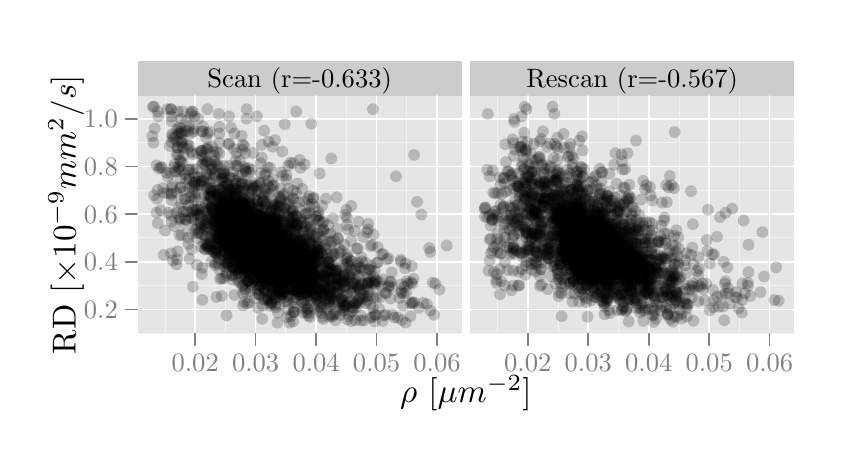
\begin{tikzpicture}[x=1pt,y=1pt]
\definecolor[named]{fillColor}{rgb}{1.00,1.00,1.00}
\path[use as bounding box,fill=fillColor,fill opacity=0.00] (0,0) rectangle (289.08,144.54);
\begin{scope}
\path[clip] (  0.00,  0.00) rectangle (289.08,144.54);
\definecolor[named]{fillColor}{rgb}{1.00,1.00,1.00}

\path[fill=fillColor] (  0.00,  0.00) rectangle (289.08,144.54);
\end{scope}
\begin{scope}
\path[clip] ( 39.69,119.86) rectangle (156.86,132.50);
\definecolor[named]{fillColor}{rgb}{0.80,0.80,0.80}

\path[fill=fillColor] ( 39.69,119.86) rectangle (156.86,132.50);
\definecolor[named]{drawColor}{rgb}{0.00,0.00,0.00}

\node[text=drawColor,anchor=base,inner sep=0pt, outer sep=0pt, scale=  0.96] at ( 98.27,122.87) {Scan (r=-0.633)};
\end{scope}
\begin{scope}
\path[clip] (159.87,119.86) rectangle (277.04,132.50);
\definecolor[named]{fillColor}{rgb}{0.80,0.80,0.80}

\path[fill=fillColor] (159.87,119.86) rectangle (277.03,132.50);
\definecolor[named]{drawColor}{rgb}{0.00,0.00,0.00}

\node[text=drawColor,anchor=base,inner sep=0pt, outer sep=0pt, scale=  0.96] at (218.45,122.87) {Rescan (r=-0.567)};
\end{scope}
\begin{scope}
\path[clip] (  0.00,  0.00) rectangle (289.08,144.54);
\definecolor[named]{drawColor}{rgb}{0.50,0.50,0.50}

\node[text=drawColor,anchor=base east,inner sep=0pt, outer sep=0pt, scale=  0.96] at ( 32.58, 39.45) {0.2};

\node[text=drawColor,anchor=base east,inner sep=0pt, outer sep=0pt, scale=  0.96] at ( 32.58, 56.68) {0.4};

\node[text=drawColor,anchor=base east,inner sep=0pt, outer sep=0pt, scale=  0.96] at ( 32.58, 73.90) {0.6};

\node[text=drawColor,anchor=base east,inner sep=0pt, outer sep=0pt, scale=  0.96] at ( 32.58, 91.12) {0.8};

\node[text=drawColor,anchor=base east,inner sep=0pt, outer sep=0pt, scale=  0.96] at ( 32.58,108.35) {1.0};
\end{scope}
\begin{scope}
\path[clip] (  0.00,  0.00) rectangle (289.08,144.54);
\definecolor[named]{drawColor}{rgb}{0.50,0.50,0.50}

\path[draw=drawColor,line width= 0.6pt,line join=round,line cap=round] ( 35.42, 42.76) -- ( 39.69, 42.76);

\path[draw=drawColor,line width= 0.6pt,line join=round,line cap=round] ( 35.42, 59.98) -- ( 39.69, 59.98);

\path[draw=drawColor,line width= 0.6pt,line join=round,line cap=round] ( 35.42, 77.21) -- ( 39.69, 77.21);

\path[draw=drawColor,line width= 0.6pt,line join=round,line cap=round] ( 35.42, 94.43) -- ( 39.69, 94.43);

\path[draw=drawColor,line width= 0.6pt,line join=round,line cap=round] ( 35.42,111.65) -- ( 39.69,111.65);
\end{scope}
\begin{scope}
\path[clip] ( 39.69, 34.04) rectangle (156.86,119.86);
\definecolor[named]{fillColor}{rgb}{0.90,0.90,0.90}

\path[fill=fillColor] ( 39.69, 34.04) rectangle (156.86,119.86);
\definecolor[named]{drawColor}{rgb}{0.95,0.95,0.95}

\path[draw=drawColor,line width= 0.3pt,line join=round,line cap=round] ( 39.69, 34.15) --
	(156.86, 34.15);

\path[draw=drawColor,line width= 0.3pt,line join=round,line cap=round] ( 39.69, 51.37) --
	(156.86, 51.37);

\path[draw=drawColor,line width= 0.3pt,line join=round,line cap=round] ( 39.69, 68.60) --
	(156.86, 68.60);

\path[draw=drawColor,line width= 0.3pt,line join=round,line cap=round] ( 39.69, 85.82) --
	(156.86, 85.82);

\path[draw=drawColor,line width= 0.3pt,line join=round,line cap=round] ( 39.69,103.04) --
	(156.86,103.04);

\path[draw=drawColor,line width= 0.3pt,line join=round,line cap=round] ( 49.61, 34.04) --
	( 49.61,119.86);

\path[draw=drawColor,line width= 0.3pt,line join=round,line cap=round] ( 71.46, 34.04) --
	( 71.46,119.86);

\path[draw=drawColor,line width= 0.3pt,line join=round,line cap=round] ( 93.31, 34.04) --
	( 93.31,119.86);

\path[draw=drawColor,line width= 0.3pt,line join=round,line cap=round] (115.16, 34.04) --
	(115.16,119.86);

\path[draw=drawColor,line width= 0.3pt,line join=round,line cap=round] (137.01, 34.04) --
	(137.01,119.86);
\definecolor[named]{drawColor}{rgb}{1.00,1.00,1.00}

\path[draw=drawColor,line width= 0.6pt,line join=round,line cap=round] ( 39.69, 42.76) --
	(156.86, 42.76);

\path[draw=drawColor,line width= 0.6pt,line join=round,line cap=round] ( 39.69, 59.98) --
	(156.86, 59.98);

\path[draw=drawColor,line width= 0.6pt,line join=round,line cap=round] ( 39.69, 77.21) --
	(156.86, 77.21);

\path[draw=drawColor,line width= 0.6pt,line join=round,line cap=round] ( 39.69, 94.43) --
	(156.86, 94.43);

\path[draw=drawColor,line width= 0.6pt,line join=round,line cap=round] ( 39.69,111.65) --
	(156.86,111.65);

\path[draw=drawColor,line width= 0.6pt,line join=round,line cap=round] ( 60.53, 34.04) --
	( 60.53,119.86);

\path[draw=drawColor,line width= 0.6pt,line join=round,line cap=round] ( 82.38, 34.04) --
	( 82.38,119.86);

\path[draw=drawColor,line width= 0.6pt,line join=round,line cap=round] (104.23, 34.04) --
	(104.23,119.86);

\path[draw=drawColor,line width= 0.6pt,line join=round,line cap=round] (126.08, 34.04) --
	(126.08,119.86);

\path[draw=drawColor,line width= 0.6pt,line join=round,line cap=round] (147.93, 34.04) --
	(147.93,119.86);
\definecolor[named]{fillColor}{rgb}{0.00,0.00,0.00}

\path[fill=fillColor,fill opacity=0.20] ( 52.23, 87.63) circle (  2.13);

\path[fill=fillColor,fill opacity=0.20] ( 64.25, 94.86) circle (  2.13);

\path[fill=fillColor,fill opacity=0.20] ( 76.26, 81.34) circle (  2.13);

\path[fill=fillColor,fill opacity=0.20] ( 86.97, 67.65) circle (  2.13);

\path[fill=fillColor,fill opacity=0.20] ( 81.07, 64.72) circle (  2.13);

\path[fill=fillColor,fill opacity=0.20] ( 75.17, 65.84) circle (  2.13);

\path[fill=fillColor,fill opacity=0.20] ( 71.02, 81.51) circle (  2.13);

\path[fill=fillColor,fill opacity=0.20] ( 59.88,107.09) circle (  2.13);

\path[fill=fillColor,fill opacity=0.20] ( 75.17, 94.69) circle (  2.13);

\path[fill=fillColor,fill opacity=0.20] ( 85.88, 68.60) circle (  2.13);

\path[fill=fillColor,fill opacity=0.20] ( 97.68, 57.83) circle (  2.13);

\path[fill=fillColor,fill opacity=0.20] (108.60, 59.90) circle (  2.13);

\path[fill=fillColor,fill opacity=0.20] ( 96.36, 60.33) circle (  2.13);

\path[fill=fillColor,fill opacity=0.20] (103.79, 57.23) circle (  2.13);

\path[fill=fillColor,fill opacity=0.20] (100.30, 55.85) circle (  2.13);

\path[fill=fillColor,fill opacity=0.20] ( 91.78, 69.28) circle (  2.13);

\path[fill=fillColor,fill opacity=0.20] ( 69.49, 76.09) circle (  2.13);

\path[fill=fillColor,fill opacity=0.20] ( 58.13, 77.81) circle (  2.13);

\path[fill=fillColor,fill opacity=0.20] ( 69.05,113.37) circle (  2.13);

\path[fill=fillColor,fill opacity=0.20] ( 85.22, 83.58) circle (  2.13);

\path[fill=fillColor,fill opacity=0.20] ( 90.68, 66.18) circle (  2.13);

\path[fill=fillColor,fill opacity=0.20] ( 94.84, 60.93) circle (  2.13);

\path[fill=fillColor,fill opacity=0.20] ( 98.33, 55.51) circle (  2.13);

\path[fill=fillColor,fill opacity=0.20] (102.92, 53.18) circle (  2.13);

\path[fill=fillColor,fill opacity=0.20] (100.08, 58.86) circle (  2.13);

\path[fill=fillColor,fill opacity=0.20] ( 95.27, 64.12) circle (  2.13);

\path[fill=fillColor,fill opacity=0.20] ( 93.52, 59.81) circle (  2.13);

\path[fill=fillColor,fill opacity=0.20] ( 88.06, 53.09) circle (  2.13);

\path[fill=fillColor,fill opacity=0.20] ( 76.04, 61.88) circle (  2.13);

\path[fill=fillColor,fill opacity=0.20] ( 74.95, 74.28) circle (  2.13);

\path[fill=fillColor,fill opacity=0.20] ( 71.46, 81.00) circle (  2.13);

\path[fill=fillColor,fill opacity=0.20] ( 58.56,101.66) circle (  2.13);

\path[fill=fillColor,fill opacity=0.20] ( 81.51, 86.68) circle (  2.13);

\path[fill=fillColor,fill opacity=0.20] ( 98.11, 68.08) circle (  2.13);

\path[fill=fillColor,fill opacity=0.20] (111.66, 53.78) circle (  2.13);

\path[fill=fillColor,fill opacity=0.20] (106.42, 62.83) circle (  2.13);

\path[fill=fillColor,fill opacity=0.20] ( 99.21, 60.07) circle (  2.13);

\path[fill=fillColor,fill opacity=0.20] ( 92.87, 49.22) circle (  2.13);

\path[fill=fillColor,fill opacity=0.20] ( 97.68, 55.16) circle (  2.13);

\path[fill=fillColor,fill opacity=0.20] ( 99.86, 62.65) circle (  2.13);

\path[fill=fillColor,fill opacity=0.20] ( 88.94, 60.41) circle (  2.13);

\path[fill=fillColor,fill opacity=0.20] ( 79.76, 59.55) circle (  2.13);

\path[fill=fillColor,fill opacity=0.20] ( 77.14, 67.82) circle (  2.13);

\path[fill=fillColor,fill opacity=0.20] ( 77.79, 73.68) circle (  2.13);

\path[fill=fillColor,fill opacity=0.20] ( 74.30, 80.13) circle (  2.13);

\path[fill=fillColor,fill opacity=0.20] ( 90.25, 37.94) circle (  2.13);

\path[fill=fillColor,fill opacity=0.20] ( 60.97, 93.48) circle (  2.13);

\path[fill=fillColor,fill opacity=0.20] ( 76.48, 70.58) circle (  2.13);

\path[fill=fillColor,fill opacity=0.20] ( 98.77, 61.45) circle (  2.13);

\path[fill=fillColor,fill opacity=0.20] (107.95, 49.74) circle (  2.13);

\path[fill=fillColor,fill opacity=0.20] (105.10, 50.17) circle (  2.13);

\path[fill=fillColor,fill opacity=0.20] (103.58, 55.08) circle (  2.13);

\path[fill=fillColor,fill opacity=0.20] ( 95.27, 58.35) circle (  2.13);

\path[fill=fillColor,fill opacity=0.20] ( 83.25, 58.78) circle (  2.13);

\path[fill=fillColor,fill opacity=0.20] ( 89.37, 55.25) circle (  2.13);

\path[fill=fillColor,fill opacity=0.20] ( 85.22, 56.37) circle (  2.13);

\path[fill=fillColor,fill opacity=0.20] ( 76.92, 64.98) circle (  2.13);

\path[fill=fillColor,fill opacity=0.20] ( 74.30, 75.66) circle (  2.13);

\path[fill=fillColor,fill opacity=0.20] ( 65.56, 88.40) circle (  2.13);

\path[fill=fillColor,fill opacity=0.20] ( 54.19,114.24) circle (  2.13);

\path[fill=fillColor,fill opacity=0.20] ( 70.80, 75.83) circle (  2.13);

\path[fill=fillColor,fill opacity=0.20] ( 90.68, 48.62) circle (  2.13);

\path[fill=fillColor,fill opacity=0.20] ( 81.51, 73.16) circle (  2.13);

\path[fill=fillColor,fill opacity=0.20] ( 81.29, 72.82) circle (  2.13);

\path[fill=fillColor,fill opacity=0.20] ( 83.47, 62.65) circle (  2.13);

\path[fill=fillColor,fill opacity=0.20] ( 64.25, 96.15) circle (  2.13);

\path[fill=fillColor,fill opacity=0.20] ( 78.23, 61.96) circle (  2.13);

\path[fill=fillColor,fill opacity=0.20] ( 95.93, 52.84) circle (  2.13);

\path[fill=fillColor,fill opacity=0.20] (102.48, 46.89) circle (  2.13);

\path[fill=fillColor,fill opacity=0.20] (102.05, 40.01) circle (  2.13);

\path[fill=fillColor,fill opacity=0.20] ( 99.21, 59.04) circle (  2.13);

\path[fill=fillColor,fill opacity=0.20] ( 87.84, 66.53) circle (  2.13);

\path[fill=fillColor,fill opacity=0.20] ( 73.86, 59.64) circle (  2.13);

\path[fill=fillColor,fill opacity=0.20] ( 71.67, 58.18) circle (  2.13);

\path[fill=fillColor,fill opacity=0.20] ( 64.25, 64.63) circle (  2.13);

\path[fill=fillColor,fill opacity=0.20] ( 66.65, 85.47) circle (  2.13);

\path[fill=fillColor,fill opacity=0.20] (105.32, 53.87) circle (  2.13);

\path[fill=fillColor,fill opacity=0.20] ( 97.02, 61.19) circle (  2.13);

\path[fill=fillColor,fill opacity=0.20] ( 94.84, 56.45) circle (  2.13);

\path[fill=fillColor,fill opacity=0.20] ( 99.86, 56.11) circle (  2.13);

\path[fill=fillColor,fill opacity=0.20] ( 99.42, 57.40) circle (  2.13);

\path[fill=fillColor,fill opacity=0.20] ( 95.71, 51.89) circle (  2.13);

\path[fill=fillColor,fill opacity=0.20] ( 81.29, 60.76) circle (  2.13);

\path[fill=fillColor,fill opacity=0.20] ( 55.94,104.07) circle (  2.13);

\path[fill=fillColor,fill opacity=0.20] ( 70.36, 89.52) circle (  2.13);

\path[fill=fillColor,fill opacity=0.20] ( 77.57, 58.86) circle (  2.13);

\path[fill=fillColor,fill opacity=0.20] ( 88.06, 44.48) circle (  2.13);

\path[fill=fillColor,fill opacity=0.20] ( 90.47, 49.56) circle (  2.13);

\path[fill=fillColor,fill opacity=0.20] ( 87.62, 52.66) circle (  2.13);

\path[fill=fillColor,fill opacity=0.20] ( 89.59, 43.45) circle (  2.13);

\path[fill=fillColor,fill opacity=0.20] ( 91.99, 50.08) circle (  2.13);

\path[fill=fillColor,fill opacity=0.20] ( 85.44, 70.92) circle (  2.13);

\path[fill=fillColor,fill opacity=0.20] ( 64.46, 65.93) circle (  2.13);

\path[fill=fillColor,fill opacity=0.20] ( 77.57, 77.29) circle (  2.13);

\path[fill=fillColor,fill opacity=0.20] (111.88, 51.03) circle (  2.13);

\path[fill=fillColor,fill opacity=0.20] (110.35, 62.22) circle (  2.13);

\path[fill=fillColor,fill opacity=0.20] (116.03, 55.25) circle (  2.13);

\path[fill=fillColor,fill opacity=0.20] (126.95, 43.02) circle (  2.13);

\path[fill=fillColor,fill opacity=0.20] (146.84, 40.78) circle (  2.13);

\path[fill=fillColor,fill opacity=0.20] (113.41, 46.29) circle (  2.13);

\path[fill=fillColor,fill opacity=0.20] (105.54, 42.16) circle (  2.13);

\path[fill=fillColor,fill opacity=0.20] (101.39, 47.76) circle (  2.13);

\path[fill=fillColor,fill opacity=0.20] ( 65.34, 84.27) circle (  2.13);

\path[fill=fillColor,fill opacity=0.20] ( 67.96, 83.67) circle (  2.13);

\path[fill=fillColor,fill opacity=0.20] ( 78.01, 59.64) circle (  2.13);

\path[fill=fillColor,fill opacity=0.20] ( 88.94, 54.30) circle (  2.13);

\path[fill=fillColor,fill opacity=0.20] ( 81.94, 53.35) circle (  2.13);

\path[fill=fillColor,fill opacity=0.20] ( 80.41, 61.10) circle (  2.13);

\path[fill=fillColor,fill opacity=0.20] ( 83.47, 60.16) circle (  2.13);

\path[fill=fillColor,fill opacity=0.20] ( 80.20, 56.02) circle (  2.13);

\path[fill=fillColor,fill opacity=0.20] ( 78.67, 68.60) circle (  2.13);

\path[fill=fillColor,fill opacity=0.20] ( 77.79, 76.43) circle (  2.13);

\path[fill=fillColor,fill opacity=0.20] ( 67.96, 72.90) circle (  2.13);

\path[fill=fillColor,fill opacity=0.20] ( 59.88,107.95) circle (  2.13);

\path[fill=fillColor,fill opacity=0.20] (111.66, 48.96) circle (  2.13);

\path[fill=fillColor,fill opacity=0.20] (115.59, 59.81) circle (  2.13);

\path[fill=fillColor,fill opacity=0.20] (119.09, 58.61) circle (  2.13);

\path[fill=fillColor,fill opacity=0.20] (133.73, 39.75) circle (  2.13);

\path[fill=fillColor,fill opacity=0.20] (120.40, 38.71) circle (  2.13);

\path[fill=fillColor,fill opacity=0.20] (122.58, 46.12) circle (  2.13);

\path[fill=fillColor,fill opacity=0.20] (100.95, 47.33) circle (  2.13);

\path[fill=fillColor,fill opacity=0.20] ( 96.15, 43.62) circle (  2.13);

\path[fill=fillColor,fill opacity=0.20] ( 79.98, 56.80) circle (  2.13);

\path[fill=fillColor,fill opacity=0.20] ( 60.31, 87.45) circle (  2.13);

\path[fill=fillColor,fill opacity=0.20] ( 81.07, 68.94) circle (  2.13);

\path[fill=fillColor,fill opacity=0.20] ( 81.94, 69.37) circle (  2.13);

\path[fill=fillColor,fill opacity=0.20] ( 83.91, 51.29) circle (  2.13);

\path[fill=fillColor,fill opacity=0.20] ( 86.97, 46.46) circle (  2.13);

\path[fill=fillColor,fill opacity=0.20] ( 83.04, 61.79) circle (  2.13);

\path[fill=fillColor,fill opacity=0.20] ( 86.10, 68.60) circle (  2.13);

\path[fill=fillColor,fill opacity=0.20] ( 80.63, 64.46) circle (  2.13);

\path[fill=fillColor,fill opacity=0.20] ( 82.82, 62.40) circle (  2.13);

\path[fill=fillColor,fill opacity=0.20] ( 71.24, 69.97) circle (  2.13);

\path[fill=fillColor,fill opacity=0.20] ( 89.15, 71.70) circle (  2.13);

\path[fill=fillColor,fill opacity=0.20] (117.78, 52.15) circle (  2.13);

\path[fill=fillColor,fill opacity=0.20] (109.26, 51.03) circle (  2.13);

\path[fill=fillColor,fill opacity=0.20] (101.17, 42.85) circle (  2.13);

\path[fill=fillColor,fill opacity=0.20] (100.08, 50.94) circle (  2.13);

\path[fill=fillColor,fill opacity=0.20] (102.48, 53.96) circle (  2.13);

\path[fill=fillColor,fill opacity=0.20] ( 94.40, 50.68) circle (  2.13);

\path[fill=fillColor,fill opacity=0.20] ( 82.60, 51.63) circle (  2.13);

\path[fill=fillColor,fill opacity=0.20] ( 84.78, 39.32) circle (  2.13);

\path[fill=fillColor,fill opacity=0.20] ( 56.38, 98.39) circle (  2.13);

\path[fill=fillColor,fill opacity=0.20] ( 75.39, 77.90) circle (  2.13);

\path[fill=fillColor,fill opacity=0.20] ( 81.73, 70.92) circle (  2.13);

\path[fill=fillColor,fill opacity=0.20] ( 91.78, 48.27) circle (  2.13);

\path[fill=fillColor,fill opacity=0.20] ( 86.53, 51.46) circle (  2.13);

\path[fill=fillColor,fill opacity=0.20] ( 83.47, 64.38) circle (  2.13);

\path[fill=fillColor,fill opacity=0.20] ( 81.94, 64.12) circle (  2.13);

\path[fill=fillColor,fill opacity=0.20] ( 80.41, 58.52) circle (  2.13);

\path[fill=fillColor,fill opacity=0.20] ( 78.23, 59.04) circle (  2.13);

\path[fill=fillColor,fill opacity=0.20] (129.14, 48.79) circle (  2.13);

\path[fill=fillColor,fill opacity=0.20] (114.72, 44.14) circle (  2.13);

\path[fill=fillColor,fill opacity=0.20] (102.70, 53.09) circle (  2.13);

\path[fill=fillColor,fill opacity=0.20] (119.96, 46.72) circle (  2.13);

\path[fill=fillColor,fill opacity=0.20] (100.95, 48.79) circle (  2.13);

\path[fill=fillColor,fill opacity=0.20] ( 93.31, 54.64) circle (  2.13);

\path[fill=fillColor,fill opacity=0.20] (100.73, 53.78) circle (  2.13);

\path[fill=fillColor,fill opacity=0.20] ( 94.18, 55.16) circle (  2.13);

\path[fill=fillColor,fill opacity=0.20] ( 86.31, 57.14) circle (  2.13);

\path[fill=fillColor,fill opacity=0.20] ( 88.28, 45.09) circle (  2.13);

\path[fill=fillColor,fill opacity=0.20] ( 79.32, 44.83) circle (  2.13);

\path[fill=fillColor,fill opacity=0.20] ( 72.33, 82.72) circle (  2.13);

\path[fill=fillColor,fill opacity=0.20] ( 90.90, 66.27) circle (  2.13);

\path[fill=fillColor,fill opacity=0.20] ( 99.64, 54.99) circle (  2.13);

\path[fill=fillColor,fill opacity=0.20] ( 97.46, 49.39) circle (  2.13);

\path[fill=fillColor,fill opacity=0.20] ( 88.06, 48.53) circle (  2.13);

\path[fill=fillColor,fill opacity=0.20] ( 84.78, 49.99) circle (  2.13);

\path[fill=fillColor,fill opacity=0.20] ( 83.04, 57.40) circle (  2.13);

\path[fill=fillColor,fill opacity=0.20] ( 76.48, 69.11) circle (  2.13);

\path[fill=fillColor,fill opacity=0.20] ( 79.98, 62.14) circle (  2.13);

\path[fill=fillColor,fill opacity=0.20] ( 66.21, 95.29) circle (  2.13);

\path[fill=fillColor,fill opacity=0.20] (117.34, 42.33) circle (  2.13);

\path[fill=fillColor,fill opacity=0.20] (103.36, 63.00) circle (  2.13);

\path[fill=fillColor,fill opacity=0.20] (109.69, 61.53) circle (  2.13);

\path[fill=fillColor,fill opacity=0.20] (122.15, 47.33) circle (  2.13);

\path[fill=fillColor,fill opacity=0.20] (106.20, 48.96) circle (  2.13);

\path[fill=fillColor,fill opacity=0.20] ( 96.58, 54.04) circle (  2.13);

\path[fill=fillColor,fill opacity=0.20] (106.63, 55.08) circle (  2.13);

\path[fill=fillColor,fill opacity=0.20] ( 83.25, 60.41) circle (  2.13);

\path[fill=fillColor,fill opacity=0.20] ( 88.06, 56.80) circle (  2.13);

\path[fill=fillColor,fill opacity=0.20] ( 87.62, 45.34) circle (  2.13);

\path[fill=fillColor,fill opacity=0.20] ( 74.30, 61.10) circle (  2.13);

\path[fill=fillColor,fill opacity=0.20] ( 82.60, 63.86) circle (  2.13);

\path[fill=fillColor,fill opacity=0.20] ( 90.68, 63.69) circle (  2.13);

\path[fill=fillColor,fill opacity=0.20] ( 92.43, 62.91) circle (  2.13);

\path[fill=fillColor,fill opacity=0.20] ( 90.90, 55.33) circle (  2.13);

\path[fill=fillColor,fill opacity=0.20] ( 88.28, 45.26) circle (  2.13);

\path[fill=fillColor,fill opacity=0.20] ( 90.68, 49.39) circle (  2.13);

\path[fill=fillColor,fill opacity=0.20] ( 81.29, 71.87) circle (  2.13);

\path[fill=fillColor,fill opacity=0.20] ( 89.81, 73.85) circle (  2.13);

\path[fill=fillColor,fill opacity=0.20] ( 82.60, 64.98) circle (  2.13);

\path[fill=fillColor,fill opacity=0.20] ( 95.93, 56.54) circle (  2.13);

\path[fill=fillColor,fill opacity=0.20] ( 89.81, 55.85) circle (  2.13);

\path[fill=fillColor,fill opacity=0.20] ( 88.28, 68.16) circle (  2.13);

\path[fill=fillColor,fill opacity=0.20] ( 97.89, 60.33) circle (  2.13);

\path[fill=fillColor,fill opacity=0.20] (107.73, 50.51) circle (  2.13);

\path[fill=fillColor,fill opacity=0.20] (100.52, 54.13) circle (  2.13);

\path[fill=fillColor,fill opacity=0.20] ( 98.33, 54.21) circle (  2.13);

\path[fill=fillColor,fill opacity=0.20] (101.17, 49.74) circle (  2.13);

\path[fill=fillColor,fill opacity=0.20] ( 92.87, 54.21) circle (  2.13);

\path[fill=fillColor,fill opacity=0.20] ( 85.88, 53.35) circle (  2.13);

\path[fill=fillColor,fill opacity=0.20] ( 85.66, 49.05) circle (  2.13);

\path[fill=fillColor,fill opacity=0.20] ( 66.43, 75.40) circle (  2.13);

\path[fill=fillColor,fill opacity=0.20] ( 72.11, 75.48) circle (  2.13);

\path[fill=fillColor,fill opacity=0.20] ( 80.63, 70.66) circle (  2.13);

\path[fill=fillColor,fill opacity=0.20] ( 82.38, 65.24) circle (  2.13);

\path[fill=fillColor,fill opacity=0.20] ( 91.99, 57.06) circle (  2.13);

\path[fill=fillColor,fill opacity=0.20] ( 86.75, 53.53) circle (  2.13);

\path[fill=fillColor,fill opacity=0.20] ( 87.62, 53.61) circle (  2.13);

\path[fill=fillColor,fill opacity=0.20] ( 88.50, 62.40) circle (  2.13);

\path[fill=fillColor,fill opacity=0.20] ( 79.32, 67.65) circle (  2.13);

\path[fill=fillColor,fill opacity=0.20] ( 75.83, 60.67) circle (  2.13);

\path[fill=fillColor,fill opacity=0.20] ( 64.90, 74.02) circle (  2.13);

\path[fill=fillColor,fill opacity=0.20] ( 86.31, 70.75) circle (  2.13);

\path[fill=fillColor,fill opacity=0.20] (110.13, 53.61) circle (  2.13);

\path[fill=fillColor,fill opacity=0.20] ( 83.25, 63.77) circle (  2.13);

\path[fill=fillColor,fill opacity=0.20] ( 87.62, 62.31) circle (  2.13);

\path[fill=fillColor,fill opacity=0.20] ( 95.05, 53.70) circle (  2.13);

\path[fill=fillColor,fill opacity=0.20] ( 98.33, 50.08) circle (  2.13);

\path[fill=fillColor,fill opacity=0.20] (101.17, 54.39) circle (  2.13);

\path[fill=fillColor,fill opacity=0.20] ( 91.56, 51.11) circle (  2.13);

\path[fill=fillColor,fill opacity=0.20] (106.63, 43.62) circle (  2.13);

\path[fill=fillColor,fill opacity=0.20] (102.92, 50.68) circle (  2.13);

\path[fill=fillColor,fill opacity=0.20] ( 90.47, 54.99) circle (  2.13);

\path[fill=fillColor,fill opacity=0.20] ( 83.25, 58.52) circle (  2.13);

\path[fill=fillColor,fill opacity=0.20] ( 71.46, 84.10) circle (  2.13);

\path[fill=fillColor,fill opacity=0.20] ( 89.59, 65.32) circle (  2.13);

\path[fill=fillColor,fill opacity=0.20] ( 90.68, 53.96) circle (  2.13);

\path[fill=fillColor,fill opacity=0.20] ( 85.00, 57.92) circle (  2.13);

\path[fill=fillColor,fill opacity=0.20] ( 89.59, 57.92) circle (  2.13);

\path[fill=fillColor,fill opacity=0.20] ( 90.68, 50.34) circle (  2.13);

\path[fill=fillColor,fill opacity=0.20] ( 86.75, 46.38) circle (  2.13);

\path[fill=fillColor,fill opacity=0.20] ( 77.79, 48.44) circle (  2.13);

\path[fill=fillColor,fill opacity=0.20] ( 76.26, 56.37) circle (  2.13);

\path[fill=fillColor,fill opacity=0.20] ( 67.52, 74.80) circle (  2.13);

\path[fill=fillColor,fill opacity=0.20] ( 72.99, 86.08) circle (  2.13);

\path[fill=fillColor,fill opacity=0.20] ( 97.24, 49.48) circle (  2.13);

\path[fill=fillColor,fill opacity=0.20] ( 96.15, 57.23) circle (  2.13);

\path[fill=fillColor,fill opacity=0.20] ( 96.80, 54.21) circle (  2.13);

\path[fill=fillColor,fill opacity=0.20] (105.32, 51.72) circle (  2.13);

\path[fill=fillColor,fill opacity=0.20] (102.26, 53.18) circle (  2.13);

\path[fill=fillColor,fill opacity=0.20] ( 99.64, 52.58) circle (  2.13);

\path[fill=fillColor,fill opacity=0.20] (100.95, 49.31) circle (  2.13);

\path[fill=fillColor,fill opacity=0.20] ( 98.99, 45.52) circle (  2.13);

\path[fill=fillColor,fill opacity=0.20] (103.36, 48.19) circle (  2.13);

\path[fill=fillColor,fill opacity=0.20] ( 95.93, 59.38) circle (  2.13);

\path[fill=fillColor,fill opacity=0.20] ( 94.84, 65.41) circle (  2.13);

\path[fill=fillColor,fill opacity=0.20] ( 78.67, 74.45) circle (  2.13);

\path[fill=fillColor,fill opacity=0.20] ( 88.06, 78.84) circle (  2.13);

\path[fill=fillColor,fill opacity=0.20] ( 99.42, 54.64) circle (  2.13);

\path[fill=fillColor,fill opacity=0.20] ( 84.35, 52.92) circle (  2.13);

\path[fill=fillColor,fill opacity=0.20] ( 89.37, 54.56) circle (  2.13);

\path[fill=fillColor,fill opacity=0.20] ( 89.81, 48.27) circle (  2.13);

\path[fill=fillColor,fill opacity=0.20] ( 85.22, 46.38) circle (  2.13);

\path[fill=fillColor,fill opacity=0.20] ( 86.97, 48.96) circle (  2.13);

\path[fill=fillColor,fill opacity=0.20] ( 78.45, 55.76) circle (  2.13);

\path[fill=fillColor,fill opacity=0.20] ( 75.17, 68.51) circle (  2.13);

\path[fill=fillColor,fill opacity=0.20] ( 60.31, 82.55) circle (  2.13);

\path[fill=fillColor,fill opacity=0.20] ( 75.17, 96.58) circle (  2.13);

\path[fill=fillColor,fill opacity=0.20] ( 97.46, 56.71) circle (  2.13);

\path[fill=fillColor,fill opacity=0.20] ( 94.18, 62.74) circle (  2.13);

\path[fill=fillColor,fill opacity=0.20] ( 97.46, 53.78) circle (  2.13);

\path[fill=fillColor,fill opacity=0.20] (107.29, 45.95) circle (  2.13);

\path[fill=fillColor,fill opacity=0.20] (108.38, 49.99) circle (  2.13);

\path[fill=fillColor,fill opacity=0.20] (102.70, 58.18) circle (  2.13);

\path[fill=fillColor,fill opacity=0.20] ( 98.33, 61.19) circle (  2.13);

\path[fill=fillColor,fill opacity=0.20] (107.29, 54.56) circle (  2.13);

\path[fill=fillColor,fill opacity=0.20] ( 98.33, 50.34) circle (  2.13);

\path[fill=fillColor,fill opacity=0.20] (100.52, 56.11) circle (  2.13);

\path[fill=fillColor,fill opacity=0.20] (100.52, 62.83) circle (  2.13);

\path[fill=fillColor,fill opacity=0.20] ( 86.10, 76.17) circle (  2.13);

\path[fill=fillColor,fill opacity=0.20] ( 57.69,100.80) circle (  2.13);

\path[fill=fillColor,fill opacity=0.20] ( 55.51,106.49) circle (  2.13);

\path[fill=fillColor,fill opacity=0.20] ( 75.61, 72.64) circle (  2.13);

\path[fill=fillColor,fill opacity=0.20] ( 88.28, 57.83) circle (  2.13);

\path[fill=fillColor,fill opacity=0.20] ( 86.53, 54.04) circle (  2.13);

\path[fill=fillColor,fill opacity=0.20] ( 81.73, 57.66) circle (  2.13);

\path[fill=fillColor,fill opacity=0.20] ( 89.37, 58.43) circle (  2.13);

\path[fill=fillColor,fill opacity=0.20] ( 86.97, 55.68) circle (  2.13);

\path[fill=fillColor,fill opacity=0.20] ( 86.10, 59.21) circle (  2.13);

\path[fill=fillColor,fill opacity=0.20] ( 77.36, 70.32) circle (  2.13);

\path[fill=fillColor,fill opacity=0.20] ( 72.77, 77.64) circle (  2.13);

\path[fill=fillColor,fill opacity=0.20] ( 65.77, 84.18) circle (  2.13);

\path[fill=fillColor,fill opacity=0.20] ( 68.40, 99.51) circle (  2.13);

\path[fill=fillColor,fill opacity=0.20] ( 97.68, 54.56) circle (  2.13);

\path[fill=fillColor,fill opacity=0.20] ( 94.18, 66.53) circle (  2.13);

\path[fill=fillColor,fill opacity=0.20] ( 95.05, 62.74) circle (  2.13);

\path[fill=fillColor,fill opacity=0.20] (100.95, 53.78) circle (  2.13);

\path[fill=fillColor,fill opacity=0.20] (102.05, 56.80) circle (  2.13);

\path[fill=fillColor,fill opacity=0.20] ( 99.21, 58.18) circle (  2.13);

\path[fill=fillColor,fill opacity=0.20] (100.08, 57.66) circle (  2.13);

\path[fill=fillColor,fill opacity=0.20] (103.58, 59.21) circle (  2.13);

\path[fill=fillColor,fill opacity=0.20] (100.08, 61.62) circle (  2.13);

\path[fill=fillColor,fill opacity=0.20] (104.23, 66.10) circle (  2.13);

\path[fill=fillColor,fill opacity=0.20] (102.26, 62.14) circle (  2.13);

\path[fill=fillColor,fill opacity=0.20] ( 88.06, 58.26) circle (  2.13);

\path[fill=fillColor,fill opacity=0.20] ( 55.94,106.14) circle (  2.13);

\path[fill=fillColor,fill opacity=0.20] ( 85.00, 81.86) circle (  2.13);

\path[fill=fillColor,fill opacity=0.20] ( 93.74, 61.79) circle (  2.13);

\path[fill=fillColor,fill opacity=0.20] ( 85.22, 61.10) circle (  2.13);

\path[fill=fillColor,fill opacity=0.20] ( 91.34, 55.42) circle (  2.13);

\path[fill=fillColor,fill opacity=0.20] ( 98.11, 47.76) circle (  2.13);

\path[fill=fillColor,fill opacity=0.20] ( 86.75, 54.90) circle (  2.13);

\path[fill=fillColor,fill opacity=0.20] ( 84.78, 60.93) circle (  2.13);

\path[fill=fillColor,fill opacity=0.20] ( 83.25, 63.95) circle (  2.13);

\path[fill=fillColor,fill opacity=0.20] ( 83.47, 66.61) circle (  2.13);

\path[fill=fillColor,fill opacity=0.20] ( 68.83, 72.13) circle (  2.13);

\path[fill=fillColor,fill opacity=0.20] ( 59.22,106.49) circle (  2.13);

\path[fill=fillColor,fill opacity=0.20] ( 92.21, 59.04) circle (  2.13);

\path[fill=fillColor,fill opacity=0.20] ( 93.09, 67.05) circle (  2.13);

\path[fill=fillColor,fill opacity=0.20] (103.14, 62.74) circle (  2.13);

\path[fill=fillColor,fill opacity=0.20] (103.36, 50.34) circle (  2.13);

\path[fill=fillColor,fill opacity=0.20] (105.76, 49.39) circle (  2.13);

\path[fill=fillColor,fill opacity=0.20] (102.48, 55.94) circle (  2.13);

\path[fill=fillColor,fill opacity=0.20] (100.73, 59.47) circle (  2.13);

\path[fill=fillColor,fill opacity=0.20] (103.79, 54.90) circle (  2.13);

\path[fill=fillColor,fill opacity=0.20] (110.35, 53.70) circle (  2.13);

\path[fill=fillColor,fill opacity=0.20] (104.89, 62.74) circle (  2.13);

\path[fill=fillColor,fill opacity=0.20] ( 98.11, 67.05) circle (  2.13);

\path[fill=fillColor,fill opacity=0.20] ( 76.70, 65.06) circle (  2.13);

\path[fill=fillColor,fill opacity=0.20] ( 55.51,111.65) circle (  2.13);

\path[fill=fillColor,fill opacity=0.20] ( 91.12, 77.81) circle (  2.13);

\path[fill=fillColor,fill opacity=0.20] (101.39, 59.47) circle (  2.13);

\path[fill=fillColor,fill opacity=0.20] ( 98.33, 48.19) circle (  2.13);

\path[fill=fillColor,fill opacity=0.20] (102.48, 43.79) circle (  2.13);

\path[fill=fillColor,fill opacity=0.20] ( 91.78, 51.80) circle (  2.13);

\path[fill=fillColor,fill opacity=0.20] ( 83.69, 55.42) circle (  2.13);

\path[fill=fillColor,fill opacity=0.20] ( 83.91, 60.59) circle (  2.13);

\path[fill=fillColor,fill opacity=0.20] ( 76.26, 66.44) circle (  2.13);

\path[fill=fillColor,fill opacity=0.20] ( 72.77, 66.96) circle (  2.13);

\path[fill=fillColor,fill opacity=0.20] ( 66.87, 78.15) circle (  2.13);

\path[fill=fillColor,fill opacity=0.20] ( 62.72,100.03) circle (  2.13);

\path[fill=fillColor,fill opacity=0.20] ( 91.34, 65.84) circle (  2.13);

\path[fill=fillColor,fill opacity=0.20] ( 86.31, 71.27) circle (  2.13);

\path[fill=fillColor,fill opacity=0.20] ( 98.11, 63.77) circle (  2.13);

\path[fill=fillColor,fill opacity=0.20] (113.41, 52.15) circle (  2.13);

\path[fill=fillColor,fill opacity=0.20] (116.69, 45.69) circle (  2.13);

\path[fill=fillColor,fill opacity=0.20] (117.34, 43.54) circle (  2.13);

\path[fill=fillColor,fill opacity=0.20] (109.04, 45.43) circle (  2.13);

\path[fill=fillColor,fill opacity=0.20] (106.63, 52.06) circle (  2.13);

\path[fill=fillColor,fill opacity=0.20] (101.61, 56.97) circle (  2.13);

\path[fill=fillColor,fill opacity=0.20] (100.08, 58.69) circle (  2.13);

\path[fill=fillColor,fill opacity=0.20] (111.88, 60.24) circle (  2.13);

\path[fill=fillColor,fill opacity=0.20] (104.67, 62.22) circle (  2.13);

\path[fill=fillColor,fill opacity=0.20] ( 74.73, 74.28) circle (  2.13);

\path[fill=fillColor,fill opacity=0.20] ( 53.98,107.69) circle (  2.13);

\path[fill=fillColor,fill opacity=0.20] ( 98.77, 75.31) circle (  2.13);

\path[fill=fillColor,fill opacity=0.20] (102.92, 61.53) circle (  2.13);

\path[fill=fillColor,fill opacity=0.20] ( 97.02, 58.52) circle (  2.13);

\path[fill=fillColor,fill opacity=0.20] ( 97.68, 57.14) circle (  2.13);

\path[fill=fillColor,fill opacity=0.20] ( 84.78, 61.28) circle (  2.13);

\path[fill=fillColor,fill opacity=0.20] ( 82.82, 68.08) circle (  2.13);

\path[fill=fillColor,fill opacity=0.20] ( 81.51, 68.42) circle (  2.13);

\path[fill=fillColor,fill opacity=0.20] ( 72.33, 68.85) circle (  2.13);

\path[fill=fillColor,fill opacity=0.20] ( 72.33, 70.92) circle (  2.13);

\path[fill=fillColor,fill opacity=0.20] ( 68.18, 69.37) circle (  2.13);

\path[fill=fillColor,fill opacity=0.20] ( 70.36, 78.67) circle (  2.13);

\path[fill=fillColor,fill opacity=0.20] ( 97.24, 54.73) circle (  2.13);

\path[fill=fillColor,fill opacity=0.20] (102.70, 73.07) circle (  2.13);

\path[fill=fillColor,fill opacity=0.20] ( 95.71, 72.64) circle (  2.13);

\path[fill=fillColor,fill opacity=0.20] (112.10, 54.47) circle (  2.13);

\path[fill=fillColor,fill opacity=0.20] (112.10, 53.53) circle (  2.13);

\path[fill=fillColor,fill opacity=0.20] (116.90, 56.88) circle (  2.13);

\path[fill=fillColor,fill opacity=0.20] (114.72, 51.37) circle (  2.13);

\path[fill=fillColor,fill opacity=0.20] (110.79, 45.43) circle (  2.13);

\path[fill=fillColor,fill opacity=0.20] (109.47, 48.10) circle (  2.13);

\path[fill=fillColor,fill opacity=0.20] (100.95, 56.11) circle (  2.13);

\path[fill=fillColor,fill opacity=0.20] ( 98.33, 56.80) circle (  2.13);

\path[fill=fillColor,fill opacity=0.20] ( 97.68, 57.31) circle (  2.13);

\path[fill=fillColor,fill opacity=0.20] ( 70.14, 69.80) circle (  2.13);

\path[fill=fillColor,fill opacity=0.20] ( 91.34, 86.42) circle (  2.13);

\path[fill=fillColor,fill opacity=0.20] (100.30, 77.21) circle (  2.13);

\path[fill=fillColor,fill opacity=0.20] ( 91.34, 62.05) circle (  2.13);

\path[fill=fillColor,fill opacity=0.20] ( 87.41, 58.61) circle (  2.13);

\path[fill=fillColor,fill opacity=0.20] ( 84.78, 68.60) circle (  2.13);

\path[fill=fillColor,fill opacity=0.20] ( 82.60, 67.13) circle (  2.13);

\path[fill=fillColor,fill opacity=0.20] ( 80.41, 63.34) circle (  2.13);

\path[fill=fillColor,fill opacity=0.20] ( 72.77, 64.55) circle (  2.13);

\path[fill=fillColor,fill opacity=0.20] ( 70.80, 60.41) circle (  2.13);

\path[fill=fillColor,fill opacity=0.20] ( 81.73, 59.12) circle (  2.13);

\path[fill=fillColor,fill opacity=0.20] ( 70.58, 66.10) circle (  2.13);

\path[fill=fillColor,fill opacity=0.20] ( 58.35, 86.42) circle (  2.13);

\path[fill=fillColor,fill opacity=0.20] ( 78.01, 56.97) circle (  2.13);

\path[fill=fillColor,fill opacity=0.20] ( 87.19, 55.85) circle (  2.13);

\path[fill=fillColor,fill opacity=0.20] ( 98.33, 62.22) circle (  2.13);

\path[fill=fillColor,fill opacity=0.20] ( 92.65, 63.17) circle (  2.13);

\path[fill=fillColor,fill opacity=0.20] (102.92, 62.22) circle (  2.13);

\path[fill=fillColor,fill opacity=0.20] (105.98, 59.81) circle (  2.13);

\path[fill=fillColor,fill opacity=0.20] (106.42, 62.31) circle (  2.13);

\path[fill=fillColor,fill opacity=0.20] (110.79, 67.65) circle (  2.13);

\path[fill=fillColor,fill opacity=0.20] (111.00, 62.74) circle (  2.13);

\path[fill=fillColor,fill opacity=0.20] (111.66, 52.06) circle (  2.13);

\path[fill=fillColor,fill opacity=0.20] (106.85, 50.25) circle (  2.13);

\path[fill=fillColor,fill opacity=0.20] (100.08, 52.84) circle (  2.13);

\path[fill=fillColor,fill opacity=0.20] ( 85.88, 52.58) circle (  2.13);

\path[fill=fillColor,fill opacity=0.20] ( 71.24, 66.70) circle (  2.13);

\path[fill=fillColor,fill opacity=0.20] ( 68.62, 95.12) circle (  2.13);

\path[fill=fillColor,fill opacity=0.20] ( 85.44, 72.13) circle (  2.13);

\path[fill=fillColor,fill opacity=0.20] ( 94.40, 54.04) circle (  2.13);

\path[fill=fillColor,fill opacity=0.20] ( 92.65, 57.57) circle (  2.13);

\path[fill=fillColor,fill opacity=0.20] ( 85.88, 64.29) circle (  2.13);

\path[fill=fillColor,fill opacity=0.20] ( 84.13, 61.79) circle (  2.13);

\path[fill=fillColor,fill opacity=0.20] ( 76.70, 63.00) circle (  2.13);

\path[fill=fillColor,fill opacity=0.20] ( 70.36, 71.87) circle (  2.13);

\path[fill=fillColor,fill opacity=0.20] ( 69.27, 74.11) circle (  2.13);

\path[fill=fillColor,fill opacity=0.20] ( 73.86, 63.69) circle (  2.13);

\path[fill=fillColor,fill opacity=0.20] ( 71.89, 55.08) circle (  2.13);

\path[fill=fillColor,fill opacity=0.20] ( 72.33, 59.55) circle (  2.13);

\path[fill=fillColor,fill opacity=0.20] ( 64.90, 76.52) circle (  2.13);

\path[fill=fillColor,fill opacity=0.20] ( 67.52, 74.37) circle (  2.13);

\path[fill=fillColor,fill opacity=0.20] ( 76.04, 69.97) circle (  2.13);

\path[fill=fillColor,fill opacity=0.20] ( 85.66, 66.70) circle (  2.13);

\path[fill=fillColor,fill opacity=0.20] ( 86.75, 65.84) circle (  2.13);

\path[fill=fillColor,fill opacity=0.20] (116.90, 67.48) circle (  2.13);

\path[fill=fillColor,fill opacity=0.20] ( 93.09, 65.75) circle (  2.13);

\path[fill=fillColor,fill opacity=0.20] ( 93.96, 55.59) circle (  2.13);

\path[fill=fillColor,fill opacity=0.20] (103.58, 54.90) circle (  2.13);

\path[fill=fillColor,fill opacity=0.20] (105.10, 63.08) circle (  2.13);

\path[fill=fillColor,fill opacity=0.20] (105.54, 66.36) circle (  2.13);

\path[fill=fillColor,fill opacity=0.20] (108.38, 67.22) circle (  2.13);

\path[fill=fillColor,fill opacity=0.20] (109.47, 70.06) circle (  2.13);

\path[fill=fillColor,fill opacity=0.20] ( 99.86, 66.10) circle (  2.13);

\path[fill=fillColor,fill opacity=0.20] ( 94.62, 58.00) circle (  2.13);

\path[fill=fillColor,fill opacity=0.20] ( 80.85, 63.43) circle (  2.13);

\path[fill=fillColor,fill opacity=0.20] ( 67.96, 95.29) circle (  2.13);

\path[fill=fillColor,fill opacity=0.20] ( 78.67, 72.99) circle (  2.13);

\path[fill=fillColor,fill opacity=0.20] ( 91.34, 59.98) circle (  2.13);

\path[fill=fillColor,fill opacity=0.20] ( 93.74, 62.74) circle (  2.13);

\path[fill=fillColor,fill opacity=0.20] ( 87.84, 62.57) circle (  2.13);

\path[fill=fillColor,fill opacity=0.20] ( 89.15, 59.12) circle (  2.13);

\path[fill=fillColor,fill opacity=0.20] ( 80.41, 68.51) circle (  2.13);

\path[fill=fillColor,fill opacity=0.20] ( 77.57, 73.25) circle (  2.13);

\path[fill=fillColor,fill opacity=0.20] ( 75.61, 65.58) circle (  2.13);

\path[fill=fillColor,fill opacity=0.20] ( 75.17, 57.49) circle (  2.13);

\path[fill=fillColor,fill opacity=0.20] ( 75.39, 56.88) circle (  2.13);

\path[fill=fillColor,fill opacity=0.20] ( 77.57, 65.93) circle (  2.13);

\path[fill=fillColor,fill opacity=0.20] ( 70.80, 73.93) circle (  2.13);

\path[fill=fillColor,fill opacity=0.20] ( 70.58, 68.60) circle (  2.13);

\path[fill=fillColor,fill opacity=0.20] ( 65.99, 75.57) circle (  2.13);

\path[fill=fillColor,fill opacity=0.20] ( 66.65, 79.53) circle (  2.13);

\path[fill=fillColor,fill opacity=0.20] ( 66.21, 79.70) circle (  2.13);

\path[fill=fillColor,fill opacity=0.20] ( 90.68, 80.74) circle (  2.13);

\path[fill=fillColor,fill opacity=0.20] ( 85.66, 69.28) circle (  2.13);

\path[fill=fillColor,fill opacity=0.20] ( 86.10, 67.22) circle (  2.13);

\path[fill=fillColor,fill opacity=0.20] ( 95.71, 78.07) circle (  2.13);

\path[fill=fillColor,fill opacity=0.20] ( 89.59, 74.62) circle (  2.13);

\path[fill=fillColor,fill opacity=0.20] ( 97.68, 63.69) circle (  2.13);

\path[fill=fillColor,fill opacity=0.20] ( 90.68, 63.17) circle (  2.13);

\path[fill=fillColor,fill opacity=0.20] (101.83, 58.86) circle (  2.13);

\path[fill=fillColor,fill opacity=0.20] (107.95, 58.26) circle (  2.13);

\path[fill=fillColor,fill opacity=0.20] (119.31, 64.72) circle (  2.13);

\path[fill=fillColor,fill opacity=0.20] (105.98, 63.34) circle (  2.13);

\path[fill=fillColor,fill opacity=0.20] ( 96.80, 64.12) circle (  2.13);

\path[fill=fillColor,fill opacity=0.20] ( 92.21, 74.11) circle (  2.13);

\path[fill=fillColor,fill opacity=0.20] ( 78.67, 80.39) circle (  2.13);

\path[fill=fillColor,fill opacity=0.20] ( 75.61, 78.33) circle (  2.13);

\path[fill=fillColor,fill opacity=0.20] ( 67.30, 85.73) circle (  2.13);

\path[fill=fillColor,fill opacity=0.20] ( 80.63, 79.53) circle (  2.13);

\path[fill=fillColor,fill opacity=0.20] ( 91.34, 69.11) circle (  2.13);

\path[fill=fillColor,fill opacity=0.20] ( 97.89, 53.87) circle (  2.13);

\path[fill=fillColor,fill opacity=0.20] ( 98.11, 50.86) circle (  2.13);

\path[fill=fillColor,fill opacity=0.20] ( 87.84, 59.21) circle (  2.13);

\path[fill=fillColor,fill opacity=0.20] ( 79.10, 59.81) circle (  2.13);

\path[fill=fillColor,fill opacity=0.20] ( 78.01, 62.31) circle (  2.13);

\path[fill=fillColor,fill opacity=0.20] ( 75.83, 67.82) circle (  2.13);

\path[fill=fillColor,fill opacity=0.20] ( 76.70, 68.68) circle (  2.13);

\path[fill=fillColor,fill opacity=0.20] ( 73.20, 70.83) circle (  2.13);

\path[fill=fillColor,fill opacity=0.20] ( 71.46, 71.09) circle (  2.13);

\path[fill=fillColor,fill opacity=0.20] ( 71.67, 66.87) circle (  2.13);

\path[fill=fillColor,fill opacity=0.20] ( 72.33, 65.50) circle (  2.13);

\path[fill=fillColor,fill opacity=0.20] ( 74.95, 67.05) circle (  2.13);

\path[fill=fillColor,fill opacity=0.20] ( 71.46, 69.63) circle (  2.13);

\path[fill=fillColor,fill opacity=0.20] ( 65.99, 76.69) circle (  2.13);

\path[fill=fillColor,fill opacity=0.20] ( 76.92, 67.65) circle (  2.13);

\path[fill=fillColor,fill opacity=0.20] ( 71.24, 58.09) circle (  2.13);

\path[fill=fillColor,fill opacity=0.20] ( 67.30, 71.44) circle (  2.13);

\path[fill=fillColor,fill opacity=0.20] ( 68.62, 84.53) circle (  2.13);

\path[fill=fillColor,fill opacity=0.20] ( 74.30, 78.93) circle (  2.13);

\path[fill=fillColor,fill opacity=0.20] ( 72.11, 75.57) circle (  2.13);

\path[fill=fillColor,fill opacity=0.20] ( 71.46, 80.57) circle (  2.13);

\path[fill=fillColor,fill opacity=0.20] ( 69.71, 80.48) circle (  2.13);

\path[fill=fillColor,fill opacity=0.20] ( 77.57, 72.04) circle (  2.13);

\path[fill=fillColor,fill opacity=0.20] ( 74.08, 67.82) circle (  2.13);

\path[fill=fillColor,fill opacity=0.20] ( 76.26, 70.58) circle (  2.13);

\path[fill=fillColor,fill opacity=0.20] ( 78.23, 79.88) circle (  2.13);

\path[fill=fillColor,fill opacity=0.20] ( 74.95, 83.49) circle (  2.13);

\path[fill=fillColor,fill opacity=0.20] ( 76.70, 77.21) circle (  2.13);

\path[fill=fillColor,fill opacity=0.20] ( 76.26, 72.73) circle (  2.13);

\path[fill=fillColor,fill opacity=0.20] ( 82.82, 69.37) circle (  2.13);

\path[fill=fillColor,fill opacity=0.20] ( 80.20, 67.65) circle (  2.13);

\path[fill=fillColor,fill opacity=0.20] ( 88.94, 74.71) circle (  2.13);

\path[fill=fillColor,fill opacity=0.20] ( 89.81, 75.23) circle (  2.13);

\path[fill=fillColor,fill opacity=0.20] ( 84.13, 68.25) circle (  2.13);

\path[fill=fillColor,fill opacity=0.20] ( 88.72, 69.03) circle (  2.13);

\path[fill=fillColor,fill opacity=0.20] ( 99.42, 66.61) circle (  2.13);

\path[fill=fillColor,fill opacity=0.20] (101.39, 60.93) circle (  2.13);

\path[fill=fillColor,fill opacity=0.20] (100.30, 58.00) circle (  2.13);

\path[fill=fillColor,fill opacity=0.20] ( 97.68, 57.49) circle (  2.13);

\path[fill=fillColor,fill opacity=0.20] ( 97.02, 64.46) circle (  2.13);

\path[fill=fillColor,fill opacity=0.20] ( 88.72, 75.83) circle (  2.13);

\path[fill=fillColor,fill opacity=0.20] ( 80.20, 72.64) circle (  2.13);

\path[fill=fillColor,fill opacity=0.20] ( 89.15, 75.31) circle (  2.13);

\path[fill=fillColor,fill opacity=0.20] ( 74.73, 81.94) circle (  2.13);

\path[fill=fillColor,fill opacity=0.20] ( 73.20, 77.81) circle (  2.13);

\path[fill=fillColor,fill opacity=0.20] ( 74.30, 86.59) circle (  2.13);

\path[fill=fillColor,fill opacity=0.20] ( 82.82, 71.18) circle (  2.13);

\path[fill=fillColor,fill opacity=0.20] ( 90.90, 58.69) circle (  2.13);

\path[fill=fillColor,fill opacity=0.20] ( 91.78, 58.26) circle (  2.13);

\path[fill=fillColor,fill opacity=0.20] ( 87.19, 61.45) circle (  2.13);

\path[fill=fillColor,fill opacity=0.20] ( 82.82, 57.75) circle (  2.13);

\path[fill=fillColor,fill opacity=0.20] ( 79.76, 60.07) circle (  2.13);

\path[fill=fillColor,fill opacity=0.20] ( 74.95, 63.26) circle (  2.13);

\path[fill=fillColor,fill opacity=0.20] ( 74.51, 63.43) circle (  2.13);

\path[fill=fillColor,fill opacity=0.20] ( 74.73, 67.39) circle (  2.13);

\path[fill=fillColor,fill opacity=0.20] ( 71.02, 70.15) circle (  2.13);

\path[fill=fillColor,fill opacity=0.20] ( 75.61, 68.25) circle (  2.13);

\path[fill=fillColor,fill opacity=0.20] ( 82.82, 70.06) circle (  2.13);

\path[fill=fillColor,fill opacity=0.20] ( 73.20, 71.78) circle (  2.13);

\path[fill=fillColor,fill opacity=0.20] ( 76.48, 69.46) circle (  2.13);

\path[fill=fillColor,fill opacity=0.20] ( 74.08, 63.34) circle (  2.13);

\path[fill=fillColor,fill opacity=0.20] ( 76.26, 55.94) circle (  2.13);

\path[fill=fillColor,fill opacity=0.20] ( 75.83, 59.21) circle (  2.13);

\path[fill=fillColor,fill opacity=0.20] ( 79.32, 64.98) circle (  2.13);

\path[fill=fillColor,fill opacity=0.20] ( 72.77, 61.28) circle (  2.13);

\path[fill=fillColor,fill opacity=0.20] ( 79.32, 61.10) circle (  2.13);

\path[fill=fillColor,fill opacity=0.20] ( 77.79, 66.96) circle (  2.13);

\path[fill=fillColor,fill opacity=0.20] ( 79.76, 67.65) circle (  2.13);

\path[fill=fillColor,fill opacity=0.20] ( 85.22, 67.82) circle (  2.13);

\path[fill=fillColor,fill opacity=0.20] ( 82.60, 69.46) circle (  2.13);

\path[fill=fillColor,fill opacity=0.20] ( 83.69, 69.97) circle (  2.13);

\path[fill=fillColor,fill opacity=0.20] ( 82.38, 74.62) circle (  2.13);

\path[fill=fillColor,fill opacity=0.20] ( 79.54, 78.58) circle (  2.13);

\path[fill=fillColor,fill opacity=0.20] ( 86.97, 74.71) circle (  2.13);

\path[fill=fillColor,fill opacity=0.20] ( 89.15, 68.34) circle (  2.13);

\path[fill=fillColor,fill opacity=0.20] ( 92.21, 66.44) circle (  2.13);

\path[fill=fillColor,fill opacity=0.20] ( 95.71, 68.08) circle (  2.13);

\path[fill=fillColor,fill opacity=0.20] ( 90.68, 58.00) circle (  2.13);

\path[fill=fillColor,fill opacity=0.20] ( 96.15, 45.52) circle (  2.13);

\path[fill=fillColor,fill opacity=0.20] ( 90.68, 54.13) circle (  2.13);

\path[fill=fillColor,fill opacity=0.20] ( 90.68, 61.79) circle (  2.13);

\path[fill=fillColor,fill opacity=0.20] ( 95.27, 58.35) circle (  2.13);

\path[fill=fillColor,fill opacity=0.20] ( 87.19, 64.89) circle (  2.13);

\path[fill=fillColor,fill opacity=0.20] ( 82.16, 69.37) circle (  2.13);

\path[fill=fillColor,fill opacity=0.20] ( 81.51, 72.04) circle (  2.13);

\path[fill=fillColor,fill opacity=0.20] ( 75.61, 86.34) circle (  2.13);

\path[fill=fillColor,fill opacity=0.20] ( 67.09, 90.04) circle (  2.13);

\path[fill=fillColor,fill opacity=0.20] ( 83.25, 85.73) circle (  2.13);

\path[fill=fillColor,fill opacity=0.20] ( 61.19, 99.17) circle (  2.13);

\path[fill=fillColor,fill opacity=0.20] ( 76.92, 87.54) circle (  2.13);

\path[fill=fillColor,fill opacity=0.20] ( 79.32, 76.86) circle (  2.13);

\path[fill=fillColor,fill opacity=0.20] ( 85.00, 71.87) circle (  2.13);

\path[fill=fillColor,fill opacity=0.20] ( 90.68, 64.20) circle (  2.13);

\path[fill=fillColor,fill opacity=0.20] ( 86.75, 54.39) circle (  2.13);

\path[fill=fillColor,fill opacity=0.20] ( 85.44, 52.84) circle (  2.13);

\path[fill=fillColor,fill opacity=0.20] ( 80.41, 59.98) circle (  2.13);

\path[fill=fillColor,fill opacity=0.20] ( 76.48, 67.73) circle (  2.13);

\path[fill=fillColor,fill opacity=0.20] ( 78.45, 68.08) circle (  2.13);

\path[fill=fillColor,fill opacity=0.20] ( 76.04, 69.28) circle (  2.13);

\path[fill=fillColor,fill opacity=0.20] ( 72.55, 73.68) circle (  2.13);

\path[fill=fillColor,fill opacity=0.20] ( 75.17, 72.82) circle (  2.13);

\path[fill=fillColor,fill opacity=0.20] ( 77.36, 68.25) circle (  2.13);

\path[fill=fillColor,fill opacity=0.20] ( 73.86, 68.08) circle (  2.13);

\path[fill=fillColor,fill opacity=0.20] ( 76.92, 68.94) circle (  2.13);

\path[fill=fillColor,fill opacity=0.20] ( 78.23, 67.39) circle (  2.13);

\path[fill=fillColor,fill opacity=0.20] ( 71.67, 65.75) circle (  2.13);

\path[fill=fillColor,fill opacity=0.20] ( 74.51, 64.20) circle (  2.13);

\path[fill=fillColor,fill opacity=0.20] ( 78.01, 64.72) circle (  2.13);

\path[fill=fillColor,fill opacity=0.20] ( 77.79, 65.15) circle (  2.13);

\path[fill=fillColor,fill opacity=0.20] ( 78.01, 66.18) circle (  2.13);

\path[fill=fillColor,fill opacity=0.20] ( 74.73, 71.78) circle (  2.13);

\path[fill=fillColor,fill opacity=0.20] ( 74.73, 74.02) circle (  2.13);

\path[fill=fillColor,fill opacity=0.20] ( 77.36, 71.27) circle (  2.13);

\path[fill=fillColor,fill opacity=0.20] ( 80.85, 68.85) circle (  2.13);

\path[fill=fillColor,fill opacity=0.20] ( 83.25, 66.01) circle (  2.13);

\path[fill=fillColor,fill opacity=0.20] ( 88.94, 64.81) circle (  2.13);

\path[fill=fillColor,fill opacity=0.20] ( 88.06, 61.96) circle (  2.13);

\path[fill=fillColor,fill opacity=0.20] ( 98.77, 59.12) circle (  2.13);

\path[fill=fillColor,fill opacity=0.20] ( 96.36, 64.89) circle (  2.13);

\path[fill=fillColor,fill opacity=0.20] ( 98.33, 70.66) circle (  2.13);

\path[fill=fillColor,fill opacity=0.20] ( 81.07, 67.73) circle (  2.13);

\path[fill=fillColor,fill opacity=0.20] ( 85.00, 68.42) circle (  2.13);

\path[fill=fillColor,fill opacity=0.20] ( 76.70, 76.35) circle (  2.13);

\path[fill=fillColor,fill opacity=0.20] ( 70.58, 84.96) circle (  2.13);

\path[fill=fillColor,fill opacity=0.20] ( 54.63,108.38) circle (  2.13);

\path[fill=fillColor,fill opacity=0.20] ( 75.17, 89.18) circle (  2.13);

\path[fill=fillColor,fill opacity=0.20] ( 81.73, 70.32) circle (  2.13);

\path[fill=fillColor,fill opacity=0.20] ( 84.57, 60.33) circle (  2.13);

\path[fill=fillColor,fill opacity=0.20] ( 90.47, 66.27) circle (  2.13);

\path[fill=fillColor,fill opacity=0.20] ( 89.37, 71.61) circle (  2.13);

\path[fill=fillColor,fill opacity=0.20] ( 87.19, 67.48) circle (  2.13);

\path[fill=fillColor,fill opacity=0.20] ( 89.37, 65.32) circle (  2.13);

\path[fill=fillColor,fill opacity=0.20] ( 88.94, 66.87) circle (  2.13);

\path[fill=fillColor,fill opacity=0.20] ( 81.73, 64.38) circle (  2.13);

\path[fill=fillColor,fill opacity=0.20] ( 79.76, 60.50) circle (  2.13);

\path[fill=fillColor,fill opacity=0.20] ( 82.60, 56.37) circle (  2.13);

\path[fill=fillColor,fill opacity=0.20] ( 82.38, 58.09) circle (  2.13);

\path[fill=fillColor,fill opacity=0.20] ( 77.79, 63.86) circle (  2.13);

\path[fill=fillColor,fill opacity=0.20] ( 79.32, 64.46) circle (  2.13);

\path[fill=fillColor,fill opacity=0.20] ( 78.67, 59.21) circle (  2.13);

\path[fill=fillColor,fill opacity=0.20] ( 78.23, 55.08) circle (  2.13);

\path[fill=fillColor,fill opacity=0.20] ( 79.32, 53.01) circle (  2.13);

\path[fill=fillColor,fill opacity=0.20] ( 83.47, 57.40) circle (  2.13);

\path[fill=fillColor,fill opacity=0.20] ( 89.37, 64.55) circle (  2.13);

\path[fill=fillColor,fill opacity=0.20] ( 83.04, 65.24) circle (  2.13);

\path[fill=fillColor,fill opacity=0.20] ( 87.62, 63.95) circle (  2.13);

\path[fill=fillColor,fill opacity=0.20] ( 88.50, 64.81) circle (  2.13);

\path[fill=fillColor,fill opacity=0.20] ( 92.87, 62.91) circle (  2.13);

\path[fill=fillColor,fill opacity=0.20] ( 89.81, 66.27) circle (  2.13);

\path[fill=fillColor,fill opacity=0.20] ( 83.69, 76.95) circle (  2.13);

\path[fill=fillColor,fill opacity=0.20] ( 71.67, 83.41) circle (  2.13);

\path[fill=fillColor,fill opacity=0.20] ( 67.52, 91.24) circle (  2.13);

\path[fill=fillColor,fill opacity=0.20] ( 52.01,112.51) circle (  2.13);

\path[fill=fillColor,fill opacity=0.20] ( 67.52, 92.02) circle (  2.13);

\path[fill=fillColor,fill opacity=0.20] ( 81.07, 86.42) circle (  2.13);

\path[fill=fillColor,fill opacity=0.20] ( 88.28, 80.74) circle (  2.13);

\path[fill=fillColor,fill opacity=0.20] ( 79.32, 78.41) circle (  2.13);

\path[fill=fillColor,fill opacity=0.20] ( 93.96, 69.97) circle (  2.13);

\path[fill=fillColor,fill opacity=0.20] ( 92.65, 57.49) circle (  2.13);

\path[fill=fillColor,fill opacity=0.20] ( 97.89, 61.62) circle (  2.13);

\path[fill=fillColor,fill opacity=0.20] ( 90.68, 69.97) circle (  2.13);

\path[fill=fillColor,fill opacity=0.20] ( 93.96, 58.43) circle (  2.13);

\path[fill=fillColor,fill opacity=0.20] ( 85.22, 50.17) circle (  2.13);

\path[fill=fillColor,fill opacity=0.20] ( 85.44, 61.79) circle (  2.13);

\path[fill=fillColor,fill opacity=0.20] ( 82.82, 67.99) circle (  2.13);

\path[fill=fillColor,fill opacity=0.20] ( 85.22, 64.29) circle (  2.13);

\path[fill=fillColor,fill opacity=0.20] ( 85.88, 62.05) circle (  2.13);

\path[fill=fillColor,fill opacity=0.20] ( 87.62, 62.14) circle (  2.13);

\path[fill=fillColor,fill opacity=0.20] ( 83.91, 66.79) circle (  2.13);

\path[fill=fillColor,fill opacity=0.20] ( 89.37, 72.64) circle (  2.13);

\path[fill=fillColor,fill opacity=0.20] ( 86.97, 76.17) circle (  2.13);

\path[fill=fillColor,fill opacity=0.20] ( 75.17, 85.65) circle (  2.13);

\path[fill=fillColor,fill opacity=0.20] ( 74.30, 92.54) circle (  2.13);

\path[fill=fillColor,fill opacity=0.20] ( 76.26, 90.81) circle (  2.13);

\path[fill=fillColor,fill opacity=0.20] ( 52.01,110.71) circle (  2.13);

\path[fill=fillColor,fill opacity=0.20] ( 57.69,102.35) circle (  2.13);

\path[fill=fillColor,fill opacity=0.20] ( 66.21, 86.42) circle (  2.13);

\path[fill=fillColor,fill opacity=0.20] ( 80.85, 88.75) circle (  2.13);

\path[fill=fillColor,fill opacity=0.20] ( 79.76, 93.83) circle (  2.13);

\path[fill=fillColor,fill opacity=0.20] ( 77.14, 88.23) circle (  2.13);

\path[fill=fillColor,fill opacity=0.20] ( 72.55, 86.16) circle (  2.13);

\path[fill=fillColor,fill opacity=0.20] ( 69.27, 86.25) circle (  2.13);

\path[fill=fillColor,fill opacity=0.20] ( 71.67, 87.28) circle (  2.13);

\path[fill=fillColor,fill opacity=0.20] ( 71.24, 90.12) circle (  2.13);

\path[fill=fillColor,fill opacity=0.20] ( 77.36, 91.33) circle (  2.13);

\path[fill=fillColor,fill opacity=0.20] ( 79.10,111.65) circle (  2.13);

\path[fill=fillColor,fill opacity=0.20] ( 74.95, 88.06) circle (  2.13);

\path[fill=fillColor,fill opacity=0.20] ( 73.20, 82.46) circle (  2.13);

\path[fill=fillColor,fill opacity=0.20] ( 91.99, 99.77) circle (  2.13);

\path[fill=fillColor,fill opacity=0.20] (124.77,115.10) circle (  2.13);

\path[fill=fillColor,fill opacity=0.20] (111.66, 83.23) circle (  2.13);

\path[fill=fillColor,fill opacity=0.20] ( 97.68, 58.78) circle (  2.13);

\path[fill=fillColor,fill opacity=0.20] ( 96.58, 49.56) circle (  2.13);

\path[fill=fillColor,fill opacity=0.20] ( 89.15, 59.21) circle (  2.13);

\path[fill=fillColor,fill opacity=0.20] ( 94.18, 61.10) circle (  2.13);

\path[fill=fillColor,fill opacity=0.20] ( 88.72, 54.82) circle (  2.13);

\path[fill=fillColor,fill opacity=0.20] ( 86.75, 69.20) circle (  2.13);

\path[fill=fillColor,fill opacity=0.20] (102.48,109.84) circle (  2.13);

\path[fill=fillColor,fill opacity=0.20] (130.89, 52.84) circle (  2.13);

\path[fill=fillColor,fill opacity=0.20] (112.10, 56.63) circle (  2.13);

\path[fill=fillColor,fill opacity=0.20] (109.91, 46.89) circle (  2.13);

\path[fill=fillColor,fill opacity=0.20] (118.21, 44.48) circle (  2.13);

\path[fill=fillColor,fill opacity=0.20] (108.82, 58.95) circle (  2.13);

\path[fill=fillColor,fill opacity=0.20] (108.38, 56.45) circle (  2.13);

\path[fill=fillColor,fill opacity=0.20] (109.26, 46.64) circle (  2.13);

\path[fill=fillColor,fill opacity=0.20] ( 90.25, 58.09) circle (  2.13);

\path[fill=fillColor,fill opacity=0.20] ( 62.28, 88.75) circle (  2.13);

\path[fill=fillColor,fill opacity=0.20] (128.48, 62.74) circle (  2.13);

\path[fill=fillColor,fill opacity=0.20] (106.20, 48.70) circle (  2.13);

\path[fill=fillColor,fill opacity=0.20] (101.83, 66.96) circle (  2.13);

\path[fill=fillColor,fill opacity=0.20] (124.99, 54.56) circle (  2.13);

\path[fill=fillColor,fill opacity=0.20] (122.80, 52.15) circle (  2.13);

\path[fill=fillColor,fill opacity=0.20] (114.28, 59.04) circle (  2.13);

\path[fill=fillColor,fill opacity=0.20] (119.96, 57.66) circle (  2.13);

\path[fill=fillColor,fill opacity=0.20] (130.67, 51.37) circle (  2.13);

\path[fill=fillColor,fill opacity=0.20] (114.94, 55.25) circle (  2.13);

\path[fill=fillColor,fill opacity=0.20] ( 75.39, 73.07) circle (  2.13);

\path[fill=fillColor,fill opacity=0.20] (124.99, 46.89) circle (  2.13);

\path[fill=fillColor,fill opacity=0.20] (106.20, 52.49) circle (  2.13);

\path[fill=fillColor,fill opacity=0.20] (116.90, 60.07) circle (  2.13);

\path[fill=fillColor,fill opacity=0.20] (146.40, 52.41) circle (  2.13);

\path[fill=fillColor,fill opacity=0.20] (136.13, 50.86) circle (  2.13);

\path[fill=fillColor,fill opacity=0.20] (113.63, 44.31) circle (  2.13);

\path[fill=fillColor,fill opacity=0.20] (122.15, 45.09) circle (  2.13);

\path[fill=fillColor,fill opacity=0.20] (139.41, 53.78) circle (  2.13);

\path[fill=fillColor,fill opacity=0.20] (125.43, 51.11) circle (  2.13);

\path[fill=fillColor,fill opacity=0.20] ( 85.00, 59.81) circle (  2.13);

\path[fill=fillColor,fill opacity=0.20] ( 45.89,108.12) circle (  2.13);

\path[fill=fillColor,fill opacity=0.20] ( 45.45,102.96) circle (  2.13);

\path[fill=fillColor,fill opacity=0.20] ( 52.23,106.06) circle (  2.13);

\path[fill=fillColor,fill opacity=0.20] ( 59.22,114.24) circle (  2.13);

\path[fill=fillColor,fill opacity=0.20] (112.53, 51.63) circle (  2.13);

\path[fill=fillColor,fill opacity=0.20] (120.40, 40.44) circle (  2.13);

\path[fill=fillColor,fill opacity=0.20] (123.90, 44.57) circle (  2.13);

\path[fill=fillColor,fill opacity=0.20] (125.21, 52.58) circle (  2.13);

\path[fill=fillColor,fill opacity=0.20] (126.08, 52.92) circle (  2.13);

\path[fill=fillColor,fill opacity=0.20] (125.43, 38.37) circle (  2.13);

\path[fill=fillColor,fill opacity=0.20] (135.04, 48.62) circle (  2.13);

\path[fill=fillColor,fill opacity=0.20] (119.31, 51.29) circle (  2.13);

\path[fill=fillColor,fill opacity=0.20] ( 59.00,113.37) circle (  2.13);

\path[fill=fillColor,fill opacity=0.20] ( 71.02, 76.95) circle (  2.13);

\path[fill=fillColor,fill opacity=0.20] ( 79.98, 76.60) circle (  2.13);

\path[fill=fillColor,fill opacity=0.20] ( 92.21, 83.75) circle (  2.13);

\path[fill=fillColor,fill opacity=0.20] ( 93.52, 71.52) circle (  2.13);

\path[fill=fillColor,fill opacity=0.20] ( 94.18, 68.16) circle (  2.13);

\path[fill=fillColor,fill opacity=0.20] ( 74.73, 82.55) circle (  2.13);

\path[fill=fillColor,fill opacity=0.20] ( 79.10, 79.79) circle (  2.13);

\path[fill=fillColor,fill opacity=0.20] ( 76.26, 80.31) circle (  2.13);

\path[fill=fillColor,fill opacity=0.20] ( 63.37,107.00) circle (  2.13);

\path[fill=fillColor,fill opacity=0.20] ( 93.09, 63.60) circle (  2.13);

\path[fill=fillColor,fill opacity=0.20] (104.89, 50.86) circle (  2.13);

\path[fill=fillColor,fill opacity=0.20] (114.06, 44.91) circle (  2.13);

\path[fill=fillColor,fill opacity=0.20] (118.87, 51.03) circle (  2.13);

\path[fill=fillColor,fill opacity=0.20] (126.95, 52.66) circle (  2.13);

\path[fill=fillColor,fill opacity=0.20] (134.38, 46.89) circle (  2.13);

\path[fill=fillColor,fill opacity=0.20] (138.32, 45.00) circle (  2.13);

\path[fill=fillColor,fill opacity=0.20] (144.22, 44.66) circle (  2.13);

\path[fill=fillColor,fill opacity=0.20] (122.37, 51.54) circle (  2.13);

\path[fill=fillColor,fill opacity=0.20] ( 84.57,102.18) circle (  2.13);

\path[fill=fillColor,fill opacity=0.20] (104.23, 68.94) circle (  2.13);

\path[fill=fillColor,fill opacity=0.20] (111.44, 56.63) circle (  2.13);

\path[fill=fillColor,fill opacity=0.20] ( 97.68, 49.22) circle (  2.13);

\path[fill=fillColor,fill opacity=0.20] ( 84.35, 51.29) circle (  2.13);

\path[fill=fillColor,fill opacity=0.20] ( 80.85, 57.92) circle (  2.13);

\path[fill=fillColor,fill opacity=0.20] ( 78.45, 71.44) circle (  2.13);

\path[fill=fillColor,fill opacity=0.20] ( 72.11, 87.89) circle (  2.13);

\path[fill=fillColor,fill opacity=0.20] ( 73.20, 90.30) circle (  2.13);

\path[fill=fillColor,fill opacity=0.20] ( 87.41, 76.09) circle (  2.13);

\path[fill=fillColor,fill opacity=0.20] ( 92.21, 58.35) circle (  2.13);

\path[fill=fillColor,fill opacity=0.20] ( 97.02, 59.98) circle (  2.13);

\path[fill=fillColor,fill opacity=0.20] (106.42, 48.96) circle (  2.13);

\path[fill=fillColor,fill opacity=0.20] (126.08, 47.07) circle (  2.13);

\path[fill=fillColor,fill opacity=0.20] (135.04, 51.80) circle (  2.13);

\path[fill=fillColor,fill opacity=0.20] (142.91, 45.09) circle (  2.13);

\path[fill=fillColor,fill opacity=0.20] (104.67, 47.07) circle (  2.13);

\path[fill=fillColor,fill opacity=0.20] (112.53, 45.52) circle (  2.13);

\path[fill=fillColor,fill opacity=0.20] (111.44, 57.23) circle (  2.13);

\path[fill=fillColor,fill opacity=0.20] (106.42, 59.90) circle (  2.13);

\path[fill=fillColor,fill opacity=0.20] ( 94.62, 59.55) circle (  2.13);

\path[fill=fillColor,fill opacity=0.20] ( 89.15, 63.34) circle (  2.13);

\path[fill=fillColor,fill opacity=0.20] ( 78.01, 65.58) circle (  2.13);

\path[fill=fillColor,fill opacity=0.20] ( 82.82, 71.18) circle (  2.13);

\path[fill=fillColor,fill opacity=0.20] ( 80.85, 79.45) circle (  2.13);

\path[fill=fillColor,fill opacity=0.20] (109.26, 49.65) circle (  2.13);

\path[fill=fillColor,fill opacity=0.20] (106.42, 40.01) circle (  2.13);

\path[fill=fillColor,fill opacity=0.20] (107.95, 47.67) circle (  2.13);

\path[fill=fillColor,fill opacity=0.20] (114.28, 53.01) circle (  2.13);

\path[fill=fillColor,fill opacity=0.20] (135.69, 44.05) circle (  2.13);

\path[fill=fillColor,fill opacity=0.20] (135.04, 49.31) circle (  2.13);

\path[fill=fillColor,fill opacity=0.20] (119.96, 46.46) circle (  2.13);

\path[fill=fillColor,fill opacity=0.20] ( 88.94, 49.74) circle (  2.13);

\path[fill=fillColor,fill opacity=0.20] ( 85.00, 82.12) circle (  2.13);

\path[fill=fillColor,fill opacity=0.20] (109.47, 40.78) circle (  2.13);

\path[fill=fillColor,fill opacity=0.20] (107.29, 51.03) circle (  2.13);

\path[fill=fillColor,fill opacity=0.20] (105.10, 60.93) circle (  2.13);

\path[fill=fillColor,fill opacity=0.20] (104.23, 53.78) circle (  2.13);

\path[fill=fillColor,fill opacity=0.20] (101.17, 57.92) circle (  2.13);

\path[fill=fillColor,fill opacity=0.20] ( 87.19, 62.57) circle (  2.13);

\path[fill=fillColor,fill opacity=0.20] ( 86.10, 55.51) circle (  2.13);

\path[fill=fillColor,fill opacity=0.20] ( 92.87, 54.47) circle (  2.13);

\path[fill=fillColor,fill opacity=0.20] ( 89.81, 63.60) circle (  2.13);

\path[fill=fillColor,fill opacity=0.20] ( 73.42, 86.08) circle (  2.13);

\path[fill=fillColor,fill opacity=0.20] ( 88.28, 53.35) circle (  2.13);

\path[fill=fillColor,fill opacity=0.20] (105.32, 54.64) circle (  2.13);

\path[fill=fillColor,fill opacity=0.20] (114.28, 42.24) circle (  2.13);

\path[fill=fillColor,fill opacity=0.20] (113.84, 48.10) circle (  2.13);

\path[fill=fillColor,fill opacity=0.20] (126.08, 59.55) circle (  2.13);

\path[fill=fillColor,fill opacity=0.20] (119.31, 54.90) circle (  2.13);

\path[fill=fillColor,fill opacity=0.20] (119.96, 51.46) circle (  2.13);

\path[fill=fillColor,fill opacity=0.20] (137.01, 52.92) circle (  2.13);

\path[fill=fillColor,fill opacity=0.20] (131.32, 52.58) circle (  2.13);

\path[fill=fillColor,fill opacity=0.20] ( 94.40, 50.34) circle (  2.13);

\path[fill=fillColor,fill opacity=0.20] ( 95.49, 51.11) circle (  2.13);

\path[fill=fillColor,fill opacity=0.20] (138.97, 52.06) circle (  2.13);

\path[fill=fillColor,fill opacity=0.20] (104.45, 48.19) circle (  2.13);

\path[fill=fillColor,fill opacity=0.20] (110.35, 40.78) circle (  2.13);

\path[fill=fillColor,fill opacity=0.20] ( 98.77, 55.33) circle (  2.13);

\path[fill=fillColor,fill opacity=0.20] ( 91.34, 59.98) circle (  2.13);

\path[fill=fillColor,fill opacity=0.20] ( 93.52, 54.64) circle (  2.13);

\path[fill=fillColor,fill opacity=0.20] ( 87.62, 57.83) circle (  2.13);

\path[fill=fillColor,fill opacity=0.20] ( 69.27,102.87) circle (  2.13);

\path[fill=fillColor,fill opacity=0.20] ( 89.15, 57.66) circle (  2.13);

\path[fill=fillColor,fill opacity=0.20] ( 95.05, 66.79) circle (  2.13);

\path[fill=fillColor,fill opacity=0.20] (127.83, 62.65) circle (  2.13);

\path[fill=fillColor,fill opacity=0.20] (118.21, 52.66) circle (  2.13);

\path[fill=fillColor,fill opacity=0.20] (118.43, 53.44) circle (  2.13);

\path[fill=fillColor,fill opacity=0.20] (137.44, 51.98) circle (  2.13);

\path[fill=fillColor,fill opacity=0.20] (138.54, 52.58) circle (  2.13);

\path[fill=fillColor,fill opacity=0.20] (119.31, 50.51) circle (  2.13);

\path[fill=fillColor,fill opacity=0.20] ( 72.77,112.51) circle (  2.13);

\path[fill=fillColor,fill opacity=0.20] ( 98.55, 54.73) circle (  2.13);

\path[fill=fillColor,fill opacity=0.20] (121.49, 38.71) circle (  2.13);

\path[fill=fillColor,fill opacity=0.20] (124.77, 40.01) circle (  2.13);

\path[fill=fillColor,fill opacity=0.20] ( 96.58, 51.63) circle (  2.13);

\path[fill=fillColor,fill opacity=0.20] ( 83.25, 57.31) circle (  2.13);

\path[fill=fillColor,fill opacity=0.20] ( 80.41, 58.26) circle (  2.13);

\path[fill=fillColor,fill opacity=0.20] ( 76.70, 66.79) circle (  2.13);

\path[fill=fillColor,fill opacity=0.20] ( 74.73,106.31) circle (  2.13);

\path[fill=fillColor,fill opacity=0.20] ( 81.07, 63.95) circle (  2.13);

\path[fill=fillColor,fill opacity=0.20] ( 89.37, 68.42) circle (  2.13);

\path[fill=fillColor,fill opacity=0.20] (104.67, 65.50) circle (  2.13);

\path[fill=fillColor,fill opacity=0.20] (111.00, 56.63) circle (  2.13);

\path[fill=fillColor,fill opacity=0.20] (108.38, 53.87) circle (  2.13);

\path[fill=fillColor,fill opacity=0.20] (123.24, 47.67) circle (  2.13);

\path[fill=fillColor,fill opacity=0.20] (147.28, 52.06) circle (  2.13);

\path[fill=fillColor,fill opacity=0.20] (138.97, 45.34) circle (  2.13);

\path[fill=fillColor,fill opacity=0.20] ( 93.74, 39.92) circle (  2.13);

\path[fill=fillColor,fill opacity=0.20] ( 82.60, 70.66) circle (  2.13);

\path[fill=fillColor,fill opacity=0.20] (122.80, 50.08) circle (  2.13);

\path[fill=fillColor,fill opacity=0.20] (131.76, 40.87) circle (  2.13);

\path[fill=fillColor,fill opacity=0.20] ( 93.96, 47.33) circle (  2.13);

\path[fill=fillColor,fill opacity=0.20] ( 80.63, 53.27) circle (  2.13);

\path[fill=fillColor,fill opacity=0.20] ( 75.17, 57.66) circle (  2.13);

\path[fill=fillColor,fill opacity=0.20] ( 72.99, 60.07) circle (  2.13);

\path[fill=fillColor,fill opacity=0.20] ( 62.93,107.09) circle (  2.13);

\path[fill=fillColor,fill opacity=0.20] ( 88.50, 65.41) circle (  2.13);

\path[fill=fillColor,fill opacity=0.20] ( 89.15, 74.45) circle (  2.13);

\path[fill=fillColor,fill opacity=0.20] ( 95.05, 71.95) circle (  2.13);

\path[fill=fillColor,fill opacity=0.20] (108.60, 56.80) circle (  2.13);

\path[fill=fillColor,fill opacity=0.20] (100.08, 53.44) circle (  2.13);

\path[fill=fillColor,fill opacity=0.20] (103.58, 54.47) circle (  2.13);

\path[fill=fillColor,fill opacity=0.20] (121.27, 48.19) circle (  2.13);

\path[fill=fillColor,fill opacity=0.20] (123.90, 39.75) circle (  2.13);

\path[fill=fillColor,fill opacity=0.20] (125.64, 53.35) circle (  2.13);

\path[fill=fillColor,fill opacity=0.20] ( 99.42, 54.04) circle (  2.13);

\path[fill=fillColor,fill opacity=0.20] ( 74.30, 86.42) circle (  2.13);

\path[fill=fillColor,fill opacity=0.20] (107.73, 54.30) circle (  2.13);

\path[fill=fillColor,fill opacity=0.20] (135.91, 48.44) circle (  2.13);

\path[fill=fillColor,fill opacity=0.20] (123.02, 52.58) circle (  2.13);

\path[fill=fillColor,fill opacity=0.20] (102.92, 51.03) circle (  2.13);

\path[fill=fillColor,fill opacity=0.20] (100.30, 49.05) circle (  2.13);

\path[fill=fillColor,fill opacity=0.20] ( 88.50, 55.59) circle (  2.13);

\path[fill=fillColor,fill opacity=0.20] ( 89.37, 57.92) circle (  2.13);

\path[fill=fillColor,fill opacity=0.20] ( 80.41, 54.21) circle (  2.13);

\path[fill=fillColor,fill opacity=0.20] ( 61.40, 77.12) circle (  2.13);

\path[fill=fillColor,fill opacity=0.20] ( 63.15,100.03) circle (  2.13);

\path[fill=fillColor,fill opacity=0.20] ( 78.88, 68.68) circle (  2.13);

\path[fill=fillColor,fill opacity=0.20] ( 88.72, 69.03) circle (  2.13);

\path[fill=fillColor,fill opacity=0.20] ( 99.64, 63.95) circle (  2.13);

\path[fill=fillColor,fill opacity=0.20] (112.75, 63.08) circle (  2.13);

\path[fill=fillColor,fill opacity=0.20] (118.65, 57.40) circle (  2.13);

\path[fill=fillColor,fill opacity=0.20] ( 99.42, 51.89) circle (  2.13);

\path[fill=fillColor,fill opacity=0.20] (102.92, 52.32) circle (  2.13);

\path[fill=fillColor,fill opacity=0.20] (120.84, 51.89) circle (  2.13);

\path[fill=fillColor,fill opacity=0.20] (114.06, 52.49) circle (  2.13);

\path[fill=fillColor,fill opacity=0.20] (107.73, 55.59) circle (  2.13);

\path[fill=fillColor,fill opacity=0.20] ( 97.24, 56.37) circle (  2.13);

\path[fill=fillColor,fill opacity=0.20] ( 81.73, 66.61) circle (  2.13);

\path[fill=fillColor,fill opacity=0.20] (108.82, 53.70) circle (  2.13);

\path[fill=fillColor,fill opacity=0.20] (116.90, 52.23) circle (  2.13);

\path[fill=fillColor,fill opacity=0.20] (114.50, 45.86) circle (  2.13);

\path[fill=fillColor,fill opacity=0.20] (109.26, 51.20) circle (  2.13);

\path[fill=fillColor,fill opacity=0.20] (108.82, 59.90) circle (  2.13);

\path[fill=fillColor,fill opacity=0.20] (102.92, 57.06) circle (  2.13);

\path[fill=fillColor,fill opacity=0.20] ( 88.50, 60.50) circle (  2.13);

\path[fill=fillColor,fill opacity=0.20] ( 73.42, 75.40) circle (  2.13);

\path[fill=fillColor,fill opacity=0.20] ( 63.37, 97.27) circle (  2.13);

\path[fill=fillColor,fill opacity=0.20] ( 82.38, 64.89) circle (  2.13);

\path[fill=fillColor,fill opacity=0.20] ( 94.40, 73.33) circle (  2.13);

\path[fill=fillColor,fill opacity=0.20] ( 95.27, 64.12) circle (  2.13);

\path[fill=fillColor,fill opacity=0.20] (102.70, 50.25) circle (  2.13);

\path[fill=fillColor,fill opacity=0.20] (116.47, 54.39) circle (  2.13);

\path[fill=fillColor,fill opacity=0.20] (116.90, 48.88) circle (  2.13);

\path[fill=fillColor,fill opacity=0.20] (109.04, 40.09) circle (  2.13);

\path[fill=fillColor,fill opacity=0.20] (112.97, 42.93) circle (  2.13);

\path[fill=fillColor,fill opacity=0.20] (105.54, 49.91) circle (  2.13);

\path[fill=fillColor,fill opacity=0.20] ( 94.62, 57.66) circle (  2.13);

\path[fill=fillColor,fill opacity=0.20] ( 81.29, 61.19) circle (  2.13);

\path[fill=fillColor,fill opacity=0.20] ( 66.21, 88.57) circle (  2.13);

\path[fill=fillColor,fill opacity=0.20] ( 91.34, 74.80) circle (  2.13);

\path[fill=fillColor,fill opacity=0.20] (113.41, 52.84) circle (  2.13);

\path[fill=fillColor,fill opacity=0.20] (111.22, 38.80) circle (  2.13);

\path[fill=fillColor,fill opacity=0.20] (111.66, 51.54) circle (  2.13);

\path[fill=fillColor,fill opacity=0.20] (108.82, 56.97) circle (  2.13);

\path[fill=fillColor,fill opacity=0.20] (104.01, 49.91) circle (  2.13);

\path[fill=fillColor,fill opacity=0.20] ( 94.84, 58.18) circle (  2.13);

\path[fill=fillColor,fill opacity=0.20] ( 80.85, 70.66) circle (  2.13);

\path[fill=fillColor,fill opacity=0.20] ( 69.05, 79.27) circle (  2.13);

\path[fill=fillColor,fill opacity=0.20] ( 50.48,115.10) circle (  2.13);

\path[fill=fillColor,fill opacity=0.20] ( 70.80, 92.02) circle (  2.13);

\path[fill=fillColor,fill opacity=0.20] ( 78.23, 72.90) circle (  2.13);

\path[fill=fillColor,fill opacity=0.20] ( 87.62, 74.88) circle (  2.13);

\path[fill=fillColor,fill opacity=0.20] ( 99.42, 70.66) circle (  2.13);

\path[fill=fillColor,fill opacity=0.20] (108.38, 60.76) circle (  2.13);

\path[fill=fillColor,fill opacity=0.20] (114.28, 47.41) circle (  2.13);

\path[fill=fillColor,fill opacity=0.20] (110.13, 40.09) circle (  2.13);

\path[fill=fillColor,fill opacity=0.20] (104.45, 46.46) circle (  2.13);

\path[fill=fillColor,fill opacity=0.20] ( 77.57, 51.20) circle (  2.13);

\path[fill=fillColor,fill opacity=0.20] ( 77.14, 61.53) circle (  2.13);

\path[fill=fillColor,fill opacity=0.20] ( 83.47, 72.13) circle (  2.13);

\path[fill=fillColor,fill opacity=0.20] ( 80.85, 93.22) circle (  2.13);

\path[fill=fillColor,fill opacity=0.20] (124.77, 52.23) circle (  2.13);

\path[fill=fillColor,fill opacity=0.20] (112.10, 55.33) circle (  2.13);

\path[fill=fillColor,fill opacity=0.20] (107.51, 58.52) circle (  2.13);

\path[fill=fillColor,fill opacity=0.20] ( 97.02, 48.27) circle (  2.13);

\path[fill=fillColor,fill opacity=0.20] ( 96.36, 54.99) circle (  2.13);

\path[fill=fillColor,fill opacity=0.20] ( 88.72, 68.51) circle (  2.13);

\path[fill=fillColor,fill opacity=0.20] ( 83.47, 68.77) circle (  2.13);

\path[fill=fillColor,fill opacity=0.20] ( 79.98, 74.80) circle (  2.13);

\path[fill=fillColor,fill opacity=0.20] ( 57.91,107.17) circle (  2.13);

\path[fill=fillColor,fill opacity=0.20] ( 77.36,105.45) circle (  2.13);

\path[fill=fillColor,fill opacity=0.20] ( 74.73, 79.70) circle (  2.13);

\path[fill=fillColor,fill opacity=0.20] ( 93.96, 80.65) circle (  2.13);

\path[fill=fillColor,fill opacity=0.20] ( 95.93, 82.98) circle (  2.13);

\path[fill=fillColor,fill opacity=0.20] (103.14, 65.75) circle (  2.13);

\path[fill=fillColor,fill opacity=0.20] (110.79, 50.68) circle (  2.13);

\path[fill=fillColor,fill opacity=0.20] (117.78, 43.11) circle (  2.13);

\path[fill=fillColor,fill opacity=0.20] (102.05, 55.16) circle (  2.13);

\path[fill=fillColor,fill opacity=0.20] (102.26, 45.78) circle (  2.13);

\path[fill=fillColor,fill opacity=0.20] (134.82, 60.67) circle (  2.13);

\path[fill=fillColor,fill opacity=0.20] (103.79, 53.53) circle (  2.13);

\path[fill=fillColor,fill opacity=0.20] ( 96.58, 57.06) circle (  2.13);

\path[fill=fillColor,fill opacity=0.20] ( 92.65, 59.98) circle (  2.13);

\path[fill=fillColor,fill opacity=0.20] ( 95.05, 62.14) circle (  2.13);

\path[fill=fillColor,fill opacity=0.20] ( 84.35, 63.34) circle (  2.13);

\path[fill=fillColor,fill opacity=0.20] ( 75.39, 66.27) circle (  2.13);

\path[fill=fillColor,fill opacity=0.20] ( 63.37, 98.22) circle (  2.13);

\path[fill=fillColor,fill opacity=0.20] ( 64.90,106.40) circle (  2.13);

\path[fill=fillColor,fill opacity=0.20] ( 78.88, 85.73) circle (  2.13);

\path[fill=fillColor,fill opacity=0.20] ( 95.05, 75.31) circle (  2.13);

\path[fill=fillColor,fill opacity=0.20] ( 95.93, 82.72) circle (  2.13);

\path[fill=fillColor,fill opacity=0.20] (106.42, 80.13) circle (  2.13);

\path[fill=fillColor,fill opacity=0.20] (115.37, 62.57) circle (  2.13);

\path[fill=fillColor,fill opacity=0.20] (127.83, 51.03) circle (  2.13);

\path[fill=fillColor,fill opacity=0.20] ( 83.25, 43.28) circle (  2.13);

\path[fill=fillColor,fill opacity=0.20] ( 87.84, 70.23) circle (  2.13);

\path[fill=fillColor,fill opacity=0.20] (102.05, 57.40) circle (  2.13);

\path[fill=fillColor,fill opacity=0.20] (107.51, 53.09) circle (  2.13);

\path[fill=fillColor,fill opacity=0.20] (100.73, 58.43) circle (  2.13);

\path[fill=fillColor,fill opacity=0.20] ( 97.46, 61.71) circle (  2.13);

\path[fill=fillColor,fill opacity=0.20] ( 88.28, 66.96) circle (  2.13);

\path[fill=fillColor,fill opacity=0.20] ( 87.41, 72.90) circle (  2.13);

\path[fill=fillColor,fill opacity=0.20] ( 82.82, 66.70) circle (  2.13);

\path[fill=fillColor,fill opacity=0.20] ( 79.98, 67.99) circle (  2.13);

\path[fill=fillColor,fill opacity=0.20] ( 64.68, 91.59) circle (  2.13);

\path[fill=fillColor,fill opacity=0.20] ( 64.90,100.63) circle (  2.13);

\path[fill=fillColor,fill opacity=0.20] ( 65.12,101.23) circle (  2.13);

\path[fill=fillColor,fill opacity=0.20] ( 67.52, 96.32) circle (  2.13);

\path[fill=fillColor,fill opacity=0.20] ( 80.20, 83.06) circle (  2.13);

\path[fill=fillColor,fill opacity=0.20] ( 89.81, 75.66) circle (  2.13);

\path[fill=fillColor,fill opacity=0.20] ( 95.27, 73.68) circle (  2.13);

\path[fill=fillColor,fill opacity=0.20] (106.63, 73.93) circle (  2.13);

\path[fill=fillColor,fill opacity=0.20] ( 97.24, 66.18) circle (  2.13);

\path[fill=fillColor,fill opacity=0.20] ( 91.34, 57.14) circle (  2.13);

\path[fill=fillColor,fill opacity=0.20] ( 96.36, 54.39) circle (  2.13);

\path[fill=fillColor,fill opacity=0.20] (101.17, 59.98) circle (  2.13);

\path[fill=fillColor,fill opacity=0.20] ( 93.96, 66.27) circle (  2.13);

\path[fill=fillColor,fill opacity=0.20] ( 89.15, 73.16) circle (  2.13);

\path[fill=fillColor,fill opacity=0.20] ( 87.62, 71.70) circle (  2.13);

\path[fill=fillColor,fill opacity=0.20] (124.11, 58.43) circle (  2.13);

\path[fill=fillColor,fill opacity=0.20] ( 83.91, 60.16) circle (  2.13);

\path[fill=fillColor,fill opacity=0.20] ( 78.67, 77.98) circle (  2.13);

\path[fill=fillColor,fill opacity=0.20] ( 63.15, 95.12) circle (  2.13);

\path[fill=fillColor,fill opacity=0.20] ( 55.72,102.87) circle (  2.13);

\path[fill=fillColor,fill opacity=0.20] ( 46.98,114.24) circle (  2.13);

\path[fill=fillColor,fill opacity=0.20] ( 64.46,104.76) circle (  2.13);

\path[fill=fillColor,fill opacity=0.20] ( 78.01, 85.56) circle (  2.13);

\path[fill=fillColor,fill opacity=0.20] ( 78.67, 92.88) circle (  2.13);

\path[fill=fillColor,fill opacity=0.20] ( 85.44, 84.27) circle (  2.13);

\path[fill=fillColor,fill opacity=0.20] ( 95.93, 74.02) circle (  2.13);

\path[fill=fillColor,fill opacity=0.20] (103.58, 79.88) circle (  2.13);

\path[fill=fillColor,fill opacity=0.20] (115.37, 75.92) circle (  2.13);

\path[fill=fillColor,fill opacity=0.20] ( 81.94, 57.49) circle (  2.13);

\path[fill=fillColor,fill opacity=0.20] ( 79.10, 70.06) circle (  2.13);

\path[fill=fillColor,fill opacity=0.20] ( 91.78, 52.32) circle (  2.13);

\path[fill=fillColor,fill opacity=0.20] ( 93.96, 48.10) circle (  2.13);

\path[fill=fillColor,fill opacity=0.20] ( 92.65, 61.19) circle (  2.13);

\path[fill=fillColor,fill opacity=0.20] ( 92.43, 63.60) circle (  2.13);

\path[fill=fillColor,fill opacity=0.20] ( 88.72, 52.41) circle (  2.13);

\path[fill=fillColor,fill opacity=0.20] ( 83.47, 56.80) circle (  2.13);

\path[fill=fillColor,fill opacity=0.20] ( 86.31, 68.60) circle (  2.13);

\path[fill=fillColor,fill opacity=0.20] ( 81.51, 72.04) circle (  2.13);

\path[fill=fillColor,fill opacity=0.20] ( 71.89, 76.26) circle (  2.13);

\path[fill=fillColor,fill opacity=0.20] ( 70.58, 77.90) circle (  2.13);

\path[fill=fillColor,fill opacity=0.20] ( 63.37, 89.26) circle (  2.13);

\path[fill=fillColor,fill opacity=0.20] ( 55.94,114.24) circle (  2.13);

\path[fill=fillColor,fill opacity=0.20] ( 74.51,100.72) circle (  2.13);

\path[fill=fillColor,fill opacity=0.20] ( 84.78, 76.00) circle (  2.13);

\path[fill=fillColor,fill opacity=0.20] ( 97.89, 79.45) circle (  2.13);

\path[fill=fillColor,fill opacity=0.20] ( 99.86, 81.77) circle (  2.13);

\path[fill=fillColor,fill opacity=0.20] (108.60, 73.25) circle (  2.13);

\path[fill=fillColor,fill opacity=0.20] (118.21, 71.09) circle (  2.13);

\path[fill=fillColor,fill opacity=0.20] (102.92, 61.45) circle (  2.13);

\path[fill=fillColor,fill opacity=0.20] ( 97.46, 48.96) circle (  2.13);

\path[fill=fillColor,fill opacity=0.20] ( 98.33, 56.63) circle (  2.13);

\path[fill=fillColor,fill opacity=0.20] ( 90.68, 62.83) circle (  2.13);

\path[fill=fillColor,fill opacity=0.20] ( 87.62, 64.03) circle (  2.13);

\path[fill=fillColor,fill opacity=0.20] ( 87.62, 69.03) circle (  2.13);

\path[fill=fillColor,fill opacity=0.20] ( 78.23, 68.60) circle (  2.13);

\path[fill=fillColor,fill opacity=0.20] ( 75.83, 65.15) circle (  2.13);

\path[fill=fillColor,fill opacity=0.20] ( 78.45, 68.25) circle (  2.13);

\path[fill=fillColor,fill opacity=0.20] ( 79.10, 69.03) circle (  2.13);

\path[fill=fillColor,fill opacity=0.20] ( 70.58, 66.87) circle (  2.13);

\path[fill=fillColor,fill opacity=0.20] ( 73.86, 73.68) circle (  2.13);

\path[fill=fillColor,fill opacity=0.20] ( 70.80, 90.81) circle (  2.13);

\path[fill=fillColor,fill opacity=0.20] ( 63.37,108.81) circle (  2.13);

\path[fill=fillColor,fill opacity=0.20] ( 97.02,114.24) circle (  2.13);

\path[fill=fillColor,fill opacity=0.20] ( 61.62,111.65) circle (  2.13);

\path[fill=fillColor,fill opacity=0.20] ( 62.72, 99.94) circle (  2.13);

\path[fill=fillColor,fill opacity=0.20] ( 65.77,106.92) circle (  2.13);

\path[fill=fillColor,fill opacity=0.20] ( 69.27,108.72) circle (  2.13);

\path[fill=fillColor,fill opacity=0.20] ( 75.17, 86.08) circle (  2.13);

\path[fill=fillColor,fill opacity=0.20] ( 76.70, 59.12) circle (  2.13);

\path[fill=fillColor,fill opacity=0.20] ( 74.95, 62.14) circle (  2.13);

\path[fill=fillColor,fill opacity=0.20] ( 82.38, 68.94) circle (  2.13);

\path[fill=fillColor,fill opacity=0.20] ( 84.78, 64.89) circle (  2.13);

\path[fill=fillColor,fill opacity=0.20] ( 83.47, 72.82) circle (  2.13);

\path[fill=fillColor,fill opacity=0.20] ( 90.68, 79.88) circle (  2.13);

\path[fill=fillColor,fill opacity=0.20] (104.23, 64.38) circle (  2.13);

\path[fill=fillColor,fill opacity=0.20] (108.60, 48.88) circle (  2.13);

\path[fill=fillColor,fill opacity=0.20] ( 89.59, 46.89) circle (  2.13);

\path[fill=fillColor,fill opacity=0.20] ( 90.68, 63.43) circle (  2.13);

\path[fill=fillColor,fill opacity=0.20] ( 94.84, 66.01) circle (  2.13);

\path[fill=fillColor,fill opacity=0.20] ( 98.55, 59.38) circle (  2.13);

\path[fill=fillColor,fill opacity=0.20] ( 93.52, 63.26) circle (  2.13);

\path[fill=fillColor,fill opacity=0.20] ( 78.67, 66.36) circle (  2.13);

\path[fill=fillColor,fill opacity=0.20] ( 81.07, 60.59) circle (  2.13);

\path[fill=fillColor,fill opacity=0.20] ( 77.14, 64.72) circle (  2.13);

\path[fill=fillColor,fill opacity=0.20] ( 76.26, 63.77) circle (  2.13);

\path[fill=fillColor,fill opacity=0.20] ( 71.02, 53.96) circle (  2.13);

\path[fill=fillColor,fill opacity=0.20] ( 81.51, 57.14) circle (  2.13);

\path[fill=fillColor,fill opacity=0.20] ( 90.25, 63.00) circle (  2.13);

\path[fill=fillColor,fill opacity=0.20] ( 85.88, 62.65) circle (  2.13);

\path[fill=fillColor,fill opacity=0.20] ( 83.69, 65.75) circle (  2.13);

\path[fill=fillColor,fill opacity=0.20] ( 85.88, 71.52) circle (  2.13);

\path[fill=fillColor,fill opacity=0.20] ( 77.57, 74.62) circle (  2.13);

\path[fill=fillColor,fill opacity=0.20] ( 76.70, 73.07) circle (  2.13);

\path[fill=fillColor,fill opacity=0.20] ( 70.14, 67.65) circle (  2.13);

\path[fill=fillColor,fill opacity=0.20] ( 70.80, 66.27) circle (  2.13);

\path[fill=fillColor,fill opacity=0.20] ( 77.57, 73.42) circle (  2.13);

\path[fill=fillColor,fill opacity=0.20] ( 74.95, 76.35) circle (  2.13);

\path[fill=fillColor,fill opacity=0.20] ( 75.83, 73.25) circle (  2.13);

\path[fill=fillColor,fill opacity=0.20] ( 76.26, 73.68) circle (  2.13);

\path[fill=fillColor,fill opacity=0.20] ( 81.29, 73.85) circle (  2.13);

\path[fill=fillColor,fill opacity=0.20] ( 75.83, 68.42) circle (  2.13);

\path[fill=fillColor,fill opacity=0.20] ( 72.77, 62.31) circle (  2.13);

\path[fill=fillColor,fill opacity=0.20] ( 79.10, 65.15) circle (  2.13);

\path[fill=fillColor,fill opacity=0.20] ( 80.85, 67.99) circle (  2.13);

\path[fill=fillColor,fill opacity=0.20] ( 75.83, 63.34) circle (  2.13);

\path[fill=fillColor,fill opacity=0.20] ( 75.61, 61.36) circle (  2.13);

\path[fill=fillColor,fill opacity=0.20] ( 77.36, 60.50) circle (  2.13);

\path[fill=fillColor,fill opacity=0.20] ( 88.06, 59.47) circle (  2.13);

\path[fill=fillColor,fill opacity=0.20] ( 91.99, 68.51) circle (  2.13);

\path[fill=fillColor,fill opacity=0.20] ( 92.21, 73.68) circle (  2.13);

\path[fill=fillColor,fill opacity=0.20] ( 92.21, 55.68) circle (  2.13);

\path[fill=fillColor,fill opacity=0.20] ( 94.62, 37.94) circle (  2.13);

\path[fill=fillColor,fill opacity=0.20] ( 85.66, 65.67) circle (  2.13);

\path[fill=fillColor,fill opacity=0.20] ( 93.09, 56.11) circle (  2.13);

\path[fill=fillColor,fill opacity=0.20] (102.48, 58.43) circle (  2.13);

\path[fill=fillColor,fill opacity=0.20] ( 98.77, 60.33) circle (  2.13);

\path[fill=fillColor,fill opacity=0.20] ( 86.75, 63.77) circle (  2.13);

\path[fill=fillColor,fill opacity=0.20] ( 87.62, 66.01) circle (  2.13);

\path[fill=fillColor,fill opacity=0.20] ( 88.28, 57.57) circle (  2.13);

\path[fill=fillColor,fill opacity=0.20] ( 82.16, 53.78) circle (  2.13);

\path[fill=fillColor,fill opacity=0.20] ( 77.14, 63.86) circle (  2.13);

\path[fill=fillColor,fill opacity=0.20] ( 77.57, 66.44) circle (  2.13);

\path[fill=fillColor,fill opacity=0.20] ( 74.30, 64.46) circle (  2.13);

\path[fill=fillColor,fill opacity=0.20] ( 84.13, 63.34) circle (  2.13);

\path[fill=fillColor,fill opacity=0.20] ( 88.94, 61.02) circle (  2.13);

\path[fill=fillColor,fill opacity=0.20] ( 78.88, 70.23) circle (  2.13);

\path[fill=fillColor,fill opacity=0.20] ( 75.17, 79.79) circle (  2.13);

\path[fill=fillColor,fill opacity=0.20] ( 77.36, 70.66) circle (  2.13);

\path[fill=fillColor,fill opacity=0.20] ( 79.54, 61.96) circle (  2.13);

\path[fill=fillColor,fill opacity=0.20] ( 79.10, 66.10) circle (  2.13);

\path[fill=fillColor,fill opacity=0.20] ( 79.54, 63.17) circle (  2.13);

\path[fill=fillColor,fill opacity=0.20] ( 83.25, 56.02) circle (  2.13);

\path[fill=fillColor,fill opacity=0.20] ( 83.69, 60.93) circle (  2.13);

\path[fill=fillColor,fill opacity=0.20] ( 82.60, 65.93) circle (  2.13);

\path[fill=fillColor,fill opacity=0.20] ( 87.19, 64.55) circle (  2.13);

\path[fill=fillColor,fill opacity=0.20] ( 76.04, 68.68) circle (  2.13);

\path[fill=fillColor,fill opacity=0.20] ( 74.51, 75.83) circle (  2.13);

\path[fill=fillColor,fill opacity=0.20] ( 76.92, 76.60) circle (  2.13);

\path[fill=fillColor,fill opacity=0.20] ( 80.41, 74.45) circle (  2.13);

\path[fill=fillColor,fill opacity=0.20] ( 78.67, 73.33) circle (  2.13);

\path[fill=fillColor,fill opacity=0.20] ( 87.19, 63.86) circle (  2.13);

\path[fill=fillColor,fill opacity=0.20] ( 94.18, 56.54) circle (  2.13);

\path[fill=fillColor,fill opacity=0.20] ( 91.99, 62.91) circle (  2.13);

\path[fill=fillColor,fill opacity=0.20] ( 81.51, 59.38) circle (  2.13);

\path[fill=fillColor,fill opacity=0.20] ( 92.65, 63.26) circle (  2.13);

\path[fill=fillColor,fill opacity=0.20] ( 91.56, 61.10) circle (  2.13);

\path[fill=fillColor,fill opacity=0.20] ( 91.99, 54.13) circle (  2.13);

\path[fill=fillColor,fill opacity=0.20] ( 91.56, 52.15) circle (  2.13);

\path[fill=fillColor,fill opacity=0.20] ( 90.90, 57.75) circle (  2.13);

\path[fill=fillColor,fill opacity=0.20] ( 83.25, 64.46) circle (  2.13);

\path[fill=fillColor,fill opacity=0.20] ( 82.60, 66.36) circle (  2.13);

\path[fill=fillColor,fill opacity=0.20] ( 88.94, 63.34) circle (  2.13);

\path[fill=fillColor,fill opacity=0.20] ( 88.28, 57.49) circle (  2.13);

\path[fill=fillColor,fill opacity=0.20] ( 84.57, 63.00) circle (  2.13);

\path[fill=fillColor,fill opacity=0.20] ( 84.35, 73.59) circle (  2.13);

\path[fill=fillColor,fill opacity=0.20] ( 90.03, 71.44) circle (  2.13);

\path[fill=fillColor,fill opacity=0.20] ( 90.03, 67.56) circle (  2.13);

\path[fill=fillColor,fill opacity=0.20] ( 88.72, 66.36) circle (  2.13);

\path[fill=fillColor,fill opacity=0.20] ( 81.73, 60.50) circle (  2.13);

\path[fill=fillColor,fill opacity=0.20] ( 90.47, 55.59) circle (  2.13);

\path[fill=fillColor,fill opacity=0.20] (103.58, 62.57) circle (  2.13);

\path[fill=fillColor,fill opacity=0.20] ( 81.73, 69.89) circle (  2.13);

\path[fill=fillColor,fill opacity=0.20] ( 80.20, 65.93) circle (  2.13);

\path[fill=fillColor,fill opacity=0.20] ( 88.72, 61.88) circle (  2.13);

\path[fill=fillColor,fill opacity=0.20] ( 87.84, 64.81) circle (  2.13);

\path[fill=fillColor,fill opacity=0.20] ( 85.00, 65.32) circle (  2.13);

\path[fill=fillColor,fill opacity=0.20] ( 91.34, 63.26) circle (  2.13);

\path[fill=fillColor,fill opacity=0.20] ( 91.34, 58.52) circle (  2.13);

\path[fill=fillColor,fill opacity=0.20] ( 83.69, 53.53) circle (  2.13);

\path[fill=fillColor,fill opacity=0.20] ( 85.44, 58.52) circle (  2.13);

\path[fill=fillColor,fill opacity=0.20] ( 74.30, 57.75) circle (  2.13);

\path[fill=fillColor,fill opacity=0.20] ( 81.73, 59.38) circle (  2.13);

\path[fill=fillColor,fill opacity=0.20] ( 83.04, 60.07) circle (  2.13);

\path[fill=fillColor,fill opacity=0.20] ( 92.65, 54.73) circle (  2.13);

\path[fill=fillColor,fill opacity=0.20] ( 91.78, 53.18) circle (  2.13);

\path[fill=fillColor,fill opacity=0.20] ( 94.40, 49.82) circle (  2.13);

\path[fill=fillColor,fill opacity=0.20] (105.98, 41.38) circle (  2.13);

\path[fill=fillColor,fill opacity=0.20] ( 95.93, 41.73) circle (  2.13);

\path[fill=fillColor,fill opacity=0.20] ( 94.40, 49.56) circle (  2.13);

\path[fill=fillColor,fill opacity=0.20] ( 86.75, 54.73) circle (  2.13);

\path[fill=fillColor,fill opacity=0.20] ( 84.78, 54.21) circle (  2.13);

\path[fill=fillColor,fill opacity=0.20] ( 78.23, 52.41) circle (  2.13);

\path[fill=fillColor,fill opacity=0.20] ( 74.95, 54.82) circle (  2.13);

\path[fill=fillColor,fill opacity=0.20] ( 83.04, 54.04) circle (  2.13);

\path[fill=fillColor,fill opacity=0.20] ( 78.67, 54.04) circle (  2.13);

\path[fill=fillColor,fill opacity=0.20] ( 79.32, 56.37) circle (  2.13);

\path[fill=fillColor,fill opacity=0.20] ( 86.10, 52.32) circle (  2.13);

\path[fill=fillColor,fill opacity=0.20] ( 79.98, 45.34) circle (  2.13);

\path[fill=fillColor,fill opacity=0.20] ( 78.23, 45.43) circle (  2.13);

\path[fill=fillColor,fill opacity=0.20] ( 51.79,115.10) circle (  2.13);

\path[fill=fillColor,fill opacity=0.20] ( 52.23,105.28) circle (  2.13);

\path[fill=fillColor,fill opacity=0.20] ( 54.19,101.15) circle (  2.13);

\path[fill=fillColor,fill opacity=0.20] ( 86.97,103.39) circle (  2.13);

\path[fill=fillColor,fill opacity=0.20] ( 59.66, 98.82) circle (  2.13);

\path[fill=fillColor,fill opacity=0.20] ( 58.35, 93.31) circle (  2.13);

\path[fill=fillColor,fill opacity=0.20] ( 72.55,102.52) circle (  2.13);

\path[fill=fillColor,fill opacity=0.20] ( 55.29,108.12) circle (  2.13);

\path[fill=fillColor,fill opacity=0.20] ( 55.51,107.17) circle (  2.13);

\path[fill=fillColor,fill opacity=0.20] ( 51.79,115.10) circle (  2.13);

\path[fill=fillColor,fill opacity=0.20] ( 45.67,115.96) circle (  2.13);

\path[fill=fillColor,fill opacity=0.20] ( 54.63,106.31) circle (  2.13);

\path[fill=fillColor,fill opacity=0.20] ( 77.57,100.46) circle (  2.13);

\path[fill=fillColor,fill opacity=0.20] ( 64.46,100.72) circle (  2.13);

\path[fill=fillColor,fill opacity=0.20] ( 71.02, 92.71) circle (  2.13);

\path[fill=fillColor,fill opacity=0.20] ( 73.42, 78.76) circle (  2.13);

\path[fill=fillColor,fill opacity=0.20] ( 68.62, 72.99) circle (  2.13);

\path[fill=fillColor,fill opacity=0.20] ( 73.20, 72.64) circle (  2.13);

\path[fill=fillColor,fill opacity=0.20] ( 74.08, 72.64) circle (  2.13);

\path[fill=fillColor,fill opacity=0.20] (140.72, 81.60) circle (  2.13);

\path[fill=fillColor,fill opacity=0.20] ( 89.37,103.90) circle (  2.13);

\path[fill=fillColor,fill opacity=0.20] ( 75.83, 94.52) circle (  2.13);

\path[fill=fillColor,fill opacity=0.20] ( 84.78, 81.60) circle (  2.13);

\path[fill=fillColor,fill opacity=0.20] ( 95.71, 75.92) circle (  2.13);

\path[fill=fillColor,fill opacity=0.20] (103.36, 69.03) circle (  2.13);

\path[fill=fillColor,fill opacity=0.20] ( 88.06, 62.91) circle (  2.13);

\path[fill=fillColor,fill opacity=0.20] ( 84.57, 55.68) circle (  2.13);

\path[fill=fillColor,fill opacity=0.20] ( 83.04, 54.30) circle (  2.13);

\path[fill=fillColor,fill opacity=0.20] ( 81.73, 68.77) circle (  2.13);

\path[fill=fillColor,fill opacity=0.20] ( 78.01, 73.68) circle (  2.13);

\path[fill=fillColor,fill opacity=0.20] ( 57.25,110.88) circle (  2.13);

\path[fill=fillColor,fill opacity=0.20] ( 79.76, 87.97) circle (  2.13);

\path[fill=fillColor,fill opacity=0.20] ( 93.31, 79.02) circle (  2.13);

\path[fill=fillColor,fill opacity=0.20] (126.52, 65.24) circle (  2.13);

\path[fill=fillColor,fill opacity=0.20] (134.82, 59.98) circle (  2.13);

\path[fill=fillColor,fill opacity=0.20] (103.14, 57.49) circle (  2.13);

\path[fill=fillColor,fill opacity=0.20] ( 93.09, 63.60) circle (  2.13);

\path[fill=fillColor,fill opacity=0.20] ( 85.00, 71.61) circle (  2.13);

\path[fill=fillColor,fill opacity=0.20] ( 86.31, 61.45) circle (  2.13);

\path[fill=fillColor,fill opacity=0.20] (102.05, 53.96) circle (  2.13);

\path[fill=fillColor,fill opacity=0.20] ( 83.91, 69.80) circle (  2.13);

\path[fill=fillColor,fill opacity=0.20] ( 74.73, 47.93) circle (  2.13);

\path[fill=fillColor,fill opacity=0.20] ( 67.09, 94.00) circle (  2.13);

\path[fill=fillColor,fill opacity=0.20] (124.99, 69.80) circle (  2.13);

\path[fill=fillColor,fill opacity=0.20] (112.53, 64.63) circle (  2.13);

\path[fill=fillColor,fill opacity=0.20] ( 93.31, 64.46) circle (  2.13);

\path[fill=fillColor,fill opacity=0.20] ( 91.78, 67.13) circle (  2.13);

\path[fill=fillColor,fill opacity=0.20] ( 93.09, 62.31) circle (  2.13);

\path[fill=fillColor,fill opacity=0.20] ( 94.40, 62.65) circle (  2.13);

\path[fill=fillColor,fill opacity=0.20] ( 83.91, 76.52) circle (  2.13);

\path[fill=fillColor,fill opacity=0.20] ( 81.51, 74.80) circle (  2.13);

\path[fill=fillColor,fill opacity=0.20] ( 85.44, 62.65) circle (  2.13);

\path[fill=fillColor,fill opacity=0.20] ( 79.98, 60.67) circle (  2.13);

\path[fill=fillColor,fill opacity=0.20] ( 91.34, 52.06) circle (  2.13);

\path[fill=fillColor,fill opacity=0.20] (102.92, 51.98) circle (  2.13);

\path[fill=fillColor,fill opacity=0.20] ( 86.53, 87.80) circle (  2.13);

\path[fill=fillColor,fill opacity=0.20] (103.36, 59.47) circle (  2.13);

\path[fill=fillColor,fill opacity=0.20] (119.31, 59.64) circle (  2.13);

\path[fill=fillColor,fill opacity=0.20] ( 99.64, 64.29) circle (  2.13);

\path[fill=fillColor,fill opacity=0.20] ( 93.31, 69.28) circle (  2.13);

\path[fill=fillColor,fill opacity=0.20] ( 84.78, 64.12) circle (  2.13);

\path[fill=fillColor,fill opacity=0.20] ( 95.05, 60.50) circle (  2.13);

\path[fill=fillColor,fill opacity=0.20] ( 78.45, 82.03) circle (  2.13);

\path[fill=fillColor,fill opacity=0.20] ( 79.98, 75.23) circle (  2.13);

\path[fill=fillColor,fill opacity=0.20] ( 91.34, 47.58) circle (  2.13);

\path[fill=fillColor,fill opacity=0.20] (101.39, 40.44) circle (  2.13);

\path[fill=fillColor,fill opacity=0.20] ( 98.33, 50.08) circle (  2.13);

\path[fill=fillColor,fill opacity=0.20] (123.24, 53.09) circle (  2.13);

\path[fill=fillColor,fill opacity=0.20] (123.24, 57.23) circle (  2.13);

\path[fill=fillColor,fill opacity=0.20] (128.27, 53.53) circle (  2.13);

\path[fill=fillColor,fill opacity=0.20] (138.32, 40.26) circle (  2.13);

\path[fill=fillColor,fill opacity=0.20] ( 88.50, 89.87) circle (  2.13);

\path[fill=fillColor,fill opacity=0.20] (107.07, 54.47) circle (  2.13);

\path[fill=fillColor,fill opacity=0.20] ( 95.71, 55.25) circle (  2.13);

\path[fill=fillColor,fill opacity=0.20] (100.52, 65.41) circle (  2.13);

\path[fill=fillColor,fill opacity=0.20] ( 95.27, 58.95) circle (  2.13);

\path[fill=fillColor,fill opacity=0.20] ( 96.80, 55.68) circle (  2.13);

\path[fill=fillColor,fill opacity=0.20] ( 92.43, 58.86) circle (  2.13);

\path[fill=fillColor,fill opacity=0.20] ( 78.23, 82.55) circle (  2.13);

\path[fill=fillColor,fill opacity=0.20] ( 63.81, 87.63) circle (  2.13);

\path[fill=fillColor,fill opacity=0.20] ( 86.97, 47.24) circle (  2.13);

\path[fill=fillColor,fill opacity=0.20] ( 94.62, 54.73) circle (  2.13);

\path[fill=fillColor,fill opacity=0.20] (102.92, 55.42) circle (  2.13);

\path[fill=fillColor,fill opacity=0.20] (120.18, 49.39) circle (  2.13);

\path[fill=fillColor,fill opacity=0.20] (131.54, 56.11) circle (  2.13);

\path[fill=fillColor,fill opacity=0.20] (121.27, 51.89) circle (  2.13);

\path[fill=fillColor,fill opacity=0.20] ( 98.55, 93.91) circle (  2.13);

\path[fill=fillColor,fill opacity=0.20] (131.76, 50.60) circle (  2.13);

\path[fill=fillColor,fill opacity=0.20] ( 85.88, 54.21) circle (  2.13);

\path[fill=fillColor,fill opacity=0.20] ( 87.84, 63.08) circle (  2.13);

\path[fill=fillColor,fill opacity=0.20] ( 92.43, 49.31) circle (  2.13);

\path[fill=fillColor,fill opacity=0.20] ( 91.34, 48.79) circle (  2.13);

\path[fill=fillColor,fill opacity=0.20] ( 84.13, 63.86) circle (  2.13);

\path[fill=fillColor,fill opacity=0.20] (112.10, 68.08) circle (  2.13);

\path[fill=fillColor,fill opacity=0.20] ( 77.14, 67.05) circle (  2.13);

\path[fill=fillColor,fill opacity=0.20] ( 97.46, 52.06) circle (  2.13);

\path[fill=fillColor,fill opacity=0.20] ( 99.86, 51.98) circle (  2.13);

\path[fill=fillColor,fill opacity=0.20] ( 96.36, 46.38) circle (  2.13);

\path[fill=fillColor,fill opacity=0.20] (105.98, 43.11) circle (  2.13);

\path[fill=fillColor,fill opacity=0.20] (123.02, 52.23) circle (  2.13);

\path[fill=fillColor,fill opacity=0.20] (125.43, 56.54) circle (  2.13);

\path[fill=fillColor,fill opacity=0.20] (118.43, 38.80) circle (  2.13);

\path[fill=fillColor,fill opacity=0.20] (139.63, 98.56) circle (  2.13);

\path[fill=fillColor,fill opacity=0.20] (112.75, 53.35) circle (  2.13);

\path[fill=fillColor,fill opacity=0.20] ( 91.99, 56.02) circle (  2.13);

\path[fill=fillColor,fill opacity=0.20] ( 84.35, 60.67) circle (  2.13);

\path[fill=fillColor,fill opacity=0.20] ( 85.44, 46.89) circle (  2.13);

\path[fill=fillColor,fill opacity=0.20] ( 82.16, 46.81) circle (  2.13);

\path[fill=fillColor,fill opacity=0.20] ( 80.85, 61.45) circle (  2.13);

\path[fill=fillColor,fill opacity=0.20] ( 78.01, 66.53) circle (  2.13);

\path[fill=fillColor,fill opacity=0.20] ( 74.73, 56.97) circle (  2.13);

\path[fill=fillColor,fill opacity=0.20] ( 73.64, 55.16) circle (  2.13);

\path[fill=fillColor,fill opacity=0.20] ( 69.93, 77.29) circle (  2.13);

\path[fill=fillColor,fill opacity=0.20] (116.03, 40.35) circle (  2.13);

\path[fill=fillColor,fill opacity=0.20] (102.70, 49.65) circle (  2.13);

\path[fill=fillColor,fill opacity=0.20] (100.73, 41.56) circle (  2.13);

\path[fill=fillColor,fill opacity=0.20] (109.47, 47.33) circle (  2.13);

\path[fill=fillColor,fill opacity=0.20] (118.21, 56.80) circle (  2.13);

\path[fill=fillColor,fill opacity=0.20] (139.63, 45.26) circle (  2.13);

\path[fill=fillColor,fill opacity=0.20] (145.53, 42.33) circle (  2.13);

\path[fill=fillColor,fill opacity=0.20] (102.26, 72.47) circle (  2.13);

\path[fill=fillColor,fill opacity=0.20] ( 97.02, 62.14) circle (  2.13);

\path[fill=fillColor,fill opacity=0.20] ( 91.12, 63.26) circle (  2.13);

\path[fill=fillColor,fill opacity=0.20] ( 86.53, 57.92) circle (  2.13);

\path[fill=fillColor,fill opacity=0.20] ( 92.87, 56.20) circle (  2.13);

\path[fill=fillColor,fill opacity=0.20] ( 84.57, 58.52) circle (  2.13);

\path[fill=fillColor,fill opacity=0.20] ( 85.00, 58.18) circle (  2.13);

\path[fill=fillColor,fill opacity=0.20] ( 79.98, 53.01) circle (  2.13);

\path[fill=fillColor,fill opacity=0.20] ( 88.06, 57.75) circle (  2.13);

\path[fill=fillColor,fill opacity=0.20] ( 69.71, 70.15) circle (  2.13);

\path[fill=fillColor,fill opacity=0.20] ( 55.07, 96.67) circle (  2.13);

\path[fill=fillColor,fill opacity=0.20] ( 75.61, 63.08) circle (  2.13);

\path[fill=fillColor,fill opacity=0.20] (101.83, 52.23) circle (  2.13);

\path[fill=fillColor,fill opacity=0.20] (110.57, 46.46) circle (  2.13);

\path[fill=fillColor,fill opacity=0.20] (111.22, 41.21) circle (  2.13);

\path[fill=fillColor,fill opacity=0.20] (105.32, 46.64) circle (  2.13);

\path[fill=fillColor,fill opacity=0.20] (115.16, 44.05) circle (  2.13);

\path[fill=fillColor,fill opacity=0.20] (125.64, 40.69) circle (  2.13);

\path[fill=fillColor,fill opacity=0.20] (141.38, 43.28) circle (  2.13);

\path[fill=fillColor,fill opacity=0.20] (129.58, 48.53) circle (  2.13);

\path[fill=fillColor,fill opacity=0.20] ( 98.33, 96.75) circle (  2.13);

\path[fill=fillColor,fill opacity=0.20] (102.48, 69.89) circle (  2.13);

\path[fill=fillColor,fill opacity=0.20] ( 96.58, 63.95) circle (  2.13);

\path[fill=fillColor,fill opacity=0.20] ( 92.21, 69.11) circle (  2.13);

\path[fill=fillColor,fill opacity=0.20] ( 79.76, 70.66) circle (  2.13);

\path[fill=fillColor,fill opacity=0.20] ( 81.07, 64.81) circle (  2.13);

\path[fill=fillColor,fill opacity=0.20] ( 86.97, 53.27) circle (  2.13);

\path[fill=fillColor,fill opacity=0.20] ( 83.25, 56.11) circle (  2.13);

\path[fill=fillColor,fill opacity=0.20] ( 77.36, 72.56) circle (  2.13);

\path[fill=fillColor,fill opacity=0.20] ( 71.24, 77.03) circle (  2.13);

\path[fill=fillColor,fill opacity=0.20] ( 61.40, 78.84) circle (  2.13);

\path[fill=fillColor,fill opacity=0.20] ( 53.76, 98.74) circle (  2.13);

\path[fill=fillColor,fill opacity=0.20] ( 97.68, 50.86) circle (  2.13);

\path[fill=fillColor,fill opacity=0.20] (109.04, 44.57) circle (  2.13);

\path[fill=fillColor,fill opacity=0.20] (107.95, 43.11) circle (  2.13);

\path[fill=fillColor,fill opacity=0.20] (102.26, 48.96) circle (  2.13);

\path[fill=fillColor,fill opacity=0.20] (106.20, 44.66) circle (  2.13);

\path[fill=fillColor,fill opacity=0.20] (116.69, 41.64) circle (  2.13);

\path[fill=fillColor,fill opacity=0.20] (110.57, 51.63) circle (  2.13);

\path[fill=fillColor,fill opacity=0.20] (117.78, 45.17) circle (  2.13);

\path[fill=fillColor,fill opacity=0.20] (136.57, 37.94) circle (  2.13);

\path[fill=fillColor,fill opacity=0.20] (125.43, 51.98) circle (  2.13);

\path[fill=fillColor,fill opacity=0.20] (109.04, 53.53) circle (  2.13);

\path[fill=fillColor,fill opacity=0.20] (101.83, 83.67) circle (  2.13);

\path[fill=fillColor,fill opacity=0.20] ( 96.58, 62.48) circle (  2.13);

\path[fill=fillColor,fill opacity=0.20] ( 88.06, 61.88) circle (  2.13);

\path[fill=fillColor,fill opacity=0.20] ( 77.79, 69.20) circle (  2.13);

\path[fill=fillColor,fill opacity=0.20] ( 77.57, 62.14) circle (  2.13);

\path[fill=fillColor,fill opacity=0.20] ( 81.73, 53.61) circle (  2.13);

\path[fill=fillColor,fill opacity=0.20] ( 76.26, 64.81) circle (  2.13);

\path[fill=fillColor,fill opacity=0.20] ( 74.95, 76.78) circle (  2.13);

\path[fill=fillColor,fill opacity=0.20] ( 82.60, 76.95) circle (  2.13);

\path[fill=fillColor,fill opacity=0.20] ( 74.30, 76.86) circle (  2.13);

\path[fill=fillColor,fill opacity=0.20] ( 64.46, 80.91) circle (  2.13);

\path[fill=fillColor,fill opacity=0.20] ( 56.82, 91.59) circle (  2.13);

\path[fill=fillColor,fill opacity=0.20] ( 64.90,115.10) circle (  2.13);

\path[fill=fillColor,fill opacity=0.20] ( 91.12, 68.42) circle (  2.13);

\path[fill=fillColor,fill opacity=0.20] (114.28, 55.25) circle (  2.13);

\path[fill=fillColor,fill opacity=0.20] (104.23, 47.84) circle (  2.13);

\path[fill=fillColor,fill opacity=0.20] (103.58, 47.24) circle (  2.13);

\path[fill=fillColor,fill opacity=0.20] (103.58, 43.11) circle (  2.13);

\path[fill=fillColor,fill opacity=0.20] (127.39, 47.15) circle (  2.13);

\path[fill=fillColor,fill opacity=0.20] (129.80, 60.85) circle (  2.13);

\path[fill=fillColor,fill opacity=0.20] (109.47, 57.40) circle (  2.13);

\path[fill=fillColor,fill opacity=0.20] (116.90, 38.46) circle (  2.13);

\path[fill=fillColor,fill opacity=0.20] (135.26, 38.89) circle (  2.13);

\path[fill=fillColor,fill opacity=0.20] (120.40, 58.00) circle (  2.13);

\path[fill=fillColor,fill opacity=0.20] (116.69, 60.41) circle (  2.13);

\path[fill=fillColor,fill opacity=0.20] (100.08, 46.12) circle (  2.13);

\path[fill=fillColor,fill opacity=0.20] (116.90, 80.13) circle (  2.13);

\path[fill=fillColor,fill opacity=0.20] ( 87.19, 58.78) circle (  2.13);

\path[fill=fillColor,fill opacity=0.20] ( 85.00, 59.73) circle (  2.13);

\path[fill=fillColor,fill opacity=0.20] ( 83.69, 54.47) circle (  2.13);

\path[fill=fillColor,fill opacity=0.20] ( 84.57, 57.14) circle (  2.13);

\path[fill=fillColor,fill opacity=0.20] ( 72.11, 66.70) circle (  2.13);

\path[fill=fillColor,fill opacity=0.20] ( 75.83, 67.91) circle (  2.13);

\path[fill=fillColor,fill opacity=0.20] ( 96.80, 59.12) circle (  2.13);

\path[fill=fillColor,fill opacity=0.20] ( 78.45, 65.75) circle (  2.13);

\path[fill=fillColor,fill opacity=0.20] ( 72.99, 72.47) circle (  2.13);

\path[fill=fillColor,fill opacity=0.20] ( 63.81, 72.04) circle (  2.13);

\path[fill=fillColor,fill opacity=0.20] ( 61.84, 87.80) circle (  2.13);

\path[fill=fillColor,fill opacity=0.20] ( 70.36, 91.85) circle (  2.13);

\path[fill=fillColor,fill opacity=0.20] ( 83.04, 69.54) circle (  2.13);

\path[fill=fillColor,fill opacity=0.20] ( 93.31, 73.25) circle (  2.13);

\path[fill=fillColor,fill opacity=0.20] (104.23, 63.86) circle (  2.13);

\path[fill=fillColor,fill opacity=0.20] (113.41, 46.55) circle (  2.13);

\path[fill=fillColor,fill opacity=0.20] (116.25, 45.17) circle (  2.13);

\path[fill=fillColor,fill opacity=0.20] (115.37, 58.95) circle (  2.13);

\path[fill=fillColor,fill opacity=0.20] (109.47, 65.84) circle (  2.13);

\path[fill=fillColor,fill opacity=0.20] (116.03, 54.21) circle (  2.13);

\path[fill=fillColor,fill opacity=0.20] (118.43, 45.09) circle (  2.13);

\path[fill=fillColor,fill opacity=0.20] (119.74, 50.25) circle (  2.13);

\path[fill=fillColor,fill opacity=0.20] (122.80, 54.39) circle (  2.13);

\path[fill=fillColor,fill opacity=0.20] (116.25, 58.43) circle (  2.13);

\path[fill=fillColor,fill opacity=0.20] (114.50, 66.01) circle (  2.13);

\path[fill=fillColor,fill opacity=0.20] (107.73, 82.72) circle (  2.13);

\path[fill=fillColor,fill opacity=0.20] ( 90.03, 70.75) circle (  2.13);

\path[fill=fillColor,fill opacity=0.20] ( 81.51, 66.87) circle (  2.13);

\path[fill=fillColor,fill opacity=0.20] ( 84.13, 65.84) circle (  2.13);

\path[fill=fillColor,fill opacity=0.20] ( 82.60, 62.05) circle (  2.13);

\path[fill=fillColor,fill opacity=0.20] ( 86.75, 58.35) circle (  2.13);

\path[fill=fillColor,fill opacity=0.20] ( 88.72, 55.25) circle (  2.13);

\path[fill=fillColor,fill opacity=0.20] ( 90.25, 59.12) circle (  2.13);

\path[fill=fillColor,fill opacity=0.20] ( 87.62, 63.34) circle (  2.13);

\path[fill=fillColor,fill opacity=0.20] ( 77.57, 61.71) circle (  2.13);

\path[fill=fillColor,fill opacity=0.20] ( 73.64, 66.10) circle (  2.13);

\path[fill=fillColor,fill opacity=0.20] ( 67.52, 74.54) circle (  2.13);

\path[fill=fillColor,fill opacity=0.20] ( 60.75, 78.58) circle (  2.13);

\path[fill=fillColor,fill opacity=0.20] ( 54.41, 93.83) circle (  2.13);

\path[fill=fillColor,fill opacity=0.20] ( 56.82,107.17) circle (  2.13);

\path[fill=fillColor,fill opacity=0.20] ( 64.90, 96.58) circle (  2.13);

\path[fill=fillColor,fill opacity=0.20] ( 56.16,101.15) circle (  2.13);

\path[fill=fillColor,fill opacity=0.20] ( 72.55, 83.06) circle (  2.13);

\path[fill=fillColor,fill opacity=0.20] (103.58, 63.26) circle (  2.13);

\path[fill=fillColor,fill opacity=0.20] ( 93.09, 59.12) circle (  2.13);

\path[fill=fillColor,fill opacity=0.20] ( 91.78, 68.77) circle (  2.13);

\path[fill=fillColor,fill opacity=0.20] (104.89, 64.12) circle (  2.13);

\path[fill=fillColor,fill opacity=0.20] (108.82, 45.86) circle (  2.13);

\path[fill=fillColor,fill opacity=0.20] (114.72, 44.40) circle (  2.13);

\path[fill=fillColor,fill opacity=0.20] (109.47, 57.31) circle (  2.13);

\path[fill=fillColor,fill opacity=0.20] (116.03, 56.02) circle (  2.13);

\path[fill=fillColor,fill opacity=0.20] (118.65, 45.00) circle (  2.13);

\path[fill=fillColor,fill opacity=0.20] (112.75, 54.82) circle (  2.13);

\path[fill=fillColor,fill opacity=0.20] (115.16, 61.19) circle (  2.13);

\path[fill=fillColor,fill opacity=0.20] (113.63, 42.33) circle (  2.13);

\path[fill=fillColor,fill opacity=0.20] (106.42, 47.76) circle (  2.13);

\path[fill=fillColor,fill opacity=0.20] (115.16, 78.67) circle (  2.13);

\path[fill=fillColor,fill opacity=0.20] ( 84.35, 88.49) circle (  2.13);

\path[fill=fillColor,fill opacity=0.20] ( 91.34, 83.06) circle (  2.13);

\path[fill=fillColor,fill opacity=0.20] ( 97.24, 73.42) circle (  2.13);

\path[fill=fillColor,fill opacity=0.20] ( 85.88, 73.85) circle (  2.13);

\path[fill=fillColor,fill opacity=0.20] ( 85.44, 74.45) circle (  2.13);

\path[fill=fillColor,fill opacity=0.20] ( 78.23, 66.79) circle (  2.13);

\path[fill=fillColor,fill opacity=0.20] ( 83.25, 58.09) circle (  2.13);

\path[fill=fillColor,fill opacity=0.20] ( 78.88, 56.11) circle (  2.13);

\path[fill=fillColor,fill opacity=0.20] ( 72.33, 59.21) circle (  2.13);

\path[fill=fillColor,fill opacity=0.20] ( 69.27, 56.97) circle (  2.13);

\path[fill=fillColor,fill opacity=0.20] ( 71.24, 63.17) circle (  2.13);

\path[fill=fillColor,fill opacity=0.20] ( 68.40, 74.37) circle (  2.13);

\path[fill=fillColor,fill opacity=0.20] ( 75.17, 78.24) circle (  2.13);

\path[fill=fillColor,fill opacity=0.20] ( 60.31, 84.87) circle (  2.13);

\path[fill=fillColor,fill opacity=0.20] ( 55.51, 93.05) circle (  2.13);

\path[fill=fillColor,fill opacity=0.20] ( 83.91, 87.97) circle (  2.13);

\path[fill=fillColor,fill opacity=0.20] ( 66.21, 83.32) circle (  2.13);

\path[fill=fillColor,fill opacity=0.20] ( 74.51, 67.56) circle (  2.13);

\path[fill=fillColor,fill opacity=0.20] ( 74.73, 68.68) circle (  2.13);

\path[fill=fillColor,fill opacity=0.20] ( 74.08, 79.70) circle (  2.13);

\path[fill=fillColor,fill opacity=0.20] ( 78.23, 69.63) circle (  2.13);

\path[fill=fillColor,fill opacity=0.20] ( 83.91, 62.14) circle (  2.13);

\path[fill=fillColor,fill opacity=0.20] ( 95.71, 53.78) circle (  2.13);

\path[fill=fillColor,fill opacity=0.20] ( 92.21, 46.64) circle (  2.13);

\path[fill=fillColor,fill opacity=0.20] ( 99.42, 52.06) circle (  2.13);

\path[fill=fillColor,fill opacity=0.20] ( 91.12, 48.88) circle (  2.13);

\path[fill=fillColor,fill opacity=0.20] (104.23, 47.50) circle (  2.13);

\path[fill=fillColor,fill opacity=0.20] (104.67, 55.85) circle (  2.13);

\path[fill=fillColor,fill opacity=0.20] (109.04, 56.54) circle (  2.13);

\path[fill=fillColor,fill opacity=0.20] (110.57, 44.57) circle (  2.13);

\path[fill=fillColor,fill opacity=0.20] (119.09, 45.52) circle (  2.13);

\path[fill=fillColor,fill opacity=0.20] (115.81, 52.92) circle (  2.13);

\path[fill=fillColor,fill opacity=0.20] (115.37, 39.14) circle (  2.13);

\path[fill=fillColor,fill opacity=0.20] (105.32, 74.80) circle (  2.13);

\path[fill=fillColor,fill opacity=0.20] ( 85.88, 80.65) circle (  2.13);

\path[fill=fillColor,fill opacity=0.20] ( 79.54, 73.85) circle (  2.13);

\path[fill=fillColor,fill opacity=0.20] ( 76.70, 63.26) circle (  2.13);

\path[fill=fillColor,fill opacity=0.20] ( 79.32, 56.11) circle (  2.13);

\path[fill=fillColor,fill opacity=0.20] ( 79.76, 61.36) circle (  2.13);

\path[fill=fillColor,fill opacity=0.20] ( 78.67, 68.08) circle (  2.13);

\path[fill=fillColor,fill opacity=0.20] ( 81.51, 64.46) circle (  2.13);

\path[fill=fillColor,fill opacity=0.20] ( 77.79, 58.43) circle (  2.13);

\path[fill=fillColor,fill opacity=0.20] ( 65.34, 64.55) circle (  2.13);

\path[fill=fillColor,fill opacity=0.20] ( 77.14, 70.58) circle (  2.13);

\path[fill=fillColor,fill opacity=0.20] ( 64.90, 77.64) circle (  2.13);

\path[fill=fillColor,fill opacity=0.20] ( 57.25, 89.87) circle (  2.13);

\path[fill=fillColor,fill opacity=0.20] ( 52.01,103.13) circle (  2.13);

\path[fill=fillColor,fill opacity=0.20] ( 66.43, 79.36) circle (  2.13);

\path[fill=fillColor,fill opacity=0.20] ( 76.04, 74.54) circle (  2.13);

\path[fill=fillColor,fill opacity=0.20] ( 78.67, 56.88) circle (  2.13);

\path[fill=fillColor,fill opacity=0.20] ( 89.59, 52.15) circle (  2.13);

\path[fill=fillColor,fill opacity=0.20] ( 94.84, 71.78) circle (  2.13);

\path[fill=fillColor,fill opacity=0.20] ( 94.40, 77.47) circle (  2.13);

\path[fill=fillColor,fill opacity=0.20] ( 84.57, 65.75) circle (  2.13);

\path[fill=fillColor,fill opacity=0.20] ( 86.10, 63.00) circle (  2.13);

\path[fill=fillColor,fill opacity=0.20] (106.42, 67.73) circle (  2.13);

\path[fill=fillColor,fill opacity=0.20] ( 98.77, 52.75) circle (  2.13);

\path[fill=fillColor,fill opacity=0.20] ( 90.47, 41.47) circle (  2.13);

\path[fill=fillColor,fill opacity=0.20] ( 95.49, 49.91) circle (  2.13);

\path[fill=fillColor,fill opacity=0.20] ( 92.21, 59.47) circle (  2.13);

\path[fill=fillColor,fill opacity=0.20] ( 96.58, 60.85) circle (  2.13);

\path[fill=fillColor,fill opacity=0.20] (103.58, 55.33) circle (  2.13);

\path[fill=fillColor,fill opacity=0.20] (100.95, 55.16) circle (  2.13);

\path[fill=fillColor,fill opacity=0.20] (100.52, 51.46) circle (  2.13);

\path[fill=fillColor,fill opacity=0.20] (129.36, 40.87) circle (  2.13);

\path[fill=fillColor,fill opacity=0.20] (114.50, 43.71) circle (  2.13);

\path[fill=fillColor,fill opacity=0.20] (121.06, 47.24) circle (  2.13);

\path[fill=fillColor,fill opacity=0.20] (128.70, 40.52) circle (  2.13);

\path[fill=fillColor,fill opacity=0.20] (104.89, 74.80) circle (  2.13);

\path[fill=fillColor,fill opacity=0.20] ( 86.10, 91.93) circle (  2.13);

\path[fill=fillColor,fill opacity=0.20] ( 77.79, 84.87) circle (  2.13);

\path[fill=fillColor,fill opacity=0.20] ( 79.10, 74.71) circle (  2.13);

\path[fill=fillColor,fill opacity=0.20] ( 82.16, 72.73) circle (  2.13);

\path[fill=fillColor,fill opacity=0.20] ( 77.36, 70.40) circle (  2.13);

\path[fill=fillColor,fill opacity=0.20] ( 76.70, 63.86) circle (  2.13);

\path[fill=fillColor,fill opacity=0.20] ( 77.79, 60.59) circle (  2.13);

\path[fill=fillColor,fill opacity=0.20] ( 79.32, 66.79) circle (  2.13);

\path[fill=fillColor,fill opacity=0.20] ( 75.61, 63.77) circle (  2.13);

\path[fill=fillColor,fill opacity=0.20] ( 74.51, 67.22) circle (  2.13);

\path[fill=fillColor,fill opacity=0.20] ( 70.80, 75.48) circle (  2.13);

\path[fill=fillColor,fill opacity=0.20] ( 68.62, 75.92) circle (  2.13);

\path[fill=fillColor,fill opacity=0.20] ( 62.50, 74.02) circle (  2.13);

\path[fill=fillColor,fill opacity=0.20] ( 59.66, 86.25) circle (  2.13);

\path[fill=fillColor,fill opacity=0.20] ( 52.66,104.59) circle (  2.13);

\path[fill=fillColor,fill opacity=0.20] ( 69.71, 91.59) circle (  2.13);

\path[fill=fillColor,fill opacity=0.20] ( 73.86, 75.31) circle (  2.13);

\path[fill=fillColor,fill opacity=0.20] ( 76.04, 77.47) circle (  2.13);

\path[fill=fillColor,fill opacity=0.20] ( 85.66, 76.17) circle (  2.13);

\path[fill=fillColor,fill opacity=0.20] ( 77.36, 57.66) circle (  2.13);

\path[fill=fillColor,fill opacity=0.20] ( 85.88, 54.04) circle (  2.13);

\path[fill=fillColor,fill opacity=0.20] ( 87.84, 70.83) circle (  2.13);

\path[fill=fillColor,fill opacity=0.20] (101.17, 73.93) circle (  2.13);

\path[fill=fillColor,fill opacity=0.20] ( 85.66, 66.96) circle (  2.13);

\path[fill=fillColor,fill opacity=0.20] ( 90.90, 57.06) circle (  2.13);

\path[fill=fillColor,fill opacity=0.20] ( 90.68, 50.60) circle (  2.13);

\path[fill=fillColor,fill opacity=0.20] ( 91.99, 53.96) circle (  2.13);

\path[fill=fillColor,fill opacity=0.20] ( 89.81, 56.37) circle (  2.13);

\path[fill=fillColor,fill opacity=0.20] ( 86.97, 58.52) circle (  2.13);

\path[fill=fillColor,fill opacity=0.20] ( 98.99, 67.30) circle (  2.13);

\path[fill=fillColor,fill opacity=0.20] ( 99.86, 64.29) circle (  2.13);

\path[fill=fillColor,fill opacity=0.20] ( 99.64, 51.20) circle (  2.13);

\path[fill=fillColor,fill opacity=0.20] (100.08, 50.77) circle (  2.13);

\path[fill=fillColor,fill opacity=0.20] (101.39, 51.03) circle (  2.13);

\path[fill=fillColor,fill opacity=0.20] (108.16, 47.76) circle (  2.13);

\path[fill=fillColor,fill opacity=0.20] ( 97.02, 51.20) circle (  2.13);

\path[fill=fillColor,fill opacity=0.20] (117.34, 50.60) circle (  2.13);

\path[fill=fillColor,fill opacity=0.20] (136.79, 48.88) circle (  2.13);

\path[fill=fillColor,fill opacity=0.20] (103.36, 83.15) circle (  2.13);

\path[fill=fillColor,fill opacity=0.20] ( 77.57, 75.48) circle (  2.13);

\path[fill=fillColor,fill opacity=0.20] ( 73.42, 79.45) circle (  2.13);

\path[fill=fillColor,fill opacity=0.20] ( 80.41, 74.02) circle (  2.13);

\path[fill=fillColor,fill opacity=0.20] ( 79.98, 71.78) circle (  2.13);

\path[fill=fillColor,fill opacity=0.20] ( 78.88, 70.75) circle (  2.13);

\path[fill=fillColor,fill opacity=0.20] ( 76.04, 71.01) circle (  2.13);

\path[fill=fillColor,fill opacity=0.20] ( 76.92, 69.71) circle (  2.13);

\path[fill=fillColor,fill opacity=0.20] ( 71.89, 69.11) circle (  2.13);

\path[fill=fillColor,fill opacity=0.20] ( 68.62, 68.51) circle (  2.13);

\path[fill=fillColor,fill opacity=0.20] ( 71.46, 65.32) circle (  2.13);

\path[fill=fillColor,fill opacity=0.20] ( 68.18, 64.63) circle (  2.13);

\path[fill=fillColor,fill opacity=0.20] ( 65.56, 68.60) circle (  2.13);

\path[fill=fillColor,fill opacity=0.20] ( 59.44, 87.37) circle (  2.13);

\path[fill=fillColor,fill opacity=0.20] ( 53.54,105.28) circle (  2.13);

\path[fill=fillColor,fill opacity=0.20] ( 58.35, 90.12) circle (  2.13);

\path[fill=fillColor,fill opacity=0.20] ( 64.03, 83.92) circle (  2.13);

\path[fill=fillColor,fill opacity=0.20] ( 72.11, 88.32) circle (  2.13);

\path[fill=fillColor,fill opacity=0.20] ( 64.68, 96.15) circle (  2.13);

\path[fill=fillColor,fill opacity=0.20] ( 70.14, 82.20) circle (  2.13);

\path[fill=fillColor,fill opacity=0.20] ( 69.49, 83.06) circle (  2.13);

\path[fill=fillColor,fill opacity=0.20] ( 70.58, 87.02) circle (  2.13);

\path[fill=fillColor,fill opacity=0.20] ( 71.46, 81.86) circle (  2.13);

\path[fill=fillColor,fill opacity=0.20] ( 76.04, 77.03) circle (  2.13);

\path[fill=fillColor,fill opacity=0.20] ( 80.20, 76.69) circle (  2.13);

\path[fill=fillColor,fill opacity=0.20] ( 79.76, 78.67) circle (  2.13);

\path[fill=fillColor,fill opacity=0.20] ( 81.94, 67.30) circle (  2.13);

\path[fill=fillColor,fill opacity=0.20] ( 86.53, 60.07) circle (  2.13);

\path[fill=fillColor,fill opacity=0.20] ( 83.25, 64.81) circle (  2.13);

\path[fill=fillColor,fill opacity=0.20] ( 84.13, 69.89) circle (  2.13);

\path[fill=fillColor,fill opacity=0.20] ( 91.34, 69.71) circle (  2.13);

\path[fill=fillColor,fill opacity=0.20] ( 98.55, 59.21) circle (  2.13);

\path[fill=fillColor,fill opacity=0.20] ( 93.09, 49.91) circle (  2.13);

\path[fill=fillColor,fill opacity=0.20] ( 84.57, 59.21) circle (  2.13);

\path[fill=fillColor,fill opacity=0.20] ( 87.62, 67.05) circle (  2.13);

\path[fill=fillColor,fill opacity=0.20] ( 95.71, 64.89) circle (  2.13);

\path[fill=fillColor,fill opacity=0.20] (100.95, 60.16) circle (  2.13);

\path[fill=fillColor,fill opacity=0.20] (100.73, 49.65) circle (  2.13);

\path[fill=fillColor,fill opacity=0.20] ( 92.87, 51.54) circle (  2.13);

\path[fill=fillColor,fill opacity=0.20] ( 99.64, 54.99) circle (  2.13);

\path[fill=fillColor,fill opacity=0.20] ( 98.99, 48.01) circle (  2.13);

\path[fill=fillColor,fill opacity=0.20] ( 95.93, 52.41) circle (  2.13);

\path[fill=fillColor,fill opacity=0.20] ( 91.78, 54.47) circle (  2.13);

\path[fill=fillColor,fill opacity=0.20] (115.37, 48.44) circle (  2.13);

\path[fill=fillColor,fill opacity=0.20] (123.24, 57.06) circle (  2.13);

\path[fill=fillColor,fill opacity=0.20] ( 82.60, 85.47) circle (  2.13);

\path[fill=fillColor,fill opacity=0.20] ( 92.65, 84.44) circle (  2.13);

\path[fill=fillColor,fill opacity=0.20] ( 75.17, 74.19) circle (  2.13);

\path[fill=fillColor,fill opacity=0.20] ( 79.10, 64.81) circle (  2.13);

\path[fill=fillColor,fill opacity=0.20] ( 77.36, 71.35) circle (  2.13);

\path[fill=fillColor,fill opacity=0.20] ( 72.99, 73.33) circle (  2.13);

\path[fill=fillColor,fill opacity=0.20] ( 69.71, 67.73) circle (  2.13);

\path[fill=fillColor,fill opacity=0.20] ( 76.48, 70.75) circle (  2.13);

\path[fill=fillColor,fill opacity=0.20] ( 79.32, 69.80) circle (  2.13);

\path[fill=fillColor,fill opacity=0.20] ( 76.26, 66.53) circle (  2.13);

\path[fill=fillColor,fill opacity=0.20] ( 71.24, 72.04) circle (  2.13);

\path[fill=fillColor,fill opacity=0.20] ( 55.29, 96.15) circle (  2.13);

\path[fill=fillColor,fill opacity=0.20] ( 56.82, 82.72) circle (  2.13);

\path[fill=fillColor,fill opacity=0.20] ( 47.20,112.51) circle (  2.13);

\path[fill=fillColor,fill opacity=0.20] ( 69.27,106.31) circle (  2.13);

\path[fill=fillColor,fill opacity=0.20] ( 54.85, 94.34) circle (  2.13);

\path[fill=fillColor,fill opacity=0.20] ( 63.81, 90.55) circle (  2.13);

\path[fill=fillColor,fill opacity=0.20] ( 65.77, 91.50) circle (  2.13);

\path[fill=fillColor,fill opacity=0.20] ( 62.72, 65.32) circle (  2.13);

\path[fill=fillColor,fill opacity=0.20] ( 74.08, 53.44) circle (  2.13);

\path[fill=fillColor,fill opacity=0.20] ( 81.29, 71.78) circle (  2.13);

\path[fill=fillColor,fill opacity=0.20] ( 75.17, 78.15) circle (  2.13);

\path[fill=fillColor,fill opacity=0.20] ( 80.85, 78.07) circle (  2.13);

\path[fill=fillColor,fill opacity=0.20] ( 78.23, 94.17) circle (  2.13);

\path[fill=fillColor,fill opacity=0.20] (109.69, 97.27) circle (  2.13);

\path[fill=fillColor,fill opacity=0.20] ( 72.77, 94.60) circle (  2.13);

\path[fill=fillColor,fill opacity=0.20] ( 82.82, 82.20) circle (  2.13);

\path[fill=fillColor,fill opacity=0.20] ( 83.91, 63.95) circle (  2.13);

\path[fill=fillColor,fill opacity=0.20] ( 93.96, 62.74) circle (  2.13);

\path[fill=fillColor,fill opacity=0.20] ( 92.43, 60.67) circle (  2.13);

\path[fill=fillColor,fill opacity=0.20] ( 93.52, 64.20) circle (  2.13);

\path[fill=fillColor,fill opacity=0.20] ( 97.02, 73.25) circle (  2.13);

\path[fill=fillColor,fill opacity=0.20] ( 95.49, 78.15) circle (  2.13);

\path[fill=fillColor,fill opacity=0.20] ( 89.81, 59.55) circle (  2.13);

\path[fill=fillColor,fill opacity=0.20] ( 91.34, 64.55) circle (  2.13);

\path[fill=fillColor,fill opacity=0.20] ( 94.62, 67.56) circle (  2.13);

\path[fill=fillColor,fill opacity=0.20] ( 93.31, 61.02) circle (  2.13);

\path[fill=fillColor,fill opacity=0.20] ( 95.05, 51.37) circle (  2.13);

\path[fill=fillColor,fill opacity=0.20] ( 86.10, 46.12) circle (  2.13);

\path[fill=fillColor,fill opacity=0.20] ( 93.52, 58.35) circle (  2.13);

\path[fill=fillColor,fill opacity=0.20] ( 93.31, 65.15) circle (  2.13);

\path[fill=fillColor,fill opacity=0.20] ( 90.03, 55.33) circle (  2.13);

\path[fill=fillColor,fill opacity=0.20] ( 85.00, 57.06) circle (  2.13);

\path[fill=fillColor,fill opacity=0.20] ( 92.87, 57.23) circle (  2.13);

\path[fill=fillColor,fill opacity=0.20] ( 93.09, 53.61) circle (  2.13);

\path[fill=fillColor,fill opacity=0.20] ( 99.64, 64.63) circle (  2.13);

\path[fill=fillColor,fill opacity=0.20] ( 79.32, 73.42) circle (  2.13);

\path[fill=fillColor,fill opacity=0.20] ( 77.14, 78.15) circle (  2.13);

\path[fill=fillColor,fill opacity=0.20] ( 81.94, 77.64) circle (  2.13);

\path[fill=fillColor,fill opacity=0.20] ( 77.36, 89.00) circle (  2.13);

\path[fill=fillColor,fill opacity=0.20] ( 71.67, 76.86) circle (  2.13);

\path[fill=fillColor,fill opacity=0.20] ( 76.04, 61.45) circle (  2.13);

\path[fill=fillColor,fill opacity=0.20] ( 74.08, 65.15) circle (  2.13);

\path[fill=fillColor,fill opacity=0.20] ( 73.42, 69.71) circle (  2.13);

\path[fill=fillColor,fill opacity=0.20] ( 70.58, 74.97) circle (  2.13);

\path[fill=fillColor,fill opacity=0.20] ( 69.93, 81.34) circle (  2.13);

\path[fill=fillColor,fill opacity=0.20] ( 75.39, 67.48) circle (  2.13);

\path[fill=fillColor,fill opacity=0.20] ( 69.49, 53.78) circle (  2.13);

\path[fill=fillColor,fill opacity=0.20] ( 68.62, 76.17) circle (  2.13);

\path[fill=fillColor,fill opacity=0.20] ( 68.83, 81.68) circle (  2.13);

\path[fill=fillColor,fill opacity=0.20] ( 63.81, 66.61) circle (  2.13);

\path[fill=fillColor,fill opacity=0.20] ( 64.25, 69.11) circle (  2.13);

\path[fill=fillColor,fill opacity=0.20] ( 64.03, 73.33) circle (  2.13);

\path[fill=fillColor,fill opacity=0.20] ( 71.24, 76.86) circle (  2.13);

\path[fill=fillColor,fill opacity=0.20] ( 64.25, 81.43) circle (  2.13);

\path[fill=fillColor,fill opacity=0.20] ( 68.18, 73.42) circle (  2.13);

\path[fill=fillColor,fill opacity=0.20] ( 75.61, 68.25) circle (  2.13);

\path[fill=fillColor,fill opacity=0.20] (115.81, 71.52) circle (  2.13);

\path[fill=fillColor,fill opacity=0.20] ( 78.01, 67.22) circle (  2.13);

\path[fill=fillColor,fill opacity=0.20] ( 71.67, 59.90) circle (  2.13);

\path[fill=fillColor,fill opacity=0.20] (101.83, 67.39) circle (  2.13);

\path[fill=fillColor,fill opacity=0.20] ( 82.16, 82.89) circle (  2.13);

\path[fill=fillColor,fill opacity=0.20] ( 75.61, 84.27) circle (  2.13);

\path[fill=fillColor,fill opacity=0.20] ( 82.16, 66.53) circle (  2.13);

\path[fill=fillColor,fill opacity=0.20] ( 77.36, 59.81) circle (  2.13);

\path[fill=fillColor,fill opacity=0.20] ( 81.73, 82.72) circle (  2.13);

\path[fill=fillColor,fill opacity=0.20] ( 80.63, 85.39) circle (  2.13);

\path[fill=fillColor,fill opacity=0.20] ( 87.19, 84.44) circle (  2.13);

\path[fill=fillColor,fill opacity=0.20] ( 85.22, 75.40) circle (  2.13);

\path[fill=fillColor,fill opacity=0.20] ( 92.87, 77.47) circle (  2.13);

\path[fill=fillColor,fill opacity=0.20] (104.45, 76.60) circle (  2.13);

\path[fill=fillColor,fill opacity=0.20] ( 94.62, 82.12) circle (  2.13);

\path[fill=fillColor,fill opacity=0.20] ( 84.57, 73.76) circle (  2.13);

\path[fill=fillColor,fill opacity=0.20] ( 89.15, 68.68) circle (  2.13);

\path[fill=fillColor,fill opacity=0.20] ( 93.52, 67.22) circle (  2.13);

\path[fill=fillColor,fill opacity=0.20] ( 90.03, 62.65) circle (  2.13);

\path[fill=fillColor,fill opacity=0.20] ( 92.65, 57.49) circle (  2.13);

\path[fill=fillColor,fill opacity=0.20] ( 94.40, 60.33) circle (  2.13);

\path[fill=fillColor,fill opacity=0.20] ( 92.21, 59.47) circle (  2.13);

\path[fill=fillColor,fill opacity=0.20] ( 87.41, 64.46) circle (  2.13);

\path[fill=fillColor,fill opacity=0.20] ( 89.37, 67.73) circle (  2.13);

\path[fill=fillColor,fill opacity=0.20] ( 85.22, 64.72) circle (  2.13);

\path[fill=fillColor,fill opacity=0.20] ( 78.88, 68.08) circle (  2.13);

\path[fill=fillColor,fill opacity=0.20] ( 90.68, 65.75) circle (  2.13);

\path[fill=fillColor,fill opacity=0.20] ( 94.40, 61.53) circle (  2.13);

\path[fill=fillColor,fill opacity=0.20] ( 97.24, 76.17) circle (  2.13);

\path[fill=fillColor,fill opacity=0.20] ( 80.20, 78.50) circle (  2.13);

\path[fill=fillColor,fill opacity=0.20] ( 77.36, 78.76) circle (  2.13);

\path[fill=fillColor,fill opacity=0.20] ( 71.46, 80.22) circle (  2.13);

\path[fill=fillColor,fill opacity=0.20] ( 81.73, 75.31) circle (  2.13);

\path[fill=fillColor,fill opacity=0.20] ( 77.79, 72.04) circle (  2.13);

\path[fill=fillColor,fill opacity=0.20] ( 80.85, 67.56) circle (  2.13);

\path[fill=fillColor,fill opacity=0.20] ( 74.73, 61.28) circle (  2.13);

\path[fill=fillColor,fill opacity=0.20] ( 75.39, 64.03) circle (  2.13);

\path[fill=fillColor,fill opacity=0.20] ( 76.04, 64.72) circle (  2.13);

\path[fill=fillColor,fill opacity=0.20] ( 84.78, 60.07) circle (  2.13);

\path[fill=fillColor,fill opacity=0.20] ( 78.45, 57.83) circle (  2.13);

\path[fill=fillColor,fill opacity=0.20] ( 81.73, 63.34) circle (  2.13);

\path[fill=fillColor,fill opacity=0.20] ( 76.04, 71.78) circle (  2.13);

\path[fill=fillColor,fill opacity=0.20] ( 74.30, 66.61) circle (  2.13);

\path[fill=fillColor,fill opacity=0.20] ( 77.79, 63.26) circle (  2.13);

\path[fill=fillColor,fill opacity=0.20] ( 79.76, 65.06) circle (  2.13);

\path[fill=fillColor,fill opacity=0.20] ( 81.29, 68.34) circle (  2.13);

\path[fill=fillColor,fill opacity=0.20] ( 83.91, 72.82) circle (  2.13);

\path[fill=fillColor,fill opacity=0.20] (123.02, 71.61) circle (  2.13);

\path[fill=fillColor,fill opacity=0.20] ( 91.78, 63.69) circle (  2.13);

\path[fill=fillColor,fill opacity=0.20] ( 88.06, 69.54) circle (  2.13);

\path[fill=fillColor,fill opacity=0.20] ( 86.10, 84.96) circle (  2.13);

\path[fill=fillColor,fill opacity=0.20] ( 94.18, 86.42) circle (  2.13);

\path[fill=fillColor,fill opacity=0.20] ( 98.99, 72.99) circle (  2.13);

\path[fill=fillColor,fill opacity=0.20] ( 93.96, 62.83) circle (  2.13);

\path[fill=fillColor,fill opacity=0.20] ( 90.03, 70.83) circle (  2.13);

\path[fill=fillColor,fill opacity=0.20] ( 96.80, 76.86) circle (  2.13);

\path[fill=fillColor,fill opacity=0.20] ( 94.18, 66.61) circle (  2.13);

\path[fill=fillColor,fill opacity=0.20] ( 87.84, 62.91) circle (  2.13);

\path[fill=fillColor,fill opacity=0.20] ( 91.99, 61.36) circle (  2.13);

\path[fill=fillColor,fill opacity=0.20] ( 86.75, 61.10) circle (  2.13);

\path[fill=fillColor,fill opacity=0.20] ( 86.75, 72.38) circle (  2.13);

\path[fill=fillColor,fill opacity=0.20] ( 93.52, 69.89) circle (  2.13);

\path[fill=fillColor,fill opacity=0.20] (102.48, 71.35) circle (  2.13);

\path[fill=fillColor,fill opacity=0.20] ( 78.67, 76.09) circle (  2.13);

\path[fill=fillColor,fill opacity=0.20] ( 84.13, 74.19) circle (  2.13);

\path[fill=fillColor,fill opacity=0.20] ( 84.35, 76.52) circle (  2.13);

\path[fill=fillColor,fill opacity=0.20] ( 84.35, 79.10) circle (  2.13);

\path[fill=fillColor,fill opacity=0.20] ( 73.42, 80.57) circle (  2.13);

\path[fill=fillColor,fill opacity=0.20] ( 75.61, 73.85) circle (  2.13);

\path[fill=fillColor,fill opacity=0.20] ( 79.32, 65.41) circle (  2.13);

\path[fill=fillColor,fill opacity=0.20] ( 76.26, 57.23) circle (  2.13);

\path[fill=fillColor,fill opacity=0.20] ( 79.98, 55.51) circle (  2.13);

\path[fill=fillColor,fill opacity=0.20] ( 75.39, 69.89) circle (  2.13);

\path[fill=fillColor,fill opacity=0.20] ( 76.70, 77.81) circle (  2.13);

\path[fill=fillColor,fill opacity=0.20] ( 83.91, 65.41) circle (  2.13);

\path[fill=fillColor,fill opacity=0.20] ( 82.82, 60.16) circle (  2.13);

\path[fill=fillColor,fill opacity=0.20] ( 82.82, 64.98) circle (  2.13);

\path[fill=fillColor,fill opacity=0.20] (100.30, 67.65) circle (  2.13);

\path[fill=fillColor,fill opacity=0.20] ( 81.29, 72.21) circle (  2.13);

\path[fill=fillColor,fill opacity=0.20] ( 84.35, 76.52) circle (  2.13);

\path[fill=fillColor,fill opacity=0.20] ( 85.00, 79.53) circle (  2.13);

\path[fill=fillColor,fill opacity=0.20] ( 92.65, 79.53) circle (  2.13);

\path[fill=fillColor,fill opacity=0.20] (100.52, 77.64) circle (  2.13);

\path[fill=fillColor,fill opacity=0.20] ( 84.57, 84.18) circle (  2.13);

\path[fill=fillColor,fill opacity=0.20] ( 94.18, 94.69) circle (  2.13);

\path[fill=fillColor,fill opacity=0.20] (105.54, 91.85) circle (  2.13);

\path[fill=fillColor,fill opacity=0.20] ( 88.50, 62.40) circle (  2.13);

\path[fill=fillColor,fill opacity=0.20] (108.16, 69.89) circle (  2.13);

\path[fill=fillColor,fill opacity=0.20] ( 82.38, 78.93) circle (  2.13);

\path[fill=fillColor,fill opacity=0.20] ( 89.59, 69.80) circle (  2.13);

\path[fill=fillColor,fill opacity=0.20] ( 80.41, 64.81) circle (  2.13);

\path[fill=fillColor,fill opacity=0.20] ( 86.75, 75.31) circle (  2.13);

\path[fill=fillColor,fill opacity=0.20] ( 82.82, 87.37) circle (  2.13);

\path[fill=fillColor,fill opacity=0.20] ( 97.02, 76.26) circle (  2.13);

\path[fill=fillColor,fill opacity=0.20] ( 87.41, 63.51) circle (  2.13);

\path[fill=fillColor,fill opacity=0.20] ( 90.68, 73.85) circle (  2.13);

\path[fill=fillColor,fill opacity=0.20] ( 94.18, 81.43) circle (  2.13);

\path[fill=fillColor,fill opacity=0.20] ( 89.59, 80.65) circle (  2.13);

\path[fill=fillColor,fill opacity=0.20] ( 88.72, 81.77) circle (  2.13);

\path[fill=fillColor,fill opacity=0.20] ( 89.37, 78.24) circle (  2.13);

\path[fill=fillColor,fill opacity=0.20] ( 97.46, 88.23) circle (  2.13);

\path[fill=fillColor,fill opacity=0.20] ( 95.93, 95.64) circle (  2.13);

\path[fill=fillColor,fill opacity=0.20] ( 88.94, 87.63) circle (  2.13);

\path[fill=fillColor,fill opacity=0.20] (100.08, 95.12) circle (  2.13);

\path[fill=fillColor,fill opacity=0.20] (101.83, 79.96) circle (  2.13);

\path[fill=fillColor,fill opacity=0.20] (100.95, 77.03) circle (  2.13);

\path[fill=fillColor,fill opacity=0.20] ( 90.47, 69.71) circle (  2.13);

\path[fill=fillColor,fill opacity=0.20] ( 93.52, 89.61) circle (  2.13);

\path[fill=fillColor,fill opacity=0.20] (108.60, 59.64) circle (  2.13);

\path[fill=fillColor,fill opacity=0.20] (130.23, 50.77) circle (  2.13);

\path[fill=fillColor,fill opacity=0.20] (102.92, 52.06) circle (  2.13);

\path[fill=fillColor,fill opacity=0.20] ( 93.52, 61.53) circle (  2.13);

\path[fill=fillColor,fill opacity=0.20] ( 89.15, 73.85) circle (  2.13);

\path[fill=fillColor,fill opacity=0.20] ( 79.10,115.10) circle (  2.13);

\path[fill=fillColor,fill opacity=0.20] ( 82.82,112.51) circle (  2.13);

\path[fill=fillColor,fill opacity=0.20] ( 78.67, 99.17) circle (  2.13);

\path[fill=fillColor,fill opacity=0.20] ( 76.70, 96.41) circle (  2.13);

\path[fill=fillColor,fill opacity=0.20] ( 85.44,107.35) circle (  2.13);

\path[fill=fillColor,fill opacity=0.20] ( 92.87,109.67) circle (  2.13);

\path[fill=fillColor,fill opacity=0.20] (100.95, 55.25) circle (  2.13);

\path[fill=fillColor,fill opacity=0.20] (110.13, 58.69) circle (  2.13);

\path[fill=fillColor,fill opacity=0.20] (136.57, 59.30) circle (  2.13);

\path[fill=fillColor,fill opacity=0.20] (110.57, 48.96) circle (  2.13);

\path[fill=fillColor,fill opacity=0.20] ( 97.02, 58.61) circle (  2.13);

\path[fill=fillColor,fill opacity=0.20] (119.53, 74.45) circle (  2.13);

\path[fill=fillColor,fill opacity=0.20] ( 85.88, 74.62) circle (  2.13);

\path[fill=fillColor,fill opacity=0.20] ( 72.77, 81.00) circle (  2.13);

\path[fill=fillColor,fill opacity=0.20] ( 92.21, 91.16) circle (  2.13);

\path[fill=fillColor,fill opacity=0.20] ( 84.57, 76.43) circle (  2.13);

\path[fill=fillColor,fill opacity=0.20] ( 85.66, 74.11) circle (  2.13);

\path[fill=fillColor,fill opacity=0.20] ( 87.19, 74.80) circle (  2.13);

\path[fill=fillColor,fill opacity=0.20] ( 90.25, 69.71) circle (  2.13);

\path[fill=fillColor,fill opacity=0.20] ( 95.27, 64.46) circle (  2.13);

\path[fill=fillColor,fill opacity=0.20] ( 94.84, 72.47) circle (  2.13);

\path[fill=fillColor,fill opacity=0.20] ( 81.29, 87.37) circle (  2.13);

\path[fill=fillColor,fill opacity=0.20] ( 67.52, 98.22) circle (  2.13);

\path[fill=fillColor,fill opacity=0.20] (105.10, 76.69) circle (  2.13);

\path[fill=fillColor,fill opacity=0.20] (107.73, 46.55) circle (  2.13);

\path[fill=fillColor,fill opacity=0.20] (122.58, 70.66) circle (  2.13);

\path[fill=fillColor,fill opacity=0.20] (123.90, 65.67) circle (  2.13);

\path[fill=fillColor,fill opacity=0.20] (136.35, 57.57) circle (  2.13);

\path[fill=fillColor,fill opacity=0.20] (100.08, 66.18) circle (  2.13);

\path[fill=fillColor,fill opacity=0.20] ( 98.33, 69.11) circle (  2.13);

\path[fill=fillColor,fill opacity=0.20] ( 98.55, 63.60) circle (  2.13);

\path[fill=fillColor,fill opacity=0.20] ( 98.11, 59.90) circle (  2.13);

\path[fill=fillColor,fill opacity=0.20] ( 77.36, 65.75) circle (  2.13);

\path[fill=fillColor,fill opacity=0.20] ( 88.50,101.49) circle (  2.13);

\path[fill=fillColor,fill opacity=0.20] ( 92.87, 54.90) circle (  2.13);

\path[fill=fillColor,fill opacity=0.20] ( 96.36, 41.90) circle (  2.13);

\path[fill=fillColor,fill opacity=0.20] ( 96.36, 49.82) circle (  2.13);

\path[fill=fillColor,fill opacity=0.20] ( 87.84, 60.85) circle (  2.13);

\path[fill=fillColor,fill opacity=0.20] ( 90.90, 64.46) circle (  2.13);

\path[fill=fillColor,fill opacity=0.20] ( 91.34, 59.98) circle (  2.13);

\path[fill=fillColor,fill opacity=0.20] (126.52, 59.73) circle (  2.13);

\path[fill=fillColor,fill opacity=0.20] ( 74.51, 65.58) circle (  2.13);

\path[fill=fillColor,fill opacity=0.20] ( 60.97, 71.95) circle (  2.13);

\path[fill=fillColor,fill opacity=0.20] (106.85, 74.37) circle (  2.13);

\path[fill=fillColor,fill opacity=0.20] (113.84, 52.32) circle (  2.13);

\path[fill=fillColor,fill opacity=0.20] (115.37, 73.25) circle (  2.13);

\path[fill=fillColor,fill opacity=0.20] (151.43, 65.84) circle (  2.13);

\path[fill=fillColor,fill opacity=0.20] (123.02, 73.68) circle (  2.13);

\path[fill=fillColor,fill opacity=0.20] (101.17, 58.78) circle (  2.13);

\path[fill=fillColor,fill opacity=0.20] ( 91.56, 48.27) circle (  2.13);

\path[fill=fillColor,fill opacity=0.20] ( 89.37, 65.75) circle (  2.13);

\path[fill=fillColor,fill opacity=0.20] ( 85.44, 72.99) circle (  2.13);

\path[fill=fillColor,fill opacity=0.20] ( 76.48, 70.58) circle (  2.13);

\path[fill=fillColor,fill opacity=0.20] ( 94.84, 95.72) circle (  2.13);

\path[fill=fillColor,fill opacity=0.20] (102.05, 48.96) circle (  2.13);

\path[fill=fillColor,fill opacity=0.20] (106.85, 39.23) circle (  2.13);

\path[fill=fillColor,fill opacity=0.20] (113.41, 45.78) circle (  2.13);

\path[fill=fillColor,fill opacity=0.20] (123.24, 48.88) circle (  2.13);

\path[fill=fillColor,fill opacity=0.20] (114.50, 50.77) circle (  2.13);

\path[fill=fillColor,fill opacity=0.20] (106.63, 50.77) circle (  2.13);

\path[fill=fillColor,fill opacity=0.20] ( 97.46, 49.74) circle (  2.13);

\path[fill=fillColor,fill opacity=0.20] ( 81.51, 60.24) circle (  2.13);

\path[fill=fillColor,fill opacity=0.20] ( 73.64, 72.21) circle (  2.13);

\path[fill=fillColor,fill opacity=0.20] ( 76.48, 66.61) circle (  2.13);

\path[fill=fillColor,fill opacity=0.20] ( 52.01, 74.45) circle (  2.13);

\path[fill=fillColor,fill opacity=0.20] (102.70, 80.82) circle (  2.13);

\path[fill=fillColor,fill opacity=0.20] (112.53, 49.91) circle (  2.13);

\path[fill=fillColor,fill opacity=0.20] (124.55, 66.01) circle (  2.13);

\path[fill=fillColor,fill opacity=0.20] (124.11, 56.71) circle (  2.13);

\path[fill=fillColor,fill opacity=0.20] (145.53, 63.51) circle (  2.13);

\path[fill=fillColor,fill opacity=0.20] (117.78, 49.05) circle (  2.13);

\path[fill=fillColor,fill opacity=0.20] ( 94.18, 42.68) circle (  2.13);

\path[fill=fillColor,fill opacity=0.20] ( 88.50, 64.63) circle (  2.13);

\path[fill=fillColor,fill opacity=0.20] ( 92.21, 69.28) circle (  2.13);

\path[fill=fillColor,fill opacity=0.20] ( 80.20, 66.79) circle (  2.13);

\path[fill=fillColor,fill opacity=0.20] (103.14, 56.97) circle (  2.13);

\path[fill=fillColor,fill opacity=0.20] (125.43, 40.95) circle (  2.13);

\path[fill=fillColor,fill opacity=0.20] (131.11, 46.64) circle (  2.13);

\path[fill=fillColor,fill opacity=0.20] (148.80, 49.91) circle (  2.13);

\path[fill=fillColor,fill opacity=0.20] (109.47, 43.97) circle (  2.13);

\path[fill=fillColor,fill opacity=0.20] ( 95.93, 38.37) circle (  2.13);

\path[fill=fillColor,fill opacity=0.20] ( 83.69, 51.54) circle (  2.13);

\path[fill=fillColor,fill opacity=0.20] ( 66.21, 68.94) circle (  2.13);

\path[fill=fillColor,fill opacity=0.20] ( 83.69, 70.92) circle (  2.13);

\path[fill=fillColor,fill opacity=0.20] ( 96.15, 41.81) circle (  2.13);

\path[fill=fillColor,fill opacity=0.20] (110.35, 57.06) circle (  2.13);

\path[fill=fillColor,fill opacity=0.20] (124.11, 52.92) circle (  2.13);

\path[fill=fillColor,fill opacity=0.20] (114.28, 43.54) circle (  2.13);

\path[fill=fillColor,fill opacity=0.20] (111.22, 47.67) circle (  2.13);

\path[fill=fillColor,fill opacity=0.20] (112.32, 48.19) circle (  2.13);

\path[fill=fillColor,fill opacity=0.20] ( 99.64, 51.37) circle (  2.13);

\path[fill=fillColor,fill opacity=0.20] ( 89.59, 56.45) circle (  2.13);

\path[fill=fillColor,fill opacity=0.20] (114.28, 54.64) circle (  2.13);

\path[fill=fillColor,fill opacity=0.20] ( 87.62, 93.91) circle (  2.13);

\path[fill=fillColor,fill opacity=0.20] ( 99.42, 41.56) circle (  2.13);

\path[fill=fillColor,fill opacity=0.20] (128.27, 38.54) circle (  2.13);

\path[fill=fillColor,fill opacity=0.20] ( 95.49, 55.33) circle (  2.13);

\path[fill=fillColor,fill opacity=0.20] ( 83.91, 56.71) circle (  2.13);

\path[fill=fillColor,fill opacity=0.20] ( 77.79, 51.46) circle (  2.13);

\path[fill=fillColor,fill opacity=0.20] ( 63.15, 57.75) circle (  2.13);

\path[fill=fillColor,fill opacity=0.20] ( 91.78, 65.24) circle (  2.13);

\path[fill=fillColor,fill opacity=0.20] ( 90.03, 52.49) circle (  2.13);

\path[fill=fillColor,fill opacity=0.20] ( 94.62, 60.41) circle (  2.13);

\path[fill=fillColor,fill opacity=0.20] (121.49, 56.88) circle (  2.13);

\path[fill=fillColor,fill opacity=0.20] (106.20, 47.24) circle (  2.13);

\path[fill=fillColor,fill opacity=0.20] (107.29, 49.99) circle (  2.13);

\path[fill=fillColor,fill opacity=0.20] (111.22, 56.11) circle (  2.13);

\path[fill=fillColor,fill opacity=0.20] (110.13, 52.84) circle (  2.13);

\path[fill=fillColor,fill opacity=0.20] ( 95.27, 50.25) circle (  2.13);

\path[fill=fillColor,fill opacity=0.20] ( 91.34, 53.18) circle (  2.13);

\path[fill=fillColor,fill opacity=0.20] ( 98.77, 74.62) circle (  2.13);

\path[fill=fillColor,fill opacity=0.20] (112.97, 40.69) circle (  2.13);

\path[fill=fillColor,fill opacity=0.20] (120.84, 46.38) circle (  2.13);

\path[fill=fillColor,fill opacity=0.20] (132.42, 39.83) circle (  2.13);

\path[fill=fillColor,fill opacity=0.20] (105.76, 45.52) circle (  2.13);

\path[fill=fillColor,fill opacity=0.20] (105.32, 55.16) circle (  2.13);

\path[fill=fillColor,fill opacity=0.20] (101.61, 63.43) circle (  2.13);

\path[fill=fillColor,fill opacity=0.20] ( 78.01, 67.48) circle (  2.13);

\path[fill=fillColor,fill opacity=0.20] ( 68.18, 64.03) circle (  2.13);

\path[fill=fillColor,fill opacity=0.20] ( 76.26, 69.37) circle (  2.13);

\path[fill=fillColor,fill opacity=0.20] ( 90.25, 62.48) circle (  2.13);

\path[fill=fillColor,fill opacity=0.20] ( 99.21, 57.57) circle (  2.13);

\path[fill=fillColor,fill opacity=0.20] ( 92.65, 58.26) circle (  2.13);

\path[fill=fillColor,fill opacity=0.20] ( 88.06, 56.37) circle (  2.13);

\path[fill=fillColor,fill opacity=0.20] ( 94.84, 56.20) circle (  2.13);

\path[fill=fillColor,fill opacity=0.20] ( 99.64, 57.06) circle (  2.13);

\path[fill=fillColor,fill opacity=0.20] (117.56, 52.32) circle (  2.13);

\path[fill=fillColor,fill opacity=0.20] (109.47, 47.84) circle (  2.13);

\path[fill=fillColor,fill opacity=0.20] ( 98.77, 52.06) circle (  2.13);

\path[fill=fillColor,fill opacity=0.20] ( 82.38, 57.92) circle (  2.13);

\path[fill=fillColor,fill opacity=0.20] ( 65.77, 65.58) circle (  2.13);

\path[fill=fillColor,fill opacity=0.20] ( 59.88, 76.60) circle (  2.13);

\path[fill=fillColor,fill opacity=0.20] ( 97.02, 69.63) circle (  2.13);

\path[fill=fillColor,fill opacity=0.20] (118.65, 43.54) circle (  2.13);

\path[fill=fillColor,fill opacity=0.20] (119.96, 54.82) circle (  2.13);

\path[fill=fillColor,fill opacity=0.20] (114.94, 58.09) circle (  2.13);

\path[fill=fillColor,fill opacity=0.20] (100.52, 60.07) circle (  2.13);

\path[fill=fillColor,fill opacity=0.20] ( 87.19, 55.85) circle (  2.13);

\path[fill=fillColor,fill opacity=0.20] ( 86.97, 54.56) circle (  2.13);

\path[fill=fillColor,fill opacity=0.20] ( 80.85, 61.71) circle (  2.13);

\path[fill=fillColor,fill opacity=0.20] ( 82.38, 70.32) circle (  2.13);

\path[fill=fillColor,fill opacity=0.20] ( 88.50, 48.53) circle (  2.13);

\path[fill=fillColor,fill opacity=0.20] ( 89.37, 49.65) circle (  2.13);

\path[fill=fillColor,fill opacity=0.20] (102.26, 53.61) circle (  2.13);

\path[fill=fillColor,fill opacity=0.20] ( 96.58, 61.96) circle (  2.13);

\path[fill=fillColor,fill opacity=0.20] (102.05, 56.71) circle (  2.13);

\path[fill=fillColor,fill opacity=0.20] ( 93.96, 45.60) circle (  2.13);

\path[fill=fillColor,fill opacity=0.20] ( 91.99, 48.10) circle (  2.13);

\path[fill=fillColor,fill opacity=0.20] ( 84.78, 51.98) circle (  2.13);

\path[fill=fillColor,fill opacity=0.20] ( 73.86, 55.08) circle (  2.13);

\path[fill=fillColor,fill opacity=0.20] ( 94.84, 78.93) circle (  2.13);

\path[fill=fillColor,fill opacity=0.20] (104.89, 45.60) circle (  2.13);

\path[fill=fillColor,fill opacity=0.20] (119.96, 45.00) circle (  2.13);

\path[fill=fillColor,fill opacity=0.20] (121.49, 49.99) circle (  2.13);

\path[fill=fillColor,fill opacity=0.20] (107.95, 64.55) circle (  2.13);

\path[fill=fillColor,fill opacity=0.20] ( 96.15, 68.85) circle (  2.13);

\path[fill=fillColor,fill opacity=0.20] ( 83.25, 58.43) circle (  2.13);

\path[fill=fillColor,fill opacity=0.20] ( 82.38, 59.38) circle (  2.13);

\path[fill=fillColor,fill opacity=0.20] ( 79.76, 65.50) circle (  2.13);

\path[fill=fillColor,fill opacity=0.20] ( 62.50, 76.09) circle (  2.13);

\path[fill=fillColor,fill opacity=0.20] ( 77.79,102.27) circle (  2.13);

\path[fill=fillColor,fill opacity=0.20] ( 82.82, 66.53) circle (  2.13);

\path[fill=fillColor,fill opacity=0.20] ( 85.66, 49.65) circle (  2.13);

\path[fill=fillColor,fill opacity=0.20] ( 94.18, 55.85) circle (  2.13);

\path[fill=fillColor,fill opacity=0.20] ( 98.11, 59.38) circle (  2.13);

\path[fill=fillColor,fill opacity=0.20] ( 98.77, 53.70) circle (  2.13);

\path[fill=fillColor,fill opacity=0.20] ( 92.87, 57.57) circle (  2.13);

\path[fill=fillColor,fill opacity=0.20] ( 93.09, 57.57) circle (  2.13);

\path[fill=fillColor,fill opacity=0.20] ( 93.31, 53.78) circle (  2.13);

\path[fill=fillColor,fill opacity=0.20] ( 88.94, 53.44) circle (  2.13);

\path[fill=fillColor,fill opacity=0.20] ( 83.69, 49.74) circle (  2.13);

\path[fill=fillColor,fill opacity=0.20] (120.62, 61.45) circle (  2.13);

\path[fill=fillColor,fill opacity=0.20] (114.50, 51.29) circle (  2.13);

\path[fill=fillColor,fill opacity=0.20] (124.77, 43.19) circle (  2.13);

\path[fill=fillColor,fill opacity=0.20] (101.61, 51.46) circle (  2.13);

\path[fill=fillColor,fill opacity=0.20] ( 92.87, 62.91) circle (  2.13);

\path[fill=fillColor,fill opacity=0.20] ( 83.47, 65.06) circle (  2.13);

\path[fill=fillColor,fill opacity=0.20] ( 77.14, 68.34) circle (  2.13);

\path[fill=fillColor,fill opacity=0.20] ( 78.67, 69.89) circle (  2.13);

\path[fill=fillColor,fill opacity=0.20] ( 72.11, 71.87) circle (  2.13);

\path[fill=fillColor,fill opacity=0.20] ( 84.13, 91.93) circle (  2.13);

\path[fill=fillColor,fill opacity=0.20] ( 83.25, 75.48) circle (  2.13);

\path[fill=fillColor,fill opacity=0.20] ( 92.21, 66.79) circle (  2.13);

\path[fill=fillColor,fill opacity=0.20] (108.16, 53.61) circle (  2.13);

\path[fill=fillColor,fill opacity=0.20] (101.61, 41.47) circle (  2.13);

\path[fill=fillColor,fill opacity=0.20] ( 94.40, 46.98) circle (  2.13);

\path[fill=fillColor,fill opacity=0.20] (101.83, 59.98) circle (  2.13);

\path[fill=fillColor,fill opacity=0.20] ( 95.93, 63.17) circle (  2.13);

\path[fill=fillColor,fill opacity=0.20] ( 95.27, 54.04) circle (  2.13);

\path[fill=fillColor,fill opacity=0.20] ( 88.06, 50.43) circle (  2.13);

\path[fill=fillColor,fill opacity=0.20] ( 68.40, 66.36) circle (  2.13);

\path[fill=fillColor,fill opacity=0.20] ( 99.42, 73.93) circle (  2.13);

\path[fill=fillColor,fill opacity=0.20] (120.84, 60.07) circle (  2.13);

\path[fill=fillColor,fill opacity=0.20] (138.97, 44.83) circle (  2.13);

\path[fill=fillColor,fill opacity=0.20] ( 99.86, 51.29) circle (  2.13);

\path[fill=fillColor,fill opacity=0.20] ( 88.94, 60.93) circle (  2.13);

\path[fill=fillColor,fill opacity=0.20] ( 75.17, 63.17) circle (  2.13);

\path[fill=fillColor,fill opacity=0.20] ( 74.95, 67.99) circle (  2.13);

\path[fill=fillColor,fill opacity=0.20] ( 73.42, 69.80) circle (  2.13);

\path[fill=fillColor,fill opacity=0.20] ( 57.03, 73.42) circle (  2.13);

\path[fill=fillColor,fill opacity=0.20] ( 94.18, 76.17) circle (  2.13);

\path[fill=fillColor,fill opacity=0.20] (105.32, 69.97) circle (  2.13);

\path[fill=fillColor,fill opacity=0.20] (108.60, 62.74) circle (  2.13);

\path[fill=fillColor,fill opacity=0.20] (118.00, 49.22) circle (  2.13);

\path[fill=fillColor,fill opacity=0.20] (101.17, 43.19) circle (  2.13);

\path[fill=fillColor,fill opacity=0.20] (109.26, 49.65) circle (  2.13);

\path[fill=fillColor,fill opacity=0.20] ( 96.80, 55.68) circle (  2.13);

\path[fill=fillColor,fill opacity=0.20] ( 94.18, 55.16) circle (  2.13);

\path[fill=fillColor,fill opacity=0.20] ( 64.25, 73.42) circle (  2.13);

\path[fill=fillColor,fill opacity=0.20] ( 57.47, 78.15) circle (  2.13);

\path[fill=fillColor,fill opacity=0.20] ( 83.69, 88.57) circle (  2.13);

\path[fill=fillColor,fill opacity=0.20] (103.14, 63.60) circle (  2.13);

\path[fill=fillColor,fill opacity=0.20] ( 99.86, 54.82) circle (  2.13);

\path[fill=fillColor,fill opacity=0.20] ( 99.21, 48.19) circle (  2.13);

\path[fill=fillColor,fill opacity=0.20] ( 95.49, 49.82) circle (  2.13);

\path[fill=fillColor,fill opacity=0.20] ( 90.25, 54.82) circle (  2.13);

\path[fill=fillColor,fill opacity=0.20] ( 86.75, 54.47) circle (  2.13);

\path[fill=fillColor,fill opacity=0.20] ( 86.75, 60.24) circle (  2.13);

\path[fill=fillColor,fill opacity=0.20] ( 74.08, 65.24) circle (  2.13);

\path[fill=fillColor,fill opacity=0.20] ( 65.12, 66.44) circle (  2.13);

\path[fill=fillColor,fill opacity=0.20] ( 88.94, 74.80) circle (  2.13);

\path[fill=fillColor,fill opacity=0.20] (102.26, 67.05) circle (  2.13);

\path[fill=fillColor,fill opacity=0.20] (111.44, 56.63) circle (  2.13);

\path[fill=fillColor,fill opacity=0.20] (108.60, 54.30) circle (  2.13);

\path[fill=fillColor,fill opacity=0.20] (115.59, 61.62) circle (  2.13);

\path[fill=fillColor,fill opacity=0.20] (113.41, 63.86) circle (  2.13);

\path[fill=fillColor,fill opacity=0.20] ( 98.77, 56.37) circle (  2.13);

\path[fill=fillColor,fill opacity=0.20] ( 89.15, 46.72) circle (  2.13);

\path[fill=fillColor,fill opacity=0.20] ( 88.28, 46.38) circle (  2.13);

\path[fill=fillColor,fill opacity=0.20] ( 99.86, 64.63) circle (  2.13);

\path[fill=fillColor,fill opacity=0.20] ( 95.93, 58.35) circle (  2.13);

\path[fill=fillColor,fill opacity=0.20] ( 88.28, 50.51) circle (  2.13);

\path[fill=fillColor,fill opacity=0.20] ( 88.94, 53.18) circle (  2.13);

\path[fill=fillColor,fill opacity=0.20] ( 87.62, 53.35) circle (  2.13);

\path[fill=fillColor,fill opacity=0.20] ( 78.45, 50.08) circle (  2.13);

\path[fill=fillColor,fill opacity=0.20] ( 71.02, 65.41) circle (  2.13);

\path[fill=fillColor,fill opacity=0.20] ( 68.62, 81.94) circle (  2.13);

\path[fill=fillColor,fill opacity=0.20] ( 74.30, 90.12) circle (  2.13);

\path[fill=fillColor,fill opacity=0.20] ( 85.22, 71.78) circle (  2.13);

\path[fill=fillColor,fill opacity=0.20] ( 86.31, 80.57) circle (  2.13);

\path[fill=fillColor,fill opacity=0.20] ( 90.47, 69.28) circle (  2.13);

\path[fill=fillColor,fill opacity=0.20] ( 97.46, 63.34) circle (  2.13);

\path[fill=fillColor,fill opacity=0.20] (105.32, 59.90) circle (  2.13);

\path[fill=fillColor,fill opacity=0.20] (107.73, 59.73) circle (  2.13);

\path[fill=fillColor,fill opacity=0.20] (104.67, 70.23) circle (  2.13);

\path[fill=fillColor,fill opacity=0.20] (121.27, 68.85) circle (  2.13);

\path[fill=fillColor,fill opacity=0.20] ( 88.06, 50.68) circle (  2.13);

\path[fill=fillColor,fill opacity=0.20] ( 77.79, 44.23) circle (  2.13);

\path[fill=fillColor,fill opacity=0.20] ( 83.25, 64.72) circle (  2.13);

\path[fill=fillColor,fill opacity=0.20] ( 74.30, 74.97) circle (  2.13);

\path[fill=fillColor,fill opacity=0.20] ( 64.03, 64.38) circle (  2.13);

\path[fill=fillColor,fill opacity=0.20] (106.85, 71.35) circle (  2.13);

\path[fill=fillColor,fill opacity=0.20] ( 97.02, 56.54) circle (  2.13);

\path[fill=fillColor,fill opacity=0.20] ( 81.29, 52.58) circle (  2.13);

\path[fill=fillColor,fill opacity=0.20] ( 79.76, 53.27) circle (  2.13);

\path[fill=fillColor,fill opacity=0.20] ( 80.63, 51.63) circle (  2.13);

\path[fill=fillColor,fill opacity=0.20] ( 76.04, 53.18) circle (  2.13);

\path[fill=fillColor,fill opacity=0.20] ( 85.22, 66.53) circle (  2.13);

\path[fill=fillColor,fill opacity=0.20] ( 70.36, 82.89) circle (  2.13);

\path[fill=fillColor,fill opacity=0.20] ( 99.21, 86.25) circle (  2.13);

\path[fill=fillColor,fill opacity=0.20] ( 81.07, 71.09) circle (  2.13);

\path[fill=fillColor,fill opacity=0.20] ( 85.88, 70.66) circle (  2.13);

\path[fill=fillColor,fill opacity=0.20] ( 90.47, 59.04) circle (  2.13);

\path[fill=fillColor,fill opacity=0.20] ( 91.34, 55.59) circle (  2.13);

\path[fill=fillColor,fill opacity=0.20] ( 92.65, 66.96) circle (  2.13);

\path[fill=fillColor,fill opacity=0.20] ( 91.78, 70.83) circle (  2.13);

\path[fill=fillColor,fill opacity=0.20] ( 98.33, 67.48) circle (  2.13);

\path[fill=fillColor,fill opacity=0.20] ( 92.65, 64.29) circle (  2.13);

\path[fill=fillColor,fill opacity=0.20] ( 83.91, 56.97) circle (  2.13);

\path[fill=fillColor,fill opacity=0.20] ( 83.25, 48.36) circle (  2.13);

\path[fill=fillColor,fill opacity=0.20] ( 74.08, 58.18) circle (  2.13);

\path[fill=fillColor,fill opacity=0.20] ( 53.76, 58.95) circle (  2.13);

\path[fill=fillColor,fill opacity=0.20] ( 90.47, 75.31) circle (  2.13);

\path[fill=fillColor,fill opacity=0.20] (102.92, 61.19) circle (  2.13);

\path[fill=fillColor,fill opacity=0.20] ( 92.21, 67.39) circle (  2.13);

\path[fill=fillColor,fill opacity=0.20] ( 78.23, 59.21) circle (  2.13);

\path[fill=fillColor,fill opacity=0.20] ( 77.14, 54.47) circle (  2.13);

\path[fill=fillColor,fill opacity=0.20] ( 77.36, 64.63) circle (  2.13);

\path[fill=fillColor,fill opacity=0.20] ( 78.01, 70.23) circle (  2.13);

\path[fill=fillColor,fill opacity=0.20] ( 71.89, 64.29) circle (  2.13);

\path[fill=fillColor,fill opacity=0.20] ( 76.04, 73.76) circle (  2.13);

\path[fill=fillColor,fill opacity=0.20] ( 60.75, 89.09) circle (  2.13);

\path[fill=fillColor,fill opacity=0.20] ( 84.13, 71.70) circle (  2.13);

\path[fill=fillColor,fill opacity=0.20] ( 89.37, 73.16) circle (  2.13);

\path[fill=fillColor,fill opacity=0.20] ( 90.68, 71.52) circle (  2.13);

\path[fill=fillColor,fill opacity=0.20] ( 87.41, 53.96) circle (  2.13);

\path[fill=fillColor,fill opacity=0.20] ( 91.12, 44.40) circle (  2.13);

\path[fill=fillColor,fill opacity=0.20] (104.45, 54.30) circle (  2.13);

\path[fill=fillColor,fill opacity=0.20] ( 92.43, 61.88) circle (  2.13);

\path[fill=fillColor,fill opacity=0.20] ( 91.78, 66.10) circle (  2.13);

\path[fill=fillColor,fill opacity=0.20] ( 88.50, 69.71) circle (  2.13);

\path[fill=fillColor,fill opacity=0.20] ( 86.97, 65.15) circle (  2.13);

\path[fill=fillColor,fill opacity=0.20] ( 75.39, 60.24) circle (  2.13);

\path[fill=fillColor,fill opacity=0.20] ( 83.47, 62.48) circle (  2.13);

\path[fill=fillColor,fill opacity=0.20] ( 82.82, 69.71) circle (  2.13);

\path[fill=fillColor,fill opacity=0.20] ( 84.57, 97.62) circle (  2.13);

\path[fill=fillColor,fill opacity=0.20] ( 89.37, 76.52) circle (  2.13);

\path[fill=fillColor,fill opacity=0.20] ( 99.64, 71.01) circle (  2.13);

\path[fill=fillColor,fill opacity=0.20] ( 82.82, 65.75) circle (  2.13);

\path[fill=fillColor,fill opacity=0.20] ( 80.20, 67.13) circle (  2.13);

\path[fill=fillColor,fill opacity=0.20] ( 89.37, 64.63) circle (  2.13);

\path[fill=fillColor,fill opacity=0.20] ( 80.41, 49.31) circle (  2.13);

\path[fill=fillColor,fill opacity=0.20] ( 74.30, 58.00) circle (  2.13);

\path[fill=fillColor,fill opacity=0.20] ( 73.20, 73.25) circle (  2.13);

\path[fill=fillColor,fill opacity=0.20] ( 75.39, 69.37) circle (  2.13);

\path[fill=fillColor,fill opacity=0.20] ( 67.52, 76.69) circle (  2.13);

\path[fill=fillColor,fill opacity=0.20] ( 60.09, 88.66) circle (  2.13);

\path[fill=fillColor,fill opacity=0.20] ( 85.66, 76.09) circle (  2.13);

\path[fill=fillColor,fill opacity=0.20] ( 89.81, 68.77) circle (  2.13);

\path[fill=fillColor,fill opacity=0.20] ( 91.12, 68.68) circle (  2.13);

\path[fill=fillColor,fill opacity=0.20] ( 92.43, 63.86) circle (  2.13);

\path[fill=fillColor,fill opacity=0.20] ( 89.15, 51.46) circle (  2.13);

\path[fill=fillColor,fill opacity=0.20] ( 94.18, 53.35) circle (  2.13);

\path[fill=fillColor,fill opacity=0.20] ( 96.80, 63.08) circle (  2.13);

\path[fill=fillColor,fill opacity=0.20] (102.26, 59.64) circle (  2.13);

\path[fill=fillColor,fill opacity=0.20] ( 86.10, 56.88) circle (  2.13);

\path[fill=fillColor,fill opacity=0.20] ( 91.12, 65.75) circle (  2.13);

\path[fill=fillColor,fill opacity=0.20] ( 85.22, 68.85) circle (  2.13);

\path[fill=fillColor,fill opacity=0.20] ( 81.94, 70.23) circle (  2.13);

\path[fill=fillColor,fill opacity=0.20] ( 81.94, 70.32) circle (  2.13);

\path[fill=fillColor,fill opacity=0.20] ( 75.83, 68.85) circle (  2.13);

\path[fill=fillColor,fill opacity=0.20] ( 79.98, 92.36) circle (  2.13);

\path[fill=fillColor,fill opacity=0.20] ( 91.78, 63.17) circle (  2.13);

\path[fill=fillColor,fill opacity=0.20] (103.79, 65.24) circle (  2.13);

\path[fill=fillColor,fill opacity=0.20] ( 91.34, 80.05) circle (  2.13);

\path[fill=fillColor,fill opacity=0.20] ( 93.09, 59.81) circle (  2.13);

\path[fill=fillColor,fill opacity=0.20] ( 87.19, 67.13) circle (  2.13);

\path[fill=fillColor,fill opacity=0.20] ( 82.16, 63.86) circle (  2.13);

\path[fill=fillColor,fill opacity=0.20] ( 79.10, 67.30) circle (  2.13);

\path[fill=fillColor,fill opacity=0.20] ( 78.23, 68.77) circle (  2.13);

\path[fill=fillColor,fill opacity=0.20] ( 75.39, 67.91) circle (  2.13);

\path[fill=fillColor,fill opacity=0.20] ( 71.02, 68.60) circle (  2.13);

\path[fill=fillColor,fill opacity=0.20] ( 72.11, 75.83) circle (  2.13);

\path[fill=fillColor,fill opacity=0.20] ( 86.97, 73.85) circle (  2.13);

\path[fill=fillColor,fill opacity=0.20] ( 90.47, 63.17) circle (  2.13);

\path[fill=fillColor,fill opacity=0.20] ( 94.18, 57.57) circle (  2.13);

\path[fill=fillColor,fill opacity=0.20] ( 93.74, 59.64) circle (  2.13);

\path[fill=fillColor,fill opacity=0.20] ( 94.62, 64.98) circle (  2.13);

\path[fill=fillColor,fill opacity=0.20] ( 97.24, 64.55) circle (  2.13);

\path[fill=fillColor,fill opacity=0.20] ( 97.68, 62.91) circle (  2.13);

\path[fill=fillColor,fill opacity=0.20] ( 93.31, 60.24) circle (  2.13);

\path[fill=fillColor,fill opacity=0.20] ( 91.56, 55.16) circle (  2.13);

\path[fill=fillColor,fill opacity=0.20] ( 82.38, 59.38) circle (  2.13);

\path[fill=fillColor,fill opacity=0.20] ( 77.79, 68.60) circle (  2.13);

\path[fill=fillColor,fill opacity=0.20] ( 79.10, 64.89) circle (  2.13);

\path[fill=fillColor,fill opacity=0.20] ( 75.17, 66.27) circle (  2.13);

\path[fill=fillColor,fill opacity=0.20] ( 70.36, 75.14) circle (  2.13);

\path[fill=fillColor,fill opacity=0.20] ( 90.47, 73.50) circle (  2.13);

\path[fill=fillColor,fill opacity=0.20] ( 97.46, 66.53) circle (  2.13);

\path[fill=fillColor,fill opacity=0.20] ( 82.38, 68.42) circle (  2.13);

\path[fill=fillColor,fill opacity=0.20] ( 90.03, 67.73) circle (  2.13);

\path[fill=fillColor,fill opacity=0.20] ( 89.59, 58.00) circle (  2.13);

\path[fill=fillColor,fill opacity=0.20] ( 90.03, 51.11) circle (  2.13);

\path[fill=fillColor,fill opacity=0.20] ( 86.31, 66.87) circle (  2.13);

\path[fill=fillColor,fill opacity=0.20] ( 91.99, 75.14) circle (  2.13);

\path[fill=fillColor,fill opacity=0.20] ( 79.76, 77.29) circle (  2.13);

\path[fill=fillColor,fill opacity=0.20] ( 76.92, 71.35) circle (  2.13);

\path[fill=fillColor,fill opacity=0.20] ( 73.64, 71.87) circle (  2.13);

\path[fill=fillColor,fill opacity=0.20] ( 77.57, 81.43) circle (  2.13);

\path[fill=fillColor,fill opacity=0.20] ( 82.60, 68.08) circle (  2.13);

\path[fill=fillColor,fill opacity=0.20] ( 83.69, 62.22) circle (  2.13);

\path[fill=fillColor,fill opacity=0.20] (104.23, 59.98) circle (  2.13);

\path[fill=fillColor,fill opacity=0.20] ( 99.86, 59.90) circle (  2.13);

\path[fill=fillColor,fill opacity=0.20] (100.73, 68.25) circle (  2.13);

\path[fill=fillColor,fill opacity=0.20] (101.61, 77.55) circle (  2.13);

\path[fill=fillColor,fill opacity=0.20] ( 97.24, 74.02) circle (  2.13);

\path[fill=fillColor,fill opacity=0.20] (102.05, 62.83) circle (  2.13);

\path[fill=fillColor,fill opacity=0.20] ( 86.75, 51.63) circle (  2.13);

\path[fill=fillColor,fill opacity=0.20] ( 83.69, 48.10) circle (  2.13);

\path[fill=fillColor,fill opacity=0.20] ( 71.89, 66.36) circle (  2.13);

\path[fill=fillColor,fill opacity=0.20] ( 69.93, 79.36) circle (  2.13);

\path[fill=fillColor,fill opacity=0.20] ( 66.21, 67.22) circle (  2.13);

\path[fill=fillColor,fill opacity=0.20] ( 55.72, 69.63) circle (  2.13);

\path[fill=fillColor,fill opacity=0.20] ( 64.03, 73.68) circle (  2.13);

\path[fill=fillColor,fill opacity=0.20] ( 81.29, 70.83) circle (  2.13);

\path[fill=fillColor,fill opacity=0.20] ( 95.49, 74.02) circle (  2.13);

\path[fill=fillColor,fill opacity=0.20] ( 95.49, 63.77) circle (  2.13);

\path[fill=fillColor,fill opacity=0.20] ( 94.40, 61.45) circle (  2.13);

\path[fill=fillColor,fill opacity=0.20] ( 87.84, 73.85) circle (  2.13);

\path[fill=fillColor,fill opacity=0.20] ( 92.21, 74.71) circle (  2.13);

\path[fill=fillColor,fill opacity=0.20] ( 85.66, 67.91) circle (  2.13);

\path[fill=fillColor,fill opacity=0.20] ( 82.60, 62.14) circle (  2.13);

\path[fill=fillColor,fill opacity=0.20] ( 76.04, 67.82) circle (  2.13);

\path[fill=fillColor,fill opacity=0.20] ( 74.51, 84.78) circle (  2.13);

\path[fill=fillColor,fill opacity=0.20] ( 71.02, 91.50) circle (  2.13);

\path[fill=fillColor,fill opacity=0.20] ( 69.27, 86.16) circle (  2.13);

\path[fill=fillColor,fill opacity=0.20] ( 69.27, 99.08) circle (  2.13);

\path[fill=fillColor,fill opacity=0.20] ( 83.25, 79.02) circle (  2.13);

\path[fill=fillColor,fill opacity=0.20] ( 85.00, 75.83) circle (  2.13);

\path[fill=fillColor,fill opacity=0.20] ( 89.59, 79.27) circle (  2.13);

\path[fill=fillColor,fill opacity=0.20] ( 92.87, 76.52) circle (  2.13);

\path[fill=fillColor,fill opacity=0.20] (100.30, 72.73) circle (  2.13);

\path[fill=fillColor,fill opacity=0.20] ( 97.02, 68.85) circle (  2.13);

\path[fill=fillColor,fill opacity=0.20] ( 97.24, 71.18) circle (  2.13);

\path[fill=fillColor,fill opacity=0.20] ( 90.68, 77.98) circle (  2.13);

\path[fill=fillColor,fill opacity=0.20] ( 83.47, 69.37) circle (  2.13);

\path[fill=fillColor,fill opacity=0.20] ( 69.05, 61.28) circle (  2.13);

\path[fill=fillColor,fill opacity=0.20] ( 68.40, 67.30) circle (  2.13);

\path[fill=fillColor,fill opacity=0.20] ( 65.77, 75.31) circle (  2.13);

\path[fill=fillColor,fill opacity=0.20] ( 67.09, 84.70) circle (  2.13);

\path[fill=fillColor,fill opacity=0.20] ( 53.76, 77.55) circle (  2.13);

\path[fill=fillColor,fill opacity=0.20] ( 73.20, 72.56) circle (  2.13);

\path[fill=fillColor,fill opacity=0.20] (106.20, 63.60) circle (  2.13);

\path[fill=fillColor,fill opacity=0.20] ( 99.42, 74.19) circle (  2.13);

\path[fill=fillColor,fill opacity=0.20] ( 87.62, 77.64) circle (  2.13);

\path[fill=fillColor,fill opacity=0.20] ( 95.49, 62.48) circle (  2.13);

\path[fill=fillColor,fill opacity=0.20] ( 99.64, 45.43) circle (  2.13);

\path[fill=fillColor,fill opacity=0.20] ( 90.47, 47.15) circle (  2.13);

\path[fill=fillColor,fill opacity=0.20] ( 81.73, 58.61) circle (  2.13);

\path[fill=fillColor,fill opacity=0.20] ( 87.84, 67.82) circle (  2.13);

\path[fill=fillColor,fill opacity=0.20] ( 76.48, 73.59) circle (  2.13);

\path[fill=fillColor,fill opacity=0.20] ( 75.39, 80.74) circle (  2.13);

\path[fill=fillColor,fill opacity=0.20] ( 72.77, 85.90) circle (  2.13);

\path[fill=fillColor,fill opacity=0.20] ( 70.80, 87.11) circle (  2.13);

\path[fill=fillColor,fill opacity=0.20] ( 78.23,101.66) circle (  2.13);

\path[fill=fillColor,fill opacity=0.20] ( 88.72, 85.82) circle (  2.13);

\path[fill=fillColor,fill opacity=0.20] (110.35, 75.66) circle (  2.13);

\path[fill=fillColor,fill opacity=0.20] (114.72, 76.86) circle (  2.13);

\path[fill=fillColor,fill opacity=0.20] (111.88, 71.78) circle (  2.13);

\path[fill=fillColor,fill opacity=0.20] ( 89.15, 71.95) circle (  2.13);

\path[fill=fillColor,fill opacity=0.20] ( 81.94, 77.03) circle (  2.13);

\path[fill=fillColor,fill opacity=0.20] ( 78.67, 67.30) circle (  2.13);

\path[fill=fillColor,fill opacity=0.20] ( 68.18, 64.03) circle (  2.13);

\path[fill=fillColor,fill opacity=0.20] ( 68.62, 72.38) circle (  2.13);

\path[fill=fillColor,fill opacity=0.20] ( 61.62, 70.32) circle (  2.13);

\path[fill=fillColor,fill opacity=0.20] ( 59.22, 75.57) circle (  2.13);

\path[fill=fillColor,fill opacity=0.20] ( 53.10, 95.20) circle (  2.13);

\path[fill=fillColor,fill opacity=0.20] ( 55.29,103.30) circle (  2.13);

\path[fill=fillColor,fill opacity=0.20] (142.25, 77.03) circle (  2.13);

\path[fill=fillColor,fill opacity=0.20] (145.09, 64.89) circle (  2.13);

\path[fill=fillColor,fill opacity=0.20] (107.29, 66.01) circle (  2.13);

\path[fill=fillColor,fill opacity=0.20] (100.08, 56.71) circle (  2.13);

\path[fill=fillColor,fill opacity=0.20] (102.05, 51.37) circle (  2.13);

\path[fill=fillColor,fill opacity=0.20] ( 92.87, 54.56) circle (  2.13);

\path[fill=fillColor,fill opacity=0.20] ( 85.00, 53.87) circle (  2.13);

\path[fill=fillColor,fill opacity=0.20] ( 83.25, 52.92) circle (  2.13);

\path[fill=fillColor,fill opacity=0.20] ( 79.54, 61.10) circle (  2.13);

\path[fill=fillColor,fill opacity=0.20] ( 80.20, 76.35) circle (  2.13);

\path[fill=fillColor,fill opacity=0.20] ( 72.11, 84.87) circle (  2.13);

\path[fill=fillColor,fill opacity=0.20] ( 69.49, 74.97) circle (  2.13);

\path[fill=fillColor,fill opacity=0.20] ( 67.74, 71.01) circle (  2.13);

\path[fill=fillColor,fill opacity=0.20] ( 65.99, 83.32) circle (  2.13);

\path[fill=fillColor,fill opacity=0.20] ( 91.56, 92.36) circle (  2.13);

\path[fill=fillColor,fill opacity=0.20] ( 84.13, 95.55) circle (  2.13);

\path[fill=fillColor,fill opacity=0.20] ( 86.75, 94.00) circle (  2.13);

\path[fill=fillColor,fill opacity=0.20] ( 97.02, 84.78) circle (  2.13);

\path[fill=fillColor,fill opacity=0.20] ( 95.71, 76.00) circle (  2.13);

\path[fill=fillColor,fill opacity=0.20] ( 87.62, 66.87) circle (  2.13);

\path[fill=fillColor,fill opacity=0.20] ( 88.50, 50.68) circle (  2.13);

\path[fill=fillColor,fill opacity=0.20] ( 59.66, 50.94) circle (  2.13);

\path[fill=fillColor,fill opacity=0.20] ( 62.50, 77.03) circle (  2.13);

\path[fill=fillColor,fill opacity=0.20] ( 47.42, 93.65) circle (  2.13);

\path[fill=fillColor,fill opacity=0.20] ( 54.41, 92.62) circle (  2.13);

\path[fill=fillColor,fill opacity=0.20] ( 89.37, 44.31) circle (  2.13);

\path[fill=fillColor,fill opacity=0.20] (103.79, 59.90) circle (  2.13);

\path[fill=fillColor,fill opacity=0.20] (101.61, 70.23) circle (  2.13);

\path[fill=fillColor,fill opacity=0.20] ( 93.74, 66.61) circle (  2.13);

\path[fill=fillColor,fill opacity=0.20] ( 83.69, 60.07) circle (  2.13);

\path[fill=fillColor,fill opacity=0.20] ( 85.66, 56.54) circle (  2.13);

\path[fill=fillColor,fill opacity=0.20] ( 86.10, 62.05) circle (  2.13);

\path[fill=fillColor,fill opacity=0.20] ( 76.48, 71.27) circle (  2.13);

\path[fill=fillColor,fill opacity=0.20] ( 76.26, 76.26) circle (  2.13);

\path[fill=fillColor,fill opacity=0.20] ( 70.36, 75.92) circle (  2.13);

\path[fill=fillColor,fill opacity=0.20] ( 70.80, 72.56) circle (  2.13);

\path[fill=fillColor,fill opacity=0.20] ( 79.98, 81.60) circle (  2.13);

\path[fill=fillColor,fill opacity=0.20] ( 82.16, 87.02) circle (  2.13);

\path[fill=fillColor,fill opacity=0.20] ( 86.97, 89.18) circle (  2.13);

\path[fill=fillColor,fill opacity=0.20] ( 83.25, 79.53) circle (  2.13);

\path[fill=fillColor,fill opacity=0.20] ( 83.47, 79.70) circle (  2.13);

\path[fill=fillColor,fill opacity=0.20] ( 74.51, 78.76) circle (  2.13);

\path[fill=fillColor,fill opacity=0.20] ( 71.89, 68.16) circle (  2.13);

\path[fill=fillColor,fill opacity=0.20] ( 67.74, 66.27) circle (  2.13);

\path[fill=fillColor,fill opacity=0.20] ( 58.13, 66.36) circle (  2.13);

\path[fill=fillColor,fill opacity=0.20] ( 51.79, 76.78) circle (  2.13);

\path[fill=fillColor,fill opacity=0.20] ( 66.65,101.58) circle (  2.13);

\path[fill=fillColor,fill opacity=0.20] ( 70.58, 63.86) circle (  2.13);

\path[fill=fillColor,fill opacity=0.20] ( 97.24, 62.83) circle (  2.13);

\path[fill=fillColor,fill opacity=0.20] (100.30, 64.29) circle (  2.13);

\path[fill=fillColor,fill opacity=0.20] ( 91.34, 67.30) circle (  2.13);

\path[fill=fillColor,fill opacity=0.20] ( 91.56, 63.00) circle (  2.13);

\path[fill=fillColor,fill opacity=0.20] ( 87.84, 58.26) circle (  2.13);

\path[fill=fillColor,fill opacity=0.20] ( 79.54, 64.89) circle (  2.13);

\path[fill=fillColor,fill opacity=0.20] ( 84.13, 72.21) circle (  2.13);

\path[fill=fillColor,fill opacity=0.20] ( 83.69, 76.26) circle (  2.13);

\path[fill=fillColor,fill opacity=0.20] ( 78.45, 81.17) circle (  2.13);

\path[fill=fillColor,fill opacity=0.20] ( 77.36, 81.60) circle (  2.13);

\path[fill=fillColor,fill opacity=0.20] ( 67.74, 68.42) circle (  2.13);

\path[fill=fillColor,fill opacity=0.20] ( 68.83, 59.21) circle (  2.13);

\path[fill=fillColor,fill opacity=0.20] ( 69.71, 71.70) circle (  2.13);

\path[fill=fillColor,fill opacity=0.20] ( 70.14, 90.21) circle (  2.13);

\path[fill=fillColor,fill opacity=0.20] ( 75.39, 99.25) circle (  2.13);

\path[fill=fillColor,fill opacity=0.20] ( 81.07, 85.99) circle (  2.13);

\path[fill=fillColor,fill opacity=0.20] ( 77.57, 88.06) circle (  2.13);

\path[fill=fillColor,fill opacity=0.20] ( 87.41, 86.68) circle (  2.13);

\path[fill=fillColor,fill opacity=0.20] ( 89.37, 66.96) circle (  2.13);

\path[fill=fillColor,fill opacity=0.20] ( 94.40, 67.22) circle (  2.13);

\path[fill=fillColor,fill opacity=0.20] ( 93.31, 74.37) circle (  2.13);

\path[fill=fillColor,fill opacity=0.20] ( 82.82, 75.83) circle (  2.13);

\path[fill=fillColor,fill opacity=0.20] ( 64.90, 75.48) circle (  2.13);

\path[fill=fillColor,fill opacity=0.20] ( 63.81, 69.37) circle (  2.13);

\path[fill=fillColor,fill opacity=0.20] ( 70.14, 70.15) circle (  2.13);

\path[fill=fillColor,fill opacity=0.20] ( 94.18, 65.06) circle (  2.13);

\path[fill=fillColor,fill opacity=0.20] ( 91.12, 71.01) circle (  2.13);

\path[fill=fillColor,fill opacity=0.20] ( 89.37, 66.61) circle (  2.13);

\path[fill=fillColor,fill opacity=0.20] ( 91.34, 55.76) circle (  2.13);

\path[fill=fillColor,fill opacity=0.20] ( 90.25, 58.43) circle (  2.13);

\path[fill=fillColor,fill opacity=0.20] ( 94.62, 69.11) circle (  2.13);

\path[fill=fillColor,fill opacity=0.20] ( 95.93, 73.85) circle (  2.13);

\path[fill=fillColor,fill opacity=0.20] ( 88.72, 76.60) circle (  2.13);

\path[fill=fillColor,fill opacity=0.20] ( 81.51, 72.30) circle (  2.13);

\path[fill=fillColor,fill opacity=0.20] ( 75.83, 72.13) circle (  2.13);

\path[fill=fillColor,fill opacity=0.20] ( 74.73, 74.11) circle (  2.13);

\path[fill=fillColor,fill opacity=0.20] ( 74.51, 70.32) circle (  2.13);

\path[fill=fillColor,fill opacity=0.20] ( 81.29, 67.05) circle (  2.13);

\path[fill=fillColor,fill opacity=0.20] ( 70.80, 68.85) circle (  2.13);

\path[fill=fillColor,fill opacity=0.20] ( 71.02, 69.11) circle (  2.13);

\path[fill=fillColor,fill opacity=0.20] ( 71.24, 72.56) circle (  2.13);

\path[fill=fillColor,fill opacity=0.20] ( 72.55, 81.86) circle (  2.13);

\path[fill=fillColor,fill opacity=0.20] ( 75.17, 88.23) circle (  2.13);

\path[fill=fillColor,fill opacity=0.20] ( 78.88, 92.45) circle (  2.13);

\path[fill=fillColor,fill opacity=0.20] ( 72.77, 90.47) circle (  2.13);

\path[fill=fillColor,fill opacity=0.20] ( 72.99, 78.33) circle (  2.13);

\path[fill=fillColor,fill opacity=0.20] ( 77.14, 73.25) circle (  2.13);

\path[fill=fillColor,fill opacity=0.20] ( 79.98, 81.08) circle (  2.13);

\path[fill=fillColor,fill opacity=0.20] ( 77.36, 83.06) circle (  2.13);

\path[fill=fillColor,fill opacity=0.20] ( 79.10, 79.70) circle (  2.13);

\path[fill=fillColor,fill opacity=0.20] ( 80.20, 80.48) circle (  2.13);

\path[fill=fillColor,fill opacity=0.20] ( 78.01, 80.91) circle (  2.13);

\path[fill=fillColor,fill opacity=0.20] ( 78.23, 75.31) circle (  2.13);

\path[fill=fillColor,fill opacity=0.20] ( 83.25, 68.16) circle (  2.13);

\path[fill=fillColor,fill opacity=0.20] ( 92.65, 57.31) circle (  2.13);

\path[fill=fillColor,fill opacity=0.20] ( 90.25, 53.70) circle (  2.13);

\path[fill=fillColor,fill opacity=0.20] ( 93.52, 69.63) circle (  2.13);

\path[fill=fillColor,fill opacity=0.20] ( 91.34, 82.12) circle (  2.13);

\path[fill=fillColor,fill opacity=0.20] ( 93.52, 68.94) circle (  2.13);

\path[fill=fillColor,fill opacity=0.20] ( 90.68, 52.41) circle (  2.13);

\path[fill=fillColor,fill opacity=0.20] ( 82.82, 59.30) circle (  2.13);

\path[fill=fillColor,fill opacity=0.20] ( 61.19, 68.51) circle (  2.13);

\path[fill=fillColor,fill opacity=0.20] ( 46.55, 77.72) circle (  2.13);

\path[fill=fillColor,fill opacity=0.20] ( 67.09, 99.68) circle (  2.13);

\path[fill=fillColor,fill opacity=0.20] ( 61.19, 78.76) circle (  2.13);

\path[fill=fillColor,fill opacity=0.20] ( 72.99, 81.00) circle (  2.13);

\path[fill=fillColor,fill opacity=0.20] ( 71.24, 77.64) circle (  2.13);

\path[fill=fillColor,fill opacity=0.20] ( 82.82, 67.56) circle (  2.13);

\path[fill=fillColor,fill opacity=0.20] ( 98.11, 65.58) circle (  2.13);

\path[fill=fillColor,fill opacity=0.20] (109.69, 67.22) circle (  2.13);

\path[fill=fillColor,fill opacity=0.20] ( 93.74, 62.65) circle (  2.13);

\path[fill=fillColor,fill opacity=0.20] ( 87.62, 65.41) circle (  2.13);

\path[fill=fillColor,fill opacity=0.20] ( 90.25, 79.88) circle (  2.13);

\path[fill=fillColor,fill opacity=0.20] ( 85.66, 86.16) circle (  2.13);

\path[fill=fillColor,fill opacity=0.20] ( 80.85, 78.24) circle (  2.13);

\path[fill=fillColor,fill opacity=0.20] ( 78.67, 73.07) circle (  2.13);

\path[fill=fillColor,fill opacity=0.20] ( 76.26, 66.44) circle (  2.13);

\path[fill=fillColor,fill opacity=0.20] ( 76.48, 79.45) circle (  2.13);

\path[fill=fillColor,fill opacity=0.20] ( 79.10, 75.83) circle (  2.13);

\path[fill=fillColor,fill opacity=0.20] ( 73.42, 65.32) circle (  2.13);

\path[fill=fillColor,fill opacity=0.20] ( 69.93, 62.48) circle (  2.13);

\path[fill=fillColor,fill opacity=0.20] ( 71.89, 72.56) circle (  2.13);

\path[fill=fillColor,fill opacity=0.20] ( 77.79, 81.34) circle (  2.13);

\path[fill=fillColor,fill opacity=0.20] ( 74.73, 74.54) circle (  2.13);

\path[fill=fillColor,fill opacity=0.20] ( 75.17, 68.25) circle (  2.13);

\path[fill=fillColor,fill opacity=0.20] ( 80.41, 75.23) circle (  2.13);

\path[fill=fillColor,fill opacity=0.20] ( 78.45, 72.90) circle (  2.13);

\path[fill=fillColor,fill opacity=0.20] ( 80.63, 60.41) circle (  2.13);

\path[fill=fillColor,fill opacity=0.20] ( 80.41, 60.93) circle (  2.13);

\path[fill=fillColor,fill opacity=0.20] ( 89.81, 70.06) circle (  2.13);

\path[fill=fillColor,fill opacity=0.20] ( 95.71, 68.42) circle (  2.13);

\path[fill=fillColor,fill opacity=0.20] ( 90.90, 62.14) circle (  2.13);

\path[fill=fillColor,fill opacity=0.20] ( 78.01, 68.51) circle (  2.13);

\path[fill=fillColor,fill opacity=0.20] ( 68.40, 76.00) circle (  2.13);

\path[fill=fillColor,fill opacity=0.20] ( 66.43, 66.61) circle (  2.13);

\path[fill=fillColor,fill opacity=0.20] ( 67.96, 63.26) circle (  2.13);

\path[fill=fillColor,fill opacity=0.20] ( 69.71, 78.15) circle (  2.13);

\path[fill=fillColor,fill opacity=0.20] ( 78.88, 87.63) circle (  2.13);

\path[fill=fillColor,fill opacity=0.20] ( 55.94, 95.64) circle (  2.13);

\path[fill=fillColor,fill opacity=0.20] ( 74.51, 73.59) circle (  2.13);

\path[fill=fillColor,fill opacity=0.20] ( 90.47, 62.91) circle (  2.13);

\path[fill=fillColor,fill opacity=0.20] ( 79.76, 52.92) circle (  2.13);

\path[fill=fillColor,fill opacity=0.20] ( 82.38, 59.12) circle (  2.13);

\path[fill=fillColor,fill opacity=0.20] ( 88.28, 77.98) circle (  2.13);

\path[fill=fillColor,fill opacity=0.20] ( 88.72, 79.62) circle (  2.13);

\path[fill=fillColor,fill opacity=0.20] ( 92.87, 71.95) circle (  2.13);

\path[fill=fillColor,fill opacity=0.20] ( 91.56, 75.92) circle (  2.13);

\path[fill=fillColor,fill opacity=0.20] ( 94.40, 72.13) circle (  2.13);

\path[fill=fillColor,fill opacity=0.20] ( 96.80, 72.47) circle (  2.13);

\path[fill=fillColor,fill opacity=0.20] ( 90.90, 83.58) circle (  2.13);

\path[fill=fillColor,fill opacity=0.20] ( 88.06, 74.11) circle (  2.13);

\path[fill=fillColor,fill opacity=0.20] ( 79.32, 60.67) circle (  2.13);

\path[fill=fillColor,fill opacity=0.20] ( 79.32, 68.77) circle (  2.13);

\path[fill=fillColor,fill opacity=0.20] ( 83.69, 77.29) circle (  2.13);

\path[fill=fillColor,fill opacity=0.20] ( 85.44, 73.25) circle (  2.13);

\path[fill=fillColor,fill opacity=0.20] (103.14, 82.80) circle (  2.13);

\path[fill=fillColor,fill opacity=0.20] ( 86.75, 76.17) circle (  2.13);

\path[fill=fillColor,fill opacity=0.20] ( 86.31, 55.68) circle (  2.13);

\path[fill=fillColor,fill opacity=0.20] ( 85.00, 54.99) circle (  2.13);

\path[fill=fillColor,fill opacity=0.20] ( 90.03, 67.30) circle (  2.13);

\path[fill=fillColor,fill opacity=0.20] ( 91.99, 71.95) circle (  2.13);

\path[fill=fillColor,fill opacity=0.20] ( 78.45, 69.80) circle (  2.13);

\path[fill=fillColor,fill opacity=0.20] ( 60.53, 71.52) circle (  2.13);

\path[fill=fillColor,fill opacity=0.20] ( 52.01, 82.29) circle (  2.13);

\path[fill=fillColor,fill opacity=0.20] ( 48.51, 94.09) circle (  2.13);

\path[fill=fillColor,fill opacity=0.20] ( 45.02,105.37) circle (  2.13);

\path[fill=fillColor,fill opacity=0.20] ( 45.24,115.96) circle (  2.13);

\path[fill=fillColor,fill opacity=0.20] ( 55.29, 86.77) circle (  2.13);

\path[fill=fillColor,fill opacity=0.20] ( 59.44, 70.06) circle (  2.13);

\path[fill=fillColor,fill opacity=0.20] ( 61.19, 58.78) circle (  2.13);

\path[fill=fillColor,fill opacity=0.20] ( 69.49, 63.26) circle (  2.13);

\path[fill=fillColor,fill opacity=0.20] ( 74.73, 64.72) circle (  2.13);

\path[fill=fillColor,fill opacity=0.20] ( 71.02, 62.14) circle (  2.13);

\path[fill=fillColor,fill opacity=0.20] ( 80.41, 68.34) circle (  2.13);

\path[fill=fillColor,fill opacity=0.20] ( 91.99, 63.43) circle (  2.13);

\path[fill=fillColor,fill opacity=0.20] ( 84.35, 54.56) circle (  2.13);

\path[fill=fillColor,fill opacity=0.20] ( 83.69, 61.79) circle (  2.13);

\path[fill=fillColor,fill opacity=0.20] (118.87, 64.72) circle (  2.13);

\path[fill=fillColor,fill opacity=0.20] ( 99.21, 54.82) circle (  2.13);

\path[fill=fillColor,fill opacity=0.20] ( 91.34, 58.26) circle (  2.13);

\path[fill=fillColor,fill opacity=0.20] ( 90.25, 73.07) circle (  2.13);

\path[fill=fillColor,fill opacity=0.20] ( 95.93, 78.58) circle (  2.13);

\path[fill=fillColor,fill opacity=0.20] ( 88.50, 72.82) circle (  2.13);

\path[fill=fillColor,fill opacity=0.20] (101.17, 69.37) circle (  2.13);

\path[fill=fillColor,fill opacity=0.20] (105.98, 71.01) circle (  2.13);

\path[fill=fillColor,fill opacity=0.20] ( 96.36, 71.61) circle (  2.13);

\path[fill=fillColor,fill opacity=0.20] ( 85.22, 63.60) circle (  2.13);

\path[fill=fillColor,fill opacity=0.20] ( 80.20, 55.42) circle (  2.13);

\path[fill=fillColor,fill opacity=0.20] ( 75.17, 55.68) circle (  2.13);

\path[fill=fillColor,fill opacity=0.20] ( 73.64, 61.36) circle (  2.13);

\path[fill=fillColor,fill opacity=0.20] ( 69.05, 68.51) circle (  2.13);

\path[fill=fillColor,fill opacity=0.20] ( 62.50, 73.50) circle (  2.13);

\path[fill=fillColor,fill opacity=0.20] ( 52.23, 86.77) circle (  2.13);

\path[fill=fillColor,fill opacity=0.20] ( 50.48, 84.70) circle (  2.13);

\path[fill=fillColor,fill opacity=0.20] ( 50.92, 77.64) circle (  2.13);

\path[fill=fillColor,fill opacity=0.20] ( 57.25, 74.97) circle (  2.13);

\path[fill=fillColor,fill opacity=0.20] ( 54.85, 69.54) circle (  2.13);

\path[fill=fillColor,fill opacity=0.20] ( 49.17, 62.40) circle (  2.13);

\path[fill=fillColor,fill opacity=0.20] ( 51.79, 63.00) circle (  2.13);

\path[fill=fillColor,fill opacity=0.20] (122.15, 59.55) circle (  2.13);

\path[fill=fillColor,fill opacity=0.20] ( 85.00, 44.14) circle (  2.13);

\path[fill=fillColor,fill opacity=0.20] ( 78.67, 49.22) circle (  2.13);

\path[fill=fillColor,fill opacity=0.20] ( 78.45, 66.18) circle (  2.13);

\path[fill=fillColor,fill opacity=0.20] ( 74.95, 62.91) circle (  2.13);

\path[fill=fillColor,fill opacity=0.20] ( 71.67, 56.11) circle (  2.13);

\path[fill=fillColor,fill opacity=0.20] ( 78.01, 63.69) circle (  2.13);

\path[fill=fillColor,fill opacity=0.20] ( 74.30, 62.91) circle (  2.13);

\path[fill=fillColor,fill opacity=0.20] ( 70.14, 47.58) circle (  2.13);

\path[fill=fillColor,fill opacity=0.20] ( 63.15, 46.21) circle (  2.13);

\path[fill=fillColor,fill opacity=0.20] ( 65.12, 65.32) circle (  2.13);

\path[fill=fillColor,fill opacity=0.20] (105.10, 77.98) circle (  2.13);

\path[fill=fillColor,fill opacity=0.20] ( 66.43, 80.31) circle (  2.13);

\path[fill=fillColor,fill opacity=0.20] ( 58.78, 83.41) circle (  2.13);

\path[fill=fillColor,fill opacity=0.20] ( 59.22, 64.38) circle (  2.13);

\path[fill=fillColor,fill opacity=0.20] ( 56.82, 75.40) circle (  2.13);

\path[fill=fillColor,fill opacity=0.20] ( 54.85, 75.31) circle (  2.13);

\path[fill=fillColor,fill opacity=0.20] ( 54.85, 76.00) circle (  2.13);

\path[fill=fillColor,fill opacity=0.20] ( 56.38, 85.39) circle (  2.13);

\path[fill=fillColor,fill opacity=0.20] ( 59.22, 82.20) circle (  2.13);

\path[fill=fillColor,fill opacity=0.20] ( 46.98, 73.85) circle (  2.13);

\path[fill=fillColor,fill opacity=0.20] ( 48.08, 78.58) circle (  2.13);

\path[fill=fillColor,fill opacity=0.20] ( 50.70, 90.73) circle (  2.13);

\path[fill=fillColor,fill opacity=0.20] ( 54.41, 98.65) circle (  2.13);

\path[fill=fillColor,fill opacity=0.20] ( 81.51, 99.25) circle (  2.13);

\path[fill=fillColor,fill opacity=0.20] ( 53.98,101.23) circle (  2.13);

\path[fill=fillColor,fill opacity=0.20] ( 85.66, 91.33) circle (  2.13);

\path[fill=fillColor,fill opacity=0.20] (133.07, 90.81) circle (  2.13);

\path[fill=fillColor,fill opacity=0.20] ( 95.93, 85.73) circle (  2.13);

\path[fill=fillColor,fill opacity=0.20] ( 81.51, 81.08) circle (  2.13);

\path[fill=fillColor,fill opacity=0.20] ( 78.23, 84.01) circle (  2.13);

\path[fill=fillColor,fill opacity=0.20] ( 73.42,108.38) circle (  2.13);

\path[fill=fillColor,fill opacity=0.20] ( 93.52, 91.16) circle (  2.13);

\path[fill=fillColor,fill opacity=0.20] (101.17, 82.72) circle (  2.13);

\path[fill=fillColor,fill opacity=0.20] ( 97.24, 72.04) circle (  2.13);

\path[fill=fillColor,fill opacity=0.20] ( 98.11, 64.29) circle (  2.13);

\path[fill=fillColor,fill opacity=0.20] ( 94.84, 68.34) circle (  2.13);

\path[fill=fillColor,fill opacity=0.20] ( 81.73, 69.89) circle (  2.13);

\path[fill=fillColor,fill opacity=0.20] ( 79.76, 70.32) circle (  2.13);

\path[fill=fillColor,fill opacity=0.20] ( 85.66, 80.05) circle (  2.13);

\path[fill=fillColor,fill opacity=0.20] ( 70.14, 83.32) circle (  2.13);

\path[fill=fillColor,fill opacity=0.20] ( 69.49, 77.72) circle (  2.13);

\path[fill=fillColor,fill opacity=0.20] ( 72.77,102.52) circle (  2.13);

\path[fill=fillColor,fill opacity=0.20] ( 86.31, 77.90) circle (  2.13);

\path[fill=fillColor,fill opacity=0.20] ( 92.87, 69.89) circle (  2.13);

\path[fill=fillColor,fill opacity=0.20] ( 99.64, 67.99) circle (  2.13);

\path[fill=fillColor,fill opacity=0.20] ( 95.93, 59.30) circle (  2.13);

\path[fill=fillColor,fill opacity=0.20] ( 92.21, 55.76) circle (  2.13);

\path[fill=fillColor,fill opacity=0.20] ( 89.15, 56.71) circle (  2.13);

\path[fill=fillColor,fill opacity=0.20] ( 80.20, 60.41) circle (  2.13);

\path[fill=fillColor,fill opacity=0.20] ( 81.29, 62.91) circle (  2.13);

\path[fill=fillColor,fill opacity=0.20] ( 77.14, 62.48) circle (  2.13);

\path[fill=fillColor,fill opacity=0.20] ( 79.32, 62.05) circle (  2.13);

\path[fill=fillColor,fill opacity=0.20] ( 78.23, 73.42) circle (  2.13);

\path[fill=fillColor,fill opacity=0.20] ( 66.43, 93.40) circle (  2.13);

\path[fill=fillColor,fill opacity=0.20] ( 60.31,112.51) circle (  2.13);

\path[fill=fillColor,fill opacity=0.20] ( 84.35, 75.74) circle (  2.13);

\path[fill=fillColor,fill opacity=0.20] ( 95.05, 61.19) circle (  2.13);

\path[fill=fillColor,fill opacity=0.20] ( 96.58, 56.71) circle (  2.13);

\path[fill=fillColor,fill opacity=0.20] ( 96.15, 59.12) circle (  2.13);

\path[fill=fillColor,fill opacity=0.20] ( 91.12, 56.45) circle (  2.13);

\path[fill=fillColor,fill opacity=0.20] ( 87.62, 57.31) circle (  2.13);

\path[fill=fillColor,fill opacity=0.20] ( 85.00, 55.85) circle (  2.13);

\path[fill=fillColor,fill opacity=0.20] ( 82.38, 56.63) circle (  2.13);

\path[fill=fillColor,fill opacity=0.20] ( 77.57, 62.14) circle (  2.13);

\path[fill=fillColor,fill opacity=0.20] ( 73.64, 70.75) circle (  2.13);

\path[fill=fillColor,fill opacity=0.20] ( 74.51, 83.15) circle (  2.13);

\path[fill=fillColor,fill opacity=0.20] ( 62.93, 88.83) circle (  2.13);

\path[fill=fillColor,fill opacity=0.20] ( 62.28, 87.54) circle (  2.13);

\path[fill=fillColor,fill opacity=0.20] ( 71.02, 94.60) circle (  2.13);

\path[fill=fillColor,fill opacity=0.20] ( 95.93, 67.91) circle (  2.13);

\path[fill=fillColor,fill opacity=0.20] ( 94.84, 65.67) circle (  2.13);

\path[fill=fillColor,fill opacity=0.20] ( 90.90, 57.49) circle (  2.13);

\path[fill=fillColor,fill opacity=0.20] ( 87.19, 60.24) circle (  2.13);

\path[fill=fillColor,fill opacity=0.20] ( 85.44, 64.03) circle (  2.13);

\path[fill=fillColor,fill opacity=0.20] ( 81.73, 61.96) circle (  2.13);

\path[fill=fillColor,fill opacity=0.20] ( 76.26, 61.88) circle (  2.13);

\path[fill=fillColor,fill opacity=0.20] ( 78.67, 60.76) circle (  2.13);

\path[fill=fillColor,fill opacity=0.20] ( 76.70, 57.49) circle (  2.13);

\path[fill=fillColor,fill opacity=0.20] ( 64.90, 65.41) circle (  2.13);

\path[fill=fillColor,fill opacity=0.20] ( 60.53, 83.49) circle (  2.13);

\path[fill=fillColor,fill opacity=0.20] ( 61.84, 90.47) circle (  2.13);

\path[fill=fillColor,fill opacity=0.20] ( 74.08, 82.37) circle (  2.13);

\path[fill=fillColor,fill opacity=0.20] ( 96.36, 60.41) circle (  2.13);

\path[fill=fillColor,fill opacity=0.20] ( 92.43, 64.46) circle (  2.13);

\path[fill=fillColor,fill opacity=0.20] ( 95.49, 53.70) circle (  2.13);

\path[fill=fillColor,fill opacity=0.20] ( 83.69, 58.26) circle (  2.13);

\path[fill=fillColor,fill opacity=0.20] ( 76.70, 71.78) circle (  2.13);

\path[fill=fillColor,fill opacity=0.20] ( 79.32, 69.54) circle (  2.13);

\path[fill=fillColor,fill opacity=0.20] ( 76.92, 64.72) circle (  2.13);

\path[fill=fillColor,fill opacity=0.20] ( 73.42, 65.93) circle (  2.13);

\path[fill=fillColor,fill opacity=0.20] ( 67.74, 59.55) circle (  2.13);

\path[fill=fillColor,fill opacity=0.20] ( 53.98, 60.85) circle (  2.13);

\path[fill=fillColor,fill opacity=0.20] ( 68.62, 94.43) circle (  2.13);

\path[fill=fillColor,fill opacity=0.20] ( 80.20, 71.52) circle (  2.13);

\path[fill=fillColor,fill opacity=0.20] ( 91.78, 52.66) circle (  2.13);

\path[fill=fillColor,fill opacity=0.20] ( 91.12, 55.16) circle (  2.13);

\path[fill=fillColor,fill opacity=0.20] (104.01, 51.63) circle (  2.13);

\path[fill=fillColor,fill opacity=0.20] ( 84.13, 57.06) circle (  2.13);

\path[fill=fillColor,fill opacity=0.20] ( 77.14, 68.25) circle (  2.13);

\path[fill=fillColor,fill opacity=0.20] ( 74.08, 72.64) circle (  2.13);

\path[fill=fillColor,fill opacity=0.20] ( 71.89, 65.84) circle (  2.13);

\path[fill=fillColor,fill opacity=0.20] ( 67.96, 68.60) circle (  2.13);

\path[fill=fillColor,fill opacity=0.20] ( 56.16, 77.98) circle (  2.13);

\path[fill=fillColor,fill opacity=0.20] ( 72.77, 62.83) circle (  2.13);

\path[fill=fillColor,fill opacity=0.20] ( 79.10, 61.36) circle (  2.13);

\path[fill=fillColor,fill opacity=0.20] ( 77.57, 64.38) circle (  2.13);

\path[fill=fillColor,fill opacity=0.20] ( 72.33, 72.04) circle (  2.13);

\path[fill=fillColor,fill opacity=0.20] ( 76.04, 82.46) circle (  2.13);

\path[fill=fillColor,fill opacity=0.20] ( 93.31, 63.08) circle (  2.13);

\path[fill=fillColor,fill opacity=0.20] ( 89.59, 61.19) circle (  2.13);

\path[fill=fillColor,fill opacity=0.20] ( 85.44, 57.49) circle (  2.13);

\path[fill=fillColor,fill opacity=0.20] ( 78.45, 59.64) circle (  2.13);

\path[fill=fillColor,fill opacity=0.20] ( 78.45, 62.22) circle (  2.13);

\path[fill=fillColor,fill opacity=0.20] ( 73.86, 67.22) circle (  2.13);

\path[fill=fillColor,fill opacity=0.20] ( 68.62, 70.49) circle (  2.13);

\path[fill=fillColor,fill opacity=0.20] ( 61.62, 76.78) circle (  2.13);

\path[fill=fillColor,fill opacity=0.20] ( 50.04, 92.19) circle (  2.13);

\path[fill=fillColor,fill opacity=0.20] ( 76.92, 71.35) circle (  2.13);

\path[fill=fillColor,fill opacity=0.20] ( 74.30, 63.00) circle (  2.13);

\path[fill=fillColor,fill opacity=0.20] ( 79.98, 76.78) circle (  2.13);

\path[fill=fillColor,fill opacity=0.20] ( 88.06, 75.57) circle (  2.13);

\path[fill=fillColor,fill opacity=0.20] ( 79.76, 73.33) circle (  2.13);

\path[fill=fillColor,fill opacity=0.20] ( 78.67, 69.20) circle (  2.13);

\path[fill=fillColor,fill opacity=0.20] ( 77.14, 58.35) circle (  2.13);

\path[fill=fillColor,fill opacity=0.20] ( 66.87, 93.22) circle (  2.13);

\path[fill=fillColor,fill opacity=0.20] ( 64.68, 92.19) circle (  2.13);

\path[fill=fillColor,fill opacity=0.20] (112.10, 68.51) circle (  2.13);

\path[fill=fillColor,fill opacity=0.20] ( 94.84, 63.77) circle (  2.13);

\path[fill=fillColor,fill opacity=0.20] ( 84.13, 54.73) circle (  2.13);

\path[fill=fillColor,fill opacity=0.20] ( 82.60, 58.26) circle (  2.13);

\path[fill=fillColor,fill opacity=0.20] ( 83.25, 61.19) circle (  2.13);

\path[fill=fillColor,fill opacity=0.20] ( 72.77, 62.65) circle (  2.13);

\path[fill=fillColor,fill opacity=0.20] ( 66.21, 83.58) circle (  2.13);

\path[fill=fillColor,fill opacity=0.20] ( 86.97, 62.91) circle (  2.13);

\path[fill=fillColor,fill opacity=0.20] ( 84.13, 66.10) circle (  2.13);

\path[fill=fillColor,fill opacity=0.20] ( 88.72, 70.23) circle (  2.13);

\path[fill=fillColor,fill opacity=0.20] ( 86.97, 64.98) circle (  2.13);

\path[fill=fillColor,fill opacity=0.20] ( 86.10, 65.67) circle (  2.13);

\path[fill=fillColor,fill opacity=0.20] ( 81.94, 70.58) circle (  2.13);

\path[fill=fillColor,fill opacity=0.20] ( 75.83, 68.34) circle (  2.13);

\path[fill=fillColor,fill opacity=0.20] ( 78.88, 75.05) circle (  2.13);

\path[fill=fillColor,fill opacity=0.20] ( 59.88, 91.85) circle (  2.13);

\path[fill=fillColor,fill opacity=0.20] (110.57, 51.29) circle (  2.13);

\path[fill=fillColor,fill opacity=0.20] (114.28, 54.64) circle (  2.13);

\path[fill=fillColor,fill opacity=0.20] ( 88.06, 48.01) circle (  2.13);

\path[fill=fillColor,fill opacity=0.20] ( 91.99, 55.25) circle (  2.13);

\path[fill=fillColor,fill opacity=0.20] ( 89.15, 64.29) circle (  2.13);

\path[fill=fillColor,fill opacity=0.20] ( 72.33, 59.64) circle (  2.13);

\path[fill=fillColor,fill opacity=0.20] ( 75.83, 68.51) circle (  2.13);

\path[fill=fillColor,fill opacity=0.20] ( 68.40, 80.13) circle (  2.13);

\path[fill=fillColor,fill opacity=0.20] ( 86.53, 74.45) circle (  2.13);

\path[fill=fillColor,fill opacity=0.20] ( 94.84, 56.63) circle (  2.13);

\path[fill=fillColor,fill opacity=0.20] ( 94.84, 58.95) circle (  2.13);

\path[fill=fillColor,fill opacity=0.20] ( 90.90, 55.33) circle (  2.13);

\path[fill=fillColor,fill opacity=0.20] ( 81.51, 53.96) circle (  2.13);

\path[fill=fillColor,fill opacity=0.20] ( 85.44, 50.68) circle (  2.13);

\path[fill=fillColor,fill opacity=0.20] ( 86.53, 57.31) circle (  2.13);

\path[fill=fillColor,fill opacity=0.20] ( 77.36, 66.27) circle (  2.13);

\path[fill=fillColor,fill opacity=0.20] ( 84.78, 68.42) circle (  2.13);

\path[fill=fillColor,fill opacity=0.20] ( 59.66,114.24) circle (  2.13);

\path[fill=fillColor,fill opacity=0.20] ( 97.68, 49.13) circle (  2.13);

\path[fill=fillColor,fill opacity=0.20] ( 98.77, 51.89) circle (  2.13);

\path[fill=fillColor,fill opacity=0.20] ( 84.78, 56.28) circle (  2.13);

\path[fill=fillColor,fill opacity=0.20] ( 85.66, 59.81) circle (  2.13);

\path[fill=fillColor,fill opacity=0.20] ( 82.16, 65.50) circle (  2.13);

\path[fill=fillColor,fill opacity=0.20] ( 74.95, 59.90) circle (  2.13);

\path[fill=fillColor,fill opacity=0.20] ( 74.51, 58.26) circle (  2.13);

\path[fill=fillColor,fill opacity=0.20] ( 68.62, 65.75) circle (  2.13);

\path[fill=fillColor,fill opacity=0.20] ( 94.62, 58.26) circle (  2.13);

\path[fill=fillColor,fill opacity=0.20] (102.26, 49.74) circle (  2.13);

\path[fill=fillColor,fill opacity=0.20] ( 94.62, 62.65) circle (  2.13);

\path[fill=fillColor,fill opacity=0.20] ( 92.21, 57.92) circle (  2.13);

\path[fill=fillColor,fill opacity=0.20] ( 92.43, 52.41) circle (  2.13);

\path[fill=fillColor,fill opacity=0.20] ( 87.41, 44.05) circle (  2.13);

\path[fill=fillColor,fill opacity=0.20] ( 91.12, 49.91) circle (  2.13);

\path[fill=fillColor,fill opacity=0.20] ( 81.94, 60.16) circle (  2.13);

\path[fill=fillColor,fill opacity=0.20] ( 78.67, 59.04) circle (  2.13);

\path[fill=fillColor,fill opacity=0.20] ( 91.56, 82.63) circle (  2.13);

\path[fill=fillColor,fill opacity=0.20] ( 65.56, 86.68) circle (  2.13);

\path[fill=fillColor,fill opacity=0.20] ( 82.60, 60.33) circle (  2.13);

\path[fill=fillColor,fill opacity=0.20] ( 89.81, 66.01) circle (  2.13);

\path[fill=fillColor,fill opacity=0.20] ( 85.88, 66.61) circle (  2.13);

\path[fill=fillColor,fill opacity=0.20] ( 82.60, 61.53) circle (  2.13);

\path[fill=fillColor,fill opacity=0.20] ( 81.29, 59.12) circle (  2.13);

\path[fill=fillColor,fill opacity=0.20] ( 71.89, 58.95) circle (  2.13);

\path[fill=fillColor,fill opacity=0.20] ( 66.65, 64.46) circle (  2.13);

\path[fill=fillColor,fill opacity=0.20] (104.67, 56.88) circle (  2.13);

\path[fill=fillColor,fill opacity=0.20] ( 98.11, 59.21) circle (  2.13);

\path[fill=fillColor,fill opacity=0.20] ( 91.99, 70.58) circle (  2.13);

\path[fill=fillColor,fill opacity=0.20] ( 96.58, 59.21) circle (  2.13);

\path[fill=fillColor,fill opacity=0.20] ( 99.21, 49.74) circle (  2.13);

\path[fill=fillColor,fill opacity=0.20] ( 92.87, 45.60) circle (  2.13);

\path[fill=fillColor,fill opacity=0.20] ( 99.21, 54.13) circle (  2.13);

\path[fill=fillColor,fill opacity=0.20] ( 88.06, 62.40) circle (  2.13);

\path[fill=fillColor,fill opacity=0.20] ( 80.41, 55.16) circle (  2.13);

\path[fill=fillColor,fill opacity=0.20] ( 78.23, 66.70) circle (  2.13);

\path[fill=fillColor,fill opacity=0.20] ( 76.04, 69.89) circle (  2.13);

\path[fill=fillColor,fill opacity=0.20] ( 87.84, 57.57) circle (  2.13);

\path[fill=fillColor,fill opacity=0.20] ( 90.47, 59.55) circle (  2.13);

\path[fill=fillColor,fill opacity=0.20] ( 77.79, 57.66) circle (  2.13);

\path[fill=fillColor,fill opacity=0.20] ( 79.32, 62.83) circle (  2.13);

\path[fill=fillColor,fill opacity=0.20] ( 75.17, 74.80) circle (  2.13);

\path[fill=fillColor,fill opacity=0.20] ( 65.34, 81.00) circle (  2.13);

\path[fill=fillColor,fill opacity=0.20] ( 67.74, 78.67) circle (  2.13);

\path[fill=fillColor,fill opacity=0.20] ( 96.36, 58.00) circle (  2.13);

\path[fill=fillColor,fill opacity=0.20] ( 87.41, 63.26) circle (  2.13);

\path[fill=fillColor,fill opacity=0.20] ( 89.59, 63.17) circle (  2.13);

\path[fill=fillColor,fill opacity=0.20] ( 92.43, 53.53) circle (  2.13);

\path[fill=fillColor,fill opacity=0.20] ( 93.52, 54.73) circle (  2.13);

\path[fill=fillColor,fill opacity=0.20] ( 87.41, 55.94) circle (  2.13);

\path[fill=fillColor,fill opacity=0.20] ( 93.31, 58.09) circle (  2.13);

\path[fill=fillColor,fill opacity=0.20] ( 92.65, 62.31) circle (  2.13);

\path[fill=fillColor,fill opacity=0.20] ( 80.41, 57.57) circle (  2.13);

\path[fill=fillColor,fill opacity=0.20] ( 89.37, 54.13) circle (  2.13);

\path[fill=fillColor,fill opacity=0.20] ( 46.55, 94.77) circle (  2.13);

\path[fill=fillColor,fill opacity=0.20] ( 66.43, 63.95) circle (  2.13);

\path[fill=fillColor,fill opacity=0.20] ( 83.04, 49.82) circle (  2.13);

\path[fill=fillColor,fill opacity=0.20] ( 82.16, 62.57) circle (  2.13);

\path[fill=fillColor,fill opacity=0.20] ( 76.70, 72.82) circle (  2.13);

\path[fill=fillColor,fill opacity=0.20] ( 78.67, 77.90) circle (  2.13);

\path[fill=fillColor,fill opacity=0.20] ( 72.77, 82.29) circle (  2.13);

\path[fill=fillColor,fill opacity=0.20] ( 69.71, 79.79) circle (  2.13);

\path[fill=fillColor,fill opacity=0.20] ( 66.87, 78.67) circle (  2.13);

\path[fill=fillColor,fill opacity=0.20] ( 78.88, 75.57) circle (  2.13);

\path[fill=fillColor,fill opacity=0.20] ( 84.78, 53.96) circle (  2.13);

\path[fill=fillColor,fill opacity=0.20] ( 83.91, 47.84) circle (  2.13);

\path[fill=fillColor,fill opacity=0.20] ( 91.12, 49.82) circle (  2.13);

\path[fill=fillColor,fill opacity=0.20] ( 93.31, 57.57) circle (  2.13);

\path[fill=fillColor,fill opacity=0.20] (100.08, 62.74) circle (  2.13);

\path[fill=fillColor,fill opacity=0.20] ( 98.55, 61.45) circle (  2.13);

\path[fill=fillColor,fill opacity=0.20] ( 95.49, 57.75) circle (  2.13);

\path[fill=fillColor,fill opacity=0.20] ( 91.12, 60.50) circle (  2.13);

\path[fill=fillColor,fill opacity=0.20] ( 84.13, 62.91) circle (  2.13);

\path[fill=fillColor,fill opacity=0.20] ( 82.60, 63.43) circle (  2.13);

\path[fill=fillColor,fill opacity=0.20] ( 74.51, 84.96) circle (  2.13);

\path[fill=fillColor,fill opacity=0.20] ( 52.45, 60.41) circle (  2.13);

\path[fill=fillColor,fill opacity=0.20] ( 71.89, 62.91) circle (  2.13);

\path[fill=fillColor,fill opacity=0.20] ( 80.63, 74.28) circle (  2.13);

\path[fill=fillColor,fill opacity=0.20] ( 86.10, 68.85) circle (  2.13);

\path[fill=fillColor,fill opacity=0.20] ( 78.01, 67.82) circle (  2.13);

\path[fill=fillColor,fill opacity=0.20] ( 72.33, 78.76) circle (  2.13);

\path[fill=fillColor,fill opacity=0.20] ( 68.62, 84.10) circle (  2.13);

\path[fill=fillColor,fill opacity=0.20] ( 70.80, 88.83) circle (  2.13);

\path[fill=fillColor,fill opacity=0.20] ( 76.26, 65.32) circle (  2.13);

\path[fill=fillColor,fill opacity=0.20] ( 81.07, 63.26) circle (  2.13);

\path[fill=fillColor,fill opacity=0.20] ( 90.90, 49.39) circle (  2.13);

\path[fill=fillColor,fill opacity=0.20] ( 95.05, 40.18) circle (  2.13);

\path[fill=fillColor,fill opacity=0.20] ( 94.18, 51.11) circle (  2.13);

\path[fill=fillColor,fill opacity=0.20] ( 97.89, 61.53) circle (  2.13);

\path[fill=fillColor,fill opacity=0.20] (104.45, 60.07) circle (  2.13);

\path[fill=fillColor,fill opacity=0.20] (107.07, 55.25) circle (  2.13);

\path[fill=fillColor,fill opacity=0.20] ( 99.42, 55.59) circle (  2.13);

\path[fill=fillColor,fill opacity=0.20] ( 93.96, 62.57) circle (  2.13);

\path[fill=fillColor,fill opacity=0.20] ( 91.12, 66.10) circle (  2.13);

\path[fill=fillColor,fill opacity=0.20] ( 81.07, 71.52) circle (  2.13);

\path[fill=fillColor,fill opacity=0.20] ( 52.88, 94.09) circle (  2.13);

\path[fill=fillColor,fill opacity=0.20] ( 54.19, 63.77) circle (  2.13);

\path[fill=fillColor,fill opacity=0.20] ( 77.36, 63.34) circle (  2.13);

\path[fill=fillColor,fill opacity=0.20] ( 90.90, 66.18) circle (  2.13);

\path[fill=fillColor,fill opacity=0.20] ( 79.98, 66.87) circle (  2.13);

\path[fill=fillColor,fill opacity=0.20] ( 75.61, 74.45) circle (  2.13);

\path[fill=fillColor,fill opacity=0.20] ( 73.42, 84.96) circle (  2.13);

\path[fill=fillColor,fill opacity=0.20] ( 69.49, 80.13) circle (  2.13);

\path[fill=fillColor,fill opacity=0.20] ( 82.82, 72.64) circle (  2.13);

\path[fill=fillColor,fill opacity=0.20] ( 89.15, 62.65) circle (  2.13);

\path[fill=fillColor,fill opacity=0.20] ( 86.75, 61.36) circle (  2.13);

\path[fill=fillColor,fill opacity=0.20] ( 97.02, 54.39) circle (  2.13);

\path[fill=fillColor,fill opacity=0.20] (101.83, 59.81) circle (  2.13);

\path[fill=fillColor,fill opacity=0.20] (109.91, 63.34) circle (  2.13);

\path[fill=fillColor,fill opacity=0.20] (105.10, 58.00) circle (  2.13);

\path[fill=fillColor,fill opacity=0.20] (104.45, 53.09) circle (  2.13);

\path[fill=fillColor,fill opacity=0.20] (100.52, 48.62) circle (  2.13);

\path[fill=fillColor,fill opacity=0.20] (100.08, 50.77) circle (  2.13);

\path[fill=fillColor,fill opacity=0.20] (101.39, 62.57) circle (  2.13);

\path[fill=fillColor,fill opacity=0.20] ( 94.18, 61.88) circle (  2.13);

\path[fill=fillColor,fill opacity=0.20] ( 83.04, 63.51) circle (  2.13);

\path[fill=fillColor,fill opacity=0.20] ( 53.32, 92.54) circle (  2.13);

\path[fill=fillColor,fill opacity=0.20] ( 80.85, 66.87) circle (  2.13);

\path[fill=fillColor,fill opacity=0.20] ( 76.26, 66.87) circle (  2.13);

\path[fill=fillColor,fill opacity=0.20] ( 85.66, 73.59) circle (  2.13);

\path[fill=fillColor,fill opacity=0.20] ( 79.54, 72.13) circle (  2.13);

\path[fill=fillColor,fill opacity=0.20] ( 76.70, 74.62) circle (  2.13);

\path[fill=fillColor,fill opacity=0.20] ( 74.51, 74.88) circle (  2.13);

\path[fill=fillColor,fill opacity=0.20] ( 72.99, 75.66) circle (  2.13);

\path[fill=fillColor,fill opacity=0.20] ( 80.85, 71.09) circle (  2.13);

\path[fill=fillColor,fill opacity=0.20] ( 88.50, 67.39) circle (  2.13);

\path[fill=fillColor,fill opacity=0.20] ( 90.68, 63.17) circle (  2.13);

\path[fill=fillColor,fill opacity=0.20] ( 92.65, 52.49) circle (  2.13);

\path[fill=fillColor,fill opacity=0.20] ( 97.46, 60.24) circle (  2.13);

\path[fill=fillColor,fill opacity=0.20] ( 96.15, 76.17) circle (  2.13);

\path[fill=fillColor,fill opacity=0.20] (106.85, 71.61) circle (  2.13);

\path[fill=fillColor,fill opacity=0.20] (105.76, 55.94) circle (  2.13);

\path[fill=fillColor,fill opacity=0.20] ( 97.02, 47.15) circle (  2.13);

\path[fill=fillColor,fill opacity=0.20] ( 99.42, 43.28) circle (  2.13);

\path[fill=fillColor,fill opacity=0.20] ( 99.86, 52.32) circle (  2.13);

\path[fill=fillColor,fill opacity=0.20] (102.48, 64.29) circle (  2.13);

\path[fill=fillColor,fill opacity=0.20] ( 89.37, 60.33) circle (  2.13);

\path[fill=fillColor,fill opacity=0.20] ( 74.30, 64.72) circle (  2.13);

\path[fill=fillColor,fill opacity=0.20] ( 48.08, 94.00) circle (  2.13);

\path[fill=fillColor,fill opacity=0.20] ( 62.72, 72.30) circle (  2.13);

\path[fill=fillColor,fill opacity=0.20] ( 71.89, 71.27) circle (  2.13);

\path[fill=fillColor,fill opacity=0.20] ( 87.19, 76.60) circle (  2.13);

\path[fill=fillColor,fill opacity=0.20] ( 81.07, 72.13) circle (  2.13);

\path[fill=fillColor,fill opacity=0.20] ( 78.01, 71.52) circle (  2.13);

\path[fill=fillColor,fill opacity=0.20] ( 82.60, 77.29) circle (  2.13);

\path[fill=fillColor,fill opacity=0.20] ( 73.20, 80.31) circle (  2.13);

\path[fill=fillColor,fill opacity=0.20] ( 64.90, 86.59) circle (  2.13);

\path[fill=fillColor,fill opacity=0.20] ( 73.20, 74.02) circle (  2.13);

\path[fill=fillColor,fill opacity=0.20] ( 86.97, 63.86) circle (  2.13);

\path[fill=fillColor,fill opacity=0.20] ( 97.24, 61.28) circle (  2.13);

\path[fill=fillColor,fill opacity=0.20] ( 91.34, 54.82) circle (  2.13);

\path[fill=fillColor,fill opacity=0.20] (101.17, 52.49) circle (  2.13);

\path[fill=fillColor,fill opacity=0.20] (100.73, 60.41) circle (  2.13);

\path[fill=fillColor,fill opacity=0.20] (102.05, 67.99) circle (  2.13);

\path[fill=fillColor,fill opacity=0.20] (104.45, 66.87) circle (  2.13);

\path[fill=fillColor,fill opacity=0.20] (105.32, 55.94) circle (  2.13);

\path[fill=fillColor,fill opacity=0.20] (100.08, 43.71) circle (  2.13);

\path[fill=fillColor,fill opacity=0.20] (103.79, 49.65) circle (  2.13);

\path[fill=fillColor,fill opacity=0.20] (105.76, 63.95) circle (  2.13);

\path[fill=fillColor,fill opacity=0.20] (102.48, 66.61) circle (  2.13);

\path[fill=fillColor,fill opacity=0.20] ( 86.53, 66.53) circle (  2.13);

\path[fill=fillColor,fill opacity=0.20] ( 69.49, 80.65) circle (  2.13);

\path[fill=fillColor,fill opacity=0.20] (104.23, 76.17) circle (  2.13);

\path[fill=fillColor,fill opacity=0.20] ( 86.75, 69.11) circle (  2.13);

\path[fill=fillColor,fill opacity=0.20] ( 84.13, 67.22) circle (  2.13);

\path[fill=fillColor,fill opacity=0.20] ( 81.29, 75.92) circle (  2.13);

\path[fill=fillColor,fill opacity=0.20] ( 72.11, 74.62) circle (  2.13);

\path[fill=fillColor,fill opacity=0.20] ( 73.20, 73.59) circle (  2.13);

\path[fill=fillColor,fill opacity=0.20] ( 63.37, 95.64) circle (  2.13);

\path[fill=fillColor,fill opacity=0.20] ( 72.77, 76.52) circle (  2.13);

\path[fill=fillColor,fill opacity=0.20] ( 75.83, 75.74) circle (  2.13);

\path[fill=fillColor,fill opacity=0.20] ( 95.71, 65.41) circle (  2.13);

\path[fill=fillColor,fill opacity=0.20] ( 98.77, 59.55) circle (  2.13);

\path[fill=fillColor,fill opacity=0.20] ( 90.68, 60.16) circle (  2.13);

\path[fill=fillColor,fill opacity=0.20] ( 96.80, 56.54) circle (  2.13);

\path[fill=fillColor,fill opacity=0.20] ( 99.86, 54.82) circle (  2.13);

\path[fill=fillColor,fill opacity=0.20] (107.29, 56.11) circle (  2.13);

\path[fill=fillColor,fill opacity=0.20] (101.83, 57.75) circle (  2.13);

\path[fill=fillColor,fill opacity=0.20] ( 98.77, 52.66) circle (  2.13);

\path[fill=fillColor,fill opacity=0.20] (105.32, 49.82) circle (  2.13);

\path[fill=fillColor,fill opacity=0.20] (130.45, 61.19) circle (  2.13);

\path[fill=fillColor,fill opacity=0.20] (100.30, 65.32) circle (  2.13);

\path[fill=fillColor,fill opacity=0.20] ( 88.50, 63.86) circle (  2.13);

\path[fill=fillColor,fill opacity=0.20] ( 68.62, 77.55) circle (  2.13);

\path[fill=fillColor,fill opacity=0.20] ( 68.62, 77.29) circle (  2.13);

\path[fill=fillColor,fill opacity=0.20] ( 72.33, 59.21) circle (  2.13);

\path[fill=fillColor,fill opacity=0.20] ( 78.88, 63.95) circle (  2.13);

\path[fill=fillColor,fill opacity=0.20] ( 76.26, 74.02) circle (  2.13);

\path[fill=fillColor,fill opacity=0.20] ( 74.08, 65.15) circle (  2.13);

\path[fill=fillColor,fill opacity=0.20] ( 73.42, 68.25) circle (  2.13);

\path[fill=fillColor,fill opacity=0.20] ( 69.49, 82.63) circle (  2.13);

\path[fill=fillColor,fill opacity=0.20] ( 69.27, 88.83) circle (  2.13);

\path[fill=fillColor,fill opacity=0.20] ( 77.14, 74.54) circle (  2.13);

\path[fill=fillColor,fill opacity=0.20] ( 80.20, 69.03) circle (  2.13);

\path[fill=fillColor,fill opacity=0.20] ( 87.19, 74.37) circle (  2.13);

\path[fill=fillColor,fill opacity=0.20] ( 96.58, 67.82) circle (  2.13);

\path[fill=fillColor,fill opacity=0.20] (101.17, 62.83) circle (  2.13);

\path[fill=fillColor,fill opacity=0.20] ( 98.99, 64.46) circle (  2.13);

\path[fill=fillColor,fill opacity=0.20] ( 97.24, 53.53) circle (  2.13);

\path[fill=fillColor,fill opacity=0.20] ( 99.86, 47.33) circle (  2.13);

\path[fill=fillColor,fill opacity=0.20] (101.83, 57.40) circle (  2.13);

\path[fill=fillColor,fill opacity=0.20] (138.75, 58.43) circle (  2.13);

\path[fill=fillColor,fill opacity=0.20] (101.17, 51.72) circle (  2.13);

\path[fill=fillColor,fill opacity=0.20] ( 93.96, 54.64) circle (  2.13);

\path[fill=fillColor,fill opacity=0.20] ( 83.69, 58.35) circle (  2.13);

\path[fill=fillColor,fill opacity=0.20] ( 83.47, 56.71) circle (  2.13);

\path[fill=fillColor,fill opacity=0.20] ( 88.28, 68.51) circle (  2.13);

\path[fill=fillColor,fill opacity=0.20] ( 55.51, 81.08) circle (  2.13);

\path[fill=fillColor,fill opacity=0.20] ( 68.83, 69.20) circle (  2.13);

\path[fill=fillColor,fill opacity=0.20] ( 77.36, 64.81) circle (  2.13);

\path[fill=fillColor,fill opacity=0.20] ( 77.79, 61.28) circle (  2.13);

\path[fill=fillColor,fill opacity=0.20] ( 81.94, 59.73) circle (  2.13);

\path[fill=fillColor,fill opacity=0.20] ( 78.88, 61.19) circle (  2.13);

\path[fill=fillColor,fill opacity=0.20] ( 75.61, 67.56) circle (  2.13);

\path[fill=fillColor,fill opacity=0.20] ( 71.02, 76.26) circle (  2.13);

\path[fill=fillColor,fill opacity=0.20] ( 85.22, 65.06) circle (  2.13);

\path[fill=fillColor,fill opacity=0.20] ( 91.78, 57.83) circle (  2.13);

\path[fill=fillColor,fill opacity=0.20] ( 97.68, 67.30) circle (  2.13);

\path[fill=fillColor,fill opacity=0.20] ( 98.11, 67.13) circle (  2.13);

\path[fill=fillColor,fill opacity=0.20] (102.92, 60.33) circle (  2.13);

\path[fill=fillColor,fill opacity=0.20] (104.23, 59.30) circle (  2.13);

\path[fill=fillColor,fill opacity=0.20] (111.66, 48.88) circle (  2.13);

\path[fill=fillColor,fill opacity=0.20] (105.32, 43.79) circle (  2.13);

\path[fill=fillColor,fill opacity=0.20] ( 98.77, 57.57) circle (  2.13);

\path[fill=fillColor,fill opacity=0.20] ( 99.86, 59.04) circle (  2.13);

\path[fill=fillColor,fill opacity=0.20] ( 94.40, 53.78) circle (  2.13);

\path[fill=fillColor,fill opacity=0.20] ( 81.07, 61.36) circle (  2.13);

\path[fill=fillColor,fill opacity=0.20] ( 73.42, 64.20) circle (  2.13);

\path[fill=fillColor,fill opacity=0.20] ( 57.91, 68.60) circle (  2.13);

\path[fill=fillColor,fill opacity=0.20] ( 51.57, 91.85) circle (  2.13);

\path[fill=fillColor,fill opacity=0.20] ( 93.09, 64.20) circle (  2.13);

\path[fill=fillColor,fill opacity=0.20] ( 80.20, 61.45) circle (  2.13);

\path[fill=fillColor,fill opacity=0.20] ( 81.73, 62.22) circle (  2.13);

\path[fill=fillColor,fill opacity=0.20] ( 75.83, 57.57) circle (  2.13);

\path[fill=fillColor,fill opacity=0.20] ( 74.51, 62.57) circle (  2.13);

\path[fill=fillColor,fill opacity=0.20] ( 69.05, 68.34) circle (  2.13);

\path[fill=fillColor,fill opacity=0.20] ( 68.18, 71.87) circle (  2.13);

\path[fill=fillColor,fill opacity=0.20] ( 74.73, 70.58) circle (  2.13);

\path[fill=fillColor,fill opacity=0.20] ( 74.51, 73.93) circle (  2.13);

\path[fill=fillColor,fill opacity=0.20] ( 83.47, 73.59) circle (  2.13);

\path[fill=fillColor,fill opacity=0.20] ( 93.96, 63.08) circle (  2.13);

\path[fill=fillColor,fill opacity=0.20] ( 97.24, 60.50) circle (  2.13);

\path[fill=fillColor,fill opacity=0.20] ( 95.49, 63.60) circle (  2.13);

\path[fill=fillColor,fill opacity=0.20] (100.08, 60.33) circle (  2.13);

\path[fill=fillColor,fill opacity=0.20] ( 98.33, 58.35) circle (  2.13);

\path[fill=fillColor,fill opacity=0.20] ( 99.21, 59.55) circle (  2.13);

\path[fill=fillColor,fill opacity=0.20] (111.22, 55.33) circle (  2.13);

\path[fill=fillColor,fill opacity=0.20] ( 92.87, 52.32) circle (  2.13);

\path[fill=fillColor,fill opacity=0.20] ( 86.10, 55.25) circle (  2.13);

\path[fill=fillColor,fill opacity=0.20] ( 77.14, 59.90) circle (  2.13);

\path[fill=fillColor,fill opacity=0.20] ( 70.36, 80.39) circle (  2.13);

\path[fill=fillColor,fill opacity=0.20] ( 46.98, 85.90) circle (  2.13);

\path[fill=fillColor,fill opacity=0.20] ( 82.82, 65.84) circle (  2.13);

\path[fill=fillColor,fill opacity=0.20] ( 82.60, 66.53) circle (  2.13);

\path[fill=fillColor,fill opacity=0.20] ( 76.70, 72.13) circle (  2.13);

\path[fill=fillColor,fill opacity=0.20] ( 74.73, 71.70) circle (  2.13);

\path[fill=fillColor,fill opacity=0.20] ( 71.89, 76.43) circle (  2.13);

\path[fill=fillColor,fill opacity=0.20] ( 72.11, 76.43) circle (  2.13);

\path[fill=fillColor,fill opacity=0.20] ( 71.67, 76.69) circle (  2.13);

\path[fill=fillColor,fill opacity=0.20] ( 69.49, 76.52) circle (  2.13);

\path[fill=fillColor,fill opacity=0.20] ( 70.14, 78.58) circle (  2.13);

\path[fill=fillColor,fill opacity=0.20] ( 79.32, 70.83) circle (  2.13);

\path[fill=fillColor,fill opacity=0.20] ( 85.22, 63.69) circle (  2.13);

\path[fill=fillColor,fill opacity=0.20] ( 88.94, 67.91) circle (  2.13);

\path[fill=fillColor,fill opacity=0.20] ( 96.80, 65.67) circle (  2.13);

\path[fill=fillColor,fill opacity=0.20] ( 98.55, 56.54) circle (  2.13);

\path[fill=fillColor,fill opacity=0.20] ( 96.80, 57.14) circle (  2.13);

\path[fill=fillColor,fill opacity=0.20] (100.52, 60.59) circle (  2.13);

\path[fill=fillColor,fill opacity=0.20] (102.48, 59.81) circle (  2.13);

\path[fill=fillColor,fill opacity=0.20] (104.67, 62.05) circle (  2.13);

\path[fill=fillColor,fill opacity=0.20] ( 95.49, 60.24) circle (  2.13);

\path[fill=fillColor,fill opacity=0.20] ( 88.94, 59.81) circle (  2.13);

\path[fill=fillColor,fill opacity=0.20] ( 89.59, 63.08) circle (  2.13);

\path[fill=fillColor,fill opacity=0.20] ( 87.62, 61.62) circle (  2.13);

\path[fill=fillColor,fill opacity=0.20] ( 74.95, 63.26) circle (  2.13);

\path[fill=fillColor,fill opacity=0.20] ( 52.01, 84.10) circle (  2.13);

\path[fill=fillColor,fill opacity=0.20] ( 52.01, 84.70) circle (  2.13);

\path[fill=fillColor,fill opacity=0.20] ( 69.05, 68.16) circle (  2.13);

\path[fill=fillColor,fill opacity=0.20] ( 90.25, 75.83) circle (  2.13);

\path[fill=fillColor,fill opacity=0.20] ( 78.23, 78.24) circle (  2.13);

\path[fill=fillColor,fill opacity=0.20] ( 74.51, 80.57) circle (  2.13);

\path[fill=fillColor,fill opacity=0.20] ( 82.16, 76.86) circle (  2.13);

\path[fill=fillColor,fill opacity=0.20] ( 79.98, 71.95) circle (  2.13);

\path[fill=fillColor,fill opacity=0.20] ( 70.14, 69.89) circle (  2.13);

\path[fill=fillColor,fill opacity=0.20] ( 62.50, 89.26) circle (  2.13);

\path[fill=fillColor,fill opacity=0.20] ( 58.56,109.07) circle (  2.13);

\path[fill=fillColor,fill opacity=0.20] ( 71.89, 69.28) circle (  2.13);

\path[fill=fillColor,fill opacity=0.20] ( 77.14, 66.61) circle (  2.13);

\path[fill=fillColor,fill opacity=0.20] ( 78.88, 69.89) circle (  2.13);

\path[fill=fillColor,fill opacity=0.20] ( 89.59, 64.20) circle (  2.13);

\path[fill=fillColor,fill opacity=0.20] ( 98.99, 65.41) circle (  2.13);

\path[fill=fillColor,fill opacity=0.20] (101.61, 71.61) circle (  2.13);

\path[fill=fillColor,fill opacity=0.20] (105.10, 64.29) circle (  2.13);

\path[fill=fillColor,fill opacity=0.20] (115.16, 50.86) circle (  2.13);

\path[fill=fillColor,fill opacity=0.20] ( 93.09, 48.79) circle (  2.13);

\path[fill=fillColor,fill opacity=0.20] ( 91.12, 53.44) circle (  2.13);

\path[fill=fillColor,fill opacity=0.20] ( 83.91, 58.00) circle (  2.13);

\path[fill=fillColor,fill opacity=0.20] ( 83.04, 62.31) circle (  2.13);

\path[fill=fillColor,fill opacity=0.20] ( 78.67, 69.20) circle (  2.13);

\path[fill=fillColor,fill opacity=0.20] ( 70.36, 80.74) circle (  2.13);

\path[fill=fillColor,fill opacity=0.20] ( 61.62, 84.53) circle (  2.13);

\path[fill=fillColor,fill opacity=0.20] ( 59.88, 78.76) circle (  2.13);

\path[fill=fillColor,fill opacity=0.20] ( 45.67, 84.01) circle (  2.13);

\path[fill=fillColor,fill opacity=0.20] ( 75.17, 73.25) circle (  2.13);

\path[fill=fillColor,fill opacity=0.20] ( 75.83, 70.92) circle (  2.13);

\path[fill=fillColor,fill opacity=0.20] ( 77.57, 71.52) circle (  2.13);

\path[fill=fillColor,fill opacity=0.20] ( 77.57, 73.68) circle (  2.13);

\path[fill=fillColor,fill opacity=0.20] ( 76.26, 73.93) circle (  2.13);

\path[fill=fillColor,fill opacity=0.20] ( 80.41, 70.23) circle (  2.13);

\path[fill=fillColor,fill opacity=0.20] ( 80.63, 63.86) circle (  2.13);

\path[fill=fillColor,fill opacity=0.20] ( 70.58, 66.87) circle (  2.13);

\path[fill=fillColor,fill opacity=0.20] ( 66.43, 79.70) circle (  2.13);

\path[fill=fillColor,fill opacity=0.20] ( 68.40, 81.17) circle (  2.13);

\path[fill=fillColor,fill opacity=0.20] ( 66.87, 75.31) circle (  2.13);

\path[fill=fillColor,fill opacity=0.20] ( 71.89, 86.51) circle (  2.13);

\path[fill=fillColor,fill opacity=0.20] ( 72.11, 68.85) circle (  2.13);

\path[fill=fillColor,fill opacity=0.20] ( 74.95, 70.32) circle (  2.13);

\path[fill=fillColor,fill opacity=0.20] ( 78.01, 79.36) circle (  2.13);

\path[fill=fillColor,fill opacity=0.20] ( 87.41, 78.41) circle (  2.13);

\path[fill=fillColor,fill opacity=0.20] ( 97.24, 73.07) circle (  2.13);

\path[fill=fillColor,fill opacity=0.20] ( 93.52, 70.66) circle (  2.13);

\path[fill=fillColor,fill opacity=0.20] ( 91.78, 70.75) circle (  2.13);

\path[fill=fillColor,fill opacity=0.20] ( 92.21, 64.29) circle (  2.13);

\path[fill=fillColor,fill opacity=0.20] ( 92.87, 60.16) circle (  2.13);

\path[fill=fillColor,fill opacity=0.20] ( 87.84, 60.76) circle (  2.13);

\path[fill=fillColor,fill opacity=0.20] ( 78.45, 60.76) circle (  2.13);

\path[fill=fillColor,fill opacity=0.20] ( 68.18, 64.81) circle (  2.13);

\path[fill=fillColor,fill opacity=0.20] ( 65.12, 72.82) circle (  2.13);

\path[fill=fillColor,fill opacity=0.20] ( 59.22, 78.24) circle (  2.13);

\path[fill=fillColor,fill opacity=0.20] ( 59.66, 93.31) circle (  2.13);

\path[fill=fillColor,fill opacity=0.20] ( 74.08, 70.75) circle (  2.13);

\path[fill=fillColor,fill opacity=0.20] ( 76.26, 72.38) circle (  2.13);

\path[fill=fillColor,fill opacity=0.20] ( 70.36, 77.21) circle (  2.13);

\path[fill=fillColor,fill opacity=0.20] ( 79.98, 74.80) circle (  2.13);

\path[fill=fillColor,fill opacity=0.20] ( 83.04, 66.61) circle (  2.13);

\path[fill=fillColor,fill opacity=0.20] ( 79.54, 68.34) circle (  2.13);

\path[fill=fillColor,fill opacity=0.20] ( 75.39, 72.47) circle (  2.13);

\path[fill=fillColor,fill opacity=0.20] ( 75.39, 71.87) circle (  2.13);

\path[fill=fillColor,fill opacity=0.20] ( 77.79, 74.45) circle (  2.13);

\path[fill=fillColor,fill opacity=0.20] ( 74.73, 70.40) circle (  2.13);

\path[fill=fillColor,fill opacity=0.20] ( 66.43, 78.84) circle (  2.13);

\path[fill=fillColor,fill opacity=0.20] ( 77.36, 80.39) circle (  2.13);

\path[fill=fillColor,fill opacity=0.20] ( 79.76, 78.24) circle (  2.13);

\path[fill=fillColor,fill opacity=0.20] ( 88.94, 80.31) circle (  2.13);

\path[fill=fillColor,fill opacity=0.20] ( 98.11, 81.34) circle (  2.13);

\path[fill=fillColor,fill opacity=0.20] ( 89.59, 73.42) circle (  2.13);

\path[fill=fillColor,fill opacity=0.20] ( 89.81, 65.50) circle (  2.13);

\path[fill=fillColor,fill opacity=0.20] ( 91.12, 64.12) circle (  2.13);

\path[fill=fillColor,fill opacity=0.20] ( 75.83, 61.88) circle (  2.13);

\path[fill=fillColor,fill opacity=0.20] ( 67.96, 63.34) circle (  2.13);

\path[fill=fillColor,fill opacity=0.20] (103.36, 75.23) circle (  2.13);

\path[fill=fillColor,fill opacity=0.20] ( 60.31, 88.49) circle (  2.13);

\path[fill=fillColor,fill opacity=0.20] ( 58.13, 93.14) circle (  2.13);

\path[fill=fillColor,fill opacity=0.20] ( 83.04, 80.57) circle (  2.13);

\path[fill=fillColor,fill opacity=0.20] ( 69.71, 73.59) circle (  2.13);

\path[fill=fillColor,fill opacity=0.20] ( 71.02, 71.52) circle (  2.13);

\path[fill=fillColor,fill opacity=0.20] ( 78.01, 71.09) circle (  2.13);

\path[fill=fillColor,fill opacity=0.20] ( 75.39, 75.14) circle (  2.13);

\path[fill=fillColor,fill opacity=0.20] ( 74.95, 75.48) circle (  2.13);

\path[fill=fillColor,fill opacity=0.20] ( 73.20, 65.84) circle (  2.13);

\path[fill=fillColor,fill opacity=0.20] ( 75.61, 70.32) circle (  2.13);

\path[fill=fillColor,fill opacity=0.20] ( 76.92, 80.48) circle (  2.13);

\path[fill=fillColor,fill opacity=0.20] ( 77.36, 76.09) circle (  2.13);

\path[fill=fillColor,fill opacity=0.20] ( 72.77, 76.60) circle (  2.13);

\path[fill=fillColor,fill opacity=0.20] ( 68.62, 84.01) circle (  2.13);

\path[fill=fillColor,fill opacity=0.20] ( 78.88, 77.90) circle (  2.13);

\path[fill=fillColor,fill opacity=0.20] ( 72.77, 80.22) circle (  2.13);

\path[fill=fillColor,fill opacity=0.20] ( 71.89, 82.72) circle (  2.13);

\path[fill=fillColor,fill opacity=0.20] ( 65.56, 83.67) circle (  2.13);

\path[fill=fillColor,fill opacity=0.20] ( 68.40, 85.73) circle (  2.13);

\path[fill=fillColor,fill opacity=0.20] ( 67.30, 79.45) circle (  2.13);

\path[fill=fillColor,fill opacity=0.20] ( 62.06, 78.76) circle (  2.13);

\path[fill=fillColor,fill opacity=0.20] ( 63.59, 77.90) circle (  2.13);

\path[fill=fillColor,fill opacity=0.20] ( 68.83, 76.43) circle (  2.13);

\path[fill=fillColor,fill opacity=0.20] ( 78.67, 73.50) circle (  2.13);

\path[fill=fillColor,fill opacity=0.20] ( 80.85, 79.79) circle (  2.13);

\path[fill=fillColor,fill opacity=0.20] ( 78.45, 71.18) circle (  2.13);

\path[fill=fillColor,fill opacity=0.20] ( 74.51, 71.61) circle (  2.13);

\path[fill=fillColor,fill opacity=0.20] ( 72.77, 64.20) circle (  2.13);

\path[fill=fillColor,fill opacity=0.20] ( 70.14, 53.87) circle (  2.13);

\path[fill=fillColor,fill opacity=0.20] (106.85, 60.16) circle (  2.13);

\path[fill=fillColor,fill opacity=0.20] ( 64.68, 71.52) circle (  2.13);

\path[fill=fillColor,fill opacity=0.20] ( 57.03, 82.55) circle (  2.13);

\path[fill=fillColor,fill opacity=0.20] ( 51.35,101.84) circle (  2.13);

\path[fill=fillColor,fill opacity=0.20] ( 66.65, 84.78) circle (  2.13);

\path[fill=fillColor,fill opacity=0.20] ( 61.84, 70.49) circle (  2.13);

\path[fill=fillColor,fill opacity=0.20] ( 67.52, 73.25) circle (  2.13);

\path[fill=fillColor,fill opacity=0.20] ( 69.49, 72.73) circle (  2.13);

\path[fill=fillColor,fill opacity=0.20] ( 71.46, 64.29) circle (  2.13);

\path[fill=fillColor,fill opacity=0.20] ( 74.08, 70.66) circle (  2.13);

\path[fill=fillColor,fill opacity=0.20] ( 77.57, 82.80) circle (  2.13);

\path[fill=fillColor,fill opacity=0.20] ( 78.01, 81.34) circle (  2.13);

\path[fill=fillColor,fill opacity=0.20] ( 76.70, 72.47) circle (  2.13);

\path[fill=fillColor,fill opacity=0.20] ( 79.32, 76.26) circle (  2.13);

\path[fill=fillColor,fill opacity=0.20] ( 71.46, 79.53) circle (  2.13);

\path[fill=fillColor,fill opacity=0.20] ( 72.99, 70.92) circle (  2.13);

\path[fill=fillColor,fill opacity=0.20] ( 81.07, 65.24) circle (  2.13);

\path[fill=fillColor,fill opacity=0.20] ( 78.01, 68.42) circle (  2.13);

\path[fill=fillColor,fill opacity=0.20] ( 75.61, 69.37) circle (  2.13);

\path[fill=fillColor,fill opacity=0.20] ( 76.92, 81.00) circle (  2.13);

\path[fill=fillColor,fill opacity=0.20] ( 88.28, 87.45) circle (  2.13);

\path[fill=fillColor,fill opacity=0.20] ( 86.75, 72.21) circle (  2.13);

\path[fill=fillColor,fill opacity=0.20] ( 87.19, 64.03) circle (  2.13);

\path[fill=fillColor,fill opacity=0.20] ( 80.41, 75.74) circle (  2.13);

\path[fill=fillColor,fill opacity=0.20] ( 74.08, 78.07) circle (  2.13);

\path[fill=fillColor,fill opacity=0.20] ( 71.89, 76.35) circle (  2.13);

\path[fill=fillColor,fill opacity=0.20] ( 71.24, 79.19) circle (  2.13);

\path[fill=fillColor,fill opacity=0.20] ( 70.14, 76.35) circle (  2.13);

\path[fill=fillColor,fill opacity=0.20] ( 72.55, 75.66) circle (  2.13);

\path[fill=fillColor,fill opacity=0.20] ( 91.56, 79.45) circle (  2.13);

\path[fill=fillColor,fill opacity=0.20] ( 85.00, 73.93) circle (  2.13);

\path[fill=fillColor,fill opacity=0.20] ( 66.43, 59.98) circle (  2.13);

\path[fill=fillColor,fill opacity=0.20] ( 69.05, 60.85) circle (  2.13);

\path[fill=fillColor,fill opacity=0.20] ( 69.05, 71.87) circle (  2.13);

\path[fill=fillColor,fill opacity=0.20] ( 49.17, 84.87) circle (  2.13);

\path[fill=fillColor,fill opacity=0.20] ( 55.72,101.84) circle (  2.13);

\path[fill=fillColor,fill opacity=0.20] ( 54.63, 79.53) circle (  2.13);

\path[fill=fillColor,fill opacity=0.20] ( 67.52, 70.66) circle (  2.13);

\path[fill=fillColor,fill opacity=0.20] ( 65.56, 79.27) circle (  2.13);

\path[fill=fillColor,fill opacity=0.20] ( 69.27, 83.06) circle (  2.13);

\path[fill=fillColor,fill opacity=0.20] ( 68.83, 74.97) circle (  2.13);

\path[fill=fillColor,fill opacity=0.20] ( 67.09, 63.69) circle (  2.13);

\path[fill=fillColor,fill opacity=0.20] ( 73.20, 71.18) circle (  2.13);

\path[fill=fillColor,fill opacity=0.20] ( 83.04, 81.77) circle (  2.13);

\path[fill=fillColor,fill opacity=0.20] ( 75.17, 66.44) circle (  2.13);

\path[fill=fillColor,fill opacity=0.20] ( 79.54, 59.12) circle (  2.13);

\path[fill=fillColor,fill opacity=0.20] ( 87.41, 74.62) circle (  2.13);

\path[fill=fillColor,fill opacity=0.20] ( 74.95, 77.55) circle (  2.13);

\path[fill=fillColor,fill opacity=0.20] ( 70.58, 78.84) circle (  2.13);

\path[fill=fillColor,fill opacity=0.20] ( 76.48, 85.30) circle (  2.13);

\path[fill=fillColor,fill opacity=0.20] ( 76.48, 74.97) circle (  2.13);

\path[fill=fillColor,fill opacity=0.20] ( 74.30, 70.23) circle (  2.13);

\path[fill=fillColor,fill opacity=0.20] ( 72.99, 84.01) circle (  2.13);

\path[fill=fillColor,fill opacity=0.20] ( 75.61, 77.21) circle (  2.13);

\path[fill=fillColor,fill opacity=0.20] ( 78.01, 86.59) circle (  2.13);

\path[fill=fillColor,fill opacity=0.20] ( 78.67, 93.48) circle (  2.13);

\path[fill=fillColor,fill opacity=0.20] ( 76.04, 75.23) circle (  2.13);

\path[fill=fillColor,fill opacity=0.20] ( 78.23, 63.34) circle (  2.13);

\path[fill=fillColor,fill opacity=0.20] ( 80.85, 55.59) circle (  2.13);

\path[fill=fillColor,fill opacity=0.20] ( 66.43, 69.71) circle (  2.13);

\path[fill=fillColor,fill opacity=0.20] ( 55.51, 75.57) circle (  2.13);

\path[fill=fillColor,fill opacity=0.20] ( 62.93, 69.80) circle (  2.13);

\path[fill=fillColor,fill opacity=0.20] ( 59.22, 99.60) circle (  2.13);

\path[fill=fillColor,fill opacity=0.20] ( 60.75, 90.55) circle (  2.13);

\path[fill=fillColor,fill opacity=0.20] ( 62.50, 79.79) circle (  2.13);

\path[fill=fillColor,fill opacity=0.20] ( 64.90, 66.10) circle (  2.13);

\path[fill=fillColor,fill opacity=0.20] ( 62.93, 55.51) circle (  2.13);

\path[fill=fillColor,fill opacity=0.20] ( 67.74, 58.69) circle (  2.13);

\path[fill=fillColor,fill opacity=0.20] ( 70.80, 74.62) circle (  2.13);

\path[fill=fillColor,fill opacity=0.20] ( 73.20, 74.45) circle (  2.13);

\path[fill=fillColor,fill opacity=0.20] ( 71.46, 71.01) circle (  2.13);

\path[fill=fillColor,fill opacity=0.20] ( 75.17, 83.49) circle (  2.13);

\path[fill=fillColor,fill opacity=0.20] ( 75.39, 84.01) circle (  2.13);

\path[fill=fillColor,fill opacity=0.20] ( 80.41, 82.29) circle (  2.13);

\path[fill=fillColor,fill opacity=0.20] ( 77.36, 72.13) circle (  2.13);

\path[fill=fillColor,fill opacity=0.20] ( 85.88, 81.60) circle (  2.13);

\path[fill=fillColor,fill opacity=0.20] ( 84.57, 72.82) circle (  2.13);

\path[fill=fillColor,fill opacity=0.20] ( 88.50, 62.22) circle (  2.13);

\path[fill=fillColor,fill opacity=0.20] ( 81.51, 59.55) circle (  2.13);

\path[fill=fillColor,fill opacity=0.20] ( 88.72, 66.87) circle (  2.13);

\path[fill=fillColor,fill opacity=0.20] ( 74.51, 79.10) circle (  2.13);

\path[fill=fillColor,fill opacity=0.20] ( 58.13, 80.31) circle (  2.13);

\path[fill=fillColor,fill opacity=0.20] ( 53.10, 72.82) circle (  2.13);

\path[fill=fillColor,fill opacity=0.20] ( 53.76, 84.96) circle (  2.13);

\path[fill=fillColor,fill opacity=0.20] ( 59.00, 75.92) circle (  2.13);

\path[fill=fillColor,fill opacity=0.20] ( 61.62, 72.99) circle (  2.13);

\path[fill=fillColor,fill opacity=0.20] ( 69.05, 66.87) circle (  2.13);

\path[fill=fillColor,fill opacity=0.20] ( 67.74, 72.56) circle (  2.13);

\path[fill=fillColor,fill opacity=0.20] ( 82.38, 66.36) circle (  2.13);

\path[fill=fillColor,fill opacity=0.20] ( 80.85, 50.68) circle (  2.13);

\path[fill=fillColor,fill opacity=0.20] ( 76.70, 79.79) circle (  2.13);

\path[fill=fillColor,fill opacity=0.20] ( 81.29, 57.92) circle (  2.13);

\path[fill=fillColor,fill opacity=0.20] ( 71.89, 40.61) circle (  2.13);

\path[fill=fillColor,fill opacity=0.20] ( 68.18, 47.24) circle (  2.13);

\path[fill=fillColor,fill opacity=0.20] ( 70.36, 62.57) circle (  2.13);

\path[fill=fillColor,fill opacity=0.20] ( 64.68, 72.47) circle (  2.13);

\path[fill=fillColor,fill opacity=0.20] ( 79.54, 67.48) circle (  2.13);

\path[fill=fillColor,fill opacity=0.20] ( 67.74, 63.26) circle (  2.13);

\path[fill=fillColor,fill opacity=0.20] ( 60.31, 75.14) circle (  2.13);

\path[fill=fillColor,fill opacity=0.20] ( 55.29, 90.12) circle (  2.13);

\path[fill=fillColor,fill opacity=0.20] ( 53.98,103.56) circle (  2.13);

\path[fill=fillColor,fill opacity=0.20] ( 55.29, 86.85) circle (  2.13);

\path[fill=fillColor,fill opacity=0.20] ( 69.27, 76.95) circle (  2.13);

\path[fill=fillColor,fill opacity=0.20] ( 68.18, 62.91) circle (  2.13);

\path[fill=fillColor,fill opacity=0.20] ( 76.70, 52.41) circle (  2.13);

\path[fill=fillColor,fill opacity=0.20] ( 79.32, 52.75) circle (  2.13);

\path[fill=fillColor,fill opacity=0.20] ( 86.97, 57.06) circle (  2.13);

\path[fill=fillColor,fill opacity=0.20] ( 83.91, 68.68) circle (  2.13);

\path[fill=fillColor,fill opacity=0.20] ( 58.56, 61.02) circle (  2.13);

\path[fill=fillColor,fill opacity=0.20] ( 49.61, 71.27) circle (  2.13);

\path[fill=fillColor,fill opacity=0.20] ( 46.77, 82.72) circle (  2.13);

\path[fill=fillColor,fill opacity=0.20] ( 58.35, 89.52) circle (  2.13);

\path[fill=fillColor,fill opacity=0.20] ( 62.50, 77.38) circle (  2.13);

\path[fill=fillColor,fill opacity=0.20] ( 78.01, 76.86) circle (  2.13);

\path[fill=fillColor,fill opacity=0.20] ( 65.99, 85.65) circle (  2.13);

\path[fill=fillColor,fill opacity=0.20] ( 69.49, 85.90) circle (  2.13);

\path[fill=fillColor,fill opacity=0.20] ( 78.45, 76.86) circle (  2.13);

\path[fill=fillColor,fill opacity=0.20] ( 48.95, 86.59) circle (  2.13);
\end{scope}
\begin{scope}
\path[clip] (159.87, 34.04) rectangle (277.04,119.86);
\definecolor[named]{fillColor}{rgb}{0.90,0.90,0.90}

\path[fill=fillColor] (159.87, 34.04) rectangle (277.03,119.86);
\definecolor[named]{drawColor}{rgb}{0.95,0.95,0.95}

\path[draw=drawColor,line width= 0.3pt,line join=round,line cap=round] (159.87, 34.15) --
	(277.04, 34.15);

\path[draw=drawColor,line width= 0.3pt,line join=round,line cap=round] (159.87, 51.37) --
	(277.04, 51.37);

\path[draw=drawColor,line width= 0.3pt,line join=round,line cap=round] (159.87, 68.60) --
	(277.04, 68.60);

\path[draw=drawColor,line width= 0.3pt,line join=round,line cap=round] (159.87, 85.82) --
	(277.04, 85.82);

\path[draw=drawColor,line width= 0.3pt,line join=round,line cap=round] (159.87,103.04) --
	(277.04,103.04);

\path[draw=drawColor,line width= 0.3pt,line join=round,line cap=round] (169.78, 34.04) --
	(169.78,119.86);

\path[draw=drawColor,line width= 0.3pt,line join=round,line cap=round] (191.63, 34.04) --
	(191.63,119.86);

\path[draw=drawColor,line width= 0.3pt,line join=round,line cap=round] (213.48, 34.04) --
	(213.48,119.86);

\path[draw=drawColor,line width= 0.3pt,line join=round,line cap=round] (235.33, 34.04) --
	(235.33,119.86);

\path[draw=drawColor,line width= 0.3pt,line join=round,line cap=round] (257.18, 34.04) --
	(257.18,119.86);
\definecolor[named]{drawColor}{rgb}{1.00,1.00,1.00}

\path[draw=drawColor,line width= 0.6pt,line join=round,line cap=round] (159.87, 42.76) --
	(277.04, 42.76);

\path[draw=drawColor,line width= 0.6pt,line join=round,line cap=round] (159.87, 59.98) --
	(277.04, 59.98);

\path[draw=drawColor,line width= 0.6pt,line join=round,line cap=round] (159.87, 77.21) --
	(277.04, 77.21);

\path[draw=drawColor,line width= 0.6pt,line join=round,line cap=round] (159.87, 94.43) --
	(277.04, 94.43);

\path[draw=drawColor,line width= 0.6pt,line join=round,line cap=round] (159.87,111.65) --
	(277.04,111.65);

\path[draw=drawColor,line width= 0.6pt,line join=round,line cap=round] (180.71, 34.04) --
	(180.71,119.86);

\path[draw=drawColor,line width= 0.6pt,line join=round,line cap=round] (202.56, 34.04) --
	(202.56,119.86);

\path[draw=drawColor,line width= 0.6pt,line join=round,line cap=round] (224.41, 34.04) --
	(224.41,119.86);

\path[draw=drawColor,line width= 0.6pt,line join=round,line cap=round] (246.26, 34.04) --
	(246.26,119.86);

\path[draw=drawColor,line width= 0.6pt,line join=round,line cap=round] (268.11, 34.04) --
	(268.11,119.86);
\definecolor[named]{fillColor}{rgb}{0.00,0.00,0.00}

\path[fill=fillColor,fill opacity=0.20] (185.95, 85.65) circle (  2.13);

\path[fill=fillColor,fill opacity=0.20] (193.16, 85.73) circle (  2.13);

\path[fill=fillColor,fill opacity=0.20] (191.41, 82.46) circle (  2.13);

\path[fill=fillColor,fill opacity=0.20] (196.88, 75.31) circle (  2.13);

\path[fill=fillColor,fill opacity=0.20] (186.61, 74.28) circle (  2.13);

\path[fill=fillColor,fill opacity=0.20] (177.65, 87.20) circle (  2.13);

\path[fill=fillColor,fill opacity=0.20] (187.48, 85.73) circle (  2.13);

\path[fill=fillColor,fill opacity=0.20] (202.56, 76.09) circle (  2.13);

\path[fill=fillColor,fill opacity=0.20] (213.05, 77.98) circle (  2.13);

\path[fill=fillColor,fill opacity=0.20] (214.14, 77.90) circle (  2.13);

\path[fill=fillColor,fill opacity=0.20] (207.58, 69.63) circle (  2.13);

\path[fill=fillColor,fill opacity=0.20] (209.99, 64.72) circle (  2.13);

\path[fill=fillColor,fill opacity=0.20] (210.42, 72.90) circle (  2.13);

\path[fill=fillColor,fill opacity=0.20] (200.15, 83.84) circle (  2.13);

\path[fill=fillColor,fill opacity=0.20] (186.83, 87.37) circle (  2.13);

\path[fill=fillColor,fill opacity=0.20] (177.21, 87.28) circle (  2.13);

\path[fill=fillColor,fill opacity=0.20] (170.66, 90.38) circle (  2.13);

\path[fill=fillColor,fill opacity=0.20] (194.69, 90.99) circle (  2.13);

\path[fill=fillColor,fill opacity=0.20] (211.30, 82.12) circle (  2.13);

\path[fill=fillColor,fill opacity=0.20] (222.00, 74.11) circle (  2.13);

\path[fill=fillColor,fill opacity=0.20] (219.38, 69.37) circle (  2.13);

\path[fill=fillColor,fill opacity=0.20] (211.52, 63.86) circle (  2.13);

\path[fill=fillColor,fill opacity=0.20] (206.93, 62.91) circle (  2.13);

\path[fill=fillColor,fill opacity=0.20] (202.12, 69.63) circle (  2.13);

\path[fill=fillColor,fill opacity=0.20] (202.56, 77.81) circle (  2.13);

\path[fill=fillColor,fill opacity=0.20] (201.47, 83.58) circle (  2.13);

\path[fill=fillColor,fill opacity=0.20] (194.91, 88.32) circle (  2.13);

\path[fill=fillColor,fill opacity=0.20] (188.14, 88.57) circle (  2.13);

\path[fill=fillColor,fill opacity=0.20] (183.77, 90.81) circle (  2.13);

\path[fill=fillColor,fill opacity=0.20] (189.67, 83.67) circle (  2.13);

\path[fill=fillColor,fill opacity=0.20] (206.27, 74.11) circle (  2.13);

\path[fill=fillColor,fill opacity=0.20] (220.69, 71.44) circle (  2.13);

\path[fill=fillColor,fill opacity=0.20] (221.13, 73.85) circle (  2.13);

\path[fill=fillColor,fill opacity=0.20] (216.54, 69.37) circle (  2.13);

\path[fill=fillColor,fill opacity=0.20] (216.54, 63.60) circle (  2.13);

\path[fill=fillColor,fill opacity=0.20] (213.70, 66.87) circle (  2.13);

\path[fill=fillColor,fill opacity=0.20] (205.62, 74.37) circle (  2.13);

\path[fill=fillColor,fill opacity=0.20] (203.00, 77.29) circle (  2.13);

\path[fill=fillColor,fill opacity=0.20] (214.79, 73.85) circle (  2.13);

\path[fill=fillColor,fill opacity=0.20] (214.79, 79.96) circle (  2.13);

\path[fill=fillColor,fill opacity=0.20] (200.81, 90.81) circle (  2.13);

\path[fill=fillColor,fill opacity=0.20] (182.24, 96.75) circle (  2.13);

\path[fill=fillColor,fill opacity=0.20] (195.57, 74.28) circle (  2.13);

\path[fill=fillColor,fill opacity=0.20] (215.67, 55.33) circle (  2.13);

\path[fill=fillColor,fill opacity=0.20] (222.22, 57.06) circle (  2.13);

\path[fill=fillColor,fill opacity=0.20] (215.67, 71.78) circle (  2.13);

\path[fill=fillColor,fill opacity=0.20] (218.07, 75.05) circle (  2.13);

\path[fill=fillColor,fill opacity=0.20] (219.60, 71.09) circle (  2.13);

\path[fill=fillColor,fill opacity=0.20] (209.33, 68.85) circle (  2.13);

\path[fill=fillColor,fill opacity=0.20] (204.96, 71.70) circle (  2.13);

\path[fill=fillColor,fill opacity=0.20] (199.50, 78.15) circle (  2.13);

\path[fill=fillColor,fill opacity=0.20] (215.01, 75.57) circle (  2.13);

\path[fill=fillColor,fill opacity=0.20] (215.23, 80.48) circle (  2.13);

\path[fill=fillColor,fill opacity=0.20] (208.46, 82.37) circle (  2.13);

\path[fill=fillColor,fill opacity=0.20] (204.96, 78.24) circle (  2.13);

\path[fill=fillColor,fill opacity=0.20] (201.90, 73.85) circle (  2.13);

\path[fill=fillColor,fill opacity=0.20] (195.57, 80.57) circle (  2.13);

\path[fill=fillColor,fill opacity=0.20] (184.64, 97.70) circle (  2.13);

\path[fill=fillColor,fill opacity=0.20] (197.97, 73.42) circle (  2.13);

\path[fill=fillColor,fill opacity=0.20] (215.89, 59.04) circle (  2.13);

\path[fill=fillColor,fill opacity=0.20] (218.73, 59.38) circle (  2.13);

\path[fill=fillColor,fill opacity=0.20] (213.92, 68.51) circle (  2.13);

\path[fill=fillColor,fill opacity=0.20] (211.74, 73.33) circle (  2.13);

\path[fill=fillColor,fill opacity=0.20] (210.86, 71.61) circle (  2.13);

\path[fill=fillColor,fill opacity=0.20] (206.71, 66.44) circle (  2.13);

\path[fill=fillColor,fill opacity=0.20] (203.65, 69.54) circle (  2.13);

\path[fill=fillColor,fill opacity=0.20] (190.32, 83.67) circle (  2.13);

\path[fill=fillColor,fill opacity=0.20] (209.77, 81.68) circle (  2.13);

\path[fill=fillColor,fill opacity=0.20] (221.13, 76.78) circle (  2.13);

\path[fill=fillColor,fill opacity=0.20] (216.54, 82.89) circle (  2.13);

\path[fill=fillColor,fill opacity=0.20] (215.45, 77.55) circle (  2.13);

\path[fill=fillColor,fill opacity=0.20] (219.60, 70.06) circle (  2.13);

\path[fill=fillColor,fill opacity=0.20] (213.05, 67.05) circle (  2.13);

\path[fill=fillColor,fill opacity=0.20] (210.64, 65.06) circle (  2.13);

\path[fill=fillColor,fill opacity=0.20] (208.68, 68.25) circle (  2.13);

\path[fill=fillColor,fill opacity=0.20] (185.52,104.33) circle (  2.13);

\path[fill=fillColor,fill opacity=0.20] (199.50, 79.96) circle (  2.13);

\path[fill=fillColor,fill opacity=0.20] (215.45, 73.33) circle (  2.13);

\path[fill=fillColor,fill opacity=0.20] (215.89, 70.32) circle (  2.13);

\path[fill=fillColor,fill opacity=0.20] (213.48, 68.42) circle (  2.13);

\path[fill=fillColor,fill opacity=0.20] (211.74, 68.42) circle (  2.13);

\path[fill=fillColor,fill opacity=0.20] (206.71, 69.11) circle (  2.13);

\path[fill=fillColor,fill opacity=0.20] (206.93, 67.22) circle (  2.13);

\path[fill=fillColor,fill opacity=0.20] (201.68, 68.60) circle (  2.13);

\path[fill=fillColor,fill opacity=0.20] (214.79, 70.58) circle (  2.13);

\path[fill=fillColor,fill opacity=0.20] (220.26, 71.35) circle (  2.13);

\path[fill=fillColor,fill opacity=0.20] (218.95, 71.09) circle (  2.13);

\path[fill=fillColor,fill opacity=0.20] (222.00, 61.36) circle (  2.13);

\path[fill=fillColor,fill opacity=0.20] (218.95, 58.69) circle (  2.13);

\path[fill=fillColor,fill opacity=0.20] (217.42, 62.48) circle (  2.13);

\path[fill=fillColor,fill opacity=0.20] (218.51, 61.79) circle (  2.13);

\path[fill=fillColor,fill opacity=0.20] (206.93, 60.59) circle (  2.13);

\path[fill=fillColor,fill opacity=0.20] (199.72, 87.02) circle (  2.13);

\path[fill=fillColor,fill opacity=0.20] (213.26, 78.67) circle (  2.13);

\path[fill=fillColor,fill opacity=0.20] (213.70, 74.88) circle (  2.13);

\path[fill=fillColor,fill opacity=0.20] (211.74, 72.04) circle (  2.13);

\path[fill=fillColor,fill opacity=0.20] (215.23, 68.85) circle (  2.13);

\path[fill=fillColor,fill opacity=0.20] (210.64, 66.87) circle (  2.13);

\path[fill=fillColor,fill opacity=0.20] (208.46, 66.44) circle (  2.13);

\path[fill=fillColor,fill opacity=0.20] (201.25, 66.70) circle (  2.13);

\path[fill=fillColor,fill opacity=0.20] (206.05, 79.53) circle (  2.13);

\path[fill=fillColor,fill opacity=0.20] (227.03, 56.37) circle (  2.13);

\path[fill=fillColor,fill opacity=0.20] (219.38, 56.80) circle (  2.13);

\path[fill=fillColor,fill opacity=0.20] (224.19, 50.68) circle (  2.13);

\path[fill=fillColor,fill opacity=0.20] (223.10, 49.31) circle (  2.13);

\path[fill=fillColor,fill opacity=0.20] (213.05, 59.04) circle (  2.13);

\path[fill=fillColor,fill opacity=0.20] (212.61, 58.95) circle (  2.13);

\path[fill=fillColor,fill opacity=0.20] (206.71, 55.59) circle (  2.13);

\path[fill=fillColor,fill opacity=0.20] (203.21, 59.64) circle (  2.13);

\path[fill=fillColor,fill opacity=0.20] (196.88, 62.91) circle (  2.13);

\path[fill=fillColor,fill opacity=0.20] (199.94, 94.26) circle (  2.13);

\path[fill=fillColor,fill opacity=0.20] (209.33, 79.36) circle (  2.13);

\path[fill=fillColor,fill opacity=0.20] (212.39, 73.76) circle (  2.13);

\path[fill=fillColor,fill opacity=0.20] (211.30, 72.73) circle (  2.13);

\path[fill=fillColor,fill opacity=0.20] (215.23, 66.79) circle (  2.13);

\path[fill=fillColor,fill opacity=0.20] (214.14, 57.31) circle (  2.13);

\path[fill=fillColor,fill opacity=0.20] (206.49, 57.83) circle (  2.13);

\path[fill=fillColor,fill opacity=0.20] (201.68, 63.17) circle (  2.13);

\path[fill=fillColor,fill opacity=0.20] (189.89, 69.54) circle (  2.13);

\path[fill=fillColor,fill opacity=0.20] (224.85, 50.77) circle (  2.13);

\path[fill=fillColor,fill opacity=0.20] (232.27, 42.59) circle (  2.13);

\path[fill=fillColor,fill opacity=0.20] (218.51, 49.65) circle (  2.13);

\path[fill=fillColor,fill opacity=0.20] (219.82, 43.28) circle (  2.13);

\path[fill=fillColor,fill opacity=0.20] (215.01, 48.19) circle (  2.13);

\path[fill=fillColor,fill opacity=0.20] (207.37, 58.00) circle (  2.13);

\path[fill=fillColor,fill opacity=0.20] (211.30, 50.43) circle (  2.13);

\path[fill=fillColor,fill opacity=0.20] (204.52, 48.96) circle (  2.13);

\path[fill=fillColor,fill opacity=0.20] (199.94, 61.53) circle (  2.13);

\path[fill=fillColor,fill opacity=0.20] (194.04, 65.75) circle (  2.13);

\path[fill=fillColor,fill opacity=0.20] (195.78,101.23) circle (  2.13);

\path[fill=fillColor,fill opacity=0.20] (210.42, 79.19) circle (  2.13);

\path[fill=fillColor,fill opacity=0.20] (217.85, 70.06) circle (  2.13);

\path[fill=fillColor,fill opacity=0.20] (215.89, 65.32) circle (  2.13);

\path[fill=fillColor,fill opacity=0.20] (216.98, 56.71) circle (  2.13);

\path[fill=fillColor,fill opacity=0.20] (215.23, 49.74) circle (  2.13);

\path[fill=fillColor,fill opacity=0.20] (205.62, 53.87) circle (  2.13);

\path[fill=fillColor,fill opacity=0.20] (199.06, 59.38) circle (  2.13);

\path[fill=fillColor,fill opacity=0.20] (195.57, 59.30) circle (  2.13);

\path[fill=fillColor,fill opacity=0.20] (176.99, 75.57) circle (  2.13);

\path[fill=fillColor,fill opacity=0.20] (185.73, 94.60) circle (  2.13);

\path[fill=fillColor,fill opacity=0.20] (240.58, 38.63) circle (  2.13);

\path[fill=fillColor,fill opacity=0.20] (222.00, 42.50) circle (  2.13);

\path[fill=fillColor,fill opacity=0.20] (214.36, 48.44) circle (  2.13);

\path[fill=fillColor,fill opacity=0.20] (217.20, 46.38) circle (  2.13);

\path[fill=fillColor,fill opacity=0.20] (216.76, 51.20) circle (  2.13);

\path[fill=fillColor,fill opacity=0.20] (215.01, 50.51) circle (  2.13);

\path[fill=fillColor,fill opacity=0.20] (214.58, 42.42) circle (  2.13);

\path[fill=fillColor,fill opacity=0.20] (209.33, 46.72) circle (  2.13);

\path[fill=fillColor,fill opacity=0.20] (201.03, 58.43) circle (  2.13);

\path[fill=fillColor,fill opacity=0.20] (204.09, 62.48) circle (  2.13);

\path[fill=fillColor,fill opacity=0.20] (183.11, 77.55) circle (  2.13);

\path[fill=fillColor,fill opacity=0.20] (210.86, 79.79) circle (  2.13);

\path[fill=fillColor,fill opacity=0.20] (221.35, 66.36) circle (  2.13);

\path[fill=fillColor,fill opacity=0.20] (221.79, 53.61) circle (  2.13);

\path[fill=fillColor,fill opacity=0.20] (216.76, 46.64) circle (  2.13);

\path[fill=fillColor,fill opacity=0.20] (213.26, 52.49) circle (  2.13);

\path[fill=fillColor,fill opacity=0.20] (208.89, 56.28) circle (  2.13);

\path[fill=fillColor,fill opacity=0.20] (200.59, 56.02) circle (  2.13);

\path[fill=fillColor,fill opacity=0.20] (201.03, 56.97) circle (  2.13);

\path[fill=fillColor,fill opacity=0.20] (190.76, 64.63) circle (  2.13);

\path[fill=fillColor,fill opacity=0.20] (204.96, 61.28) circle (  2.13);

\path[fill=fillColor,fill opacity=0.20] (221.79, 46.64) circle (  2.13);

\path[fill=fillColor,fill opacity=0.20] (213.48, 47.24) circle (  2.13);

\path[fill=fillColor,fill opacity=0.20] (214.79, 42.85) circle (  2.13);

\path[fill=fillColor,fill opacity=0.20] (218.07, 46.46) circle (  2.13);

\path[fill=fillColor,fill opacity=0.20] (214.36, 52.66) circle (  2.13);

\path[fill=fillColor,fill opacity=0.20] (211.30, 48.88) circle (  2.13);

\path[fill=fillColor,fill opacity=0.20] (209.77, 46.81) circle (  2.13);

\path[fill=fillColor,fill opacity=0.20] (207.15, 51.89) circle (  2.13);

\path[fill=fillColor,fill opacity=0.20] (208.68, 56.28) circle (  2.13);

\path[fill=fillColor,fill opacity=0.20] (198.19, 62.22) circle (  2.13);

\path[fill=fillColor,fill opacity=0.20] (180.71, 84.44) circle (  2.13);

\path[fill=fillColor,fill opacity=0.20] (198.63, 85.90) circle (  2.13);

\path[fill=fillColor,fill opacity=0.20] (208.89, 68.25) circle (  2.13);

\path[fill=fillColor,fill opacity=0.20] (218.95, 53.96) circle (  2.13);

\path[fill=fillColor,fill opacity=0.20] (214.14, 51.11) circle (  2.13);

\path[fill=fillColor,fill opacity=0.20] (210.64, 56.54) circle (  2.13);

\path[fill=fillColor,fill opacity=0.20] (215.89, 54.21) circle (  2.13);

\path[fill=fillColor,fill opacity=0.20] (209.33, 53.87) circle (  2.13);

\path[fill=fillColor,fill opacity=0.20] (204.09, 60.67) circle (  2.13);

\path[fill=fillColor,fill opacity=0.20] (197.31, 66.18) circle (  2.13);

\path[fill=fillColor,fill opacity=0.20] (186.83, 82.98) circle (  2.13);

\path[fill=fillColor,fill opacity=0.20] (211.52, 48.44) circle (  2.13);

\path[fill=fillColor,fill opacity=0.20] (208.89, 51.72) circle (  2.13);

\path[fill=fillColor,fill opacity=0.20] (209.33, 46.72) circle (  2.13);

\path[fill=fillColor,fill opacity=0.20] (221.35, 41.64) circle (  2.13);

\path[fill=fillColor,fill opacity=0.20] (214.79, 47.93) circle (  2.13);

\path[fill=fillColor,fill opacity=0.20] (218.07, 52.75) circle (  2.13);

\path[fill=fillColor,fill opacity=0.20] (218.73, 54.90) circle (  2.13);

\path[fill=fillColor,fill opacity=0.20] (210.21, 58.35) circle (  2.13);

\path[fill=fillColor,fill opacity=0.20] (206.71, 57.92) circle (  2.13);

\path[fill=fillColor,fill opacity=0.20] (205.84, 58.95) circle (  2.13);

\path[fill=fillColor,fill opacity=0.20] (194.91, 73.76) circle (  2.13);

\path[fill=fillColor,fill opacity=0.20] (198.41, 80.82) circle (  2.13);

\path[fill=fillColor,fill opacity=0.20] (213.05, 62.83) circle (  2.13);

\path[fill=fillColor,fill opacity=0.20] (212.83, 60.59) circle (  2.13);

\path[fill=fillColor,fill opacity=0.20] (209.33, 57.92) circle (  2.13);

\path[fill=fillColor,fill opacity=0.20] (214.58, 53.61) circle (  2.13);

\path[fill=fillColor,fill opacity=0.20] (216.76, 57.06) circle (  2.13);

\path[fill=fillColor,fill opacity=0.20] (206.93, 63.08) circle (  2.13);

\path[fill=fillColor,fill opacity=0.20] (201.25, 66.79) circle (  2.13);

\path[fill=fillColor,fill opacity=0.20] (187.48, 71.44) circle (  2.13);

\path[fill=fillColor,fill opacity=0.20] (208.46, 61.10) circle (  2.13);

\path[fill=fillColor,fill opacity=0.20] (206.49, 52.84) circle (  2.13);

\path[fill=fillColor,fill opacity=0.20] (209.11, 53.27) circle (  2.13);

\path[fill=fillColor,fill opacity=0.20] (213.48, 47.58) circle (  2.13);

\path[fill=fillColor,fill opacity=0.20] (217.42, 47.58) circle (  2.13);

\path[fill=fillColor,fill opacity=0.20] (215.01, 54.30) circle (  2.13);

\path[fill=fillColor,fill opacity=0.20] (207.15, 56.97) circle (  2.13);

\path[fill=fillColor,fill opacity=0.20] (215.45, 60.85) circle (  2.13);

\path[fill=fillColor,fill opacity=0.20] (210.86, 63.86) circle (  2.13);

\path[fill=fillColor,fill opacity=0.20] (208.24, 59.12) circle (  2.13);

\path[fill=fillColor,fill opacity=0.20] (199.94, 62.05) circle (  2.13);

\path[fill=fillColor,fill opacity=0.20] (203.00, 76.86) circle (  2.13);

\path[fill=fillColor,fill opacity=0.20] (209.33, 68.42) circle (  2.13);

\path[fill=fillColor,fill opacity=0.20] (208.02, 64.72) circle (  2.13);

\path[fill=fillColor,fill opacity=0.20] (208.68, 63.34) circle (  2.13);

\path[fill=fillColor,fill opacity=0.20] (211.95, 64.29) circle (  2.13);

\path[fill=fillColor,fill opacity=0.20] (209.11, 61.02) circle (  2.13);

\path[fill=fillColor,fill opacity=0.20] (204.74, 61.96) circle (  2.13);

\path[fill=fillColor,fill opacity=0.20] (197.97, 66.01) circle (  2.13);

\path[fill=fillColor,fill opacity=0.20] (189.01, 66.79) circle (  2.13);

\path[fill=fillColor,fill opacity=0.20] (176.12, 77.90) circle (  2.13);

\path[fill=fillColor,fill opacity=0.20] (210.64, 64.55) circle (  2.13);

\path[fill=fillColor,fill opacity=0.20] (212.83, 57.31) circle (  2.13);

\path[fill=fillColor,fill opacity=0.20] (208.89, 57.92) circle (  2.13);

\path[fill=fillColor,fill opacity=0.20] (213.48, 60.24) circle (  2.13);

\path[fill=fillColor,fill opacity=0.20] (222.22, 53.87) circle (  2.13);

\path[fill=fillColor,fill opacity=0.20] (217.85, 49.48) circle (  2.13);

\path[fill=fillColor,fill opacity=0.20] (219.82, 56.37) circle (  2.13);

\path[fill=fillColor,fill opacity=0.20] (205.40, 61.19) circle (  2.13);

\path[fill=fillColor,fill opacity=0.20] (208.02, 60.50) circle (  2.13);

\path[fill=fillColor,fill opacity=0.20] (205.84, 60.93) circle (  2.13);

\path[fill=fillColor,fill opacity=0.20] (204.74, 61.53) circle (  2.13);

\path[fill=fillColor,fill opacity=0.20] (196.88, 69.54) circle (  2.13);

\path[fill=fillColor,fill opacity=0.20] (200.15, 84.53) circle (  2.13);

\path[fill=fillColor,fill opacity=0.20] (208.24, 77.47) circle (  2.13);

\path[fill=fillColor,fill opacity=0.20] (209.55, 70.32) circle (  2.13);

\path[fill=fillColor,fill opacity=0.20] (210.42, 65.06) circle (  2.13);

\path[fill=fillColor,fill opacity=0.20] (207.58, 58.61) circle (  2.13);

\path[fill=fillColor,fill opacity=0.20] (207.58, 60.16) circle (  2.13);

\path[fill=fillColor,fill opacity=0.20] (202.56, 65.93) circle (  2.13);

\path[fill=fillColor,fill opacity=0.20] (200.59, 64.63) circle (  2.13);

\path[fill=fillColor,fill opacity=0.20] (190.98, 64.03) circle (  2.13);

\path[fill=fillColor,fill opacity=0.20] (208.89, 63.86) circle (  2.13);

\path[fill=fillColor,fill opacity=0.20] (217.63, 61.45) circle (  2.13);

\path[fill=fillColor,fill opacity=0.20] (210.86, 59.98) circle (  2.13);

\path[fill=fillColor,fill opacity=0.20] (216.32, 60.33) circle (  2.13);

\path[fill=fillColor,fill opacity=0.20] (217.63, 63.95) circle (  2.13);

\path[fill=fillColor,fill opacity=0.20] (222.00, 58.78) circle (  2.13);

\path[fill=fillColor,fill opacity=0.20] (215.45, 51.37) circle (  2.13);

\path[fill=fillColor,fill opacity=0.20] (210.42, 54.56) circle (  2.13);

\path[fill=fillColor,fill opacity=0.20] (211.08, 58.35) circle (  2.13);

\path[fill=fillColor,fill opacity=0.20] (210.42, 55.33) circle (  2.13);

\path[fill=fillColor,fill opacity=0.20] (202.78, 58.95) circle (  2.13);

\path[fill=fillColor,fill opacity=0.20] (196.22, 70.58) circle (  2.13);

\path[fill=fillColor,fill opacity=0.20] (201.03, 93.40) circle (  2.13);

\path[fill=fillColor,fill opacity=0.20] (217.42, 72.21) circle (  2.13);

\path[fill=fillColor,fill opacity=0.20] (211.52, 60.93) circle (  2.13);

\path[fill=fillColor,fill opacity=0.20] (204.09, 57.57) circle (  2.13);

\path[fill=fillColor,fill opacity=0.20] (211.52, 58.52) circle (  2.13);

\path[fill=fillColor,fill opacity=0.20] (209.77, 61.71) circle (  2.13);

\path[fill=fillColor,fill opacity=0.20] (206.93, 60.93) circle (  2.13);

\path[fill=fillColor,fill opacity=0.20] (204.96, 60.24) circle (  2.13);

\path[fill=fillColor,fill opacity=0.20] (192.94, 68.68) circle (  2.13);

\path[fill=fillColor,fill opacity=0.20] (214.14, 64.63) circle (  2.13);

\path[fill=fillColor,fill opacity=0.20] (211.74, 62.22) circle (  2.13);

\path[fill=fillColor,fill opacity=0.20] (219.38, 59.04) circle (  2.13);

\path[fill=fillColor,fill opacity=0.20] (221.79, 56.97) circle (  2.13);

\path[fill=fillColor,fill opacity=0.20] (218.07, 56.37) circle (  2.13);

\path[fill=fillColor,fill opacity=0.20] (218.29, 59.90) circle (  2.13);

\path[fill=fillColor,fill opacity=0.20] (215.23, 62.22) circle (  2.13);

\path[fill=fillColor,fill opacity=0.20] (218.51, 59.73) circle (  2.13);

\path[fill=fillColor,fill opacity=0.20] (213.92, 56.11) circle (  2.13);

\path[fill=fillColor,fill opacity=0.20] (213.26, 53.78) circle (  2.13);

\path[fill=fillColor,fill opacity=0.20] (202.12, 61.53) circle (  2.13);

\path[fill=fillColor,fill opacity=0.20] (190.54, 80.82) circle (  2.13);

\path[fill=fillColor,fill opacity=0.20] (215.45, 66.79) circle (  2.13);

\path[fill=fillColor,fill opacity=0.20] (209.99, 59.98) circle (  2.13);

\path[fill=fillColor,fill opacity=0.20] (208.02, 53.35) circle (  2.13);

\path[fill=fillColor,fill opacity=0.20] (206.05, 51.63) circle (  2.13);

\path[fill=fillColor,fill opacity=0.20] (203.65, 55.51) circle (  2.13);

\path[fill=fillColor,fill opacity=0.20] (203.87, 55.68) circle (  2.13);

\path[fill=fillColor,fill opacity=0.20] (207.15, 60.07) circle (  2.13);

\path[fill=fillColor,fill opacity=0.20] (200.15, 72.64) circle (  2.13);

\path[fill=fillColor,fill opacity=0.20] (182.24, 83.92) circle (  2.13);

\path[fill=fillColor,fill opacity=0.20] (202.56, 65.67) circle (  2.13);

\path[fill=fillColor,fill opacity=0.20] (212.17, 68.25) circle (  2.13);

\path[fill=fillColor,fill opacity=0.20] (215.01, 64.29) circle (  2.13);

\path[fill=fillColor,fill opacity=0.20] (215.89, 55.94) circle (  2.13);

\path[fill=fillColor,fill opacity=0.20] (222.22, 53.44) circle (  2.13);

\path[fill=fillColor,fill opacity=0.20] (219.60, 49.82) circle (  2.13);

\path[fill=fillColor,fill opacity=0.20] (220.48, 49.31) circle (  2.13);

\path[fill=fillColor,fill opacity=0.20] (216.98, 61.45) circle (  2.13);

\path[fill=fillColor,fill opacity=0.20] (215.89, 71.35) circle (  2.13);

\path[fill=fillColor,fill opacity=0.20] (212.61, 66.79) circle (  2.13);

\path[fill=fillColor,fill opacity=0.20] (205.62, 58.35) circle (  2.13);

\path[fill=fillColor,fill opacity=0.20] (201.90, 59.64) circle (  2.13);

\path[fill=fillColor,fill opacity=0.20] (202.78, 70.49) circle (  2.13);

\path[fill=fillColor,fill opacity=0.20] (201.25, 82.80) circle (  2.13);

\path[fill=fillColor,fill opacity=0.20] (212.39, 64.20) circle (  2.13);

\path[fill=fillColor,fill opacity=0.20] (213.48, 56.20) circle (  2.13);

\path[fill=fillColor,fill opacity=0.20] (214.36, 56.54) circle (  2.13);

\path[fill=fillColor,fill opacity=0.20] (207.58, 59.47) circle (  2.13);

\path[fill=fillColor,fill opacity=0.20] (203.87, 56.63) circle (  2.13);

\path[fill=fillColor,fill opacity=0.20] (200.59, 53.61) circle (  2.13);

\path[fill=fillColor,fill opacity=0.20] (199.94, 64.20) circle (  2.13);

\path[fill=fillColor,fill opacity=0.20] (193.60, 77.55) circle (  2.13);

\path[fill=fillColor,fill opacity=0.20] (172.84, 85.30) circle (  2.13);

\path[fill=fillColor,fill opacity=0.20] (205.62, 53.53) circle (  2.13);

\path[fill=fillColor,fill opacity=0.20] (206.49, 63.43) circle (  2.13);

\path[fill=fillColor,fill opacity=0.20] (216.98, 66.61) circle (  2.13);

\path[fill=fillColor,fill opacity=0.20] (221.79, 56.71) circle (  2.13);

\path[fill=fillColor,fill opacity=0.20] (225.50, 53.96) circle (  2.13);

\path[fill=fillColor,fill opacity=0.20] (223.32, 55.08) circle (  2.13);

\path[fill=fillColor,fill opacity=0.20] (222.66, 51.46) circle (  2.13);

\path[fill=fillColor,fill opacity=0.20] (219.16, 53.61) circle (  2.13);

\path[fill=fillColor,fill opacity=0.20] (209.77, 64.29) circle (  2.13);

\path[fill=fillColor,fill opacity=0.20] (205.18, 68.34) circle (  2.13);

\path[fill=fillColor,fill opacity=0.20] (202.12, 61.62) circle (  2.13);

\path[fill=fillColor,fill opacity=0.20] (204.74, 60.16) circle (  2.13);

\path[fill=fillColor,fill opacity=0.20] (187.92, 74.71) circle (  2.13);

\path[fill=fillColor,fill opacity=0.20] (206.71, 78.24) circle (  2.13);

\path[fill=fillColor,fill opacity=0.20] (220.91, 72.90) circle (  2.13);

\path[fill=fillColor,fill opacity=0.20] (218.51, 76.60) circle (  2.13);

\path[fill=fillColor,fill opacity=0.20] (218.51, 66.96) circle (  2.13);

\path[fill=fillColor,fill opacity=0.20] (208.24, 60.16) circle (  2.13);

\path[fill=fillColor,fill opacity=0.20] (201.90, 63.51) circle (  2.13);

\path[fill=fillColor,fill opacity=0.20] (197.75, 62.48) circle (  2.13);

\path[fill=fillColor,fill opacity=0.20] (198.19, 64.89) circle (  2.13);

\path[fill=fillColor,fill opacity=0.20] (198.41, 69.37) circle (  2.13);

\path[fill=fillColor,fill opacity=0.20] (193.16, 63.86) circle (  2.13);

\path[fill=fillColor,fill opacity=0.20] (180.05, 64.38) circle (  2.13);

\path[fill=fillColor,fill opacity=0.20] (193.60, 67.99) circle (  2.13);

\path[fill=fillColor,fill opacity=0.20] (206.93, 65.75) circle (  2.13);

\path[fill=fillColor,fill opacity=0.20] (208.46, 69.63) circle (  2.13);

\path[fill=fillColor,fill opacity=0.20] (210.86, 67.13) circle (  2.13);

\path[fill=fillColor,fill opacity=0.20] (217.20, 59.12) circle (  2.13);

\path[fill=fillColor,fill opacity=0.20] (218.07, 54.39) circle (  2.13);

\path[fill=fillColor,fill opacity=0.20] (220.48, 59.21) circle (  2.13);

\path[fill=fillColor,fill opacity=0.20] (221.35, 62.57) circle (  2.13);

\path[fill=fillColor,fill opacity=0.20] (222.00, 57.83) circle (  2.13);

\path[fill=fillColor,fill opacity=0.20] (209.55, 56.37) circle (  2.13);

\path[fill=fillColor,fill opacity=0.20] (205.84, 61.19) circle (  2.13);

\path[fill=fillColor,fill opacity=0.20] (201.90, 60.16) circle (  2.13);

\path[fill=fillColor,fill opacity=0.20] (200.15, 57.57) circle (  2.13);

\path[fill=fillColor,fill opacity=0.20] (185.30, 71.52) circle (  2.13);

\path[fill=fillColor,fill opacity=0.20] (207.37, 92.45) circle (  2.13);

\path[fill=fillColor,fill opacity=0.20] (212.83, 75.92) circle (  2.13);

\path[fill=fillColor,fill opacity=0.20] (211.08, 62.31) circle (  2.13);

\path[fill=fillColor,fill opacity=0.20] (203.65, 67.13) circle (  2.13);

\path[fill=fillColor,fill opacity=0.20] (197.75, 63.26) circle (  2.13);

\path[fill=fillColor,fill opacity=0.20] (199.06, 67.48) circle (  2.13);

\path[fill=fillColor,fill opacity=0.20] (200.81, 69.89) circle (  2.13);

\path[fill=fillColor,fill opacity=0.20] (196.88, 68.25) circle (  2.13);

\path[fill=fillColor,fill opacity=0.20] (190.98, 73.50) circle (  2.13);

\path[fill=fillColor,fill opacity=0.20] (183.99, 77.47) circle (  2.13);

\path[fill=fillColor,fill opacity=0.20] (178.30, 75.83) circle (  2.13);

\path[fill=fillColor,fill opacity=0.20] (193.60, 74.37) circle (  2.13);

\path[fill=fillColor,fill opacity=0.20] (203.87, 70.15) circle (  2.13);

\path[fill=fillColor,fill opacity=0.20] (207.58, 70.58) circle (  2.13);

\path[fill=fillColor,fill opacity=0.20] (206.71, 76.52) circle (  2.13);

\path[fill=fillColor,fill opacity=0.20] (207.37, 77.55) circle (  2.13);

\path[fill=fillColor,fill opacity=0.20] (211.74, 65.75) circle (  2.13);

\path[fill=fillColor,fill opacity=0.20] (213.48, 56.11) circle (  2.13);

\path[fill=fillColor,fill opacity=0.20] (213.05, 57.92) circle (  2.13);

\path[fill=fillColor,fill opacity=0.20] (215.89, 62.31) circle (  2.13);

\path[fill=fillColor,fill opacity=0.20] (219.16, 62.31) circle (  2.13);

\path[fill=fillColor,fill opacity=0.20] (222.22, 59.12) circle (  2.13);

\path[fill=fillColor,fill opacity=0.20] (210.86, 56.20) circle (  2.13);

\path[fill=fillColor,fill opacity=0.20] (206.49, 59.04) circle (  2.13);

\path[fill=fillColor,fill opacity=0.20] (194.04, 67.13) circle (  2.13);

\path[fill=fillColor,fill opacity=0.20] (190.54, 80.05) circle (  2.13);

\path[fill=fillColor,fill opacity=0.20] (208.68, 62.83) circle (  2.13);

\path[fill=fillColor,fill opacity=0.20] (211.74, 62.57) circle (  2.13);

\path[fill=fillColor,fill opacity=0.20] (204.52, 65.06) circle (  2.13);

\path[fill=fillColor,fill opacity=0.20] (198.19, 67.05) circle (  2.13);

\path[fill=fillColor,fill opacity=0.20] (201.03, 70.06) circle (  2.13);

\path[fill=fillColor,fill opacity=0.20] (194.47, 72.64) circle (  2.13);

\path[fill=fillColor,fill opacity=0.20] (191.85, 74.11) circle (  2.13);

\path[fill=fillColor,fill opacity=0.20] (194.47, 74.02) circle (  2.13);

\path[fill=fillColor,fill opacity=0.20] (196.66, 71.35) circle (  2.13);

\path[fill=fillColor,fill opacity=0.20] (189.67, 70.75) circle (  2.13);

\path[fill=fillColor,fill opacity=0.20] (171.97, 79.79) circle (  2.13);

\path[fill=fillColor,fill opacity=0.20] (193.16, 82.46) circle (  2.13);

\path[fill=fillColor,fill opacity=0.20] (224.63, 74.28) circle (  2.13);

\path[fill=fillColor,fill opacity=0.20] (207.37, 74.28) circle (  2.13);

\path[fill=fillColor,fill opacity=0.20] (206.05, 78.93) circle (  2.13);

\path[fill=fillColor,fill opacity=0.20] (205.18, 74.62) circle (  2.13);

\path[fill=fillColor,fill opacity=0.20] (207.15, 68.42) circle (  2.13);

\path[fill=fillColor,fill opacity=0.20] (211.74, 66.61) circle (  2.13);

\path[fill=fillColor,fill opacity=0.20] (213.05, 61.10) circle (  2.13);

\path[fill=fillColor,fill opacity=0.20] (216.98, 54.90) circle (  2.13);

\path[fill=fillColor,fill opacity=0.20] (217.42, 55.68) circle (  2.13);

\path[fill=fillColor,fill opacity=0.20] (211.30, 58.95) circle (  2.13);

\path[fill=fillColor,fill opacity=0.20] (209.55, 63.17) circle (  2.13);

\path[fill=fillColor,fill opacity=0.20] (209.11, 68.34) circle (  2.13);

\path[fill=fillColor,fill opacity=0.20] (204.31, 70.92) circle (  2.13);

\path[fill=fillColor,fill opacity=0.20] (189.89, 77.38) circle (  2.13);

\path[fill=fillColor,fill opacity=0.20] (206.27, 82.46) circle (  2.13);

\path[fill=fillColor,fill opacity=0.20] (217.42, 73.50) circle (  2.13);

\path[fill=fillColor,fill opacity=0.20] (203.65, 72.13) circle (  2.13);

\path[fill=fillColor,fill opacity=0.20] (203.65, 66.79) circle (  2.13);

\path[fill=fillColor,fill opacity=0.20] (199.50, 65.06) circle (  2.13);

\path[fill=fillColor,fill opacity=0.20] (196.44, 67.91) circle (  2.13);

\path[fill=fillColor,fill opacity=0.20] (197.97, 70.32) circle (  2.13);

\path[fill=fillColor,fill opacity=0.20] (194.47, 77.12) circle (  2.13);

\path[fill=fillColor,fill opacity=0.20] (194.04, 81.68) circle (  2.13);

\path[fill=fillColor,fill opacity=0.20] (198.19, 79.70) circle (  2.13);

\path[fill=fillColor,fill opacity=0.20] (190.98, 75.57) circle (  2.13);

\path[fill=fillColor,fill opacity=0.20] (190.98, 79.27) circle (  2.13);

\path[fill=fillColor,fill opacity=0.20] (184.86, 80.57) circle (  2.13);

\path[fill=fillColor,fill opacity=0.20] (180.49, 74.62) circle (  2.13);

\path[fill=fillColor,fill opacity=0.20] (179.83, 72.47) circle (  2.13);

\path[fill=fillColor,fill opacity=0.20] (181.15, 78.76) circle (  2.13);

\path[fill=fillColor,fill opacity=0.20] (176.12, 82.12) circle (  2.13);

\path[fill=fillColor,fill opacity=0.20] (176.34, 80.22) circle (  2.13);

\path[fill=fillColor,fill opacity=0.20] (185.52, 82.63) circle (  2.13);

\path[fill=fillColor,fill opacity=0.20] (179.40, 88.57) circle (  2.13);

\path[fill=fillColor,fill opacity=0.20] (180.05, 88.57) circle (  2.13);

\path[fill=fillColor,fill opacity=0.20] (180.27, 87.45) circle (  2.13);

\path[fill=fillColor,fill opacity=0.20] (180.93, 90.99) circle (  2.13);

\path[fill=fillColor,fill opacity=0.20] (180.05, 90.38) circle (  2.13);

\path[fill=fillColor,fill opacity=0.20] (186.61, 81.86) circle (  2.13);

\path[fill=fillColor,fill opacity=0.20] (196.00, 79.88) circle (  2.13);

\path[fill=fillColor,fill opacity=0.20] (187.70, 85.22) circle (  2.13);

\path[fill=fillColor,fill opacity=0.20] (189.23, 83.06) circle (  2.13);

\path[fill=fillColor,fill opacity=0.20] (191.85, 78.15) circle (  2.13);

\path[fill=fillColor,fill opacity=0.20] (194.47, 78.58) circle (  2.13);

\path[fill=fillColor,fill opacity=0.20] (200.15, 78.15) circle (  2.13);

\path[fill=fillColor,fill opacity=0.20] (198.19, 77.72) circle (  2.13);

\path[fill=fillColor,fill opacity=0.20] (197.53, 78.76) circle (  2.13);

\path[fill=fillColor,fill opacity=0.20] (206.93, 74.02) circle (  2.13);

\path[fill=fillColor,fill opacity=0.20] (208.46, 68.60) circle (  2.13);

\path[fill=fillColor,fill opacity=0.20] (211.74, 66.01) circle (  2.13);

\path[fill=fillColor,fill opacity=0.20] (215.67, 60.67) circle (  2.13);

\path[fill=fillColor,fill opacity=0.20] (215.45, 56.63) circle (  2.13);

\path[fill=fillColor,fill opacity=0.20] (213.70, 55.59) circle (  2.13);

\path[fill=fillColor,fill opacity=0.20] (217.20, 55.25) circle (  2.13);

\path[fill=fillColor,fill opacity=0.20] (206.93, 57.23) circle (  2.13);

\path[fill=fillColor,fill opacity=0.20] (208.46, 59.90) circle (  2.13);

\path[fill=fillColor,fill opacity=0.20] (204.09, 63.69) circle (  2.13);

\path[fill=fillColor,fill opacity=0.20] (196.00, 75.40) circle (  2.13);

\path[fill=fillColor,fill opacity=0.20] (190.76, 89.87) circle (  2.13);

\path[fill=fillColor,fill opacity=0.20] (202.12, 84.96) circle (  2.13);

\path[fill=fillColor,fill opacity=0.20] (212.39, 73.25) circle (  2.13);

\path[fill=fillColor,fill opacity=0.20] (205.18, 65.93) circle (  2.13);

\path[fill=fillColor,fill opacity=0.20] (204.74, 63.95) circle (  2.13);

\path[fill=fillColor,fill opacity=0.20] (203.65, 65.93) circle (  2.13);

\path[fill=fillColor,fill opacity=0.20] (200.59, 72.90) circle (  2.13);

\path[fill=fillColor,fill opacity=0.20] (195.78, 79.36) circle (  2.13);

\path[fill=fillColor,fill opacity=0.20] (199.50, 78.67) circle (  2.13);

\path[fill=fillColor,fill opacity=0.20] (199.50, 77.38) circle (  2.13);

\path[fill=fillColor,fill opacity=0.20] (197.31, 79.62) circle (  2.13);

\path[fill=fillColor,fill opacity=0.20] (196.66, 81.00) circle (  2.13);

\path[fill=fillColor,fill opacity=0.20] (196.66, 73.33) circle (  2.13);

\path[fill=fillColor,fill opacity=0.20] (205.40, 65.06) circle (  2.13);

\path[fill=fillColor,fill opacity=0.20] (198.84, 66.01) circle (  2.13);

\path[fill=fillColor,fill opacity=0.20] (194.26, 67.48) circle (  2.13);

\path[fill=fillColor,fill opacity=0.20] (198.41, 64.72) circle (  2.13);

\path[fill=fillColor,fill opacity=0.20] (200.59, 66.27) circle (  2.13);

\path[fill=fillColor,fill opacity=0.20] (201.25, 73.68) circle (  2.13);

\path[fill=fillColor,fill opacity=0.20] (198.84, 76.52) circle (  2.13);

\path[fill=fillColor,fill opacity=0.20] (200.81, 69.97) circle (  2.13);

\path[fill=fillColor,fill opacity=0.20] (199.72, 62.57) circle (  2.13);

\path[fill=fillColor,fill opacity=0.20] (196.44, 64.98) circle (  2.13);

\path[fill=fillColor,fill opacity=0.20] (197.97, 71.35) circle (  2.13);

\path[fill=fillColor,fill opacity=0.20] (199.28, 70.15) circle (  2.13);

\path[fill=fillColor,fill opacity=0.20] (201.90, 68.42) circle (  2.13);

\path[fill=fillColor,fill opacity=0.20] (200.37, 69.20) circle (  2.13);

\path[fill=fillColor,fill opacity=0.20] (202.78, 65.06) circle (  2.13);

\path[fill=fillColor,fill opacity=0.20] (203.43, 65.32) circle (  2.13);

\path[fill=fillColor,fill opacity=0.20] (206.71, 70.75) circle (  2.13);

\path[fill=fillColor,fill opacity=0.20] (206.93, 67.39) circle (  2.13);

\path[fill=fillColor,fill opacity=0.20] (209.11, 62.83) circle (  2.13);

\path[fill=fillColor,fill opacity=0.20] (208.02, 66.87) circle (  2.13);

\path[fill=fillColor,fill opacity=0.20] (209.99, 67.30) circle (  2.13);

\path[fill=fillColor,fill opacity=0.20] (212.83, 60.85) circle (  2.13);

\path[fill=fillColor,fill opacity=0.20] (214.14, 57.23) circle (  2.13);

\path[fill=fillColor,fill opacity=0.20] (215.67, 61.02) circle (  2.13);

\path[fill=fillColor,fill opacity=0.20] (209.33, 67.73) circle (  2.13);

\path[fill=fillColor,fill opacity=0.20] (204.09, 71.44) circle (  2.13);

\path[fill=fillColor,fill opacity=0.20] (201.47, 74.37) circle (  2.13);

\path[fill=fillColor,fill opacity=0.20] (189.67, 79.53) circle (  2.13);

\path[fill=fillColor,fill opacity=0.20] (187.70, 83.23) circle (  2.13);

\path[fill=fillColor,fill opacity=0.20] (182.46, 84.44) circle (  2.13);

\path[fill=fillColor,fill opacity=0.20] (205.40, 69.63) circle (  2.13);

\path[fill=fillColor,fill opacity=0.20] (212.83, 66.96) circle (  2.13);

\path[fill=fillColor,fill opacity=0.20] (204.31, 67.73) circle (  2.13);

\path[fill=fillColor,fill opacity=0.20] (205.62, 68.85) circle (  2.13);

\path[fill=fillColor,fill opacity=0.20] (204.31, 67.65) circle (  2.13);

\path[fill=fillColor,fill opacity=0.20] (203.43, 63.26) circle (  2.13);

\path[fill=fillColor,fill opacity=0.20] (199.06, 64.98) circle (  2.13);

\path[fill=fillColor,fill opacity=0.20] (198.84, 70.32) circle (  2.13);

\path[fill=fillColor,fill opacity=0.20] (197.31, 72.30) circle (  2.13);

\path[fill=fillColor,fill opacity=0.20] (204.96, 74.37) circle (  2.13);

\path[fill=fillColor,fill opacity=0.20] (199.06, 74.62) circle (  2.13);

\path[fill=fillColor,fill opacity=0.20] (201.25, 70.92) circle (  2.13);

\path[fill=fillColor,fill opacity=0.20] (197.97, 66.10) circle (  2.13);

\path[fill=fillColor,fill opacity=0.20] (201.25, 64.98) circle (  2.13);

\path[fill=fillColor,fill opacity=0.20] (203.00, 70.58) circle (  2.13);

\path[fill=fillColor,fill opacity=0.20] (200.59, 75.05) circle (  2.13);

\path[fill=fillColor,fill opacity=0.20] (199.72, 70.92) circle (  2.13);

\path[fill=fillColor,fill opacity=0.20] (199.50, 66.53) circle (  2.13);

\path[fill=fillColor,fill opacity=0.20] (206.49, 64.20) circle (  2.13);

\path[fill=fillColor,fill opacity=0.20] (199.50, 64.20) circle (  2.13);

\path[fill=fillColor,fill opacity=0.20] (201.03, 68.42) circle (  2.13);

\path[fill=fillColor,fill opacity=0.20] (201.47, 69.71) circle (  2.13);

\path[fill=fillColor,fill opacity=0.20] (203.87, 64.98) circle (  2.13);

\path[fill=fillColor,fill opacity=0.20] (208.02, 59.73) circle (  2.13);

\path[fill=fillColor,fill opacity=0.20] (208.02, 57.57) circle (  2.13);

\path[fill=fillColor,fill opacity=0.20] (208.68, 60.33) circle (  2.13);

\path[fill=fillColor,fill opacity=0.20] (208.89, 65.58) circle (  2.13);

\path[fill=fillColor,fill opacity=0.20] (208.46, 67.13) circle (  2.13);

\path[fill=fillColor,fill opacity=0.20] (205.18, 67.99) circle (  2.13);

\path[fill=fillColor,fill opacity=0.20] (200.81, 73.25) circle (  2.13);

\path[fill=fillColor,fill opacity=0.20] (199.28, 77.90) circle (  2.13);

\path[fill=fillColor,fill opacity=0.20] (199.72, 79.88) circle (  2.13);

\path[fill=fillColor,fill opacity=0.20] (195.78, 85.47) circle (  2.13);

\path[fill=fillColor,fill opacity=0.20] (187.70, 94.86) circle (  2.13);

\path[fill=fillColor,fill opacity=0.20] (179.83,100.20) circle (  2.13);

\path[fill=fillColor,fill opacity=0.20] (178.52,101.49) circle (  2.13);

\path[fill=fillColor,fill opacity=0.20] (198.19, 78.41) circle (  2.13);

\path[fill=fillColor,fill opacity=0.20] (201.47, 74.71) circle (  2.13);

\path[fill=fillColor,fill opacity=0.20] (202.78, 75.31) circle (  2.13);

\path[fill=fillColor,fill opacity=0.20] (206.27, 69.80) circle (  2.13);

\path[fill=fillColor,fill opacity=0.20] (200.37, 57.66) circle (  2.13);

\path[fill=fillColor,fill opacity=0.20] (201.68, 54.47) circle (  2.13);

\path[fill=fillColor,fill opacity=0.20] (201.90, 58.86) circle (  2.13);

\path[fill=fillColor,fill opacity=0.20] (204.96, 63.77) circle (  2.13);

\path[fill=fillColor,fill opacity=0.20] (203.00, 74.37) circle (  2.13);

\path[fill=fillColor,fill opacity=0.20] (201.68, 77.38) circle (  2.13);

\path[fill=fillColor,fill opacity=0.20] (202.34, 69.11) circle (  2.13);

\path[fill=fillColor,fill opacity=0.20] (202.12, 62.40) circle (  2.13);

\path[fill=fillColor,fill opacity=0.20] (202.34, 63.08) circle (  2.13);

\path[fill=fillColor,fill opacity=0.20] (200.81, 67.99) circle (  2.13);

\path[fill=fillColor,fill opacity=0.20] (204.74, 70.15) circle (  2.13);

\path[fill=fillColor,fill opacity=0.20] (198.41, 64.03) circle (  2.13);

\path[fill=fillColor,fill opacity=0.20] (199.72, 61.62) circle (  2.13);

\path[fill=fillColor,fill opacity=0.20] (204.74, 65.84) circle (  2.13);

\path[fill=fillColor,fill opacity=0.20] (202.34, 68.77) circle (  2.13);

\path[fill=fillColor,fill opacity=0.20] (204.74, 70.49) circle (  2.13);

\path[fill=fillColor,fill opacity=0.20] (203.65, 70.49) circle (  2.13);

\path[fill=fillColor,fill opacity=0.20] (204.31, 67.65) circle (  2.13);

\path[fill=fillColor,fill opacity=0.20] (208.46, 66.44) circle (  2.13);

\path[fill=fillColor,fill opacity=0.20] (201.90, 71.52) circle (  2.13);

\path[fill=fillColor,fill opacity=0.20] (198.84, 78.07) circle (  2.13);

\path[fill=fillColor,fill opacity=0.20] (193.60, 85.04) circle (  2.13);

\path[fill=fillColor,fill opacity=0.20] (187.92, 91.42) circle (  2.13);

\path[fill=fillColor,fill opacity=0.20] (194.04, 77.72) circle (  2.13);

\path[fill=fillColor,fill opacity=0.20] (200.37, 72.73) circle (  2.13);

\path[fill=fillColor,fill opacity=0.20] (202.12, 71.09) circle (  2.13);

\path[fill=fillColor,fill opacity=0.20] (209.11, 72.21) circle (  2.13);

\path[fill=fillColor,fill opacity=0.20] (205.18, 77.29) circle (  2.13);

\path[fill=fillColor,fill opacity=0.20] (204.74, 76.09) circle (  2.13);

\path[fill=fillColor,fill opacity=0.20] (204.52, 70.40) circle (  2.13);

\path[fill=fillColor,fill opacity=0.20] (203.43, 67.82) circle (  2.13);

\path[fill=fillColor,fill opacity=0.20] (200.37, 67.48) circle (  2.13);

\path[fill=fillColor,fill opacity=0.20] (200.59, 69.80) circle (  2.13);

\path[fill=fillColor,fill opacity=0.20] (197.10, 72.38) circle (  2.13);

\path[fill=fillColor,fill opacity=0.20] (198.84, 69.46) circle (  2.13);

\path[fill=fillColor,fill opacity=0.20] (199.50, 68.51) circle (  2.13);

\path[fill=fillColor,fill opacity=0.20] (199.94, 74.45) circle (  2.13);

\path[fill=fillColor,fill opacity=0.20] (197.31, 80.82) circle (  2.13);

\path[fill=fillColor,fill opacity=0.20] (198.84, 85.47) circle (  2.13);

\path[fill=fillColor,fill opacity=0.20] (191.20, 92.79) circle (  2.13);

\path[fill=fillColor,fill opacity=0.20] (191.63,100.80) circle (  2.13);

\path[fill=fillColor,fill opacity=0.20] (191.41, 92.10) circle (  2.13);

\path[fill=fillColor,fill opacity=0.20] (192.94, 86.25) circle (  2.13);

\path[fill=fillColor,fill opacity=0.20] (191.20, 89.61) circle (  2.13);

\path[fill=fillColor,fill opacity=0.20] (190.98, 88.75) circle (  2.13);

\path[fill=fillColor,fill opacity=0.20] (197.53, 48.44) circle (  2.13);

\path[fill=fillColor,fill opacity=0.20] (250.19, 76.09) circle (  2.13);

\path[fill=fillColor,fill opacity=0.20] (237.52, 60.50) circle (  2.13);

\path[fill=fillColor,fill opacity=0.20] (240.36, 73.50) circle (  2.13);

\path[fill=fillColor,fill opacity=0.20] (240.14, 65.06) circle (  2.13);

\path[fill=fillColor,fill opacity=0.20] (238.17, 63.00) circle (  2.13);

\path[fill=fillColor,fill opacity=0.20] (239.70, 62.40) circle (  2.13);

\path[fill=fillColor,fill opacity=0.20] (239.92, 51.29) circle (  2.13);

\path[fill=fillColor,fill opacity=0.20] (214.14, 57.06) circle (  2.13);

\path[fill=fillColor,fill opacity=0.20] (235.55, 42.33) circle (  2.13);

\path[fill=fillColor,fill opacity=0.20] (234.24, 45.95) circle (  2.13);

\path[fill=fillColor,fill opacity=0.20] (243.20, 51.03) circle (  2.13);

\path[fill=fillColor,fill opacity=0.20] (247.79, 43.54) circle (  2.13);

\path[fill=fillColor,fill opacity=0.20] (250.85, 47.76) circle (  2.13);

\path[fill=fillColor,fill opacity=0.20] (258.28, 52.15) circle (  2.13);

\path[fill=fillColor,fill opacity=0.20] (260.24, 51.29) circle (  2.13);

\path[fill=fillColor,fill opacity=0.20] (230.96, 60.24) circle (  2.13);

\path[fill=fillColor,fill opacity=0.20] (196.44, 77.21) circle (  2.13);

\path[fill=fillColor,fill opacity=0.20] (266.14, 54.64) circle (  2.13);

\path[fill=fillColor,fill opacity=0.20] (253.03, 50.51) circle (  2.13);

\path[fill=fillColor,fill opacity=0.20] (251.72, 38.80) circle (  2.13);

\path[fill=fillColor,fill opacity=0.20] (256.96, 43.19) circle (  2.13);

\path[fill=fillColor,fill opacity=0.20] (252.81, 57.92) circle (  2.13);

\path[fill=fillColor,fill opacity=0.20] (200.81, 67.82) circle (  2.13);

\path[fill=fillColor,fill opacity=0.20] (242.33, 45.69) circle (  2.13);

\path[fill=fillColor,fill opacity=0.20] (269.86, 46.12) circle (  2.13);

\path[fill=fillColor,fill opacity=0.20] (243.85, 52.06) circle (  2.13);

\path[fill=fillColor,fill opacity=0.20] (217.63, 50.17) circle (  2.13);

\path[fill=fillColor,fill opacity=0.20] (231.40, 40.95) circle (  2.13);

\path[fill=fillColor,fill opacity=0.20] (261.12, 47.58) circle (  2.13);

\path[fill=fillColor,fill opacity=0.20] (253.25, 48.70) circle (  2.13);

\path[fill=fillColor,fill opacity=0.20] (247.57, 49.82) circle (  2.13);

\path[fill=fillColor,fill opacity=0.20] (256.09, 49.05) circle (  2.13);

\path[fill=fillColor,fill opacity=0.20] (264.83, 48.96) circle (  2.13);

\path[fill=fillColor,fill opacity=0.20] (259.15, 48.53) circle (  2.13);

\path[fill=fillColor,fill opacity=0.20] (222.88, 49.31) circle (  2.13);

\path[fill=fillColor,fill opacity=0.20] (194.47, 63.95) circle (  2.13);

\path[fill=fillColor,fill opacity=0.20] (232.06, 90.99) circle (  2.13);

\path[fill=fillColor,fill opacity=0.20] (229.87, 74.80) circle (  2.13);

\path[fill=fillColor,fill opacity=0.20] (217.85, 75.31) circle (  2.13);

\path[fill=fillColor,fill opacity=0.20] (207.80, 68.51) circle (  2.13);

\path[fill=fillColor,fill opacity=0.20] (203.65, 66.96) circle (  2.13);

\path[fill=fillColor,fill opacity=0.20] (203.43, 74.97) circle (  2.13);

\path[fill=fillColor,fill opacity=0.20] (196.44, 82.03) circle (  2.13);

\path[fill=fillColor,fill opacity=0.20] (172.19, 71.01) circle (  2.13);

\path[fill=fillColor,fill opacity=0.20] (216.54, 59.90) circle (  2.13);

\path[fill=fillColor,fill opacity=0.20] (232.06, 52.84) circle (  2.13);

\path[fill=fillColor,fill opacity=0.20] (235.77, 54.39) circle (  2.13);

\path[fill=fillColor,fill opacity=0.20] (240.36, 52.15) circle (  2.13);

\path[fill=fillColor,fill opacity=0.20] (244.07, 49.99) circle (  2.13);

\path[fill=fillColor,fill opacity=0.20] (251.94, 51.98) circle (  2.13);

\path[fill=fillColor,fill opacity=0.20] (256.31, 46.98) circle (  2.13);

\path[fill=fillColor,fill opacity=0.20] (246.48, 42.42) circle (  2.13);

\path[fill=fillColor,fill opacity=0.20] (207.58, 49.48) circle (  2.13);

\path[fill=fillColor,fill opacity=0.20] (175.03, 63.51) circle (  2.13);

\path[fill=fillColor,fill opacity=0.20] (225.06, 83.92) circle (  2.13);

\path[fill=fillColor,fill opacity=0.20] (228.12, 67.05) circle (  2.13);

\path[fill=fillColor,fill opacity=0.20] (228.78, 60.93) circle (  2.13);

\path[fill=fillColor,fill opacity=0.20] (214.58, 64.89) circle (  2.13);

\path[fill=fillColor,fill opacity=0.20] (207.58, 64.81) circle (  2.13);

\path[fill=fillColor,fill opacity=0.20] (215.89, 60.50) circle (  2.13);

\path[fill=fillColor,fill opacity=0.20] (208.89, 68.08) circle (  2.13);

\path[fill=fillColor,fill opacity=0.20] (180.05, 76.95) circle (  2.13);

\path[fill=fillColor,fill opacity=0.20] (217.85, 57.57) circle (  2.13);

\path[fill=fillColor,fill opacity=0.20] (233.80, 58.95) circle (  2.13);

\path[fill=fillColor,fill opacity=0.20] (260.46, 56.20) circle (  2.13);

\path[fill=fillColor,fill opacity=0.20] (252.16, 48.53) circle (  2.13);

\path[fill=fillColor,fill opacity=0.20] (247.79, 46.03) circle (  2.13);

\path[fill=fillColor,fill opacity=0.20] (253.69, 44.74) circle (  2.13);

\path[fill=fillColor,fill opacity=0.20] (255.65, 47.15) circle (  2.13);

\path[fill=fillColor,fill opacity=0.20] (228.12, 49.39) circle (  2.13);

\path[fill=fillColor,fill opacity=0.20] (198.84, 59.98) circle (  2.13);

\path[fill=fillColor,fill opacity=0.20] (220.69, 71.09) circle (  2.13);

\path[fill=fillColor,fill opacity=0.20] (226.59, 57.49) circle (  2.13);

\path[fill=fillColor,fill opacity=0.20] (229.00, 66.87) circle (  2.13);

\path[fill=fillColor,fill opacity=0.20] (222.88, 66.53) circle (  2.13);

\path[fill=fillColor,fill opacity=0.20] (218.29, 67.56) circle (  2.13);

\path[fill=fillColor,fill opacity=0.20] (216.11, 68.16) circle (  2.13);

\path[fill=fillColor,fill opacity=0.20] (213.48, 60.41) circle (  2.13);

\path[fill=fillColor,fill opacity=0.20] (210.86, 63.95) circle (  2.13);

\path[fill=fillColor,fill opacity=0.20] (201.25, 76.86) circle (  2.13);

\path[fill=fillColor,fill opacity=0.20] (217.63, 56.54) circle (  2.13);

\path[fill=fillColor,fill opacity=0.20] (226.16, 40.61) circle (  2.13);

\path[fill=fillColor,fill opacity=0.20] (242.33, 51.20) circle (  2.13);

\path[fill=fillColor,fill opacity=0.20] (258.06, 41.56) circle (  2.13);

\path[fill=fillColor,fill opacity=0.20] (271.39, 45.86) circle (  2.13);

\path[fill=fillColor,fill opacity=0.20] (258.28, 46.21) circle (  2.13);

\path[fill=fillColor,fill opacity=0.20] (251.28, 43.79) circle (  2.13);

\path[fill=fillColor,fill opacity=0.20] (209.77, 52.32) circle (  2.13);

\path[fill=fillColor,fill opacity=0.20] (212.17, 83.15) circle (  2.13);

\path[fill=fillColor,fill opacity=0.20] (221.57, 60.59) circle (  2.13);

\path[fill=fillColor,fill opacity=0.20] (242.33, 55.08) circle (  2.13);

\path[fill=fillColor,fill opacity=0.20] (233.80, 55.08) circle (  2.13);

\path[fill=fillColor,fill opacity=0.20] (222.88, 58.78) circle (  2.13);

\path[fill=fillColor,fill opacity=0.20] (216.98, 67.48) circle (  2.13);

\path[fill=fillColor,fill opacity=0.20] (213.26, 66.79) circle (  2.13);

\path[fill=fillColor,fill opacity=0.20] (211.95, 59.12) circle (  2.13);

\path[fill=fillColor,fill opacity=0.20] (207.15, 61.88) circle (  2.13);

\path[fill=fillColor,fill opacity=0.20] (186.39, 69.37) circle (  2.13);

\path[fill=fillColor,fill opacity=0.20] (235.33, 64.63) circle (  2.13);

\path[fill=fillColor,fill opacity=0.20] (228.12, 60.85) circle (  2.13);

\path[fill=fillColor,fill opacity=0.20] (233.59, 54.82) circle (  2.13);

\path[fill=fillColor,fill opacity=0.20] (242.33, 61.62) circle (  2.13);

\path[fill=fillColor,fill opacity=0.20] (252.16, 52.92) circle (  2.13);

\path[fill=fillColor,fill opacity=0.20] (249.75, 43.71) circle (  2.13);

\path[fill=fillColor,fill opacity=0.20] (260.24, 52.32) circle (  2.13);

\path[fill=fillColor,fill opacity=0.20] (221.79, 44.31) circle (  2.13);

\path[fill=fillColor,fill opacity=0.20] (185.08, 51.20) circle (  2.13);

\path[fill=fillColor,fill opacity=0.20] (204.74, 78.67) circle (  2.13);

\path[fill=fillColor,fill opacity=0.20] (227.90, 60.50) circle (  2.13);

\path[fill=fillColor,fill opacity=0.20] (235.11, 58.78) circle (  2.13);

\path[fill=fillColor,fill opacity=0.20] (224.19, 49.31) circle (  2.13);

\path[fill=fillColor,fill opacity=0.20] (219.38, 46.89) circle (  2.13);

\path[fill=fillColor,fill opacity=0.20] (209.77, 57.92) circle (  2.13);

\path[fill=fillColor,fill opacity=0.20] (204.09, 57.57) circle (  2.13);

\path[fill=fillColor,fill opacity=0.20] (204.09, 53.09) circle (  2.13);

\path[fill=fillColor,fill opacity=0.20] (201.25, 58.35) circle (  2.13);

\path[fill=fillColor,fill opacity=0.20] (168.47, 65.24) circle (  2.13);

\path[fill=fillColor,fill opacity=0.20] (214.36, 73.33) circle (  2.13);

\path[fill=fillColor,fill opacity=0.20] (219.38, 60.50) circle (  2.13);

\path[fill=fillColor,fill opacity=0.20] (223.32, 66.96) circle (  2.13);

\path[fill=fillColor,fill opacity=0.20] (230.09, 70.23) circle (  2.13);

\path[fill=fillColor,fill opacity=0.20] (233.59, 61.28) circle (  2.13);

\path[fill=fillColor,fill opacity=0.20] (240.80, 51.03) circle (  2.13);

\path[fill=fillColor,fill opacity=0.20] (249.10, 47.33) circle (  2.13);

\path[fill=fillColor,fill opacity=0.20] (240.36, 49.48) circle (  2.13);

\path[fill=fillColor,fill opacity=0.20] (242.54, 57.49) circle (  2.13);

\path[fill=fillColor,fill opacity=0.20] (246.48, 59.30) circle (  2.13);

\path[fill=fillColor,fill opacity=0.20] (196.00, 56.11) circle (  2.13);

\path[fill=fillColor,fill opacity=0.20] (197.10, 84.78) circle (  2.13);

\path[fill=fillColor,fill opacity=0.20] (218.51, 60.50) circle (  2.13);

\path[fill=fillColor,fill opacity=0.20] (235.11, 59.47) circle (  2.13);

\path[fill=fillColor,fill opacity=0.20] (227.69, 55.85) circle (  2.13);

\path[fill=fillColor,fill opacity=0.20] (218.95, 47.15) circle (  2.13);

\path[fill=fillColor,fill opacity=0.20] (218.95, 50.51) circle (  2.13);

\path[fill=fillColor,fill opacity=0.20] (206.93, 51.03) circle (  2.13);

\path[fill=fillColor,fill opacity=0.20] (201.68, 46.64) circle (  2.13);

\path[fill=fillColor,fill opacity=0.20] (191.41, 56.97) circle (  2.13);

\path[fill=fillColor,fill opacity=0.20] (217.42, 63.43) circle (  2.13);

\path[fill=fillColor,fill opacity=0.20] (230.09, 61.10) circle (  2.13);

\path[fill=fillColor,fill opacity=0.20] (225.28, 57.06) circle (  2.13);

\path[fill=fillColor,fill opacity=0.20] (223.97, 70.32) circle (  2.13);

\path[fill=fillColor,fill opacity=0.20] (235.11, 68.77) circle (  2.13);

\path[fill=fillColor,fill opacity=0.20] (237.74, 50.17) circle (  2.13);

\path[fill=fillColor,fill opacity=0.20] (235.55, 47.33) circle (  2.13);

\path[fill=fillColor,fill opacity=0.20] (233.37, 52.75) circle (  2.13);

\path[fill=fillColor,fill opacity=0.20] (234.90, 55.33) circle (  2.13);

\path[fill=fillColor,fill opacity=0.20] (197.53, 60.93) circle (  2.13);

\path[fill=fillColor,fill opacity=0.20] (169.78, 70.23) circle (  2.13);

\path[fill=fillColor,fill opacity=0.20] (202.12, 64.72) circle (  2.13);

\path[fill=fillColor,fill opacity=0.20] (237.96, 55.85) circle (  2.13);

\path[fill=fillColor,fill opacity=0.20] (241.89, 56.63) circle (  2.13);

\path[fill=fillColor,fill opacity=0.20] (234.24, 49.13) circle (  2.13);

\path[fill=fillColor,fill opacity=0.20] (232.71, 47.84) circle (  2.13);

\path[fill=fillColor,fill opacity=0.20] (231.40, 55.85) circle (  2.13);

\path[fill=fillColor,fill opacity=0.20] (214.36, 55.16) circle (  2.13);

\path[fill=fillColor,fill opacity=0.20] (203.65, 56.37) circle (  2.13);

\path[fill=fillColor,fill opacity=0.20] (216.76, 67.13) circle (  2.13);

\path[fill=fillColor,fill opacity=0.20] (245.60, 63.86) circle (  2.13);

\path[fill=fillColor,fill opacity=0.20] (245.17, 52.06) circle (  2.13);

\path[fill=fillColor,fill opacity=0.20] (233.15, 55.85) circle (  2.13);

\path[fill=fillColor,fill opacity=0.20] (230.31, 67.65) circle (  2.13);

\path[fill=fillColor,fill opacity=0.20] (234.46, 71.35) circle (  2.13);

\path[fill=fillColor,fill opacity=0.20] (234.90, 61.96) circle (  2.13);

\path[fill=fillColor,fill opacity=0.20] (227.90, 55.76) circle (  2.13);

\path[fill=fillColor,fill opacity=0.20] (216.98, 50.68) circle (  2.13);

\path[fill=fillColor,fill opacity=0.20] (191.85, 47.50) circle (  2.13);

\path[fill=fillColor,fill opacity=0.20] (167.38, 63.00) circle (  2.13);

\path[fill=fillColor,fill opacity=0.20] (212.61, 58.35) circle (  2.13);

\path[fill=fillColor,fill opacity=0.20] (227.03, 54.21) circle (  2.13);

\path[fill=fillColor,fill opacity=0.20] (231.62, 47.93) circle (  2.13);

\path[fill=fillColor,fill opacity=0.20] (244.73, 45.95) circle (  2.13);

\path[fill=fillColor,fill opacity=0.20] (240.58, 59.04) circle (  2.13);

\path[fill=fillColor,fill opacity=0.20] (223.10, 68.16) circle (  2.13);

\path[fill=fillColor,fill opacity=0.20] (216.76, 61.02) circle (  2.13);

\path[fill=fillColor,fill opacity=0.20] (201.47, 79.45) circle (  2.13);

\path[fill=fillColor,fill opacity=0.20] (212.83, 65.06) circle (  2.13);

\path[fill=fillColor,fill opacity=0.20] (245.38, 67.82) circle (  2.13);

\path[fill=fillColor,fill opacity=0.20] (248.01, 62.57) circle (  2.13);

\path[fill=fillColor,fill opacity=0.20] (237.52, 58.61) circle (  2.13);

\path[fill=fillColor,fill opacity=0.20] (231.62, 55.08) circle (  2.13);

\path[fill=fillColor,fill opacity=0.20] (221.57, 61.19) circle (  2.13);

\path[fill=fillColor,fill opacity=0.20] (211.08, 61.79) circle (  2.13);

\path[fill=fillColor,fill opacity=0.20] (204.52, 57.92) circle (  2.13);

\path[fill=fillColor,fill opacity=0.20] (189.23, 54.64) circle (  2.13);

\path[fill=fillColor,fill opacity=0.20] (198.84, 75.57) circle (  2.13);

\path[fill=fillColor,fill opacity=0.20] (213.05, 60.85) circle (  2.13);

\path[fill=fillColor,fill opacity=0.20] (224.19, 50.86) circle (  2.13);

\path[fill=fillColor,fill opacity=0.20] (231.62, 52.06) circle (  2.13);

\path[fill=fillColor,fill opacity=0.20] (226.81, 58.00) circle (  2.13);

\path[fill=fillColor,fill opacity=0.20] (221.57, 63.34) circle (  2.13);

\path[fill=fillColor,fill opacity=0.20] (216.98, 65.15) circle (  2.13);

\path[fill=fillColor,fill opacity=0.20] (206.27, 73.76) circle (  2.13);

\path[fill=fillColor,fill opacity=0.20] (220.04, 61.62) circle (  2.13);

\path[fill=fillColor,fill opacity=0.20] (232.93, 65.93) circle (  2.13);

\path[fill=fillColor,fill opacity=0.20] (265.49, 70.66) circle (  2.13);

\path[fill=fillColor,fill opacity=0.20] (260.46, 66.10) circle (  2.13);

\path[fill=fillColor,fill opacity=0.20] (228.78, 57.75) circle (  2.13);

\path[fill=fillColor,fill opacity=0.20] (203.00, 51.80) circle (  2.13);

\path[fill=fillColor,fill opacity=0.20] (185.73, 51.63) circle (  2.13);

\path[fill=fillColor,fill opacity=0.20] (183.77, 61.79) circle (  2.13);

\path[fill=fillColor,fill opacity=0.20] (185.08, 62.83) circle (  2.13);

\path[fill=fillColor,fill opacity=0.20] (181.80, 59.47) circle (  2.13);

\path[fill=fillColor,fill opacity=0.20] (206.05, 74.80) circle (  2.13);

\path[fill=fillColor,fill opacity=0.20] (220.04, 54.99) circle (  2.13);

\path[fill=fillColor,fill opacity=0.20] (223.10, 55.94) circle (  2.13);

\path[fill=fillColor,fill opacity=0.20] (224.85, 56.11) circle (  2.13);

\path[fill=fillColor,fill opacity=0.20] (223.97, 52.92) circle (  2.13);

\path[fill=fillColor,fill opacity=0.20] (220.04, 58.69) circle (  2.13);

\path[fill=fillColor,fill opacity=0.20] (211.95, 68.85) circle (  2.13);

\path[fill=fillColor,fill opacity=0.20] (210.64, 73.85) circle (  2.13);

\path[fill=fillColor,fill opacity=0.20] (230.96, 81.51) circle (  2.13);

\path[fill=fillColor,fill opacity=0.20] (254.56, 79.10) circle (  2.13);

\path[fill=fillColor,fill opacity=0.20] (249.10, 69.03) circle (  2.13);

\path[fill=fillColor,fill opacity=0.20] (251.50, 59.90) circle (  2.13);

\path[fill=fillColor,fill opacity=0.20] (203.43, 49.56) circle (  2.13);

\path[fill=fillColor,fill opacity=0.20] (201.25, 49.39) circle (  2.13);

\path[fill=fillColor,fill opacity=0.20] (168.04, 64.03) circle (  2.13);

\path[fill=fillColor,fill opacity=0.20] (192.51, 85.22) circle (  2.13);

\path[fill=fillColor,fill opacity=0.20] (210.21, 53.44) circle (  2.13);

\path[fill=fillColor,fill opacity=0.20] (217.42, 55.25) circle (  2.13);

\path[fill=fillColor,fill opacity=0.20] (228.56, 58.86) circle (  2.13);

\path[fill=fillColor,fill opacity=0.20] (223.75, 54.21) circle (  2.13);

\path[fill=fillColor,fill opacity=0.20] (218.29, 52.49) circle (  2.13);

\path[fill=fillColor,fill opacity=0.20] (218.07, 58.43) circle (  2.13);

\path[fill=fillColor,fill opacity=0.20] (215.01, 68.34) circle (  2.13);

\path[fill=fillColor,fill opacity=0.20] (210.64, 70.83) circle (  2.13);

\path[fill=fillColor,fill opacity=0.20] (232.71, 87.63) circle (  2.13);

\path[fill=fillColor,fill opacity=0.20] (239.70, 85.47) circle (  2.13);

\path[fill=fillColor,fill opacity=0.20] (224.63, 71.18) circle (  2.13);

\path[fill=fillColor,fill opacity=0.20] (211.95, 58.09) circle (  2.13);

\path[fill=fillColor,fill opacity=0.20] (177.65, 51.46) circle (  2.13);

\path[fill=fillColor,fill opacity=0.20] (183.55, 59.30) circle (  2.13);

\path[fill=fillColor,fill opacity=0.20] (199.72, 61.62) circle (  2.13);

\path[fill=fillColor,fill opacity=0.20] (217.63, 62.14) circle (  2.13);

\path[fill=fillColor,fill opacity=0.20] (224.85, 56.88) circle (  2.13);

\path[fill=fillColor,fill opacity=0.20] (222.88, 56.54) circle (  2.13);

\path[fill=fillColor,fill opacity=0.20] (213.92, 58.26) circle (  2.13);

\path[fill=fillColor,fill opacity=0.20] (211.52, 63.69) circle (  2.13);

\path[fill=fillColor,fill opacity=0.20] (210.21, 57.66) circle (  2.13);

\path[fill=fillColor,fill opacity=0.20] (208.02, 53.78) circle (  2.13);

\path[fill=fillColor,fill opacity=0.20] (231.62, 86.85) circle (  2.13);

\path[fill=fillColor,fill opacity=0.20] (233.59, 86.51) circle (  2.13);

\path[fill=fillColor,fill opacity=0.20] (204.31, 90.30) circle (  2.13);

\path[fill=fillColor,fill opacity=0.20] (185.95, 72.73) circle (  2.13);

\path[fill=fillColor,fill opacity=0.20] (170.66, 48.19) circle (  2.13);

\path[fill=fillColor,fill opacity=0.20] (170.66, 57.23) circle (  2.13);

\path[fill=fillColor,fill opacity=0.20] (182.89, 75.66) circle (  2.13);

\path[fill=fillColor,fill opacity=0.20] (202.56, 60.24) circle (  2.13);

\path[fill=fillColor,fill opacity=0.20] (224.85, 58.00) circle (  2.13);

\path[fill=fillColor,fill opacity=0.20] (216.11, 58.78) circle (  2.13);

\path[fill=fillColor,fill opacity=0.20] (216.98, 53.18) circle (  2.13);

\path[fill=fillColor,fill opacity=0.20] (224.63, 54.99) circle (  2.13);

\path[fill=fillColor,fill opacity=0.20] (216.98, 60.24) circle (  2.13);

\path[fill=fillColor,fill opacity=0.20] (217.85, 58.35) circle (  2.13);

\path[fill=fillColor,fill opacity=0.20] (218.07, 73.50) circle (  2.13);

\path[fill=fillColor,fill opacity=0.20] (217.63, 71.52) circle (  2.13);

\path[fill=fillColor,fill opacity=0.20] (245.82, 78.76) circle (  2.13);

\path[fill=fillColor,fill opacity=0.20] (229.22, 81.34) circle (  2.13);

\path[fill=fillColor,fill opacity=0.20] (182.89, 60.59) circle (  2.13);

\path[fill=fillColor,fill opacity=0.20] (208.89, 59.21) circle (  2.13);

\path[fill=fillColor,fill opacity=0.20] (174.37, 76.60) circle (  2.13);

\path[fill=fillColor,fill opacity=0.20] (194.26, 62.14) circle (  2.13);

\path[fill=fillColor,fill opacity=0.20] (209.99, 50.86) circle (  2.13);

\path[fill=fillColor,fill opacity=0.20] (224.85, 45.09) circle (  2.13);

\path[fill=fillColor,fill opacity=0.20] (225.50, 58.09) circle (  2.13);

\path[fill=fillColor,fill opacity=0.20] (223.10, 66.96) circle (  2.13);

\path[fill=fillColor,fill opacity=0.20] (218.07, 63.43) circle (  2.13);

\path[fill=fillColor,fill opacity=0.20] (209.33, 59.81) circle (  2.13);

\path[fill=fillColor,fill opacity=0.20] (213.70, 68.85) circle (  2.13);

\path[fill=fillColor,fill opacity=0.20] (209.55, 82.80) circle (  2.13);

\path[fill=fillColor,fill opacity=0.20] (211.52, 77.03) circle (  2.13);

\path[fill=fillColor,fill opacity=0.20] (216.98, 81.51) circle (  2.13);

\path[fill=fillColor,fill opacity=0.20] (223.53, 74.19) circle (  2.13);

\path[fill=fillColor,fill opacity=0.20] (230.53, 66.61) circle (  2.13);

\path[fill=fillColor,fill opacity=0.20] (215.01, 70.23) circle (  2.13);

\path[fill=fillColor,fill opacity=0.20] (211.52, 59.38) circle (  2.13);

\path[fill=fillColor,fill opacity=0.20] (177.65, 83.06) circle (  2.13);

\path[fill=fillColor,fill opacity=0.20] (188.57, 64.81) circle (  2.13);

\path[fill=fillColor,fill opacity=0.20] (208.89, 58.95) circle (  2.13);

\path[fill=fillColor,fill opacity=0.20] (229.43, 61.36) circle (  2.13);

\path[fill=fillColor,fill opacity=0.20] (229.00, 61.79) circle (  2.13);

\path[fill=fillColor,fill opacity=0.20] (222.00, 62.14) circle (  2.13);

\path[fill=fillColor,fill opacity=0.20] (212.39, 58.35) circle (  2.13);

\path[fill=fillColor,fill opacity=0.20] (209.33, 68.60) circle (  2.13);

\path[fill=fillColor,fill opacity=0.20] (207.58, 77.64) circle (  2.13);

\path[fill=fillColor,fill opacity=0.20] (199.94, 70.15) circle (  2.13);

\path[fill=fillColor,fill opacity=0.20] (197.97, 63.17) circle (  2.13);

\path[fill=fillColor,fill opacity=0.20] (198.63, 71.44) circle (  2.13);

\path[fill=fillColor,fill opacity=0.20] (203.00, 88.66) circle (  2.13);

\path[fill=fillColor,fill opacity=0.20] (206.93, 74.37) circle (  2.13);

\path[fill=fillColor,fill opacity=0.20] (208.24, 67.13) circle (  2.13);

\path[fill=fillColor,fill opacity=0.20] (211.74, 64.46) circle (  2.13);

\path[fill=fillColor,fill opacity=0.20] (216.32, 70.92) circle (  2.13);

\path[fill=fillColor,fill opacity=0.20] (229.00, 72.99) circle (  2.13);

\path[fill=fillColor,fill opacity=0.20] (223.53, 65.84) circle (  2.13);

\path[fill=fillColor,fill opacity=0.20] (197.31, 59.30) circle (  2.13);

\path[fill=fillColor,fill opacity=0.20] (166.51, 56.71) circle (  2.13);

\path[fill=fillColor,fill opacity=0.20] (174.15, 85.82) circle (  2.13);

\path[fill=fillColor,fill opacity=0.20] (189.67, 69.37) circle (  2.13);

\path[fill=fillColor,fill opacity=0.20] (213.26, 59.81) circle (  2.13);

\path[fill=fillColor,fill opacity=0.20] (221.35, 58.18) circle (  2.13);

\path[fill=fillColor,fill opacity=0.20] (221.13, 54.04) circle (  2.13);

\path[fill=fillColor,fill opacity=0.20] (217.63, 62.48) circle (  2.13);

\path[fill=fillColor,fill opacity=0.20] (212.17, 76.86) circle (  2.13);

\path[fill=fillColor,fill opacity=0.20] (206.27, 74.37) circle (  2.13);

\path[fill=fillColor,fill opacity=0.20] (205.84, 65.06) circle (  2.13);

\path[fill=fillColor,fill opacity=0.20] (201.25, 62.40) circle (  2.13);

\path[fill=fillColor,fill opacity=0.20] (195.57, 62.31) circle (  2.13);

\path[fill=fillColor,fill opacity=0.20] (210.64, 70.32) circle (  2.13);

\path[fill=fillColor,fill opacity=0.20] (199.72, 81.77) circle (  2.13);

\path[fill=fillColor,fill opacity=0.20] (199.94, 77.29) circle (  2.13);

\path[fill=fillColor,fill opacity=0.20] (201.68, 64.98) circle (  2.13);

\path[fill=fillColor,fill opacity=0.20] (199.06, 54.99) circle (  2.13);

\path[fill=fillColor,fill opacity=0.20] (200.37, 54.39) circle (  2.13);

\path[fill=fillColor,fill opacity=0.20] (203.43, 60.07) circle (  2.13);

\path[fill=fillColor,fill opacity=0.20] (220.69, 60.16) circle (  2.13);

\path[fill=fillColor,fill opacity=0.20] (224.85, 55.33) circle (  2.13);

\path[fill=fillColor,fill opacity=0.20] (221.35, 62.22) circle (  2.13);

\path[fill=fillColor,fill opacity=0.20] (213.70, 63.34) circle (  2.13);

\path[fill=fillColor,fill opacity=0.20] (197.31, 52.66) circle (  2.13);

\path[fill=fillColor,fill opacity=0.20] (171.09, 52.92) circle (  2.13);

\path[fill=fillColor,fill opacity=0.20] (167.38, 68.34) circle (  2.13);

\path[fill=fillColor,fill opacity=0.20] (175.68, 86.34) circle (  2.13);

\path[fill=fillColor,fill opacity=0.20] (202.56, 69.11) circle (  2.13);

\path[fill=fillColor,fill opacity=0.20] (211.52, 56.54) circle (  2.13);

\path[fill=fillColor,fill opacity=0.20] (215.89, 52.58) circle (  2.13);

\path[fill=fillColor,fill opacity=0.20] (221.57, 57.23) circle (  2.13);

\path[fill=fillColor,fill opacity=0.20] (217.42, 63.08) circle (  2.13);

\path[fill=fillColor,fill opacity=0.20] (219.60, 66.36) circle (  2.13);

\path[fill=fillColor,fill opacity=0.20] (217.85, 64.20) circle (  2.13);

\path[fill=fillColor,fill opacity=0.20] (208.68, 61.45) circle (  2.13);

\path[fill=fillColor,fill opacity=0.20] (206.05, 66.96) circle (  2.13);

\path[fill=fillColor,fill opacity=0.20] (205.40, 69.20) circle (  2.13);

\path[fill=fillColor,fill opacity=0.20] (201.47, 62.65) circle (  2.13);

\path[fill=fillColor,fill opacity=0.20] (201.68, 57.92) circle (  2.13);

\path[fill=fillColor,fill opacity=0.20] (201.25, 56.71) circle (  2.13);

\path[fill=fillColor,fill opacity=0.20] (203.00, 56.02) circle (  2.13);

\path[fill=fillColor,fill opacity=0.20] (198.63, 61.02) circle (  2.13);

\path[fill=fillColor,fill opacity=0.20] (202.56, 58.95) circle (  2.13);

\path[fill=fillColor,fill opacity=0.20] (203.65, 53.44) circle (  2.13);

\path[fill=fillColor,fill opacity=0.20] (203.00, 58.09) circle (  2.13);

\path[fill=fillColor,fill opacity=0.20] (196.22, 63.08) circle (  2.13);

\path[fill=fillColor,fill opacity=0.20] (199.50, 67.30) circle (  2.13);

\path[fill=fillColor,fill opacity=0.20] (201.25, 69.71) circle (  2.13);

\path[fill=fillColor,fill opacity=0.20] (198.41, 63.26) circle (  2.13);

\path[fill=fillColor,fill opacity=0.20] (200.81, 58.35) circle (  2.13);

\path[fill=fillColor,fill opacity=0.20] (203.21, 61.19) circle (  2.13);

\path[fill=fillColor,fill opacity=0.20] (203.87, 63.17) circle (  2.13);

\path[fill=fillColor,fill opacity=0.20] (208.68, 65.41) circle (  2.13);

\path[fill=fillColor,fill opacity=0.20] (214.36, 61.71) circle (  2.13);

\path[fill=fillColor,fill opacity=0.20] (216.98, 60.93) circle (  2.13);

\path[fill=fillColor,fill opacity=0.20] (219.38, 66.96) circle (  2.13);

\path[fill=fillColor,fill opacity=0.20] (217.63, 63.17) circle (  2.13);

\path[fill=fillColor,fill opacity=0.20] (210.42, 53.35) circle (  2.13);

\path[fill=fillColor,fill opacity=0.20] (192.73, 52.15) circle (  2.13);

\path[fill=fillColor,fill opacity=0.20] (175.46, 51.37) circle (  2.13);

\path[fill=fillColor,fill opacity=0.20] (215.89, 60.59) circle (  2.13);

\path[fill=fillColor,fill opacity=0.20] (190.76, 75.31) circle (  2.13);

\path[fill=fillColor,fill opacity=0.20] (186.39, 64.46) circle (  2.13);

\path[fill=fillColor,fill opacity=0.20] (196.00, 48.44) circle (  2.13);

\path[fill=fillColor,fill opacity=0.20] (211.52, 49.91) circle (  2.13);

\path[fill=fillColor,fill opacity=0.20] (215.45, 65.93) circle (  2.13);

\path[fill=fillColor,fill opacity=0.20] (217.20, 69.28) circle (  2.13);

\path[fill=fillColor,fill opacity=0.20] (219.38, 61.36) circle (  2.13);

\path[fill=fillColor,fill opacity=0.20] (218.95, 62.74) circle (  2.13);

\path[fill=fillColor,fill opacity=0.20] (215.01, 69.97) circle (  2.13);

\path[fill=fillColor,fill opacity=0.20] (220.04, 72.30) circle (  2.13);

\path[fill=fillColor,fill opacity=0.20] (218.95, 67.91) circle (  2.13);

\path[fill=fillColor,fill opacity=0.20] (215.45, 59.12) circle (  2.13);

\path[fill=fillColor,fill opacity=0.20] (211.08, 55.85) circle (  2.13);

\path[fill=fillColor,fill opacity=0.20] (214.14, 59.64) circle (  2.13);

\path[fill=fillColor,fill opacity=0.20] (213.05, 60.50) circle (  2.13);

\path[fill=fillColor,fill opacity=0.20] (211.95, 58.09) circle (  2.13);

\path[fill=fillColor,fill opacity=0.20] (212.39, 57.66) circle (  2.13);

\path[fill=fillColor,fill opacity=0.20] (208.24, 58.35) circle (  2.13);

\path[fill=fillColor,fill opacity=0.20] (208.68, 60.67) circle (  2.13);

\path[fill=fillColor,fill opacity=0.20] (216.32, 62.22) circle (  2.13);

\path[fill=fillColor,fill opacity=0.20] (213.70, 63.60) circle (  2.13);

\path[fill=fillColor,fill opacity=0.20] (217.42, 63.69) circle (  2.13);

\path[fill=fillColor,fill opacity=0.20] (218.29, 63.51) circle (  2.13);

\path[fill=fillColor,fill opacity=0.20] (221.57, 67.82) circle (  2.13);

\path[fill=fillColor,fill opacity=0.20] (231.40, 69.89) circle (  2.13);

\path[fill=fillColor,fill opacity=0.20] (225.06, 60.33) circle (  2.13);

\path[fill=fillColor,fill opacity=0.20] (212.61, 55.51) circle (  2.13);

\path[fill=fillColor,fill opacity=0.20] (211.74, 60.07) circle (  2.13);

\path[fill=fillColor,fill opacity=0.20] (179.83, 55.25) circle (  2.13);

\path[fill=fillColor,fill opacity=0.20] (169.56, 55.42) circle (  2.13);

\path[fill=fillColor,fill opacity=0.20] (179.40, 71.61) circle (  2.13);

\path[fill=fillColor,fill opacity=0.20] (166.07, 76.00) circle (  2.13);

\path[fill=fillColor,fill opacity=0.20] (175.68, 69.46) circle (  2.13);

\path[fill=fillColor,fill opacity=0.20] (208.46, 75.66) circle (  2.13);

\path[fill=fillColor,fill opacity=0.20] (196.88, 78.76) circle (  2.13);

\path[fill=fillColor,fill opacity=0.20] (192.29, 67.56) circle (  2.13);

\path[fill=fillColor,fill opacity=0.20] (198.84, 56.80) circle (  2.13);

\path[fill=fillColor,fill opacity=0.20] (205.84, 61.45) circle (  2.13);

\path[fill=fillColor,fill opacity=0.20] (224.85, 66.96) circle (  2.13);

\path[fill=fillColor,fill opacity=0.20] (217.85, 61.71) circle (  2.13);

\path[fill=fillColor,fill opacity=0.20] (216.54, 52.92) circle (  2.13);

\path[fill=fillColor,fill opacity=0.20] (215.23, 50.08) circle (  2.13);

\path[fill=fillColor,fill opacity=0.20] (221.57, 52.92) circle (  2.13);

\path[fill=fillColor,fill opacity=0.20] (213.48, 58.43) circle (  2.13);

\path[fill=fillColor,fill opacity=0.20] (214.14, 62.05) circle (  2.13);

\path[fill=fillColor,fill opacity=0.20] (206.27, 61.88) circle (  2.13);

\path[fill=fillColor,fill opacity=0.20] (203.43, 61.19) circle (  2.13);

\path[fill=fillColor,fill opacity=0.20] (192.73, 61.10) circle (  2.13);

\path[fill=fillColor,fill opacity=0.20] (198.41, 56.63) circle (  2.13);

\path[fill=fillColor,fill opacity=0.20] (202.34, 51.11) circle (  2.13);

\path[fill=fillColor,fill opacity=0.20] (197.31, 51.63) circle (  2.13);

\path[fill=fillColor,fill opacity=0.20] (212.83, 55.59) circle (  2.13);

\path[fill=fillColor,fill opacity=0.20] (193.38, 53.61) circle (  2.13);

\path[fill=fillColor,fill opacity=0.20] (192.07, 48.88) circle (  2.13);

\path[fill=fillColor,fill opacity=0.20] (192.94, 48.53) circle (  2.13);

\path[fill=fillColor,fill opacity=0.20] (174.81, 49.65) circle (  2.13);

\path[fill=fillColor,fill opacity=0.20] (168.47, 56.28) circle (  2.13);

\path[fill=fillColor,fill opacity=0.20] (165.19, 76.26) circle (  2.13);

\path[fill=fillColor,fill opacity=0.20] (166.94, 67.91) circle (  2.13);

\path[fill=fillColor,fill opacity=0.20] (172.41, 59.73) circle (  2.13);

\path[fill=fillColor,fill opacity=0.20] (169.35, 53.44) circle (  2.13);

\path[fill=fillColor,fill opacity=0.20] (169.35, 52.32) circle (  2.13);

\path[fill=fillColor,fill opacity=0.20] (177.21, 51.29) circle (  2.13);

\path[fill=fillColor,fill opacity=0.20] (172.41, 51.37) circle (  2.13);

\path[fill=fillColor,fill opacity=0.20] (173.50, 56.97) circle (  2.13);

\path[fill=fillColor,fill opacity=0.20] (169.78, 63.34) circle (  2.13);

\path[fill=fillColor,fill opacity=0.20] (175.25, 68.51) circle (  2.13);

\path[fill=fillColor,fill opacity=0.20] (177.65, 71.44) circle (  2.13);

\path[fill=fillColor,fill opacity=0.20] (170.00, 76.09) circle (  2.13);

\path[fill=fillColor,fill opacity=0.20] (165.19, 79.45) circle (  2.13);

\path[fill=fillColor,fill opacity=0.20] (233.59, 69.37) circle (  2.13);

\path[fill=fillColor,fill opacity=0.20] (183.77, 59.90) circle (  2.13);

\path[fill=fillColor,fill opacity=0.20] (172.62, 68.77) circle (  2.13);

\path[fill=fillColor,fill opacity=0.20] (204.09, 86.25) circle (  2.13);

\path[fill=fillColor,fill opacity=0.20] (215.01, 93.31) circle (  2.13);

\path[fill=fillColor,fill opacity=0.20] (230.74, 87.63) circle (  2.13);

\path[fill=fillColor,fill opacity=0.20] (224.85, 86.94) circle (  2.13);

\path[fill=fillColor,fill opacity=0.20] (215.89, 86.59) circle (  2.13);

\path[fill=fillColor,fill opacity=0.20] (206.05, 80.48) circle (  2.13);

\path[fill=fillColor,fill opacity=0.20] (202.56, 72.82) circle (  2.13);

\path[fill=fillColor,fill opacity=0.20] (201.90, 72.30) circle (  2.13);

\path[fill=fillColor,fill opacity=0.20] (202.78, 78.50) circle (  2.13);

\path[fill=fillColor,fill opacity=0.20] (196.66, 86.08) circle (  2.13);

\path[fill=fillColor,fill opacity=0.20] (191.85, 90.30) circle (  2.13);

\path[fill=fillColor,fill opacity=0.20] (191.63, 93.14) circle (  2.13);

\path[fill=fillColor,fill opacity=0.20] (223.10, 86.16) circle (  2.13);

\path[fill=fillColor,fill opacity=0.20] (212.39, 71.01) circle (  2.13);

\path[fill=fillColor,fill opacity=0.20] (258.71, 74.88) circle (  2.13);

\path[fill=fillColor,fill opacity=0.20] (216.98, 82.29) circle (  2.13);

\path[fill=fillColor,fill opacity=0.20] (211.74, 80.82) circle (  2.13);

\path[fill=fillColor,fill opacity=0.20] (204.52, 74.80) circle (  2.13);

\path[fill=fillColor,fill opacity=0.20] (199.06, 70.58) circle (  2.13);

\path[fill=fillColor,fill opacity=0.20] (198.41, 67.99) circle (  2.13);

\path[fill=fillColor,fill opacity=0.20] (196.22, 69.71) circle (  2.13);

\path[fill=fillColor,fill opacity=0.20] (189.23, 81.77) circle (  2.13);

\path[fill=fillColor,fill opacity=0.20] (180.71, 90.81) circle (  2.13);

\path[fill=fillColor,fill opacity=0.20] (174.37, 91.33) circle (  2.13);

\path[fill=fillColor,fill opacity=0.20] (214.58, 98.74) circle (  2.13);

\path[fill=fillColor,fill opacity=0.20] (218.29, 80.05) circle (  2.13);

\path[fill=fillColor,fill opacity=0.20] (209.33, 66.44) circle (  2.13);

\path[fill=fillColor,fill opacity=0.20] (211.08, 66.70) circle (  2.13);

\path[fill=fillColor,fill opacity=0.20] (211.08, 71.18) circle (  2.13);

\path[fill=fillColor,fill opacity=0.20] (207.58, 69.80) circle (  2.13);

\path[fill=fillColor,fill opacity=0.20] (204.52, 68.42) circle (  2.13);

\path[fill=fillColor,fill opacity=0.20] (198.19, 71.61) circle (  2.13);

\path[fill=fillColor,fill opacity=0.20] (197.75, 72.56) circle (  2.13);

\path[fill=fillColor,fill opacity=0.20] (192.73, 73.68) circle (  2.13);

\path[fill=fillColor,fill opacity=0.20] (180.05, 82.72) circle (  2.13);

\path[fill=fillColor,fill opacity=0.20] (213.70, 78.41) circle (  2.13);

\path[fill=fillColor,fill opacity=0.20] (252.16, 77.64) circle (  2.13);

\path[fill=fillColor,fill opacity=0.20] (214.79, 96.24) circle (  2.13);

\path[fill=fillColor,fill opacity=0.20] (213.26, 79.62) circle (  2.13);

\path[fill=fillColor,fill opacity=0.20] (208.68, 69.89) circle (  2.13);

\path[fill=fillColor,fill opacity=0.20] (205.84, 64.63) circle (  2.13);

\path[fill=fillColor,fill opacity=0.20] (205.18, 63.43) circle (  2.13);

\path[fill=fillColor,fill opacity=0.20] (203.65, 63.17) circle (  2.13);

\path[fill=fillColor,fill opacity=0.20] (201.47, 64.38) circle (  2.13);

\path[fill=fillColor,fill opacity=0.20] (197.53, 71.78) circle (  2.13);

\path[fill=fillColor,fill opacity=0.20] (191.20, 77.81) circle (  2.13);

\path[fill=fillColor,fill opacity=0.20] (183.11, 78.93) circle (  2.13);

\path[fill=fillColor,fill opacity=0.20] (168.25, 84.96) circle (  2.13);

\path[fill=fillColor,fill opacity=0.20] (199.06, 67.05) circle (  2.13);

\path[fill=fillColor,fill opacity=0.20] (203.65, 66.79) circle (  2.13);

\path[fill=fillColor,fill opacity=0.20] (212.39, 63.43) circle (  2.13);

\path[fill=fillColor,fill opacity=0.20] (193.60,106.14) circle (  2.13);

\path[fill=fillColor,fill opacity=0.20] (215.23, 86.77) circle (  2.13);

\path[fill=fillColor,fill opacity=0.20] (215.67, 73.25) circle (  2.13);

\path[fill=fillColor,fill opacity=0.20] (206.71, 69.89) circle (  2.13);

\path[fill=fillColor,fill opacity=0.20] (204.96, 64.98) circle (  2.13);

\path[fill=fillColor,fill opacity=0.20] (202.34, 62.31) circle (  2.13);

\path[fill=fillColor,fill opacity=0.20] (200.15, 65.50) circle (  2.13);

\path[fill=fillColor,fill opacity=0.20] (199.94, 67.56) circle (  2.13);

\path[fill=fillColor,fill opacity=0.20] (197.10, 72.38) circle (  2.13);

\path[fill=fillColor,fill opacity=0.20] (187.26, 79.62) circle (  2.13);

\path[fill=fillColor,fill opacity=0.20] (205.62, 66.10) circle (  2.13);

\path[fill=fillColor,fill opacity=0.20] (205.40, 61.79) circle (  2.13);

\path[fill=fillColor,fill opacity=0.20] (214.36, 63.69) circle (  2.13);

\path[fill=fillColor,fill opacity=0.20] (224.19, 56.63) circle (  2.13);

\path[fill=fillColor,fill opacity=0.20] (225.06, 53.87) circle (  2.13);

\path[fill=fillColor,fill opacity=0.20] (219.60, 55.33) circle (  2.13);

\path[fill=fillColor,fill opacity=0.20] (213.05, 61.02) circle (  2.13);

\path[fill=fillColor,fill opacity=0.20] (207.37, 69.28) circle (  2.13);

\path[fill=fillColor,fill opacity=0.20] (193.82,101.15) circle (  2.13);

\path[fill=fillColor,fill opacity=0.20] (218.07, 77.29) circle (  2.13);

\path[fill=fillColor,fill opacity=0.20] (212.83, 66.27) circle (  2.13);

\path[fill=fillColor,fill opacity=0.20] (206.27, 68.08) circle (  2.13);

\path[fill=fillColor,fill opacity=0.20] (205.18, 63.60) circle (  2.13);

\path[fill=fillColor,fill opacity=0.20] (200.15, 60.67) circle (  2.13);

\path[fill=fillColor,fill opacity=0.20] (197.10, 66.53) circle (  2.13);

\path[fill=fillColor,fill opacity=0.20] (197.97, 71.35) circle (  2.13);

\path[fill=fillColor,fill opacity=0.20] (194.91, 75.48) circle (  2.13);

\path[fill=fillColor,fill opacity=0.20] (208.89, 63.60) circle (  2.13);

\path[fill=fillColor,fill opacity=0.20] (218.29, 66.36) circle (  2.13);

\path[fill=fillColor,fill opacity=0.20] (222.22, 63.43) circle (  2.13);

\path[fill=fillColor,fill opacity=0.20] (219.38, 54.82) circle (  2.13);

\path[fill=fillColor,fill opacity=0.20] (234.46, 48.62) circle (  2.13);

\path[fill=fillColor,fill opacity=0.20] (229.87, 46.98) circle (  2.13);

\path[fill=fillColor,fill opacity=0.20] (219.60, 53.09) circle (  2.13);

\path[fill=fillColor,fill opacity=0.20] (215.89, 60.24) circle (  2.13);

\path[fill=fillColor,fill opacity=0.20] (210.64, 63.51) circle (  2.13);

\path[fill=fillColor,fill opacity=0.20] (227.90, 67.48) circle (  2.13);

\path[fill=fillColor,fill opacity=0.20] (191.41,104.76) circle (  2.13);

\path[fill=fillColor,fill opacity=0.20] (217.85, 83.15) circle (  2.13);

\path[fill=fillColor,fill opacity=0.20] (207.80, 66.10) circle (  2.13);

\path[fill=fillColor,fill opacity=0.20] (202.12, 66.96) circle (  2.13);

\path[fill=fillColor,fill opacity=0.20] (203.00, 67.56) circle (  2.13);

\path[fill=fillColor,fill opacity=0.20] (200.81, 62.74) circle (  2.13);

\path[fill=fillColor,fill opacity=0.20] (198.63, 62.65) circle (  2.13);

\path[fill=fillColor,fill opacity=0.20] (197.75, 69.97) circle (  2.13);

\path[fill=fillColor,fill opacity=0.20] (195.13, 80.39) circle (  2.13);

\path[fill=fillColor,fill opacity=0.20] (206.71, 84.78) circle (  2.13);

\path[fill=fillColor,fill opacity=0.20] (211.30, 49.56) circle (  2.13);

\path[fill=fillColor,fill opacity=0.20] (211.95, 58.35) circle (  2.13);

\path[fill=fillColor,fill opacity=0.20] (219.60, 58.52) circle (  2.13);

\path[fill=fillColor,fill opacity=0.20] (234.68, 48.96) circle (  2.13);

\path[fill=fillColor,fill opacity=0.20] (238.61, 44.40) circle (  2.13);

\path[fill=fillColor,fill opacity=0.20] (237.52, 46.55) circle (  2.13);

\path[fill=fillColor,fill opacity=0.20] (230.09, 51.11) circle (  2.13);

\path[fill=fillColor,fill opacity=0.20] (224.41, 48.88) circle (  2.13);

\path[fill=fillColor,fill opacity=0.20] (213.05, 46.81) circle (  2.13);

\path[fill=fillColor,fill opacity=0.20] (201.68, 60.67) circle (  2.13);

\path[fill=fillColor,fill opacity=0.20] (196.22, 77.64) circle (  2.13);

\path[fill=fillColor,fill opacity=0.20] (212.83, 88.14) circle (  2.13);

\path[fill=fillColor,fill opacity=0.20] (215.23, 64.98) circle (  2.13);

\path[fill=fillColor,fill opacity=0.20] (203.21, 64.98) circle (  2.13);

\path[fill=fillColor,fill opacity=0.20] (203.43, 73.59) circle (  2.13);

\path[fill=fillColor,fill opacity=0.20] (210.42, 67.65) circle (  2.13);

\path[fill=fillColor,fill opacity=0.20] (203.65, 57.49) circle (  2.13);

\path[fill=fillColor,fill opacity=0.20] (196.00, 62.91) circle (  2.13);

\path[fill=fillColor,fill opacity=0.20] (194.04, 77.81) circle (  2.13);

\path[fill=fillColor,fill opacity=0.20] (194.91, 83.75) circle (  2.13);

\path[fill=fillColor,fill opacity=0.20] (188.57, 84.18) circle (  2.13);

\path[fill=fillColor,fill opacity=0.20] (219.16, 64.98) circle (  2.13);

\path[fill=fillColor,fill opacity=0.20] (217.42, 49.39) circle (  2.13);

\path[fill=fillColor,fill opacity=0.20] (221.35, 47.33) circle (  2.13);

\path[fill=fillColor,fill opacity=0.20] (227.03, 39.32) circle (  2.13);

\path[fill=fillColor,fill opacity=0.20] (229.22, 44.31) circle (  2.13);

\path[fill=fillColor,fill opacity=0.20] (234.02, 49.91) circle (  2.13);

\path[fill=fillColor,fill opacity=0.20] (239.27, 49.91) circle (  2.13);

\path[fill=fillColor,fill opacity=0.20] (237.96, 44.83) circle (  2.13);

\path[fill=fillColor,fill opacity=0.20] (226.16, 38.20) circle (  2.13);

\path[fill=fillColor,fill opacity=0.20] (218.07, 51.11) circle (  2.13);

\path[fill=fillColor,fill opacity=0.20] (196.00, 70.23) circle (  2.13);

\path[fill=fillColor,fill opacity=0.20] (196.00, 67.48) circle (  2.13);

\path[fill=fillColor,fill opacity=0.20] (208.46, 81.68) circle (  2.13);

\path[fill=fillColor,fill opacity=0.20] (222.44, 60.16) circle (  2.13);

\path[fill=fillColor,fill opacity=0.20] (211.74, 61.45) circle (  2.13);

\path[fill=fillColor,fill opacity=0.20] (207.15, 69.80) circle (  2.13);

\path[fill=fillColor,fill opacity=0.20] (205.40, 63.08) circle (  2.13);

\path[fill=fillColor,fill opacity=0.20] (198.84, 54.04) circle (  2.13);

\path[fill=fillColor,fill opacity=0.20] (192.94, 59.04) circle (  2.13);

\path[fill=fillColor,fill opacity=0.20] (194.91, 68.68) circle (  2.13);

\path[fill=fillColor,fill opacity=0.20] (196.44, 72.30) circle (  2.13);

\path[fill=fillColor,fill opacity=0.20] (193.82, 72.64) circle (  2.13);

\path[fill=fillColor,fill opacity=0.20] (225.28, 63.08) circle (  2.13);

\path[fill=fillColor,fill opacity=0.20] (228.56, 43.62) circle (  2.13);

\path[fill=fillColor,fill opacity=0.20] (218.07, 51.20) circle (  2.13);

\path[fill=fillColor,fill opacity=0.20] (222.88, 42.42) circle (  2.13);

\path[fill=fillColor,fill opacity=0.20] (225.72, 40.78) circle (  2.13);

\path[fill=fillColor,fill opacity=0.20] (226.16, 48.88) circle (  2.13);

\path[fill=fillColor,fill opacity=0.20] (230.09, 49.31) circle (  2.13);

\path[fill=fillColor,fill opacity=0.20] (235.99, 45.26) circle (  2.13);

\path[fill=fillColor,fill opacity=0.20] (238.39, 44.48) circle (  2.13);

\path[fill=fillColor,fill opacity=0.20] (234.68, 40.18) circle (  2.13);

\path[fill=fillColor,fill opacity=0.20] (224.41, 42.59) circle (  2.13);

\path[fill=fillColor,fill opacity=0.20] (204.74, 56.11) circle (  2.13);

\path[fill=fillColor,fill opacity=0.20] (196.00, 64.55) circle (  2.13);

\path[fill=fillColor,fill opacity=0.20] (196.00, 84.10) circle (  2.13);

\path[fill=fillColor,fill opacity=0.20] (219.16, 62.57) circle (  2.13);

\path[fill=fillColor,fill opacity=0.20] (214.14, 60.33) circle (  2.13);

\path[fill=fillColor,fill opacity=0.20] (205.84, 63.08) circle (  2.13);

\path[fill=fillColor,fill opacity=0.20] (204.31, 56.28) circle (  2.13);

\path[fill=fillColor,fill opacity=0.20] (200.15, 54.13) circle (  2.13);

\path[fill=fillColor,fill opacity=0.20] (199.28, 61.62) circle (  2.13);

\path[fill=fillColor,fill opacity=0.20] (197.53, 66.96) circle (  2.13);

\path[fill=fillColor,fill opacity=0.20] (200.15, 66.70) circle (  2.13);

\path[fill=fillColor,fill opacity=0.20] (198.84, 63.08) circle (  2.13);

\path[fill=fillColor,fill opacity=0.20] (194.04, 66.27) circle (  2.13);

\path[fill=fillColor,fill opacity=0.20] (222.88, 71.44) circle (  2.13);

\path[fill=fillColor,fill opacity=0.20] (231.62, 53.44) circle (  2.13);

\path[fill=fillColor,fill opacity=0.20] (226.16, 55.59) circle (  2.13);

\path[fill=fillColor,fill opacity=0.20] (224.41, 49.48) circle (  2.13);

\path[fill=fillColor,fill opacity=0.20] (220.04, 53.61) circle (  2.13);

\path[fill=fillColor,fill opacity=0.20] (226.16, 51.63) circle (  2.13);

\path[fill=fillColor,fill opacity=0.20] (232.06, 43.45) circle (  2.13);

\path[fill=fillColor,fill opacity=0.20] (234.02, 46.03) circle (  2.13);

\path[fill=fillColor,fill opacity=0.20] (234.02, 47.50) circle (  2.13);

\path[fill=fillColor,fill opacity=0.20] (238.17, 40.09) circle (  2.13);

\path[fill=fillColor,fill opacity=0.20] (215.23, 43.79) circle (  2.13);

\path[fill=fillColor,fill opacity=0.20] (196.00, 57.31) circle (  2.13);

\path[fill=fillColor,fill opacity=0.20] (177.87,101.32) circle (  2.13);

\path[fill=fillColor,fill opacity=0.20] (203.65, 74.45) circle (  2.13);

\path[fill=fillColor,fill opacity=0.20] (209.99, 63.43) circle (  2.13);

\path[fill=fillColor,fill opacity=0.20] (206.71, 63.95) circle (  2.13);

\path[fill=fillColor,fill opacity=0.20] (205.40, 60.33) circle (  2.13);

\path[fill=fillColor,fill opacity=0.20] (207.15, 56.37) circle (  2.13);

\path[fill=fillColor,fill opacity=0.20] (204.52, 61.19) circle (  2.13);

\path[fill=fillColor,fill opacity=0.20] (203.43, 70.06) circle (  2.13);

\path[fill=fillColor,fill opacity=0.20] (199.28, 71.44) circle (  2.13);

\path[fill=fillColor,fill opacity=0.20] (201.90, 60.93) circle (  2.13);

\path[fill=fillColor,fill opacity=0.20] (198.84, 54.82) circle (  2.13);

\path[fill=fillColor,fill opacity=0.20] (192.73, 66.96) circle (  2.13);

\path[fill=fillColor,fill opacity=0.20] (186.83, 88.23) circle (  2.13);

\path[fill=fillColor,fill opacity=0.20] (219.16, 58.43) circle (  2.13);

\path[fill=fillColor,fill opacity=0.20] (227.03, 57.23) circle (  2.13);

\path[fill=fillColor,fill opacity=0.20] (225.50, 54.30) circle (  2.13);

\path[fill=fillColor,fill opacity=0.20] (223.75, 60.76) circle (  2.13);

\path[fill=fillColor,fill opacity=0.20] (232.71, 53.18) circle (  2.13);

\path[fill=fillColor,fill opacity=0.20] (236.21, 41.13) circle (  2.13);

\path[fill=fillColor,fill opacity=0.20] (237.08, 51.72) circle (  2.13);

\path[fill=fillColor,fill opacity=0.20] (235.33, 53.61) circle (  2.13);

\path[fill=fillColor,fill opacity=0.20] (236.21, 39.40) circle (  2.13);

\path[fill=fillColor,fill opacity=0.20] (215.23, 43.36) circle (  2.13);

\path[fill=fillColor,fill opacity=0.20] (199.50, 49.39) circle (  2.13);

\path[fill=fillColor,fill opacity=0.20] (181.58, 76.00) circle (  2.13);

\path[fill=fillColor,fill opacity=0.20] (179.18, 89.69) circle (  2.13);

\path[fill=fillColor,fill opacity=0.20] (203.43, 69.89) circle (  2.13);

\path[fill=fillColor,fill opacity=0.20] (208.89, 63.08) circle (  2.13);

\path[fill=fillColor,fill opacity=0.20] (209.77, 61.88) circle (  2.13);

\path[fill=fillColor,fill opacity=0.20] (204.52, 59.30) circle (  2.13);

\path[fill=fillColor,fill opacity=0.20] (206.05, 58.52) circle (  2.13);

\path[fill=fillColor,fill opacity=0.20] (205.18, 65.06) circle (  2.13);

\path[fill=fillColor,fill opacity=0.20] (203.87, 69.28) circle (  2.13);

\path[fill=fillColor,fill opacity=0.20] (206.71, 62.57) circle (  2.13);

\path[fill=fillColor,fill opacity=0.20] (202.34, 57.49) circle (  2.13);

\path[fill=fillColor,fill opacity=0.20] (194.47, 65.84) circle (  2.13);

\path[fill=fillColor,fill opacity=0.20] (194.69, 76.00) circle (  2.13);

\path[fill=fillColor,fill opacity=0.20] (190.54, 83.92) circle (  2.13);

\path[fill=fillColor,fill opacity=0.20] (204.52, 73.50) circle (  2.13);

\path[fill=fillColor,fill opacity=0.20] (217.20, 59.73) circle (  2.13);

\path[fill=fillColor,fill opacity=0.20] (222.22, 57.92) circle (  2.13);

\path[fill=fillColor,fill opacity=0.20] (228.12, 53.61) circle (  2.13);

\path[fill=fillColor,fill opacity=0.20] (229.00, 55.94) circle (  2.13);

\path[fill=fillColor,fill opacity=0.20] (233.15, 54.04) circle (  2.13);

\path[fill=fillColor,fill opacity=0.20] (231.40, 47.58) circle (  2.13);

\path[fill=fillColor,fill opacity=0.20] (234.02, 53.18) circle (  2.13);

\path[fill=fillColor,fill opacity=0.20] (232.49, 52.41) circle (  2.13);

\path[fill=fillColor,fill opacity=0.20] (230.74, 43.02) circle (  2.13);

\path[fill=fillColor,fill opacity=0.20] (232.27, 46.55) circle (  2.13);

\path[fill=fillColor,fill opacity=0.20] (222.88, 48.10) circle (  2.13);

\path[fill=fillColor,fill opacity=0.20] (199.28, 45.52) circle (  2.13);

\path[fill=fillColor,fill opacity=0.20] (197.31, 77.03) circle (  2.13);

\path[fill=fillColor,fill opacity=0.20] (183.99, 80.82) circle (  2.13);

\path[fill=fillColor,fill opacity=0.20] (203.21, 59.30) circle (  2.13);

\path[fill=fillColor,fill opacity=0.20] (204.74, 54.90) circle (  2.13);

\path[fill=fillColor,fill opacity=0.20] (205.84, 59.21) circle (  2.13);

\path[fill=fillColor,fill opacity=0.20] (208.68, 59.04) circle (  2.13);

\path[fill=fillColor,fill opacity=0.20] (205.18, 58.00) circle (  2.13);

\path[fill=fillColor,fill opacity=0.20] (224.41, 60.50) circle (  2.13);

\path[fill=fillColor,fill opacity=0.20] (203.87, 61.79) circle (  2.13);

\path[fill=fillColor,fill opacity=0.20] (200.37, 64.03) circle (  2.13);

\path[fill=fillColor,fill opacity=0.20] (198.63, 68.60) circle (  2.13);

\path[fill=fillColor,fill opacity=0.20] (198.63, 72.82) circle (  2.13);

\path[fill=fillColor,fill opacity=0.20] (196.44, 78.33) circle (  2.13);

\path[fill=fillColor,fill opacity=0.20] (194.26, 77.98) circle (  2.13);

\path[fill=fillColor,fill opacity=0.20] (191.41, 79.88) circle (  2.13);

\path[fill=fillColor,fill opacity=0.20] (196.88, 84.61) circle (  2.13);

\path[fill=fillColor,fill opacity=0.20] (211.95, 66.96) circle (  2.13);

\path[fill=fillColor,fill opacity=0.20] (217.63, 58.61) circle (  2.13);

\path[fill=fillColor,fill opacity=0.20] (219.82, 58.95) circle (  2.13);

\path[fill=fillColor,fill opacity=0.20] (220.48, 53.53) circle (  2.13);

\path[fill=fillColor,fill opacity=0.20] (226.59, 46.89) circle (  2.13);

\path[fill=fillColor,fill opacity=0.20] (239.92, 46.98) circle (  2.13);

\path[fill=fillColor,fill opacity=0.20] (228.12, 51.20) circle (  2.13);

\path[fill=fillColor,fill opacity=0.20] (231.84, 51.63) circle (  2.13);

\path[fill=fillColor,fill opacity=0.20] (233.59, 44.83) circle (  2.13);

\path[fill=fillColor,fill opacity=0.20] (224.19, 48.19) circle (  2.13);

\path[fill=fillColor,fill opacity=0.20] (232.49, 56.71) circle (  2.13);

\path[fill=fillColor,fill opacity=0.20] (236.64, 49.31) circle (  2.13);

\path[fill=fillColor,fill opacity=0.20] (200.15, 48.19) circle (  2.13);

\path[fill=fillColor,fill opacity=0.20] (218.73, 79.53) circle (  2.13);

\path[fill=fillColor,fill opacity=0.20] (173.72, 74.71) circle (  2.13);

\path[fill=fillColor,fill opacity=0.20] (186.61, 62.74) circle (  2.13);

\path[fill=fillColor,fill opacity=0.20] (199.28, 59.73) circle (  2.13);

\path[fill=fillColor,fill opacity=0.20] (205.62, 57.83) circle (  2.13);

\path[fill=fillColor,fill opacity=0.20] (205.62, 57.14) circle (  2.13);

\path[fill=fillColor,fill opacity=0.20] (203.00, 56.71) circle (  2.13);

\path[fill=fillColor,fill opacity=0.20] (208.89, 57.75) circle (  2.13);

\path[fill=fillColor,fill opacity=0.20] (199.50, 65.75) circle (  2.13);

\path[fill=fillColor,fill opacity=0.20] (198.84, 70.15) circle (  2.13);

\path[fill=fillColor,fill opacity=0.20] (197.75, 69.89) circle (  2.13);

\path[fill=fillColor,fill opacity=0.20] (195.35, 76.52) circle (  2.13);

\path[fill=fillColor,fill opacity=0.20] (195.13, 75.66) circle (  2.13);

\path[fill=fillColor,fill opacity=0.20] (196.00, 70.49) circle (  2.13);

\path[fill=fillColor,fill opacity=0.20] (193.60, 78.58) circle (  2.13);

\path[fill=fillColor,fill opacity=0.20] (189.01, 89.35) circle (  2.13);

\path[fill=fillColor,fill opacity=0.20] (193.16, 79.62) circle (  2.13);

\path[fill=fillColor,fill opacity=0.20] (192.51, 78.84) circle (  2.13);

\path[fill=fillColor,fill opacity=0.20] (197.53, 76.43) circle (  2.13);

\path[fill=fillColor,fill opacity=0.20] (205.84, 76.86) circle (  2.13);

\path[fill=fillColor,fill opacity=0.20] (214.79, 72.30) circle (  2.13);

\path[fill=fillColor,fill opacity=0.20] (217.42, 64.03) circle (  2.13);

\path[fill=fillColor,fill opacity=0.20] (216.11, 59.12) circle (  2.13);

\path[fill=fillColor,fill opacity=0.20] (214.58, 58.09) circle (  2.13);

\path[fill=fillColor,fill opacity=0.20] (217.42, 54.82) circle (  2.13);

\path[fill=fillColor,fill opacity=0.20] (228.78, 47.07) circle (  2.13);

\path[fill=fillColor,fill opacity=0.20] (226.37, 42.33) circle (  2.13);

\path[fill=fillColor,fill opacity=0.20] (232.93, 47.41) circle (  2.13);

\path[fill=fillColor,fill opacity=0.20] (230.96, 50.25) circle (  2.13);

\path[fill=fillColor,fill opacity=0.20] (229.65, 47.24) circle (  2.13);

\path[fill=fillColor,fill opacity=0.20] (223.53, 52.66) circle (  2.13);

\path[fill=fillColor,fill opacity=0.20] (233.15, 57.23) circle (  2.13);

\path[fill=fillColor,fill opacity=0.20] (221.13, 49.82) circle (  2.13);

\path[fill=fillColor,fill opacity=0.20] (199.50, 55.85) circle (  2.13);

\path[fill=fillColor,fill opacity=0.20] (204.31, 81.68) circle (  2.13);

\path[fill=fillColor,fill opacity=0.20] (173.50, 92.71) circle (  2.13);

\path[fill=fillColor,fill opacity=0.20] (177.43, 76.60) circle (  2.13);

\path[fill=fillColor,fill opacity=0.20] (183.55, 63.86) circle (  2.13);

\path[fill=fillColor,fill opacity=0.20] (190.54, 60.24) circle (  2.13);

\path[fill=fillColor,fill opacity=0.20] (204.31, 55.94) circle (  2.13);

\path[fill=fillColor,fill opacity=0.20] (202.56, 54.21) circle (  2.13);

\path[fill=fillColor,fill opacity=0.20] (202.78, 65.24) circle (  2.13);

\path[fill=fillColor,fill opacity=0.20] (200.81, 74.19) circle (  2.13);

\path[fill=fillColor,fill opacity=0.20] (198.84, 70.92) circle (  2.13);

\path[fill=fillColor,fill opacity=0.20] (195.35, 72.73) circle (  2.13);

\path[fill=fillColor,fill opacity=0.20] (197.97, 75.31) circle (  2.13);

\path[fill=fillColor,fill opacity=0.20] (202.12, 74.71) circle (  2.13);

\path[fill=fillColor,fill opacity=0.20] (198.84, 75.92) circle (  2.13);

\path[fill=fillColor,fill opacity=0.20] (196.88, 70.15) circle (  2.13);

\path[fill=fillColor,fill opacity=0.20] (192.94, 64.81) circle (  2.13);

\path[fill=fillColor,fill opacity=0.20] (190.98, 75.57) circle (  2.13);

\path[fill=fillColor,fill opacity=0.20] (187.26, 87.11) circle (  2.13);

\path[fill=fillColor,fill opacity=0.20] (192.73, 83.58) circle (  2.13);

\path[fill=fillColor,fill opacity=0.20] (197.97, 82.20) circle (  2.13);

\path[fill=fillColor,fill opacity=0.20] (213.26, 77.55) circle (  2.13);

\path[fill=fillColor,fill opacity=0.20] (209.33, 77.47) circle (  2.13);

\path[fill=fillColor,fill opacity=0.20] (206.71, 76.78) circle (  2.13);

\path[fill=fillColor,fill opacity=0.20] (204.31, 70.92) circle (  2.13);

\path[fill=fillColor,fill opacity=0.20] (213.70, 72.21) circle (  2.13);

\path[fill=fillColor,fill opacity=0.20] (218.51, 70.49) circle (  2.13);

\path[fill=fillColor,fill opacity=0.20] (214.79, 62.05) circle (  2.13);

\path[fill=fillColor,fill opacity=0.20] (210.64, 56.37) circle (  2.13);

\path[fill=fillColor,fill opacity=0.20] (213.70, 57.06) circle (  2.13);

\path[fill=fillColor,fill opacity=0.20] (216.98, 56.37) circle (  2.13);

\path[fill=fillColor,fill opacity=0.20] (220.69, 55.85) circle (  2.13);

\path[fill=fillColor,fill opacity=0.20] (223.53, 52.58) circle (  2.13);

\path[fill=fillColor,fill opacity=0.20] (226.16, 47.84) circle (  2.13);

\path[fill=fillColor,fill opacity=0.20] (230.31, 49.99) circle (  2.13);

\path[fill=fillColor,fill opacity=0.20] (224.85, 57.23) circle (  2.13);

\path[fill=fillColor,fill opacity=0.20] (223.10, 56.11) circle (  2.13);

\path[fill=fillColor,fill opacity=0.20] (232.27, 50.08) circle (  2.13);

\path[fill=fillColor,fill opacity=0.20] (230.53, 49.22) circle (  2.13);

\path[fill=fillColor,fill opacity=0.20] (194.47, 58.69) circle (  2.13);

\path[fill=fillColor,fill opacity=0.20] (171.53, 79.27) circle (  2.13);

\path[fill=fillColor,fill opacity=0.20] (196.88, 94.00) circle (  2.13);

\path[fill=fillColor,fill opacity=0.20] (174.37, 80.05) circle (  2.13);

\path[fill=fillColor,fill opacity=0.20] (184.42, 69.11) circle (  2.13);

\path[fill=fillColor,fill opacity=0.20] (198.84, 63.26) circle (  2.13);

\path[fill=fillColor,fill opacity=0.20] (205.40, 63.08) circle (  2.13);

\path[fill=fillColor,fill opacity=0.20] (205.40, 69.03) circle (  2.13);

\path[fill=fillColor,fill opacity=0.20] (205.62, 69.20) circle (  2.13);

\path[fill=fillColor,fill opacity=0.20] (204.96, 66.79) circle (  2.13);

\path[fill=fillColor,fill opacity=0.20] (204.96, 67.91) circle (  2.13);

\path[fill=fillColor,fill opacity=0.20] (205.62, 70.06) circle (  2.13);

\path[fill=fillColor,fill opacity=0.20] (201.03, 66.87) circle (  2.13);

\path[fill=fillColor,fill opacity=0.20] (196.44, 60.93) circle (  2.13);

\path[fill=fillColor,fill opacity=0.20] (194.91, 65.67) circle (  2.13);

\path[fill=fillColor,fill opacity=0.20] (194.91, 73.33) circle (  2.13);

\path[fill=fillColor,fill opacity=0.20] (198.84, 70.23) circle (  2.13);

\path[fill=fillColor,fill opacity=0.20] (193.60, 73.42) circle (  2.13);

\path[fill=fillColor,fill opacity=0.20] (194.26, 87.11) circle (  2.13);

\path[fill=fillColor,fill opacity=0.20] (196.44, 85.99) circle (  2.13);

\path[fill=fillColor,fill opacity=0.20] (201.03, 77.03) circle (  2.13);

\path[fill=fillColor,fill opacity=0.20] (209.55, 65.93) circle (  2.13);

\path[fill=fillColor,fill opacity=0.20] (210.86, 64.89) circle (  2.13);

\path[fill=fillColor,fill opacity=0.20] (206.27, 66.87) circle (  2.13);

\path[fill=fillColor,fill opacity=0.20] (205.40, 61.79) circle (  2.13);

\path[fill=fillColor,fill opacity=0.20] (216.98, 62.14) circle (  2.13);

\path[fill=fillColor,fill opacity=0.20] (226.81, 62.40) circle (  2.13);

\path[fill=fillColor,fill opacity=0.20] (216.54, 52.84) circle (  2.13);

\path[fill=fillColor,fill opacity=0.20] (218.51, 49.22) circle (  2.13);

\path[fill=fillColor,fill opacity=0.20] (221.35, 56.37) circle (  2.13);

\path[fill=fillColor,fill opacity=0.20] (217.42, 58.61) circle (  2.13);

\path[fill=fillColor,fill opacity=0.20] (216.98, 60.59) circle (  2.13);

\path[fill=fillColor,fill opacity=0.20] (218.51, 61.45) circle (  2.13);

\path[fill=fillColor,fill opacity=0.20] (221.35, 53.44) circle (  2.13);

\path[fill=fillColor,fill opacity=0.20] (222.44, 52.41) circle (  2.13);

\path[fill=fillColor,fill opacity=0.20] (217.63, 63.34) circle (  2.13);

\path[fill=fillColor,fill opacity=0.20] (220.69, 60.41) circle (  2.13);

\path[fill=fillColor,fill opacity=0.20] (230.74, 47.84) circle (  2.13);

\path[fill=fillColor,fill opacity=0.20] (222.44, 45.00) circle (  2.13);

\path[fill=fillColor,fill opacity=0.20] (190.76, 51.98) circle (  2.13);

\path[fill=fillColor,fill opacity=0.20] (168.04, 77.03) circle (  2.13);

\path[fill=fillColor,fill opacity=0.20] (172.62,102.44) circle (  2.13);

\path[fill=fillColor,fill opacity=0.20] (176.99, 87.28) circle (  2.13);

\path[fill=fillColor,fill opacity=0.20] (189.01, 69.28) circle (  2.13);

\path[fill=fillColor,fill opacity=0.20] (194.69, 64.55) circle (  2.13);

\path[fill=fillColor,fill opacity=0.20] (197.53, 66.61) circle (  2.13);

\path[fill=fillColor,fill opacity=0.20] (204.96, 60.50) circle (  2.13);

\path[fill=fillColor,fill opacity=0.20] (204.31, 62.48) circle (  2.13);

\path[fill=fillColor,fill opacity=0.20] (203.43, 68.94) circle (  2.13);

\path[fill=fillColor,fill opacity=0.20] (211.52, 60.50) circle (  2.13);

\path[fill=fillColor,fill opacity=0.20] (201.68, 57.40) circle (  2.13);

\path[fill=fillColor,fill opacity=0.20] (199.06, 72.90) circle (  2.13);

\path[fill=fillColor,fill opacity=0.20] (197.75, 74.62) circle (  2.13);

\path[fill=fillColor,fill opacity=0.20] (198.19, 56.63) circle (  2.13);

\path[fill=fillColor,fill opacity=0.20] (196.66, 56.97) circle (  2.13);

\path[fill=fillColor,fill opacity=0.20] (192.94, 79.62) circle (  2.13);

\path[fill=fillColor,fill opacity=0.20] (200.15, 94.00) circle (  2.13);

\path[fill=fillColor,fill opacity=0.20] (208.68, 73.42) circle (  2.13);

\path[fill=fillColor,fill opacity=0.20] (205.84, 55.85) circle (  2.13);

\path[fill=fillColor,fill opacity=0.20] (193.82, 62.83) circle (  2.13);

\path[fill=fillColor,fill opacity=0.20] (193.38, 73.50) circle (  2.13);

\path[fill=fillColor,fill opacity=0.20] (201.03, 74.19) circle (  2.13);

\path[fill=fillColor,fill opacity=0.20] (201.25, 66.36) circle (  2.13);

\path[fill=fillColor,fill opacity=0.20] (203.21, 53.09) circle (  2.13);

\path[fill=fillColor,fill opacity=0.20] (204.09, 47.50) circle (  2.13);

\path[fill=fillColor,fill opacity=0.20] (206.71, 54.39) circle (  2.13);

\path[fill=fillColor,fill opacity=0.20] (207.80, 59.47) circle (  2.13);

\path[fill=fillColor,fill opacity=0.20] (214.58, 57.49) circle (  2.13);

\path[fill=fillColor,fill opacity=0.20] (217.20, 52.23) circle (  2.13);

\path[fill=fillColor,fill opacity=0.20] (217.42, 46.29) circle (  2.13);

\path[fill=fillColor,fill opacity=0.20] (231.18, 46.89) circle (  2.13);

\path[fill=fillColor,fill opacity=0.20] (217.42, 54.04) circle (  2.13);

\path[fill=fillColor,fill opacity=0.20] (214.36, 56.88) circle (  2.13);

\path[fill=fillColor,fill opacity=0.20] (212.39, 59.12) circle (  2.13);

\path[fill=fillColor,fill opacity=0.20] (215.01, 60.59) circle (  2.13);

\path[fill=fillColor,fill opacity=0.20] (217.42, 55.59) circle (  2.13);

\path[fill=fillColor,fill opacity=0.20] (217.42, 54.04) circle (  2.13);

\path[fill=fillColor,fill opacity=0.20] (218.51, 62.05) circle (  2.13);

\path[fill=fillColor,fill opacity=0.20] (225.50, 62.65) circle (  2.13);

\path[fill=fillColor,fill opacity=0.20] (221.57, 50.77) circle (  2.13);

\path[fill=fillColor,fill opacity=0.20] (213.05, 42.50) circle (  2.13);

\path[fill=fillColor,fill opacity=0.20] (185.08, 54.73) circle (  2.13);

\path[fill=fillColor,fill opacity=0.20] (175.25, 91.76) circle (  2.13);

\path[fill=fillColor,fill opacity=0.20] (179.62, 87.02) circle (  2.13);

\path[fill=fillColor,fill opacity=0.20] (181.58, 79.45) circle (  2.13);

\path[fill=fillColor,fill opacity=0.20] (193.16, 68.51) circle (  2.13);

\path[fill=fillColor,fill opacity=0.20] (194.26, 71.70) circle (  2.13);

\path[fill=fillColor,fill opacity=0.20] (199.06, 73.59) circle (  2.13);

\path[fill=fillColor,fill opacity=0.20] (204.31, 60.67) circle (  2.13);

\path[fill=fillColor,fill opacity=0.20] (209.33, 59.12) circle (  2.13);

\path[fill=fillColor,fill opacity=0.20] (201.68, 72.73) circle (  2.13);

\path[fill=fillColor,fill opacity=0.20] (200.15, 68.42) circle (  2.13);

\path[fill=fillColor,fill opacity=0.20] (200.37, 53.61) circle (  2.13);

\path[fill=fillColor,fill opacity=0.20] (204.96, 59.04) circle (  2.13);

\path[fill=fillColor,fill opacity=0.20] (193.82, 75.83) circle (  2.13);

\path[fill=fillColor,fill opacity=0.20] (192.29, 79.19) circle (  2.13);

\path[fill=fillColor,fill opacity=0.20] (199.72, 71.44) circle (  2.13);

\path[fill=fillColor,fill opacity=0.20] (199.50, 68.34) circle (  2.13);

\path[fill=fillColor,fill opacity=0.20] (198.19, 76.95) circle (  2.13);

\path[fill=fillColor,fill opacity=0.20] (205.40, 80.48) circle (  2.13);

\path[fill=fillColor,fill opacity=0.20] (204.09, 68.34) circle (  2.13);

\path[fill=fillColor,fill opacity=0.20] (196.00, 73.76) circle (  2.13);

\path[fill=fillColor,fill opacity=0.20] (189.23, 87.54) circle (  2.13);

\path[fill=fillColor,fill opacity=0.20] (195.35, 90.38) circle (  2.13);

\path[fill=fillColor,fill opacity=0.20] (202.12, 82.29) circle (  2.13);

\path[fill=fillColor,fill opacity=0.20] (202.78, 68.34) circle (  2.13);

\path[fill=fillColor,fill opacity=0.20] (206.05, 50.34) circle (  2.13);

\path[fill=fillColor,fill opacity=0.20] (209.99, 42.50) circle (  2.13);

\path[fill=fillColor,fill opacity=0.20] (207.58, 45.78) circle (  2.13);

\path[fill=fillColor,fill opacity=0.20] (207.58, 47.24) circle (  2.13);

\path[fill=fillColor,fill opacity=0.20] (207.15, 48.88) circle (  2.13);

\path[fill=fillColor,fill opacity=0.20] (210.21, 54.47) circle (  2.13);

\path[fill=fillColor,fill opacity=0.20] (217.20, 55.25) circle (  2.13);

\path[fill=fillColor,fill opacity=0.20] (211.30, 51.98) circle (  2.13);

\path[fill=fillColor,fill opacity=0.20] (216.32, 50.60) circle (  2.13);

\path[fill=fillColor,fill opacity=0.20] (218.29, 51.98) circle (  2.13);

\path[fill=fillColor,fill opacity=0.20] (215.45, 52.15) circle (  2.13);

\path[fill=fillColor,fill opacity=0.20] (209.11, 52.58) circle (  2.13);

\path[fill=fillColor,fill opacity=0.20] (211.08, 56.45) circle (  2.13);

\path[fill=fillColor,fill opacity=0.20] (210.64, 58.43) circle (  2.13);

\path[fill=fillColor,fill opacity=0.20] (209.33, 55.59) circle (  2.13);

\path[fill=fillColor,fill opacity=0.20] (210.64, 53.27) circle (  2.13);

\path[fill=fillColor,fill opacity=0.20] (217.42, 56.88) circle (  2.13);

\path[fill=fillColor,fill opacity=0.20] (226.16, 58.09) circle (  2.13);

\path[fill=fillColor,fill opacity=0.20] (212.17, 50.17) circle (  2.13);

\path[fill=fillColor,fill opacity=0.20] (200.37, 53.18) circle (  2.13);

\path[fill=fillColor,fill opacity=0.20] (179.40, 82.37) circle (  2.13);

\path[fill=fillColor,fill opacity=0.20] (172.41, 88.32) circle (  2.13);

\path[fill=fillColor,fill opacity=0.20] (181.80, 87.97) circle (  2.13);

\path[fill=fillColor,fill opacity=0.20] (184.42, 83.06) circle (  2.13);

\path[fill=fillColor,fill opacity=0.20] (191.85, 73.16) circle (  2.13);

\path[fill=fillColor,fill opacity=0.20] (200.37, 69.46) circle (  2.13);

\path[fill=fillColor,fill opacity=0.20] (202.12, 66.96) circle (  2.13);

\path[fill=fillColor,fill opacity=0.20] (199.94, 60.93) circle (  2.13);

\path[fill=fillColor,fill opacity=0.20] (201.25, 57.06) circle (  2.13);

\path[fill=fillColor,fill opacity=0.20] (206.27, 56.71) circle (  2.13);

\path[fill=fillColor,fill opacity=0.20] (201.47, 62.14) circle (  2.13);

\path[fill=fillColor,fill opacity=0.20] (197.75, 68.08) circle (  2.13);

\path[fill=fillColor,fill opacity=0.20] (206.93, 64.81) circle (  2.13);

\path[fill=fillColor,fill opacity=0.20] (194.69, 64.03) circle (  2.13);

\path[fill=fillColor,fill opacity=0.20] (192.94, 70.06) circle (  2.13);

\path[fill=fillColor,fill opacity=0.20] (196.66, 67.99) circle (  2.13);

\path[fill=fillColor,fill opacity=0.20] (200.37, 63.08) circle (  2.13);

\path[fill=fillColor,fill opacity=0.20] (197.10, 70.15) circle (  2.13);

\path[fill=fillColor,fill opacity=0.20] (190.10, 97.44) circle (  2.13);

\path[fill=fillColor,fill opacity=0.20] (190.76, 85.13) circle (  2.13);

\path[fill=fillColor,fill opacity=0.20] (189.01, 76.43) circle (  2.13);

\path[fill=fillColor,fill opacity=0.20] (198.84, 81.08) circle (  2.13);

\path[fill=fillColor,fill opacity=0.20] (194.26, 80.48) circle (  2.13);

\path[fill=fillColor,fill opacity=0.20] (200.81, 67.82) circle (  2.13);

\path[fill=fillColor,fill opacity=0.20] (196.22, 64.20) circle (  2.13);

\path[fill=fillColor,fill opacity=0.20] (204.09, 71.35) circle (  2.13);

\path[fill=fillColor,fill opacity=0.20] (204.52, 71.52) circle (  2.13);

\path[fill=fillColor,fill opacity=0.20] (204.52, 70.49) circle (  2.13);

\path[fill=fillColor,fill opacity=0.20] (198.19, 77.90) circle (  2.13);

\path[fill=fillColor,fill opacity=0.20] (188.57, 80.74) circle (  2.13);

\path[fill=fillColor,fill opacity=0.20] (176.34, 88.92) circle (  2.13);

\path[fill=fillColor,fill opacity=0.20] (166.29,113.37) circle (  2.13);

\path[fill=fillColor,fill opacity=0.20] (200.59, 84.70) circle (  2.13);

\path[fill=fillColor,fill opacity=0.20] (208.68, 78.58) circle (  2.13);

\path[fill=fillColor,fill opacity=0.20] (208.68, 75.31) circle (  2.13);

\path[fill=fillColor,fill opacity=0.20] (210.64, 65.75) circle (  2.13);

\path[fill=fillColor,fill opacity=0.20] (225.50, 56.71) circle (  2.13);

\path[fill=fillColor,fill opacity=0.20] (210.64, 56.97) circle (  2.13);

\path[fill=fillColor,fill opacity=0.20] (215.01, 57.40) circle (  2.13);

\path[fill=fillColor,fill opacity=0.20] (213.70, 56.71) circle (  2.13);

\path[fill=fillColor,fill opacity=0.20] (212.17, 57.23) circle (  2.13);

\path[fill=fillColor,fill opacity=0.20] (212.61, 55.51) circle (  2.13);

\path[fill=fillColor,fill opacity=0.20] (213.05, 53.78) circle (  2.13);

\path[fill=fillColor,fill opacity=0.20] (211.95, 55.68) circle (  2.13);

\path[fill=fillColor,fill opacity=0.20] (211.95, 58.00) circle (  2.13);

\path[fill=fillColor,fill opacity=0.20] (216.32, 58.78) circle (  2.13);

\path[fill=fillColor,fill opacity=0.20] (209.11, 56.63) circle (  2.13);

\path[fill=fillColor,fill opacity=0.20] (216.54, 55.08) circle (  2.13);

\path[fill=fillColor,fill opacity=0.20] (211.52, 55.85) circle (  2.13);

\path[fill=fillColor,fill opacity=0.20] (198.19, 62.22) circle (  2.13);

\path[fill=fillColor,fill opacity=0.20] (182.24, 80.57) circle (  2.13);

\path[fill=fillColor,fill opacity=0.20] (182.24, 92.36) circle (  2.13);

\path[fill=fillColor,fill opacity=0.20] (184.86, 87.11) circle (  2.13);

\path[fill=fillColor,fill opacity=0.20] (183.11, 78.76) circle (  2.13);

\path[fill=fillColor,fill opacity=0.20] (187.04, 74.45) circle (  2.13);

\path[fill=fillColor,fill opacity=0.20] (194.26, 71.18) circle (  2.13);

\path[fill=fillColor,fill opacity=0.20] (206.27, 58.69) circle (  2.13);

\path[fill=fillColor,fill opacity=0.20] (200.15, 50.34) circle (  2.13);

\path[fill=fillColor,fill opacity=0.20] (201.25, 54.39) circle (  2.13);

\path[fill=fillColor,fill opacity=0.20] (200.81, 58.18) circle (  2.13);

\path[fill=fillColor,fill opacity=0.20] (200.15, 65.58) circle (  2.13);

\path[fill=fillColor,fill opacity=0.20] (199.28, 73.42) circle (  2.13);

\path[fill=fillColor,fill opacity=0.20] (199.06, 68.85) circle (  2.13);

\path[fill=fillColor,fill opacity=0.20] (192.29, 58.78) circle (  2.13);

\path[fill=fillColor,fill opacity=0.20] (201.25, 58.95) circle (  2.13);

\path[fill=fillColor,fill opacity=0.20] (197.53, 65.06) circle (  2.13);

\path[fill=fillColor,fill opacity=0.20] (193.82, 72.47) circle (  2.13);

\path[fill=fillColor,fill opacity=0.20] (191.85, 77.64) circle (  2.13);

\path[fill=fillColor,fill opacity=0.20] (191.41, 75.57) circle (  2.13);

\path[fill=fillColor,fill opacity=0.20] (193.38, 70.92) circle (  2.13);

\path[fill=fillColor,fill opacity=0.20] (198.84, 69.89) circle (  2.13);

\path[fill=fillColor,fill opacity=0.20] (196.66, 74.11) circle (  2.13);

\path[fill=fillColor,fill opacity=0.20] (193.82, 81.94) circle (  2.13);

\path[fill=fillColor,fill opacity=0.20] (191.41, 89.09) circle (  2.13);

\path[fill=fillColor,fill opacity=0.20] (192.94, 81.43) circle (  2.13);

\path[fill=fillColor,fill opacity=0.20] (197.10, 73.42) circle (  2.13);

\path[fill=fillColor,fill opacity=0.20] (200.59, 70.23) circle (  2.13);

\path[fill=fillColor,fill opacity=0.20] (201.25, 67.56) circle (  2.13);

\path[fill=fillColor,fill opacity=0.20] (204.31, 65.24) circle (  2.13);

\path[fill=fillColor,fill opacity=0.20] (205.40, 64.63) circle (  2.13);

\path[fill=fillColor,fill opacity=0.20] (203.00, 60.67) circle (  2.13);

\path[fill=fillColor,fill opacity=0.20] (204.09, 60.24) circle (  2.13);

\path[fill=fillColor,fill opacity=0.20] (206.05, 69.97) circle (  2.13);

\path[fill=fillColor,fill opacity=0.20] (205.62, 73.85) circle (  2.13);

\path[fill=fillColor,fill opacity=0.20] (204.74, 65.67) circle (  2.13);

\path[fill=fillColor,fill opacity=0.20] (201.47, 63.34) circle (  2.13);

\path[fill=fillColor,fill opacity=0.20] (200.59, 72.13) circle (  2.13);

\path[fill=fillColor,fill opacity=0.20] (203.00, 78.93) circle (  2.13);

\path[fill=fillColor,fill opacity=0.20] (184.86, 88.49) circle (  2.13);

\path[fill=fillColor,fill opacity=0.20] (175.25,104.16) circle (  2.13);

\path[fill=fillColor,fill opacity=0.20] (190.32,113.37) circle (  2.13);

\path[fill=fillColor,fill opacity=0.20] (196.00,102.52) circle (  2.13);

\path[fill=fillColor,fill opacity=0.20] (207.58, 92.10) circle (  2.13);

\path[fill=fillColor,fill opacity=0.20] (216.32, 78.15) circle (  2.13);

\path[fill=fillColor,fill opacity=0.20] (212.17, 70.23) circle (  2.13);

\path[fill=fillColor,fill opacity=0.20] (207.37, 68.51) circle (  2.13);

\path[fill=fillColor,fill opacity=0.20] (209.11, 67.05) circle (  2.13);

\path[fill=fillColor,fill opacity=0.20] (216.98, 66.10) circle (  2.13);

\path[fill=fillColor,fill opacity=0.20] (214.14, 65.15) circle (  2.13);

\path[fill=fillColor,fill opacity=0.20] (207.58, 64.63) circle (  2.13);

\path[fill=fillColor,fill opacity=0.20] (209.77, 70.15) circle (  2.13);

\path[fill=fillColor,fill opacity=0.20] (209.55, 73.16) circle (  2.13);

\path[fill=fillColor,fill opacity=0.20] (203.87, 70.49) circle (  2.13);

\path[fill=fillColor,fill opacity=0.20] (198.84, 79.27) circle (  2.13);

\path[fill=fillColor,fill opacity=0.20] (178.74,103.39) circle (  2.13);

\path[fill=fillColor,fill opacity=0.20] (181.36, 85.13) circle (  2.13);

\path[fill=fillColor,fill opacity=0.20] (183.33, 65.24) circle (  2.13);

\path[fill=fillColor,fill opacity=0.20] (192.51, 60.24) circle (  2.13);

\path[fill=fillColor,fill opacity=0.20] (202.34, 63.26) circle (  2.13);

\path[fill=fillColor,fill opacity=0.20] (206.71, 66.36) circle (  2.13);

\path[fill=fillColor,fill opacity=0.20] (204.96, 66.79) circle (  2.13);

\path[fill=fillColor,fill opacity=0.20] (196.44, 64.29) circle (  2.13);

\path[fill=fillColor,fill opacity=0.20] (201.25, 61.71) circle (  2.13);

\path[fill=fillColor,fill opacity=0.20] (198.84, 59.98) circle (  2.13);

\path[fill=fillColor,fill opacity=0.20] (200.59, 61.02) circle (  2.13);

\path[fill=fillColor,fill opacity=0.20] (196.66, 67.48) circle (  2.13);

\path[fill=fillColor,fill opacity=0.20] (196.44, 71.52) circle (  2.13);

\path[fill=fillColor,fill opacity=0.20] (198.84, 68.25) circle (  2.13);

\path[fill=fillColor,fill opacity=0.20] (197.97, 65.15) circle (  2.13);

\path[fill=fillColor,fill opacity=0.20] (201.90, 62.05) circle (  2.13);

\path[fill=fillColor,fill opacity=0.20] (199.94, 58.26) circle (  2.13);

\path[fill=fillColor,fill opacity=0.20] (198.41, 59.81) circle (  2.13);

\path[fill=fillColor,fill opacity=0.20] (203.43, 61.62) circle (  2.13);

\path[fill=fillColor,fill opacity=0.20] (200.37, 62.05) circle (  2.13);

\path[fill=fillColor,fill opacity=0.20] (199.94, 66.61) circle (  2.13);

\path[fill=fillColor,fill opacity=0.20] (201.03, 70.83) circle (  2.13);

\path[fill=fillColor,fill opacity=0.20] (217.20, 70.92) circle (  2.13);

\path[fill=fillColor,fill opacity=0.20] (209.33, 65.67) circle (  2.13);

\path[fill=fillColor,fill opacity=0.20] (206.05, 60.07) circle (  2.13);

\path[fill=fillColor,fill opacity=0.20] (207.58, 61.71) circle (  2.13);

\path[fill=fillColor,fill opacity=0.20] (211.08, 65.67) circle (  2.13);

\path[fill=fillColor,fill opacity=0.20] (213.05, 61.10) circle (  2.13);

\path[fill=fillColor,fill opacity=0.20] (209.11, 57.06) circle (  2.13);

\path[fill=fillColor,fill opacity=0.20] (202.56, 66.10) circle (  2.13);

\path[fill=fillColor,fill opacity=0.20] (196.88, 79.10) circle (  2.13);

\path[fill=fillColor,fill opacity=0.20] (187.92, 87.20) circle (  2.13);

\path[fill=fillColor,fill opacity=0.20] (178.52, 94.52) circle (  2.13);

\path[fill=fillColor,fill opacity=0.20] (199.28,103.73) circle (  2.13);

\path[fill=fillColor,fill opacity=0.20] (195.57, 98.13) circle (  2.13);

\path[fill=fillColor,fill opacity=0.20] (198.41, 90.64) circle (  2.13);

\path[fill=fillColor,fill opacity=0.20] (205.40, 87.45) circle (  2.13);

\path[fill=fillColor,fill opacity=0.20] (206.05, 86.08) circle (  2.13);

\path[fill=fillColor,fill opacity=0.20] (200.37, 85.39) circle (  2.13);

\path[fill=fillColor,fill opacity=0.20] (199.94, 92.28) circle (  2.13);

\path[fill=fillColor,fill opacity=0.20] (176.12,100.46) circle (  2.13);

\path[fill=fillColor,fill opacity=0.20] (185.95, 82.98) circle (  2.13);

\path[fill=fillColor,fill opacity=0.20] (193.82, 69.71) circle (  2.13);

\path[fill=fillColor,fill opacity=0.20] (199.28, 64.98) circle (  2.13);

\path[fill=fillColor,fill opacity=0.20] (209.11, 62.14) circle (  2.13);

\path[fill=fillColor,fill opacity=0.20] (206.05, 63.69) circle (  2.13);

\path[fill=fillColor,fill opacity=0.20] (202.34, 67.56) circle (  2.13);

\path[fill=fillColor,fill opacity=0.20] (199.28, 66.01) circle (  2.13);

\path[fill=fillColor,fill opacity=0.20] (201.68, 64.03) circle (  2.13);

\path[fill=fillColor,fill opacity=0.20] (203.43, 65.41) circle (  2.13);

\path[fill=fillColor,fill opacity=0.20] (202.34, 64.81) circle (  2.13);

\path[fill=fillColor,fill opacity=0.20] (205.62, 66.10) circle (  2.13);

\path[fill=fillColor,fill opacity=0.20] (202.12, 69.03) circle (  2.13);

\path[fill=fillColor,fill opacity=0.20] (201.03, 66.87) circle (  2.13);

\path[fill=fillColor,fill opacity=0.20] (200.59, 63.60) circle (  2.13);

\path[fill=fillColor,fill opacity=0.20] (204.74, 62.65) circle (  2.13);

\path[fill=fillColor,fill opacity=0.20] (205.40, 61.79) circle (  2.13);

\path[fill=fillColor,fill opacity=0.20] (203.65, 62.48) circle (  2.13);

\path[fill=fillColor,fill opacity=0.20] (210.42, 66.44) circle (  2.13);

\path[fill=fillColor,fill opacity=0.20] (212.17, 72.30) circle (  2.13);

\path[fill=fillColor,fill opacity=0.20] (211.95, 70.83) circle (  2.13);

\path[fill=fillColor,fill opacity=0.20] (213.48, 61.53) circle (  2.13);

\path[fill=fillColor,fill opacity=0.20] (212.17, 58.69) circle (  2.13);

\path[fill=fillColor,fill opacity=0.20] (211.08, 65.24) circle (  2.13);

\path[fill=fillColor,fill opacity=0.20] (204.52, 68.60) circle (  2.13);

\path[fill=fillColor,fill opacity=0.20] (191.41, 69.63) circle (  2.13);

\path[fill=fillColor,fill opacity=0.20] (181.36, 80.57) circle (  2.13);

\path[fill=fillColor,fill opacity=0.20] (175.68, 98.22) circle (  2.13);

\path[fill=fillColor,fill opacity=0.20] (180.93, 92.71) circle (  2.13);

\path[fill=fillColor,fill opacity=0.20] (203.00, 81.51) circle (  2.13);

\path[fill=fillColor,fill opacity=0.20] (194.69, 71.87) circle (  2.13);

\path[fill=fillColor,fill opacity=0.20] (194.47, 73.33) circle (  2.13);

\path[fill=fillColor,fill opacity=0.20] (196.66, 71.61) circle (  2.13);

\path[fill=fillColor,fill opacity=0.20] (200.59, 62.40) circle (  2.13);

\path[fill=fillColor,fill opacity=0.20] (203.43, 60.67) circle (  2.13);

\path[fill=fillColor,fill opacity=0.20] (205.84, 66.79) circle (  2.13);

\path[fill=fillColor,fill opacity=0.20] (206.71, 68.42) circle (  2.13);

\path[fill=fillColor,fill opacity=0.20] (209.11, 66.96) circle (  2.13);

\path[fill=fillColor,fill opacity=0.20] (208.68, 67.48) circle (  2.13);

\path[fill=fillColor,fill opacity=0.20] (207.80, 66.87) circle (  2.13);

\path[fill=fillColor,fill opacity=0.20] (212.17, 63.08) circle (  2.13);

\path[fill=fillColor,fill opacity=0.20] (213.48, 60.67) circle (  2.13);

\path[fill=fillColor,fill opacity=0.20] (211.30, 60.41) circle (  2.13);

\path[fill=fillColor,fill opacity=0.20] (218.29, 58.52) circle (  2.13);

\path[fill=fillColor,fill opacity=0.20] (219.16, 60.76) circle (  2.13);

\path[fill=fillColor,fill opacity=0.20] (208.89, 65.41) circle (  2.13);

\path[fill=fillColor,fill opacity=0.20] (206.27, 63.60) circle (  2.13);

\path[fill=fillColor,fill opacity=0.20] (202.34, 60.67) circle (  2.13);

\path[fill=fillColor,fill opacity=0.20] (197.75, 66.96) circle (  2.13);

\path[fill=fillColor,fill opacity=0.20] (188.57, 79.10) circle (  2.13);

\path[fill=fillColor,fill opacity=0.20] (184.86, 83.67) circle (  2.13);

\path[fill=fillColor,fill opacity=0.20] (188.79, 79.02) circle (  2.13);

\path[fill=fillColor,fill opacity=0.20] (197.10, 75.23) circle (  2.13);

\path[fill=fillColor,fill opacity=0.20] (219.60, 78.24) circle (  2.13);

\path[fill=fillColor,fill opacity=0.20] (199.06, 73.93) circle (  2.13);

\path[fill=fillColor,fill opacity=0.20] (206.93, 60.16) circle (  2.13);

\path[fill=fillColor,fill opacity=0.20] (212.17, 55.85) circle (  2.13);

\path[fill=fillColor,fill opacity=0.20] (211.95, 62.14) circle (  2.13);

\path[fill=fillColor,fill opacity=0.20] (215.23, 61.45) circle (  2.13);

\path[fill=fillColor,fill opacity=0.20] (213.05, 59.81) circle (  2.13);

\path[fill=fillColor,fill opacity=0.20] (208.89, 65.15) circle (  2.13);

\path[fill=fillColor,fill opacity=0.20] (214.58, 66.96) circle (  2.13);

\path[fill=fillColor,fill opacity=0.20] (199.94, 63.34) circle (  2.13);

\path[fill=fillColor,fill opacity=0.20] (194.47, 65.06) circle (  2.13);

\path[fill=fillColor,fill opacity=0.20] (195.13, 71.61) circle (  2.13);

\path[fill=fillColor,fill opacity=0.20] (183.99, 77.21) circle (  2.13);

\path[fill=fillColor,fill opacity=0.20] (179.62, 82.46) circle (  2.13);

\path[fill=fillColor,fill opacity=0.20] (196.66, 75.40) circle (  2.13);

\path[fill=fillColor,fill opacity=0.20] (200.59, 65.67) circle (  2.13);

\path[fill=fillColor,fill opacity=0.20] (195.57, 67.13) circle (  2.13);

\path[fill=fillColor,fill opacity=0.20] (196.22, 72.90) circle (  2.13);

\path[fill=fillColor,fill opacity=0.20] (196.44, 77.21) circle (  2.13);

\path[fill=fillColor,fill opacity=0.20] (189.89, 82.72) circle (  2.13);

\path[fill=fillColor,fill opacity=0.20] (185.30, 88.75) circle (  2.13);

\path[fill=fillColor,fill opacity=0.20] (182.46, 88.23) circle (  2.13);

\path[fill=fillColor,fill opacity=0.20] (177.65, 83.84) circle (  2.13);

\path[fill=fillColor,fill opacity=0.20] (197.31, 97.44) circle (  2.13);

\path[fill=fillColor,fill opacity=0.20] (200.37,105.28) circle (  2.13);

\path[fill=fillColor,fill opacity=0.20] (185.08,103.47) circle (  2.13);

\path[fill=fillColor,fill opacity=0.20] (204.74, 59.90) circle (  2.13);

\path[fill=fillColor,fill opacity=0.20] (209.99, 56.11) circle (  2.13);

\path[fill=fillColor,fill opacity=0.20] (210.21, 62.91) circle (  2.13);

\path[fill=fillColor,fill opacity=0.20] (209.55, 72.21) circle (  2.13);

\path[fill=fillColor,fill opacity=0.20] (205.62, 71.52) circle (  2.13);

\path[fill=fillColor,fill opacity=0.20] (180.05, 99.60) circle (  2.13);

\path[fill=fillColor,fill opacity=0.20] (177.21, 80.48) circle (  2.13);

\path[fill=fillColor,fill opacity=0.20] (182.24, 71.52) circle (  2.13);

\path[fill=fillColor,fill opacity=0.20] (183.99, 81.17) circle (  2.13);

\path[fill=fillColor,fill opacity=0.20] (183.11, 78.24) circle (  2.13);

\path[fill=fillColor,fill opacity=0.20] (180.49, 70.49) circle (  2.13);

\path[fill=fillColor,fill opacity=0.20] (201.90, 51.89) circle (  2.13);

\path[fill=fillColor,fill opacity=0.20] (215.67, 48.01) circle (  2.13);

\path[fill=fillColor,fill opacity=0.20] (217.20, 57.92) circle (  2.13);

\path[fill=fillColor,fill opacity=0.20] (223.32, 59.81) circle (  2.13);

\path[fill=fillColor,fill opacity=0.20] (225.28, 60.85) circle (  2.13);

\path[fill=fillColor,fill opacity=0.20] (220.04, 66.61) circle (  2.13);

\path[fill=fillColor,fill opacity=0.20] (212.61, 75.31) circle (  2.13);

\path[fill=fillColor,fill opacity=0.20] (202.34, 85.90) circle (  2.13);

\path[fill=fillColor,fill opacity=0.20] (180.49,103.21) circle (  2.13);

\path[fill=fillColor,fill opacity=0.20] (181.15, 88.83) circle (  2.13);

\path[fill=fillColor,fill opacity=0.20] (182.46, 87.63) circle (  2.13);

\path[fill=fillColor,fill opacity=0.20] (190.54, 73.25) circle (  2.13);

\path[fill=fillColor,fill opacity=0.20] (199.06, 61.96) circle (  2.13);

\path[fill=fillColor,fill opacity=0.20] (201.90, 67.39) circle (  2.13);

\path[fill=fillColor,fill opacity=0.20] (198.63, 66.53) circle (  2.13);

\path[fill=fillColor,fill opacity=0.20] (194.47, 64.03) circle (  2.13);

\path[fill=fillColor,fill opacity=0.20] (190.10, 66.36) circle (  2.13);

\path[fill=fillColor,fill opacity=0.20] (185.52, 73.50) circle (  2.13);

\path[fill=fillColor,fill opacity=0.20] (185.73, 72.21) circle (  2.13);

\path[fill=fillColor,fill opacity=0.20] (219.38, 45.60) circle (  2.13);

\path[fill=fillColor,fill opacity=0.20] (220.91, 62.91) circle (  2.13);

\path[fill=fillColor,fill opacity=0.20] (224.19, 58.00) circle (  2.13);

\path[fill=fillColor,fill opacity=0.20] (232.93, 52.58) circle (  2.13);

\path[fill=fillColor,fill opacity=0.20] (234.02, 48.88) circle (  2.13);

\path[fill=fillColor,fill opacity=0.20] (229.00, 53.53) circle (  2.13);

\path[fill=fillColor,fill opacity=0.20] (217.42, 59.90) circle (  2.13);

\path[fill=fillColor,fill opacity=0.20] (206.93, 61.88) circle (  2.13);

\path[fill=fillColor,fill opacity=0.20] (197.75, 78.15) circle (  2.13);

\path[fill=fillColor,fill opacity=0.20] (206.71, 93.57) circle (  2.13);

\path[fill=fillColor,fill opacity=0.20] (190.10, 81.86) circle (  2.13);

\path[fill=fillColor,fill opacity=0.20] (197.53, 74.80) circle (  2.13);

\path[fill=fillColor,fill opacity=0.20] (196.66, 60.33) circle (  2.13);

\path[fill=fillColor,fill opacity=0.20] (201.68, 51.37) circle (  2.13);

\path[fill=fillColor,fill opacity=0.20] (204.96, 61.19) circle (  2.13);

\path[fill=fillColor,fill opacity=0.20] (206.71, 70.66) circle (  2.13);

\path[fill=fillColor,fill opacity=0.20] (205.40, 61.71) circle (  2.13);

\path[fill=fillColor,fill opacity=0.20] (197.97, 58.78) circle (  2.13);

\path[fill=fillColor,fill opacity=0.20] (195.57, 70.15) circle (  2.13);

\path[fill=fillColor,fill opacity=0.20] (198.84, 50.60) circle (  2.13);

\path[fill=fillColor,fill opacity=0.20] (227.25, 57.49) circle (  2.13);

\path[fill=fillColor,fill opacity=0.20] (225.72, 71.27) circle (  2.13);

\path[fill=fillColor,fill opacity=0.20] (233.59, 59.21) circle (  2.13);

\path[fill=fillColor,fill opacity=0.20] (234.68, 45.69) circle (  2.13);

\path[fill=fillColor,fill opacity=0.20] (233.15, 38.28) circle (  2.13);

\path[fill=fillColor,fill opacity=0.20] (232.27, 39.23) circle (  2.13);

\path[fill=fillColor,fill opacity=0.20] (222.44, 38.54) circle (  2.13);

\path[fill=fillColor,fill opacity=0.20] (217.20, 38.37) circle (  2.13);

\path[fill=fillColor,fill opacity=0.20] (206.27, 56.20) circle (  2.13);

\path[fill=fillColor,fill opacity=0.20] (179.18, 93.22) circle (  2.13);

\path[fill=fillColor,fill opacity=0.20] (188.14, 61.10) circle (  2.13);

\path[fill=fillColor,fill opacity=0.20] (192.29, 71.70) circle (  2.13);

\path[fill=fillColor,fill opacity=0.20] (196.44, 78.07) circle (  2.13);

\path[fill=fillColor,fill opacity=0.20] (199.28, 61.19) circle (  2.13);

\path[fill=fillColor,fill opacity=0.20] (204.74, 54.99) circle (  2.13);

\path[fill=fillColor,fill opacity=0.20] (208.02, 58.78) circle (  2.13);

\path[fill=fillColor,fill opacity=0.20] (206.27, 63.51) circle (  2.13);

\path[fill=fillColor,fill opacity=0.20] (205.18, 63.43) circle (  2.13);

\path[fill=fillColor,fill opacity=0.20] (194.69, 56.88) circle (  2.13);

\path[fill=fillColor,fill opacity=0.20] (185.73, 59.81) circle (  2.13);

\path[fill=fillColor,fill opacity=0.20] (177.21, 72.99) circle (  2.13);

\path[fill=fillColor,fill opacity=0.20] (197.97, 65.15) circle (  2.13);

\path[fill=fillColor,fill opacity=0.20] (225.06, 51.80) circle (  2.13);

\path[fill=fillColor,fill opacity=0.20] (225.50, 64.89) circle (  2.13);

\path[fill=fillColor,fill opacity=0.20] (234.24, 63.51) circle (  2.13);

\path[fill=fillColor,fill opacity=0.20] (235.33, 44.74) circle (  2.13);

\path[fill=fillColor,fill opacity=0.20] (233.80, 40.01) circle (  2.13);

\path[fill=fillColor,fill opacity=0.20] (216.11, 42.16) circle (  2.13);

\path[fill=fillColor,fill opacity=0.20] (205.62, 66.87) circle (  2.13);

\path[fill=fillColor,fill opacity=0.20] (175.25, 89.44) circle (  2.13);

\path[fill=fillColor,fill opacity=0.20] (192.94, 69.54) circle (  2.13);

\path[fill=fillColor,fill opacity=0.20] (201.68, 55.16) circle (  2.13);

\path[fill=fillColor,fill opacity=0.20] (199.94, 61.62) circle (  2.13);

\path[fill=fillColor,fill opacity=0.20] (201.25, 65.50) circle (  2.13);

\path[fill=fillColor,fill opacity=0.20] (204.31, 59.98) circle (  2.13);

\path[fill=fillColor,fill opacity=0.20] (207.80, 58.69) circle (  2.13);

\path[fill=fillColor,fill opacity=0.20] (209.33, 54.04) circle (  2.13);

\path[fill=fillColor,fill opacity=0.20] (206.93, 54.82) circle (  2.13);

\path[fill=fillColor,fill opacity=0.20] (204.31, 67.48) circle (  2.13);

\path[fill=fillColor,fill opacity=0.20] (196.22, 64.12) circle (  2.13);

\path[fill=fillColor,fill opacity=0.20] (173.28, 65.24) circle (  2.13);

\path[fill=fillColor,fill opacity=0.20] (197.10, 58.09) circle (  2.13);

\path[fill=fillColor,fill opacity=0.20] (220.91, 43.36) circle (  2.13);

\path[fill=fillColor,fill opacity=0.20] (223.53, 53.87) circle (  2.13);

\path[fill=fillColor,fill opacity=0.20] (234.46, 54.64) circle (  2.13);

\path[fill=fillColor,fill opacity=0.20] (238.17, 43.19) circle (  2.13);

\path[fill=fillColor,fill opacity=0.20] (230.31, 50.17) circle (  2.13);

\path[fill=fillColor,fill opacity=0.20] (229.22, 56.80) circle (  2.13);

\path[fill=fillColor,fill opacity=0.20] (226.37, 47.41) circle (  2.13);

\path[fill=fillColor,fill opacity=0.20] (216.54, 43.11) circle (  2.13);

\path[fill=fillColor,fill opacity=0.20] (208.02, 56.63) circle (  2.13);

\path[fill=fillColor,fill opacity=0.20] (194.26, 88.57) circle (  2.13);

\path[fill=fillColor,fill opacity=0.20] (183.11, 72.21) circle (  2.13);

\path[fill=fillColor,fill opacity=0.20] (198.63, 52.15) circle (  2.13);

\path[fill=fillColor,fill opacity=0.20] (202.56, 53.35) circle (  2.13);

\path[fill=fillColor,fill opacity=0.20] (208.46, 40.95) circle (  2.13);

\path[fill=fillColor,fill opacity=0.20] (210.42, 41.38) circle (  2.13);

\path[fill=fillColor,fill opacity=0.20] (213.05, 53.87) circle (  2.13);

\path[fill=fillColor,fill opacity=0.20] (215.45, 56.88) circle (  2.13);

\path[fill=fillColor,fill opacity=0.20] (212.17, 52.32) circle (  2.13);

\path[fill=fillColor,fill opacity=0.20] (208.89, 54.82) circle (  2.13);

\path[fill=fillColor,fill opacity=0.20] (203.43, 64.63) circle (  2.13);

\path[fill=fillColor,fill opacity=0.20] (189.67, 74.80) circle (  2.13);

\path[fill=fillColor,fill opacity=0.20] (202.34, 40.09) circle (  2.13);

\path[fill=fillColor,fill opacity=0.20] (219.38, 46.12) circle (  2.13);

\path[fill=fillColor,fill opacity=0.20] (220.91, 50.43) circle (  2.13);

\path[fill=fillColor,fill opacity=0.20] (234.68, 48.19) circle (  2.13);

\path[fill=fillColor,fill opacity=0.20] (237.30, 45.17) circle (  2.13);

\path[fill=fillColor,fill opacity=0.20] (231.18, 40.61) circle (  2.13);

\path[fill=fillColor,fill opacity=0.20] (227.90, 53.18) circle (  2.13);

\path[fill=fillColor,fill opacity=0.20] (225.28, 64.12) circle (  2.13);

\path[fill=fillColor,fill opacity=0.20] (222.44, 51.46) circle (  2.13);

\path[fill=fillColor,fill opacity=0.20] (216.32, 42.33) circle (  2.13);

\path[fill=fillColor,fill opacity=0.20] (204.52, 53.53) circle (  2.13);

\path[fill=fillColor,fill opacity=0.20] (191.63, 84.27) circle (  2.13);

\path[fill=fillColor,fill opacity=0.20] (177.43, 91.76) circle (  2.13);

\path[fill=fillColor,fill opacity=0.20] (194.04, 76.78) circle (  2.13);

\path[fill=fillColor,fill opacity=0.20] (204.31, 50.86) circle (  2.13);

\path[fill=fillColor,fill opacity=0.20] (208.46, 43.71) circle (  2.13);

\path[fill=fillColor,fill opacity=0.20] (220.04, 56.63) circle (  2.13);

\path[fill=fillColor,fill opacity=0.20] (217.42, 54.73) circle (  2.13);

\path[fill=fillColor,fill opacity=0.20] (214.14, 46.21) circle (  2.13);

\path[fill=fillColor,fill opacity=0.20] (209.55, 56.71) circle (  2.13);

\path[fill=fillColor,fill opacity=0.20] (196.22, 68.25) circle (  2.13);

\path[fill=fillColor,fill opacity=0.20] (174.81, 90.90) circle (  2.13);

\path[fill=fillColor,fill opacity=0.20] (187.92, 50.08) circle (  2.13);

\path[fill=fillColor,fill opacity=0.20] (213.05, 48.10) circle (  2.13);

\path[fill=fillColor,fill opacity=0.20] (217.85, 56.28) circle (  2.13);

\path[fill=fillColor,fill opacity=0.20] (216.98, 55.42) circle (  2.13);

\path[fill=fillColor,fill opacity=0.20] (222.88, 56.54) circle (  2.13);

\path[fill=fillColor,fill opacity=0.20] (227.25, 47.41) circle (  2.13);

\path[fill=fillColor,fill opacity=0.20] (231.18, 41.13) circle (  2.13);

\path[fill=fillColor,fill opacity=0.20] (232.27, 48.79) circle (  2.13);

\path[fill=fillColor,fill opacity=0.20] (224.63, 52.66) circle (  2.13);

\path[fill=fillColor,fill opacity=0.20] (220.04, 44.83) circle (  2.13);

\path[fill=fillColor,fill opacity=0.20] (216.76, 45.95) circle (  2.13);

\path[fill=fillColor,fill opacity=0.20] (204.74, 57.14) circle (  2.13);

\path[fill=fillColor,fill opacity=0.20] (177.43, 88.06) circle (  2.13);

\path[fill=fillColor,fill opacity=0.20] (196.66, 77.90) circle (  2.13);

\path[fill=fillColor,fill opacity=0.20] (206.49, 58.78) circle (  2.13);

\path[fill=fillColor,fill opacity=0.20] (209.77, 48.10) circle (  2.13);

\path[fill=fillColor,fill opacity=0.20] (215.23, 45.52) circle (  2.13);

\path[fill=fillColor,fill opacity=0.20] (215.45, 53.87) circle (  2.13);

\path[fill=fillColor,fill opacity=0.20] (215.23, 64.89) circle (  2.13);

\path[fill=fillColor,fill opacity=0.20] (215.01, 63.77) circle (  2.13);

\path[fill=fillColor,fill opacity=0.20] (211.95, 50.60) circle (  2.13);

\path[fill=fillColor,fill opacity=0.20] (202.78, 56.54) circle (  2.13);

\path[fill=fillColor,fill opacity=0.20] (184.20, 76.52) circle (  2.13);

\path[fill=fillColor,fill opacity=0.20] (178.96, 72.56) circle (  2.13);

\path[fill=fillColor,fill opacity=0.20] (203.00, 59.12) circle (  2.13);

\path[fill=fillColor,fill opacity=0.20] (213.70, 60.76) circle (  2.13);

\path[fill=fillColor,fill opacity=0.20] (216.32, 56.63) circle (  2.13);

\path[fill=fillColor,fill opacity=0.20] (213.92, 58.43) circle (  2.13);

\path[fill=fillColor,fill opacity=0.20] (218.95, 57.23) circle (  2.13);

\path[fill=fillColor,fill opacity=0.20] (223.53, 48.70) circle (  2.13);

\path[fill=fillColor,fill opacity=0.20] (228.78, 42.33) circle (  2.13);

\path[fill=fillColor,fill opacity=0.20] (227.47, 44.57) circle (  2.13);

\path[fill=fillColor,fill opacity=0.20] (219.60, 46.64) circle (  2.13);

\path[fill=fillColor,fill opacity=0.20] (219.38, 54.21) circle (  2.13);

\path[fill=fillColor,fill opacity=0.20] (211.74, 59.30) circle (  2.13);

\path[fill=fillColor,fill opacity=0.20] (198.84, 66.18) circle (  2.13);

\path[fill=fillColor,fill opacity=0.20] (179.62, 83.41) circle (  2.13);

\path[fill=fillColor,fill opacity=0.20] (194.26, 72.21) circle (  2.13);

\path[fill=fillColor,fill opacity=0.20] (204.52, 64.98) circle (  2.13);

\path[fill=fillColor,fill opacity=0.20] (212.61, 55.33) circle (  2.13);

\path[fill=fillColor,fill opacity=0.20] (217.85, 49.74) circle (  2.13);

\path[fill=fillColor,fill opacity=0.20] (218.73, 56.71) circle (  2.13);

\path[fill=fillColor,fill opacity=0.20] (215.23, 63.00) circle (  2.13);

\path[fill=fillColor,fill opacity=0.20] (211.95, 65.24) circle (  2.13);

\path[fill=fillColor,fill opacity=0.20] (207.15, 63.69) circle (  2.13);

\path[fill=fillColor,fill opacity=0.20] (194.91, 61.45) circle (  2.13);

\path[fill=fillColor,fill opacity=0.20] (191.41, 71.35) circle (  2.13);

\path[fill=fillColor,fill opacity=0.20] (202.12, 69.28) circle (  2.13);

\path[fill=fillColor,fill opacity=0.20] (209.11, 51.98) circle (  2.13);

\path[fill=fillColor,fill opacity=0.20] (213.92, 46.55) circle (  2.13);

\path[fill=fillColor,fill opacity=0.20] (218.07, 53.53) circle (  2.13);

\path[fill=fillColor,fill opacity=0.20] (226.16, 50.08) circle (  2.13);

\path[fill=fillColor,fill opacity=0.20] (220.26, 46.03) circle (  2.13);

\path[fill=fillColor,fill opacity=0.20] (224.41, 48.36) circle (  2.13);

\path[fill=fillColor,fill opacity=0.20] (223.10, 48.62) circle (  2.13);

\path[fill=fillColor,fill opacity=0.20] (217.85, 56.02) circle (  2.13);

\path[fill=fillColor,fill opacity=0.20] (213.26, 69.46) circle (  2.13);

\path[fill=fillColor,fill opacity=0.20] (207.37, 68.68) circle (  2.13);

\path[fill=fillColor,fill opacity=0.20] (193.60, 80.48) circle (  2.13);

\path[fill=fillColor,fill opacity=0.20] (194.26, 71.35) circle (  2.13);

\path[fill=fillColor,fill opacity=0.20] (210.86, 62.31) circle (  2.13);

\path[fill=fillColor,fill opacity=0.20] (215.67, 60.33) circle (  2.13);

\path[fill=fillColor,fill opacity=0.20] (219.16, 57.40) circle (  2.13);

\path[fill=fillColor,fill opacity=0.20] (217.85, 59.38) circle (  2.13);

\path[fill=fillColor,fill opacity=0.20] (212.39, 58.09) circle (  2.13);

\path[fill=fillColor,fill opacity=0.20] (208.46, 56.63) circle (  2.13);

\path[fill=fillColor,fill opacity=0.20] (204.52, 67.22) circle (  2.13);

\path[fill=fillColor,fill opacity=0.20] (191.63, 71.52) circle (  2.13);

\path[fill=fillColor,fill opacity=0.20] (194.47, 72.47) circle (  2.13);

\path[fill=fillColor,fill opacity=0.20] (196.00, 69.80) circle (  2.13);

\path[fill=fillColor,fill opacity=0.20] (203.65, 62.74) circle (  2.13);

\path[fill=fillColor,fill opacity=0.20] (208.46, 45.09) circle (  2.13);

\path[fill=fillColor,fill opacity=0.20] (223.10, 48.53) circle (  2.13);

\path[fill=fillColor,fill opacity=0.20] (226.37, 45.69) circle (  2.13);

\path[fill=fillColor,fill opacity=0.20] (223.10, 43.28) circle (  2.13);

\path[fill=fillColor,fill opacity=0.20] (220.48, 54.99) circle (  2.13);

\path[fill=fillColor,fill opacity=0.20] (218.73, 59.90) circle (  2.13);

\path[fill=fillColor,fill opacity=0.20] (216.54, 60.50) circle (  2.13);

\path[fill=fillColor,fill opacity=0.20] (209.11, 64.12) circle (  2.13);

\path[fill=fillColor,fill opacity=0.20] (198.84, 69.71) circle (  2.13);

\path[fill=fillColor,fill opacity=0.20] (184.86, 97.19) circle (  2.13);

\path[fill=fillColor,fill opacity=0.20] (191.20, 76.60) circle (  2.13);

\path[fill=fillColor,fill opacity=0.20] (208.46, 61.10) circle (  2.13);

\path[fill=fillColor,fill opacity=0.20] (214.58, 64.03) circle (  2.13);

\path[fill=fillColor,fill opacity=0.20] (214.58, 62.22) circle (  2.13);

\path[fill=fillColor,fill opacity=0.20] (209.55, 56.80) circle (  2.13);

\path[fill=fillColor,fill opacity=0.20] (204.31, 56.28) circle (  2.13);

\path[fill=fillColor,fill opacity=0.20] (205.62, 57.57) circle (  2.13);

\path[fill=fillColor,fill opacity=0.20] (203.87, 64.20) circle (  2.13);

\path[fill=fillColor,fill opacity=0.20] (194.26, 75.40) circle (  2.13);

\path[fill=fillColor,fill opacity=0.20] (187.92, 66.36) circle (  2.13);

\path[fill=fillColor,fill opacity=0.20] (199.06, 61.53) circle (  2.13);

\path[fill=fillColor,fill opacity=0.20] (209.11, 62.31) circle (  2.13);

\path[fill=fillColor,fill opacity=0.20] (211.74, 63.51) circle (  2.13);

\path[fill=fillColor,fill opacity=0.20] (213.26, 54.21) circle (  2.13);

\path[fill=fillColor,fill opacity=0.20] (223.53, 49.13) circle (  2.13);

\path[fill=fillColor,fill opacity=0.20] (228.12, 48.70) circle (  2.13);

\path[fill=fillColor,fill opacity=0.20] (225.28, 50.77) circle (  2.13);

\path[fill=fillColor,fill opacity=0.20] (222.22, 58.86) circle (  2.13);

\path[fill=fillColor,fill opacity=0.20] (220.69, 65.67) circle (  2.13);

\path[fill=fillColor,fill opacity=0.20] (222.22, 58.86) circle (  2.13);

\path[fill=fillColor,fill opacity=0.20] (206.49, 55.08) circle (  2.13);

\path[fill=fillColor,fill opacity=0.20] (190.32, 72.13) circle (  2.13);

\path[fill=fillColor,fill opacity=0.20] (184.42, 76.52) circle (  2.13);

\path[fill=fillColor,fill opacity=0.20] (201.03, 65.15) circle (  2.13);

\path[fill=fillColor,fill opacity=0.20] (210.86, 66.27) circle (  2.13);

\path[fill=fillColor,fill opacity=0.20] (210.42, 59.55) circle (  2.13);

\path[fill=fillColor,fill opacity=0.20] (209.11, 48.88) circle (  2.13);

\path[fill=fillColor,fill opacity=0.20] (209.11, 57.14) circle (  2.13);

\path[fill=fillColor,fill opacity=0.20] (203.43, 64.03) circle (  2.13);

\path[fill=fillColor,fill opacity=0.20] (201.90, 59.47) circle (  2.13);

\path[fill=fillColor,fill opacity=0.20] (199.06, 60.93) circle (  2.13);

\path[fill=fillColor,fill opacity=0.20] (183.55, 77.55) circle (  2.13);

\path[fill=fillColor,fill opacity=0.20] (185.08, 68.77) circle (  2.13);

\path[fill=fillColor,fill opacity=0.20] (197.31, 53.70) circle (  2.13);

\path[fill=fillColor,fill opacity=0.20] (210.64, 55.08) circle (  2.13);

\path[fill=fillColor,fill opacity=0.20] (214.58, 64.03) circle (  2.13);

\path[fill=fillColor,fill opacity=0.20] (213.92, 70.66) circle (  2.13);

\path[fill=fillColor,fill opacity=0.20] (213.70, 64.72) circle (  2.13);

\path[fill=fillColor,fill opacity=0.20] (223.97, 53.53) circle (  2.13);

\path[fill=fillColor,fill opacity=0.20] (231.84, 54.56) circle (  2.13);

\path[fill=fillColor,fill opacity=0.20] (231.40, 63.08) circle (  2.13);

\path[fill=fillColor,fill opacity=0.20] (231.84, 64.12) circle (  2.13);

\path[fill=fillColor,fill opacity=0.20] (229.22, 60.93) circle (  2.13);

\path[fill=fillColor,fill opacity=0.20] (220.69, 60.50) circle (  2.13);

\path[fill=fillColor,fill opacity=0.20] (201.68, 64.38) circle (  2.13);

\path[fill=fillColor,fill opacity=0.20] (191.63, 76.78) circle (  2.13);

\path[fill=fillColor,fill opacity=0.20] (204.09, 67.65) circle (  2.13);

\path[fill=fillColor,fill opacity=0.20] (208.89, 55.94) circle (  2.13);

\path[fill=fillColor,fill opacity=0.20] (209.99, 50.86) circle (  2.13);

\path[fill=fillColor,fill opacity=0.20] (207.58, 59.47) circle (  2.13);

\path[fill=fillColor,fill opacity=0.20] (201.90, 60.93) circle (  2.13);

\path[fill=fillColor,fill opacity=0.20] (201.90, 51.54) circle (  2.13);

\path[fill=fillColor,fill opacity=0.20] (204.96, 49.82) circle (  2.13);

\path[fill=fillColor,fill opacity=0.20] (198.41, 57.49) circle (  2.13);

\path[fill=fillColor,fill opacity=0.20] (177.87, 78.07) circle (  2.13);

\path[fill=fillColor,fill opacity=0.20] (185.52, 76.78) circle (  2.13);

\path[fill=fillColor,fill opacity=0.20] (197.10, 60.67) circle (  2.13);

\path[fill=fillColor,fill opacity=0.20] (203.21, 54.47) circle (  2.13);

\path[fill=fillColor,fill opacity=0.20] (209.99, 59.21) circle (  2.13);

\path[fill=fillColor,fill opacity=0.20] (215.45, 57.83) circle (  2.13);

\path[fill=fillColor,fill opacity=0.20] (217.42, 54.64) circle (  2.13);

\path[fill=fillColor,fill opacity=0.20] (218.51, 59.04) circle (  2.13);

\path[fill=fillColor,fill opacity=0.20] (224.63, 56.80) circle (  2.13);

\path[fill=fillColor,fill opacity=0.20] (230.53, 55.68) circle (  2.13);

\path[fill=fillColor,fill opacity=0.20] (227.90, 62.57) circle (  2.13);

\path[fill=fillColor,fill opacity=0.20] (232.49, 61.71) circle (  2.13);

\path[fill=fillColor,fill opacity=0.20] (222.88, 56.71) circle (  2.13);

\path[fill=fillColor,fill opacity=0.20] (203.87, 65.24) circle (  2.13);

\path[fill=fillColor,fill opacity=0.20] (198.63, 74.71) circle (  2.13);

\path[fill=fillColor,fill opacity=0.20] (207.58, 65.06) circle (  2.13);

\path[fill=fillColor,fill opacity=0.20] (208.68, 60.59) circle (  2.13);

\path[fill=fillColor,fill opacity=0.20] (207.37, 56.37) circle (  2.13);

\path[fill=fillColor,fill opacity=0.20] (207.37, 52.92) circle (  2.13);

\path[fill=fillColor,fill opacity=0.20] (203.65, 52.58) circle (  2.13);

\path[fill=fillColor,fill opacity=0.20] (205.40, 54.56) circle (  2.13);

\path[fill=fillColor,fill opacity=0.20] (202.12, 56.97) circle (  2.13);

\path[fill=fillColor,fill opacity=0.20] (190.10, 58.52) circle (  2.13);

\path[fill=fillColor,fill opacity=0.20] (176.56, 72.99) circle (  2.13);

\path[fill=fillColor,fill opacity=0.20] (186.61, 88.83) circle (  2.13);

\path[fill=fillColor,fill opacity=0.20] (193.16, 61.45) circle (  2.13);

\path[fill=fillColor,fill opacity=0.20] (201.90, 60.16) circle (  2.13);

\path[fill=fillColor,fill opacity=0.20] (202.56, 69.37) circle (  2.13);

\path[fill=fillColor,fill opacity=0.20] (208.68, 63.95) circle (  2.13);

\path[fill=fillColor,fill opacity=0.20] (215.89, 50.94) circle (  2.13);

\path[fill=fillColor,fill opacity=0.20] (225.72, 43.11) circle (  2.13);

\path[fill=fillColor,fill opacity=0.20] (223.75, 51.80) circle (  2.13);

\path[fill=fillColor,fill opacity=0.20] (227.90, 57.83) circle (  2.13);

\path[fill=fillColor,fill opacity=0.20] (222.66, 53.09) circle (  2.13);

\path[fill=fillColor,fill opacity=0.20] (219.16, 49.31) circle (  2.13);

\path[fill=fillColor,fill opacity=0.20] (224.41, 53.09) circle (  2.13);

\path[fill=fillColor,fill opacity=0.20] (210.64, 64.29) circle (  2.13);

\path[fill=fillColor,fill opacity=0.20] (195.35, 70.58) circle (  2.13);

\path[fill=fillColor,fill opacity=0.20] (203.21, 75.57) circle (  2.13);

\path[fill=fillColor,fill opacity=0.20] (208.02, 63.95) circle (  2.13);

\path[fill=fillColor,fill opacity=0.20] (208.68, 48.27) circle (  2.13);

\path[fill=fillColor,fill opacity=0.20] (209.11, 45.52) circle (  2.13);

\path[fill=fillColor,fill opacity=0.20] (207.80, 54.99) circle (  2.13);

\path[fill=fillColor,fill opacity=0.20] (206.27, 61.02) circle (  2.13);

\path[fill=fillColor,fill opacity=0.20] (202.34, 59.73) circle (  2.13);

\path[fill=fillColor,fill opacity=0.20] (195.78, 55.42) circle (  2.13);

\path[fill=fillColor,fill opacity=0.20] (191.85, 54.56) circle (  2.13);

\path[fill=fillColor,fill opacity=0.20] (180.49, 65.32) circle (  2.13);

\path[fill=fillColor,fill opacity=0.20] (182.02, 89.26) circle (  2.13);

\path[fill=fillColor,fill opacity=0.20] (194.91, 79.62) circle (  2.13);

\path[fill=fillColor,fill opacity=0.20] (203.00, 67.39) circle (  2.13);

\path[fill=fillColor,fill opacity=0.20] (201.47, 63.60) circle (  2.13);

\path[fill=fillColor,fill opacity=0.20] (200.15, 70.06) circle (  2.13);

\path[fill=fillColor,fill opacity=0.20] (210.21, 64.55) circle (  2.13);

\path[fill=fillColor,fill opacity=0.20] (218.29, 52.66) circle (  2.13);

\path[fill=fillColor,fill opacity=0.20] (225.06, 52.92) circle (  2.13);

\path[fill=fillColor,fill opacity=0.20] (225.28, 60.76) circle (  2.13);

\path[fill=fillColor,fill opacity=0.20] (225.06, 60.67) circle (  2.13);

\path[fill=fillColor,fill opacity=0.20] (270.51, 57.92) circle (  2.13);

\path[fill=fillColor,fill opacity=0.20] (212.61, 50.51) circle (  2.13);

\path[fill=fillColor,fill opacity=0.20] (209.33, 51.72) circle (  2.13);

\path[fill=fillColor,fill opacity=0.20] (200.37, 69.20) circle (  2.13);

\path[fill=fillColor,fill opacity=0.20] (190.32, 80.57) circle (  2.13);

\path[fill=fillColor,fill opacity=0.20] (201.03, 67.48) circle (  2.13);

\path[fill=fillColor,fill opacity=0.20] (209.99, 50.94) circle (  2.13);

\path[fill=fillColor,fill opacity=0.20] (208.02, 47.41) circle (  2.13);

\path[fill=fillColor,fill opacity=0.20] (206.27, 58.18) circle (  2.13);

\path[fill=fillColor,fill opacity=0.20] (206.27, 61.71) circle (  2.13);

\path[fill=fillColor,fill opacity=0.20] (201.47, 57.31) circle (  2.13);

\path[fill=fillColor,fill opacity=0.20] (204.52, 55.68) circle (  2.13);

\path[fill=fillColor,fill opacity=0.20] (199.28, 61.19) circle (  2.13);

\path[fill=fillColor,fill opacity=0.20] (193.38, 63.60) circle (  2.13);

\path[fill=fillColor,fill opacity=0.20] (181.36, 64.20) circle (  2.13);

\path[fill=fillColor,fill opacity=0.20] (181.36, 81.43) circle (  2.13);

\path[fill=fillColor,fill opacity=0.20] (195.57, 60.85) circle (  2.13);

\path[fill=fillColor,fill opacity=0.20] (204.31, 71.95) circle (  2.13);

\path[fill=fillColor,fill opacity=0.20] (208.68, 73.93) circle (  2.13);

\path[fill=fillColor,fill opacity=0.20] (214.14, 59.30) circle (  2.13);

\path[fill=fillColor,fill opacity=0.20] (208.46, 56.37) circle (  2.13);

\path[fill=fillColor,fill opacity=0.20] (213.70, 63.95) circle (  2.13);

\path[fill=fillColor,fill opacity=0.20] (216.76, 61.45) circle (  2.13);

\path[fill=fillColor,fill opacity=0.20] (218.29, 60.41) circle (  2.13);

\path[fill=fillColor,fill opacity=0.20] (219.82, 63.43) circle (  2.13);

\path[fill=fillColor,fill opacity=0.20] (214.79, 65.24) circle (  2.13);

\path[fill=fillColor,fill opacity=0.20] (211.30, 68.25) circle (  2.13);

\path[fill=fillColor,fill opacity=0.20] (208.89, 68.16) circle (  2.13);

\path[fill=fillColor,fill opacity=0.20] (198.63, 61.53) circle (  2.13);

\path[fill=fillColor,fill opacity=0.20] (194.69, 85.99) circle (  2.13);

\path[fill=fillColor,fill opacity=0.20] (208.02, 62.65) circle (  2.13);

\path[fill=fillColor,fill opacity=0.20] (209.55, 53.35) circle (  2.13);

\path[fill=fillColor,fill opacity=0.20] (206.71, 59.38) circle (  2.13);

\path[fill=fillColor,fill opacity=0.20] (200.81, 61.28) circle (  2.13);

\path[fill=fillColor,fill opacity=0.20] (202.78, 55.25) circle (  2.13);

\path[fill=fillColor,fill opacity=0.20] (205.18, 57.57) circle (  2.13);

\path[fill=fillColor,fill opacity=0.20] (201.25, 65.93) circle (  2.13);

\path[fill=fillColor,fill opacity=0.20] (193.60, 69.54) circle (  2.13);

\path[fill=fillColor,fill opacity=0.20] (191.20, 62.74) circle (  2.13);

\path[fill=fillColor,fill opacity=0.20] (188.57, 61.10) circle (  2.13);

\path[fill=fillColor,fill opacity=0.20] (177.65, 86.59) circle (  2.13);

\path[fill=fillColor,fill opacity=0.20] (180.27, 79.79) circle (  2.13);

\path[fill=fillColor,fill opacity=0.20] (191.41, 57.23) circle (  2.13);

\path[fill=fillColor,fill opacity=0.20] (201.90, 45.34) circle (  2.13);

\path[fill=fillColor,fill opacity=0.20] (204.52, 61.88) circle (  2.13);

\path[fill=fillColor,fill opacity=0.20] (205.84, 70.58) circle (  2.13);

\path[fill=fillColor,fill opacity=0.20] (217.63, 60.76) circle (  2.13);

\path[fill=fillColor,fill opacity=0.20] (215.45, 54.99) circle (  2.13);

\path[fill=fillColor,fill opacity=0.20] (216.32, 65.50) circle (  2.13);

\path[fill=fillColor,fill opacity=0.20] (212.17, 66.70) circle (  2.13);

\path[fill=fillColor,fill opacity=0.20] (211.52, 62.91) circle (  2.13);

\path[fill=fillColor,fill opacity=0.20] (220.91, 61.79) circle (  2.13);

\path[fill=fillColor,fill opacity=0.20] (210.86, 58.61) circle (  2.13);

\path[fill=fillColor,fill opacity=0.20] (202.56, 66.96) circle (  2.13);

\path[fill=fillColor,fill opacity=0.20] (200.37, 78.84) circle (  2.13);

\path[fill=fillColor,fill opacity=0.20] (186.17, 81.34) circle (  2.13);

\path[fill=fillColor,fill opacity=0.20] (185.73, 95.29) circle (  2.13);

\path[fill=fillColor,fill opacity=0.20] (198.63, 92.36) circle (  2.13);

\path[fill=fillColor,fill opacity=0.20] (204.09, 70.40) circle (  2.13);

\path[fill=fillColor,fill opacity=0.20] (204.09, 55.25) circle (  2.13);

\path[fill=fillColor,fill opacity=0.20] (205.84, 52.84) circle (  2.13);

\path[fill=fillColor,fill opacity=0.20] (204.96, 53.09) circle (  2.13);

\path[fill=fillColor,fill opacity=0.20] (202.56, 53.27) circle (  2.13);

\path[fill=fillColor,fill opacity=0.20] (196.88, 60.59) circle (  2.13);

\path[fill=fillColor,fill opacity=0.20] (198.41, 69.20) circle (  2.13);

\path[fill=fillColor,fill opacity=0.20] (195.35, 74.62) circle (  2.13);

\path[fill=fillColor,fill opacity=0.20] (197.53, 66.44) circle (  2.13);

\path[fill=fillColor,fill opacity=0.20] (191.85, 53.53) circle (  2.13);

\path[fill=fillColor,fill opacity=0.20] (180.93, 64.03) circle (  2.13);

\path[fill=fillColor,fill opacity=0.20] (183.55, 69.63) circle (  2.13);

\path[fill=fillColor,fill opacity=0.20] (197.75, 59.04) circle (  2.13);

\path[fill=fillColor,fill opacity=0.20] (199.28, 53.61) circle (  2.13);

\path[fill=fillColor,fill opacity=0.20] (195.78, 51.89) circle (  2.13);

\path[fill=fillColor,fill opacity=0.20] (203.87, 58.43) circle (  2.13);

\path[fill=fillColor,fill opacity=0.20] (209.33, 63.77) circle (  2.13);

\path[fill=fillColor,fill opacity=0.20] (212.83, 60.93) circle (  2.13);

\path[fill=fillColor,fill opacity=0.20] (216.76, 59.81) circle (  2.13);

\path[fill=fillColor,fill opacity=0.20] (224.19, 62.05) circle (  2.13);

\path[fill=fillColor,fill opacity=0.20] (207.58, 64.29) circle (  2.13);

\path[fill=fillColor,fill opacity=0.20] (207.80, 72.13) circle (  2.13);

\path[fill=fillColor,fill opacity=0.20] (208.02, 77.29) circle (  2.13);

\path[fill=fillColor,fill opacity=0.20] (201.03, 69.46) circle (  2.13);

\path[fill=fillColor,fill opacity=0.20] (192.29, 74.45) circle (  2.13);

\path[fill=fillColor,fill opacity=0.20] (191.20, 85.99) circle (  2.13);

\path[fill=fillColor,fill opacity=0.20] (199.94, 68.51) circle (  2.13);

\path[fill=fillColor,fill opacity=0.20] (208.89, 58.18) circle (  2.13);

\path[fill=fillColor,fill opacity=0.20] (205.18, 53.09) circle (  2.13);

\path[fill=fillColor,fill opacity=0.20] (211.52, 53.70) circle (  2.13);

\path[fill=fillColor,fill opacity=0.20] (203.00, 64.12) circle (  2.13);

\path[fill=fillColor,fill opacity=0.20] (203.87, 83.06) circle (  2.13);

\path[fill=fillColor,fill opacity=0.20] (204.52, 79.45) circle (  2.13);

\path[fill=fillColor,fill opacity=0.20] (201.90, 50.25) circle (  2.13);

\path[fill=fillColor,fill opacity=0.20] (187.70, 64.38) circle (  2.13);

\path[fill=fillColor,fill opacity=0.20] (182.46, 70.32) circle (  2.13);

\path[fill=fillColor,fill opacity=0.20] (192.94, 64.12) circle (  2.13);

\path[fill=fillColor,fill opacity=0.20] (201.25, 68.68) circle (  2.13);

\path[fill=fillColor,fill opacity=0.20] (203.21, 67.91) circle (  2.13);

\path[fill=fillColor,fill opacity=0.20] (203.21, 62.83) circle (  2.13);

\path[fill=fillColor,fill opacity=0.20] (205.40, 61.02) circle (  2.13);

\path[fill=fillColor,fill opacity=0.20] (204.74, 62.31) circle (  2.13);

\path[fill=fillColor,fill opacity=0.20] (205.40, 61.71) circle (  2.13);

\path[fill=fillColor,fill opacity=0.20] (204.96, 59.90) circle (  2.13);

\path[fill=fillColor,fill opacity=0.20] (198.41, 66.10) circle (  2.13);

\path[fill=fillColor,fill opacity=0.20] (197.53, 78.67) circle (  2.13);

\path[fill=fillColor,fill opacity=0.20] (197.31, 78.15) circle (  2.13);

\path[fill=fillColor,fill opacity=0.20] (211.74, 53.44) circle (  2.13);

\path[fill=fillColor,fill opacity=0.20] (208.24, 44.83) circle (  2.13);

\path[fill=fillColor,fill opacity=0.20] (207.37, 55.85) circle (  2.13);

\path[fill=fillColor,fill opacity=0.20] (201.47, 80.57) circle (  2.13);

\path[fill=fillColor,fill opacity=0.20] (204.31, 78.41) circle (  2.13);

\path[fill=fillColor,fill opacity=0.20] (208.46, 50.86) circle (  2.13);

\path[fill=fillColor,fill opacity=0.20] (209.99, 48.53) circle (  2.13);

\path[fill=fillColor,fill opacity=0.20] (203.00, 69.63) circle (  2.13);

\path[fill=fillColor,fill opacity=0.20] (192.94, 74.19) circle (  2.13);

\path[fill=fillColor,fill opacity=0.20] (182.02, 78.50) circle (  2.13);

\path[fill=fillColor,fill opacity=0.20] (185.08, 76.09) circle (  2.13);

\path[fill=fillColor,fill opacity=0.20] (192.51, 66.44) circle (  2.13);

\path[fill=fillColor,fill opacity=0.20] (199.94, 63.69) circle (  2.13);

\path[fill=fillColor,fill opacity=0.20] (208.46, 63.60) circle (  2.13);

\path[fill=fillColor,fill opacity=0.20] (209.99, 65.84) circle (  2.13);

\path[fill=fillColor,fill opacity=0.20] (207.80, 68.85) circle (  2.13);

\path[fill=fillColor,fill opacity=0.20] (201.47, 73.59) circle (  2.13);

\path[fill=fillColor,fill opacity=0.20] (197.75, 78.24) circle (  2.13);

\path[fill=fillColor,fill opacity=0.20] (194.26, 82.46) circle (  2.13);

\path[fill=fillColor,fill opacity=0.20] (190.10, 84.01) circle (  2.13);

\path[fill=fillColor,fill opacity=0.20] (185.95, 88.06) circle (  2.13);

\path[fill=fillColor,fill opacity=0.20] (197.75, 83.06) circle (  2.13);

\path[fill=fillColor,fill opacity=0.20] (207.37, 60.07) circle (  2.13);

\path[fill=fillColor,fill opacity=0.20] (211.95, 57.83) circle (  2.13);

\path[fill=fillColor,fill opacity=0.20] (208.46, 73.85) circle (  2.13);

\path[fill=fillColor,fill opacity=0.20] (206.93, 67.39) circle (  2.13);

\path[fill=fillColor,fill opacity=0.20] (209.33, 46.38) circle (  2.13);

\path[fill=fillColor,fill opacity=0.20] (208.02, 56.11) circle (  2.13);

\path[fill=fillColor,fill opacity=0.20] (205.18, 75.57) circle (  2.13);

\path[fill=fillColor,fill opacity=0.20] (195.35, 66.18) circle (  2.13);

\path[fill=fillColor,fill opacity=0.20] (197.31, 53.35) circle (  2.13);

\path[fill=fillColor,fill opacity=0.20] (186.83, 93.65) circle (  2.13);

\path[fill=fillColor,fill opacity=0.20] (194.04, 71.87) circle (  2.13);

\path[fill=fillColor,fill opacity=0.20] (200.59, 62.65) circle (  2.13);

\path[fill=fillColor,fill opacity=0.20] (201.03, 58.18) circle (  2.13);

\path[fill=fillColor,fill opacity=0.20] (208.24, 54.56) circle (  2.13);

\path[fill=fillColor,fill opacity=0.20] (204.09, 65.41) circle (  2.13);

\path[fill=fillColor,fill opacity=0.20] (192.73, 80.31) circle (  2.13);

\path[fill=fillColor,fill opacity=0.20] (188.79, 93.74) circle (  2.13);

\path[fill=fillColor,fill opacity=0.20] (185.08, 97.96) circle (  2.13);

\path[fill=fillColor,fill opacity=0.20] (199.72, 81.34) circle (  2.13);

\path[fill=fillColor,fill opacity=0.20] (209.11, 72.73) circle (  2.13);

\path[fill=fillColor,fill opacity=0.20] (208.46, 57.66) circle (  2.13);

\path[fill=fillColor,fill opacity=0.20] (207.58, 45.78) circle (  2.13);

\path[fill=fillColor,fill opacity=0.20] (207.80, 53.35) circle (  2.13);

\path[fill=fillColor,fill opacity=0.20] (208.68, 63.08) circle (  2.13);

\path[fill=fillColor,fill opacity=0.20] (203.00, 63.86) circle (  2.13);

\path[fill=fillColor,fill opacity=0.20] (201.25, 67.22) circle (  2.13);

\path[fill=fillColor,fill opacity=0.20] (202.78, 64.46) circle (  2.13);

\path[fill=fillColor,fill opacity=0.20] (196.88, 45.52) circle (  2.13);

\path[fill=fillColor,fill opacity=0.20] (192.94, 40.26) circle (  2.13);

\path[fill=fillColor,fill opacity=0.20] (187.04, 63.86) circle (  2.13);

\path[fill=fillColor,fill opacity=0.20] (181.36, 85.22) circle (  2.13);

\path[fill=fillColor,fill opacity=0.20] (183.11, 94.17) circle (  2.13);

\path[fill=fillColor,fill opacity=0.20] (191.20, 68.08) circle (  2.13);

\path[fill=fillColor,fill opacity=0.20] (194.26, 51.98) circle (  2.13);

\path[fill=fillColor,fill opacity=0.20] (200.37, 63.43) circle (  2.13);

\path[fill=fillColor,fill opacity=0.20] (196.44, 69.63) circle (  2.13);

\path[fill=fillColor,fill opacity=0.20] (189.45, 76.09) circle (  2.13);

\path[fill=fillColor,fill opacity=0.20] (183.33, 92.36) circle (  2.13);

\path[fill=fillColor,fill opacity=0.20] (175.90,110.53) circle (  2.13);

\path[fill=fillColor,fill opacity=0.20] (179.62,115.96) circle (  2.13);

\path[fill=fillColor,fill opacity=0.20] (192.07, 91.93) circle (  2.13);

\path[fill=fillColor,fill opacity=0.20] (203.21, 64.55) circle (  2.13);

\path[fill=fillColor,fill opacity=0.20] (206.49, 55.16) circle (  2.13);

\path[fill=fillColor,fill opacity=0.20] (209.77, 52.49) circle (  2.13);

\path[fill=fillColor,fill opacity=0.20] (207.15, 49.22) circle (  2.13);

\path[fill=fillColor,fill opacity=0.20] (206.71, 55.33) circle (  2.13);

\path[fill=fillColor,fill opacity=0.20] (203.00, 72.30) circle (  2.13);

\path[fill=fillColor,fill opacity=0.20] (200.37, 78.67) circle (  2.13);

\path[fill=fillColor,fill opacity=0.20] (199.94, 65.06) circle (  2.13);

\path[fill=fillColor,fill opacity=0.20] (198.19, 56.37) circle (  2.13);

\path[fill=fillColor,fill opacity=0.20] (192.94, 64.89) circle (  2.13);

\path[fill=fillColor,fill opacity=0.20] (193.38, 64.98) circle (  2.13);

\path[fill=fillColor,fill opacity=0.20] (190.10, 59.90) circle (  2.13);

\path[fill=fillColor,fill opacity=0.20] (186.83, 70.83) circle (  2.13);

\path[fill=fillColor,fill opacity=0.20] (182.02, 92.45) circle (  2.13);

\path[fill=fillColor,fill opacity=0.20] (186.39, 91.50) circle (  2.13);

\path[fill=fillColor,fill opacity=0.20] (192.07, 81.77) circle (  2.13);

\path[fill=fillColor,fill opacity=0.20] (194.91, 71.01) circle (  2.13);

\path[fill=fillColor,fill opacity=0.20] (194.26, 66.61) circle (  2.13);

\path[fill=fillColor,fill opacity=0.20] (198.63, 65.75) circle (  2.13);

\path[fill=fillColor,fill opacity=0.20] (220.48, 58.35) circle (  2.13);

\path[fill=fillColor,fill opacity=0.20] (182.24, 76.60) circle (  2.13);

\path[fill=fillColor,fill opacity=0.20] (175.68,111.57) circle (  2.13);

\path[fill=fillColor,fill opacity=0.20] (184.86, 88.23) circle (  2.13);

\path[fill=fillColor,fill opacity=0.20] (203.21, 71.01) circle (  2.13);

\path[fill=fillColor,fill opacity=0.20] (209.99, 57.75) circle (  2.13);

\path[fill=fillColor,fill opacity=0.20] (206.05, 48.44) circle (  2.13);

\path[fill=fillColor,fill opacity=0.20] (205.18, 53.78) circle (  2.13);

\path[fill=fillColor,fill opacity=0.20] (206.27, 68.60) circle (  2.13);

\path[fill=fillColor,fill opacity=0.20] (205.40, 77.81) circle (  2.13);

\path[fill=fillColor,fill opacity=0.20] (199.94, 76.95) circle (  2.13);

\path[fill=fillColor,fill opacity=0.20] (199.94, 81.77) circle (  2.13);

\path[fill=fillColor,fill opacity=0.20] (197.97, 80.48) circle (  2.13);

\path[fill=fillColor,fill opacity=0.20] (197.31, 61.79) circle (  2.13);

\path[fill=fillColor,fill opacity=0.20] (196.00, 52.32) circle (  2.13);

\path[fill=fillColor,fill opacity=0.20] (196.22, 64.20) circle (  2.13);

\path[fill=fillColor,fill opacity=0.20] (193.38, 70.23) circle (  2.13);

\path[fill=fillColor,fill opacity=0.20] (190.10, 61.96) circle (  2.13);

\path[fill=fillColor,fill opacity=0.20] (187.70, 62.22) circle (  2.13);

\path[fill=fillColor,fill opacity=0.20] (183.33, 77.47) circle (  2.13);

\path[fill=fillColor,fill opacity=0.20] (178.74, 95.55) circle (  2.13);

\path[fill=fillColor,fill opacity=0.20] (178.09,101.41) circle (  2.13);

\path[fill=fillColor,fill opacity=0.20] (178.74, 99.94) circle (  2.13);

\path[fill=fillColor,fill opacity=0.20] (181.36, 90.64) circle (  2.13);

\path[fill=fillColor,fill opacity=0.20] (180.93, 95.29) circle (  2.13);

\path[fill=fillColor,fill opacity=0.20] (179.18, 97.44) circle (  2.13);

\path[fill=fillColor,fill opacity=0.20] (188.79, 80.48) circle (  2.13);

\path[fill=fillColor,fill opacity=0.20] (189.45, 73.93) circle (  2.13);

\path[fill=fillColor,fill opacity=0.20] (192.73, 68.77) circle (  2.13);

\path[fill=fillColor,fill opacity=0.20] (197.31, 74.54) circle (  2.13);

\path[fill=fillColor,fill opacity=0.20] (199.94, 73.33) circle (  2.13);

\path[fill=fillColor,fill opacity=0.20] (198.63, 60.76) circle (  2.13);

\path[fill=fillColor,fill opacity=0.20] (199.72, 60.33) circle (  2.13);

\path[fill=fillColor,fill opacity=0.20] (198.84, 55.08) circle (  2.13);

\path[fill=fillColor,fill opacity=0.20] (192.07, 55.51) circle (  2.13);

\path[fill=fillColor,fill opacity=0.20] (182.02, 83.75) circle (  2.13);

\path[fill=fillColor,fill opacity=0.20] (195.57, 74.80) circle (  2.13);

\path[fill=fillColor,fill opacity=0.20] (202.12, 68.94) circle (  2.13);

\path[fill=fillColor,fill opacity=0.20] (202.56, 72.73) circle (  2.13);

\path[fill=fillColor,fill opacity=0.20] (201.25, 71.78) circle (  2.13);

\path[fill=fillColor,fill opacity=0.20] (201.68, 67.56) circle (  2.13);

\path[fill=fillColor,fill opacity=0.20] (204.09, 68.08) circle (  2.13);

\path[fill=fillColor,fill opacity=0.20] (208.02, 72.64) circle (  2.13);

\path[fill=fillColor,fill opacity=0.20] (206.71, 67.82) circle (  2.13);

\path[fill=fillColor,fill opacity=0.20] (200.59, 57.66) circle (  2.13);

\path[fill=fillColor,fill opacity=0.20] (199.50, 56.20) circle (  2.13);

\path[fill=fillColor,fill opacity=0.20] (198.19, 65.84) circle (  2.13);

\path[fill=fillColor,fill opacity=0.20] (195.78, 69.03) circle (  2.13);

\path[fill=fillColor,fill opacity=0.20] (195.35, 60.41) circle (  2.13);

\path[fill=fillColor,fill opacity=0.20] (194.91, 57.31) circle (  2.13);

\path[fill=fillColor,fill opacity=0.20] (194.47, 67.13) circle (  2.13);

\path[fill=fillColor,fill opacity=0.20] (195.35, 73.25) circle (  2.13);

\path[fill=fillColor,fill opacity=0.20] (195.78, 71.70) circle (  2.13);

\path[fill=fillColor,fill opacity=0.20] (194.91, 61.02) circle (  2.13);

\path[fill=fillColor,fill opacity=0.20] (196.22, 59.98) circle (  2.13);

\path[fill=fillColor,fill opacity=0.20] (195.13, 69.63) circle (  2.13);

\path[fill=fillColor,fill opacity=0.20] (197.31, 69.11) circle (  2.13);

\path[fill=fillColor,fill opacity=0.20] (195.13, 66.53) circle (  2.13);

\path[fill=fillColor,fill opacity=0.20] (195.35, 68.85) circle (  2.13);

\path[fill=fillColor,fill opacity=0.20] (195.78, 61.79) circle (  2.13);

\path[fill=fillColor,fill opacity=0.20] (195.78, 57.49) circle (  2.13);

\path[fill=fillColor,fill opacity=0.20] (195.35, 66.61) circle (  2.13);

\path[fill=fillColor,fill opacity=0.20] (200.81, 63.43) circle (  2.13);

\path[fill=fillColor,fill opacity=0.20] (196.88, 53.96) circle (  2.13);

\path[fill=fillColor,fill opacity=0.20] (200.59, 55.16) circle (  2.13);

\path[fill=fillColor,fill opacity=0.20] (200.59, 50.34) circle (  2.13);

\path[fill=fillColor,fill opacity=0.20] (214.14, 47.93) circle (  2.13);

\path[fill=fillColor,fill opacity=0.20] (201.68, 58.52) circle (  2.13);

\path[fill=fillColor,fill opacity=0.20] (197.97, 65.58) circle (  2.13);

\path[fill=fillColor,fill opacity=0.20] (194.04, 70.58) circle (  2.13);

\path[fill=fillColor,fill opacity=0.20] (186.17, 80.13) circle (  2.13);

\path[fill=fillColor,fill opacity=0.20] (175.46,102.78) circle (  2.13);

\path[fill=fillColor,fill opacity=0.20] (193.60, 75.05) circle (  2.13);

\path[fill=fillColor,fill opacity=0.20] (198.41, 72.56) circle (  2.13);

\path[fill=fillColor,fill opacity=0.20] (206.49, 65.75) circle (  2.13);

\path[fill=fillColor,fill opacity=0.20] (208.24, 65.75) circle (  2.13);

\path[fill=fillColor,fill opacity=0.20] (208.24, 64.63) circle (  2.13);

\path[fill=fillColor,fill opacity=0.20] (205.62, 62.31) circle (  2.13);

\path[fill=fillColor,fill opacity=0.20] (203.00, 67.13) circle (  2.13);

\path[fill=fillColor,fill opacity=0.20] (198.41, 67.82) circle (  2.13);

\path[fill=fillColor,fill opacity=0.20] (201.47, 60.59) circle (  2.13);

\path[fill=fillColor,fill opacity=0.20] (203.43, 61.19) circle (  2.13);

\path[fill=fillColor,fill opacity=0.20] (199.50, 67.30) circle (  2.13);

\path[fill=fillColor,fill opacity=0.20] (201.25, 69.71) circle (  2.13);

\path[fill=fillColor,fill opacity=0.20] (203.21, 72.73) circle (  2.13);

\path[fill=fillColor,fill opacity=0.20] (198.41, 63.08) circle (  2.13);

\path[fill=fillColor,fill opacity=0.20] (196.22, 52.58) circle (  2.13);

\path[fill=fillColor,fill opacity=0.20] (198.19, 59.04) circle (  2.13);

\path[fill=fillColor,fill opacity=0.20] (199.28, 64.63) circle (  2.13);

\path[fill=fillColor,fill opacity=0.20] (201.68, 58.78) circle (  2.13);

\path[fill=fillColor,fill opacity=0.20] (201.47, 61.62) circle (  2.13);

\path[fill=fillColor,fill opacity=0.20] (199.06, 62.74) circle (  2.13);

\path[fill=fillColor,fill opacity=0.20] (200.37, 56.02) circle (  2.13);

\path[fill=fillColor,fill opacity=0.20] (201.68, 56.97) circle (  2.13);

\path[fill=fillColor,fill opacity=0.20] (203.43, 56.20) circle (  2.13);

\path[fill=fillColor,fill opacity=0.20] (204.31, 50.25) circle (  2.13);

\path[fill=fillColor,fill opacity=0.20] (206.71, 55.16) circle (  2.13);

\path[fill=fillColor,fill opacity=0.20] (204.74, 57.66) circle (  2.13);

\path[fill=fillColor,fill opacity=0.20] (195.57, 62.91) circle (  2.13);

\path[fill=fillColor,fill opacity=0.20] (184.20, 82.98) circle (  2.13);

\path[fill=fillColor,fill opacity=0.20] (190.76, 91.42) circle (  2.13);

\path[fill=fillColor,fill opacity=0.20] (195.13, 93.31) circle (  2.13);

\path[fill=fillColor,fill opacity=0.20] (198.41, 87.37) circle (  2.13);

\path[fill=fillColor,fill opacity=0.20] (199.72, 69.89) circle (  2.13);

\path[fill=fillColor,fill opacity=0.20] (197.53, 74.54) circle (  2.13);

\path[fill=fillColor,fill opacity=0.20] (197.75, 80.74) circle (  2.13);

\path[fill=fillColor,fill opacity=0.20] (201.90, 71.61) circle (  2.13);

\path[fill=fillColor,fill opacity=0.20] (200.59, 61.79) circle (  2.13);

\path[fill=fillColor,fill opacity=0.20] (202.34, 59.98) circle (  2.13);

\path[fill=fillColor,fill opacity=0.20] (206.71, 59.30) circle (  2.13);

\path[fill=fillColor,fill opacity=0.20] (207.15, 59.55) circle (  2.13);

\path[fill=fillColor,fill opacity=0.20] (206.05, 60.59) circle (  2.13);

\path[fill=fillColor,fill opacity=0.20] (204.52, 52.49) circle (  2.13);

\path[fill=fillColor,fill opacity=0.20] (203.65, 46.03) circle (  2.13);

\path[fill=fillColor,fill opacity=0.20] (205.40, 47.07) circle (  2.13);

\path[fill=fillColor,fill opacity=0.20] (207.37, 50.34) circle (  2.13);

\path[fill=fillColor,fill opacity=0.20] (206.93, 53.61) circle (  2.13);

\path[fill=fillColor,fill opacity=0.20] (205.18, 60.85) circle (  2.13);

\path[fill=fillColor,fill opacity=0.20] (203.00, 67.05) circle (  2.13);

\path[fill=fillColor,fill opacity=0.20] (205.18, 63.00) circle (  2.13);

\path[fill=fillColor,fill opacity=0.20] (206.49, 61.19) circle (  2.13);

\path[fill=fillColor,fill opacity=0.20] (205.84, 66.27) circle (  2.13);

\path[fill=fillColor,fill opacity=0.20] (201.90, 72.56) circle (  2.13);

\path[fill=fillColor,fill opacity=0.20] (194.04, 83.67) circle (  2.13);

\path[fill=fillColor,fill opacity=0.20] (184.86, 87.37) circle (  2.13);

\path[fill=fillColor,fill opacity=0.20] (186.17,107.09) circle (  2.13);

\path[fill=fillColor,fill opacity=0.20] (188.79,102.61) circle (  2.13);

\path[fill=fillColor,fill opacity=0.20] (187.26, 88.14) circle (  2.13);

\path[fill=fillColor,fill opacity=0.20] (187.92, 82.72) circle (  2.13);

\path[fill=fillColor,fill opacity=0.20] (196.44, 75.57) circle (  2.13);

\path[fill=fillColor,fill opacity=0.20] (203.87, 59.81) circle (  2.13);

\path[fill=fillColor,fill opacity=0.20] (205.18, 55.33) circle (  2.13);

\path[fill=fillColor,fill opacity=0.20] (204.96, 59.73) circle (  2.13);

\path[fill=fillColor,fill opacity=0.20] (203.43, 58.18) circle (  2.13);

\path[fill=fillColor,fill opacity=0.20] (202.56, 56.88) circle (  2.13);

\path[fill=fillColor,fill opacity=0.20] (200.59, 59.81) circle (  2.13);

\path[fill=fillColor,fill opacity=0.20] (201.90, 63.08) circle (  2.13);

\path[fill=fillColor,fill opacity=0.20] (201.25, 75.83) circle (  2.13);

\path[fill=fillColor,fill opacity=0.20] (198.41, 84.27) circle (  2.13);

\path[fill=fillColor,fill opacity=0.20] (194.91, 82.98) circle (  2.13);

\path[fill=fillColor,fill opacity=0.20] (189.01, 94.43) circle (  2.13);

\path[fill=fillColor,fill opacity=0.20] (182.89,102.52) circle (  2.13);

\path[fill=fillColor,fill opacity=0.20] (186.61, 92.19) circle (  2.13);

\path[fill=fillColor,fill opacity=0.20] (191.41, 83.92) circle (  2.13);

\path[fill=fillColor,fill opacity=0.20] (191.41, 88.57) circle (  2.13);

\path[fill=fillColor,fill opacity=0.20] (196.66, 98.48) circle (  2.13);

\path[fill=fillColor,fill opacity=0.20] (187.70,101.41) circle (  2.13);

\path[fill=fillColor,fill opacity=0.20] (183.77, 96.67) circle (  2.13);

\path[fill=fillColor,fill opacity=0.20] (190.98,101.58) circle (  2.13);

\path[fill=fillColor,fill opacity=0.20] (189.67,115.96) circle (  2.13);

\path[fill=fillColor,fill opacity=0.20] (180.27,115.10) circle (  2.13);

\path[fill=fillColor,fill opacity=0.20] (178.52,112.51) circle (  2.13);

\path[fill=fillColor,fill opacity=0.20] (204.31, 82.03) circle (  2.13);

\path[fill=fillColor,fill opacity=0.20] (203.21, 81.77) circle (  2.13);

\path[fill=fillColor,fill opacity=0.20] (203.43, 80.57) circle (  2.13);

\path[fill=fillColor,fill opacity=0.20] (198.84, 87.37) circle (  2.13);

\path[fill=fillColor,fill opacity=0.20] (202.34, 85.65) circle (  2.13);

\path[fill=fillColor,fill opacity=0.20] (207.37, 82.46) circle (  2.13);

\path[fill=fillColor,fill opacity=0.20] (207.58, 79.10) circle (  2.13);

\path[fill=fillColor,fill opacity=0.20] (206.05, 73.93) circle (  2.13);

\path[fill=fillColor,fill opacity=0.20] (205.18, 69.46) circle (  2.13);

\path[fill=fillColor,fill opacity=0.20] (200.15, 70.49) circle (  2.13);

\path[fill=fillColor,fill opacity=0.20] (192.73, 76.09) circle (  2.13);

\path[fill=fillColor,fill opacity=0.20] (181.58, 79.53) circle (  2.13);

\path[fill=fillColor,fill opacity=0.20] (207.37, 89.09) circle (  2.13);

\path[fill=fillColor,fill opacity=0.20] (206.49, 84.10) circle (  2.13);

\path[fill=fillColor,fill opacity=0.20] (213.92, 81.08) circle (  2.13);

\path[fill=fillColor,fill opacity=0.20] (210.86, 76.69) circle (  2.13);

\path[fill=fillColor,fill opacity=0.20] (210.86, 69.80) circle (  2.13);

\path[fill=fillColor,fill opacity=0.20] (206.71, 65.84) circle (  2.13);

\path[fill=fillColor,fill opacity=0.20] (203.87, 66.61) circle (  2.13);

\path[fill=fillColor,fill opacity=0.20] (201.03, 69.54) circle (  2.13);

\path[fill=fillColor,fill opacity=0.20] (190.10, 75.14) circle (  2.13);

\path[fill=fillColor,fill opacity=0.20] (171.97, 80.13) circle (  2.13);

\path[fill=fillColor,fill opacity=0.20] (200.59,100.20) circle (  2.13);

\path[fill=fillColor,fill opacity=0.20] (207.58, 84.44) circle (  2.13);

\path[fill=fillColor,fill opacity=0.20] (212.39, 71.52) circle (  2.13);

\path[fill=fillColor,fill opacity=0.20] (215.01, 68.68) circle (  2.13);

\path[fill=fillColor,fill opacity=0.20] (211.74, 65.41) circle (  2.13);

\path[fill=fillColor,fill opacity=0.20] (209.11, 61.53) circle (  2.13);

\path[fill=fillColor,fill opacity=0.20] (204.31, 62.05) circle (  2.13);

\path[fill=fillColor,fill opacity=0.20] (200.37, 65.50) circle (  2.13);

\path[fill=fillColor,fill opacity=0.20] (193.82, 69.37) circle (  2.13);

\path[fill=fillColor,fill opacity=0.20] (181.58, 78.33) circle (  2.13);

\path[fill=fillColor,fill opacity=0.20] (166.94, 90.81) circle (  2.13);

\path[fill=fillColor,fill opacity=0.20] (180.05,100.54) circle (  2.13);

\path[fill=fillColor,fill opacity=0.20] (205.18, 91.07) circle (  2.13);

\path[fill=fillColor,fill opacity=0.20] (208.24, 74.97) circle (  2.13);

\path[fill=fillColor,fill opacity=0.20] (208.68, 59.81) circle (  2.13);

\path[fill=fillColor,fill opacity=0.20] (207.37, 53.70) circle (  2.13);

\path[fill=fillColor,fill opacity=0.20] (207.80, 55.16) circle (  2.13);

\path[fill=fillColor,fill opacity=0.20] (204.96, 59.47) circle (  2.13);

\path[fill=fillColor,fill opacity=0.20] (199.06, 63.60) circle (  2.13);

\path[fill=fillColor,fill opacity=0.20] (192.29, 63.34) circle (  2.13);

\path[fill=fillColor,fill opacity=0.20] (183.77, 65.24) circle (  2.13);

\path[fill=fillColor,fill opacity=0.20] (168.69, 77.98) circle (  2.13);

\path[fill=fillColor,fill opacity=0.20] (204.31, 74.80) circle (  2.13);

\path[fill=fillColor,fill opacity=0.20] (205.40, 65.50) circle (  2.13);

\path[fill=fillColor,fill opacity=0.20] (206.71, 57.14) circle (  2.13);

\path[fill=fillColor,fill opacity=0.20] (205.18, 47.24) circle (  2.13);

\path[fill=fillColor,fill opacity=0.20] (205.40, 48.36) circle (  2.13);

\path[fill=fillColor,fill opacity=0.20] (201.03, 57.66) circle (  2.13);

\path[fill=fillColor,fill opacity=0.20] (198.84, 62.22) circle (  2.13);

\path[fill=fillColor,fill opacity=0.20] (187.48, 62.48) circle (  2.13);

\path[fill=fillColor,fill opacity=0.20] (172.41, 67.05) circle (  2.13);

\path[fill=fillColor,fill opacity=0.20] (207.58, 81.25) circle (  2.13);

\path[fill=fillColor,fill opacity=0.20] (208.89, 77.81) circle (  2.13);

\path[fill=fillColor,fill opacity=0.20] (203.87, 66.61) circle (  2.13);

\path[fill=fillColor,fill opacity=0.20] (205.40, 59.64) circle (  2.13);

\path[fill=fillColor,fill opacity=0.20] (207.37, 56.54) circle (  2.13);

\path[fill=fillColor,fill opacity=0.20] (209.77, 45.95) circle (  2.13);

\path[fill=fillColor,fill opacity=0.20] (201.03, 47.41) circle (  2.13);

\path[fill=fillColor,fill opacity=0.20] (200.81, 56.37) circle (  2.13);

\path[fill=fillColor,fill opacity=0.20] (199.06, 60.07) circle (  2.13);

\path[fill=fillColor,fill opacity=0.20] (186.17, 65.50) circle (  2.13);

\path[fill=fillColor,fill opacity=0.20] (170.00, 84.78) circle (  2.13);

\path[fill=fillColor,fill opacity=0.20] (209.55, 74.28) circle (  2.13);

\path[fill=fillColor,fill opacity=0.20] (210.86, 71.52) circle (  2.13);

\path[fill=fillColor,fill opacity=0.20] (210.64, 73.59) circle (  2.13);

\path[fill=fillColor,fill opacity=0.20] (207.37, 77.21) circle (  2.13);

\path[fill=fillColor,fill opacity=0.20] (205.18, 68.85) circle (  2.13);

\path[fill=fillColor,fill opacity=0.20] (209.11, 59.90) circle (  2.13);

\path[fill=fillColor,fill opacity=0.20] (207.37, 55.08) circle (  2.13);

\path[fill=fillColor,fill opacity=0.20] (208.02, 48.62) circle (  2.13);

\path[fill=fillColor,fill opacity=0.20] (204.09, 52.06) circle (  2.13);

\path[fill=fillColor,fill opacity=0.20] (200.15, 59.55) circle (  2.13);

\path[fill=fillColor,fill opacity=0.20] (199.72, 61.10) circle (  2.13);

\path[fill=fillColor,fill opacity=0.20] (188.57, 70.75) circle (  2.13);

\path[fill=fillColor,fill opacity=0.20] (212.17, 68.94) circle (  2.13);

\path[fill=fillColor,fill opacity=0.20] (207.37, 68.16) circle (  2.13);

\path[fill=fillColor,fill opacity=0.20] (206.49, 67.48) circle (  2.13);

\path[fill=fillColor,fill opacity=0.20] (208.89, 66.79) circle (  2.13);

\path[fill=fillColor,fill opacity=0.20] (196.44, 68.77) circle (  2.13);

\path[fill=fillColor,fill opacity=0.20] (211.74, 60.41) circle (  2.13);

\path[fill=fillColor,fill opacity=0.20] (208.02, 56.02) circle (  2.13);

\path[fill=fillColor,fill opacity=0.20] (208.46, 55.33) circle (  2.13);

\path[fill=fillColor,fill opacity=0.20] (202.78, 57.49) circle (  2.13);

\path[fill=fillColor,fill opacity=0.20] (196.00, 59.04) circle (  2.13);

\path[fill=fillColor,fill opacity=0.20] (197.10, 61.02) circle (  2.13);

\path[fill=fillColor,fill opacity=0.20] (192.29, 72.30) circle (  2.13);

\path[fill=fillColor,fill opacity=0.20] (196.88, 71.52) circle (  2.13);

\path[fill=fillColor,fill opacity=0.20] (208.46, 68.16) circle (  2.13);

\path[fill=fillColor,fill opacity=0.20] (206.05, 64.81) circle (  2.13);

\path[fill=fillColor,fill opacity=0.20] (202.34, 66.27) circle (  2.13);

\path[fill=fillColor,fill opacity=0.20] (201.03, 66.44) circle (  2.13);

\path[fill=fillColor,fill opacity=0.20] (209.11, 64.81) circle (  2.13);

\path[fill=fillColor,fill opacity=0.20] (204.31, 71.95) circle (  2.13);

\path[fill=fillColor,fill opacity=0.20] (182.67, 70.49) circle (  2.13);

\path[fill=fillColor,fill opacity=0.20] (206.93, 60.16) circle (  2.13);

\path[fill=fillColor,fill opacity=0.20] (206.71, 58.35) circle (  2.13);

\path[fill=fillColor,fill opacity=0.20] (205.40, 59.64) circle (  2.13);

\path[fill=fillColor,fill opacity=0.20] (203.00, 59.73) circle (  2.13);

\path[fill=fillColor,fill opacity=0.20] (197.31, 52.84) circle (  2.13);

\path[fill=fillColor,fill opacity=0.20] (197.53, 53.44) circle (  2.13);

\path[fill=fillColor,fill opacity=0.20] (197.53, 69.71) circle (  2.13);

\path[fill=fillColor,fill opacity=0.20] (188.14, 78.93) circle (  2.13);

\path[fill=fillColor,fill opacity=0.20] (192.73, 71.09) circle (  2.13);

\path[fill=fillColor,fill opacity=0.20] (195.35, 63.43) circle (  2.13);

\path[fill=fillColor,fill opacity=0.20] (199.28, 62.14) circle (  2.13);

\path[fill=fillColor,fill opacity=0.20] (197.53, 65.06) circle (  2.13);

\path[fill=fillColor,fill opacity=0.20] (204.31, 68.08) circle (  2.13);

\path[fill=fillColor,fill opacity=0.20] (197.10, 68.68) circle (  2.13);

\path[fill=fillColor,fill opacity=0.20] (200.37, 72.47) circle (  2.13);

\path[fill=fillColor,fill opacity=0.20] (186.83, 82.98) circle (  2.13);

\path[fill=fillColor,fill opacity=0.20] (185.73, 87.37) circle (  2.13);

\path[fill=fillColor,fill opacity=0.20] (199.94, 65.15) circle (  2.13);

\path[fill=fillColor,fill opacity=0.20] (208.02, 58.61) circle (  2.13);

\path[fill=fillColor,fill opacity=0.20] (202.78, 58.69) circle (  2.13);

\path[fill=fillColor,fill opacity=0.20] (200.15, 62.05) circle (  2.13);

\path[fill=fillColor,fill opacity=0.20] (200.59, 55.42) circle (  2.13);

\path[fill=fillColor,fill opacity=0.20] (199.28, 51.37) circle (  2.13);

\path[fill=fillColor,fill opacity=0.20] (201.90, 68.16) circle (  2.13);

\path[fill=fillColor,fill opacity=0.20] (191.41, 96.75) circle (  2.13);

\path[fill=fillColor,fill opacity=0.20] (192.29, 85.39) circle (  2.13);

\path[fill=fillColor,fill opacity=0.20] (196.88, 76.09) circle (  2.13);

\path[fill=fillColor,fill opacity=0.20] (201.03, 66.96) circle (  2.13);

\path[fill=fillColor,fill opacity=0.20] (194.26, 60.76) circle (  2.13);

\path[fill=fillColor,fill opacity=0.20] (194.69, 59.81) circle (  2.13);

\path[fill=fillColor,fill opacity=0.20] (194.69, 65.84) circle (  2.13);

\path[fill=fillColor,fill opacity=0.20] (194.91, 66.79) circle (  2.13);

\path[fill=fillColor,fill opacity=0.20] (201.47, 66.61) circle (  2.13);

\path[fill=fillColor,fill opacity=0.20] (186.17, 79.79) circle (  2.13);

\path[fill=fillColor,fill opacity=0.20] (181.36, 72.04) circle (  2.13);

\path[fill=fillColor,fill opacity=0.20] (199.06, 59.64) circle (  2.13);

\path[fill=fillColor,fill opacity=0.20] (204.31, 58.35) circle (  2.13);

\path[fill=fillColor,fill opacity=0.20] (216.76, 63.43) circle (  2.13);

\path[fill=fillColor,fill opacity=0.20] (201.68, 64.63) circle (  2.13);

\path[fill=fillColor,fill opacity=0.20] (199.28, 57.83) circle (  2.13);

\path[fill=fillColor,fill opacity=0.20] (203.21, 65.24) circle (  2.13);

\path[fill=fillColor,fill opacity=0.20] (198.63, 82.89) circle (  2.13);

\path[fill=fillColor,fill opacity=0.20] (200.15, 82.46) circle (  2.13);

\path[fill=fillColor,fill opacity=0.20] (200.37, 74.37) circle (  2.13);

\path[fill=fillColor,fill opacity=0.20] (201.47, 65.32) circle (  2.13);

\path[fill=fillColor,fill opacity=0.20] (197.31, 58.35) circle (  2.13);

\path[fill=fillColor,fill opacity=0.20] (200.59, 56.28) circle (  2.13);

\path[fill=fillColor,fill opacity=0.20] (199.28, 63.00) circle (  2.13);

\path[fill=fillColor,fill opacity=0.20] (194.47, 65.58) circle (  2.13);

\path[fill=fillColor,fill opacity=0.20] (199.72, 65.32) circle (  2.13);

\path[fill=fillColor,fill opacity=0.20] (191.20, 77.98) circle (  2.13);

\path[fill=fillColor,fill opacity=0.20] (167.82, 75.31) circle (  2.13);

\path[fill=fillColor,fill opacity=0.20] (175.46, 64.89) circle (  2.13);

\path[fill=fillColor,fill opacity=0.20] (194.47, 62.40) circle (  2.13);

\path[fill=fillColor,fill opacity=0.20] (214.79, 58.61) circle (  2.13);

\path[fill=fillColor,fill opacity=0.20] (202.34, 62.05) circle (  2.13);

\path[fill=fillColor,fill opacity=0.20] (200.59, 61.88) circle (  2.13);

\path[fill=fillColor,fill opacity=0.20] (204.09, 58.18) circle (  2.13);

\path[fill=fillColor,fill opacity=0.20] (200.59, 66.96) circle (  2.13);

\path[fill=fillColor,fill opacity=0.20] (195.13, 97.79) circle (  2.13);

\path[fill=fillColor,fill opacity=0.20] (196.88, 73.25) circle (  2.13);

\path[fill=fillColor,fill opacity=0.20] (201.03, 63.34) circle (  2.13);

\path[fill=fillColor,fill opacity=0.20] (206.27, 59.47) circle (  2.13);

\path[fill=fillColor,fill opacity=0.20] (198.63, 58.00) circle (  2.13);

\path[fill=fillColor,fill opacity=0.20] (197.10, 63.60) circle (  2.13);

\path[fill=fillColor,fill opacity=0.20] (204.52, 69.71) circle (  2.13);

\path[fill=fillColor,fill opacity=0.20] (198.63, 71.87) circle (  2.13);

\path[fill=fillColor,fill opacity=0.20] (185.73, 79.10) circle (  2.13);

\path[fill=fillColor,fill opacity=0.20] (175.68, 64.20) circle (  2.13);

\path[fill=fillColor,fill opacity=0.20] (193.16, 50.77) circle (  2.13);

\path[fill=fillColor,fill opacity=0.20] (202.56, 53.35) circle (  2.13);

\path[fill=fillColor,fill opacity=0.20] (206.71, 58.95) circle (  2.13);

\path[fill=fillColor,fill opacity=0.20] (201.03, 56.71) circle (  2.13);

\path[fill=fillColor,fill opacity=0.20] (200.37, 61.28) circle (  2.13);

\path[fill=fillColor,fill opacity=0.20] (199.94, 79.53) circle (  2.13);

\path[fill=fillColor,fill opacity=0.20] (197.97, 88.14) circle (  2.13);

\path[fill=fillColor,fill opacity=0.20] (205.18, 74.11) circle (  2.13);

\path[fill=fillColor,fill opacity=0.20] (210.21, 61.53) circle (  2.13);

\path[fill=fillColor,fill opacity=0.20] (209.55, 61.88) circle (  2.13);

\path[fill=fillColor,fill opacity=0.20] (200.59, 60.24) circle (  2.13);

\path[fill=fillColor,fill opacity=0.20] (199.72, 57.31) circle (  2.13);

\path[fill=fillColor,fill opacity=0.20] (204.31, 63.43) circle (  2.13);

\path[fill=fillColor,fill opacity=0.20] (201.90, 69.46) circle (  2.13);

\path[fill=fillColor,fill opacity=0.20] (199.06, 70.92) circle (  2.13);

\path[fill=fillColor,fill opacity=0.20] (191.63, 78.33) circle (  2.13);

\path[fill=fillColor,fill opacity=0.20] (171.97, 90.30) circle (  2.13);

\path[fill=fillColor,fill opacity=0.20] (167.38, 72.99) circle (  2.13);

\path[fill=fillColor,fill opacity=0.20] (177.43, 56.28) circle (  2.13);

\path[fill=fillColor,fill opacity=0.20] (192.73, 54.56) circle (  2.13);

\path[fill=fillColor,fill opacity=0.20] (205.62, 59.04) circle (  2.13);

\path[fill=fillColor,fill opacity=0.20] (203.43, 58.95) circle (  2.13);

\path[fill=fillColor,fill opacity=0.20] (199.94, 60.41) circle (  2.13);

\path[fill=fillColor,fill opacity=0.20] (200.15, 65.32) circle (  2.13);

\path[fill=fillColor,fill opacity=0.20] (196.22, 77.47) circle (  2.13);

\path[fill=fillColor,fill opacity=0.20] (211.95, 95.03) circle (  2.13);

\path[fill=fillColor,fill opacity=0.20] (211.08, 79.62) circle (  2.13);

\path[fill=fillColor,fill opacity=0.20] (210.64, 68.85) circle (  2.13);

\path[fill=fillColor,fill opacity=0.20] (211.74, 65.50) circle (  2.13);

\path[fill=fillColor,fill opacity=0.20] (207.80, 59.64) circle (  2.13);

\path[fill=fillColor,fill opacity=0.20] (207.58, 55.94) circle (  2.13);

\path[fill=fillColor,fill opacity=0.20] (202.12, 59.38) circle (  2.13);

\path[fill=fillColor,fill opacity=0.20] (199.06, 61.19) circle (  2.13);

\path[fill=fillColor,fill opacity=0.20] (199.50, 61.02) circle (  2.13);

\path[fill=fillColor,fill opacity=0.20] (189.23, 74.11) circle (  2.13);

\path[fill=fillColor,fill opacity=0.20] (178.96, 77.21) circle (  2.13);

\path[fill=fillColor,fill opacity=0.20] (183.77, 65.84) circle (  2.13);

\path[fill=fillColor,fill opacity=0.20] (186.83, 60.93) circle (  2.13);

\path[fill=fillColor,fill opacity=0.20] (200.59, 58.18) circle (  2.13);

\path[fill=fillColor,fill opacity=0.20] (204.74, 56.37) circle (  2.13);

\path[fill=fillColor,fill opacity=0.20] (202.56, 59.30) circle (  2.13);

\path[fill=fillColor,fill opacity=0.20] (198.19, 68.85) circle (  2.13);

\path[fill=fillColor,fill opacity=0.20] (194.91, 76.17) circle (  2.13);

\path[fill=fillColor,fill opacity=0.20] (190.54,102.52) circle (  2.13);

\path[fill=fillColor,fill opacity=0.20] (210.21, 91.76) circle (  2.13);

\path[fill=fillColor,fill opacity=0.20] (217.20, 83.84) circle (  2.13);

\path[fill=fillColor,fill opacity=0.20] (213.48, 70.83) circle (  2.13);

\path[fill=fillColor,fill opacity=0.20] (209.99, 65.32) circle (  2.13);

\path[fill=fillColor,fill opacity=0.20] (209.33, 62.74) circle (  2.13);

\path[fill=fillColor,fill opacity=0.20] (213.70, 59.64) circle (  2.13);

\path[fill=fillColor,fill opacity=0.20] (212.61, 58.78) circle (  2.13);

\path[fill=fillColor,fill opacity=0.20] (208.68, 58.95) circle (  2.13);

\path[fill=fillColor,fill opacity=0.20] (203.00, 58.09) circle (  2.13);

\path[fill=fillColor,fill opacity=0.20] (192.51, 58.95) circle (  2.13);

\path[fill=fillColor,fill opacity=0.20] (181.36, 69.80) circle (  2.13);

\path[fill=fillColor,fill opacity=0.20] (170.88, 80.57) circle (  2.13);

\path[fill=fillColor,fill opacity=0.20] (169.56, 68.16) circle (  2.13);

\path[fill=fillColor,fill opacity=0.20] (180.27, 59.98) circle (  2.13);

\path[fill=fillColor,fill opacity=0.20] (198.19, 57.83) circle (  2.13);

\path[fill=fillColor,fill opacity=0.20] (203.21, 61.71) circle (  2.13);

\path[fill=fillColor,fill opacity=0.20] (201.25, 68.94) circle (  2.13);

\path[fill=fillColor,fill opacity=0.20] (201.03, 70.66) circle (  2.13);

\path[fill=fillColor,fill opacity=0.20] (194.04, 75.05) circle (  2.13);

\path[fill=fillColor,fill opacity=0.20] (210.21, 85.39) circle (  2.13);

\path[fill=fillColor,fill opacity=0.20] (220.04, 75.05) circle (  2.13);

\path[fill=fillColor,fill opacity=0.20] (219.38, 66.53) circle (  2.13);

\path[fill=fillColor,fill opacity=0.20] (212.83, 56.37) circle (  2.13);

\path[fill=fillColor,fill opacity=0.20] (211.08, 57.40) circle (  2.13);

\path[fill=fillColor,fill opacity=0.20] (206.93, 62.31) circle (  2.13);

\path[fill=fillColor,fill opacity=0.20] (205.84, 59.81) circle (  2.13);

\path[fill=fillColor,fill opacity=0.20] (206.71, 59.04) circle (  2.13);

\path[fill=fillColor,fill opacity=0.20] (204.31, 63.08) circle (  2.13);

\path[fill=fillColor,fill opacity=0.20] (200.15, 66.96) circle (  2.13);

\path[fill=fillColor,fill opacity=0.20] (188.57, 68.94) circle (  2.13);

\path[fill=fillColor,fill opacity=0.20] (177.87, 73.50) circle (  2.13);

\path[fill=fillColor,fill opacity=0.20] (170.88, 87.80) circle (  2.13);

\path[fill=fillColor,fill opacity=0.20] (175.90, 73.68) circle (  2.13);

\path[fill=fillColor,fill opacity=0.20] (181.15, 64.38) circle (  2.13);

\path[fill=fillColor,fill opacity=0.20] (194.69, 63.86) circle (  2.13);

\path[fill=fillColor,fill opacity=0.20] (203.87, 65.06) circle (  2.13);

\path[fill=fillColor,fill opacity=0.20] (203.87, 69.37) circle (  2.13);

\path[fill=fillColor,fill opacity=0.20] (202.34, 70.15) circle (  2.13);

\path[fill=fillColor,fill opacity=0.20] (198.41, 75.74) circle (  2.13);

\path[fill=fillColor,fill opacity=0.20] (214.14, 83.92) circle (  2.13);

\path[fill=fillColor,fill opacity=0.20] (218.29, 72.21) circle (  2.13);

\path[fill=fillColor,fill opacity=0.20] (227.69, 67.30) circle (  2.13);

\path[fill=fillColor,fill opacity=0.20] (218.07, 62.31) circle (  2.13);

\path[fill=fillColor,fill opacity=0.20] (213.05, 55.51) circle (  2.13);

\path[fill=fillColor,fill opacity=0.20] (215.23, 60.33) circle (  2.13);

\path[fill=fillColor,fill opacity=0.20] (208.68, 66.79) circle (  2.13);

\path[fill=fillColor,fill opacity=0.20] (202.78, 62.05) circle (  2.13);

\path[fill=fillColor,fill opacity=0.20] (202.78, 60.24) circle (  2.13);

\path[fill=fillColor,fill opacity=0.20] (201.90, 65.84) circle (  2.13);

\path[fill=fillColor,fill opacity=0.20] (196.22, 71.35) circle (  2.13);

\path[fill=fillColor,fill opacity=0.20] (177.65, 78.76) circle (  2.13);

\path[fill=fillColor,fill opacity=0.20] (166.07, 93.14) circle (  2.13);

\path[fill=fillColor,fill opacity=0.20] (182.02, 67.82) circle (  2.13);

\path[fill=fillColor,fill opacity=0.20] (201.90, 64.20) circle (  2.13);

\path[fill=fillColor,fill opacity=0.20] (208.24, 66.70) circle (  2.13);

\path[fill=fillColor,fill opacity=0.20] (206.05, 72.21) circle (  2.13);

\path[fill=fillColor,fill opacity=0.20] (201.03, 71.52) circle (  2.13);

\path[fill=fillColor,fill opacity=0.20] (200.15, 78.67) circle (  2.13);

\path[fill=fillColor,fill opacity=0.20] (217.42, 87.80) circle (  2.13);

\path[fill=fillColor,fill opacity=0.20] (222.44, 72.90) circle (  2.13);

\path[fill=fillColor,fill opacity=0.20] (220.69, 69.80) circle (  2.13);

\path[fill=fillColor,fill opacity=0.20] (223.10, 68.16) circle (  2.13);

\path[fill=fillColor,fill opacity=0.20] (215.45, 62.83) circle (  2.13);

\path[fill=fillColor,fill opacity=0.20] (213.92, 60.50) circle (  2.13);

\path[fill=fillColor,fill opacity=0.20] (214.14, 64.03) circle (  2.13);

\path[fill=fillColor,fill opacity=0.20] (212.17, 64.12) circle (  2.13);

\path[fill=fillColor,fill opacity=0.20] (207.37, 62.57) circle (  2.13);

\path[fill=fillColor,fill opacity=0.20] (196.88, 66.96) circle (  2.13);

\path[fill=fillColor,fill opacity=0.20] (190.98, 69.03) circle (  2.13);

\path[fill=fillColor,fill opacity=0.20] (184.20, 70.06) circle (  2.13);

\path[fill=fillColor,fill opacity=0.20] (180.71, 80.31) circle (  2.13);

\path[fill=fillColor,fill opacity=0.20] (165.41, 79.62) circle (  2.13);

\path[fill=fillColor,fill opacity=0.20] (178.74, 67.73) circle (  2.13);

\path[fill=fillColor,fill opacity=0.20] (193.82, 63.08) circle (  2.13);

\path[fill=fillColor,fill opacity=0.20] (198.63, 68.94) circle (  2.13);

\path[fill=fillColor,fill opacity=0.20] (208.46, 70.92) circle (  2.13);

\path[fill=fillColor,fill opacity=0.20] (207.37, 66.44) circle (  2.13);

\path[fill=fillColor,fill opacity=0.20] (204.52, 77.29) circle (  2.13);

\path[fill=fillColor,fill opacity=0.20] (219.82,103.73) circle (  2.13);

\path[fill=fillColor,fill opacity=0.20] (214.36, 80.48) circle (  2.13);

\path[fill=fillColor,fill opacity=0.20] (219.82, 66.27) circle (  2.13);

\path[fill=fillColor,fill opacity=0.20] (223.97, 63.60) circle (  2.13);

\path[fill=fillColor,fill opacity=0.20] (219.82, 64.12) circle (  2.13);

\path[fill=fillColor,fill opacity=0.20] (212.39, 63.00) circle (  2.13);

\path[fill=fillColor,fill opacity=0.20] (212.61, 58.00) circle (  2.13);

\path[fill=fillColor,fill opacity=0.20] (217.20, 60.67) circle (  2.13);

\path[fill=fillColor,fill opacity=0.20] (208.89, 64.89) circle (  2.13);

\path[fill=fillColor,fill opacity=0.20] (203.43, 58.09) circle (  2.13);

\path[fill=fillColor,fill opacity=0.20] (192.94, 58.09) circle (  2.13);

\path[fill=fillColor,fill opacity=0.20] (185.08, 69.89) circle (  2.13);

\path[fill=fillColor,fill opacity=0.20] (175.68, 74.97) circle (  2.13);

\path[fill=fillColor,fill opacity=0.20] (183.99, 74.28) circle (  2.13);

\path[fill=fillColor,fill opacity=0.20] (166.94, 76.69) circle (  2.13);

\path[fill=fillColor,fill opacity=0.20] (175.46, 65.15) circle (  2.13);

\path[fill=fillColor,fill opacity=0.20] (187.48, 65.24) circle (  2.13);

\path[fill=fillColor,fill opacity=0.20] (201.90, 66.10) circle (  2.13);

\path[fill=fillColor,fill opacity=0.20] (206.71, 64.63) circle (  2.13);

\path[fill=fillColor,fill opacity=0.20] (204.09, 64.98) circle (  2.13);

\path[fill=fillColor,fill opacity=0.20] (204.52, 69.20) circle (  2.13);

\path[fill=fillColor,fill opacity=0.20] (198.41, 87.97) circle (  2.13);

\path[fill=fillColor,fill opacity=0.20] (216.76, 99.17) circle (  2.13);

\path[fill=fillColor,fill opacity=0.20] (221.57, 82.37) circle (  2.13);

\path[fill=fillColor,fill opacity=0.20] (225.72, 73.76) circle (  2.13);

\path[fill=fillColor,fill opacity=0.20] (219.60, 58.61) circle (  2.13);

\path[fill=fillColor,fill opacity=0.20] (220.48, 53.96) circle (  2.13);

\path[fill=fillColor,fill opacity=0.20] (227.03, 59.55) circle (  2.13);

\path[fill=fillColor,fill opacity=0.20] (219.38, 57.06) circle (  2.13);

\path[fill=fillColor,fill opacity=0.20] (232.06, 56.11) circle (  2.13);

\path[fill=fillColor,fill opacity=0.20] (219.38, 55.68) circle (  2.13);

\path[fill=fillColor,fill opacity=0.20] (208.46, 59.47) circle (  2.13);

\path[fill=fillColor,fill opacity=0.20] (198.41, 66.10) circle (  2.13);

\path[fill=fillColor,fill opacity=0.20] (192.29, 59.98) circle (  2.13);

\path[fill=fillColor,fill opacity=0.20] (178.52, 57.23) circle (  2.13);

\path[fill=fillColor,fill opacity=0.20] (174.15, 71.44) circle (  2.13);

\path[fill=fillColor,fill opacity=0.20] (185.30, 83.15) circle (  2.13);

\path[fill=fillColor,fill opacity=0.20] (169.56, 66.10) circle (  2.13);

\path[fill=fillColor,fill opacity=0.20] (183.99, 58.69) circle (  2.13);

\path[fill=fillColor,fill opacity=0.20] (197.75, 57.92) circle (  2.13);

\path[fill=fillColor,fill opacity=0.20] (207.15, 60.76) circle (  2.13);

\path[fill=fillColor,fill opacity=0.20] (205.18, 60.85) circle (  2.13);

\path[fill=fillColor,fill opacity=0.20] (203.87, 65.67) circle (  2.13);

\path[fill=fillColor,fill opacity=0.20] (197.97, 81.51) circle (  2.13);

\path[fill=fillColor,fill opacity=0.20] (225.72, 82.12) circle (  2.13);

\path[fill=fillColor,fill opacity=0.20] (228.56, 69.20) circle (  2.13);

\path[fill=fillColor,fill opacity=0.20] (234.02, 65.67) circle (  2.13);

\path[fill=fillColor,fill opacity=0.20] (222.88, 63.60) circle (  2.13);

\path[fill=fillColor,fill opacity=0.20] (223.97, 58.52) circle (  2.13);

\path[fill=fillColor,fill opacity=0.20] (216.76, 58.61) circle (  2.13);

\path[fill=fillColor,fill opacity=0.20] (221.35, 59.64) circle (  2.13);

\path[fill=fillColor,fill opacity=0.20] (219.38, 60.59) circle (  2.13);

\path[fill=fillColor,fill opacity=0.20] (209.77, 62.74) circle (  2.13);

\path[fill=fillColor,fill opacity=0.20] (202.12, 58.86) circle (  2.13);

\path[fill=fillColor,fill opacity=0.20] (187.48, 61.53) circle (  2.13);

\path[fill=fillColor,fill opacity=0.20] (183.11, 69.71) circle (  2.13);

\path[fill=fillColor,fill opacity=0.20] (182.67, 69.97) circle (  2.13);

\path[fill=fillColor,fill opacity=0.20] (179.83, 71.70) circle (  2.13);

\path[fill=fillColor,fill opacity=0.20] (188.79, 85.13) circle (  2.13);

\path[fill=fillColor,fill opacity=0.20] (166.94, 60.41) circle (  2.13);

\path[fill=fillColor,fill opacity=0.20] (185.30, 57.14) circle (  2.13);

\path[fill=fillColor,fill opacity=0.20] (197.31, 63.60) circle (  2.13);

\path[fill=fillColor,fill opacity=0.20] (205.40, 71.70) circle (  2.13);

\path[fill=fillColor,fill opacity=0.20] (206.27, 72.13) circle (  2.13);

\path[fill=fillColor,fill opacity=0.20] (200.37, 69.46) circle (  2.13);

\path[fill=fillColor,fill opacity=0.20] (200.59, 73.25) circle (  2.13);

\path[fill=fillColor,fill opacity=0.20] (198.41, 91.33) circle (  2.13);

\path[fill=fillColor,fill opacity=0.20] (223.53, 87.63) circle (  2.13);

\path[fill=fillColor,fill opacity=0.20] (225.50, 66.61) circle (  2.13);

\path[fill=fillColor,fill opacity=0.20] (230.74, 61.10) circle (  2.13);

\path[fill=fillColor,fill opacity=0.20] (247.35, 62.65) circle (  2.13);

\path[fill=fillColor,fill opacity=0.20] (219.38, 60.67) circle (  2.13);

\path[fill=fillColor,fill opacity=0.20] (219.60, 59.04) circle (  2.13);

\path[fill=fillColor,fill opacity=0.20] (221.13, 60.33) circle (  2.13);

\path[fill=fillColor,fill opacity=0.20] (214.36, 60.85) circle (  2.13);

\path[fill=fillColor,fill opacity=0.20] (206.49, 65.50) circle (  2.13);

\path[fill=fillColor,fill opacity=0.20] (196.66, 69.54) circle (  2.13);

\path[fill=fillColor,fill opacity=0.20] (182.24, 68.85) circle (  2.13);

\path[fill=fillColor,fill opacity=0.20] (182.02, 68.85) circle (  2.13);

\path[fill=fillColor,fill opacity=0.20] (174.81, 76.95) circle (  2.13);

\path[fill=fillColor,fill opacity=0.20] (182.67, 83.58) circle (  2.13);

\path[fill=fillColor,fill opacity=0.20] (188.14, 82.55) circle (  2.13);

\path[fill=fillColor,fill opacity=0.20] (180.27, 70.32) circle (  2.13);

\path[fill=fillColor,fill opacity=0.20] (189.89, 70.83) circle (  2.13);

\path[fill=fillColor,fill opacity=0.20] (198.41, 68.51) circle (  2.13);

\path[fill=fillColor,fill opacity=0.20] (204.96, 67.05) circle (  2.13);

\path[fill=fillColor,fill opacity=0.20] (201.25, 65.15) circle (  2.13);

\path[fill=fillColor,fill opacity=0.20] (200.81, 65.15) circle (  2.13);

\path[fill=fillColor,fill opacity=0.20] (201.03, 76.78) circle (  2.13);

\path[fill=fillColor,fill opacity=0.20] (196.88, 95.12) circle (  2.13);

\path[fill=fillColor,fill opacity=0.20] (222.44, 89.18) circle (  2.13);

\path[fill=fillColor,fill opacity=0.20] (230.09, 75.92) circle (  2.13);

\path[fill=fillColor,fill opacity=0.20] (225.28, 69.54) circle (  2.13);

\path[fill=fillColor,fill opacity=0.20] (220.26, 61.96) circle (  2.13);

\path[fill=fillColor,fill opacity=0.20] (219.82, 58.18) circle (  2.13);

\path[fill=fillColor,fill opacity=0.20] (217.63, 60.50) circle (  2.13);

\path[fill=fillColor,fill opacity=0.20] (208.89, 58.61) circle (  2.13);

\path[fill=fillColor,fill opacity=0.20] (200.37, 53.53) circle (  2.13);

\path[fill=fillColor,fill opacity=0.20] (191.41, 55.76) circle (  2.13);

\path[fill=fillColor,fill opacity=0.20] (190.32, 63.60) circle (  2.13);

\path[fill=fillColor,fill opacity=0.20] (183.99, 71.70) circle (  2.13);

\path[fill=fillColor,fill opacity=0.20] (191.41, 76.26) circle (  2.13);

\path[fill=fillColor,fill opacity=0.20] (184.64, 77.55) circle (  2.13);

\path[fill=fillColor,fill opacity=0.20] (179.62, 83.67) circle (  2.13);

\path[fill=fillColor,fill opacity=0.20] (168.04, 92.97) circle (  2.13);

\path[fill=fillColor,fill opacity=0.20] (183.77, 63.51) circle (  2.13);

\path[fill=fillColor,fill opacity=0.20] (183.55, 56.45) circle (  2.13);

\path[fill=fillColor,fill opacity=0.20] (198.41, 59.30) circle (  2.13);

\path[fill=fillColor,fill opacity=0.20] (201.25, 68.08) circle (  2.13);

\path[fill=fillColor,fill opacity=0.20] (203.87, 71.27) circle (  2.13);

\path[fill=fillColor,fill opacity=0.20] (205.84, 71.44) circle (  2.13);

\path[fill=fillColor,fill opacity=0.20] (200.81, 74.37) circle (  2.13);

\path[fill=fillColor,fill opacity=0.20] (197.10, 79.45) circle (  2.13);

\path[fill=fillColor,fill opacity=0.20] (199.06, 88.83) circle (  2.13);

\path[fill=fillColor,fill opacity=0.20] (233.80,106.83) circle (  2.13);

\path[fill=fillColor,fill opacity=0.20] (217.42, 82.80) circle (  2.13);

\path[fill=fillColor,fill opacity=0.20] (224.41, 68.25) circle (  2.13);

\path[fill=fillColor,fill opacity=0.20] (227.25, 66.53) circle (  2.13);

\path[fill=fillColor,fill opacity=0.20] (212.61, 69.37) circle (  2.13);

\path[fill=fillColor,fill opacity=0.20] (205.84, 67.48) circle (  2.13);

\path[fill=fillColor,fill opacity=0.20] (200.59, 61.36) circle (  2.13);

\path[fill=fillColor,fill opacity=0.20] (208.46, 59.73) circle (  2.13);

\path[fill=fillColor,fill opacity=0.20] (189.23, 58.35) circle (  2.13);

\path[fill=fillColor,fill opacity=0.20] (185.73, 57.23) circle (  2.13);

\path[fill=fillColor,fill opacity=0.20] (182.02, 64.98) circle (  2.13);

\path[fill=fillColor,fill opacity=0.20] (165.19, 78.93) circle (  2.13);

\path[fill=fillColor,fill opacity=0.20] (178.96, 86.08) circle (  2.13);

\path[fill=fillColor,fill opacity=0.20] (190.98, 89.35) circle (  2.13);

\path[fill=fillColor,fill opacity=0.20] (173.72, 92.45) circle (  2.13);

\path[fill=fillColor,fill opacity=0.20] (170.00, 74.54) circle (  2.13);

\path[fill=fillColor,fill opacity=0.20] (175.68, 62.83) circle (  2.13);

\path[fill=fillColor,fill opacity=0.20] (180.05, 58.61) circle (  2.13);

\path[fill=fillColor,fill opacity=0.20] (193.60, 66.61) circle (  2.13);

\path[fill=fillColor,fill opacity=0.20] (200.59, 73.93) circle (  2.13);

\path[fill=fillColor,fill opacity=0.20] (198.63, 65.84) circle (  2.13);

\path[fill=fillColor,fill opacity=0.20] (202.34, 65.58) circle (  2.13);

\path[fill=fillColor,fill opacity=0.20] (198.63, 73.76) circle (  2.13);

\path[fill=fillColor,fill opacity=0.20] (198.84, 77.38) circle (  2.13);

\path[fill=fillColor,fill opacity=0.20] (200.37, 80.22) circle (  2.13);

\path[fill=fillColor,fill opacity=0.20] (200.59, 90.64) circle (  2.13);

\path[fill=fillColor,fill opacity=0.20] (212.39, 99.17) circle (  2.13);

\path[fill=fillColor,fill opacity=0.20] (209.77, 83.67) circle (  2.13);

\path[fill=fillColor,fill opacity=0.20] (209.11, 81.60) circle (  2.13);

\path[fill=fillColor,fill opacity=0.20] (205.84, 77.38) circle (  2.13);

\path[fill=fillColor,fill opacity=0.20] (201.90, 68.94) circle (  2.13);

\path[fill=fillColor,fill opacity=0.20] (198.84, 65.24) circle (  2.13);

\path[fill=fillColor,fill opacity=0.20] (186.17, 68.16) circle (  2.13);

\path[fill=fillColor,fill opacity=0.20] (192.07, 69.20) circle (  2.13);

\path[fill=fillColor,fill opacity=0.20] (183.55, 66.87) circle (  2.13);

\path[fill=fillColor,fill opacity=0.20] (180.27, 68.51) circle (  2.13);

\path[fill=fillColor,fill opacity=0.20] (185.73, 74.28) circle (  2.13);

\path[fill=fillColor,fill opacity=0.20] (186.39, 79.88) circle (  2.13);

\path[fill=fillColor,fill opacity=0.20] (201.03, 87.28) circle (  2.13);

\path[fill=fillColor,fill opacity=0.20] (171.31, 84.35) circle (  2.13);

\path[fill=fillColor,fill opacity=0.20] (176.34, 64.46) circle (  2.13);

\path[fill=fillColor,fill opacity=0.20] (184.86, 61.96) circle (  2.13);

\path[fill=fillColor,fill opacity=0.20] (194.04, 54.13) circle (  2.13);

\path[fill=fillColor,fill opacity=0.20] (197.75, 56.80) circle (  2.13);

\path[fill=fillColor,fill opacity=0.20] (195.78, 69.63) circle (  2.13);

\path[fill=fillColor,fill opacity=0.20] (201.03, 74.37) circle (  2.13);

\path[fill=fillColor,fill opacity=0.20] (203.87, 72.64) circle (  2.13);

\path[fill=fillColor,fill opacity=0.20] (199.06, 74.62) circle (  2.13);

\path[fill=fillColor,fill opacity=0.20] (193.82, 77.21) circle (  2.13);

\path[fill=fillColor,fill opacity=0.20] (196.44, 85.99) circle (  2.13);

\path[fill=fillColor,fill opacity=0.20] (215.89, 93.40) circle (  2.13);

\path[fill=fillColor,fill opacity=0.20] (209.33, 83.84) circle (  2.13);

\path[fill=fillColor,fill opacity=0.20] (202.12, 73.68) circle (  2.13);

\path[fill=fillColor,fill opacity=0.20] (192.51, 67.82) circle (  2.13);

\path[fill=fillColor,fill opacity=0.20] (185.95, 64.72) circle (  2.13);

\path[fill=fillColor,fill opacity=0.20] (185.30, 68.94) circle (  2.13);

\path[fill=fillColor,fill opacity=0.20] (179.18, 74.97) circle (  2.13);

\path[fill=fillColor,fill opacity=0.20] (179.40, 73.07) circle (  2.13);

\path[fill=fillColor,fill opacity=0.20] (180.27, 70.83) circle (  2.13);

\path[fill=fillColor,fill opacity=0.20] (185.08, 74.54) circle (  2.13);

\path[fill=fillColor,fill opacity=0.20] (183.11, 75.83) circle (  2.13);

\path[fill=fillColor,fill opacity=0.20] (190.32, 75.92) circle (  2.13);

\path[fill=fillColor,fill opacity=0.20] (182.24, 84.61) circle (  2.13);

\path[fill=fillColor,fill opacity=0.20] (172.19, 90.04) circle (  2.13);

\path[fill=fillColor,fill opacity=0.20] (174.59, 79.36) circle (  2.13);

\path[fill=fillColor,fill opacity=0.20] (175.46, 69.37) circle (  2.13);

\path[fill=fillColor,fill opacity=0.20] (192.07, 61.96) circle (  2.13);

\path[fill=fillColor,fill opacity=0.20] (182.67, 62.22) circle (  2.13);

\path[fill=fillColor,fill opacity=0.20] (187.70, 66.79) circle (  2.13);

\path[fill=fillColor,fill opacity=0.20] (196.22, 65.24) circle (  2.13);

\path[fill=fillColor,fill opacity=0.20] (200.37, 65.93) circle (  2.13);

\path[fill=fillColor,fill opacity=0.20] (199.28, 72.04) circle (  2.13);

\path[fill=fillColor,fill opacity=0.20] (194.91, 70.58) circle (  2.13);

\path[fill=fillColor,fill opacity=0.20] (193.60, 65.24) circle (  2.13);

\path[fill=fillColor,fill opacity=0.20] (195.35, 70.58) circle (  2.13);

\path[fill=fillColor,fill opacity=0.20] (192.94, 78.24) circle (  2.13);

\path[fill=fillColor,fill opacity=0.20] (190.54, 79.36) circle (  2.13);

\path[fill=fillColor,fill opacity=0.20] (196.88, 82.98) circle (  2.13);

\path[fill=fillColor,fill opacity=0.20] (204.09, 89.00) circle (  2.13);

\path[fill=fillColor,fill opacity=0.20] (190.54, 89.26) circle (  2.13);

\path[fill=fillColor,fill opacity=0.20] (199.06, 86.68) circle (  2.13);

\path[fill=fillColor,fill opacity=0.20] (198.41, 87.28) circle (  2.13);

\path[fill=fillColor,fill opacity=0.20] (199.50, 89.95) circle (  2.13);

\path[fill=fillColor,fill opacity=0.20] (198.41, 92.54) circle (  2.13);

\path[fill=fillColor,fill opacity=0.20] (195.78, 91.85) circle (  2.13);

\path[fill=fillColor,fill opacity=0.20] (206.93, 86.42) circle (  2.13);

\path[fill=fillColor,fill opacity=0.20] (209.33, 83.67) circle (  2.13);

\path[fill=fillColor,fill opacity=0.20] (215.67, 81.43) circle (  2.13);

\path[fill=fillColor,fill opacity=0.20] (212.61, 80.05) circle (  2.13);

\path[fill=fillColor,fill opacity=0.20] (209.55, 73.76) circle (  2.13);

\path[fill=fillColor,fill opacity=0.20] (209.55, 65.24) circle (  2.13);

\path[fill=fillColor,fill opacity=0.20] (201.90, 66.27) circle (  2.13);

\path[fill=fillColor,fill opacity=0.20] (199.50, 71.95) circle (  2.13);

\path[fill=fillColor,fill opacity=0.20] (185.08, 70.32) circle (  2.13);

\path[fill=fillColor,fill opacity=0.20] (182.02, 68.25) circle (  2.13);

\path[fill=fillColor,fill opacity=0.20] (175.03, 72.99) circle (  2.13);

\path[fill=fillColor,fill opacity=0.20] (173.28, 76.60) circle (  2.13);

\path[fill=fillColor,fill opacity=0.20] (182.89, 80.39) circle (  2.13);

\path[fill=fillColor,fill opacity=0.20] (168.91, 84.61) circle (  2.13);

\path[fill=fillColor,fill opacity=0.20] (179.83, 88.66) circle (  2.13);

\path[fill=fillColor,fill opacity=0.20] (188.57, 90.64) circle (  2.13);

\path[fill=fillColor,fill opacity=0.20] (190.10, 89.18) circle (  2.13);

\path[fill=fillColor,fill opacity=0.20] (181.58, 94.95) circle (  2.13);

\path[fill=fillColor,fill opacity=0.20] (177.87, 85.39) circle (  2.13);

\path[fill=fillColor,fill opacity=0.20] (169.13, 78.41) circle (  2.13);

\path[fill=fillColor,fill opacity=0.20] (175.25, 75.48) circle (  2.13);

\path[fill=fillColor,fill opacity=0.20] (185.52, 69.20) circle (  2.13);

\path[fill=fillColor,fill opacity=0.20] (188.79, 65.15) circle (  2.13);

\path[fill=fillColor,fill opacity=0.20] (189.01, 66.79) circle (  2.13);

\path[fill=fillColor,fill opacity=0.20] (188.14, 62.65) circle (  2.13);

\path[fill=fillColor,fill opacity=0.20] (190.54, 58.61) circle (  2.13);

\path[fill=fillColor,fill opacity=0.20] (199.94, 63.69) circle (  2.13);

\path[fill=fillColor,fill opacity=0.20] (196.44, 66.61) circle (  2.13);

\path[fill=fillColor,fill opacity=0.20] (196.66, 66.01) circle (  2.13);

\path[fill=fillColor,fill opacity=0.20] (198.41, 66.70) circle (  2.13);

\path[fill=fillColor,fill opacity=0.20] (197.97, 70.40) circle (  2.13);

\path[fill=fillColor,fill opacity=0.20] (192.07, 72.64) circle (  2.13);

\path[fill=fillColor,fill opacity=0.20] (196.00, 72.13) circle (  2.13);

\path[fill=fillColor,fill opacity=0.20] (201.47, 72.13) circle (  2.13);

\path[fill=fillColor,fill opacity=0.20] (202.34, 72.04) circle (  2.13);

\path[fill=fillColor,fill opacity=0.20] (208.24, 70.75) circle (  2.13);

\path[fill=fillColor,fill opacity=0.20] (202.12, 69.80) circle (  2.13);

\path[fill=fillColor,fill opacity=0.20] (202.34, 67.99) circle (  2.13);

\path[fill=fillColor,fill opacity=0.20] (199.94, 67.39) circle (  2.13);

\path[fill=fillColor,fill opacity=0.20] (206.27, 71.18) circle (  2.13);

\path[fill=fillColor,fill opacity=0.20] (206.27, 74.54) circle (  2.13);

\path[fill=fillColor,fill opacity=0.20] (206.93, 75.31) circle (  2.13);

\path[fill=fillColor,fill opacity=0.20] (205.18, 70.23) circle (  2.13);

\path[fill=fillColor,fill opacity=0.20] (201.68, 62.65) circle (  2.13);

\path[fill=fillColor,fill opacity=0.20] (192.29, 59.21) circle (  2.13);

\path[fill=fillColor,fill opacity=0.20] (182.02, 58.95) circle (  2.13);

\path[fill=fillColor,fill opacity=0.20] (175.68, 65.41) circle (  2.13);

\path[fill=fillColor,fill opacity=0.20] (168.04, 75.31) circle (  2.13);

\path[fill=fillColor,fill opacity=0.20] (175.46, 79.45) circle (  2.13);

\path[fill=fillColor,fill opacity=0.20] (178.74, 84.10) circle (  2.13);

\path[fill=fillColor,fill opacity=0.20] (172.84, 95.98) circle (  2.13);

\path[fill=fillColor,fill opacity=0.20] (179.40,106.57) circle (  2.13);

\path[fill=fillColor,fill opacity=0.20] (182.46, 92.62) circle (  2.13);

\path[fill=fillColor,fill opacity=0.20] (180.05, 91.33) circle (  2.13);

\path[fill=fillColor,fill opacity=0.20] (179.83, 85.13) circle (  2.13);

\path[fill=fillColor,fill opacity=0.20] (172.19, 73.42) circle (  2.13);

\path[fill=fillColor,fill opacity=0.20] (178.09, 63.26) circle (  2.13);

\path[fill=fillColor,fill opacity=0.20] (175.46, 56.71) circle (  2.13);

\path[fill=fillColor,fill opacity=0.20] (182.02, 57.06) circle (  2.13);

\path[fill=fillColor,fill opacity=0.20] (189.01, 62.74) circle (  2.13);

\path[fill=fillColor,fill opacity=0.20] (192.94, 63.51) circle (  2.13);

\path[fill=fillColor,fill opacity=0.20] (194.91, 61.02) circle (  2.13);

\path[fill=fillColor,fill opacity=0.20] (199.94, 61.19) circle (  2.13);

\path[fill=fillColor,fill opacity=0.20] (197.31, 61.45) circle (  2.13);

\path[fill=fillColor,fill opacity=0.20] (200.15, 63.08) circle (  2.13);

\path[fill=fillColor,fill opacity=0.20] (204.74, 67.56) circle (  2.13);

\path[fill=fillColor,fill opacity=0.20] (208.02, 72.13) circle (  2.13);

\path[fill=fillColor,fill opacity=0.20] (203.43, 71.01) circle (  2.13);

\path[fill=fillColor,fill opacity=0.20] (203.65, 65.93) circle (  2.13);

\path[fill=fillColor,fill opacity=0.20] (196.66, 64.29) circle (  2.13);

\path[fill=fillColor,fill opacity=0.20] (188.14, 63.69) circle (  2.13);

\path[fill=fillColor,fill opacity=0.20] (190.54, 63.95) circle (  2.13);

\path[fill=fillColor,fill opacity=0.20] (189.45, 68.42) circle (  2.13);

\path[fill=fillColor,fill opacity=0.20] (183.55, 72.38) circle (  2.13);

\path[fill=fillColor,fill opacity=0.20] (185.30, 72.90) circle (  2.13);

\path[fill=fillColor,fill opacity=0.20] (183.99, 69.54) circle (  2.13);

\path[fill=fillColor,fill opacity=0.20] (178.96, 63.00) circle (  2.13);

\path[fill=fillColor,fill opacity=0.20] (174.59, 62.74) circle (  2.13);

\path[fill=fillColor,fill opacity=0.20] (173.50, 72.13) circle (  2.13);

\path[fill=fillColor,fill opacity=0.20] (183.55, 89.87) circle (  2.13);

\path[fill=fillColor,fill opacity=0.20] (182.46, 84.87) circle (  2.13);

\path[fill=fillColor,fill opacity=0.20] (182.24, 76.78) circle (  2.13);

\path[fill=fillColor,fill opacity=0.20] (174.15, 75.48) circle (  2.13);

\path[fill=fillColor,fill opacity=0.20] (167.82, 74.80) circle (  2.13);

\path[fill=fillColor,fill opacity=0.20] (180.27, 70.06) circle (  2.13);

\path[fill=fillColor,fill opacity=0.20] (179.40, 63.51) circle (  2.13);

\path[fill=fillColor,fill opacity=0.20] (184.20, 63.00) circle (  2.13);

\path[fill=fillColor,fill opacity=0.20] (188.14, 64.89) circle (  2.13);

\path[fill=fillColor,fill opacity=0.20] (193.38, 61.62) circle (  2.13);

\path[fill=fillColor,fill opacity=0.20] (195.35, 55.42) circle (  2.13);

\path[fill=fillColor,fill opacity=0.20] (199.50, 58.61) circle (  2.13);

\path[fill=fillColor,fill opacity=0.20] (196.88, 67.48) circle (  2.13);

\path[fill=fillColor,fill opacity=0.20] (188.57, 67.13) circle (  2.13);

\path[fill=fillColor,fill opacity=0.20] (183.55, 63.34) circle (  2.13);

\path[fill=fillColor,fill opacity=0.20] (178.09, 63.08) circle (  2.13);

\path[fill=fillColor,fill opacity=0.20] (174.15, 65.06) circle (  2.13);

\path[fill=fillColor,fill opacity=0.20] (176.78, 63.86) circle (  2.13);

\path[fill=fillColor,fill opacity=0.20] (171.09, 63.00) circle (  2.13);

\path[fill=fillColor,fill opacity=0.20] (170.66, 62.83) circle (  2.13);

\path[fill=fillColor,fill opacity=0.20] (181.36, 67.39) circle (  2.13);

\path[fill=fillColor,fill opacity=0.20] (185.73, 77.64) circle (  2.13);

\path[fill=fillColor,fill opacity=0.20] (185.08, 80.39) circle (  2.13);

\path[fill=fillColor,fill opacity=0.20] (186.61, 81.86) circle (  2.13);

\path[fill=fillColor,fill opacity=0.20] (179.40, 93.57) circle (  2.13);

\path[fill=fillColor,fill opacity=0.20] (181.80, 99.08) circle (  2.13);

\path[fill=fillColor,fill opacity=0.20] (176.56, 87.37) circle (  2.13);

\path[fill=fillColor,fill opacity=0.20] (177.21, 75.48) circle (  2.13);

\path[fill=fillColor,fill opacity=0.20] (171.97, 75.83) circle (  2.13);

\path[fill=fillColor,fill opacity=0.20] (180.49, 77.21) circle (  2.13);

\path[fill=fillColor,fill opacity=0.20] (193.38, 72.56) circle (  2.13);

\path[fill=fillColor,fill opacity=0.20] (181.36, 65.67) circle (  2.13);

\path[fill=fillColor,fill opacity=0.20] (178.96, 61.53) circle (  2.13);

\path[fill=fillColor,fill opacity=0.20] (180.05, 64.03) circle (  2.13);

\path[fill=fillColor,fill opacity=0.20] (170.66, 67.05) circle (  2.13);

\path[fill=fillColor,fill opacity=0.20] (177.43, 70.32) circle (  2.13);

\path[fill=fillColor,fill opacity=0.20] (169.56, 76.86) circle (  2.13);

\path[fill=fillColor,fill opacity=0.20] (181.36, 83.58) circle (  2.13);

\path[fill=fillColor,fill opacity=0.20] (181.80, 82.29) circle (  2.13);

\path[fill=fillColor,fill opacity=0.20] (182.24, 76.35) circle (  2.13);

\path[fill=fillColor,fill opacity=0.20] (190.76, 76.52) circle (  2.13);

\path[fill=fillColor,fill opacity=0.20] (210.64, 82.03) circle (  2.13);

\path[fill=fillColor,fill opacity=0.20] (192.07, 90.99) circle (  2.13);

\path[fill=fillColor,fill opacity=0.20] (186.83, 88.75) circle (  2.13);

\path[fill=fillColor,fill opacity=0.20] (185.30, 84.35) circle (  2.13);

\path[fill=fillColor,fill opacity=0.20] (187.26, 82.72) circle (  2.13);

\path[fill=fillColor,fill opacity=0.20] (189.67, 77.29) circle (  2.13);

\path[fill=fillColor,fill opacity=0.20] (176.56, 74.19) circle (  2.13);

\path[fill=fillColor,fill opacity=0.20] (178.74, 80.13) circle (  2.13);

\path[fill=fillColor,fill opacity=0.20] (182.89, 88.23) circle (  2.13);
\end{scope}
\begin{scope}
\path[clip] (  0.00,  0.00) rectangle (289.08,144.54);
\definecolor[named]{drawColor}{rgb}{0.50,0.50,0.50}

\node[text=drawColor,anchor=base,inner sep=0pt, outer sep=0pt, scale=  0.96] at ( 60.53, 20.31) {0.02};

\node[text=drawColor,anchor=base,inner sep=0pt, outer sep=0pt, scale=  0.96] at ( 82.38, 20.31) {0.03};

\node[text=drawColor,anchor=base,inner sep=0pt, outer sep=0pt, scale=  0.96] at (104.23, 20.31) {0.04};

\node[text=drawColor,anchor=base,inner sep=0pt, outer sep=0pt, scale=  0.96] at (126.08, 20.31) {0.05};

\node[text=drawColor,anchor=base,inner sep=0pt, outer sep=0pt, scale=  0.96] at (147.93, 20.31) {0.06};
\end{scope}
\begin{scope}
\path[clip] (  0.00,  0.00) rectangle (289.08,144.54);
\definecolor[named]{drawColor}{rgb}{0.50,0.50,0.50}

\path[draw=drawColor,line width= 0.6pt,line join=round,line cap=round] ( 60.53, 29.77) -- ( 60.53, 34.04);

\path[draw=drawColor,line width= 0.6pt,line join=round,line cap=round] ( 82.38, 29.77) -- ( 82.38, 34.04);

\path[draw=drawColor,line width= 0.6pt,line join=round,line cap=round] (104.23, 29.77) -- (104.23, 34.04);

\path[draw=drawColor,line width= 0.6pt,line join=round,line cap=round] (126.08, 29.77) -- (126.08, 34.04);

\path[draw=drawColor,line width= 0.6pt,line join=round,line cap=round] (147.93, 29.77) -- (147.93, 34.04);
\end{scope}
\begin{scope}
\path[clip] (  0.00,  0.00) rectangle (289.08,144.54);
\definecolor[named]{drawColor}{rgb}{0.50,0.50,0.50}

\node[text=drawColor,anchor=base,inner sep=0pt, outer sep=0pt, scale=  0.96] at (180.71, 20.31) {0.02};

\node[text=drawColor,anchor=base,inner sep=0pt, outer sep=0pt, scale=  0.96] at (202.56, 20.31) {0.03};

\node[text=drawColor,anchor=base,inner sep=0pt, outer sep=0pt, scale=  0.96] at (224.41, 20.31) {0.04};

\node[text=drawColor,anchor=base,inner sep=0pt, outer sep=0pt, scale=  0.96] at (246.26, 20.31) {0.05};

\node[text=drawColor,anchor=base,inner sep=0pt, outer sep=0pt, scale=  0.96] at (268.11, 20.31) {0.06};
\end{scope}
\begin{scope}
\path[clip] (  0.00,  0.00) rectangle (289.08,144.54);
\definecolor[named]{drawColor}{rgb}{0.50,0.50,0.50}

\path[draw=drawColor,line width= 0.6pt,line join=round,line cap=round] (180.71, 29.77) -- (180.71, 34.04);

\path[draw=drawColor,line width= 0.6pt,line join=round,line cap=round] (202.56, 29.77) -- (202.56, 34.04);

\path[draw=drawColor,line width= 0.6pt,line join=round,line cap=round] (224.41, 29.77) -- (224.41, 34.04);

\path[draw=drawColor,line width= 0.6pt,line join=round,line cap=round] (246.26, 29.77) -- (246.26, 34.04);

\path[draw=drawColor,line width= 0.6pt,line join=round,line cap=round] (268.11, 29.77) -- (268.11, 34.04);
\end{scope}
\begin{scope}
\path[clip] (  0.00,  0.00) rectangle (289.08,144.54);
\definecolor[named]{drawColor}{rgb}{0.00,0.00,0.00}

\node[text=drawColor,anchor=base,inner sep=0pt, outer sep=0pt, scale=  1.20] at (158.36,  9.03) {$\rho$ $[\mu m^{-2}]$};
\end{scope}
\begin{scope}
\path[clip] (  0.00,  0.00) rectangle (289.08,144.54);
\definecolor[named]{drawColor}{rgb}{0.00,0.00,0.00}

\node[text=drawColor,rotate= 90.00,anchor=base,inner sep=0pt, outer sep=0pt, scale=  1.20] at ( 17.30, 76.95) {RD $[\times 10^{-9}mm^2/s]$};
\end{scope}
\end{tikzpicture}

					\end{adjustbox}
					\end{minipage}
				}		
	\caption{XX}
	\label{fig:chap 9 DTI correlations}	
\end{figure}	

\section{Discussion}
\section{Conclusion}




